\section{Durchführung}

\subsection{Kalibriermessungen}
    \subsubsection{Messung einer Quelle bekannter Aktivität bei mittiger Quellposition}
       Zunächst haben wir eine Quelle in mittigem Abstand zu den beiden Detektoren vermessen. Die Quelle hatte am 29.10.2015 eine Aktivitiät $A = 1,02 MBq$.\\
       \vspace{2mm}
       \minipanf 
                  \makebox[\textwidth]{\scalebox{0.5}{\begin{tikzpicture}{0pt}{0pt}{1220pt}{772pt}
	\clip(0pt,772pt) -- (918.431pt,772pt) -- (918.431pt,190.829pt) -- (0pt,190.829pt) -- (0pt,772pt);
\begin{scope}
	\clip(55.7081pt,700.483pt) -- (876.274pt,700.483pt) -- (876.274pt,254.818pt) -- (55.7081pt,254.818pt) -- (55.7081pt,700.483pt);
	\color[rgb]{0,0,0}
	\fill (55.7993pt,257.046pt) rectangle (56.5521pt,256.293pt);
	\color[rgb]{0,0,0}
	\fill (55.8905pt,256.303pt) rectangle (56.6433pt,255.551pt);
	\fill (56.164pt,256.303pt) rectangle (56.9168pt,255.551pt);
	\fill (56.2552pt,257.789pt) rectangle (57.008pt,257.036pt);
	\fill (56.3463pt,255.561pt) rectangle (57.0992pt,254.808pt);
	\fill (56.8934pt,258.532pt) rectangle (57.6462pt,257.779pt);
	\fill (56.9846pt,257.046pt) rectangle (57.7374pt,256.293pt);
	\fill (57.6228pt,257.789pt) rectangle (58.3756pt,257.036pt);
	\fill (57.714pt,255.561pt) rectangle (58.4668pt,254.808pt);
	\fill (57.8051pt,258.532pt) rectangle (58.5579pt,257.779pt);
	\fill (58.0786pt,256.303pt) rectangle (58.8315pt,255.551pt);
	\fill (58.3522pt,257.046pt) rectangle (59.105pt,256.293pt);
	\fill (58.4433pt,257.789pt) rectangle (59.1962pt,257.036pt);
	\fill (58.5345pt,258.532pt) rectangle (59.2873pt,257.779pt);
	\fill (58.808pt,255.561pt) rectangle (59.5609pt,254.808pt);
	\fill (58.8992pt,256.303pt) rectangle (59.652pt,255.551pt);
	\fill (59.1727pt,257.046pt) rectangle (59.9255pt,256.293pt);
	\fill (59.2639pt,258.532pt) rectangle (60.0167pt,257.779pt);
	\fill (59.3551pt,256.303pt) rectangle (60.1079pt,255.551pt);
	\fill (59.4463pt,255.561pt) rectangle (60.1991pt,254.808pt);
	\fill (59.5374pt,257.789pt) rectangle (60.2902pt,257.036pt);
	\fill (59.9021pt,255.561pt) rectangle (60.6549pt,254.808pt);
	\fill (60.2668pt,256.303pt) rectangle (61.0196pt,255.551pt);
	\fill (60.4492pt,257.046pt) rectangle (61.202pt,256.293pt);
	\fill (60.7227pt,255.561pt) rectangle (61.4755pt,254.808pt);
	\fill (60.8139pt,256.303pt) rectangle (61.5667pt,255.551pt);
	\fill (61.3609pt,258.532pt) rectangle (62.1137pt,257.779pt);
	\fill (61.5433pt,259.274pt) rectangle (62.2961pt,258.522pt);
	\fill (61.6344pt,257.789pt) rectangle (62.3872pt,257.036pt);
	\fill (61.8168pt,256.303pt) rectangle (62.5696pt,255.551pt);
	\fill (61.908pt,255.561pt) rectangle (62.6608pt,254.808pt);
	\fill (61.9991pt,257.046pt) rectangle (62.7519pt,256.293pt);
	\fill (62.1815pt,257.046pt) rectangle (62.9343pt,256.293pt);
	\fill (62.3638pt,257.789pt) rectangle (63.1166pt,257.036pt);
	\fill (62.455pt,259.274pt) rectangle (63.2078pt,258.522pt);
	\fill (62.5462pt,256.303pt) rectangle (63.299pt,255.551pt);
	\fill (62.7285pt,255.561pt) rectangle (63.4813pt,254.808pt);
	\fill (62.9109pt,257.789pt) rectangle (63.6637pt,257.036pt);
	\fill (63.002pt,258.532pt) rectangle (63.7549pt,257.779pt);
	\fill (63.0932pt,257.046pt) rectangle (63.846pt,256.293pt);
	\fill (63.3667pt,256.303pt) rectangle (64.1196pt,255.551pt);
	\fill (63.4579pt,255.561pt) rectangle (64.2107pt,254.808pt);
	\fill (63.6403pt,258.532pt) rectangle (64.3931pt,257.779pt);
	\fill (63.7314pt,257.046pt) rectangle (64.4842pt,256.293pt);
	\fill (63.8226pt,255.561pt) rectangle (64.5754pt,254.808pt);
	\fill (64.005pt,259.274pt) rectangle (64.7578pt,258.522pt);
	\fill (64.0961pt,256.303pt) rectangle (64.8489pt,255.551pt);
	\fill (64.3697pt,259.274pt) rectangle (65.1225pt,258.522pt);
	\fill (64.4608pt,256.303pt) rectangle (65.2136pt,255.551pt);
	\fill (64.552pt,260.017pt) rectangle (65.3048pt,259.264pt);
	\fill (64.8255pt,257.046pt) rectangle (65.5783pt,256.293pt);
	\fill (64.9167pt,257.789pt) rectangle (65.6695pt,257.036pt);
	\fill (65.0079pt,258.532pt) rectangle (65.7607pt,257.779pt);
	\fill (65.1902pt,255.561pt) rectangle (65.943pt,254.808pt);
	\fill (65.2814pt,257.046pt) rectangle (66.0342pt,256.293pt);
	\fill (65.3726pt,258.532pt) rectangle (66.1254pt,257.779pt);
	\fill (65.5549pt,256.303pt) rectangle (66.3077pt,255.551pt);
	\fill (65.9196pt,259.274pt) rectangle (66.6724pt,258.522pt);
	\fill (66.0108pt,256.303pt) rectangle (66.7636pt,255.551pt);
	\fill (66.1931pt,255.561pt) rectangle (66.9459pt,254.808pt);
	\fill (66.2843pt,257.789pt) rectangle (67.0371pt,257.036pt);
	\fill (66.3755pt,258.532pt) rectangle (67.1283pt,257.779pt);
	\fill (66.4667pt,257.046pt) rectangle (67.2195pt,256.293pt);
	\fill (66.649pt,257.789pt) rectangle (67.4018pt,257.036pt);
	\fill (66.7402pt,257.046pt) rectangle (67.493pt,256.293pt);
	\fill (66.9225pt,258.532pt) rectangle (67.6753pt,257.779pt);
	\fill (67.1049pt,260.76pt) rectangle (67.8577pt,260.007pt);
	\fill (67.196pt,256.303pt) rectangle (67.9489pt,255.551pt);
	\fill (67.3784pt,259.274pt) rectangle (68.1312pt,258.522pt);
	\fill (67.4696pt,257.789pt) rectangle (68.2224pt,257.036pt);
	\fill (67.6519pt,260.017pt) rectangle (68.4047pt,259.264pt);
	\fill (67.7431pt,256.303pt) rectangle (68.4959pt,255.551pt);
	\fill (67.8343pt,260.76pt) rectangle (68.5871pt,260.007pt);
	\fill (67.9254pt,258.532pt) rectangle (68.6782pt,257.779pt);
	\fill (68.199pt,257.046pt) rectangle (68.9518pt,256.293pt);
	\fill (68.2901pt,262.988pt) rectangle (69.0429pt,262.236pt);
	\fill (68.3813pt,260.76pt) rectangle (69.1341pt,260.007pt);
	\fill (68.4725pt,257.789pt) rectangle (69.2253pt,257.036pt);
	\fill (68.6548pt,258.532pt) rectangle (69.4076pt,257.779pt);
	\fill (68.746pt,256.303pt) rectangle (69.4988pt,255.551pt);
	\fill (68.9283pt,257.046pt) rectangle (69.6812pt,256.293pt);
	\fill (69.1107pt,258.532pt) rectangle (69.8635pt,257.779pt);
	\fill (69.293pt,257.789pt) rectangle (70.0459pt,257.036pt);
	\fill (69.4754pt,259.274pt) rectangle (70.2282pt,258.522pt);
	\fill (69.6577pt,259.274pt) rectangle (70.4106pt,258.522pt);
	\fill (69.7489pt,256.303pt) rectangle (70.5017pt,255.551pt);
	\fill (69.9313pt,257.046pt) rectangle (70.6841pt,256.293pt);
	\fill (70.0224pt,257.789pt) rectangle (70.7752pt,257.036pt);
	\fill (70.1136pt,260.76pt) rectangle (70.8664pt,260.007pt);
	\fill (70.2048pt,258.532pt) rectangle (70.9576pt,257.779pt);
	\fill (70.4783pt,259.274pt) rectangle (71.2311pt,258.522pt);
	\fill (70.6607pt,257.046pt) rectangle (71.4135pt,256.293pt);
	\fill (70.7518pt,260.017pt) rectangle (71.5046pt,259.264pt);
	\fill (71.1165pt,257.789pt) rectangle (71.8693pt,257.036pt);
	\fill (71.2077pt,260.017pt) rectangle (71.9605pt,259.264pt);
	\fill (71.2989pt,257.789pt) rectangle (72.0517pt,257.036pt);
	\fill (71.4812pt,257.046pt) rectangle (72.234pt,256.293pt);
	\fill (71.7547pt,255.561pt) rectangle (72.5076pt,254.808pt);
	\fill (71.9371pt,257.046pt) rectangle (72.6899pt,256.293pt);
	\fill (72.0283pt,256.303pt) rectangle (72.7811pt,255.551pt);
	\fill (72.1194pt,260.017pt) rectangle (72.8722pt,259.264pt);
	\fill (72.2106pt,262.246pt) rectangle (72.9634pt,261.493pt);
	\fill (72.3018pt,260.76pt) rectangle (73.0546pt,260.007pt);
	\fill (72.4841pt,257.789pt) rectangle (73.2369pt,257.036pt);
	\fill (72.5753pt,258.532pt) rectangle (73.3281pt,257.779pt);
	\fill (72.6665pt,262.988pt) rectangle (73.4193pt,262.236pt);
	\fill (72.7577pt,264.474pt) rectangle (73.5105pt,263.721pt);
	\fill (72.8488pt,259.274pt) rectangle (73.6016pt,258.522pt);
	\fill (72.94pt,257.046pt) rectangle (73.6928pt,256.293pt);
	\fill (73.1224pt,262.246pt) rectangle (73.8752pt,261.493pt);
	\fill (73.2135pt,257.789pt) rectangle (73.9663pt,257.036pt);
	\fill (73.3047pt,261.503pt) rectangle (74.0575pt,260.75pt);
	\fill (73.3959pt,263.731pt) rectangle (74.1487pt,262.978pt);
	\fill (73.487pt,260.76pt) rectangle (74.2399pt,260.007pt);
	\fill (73.5782pt,260.017pt) rectangle (74.331pt,259.264pt);
	\fill (73.7606pt,259.274pt) rectangle (74.5134pt,258.522pt);
	\fill (73.9429pt,258.532pt) rectangle (74.6957pt,257.779pt);
	\fill (74.2164pt,264.474pt) rectangle (74.9693pt,263.721pt);
	\fill (74.3076pt,261.503pt) rectangle (75.0604pt,260.75pt);
	\fill (74.3988pt,262.988pt) rectangle (75.1516pt,262.236pt);
	\fill (74.5811pt,259.274pt) rectangle (75.3339pt,258.522pt);
	\fill (74.7635pt,263.731pt) rectangle (75.5163pt,262.978pt);
	\fill (74.8547pt,260.76pt) rectangle (75.6075pt,260.007pt);
	\fill (74.9458pt,262.988pt) rectangle (75.6986pt,262.236pt);
	\fill (75.037pt,261.503pt) rectangle (75.7898pt,260.75pt);
	\fill (75.1282pt,260.017pt) rectangle (75.881pt,259.264pt);
	\fill (75.2194pt,262.246pt) rectangle (75.9722pt,261.493pt);
	\fill (75.3105pt,260.76pt) rectangle (76.0633pt,260.007pt);
	\fill (75.6752pt,263.731pt) rectangle (76.428pt,262.978pt);
	\fill (75.7664pt,260.017pt) rectangle (76.5192pt,259.264pt);
	\fill (75.8576pt,268.188pt) rectangle (76.6104pt,267.435pt);
	\fill (75.9487pt,261.503pt) rectangle (76.7016pt,260.75pt);
	\fill (76.2223pt,260.76pt) rectangle (76.9751pt,260.007pt);
	\fill (76.3134pt,264.474pt) rectangle (77.0663pt,263.721pt);
	\fill (76.4958pt,266.702pt) rectangle (77.2486pt,265.949pt);
	\fill (76.587pt,256.303pt) rectangle (77.3398pt,255.551pt);
	\fill (76.6781pt,264.474pt) rectangle (77.4309pt,263.721pt);
	\fill (76.7693pt,262.988pt) rectangle (77.5221pt,262.236pt);
	\fill (76.9517pt,262.246pt) rectangle (77.7045pt,261.493pt);
	\fill (77.2252pt,263.731pt) rectangle (77.978pt,262.978pt);
	\fill (77.3164pt,261.503pt) rectangle (78.0692pt,260.75pt);
	\fill (77.4075pt,264.474pt) rectangle (78.1603pt,263.721pt);
	\fill (77.4987pt,262.988pt) rectangle (78.2515pt,262.236pt);
	\fill (77.5899pt,260.017pt) rectangle (78.3427pt,259.264pt);
	\fill (77.681pt,259.274pt) rectangle (78.4339pt,258.522pt);
	\fill (77.8634pt,265.959pt) rectangle (78.6162pt,265.207pt);
	\fill (77.9546pt,263.731pt) rectangle (78.7074pt,262.978pt);
	\fill (78.0457pt,264.474pt) rectangle (78.7986pt,263.721pt);
	\fill (78.1369pt,258.532pt) rectangle (78.8897pt,257.779pt);
	\fill (78.2281pt,260.76pt) rectangle (78.9809pt,260.007pt);
	\fill (78.3193pt,265.217pt) rectangle (79.0721pt,264.464pt);
	\fill (78.4104pt,262.988pt) rectangle (79.1633pt,262.236pt);
	\fill (78.684pt,265.959pt) rectangle (79.4368pt,265.207pt);
	\fill (78.7751pt,261.503pt) rectangle (79.5279pt,260.75pt);
	\fill (78.8663pt,262.246pt) rectangle (79.6191pt,261.493pt);
	\fill (78.9575pt,266.702pt) rectangle (79.7103pt,265.949pt);
	\fill (79.0487pt,262.988pt) rectangle (79.8015pt,262.236pt);
	\fill (79.1398pt,268.931pt) rectangle (79.8926pt,268.178pt);
	\fill (79.231pt,257.789pt) rectangle (79.9838pt,257.036pt);
	\fill (79.4134pt,265.217pt) rectangle (80.1662pt,264.464pt);
	\fill (79.5045pt,259.274pt) rectangle (80.2573pt,258.522pt);
	\fill (79.5957pt,265.217pt) rectangle (80.3485pt,264.464pt);
	\fill (79.6869pt,266.702pt) rectangle (80.4397pt,265.949pt);
	\fill (79.778pt,262.988pt) rectangle (80.5309pt,262.236pt);
	\fill (79.8692pt,271.159pt) rectangle (80.622pt,270.406pt);
	\fill (79.9604pt,264.474pt) rectangle (80.7132pt,263.721pt);
	\fill (80.0516pt,265.959pt) rectangle (80.8044pt,265.207pt);
	\fill (80.2339pt,265.959pt) rectangle (80.9867pt,265.207pt);
	\fill (80.5074pt,269.673pt) rectangle (81.2603pt,268.921pt);
	\fill (80.5986pt,262.988pt) rectangle (81.3514pt,262.236pt);
	\fill (80.6898pt,267.445pt) rectangle (81.4426pt,266.692pt);
	\fill (80.781pt,263.731pt) rectangle (81.5338pt,262.978pt);
	\fill (80.8721pt,264.474pt) rectangle (81.6249pt,263.721pt);
	\fill (80.9633pt,263.731pt) rectangle (81.7161pt,262.978pt);
	\fill (81.0545pt,268.931pt) rectangle (81.8073pt,268.178pt);
	\fill (81.1457pt,259.274pt) rectangle (81.8985pt,258.522pt);
	\fill (81.4192pt,264.474pt) rectangle (82.172pt,263.721pt);
	\fill (81.5104pt,265.217pt) rectangle (82.2632pt,264.464pt);
	\fill (81.6927pt,264.474pt) rectangle (82.4455pt,263.721pt);
	\fill (81.7839pt,263.731pt) rectangle (82.5367pt,262.978pt);
	\fill (81.9662pt,267.445pt) rectangle (82.719pt,266.692pt);
	\fill (82.0574pt,265.217pt) rectangle (82.8102pt,264.464pt);
	\fill (82.1486pt,266.702pt) rectangle (82.9014pt,265.949pt);
	\fill (82.3309pt,270.416pt) rectangle (83.0837pt,269.663pt);
	\fill (82.4221pt,268.188pt) rectangle (83.1749pt,267.435pt);
	\fill (82.5133pt,267.445pt) rectangle (83.2661pt,266.692pt);
	\fill (82.6044pt,268.931pt) rectangle (83.3573pt,268.178pt);
	\fill (82.6956pt,263.731pt) rectangle (83.4484pt,262.978pt);
	\fill (82.7868pt,269.673pt) rectangle (83.5396pt,268.921pt);
	\fill (82.878pt,262.988pt) rectangle (83.6308pt,262.236pt);
	\fill (83.0603pt,265.959pt) rectangle (83.8131pt,265.207pt);
	\fill (83.1515pt,266.702pt) rectangle (83.9043pt,265.949pt);
	\fill (83.2427pt,263.731pt) rectangle (83.9955pt,262.978pt);
	\fill (83.3338pt,267.445pt) rectangle (84.0866pt,266.692pt);
	\fill (83.5162pt,268.188pt) rectangle (84.269pt,267.435pt);
	\fill (83.6074pt,269.673pt) rectangle (84.3602pt,268.921pt);
	\fill (83.6985pt,266.702pt) rectangle (84.4513pt,265.949pt);
	\fill (83.8809pt,264.474pt) rectangle (84.6337pt,263.721pt);
	\fill (83.9721pt,268.931pt) rectangle (84.7249pt,268.178pt);
	\fill (84.0632pt,263.731pt) rectangle (84.816pt,262.978pt);
	\fill (84.1544pt,269.673pt) rectangle (84.9072pt,268.921pt);
	\fill (84.2456pt,261.503pt) rectangle (84.9984pt,260.75pt);
	\fill (84.4279pt,268.188pt) rectangle (85.1807pt,267.435pt);
	\fill (84.6103pt,264.474pt) rectangle (85.3631pt,263.721pt);
	\fill (84.7014pt,268.188pt) rectangle (85.4543pt,267.435pt);
	\fill (84.7926pt,266.702pt) rectangle (85.5454pt,265.949pt);
	\fill (84.8838pt,268.931pt) rectangle (85.6366pt,268.178pt);
	\fill (85.3397pt,271.902pt) rectangle (86.0925pt,271.149pt);
	\fill (85.4308pt,262.246pt) rectangle (86.1836pt,261.493pt);
	\fill (85.522pt,267.445pt) rectangle (86.2748pt,266.692pt);
	\fill (85.6132pt,270.416pt) rectangle (86.366pt,269.663pt);
	\fill (85.7044pt,269.673pt) rectangle (86.4572pt,268.921pt);
	\fill (85.7955pt,262.988pt) rectangle (86.5483pt,262.236pt);
	\fill (85.8867pt,265.959pt) rectangle (86.6395pt,265.207pt);
	\fill (85.9779pt,268.188pt) rectangle (86.7307pt,267.435pt);
	\fill (86.1602pt,268.931pt) rectangle (86.913pt,268.178pt);
	\fill (86.2514pt,267.445pt) rectangle (87.0042pt,266.692pt);
	\fill (86.3426pt,266.702pt) rectangle (87.0954pt,265.949pt);
	\fill (86.4337pt,265.959pt) rectangle (87.1866pt,265.207pt);
	\fill (86.5249pt,265.217pt) rectangle (87.2777pt,264.464pt);
	\fill (86.6161pt,270.416pt) rectangle (87.3689pt,269.663pt);
	\fill (86.8896pt,262.988pt) rectangle (87.6424pt,262.236pt);
	\fill (86.9808pt,266.702pt) rectangle (87.7336pt,265.949pt);
	\fill (87.072pt,261.503pt) rectangle (87.8248pt,260.75pt);
	\fill (87.1631pt,262.988pt) rectangle (87.916pt,262.236pt);
	\fill (87.2543pt,268.931pt) rectangle (88.0071pt,268.178pt);
	\fill (87.3455pt,269.673pt) rectangle (88.0983pt,268.921pt);
	\fill (87.4367pt,273.387pt) rectangle (88.1895pt,272.634pt);
	\fill (87.5278pt,265.959pt) rectangle (88.2806pt,265.207pt);
	\fill (87.7102pt,267.445pt) rectangle (88.463pt,266.692pt);
	\fill (87.8014pt,268.188pt) rectangle (88.5542pt,267.435pt);
	\fill (87.8925pt,265.959pt) rectangle (88.6453pt,265.207pt);
	\fill (88.0749pt,265.217pt) rectangle (88.8277pt,264.464pt);
	\fill (88.3484pt,271.159pt) rectangle (89.1012pt,270.406pt);
	\fill (88.4396pt,270.416pt) rectangle (89.1924pt,269.663pt);
	\fill (88.5307pt,262.246pt) rectangle (89.2836pt,261.493pt);
	\fill (88.6219pt,265.959pt) rectangle (89.3747pt,265.207pt);
	\fill (88.7131pt,275.616pt) rectangle (89.4659pt,274.863pt);
	\fill (88.8043pt,268.188pt) rectangle (89.5571pt,267.435pt);
	\fill (88.8954pt,269.673pt) rectangle (89.6483pt,268.921pt);
	\fill (89.169pt,271.159pt) rectangle (89.9218pt,270.406pt);
	\fill (89.2601pt,267.445pt) rectangle (90.013pt,266.692pt);
	\fill (89.3513pt,270.416pt) rectangle (90.1041pt,269.663pt);
	\fill (89.5337pt,272.644pt) rectangle (90.2865pt,271.892pt);
	\fill (89.6248pt,273.387pt) rectangle (90.3776pt,272.634pt);
	\fill (89.8072pt,268.931pt) rectangle (90.56pt,268.178pt);
	\fill (89.8984pt,266.702pt) rectangle (90.6512pt,265.949pt);
	\fill (89.9895pt,266.702pt) rectangle (90.7423pt,265.949pt);
	\fill (90.0807pt,268.931pt) rectangle (90.8335pt,268.178pt);
	\fill (90.1719pt,264.474pt) rectangle (90.9247pt,263.721pt);
	\fill (90.2631pt,269.673pt) rectangle (91.0159pt,268.921pt);
	\fill (90.3542pt,265.217pt) rectangle (91.107pt,264.464pt);
	\fill (90.4454pt,273.387pt) rectangle (91.1982pt,272.634pt);
	\fill (90.5366pt,271.159pt) rectangle (91.2894pt,270.406pt);
	\fill (90.7189pt,269.673pt) rectangle (91.4717pt,268.921pt);
	\fill (90.8101pt,266.702pt) rectangle (91.5629pt,265.949pt);
	\fill (90.9013pt,276.358pt) rectangle (91.6541pt,275.605pt);
	\fill (90.9924pt,268.931pt) rectangle (91.7453pt,268.178pt);
	\fill (91.1748pt,270.416pt) rectangle (91.9276pt,269.663pt);
	\fill (91.3571pt,273.387pt) rectangle (92.11pt,272.634pt);
	\fill (91.5395pt,271.902pt) rectangle (92.2923pt,271.149pt);
	\fill (91.7218pt,268.188pt) rectangle (92.4747pt,267.435pt);
	\fill (91.813pt,268.931pt) rectangle (92.5658pt,268.178pt);
	\fill (91.9042pt,269.673pt) rectangle (92.657pt,268.921pt);
	\fill (91.9954pt,274.873pt) rectangle (92.7482pt,274.12pt);
	\fill (92.0865pt,276.358pt) rectangle (92.8393pt,275.605pt);
	\fill (92.1777pt,273.387pt) rectangle (92.9305pt,272.634pt);
	\fill (92.2689pt,268.931pt) rectangle (93.0217pt,268.178pt);
	\fill (92.3601pt,271.902pt) rectangle (93.1129pt,271.149pt);
	\fill (92.4512pt,274.13pt) rectangle (93.204pt,273.377pt);
	\fill (92.5424pt,276.358pt) rectangle (93.2952pt,275.605pt);
	\fill (92.6336pt,270.416pt) rectangle (93.3864pt,269.663pt);
	\fill (92.8159pt,271.159pt) rectangle (93.5687pt,270.406pt);
	\fill (92.9071pt,280.815pt) rectangle (93.6599pt,280.062pt);
	\fill (92.9983pt,268.188pt) rectangle (93.7511pt,267.435pt);
	\fill (93.1806pt,272.644pt) rectangle (93.9334pt,271.892pt);
	\fill (93.2718pt,270.416pt) rectangle (94.0246pt,269.663pt);
	\fill (93.363pt,271.159pt) rectangle (94.1158pt,270.406pt);
	\fill (93.4541pt,271.902pt) rectangle (94.207pt,271.149pt);
	\fill (93.5453pt,275.616pt) rectangle (94.2981pt,274.863pt);
	\fill (93.6365pt,269.673pt) rectangle (94.3893pt,268.921pt);
	\fill (93.7277pt,271.902pt) rectangle (94.4805pt,271.149pt);
	\fill (93.8188pt,274.13pt) rectangle (94.5717pt,273.377pt);
	\fill (93.91pt,268.188pt) rectangle (94.6628pt,267.435pt);
	\fill (94.0012pt,272.644pt) rectangle (94.754pt,271.892pt);
	\fill (94.1835pt,280.815pt) rectangle (94.9363pt,280.062pt);
	\fill (94.2747pt,264.474pt) rectangle (95.0275pt,263.721pt);
	\fill (94.3659pt,273.387pt) rectangle (95.1187pt,272.634pt);
	\fill (94.5482pt,272.644pt) rectangle (95.301pt,271.892pt);
	\fill (94.6394pt,275.616pt) rectangle (95.3922pt,274.863pt);
	\fill (94.7306pt,266.702pt) rectangle (95.4834pt,265.949pt);
	\fill (94.8218pt,277.101pt) rectangle (95.5746pt,276.348pt);
	\fill (94.9129pt,268.188pt) rectangle (95.6657pt,267.435pt);
	\fill (95.0953pt,270.416pt) rectangle (95.8481pt,269.663pt);
	\fill (95.1864pt,271.159pt) rectangle (95.9393pt,270.406pt);
	\fill (95.2776pt,277.844pt) rectangle (96.0304pt,277.091pt);
	\fill (95.3688pt,267.445pt) rectangle (96.1216pt,266.692pt);
	\fill (95.46pt,278.587pt) rectangle (96.2128pt,277.834pt);
	\fill (95.5511pt,273.387pt) rectangle (96.304pt,272.634pt);
	\fill (95.7335pt,276.358pt) rectangle (96.4863pt,275.605pt);
	\fill (95.8247pt,264.474pt) rectangle (96.5775pt,263.721pt);
	\fill (95.9158pt,274.13pt) rectangle (96.6687pt,273.377pt);
	\fill (96.007pt,278.587pt) rectangle (96.7598pt,277.834pt);
	\fill (96.0982pt,274.13pt) rectangle (96.851pt,273.377pt);
	\fill (96.1894pt,271.902pt) rectangle (96.9422pt,271.149pt);
	\fill (96.2805pt,274.873pt) rectangle (97.0333pt,274.12pt);
	\fill (96.3717pt,264.474pt) rectangle (97.1245pt,263.721pt);
	\fill (96.4629pt,275.616pt) rectangle (97.2157pt,274.863pt);
	\fill (96.5541pt,268.931pt) rectangle (97.3069pt,268.178pt);
	\fill (96.7364pt,271.902pt) rectangle (97.4892pt,271.149pt);
	\fill (96.8276pt,270.416pt) rectangle (97.5804pt,269.663pt);
	\fill (96.9188pt,273.387pt) rectangle (97.6716pt,272.634pt);
	\fill (97.1011pt,268.931pt) rectangle (97.8539pt,268.178pt);
	\fill (97.3746pt,277.844pt) rectangle (98.1274pt,277.091pt);
	\fill (97.557pt,274.13pt) rectangle (98.3098pt,273.377pt);
	\fill (97.6481pt,272.644pt) rectangle (98.401pt,271.892pt);
	\fill (97.7393pt,276.358pt) rectangle (98.4921pt,275.605pt);
	\fill (97.9217pt,278.587pt) rectangle (98.6745pt,277.834pt);
	\fill (98.104pt,286.757pt) rectangle (98.8568pt,286.004pt);
	\fill (98.1952pt,277.844pt) rectangle (98.948pt,277.091pt);
	\fill (98.2864pt,267.445pt) rectangle (99.0392pt,266.692pt);
	\fill (98.3775pt,288.243pt) rectangle (99.1304pt,287.49pt);
	\fill (98.5599pt,271.902pt) rectangle (99.3127pt,271.149pt);
	\fill (98.6511pt,271.159pt) rectangle (99.4039pt,270.406pt);
	\fill (98.8334pt,284.529pt) rectangle (99.5862pt,283.776pt);
	\fill (98.9246pt,270.416pt) rectangle (99.6774pt,269.663pt);
	\fill (99.0158pt,275.616pt) rectangle (99.7686pt,274.863pt);
	\fill (99.1069pt,280.815pt) rectangle (99.8597pt,280.062pt);
	\fill (99.1981pt,274.13pt) rectangle (99.9509pt,273.377pt);
	\fill (99.2893pt,271.902pt) rectangle (100.042pt,271.149pt);
	\fill (99.3805pt,272.644pt) rectangle (100.133pt,271.892pt);
	\fill (99.4716pt,287.5pt) rectangle (100.224pt,286.747pt);
	\fill (99.654pt,285.272pt) rectangle (100.407pt,284.519pt);
	\fill (99.7451pt,270.416pt) rectangle (100.498pt,269.663pt);
	\fill (99.8363pt,277.844pt) rectangle (100.589pt,277.091pt);
	\fill (99.9275pt,273.387pt) rectangle (100.68pt,272.634pt);
	\fill (100.019pt,274.13pt) rectangle (100.771pt,273.377pt);
	\fill (100.11pt,277.101pt) rectangle (100.863pt,276.348pt);
	\fill (100.201pt,279.329pt) rectangle (100.954pt,278.577pt);
	\fill (100.292pt,272.644pt) rectangle (101.045pt,271.892pt);
	\fill (100.383pt,283.043pt) rectangle (101.136pt,282.29pt);
	\fill (100.566pt,272.644pt) rectangle (101.319pt,271.892pt);
	\fill (100.657pt,280.072pt) rectangle (101.41pt,279.319pt);
	\fill (100.748pt,279.329pt) rectangle (101.501pt,278.577pt);
	\fill (100.839pt,275.616pt) rectangle (101.592pt,274.863pt);
	\fill (100.93pt,271.159pt) rectangle (101.683pt,270.406pt);
	\fill (101.022pt,277.844pt) rectangle (101.774pt,277.091pt);
	\fill (101.295pt,271.902pt) rectangle (102.048pt,271.149pt);
	\fill (101.386pt,281.558pt) rectangle (102.139pt,280.805pt);
	\fill (101.477pt,282.3pt) rectangle (102.23pt,281.548pt);
	\fill (101.66pt,280.072pt) rectangle (102.413pt,279.319pt);
	\fill (101.751pt,268.931pt) rectangle (102.504pt,268.178pt);
	\fill (101.842pt,274.873pt) rectangle (102.595pt,274.12pt);
	\fill (102.024pt,268.188pt) rectangle (102.777pt,267.435pt);
	\fill (102.116pt,275.616pt) rectangle (102.868pt,274.863pt);
	\fill (102.207pt,271.159pt) rectangle (102.96pt,270.406pt);
	\fill (102.298pt,277.101pt) rectangle (103.051pt,276.348pt);
	\fill (102.389pt,281.558pt) rectangle (103.142pt,280.805pt);
	\fill (102.663pt,273.387pt) rectangle (103.416pt,272.634pt);
	\fill (102.845pt,280.072pt) rectangle (103.598pt,279.319pt);
	\fill (102.936pt,280.815pt) rectangle (103.689pt,280.062pt);
	\fill (103.027pt,282.3pt) rectangle (103.78pt,281.548pt);
	\fill (103.119pt,271.159pt) rectangle (103.871pt,270.406pt);
	\fill (103.21pt,271.902pt) rectangle (103.963pt,271.149pt);
	\fill (103.301pt,274.13pt) rectangle (104.054pt,273.377pt);
	\fill (103.392pt,279.329pt) rectangle (104.145pt,278.577pt);
	\fill (103.483pt,281.558pt) rectangle (104.236pt,280.805pt);
	\fill (103.574pt,284.529pt) rectangle (104.327pt,283.776pt);
	\fill (103.666pt,280.815pt) rectangle (104.418pt,280.062pt);
	\fill (103.757pt,279.329pt) rectangle (104.51pt,278.577pt);
	\fill (103.939pt,280.072pt) rectangle (104.692pt,279.319pt);
	\fill (104.03pt,274.13pt) rectangle (104.783pt,273.377pt);
	\fill (104.213pt,277.101pt) rectangle (104.965pt,276.348pt);
	\fill (104.304pt,277.101pt) rectangle (105.057pt,276.348pt);
	\fill (104.395pt,278.587pt) rectangle (105.148pt,277.834pt);
	\fill (104.577pt,276.358pt) rectangle (105.33pt,275.605pt);
	\fill (104.851pt,281.558pt) rectangle (105.604pt,280.805pt);
	\fill (104.942pt,286.014pt) rectangle (105.695pt,285.262pt);
	\fill (105.033pt,272.644pt) rectangle (105.786pt,271.892pt);
	\fill (105.124pt,274.13pt) rectangle (105.877pt,273.377pt);
	\fill (105.216pt,274.873pt) rectangle (105.968pt,274.12pt);
	\fill (105.307pt,281.558pt) rectangle (106.06pt,280.805pt);
	\fill (105.489pt,276.358pt) rectangle (106.242pt,275.605pt);
	\fill (105.58pt,277.844pt) rectangle (106.333pt,277.091pt);
	\fill (105.763pt,279.329pt) rectangle (106.515pt,278.577pt);
	\fill (105.854pt,280.072pt) rectangle (106.607pt,279.319pt);
	\fill (105.945pt,281.558pt) rectangle (106.698pt,280.805pt);
	\fill (106.036pt,283.043pt) rectangle (106.789pt,282.29pt);
	\fill (106.127pt,276.358pt) rectangle (106.88pt,275.605pt);
	\fill (106.218pt,278.587pt) rectangle (106.971pt,277.834pt);
	\fill (106.401pt,287.5pt) rectangle (107.154pt,286.747pt);
	\fill (106.492pt,279.329pt) rectangle (107.245pt,278.577pt);
	\fill (106.583pt,288.985pt) rectangle (107.336pt,288.233pt);
	\fill (106.674pt,277.101pt) rectangle (107.427pt,276.348pt);
	\fill (106.766pt,275.616pt) rectangle (107.518pt,274.863pt);
	\fill (106.857pt,286.014pt) rectangle (107.61pt,285.262pt);
	\fill (106.948pt,271.159pt) rectangle (107.701pt,270.406pt);
	\fill (107.039pt,283.043pt) rectangle (107.792pt,282.29pt);
	\fill (107.13pt,274.873pt) rectangle (107.883pt,274.12pt);
	\fill (107.221pt,289.728pt) rectangle (107.974pt,288.975pt);
	\fill (107.313pt,279.329pt) rectangle (108.065pt,278.577pt);
	\fill (107.495pt,282.3pt) rectangle (108.248pt,281.548pt);
	\fill (107.768pt,275.616pt) rectangle (108.521pt,274.863pt);
	\fill (107.86pt,280.072pt) rectangle (108.612pt,279.319pt);
	\fill (107.951pt,277.101pt) rectangle (108.704pt,276.348pt);
	\fill (108.042pt,279.329pt) rectangle (108.795pt,278.577pt);
	\fill (108.133pt,284.529pt) rectangle (108.886pt,283.776pt);
	\fill (108.224pt,285.272pt) rectangle (108.977pt,284.519pt);
	\fill (108.315pt,280.815pt) rectangle (109.068pt,280.062pt);
	\fill (108.407pt,283.043pt) rectangle (109.159pt,282.29pt);
	\fill (108.498pt,281.558pt) rectangle (109.251pt,280.805pt);
	\fill (108.771pt,277.101pt) rectangle (109.524pt,276.348pt);
	\fill (108.863pt,283.786pt) rectangle (109.615pt,283.033pt);
	\fill (108.954pt,277.844pt) rectangle (109.707pt,277.091pt);
	\fill (109.045pt,282.3pt) rectangle (109.798pt,281.548pt);
	\fill (109.136pt,278.587pt) rectangle (109.889pt,277.834pt);
	\fill (109.227pt,276.358pt) rectangle (109.98pt,275.605pt);
	\fill (109.501pt,287.5pt) rectangle (110.254pt,286.747pt);
	\fill (109.592pt,279.329pt) rectangle (110.345pt,278.577pt);
	\fill (109.683pt,281.558pt) rectangle (110.436pt,280.805pt);
	\fill (109.774pt,277.844pt) rectangle (110.527pt,277.091pt);
	\fill (109.865pt,288.985pt) rectangle (110.618pt,288.233pt);
	\fill (109.957pt,280.815pt) rectangle (110.709pt,280.062pt);
	\fill (110.048pt,287.5pt) rectangle (110.801pt,286.747pt);
	\fill (110.139pt,277.101pt) rectangle (110.892pt,276.348pt);
	\fill (110.23pt,283.043pt) rectangle (110.983pt,282.29pt);
	\fill (110.321pt,291.214pt) rectangle (111.074pt,290.461pt);
	\fill (110.413pt,284.529pt) rectangle (111.165pt,283.776pt);
	\fill (110.504pt,274.13pt) rectangle (111.256pt,273.377pt);
	\fill (110.595pt,282.3pt) rectangle (111.348pt,281.548pt);
	\fill (110.686pt,278.587pt) rectangle (111.439pt,277.834pt);
	\fill (110.777pt,283.786pt) rectangle (111.53pt,283.033pt);
	\fill (110.868pt,286.757pt) rectangle (111.621pt,286.004pt);
	\fill (110.96pt,277.101pt) rectangle (111.712pt,276.348pt);
	\fill (111.051pt,274.13pt) rectangle (111.804pt,273.377pt);
	\fill (111.142pt,281.558pt) rectangle (111.895pt,280.805pt);
	\fill (111.233pt,280.072pt) rectangle (111.986pt,279.319pt);
	\fill (111.324pt,283.786pt) rectangle (112.077pt,283.033pt);
	\fill (111.415pt,276.358pt) rectangle (112.168pt,275.605pt);
	\fill (111.689pt,277.101pt) rectangle (112.442pt,276.348pt);
	\fill (111.78pt,277.844pt) rectangle (112.533pt,277.091pt);
	\fill (111.871pt,289.728pt) rectangle (112.624pt,288.975pt);
	\fill (111.962pt,280.815pt) rectangle (112.715pt,280.062pt);
	\fill (112.054pt,276.358pt) rectangle (112.806pt,275.605pt);
	\fill (112.145pt,286.014pt) rectangle (112.898pt,285.262pt);
	\fill (112.236pt,280.072pt) rectangle (112.989pt,279.319pt);
	\fill (112.327pt,285.272pt) rectangle (113.08pt,284.519pt);
	\fill (112.418pt,281.558pt) rectangle (113.171pt,280.805pt);
	\fill (112.51pt,279.329pt) rectangle (113.262pt,278.577pt);
	\fill (112.601pt,280.815pt) rectangle (113.353pt,280.062pt);
	\fill (112.692pt,284.529pt) rectangle (113.445pt,283.776pt);
	\fill (112.874pt,286.757pt) rectangle (113.627pt,286.004pt);
	\fill (112.965pt,278.587pt) rectangle (113.718pt,277.834pt);
	\fill (113.148pt,279.329pt) rectangle (113.901pt,278.577pt);
	\fill (113.239pt,287.5pt) rectangle (113.992pt,286.747pt);
	\fill (113.33pt,290.471pt) rectangle (114.083pt,289.718pt);
	\fill (113.421pt,283.786pt) rectangle (114.174pt,283.033pt);
	\fill (113.512pt,284.529pt) rectangle (114.265pt,283.776pt);
	\fill (113.604pt,286.014pt) rectangle (114.356pt,285.262pt);
	\fill (113.695pt,285.272pt) rectangle (114.448pt,284.519pt);
	\fill (113.786pt,274.13pt) rectangle (114.539pt,273.377pt);
	\fill (113.877pt,291.214pt) rectangle (114.63pt,290.461pt);
	\fill (113.968pt,278.587pt) rectangle (114.721pt,277.834pt);
	\fill (114.059pt,292.699pt) rectangle (114.812pt,291.947pt);
	\fill (114.151pt,293.442pt) rectangle (114.903pt,292.689pt);
	\fill (114.242pt,281.558pt) rectangle (114.995pt,280.805pt);
	\fill (114.333pt,279.329pt) rectangle (115.086pt,278.577pt);
	\fill (114.424pt,288.985pt) rectangle (115.177pt,288.233pt);
	\fill (114.515pt,283.786pt) rectangle (115.268pt,283.033pt);
	\fill (114.607pt,278.587pt) rectangle (115.359pt,277.834pt);
	\fill (114.698pt,291.957pt) rectangle (115.45pt,291.204pt);
	\fill (114.789pt,285.272pt) rectangle (115.542pt,284.519pt);
	\fill (114.88pt,280.815pt) rectangle (115.633pt,280.062pt);
	\fill (115.062pt,280.072pt) rectangle (115.815pt,279.319pt);
	\fill (115.154pt,275.616pt) rectangle (115.906pt,274.863pt);
	\fill (115.245pt,284.529pt) rectangle (115.998pt,283.776pt);
	\fill (115.336pt,278.587pt) rectangle (116.089pt,277.834pt);
	\fill (115.427pt,283.043pt) rectangle (116.18pt,282.29pt);
	\fill (115.609pt,281.558pt) rectangle (116.362pt,280.805pt);
	\fill (115.701pt,280.072pt) rectangle (116.453pt,279.319pt);
	\fill (115.792pt,286.757pt) rectangle (116.545pt,286.004pt);
	\fill (115.883pt,283.043pt) rectangle (116.636pt,282.29pt);
	\fill (115.974pt,275.616pt) rectangle (116.727pt,274.863pt);
	\fill (116.065pt,285.272pt) rectangle (116.818pt,284.519pt);
	\fill (116.156pt,283.786pt) rectangle (116.909pt,283.033pt);
	\fill (116.248pt,286.014pt) rectangle (117pt,285.262pt);
	\fill (116.339pt,288.243pt) rectangle (117.092pt,287.49pt);
	\fill (116.43pt,277.844pt) rectangle (117.183pt,277.091pt);
	\fill (116.612pt,280.815pt) rectangle (117.365pt,280.062pt);
	\fill (116.704pt,285.272pt) rectangle (117.456pt,284.519pt);
	\fill (116.795pt,276.358pt) rectangle (117.547pt,275.605pt);
	\fill (116.886pt,297.899pt) rectangle (117.639pt,297.146pt);
	\fill (116.977pt,288.985pt) rectangle (117.73pt,288.233pt);
	\fill (117.068pt,283.043pt) rectangle (117.821pt,282.29pt);
	\fill (117.159pt,281.558pt) rectangle (117.912pt,280.805pt);
	\fill (117.251pt,287.5pt) rectangle (118.003pt,286.747pt);
	\fill (117.342pt,285.272pt) rectangle (118.095pt,284.519pt);
	\fill (117.524pt,279.329pt) rectangle (118.277pt,278.577pt);
	\fill (117.615pt,277.101pt) rectangle (118.368pt,276.348pt);
	\fill (117.706pt,286.757pt) rectangle (118.459pt,286.004pt);
	\fill (117.798pt,280.072pt) rectangle (118.55pt,279.319pt);
	\fill (117.889pt,283.786pt) rectangle (118.642pt,283.033pt);
	\fill (117.98pt,283.043pt) rectangle (118.733pt,282.29pt);
	\fill (118.071pt,288.243pt) rectangle (118.824pt,287.49pt);
	\fill (118.345pt,292.699pt) rectangle (119.097pt,291.947pt);
	\fill (118.436pt,280.815pt) rectangle (119.189pt,280.062pt);
	\fill (118.618pt,286.757pt) rectangle (119.371pt,286.004pt);
	\fill (118.709pt,288.243pt) rectangle (119.462pt,287.49pt);
	\fill (118.801pt,280.815pt) rectangle (119.553pt,280.062pt);
	\fill (118.892pt,279.329pt) rectangle (119.644pt,278.577pt);
	\fill (119.074pt,287.5pt) rectangle (119.827pt,286.747pt);
	\fill (119.165pt,286.014pt) rectangle (119.918pt,285.262pt);
	\fill (119.348pt,278.587pt) rectangle (120.1pt,277.834pt);
	\fill (119.439pt,277.101pt) rectangle (120.192pt,276.348pt);
	\fill (119.53pt,288.243pt) rectangle (120.283pt,287.49pt);
	\fill (119.621pt,290.471pt) rectangle (120.374pt,289.718pt);
	\fill (119.712pt,276.358pt) rectangle (120.465pt,275.605pt);
	\fill (119.803pt,288.985pt) rectangle (120.556pt,288.233pt);
	\fill (119.895pt,286.757pt) rectangle (120.647pt,286.004pt);
	\fill (119.986pt,294.185pt) rectangle (120.739pt,293.432pt);
	\fill (120.077pt,283.043pt) rectangle (120.83pt,282.29pt);
	\fill (120.168pt,280.815pt) rectangle (120.921pt,280.062pt);
	\fill (120.259pt,288.243pt) rectangle (121.012pt,287.49pt);
	\fill (120.533pt,286.014pt) rectangle (121.286pt,285.262pt);
	\fill (120.624pt,283.786pt) rectangle (121.377pt,283.033pt);
	\fill (120.715pt,287.5pt) rectangle (121.468pt,286.747pt);
	\fill (120.806pt,291.214pt) rectangle (121.559pt,290.461pt);
	\fill (120.898pt,280.072pt) rectangle (121.65pt,279.319pt);
	\fill (120.989pt,284.529pt) rectangle (121.741pt,283.776pt);
	\fill (121.08pt,283.043pt) rectangle (121.833pt,282.29pt);
	\fill (121.353pt,281.558pt) rectangle (122.106pt,280.805pt);
	\fill (121.445pt,285.272pt) rectangle (122.197pt,284.519pt);
	\fill (121.536pt,278.587pt) rectangle (122.289pt,277.834pt);
	\fill (121.627pt,289.728pt) rectangle (122.38pt,288.975pt);
	\fill (121.718pt,286.757pt) rectangle (122.471pt,286.004pt);
	\fill (121.809pt,288.243pt) rectangle (122.562pt,287.49pt);
	\fill (121.9pt,295.67pt) rectangle (122.653pt,294.918pt);
	\fill (121.992pt,284.529pt) rectangle (122.744pt,283.776pt);
	\fill (122.083pt,287.5pt) rectangle (122.836pt,286.747pt);
	\fill (122.174pt,280.815pt) rectangle (122.927pt,280.062pt);
	\fill (122.265pt,288.985pt) rectangle (123.018pt,288.233pt);
	\fill (122.356pt,291.957pt) rectangle (123.109pt,291.204pt);
	\fill (122.447pt,294.185pt) rectangle (123.2pt,293.432pt);
	\fill (122.539pt,286.014pt) rectangle (123.291pt,285.262pt);
	\fill (122.63pt,296.413pt) rectangle (123.383pt,295.66pt);
	\fill (122.721pt,286.757pt) rectangle (123.474pt,286.004pt);
	\fill (122.812pt,298.642pt) rectangle (123.565pt,297.889pt);
	\fill (122.903pt,279.329pt) rectangle (123.656pt,278.577pt);
	\fill (122.995pt,285.272pt) rectangle (123.747pt,284.519pt);
	\fill (123.086pt,286.014pt) rectangle (123.838pt,285.262pt);
	\fill (123.177pt,283.786pt) rectangle (123.93pt,283.033pt);
	\fill (123.268pt,281.558pt) rectangle (124.021pt,280.805pt);
	\fill (123.359pt,292.699pt) rectangle (124.112pt,291.947pt);
	\fill (123.45pt,284.529pt) rectangle (124.203pt,283.776pt);
	\fill (123.542pt,283.043pt) rectangle (124.294pt,282.29pt);
	\fill (123.633pt,290.471pt) rectangle (124.386pt,289.718pt);
	\fill (123.724pt,289.728pt) rectangle (124.477pt,288.975pt);
	\fill (123.906pt,288.243pt) rectangle (124.659pt,287.49pt);
	\fill (124.089pt,298.642pt) rectangle (124.841pt,297.889pt);
	\fill (124.18pt,296.413pt) rectangle (124.933pt,295.66pt);
	\fill (124.271pt,291.214pt) rectangle (125.024pt,290.461pt);
	\fill (124.453pt,280.072pt) rectangle (125.206pt,279.319pt);
	\fill (124.544pt,288.985pt) rectangle (125.297pt,288.233pt);
	\fill (124.636pt,283.786pt) rectangle (125.388pt,283.033pt);
	\fill (124.727pt,291.214pt) rectangle (125.48pt,290.461pt);
	\fill (124.818pt,280.815pt) rectangle (125.571pt,280.062pt);
	\fill (124.909pt,291.957pt) rectangle (125.662pt,291.204pt);
	\fill (125pt,288.985pt) rectangle (125.753pt,288.233pt);
	\fill (125.274pt,289.728pt) rectangle (126.027pt,288.975pt);
	\fill (125.365pt,286.014pt) rectangle (126.118pt,285.262pt);
	\fill (125.456pt,279.329pt) rectangle (126.209pt,278.577pt);
	\fill (125.547pt,291.214pt) rectangle (126.3pt,290.461pt);
	\fill (125.639pt,283.043pt) rectangle (126.391pt,282.29pt);
	\fill (125.73pt,283.786pt) rectangle (126.483pt,283.033pt);
	\fill (125.821pt,290.471pt) rectangle (126.574pt,289.718pt);
	\fill (125.912pt,286.757pt) rectangle (126.665pt,286.004pt);
	\fill (126.003pt,298.642pt) rectangle (126.756pt,297.889pt);
	\fill (126.094pt,297.899pt) rectangle (126.847pt,297.146pt);
	\fill (126.186pt,301.613pt) rectangle (126.938pt,300.86pt);
	\fill (126.277pt,288.985pt) rectangle (127.03pt,288.233pt);
	\fill (126.368pt,286.014pt) rectangle (127.121pt,285.262pt);
	\fill (126.459pt,280.072pt) rectangle (127.212pt,279.319pt);
	\fill (126.55pt,293.442pt) rectangle (127.303pt,292.689pt);
	\fill (126.915pt,279.329pt) rectangle (127.668pt,278.577pt);
	\fill (127.006pt,283.043pt) rectangle (127.759pt,282.29pt);
	\fill (127.097pt,291.957pt) rectangle (127.85pt,291.204pt);
	\fill (127.189pt,283.786pt) rectangle (127.941pt,283.033pt);
	\fill (127.28pt,278.587pt) rectangle (128.032pt,277.834pt);
	\fill (127.553pt,289.728pt) rectangle (128.306pt,288.975pt);
	\fill (127.644pt,292.699pt) rectangle (128.397pt,291.947pt);
	\fill (127.736pt,294.928pt) rectangle (128.488pt,294.175pt);
	\fill (127.827pt,287.5pt) rectangle (128.58pt,286.747pt);
	\fill (127.918pt,286.014pt) rectangle (128.671pt,285.262pt);
	\fill (128.009pt,286.757pt) rectangle (128.762pt,286.004pt);
	\fill (128.1pt,288.985pt) rectangle (128.853pt,288.233pt);
	\fill (128.191pt,288.243pt) rectangle (128.944pt,287.49pt);
	\fill (128.283pt,290.471pt) rectangle (129.035pt,289.718pt);
	\fill (128.374pt,286.757pt) rectangle (129.127pt,286.004pt);
	\fill (128.465pt,286.014pt) rectangle (129.218pt,285.262pt);
	\fill (128.556pt,292.699pt) rectangle (129.309pt,291.947pt);
	\fill (128.647pt,284.529pt) rectangle (129.4pt,283.776pt);
	\fill (128.738pt,283.786pt) rectangle (129.491pt,283.033pt);
	\fill (128.83pt,280.815pt) rectangle (129.582pt,280.062pt);
	\fill (128.921pt,285.272pt) rectangle (129.674pt,284.519pt);
	\fill (129.012pt,287.5pt) rectangle (129.765pt,286.747pt);
	\fill (129.103pt,294.928pt) rectangle (129.856pt,294.175pt);
	\fill (129.194pt,282.3pt) rectangle (129.947pt,281.548pt);
	\fill (129.286pt,292.699pt) rectangle (130.038pt,291.947pt);
	\fill (129.377pt,286.014pt) rectangle (130.129pt,285.262pt);
	\fill (129.468pt,289.728pt) rectangle (130.221pt,288.975pt);
	\fill (129.559pt,288.243pt) rectangle (130.312pt,287.49pt);
	\fill (129.65pt,295.67pt) rectangle (130.403pt,294.918pt);
	\fill (129.741pt,284.529pt) rectangle (130.494pt,283.776pt);
	\fill (129.833pt,276.358pt) rectangle (130.585pt,275.605pt);
	\fill (129.924pt,292.699pt) rectangle (130.677pt,291.947pt);
	\fill (130.015pt,291.214pt) rectangle (130.768pt,290.461pt);
	\fill (130.106pt,287.5pt) rectangle (130.859pt,286.747pt);
	\fill (130.197pt,285.272pt) rectangle (130.95pt,284.519pt);
	\fill (130.38pt,284.529pt) rectangle (131.132pt,283.776pt);
	\fill (130.562pt,283.043pt) rectangle (131.315pt,282.29pt);
	\fill (130.653pt,291.214pt) rectangle (131.406pt,290.461pt);
	\fill (130.835pt,283.786pt) rectangle (131.588pt,283.033pt);
	\fill (130.927pt,297.899pt) rectangle (131.679pt,297.146pt);
	\fill (131.018pt,287.5pt) rectangle (131.771pt,286.747pt);
	\fill (131.109pt,288.985pt) rectangle (131.862pt,288.233pt);
	\fill (131.291pt,289.728pt) rectangle (132.044pt,288.975pt);
	\fill (131.383pt,286.014pt) rectangle (132.135pt,285.262pt);
	\fill (131.474pt,288.243pt) rectangle (132.226pt,287.49pt);
	\fill (131.565pt,303.098pt) rectangle (132.318pt,302.345pt);
	\fill (131.656pt,297.156pt) rectangle (132.409pt,296.403pt);
	\fill (131.747pt,297.899pt) rectangle (132.5pt,297.146pt);
	\fill (131.838pt,285.272pt) rectangle (132.591pt,284.519pt);
	\fill (132.021pt,283.786pt) rectangle (132.774pt,283.033pt);
	\fill (132.112pt,277.844pt) rectangle (132.865pt,277.091pt);
	\fill (132.203pt,288.985pt) rectangle (132.956pt,288.233pt);
	\fill (132.294pt,286.757pt) rectangle (133.047pt,286.004pt);
	\fill (132.385pt,294.928pt) rectangle (133.138pt,294.175pt);
	\fill (132.477pt,285.272pt) rectangle (133.229pt,284.519pt);
	\fill (132.568pt,291.214pt) rectangle (133.321pt,290.461pt);
	\fill (132.75pt,287.5pt) rectangle (133.503pt,286.747pt);
	\fill (132.932pt,290.471pt) rectangle (133.685pt,289.718pt);
	\fill (133.115pt,291.957pt) rectangle (133.868pt,291.204pt);
	\fill (133.206pt,296.413pt) rectangle (133.959pt,295.66pt);
	\fill (133.297pt,285.272pt) rectangle (134.05pt,284.519pt);
	\fill (133.388pt,289.728pt) rectangle (134.141pt,288.975pt);
	\fill (133.48pt,284.529pt) rectangle (134.232pt,283.776pt);
	\fill (133.571pt,286.014pt) rectangle (134.323pt,285.262pt);
	\fill (133.662pt,291.214pt) rectangle (134.415pt,290.461pt);
	\fill (133.753pt,287.5pt) rectangle (134.506pt,286.747pt);
	\fill (133.844pt,289.728pt) rectangle (134.597pt,288.975pt);
	\fill (133.935pt,286.757pt) rectangle (134.688pt,286.004pt);
	\fill (134.027pt,286.014pt) rectangle (134.779pt,285.262pt);
	\fill (134.209pt,284.529pt) rectangle (134.962pt,283.776pt);
	\fill (134.391pt,285.272pt) rectangle (135.144pt,284.519pt);
	\fill (134.482pt,283.786pt) rectangle (135.235pt,283.033pt);
	\fill (134.574pt,282.3pt) rectangle (135.326pt,281.548pt);
	\fill (134.665pt,288.985pt) rectangle (135.418pt,288.233pt);
	\fill (134.756pt,292.699pt) rectangle (135.509pt,291.947pt);
	\fill (134.847pt,286.757pt) rectangle (135.6pt,286.004pt);
	\fill (134.938pt,298.642pt) rectangle (135.691pt,297.889pt);
	\fill (135.029pt,284.529pt) rectangle (135.782pt,283.776pt);
	\fill (135.121pt,291.957pt) rectangle (135.873pt,291.204pt);
	\fill (135.212pt,289.728pt) rectangle (135.965pt,288.975pt);
	\fill (135.303pt,291.957pt) rectangle (136.056pt,291.204pt);
	\fill (135.485pt,286.014pt) rectangle (136.238pt,285.262pt);
	\fill (135.577pt,294.185pt) rectangle (136.329pt,293.432pt);
	\fill (135.759pt,293.442pt) rectangle (136.512pt,292.689pt);
	\fill (135.941pt,280.072pt) rectangle (136.694pt,279.319pt);
	\fill (136.032pt,294.185pt) rectangle (136.785pt,293.432pt);
	\fill (136.124pt,279.329pt) rectangle (136.876pt,278.577pt);
	\fill (136.397pt,288.243pt) rectangle (137.15pt,287.49pt);
	\fill (136.488pt,291.214pt) rectangle (137.241pt,290.461pt);
	\fill (136.671pt,286.757pt) rectangle (137.423pt,286.004pt);
	\fill (136.762pt,294.928pt) rectangle (137.515pt,294.175pt);
	\fill (136.853pt,288.243pt) rectangle (137.606pt,287.49pt);
	\fill (136.944pt,289.728pt) rectangle (137.697pt,288.975pt);
	\fill (137.126pt,284.529pt) rectangle (137.879pt,283.776pt);
	\fill (137.218pt,291.957pt) rectangle (137.97pt,291.204pt);
	\fill (137.4pt,291.957pt) rectangle (138.153pt,291.204pt);
	\fill (137.491pt,285.272pt) rectangle (138.244pt,284.519pt);
	\fill (137.582pt,283.043pt) rectangle (138.335pt,282.29pt);
	\fill (137.674pt,290.471pt) rectangle (138.426pt,289.718pt);
	\fill (137.765pt,303.841pt) rectangle (138.518pt,303.088pt);
	\fill (137.856pt,287.5pt) rectangle (138.609pt,286.747pt);
	\fill (137.947pt,286.757pt) rectangle (138.7pt,286.004pt);
	\fill (138.221pt,283.043pt) rectangle (138.973pt,282.29pt);
	\fill (138.312pt,290.471pt) rectangle (139.065pt,289.718pt);
	\fill (138.494pt,283.786pt) rectangle (139.247pt,283.033pt);
	\fill (138.676pt,289.728pt) rectangle (139.429pt,288.975pt);
	\fill (138.768pt,299.384pt) rectangle (139.52pt,298.632pt);
	\fill (138.859pt,277.101pt) rectangle (139.612pt,276.348pt);
	\fill (138.95pt,291.214pt) rectangle (139.703pt,290.461pt);
	\fill (139.041pt,289.728pt) rectangle (139.794pt,288.975pt);
	\fill (139.132pt,290.471pt) rectangle (139.885pt,289.718pt);
	\fill (139.223pt,292.699pt) rectangle (139.976pt,291.947pt);
	\fill (139.315pt,293.442pt) rectangle (140.067pt,292.689pt);
	\fill (139.406pt,288.243pt) rectangle (140.159pt,287.49pt);
	\fill (139.497pt,286.757pt) rectangle (140.25pt,286.004pt);
	\fill (139.588pt,284.529pt) rectangle (140.341pt,283.776pt);
	\fill (139.679pt,288.243pt) rectangle (140.432pt,287.49pt);
	\fill (139.771pt,288.985pt) rectangle (140.523pt,288.233pt);
	\fill (140.044pt,287.5pt) rectangle (140.797pt,286.747pt);
	\fill (140.226pt,279.329pt) rectangle (140.979pt,278.577pt);
	\fill (140.318pt,283.786pt) rectangle (141.07pt,283.033pt);
	\fill (140.409pt,286.014pt) rectangle (141.162pt,285.262pt);
	\fill (140.5pt,289.728pt) rectangle (141.253pt,288.975pt);
	\fill (140.591pt,300.127pt) rectangle (141.344pt,299.374pt);
	\fill (140.682pt,283.786pt) rectangle (141.435pt,283.033pt);
	\fill (140.773pt,288.985pt) rectangle (141.526pt,288.233pt);
	\fill (140.865pt,288.243pt) rectangle (141.617pt,287.49pt);
	\fill (140.956pt,281.558pt) rectangle (141.709pt,280.805pt);
	\fill (141.047pt,297.899pt) rectangle (141.8pt,297.146pt);
	\fill (141.138pt,283.043pt) rectangle (141.891pt,282.29pt);
	\fill (141.229pt,286.757pt) rectangle (141.982pt,286.004pt);
	\fill (141.32pt,286.014pt) rectangle (142.073pt,285.262pt);
	\fill (141.412pt,284.529pt) rectangle (142.164pt,283.776pt);
	\fill (141.503pt,295.67pt) rectangle (142.256pt,294.918pt);
	\fill (141.594pt,296.413pt) rectangle (142.347pt,295.66pt);
	\fill (141.868pt,285.272pt) rectangle (142.62pt,284.519pt);
	\fill (141.959pt,284.529pt) rectangle (142.712pt,283.776pt);
	\fill (142.05pt,287.5pt) rectangle (142.803pt,286.747pt);
	\fill (142.141pt,288.985pt) rectangle (142.894pt,288.233pt);
	\fill (142.323pt,283.043pt) rectangle (143.076pt,282.29pt);
	\fill (142.506pt,288.243pt) rectangle (143.259pt,287.49pt);
	\fill (142.597pt,289.728pt) rectangle (143.35pt,288.975pt);
	\fill (142.688pt,286.014pt) rectangle (143.441pt,285.262pt);
	\fill (142.779pt,297.156pt) rectangle (143.532pt,296.403pt);
	\fill (142.87pt,294.928pt) rectangle (143.623pt,294.175pt);
	\fill (142.962pt,291.957pt) rectangle (143.714pt,291.204pt);
	\fill (143.144pt,300.127pt) rectangle (143.897pt,299.374pt);
	\fill (143.235pt,283.786pt) rectangle (143.988pt,283.033pt);
	\fill (143.326pt,287.5pt) rectangle (144.079pt,286.747pt);
	\fill (143.417pt,300.87pt) rectangle (144.17pt,300.117pt);
	\fill (143.509pt,284.529pt) rectangle (144.261pt,283.776pt);
	\fill (143.6pt,294.185pt) rectangle (144.353pt,293.432pt);
	\fill (143.691pt,285.272pt) rectangle (144.444pt,284.519pt);
	\fill (143.782pt,283.786pt) rectangle (144.535pt,283.033pt);
	\fill (143.873pt,291.214pt) rectangle (144.626pt,290.461pt);
	\fill (143.965pt,287.5pt) rectangle (144.717pt,286.747pt);
	\fill (144.056pt,279.329pt) rectangle (144.809pt,278.577pt);
	\fill (144.147pt,288.985pt) rectangle (144.9pt,288.233pt);
	\fill (144.238pt,291.214pt) rectangle (144.991pt,290.461pt);
	\fill (144.329pt,284.529pt) rectangle (145.082pt,283.776pt);
	\fill (144.512pt,291.957pt) rectangle (145.264pt,291.204pt);
	\fill (144.694pt,280.072pt) rectangle (145.447pt,279.319pt);
	\fill (144.785pt,287.5pt) rectangle (145.538pt,286.747pt);
	\fill (144.876pt,292.699pt) rectangle (145.629pt,291.947pt);
	\fill (144.967pt,290.471pt) rectangle (145.72pt,289.718pt);
	\fill (145.059pt,288.243pt) rectangle (145.811pt,287.49pt);
	\fill (145.15pt,285.272pt) rectangle (145.903pt,284.519pt);
	\fill (145.241pt,281.558pt) rectangle (145.994pt,280.805pt);
	\fill (145.423pt,284.529pt) rectangle (146.176pt,283.776pt);
	\fill (145.514pt,292.699pt) rectangle (146.267pt,291.947pt);
	\fill (145.606pt,279.329pt) rectangle (146.358pt,278.577pt);
	\fill (145.697pt,282.3pt) rectangle (146.45pt,281.548pt);
	\fill (145.788pt,296.413pt) rectangle (146.541pt,295.66pt);
	\fill (145.879pt,281.558pt) rectangle (146.632pt,280.805pt);
	\fill (145.97pt,288.985pt) rectangle (146.723pt,288.233pt);
	\fill (146.062pt,294.185pt) rectangle (146.814pt,293.432pt);
	\fill (146.153pt,293.442pt) rectangle (146.906pt,292.689pt);
	\fill (146.335pt,283.786pt) rectangle (147.088pt,283.033pt);
	\fill (146.426pt,288.243pt) rectangle (147.179pt,287.49pt);
	\fill (146.517pt,283.043pt) rectangle (147.27pt,282.29pt);
	\fill (146.609pt,289.728pt) rectangle (147.361pt,288.975pt);
	\fill (146.7pt,291.957pt) rectangle (147.453pt,291.204pt);
	\fill (147.064pt,286.014pt) rectangle (147.817pt,285.262pt);
	\fill (147.156pt,283.786pt) rectangle (147.908pt,283.033pt);
	\fill (147.247pt,288.985pt) rectangle (148pt,288.233pt);
	\fill (147.338pt,280.072pt) rectangle (148.091pt,279.319pt);
	\fill (147.429pt,286.014pt) rectangle (148.182pt,285.262pt);
	\fill (147.52pt,283.786pt) rectangle (148.273pt,283.033pt);
	\fill (147.611pt,295.67pt) rectangle (148.364pt,294.918pt);
	\fill (147.703pt,294.928pt) rectangle (148.455pt,294.175pt);
	\fill (147.976pt,288.243pt) rectangle (148.729pt,287.49pt);
	\fill (148.067pt,286.014pt) rectangle (148.82pt,285.262pt);
	\fill (148.159pt,285.272pt) rectangle (148.911pt,284.519pt);
	\fill (148.25pt,282.3pt) rectangle (149.003pt,281.548pt);
	\fill (148.341pt,281.558pt) rectangle (149.094pt,280.805pt);
	\fill (148.432pt,286.757pt) rectangle (149.185pt,286.004pt);
	\fill (148.523pt,299.384pt) rectangle (149.276pt,298.632pt);
	\fill (148.614pt,291.957pt) rectangle (149.367pt,291.204pt);
	\fill (148.706pt,281.558pt) rectangle (149.458pt,280.805pt);
	\fill (148.797pt,291.214pt) rectangle (149.55pt,290.461pt);
	\fill (148.888pt,286.757pt) rectangle (149.641pt,286.004pt);
	\fill (148.979pt,288.985pt) rectangle (149.732pt,288.233pt);
	\fill (149.253pt,286.014pt) rectangle (150.005pt,285.262pt);
	\fill (149.344pt,288.243pt) rectangle (150.097pt,287.49pt);
	\fill (149.435pt,280.072pt) rectangle (150.188pt,279.319pt);
	\fill (149.526pt,287.5pt) rectangle (150.279pt,286.747pt);
	\fill (149.617pt,283.043pt) rectangle (150.37pt,282.29pt);
	\fill (149.708pt,285.272pt) rectangle (150.461pt,284.519pt);
	\fill (149.8pt,288.985pt) rectangle (150.552pt,288.233pt);
	\fill (149.891pt,286.757pt) rectangle (150.644pt,286.004pt);
	\fill (149.982pt,295.67pt) rectangle (150.735pt,294.918pt);
	\fill (150.073pt,288.243pt) rectangle (150.826pt,287.49pt);
	\fill (150.256pt,286.014pt) rectangle (151.008pt,285.262pt);
	\fill (150.347pt,287.5pt) rectangle (151.1pt,286.747pt);
	\fill (150.438pt,284.529pt) rectangle (151.191pt,283.776pt);
	\fill (150.529pt,283.786pt) rectangle (151.282pt,283.033pt);
	\fill (150.985pt,276.358pt) rectangle (151.738pt,275.605pt);
	\fill (151.076pt,287.5pt) rectangle (151.829pt,286.747pt);
	\fill (151.167pt,280.815pt) rectangle (151.92pt,280.062pt);
	\fill (151.258pt,286.014pt) rectangle (152.011pt,285.262pt);
	\fill (151.35pt,283.786pt) rectangle (152.102pt,283.033pt);
	\fill (151.441pt,289.728pt) rectangle (152.194pt,288.975pt);
	\fill (151.532pt,284.529pt) rectangle (152.285pt,283.776pt);
	\fill (151.623pt,294.928pt) rectangle (152.376pt,294.175pt);
	\fill (151.714pt,294.185pt) rectangle (152.467pt,293.432pt);
	\fill (151.805pt,288.243pt) rectangle (152.558pt,287.49pt);
	\fill (151.897pt,282.3pt) rectangle (152.649pt,281.548pt);
	\fill (151.988pt,287.5pt) rectangle (152.741pt,286.747pt);
	\fill (152.079pt,289.728pt) rectangle (152.832pt,288.975pt);
	\fill (152.261pt,286.014pt) rectangle (153.014pt,285.262pt);
	\fill (152.444pt,292.699pt) rectangle (153.197pt,291.947pt);
	\fill (152.535pt,293.442pt) rectangle (153.288pt,292.689pt);
	\fill (152.626pt,282.3pt) rectangle (153.379pt,281.548pt);
	\fill (152.717pt,298.642pt) rectangle (153.47pt,297.889pt);
	\fill (152.9pt,285.272pt) rectangle (153.652pt,284.519pt);
	\fill (152.991pt,283.786pt) rectangle (153.744pt,283.033pt);
	\fill (153.082pt,286.014pt) rectangle (153.835pt,285.262pt);
	\fill (153.173pt,288.985pt) rectangle (153.926pt,288.233pt);
	\fill (153.264pt,290.471pt) rectangle (154.017pt,289.718pt);
	\fill (153.355pt,288.243pt) rectangle (154.108pt,287.49pt);
	\fill (153.447pt,288.985pt) rectangle (154.199pt,288.233pt);
	\fill (153.538pt,286.757pt) rectangle (154.291pt,286.004pt);
	\fill (153.629pt,281.558pt) rectangle (154.382pt,280.805pt);
	\fill (153.811pt,287.5pt) rectangle (154.564pt,286.747pt);
	\fill (153.902pt,283.786pt) rectangle (154.655pt,283.033pt);
	\fill (153.994pt,278.587pt) rectangle (154.746pt,277.834pt);
	\fill (154.085pt,286.757pt) rectangle (154.838pt,286.004pt);
	\fill (154.176pt,286.014pt) rectangle (154.929pt,285.262pt);
	\fill (154.267pt,281.558pt) rectangle (155.02pt,280.805pt);
	\fill (154.358pt,283.043pt) rectangle (155.111pt,282.29pt);
	\fill (154.45pt,291.957pt) rectangle (155.202pt,291.204pt);
	\fill (154.541pt,288.243pt) rectangle (155.294pt,287.49pt);
	\fill (154.632pt,279.329pt) rectangle (155.385pt,278.577pt);
	\fill (154.723pt,289.728pt) rectangle (155.476pt,288.975pt);
	\fill (154.814pt,288.985pt) rectangle (155.567pt,288.233pt);
	\fill (154.905pt,288.243pt) rectangle (155.658pt,287.49pt);
	\fill (154.997pt,287.5pt) rectangle (155.749pt,286.747pt);
	\fill (155.088pt,280.072pt) rectangle (155.841pt,279.319pt);
	\fill (155.179pt,285.272pt) rectangle (155.932pt,284.519pt);
	\fill (155.361pt,283.043pt) rectangle (156.114pt,282.29pt);
	\fill (155.452pt,281.558pt) rectangle (156.205pt,280.805pt);
	\fill (155.544pt,291.214pt) rectangle (156.296pt,290.461pt);
	\fill (155.635pt,286.757pt) rectangle (156.388pt,286.004pt);
	\fill (155.726pt,283.786pt) rectangle (156.479pt,283.033pt);
	\fill (155.817pt,277.101pt) rectangle (156.57pt,276.348pt);
	\fill (155.908pt,286.014pt) rectangle (156.661pt,285.262pt);
	\fill (155.999pt,283.043pt) rectangle (156.752pt,282.29pt);
	\fill (156.091pt,280.815pt) rectangle (156.843pt,280.062pt);
	\fill (156.273pt,286.014pt) rectangle (157.026pt,285.262pt);
	\fill (156.364pt,277.844pt) rectangle (157.117pt,277.091pt);
	\fill (156.547pt,288.985pt) rectangle (157.299pt,288.233pt);
	\fill (156.638pt,284.529pt) rectangle (157.391pt,283.776pt);
	\fill (156.729pt,286.757pt) rectangle (157.482pt,286.004pt);
	\fill (157.002pt,291.214pt) rectangle (157.755pt,290.461pt);
	\fill (157.094pt,286.757pt) rectangle (157.846pt,286.004pt);
	\fill (157.185pt,277.844pt) rectangle (157.938pt,277.091pt);
	\fill (157.276pt,280.815pt) rectangle (158.029pt,280.062pt);
	\fill (157.367pt,281.558pt) rectangle (158.12pt,280.805pt);
	\fill (157.549pt,275.616pt) rectangle (158.302pt,274.863pt);
	\fill (157.641pt,286.014pt) rectangle (158.393pt,285.262pt);
	\fill (157.732pt,288.985pt) rectangle (158.485pt,288.233pt);
	\fill (157.823pt,281.558pt) rectangle (158.576pt,280.805pt);
	\fill (158.005pt,280.072pt) rectangle (158.758pt,279.319pt);
	\fill (158.096pt,288.243pt) rectangle (158.849pt,287.49pt);
	\fill (158.279pt,283.043pt) rectangle (159.032pt,282.29pt);
	\fill (158.37pt,289.728pt) rectangle (159.123pt,288.975pt);
	\fill (158.461pt,280.815pt) rectangle (159.214pt,280.062pt);
	\fill (158.552pt,276.358pt) rectangle (159.305pt,275.605pt);
	\fill (158.644pt,286.014pt) rectangle (159.396pt,285.262pt);
	\fill (158.735pt,289.728pt) rectangle (159.488pt,288.975pt);
	\fill (158.826pt,288.243pt) rectangle (159.579pt,287.49pt);
	\fill (158.917pt,280.815pt) rectangle (159.67pt,280.062pt);
	\fill (159.099pt,282.3pt) rectangle (159.852pt,281.548pt);
	\fill (159.282pt,285.272pt) rectangle (160.035pt,284.519pt);
	\fill (159.373pt,289.728pt) rectangle (160.126pt,288.975pt);
	\fill (159.464pt,280.072pt) rectangle (160.217pt,279.319pt);
	\fill (159.555pt,283.043pt) rectangle (160.308pt,282.29pt);
	\fill (159.646pt,286.014pt) rectangle (160.399pt,285.262pt);
	\fill (159.738pt,284.529pt) rectangle (160.49pt,283.776pt);
	\fill (159.92pt,286.757pt) rectangle (160.673pt,286.004pt);
	\fill (160.011pt,277.844pt) rectangle (160.764pt,277.091pt);
	\fill (160.102pt,281.558pt) rectangle (160.855pt,280.805pt);
	\fill (160.193pt,289.728pt) rectangle (160.946pt,288.975pt);
	\fill (160.285pt,290.471pt) rectangle (161.037pt,289.718pt);
	\fill (160.467pt,286.757pt) rectangle (161.22pt,286.004pt);
	\fill (160.558pt,282.3pt) rectangle (161.311pt,281.548pt);
	\fill (160.649pt,292.699pt) rectangle (161.402pt,291.947pt);
	\fill (160.741pt,282.3pt) rectangle (161.493pt,281.548pt);
	\fill (160.832pt,280.072pt) rectangle (161.585pt,279.319pt);
	\fill (160.923pt,283.786pt) rectangle (161.676pt,283.033pt);
	\fill (161.014pt,289.728pt) rectangle (161.767pt,288.975pt);
	\fill (161.196pt,286.757pt) rectangle (161.949pt,286.004pt);
	\fill (161.288pt,281.558pt) rectangle (162.04pt,280.805pt);
	\fill (161.47pt,286.014pt) rectangle (162.223pt,285.262pt);
	\fill (161.561pt,280.815pt) rectangle (162.314pt,280.062pt);
	\fill (161.652pt,291.957pt) rectangle (162.405pt,291.204pt);
	\fill (161.743pt,288.985pt) rectangle (162.496pt,288.233pt);
	\fill (161.835pt,283.043pt) rectangle (162.587pt,282.29pt);
	\fill (161.926pt,286.014pt) rectangle (162.679pt,285.262pt);
	\fill (162.108pt,279.329pt) rectangle (162.861pt,278.577pt);
	\fill (162.199pt,285.272pt) rectangle (162.952pt,284.519pt);
	\fill (162.29pt,277.844pt) rectangle (163.043pt,277.091pt);
	\fill (162.382pt,283.043pt) rectangle (163.134pt,282.29pt);
	\fill (162.473pt,279.329pt) rectangle (163.226pt,278.577pt);
	\fill (162.564pt,287.5pt) rectangle (163.317pt,286.747pt);
	\fill (162.655pt,285.272pt) rectangle (163.408pt,284.519pt);
	\fill (162.746pt,288.985pt) rectangle (163.499pt,288.233pt);
	\fill (163.02pt,274.873pt) rectangle (163.773pt,274.12pt);
	\fill (163.111pt,293.442pt) rectangle (163.864pt,292.689pt);
	\fill (163.202pt,283.786pt) rectangle (163.955pt,283.033pt);
	\fill (163.293pt,283.043pt) rectangle (164.046pt,282.29pt);
	\fill (163.385pt,285.272pt) rectangle (164.137pt,284.519pt);
	\fill (163.567pt,292.699pt) rectangle (164.32pt,291.947pt);
	\fill (163.658pt,279.329pt) rectangle (164.411pt,278.577pt);
	\fill (163.749pt,279.329pt) rectangle (164.502pt,278.577pt);
	\fill (163.84pt,283.043pt) rectangle (164.593pt,282.29pt);
	\fill (163.932pt,289.728pt) rectangle (164.684pt,288.975pt);
	\fill (164.023pt,288.243pt) rectangle (164.776pt,287.49pt);
	\fill (164.114pt,284.529pt) rectangle (164.867pt,283.776pt);
	\fill (164.205pt,290.471pt) rectangle (164.958pt,289.718pt);
	\fill (164.387pt,281.558pt) rectangle (165.14pt,280.805pt);
	\fill (164.57pt,286.014pt) rectangle (165.323pt,285.262pt);
	\fill (164.661pt,280.815pt) rectangle (165.414pt,280.062pt);
	\fill (164.752pt,286.757pt) rectangle (165.505pt,286.004pt);
	\fill (164.843pt,284.529pt) rectangle (165.596pt,283.776pt);
	\fill (164.935pt,283.786pt) rectangle (165.687pt,283.033pt);
	\fill (165.026pt,282.3pt) rectangle (165.779pt,281.548pt);
	\fill (165.208pt,288.243pt) rectangle (165.961pt,287.49pt);
	\fill (165.299pt,282.3pt) rectangle (166.052pt,281.548pt);
	\fill (165.39pt,280.072pt) rectangle (166.143pt,279.319pt);
	\fill (165.482pt,279.329pt) rectangle (166.234pt,278.577pt);
	\fill (165.573pt,286.014pt) rectangle (166.326pt,285.262pt);
	\fill (165.664pt,278.587pt) rectangle (166.417pt,277.834pt);
	\fill (165.755pt,277.101pt) rectangle (166.508pt,276.348pt);
	\fill (165.846pt,277.844pt) rectangle (166.599pt,277.091pt);
	\fill (166.029pt,278.587pt) rectangle (166.781pt,277.834pt);
	\fill (166.12pt,288.243pt) rectangle (166.873pt,287.49pt);
	\fill (166.211pt,288.985pt) rectangle (166.964pt,288.233pt);
	\fill (166.302pt,285.272pt) rectangle (167.055pt,284.519pt);
	\fill (166.393pt,280.815pt) rectangle (167.146pt,280.062pt);
	\fill (166.484pt,276.358pt) rectangle (167.237pt,275.605pt);
	\fill (166.576pt,280.072pt) rectangle (167.328pt,279.319pt);
	\fill (166.758pt,283.043pt) rectangle (167.511pt,282.29pt);
	\fill (166.849pt,277.101pt) rectangle (167.602pt,276.348pt);
	\fill (167.032pt,280.815pt) rectangle (167.784pt,280.062pt);
	\fill (167.123pt,284.529pt) rectangle (167.876pt,283.776pt);
	\fill (167.214pt,281.558pt) rectangle (167.967pt,280.805pt);
	\fill (167.305pt,276.358pt) rectangle (168.058pt,275.605pt);
	\fill (167.396pt,269.673pt) rectangle (168.149pt,268.921pt);
	\fill (167.487pt,287.5pt) rectangle (168.24pt,286.747pt);
	\fill (167.579pt,283.786pt) rectangle (168.331pt,283.033pt);
	\fill (167.67pt,284.529pt) rectangle (168.423pt,283.776pt);
	\fill (167.761pt,288.985pt) rectangle (168.514pt,288.233pt);
	\fill (167.852pt,288.243pt) rectangle (168.605pt,287.49pt);
	\fill (167.943pt,272.644pt) rectangle (168.696pt,271.892pt);
	\fill (168.217pt,280.072pt) rectangle (168.97pt,279.319pt);
	\fill (168.308pt,291.214pt) rectangle (169.061pt,290.461pt);
	\fill (168.399pt,291.957pt) rectangle (169.152pt,291.204pt);
	\fill (168.49pt,271.159pt) rectangle (169.243pt,270.406pt);
	\fill (168.581pt,284.529pt) rectangle (169.334pt,283.776pt);
	\fill (168.673pt,280.815pt) rectangle (169.425pt,280.062pt);
	\fill (168.764pt,283.786pt) rectangle (169.517pt,283.033pt);
	\fill (168.855pt,283.043pt) rectangle (169.608pt,282.29pt);
	\fill (168.946pt,286.757pt) rectangle (169.699pt,286.004pt);
	\fill (169.037pt,287.5pt) rectangle (169.79pt,286.747pt);
	\fill (169.129pt,288.243pt) rectangle (169.881pt,287.49pt);
	\fill (169.22pt,286.014pt) rectangle (169.973pt,285.262pt);
	\fill (169.311pt,284.529pt) rectangle (170.064pt,283.776pt);
	\fill (169.676pt,283.043pt) rectangle (170.428pt,282.29pt);
	\fill (169.767pt,286.757pt) rectangle (170.52pt,286.004pt);
	\fill (169.858pt,289.728pt) rectangle (170.611pt,288.975pt);
	\fill (170.04pt,274.873pt) rectangle (170.793pt,274.12pt);
	\fill (170.131pt,291.957pt) rectangle (170.884pt,291.204pt);
	\fill (170.223pt,281.558pt) rectangle (170.975pt,280.805pt);
	\fill (170.314pt,280.072pt) rectangle (171.067pt,279.319pt);
	\fill (170.405pt,288.243pt) rectangle (171.158pt,287.49pt);
	\fill (170.496pt,279.329pt) rectangle (171.249pt,278.577pt);
	\fill (170.587pt,280.815pt) rectangle (171.34pt,280.062pt);
	\fill (170.678pt,285.272pt) rectangle (171.431pt,284.519pt);
	\fill (170.77pt,290.471pt) rectangle (171.522pt,289.718pt);
	\fill (170.861pt,297.156pt) rectangle (171.614pt,296.403pt);
	\fill (170.952pt,282.3pt) rectangle (171.705pt,281.548pt);
	\fill (171.043pt,284.529pt) rectangle (171.796pt,283.776pt);
	\fill (171.134pt,277.101pt) rectangle (171.887pt,276.348pt);
	\fill (171.226pt,287.5pt) rectangle (171.978pt,286.747pt);
	\fill (171.317pt,284.529pt) rectangle (172.07pt,283.776pt);
	\fill (171.499pt,279.329pt) rectangle (172.252pt,278.577pt);
	\fill (171.59pt,280.072pt) rectangle (172.343pt,279.319pt);
	\fill (171.681pt,286.014pt) rectangle (172.434pt,285.262pt);
	\fill (171.955pt,292.699pt) rectangle (172.708pt,291.947pt);
	\fill (172.046pt,279.329pt) rectangle (172.799pt,278.577pt);
	\fill (172.137pt,284.529pt) rectangle (172.89pt,283.776pt);
	\fill (172.228pt,288.985pt) rectangle (172.981pt,288.233pt);
	\fill (172.32pt,270.416pt) rectangle (173.072pt,269.663pt);
	\fill (172.411pt,283.786pt) rectangle (173.164pt,283.033pt);
	\fill (172.502pt,280.815pt) rectangle (173.255pt,280.062pt);
	\fill (172.775pt,278.587pt) rectangle (173.528pt,277.834pt);
	\fill (172.867pt,282.3pt) rectangle (173.619pt,281.548pt);
	\fill (172.958pt,273.387pt) rectangle (173.711pt,272.634pt);
	\fill (173.049pt,287.5pt) rectangle (173.802pt,286.747pt);
	\fill (173.231pt,277.101pt) rectangle (173.984pt,276.348pt);
	\fill (173.323pt,284.529pt) rectangle (174.075pt,283.776pt);
	\fill (173.414pt,280.815pt) rectangle (174.167pt,280.062pt);
	\fill (173.505pt,289.728pt) rectangle (174.258pt,288.975pt);
	\fill (173.596pt,295.67pt) rectangle (174.349pt,294.918pt);
	\fill (173.687pt,276.358pt) rectangle (174.44pt,275.605pt);
	\fill (173.778pt,277.844pt) rectangle (174.531pt,277.091pt);
	\fill (173.87pt,273.387pt) rectangle (174.622pt,272.634pt);
	\fill (173.961pt,280.072pt) rectangle (174.714pt,279.319pt);
	\fill (174.052pt,284.529pt) rectangle (174.805pt,283.776pt);
	\fill (174.234pt,280.815pt) rectangle (174.987pt,280.062pt);
	\fill (174.325pt,283.043pt) rectangle (175.078pt,282.29pt);
	\fill (174.417pt,281.558pt) rectangle (175.169pt,280.805pt);
	\fill (174.508pt,284.529pt) rectangle (175.261pt,283.776pt);
	\fill (174.599pt,283.786pt) rectangle (175.352pt,283.033pt);
	\fill (174.69pt,286.014pt) rectangle (175.443pt,285.262pt);
	\fill (174.781pt,280.815pt) rectangle (175.534pt,280.062pt);
	\fill (174.872pt,278.587pt) rectangle (175.625pt,277.834pt);
	\fill (174.964pt,279.329pt) rectangle (175.716pt,278.577pt);
	\fill (175.055pt,274.873pt) rectangle (175.808pt,274.12pt);
	\fill (175.146pt,283.043pt) rectangle (175.899pt,282.29pt);
	\fill (175.237pt,277.844pt) rectangle (175.99pt,277.091pt);
	\fill (175.602pt,286.014pt) rectangle (176.355pt,285.262pt);
	\fill (175.693pt,277.101pt) rectangle (176.446pt,276.348pt);
	\fill (175.784pt,287.5pt) rectangle (176.537pt,286.747pt);
	\fill (175.875pt,280.815pt) rectangle (176.628pt,280.062pt);
	\fill (175.967pt,280.072pt) rectangle (176.719pt,279.319pt);
	\fill (176.058pt,281.558pt) rectangle (176.811pt,280.805pt);
	\fill (176.149pt,285.272pt) rectangle (176.902pt,284.519pt);
	\fill (176.24pt,273.387pt) rectangle (176.993pt,272.634pt);
	\fill (176.331pt,278.587pt) rectangle (177.084pt,277.834pt);
	\fill (176.422pt,283.786pt) rectangle (177.175pt,283.033pt);
	\fill (176.514pt,275.616pt) rectangle (177.266pt,274.863pt);
	\fill (176.605pt,277.844pt) rectangle (177.358pt,277.091pt);
	\fill (176.696pt,280.072pt) rectangle (177.449pt,279.319pt);
	\fill (176.787pt,281.558pt) rectangle (177.54pt,280.805pt);
	\fill (176.878pt,280.815pt) rectangle (177.631pt,280.062pt);
	\fill (176.969pt,288.985pt) rectangle (177.722pt,288.233pt);
	\fill (177.061pt,285.272pt) rectangle (177.813pt,284.519pt);
	\fill (177.152pt,283.043pt) rectangle (177.905pt,282.29pt);
	\fill (177.334pt,286.014pt) rectangle (178.087pt,285.262pt);
	\fill (177.425pt,277.844pt) rectangle (178.178pt,277.091pt);
	\fill (177.517pt,291.214pt) rectangle (178.269pt,290.461pt);
	\fill (177.608pt,272.644pt) rectangle (178.361pt,271.892pt);
	\fill (177.881pt,283.043pt) rectangle (178.634pt,282.29pt);
	\fill (177.972pt,280.815pt) rectangle (178.725pt,280.062pt);
	\fill (178.064pt,278.587pt) rectangle (178.816pt,277.834pt);
	\fill (178.155pt,291.214pt) rectangle (178.908pt,290.461pt);
	\fill (178.246pt,284.529pt) rectangle (178.999pt,283.776pt);
	\fill (178.428pt,286.014pt) rectangle (179.181pt,285.262pt);
	\fill (178.519pt,282.3pt) rectangle (179.272pt,281.548pt);
	\fill (178.702pt,285.272pt) rectangle (179.455pt,284.519pt);
	\fill (178.793pt,287.5pt) rectangle (179.546pt,286.747pt);
	\fill (178.884pt,277.101pt) rectangle (179.637pt,276.348pt);
	\fill (178.975pt,280.072pt) rectangle (179.728pt,279.319pt);
	\fill (179.066pt,287.5pt) rectangle (179.819pt,286.747pt);
	\fill (179.158pt,283.043pt) rectangle (179.91pt,282.29pt);
	\fill (179.249pt,283.786pt) rectangle (180.002pt,283.033pt);
	\fill (179.34pt,275.616pt) rectangle (180.093pt,274.863pt);
	\fill (179.431pt,278.587pt) rectangle (180.184pt,277.834pt);
	\fill (179.614pt,280.815pt) rectangle (180.366pt,280.062pt);
	\fill (179.705pt,282.3pt) rectangle (180.458pt,281.548pt);
	\fill (179.887pt,283.786pt) rectangle (180.64pt,283.033pt);
	\fill (179.978pt,278.587pt) rectangle (180.731pt,277.834pt);
	\fill (180.069pt,281.558pt) rectangle (180.822pt,280.805pt);
	\fill (180.252pt,286.014pt) rectangle (181.005pt,285.262pt);
	\fill (180.343pt,278.587pt) rectangle (181.096pt,277.834pt);
	\fill (180.434pt,283.786pt) rectangle (181.187pt,283.033pt);
	\fill (180.525pt,285.272pt) rectangle (181.278pt,284.519pt);
	\fill (180.616pt,280.072pt) rectangle (181.369pt,279.319pt);
	\fill (180.708pt,277.101pt) rectangle (181.46pt,276.348pt);
	\fill (180.89pt,276.358pt) rectangle (181.643pt,275.605pt);
	\fill (181.072pt,284.529pt) rectangle (181.825pt,283.776pt);
	\fill (181.163pt,280.072pt) rectangle (181.916pt,279.319pt);
	\fill (181.255pt,274.13pt) rectangle (182.007pt,273.377pt);
	\fill (181.437pt,277.844pt) rectangle (182.19pt,277.091pt);
	\fill (181.619pt,289.728pt) rectangle (182.372pt,288.975pt);
	\fill (181.711pt,282.3pt) rectangle (182.463pt,281.548pt);
	\fill (181.893pt,280.072pt) rectangle (182.646pt,279.319pt);
	\fill (181.984pt,284.529pt) rectangle (182.737pt,283.776pt);
	\fill (182.075pt,281.558pt) rectangle (182.828pt,280.805pt);
	\fill (182.166pt,268.931pt) rectangle (182.919pt,268.178pt);
	\fill (182.258pt,280.815pt) rectangle (183.01pt,280.062pt);
	\fill (182.349pt,288.243pt) rectangle (183.102pt,287.49pt);
	\fill (182.44pt,283.043pt) rectangle (183.193pt,282.29pt);
	\fill (182.531pt,277.101pt) rectangle (183.284pt,276.348pt);
	\fill (182.622pt,284.529pt) rectangle (183.375pt,283.776pt);
	\fill (182.713pt,288.985pt) rectangle (183.466pt,288.233pt);
	\fill (182.805pt,277.844pt) rectangle (183.557pt,277.091pt);
	\fill (182.896pt,280.815pt) rectangle (183.649pt,280.062pt);
	\fill (182.987pt,281.558pt) rectangle (183.74pt,280.805pt);
	\fill (183.078pt,286.014pt) rectangle (183.831pt,285.262pt);
	\fill (183.169pt,277.101pt) rectangle (183.922pt,276.348pt);
	\fill (183.26pt,286.757pt) rectangle (184.013pt,286.004pt);
	\fill (183.352pt,280.815pt) rectangle (184.104pt,280.062pt);
	\fill (183.443pt,280.072pt) rectangle (184.196pt,279.319pt);
	\fill (183.625pt,288.243pt) rectangle (184.378pt,287.49pt);
	\fill (183.716pt,286.014pt) rectangle (184.469pt,285.262pt);
	\fill (183.808pt,283.043pt) rectangle (184.56pt,282.29pt);
	\fill (183.899pt,279.329pt) rectangle (184.652pt,278.577pt);
	\fill (183.99pt,284.529pt) rectangle (184.743pt,283.776pt);
	\fill (184.081pt,283.043pt) rectangle (184.834pt,282.29pt);
	\fill (184.172pt,275.616pt) rectangle (184.925pt,274.863pt);
	\fill (184.263pt,277.101pt) rectangle (185.016pt,276.348pt);
	\fill (184.355pt,280.072pt) rectangle (185.107pt,279.319pt);
	\fill (184.446pt,279.329pt) rectangle (185.199pt,278.577pt);
	\fill (184.537pt,280.815pt) rectangle (185.29pt,280.062pt);
	\fill (184.628pt,277.844pt) rectangle (185.381pt,277.091pt);
	\fill (184.719pt,286.014pt) rectangle (185.472pt,285.262pt);
	\fill (184.902pt,277.101pt) rectangle (185.654pt,276.348pt);
	\fill (184.993pt,294.185pt) rectangle (185.746pt,293.432pt);
	\fill (185.084pt,275.616pt) rectangle (185.837pt,274.863pt);
	\fill (185.175pt,283.786pt) rectangle (185.928pt,283.033pt);
	\fill (185.266pt,276.358pt) rectangle (186.019pt,275.605pt);
	\fill (185.357pt,277.844pt) rectangle (186.11pt,277.091pt);
	\fill (185.449pt,278.587pt) rectangle (186.201pt,277.834pt);
	\fill (185.54pt,283.043pt) rectangle (186.293pt,282.29pt);
	\fill (185.631pt,282.3pt) rectangle (186.384pt,281.548pt);
	\fill (185.722pt,280.072pt) rectangle (186.475pt,279.319pt);
	\fill (185.813pt,286.757pt) rectangle (186.566pt,286.004pt);
	\fill (185.905pt,280.815pt) rectangle (186.657pt,280.062pt);
	\fill (186.087pt,281.558pt) rectangle (186.84pt,280.805pt);
	\fill (186.178pt,287.5pt) rectangle (186.931pt,286.747pt);
	\fill (186.36pt,284.529pt) rectangle (187.113pt,283.776pt);
	\fill (186.452pt,281.558pt) rectangle (187.204pt,280.805pt);
	\fill (186.543pt,279.329pt) rectangle (187.296pt,278.577pt);
	\fill (186.634pt,278.587pt) rectangle (187.387pt,277.834pt);
	\fill (186.725pt,280.815pt) rectangle (187.478pt,280.062pt);
	\fill (186.816pt,280.072pt) rectangle (187.569pt,279.319pt);
	\fill (186.907pt,276.358pt) rectangle (187.66pt,275.605pt);
	\fill (186.999pt,275.616pt) rectangle (187.751pt,274.863pt);
	\fill (187.09pt,280.815pt) rectangle (187.843pt,280.062pt);
	\fill (187.181pt,284.529pt) rectangle (187.934pt,283.776pt);
	\fill (187.272pt,280.072pt) rectangle (188.025pt,279.319pt);
	\fill (187.363pt,274.873pt) rectangle (188.116pt,274.12pt);
	\fill (187.454pt,277.844pt) rectangle (188.207pt,277.091pt);
	\fill (187.546pt,288.243pt) rectangle (188.298pt,287.49pt);
	\fill (187.637pt,286.014pt) rectangle (188.39pt,285.262pt);
	\fill (187.91pt,280.072pt) rectangle (188.663pt,279.319pt);
	\fill (188.002pt,284.529pt) rectangle (188.754pt,283.776pt);
	\fill (188.093pt,283.043pt) rectangle (188.846pt,282.29pt);
	\fill (188.184pt,277.844pt) rectangle (188.937pt,277.091pt);
	\fill (188.457pt,290.471pt) rectangle (189.21pt,289.718pt);
	\fill (188.64pt,279.329pt) rectangle (189.393pt,278.577pt);
	\fill (188.731pt,276.358pt) rectangle (189.484pt,275.605pt);
	\fill (188.822pt,275.616pt) rectangle (189.575pt,274.863pt);
	\fill (188.913pt,286.014pt) rectangle (189.666pt,285.262pt);
	\fill (189.096pt,283.786pt) rectangle (189.848pt,283.033pt);
	\fill (189.187pt,274.13pt) rectangle (189.94pt,273.377pt);
	\fill (189.278pt,277.844pt) rectangle (190.031pt,277.091pt);
	\fill (189.369pt,283.043pt) rectangle (190.122pt,282.29pt);
	\fill (189.46pt,288.985pt) rectangle (190.213pt,288.233pt);
	\fill (189.551pt,283.786pt) rectangle (190.304pt,283.033pt);
	\fill (189.643pt,288.243pt) rectangle (190.395pt,287.49pt);
	\fill (189.734pt,281.558pt) rectangle (190.487pt,280.805pt);
	\fill (189.825pt,286.014pt) rectangle (190.578pt,285.262pt);
	\fill (189.916pt,279.329pt) rectangle (190.669pt,278.577pt);
	\fill (190.099pt,274.873pt) rectangle (190.851pt,274.12pt);
	\fill (190.19pt,285.272pt) rectangle (190.943pt,284.519pt);
	\fill (190.281pt,275.616pt) rectangle (191.034pt,274.863pt);
	\fill (190.372pt,284.529pt) rectangle (191.125pt,283.776pt);
	\fill (190.463pt,281.558pt) rectangle (191.216pt,280.805pt);
	\fill (190.554pt,283.043pt) rectangle (191.307pt,282.29pt);
	\fill (190.646pt,279.329pt) rectangle (191.398pt,278.577pt);
	\fill (190.737pt,286.014pt) rectangle (191.49pt,285.262pt);
	\fill (190.919pt,283.786pt) rectangle (191.672pt,283.033pt);
	\fill (191.101pt,275.616pt) rectangle (191.854pt,274.863pt);
	\fill (191.193pt,284.529pt) rectangle (191.945pt,283.776pt);
	\fill (191.284pt,285.272pt) rectangle (192.037pt,284.519pt);
	\fill (191.375pt,282.3pt) rectangle (192.128pt,281.548pt);
	\fill (191.557pt,271.159pt) rectangle (192.31pt,270.406pt);
	\fill (191.648pt,285.272pt) rectangle (192.401pt,284.519pt);
	\fill (191.74pt,281.558pt) rectangle (192.492pt,280.805pt);
	\fill (191.831pt,290.471pt) rectangle (192.584pt,289.718pt);
	\fill (191.922pt,283.786pt) rectangle (192.675pt,283.033pt);
	\fill (192.013pt,286.757pt) rectangle (192.766pt,286.004pt);
	\fill (192.104pt,276.358pt) rectangle (192.857pt,275.605pt);
	\fill (192.196pt,277.101pt) rectangle (192.948pt,276.348pt);
	\fill (192.378pt,288.243pt) rectangle (193.131pt,287.49pt);
	\fill (192.469pt,289.728pt) rectangle (193.222pt,288.975pt);
	\fill (192.56pt,277.101pt) rectangle (193.313pt,276.348pt);
	\fill (192.651pt,286.014pt) rectangle (193.404pt,285.262pt);
	\fill (192.743pt,283.786pt) rectangle (193.495pt,283.033pt);
	\fill (192.834pt,280.072pt) rectangle (193.587pt,279.319pt);
	\fill (193.016pt,274.13pt) rectangle (193.769pt,273.377pt);
	\fill (193.107pt,282.3pt) rectangle (193.86pt,281.548pt);
	\fill (193.381pt,281.558pt) rectangle (194.134pt,280.805pt);
	\fill (193.654pt,277.844pt) rectangle (194.407pt,277.091pt);
	\fill (193.837pt,283.786pt) rectangle (194.589pt,283.033pt);
	\fill (193.928pt,286.014pt) rectangle (194.681pt,285.262pt);
	\fill (194.019pt,277.101pt) rectangle (194.772pt,276.348pt);
	\fill (194.11pt,275.616pt) rectangle (194.863pt,274.863pt);
	\fill (194.201pt,280.815pt) rectangle (194.954pt,280.062pt);
	\fill (194.293pt,289.728pt) rectangle (195.045pt,288.975pt);
	\fill (194.384pt,280.072pt) rectangle (195.137pt,279.319pt);
	\fill (194.475pt,285.272pt) rectangle (195.228pt,284.519pt);
	\fill (194.566pt,277.844pt) rectangle (195.319pt,277.091pt);
	\fill (194.657pt,286.014pt) rectangle (195.41pt,285.262pt);
	\fill (194.748pt,283.786pt) rectangle (195.501pt,283.033pt);
	\fill (194.84pt,272.644pt) rectangle (195.592pt,271.892pt);
	\fill (194.931pt,274.873pt) rectangle (195.684pt,274.12pt);
	\fill (195.022pt,284.529pt) rectangle (195.775pt,283.776pt);
	\fill (195.113pt,288.243pt) rectangle (195.866pt,287.49pt);
	\fill (195.295pt,281.558pt) rectangle (196.048pt,280.805pt);
	\fill (195.387pt,286.757pt) rectangle (196.139pt,286.004pt);
	\fill (195.478pt,286.014pt) rectangle (196.231pt,285.262pt);
	\fill (195.569pt,278.587pt) rectangle (196.322pt,277.834pt);
	\fill (195.66pt,280.072pt) rectangle (196.413pt,279.319pt);
	\fill (195.751pt,277.844pt) rectangle (196.504pt,277.091pt);
	\fill (195.842pt,283.043pt) rectangle (196.595pt,282.29pt);
	\fill (195.934pt,272.644pt) rectangle (196.686pt,271.892pt);
	\fill (196.025pt,292.699pt) rectangle (196.778pt,291.947pt);
	\fill (196.116pt,283.043pt) rectangle (196.869pt,282.29pt);
	\fill (196.207pt,285.272pt) rectangle (196.96pt,284.519pt);
	\fill (196.298pt,274.873pt) rectangle (197.051pt,274.12pt);
	\fill (196.39pt,281.558pt) rectangle (197.142pt,280.805pt);
	\fill (196.481pt,288.243pt) rectangle (197.234pt,287.49pt);
	\fill (196.572pt,276.358pt) rectangle (197.325pt,275.605pt);
	\fill (196.663pt,283.786pt) rectangle (197.416pt,283.033pt);
	\fill (196.754pt,279.329pt) rectangle (197.507pt,278.577pt);
	\fill (196.937pt,281.558pt) rectangle (197.689pt,280.805pt);
	\fill (197.028pt,283.043pt) rectangle (197.781pt,282.29pt);
	\fill (197.119pt,274.873pt) rectangle (197.872pt,274.12pt);
	\fill (197.301pt,280.815pt) rectangle (198.054pt,280.062pt);
	\fill (197.392pt,286.757pt) rectangle (198.145pt,286.004pt);
	\fill (197.484pt,288.243pt) rectangle (198.236pt,287.49pt);
	\fill (197.666pt,277.101pt) rectangle (198.419pt,276.348pt);
	\fill (197.757pt,277.844pt) rectangle (198.51pt,277.091pt);
	\fill (197.848pt,280.072pt) rectangle (198.601pt,279.319pt);
	\fill (197.94pt,286.757pt) rectangle (198.692pt,286.004pt);
	\fill (198.122pt,279.329pt) rectangle (198.875pt,278.577pt);
	\fill (198.213pt,283.786pt) rectangle (198.966pt,283.033pt);
	\fill (198.304pt,282.3pt) rectangle (199.057pt,281.548pt);
	\fill (198.395pt,277.844pt) rectangle (199.148pt,277.091pt);
	\fill (198.487pt,283.043pt) rectangle (199.239pt,282.29pt);
	\fill (198.578pt,286.014pt) rectangle (199.331pt,285.262pt);
	\fill (198.669pt,274.13pt) rectangle (199.422pt,273.377pt);
	\fill (198.942pt,287.5pt) rectangle (199.695pt,286.747pt);
	\fill (199.034pt,279.329pt) rectangle (199.786pt,278.577pt);
	\fill (199.125pt,279.329pt) rectangle (199.878pt,278.577pt);
	\fill (199.307pt,280.815pt) rectangle (200.06pt,280.062pt);
	\fill (199.398pt,277.844pt) rectangle (200.151pt,277.091pt);
	\fill (199.489pt,276.358pt) rectangle (200.242pt,275.605pt);
	\fill (199.581pt,278.587pt) rectangle (200.333pt,277.834pt);
	\fill (199.672pt,283.043pt) rectangle (200.425pt,282.29pt);
	\fill (199.763pt,287.5pt) rectangle (200.516pt,286.747pt);
	\fill (199.945pt,286.757pt) rectangle (200.698pt,286.004pt);
	\fill (200.037pt,281.558pt) rectangle (200.789pt,280.805pt);
	\fill (200.128pt,276.358pt) rectangle (200.88pt,275.605pt);
	\fill (200.219pt,275.616pt) rectangle (200.972pt,274.863pt);
	\fill (200.31pt,285.272pt) rectangle (201.063pt,284.519pt);
	\fill (200.492pt,283.786pt) rectangle (201.245pt,283.033pt);
	\fill (200.584pt,277.844pt) rectangle (201.336pt,277.091pt);
	\fill (200.675pt,280.072pt) rectangle (201.428pt,279.319pt);
	\fill (200.766pt,273.387pt) rectangle (201.519pt,272.634pt);
	\fill (200.857pt,288.243pt) rectangle (201.61pt,287.49pt);
	\fill (200.948pt,283.043pt) rectangle (201.701pt,282.29pt);
	\fill (201.039pt,280.815pt) rectangle (201.792pt,280.062pt);
	\fill (201.222pt,286.014pt) rectangle (201.975pt,285.262pt);
	\fill (201.313pt,277.101pt) rectangle (202.066pt,276.348pt);
	\fill (201.404pt,276.358pt) rectangle (202.157pt,275.605pt);
	\fill (201.495pt,283.043pt) rectangle (202.248pt,282.29pt);
	\fill (201.586pt,286.757pt) rectangle (202.339pt,286.004pt);
	\fill (201.769pt,280.815pt) rectangle (202.522pt,280.062pt);
	\fill (201.86pt,275.616pt) rectangle (202.613pt,274.863pt);
	\fill (202.042pt,284.529pt) rectangle (202.795pt,283.776pt);
	\fill (202.134pt,277.844pt) rectangle (202.886pt,277.091pt);
	\fill (202.225pt,283.786pt) rectangle (202.977pt,283.033pt);
	\fill (202.316pt,282.3pt) rectangle (203.069pt,281.548pt);
	\fill (202.407pt,279.329pt) rectangle (203.16pt,278.577pt);
	\fill (202.498pt,277.101pt) rectangle (203.251pt,276.348pt);
	\fill (202.772pt,285.272pt) rectangle (203.525pt,284.519pt);
	\fill (202.863pt,288.243pt) rectangle (203.616pt,287.49pt);
	\fill (202.954pt,280.815pt) rectangle (203.707pt,280.062pt);
	\fill (203.045pt,276.358pt) rectangle (203.798pt,275.605pt);
	\fill (203.136pt,287.5pt) rectangle (203.889pt,286.747pt);
	\fill (203.319pt,283.786pt) rectangle (204.072pt,283.033pt);
	\fill (203.41pt,289.728pt) rectangle (204.163pt,288.975pt);
	\fill (203.501pt,285.272pt) rectangle (204.254pt,284.519pt);
	\fill (203.683pt,275.616pt) rectangle (204.436pt,274.863pt);
	\fill (203.775pt,288.243pt) rectangle (204.527pt,287.49pt);
	\fill (203.866pt,290.471pt) rectangle (204.619pt,289.718pt);
	\fill (203.957pt,284.529pt) rectangle (204.71pt,283.776pt);
	\fill (204.048pt,280.815pt) rectangle (204.801pt,280.062pt);
	\fill (204.139pt,283.786pt) rectangle (204.892pt,283.033pt);
	\fill (204.231pt,278.587pt) rectangle (204.983pt,277.834pt);
	\fill (204.322pt,277.101pt) rectangle (205.074pt,276.348pt);
	\fill (204.413pt,283.786pt) rectangle (205.166pt,283.033pt);
	\fill (204.504pt,281.558pt) rectangle (205.257pt,280.805pt);
	\fill (204.595pt,287.5pt) rectangle (205.348pt,286.747pt);
	\fill (204.686pt,283.043pt) rectangle (205.439pt,282.29pt);
	\fill (204.778pt,278.587pt) rectangle (205.53pt,277.834pt);
	\fill (204.869pt,285.272pt) rectangle (205.622pt,284.519pt);
	\fill (205.051pt,290.471pt) rectangle (205.804pt,289.718pt);
	\fill (205.142pt,280.815pt) rectangle (205.895pt,280.062pt);
	\fill (205.233pt,287.5pt) rectangle (205.986pt,286.747pt);
	\fill (205.325pt,277.101pt) rectangle (206.077pt,276.348pt);
	\fill (205.416pt,283.043pt) rectangle (206.169pt,282.29pt);
	\fill (205.598pt,288.985pt) rectangle (206.351pt,288.233pt);
	\fill (205.689pt,285.272pt) rectangle (206.442pt,284.519pt);
	\fill (205.963pt,294.928pt) rectangle (206.716pt,294.175pt);
	\fill (206.054pt,286.014pt) rectangle (206.807pt,285.262pt);
	\fill (206.145pt,285.272pt) rectangle (206.898pt,284.519pt);
	\fill (206.236pt,280.072pt) rectangle (206.989pt,279.319pt);
	\fill (206.328pt,278.587pt) rectangle (207.08pt,277.834pt);
	\fill (206.419pt,277.844pt) rectangle (207.171pt,277.091pt);
	\fill (206.51pt,283.786pt) rectangle (207.263pt,283.033pt);
	\fill (206.601pt,288.985pt) rectangle (207.354pt,288.233pt);
	\fill (206.692pt,273.387pt) rectangle (207.445pt,272.634pt);
	\fill (206.783pt,279.329pt) rectangle (207.536pt,278.577pt);
	\fill (206.875pt,286.757pt) rectangle (207.627pt,286.004pt);
	\fill (206.966pt,275.616pt) rectangle (207.719pt,274.863pt);
	\fill (207.057pt,284.529pt) rectangle (207.81pt,283.776pt);
	\fill (207.148pt,287.5pt) rectangle (207.901pt,286.747pt);
	\fill (207.239pt,281.558pt) rectangle (207.992pt,280.805pt);
	\fill (207.422pt,288.243pt) rectangle (208.174pt,287.49pt);
	\fill (207.513pt,279.329pt) rectangle (208.266pt,278.577pt);
	\fill (207.604pt,282.3pt) rectangle (208.357pt,281.548pt);
	\fill (207.695pt,291.957pt) rectangle (208.448pt,291.204pt);
	\fill (207.786pt,280.815pt) rectangle (208.539pt,280.062pt);
	\fill (207.877pt,277.844pt) rectangle (208.63pt,277.091pt);
	\fill (207.969pt,286.757pt) rectangle (208.721pt,286.004pt);
	\fill (208.151pt,281.558pt) rectangle (208.904pt,280.805pt);
	\fill (208.242pt,288.985pt) rectangle (208.995pt,288.233pt);
	\fill (208.425pt,283.043pt) rectangle (209.177pt,282.29pt);
	\fill (208.516pt,280.815pt) rectangle (209.268pt,280.062pt);
	\fill (208.789pt,286.757pt) rectangle (209.542pt,286.004pt);
	\fill (208.88pt,284.529pt) rectangle (209.633pt,283.776pt);
	\fill (208.972pt,274.13pt) rectangle (209.724pt,273.377pt);
	\fill (209.063pt,288.985pt) rectangle (209.816pt,288.233pt);
	\fill (209.154pt,281.558pt) rectangle (209.907pt,280.805pt);
	\fill (209.245pt,283.043pt) rectangle (209.998pt,282.29pt);
	\fill (209.336pt,285.272pt) rectangle (210.089pt,284.519pt);
	\fill (209.427pt,288.243pt) rectangle (210.18pt,287.49pt);
	\fill (209.519pt,283.786pt) rectangle (210.271pt,283.033pt);
	\fill (209.61pt,280.815pt) rectangle (210.363pt,280.062pt);
	\fill (209.701pt,290.471pt) rectangle (210.454pt,289.718pt);
	\fill (209.792pt,274.873pt) rectangle (210.545pt,274.12pt);
	\fill (209.883pt,282.3pt) rectangle (210.636pt,281.548pt);
	\fill (209.974pt,278.587pt) rectangle (210.727pt,277.834pt);
	\fill (210.157pt,288.243pt) rectangle (210.91pt,287.49pt);
	\fill (210.248pt,283.786pt) rectangle (211.001pt,283.033pt);
	\fill (210.43pt,288.243pt) rectangle (211.183pt,287.49pt);
	\fill (210.522pt,288.985pt) rectangle (211.274pt,288.233pt);
	\fill (210.704pt,280.815pt) rectangle (211.457pt,280.062pt);
	\fill (210.795pt,285.272pt) rectangle (211.548pt,284.519pt);
	\fill (210.886pt,282.3pt) rectangle (211.639pt,281.548pt);
	\fill (211.069pt,291.214pt) rectangle (211.821pt,290.461pt);
	\fill (211.16pt,286.757pt) rectangle (211.913pt,286.004pt);
	\fill (211.251pt,280.072pt) rectangle (212.004pt,279.319pt);
	\fill (211.342pt,279.329pt) rectangle (212.095pt,278.577pt);
	\fill (211.524pt,283.043pt) rectangle (212.277pt,282.29pt);
	\fill (211.707pt,286.757pt) rectangle (212.46pt,286.004pt);
	\fill (211.798pt,286.014pt) rectangle (212.551pt,285.262pt);
	\fill (211.98pt,293.442pt) rectangle (212.733pt,292.689pt);
	\fill (212.071pt,280.815pt) rectangle (212.824pt,280.062pt);
	\fill (212.163pt,283.043pt) rectangle (212.915pt,282.29pt);
	\fill (212.254pt,280.072pt) rectangle (213.007pt,279.319pt);
	\fill (212.436pt,289.728pt) rectangle (213.189pt,288.975pt);
	\fill (212.527pt,291.214pt) rectangle (213.28pt,290.461pt);
	\fill (212.619pt,294.928pt) rectangle (213.371pt,294.175pt);
	\fill (212.71pt,286.014pt) rectangle (213.462pt,285.262pt);
	\fill (212.801pt,279.329pt) rectangle (213.554pt,278.577pt);
	\fill (212.892pt,291.214pt) rectangle (213.645pt,290.461pt);
	\fill (212.983pt,280.815pt) rectangle (213.736pt,280.062pt);
	\fill (213.074pt,282.3pt) rectangle (213.827pt,281.548pt);
	\fill (213.166pt,289.728pt) rectangle (213.918pt,288.975pt);
	\fill (213.348pt,284.529pt) rectangle (214.101pt,283.776pt);
	\fill (213.439pt,282.3pt) rectangle (214.192pt,281.548pt);
	\fill (213.53pt,288.985pt) rectangle (214.283pt,288.233pt);
	\fill (213.621pt,278.587pt) rectangle (214.374pt,277.834pt);
	\fill (213.713pt,291.957pt) rectangle (214.465pt,291.204pt);
	\fill (213.804pt,281.558pt) rectangle (214.557pt,280.805pt);
	\fill (213.986pt,289.728pt) rectangle (214.739pt,288.975pt);
	\fill (214.077pt,274.873pt) rectangle (214.83pt,274.12pt);
	\fill (214.168pt,294.928pt) rectangle (214.921pt,294.175pt);
	\fill (214.26pt,288.985pt) rectangle (215.012pt,288.233pt);
	\fill (214.351pt,286.014pt) rectangle (215.104pt,285.262pt);
	\fill (214.442pt,285.272pt) rectangle (215.195pt,284.519pt);
	\fill (214.624pt,281.558pt) rectangle (215.377pt,280.805pt);
	\fill (214.716pt,289.728pt) rectangle (215.468pt,288.975pt);
	\fill (214.898pt,283.786pt) rectangle (215.651pt,283.033pt);
	\fill (214.989pt,288.243pt) rectangle (215.742pt,287.49pt);
	\fill (215.08pt,285.272pt) rectangle (215.833pt,284.519pt);
	\fill (215.171pt,284.529pt) rectangle (215.924pt,283.776pt);
	\fill (215.263pt,291.214pt) rectangle (216.015pt,290.461pt);
	\fill (215.445pt,293.442pt) rectangle (216.198pt,292.689pt);
	\fill (215.536pt,283.786pt) rectangle (216.289pt,283.033pt);
	\fill (215.718pt,288.985pt) rectangle (216.471pt,288.233pt);
	\fill (215.81pt,276.358pt) rectangle (216.562pt,275.605pt);
	\fill (215.901pt,286.014pt) rectangle (216.654pt,285.262pt);
	\fill (215.992pt,285.272pt) rectangle (216.745pt,284.519pt);
	\fill (216.083pt,291.957pt) rectangle (216.836pt,291.204pt);
	\fill (216.174pt,277.844pt) rectangle (216.927pt,277.091pt);
	\fill (216.265pt,298.642pt) rectangle (217.018pt,297.889pt);
	\fill (216.357pt,286.757pt) rectangle (217.109pt,286.004pt);
	\fill (216.448pt,287.5pt) rectangle (217.201pt,286.747pt);
	\fill (216.539pt,297.899pt) rectangle (217.292pt,297.146pt);
	\fill (216.63pt,293.442pt) rectangle (217.383pt,292.689pt);
	\fill (216.721pt,285.272pt) rectangle (217.474pt,284.519pt);
	\fill (216.813pt,296.413pt) rectangle (217.565pt,295.66pt);
	\fill (216.904pt,277.844pt) rectangle (217.656pt,277.091pt);
	\fill (217.086pt,286.757pt) rectangle (217.839pt,286.004pt);
	\fill (217.177pt,300.87pt) rectangle (217.93pt,300.117pt);
	\fill (217.268pt,286.757pt) rectangle (218.021pt,286.004pt);
	\fill (217.36pt,292.699pt) rectangle (218.112pt,291.947pt);
	\fill (217.451pt,284.529pt) rectangle (218.204pt,283.776pt);
	\fill (217.542pt,287.5pt) rectangle (218.295pt,286.747pt);
	\fill (217.633pt,291.214pt) rectangle (218.386pt,290.461pt);
	\fill (217.815pt,293.442pt) rectangle (218.568pt,292.689pt);
	\fill (217.998pt,298.642pt) rectangle (218.751pt,297.889pt);
	\fill (218.089pt,299.384pt) rectangle (218.842pt,298.632pt);
	\fill (218.18pt,292.699pt) rectangle (218.933pt,291.947pt);
	\fill (218.271pt,288.243pt) rectangle (219.024pt,287.49pt);
	\fill (218.362pt,287.5pt) rectangle (219.115pt,286.747pt);
	\fill (218.454pt,288.985pt) rectangle (219.206pt,288.233pt);
	\fill (218.545pt,297.156pt) rectangle (219.298pt,296.403pt);
	\fill (218.636pt,286.014pt) rectangle (219.389pt,285.262pt);
	\fill (218.727pt,287.5pt) rectangle (219.48pt,286.747pt);
	\fill (218.818pt,298.642pt) rectangle (219.571pt,297.889pt);
	\fill (218.91pt,294.928pt) rectangle (219.662pt,294.175pt);
	\fill (219.092pt,288.243pt) rectangle (219.845pt,287.49pt);
	\fill (219.183pt,293.442pt) rectangle (219.936pt,292.689pt);
	\fill (219.274pt,284.529pt) rectangle (220.027pt,283.776pt);
	\fill (219.365pt,289.728pt) rectangle (220.118pt,288.975pt);
	\fill (219.457pt,296.413pt) rectangle (220.209pt,295.66pt);
	\fill (219.548pt,290.471pt) rectangle (220.301pt,289.718pt);
	\fill (219.639pt,285.272pt) rectangle (220.392pt,284.519pt);
	\fill (219.73pt,294.928pt) rectangle (220.483pt,294.175pt);
	\fill (219.821pt,294.185pt) rectangle (220.574pt,293.432pt);
	\fill (219.912pt,291.214pt) rectangle (220.665pt,290.461pt);
	\fill (220.004pt,299.384pt) rectangle (220.756pt,298.632pt);
	\fill (220.095pt,289.728pt) rectangle (220.848pt,288.975pt);
	\fill (220.277pt,290.471pt) rectangle (221.03pt,289.718pt);
	\fill (220.368pt,287.5pt) rectangle (221.121pt,286.747pt);
	\fill (220.551pt,293.442pt) rectangle (221.303pt,292.689pt);
	\fill (220.642pt,300.87pt) rectangle (221.395pt,300.117pt);
	\fill (220.733pt,299.384pt) rectangle (221.486pt,298.632pt);
	\fill (220.824pt,294.185pt) rectangle (221.577pt,293.432pt);
	\fill (220.915pt,297.899pt) rectangle (221.668pt,297.146pt);
	\fill (221.007pt,300.127pt) rectangle (221.759pt,299.374pt);
	\fill (221.098pt,291.214pt) rectangle (221.85pt,290.461pt);
	\fill (221.189pt,297.899pt) rectangle (221.942pt,297.146pt);
	\fill (221.371pt,299.384pt) rectangle (222.124pt,298.632pt);
	\fill (221.462pt,291.957pt) rectangle (222.215pt,291.204pt);
	\fill (221.645pt,298.642pt) rectangle (222.398pt,297.889pt);
	\fill (221.736pt,293.442pt) rectangle (222.489pt,292.689pt);
	\fill (221.918pt,301.613pt) rectangle (222.671pt,300.86pt);
	\fill (222.101pt,294.185pt) rectangle (222.853pt,293.432pt);
	\fill (222.192pt,303.841pt) rectangle (222.945pt,303.088pt);
	\fill (222.374pt,296.413pt) rectangle (223.127pt,295.66pt);
	\fill (222.465pt,296.413pt) rectangle (223.218pt,295.66pt);
	\fill (222.556pt,300.87pt) rectangle (223.309pt,300.117pt);
	\fill (222.648pt,294.185pt) rectangle (223.4pt,293.432pt);
	\fill (222.739pt,303.098pt) rectangle (223.492pt,302.345pt);
	\fill (222.921pt,294.928pt) rectangle (223.674pt,294.175pt);
	\fill (223.012pt,302.355pt) rectangle (223.765pt,301.603pt);
	\fill (223.104pt,289.728pt) rectangle (223.856pt,288.975pt);
	\fill (223.195pt,299.384pt) rectangle (223.947pt,298.632pt);
	\fill (223.286pt,303.098pt) rectangle (224.039pt,302.345pt);
	\fill (223.377pt,297.156pt) rectangle (224.13pt,296.403pt);
	\fill (223.468pt,297.899pt) rectangle (224.221pt,297.146pt);
	\fill (223.559pt,300.87pt) rectangle (224.312pt,300.117pt);
	\fill (223.651pt,303.841pt) rectangle (224.403pt,303.088pt);
	\fill (223.742pt,295.67pt) rectangle (224.495pt,294.918pt);
	\fill (223.833pt,291.214pt) rectangle (224.586pt,290.461pt);
	\fill (224.015pt,305.327pt) rectangle (224.768pt,304.574pt);
	\fill (224.106pt,306.812pt) rectangle (224.859pt,306.059pt);
	\fill (224.198pt,312.754pt) rectangle (224.95pt,312.001pt);
	\fill (224.289pt,292.699pt) rectangle (225.042pt,291.947pt);
	\fill (224.38pt,297.899pt) rectangle (225.133pt,297.146pt);
	\fill (224.562pt,299.384pt) rectangle (225.315pt,298.632pt);
	\fill (224.653pt,297.156pt) rectangle (225.406pt,296.403pt);
	\fill (224.745pt,302.355pt) rectangle (225.497pt,301.603pt);
	\fill (224.836pt,294.928pt) rectangle (225.589pt,294.175pt);
	\fill (224.927pt,309.783pt) rectangle (225.68pt,309.03pt);
	\fill (225.018pt,303.098pt) rectangle (225.771pt,302.345pt);
	\fill (225.109pt,295.67pt) rectangle (225.862pt,294.918pt);
	\fill (225.201pt,304.584pt) rectangle (225.953pt,303.831pt);
	\fill (225.383pt,300.127pt) rectangle (226.136pt,299.374pt);
	\fill (225.474pt,305.327pt) rectangle (226.227pt,304.574pt);
	\fill (225.565pt,313.497pt) rectangle (226.318pt,312.744pt);
	\fill (225.656pt,294.185pt) rectangle (226.409pt,293.432pt);
	\fill (225.748pt,302.355pt) rectangle (226.5pt,301.603pt);
	\fill (225.839pt,309.04pt) rectangle (226.592pt,308.288pt);
	\fill (225.93pt,293.442pt) rectangle (226.683pt,292.689pt);
	\fill (226.021pt,320.925pt) rectangle (226.774pt,320.172pt);
	\fill (226.112pt,314.24pt) rectangle (226.865pt,313.487pt);
	\fill (226.203pt,304.584pt) rectangle (226.956pt,303.831pt);
	\fill (226.295pt,303.098pt) rectangle (227.047pt,302.345pt);
	\fill (226.386pt,300.127pt) rectangle (227.139pt,299.374pt);
	\fill (226.477pt,295.67pt) rectangle (227.23pt,294.918pt);
	\fill (226.568pt,302.355pt) rectangle (227.321pt,301.603pt);
	\fill (226.659pt,298.642pt) rectangle (227.412pt,297.889pt);
	\fill (226.75pt,304.584pt) rectangle (227.503pt,303.831pt);
	\fill (226.933pt,296.413pt) rectangle (227.686pt,295.66pt);
	\fill (227.024pt,294.928pt) rectangle (227.777pt,294.175pt);
	\fill (227.115pt,310.526pt) rectangle (227.868pt,309.773pt);
	\fill (227.206pt,302.355pt) rectangle (227.959pt,301.603pt);
	\fill (227.298pt,305.327pt) rectangle (228.05pt,304.574pt);
	\fill (227.48pt,312.011pt) rectangle (228.233pt,311.259pt);
	\fill (227.571pt,298.642pt) rectangle (228.324pt,297.889pt);
	\fill (227.662pt,317.954pt) rectangle (228.415pt,317.201pt);
	\fill (227.753pt,294.185pt) rectangle (228.506pt,293.432pt);
	\fill (227.845pt,308.298pt) rectangle (228.597pt,307.545pt);
	\fill (227.936pt,302.355pt) rectangle (228.689pt,301.603pt);
	\fill (228.027pt,313.497pt) rectangle (228.78pt,312.744pt);
	\fill (228.118pt,309.04pt) rectangle (228.871pt,308.288pt);
	\fill (228.209pt,310.526pt) rectangle (228.962pt,309.773pt);
	\fill (228.3pt,311.269pt) rectangle (229.053pt,310.516pt);
	\fill (228.392pt,300.127pt) rectangle (229.144pt,299.374pt);
	\fill (228.483pt,309.783pt) rectangle (229.236pt,309.03pt);
	\fill (228.574pt,306.812pt) rectangle (229.327pt,306.059pt);
	\fill (228.665pt,299.384pt) rectangle (229.418pt,298.632pt);
	\fill (228.756pt,304.584pt) rectangle (229.509pt,303.831pt);
	\fill (228.847pt,295.67pt) rectangle (229.6pt,294.918pt);
	\fill (228.939pt,315.725pt) rectangle (229.691pt,314.973pt);
	\fill (229.03pt,303.098pt) rectangle (229.783pt,302.345pt);
	\fill (229.121pt,312.011pt) rectangle (229.874pt,311.259pt);
	\fill (229.212pt,308.298pt) rectangle (229.965pt,307.545pt);
	\fill (229.303pt,312.754pt) rectangle (230.056pt,312.001pt);
	\fill (229.395pt,303.841pt) rectangle (230.147pt,303.088pt);
	\fill (229.486pt,301.613pt) rectangle (230.239pt,300.86pt);
	\fill (229.577pt,303.098pt) rectangle (230.33pt,302.345pt);
	\fill (229.668pt,314.24pt) rectangle (230.421pt,313.487pt);
	\fill (229.759pt,305.327pt) rectangle (230.512pt,304.574pt);
	\fill (229.85pt,304.584pt) rectangle (230.603pt,303.831pt);
	\fill (230.033pt,304.584pt) rectangle (230.786pt,303.831pt);
	\fill (230.124pt,299.384pt) rectangle (230.877pt,298.632pt);
	\fill (230.215pt,309.783pt) rectangle (230.968pt,309.03pt);
	\fill (230.306pt,303.841pt) rectangle (231.059pt,303.088pt);
	\fill (230.397pt,310.526pt) rectangle (231.15pt,309.773pt);
	\fill (230.489pt,315.725pt) rectangle (231.241pt,314.973pt);
	\fill (230.58pt,311.269pt) rectangle (231.333pt,310.516pt);
	\fill (230.671pt,323.153pt) rectangle (231.424pt,322.4pt);
	\fill (230.762pt,323.896pt) rectangle (231.515pt,323.143pt);
	\fill (230.853pt,309.783pt) rectangle (231.606pt,309.03pt);
	\fill (230.944pt,298.642pt) rectangle (231.697pt,297.889pt);
	\fill (231.036pt,315.725pt) rectangle (231.788pt,314.973pt);
	\fill (231.127pt,303.841pt) rectangle (231.88pt,303.088pt);
	\fill (231.218pt,304.584pt) rectangle (231.971pt,303.831pt);
	\fill (231.309pt,312.754pt) rectangle (232.062pt,312.001pt);
	\fill (231.4pt,320.182pt) rectangle (232.153pt,319.429pt);
	\fill (231.492pt,318.696pt) rectangle (232.244pt,317.944pt);
	\fill (231.583pt,317.954pt) rectangle (232.336pt,317.201pt);
	\fill (231.674pt,314.983pt) rectangle (232.427pt,314.23pt);
	\fill (231.765pt,314.24pt) rectangle (232.518pt,313.487pt);
	\fill (231.856pt,327.61pt) rectangle (232.609pt,326.857pt);
	\fill (231.947pt,306.812pt) rectangle (232.7pt,306.059pt);
	\fill (232.221pt,304.584pt) rectangle (232.974pt,303.831pt);
	\fill (232.312pt,320.925pt) rectangle (233.065pt,320.172pt);
	\fill (232.403pt,310.526pt) rectangle (233.156pt,309.773pt);
	\fill (232.494pt,309.783pt) rectangle (233.247pt,309.03pt);
	\fill (232.586pt,311.269pt) rectangle (233.338pt,310.516pt);
	\fill (232.677pt,308.298pt) rectangle (233.43pt,307.545pt);
	\fill (232.768pt,323.153pt) rectangle (233.521pt,322.4pt);
	\fill (232.95pt,312.754pt) rectangle (233.703pt,312.001pt);
	\fill (233.041pt,307.555pt) rectangle (233.794pt,306.802pt);
	\fill (233.133pt,320.182pt) rectangle (233.885pt,319.429pt);
	\fill (233.224pt,318.696pt) rectangle (233.977pt,317.944pt);
	\fill (233.315pt,316.468pt) rectangle (234.068pt,315.715pt);
	\fill (233.406pt,310.526pt) rectangle (234.159pt,309.773pt);
	\fill (233.497pt,326.867pt) rectangle (234.25pt,326.114pt);
	\fill (233.589pt,319.439pt) rectangle (234.341pt,318.686pt);
	\fill (233.771pt,320.925pt) rectangle (234.524pt,320.172pt);
	\fill (233.862pt,327.61pt) rectangle (234.615pt,326.857pt);
	\fill (233.953pt,322.41pt) rectangle (234.706pt,321.658pt);
	\fill (234.044pt,323.153pt) rectangle (234.797pt,322.4pt);
	\fill (234.136pt,303.098pt) rectangle (234.888pt,302.345pt);
	\fill (234.227pt,323.896pt) rectangle (234.98pt,323.143pt);
	\fill (234.318pt,316.468pt) rectangle (235.071pt,315.715pt);
	\fill (234.409pt,320.182pt) rectangle (235.162pt,319.429pt);
	\fill (234.5pt,333.552pt) rectangle (235.253pt,332.799pt);
	\fill (234.591pt,317.954pt) rectangle (235.344pt,317.201pt);
	\fill (234.683pt,317.211pt) rectangle (235.435pt,316.458pt);
	\fill (234.774pt,320.182pt) rectangle (235.527pt,319.429pt);
	\fill (234.865pt,311.269pt) rectangle (235.618pt,310.516pt);
	\fill (234.956pt,315.725pt) rectangle (235.709pt,314.973pt);
	\fill (235.047pt,326.867pt) rectangle (235.8pt,326.114pt);
	\fill (235.23pt,324.639pt) rectangle (235.982pt,323.886pt);
	\fill (235.321pt,315.725pt) rectangle (236.074pt,314.973pt);
	\fill (235.412pt,316.468pt) rectangle (236.165pt,315.715pt);
	\fill (235.503pt,325.381pt) rectangle (236.256pt,324.629pt);
	\fill (235.594pt,321.668pt) rectangle (236.347pt,320.915pt);
	\fill (235.686pt,317.211pt) rectangle (236.438pt,316.458pt);
	\fill (235.959pt,332.066pt) rectangle (236.712pt,331.314pt);
	\fill (236.05pt,317.211pt) rectangle (236.803pt,316.458pt);
	\fill (236.141pt,327.61pt) rectangle (236.894pt,326.857pt);
	\fill (236.233pt,323.896pt) rectangle (236.985pt,323.143pt);
	\fill (236.324pt,329.838pt) rectangle (237.077pt,329.085pt);
	\fill (236.415pt,348.407pt) rectangle (237.168pt,347.655pt);
	\fill (236.506pt,321.668pt) rectangle (237.259pt,320.915pt);
	\fill (236.597pt,320.925pt) rectangle (237.35pt,320.172pt);
	\fill (236.688pt,315.725pt) rectangle (237.441pt,314.973pt);
	\fill (236.78pt,331.324pt) rectangle (237.532pt,330.571pt);
	\fill (236.871pt,309.04pt) rectangle (237.624pt,308.288pt);
	\fill (236.962pt,332.066pt) rectangle (237.715pt,331.314pt);
	\fill (237.053pt,317.211pt) rectangle (237.806pt,316.458pt);
	\fill (237.235pt,320.182pt) rectangle (237.988pt,319.429pt);
	\fill (237.327pt,327.61pt) rectangle (238.079pt,326.857pt);
	\fill (237.418pt,326.124pt) rectangle (238.171pt,325.371pt);
	\fill (237.509pt,335.038pt) rectangle (238.262pt,334.285pt);
	\fill (237.6pt,317.211pt) rectangle (238.353pt,316.458pt);
	\fill (237.691pt,304.584pt) rectangle (238.444pt,303.831pt);
	\fill (237.783pt,324.639pt) rectangle (238.535pt,323.886pt);
	\fill (237.874pt,343.208pt) rectangle (238.627pt,342.455pt);
	\fill (237.965pt,323.896pt) rectangle (238.718pt,323.143pt);
	\fill (238.056pt,327.61pt) rectangle (238.809pt,326.857pt);
	\fill (238.147pt,337.266pt) rectangle (238.9pt,336.513pt);
	\fill (238.33pt,338.751pt) rectangle (239.082pt,337.999pt);
	\fill (238.421pt,340.237pt) rectangle (239.174pt,339.484pt);
	\fill (238.512pt,339.494pt) rectangle (239.265pt,338.741pt);
	\fill (238.603pt,321.668pt) rectangle (239.356pt,320.915pt);
	\fill (238.694pt,326.124pt) rectangle (239.447pt,325.371pt);
	\fill (238.785pt,332.809pt) rectangle (239.538pt,332.056pt);
	\fill (238.877pt,344.694pt) rectangle (239.629pt,343.941pt);
	\fill (239.059pt,310.526pt) rectangle (239.812pt,309.773pt);
	\fill (239.15pt,332.809pt) rectangle (239.903pt,332.056pt);
	\fill (239.241pt,333.552pt) rectangle (239.994pt,332.799pt);
	\fill (239.332pt,357.321pt) rectangle (240.085pt,356.568pt);
	\fill (239.424pt,331.324pt) rectangle (240.176pt,330.571pt);
	\fill (239.515pt,325.381pt) rectangle (240.268pt,324.629pt);
	\fill (239.606pt,340.237pt) rectangle (240.359pt,339.484pt);
	\fill (239.697pt,343.951pt) rectangle (240.45pt,343.198pt);
	\fill (239.788pt,329.838pt) rectangle (240.541pt,329.085pt);
	\fill (239.88pt,339.494pt) rectangle (240.632pt,338.741pt);
	\fill (239.971pt,338.751pt) rectangle (240.724pt,337.999pt);
	\fill (240.062pt,340.237pt) rectangle (240.815pt,339.484pt);
	\fill (240.244pt,330.581pt) rectangle (240.997pt,329.828pt);
	\fill (240.427pt,326.867pt) rectangle (241.179pt,326.114pt);
	\fill (240.518pt,335.78pt) rectangle (241.271pt,335.027pt);
	\fill (240.609pt,338.751pt) rectangle (241.362pt,337.999pt);
	\fill (240.7pt,333.552pt) rectangle (241.453pt,332.799pt);
	\fill (240.791pt,336.523pt) rectangle (241.544pt,335.77pt);
	\fill (240.974pt,337.266pt) rectangle (241.726pt,336.513pt);
	\fill (241.338pt,334.295pt) rectangle (242.091pt,333.542pt);
	\fill (241.429pt,338.009pt) rectangle (242.182pt,337.256pt);
	\fill (241.521pt,343.951pt) rectangle (242.273pt,343.198pt);
	\fill (241.612pt,332.809pt) rectangle (242.365pt,332.056pt);
	\fill (241.703pt,353.607pt) rectangle (242.456pt,352.854pt);
	\fill (241.794pt,329.838pt) rectangle (242.547pt,329.085pt);
	\fill (241.885pt,343.208pt) rectangle (242.638pt,342.455pt);
	\fill (241.977pt,335.78pt) rectangle (242.729pt,335.027pt);
	\fill (242.068pt,337.266pt) rectangle (242.821pt,336.513pt);
	\fill (242.159pt,335.78pt) rectangle (242.912pt,335.027pt);
	\fill (242.25pt,338.009pt) rectangle (243.003pt,337.256pt);
	\fill (242.341pt,333.552pt) rectangle (243.094pt,332.799pt);
	\fill (242.432pt,331.324pt) rectangle (243.185pt,330.571pt);
	\fill (242.524pt,350.636pt) rectangle (243.276pt,349.883pt);
	\fill (242.615pt,345.436pt) rectangle (243.368pt,344.684pt);
	\fill (242.706pt,343.951pt) rectangle (243.459pt,343.198pt);
	\fill (242.797pt,341.722pt) rectangle (243.55pt,340.97pt);
	\fill (242.888pt,343.951pt) rectangle (243.641pt,343.198pt);
	\fill (242.979pt,336.523pt) rectangle (243.732pt,335.77pt);
	\fill (243.071pt,344.694pt) rectangle (243.823pt,343.941pt);
	\fill (243.162pt,361.035pt) rectangle (243.915pt,360.282pt);
	\fill (243.344pt,326.124pt) rectangle (244.097pt,325.371pt);
	\fill (243.435pt,337.266pt) rectangle (244.188pt,336.513pt);
	\fill (243.526pt,343.208pt) rectangle (244.279pt,342.455pt);
	\fill (243.618pt,357.321pt) rectangle (244.37pt,356.568pt);
	\fill (243.709pt,335.78pt) rectangle (244.462pt,335.027pt);
	\fill (243.8pt,338.009pt) rectangle (244.553pt,337.256pt);
	\fill (243.891pt,340.237pt) rectangle (244.644pt,339.484pt);
	\fill (243.982pt,345.436pt) rectangle (244.735pt,344.684pt);
	\fill (244.074pt,350.636pt) rectangle (244.826pt,349.883pt);
	\fill (244.347pt,338.009pt) rectangle (245.1pt,337.256pt);
	\fill (244.438pt,350.636pt) rectangle (245.191pt,349.883pt);
	\fill (244.529pt,343.208pt) rectangle (245.282pt,342.455pt);
	\fill (244.621pt,349.15pt) rectangle (245.373pt,348.397pt);
	\fill (244.894pt,346.922pt) rectangle (245.647pt,346.169pt);
	\fill (244.985pt,336.523pt) rectangle (245.738pt,335.77pt);
	\fill (245.076pt,333.552pt) rectangle (245.829pt,332.799pt);
	\fill (245.168pt,343.208pt) rectangle (245.92pt,342.455pt);
	\fill (245.259pt,342.465pt) rectangle (246.012pt,341.712pt);
	\fill (245.35pt,345.436pt) rectangle (246.103pt,344.684pt);
	\fill (245.441pt,346.179pt) rectangle (246.194pt,345.426pt);
	\fill (245.532pt,338.009pt) rectangle (246.285pt,337.256pt);
	\fill (245.623pt,341.722pt) rectangle (246.376pt,340.97pt);
	\fill (245.715pt,352.864pt) rectangle (246.467pt,352.111pt);
	\fill (245.806pt,355.835pt) rectangle (246.559pt,355.082pt);
	\fill (245.897pt,352.864pt) rectangle (246.65pt,352.111pt);
	\fill (245.988pt,351.379pt) rectangle (246.741pt,350.626pt);
	\fill (246.079pt,353.607pt) rectangle (246.832pt,352.854pt);
	\fill (246.171pt,363.263pt) rectangle (246.923pt,362.51pt);
	\fill (246.262pt,337.266pt) rectangle (247.015pt,336.513pt);
	\fill (246.353pt,349.15pt) rectangle (247.106pt,348.397pt);
	\fill (246.444pt,364.006pt) rectangle (247.197pt,363.253pt);
	\fill (246.535pt,340.98pt) rectangle (247.288pt,340.227pt);
	\fill (246.626pt,328.353pt) rectangle (247.379pt,327.6pt);
	\fill (246.718pt,346.922pt) rectangle (247.47pt,346.169pt);
	\fill (246.809pt,335.038pt) rectangle (247.562pt,334.285pt);
	\fill (246.9pt,357.321pt) rectangle (247.653pt,356.568pt);
	\fill (246.991pt,353.607pt) rectangle (247.744pt,352.854pt);
	\fill (247.082pt,349.893pt) rectangle (247.835pt,349.14pt);
	\fill (247.173pt,343.951pt) rectangle (247.926pt,343.198pt);
	\fill (247.265pt,360.292pt) rectangle (248.017pt,359.539pt);
	\fill (247.356pt,349.15pt) rectangle (248.109pt,348.397pt);
	\fill (247.447pt,378.861pt) rectangle (248.2pt,378.108pt);
	\fill (247.538pt,362.52pt) rectangle (248.291pt,361.767pt);
	\fill (247.629pt,358.064pt) rectangle (248.382pt,357.311pt);
	\fill (247.72pt,353.607pt) rectangle (248.473pt,352.854pt);
	\fill (247.812pt,356.578pt) rectangle (248.564pt,355.825pt);
	\fill (247.903pt,366.234pt) rectangle (248.656pt,365.481pt);
	\fill (247.994pt,346.922pt) rectangle (248.747pt,346.169pt);
	\fill (248.085pt,341.722pt) rectangle (248.838pt,340.97pt);
	\fill (248.176pt,363.263pt) rectangle (248.929pt,362.51pt);
	\fill (248.268pt,353.607pt) rectangle (249.02pt,352.854pt);
	\fill (248.359pt,350.636pt) rectangle (249.112pt,349.883pt);
	\fill (248.45pt,349.15pt) rectangle (249.203pt,348.397pt);
	\fill (248.541pt,374.405pt) rectangle (249.294pt,373.652pt);
	\fill (248.723pt,352.121pt) rectangle (249.476pt,351.369pt);
	\fill (248.815pt,370.691pt) rectangle (249.567pt,369.938pt);
	\fill (248.906pt,364.006pt) rectangle (249.659pt,363.253pt);
	\fill (248.997pt,364.749pt) rectangle (249.75pt,363.996pt);
	\fill (249.088pt,358.806pt) rectangle (249.841pt,358.053pt);
	\fill (249.179pt,350.636pt) rectangle (249.932pt,349.883pt);
	\fill (249.27pt,366.977pt) rectangle (250.023pt,366.224pt);
	\fill (249.362pt,354.35pt) rectangle (250.114pt,353.597pt);
	\fill (249.453pt,349.893pt) rectangle (250.206pt,349.14pt);
	\fill (249.544pt,344.694pt) rectangle (250.297pt,343.941pt);
	\fill (249.635pt,357.321pt) rectangle (250.388pt,356.568pt);
	\fill (249.726pt,367.72pt) rectangle (250.479pt,366.967pt);
	\fill (249.909pt,345.436pt) rectangle (250.661pt,344.684pt);
	\fill (250pt,376.633pt) rectangle (250.753pt,375.88pt);
	\fill (250.091pt,346.922pt) rectangle (250.844pt,346.169pt);
	\fill (250.182pt,355.092pt) rectangle (250.935pt,354.34pt);
	\fill (250.273pt,353.607pt) rectangle (251.026pt,352.854pt);
	\fill (250.365pt,349.893pt) rectangle (251.117pt,349.14pt);
	\fill (250.456pt,361.035pt) rectangle (251.209pt,360.282pt);
	\fill (250.547pt,358.064pt) rectangle (251.3pt,357.311pt);
	\fill (250.638pt,363.263pt) rectangle (251.391pt,362.51pt);
	\fill (250.729pt,361.777pt) rectangle (251.482pt,361.025pt);
	\fill (250.82pt,368.462pt) rectangle (251.573pt,367.71pt);
	\fill (250.912pt,360.292pt) rectangle (251.664pt,359.539pt);
	\fill (251.003pt,352.864pt) rectangle (251.756pt,352.111pt);
	\fill (251.094pt,356.578pt) rectangle (251.847pt,355.825pt);
	\fill (251.185pt,374.405pt) rectangle (251.938pt,373.652pt);
	\fill (251.276pt,359.549pt) rectangle (252.029pt,358.796pt);
	\fill (251.367pt,358.806pt) rectangle (252.12pt,358.053pt);
	\fill (251.459pt,366.977pt) rectangle (252.211pt,366.224pt);
	\fill (251.55pt,373.662pt) rectangle (252.303pt,372.909pt);
	\fill (251.641pt,365.491pt) rectangle (252.394pt,364.738pt);
	\fill (251.732pt,375.89pt) rectangle (252.485pt,375.137pt);
	\fill (251.823pt,391.488pt) rectangle (252.576pt,390.736pt);
	\fill (251.914pt,381.09pt) rectangle (252.667pt,380.337pt);
	\fill (252.006pt,365.491pt) rectangle (252.758pt,364.738pt);
	\fill (252.097pt,376.633pt) rectangle (252.85pt,375.88pt);
	\fill (252.188pt,388.517pt) rectangle (252.941pt,387.764pt);
	\fill (252.279pt,373.662pt) rectangle (253.032pt,372.909pt);
	\fill (252.37pt,372.919pt) rectangle (253.123pt,372.166pt);
	\fill (252.462pt,367.72pt) rectangle (253.214pt,366.967pt);
	\fill (252.553pt,366.977pt) rectangle (253.306pt,366.224pt);
	\fill (252.644pt,381.09pt) rectangle (253.397pt,380.337pt);
	\fill (252.735pt,372.176pt) rectangle (253.488pt,371.423pt);
	\fill (252.826pt,352.864pt) rectangle (253.579pt,352.111pt);
	\fill (252.917pt,374.405pt) rectangle (253.67pt,373.652pt);
	\fill (253.009pt,366.234pt) rectangle (253.761pt,365.481pt);
	\fill (253.191pt,371.433pt) rectangle (253.944pt,370.681pt);
	\fill (253.282pt,362.52pt) rectangle (254.035pt,361.767pt);
	\fill (253.373pt,367.72pt) rectangle (254.126pt,366.967pt);
	\fill (253.464pt,376.633pt) rectangle (254.217pt,375.88pt);
	\fill (253.556pt,364.006pt) rectangle (254.308pt,363.253pt);
	\fill (253.647pt,371.433pt) rectangle (254.4pt,370.681pt);
	\fill (253.738pt,385.546pt) rectangle (254.491pt,384.793pt);
	\fill (253.829pt,369.205pt) rectangle (254.582pt,368.452pt);
	\fill (253.92pt,391.488pt) rectangle (254.673pt,390.736pt);
	\fill (254.011pt,375.89pt) rectangle (254.764pt,375.137pt);
	\fill (254.103pt,382.575pt) rectangle (254.855pt,381.822pt);
	\fill (254.194pt,375.89pt) rectangle (254.947pt,375.137pt);
	\fill (254.285pt,370.691pt) rectangle (255.038pt,369.938pt);
	\fill (254.467pt,372.919pt) rectangle (255.22pt,372.166pt);
	\fill (254.559pt,366.977pt) rectangle (255.311pt,366.224pt);
	\fill (254.65pt,393.717pt) rectangle (255.403pt,392.964pt);
	\fill (254.832pt,364.749pt) rectangle (255.585pt,363.996pt);
	\fill (254.923pt,374.405pt) rectangle (255.676pt,373.652pt);
	\fill (255.014pt,370.691pt) rectangle (255.767pt,369.938pt);
	\fill (255.106pt,390.746pt) rectangle (255.858pt,389.993pt);
	\fill (255.197pt,376.633pt) rectangle (255.95pt,375.88pt);
	\fill (255.288pt,371.433pt) rectangle (256.041pt,370.681pt);
	\fill (255.379pt,381.832pt) rectangle (256.132pt,381.08pt);
	\fill (255.47pt,379.604pt) rectangle (256.223pt,378.851pt);
	\fill (255.653pt,381.832pt) rectangle (256.405pt,381.08pt);
	\fill (255.744pt,390.746pt) rectangle (256.497pt,389.993pt);
	\fill (255.835pt,374.405pt) rectangle (256.588pt,373.652pt);
	\fill (255.926pt,378.118pt) rectangle (256.679pt,377.366pt);
	\fill (256.017pt,372.176pt) rectangle (256.77pt,371.423pt);
	\fill (256.108pt,371.433pt) rectangle (256.861pt,370.681pt);
	\fill (256.2pt,384.803pt) rectangle (256.952pt,384.051pt);
	\fill (256.291pt,392.231pt) rectangle (257.044pt,391.478pt);
	\fill (256.382pt,372.176pt) rectangle (257.135pt,371.423pt);
	\fill (256.473pt,391.488pt) rectangle (257.226pt,390.736pt);
	\fill (256.564pt,390.746pt) rectangle (257.317pt,389.993pt);
	\fill (256.656pt,389.26pt) rectangle (257.408pt,388.507pt);
	\fill (256.838pt,378.861pt) rectangle (257.591pt,378.108pt);
	\fill (256.929pt,384.803pt) rectangle (257.682pt,384.051pt);
	\fill (257.02pt,381.832pt) rectangle (257.773pt,381.08pt);
	\fill (257.111pt,387.775pt) rectangle (257.864pt,387.022pt);
	\fill (257.203pt,373.662pt) rectangle (257.955pt,372.909pt);
	\fill (257.294pt,366.977pt) rectangle (258.047pt,366.224pt);
	\fill (257.385pt,377.376pt) rectangle (258.138pt,376.623pt);
	\fill (257.476pt,390.746pt) rectangle (258.229pt,389.993pt);
	\fill (257.567pt,381.832pt) rectangle (258.32pt,381.08pt);
	\fill (257.658pt,391.488pt) rectangle (258.411pt,390.736pt);
	\fill (257.75pt,396.688pt) rectangle (258.502pt,395.935pt);
	\fill (257.841pt,383.318pt) rectangle (258.594pt,382.565pt);
	\fill (257.932pt,381.09pt) rectangle (258.685pt,380.337pt);
	\fill (258.023pt,400.402pt) rectangle (258.776pt,399.649pt);
	\fill (258.114pt,384.061pt) rectangle (258.867pt,383.308pt);
	\fill (258.205pt,374.405pt) rectangle (258.958pt,373.652pt);
	\fill (258.297pt,402.63pt) rectangle (259.049pt,401.877pt);
	\fill (258.388pt,391.488pt) rectangle (259.141pt,390.736pt);
	\fill (258.479pt,386.289pt) rectangle (259.232pt,385.536pt);
	\fill (258.57pt,401.144pt) rectangle (259.323pt,400.392pt);
	\fill (258.661pt,395.202pt) rectangle (259.414pt,394.449pt);
	\fill (258.753pt,374.405pt) rectangle (259.505pt,373.652pt);
	\fill (258.844pt,360.292pt) rectangle (259.597pt,359.539pt);
	\fill (258.935pt,398.173pt) rectangle (259.688pt,397.421pt);
	\fill (259.026pt,388.517pt) rectangle (259.779pt,387.764pt);
	\fill (259.117pt,402.63pt) rectangle (259.87pt,401.877pt);
	\fill (259.208pt,394.46pt) rectangle (259.961pt,393.707pt);
	\fill (259.3pt,399.659pt) rectangle (260.052pt,398.906pt);
	\fill (259.391pt,408.572pt) rectangle (260.144pt,407.819pt);
	\fill (259.482pt,409.315pt) rectangle (260.235pt,408.562pt);
	\fill (259.573pt,413.029pt) rectangle (260.326pt,412.276pt);
	\fill (259.664pt,397.431pt) rectangle (260.417pt,396.678pt);
	\fill (259.755pt,418.228pt) rectangle (260.508pt,417.476pt);
	\fill (259.847pt,389.26pt) rectangle (260.599pt,388.507pt);
	\fill (259.938pt,385.546pt) rectangle (260.691pt,384.793pt);
	\fill (260.029pt,381.09pt) rectangle (260.782pt,380.337pt);
	\fill (260.12pt,388.517pt) rectangle (260.873pt,387.764pt);
	\fill (260.211pt,390.003pt) rectangle (260.964pt,389.25pt);
	\fill (260.302pt,395.945pt) rectangle (261.055pt,395.192pt);
	\fill (260.394pt,401.144pt) rectangle (261.146pt,400.392pt);
	\fill (260.485pt,385.546pt) rectangle (261.238pt,384.793pt);
	\fill (260.576pt,407.087pt) rectangle (261.329pt,406.334pt);
	\fill (260.667pt,392.974pt) rectangle (261.42pt,392.221pt);
	\fill (260.85pt,390.003pt) rectangle (261.602pt,389.25pt);
	\fill (260.941pt,390.746pt) rectangle (261.694pt,389.993pt);
	\fill (261.032pt,389.26pt) rectangle (261.785pt,388.507pt);
	\fill (261.123pt,384.803pt) rectangle (261.876pt,384.051pt);
	\fill (261.214pt,392.231pt) rectangle (261.967pt,391.478pt);
	\fill (261.305pt,391.488pt) rectangle (262.058pt,390.736pt);
	\fill (261.397pt,378.118pt) rectangle (262.149pt,377.366pt);
	\fill (261.579pt,388.517pt) rectangle (262.332pt,387.764pt);
	\fill (261.67pt,412.286pt) rectangle (262.423pt,411.533pt);
	\fill (261.761pt,416pt) rectangle (262.514pt,415.247pt);
	\fill (261.852pt,395.945pt) rectangle (262.605pt,395.192pt);
	\fill (261.944pt,398.173pt) rectangle (262.696pt,397.421pt);
	\fill (262.035pt,394.46pt) rectangle (262.788pt,393.707pt);
	\fill (262.126pt,404.858pt) rectangle (262.879pt,404.106pt);
	\fill (262.217pt,407.829pt) rectangle (262.97pt,407.077pt);
	\fill (262.399pt,405.601pt) rectangle (263.152pt,404.848pt);
	\fill (262.491pt,390.003pt) rectangle (263.243pt,389.25pt);
	\fill (262.582pt,425.656pt) rectangle (263.335pt,424.903pt);
	\fill (262.673pt,395.945pt) rectangle (263.426pt,395.192pt);
	\fill (262.764pt,414.514pt) rectangle (263.517pt,413.762pt);
	\fill (262.855pt,398.916pt) rectangle (263.608pt,398.163pt);
	\fill (262.947pt,393.717pt) rectangle (263.699pt,392.964pt);
	\fill (263.038pt,410.058pt) rectangle (263.791pt,409.305pt);
	\fill (263.129pt,401.887pt) rectangle (263.882pt,401.134pt);
	\fill (263.22pt,418.228pt) rectangle (263.973pt,417.476pt);
	\fill (263.311pt,412.286pt) rectangle (264.064pt,411.533pt);
	\fill (263.402pt,399.659pt) rectangle (264.155pt,398.906pt);
	\fill (263.494pt,403.373pt) rectangle (264.246pt,402.62pt);
	\fill (263.585pt,398.916pt) rectangle (264.338pt,398.163pt);
	\fill (263.676pt,424.913pt) rectangle (264.429pt,424.16pt);
	\fill (263.767pt,392.974pt) rectangle (264.52pt,392.221pt);
	\fill (263.949pt,415.257pt) rectangle (264.702pt,414.504pt);
	\fill (264.041pt,427.884pt) rectangle (264.793pt,427.132pt);
	\fill (264.132pt,426.399pt) rectangle (264.885pt,425.646pt);
	\fill (264.223pt,401.887pt) rectangle (264.976pt,401.134pt);
	\fill (264.314pt,407.087pt) rectangle (265.067pt,406.334pt);
	\fill (264.405pt,407.829pt) rectangle (265.158pt,407.077pt);
	\fill (264.496pt,406.344pt) rectangle (265.249pt,405.591pt);
	\fill (264.588pt,413.029pt) rectangle (265.34pt,412.276pt);
	\fill (264.679pt,406.344pt) rectangle (265.432pt,405.591pt);
	\fill (264.77pt,432.341pt) rectangle (265.523pt,431.588pt);
	\fill (264.861pt,426.399pt) rectangle (265.614pt,425.646pt);
	\fill (264.952pt,407.087pt) rectangle (265.705pt,406.334pt);
	\fill (265.044pt,399.659pt) rectangle (265.796pt,398.906pt);
	\fill (265.135pt,418.228pt) rectangle (265.888pt,417.476pt);
	\fill (265.226pt,411.543pt) rectangle (265.979pt,410.791pt);
	\fill (265.317pt,419.714pt) rectangle (266.07pt,418.961pt);
	\fill (265.408pt,409.315pt) rectangle (266.161pt,408.562pt);
	\fill (265.499pt,426.399pt) rectangle (266.252pt,425.646pt);
	\fill (265.591pt,413.772pt) rectangle (266.343pt,413.019pt);
	\fill (265.682pt,418.228pt) rectangle (266.435pt,417.476pt);
	\fill (265.864pt,428.627pt) rectangle (266.617pt,427.874pt);
	\fill (265.955pt,395.945pt) rectangle (266.708pt,395.192pt);
	\fill (266.046pt,433.084pt) rectangle (266.799pt,432.331pt);
	\fill (266.138pt,418.971pt) rectangle (266.89pt,418.218pt);
	\fill (266.32pt,421.942pt) rectangle (267.073pt,421.189pt);
	\fill (266.411pt,423.428pt) rectangle (267.164pt,422.675pt);
	\fill (266.502pt,442.74pt) rectangle (267.255pt,441.987pt);
	\fill (266.593pt,421.199pt) rectangle (267.346pt,420.447pt);
	\fill (266.685pt,416.743pt) rectangle (267.437pt,415.99pt);
	\fill (266.867pt,434.569pt) rectangle (267.62pt,433.817pt);
	\fill (266.958pt,416pt) rectangle (267.711pt,415.247pt);
	\fill (267.049pt,430.113pt) rectangle (267.802pt,429.36pt);
	\fill (267.141pt,430.855pt) rectangle (267.893pt,430.103pt);
	\fill (267.232pt,407.829pt) rectangle (267.985pt,407.077pt);
	\fill (267.323pt,413.772pt) rectangle (268.076pt,413.019pt);
	\fill (267.414pt,418.971pt) rectangle (268.167pt,418.218pt);
	\fill (267.505pt,419.714pt) rectangle (268.258pt,418.961pt);
	\fill (267.596pt,435.312pt) rectangle (268.349pt,434.559pt);
	\fill (267.688pt,424.171pt) rectangle (268.44pt,423.418pt);
	\fill (267.779pt,425.656pt) rectangle (268.532pt,424.903pt);
	\fill (267.87pt,441.254pt) rectangle (268.623pt,440.502pt);
	\fill (267.961pt,433.827pt) rectangle (268.714pt,433.074pt);
	\fill (268.143pt,413.029pt) rectangle (268.896pt,412.276pt);
	\fill (268.235pt,423.428pt) rectangle (268.987pt,422.675pt);
	\fill (268.326pt,419.714pt) rectangle (269.079pt,418.961pt);
	\fill (268.417pt,423.428pt) rectangle (269.17pt,422.675pt);
	\fill (268.508pt,436.798pt) rectangle (269.261pt,436.045pt);
	\fill (268.599pt,419.714pt) rectangle (269.352pt,418.961pt);
	\fill (268.69pt,421.199pt) rectangle (269.443pt,420.447pt);
	\fill (268.782pt,450.168pt) rectangle (269.534pt,449.415pt);
	\fill (268.873pt,444.225pt) rectangle (269.626pt,443.473pt);
	\fill (268.964pt,439.769pt) rectangle (269.717pt,439.016pt);
	\fill (269.055pt,434.569pt) rectangle (269.808pt,433.817pt);
	\fill (269.146pt,418.228pt) rectangle (269.899pt,417.476pt);
	\fill (269.238pt,425.656pt) rectangle (269.99pt,424.903pt);
	\fill (269.329pt,437.54pt) rectangle (270.082pt,436.788pt);
	\fill (269.42pt,450.168pt) rectangle (270.173pt,449.415pt);
	\fill (269.511pt,428.627pt) rectangle (270.264pt,427.874pt);
	\fill (269.602pt,415.257pt) rectangle (270.355pt,414.504pt);
	\fill (269.693pt,433.084pt) rectangle (270.446pt,432.331pt);
	\fill (269.785pt,409.315pt) rectangle (270.537pt,408.562pt);
	\fill (269.876pt,447.197pt) rectangle (270.629pt,446.444pt);
	\fill (269.967pt,430.113pt) rectangle (270.72pt,429.36pt);
	\fill (270.058pt,435.312pt) rectangle (270.811pt,434.559pt);
	\fill (270.24pt,413.772pt) rectangle (270.993pt,413.019pt);
	\fill (270.332pt,444.968pt) rectangle (271.084pt,444.215pt);
	\fill (270.423pt,427.884pt) rectangle (271.176pt,427.132pt);
	\fill (270.696pt,435.312pt) rectangle (271.449pt,434.559pt);
	\fill (270.787pt,439.769pt) rectangle (271.54pt,439.016pt);
	\fill (270.879pt,439.026pt) rectangle (271.631pt,438.273pt);
	\fill (271.061pt,453.139pt) rectangle (271.814pt,452.386pt);
	\fill (271.152pt,431.598pt) rectangle (271.905pt,430.845pt);
	\fill (271.335pt,450.168pt) rectangle (272.087pt,449.415pt);
	\fill (271.426pt,444.225pt) rectangle (272.179pt,443.473pt);
	\fill (271.517pt,418.228pt) rectangle (272.27pt,417.476pt);
	\fill (271.608pt,444.968pt) rectangle (272.361pt,444.215pt);
	\fill (271.699pt,447.197pt) rectangle (272.452pt,446.444pt);
	\fill (271.79pt,446.454pt) rectangle (272.543pt,445.701pt);
	\fill (271.882pt,437.54pt) rectangle (272.634pt,436.788pt);
	\fill (271.973pt,447.939pt) rectangle (272.726pt,447.187pt);
	\fill (272.064pt,441.254pt) rectangle (272.817pt,440.502pt);
	\fill (272.155pt,430.113pt) rectangle (272.908pt,429.36pt);
	\fill (272.246pt,439.026pt) rectangle (272.999pt,438.273pt);
	\fill (272.337pt,459.824pt) rectangle (273.09pt,459.071pt);
	\fill (272.429pt,427.142pt) rectangle (273.181pt,426.389pt);
	\fill (272.52pt,446.454pt) rectangle (273.273pt,445.701pt);
	\fill (272.611pt,449.425pt) rectangle (273.364pt,448.672pt);
	\fill (272.793pt,455.367pt) rectangle (273.546pt,454.614pt);
	\fill (272.884pt,441.997pt) rectangle (273.637pt,441.244pt);
	\fill (272.976pt,439.026pt) rectangle (273.728pt,438.273pt);
	\fill (273.067pt,439.769pt) rectangle (273.82pt,439.016pt);
	\fill (273.158pt,446.454pt) rectangle (273.911pt,445.701pt);
	\fill (273.249pt,462.052pt) rectangle (274.002pt,461.299pt);
	\fill (273.34pt,454.624pt) rectangle (274.093pt,453.871pt);
	\fill (273.432pt,450.91pt) rectangle (274.184pt,450.158pt);
	\fill (273.523pt,434.569pt) rectangle (274.276pt,433.817pt);
	\fill (273.614pt,441.997pt) rectangle (274.367pt,441.244pt);
	\fill (273.705pt,444.225pt) rectangle (274.458pt,443.473pt);
	\fill (273.796pt,457.595pt) rectangle (274.549pt,456.843pt);
	\fill (273.887pt,436.055pt) rectangle (274.64pt,435.302pt);
	\fill (273.979pt,441.254pt) rectangle (274.731pt,440.502pt);
	\fill (274.07pt,450.168pt) rectangle (274.823pt,449.415pt);
	\fill (274.161pt,470.965pt) rectangle (274.914pt,470.213pt);
	\fill (274.252pt,456.11pt) rectangle (275.005pt,455.357pt);
	\fill (274.343pt,452.396pt) rectangle (275.096pt,451.643pt);
	\fill (274.434pt,446.454pt) rectangle (275.187pt,445.701pt);
	\fill (274.526pt,459.081pt) rectangle (275.278pt,458.328pt);
	\fill (274.617pt,470.223pt) rectangle (275.37pt,469.47pt);
	\fill (274.708pt,443.483pt) rectangle (275.461pt,442.73pt);
	\fill (274.799pt,453.139pt) rectangle (275.552pt,452.386pt);
	\fill (274.89pt,456.853pt) rectangle (275.643pt,456.1pt);
	\fill (274.981pt,454.624pt) rectangle (275.734pt,453.871pt);
	\fill (275.073pt,484.335pt) rectangle (275.825pt,483.582pt);
	\fill (275.164pt,450.91pt) rectangle (275.917pt,450.158pt);
	\fill (275.255pt,441.997pt) rectangle (276.008pt,441.244pt);
	\fill (275.346pt,452.396pt) rectangle (276.099pt,451.643pt);
	\fill (275.437pt,468.737pt) rectangle (276.19pt,467.984pt);
	\fill (275.62pt,461.309pt) rectangle (276.373pt,460.556pt);
	\fill (275.711pt,465.023pt) rectangle (276.464pt,464.27pt);
	\fill (275.802pt,458.338pt) rectangle (276.555pt,457.585pt);
	\fill (275.893pt,457.595pt) rectangle (276.646pt,456.843pt);
	\fill (275.984pt,430.113pt) rectangle (276.737pt,429.36pt);
	\fill (276.076pt,450.168pt) rectangle (276.828pt,449.415pt);
	\fill (276.167pt,442.74pt) rectangle (276.92pt,441.987pt);
	\fill (276.258pt,467.251pt) rectangle (277.011pt,466.499pt);
	\fill (276.349pt,471.708pt) rectangle (277.102pt,470.955pt);
	\fill (276.44pt,465.766pt) rectangle (277.193pt,465.013pt);
	\fill (276.531pt,469.48pt) rectangle (277.284pt,468.727pt);
	\fill (276.623pt,463.538pt) rectangle (277.375pt,462.785pt);
	\fill (276.714pt,462.052pt) rectangle (277.467pt,461.299pt);
	\fill (276.805pt,447.939pt) rectangle (277.558pt,447.187pt);
	\fill (276.896pt,473.936pt) rectangle (277.649pt,473.184pt);
	\fill (276.987pt,466.509pt) rectangle (277.74pt,465.756pt);
	\fill (277.078pt,441.254pt) rectangle (277.831pt,440.502pt);
	\fill (277.17pt,461.309pt) rectangle (277.922pt,460.556pt);
	\fill (277.261pt,462.795pt) rectangle (278.014pt,462.042pt);
	\fill (277.352pt,455.367pt) rectangle (278.105pt,454.614pt);
	\fill (277.443pt,495.477pt) rectangle (278.196pt,494.724pt);
	\fill (277.534pt,465.766pt) rectangle (278.287pt,465.013pt);
	\fill (277.626pt,470.223pt) rectangle (278.378pt,469.47pt);
	\fill (277.717pt,478.393pt) rectangle (278.47pt,477.64pt);
	\fill (277.808pt,465.023pt) rectangle (278.561pt,464.27pt);
	\fill (277.899pt,456.11pt) rectangle (278.652pt,455.357pt);
	\fill (277.99pt,483.593pt) rectangle (278.743pt,482.84pt);
	\fill (278.081pt,489.535pt) rectangle (278.834pt,488.782pt);
	\fill (278.173pt,463.538pt) rectangle (278.925pt,462.785pt);
	\fill (278.264pt,458.338pt) rectangle (279.017pt,457.585pt);
	\fill (278.355pt,480.621pt) rectangle (279.108pt,479.869pt);
	\fill (278.446pt,453.139pt) rectangle (279.199pt,452.386pt);
	\fill (278.537pt,466.509pt) rectangle (279.29pt,465.756pt);
	\fill (278.628pt,500.676pt) rectangle (279.381pt,499.924pt);
	\fill (278.72pt,468.737pt) rectangle (279.472pt,467.984pt);
	\fill (278.902pt,476.165pt) rectangle (279.655pt,475.412pt);
	\fill (278.993pt,475.422pt) rectangle (279.746pt,474.669pt);
	\fill (279.084pt,459.081pt) rectangle (279.837pt,458.328pt);
	\fill (279.175pt,473.194pt) rectangle (279.928pt,472.441pt);
	\fill (279.267pt,466.509pt) rectangle (280.019pt,465.756pt);
	\fill (279.449pt,470.223pt) rectangle (280.202pt,469.47pt);
	\fill (279.54pt,487.306pt) rectangle (280.293pt,486.554pt);
	\fill (279.631pt,462.795pt) rectangle (280.384pt,462.042pt);
	\fill (279.723pt,482.85pt) rectangle (280.475pt,482.097pt);
	\fill (279.814pt,465.766pt) rectangle (280.567pt,465.013pt);
	\fill (279.996pt,476.908pt) rectangle (280.749pt,476.155pt);
	\fill (280.087pt,472.451pt) rectangle (280.84pt,471.698pt);
	\fill (280.178pt,459.824pt) rectangle (280.931pt,459.071pt);
	\fill (280.27pt,479.136pt) rectangle (281.022pt,478.383pt);
	\fill (280.361pt,481.364pt) rectangle (281.114pt,480.611pt);
	\fill (280.452pt,468.737pt) rectangle (281.205pt,467.984pt);
	\fill (280.543pt,486.564pt) rectangle (281.296pt,485.811pt);
	\fill (280.634pt,467.251pt) rectangle (281.387pt,466.499pt);
	\fill (280.725pt,482.85pt) rectangle (281.478pt,482.097pt);
	\fill (280.817pt,502.905pt) rectangle (281.569pt,502.152pt);
	\fill (280.908pt,470.965pt) rectangle (281.661pt,470.213pt);
	\fill (280.999pt,481.364pt) rectangle (281.752pt,480.611pt);
	\fill (281.09pt,465.023pt) rectangle (281.843pt,464.27pt);
	\fill (281.181pt,498.448pt) rectangle (281.934pt,497.695pt);
	\fill (281.272pt,472.451pt) rectangle (282.025pt,471.698pt);
	\fill (281.364pt,467.251pt) rectangle (282.116pt,466.499pt);
	\fill (281.455pt,499.934pt) rectangle (282.208pt,499.181pt);
	\fill (281.546pt,503.647pt) rectangle (282.299pt,502.895pt);
	\fill (281.637pt,470.965pt) rectangle (282.39pt,470.213pt);
	\fill (281.728pt,476.908pt) rectangle (282.481pt,476.155pt);
	\fill (281.82pt,491.02pt) rectangle (282.572pt,490.267pt);
	\fill (281.911pt,468.737pt) rectangle (282.664pt,467.984pt);
	\fill (282.002pt,507.361pt) rectangle (282.755pt,506.609pt);
	\fill (282.093pt,479.136pt) rectangle (282.846pt,478.383pt);
	\fill (282.184pt,494.734pt) rectangle (282.937pt,493.981pt);
	\fill (282.367pt,491.763pt) rectangle (283.119pt,491.01pt);
	\fill (282.458pt,492.506pt) rectangle (283.211pt,491.753pt);
	\fill (282.549pt,486.564pt) rectangle (283.302pt,485.811pt);
	\fill (282.64pt,491.02pt) rectangle (283.393pt,490.267pt);
	\fill (282.731pt,490.277pt) rectangle (283.484pt,489.525pt);
	\fill (282.822pt,488.049pt) rectangle (283.575pt,487.296pt);
	\fill (282.914pt,515.532pt) rectangle (283.666pt,514.779pt);
	\fill (283.005pt,497.705pt) rectangle (283.758pt,496.952pt);
	\fill (283.096pt,485.821pt) rectangle (283.849pt,485.068pt);
	\fill (283.278pt,492.506pt) rectangle (284.031pt,491.753pt);
	\fill (283.369pt,483.593pt) rectangle (284.122pt,482.84pt);
	\fill (283.461pt,496.962pt) rectangle (284.213pt,496.21pt);
	\fill (283.552pt,493.991pt) rectangle (284.305pt,493.239pt);
	\fill (283.643pt,504.39pt) rectangle (284.396pt,503.637pt);
	\fill (283.734pt,502.162pt) rectangle (284.487pt,501.409pt);
	\fill (283.825pt,500.676pt) rectangle (284.578pt,499.924pt);
	\fill (283.917pt,512.561pt) rectangle (284.669pt,511.808pt);
	\fill (284.008pt,488.049pt) rectangle (284.761pt,487.296pt);
	\fill (284.19pt,499.934pt) rectangle (284.943pt,499.181pt);
	\fill (284.281pt,480.621pt) rectangle (285.034pt,479.869pt);
	\fill (284.372pt,527.416pt) rectangle (285.125pt,526.663pt);
	\fill (284.464pt,498.448pt) rectangle (285.216pt,497.695pt);
	\fill (284.555pt,482.85pt) rectangle (285.308pt,482.097pt);
	\fill (284.646pt,488.792pt) rectangle (285.399pt,488.039pt);
	\fill (284.737pt,485.078pt) rectangle (285.49pt,484.325pt);
	\fill (284.828pt,504.39pt) rectangle (285.581pt,503.637pt);
	\fill (284.919pt,491.02pt) rectangle (285.672pt,490.267pt);
	\fill (285.011pt,500.676pt) rectangle (285.763pt,499.924pt);
	\fill (285.102pt,502.162pt) rectangle (285.855pt,501.409pt);
	\fill (285.193pt,515.532pt) rectangle (285.946pt,514.779pt);
	\fill (285.284pt,511.075pt) rectangle (286.037pt,510.322pt);
	\fill (285.375pt,499.191pt) rectangle (286.128pt,498.438pt);
	\fill (285.466pt,491.763pt) rectangle (286.219pt,491.01pt);
	\fill (285.558pt,488.049pt) rectangle (286.31pt,487.296pt);
	\fill (285.649pt,454.624pt) rectangle (286.402pt,453.871pt);
	\fill (285.74pt,498.448pt) rectangle (286.493pt,497.695pt);
	\fill (285.831pt,493.249pt) rectangle (286.584pt,492.496pt);
	\fill (285.922pt,497.705pt) rectangle (286.675pt,496.952pt);
	\fill (286.105pt,496.962pt) rectangle (286.858pt,496.21pt);
	\fill (286.196pt,491.02pt) rectangle (286.949pt,490.267pt);
	\fill (286.287pt,511.818pt) rectangle (287.04pt,511.065pt);
	\fill (286.378pt,502.905pt) rectangle (287.131pt,502.152pt);
	\fill (286.469pt,522.217pt) rectangle (287.222pt,521.464pt);
	\fill (286.561pt,490.277pt) rectangle (287.313pt,489.525pt);
	\fill (286.652pt,503.647pt) rectangle (287.405pt,502.895pt);
	\fill (286.743pt,491.02pt) rectangle (287.496pt,490.267pt);
	\fill (286.834pt,488.049pt) rectangle (287.587pt,487.296pt);
	\fill (286.925pt,496.962pt) rectangle (287.678pt,496.21pt);
	\fill (287.016pt,502.905pt) rectangle (287.769pt,502.152pt);
	\fill (287.108pt,485.821pt) rectangle (287.86pt,485.068pt);
	\fill (287.199pt,499.191pt) rectangle (287.952pt,498.438pt);
	\fill (287.29pt,488.049pt) rectangle (288.043pt,487.296pt);
	\fill (287.381pt,513.304pt) rectangle (288.134pt,512.551pt);
	\fill (287.472pt,501.419pt) rectangle (288.225pt,500.666pt);
	\fill (287.564pt,498.448pt) rectangle (288.316pt,497.695pt);
	\fill (287.655pt,496.22pt) rectangle (288.407pt,495.467pt);
	\fill (287.746pt,490.277pt) rectangle (288.499pt,489.525pt);
	\fill (287.837pt,496.962pt) rectangle (288.59pt,496.21pt);
	\fill (287.928pt,492.506pt) rectangle (288.681pt,491.753pt);
	\fill (288.019pt,511.818pt) rectangle (288.772pt,511.065pt);
	\fill (288.111pt,509.59pt) rectangle (288.863pt,508.837pt);
	\fill (288.202pt,525.188pt) rectangle (288.955pt,524.435pt);
	\fill (288.293pt,514.046pt) rectangle (289.046pt,513.293pt);
	\fill (288.384pt,482.85pt) rectangle (289.137pt,482.097pt);
	\fill (288.475pt,543.015pt) rectangle (289.228pt,542.262pt);
	\fill (288.566pt,488.049pt) rectangle (289.319pt,487.296pt);
	\fill (288.658pt,522.217pt) rectangle (289.41pt,521.464pt);
	\fill (288.749pt,503.647pt) rectangle (289.502pt,502.895pt);
	\fill (288.84pt,488.049pt) rectangle (289.593pt,487.296pt);
	\fill (288.931pt,499.191pt) rectangle (289.684pt,498.438pt);
	\fill (289.022pt,514.046pt) rectangle (289.775pt,513.293pt);
	\fill (289.113pt,500.676pt) rectangle (289.866pt,499.924pt);
	\fill (289.205pt,494.734pt) rectangle (289.957pt,493.981pt);
	\fill (289.296pt,502.162pt) rectangle (290.049pt,501.409pt);
	\fill (289.387pt,496.962pt) rectangle (290.14pt,496.21pt);
	\fill (289.478pt,516.275pt) rectangle (290.231pt,515.522pt);
	\fill (289.569pt,495.477pt) rectangle (290.322pt,494.724pt);
	\fill (289.661pt,522.96pt) rectangle (290.413pt,522.207pt);
	\fill (289.752pt,479.879pt) rectangle (290.504pt,479.126pt);
	\fill (289.843pt,485.078pt) rectangle (290.596pt,484.325pt);
	\fill (289.934pt,512.561pt) rectangle (290.687pt,511.808pt);
	\fill (290.025pt,506.619pt) rectangle (290.778pt,505.866pt);
	\fill (290.116pt,526.673pt) rectangle (290.869pt,525.921pt);
	\fill (290.208pt,508.847pt) rectangle (290.96pt,508.094pt);
	\fill (290.299pt,489.535pt) rectangle (291.052pt,488.782pt);
	\fill (290.39pt,493.249pt) rectangle (291.143pt,492.496pt);
	\fill (290.481pt,488.792pt) rectangle (291.234pt,488.039pt);
	\fill (290.572pt,492.506pt) rectangle (291.325pt,491.753pt);
	\fill (290.755pt,501.419pt) rectangle (291.507pt,500.666pt);
	\fill (290.846pt,514.789pt) rectangle (291.599pt,514.036pt);
	\fill (290.937pt,520.731pt) rectangle (291.69pt,519.978pt);
	\fill (291.028pt,482.107pt) rectangle (291.781pt,481.354pt);
	\fill (291.119pt,484.335pt) rectangle (291.872pt,483.582pt);
	\fill (291.21pt,532.616pt) rectangle (291.963pt,531.863pt);
	\fill (291.302pt,514.046pt) rectangle (292.054pt,513.293pt);
	\fill (291.393pt,491.763pt) rectangle (292.146pt,491.01pt);
	\fill (291.484pt,511.818pt) rectangle (292.237pt,511.065pt);
	\fill (291.575pt,501.419pt) rectangle (292.328pt,500.666pt);
	\fill (291.666pt,522.217pt) rectangle (292.419pt,521.464pt);
	\fill (291.758pt,514.789pt) rectangle (292.51pt,514.036pt);
	\fill (291.849pt,486.564pt) rectangle (292.601pt,485.811pt);
	\fill (291.94pt,503.647pt) rectangle (292.693pt,502.895pt);
	\fill (292.031pt,525.188pt) rectangle (292.784pt,524.435pt);
	\fill (292.122pt,499.191pt) rectangle (292.875pt,498.438pt);
	\fill (292.213pt,508.847pt) rectangle (292.966pt,508.094pt);
	\fill (292.305pt,505.133pt) rectangle (293.057pt,504.38pt);
	\fill (292.396pt,511.818pt) rectangle (293.149pt,511.065pt);
	\fill (292.487pt,505.876pt) rectangle (293.24pt,505.123pt);
	\fill (292.669pt,499.934pt) rectangle (293.422pt,499.181pt);
	\fill (292.76pt,502.162pt) rectangle (293.513pt,501.409pt);
	\fill (292.943pt,494.734pt) rectangle (293.696pt,493.981pt);
	\fill (293.034pt,479.879pt) rectangle (293.787pt,479.126pt);
	\fill (293.125pt,500.676pt) rectangle (293.878pt,499.924pt);
	\fill (293.216pt,509.59pt) rectangle (293.969pt,508.837pt);
	\fill (293.307pt,478.393pt) rectangle (294.06pt,477.64pt);
	\fill (293.399pt,511.075pt) rectangle (294.151pt,510.322pt);
	\fill (293.49pt,522.217pt) rectangle (294.243pt,521.464pt);
	\fill (293.581pt,525.931pt) rectangle (294.334pt,525.178pt);
	\fill (293.672pt,499.934pt) rectangle (294.425pt,499.181pt);
	\fill (293.763pt,531.13pt) rectangle (294.516pt,530.377pt);
	\fill (293.855pt,499.191pt) rectangle (294.607pt,498.438pt);
	\fill (293.946pt,496.962pt) rectangle (294.698pt,496.21pt);
	\fill (294.037pt,517.76pt) rectangle (294.79pt,517.007pt);
	\fill (294.128pt,488.792pt) rectangle (294.881pt,488.039pt);
	\fill (294.219pt,492.506pt) rectangle (294.972pt,491.753pt);
	\fill (294.31pt,519.246pt) rectangle (295.063pt,518.493pt);
	\fill (294.402pt,505.876pt) rectangle (295.154pt,505.123pt);
	\fill (294.493pt,502.905pt) rectangle (295.246pt,502.152pt);
	\fill (294.584pt,513.304pt) rectangle (295.337pt,512.551pt);
	\fill (294.675pt,510.332pt) rectangle (295.428pt,509.58pt);
	\fill (294.766pt,528.902pt) rectangle (295.519pt,528.149pt);
	\fill (294.857pt,501.419pt) rectangle (295.61pt,500.666pt);
	\fill (294.949pt,506.619pt) rectangle (295.701pt,505.866pt);
	\fill (295.04pt,531.13pt) rectangle (295.793pt,530.377pt);
	\fill (295.131pt,481.364pt) rectangle (295.884pt,480.611pt);
	\fill (295.222pt,499.934pt) rectangle (295.975pt,499.181pt);
	\fill (295.313pt,499.191pt) rectangle (296.066pt,498.438pt);
	\fill (295.404pt,504.39pt) rectangle (296.157pt,503.637pt);
	\fill (295.496pt,502.162pt) rectangle (296.248pt,501.409pt);
	\fill (295.587pt,516.275pt) rectangle (296.34pt,515.522pt);
	\fill (295.678pt,528.159pt) rectangle (296.431pt,527.406pt);
	\fill (295.769pt,514.789pt) rectangle (296.522pt,514.036pt);
	\fill (295.86pt,525.931pt) rectangle (296.613pt,525.178pt);
	\fill (295.952pt,517.017pt) rectangle (296.704pt,516.265pt);
	\fill (296.043pt,501.419pt) rectangle (296.795pt,500.666pt);
	\fill (296.134pt,511.075pt) rectangle (296.887pt,510.322pt);
	\fill (296.225pt,514.046pt) rectangle (296.978pt,513.293pt);
	\fill (296.316pt,517.76pt) rectangle (297.069pt,517.007pt);
	\fill (296.407pt,481.364pt) rectangle (297.16pt,480.611pt);
	\fill (296.499pt,486.564pt) rectangle (297.251pt,485.811pt);
	\fill (296.59pt,501.419pt) rectangle (297.343pt,500.666pt);
	\fill (296.681pt,525.188pt) rectangle (297.434pt,524.435pt);
	\fill (296.772pt,474.679pt) rectangle (297.525pt,473.926pt);
	\fill (296.863pt,507.361pt) rectangle (297.616pt,506.609pt);
	\fill (296.954pt,516.275pt) rectangle (297.707pt,515.522pt);
	\fill (297.046pt,528.902pt) rectangle (297.798pt,528.149pt);
	\fill (297.137pt,493.991pt) rectangle (297.89pt,493.239pt);
	\fill (297.228pt,509.59pt) rectangle (297.981pt,508.837pt);
	\fill (297.319pt,508.104pt) rectangle (298.072pt,507.351pt);
	\fill (297.41pt,481.364pt) rectangle (298.163pt,480.611pt);
	\fill (297.501pt,511.818pt) rectangle (298.254pt,511.065pt);
	\fill (297.593pt,502.162pt) rectangle (298.345pt,501.409pt);
	\fill (297.684pt,519.246pt) rectangle (298.437pt,518.493pt);
	\fill (297.775pt,514.789pt) rectangle (298.528pt,514.036pt);
	\fill (297.866pt,488.792pt) rectangle (298.619pt,488.039pt);
	\fill (297.957pt,517.76pt) rectangle (298.71pt,517.007pt);
	\fill (298.049pt,502.162pt) rectangle (298.801pt,501.409pt);
	\fill (298.14pt,486.564pt) rectangle (298.892pt,485.811pt);
	\fill (298.231pt,515.532pt) rectangle (298.984pt,514.779pt);
	\fill (298.322pt,522.217pt) rectangle (299.075pt,521.464pt);
	\fill (298.504pt,495.477pt) rectangle (299.257pt,494.724pt);
	\fill (298.596pt,502.905pt) rectangle (299.348pt,502.152pt);
	\fill (298.687pt,507.361pt) rectangle (299.44pt,506.609pt);
	\fill (298.778pt,508.847pt) rectangle (299.531pt,508.094pt);
	\fill (298.869pt,516.275pt) rectangle (299.622pt,515.522pt);
	\fill (298.96pt,514.046pt) rectangle (299.713pt,513.293pt);
	\fill (299.051pt,512.561pt) rectangle (299.804pt,511.808pt);
	\fill (299.143pt,487.306pt) rectangle (299.895pt,486.554pt);
	\fill (299.325pt,504.39pt) rectangle (300.078pt,503.637pt);
	\fill (299.416pt,521.474pt) rectangle (300.169pt,520.721pt);
	\fill (299.507pt,507.361pt) rectangle (300.26pt,506.609pt);
	\fill (299.598pt,510.332pt) rectangle (300.351pt,509.58pt);
	\fill (299.781pt,511.818pt) rectangle (300.534pt,511.065pt);
	\fill (299.963pt,513.304pt) rectangle (300.716pt,512.551pt);
	\fill (300.054pt,502.162pt) rectangle (300.807pt,501.409pt);
	\fill (300.146pt,496.22pt) rectangle (300.898pt,495.467pt);
	\fill (300.237pt,517.76pt) rectangle (300.989pt,517.007pt);
	\fill (300.328pt,506.619pt) rectangle (301.081pt,505.866pt);
	\fill (300.419pt,496.962pt) rectangle (301.172pt,496.21pt);
	\fill (300.51pt,516.275pt) rectangle (301.263pt,515.522pt);
	\fill (300.601pt,523.702pt) rectangle (301.354pt,522.95pt);
	\fill (300.784pt,502.162pt) rectangle (301.537pt,501.409pt);
	\fill (300.875pt,469.48pt) rectangle (301.628pt,468.727pt);
	\fill (300.966pt,502.905pt) rectangle (301.719pt,502.152pt);
	\fill (301.057pt,484.335pt) rectangle (301.81pt,483.582pt);
	\fill (301.148pt,501.419pt) rectangle (301.901pt,500.666pt);
	\fill (301.24pt,505.133pt) rectangle (301.992pt,504.38pt);
	\fill (301.331pt,497.705pt) rectangle (302.084pt,496.952pt);
	\fill (301.422pt,499.934pt) rectangle (302.175pt,499.181pt);
	\fill (301.513pt,491.02pt) rectangle (302.266pt,490.267pt);
	\fill (301.604pt,514.789pt) rectangle (302.357pt,514.036pt);
	\fill (301.787pt,518.503pt) rectangle (302.539pt,517.75pt);
	\fill (301.878pt,508.847pt) rectangle (302.631pt,508.094pt);
	\fill (301.969pt,497.705pt) rectangle (302.722pt,496.952pt);
	\fill (302.06pt,488.049pt) rectangle (302.813pt,487.296pt);
	\fill (302.151pt,489.535pt) rectangle (302.904pt,488.782pt);
	\fill (302.243pt,504.39pt) rectangle (302.995pt,503.637pt);
	\fill (302.334pt,508.104pt) rectangle (303.086pt,507.351pt);
	\fill (302.425pt,492.506pt) rectangle (303.178pt,491.753pt);
	\fill (302.516pt,493.991pt) rectangle (303.269pt,493.239pt);
	\fill (302.607pt,532.616pt) rectangle (303.36pt,531.863pt);
	\fill (302.698pt,504.39pt) rectangle (303.451pt,503.637pt);
	\fill (302.79pt,512.561pt) rectangle (303.542pt,511.808pt);
	\fill (302.881pt,495.477pt) rectangle (303.634pt,494.724pt);
	\fill (302.972pt,491.763pt) rectangle (303.725pt,491.01pt);
	\fill (303.063pt,496.962pt) rectangle (303.816pt,496.21pt);
	\fill (303.245pt,505.876pt) rectangle (303.998pt,505.123pt);
	\fill (303.337pt,498.448pt) rectangle (304.089pt,497.695pt);
	\fill (303.428pt,528.902pt) rectangle (304.181pt,528.149pt);
	\fill (303.519pt,492.506pt) rectangle (304.272pt,491.753pt);
	\fill (303.61pt,499.934pt) rectangle (304.363pt,499.181pt);
	\fill (303.701pt,514.789pt) rectangle (304.454pt,514.036pt);
	\fill (303.792pt,514.046pt) rectangle (304.545pt,513.293pt);
	\fill (303.884pt,493.991pt) rectangle (304.636pt,493.239pt);
	\fill (303.975pt,503.647pt) rectangle (304.728pt,502.895pt);
	\fill (304.066pt,502.162pt) rectangle (304.819pt,501.409pt);
	\fill (304.157pt,506.619pt) rectangle (304.91pt,505.866pt);
	\fill (304.248pt,512.561pt) rectangle (305.001pt,511.808pt);
	\fill (304.34pt,513.304pt) rectangle (305.092pt,512.551pt);
	\fill (304.431pt,498.448pt) rectangle (305.183pt,497.695pt);
	\fill (304.522pt,480.621pt) rectangle (305.275pt,479.869pt);
	\fill (304.613pt,512.561pt) rectangle (305.366pt,511.808pt);
	\fill (304.704pt,513.304pt) rectangle (305.457pt,512.551pt);
	\fill (304.795pt,514.046pt) rectangle (305.548pt,513.293pt);
	\fill (304.887pt,500.676pt) rectangle (305.639pt,499.924pt);
	\fill (304.978pt,507.361pt) rectangle (305.731pt,506.609pt);
	\fill (305.069pt,505.876pt) rectangle (305.822pt,505.123pt);
	\fill (305.342pt,502.905pt) rectangle (306.095pt,502.152pt);
	\fill (305.434pt,499.934pt) rectangle (306.186pt,499.181pt);
	\fill (305.525pt,491.763pt) rectangle (306.278pt,491.01pt);
	\fill (305.616pt,503.647pt) rectangle (306.369pt,502.895pt);
	\fill (305.707pt,509.59pt) rectangle (306.46pt,508.837pt);
	\fill (305.889pt,511.818pt) rectangle (306.642pt,511.065pt);
	\fill (305.981pt,494.734pt) rectangle (306.733pt,493.981pt);
	\fill (306.072pt,523.702pt) rectangle (306.825pt,522.95pt);
	\fill (306.163pt,462.795pt) rectangle (306.916pt,462.042pt);
	\fill (306.254pt,484.335pt) rectangle (307.007pt,483.582pt);
	\fill (306.345pt,518.503pt) rectangle (307.098pt,517.75pt);
	\fill (306.437pt,493.991pt) rectangle (307.189pt,493.239pt);
	\fill (306.528pt,524.445pt) rectangle (307.28pt,523.692pt);
	\fill (306.619pt,520.731pt) rectangle (307.372pt,519.978pt);
	\fill (306.71pt,514.789pt) rectangle (307.463pt,514.036pt);
	\fill (306.801pt,496.22pt) rectangle (307.554pt,495.467pt);
	\fill (306.892pt,467.994pt) rectangle (307.645pt,467.241pt);
	\fill (306.984pt,484.335pt) rectangle (307.736pt,483.582pt);
	\fill (307.075pt,489.535pt) rectangle (307.828pt,488.782pt);
	\fill (307.166pt,512.561pt) rectangle (307.919pt,511.808pt);
	\fill (307.348pt,491.763pt) rectangle (308.101pt,491.01pt);
	\fill (307.439pt,479.136pt) rectangle (308.192pt,478.383pt);
	\fill (307.531pt,503.647pt) rectangle (308.283pt,502.895pt);
	\fill (307.622pt,504.39pt) rectangle (308.375pt,503.637pt);
	\fill (307.713pt,498.448pt) rectangle (308.466pt,497.695pt);
	\fill (307.804pt,496.22pt) rectangle (308.557pt,495.467pt);
	\fill (307.895pt,518.503pt) rectangle (308.648pt,517.75pt);
	\fill (307.986pt,502.162pt) rectangle (308.739pt,501.409pt);
	\fill (308.078pt,479.879pt) rectangle (308.83pt,479.126pt);
	\fill (308.169pt,497.705pt) rectangle (308.922pt,496.952pt);
	\fill (308.26pt,542.272pt) rectangle (309.013pt,541.519pt);
	\fill (308.351pt,522.96pt) rectangle (309.104pt,522.207pt);
	\fill (308.442pt,499.934pt) rectangle (309.195pt,499.181pt);
	\fill (308.534pt,473.936pt) rectangle (309.286pt,473.184pt);
	\fill (308.625pt,484.335pt) rectangle (309.377pt,483.582pt);
	\fill (308.716pt,502.905pt) rectangle (309.469pt,502.152pt);
	\fill (308.898pt,490.277pt) rectangle (309.651pt,489.525pt);
	\fill (308.989pt,474.679pt) rectangle (309.742pt,473.926pt);
	\fill (309.081pt,506.619pt) rectangle (309.833pt,505.866pt);
	\fill (309.172pt,491.02pt) rectangle (309.925pt,490.267pt);
	\fill (309.263pt,486.564pt) rectangle (310.016pt,485.811pt);
	\fill (309.354pt,501.419pt) rectangle (310.107pt,500.666pt);
	\fill (309.445pt,495.477pt) rectangle (310.198pt,494.724pt);
	\fill (309.536pt,502.905pt) rectangle (310.289pt,502.152pt);
	\fill (309.628pt,511.075pt) rectangle (310.38pt,510.322pt);
	\fill (309.719pt,485.821pt) rectangle (310.472pt,485.068pt);
	\fill (309.81pt,491.02pt) rectangle (310.563pt,490.267pt);
	\fill (309.901pt,509.59pt) rectangle (310.654pt,508.837pt);
	\fill (309.992pt,508.847pt) rectangle (310.745pt,508.094pt);
	\fill (310.083pt,500.676pt) rectangle (310.836pt,499.924pt);
	\fill (310.175pt,513.304pt) rectangle (310.927pt,512.551pt);
	\fill (310.266pt,517.76pt) rectangle (311.019pt,517.007pt);
	\fill (310.357pt,496.22pt) rectangle (311.11pt,495.467pt);
	\fill (310.539pt,505.876pt) rectangle (311.292pt,505.123pt);
	\fill (310.631pt,496.22pt) rectangle (311.383pt,495.467pt);
	\fill (310.722pt,512.561pt) rectangle (311.474pt,511.808pt);
	\fill (310.813pt,480.621pt) rectangle (311.566pt,479.869pt);
	\fill (310.904pt,486.564pt) rectangle (311.657pt,485.811pt);
	\fill (310.995pt,479.136pt) rectangle (311.748pt,478.383pt);
	\fill (311.086pt,476.165pt) rectangle (311.839pt,475.412pt);
	\fill (311.269pt,509.59pt) rectangle (312.022pt,508.837pt);
	\fill (311.36pt,487.306pt) rectangle (312.113pt,486.554pt);
	\fill (311.542pt,488.049pt) rectangle (312.295pt,487.296pt);
	\fill (311.633pt,491.02pt) rectangle (312.386pt,490.267pt);
	\fill (311.725pt,481.364pt) rectangle (312.477pt,480.611pt);
	\fill (311.816pt,493.991pt) rectangle (312.569pt,493.239pt);
	\fill (311.907pt,485.821pt) rectangle (312.66pt,485.068pt);
	\fill (311.998pt,478.393pt) rectangle (312.751pt,477.64pt);
	\fill (312.089pt,504.39pt) rectangle (312.842pt,503.637pt);
	\fill (312.18pt,500.676pt) rectangle (312.933pt,499.924pt);
	\fill (312.272pt,472.451pt) rectangle (313.024pt,471.698pt);
	\fill (312.363pt,487.306pt) rectangle (313.116pt,486.554pt);
	\fill (312.454pt,484.335pt) rectangle (313.207pt,483.582pt);
	\fill (312.545pt,474.679pt) rectangle (313.298pt,473.926pt);
	\fill (312.636pt,478.393pt) rectangle (313.389pt,477.64pt);
	\fill (312.728pt,473.194pt) rectangle (313.48pt,472.441pt);
	\fill (312.819pt,493.991pt) rectangle (313.571pt,493.239pt);
	\fill (312.91pt,490.277pt) rectangle (313.663pt,489.525pt);
	\fill (313.001pt,491.763pt) rectangle (313.754pt,491.01pt);
	\fill (313.092pt,487.306pt) rectangle (313.845pt,486.554pt);
	\fill (313.183pt,483.593pt) rectangle (313.936pt,482.84pt);
	\fill (313.275pt,484.335pt) rectangle (314.027pt,483.582pt);
	\fill (313.366pt,489.535pt) rectangle (314.119pt,488.782pt);
	\fill (313.457pt,469.48pt) rectangle (314.21pt,468.727pt);
	\fill (313.548pt,480.621pt) rectangle (314.301pt,479.869pt);
	\fill (313.639pt,490.277pt) rectangle (314.392pt,489.525pt);
	\fill (313.73pt,504.39pt) rectangle (314.483pt,503.637pt);
	\fill (313.822pt,514.789pt) rectangle (314.574pt,514.036pt);
	\fill (313.913pt,505.876pt) rectangle (314.666pt,505.123pt);
	\fill (314.004pt,482.85pt) rectangle (314.757pt,482.097pt);
	\fill (314.095pt,467.251pt) rectangle (314.848pt,466.499pt);
	\fill (314.186pt,500.676pt) rectangle (314.939pt,499.924pt);
	\fill (314.277pt,489.535pt) rectangle (315.03pt,488.782pt);
	\fill (314.369pt,500.676pt) rectangle (315.121pt,499.924pt);
	\fill (314.46pt,514.789pt) rectangle (315.213pt,514.036pt);
	\fill (314.551pt,496.22pt) rectangle (315.304pt,495.467pt);
	\fill (314.642pt,479.879pt) rectangle (315.395pt,479.126pt);
	\fill (314.733pt,475.422pt) rectangle (315.486pt,474.669pt);
	\fill (314.825pt,490.277pt) rectangle (315.577pt,489.525pt);
	\fill (314.916pt,476.165pt) rectangle (315.669pt,475.412pt);
	\fill (315.007pt,491.763pt) rectangle (315.76pt,491.01pt);
	\fill (315.098pt,501.419pt) rectangle (315.851pt,500.666pt);
	\fill (315.189pt,492.506pt) rectangle (315.942pt,491.753pt);
	\fill (315.28pt,482.107pt) rectangle (316.033pt,481.354pt);
	\fill (315.372pt,502.162pt) rectangle (316.124pt,501.409pt);
	\fill (315.463pt,491.763pt) rectangle (316.216pt,491.01pt);
	\fill (315.554pt,478.393pt) rectangle (316.307pt,477.64pt);
	\fill (315.645pt,493.249pt) rectangle (316.398pt,492.496pt);
	\fill (315.827pt,450.91pt) rectangle (316.58pt,450.158pt);
	\fill (315.919pt,482.107pt) rectangle (316.671pt,481.354pt);
	\fill (316.01pt,486.564pt) rectangle (316.763pt,485.811pt);
	\fill (316.101pt,467.994pt) rectangle (316.854pt,467.241pt);
	\fill (316.192pt,489.535pt) rectangle (316.945pt,488.782pt);
	\fill (316.283pt,506.619pt) rectangle (317.036pt,505.866pt);
	\fill (316.374pt,479.879pt) rectangle (317.127pt,479.126pt);
	\fill (316.466pt,470.965pt) rectangle (317.218pt,470.213pt);
	\fill (316.557pt,466.509pt) rectangle (317.31pt,465.756pt);
	\fill (316.648pt,491.763pt) rectangle (317.401pt,491.01pt);
	\fill (316.739pt,504.39pt) rectangle (317.492pt,503.637pt);
	\fill (316.83pt,498.448pt) rectangle (317.583pt,497.695pt);
	\fill (316.922pt,485.821pt) rectangle (317.674pt,485.068pt);
	\fill (317.013pt,482.85pt) rectangle (317.766pt,482.097pt);
	\fill (317.104pt,465.023pt) rectangle (317.857pt,464.27pt);
	\fill (317.286pt,466.509pt) rectangle (318.039pt,465.756pt);
	\fill (317.377pt,464.28pt) rectangle (318.13pt,463.528pt);
	\fill (317.56pt,508.104pt) rectangle (318.313pt,507.351pt);
	\fill (317.651pt,466.509pt) rectangle (318.404pt,465.756pt);
	\fill (317.742pt,459.081pt) rectangle (318.495pt,458.328pt);
	\fill (317.833pt,499.191pt) rectangle (318.586pt,498.438pt);
	\fill (317.924pt,477.65pt) rectangle (318.677pt,476.897pt);
	\fill (318.016pt,481.364pt) rectangle (318.768pt,480.611pt);
	\fill (318.107pt,480.621pt) rectangle (318.86pt,479.869pt);
	\fill (318.198pt,468.737pt) rectangle (318.951pt,467.984pt);
	\fill (318.289pt,462.795pt) rectangle (319.042pt,462.042pt);
	\fill (318.38pt,485.078pt) rectangle (319.133pt,484.325pt);
	\fill (318.471pt,508.104pt) rectangle (319.224pt,507.351pt);
	\fill (318.563pt,465.766pt) rectangle (319.315pt,465.013pt);
	\fill (318.654pt,479.879pt) rectangle (319.407pt,479.126pt);
	\fill (318.745pt,499.191pt) rectangle (319.498pt,498.438pt);
	\fill (318.836pt,459.081pt) rectangle (319.589pt,458.328pt);
	\fill (318.927pt,488.792pt) rectangle (319.68pt,488.039pt);
	\fill (319.11pt,468.737pt) rectangle (319.863pt,467.984pt);
	\fill (319.201pt,470.223pt) rectangle (319.954pt,469.47pt);
	\fill (319.292pt,476.165pt) rectangle (320.045pt,475.412pt);
	\fill (319.383pt,449.425pt) rectangle (320.136pt,448.672pt);
	\fill (319.474pt,479.136pt) rectangle (320.227pt,478.383pt);
	\fill (319.566pt,462.795pt) rectangle (320.318pt,462.042pt);
	\fill (319.657pt,482.85pt) rectangle (320.41pt,482.097pt);
	\fill (319.748pt,462.052pt) rectangle (320.501pt,461.299pt);
	\fill (319.839pt,491.02pt) rectangle (320.592pt,490.267pt);
	\fill (319.93pt,472.451pt) rectangle (320.683pt,471.698pt);
	\fill (320.021pt,494.734pt) rectangle (320.774pt,493.981pt);
	\fill (320.113pt,467.251pt) rectangle (320.865pt,466.499pt);
	\fill (320.204pt,444.968pt) rectangle (320.957pt,444.215pt);
	\fill (320.386pt,477.65pt) rectangle (321.139pt,476.897pt);
	\fill (320.477pt,473.936pt) rectangle (321.23pt,473.184pt);
	\fill (320.568pt,496.22pt) rectangle (321.321pt,495.467pt);
	\fill (320.66pt,459.824pt) rectangle (321.412pt,459.071pt);
	\fill (320.751pt,471.708pt) rectangle (321.504pt,470.955pt);
	\fill (320.842pt,463.538pt) rectangle (321.595pt,462.785pt);
	\fill (320.933pt,468.737pt) rectangle (321.686pt,467.984pt);
	\fill (321.024pt,450.168pt) rectangle (321.777pt,449.415pt);
	\fill (321.116pt,479.136pt) rectangle (321.868pt,478.383pt);
	\fill (321.207pt,470.223pt) rectangle (321.96pt,469.47pt);
	\fill (321.298pt,455.367pt) rectangle (322.051pt,454.614pt);
	\fill (321.389pt,472.451pt) rectangle (322.142pt,471.698pt);
	\fill (321.571pt,468.737pt) rectangle (322.324pt,467.984pt);
	\fill (321.663pt,458.338pt) rectangle (322.415pt,457.585pt);
	\fill (321.754pt,465.766pt) rectangle (322.507pt,465.013pt);
	\fill (321.845pt,467.994pt) rectangle (322.598pt,467.241pt);
	\fill (321.936pt,462.052pt) rectangle (322.689pt,461.299pt);
	\fill (322.027pt,463.538pt) rectangle (322.78pt,462.785pt);
	\fill (322.118pt,454.624pt) rectangle (322.871pt,453.871pt);
	\fill (322.301pt,437.54pt) rectangle (323.054pt,436.788pt);
	\fill (322.392pt,476.908pt) rectangle (323.145pt,476.155pt);
	\fill (322.483pt,456.853pt) rectangle (323.236pt,456.1pt);
	\fill (322.665pt,456.11pt) rectangle (323.418pt,455.357pt);
	\fill (322.848pt,469.48pt) rectangle (323.601pt,468.727pt);
	\fill (322.939pt,450.168pt) rectangle (323.692pt,449.415pt);
	\fill (323.03pt,456.853pt) rectangle (323.783pt,456.1pt);
	\fill (323.121pt,472.451pt) rectangle (323.874pt,471.698pt);
	\fill (323.213pt,465.766pt) rectangle (323.965pt,465.013pt);
	\fill (323.304pt,475.422pt) rectangle (324.057pt,474.669pt);
	\fill (323.395pt,462.795pt) rectangle (324.148pt,462.042pt);
	\fill (323.486pt,447.197pt) rectangle (324.239pt,446.444pt);
	\fill (323.668pt,463.538pt) rectangle (324.421pt,462.785pt);
	\fill (323.76pt,479.879pt) rectangle (324.512pt,479.126pt);
	\fill (323.851pt,443.483pt) rectangle (324.604pt,442.73pt);
	\fill (323.942pt,474.679pt) rectangle (324.695pt,473.926pt);
	\fill (324.033pt,459.081pt) rectangle (324.786pt,458.328pt);
	\fill (324.124pt,456.11pt) rectangle (324.877pt,455.357pt);
	\fill (324.215pt,454.624pt) rectangle (324.968pt,453.871pt);
	\fill (324.307pt,476.908pt) rectangle (325.059pt,476.155pt);
	\fill (324.398pt,451.653pt) rectangle (325.151pt,450.9pt);
	\fill (324.489pt,469.48pt) rectangle (325.242pt,468.727pt);
	\fill (324.58pt,473.936pt) rectangle (325.333pt,473.184pt);
	\fill (324.671pt,479.879pt) rectangle (325.424pt,479.126pt);
	\fill (324.762pt,482.85pt) rectangle (325.515pt,482.097pt);
	\fill (324.854pt,455.367pt) rectangle (325.606pt,454.614pt);
	\fill (324.945pt,459.824pt) rectangle (325.698pt,459.071pt);
	\fill (325.036pt,465.766pt) rectangle (325.789pt,465.013pt);
	\fill (325.127pt,454.624pt) rectangle (325.88pt,453.871pt);
	\fill (325.218pt,432.341pt) rectangle (325.971pt,431.588pt);
	\fill (325.31pt,477.65pt) rectangle (326.062pt,476.897pt);
	\fill (325.401pt,481.364pt) rectangle (326.154pt,480.611pt);
	\fill (325.492pt,441.997pt) rectangle (326.245pt,441.244pt);
	\fill (325.583pt,469.48pt) rectangle (326.336pt,468.727pt);
	\fill (325.674pt,431.598pt) rectangle (326.427pt,430.845pt);
	\fill (325.765pt,470.965pt) rectangle (326.518pt,470.213pt);
	\fill (325.857pt,427.142pt) rectangle (326.609pt,426.389pt);
	\fill (325.948pt,457.595pt) rectangle (326.701pt,456.843pt);
	\fill (326.039pt,439.769pt) rectangle (326.792pt,439.016pt);
	\fill (326.13pt,462.795pt) rectangle (326.883pt,462.042pt);
	\fill (326.221pt,432.341pt) rectangle (326.974pt,431.588pt);
	\fill (326.312pt,449.425pt) rectangle (327.065pt,448.672pt);
	\fill (326.404pt,456.11pt) rectangle (327.156pt,455.357pt);
	\fill (326.495pt,454.624pt) rectangle (327.248pt,453.871pt);
	\fill (326.586pt,459.081pt) rectangle (327.339pt,458.328pt);
	\fill (326.677pt,450.168pt) rectangle (327.43pt,449.415pt);
	\fill (326.768pt,447.197pt) rectangle (327.521pt,446.444pt);
	\fill (326.859pt,453.139pt) rectangle (327.612pt,452.386pt);
	\fill (326.951pt,467.994pt) rectangle (327.703pt,467.241pt);
	\fill (327.042pt,441.997pt) rectangle (327.795pt,441.244pt);
	\fill (327.133pt,448.682pt) rectangle (327.886pt,447.929pt);
	\fill (327.224pt,453.882pt) rectangle (327.977pt,453.129pt);
	\fill (327.315pt,439.769pt) rectangle (328.068pt,439.016pt);
	\fill (327.407pt,459.824pt) rectangle (328.159pt,459.071pt);
	\fill (327.498pt,447.197pt) rectangle (328.251pt,446.444pt);
	\fill (327.589pt,418.971pt) rectangle (328.342pt,418.218pt);
	\fill (327.68pt,456.11pt) rectangle (328.433pt,455.357pt);
	\fill (327.771pt,462.052pt) rectangle (328.524pt,461.299pt);
	\fill (327.862pt,430.113pt) rectangle (328.615pt,429.36pt);
	\fill (327.954pt,439.026pt) rectangle (328.706pt,438.273pt);
	\fill (328.045pt,445.711pt) rectangle (328.798pt,444.958pt);
	\fill (328.136pt,443.483pt) rectangle (328.889pt,442.73pt);
	\fill (328.227pt,447.197pt) rectangle (328.98pt,446.444pt);
	\fill (328.318pt,431.598pt) rectangle (329.071pt,430.845pt);
	\fill (328.409pt,460.566pt) rectangle (329.162pt,459.814pt);
	\fill (328.501pt,440.512pt) rectangle (329.253pt,439.759pt);
	\fill (328.592pt,455.367pt) rectangle (329.345pt,454.614pt);
	\fill (328.683pt,447.939pt) rectangle (329.436pt,447.187pt);
	\fill (328.774pt,427.884pt) rectangle (329.527pt,427.132pt);
	\fill (328.956pt,447.197pt) rectangle (329.709pt,446.444pt);
	\fill (329.048pt,430.113pt) rectangle (329.8pt,429.36pt);
	\fill (329.139pt,444.968pt) rectangle (329.892pt,444.215pt);
	\fill (329.23pt,440.512pt) rectangle (329.983pt,439.759pt);
	\fill (329.321pt,428.627pt) rectangle (330.074pt,427.874pt);
	\fill (329.412pt,436.055pt) rectangle (330.165pt,435.302pt);
	\fill (329.504pt,458.338pt) rectangle (330.256pt,457.585pt);
	\fill (329.595pt,427.142pt) rectangle (330.348pt,426.389pt);
	\fill (329.686pt,433.084pt) rectangle (330.439pt,432.331pt);
	\fill (329.777pt,447.197pt) rectangle (330.53pt,446.444pt);
	\fill (329.868pt,453.882pt) rectangle (330.621pt,453.129pt);
	\fill (329.959pt,423.428pt) rectangle (330.712pt,422.675pt);
	\fill (330.051pt,451.653pt) rectangle (330.803pt,450.9pt);
	\fill (330.142pt,455.367pt) rectangle (330.895pt,454.614pt);
	\fill (330.233pt,436.798pt) rectangle (330.986pt,436.045pt);
	\fill (330.324pt,422.685pt) rectangle (331.077pt,421.932pt);
	\fill (330.415pt,444.968pt) rectangle (331.168pt,444.215pt);
	\fill (330.506pt,470.223pt) rectangle (331.259pt,469.47pt);
	\fill (330.598pt,436.055pt) rectangle (331.35pt,435.302pt);
	\fill (330.689pt,459.824pt) rectangle (331.442pt,459.071pt);
	\fill (330.78pt,441.254pt) rectangle (331.533pt,440.502pt);
	\fill (330.871pt,445.711pt) rectangle (331.624pt,444.958pt);
	\fill (330.962pt,438.283pt) rectangle (331.715pt,437.53pt);
	\fill (331.053pt,407.087pt) rectangle (331.806pt,406.334pt);
	\fill (331.145pt,430.113pt) rectangle (331.897pt,429.36pt);
	\fill (331.236pt,418.971pt) rectangle (331.989pt,418.218pt);
	\fill (331.327pt,436.055pt) rectangle (332.08pt,435.302pt);
	\fill (331.509pt,444.225pt) rectangle (332.262pt,443.473pt);
	\fill (331.601pt,421.942pt) rectangle (332.353pt,421.189pt);
	\fill (331.692pt,430.855pt) rectangle (332.445pt,430.103pt);
	\fill (331.783pt,416.743pt) rectangle (332.536pt,415.99pt);
	\fill (331.874pt,440.512pt) rectangle (332.627pt,439.759pt);
	\fill (331.965pt,433.084pt) rectangle (332.718pt,432.331pt);
	\fill (332.148pt,429.37pt) rectangle (332.9pt,428.617pt);
	\fill (332.239pt,428.627pt) rectangle (332.992pt,427.874pt);
	\fill (332.421pt,429.37pt) rectangle (333.174pt,428.617pt);
	\fill (332.512pt,412.286pt) rectangle (333.265pt,411.533pt);
	\fill (332.603pt,410.801pt) rectangle (333.356pt,410.048pt);
	\fill (332.695pt,430.113pt) rectangle (333.447pt,429.36pt);
	\fill (332.786pt,417.486pt) rectangle (333.539pt,416.733pt);
	\fill (332.877pt,427.884pt) rectangle (333.63pt,427.132pt);
	\fill (332.968pt,421.199pt) rectangle (333.721pt,420.447pt);
	\fill (333.059pt,433.084pt) rectangle (333.812pt,432.331pt);
	\fill (333.15pt,427.142pt) rectangle (333.903pt,426.389pt);
	\fill (333.242pt,427.884pt) rectangle (333.994pt,427.132pt);
	\fill (333.333pt,444.225pt) rectangle (334.086pt,443.473pt);
	\fill (333.424pt,435.312pt) rectangle (334.177pt,434.559pt);
	\fill (333.515pt,430.855pt) rectangle (334.268pt,430.103pt);
	\fill (333.606pt,418.971pt) rectangle (334.359pt,418.218pt);
	\fill (333.698pt,438.283pt) rectangle (334.45pt,437.53pt);
	\fill (333.789pt,414.514pt) rectangle (334.542pt,413.762pt);
	\fill (333.88pt,417.486pt) rectangle (334.633pt,416.733pt);
	\fill (333.971pt,427.884pt) rectangle (334.724pt,427.132pt);
	\fill (334.062pt,408.572pt) rectangle (334.815pt,407.819pt);
	\fill (334.153pt,418.228pt) rectangle (334.906pt,417.476pt);
	\fill (334.245pt,416pt) rectangle (334.997pt,415.247pt);
	\fill (334.336pt,427.142pt) rectangle (335.089pt,426.389pt);
	\fill (334.427pt,413.029pt) rectangle (335.18pt,412.276pt);
	\fill (334.609pt,422.685pt) rectangle (335.362pt,421.932pt);
	\fill (334.7pt,427.884pt) rectangle (335.453pt,427.132pt);
	\fill (334.792pt,423.428pt) rectangle (335.544pt,422.675pt);
	\fill (334.883pt,431.598pt) rectangle (335.636pt,430.845pt);
	\fill (334.974pt,406.344pt) rectangle (335.727pt,405.591pt);
	\fill (335.065pt,417.486pt) rectangle (335.818pt,416.733pt);
	\fill (335.156pt,426.399pt) rectangle (335.909pt,425.646pt);
	\fill (335.247pt,410.058pt) rectangle (336pt,409.305pt);
	\fill (335.339pt,418.228pt) rectangle (336.091pt,417.476pt);
	\fill (335.43pt,422.685pt) rectangle (336.183pt,421.932pt);
	\fill (335.521pt,435.312pt) rectangle (336.274pt,434.559pt);
	\fill (335.612pt,416.743pt) rectangle (336.365pt,415.99pt);
	\fill (335.703pt,409.315pt) rectangle (336.456pt,408.562pt);
	\fill (335.795pt,406.344pt) rectangle (336.547pt,405.591pt);
	\fill (335.886pt,417.486pt) rectangle (336.639pt,416.733pt);
	\fill (335.977pt,415.257pt) rectangle (336.73pt,414.504pt);
	\fill (336.068pt,404.858pt) rectangle (336.821pt,404.106pt);
	\fill (336.159pt,396.688pt) rectangle (336.912pt,395.935pt);
	\fill (336.25pt,398.916pt) rectangle (337.003pt,398.163pt);
	\fill (336.342pt,407.829pt) rectangle (337.094pt,407.077pt);
	\fill (336.433pt,416.743pt) rectangle (337.186pt,415.99pt);
	\fill (336.524pt,402.63pt) rectangle (337.277pt,401.877pt);
	\fill (336.615pt,431.598pt) rectangle (337.368pt,430.845pt);
	\fill (336.706pt,400.402pt) rectangle (337.459pt,399.649pt);
	\fill (336.797pt,443.483pt) rectangle (337.55pt,442.73pt);
	\fill (336.889pt,413.772pt) rectangle (337.641pt,413.019pt);
	\fill (336.98pt,407.087pt) rectangle (337.733pt,406.334pt);
	\fill (337.071pt,399.659pt) rectangle (337.824pt,398.906pt);
	\fill (337.162pt,419.714pt) rectangle (337.915pt,418.961pt);
	\fill (337.253pt,411.543pt) rectangle (338.006pt,410.791pt);
	\fill (337.344pt,420.457pt) rectangle (338.097pt,419.704pt);
	\fill (337.436pt,410.801pt) rectangle (338.188pt,410.048pt);
	\fill (337.527pt,395.202pt) rectangle (338.28pt,394.449pt);
	\fill (337.618pt,397.431pt) rectangle (338.371pt,396.678pt);
	\fill (337.709pt,414.514pt) rectangle (338.462pt,413.762pt);
	\fill (337.8pt,387.775pt) rectangle (338.553pt,387.022pt);
	\fill (337.892pt,390.746pt) rectangle (338.644pt,389.993pt);
	\fill (337.983pt,418.228pt) rectangle (338.736pt,417.476pt);
	\fill (338.074pt,398.916pt) rectangle (338.827pt,398.163pt);
	\fill (338.165pt,396.688pt) rectangle (338.918pt,395.935pt);
	\fill (338.256pt,425.656pt) rectangle (339.009pt,424.903pt);
	\fill (338.347pt,393.717pt) rectangle (339.1pt,392.964pt);
	\fill (338.439pt,389.26pt) rectangle (339.191pt,388.507pt);
	\fill (338.53pt,377.376pt) rectangle (339.283pt,376.623pt);
	\fill (338.621pt,411.543pt) rectangle (339.374pt,410.791pt);
	\fill (338.712pt,390.746pt) rectangle (339.465pt,389.993pt);
	\fill (338.803pt,410.058pt) rectangle (339.556pt,409.305pt);
	\fill (338.894pt,401.144pt) rectangle (339.647pt,400.392pt);
	\fill (338.986pt,384.061pt) rectangle (339.738pt,383.308pt);
	\fill (339.077pt,400.402pt) rectangle (339.83pt,399.649pt);
	\fill (339.168pt,388.517pt) rectangle (339.921pt,387.764pt);
	\fill (339.259pt,392.231pt) rectangle (340.012pt,391.478pt);
	\fill (339.35pt,381.09pt) rectangle (340.103pt,380.337pt);
	\fill (339.441pt,385.546pt) rectangle (340.194pt,384.793pt);
	\fill (339.533pt,413.029pt) rectangle (340.285pt,412.276pt);
	\fill (339.715pt,378.861pt) rectangle (340.468pt,378.108pt);
	\fill (339.806pt,391.488pt) rectangle (340.559pt,390.736pt);
	\fill (339.897pt,398.173pt) rectangle (340.65pt,397.421pt);
	\fill (339.989pt,387.775pt) rectangle (340.741pt,387.022pt);
	\fill (340.08pt,392.231pt) rectangle (340.833pt,391.478pt);
	\fill (340.171pt,391.488pt) rectangle (340.924pt,390.736pt);
	\fill (340.262pt,389.26pt) rectangle (341.015pt,388.507pt);
	\fill (340.353pt,398.916pt) rectangle (341.106pt,398.163pt);
	\fill (340.536pt,385.546pt) rectangle (341.288pt,384.793pt);
	\fill (340.627pt,390.746pt) rectangle (341.38pt,389.993pt);
	\fill (340.718pt,391.488pt) rectangle (341.471pt,390.736pt);
	\fill (340.809pt,398.916pt) rectangle (341.562pt,398.163pt);
	\fill (340.9pt,390.003pt) rectangle (341.653pt,389.25pt);
	\fill (340.991pt,387.032pt) rectangle (341.744pt,386.279pt);
	\fill (341.083pt,380.347pt) rectangle (341.835pt,379.594pt);
	\fill (341.265pt,404.116pt) rectangle (342.018pt,403.363pt);
	\fill (341.356pt,381.09pt) rectangle (342.109pt,380.337pt);
	\fill (341.447pt,397.431pt) rectangle (342.2pt,396.678pt);
	\fill (341.538pt,392.231pt) rectangle (342.291pt,391.478pt);
	\fill (341.63pt,387.775pt) rectangle (342.382pt,387.022pt);
	\fill (341.721pt,372.176pt) rectangle (342.474pt,371.423pt);
	\fill (341.812pt,380.347pt) rectangle (342.565pt,379.594pt);
	\fill (341.903pt,374.405pt) rectangle (342.656pt,373.652pt);
	\fill (341.994pt,388.517pt) rectangle (342.747pt,387.764pt);
	\fill (342.086pt,382.575pt) rectangle (342.838pt,381.822pt);
	\fill (342.177pt,383.318pt) rectangle (342.93pt,382.565pt);
	\fill (342.268pt,390.746pt) rectangle (343.021pt,389.993pt);
	\fill (342.359pt,393.717pt) rectangle (343.112pt,392.964pt);
	\fill (342.45pt,384.803pt) rectangle (343.203pt,384.051pt);
	\fill (342.541pt,376.633pt) rectangle (343.294pt,375.88pt);
	\fill (342.633pt,382.575pt) rectangle (343.385pt,381.822pt);
	\fill (342.724pt,372.919pt) rectangle (343.477pt,372.166pt);
	\fill (342.815pt,369.948pt) rectangle (343.568pt,369.195pt);
	\fill (342.906pt,382.575pt) rectangle (343.659pt,381.822pt);
	\fill (342.997pt,373.662pt) rectangle (343.75pt,372.909pt);
	\fill (343.088pt,366.977pt) rectangle (343.841pt,366.224pt);
	\fill (343.18pt,374.405pt) rectangle (343.932pt,373.652pt);
	\fill (343.271pt,378.861pt) rectangle (344.024pt,378.108pt);
	\fill (343.362pt,376.633pt) rectangle (344.115pt,375.88pt);
	\fill (343.453pt,371.433pt) rectangle (344.206pt,370.681pt);
	\fill (343.544pt,366.234pt) rectangle (344.297pt,365.481pt);
	\fill (343.727pt,382.575pt) rectangle (344.479pt,381.822pt);
	\fill (343.818pt,364.749pt) rectangle (344.571pt,363.996pt);
	\fill (343.909pt,374.405pt) rectangle (344.662pt,373.652pt);
	\fill (344pt,377.376pt) rectangle (344.753pt,376.623pt);
	\fill (344.091pt,369.205pt) rectangle (344.844pt,368.452pt);
	\fill (344.183pt,379.604pt) rectangle (344.935pt,378.851pt);
	\fill (344.274pt,367.72pt) rectangle (345.027pt,366.967pt);
	\fill (344.365pt,358.806pt) rectangle (345.118pt,358.053pt);
	\fill (344.456pt,370.691pt) rectangle (345.209pt,369.938pt);
	\fill (344.547pt,379.604pt) rectangle (345.3pt,378.851pt);
	\fill (344.638pt,361.035pt) rectangle (345.391pt,360.282pt);
	\fill (344.73pt,352.864pt) rectangle (345.482pt,352.111pt);
	\fill (344.821pt,364.006pt) rectangle (345.574pt,363.253pt);
	\fill (344.912pt,375.147pt) rectangle (345.665pt,374.395pt);
	\fill (345.094pt,350.636pt) rectangle (345.847pt,349.883pt);
	\fill (345.185pt,388.517pt) rectangle (345.938pt,387.764pt);
	\fill (345.277pt,374.405pt) rectangle (346.029pt,373.652pt);
	\fill (345.368pt,364.749pt) rectangle (346.121pt,363.996pt);
	\fill (345.459pt,381.09pt) rectangle (346.212pt,380.337pt);
	\fill (345.55pt,366.234pt) rectangle (346.303pt,365.481pt);
	\fill (345.641pt,384.803pt) rectangle (346.394pt,384.051pt);
	\fill (345.732pt,367.72pt) rectangle (346.485pt,366.967pt);
	\fill (345.824pt,355.835pt) rectangle (346.576pt,355.082pt);
	\fill (345.915pt,362.52pt) rectangle (346.668pt,361.767pt);
	\fill (346.006pt,361.777pt) rectangle (346.759pt,361.025pt);
	\fill (346.097pt,366.234pt) rectangle (346.85pt,365.481pt);
	\fill (346.188pt,355.092pt) rectangle (346.941pt,354.34pt);
	\fill (346.28pt,364.749pt) rectangle (347.032pt,363.996pt);
	\fill (346.371pt,355.835pt) rectangle (347.124pt,355.082pt);
	\fill (346.462pt,362.52pt) rectangle (347.215pt,361.767pt);
	\fill (346.553pt,384.061pt) rectangle (347.306pt,383.308pt);
	\fill (346.644pt,352.121pt) rectangle (347.397pt,351.369pt);
	\fill (346.735pt,357.321pt) rectangle (347.488pt,356.568pt);
	\fill (346.827pt,346.922pt) rectangle (347.579pt,346.169pt);
	\fill (346.918pt,366.977pt) rectangle (347.671pt,366.224pt);
	\fill (347.009pt,364.749pt) rectangle (347.762pt,363.996pt);
	\fill (347.191pt,361.777pt) rectangle (347.944pt,361.025pt);
	\fill (347.282pt,376.633pt) rectangle (348.035pt,375.88pt);
	\fill (347.374pt,355.835pt) rectangle (348.126pt,355.082pt);
	\fill (347.465pt,350.636pt) rectangle (348.218pt,349.883pt);
	\fill (347.738pt,355.835pt) rectangle (348.491pt,355.082pt);
	\fill (347.829pt,356.578pt) rectangle (348.582pt,355.825pt);
	\fill (347.921pt,346.922pt) rectangle (348.673pt,346.169pt);
	\fill (348.012pt,344.694pt) rectangle (348.765pt,343.941pt);
	\fill (348.103pt,341.722pt) rectangle (348.856pt,340.97pt);
	\fill (348.194pt,345.436pt) rectangle (348.947pt,344.684pt);
	\fill (348.285pt,343.208pt) rectangle (349.038pt,342.455pt);
	\fill (348.377pt,357.321pt) rectangle (349.129pt,356.568pt);
	\fill (348.468pt,355.835pt) rectangle (349.221pt,355.082pt);
	\fill (348.65pt,346.179pt) rectangle (349.403pt,345.426pt);
	\fill (348.741pt,350.636pt) rectangle (349.494pt,349.883pt);
	\fill (348.832pt,361.035pt) rectangle (349.585pt,360.282pt);
	\fill (348.924pt,364.006pt) rectangle (349.676pt,363.253pt);
	\fill (349.015pt,358.064pt) rectangle (349.768pt,357.311pt);
	\fill (349.106pt,346.922pt) rectangle (349.859pt,346.169pt);
	\fill (349.197pt,351.379pt) rectangle (349.95pt,350.626pt);
	\fill (349.288pt,339.494pt) rectangle (350.041pt,338.741pt);
	\fill (349.379pt,355.092pt) rectangle (350.132pt,354.34pt);
	\fill (349.471pt,333.552pt) rectangle (350.223pt,332.799pt);
	\fill (349.562pt,338.751pt) rectangle (350.315pt,337.999pt);
	\fill (349.653pt,340.98pt) rectangle (350.406pt,340.227pt);
	\fill (349.744pt,345.436pt) rectangle (350.497pt,344.684pt);
	\fill (349.835pt,356.578pt) rectangle (350.588pt,355.825pt);
	\fill (349.926pt,329.838pt) rectangle (350.679pt,329.085pt);
	\fill (350.018pt,346.179pt) rectangle (350.77pt,345.426pt);
	\fill (350.109pt,335.038pt) rectangle (350.862pt,334.285pt);
	\fill (350.2pt,342.465pt) rectangle (350.953pt,341.712pt);
	\fill (350.291pt,361.035pt) rectangle (351.044pt,360.282pt);
	\fill (350.382pt,343.208pt) rectangle (351.135pt,342.455pt);
	\fill (350.474pt,346.179pt) rectangle (351.226pt,345.426pt);
	\fill (350.565pt,343.208pt) rectangle (351.318pt,342.455pt);
	\fill (350.656pt,341.722pt) rectangle (351.409pt,340.97pt);
	\fill (350.747pt,332.066pt) rectangle (351.5pt,331.314pt);
	\fill (350.929pt,337.266pt) rectangle (351.682pt,336.513pt);
	\fill (351.021pt,338.009pt) rectangle (351.773pt,337.256pt);
	\fill (351.112pt,350.636pt) rectangle (351.865pt,349.883pt);
	\fill (351.203pt,337.266pt) rectangle (351.956pt,336.513pt);
	\fill (351.294pt,329.095pt) rectangle (352.047pt,328.342pt);
	\fill (351.385pt,333.552pt) rectangle (352.138pt,332.799pt);
	\fill (351.476pt,328.353pt) rectangle (352.229pt,327.6pt);
	\fill (351.568pt,318.696pt) rectangle (352.32pt,317.944pt);
	\fill (351.659pt,335.038pt) rectangle (352.412pt,334.285pt);
	\fill (351.75pt,320.925pt) rectangle (352.503pt,320.172pt);
	\fill (351.841pt,352.121pt) rectangle (352.594pt,351.369pt);
	\fill (351.932pt,329.838pt) rectangle (352.685pt,329.085pt);
	\fill (352.023pt,328.353pt) rectangle (352.776pt,327.6pt);
	\fill (352.115pt,331.324pt) rectangle (352.867pt,330.571pt);
	\fill (352.206pt,333.552pt) rectangle (352.959pt,332.799pt);
	\fill (352.297pt,329.095pt) rectangle (353.05pt,328.342pt);
	\fill (352.388pt,321.668pt) rectangle (353.141pt,320.915pt);
	\fill (352.479pt,329.838pt) rectangle (353.232pt,329.085pt);
	\fill (352.571pt,341.722pt) rectangle (353.323pt,340.97pt);
	\fill (352.662pt,325.381pt) rectangle (353.415pt,324.629pt);
	\fill (352.753pt,333.552pt) rectangle (353.506pt,332.799pt);
	\fill (352.844pt,324.639pt) rectangle (353.597pt,323.886pt);
	\fill (352.935pt,317.954pt) rectangle (353.688pt,317.201pt);
	\fill (353.026pt,329.095pt) rectangle (353.779pt,328.342pt);
	\fill (353.118pt,328.353pt) rectangle (353.87pt,327.6pt);
	\fill (353.209pt,327.61pt) rectangle (353.962pt,326.857pt);
	\fill (353.3pt,323.896pt) rectangle (354.053pt,323.143pt);
	\fill (353.391pt,322.41pt) rectangle (354.144pt,321.658pt);
	\fill (353.482pt,321.668pt) rectangle (354.235pt,320.915pt);
	\fill (353.573pt,329.838pt) rectangle (354.326pt,329.085pt);
	\fill (353.665pt,315.725pt) rectangle (354.417pt,314.973pt);
	\fill (353.756pt,319.439pt) rectangle (354.509pt,318.686pt);
	\fill (353.847pt,316.468pt) rectangle (354.6pt,315.715pt);
	\fill (353.938pt,333.552pt) rectangle (354.691pt,332.799pt);
	\fill (354.029pt,317.211pt) rectangle (354.782pt,316.458pt);
	\fill (354.12pt,318.696pt) rectangle (354.873pt,317.944pt);
	\fill (354.212pt,322.41pt) rectangle (354.964pt,321.658pt);
	\fill (354.303pt,325.381pt) rectangle (355.056pt,324.629pt);
	\fill (354.394pt,341.722pt) rectangle (355.147pt,340.97pt);
	\fill (354.485pt,316.468pt) rectangle (355.238pt,315.715pt);
	\fill (354.576pt,329.095pt) rectangle (355.329pt,328.342pt);
	\fill (354.668pt,326.124pt) rectangle (355.42pt,325.371pt);
	\fill (354.759pt,330.581pt) rectangle (355.512pt,329.828pt);
	\fill (355.032pt,314.24pt) rectangle (355.785pt,313.487pt);
	\fill (355.123pt,317.211pt) rectangle (355.876pt,316.458pt);
	\fill (355.215pt,320.182pt) rectangle (355.967pt,319.429pt);
	\fill (355.306pt,321.668pt) rectangle (356.059pt,320.915pt);
	\fill (355.397pt,319.439pt) rectangle (356.15pt,318.686pt);
	\fill (355.488pt,326.124pt) rectangle (356.241pt,325.371pt);
	\fill (355.579pt,314.983pt) rectangle (356.332pt,314.23pt);
	\fill (355.67pt,312.011pt) rectangle (356.423pt,311.259pt);
	\fill (355.762pt,323.153pt) rectangle (356.514pt,322.4pt);
	\fill (355.853pt,314.24pt) rectangle (356.606pt,313.487pt);
	\fill (355.944pt,326.124pt) rectangle (356.697pt,325.371pt);
	\fill (356.126pt,309.783pt) rectangle (356.879pt,309.03pt);
	\fill (356.217pt,316.468pt) rectangle (356.97pt,315.715pt);
	\fill (356.309pt,322.41pt) rectangle (357.061pt,321.658pt);
	\fill (356.4pt,311.269pt) rectangle (357.153pt,310.516pt);
	\fill (356.491pt,319.439pt) rectangle (357.244pt,318.686pt);
	\fill (356.582pt,318.696pt) rectangle (357.335pt,317.944pt);
	\fill (356.673pt,309.783pt) rectangle (357.426pt,309.03pt);
	\fill (356.765pt,309.04pt) rectangle (357.517pt,308.288pt);
	\fill (356.856pt,315.725pt) rectangle (357.609pt,314.973pt);
	\fill (356.947pt,310.526pt) rectangle (357.7pt,309.773pt);
	\fill (357.038pt,314.24pt) rectangle (357.791pt,313.487pt);
	\fill (357.129pt,316.468pt) rectangle (357.882pt,315.715pt);
	\fill (357.22pt,332.809pt) rectangle (357.973pt,332.056pt);
	\fill (357.312pt,300.127pt) rectangle (358.064pt,299.374pt);
	\fill (357.403pt,312.011pt) rectangle (358.156pt,311.259pt);
	\fill (357.494pt,306.812pt) rectangle (358.247pt,306.059pt);
	\fill (357.585pt,305.327pt) rectangle (358.338pt,304.574pt);
	\fill (357.676pt,307.555pt) rectangle (358.429pt,306.802pt);
	\fill (357.767pt,299.384pt) rectangle (358.52pt,298.632pt);
	\fill (357.859pt,304.584pt) rectangle (358.611pt,303.831pt);
	\fill (357.95pt,303.841pt) rectangle (358.703pt,303.088pt);
	\fill (358.041pt,311.269pt) rectangle (358.794pt,310.516pt);
	\fill (358.132pt,310.526pt) rectangle (358.885pt,309.773pt);
	\fill (358.223pt,303.841pt) rectangle (358.976pt,303.088pt);
	\fill (358.314pt,321.668pt) rectangle (359.067pt,320.915pt);
	\fill (358.406pt,309.783pt) rectangle (359.158pt,309.03pt);
	\fill (358.588pt,308.298pt) rectangle (359.341pt,307.545pt);
	\fill (358.679pt,296.413pt) rectangle (359.432pt,295.66pt);
	\fill (358.77pt,303.098pt) rectangle (359.523pt,302.345pt);
	\fill (358.862pt,309.04pt) rectangle (359.614pt,308.288pt);
	\fill (358.953pt,303.841pt) rectangle (359.706pt,303.088pt);
	\fill (359.044pt,314.983pt) rectangle (359.797pt,314.23pt);
	\fill (359.135pt,300.87pt) rectangle (359.888pt,300.117pt);
	\fill (359.226pt,298.642pt) rectangle (359.979pt,297.889pt);
	\fill (359.317pt,293.442pt) rectangle (360.07pt,292.689pt);
	\fill (359.409pt,302.355pt) rectangle (360.161pt,301.603pt);
	\fill (359.5pt,294.928pt) rectangle (360.253pt,294.175pt);
	\fill (359.591pt,304.584pt) rectangle (360.344pt,303.831pt);
	\fill (359.682pt,298.642pt) rectangle (360.435pt,297.889pt);
	\fill (359.864pt,307.555pt) rectangle (360.617pt,306.802pt);
	\fill (359.956pt,302.355pt) rectangle (360.708pt,301.603pt);
	\fill (360.138pt,305.327pt) rectangle (360.891pt,304.574pt);
	\fill (360.229pt,309.783pt) rectangle (360.982pt,309.03pt);
	\fill (360.32pt,291.957pt) rectangle (361.073pt,291.204pt);
	\fill (360.411pt,297.156pt) rectangle (361.164pt,296.403pt);
	\fill (360.503pt,306.069pt) rectangle (361.255pt,305.316pt);
	\fill (360.594pt,305.327pt) rectangle (361.347pt,304.574pt);
	\fill (360.685pt,312.011pt) rectangle (361.438pt,311.259pt);
	\fill (360.776pt,304.584pt) rectangle (361.529pt,303.831pt);
	\fill (360.867pt,283.786pt) rectangle (361.62pt,283.033pt);
	\fill (360.959pt,303.098pt) rectangle (361.711pt,302.345pt);
	\fill (361.05pt,290.471pt) rectangle (361.803pt,289.718pt);
	\fill (361.141pt,298.642pt) rectangle (361.894pt,297.889pt);
	\fill (361.232pt,303.098pt) rectangle (361.985pt,302.345pt);
	\fill (361.323pt,300.127pt) rectangle (362.076pt,299.374pt);
	\fill (361.414pt,299.384pt) rectangle (362.167pt,298.632pt);
	\fill (361.506pt,295.67pt) rectangle (362.258pt,294.918pt);
	\fill (361.688pt,292.699pt) rectangle (362.441pt,291.947pt);
	\fill (361.779pt,291.214pt) rectangle (362.532pt,290.461pt);
	\fill (361.961pt,298.642pt) rectangle (362.714pt,297.889pt);
	\fill (362.235pt,290.471pt) rectangle (362.988pt,289.718pt);
	\fill (362.326pt,286.757pt) rectangle (363.079pt,286.004pt);
	\fill (362.417pt,291.957pt) rectangle (363.17pt,291.204pt);
	\fill (362.508pt,291.957pt) rectangle (363.261pt,291.204pt);
	\fill (362.6pt,284.529pt) rectangle (363.352pt,283.776pt);
	\fill (362.691pt,294.185pt) rectangle (363.444pt,293.432pt);
	\fill (362.782pt,291.214pt) rectangle (363.535pt,290.461pt);
	\fill (362.873pt,295.67pt) rectangle (363.626pt,294.918pt);
	\fill (363.147pt,286.014pt) rectangle (363.9pt,285.262pt);
	\fill (363.238pt,286.014pt) rectangle (363.991pt,285.262pt);
	\fill (363.329pt,294.185pt) rectangle (364.082pt,293.432pt);
	\fill (363.42pt,300.87pt) rectangle (364.173pt,300.117pt);
	\fill (363.511pt,295.67pt) rectangle (364.264pt,294.918pt);
	\fill (363.603pt,291.957pt) rectangle (364.355pt,291.204pt);
	\fill (363.967pt,284.529pt) rectangle (364.72pt,283.776pt);
	\fill (364.058pt,295.67pt) rectangle (364.811pt,294.918pt);
	\fill (364.15pt,291.214pt) rectangle (364.902pt,290.461pt);
	\fill (364.241pt,282.3pt) rectangle (364.994pt,281.548pt);
	\fill (364.332pt,285.272pt) rectangle (365.085pt,284.519pt);
	\fill (364.423pt,274.13pt) rectangle (365.176pt,273.377pt);
	\fill (364.514pt,297.156pt) rectangle (365.267pt,296.403pt);
	\fill (364.605pt,292.699pt) rectangle (365.358pt,291.947pt);
	\fill (364.697pt,286.014pt) rectangle (365.449pt,285.262pt);
	\fill (364.788pt,291.214pt) rectangle (365.541pt,290.461pt);
	\fill (364.879pt,292.699pt) rectangle (365.632pt,291.947pt);
	\fill (364.97pt,283.043pt) rectangle (365.723pt,282.29pt);
	\fill (365.061pt,283.786pt) rectangle (365.814pt,283.033pt);
	\fill (365.153pt,286.757pt) rectangle (365.905pt,286.004pt);
	\fill (365.244pt,293.442pt) rectangle (365.997pt,292.689pt);
	\fill (365.517pt,286.757pt) rectangle (366.27pt,286.004pt);
	\fill (365.608pt,283.043pt) rectangle (366.361pt,282.29pt);
	\fill (365.7pt,292.699pt) rectangle (366.452pt,291.947pt);
	\fill (365.973pt,278.587pt) rectangle (366.726pt,277.834pt);
	\fill (366.064pt,284.529pt) rectangle (366.817pt,283.776pt);
	\fill (366.247pt,277.844pt) rectangle (366.999pt,277.091pt);
	\fill (366.338pt,283.043pt) rectangle (367.091pt,282.29pt);
	\fill (366.429pt,284.529pt) rectangle (367.182pt,283.776pt);
	\fill (366.611pt,278.587pt) rectangle (367.364pt,277.834pt);
	\fill (366.794pt,287.5pt) rectangle (367.546pt,286.747pt);
	\fill (366.976pt,281.558pt) rectangle (367.729pt,280.805pt);
	\fill (367.067pt,287.5pt) rectangle (367.82pt,286.747pt);
	\fill (367.158pt,283.786pt) rectangle (367.911pt,283.033pt);
	\fill (367.25pt,286.757pt) rectangle (368.002pt,286.004pt);
	\fill (367.341pt,285.272pt) rectangle (368.094pt,284.519pt);
	\fill (367.523pt,290.471pt) rectangle (368.276pt,289.718pt);
	\fill (367.614pt,277.101pt) rectangle (368.367pt,276.348pt);
	\fill (367.797pt,278.587pt) rectangle (368.549pt,277.834pt);
	\fill (367.888pt,276.358pt) rectangle (368.641pt,275.605pt);
	\fill (367.979pt,286.014pt) rectangle (368.732pt,285.262pt);
	\fill (368.07pt,277.101pt) rectangle (368.823pt,276.348pt);
	\fill (368.161pt,280.815pt) rectangle (368.914pt,280.062pt);
	\fill (368.252pt,280.072pt) rectangle (369.005pt,279.319pt);
	\fill (368.526pt,278.587pt) rectangle (369.279pt,277.834pt);
	\fill (368.617pt,273.387pt) rectangle (369.37pt,272.634pt);
	\fill (368.708pt,283.043pt) rectangle (369.461pt,282.29pt);
	\fill (368.891pt,279.329pt) rectangle (369.643pt,278.577pt);
	\fill (368.982pt,280.072pt) rectangle (369.735pt,279.319pt);
	\fill (369.164pt,276.358pt) rectangle (369.917pt,275.605pt);
	\fill (369.255pt,281.558pt) rectangle (370.008pt,280.805pt);
	\fill (369.347pt,277.101pt) rectangle (370.099pt,276.348pt);
	\fill (369.438pt,274.13pt) rectangle (370.191pt,273.377pt);
	\fill (369.529pt,282.3pt) rectangle (370.282pt,281.548pt);
	\fill (369.62pt,277.844pt) rectangle (370.373pt,277.091pt);
	\fill (369.711pt,271.159pt) rectangle (370.464pt,270.406pt);
	\fill (369.802pt,275.616pt) rectangle (370.555pt,274.863pt);
	\fill (369.894pt,273.387pt) rectangle (370.646pt,272.634pt);
	\fill (369.985pt,288.243pt) rectangle (370.738pt,287.49pt);
	\fill (370.076pt,280.072pt) rectangle (370.829pt,279.319pt);
	\fill (370.167pt,275.616pt) rectangle (370.92pt,274.863pt);
	\fill (370.258pt,272.644pt) rectangle (371.011pt,271.892pt);
	\fill (370.349pt,279.329pt) rectangle (371.102pt,278.577pt);
	\fill (370.532pt,277.844pt) rectangle (371.285pt,277.091pt);
	\fill (370.623pt,276.358pt) rectangle (371.376pt,275.605pt);
	\fill (370.805pt,271.902pt) rectangle (371.558pt,271.149pt);
	\fill (370.896pt,280.815pt) rectangle (371.649pt,280.062pt);
	\fill (370.988pt,276.358pt) rectangle (371.74pt,275.605pt);
	\fill (371.079pt,277.844pt) rectangle (371.832pt,277.091pt);
	\fill (371.17pt,281.558pt) rectangle (371.923pt,280.805pt);
	\fill (371.352pt,274.13pt) rectangle (372.105pt,273.377pt);
	\fill (371.444pt,278.587pt) rectangle (372.196pt,277.834pt);
	\fill (371.535pt,276.358pt) rectangle (372.288pt,275.605pt);
	\fill (371.626pt,274.13pt) rectangle (372.379pt,273.377pt);
	\fill (371.717pt,280.815pt) rectangle (372.47pt,280.062pt);
	\fill (371.808pt,277.101pt) rectangle (372.561pt,276.348pt);
	\fill (371.899pt,272.644pt) rectangle (372.652pt,271.892pt);
	\fill (371.991pt,274.873pt) rectangle (372.743pt,274.12pt);
	\fill (372.264pt,271.902pt) rectangle (373.017pt,271.149pt);
	\fill (372.355pt,282.3pt) rectangle (373.108pt,281.548pt);
	\fill (372.446pt,270.416pt) rectangle (373.199pt,269.663pt);
	\fill (372.538pt,274.13pt) rectangle (373.29pt,273.377pt);
	\fill (372.629pt,268.931pt) rectangle (373.382pt,268.178pt);
	\fill (372.72pt,271.159pt) rectangle (373.473pt,270.406pt);
	\fill (372.811pt,271.902pt) rectangle (373.564pt,271.149pt);
	\fill (372.902pt,269.673pt) rectangle (373.655pt,268.921pt);
	\fill (372.993pt,274.873pt) rectangle (373.746pt,274.12pt);
	\fill (373.085pt,266.702pt) rectangle (373.837pt,265.949pt);
	\fill (373.176pt,271.902pt) rectangle (373.929pt,271.149pt);
	\fill (373.267pt,270.416pt) rectangle (374.02pt,269.663pt);
	\fill (373.358pt,278.587pt) rectangle (374.111pt,277.834pt);
	\fill (373.449pt,268.931pt) rectangle (374.202pt,268.178pt);
	\fill (373.632pt,268.188pt) rectangle (374.385pt,267.435pt);
	\fill (373.723pt,269.673pt) rectangle (374.476pt,268.921pt);
	\fill (373.814pt,277.844pt) rectangle (374.567pt,277.091pt);
	\fill (373.905pt,274.873pt) rectangle (374.658pt,274.12pt);
	\fill (373.996pt,274.13pt) rectangle (374.749pt,273.377pt);
	\fill (374.088pt,271.902pt) rectangle (374.84pt,271.149pt);
	\fill (374.179pt,272.644pt) rectangle (374.932pt,271.892pt);
	\fill (374.452pt,270.416pt) rectangle (375.205pt,269.663pt);
	\fill (374.543pt,271.159pt) rectangle (375.296pt,270.406pt);
	\fill (374.635pt,266.702pt) rectangle (375.387pt,265.949pt);
	\fill (374.726pt,267.445pt) rectangle (375.479pt,266.692pt);
	\fill (374.817pt,269.673pt) rectangle (375.57pt,268.921pt);
	\fill (374.999pt,268.188pt) rectangle (375.752pt,267.435pt);
	\fill (375.091pt,270.416pt) rectangle (375.843pt,269.663pt);
	\fill (375.182pt,273.387pt) rectangle (375.934pt,272.634pt);
	\fill (375.273pt,271.902pt) rectangle (376.026pt,271.149pt);
	\fill (375.364pt,264.474pt) rectangle (376.117pt,263.721pt);
	\fill (375.455pt,271.159pt) rectangle (376.208pt,270.406pt);
	\fill (375.546pt,265.217pt) rectangle (376.299pt,264.464pt);
	\fill (375.729pt,267.445pt) rectangle (376.482pt,266.692pt);
	\fill (375.82pt,268.188pt) rectangle (376.573pt,267.435pt);
	\fill (375.911pt,274.13pt) rectangle (376.664pt,273.377pt);
	\fill (376.002pt,273.387pt) rectangle (376.755pt,272.634pt);
	\fill (376.093pt,271.902pt) rectangle (376.846pt,271.149pt);
	\fill (376.185pt,262.246pt) rectangle (376.937pt,261.493pt);
	\fill (376.276pt,263.731pt) rectangle (377.029pt,262.978pt);
	\fill (376.367pt,267.445pt) rectangle (377.12pt,266.692pt);
	\fill (376.458pt,268.188pt) rectangle (377.211pt,267.435pt);
	\fill (376.549pt,271.159pt) rectangle (377.302pt,270.406pt);
	\fill (376.64pt,269.673pt) rectangle (377.393pt,268.921pt);
	\fill (376.732pt,264.474pt) rectangle (377.484pt,263.721pt);
	\fill (376.823pt,267.445pt) rectangle (377.576pt,266.692pt);
	\fill (377.005pt,263.731pt) rectangle (377.758pt,262.978pt);
	\fill (377.096pt,261.503pt) rectangle (377.849pt,260.75pt);
	\fill (377.188pt,265.217pt) rectangle (377.94pt,264.464pt);
	\fill (377.279pt,268.931pt) rectangle (378.031pt,268.178pt);
	\fill (377.552pt,266.702pt) rectangle (378.305pt,265.949pt);
	\fill (377.643pt,265.959pt) rectangle (378.396pt,265.207pt);
	\fill (377.735pt,273.387pt) rectangle (378.487pt,272.634pt);
	\fill (377.917pt,263.731pt) rectangle (378.67pt,262.978pt);
	\fill (378.099pt,271.159pt) rectangle (378.852pt,270.406pt);
	\fill (378.282pt,262.246pt) rectangle (379.034pt,261.493pt);
	\fill (378.373pt,260.017pt) rectangle (379.126pt,259.264pt);
	\fill (378.464pt,262.988pt) rectangle (379.217pt,262.236pt);
	\fill (378.555pt,261.503pt) rectangle (379.308pt,260.75pt);
	\fill (378.646pt,271.159pt) rectangle (379.399pt,270.406pt);
	\fill (378.737pt,264.474pt) rectangle (379.49pt,263.721pt);
	\fill (378.829pt,269.673pt) rectangle (379.581pt,268.921pt);
	\fill (379.011pt,268.188pt) rectangle (379.764pt,267.435pt);
	\fill (379.102pt,260.76pt) rectangle (379.855pt,260.007pt);
	\fill (379.193pt,262.246pt) rectangle (379.946pt,261.493pt);
	\fill (379.285pt,264.474pt) rectangle (380.037pt,263.721pt);
	\fill (379.376pt,265.959pt) rectangle (380.128pt,265.207pt);
	\fill (379.467pt,270.416pt) rectangle (380.22pt,269.663pt);
	\fill (379.558pt,262.988pt) rectangle (380.311pt,262.236pt);
	\fill (379.74pt,260.017pt) rectangle (380.493pt,259.264pt);
	\fill (379.832pt,265.959pt) rectangle (380.584pt,265.207pt);
	\fill (379.923pt,263.731pt) rectangle (380.676pt,262.978pt);
	\fill (380.014pt,271.902pt) rectangle (380.767pt,271.149pt);
	\fill (380.105pt,264.474pt) rectangle (380.858pt,263.721pt);
	\fill (380.196pt,265.217pt) rectangle (380.949pt,264.464pt);
	\fill (380.379pt,266.702pt) rectangle (381.131pt,265.949pt);
	\fill (380.561pt,265.217pt) rectangle (381.314pt,264.464pt);
	\fill (380.652pt,259.274pt) rectangle (381.405pt,258.522pt);
	\fill (380.743pt,262.246pt) rectangle (381.496pt,261.493pt);
	\fill (380.834pt,263.731pt) rectangle (381.587pt,262.978pt);
	\fill (380.926pt,265.959pt) rectangle (381.678pt,265.207pt);
	\fill (381.017pt,262.988pt) rectangle (381.77pt,262.236pt);
	\fill (381.29pt,261.503pt) rectangle (382.043pt,260.75pt);
	\fill (381.382pt,264.474pt) rectangle (382.134pt,263.721pt);
	\fill (381.473pt,265.959pt) rectangle (382.225pt,265.207pt);
	\fill (381.564pt,271.159pt) rectangle (382.317pt,270.406pt);
	\fill (381.746pt,259.274pt) rectangle (382.499pt,258.522pt);
	\fill (381.837pt,261.503pt) rectangle (382.59pt,260.75pt);
	\fill (381.929pt,269.673pt) rectangle (382.681pt,268.921pt);
	\fill (382.02pt,262.246pt) rectangle (382.773pt,261.493pt);
	\fill (382.111pt,259.274pt) rectangle (382.864pt,258.522pt);
	\fill (382.202pt,262.246pt) rectangle (382.955pt,261.493pt);
	\fill (382.293pt,265.959pt) rectangle (383.046pt,265.207pt);
	\fill (382.476pt,265.217pt) rectangle (383.228pt,264.464pt);
	\fill (382.567pt,261.503pt) rectangle (383.32pt,260.75pt);
	\fill (382.749pt,263.731pt) rectangle (383.502pt,262.978pt);
	\fill (382.84pt,261.503pt) rectangle (383.593pt,260.75pt);
	\fill (382.931pt,264.474pt) rectangle (383.684pt,263.721pt);
	\fill (383.023pt,260.017pt) rectangle (383.775pt,259.264pt);
	\fill (383.114pt,265.217pt) rectangle (383.867pt,264.464pt);
	\fill (383.296pt,260.76pt) rectangle (384.049pt,260.007pt);
	\fill (383.387pt,266.702pt) rectangle (384.14pt,265.949pt);
	\fill (383.57pt,260.017pt) rectangle (384.322pt,259.264pt);
	\fill (383.661pt,259.274pt) rectangle (384.414pt,258.522pt);
	\fill (383.752pt,262.246pt) rectangle (384.505pt,261.493pt);
	\fill (383.843pt,261.503pt) rectangle (384.596pt,260.75pt);
	\fill (384.026pt,260.76pt) rectangle (384.778pt,260.007pt);
	\fill (384.208pt,262.988pt) rectangle (384.961pt,262.236pt);
	\fill (384.39pt,262.988pt) rectangle (385.143pt,262.236pt);
	\fill (384.481pt,263.731pt) rectangle (385.234pt,262.978pt);
	\fill (384.664pt,260.017pt) rectangle (385.417pt,259.264pt);
	\fill (384.755pt,262.246pt) rectangle (385.508pt,261.493pt);
	\fill (384.846pt,260.76pt) rectangle (385.599pt,260.007pt);
	\fill (384.937pt,261.503pt) rectangle (385.69pt,260.75pt);
	\fill (385.12pt,260.017pt) rectangle (385.872pt,259.264pt);
	\fill (385.302pt,265.959pt) rectangle (386.055pt,265.207pt);
	\fill (385.393pt,257.789pt) rectangle (386.146pt,257.036pt);
	\fill (385.576pt,262.246pt) rectangle (386.328pt,261.493pt);
	\fill (385.758pt,259.274pt) rectangle (386.511pt,258.522pt);
	\fill (385.849pt,259.274pt) rectangle (386.602pt,258.522pt);
	\fill (385.94pt,260.017pt) rectangle (386.693pt,259.264pt);
	\fill (386.031pt,264.474pt) rectangle (386.784pt,263.721pt);
	\fill (386.123pt,260.76pt) rectangle (386.875pt,260.007pt);
	\fill (386.214pt,263.731pt) rectangle (386.967pt,262.978pt);
	\fill (386.305pt,257.789pt) rectangle (387.058pt,257.036pt);
	\fill (386.396pt,262.246pt) rectangle (387.149pt,261.493pt);
	\fill (386.578pt,257.789pt) rectangle (387.331pt,257.036pt);
	\fill (386.67pt,260.76pt) rectangle (387.422pt,260.007pt);
	\fill (386.761pt,259.274pt) rectangle (387.514pt,258.522pt);
	\fill (386.852pt,265.217pt) rectangle (387.605pt,264.464pt);
	\fill (386.943pt,264.474pt) rectangle (387.696pt,263.721pt);
	\fill (387.217pt,263.731pt) rectangle (387.969pt,262.978pt);
	\fill (387.399pt,260.76pt) rectangle (388.152pt,260.007pt);
	\fill (387.49pt,259.274pt) rectangle (388.243pt,258.522pt);
	\fill (387.581pt,260.017pt) rectangle (388.334pt,259.264pt);
	\fill (387.764pt,261.503pt) rectangle (388.516pt,260.75pt);
	\fill (387.855pt,263.731pt) rectangle (388.608pt,262.978pt);
	\fill (388.037pt,262.988pt) rectangle (388.79pt,262.236pt);
	\fill (388.128pt,261.503pt) rectangle (388.881pt,260.75pt);
	\fill (388.22pt,260.76pt) rectangle (388.972pt,260.007pt);
	\fill (388.402pt,260.017pt) rectangle (389.155pt,259.264pt);
	\fill (388.584pt,257.046pt) rectangle (389.337pt,256.293pt);
	\fill (388.675pt,258.532pt) rectangle (389.428pt,257.779pt);
	\fill (388.767pt,262.988pt) rectangle (389.519pt,262.236pt);
	\fill (388.858pt,260.017pt) rectangle (389.611pt,259.264pt);
	\fill (388.949pt,259.274pt) rectangle (389.702pt,258.522pt);
	\fill (389.222pt,260.76pt) rectangle (389.975pt,260.007pt);
	\fill (389.314pt,262.246pt) rectangle (390.066pt,261.493pt);
	\fill (389.405pt,261.503pt) rectangle (390.158pt,260.75pt);
	\fill (389.496pt,257.789pt) rectangle (390.249pt,257.036pt);
	\fill (389.587pt,261.503pt) rectangle (390.34pt,260.75pt);
	\fill (389.77pt,260.76pt) rectangle (390.522pt,260.007pt);
	\fill (389.861pt,260.017pt) rectangle (390.613pt,259.264pt);
	\fill (390.043pt,262.988pt) rectangle (390.796pt,262.236pt);
	\fill (390.134pt,258.532pt) rectangle (390.887pt,257.779pt);
	\fill (390.225pt,257.046pt) rectangle (390.978pt,256.293pt);
	\fill (390.408pt,257.789pt) rectangle (391.161pt,257.036pt);
	\fill (390.499pt,262.246pt) rectangle (391.252pt,261.493pt);
	\fill (390.59pt,258.532pt) rectangle (391.343pt,257.779pt);
	\fill (390.681pt,260.017pt) rectangle (391.434pt,259.264pt);
	\fill (390.772pt,257.046pt) rectangle (391.525pt,256.293pt);
	\fill (391.137pt,259.274pt) rectangle (391.89pt,258.522pt);
	\fill (391.228pt,258.532pt) rectangle (391.981pt,257.779pt);
	\fill (391.319pt,256.303pt) rectangle (392.072pt,255.551pt);
	\fill (391.593pt,262.246pt) rectangle (392.346pt,261.493pt);
	\fill (391.684pt,260.76pt) rectangle (392.437pt,260.007pt);
	\fill (391.775pt,260.017pt) rectangle (392.528pt,259.264pt);
	\fill (391.867pt,258.532pt) rectangle (392.619pt,257.779pt);
	\fill (391.958pt,260.76pt) rectangle (392.71pt,260.007pt);
	\fill (392.049pt,263.731pt) rectangle (392.802pt,262.978pt);
	\fill (392.14pt,257.789pt) rectangle (392.893pt,257.036pt);
	\fill (392.231pt,260.017pt) rectangle (392.984pt,259.264pt);
	\fill (392.322pt,256.303pt) rectangle (393.075pt,255.551pt);
	\fill (392.414pt,257.046pt) rectangle (393.166pt,256.293pt);
	\fill (392.505pt,259.274pt) rectangle (393.258pt,258.522pt);
	\fill (392.596pt,258.532pt) rectangle (393.349pt,257.779pt);
	\fill (392.687pt,259.274pt) rectangle (393.44pt,258.522pt);
	\fill (392.778pt,257.789pt) rectangle (393.531pt,257.036pt);
	\fill (392.869pt,260.76pt) rectangle (393.622pt,260.007pt);
	\fill (393.416pt,261.503pt) rectangle (394.169pt,260.75pt);
	\fill (393.508pt,262.988pt) rectangle (394.26pt,262.236pt);
	\fill (393.599pt,256.303pt) rectangle (394.352pt,255.551pt);
	\fill (393.69pt,260.76pt) rectangle (394.443pt,260.007pt);
	\fill (393.781pt,257.789pt) rectangle (394.534pt,257.036pt);
	\fill (394.055pt,258.532pt) rectangle (394.807pt,257.779pt);
	\fill (394.146pt,258.532pt) rectangle (394.899pt,257.779pt);
	\fill (394.419pt,260.76pt) rectangle (395.172pt,260.007pt);
	\fill (394.511pt,259.274pt) rectangle (395.263pt,258.522pt);
	\fill (394.602pt,256.303pt) rectangle (395.355pt,255.551pt);
	\fill (394.784pt,261.503pt) rectangle (395.537pt,260.75pt);
	\fill (394.875pt,258.532pt) rectangle (395.628pt,257.779pt);
	\fill (395.058pt,260.017pt) rectangle (395.81pt,259.264pt);
	\fill (395.149pt,257.789pt) rectangle (395.902pt,257.036pt);
	\fill (395.513pt,259.274pt) rectangle (396.266pt,258.522pt);
	\fill (395.605pt,256.303pt) rectangle (396.357pt,255.551pt);
	\fill (395.696pt,255.561pt) rectangle (396.449pt,254.808pt);
	\fill (395.787pt,260.017pt) rectangle (396.54pt,259.264pt);
	\fill (395.878pt,258.532pt) rectangle (396.631pt,257.779pt);
	\fill (396.061pt,257.046pt) rectangle (396.813pt,256.293pt);
	\fill (396.152pt,261.503pt) rectangle (396.904pt,260.75pt);
	\fill (396.425pt,259.274pt) rectangle (397.178pt,258.522pt);
	\fill (396.516pt,258.532pt) rectangle (397.269pt,257.779pt);
	\fill (396.608pt,260.017pt) rectangle (397.36pt,259.264pt);
	\fill (396.699pt,257.789pt) rectangle (397.452pt,257.036pt);
	\fill (396.972pt,257.046pt) rectangle (397.725pt,256.293pt);
	\fill (397.155pt,256.303pt) rectangle (397.907pt,255.551pt);
	\fill (397.246pt,257.046pt) rectangle (397.999pt,256.293pt);
	\fill (397.337pt,257.789pt) rectangle (398.09pt,257.036pt);
	\fill (397.61pt,259.274pt) rectangle (398.363pt,258.522pt);
	\fill (397.702pt,258.532pt) rectangle (398.454pt,257.779pt);
	\fill (397.793pt,260.76pt) rectangle (398.546pt,260.007pt);
	\fill (397.884pt,260.017pt) rectangle (398.637pt,259.264pt);
	\fill (397.975pt,258.532pt) rectangle (398.728pt,257.779pt);
	\fill (398.066pt,257.046pt) rectangle (398.819pt,256.293pt);
	\fill (398.249pt,256.303pt) rectangle (399.001pt,255.551pt);
	\fill (398.34pt,262.246pt) rectangle (399.093pt,261.493pt);
	\fill (398.431pt,257.789pt) rectangle (399.184pt,257.036pt);
	\fill (398.705pt,257.046pt) rectangle (399.457pt,256.293pt);
	\fill (398.796pt,257.789pt) rectangle (399.549pt,257.036pt);
	\fill (398.887pt,258.532pt) rectangle (399.64pt,257.779pt);
	\fill (399.069pt,260.017pt) rectangle (399.822pt,259.264pt);
	\fill (399.16pt,256.303pt) rectangle (399.913pt,255.551pt);
	\fill (399.434pt,258.532pt) rectangle (400.187pt,257.779pt);
	\fill (399.525pt,257.789pt) rectangle (400.278pt,257.036pt);
	\fill (399.616pt,260.017pt) rectangle (400.369pt,259.264pt);
	\fill (399.799pt,257.046pt) rectangle (400.551pt,256.293pt);
	\fill (399.981pt,256.303pt) rectangle (400.734pt,255.551pt);
	\fill (400.163pt,256.303pt) rectangle (400.916pt,255.551pt);
	\fill (400.255pt,257.789pt) rectangle (401.007pt,257.036pt);
	\fill (400.346pt,257.046pt) rectangle (401.098pt,256.293pt);
	\fill (400.71pt,260.76pt) rectangle (401.463pt,260.007pt);
	\fill (400.802pt,255.561pt) rectangle (401.554pt,254.808pt);
	\fill (400.893pt,259.274pt) rectangle (401.646pt,258.522pt);
	\fill (400.984pt,257.789pt) rectangle (401.737pt,257.036pt);
	\fill (401.075pt,258.532pt) rectangle (401.828pt,257.779pt);
	\fill (401.349pt,257.046pt) rectangle (402.101pt,256.293pt);
	\fill (401.622pt,256.303pt) rectangle (402.375pt,255.551pt);
	\fill (401.713pt,260.76pt) rectangle (402.466pt,260.007pt);
	\fill (401.804pt,259.274pt) rectangle (402.557pt,258.522pt);
	\fill (401.987pt,256.303pt) rectangle (402.74pt,255.551pt);
	\fill (402.078pt,261.503pt) rectangle (402.831pt,260.75pt);
	\fill (402.26pt,258.532pt) rectangle (403.013pt,257.779pt);
	\fill (402.443pt,257.789pt) rectangle (403.196pt,257.036pt);
	\fill (402.534pt,255.561pt) rectangle (403.287pt,254.808pt);
	\fill (402.625pt,256.303pt) rectangle (403.378pt,255.551pt);
	\fill (402.716pt,261.503pt) rectangle (403.469pt,260.75pt);
	\fill (402.807pt,259.274pt) rectangle (403.56pt,258.522pt);
	\fill (402.899pt,257.046pt) rectangle (403.651pt,256.293pt);
	\fill (402.99pt,260.017pt) rectangle (403.743pt,259.264pt);
	\fill (403.172pt,261.503pt) rectangle (403.925pt,260.75pt);
	\fill (403.263pt,258.532pt) rectangle (404.016pt,257.779pt);
	\fill (403.446pt,257.789pt) rectangle (404.198pt,257.036pt);
	\fill (403.537pt,262.246pt) rectangle (404.29pt,261.493pt);
	\fill (403.719pt,257.046pt) rectangle (404.472pt,256.293pt);
	\fill (403.901pt,258.532pt) rectangle (404.654pt,257.779pt);
	\fill (403.993pt,257.789pt) rectangle (404.745pt,257.036pt);
	\fill (404.084pt,259.274pt) rectangle (404.837pt,258.522pt);
	\fill (404.357pt,257.046pt) rectangle (405.11pt,256.293pt);
	\fill (404.54pt,255.561pt) rectangle (405.293pt,254.808pt);
	\fill (404.722pt,257.789pt) rectangle (405.475pt,257.036pt);
	\fill (404.813pt,256.303pt) rectangle (405.566pt,255.551pt);
	\fill (404.904pt,260.76pt) rectangle (405.657pt,260.007pt);
	\fill (404.996pt,258.532pt) rectangle (405.748pt,257.779pt);
	\fill (405.087pt,259.274pt) rectangle (405.84pt,258.522pt);
	\fill (405.269pt,255.561pt) rectangle (406.022pt,254.808pt);
	\fill (405.451pt,257.789pt) rectangle (406.204pt,257.036pt);
	\fill (405.543pt,257.046pt) rectangle (406.295pt,256.293pt);
	\fill (405.634pt,260.76pt) rectangle (406.387pt,260.007pt);
	\fill (405.816pt,255.561pt) rectangle (406.569pt,254.808pt);
	\fill (405.998pt,258.532pt) rectangle (406.751pt,257.779pt);
	\fill (406.181pt,256.303pt) rectangle (406.934pt,255.551pt);
	\fill (406.272pt,257.046pt) rectangle (407.025pt,256.293pt);
	\fill (406.546pt,255.561pt) rectangle (407.298pt,254.808pt);
	\fill (406.637pt,260.017pt) rectangle (407.39pt,259.264pt);
	\fill (406.728pt,257.789pt) rectangle (407.481pt,257.036pt);
	\fill (406.819pt,261.503pt) rectangle (407.572pt,260.75pt);
	\fill (406.91pt,260.017pt) rectangle (407.663pt,259.264pt);
	\fill (407.001pt,257.046pt) rectangle (407.754pt,256.293pt);
	\fill (407.093pt,257.789pt) rectangle (407.845pt,257.036pt);
	\fill (407.184pt,259.274pt) rectangle (407.937pt,258.522pt);
	\fill (407.275pt,258.532pt) rectangle (408.028pt,257.779pt);
	\fill (407.731pt,259.274pt) rectangle (408.484pt,258.522pt);
	\fill (407.822pt,258.532pt) rectangle (408.575pt,257.779pt);
	\fill (408.095pt,255.561pt) rectangle (408.848pt,254.808pt);
	\fill (408.187pt,261.503pt) rectangle (408.939pt,260.75pt);
	\fill (408.278pt,260.017pt) rectangle (409.031pt,259.264pt);
	\fill (408.369pt,257.789pt) rectangle (409.122pt,257.036pt);
	\fill (408.46pt,257.046pt) rectangle (409.213pt,256.293pt);
	\fill (408.551pt,256.303pt) rectangle (409.304pt,255.551pt);
	\fill (408.643pt,258.532pt) rectangle (409.395pt,257.779pt);
	\fill (408.825pt,260.017pt) rectangle (409.578pt,259.264pt);
	\fill (409.098pt,257.789pt) rectangle (409.851pt,257.036pt);
	\fill (409.19pt,257.789pt) rectangle (409.942pt,257.036pt);
	\fill (409.281pt,257.046pt) rectangle (410.034pt,256.293pt);
	\fill (409.372pt,260.017pt) rectangle (410.125pt,259.264pt);
	\fill (409.554pt,258.532pt) rectangle (410.307pt,257.779pt);
	\fill (409.645pt,260.76pt) rectangle (410.398pt,260.007pt);
	\fill (409.919pt,257.789pt) rectangle (410.672pt,257.036pt);
	\fill (410.01pt,258.532pt) rectangle (410.763pt,257.779pt);
	\fill (410.101pt,260.017pt) rectangle (410.854pt,259.264pt);
	\fill (410.375pt,256.303pt) rectangle (411.128pt,255.551pt);
	\fill (410.466pt,259.274pt) rectangle (411.219pt,258.522pt);
	\fill (410.648pt,257.046pt) rectangle (411.401pt,256.293pt);
	\fill (410.74pt,259.274pt) rectangle (411.492pt,258.522pt);
	\fill (410.831pt,257.789pt) rectangle (411.584pt,257.036pt);
	\fill (410.922pt,258.532pt) rectangle (411.675pt,257.779pt);
	\fill (411.013pt,257.046pt) rectangle (411.766pt,256.293pt);
	\fill (411.195pt,255.561pt) rectangle (411.948pt,254.808pt);
	\fill (411.287pt,256.303pt) rectangle (412.039pt,255.551pt);
	\fill (411.469pt,257.789pt) rectangle (412.222pt,257.036pt);
	\fill (411.651pt,259.274pt) rectangle (412.404pt,258.522pt);
	\fill (411.742pt,260.76pt) rectangle (412.495pt,260.007pt);
	\fill (411.834pt,258.532pt) rectangle (412.586pt,257.779pt);
	\fill (412.107pt,256.303pt) rectangle (412.86pt,255.551pt);
	\fill (412.198pt,257.046pt) rectangle (412.951pt,256.293pt);
	\fill (412.289pt,260.017pt) rectangle (413.042pt,259.264pt);
	\fill (412.381pt,255.561pt) rectangle (413.133pt,254.808pt);
	\fill (412.563pt,257.789pt) rectangle (413.316pt,257.036pt);
	\fill (412.654pt,258.532pt) rectangle (413.407pt,257.779pt);
	\fill (412.837pt,256.303pt) rectangle (413.589pt,255.551pt);
	\fill (412.928pt,257.789pt) rectangle (413.681pt,257.036pt);
	\fill (413.019pt,259.274pt) rectangle (413.772pt,258.522pt);
	\fill (413.384pt,258.532pt) rectangle (414.136pt,257.779pt);
	\fill (413.566pt,257.046pt) rectangle (414.319pt,256.293pt);
	\fill (413.748pt,257.046pt) rectangle (414.501pt,256.293pt);
	\fill (413.931pt,259.274pt) rectangle (414.683pt,258.522pt);
	\fill (414.022pt,256.303pt) rectangle (414.775pt,255.551pt);
	\fill (414.204pt,258.532pt) rectangle (414.957pt,257.779pt);
	\fill (414.295pt,257.789pt) rectangle (415.048pt,257.036pt);
	\fill (414.478pt,257.046pt) rectangle (415.23pt,256.293pt);
	\fill (414.569pt,260.017pt) rectangle (415.322pt,259.264pt);
	\fill (414.66pt,256.303pt) rectangle (415.413pt,255.551pt);
	\fill (414.842pt,257.789pt) rectangle (415.595pt,257.036pt);
	\fill (415.025pt,261.503pt) rectangle (415.778pt,260.75pt);
	\fill (415.207pt,258.532pt) rectangle (415.96pt,257.779pt);
	\fill (415.298pt,256.303pt) rectangle (416.051pt,255.551pt);
	\fill (415.389pt,260.76pt) rectangle (416.142pt,260.007pt);
	\fill (415.481pt,259.274pt) rectangle (416.233pt,258.522pt);
	\fill (415.663pt,255.561pt) rectangle (416.416pt,254.808pt);
	\fill (415.754pt,260.017pt) rectangle (416.507pt,259.264pt);
	\fill (415.936pt,256.303pt) rectangle (416.689pt,255.551pt);
	\fill (416.392pt,258.532pt) rectangle (417.145pt,257.779pt);
	\fill (416.483pt,259.274pt) rectangle (417.236pt,258.522pt);
	\fill (416.575pt,260.017pt) rectangle (417.327pt,259.264pt);
	\fill (416.757pt,259.274pt) rectangle (417.51pt,258.522pt);
	\fill (416.848pt,257.789pt) rectangle (417.601pt,257.036pt);
	\fill (416.939pt,257.046pt) rectangle (417.692pt,256.293pt);
	\fill (417.122pt,258.532pt) rectangle (417.875pt,257.779pt);
	\fill (417.213pt,256.303pt) rectangle (417.966pt,255.551pt);
	\fill (417.486pt,257.789pt) rectangle (418.239pt,257.036pt);
	\fill (417.669pt,256.303pt) rectangle (418.422pt,255.551pt);
	\fill (417.76pt,258.532pt) rectangle (418.513pt,257.779pt);
	\fill (417.942pt,257.046pt) rectangle (418.695pt,256.293pt);
	\fill (418.216pt,256.303pt) rectangle (418.969pt,255.551pt);
	\fill (418.307pt,258.532pt) rectangle (419.06pt,257.779pt);
	\fill (418.489pt,257.046pt) rectangle (419.242pt,256.293pt);
	\fill (418.58pt,259.274pt) rectangle (419.333pt,258.522pt);
	\fill (418.672pt,257.789pt) rectangle (419.424pt,257.036pt);
	\fill (418.945pt,257.046pt) rectangle (419.698pt,256.293pt);
	\fill (419.036pt,258.532pt) rectangle (419.789pt,257.779pt);
	\fill (419.128pt,257.789pt) rectangle (419.88pt,257.036pt);
	\fill (419.766pt,259.274pt) rectangle (420.519pt,258.522pt);
	\fill (419.857pt,260.017pt) rectangle (420.61pt,259.264pt);
	\fill (419.948pt,258.532pt) rectangle (420.701pt,257.779pt);
	\fill (420.039pt,257.789pt) rectangle (420.792pt,257.036pt);
	\fill (420.13pt,255.561pt) rectangle (420.883pt,254.808pt);
	\fill (420.495pt,257.046pt) rectangle (421.248pt,256.293pt);
	\fill (420.586pt,258.532pt) rectangle (421.339pt,257.779pt);
	\fill (420.677pt,257.789pt) rectangle (421.43pt,257.036pt);
	\fill (420.86pt,255.561pt) rectangle (421.613pt,254.808pt);
	\fill (421.042pt,259.274pt) rectangle (421.795pt,258.522pt);
	\fill (421.133pt,260.017pt) rectangle (421.886pt,259.264pt);
	\fill (421.225pt,258.532pt) rectangle (421.977pt,257.779pt);
	\fill (421.316pt,256.303pt) rectangle (422.069pt,255.551pt);
	\fill (421.589pt,260.017pt) rectangle (422.342pt,259.264pt);
	\fill (421.772pt,257.789pt) rectangle (422.524pt,257.036pt);
	\fill (421.863pt,259.274pt) rectangle (422.616pt,258.522pt);
	\fill (421.954pt,257.046pt) rectangle (422.707pt,256.293pt);
	\fill (422.045pt,256.303pt) rectangle (422.798pt,255.551pt);
	\fill (422.227pt,257.789pt) rectangle (422.98pt,257.036pt);
	\fill (422.319pt,258.532pt) rectangle (423.071pt,257.779pt);
	\fill (422.501pt,260.017pt) rectangle (423.254pt,259.264pt);
	\fill (422.774pt,260.76pt) rectangle (423.527pt,260.007pt);
	\fill (422.866pt,256.303pt) rectangle (423.618pt,255.551pt);
	\fill (423.048pt,255.561pt) rectangle (423.801pt,254.808pt);
	\fill (423.139pt,257.789pt) rectangle (423.892pt,257.036pt);
	\fill (423.322pt,258.532pt) rectangle (424.074pt,257.779pt);
	\fill (423.504pt,256.303pt) rectangle (424.257pt,255.551pt);
	\fill (423.777pt,257.046pt) rectangle (424.53pt,256.293pt);
	\fill (423.869pt,257.789pt) rectangle (424.621pt,257.036pt);
	\fill (423.96pt,255.561pt) rectangle (424.713pt,254.808pt);
	\fill (424.233pt,256.303pt) rectangle (424.986pt,255.551pt);
	\fill (424.324pt,257.789pt) rectangle (425.077pt,257.036pt);
	\fill (424.507pt,257.046pt) rectangle (425.26pt,256.293pt);
	\fill (424.689pt,259.274pt) rectangle (425.442pt,258.522pt);
	\fill (424.871pt,258.532pt) rectangle (425.624pt,257.779pt);
	\fill (424.963pt,257.789pt) rectangle (425.715pt,257.036pt);
	\fill (425.054pt,258.532pt) rectangle (425.807pt,257.779pt);
	\fill (425.145pt,257.046pt) rectangle (425.898pt,256.293pt);
	\fill (425.236pt,256.303pt) rectangle (425.989pt,255.551pt);
	\fill (425.327pt,259.274pt) rectangle (426.08pt,258.522pt);
	\fill (425.783pt,255.561pt) rectangle (426.536pt,254.808pt);
	\fill (425.874pt,257.789pt) rectangle (426.627pt,257.036pt);
	\fill (425.966pt,257.046pt) rectangle (426.718pt,256.293pt);
	\fill (426.239pt,259.274pt) rectangle (426.992pt,258.522pt);
	\fill (426.513pt,257.046pt) rectangle (427.265pt,256.293pt);
	\fill (426.604pt,256.303pt) rectangle (427.357pt,255.551pt);
	\fill (426.968pt,257.789pt) rectangle (427.721pt,257.036pt);
	\fill (427.06pt,259.274pt) rectangle (427.812pt,258.522pt);
	\fill (427.242pt,257.789pt) rectangle (427.995pt,257.036pt);
	\fill (427.424pt,257.046pt) rectangle (428.177pt,256.293pt);
	\fill (427.607pt,255.561pt) rectangle (428.36pt,254.808pt);
	\fill (427.698pt,259.274pt) rectangle (428.451pt,258.522pt);
	\fill (427.789pt,256.303pt) rectangle (428.542pt,255.551pt);
	\fill (427.971pt,260.017pt) rectangle (428.724pt,259.264pt);
	\fill (428.063pt,257.046pt) rectangle (428.815pt,256.293pt);
	\fill (428.518pt,256.303pt) rectangle (429.271pt,255.551pt);
	\fill (428.61pt,258.532pt) rectangle (429.362pt,257.779pt);
	\fill (428.792pt,257.046pt) rectangle (429.545pt,256.293pt);
	\fill (428.883pt,256.303pt) rectangle (429.636pt,255.551pt);
	\fill (429.065pt,260.017pt) rectangle (429.818pt,259.264pt);
	\fill (429.248pt,259.274pt) rectangle (430.001pt,258.522pt);
	\fill (429.521pt,261.503pt) rectangle (430.274pt,260.75pt);
	\fill (429.613pt,256.303pt) rectangle (430.365pt,255.551pt);
	\fill (429.704pt,257.046pt) rectangle (430.457pt,256.293pt);
	\fill (429.795pt,259.274pt) rectangle (430.548pt,258.522pt);
	\fill (429.977pt,260.76pt) rectangle (430.73pt,260.007pt);
	\fill (430.16pt,257.789pt) rectangle (430.912pt,257.036pt);
	\fill (430.251pt,260.76pt) rectangle (431.004pt,260.007pt);
	\fill (430.433pt,255.561pt) rectangle (431.186pt,254.808pt);
	\fill (430.524pt,256.303pt) rectangle (431.277pt,255.551pt);
	\fill (430.615pt,257.046pt) rectangle (431.368pt,256.293pt);
	\fill (430.707pt,257.789pt) rectangle (431.459pt,257.036pt);
	\fill (430.98pt,258.532pt) rectangle (431.733pt,257.779pt);
	\fill (431.071pt,258.532pt) rectangle (431.824pt,257.779pt);
	\fill (431.162pt,257.789pt) rectangle (431.915pt,257.036pt);
	\fill (431.254pt,257.046pt) rectangle (432.006pt,256.293pt);
	\fill (431.345pt,256.303pt) rectangle (432.098pt,255.551pt);
	\fill (431.527pt,255.561pt) rectangle (432.28pt,254.808pt);
	\fill (431.801pt,258.532pt) rectangle (432.554pt,257.779pt);
	\fill (431.983pt,255.561pt) rectangle (432.736pt,254.808pt);
	\fill (432.165pt,256.303pt) rectangle (432.918pt,255.551pt);
	\fill (432.439pt,257.046pt) rectangle (433.192pt,256.293pt);
	\fill (432.53pt,258.532pt) rectangle (433.283pt,257.779pt);
	\fill (432.621pt,260.017pt) rectangle (433.374pt,259.264pt);
	\fill (432.712pt,257.789pt) rectangle (433.465pt,257.036pt);
	\fill (432.804pt,255.561pt) rectangle (433.556pt,254.808pt);
	\fill (433.077pt,256.303pt) rectangle (433.83pt,255.551pt);
	\fill (433.259pt,257.046pt) rectangle (434.012pt,256.293pt);
	\fill (433.351pt,260.017pt) rectangle (434.103pt,259.264pt);
	\fill (433.533pt,259.274pt) rectangle (434.286pt,258.522pt);
	\fill (433.624pt,258.532pt) rectangle (434.377pt,257.779pt);
	\fill (433.807pt,256.303pt) rectangle (434.559pt,255.551pt);
	\fill (434.08pt,256.303pt) rectangle (434.833pt,255.551pt);
	\fill (434.445pt,257.046pt) rectangle (435.198pt,256.293pt);
	\fill (434.536pt,259.274pt) rectangle (435.289pt,258.522pt);
	\fill (434.627pt,257.789pt) rectangle (435.38pt,257.036pt);
	\fill (434.718pt,255.561pt) rectangle (435.471pt,254.808pt);
	\fill (434.809pt,257.789pt) rectangle (435.562pt,257.036pt);
	\fill (434.992pt,257.046pt) rectangle (435.745pt,256.293pt);
	\fill (435.174pt,256.303pt) rectangle (435.927pt,255.551pt);
	\fill (435.265pt,258.532pt) rectangle (436.018pt,257.779pt);
	\fill (435.539pt,257.046pt) rectangle (436.292pt,256.293pt);
	\fill (435.63pt,256.303pt) rectangle (436.383pt,255.551pt);
	\fill (435.721pt,258.532pt) rectangle (436.474pt,257.779pt);
	\fill (435.812pt,257.789pt) rectangle (436.565pt,257.036pt);
	\fill (435.904pt,255.561pt) rectangle (436.656pt,254.808pt);
	\fill (436.268pt,260.017pt) rectangle (437.021pt,259.264pt);
	\fill (436.359pt,262.246pt) rectangle (437.112pt,261.493pt);
	\fill (436.451pt,258.532pt) rectangle (437.203pt,257.779pt);
	\fill (436.542pt,257.046pt) rectangle (437.295pt,256.293pt);
	\fill (436.633pt,255.561pt) rectangle (437.386pt,254.808pt);
	\fill (436.724pt,259.274pt) rectangle (437.477pt,258.522pt);
	\fill (436.998pt,256.303pt) rectangle (437.75pt,255.551pt);
	\fill (437.089pt,258.532pt) rectangle (437.842pt,257.779pt);
	\fill (437.18pt,256.303pt) rectangle (437.933pt,255.551pt);
	\fill (437.271pt,257.046pt) rectangle (438.024pt,256.293pt);
	\fill (437.636pt,255.561pt) rectangle (438.389pt,254.808pt);
	\fill (437.727pt,257.789pt) rectangle (438.48pt,257.036pt);
	\fill (437.818pt,256.303pt) rectangle (438.571pt,255.551pt);
	\fill (438.001pt,257.789pt) rectangle (438.753pt,257.036pt);
	\fill (438.092pt,257.046pt) rectangle (438.845pt,256.293pt);
	\fill (438.365pt,260.017pt) rectangle (439.118pt,259.264pt);
	\fill (438.456pt,255.561pt) rectangle (439.209pt,254.808pt);
	\fill (438.548pt,261.503pt) rectangle (439.3pt,260.75pt);
	\fill (438.639pt,255.561pt) rectangle (439.392pt,254.808pt);
	\fill (438.73pt,259.274pt) rectangle (439.483pt,258.522pt);
	\fill (439.003pt,256.303pt) rectangle (439.756pt,255.551pt);
	\fill (439.095pt,258.532pt) rectangle (439.847pt,257.779pt);
	\fill (439.277pt,255.561pt) rectangle (440.03pt,254.808pt);
	\fill (439.55pt,257.789pt) rectangle (440.303pt,257.036pt);
	\fill (439.642pt,256.303pt) rectangle (440.394pt,255.551pt);
	\fill (440.006pt,257.046pt) rectangle (440.759pt,256.293pt);
	\fill (440.098pt,259.274pt) rectangle (440.85pt,258.522pt);
	\fill (440.189pt,258.532pt) rectangle (440.942pt,257.779pt);
	\fill (440.28pt,255.561pt) rectangle (441.033pt,254.808pt);
	\fill (440.371pt,257.789pt) rectangle (441.124pt,257.036pt);
	\fill (440.462pt,257.046pt) rectangle (441.215pt,256.293pt);
	\fill (440.553pt,256.303pt) rectangle (441.306pt,255.551pt);
	\fill (440.827pt,257.789pt) rectangle (441.58pt,257.036pt);
	\fill (440.918pt,255.561pt) rectangle (441.671pt,254.808pt);
	\fill (441.009pt,256.303pt) rectangle (441.762pt,255.551pt);
	\fill (441.1pt,258.532pt) rectangle (441.853pt,257.779pt);
	\fill (441.556pt,255.561pt) rectangle (442.309pt,254.808pt);
	\fill (441.647pt,257.046pt) rectangle (442.4pt,256.293pt);
	\fill (441.739pt,259.274pt) rectangle (442.491pt,258.522pt);
	\fill (441.921pt,257.789pt) rectangle (442.674pt,257.036pt);
	\fill (442.103pt,256.303pt) rectangle (442.856pt,255.551pt);
	\fill (442.286pt,256.303pt) rectangle (443.039pt,255.551pt);
	\fill (442.377pt,257.046pt) rectangle (443.13pt,256.293pt);
	\fill (442.468pt,255.561pt) rectangle (443.221pt,254.808pt);
	\fill (442.65pt,257.789pt) rectangle (443.403pt,257.036pt);
	\fill (443.106pt,256.303pt) rectangle (443.859pt,255.551pt);
	\fill (443.197pt,257.046pt) rectangle (443.95pt,256.293pt);
	\fill (443.289pt,255.561pt) rectangle (444.041pt,254.808pt);
	\fill (443.744pt,258.532pt) rectangle (444.497pt,257.779pt);
	\fill (443.836pt,257.789pt) rectangle (444.588pt,257.036pt);
	\fill (444.018pt,257.046pt) rectangle (444.771pt,256.293pt);
	\fill (444.109pt,259.274pt) rectangle (444.862pt,258.522pt);
	\fill (444.292pt,255.561pt) rectangle (445.044pt,254.808pt);
	\fill (444.383pt,258.532pt) rectangle (445.136pt,257.779pt);
	\fill (444.565pt,257.046pt) rectangle (445.318pt,256.293pt);
	\fill (444.656pt,259.274pt) rectangle (445.409pt,258.522pt);
	\fill (444.747pt,257.789pt) rectangle (445.5pt,257.036pt);
	\fill (444.93pt,256.303pt) rectangle (445.683pt,255.551pt);
	\fill (445.294pt,256.303pt) rectangle (446.047pt,255.551pt);
	\fill (445.386pt,257.789pt) rectangle (446.138pt,257.036pt);
	\fill (445.477pt,258.532pt) rectangle (446.23pt,257.779pt);
	\fill (445.841pt,259.274pt) rectangle (446.594pt,258.522pt);
	\fill (445.933pt,257.046pt) rectangle (446.685pt,256.293pt);
	\fill (446.115pt,256.303pt) rectangle (446.868pt,255.551pt);
	\fill (446.206pt,258.532pt) rectangle (446.959pt,257.779pt);
	\fill (446.297pt,257.789pt) rectangle (447.05pt,257.036pt);
	\fill (446.48pt,257.046pt) rectangle (447.233pt,256.293pt);
	\fill (446.662pt,255.561pt) rectangle (447.415pt,254.808pt);
	\fill (446.844pt,257.789pt) rectangle (447.597pt,257.036pt);
	\fill (446.936pt,256.303pt) rectangle (447.688pt,255.551pt);
	\fill (447.027pt,258.532pt) rectangle (447.78pt,257.779pt);
	\fill (447.3pt,255.561pt) rectangle (448.053pt,254.808pt);
	\fill (447.574pt,261.503pt) rectangle (448.327pt,260.75pt);
	\fill (447.665pt,257.046pt) rectangle (448.418pt,256.293pt);
	\fill (447.756pt,259.274pt) rectangle (448.509pt,258.522pt);
	\fill (447.938pt,258.532pt) rectangle (448.691pt,257.779pt);
	\fill (448.03pt,257.789pt) rectangle (448.782pt,257.036pt);
	\fill (448.121pt,256.303pt) rectangle (448.874pt,255.551pt);
	\fill (448.303pt,257.046pt) rectangle (449.056pt,256.293pt);
	\fill (448.394pt,256.303pt) rectangle (449.147pt,255.551pt);
	\fill (448.486pt,257.789pt) rectangle (449.238pt,257.036pt);
	\fill (448.668pt,258.532pt) rectangle (449.421pt,257.779pt);
	\fill (449.033pt,255.561pt) rectangle (449.785pt,254.808pt);
	\fill (449.124pt,259.274pt) rectangle (449.877pt,258.522pt);
	\fill (449.306pt,255.561pt) rectangle (450.059pt,254.808pt);
	\fill (449.397pt,258.532pt) rectangle (450.15pt,257.779pt);
	\fill (449.488pt,257.046pt) rectangle (450.241pt,256.293pt);
	\fill (449.58pt,256.303pt) rectangle (450.332pt,255.551pt);
	\fill (449.853pt,256.303pt) rectangle (450.606pt,255.551pt);
	\fill (450.035pt,259.274pt) rectangle (450.788pt,258.522pt);
	\fill (450.309pt,257.789pt) rectangle (451.062pt,257.036pt);
	\fill (450.491pt,258.532pt) rectangle (451.244pt,257.779pt);
	\fill (450.583pt,258.532pt) rectangle (451.335pt,257.779pt);
	\fill (450.674pt,256.303pt) rectangle (451.427pt,255.551pt);
	\fill (450.765pt,255.561pt) rectangle (451.518pt,254.808pt);
	\fill (450.856pt,257.046pt) rectangle (451.609pt,256.293pt);
	\fill (451.13pt,257.789pt) rectangle (451.882pt,257.036pt);
	\fill (451.312pt,257.046pt) rectangle (452.065pt,256.293pt);
	\fill (451.585pt,256.303pt) rectangle (452.338pt,255.551pt);
	\fill (451.677pt,257.789pt) rectangle (452.429pt,257.036pt);
	\fill (451.768pt,258.532pt) rectangle (452.521pt,257.779pt);
	\fill (452.132pt,258.532pt) rectangle (452.885pt,257.779pt);
	\fill (452.224pt,256.303pt) rectangle (452.976pt,255.551pt);
	\fill (452.406pt,260.017pt) rectangle (453.159pt,259.264pt);
	\fill (452.497pt,255.561pt) rectangle (453.25pt,254.808pt);
	\fill (452.68pt,257.046pt) rectangle (453.432pt,256.293pt);
	\fill (452.771pt,257.789pt) rectangle (453.524pt,257.036pt);
	\fill (452.953pt,257.789pt) rectangle (453.706pt,257.036pt);
	\fill (453.044pt,256.303pt) rectangle (453.797pt,255.551pt);
	\fill (453.227pt,257.046pt) rectangle (453.979pt,256.293pt);
	\fill (453.409pt,255.561pt) rectangle (454.162pt,254.808pt);
	\fill (453.5pt,258.532pt) rectangle (454.253pt,257.779pt);
	\fill (453.591pt,257.046pt) rectangle (454.344pt,256.293pt);
	\fill (453.682pt,260.017pt) rectangle (454.435pt,259.264pt);
	\fill (453.774pt,257.789pt) rectangle (454.526pt,257.036pt);
	\fill (453.865pt,258.532pt) rectangle (454.618pt,257.779pt);
	\fill (453.956pt,255.561pt) rectangle (454.709pt,254.808pt);
	\fill (454.503pt,257.046pt) rectangle (455.256pt,256.293pt);
	\fill (454.594pt,257.789pt) rectangle (455.347pt,257.036pt);
	\fill (454.685pt,256.303pt) rectangle (455.438pt,255.551pt);
	\fill (454.777pt,255.561pt) rectangle (455.529pt,254.808pt);
	\fill (455.141pt,259.274pt) rectangle (455.894pt,258.522pt);
	\fill (455.232pt,257.789pt) rectangle (455.985pt,257.036pt);
	\fill (455.324pt,257.046pt) rectangle (456.076pt,256.293pt);
	\fill (455.415pt,256.303pt) rectangle (456.168pt,255.551pt);
	\fill (455.506pt,258.532pt) rectangle (456.259pt,257.779pt);
	\fill (455.871pt,257.789pt) rectangle (456.623pt,257.036pt);
	\fill (455.962pt,258.532pt) rectangle (456.715pt,257.779pt);
	\fill (456.144pt,255.561pt) rectangle (456.897pt,254.808pt);
	\fill (456.235pt,256.303pt) rectangle (456.988pt,255.551pt);
	\fill (456.6pt,256.303pt) rectangle (457.353pt,255.551pt);
	\fill (456.691pt,260.017pt) rectangle (457.444pt,259.264pt);
	\fill (456.874pt,258.532pt) rectangle (457.626pt,257.779pt);
	\fill (456.965pt,257.046pt) rectangle (457.718pt,256.293pt);
	\fill (457.147pt,257.789pt) rectangle (457.9pt,257.036pt);
	\fill (457.421pt,258.532pt) rectangle (458.173pt,257.779pt);
	\fill (457.603pt,255.561pt) rectangle (458.356pt,254.808pt);
	\fill (457.785pt,256.303pt) rectangle (458.538pt,255.551pt);
	\fill (457.876pt,257.046pt) rectangle (458.629pt,256.293pt);
	\fill (458.15pt,256.303pt) rectangle (458.903pt,255.551pt);
	\fill (458.241pt,257.789pt) rectangle (458.994pt,257.036pt);
	\fill (458.515pt,257.046pt) rectangle (459.267pt,256.293pt);
	\fill (458.606pt,255.561pt) rectangle (459.359pt,254.808pt);
	\fill (458.879pt,258.532pt) rectangle (459.632pt,257.779pt);
	\fill (458.971pt,256.303pt) rectangle (459.723pt,255.551pt);
	\fill (459.062pt,257.789pt) rectangle (459.815pt,257.036pt);
	\fill (459.153pt,259.274pt) rectangle (459.906pt,258.522pt);
	\fill (459.426pt,257.046pt) rectangle (460.179pt,256.293pt);
	\fill (459.609pt,255.561pt) rectangle (460.362pt,254.808pt);
	\fill (459.791pt,256.303pt) rectangle (460.544pt,255.551pt);
	\fill (459.882pt,258.532pt) rectangle (460.635pt,257.779pt);
	\fill (460.065pt,257.789pt) rectangle (460.817pt,257.036pt);
	\fill (460.429pt,256.303pt) rectangle (461.182pt,255.551pt);
	\fill (460.52pt,258.532pt) rectangle (461.273pt,257.779pt);
	\fill (460.612pt,257.789pt) rectangle (461.364pt,257.036pt);
	\fill (460.794pt,257.046pt) rectangle (461.547pt,256.293pt);
	\fill (460.885pt,255.561pt) rectangle (461.638pt,254.808pt);
	\fill (461.159pt,256.303pt) rectangle (461.912pt,255.551pt);
	\fill (461.25pt,257.046pt) rectangle (462.003pt,256.293pt);
	\fill (461.341pt,258.532pt) rectangle (462.094pt,257.779pt);
	\fill (461.432pt,257.789pt) rectangle (462.185pt,257.036pt);
	\fill (461.615pt,255.561pt) rectangle (462.367pt,254.808pt);
	\fill (461.888pt,256.303pt) rectangle (462.641pt,255.551pt);
	\fill (461.979pt,257.046pt) rectangle (462.732pt,256.293pt);
	\fill (462.07pt,257.789pt) rectangle (462.823pt,257.036pt);
	\fill (462.162pt,258.532pt) rectangle (462.914pt,257.779pt);
	\fill (462.435pt,255.561pt) rectangle (463.188pt,254.808pt);
	\fill (462.618pt,255.561pt) rectangle (463.37pt,254.808pt);
	\fill (462.709pt,257.789pt) rectangle (463.461pt,257.036pt);
	\fill (462.8pt,258.532pt) rectangle (463.553pt,257.779pt);
	\fill (462.891pt,257.046pt) rectangle (463.644pt,256.293pt);
	\fill (463.438pt,257.789pt) rectangle (464.191pt,257.036pt);
	\fill (463.62pt,257.046pt) rectangle (464.373pt,256.293pt);
	\fill (463.803pt,256.303pt) rectangle (464.556pt,255.551pt);
	\fill (464.076pt,255.561pt) rectangle (464.829pt,254.808pt);
	\fill (464.167pt,259.274pt) rectangle (464.92pt,258.522pt);
	\fill (464.259pt,255.561pt) rectangle (465.011pt,254.808pt);
	\fill (464.441pt,256.303pt) rectangle (465.194pt,255.551pt);
	\fill (464.988pt,257.789pt) rectangle (465.741pt,257.036pt);
	\fill (465.079pt,255.561pt) rectangle (465.832pt,254.808pt);
	\fill (465.262pt,256.303pt) rectangle (466.014pt,255.551pt);
	\fill (465.444pt,258.532pt) rectangle (466.197pt,257.779pt);
	\fill (465.535pt,257.046pt) rectangle (466.288pt,256.293pt);
	\fill (465.626pt,256.303pt) rectangle (466.379pt,255.551pt);
	\fill (465.809pt,257.789pt) rectangle (466.561pt,257.036pt);
	\fill (465.9pt,257.046pt) rectangle (466.653pt,256.293pt);
	\fill (466.264pt,258.532pt) rectangle (467.017pt,257.779pt);
	\fill (466.356pt,255.561pt) rectangle (467.108pt,254.808pt);
	\fill (466.538pt,259.274pt) rectangle (467.291pt,258.522pt);
	\fill (466.629pt,256.303pt) rectangle (467.382pt,255.551pt);
	\fill (466.72pt,257.789pt) rectangle (467.473pt,257.036pt);
	\fill (466.812pt,257.046pt) rectangle (467.564pt,256.293pt);
	\fill (466.903pt,255.561pt) rectangle (467.655pt,254.808pt);
	\fill (467.176pt,257.046pt) rectangle (467.929pt,256.293pt);
	\fill (467.267pt,256.303pt) rectangle (468.02pt,255.551pt);
	\fill (467.359pt,255.561pt) rectangle (468.111pt,254.808pt);
	\fill (467.45pt,257.789pt) rectangle (468.203pt,257.036pt);
	\fill (467.723pt,258.532pt) rectangle (468.476pt,257.779pt);
	\fill (467.906pt,259.274pt) rectangle (468.658pt,258.522pt);
	\fill (468.088pt,257.789pt) rectangle (468.841pt,257.036pt);
	\fill (468.27pt,256.303pt) rectangle (469.023pt,255.551pt);
	\fill (468.361pt,257.046pt) rectangle (469.114pt,256.293pt);
	\fill (468.453pt,258.532pt) rectangle (469.205pt,257.779pt);
	\fill (468.635pt,257.789pt) rectangle (469.388pt,257.036pt);
	\fill (468.726pt,258.532pt) rectangle (469.479pt,257.779pt);
	\fill (468.817pt,256.303pt) rectangle (469.57pt,255.551pt);
	\fill (468.909pt,257.046pt) rectangle (469.661pt,256.293pt);
	\fill (469pt,259.274pt) rectangle (469.752pt,258.522pt);
	\fill (469.273pt,255.561pt) rectangle (470.026pt,254.808pt);
	\fill (469.456pt,257.046pt) rectangle (470.208pt,256.293pt);
	\fill (469.547pt,256.303pt) rectangle (470.3pt,255.551pt);
	\fill (469.638pt,255.561pt) rectangle (470.391pt,254.808pt);
	\fill (469.911pt,258.532pt) rectangle (470.664pt,257.779pt);
	\fill (470.094pt,257.789pt) rectangle (470.847pt,257.036pt);
	\fill (470.185pt,257.046pt) rectangle (470.938pt,256.293pt);
	\fill (470.276pt,256.303pt) rectangle (471.029pt,255.551pt);
	\fill (470.367pt,260.76pt) rectangle (471.12pt,260.007pt);
	\fill (470.914pt,257.046pt) rectangle (471.667pt,256.293pt);
	\fill (471.006pt,258.532pt) rectangle (471.758pt,257.779pt);
	\fill (471.097pt,256.303pt) rectangle (471.849pt,255.551pt);
	\fill (471.279pt,259.274pt) rectangle (472.032pt,258.522pt);
	\fill (471.461pt,255.561pt) rectangle (472.214pt,254.808pt);
	\fill (471.644pt,255.561pt) rectangle (472.397pt,254.808pt);
	\fill (471.735pt,257.046pt) rectangle (472.488pt,256.293pt);
	\fill (471.917pt,256.303pt) rectangle (472.67pt,255.551pt);
	\fill (472.282pt,259.274pt) rectangle (473.035pt,258.522pt);
	\fill (472.464pt,257.046pt) rectangle (473.217pt,256.293pt);
	\fill (472.555pt,259.274pt) rectangle (473.308pt,258.522pt);
	\fill (472.829pt,257.789pt) rectangle (473.582pt,257.036pt);
	\fill (473.011pt,258.532pt) rectangle (473.764pt,257.779pt);
	\fill (473.194pt,256.303pt) rectangle (473.946pt,255.551pt);
	\fill (473.285pt,257.046pt) rectangle (474.038pt,256.293pt);
	\fill (473.467pt,255.561pt) rectangle (474.22pt,254.808pt);
	\fill (473.558pt,257.789pt) rectangle (474.311pt,257.036pt);
	\fill (473.923pt,257.046pt) rectangle (474.676pt,256.293pt);
	\fill (474.014pt,255.561pt) rectangle (474.767pt,254.808pt);
	\fill (474.105pt,257.789pt) rectangle (474.858pt,257.036pt);
	\fill (474.197pt,256.303pt) rectangle (474.949pt,255.551pt);
	\fill (474.652pt,257.789pt) rectangle (475.405pt,257.036pt);
	\fill (474.744pt,257.046pt) rectangle (475.496pt,256.293pt);
	\fill (474.835pt,258.532pt) rectangle (475.588pt,257.779pt);
	\fill (475.108pt,255.561pt) rectangle (475.861pt,254.808pt);
	\fill (475.473pt,257.046pt) rectangle (476.226pt,256.293pt);
	\fill (475.564pt,257.789pt) rectangle (476.317pt,257.036pt);
	\fill (475.655pt,259.274pt) rectangle (476.408pt,258.522pt);
	\fill (475.838pt,256.303pt) rectangle (476.591pt,255.551pt);
	\fill (476.202pt,257.046pt) rectangle (476.955pt,256.293pt);
	\fill (476.294pt,255.561pt) rectangle (477.046pt,254.808pt);
	\fill (476.385pt,256.303pt) rectangle (477.138pt,255.551pt);
	\fill (476.476pt,257.789pt) rectangle (477.229pt,257.036pt);
	\fill (476.932pt,257.789pt) rectangle (477.685pt,257.036pt);
	\fill (477.023pt,256.303pt) rectangle (477.776pt,255.551pt);
	\fill (477.388pt,255.561pt) rectangle (478.14pt,254.808pt);
	\fill (477.57pt,257.046pt) rectangle (478.323pt,256.293pt);
	\fill (477.661pt,256.303pt) rectangle (478.414pt,255.551pt);
	\fill (477.752pt,257.789pt) rectangle (478.505pt,257.036pt);
	\fill (477.844pt,259.274pt) rectangle (478.596pt,258.522pt);
	\fill (477.935pt,257.046pt) rectangle (478.688pt,256.293pt);
	\fill (478.117pt,258.532pt) rectangle (478.87pt,257.779pt);
	\fill (478.482pt,255.561pt) rectangle (479.235pt,254.808pt);
	\fill (478.573pt,257.046pt) rectangle (479.326pt,256.293pt);
	\fill (478.755pt,256.303pt) rectangle (479.508pt,255.551pt);
	\fill (478.938pt,257.789pt) rectangle (479.69pt,257.036pt);
	\fill (479.211pt,255.561pt) rectangle (479.964pt,254.808pt);
	\fill (479.302pt,259.274pt) rectangle (480.055pt,258.522pt);
	\fill (479.485pt,258.532pt) rectangle (480.237pt,257.779pt);
	\fill (479.576pt,257.789pt) rectangle (480.329pt,257.036pt);
	\fill (479.667pt,256.303pt) rectangle (480.42pt,255.551pt);
	\fill (479.941pt,256.303pt) rectangle (480.693pt,255.551pt);
	\fill (480.032pt,259.274pt) rectangle (480.785pt,258.522pt);
	\fill (480.396pt,257.789pt) rectangle (481.149pt,257.036pt);
	\fill (480.488pt,257.046pt) rectangle (481.24pt,256.293pt);
	\fill (480.761pt,260.017pt) rectangle (481.514pt,259.264pt);
	\fill (480.852pt,258.532pt) rectangle (481.605pt,257.779pt);
	\fill (480.943pt,257.046pt) rectangle (481.696pt,256.293pt);
	\fill (481.126pt,255.561pt) rectangle (481.879pt,254.808pt);
	\fill (481.217pt,256.303pt) rectangle (481.97pt,255.551pt);
	\fill (481.491pt,255.561pt) rectangle (482.243pt,254.808pt);
	\fill (481.582pt,256.303pt) rectangle (482.334pt,255.551pt);
	\fill (481.855pt,257.789pt) rectangle (482.608pt,257.036pt);
	\fill (482.129pt,257.046pt) rectangle (482.882pt,256.293pt);
	\fill (482.22pt,255.561pt) rectangle (482.973pt,254.808pt);
	\fill (482.311pt,257.789pt) rectangle (483.064pt,257.036pt);
	\fill (482.767pt,259.274pt) rectangle (483.52pt,258.522pt);
	\fill (482.858pt,257.046pt) rectangle (483.611pt,256.293pt);
	\fill (482.949pt,256.303pt) rectangle (483.702pt,255.551pt);
	\fill (483.132pt,260.017pt) rectangle (483.884pt,259.264pt);
	\fill (483.223pt,257.046pt) rectangle (483.976pt,256.293pt);
	\fill (483.405pt,255.561pt) rectangle (484.158pt,254.808pt);
	\fill (483.496pt,257.789pt) rectangle (484.249pt,257.036pt);
	\fill (483.77pt,257.789pt) rectangle (484.523pt,257.036pt);
	\fill (483.861pt,256.303pt) rectangle (484.614pt,255.551pt);
	\fill (484.043pt,255.561pt) rectangle (484.796pt,254.808pt);
	\fill (484.135pt,257.046pt) rectangle (484.887pt,256.293pt);
	\fill (484.499pt,255.561pt) rectangle (485.252pt,254.808pt);
	\fill (484.59pt,257.046pt) rectangle (485.343pt,256.293pt);
	\fill (484.682pt,260.76pt) rectangle (485.434pt,260.007pt);
	\fill (484.773pt,257.789pt) rectangle (485.526pt,257.036pt);
	\fill (485.229pt,257.046pt) rectangle (485.981pt,256.293pt);
	\fill (485.32pt,256.303pt) rectangle (486.073pt,255.551pt);
	\fill (485.502pt,257.789pt) rectangle (486.255pt,257.036pt);
	\fill (485.593pt,255.561pt) rectangle (486.346pt,254.808pt);
	\fill (485.958pt,256.303pt) rectangle (486.711pt,255.551pt);
	\fill (486.049pt,255.561pt) rectangle (486.802pt,254.808pt);
	\fill (486.14pt,257.789pt) rectangle (486.893pt,257.036pt);
	\fill (486.232pt,257.046pt) rectangle (486.984pt,256.293pt);
	\fill (486.505pt,258.532pt) rectangle (487.258pt,257.779pt);
	\fill (486.687pt,260.76pt) rectangle (487.44pt,260.007pt);
	\fill (486.779pt,256.303pt) rectangle (487.531pt,255.551pt);
	\fill (486.961pt,258.532pt) rectangle (487.714pt,257.779pt);
	\fill (487.052pt,255.561pt) rectangle (487.805pt,254.808pt);
	\fill (487.143pt,257.046pt) rectangle (487.896pt,256.293pt);
	\fill (487.508pt,256.303pt) rectangle (488.261pt,255.551pt);
	\fill (487.599pt,257.046pt) rectangle (488.352pt,256.293pt);
	\fill (487.69pt,255.561pt) rectangle (488.443pt,254.808pt);
	\fill (487.964pt,260.017pt) rectangle (488.717pt,259.264pt);
	\fill (488.055pt,258.532pt) rectangle (488.808pt,257.779pt);
	\fill (488.237pt,257.789pt) rectangle (488.99pt,257.036pt);
	\fill (488.329pt,255.561pt) rectangle (489.081pt,254.808pt);
	\fill (488.602pt,256.303pt) rectangle (489.355pt,255.551pt);
	\fill (488.967pt,260.76pt) rectangle (489.72pt,260.007pt);
	\fill (489.058pt,255.561pt) rectangle (489.811pt,254.808pt);
	\fill (489.149pt,257.789pt) rectangle (489.902pt,257.036pt);
	\fill (489.24pt,257.046pt) rectangle (489.993pt,256.293pt);
	\fill (489.423pt,256.303pt) rectangle (490.175pt,255.551pt);
	\fill (489.787pt,257.046pt) rectangle (490.54pt,256.293pt);
	\fill (490.061pt,256.303pt) rectangle (490.814pt,255.551pt);
	\fill (490.152pt,260.017pt) rectangle (490.905pt,259.264pt);
	\fill (490.243pt,255.561pt) rectangle (490.996pt,254.808pt);
	\fill (490.517pt,256.303pt) rectangle (491.27pt,255.551pt);
	\fill (490.699pt,255.561pt) rectangle (491.452pt,254.808pt);
	\fill (490.881pt,257.046pt) rectangle (491.634pt,256.293pt);
	\fill (491.155pt,259.274pt) rectangle (491.908pt,258.522pt);
	\fill (491.246pt,255.561pt) rectangle (491.999pt,254.808pt);
	\fill (491.337pt,256.303pt) rectangle (492.09pt,255.551pt);
	\fill (491.428pt,258.532pt) rectangle (492.181pt,257.779pt);
	\fill (491.611pt,257.046pt) rectangle (492.364pt,256.293pt);
	\fill (491.976pt,255.561pt) rectangle (492.728pt,254.808pt);
	\fill (492.067pt,257.046pt) rectangle (492.82pt,256.293pt);
	\fill (492.249pt,258.532pt) rectangle (493.002pt,257.779pt);
	\fill (492.705pt,256.303pt) rectangle (493.458pt,255.551pt);
	\fill (492.796pt,256.303pt) rectangle (493.549pt,255.551pt);
	\fill (493.343pt,255.561pt) rectangle (494.096pt,254.808pt);
	\fill (493.434pt,260.017pt) rectangle (494.187pt,259.264pt);
	\fill (493.525pt,255.561pt) rectangle (494.278pt,254.808pt);
	\fill (493.617pt,260.76pt) rectangle (494.369pt,260.007pt);
	\fill (493.708pt,257.046pt) rectangle (494.461pt,256.293pt);
	\fill (493.89pt,258.532pt) rectangle (494.643pt,257.779pt);
	\fill (493.981pt,256.303pt) rectangle (494.734pt,255.551pt);
	\fill (494.255pt,257.789pt) rectangle (495.008pt,257.036pt);
	\fill (494.346pt,255.561pt) rectangle (495.099pt,254.808pt);
	\fill (494.528pt,256.303pt) rectangle (495.281pt,255.551pt);
	\fill (494.711pt,257.046pt) rectangle (495.464pt,256.293pt);
	\fill (494.984pt,256.303pt) rectangle (495.737pt,255.551pt);
	\fill (495.075pt,258.532pt) rectangle (495.828pt,257.779pt);
	\fill (495.258pt,255.561pt) rectangle (496.011pt,254.808pt);
	\fill (495.714pt,257.046pt) rectangle (496.466pt,256.293pt);
	\fill (495.896pt,256.303pt) rectangle (496.649pt,255.551pt);
	\fill (495.987pt,257.789pt) rectangle (496.74pt,257.036pt);
	\fill (496.261pt,255.561pt) rectangle (497.014pt,254.808pt);
	\fill (496.443pt,257.046pt) rectangle (497.196pt,256.293pt);
	\fill (496.534pt,255.561pt) rectangle (497.287pt,254.808pt);
	\fill (496.625pt,256.303pt) rectangle (497.378pt,255.551pt);
	\fill (496.717pt,257.046pt) rectangle (497.469pt,256.293pt);
	\fill (497.264pt,257.789pt) rectangle (498.016pt,257.036pt);
	\fill (497.355pt,255.561pt) rectangle (498.108pt,254.808pt);
	\fill (497.628pt,257.046pt) rectangle (498.381pt,256.293pt);
	\fill (497.811pt,256.303pt) rectangle (498.563pt,255.551pt);
	\fill (497.993pt,255.561pt) rectangle (498.746pt,254.808pt);
	\fill (498.084pt,259.274pt) rectangle (498.837pt,258.522pt);
	\fill (498.175pt,257.789pt) rectangle (498.928pt,257.036pt);
	\fill (498.358pt,256.303pt) rectangle (499.111pt,255.551pt);
	\fill (498.814pt,258.532pt) rectangle (499.566pt,257.779pt);
	\fill (498.905pt,257.046pt) rectangle (499.658pt,256.293pt);
	\fill (499.178pt,256.303pt) rectangle (499.931pt,255.551pt);
	\fill (499.269pt,257.789pt) rectangle (500.022pt,257.036pt);
	\fill (499.361pt,255.561pt) rectangle (500.113pt,254.808pt);
	\fill (499.543pt,255.561pt) rectangle (500.296pt,254.808pt);
	\fill (499.634pt,258.532pt) rectangle (500.387pt,257.779pt);
	\fill (499.908pt,257.046pt) rectangle (500.66pt,256.293pt);
	\fill (500.181pt,256.303pt) rectangle (500.934pt,255.551pt);
	\fill (500.272pt,257.046pt) rectangle (501.025pt,256.293pt);
	\fill (500.546pt,255.561pt) rectangle (501.299pt,254.808pt);
	\fill (500.728pt,260.76pt) rectangle (501.481pt,260.007pt);
	\fill (500.819pt,257.789pt) rectangle (501.572pt,257.036pt);
	\fill (501.002pt,256.303pt) rectangle (501.755pt,255.551pt);
	\fill (501.093pt,255.561pt) rectangle (501.846pt,254.808pt);
	\fill (501.366pt,257.046pt) rectangle (502.119pt,256.293pt);
	\fill (501.731pt,259.274pt) rectangle (502.484pt,258.522pt);
	\fill (501.822pt,256.303pt) rectangle (502.575pt,255.551pt);
	\fill (501.913pt,257.789pt) rectangle (502.666pt,257.036pt);
	\fill (502.187pt,255.561pt) rectangle (502.94pt,254.808pt);
	\fill (502.278pt,258.532pt) rectangle (503.031pt,257.779pt);
	\fill (502.461pt,257.046pt) rectangle (503.213pt,256.293pt);
	\fill (502.552pt,257.789pt) rectangle (503.305pt,257.036pt);
	\fill (502.734pt,256.303pt) rectangle (503.487pt,255.551pt);
	\fill (502.916pt,258.532pt) rectangle (503.669pt,257.779pt);
	\fill (503.008pt,255.561pt) rectangle (503.76pt,254.808pt);
	\fill (503.281pt,257.046pt) rectangle (504.034pt,256.293pt);
	\fill (503.372pt,257.789pt) rectangle (504.125pt,257.036pt);
	\fill (503.555pt,255.561pt) rectangle (504.307pt,254.808pt);
	\fill (503.919pt,256.303pt) rectangle (504.672pt,255.551pt);
	\fill (504.01pt,255.561pt) rectangle (504.763pt,254.808pt);
	\fill (504.102pt,257.789pt) rectangle (504.854pt,257.036pt);
	\fill (504.193pt,259.274pt) rectangle (504.946pt,258.522pt);
	\fill (504.375pt,257.046pt) rectangle (505.128pt,256.293pt);
	\fill (504.558pt,258.532pt) rectangle (505.31pt,257.779pt);
	\fill (504.831pt,259.274pt) rectangle (505.584pt,258.522pt);
	\fill (504.922pt,256.303pt) rectangle (505.675pt,255.551pt);
	\fill (505.013pt,257.046pt) rectangle (505.766pt,256.293pt);
	\fill (505.196pt,258.532pt) rectangle (505.949pt,257.779pt);
	\fill (505.287pt,257.789pt) rectangle (506.04pt,257.036pt);
	\fill (505.743pt,257.789pt) rectangle (506.496pt,257.036pt);
	\fill (505.925pt,256.303pt) rectangle (506.678pt,255.551pt);
	\fill (506.016pt,255.561pt) rectangle (506.769pt,254.808pt);
	\fill (506.107pt,258.532pt) rectangle (506.86pt,257.779pt);
	\fill (506.29pt,255.561pt) rectangle (507.043pt,254.808pt);
	\fill (506.472pt,261.503pt) rectangle (507.225pt,260.75pt);
	\fill (506.563pt,256.303pt) rectangle (507.316pt,255.551pt);
	\fill (506.746pt,257.789pt) rectangle (507.499pt,257.036pt);
	\fill (506.928pt,257.046pt) rectangle (507.681pt,256.293pt);
	\fill (507.11pt,255.561pt) rectangle (507.863pt,254.808pt);
	\fill (507.202pt,258.532pt) rectangle (507.954pt,257.779pt);
	\fill (507.293pt,260.017pt) rectangle (508.046pt,259.264pt);
	\fill (507.384pt,256.303pt) rectangle (508.137pt,255.551pt);
	\fill (507.84pt,256.303pt) rectangle (508.593pt,255.551pt);
	\fill (508.204pt,255.561pt) rectangle (508.957pt,254.808pt);
	\fill (508.296pt,257.789pt) rectangle (509.048pt,257.036pt);
	\fill (508.387pt,259.274pt) rectangle (509.14pt,258.522pt);
	\fill (508.478pt,257.046pt) rectangle (509.231pt,256.293pt);
	\fill (508.569pt,257.789pt) rectangle (509.322pt,257.036pt);
	\fill (508.66pt,255.561pt) rectangle (509.413pt,254.808pt);
	\fill (508.752pt,257.046pt) rectangle (509.504pt,256.293pt);
	\fill (509.299pt,256.303pt) rectangle (510.051pt,255.551pt);
	\fill (509.39pt,255.561pt) rectangle (510.143pt,254.808pt);
	\fill (509.481pt,257.046pt) rectangle (510.234pt,256.293pt);
	\fill (509.754pt,257.789pt) rectangle (510.507pt,257.036pt);
	\fill (510.119pt,257.046pt) rectangle (510.872pt,256.293pt);
	\fill (510.21pt,257.789pt) rectangle (510.963pt,257.036pt);
	\fill (510.301pt,255.561pt) rectangle (511.054pt,254.808pt);
	\fill (510.484pt,256.303pt) rectangle (511.237pt,255.551pt);
	\fill (510.575pt,258.532pt) rectangle (511.328pt,257.779pt);
	\fill (510.849pt,259.274pt) rectangle (511.601pt,258.522pt);
	\fill (510.94pt,257.046pt) rectangle (511.693pt,256.293pt);
	\fill (511.031pt,256.303pt) rectangle (511.784pt,255.551pt);
	\fill (511.122pt,257.789pt) rectangle (511.875pt,257.036pt);
	\fill (511.578pt,256.303pt) rectangle (512.331pt,255.551pt);
	\fill (511.669pt,255.561pt) rectangle (512.422pt,254.808pt);
	\fill (511.943pt,257.046pt) rectangle (512.695pt,256.293pt);
	\fill (512.307pt,258.532pt) rectangle (513.06pt,257.779pt);
	\fill (512.398pt,257.046pt) rectangle (513.151pt,256.293pt);
	\fill (512.49pt,259.274pt) rectangle (513.242pt,258.522pt);
	\fill (512.581pt,255.561pt) rectangle (513.334pt,254.808pt);
	\fill (512.763pt,256.303pt) rectangle (513.516pt,255.551pt);
	\fill (513.128pt,256.303pt) rectangle (513.881pt,255.551pt);
	\fill (513.219pt,257.789pt) rectangle (513.972pt,257.036pt);
	\fill (513.948pt,256.303pt) rectangle (514.701pt,255.551pt);
	\fill (514.04pt,258.532pt) rectangle (514.792pt,257.779pt);
	\fill (514.313pt,257.789pt) rectangle (515.066pt,257.036pt);
	\fill (514.404pt,260.017pt) rectangle (515.157pt,259.264pt);
	\fill (514.495pt,255.561pt) rectangle (515.248pt,254.808pt);
	\fill (514.587pt,257.046pt) rectangle (515.339pt,256.293pt);
	\fill (514.678pt,258.532pt) rectangle (515.431pt,257.779pt);
	\fill (514.769pt,255.561pt) rectangle (515.522pt,254.808pt);
	\fill (515.134pt,259.274pt) rectangle (515.887pt,258.522pt);
	\fill (515.316pt,255.561pt) rectangle (516.069pt,254.808pt);
	\fill (515.407pt,256.303pt) rectangle (516.16pt,255.551pt);
	\fill (515.681pt,257.046pt) rectangle (516.434pt,256.293pt);
	\fill (516.137pt,255.561pt) rectangle (516.889pt,254.808pt);
	\fill (516.228pt,256.303pt) rectangle (516.981pt,255.551pt);
	\fill (516.319pt,257.789pt) rectangle (517.072pt,257.036pt);
	\fill (516.684pt,257.046pt) rectangle (517.436pt,256.293pt);
	\fill (516.866pt,260.017pt) rectangle (517.619pt,259.264pt);
	\fill (516.957pt,256.303pt) rectangle (517.71pt,255.551pt);
	\fill (517.048pt,257.789pt) rectangle (517.801pt,257.036pt);
	\fill (517.14pt,255.561pt) rectangle (517.892pt,254.808pt);
	\fill (517.595pt,255.561pt) rectangle (518.348pt,254.808pt);
	\fill (517.96pt,257.046pt) rectangle (518.713pt,256.293pt);
	\fill (518.142pt,259.274pt) rectangle (518.895pt,258.522pt);
	\fill (518.325pt,257.046pt) rectangle (519.078pt,256.293pt);
	\fill (518.416pt,258.532pt) rectangle (519.169pt,257.779pt);
	\fill (518.507pt,256.303pt) rectangle (519.26pt,255.551pt);
	\fill (518.689pt,255.561pt) rectangle (519.442pt,254.808pt);
	\fill (519.145pt,257.789pt) rectangle (519.898pt,257.036pt);
	\fill (519.237pt,255.561pt) rectangle (519.989pt,254.808pt);
	\fill (519.328pt,256.303pt) rectangle (520.081pt,255.551pt);
	\fill (519.419pt,258.532pt) rectangle (520.172pt,257.779pt);
	\fill (519.875pt,256.303pt) rectangle (520.628pt,255.551pt);
	\fill (520.148pt,257.789pt) rectangle (520.901pt,257.036pt);
	\fill (520.239pt,255.561pt) rectangle (520.992pt,254.808pt);
	\fill (520.604pt,257.789pt) rectangle (521.357pt,257.036pt);
	\fill (520.695pt,257.046pt) rectangle (521.448pt,256.293pt);
	\fill (520.786pt,256.303pt) rectangle (521.539pt,255.551pt);
	\fill (520.969pt,255.561pt) rectangle (521.722pt,254.808pt);
	\fill (521.334pt,255.561pt) rectangle (522.086pt,254.808pt);
	\fill (521.425pt,256.303pt) rectangle (522.178pt,255.551pt);
	\fill (521.516pt,257.046pt) rectangle (522.269pt,256.293pt);
	\fill (522.154pt,255.561pt) rectangle (522.907pt,254.808pt);
	\fill (522.61pt,257.046pt) rectangle (523.363pt,256.293pt);
	\fill (522.883pt,256.303pt) rectangle (523.636pt,255.551pt);
	\fill (522.975pt,257.046pt) rectangle (523.727pt,256.293pt);
	\fill (523.066pt,255.561pt) rectangle (523.819pt,254.808pt);
	\fill (523.157pt,257.789pt) rectangle (523.91pt,257.036pt);
	\fill (523.613pt,256.303pt) rectangle (524.366pt,255.551pt);
	\fill (523.704pt,261.503pt) rectangle (524.457pt,260.75pt);
	\fill (523.886pt,258.532pt) rectangle (524.639pt,257.779pt);
	\fill (523.978pt,257.046pt) rectangle (524.73pt,256.293pt);
	\fill (524.069pt,259.274pt) rectangle (524.822pt,258.522pt);
	\fill (524.342pt,257.046pt) rectangle (525.095pt,256.293pt);
	\fill (524.433pt,259.274pt) rectangle (525.186pt,258.522pt);
	\fill (524.525pt,256.303pt) rectangle (525.277pt,255.551pt);
	\fill (524.616pt,255.561pt) rectangle (525.369pt,254.808pt);
	\fill (525.163pt,257.046pt) rectangle (525.916pt,256.293pt);
	\fill (525.345pt,255.561pt) rectangle (526.098pt,254.808pt);
	\fill (525.528pt,256.303pt) rectangle (526.28pt,255.551pt);
	\fill (525.892pt,255.561pt) rectangle (526.645pt,254.808pt);
	\fill (526.075pt,256.303pt) rectangle (526.827pt,255.551pt);
	\fill (526.166pt,257.046pt) rectangle (526.919pt,256.293pt);
	\fill (526.622pt,257.046pt) rectangle (527.374pt,256.293pt);
	\fill (526.713pt,256.303pt) rectangle (527.466pt,255.551pt);
	\fill (526.804pt,257.789pt) rectangle (527.557pt,257.036pt);
	\fill (526.986pt,255.561pt) rectangle (527.739pt,254.808pt);
	\fill (527.351pt,256.303pt) rectangle (528.104pt,255.551pt);
	\fill (527.442pt,255.561pt) rectangle (528.195pt,254.808pt);
	\fill (527.533pt,257.789pt) rectangle (528.286pt,257.036pt);
	\fill (527.625pt,259.274pt) rectangle (528.377pt,258.522pt);
	\fill (528.08pt,258.532pt) rectangle (528.833pt,257.779pt);
	\fill (528.263pt,257.046pt) rectangle (529.016pt,256.293pt);
	\fill (528.354pt,257.789pt) rectangle (529.107pt,257.036pt);
	\fill (528.536pt,256.303pt) rectangle (529.289pt,255.551pt);
	\fill (528.901pt,256.303pt) rectangle (529.654pt,255.551pt);
	\fill (528.992pt,257.046pt) rectangle (529.745pt,256.293pt);
	\fill (529.174pt,255.561pt) rectangle (529.927pt,254.808pt);
	\fill (529.448pt,258.532pt) rectangle (530.201pt,257.779pt);
	\fill (529.63pt,257.789pt) rectangle (530.383pt,257.036pt);
	\fill (529.722pt,256.303pt) rectangle (530.474pt,255.551pt);
	\fill (529.813pt,255.561pt) rectangle (530.566pt,254.808pt);
	\fill (530.177pt,257.046pt) rectangle (530.93pt,256.293pt);
	\fill (530.36pt,257.046pt) rectangle (531.113pt,256.293pt);
	\fill (530.451pt,256.303pt) rectangle (531.204pt,255.551pt);
	\fill (531.089pt,258.532pt) rectangle (531.842pt,257.779pt);
	\fill (531.18pt,255.561pt) rectangle (531.933pt,254.808pt);
	\fill (531.271pt,257.046pt) rectangle (532.024pt,256.293pt);
	\fill (531.363pt,256.303pt) rectangle (532.115pt,255.551pt);
	\fill (531.727pt,259.274pt) rectangle (532.48pt,258.522pt);
	\fill (531.91pt,258.532pt) rectangle (532.663pt,257.779pt);
	\fill (532.092pt,257.046pt) rectangle (532.845pt,256.293pt);
	\fill (532.274pt,257.789pt) rectangle (533.027pt,257.036pt);
	\fill (532.548pt,256.303pt) rectangle (533.301pt,255.551pt);
	\fill (532.639pt,257.046pt) rectangle (533.392pt,256.293pt);
	\fill (532.821pt,257.789pt) rectangle (533.574pt,257.036pt);
	\fill (532.913pt,255.561pt) rectangle (533.665pt,254.808pt);
	\fill (533.004pt,256.303pt) rectangle (533.757pt,255.551pt);
	\fill (533.277pt,259.274pt) rectangle (534.03pt,258.522pt);
	\fill (533.368pt,256.303pt) rectangle (534.121pt,255.551pt);
	\fill (533.46pt,257.789pt) rectangle (534.212pt,257.036pt);
	\fill (533.642pt,258.532pt) rectangle (534.395pt,257.779pt);
	\fill (533.916pt,257.046pt) rectangle (534.668pt,256.293pt);
	\fill (534.189pt,255.561pt) rectangle (534.942pt,254.808pt);
	\fill (534.554pt,257.046pt) rectangle (535.307pt,256.293pt);
	\fill (534.918pt,257.046pt) rectangle (535.671pt,256.293pt);
	\fill (535.192pt,256.303pt) rectangle (535.945pt,255.551pt);
	\fill (535.283pt,258.532pt) rectangle (536.036pt,257.779pt);
	\fill (535.648pt,257.046pt) rectangle (536.401pt,256.293pt);
	\fill (535.739pt,257.789pt) rectangle (536.492pt,257.036pt);
	\fill (535.83pt,255.561pt) rectangle (536.583pt,254.808pt);
	\fill (536.286pt,256.303pt) rectangle (537.039pt,255.551pt);
	\fill (536.468pt,258.532pt) rectangle (537.221pt,257.779pt);
	\fill (536.56pt,257.789pt) rectangle (537.312pt,257.036pt);
	\fill (536.651pt,255.561pt) rectangle (537.404pt,254.808pt);
	\fill (536.742pt,257.046pt) rectangle (537.495pt,256.293pt);
	\fill (536.833pt,256.303pt) rectangle (537.586pt,255.551pt);
	\fill (537.198pt,255.561pt) rectangle (537.951pt,254.808pt);
	\fill (537.289pt,256.303pt) rectangle (538.042pt,255.551pt);
	\fill (537.654pt,257.046pt) rectangle (538.406pt,256.293pt);
	\fill (537.745pt,259.274pt) rectangle (538.498pt,258.522pt);
	\fill (537.927pt,257.046pt) rectangle (538.68pt,256.293pt);
	\fill (538.018pt,256.303pt) rectangle (538.771pt,255.551pt);
	\fill (538.11pt,255.561pt) rectangle (538.862pt,254.808pt);
	\fill (538.292pt,260.76pt) rectangle (539.045pt,260.007pt);
	\fill (538.657pt,257.789pt) rectangle (539.409pt,257.036pt);
	\fill (538.93pt,257.046pt) rectangle (539.683pt,256.293pt);
	\fill (539.021pt,256.303pt) rectangle (539.774pt,255.551pt);
	\fill (539.112pt,258.532pt) rectangle (539.865pt,257.779pt);
	\fill (539.477pt,256.303pt) rectangle (540.23pt,255.551pt);
	\fill (539.568pt,255.561pt) rectangle (540.321pt,254.808pt);
	\fill (539.933pt,257.789pt) rectangle (540.686pt,257.036pt);
	\fill (540.207pt,255.561pt) rectangle (540.959pt,254.808pt);
	\fill (540.298pt,256.303pt) rectangle (541.051pt,255.551pt);
	\fill (540.48pt,259.274pt) rectangle (541.233pt,258.522pt);
	\fill (540.571pt,257.789pt) rectangle (541.324pt,257.036pt);
	\fill (540.936pt,255.561pt) rectangle (541.689pt,254.808pt);
	\fill (541.027pt,256.303pt) rectangle (541.78pt,255.551pt);
	\fill (541.574pt,257.046pt) rectangle (542.327pt,256.293pt);
	\fill (541.665pt,258.532pt) rectangle (542.418pt,257.779pt);
	\fill (541.756pt,257.789pt) rectangle (542.509pt,257.036pt);
	\fill (541.848pt,256.303pt) rectangle (542.6pt,255.551pt);
	\fill (542.121pt,255.561pt) rectangle (542.874pt,254.808pt);
	\fill (542.486pt,258.532pt) rectangle (543.239pt,257.779pt);
	\fill (542.577pt,257.046pt) rectangle (543.33pt,256.293pt);
	\fill (542.668pt,256.303pt) rectangle (543.421pt,255.551pt);
	\fill (542.759pt,255.561pt) rectangle (543.512pt,254.808pt);
	\fill (543.215pt,255.561pt) rectangle (543.968pt,254.808pt);
	\fill (543.58pt,257.046pt) rectangle (544.333pt,256.293pt);
	\fill (544.036pt,255.561pt) rectangle (544.789pt,254.808pt);
	\fill (544.127pt,257.046pt) rectangle (544.88pt,256.293pt);
	\fill (544.309pt,256.303pt) rectangle (545.062pt,255.551pt);
	\fill (544.401pt,257.789pt) rectangle (545.153pt,257.036pt);
	\fill (544.674pt,256.303pt) rectangle (545.427pt,255.551pt);
	\fill (544.765pt,257.046pt) rectangle (545.518pt,256.293pt);
	\fill (544.856pt,255.561pt) rectangle (545.609pt,254.808pt);
	\fill (545.495pt,255.561pt) rectangle (546.247pt,254.808pt);
	\fill (545.586pt,258.532pt) rectangle (546.339pt,257.779pt);
	\fill (545.677pt,256.303pt) rectangle (546.43pt,255.551pt);
	\fill (545.768pt,257.046pt) rectangle (546.521pt,256.293pt);
	\fill (546.224pt,256.303pt) rectangle (546.977pt,255.551pt);
	\fill (546.315pt,255.561pt) rectangle (547.068pt,254.808pt);
	\fill (546.498pt,257.046pt) rectangle (547.25pt,256.293pt);
	\fill (546.771pt,257.789pt) rectangle (547.524pt,257.036pt);
	\fill (546.953pt,256.303pt) rectangle (547.706pt,255.551pt);
	\fill (547.045pt,257.789pt) rectangle (547.797pt,257.036pt);
	\fill (547.136pt,255.561pt) rectangle (547.889pt,254.808pt);
	\fill (547.227pt,257.046pt) rectangle (547.98pt,256.293pt);
	\fill (547.5pt,258.532pt) rectangle (548.253pt,257.779pt);
	\fill (547.774pt,255.561pt) rectangle (548.527pt,254.808pt);
	\fill (547.865pt,256.303pt) rectangle (548.618pt,255.551pt);
	\fill (548.139pt,257.789pt) rectangle (548.891pt,257.036pt);
	\fill (548.23pt,260.017pt) rectangle (548.983pt,259.264pt);
	\fill (548.412pt,257.046pt) rectangle (549.165pt,256.293pt);
	\fill (548.503pt,255.561pt) rectangle (549.256pt,254.808pt);
	\fill (548.595pt,256.303pt) rectangle (549.347pt,255.551pt);
	\fill (548.777pt,257.046pt) rectangle (549.53pt,256.293pt);
	\fill (549.233pt,255.561pt) rectangle (549.986pt,254.808pt);
	\fill (549.324pt,256.303pt) rectangle (550.077pt,255.551pt);
	\fill (549.689pt,258.532pt) rectangle (550.441pt,257.779pt);
	\fill (549.78pt,257.789pt) rectangle (550.533pt,257.036pt);
	\fill (549.962pt,256.303pt) rectangle (550.715pt,255.551pt);
	\fill (550.053pt,257.046pt) rectangle (550.806pt,256.293pt);
	\fill (550.145pt,255.561pt) rectangle (550.897pt,254.808pt);
	\fill (550.692pt,255.561pt) rectangle (551.444pt,254.808pt);
	\fill (550.783pt,256.303pt) rectangle (551.536pt,255.551pt);
	\fill (551.147pt,258.532pt) rectangle (551.9pt,257.779pt);
	\fill (551.512pt,256.303pt) rectangle (552.265pt,255.551pt);
	\fill (551.603pt,257.789pt) rectangle (552.356pt,257.036pt);
	\fill (551.694pt,258.532pt) rectangle (552.447pt,257.779pt);
	\fill (551.968pt,255.561pt) rectangle (552.721pt,254.808pt);
	\fill (552.059pt,257.046pt) rectangle (552.812pt,256.293pt);
	\fill (552.242pt,258.532pt) rectangle (552.994pt,257.779pt);
	\fill (552.424pt,256.303pt) rectangle (553.177pt,255.551pt);
	\fill (552.515pt,257.789pt) rectangle (553.268pt,257.036pt);
	\fill (552.971pt,255.561pt) rectangle (553.724pt,254.808pt);
	\fill (553.153pt,257.046pt) rectangle (553.906pt,256.293pt);
	\fill (553.244pt,259.274pt) rectangle (553.997pt,258.522pt);
	\fill (553.336pt,258.532pt) rectangle (554.088pt,257.779pt);
	\fill (553.518pt,257.789pt) rectangle (554.271pt,257.036pt);
	\fill (553.791pt,259.274pt) rectangle (554.544pt,258.522pt);
	\fill (553.883pt,256.303pt) rectangle (554.635pt,255.551pt);
	\fill (553.974pt,255.561pt) rectangle (554.727pt,254.808pt);
	\fill (554.065pt,258.532pt) rectangle (554.818pt,257.779pt);
	\fill (554.247pt,257.789pt) rectangle (555pt,257.036pt);
	\fill (554.521pt,257.046pt) rectangle (555.274pt,256.293pt);
	\fill (554.703pt,255.561pt) rectangle (555.456pt,254.808pt);
	\fill (554.794pt,256.303pt) rectangle (555.547pt,255.551pt);
	\fill (555.159pt,257.789pt) rectangle (555.912pt,257.036pt);
	\fill (555.25pt,256.303pt) rectangle (556.003pt,255.551pt);
	\fill (555.706pt,257.046pt) rectangle (556.459pt,256.293pt);
	\fill (555.888pt,257.789pt) rectangle (556.641pt,257.036pt);
	\fill (555.98pt,257.046pt) rectangle (556.732pt,256.293pt);
	\fill (556.162pt,257.789pt) rectangle (556.915pt,257.036pt);
	\fill (556.253pt,256.303pt) rectangle (557.006pt,255.551pt);
	\fill (556.527pt,255.561pt) rectangle (557.279pt,254.808pt);
	\fill (556.709pt,257.789pt) rectangle (557.462pt,257.036pt);
	\fill (556.8pt,255.561pt) rectangle (557.553pt,254.808pt);
	\fill (556.891pt,257.046pt) rectangle (557.644pt,256.293pt);
	\fill (557.074pt,258.532pt) rectangle (557.827pt,257.779pt);
	\fill (557.347pt,256.303pt) rectangle (558.1pt,255.551pt);
	\fill (557.53pt,257.046pt) rectangle (558.282pt,256.293pt);
	\fill (557.621pt,256.303pt) rectangle (558.374pt,255.551pt);
	\fill (557.985pt,255.561pt) rectangle (558.738pt,254.808pt);
	\fill (558.259pt,256.303pt) rectangle (559.012pt,255.551pt);
	\fill (558.624pt,257.789pt) rectangle (559.376pt,257.036pt);
	\fill (558.806pt,255.561pt) rectangle (559.559pt,254.808pt);
	\fill (558.988pt,255.561pt) rectangle (559.741pt,254.808pt);
	\fill (559.171pt,257.789pt) rectangle (559.924pt,257.036pt);
	\fill (559.353pt,257.046pt) rectangle (560.106pt,256.293pt);
	\fill (559.444pt,260.76pt) rectangle (560.197pt,260.007pt);
	\fill (559.627pt,256.303pt) rectangle (560.379pt,255.551pt);
	\fill (559.718pt,257.789pt) rectangle (560.471pt,257.036pt);
	\fill (559.809pt,255.561pt) rectangle (560.562pt,254.808pt);
	\fill (559.9pt,257.046pt) rectangle (560.653pt,256.293pt);
	\fill (559.991pt,256.303pt) rectangle (560.744pt,255.551pt);
	\fill (560.265pt,261.503pt) rectangle (561.018pt,260.75pt);
	\fill (560.63pt,257.046pt) rectangle (561.382pt,256.293pt);
	\fill (560.721pt,256.303pt) rectangle (561.473pt,255.551pt);
	\fill (560.812pt,255.561pt) rectangle (561.565pt,254.808pt);
	\fill (560.903pt,257.789pt) rectangle (561.656pt,257.036pt);
	\fill (561.359pt,256.303pt) rectangle (562.112pt,255.551pt);
	\fill (561.45pt,255.561pt) rectangle (562.203pt,254.808pt);
	\fill (561.724pt,257.046pt) rectangle (562.476pt,256.293pt);
	\fill (561.997pt,256.303pt) rectangle (562.75pt,255.551pt);
	\fill (562.088pt,255.561pt) rectangle (562.841pt,254.808pt);
	\fill (562.179pt,257.046pt) rectangle (562.932pt,256.293pt);
	\fill (562.362pt,257.789pt) rectangle (563.115pt,257.036pt);
	\fill (562.727pt,258.532pt) rectangle (563.479pt,257.779pt);
	\fill (562.818pt,256.303pt) rectangle (563.57pt,255.551pt);
	\fill (563pt,255.561pt) rectangle (563.753pt,254.808pt);
	\fill (563.274pt,257.046pt) rectangle (564.026pt,256.293pt);
	\fill (563.547pt,257.789pt) rectangle (564.3pt,257.036pt);
	\fill (563.638pt,255.561pt) rectangle (564.391pt,254.808pt);
	\fill (563.729pt,259.274pt) rectangle (564.482pt,258.522pt);
	\fill (563.912pt,256.303pt) rectangle (564.665pt,255.551pt);
	\fill (564.094pt,257.046pt) rectangle (564.847pt,256.293pt);
	\fill (564.276pt,255.561pt) rectangle (565.029pt,254.808pt);
	\fill (564.368pt,256.303pt) rectangle (565.12pt,255.551pt);
	\fill (564.55pt,257.789pt) rectangle (565.303pt,257.036pt);
	\fill (565.006pt,255.561pt) rectangle (565.759pt,254.808pt);
	\fill (565.097pt,257.789pt) rectangle (565.85pt,257.036pt);
	\fill (565.188pt,256.303pt) rectangle (565.941pt,255.551pt);
	\fill (565.553pt,257.046pt) rectangle (566.306pt,256.293pt);
	\fill (565.826pt,257.046pt) rectangle (566.579pt,256.293pt);
	\fill (566.009pt,256.303pt) rectangle (566.762pt,255.551pt);
	\fill (566.282pt,255.561pt) rectangle (567.035pt,254.808pt);
	\fill (566.373pt,257.789pt) rectangle (567.126pt,257.036pt);
	\fill (566.556pt,255.561pt) rectangle (567.309pt,254.808pt);
	\fill (566.647pt,256.303pt) rectangle (567.4pt,255.551pt);
	\fill (566.829pt,257.789pt) rectangle (567.582pt,257.036pt);
	\fill (567.012pt,258.532pt) rectangle (567.764pt,257.779pt);
	\fill (567.103pt,257.046pt) rectangle (567.856pt,256.293pt);
	\fill (567.285pt,255.561pt) rectangle (568.038pt,254.808pt);
	\fill (567.376pt,256.303pt) rectangle (568.129pt,255.551pt);
	\fill (567.468pt,259.274pt) rectangle (568.22pt,258.522pt);
	\fill (567.559pt,257.046pt) rectangle (568.312pt,256.293pt);
	\fill (567.741pt,257.789pt) rectangle (568.494pt,257.036pt);
	\fill (567.923pt,258.532pt) rectangle (568.676pt,257.779pt);
	\fill (568.015pt,257.046pt) rectangle (568.767pt,256.293pt);
	\fill (568.106pt,255.561pt) rectangle (568.859pt,254.808pt);
	\fill (568.288pt,256.303pt) rectangle (569.041pt,255.551pt);
	\fill (568.379pt,258.532pt) rectangle (569.132pt,257.779pt);
	\fill (568.835pt,255.561pt) rectangle (569.588pt,254.808pt);
	\fill (568.926pt,257.789pt) rectangle (569.679pt,257.036pt);
	\fill (569.109pt,256.303pt) rectangle (569.861pt,255.551pt);
	\fill (569.2pt,258.532pt) rectangle (569.953pt,257.779pt);
	\fill (569.382pt,257.046pt) rectangle (570.135pt,256.293pt);
	\fill (569.565pt,257.046pt) rectangle (570.317pt,256.293pt);
	\fill (569.747pt,256.303pt) rectangle (570.5pt,255.551pt);
	\fill (570.294pt,256.303pt) rectangle (571.047pt,255.551pt);
	\fill (570.385pt,257.046pt) rectangle (571.138pt,256.293pt);
	\fill (570.567pt,255.561pt) rectangle (571.32pt,254.808pt);
	\fill (571.023pt,257.046pt) rectangle (571.776pt,256.293pt);
	\fill (571.115pt,256.303pt) rectangle (571.867pt,255.551pt);
	\fill (571.297pt,257.789pt) rectangle (572.05pt,257.036pt);
	\fill (571.388pt,258.532pt) rectangle (572.141pt,257.779pt);
	\fill (571.57pt,255.561pt) rectangle (572.323pt,254.808pt);
	\fill (571.844pt,257.789pt) rectangle (572.597pt,257.036pt);
	\fill (571.935pt,258.532pt) rectangle (572.688pt,257.779pt);
	\fill (572.026pt,256.303pt) rectangle (572.779pt,255.551pt);
	\fill (572.117pt,255.561pt) rectangle (572.87pt,254.808pt);
	\fill (572.573pt,257.046pt) rectangle (573.326pt,256.293pt);
	\fill (572.664pt,256.303pt) rectangle (573.417pt,255.551pt);
	\fill (572.756pt,255.561pt) rectangle (573.508pt,254.808pt);
	\fill (573.303pt,257.046pt) rectangle (574.055pt,256.293pt);
	\fill (573.394pt,256.303pt) rectangle (574.147pt,255.551pt);
	\fill (573.485pt,255.561pt) rectangle (574.238pt,254.808pt);
	\fill (573.576pt,257.789pt) rectangle (574.329pt,257.036pt);
	\fill (574.032pt,256.303pt) rectangle (574.785pt,255.551pt);
	\fill (574.214pt,255.561pt) rectangle (574.967pt,254.808pt);
	\fill (574.397pt,257.789pt) rectangle (575.15pt,257.036pt);
	\fill (574.67pt,257.046pt) rectangle (575.423pt,256.293pt);
	\fill (574.761pt,258.532pt) rectangle (575.514pt,257.779pt);
	\fill (574.853pt,255.561pt) rectangle (575.605pt,254.808pt);
	\fill (574.944pt,260.017pt) rectangle (575.697pt,259.264pt);
	\fill (575.035pt,256.303pt) rectangle (575.788pt,255.551pt);
	\fill (575.217pt,259.274pt) rectangle (575.97pt,258.522pt);
	\fill (575.4pt,257.046pt) rectangle (576.152pt,256.293pt);
	\fill (575.582pt,255.561pt) rectangle (576.335pt,254.808pt);
	\fill (575.764pt,256.303pt) rectangle (576.517pt,255.551pt);
	\fill (575.947pt,257.046pt) rectangle (576.7pt,256.293pt);
	\fill (576.129pt,257.789pt) rectangle (576.882pt,257.036pt);
	\fill (576.311pt,255.561pt) rectangle (577.064pt,254.808pt);
	\fill (576.767pt,256.303pt) rectangle (577.52pt,255.551pt);
	\fill (576.858pt,258.532pt) rectangle (577.611pt,257.779pt);
	\fill (577.041pt,257.789pt) rectangle (577.794pt,257.036pt);
	\fill (577.132pt,255.561pt) rectangle (577.885pt,254.808pt);
	\fill (577.223pt,257.046pt) rectangle (577.976pt,256.293pt);
	\fill (577.314pt,256.303pt) rectangle (578.067pt,255.551pt);
	\fill (577.861pt,257.789pt) rectangle (578.614pt,257.036pt);
	\fill (577.953pt,255.561pt) rectangle (578.705pt,254.808pt);
	\fill (578.044pt,256.303pt) rectangle (578.797pt,255.551pt);
	\fill (578.5pt,257.046pt) rectangle (579.252pt,256.293pt);
	\fill (578.682pt,257.046pt) rectangle (579.435pt,256.293pt);
	\fill (578.773pt,256.303pt) rectangle (579.526pt,255.551pt);
	\fill (578.864pt,255.561pt) rectangle (579.617pt,254.808pt);
	\fill (579.32pt,255.561pt) rectangle (580.073pt,254.808pt);
	\fill (579.411pt,257.789pt) rectangle (580.164pt,257.036pt);
	\fill (579.503pt,257.046pt) rectangle (580.255pt,256.293pt);
	\fill (579.776pt,258.532pt) rectangle (580.529pt,257.779pt);
	\fill (579.867pt,259.274pt) rectangle (580.62pt,258.522pt);
	\fill (579.958pt,256.303pt) rectangle (580.711pt,255.551pt);
	\fill (580.05pt,255.561pt) rectangle (580.802pt,254.808pt);
	\fill (580.141pt,256.303pt) rectangle (580.894pt,255.551pt);
	\fill (580.597pt,257.046pt) rectangle (581.349pt,256.293pt);
	\fill (580.779pt,258.532pt) rectangle (581.532pt,257.779pt);
	\fill (580.87pt,256.303pt) rectangle (581.623pt,255.551pt);
	\fill (580.961pt,257.046pt) rectangle (581.714pt,256.293pt);
	\fill (581.144pt,255.561pt) rectangle (581.896pt,254.808pt);
	\fill (581.508pt,257.789pt) rectangle (582.261pt,257.036pt);
	\fill (581.6pt,257.789pt) rectangle (582.352pt,257.036pt);
	\fill (581.691pt,256.303pt) rectangle (582.444pt,255.551pt);
	\fill (581.782pt,255.561pt) rectangle (582.535pt,254.808pt);
	\fill (581.964pt,257.046pt) rectangle (582.717pt,256.293pt);
	\fill (582.511pt,255.561pt) rectangle (583.264pt,254.808pt);
	\fill (582.602pt,256.303pt) rectangle (583.355pt,255.551pt);
	\fill (582.694pt,257.789pt) rectangle (583.446pt,257.036pt);
	\fill (582.785pt,257.046pt) rectangle (583.538pt,256.293pt);
	\fill (583.058pt,256.303pt) rectangle (583.811pt,255.551pt);
	\fill (583.241pt,255.561pt) rectangle (583.993pt,254.808pt);
	\fill (583.332pt,257.789pt) rectangle (584.085pt,257.036pt);
	\fill (583.605pt,259.274pt) rectangle (584.358pt,258.522pt);
	\fill (583.879pt,255.561pt) rectangle (584.632pt,254.808pt);
	\fill (583.97pt,256.303pt) rectangle (584.723pt,255.551pt);
	\fill (584.244pt,257.046pt) rectangle (584.996pt,256.293pt);
	\fill (584.335pt,258.532pt) rectangle (585.088pt,257.779pt);
	\fill (584.517pt,257.789pt) rectangle (585.27pt,257.036pt);
	\fill (584.608pt,255.561pt) rectangle (585.361pt,254.808pt);
	\fill (584.699pt,260.017pt) rectangle (585.452pt,259.264pt);
	\fill (584.882pt,257.789pt) rectangle (585.635pt,257.036pt);
	\fill (584.973pt,256.303pt) rectangle (585.726pt,255.551pt);
	\fill (585.338pt,255.561pt) rectangle (586.09pt,254.808pt);
	\fill (585.52pt,258.532pt) rectangle (586.273pt,257.779pt);
	\fill (585.794pt,257.789pt) rectangle (586.546pt,257.036pt);
	\fill (585.885pt,256.303pt) rectangle (586.638pt,255.551pt);
	\fill (586.158pt,257.046pt) rectangle (586.911pt,256.293pt);
	\fill (586.249pt,255.561pt) rectangle (587.002pt,254.808pt);
	\fill (586.341pt,256.303pt) rectangle (587.093pt,255.551pt);
	\fill (586.796pt,257.789pt) rectangle (587.549pt,257.036pt);
	\fill (586.888pt,257.046pt) rectangle (587.64pt,256.293pt);
	\fill (586.979pt,256.303pt) rectangle (587.732pt,255.551pt);
	\fill (587.07pt,257.789pt) rectangle (587.823pt,257.036pt);
	\fill (587.435pt,255.561pt) rectangle (588.187pt,254.808pt);
	\fill (587.617pt,257.046pt) rectangle (588.37pt,256.293pt);
	\fill (587.708pt,256.303pt) rectangle (588.461pt,255.551pt);
	\fill (587.982pt,255.561pt) rectangle (588.735pt,254.808pt);
	\fill (588.438pt,255.561pt) rectangle (589.19pt,254.808pt);
	\fill (588.62pt,256.303pt) rectangle (589.373pt,255.551pt);
	\fill (588.711pt,257.789pt) rectangle (589.464pt,257.036pt);
	\fill (588.893pt,258.532pt) rectangle (589.646pt,257.779pt);
	\fill (588.985pt,257.046pt) rectangle (589.737pt,256.293pt);
	\fill (589.167pt,255.561pt) rectangle (589.92pt,254.808pt);
	\fill (589.349pt,257.046pt) rectangle (590.102pt,256.293pt);
	\fill (589.623pt,256.303pt) rectangle (590.376pt,255.551pt);
	\fill (589.988pt,255.561pt) rectangle (590.74pt,254.808pt);
	\fill (590.261pt,257.046pt) rectangle (591.014pt,256.293pt);
	\fill (590.443pt,256.303pt) rectangle (591.196pt,255.551pt);
	\fill (590.626pt,258.532pt) rectangle (591.379pt,257.779pt);
	\fill (590.717pt,257.046pt) rectangle (591.47pt,256.293pt);
	\fill (591.173pt,256.303pt) rectangle (591.926pt,255.551pt);
	\fill (591.264pt,255.561pt) rectangle (592.017pt,254.808pt);
	\fill (591.446pt,258.532pt) rectangle (592.199pt,257.779pt);
	\fill (591.537pt,256.303pt) rectangle (592.29pt,255.551pt);
	\fill (591.629pt,257.046pt) rectangle (592.381pt,256.293pt);
	\fill (591.72pt,255.561pt) rectangle (592.473pt,254.808pt);
	\fill (592.176pt,257.046pt) rectangle (592.929pt,256.293pt);
	\fill (592.358pt,256.303pt) rectangle (593.111pt,255.551pt);
	\fill (592.632pt,255.561pt) rectangle (593.384pt,254.808pt);
	\fill (592.905pt,255.561pt) rectangle (593.658pt,254.808pt);
	\fill (592.996pt,256.303pt) rectangle (593.749pt,255.551pt);
	\fill (593.543pt,258.532pt) rectangle (594.296pt,257.779pt);
	\fill (593.634pt,257.046pt) rectangle (594.387pt,256.293pt);
	\fill (593.817pt,256.303pt) rectangle (594.57pt,255.551pt);
	\fill (593.908pt,255.561pt) rectangle (594.661pt,254.808pt);
	\fill (594.364pt,256.303pt) rectangle (595.117pt,255.551pt);
	\fill (594.455pt,255.561pt) rectangle (595.208pt,254.808pt);
	\fill (595.002pt,257.046pt) rectangle (595.755pt,256.293pt);
	\fill (595.184pt,256.303pt) rectangle (595.937pt,255.551pt);
	\fill (595.367pt,255.561pt) rectangle (596.12pt,254.808pt);
	\fill (595.549pt,257.046pt) rectangle (596.302pt,256.293pt);
	\fill (595.914pt,256.303pt) rectangle (596.667pt,255.551pt);
	\fill (596.005pt,255.561pt) rectangle (596.758pt,254.808pt);
	\fill (596.279pt,257.046pt) rectangle (597.031pt,256.293pt);
	\fill (596.643pt,256.303pt) rectangle (597.396pt,255.551pt);
	\fill (596.826pt,257.789pt) rectangle (597.578pt,257.036pt);
	\fill (597.099pt,255.561pt) rectangle (597.852pt,254.808pt);
	\fill (597.373pt,255.561pt) rectangle (598.125pt,254.808pt);
	\fill (597.464pt,257.046pt) rectangle (598.217pt,256.293pt);
	\fill (597.555pt,256.303pt) rectangle (598.308pt,255.551pt);
	\fill (598.011pt,257.789pt) rectangle (598.764pt,257.036pt);
	\fill (598.193pt,257.789pt) rectangle (598.946pt,257.036pt);
	\fill (598.558pt,258.532pt) rectangle (599.311pt,257.779pt);
	\fill (598.649pt,255.561pt) rectangle (599.402pt,254.808pt);
	\fill (598.74pt,257.046pt) rectangle (599.493pt,256.293pt);
	\fill (598.831pt,256.303pt) rectangle (599.584pt,255.551pt);
	\fill (598.923pt,256.303pt) rectangle (599.675pt,255.551pt);
	\fill (599.014pt,255.561pt) rectangle (599.767pt,254.808pt);
	\fill (599.105pt,257.046pt) rectangle (599.858pt,256.293pt);
	\fill (599.652pt,255.561pt) rectangle (600.405pt,254.808pt);
	\fill (600.017pt,257.046pt) rectangle (600.769pt,256.293pt);
	\fill (600.108pt,256.303pt) rectangle (600.861pt,255.551pt);
	\fill (600.381pt,258.532pt) rectangle (601.134pt,257.779pt);
	\fill (600.473pt,256.303pt) rectangle (601.225pt,255.551pt);
	\fill (600.564pt,255.561pt) rectangle (601.317pt,254.808pt);
	\fill (601.202pt,257.789pt) rectangle (601.955pt,257.036pt);
	\fill (601.293pt,255.561pt) rectangle (602.046pt,254.808pt);
	\fill (601.384pt,256.303pt) rectangle (602.137pt,255.551pt);
	\fill (601.658pt,257.046pt) rectangle (602.411pt,256.293pt);
	\fill (601.931pt,255.561pt) rectangle (602.684pt,254.808pt);
	\fill (602.205pt,257.046pt) rectangle (602.958pt,256.293pt);
	\fill (602.387pt,256.303pt) rectangle (603.14pt,255.551pt);
	\fill (602.661pt,255.561pt) rectangle (603.414pt,254.808pt);
	\fill (602.752pt,257.046pt) rectangle (603.505pt,256.293pt);
	\fill (602.843pt,256.303pt) rectangle (603.596pt,255.551pt);
	\fill (603.299pt,257.789pt) rectangle (604.052pt,257.036pt);
	\fill (603.39pt,255.561pt) rectangle (604.143pt,254.808pt);
	\fill (603.572pt,256.303pt) rectangle (604.325pt,255.551pt);
	\fill (604.119pt,257.046pt) rectangle (604.872pt,256.293pt);
	\fill (604.211pt,257.046pt) rectangle (604.963pt,256.293pt);
	\fill (604.393pt,255.561pt) rectangle (605.146pt,254.808pt);
	\fill (604.849pt,256.303pt) rectangle (605.602pt,255.551pt);
	\fill (604.94pt,256.303pt) rectangle (605.693pt,255.551pt);
	\fill (605.214pt,255.561pt) rectangle (605.966pt,254.808pt);
	\fill (605.396pt,257.789pt) rectangle (606.149pt,257.036pt);
	\fill (605.669pt,256.303pt) rectangle (606.422pt,255.551pt);
	\fill (605.761pt,257.046pt) rectangle (606.513pt,256.293pt);
	\fill (605.852pt,260.76pt) rectangle (606.605pt,260.007pt);
	\fill (606.308pt,255.561pt) rectangle (607.06pt,254.808pt);
	\fill (606.399pt,256.303pt) rectangle (607.152pt,255.551pt);
	\fill (606.581pt,258.532pt) rectangle (607.334pt,257.779pt);
	\fill (606.672pt,255.561pt) rectangle (607.425pt,254.808pt);
	\fill (607.219pt,258.532pt) rectangle (607.972pt,257.779pt);
	\fill (607.311pt,257.046pt) rectangle (608.063pt,256.293pt);
	\fill (607.402pt,255.561pt) rectangle (608.155pt,254.808pt);
	\fill (607.584pt,256.303pt) rectangle (608.337pt,255.551pt);
	\fill (607.675pt,257.789pt) rectangle (608.428pt,257.036pt);
	\fill (607.949pt,255.561pt) rectangle (608.702pt,254.808pt);
	\fill (608.04pt,256.303pt) rectangle (608.793pt,255.551pt);
	\fill (608.222pt,260.76pt) rectangle (608.975pt,260.007pt);
	\fill (608.496pt,257.046pt) rectangle (609.249pt,256.293pt);
	\fill (608.678pt,256.303pt) rectangle (609.431pt,255.551pt);
	\fill (608.861pt,255.561pt) rectangle (609.613pt,254.808pt);
	\fill (609.225pt,258.532pt) rectangle (609.978pt,257.779pt);
	\fill (609.316pt,257.789pt) rectangle (610.069pt,257.036pt);
	\fill (609.408pt,257.046pt) rectangle (610.16pt,256.293pt);
	\fill (609.59pt,256.303pt) rectangle (610.343pt,255.551pt);
	\fill (610.41pt,255.561pt) rectangle (611.163pt,254.808pt);
	\fill (610.502pt,256.303pt) rectangle (611.254pt,255.551pt);
	\fill (610.593pt,258.532pt) rectangle (611.346pt,257.779pt);
	\fill (610.958pt,256.303pt) rectangle (611.71pt,255.551pt);
	\fill (611.049pt,255.561pt) rectangle (611.802pt,254.808pt);
	\fill (611.778pt,257.789pt) rectangle (612.531pt,257.036pt);
	\fill (611.96pt,255.561pt) rectangle (612.713pt,254.808pt);
	\fill (612.234pt,256.303pt) rectangle (612.987pt,255.551pt);
	\fill (612.416pt,255.561pt) rectangle (613.169pt,254.808pt);
	\fill (612.507pt,257.046pt) rectangle (613.26pt,256.293pt);
	\fill (613.237pt,255.561pt) rectangle (613.99pt,254.808pt);
	\fill (613.328pt,256.303pt) rectangle (614.081pt,255.551pt);
	\fill (613.419pt,257.046pt) rectangle (614.172pt,256.293pt);
	\fill (613.966pt,255.561pt) rectangle (614.719pt,254.808pt);
	\fill (614.057pt,256.303pt) rectangle (614.81pt,255.551pt);
	\fill (614.331pt,257.789pt) rectangle (615.084pt,257.036pt);
	\fill (614.696pt,255.561pt) rectangle (615.448pt,254.808pt);
	\fill (614.878pt,256.303pt) rectangle (615.631pt,255.551pt);
	\fill (614.969pt,257.046pt) rectangle (615.722pt,256.293pt);
	\fill (615.607pt,255.561pt) rectangle (616.36pt,254.808pt);
	\fill (616.063pt,257.046pt) rectangle (616.816pt,256.293pt);
	\fill (616.246pt,256.303pt) rectangle (616.998pt,255.551pt);
	\fill (616.337pt,257.046pt) rectangle (617.09pt,256.293pt);
	\fill (616.428pt,255.561pt) rectangle (617.181pt,254.808pt);
	\fill (617.066pt,255.561pt) rectangle (617.819pt,254.808pt);
	\fill (617.157pt,257.046pt) rectangle (617.91pt,256.293pt);
	\fill (617.704pt,256.303pt) rectangle (618.457pt,255.551pt);
	\fill (617.887pt,257.046pt) rectangle (618.64pt,256.293pt);
	\fill (618.069pt,257.789pt) rectangle (618.822pt,257.036pt);
	\fill (618.16pt,255.561pt) rectangle (618.913pt,254.808pt);
	\fill (618.616pt,255.561pt) rectangle (619.369pt,254.808pt);
	\fill (618.707pt,258.532pt) rectangle (619.46pt,257.779pt);
	\fill (618.798pt,256.303pt) rectangle (619.551pt,255.551pt);
	\fill (619.163pt,257.046pt) rectangle (619.916pt,256.293pt);
	\fill (619.254pt,257.046pt) rectangle (620.007pt,256.293pt);
	\fill (619.437pt,256.303pt) rectangle (620.19pt,255.551pt);
	\fill (619.619pt,255.561pt) rectangle (620.372pt,254.808pt);
	\fill (620.166pt,257.789pt) rectangle (620.919pt,257.036pt);
	\fill (620.257pt,255.561pt) rectangle (621.01pt,254.808pt);
	\fill (620.348pt,256.303pt) rectangle (621.101pt,255.551pt);
	\fill (620.713pt,255.561pt) rectangle (621.466pt,254.808pt);
	\fill (620.987pt,256.303pt) rectangle (621.739pt,255.551pt);
	\fill (621.26pt,257.046pt) rectangle (622.013pt,256.293pt);
	\fill (621.534pt,256.303pt) rectangle (622.287pt,255.551pt);
	\fill (621.807pt,257.789pt) rectangle (622.56pt,257.036pt);
	\fill (621.898pt,255.561pt) rectangle (622.651pt,254.808pt);
	\fill (622.263pt,255.561pt) rectangle (623.016pt,254.808pt);
	\fill (622.628pt,256.303pt) rectangle (623.381pt,255.551pt);
	\fill (622.81pt,257.046pt) rectangle (623.563pt,256.293pt);
	\fill (622.992pt,256.303pt) rectangle (623.745pt,255.551pt);
	\fill (623.084pt,255.561pt) rectangle (623.836pt,254.808pt);
	\fill (623.904pt,255.561pt) rectangle (624.657pt,254.808pt);
	\fill (623.995pt,256.303pt) rectangle (624.748pt,255.551pt);
	\fill (624.542pt,256.303pt) rectangle (625.295pt,255.551pt);
	\fill (624.634pt,255.561pt) rectangle (625.386pt,254.808pt);
	\fill (624.725pt,257.046pt) rectangle (625.478pt,256.293pt);
	\fill (625.272pt,256.303pt) rectangle (626.025pt,255.551pt);
	\fill (625.363pt,255.561pt) rectangle (626.116pt,254.808pt);
	\fill (625.454pt,257.046pt) rectangle (626.207pt,256.293pt);
	\fill (625.545pt,259.274pt) rectangle (626.298pt,258.522pt);
	\fill (625.819pt,257.789pt) rectangle (626.572pt,257.036pt);
	\fill (626.001pt,256.303pt) rectangle (626.754pt,255.551pt);
	\fill (626.092pt,257.789pt) rectangle (626.845pt,257.036pt);
	\fill (626.366pt,255.561pt) rectangle (627.119pt,254.808pt);
	\fill (626.457pt,257.046pt) rectangle (627.21pt,256.293pt);
	\fill (626.731pt,257.046pt) rectangle (627.483pt,256.293pt);
	\fill (626.822pt,256.303pt) rectangle (627.575pt,255.551pt);
	\fill (627.004pt,258.532pt) rectangle (627.757pt,257.779pt);
	\fill (627.369pt,257.789pt) rectangle (628.122pt,257.036pt);
	\fill (627.46pt,255.561pt) rectangle (628.213pt,254.808pt);
	\fill (627.551pt,259.274pt) rectangle (628.304pt,258.522pt);
	\fill (627.642pt,256.303pt) rectangle (628.395pt,255.551pt);
	\fill (627.825pt,257.789pt) rectangle (628.578pt,257.036pt);
	\fill (628.007pt,257.046pt) rectangle (628.76pt,256.293pt);
	\fill (628.281pt,255.561pt) rectangle (629.033pt,254.808pt);
	\fill (628.463pt,256.303pt) rectangle (629.216pt,255.551pt);
	\fill (628.645pt,257.789pt) rectangle (629.398pt,257.036pt);
	\fill (629.01pt,255.561pt) rectangle (629.763pt,254.808pt);
	\fill (629.101pt,257.046pt) rectangle (629.854pt,256.293pt);
	\fill (629.375pt,256.303pt) rectangle (630.127pt,255.551pt);
	\fill (629.922pt,256.303pt) rectangle (630.675pt,255.551pt);
	\fill (630.104pt,258.532pt) rectangle (630.857pt,257.779pt);
	\fill (630.286pt,255.561pt) rectangle (631.039pt,254.808pt);
	\fill (630.469pt,257.789pt) rectangle (631.222pt,257.036pt);
	\fill (630.56pt,256.303pt) rectangle (631.313pt,255.551pt);
	\fill (630.651pt,255.561pt) rectangle (631.404pt,254.808pt);
	\fill (630.925pt,257.046pt) rectangle (631.677pt,256.293pt);
	\fill (631.016pt,257.789pt) rectangle (631.769pt,257.036pt);
	\fill (631.289pt,257.046pt) rectangle (632.042pt,256.293pt);
	\fill (631.38pt,256.303pt) rectangle (632.133pt,255.551pt);
	\fill (631.563pt,255.561pt) rectangle (632.316pt,254.808pt);
	\fill (632.019pt,257.789pt) rectangle (632.772pt,257.036pt);
	\fill (632.11pt,257.046pt) rectangle (632.863pt,256.293pt);
	\fill (632.292pt,256.303pt) rectangle (633.045pt,255.551pt);
	\fill (632.657pt,255.561pt) rectangle (633.41pt,254.808pt);
	\fill (632.748pt,255.561pt) rectangle (633.501pt,254.808pt);
	\fill (632.93pt,256.303pt) rectangle (633.683pt,255.551pt);
	\fill (633.751pt,256.303pt) rectangle (634.504pt,255.551pt);
	\fill (633.842pt,257.046pt) rectangle (634.595pt,256.293pt);
	\fill (634.025pt,255.561pt) rectangle (634.777pt,254.808pt);
	\fill (634.116pt,257.789pt) rectangle (634.869pt,257.036pt);
	\fill (634.389pt,256.303pt) rectangle (635.142pt,255.551pt);
	\fill (634.663pt,257.789pt) rectangle (635.416pt,257.036pt);
	\fill (634.754pt,255.561pt) rectangle (635.507pt,254.808pt);
	\fill (635.027pt,257.046pt) rectangle (635.78pt,256.293pt);
	\fill (635.301pt,255.561pt) rectangle (636.054pt,254.808pt);
	\fill (635.483pt,259.274pt) rectangle (636.236pt,258.522pt);
	\fill (635.757pt,256.303pt) rectangle (636.51pt,255.551pt);
	\fill (635.848pt,255.561pt) rectangle (636.601pt,254.808pt);
	\fill (635.939pt,257.789pt) rectangle (636.692pt,257.036pt);
	\fill (636.122pt,257.046pt) rectangle (636.874pt,256.293pt);
	\fill (636.577pt,256.303pt) rectangle (637.33pt,255.551pt);
	\fill (636.942pt,255.561pt) rectangle (637.695pt,254.808pt);
	\fill (637.672pt,256.303pt) rectangle (638.424pt,255.551pt);
	\fill (637.854pt,255.561pt) rectangle (638.607pt,254.808pt);
	\fill (638.036pt,255.561pt) rectangle (638.789pt,254.808pt);
	\fill (638.31pt,256.303pt) rectangle (639.063pt,255.551pt);
	\fill (638.766pt,256.303pt) rectangle (639.518pt,255.551pt);
	\fill (638.948pt,258.532pt) rectangle (639.701pt,257.779pt);
	\fill (639.039pt,257.046pt) rectangle (639.792pt,256.293pt);
	\fill (639.13pt,255.561pt) rectangle (639.883pt,254.808pt);
	\fill (639.586pt,257.046pt) rectangle (640.339pt,256.293pt);
	\fill (639.769pt,255.561pt) rectangle (640.521pt,254.808pt);
	\fill (640.133pt,256.303pt) rectangle (640.886pt,255.551pt);
	\fill (640.316pt,255.561pt) rectangle (641.068pt,254.808pt);
	\fill (640.407pt,256.303pt) rectangle (641.16pt,255.551pt);
	\fill (640.68pt,257.046pt) rectangle (641.433pt,256.293pt);
	\fill (641.045pt,255.561pt) rectangle (641.798pt,254.808pt);
	\fill (641.318pt,256.303pt) rectangle (642.071pt,255.551pt);
	\fill (641.774pt,257.789pt) rectangle (642.527pt,257.036pt);
	\fill (641.866pt,255.561pt) rectangle (642.618pt,254.808pt);
	\fill (642.777pt,257.046pt) rectangle (643.53pt,256.293pt);
	\fill (643.142pt,256.303pt) rectangle (643.895pt,255.551pt);
	\fill (643.415pt,255.561pt) rectangle (644.168pt,254.808pt);
	\fill (643.871pt,256.303pt) rectangle (644.624pt,255.551pt);
	\fill (644.054pt,255.561pt) rectangle (644.806pt,254.808pt);
	\fill (644.236pt,257.789pt) rectangle (644.989pt,257.036pt);
	\fill (644.874pt,255.561pt) rectangle (645.627pt,254.808pt);
	\fill (645.148pt,256.303pt) rectangle (645.901pt,255.551pt);
	\fill (645.33pt,257.046pt) rectangle (646.083pt,256.293pt);
	\fill (645.695pt,257.046pt) rectangle (646.448pt,256.293pt);
	\fill (645.786pt,255.561pt) rectangle (646.539pt,254.808pt);
	\fill (646.151pt,256.303pt) rectangle (646.903pt,255.551pt);
	\fill (646.333pt,257.046pt) rectangle (647.086pt,256.293pt);
	\fill (646.515pt,255.561pt) rectangle (647.268pt,254.808pt);
	\fill (646.88pt,256.303pt) rectangle (647.633pt,255.551pt);
	\fill (647.245pt,255.561pt) rectangle (647.998pt,254.808pt);
	\fill (647.792pt,256.303pt) rectangle (648.545pt,255.551pt);
	\fill (647.883pt,255.561pt) rectangle (648.636pt,254.808pt);
	\fill (648.157pt,257.046pt) rectangle (648.909pt,256.293pt);
	\fill (648.339pt,256.303pt) rectangle (649.092pt,255.551pt);
	\fill (648.795pt,257.046pt) rectangle (649.548pt,256.293pt);
	\fill (649.068pt,255.561pt) rectangle (649.821pt,254.808pt);
	\fill (649.342pt,256.303pt) rectangle (650.095pt,255.551pt);
	\fill (649.524pt,257.789pt) rectangle (650.277pt,257.036pt);
	\fill (649.889pt,257.046pt) rectangle (650.642pt,256.293pt);
	\fill (649.98pt,255.561pt) rectangle (650.733pt,254.808pt);
	\fill (650.071pt,256.303pt) rectangle (650.824pt,255.551pt);
	\fill (650.254pt,255.561pt) rectangle (651.006pt,254.808pt);
	\fill (650.801pt,257.046pt) rectangle (651.553pt,256.293pt);
	\fill (650.892pt,256.303pt) rectangle (651.645pt,255.551pt);
	\fill (650.983pt,257.046pt) rectangle (651.736pt,256.293pt);
	\fill (651.439pt,255.561pt) rectangle (652.192pt,254.808pt);
	\fill (651.621pt,256.303pt) rectangle (652.374pt,255.551pt);
	\fill (651.712pt,255.561pt) rectangle (652.465pt,254.808pt);
	\fill (651.895pt,257.789pt) rectangle (652.647pt,257.036pt);
	\fill (652.351pt,256.303pt) rectangle (653.103pt,255.551pt);
	\fill (652.624pt,255.561pt) rectangle (653.377pt,254.808pt);
	\fill (652.898pt,257.046pt) rectangle (653.65pt,256.293pt);
	\fill (653.08pt,255.561pt) rectangle (653.833pt,254.808pt);
	\fill (654.174pt,255.561pt) rectangle (654.927pt,254.808pt);
	\fill (654.448pt,256.303pt) rectangle (655.2pt,255.551pt);
	\fill (654.63pt,255.561pt) rectangle (655.383pt,254.808pt);
	\fill (654.995pt,258.532pt) rectangle (655.747pt,257.779pt);
	\fill (655.359pt,255.561pt) rectangle (656.112pt,254.808pt);
	\fill (655.815pt,256.303pt) rectangle (656.568pt,255.551pt);
	\fill (656.089pt,257.046pt) rectangle (656.841pt,256.293pt);
	\fill (656.18pt,255.561pt) rectangle (656.933pt,254.808pt);
	\fill (656.271pt,257.789pt) rectangle (657.024pt,257.036pt);
	\fill (656.362pt,256.303pt) rectangle (657.115pt,255.551pt);
	\fill (657pt,255.561pt) rectangle (657.753pt,254.808pt);
	\fill (657.092pt,256.303pt) rectangle (657.844pt,255.551pt);
	\fill (657.639pt,257.046pt) rectangle (658.391pt,256.293pt);
	\fill (657.73pt,255.561pt) rectangle (658.483pt,254.808pt);
	\fill (657.912pt,256.303pt) rectangle (658.665pt,255.551pt);
	\fill (658.368pt,255.561pt) rectangle (659.121pt,254.808pt);
	\fill (658.642pt,257.046pt) rectangle (659.394pt,256.293pt);
	\fill (658.915pt,256.303pt) rectangle (659.668pt,255.551pt);
	\fill (659.097pt,256.303pt) rectangle (659.85pt,255.551pt);
	\fill (659.28pt,255.561pt) rectangle (660.033pt,254.808pt);
	\fill (659.918pt,257.046pt) rectangle (660.671pt,256.293pt);
	\fill (660.009pt,255.561pt) rectangle (660.762pt,254.808pt);
	\fill (660.647pt,255.561pt) rectangle (661.4pt,254.808pt);
	\fill (660.739pt,256.303pt) rectangle (661.491pt,255.551pt);
	\fill (660.921pt,257.046pt) rectangle (661.674pt,256.293pt);
	\fill (661.559pt,256.303pt) rectangle (662.312pt,255.551pt);
	\fill (661.741pt,257.046pt) rectangle (662.494pt,256.293pt);
	\fill (661.833pt,255.561pt) rectangle (662.585pt,254.808pt);
	\fill (662.197pt,255.561pt) rectangle (662.95pt,254.808pt);
	\fill (662.562pt,256.303pt) rectangle (663.315pt,255.551pt);
	\fill (663.109pt,256.303pt) rectangle (663.862pt,255.551pt);
	\fill (663.2pt,255.561pt) rectangle (663.953pt,254.808pt);
	\fill (663.291pt,257.046pt) rectangle (664.044pt,256.293pt);
	\fill (663.93pt,255.561pt) rectangle (664.682pt,254.808pt);
	\fill (664.112pt,256.303pt) rectangle (664.865pt,255.551pt);
	\fill (664.385pt,256.303pt) rectangle (665.138pt,255.551pt);
	\fill (664.568pt,255.561pt) rectangle (665.321pt,254.808pt);
	\fill (664.659pt,257.789pt) rectangle (665.412pt,257.036pt);
	\fill (665.115pt,255.561pt) rectangle (665.868pt,254.808pt);
	\fill (665.206pt,256.303pt) rectangle (665.959pt,255.551pt);
	\fill (665.935pt,255.561pt) rectangle (666.688pt,254.808pt);
	\fill (666.118pt,256.303pt) rectangle (666.871pt,255.551pt);
	\fill (666.209pt,257.789pt) rectangle (666.962pt,257.036pt);
	\fill (666.665pt,256.303pt) rectangle (667.418pt,255.551pt);
	\fill (666.756pt,257.789pt) rectangle (667.509pt,257.036pt);
	\fill (667.121pt,255.561pt) rectangle (667.874pt,254.808pt);
	\fill (667.212pt,257.046pt) rectangle (667.965pt,256.293pt);
	\fill (667.394pt,256.303pt) rectangle (668.147pt,255.551pt);
	\fill (667.759pt,257.046pt) rectangle (668.512pt,256.293pt);
	\fill (667.85pt,255.561pt) rectangle (668.603pt,254.808pt);
	\fill (668.306pt,256.303pt) rectangle (669.059pt,255.551pt);
	\fill (668.397pt,257.046pt) rectangle (669.15pt,256.293pt);
	\fill (668.762pt,255.561pt) rectangle (669.515pt,254.808pt);
	\fill (668.944pt,255.561pt) rectangle (669.697pt,254.808pt);
	\fill (669.035pt,256.303pt) rectangle (669.788pt,255.551pt);
	\fill (669.674pt,256.303pt) rectangle (670.426pt,255.551pt);
	\fill (669.765pt,255.561pt) rectangle (670.518pt,254.808pt);
	\fill (669.947pt,257.046pt) rectangle (670.7pt,256.293pt);
	\fill (670.403pt,255.561pt) rectangle (671.156pt,254.808pt);
	\fill (670.95pt,257.046pt) rectangle (671.703pt,256.293pt);
	\fill (671.771pt,256.303pt) rectangle (672.523pt,255.551pt);
	\fill (671.953pt,255.561pt) rectangle (672.706pt,254.808pt);
	\fill (672.135pt,257.046pt) rectangle (672.888pt,256.293pt);
	\fill (672.226pt,257.789pt) rectangle (672.979pt,257.036pt);
	\fill (672.865pt,255.561pt) rectangle (673.617pt,254.808pt);
	\fill (673.229pt,257.046pt) rectangle (673.982pt,256.293pt);
	\fill (673.412pt,255.561pt) rectangle (674.165pt,254.808pt);
	\fill (673.776pt,257.046pt) rectangle (674.529pt,256.293pt);
	\fill (674.05pt,256.303pt) rectangle (674.803pt,255.551pt);
	\fill (674.232pt,255.561pt) rectangle (674.985pt,254.808pt);
	\fill (674.415pt,257.046pt) rectangle (675.167pt,256.293pt);
	\fill (674.597pt,256.303pt) rectangle (675.35pt,255.551pt);
	\fill (674.962pt,255.561pt) rectangle (675.714pt,254.808pt);
	\fill (675.053pt,256.303pt) rectangle (675.806pt,255.551pt);
	\fill (675.326pt,257.789pt) rectangle (676.079pt,257.036pt);
	\fill (675.965pt,256.303pt) rectangle (676.717pt,255.551pt);
	\fill (676.056pt,255.561pt) rectangle (676.809pt,254.808pt);
	\fill (676.42pt,255.561pt) rectangle (677.173pt,254.808pt);
	\fill (677.15pt,256.303pt) rectangle (677.903pt,255.551pt);
	\fill (677.423pt,255.561pt) rectangle (678.176pt,254.808pt);
	\fill (677.515pt,256.303pt) rectangle (678.267pt,255.551pt);
	\fill (677.97pt,255.561pt) rectangle (678.723pt,254.808pt);
	\fill (678.062pt,257.046pt) rectangle (678.814pt,256.293pt);
	\fill (678.335pt,256.303pt) rectangle (679.088pt,255.551pt);
	\fill (678.7pt,256.303pt) rectangle (679.453pt,255.551pt);
	\fill (678.791pt,258.532pt) rectangle (679.544pt,257.779pt);
	\fill (678.973pt,257.789pt) rectangle (679.726pt,257.036pt);
	\fill (679.156pt,257.046pt) rectangle (679.908pt,256.293pt);
	\fill (679.338pt,255.561pt) rectangle (680.091pt,254.808pt);
	\fill (679.52pt,256.303pt) rectangle (680.273pt,255.551pt);
	\fill (679.612pt,257.046pt) rectangle (680.364pt,256.293pt);
	\fill (679.794pt,255.561pt) rectangle (680.547pt,254.808pt);
	\fill (680.25pt,255.561pt) rectangle (681.003pt,254.808pt);
	\fill (680.614pt,257.789pt) rectangle (681.367pt,257.036pt);
	\fill (681.07pt,256.303pt) rectangle (681.823pt,255.551pt);
	\fill (681.253pt,255.561pt) rectangle (682.005pt,254.808pt);
	\fill (681.891pt,255.561pt) rectangle (682.644pt,254.808pt);
	\fill (682.438pt,255.561pt) rectangle (683.191pt,254.808pt);
	\fill (682.711pt,256.303pt) rectangle (683.464pt,255.551pt);
	\fill (683.258pt,256.303pt) rectangle (684.011pt,255.551pt);
	\fill (683.441pt,257.046pt) rectangle (684.194pt,256.293pt);
	\fill (683.532pt,255.561pt) rectangle (684.285pt,254.808pt);
	\fill (683.988pt,256.303pt) rectangle (684.741pt,255.551pt);
	\fill (684.261pt,255.561pt) rectangle (685.014pt,254.808pt);
	\fill (684.717pt,255.561pt) rectangle (685.47pt,254.808pt);
	\fill (684.9pt,257.046pt) rectangle (685.652pt,256.293pt);
	\fill (685.447pt,255.561pt) rectangle (686.199pt,254.808pt);
	\fill (685.538pt,257.789pt) rectangle (686.291pt,257.036pt);
	\fill (685.72pt,256.303pt) rectangle (686.473pt,255.551pt);
	\fill (686.267pt,257.046pt) rectangle (687.02pt,256.293pt);
	\fill (686.45pt,255.561pt) rectangle (687.202pt,254.808pt);
	\fill (687.179pt,257.046pt) rectangle (687.932pt,256.293pt);
	\fill (687.452pt,256.303pt) rectangle (688.205pt,255.551pt);
	\fill (687.635pt,255.561pt) rectangle (688.388pt,254.808pt);
	\fill (687.817pt,255.561pt) rectangle (688.57pt,254.808pt);
	\fill (687.908pt,257.046pt) rectangle (688.661pt,256.293pt);
	\fill (688.455pt,256.303pt) rectangle (689.208pt,255.551pt);
	\fill (688.911pt,257.046pt) rectangle (689.664pt,256.293pt);
	\fill (689.276pt,255.561pt) rectangle (690.029pt,254.808pt);
	\fill (689.367pt,256.303pt) rectangle (690.12pt,255.551pt);
	\fill (689.823pt,257.046pt) rectangle (690.576pt,256.293pt);
	\fill (690.005pt,255.561pt) rectangle (690.758pt,254.808pt);
	\fill (690.461pt,256.303pt) rectangle (691.214pt,255.551pt);
	\fill (690.552pt,257.046pt) rectangle (691.305pt,256.293pt);
	\fill (690.735pt,255.561pt) rectangle (691.488pt,254.808pt);
	\fill (690.826pt,257.046pt) rectangle (691.579pt,256.293pt);
	\fill (691.008pt,256.303pt) rectangle (691.761pt,255.551pt);
	\fill (691.099pt,259.274pt) rectangle (691.852pt,258.522pt);
	\fill (691.464pt,256.303pt) rectangle (692.217pt,255.551pt);
	\fill (691.829pt,257.789pt) rectangle (692.582pt,257.036pt);
	\fill (692.285pt,255.561pt) rectangle (693.038pt,254.808pt);
	\fill (692.376pt,256.303pt) rectangle (693.129pt,255.551pt);
	\fill (693.288pt,255.561pt) rectangle (694.04pt,254.808pt);
	\fill (693.926pt,255.561pt) rectangle (694.679pt,254.808pt);
	\fill (694.017pt,256.303pt) rectangle (694.77pt,255.551pt);
	\fill (694.199pt,257.046pt) rectangle (694.952pt,256.293pt);
	\fill (694.655pt,255.561pt) rectangle (695.408pt,254.808pt);
	\fill (695.202pt,256.303pt) rectangle (695.955pt,255.551pt);
	\fill (695.293pt,256.303pt) rectangle (696.046pt,255.551pt);
	\fill (695.658pt,255.561pt) rectangle (696.411pt,254.808pt);
	\fill (696.023pt,255.561pt) rectangle (696.776pt,254.808pt);
	\fill (696.296pt,256.303pt) rectangle (697.049pt,255.551pt);
	\fill (696.843pt,255.561pt) rectangle (697.596pt,254.808pt);
	\fill (696.935pt,256.303pt) rectangle (697.687pt,255.551pt);
	\fill (697.482pt,255.561pt) rectangle (698.234pt,254.808pt);
	\fill (697.664pt,256.303pt) rectangle (698.417pt,255.551pt);
	\fill (698.302pt,256.303pt) rectangle (699.055pt,255.551pt);
	\fill (698.393pt,255.561pt) rectangle (699.146pt,254.808pt);
	\fill (699.032pt,257.046pt) rectangle (699.784pt,256.293pt);
	\fill (699.67pt,255.561pt) rectangle (700.423pt,254.808pt);
	\fill (699.761pt,255.561pt) rectangle (700.514pt,254.808pt);
	\fill (700.582pt,255.561pt) rectangle (701.334pt,254.808pt);
	\fill (701.037pt,258.532pt) rectangle (701.79pt,257.779pt);
	\fill (701.22pt,256.303pt) rectangle (701.973pt,255.551pt);
	\fill (701.493pt,255.561pt) rectangle (702.246pt,254.808pt);
	\fill (701.767pt,256.303pt) rectangle (702.52pt,255.551pt);
	\fill (702.314pt,255.561pt) rectangle (703.067pt,254.808pt);
	\fill (702.496pt,256.303pt) rectangle (703.249pt,255.551pt);
	\fill (702.861pt,255.561pt) rectangle (703.614pt,254.808pt);
	\fill (703.499pt,257.046pt) rectangle (704.252pt,256.293pt);
	\fill (703.773pt,257.046pt) rectangle (704.525pt,256.293pt);
	\fill (704.593pt,255.561pt) rectangle (705.346pt,254.808pt);
	\fill (704.776pt,256.303pt) rectangle (705.528pt,255.551pt);
	\fill (705.049pt,255.561pt) rectangle (705.802pt,254.808pt);
	\fill (705.596pt,256.303pt) rectangle (706.349pt,255.551pt);
	\fill (705.778pt,255.561pt) rectangle (706.531pt,254.808pt);
	\fill (705.961pt,256.303pt) rectangle (706.714pt,255.551pt);
	\fill (706.417pt,257.046pt) rectangle (707.169pt,256.293pt);
	\fill (706.873pt,255.561pt) rectangle (707.625pt,254.808pt);
	\fill (706.964pt,256.303pt) rectangle (707.717pt,255.551pt);
	\fill (707.328pt,256.303pt) rectangle (708.081pt,255.551pt);
	\fill (707.511pt,255.561pt) rectangle (708.264pt,254.808pt);
	\fill (707.784pt,257.789pt) rectangle (708.537pt,257.036pt);
	\fill (708.058pt,256.303pt) rectangle (708.811pt,255.551pt);
	\fill (708.422pt,255.561pt) rectangle (709.175pt,254.808pt);
	\fill (708.878pt,257.046pt) rectangle (709.631pt,256.293pt);
	\fill (708.97pt,255.561pt) rectangle (709.722pt,254.808pt);
	\fill (709.79pt,255.561pt) rectangle (710.543pt,254.808pt);
	\fill (710.337pt,255.561pt) rectangle (711.09pt,254.808pt);
	\fill (711.249pt,256.303pt) rectangle (712.002pt,255.551pt);
	\fill (711.34pt,255.561pt) rectangle (712.093pt,254.808pt);
	\fill (711.796pt,256.303pt) rectangle (712.549pt,255.551pt);
	\fill (712.343pt,255.561pt) rectangle (713.096pt,254.808pt);
	\fill (712.616pt,255.561pt) rectangle (713.369pt,254.808pt);
	\fill (712.708pt,257.046pt) rectangle (713.46pt,256.293pt);
	\fill (712.799pt,256.303pt) rectangle (713.552pt,255.551pt);
	\fill (713.346pt,255.561pt) rectangle (714.099pt,254.808pt);
	\fill (713.711pt,256.303pt) rectangle (714.463pt,255.551pt);
	\fill (714.166pt,255.561pt) rectangle (714.919pt,254.808pt);
	\fill (714.805pt,256.303pt) rectangle (715.557pt,255.551pt);
	\fill (714.896pt,255.561pt) rectangle (715.649pt,254.808pt);
	\fill (715.716pt,255.561pt) rectangle (716.469pt,254.808pt);
	\fill (716.263pt,256.303pt) rectangle (717.016pt,255.551pt);
	\fill (716.628pt,255.561pt) rectangle (717.381pt,254.808pt);
	\fill (716.81pt,257.046pt) rectangle (717.563pt,256.293pt);
	\fill (717.084pt,255.561pt) rectangle (717.837pt,254.808pt);
	\fill (717.813pt,255.561pt) rectangle (718.566pt,254.808pt);
	\fill (717.996pt,257.046pt) rectangle (718.749pt,256.293pt);
	\fill (718.269pt,256.303pt) rectangle (719.022pt,255.551pt);
	\fill (718.725pt,255.561pt) rectangle (719.478pt,254.808pt);
	\fill (718.816pt,257.046pt) rectangle (719.569pt,256.293pt);
	\fill (719.455pt,255.561pt) rectangle (720.207pt,254.808pt);
	\fill (719.819pt,256.303pt) rectangle (720.572pt,255.551pt);
	\fill (720.275pt,255.561pt) rectangle (721.028pt,254.808pt);
	\fill (720.913pt,257.789pt) rectangle (721.666pt,257.036pt);
	\fill (721.187pt,257.046pt) rectangle (721.94pt,256.293pt);
	\fill (721.369pt,255.561pt) rectangle (722.122pt,254.808pt);
	\fill (721.643pt,256.303pt) rectangle (722.396pt,255.551pt);
	\fill (721.916pt,255.561pt) rectangle (722.669pt,254.808pt);
	\fill (722.463pt,255.561pt) rectangle (723.216pt,254.808pt);
	\fill (723.01pt,256.303pt) rectangle (723.763pt,255.551pt);
	\fill (723.101pt,255.561pt) rectangle (723.854pt,254.808pt);
	\fill (723.922pt,255.561pt) rectangle (724.675pt,254.808pt);
	\fill (724.743pt,255.561pt) rectangle (725.495pt,254.808pt);
	\fill (725.29pt,257.789pt) rectangle (726.042pt,257.036pt);
	\fill (725.654pt,255.561pt) rectangle (726.407pt,254.808pt);
	\fill (726.201pt,255.561pt) rectangle (726.954pt,254.808pt);
	\fill (726.931pt,255.561pt) rectangle (727.684pt,254.808pt);
	\fill (728.025pt,255.561pt) rectangle (728.778pt,254.808pt);
	\fill (728.572pt,256.303pt) rectangle (729.325pt,255.551pt);
	\fill (728.663pt,255.561pt) rectangle (729.416pt,254.808pt);
	\fill (729.393pt,256.303pt) rectangle (730.145pt,255.551pt);
	\fill (729.484pt,255.561pt) rectangle (730.236pt,254.808pt);
	\fill (730.031pt,256.303pt) rectangle (730.784pt,255.551pt);
	\fill (730.122pt,255.561pt) rectangle (730.875pt,254.808pt);
	\fill (730.669pt,255.561pt) rectangle (731.422pt,254.808pt);
	\fill (731.49pt,255.561pt) rectangle (732.242pt,254.808pt);
	\fill (732.128pt,255.561pt) rectangle (732.881pt,254.808pt);
	\fill (732.492pt,256.303pt) rectangle (733.245pt,255.551pt);
	\fill (734.042pt,255.561pt) rectangle (734.795pt,254.808pt);
	\fill (734.498pt,255.561pt) rectangle (735.251pt,254.808pt);
	\fill (735.319pt,256.303pt) rectangle (736.072pt,255.551pt);
	\fill (735.957pt,255.561pt) rectangle (736.71pt,254.808pt);
	\fill (736.686pt,255.561pt) rectangle (737.439pt,254.808pt);
	\fill (737.507pt,255.561pt) rectangle (738.26pt,254.808pt);
	\fill (737.598pt,256.303pt) rectangle (738.351pt,255.551pt);
	\fill (738.145pt,256.303pt) rectangle (738.898pt,255.551pt);
	\fill (738.419pt,255.561pt) rectangle (739.172pt,254.808pt);
	\fill (739.148pt,255.561pt) rectangle (739.901pt,254.808pt);
	\fill (740.516pt,255.561pt) rectangle (741.269pt,254.808pt);
	\fill (741.245pt,255.561pt) rectangle (741.998pt,254.808pt);
	\fill (741.701pt,256.303pt) rectangle (742.454pt,255.551pt);
	\fill (742.248pt,255.561pt) rectangle (743.001pt,254.808pt);
	\fill (742.704pt,255.561pt) rectangle (743.457pt,254.808pt);
	\fill (743.342pt,256.303pt) rectangle (744.095pt,255.551pt);
	\fill (743.433pt,256.303pt) rectangle (744.186pt,255.551pt);
	\fill (744.163pt,255.561pt) rectangle (744.915pt,254.808pt);
	\fill (744.345pt,256.303pt) rectangle (745.098pt,255.551pt);
	\fill (745.074pt,255.561pt) rectangle (745.827pt,254.808pt);
	\fill (745.713pt,255.561pt) rectangle (746.465pt,254.808pt);
	\fill (746.442pt,255.561pt) rectangle (747.195pt,254.808pt);
	\fill (747.171pt,256.303pt) rectangle (747.924pt,255.551pt);
	\fill (747.627pt,255.561pt) rectangle (748.38pt,254.808pt);
	\fill (748.083pt,255.561pt) rectangle (748.836pt,254.808pt);
	\fill (748.904pt,255.561pt) rectangle (749.657pt,254.808pt);
	\fill (749.633pt,256.303pt) rectangle (750.386pt,255.551pt);
	\fill (749.998pt,255.561pt) rectangle (750.751pt,254.808pt);
	\fill (750.18pt,255.561pt) rectangle (750.933pt,254.808pt);
	\fill (751.183pt,255.561pt) rectangle (751.936pt,254.808pt);
	\fill (752.186pt,255.561pt) rectangle (752.939pt,254.808pt);
	\fill (752.46pt,255.561pt) rectangle (753.212pt,254.808pt);
	\fill (752.824pt,256.303pt) rectangle (753.577pt,255.551pt);
	\fill (753.28pt,255.561pt) rectangle (754.033pt,254.808pt);
	\fill (754.009pt,256.303pt) rectangle (754.762pt,255.551pt);
	\fill (754.101pt,255.561pt) rectangle (754.853pt,254.808pt);
	\fill (755.012pt,255.561pt) rectangle (755.765pt,254.808pt);
	\fill (755.468pt,256.303pt) rectangle (756.221pt,255.551pt);
	\fill (755.651pt,255.561pt) rectangle (756.403pt,254.808pt);
	\fill (757.018pt,255.561pt) rectangle (757.771pt,254.808pt);
	\fill (757.839pt,255.561pt) rectangle (758.592pt,254.808pt);
	\fill (758.203pt,256.303pt) rectangle (758.956pt,255.551pt);
	\fill (758.568pt,255.561pt) rectangle (759.321pt,254.808pt);
	\fill (759.662pt,255.561pt) rectangle (760.415pt,254.808pt);
	\fill (760.3pt,255.561pt) rectangle (761.053pt,254.808pt);
	\fill (760.756pt,255.561pt) rectangle (761.509pt,254.808pt);
	\fill (761.942pt,256.303pt) rectangle (762.694pt,255.551pt);
	\fill (762.124pt,255.561pt) rectangle (762.877pt,254.808pt);
	\fill (763.492pt,257.046pt) rectangle (764.244pt,256.293pt);
	\fill (763.583pt,255.561pt) rectangle (764.336pt,254.808pt);
	\fill (764.039pt,256.303pt) rectangle (764.791pt,255.551pt);
	\fill (764.494pt,256.303pt) rectangle (765.247pt,255.551pt);
	\fill (764.859pt,255.561pt) rectangle (765.612pt,254.808pt);
	\fill (765.406pt,255.561pt) rectangle (766.159pt,254.808pt);
	\fill (766.044pt,256.303pt) rectangle (766.797pt,255.551pt);
	\fill (766.591pt,255.561pt) rectangle (767.344pt,254.808pt);
	\fill (766.956pt,255.561pt) rectangle (767.709pt,254.808pt);
	\fill (767.23pt,256.303pt) rectangle (767.983pt,255.551pt);
	\fill (767.686pt,255.561pt) rectangle (768.438pt,254.808pt);
	\fill (768.415pt,255.561pt) rectangle (769.168pt,254.808pt);
	\fill (769.236pt,255.561pt) rectangle (769.988pt,254.808pt);
	\fill (769.965pt,255.561pt) rectangle (770.718pt,254.808pt);
	\fill (770.877pt,255.561pt) rectangle (771.629pt,254.808pt);
	\fill (771.333pt,255.561pt) rectangle (772.085pt,254.808pt);
	\fill (772.427pt,255.561pt) rectangle (773.179pt,254.808pt);
	\fill (772.609pt,256.303pt) rectangle (773.362pt,255.551pt);
	\fill (772.882pt,255.561pt) rectangle (773.635pt,254.808pt);
	\fill (773.703pt,255.561pt) rectangle (774.456pt,254.808pt);
	\fill (775.253pt,255.561pt) rectangle (776.006pt,254.808pt);
	\fill (775.982pt,255.561pt) rectangle (776.735pt,254.808pt);
	\fill (776.529pt,255.561pt) rectangle (777.282pt,254.808pt);
	\fill (777.624pt,255.561pt) rectangle (778.376pt,254.808pt);
	\fill (778.171pt,255.561pt) rectangle (778.923pt,254.808pt);
	\fill (778.809pt,255.561pt) rectangle (779.562pt,254.808pt);
	\fill (779.721pt,255.561pt) rectangle (780.473pt,254.808pt);
	\fill (780.723pt,255.561pt) rectangle (781.476pt,254.808pt);
	\fill (781.179pt,255.561pt) rectangle (781.932pt,254.808pt);
	\fill (781.909pt,255.561pt) rectangle (782.662pt,254.808pt);
	\fill (782.729pt,257.046pt) rectangle (783.482pt,256.293pt);
	\fill (783.185pt,255.561pt) rectangle (783.938pt,254.808pt);
	\fill (783.641pt,255.561pt) rectangle (784.394pt,254.808pt);
	\fill (783.732pt,256.303pt) rectangle (784.485pt,255.551pt);
	\fill (784.37pt,255.561pt) rectangle (785.123pt,254.808pt);
	\fill (784.462pt,256.303pt) rectangle (785.214pt,255.551pt);
	\fill (785.282pt,255.561pt) rectangle (786.035pt,254.808pt);
	\fill (785.829pt,255.561pt) rectangle (786.582pt,254.808pt);
	\fill (786.376pt,255.561pt) rectangle (787.129pt,254.808pt);
	\fill (786.65pt,256.303pt) rectangle (787.403pt,255.551pt);
	\fill (788.747pt,256.303pt) rectangle (789.5pt,255.551pt);
	\fill (789.385pt,255.561pt) rectangle (790.138pt,254.808pt);
	\fill (790.206pt,255.561pt) rectangle (790.958pt,254.808pt);
	\fill (791.026pt,255.561pt) rectangle (791.779pt,254.808pt);
	\fill (791.755pt,256.303pt) rectangle (792.508pt,255.551pt);
	\fill (792.029pt,255.561pt) rectangle (792.782pt,254.808pt);
	\fill (792.394pt,255.561pt) rectangle (793.147pt,254.808pt);
	\fill (793.305pt,255.561pt) rectangle (794.058pt,254.808pt);
	\fill (794.126pt,255.561pt) rectangle (794.879pt,254.808pt);
	\fill (795.129pt,255.561pt) rectangle (795.882pt,254.808pt);
	\fill (795.949pt,255.561pt) rectangle (796.702pt,254.808pt);
	\fill (796.223pt,255.561pt) rectangle (796.976pt,254.808pt);
	\fill (796.861pt,255.561pt) rectangle (797.614pt,254.808pt);
	\fill (796.952pt,256.303pt) rectangle (797.705pt,255.551pt);
	\fill (797.773pt,255.561pt) rectangle (798.526pt,254.808pt);
	\fill (798.411pt,255.561pt) rectangle (799.164pt,254.808pt);
	\fill (799.323pt,256.303pt) rectangle (800.076pt,255.551pt);
	\fill (799.505pt,255.561pt) rectangle (800.258pt,254.808pt);
	\fill (800.052pt,255.561pt) rectangle (800.805pt,254.808pt);
	\fill (800.873pt,255.561pt) rectangle (801.626pt,254.808pt);
	\fill (801.693pt,256.303pt) rectangle (802.446pt,255.551pt);
	\fill (802.879pt,255.561pt) rectangle (803.632pt,254.808pt);
	\fill (803.699pt,255.561pt) rectangle (804.452pt,254.808pt);
	\fill (805.067pt,255.561pt) rectangle (805.82pt,254.808pt);
	\fill (805.34pt,255.561pt) rectangle (806.093pt,254.808pt);
	\fill (805.979pt,255.561pt) rectangle (806.731pt,254.808pt);
	\fill (806.708pt,255.561pt) rectangle (807.461pt,254.808pt);
	\fill (807.437pt,255.561pt) rectangle (808.19pt,254.808pt);
	\fill (808.349pt,255.561pt) rectangle (809.102pt,254.808pt);
	\fill (808.987pt,255.561pt) rectangle (809.74pt,254.808pt);
	\fill (810.355pt,255.561pt) rectangle (811.108pt,254.808pt);
	\fill (810.446pt,255.561pt) rectangle (811.199pt,254.808pt);
	\fill (811.176pt,256.303pt) rectangle (811.928pt,255.551pt);
	\fill (811.905pt,255.561pt) rectangle (812.658pt,254.808pt);
	\fill (815.37pt,255.561pt) rectangle (816.122pt,254.808pt);
	\fill (816.099pt,255.561pt) rectangle (816.852pt,254.808pt);
	\fill (816.828pt,255.561pt) rectangle (817.581pt,254.808pt);
	\fill (817.649pt,255.561pt) rectangle (818.402pt,254.808pt);
	\fill (818.105pt,255.561pt) rectangle (818.858pt,254.808pt);
	\fill (818.743pt,255.561pt) rectangle (819.496pt,254.808pt);
	\fill (819.472pt,255.561pt) rectangle (820.225pt,254.808pt);
	\fill (820.749pt,255.561pt) rectangle (821.502pt,254.808pt);
	\fill (821.296pt,255.561pt) rectangle (822.049pt,254.808pt);
	\fill (822.116pt,255.561pt) rectangle (822.869pt,254.808pt);
	\fill (822.572pt,255.561pt) rectangle (823.325pt,254.808pt);
	\fill (823.758pt,255.561pt) rectangle (824.51pt,254.808pt);
	\fill (824.669pt,255.561pt) rectangle (825.422pt,254.808pt);
	\fill (824.943pt,255.561pt) rectangle (825.696pt,254.808pt);
	\fill (825.49pt,255.561pt) rectangle (826.243pt,254.808pt);
	\fill (826.675pt,255.561pt) rectangle (827.428pt,254.808pt);
	\fill (827.04pt,255.561pt) rectangle (827.793pt,254.808pt);
	\fill (828.316pt,255.561pt) rectangle (829.069pt,254.808pt);
	\fill (828.954pt,255.561pt) rectangle (829.707pt,254.808pt);
	\fill (829.957pt,255.561pt) rectangle (830.71pt,254.808pt);
	\fill (831.872pt,255.561pt) rectangle (832.625pt,254.808pt);
	\fill (832.328pt,256.303pt) rectangle (833.081pt,255.551pt);
	\fill (832.51pt,255.561pt) rectangle (833.263pt,254.808pt);
	\fill (833.148pt,255.561pt) rectangle (833.901pt,254.808pt);
	\fill (833.878pt,255.561pt) rectangle (834.631pt,254.808pt);
	\fill (833.969pt,256.303pt) rectangle (834.722pt,255.551pt);
	\fill (836.248pt,255.561pt) rectangle (837.001pt,254.808pt);
	\fill (836.795pt,255.561pt) rectangle (837.548pt,254.808pt);
	\fill (837.707pt,255.561pt) rectangle (838.46pt,254.808pt);
	\fill (839.804pt,255.561pt) rectangle (840.557pt,254.808pt);
	\fill (840.807pt,255.561pt) rectangle (841.56pt,254.808pt);
	\fill (841.992pt,255.561pt) rectangle (842.745pt,254.808pt);
	\fill (842.266pt,255.561pt) rectangle (843.019pt,254.808pt);
	\fill (842.813pt,255.561pt) rectangle (843.566pt,254.808pt);
	\fill (843.178pt,256.303pt) rectangle (843.93pt,255.551pt);
	\fill (844.636pt,255.561pt) rectangle (845.389pt,254.808pt);
	\fill (845.457pt,255.561pt) rectangle (846.21pt,254.808pt);
	\fill (845.822pt,255.561pt) rectangle (846.574pt,254.808pt);
	\fill (846.551pt,255.561pt) rectangle (847.304pt,254.808pt);
	\fill (847.554pt,255.561pt) rectangle (848.307pt,254.808pt);
	\fill (848.101pt,255.561pt) rectangle (848.854pt,254.808pt);
	\fill (848.83pt,255.561pt) rectangle (849.583pt,254.808pt);
	\fill (850.563pt,255.561pt) rectangle (851.316pt,254.808pt);
	\fill (851.292pt,255.561pt) rectangle (852.045pt,254.808pt);
	\fill (851.93pt,255.561pt) rectangle (852.683pt,254.808pt);
	\fill (852.204pt,256.303pt) rectangle (852.957pt,255.551pt);
	\fill (852.933pt,255.561pt) rectangle (853.686pt,254.808pt);
	\fill (853.845pt,255.561pt) rectangle (854.598pt,254.808pt);
	\fill (853.936pt,256.303pt) rectangle (854.689pt,255.551pt);
	\fill (854.392pt,255.561pt) rectangle (855.145pt,254.808pt);
	\fill (854.666pt,256.303pt) rectangle (855.418pt,255.551pt);
	\fill (855.121pt,255.561pt) rectangle (855.874pt,254.808pt);
	\fill (856.307pt,255.561pt) rectangle (857.059pt,254.808pt);
	\fill (856.671pt,255.561pt) rectangle (857.424pt,254.808pt);
	\fill (856.763pt,256.303pt) rectangle (857.515pt,255.551pt);
	\fill (857.674pt,255.561pt) rectangle (858.427pt,254.808pt);
	\fill (858.312pt,255.561pt) rectangle (859.065pt,254.808pt);
	\fill (859.042pt,255.561pt) rectangle (859.795pt,254.808pt);
	\fill (860.774pt,255.561pt) rectangle (861.527pt,254.808pt);
	\fill (861.686pt,255.561pt) rectangle (862.439pt,254.808pt);
	\fill (862.506pt,255.561pt) rectangle (863.259pt,254.808pt);
	\fill (863.601pt,255.561pt) rectangle (864.353pt,254.808pt);
	\fill (863.874pt,255.561pt) rectangle (864.627pt,254.808pt);
	\fill (864.421pt,256.303pt) rectangle (865.174pt,255.551pt);
	\fill (865.333pt,256.303pt) rectangle (866.086pt,255.551pt);
	\fill (866.153pt,255.561pt) rectangle (866.906pt,254.808pt);
	\fill (867.156pt,255.561pt) rectangle (867.909pt,254.808pt);
	\fill (867.886pt,255.561pt) rectangle (868.639pt,254.808pt);
	\fill (868.615pt,255.561pt) rectangle (869.368pt,254.808pt);
	\fill (870.165pt,255.561pt) rectangle (870.918pt,254.808pt);
	\fill (872.536pt,255.561pt) rectangle (873.288pt,254.808pt);
	\fill (872.9pt,255.561pt) rectangle (873.653pt,254.808pt);
	\fill (874.633pt,255.561pt) rectangle (875.385pt,254.808pt);
	\color[rgb]{1,0,0}
	\draw[line width=1pt, line join=miter, line cap=rect](55.7993pt,258.961pt) -- (55.8905pt,258.961pt) -- (55.9816pt,258.961pt) -- (56.0728pt,258.961pt) -- (56.164pt,258.961pt) -- (56.2552pt,258.961pt) -- (56.3463pt,258.961pt) -- (56.4375pt,258.961pt) -- (56.5287pt,258.961pt) -- (56.6199pt,258.961pt) -- (56.711pt,258.961pt) -- (56.8022pt,258.961pt) -- (56.8934pt,258.961pt) -- (56.9846pt,258.961pt) -- (57.0757pt,258.961pt) -- (57.1669pt,258.961pt) -- (57.2581pt,258.961pt) -- (57.3493pt,258.961pt) -- (57.4404pt,258.961pt) -- (57.5316pt,258.961pt) -- (57.6228pt,258.961pt) -- (57.714pt,258.961pt) -- (57.8051pt,258.961pt) -- (57.8963pt,258.961pt) -- (57.9875pt,258.961pt) -- (58.0786pt,258.961pt) -- (58.1698pt,258.961pt) -- (58.261pt,258.961pt) -- (58.3522pt,258.961pt) -- (58.4433pt,258.961pt) -- (58.5345pt,258.961pt) -- (58.6257pt,258.961pt) -- (58.7169pt,258.961pt) -- (58.808pt,258.961pt) -- (58.8992pt,258.961pt) -- (58.9904pt,258.961pt) -- (59.0816pt,258.961pt) -- (59.1727pt,258.961pt) -- (59.2639pt,258.961pt) -- (59.3551pt,258.961pt) -- (59.4463pt,258.961pt) -- (59.5374pt,258.961pt) -- (59.6286pt,258.961pt) -- (59.7198pt,258.961pt) -- (59.811pt,258.961pt) -- (59.9021pt,258.961pt) -- (59.9933pt,258.961pt) -- (60.0845pt,258.961pt) -- (60.1756pt,258.961pt) -- (60.2668pt,258.961pt) -- (60.358pt,258.961pt) -- (60.4492pt,258.961pt) -- (60.5403pt,258.961pt) -- (60.6315pt,258.961pt) -- (60.7227pt,258.961pt) -- (60.8139pt,258.961pt) -- (60.905pt,258.961pt) -- (60.9962pt,258.961pt) -- (61.0874pt,258.961pt) -- (61.1786pt,258.961pt) -- (61.2697pt,258.961pt) -- (61.3609pt,258.961pt) -- (61.4521pt,258.961pt) -- (61.5433pt,258.961pt) -- (61.6344pt,258.961pt) -- (61.7256pt,258.961pt) -- (61.8168pt,258.961pt) -- (61.908pt,258.961pt) -- (61.9991pt,258.961pt) -- (62.0903pt,258.961pt) -- (62.1815pt,258.961pt) -- (62.2726pt,258.961pt) -- (62.3638pt,258.961pt) -- (62.455pt,258.961pt) -- (62.5462pt,258.961pt) -- (62.6373pt,258.961pt) -- (62.7285pt,258.961pt) -- (62.8197pt,258.961pt) -- (62.9109pt,258.961pt) -- (63.002pt,258.961pt) -- (63.0932pt,258.961pt) -- (63.1844pt,258.961pt) -- (63.2756pt,258.961pt) -- (63.3667pt,258.961pt) -- (63.4579pt,258.961pt) -- (63.5491pt,258.961pt) -- (63.6403pt,258.961pt) -- (63.7314pt,258.961pt) -- (63.8226pt,258.961pt) -- (63.9138pt,258.961pt) -- (64.005pt,258.961pt) -- (64.0961pt,258.961pt) -- (64.1873pt,258.961pt) -- (64.2785pt,258.961pt) -- (64.3697pt,258.961pt) -- (64.4608pt,258.961pt) -- (64.552pt,258.961pt) -- (64.6432pt,258.961pt) -- (64.7343pt,258.961pt) -- (64.8255pt,258.961pt) -- (64.9167pt,258.961pt) -- (65.0079pt,258.961pt) -- (65.099pt,258.961pt) -- (65.1902pt,258.961pt) -- (65.2814pt,258.961pt) -- (65.3726pt,258.961pt) -- (65.4637pt,258.961pt) -- (65.5549pt,258.961pt) -- (65.6461pt,258.961pt) -- (65.7373pt,258.961pt) -- (65.8284pt,258.961pt) -- (65.9196pt,258.961pt) -- (66.0108pt,258.961pt) -- (66.102pt,258.961pt) -- (66.1931pt,258.961pt) -- (66.2843pt,258.961pt) -- (66.3755pt,258.961pt) -- (66.4667pt,258.961pt) -- (66.5578pt,258.961pt) -- (66.649pt,258.961pt) -- (66.7402pt,258.961pt) -- (66.8313pt,258.961pt) -- (66.9225pt,258.961pt) -- (67.0137pt,258.961pt) -- (67.1049pt,258.961pt) -- (67.196pt,258.961pt) -- (67.2872pt,258.961pt) -- (67.3784pt,258.961pt) -- (67.4696pt,258.961pt) -- (67.5607pt,258.961pt) -- (67.6519pt,258.961pt) -- (67.7431pt,258.961pt) -- (67.8343pt,258.961pt) -- (67.9254pt,258.961pt) -- (68.0166pt,258.961pt) -- (68.1078pt,258.961pt) -- (68.199pt,258.961pt) -- (68.2901pt,258.961pt) -- (68.3813pt,258.961pt) -- (68.4725pt,258.961pt) -- (68.5637pt,258.961pt) -- (68.6548pt,258.961pt) -- (68.746pt,258.961pt) -- (68.8372pt,258.961pt) -- (68.9283pt,258.961pt) -- (69.0195pt,258.961pt) -- (69.1107pt,258.961pt) -- (69.2019pt,258.961pt) -- (69.293pt,258.961pt) -- (69.3842pt,258.961pt) -- (69.4754pt,258.961pt) -- (69.5666pt,258.961pt) -- (69.6577pt,258.961pt) -- (69.7489pt,258.961pt) -- (69.8401pt,258.961pt) -- (69.9313pt,258.961pt) -- (70.0224pt,258.961pt) -- (70.1136pt,258.961pt) -- (70.2048pt,258.961pt) -- (70.296pt,258.961pt) -- (70.3871pt,258.961pt) -- (70.4783pt,258.961pt) -- (70.5695pt,258.961pt) -- (70.6607pt,258.961pt) -- (70.7518pt,258.961pt) -- (70.843pt,258.961pt) -- (70.9342pt,258.961pt) -- (71.0254pt,258.961pt) -- (71.1165pt,258.961pt) -- (71.2077pt,258.961pt) -- (71.2989pt,258.961pt) -- (71.39pt,258.961pt) -- (71.4812pt,258.961pt) -- (71.5724pt,258.961pt) -- (71.6636pt,258.961pt) -- (71.7547pt,258.961pt) -- (71.8459pt,258.961pt) -- (71.9371pt,258.961pt) -- (72.0283pt,258.961pt) -- (72.1194pt,258.961pt) -- (72.2106pt,258.961pt) -- (72.3018pt,258.961pt) -- (72.393pt,258.961pt) -- (72.4841pt,258.961pt) -- (72.5753pt,258.961pt) -- (72.6665pt,258.961pt) -- (72.7577pt,258.961pt) -- (72.8488pt,258.961pt) -- (72.94pt,258.961pt) -- (73.0312pt,258.961pt) -- (73.1224pt,258.961pt) -- (73.2135pt,258.961pt) -- (73.3047pt,258.961pt) -- (73.3959pt,258.961pt) -- (73.487pt,258.961pt) -- (73.5782pt,258.961pt) -- (73.6694pt,258.961pt) -- (73.7606pt,258.961pt) -- (73.8517pt,258.961pt) -- (73.9429pt,258.961pt) -- (74.0341pt,258.961pt) -- (74.1253pt,258.961pt) -- (74.2164pt,258.961pt) -- (74.3076pt,258.961pt) -- (74.3988pt,258.961pt) -- (74.49pt,258.961pt) -- (74.5811pt,258.961pt) -- (74.6723pt,258.961pt) -- (74.7635pt,258.961pt) -- (74.8547pt,258.961pt) -- (74.9458pt,258.961pt) -- (75.037pt,258.961pt) -- (75.1282pt,258.961pt) -- (75.2194pt,258.961pt) -- (75.3105pt,258.961pt) -- (75.4017pt,258.961pt) -- (75.4929pt,258.961pt) -- (75.584pt,258.961pt) -- (75.6752pt,258.961pt) -- (75.7664pt,258.961pt) -- (75.8576pt,258.961pt) -- (75.9487pt,258.961pt) -- (76.0399pt,258.961pt) -- (76.1311pt,258.961pt) -- (76.2223pt,258.961pt) -- (76.3134pt,258.961pt) -- (76.4046pt,258.961pt) -- (76.4958pt,258.961pt) -- (76.587pt,258.961pt) -- (76.6781pt,258.961pt) -- (76.7693pt,258.961pt) -- (76.8605pt,258.961pt) -- (76.9517pt,258.961pt) -- (77.0428pt,258.961pt) -- (77.134pt,258.961pt) -- (77.2252pt,258.961pt) -- (77.3164pt,258.961pt) -- (77.4075pt,258.961pt) -- (77.4987pt,258.961pt) -- (77.5899pt,258.961pt) -- (77.681pt,258.961pt) -- (77.7722pt,258.961pt) -- (77.8634pt,258.961pt) -- (77.9546pt,258.961pt) -- (78.0457pt,258.961pt) -- (78.1369pt,258.961pt) -- (78.2281pt,258.961pt) -- (78.3193pt,258.961pt) -- (78.4104pt,258.961pt) -- (78.5016pt,258.961pt) -- (78.5928pt,258.961pt) -- (78.684pt,258.961pt) -- (78.7751pt,258.961pt) -- (78.8663pt,258.961pt) -- (78.9575pt,258.961pt) -- (79.0487pt,258.961pt) -- (79.1398pt,258.961pt) -- (79.231pt,258.961pt) -- (79.3222pt,258.961pt) -- (79.4134pt,258.961pt) -- (79.5045pt,258.961pt) -- (79.5957pt,258.961pt) -- (79.6869pt,258.961pt) -- (79.778pt,258.961pt) -- (79.8692pt,258.961pt) -- (79.9604pt,258.961pt) -- (80.0516pt,258.961pt) -- (80.1427pt,258.961pt) -- (80.2339pt,258.961pt) -- (80.3251pt,258.961pt) -- (80.4163pt,258.961pt) -- (80.5074pt,258.961pt) -- (80.5986pt,258.961pt) -- (80.6898pt,258.961pt) -- (80.781pt,258.961pt) -- (80.8721pt,258.961pt) -- (80.9633pt,258.961pt) -- (81.0545pt,258.961pt) -- (81.1457pt,258.961pt) -- (81.2368pt,258.961pt) -- (81.328pt,258.961pt) -- (81.4192pt,258.961pt) -- (81.5104pt,258.961pt) -- (81.6015pt,258.961pt) -- (81.6927pt,258.961pt) -- (81.7839pt,258.961pt) -- (81.8751pt,258.961pt) -- (81.9662pt,258.961pt) -- (82.0574pt,258.961pt) -- (82.1486pt,258.961pt) -- (82.2397pt,258.961pt) -- (82.3309pt,258.961pt) -- (82.4221pt,258.961pt) -- (82.5133pt,258.961pt) -- (82.6044pt,258.961pt) -- (82.6956pt,258.961pt) -- (82.7868pt,258.961pt) -- (82.878pt,258.961pt) -- (82.9691pt,258.961pt) -- (83.0603pt,258.961pt) -- (83.1515pt,258.961pt) -- (83.2427pt,258.961pt) -- (83.3338pt,258.961pt) -- (83.425pt,258.961pt) -- (83.5162pt,258.961pt) -- (83.6074pt,258.961pt) -- (83.6985pt,258.961pt) -- (83.7897pt,258.961pt) -- (83.8809pt,258.961pt) -- (83.9721pt,258.961pt) -- (84.0632pt,258.961pt) -- (84.1544pt,258.961pt) -- (84.2456pt,258.961pt) -- (84.3367pt,258.961pt) -- (84.4279pt,258.961pt) -- (84.5191pt,258.961pt) -- (84.6103pt,258.961pt) -- (84.7014pt,258.961pt) -- (84.7926pt,258.961pt) -- (84.8838pt,258.961pt) -- (84.975pt,258.961pt) -- (85.0661pt,258.961pt) -- (85.1573pt,258.961pt) -- (85.2485pt,258.961pt) -- (85.3397pt,258.961pt) -- (85.4308pt,258.961pt) -- (85.522pt,258.961pt) -- (85.6132pt,258.961pt) -- (85.7044pt,258.961pt) -- (85.7955pt,258.961pt) -- (85.8867pt,258.961pt) -- (85.9779pt,258.961pt) -- (86.0691pt,258.961pt) -- (86.1602pt,258.961pt) -- (86.2514pt,258.961pt) -- (86.3426pt,258.961pt) -- (86.4337pt,258.961pt) -- (86.5249pt,258.961pt) -- (86.6161pt,258.961pt) -- (86.7073pt,258.961pt) -- (86.7984pt,258.961pt) -- (86.8896pt,258.961pt) -- (86.9808pt,258.961pt) -- (87.072pt,258.961pt) -- (87.1631pt,258.961pt) -- (87.2543pt,258.961pt) -- (87.3455pt,258.961pt) -- (87.4367pt,258.961pt) -- (87.5278pt,258.961pt) -- (87.619pt,258.961pt) -- (87.7102pt,258.961pt) -- (87.8014pt,258.961pt) -- (87.8925pt,258.961pt) -- (87.9837pt,258.961pt) -- (88.0749pt,258.961pt) -- (88.1661pt,258.961pt) -- (88.2572pt,258.961pt) -- (88.3484pt,258.961pt) -- (88.4396pt,258.961pt) -- (88.5307pt,258.961pt) -- (88.6219pt,258.961pt) -- (88.7131pt,258.961pt) -- (88.8043pt,258.961pt) -- (88.8954pt,258.961pt) -- (88.9866pt,258.961pt) -- (89.0778pt,258.961pt) -- (89.169pt,258.961pt) -- (89.2601pt,258.961pt) -- (89.3513pt,258.961pt) -- (89.4425pt,258.961pt) -- (89.5337pt,258.961pt) -- (89.6248pt,258.961pt) -- (89.716pt,258.961pt) -- (89.8072pt,258.961pt) -- (89.8984pt,258.961pt) -- (89.9895pt,258.961pt) -- (90.0807pt,258.961pt) -- (90.1719pt,258.961pt) -- (90.2631pt,258.961pt) -- (90.3542pt,258.961pt) -- (90.4454pt,258.961pt) -- (90.5366pt,258.961pt) -- (90.6278pt,258.961pt) -- (90.7189pt,258.961pt) -- (90.8101pt,258.961pt) -- (90.9013pt,258.961pt) -- (90.9924pt,258.961pt) -- (91.0836pt,258.961pt) -- (91.1748pt,258.961pt) -- (91.266pt,258.961pt) -- (91.3571pt,258.961pt) -- (91.4483pt,258.961pt) -- (91.5395pt,258.961pt) -- (91.6307pt,258.961pt) -- (91.7218pt,258.961pt) -- (91.813pt,258.961pt) -- (91.9042pt,258.961pt) -- (91.9954pt,258.961pt) -- (92.0865pt,258.961pt) -- (92.1777pt,258.961pt) -- (92.2689pt,258.961pt) -- (92.3601pt,258.961pt) -- (92.4512pt,258.961pt) -- (92.5424pt,258.961pt) -- (92.6336pt,258.961pt) -- (92.7248pt,258.961pt) -- (92.8159pt,258.961pt) -- (92.9071pt,258.961pt) -- (92.9983pt,258.961pt) -- (93.0894pt,258.961pt) -- (93.1806pt,258.961pt) -- (93.2718pt,258.961pt) -- (93.363pt,258.961pt) -- (93.4541pt,258.961pt) -- (93.5453pt,258.961pt) -- (93.6365pt,258.961pt) -- (93.7277pt,258.961pt) -- (93.8188pt,258.961pt) -- (93.91pt,258.961pt) -- (94.0012pt,258.961pt) -- (94.0924pt,258.961pt) -- (94.1835pt,258.961pt) -- (94.2747pt,258.961pt) -- (94.3659pt,258.961pt) -- (94.4571pt,258.961pt) -- (94.5482pt,258.961pt) -- (94.6394pt,258.961pt) -- (94.7306pt,258.961pt) -- (94.8218pt,258.961pt) -- (94.9129pt,258.961pt) -- (95.0041pt,258.961pt) -- (95.0953pt,258.961pt) -- (95.1864pt,258.961pt) -- (95.2776pt,258.961pt) -- (95.3688pt,258.961pt) -- (95.46pt,258.961pt) -- (95.5511pt,258.961pt) -- (95.6423pt,258.961pt) -- (95.7335pt,258.961pt) -- (95.8247pt,258.961pt) -- (95.9158pt,258.961pt) -- (96.007pt,258.961pt) -- (96.0982pt,258.961pt) -- (96.1894pt,258.961pt) -- (96.2805pt,258.961pt) -- (96.3717pt,258.961pt) -- (96.4629pt,258.961pt) -- (96.5541pt,258.961pt) -- (96.6452pt,258.961pt) -- (96.7364pt,258.961pt) -- (96.8276pt,258.961pt) -- (96.9188pt,258.961pt) -- (97.0099pt,258.961pt) -- (97.1011pt,258.961pt) -- (97.1923pt,258.961pt) -- (97.2834pt,258.961pt) -- (97.3746pt,258.961pt) -- (97.4658pt,258.961pt) -- (97.557pt,258.961pt) -- (97.6481pt,258.961pt) -- (97.7393pt,258.961pt) -- (97.8305pt,258.961pt) -- (97.9217pt,258.961pt) -- (98.0128pt,258.961pt) -- (98.104pt,258.961pt) -- (98.1952pt,258.961pt) -- (98.2864pt,258.961pt) -- (98.3775pt,258.961pt) -- (98.4687pt,258.961pt) -- (98.5599pt,258.961pt) -- (98.6511pt,258.961pt) -- (98.7422pt,258.961pt) -- (98.8334pt,258.961pt) -- (98.9246pt,258.961pt) -- (99.0158pt,258.961pt) -- (99.1069pt,258.961pt) -- (99.1981pt,258.961pt) -- (99.2893pt,258.961pt) -- (99.3805pt,258.961pt) -- (99.4716pt,258.961pt) -- (99.5628pt,258.961pt) -- (99.654pt,258.961pt) -- (99.7451pt,258.961pt) -- (99.8363pt,258.961pt) -- (99.9275pt,258.961pt) -- (100.019pt,258.961pt) -- (100.11pt,258.961pt) -- (100.201pt,258.961pt) -- (100.292pt,258.961pt) -- (100.383pt,258.961pt) -- (100.475pt,258.961pt) -- (100.566pt,258.961pt) -- (100.657pt,258.961pt) -- (100.748pt,258.961pt) -- (100.839pt,258.961pt) -- (100.93pt,258.961pt) -- (101.022pt,258.961pt) -- (101.113pt,258.961pt) -- (101.204pt,258.961pt) -- (101.295pt,258.961pt) -- (101.386pt,258.961pt) -- (101.477pt,258.961pt) -- (101.569pt,258.961pt) -- (101.66pt,258.961pt) -- (101.751pt,258.961pt) -- (101.842pt,258.961pt) -- (101.933pt,258.961pt) -- (102.024pt,258.961pt) -- (102.116pt,258.961pt) -- (102.207pt,258.961pt) -- (102.298pt,258.961pt) -- (102.389pt,258.961pt) -- (102.48pt,258.961pt) -- (102.572pt,258.961pt) -- (102.663pt,258.961pt) -- (102.754pt,258.961pt) -- (102.845pt,258.961pt) -- (102.936pt,258.961pt) -- (103.027pt,258.961pt) -- (103.119pt,258.961pt) -- (103.21pt,258.961pt) -- (103.301pt,258.961pt) -- (103.392pt,258.961pt) -- (103.483pt,258.961pt) -- (103.574pt,258.961pt) -- (103.666pt,258.961pt) -- (103.757pt,258.961pt) -- (103.848pt,258.961pt) -- (103.939pt,258.961pt) -- (104.03pt,258.961pt) -- (104.121pt,258.961pt) -- (104.213pt,258.961pt) -- (104.304pt,258.961pt) -- (104.395pt,258.961pt) -- (104.486pt,258.961pt) -- (104.577pt,258.961pt) -- (104.669pt,258.961pt) -- (104.76pt,258.961pt) -- (104.851pt,258.961pt) -- (104.942pt,258.961pt) -- (105.033pt,258.961pt) -- (105.124pt,258.961pt) -- (105.216pt,258.961pt) -- (105.307pt,258.961pt) -- (105.398pt,258.961pt) -- (105.489pt,258.961pt) -- (105.58pt,258.961pt) -- (105.671pt,258.961pt) -- (105.763pt,258.961pt) -- (105.854pt,258.961pt) -- (105.945pt,258.961pt) -- (106.036pt,258.961pt) -- (106.127pt,258.961pt) -- (106.218pt,258.961pt) -- (106.31pt,258.961pt) -- (106.401pt,258.961pt) -- (106.492pt,258.961pt) -- (106.583pt,258.961pt) -- (106.674pt,258.961pt) -- (106.766pt,258.961pt) -- (106.857pt,258.961pt) -- (106.948pt,258.961pt) -- (107.039pt,258.961pt) -- (107.13pt,258.961pt) -- (107.221pt,258.961pt) -- (107.313pt,258.961pt) -- (107.404pt,258.961pt) -- (107.495pt,258.961pt) -- (107.586pt,258.961pt) -- (107.677pt,258.961pt) -- (107.768pt,258.961pt) -- (107.86pt,258.961pt) -- (107.951pt,258.961pt) -- (108.042pt,258.961pt) -- (108.133pt,258.961pt) -- (108.224pt,258.961pt) -- (108.315pt,258.961pt) -- (108.407pt,258.961pt) -- (108.498pt,258.961pt) -- (108.589pt,258.961pt) -- (108.68pt,258.961pt) -- (108.771pt,258.961pt) -- (108.863pt,258.961pt) -- (108.954pt,258.961pt) -- (109.045pt,258.961pt) -- (109.136pt,258.961pt) -- (109.227pt,258.961pt) -- (109.318pt,258.961pt) -- (109.41pt,258.961pt) -- (109.501pt,258.961pt) -- (109.592pt,258.961pt) -- (109.683pt,258.961pt) -- (109.774pt,258.961pt) -- (109.865pt,258.961pt) -- (109.957pt,258.961pt) -- (110.048pt,258.961pt) -- (110.139pt,258.961pt) -- (110.23pt,258.961pt) -- (110.321pt,258.961pt) -- (110.413pt,258.961pt) -- (110.504pt,258.961pt) -- (110.595pt,258.961pt) -- (110.686pt,258.961pt) -- (110.777pt,258.961pt) -- (110.868pt,258.961pt) -- (110.96pt,258.961pt) -- (111.051pt,258.961pt) -- (111.142pt,258.961pt) -- (111.233pt,258.961pt) -- (111.324pt,258.961pt) -- (111.415pt,258.961pt) -- (111.507pt,258.961pt) -- (111.598pt,258.961pt) -- (111.689pt,258.961pt) -- (111.78pt,258.961pt) -- (111.871pt,258.961pt) -- (111.962pt,258.961pt) -- (112.054pt,258.961pt) -- (112.145pt,258.961pt) -- (112.236pt,258.961pt) -- (112.327pt,258.961pt) -- (112.418pt,258.961pt) -- (112.51pt,258.961pt) -- (112.601pt,258.961pt) -- (112.692pt,258.961pt) -- (112.783pt,258.961pt) -- (112.874pt,258.961pt) -- (112.965pt,258.961pt) -- (113.057pt,258.961pt) -- (113.148pt,258.961pt) -- (113.239pt,258.961pt) -- (113.33pt,258.961pt) -- (113.421pt,258.961pt) -- (113.512pt,258.961pt) -- (113.604pt,258.961pt) -- (113.695pt,258.961pt) -- (113.786pt,258.961pt) -- (113.877pt,258.961pt) -- (113.968pt,258.961pt) -- (114.059pt,258.961pt) -- (114.151pt,258.961pt) -- (114.242pt,258.961pt) -- (114.333pt,258.961pt) -- (114.424pt,258.961pt) -- (114.515pt,258.961pt) -- (114.607pt,258.961pt) -- (114.698pt,258.961pt) -- (114.789pt,258.961pt) -- (114.88pt,258.961pt) -- (114.971pt,258.961pt) -- (115.062pt,258.961pt) -- (115.154pt,258.961pt) -- (115.245pt,258.961pt) -- (115.336pt,258.961pt) -- (115.427pt,258.961pt) -- (115.518pt,258.961pt) -- (115.609pt,258.961pt) -- (115.701pt,258.961pt) -- (115.792pt,258.961pt) -- (115.883pt,258.961pt) -- (115.974pt,258.961pt) -- (116.065pt,258.961pt) -- (116.156pt,258.961pt) -- (116.248pt,258.961pt) -- (116.339pt,258.961pt) -- (116.43pt,258.961pt) -- (116.521pt,258.961pt) -- (116.612pt,258.961pt) -- (116.704pt,258.961pt) -- (116.795pt,258.961pt) -- (116.886pt,258.961pt) -- (116.977pt,258.961pt) -- (117.068pt,258.961pt) -- (117.159pt,258.961pt) -- (117.251pt,258.961pt) -- (117.342pt,258.961pt) -- (117.433pt,258.961pt) -- (117.524pt,258.961pt) -- (117.615pt,258.961pt) -- (117.706pt,258.961pt) -- (117.798pt,258.961pt) -- (117.889pt,258.961pt) -- (117.98pt,258.961pt) -- (118.071pt,258.961pt) -- (118.162pt,258.961pt) -- (118.253pt,258.961pt) -- (118.345pt,258.961pt) -- (118.436pt,258.961pt) -- (118.527pt,258.961pt) -- (118.618pt,258.961pt) -- (118.709pt,258.961pt) -- (118.801pt,258.961pt) -- (118.892pt,258.961pt) -- (118.983pt,258.961pt) -- (119.074pt,258.961pt) -- (119.165pt,258.961pt) -- (119.256pt,258.961pt) -- (119.348pt,258.961pt) -- (119.439pt,258.961pt) -- (119.53pt,258.961pt) -- (119.621pt,258.961pt) -- (119.712pt,258.961pt) -- (119.803pt,258.961pt) -- (119.895pt,258.961pt) -- (119.986pt,258.961pt) -- (120.077pt,258.961pt) -- (120.168pt,258.961pt) -- (120.259pt,258.961pt) -- (120.35pt,258.961pt) -- (120.442pt,258.961pt) -- (120.533pt,258.961pt) -- (120.624pt,258.961pt) -- (120.715pt,258.961pt) -- (120.806pt,258.961pt) -- (120.898pt,258.961pt) -- (120.989pt,258.961pt) -- (121.08pt,258.961pt) -- (121.171pt,258.961pt) -- (121.262pt,258.961pt) -- (121.353pt,258.961pt) -- (121.445pt,258.961pt) -- (121.536pt,258.961pt) -- (121.627pt,258.961pt) -- (121.718pt,258.961pt) -- (121.809pt,258.961pt) -- (121.9pt,258.961pt) -- (121.992pt,258.961pt) -- (122.083pt,258.961pt) -- (122.174pt,258.961pt) -- (122.265pt,258.961pt) -- (122.356pt,258.961pt) -- (122.447pt,258.961pt) -- (122.539pt,258.961pt) -- (122.63pt,258.961pt) -- (122.721pt,258.961pt) -- (122.812pt,258.961pt) -- (122.903pt,258.961pt) -- (122.995pt,258.961pt) -- (123.086pt,258.961pt) -- (123.177pt,258.961pt) -- (123.268pt,258.961pt) -- (123.359pt,258.961pt) -- (123.45pt,258.961pt) -- (123.542pt,258.961pt) -- (123.633pt,258.961pt) -- (123.724pt,258.961pt) -- (123.815pt,258.961pt) -- (123.906pt,258.961pt) -- (123.997pt,258.961pt) -- (124.089pt,258.961pt) -- (124.18pt,258.961pt) -- (124.271pt,258.961pt) -- (124.362pt,258.962pt) -- (124.453pt,258.962pt) -- (124.544pt,258.962pt) -- (124.636pt,258.962pt) -- (124.727pt,258.962pt) -- (124.818pt,258.962pt) -- (124.909pt,258.962pt) -- (125pt,258.962pt) -- (125.092pt,258.962pt) -- (125.183pt,258.962pt) -- (125.274pt,258.962pt) -- (125.365pt,258.962pt) -- (125.456pt,258.962pt) -- (125.547pt,258.962pt) -- (125.639pt,258.962pt) -- (125.73pt,258.962pt) -- (125.821pt,258.962pt) -- (125.912pt,258.962pt) -- (126.003pt,258.962pt) -- (126.094pt,258.962pt) -- (126.186pt,258.962pt) -- (126.277pt,258.962pt) -- (126.368pt,258.962pt) -- (126.459pt,258.962pt) -- (126.55pt,258.962pt) -- (126.641pt,258.962pt) -- (126.733pt,258.962pt) -- (126.824pt,258.962pt) -- (126.915pt,258.962pt) -- (127.006pt,258.962pt) -- (127.097pt,258.962pt) -- (127.189pt,258.962pt) -- (127.28pt,258.962pt) -- (127.371pt,258.962pt) -- (127.462pt,258.962pt) -- (127.553pt,258.962pt) -- (127.644pt,258.962pt) -- (127.736pt,258.962pt) -- (127.827pt,258.962pt) -- (127.918pt,258.962pt) -- (128.009pt,258.962pt) -- (128.1pt,258.962pt) -- (128.191pt,258.962pt) -- (128.283pt,258.962pt) -- (128.374pt,258.962pt) -- (128.465pt,258.962pt) -- (128.556pt,258.962pt) -- (128.647pt,258.962pt) -- (128.738pt,258.962pt) -- (128.83pt,258.962pt) -- (128.921pt,258.962pt) -- (129.012pt,258.962pt) -- (129.103pt,258.962pt) -- (129.194pt,258.962pt) -- (129.286pt,258.962pt) -- (129.377pt,258.962pt) -- (129.468pt,258.962pt) -- (129.559pt,258.963pt) -- (129.65pt,258.963pt) -- (129.741pt,258.963pt) -- (129.833pt,258.963pt) -- (129.924pt,258.963pt) -- (130.015pt,258.963pt) -- (130.106pt,258.963pt) -- (130.197pt,258.963pt) -- (130.288pt,258.963pt) -- (130.38pt,258.963pt) -- (130.471pt,258.963pt) -- (130.562pt,258.963pt) -- (130.653pt,258.963pt) -- (130.744pt,258.963pt) -- (130.835pt,258.963pt) -- (130.927pt,258.963pt) -- (131.018pt,258.963pt) -- (131.109pt,258.963pt) -- (131.2pt,258.963pt) -- (131.291pt,258.963pt) -- (131.383pt,258.963pt) -- (131.474pt,258.963pt) -- (131.565pt,258.963pt) -- (131.656pt,258.963pt) -- (131.747pt,258.963pt) -- (131.838pt,258.963pt) -- (131.93pt,258.963pt) -- (132.021pt,258.963pt) -- (132.112pt,258.963pt) -- (132.203pt,258.963pt) -- (132.294pt,258.963pt) -- (132.385pt,258.963pt) -- (132.477pt,258.963pt) -- (132.568pt,258.964pt) -- (132.659pt,258.964pt) -- (132.75pt,258.964pt) -- (132.841pt,258.964pt) -- (132.932pt,258.964pt) -- (133.024pt,258.964pt) -- (133.115pt,258.964pt) -- (133.206pt,258.964pt) -- (133.297pt,258.964pt) -- (133.388pt,258.964pt) -- (133.48pt,258.964pt) -- (133.571pt,258.964pt) -- (133.662pt,258.964pt) -- (133.753pt,258.964pt) -- (133.844pt,258.964pt) -- (133.935pt,258.964pt) -- (134.027pt,258.964pt) -- (134.118pt,258.964pt) -- (134.209pt,258.964pt) -- (134.3pt,258.964pt) -- (134.391pt,258.964pt) -- (134.482pt,258.964pt) -- (134.574pt,258.964pt) -- (134.665pt,258.964pt) -- (134.756pt,258.965pt) -- (134.847pt,258.965pt) -- (134.938pt,258.965pt) -- (135.029pt,258.965pt) -- (135.121pt,258.965pt) -- (135.212pt,258.965pt) -- (135.303pt,258.965pt) -- (135.394pt,258.965pt) -- (135.485pt,258.965pt) -- (135.577pt,258.965pt) -- (135.668pt,258.965pt) -- (135.759pt,258.965pt) -- (135.85pt,258.965pt) -- (135.941pt,258.965pt) -- (136.032pt,258.965pt) -- (136.124pt,258.965pt) -- (136.215pt,258.965pt) -- (136.306pt,258.965pt) -- (136.397pt,258.965pt) -- (136.488pt,258.966pt) -- (136.579pt,258.966pt) -- (136.671pt,258.966pt) -- (136.762pt,258.966pt) -- (136.853pt,258.966pt) -- (136.944pt,258.966pt) -- (137.035pt,258.966pt) -- (137.126pt,258.966pt) -- (137.218pt,258.966pt) -- (137.309pt,258.966pt) -- (137.4pt,258.966pt) -- (137.491pt,258.966pt) -- (137.582pt,258.966pt) -- (137.674pt,258.966pt) -- (137.765pt,258.966pt) -- (137.856pt,258.967pt) -- (137.947pt,258.967pt) -- (138.038pt,258.967pt) -- (138.129pt,258.967pt) -- (138.221pt,258.967pt) -- (138.312pt,258.967pt) -- (138.403pt,258.967pt) -- (138.494pt,258.967pt) -- (138.585pt,258.967pt) -- (138.676pt,258.967pt) -- (138.768pt,258.967pt) -- (138.859pt,258.967pt) -- (138.95pt,258.967pt) -- (139.041pt,258.968pt) -- (139.132pt,258.968pt) -- (139.223pt,258.968pt) -- (139.315pt,258.968pt) -- (139.406pt,258.968pt) -- (139.497pt,258.968pt) -- (139.588pt,258.968pt) -- (139.679pt,258.968pt) -- (139.771pt,258.968pt) -- (139.862pt,258.968pt) -- (139.953pt,258.968pt) -- (140.044pt,258.969pt) -- (140.135pt,258.969pt) -- (140.226pt,258.969pt) -- (140.318pt,258.969pt) -- (140.409pt,258.969pt) -- (140.5pt,258.969pt) -- (140.591pt,258.969pt) -- (140.682pt,258.969pt) -- (140.773pt,258.969pt) -- (140.865pt,258.969pt) -- (140.956pt,258.97pt) -- (141.047pt,258.97pt) -- (141.138pt,258.97pt) -- (141.229pt,258.97pt) -- (141.32pt,258.97pt) -- (141.412pt,258.97pt) -- (141.503pt,258.97pt) -- (141.594pt,258.97pt) -- (141.685pt,258.97pt) -- (141.776pt,258.971pt) -- (141.868pt,258.971pt) -- (141.959pt,258.971pt) -- (142.05pt,258.971pt) -- (142.141pt,258.971pt) -- (142.232pt,258.971pt) -- (142.323pt,258.971pt) -- (142.415pt,258.971pt) -- (142.506pt,258.972pt) -- (142.597pt,258.972pt) -- (142.688pt,258.972pt) -- (142.779pt,258.972pt) -- (142.87pt,258.972pt) -- (142.962pt,258.972pt) -- (143.053pt,258.972pt) -- (143.144pt,258.972pt) -- (143.235pt,258.973pt) -- (143.326pt,258.973pt) -- (143.417pt,258.973pt) -- (143.509pt,258.973pt) -- (143.6pt,258.973pt) -- (143.691pt,258.973pt) -- (143.782pt,258.973pt) -- (143.873pt,258.974pt) -- (143.965pt,258.974pt) -- (144.056pt,258.974pt) -- (144.147pt,258.974pt) -- (144.238pt,258.974pt) -- (144.329pt,258.974pt) -- (144.42pt,258.975pt) -- (144.512pt,258.975pt) -- (144.603pt,258.975pt) -- (144.694pt,258.975pt) -- (144.785pt,258.975pt) -- (144.876pt,258.975pt) -- (144.967pt,258.976pt) -- (145.059pt,258.976pt) -- (145.15pt,258.976pt) -- (145.241pt,258.976pt) -- (145.332pt,258.976pt) -- (145.423pt,258.976pt) -- (145.514pt,258.977pt) -- (145.606pt,258.977pt) -- (145.697pt,258.977pt) -- (145.788pt,258.977pt) -- (145.879pt,258.977pt) -- (145.97pt,258.978pt) -- (146.062pt,258.978pt) -- (146.153pt,258.978pt) -- (146.244pt,258.978pt) -- (146.335pt,258.978pt) -- (146.426pt,258.979pt) -- (146.517pt,258.979pt) -- (146.609pt,258.979pt) -- (146.7pt,258.979pt) -- (146.791pt,258.979pt) -- (146.882pt,258.98pt) -- (146.973pt,258.98pt) -- (147.064pt,258.98pt) -- (147.156pt,258.98pt) -- (147.247pt,258.981pt) -- (147.338pt,258.981pt) -- (147.429pt,258.981pt) -- (147.52pt,258.981pt) -- (147.611pt,258.981pt) -- (147.703pt,258.982pt) -- (147.794pt,258.982pt) -- (147.885pt,258.982pt) -- (147.976pt,258.982pt) -- (148.067pt,258.983pt) -- (148.159pt,258.983pt) -- (148.25pt,258.983pt) -- (148.341pt,258.983pt) -- (148.432pt,258.984pt) -- (148.523pt,258.984pt) -- (148.614pt,258.984pt) -- (148.706pt,258.985pt) -- (148.797pt,258.985pt) -- (148.888pt,258.985pt) -- (148.979pt,258.985pt) -- (149.07pt,258.986pt) -- (149.161pt,258.986pt) -- (149.253pt,258.986pt) -- (149.344pt,258.986pt) -- (149.435pt,258.987pt) -- (149.526pt,258.987pt) -- (149.617pt,258.987pt) -- (149.708pt,258.988pt) -- (149.8pt,258.988pt) -- (149.891pt,258.988pt) -- (149.982pt,258.989pt) -- (150.073pt,258.989pt) -- (150.164pt,258.989pt) -- (150.256pt,258.99pt) -- (150.347pt,258.99pt) -- (150.438pt,258.99pt) -- (150.529pt,258.991pt) -- (150.62pt,258.991pt) -- (150.711pt,258.991pt) -- (150.803pt,258.992pt) -- (150.894pt,258.992pt) -- (150.985pt,258.992pt) -- (151.076pt,258.993pt) -- (151.167pt,258.993pt) -- (151.258pt,258.993pt) -- (151.35pt,258.994pt) -- (151.441pt,258.994pt) -- (151.532pt,258.994pt) -- (151.623pt,258.995pt) -- (151.714pt,258.995pt) -- (151.805pt,258.996pt) -- (151.897pt,258.996pt) -- (151.988pt,258.996pt) -- (152.079pt,258.997pt) -- (152.17pt,258.997pt) -- (152.261pt,258.998pt) -- (152.353pt,258.998pt) -- (152.444pt,258.998pt) -- (152.535pt,258.999pt) -- (152.626pt,258.999pt) -- (152.717pt,259pt) -- (152.808pt,259pt) -- (152.9pt,259pt) -- (152.991pt,259.001pt) -- (153.082pt,259.001pt) -- (153.173pt,259.002pt) -- (153.264pt,259.002pt) -- (153.355pt,259.003pt) -- (153.447pt,259.003pt) -- (153.538pt,259.004pt) -- (153.629pt,259.004pt) -- (153.72pt,259.005pt) -- (153.811pt,259.005pt) -- (153.902pt,259.006pt) -- (153.994pt,259.006pt) -- (154.085pt,259.007pt) -- (154.176pt,259.007pt) -- (154.267pt,259.008pt) -- (154.358pt,259.008pt) -- (154.45pt,259.009pt) -- (154.541pt,259.009pt) -- (154.632pt,259.01pt) -- (154.723pt,259.01pt) -- (154.814pt,259.011pt) -- (154.905pt,259.011pt) -- (154.997pt,259.012pt) -- (155.088pt,259.012pt) -- (155.179pt,259.013pt) -- (155.27pt,259.013pt) -- (155.361pt,259.014pt) -- (155.452pt,259.015pt) -- (155.544pt,259.015pt) -- (155.635pt,259.016pt) -- (155.726pt,259.016pt) -- (155.817pt,259.017pt) -- (155.908pt,259.018pt) -- (155.999pt,259.018pt) -- (156.091pt,259.019pt) -- (156.182pt,259.019pt) -- (156.273pt,259.02pt) -- (156.364pt,259.021pt) -- (156.455pt,259.021pt) -- (156.547pt,259.022pt) -- (156.638pt,259.023pt) -- (156.729pt,259.023pt) -- (156.82pt,259.024pt) -- (156.911pt,259.025pt) -- (157.002pt,259.025pt) -- (157.094pt,259.026pt) -- (157.185pt,259.027pt) -- (157.276pt,259.028pt) -- (157.367pt,259.028pt) -- (157.458pt,259.029pt) -- (157.549pt,259.03pt) -- (157.641pt,259.03pt) -- (157.732pt,259.031pt) -- (157.823pt,259.032pt) -- (157.914pt,259.033pt) -- (158.005pt,259.033pt) -- (158.096pt,259.034pt) -- (158.188pt,259.035pt) -- (158.279pt,259.036pt) -- (158.37pt,259.037pt) -- (158.461pt,259.037pt) -- (158.552pt,259.038pt) -- (158.644pt,259.039pt) -- (158.735pt,259.04pt) -- (158.826pt,259.041pt) -- (158.917pt,259.042pt) -- (159.008pt,259.042pt) -- (159.099pt,259.043pt) -- (159.191pt,259.044pt) -- (159.282pt,259.045pt) -- (159.373pt,259.046pt) -- (159.464pt,259.047pt) -- (159.555pt,259.048pt) -- (159.646pt,259.049pt) -- (159.738pt,259.05pt) -- (159.829pt,259.05pt) -- (159.92pt,259.051pt) -- (160.011pt,259.052pt) -- (160.102pt,259.053pt) -- (160.193pt,259.054pt) -- (160.285pt,259.055pt) -- (160.376pt,259.056pt) -- (160.467pt,259.057pt) -- (160.558pt,259.058pt) -- (160.649pt,259.059pt) -- (160.741pt,259.06pt) -- (160.832pt,259.061pt) -- (160.923pt,259.062pt) -- (161.014pt,259.063pt) -- (161.105pt,259.065pt) -- (161.196pt,259.066pt) -- (161.288pt,259.067pt) -- (161.379pt,259.068pt) -- (161.47pt,259.069pt) -- (161.561pt,259.07pt) -- (161.652pt,259.071pt) -- (161.743pt,259.072pt) -- (161.835pt,259.074pt) -- (161.926pt,259.075pt) -- (162.017pt,259.076pt) -- (162.108pt,259.077pt) -- (162.199pt,259.078pt) -- (162.29pt,259.079pt) -- (162.382pt,259.081pt) -- (162.473pt,259.082pt) -- (162.564pt,259.083pt) -- (162.655pt,259.084pt) -- (162.746pt,259.086pt) -- (162.838pt,259.087pt) -- (162.929pt,259.088pt) -- (163.02pt,259.09pt) -- (163.111pt,259.091pt) -- (163.202pt,259.092pt) -- (163.293pt,259.094pt) -- (163.385pt,259.095pt) -- (163.476pt,259.096pt) -- (163.567pt,259.098pt) -- (163.658pt,259.099pt) -- (163.749pt,259.101pt) -- (163.84pt,259.102pt) -- (163.932pt,259.103pt) -- (164.023pt,259.105pt) -- (164.114pt,259.106pt) -- (164.205pt,259.108pt) -- (164.296pt,259.109pt) -- (164.387pt,259.111pt) -- (164.479pt,259.112pt) -- (164.57pt,259.114pt) -- (164.661pt,259.115pt) -- (164.752pt,259.117pt) -- (164.843pt,259.119pt) -- (164.935pt,259.12pt) -- (165.026pt,259.122pt) -- (165.117pt,259.123pt) -- (165.208pt,259.125pt) -- (165.299pt,259.127pt) -- (165.39pt,259.128pt) -- (165.482pt,259.13pt) -- (165.573pt,259.132pt) -- (165.664pt,259.133pt) -- (165.755pt,259.135pt) -- (165.846pt,259.137pt) -- (165.937pt,259.139pt) -- (166.029pt,259.141pt) -- (166.12pt,259.142pt) -- (166.211pt,259.144pt) -- (166.302pt,259.146pt) -- (166.393pt,259.148pt) -- (166.484pt,259.15pt) -- (166.576pt,259.152pt) -- (166.667pt,259.153pt) -- (166.758pt,259.155pt) -- (166.849pt,259.157pt) -- (166.94pt,259.159pt) -- (167.032pt,259.161pt) -- (167.123pt,259.163pt) -- (167.214pt,259.165pt) -- (167.305pt,259.167pt) -- (167.396pt,259.169pt) -- (167.487pt,259.171pt) -- (167.579pt,259.174pt) -- (167.67pt,259.176pt) -- (167.761pt,259.178pt) -- (167.852pt,259.18pt) -- (167.943pt,259.182pt) -- (168.034pt,259.184pt) -- (168.126pt,259.186pt) -- (168.217pt,259.189pt) -- (168.308pt,259.191pt) -- (168.399pt,259.193pt) -- (168.49pt,259.195pt) -- (168.581pt,259.198pt) -- (168.673pt,259.2pt) -- (168.764pt,259.202pt) -- (168.855pt,259.205pt) -- (168.946pt,259.207pt) -- (169.037pt,259.21pt) -- (169.129pt,259.212pt) -- (169.22pt,259.215pt) -- (169.311pt,259.217pt) -- (169.402pt,259.22pt) -- (169.493pt,259.222pt) -- (169.584pt,259.225pt) -- (169.676pt,259.227pt) -- (169.767pt,259.23pt) -- (169.858pt,259.232pt) -- (169.949pt,259.235pt) -- (170.04pt,259.238pt) -- (170.131pt,259.24pt) -- (170.223pt,259.243pt) -- (170.314pt,259.246pt) -- (170.405pt,259.249pt) -- (170.496pt,259.251pt) -- (170.587pt,259.254pt) -- (170.678pt,259.257pt) -- (170.77pt,259.26pt) -- (170.861pt,259.263pt) -- (170.952pt,259.266pt) -- (171.043pt,259.269pt) -- (171.134pt,259.272pt) -- (171.226pt,259.275pt) -- (171.317pt,259.278pt) -- (171.408pt,259.281pt) -- (171.499pt,259.284pt) -- (171.59pt,259.287pt) -- (171.681pt,259.29pt) -- (171.773pt,259.293pt) -- (171.864pt,259.296pt) -- (171.955pt,259.3pt) -- (172.046pt,259.303pt) -- (172.137pt,259.306pt) -- (172.228pt,259.309pt) -- (172.32pt,259.313pt) -- (172.411pt,259.316pt) -- (172.502pt,259.319pt) -- (172.593pt,259.323pt) -- (172.684pt,259.326pt) -- (172.775pt,259.33pt) -- (172.867pt,259.333pt) -- (172.958pt,259.337pt) -- (173.049pt,259.34pt) -- (173.14pt,259.344pt) -- (173.231pt,259.348pt) -- (173.323pt,259.351pt) -- (173.414pt,259.355pt) -- (173.505pt,259.359pt) -- (173.596pt,259.362pt) -- (173.687pt,259.366pt) -- (173.778pt,259.37pt) -- (173.87pt,259.374pt) -- (173.961pt,259.378pt) -- (174.052pt,259.382pt) -- (174.143pt,259.386pt) -- (174.234pt,259.39pt) -- (174.325pt,259.394pt) -- (174.417pt,259.398pt) -- (174.508pt,259.402pt) -- (174.599pt,259.406pt) -- (174.69pt,259.41pt) -- (174.781pt,259.414pt) -- (174.872pt,259.419pt) -- (174.964pt,259.423pt) -- (175.055pt,259.427pt) -- (175.146pt,259.432pt) -- (175.237pt,259.436pt) -- (175.328pt,259.44pt) -- (175.42pt,259.445pt) -- (175.511pt,259.449pt) -- (175.602pt,259.454pt) -- (175.693pt,259.459pt) -- (175.784pt,259.463pt) -- (175.875pt,259.468pt) -- (175.967pt,259.472pt) -- (176.058pt,259.477pt) -- (176.149pt,259.482pt) -- (176.24pt,259.487pt) -- (176.331pt,259.492pt) -- (176.422pt,259.497pt) -- (176.514pt,259.502pt) -- (176.605pt,259.507pt) -- (176.696pt,259.512pt) -- (176.787pt,259.517pt) -- (176.878pt,259.522pt) -- (176.969pt,259.527pt) -- (177.061pt,259.532pt) -- (177.152pt,259.537pt) -- (177.243pt,259.543pt) -- (177.334pt,259.548pt) -- (177.425pt,259.553pt) -- (177.517pt,259.559pt) -- (177.608pt,259.564pt) -- (177.699pt,259.57pt) -- (177.79pt,259.575pt) -- (177.881pt,259.581pt) -- (177.972pt,259.587pt) -- (178.064pt,259.592pt) -- (178.155pt,259.598pt) -- (178.246pt,259.604pt) -- (178.337pt,259.61pt) -- (178.428pt,259.616pt) -- (178.519pt,259.621pt) -- (178.611pt,259.627pt) -- (178.702pt,259.633pt) -- (178.793pt,259.64pt) -- (178.884pt,259.646pt) -- (178.975pt,259.652pt) -- (179.066pt,259.658pt) -- (179.158pt,259.664pt) -- (179.249pt,259.671pt) -- (179.34pt,259.677pt) -- (179.431pt,259.684pt) -- (179.522pt,259.69pt) -- (179.614pt,259.697pt) -- (179.705pt,259.703pt) -- (179.796pt,259.71pt) -- (179.887pt,259.717pt) -- (179.978pt,259.723pt) -- (180.069pt,259.73pt) -- (180.161pt,259.737pt) -- (180.252pt,259.744pt) -- (180.343pt,259.751pt) -- (180.434pt,259.758pt) -- (180.525pt,259.765pt) -- (180.616pt,259.772pt) -- (180.708pt,259.78pt) -- (180.799pt,259.787pt) -- (180.89pt,259.794pt) -- (180.981pt,259.802pt) -- (181.072pt,259.809pt) -- (181.163pt,259.817pt) -- (181.255pt,259.824pt) -- (181.346pt,259.832pt) -- (181.437pt,259.84pt) -- (181.528pt,259.847pt) -- (181.619pt,259.855pt) -- (181.711pt,259.863pt) -- (181.802pt,259.871pt) -- (181.893pt,259.879pt) -- (181.984pt,259.887pt) -- (182.075pt,259.895pt) -- (182.166pt,259.904pt) -- (182.258pt,259.912pt) -- (182.349pt,259.92pt) -- (182.44pt,259.929pt) -- (182.531pt,259.937pt) -- (182.622pt,259.946pt) -- (182.713pt,259.954pt) -- (182.805pt,259.963pt) -- (182.896pt,259.972pt) -- (182.987pt,259.981pt) -- (183.078pt,259.989pt) -- (183.169pt,259.998pt) -- (183.26pt,260.007pt) -- (183.352pt,260.017pt) -- (183.443pt,260.026pt) -- (183.534pt,260.035pt) -- (183.625pt,260.044pt) -- (183.716pt,260.054pt) -- (183.808pt,260.063pt) -- (183.899pt,260.073pt) -- (183.99pt,260.082pt) -- (184.081pt,260.092pt) -- (184.172pt,260.102pt) -- (184.263pt,260.112pt) -- (184.355pt,260.122pt) -- (184.446pt,260.132pt) -- (184.537pt,260.142pt) -- (184.628pt,260.152pt) -- (184.719pt,260.162pt) -- (184.81pt,260.172pt) -- (184.902pt,260.183pt) -- (184.993pt,260.193pt) -- (185.084pt,260.204pt) -- (185.175pt,260.215pt) -- (185.266pt,260.225pt) -- (185.357pt,260.236pt) -- (185.449pt,260.247pt) -- (185.54pt,260.258pt) -- (185.631pt,260.269pt) -- (185.722pt,260.28pt) -- (185.813pt,260.291pt) -- (185.905pt,260.303pt) -- (185.996pt,260.314pt) -- (186.087pt,260.326pt) -- (186.178pt,260.337pt) -- (186.269pt,260.349pt) -- (186.36pt,260.361pt) -- (186.452pt,260.373pt) -- (186.543pt,260.384pt) -- (186.634pt,260.397pt) -- (186.725pt,260.409pt) -- (186.816pt,260.421pt) -- (186.907pt,260.433pt) -- (186.999pt,260.446pt) -- (187.09pt,260.458pt) -- (187.181pt,260.471pt) -- (187.272pt,260.483pt) -- (187.363pt,260.496pt) -- (187.454pt,260.509pt) -- (187.546pt,260.522pt) -- (187.637pt,260.535pt) -- (187.728pt,260.548pt) -- (187.819pt,260.562pt) -- (187.91pt,260.575pt) -- (188.002pt,260.588pt) -- (188.093pt,260.602pt) -- (188.184pt,260.616pt) -- (188.275pt,260.629pt) -- (188.366pt,260.643pt) -- (188.457pt,260.657pt) -- (188.549pt,260.671pt) -- (188.64pt,260.686pt) -- (188.731pt,260.7pt) -- (188.822pt,260.714pt) -- (188.913pt,260.729pt) -- (189.004pt,260.743pt) -- (189.096pt,260.758pt) -- (189.187pt,260.773pt) -- (189.278pt,260.788pt) -- (189.369pt,260.803pt) -- (189.46pt,260.818pt) -- (189.551pt,260.834pt) -- (189.643pt,260.849pt) -- (189.734pt,260.864pt) -- (189.825pt,260.88pt) -- (189.916pt,260.896pt) -- (190.007pt,260.912pt) -- (190.099pt,260.928pt) -- (190.19pt,260.944pt) -- (190.281pt,260.96pt) -- (190.372pt,260.976pt) -- (190.463pt,260.993pt) -- (190.554pt,261.009pt) -- (190.646pt,261.026pt) -- (190.737pt,261.043pt) -- (190.828pt,261.06pt) -- (190.919pt,261.077pt) -- (191.01pt,261.094pt) -- (191.101pt,261.111pt) -- (191.193pt,261.129pt) -- (191.284pt,261.146pt) -- (191.375pt,261.164pt) -- (191.466pt,261.182pt) -- (191.557pt,261.2pt) -- (191.648pt,261.218pt) -- (191.74pt,261.236pt) -- (191.831pt,261.254pt) -- (191.922pt,261.273pt) -- (192.013pt,261.291pt) -- (192.104pt,261.31pt) -- (192.196pt,261.329pt) -- (192.287pt,261.348pt) -- (192.378pt,261.367pt) -- (192.469pt,261.386pt) -- (192.56pt,261.406pt) -- (192.651pt,261.425pt) -- (192.743pt,261.445pt) -- (192.834pt,261.465pt) -- (192.925pt,261.485pt) -- (193.016pt,261.505pt) -- (193.107pt,261.525pt) -- (193.198pt,261.546pt) -- (193.29pt,261.566pt) -- (193.381pt,261.587pt) -- (193.472pt,261.608pt) -- (193.563pt,261.629pt) -- (193.654pt,261.65pt) -- (193.745pt,261.671pt) -- (193.837pt,261.692pt) -- (193.928pt,261.714pt) -- (194.019pt,261.736pt) -- (194.11pt,261.758pt) -- (194.201pt,261.78pt) -- (194.293pt,261.802pt) -- (194.384pt,261.824pt) -- (194.475pt,261.847pt) -- (194.566pt,261.869pt) -- (194.657pt,261.892pt) -- (194.748pt,261.915pt) -- (194.84pt,261.938pt) -- (194.931pt,261.961pt) -- (195.022pt,261.985pt) -- (195.113pt,262.009pt) -- (195.204pt,262.032pt) -- (195.295pt,262.056pt) -- (195.387pt,262.08pt) -- (195.478pt,262.105pt) -- (195.569pt,262.129pt) -- (195.66pt,262.154pt) -- (195.751pt,262.178pt) -- (195.842pt,262.203pt) -- (195.934pt,262.228pt) -- (196.025pt,262.254pt) -- (196.116pt,262.279pt) -- (196.207pt,262.305pt) -- (196.298pt,262.331pt) -- (196.39pt,262.357pt) -- (196.481pt,262.383pt) -- (196.572pt,262.409pt) -- (196.663pt,262.436pt) -- (196.754pt,262.462pt) -- (196.845pt,262.489pt) -- (196.937pt,262.516pt) -- (197.028pt,262.543pt) -- (197.119pt,262.571pt) -- (197.21pt,262.599pt) -- (197.301pt,262.626pt) -- (197.392pt,262.654pt) -- (197.484pt,262.682pt) -- (197.575pt,262.711pt) -- (197.666pt,262.739pt) -- (197.757pt,262.768pt) -- (197.848pt,262.797pt) -- (197.94pt,262.826pt) -- (198.031pt,262.856pt) -- (198.122pt,262.885pt) -- (198.213pt,262.915pt) -- (198.304pt,262.945pt) -- (198.395pt,262.975pt) -- (198.487pt,263.005pt) -- (198.578pt,263.036pt) -- (198.669pt,263.066pt) -- (198.76pt,263.097pt) -- (198.851pt,263.128pt) -- (198.942pt,263.16pt) -- (199.034pt,263.191pt) -- (199.125pt,263.223pt) -- (199.216pt,263.255pt) -- (199.307pt,263.287pt) -- (199.398pt,263.319pt) -- (199.489pt,263.352pt) -- (199.581pt,263.385pt) -- (199.672pt,263.418pt) -- (199.763pt,263.451pt) -- (199.854pt,263.484pt) -- (199.945pt,263.518pt) -- (200.037pt,263.552pt) -- (200.128pt,263.586pt) -- (200.219pt,263.62pt) -- (200.31pt,263.655pt) -- (200.401pt,263.69pt) -- (200.492pt,263.725pt) -- (200.584pt,263.76pt) -- (200.675pt,263.795pt) -- (200.766pt,263.831pt) -- (200.857pt,263.867pt) -- (200.948pt,263.903pt) -- (201.039pt,263.939pt) -- (201.131pt,263.976pt) -- (201.222pt,264.013pt) -- (201.313pt,264.05pt) -- (201.404pt,264.087pt) -- (201.495pt,264.125pt) -- (201.586pt,264.162pt) -- (201.678pt,264.2pt) -- (201.769pt,264.239pt) -- (201.86pt,264.277pt) -- (201.951pt,264.316pt) -- (202.042pt,264.355pt) -- (202.134pt,264.394pt) -- (202.225pt,264.434pt) -- (202.316pt,264.473pt) -- (202.407pt,264.513pt) -- (202.498pt,264.554pt) -- (202.589pt,264.594pt) -- (202.681pt,264.635pt) -- (202.772pt,264.676pt) -- (202.863pt,264.717pt) -- (202.954pt,264.758pt) -- (203.045pt,264.8pt) -- (203.136pt,264.842pt) -- (203.228pt,264.885pt) -- (203.319pt,264.927pt) -- (203.41pt,264.97pt) -- (203.501pt,265.013pt) -- (203.592pt,265.056pt) -- (203.683pt,265.1pt) -- (203.775pt,265.144pt) -- (203.866pt,265.188pt) -- (203.957pt,265.232pt) -- (204.048pt,265.277pt) -- (204.139pt,265.322pt) -- (204.231pt,265.367pt) -- (204.322pt,265.413pt) -- (204.413pt,265.459pt) -- (204.504pt,265.505pt) -- (204.595pt,265.551pt) -- (204.686pt,265.598pt) -- (204.778pt,265.645pt) -- (204.869pt,265.692pt) -- (204.96pt,265.74pt) -- (205.051pt,265.787pt) -- (205.142pt,265.835pt) -- (205.233pt,265.884pt) -- (205.325pt,265.932pt) -- (205.416pt,265.981pt) -- (205.507pt,266.031pt) -- (205.598pt,266.08pt) -- (205.689pt,266.13pt) -- (205.78pt,266.18pt) -- (205.872pt,266.231pt) -- (205.963pt,266.281pt) -- (206.054pt,266.333pt) -- (206.145pt,266.384pt) -- (206.236pt,266.436pt) -- (206.328pt,266.488pt) -- (206.419pt,266.54pt) -- (206.51pt,266.592pt) -- (206.601pt,266.645pt) -- (206.692pt,266.699pt) -- (206.783pt,266.752pt) -- (206.875pt,266.806pt) -- (206.966pt,266.86pt) -- (207.057pt,266.915pt) -- (207.148pt,266.969pt) -- (207.239pt,267.025pt) -- (207.33pt,267.08pt) -- (207.422pt,267.136pt) -- (207.513pt,267.192pt) -- (207.604pt,267.248pt) -- (207.695pt,267.305pt) -- (207.786pt,267.362pt) -- (207.877pt,267.42pt) -- (207.969pt,267.478pt) -- (208.06pt,267.536pt) -- (208.151pt,267.594pt) -- (208.242pt,267.653pt) -- (208.333pt,267.712pt) -- (208.425pt,267.771pt) -- (208.516pt,267.831pt) -- (208.607pt,267.891pt) -- (208.698pt,267.952pt) -- (208.789pt,268.013pt) -- (208.88pt,268.074pt) -- (208.972pt,268.135pt) -- (209.063pt,268.197pt) -- (209.154pt,268.26pt) -- (209.245pt,268.322pt) -- (209.336pt,268.385pt) -- (209.427pt,268.449pt) -- (209.519pt,268.512pt) -- (209.61pt,268.576pt) -- (209.701pt,268.641pt) -- (209.792pt,268.705pt) -- (209.883pt,268.771pt) -- (209.974pt,268.836pt) -- (210.066pt,268.902pt) -- (210.157pt,268.968pt) -- (210.248pt,269.035pt) -- (210.339pt,269.102pt) -- (210.43pt,269.169pt) -- (210.522pt,269.237pt) -- (210.613pt,269.305pt) -- (210.704pt,269.373pt) -- (210.795pt,269.442pt) -- (210.886pt,269.512pt) -- (210.977pt,269.581pt) -- (211.069pt,269.651pt) -- (211.16pt,269.722pt) -- (211.251pt,269.793pt) -- (211.342pt,269.864pt) -- (211.433pt,269.935pt) -- (211.524pt,270.007pt) -- (211.616pt,270.08pt) -- (211.707pt,270.152pt) -- (211.798pt,270.226pt) -- (211.889pt,270.299pt) -- (211.98pt,270.373pt) -- (212.071pt,270.448pt) -- (212.163pt,270.522pt) -- (212.254pt,270.598pt) -- (212.345pt,270.673pt) -- (212.436pt,270.749pt) -- (212.527pt,270.826pt) -- (212.619pt,270.902pt) -- (212.71pt,270.98pt) -- (212.801pt,271.057pt) -- (212.892pt,271.135pt) -- (212.983pt,271.214pt) -- (213.074pt,271.293pt) -- (213.166pt,271.372pt) -- (213.257pt,271.452pt) -- (213.348pt,271.532pt) -- (213.439pt,271.613pt) -- (213.53pt,271.694pt) -- (213.621pt,271.775pt) -- (213.713pt,271.857pt) -- (213.804pt,271.94pt) -- (213.895pt,272.023pt) -- (213.986pt,272.106pt) -- (214.077pt,272.189pt) -- (214.168pt,272.274pt) -- (214.26pt,272.358pt) -- (214.351pt,272.443pt) -- (214.442pt,272.529pt) -- (214.533pt,272.614pt) -- (214.624pt,272.701pt) -- (214.716pt,272.788pt) -- (214.807pt,272.875pt) -- (214.898pt,272.963pt) -- (214.989pt,273.051pt) -- (215.08pt,273.139pt) -- (215.171pt,273.228pt) -- (215.263pt,273.318pt) -- (215.354pt,273.408pt) -- (215.445pt,273.498pt) -- (215.536pt,273.589pt) -- (215.627pt,273.681pt) -- (215.718pt,273.773pt) -- (215.81pt,273.865pt) -- (215.901pt,273.958pt) -- (215.992pt,274.051pt) -- (216.083pt,274.145pt) -- (216.174pt,274.239pt) -- (216.265pt,274.334pt) -- (216.357pt,274.429pt) -- (216.448pt,274.525pt) -- (216.539pt,274.621pt) -- (216.63pt,274.717pt) -- (216.721pt,274.815pt) -- (216.813pt,274.912pt) -- (216.904pt,275.01pt) -- (216.995pt,275.109pt) -- (217.086pt,275.208pt) -- (217.177pt,275.308pt) -- (217.268pt,275.408pt) -- (217.36pt,275.508pt) -- (217.451pt,275.609pt) -- (217.542pt,275.711pt) -- (217.633pt,275.813pt) -- (217.724pt,275.916pt) -- (217.815pt,276.019pt) -- (217.907pt,276.122pt) -- (217.998pt,276.227pt) -- (218.089pt,276.331pt) -- (218.18pt,276.436pt) -- (218.271pt,276.542pt) -- (218.362pt,276.648pt) -- (218.454pt,276.755pt) -- (218.545pt,276.862pt) -- (218.636pt,276.97pt) -- (218.727pt,277.078pt) -- (218.818pt,277.187pt) -- (218.91pt,277.296pt) -- (219.001pt,277.406pt) -- (219.092pt,277.517pt) -- (219.183pt,277.627pt) -- (219.274pt,277.739pt) -- (219.365pt,277.851pt) -- (219.457pt,277.963pt) -- (219.548pt,278.076pt) -- (219.639pt,278.19pt) -- (219.73pt,278.304pt) -- (219.821pt,278.419pt) -- (219.912pt,278.534pt) -- (220.004pt,278.65pt) -- (220.095pt,278.766pt) -- (220.186pt,278.883pt) -- (220.277pt,279.001pt) -- (220.368pt,279.119pt) -- (220.459pt,279.237pt) -- (220.551pt,279.356pt) -- (220.642pt,279.476pt) -- (220.733pt,279.596pt) -- (220.824pt,279.717pt) -- (220.915pt,279.838pt) -- (221.007pt,279.96pt) -- (221.098pt,280.083pt) -- (221.189pt,280.206pt) -- (221.28pt,280.329pt) -- (221.371pt,280.453pt) -- (221.462pt,280.578pt) -- (221.554pt,280.704pt) -- (221.645pt,280.829pt) -- (221.736pt,280.956pt) -- (221.827pt,281.083pt) -- (221.918pt,281.211pt) -- (222.009pt,281.339pt) -- (222.101pt,281.468pt) -- (222.192pt,281.597pt) -- (222.283pt,281.727pt) -- (222.374pt,281.858pt) -- (222.465pt,281.989pt) -- (222.556pt,282.121pt) -- (222.648pt,282.253pt) -- (222.739pt,282.386pt) -- (222.83pt,282.519pt) -- (222.921pt,282.654pt) -- (223.012pt,282.788pt) -- (223.104pt,282.924pt) -- (223.195pt,283.06pt) -- (223.286pt,283.196pt) -- (223.377pt,283.333pt) -- (223.468pt,283.471pt) -- (223.559pt,283.609pt) -- (223.651pt,283.748pt) -- (223.742pt,283.888pt) -- (223.833pt,284.028pt) -- (223.924pt,284.169pt) -- (224.015pt,284.31pt) -- (224.106pt,284.453pt) -- (224.198pt,284.595pt) -- (224.289pt,284.739pt) -- (224.38pt,284.882pt) -- (224.471pt,285.027pt) -- (224.562pt,285.172pt) -- (224.653pt,285.318pt) -- (224.745pt,285.464pt) -- (224.836pt,285.611pt) -- (224.927pt,285.759pt) -- (225.018pt,285.907pt) -- (225.109pt,286.056pt) -- (225.201pt,286.206pt) -- (225.292pt,286.356pt) -- (225.383pt,286.507pt) -- (225.474pt,286.659pt) -- (225.565pt,286.811pt) -- (225.656pt,286.964pt) -- (225.748pt,287.117pt) -- (225.839pt,287.271pt) -- (225.93pt,287.426pt) -- (226.021pt,287.581pt) -- (226.112pt,287.737pt) -- (226.203pt,287.894pt) -- (226.295pt,288.051pt) -- (226.386pt,288.209pt) -- (226.477pt,288.368pt) -- (226.568pt,288.527pt) -- (226.659pt,288.687pt) -- (226.75pt,288.848pt) -- (226.842pt,289.009pt) -- (226.933pt,289.171pt) -- (227.024pt,289.334pt) -- (227.115pt,289.497pt) -- (227.206pt,289.661pt) -- (227.298pt,289.825pt) -- (227.389pt,289.991pt) -- (227.48pt,290.157pt) -- (227.571pt,290.323pt) -- (227.662pt,290.491pt) -- (227.753pt,290.659pt) -- (227.845pt,290.827pt) -- (227.936pt,290.997pt) -- (228.027pt,291.167pt) -- (228.118pt,291.337pt) -- (228.209pt,291.509pt) -- (228.3pt,291.681pt) -- (228.392pt,291.853pt) -- (228.483pt,292.027pt) -- (228.574pt,292.201pt) -- (228.665pt,292.376pt) -- (228.756pt,292.551pt) -- (228.847pt,292.727pt) -- (228.939pt,292.904pt) -- (229.03pt,293.082pt) -- (229.121pt,293.26pt) -- (229.212pt,293.439pt) -- (229.303pt,293.618pt) -- (229.395pt,293.799pt) -- (229.486pt,293.98pt) -- (229.577pt,294.161pt) -- (229.668pt,294.344pt) -- (229.759pt,294.527pt) -- (229.85pt,294.711pt) -- (229.942pt,294.895pt) -- (230.033pt,295.08pt) -- (230.124pt,295.266pt) -- (230.215pt,295.453pt) -- (230.306pt,295.64pt) -- (230.397pt,295.828pt) -- (230.489pt,296.017pt) -- (230.58pt,296.207pt) -- (230.671pt,296.397pt) -- (230.762pt,296.588pt) -- (230.853pt,296.779pt) -- (230.944pt,296.972pt) -- (231.036pt,297.165pt) -- (231.127pt,297.358pt) -- (231.218pt,297.553pt) -- (231.309pt,297.748pt) -- (231.4pt,297.944pt) -- (231.492pt,298.14pt) -- (231.583pt,298.338pt) -- (231.674pt,298.536pt) -- (231.765pt,298.735pt) -- (231.856pt,298.934pt) -- (231.947pt,299.134pt) -- (232.039pt,299.335pt) -- (232.13pt,299.537pt) -- (232.221pt,299.739pt) -- (232.312pt,299.942pt) -- (232.403pt,300.146pt) -- (232.494pt,300.351pt) -- (232.586pt,300.556pt) -- (232.677pt,300.762pt) -- (232.768pt,300.969pt) -- (232.859pt,301.177pt) -- (232.95pt,301.385pt) -- (233.041pt,301.594pt) -- (233.133pt,301.804pt) -- (233.224pt,302.014pt) -- (233.315pt,302.225pt) -- (233.406pt,302.437pt) -- (233.497pt,302.65pt) -- (233.589pt,302.863pt) -- (233.68pt,303.077pt) -- (233.771pt,303.292pt) -- (233.862pt,303.508pt) -- (233.953pt,303.724pt) -- (234.044pt,303.941pt) -- (234.136pt,304.159pt) -- (234.227pt,304.378pt) -- (234.318pt,304.597pt) -- (234.409pt,304.817pt) -- (234.5pt,305.038pt) -- (234.591pt,305.26pt) -- (234.683pt,305.482pt) -- (234.774pt,305.705pt) -- (234.865pt,305.929pt) -- (234.956pt,306.153pt) -- (235.047pt,306.379pt) -- (235.138pt,306.605pt) -- (235.23pt,306.831pt) -- (235.321pt,307.059pt) -- (235.412pt,307.287pt) -- (235.503pt,307.516pt) -- (235.594pt,307.746pt) -- (235.686pt,307.977pt) -- (235.777pt,308.208pt) -- (235.868pt,308.44pt) -- (235.959pt,308.673pt) -- (236.05pt,308.906pt) -- (236.141pt,309.14pt) -- (236.233pt,309.375pt) -- (236.324pt,309.611pt) -- (236.415pt,309.848pt) -- (236.506pt,310.085pt) -- (236.597pt,310.323pt) -- (236.688pt,310.562pt) -- (236.78pt,310.802pt) -- (236.871pt,311.042pt) -- (236.962pt,311.283pt) -- (237.053pt,311.525pt) -- (237.144pt,311.767pt) -- (237.235pt,312.011pt) -- (237.327pt,312.255pt) -- (237.418pt,312.5pt) -- (237.509pt,312.745pt) -- (237.6pt,312.992pt) -- (237.691pt,313.239pt) -- (237.783pt,313.487pt) -- (237.874pt,313.735pt) -- (237.965pt,313.985pt) -- (238.056pt,314.235pt) -- (238.147pt,314.486pt) -- (238.238pt,314.737pt) -- (238.33pt,314.99pt) -- (238.421pt,315.243pt) -- (238.512pt,315.497pt) -- (238.603pt,315.751pt) -- (238.694pt,316.007pt) -- (238.785pt,316.263pt) -- (238.877pt,316.52pt) -- (238.968pt,316.777pt) -- (239.059pt,317.036pt) -- (239.15pt,317.295pt) -- (239.241pt,317.555pt) -- (239.332pt,317.816pt) -- (239.424pt,318.077pt) -- (239.515pt,318.339pt) -- (239.606pt,318.602pt) -- (239.697pt,318.866pt) -- (239.788pt,319.13pt) -- (239.88pt,319.396pt) -- (239.971pt,319.661pt) -- (240.062pt,319.928pt) -- (240.153pt,320.196pt) -- (240.244pt,320.464pt) -- (240.335pt,320.733pt) -- (240.427pt,321.003pt) -- (240.518pt,321.273pt) -- (240.609pt,321.544pt) -- (240.7pt,321.816pt) -- (240.791pt,322.089pt) -- (240.882pt,322.362pt) -- (240.974pt,322.636pt) -- (241.065pt,322.911pt) -- (241.156pt,323.187pt) -- (241.247pt,323.463pt) -- (241.338pt,323.741pt) -- (241.429pt,324.019pt) -- (241.521pt,324.297pt) -- (241.612pt,324.577pt) -- (241.703pt,324.857pt) -- (241.794pt,325.138pt) -- (241.885pt,325.419pt) -- (241.977pt,325.702pt) -- (242.068pt,325.985pt) -- (242.159pt,326.268pt) -- (242.25pt,326.553pt) -- (242.341pt,326.838pt) -- (242.432pt,327.124pt) -- (242.524pt,327.411pt) -- (242.615pt,327.699pt) -- (242.706pt,327.987pt) -- (242.797pt,328.276pt) -- (242.888pt,328.566pt) -- (242.979pt,328.856pt) -- (243.071pt,329.147pt) -- (243.162pt,329.439pt) -- (243.253pt,329.732pt) -- (243.344pt,330.025pt) -- (243.435pt,330.319pt) -- (243.526pt,330.614pt) -- (243.618pt,330.909pt) -- (243.709pt,331.206pt) -- (243.8pt,331.503pt) -- (243.891pt,331.8pt) -- (243.982pt,332.099pt) -- (244.074pt,332.398pt) -- (244.165pt,332.698pt) -- (244.256pt,332.998pt) -- (244.347pt,333.299pt) -- (244.438pt,333.601pt) -- (244.529pt,333.904pt) -- (244.621pt,334.207pt) -- (244.712pt,334.511pt) -- (244.803pt,334.816pt) -- (244.894pt,335.122pt) -- (244.985pt,335.428pt) -- (245.076pt,335.735pt) -- (245.168pt,336.043pt) -- (245.259pt,336.351pt) -- (245.35pt,336.66pt) -- (245.441pt,336.97pt) -- (245.532pt,337.28pt) -- (245.623pt,337.591pt) -- (245.715pt,337.903pt) -- (245.806pt,338.215pt) -- (245.897pt,338.528pt) -- (245.988pt,338.842pt) -- (246.079pt,339.157pt) -- (246.171pt,339.472pt) -- (246.262pt,339.788pt) -- (246.353pt,340.105pt) -- (246.444pt,340.422pt) -- (246.535pt,340.74pt) -- (246.626pt,341.058pt) -- (246.718pt,341.378pt) -- (246.809pt,341.698pt) -- (246.9pt,342.018pt) -- (246.991pt,342.34pt) -- (247.082pt,342.662pt) -- (247.173pt,342.984pt) -- (247.265pt,343.308pt) -- (247.356pt,343.632pt) -- (247.447pt,343.956pt) -- (247.538pt,344.282pt) -- (247.629pt,344.608pt) -- (247.72pt,344.934pt) -- (247.812pt,345.261pt) -- (247.903pt,345.589pt) -- (247.994pt,345.918pt) -- (248.085pt,346.247pt) -- (248.176pt,346.577pt) -- (248.268pt,346.907pt) -- (248.359pt,347.238pt) -- (248.45pt,347.57pt) -- (248.541pt,347.903pt) -- (248.632pt,348.236pt) -- (248.723pt,348.569pt) -- (248.815pt,348.904pt) -- (248.906pt,349.238pt) -- (248.997pt,349.574pt) -- (249.088pt,349.91pt) -- (249.179pt,350.247pt) -- (249.27pt,350.584pt) -- (249.362pt,350.922pt) -- (249.453pt,351.261pt) -- (249.544pt,351.6pt) -- (249.635pt,351.94pt) -- (249.726pt,352.28pt) -- (249.817pt,352.621pt) -- (249.909pt,352.963pt) -- (250pt,353.305pt) -- (250.091pt,353.648pt) -- (250.182pt,353.991pt) -- (250.273pt,354.335pt) -- (250.365pt,354.68pt) -- (250.456pt,355.025pt) -- (250.547pt,355.371pt) -- (250.638pt,355.717pt) -- (250.729pt,356.064pt) -- (250.82pt,356.412pt) -- (250.912pt,356.76pt) -- (251.003pt,357.108pt) -- (251.094pt,357.458pt) -- (251.185pt,357.807pt) -- (251.276pt,358.158pt) -- (251.367pt,358.508pt) -- (251.459pt,358.86pt) -- (251.55pt,359.212pt) -- (251.641pt,359.564pt) -- (251.732pt,359.917pt) -- (251.823pt,360.271pt) -- (251.914pt,360.625pt) -- (252.006pt,360.98pt) -- (252.097pt,361.335pt) -- (252.188pt,361.691pt) -- (252.279pt,362.047pt) -- (252.37pt,362.404pt) -- (252.462pt,362.761pt) -- (252.553pt,363.119pt) -- (252.644pt,363.477pt) -- (252.735pt,363.836pt) -- (252.826pt,364.196pt) -- (252.917pt,364.555pt) -- (253.009pt,364.916pt) -- (253.1pt,365.277pt) -- (253.191pt,365.638pt) -- (253.282pt,366pt) -- (253.373pt,366.362pt) -- (253.464pt,366.725pt) -- (253.556pt,367.088pt) -- (253.647pt,367.452pt) -- (253.738pt,367.816pt) -- (253.829pt,368.181pt) -- (253.92pt,368.546pt) -- (254.011pt,368.912pt) -- (254.103pt,369.278pt) -- (254.194pt,369.645pt) -- (254.285pt,370.012pt) -- (254.376pt,370.379pt) -- (254.467pt,370.747pt) -- (254.559pt,371.116pt) -- (254.65pt,371.484pt) -- (254.741pt,371.854pt) -- (254.832pt,372.223pt) -- (254.923pt,372.594pt) -- (255.014pt,372.964pt) -- (255.106pt,373.335pt) -- (255.197pt,373.706pt) -- (255.288pt,374.078pt) -- (255.379pt,374.45pt) -- (255.47pt,374.823pt) -- (255.561pt,375.196pt) -- (255.653pt,375.569pt) -- (255.744pt,375.943pt) -- (255.835pt,376.317pt) -- (255.926pt,376.692pt) -- (256.017pt,377.067pt) -- (256.108pt,377.442pt) -- (256.2pt,377.818pt) -- (256.291pt,378.194pt) -- (256.382pt,378.571pt) -- (256.473pt,378.947pt) -- (256.564pt,379.325pt) -- (256.656pt,379.702pt) -- (256.747pt,380.08pt) -- (256.838pt,380.458pt) -- (256.929pt,380.837pt) -- (257.02pt,381.216pt) -- (257.111pt,381.595pt) -- (257.203pt,381.975pt) -- (257.294pt,382.354pt) -- (257.385pt,382.735pt) -- (257.476pt,383.115pt) -- (257.567pt,383.496pt) -- (257.658pt,383.877pt) -- (257.75pt,384.259pt) -- (257.841pt,384.64pt) -- (257.932pt,385.023pt) -- (258.023pt,385.405pt) -- (258.114pt,385.788pt) -- (258.205pt,386.17pt) -- (258.297pt,386.554pt) -- (258.388pt,386.937pt) -- (258.479pt,387.321pt) -- (258.57pt,387.705pt) -- (258.661pt,388.089pt) -- (258.753pt,388.474pt) -- (258.844pt,388.858pt) -- (258.935pt,389.244pt) -- (259.026pt,389.629pt) -- (259.117pt,390.014pt) -- (259.208pt,390.4pt) -- (259.3pt,390.786pt) -- (259.391pt,391.172pt) -- (259.482pt,391.559pt) -- (259.573pt,391.945pt) -- (259.664pt,392.332pt) -- (259.755pt,392.719pt) -- (259.847pt,393.106pt) -- (259.938pt,393.494pt) -- (260.029pt,393.881pt) -- (260.12pt,394.269pt) -- (260.211pt,394.657pt) -- (260.302pt,395.045pt) -- (260.394pt,395.434pt) -- (260.485pt,395.822pt) -- (260.576pt,396.211pt) -- (260.667pt,396.6pt) -- (260.758pt,396.989pt) -- (260.85pt,397.378pt) -- (260.941pt,397.767pt) -- (261.032pt,398.156pt) -- (261.123pt,398.546pt) -- (261.214pt,398.936pt) -- (261.305pt,399.325pt) -- (261.397pt,399.715pt) -- (261.488pt,400.105pt) -- (261.579pt,400.495pt) -- (261.67pt,400.886pt) -- (261.761pt,401.276pt) -- (261.852pt,401.666pt) -- (261.944pt,402.057pt) -- (262.035pt,402.447pt) -- (262.126pt,402.838pt) -- (262.217pt,403.229pt) -- (262.308pt,403.62pt) -- (262.399pt,404.01pt) -- (262.491pt,404.401pt) -- (262.582pt,404.792pt) -- (262.673pt,405.183pt) -- (262.764pt,405.574pt) -- (262.855pt,405.965pt) -- (262.947pt,406.356pt) -- (263.038pt,406.748pt) -- (263.129pt,407.139pt) -- (263.22pt,407.53pt) -- (263.311pt,407.921pt) -- (263.402pt,408.312pt) -- (263.494pt,408.703pt) -- (263.585pt,409.094pt) -- (263.676pt,409.486pt) -- (263.767pt,409.877pt) -- (263.858pt,410.268pt) -- (263.949pt,410.659pt) -- (264.041pt,411.05pt) -- (264.132pt,411.441pt) -- (264.223pt,411.832pt) -- (264.314pt,412.223pt) -- (264.405pt,412.613pt) -- (264.496pt,413.004pt) -- (264.588pt,413.395pt) -- (264.679pt,413.786pt) -- (264.77pt,414.176pt) -- (264.861pt,414.567pt) -- (264.952pt,414.957pt) -- (265.044pt,415.347pt) -- (265.135pt,415.737pt) -- (265.226pt,416.127pt) -- (265.317pt,416.517pt) -- (265.408pt,416.907pt) -- (265.499pt,417.297pt) -- (265.591pt,417.686pt) -- (265.682pt,418.076pt) -- (265.773pt,418.465pt) -- (265.864pt,418.854pt) -- (265.955pt,419.243pt) -- (266.046pt,419.632pt) -- (266.138pt,420.021pt) -- (266.229pt,420.409pt) -- (266.32pt,420.798pt) -- (266.411pt,421.186pt) -- (266.502pt,421.574pt) -- (266.593pt,421.961pt) -- (266.685pt,422.349pt) -- (266.776pt,422.736pt) -- (266.867pt,423.123pt) -- (266.958pt,423.51pt) -- (267.049pt,423.897pt) -- (267.141pt,424.283pt) -- (267.232pt,424.67pt) -- (267.323pt,425.056pt) -- (267.414pt,425.441pt) -- (267.505pt,425.827pt) -- (267.596pt,426.212pt) -- (267.688pt,426.597pt) -- (267.779pt,426.982pt) -- (267.87pt,427.366pt) -- (267.961pt,427.75pt) -- (268.052pt,428.134pt) -- (268.143pt,428.518pt) -- (268.235pt,428.901pt) -- (268.326pt,429.284pt) -- (268.417pt,429.667pt) -- (268.508pt,430.049pt) -- (268.599pt,430.431pt) -- (268.69pt,430.813pt) -- (268.782pt,431.194pt) -- (268.873pt,431.575pt) -- (268.964pt,431.956pt) -- (269.055pt,432.336pt) -- (269.146pt,432.716pt) -- (269.238pt,433.095pt) -- (269.329pt,433.475pt) -- (269.42pt,433.853pt) -- (269.511pt,434.232pt) -- (269.602pt,434.61pt) -- (269.693pt,434.987pt) -- (269.785pt,435.365pt) -- (269.876pt,435.742pt) -- (269.967pt,436.118pt) -- (270.058pt,436.494pt) -- (270.149pt,436.87pt) -- (270.24pt,437.245pt) -- (270.332pt,437.619pt) -- (270.423pt,437.994pt) -- (270.514pt,438.367pt) -- (270.605pt,438.741pt) -- (270.696pt,439.114pt) -- (270.787pt,439.486pt) -- (270.879pt,439.858pt) -- (270.97pt,440.23pt) -- (271.061pt,440.601pt) -- (271.152pt,440.971pt) -- (271.243pt,441.341pt) -- (271.335pt,441.71pt) -- (271.426pt,442.079pt) -- (271.517pt,442.448pt) -- (271.608pt,442.816pt) -- (271.699pt,443.183pt) -- (271.79pt,443.55pt) -- (271.882pt,443.916pt) -- (271.973pt,444.282pt) -- (272.064pt,444.647pt) -- (272.155pt,445.012pt) -- (272.246pt,445.376pt) -- (272.337pt,445.74pt) -- (272.429pt,446.103pt) -- (272.52pt,446.465pt) -- (272.611pt,446.827pt) -- (272.702pt,447.188pt) -- (272.793pt,447.548pt) -- (272.884pt,447.908pt) -- (272.976pt,448.268pt) -- (273.067pt,448.626pt) -- (273.158pt,448.985pt) -- (273.249pt,449.342pt) -- (273.34pt,449.699pt) -- (273.432pt,450.055pt) -- (273.523pt,450.41pt) -- (273.614pt,450.765pt) -- (273.705pt,451.12pt) -- (273.796pt,451.473pt) -- (273.887pt,451.826pt) -- (273.979pt,452.178pt) -- (274.07pt,452.53pt) -- (274.161pt,452.88pt) -- (274.252pt,453.23pt) -- (274.343pt,453.58pt) -- (274.434pt,453.928pt) -- (274.526pt,454.276pt) -- (274.617pt,454.624pt) -- (274.708pt,454.97pt) -- (274.799pt,455.316pt) -- (274.89pt,455.661pt) -- (274.981pt,456.005pt) -- (275.073pt,456.348pt) -- (275.164pt,456.691pt) -- (275.255pt,457.033pt) -- (275.346pt,457.374pt) -- (275.437pt,457.715pt) -- (275.529pt,458.054pt) -- (275.62pt,458.393pt) -- (275.711pt,458.731pt) -- (275.802pt,459.068pt) -- (275.893pt,459.405pt) -- (275.984pt,459.741pt) -- (276.076pt,460.075pt) -- (276.167pt,460.409pt) -- (276.258pt,460.742pt) -- (276.349pt,461.075pt) -- (276.44pt,461.406pt) -- (276.531pt,461.737pt) -- (276.623pt,462.066pt) -- (276.714pt,462.395pt) -- (276.805pt,462.723pt) -- (276.896pt,463.05pt) -- (276.987pt,463.377pt) -- (277.078pt,463.702pt) -- (277.17pt,464.026pt) -- (277.261pt,464.35pt) -- (277.352pt,464.673pt) -- (277.443pt,464.994pt) -- (277.534pt,465.315pt) -- (277.626pt,465.635pt) -- (277.717pt,465.954pt) -- (277.808pt,466.272pt) -- (277.899pt,466.589pt) -- (277.99pt,466.905pt) -- (278.081pt,467.22pt) -- (278.173pt,467.535pt) -- (278.264pt,467.848pt) -- (278.355pt,468.16pt) -- (278.446pt,468.472pt) -- (278.537pt,468.782pt) -- (278.628pt,469.091pt) -- (278.72pt,469.4pt) -- (278.811pt,469.707pt) -- (278.902pt,470.013pt) -- (278.993pt,470.319pt) -- (279.084pt,470.623pt) -- (279.175pt,470.926pt) -- (279.267pt,471.229pt) -- (279.358pt,471.53pt) -- (279.449pt,471.83pt) -- (279.54pt,472.129pt) -- (279.631pt,472.428pt) -- (279.723pt,472.725pt) -- (279.814pt,473.021pt) -- (279.905pt,473.316pt) -- (279.996pt,473.61pt) -- (280.087pt,473.902pt) -- (280.178pt,474.194pt) -- (280.27pt,474.485pt) -- (280.361pt,474.774pt) -- (280.452pt,475.063pt) -- (280.543pt,475.35pt) -- (280.634pt,475.636pt) -- (280.725pt,475.922pt) -- (280.817pt,476.206pt) -- (280.908pt,476.488pt) -- (280.999pt,476.77pt) -- (281.09pt,477.051pt) -- (281.181pt,477.33pt) -- (281.272pt,477.609pt) -- (281.364pt,477.886pt) -- (281.455pt,478.162pt) -- (281.546pt,478.437pt) -- (281.637pt,478.71pt) -- (281.728pt,478.983pt) -- (281.82pt,479.254pt) -- (281.911pt,479.524pt) -- (282.002pt,479.793pt) -- (282.093pt,480.061pt) -- (282.184pt,480.328pt) -- (282.275pt,480.593pt) -- (282.367pt,480.857pt) -- (282.458pt,481.12pt) -- (282.549pt,481.382pt) -- (282.64pt,481.642pt) -- (282.731pt,481.902pt) -- (282.822pt,482.16pt) -- (282.914pt,482.417pt) -- (283.005pt,482.672pt) -- (283.096pt,482.926pt) -- (283.187pt,483.18pt) -- (283.278pt,483.431pt) -- (283.369pt,483.682pt) -- (283.461pt,483.931pt) -- (283.552pt,484.179pt) -- (283.643pt,484.426pt) -- (283.734pt,484.671pt) -- (283.825pt,484.915pt) -- (283.917pt,485.158pt) -- (284.008pt,485.4pt) -- (284.099pt,485.64pt) -- (284.19pt,485.879pt) -- (284.281pt,486.117pt) -- (284.372pt,486.353pt) -- (284.464pt,486.588pt) -- (284.555pt,486.822pt) -- (284.646pt,487.054pt) -- (284.737pt,487.285pt) -- (284.828pt,487.515pt) -- (284.919pt,487.743pt) -- (285.011pt,487.97pt) -- (285.102pt,488.196pt) -- (285.193pt,488.42pt) -- (285.284pt,488.643pt) -- (285.375pt,488.864pt) -- (285.466pt,489.085pt) -- (285.558pt,489.303pt) -- (285.649pt,489.521pt) -- (285.74pt,489.737pt) -- (285.831pt,489.952pt) -- (285.922pt,490.165pt) -- (286.014pt,490.377pt) -- (286.105pt,490.587pt) -- (286.196pt,490.796pt) -- (286.287pt,491.004pt) -- (286.378pt,491.21pt) -- (286.469pt,491.415pt) -- (286.561pt,491.618pt) -- (286.652pt,491.82pt) -- (286.743pt,492.021pt) -- (286.834pt,492.22pt) -- (286.925pt,492.418pt) -- (287.016pt,492.614pt) -- (287.108pt,492.809pt) -- (287.199pt,493.002pt) -- (287.29pt,493.194pt) -- (287.381pt,493.385pt) -- (287.472pt,493.574pt) -- (287.564pt,493.761pt) -- (287.655pt,493.947pt) -- (287.746pt,494.132pt) -- (287.837pt,494.315pt) -- (287.928pt,494.496pt) -- (288.019pt,494.677pt) -- (288.111pt,494.855pt) -- (288.202pt,495.032pt) -- (288.293pt,495.208pt) -- (288.384pt,495.382pt) -- (288.475pt,495.555pt) -- (288.566pt,495.726pt) -- (288.658pt,495.896pt) -- (288.749pt,496.064pt) -- (288.84pt,496.231pt) -- (288.931pt,496.396pt) -- (289.022pt,496.559pt) -- (289.113pt,496.722pt) -- (289.205pt,496.882pt) -- (289.296pt,497.041pt) -- (289.387pt,497.199pt) -- (289.478pt,497.355pt) -- (289.569pt,497.509pt) -- (289.661pt,497.662pt) -- (289.752pt,497.813pt) -- (289.843pt,497.963pt) -- (289.934pt,498.111pt) -- (290.025pt,498.258pt) -- (290.116pt,498.403pt) -- (290.208pt,498.547pt) -- (290.299pt,498.689pt) -- (290.39pt,498.829pt) -- (290.481pt,498.968pt) -- (290.572pt,499.105pt) -- (290.663pt,499.241pt) -- (290.755pt,499.375pt) -- (290.846pt,499.508pt) -- (290.937pt,499.639pt) -- (291.028pt,499.768pt) -- (291.119pt,499.896pt) -- (291.21pt,500.022pt) -- (291.302pt,500.147pt) -- (291.393pt,500.27pt) -- (291.484pt,500.391pt) -- (291.575pt,500.511pt) -- (291.666pt,500.629pt) -- (291.758pt,500.746pt) -- (291.849pt,500.861pt) -- (291.94pt,500.974pt) -- (292.031pt,501.086pt) -- (292.122pt,501.196pt) -- (292.213pt,501.305pt) -- (292.305pt,501.412pt) -- (292.396pt,501.517pt) -- (292.487pt,501.621pt) -- (292.578pt,501.723pt) -- (292.669pt,501.823pt) -- (292.76pt,501.922pt) -- (292.852pt,502.019pt) -- (292.943pt,502.115pt) -- (293.034pt,502.209pt) -- (293.125pt,502.301pt) -- (293.216pt,502.392pt) -- (293.307pt,502.481pt) -- (293.399pt,502.568pt) -- (293.49pt,502.654pt) -- (293.581pt,502.738pt) -- (293.672pt,502.82pt) -- (293.763pt,502.901pt) -- (293.855pt,502.98pt) -- (293.946pt,503.057pt) -- (294.037pt,503.133pt) -- (294.128pt,503.207pt) -- (294.219pt,503.28pt) -- (294.31pt,503.351pt) -- (294.402pt,503.42pt) -- (294.493pt,503.487pt) -- (294.584pt,503.553pt) -- (294.675pt,503.617pt) -- (294.766pt,503.68pt) -- (294.857pt,503.74pt) -- (294.949pt,503.8pt) -- (295.04pt,503.857pt) -- (295.131pt,503.913pt) -- (295.222pt,503.967pt) -- (295.313pt,504.019pt) -- (295.404pt,504.07pt) -- (295.496pt,504.119pt) -- (295.587pt,504.167pt) -- (295.678pt,504.213pt) -- (295.769pt,504.257pt) -- (295.86pt,504.299pt) -- (295.952pt,504.34pt) -- (296.043pt,504.379pt) -- (296.134pt,504.416pt) -- (296.225pt,504.452pt) -- (296.316pt,504.486pt) -- (296.407pt,504.518pt) -- (296.499pt,504.549pt) -- (296.59pt,504.578pt) -- (296.681pt,504.605pt) -- (296.772pt,504.63pt) -- (296.863pt,504.654pt) -- (296.954pt,504.676pt) -- (297.046pt,504.697pt) -- (297.137pt,504.716pt) -- (297.228pt,504.733pt) -- (297.319pt,504.748pt) -- (297.41pt,504.762pt) -- (297.501pt,504.774pt) -- (297.593pt,504.784pt) -- (297.684pt,504.793pt) -- (297.775pt,504.8pt) -- (297.866pt,504.805pt) -- (297.957pt,504.809pt) -- (298.049pt,504.81pt) -- (298.14pt,504.811pt) -- (298.231pt,504.809pt) -- (298.322pt,504.806pt) -- (298.413pt,504.801pt) -- (298.504pt,504.795pt) -- (298.596pt,504.786pt) -- (298.687pt,504.776pt) -- (298.778pt,504.765pt) -- (298.869pt,504.751pt) -- (298.96pt,504.736pt) -- (299.051pt,504.72pt) -- (299.143pt,504.701pt) -- (299.234pt,504.681pt) -- (299.325pt,504.659pt) -- (299.416pt,504.636pt) -- (299.507pt,504.611pt) -- (299.598pt,504.584pt) -- (299.69pt,504.555pt) -- (299.781pt,504.525pt) -- (299.872pt,504.493pt) -- (299.963pt,504.459pt) -- (300.054pt,504.424pt) -- (300.146pt,504.387pt) -- (300.237pt,504.348pt) -- (300.328pt,504.308pt) -- (300.419pt,504.266pt) -- (300.51pt,504.222pt) -- (300.601pt,504.177pt) -- (300.693pt,504.13pt) -- (300.784pt,504.081pt) -- (300.875pt,504.031pt) -- (300.966pt,503.979pt) -- (301.057pt,503.925pt) -- (301.148pt,503.87pt) -- (301.24pt,503.812pt) -- (301.331pt,503.754pt) -- (301.422pt,503.693pt) -- (301.513pt,503.631pt) -- (301.604pt,503.567pt) -- (301.695pt,503.502pt) -- (301.787pt,503.435pt) -- (301.878pt,503.366pt) -- (301.969pt,503.296pt) -- (302.06pt,503.223pt) -- (302.151pt,503.15pt) -- (302.243pt,503.074pt) -- (302.334pt,502.997pt) -- (302.425pt,502.919pt) -- (302.516pt,502.838pt) -- (302.607pt,502.756pt) -- (302.698pt,502.672pt) -- (302.79pt,502.587pt) -- (302.881pt,502.5pt) -- (302.972pt,502.412pt) -- (303.063pt,502.321pt) -- (303.154pt,502.229pt) -- (303.245pt,502.136pt) -- (303.337pt,502.041pt) -- (303.428pt,501.944pt) -- (303.519pt,501.845pt) -- (303.61pt,501.745pt) -- (303.701pt,501.644pt) -- (303.792pt,501.54pt) -- (303.884pt,501.435pt) -- (303.975pt,501.329pt) -- (304.066pt,501.221pt) -- (304.157pt,501.111pt) -- (304.248pt,500.999pt) -- (304.34pt,500.886pt) -- (304.431pt,500.772pt) -- (304.522pt,500.655pt) -- (304.613pt,500.537pt) -- (304.704pt,500.418pt) -- (304.795pt,500.297pt) -- (304.887pt,500.174pt) -- (304.978pt,500.05pt) -- (305.069pt,499.924pt) -- (305.16pt,499.797pt) -- (305.251pt,499.668pt) -- (305.342pt,499.537pt) -- (305.434pt,499.405pt) -- (305.525pt,499.271pt) -- (305.616pt,499.136pt) -- (305.707pt,498.999pt) -- (305.798pt,498.86pt) -- (305.889pt,498.72pt) -- (305.981pt,498.578pt) -- (306.072pt,498.435pt) -- (306.163pt,498.29pt) -- (306.254pt,498.144pt) -- (306.345pt,497.996pt) -- (306.437pt,497.847pt) -- (306.528pt,497.696pt) -- (306.619pt,497.543pt) -- (306.71pt,497.389pt) -- (306.801pt,497.233pt) -- (306.892pt,497.076pt) -- (306.984pt,496.917pt) -- (307.075pt,496.757pt) -- (307.166pt,496.595pt) -- (307.257pt,496.432pt) -- (307.348pt,496.267pt) -- (307.439pt,496.101pt) -- (307.531pt,495.933pt) -- (307.622pt,495.764pt) -- (307.713pt,495.593pt) -- (307.804pt,495.421pt) -- (307.895pt,495.247pt) -- (307.986pt,495.071pt) -- (308.078pt,494.895pt) -- (308.169pt,494.716pt) -- (308.26pt,494.536pt) -- (308.351pt,494.355pt) -- (308.442pt,494.172pt) -- (308.534pt,493.988pt) -- (308.625pt,493.802pt) -- (308.716pt,493.615pt) -- (308.807pt,493.427pt) -- (308.898pt,493.236pt) -- (308.989pt,493.045pt) -- (309.081pt,492.852pt) -- (309.172pt,492.657pt) -- (309.263pt,492.461pt) -- (309.354pt,492.264pt) -- (309.445pt,492.065pt) -- (309.536pt,491.865pt) -- (309.628pt,491.663pt) -- (309.719pt,491.46pt) -- (309.81pt,491.256pt) -- (309.901pt,491.05pt) -- (309.992pt,490.842pt) -- (310.083pt,490.634pt) -- (310.175pt,490.423pt) -- (310.266pt,490.212pt) -- (310.357pt,489.999pt) -- (310.448pt,489.785pt) -- (310.539pt,489.569pt) -- (310.631pt,489.352pt) -- (310.722pt,489.133pt) -- (310.813pt,488.913pt) -- (310.904pt,488.692pt) -- (310.995pt,488.469pt) -- (311.086pt,488.246pt) -- (311.178pt,488.02pt) -- (311.269pt,487.793pt) -- (311.36pt,487.565pt) -- (311.451pt,487.336pt) -- (311.542pt,487.105pt) -- (311.633pt,486.873pt) -- (311.725pt,486.64pt) -- (311.816pt,486.405pt) -- (311.907pt,486.169pt) -- (311.998pt,485.932pt) -- (312.089pt,485.693pt) -- (312.18pt,485.453pt) -- (312.272pt,485.212pt) -- (312.363pt,484.969pt) -- (312.454pt,484.725pt) -- (312.545pt,484.48pt) -- (312.636pt,484.234pt) -- (312.728pt,483.986pt) -- (312.819pt,483.737pt) -- (312.91pt,483.487pt) -- (313.001pt,483.235pt) -- (313.092pt,482.983pt) -- (313.183pt,482.729pt) -- (313.275pt,482.473pt) -- (313.366pt,482.217pt) -- (313.457pt,481.959pt) -- (313.548pt,481.7pt) -- (313.639pt,481.44pt) -- (313.73pt,481.178pt) -- (313.822pt,480.916pt) -- (313.913pt,480.652pt) -- (314.004pt,480.387pt) -- (314.095pt,480.12pt) -- (314.186pt,479.853pt) -- (314.277pt,479.584pt) -- (314.369pt,479.314pt) -- (314.46pt,479.043pt) -- (314.551pt,478.771pt) -- (314.642pt,478.497pt) -- (314.733pt,478.223pt) -- (314.825pt,477.947pt) -- (314.916pt,477.67pt) -- (315.007pt,477.392pt) -- (315.098pt,477.113pt) -- (315.189pt,476.832pt) -- (315.28pt,476.551pt) -- (315.372pt,476.268pt) -- (315.463pt,475.985pt) -- (315.554pt,475.7pt) -- (315.645pt,475.414pt) -- (315.736pt,475.127pt) -- (315.827pt,474.838pt) -- (315.919pt,474.549pt) -- (316.01pt,474.259pt) -- (316.101pt,473.967pt) -- (316.192pt,473.675pt) -- (316.283pt,473.381pt) -- (316.374pt,473.086pt) -- (316.466pt,472.79pt) -- (316.557pt,472.493pt) -- (316.648pt,472.196pt) -- (316.739pt,471.897pt) -- (316.83pt,471.597pt) -- (316.922pt,471.296pt) -- (317.013pt,470.993pt) -- (317.104pt,470.69pt) -- (317.195pt,470.386pt) -- (317.286pt,470.081pt) -- (317.377pt,469.775pt) -- (317.469pt,469.468pt) -- (317.56pt,469.16pt) -- (317.651pt,468.851pt) -- (317.742pt,468.54pt) -- (317.833pt,468.229pt) -- (317.924pt,467.917pt) -- (318.016pt,467.604pt) -- (318.107pt,467.29pt) -- (318.198pt,466.975pt) -- (318.289pt,466.659pt) -- (318.38pt,466.342pt) -- (318.471pt,466.024pt) -- (318.563pt,465.706pt) -- (318.654pt,465.386pt) -- (318.745pt,465.065pt) -- (318.836pt,464.744pt) -- (318.927pt,464.421pt) -- (319.019pt,464.098pt) -- (319.11pt,463.774pt) -- (319.201pt,463.449pt) -- (319.292pt,463.123pt) -- (319.383pt,462.796pt) -- (319.474pt,462.468pt) -- (319.566pt,462.139pt) -- (319.657pt,461.81pt) -- (319.748pt,461.479pt) -- (319.839pt,461.148pt) -- (319.93pt,460.816pt) -- (320.021pt,460.483pt) -- (320.113pt,460.149pt) -- (320.204pt,459.815pt) -- (320.295pt,459.479pt) -- (320.386pt,459.143pt) -- (320.477pt,458.806pt) -- (320.568pt,458.468pt) -- (320.66pt,458.129pt) -- (320.751pt,457.79pt) -- (320.842pt,457.45pt) -- (320.933pt,457.109pt) -- (321.024pt,456.767pt) -- (321.116pt,456.424pt) -- (321.207pt,456.081pt) -- (321.298pt,455.737pt) -- (321.389pt,455.392pt) -- (321.48pt,455.047pt) -- (321.571pt,454.7pt) -- (321.663pt,454.353pt) -- (321.754pt,454.005pt) -- (321.845pt,453.657pt) -- (321.936pt,453.308pt) -- (322.027pt,452.958pt) -- (322.118pt,452.607pt) -- (322.21pt,452.256pt) -- (322.301pt,451.904pt) -- (322.392pt,451.551pt) -- (322.483pt,451.198pt) -- (322.574pt,450.844pt) -- (322.665pt,450.489pt) -- (322.757pt,450.134pt) -- (322.848pt,449.778pt) -- (322.939pt,449.421pt) -- (323.03pt,449.064pt) -- (323.121pt,448.706pt) -- (323.213pt,448.347pt) -- (323.304pt,447.988pt) -- (323.395pt,447.628pt) -- (323.486pt,447.268pt) -- (323.577pt,446.907pt) -- (323.668pt,446.545pt) -- (323.76pt,446.183pt) -- (323.851pt,445.82pt) -- (323.942pt,445.457pt) -- (324.033pt,445.093pt) -- (324.124pt,444.728pt) -- (324.215pt,444.363pt) -- (324.307pt,443.997pt) -- (324.398pt,443.631pt) -- (324.489pt,443.264pt) -- (324.58pt,442.897pt) -- (324.671pt,442.529pt) -- (324.762pt,442.161pt) -- (324.854pt,441.792pt) -- (324.945pt,441.423pt) -- (325.036pt,441.053pt) -- (325.127pt,440.683pt) -- (325.218pt,440.312pt) -- (325.31pt,439.94pt) -- (325.401pt,439.569pt) -- (325.492pt,439.196pt) -- (325.583pt,438.823pt) -- (325.674pt,438.45pt) -- (325.765pt,438.076pt) -- (325.857pt,437.702pt) -- (325.948pt,437.328pt) -- (326.039pt,436.953pt) -- (326.13pt,436.577pt) -- (326.221pt,436.201pt) -- (326.312pt,435.825pt) -- (326.404pt,435.448pt) -- (326.495pt,435.071pt) -- (326.586pt,434.693pt) -- (326.677pt,434.316pt) -- (326.768pt,433.937pt) -- (326.859pt,433.558pt) -- (326.951pt,433.179pt) -- (327.042pt,432.8pt) -- (327.133pt,432.42pt) -- (327.224pt,432.04pt) -- (327.315pt,431.659pt) -- (327.407pt,431.278pt) -- (327.498pt,430.897pt) -- (327.589pt,430.515pt) -- (327.68pt,430.134pt) -- (327.771pt,429.751pt) -- (327.862pt,429.369pt) -- (327.954pt,428.986pt) -- (328.045pt,428.603pt) -- (328.136pt,428.219pt) -- (328.227pt,427.835pt) -- (328.318pt,427.451pt) -- (328.409pt,427.067pt) -- (328.501pt,426.682pt) -- (328.592pt,426.297pt) -- (328.683pt,425.912pt) -- (328.774pt,425.527pt) -- (328.865pt,425.141pt) -- (328.956pt,424.755pt) -- (329.048pt,424.369pt) -- (329.139pt,423.983pt) -- (329.23pt,423.596pt) -- (329.321pt,423.209pt) -- (329.412pt,422.822pt) -- (329.504pt,422.435pt) -- (329.595pt,422.047pt) -- (329.686pt,421.659pt) -- (329.777pt,421.272pt) -- (329.868pt,420.883pt) -- (329.959pt,420.495pt) -- (330.051pt,420.107pt) -- (330.142pt,419.718pt) -- (330.233pt,419.329pt) -- (330.324pt,418.94pt) -- (330.415pt,418.551pt) -- (330.506pt,418.162pt) -- (330.598pt,417.773pt) -- (330.689pt,417.383pt) -- (330.78pt,416.993pt) -- (330.871pt,416.604pt) -- (330.962pt,416.214pt) -- (331.053pt,415.824pt) -- (331.145pt,415.434pt) -- (331.236pt,415.043pt) -- (331.327pt,414.653pt) -- (331.418pt,414.263pt) -- (331.509pt,413.872pt) -- (331.601pt,413.481pt) -- (331.692pt,413.091pt) -- (331.783pt,412.7pt) -- (331.874pt,412.309pt) -- (331.965pt,411.918pt) -- (332.056pt,411.527pt) -- (332.148pt,411.136pt) -- (332.239pt,410.745pt) -- (332.33pt,410.354pt) -- (332.421pt,409.963pt) -- (332.512pt,409.572pt) -- (332.603pt,409.181pt) -- (332.695pt,408.79pt) -- (332.786pt,408.399pt) -- (332.877pt,408.008pt) -- (332.968pt,407.616pt) -- (333.059pt,407.225pt) -- (333.15pt,406.834pt) -- (333.242pt,406.443pt) -- (333.333pt,406.052pt) -- (333.424pt,405.661pt) -- (333.515pt,405.27pt) -- (333.606pt,404.879pt) -- (333.698pt,404.488pt) -- (333.789pt,404.097pt) -- (333.88pt,403.706pt) -- (333.971pt,403.315pt) -- (334.062pt,402.925pt) -- (334.153pt,402.534pt) -- (334.245pt,402.143pt) -- (334.336pt,401.753pt) -- (334.427pt,401.362pt) -- (334.518pt,400.972pt) -- (334.609pt,400.582pt) -- (334.7pt,400.192pt) -- (334.792pt,399.802pt) -- (334.883pt,399.412pt) -- (334.974pt,399.022pt) -- (335.065pt,398.632pt) -- (335.156pt,398.243pt) -- (335.247pt,397.853pt) -- (335.339pt,397.464pt) -- (335.43pt,397.075pt) -- (335.521pt,396.686pt) -- (335.612pt,396.297pt) -- (335.703pt,395.908pt) -- (335.795pt,395.52pt) -- (335.886pt,395.131pt) -- (335.977pt,394.743pt) -- (336.068pt,394.355pt) -- (336.159pt,393.967pt) -- (336.25pt,393.58pt) -- (336.342pt,393.192pt) -- (336.433pt,392.805pt) -- (336.524pt,392.418pt) -- (336.615pt,392.031pt) -- (336.706pt,391.644pt) -- (336.797pt,391.258pt) -- (336.889pt,390.871pt) -- (336.98pt,390.485pt) -- (337.071pt,390.1pt) -- (337.162pt,389.714pt) -- (337.253pt,389.329pt) -- (337.344pt,388.944pt) -- (337.436pt,388.559pt) -- (337.527pt,388.174pt) -- (337.618pt,387.79pt) -- (337.709pt,387.406pt) -- (337.8pt,387.022pt) -- (337.892pt,386.639pt) -- (337.983pt,386.255pt) -- (338.074pt,385.872pt) -- (338.165pt,385.49pt) -- (338.256pt,385.107pt) -- (338.347pt,384.725pt) -- (338.439pt,384.343pt) -- (338.53pt,383.962pt) -- (338.621pt,383.58pt) -- (338.712pt,383.2pt) -- (338.803pt,382.819pt) -- (338.894pt,382.439pt) -- (338.986pt,382.059pt) -- (339.077pt,381.679pt) -- (339.168pt,381.3pt) -- (339.259pt,380.921pt) -- (339.35pt,380.542pt) -- (339.441pt,380.164pt) -- (339.533pt,379.786pt) -- (339.624pt,379.408pt) -- (339.715pt,379.031pt) -- (339.806pt,378.654pt) -- (339.897pt,378.277pt) -- (339.989pt,377.901pt) -- (340.08pt,377.525pt) -- (340.171pt,377.15pt) -- (340.262pt,376.775pt) -- (340.353pt,376.4pt) -- (340.444pt,376.026pt) -- (340.536pt,375.652pt) -- (340.627pt,375.279pt) -- (340.718pt,374.906pt) -- (340.809pt,374.533pt) -- (340.9pt,374.161pt) -- (340.991pt,373.789pt) -- (341.083pt,373.417pt) -- (341.174pt,373.046pt) -- (341.265pt,372.676pt) -- (341.356pt,372.305pt) -- (341.447pt,371.936pt) -- (341.538pt,371.566pt) -- (341.63pt,371.197pt) -- (341.721pt,370.829pt) -- (341.812pt,370.461pt) -- (341.903pt,370.093pt) -- (341.994pt,369.726pt) -- (342.086pt,369.359pt) -- (342.177pt,368.993pt) -- (342.268pt,368.627pt) -- (342.359pt,368.262pt) -- (342.45pt,367.897pt) -- (342.541pt,367.533pt) -- (342.633pt,367.169pt) -- (342.724pt,366.806pt) -- (342.815pt,366.443pt) -- (342.906pt,366.08pt) -- (342.997pt,365.718pt) -- (343.088pt,365.357pt) -- (343.18pt,364.996pt) -- (343.271pt,364.635pt) -- (343.362pt,364.275pt) -- (343.453pt,363.916pt) -- (343.544pt,363.557pt) -- (343.635pt,363.198pt) -- (343.727pt,362.84pt) -- (343.818pt,362.483pt) -- (343.909pt,362.126pt) -- (344pt,361.77pt) -- (344.091pt,361.414pt) -- (344.183pt,361.058pt) -- (344.274pt,360.704pt) -- (344.365pt,360.349pt) -- (344.456pt,359.996pt) -- (344.547pt,359.643pt) -- (344.638pt,359.29pt) -- (344.73pt,358.938pt) -- (344.821pt,358.586pt) -- (344.912pt,358.235pt) -- (345.003pt,357.885pt) -- (345.094pt,357.535pt) -- (345.185pt,357.186pt) -- (345.277pt,356.837pt) -- (345.368pt,356.489pt) -- (345.459pt,356.141pt) -- (345.55pt,355.794pt) -- (345.641pt,355.448pt) -- (345.732pt,355.102pt) -- (345.824pt,354.756pt) -- (345.915pt,354.412pt) -- (346.006pt,354.068pt) -- (346.097pt,353.724pt) -- (346.188pt,353.381pt) -- (346.28pt,353.039pt) -- (346.371pt,352.697pt) -- (346.462pt,352.356pt) -- (346.553pt,352.015pt) -- (346.644pt,351.675pt) -- (346.735pt,351.336pt) -- (346.827pt,350.997pt) -- (346.918pt,350.659pt) -- (347.009pt,350.322pt) -- (347.1pt,349.985pt) -- (347.191pt,349.648pt) -- (347.282pt,349.313pt) -- (347.374pt,348.978pt) -- (347.465pt,348.643pt) -- (347.556pt,348.309pt) -- (347.647pt,347.976pt) -- (347.738pt,347.644pt) -- (347.829pt,347.312pt) -- (347.921pt,346.981pt) -- (348.012pt,346.65pt) -- (348.103pt,346.32pt) -- (348.194pt,345.991pt) -- (348.285pt,345.662pt) -- (348.377pt,345.334pt) -- (348.468pt,345.007pt) -- (348.559pt,344.68pt) -- (348.65pt,344.354pt) -- (348.741pt,344.028pt) -- (348.832pt,343.703pt) -- (348.924pt,343.379pt) -- (349.015pt,343.056pt) -- (349.106pt,342.733pt) -- (349.197pt,342.411pt) -- (349.288pt,342.09pt) -- (349.379pt,341.769pt) -- (349.471pt,341.449pt) -- (349.562pt,341.129pt) -- (349.653pt,340.81pt) -- (349.744pt,340.492pt) -- (349.835pt,340.175pt) -- (349.926pt,339.858pt) -- (350.018pt,339.542pt) -- (350.109pt,339.227pt) -- (350.2pt,338.912pt) -- (350.291pt,338.598pt) -- (350.382pt,338.285pt) -- (350.474pt,337.972pt) -- (350.565pt,337.66pt) -- (350.656pt,337.349pt) -- (350.747pt,337.038pt) -- (350.838pt,336.728pt) -- (350.929pt,336.419pt) -- (351.021pt,336.111pt) -- (351.112pt,335.803pt) -- (351.203pt,335.496pt) -- (351.294pt,335.19pt) -- (351.385pt,334.884pt) -- (351.476pt,334.579pt) -- (351.568pt,334.275pt) -- (351.659pt,333.971pt) -- (351.75pt,333.668pt) -- (351.841pt,333.366pt) -- (351.932pt,333.065pt) -- (352.023pt,332.764pt) -- (352.115pt,332.464pt) -- (352.206pt,332.165pt) -- (352.297pt,331.866pt) -- (352.388pt,331.568pt) -- (352.479pt,331.271pt) -- (352.571pt,330.975pt) -- (352.662pt,330.679pt) -- (352.753pt,330.384pt) -- (352.844pt,330.09pt) -- (352.935pt,329.797pt) -- (353.026pt,329.504pt) -- (353.118pt,329.212pt) -- (353.209pt,328.92pt) -- (353.3pt,328.63pt) -- (353.391pt,328.34pt) -- (353.482pt,328.051pt) -- (353.573pt,327.762pt) -- (353.665pt,327.475pt) -- (353.756pt,327.188pt) -- (353.847pt,326.902pt) -- (353.938pt,326.616pt) -- (354.029pt,326.331pt) -- (354.12pt,326.047pt) -- (354.212pt,325.764pt) -- (354.303pt,325.482pt) -- (354.394pt,325.2pt) -- (354.485pt,324.919pt) -- (354.576pt,324.639pt) -- (354.668pt,324.359pt) -- (354.759pt,324.08pt) -- (354.85pt,323.802pt) -- (354.941pt,323.525pt) -- (355.032pt,323.248pt) -- (355.123pt,322.972pt) -- (355.215pt,322.697pt) -- (355.306pt,322.423pt) -- (355.397pt,322.149pt) -- (355.488pt,321.876pt) -- (355.579pt,321.604pt) -- (355.67pt,321.333pt) -- (355.762pt,321.062pt) -- (355.853pt,320.792pt) -- (355.944pt,320.523pt) -- (356.035pt,320.255pt) -- (356.126pt,319.987pt) -- (356.217pt,319.72pt) -- (356.309pt,319.454pt) -- (356.4pt,319.189pt) -- (356.491pt,318.924pt) -- (356.582pt,318.661pt) -- (356.673pt,318.397pt) -- (356.765pt,318.135pt) -- (356.856pt,317.873pt) -- (356.947pt,317.613pt) -- (357.038pt,317.353pt) -- (357.129pt,317.093pt) -- (357.22pt,316.835pt) -- (357.312pt,316.577pt) -- (357.403pt,316.32pt) -- (357.494pt,316.063pt) -- (357.585pt,315.808pt) -- (357.676pt,315.553pt) -- (357.767pt,315.299pt) -- (357.859pt,315.046pt) -- (357.95pt,314.793pt) -- (358.041pt,314.541pt) -- (358.132pt,314.29pt) -- (358.223pt,314.04pt) -- (358.314pt,313.79pt) -- (358.406pt,313.542pt) -- (358.497pt,313.293pt) -- (358.588pt,313.046pt) -- (358.679pt,312.8pt) -- (358.77pt,312.554pt) -- (358.862pt,312.309pt) -- (358.953pt,312.065pt) -- (359.044pt,311.821pt) -- (359.135pt,311.578pt) -- (359.226pt,311.336pt) -- (359.317pt,311.095pt) -- (359.409pt,310.855pt) -- (359.5pt,310.615pt) -- (359.591pt,310.376pt) -- (359.682pt,310.138pt) -- (359.773pt,309.9pt) -- (359.864pt,309.664pt) -- (359.956pt,309.428pt) -- (360.047pt,309.192pt) -- (360.138pt,308.958pt) -- (360.229pt,308.724pt) -- (360.32pt,308.491pt) -- (360.411pt,308.259pt) -- (360.503pt,308.028pt) -- (360.594pt,307.797pt) -- (360.685pt,307.567pt) -- (360.776pt,307.338pt) -- (360.867pt,307.109pt) -- (360.959pt,306.882pt) -- (361.05pt,306.655pt) -- (361.141pt,306.428pt) -- (361.232pt,306.203pt) -- (361.323pt,305.978pt) -- (361.414pt,305.754pt) -- (361.506pt,305.531pt) -- (361.597pt,305.309pt) -- (361.688pt,305.087pt) -- (361.779pt,304.866pt) -- (361.87pt,304.646pt) -- (361.961pt,304.426pt) -- (362.053pt,304.207pt) -- (362.144pt,303.989pt) -- (362.235pt,303.772pt) -- (362.326pt,303.556pt) -- (362.417pt,303.34pt) -- (362.508pt,303.125pt) -- (362.6pt,302.911pt) -- (362.691pt,302.697pt) -- (362.782pt,302.484pt) -- (362.873pt,302.272pt) -- (362.964pt,302.061pt) -- (363.056pt,301.85pt) -- (363.147pt,301.64pt) -- (363.238pt,301.431pt) -- (363.329pt,301.223pt) -- (363.42pt,301.015pt) -- (363.511pt,300.808pt) -- (363.603pt,300.602pt) -- (363.694pt,300.396pt) -- (363.785pt,300.192pt) -- (363.876pt,299.988pt) -- (363.967pt,299.784pt) -- (364.058pt,299.582pt) -- (364.15pt,299.38pt) -- (364.241pt,299.179pt) -- (364.332pt,298.978pt) -- (364.423pt,298.779pt) -- (364.514pt,298.58pt) -- (364.605pt,298.382pt) -- (364.697pt,298.184pt) -- (364.788pt,297.987pt) -- (364.879pt,297.791pt) -- (364.97pt,297.596pt) -- (365.061pt,297.401pt) -- (365.153pt,297.207pt) -- (365.244pt,297.014pt) -- (365.335pt,296.822pt) -- (365.426pt,296.63pt) -- (365.517pt,296.439pt) -- (365.608pt,296.249pt) -- (365.7pt,296.059pt) -- (365.791pt,295.87pt) -- (365.882pt,295.682pt) -- (365.973pt,295.494pt) -- (366.064pt,295.308pt) -- (366.155pt,295.122pt) -- (366.247pt,294.936pt) -- (366.338pt,294.751pt) -- (366.429pt,294.568pt) -- (366.52pt,294.384pt) -- (366.611pt,294.202pt) -- (366.702pt,294.02pt) -- (366.794pt,293.839pt) -- (366.885pt,293.658pt) -- (366.976pt,293.478pt) -- (367.067pt,293.299pt) -- (367.158pt,293.121pt) -- (367.25pt,292.943pt) -- (367.341pt,292.766pt) -- (367.432pt,292.59pt) -- (367.523pt,292.414pt) -- (367.614pt,292.239pt) -- (367.705pt,292.065pt) -- (367.797pt,291.892pt) -- (367.888pt,291.719pt) -- (367.979pt,291.547pt) -- (368.07pt,291.375pt) -- (368.161pt,291.204pt) -- (368.252pt,291.034pt) -- (368.344pt,290.865pt) -- (368.435pt,290.696pt) -- (368.526pt,290.528pt) -- (368.617pt,290.36pt) -- (368.708pt,290.194pt) -- (368.799pt,290.027pt) -- (368.891pt,289.862pt) -- (368.982pt,289.697pt) -- (369.073pt,289.533pt) -- (369.164pt,289.37pt) -- (369.255pt,289.207pt) -- (369.347pt,289.045pt) -- (369.438pt,288.883pt) -- (369.529pt,288.723pt) -- (369.62pt,288.563pt) -- (369.711pt,288.403pt) -- (369.802pt,288.244pt) -- (369.894pt,288.086pt) -- (369.985pt,287.929pt) -- (370.076pt,287.772pt) -- (370.167pt,287.616pt) -- (370.258pt,287.46pt) -- (370.349pt,287.305pt) -- (370.441pt,287.151pt) -- (370.532pt,286.998pt) -- (370.623pt,286.845pt) -- (370.714pt,286.692pt) -- (370.805pt,286.541pt) -- (370.896pt,286.39pt) -- (370.988pt,286.239pt) -- (371.079pt,286.09pt) -- (371.17pt,285.94pt) -- (371.261pt,285.792pt) -- (371.352pt,285.644pt) -- (371.444pt,285.497pt) -- (371.535pt,285.35pt) -- (371.626pt,285.204pt) -- (371.717pt,285.059pt) -- (371.808pt,284.914pt) -- (371.899pt,284.77pt) -- (371.991pt,284.627pt) -- (372.082pt,284.484pt) -- (372.173pt,284.342pt) -- (372.264pt,284.2pt) -- (372.355pt,284.059pt) -- (372.446pt,283.919pt) -- (372.538pt,283.779pt) -- (372.629pt,283.64pt) -- (372.72pt,283.502pt) -- (372.811pt,283.364pt) -- (372.902pt,283.226pt) -- (372.994pt,283.09pt) -- (373.085pt,282.954pt) -- (373.176pt,282.818pt) -- (373.267pt,282.683pt) -- (373.358pt,282.549pt) -- (373.449pt,282.415pt) -- (373.541pt,282.282pt) -- (373.632pt,282.15pt) -- (373.723pt,282.018pt) -- (373.814pt,281.887pt) -- (373.905pt,281.756pt) -- (373.996pt,281.626pt) -- (374.088pt,281.496pt) -- (374.179pt,281.367pt) -- (374.27pt,281.239pt) -- (374.361pt,281.111pt) -- (374.452pt,280.984pt) -- (374.543pt,280.857pt) -- (374.635pt,280.731pt) -- (374.726pt,280.606pt) -- (374.817pt,280.481pt) -- (374.908pt,280.357pt) -- (374.999pt,280.233pt) -- (375.091pt,280.11pt) -- (375.182pt,279.987pt) -- (375.273pt,279.865pt) -- (375.364pt,279.744pt) -- (375.455pt,279.623pt) -- (375.546pt,279.502pt) -- (375.638pt,279.383pt) -- (375.729pt,279.263pt) -- (375.82pt,279.145pt) -- (375.911pt,279.027pt) -- (376.002pt,278.909pt) -- (376.093pt,278.792pt) -- (376.185pt,278.676pt) -- (376.276pt,278.56pt) -- (376.367pt,278.444pt) -- (376.458pt,278.33pt) -- (376.549pt,278.215pt) -- (376.64pt,278.102pt) -- (376.732pt,277.988pt) -- (376.823pt,277.876pt) -- (376.914pt,277.764pt) -- (377.005pt,277.652pt) -- (377.096pt,277.541pt) -- (377.188pt,277.431pt) -- (377.279pt,277.321pt) -- (377.37pt,277.211pt) -- (377.461pt,277.102pt) -- (377.552pt,276.994pt) -- (377.643pt,276.886pt) -- (377.735pt,276.779pt) -- (377.826pt,276.672pt) -- (377.917pt,276.565pt) -- (378.008pt,276.46pt) -- (378.099pt,276.354pt) -- (378.19pt,276.25pt) -- (378.282pt,276.145pt) -- (378.373pt,276.042pt) -- (378.464pt,275.938pt) -- (378.555pt,275.836pt) -- (378.646pt,275.733pt) -- (378.737pt,275.632pt) -- (378.829pt,275.531pt) -- (378.92pt,275.43pt) -- (379.011pt,275.33pt) -- (379.102pt,275.23pt) -- (379.193pt,275.131pt) -- (379.285pt,275.032pt) -- (379.376pt,274.934pt) -- (379.467pt,274.836pt) -- (379.558pt,274.739pt) -- (379.649pt,274.642pt) -- (379.74pt,274.546pt) -- (379.832pt,274.45pt) -- (379.923pt,274.355pt) -- (380.014pt,274.26pt) -- (380.105pt,274.166pt) -- (380.196pt,274.072pt) -- (380.287pt,273.978pt) -- (380.379pt,273.885pt) -- (380.47pt,273.793pt) -- (380.561pt,273.701pt) -- (380.652pt,273.61pt) -- (380.743pt,273.518pt) -- (380.834pt,273.428pt) -- (380.926pt,273.338pt) -- (381.017pt,273.248pt) -- (381.108pt,273.159pt) -- (381.199pt,273.07pt) -- (381.29pt,272.982pt) -- (381.382pt,272.894pt) -- (381.473pt,272.807pt) -- (381.564pt,272.72pt) -- (381.655pt,272.634pt) -- (381.746pt,272.548pt) -- (381.837pt,272.462pt) -- (381.929pt,272.377pt) -- (382.02pt,272.292pt) -- (382.111pt,272.208pt) -- (382.202pt,272.124pt) -- (382.293pt,272.041pt) -- (382.384pt,271.958pt) -- (382.476pt,271.876pt) -- (382.567pt,271.794pt) -- (382.658pt,271.712pt) -- (382.749pt,271.631pt) -- (382.84pt,271.55pt) -- (382.931pt,271.47pt) -- (383.023pt,271.39pt) -- (383.114pt,271.31pt) -- (383.205pt,271.231pt) -- (383.296pt,271.153pt) -- (383.387pt,271.075pt) -- (383.479pt,270.997pt) -- (383.57pt,270.92pt) -- (383.661pt,270.843pt) -- (383.752pt,270.766pt) -- (383.843pt,270.69pt) -- (383.934pt,270.614pt) -- (384.026pt,270.539pt) -- (384.117pt,270.464pt) -- (384.208pt,270.39pt) -- (384.299pt,270.316pt) -- (384.39pt,270.242pt) -- (384.481pt,270.169pt) -- (384.573pt,270.096pt) -- (384.664pt,270.023pt) -- (384.755pt,269.951pt) -- (384.846pt,269.88pt) -- (384.937pt,269.808pt) -- (385.028pt,269.737pt) -- (385.12pt,269.667pt) -- (385.211pt,269.597pt) -- (385.302pt,269.527pt) -- (385.393pt,269.458pt) -- (385.484pt,269.389pt) -- (385.576pt,269.32pt) -- (385.667pt,269.252pt) -- (385.758pt,269.184pt) -- (385.849pt,269.117pt) -- (385.94pt,269.05pt) -- (386.031pt,268.983pt) -- (386.123pt,268.917pt) -- (386.214pt,268.851pt) -- (386.305pt,268.785pt) -- (386.396pt,268.72pt) -- (386.487pt,268.655pt) -- (386.578pt,268.59pt) -- (386.67pt,268.526pt) -- (386.761pt,268.463pt) -- (386.852pt,268.399pt) -- (386.943pt,268.336pt) -- (387.034pt,268.273pt) -- (387.125pt,268.211pt) -- (387.217pt,268.149pt) -- (387.308pt,268.088pt) -- (387.399pt,268.026pt) -- (387.49pt,267.965pt) -- (387.581pt,267.905pt) -- (387.673pt,267.845pt) -- (387.764pt,267.785pt) -- (387.855pt,267.725pt) -- (387.946pt,267.666pt) -- (388.037pt,267.607pt) -- (388.128pt,267.549pt) -- (388.22pt,267.49pt) -- (388.311pt,267.433pt) -- (388.402pt,267.375pt) -- (388.493pt,267.318pt) -- (388.584pt,267.261pt) -- (388.675pt,267.204pt) -- (388.767pt,267.148pt) -- (388.858pt,267.092pt) -- (388.949pt,267.037pt) -- (389.04pt,266.982pt) -- (389.131pt,266.927pt) -- (389.222pt,266.872pt) -- (389.314pt,266.818pt) -- (389.405pt,266.764pt) -- (389.496pt,266.71pt) -- (389.587pt,266.657pt) -- (389.678pt,266.604pt) -- (389.77pt,266.551pt) -- (389.861pt,266.499pt) -- (389.952pt,266.447pt) -- (390.043pt,266.395pt) -- (390.134pt,266.344pt) -- (390.225pt,266.293pt) -- (390.317pt,266.242pt) -- (390.408pt,266.191pt) -- (390.499pt,266.141pt) -- (390.59pt,266.091pt) -- (390.681pt,266.042pt) -- (390.772pt,265.992pt) -- (390.864pt,265.943pt) -- (390.955pt,265.895pt) -- (391.046pt,265.846pt) -- (391.137pt,265.798pt) -- (391.228pt,265.75pt) -- (391.319pt,265.702pt) -- (391.411pt,265.655pt) -- (391.502pt,265.608pt) -- (391.593pt,265.561pt) -- (391.684pt,265.515pt) -- (391.775pt,265.469pt) -- (391.867pt,265.423pt) -- (391.958pt,265.377pt) -- (392.049pt,265.332pt) -- (392.14pt,265.287pt) -- (392.231pt,265.242pt) -- (392.322pt,265.198pt) -- (392.414pt,265.154pt) -- (392.505pt,265.11pt) -- (392.596pt,265.066pt) -- (392.687pt,265.023pt) -- (392.778pt,264.979pt) -- (392.869pt,264.937pt) -- (392.961pt,264.894pt) -- (393.052pt,264.852pt) -- (393.143pt,264.81pt) -- (393.234pt,264.768pt) -- (393.325pt,264.726pt) -- (393.416pt,264.685pt) -- (393.508pt,264.644pt) -- (393.599pt,264.603pt) -- (393.69pt,264.562pt) -- (393.781pt,264.522pt) -- (393.872pt,264.482pt) -- (393.964pt,264.442pt) -- (394.055pt,264.403pt) -- (394.146pt,264.364pt) -- (394.237pt,264.324pt) -- (394.328pt,264.286pt) -- (394.419pt,264.247pt) -- (394.511pt,264.209pt) -- (394.602pt,264.171pt) -- (394.693pt,264.133pt) -- (394.784pt,264.095pt) -- (394.875pt,264.058pt) -- (394.966pt,264.021pt) -- (395.058pt,263.984pt) -- (395.149pt,263.947pt) -- (395.24pt,263.911pt) -- (395.331pt,263.875pt) -- (395.422pt,263.839pt) -- (395.513pt,263.803pt) -- (395.605pt,263.768pt) -- (395.696pt,263.732pt) -- (395.787pt,263.697pt) -- (395.878pt,263.663pt) -- (395.969pt,263.628pt) -- (396.061pt,263.594pt) -- (396.152pt,263.559pt) -- (396.243pt,263.526pt) -- (396.334pt,263.492pt) -- (396.425pt,263.458pt) -- (396.516pt,263.425pt) -- (396.608pt,263.392pt) -- (396.699pt,263.359pt) -- (396.79pt,263.327pt) -- (396.881pt,263.294pt) -- (396.972pt,263.262pt) -- (397.063pt,263.23pt) -- (397.155pt,263.198pt) -- (397.246pt,263.167pt) -- (397.337pt,263.135pt) -- (397.428pt,263.104pt) -- (397.519pt,263.073pt) -- (397.61pt,263.042pt) -- (397.702pt,263.012pt) -- (397.793pt,262.981pt) -- (397.884pt,262.951pt) -- (397.975pt,262.921pt) -- (398.066pt,262.892pt) -- (398.158pt,262.862pt) -- (398.249pt,262.833pt) -- (398.34pt,262.803pt) -- (398.431pt,262.775pt) -- (398.522pt,262.746pt) -- (398.613pt,262.717pt) -- (398.705pt,262.689pt) -- (398.796pt,262.661pt) -- (398.887pt,262.633pt) -- (398.978pt,262.605pt) -- (399.069pt,262.577pt) -- (399.16pt,262.55pt) -- (399.252pt,262.522pt) -- (399.343pt,262.495pt) -- (399.434pt,262.468pt) -- (399.525pt,262.442pt) -- (399.616pt,262.415pt) -- (399.707pt,262.389pt) -- (399.799pt,262.362pt) -- (399.89pt,262.336pt) -- (399.981pt,262.311pt) -- (400.072pt,262.285pt) -- (400.163pt,262.259pt) -- (400.255pt,262.234pt) -- (400.346pt,262.209pt) -- (400.437pt,262.184pt) -- (400.528pt,262.159pt) -- (400.619pt,262.134pt) -- (400.71pt,262.11pt) -- (400.802pt,262.086pt) -- (400.893pt,262.062pt) -- (400.984pt,262.038pt) -- (401.075pt,262.014pt) -- (401.166pt,261.99pt) -- (401.257pt,261.967pt) -- (401.349pt,261.943pt) -- (401.44pt,261.92pt) -- (401.531pt,261.897pt) -- (401.622pt,261.874pt) -- (401.713pt,261.852pt) -- (401.804pt,261.829pt) -- (401.896pt,261.807pt) -- (401.987pt,261.784pt) -- (402.078pt,261.762pt) -- (402.169pt,261.741pt) -- (402.26pt,261.719pt) -- (402.352pt,261.697pt) -- (402.443pt,261.676pt) -- (402.534pt,261.654pt) -- (402.625pt,261.633pt) -- (402.716pt,261.612pt) -- (402.807pt,261.591pt) -- (402.899pt,261.571pt) -- (402.99pt,261.55pt) -- (403.081pt,261.53pt) -- (403.172pt,261.509pt) -- (403.263pt,261.489pt) -- (403.354pt,261.469pt) -- (403.446pt,261.449pt) -- (403.537pt,261.43pt) -- (403.628pt,261.41pt) -- (403.719pt,261.391pt) -- (403.81pt,261.371pt) -- (403.901pt,261.352pt) -- (403.993pt,261.333pt) -- (404.084pt,261.314pt) -- (404.175pt,261.295pt) -- (404.266pt,261.277pt) -- (404.357pt,261.258pt) -- (404.449pt,261.24pt) -- (404.54pt,261.222pt) -- (404.631pt,261.204pt) -- (404.722pt,261.186pt) -- (404.813pt,261.168pt) -- (404.904pt,261.15pt) -- (404.996pt,261.133pt) -- (405.087pt,261.115pt) -- (405.178pt,261.098pt) -- (405.269pt,261.081pt) -- (405.36pt,261.063pt) -- (405.451pt,261.047pt) -- (405.543pt,261.03pt) -- (405.634pt,261.013pt) -- (405.725pt,260.996pt) -- (405.816pt,260.98pt) -- (405.907pt,260.964pt) -- (405.998pt,260.947pt) -- (406.09pt,260.931pt) -- (406.181pt,260.915pt) -- (406.272pt,260.899pt) -- (406.363pt,260.884pt) -- (406.454pt,260.868pt) -- (406.546pt,260.852pt) -- (406.637pt,260.837pt) -- (406.728pt,260.822pt) -- (406.819pt,260.806pt) -- (406.91pt,260.791pt) -- (407.001pt,260.776pt) -- (407.093pt,260.761pt) -- (407.184pt,260.747pt) -- (407.275pt,260.732pt) -- (407.366pt,260.718pt) -- (407.457pt,260.703pt) -- (407.548pt,260.689pt) -- (407.64pt,260.675pt) -- (407.731pt,260.66pt) -- (407.822pt,260.646pt) -- (407.913pt,260.632pt) -- (408.004pt,260.619pt) -- (408.095pt,260.605pt) -- (408.187pt,260.591pt) -- (408.278pt,260.578pt) -- (408.369pt,260.564pt) -- (408.46pt,260.551pt) -- (408.551pt,260.538pt) -- (408.643pt,260.525pt) -- (408.734pt,260.512pt) -- (408.825pt,260.499pt) -- (408.916pt,260.486pt) -- (409.007pt,260.473pt) -- (409.098pt,260.461pt) -- (409.19pt,260.448pt) -- (409.281pt,260.436pt) -- (409.372pt,260.424pt) -- (409.463pt,260.411pt) -- (409.554pt,260.399pt) -- (409.645pt,260.387pt) -- (409.737pt,260.375pt) -- (409.828pt,260.363pt) -- (409.919pt,260.352pt) -- (410.01pt,260.34pt) -- (410.101pt,260.328pt) -- (410.192pt,260.317pt) -- (410.284pt,260.305pt) -- (410.375pt,260.294pt) -- (410.466pt,260.283pt) -- (410.557pt,260.272pt) -- (410.648pt,260.26pt) -- (410.74pt,260.249pt) -- (410.831pt,260.239pt) -- (410.922pt,260.228pt) -- (411.013pt,260.217pt) -- (411.104pt,260.206pt) -- (411.195pt,260.196pt) -- (411.287pt,260.185pt) -- (411.378pt,260.175pt) -- (411.469pt,260.164pt) -- (411.56pt,260.154pt) -- (411.651pt,260.144pt) -- (411.742pt,260.134pt) -- (411.834pt,260.124pt) -- (411.925pt,260.114pt) -- (412.016pt,260.104pt) -- (412.107pt,260.094pt) -- (412.198pt,260.085pt) -- (412.289pt,260.075pt) -- (412.381pt,260.065pt) -- (412.472pt,260.056pt) -- (412.563pt,260.046pt) -- (412.654pt,260.037pt) -- (412.745pt,260.028pt) -- (412.837pt,260.019pt) -- (412.928pt,260.009pt) -- (413.019pt,260pt) -- (413.11pt,259.991pt) -- (413.201pt,259.983pt) -- (413.292pt,259.974pt) -- (413.384pt,259.965pt) -- (413.475pt,259.956pt) -- (413.566pt,259.948pt) -- (413.657pt,259.939pt) -- (413.748pt,259.931pt) -- (413.839pt,259.922pt) -- (413.931pt,259.914pt) -- (414.022pt,259.905pt) -- (414.113pt,259.897pt) -- (414.204pt,259.889pt) -- (414.295pt,259.881pt) -- (414.386pt,259.873pt) -- (414.478pt,259.865pt) -- (414.569pt,259.857pt) -- (414.66pt,259.849pt) -- (414.751pt,259.841pt) -- (414.842pt,259.834pt) -- (414.934pt,259.826pt) -- (415.025pt,259.818pt) -- (415.116pt,259.811pt) -- (415.207pt,259.803pt) -- (415.298pt,259.796pt) -- (415.389pt,259.789pt) -- (415.481pt,259.781pt) -- (415.572pt,259.774pt) -- (415.663pt,259.767pt) -- (415.754pt,259.76pt) -- (415.845pt,259.753pt) -- (415.936pt,259.746pt) -- (416.028pt,259.739pt) -- (416.119pt,259.732pt) -- (416.21pt,259.725pt) -- (416.301pt,259.718pt) -- (416.392pt,259.711pt) -- (416.483pt,259.705pt) -- (416.575pt,259.698pt) -- (416.666pt,259.692pt) -- (416.757pt,259.685pt) -- (416.848pt,259.679pt) -- (416.939pt,259.672pt) -- (417.031pt,259.666pt) -- (417.122pt,259.66pt) -- (417.213pt,259.653pt) -- (417.304pt,259.647pt) -- (417.395pt,259.641pt) -- (417.486pt,259.635pt) -- (417.578pt,259.629pt) -- (417.669pt,259.623pt) -- (417.76pt,259.617pt) -- (417.851pt,259.611pt) -- (417.942pt,259.605pt) -- (418.033pt,259.599pt) -- (418.125pt,259.594pt) -- (418.216pt,259.588pt) -- (418.307pt,259.582pt) -- (418.398pt,259.577pt) -- (418.489pt,259.571pt) -- (418.58pt,259.565pt) -- (418.672pt,259.56pt) -- (418.763pt,259.555pt) -- (418.854pt,259.549pt) -- (418.945pt,259.544pt) -- (419.036pt,259.538pt) -- (419.128pt,259.533pt) -- (419.219pt,259.528pt) -- (419.31pt,259.523pt) -- (419.401pt,259.518pt) -- (419.492pt,259.513pt) -- (419.583pt,259.508pt) -- (419.675pt,259.503pt) -- (419.766pt,259.498pt) -- (419.857pt,259.493pt) -- (419.948pt,259.488pt) -- (420.039pt,259.483pt) -- (420.13pt,259.478pt) -- (420.222pt,259.474pt) -- (420.313pt,259.469pt) -- (420.404pt,259.464pt) -- (420.495pt,259.46pt) -- (420.586pt,259.455pt) -- (420.677pt,259.45pt) -- (420.769pt,259.446pt) -- (420.86pt,259.441pt) -- (420.951pt,259.437pt) -- (421.042pt,259.433pt) -- (421.133pt,259.428pt) -- (421.225pt,259.424pt) -- (421.316pt,259.42pt) -- (421.407pt,259.415pt) -- (421.498pt,259.411pt) -- (421.589pt,259.407pt) -- (421.68pt,259.403pt) -- (421.772pt,259.399pt) -- (421.863pt,259.395pt) -- (421.954pt,259.391pt) -- (422.045pt,259.387pt) -- (422.136pt,259.383pt) -- (422.227pt,259.379pt) -- (422.319pt,259.375pt) -- (422.41pt,259.371pt) -- (422.501pt,259.367pt) -- (422.592pt,259.363pt) -- (422.683pt,259.36pt) -- (422.774pt,259.356pt) -- (422.866pt,259.352pt) -- (422.957pt,259.348pt) -- (423.048pt,259.345pt) -- (423.139pt,259.341pt) -- (423.23pt,259.338pt) -- (423.322pt,259.334pt) -- (423.413pt,259.331pt) -- (423.504pt,259.327pt) -- (423.595pt,259.324pt) -- (423.686pt,259.32pt) -- (423.777pt,259.317pt) -- (423.869pt,259.313pt) -- (423.96pt,259.31pt) -- (424.051pt,259.307pt) -- (424.142pt,259.304pt) -- (424.233pt,259.3pt) -- (424.324pt,259.297pt) -- (424.416pt,259.294pt) -- (424.507pt,259.291pt) -- (424.598pt,259.288pt) -- (424.689pt,259.284pt) -- (424.78pt,259.281pt) -- (424.871pt,259.278pt) -- (424.963pt,259.275pt) -- (425.054pt,259.272pt) -- (425.145pt,259.269pt) -- (425.236pt,259.266pt) -- (425.327pt,259.263pt) -- (425.419pt,259.261pt) -- (425.51pt,259.258pt) -- (425.601pt,259.255pt) -- (425.692pt,259.252pt) -- (425.783pt,259.249pt) -- (425.874pt,259.246pt) -- (425.966pt,259.244pt) -- (426.057pt,259.241pt) -- (426.148pt,259.238pt) -- (426.239pt,259.236pt) -- (426.33pt,259.233pt) -- (426.421pt,259.23pt) -- (426.513pt,259.228pt) -- (426.604pt,259.225pt) -- (426.695pt,259.223pt) -- (426.786pt,259.22pt) -- (426.877pt,259.218pt) -- (426.968pt,259.215pt) -- (427.06pt,259.213pt) -- (427.151pt,259.21pt) -- (427.242pt,259.208pt) -- (427.333pt,259.205pt) -- (427.424pt,259.203pt) -- (427.516pt,259.201pt) -- (427.607pt,259.198pt) -- (427.698pt,259.196pt) -- (427.789pt,259.194pt) -- (427.88pt,259.191pt) -- (427.971pt,259.189pt) -- (428.063pt,259.187pt) -- (428.154pt,259.185pt) -- (428.245pt,259.183pt) -- (428.336pt,259.18pt) -- (428.427pt,259.178pt) -- (428.518pt,259.176pt) -- (428.61pt,259.174pt) -- (428.701pt,259.172pt) -- (428.792pt,259.17pt) -- (428.883pt,259.168pt) -- (428.974pt,259.166pt) -- (429.065pt,259.164pt) -- (429.157pt,259.162pt) -- (429.248pt,259.16pt) -- (429.339pt,259.158pt) -- (429.43pt,259.156pt) -- (429.521pt,259.154pt) -- (429.613pt,259.152pt) -- (429.704pt,259.15pt) -- (429.795pt,259.148pt) -- (429.886pt,259.146pt) -- (429.977pt,259.145pt) -- (430.068pt,259.143pt) -- (430.16pt,259.141pt) -- (430.251pt,259.139pt) -- (430.342pt,259.137pt) -- (430.433pt,259.136pt) -- (430.524pt,259.134pt) -- (430.615pt,259.132pt) -- (430.707pt,259.13pt) -- (430.798pt,259.129pt) -- (430.889pt,259.127pt) -- (430.98pt,259.125pt) -- (431.071pt,259.124pt) -- (431.162pt,259.122pt) -- (431.254pt,259.12pt) -- (431.345pt,259.119pt) -- (431.436pt,259.117pt) -- (431.527pt,259.116pt) -- (431.618pt,259.114pt) -- (431.71pt,259.113pt) -- (431.801pt,259.111pt) -- (431.892pt,259.11pt) -- (431.983pt,259.108pt) -- (432.074pt,259.107pt) -- (432.165pt,259.105pt) -- (432.257pt,259.104pt) -- (432.348pt,259.102pt) -- (432.439pt,259.101pt) -- (432.53pt,259.099pt) -- (432.621pt,259.098pt) -- (432.712pt,259.097pt) -- (432.804pt,259.095pt) -- (432.895pt,259.094pt) -- (432.986pt,259.093pt) -- (433.077pt,259.091pt) -- (433.168pt,259.09pt) -- (433.259pt,259.089pt) -- (433.351pt,259.087pt) -- (433.442pt,259.086pt) -- (433.533pt,259.085pt) -- (433.624pt,259.083pt) -- (433.715pt,259.082pt) -- (433.807pt,259.081pt) -- (433.898pt,259.08pt) -- (433.989pt,259.079pt) -- (434.08pt,259.077pt) -- (434.171pt,259.076pt) -- (434.262pt,259.075pt) -- (434.354pt,259.074pt) -- (434.445pt,259.073pt) -- (434.536pt,259.071pt) -- (434.627pt,259.07pt) -- (434.718pt,259.069pt) -- (434.809pt,259.068pt) -- (434.901pt,259.067pt) -- (434.992pt,259.066pt) -- (435.083pt,259.065pt) -- (435.174pt,259.064pt) -- (435.265pt,259.063pt) -- (435.356pt,259.062pt) -- (435.448pt,259.061pt) -- (435.539pt,259.06pt) -- (435.63pt,259.059pt) -- (435.721pt,259.058pt) -- (435.812pt,259.057pt) -- (435.904pt,259.056pt) -- (435.995pt,259.055pt) -- (436.086pt,259.054pt) -- (436.177pt,259.053pt) -- (436.268pt,259.052pt) -- (436.359pt,259.051pt) -- (436.451pt,259.05pt) -- (436.542pt,259.049pt) -- (436.633pt,259.048pt) -- (436.724pt,259.047pt) -- (436.815pt,259.046pt) -- (436.906pt,259.045pt) -- (436.998pt,259.044pt) -- (437.089pt,259.043pt) -- (437.18pt,259.043pt) -- (437.271pt,259.042pt) -- (437.362pt,259.041pt) -- (437.453pt,259.04pt) -- (437.545pt,259.039pt) -- (437.636pt,259.038pt) -- (437.727pt,259.038pt) -- (437.818pt,259.037pt) -- (437.909pt,259.036pt) -- (438.001pt,259.035pt) -- (438.092pt,259.034pt) -- (438.183pt,259.034pt) -- (438.274pt,259.033pt) -- (438.365pt,259.032pt) -- (438.456pt,259.031pt) -- (438.548pt,259.031pt) -- (438.639pt,259.03pt) -- (438.73pt,259.029pt) -- (438.821pt,259.028pt) -- (438.912pt,259.028pt) -- (439.003pt,259.027pt) -- (439.095pt,259.026pt) -- (439.186pt,259.026pt) -- (439.277pt,259.025pt) -- (439.368pt,259.024pt) -- (439.459pt,259.024pt) -- (439.55pt,259.023pt) -- (439.642pt,259.022pt) -- (439.733pt,259.022pt) -- (439.824pt,259.021pt) -- (439.915pt,259.02pt) -- (440.006pt,259.02pt) -- (440.098pt,259.019pt) -- (440.189pt,259.018pt) -- (440.28pt,259.018pt) -- (440.371pt,259.017pt) -- (440.462pt,259.017pt) -- (440.553pt,259.016pt) -- (440.645pt,259.015pt) -- (440.736pt,259.015pt) -- (440.827pt,259.014pt) -- (440.918pt,259.014pt) -- (441.009pt,259.013pt) -- (441.1pt,259.012pt) -- (441.192pt,259.012pt) -- (441.283pt,259.011pt) -- (441.374pt,259.011pt) -- (441.465pt,259.01pt) -- (441.556pt,259.01pt) -- (441.647pt,259.009pt) -- (441.739pt,259.009pt) -- (441.83pt,259.008pt) -- (441.921pt,259.008pt) -- (442.012pt,259.007pt) -- (442.103pt,259.007pt) -- (442.195pt,259.006pt) -- (442.286pt,259.006pt) -- (442.377pt,259.005pt) -- (442.468pt,259.005pt) -- (442.559pt,259.004pt) -- (442.65pt,259.004pt) -- (442.742pt,259.003pt) -- (442.833pt,259.003pt) -- (442.924pt,259.002pt) -- (443.015pt,259.002pt) -- (443.106pt,259.001pt) -- (443.197pt,259.001pt) -- (443.289pt,259.001pt) -- (443.38pt,259pt) -- (443.471pt,259pt) -- (443.562pt,258.999pt) -- (443.653pt,258.999pt) -- (443.744pt,258.998pt) -- (443.836pt,258.998pt) -- (443.927pt,258.998pt) -- (444.018pt,258.997pt) -- (444.109pt,258.997pt) -- (444.2pt,258.996pt) -- (444.292pt,258.996pt) -- (444.383pt,258.996pt) -- (444.474pt,258.995pt) -- (444.565pt,258.995pt) -- (444.656pt,258.994pt) -- (444.747pt,258.994pt) -- (444.839pt,258.994pt) -- (444.93pt,258.993pt) -- (445.021pt,258.993pt) -- (445.112pt,258.993pt) -- (445.203pt,258.992pt) -- (445.294pt,258.992pt) -- (445.386pt,258.992pt) -- (445.477pt,258.991pt) -- (445.568pt,258.991pt) -- (445.659pt,258.991pt) -- (445.75pt,258.99pt) -- (445.841pt,258.99pt) -- (445.933pt,258.99pt) -- (446.024pt,258.989pt) -- (446.115pt,258.989pt) -- (446.206pt,258.989pt) -- (446.297pt,258.988pt) -- (446.389pt,258.988pt) -- (446.48pt,258.988pt) -- (446.571pt,258.987pt) -- (446.662pt,258.987pt) -- (446.753pt,258.987pt) -- (446.844pt,258.987pt) -- (446.936pt,258.986pt) -- (447.027pt,258.986pt) -- (447.118pt,258.986pt) -- (447.209pt,258.985pt) -- (447.3pt,258.985pt) -- (447.391pt,258.985pt) -- (447.483pt,258.985pt) -- (447.574pt,258.984pt) -- (447.665pt,258.984pt) -- (447.756pt,258.984pt) -- (447.847pt,258.984pt) -- (447.938pt,258.983pt) -- (448.03pt,258.983pt) -- (448.121pt,258.983pt) -- (448.212pt,258.982pt) -- (448.303pt,258.982pt) -- (448.394pt,258.982pt) -- (448.486pt,258.982pt) -- (448.577pt,258.982pt) -- (448.668pt,258.981pt) -- (448.759pt,258.981pt) -- (448.85pt,258.981pt) -- (448.941pt,258.981pt) -- (449.033pt,258.98pt) -- (449.124pt,258.98pt) -- (449.215pt,258.98pt) -- (449.306pt,258.98pt) -- (449.397pt,258.979pt) -- (449.488pt,258.979pt) -- (449.58pt,258.979pt) -- (449.671pt,258.979pt) -- (449.762pt,258.979pt) -- (449.853pt,258.978pt) -- (449.944pt,258.978pt) -- (450.035pt,258.978pt) -- (450.127pt,258.978pt) -- (450.218pt,258.978pt) -- (450.309pt,258.977pt) -- (450.4pt,258.977pt) -- (450.491pt,258.977pt) -- (450.583pt,258.977pt) -- (450.674pt,258.977pt) -- (450.765pt,258.976pt) -- (450.856pt,258.976pt) -- (450.947pt,258.976pt) -- (451.038pt,258.976pt) -- (451.13pt,258.976pt) -- (451.221pt,258.976pt) -- (451.312pt,258.975pt) -- (451.403pt,258.975pt) -- (451.494pt,258.975pt) -- (451.585pt,258.975pt) -- (451.677pt,258.975pt) -- (451.768pt,258.975pt) -- (451.859pt,258.974pt) -- (451.95pt,258.974pt) -- (452.041pt,258.974pt) -- (452.132pt,258.974pt) -- (452.224pt,258.974pt) -- (452.315pt,258.974pt) -- (452.406pt,258.973pt) -- (452.497pt,258.973pt) -- (452.588pt,258.973pt) -- (452.68pt,258.973pt) -- (452.771pt,258.973pt) -- (452.862pt,258.973pt) -- (452.953pt,258.973pt) -- (453.044pt,258.972pt) -- (453.135pt,258.972pt) -- (453.227pt,258.972pt) -- (453.318pt,258.972pt) -- (453.409pt,258.972pt) -- (453.5pt,258.972pt) -- (453.591pt,258.972pt) -- (453.682pt,258.972pt) -- (453.774pt,258.971pt) -- (453.865pt,258.971pt) -- (453.956pt,258.971pt) -- (454.047pt,258.971pt) -- (454.138pt,258.971pt) -- (454.229pt,258.971pt) -- (454.321pt,258.971pt) -- (454.412pt,258.971pt) -- (454.503pt,258.97pt) -- (454.594pt,258.97pt) -- (454.685pt,258.97pt) -- (454.777pt,258.97pt) -- (454.868pt,258.97pt) -- (454.959pt,258.97pt) -- (455.05pt,258.97pt) -- (455.141pt,258.97pt) -- (455.232pt,258.97pt) -- (455.324pt,258.969pt) -- (455.415pt,258.969pt) -- (455.506pt,258.969pt) -- (455.597pt,258.969pt) -- (455.688pt,258.969pt) -- (455.779pt,258.969pt) -- (455.871pt,258.969pt) -- (455.962pt,258.969pt) -- (456.053pt,258.969pt) -- (456.144pt,258.969pt) -- (456.235pt,258.968pt) -- (456.326pt,258.968pt) -- (456.418pt,258.968pt) -- (456.509pt,258.968pt) -- (456.6pt,258.968pt) -- (456.691pt,258.968pt) -- (456.782pt,258.968pt) -- (456.874pt,258.968pt) -- (456.965pt,258.968pt) -- (457.056pt,258.968pt) -- (457.147pt,258.968pt) -- (457.238pt,258.967pt) -- (457.329pt,258.967pt) -- (457.421pt,258.967pt) -- (457.512pt,258.967pt) -- (457.603pt,258.967pt) -- (457.694pt,258.967pt) -- (457.785pt,258.967pt) -- (457.876pt,258.967pt) -- (457.968pt,258.967pt) -- (458.059pt,258.967pt) -- (458.15pt,258.967pt) -- (458.241pt,258.967pt) -- (458.332pt,258.967pt) -- (458.423pt,258.966pt) -- (458.515pt,258.966pt) -- (458.606pt,258.966pt) -- (458.697pt,258.966pt) -- (458.788pt,258.966pt) -- (458.879pt,258.966pt) -- (458.971pt,258.966pt) -- (459.062pt,258.966pt) -- (459.153pt,258.966pt) -- (459.244pt,258.966pt) -- (459.335pt,258.966pt) -- (459.426pt,258.966pt) -- (459.518pt,258.966pt) -- (459.609pt,258.966pt) -- (459.7pt,258.966pt) -- (459.791pt,258.966pt) -- (459.882pt,258.965pt) -- (459.973pt,258.965pt) -- (460.065pt,258.965pt) -- (460.156pt,258.965pt) -- (460.247pt,258.965pt) -- (460.338pt,258.965pt) -- (460.429pt,258.965pt) -- (460.521pt,258.965pt) -- (460.612pt,258.965pt) -- (460.703pt,258.965pt) -- (460.794pt,258.965pt) -- (460.885pt,258.965pt) -- (460.976pt,258.965pt) -- (461.068pt,258.965pt) -- (461.159pt,258.965pt) -- (461.25pt,258.965pt) -- (461.341pt,258.965pt) -- (461.432pt,258.965pt) -- (461.523pt,258.964pt) -- (461.615pt,258.964pt) -- (461.706pt,258.964pt) -- (461.797pt,258.964pt) -- (461.888pt,258.964pt) -- (461.979pt,258.964pt) -- (462.07pt,258.964pt) -- (462.162pt,258.964pt) -- (462.253pt,258.964pt) -- (462.344pt,258.964pt) -- (462.435pt,258.964pt) -- (462.526pt,258.964pt) -- (462.618pt,258.964pt) -- (462.709pt,258.964pt) -- (462.8pt,258.964pt) -- (462.891pt,258.964pt) -- (462.982pt,258.964pt) -- (463.073pt,258.964pt) -- (463.165pt,258.964pt) -- (463.256pt,258.964pt) -- (463.347pt,258.964pt) -- (463.438pt,258.964pt) -- (463.529pt,258.964pt) -- (463.62pt,258.964pt) -- (463.712pt,258.963pt) -- (463.803pt,258.963pt) -- (463.894pt,258.963pt) -- (463.985pt,258.963pt) -- (464.076pt,258.963pt) -- (464.167pt,258.963pt) -- (464.259pt,258.963pt) -- (464.35pt,258.963pt) -- (464.441pt,258.963pt) -- (464.532pt,258.963pt) -- (464.623pt,258.963pt) -- (464.715pt,258.963pt) -- (464.806pt,258.963pt) -- (464.897pt,258.963pt) -- (464.988pt,258.963pt) -- (465.079pt,258.963pt) -- (465.17pt,258.963pt) -- (465.262pt,258.963pt) -- (465.353pt,258.963pt) -- (465.444pt,258.963pt) -- (465.535pt,258.963pt) -- (465.626pt,258.963pt) -- (465.717pt,258.963pt) -- (465.809pt,258.963pt) -- (465.9pt,258.963pt) -- (465.991pt,258.963pt) -- (466.082pt,258.963pt) -- (466.173pt,258.963pt) -- (466.264pt,258.963pt) -- (466.356pt,258.963pt) -- (466.447pt,258.963pt) -- (466.538pt,258.963pt) -- (466.629pt,258.963pt) -- (466.72pt,258.962pt) -- (466.812pt,258.962pt) -- (466.903pt,258.962pt) -- (466.994pt,258.962pt) -- (467.085pt,258.962pt) -- (467.176pt,258.962pt) -- (467.267pt,258.962pt) -- (467.359pt,258.962pt) -- (467.45pt,258.962pt) -- (467.541pt,258.962pt) -- (467.632pt,258.962pt) -- (467.723pt,258.962pt) -- (467.814pt,258.962pt) -- (467.906pt,258.962pt) -- (467.997pt,258.962pt) -- (468.088pt,258.962pt) -- (468.179pt,258.962pt) -- (468.27pt,258.962pt) -- (468.361pt,258.962pt) -- (468.453pt,258.962pt) -- (468.544pt,258.962pt) -- (468.635pt,258.962pt) -- (468.726pt,258.962pt) -- (468.817pt,258.962pt) -- (468.909pt,258.962pt) -- (469pt,258.962pt) -- (469.091pt,258.962pt) -- (469.182pt,258.962pt) -- (469.273pt,258.962pt) -- (469.364pt,258.962pt) -- (469.456pt,258.962pt) -- (469.547pt,258.962pt) -- (469.638pt,258.962pt) -- (469.729pt,258.962pt) -- (469.82pt,258.962pt) -- (469.911pt,258.962pt) -- (470.003pt,258.962pt) -- (470.094pt,258.962pt) -- (470.185pt,258.962pt) -- (470.276pt,258.962pt) -- (470.367pt,258.962pt) -- (470.458pt,258.962pt) -- (470.55pt,258.962pt) -- (470.641pt,258.962pt) -- (470.732pt,258.962pt) -- (470.823pt,258.962pt) -- (470.914pt,258.962pt) -- (471.006pt,258.962pt) -- (471.097pt,258.962pt) -- (471.188pt,258.962pt) -- (471.279pt,258.962pt) -- (471.37pt,258.962pt) -- (471.461pt,258.962pt) -- (471.553pt,258.962pt) -- (471.644pt,258.962pt) -- (471.735pt,258.962pt) -- (471.826pt,258.962pt) -- (471.917pt,258.962pt) -- (472.008pt,258.961pt) -- (472.1pt,258.961pt) -- (472.191pt,258.961pt) -- (472.282pt,258.961pt) -- (472.373pt,258.961pt) -- (472.464pt,258.961pt) -- (472.555pt,258.961pt) -- (472.647pt,258.961pt) -- (472.738pt,258.961pt) -- (472.829pt,258.961pt) -- (472.92pt,258.961pt) -- (473.011pt,258.961pt) -- (473.103pt,258.961pt) -- (473.194pt,258.961pt) -- (473.285pt,258.961pt) -- (473.376pt,258.961pt) -- (473.467pt,258.961pt) -- (473.558pt,258.961pt) -- (473.65pt,258.961pt) -- (473.741pt,258.961pt) -- (473.832pt,258.961pt) -- (473.923pt,258.961pt) -- (474.014pt,258.961pt) -- (474.105pt,258.961pt) -- (474.197pt,258.961pt) -- (474.288pt,258.961pt) -- (474.379pt,258.961pt) -- (474.47pt,258.961pt) -- (474.561pt,258.961pt) -- (474.652pt,258.961pt) -- (474.744pt,258.961pt) -- (474.835pt,258.961pt) -- (474.926pt,258.961pt) -- (475.017pt,258.961pt) -- (475.108pt,258.961pt) -- (475.2pt,258.961pt) -- (475.291pt,258.961pt) -- (475.382pt,258.961pt) -- (475.473pt,258.961pt) -- (475.564pt,258.961pt) -- (475.655pt,258.961pt) -- (475.747pt,258.961pt) -- (475.838pt,258.961pt) -- (475.929pt,258.961pt) -- (476.02pt,258.961pt) -- (476.111pt,258.961pt) -- (476.202pt,258.961pt) -- (476.294pt,258.961pt) -- (476.385pt,258.961pt) -- (476.476pt,258.961pt) -- (476.567pt,258.961pt) -- (476.658pt,258.961pt) -- (476.749pt,258.961pt) -- (476.841pt,258.961pt) -- (476.932pt,258.961pt) -- (477.023pt,258.961pt) -- (477.114pt,258.961pt) -- (477.205pt,258.961pt) -- (477.297pt,258.961pt) -- (477.388pt,258.961pt) -- (477.479pt,258.961pt) -- (477.57pt,258.961pt) -- (477.661pt,258.961pt) -- (477.752pt,258.961pt) -- (477.844pt,258.961pt) -- (477.935pt,258.961pt) -- (478.026pt,258.961pt) -- (478.117pt,258.961pt) -- (478.208pt,258.961pt) -- (478.299pt,258.961pt) -- (478.391pt,258.961pt) -- (478.482pt,258.961pt) -- (478.573pt,258.961pt) -- (478.664pt,258.961pt) -- (478.755pt,258.961pt) -- (478.846pt,258.961pt) -- (478.938pt,258.961pt) -- (479.029pt,258.961pt) -- (479.12pt,258.961pt) -- (479.211pt,258.961pt) -- (479.302pt,258.961pt) -- (479.394pt,258.961pt) -- (479.485pt,258.961pt) -- (479.576pt,258.961pt) -- (479.667pt,258.961pt) -- (479.758pt,258.961pt) -- (479.849pt,258.961pt) -- (479.941pt,258.961pt) -- (480.032pt,258.961pt) -- (480.123pt,258.961pt) -- (480.214pt,258.961pt) -- (480.305pt,258.961pt) -- (480.396pt,258.961pt) -- (480.488pt,258.961pt) -- (480.579pt,258.961pt) -- (480.67pt,258.961pt) -- (480.761pt,258.961pt) -- (480.852pt,258.961pt) -- (480.943pt,258.961pt) -- (481.035pt,258.961pt) -- (481.126pt,258.961pt) -- (481.217pt,258.961pt) -- (481.308pt,258.961pt) -- (481.399pt,258.961pt) -- (481.491pt,258.961pt) -- (481.582pt,258.961pt) -- (481.673pt,258.961pt) -- (481.764pt,258.961pt) -- (481.855pt,258.961pt) -- (481.946pt,258.961pt) -- (482.038pt,258.961pt) -- (482.129pt,258.961pt) -- (482.22pt,258.961pt) -- (482.311pt,258.961pt) -- (482.402pt,258.961pt) -- (482.493pt,258.961pt) -- (482.585pt,258.961pt) -- (482.676pt,258.961pt) -- (482.767pt,258.961pt) -- (482.858pt,258.961pt) -- (482.949pt,258.961pt) -- (483.04pt,258.961pt) -- (483.132pt,258.961pt) -- (483.223pt,258.961pt) -- (483.314pt,258.961pt) -- (483.405pt,258.961pt) -- (483.496pt,258.961pt) -- (483.588pt,258.961pt) -- (483.679pt,258.961pt) -- (483.77pt,258.961pt) -- (483.861pt,258.961pt) -- (483.952pt,258.961pt) -- (484.043pt,258.961pt) -- (484.135pt,258.961pt) -- (484.226pt,258.961pt) -- (484.317pt,258.961pt) -- (484.408pt,258.961pt) -- (484.499pt,258.961pt) -- (484.59pt,258.961pt) -- (484.682pt,258.961pt) -- (484.773pt,258.961pt) -- (484.864pt,258.961pt) -- (484.955pt,258.961pt) -- (485.046pt,258.961pt) -- (485.137pt,258.961pt) -- (485.229pt,258.961pt) -- (485.32pt,258.961pt) -- (485.411pt,258.961pt) -- (485.502pt,258.961pt) -- (485.593pt,258.961pt) -- (485.685pt,258.961pt) -- (485.776pt,258.961pt) -- (485.867pt,258.961pt) -- (485.958pt,258.961pt) -- (486.049pt,258.961pt) -- (486.14pt,258.961pt) -- (486.232pt,258.961pt) -- (486.323pt,258.961pt) -- (486.414pt,258.961pt) -- (486.505pt,258.961pt) -- (486.596pt,258.961pt) -- (486.687pt,258.961pt) -- (486.779pt,258.961pt) -- (486.87pt,258.961pt) -- (486.961pt,258.961pt) -- (487.052pt,258.961pt) -- (487.143pt,258.961pt) -- (487.234pt,258.961pt) -- (487.326pt,258.961pt) -- (487.417pt,258.961pt) -- (487.508pt,258.961pt) -- (487.599pt,258.961pt) -- (487.69pt,258.961pt) -- (487.782pt,258.961pt) -- (487.873pt,258.961pt) -- (487.964pt,258.961pt) -- (488.055pt,258.961pt) -- (488.146pt,258.961pt) -- (488.237pt,258.961pt) -- (488.329pt,258.961pt) -- (488.42pt,258.961pt) -- (488.511pt,258.961pt) -- (488.602pt,258.961pt) -- (488.693pt,258.961pt) -- (488.784pt,258.961pt) -- (488.876pt,258.961pt) -- (488.967pt,258.961pt) -- (489.058pt,258.961pt) -- (489.149pt,258.961pt) -- (489.24pt,258.961pt) -- (489.331pt,258.961pt) -- (489.423pt,258.961pt) -- (489.514pt,258.961pt) -- (489.605pt,258.961pt) -- (489.696pt,258.961pt) -- (489.787pt,258.961pt) -- (489.879pt,258.961pt) -- (489.97pt,258.961pt) -- (490.061pt,258.961pt) -- (490.152pt,258.961pt) -- (490.243pt,258.961pt) -- (490.334pt,258.961pt) -- (490.426pt,258.961pt) -- (490.517pt,258.961pt) -- (490.608pt,258.961pt) -- (490.699pt,258.961pt) -- (490.79pt,258.961pt) -- (490.881pt,258.961pt) -- (490.973pt,258.961pt) -- (491.064pt,258.961pt) -- (491.155pt,258.961pt) -- (491.246pt,258.961pt) -- (491.337pt,258.961pt) -- (491.428pt,258.961pt) -- (491.52pt,258.961pt) -- (491.611pt,258.961pt) -- (491.702pt,258.961pt) -- (491.793pt,258.961pt) -- (491.884pt,258.961pt) -- (491.976pt,258.961pt) -- (492.067pt,258.961pt) -- (492.158pt,258.961pt) -- (492.249pt,258.961pt) -- (492.34pt,258.961pt) -- (492.431pt,258.961pt) -- (492.523pt,258.961pt) -- (492.614pt,258.961pt) -- (492.705pt,258.961pt) -- (492.796pt,258.961pt) -- (492.887pt,258.961pt) -- (492.978pt,258.961pt) -- (493.07pt,258.961pt) -- (493.161pt,258.961pt) -- (493.252pt,258.961pt) -- (493.343pt,258.961pt) -- (493.434pt,258.961pt) -- (493.525pt,258.961pt) -- (493.617pt,258.961pt) -- (493.708pt,258.961pt) -- (493.799pt,258.961pt) -- (493.89pt,258.961pt) -- (493.981pt,258.961pt) -- (494.073pt,258.961pt) -- (494.164pt,258.961pt) -- (494.255pt,258.961pt) -- (494.346pt,258.961pt) -- (494.437pt,258.961pt) -- (494.528pt,258.961pt) -- (494.62pt,258.961pt) -- (494.711pt,258.961pt) -- (494.802pt,258.961pt) -- (494.893pt,258.961pt) -- (494.984pt,258.961pt) -- (495.075pt,258.961pt) -- (495.167pt,258.961pt) -- (495.258pt,258.961pt) -- (495.349pt,258.961pt) -- (495.44pt,258.961pt) -- (495.531pt,258.961pt) -- (495.622pt,258.961pt) -- (495.714pt,258.961pt) -- (495.805pt,258.961pt) -- (495.896pt,258.961pt) -- (495.987pt,258.961pt) -- (496.078pt,258.961pt) -- (496.17pt,258.961pt) -- (496.261pt,258.961pt) -- (496.352pt,258.961pt) -- (496.443pt,258.961pt) -- (496.534pt,258.961pt) -- (496.625pt,258.961pt) -- (496.717pt,258.961pt) -- (496.808pt,258.961pt) -- (496.899pt,258.961pt) -- (496.99pt,258.961pt) -- (497.081pt,258.961pt) -- (497.172pt,258.961pt) -- (497.264pt,258.961pt) -- (497.355pt,258.961pt) -- (497.446pt,258.961pt) -- (497.537pt,258.961pt) -- (497.628pt,258.961pt) -- (497.719pt,258.961pt) -- (497.811pt,258.961pt) -- (497.902pt,258.961pt) -- (497.993pt,258.961pt) -- (498.084pt,258.961pt) -- (498.175pt,258.961pt) -- (498.267pt,258.961pt) -- (498.358pt,258.961pt) -- (498.449pt,258.961pt) -- (498.54pt,258.961pt) -- (498.631pt,258.961pt) -- (498.722pt,258.961pt) -- (498.814pt,258.961pt) -- (498.905pt,258.961pt) -- (498.996pt,258.961pt) -- (499.087pt,258.961pt) -- (499.178pt,258.961pt) -- (499.269pt,258.961pt) -- (499.361pt,258.961pt) -- (499.452pt,258.961pt) -- (499.543pt,258.961pt) -- (499.634pt,258.961pt) -- (499.725pt,258.961pt) -- (499.816pt,258.961pt) -- (499.908pt,258.961pt) -- (499.999pt,258.961pt) -- (500.09pt,258.961pt) -- (500.181pt,258.961pt) -- (500.272pt,258.961pt) -- (500.364pt,258.961pt) -- (500.455pt,258.961pt) -- (500.546pt,258.961pt) -- (500.637pt,258.961pt) -- (500.728pt,258.961pt) -- (500.819pt,258.961pt) -- (500.911pt,258.961pt) -- (501.002pt,258.961pt) -- (501.093pt,258.961pt) -- (501.184pt,258.961pt) -- (501.275pt,258.961pt) -- (501.366pt,258.961pt) -- (501.458pt,258.961pt) -- (501.549pt,258.961pt) -- (501.64pt,258.961pt) -- (501.731pt,258.961pt) -- (501.822pt,258.961pt) -- (501.913pt,258.961pt) -- (502.005pt,258.961pt) -- (502.096pt,258.961pt) -- (502.187pt,258.961pt) -- (502.278pt,258.961pt) -- (502.369pt,258.961pt) -- (502.461pt,258.961pt) -- (502.552pt,258.961pt) -- (502.643pt,258.961pt) -- (502.734pt,258.961pt) -- (502.825pt,258.961pt) -- (502.916pt,258.961pt) -- (503.008pt,258.961pt) -- (503.099pt,258.961pt) -- (503.19pt,258.961pt) -- (503.281pt,258.961pt) -- (503.372pt,258.961pt) -- (503.463pt,258.961pt) -- (503.555pt,258.961pt) -- (503.646pt,258.961pt) -- (503.737pt,258.961pt) -- (503.828pt,258.961pt) -- (503.919pt,258.961pt) -- (504.01pt,258.961pt) -- (504.102pt,258.961pt) -- (504.193pt,258.961pt) -- (504.284pt,258.961pt) -- (504.375pt,258.961pt) -- (504.466pt,258.961pt) -- (504.558pt,258.961pt) -- (504.649pt,258.961pt) -- (504.74pt,258.961pt) -- (504.831pt,258.961pt) -- (504.922pt,258.961pt) -- (505.013pt,258.961pt) -- (505.105pt,258.961pt) -- (505.196pt,258.961pt) -- (505.287pt,258.961pt) -- (505.378pt,258.961pt) -- (505.469pt,258.961pt) -- (505.56pt,258.961pt) -- (505.652pt,258.961pt) -- (505.743pt,258.961pt) -- (505.834pt,258.961pt) -- (505.925pt,258.961pt) -- (506.016pt,258.961pt) -- (506.107pt,258.961pt) -- (506.199pt,258.961pt) -- (506.29pt,258.961pt) -- (506.381pt,258.961pt) -- (506.472pt,258.961pt) -- (506.563pt,258.961pt) -- (506.655pt,258.961pt) -- (506.746pt,258.961pt) -- (506.837pt,258.961pt) -- (506.928pt,258.961pt) -- (507.019pt,258.961pt) -- (507.11pt,258.961pt) -- (507.202pt,258.961pt) -- (507.293pt,258.961pt) -- (507.384pt,258.961pt) -- (507.475pt,258.961pt) -- (507.566pt,258.961pt) -- (507.657pt,258.961pt) -- (507.749pt,258.961pt) -- (507.84pt,258.961pt) -- (507.931pt,258.961pt) -- (508.022pt,258.961pt) -- (508.113pt,258.961pt) -- (508.204pt,258.961pt) -- (508.296pt,258.961pt) -- (508.387pt,258.961pt) -- (508.478pt,258.961pt) -- (508.569pt,258.961pt) -- (508.66pt,258.961pt) -- (508.752pt,258.961pt) -- (508.843pt,258.961pt) -- (508.934pt,258.961pt) -- (509.025pt,258.961pt) -- (509.116pt,258.961pt) -- (509.207pt,258.961pt) -- (509.299pt,258.961pt) -- (509.39pt,258.961pt) -- (509.481pt,258.961pt) -- (509.572pt,258.961pt) -- (509.663pt,258.961pt) -- (509.754pt,258.961pt) -- (509.846pt,258.961pt) -- (509.937pt,258.961pt) -- (510.028pt,258.961pt) -- (510.119pt,258.961pt) -- (510.21pt,258.961pt) -- (510.301pt,258.961pt) -- (510.393pt,258.961pt) -- (510.484pt,258.961pt) -- (510.575pt,258.961pt) -- (510.666pt,258.961pt) -- (510.757pt,258.961pt) -- (510.849pt,258.961pt) -- (510.94pt,258.961pt) -- (511.031pt,258.961pt) -- (511.122pt,258.961pt) -- (511.213pt,258.961pt) -- (511.304pt,258.961pt) -- (511.396pt,258.961pt) -- (511.487pt,258.961pt) -- (511.578pt,258.961pt) -- (511.669pt,258.961pt) -- (511.76pt,258.961pt) -- (511.851pt,258.961pt) -- (511.943pt,258.961pt) -- (512.034pt,258.961pt) -- (512.125pt,258.961pt) -- (512.216pt,258.961pt) -- (512.307pt,258.961pt) -- (512.398pt,258.961pt) -- (512.49pt,258.961pt) -- (512.581pt,258.961pt) -- (512.672pt,258.961pt) -- (512.763pt,258.961pt) -- (512.854pt,258.961pt) -- (512.946pt,258.961pt) -- (513.037pt,258.961pt) -- (513.128pt,258.961pt) -- (513.219pt,258.961pt) -- (513.31pt,258.961pt) -- (513.401pt,258.961pt) -- (513.493pt,258.961pt) -- (513.584pt,258.961pt) -- (513.675pt,258.961pt) -- (513.766pt,258.961pt) -- (513.857pt,258.961pt) -- (513.948pt,258.961pt) -- (514.04pt,258.961pt) -- (514.131pt,258.961pt) -- (514.222pt,258.961pt) -- (514.313pt,258.961pt) -- (514.404pt,258.961pt) -- (514.495pt,258.961pt) -- (514.587pt,258.961pt) -- (514.678pt,258.961pt) -- (514.769pt,258.961pt) -- (514.86pt,258.961pt) -- (514.951pt,258.961pt) -- (515.043pt,258.961pt) -- (515.134pt,258.961pt) -- (515.225pt,258.961pt) -- (515.316pt,258.961pt) -- (515.407pt,258.961pt) -- (515.498pt,258.961pt) -- (515.59pt,258.961pt) -- (515.681pt,258.961pt) -- (515.772pt,258.961pt) -- (515.863pt,258.961pt) -- (515.954pt,258.961pt) -- (516.045pt,258.961pt) -- (516.137pt,258.961pt) -- (516.228pt,258.961pt) -- (516.319pt,258.961pt) -- (516.41pt,258.961pt) -- (516.501pt,258.961pt) -- (516.592pt,258.961pt) -- (516.684pt,258.961pt) -- (516.775pt,258.961pt) -- (516.866pt,258.961pt) -- (516.957pt,258.961pt) -- (517.048pt,258.961pt) -- (517.14pt,258.961pt) -- (517.231pt,258.961pt) -- (517.322pt,258.961pt) -- (517.413pt,258.961pt) -- (517.504pt,258.961pt) -- (517.595pt,258.961pt) -- (517.687pt,258.961pt) -- (517.778pt,258.961pt) -- (517.869pt,258.961pt) -- (517.96pt,258.961pt) -- (518.051pt,258.961pt) -- (518.142pt,258.961pt) -- (518.234pt,258.961pt) -- (518.325pt,258.961pt) -- (518.416pt,258.961pt) -- (518.507pt,258.961pt) -- (518.598pt,258.961pt) -- (518.689pt,258.961pt) -- (518.781pt,258.961pt) -- (518.872pt,258.961pt) -- (518.963pt,258.961pt) -- (519.054pt,258.961pt) -- (519.145pt,258.961pt) -- (519.237pt,258.961pt) -- (519.328pt,258.961pt) -- (519.419pt,258.961pt) -- (519.51pt,258.961pt) -- (519.601pt,258.961pt) -- (519.692pt,258.961pt) -- (519.784pt,258.961pt) -- (519.875pt,258.961pt) -- (519.966pt,258.961pt) -- (520.057pt,258.961pt) -- (520.148pt,258.961pt) -- (520.239pt,258.961pt) -- (520.331pt,258.961pt) -- (520.422pt,258.961pt) -- (520.513pt,258.961pt) -- (520.604pt,258.961pt) -- (520.695pt,258.961pt) -- (520.786pt,258.961pt) -- (520.878pt,258.961pt) -- (520.969pt,258.961pt) -- (521.06pt,258.961pt) -- (521.151pt,258.961pt) -- (521.242pt,258.961pt) -- (521.334pt,258.961pt) -- (521.425pt,258.961pt) -- (521.516pt,258.961pt) -- (521.607pt,258.961pt) -- (521.698pt,258.961pt) -- (521.789pt,258.961pt) -- (521.881pt,258.961pt) -- (521.972pt,258.961pt) -- (522.063pt,258.961pt) -- (522.154pt,258.961pt) -- (522.245pt,258.961pt) -- (522.336pt,258.961pt) -- (522.428pt,258.961pt) -- (522.519pt,258.961pt) -- (522.61pt,258.961pt) -- (522.701pt,258.961pt) -- (522.792pt,258.961pt) -- (522.883pt,258.961pt) -- (522.975pt,258.961pt) -- (523.066pt,258.961pt) -- (523.157pt,258.961pt) -- (523.248pt,258.961pt) -- (523.339pt,258.961pt) -- (523.431pt,258.961pt) -- (523.522pt,258.961pt) -- (523.613pt,258.961pt) -- (523.704pt,258.961pt) -- (523.795pt,258.961pt) -- (523.886pt,258.961pt) -- (523.978pt,258.961pt) -- (524.069pt,258.961pt) -- (524.16pt,258.961pt) -- (524.251pt,258.961pt) -- (524.342pt,258.961pt) -- (524.433pt,258.961pt) -- (524.525pt,258.961pt) -- (524.616pt,258.961pt) -- (524.707pt,258.961pt) -- (524.798pt,258.961pt) -- (524.889pt,258.961pt) -- (524.98pt,258.961pt) -- (525.072pt,258.961pt) -- (525.163pt,258.961pt) -- (525.254pt,258.961pt) -- (525.345pt,258.961pt) -- (525.436pt,258.961pt) -- (525.528pt,258.961pt) -- (525.619pt,258.961pt) -- (525.71pt,258.961pt) -- (525.801pt,258.961pt) -- (525.892pt,258.961pt) -- (525.983pt,258.961pt) -- (526.075pt,258.961pt) -- (526.166pt,258.961pt) -- (526.257pt,258.961pt) -- (526.348pt,258.961pt) -- (526.439pt,258.961pt) -- (526.53pt,258.961pt) -- (526.622pt,258.961pt) -- (526.713pt,258.961pt) -- (526.804pt,258.961pt) -- (526.895pt,258.961pt) -- (526.986pt,258.961pt) -- (527.077pt,258.961pt) -- (527.169pt,258.961pt) -- (527.26pt,258.961pt) -- (527.351pt,258.961pt) -- (527.442pt,258.961pt) -- (527.533pt,258.961pt) -- (527.625pt,258.961pt) -- (527.716pt,258.961pt) -- (527.807pt,258.961pt) -- (527.898pt,258.961pt) -- (527.989pt,258.961pt) -- (528.08pt,258.961pt) -- (528.172pt,258.961pt) -- (528.263pt,258.961pt) -- (528.354pt,258.961pt) -- (528.445pt,258.961pt) -- (528.536pt,258.961pt) -- (528.627pt,258.961pt) -- (528.719pt,258.961pt) -- (528.81pt,258.961pt) -- (528.901pt,258.961pt) -- (528.992pt,258.961pt) -- (529.083pt,258.961pt) -- (529.174pt,258.961pt) -- (529.266pt,258.961pt) -- (529.357pt,258.961pt) -- (529.448pt,258.961pt) -- (529.539pt,258.961pt) -- (529.63pt,258.961pt) -- (529.722pt,258.961pt) -- (529.813pt,258.961pt) -- (529.904pt,258.961pt) -- (529.995pt,258.961pt) -- (530.086pt,258.961pt) -- (530.177pt,258.961pt) -- (530.269pt,258.961pt) -- (530.36pt,258.961pt) -- (530.451pt,258.961pt) -- (530.542pt,258.961pt) -- (530.633pt,258.961pt) -- (530.724pt,258.961pt) -- (530.816pt,258.961pt) -- (530.907pt,258.961pt) -- (530.998pt,258.961pt) -- (531.089pt,258.961pt) -- (531.18pt,258.961pt) -- (531.271pt,258.961pt) -- (531.363pt,258.961pt) -- (531.454pt,258.961pt) -- (531.545pt,258.961pt) -- (531.636pt,258.961pt) -- (531.727pt,258.961pt) -- (531.819pt,258.961pt) -- (531.91pt,258.961pt) -- (532.001pt,258.961pt) -- (532.092pt,258.961pt) -- (532.183pt,258.961pt) -- (532.274pt,258.961pt) -- (532.366pt,258.961pt) -- (532.457pt,258.961pt) -- (532.548pt,258.961pt) -- (532.639pt,258.961pt) -- (532.73pt,258.961pt) -- (532.821pt,258.961pt) -- (532.913pt,258.961pt) -- (533.004pt,258.961pt) -- (533.095pt,258.961pt) -- (533.186pt,258.961pt) -- (533.277pt,258.961pt) -- (533.368pt,258.961pt) -- (533.46pt,258.961pt) -- (533.551pt,258.961pt) -- (533.642pt,258.961pt) -- (533.733pt,258.961pt) -- (533.824pt,258.961pt) -- (533.916pt,258.961pt) -- (534.007pt,258.961pt) -- (534.098pt,258.961pt) -- (534.189pt,258.961pt) -- (534.28pt,258.961pt) -- (534.371pt,258.961pt) -- (534.463pt,258.961pt) -- (534.554pt,258.961pt) -- (534.645pt,258.961pt) -- (534.736pt,258.961pt) -- (534.827pt,258.961pt) -- (534.918pt,258.961pt) -- (535.01pt,258.961pt) -- (535.101pt,258.961pt) -- (535.192pt,258.961pt) -- (535.283pt,258.961pt) -- (535.374pt,258.961pt) -- (535.465pt,258.961pt) -- (535.557pt,258.961pt) -- (535.648pt,258.961pt) -- (535.739pt,258.961pt) -- (535.83pt,258.961pt) -- (535.921pt,258.961pt) -- (536.013pt,258.961pt) -- (536.104pt,258.961pt) -- (536.195pt,258.961pt) -- (536.286pt,258.961pt) -- (536.377pt,258.961pt) -- (536.468pt,258.961pt) -- (536.56pt,258.961pt) -- (536.651pt,258.961pt) -- (536.742pt,258.961pt) -- (536.833pt,258.961pt) -- (536.924pt,258.961pt) -- (537.015pt,258.961pt) -- (537.107pt,258.961pt) -- (537.198pt,258.961pt) -- (537.289pt,258.961pt) -- (537.38pt,258.961pt) -- (537.471pt,258.961pt) -- (537.562pt,258.961pt) -- (537.654pt,258.961pt) -- (537.745pt,258.961pt) -- (537.836pt,258.961pt) -- (537.927pt,258.961pt) -- (538.018pt,258.961pt) -- (538.11pt,258.961pt) -- (538.201pt,258.961pt) -- (538.292pt,258.961pt) -- (538.383pt,258.961pt) -- (538.474pt,258.961pt) -- (538.565pt,258.961pt) -- (538.657pt,258.961pt) -- (538.748pt,258.961pt) -- (538.839pt,258.961pt) -- (538.93pt,258.961pt) -- (539.021pt,258.961pt) -- (539.112pt,258.961pt) -- (539.204pt,258.961pt) -- (539.295pt,258.961pt) -- (539.386pt,258.961pt) -- (539.477pt,258.961pt) -- (539.568pt,258.961pt) -- (539.659pt,258.961pt) -- (539.751pt,258.961pt) -- (539.842pt,258.961pt) -- (539.933pt,258.961pt) -- (540.024pt,258.961pt) -- (540.115pt,258.961pt) -- (540.207pt,258.961pt) -- (540.298pt,258.961pt) -- (540.389pt,258.961pt) -- (540.48pt,258.961pt) -- (540.571pt,258.961pt) -- (540.662pt,258.961pt) -- (540.754pt,258.961pt) -- (540.845pt,258.961pt) -- (540.936pt,258.961pt) -- (541.027pt,258.961pt) -- (541.118pt,258.961pt) -- (541.209pt,258.961pt) -- (541.301pt,258.961pt) -- (541.392pt,258.961pt) -- (541.483pt,258.961pt) -- (541.574pt,258.961pt) -- (541.665pt,258.961pt) -- (541.756pt,258.961pt) -- (541.848pt,258.961pt) -- (541.939pt,258.961pt) -- (542.03pt,258.961pt) -- (542.121pt,258.961pt) -- (542.212pt,258.961pt) -- (542.304pt,258.961pt) -- (542.395pt,258.961pt) -- (542.486pt,258.961pt) -- (542.577pt,258.961pt) -- (542.668pt,258.961pt) -- (542.759pt,258.961pt) -- (542.851pt,258.961pt) -- (542.942pt,258.961pt) -- (543.033pt,258.961pt) -- (543.124pt,258.961pt) -- (543.215pt,258.961pt) -- (543.306pt,258.961pt) -- (543.398pt,258.961pt) -- (543.489pt,258.961pt) -- (543.58pt,258.961pt) -- (543.671pt,258.961pt) -- (543.762pt,258.961pt) -- (543.853pt,258.961pt) -- (543.945pt,258.961pt) -- (544.036pt,258.961pt) -- (544.127pt,258.961pt) -- (544.218pt,258.961pt) -- (544.309pt,258.961pt) -- (544.401pt,258.961pt) -- (544.492pt,258.961pt) -- (544.583pt,258.961pt) -- (544.674pt,258.961pt) -- (544.765pt,258.961pt) -- (544.856pt,258.961pt) -- (544.948pt,258.961pt) -- (545.039pt,258.961pt) -- (545.13pt,258.961pt) -- (545.221pt,258.961pt) -- (545.312pt,258.961pt) -- (545.403pt,258.961pt) -- (545.495pt,258.961pt) -- (545.586pt,258.961pt) -- (545.677pt,258.961pt) -- (545.768pt,258.961pt) -- (545.859pt,258.961pt) -- (545.95pt,258.961pt) -- (546.042pt,258.961pt) -- (546.133pt,258.961pt) -- (546.224pt,258.961pt) -- (546.315pt,258.961pt) -- (546.406pt,258.961pt) -- (546.498pt,258.961pt) -- (546.589pt,258.961pt) -- (546.68pt,258.961pt) -- (546.771pt,258.961pt) -- (546.862pt,258.961pt) -- (546.953pt,258.961pt) -- (547.045pt,258.961pt) -- (547.136pt,258.961pt) -- (547.227pt,258.961pt) -- (547.318pt,258.961pt) -- (547.409pt,258.961pt) -- (547.5pt,258.961pt) -- (547.592pt,258.961pt) -- (547.683pt,258.961pt) -- (547.774pt,258.961pt) -- (547.865pt,258.961pt) -- (547.956pt,258.961pt) -- (548.048pt,258.961pt) -- (548.139pt,258.961pt) -- (548.23pt,258.961pt) -- (548.321pt,258.961pt) -- (548.412pt,258.961pt) -- (548.503pt,258.961pt) -- (548.595pt,258.961pt) -- (548.686pt,258.961pt) -- (548.777pt,258.961pt) -- (548.868pt,258.961pt) -- (548.959pt,258.961pt) -- (549.05pt,258.961pt) -- (549.142pt,258.961pt) -- (549.233pt,258.961pt) -- (549.324pt,258.961pt) -- (549.415pt,258.961pt) -- (549.506pt,258.961pt) -- (549.597pt,258.961pt) -- (549.689pt,258.961pt) -- (549.78pt,258.961pt) -- (549.871pt,258.961pt) -- (549.962pt,258.961pt) -- (550.053pt,258.961pt) -- (550.145pt,258.961pt) -- (550.236pt,258.961pt) -- (550.327pt,258.961pt) -- (550.418pt,258.961pt) -- (550.509pt,258.961pt) -- (550.6pt,258.961pt) -- (550.692pt,258.961pt) -- (550.783pt,258.961pt) -- (550.874pt,258.961pt) -- (550.965pt,258.961pt) -- (551.056pt,258.961pt) -- (551.147pt,258.961pt) -- (551.239pt,258.961pt) -- (551.33pt,258.961pt) -- (551.421pt,258.961pt) -- (551.512pt,258.961pt) -- (551.603pt,258.961pt) -- (551.694pt,258.961pt) -- (551.786pt,258.961pt) -- (551.877pt,258.961pt) -- (551.968pt,258.961pt) -- (552.059pt,258.961pt) -- (552.15pt,258.961pt) -- (552.242pt,258.961pt) -- (552.333pt,258.961pt) -- (552.424pt,258.961pt) -- (552.515pt,258.961pt) -- (552.606pt,258.961pt) -- (552.697pt,258.961pt) -- (552.789pt,258.961pt) -- (552.88pt,258.961pt) -- (552.971pt,258.961pt) -- (553.062pt,258.961pt) -- (553.153pt,258.961pt) -- (553.244pt,258.961pt) -- (553.336pt,258.961pt) -- (553.427pt,258.961pt) -- (553.518pt,258.961pt) -- (553.609pt,258.961pt) -- (553.7pt,258.961pt) -- (553.791pt,258.961pt) -- (553.883pt,258.961pt) -- (553.974pt,258.961pt) -- (554.065pt,258.961pt) -- (554.156pt,258.961pt) -- (554.247pt,258.961pt) -- (554.339pt,258.961pt) -- (554.43pt,258.961pt) -- (554.521pt,258.961pt) -- (554.612pt,258.961pt) -- (554.703pt,258.961pt) -- (554.794pt,258.961pt) -- (554.886pt,258.961pt) -- (554.977pt,258.961pt) -- (555.068pt,258.961pt) -- (555.159pt,258.961pt) -- (555.25pt,258.961pt) -- (555.341pt,258.961pt) -- (555.433pt,258.961pt) -- (555.524pt,258.961pt) -- (555.615pt,258.961pt) -- (555.706pt,258.961pt) -- (555.797pt,258.961pt) -- (555.888pt,258.961pt) -- (555.98pt,258.961pt) -- (556.071pt,258.961pt) -- (556.162pt,258.961pt) -- (556.253pt,258.961pt) -- (556.344pt,258.961pt) -- (556.436pt,258.961pt) -- (556.527pt,258.961pt) -- (556.618pt,258.961pt) -- (556.709pt,258.961pt) -- (556.8pt,258.961pt) -- (556.891pt,258.961pt) -- (556.983pt,258.961pt) -- (557.074pt,258.961pt) -- (557.165pt,258.961pt) -- (557.256pt,258.961pt) -- (557.347pt,258.961pt) -- (557.438pt,258.961pt) -- (557.53pt,258.961pt) -- (557.621pt,258.961pt) -- (557.712pt,258.961pt) -- (557.803pt,258.961pt) -- (557.894pt,258.961pt) -- (557.985pt,258.961pt) -- (558.077pt,258.961pt) -- (558.168pt,258.961pt) -- (558.259pt,258.961pt) -- (558.35pt,258.961pt) -- (558.441pt,258.961pt) -- (558.533pt,258.961pt) -- (558.624pt,258.961pt) -- (558.715pt,258.961pt) -- (558.806pt,258.961pt) -- (558.897pt,258.961pt) -- (558.988pt,258.961pt) -- (559.08pt,258.961pt) -- (559.171pt,258.961pt) -- (559.262pt,258.961pt) -- (559.353pt,258.961pt) -- (559.444pt,258.961pt) -- (559.535pt,258.961pt) -- (559.627pt,258.961pt) -- (559.718pt,258.961pt) -- (559.809pt,258.961pt) -- (559.9pt,258.961pt) -- (559.991pt,258.961pt) -- (560.082pt,258.961pt) -- (560.174pt,258.961pt) -- (560.265pt,258.961pt) -- (560.356pt,258.961pt) -- (560.447pt,258.961pt) -- (560.538pt,258.961pt) -- (560.63pt,258.961pt) -- (560.721pt,258.961pt) -- (560.812pt,258.961pt) -- (560.903pt,258.961pt) -- (560.994pt,258.961pt) -- (561.085pt,258.961pt) -- (561.177pt,258.961pt) -- (561.268pt,258.961pt) -- (561.359pt,258.961pt) -- (561.45pt,258.961pt) -- (561.541pt,258.961pt) -- (561.632pt,258.961pt) -- (561.724pt,258.961pt) -- (561.815pt,258.961pt) -- (561.906pt,258.961pt) -- (561.997pt,258.961pt) -- (562.088pt,258.961pt) -- (562.179pt,258.961pt) -- (562.271pt,258.961pt) -- (562.362pt,258.961pt) -- (562.453pt,258.961pt) -- (562.544pt,258.961pt) -- (562.635pt,258.961pt) -- (562.727pt,258.961pt) -- (562.818pt,258.961pt) -- (562.909pt,258.961pt) -- (563pt,258.961pt) -- (563.091pt,258.961pt) -- (563.182pt,258.961pt) -- (563.274pt,258.961pt) -- (563.365pt,258.961pt) -- (563.456pt,258.961pt) -- (563.547pt,258.961pt) -- (563.638pt,258.961pt) -- (563.729pt,258.961pt) -- (563.821pt,258.961pt) -- (563.912pt,258.961pt) -- (564.003pt,258.961pt) -- (564.094pt,258.961pt) -- (564.185pt,258.961pt) -- (564.276pt,258.961pt) -- (564.368pt,258.961pt) -- (564.459pt,258.961pt) -- (564.55pt,258.961pt) -- (564.641pt,258.961pt) -- (564.732pt,258.961pt) -- (564.824pt,258.961pt) -- (564.915pt,258.961pt) -- (565.006pt,258.961pt) -- (565.097pt,258.961pt) -- (565.188pt,258.961pt) -- (565.279pt,258.961pt) -- (565.371pt,258.961pt) -- (565.462pt,258.961pt) -- (565.553pt,258.961pt) -- (565.644pt,258.961pt) -- (565.735pt,258.961pt) -- (565.826pt,258.961pt) -- (565.918pt,258.961pt) -- (566.009pt,258.961pt) -- (566.1pt,258.961pt) -- (566.191pt,258.961pt) -- (566.282pt,258.961pt) -- (566.373pt,258.961pt) -- (566.465pt,258.961pt) -- (566.556pt,258.961pt) -- (566.647pt,258.961pt) -- (566.738pt,258.961pt) -- (566.829pt,258.961pt) -- (566.921pt,258.961pt) -- (567.012pt,258.961pt) -- (567.103pt,258.961pt) -- (567.194pt,258.961pt) -- (567.285pt,258.961pt) -- (567.376pt,258.961pt) -- (567.468pt,258.961pt) -- (567.559pt,258.961pt) -- (567.65pt,258.961pt) -- (567.741pt,258.961pt) -- (567.832pt,258.961pt) -- (567.923pt,258.961pt) -- (568.015pt,258.961pt) -- (568.106pt,258.961pt) -- (568.197pt,258.961pt) -- (568.288pt,258.961pt) -- (568.379pt,258.961pt) -- (568.47pt,258.961pt) -- (568.562pt,258.961pt) -- (568.653pt,258.961pt) -- (568.744pt,258.961pt) -- (568.835pt,258.961pt) -- (568.926pt,258.961pt) -- (569.018pt,258.961pt) -- (569.109pt,258.961pt) -- (569.2pt,258.961pt) -- (569.291pt,258.961pt) -- (569.382pt,258.961pt) -- (569.473pt,258.961pt) -- (569.565pt,258.961pt) -- (569.656pt,258.961pt) -- (569.747pt,258.961pt) -- (569.838pt,258.961pt) -- (569.929pt,258.961pt) -- (570.02pt,258.961pt) -- (570.112pt,258.961pt) -- (570.203pt,258.961pt) -- (570.294pt,258.961pt) -- (570.385pt,258.961pt) -- (570.476pt,258.961pt) -- (570.567pt,258.961pt) -- (570.659pt,258.961pt) -- (570.75pt,258.961pt) -- (570.841pt,258.961pt) -- (570.932pt,258.961pt) -- (571.023pt,258.961pt) -- (571.115pt,258.961pt) -- (571.206pt,258.961pt) -- (571.297pt,258.961pt) -- (571.388pt,258.961pt) -- (571.479pt,258.961pt) -- (571.57pt,258.961pt) -- (571.662pt,258.961pt) -- (571.753pt,258.961pt) -- (571.844pt,258.961pt) -- (571.935pt,258.961pt) -- (572.026pt,258.961pt) -- (572.117pt,258.961pt) -- (572.209pt,258.961pt) -- (572.3pt,258.961pt) -- (572.391pt,258.961pt) -- (572.482pt,258.961pt) -- (572.573pt,258.961pt) -- (572.664pt,258.961pt) -- (572.756pt,258.961pt) -- (572.847pt,258.961pt) -- (572.938pt,258.961pt) -- (573.029pt,258.961pt) -- (573.12pt,258.961pt) -- (573.212pt,258.961pt) -- (573.303pt,258.961pt) -- (573.394pt,258.961pt) -- (573.485pt,258.961pt) -- (573.576pt,258.961pt) -- (573.667pt,258.961pt) -- (573.759pt,258.961pt) -- (573.85pt,258.961pt) -- (573.941pt,258.961pt) -- (574.032pt,258.961pt) -- (574.123pt,258.961pt) -- (574.214pt,258.961pt) -- (574.306pt,258.961pt) -- (574.397pt,258.961pt) -- (574.488pt,258.961pt) -- (574.579pt,258.961pt) -- (574.67pt,258.961pt) -- (574.761pt,258.961pt) -- (574.853pt,258.961pt) -- (574.944pt,258.961pt) -- (575.035pt,258.961pt) -- (575.126pt,258.961pt) -- (575.217pt,258.961pt) -- (575.309pt,258.961pt) -- (575.4pt,258.961pt) -- (575.491pt,258.961pt) -- (575.582pt,258.961pt) -- (575.673pt,258.961pt) -- (575.764pt,258.961pt) -- (575.856pt,258.961pt) -- (575.947pt,258.961pt) -- (576.038pt,258.961pt) -- (576.129pt,258.961pt) -- (576.22pt,258.961pt) -- (576.311pt,258.961pt) -- (576.403pt,258.961pt) -- (576.494pt,258.961pt) -- (576.585pt,258.961pt) -- (576.676pt,258.961pt) -- (576.767pt,258.961pt) -- (576.858pt,258.961pt) -- (576.95pt,258.961pt) -- (577.041pt,258.961pt) -- (577.132pt,258.961pt) -- (577.223pt,258.961pt) -- (577.314pt,258.961pt) -- (577.406pt,258.961pt) -- (577.497pt,258.961pt) -- (577.588pt,258.961pt) -- (577.679pt,258.961pt) -- (577.77pt,258.961pt) -- (577.861pt,258.961pt) -- (577.953pt,258.961pt) -- (578.044pt,258.961pt) -- (578.135pt,258.961pt) -- (578.226pt,258.961pt) -- (578.317pt,258.961pt) -- (578.408pt,258.961pt) -- (578.5pt,258.961pt) -- (578.591pt,258.961pt) -- (578.682pt,258.961pt) -- (578.773pt,258.961pt) -- (578.864pt,258.961pt) -- (578.955pt,258.961pt) -- (579.047pt,258.961pt) -- (579.138pt,258.961pt) -- (579.229pt,258.961pt) -- (579.32pt,258.961pt) -- (579.411pt,258.961pt) -- (579.503pt,258.961pt) -- (579.594pt,258.961pt) -- (579.685pt,258.961pt) -- (579.776pt,258.961pt) -- (579.867pt,258.961pt) -- (579.958pt,258.961pt) -- (580.05pt,258.961pt) -- (580.141pt,258.961pt) -- (580.232pt,258.961pt) -- (580.323pt,258.961pt) -- (580.414pt,258.961pt) -- (580.505pt,258.961pt) -- (580.597pt,258.961pt) -- (580.688pt,258.961pt) -- (580.779pt,258.961pt) -- (580.87pt,258.961pt) -- (580.961pt,258.961pt) -- (581.052pt,258.961pt) -- (581.144pt,258.961pt) -- (581.235pt,258.961pt) -- (581.326pt,258.961pt) -- (581.417pt,258.961pt) -- (581.508pt,258.961pt) -- (581.6pt,258.961pt) -- (581.691pt,258.961pt) -- (581.782pt,258.961pt) -- (581.873pt,258.961pt) -- (581.964pt,258.961pt) -- (582.055pt,258.961pt) -- (582.147pt,258.961pt) -- (582.238pt,258.961pt) -- (582.329pt,258.961pt) -- (582.42pt,258.961pt) -- (582.511pt,258.961pt) -- (582.602pt,258.961pt) -- (582.694pt,258.961pt) -- (582.785pt,258.961pt) -- (582.876pt,258.961pt) -- (582.967pt,258.961pt) -- (583.058pt,258.961pt) -- (583.149pt,258.961pt) -- (583.241pt,258.961pt) -- (583.332pt,258.961pt) -- (583.423pt,258.961pt) -- (583.514pt,258.961pt) -- (583.605pt,258.961pt) -- (583.697pt,258.961pt) -- (583.788pt,258.961pt) -- (583.879pt,258.961pt) -- (583.97pt,258.961pt) -- (584.061pt,258.961pt) -- (584.152pt,258.961pt) -- (584.244pt,258.961pt) -- (584.335pt,258.961pt) -- (584.426pt,258.961pt) -- (584.517pt,258.961pt) -- (584.608pt,258.961pt) -- (584.699pt,258.961pt) -- (584.791pt,258.961pt) -- (584.882pt,258.961pt) -- (584.973pt,258.961pt) -- (585.064pt,258.961pt) -- (585.155pt,258.961pt) -- (585.246pt,258.961pt) -- (585.338pt,258.961pt) -- (585.429pt,258.961pt) -- (585.52pt,258.961pt) -- (585.611pt,258.961pt) -- (585.702pt,258.961pt) -- (585.794pt,258.961pt) -- (585.885pt,258.961pt) -- (585.976pt,258.961pt) -- (586.067pt,258.961pt) -- (586.158pt,258.961pt) -- (586.249pt,258.961pt) -- (586.341pt,258.961pt) -- (586.432pt,258.961pt) -- (586.523pt,258.961pt) -- (586.614pt,258.961pt) -- (586.705pt,258.961pt) -- (586.796pt,258.961pt) -- (586.888pt,258.961pt) -- (586.979pt,258.961pt) -- (587.07pt,258.961pt) -- (587.161pt,258.961pt) -- (587.252pt,258.961pt) -- (587.343pt,258.961pt) -- (587.435pt,258.961pt) -- (587.526pt,258.961pt) -- (587.617pt,258.961pt) -- (587.708pt,258.961pt) -- (587.799pt,258.961pt) -- (587.891pt,258.961pt) -- (587.982pt,258.961pt) -- (588.073pt,258.961pt) -- (588.164pt,258.961pt) -- (588.255pt,258.961pt) -- (588.346pt,258.961pt) -- (588.438pt,258.961pt) -- (588.529pt,258.961pt) -- (588.62pt,258.961pt) -- (588.711pt,258.961pt) -- (588.802pt,258.961pt) -- (588.893pt,258.961pt) -- (588.985pt,258.961pt) -- (589.076pt,258.961pt) -- (589.167pt,258.961pt) -- (589.258pt,258.961pt) -- (589.349pt,258.961pt) -- (589.44pt,258.961pt) -- (589.532pt,258.961pt) -- (589.623pt,258.961pt) -- (589.714pt,258.961pt) -- (589.805pt,258.961pt) -- (589.896pt,258.961pt) -- (589.988pt,258.961pt) -- (590.079pt,258.961pt) -- (590.17pt,258.961pt) -- (590.261pt,258.961pt) -- (590.352pt,258.961pt) -- (590.443pt,258.961pt) -- (590.535pt,258.961pt) -- (590.626pt,258.961pt) -- (590.717pt,258.961pt) -- (590.808pt,258.961pt) -- (590.899pt,258.961pt) -- (590.99pt,258.961pt) -- (591.082pt,258.961pt) -- (591.173pt,258.961pt) -- (591.264pt,258.961pt) -- (591.355pt,258.961pt) -- (591.446pt,258.961pt) -- (591.537pt,258.961pt) -- (591.629pt,258.961pt) -- (591.72pt,258.961pt) -- (591.811pt,258.961pt) -- (591.902pt,258.961pt) -- (591.993pt,258.961pt) -- (592.085pt,258.961pt) -- (592.176pt,258.961pt) -- (592.267pt,258.961pt) -- (592.358pt,258.961pt) -- (592.449pt,258.961pt) -- (592.54pt,258.961pt) -- (592.632pt,258.961pt) -- (592.723pt,258.961pt) -- (592.814pt,258.961pt) -- (592.905pt,258.961pt) -- (592.996pt,258.961pt) -- (593.087pt,258.961pt) -- (593.179pt,258.961pt) -- (593.27pt,258.961pt) -- (593.361pt,258.961pt) -- (593.452pt,258.961pt) -- (593.543pt,258.961pt) -- (593.634pt,258.961pt) -- (593.726pt,258.961pt) -- (593.817pt,258.961pt) -- (593.908pt,258.961pt) -- (593.999pt,258.961pt) -- (594.09pt,258.961pt) -- (594.182pt,258.961pt) -- (594.273pt,258.961pt) -- (594.364pt,258.961pt) -- (594.455pt,258.961pt) -- (594.546pt,258.961pt) -- (594.637pt,258.961pt) -- (594.729pt,258.961pt) -- (594.82pt,258.961pt) -- (594.911pt,258.961pt) -- (595.002pt,258.961pt) -- (595.093pt,258.961pt) -- (595.184pt,258.961pt) -- (595.276pt,258.961pt) -- (595.367pt,258.961pt) -- (595.458pt,258.961pt) -- (595.549pt,258.961pt) -- (595.64pt,258.961pt) -- (595.731pt,258.961pt) -- (595.823pt,258.961pt) -- (595.914pt,258.961pt) -- (596.005pt,258.961pt) -- (596.096pt,258.961pt) -- (596.187pt,258.961pt) -- (596.279pt,258.961pt) -- (596.37pt,258.961pt) -- (596.461pt,258.961pt) -- (596.552pt,258.961pt) -- (596.643pt,258.961pt) -- (596.734pt,258.961pt) -- (596.826pt,258.961pt) -- (596.917pt,258.961pt) -- (597.008pt,258.961pt) -- (597.099pt,258.961pt) -- (597.19pt,258.961pt) -- (597.281pt,258.961pt) -- (597.373pt,258.961pt) -- (597.464pt,258.961pt) -- (597.555pt,258.961pt) -- (597.646pt,258.961pt) -- (597.737pt,258.961pt) -- (597.828pt,258.961pt) -- (597.92pt,258.961pt) -- (598.011pt,258.961pt) -- (598.102pt,258.961pt) -- (598.193pt,258.961pt) -- (598.284pt,258.961pt) -- (598.376pt,258.961pt) -- (598.467pt,258.961pt) -- (598.558pt,258.961pt) -- (598.649pt,258.961pt) -- (598.74pt,258.961pt) -- (598.831pt,258.961pt) -- (598.923pt,258.961pt) -- (599.014pt,258.961pt) -- (599.105pt,258.961pt) -- (599.196pt,258.961pt) -- (599.287pt,258.961pt) -- (599.378pt,258.961pt) -- (599.47pt,258.961pt) -- (599.561pt,258.961pt) -- (599.652pt,258.961pt) -- (599.743pt,258.961pt) -- (599.834pt,258.961pt) -- (599.925pt,258.961pt) -- (600.017pt,258.961pt) -- (600.108pt,258.961pt) -- (600.199pt,258.961pt) -- (600.29pt,258.961pt) -- (600.381pt,258.961pt) -- (600.473pt,258.961pt) -- (600.564pt,258.961pt) -- (600.655pt,258.961pt) -- (600.746pt,258.961pt) -- (600.837pt,258.961pt) -- (600.928pt,258.961pt) -- (601.02pt,258.961pt) -- (601.111pt,258.961pt) -- (601.202pt,258.961pt) -- (601.293pt,258.961pt) -- (601.384pt,258.961pt) -- (601.475pt,258.961pt) -- (601.567pt,258.961pt) -- (601.658pt,258.961pt) -- (601.749pt,258.961pt) -- (601.84pt,258.961pt) -- (601.931pt,258.961pt) -- (602.022pt,258.961pt) -- (602.114pt,258.961pt) -- (602.205pt,258.961pt) -- (602.296pt,258.961pt) -- (602.387pt,258.961pt) -- (602.478pt,258.961pt) -- (602.57pt,258.961pt) -- (602.661pt,258.961pt) -- (602.752pt,258.961pt) -- (602.843pt,258.961pt) -- (602.934pt,258.961pt) -- (603.025pt,258.961pt) -- (603.117pt,258.961pt) -- (603.208pt,258.961pt) -- (603.299pt,258.961pt) -- (603.39pt,258.961pt) -- (603.481pt,258.961pt) -- (603.572pt,258.961pt) -- (603.664pt,258.961pt) -- (603.755pt,258.961pt) -- (603.846pt,258.961pt) -- (603.937pt,258.961pt) -- (604.028pt,258.961pt) -- (604.119pt,258.961pt) -- (604.211pt,258.961pt) -- (604.302pt,258.961pt) -- (604.393pt,258.961pt) -- (604.484pt,258.961pt) -- (604.575pt,258.961pt) -- (604.667pt,258.961pt) -- (604.758pt,258.961pt) -- (604.849pt,258.961pt) -- (604.94pt,258.961pt) -- (605.031pt,258.961pt) -- (605.122pt,258.961pt) -- (605.214pt,258.961pt) -- (605.305pt,258.961pt) -- (605.396pt,258.961pt) -- (605.487pt,258.961pt) -- (605.578pt,258.961pt) -- (605.669pt,258.961pt) -- (605.761pt,258.961pt) -- (605.852pt,258.961pt) -- (605.943pt,258.961pt) -- (606.034pt,258.961pt) -- (606.125pt,258.961pt) -- (606.216pt,258.961pt) -- (606.308pt,258.961pt) -- (606.399pt,258.961pt) -- (606.49pt,258.961pt) -- (606.581pt,258.961pt) -- (606.672pt,258.961pt) -- (606.764pt,258.961pt) -- (606.855pt,258.961pt) -- (606.946pt,258.961pt) -- (607.037pt,258.961pt) -- (607.128pt,258.961pt) -- (607.219pt,258.961pt) -- (607.311pt,258.961pt) -- (607.402pt,258.961pt) -- (607.493pt,258.961pt) -- (607.584pt,258.961pt) -- (607.675pt,258.961pt) -- (607.766pt,258.961pt) -- (607.858pt,258.961pt) -- (607.949pt,258.961pt) -- (608.04pt,258.961pt) -- (608.131pt,258.961pt) -- (608.222pt,258.961pt) -- (608.313pt,258.961pt) -- (608.405pt,258.961pt) -- (608.496pt,258.961pt) -- (608.587pt,258.961pt) -- (608.678pt,258.961pt) -- (608.769pt,258.961pt) -- (608.861pt,258.961pt) -- (608.952pt,258.961pt) -- (609.043pt,258.961pt) -- (609.134pt,258.961pt) -- (609.225pt,258.961pt) -- (609.316pt,258.961pt) -- (609.408pt,258.961pt) -- (609.499pt,258.961pt) -- (609.59pt,258.961pt) -- (609.681pt,258.961pt) -- (609.772pt,258.961pt) -- (609.863pt,258.961pt) -- (609.955pt,258.961pt) -- (610.046pt,258.961pt) -- (610.137pt,258.961pt) -- (610.228pt,258.961pt) -- (610.319pt,258.961pt) -- (610.41pt,258.961pt) -- (610.502pt,258.961pt) -- (610.593pt,258.961pt) -- (610.684pt,258.961pt) -- (610.775pt,258.961pt) -- (610.866pt,258.961pt) -- (610.958pt,258.961pt) -- (611.049pt,258.961pt) -- (611.14pt,258.961pt) -- (611.231pt,258.961pt) -- (611.322pt,258.961pt) -- (611.413pt,258.961pt) -- (611.505pt,258.961pt) -- (611.596pt,258.961pt) -- (611.687pt,258.961pt) -- (611.778pt,258.961pt) -- (611.869pt,258.961pt) -- (611.96pt,258.961pt) -- (612.052pt,258.961pt) -- (612.143pt,258.961pt) -- (612.234pt,258.961pt) -- (612.325pt,258.961pt) -- (612.416pt,258.961pt) -- (612.507pt,258.961pt) -- (612.599pt,258.961pt) -- (612.69pt,258.961pt) -- (612.781pt,258.961pt) -- (612.872pt,258.961pt) -- (612.963pt,258.961pt) -- (613.055pt,258.961pt) -- (613.146pt,258.961pt) -- (613.237pt,258.961pt) -- (613.328pt,258.961pt) -- (613.419pt,258.961pt) -- (613.51pt,258.961pt) -- (613.602pt,258.961pt) -- (613.693pt,258.961pt) -- (613.784pt,258.961pt) -- (613.875pt,258.961pt) -- (613.966pt,258.961pt) -- (614.057pt,258.961pt) -- (614.149pt,258.961pt) -- (614.24pt,258.961pt) -- (614.331pt,258.961pt) -- (614.422pt,258.961pt) -- (614.513pt,258.961pt) -- (614.604pt,258.961pt) -- (614.696pt,258.961pt) -- (614.787pt,258.961pt) -- (614.878pt,258.961pt) -- (614.969pt,258.961pt) -- (615.06pt,258.961pt) -- (615.152pt,258.961pt) -- (615.243pt,258.961pt) -- (615.334pt,258.961pt) -- (615.425pt,258.961pt) -- (615.516pt,258.961pt) -- (615.607pt,258.961pt) -- (615.699pt,258.961pt) -- (615.79pt,258.961pt) -- (615.881pt,258.961pt) -- (615.972pt,258.961pt) -- (616.063pt,258.961pt) -- (616.154pt,258.961pt) -- (616.246pt,258.961pt) -- (616.337pt,258.961pt) -- (616.428pt,258.961pt) -- (616.519pt,258.961pt) -- (616.61pt,258.961pt) -- (616.701pt,258.961pt) -- (616.793pt,258.961pt) -- (616.884pt,258.961pt) -- (616.975pt,258.961pt) -- (617.066pt,258.961pt) -- (617.157pt,258.961pt) -- (617.249pt,258.961pt) -- (617.34pt,258.961pt) -- (617.431pt,258.961pt) -- (617.522pt,258.961pt) -- (617.613pt,258.961pt) -- (617.704pt,258.961pt) -- (617.796pt,258.961pt) -- (617.887pt,258.961pt) -- (617.978pt,258.961pt) -- (618.069pt,258.961pt) -- (618.16pt,258.961pt) -- (618.251pt,258.961pt) -- (618.343pt,258.961pt) -- (618.434pt,258.961pt) -- (618.525pt,258.961pt) -- (618.616pt,258.961pt) -- (618.707pt,258.961pt) -- (618.798pt,258.961pt) -- (618.89pt,258.961pt) -- (618.981pt,258.961pt) -- (619.072pt,258.961pt) -- (619.163pt,258.961pt) -- (619.254pt,258.961pt) -- (619.346pt,258.961pt) -- (619.437pt,258.961pt) -- (619.528pt,258.961pt) -- (619.619pt,258.961pt) -- (619.71pt,258.961pt) -- (619.801pt,258.961pt) -- (619.893pt,258.961pt) -- (619.984pt,258.961pt) -- (620.075pt,258.961pt) -- (620.166pt,258.961pt) -- (620.257pt,258.961pt) -- (620.348pt,258.961pt) -- (620.44pt,258.961pt) -- (620.531pt,258.961pt) -- (620.622pt,258.961pt) -- (620.713pt,258.961pt) -- (620.804pt,258.961pt) -- (620.895pt,258.961pt) -- (620.987pt,258.961pt) -- (621.078pt,258.961pt) -- (621.169pt,258.961pt) -- (621.26pt,258.961pt) -- (621.351pt,258.961pt) -- (621.443pt,258.961pt) -- (621.534pt,258.961pt) -- (621.625pt,258.961pt) -- (621.716pt,258.961pt) -- (621.807pt,258.961pt) -- (621.898pt,258.961pt) -- (621.99pt,258.961pt) -- (622.081pt,258.961pt) -- (622.172pt,258.961pt) -- (622.263pt,258.961pt) -- (622.354pt,258.961pt) -- (622.445pt,258.961pt) -- (622.537pt,258.961pt) -- (622.628pt,258.961pt) -- (622.719pt,258.961pt) -- (622.81pt,258.961pt) -- (622.901pt,258.961pt) -- (622.992pt,258.961pt) -- (623.084pt,258.961pt) -- (623.175pt,258.961pt) -- (623.266pt,258.961pt) -- (623.357pt,258.961pt) -- (623.448pt,258.961pt) -- (623.54pt,258.961pt) -- (623.631pt,258.961pt) -- (623.722pt,258.961pt) -- (623.813pt,258.961pt) -- (623.904pt,258.961pt) -- (623.995pt,258.961pt) -- (624.087pt,258.961pt) -- (624.178pt,258.961pt) -- (624.269pt,258.961pt) -- (624.36pt,258.961pt) -- (624.451pt,258.961pt) -- (624.542pt,258.961pt) -- (624.634pt,258.961pt) -- (624.725pt,258.961pt) -- (624.816pt,258.961pt) -- (624.907pt,258.961pt) -- (624.998pt,258.961pt) -- (625.089pt,258.961pt) -- (625.181pt,258.961pt) -- (625.272pt,258.961pt) -- (625.363pt,258.961pt) -- (625.454pt,258.961pt) -- (625.545pt,258.961pt) -- (625.637pt,258.961pt) -- (625.728pt,258.961pt) -- (625.819pt,258.961pt) -- (625.91pt,258.961pt) -- (626.001pt,258.961pt) -- (626.092pt,258.961pt) -- (626.184pt,258.961pt) -- (626.275pt,258.961pt) -- (626.366pt,258.961pt) -- (626.457pt,258.961pt) -- (626.548pt,258.961pt) -- (626.639pt,258.961pt) -- (626.731pt,258.961pt) -- (626.822pt,258.961pt) -- (626.913pt,258.961pt) -- (627.004pt,258.961pt) -- (627.095pt,258.961pt) -- (627.186pt,258.961pt) -- (627.278pt,258.961pt) -- (627.369pt,258.961pt) -- (627.46pt,258.961pt) -- (627.551pt,258.961pt) -- (627.642pt,258.961pt) -- (627.734pt,258.961pt) -- (627.825pt,258.961pt) -- (627.916pt,258.961pt) -- (628.007pt,258.961pt) -- (628.098pt,258.961pt) -- (628.189pt,258.961pt) -- (628.281pt,258.961pt) -- (628.372pt,258.961pt) -- (628.463pt,258.961pt) -- (628.554pt,258.961pt) -- (628.645pt,258.961pt) -- (628.736pt,258.961pt) -- (628.828pt,258.961pt) -- (628.919pt,258.961pt) -- (629.01pt,258.961pt) -- (629.101pt,258.961pt) -- (629.192pt,258.961pt) -- (629.283pt,258.961pt) -- (629.375pt,258.961pt) -- (629.466pt,258.961pt) -- (629.557pt,258.961pt) -- (629.648pt,258.961pt) -- (629.739pt,258.961pt) -- (629.831pt,258.961pt) -- (629.922pt,258.961pt) -- (630.013pt,258.961pt) -- (630.104pt,258.961pt) -- (630.195pt,258.961pt) -- (630.286pt,258.961pt) -- (630.378pt,258.961pt) -- (630.469pt,258.961pt) -- (630.56pt,258.961pt) -- (630.651pt,258.961pt) -- (630.742pt,258.961pt) -- (630.833pt,258.961pt) -- (630.925pt,258.961pt) -- (631.016pt,258.961pt) -- (631.107pt,258.961pt) -- (631.198pt,258.961pt) -- (631.289pt,258.961pt) -- (631.38pt,258.961pt) -- (631.472pt,258.961pt) -- (631.563pt,258.961pt) -- (631.654pt,258.961pt) -- (631.745pt,258.961pt) -- (631.836pt,258.961pt) -- (631.928pt,258.961pt) -- (632.019pt,258.961pt) -- (632.11pt,258.961pt) -- (632.201pt,258.961pt) -- (632.292pt,258.961pt) -- (632.383pt,258.961pt) -- (632.475pt,258.961pt) -- (632.566pt,258.961pt) -- (632.657pt,258.961pt) -- (632.748pt,258.961pt) -- (632.839pt,258.961pt) -- (632.93pt,258.961pt) -- (633.022pt,258.961pt) -- (633.113pt,258.961pt) -- (633.204pt,258.961pt) -- (633.295pt,258.961pt) -- (633.386pt,258.961pt) -- (633.477pt,258.961pt) -- (633.569pt,258.961pt) -- (633.66pt,258.961pt) -- (633.751pt,258.961pt) -- (633.842pt,258.961pt) -- (633.933pt,258.961pt) -- (634.025pt,258.961pt) -- (634.116pt,258.961pt) -- (634.207pt,258.961pt) -- (634.298pt,258.961pt) -- (634.389pt,258.961pt) -- (634.48pt,258.961pt) -- (634.572pt,258.961pt) -- (634.663pt,258.961pt) -- (634.754pt,258.961pt) -- (634.845pt,258.961pt) -- (634.936pt,258.961pt) -- (635.027pt,258.961pt) -- (635.119pt,258.961pt) -- (635.21pt,258.961pt) -- (635.301pt,258.961pt) -- (635.392pt,258.961pt) -- (635.483pt,258.961pt) -- (635.574pt,258.961pt) -- (635.666pt,258.961pt) -- (635.757pt,258.961pt) -- (635.848pt,258.961pt) -- (635.939pt,258.961pt) -- (636.03pt,258.961pt) -- (636.122pt,258.961pt) -- (636.213pt,258.961pt) -- (636.304pt,258.961pt) -- (636.395pt,258.961pt) -- (636.486pt,258.961pt) -- (636.577pt,258.961pt) -- (636.669pt,258.961pt) -- (636.76pt,258.961pt) -- (636.851pt,258.961pt) -- (636.942pt,258.961pt) -- (637.033pt,258.961pt) -- (637.124pt,258.961pt) -- (637.216pt,258.961pt) -- (637.307pt,258.961pt) -- (637.398pt,258.961pt) -- (637.489pt,258.961pt) -- (637.58pt,258.961pt) -- (637.672pt,258.961pt) -- (637.763pt,258.961pt) -- (637.854pt,258.961pt) -- (637.945pt,258.961pt) -- (638.036pt,258.961pt) -- (638.127pt,258.961pt) -- (638.219pt,258.961pt) -- (638.31pt,258.961pt) -- (638.401pt,258.961pt) -- (638.492pt,258.961pt) -- (638.583pt,258.961pt) -- (638.674pt,258.961pt) -- (638.766pt,258.961pt) -- (638.857pt,258.961pt) -- (638.948pt,258.961pt) -- (639.039pt,258.961pt) -- (639.13pt,258.961pt) -- (639.221pt,258.961pt) -- (639.313pt,258.961pt) -- (639.404pt,258.961pt) -- (639.495pt,258.961pt) -- (639.586pt,258.961pt) -- (639.677pt,258.961pt) -- (639.769pt,258.961pt) -- (639.86pt,258.961pt) -- (639.951pt,258.961pt) -- (640.042pt,258.961pt) -- (640.133pt,258.961pt) -- (640.224pt,258.961pt) -- (640.316pt,258.961pt) -- (640.407pt,258.961pt) -- (640.498pt,258.961pt) -- (640.589pt,258.961pt) -- (640.68pt,258.961pt) -- (640.771pt,258.961pt) -- (640.863pt,258.961pt) -- (640.954pt,258.961pt) -- (641.045pt,258.961pt) -- (641.136pt,258.961pt) -- (641.227pt,258.961pt) -- (641.318pt,258.961pt) -- (641.41pt,258.961pt) -- (641.501pt,258.961pt) -- (641.592pt,258.961pt) -- (641.683pt,258.961pt) -- (641.774pt,258.961pt) -- (641.866pt,258.961pt) -- (641.957pt,258.961pt) -- (642.048pt,258.961pt) -- (642.139pt,258.961pt) -- (642.23pt,258.961pt) -- (642.321pt,258.961pt) -- (642.413pt,258.961pt) -- (642.504pt,258.961pt) -- (642.595pt,258.961pt) -- (642.686pt,258.961pt) -- (642.777pt,258.961pt) -- (642.868pt,258.961pt) -- (642.96pt,258.961pt) -- (643.051pt,258.961pt) -- (643.142pt,258.961pt) -- (643.233pt,258.961pt) -- (643.324pt,258.961pt) -- (643.415pt,258.961pt) -- (643.507pt,258.961pt) -- (643.598pt,258.961pt) -- (643.689pt,258.961pt) -- (643.78pt,258.961pt) -- (643.871pt,258.961pt) -- (643.963pt,258.961pt) -- (644.054pt,258.961pt) -- (644.145pt,258.961pt) -- (644.236pt,258.961pt) -- (644.327pt,258.961pt) -- (644.418pt,258.961pt) -- (644.51pt,258.961pt) -- (644.601pt,258.961pt) -- (644.692pt,258.961pt) -- (644.783pt,258.961pt) -- (644.874pt,258.961pt) -- (644.965pt,258.961pt) -- (645.057pt,258.961pt) -- (645.148pt,258.961pt) -- (645.239pt,258.961pt) -- (645.33pt,258.961pt) -- (645.421pt,258.961pt) -- (645.512pt,258.961pt) -- (645.604pt,258.961pt) -- (645.695pt,258.961pt) -- (645.786pt,258.961pt) -- (645.877pt,258.961pt) -- (645.968pt,258.961pt) -- (646.06pt,258.961pt) -- (646.151pt,258.961pt) -- (646.242pt,258.961pt) -- (646.333pt,258.961pt) -- (646.424pt,258.961pt) -- (646.515pt,258.961pt) -- (646.607pt,258.961pt) -- (646.698pt,258.961pt) -- (646.789pt,258.961pt) -- (646.88pt,258.961pt) -- (646.971pt,258.961pt) -- (647.062pt,258.961pt) -- (647.154pt,258.961pt) -- (647.245pt,258.961pt) -- (647.336pt,258.961pt) -- (647.427pt,258.961pt) -- (647.518pt,258.961pt) -- (647.609pt,258.961pt) -- (647.701pt,258.961pt) -- (647.792pt,258.961pt) -- (647.883pt,258.961pt) -- (647.974pt,258.961pt) -- (648.065pt,258.961pt) -- (648.157pt,258.961pt) -- (648.248pt,258.961pt) -- (648.339pt,258.961pt) -- (648.43pt,258.961pt) -- (648.521pt,258.961pt) -- (648.612pt,258.961pt) -- (648.704pt,258.961pt) -- (648.795pt,258.961pt) -- (648.886pt,258.961pt) -- (648.977pt,258.961pt) -- (649.068pt,258.961pt) -- (649.159pt,258.961pt) -- (649.251pt,258.961pt) -- (649.342pt,258.961pt) -- (649.433pt,258.961pt) -- (649.524pt,258.961pt) -- (649.615pt,258.961pt) -- (649.706pt,258.961pt) -- (649.798pt,258.961pt) -- (649.889pt,258.961pt) -- (649.98pt,258.961pt) -- (650.071pt,258.961pt) -- (650.162pt,258.961pt) -- (650.254pt,258.961pt) -- (650.345pt,258.961pt) -- (650.436pt,258.961pt) -- (650.527pt,258.961pt) -- (650.618pt,258.961pt) -- (650.709pt,258.961pt) -- (650.801pt,258.961pt) -- (650.892pt,258.961pt) -- (650.983pt,258.961pt) -- (651.074pt,258.961pt) -- (651.165pt,258.961pt) -- (651.256pt,258.961pt) -- (651.348pt,258.961pt) -- (651.439pt,258.961pt) -- (651.53pt,258.961pt) -- (651.621pt,258.961pt) -- (651.712pt,258.961pt) -- (651.803pt,258.961pt) -- (651.895pt,258.961pt) -- (651.986pt,258.961pt) -- (652.077pt,258.961pt) -- (652.168pt,258.961pt) -- (652.259pt,258.961pt) -- (652.351pt,258.961pt) -- (652.442pt,258.961pt) -- (652.533pt,258.961pt) -- (652.624pt,258.961pt) -- (652.715pt,258.961pt) -- (652.806pt,258.961pt) -- (652.898pt,258.961pt) -- (652.989pt,258.961pt) -- (653.08pt,258.961pt) -- (653.171pt,258.961pt) -- (653.262pt,258.961pt) -- (653.353pt,258.961pt) -- (653.445pt,258.961pt) -- (653.536pt,258.961pt) -- (653.627pt,258.961pt) -- (653.718pt,258.961pt) -- (653.809pt,258.961pt) -- (653.9pt,258.961pt) -- (653.992pt,258.961pt) -- (654.083pt,258.961pt) -- (654.174pt,258.961pt) -- (654.265pt,258.961pt) -- (654.356pt,258.961pt) -- (654.448pt,258.961pt) -- (654.539pt,258.961pt) -- (654.63pt,258.961pt) -- (654.721pt,258.961pt) -- (654.812pt,258.961pt) -- (654.903pt,258.961pt) -- (654.995pt,258.961pt) -- (655.086pt,258.961pt) -- (655.177pt,258.961pt) -- (655.268pt,258.961pt) -- (655.359pt,258.961pt) -- (655.45pt,258.961pt) -- (655.542pt,258.961pt) -- (655.633pt,258.961pt) -- (655.724pt,258.961pt) -- (655.815pt,258.961pt) -- (655.906pt,258.961pt) -- (655.997pt,258.961pt) -- (656.089pt,258.961pt) -- (656.18pt,258.961pt) -- (656.271pt,258.961pt) -- (656.362pt,258.961pt) -- (656.453pt,258.961pt) -- (656.545pt,258.961pt) -- (656.636pt,258.961pt) -- (656.727pt,258.961pt) -- (656.818pt,258.961pt) -- (656.909pt,258.961pt) -- (657pt,258.961pt) -- (657.092pt,258.961pt) -- (657.183pt,258.961pt) -- (657.274pt,258.961pt) -- (657.365pt,258.961pt) -- (657.456pt,258.961pt) -- (657.547pt,258.961pt) -- (657.639pt,258.961pt) -- (657.73pt,258.961pt) -- (657.821pt,258.961pt) -- (657.912pt,258.961pt) -- (658.003pt,258.961pt) -- (658.094pt,258.961pt) -- (658.186pt,258.961pt) -- (658.277pt,258.961pt) -- (658.368pt,258.961pt) -- (658.459pt,258.961pt) -- (658.55pt,258.961pt) -- (658.642pt,258.961pt) -- (658.733pt,258.961pt) -- (658.824pt,258.961pt) -- (658.915pt,258.961pt) -- (659.006pt,258.961pt) -- (659.097pt,258.961pt) -- (659.189pt,258.961pt) -- (659.28pt,258.961pt) -- (659.371pt,258.961pt) -- (659.462pt,258.961pt) -- (659.553pt,258.961pt) -- (659.644pt,258.961pt) -- (659.736pt,258.961pt) -- (659.827pt,258.961pt) -- (659.918pt,258.961pt) -- (660.009pt,258.961pt) -- (660.1pt,258.961pt) -- (660.191pt,258.961pt) -- (660.283pt,258.961pt) -- (660.374pt,258.961pt) -- (660.465pt,258.961pt) -- (660.556pt,258.961pt) -- (660.647pt,258.961pt) -- (660.739pt,258.961pt) -- (660.83pt,258.961pt) -- (660.921pt,258.961pt) -- (661.012pt,258.961pt) -- (661.103pt,258.961pt) -- (661.194pt,258.961pt) -- (661.286pt,258.961pt) -- (661.377pt,258.961pt) -- (661.468pt,258.961pt) -- (661.559pt,258.961pt) -- (661.65pt,258.961pt) -- (661.741pt,258.961pt) -- (661.833pt,258.961pt) -- (661.924pt,258.961pt) -- (662.015pt,258.961pt) -- (662.106pt,258.961pt) -- (662.197pt,258.961pt) -- (662.288pt,258.961pt) -- (662.38pt,258.961pt) -- (662.471pt,258.961pt) -- (662.562pt,258.961pt) -- (662.653pt,258.961pt) -- (662.744pt,258.961pt) -- (662.836pt,258.961pt) -- (662.927pt,258.961pt) -- (663.018pt,258.961pt) -- (663.109pt,258.961pt) -- (663.2pt,258.961pt) -- (663.291pt,258.961pt) -- (663.383pt,258.961pt) -- (663.474pt,258.961pt) -- (663.565pt,258.961pt) -- (663.656pt,258.961pt) -- (663.747pt,258.961pt) -- (663.838pt,258.961pt) -- (663.93pt,258.961pt) -- (664.021pt,258.961pt) -- (664.112pt,258.961pt) -- (664.203pt,258.961pt) -- (664.294pt,258.961pt) -- (664.385pt,258.961pt) -- (664.477pt,258.961pt) -- (664.568pt,258.961pt) -- (664.659pt,258.961pt) -- (664.75pt,258.961pt) -- (664.841pt,258.961pt) -- (664.933pt,258.961pt) -- (665.024pt,258.961pt) -- (665.115pt,258.961pt) -- (665.206pt,258.961pt) -- (665.297pt,258.961pt) -- (665.388pt,258.961pt) -- (665.48pt,258.961pt) -- (665.571pt,258.961pt) -- (665.662pt,258.961pt) -- (665.753pt,258.961pt) -- (665.844pt,258.961pt) -- (665.935pt,258.961pt) -- (666.027pt,258.961pt) -- (666.118pt,258.961pt) -- (666.209pt,258.961pt) -- (666.3pt,258.961pt) -- (666.391pt,258.961pt) -- (666.482pt,258.961pt) -- (666.574pt,258.961pt) -- (666.665pt,258.961pt) -- (666.756pt,258.961pt) -- (666.847pt,258.961pt) -- (666.938pt,258.961pt) -- (667.03pt,258.961pt) -- (667.121pt,258.961pt) -- (667.212pt,258.961pt) -- (667.303pt,258.961pt) -- (667.394pt,258.961pt) -- (667.485pt,258.961pt) -- (667.577pt,258.961pt) -- (667.668pt,258.961pt) -- (667.759pt,258.961pt) -- (667.85pt,258.961pt) -- (667.941pt,258.961pt) -- (668.032pt,258.961pt) -- (668.124pt,258.961pt) -- (668.215pt,258.961pt) -- (668.306pt,258.961pt) -- (668.397pt,258.961pt) -- (668.488pt,258.961pt) -- (668.579pt,258.961pt) -- (668.671pt,258.961pt) -- (668.762pt,258.961pt) -- (668.853pt,258.961pt) -- (668.944pt,258.961pt) -- (669.035pt,258.961pt) -- (669.127pt,258.961pt) -- (669.218pt,258.961pt) -- (669.309pt,258.961pt) -- (669.4pt,258.961pt) -- (669.491pt,258.961pt) -- (669.582pt,258.961pt) -- (669.674pt,258.961pt) -- (669.765pt,258.961pt) -- (669.856pt,258.961pt) -- (669.947pt,258.961pt) -- (670.038pt,258.961pt) -- (670.129pt,258.961pt) -- (670.221pt,258.961pt) -- (670.312pt,258.961pt) -- (670.403pt,258.961pt) -- (670.494pt,258.961pt) -- (670.585pt,258.961pt) -- (670.676pt,258.961pt) -- (670.768pt,258.961pt) -- (670.859pt,258.961pt) -- (670.95pt,258.961pt) -- (671.041pt,258.961pt) -- (671.132pt,258.961pt) -- (671.224pt,258.961pt) -- (671.315pt,258.961pt) -- (671.406pt,258.961pt) -- (671.497pt,258.961pt) -- (671.588pt,258.961pt) -- (671.679pt,258.961pt) -- (671.771pt,258.961pt) -- (671.862pt,258.961pt) -- (671.953pt,258.961pt) -- (672.044pt,258.961pt) -- (672.135pt,258.961pt) -- (672.226pt,258.961pt) -- (672.318pt,258.961pt) -- (672.409pt,258.961pt) -- (672.5pt,258.961pt) -- (672.591pt,258.961pt) -- (672.682pt,258.961pt) -- (672.773pt,258.961pt) -- (672.865pt,258.961pt) -- (672.956pt,258.961pt) -- (673.047pt,258.961pt) -- (673.138pt,258.961pt) -- (673.229pt,258.961pt) -- (673.321pt,258.961pt) -- (673.412pt,258.961pt) -- (673.503pt,258.961pt) -- (673.594pt,258.961pt) -- (673.685pt,258.961pt) -- (673.776pt,258.961pt) -- (673.868pt,258.961pt) -- (673.959pt,258.961pt) -- (674.05pt,258.961pt) -- (674.141pt,258.961pt) -- (674.232pt,258.961pt) -- (674.323pt,258.961pt) -- (674.415pt,258.961pt) -- (674.506pt,258.961pt) -- (674.597pt,258.961pt) -- (674.688pt,258.961pt) -- (674.779pt,258.961pt) -- (674.87pt,258.961pt) -- (674.962pt,258.961pt) -- (675.053pt,258.961pt) -- (675.144pt,258.961pt) -- (675.235pt,258.961pt) -- (675.326pt,258.961pt) -- (675.418pt,258.961pt) -- (675.509pt,258.961pt) -- (675.6pt,258.961pt) -- (675.691pt,258.961pt) -- (675.782pt,258.961pt) -- (675.873pt,258.961pt) -- (675.965pt,258.961pt) -- (676.056pt,258.961pt) -- (676.147pt,258.961pt) -- (676.238pt,258.961pt) -- (676.329pt,258.961pt) -- (676.42pt,258.961pt) -- (676.512pt,258.961pt) -- (676.603pt,258.961pt) -- (676.694pt,258.961pt) -- (676.785pt,258.961pt) -- (676.876pt,258.961pt) -- (676.967pt,258.961pt) -- (677.059pt,258.961pt) -- (677.15pt,258.961pt) -- (677.241pt,258.961pt) -- (677.332pt,258.961pt) -- (677.423pt,258.961pt) -- (677.515pt,258.961pt) -- (677.606pt,258.961pt) -- (677.697pt,258.961pt) -- (677.788pt,258.961pt) -- (677.879pt,258.961pt) -- (677.97pt,258.961pt) -- (678.062pt,258.961pt) -- (678.153pt,258.961pt) -- (678.244pt,258.961pt) -- (678.335pt,258.961pt) -- (678.426pt,258.961pt) -- (678.517pt,258.961pt) -- (678.609pt,258.961pt) -- (678.7pt,258.961pt) -- (678.791pt,258.961pt) -- (678.882pt,258.961pt) -- (678.973pt,258.961pt) -- (679.064pt,258.961pt) -- (679.156pt,258.961pt) -- (679.247pt,258.961pt) -- (679.338pt,258.961pt) -- (679.429pt,258.961pt) -- (679.52pt,258.961pt) -- (679.612pt,258.961pt) -- (679.703pt,258.961pt) -- (679.794pt,258.961pt) -- (679.885pt,258.961pt) -- (679.976pt,258.961pt) -- (680.067pt,258.961pt) -- (680.159pt,258.961pt) -- (680.25pt,258.961pt) -- (680.341pt,258.961pt) -- (680.432pt,258.961pt) -- (680.523pt,258.961pt) -- (680.614pt,258.961pt) -- (680.706pt,258.961pt) -- (680.797pt,258.961pt) -- (680.888pt,258.961pt) -- (680.979pt,258.961pt) -- (681.07pt,258.961pt) -- (681.161pt,258.961pt) -- (681.253pt,258.961pt) -- (681.344pt,258.961pt) -- (681.435pt,258.961pt) -- (681.526pt,258.961pt) -- (681.617pt,258.961pt) -- (681.709pt,258.961pt) -- (681.8pt,258.961pt) -- (681.891pt,258.961pt) -- (681.982pt,258.961pt) -- (682.073pt,258.961pt) -- (682.164pt,258.961pt) -- (682.256pt,258.961pt) -- (682.347pt,258.961pt) -- (682.438pt,258.961pt) -- (682.529pt,258.961pt) -- (682.62pt,258.961pt) -- (682.711pt,258.961pt) -- (682.803pt,258.961pt) -- (682.894pt,258.961pt) -- (682.985pt,258.961pt) -- (683.076pt,258.961pt) -- (683.167pt,258.961pt) -- (683.258pt,258.961pt) -- (683.35pt,258.961pt) -- (683.441pt,258.961pt) -- (683.532pt,258.961pt) -- (683.623pt,258.961pt) -- (683.714pt,258.961pt) -- (683.806pt,258.961pt) -- (683.897pt,258.961pt) -- (683.988pt,258.961pt) -- (684.079pt,258.961pt) -- (684.17pt,258.961pt) -- (684.261pt,258.961pt) -- (684.353pt,258.961pt) -- (684.444pt,258.961pt) -- (684.535pt,258.961pt) -- (684.626pt,258.961pt) -- (684.717pt,258.961pt) -- (684.808pt,258.961pt) -- (684.9pt,258.961pt) -- (684.991pt,258.961pt) -- (685.082pt,258.961pt) -- (685.173pt,258.961pt) -- (685.264pt,258.961pt) -- (685.355pt,258.961pt) -- (685.447pt,258.961pt) -- (685.538pt,258.961pt) -- (685.629pt,258.961pt) -- (685.72pt,258.961pt) -- (685.811pt,258.961pt) -- (685.903pt,258.961pt) -- (685.994pt,258.961pt) -- (686.085pt,258.961pt) -- (686.176pt,258.961pt) -- (686.267pt,258.961pt) -- (686.358pt,258.961pt) -- (686.45pt,258.961pt) -- (686.541pt,258.961pt) -- (686.632pt,258.961pt) -- (686.723pt,258.961pt) -- (686.814pt,258.961pt) -- (686.905pt,258.961pt) -- (686.997pt,258.961pt) -- (687.088pt,258.961pt) -- (687.179pt,258.961pt) -- (687.27pt,258.961pt) -- (687.361pt,258.961pt) -- (687.452pt,258.961pt) -- (687.544pt,258.961pt) -- (687.635pt,258.961pt) -- (687.726pt,258.961pt) -- (687.817pt,258.961pt) -- (687.908pt,258.961pt) -- (688pt,258.961pt) -- (688.091pt,258.961pt) -- (688.182pt,258.961pt) -- (688.273pt,258.961pt) -- (688.364pt,258.961pt) -- (688.455pt,258.961pt) -- (688.547pt,258.961pt) -- (688.638pt,258.961pt) -- (688.729pt,258.961pt) -- (688.82pt,258.961pt) -- (688.911pt,258.961pt) -- (689.002pt,258.961pt) -- (689.094pt,258.961pt) -- (689.185pt,258.961pt) -- (689.276pt,258.961pt) -- (689.367pt,258.961pt) -- (689.458pt,258.961pt) -- (689.549pt,258.961pt) -- (689.641pt,258.961pt) -- (689.732pt,258.961pt) -- (689.823pt,258.961pt) -- (689.914pt,258.961pt) -- (690.005pt,258.961pt) -- (690.097pt,258.961pt) -- (690.188pt,258.961pt) -- (690.279pt,258.961pt) -- (690.37pt,258.961pt) -- (690.461pt,258.961pt) -- (690.552pt,258.961pt) -- (690.644pt,258.961pt) -- (690.735pt,258.961pt) -- (690.826pt,258.961pt) -- (690.917pt,258.961pt) -- (691.008pt,258.961pt) -- (691.099pt,258.961pt) -- (691.191pt,258.961pt) -- (691.282pt,258.961pt) -- (691.373pt,258.961pt) -- (691.464pt,258.961pt) -- (691.555pt,258.961pt) -- (691.646pt,258.961pt) -- (691.738pt,258.961pt) -- (691.829pt,258.961pt) -- (691.92pt,258.961pt) -- (692.011pt,258.961pt) -- (692.102pt,258.961pt) -- (692.194pt,258.961pt) -- (692.285pt,258.961pt) -- (692.376pt,258.961pt) -- (692.467pt,258.961pt) -- (692.558pt,258.961pt) -- (692.649pt,258.961pt) -- (692.741pt,258.961pt) -- (692.832pt,258.961pt) -- (692.923pt,258.961pt) -- (693.014pt,258.961pt) -- (693.105pt,258.961pt) -- (693.196pt,258.961pt) -- (693.288pt,258.961pt) -- (693.379pt,258.961pt) -- (693.47pt,258.961pt) -- (693.561pt,258.961pt) -- (693.652pt,258.961pt) -- (693.743pt,258.961pt) -- (693.835pt,258.961pt) -- (693.926pt,258.961pt) -- (694.017pt,258.961pt) -- (694.108pt,258.961pt) -- (694.199pt,258.961pt) -- (694.291pt,258.961pt) -- (694.382pt,258.961pt) -- (694.473pt,258.961pt) -- (694.564pt,258.961pt) -- (694.655pt,258.961pt) -- (694.746pt,258.961pt) -- (694.838pt,258.961pt) -- (694.929pt,258.961pt) -- (695.02pt,258.961pt) -- (695.111pt,258.961pt) -- (695.202pt,258.961pt) -- (695.293pt,258.961pt) -- (695.385pt,258.961pt) -- (695.476pt,258.961pt) -- (695.567pt,258.961pt) -- (695.658pt,258.961pt) -- (695.749pt,258.961pt) -- (695.84pt,258.961pt) -- (695.932pt,258.961pt) -- (696.023pt,258.961pt) -- (696.114pt,258.961pt) -- (696.205pt,258.961pt) -- (696.296pt,258.961pt) -- (696.388pt,258.961pt) -- (696.479pt,258.961pt) -- (696.57pt,258.961pt) -- (696.661pt,258.961pt) -- (696.752pt,258.961pt) -- (696.843pt,258.961pt) -- (696.935pt,258.961pt) -- (697.026pt,258.961pt) -- (697.117pt,258.961pt) -- (697.208pt,258.961pt) -- (697.299pt,258.961pt) -- (697.39pt,258.961pt) -- (697.482pt,258.961pt) -- (697.573pt,258.961pt) -- (697.664pt,258.961pt) -- (697.755pt,258.961pt) -- (697.846pt,258.961pt) -- (697.937pt,258.961pt) -- (698.029pt,258.961pt) -- (698.12pt,258.961pt) -- (698.211pt,258.961pt) -- (698.302pt,258.961pt) -- (698.393pt,258.961pt) -- (698.485pt,258.961pt) -- (698.576pt,258.961pt) -- (698.667pt,258.961pt) -- (698.758pt,258.961pt) -- (698.849pt,258.961pt) -- (698.94pt,258.961pt) -- (699.032pt,258.961pt) -- (699.123pt,258.961pt) -- (699.214pt,258.961pt) -- (699.305pt,258.961pt) -- (699.396pt,258.961pt) -- (699.487pt,258.961pt) -- (699.579pt,258.961pt) -- (699.67pt,258.961pt) -- (699.761pt,258.961pt) -- (699.852pt,258.961pt) -- (699.943pt,258.961pt) -- (700.034pt,258.961pt) -- (700.126pt,258.961pt) -- (700.217pt,258.961pt) -- (700.308pt,258.961pt) -- (700.399pt,258.961pt) -- (700.49pt,258.961pt) -- (700.582pt,258.961pt) -- (700.673pt,258.961pt) -- (700.764pt,258.961pt) -- (700.855pt,258.961pt) -- (700.946pt,258.961pt) -- (701.037pt,258.961pt) -- (701.129pt,258.961pt) -- (701.22pt,258.961pt) -- (701.311pt,258.961pt) -- (701.402pt,258.961pt) -- (701.493pt,258.961pt) -- (701.584pt,258.961pt) -- (701.676pt,258.961pt) -- (701.767pt,258.961pt) -- (701.858pt,258.961pt) -- (701.949pt,258.961pt) -- (702.04pt,258.961pt) -- (702.131pt,258.961pt) -- (702.223pt,258.961pt) -- (702.314pt,258.961pt) -- (702.405pt,258.961pt) -- (702.496pt,258.961pt) -- (702.587pt,258.961pt) -- (702.679pt,258.961pt) -- (702.77pt,258.961pt) -- (702.861pt,258.961pt) -- (702.952pt,258.961pt) -- (703.043pt,258.961pt) -- (703.134pt,258.961pt) -- (703.226pt,258.961pt) -- (703.317pt,258.961pt) -- (703.408pt,258.961pt) -- (703.499pt,258.961pt) -- (703.59pt,258.961pt) -- (703.681pt,258.961pt) -- (703.773pt,258.961pt) -- (703.864pt,258.961pt) -- (703.955pt,258.961pt) -- (704.046pt,258.961pt) -- (704.137pt,258.961pt) -- (704.228pt,258.961pt) -- (704.32pt,258.961pt) -- (704.411pt,258.961pt) -- (704.502pt,258.961pt) -- (704.593pt,258.961pt) -- (704.684pt,258.961pt) -- (704.776pt,258.961pt) -- (704.867pt,258.961pt) -- (704.958pt,258.961pt) -- (705.049pt,258.961pt) -- (705.14pt,258.961pt) -- (705.231pt,258.961pt) -- (705.323pt,258.961pt) -- (705.414pt,258.961pt) -- (705.505pt,258.961pt) -- (705.596pt,258.961pt) -- (705.687pt,258.961pt) -- (705.778pt,258.961pt) -- (705.87pt,258.961pt) -- (705.961pt,258.961pt) -- (706.052pt,258.961pt) -- (706.143pt,258.961pt) -- (706.234pt,258.961pt) -- (706.325pt,258.961pt) -- (706.417pt,258.961pt) -- (706.508pt,258.961pt) -- (706.599pt,258.961pt) -- (706.69pt,258.961pt) -- (706.781pt,258.961pt) -- (706.873pt,258.961pt) -- (706.964pt,258.961pt) -- (707.055pt,258.961pt) -- (707.146pt,258.961pt) -- (707.237pt,258.961pt) -- (707.328pt,258.961pt) -- (707.42pt,258.961pt) -- (707.511pt,258.961pt) -- (707.602pt,258.961pt) -- (707.693pt,258.961pt) -- (707.784pt,258.961pt) -- (707.875pt,258.961pt) -- (707.967pt,258.961pt) -- (708.058pt,258.961pt) -- (708.149pt,258.961pt) -- (708.24pt,258.961pt) -- (708.331pt,258.961pt) -- (708.422pt,258.961pt) -- (708.514pt,258.961pt) -- (708.605pt,258.961pt) -- (708.696pt,258.961pt) -- (708.787pt,258.961pt) -- (708.878pt,258.961pt) -- (708.97pt,258.961pt) -- (709.061pt,258.961pt) -- (709.152pt,258.961pt) -- (709.243pt,258.961pt) -- (709.334pt,258.961pt) -- (709.425pt,258.961pt) -- (709.517pt,258.961pt) -- (709.608pt,258.961pt) -- (709.699pt,258.961pt) -- (709.79pt,258.961pt) -- (709.881pt,258.961pt) -- (709.972pt,258.961pt) -- (710.064pt,258.961pt) -- (710.155pt,258.961pt) -- (710.246pt,258.961pt) -- (710.337pt,258.961pt) -- (710.428pt,258.961pt) -- (710.519pt,258.961pt) -- (710.611pt,258.961pt) -- (710.702pt,258.961pt) -- (710.793pt,258.961pt) -- (710.884pt,258.961pt) -- (710.975pt,258.961pt) -- (711.067pt,258.961pt) -- (711.158pt,258.961pt) -- (711.249pt,258.961pt) -- (711.34pt,258.961pt) -- (711.431pt,258.961pt) -- (711.522pt,258.961pt) -- (711.614pt,258.961pt) -- (711.705pt,258.961pt) -- (711.796pt,258.961pt) -- (711.887pt,258.961pt) -- (711.978pt,258.961pt) -- (712.069pt,258.961pt) -- (712.161pt,258.961pt) -- (712.252pt,258.961pt) -- (712.343pt,258.961pt) -- (712.434pt,258.961pt) -- (712.525pt,258.961pt) -- (712.616pt,258.961pt) -- (712.708pt,258.961pt) -- (712.799pt,258.961pt) -- (712.89pt,258.961pt) -- (712.981pt,258.961pt) -- (713.072pt,258.961pt) -- (713.164pt,258.961pt) -- (713.255pt,258.961pt) -- (713.346pt,258.961pt) -- (713.437pt,258.961pt) -- (713.528pt,258.961pt) -- (713.619pt,258.961pt) -- (713.711pt,258.961pt) -- (713.802pt,258.961pt) -- (713.893pt,258.961pt) -- (713.984pt,258.961pt) -- (714.075pt,258.961pt) -- (714.166pt,258.961pt) -- (714.258pt,258.961pt) -- (714.349pt,258.961pt) -- (714.44pt,258.961pt) -- (714.531pt,258.961pt) -- (714.622pt,258.961pt) -- (714.713pt,258.961pt) -- (714.805pt,258.961pt) -- (714.896pt,258.961pt) -- (714.987pt,258.961pt) -- (715.078pt,258.961pt) -- (715.169pt,258.961pt) -- (715.261pt,258.961pt) -- (715.352pt,258.961pt) -- (715.443pt,258.961pt) -- (715.534pt,258.961pt) -- (715.625pt,258.961pt) -- (715.716pt,258.961pt) -- (715.808pt,258.961pt) -- (715.899pt,258.961pt) -- (715.99pt,258.961pt) -- (716.081pt,258.961pt) -- (716.172pt,258.961pt) -- (716.263pt,258.961pt) -- (716.355pt,258.961pt) -- (716.446pt,258.961pt) -- (716.537pt,258.961pt) -- (716.628pt,258.961pt) -- (716.719pt,258.961pt) -- (716.81pt,258.961pt) -- (716.902pt,258.961pt) -- (716.993pt,258.961pt) -- (717.084pt,258.961pt) -- (717.175pt,258.961pt) -- (717.266pt,258.961pt) -- (717.358pt,258.961pt) -- (717.449pt,258.961pt) -- (717.54pt,258.961pt) -- (717.631pt,258.961pt) -- (717.722pt,258.961pt) -- (717.813pt,258.961pt) -- (717.905pt,258.961pt) -- (717.996pt,258.961pt) -- (718.087pt,258.961pt) -- (718.178pt,258.961pt) -- (718.269pt,258.961pt) -- (718.36pt,258.961pt) -- (718.452pt,258.961pt) -- (718.543pt,258.961pt) -- (718.634pt,258.961pt) -- (718.725pt,258.961pt) -- (718.816pt,258.961pt) -- (718.907pt,258.961pt) -- (718.999pt,258.961pt) -- (719.09pt,258.961pt) -- (719.181pt,258.961pt) -- (719.272pt,258.961pt) -- (719.363pt,258.961pt) -- (719.455pt,258.961pt) -- (719.546pt,258.961pt) -- (719.637pt,258.961pt) -- (719.728pt,258.961pt) -- (719.819pt,258.961pt) -- (719.91pt,258.961pt) -- (720.002pt,258.961pt) -- (720.093pt,258.961pt) -- (720.184pt,258.961pt) -- (720.275pt,258.961pt) -- (720.366pt,258.961pt) -- (720.457pt,258.961pt) -- (720.549pt,258.961pt) -- (720.64pt,258.961pt) -- (720.731pt,258.961pt) -- (720.822pt,258.961pt) -- (720.913pt,258.961pt) -- (721.004pt,258.961pt) -- (721.096pt,258.961pt) -- (721.187pt,258.961pt) -- (721.278pt,258.961pt) -- (721.369pt,258.961pt) -- (721.46pt,258.961pt) -- (721.552pt,258.961pt) -- (721.643pt,258.961pt) -- (721.734pt,258.961pt) -- (721.825pt,258.961pt) -- (721.916pt,258.961pt) -- (722.007pt,258.961pt) -- (722.099pt,258.961pt) -- (722.19pt,258.961pt) -- (722.281pt,258.961pt) -- (722.372pt,258.961pt) -- (722.463pt,258.961pt) -- (722.554pt,258.961pt) -- (722.646pt,258.961pt) -- (722.737pt,258.961pt) -- (722.828pt,258.961pt) -- (722.919pt,258.961pt) -- (723.01pt,258.961pt) -- (723.101pt,258.961pt) -- (723.193pt,258.961pt) -- (723.284pt,258.961pt) -- (723.375pt,258.961pt) -- (723.466pt,258.961pt) -- (723.557pt,258.961pt) -- (723.649pt,258.961pt) -- (723.74pt,258.961pt) -- (723.831pt,258.961pt) -- (723.922pt,258.961pt) -- (724.013pt,258.961pt) -- (724.104pt,258.961pt) -- (724.196pt,258.961pt) -- (724.287pt,258.961pt) -- (724.378pt,258.961pt) -- (724.469pt,258.961pt) -- (724.56pt,258.961pt) -- (724.651pt,258.961pt) -- (724.743pt,258.961pt) -- (724.834pt,258.961pt) -- (724.925pt,258.961pt) -- (725.016pt,258.961pt) -- (725.107pt,258.961pt) -- (725.199pt,258.961pt) -- (725.29pt,258.961pt) -- (725.381pt,258.961pt) -- (725.472pt,258.961pt) -- (725.563pt,258.961pt) -- (725.654pt,258.961pt) -- (725.746pt,258.961pt) -- (725.837pt,258.961pt) -- (725.928pt,258.961pt) -- (726.019pt,258.961pt) -- (726.11pt,258.961pt) -- (726.201pt,258.961pt) -- (726.293pt,258.961pt) -- (726.384pt,258.961pt) -- (726.475pt,258.961pt) -- (726.566pt,258.961pt) -- (726.657pt,258.961pt) -- (726.748pt,258.961pt) -- (726.84pt,258.961pt) -- (726.931pt,258.961pt) -- (727.022pt,258.961pt) -- (727.113pt,258.961pt) -- (727.204pt,258.961pt) -- (727.296pt,258.961pt) -- (727.387pt,258.961pt) -- (727.478pt,258.961pt) -- (727.569pt,258.961pt) -- (727.66pt,258.961pt) -- (727.751pt,258.961pt) -- (727.843pt,258.961pt) -- (727.934pt,258.961pt) -- (728.025pt,258.961pt) -- (728.116pt,258.961pt) -- (728.207pt,258.961pt) -- (728.298pt,258.961pt) -- (728.39pt,258.961pt) -- (728.481pt,258.961pt) -- (728.572pt,258.961pt) -- (728.663pt,258.961pt) -- (728.754pt,258.961pt) -- (728.845pt,258.961pt) -- (728.937pt,258.961pt) -- (729.028pt,258.961pt) -- (729.119pt,258.961pt) -- (729.21pt,258.961pt) -- (729.301pt,258.961pt) -- (729.393pt,258.961pt) -- (729.484pt,258.961pt) -- (729.575pt,258.961pt) -- (729.666pt,258.961pt) -- (729.757pt,258.961pt) -- (729.848pt,258.961pt) -- (729.94pt,258.961pt) -- (730.031pt,258.961pt) -- (730.122pt,258.961pt) -- (730.213pt,258.961pt) -- (730.304pt,258.961pt) -- (730.395pt,258.961pt) -- (730.487pt,258.961pt) -- (730.578pt,258.961pt) -- (730.669pt,258.961pt) -- (730.76pt,258.961pt) -- (730.851pt,258.961pt) -- (730.942pt,258.961pt) -- (731.034pt,258.961pt) -- (731.125pt,258.961pt) -- (731.216pt,258.961pt) -- (731.307pt,258.961pt) -- (731.398pt,258.961pt) -- (731.49pt,258.961pt) -- (731.581pt,258.961pt) -- (731.672pt,258.961pt) -- (731.763pt,258.961pt) -- (731.854pt,258.961pt) -- (731.945pt,258.961pt) -- (732.037pt,258.961pt) -- (732.128pt,258.961pt) -- (732.219pt,258.961pt) -- (732.31pt,258.961pt) -- (732.401pt,258.961pt) -- (732.492pt,258.961pt) -- (732.584pt,258.961pt) -- (732.675pt,258.961pt) -- (732.766pt,258.961pt) -- (732.857pt,258.961pt) -- (732.948pt,258.961pt) -- (733.039pt,258.961pt) -- (733.131pt,258.961pt) -- (733.222pt,258.961pt) -- (733.313pt,258.961pt) -- (733.404pt,258.961pt) -- (733.495pt,258.961pt) -- (733.587pt,258.961pt) -- (733.678pt,258.961pt) -- (733.769pt,258.961pt) -- (733.86pt,258.961pt) -- (733.951pt,258.961pt) -- (734.042pt,258.961pt) -- (734.134pt,258.961pt) -- (734.225pt,258.961pt) -- (734.316pt,258.961pt) -- (734.407pt,258.961pt) -- (734.498pt,258.961pt) -- (734.589pt,258.961pt) -- (734.681pt,258.961pt) -- (734.772pt,258.961pt) -- (734.863pt,258.961pt) -- (734.954pt,258.961pt) -- (735.045pt,258.961pt) -- (735.136pt,258.961pt) -- (735.228pt,258.961pt) -- (735.319pt,258.961pt) -- (735.41pt,258.961pt) -- (735.501pt,258.961pt) -- (735.592pt,258.961pt) -- (735.684pt,258.961pt) -- (735.775pt,258.961pt) -- (735.866pt,258.961pt) -- (735.957pt,258.961pt) -- (736.048pt,258.961pt) -- (736.139pt,258.961pt) -- (736.231pt,258.961pt) -- (736.322pt,258.961pt) -- (736.413pt,258.961pt) -- (736.504pt,258.961pt) -- (736.595pt,258.961pt) -- (736.686pt,258.961pt) -- (736.778pt,258.961pt) -- (736.869pt,258.961pt) -- (736.96pt,258.961pt) -- (737.051pt,258.961pt) -- (737.142pt,258.961pt) -- (737.233pt,258.961pt) -- (737.325pt,258.961pt) -- (737.416pt,258.961pt) -- (737.507pt,258.961pt) -- (737.598pt,258.961pt) -- (737.689pt,258.961pt) -- (737.781pt,258.961pt) -- (737.872pt,258.961pt) -- (737.963pt,258.961pt) -- (738.054pt,258.961pt) -- (738.145pt,258.961pt) -- (738.236pt,258.961pt) -- (738.328pt,258.961pt) -- (738.419pt,258.961pt) -- (738.51pt,258.961pt) -- (738.601pt,258.961pt) -- (738.692pt,258.961pt) -- (738.783pt,258.961pt) -- (738.875pt,258.961pt) -- (738.966pt,258.961pt) -- (739.057pt,258.961pt) -- (739.148pt,258.961pt) -- (739.239pt,258.961pt) -- (739.33pt,258.961pt) -- (739.422pt,258.961pt) -- (739.513pt,258.961pt) -- (739.604pt,258.961pt) -- (739.695pt,258.961pt) -- (739.786pt,258.961pt) -- (739.878pt,258.961pt) -- (739.969pt,258.961pt) -- (740.06pt,258.961pt) -- (740.151pt,258.961pt) -- (740.242pt,258.961pt) -- (740.333pt,258.961pt) -- (740.425pt,258.961pt) -- (740.516pt,258.961pt) -- (740.607pt,258.961pt) -- (740.698pt,258.961pt) -- (740.789pt,258.961pt) -- (740.88pt,258.961pt) -- (740.972pt,258.961pt) -- (741.063pt,258.961pt) -- (741.154pt,258.961pt) -- (741.245pt,258.961pt) -- (741.336pt,258.961pt) -- (741.427pt,258.961pt) -- (741.519pt,258.961pt) -- (741.61pt,258.961pt) -- (741.701pt,258.961pt) -- (741.792pt,258.961pt) -- (741.883pt,258.961pt) -- (741.975pt,258.961pt) -- (742.066pt,258.961pt) -- (742.157pt,258.961pt) -- (742.248pt,258.961pt) -- (742.339pt,258.961pt) -- (742.43pt,258.961pt) -- (742.522pt,258.961pt) -- (742.613pt,258.961pt) -- (742.704pt,258.961pt) -- (742.795pt,258.961pt) -- (742.886pt,258.961pt) -- (742.977pt,258.961pt) -- (743.069pt,258.961pt) -- (743.16pt,258.961pt) -- (743.251pt,258.961pt) -- (743.342pt,258.961pt) -- (743.433pt,258.961pt) -- (743.524pt,258.961pt) -- (743.616pt,258.961pt) -- (743.707pt,258.961pt) -- (743.798pt,258.961pt) -- (743.889pt,258.961pt) -- (743.98pt,258.961pt) -- (744.072pt,258.961pt) -- (744.163pt,258.961pt) -- (744.254pt,258.961pt) -- (744.345pt,258.961pt) -- (744.436pt,258.961pt) -- (744.527pt,258.961pt) -- (744.619pt,258.961pt) -- (744.71pt,258.961pt) -- (744.801pt,258.961pt) -- (744.892pt,258.961pt) -- (744.983pt,258.961pt) -- (745.074pt,258.961pt) -- (745.166pt,258.961pt) -- (745.257pt,258.961pt) -- (745.348pt,258.961pt) -- (745.439pt,258.961pt) -- (745.53pt,258.961pt) -- (745.621pt,258.961pt) -- (745.713pt,258.961pt) -- (745.804pt,258.961pt) -- (745.895pt,258.961pt) -- (745.986pt,258.961pt) -- (746.077pt,258.961pt) -- (746.169pt,258.961pt) -- (746.26pt,258.961pt) -- (746.351pt,258.961pt) -- (746.442pt,258.961pt) -- (746.533pt,258.961pt) -- (746.624pt,258.961pt) -- (746.716pt,258.961pt) -- (746.807pt,258.961pt) -- (746.898pt,258.961pt) -- (746.989pt,258.961pt) -- (747.08pt,258.961pt) -- (747.171pt,258.961pt) -- (747.263pt,258.961pt) -- (747.354pt,258.961pt) -- (747.445pt,258.961pt) -- (747.536pt,258.961pt) -- (747.627pt,258.961pt) -- (747.718pt,258.961pt) -- (747.81pt,258.961pt) -- (747.901pt,258.961pt) -- (747.992pt,258.961pt) -- (748.083pt,258.961pt) -- (748.174pt,258.961pt) -- (748.266pt,258.961pt) -- (748.357pt,258.961pt) -- (748.448pt,258.961pt) -- (748.539pt,258.961pt) -- (748.63pt,258.961pt) -- (748.721pt,258.961pt) -- (748.813pt,258.961pt) -- (748.904pt,258.961pt) -- (748.995pt,258.961pt) -- (749.086pt,258.961pt) -- (749.177pt,258.961pt) -- (749.268pt,258.961pt) -- (749.36pt,258.961pt) -- (749.451pt,258.961pt) -- (749.542pt,258.961pt) -- (749.633pt,258.961pt) -- (749.724pt,258.961pt) -- (749.815pt,258.961pt) -- (749.907pt,258.961pt) -- (749.998pt,258.961pt) -- (750.089pt,258.961pt) -- (750.18pt,258.961pt) -- (750.271pt,258.961pt) -- (750.363pt,258.961pt) -- (750.454pt,258.961pt) -- (750.545pt,258.961pt) -- (750.636pt,258.961pt) -- (750.727pt,258.961pt) -- (750.818pt,258.961pt) -- (750.91pt,258.961pt) -- (751.001pt,258.961pt) -- (751.092pt,258.961pt) -- (751.183pt,258.961pt) -- (751.274pt,258.961pt) -- (751.365pt,258.961pt) -- (751.457pt,258.961pt) -- (751.548pt,258.961pt) -- (751.639pt,258.961pt) -- (751.73pt,258.961pt) -- (751.821pt,258.961pt) -- (751.912pt,258.961pt) -- (752.004pt,258.961pt) -- (752.095pt,258.961pt) -- (752.186pt,258.961pt) -- (752.277pt,258.961pt) -- (752.368pt,258.961pt) -- (752.46pt,258.961pt) -- (752.551pt,258.961pt) -- (752.642pt,258.961pt) -- (752.733pt,258.961pt) -- (752.824pt,258.961pt) -- (752.915pt,258.961pt) -- (753.007pt,258.961pt) -- (753.098pt,258.961pt) -- (753.189pt,258.961pt) -- (753.28pt,258.961pt) -- (753.371pt,258.961pt) -- (753.462pt,258.961pt) -- (753.554pt,258.961pt) -- (753.645pt,258.961pt) -- (753.736pt,258.961pt) -- (753.827pt,258.961pt) -- (753.918pt,258.961pt) -- (754.009pt,258.961pt) -- (754.101pt,258.961pt) -- (754.192pt,258.961pt) -- (754.283pt,258.961pt) -- (754.374pt,258.961pt) -- (754.465pt,258.961pt) -- (754.557pt,258.961pt) -- (754.648pt,258.961pt) -- (754.739pt,258.961pt) -- (754.83pt,258.961pt) -- (754.921pt,258.961pt) -- (755.012pt,258.961pt) -- (755.104pt,258.961pt) -- (755.195pt,258.961pt) -- (755.286pt,258.961pt) -- (755.377pt,258.961pt) -- (755.468pt,258.961pt) -- (755.559pt,258.961pt) -- (755.651pt,258.961pt) -- (755.742pt,258.961pt) -- (755.833pt,258.961pt) -- (755.924pt,258.961pt) -- (756.015pt,258.961pt) -- (756.106pt,258.961pt) -- (756.198pt,258.961pt) -- (756.289pt,258.961pt) -- (756.38pt,258.961pt) -- (756.471pt,258.961pt) -- (756.562pt,258.961pt) -- (756.654pt,258.961pt) -- (756.745pt,258.961pt) -- (756.836pt,258.961pt) -- (756.927pt,258.961pt) -- (757.018pt,258.961pt) -- (757.109pt,258.961pt) -- (757.201pt,258.961pt) -- (757.292pt,258.961pt) -- (757.383pt,258.961pt) -- (757.474pt,258.961pt) -- (757.565pt,258.961pt) -- (757.656pt,258.961pt) -- (757.748pt,258.961pt) -- (757.839pt,258.961pt) -- (757.93pt,258.961pt) -- (758.021pt,258.961pt) -- (758.112pt,258.961pt) -- (758.203pt,258.961pt) -- (758.295pt,258.961pt) -- (758.386pt,258.961pt) -- (758.477pt,258.961pt) -- (758.568pt,258.961pt) -- (758.659pt,258.961pt) -- (758.751pt,258.961pt) -- (758.842pt,258.961pt) -- (758.933pt,258.961pt) -- (759.024pt,258.961pt) -- (759.115pt,258.961pt) -- (759.206pt,258.961pt) -- (759.298pt,258.961pt) -- (759.389pt,258.961pt) -- (759.48pt,258.961pt) -- (759.571pt,258.961pt) -- (759.662pt,258.961pt) -- (759.753pt,258.961pt) -- (759.845pt,258.961pt) -- (759.936pt,258.961pt) -- (760.027pt,258.961pt) -- (760.118pt,258.961pt) -- (760.209pt,258.961pt) -- (760.3pt,258.961pt) -- (760.392pt,258.961pt) -- (760.483pt,258.961pt) -- (760.574pt,258.961pt) -- (760.665pt,258.961pt) -- (760.756pt,258.961pt) -- (760.848pt,258.961pt) -- (760.939pt,258.961pt) -- (761.03pt,258.961pt) -- (761.121pt,258.961pt) -- (761.212pt,258.961pt) -- (761.303pt,258.961pt) -- (761.395pt,258.961pt) -- (761.486pt,258.961pt) -- (761.577pt,258.961pt) -- (761.668pt,258.961pt) -- (761.759pt,258.961pt) -- (761.85pt,258.961pt) -- (761.942pt,258.961pt) -- (762.033pt,258.961pt) -- (762.124pt,258.961pt) -- (762.215pt,258.961pt) -- (762.306pt,258.961pt) -- (762.397pt,258.961pt) -- (762.489pt,258.961pt) -- (762.58pt,258.961pt) -- (762.671pt,258.961pt) -- (762.762pt,258.961pt) -- (762.853pt,258.961pt) -- (762.945pt,258.961pt) -- (763.036pt,258.961pt) -- (763.127pt,258.961pt) -- (763.218pt,258.961pt) -- (763.309pt,258.961pt) -- (763.4pt,258.961pt) -- (763.492pt,258.961pt) -- (763.583pt,258.961pt) -- (763.674pt,258.961pt) -- (763.765pt,258.961pt) -- (763.856pt,258.961pt) -- (763.947pt,258.961pt) -- (764.039pt,258.961pt) -- (764.13pt,258.961pt) -- (764.221pt,258.961pt) -- (764.312pt,258.961pt) -- (764.403pt,258.961pt) -- (764.494pt,258.961pt) -- (764.586pt,258.961pt) -- (764.677pt,258.961pt) -- (764.768pt,258.961pt) -- (764.859pt,258.961pt) -- (764.95pt,258.961pt) -- (765.042pt,258.961pt) -- (765.133pt,258.961pt) -- (765.224pt,258.961pt) -- (765.315pt,258.961pt) -- (765.406pt,258.961pt) -- (765.497pt,258.961pt) -- (765.589pt,258.961pt) -- (765.68pt,258.961pt) -- (765.771pt,258.961pt) -- (765.862pt,258.961pt) -- (765.953pt,258.961pt) -- (766.044pt,258.961pt) -- (766.136pt,258.961pt) -- (766.227pt,258.961pt) -- (766.318pt,258.961pt) -- (766.409pt,258.961pt) -- (766.5pt,258.961pt) -- (766.591pt,258.961pt) -- (766.683pt,258.961pt) -- (766.774pt,258.961pt) -- (766.865pt,258.961pt) -- (766.956pt,258.961pt) -- (767.047pt,258.961pt) -- (767.139pt,258.961pt) -- (767.23pt,258.961pt) -- (767.321pt,258.961pt) -- (767.412pt,258.961pt) -- (767.503pt,258.961pt) -- (767.594pt,258.961pt) -- (767.686pt,258.961pt) -- (767.777pt,258.961pt) -- (767.868pt,258.961pt) -- (767.959pt,258.961pt) -- (768.05pt,258.961pt) -- (768.141pt,258.961pt) -- (768.233pt,258.961pt) -- (768.324pt,258.961pt) -- (768.415pt,258.961pt) -- (768.506pt,258.961pt) -- (768.597pt,258.961pt) -- (768.688pt,258.961pt) -- (768.78pt,258.961pt) -- (768.871pt,258.961pt) -- (768.962pt,258.961pt) -- (769.053pt,258.961pt) -- (769.144pt,258.961pt) -- (769.236pt,258.961pt) -- (769.327pt,258.961pt) -- (769.418pt,258.961pt) -- (769.509pt,258.961pt) -- (769.6pt,258.961pt) -- (769.691pt,258.961pt) -- (769.783pt,258.961pt) -- (769.874pt,258.961pt) -- (769.965pt,258.961pt) -- (770.056pt,258.961pt) -- (770.147pt,258.961pt) -- (770.238pt,258.961pt) -- (770.33pt,258.961pt) -- (770.421pt,258.961pt) -- (770.512pt,258.961pt) -- (770.603pt,258.961pt) -- (770.694pt,258.961pt) -- (770.785pt,258.961pt) -- (770.877pt,258.961pt) -- (770.968pt,258.961pt) -- (771.059pt,258.961pt) -- (771.15pt,258.961pt) -- (771.241pt,258.961pt) -- (771.333pt,258.961pt) -- (771.424pt,258.961pt) -- (771.515pt,258.961pt) -- (771.606pt,258.961pt) -- (771.697pt,258.961pt) -- (771.788pt,258.961pt) -- (771.88pt,258.961pt) -- (771.971pt,258.961pt) -- (772.062pt,258.961pt) -- (772.153pt,258.961pt) -- (772.244pt,258.961pt) -- (772.335pt,258.961pt) -- (772.427pt,258.961pt) -- (772.518pt,258.961pt) -- (772.609pt,258.961pt) -- (772.7pt,258.961pt) -- (772.791pt,258.961pt) -- (772.882pt,258.961pt) -- (772.974pt,258.961pt) -- (773.065pt,258.961pt) -- (773.156pt,258.961pt) -- (773.247pt,258.961pt) -- (773.338pt,258.961pt) -- (773.43pt,258.961pt) -- (773.521pt,258.961pt) -- (773.612pt,258.961pt) -- (773.703pt,258.961pt) -- (773.794pt,258.961pt) -- (773.885pt,258.961pt) -- (773.977pt,258.961pt) -- (774.068pt,258.961pt) -- (774.159pt,258.961pt) -- (774.25pt,258.961pt) -- (774.341pt,258.961pt) -- (774.432pt,258.961pt) -- (774.524pt,258.961pt) -- (774.615pt,258.961pt) -- (774.706pt,258.961pt) -- (774.797pt,258.961pt) -- (774.888pt,258.961pt) -- (774.979pt,258.961pt) -- (775.071pt,258.961pt) -- (775.162pt,258.961pt) -- (775.253pt,258.961pt) -- (775.344pt,258.961pt) -- (775.435pt,258.961pt) -- (775.527pt,258.961pt) -- (775.618pt,258.961pt) -- (775.709pt,258.961pt) -- (775.8pt,258.961pt) -- (775.891pt,258.961pt) -- (775.982pt,258.961pt) -- (776.074pt,258.961pt) -- (776.165pt,258.961pt) -- (776.256pt,258.961pt) -- (776.347pt,258.961pt) -- (776.438pt,258.961pt) -- (776.529pt,258.961pt) -- (776.621pt,258.961pt) -- (776.712pt,258.961pt) -- (776.803pt,258.961pt) -- (776.894pt,258.961pt) -- (776.985pt,258.961pt) -- (777.076pt,258.961pt) -- (777.168pt,258.961pt) -- (777.259pt,258.961pt) -- (777.35pt,258.961pt) -- (777.441pt,258.961pt) -- (777.532pt,258.961pt) -- (777.624pt,258.961pt) -- (777.715pt,258.961pt) -- (777.806pt,258.961pt) -- (777.897pt,258.961pt) -- (777.988pt,258.961pt) -- (778.079pt,258.961pt) -- (778.171pt,258.961pt) -- (778.262pt,258.961pt) -- (778.353pt,258.961pt) -- (778.444pt,258.961pt) -- (778.535pt,258.961pt) -- (778.626pt,258.961pt) -- (778.718pt,258.961pt) -- (778.809pt,258.961pt) -- (778.9pt,258.961pt) -- (778.991pt,258.961pt) -- (779.082pt,258.961pt) -- (779.173pt,258.961pt) -- (779.265pt,258.961pt) -- (779.356pt,258.961pt) -- (779.447pt,258.961pt) -- (779.538pt,258.961pt) -- (779.629pt,258.961pt) -- (779.721pt,258.961pt) -- (779.812pt,258.961pt) -- (779.903pt,258.961pt) -- (779.994pt,258.961pt) -- (780.085pt,258.961pt) -- (780.176pt,258.961pt) -- (780.268pt,258.961pt) -- (780.359pt,258.961pt) -- (780.45pt,258.961pt) -- (780.541pt,258.961pt) -- (780.632pt,258.961pt) -- (780.723pt,258.961pt) -- (780.815pt,258.961pt) -- (780.906pt,258.961pt) -- (780.997pt,258.961pt) -- (781.088pt,258.961pt) -- (781.179pt,258.961pt) -- (781.27pt,258.961pt) -- (781.362pt,258.961pt) -- (781.453pt,258.961pt) -- (781.544pt,258.961pt) -- (781.635pt,258.961pt) -- (781.726pt,258.961pt) -- (781.818pt,258.961pt) -- (781.909pt,258.961pt) -- (782pt,258.961pt) -- (782.091pt,258.961pt) -- (782.182pt,258.961pt) -- (782.273pt,258.961pt) -- (782.365pt,258.961pt) -- (782.456pt,258.961pt) -- (782.547pt,258.961pt) -- (782.638pt,258.961pt) -- (782.729pt,258.961pt) -- (782.82pt,258.961pt) -- (782.912pt,258.961pt) -- (783.003pt,258.961pt) -- (783.094pt,258.961pt) -- (783.185pt,258.961pt) -- (783.276pt,258.961pt) -- (783.367pt,258.961pt) -- (783.459pt,258.961pt) -- (783.55pt,258.961pt) -- (783.641pt,258.961pt) -- (783.732pt,258.961pt) -- (783.823pt,258.961pt) -- (783.915pt,258.961pt) -- (784.006pt,258.961pt) -- (784.097pt,258.961pt) -- (784.188pt,258.961pt) -- (784.279pt,258.961pt) -- (784.37pt,258.961pt) -- (784.462pt,258.961pt) -- (784.553pt,258.961pt) -- (784.644pt,258.961pt) -- (784.735pt,258.961pt) -- (784.826pt,258.961pt) -- (784.917pt,258.961pt) -- (785.009pt,258.961pt) -- (785.1pt,258.961pt) -- (785.191pt,258.961pt) -- (785.282pt,258.961pt) -- (785.373pt,258.961pt) -- (785.464pt,258.961pt) -- (785.556pt,258.961pt) -- (785.647pt,258.961pt) -- (785.738pt,258.961pt) -- (785.829pt,258.961pt) -- (785.92pt,258.961pt) -- (786.012pt,258.961pt) -- (786.103pt,258.961pt) -- (786.194pt,258.961pt) -- (786.285pt,258.961pt) -- (786.376pt,258.961pt) -- (786.467pt,258.961pt) -- (786.559pt,258.961pt) -- (786.65pt,258.961pt) -- (786.741pt,258.961pt) -- (786.832pt,258.961pt) -- (786.923pt,258.961pt) -- (787.014pt,258.961pt) -- (787.106pt,258.961pt) -- (787.197pt,258.961pt) -- (787.288pt,258.961pt) -- (787.379pt,258.961pt) -- (787.47pt,258.961pt) -- (787.561pt,258.961pt) -- (787.653pt,258.961pt) -- (787.744pt,258.961pt) -- (787.835pt,258.961pt) -- (787.926pt,258.961pt) -- (788.017pt,258.961pt) -- (788.109pt,258.961pt) -- (788.2pt,258.961pt) -- (788.291pt,258.961pt) -- (788.382pt,258.961pt) -- (788.473pt,258.961pt) -- (788.564pt,258.961pt) -- (788.656pt,258.961pt) -- (788.747pt,258.961pt) -- (788.838pt,258.961pt) -- (788.929pt,258.961pt) -- (789.02pt,258.961pt) -- (789.111pt,258.961pt) -- (789.203pt,258.961pt) -- (789.294pt,258.961pt) -- (789.385pt,258.961pt) -- (789.476pt,258.961pt) -- (789.567pt,258.961pt) -- (789.658pt,258.961pt) -- (789.75pt,258.961pt) -- (789.841pt,258.961pt) -- (789.932pt,258.961pt) -- (790.023pt,258.961pt) -- (790.114pt,258.961pt) -- (790.206pt,258.961pt) -- (790.297pt,258.961pt) -- (790.388pt,258.961pt) -- (790.479pt,258.961pt) -- (790.57pt,258.961pt) -- (790.661pt,258.961pt) -- (790.753pt,258.961pt) -- (790.844pt,258.961pt) -- (790.935pt,258.961pt) -- (791.026pt,258.961pt) -- (791.117pt,258.961pt) -- (791.208pt,258.961pt) -- (791.3pt,258.961pt) -- (791.391pt,258.961pt) -- (791.482pt,258.961pt) -- (791.573pt,258.961pt) -- (791.664pt,258.961pt) -- (791.755pt,258.961pt) -- (791.847pt,258.961pt) -- (791.938pt,258.961pt) -- (792.029pt,258.961pt) -- (792.12pt,258.961pt) -- (792.211pt,258.961pt) -- (792.303pt,258.961pt) -- (792.394pt,258.961pt) -- (792.485pt,258.961pt) -- (792.576pt,258.961pt) -- (792.667pt,258.961pt) -- (792.758pt,258.961pt) -- (792.85pt,258.961pt) -- (792.941pt,258.961pt) -- (793.032pt,258.961pt) -- (793.123pt,258.961pt) -- (793.214pt,258.961pt) -- (793.305pt,258.961pt) -- (793.397pt,258.961pt) -- (793.488pt,258.961pt) -- (793.579pt,258.961pt) -- (793.67pt,258.961pt) -- (793.761pt,258.961pt) -- (793.852pt,258.961pt) -- (793.944pt,258.961pt) -- (794.035pt,258.961pt) -- (794.126pt,258.961pt) -- (794.217pt,258.961pt) -- (794.308pt,258.961pt) -- (794.4pt,258.961pt) -- (794.491pt,258.961pt) -- (794.582pt,258.961pt) -- (794.673pt,258.961pt) -- (794.764pt,258.961pt) -- (794.855pt,258.961pt) -- (794.947pt,258.961pt) -- (795.038pt,258.961pt) -- (795.129pt,258.961pt) -- (795.22pt,258.961pt) -- (795.311pt,258.961pt) -- (795.402pt,258.961pt) -- (795.494pt,258.961pt) -- (795.585pt,258.961pt) -- (795.676pt,258.961pt) -- (795.767pt,258.961pt) -- (795.858pt,258.961pt) -- (795.949pt,258.961pt) -- (796.041pt,258.961pt) -- (796.132pt,258.961pt) -- (796.223pt,258.961pt) -- (796.314pt,258.961pt) -- (796.405pt,258.961pt) -- (796.497pt,258.961pt) -- (796.588pt,258.961pt) -- (796.679pt,258.961pt) -- (796.77pt,258.961pt) -- (796.861pt,258.961pt) -- (796.952pt,258.961pt) -- (797.044pt,258.961pt) -- (797.135pt,258.961pt) -- (797.226pt,258.961pt) -- (797.317pt,258.961pt) -- (797.408pt,258.961pt) -- (797.499pt,258.961pt) -- (797.591pt,258.961pt) -- (797.682pt,258.961pt) -- (797.773pt,258.961pt) -- (797.864pt,258.961pt) -- (797.955pt,258.961pt) -- (798.046pt,258.961pt) -- (798.138pt,258.961pt) -- (798.229pt,258.961pt) -- (798.32pt,258.961pt) -- (798.411pt,258.961pt) -- (798.502pt,258.961pt) -- (798.594pt,258.961pt) -- (798.685pt,258.961pt) -- (798.776pt,258.961pt) -- (798.867pt,258.961pt) -- (798.958pt,258.961pt) -- (799.049pt,258.961pt) -- (799.141pt,258.961pt) -- (799.232pt,258.961pt) -- (799.323pt,258.961pt) -- (799.414pt,258.961pt) -- (799.505pt,258.961pt) -- (799.596pt,258.961pt) -- (799.688pt,258.961pt) -- (799.779pt,258.961pt) -- (799.87pt,258.961pt) -- (799.961pt,258.961pt) -- (800.052pt,258.961pt) -- (800.143pt,258.961pt) -- (800.235pt,258.961pt) -- (800.326pt,258.961pt) -- (800.417pt,258.961pt) -- (800.508pt,258.961pt) -- (800.599pt,258.961pt) -- (800.691pt,258.961pt) -- (800.782pt,258.961pt) -- (800.873pt,258.961pt) -- (800.964pt,258.961pt) -- (801.055pt,258.961pt) -- (801.146pt,258.961pt) -- (801.238pt,258.961pt) -- (801.329pt,258.961pt) -- (801.42pt,258.961pt) -- (801.511pt,258.961pt) -- (801.602pt,258.961pt) -- (801.693pt,258.961pt) -- (801.785pt,258.961pt) -- (801.876pt,258.961pt) -- (801.967pt,258.961pt) -- (802.058pt,258.961pt) -- (802.149pt,258.961pt) -- (802.24pt,258.961pt) -- (802.332pt,258.961pt) -- (802.423pt,258.961pt) -- (802.514pt,258.961pt) -- (802.605pt,258.961pt) -- (802.696pt,258.961pt) -- (802.788pt,258.961pt) -- (802.879pt,258.961pt) -- (802.97pt,258.961pt) -- (803.061pt,258.961pt) -- (803.152pt,258.961pt) -- (803.243pt,258.961pt) -- (803.335pt,258.961pt) -- (803.426pt,258.961pt) -- (803.517pt,258.961pt) -- (803.608pt,258.961pt) -- (803.699pt,258.961pt) -- (803.79pt,258.961pt) -- (803.882pt,258.961pt) -- (803.973pt,258.961pt) -- (804.064pt,258.961pt) -- (804.155pt,258.961pt) -- (804.246pt,258.961pt) -- (804.337pt,258.961pt) -- (804.429pt,258.961pt) -- (804.52pt,258.961pt) -- (804.611pt,258.961pt) -- (804.702pt,258.961pt) -- (804.793pt,258.961pt) -- (804.885pt,258.961pt) -- (804.976pt,258.961pt) -- (805.067pt,258.961pt) -- (805.158pt,258.961pt) -- (805.249pt,258.961pt) -- (805.34pt,258.961pt) -- (805.432pt,258.961pt) -- (805.523pt,258.961pt) -- (805.614pt,258.961pt) -- (805.705pt,258.961pt) -- (805.796pt,258.961pt) -- (805.887pt,258.961pt) -- (805.979pt,258.961pt) -- (806.07pt,258.961pt) -- (806.161pt,258.961pt) -- (806.252pt,258.961pt) -- (806.343pt,258.961pt) -- (806.434pt,258.961pt) -- (806.526pt,258.961pt) -- (806.617pt,258.961pt) -- (806.708pt,258.961pt) -- (806.799pt,258.961pt) -- (806.89pt,258.961pt) -- (806.982pt,258.961pt) -- (807.073pt,258.961pt) -- (807.164pt,258.961pt) -- (807.255pt,258.961pt) -- (807.346pt,258.961pt) -- (807.437pt,258.961pt) -- (807.529pt,258.961pt) -- (807.62pt,258.961pt) -- (807.711pt,258.961pt) -- (807.802pt,258.961pt) -- (807.893pt,258.961pt) -- (807.984pt,258.961pt) -- (808.076pt,258.961pt) -- (808.167pt,258.961pt) -- (808.258pt,258.961pt) -- (808.349pt,258.961pt) -- (808.44pt,258.961pt) -- (808.531pt,258.961pt) -- (808.623pt,258.961pt) -- (808.714pt,258.961pt) -- (808.805pt,258.961pt) -- (808.896pt,258.961pt) -- (808.987pt,258.961pt) -- (809.079pt,258.961pt) -- (809.17pt,258.961pt) -- (809.261pt,258.961pt) -- (809.352pt,258.961pt) -- (809.443pt,258.961pt) -- (809.534pt,258.961pt) -- (809.626pt,258.961pt) -- (809.717pt,258.961pt) -- (809.808pt,258.961pt) -- (809.899pt,258.961pt) -- (809.99pt,258.961pt) -- (810.081pt,258.961pt) -- (810.173pt,258.961pt) -- (810.264pt,258.961pt) -- (810.355pt,258.961pt) -- (810.446pt,258.961pt) -- (810.537pt,258.961pt) -- (810.629pt,258.961pt) -- (810.72pt,258.961pt) -- (810.811pt,258.961pt) -- (810.902pt,258.961pt) -- (810.993pt,258.961pt) -- (811.084pt,258.961pt) -- (811.176pt,258.961pt) -- (811.267pt,258.961pt) -- (811.358pt,258.961pt) -- (811.449pt,258.961pt) -- (811.54pt,258.961pt) -- (811.631pt,258.961pt) -- (811.723pt,258.961pt) -- (811.814pt,258.961pt) -- (811.905pt,258.961pt) -- (811.996pt,258.961pt) -- (812.087pt,258.961pt) -- (812.178pt,258.961pt) -- (812.27pt,258.961pt) -- (812.361pt,258.961pt) -- (812.452pt,258.961pt) -- (812.543pt,258.961pt) -- (812.634pt,258.961pt) -- (812.726pt,258.961pt) -- (812.817pt,258.961pt) -- (812.908pt,258.961pt) -- (812.999pt,258.961pt) -- (813.09pt,258.961pt) -- (813.181pt,258.961pt) -- (813.273pt,258.961pt) -- (813.364pt,258.961pt) -- (813.455pt,258.961pt) -- (813.546pt,258.961pt) -- (813.637pt,258.961pt) -- (813.728pt,258.961pt) -- (813.82pt,258.961pt) -- (813.911pt,258.961pt) -- (814.002pt,258.961pt) -- (814.093pt,258.961pt) -- (814.184pt,258.961pt) -- (814.275pt,258.961pt) -- (814.367pt,258.961pt) -- (814.458pt,258.961pt) -- (814.549pt,258.961pt) -- (814.64pt,258.961pt) -- (814.731pt,258.961pt) -- (814.823pt,258.961pt) -- (814.914pt,258.961pt) -- (815.005pt,258.961pt) -- (815.096pt,258.961pt) -- (815.187pt,258.961pt) -- (815.278pt,258.961pt) -- (815.37pt,258.961pt) -- (815.461pt,258.961pt) -- (815.552pt,258.961pt) -- (815.643pt,258.961pt) -- (815.734pt,258.961pt) -- (815.825pt,258.961pt) -- (815.917pt,258.961pt) -- (816.008pt,258.961pt) -- (816.099pt,258.961pt) -- (816.19pt,258.961pt) -- (816.281pt,258.961pt) -- (816.372pt,258.961pt) -- (816.464pt,258.961pt) -- (816.555pt,258.961pt) -- (816.646pt,258.961pt) -- (816.737pt,258.961pt) -- (816.828pt,258.961pt) -- (816.92pt,258.961pt) -- (817.011pt,258.961pt) -- (817.102pt,258.961pt) -- (817.193pt,258.961pt) -- (817.284pt,258.961pt) -- (817.375pt,258.961pt) -- (817.467pt,258.961pt) -- (817.558pt,258.961pt) -- (817.649pt,258.961pt) -- (817.74pt,258.961pt) -- (817.831pt,258.961pt) -- (817.922pt,258.961pt) -- (818.014pt,258.961pt) -- (818.105pt,258.961pt) -- (818.196pt,258.961pt) -- (818.287pt,258.961pt) -- (818.378pt,258.961pt) -- (818.469pt,258.961pt) -- (818.561pt,258.961pt) -- (818.652pt,258.961pt) -- (818.743pt,258.961pt) -- (818.834pt,258.961pt) -- (818.925pt,258.961pt) -- (819.017pt,258.961pt) -- (819.108pt,258.961pt) -- (819.199pt,258.961pt) -- (819.29pt,258.961pt) -- (819.381pt,258.961pt) -- (819.472pt,258.961pt) -- (819.564pt,258.961pt) -- (819.655pt,258.961pt) -- (819.746pt,258.961pt) -- (819.837pt,258.961pt) -- (819.928pt,258.961pt) -- (820.019pt,258.961pt) -- (820.111pt,258.961pt) -- (820.202pt,258.961pt) -- (820.293pt,258.961pt) -- (820.384pt,258.961pt) -- (820.475pt,258.961pt) -- (820.566pt,258.961pt) -- (820.658pt,258.961pt) -- (820.749pt,258.961pt) -- (820.84pt,258.961pt) -- (820.931pt,258.961pt) -- (821.022pt,258.961pt) -- (821.114pt,258.961pt) -- (821.205pt,258.961pt) -- (821.296pt,258.961pt) -- (821.387pt,258.961pt) -- (821.478pt,258.961pt) -- (821.569pt,258.961pt) -- (821.661pt,258.961pt) -- (821.752pt,258.961pt) -- (821.843pt,258.961pt) -- (821.934pt,258.961pt) -- (822.025pt,258.961pt) -- (822.116pt,258.961pt) -- (822.208pt,258.961pt) -- (822.299pt,258.961pt) -- (822.39pt,258.961pt) -- (822.481pt,258.961pt) -- (822.572pt,258.961pt) -- (822.663pt,258.961pt) -- (822.755pt,258.961pt) -- (822.846pt,258.961pt) -- (822.937pt,258.961pt) -- (823.028pt,258.961pt) -- (823.119pt,258.961pt) -- (823.211pt,258.961pt) -- (823.302pt,258.961pt) -- (823.393pt,258.961pt) -- (823.484pt,258.961pt) -- (823.575pt,258.961pt) -- (823.666pt,258.961pt) -- (823.758pt,258.961pt) -- (823.849pt,258.961pt) -- (823.94pt,258.961pt) -- (824.031pt,258.961pt) -- (824.122pt,258.961pt) -- (824.213pt,258.961pt) -- (824.305pt,258.961pt) -- (824.396pt,258.961pt) -- (824.487pt,258.961pt) -- (824.578pt,258.961pt) -- (824.669pt,258.961pt) -- (824.76pt,258.961pt) -- (824.852pt,258.961pt) -- (824.943pt,258.961pt) -- (825.034pt,258.961pt) -- (825.125pt,258.961pt) -- (825.216pt,258.961pt) -- (825.308pt,258.961pt) -- (825.399pt,258.961pt) -- (825.49pt,258.961pt) -- (825.581pt,258.961pt) -- (825.672pt,258.961pt) -- (825.763pt,258.961pt) -- (825.855pt,258.961pt) -- (825.946pt,258.961pt) -- (826.037pt,258.961pt) -- (826.128pt,258.961pt) -- (826.219pt,258.961pt) -- (826.31pt,258.961pt) -- (826.402pt,258.961pt) -- (826.493pt,258.961pt) -- (826.584pt,258.961pt) -- (826.675pt,258.961pt) -- (826.766pt,258.961pt) -- (826.857pt,258.961pt) -- (826.949pt,258.961pt) -- (827.04pt,258.961pt) -- (827.131pt,258.961pt) -- (827.222pt,258.961pt) -- (827.313pt,258.961pt) -- (827.405pt,258.961pt) -- (827.496pt,258.961pt) -- (827.587pt,258.961pt) -- (827.678pt,258.961pt) -- (827.769pt,258.961pt) -- (827.86pt,258.961pt) -- (827.952pt,258.961pt) -- (828.043pt,258.961pt) -- (828.134pt,258.961pt) -- (828.225pt,258.961pt) -- (828.316pt,258.961pt) -- (828.407pt,258.961pt) -- (828.499pt,258.961pt) -- (828.59pt,258.961pt) -- (828.681pt,258.961pt) -- (828.772pt,258.961pt) -- (828.863pt,258.961pt) -- (828.954pt,258.961pt) -- (829.046pt,258.961pt) -- (829.137pt,258.961pt) -- (829.228pt,258.961pt) -- (829.319pt,258.961pt) -- (829.41pt,258.961pt) -- (829.502pt,258.961pt) -- (829.593pt,258.961pt) -- (829.684pt,258.961pt) -- (829.775pt,258.961pt) -- (829.866pt,258.961pt) -- (829.957pt,258.961pt) -- (830.049pt,258.961pt) -- (830.14pt,258.961pt) -- (830.231pt,258.961pt) -- (830.322pt,258.961pt) -- (830.413pt,258.961pt) -- (830.504pt,258.961pt) -- (830.596pt,258.961pt) -- (830.687pt,258.961pt) -- (830.778pt,258.961pt) -- (830.869pt,258.961pt) -- (830.96pt,258.961pt) -- (831.051pt,258.961pt) -- (831.143pt,258.961pt) -- (831.234pt,258.961pt) -- (831.325pt,258.961pt) -- (831.416pt,258.961pt) -- (831.507pt,258.961pt) -- (831.599pt,258.961pt) -- (831.69pt,258.961pt) -- (831.781pt,258.961pt) -- (831.872pt,258.961pt) -- (831.963pt,258.961pt) -- (832.054pt,258.961pt) -- (832.146pt,258.961pt) -- (832.237pt,258.961pt) -- (832.328pt,258.961pt) -- (832.419pt,258.961pt) -- (832.51pt,258.961pt) -- (832.601pt,258.961pt) -- (832.693pt,258.961pt) -- (832.784pt,258.961pt) -- (832.875pt,258.961pt) -- (832.966pt,258.961pt) -- (833.057pt,258.961pt) -- (833.148pt,258.961pt) -- (833.24pt,258.961pt) -- (833.331pt,258.961pt) -- (833.422pt,258.961pt) -- (833.513pt,258.961pt) -- (833.604pt,258.961pt) -- (833.696pt,258.961pt) -- (833.787pt,258.961pt) -- (833.878pt,258.961pt) -- (833.969pt,258.961pt) -- (834.06pt,258.961pt) -- (834.151pt,258.961pt) -- (834.243pt,258.961pt) -- (834.334pt,258.961pt) -- (834.425pt,258.961pt) -- (834.516pt,258.961pt) -- (834.607pt,258.961pt) -- (834.698pt,258.961pt) -- (834.79pt,258.961pt) -- (834.881pt,258.961pt) -- (834.972pt,258.961pt) -- (835.063pt,258.961pt) -- (835.154pt,258.961pt) -- (835.245pt,258.961pt) -- (835.337pt,258.961pt) -- (835.428pt,258.961pt) -- (835.519pt,258.961pt) -- (835.61pt,258.961pt) -- (835.701pt,258.961pt) -- (835.793pt,258.961pt) -- (835.884pt,258.961pt) -- (835.975pt,258.961pt) -- (836.066pt,258.961pt) -- (836.157pt,258.961pt) -- (836.248pt,258.961pt) -- (836.34pt,258.961pt) -- (836.431pt,258.961pt) -- (836.522pt,258.961pt) -- (836.613pt,258.961pt) -- (836.704pt,258.961pt) -- (836.795pt,258.961pt) -- (836.887pt,258.961pt) -- (836.978pt,258.961pt) -- (837.069pt,258.961pt) -- (837.16pt,258.961pt) -- (837.251pt,258.961pt) -- (837.342pt,258.961pt) -- (837.434pt,258.961pt) -- (837.525pt,258.961pt) -- (837.616pt,258.961pt) -- (837.707pt,258.961pt) -- (837.798pt,258.961pt) -- (837.89pt,258.961pt) -- (837.981pt,258.961pt) -- (838.072pt,258.961pt) -- (838.163pt,258.961pt) -- (838.254pt,258.961pt) -- (838.345pt,258.961pt) -- (838.437pt,258.961pt) -- (838.528pt,258.961pt) -- (838.619pt,258.961pt) -- (838.71pt,258.961pt) -- (838.801pt,258.961pt) -- (838.892pt,258.961pt) -- (838.984pt,258.961pt) -- (839.075pt,258.961pt) -- (839.166pt,258.961pt) -- (839.257pt,258.961pt) -- (839.348pt,258.961pt) -- (839.439pt,258.961pt) -- (839.531pt,258.961pt) -- (839.622pt,258.961pt) -- (839.713pt,258.961pt) -- (839.804pt,258.961pt) -- (839.895pt,258.961pt) -- (839.987pt,258.961pt) -- (840.078pt,258.961pt) -- (840.169pt,258.961pt) -- (840.26pt,258.961pt) -- (840.351pt,258.961pt) -- (840.442pt,258.961pt) -- (840.534pt,258.961pt) -- (840.625pt,258.961pt) -- (840.716pt,258.961pt) -- (840.807pt,258.961pt) -- (840.898pt,258.961pt) -- (840.989pt,258.961pt) -- (841.081pt,258.961pt) -- (841.172pt,258.961pt) -- (841.263pt,258.961pt) -- (841.354pt,258.961pt) -- (841.445pt,258.961pt) -- (841.536pt,258.961pt) -- (841.628pt,258.961pt) -- (841.719pt,258.961pt) -- (841.81pt,258.961pt) -- (841.901pt,258.961pt) -- (841.992pt,258.961pt) -- (842.084pt,258.961pt) -- (842.175pt,258.961pt) -- (842.266pt,258.961pt) -- (842.357pt,258.961pt) -- (842.448pt,258.961pt) -- (842.539pt,258.961pt) -- (842.631pt,258.961pt) -- (842.722pt,258.961pt) -- (842.813pt,258.961pt) -- (842.904pt,258.961pt) -- (842.995pt,258.961pt) -- (843.086pt,258.961pt) -- (843.178pt,258.961pt) -- (843.269pt,258.961pt) -- (843.36pt,258.961pt) -- (843.451pt,258.961pt) -- (843.542pt,258.961pt) -- (843.633pt,258.961pt) -- (843.725pt,258.961pt) -- (843.816pt,258.961pt) -- (843.907pt,258.961pt) -- (843.998pt,258.961pt) -- (844.089pt,258.961pt) -- (844.181pt,258.961pt) -- (844.272pt,258.961pt) -- (844.363pt,258.961pt) -- (844.454pt,258.961pt) -- (844.545pt,258.961pt) -- (844.636pt,258.961pt) -- (844.728pt,258.961pt) -- (844.819pt,258.961pt) -- (844.91pt,258.961pt) -- (845.001pt,258.961pt) -- (845.092pt,258.961pt) -- (845.183pt,258.961pt) -- (845.275pt,258.961pt) -- (845.366pt,258.961pt) -- (845.457pt,258.961pt) -- (845.548pt,258.961pt) -- (845.639pt,258.961pt) -- (845.73pt,258.961pt) -- (845.822pt,258.961pt) -- (845.913pt,258.961pt) -- (846.004pt,258.961pt) -- (846.095pt,258.961pt) -- (846.186pt,258.961pt) -- (846.278pt,258.961pt) -- (846.369pt,258.961pt) -- (846.46pt,258.961pt) -- (846.551pt,258.961pt) -- (846.642pt,258.961pt) -- (846.733pt,258.961pt) -- (846.825pt,258.961pt) -- (846.916pt,258.961pt) -- (847.007pt,258.961pt) -- (847.098pt,258.961pt) -- (847.189pt,258.961pt) -- (847.28pt,258.961pt) -- (847.372pt,258.961pt) -- (847.463pt,258.961pt) -- (847.554pt,258.961pt) -- (847.645pt,258.961pt) -- (847.736pt,258.961pt) -- (847.827pt,258.961pt) -- (847.919pt,258.961pt) -- (848.01pt,258.961pt) -- (848.101pt,258.961pt) -- (848.192pt,258.961pt) -- (848.283pt,258.961pt) -- (848.375pt,258.961pt) -- (848.466pt,258.961pt) -- (848.557pt,258.961pt) -- (848.648pt,258.961pt) -- (848.739pt,258.961pt) -- (848.83pt,258.961pt) -- (848.922pt,258.961pt) -- (849.013pt,258.961pt) -- (849.104pt,258.961pt) -- (849.195pt,258.961pt) -- (849.286pt,258.961pt) -- (849.377pt,258.961pt) -- (849.469pt,258.961pt) -- (849.56pt,258.961pt) -- (849.651pt,258.961pt) -- (849.742pt,258.961pt) -- (849.833pt,258.961pt) -- (849.924pt,258.961pt) -- (850.016pt,258.961pt) -- (850.107pt,258.961pt) -- (850.198pt,258.961pt) -- (850.289pt,258.961pt) -- (850.38pt,258.961pt) -- (850.472pt,258.961pt) -- (850.563pt,258.961pt) -- (850.654pt,258.961pt) -- (850.745pt,258.961pt) -- (850.836pt,258.961pt) -- (850.927pt,258.961pt) -- (851.019pt,258.961pt) -- (851.11pt,258.961pt) -- (851.201pt,258.961pt) -- (851.292pt,258.961pt) -- (851.383pt,258.961pt) -- (851.474pt,258.961pt) -- (851.566pt,258.961pt) -- (851.657pt,258.961pt) -- (851.748pt,258.961pt) -- (851.839pt,258.961pt) -- (851.93pt,258.961pt) -- (852.021pt,258.961pt) -- (852.113pt,258.961pt) -- (852.204pt,258.961pt) -- (852.295pt,258.961pt) -- (852.386pt,258.961pt) -- (852.477pt,258.961pt) -- (852.569pt,258.961pt) -- (852.66pt,258.961pt) -- (852.751pt,258.961pt) -- (852.842pt,258.961pt) -- (852.933pt,258.961pt) -- (853.024pt,258.961pt) -- (853.116pt,258.961pt) -- (853.207pt,258.961pt) -- (853.298pt,258.961pt) -- (853.389pt,258.961pt) -- (853.48pt,258.961pt) -- (853.571pt,258.961pt) -- (853.663pt,258.961pt) -- (853.754pt,258.961pt) -- (853.845pt,258.961pt) -- (853.936pt,258.961pt) -- (854.027pt,258.961pt) -- (854.118pt,258.961pt) -- (854.21pt,258.961pt) -- (854.301pt,258.961pt) -- (854.392pt,258.961pt) -- (854.483pt,258.961pt) -- (854.574pt,258.961pt) -- (854.666pt,258.961pt) -- (854.757pt,258.961pt) -- (854.848pt,258.961pt) -- (854.939pt,258.961pt) -- (855.03pt,258.961pt) -- (855.121pt,258.961pt) -- (855.213pt,258.961pt) -- (855.304pt,258.961pt) -- (855.395pt,258.961pt) -- (855.486pt,258.961pt) -- (855.577pt,258.961pt) -- (855.668pt,258.961pt) -- (855.76pt,258.961pt) -- (855.851pt,258.961pt) -- (855.942pt,258.961pt) -- (856.033pt,258.961pt) -- (856.124pt,258.961pt) -- (856.215pt,258.961pt) -- (856.307pt,258.961pt) -- (856.398pt,258.961pt) -- (856.489pt,258.961pt) -- (856.58pt,258.961pt) -- (856.671pt,258.961pt) -- (856.763pt,258.961pt) -- (856.854pt,258.961pt) -- (856.945pt,258.961pt) -- (857.036pt,258.961pt) -- (857.127pt,258.961pt) -- (857.218pt,258.961pt) -- (857.31pt,258.961pt) -- (857.401pt,258.961pt) -- (857.492pt,258.961pt) -- (857.583pt,258.961pt) -- (857.674pt,258.961pt) -- (857.765pt,258.961pt) -- (857.857pt,258.961pt) -- (857.948pt,258.961pt) -- (858.039pt,258.961pt) -- (858.13pt,258.961pt) -- (858.221pt,258.961pt) -- (858.312pt,258.961pt) -- (858.404pt,258.961pt) -- (858.495pt,258.961pt) -- (858.586pt,258.961pt) -- (858.677pt,258.961pt) -- (858.768pt,258.961pt) -- (858.86pt,258.961pt) -- (858.951pt,258.961pt) -- (859.042pt,258.961pt) -- (859.133pt,258.961pt) -- (859.224pt,258.961pt) -- (859.315pt,258.961pt) -- (859.407pt,258.961pt) -- (859.498pt,258.961pt) -- (859.589pt,258.961pt) -- (859.68pt,258.961pt) -- (859.771pt,258.961pt) -- (859.862pt,258.961pt) -- (859.954pt,258.961pt) -- (860.045pt,258.961pt) -- (860.136pt,258.961pt) -- (860.227pt,258.961pt) -- (860.318pt,258.961pt) -- (860.409pt,258.961pt) -- (860.501pt,258.961pt) -- (860.592pt,258.961pt) -- (860.683pt,258.961pt) -- (860.774pt,258.961pt) -- (860.865pt,258.961pt) -- (860.957pt,258.961pt) -- (861.048pt,258.961pt) -- (861.139pt,258.961pt) -- (861.23pt,258.961pt) -- (861.321pt,258.961pt) -- (861.412pt,258.961pt) -- (861.504pt,258.961pt) -- (861.595pt,258.961pt) -- (861.686pt,258.961pt) -- (861.777pt,258.961pt) -- (861.868pt,258.961pt) -- (861.959pt,258.961pt) -- (862.051pt,258.961pt) -- (862.142pt,258.961pt) -- (862.233pt,258.961pt) -- (862.324pt,258.961pt) -- (862.415pt,258.961pt) -- (862.506pt,258.961pt) -- (862.598pt,258.961pt) -- (862.689pt,258.961pt) -- (862.78pt,258.961pt) -- (862.871pt,258.961pt) -- (862.962pt,258.961pt) -- (863.054pt,258.961pt) -- (863.145pt,258.961pt) -- (863.236pt,258.961pt) -- (863.327pt,258.961pt) -- (863.418pt,258.961pt) -- (863.509pt,258.961pt) -- (863.601pt,258.961pt) -- (863.692pt,258.961pt) -- (863.783pt,258.961pt) -- (863.874pt,258.961pt) -- (863.965pt,258.961pt) -- (864.056pt,258.961pt) -- (864.148pt,258.961pt) -- (864.239pt,258.961pt) -- (864.33pt,258.961pt) -- (864.421pt,258.961pt) -- (864.512pt,258.961pt) -- (864.603pt,258.961pt) -- (864.695pt,258.961pt) -- (864.786pt,258.961pt) -- (864.877pt,258.961pt) -- (864.968pt,258.961pt) -- (865.059pt,258.961pt) -- (865.151pt,258.961pt) -- (865.242pt,258.961pt) -- (865.333pt,258.961pt) -- (865.424pt,258.961pt) -- (865.515pt,258.961pt) -- (865.606pt,258.961pt) -- (865.698pt,258.961pt) -- (865.789pt,258.961pt) -- (865.88pt,258.961pt) -- (865.971pt,258.961pt) -- (866.062pt,258.961pt) -- (866.153pt,258.961pt) -- (866.245pt,258.961pt) -- (866.336pt,258.961pt) -- (866.427pt,258.961pt) -- (866.518pt,258.961pt) -- (866.609pt,258.961pt) -- (866.7pt,258.961pt) -- (866.792pt,258.961pt) -- (866.883pt,258.961pt) -- (866.974pt,258.961pt) -- (867.065pt,258.961pt) -- (867.156pt,258.961pt) -- (867.248pt,258.961pt) -- (867.339pt,258.961pt) -- (867.43pt,258.961pt) -- (867.521pt,258.961pt) -- (867.612pt,258.961pt) -- (867.703pt,258.961pt) -- (867.795pt,258.961pt) -- (867.886pt,258.961pt) -- (867.977pt,258.961pt) -- (868.068pt,258.961pt) -- (868.159pt,258.961pt) -- (868.25pt,258.961pt) -- (868.342pt,258.961pt) -- (868.433pt,258.961pt) -- (868.524pt,258.961pt) -- (868.615pt,258.961pt) -- (868.706pt,258.961pt) -- (868.797pt,258.961pt) -- (868.889pt,258.961pt) -- (868.98pt,258.961pt) -- (869.071pt,258.961pt) -- (869.162pt,258.961pt) -- (869.253pt,258.961pt) -- (869.345pt,258.961pt) -- (869.436pt,258.961pt) -- (869.527pt,258.961pt) -- (869.618pt,258.961pt) -- (869.709pt,258.961pt) -- (869.8pt,258.961pt) -- (869.892pt,258.961pt) -- (869.983pt,258.961pt) -- (870.074pt,258.961pt) -- (870.165pt,258.961pt) -- (870.256pt,258.961pt) -- (870.347pt,258.961pt) -- (870.439pt,258.961pt) -- (870.53pt,258.961pt) -- (870.621pt,258.961pt) -- (870.712pt,258.961pt) -- (870.803pt,258.961pt) -- (870.894pt,258.961pt) -- (870.986pt,258.961pt) -- (871.077pt,258.961pt) -- (871.168pt,258.961pt) -- (871.259pt,258.961pt) -- (871.35pt,258.961pt) -- (871.442pt,258.961pt) -- (871.533pt,258.961pt) -- (871.624pt,258.961pt) -- (871.715pt,258.961pt) -- (871.806pt,258.961pt) -- (871.897pt,258.961pt) -- (871.989pt,258.961pt) -- (872.08pt,258.961pt) -- (872.171pt,258.961pt) -- (872.262pt,258.961pt) -- (872.353pt,258.961pt) -- (872.444pt,258.961pt) -- (872.536pt,258.961pt) -- (872.627pt,258.961pt) -- (872.718pt,258.961pt) -- (872.809pt,258.961pt) -- (872.9pt,258.961pt) -- (872.991pt,258.961pt) -- (873.083pt,258.961pt) -- (873.174pt,258.961pt) -- (873.265pt,258.961pt) -- (873.356pt,258.961pt) -- (873.447pt,258.961pt) -- (873.539pt,258.961pt) -- (873.63pt,258.961pt) -- (873.721pt,258.961pt) -- (873.812pt,258.961pt) -- (873.903pt,258.961pt) -- (873.994pt,258.961pt) -- (874.086pt,258.961pt) -- (874.177pt,258.961pt) -- (874.268pt,258.961pt) -- (874.359pt,258.961pt) -- (874.45pt,258.961pt) -- (874.541pt,258.961pt) -- (874.633pt,258.961pt) -- (874.724pt,258.961pt) -- (874.815pt,258.961pt) -- (874.906pt,258.961pt) -- (874.997pt,258.961pt) -- (875.088pt,258.961pt) -- (875.18pt,258.961pt) -- (875.271pt,258.961pt) -- (875.362pt,258.961pt) -- (875.453pt,258.961pt) -- (875.544pt,258.961pt) -- (875.636pt,258.961pt) -- (875.727pt,258.961pt) -- (875.818pt,258.961pt) -- (875.909pt,258.961pt) -- (876pt,258.961pt) -- (876.091pt,258.961pt) -- (876.183pt,258.961pt) -- (876.274pt,258.961pt);
\end{scope}
\begin{scope}
	\color[rgb]{0,0,0}
	\pgftext[center, base, at={\pgfpoint{456.581pt}{753.18pt}}]{\fontsize{17}{0}\selectfont{\textit{Energie an Detektor A bei mittiger Quellposition}}}
	\color[rgb]{0,0,0}
	\pgftext[center, base, at={\pgfpoint{18.0675pt}{478.027pt}},rotate=90]{\fontsize{14}{0}\selectfont{\textbf{Häufigkeit}}}
	\pgftext[center, base, at={\pgfpoint{41.1165pt}{251.054pt}}]{\fontsize{11}{0}\selectfont{0}}
	\pgftext[center, base, at={\pgfpoint{34.5176pt}{325.582pt}}]{\fontsize{11}{0}\selectfont{100}}
	\pgftext[center, base, at={\pgfpoint{34.5176pt}{399.358pt}}]{\fontsize{11}{0}\selectfont{200}}
	\pgftext[center, base, at={\pgfpoint{34.5176pt}{473.886pt}}]{\fontsize{11}{0}\selectfont{300}}
	\pgftext[center, base, at={\pgfpoint{34.5176pt}{548.415pt}}]{\fontsize{11}{0}\selectfont{400}}
	\pgftext[center, base, at={\pgfpoint{34.5176pt}{622.19pt}}]{\fontsize{11}{0}\selectfont{500}}
	\pgftext[center, base, at={\pgfpoint{34.5176pt}{696.719pt}}]{\fontsize{11}{0}\selectfont{600}}
	\draw[line width=1pt, line join=bevel, line cap=rect](55.7081pt,269.874pt) -- (51.9441pt,269.874pt);
	\draw[line width=1pt, line join=bevel, line cap=rect](55.7081pt,284.178pt) -- (51.9441pt,284.178pt);
	\draw[line width=1pt, line join=bevel, line cap=rect](55.7081pt,299.234pt) -- (51.9441pt,299.234pt);
	\draw[line width=1pt, line join=bevel, line cap=rect](55.7081pt,314.29pt) -- (51.9441pt,314.29pt);
	\draw[line width=1pt, line join=bevel, line cap=rect](55.7081pt,343.65pt) -- (51.9441pt,343.65pt);
	\draw[line width=1pt, line join=bevel, line cap=rect](55.7081pt,358.706pt) -- (51.9441pt,358.706pt);
	\draw[line width=1pt, line join=bevel, line cap=rect](55.7081pt,373.762pt) -- (51.9441pt,373.762pt);
	\draw[line width=1pt, line join=bevel, line cap=rect](55.7081pt,388.818pt) -- (51.9441pt,388.818pt);
	\draw[line width=1pt, line join=bevel, line cap=rect](55.7081pt,418.178pt) -- (51.9441pt,418.178pt);
	\draw[line width=1pt, line join=bevel, line cap=rect](55.7081pt,433.234pt) -- (51.9441pt,433.234pt);
	\draw[line width=1pt, line join=bevel, line cap=rect](55.7081pt,448.291pt) -- (51.9441pt,448.291pt);
	\draw[line width=1pt, line join=bevel, line cap=rect](55.7081pt,462.594pt) -- (51.9441pt,462.594pt);
	\draw[line width=1pt, line join=bevel, line cap=rect](55.7081pt,492.707pt) -- (51.9441pt,492.707pt);
	\draw[line width=1pt, line join=bevel, line cap=rect](55.7081pt,507.01pt) -- (51.9441pt,507.01pt);
	\draw[line width=1pt, line join=bevel, line cap=rect](55.7081pt,522.066pt) -- (51.9441pt,522.066pt);
	\draw[line width=1pt, line join=bevel, line cap=rect](55.7081pt,537.122pt) -- (51.9441pt,537.122pt);
	\draw[line width=1pt, line join=bevel, line cap=rect](55.7081pt,566.482pt) -- (51.9441pt,566.482pt);
	\draw[line width=1pt, line join=bevel, line cap=rect](55.7081pt,581.538pt) -- (51.9441pt,581.538pt);
	\draw[line width=1pt, line join=bevel, line cap=rect](55.7081pt,596.595pt) -- (51.9441pt,596.595pt);
	\draw[line width=1pt, line join=bevel, line cap=rect](55.7081pt,611.651pt) -- (51.9441pt,611.651pt);
	\draw[line width=1pt, line join=bevel, line cap=rect](55.7081pt,641.011pt) -- (51.9441pt,641.011pt);
	\draw[line width=1pt, line join=bevel, line cap=rect](55.7081pt,656.067pt) -- (51.9441pt,656.067pt);
	\draw[line width=1pt, line join=bevel, line cap=rect](55.7081pt,671.123pt) -- (51.9441pt,671.123pt);
	\draw[line width=1pt, line join=bevel, line cap=rect](55.7081pt,685.427pt) -- (51.9441pt,685.427pt);
	\draw[line width=1pt, line join=bevel, line cap=rect](55.7081pt,254.818pt) -- (48.9328pt,254.818pt);
	\draw[line width=1pt, line join=bevel, line cap=rect](55.7081pt,329.346pt) -- (48.9328pt,329.346pt);
	\draw[line width=1pt, line join=bevel, line cap=rect](55.7081pt,403.122pt) -- (48.9328pt,403.122pt);
	\draw[line width=1pt, line join=bevel, line cap=rect](55.7081pt,477.65pt) -- (48.9328pt,477.65pt);
	\draw[line width=1pt, line join=bevel, line cap=rect](55.7081pt,552.179pt) -- (48.9328pt,552.179pt);
	\draw[line width=1pt, line join=bevel, line cap=rect](55.7081pt,625.954pt) -- (48.9328pt,625.954pt);
	\draw[line width=1pt, line join=bevel, line cap=rect](55.7081pt,700.483pt) -- (48.9328pt,700.483pt);
	\draw[line width=1pt, line join=bevel, line cap=rect](55.7081pt,700.483pt) -- (55.7081pt,254.818pt);
	\pgftext[center, base, at={\pgfpoint{890.289pt}{251.054pt}}]{\fontsize{11}{0}\selectfont{0}}
	\pgftext[center, base, at={\pgfpoint{897.241pt}{325.582pt}}]{\fontsize{11}{0}\selectfont{100}}
	\pgftext[center, base, at={\pgfpoint{897.241pt}{399.358pt}}]{\fontsize{11}{0}\selectfont{200}}
	\pgftext[center, base, at={\pgfpoint{897.241pt}{473.886pt}}]{\fontsize{11}{0}\selectfont{300}}
	\pgftext[center, base, at={\pgfpoint{897.241pt}{548.415pt}}]{\fontsize{11}{0}\selectfont{400}}
	\pgftext[center, base, at={\pgfpoint{897.241pt}{622.19pt}}]{\fontsize{11}{0}\selectfont{500}}
	\pgftext[center, base, at={\pgfpoint{897.241pt}{696.719pt}}]{\fontsize{11}{0}\selectfont{600}}
	\draw[line width=1pt, line join=bevel, line cap=rect](876.274pt,269.874pt) -- (880.038pt,269.874pt);
	\draw[line width=1pt, line join=bevel, line cap=rect](876.274pt,284.178pt) -- (880.038pt,284.178pt);
	\draw[line width=1pt, line join=bevel, line cap=rect](876.274pt,299.234pt) -- (880.038pt,299.234pt);
	\draw[line width=1pt, line join=bevel, line cap=rect](876.274pt,314.29pt) -- (880.038pt,314.29pt);
	\draw[line width=1pt, line join=bevel, line cap=rect](876.274pt,343.65pt) -- (880.038pt,343.65pt);
	\draw[line width=1pt, line join=bevel, line cap=rect](876.274pt,358.706pt) -- (880.038pt,358.706pt);
	\draw[line width=1pt, line join=bevel, line cap=rect](876.274pt,373.762pt) -- (880.038pt,373.762pt);
	\draw[line width=1pt, line join=bevel, line cap=rect](876.274pt,388.818pt) -- (880.038pt,388.818pt);
	\draw[line width=1pt, line join=bevel, line cap=rect](876.274pt,418.178pt) -- (880.038pt,418.178pt);
	\draw[line width=1pt, line join=bevel, line cap=rect](876.274pt,433.234pt) -- (880.038pt,433.234pt);
	\draw[line width=1pt, line join=bevel, line cap=rect](876.274pt,448.291pt) -- (880.038pt,448.291pt);
	\draw[line width=1pt, line join=bevel, line cap=rect](876.274pt,462.594pt) -- (880.038pt,462.594pt);
	\draw[line width=1pt, line join=bevel, line cap=rect](876.274pt,492.707pt) -- (880.038pt,492.707pt);
	\draw[line width=1pt, line join=bevel, line cap=rect](876.274pt,507.01pt) -- (880.038pt,507.01pt);
	\draw[line width=1pt, line join=bevel, line cap=rect](876.274pt,522.066pt) -- (880.038pt,522.066pt);
	\draw[line width=1pt, line join=bevel, line cap=rect](876.274pt,537.122pt) -- (880.038pt,537.122pt);
	\draw[line width=1pt, line join=bevel, line cap=rect](876.274pt,566.482pt) -- (880.038pt,566.482pt);
	\draw[line width=1pt, line join=bevel, line cap=rect](876.274pt,581.538pt) -- (880.038pt,581.538pt);
	\draw[line width=1pt, line join=bevel, line cap=rect](876.274pt,596.595pt) -- (880.038pt,596.595pt);
	\draw[line width=1pt, line join=bevel, line cap=rect](876.274pt,611.651pt) -- (880.038pt,611.651pt);
	\draw[line width=1pt, line join=bevel, line cap=rect](876.274pt,641.011pt) -- (880.038pt,641.011pt);
	\draw[line width=1pt, line join=bevel, line cap=rect](876.274pt,656.067pt) -- (880.038pt,656.067pt);
	\draw[line width=1pt, line join=bevel, line cap=rect](876.274pt,671.123pt) -- (880.038pt,671.123pt);
	\draw[line width=1pt, line join=bevel, line cap=rect](876.274pt,685.427pt) -- (880.038pt,685.427pt);
	\draw[line width=1pt, line join=bevel, line cap=rect](876.274pt,254.818pt) -- (883.049pt,254.818pt);
	\draw[line width=1pt, line join=bevel, line cap=rect](876.274pt,329.346pt) -- (883.049pt,329.346pt);
	\draw[line width=1pt, line join=bevel, line cap=rect](876.274pt,403.122pt) -- (883.049pt,403.122pt);
	\draw[line width=1pt, line join=bevel, line cap=rect](876.274pt,477.65pt) -- (883.049pt,477.65pt);
	\draw[line width=1pt, line join=bevel, line cap=rect](876.274pt,552.179pt) -- (883.049pt,552.179pt);
	\draw[line width=1pt, line join=bevel, line cap=rect](876.274pt,625.954pt) -- (883.049pt,625.954pt);
	\draw[line width=1pt, line join=bevel, line cap=rect](876.274pt,700.483pt) -- (883.049pt,700.483pt);
	\draw[line width=1pt, line join=bevel, line cap=rect](876.274pt,700.483pt) -- (876.274pt,254.818pt);
	\pgftext[center, base, at={\pgfpoint{473.137pt}{213.413pt}}]{\fontsize{14}{0}\selectfont{\textbf{Kanal}}}
	\pgftext[center, base, at={\pgfpoint{56.0786pt}{232.233pt}}]{\fontsize{11}{0}\selectfont{0}}
	\pgftext[center, base, at={\pgfpoint{146.793pt}{232.233pt}}]{\fontsize{11}{0}\selectfont{1.000}}
	\pgftext[center, base, at={\pgfpoint{237.883pt}{232.233pt}}]{\fontsize{11}{0}\selectfont{2.000}}
	\pgftext[center, base, at={\pgfpoint{328.973pt}{232.233pt}}]{\fontsize{11}{0}\selectfont{3.000}}
	\pgftext[center, base, at={\pgfpoint{420.063pt}{232.233pt}}]{\fontsize{11}{0}\selectfont{4.000}}
	\pgftext[center, base, at={\pgfpoint{511.907pt}{232.233pt}}]{\fontsize{11}{0}\selectfont{5.000}}
	\pgftext[center, base, at={\pgfpoint{602.997pt}{232.233pt}}]{\fontsize{11}{0}\selectfont{6.000}}
	\pgftext[center, base, at={\pgfpoint{694.087pt}{232.233pt}}]{\fontsize{11}{0}\selectfont{7.000}}
	\pgftext[center, base, at={\pgfpoint{785.178pt}{232.233pt}}]{\fontsize{11}{0}\selectfont{8.000}}
	\pgftext[center, base, at={\pgfpoint{876.268pt}{232.233pt}}]{\fontsize{11}{0}\selectfont{9.000}}
	\draw[line width=1pt, line join=bevel, line cap=rect](73.7756pt,254.818pt) -- (73.7756pt,251.054pt);
	\draw[line width=1pt, line join=bevel, line cap=rect](91.8431pt,254.818pt) -- (91.8431pt,251.054pt);
	\draw[line width=1pt, line join=bevel, line cap=rect](110.663pt,254.818pt) -- (110.663pt,251.054pt);
	\draw[line width=1pt, line join=bevel, line cap=rect](128.731pt,254.818pt) -- (128.731pt,251.054pt);
	\draw[line width=1pt, line join=bevel, line cap=rect](164.866pt,254.818pt) -- (164.866pt,251.054pt);
	\draw[line width=1pt, line join=bevel, line cap=rect](183.686pt,254.818pt) -- (183.686pt,251.054pt);
	\draw[line width=1pt, line join=bevel, line cap=rect](201.754pt,254.818pt) -- (201.754pt,251.054pt);
	\draw[line width=1pt, line join=bevel, line cap=rect](219.821pt,254.818pt) -- (219.821pt,251.054pt);
	\draw[line width=1pt, line join=bevel, line cap=rect](255.956pt,254.818pt) -- (255.956pt,251.054pt);
	\draw[line width=1pt, line join=bevel, line cap=rect](274.777pt,254.818pt) -- (274.777pt,251.054pt);
	\draw[line width=1pt, line join=bevel, line cap=rect](292.844pt,254.818pt) -- (292.844pt,251.054pt);
	\draw[line width=1pt, line join=bevel, line cap=rect](310.912pt,254.818pt) -- (310.912pt,251.054pt);
	\draw[line width=1pt, line join=bevel, line cap=rect](347.799pt,254.818pt) -- (347.799pt,251.054pt);
	\draw[line width=1pt, line join=bevel, line cap=rect](365.867pt,254.818pt) -- (365.867pt,251.054pt);
	\draw[line width=1pt, line join=bevel, line cap=rect](383.934pt,254.818pt) -- (383.934pt,251.054pt);
	\draw[line width=1pt, line join=bevel, line cap=rect](402.002pt,254.818pt) -- (402.002pt,251.054pt);
	\draw[line width=1pt, line join=bevel, line cap=rect](438.89pt,254.818pt) -- (438.89pt,251.054pt);
	\draw[line width=1pt, line join=bevel, line cap=rect](456.957pt,254.818pt) -- (456.957pt,251.054pt);
	\draw[line width=1pt, line join=bevel, line cap=rect](475.025pt,254.818pt) -- (475.025pt,251.054pt);
	\draw[line width=1pt, line join=bevel, line cap=rect](493.092pt,254.818pt) -- (493.092pt,251.054pt);
	\draw[line width=1pt, line join=bevel, line cap=rect](529.98pt,254.818pt) -- (529.98pt,251.054pt);
	\draw[line width=1pt, line join=bevel, line cap=rect](548.048pt,254.818pt) -- (548.048pt,251.054pt);
	\draw[line width=1pt, line join=bevel, line cap=rect](566.115pt,254.818pt) -- (566.115pt,251.054pt);
	\draw[line width=1pt, line join=bevel, line cap=rect](584.183pt,254.818pt) -- (584.183pt,251.054pt);
	\draw[line width=1pt, line join=bevel, line cap=rect](621.07pt,254.818pt) -- (621.07pt,251.054pt);
	\draw[line width=1pt, line join=bevel, line cap=rect](639.138pt,254.818pt) -- (639.138pt,251.054pt);
	\draw[line width=1pt, line join=bevel, line cap=rect](657.205pt,254.818pt) -- (657.205pt,251.054pt);
	\draw[line width=1pt, line join=bevel, line cap=rect](676.026pt,254.818pt) -- (676.026pt,251.054pt);
	\draw[line width=1pt, line join=bevel, line cap=rect](712.161pt,254.818pt) -- (712.161pt,251.054pt);
	\draw[line width=1pt, line join=bevel, line cap=rect](730.228pt,254.818pt) -- (730.228pt,251.054pt);
	\draw[line width=1pt, line join=bevel, line cap=rect](748.296pt,254.818pt) -- (748.296pt,251.054pt);
	\draw[line width=1pt, line join=bevel, line cap=rect](767.116pt,254.818pt) -- (767.116pt,251.054pt);
	\draw[line width=1pt, line join=bevel, line cap=rect](803.251pt,254.818pt) -- (803.251pt,251.054pt);
	\draw[line width=1pt, line join=bevel, line cap=rect](821.318pt,254.818pt) -- (821.318pt,251.054pt);
	\draw[line width=1pt, line join=bevel, line cap=rect](840.139pt,254.818pt) -- (840.139pt,251.054pt);
	\draw[line width=1pt, line join=bevel, line cap=rect](858.206pt,254.818pt) -- (858.206pt,251.054pt);
	\draw[line width=1pt, line join=bevel, line cap=rect](55.7081pt,254.818pt) -- (55.7081pt,248.043pt);
	\draw[line width=1pt, line join=bevel, line cap=rect](146.798pt,254.818pt) -- (146.798pt,248.043pt);
	\draw[line width=1pt, line join=bevel, line cap=rect](237.889pt,254.818pt) -- (237.889pt,248.043pt);
	\draw[line width=1pt, line join=bevel, line cap=rect](328.979pt,254.818pt) -- (328.979pt,248.043pt);
	\draw[line width=1pt, line join=bevel, line cap=rect](420.069pt,254.818pt) -- (420.069pt,248.043pt);
	\draw[line width=1pt, line join=bevel, line cap=rect](511.913pt,254.818pt) -- (511.913pt,248.043pt);
	\draw[line width=1pt, line join=bevel, line cap=rect](603.003pt,254.818pt) -- (603.003pt,248.043pt);
	\draw[line width=1pt, line join=bevel, line cap=rect](694.093pt,254.818pt) -- (694.093pt,248.043pt);
	\draw[line width=1pt, line join=bevel, line cap=rect](785.183pt,254.818pt) -- (785.183pt,248.043pt);
	\draw[line width=1pt, line join=bevel, line cap=rect](876.274pt,254.818pt) -- (876.274pt,248.043pt);
	\draw[line width=1pt, line join=bevel, line cap=rect](55.7081pt,254.818pt) -- (876.274pt,254.818pt);
	\pgftext[center, base, at={\pgfpoint{475.025pt}{730.595pt}}]{\fontsize{14}{0}\selectfont{\textbf{Enrgie [keV]}}}
	\pgftext[center, base, at={\pgfpoint{91.4608pt}{714.033pt}}]{\fontsize{11}{0}\selectfont{150}}
	\pgftext[center, base, at={\pgfpoint{167.495pt}{714.033pt}}]{\fontsize{11}{0}\selectfont{300}}
	\pgftext[center, base, at={\pgfpoint{244.282pt}{714.033pt}}]{\fontsize{11}{0}\selectfont{450}}
	\pgftext[center, base, at={\pgfpoint{320.316pt}{714.033pt}}]{\fontsize{11}{0}\selectfont{600}}
	\pgftext[center, base, at={\pgfpoint{397.103pt}{714.033pt}}]{\fontsize{11}{0}\selectfont{750}}
	\pgftext[center, base, at={\pgfpoint{473.137pt}{714.033pt}}]{\fontsize{11}{0}\selectfont{900}}
	\pgftext[center, base, at={\pgfpoint{549.547pt}{714.033pt}}]{\fontsize{11}{0}\selectfont{1.050}}
	\pgftext[center, base, at={\pgfpoint{625.581pt}{714.033pt}}]{\fontsize{11}{0}\selectfont{1.200}}
	\pgftext[center, base, at={\pgfpoint{702.368pt}{714.033pt}}]{\fontsize{11}{0}\selectfont{1.350}}
	\pgftext[center, base, at={\pgfpoint{778.402pt}{714.033pt}}]{\fontsize{11}{0}\selectfont{1.500}}
	\pgftext[center, base, at={\pgfpoint{855.189pt}{714.033pt}}]{\fontsize{11}{0}\selectfont{1.650}}
	\draw[line width=1pt, line join=bevel, line cap=rect](65.4947pt,700.483pt) -- (65.4947pt,704.247pt);
	\draw[line width=1pt, line join=bevel, line cap=rect](116.686pt,700.483pt) -- (116.686pt,704.247pt);
	\draw[line width=1pt, line join=bevel, line cap=rect](141.529pt,700.483pt) -- (141.529pt,704.247pt);
	\draw[line width=1pt, line join=bevel, line cap=rect](192.72pt,700.483pt) -- (192.72pt,704.247pt);
	\draw[line width=1pt, line join=bevel, line cap=rect](218.316pt,700.483pt) -- (218.316pt,704.247pt);
	\draw[line width=1pt, line join=bevel, line cap=rect](268.754pt,700.483pt) -- (268.754pt,704.247pt);
	\draw[line width=1pt, line join=bevel, line cap=rect](294.35pt,700.483pt) -- (294.35pt,704.247pt);
	\draw[line width=1pt, line join=bevel, line cap=rect](345.541pt,700.483pt) -- (345.541pt,704.247pt);
	\draw[line width=1pt, line join=bevel, line cap=rect](371.137pt,700.483pt) -- (371.137pt,704.247pt);
	\draw[line width=1pt, line join=bevel, line cap=rect](421.575pt,700.483pt) -- (421.575pt,704.247pt);
	\draw[line width=1pt, line join=bevel, line cap=rect](447.171pt,700.483pt) -- (447.171pt,704.247pt);
	\draw[line width=1pt, line join=bevel, line cap=rect](498.362pt,700.483pt) -- (498.362pt,704.247pt);
	\draw[line width=1pt, line join=bevel, line cap=rect](523.957pt,700.483pt) -- (523.957pt,704.247pt);
	\draw[line width=1pt, line join=bevel, line cap=rect](574.396pt,700.483pt) -- (574.396pt,704.247pt);
	\draw[line width=1pt, line join=bevel, line cap=rect](599.992pt,700.483pt) -- (599.992pt,704.247pt);
	\draw[line width=1pt, line join=bevel, line cap=rect](651.183pt,700.483pt) -- (651.183pt,704.247pt);
	\draw[line width=1pt, line join=bevel, line cap=rect](676.778pt,700.483pt) -- (676.778pt,704.247pt);
	\draw[line width=1pt, line join=bevel, line cap=rect](727.217pt,700.483pt) -- (727.217pt,704.247pt);
	\draw[line width=1pt, line join=bevel, line cap=rect](752.812pt,700.483pt) -- (752.812pt,704.247pt);
	\draw[line width=1pt, line join=bevel, line cap=rect](804.004pt,700.483pt) -- (804.004pt,704.247pt);
	\draw[line width=1pt, line join=bevel, line cap=rect](829.599pt,700.483pt) -- (829.599pt,704.247pt);
	\draw[line width=1pt, line join=bevel, line cap=rect](91.0903pt,700.483pt) -- (91.0903pt,707.258pt);
	\draw[line width=1pt, line join=bevel, line cap=rect](167.124pt,700.483pt) -- (167.124pt,707.258pt);
	\draw[line width=1pt, line join=bevel, line cap=rect](243.911pt,700.483pt) -- (243.911pt,707.258pt);
	\draw[line width=1pt, line join=bevel, line cap=rect](319.945pt,700.483pt) -- (319.945pt,707.258pt);
	\draw[line width=1pt, line join=bevel, line cap=rect](396.732pt,700.483pt) -- (396.732pt,707.258pt);
	\draw[line width=1pt, line join=bevel, line cap=rect](472.766pt,700.483pt) -- (472.766pt,707.258pt);
	\draw[line width=1pt, line join=bevel, line cap=rect](549.553pt,700.483pt) -- (549.553pt,707.258pt);
	\draw[line width=1pt, line join=bevel, line cap=rect](625.587pt,700.483pt) -- (625.587pt,707.258pt);
	\draw[line width=1pt, line join=bevel, line cap=rect](702.374pt,700.483pt) -- (702.374pt,707.258pt);
	\draw[line width=1pt, line join=bevel, line cap=rect](778.408pt,700.483pt) -- (778.408pt,707.258pt);
	\draw[line width=1pt, line join=bevel, line cap=rect](855.195pt,700.483pt) -- (855.195pt,707.258pt);
	\draw[line width=1pt, line join=bevel, line cap=rect](55.7081pt,700.483pt) -- (876.274pt,700.483pt);
	\color[rgb]{1,1,0}
	\fill[opacity=0.25098](680.543pt,435.493pt) -- (679.79pt,435.493pt) -- (679.79pt,435.493pt) -- (680.543pt,435.493pt) -- (680.543pt,435.493pt);
	\color[rgb]{0,0,0}
	\draw[line width=1pt, line join=miter, line cap=rect](680.543pt,435.493pt) -- (679.79pt,435.493pt) -- (679.79pt,435.493pt) -- (680.543pt,435.493pt) -- (680.543pt,435.493pt);
\end{scope}
\end{tikzpicture}
}}
                  \label{dfd:E_DetA_M}
       \minipend
       \vspace{2mm}
       \minipanf 
                  \makebox[\textwidth]{\scalebox{0.5}{\begin{tikzpicture}{0pt}{0pt}{1215pt}{774pt}
	\clip(0pt,774pt) -- (914.667pt,774pt) -- (914.667pt,191.323pt) -- (0pt,191.323pt) -- (0pt,774pt);
\begin{scope}
	\clip(55.7081pt,702.483pt) -- (874.768pt,702.483pt) -- (874.768pt,247.031pt) -- (55.7081pt,247.031pt) -- (55.7081pt,702.483pt);
	\color[rgb]{0,0,0}
	\fill (55.7991pt,249.309pt) rectangle (56.5519pt,248.556pt);
	\color[rgb]{0,0,0}
	\fill (55.8901pt,247.79pt) rectangle (56.643pt,247.038pt);
	\fill (56.2542pt,247.79pt) rectangle (57.007pt,247.038pt);
	\fill (56.5272pt,249.309pt) rectangle (57.28pt,248.556pt);
	\fill (56.6182pt,250.068pt) rectangle (57.371pt,249.315pt);
	\fill (56.8912pt,248.549pt) rectangle (57.644pt,247.797pt);
	\fill (56.9822pt,247.79pt) rectangle (57.735pt,247.038pt);
	\fill (57.0732pt,251.586pt) rectangle (57.826pt,250.833pt);
	\fill (57.4373pt,249.309pt) rectangle (58.1901pt,248.556pt);
	\fill (57.6193pt,247.79pt) rectangle (58.3721pt,247.038pt);
	\fill (57.7103pt,250.068pt) rectangle (58.4631pt,249.315pt);
	\fill (57.8013pt,248.549pt) rectangle (58.5541pt,247.797pt);
	\fill (58.3473pt,248.549pt) rectangle (59.1001pt,247.797pt);
	\fill (58.4383pt,247.79pt) rectangle (59.1911pt,247.038pt);
	\fill (58.7113pt,249.309pt) rectangle (59.4642pt,248.556pt);
	\fill (59.0754pt,250.827pt) rectangle (59.8282pt,250.074pt);
	\fill (59.2574pt,249.309pt) rectangle (60.0102pt,248.556pt);
	\fill (59.3484pt,248.549pt) rectangle (60.1012pt,247.797pt);
	\fill (59.7124pt,250.068pt) rectangle (60.4652pt,249.315pt);
	\fill (59.8944pt,252.345pt) rectangle (60.6472pt,251.592pt);
	\fill (59.9854pt,247.79pt) rectangle (60.7383pt,247.038pt);
	\fill (60.0764pt,249.309pt) rectangle (60.8293pt,248.556pt);
	\fill (60.1675pt,248.549pt) rectangle (60.9203pt,247.797pt);
	\fill (60.6225pt,248.549pt) rectangle (61.3753pt,247.797pt);
	\fill (60.7135pt,247.79pt) rectangle (61.4663pt,247.038pt);
	\fill (60.8955pt,250.827pt) rectangle (61.6483pt,250.074pt);
	\fill (60.9865pt,250.068pt) rectangle (61.7393pt,249.315pt);
	\fill (61.4415pt,247.79pt) rectangle (62.1944pt,247.038pt);
	\fill (61.6236pt,248.549pt) rectangle (62.3764pt,247.797pt);
	\fill (61.8056pt,249.309pt) rectangle (62.5584pt,248.556pt);
	\fill (62.1696pt,253.863pt) rectangle (62.9224pt,253.11pt);
	\fill (62.2606pt,247.79pt) rectangle (63.0134pt,247.038pt);
	\fill (62.3516pt,248.549pt) rectangle (63.1044pt,247.797pt);
	\fill (62.5336pt,250.068pt) rectangle (63.2864pt,249.315pt);
	\fill (62.8066pt,250.827pt) rectangle (63.5595pt,250.074pt);
	\fill (62.8977pt,250.068pt) rectangle (63.6505pt,249.315pt);
	\fill (63.0797pt,247.79pt) rectangle (63.8325pt,247.038pt);
	\fill (63.2617pt,248.549pt) rectangle (64.0145pt,247.797pt);
	\fill (63.3527pt,249.309pt) rectangle (64.1055pt,248.556pt);
	\fill (63.6257pt,250.068pt) rectangle (64.3785pt,249.315pt);
	\fill (63.7167pt,250.827pt) rectangle (64.4695pt,250.074pt);
	\fill (63.8077pt,249.309pt) rectangle (64.5605pt,248.556pt);
	\fill (63.8987pt,247.79pt) rectangle (64.6515pt,247.038pt);
	\fill (64.2628pt,248.549pt) rectangle (65.0156pt,247.797pt);
	\fill (64.4448pt,250.827pt) rectangle (65.1976pt,250.074pt);
	\fill (64.5358pt,253.104pt) rectangle (65.2886pt,252.351pt);
	\fill (64.6268pt,249.309pt) rectangle (65.3796pt,248.556pt);
	\fill (64.8998pt,251.586pt) rectangle (65.6526pt,250.833pt);
	\fill (65.2638pt,252.345pt) rectangle (66.0166pt,251.592pt);
	\fill (65.3548pt,250.827pt) rectangle (66.1076pt,250.074pt);
	\fill (65.4458pt,255.381pt) rectangle (66.1987pt,254.628pt);
	\fill (65.5368pt,248.549pt) rectangle (66.2897pt,247.797pt);
	\fill (65.6279pt,254.622pt) rectangle (66.3807pt,253.869pt);
	\fill (65.8099pt,251.586pt) rectangle (66.5627pt,250.833pt);
	\fill (65.9009pt,249.309pt) rectangle (66.6537pt,248.556pt);
	\fill (65.9919pt,250.068pt) rectangle (66.7447pt,249.315pt);
	\fill (66.0829pt,250.827pt) rectangle (66.8357pt,250.074pt);
	\fill (66.2649pt,248.549pt) rectangle (67.0177pt,247.797pt);
	\fill (66.4469pt,247.79pt) rectangle (67.1997pt,247.038pt);
	\fill (66.6289pt,253.104pt) rectangle (67.3817pt,252.351pt);
	\fill (66.7199pt,249.309pt) rectangle (67.4727pt,248.556pt);
	\fill (66.8109pt,251.586pt) rectangle (67.5638pt,250.833pt);
	\fill (67.084pt,253.863pt) rectangle (67.8368pt,253.11pt);
	\fill (67.266pt,252.345pt) rectangle (68.0188pt,251.592pt);
	\fill (67.357pt,254.622pt) rectangle (68.1098pt,253.869pt);
	\fill (67.448pt,250.827pt) rectangle (68.2008pt,250.074pt);
	\fill (67.539pt,248.549pt) rectangle (68.2918pt,247.797pt);
	\fill (67.63pt,256.14pt) rectangle (68.3828pt,255.387pt);
	\fill (67.812pt,253.104pt) rectangle (68.5648pt,252.351pt);
	\fill (68.085pt,251.586pt) rectangle (68.8378pt,250.833pt);
	\fill (68.176pt,250.068pt) rectangle (68.9289pt,249.315pt);
	\fill (68.267pt,255.381pt) rectangle (69.0199pt,254.628pt);
	\fill (68.3581pt,253.104pt) rectangle (69.1109pt,252.351pt);
	\fill (68.4491pt,250.827pt) rectangle (69.2019pt,250.074pt);
	\fill (68.5401pt,249.309pt) rectangle (69.2929pt,248.556pt);
	\fill (68.7221pt,251.586pt) rectangle (69.4749pt,250.833pt);
	\fill (68.9041pt,253.863pt) rectangle (69.6569pt,253.11pt);
	\fill (68.9951pt,256.14pt) rectangle (69.7479pt,255.387pt);
	\fill (69.0861pt,250.068pt) rectangle (69.8389pt,249.315pt);
	\fill (69.3591pt,253.104pt) rectangle (70.1119pt,252.351pt);
	\fill (69.5411pt,252.345pt) rectangle (70.294pt,251.592pt);
	\fill (69.6321pt,251.586pt) rectangle (70.385pt,250.833pt);
	\fill (69.7232pt,252.345pt) rectangle (70.476pt,251.592pt);
	\fill (69.8142pt,253.863pt) rectangle (70.567pt,253.11pt);
	\fill (69.9052pt,250.068pt) rectangle (70.658pt,249.315pt);
	\fill (69.9962pt,253.104pt) rectangle (70.749pt,252.351pt);
	\fill (70.0872pt,258.418pt) rectangle (70.84pt,257.665pt);
	\fill (70.2692pt,254.622pt) rectangle (71.022pt,253.869pt);
	\fill (70.4512pt,253.863pt) rectangle (71.204pt,253.11pt);
	\fill (70.6332pt,259.177pt) rectangle (71.386pt,258.424pt);
	\fill (70.7242pt,253.104pt) rectangle (71.477pt,252.351pt);
	\fill (70.8152pt,257.658pt) rectangle (71.568pt,256.906pt);
	\fill (70.9062pt,252.345pt) rectangle (71.6591pt,251.592pt);
	\fill (70.9972pt,256.14pt) rectangle (71.7501pt,255.387pt);
	\fill (71.0883pt,258.418pt) rectangle (71.8411pt,257.665pt);
	\fill (71.1793pt,254.622pt) rectangle (71.9321pt,253.869pt);
	\fill (71.2703pt,256.899pt) rectangle (72.0231pt,256.147pt);
	\fill (71.3613pt,255.381pt) rectangle (72.1141pt,254.628pt);
	\fill (71.4523pt,253.104pt) rectangle (72.2051pt,252.351pt);
	\fill (71.5433pt,251.586pt) rectangle (72.2961pt,250.833pt);
	\fill (71.8163pt,252.345pt) rectangle (72.5691pt,251.592pt);
	\fill (71.9073pt,259.936pt) rectangle (72.6601pt,259.183pt);
	\fill (71.9983pt,253.104pt) rectangle (72.7511pt,252.351pt);
	\fill (72.0893pt,256.899pt) rectangle (72.8421pt,256.147pt);
	\fill (72.1803pt,254.622pt) rectangle (72.9331pt,253.869pt);
	\fill (72.2713pt,250.068pt) rectangle (73.0242pt,249.315pt);
	\fill (72.3623pt,257.658pt) rectangle (73.1152pt,256.906pt);
	\fill (72.4534pt,251.586pt) rectangle (73.2062pt,250.833pt);
	\fill (72.7264pt,257.658pt) rectangle (73.4792pt,256.906pt);
	\fill (72.8174pt,252.345pt) rectangle (73.5702pt,251.592pt);
	\fill (72.9084pt,255.381pt) rectangle (73.6612pt,254.628pt);
	\fill (72.9994pt,256.14pt) rectangle (73.7522pt,255.387pt);
	\fill (73.0904pt,261.454pt) rectangle (73.8432pt,260.701pt);
	\fill (73.1814pt,256.899pt) rectangle (73.9342pt,256.147pt);
	\fill (73.4544pt,259.177pt) rectangle (74.2072pt,258.424pt);
	\fill (73.5454pt,256.899pt) rectangle (74.2982pt,256.147pt);
	\fill (73.6364pt,252.345pt) rectangle (74.3893pt,251.592pt);
	\fill (73.7274pt,261.454pt) rectangle (74.4803pt,260.701pt);
	\fill (73.8185pt,256.14pt) rectangle (74.5713pt,255.387pt);
	\fill (73.9095pt,255.381pt) rectangle (74.6623pt,254.628pt);
	\fill (74.1825pt,259.177pt) rectangle (74.9353pt,258.424pt);
	\fill (74.2735pt,262.213pt) rectangle (75.0263pt,261.46pt);
	\fill (74.3645pt,257.658pt) rectangle (75.1173pt,256.906pt);
	\fill (74.4555pt,259.936pt) rectangle (75.2083pt,259.183pt);
	\fill (74.6375pt,258.418pt) rectangle (75.3903pt,257.665pt);
	\fill (74.7285pt,261.454pt) rectangle (75.4813pt,260.701pt);
	\fill (74.8195pt,256.14pt) rectangle (75.5723pt,255.387pt);
	\fill (74.9105pt,259.936pt) rectangle (75.6633pt,259.183pt);
	\fill (75.0015pt,264.49pt) rectangle (75.7544pt,263.737pt);
	\fill (75.0925pt,257.658pt) rectangle (75.8454pt,256.906pt);
	\fill (75.1836pt,262.213pt) rectangle (75.9364pt,261.46pt);
	\fill (75.2746pt,261.454pt) rectangle (76.0274pt,260.701pt);
	\fill (75.7296pt,256.14pt) rectangle (76.4824pt,255.387pt);
	\fill (75.8206pt,266.008pt) rectangle (76.5734pt,265.256pt);
	\fill (75.9116pt,260.695pt) rectangle (76.6644pt,259.942pt);
	\fill (76.0936pt,258.418pt) rectangle (76.8464pt,257.665pt);
	\fill (76.1846pt,264.49pt) rectangle (76.9374pt,263.737pt);
	\fill (76.2756pt,254.622pt) rectangle (77.0284pt,253.869pt);
	\fill (76.4576pt,255.381pt) rectangle (77.2105pt,254.628pt);
	\fill (76.5487pt,259.177pt) rectangle (77.3015pt,258.424pt);
	\fill (76.7307pt,261.454pt) rectangle (77.4835pt,260.701pt);
	\fill (76.8217pt,256.899pt) rectangle (77.5745pt,256.147pt);
	\fill (77.0037pt,260.695pt) rectangle (77.7565pt,259.942pt);
	\fill (77.0947pt,264.49pt) rectangle (77.8475pt,263.737pt);
	\fill (77.1857pt,260.695pt) rectangle (77.9385pt,259.942pt);
	\fill (77.2767pt,262.972pt) rectangle (78.0295pt,262.219pt);
	\fill (77.4587pt,261.454pt) rectangle (78.2115pt,260.701pt);
	\fill (77.6407pt,258.418pt) rectangle (78.3935pt,257.665pt);
	\fill (77.7317pt,268.286pt) rectangle (78.4846pt,267.533pt);
	\fill (77.9138pt,263.731pt) rectangle (78.6666pt,262.978pt);
	\fill (78.0048pt,260.695pt) rectangle (78.7576pt,259.942pt);
	\fill (78.0958pt,268.286pt) rectangle (78.8486pt,267.533pt);
	\fill (78.1868pt,270.563pt) rectangle (78.9396pt,269.81pt);
	\fill (78.2778pt,262.972pt) rectangle (79.0306pt,262.219pt);
	\fill (78.3688pt,269.045pt) rectangle (79.1216pt,268.292pt);
	\fill (78.4598pt,261.454pt) rectangle (79.2126pt,260.701pt);
	\fill (78.5508pt,257.658pt) rectangle (79.3036pt,256.906pt);
	\fill (78.7328pt,271.322pt) rectangle (79.4856pt,270.569pt);
	\fill (78.8238pt,266.767pt) rectangle (79.5766pt,266.015pt);
	\fill (78.9148pt,264.49pt) rectangle (79.6676pt,263.737pt);
	\fill (79.0058pt,267.527pt) rectangle (79.7586pt,266.774pt);
	\fill (79.0968pt,270.563pt) rectangle (79.8497pt,269.81pt);
	\fill (79.1878pt,266.008pt) rectangle (79.9407pt,265.256pt);
	\fill (79.4609pt,272.84pt) rectangle (80.2137pt,272.087pt);
	\fill (79.5519pt,262.213pt) rectangle (80.3047pt,261.46pt);
	\fill (79.6429pt,263.731pt) rectangle (80.3957pt,262.978pt);
	\fill (79.8249pt,267.527pt) rectangle (80.5777pt,266.774pt);
	\fill (79.9159pt,257.658pt) rectangle (80.6687pt,256.906pt);
	\fill (80.0069pt,266.767pt) rectangle (80.7597pt,266.015pt);
	\fill (80.0979pt,260.695pt) rectangle (80.8507pt,259.942pt);
	\fill (80.1889pt,265.249pt) rectangle (80.9417pt,264.497pt);
	\fill (80.2799pt,266.767pt) rectangle (81.0327pt,266.015pt);
	\fill (80.3709pt,270.563pt) rectangle (81.1237pt,269.81pt);
	\fill (80.4619pt,263.731pt) rectangle (81.2148pt,262.978pt);
	\fill (80.5529pt,262.213pt) rectangle (81.3058pt,261.46pt);
	\fill (80.644pt,272.84pt) rectangle (81.3968pt,272.087pt);
	\fill (80.735pt,271.322pt) rectangle (81.4878pt,270.569pt);
	\fill (80.826pt,259.936pt) rectangle (81.5788pt,259.183pt);
	\fill (80.917pt,269.045pt) rectangle (81.6698pt,268.292pt);
	\fill (81.008pt,258.418pt) rectangle (81.7608pt,257.665pt);
	\fill (81.099pt,259.936pt) rectangle (81.8518pt,259.183pt);
	\fill (81.19pt,265.249pt) rectangle (81.9428pt,264.497pt);
	\fill (81.372pt,261.454pt) rectangle (82.1248pt,260.701pt);
	\fill (81.554pt,267.527pt) rectangle (82.3068pt,266.774pt);
	\fill (81.645pt,266.767pt) rectangle (82.3978pt,266.015pt);
	\fill (81.736pt,269.804pt) rectangle (82.4888pt,269.051pt);
	\fill (81.827pt,265.249pt) rectangle (82.5799pt,264.497pt);
	\fill (81.918pt,267.527pt) rectangle (82.6709pt,266.774pt);
	\fill (82.0091pt,264.49pt) rectangle (82.7619pt,263.737pt);
	\fill (82.1001pt,263.731pt) rectangle (82.8529pt,262.978pt);
	\fill (82.3731pt,272.84pt) rectangle (83.1259pt,272.087pt);
	\fill (82.4641pt,266.008pt) rectangle (83.2169pt,265.256pt);
	\fill (82.5551pt,266.767pt) rectangle (83.3079pt,266.015pt);
	\fill (82.6461pt,265.249pt) rectangle (83.3989pt,264.497pt);
	\fill (82.7371pt,270.563pt) rectangle (83.4899pt,269.81pt);
	\fill (82.8281pt,274.358pt) rectangle (83.5809pt,273.606pt);
	\fill (82.9191pt,264.49pt) rectangle (83.6719pt,263.737pt);
	\fill (83.0101pt,273.599pt) rectangle (83.7629pt,272.846pt);
	\fill (83.1011pt,259.177pt) rectangle (83.8539pt,258.424pt);
	\fill (83.1921pt,272.081pt) rectangle (83.945pt,271.328pt);
	\fill (83.2831pt,271.322pt) rectangle (84.036pt,270.569pt);
	\fill (83.3742pt,259.936pt) rectangle (84.127pt,259.183pt);
	\fill (83.4652pt,267.527pt) rectangle (84.218pt,266.774pt);
	\fill (83.6472pt,270.563pt) rectangle (84.4pt,269.81pt);
	\fill (83.7382pt,265.249pt) rectangle (84.491pt,264.497pt);
	\fill (83.8292pt,278.154pt) rectangle (84.582pt,277.401pt);
	\fill (83.9202pt,275.117pt) rectangle (84.673pt,274.365pt);
	\fill (84.0112pt,275.877pt) rectangle (84.764pt,275.124pt);
	\fill (84.1022pt,273.599pt) rectangle (84.855pt,272.846pt);
	\fill (84.1932pt,271.322pt) rectangle (84.946pt,270.569pt);
	\fill (84.2842pt,277.395pt) rectangle (85.037pt,276.642pt);
	\fill (84.3752pt,276.636pt) rectangle (85.128pt,275.883pt);
	\fill (84.4662pt,281.19pt) rectangle (85.219pt,280.437pt);
	\fill (84.5572pt,275.117pt) rectangle (85.3101pt,274.365pt);
	\fill (84.6482pt,274.358pt) rectangle (85.4011pt,273.606pt);
	\fill (84.7393pt,274.358pt) rectangle (85.4921pt,273.606pt);
	\fill (84.8303pt,275.877pt) rectangle (85.5831pt,275.124pt);
	\fill (84.9213pt,279.672pt) rectangle (85.6741pt,278.919pt);
	\fill (85.0123pt,273.599pt) rectangle (85.7651pt,272.846pt);
	\fill (85.1033pt,271.322pt) rectangle (85.8561pt,270.569pt);
	\fill (85.2853pt,264.49pt) rectangle (86.0381pt,263.737pt);
	\fill (85.3763pt,269.804pt) rectangle (86.1291pt,269.051pt);
	\fill (85.4673pt,268.286pt) rectangle (86.2201pt,267.533pt);
	\fill (85.5583pt,270.563pt) rectangle (86.3111pt,269.81pt);
	\fill (85.6493pt,274.358pt) rectangle (86.4021pt,273.606pt);
	\fill (85.7403pt,277.395pt) rectangle (86.4931pt,276.642pt);
	\fill (85.8313pt,269.045pt) rectangle (86.5841pt,268.292pt);
	\fill (86.0133pt,279.672pt) rectangle (86.7662pt,278.919pt);
	\fill (86.1044pt,273.599pt) rectangle (86.8572pt,272.846pt);
	\fill (86.2864pt,276.636pt) rectangle (87.0392pt,275.883pt);
	\fill (86.3774pt,268.286pt) rectangle (87.1302pt,267.533pt);
	\fill (86.4684pt,270.563pt) rectangle (87.2212pt,269.81pt);
	\fill (86.6504pt,277.395pt) rectangle (87.4032pt,276.642pt);
	\fill (86.7414pt,286.504pt) rectangle (87.4942pt,285.751pt);
	\fill (86.8324pt,282.708pt) rectangle (87.5852pt,281.955pt);
	\fill (86.9234pt,274.358pt) rectangle (87.6762pt,273.606pt);
	\fill (87.0144pt,277.395pt) rectangle (87.7672pt,276.642pt);
	\fill (87.1054pt,272.081pt) rectangle (87.8582pt,271.328pt);
	\fill (87.1964pt,264.49pt) rectangle (87.9492pt,263.737pt);
	\fill (87.2874pt,278.154pt) rectangle (88.0403pt,277.401pt);
	\fill (87.3784pt,287.263pt) rectangle (88.1313pt,286.51pt);
	\fill (87.4695pt,273.599pt) rectangle (88.2223pt,272.846pt);
	\fill (87.5605pt,272.84pt) rectangle (88.3133pt,272.087pt);
	\fill (87.7425pt,287.263pt) rectangle (88.4953pt,286.51pt);
	\fill (87.8335pt,268.286pt) rectangle (88.5863pt,267.533pt);
	\fill (87.9245pt,274.358pt) rectangle (88.6773pt,273.606pt);
	\fill (88.0155pt,279.672pt) rectangle (88.7683pt,278.919pt);
	\fill (88.1065pt,277.395pt) rectangle (88.8593pt,276.642pt);
	\fill (88.1975pt,271.322pt) rectangle (88.9503pt,270.569pt);
	\fill (88.2885pt,272.84pt) rectangle (89.0413pt,272.087pt);
	\fill (88.3795pt,273.599pt) rectangle (89.1323pt,272.846pt);
	\fill (88.4705pt,281.19pt) rectangle (89.2233pt,280.437pt);
	\fill (88.5615pt,272.081pt) rectangle (89.3143pt,271.328pt);
	\fill (88.6525pt,280.431pt) rectangle (89.4054pt,279.678pt);
	\fill (88.7435pt,276.636pt) rectangle (89.4964pt,275.883pt);
	\fill (88.8346pt,284.226pt) rectangle (89.5874pt,283.474pt);
	\fill (89.0166pt,272.84pt) rectangle (89.7694pt,272.087pt);
	\fill (89.1076pt,278.913pt) rectangle (89.8604pt,278.16pt);
	\fill (89.1986pt,282.708pt) rectangle (89.9514pt,281.955pt);
	\fill (89.2896pt,272.84pt) rectangle (90.0424pt,272.087pt);
	\fill (89.3806pt,281.19pt) rectangle (90.1334pt,280.437pt);
	\fill (89.5626pt,272.081pt) rectangle (90.3154pt,271.328pt);
	\fill (89.6536pt,278.913pt) rectangle (90.4064pt,278.16pt);
	\fill (89.7446pt,269.045pt) rectangle (90.4974pt,268.292pt);
	\fill (89.8356pt,284.986pt) rectangle (90.5884pt,284.233pt);
	\fill (90.0176pt,276.636pt) rectangle (90.7705pt,275.883pt);
	\fill (90.1086pt,275.117pt) rectangle (90.8615pt,274.365pt);
	\fill (90.1997pt,280.431pt) rectangle (90.9525pt,279.678pt);
	\fill (90.2907pt,281.949pt) rectangle (91.0435pt,281.196pt);
	\fill (90.3817pt,277.395pt) rectangle (91.1345pt,276.642pt);
	\fill (90.4727pt,278.913pt) rectangle (91.2255pt,278.16pt);
	\fill (90.5637pt,279.672pt) rectangle (91.3165pt,278.919pt);
	\fill (90.7457pt,279.672pt) rectangle (91.4985pt,278.919pt);
	\fill (90.8367pt,277.395pt) rectangle (91.5895pt,276.642pt);
	\fill (90.9277pt,280.431pt) rectangle (91.6805pt,279.678pt);
	\fill (91.0187pt,283.467pt) rectangle (91.7715pt,282.715pt);
	\fill (91.1097pt,281.19pt) rectangle (91.8625pt,280.437pt);
	\fill (91.2007pt,276.636pt) rectangle (91.9535pt,275.883pt);
	\fill (91.3827pt,278.913pt) rectangle (92.1356pt,278.16pt);
	\fill (91.4737pt,274.358pt) rectangle (92.2266pt,273.606pt);
	\fill (91.5648pt,284.226pt) rectangle (92.3176pt,283.474pt);
	\fill (91.6558pt,281.949pt) rectangle (92.4086pt,281.196pt);
	\fill (91.7468pt,279.672pt) rectangle (92.4996pt,278.919pt);
	\fill (91.8378pt,281.19pt) rectangle (92.5906pt,280.437pt);
	\fill (91.9288pt,280.431pt) rectangle (92.6816pt,279.678pt);
	\fill (92.1108pt,285.745pt) rectangle (92.8636pt,284.992pt);
	\fill (92.2928pt,280.431pt) rectangle (93.0456pt,279.678pt);
	\fill (92.3838pt,284.226pt) rectangle (93.1366pt,283.474pt);
	\fill (92.5658pt,283.467pt) rectangle (93.3186pt,282.715pt);
	\fill (92.7478pt,272.84pt) rectangle (93.5007pt,272.087pt);
	\fill (92.8388pt,286.504pt) rectangle (93.5917pt,285.751pt);
	\fill (92.9299pt,282.708pt) rectangle (93.6827pt,281.955pt);
	\fill (93.0209pt,288.022pt) rectangle (93.7737pt,287.269pt);
	\fill (93.1119pt,280.431pt) rectangle (93.8647pt,279.678pt);
	\fill (93.2029pt,281.19pt) rectangle (93.9557pt,280.437pt);
	\fill (93.2939pt,276.636pt) rectangle (94.0467pt,275.883pt);
	\fill (93.4759pt,292.576pt) rectangle (94.2287pt,291.824pt);
	\fill (93.5669pt,282.708pt) rectangle (94.3197pt,281.955pt);
	\fill (93.6579pt,294.854pt) rectangle (94.4107pt,294.101pt);
	\fill (93.7489pt,288.781pt) rectangle (94.5017pt,288.028pt);
	\fill (93.8399pt,297.131pt) rectangle (94.5927pt,296.378pt);
	\fill (93.9309pt,284.226pt) rectangle (94.6837pt,283.474pt);
	\fill (94.0219pt,295.613pt) rectangle (94.7747pt,294.86pt);
	\fill (94.1129pt,287.263pt) rectangle (94.8658pt,286.51pt);
	\fill (94.2039pt,294.095pt) rectangle (94.9568pt,293.342pt);
	\fill (94.295pt,281.949pt) rectangle (95.0478pt,281.196pt);
	\fill (94.386pt,297.89pt) rectangle (95.1388pt,297.137pt);
	\fill (94.477pt,275.117pt) rectangle (95.2298pt,274.365pt);
	\fill (94.568pt,284.226pt) rectangle (95.3208pt,283.474pt);
	\fill (94.659pt,283.467pt) rectangle (95.4118pt,282.715pt);
	\fill (94.75pt,281.19pt) rectangle (95.5028pt,280.437pt);
	\fill (94.932pt,281.949pt) rectangle (95.6848pt,281.196pt);
	\fill (95.023pt,280.431pt) rectangle (95.7758pt,279.678pt);
	\fill (95.114pt,289.54pt) rectangle (95.8668pt,288.787pt);
	\fill (95.205pt,294.095pt) rectangle (95.9578pt,293.342pt);
	\fill (95.296pt,287.263pt) rectangle (96.0488pt,286.51pt);
	\fill (95.387pt,278.913pt) rectangle (96.1398pt,278.16pt);
	\fill (95.478pt,290.299pt) rectangle (96.2309pt,289.546pt);
	\fill (95.569pt,288.022pt) rectangle (96.3219pt,287.269pt);
	\fill (95.6601pt,284.986pt) rectangle (96.4129pt,284.233pt);
	\fill (95.7511pt,293.335pt) rectangle (96.5039pt,292.583pt);
	\fill (95.8421pt,275.117pt) rectangle (96.5949pt,274.365pt);
	\fill (96.0241pt,294.095pt) rectangle (96.7769pt,293.342pt);
	\fill (96.1151pt,288.781pt) rectangle (96.8679pt,288.028pt);
	\fill (96.2061pt,284.986pt) rectangle (96.9589pt,284.233pt);
	\fill (96.2971pt,285.745pt) rectangle (97.0499pt,284.992pt);
	\fill (96.3881pt,281.949pt) rectangle (97.1409pt,281.196pt);
	\fill (96.4791pt,277.395pt) rectangle (97.2319pt,276.642pt);
	\fill (96.5701pt,287.263pt) rectangle (97.3229pt,286.51pt);
	\fill (96.6611pt,289.54pt) rectangle (97.4139pt,288.787pt);
	\fill (96.7521pt,278.154pt) rectangle (97.5049pt,277.401pt);
	\fill (96.8431pt,290.299pt) rectangle (97.596pt,289.546pt);
	\fill (96.9341pt,286.504pt) rectangle (97.687pt,285.751pt);
	\fill (97.0252pt,285.745pt) rectangle (97.778pt,284.992pt);
	\fill (97.2982pt,289.54pt) rectangle (98.051pt,288.787pt);
	\fill (97.3892pt,288.022pt) rectangle (98.142pt,287.269pt);
	\fill (97.4802pt,291.817pt) rectangle (98.233pt,291.065pt);
	\fill (97.5712pt,291.817pt) rectangle (98.324pt,291.065pt);
	\fill (97.6622pt,281.19pt) rectangle (98.415pt,280.437pt);
	\fill (97.7532pt,288.781pt) rectangle (98.506pt,288.028pt);
	\fill (97.9352pt,278.154pt) rectangle (98.688pt,277.401pt);
	\fill (98.0262pt,281.949pt) rectangle (98.779pt,281.196pt);
	\fill (98.1172pt,287.263pt) rectangle (98.87pt,286.51pt);
	\fill (98.2082pt,284.226pt) rectangle (98.9611pt,283.474pt);
	\fill (98.2992pt,283.467pt) rectangle (99.0521pt,282.715pt);
	\fill (98.3903pt,294.854pt) rectangle (99.1431pt,294.101pt);
	\fill (98.4813pt,286.504pt) rectangle (99.2341pt,285.751pt);
	\fill (98.6633pt,303.204pt) rectangle (99.4161pt,302.451pt);
	\fill (98.7543pt,288.022pt) rectangle (99.5071pt,287.269pt);
	\fill (98.8453pt,284.226pt) rectangle (99.5981pt,283.474pt);
	\fill (99.0273pt,294.854pt) rectangle (99.7801pt,294.101pt);
	\fill (99.1183pt,293.335pt) rectangle (99.8711pt,292.583pt);
	\fill (99.2093pt,292.576pt) rectangle (99.9621pt,291.824pt);
	\fill (99.3003pt,288.022pt) rectangle (100.053pt,287.269pt);
	\fill (99.3913pt,284.986pt) rectangle (100.144pt,284.233pt);
	\fill (99.5733pt,279.672pt) rectangle (100.326pt,278.919pt);
	\fill (99.6643pt,299.408pt) rectangle (100.417pt,298.655pt);
	\fill (99.7554pt,291.817pt) rectangle (100.508pt,291.065pt);
	\fill (99.8464pt,302.445pt) rectangle (100.599pt,301.692pt);
	\fill (99.9374pt,296.372pt) rectangle (100.69pt,295.619pt);
	\fill (100.028pt,297.131pt) rectangle (100.781pt,296.378pt);
	\fill (100.119pt,290.299pt) rectangle (100.872pt,289.546pt);
	\fill (100.301pt,289.54pt) rectangle (101.054pt,288.787pt);
	\fill (100.392pt,282.708pt) rectangle (101.145pt,281.955pt);
	\fill (100.483pt,298.649pt) rectangle (101.236pt,297.896pt);
	\fill (100.574pt,305.481pt) rectangle (101.327pt,304.728pt);
	\fill (100.665pt,285.745pt) rectangle (101.418pt,284.992pt);
	\fill (100.756pt,275.877pt) rectangle (101.509pt,275.124pt);
	\fill (100.847pt,279.672pt) rectangle (101.6pt,278.919pt);
	\fill (100.938pt,286.504pt) rectangle (101.691pt,285.751pt);
	\fill (101.029pt,284.986pt) rectangle (101.782pt,284.233pt);
	\fill (101.12pt,296.372pt) rectangle (101.873pt,295.619pt);
	\fill (101.211pt,287.263pt) rectangle (101.964pt,286.51pt);
	\fill (101.302pt,291.058pt) rectangle (102.055pt,290.305pt);
	\fill (101.393pt,289.54pt) rectangle (102.146pt,288.787pt);
	\fill (101.484pt,283.467pt) rectangle (102.237pt,282.715pt);
	\fill (101.575pt,298.649pt) rectangle (102.328pt,297.896pt);
	\fill (101.666pt,280.431pt) rectangle (102.419pt,279.678pt);
	\fill (101.757pt,290.299pt) rectangle (102.51pt,289.546pt);
	\fill (101.849pt,300.926pt) rectangle (102.601pt,300.174pt);
	\fill (101.94pt,282.708pt) rectangle (102.692pt,281.955pt);
	\fill (102.031pt,287.263pt) rectangle (102.783pt,286.51pt);
	\fill (102.122pt,297.89pt) rectangle (102.874pt,297.137pt);
	\fill (102.213pt,291.058pt) rectangle (102.965pt,290.305pt);
	\fill (102.395pt,288.022pt) rectangle (103.147pt,287.269pt);
	\fill (102.577pt,286.504pt) rectangle (103.329pt,285.751pt);
	\fill (102.668pt,294.095pt) rectangle (103.42pt,293.342pt);
	\fill (102.85pt,295.613pt) rectangle (103.602pt,294.86pt);
	\fill (102.941pt,303.204pt) rectangle (103.693pt,302.451pt);
	\fill (103.032pt,292.576pt) rectangle (103.784pt,291.824pt);
	\fill (103.123pt,294.854pt) rectangle (103.875pt,294.101pt);
	\fill (103.214pt,288.022pt) rectangle (103.966pt,287.269pt);
	\fill (103.305pt,296.372pt) rectangle (104.057pt,295.619pt);
	\fill (103.396pt,291.058pt) rectangle (104.148pt,290.305pt);
	\fill (103.487pt,297.131pt) rectangle (104.239pt,296.378pt);
	\fill (103.578pt,300.167pt) rectangle (104.33pt,299.414pt);
	\fill (103.669pt,298.649pt) rectangle (104.421pt,297.896pt);
	\fill (103.76pt,290.299pt) rectangle (104.512pt,289.546pt);
	\fill (103.851pt,288.781pt) rectangle (104.603pt,288.028pt);
	\fill (103.942pt,289.54pt) rectangle (104.694pt,288.787pt);
	\fill (104.033pt,295.613pt) rectangle (104.785pt,294.86pt);
	\fill (104.124pt,285.745pt) rectangle (104.876pt,284.992pt);
	\fill (104.306pt,286.504pt) rectangle (105.058pt,285.751pt);
	\fill (104.397pt,294.095pt) rectangle (105.15pt,293.342pt);
	\fill (104.579pt,296.372pt) rectangle (105.332pt,295.619pt);
	\fill (104.67pt,298.649pt) rectangle (105.423pt,297.896pt);
	\fill (104.761pt,300.926pt) rectangle (105.514pt,300.174pt);
	\fill (104.852pt,287.263pt) rectangle (105.605pt,286.51pt);
	\fill (105.034pt,298.649pt) rectangle (105.787pt,297.896pt);
	\fill (105.125pt,287.263pt) rectangle (105.878pt,286.51pt);
	\fill (105.216pt,303.204pt) rectangle (105.969pt,302.451pt);
	\fill (105.307pt,289.54pt) rectangle (106.06pt,288.787pt);
	\fill (105.398pt,288.022pt) rectangle (106.151pt,287.269pt);
	\fill (105.489pt,296.372pt) rectangle (106.242pt,295.619pt);
	\fill (105.58pt,290.299pt) rectangle (106.333pt,289.546pt);
	\fill (105.671pt,305.481pt) rectangle (106.424pt,304.728pt);
	\fill (105.762pt,288.781pt) rectangle (106.515pt,288.028pt);
	\fill (105.853pt,289.54pt) rectangle (106.606pt,288.787pt);
	\fill (105.944pt,296.372pt) rectangle (106.697pt,295.619pt);
	\fill (106.035pt,291.817pt) rectangle (106.788pt,291.065pt);
	\fill (106.217pt,292.576pt) rectangle (106.97pt,291.824pt);
	\fill (106.308pt,288.022pt) rectangle (107.061pt,287.269pt);
	\fill (106.399pt,284.226pt) rectangle (107.152pt,283.474pt);
	\fill (106.49pt,297.131pt) rectangle (107.243pt,296.378pt);
	\fill (106.581pt,302.445pt) rectangle (107.334pt,301.692pt);
	\fill (106.672pt,296.372pt) rectangle (107.425pt,295.619pt);
	\fill (106.763pt,294.095pt) rectangle (107.516pt,293.342pt);
	\fill (106.854pt,292.576pt) rectangle (107.607pt,291.824pt);
	\fill (107.036pt,291.058pt) rectangle (107.789pt,290.305pt);
	\fill (107.127pt,291.817pt) rectangle (107.88pt,291.065pt);
	\fill (107.309pt,288.781pt) rectangle (108.062pt,288.028pt);
	\fill (107.491pt,298.649pt) rectangle (108.244pt,297.896pt);
	\fill (107.582pt,289.54pt) rectangle (108.335pt,288.787pt);
	\fill (107.673pt,294.095pt) rectangle (108.426pt,293.342pt);
	\fill (107.764pt,283.467pt) rectangle (108.517pt,282.715pt);
	\fill (107.855pt,286.504pt) rectangle (108.608pt,285.751pt);
	\fill (107.946pt,297.89pt) rectangle (108.699pt,297.137pt);
	\fill (108.037pt,284.986pt) rectangle (108.79pt,284.233pt);
	\fill (108.128pt,294.095pt) rectangle (108.881pt,293.342pt);
	\fill (108.219pt,299.408pt) rectangle (108.972pt,298.655pt);
	\fill (108.31pt,291.817pt) rectangle (109.063pt,291.065pt);
	\fill (108.401pt,295.613pt) rectangle (109.154pt,294.86pt);
	\fill (108.492pt,297.131pt) rectangle (109.245pt,296.378pt);
	\fill (108.583pt,293.335pt) rectangle (109.336pt,292.583pt);
	\fill (108.674pt,288.781pt) rectangle (109.427pt,288.028pt);
	\fill (108.765pt,297.89pt) rectangle (109.518pt,297.137pt);
	\fill (108.856pt,301.685pt) rectangle (109.609pt,300.933pt);
	\fill (108.947pt,294.095pt) rectangle (109.7pt,293.342pt);
	\fill (109.038pt,295.613pt) rectangle (109.791pt,294.86pt);
	\fill (109.129pt,289.54pt) rectangle (109.882pt,288.787pt);
	\fill (109.22pt,303.204pt) rectangle (109.973pt,302.451pt);
	\fill (109.311pt,288.022pt) rectangle (110.064pt,287.269pt);
	\fill (109.402pt,294.854pt) rectangle (110.155pt,294.101pt);
	\fill (109.493pt,291.058pt) rectangle (110.246pt,290.305pt);
	\fill (109.584pt,289.54pt) rectangle (110.337pt,288.787pt);
	\fill (109.675pt,297.131pt) rectangle (110.428pt,296.378pt);
	\fill (109.766pt,291.817pt) rectangle (110.519pt,291.065pt);
	\fill (109.857pt,301.685pt) rectangle (110.61pt,300.933pt);
	\fill (109.948pt,294.854pt) rectangle (110.701pt,294.101pt);
	\fill (110.039pt,295.613pt) rectangle (110.792pt,294.86pt);
	\fill (110.13pt,293.335pt) rectangle (110.883pt,292.583pt);
	\fill (110.221pt,297.89pt) rectangle (110.974pt,297.137pt);
	\fill (110.312pt,295.613pt) rectangle (111.065pt,294.86pt);
	\fill (110.403pt,298.649pt) rectangle (111.156pt,297.896pt);
	\fill (110.494pt,297.89pt) rectangle (111.247pt,297.137pt);
	\fill (110.585pt,288.022pt) rectangle (111.338pt,287.269pt);
	\fill (110.676pt,285.745pt) rectangle (111.429pt,284.992pt);
	\fill (110.767pt,289.54pt) rectangle (111.52pt,288.787pt);
	\fill (110.858pt,286.504pt) rectangle (111.611pt,285.751pt);
	\fill (111.04pt,290.299pt) rectangle (111.793pt,289.546pt);
	\fill (111.131pt,289.54pt) rectangle (111.884pt,288.787pt);
	\fill (111.313pt,285.745pt) rectangle (112.066pt,284.992pt);
	\fill (111.404pt,298.649pt) rectangle (112.157pt,297.896pt);
	\fill (111.495pt,294.095pt) rectangle (112.248pt,293.342pt);
	\fill (111.586pt,286.504pt) rectangle (112.339pt,285.751pt);
	\fill (111.677pt,291.817pt) rectangle (112.43pt,291.065pt);
	\fill (111.859pt,296.372pt) rectangle (112.612pt,295.619pt);
	\fill (111.95pt,288.022pt) rectangle (112.703pt,287.269pt);
	\fill (112.132pt,288.781pt) rectangle (112.885pt,288.028pt);
	\fill (112.223pt,303.963pt) rectangle (112.976pt,303.21pt);
	\fill (112.314pt,289.54pt) rectangle (113.067pt,288.787pt);
	\fill (112.405pt,290.299pt) rectangle (113.158pt,289.546pt);
	\fill (112.496pt,295.613pt) rectangle (113.249pt,294.86pt);
	\fill (112.587pt,291.058pt) rectangle (113.34pt,290.305pt);
	\fill (112.678pt,300.167pt) rectangle (113.431pt,299.414pt);
	\fill (112.769pt,284.986pt) rectangle (113.522pt,284.233pt);
	\fill (112.86pt,288.022pt) rectangle (113.613pt,287.269pt);
	\fill (112.951pt,309.276pt) rectangle (113.704pt,308.523pt);
	\fill (113.133pt,297.89pt) rectangle (113.886pt,297.137pt);
	\fill (113.224pt,301.685pt) rectangle (113.977pt,300.933pt);
	\fill (113.315pt,286.504pt) rectangle (114.068pt,285.751pt);
	\fill (113.406pt,291.817pt) rectangle (114.159pt,291.065pt);
	\fill (113.497pt,293.335pt) rectangle (114.25pt,292.583pt);
	\fill (113.588pt,281.19pt) rectangle (114.341pt,280.437pt);
	\fill (113.679pt,287.263pt) rectangle (114.432pt,286.51pt);
	\fill (113.77pt,294.854pt) rectangle (114.523pt,294.101pt);
	\fill (113.952pt,280.431pt) rectangle (114.705pt,279.678pt);
	\fill (114.043pt,295.613pt) rectangle (114.796pt,294.86pt);
	\fill (114.134pt,291.817pt) rectangle (114.887pt,291.065pt);
	\fill (114.225pt,297.131pt) rectangle (114.978pt,296.378pt);
	\fill (114.316pt,289.54pt) rectangle (115.069pt,288.787pt);
	\fill (114.407pt,283.467pt) rectangle (115.16pt,282.715pt);
	\fill (114.498pt,293.335pt) rectangle (115.251pt,292.583pt);
	\fill (114.771pt,294.095pt) rectangle (115.524pt,293.342pt);
	\fill (114.862pt,300.167pt) rectangle (115.615pt,299.414pt);
	\fill (114.953pt,297.89pt) rectangle (115.706pt,297.137pt);
	\fill (115.044pt,291.058pt) rectangle (115.797pt,290.305pt);
	\fill (115.135pt,306.24pt) rectangle (115.888pt,305.487pt);
	\fill (115.226pt,286.504pt) rectangle (115.979pt,285.751pt);
	\fill (115.408pt,291.817pt) rectangle (116.161pt,291.065pt);
	\fill (115.5pt,302.445pt) rectangle (116.252pt,301.692pt);
	\fill (115.591pt,288.781pt) rectangle (116.343pt,288.028pt);
	\fill (115.682pt,280.431pt) rectangle (116.434pt,279.678pt);
	\fill (115.773pt,300.167pt) rectangle (116.525pt,299.414pt);
	\fill (115.864pt,285.745pt) rectangle (116.616pt,284.992pt);
	\fill (115.955pt,291.817pt) rectangle (116.707pt,291.065pt);
	\fill (116.046pt,306.24pt) rectangle (116.798pt,305.487pt);
	\fill (116.137pt,292.576pt) rectangle (116.889pt,291.824pt);
	\fill (116.319pt,300.926pt) rectangle (117.071pt,300.174pt);
	\fill (116.41pt,309.276pt) rectangle (117.162pt,308.523pt);
	\fill (116.501pt,293.335pt) rectangle (117.253pt,292.583pt);
	\fill (116.592pt,290.299pt) rectangle (117.344pt,289.546pt);
	\fill (116.683pt,283.467pt) rectangle (117.435pt,282.715pt);
	\fill (116.865pt,288.781pt) rectangle (117.617pt,288.028pt);
	\fill (116.956pt,289.54pt) rectangle (117.708pt,288.787pt);
	\fill (117.047pt,300.167pt) rectangle (117.799pt,299.414pt);
	\fill (117.138pt,299.408pt) rectangle (117.89pt,298.655pt);
	\fill (117.32pt,300.167pt) rectangle (118.072pt,299.414pt);
	\fill (117.411pt,286.504pt) rectangle (118.163pt,285.751pt);
	\fill (117.502pt,298.649pt) rectangle (118.254pt,297.896pt);
	\fill (117.684pt,303.963pt) rectangle (118.436pt,303.21pt);
	\fill (117.775pt,292.576pt) rectangle (118.527pt,291.824pt);
	\fill (117.866pt,292.576pt) rectangle (118.618pt,291.824pt);
	\fill (117.957pt,288.022pt) rectangle (118.709pt,287.269pt);
	\fill (118.048pt,290.299pt) rectangle (118.801pt,289.546pt);
	\fill (118.23pt,282.708pt) rectangle (118.983pt,281.955pt);
	\fill (118.321pt,295.613pt) rectangle (119.074pt,294.86pt);
	\fill (118.412pt,302.445pt) rectangle (119.165pt,301.692pt);
	\fill (118.594pt,288.781pt) rectangle (119.347pt,288.028pt);
	\fill (118.685pt,291.817pt) rectangle (119.438pt,291.065pt);
	\fill (118.776pt,292.576pt) rectangle (119.529pt,291.824pt);
	\fill (118.867pt,295.613pt) rectangle (119.62pt,294.86pt);
	\fill (118.958pt,299.408pt) rectangle (119.711pt,298.655pt);
	\fill (119.14pt,286.504pt) rectangle (119.893pt,285.751pt);
	\fill (119.322pt,288.781pt) rectangle (120.075pt,288.028pt);
	\fill (119.504pt,291.817pt) rectangle (120.257pt,291.065pt);
	\fill (119.686pt,295.613pt) rectangle (120.439pt,294.86pt);
	\fill (119.777pt,284.986pt) rectangle (120.53pt,284.233pt);
	\fill (119.868pt,287.263pt) rectangle (120.621pt,286.51pt);
	\fill (119.959pt,291.058pt) rectangle (120.712pt,290.305pt);
	\fill (120.05pt,282.708pt) rectangle (120.803pt,281.955pt);
	\fill (120.141pt,285.745pt) rectangle (120.894pt,284.992pt);
	\fill (120.232pt,299.408pt) rectangle (120.985pt,298.655pt);
	\fill (120.323pt,295.613pt) rectangle (121.076pt,294.86pt);
	\fill (120.414pt,304.722pt) rectangle (121.167pt,303.969pt);
	\fill (120.596pt,297.131pt) rectangle (121.349pt,296.378pt);
	\fill (120.687pt,297.89pt) rectangle (121.44pt,297.137pt);
	\fill (120.778pt,294.095pt) rectangle (121.531pt,293.342pt);
	\fill (120.869pt,290.299pt) rectangle (121.622pt,289.546pt);
	\fill (120.96pt,295.613pt) rectangle (121.713pt,294.86pt);
	\fill (121.051pt,285.745pt) rectangle (121.804pt,284.992pt);
	\fill (121.142pt,292.576pt) rectangle (121.895pt,291.824pt);
	\fill (121.233pt,284.226pt) rectangle (121.986pt,283.474pt);
	\fill (121.324pt,294.095pt) rectangle (122.077pt,293.342pt);
	\fill (121.415pt,283.467pt) rectangle (122.168pt,282.715pt);
	\fill (121.506pt,288.781pt) rectangle (122.259pt,288.028pt);
	\fill (121.597pt,294.854pt) rectangle (122.35pt,294.101pt);
	\fill (121.688pt,296.372pt) rectangle (122.441pt,295.619pt);
	\fill (121.779pt,299.408pt) rectangle (122.532pt,298.655pt);
	\fill (121.961pt,283.467pt) rectangle (122.714pt,282.715pt);
	\fill (122.052pt,287.263pt) rectangle (122.805pt,286.51pt);
	\fill (122.143pt,303.204pt) rectangle (122.896pt,302.451pt);
	\fill (122.234pt,281.949pt) rectangle (122.987pt,281.196pt);
	\fill (122.325pt,292.576pt) rectangle (123.078pt,291.824pt);
	\fill (122.416pt,302.445pt) rectangle (123.169pt,301.692pt);
	\fill (122.507pt,281.19pt) rectangle (123.26pt,280.437pt);
	\fill (122.598pt,288.781pt) rectangle (123.351pt,288.028pt);
	\fill (122.689pt,290.299pt) rectangle (123.442pt,289.546pt);
	\fill (122.78pt,292.576pt) rectangle (123.533pt,291.824pt);
	\fill (122.962pt,287.263pt) rectangle (123.715pt,286.51pt);
	\fill (123.053pt,299.408pt) rectangle (123.806pt,298.655pt);
	\fill (123.144pt,291.817pt) rectangle (123.897pt,291.065pt);
	\fill (123.235pt,292.576pt) rectangle (123.988pt,291.824pt);
	\fill (123.326pt,286.504pt) rectangle (124.079pt,285.751pt);
	\fill (123.417pt,294.854pt) rectangle (124.17pt,294.101pt);
	\fill (123.508pt,281.949pt) rectangle (124.261pt,281.196pt);
	\fill (123.599pt,297.131pt) rectangle (124.352pt,296.378pt);
	\fill (123.69pt,283.467pt) rectangle (124.443pt,282.715pt);
	\fill (123.781pt,288.781pt) rectangle (124.534pt,288.028pt);
	\fill (123.872pt,294.095pt) rectangle (124.625pt,293.342pt);
	\fill (123.963pt,291.817pt) rectangle (124.716pt,291.065pt);
	\fill (124.054pt,292.576pt) rectangle (124.807pt,291.824pt);
	\fill (124.145pt,288.781pt) rectangle (124.898pt,288.028pt);
	\fill (124.236pt,282.708pt) rectangle (124.989pt,281.955pt);
	\fill (124.418pt,286.504pt) rectangle (125.171pt,285.751pt);
	\fill (124.509pt,284.986pt) rectangle (125.262pt,284.233pt);
	\fill (124.6pt,294.095pt) rectangle (125.353pt,293.342pt);
	\fill (124.782pt,300.926pt) rectangle (125.535pt,300.174pt);
	\fill (124.873pt,280.431pt) rectangle (125.626pt,279.678pt);
	\fill (124.964pt,291.817pt) rectangle (125.717pt,291.065pt);
	\fill (125.146pt,286.504pt) rectangle (125.899pt,285.751pt);
	\fill (125.237pt,284.226pt) rectangle (125.99pt,283.474pt);
	\fill (125.328pt,288.781pt) rectangle (126.081pt,288.028pt);
	\fill (125.419pt,286.504pt) rectangle (126.172pt,285.751pt);
	\fill (125.51pt,287.263pt) rectangle (126.263pt,286.51pt);
	\fill (125.601pt,293.335pt) rectangle (126.354pt,292.583pt);
	\fill (125.692pt,292.576pt) rectangle (126.445pt,291.824pt);
	\fill (125.783pt,299.408pt) rectangle (126.536pt,298.655pt);
	\fill (125.874pt,288.022pt) rectangle (126.627pt,287.269pt);
	\fill (126.056pt,282.708pt) rectangle (126.809pt,281.955pt);
	\fill (126.147pt,291.817pt) rectangle (126.9pt,291.065pt);
	\fill (126.238pt,288.781pt) rectangle (126.991pt,288.028pt);
	\fill (126.329pt,292.576pt) rectangle (127.082pt,291.824pt);
	\fill (126.511pt,282.708pt) rectangle (127.264pt,281.955pt);
	\fill (126.693pt,284.226pt) rectangle (127.446pt,283.474pt);
	\fill (126.875pt,288.022pt) rectangle (127.628pt,287.269pt);
	\fill (126.966pt,292.576pt) rectangle (127.719pt,291.824pt);
	\fill (127.239pt,294.095pt) rectangle (127.992pt,293.342pt);
	\fill (127.33pt,281.19pt) rectangle (128.083pt,280.437pt);
	\fill (127.421pt,284.986pt) rectangle (128.174pt,284.233pt);
	\fill (127.512pt,284.226pt) rectangle (128.265pt,283.474pt);
	\fill (127.603pt,296.372pt) rectangle (128.356pt,295.619pt);
	\fill (127.694pt,287.263pt) rectangle (128.447pt,286.51pt);
	\fill (127.785pt,293.335pt) rectangle (128.538pt,292.583pt);
	\fill (127.876pt,290.299pt) rectangle (128.629pt,289.546pt);
	\fill (128.058pt,291.817pt) rectangle (128.811pt,291.065pt);
	\fill (128.24pt,288.781pt) rectangle (128.993pt,288.028pt);
	\fill (128.422pt,291.817pt) rectangle (129.175pt,291.065pt);
	\fill (128.513pt,284.986pt) rectangle (129.266pt,284.233pt);
	\fill (128.695pt,277.395pt) rectangle (129.448pt,276.642pt);
	\fill (128.786pt,278.913pt) rectangle (129.539pt,278.16pt);
	\fill (128.877pt,287.263pt) rectangle (129.63pt,286.51pt);
	\fill (128.968pt,296.372pt) rectangle (129.721pt,295.619pt);
	\fill (129.059pt,297.89pt) rectangle (129.812pt,297.137pt);
	\fill (129.151pt,290.299pt) rectangle (129.903pt,289.546pt);
	\fill (129.242pt,288.022pt) rectangle (129.994pt,287.269pt);
	\fill (129.333pt,279.672pt) rectangle (130.085pt,278.919pt);
	\fill (129.424pt,291.058pt) rectangle (130.176pt,290.305pt);
	\fill (129.515pt,284.226pt) rectangle (130.267pt,283.474pt);
	\fill (129.606pt,302.445pt) rectangle (130.358pt,301.692pt);
	\fill (129.697pt,277.395pt) rectangle (130.449pt,276.642pt);
	\fill (129.788pt,293.335pt) rectangle (130.54pt,292.583pt);
	\fill (129.879pt,287.263pt) rectangle (130.631pt,286.51pt);
	\fill (129.97pt,290.299pt) rectangle (130.722pt,289.546pt);
	\fill (130.061pt,292.576pt) rectangle (130.813pt,291.824pt);
	\fill (130.152pt,279.672pt) rectangle (130.904pt,278.919pt);
	\fill (130.243pt,275.117pt) rectangle (130.995pt,274.365pt);
	\fill (130.425pt,275.877pt) rectangle (131.177pt,275.124pt);
	\fill (130.516pt,284.986pt) rectangle (131.268pt,284.233pt);
	\fill (130.607pt,283.467pt) rectangle (131.359pt,282.715pt);
	\fill (130.698pt,275.117pt) rectangle (131.45pt,274.365pt);
	\fill (130.789pt,286.504pt) rectangle (131.541pt,285.751pt);
	\fill (130.971pt,291.058pt) rectangle (131.723pt,290.305pt);
	\fill (131.062pt,284.986pt) rectangle (131.814pt,284.233pt);
	\fill (131.244pt,294.095pt) rectangle (131.996pt,293.342pt);
	\fill (131.335pt,292.576pt) rectangle (132.087pt,291.824pt);
	\fill (131.426pt,287.263pt) rectangle (132.178pt,286.51pt);
	\fill (131.517pt,286.504pt) rectangle (132.269pt,285.751pt);
	\fill (131.608pt,276.636pt) rectangle (132.36pt,275.883pt);
	\fill (131.699pt,273.599pt) rectangle (132.452pt,272.846pt);
	\fill (131.79pt,277.395pt) rectangle (132.543pt,276.642pt);
	\fill (131.881pt,283.467pt) rectangle (132.634pt,282.715pt);
	\fill (131.972pt,281.19pt) rectangle (132.725pt,280.437pt);
	\fill (132.063pt,291.058pt) rectangle (132.816pt,290.305pt);
	\fill (132.154pt,279.672pt) rectangle (132.907pt,278.919pt);
	\fill (132.245pt,282.708pt) rectangle (132.998pt,281.955pt);
	\fill (132.336pt,280.431pt) rectangle (133.089pt,279.678pt);
	\fill (132.427pt,288.781pt) rectangle (133.18pt,288.028pt);
	\fill (132.518pt,284.226pt) rectangle (133.271pt,283.474pt);
	\fill (132.609pt,287.263pt) rectangle (133.362pt,286.51pt);
	\fill (132.7pt,291.058pt) rectangle (133.453pt,290.305pt);
	\fill (132.882pt,285.745pt) rectangle (133.635pt,284.992pt);
	\fill (132.973pt,289.54pt) rectangle (133.726pt,288.787pt);
	\fill (133.064pt,284.226pt) rectangle (133.817pt,283.474pt);
	\fill (133.155pt,280.431pt) rectangle (133.908pt,279.678pt);
	\fill (133.246pt,278.913pt) rectangle (133.999pt,278.16pt);
	\fill (133.337pt,281.19pt) rectangle (134.09pt,280.437pt);
	\fill (133.519pt,288.781pt) rectangle (134.272pt,288.028pt);
	\fill (133.61pt,292.576pt) rectangle (134.363pt,291.824pt);
	\fill (133.701pt,281.949pt) rectangle (134.454pt,281.196pt);
	\fill (133.792pt,281.19pt) rectangle (134.545pt,280.437pt);
	\fill (133.883pt,275.877pt) rectangle (134.636pt,275.124pt);
	\fill (133.974pt,292.576pt) rectangle (134.727pt,291.824pt);
	\fill (134.065pt,287.263pt) rectangle (134.818pt,286.51pt);
	\fill (134.156pt,284.986pt) rectangle (134.909pt,284.233pt);
	\fill (134.338pt,284.226pt) rectangle (135.091pt,283.474pt);
	\fill (134.429pt,292.576pt) rectangle (135.182pt,291.824pt);
	\fill (134.52pt,281.949pt) rectangle (135.273pt,281.196pt);
	\fill (134.611pt,279.672pt) rectangle (135.364pt,278.919pt);
	\fill (134.702pt,283.467pt) rectangle (135.455pt,282.715pt);
	\fill (134.793pt,288.022pt) rectangle (135.546pt,287.269pt);
	\fill (134.884pt,290.299pt) rectangle (135.637pt,289.546pt);
	\fill (135.066pt,282.708pt) rectangle (135.819pt,281.955pt);
	\fill (135.157pt,281.949pt) rectangle (135.91pt,281.196pt);
	\fill (135.248pt,291.817pt) rectangle (136.001pt,291.065pt);
	\fill (135.339pt,279.672pt) rectangle (136.092pt,278.919pt);
	\fill (135.43pt,286.504pt) rectangle (136.183pt,285.751pt);
	\fill (135.521pt,285.745pt) rectangle (136.274pt,284.992pt);
	\fill (135.612pt,284.226pt) rectangle (136.365pt,283.474pt);
	\fill (135.703pt,284.986pt) rectangle (136.456pt,284.233pt);
	\fill (135.794pt,276.636pt) rectangle (136.547pt,275.883pt);
	\fill (135.885pt,283.467pt) rectangle (136.638pt,282.715pt);
	\fill (135.976pt,292.576pt) rectangle (136.729pt,291.824pt);
	\fill (136.067pt,287.263pt) rectangle (136.82pt,286.51pt);
	\fill (136.158pt,295.613pt) rectangle (136.911pt,294.86pt);
	\fill (136.249pt,288.022pt) rectangle (137.002pt,287.269pt);
	\fill (136.522pt,280.431pt) rectangle (137.275pt,279.678pt);
	\fill (136.613pt,284.226pt) rectangle (137.366pt,283.474pt);
	\fill (136.704pt,274.358pt) rectangle (137.457pt,273.606pt);
	\fill (136.795pt,289.54pt) rectangle (137.548pt,288.787pt);
	\fill (136.886pt,286.504pt) rectangle (137.639pt,285.751pt);
	\fill (136.977pt,290.299pt) rectangle (137.73pt,289.546pt);
	\fill (137.068pt,281.949pt) rectangle (137.821pt,281.196pt);
	\fill (137.159pt,288.022pt) rectangle (137.912pt,287.269pt);
	\fill (137.25pt,291.058pt) rectangle (138.003pt,290.305pt);
	\fill (137.432pt,278.154pt) rectangle (138.185pt,277.401pt);
	\fill (137.523pt,284.986pt) rectangle (138.276pt,284.233pt);
	\fill (137.614pt,280.431pt) rectangle (138.367pt,279.678pt);
	\fill (137.705pt,287.263pt) rectangle (138.458pt,286.51pt);
	\fill (137.796pt,284.226pt) rectangle (138.549pt,283.474pt);
	\fill (137.978pt,279.672pt) rectangle (138.731pt,278.919pt);
	\fill (138.069pt,291.058pt) rectangle (138.822pt,290.305pt);
	\fill (138.16pt,287.263pt) rectangle (138.913pt,286.51pt);
	\fill (138.251pt,280.431pt) rectangle (139.004pt,279.678pt);
	\fill (138.342pt,283.467pt) rectangle (139.095pt,282.715pt);
	\fill (138.433pt,275.117pt) rectangle (139.186pt,274.365pt);
	\fill (138.524pt,284.986pt) rectangle (139.277pt,284.233pt);
	\fill (138.615pt,288.781pt) rectangle (139.368pt,288.028pt);
	\fill (138.706pt,289.54pt) rectangle (139.459pt,288.787pt);
	\fill (138.797pt,284.226pt) rectangle (139.55pt,283.474pt);
	\fill (138.888pt,282.708pt) rectangle (139.641pt,281.955pt);
	\fill (138.979pt,280.431pt) rectangle (139.732pt,279.678pt);
	\fill (139.07pt,288.022pt) rectangle (139.823pt,287.269pt);
	\fill (139.161pt,291.058pt) rectangle (139.914pt,290.305pt);
	\fill (139.252pt,283.467pt) rectangle (140.005pt,282.715pt);
	\fill (139.434pt,281.949pt) rectangle (140.187pt,281.196pt);
	\fill (139.525pt,286.504pt) rectangle (140.278pt,285.751pt);
	\fill (139.616pt,289.54pt) rectangle (140.369pt,288.787pt);
	\fill (139.707pt,292.576pt) rectangle (140.46pt,291.824pt);
	\fill (139.798pt,279.672pt) rectangle (140.551pt,278.919pt);
	\fill (139.889pt,298.649pt) rectangle (140.642pt,297.896pt);
	\fill (139.98pt,293.335pt) rectangle (140.733pt,292.583pt);
	\fill (140.071pt,284.226pt) rectangle (140.824pt,283.474pt);
	\fill (140.162pt,280.431pt) rectangle (140.915pt,279.678pt);
	\fill (140.253pt,285.745pt) rectangle (141.006pt,284.992pt);
	\fill (140.435pt,281.949pt) rectangle (141.188pt,281.196pt);
	\fill (140.526pt,284.226pt) rectangle (141.279pt,283.474pt);
	\fill (140.617pt,293.335pt) rectangle (141.37pt,292.583pt);
	\fill (140.708pt,290.299pt) rectangle (141.461pt,289.546pt);
	\fill (140.799pt,291.058pt) rectangle (141.552pt,290.305pt);
	\fill (140.89pt,275.877pt) rectangle (141.643pt,275.124pt);
	\fill (140.981pt,279.672pt) rectangle (141.734pt,278.919pt);
	\fill (141.072pt,274.358pt) rectangle (141.825pt,273.606pt);
	\fill (141.163pt,286.504pt) rectangle (141.916pt,285.751pt);
	\fill (141.254pt,285.745pt) rectangle (142.007pt,284.992pt);
	\fill (141.345pt,279.672pt) rectangle (142.098pt,278.919pt);
	\fill (141.436pt,280.431pt) rectangle (142.189pt,279.678pt);
	\fill (141.527pt,287.263pt) rectangle (142.28pt,286.51pt);
	\fill (141.709pt,289.54pt) rectangle (142.462pt,288.787pt);
	\fill (141.8pt,282.708pt) rectangle (142.553pt,281.955pt);
	\fill (141.982pt,283.467pt) rectangle (142.735pt,282.715pt);
	\fill (142.073pt,288.022pt) rectangle (142.826pt,287.269pt);
	\fill (142.164pt,288.781pt) rectangle (142.917pt,288.028pt);
	\fill (142.255pt,274.358pt) rectangle (143.008pt,273.606pt);
	\fill (142.346pt,284.226pt) rectangle (143.099pt,283.474pt);
	\fill (142.528pt,277.395pt) rectangle (143.281pt,276.642pt);
	\fill (142.619pt,286.504pt) rectangle (143.372pt,285.751pt);
	\fill (142.71pt,281.949pt) rectangle (143.463pt,281.196pt);
	\fill (142.802pt,279.672pt) rectangle (143.554pt,278.919pt);
	\fill (142.893pt,292.576pt) rectangle (143.645pt,291.824pt);
	\fill (142.984pt,272.84pt) rectangle (143.736pt,272.087pt);
	\fill (143.075pt,285.745pt) rectangle (143.827pt,284.992pt);
	\fill (143.166pt,284.226pt) rectangle (143.918pt,283.474pt);
	\fill (143.257pt,287.263pt) rectangle (144.009pt,286.51pt);
	\fill (143.348pt,282.708pt) rectangle (144.1pt,281.955pt);
	\fill (143.439pt,278.154pt) rectangle (144.191pt,277.401pt);
	\fill (143.53pt,289.54pt) rectangle (144.282pt,288.787pt);
	\fill (143.621pt,287.263pt) rectangle (144.373pt,286.51pt);
	\fill (143.712pt,288.781pt) rectangle (144.464pt,288.028pt);
	\fill (143.803pt,281.949pt) rectangle (144.555pt,281.196pt);
	\fill (143.894pt,282.708pt) rectangle (144.646pt,281.955pt);
	\fill (143.985pt,283.467pt) rectangle (144.737pt,282.715pt);
	\fill (144.076pt,296.372pt) rectangle (144.828pt,295.619pt);
	\fill (144.167pt,286.504pt) rectangle (144.919pt,285.751pt);
	\fill (144.258pt,287.263pt) rectangle (145.01pt,286.51pt);
	\fill (144.349pt,278.913pt) rectangle (145.101pt,278.16pt);
	\fill (144.44pt,297.131pt) rectangle (145.192pt,296.378pt);
	\fill (144.531pt,284.226pt) rectangle (145.283pt,283.474pt);
	\fill (144.622pt,283.467pt) rectangle (145.374pt,282.715pt);
	\fill (144.804pt,275.877pt) rectangle (145.556pt,275.124pt);
	\fill (144.986pt,281.949pt) rectangle (145.738pt,281.196pt);
	\fill (145.077pt,281.19pt) rectangle (145.829pt,280.437pt);
	\fill (145.168pt,277.395pt) rectangle (145.92pt,276.642pt);
	\fill (145.259pt,286.504pt) rectangle (146.011pt,285.751pt);
	\fill (145.35pt,283.467pt) rectangle (146.103pt,282.715pt);
	\fill (145.441pt,278.913pt) rectangle (146.194pt,278.16pt);
	\fill (145.623pt,287.263pt) rectangle (146.376pt,286.51pt);
	\fill (145.714pt,291.058pt) rectangle (146.467pt,290.305pt);
	\fill (145.805pt,284.986pt) rectangle (146.558pt,284.233pt);
	\fill (145.987pt,293.335pt) rectangle (146.74pt,292.583pt);
	\fill (146.078pt,282.708pt) rectangle (146.831pt,281.955pt);
	\fill (146.26pt,285.745pt) rectangle (147.013pt,284.992pt);
	\fill (146.442pt,281.949pt) rectangle (147.195pt,281.196pt);
	\fill (146.533pt,284.986pt) rectangle (147.286pt,284.233pt);
	\fill (146.624pt,276.636pt) rectangle (147.377pt,275.883pt);
	\fill (146.715pt,279.672pt) rectangle (147.468pt,278.919pt);
	\fill (146.988pt,288.022pt) rectangle (147.741pt,287.269pt);
	\fill (147.079pt,281.19pt) rectangle (147.832pt,280.437pt);
	\fill (147.261pt,284.986pt) rectangle (148.014pt,284.233pt);
	\fill (147.352pt,279.672pt) rectangle (148.105pt,278.919pt);
	\fill (147.443pt,275.117pt) rectangle (148.196pt,274.365pt);
	\fill (147.534pt,272.84pt) rectangle (148.287pt,272.087pt);
	\fill (147.625pt,281.19pt) rectangle (148.378pt,280.437pt);
	\fill (147.716pt,290.299pt) rectangle (148.469pt,289.546pt);
	\fill (147.807pt,280.431pt) rectangle (148.56pt,279.678pt);
	\fill (147.989pt,280.431pt) rectangle (148.742pt,279.678pt);
	\fill (148.08pt,285.745pt) rectangle (148.833pt,284.992pt);
	\fill (148.171pt,289.54pt) rectangle (148.924pt,288.787pt);
	\fill (148.353pt,278.154pt) rectangle (149.106pt,277.401pt);
	\fill (148.444pt,284.226pt) rectangle (149.197pt,283.474pt);
	\fill (148.535pt,283.467pt) rectangle (149.288pt,282.715pt);
	\fill (148.626pt,281.949pt) rectangle (149.379pt,281.196pt);
	\fill (148.717pt,292.576pt) rectangle (149.47pt,291.824pt);
	\fill (148.808pt,276.636pt) rectangle (149.561pt,275.883pt);
	\fill (148.899pt,290.299pt) rectangle (149.652pt,289.546pt);
	\fill (148.99pt,287.263pt) rectangle (149.743pt,286.51pt);
	\fill (149.172pt,279.672pt) rectangle (149.925pt,278.919pt);
	\fill (149.263pt,288.781pt) rectangle (150.016pt,288.028pt);
	\fill (149.445pt,278.154pt) rectangle (150.198pt,277.401pt);
	\fill (149.536pt,287.263pt) rectangle (150.289pt,286.51pt);
	\fill (149.627pt,280.431pt) rectangle (150.38pt,279.678pt);
	\fill (149.718pt,295.613pt) rectangle (150.471pt,294.86pt);
	\fill (149.809pt,281.19pt) rectangle (150.562pt,280.437pt);
	\fill (149.9pt,283.467pt) rectangle (150.653pt,282.715pt);
	\fill (149.991pt,286.504pt) rectangle (150.744pt,285.751pt);
	\fill (150.173pt,281.949pt) rectangle (150.926pt,281.196pt);
	\fill (150.264pt,276.636pt) rectangle (151.017pt,275.883pt);
	\fill (150.355pt,280.431pt) rectangle (151.108pt,279.678pt);
	\fill (150.537pt,281.949pt) rectangle (151.29pt,281.196pt);
	\fill (150.628pt,288.781pt) rectangle (151.381pt,288.028pt);
	\fill (150.81pt,292.576pt) rectangle (151.563pt,291.824pt);
	\fill (150.901pt,291.058pt) rectangle (151.654pt,290.305pt);
	\fill (150.992pt,274.358pt) rectangle (151.745pt,273.606pt);
	\fill (151.083pt,283.467pt) rectangle (151.836pt,282.715pt);
	\fill (151.174pt,280.431pt) rectangle (151.927pt,279.678pt);
	\fill (151.356pt,275.877pt) rectangle (152.109pt,275.124pt);
	\fill (151.447pt,281.949pt) rectangle (152.2pt,281.196pt);
	\fill (151.629pt,288.781pt) rectangle (152.382pt,288.028pt);
	\fill (151.72pt,278.154pt) rectangle (152.473pt,277.401pt);
	\fill (151.811pt,282.708pt) rectangle (152.564pt,281.955pt);
	\fill (151.993pt,277.395pt) rectangle (152.746pt,276.642pt);
	\fill (152.084pt,295.613pt) rectangle (152.837pt,294.86pt);
	\fill (152.175pt,279.672pt) rectangle (152.928pt,278.919pt);
	\fill (152.357pt,284.226pt) rectangle (153.11pt,283.474pt);
	\fill (152.448pt,280.431pt) rectangle (153.201pt,279.678pt);
	\fill (152.539pt,283.467pt) rectangle (153.292pt,282.715pt);
	\fill (152.63pt,281.949pt) rectangle (153.383pt,281.196pt);
	\fill (152.812pt,275.877pt) rectangle (153.565pt,275.124pt);
	\fill (152.903pt,277.395pt) rectangle (153.656pt,276.642pt);
	\fill (152.994pt,288.022pt) rectangle (153.747pt,287.269pt);
	\fill (153.267pt,284.986pt) rectangle (154.02pt,284.233pt);
	\fill (153.358pt,284.226pt) rectangle (154.111pt,283.474pt);
	\fill (153.449pt,292.576pt) rectangle (154.202pt,291.824pt);
	\fill (153.54pt,281.19pt) rectangle (154.293pt,280.437pt);
	\fill (153.722pt,280.431pt) rectangle (154.475pt,279.678pt);
	\fill (153.904pt,283.467pt) rectangle (154.657pt,282.715pt);
	\fill (153.995pt,281.19pt) rectangle (154.748pt,280.437pt);
	\fill (154.086pt,277.395pt) rectangle (154.839pt,276.642pt);
	\fill (154.177pt,288.781pt) rectangle (154.93pt,288.028pt);
	\fill (154.268pt,284.986pt) rectangle (155.021pt,284.233pt);
	\fill (154.359pt,287.263pt) rectangle (155.112pt,286.51pt);
	\fill (154.45pt,283.467pt) rectangle (155.203pt,282.715pt);
	\fill (154.541pt,282.708pt) rectangle (155.294pt,281.955pt);
	\fill (154.632pt,288.022pt) rectangle (155.385pt,287.269pt);
	\fill (154.723pt,281.19pt) rectangle (155.476pt,280.437pt);
	\fill (154.814pt,288.022pt) rectangle (155.567pt,287.269pt);
	\fill (154.996pt,278.913pt) rectangle (155.749pt,278.16pt);
	\fill (155.087pt,282.708pt) rectangle (155.84pt,281.955pt);
	\fill (155.269pt,289.54pt) rectangle (156.022pt,288.787pt);
	\fill (155.36pt,291.058pt) rectangle (156.113pt,290.305pt);
	\fill (155.542pt,297.89pt) rectangle (156.295pt,297.137pt);
	\fill (155.633pt,282.708pt) rectangle (156.386pt,281.955pt);
	\fill (155.724pt,278.913pt) rectangle (156.477pt,278.16pt);
	\fill (155.815pt,283.467pt) rectangle (156.568pt,282.715pt);
	\fill (155.906pt,294.854pt) rectangle (156.659pt,294.101pt);
	\fill (155.997pt,284.986pt) rectangle (156.75pt,284.233pt);
	\fill (156.088pt,275.117pt) rectangle (156.841pt,274.365pt);
	\fill (156.179pt,294.095pt) rectangle (156.932pt,293.342pt);
	\fill (156.27pt,287.263pt) rectangle (157.023pt,286.51pt);
	\fill (156.361pt,285.745pt) rectangle (157.114pt,284.992pt);
	\fill (156.453pt,288.022pt) rectangle (157.205pt,287.269pt);
	\fill (156.544pt,286.504pt) rectangle (157.296pt,285.751pt);
	\fill (156.635pt,278.154pt) rectangle (157.387pt,277.401pt);
	\fill (156.726pt,278.913pt) rectangle (157.478pt,278.16pt);
	\fill (156.999pt,282.708pt) rectangle (157.751pt,281.955pt);
	\fill (157.09pt,283.467pt) rectangle (157.842pt,282.715pt);
	\fill (157.181pt,286.504pt) rectangle (157.933pt,285.751pt);
	\fill (157.272pt,289.54pt) rectangle (158.024pt,288.787pt);
	\fill (157.363pt,285.745pt) rectangle (158.115pt,284.992pt);
	\fill (157.454pt,287.263pt) rectangle (158.206pt,286.51pt);
	\fill (157.545pt,273.599pt) rectangle (158.297pt,272.846pt);
	\fill (157.636pt,278.154pt) rectangle (158.388pt,277.401pt);
	\fill (157.727pt,284.986pt) rectangle (158.479pt,284.233pt);
	\fill (157.818pt,288.781pt) rectangle (158.57pt,288.028pt);
	\fill (157.909pt,280.431pt) rectangle (158.661pt,279.678pt);
	\fill (158pt,286.504pt) rectangle (158.752pt,285.751pt);
	\fill (158.091pt,287.263pt) rectangle (158.843pt,286.51pt);
	\fill (158.182pt,284.226pt) rectangle (158.934pt,283.474pt);
	\fill (158.364pt,279.672pt) rectangle (159.116pt,278.919pt);
	\fill (158.546pt,286.504pt) rectangle (159.298pt,285.751pt);
	\fill (158.637pt,287.263pt) rectangle (159.389pt,286.51pt);
	\fill (158.728pt,277.395pt) rectangle (159.48pt,276.642pt);
	\fill (158.819pt,275.877pt) rectangle (159.571pt,275.124pt);
	\fill (158.91pt,278.154pt) rectangle (159.662pt,277.401pt);
	\fill (159.001pt,284.986pt) rectangle (159.754pt,284.233pt);
	\fill (159.092pt,280.431pt) rectangle (159.845pt,279.678pt);
	\fill (159.183pt,281.949pt) rectangle (159.936pt,281.196pt);
	\fill (159.274pt,275.877pt) rectangle (160.027pt,275.124pt);
	\fill (159.365pt,285.745pt) rectangle (160.118pt,284.992pt);
	\fill (159.456pt,289.54pt) rectangle (160.209pt,288.787pt);
	\fill (159.547pt,282.708pt) rectangle (160.3pt,281.955pt);
	\fill (159.638pt,296.372pt) rectangle (160.391pt,295.619pt);
	\fill (159.729pt,290.299pt) rectangle (160.482pt,289.546pt);
	\fill (159.82pt,291.817pt) rectangle (160.573pt,291.065pt);
	\fill (160.002pt,287.263pt) rectangle (160.755pt,286.51pt);
	\fill (160.093pt,285.745pt) rectangle (160.846pt,284.992pt);
	\fill (160.184pt,282.708pt) rectangle (160.937pt,281.955pt);
	\fill (160.366pt,291.058pt) rectangle (161.119pt,290.305pt);
	\fill (160.457pt,284.226pt) rectangle (161.21pt,283.474pt);
	\fill (160.548pt,281.949pt) rectangle (161.301pt,281.196pt);
	\fill (160.639pt,281.19pt) rectangle (161.392pt,280.437pt);
	\fill (160.73pt,281.19pt) rectangle (161.483pt,280.437pt);
	\fill (160.821pt,281.949pt) rectangle (161.574pt,281.196pt);
	\fill (160.912pt,293.335pt) rectangle (161.665pt,292.583pt);
	\fill (161.003pt,282.708pt) rectangle (161.756pt,281.955pt);
	\fill (161.094pt,286.504pt) rectangle (161.847pt,285.751pt);
	\fill (161.185pt,272.081pt) rectangle (161.938pt,271.328pt);
	\fill (161.367pt,283.467pt) rectangle (162.12pt,282.715pt);
	\fill (161.458pt,280.431pt) rectangle (162.211pt,279.678pt);
	\fill (161.549pt,281.19pt) rectangle (162.302pt,280.437pt);
	\fill (161.64pt,272.84pt) rectangle (162.393pt,272.087pt);
	\fill (161.731pt,278.913pt) rectangle (162.484pt,278.16pt);
	\fill (161.822pt,285.745pt) rectangle (162.575pt,284.992pt);
	\fill (161.913pt,283.467pt) rectangle (162.666pt,282.715pt);
	\fill (162.186pt,280.431pt) rectangle (162.939pt,279.678pt);
	\fill (162.277pt,279.672pt) rectangle (163.03pt,278.919pt);
	\fill (162.368pt,281.949pt) rectangle (163.121pt,281.196pt);
	\fill (162.459pt,289.54pt) rectangle (163.212pt,288.787pt);
	\fill (162.55pt,295.613pt) rectangle (163.303pt,294.86pt);
	\fill (162.641pt,277.395pt) rectangle (163.394pt,276.642pt);
	\fill (162.732pt,282.708pt) rectangle (163.485pt,281.955pt);
	\fill (162.823pt,287.263pt) rectangle (163.576pt,286.51pt);
	\fill (162.914pt,281.19pt) rectangle (163.667pt,280.437pt);
	\fill (163.005pt,284.986pt) rectangle (163.758pt,284.233pt);
	\fill (163.096pt,290.299pt) rectangle (163.849pt,289.546pt);
	\fill (163.187pt,284.226pt) rectangle (163.94pt,283.474pt);
	\fill (163.278pt,288.022pt) rectangle (164.031pt,287.269pt);
	\fill (163.369pt,286.504pt) rectangle (164.122pt,285.751pt);
	\fill (163.46pt,281.949pt) rectangle (164.213pt,281.196pt);
	\fill (163.551pt,278.913pt) rectangle (164.304pt,278.16pt);
	\fill (163.733pt,280.431pt) rectangle (164.486pt,279.678pt);
	\fill (163.824pt,291.817pt) rectangle (164.577pt,291.065pt);
	\fill (163.915pt,290.299pt) rectangle (164.668pt,289.546pt);
	\fill (164.006pt,280.431pt) rectangle (164.759pt,279.678pt);
	\fill (164.097pt,281.19pt) rectangle (164.85pt,280.437pt);
	\fill (164.188pt,292.576pt) rectangle (164.941pt,291.824pt);
	\fill (164.279pt,281.949pt) rectangle (165.032pt,281.196pt);
	\fill (164.461pt,277.395pt) rectangle (165.214pt,276.642pt);
	\fill (164.552pt,288.781pt) rectangle (165.305pt,288.028pt);
	\fill (164.643pt,296.372pt) rectangle (165.396pt,295.619pt);
	\fill (164.734pt,283.467pt) rectangle (165.487pt,282.715pt);
	\fill (164.825pt,293.335pt) rectangle (165.578pt,292.583pt);
	\fill (164.916pt,284.986pt) rectangle (165.669pt,284.233pt);
	\fill (165.007pt,276.636pt) rectangle (165.76pt,275.883pt);
	\fill (165.189pt,287.263pt) rectangle (165.942pt,286.51pt);
	\fill (165.28pt,283.467pt) rectangle (166.033pt,282.715pt);
	\fill (165.371pt,288.781pt) rectangle (166.124pt,288.028pt);
	\fill (165.462pt,281.19pt) rectangle (166.215pt,280.437pt);
	\fill (165.553pt,287.263pt) rectangle (166.306pt,286.51pt);
	\fill (165.644pt,284.226pt) rectangle (166.397pt,283.474pt);
	\fill (165.735pt,285.745pt) rectangle (166.488pt,284.992pt);
	\fill (165.826pt,274.358pt) rectangle (166.579pt,273.606pt);
	\fill (166.008pt,287.263pt) rectangle (166.761pt,286.51pt);
	\fill (166.099pt,284.986pt) rectangle (166.852pt,284.233pt);
	\fill (166.19pt,285.745pt) rectangle (166.943pt,284.992pt);
	\fill (166.281pt,280.431pt) rectangle (167.034pt,279.678pt);
	\fill (166.372pt,278.913pt) rectangle (167.125pt,278.16pt);
	\fill (166.554pt,294.095pt) rectangle (167.307pt,293.342pt);
	\fill (166.645pt,277.395pt) rectangle (167.398pt,276.642pt);
	\fill (166.736pt,290.299pt) rectangle (167.489pt,289.546pt);
	\fill (166.827pt,275.117pt) rectangle (167.58pt,274.365pt);
	\fill (166.918pt,282.708pt) rectangle (167.671pt,281.955pt);
	\fill (167.009pt,291.817pt) rectangle (167.762pt,291.065pt);
	\fill (167.1pt,298.649pt) rectangle (167.853pt,297.896pt);
	\fill (167.191pt,293.335pt) rectangle (167.944pt,292.583pt);
	\fill (167.373pt,284.226pt) rectangle (168.126pt,283.474pt);
	\fill (167.464pt,284.986pt) rectangle (168.217pt,284.233pt);
	\fill (167.555pt,281.949pt) rectangle (168.308pt,281.196pt);
	\fill (167.646pt,284.226pt) rectangle (168.399pt,283.474pt);
	\fill (167.828pt,291.058pt) rectangle (168.581pt,290.305pt);
	\fill (167.919pt,278.913pt) rectangle (168.672pt,278.16pt);
	\fill (168.01pt,286.504pt) rectangle (168.763pt,285.751pt);
	\fill (168.101pt,289.54pt) rectangle (168.854pt,288.787pt);
	\fill (168.192pt,281.19pt) rectangle (168.945pt,280.437pt);
	\fill (168.283pt,293.335pt) rectangle (169.036pt,292.583pt);
	\fill (168.374pt,291.058pt) rectangle (169.127pt,290.305pt);
	\fill (168.465pt,283.467pt) rectangle (169.218pt,282.715pt);
	\fill (168.556pt,289.54pt) rectangle (169.309pt,288.787pt);
	\fill (168.647pt,297.131pt) rectangle (169.4pt,296.378pt);
	\fill (168.738pt,284.226pt) rectangle (169.491pt,283.474pt);
	\fill (168.92pt,288.781pt) rectangle (169.673pt,288.028pt);
	\fill (169.011pt,295.613pt) rectangle (169.764pt,294.86pt);
	\fill (169.102pt,288.022pt) rectangle (169.855pt,287.269pt);
	\fill (169.193pt,286.504pt) rectangle (169.946pt,285.751pt);
	\fill (169.284pt,294.854pt) rectangle (170.037pt,294.101pt);
	\fill (169.375pt,272.84pt) rectangle (170.128pt,272.087pt);
	\fill (169.466pt,294.095pt) rectangle (170.219pt,293.342pt);
	\fill (169.557pt,288.781pt) rectangle (170.31pt,288.028pt);
	\fill (169.739pt,298.649pt) rectangle (170.492pt,297.896pt);
	\fill (169.83pt,292.576pt) rectangle (170.583pt,291.824pt);
	\fill (169.921pt,278.913pt) rectangle (170.674pt,278.16pt);
	\fill (170.012pt,275.877pt) rectangle (170.765pt,275.124pt);
	\fill (170.104pt,301.685pt) rectangle (170.856pt,300.933pt);
	\fill (170.195pt,290.299pt) rectangle (170.947pt,289.546pt);
	\fill (170.286pt,286.504pt) rectangle (171.038pt,285.751pt);
	\fill (170.468pt,277.395pt) rectangle (171.22pt,276.642pt);
	\fill (170.559pt,281.19pt) rectangle (171.311pt,280.437pt);
	\fill (170.65pt,285.745pt) rectangle (171.402pt,284.992pt);
	\fill (170.741pt,300.926pt) rectangle (171.493pt,300.174pt);
	\fill (170.832pt,291.817pt) rectangle (171.584pt,291.065pt);
	\fill (170.923pt,290.299pt) rectangle (171.675pt,289.546pt);
	\fill (171.014pt,291.058pt) rectangle (171.766pt,290.305pt);
	\fill (171.105pt,297.89pt) rectangle (171.857pt,297.137pt);
	\fill (171.196pt,296.372pt) rectangle (171.948pt,295.619pt);
	\fill (171.287pt,299.408pt) rectangle (172.039pt,298.655pt);
	\fill (171.378pt,288.022pt) rectangle (172.13pt,287.269pt);
	\fill (171.469pt,294.095pt) rectangle (172.221pt,293.342pt);
	\fill (171.56pt,292.576pt) rectangle (172.312pt,291.824pt);
	\fill (171.651pt,284.986pt) rectangle (172.403pt,284.233pt);
	\fill (171.742pt,287.263pt) rectangle (172.494pt,286.51pt);
	\fill (171.833pt,293.335pt) rectangle (172.585pt,292.583pt);
	\fill (171.924pt,282.708pt) rectangle (172.676pt,281.955pt);
	\fill (172.015pt,280.431pt) rectangle (172.767pt,279.678pt);
	\fill (172.106pt,294.854pt) rectangle (172.858pt,294.101pt);
	\fill (172.197pt,290.299pt) rectangle (172.949pt,289.546pt);
	\fill (172.288pt,284.226pt) rectangle (173.04pt,283.474pt);
	\fill (172.379pt,279.672pt) rectangle (173.131pt,278.919pt);
	\fill (172.652pt,288.022pt) rectangle (173.405pt,287.269pt);
	\fill (172.743pt,286.504pt) rectangle (173.496pt,285.751pt);
	\fill (172.834pt,282.708pt) rectangle (173.587pt,281.955pt);
	\fill (172.925pt,291.058pt) rectangle (173.678pt,290.305pt);
	\fill (173.016pt,291.817pt) rectangle (173.769pt,291.065pt);
	\fill (173.107pt,288.781pt) rectangle (173.86pt,288.028pt);
	\fill (173.198pt,292.576pt) rectangle (173.951pt,291.824pt);
	\fill (173.289pt,297.131pt) rectangle (174.042pt,296.378pt);
	\fill (173.562pt,288.781pt) rectangle (174.315pt,288.028pt);
	\fill (173.653pt,292.576pt) rectangle (174.406pt,291.824pt);
	\fill (173.744pt,291.817pt) rectangle (174.497pt,291.065pt);
	\fill (173.835pt,279.672pt) rectangle (174.588pt,278.919pt);
	\fill (173.926pt,293.335pt) rectangle (174.679pt,292.583pt);
	\fill (174.017pt,294.095pt) rectangle (174.77pt,293.342pt);
	\fill (174.108pt,297.131pt) rectangle (174.861pt,296.378pt);
	\fill (174.199pt,284.986pt) rectangle (174.952pt,284.233pt);
	\fill (174.29pt,290.299pt) rectangle (175.043pt,289.546pt);
	\fill (174.381pt,297.131pt) rectangle (175.134pt,296.378pt);
	\fill (174.472pt,288.022pt) rectangle (175.225pt,287.269pt);
	\fill (174.563pt,291.058pt) rectangle (175.316pt,290.305pt);
	\fill (174.654pt,300.167pt) rectangle (175.407pt,299.414pt);
	\fill (174.836pt,291.817pt) rectangle (175.589pt,291.065pt);
	\fill (175.109pt,294.854pt) rectangle (175.862pt,294.101pt);
	\fill (175.2pt,284.986pt) rectangle (175.953pt,284.233pt);
	\fill (175.291pt,292.576pt) rectangle (176.044pt,291.824pt);
	\fill (175.382pt,295.613pt) rectangle (176.135pt,294.86pt);
	\fill (175.564pt,298.649pt) rectangle (176.317pt,297.896pt);
	\fill (175.655pt,291.817pt) rectangle (176.408pt,291.065pt);
	\fill (175.746pt,287.263pt) rectangle (176.499pt,286.51pt);
	\fill (175.837pt,297.131pt) rectangle (176.59pt,296.378pt);
	\fill (175.928pt,300.926pt) rectangle (176.681pt,300.174pt);
	\fill (176.019pt,290.299pt) rectangle (176.772pt,289.546pt);
	\fill (176.201pt,294.095pt) rectangle (176.954pt,293.342pt);
	\fill (176.292pt,291.817pt) rectangle (177.045pt,291.065pt);
	\fill (176.383pt,295.613pt) rectangle (177.136pt,294.86pt);
	\fill (176.565pt,294.854pt) rectangle (177.318pt,294.101pt);
	\fill (176.656pt,298.649pt) rectangle (177.409pt,297.896pt);
	\fill (176.747pt,297.89pt) rectangle (177.5pt,297.137pt);
	\fill (176.838pt,301.685pt) rectangle (177.591pt,300.933pt);
	\fill (176.929pt,294.095pt) rectangle (177.682pt,293.342pt);
	\fill (177.02pt,303.963pt) rectangle (177.773pt,303.21pt);
	\fill (177.111pt,288.022pt) rectangle (177.864pt,287.269pt);
	\fill (177.293pt,297.131pt) rectangle (178.046pt,296.378pt);
	\fill (177.384pt,302.445pt) rectangle (178.137pt,301.692pt);
	\fill (177.475pt,291.058pt) rectangle (178.228pt,290.305pt);
	\fill (177.566pt,294.854pt) rectangle (178.319pt,294.101pt);
	\fill (177.657pt,307.758pt) rectangle (178.41pt,307.005pt);
	\fill (177.748pt,300.926pt) rectangle (178.501pt,300.174pt);
	\fill (177.839pt,306.24pt) rectangle (178.592pt,305.487pt);
	\fill (178.021pt,293.335pt) rectangle (178.774pt,292.583pt);
	\fill (178.112pt,305.481pt) rectangle (178.865pt,304.728pt);
	\fill (178.203pt,300.167pt) rectangle (178.956pt,299.414pt);
	\fill (178.294pt,290.299pt) rectangle (179.047pt,289.546pt);
	\fill (178.385pt,283.467pt) rectangle (179.138pt,282.715pt);
	\fill (178.476pt,298.649pt) rectangle (179.229pt,297.896pt);
	\fill (178.567pt,302.445pt) rectangle (179.32pt,301.692pt);
	\fill (178.658pt,291.817pt) rectangle (179.411pt,291.065pt);
	\fill (178.749pt,309.276pt) rectangle (179.502pt,308.523pt);
	\fill (178.84pt,302.445pt) rectangle (179.593pt,301.692pt);
	\fill (178.931pt,297.89pt) rectangle (179.684pt,297.137pt);
	\fill (179.022pt,294.095pt) rectangle (179.775pt,293.342pt);
	\fill (179.113pt,305.481pt) rectangle (179.866pt,304.728pt);
	\fill (179.204pt,291.058pt) rectangle (179.957pt,290.305pt);
	\fill (179.386pt,300.167pt) rectangle (180.139pt,299.414pt);
	\fill (179.477pt,309.276pt) rectangle (180.23pt,308.523pt);
	\fill (179.568pt,307.758pt) rectangle (180.321pt,307.005pt);
	\fill (179.659pt,308.517pt) rectangle (180.412pt,307.764pt);
	\fill (179.75pt,304.722pt) rectangle (180.503pt,303.969pt);
	\fill (179.932pt,302.445pt) rectangle (180.685pt,301.692pt);
	\fill (180.023pt,305.481pt) rectangle (180.776pt,304.728pt);
	\fill (180.114pt,311.554pt) rectangle (180.867pt,310.801pt);
	\fill (180.205pt,294.095pt) rectangle (180.958pt,293.342pt);
	\fill (180.296pt,303.204pt) rectangle (181.049pt,302.451pt);
	\fill (180.387pt,305.481pt) rectangle (181.14pt,304.728pt);
	\fill (180.478pt,299.408pt) rectangle (181.231pt,298.655pt);
	\fill (180.569pt,313.831pt) rectangle (181.322pt,313.078pt);
	\fill (180.66pt,304.722pt) rectangle (181.413pt,303.969pt);
	\fill (180.842pt,322.94pt) rectangle (181.595pt,322.187pt);
	\fill (180.933pt,309.276pt) rectangle (181.686pt,308.523pt);
	\fill (181.024pt,306.24pt) rectangle (181.777pt,305.487pt);
	\fill (181.115pt,303.963pt) rectangle (181.868pt,303.21pt);
	\fill (181.206pt,319.144pt) rectangle (181.959pt,318.392pt);
	\fill (181.297pt,303.204pt) rectangle (182.05pt,302.451pt);
	\fill (181.388pt,309.276pt) rectangle (182.141pt,308.523pt);
	\fill (181.57pt,305.481pt) rectangle (182.323pt,304.728pt);
	\fill (181.661pt,319.903pt) rectangle (182.414pt,319.151pt);
	\fill (181.752pt,304.722pt) rectangle (182.505pt,303.969pt);
	\fill (181.843pt,309.276pt) rectangle (182.596pt,308.523pt);
	\fill (181.934pt,320.663pt) rectangle (182.687pt,319.91pt);
	\fill (182.025pt,313.831pt) rectangle (182.778pt,313.078pt);
	\fill (182.116pt,298.649pt) rectangle (182.869pt,297.896pt);
	\fill (182.207pt,310.035pt) rectangle (182.96pt,309.283pt);
	\fill (182.298pt,302.445pt) rectangle (183.051pt,301.692pt);
	\fill (182.389pt,315.349pt) rectangle (183.142pt,314.596pt);
	\fill (182.48pt,311.554pt) rectangle (183.233pt,310.801pt);
	\fill (182.571pt,308.517pt) rectangle (183.324pt,307.764pt);
	\fill (182.844pt,317.626pt) rectangle (183.597pt,316.873pt);
	\fill (182.935pt,318.385pt) rectangle (183.688pt,317.633pt);
	\fill (183.026pt,321.422pt) rectangle (183.779pt,320.669pt);
	\fill (183.117pt,316.108pt) rectangle (183.87pt,315.355pt);
	\fill (183.208pt,303.963pt) rectangle (183.961pt,303.21pt);
	\fill (183.299pt,306.24pt) rectangle (184.052pt,305.487pt);
	\fill (183.39pt,310.794pt) rectangle (184.143pt,310.042pt);
	\fill (183.481pt,315.349pt) rectangle (184.234pt,314.596pt);
	\fill (183.663pt,319.144pt) rectangle (184.416pt,318.392pt);
	\fill (183.755pt,321.422pt) rectangle (184.507pt,320.669pt);
	\fill (183.846pt,327.494pt) rectangle (184.598pt,326.742pt);
	\fill (183.937pt,313.072pt) rectangle (184.689pt,312.319pt);
	\fill (184.119pt,311.554pt) rectangle (184.871pt,310.801pt);
	\fill (184.21pt,321.422pt) rectangle (184.962pt,320.669pt);
	\fill (184.301pt,310.794pt) rectangle (185.053pt,310.042pt);
	\fill (184.392pt,319.144pt) rectangle (185.144pt,318.392pt);
	\fill (184.483pt,313.831pt) rectangle (185.235pt,313.078pt);
	\fill (184.574pt,316.108pt) rectangle (185.326pt,315.355pt);
	\fill (184.665pt,322.181pt) rectangle (185.417pt,321.428pt);
	\fill (184.756pt,310.035pt) rectangle (185.508pt,309.283pt);
	\fill (184.847pt,318.385pt) rectangle (185.599pt,317.633pt);
	\fill (184.938pt,316.867pt) rectangle (185.69pt,316.114pt);
	\fill (185.029pt,312.313pt) rectangle (185.781pt,311.56pt);
	\fill (185.12pt,324.458pt) rectangle (185.872pt,323.705pt);
	\fill (185.211pt,313.072pt) rectangle (185.963pt,312.319pt);
	\fill (185.302pt,326.735pt) rectangle (186.054pt,325.982pt);
	\fill (185.393pt,327.494pt) rectangle (186.145pt,326.742pt);
	\fill (185.484pt,325.217pt) rectangle (186.236pt,324.464pt);
	\fill (185.575pt,325.217pt) rectangle (186.327pt,324.464pt);
	\fill (185.666pt,323.699pt) rectangle (186.418pt,322.946pt);
	\fill (185.757pt,328.253pt) rectangle (186.509pt,327.501pt);
	\fill (185.848pt,331.29pt) rectangle (186.6pt,330.537pt);
	\fill (185.939pt,329.772pt) rectangle (186.691pt,329.019pt);
	\fill (186.03pt,325.976pt) rectangle (186.782pt,325.223pt);
	\fill (186.212pt,340.399pt) rectangle (186.964pt,339.646pt);
	\fill (186.303pt,314.59pt) rectangle (187.056pt,313.837pt);
	\fill (186.394pt,325.976pt) rectangle (187.147pt,325.223pt);
	\fill (186.485pt,338.122pt) rectangle (187.238pt,337.369pt);
	\fill (186.576pt,335.844pt) rectangle (187.329pt,335.091pt);
	\fill (186.667pt,332.808pt) rectangle (187.42pt,332.055pt);
	\fill (186.758pt,347.231pt) rectangle (187.511pt,346.478pt);
	\fill (186.849pt,329.013pt) rectangle (187.602pt,328.26pt);
	\fill (186.94pt,337.362pt) rectangle (187.693pt,336.61pt);
	\fill (187.122pt,327.494pt) rectangle (187.875pt,326.742pt);
	\fill (187.213pt,329.772pt) rectangle (187.966pt,329.019pt);
	\fill (187.395pt,316.108pt) rectangle (188.148pt,315.355pt);
	\fill (187.486pt,342.676pt) rectangle (188.239pt,341.923pt);
	\fill (187.577pt,344.953pt) rectangle (188.33pt,344.201pt);
	\fill (187.668pt,332.049pt) rectangle (188.421pt,331.296pt);
	\fill (187.759pt,320.663pt) rectangle (188.512pt,319.91pt);
	\fill (187.85pt,330.531pt) rectangle (188.603pt,329.778pt);
	\fill (187.941pt,344.194pt) rectangle (188.694pt,343.441pt);
	\fill (188.032pt,325.976pt) rectangle (188.785pt,325.223pt);
	\fill (188.214pt,332.049pt) rectangle (188.967pt,331.296pt);
	\fill (188.305pt,313.072pt) rectangle (189.058pt,312.319pt);
	\fill (188.396pt,341.158pt) rectangle (189.149pt,340.405pt);
	\fill (188.487pt,322.94pt) rectangle (189.24pt,322.187pt);
	\fill (188.578pt,335.085pt) rectangle (189.331pt,334.332pt);
	\fill (188.669pt,345.712pt) rectangle (189.422pt,344.96pt);
	\fill (188.76pt,347.231pt) rectangle (189.513pt,346.478pt);
	\fill (188.851pt,331.29pt) rectangle (189.604pt,330.537pt);
	\fill (188.942pt,344.953pt) rectangle (189.695pt,344.201pt);
	\fill (189.033pt,334.326pt) rectangle (189.786pt,333.573pt);
	\fill (189.215pt,349.508pt) rectangle (189.968pt,348.755pt);
	\fill (189.306pt,343.435pt) rectangle (190.059pt,342.682pt);
	\fill (189.397pt,357.099pt) rectangle (190.15pt,356.346pt);
	\fill (189.488pt,333.567pt) rectangle (190.241pt,332.814pt);
	\fill (189.579pt,337.362pt) rectangle (190.332pt,336.61pt);
	\fill (189.67pt,343.435pt) rectangle (190.423pt,342.682pt);
	\fill (189.761pt,341.917pt) rectangle (190.514pt,341.164pt);
	\fill (189.852pt,328.253pt) rectangle (190.605pt,327.501pt);
	\fill (189.943pt,346.472pt) rectangle (190.696pt,345.719pt);
	\fill (190.034pt,340.399pt) rectangle (190.787pt,339.646pt);
	\fill (190.125pt,343.435pt) rectangle (190.878pt,342.682pt);
	\fill (190.216pt,336.603pt) rectangle (190.969pt,335.851pt);
	\fill (190.398pt,332.049pt) rectangle (191.151pt,331.296pt);
	\fill (190.489pt,352.544pt) rectangle (191.242pt,351.791pt);
	\fill (190.58pt,348.749pt) rectangle (191.333pt,347.996pt);
	\fill (190.671pt,357.099pt) rectangle (191.424pt,356.346pt);
	\fill (190.762pt,356.34pt) rectangle (191.515pt,355.587pt);
	\fill (190.853pt,348.749pt) rectangle (191.606pt,347.996pt);
	\fill (190.944pt,344.953pt) rectangle (191.697pt,344.201pt);
	\fill (191.035pt,344.194pt) rectangle (191.788pt,343.441pt);
	\fill (191.126pt,352.544pt) rectangle (191.879pt,351.791pt);
	\fill (191.217pt,340.399pt) rectangle (191.97pt,339.646pt);
	\fill (191.308pt,353.303pt) rectangle (192.061pt,352.55pt);
	\fill (191.399pt,350.267pt) rectangle (192.152pt,349.514pt);
	\fill (191.49pt,376.835pt) rectangle (192.243pt,376.082pt);
	\fill (191.672pt,363.171pt) rectangle (192.425pt,362.419pt);
	\fill (191.763pt,348.749pt) rectangle (192.516pt,347.996pt);
	\fill (191.854pt,341.158pt) rectangle (192.607pt,340.405pt);
	\fill (191.945pt,357.099pt) rectangle (192.698pt,356.346pt);
	\fill (192.036pt,351.785pt) rectangle (192.789pt,351.032pt);
	\fill (192.127pt,338.122pt) rectangle (192.88pt,337.369pt);
	\fill (192.218pt,367.726pt) rectangle (192.971pt,366.973pt);
	\fill (192.4pt,351.785pt) rectangle (193.153pt,351.032pt);
	\fill (192.491pt,367.726pt) rectangle (193.244pt,366.973pt);
	\fill (192.582pt,349.508pt) rectangle (193.335pt,348.755pt);
	\fill (192.673pt,364.69pt) rectangle (193.426pt,363.937pt);
	\fill (192.764pt,351.026pt) rectangle (193.517pt,350.273pt);
	\fill (192.946pt,352.544pt) rectangle (193.699pt,351.791pt);
	\fill (193.037pt,348.749pt) rectangle (193.79pt,347.996pt);
	\fill (193.128pt,362.412pt) rectangle (193.881pt,361.659pt);
	\fill (193.219pt,375.317pt) rectangle (193.972pt,374.564pt);
	\fill (193.31pt,359.376pt) rectangle (194.063pt,358.623pt);
	\fill (193.401pt,372.28pt) rectangle (194.154pt,371.528pt);
	\fill (193.492pt,368.485pt) rectangle (194.245pt,367.732pt);
	\fill (193.583pt,357.099pt) rectangle (194.336pt,356.346pt);
	\fill (193.674pt,383.667pt) rectangle (194.427pt,382.914pt);
	\fill (193.856pt,366.208pt) rectangle (194.609pt,365.455pt);
	\fill (194.038pt,386.703pt) rectangle (194.791pt,385.95pt);
	\fill (194.129pt,354.821pt) rectangle (194.882pt,354.069pt);
	\fill (194.22pt,379.871pt) rectangle (194.973pt,379.118pt);
	\fill (194.311pt,371.521pt) rectangle (195.064pt,370.769pt);
	\fill (194.402pt,360.135pt) rectangle (195.155pt,359.382pt);
	\fill (194.493pt,372.28pt) rectangle (195.246pt,371.528pt);
	\fill (194.584pt,360.894pt) rectangle (195.337pt,360.141pt);
	\fill (194.675pt,370.003pt) rectangle (195.428pt,369.25pt);
	\fill (194.766pt,379.871pt) rectangle (195.519pt,379.118pt);
	\fill (194.857pt,375.317pt) rectangle (195.61pt,374.564pt);
	\fill (194.948pt,365.449pt) rectangle (195.701pt,364.696pt);
	\fill (195.039pt,369.244pt) rectangle (195.792pt,368.491pt);
	\fill (195.13pt,367.726pt) rectangle (195.883pt,366.973pt);
	\fill (195.221pt,352.544pt) rectangle (195.974pt,351.791pt);
	\fill (195.312pt,351.785pt) rectangle (196.065pt,351.032pt);
	\fill (195.403pt,374.558pt) rectangle (196.156pt,373.805pt);
	\fill (195.494pt,373.799pt) rectangle (196.247pt,373.046pt);
	\fill (195.676pt,378.353pt) rectangle (196.429pt,377.6pt);
	\fill (195.767pt,398.089pt) rectangle (196.52pt,397.337pt);
	\fill (195.858pt,376.076pt) rectangle (196.611pt,375.323pt);
	\fill (196.04pt,376.835pt) rectangle (196.793pt,376.082pt);
	\fill (196.131pt,371.521pt) rectangle (196.884pt,370.769pt);
	\fill (196.222pt,365.449pt) rectangle (196.975pt,364.696pt);
	\fill (196.313pt,393.535pt) rectangle (197.066pt,392.782pt);
	\fill (196.404pt,366.208pt) rectangle (197.157pt,365.455pt);
	\fill (196.495pt,382.908pt) rectangle (197.248pt,382.155pt);
	\fill (196.586pt,366.967pt) rectangle (197.339pt,366.214pt);
	\fill (196.677pt,379.112pt) rectangle (197.43pt,378.359pt);
	\fill (196.768pt,379.871pt) rectangle (197.521pt,379.118pt);
	\fill (196.859pt,367.726pt) rectangle (197.612pt,366.973pt);
	\fill (196.95pt,384.426pt) rectangle (197.703pt,383.673pt);
	\fill (197.041pt,417.826pt) rectangle (197.794pt,417.073pt);
	\fill (197.132pt,399.608pt) rectangle (197.885pt,398.855pt);
	\fill (197.223pt,385.944pt) rectangle (197.976pt,385.191pt);
	\fill (197.314pt,374.558pt) rectangle (198.067pt,373.805pt);
	\fill (197.406pt,395.812pt) rectangle (198.158pt,395.059pt);
	\fill (197.497pt,382.149pt) rectangle (198.249pt,381.396pt);
	\fill (197.588pt,413.271pt) rectangle (198.34pt,412.518pt);
	\fill (197.679pt,379.871pt) rectangle (198.431pt,379.118pt);
	\fill (197.77pt,406.439pt) rectangle (198.522pt,405.686pt);
	\fill (197.861pt,395.812pt) rectangle (198.613pt,395.059pt);
	\fill (197.952pt,384.426pt) rectangle (198.704pt,383.673pt);
	\fill (198.043pt,382.149pt) rectangle (198.795pt,381.396pt);
	\fill (198.134pt,398.848pt) rectangle (198.886pt,398.096pt);
	\fill (198.225pt,387.462pt) rectangle (198.977pt,386.709pt);
	\fill (198.316pt,378.353pt) rectangle (199.068pt,377.6pt);
	\fill (198.407pt,405.68pt) rectangle (199.159pt,404.927pt);
	\fill (198.498pt,385.185pt) rectangle (199.25pt,384.432pt);
	\fill (198.589pt,418.585pt) rectangle (199.341pt,417.832pt);
	\fill (198.68pt,401.126pt) rectangle (199.432pt,400.373pt);
	\fill (198.771pt,384.426pt) rectangle (199.523pt,383.673pt);
	\fill (198.862pt,393.535pt) rectangle (199.614pt,392.782pt);
	\fill (199.044pt,407.957pt) rectangle (199.796pt,407.205pt);
	\fill (199.135pt,394.294pt) rectangle (199.887pt,393.541pt);
	\fill (199.226pt,393.535pt) rectangle (199.978pt,392.782pt);
	\fill (199.317pt,388.98pt) rectangle (200.069pt,388.228pt);
	\fill (199.408pt,395.053pt) rectangle (200.16pt,394.3pt);
	\fill (199.681pt,384.426pt) rectangle (200.433pt,383.673pt);
	\fill (199.772pt,407.198pt) rectangle (200.524pt,406.446pt);
	\fill (199.863pt,410.994pt) rectangle (200.615pt,410.241pt);
	\fill (199.954pt,398.848pt) rectangle (200.707pt,398.096pt);
	\fill (200.045pt,417.826pt) rectangle (200.798pt,417.073pt);
	\fill (200.136pt,420.103pt) rectangle (200.889pt,419.35pt);
	\fill (200.227pt,412.512pt) rectangle (200.98pt,411.759pt);
	\fill (200.318pt,433.766pt) rectangle (201.071pt,433.014pt);
	\fill (200.409pt,425.416pt) rectangle (201.162pt,424.664pt);
	\fill (200.591pt,416.307pt) rectangle (201.344pt,415.555pt);
	\fill (200.682pt,436.803pt) rectangle (201.435pt,436.05pt);
	\fill (200.773pt,407.957pt) rectangle (201.526pt,407.205pt);
	\fill (200.864pt,417.067pt) rectangle (201.617pt,416.314pt);
	\fill (200.955pt,418.585pt) rectangle (201.708pt,417.832pt);
	\fill (201.046pt,404.162pt) rectangle (201.799pt,403.409pt);
	\fill (201.228pt,428.453pt) rectangle (201.981pt,427.7pt);
	\fill (201.319pt,414.03pt) rectangle (202.072pt,413.277pt);
	\fill (201.41pt,398.848pt) rectangle (202.163pt,398.096pt);
	\fill (201.501pt,405.68pt) rectangle (202.254pt,404.927pt);
	\fill (201.592pt,430.73pt) rectangle (202.345pt,429.977pt);
	\fill (201.683pt,418.585pt) rectangle (202.436pt,417.832pt);
	\fill (201.774pt,431.489pt) rectangle (202.527pt,430.736pt);
	\fill (201.865pt,439.08pt) rectangle (202.618pt,438.327pt);
	\fill (201.956pt,419.344pt) rectangle (202.709pt,418.591pt);
	\fill (202.047pt,429.212pt) rectangle (202.8pt,428.459pt);
	\fill (202.138pt,431.489pt) rectangle (202.891pt,430.736pt);
	\fill (202.229pt,440.598pt) rectangle (202.982pt,439.845pt);
	\fill (202.32pt,429.971pt) rectangle (203.073pt,429.218pt);
	\fill (202.411pt,425.416pt) rectangle (203.164pt,424.664pt);
	\fill (202.502pt,426.176pt) rectangle (203.255pt,425.423pt);
	\fill (202.593pt,434.525pt) rectangle (203.346pt,433.773pt);
	\fill (202.684pt,414.03pt) rectangle (203.437pt,413.277pt);
	\fill (202.775pt,420.103pt) rectangle (203.528pt,419.35pt);
	\fill (202.866pt,426.935pt) rectangle (203.619pt,426.182pt);
	\fill (202.957pt,427.694pt) rectangle (203.71pt,426.941pt);
	\fill (203.048pt,421.621pt) rectangle (203.801pt,420.868pt);
	\fill (203.139pt,410.994pt) rectangle (203.892pt,410.241pt);
	\fill (203.23pt,425.416pt) rectangle (203.983pt,424.664pt);
	\fill (203.321pt,436.044pt) rectangle (204.074pt,435.291pt);
	\fill (203.412pt,433.766pt) rectangle (204.165pt,433.014pt);
	\fill (203.503pt,451.225pt) rectangle (204.256pt,450.473pt);
	\fill (203.594pt,417.826pt) rectangle (204.347pt,417.073pt);
	\fill (203.685pt,455.021pt) rectangle (204.438pt,454.268pt);
	\fill (203.776pt,424.657pt) rectangle (204.529pt,423.905pt);
	\fill (203.867pt,442.116pt) rectangle (204.62pt,441.364pt);
	\fill (203.958pt,417.826pt) rectangle (204.711pt,417.073pt);
	\fill (204.049pt,454.262pt) rectangle (204.802pt,453.509pt);
	\fill (204.231pt,451.984pt) rectangle (204.984pt,451.232pt);
	\fill (204.322pt,433.007pt) rectangle (205.075pt,432.254pt);
	\fill (204.413pt,444.394pt) rectangle (205.166pt,443.641pt);
	\fill (204.504pt,426.176pt) rectangle (205.257pt,425.423pt);
	\fill (204.595pt,423.139pt) rectangle (205.348pt,422.386pt);
	\fill (204.686pt,451.984pt) rectangle (205.439pt,451.232pt);
	\fill (204.777pt,433.766pt) rectangle (205.53pt,433.014pt);
	\fill (204.868pt,414.789pt) rectangle (205.621pt,414.036pt);
	\fill (204.959pt,450.466pt) rectangle (205.712pt,449.713pt);
	\fill (205.05pt,429.212pt) rectangle (205.803pt,428.459pt);
	\fill (205.141pt,461.853pt) rectangle (205.894pt,461.1pt);
	\fill (205.232pt,414.03pt) rectangle (205.985pt,413.277pt);
	\fill (205.323pt,442.875pt) rectangle (206.076pt,442.123pt);
	\fill (205.414pt,430.73pt) rectangle (206.167pt,429.977pt);
	\fill (205.505pt,461.853pt) rectangle (206.258pt,461.1pt);
	\fill (205.596pt,428.453pt) rectangle (206.349pt,427.7pt);
	\fill (205.687pt,467.925pt) rectangle (206.44pt,467.172pt);
	\fill (205.778pt,437.562pt) rectangle (206.531pt,436.809pt);
	\fill (205.869pt,433.766pt) rectangle (206.622pt,433.014pt);
	\fill (205.96pt,438.321pt) rectangle (206.713pt,437.568pt);
	\fill (206.051pt,449.707pt) rectangle (206.804pt,448.954pt);
	\fill (206.142pt,457.298pt) rectangle (206.895pt,456.545pt);
	\fill (206.324pt,442.875pt) rectangle (207.077pt,442.123pt);
	\fill (206.415pt,461.093pt) rectangle (207.168pt,460.341pt);
	\fill (206.506pt,464.889pt) rectangle (207.259pt,464.136pt);
	\fill (206.597pt,448.948pt) rectangle (207.35pt,448.195pt);
	\fill (206.688pt,471.721pt) rectangle (207.441pt,470.968pt);
	\fill (206.779pt,450.466pt) rectangle (207.532pt,449.713pt);
	\fill (206.87pt,445.153pt) rectangle (207.623pt,444.4pt);
	\fill (206.961pt,461.093pt) rectangle (207.714pt,460.341pt);
	\fill (207.234pt,464.889pt) rectangle (207.987pt,464.136pt);
	\fill (207.325pt,477.793pt) rectangle (208.078pt,477.041pt);
	\fill (207.416pt,477.793pt) rectangle (208.169pt,477.041pt);
	\fill (207.507pt,470.203pt) rectangle (208.26pt,469.45pt);
	\fill (207.598pt,462.612pt) rectangle (208.351pt,461.859pt);
	\fill (207.689pt,459.575pt) rectangle (208.442pt,458.822pt);
	\fill (207.78pt,453.503pt) rectangle (208.533pt,452.75pt);
	\fill (207.871pt,464.889pt) rectangle (208.624pt,464.136pt);
	\fill (207.962pt,461.853pt) rectangle (208.715pt,461.1pt);
	\fill (208.144pt,456.539pt) rectangle (208.897pt,455.786pt);
	\fill (208.235pt,465.648pt) rectangle (208.988pt,464.895pt);
	\fill (208.326pt,474.757pt) rectangle (209.079pt,474.004pt);
	\fill (208.417pt,453.503pt) rectangle (209.17pt,452.75pt);
	\fill (208.508pt,459.575pt) rectangle (209.261pt,458.822pt);
	\fill (208.599pt,445.912pt) rectangle (209.352pt,445.159pt);
	\fill (208.69pt,471.721pt) rectangle (209.443pt,470.968pt);
	\fill (208.781pt,496.771pt) rectangle (209.534pt,496.018pt);
	\fill (208.872pt,466.407pt) rectangle (209.625pt,465.654pt);
	\fill (208.963pt,467.166pt) rectangle (209.716pt,466.413pt);
	\fill (209.054pt,484.625pt) rectangle (209.807pt,483.872pt);
	\fill (209.145pt,464.889pt) rectangle (209.898pt,464.136pt);
	\fill (209.236pt,491.457pt) rectangle (209.989pt,490.704pt);
	\fill (209.327pt,473.239pt) rectangle (210.08pt,472.486pt);
	\fill (209.418pt,499.807pt) rectangle (210.171pt,499.054pt);
	\fill (209.509pt,502.843pt) rectangle (210.262pt,502.09pt);
	\fill (209.6pt,492.975pt) rectangle (210.353pt,492.222pt);
	\fill (209.691pt,478.552pt) rectangle (210.444pt,477.8pt);
	\fill (209.782pt,497.53pt) rectangle (210.535pt,496.777pt);
	\fill (209.873pt,486.143pt) rectangle (210.626pt,485.391pt);
	\fill (209.964pt,479.312pt) rectangle (210.717pt,478.559pt);
	\fill (210.146pt,453.503pt) rectangle (210.899pt,452.75pt);
	\fill (210.237pt,485.384pt) rectangle (210.99pt,484.631pt);
	\fill (210.328pt,471.721pt) rectangle (211.081pt,470.968pt);
	\fill (210.419pt,480.071pt) rectangle (211.172pt,479.318pt);
	\fill (210.51pt,451.225pt) rectangle (211.263pt,450.473pt);
	\fill (210.601pt,477.793pt) rectangle (211.354pt,477.041pt);
	\fill (210.692pt,483.107pt) rectangle (211.445pt,482.354pt);
	\fill (210.783pt,511.952pt) rectangle (211.536pt,511.199pt);
	\fill (210.874pt,515.748pt) rectangle (211.627pt,514.995pt);
	\fill (210.965pt,499.807pt) rectangle (211.718pt,499.054pt);
	\fill (211.057pt,503.602pt) rectangle (211.809pt,502.849pt);
	\fill (211.148pt,500.566pt) rectangle (211.9pt,499.813pt);
	\fill (211.239pt,494.493pt) rectangle (211.991pt,493.74pt);
	\fill (211.33pt,502.843pt) rectangle (212.082pt,502.09pt);
	\fill (211.421pt,479.312pt) rectangle (212.173pt,478.559pt);
	\fill (211.512pt,486.143pt) rectangle (212.264pt,485.391pt);
	\fill (211.603pt,461.093pt) rectangle (212.355pt,460.341pt);
	\fill (211.694pt,496.771pt) rectangle (212.446pt,496.018pt);
	\fill (211.785pt,490.698pt) rectangle (212.537pt,489.945pt);
	\fill (211.876pt,483.107pt) rectangle (212.628pt,482.354pt);
	\fill (211.967pt,530.929pt) rectangle (212.719pt,530.177pt);
	\fill (212.058pt,481.589pt) rectangle (212.81pt,480.836pt);
	\fill (212.149pt,493.734pt) rectangle (212.901pt,492.981pt);
	\fill (212.24pt,492.216pt) rectangle (212.992pt,491.463pt);
	\fill (212.331pt,486.143pt) rectangle (213.083pt,485.391pt);
	\fill (212.422pt,501.325pt) rectangle (213.174pt,500.572pt);
	\fill (212.513pt,492.975pt) rectangle (213.265pt,492.222pt);
	\fill (212.604pt,487.661pt) rectangle (213.356pt,486.909pt);
	\fill (212.695pt,499.048pt) rectangle (213.447pt,498.295pt);
	\fill (212.786pt,504.361pt) rectangle (213.538pt,503.609pt);
	\fill (212.877pt,527.134pt) rectangle (213.629pt,526.381pt);
	\fill (212.968pt,511.193pt) rectangle (213.72pt,510.44pt);
	\fill (213.059pt,507.398pt) rectangle (213.811pt,506.645pt);
	\fill (213.15pt,492.216pt) rectangle (213.902pt,491.463pt);
	\fill (213.241pt,503.602pt) rectangle (213.993pt,502.849pt);
	\fill (213.332pt,508.157pt) rectangle (214.084pt,507.404pt);
	\fill (213.423pt,500.566pt) rectangle (214.175pt,499.813pt);
	\fill (213.514pt,495.252pt) rectangle (214.266pt,494.5pt);
	\fill (213.605pt,513.47pt) rectangle (214.358pt,512.718pt);
	\fill (213.787pt,511.952pt) rectangle (214.54pt,511.199pt);
	\fill (213.878pt,527.893pt) rectangle (214.631pt,527.14pt);
	\fill (213.969pt,508.157pt) rectangle (214.722pt,507.404pt);
	\fill (214.06pt,519.543pt) rectangle (214.813pt,518.79pt);
	\fill (214.151pt,537.002pt) rectangle (214.904pt,536.249pt);
	\fill (214.242pt,524.098pt) rectangle (214.995pt,523.345pt);
	\fill (214.333pt,523.339pt) rectangle (215.086pt,522.586pt);
	\fill (214.606pt,524.857pt) rectangle (215.359pt,524.104pt);
	\fill (214.788pt,486.143pt) rectangle (215.541pt,485.391pt);
	\fill (214.879pt,514.23pt) rectangle (215.632pt,513.477pt);
	\fill (214.97pt,506.639pt) rectangle (215.723pt,505.886pt);
	\fill (215.061pt,516.507pt) rectangle (215.814pt,515.754pt);
	\fill (215.152pt,511.952pt) rectangle (215.905pt,511.199pt);
	\fill (215.243pt,518.784pt) rectangle (215.996pt,518.031pt);
	\fill (215.425pt,497.53pt) rectangle (216.178pt,496.777pt);
	\fill (215.516pt,517.266pt) rectangle (216.269pt,516.513pt);
	\fill (215.607pt,545.352pt) rectangle (216.36pt,544.599pt);
	\fill (215.698pt,526.375pt) rectangle (216.451pt,525.622pt);
	\fill (215.789pt,513.47pt) rectangle (216.542pt,512.718pt);
	\fill (215.88pt,535.484pt) rectangle (216.633pt,534.731pt);
	\fill (215.971pt,534.725pt) rectangle (216.724pt,533.972pt);
	\fill (216.062pt,525.616pt) rectangle (216.815pt,524.863pt);
	\fill (216.153pt,524.098pt) rectangle (216.906pt,523.345pt);
	\fill (216.244pt,514.989pt) rectangle (216.997pt,514.236pt);
	\fill (216.335pt,533.966pt) rectangle (217.088pt,533.213pt);
	\fill (216.426pt,516.507pt) rectangle (217.179pt,515.754pt);
	\fill (216.517pt,567.366pt) rectangle (217.27pt,566.613pt);
	\fill (216.608pt,534.725pt) rectangle (217.361pt,533.972pt);
	\fill (216.699pt,517.266pt) rectangle (217.452pt,516.513pt);
	\fill (216.79pt,530.17pt) rectangle (217.543pt,529.417pt);
	\fill (216.881pt,555.979pt) rectangle (217.634pt,555.226pt);
	\fill (216.972pt,530.929pt) rectangle (217.725pt,530.177pt);
	\fill (217.063pt,542.316pt) rectangle (217.816pt,541.563pt);
	\fill (217.154pt,535.484pt) rectangle (217.907pt,534.731pt);
	\fill (217.245pt,553.702pt) rectangle (217.998pt,552.949pt);
	\fill (217.336pt,562.052pt) rectangle (218.089pt,561.299pt);
	\fill (217.427pt,541.557pt) rectangle (218.18pt,540.804pt);
	\fill (217.609pt,549.147pt) rectangle (218.362pt,548.395pt);
	\fill (217.7pt,513.47pt) rectangle (218.453pt,512.718pt);
	\fill (217.791pt,515.748pt) rectangle (218.544pt,514.995pt);
	\fill (217.882pt,537.002pt) rectangle (218.635pt,536.249pt);
	\fill (217.973pt,546.111pt) rectangle (218.726pt,545.358pt);
	\fill (218.064pt,542.316pt) rectangle (218.817pt,541.563pt);
	\fill (218.155pt,560.534pt) rectangle (218.908pt,559.781pt);
	\fill (218.246pt,564.329pt) rectangle (218.999pt,563.576pt);
	\fill (218.337pt,522.579pt) rectangle (219.09pt,521.827pt);
	\fill (218.428pt,552.943pt) rectangle (219.181pt,552.19pt);
	\fill (218.519pt,561.293pt) rectangle (219.272pt,560.54pt);
	\fill (218.61pt,540.038pt) rectangle (219.363pt,539.286pt);
	\fill (218.701pt,571.161pt) rectangle (219.454pt,570.408pt);
	\fill (218.792pt,584.824pt) rectangle (219.545pt,584.072pt);
	\fill (218.883pt,558.256pt) rectangle (219.636pt,557.504pt);
	\fill (218.974pt,559.775pt) rectangle (219.727pt,559.022pt);
	\fill (219.065pt,553.702pt) rectangle (219.818pt,552.949pt);
	\fill (219.156pt,546.111pt) rectangle (219.909pt,545.358pt);
	\fill (219.247pt,555.22pt) rectangle (220pt,554.467pt);
	\fill (219.338pt,535.484pt) rectangle (220.091pt,534.731pt);
	\fill (219.429pt,559.016pt) rectangle (220.182pt,558.263pt);
	\fill (219.52pt,568.125pt) rectangle (220.273pt,567.372pt);
	\fill (219.611pt,601.524pt) rectangle (220.364pt,600.772pt);
	\fill (219.702pt,565.847pt) rectangle (220.455pt,565.095pt);
	\fill (219.793pt,538.52pt) rectangle (220.546pt,537.767pt);
	\fill (219.884pt,551.425pt) rectangle (220.637pt,550.672pt);
	\fill (219.975pt,528.652pt) rectangle (220.728pt,527.899pt);
	\fill (220.066pt,552.184pt) rectangle (220.819pt,551.431pt);
	\fill (220.157pt,564.329pt) rectangle (220.91pt,563.576pt);
	\fill (220.248pt,580.27pt) rectangle (221.001pt,579.517pt);
	\fill (220.339pt,569.643pt) rectangle (221.092pt,568.89pt);
	\fill (220.43pt,583.306pt) rectangle (221.183pt,582.554pt);
	\fill (220.521pt,565.847pt) rectangle (221.274pt,565.095pt);
	\fill (220.612pt,559.775pt) rectangle (221.365pt,559.022pt);
	\fill (220.794pt,579.511pt) rectangle (221.547pt,578.758pt);
	\fill (220.885pt,563.57pt) rectangle (221.638pt,562.817pt);
	\fill (220.976pt,570.402pt) rectangle (221.729pt,569.649pt);
	\fill (221.067pt,558.256pt) rectangle (221.82pt,557.504pt);
	\fill (221.158pt,561.293pt) rectangle (221.911pt,560.54pt);
	\fill (221.249pt,567.366pt) rectangle (222.002pt,566.613pt);
	\fill (221.34pt,590.897pt) rectangle (222.093pt,590.144pt);
	\fill (221.431pt,544.593pt) rectangle (222.184pt,543.84pt);
	\fill (221.522pt,571.161pt) rectangle (222.275pt,570.408pt);
	\fill (221.613pt,572.679pt) rectangle (222.366pt,571.926pt);
	\fill (221.704pt,563.57pt) rectangle (222.457pt,562.817pt);
	\fill (221.795pt,605.32pt) rectangle (222.548pt,604.567pt);
	\fill (221.886pt,562.052pt) rectangle (222.639pt,561.299pt);
	\fill (221.977pt,577.234pt) rectangle (222.73pt,576.481pt);
	\fill (222.068pt,587.861pt) rectangle (222.821pt,587.108pt);
	\fill (222.159pt,581.029pt) rectangle (222.912pt,580.276pt);
	\fill (222.25pt,613.67pt) rectangle (223.003pt,612.917pt);
	\fill (222.341pt,573.438pt) rectangle (223.094pt,572.685pt);
	\fill (222.432pt,596.97pt) rectangle (223.185pt,596.217pt);
	\fill (222.523pt,554.461pt) rectangle (223.276pt,553.708pt);
	\fill (222.614pt,584.065pt) rectangle (223.367pt,583.313pt);
	\fill (222.705pt,577.234pt) rectangle (223.458pt,576.481pt);
	\fill (222.796pt,574.197pt) rectangle (223.549pt,573.444pt);
	\fill (222.887pt,584.824pt) rectangle (223.64pt,584.072pt);
	\fill (222.978pt,598.488pt) rectangle (223.731pt,597.735pt);
	\fill (223.069pt,597.729pt) rectangle (223.822pt,596.976pt);
	\fill (223.16pt,573.438pt) rectangle (223.913pt,572.685pt);
	\fill (223.251pt,549.907pt) rectangle (224.004pt,549.154pt);
	\fill (223.342pt,584.065pt) rectangle (224.095pt,583.313pt);
	\fill (223.433pt,576.475pt) rectangle (224.186pt,575.722pt);
	\fill (223.524pt,620.502pt) rectangle (224.277pt,619.749pt);
	\fill (223.615pt,585.584pt) rectangle (224.368pt,584.831pt);
	\fill (223.706pt,609.874pt) rectangle (224.459pt,609.122pt);
	\fill (223.797pt,561.293pt) rectangle (224.55pt,560.54pt);
	\fill (223.888pt,577.234pt) rectangle (224.641pt,576.481pt);
	\fill (223.979pt,547.629pt) rectangle (224.732pt,546.876pt);
	\fill (224.07pt,590.897pt) rectangle (224.823pt,590.144pt);
	\fill (224.161pt,594.693pt) rectangle (224.914pt,593.94pt);
	\fill (224.252pt,575.715pt) rectangle (225.005pt,574.963pt);
	\fill (224.343pt,596.97pt) rectangle (225.096pt,596.217pt);
	\fill (224.434pt,613.67pt) rectangle (225.187pt,612.917pt);
	\fill (224.525pt,612.911pt) rectangle (225.278pt,612.158pt);
	\fill (224.616pt,585.584pt) rectangle (225.369pt,584.831pt);
	\fill (224.708pt,566.606pt) rectangle (225.46pt,565.854pt);
	\fill (224.799pt,555.22pt) rectangle (225.551pt,554.467pt);
	\fill (224.89pt,546.111pt) rectangle (225.642pt,545.358pt);
	\fill (224.981pt,574.956pt) rectangle (225.733pt,574.204pt);
	\fill (225.072pt,593.934pt) rectangle (225.824pt,593.181pt);
	\fill (225.163pt,596.97pt) rectangle (225.915pt,596.217pt);
	\fill (225.254pt,597.729pt) rectangle (226.006pt,596.976pt);
	\fill (225.345pt,572.679pt) rectangle (226.097pt,571.926pt);
	\fill (225.436pt,575.715pt) rectangle (226.188pt,574.963pt);
	\fill (225.527pt,590.138pt) rectangle (226.279pt,589.385pt);
	\fill (225.618pt,573.438pt) rectangle (226.37pt,572.685pt);
	\fill (225.709pt,581.788pt) rectangle (226.461pt,581.035pt);
	\fill (225.8pt,603.802pt) rectangle (226.552pt,603.049pt);
	\fill (225.891pt,587.861pt) rectangle (226.643pt,587.108pt);
	\fill (225.982pt,574.956pt) rectangle (226.734pt,574.204pt);
	\fill (226.073pt,600.006pt) rectangle (226.825pt,599.253pt);
	\fill (226.164pt,606.838pt) rectangle (226.916pt,606.085pt);
	\fill (226.255pt,615.188pt) rectangle (227.007pt,614.435pt);
	\fill (226.346pt,596.97pt) rectangle (227.098pt,596.217pt);
	\fill (226.437pt,606.838pt) rectangle (227.189pt,606.085pt);
	\fill (226.528pt,604.561pt) rectangle (227.28pt,603.808pt);
	\fill (226.619pt,584.824pt) rectangle (227.371pt,584.072pt);
	\fill (226.71pt,581.788pt) rectangle (227.462pt,581.035pt);
	\fill (226.801pt,571.92pt) rectangle (227.553pt,571.167pt);
	\fill (226.892pt,586.343pt) rectangle (227.644pt,585.59pt);
	\fill (226.983pt,598.488pt) rectangle (227.735pt,597.735pt);
	\fill (227.074pt,620.502pt) rectangle (227.826pt,619.749pt);
	\fill (227.165pt,616.706pt) rectangle (227.917pt,615.953pt);
	\fill (227.256pt,645.551pt) rectangle (228.009pt,644.799pt);
	\fill (227.347pt,579.511pt) rectangle (228.1pt,578.758pt);
	\fill (227.438pt,578.752pt) rectangle (228.191pt,577.999pt);
	\fill (227.529pt,596.97pt) rectangle (228.282pt,596.217pt);
	\fill (227.62pt,588.62pt) rectangle (228.373pt,587.867pt);
	\fill (227.711pt,584.824pt) rectangle (228.464pt,584.072pt);
	\fill (227.802pt,581.788pt) rectangle (228.555pt,581.035pt);
	\fill (227.893pt,612.911pt) rectangle (228.646pt,612.158pt);
	\fill (227.984pt,593.934pt) rectangle (228.737pt,593.181pt);
	\fill (228.075pt,587.861pt) rectangle (228.828pt,587.108pt);
	\fill (228.166pt,592.415pt) rectangle (228.919pt,591.663pt);
	\fill (228.257pt,608.356pt) rectangle (229.01pt,607.603pt);
	\fill (228.348pt,596.211pt) rectangle (229.101pt,595.458pt);
	\fill (228.439pt,624.297pt) rectangle (229.192pt,623.544pt);
	\fill (228.53pt,598.488pt) rectangle (229.283pt,597.735pt);
	\fill (228.621pt,600.006pt) rectangle (229.374pt,599.253pt);
	\fill (228.712pt,602.283pt) rectangle (229.465pt,601.531pt);
	\fill (228.803pt,584.824pt) rectangle (229.556pt,584.072pt);
	\fill (228.894pt,603.043pt) rectangle (229.647pt,602.29pt);
	\fill (228.985pt,584.065pt) rectangle (229.738pt,583.313pt);
	\fill (229.076pt,593.174pt) rectangle (229.829pt,592.422pt);
	\fill (229.167pt,590.138pt) rectangle (229.92pt,589.385pt);
	\fill (229.258pt,603.043pt) rectangle (230.011pt,602.29pt);
	\fill (229.349pt,590.897pt) rectangle (230.102pt,590.144pt);
	\fill (229.44pt,593.174pt) rectangle (230.193pt,592.422pt);
	\fill (229.531pt,638.72pt) rectangle (230.284pt,637.967pt);
	\fill (229.622pt,587.861pt) rectangle (230.375pt,587.108pt);
	\fill (229.713pt,622.02pt) rectangle (230.466pt,621.267pt);
	\fill (229.804pt,585.584pt) rectangle (230.557pt,584.831pt);
	\fill (229.895pt,612.152pt) rectangle (230.648pt,611.399pt);
	\fill (229.986pt,638.72pt) rectangle (230.739pt,637.967pt);
	\fill (230.077pt,596.97pt) rectangle (230.83pt,596.217pt);
	\fill (230.168pt,605.32pt) rectangle (230.921pt,604.567pt);
	\fill (230.259pt,598.488pt) rectangle (231.012pt,597.735pt);
	\fill (230.35pt,618.224pt) rectangle (231.103pt,617.471pt);
	\fill (230.441pt,592.415pt) rectangle (231.194pt,591.663pt);
	\fill (230.532pt,623.538pt) rectangle (231.285pt,622.785pt);
	\fill (230.714pt,613.67pt) rectangle (231.467pt,612.917pt);
	\fill (230.805pt,622.779pt) rectangle (231.558pt,622.026pt);
	\fill (230.896pt,588.62pt) rectangle (231.649pt,587.867pt);
	\fill (230.987pt,621.261pt) rectangle (231.74pt,620.508pt);
	\fill (231.078pt,638.72pt) rectangle (231.831pt,637.967pt);
	\fill (231.169pt,591.656pt) rectangle (231.922pt,590.903pt);
	\fill (231.26pt,587.102pt) rectangle (232.013pt,586.349pt);
	\fill (231.351pt,633.406pt) rectangle (232.104pt,632.653pt);
	\fill (231.442pt,631.888pt) rectangle (232.195pt,631.135pt);
	\fill (231.533pt,596.211pt) rectangle (232.286pt,595.458pt);
	\fill (231.624pt,629.611pt) rectangle (232.377pt,628.858pt);
	\fill (231.715pt,603.802pt) rectangle (232.468pt,603.049pt);
	\fill (231.806pt,607.597pt) rectangle (232.559pt,606.844pt);
	\fill (231.897pt,584.824pt) rectangle (232.65pt,584.072pt);
	\fill (231.988pt,613.67pt) rectangle (232.741pt,612.917pt);
	\fill (232.17pt,622.02pt) rectangle (232.923pt,621.267pt);
	\fill (232.261pt,606.079pt) rectangle (233.014pt,605.326pt);
	\fill (232.352pt,584.065pt) rectangle (233.105pt,583.313pt);
	\fill (232.443pt,596.211pt) rectangle (233.196pt,595.458pt);
	\fill (232.534pt,590.138pt) rectangle (233.287pt,589.385pt);
	\fill (232.625pt,603.802pt) rectangle (233.378pt,603.049pt);
	\fill (232.716pt,577.993pt) rectangle (233.469pt,577.24pt);
	\fill (232.807pt,594.693pt) rectangle (233.56pt,593.94pt);
	\fill (232.898pt,624.297pt) rectangle (233.651pt,623.544pt);
	\fill (232.989pt,598.488pt) rectangle (233.742pt,597.735pt);
	\fill (233.08pt,577.234pt) rectangle (233.833pt,576.481pt);
	\fill (233.171pt,606.079pt) rectangle (233.924pt,605.326pt);
	\fill (233.262pt,609.115pt) rectangle (234.015pt,608.362pt);
	\fill (233.444pt,612.911pt) rectangle (234.197pt,612.158pt);
	\fill (233.535pt,603.802pt) rectangle (234.288pt,603.049pt);
	\fill (233.626pt,627.333pt) rectangle (234.379pt,626.58pt);
	\fill (233.717pt,626.574pt) rectangle (234.47pt,625.821pt);
	\fill (233.808pt,622.02pt) rectangle (234.561pt,621.267pt);
	\fill (233.899pt,650.865pt) rectangle (234.652pt,650.112pt);
	\fill (233.99pt,582.547pt) rectangle (234.743pt,581.794pt);
	\fill (234.081pt,615.188pt) rectangle (234.834pt,614.435pt);
	\fill (234.172pt,608.356pt) rectangle (234.925pt,607.603pt);
	\fill (234.263pt,633.406pt) rectangle (235.016pt,632.653pt);
	\fill (234.354pt,640.997pt) rectangle (235.107pt,640.244pt);
	\fill (234.445pt,589.379pt) rectangle (235.198pt,588.626pt);
	\fill (234.536pt,615.188pt) rectangle (235.289pt,614.435pt);
	\fill (234.627pt,591.656pt) rectangle (235.38pt,590.903pt);
	\fill (234.718pt,618.224pt) rectangle (235.471pt,617.471pt);
	\fill (234.809pt,628.092pt) rectangle (235.562pt,627.34pt);
	\fill (234.9pt,624.297pt) rectangle (235.653pt,623.544pt);
	\fill (234.991pt,627.333pt) rectangle (235.744pt,626.58pt);
	\fill (235.082pt,598.488pt) rectangle (235.835pt,597.735pt);
	\fill (235.173pt,587.102pt) rectangle (235.926pt,586.349pt);
	\fill (235.264pt,608.356pt) rectangle (236.017pt,607.603pt);
	\fill (235.355pt,625.815pt) rectangle (236.108pt,625.062pt);
	\fill (235.446pt,589.379pt) rectangle (236.199pt,588.626pt);
	\fill (235.537pt,602.283pt) rectangle (236.29pt,601.531pt);
	\fill (235.719pt,591.656pt) rectangle (236.472pt,590.903pt);
	\fill (235.81pt,615.947pt) rectangle (236.563pt,615.194pt);
	\fill (235.992pt,615.188pt) rectangle (236.745pt,614.435pt);
	\fill (236.083pt,635.683pt) rectangle (236.836pt,634.93pt);
	\fill (236.174pt,601.524pt) rectangle (236.927pt,600.772pt);
	\fill (236.265pt,610.633pt) rectangle (237.018pt,609.881pt);
	\fill (236.356pt,620.502pt) rectangle (237.109pt,619.749pt);
	\fill (236.447pt,590.138pt) rectangle (237.2pt,589.385pt);
	\fill (236.538pt,619.742pt) rectangle (237.291pt,618.99pt);
	\fill (236.629pt,607.597pt) rectangle (237.382pt,606.844pt);
	\fill (236.72pt,609.115pt) rectangle (237.473pt,608.362pt);
	\fill (236.811pt,584.824pt) rectangle (237.564pt,584.072pt);
	\fill (236.902pt,587.102pt) rectangle (237.655pt,586.349pt);
	\fill (236.993pt,619.742pt) rectangle (237.746pt,618.99pt);
	\fill (237.084pt,615.188pt) rectangle (237.837pt,614.435pt);
	\fill (237.175pt,614.429pt) rectangle (237.928pt,613.676pt);
	\fill (237.266pt,617.465pt) rectangle (238.019pt,616.712pt);
	\fill (237.357pt,609.115pt) rectangle (238.11pt,608.362pt);
	\fill (237.539pt,602.283pt) rectangle (238.292pt,601.531pt);
	\fill (237.63pt,618.224pt) rectangle (238.383pt,617.471pt);
	\fill (237.721pt,622.779pt) rectangle (238.474pt,622.026pt);
	\fill (237.812pt,587.102pt) rectangle (238.565pt,586.349pt);
	\fill (237.903pt,603.802pt) rectangle (238.656pt,603.049pt);
	\fill (237.994pt,592.415pt) rectangle (238.747pt,591.663pt);
	\fill (238.085pt,596.211pt) rectangle (238.838pt,595.458pt);
	\fill (238.176pt,617.465pt) rectangle (238.929pt,616.712pt);
	\fill (238.267pt,600.006pt) rectangle (239.02pt,599.253pt);
	\fill (238.359pt,614.429pt) rectangle (239.111pt,613.676pt);
	\fill (238.45pt,620.502pt) rectangle (239.202pt,619.749pt);
	\fill (238.541pt,579.511pt) rectangle (239.293pt,578.758pt);
	\fill (238.632pt,595.452pt) rectangle (239.384pt,594.699pt);
	\fill (238.723pt,601.524pt) rectangle (239.475pt,600.772pt);
	\fill (238.905pt,598.488pt) rectangle (239.657pt,597.735pt);
	\fill (238.996pt,613.67pt) rectangle (239.748pt,612.917pt);
	\fill (239.087pt,615.947pt) rectangle (239.839pt,615.194pt);
	\fill (239.178pt,609.874pt) rectangle (239.93pt,609.122pt);
	\fill (239.269pt,606.079pt) rectangle (240.021pt,605.326pt);
	\fill (239.36pt,623.538pt) rectangle (240.112pt,622.785pt);
	\fill (239.451pt,573.438pt) rectangle (240.203pt,572.685pt);
	\fill (239.542pt,577.234pt) rectangle (240.294pt,576.481pt);
	\fill (239.633pt,620.502pt) rectangle (240.385pt,619.749pt);
	\fill (239.724pt,584.065pt) rectangle (240.476pt,583.313pt);
	\fill (239.815pt,596.211pt) rectangle (240.567pt,595.458pt);
	\fill (239.906pt,610.633pt) rectangle (240.658pt,609.881pt);
	\fill (239.997pt,593.934pt) rectangle (240.749pt,593.181pt);
	\fill (240.088pt,621.261pt) rectangle (240.84pt,620.508pt);
	\fill (240.179pt,587.102pt) rectangle (240.931pt,586.349pt);
	\fill (240.27pt,563.57pt) rectangle (241.022pt,562.817pt);
	\fill (240.361pt,590.138pt) rectangle (241.113pt,589.385pt);
	\fill (240.452pt,605.32pt) rectangle (241.204pt,604.567pt);
	\fill (240.543pt,590.897pt) rectangle (241.295pt,590.144pt);
	\fill (240.634pt,591.656pt) rectangle (241.386pt,590.903pt);
	\fill (240.725pt,609.115pt) rectangle (241.477pt,608.362pt);
	\fill (240.816pt,602.283pt) rectangle (241.568pt,601.531pt);
	\fill (240.907pt,594.693pt) rectangle (241.66pt,593.94pt);
	\fill (240.998pt,586.343pt) rectangle (241.751pt,585.59pt);
	\fill (241.18pt,597.729pt) rectangle (241.933pt,596.976pt);
	\fill (241.271pt,583.306pt) rectangle (242.024pt,582.554pt);
	\fill (241.362pt,572.679pt) rectangle (242.115pt,571.926pt);
	\fill (241.453pt,603.043pt) rectangle (242.206pt,602.29pt);
	\fill (241.544pt,585.584pt) rectangle (242.297pt,584.831pt);
	\fill (241.635pt,607.597pt) rectangle (242.388pt,606.844pt);
	\fill (241.726pt,593.934pt) rectangle (242.479pt,593.181pt);
	\fill (241.817pt,605.32pt) rectangle (242.57pt,604.567pt);
	\fill (241.908pt,590.897pt) rectangle (242.661pt,590.144pt);
	\fill (241.999pt,574.956pt) rectangle (242.752pt,574.204pt);
	\fill (242.09pt,577.993pt) rectangle (242.843pt,577.24pt);
	\fill (242.181pt,597.729pt) rectangle (242.934pt,596.976pt);
	\fill (242.272pt,589.379pt) rectangle (243.025pt,588.626pt);
	\fill (242.363pt,560.534pt) rectangle (243.116pt,559.781pt);
	\fill (242.454pt,596.97pt) rectangle (243.207pt,596.217pt);
	\fill (242.545pt,590.897pt) rectangle (243.298pt,590.144pt);
	\fill (242.636pt,580.27pt) rectangle (243.389pt,579.517pt);
	\fill (242.727pt,577.234pt) rectangle (243.48pt,576.481pt);
	\fill (242.818pt,568.125pt) rectangle (243.571pt,567.372pt);
	\fill (242.909pt,582.547pt) rectangle (243.662pt,581.794pt);
	\fill (243pt,585.584pt) rectangle (243.753pt,584.831pt);
	\fill (243.091pt,569.643pt) rectangle (243.844pt,568.89pt);
	\fill (243.182pt,583.306pt) rectangle (243.935pt,582.554pt);
	\fill (243.273pt,603.043pt) rectangle (244.026pt,602.29pt);
	\fill (243.364pt,563.57pt) rectangle (244.117pt,562.817pt);
	\fill (243.455pt,593.174pt) rectangle (244.208pt,592.422pt);
	\fill (243.546pt,577.993pt) rectangle (244.299pt,577.24pt);
	\fill (243.637pt,571.92pt) rectangle (244.39pt,571.167pt);
	\fill (243.728pt,600.765pt) rectangle (244.481pt,600.012pt);
	\fill (243.819pt,604.561pt) rectangle (244.572pt,603.808pt);
	\fill (243.91pt,580.27pt) rectangle (244.663pt,579.517pt);
	\fill (244.001pt,565.088pt) rectangle (244.754pt,564.335pt);
	\fill (244.092pt,540.798pt) rectangle (244.845pt,540.045pt);
	\fill (244.183pt,565.847pt) rectangle (244.936pt,565.095pt);
	\fill (244.274pt,552.184pt) rectangle (245.027pt,551.431pt);
	\fill (244.365pt,562.811pt) rectangle (245.118pt,562.058pt);
	\fill (244.456pt,574.956pt) rectangle (245.209pt,574.204pt);
	\fill (244.547pt,559.016pt) rectangle (245.3pt,558.263pt);
	\fill (244.638pt,537.002pt) rectangle (245.391pt,536.249pt);
	\fill (244.729pt,606.838pt) rectangle (245.482pt,606.085pt);
	\fill (244.82pt,563.57pt) rectangle (245.573pt,562.817pt);
	\fill (244.911pt,552.184pt) rectangle (245.664pt,551.431pt);
	\fill (245.002pt,579.511pt) rectangle (245.755pt,578.758pt);
	\fill (245.093pt,571.92pt) rectangle (245.846pt,571.167pt);
	\fill (245.184pt,581.788pt) rectangle (245.937pt,581.035pt);
	\fill (245.275pt,555.979pt) rectangle (246.028pt,555.226pt);
	\fill (245.366pt,577.993pt) rectangle (246.119pt,577.24pt);
	\fill (245.457pt,600.006pt) rectangle (246.21pt,599.253pt);
	\fill (245.639pt,551.425pt) rectangle (246.392pt,550.672pt);
	\fill (245.73pt,602.283pt) rectangle (246.483pt,601.531pt);
	\fill (245.821pt,567.366pt) rectangle (246.574pt,566.613pt);
	\fill (245.912pt,549.147pt) rectangle (246.665pt,548.395pt);
	\fill (246.003pt,558.256pt) rectangle (246.756pt,557.504pt);
	\fill (246.094pt,581.029pt) rectangle (246.847pt,580.276pt);
	\fill (246.185pt,552.184pt) rectangle (246.938pt,551.431pt);
	\fill (246.276pt,579.511pt) rectangle (247.029pt,578.758pt);
	\fill (246.549pt,559.016pt) rectangle (247.302pt,558.263pt);
	\fill (246.64pt,557.497pt) rectangle (247.393pt,556.745pt);
	\fill (246.731pt,546.87pt) rectangle (247.484pt,546.117pt);
	\fill (246.822pt,541.557pt) rectangle (247.575pt,540.804pt);
	\fill (247.004pt,562.811pt) rectangle (247.757pt,562.058pt);
	\fill (247.095pt,570.402pt) rectangle (247.848pt,569.649pt);
	\fill (247.186pt,559.775pt) rectangle (247.939pt,559.022pt);
	\fill (247.277pt,531.688pt) rectangle (248.03pt,530.936pt);
	\fill (247.368pt,557.497pt) rectangle (248.121pt,556.745pt);
	\fill (247.459pt,567.366pt) rectangle (248.212pt,566.613pt);
	\fill (247.55pt,540.038pt) rectangle (248.303pt,539.286pt);
	\fill (247.641pt,544.593pt) rectangle (248.394pt,543.84pt);
	\fill (247.732pt,539.279pt) rectangle (248.485pt,538.527pt);
	\fill (247.823pt,559.775pt) rectangle (248.576pt,559.022pt);
	\fill (247.914pt,564.329pt) rectangle (248.667pt,563.576pt);
	\fill (248.096pt,565.847pt) rectangle (248.849pt,565.095pt);
	\fill (248.187pt,534.725pt) rectangle (248.94pt,533.972pt);
	\fill (248.278pt,545.352pt) rectangle (249.031pt,544.599pt);
	\fill (248.369pt,564.329pt) rectangle (249.122pt,563.576pt);
	\fill (248.46pt,563.57pt) rectangle (249.213pt,562.817pt);
	\fill (248.551pt,522.579pt) rectangle (249.304pt,521.827pt);
	\fill (248.642pt,539.279pt) rectangle (249.395pt,538.527pt);
	\fill (248.733pt,549.907pt) rectangle (249.486pt,549.154pt);
	\fill (248.824pt,531.688pt) rectangle (249.577pt,530.936pt);
	\fill (248.915pt,543.834pt) rectangle (249.668pt,543.081pt);
	\fill (249.006pt,543.075pt) rectangle (249.759pt,542.322pt);
	\fill (249.188pt,547.629pt) rectangle (249.941pt,546.876pt);
	\fill (249.279pt,528.652pt) rectangle (250.032pt,527.899pt);
	\fill (249.37pt,515.748pt) rectangle (250.123pt,514.995pt);
	\fill (249.461pt,549.907pt) rectangle (250.214pt,549.154pt);
	\fill (249.552pt,527.893pt) rectangle (250.305pt,527.14pt);
	\fill (249.643pt,541.557pt) rectangle (250.396pt,540.804pt);
	\fill (249.734pt,557.497pt) rectangle (250.487pt,556.745pt);
	\fill (249.825pt,513.47pt) rectangle (250.578pt,512.718pt);
	\fill (249.916pt,530.929pt) rectangle (250.669pt,530.177pt);
	\fill (250.007pt,514.989pt) rectangle (250.76pt,514.236pt);
	\fill (250.098pt,531.688pt) rectangle (250.851pt,530.936pt);
	\fill (250.189pt,554.461pt) rectangle (250.942pt,553.708pt);
	\fill (250.28pt,515.748pt) rectangle (251.033pt,514.995pt);
	\fill (250.371pt,532.448pt) rectangle (251.124pt,531.695pt);
	\fill (250.462pt,518.784pt) rectangle (251.215pt,518.031pt);
	\fill (250.553pt,521.82pt) rectangle (251.306pt,521.068pt);
	\fill (250.644pt,555.979pt) rectangle (251.397pt,555.226pt);
	\fill (250.735pt,537.761pt) rectangle (251.488pt,537.008pt);
	\fill (250.826pt,526.375pt) rectangle (251.579pt,525.622pt);
	\fill (250.917pt,522.579pt) rectangle (251.67pt,521.827pt);
	\fill (251.008pt,507.398pt) rectangle (251.761pt,506.645pt);
	\fill (251.099pt,514.989pt) rectangle (251.852pt,514.236pt);
	\fill (251.19pt,537.761pt) rectangle (251.943pt,537.008pt);
	\fill (251.281pt,512.711pt) rectangle (252.034pt,511.959pt);
	\fill (251.372pt,534.725pt) rectangle (252.125pt,533.972pt);
	\fill (251.463pt,503.602pt) rectangle (252.216pt,502.849pt);
	\fill (251.554pt,531.688pt) rectangle (252.307pt,530.936pt);
	\fill (251.645pt,543.834pt) rectangle (252.398pt,543.081pt);
	\fill (251.736pt,488.421pt) rectangle (252.489pt,487.668pt);
	\fill (251.827pt,509.675pt) rectangle (252.58pt,508.922pt);
	\fill (251.918pt,517.266pt) rectangle (252.671pt,516.513pt);
	\fill (252.01pt,533.966pt) rectangle (252.762pt,533.213pt);
	\fill (252.101pt,503.602pt) rectangle (252.853pt,502.849pt);
	\fill (252.192pt,525.616pt) rectangle (252.944pt,524.863pt);
	\fill (252.283pt,537.002pt) rectangle (253.035pt,536.249pt);
	\fill (252.374pt,505.88pt) rectangle (253.126pt,505.127pt);
	\fill (252.465pt,526.375pt) rectangle (253.217pt,525.622pt);
	\fill (252.556pt,531.688pt) rectangle (253.308pt,530.936pt);
	\fill (252.647pt,524.098pt) rectangle (253.399pt,523.345pt);
	\fill (252.738pt,516.507pt) rectangle (253.49pt,515.754pt);
	\fill (252.829pt,532.448pt) rectangle (253.581pt,531.695pt);
	\fill (252.92pt,512.711pt) rectangle (253.672pt,511.959pt);
	\fill (253.011pt,490.698pt) rectangle (253.763pt,489.945pt);
	\fill (253.102pt,480.83pt) rectangle (253.854pt,480.077pt);
	\fill (253.193pt,521.82pt) rectangle (253.945pt,521.068pt);
	\fill (253.284pt,506.639pt) rectangle (254.036pt,505.886pt);
	\fill (253.375pt,501.325pt) rectangle (254.127pt,500.572pt);
	\fill (253.466pt,502.084pt) rectangle (254.218pt,501.331pt);
	\fill (253.557pt,506.639pt) rectangle (254.309pt,505.886pt);
	\fill (253.648pt,502.843pt) rectangle (254.4pt,502.09pt);
	\fill (253.739pt,499.048pt) rectangle (254.491pt,498.295pt);
	\fill (253.83pt,503.602pt) rectangle (254.582pt,502.849pt);
	\fill (253.921pt,484.625pt) rectangle (254.673pt,483.872pt);
	\fill (254.012pt,510.434pt) rectangle (254.764pt,509.681pt);
	\fill (254.103pt,527.134pt) rectangle (254.855pt,526.381pt);
	\fill (254.194pt,528.652pt) rectangle (254.946pt,527.899pt);
	\fill (254.285pt,496.011pt) rectangle (255.037pt,495.259pt);
	\fill (254.376pt,508.157pt) rectangle (255.128pt,507.404pt);
	\fill (254.467pt,452.744pt) rectangle (255.219pt,451.991pt);
	\fill (254.558pt,493.734pt) rectangle (255.311pt,492.981pt);
	\fill (254.649pt,522.579pt) rectangle (255.402pt,521.827pt);
	\fill (254.74pt,491.457pt) rectangle (255.493pt,490.704pt);
	\fill (254.831pt,485.384pt) rectangle (255.584pt,484.631pt);
	\fill (254.922pt,518.784pt) rectangle (255.675pt,518.031pt);
	\fill (255.013pt,490.698pt) rectangle (255.766pt,489.945pt);
	\fill (255.104pt,472.48pt) rectangle (255.857pt,471.727pt);
	\fill (255.195pt,506.639pt) rectangle (255.948pt,505.886pt);
	\fill (255.286pt,535.484pt) rectangle (256.039pt,534.731pt);
	\fill (255.377pt,484.625pt) rectangle (256.13pt,483.872pt);
	\fill (255.468pt,469.443pt) rectangle (256.221pt,468.691pt);
	\fill (255.559pt,487.661pt) rectangle (256.312pt,486.909pt);
	\fill (255.65pt,489.939pt) rectangle (256.403pt,489.186pt);
	\fill (255.741pt,484.625pt) rectangle (256.494pt,483.872pt);
	\fill (255.832pt,517.266pt) rectangle (256.585pt,516.513pt);
	\fill (255.923pt,467.166pt) rectangle (256.676pt,466.413pt);
	\fill (256.014pt,475.516pt) rectangle (256.767pt,474.763pt);
	\fill (256.105pt,483.866pt) rectangle (256.858pt,483.113pt);
	\fill (256.196pt,495.252pt) rectangle (256.949pt,494.5pt);
	\fill (256.378pt,500.566pt) rectangle (257.131pt,499.813pt);
	\fill (256.469pt,479.312pt) rectangle (257.222pt,478.559pt);
	\fill (256.56pt,471.721pt) rectangle (257.313pt,470.968pt);
	\fill (256.651pt,473.239pt) rectangle (257.404pt,472.486pt);
	\fill (256.742pt,451.984pt) rectangle (257.495pt,451.232pt);
	\fill (256.833pt,497.53pt) rectangle (257.586pt,496.777pt);
	\fill (256.924pt,477.034pt) rectangle (257.677pt,476.281pt);
	\fill (257.015pt,468.684pt) rectangle (257.768pt,467.932pt);
	\fill (257.106pt,475.516pt) rectangle (257.859pt,474.763pt);
	\fill (257.197pt,498.289pt) rectangle (257.95pt,497.536pt);
	\fill (257.288pt,503.602pt) rectangle (258.041pt,502.849pt);
	\fill (257.379pt,460.334pt) rectangle (258.132pt,459.582pt);
	\fill (257.47pt,499.048pt) rectangle (258.223pt,498.295pt);
	\fill (257.561pt,478.552pt) rectangle (258.314pt,477.8pt);
	\fill (257.652pt,458.057pt) rectangle (258.405pt,457.304pt);
	\fill (257.743pt,479.312pt) rectangle (258.496pt,478.559pt);
	\fill (257.834pt,462.612pt) rectangle (258.587pt,461.859pt);
	\fill (257.925pt,464.13pt) rectangle (258.678pt,463.377pt);
	\fill (258.016pt,480.83pt) rectangle (258.769pt,480.077pt);
	\fill (258.107pt,455.021pt) rectangle (258.86pt,454.268pt);
	\fill (258.198pt,460.334pt) rectangle (258.951pt,459.582pt);
	\fill (258.289pt,497.53pt) rectangle (259.042pt,496.777pt);
	\fill (258.38pt,484.625pt) rectangle (259.133pt,483.872pt);
	\fill (258.471pt,473.998pt) rectangle (259.224pt,473.245pt);
	\fill (258.562pt,482.348pt) rectangle (259.315pt,481.595pt);
	\fill (258.653pt,471.721pt) rectangle (259.406pt,470.968pt);
	\fill (258.744pt,459.575pt) rectangle (259.497pt,458.822pt);
	\fill (258.835pt,478.552pt) rectangle (259.588pt,477.8pt);
	\fill (258.926pt,463.371pt) rectangle (259.679pt,462.618pt);
	\fill (259.108pt,466.407pt) rectangle (259.861pt,465.654pt);
	\fill (259.199pt,491.457pt) rectangle (259.952pt,490.704pt);
	\fill (259.29pt,442.875pt) rectangle (260.043pt,442.123pt);
	\fill (259.381pt,451.225pt) rectangle (260.134pt,450.473pt);
	\fill (259.472pt,445.912pt) rectangle (260.225pt,445.159pt);
	\fill (259.563pt,483.107pt) rectangle (260.316pt,482.354pt);
	\fill (259.654pt,462.612pt) rectangle (260.407pt,461.859pt);
	\fill (259.745pt,428.453pt) rectangle (260.498pt,427.7pt);
	\fill (259.836pt,455.78pt) rectangle (260.589pt,455.027pt);
	\fill (259.927pt,434.525pt) rectangle (260.68pt,433.773pt);
	\fill (260.018pt,453.503pt) rectangle (260.771pt,452.75pt);
	\fill (260.109pt,472.48pt) rectangle (260.862pt,471.727pt);
	\fill (260.2pt,468.684pt) rectangle (260.953pt,467.932pt);
	\fill (260.291pt,432.248pt) rectangle (261.044pt,431.495pt);
	\fill (260.382pt,447.43pt) rectangle (261.135pt,446.677pt);
	\fill (260.473pt,464.889pt) rectangle (261.226pt,464.136pt);
	\fill (260.564pt,441.357pt) rectangle (261.317pt,440.604pt);
	\fill (260.655pt,445.912pt) rectangle (261.408pt,445.159pt);
	\fill (260.746pt,451.225pt) rectangle (261.499pt,450.473pt);
	\fill (260.837pt,449.707pt) rectangle (261.59pt,448.954pt);
	\fill (260.928pt,464.13pt) rectangle (261.681pt,463.377pt);
	\fill (261.019pt,448.189pt) rectangle (261.772pt,447.436pt);
	\fill (261.11pt,452.744pt) rectangle (261.863pt,451.991pt);
	\fill (261.201pt,444.394pt) rectangle (261.954pt,443.641pt);
	\fill (261.292pt,457.298pt) rectangle (262.045pt,456.545pt);
	\fill (261.383pt,433.007pt) rectangle (262.136pt,432.254pt);
	\fill (261.474pt,435.285pt) rectangle (262.227pt,434.532pt);
	\fill (261.565pt,436.803pt) rectangle (262.318pt,436.05pt);
	\fill (261.656pt,437.562pt) rectangle (262.409pt,436.809pt);
	\fill (261.747pt,420.862pt) rectangle (262.5pt,420.109pt);
	\fill (261.838pt,422.38pt) rectangle (262.591pt,421.627pt);
	\fill (262.111pt,451.225pt) rectangle (262.864pt,450.473pt);
	\fill (262.202pt,443.635pt) rectangle (262.955pt,442.882pt);
	\fill (262.293pt,430.73pt) rectangle (263.046pt,429.977pt);
	\fill (262.384pt,445.153pt) rectangle (263.137pt,444.4pt);
	\fill (262.475pt,439.08pt) rectangle (263.228pt,438.327pt);
	\fill (262.566pt,441.357pt) rectangle (263.319pt,440.604pt);
	\fill (262.657pt,436.044pt) rectangle (263.41pt,435.291pt);
	\fill (262.748pt,443.635pt) rectangle (263.501pt,442.882pt);
	\fill (262.839pt,433.766pt) rectangle (263.592pt,433.014pt);
	\fill (262.93pt,421.621pt) rectangle (263.683pt,420.868pt);
	\fill (263.021pt,429.971pt) rectangle (263.774pt,429.218pt);
	\fill (263.112pt,414.789pt) rectangle (263.865pt,414.036pt);
	\fill (263.203pt,419.344pt) rectangle (263.956pt,418.591pt);
	\fill (263.294pt,420.103pt) rectangle (264.047pt,419.35pt);
	\fill (263.385pt,407.198pt) rectangle (264.138pt,406.446pt);
	\fill (263.476pt,420.862pt) rectangle (264.229pt,420.109pt);
	\fill (263.567pt,403.403pt) rectangle (264.32pt,402.65pt);
	\fill (263.658pt,430.73pt) rectangle (264.411pt,429.977pt);
	\fill (263.749pt,413.271pt) rectangle (264.502pt,412.518pt);
	\fill (263.84pt,431.489pt) rectangle (264.593pt,430.736pt);
	\fill (263.931pt,422.38pt) rectangle (264.684pt,421.627pt);
	\fill (264.022pt,411.753pt) rectangle (264.775pt,411pt);
	\fill (264.113pt,415.548pt) rectangle (264.866pt,414.796pt);
	\fill (264.204pt,421.621pt) rectangle (264.957pt,420.868pt);
	\fill (264.295pt,426.935pt) rectangle (265.048pt,426.182pt);
	\fill (264.386pt,403.403pt) rectangle (265.139pt,402.65pt);
	\fill (264.477pt,407.198pt) rectangle (265.23pt,406.446pt);
	\fill (264.568pt,423.898pt) rectangle (265.321pt,423.145pt);
	\fill (264.659pt,407.957pt) rectangle (265.412pt,407.205pt);
	\fill (264.75pt,406.439pt) rectangle (265.503pt,405.686pt);
	\fill (264.841pt,395.053pt) rectangle (265.594pt,394.3pt);
	\fill (264.932pt,411.753pt) rectangle (265.685pt,411pt);
	\fill (265.023pt,412.512pt) rectangle (265.776pt,411.759pt);
	\fill (265.114pt,393.535pt) rectangle (265.867pt,392.782pt);
	\fill (265.296pt,410.235pt) rectangle (266.049pt,409.482pt);
	\fill (265.387pt,415.548pt) rectangle (266.14pt,414.796pt);
	\fill (265.478pt,393.535pt) rectangle (266.231pt,392.782pt);
	\fill (265.569pt,398.089pt) rectangle (266.322pt,397.337pt);
	\fill (265.661pt,396.571pt) rectangle (266.413pt,395.818pt);
	\fill (265.752pt,386.703pt) rectangle (266.504pt,385.95pt);
	\fill (265.843pt,410.994pt) rectangle (266.595pt,410.241pt);
	\fill (265.934pt,430.73pt) rectangle (266.686pt,429.977pt);
	\fill (266.025pt,401.126pt) rectangle (266.777pt,400.373pt);
	\fill (266.207pt,392.776pt) rectangle (266.959pt,392.023pt);
	\fill (266.298pt,407.957pt) rectangle (267.05pt,407.205pt);
	\fill (266.389pt,394.294pt) rectangle (267.141pt,393.541pt);
	\fill (266.48pt,408.717pt) rectangle (267.232pt,407.964pt);
	\fill (266.571pt,401.885pt) rectangle (267.323pt,401.132pt);
	\fill (266.662pt,378.353pt) rectangle (267.414pt,377.6pt);
	\fill (266.753pt,399.608pt) rectangle (267.505pt,398.855pt);
	\fill (266.844pt,391.258pt) rectangle (267.596pt,390.505pt);
	\fill (266.935pt,379.112pt) rectangle (267.687pt,378.359pt);
	\fill (267.026pt,404.162pt) rectangle (267.778pt,403.409pt);
	\fill (267.117pt,391.258pt) rectangle (267.869pt,390.505pt);
	\fill (267.299pt,382.908pt) rectangle (268.051pt,382.155pt);
	\fill (267.39pt,385.185pt) rectangle (268.142pt,384.432pt);
	\fill (267.481pt,392.776pt) rectangle (268.233pt,392.023pt);
	\fill (267.572pt,392.017pt) rectangle (268.324pt,391.264pt);
	\fill (267.663pt,382.149pt) rectangle (268.415pt,381.396pt);
	\fill (267.754pt,404.162pt) rectangle (268.506pt,403.409pt);
	\fill (267.845pt,384.426pt) rectangle (268.597pt,383.673pt);
	\fill (268.027pt,393.535pt) rectangle (268.779pt,392.782pt);
	\fill (268.118pt,392.017pt) rectangle (268.87pt,391.264pt);
	\fill (268.209pt,380.63pt) rectangle (268.962pt,379.878pt);
	\fill (268.3pt,390.498pt) rectangle (269.053pt,389.746pt);
	\fill (268.391pt,363.93pt) rectangle (269.144pt,363.178pt);
	\fill (268.482pt,392.017pt) rectangle (269.235pt,391.264pt);
	\fill (268.573pt,380.63pt) rectangle (269.326pt,379.878pt);
	\fill (268.664pt,392.776pt) rectangle (269.417pt,392.023pt);
	\fill (268.755pt,387.462pt) rectangle (269.508pt,386.709pt);
	\fill (268.846pt,385.944pt) rectangle (269.599pt,385.191pt);
	\fill (268.937pt,385.185pt) rectangle (269.69pt,384.432pt);
	\fill (269.028pt,379.112pt) rectangle (269.781pt,378.359pt);
	\fill (269.119pt,382.149pt) rectangle (269.872pt,381.396pt);
	\fill (269.21pt,383.667pt) rectangle (269.963pt,382.914pt);
	\fill (269.301pt,367.726pt) rectangle (270.054pt,366.973pt);
	\fill (269.392pt,385.185pt) rectangle (270.145pt,384.432pt);
	\fill (269.483pt,391.258pt) rectangle (270.236pt,390.505pt);
	\fill (269.574pt,363.93pt) rectangle (270.327pt,363.178pt);
	\fill (269.665pt,382.908pt) rectangle (270.418pt,382.155pt);
	\fill (269.756pt,373.799pt) rectangle (270.509pt,373.046pt);
	\fill (269.938pt,382.908pt) rectangle (270.691pt,382.155pt);
	\fill (270.029pt,366.208pt) rectangle (270.782pt,365.455pt);
	\fill (270.12pt,386.703pt) rectangle (270.873pt,385.95pt);
	\fill (270.211pt,362.412pt) rectangle (270.964pt,361.659pt);
	\fill (270.302pt,372.28pt) rectangle (271.055pt,371.528pt);
	\fill (270.393pt,367.726pt) rectangle (271.146pt,366.973pt);
	\fill (270.484pt,375.317pt) rectangle (271.237pt,374.564pt);
	\fill (270.575pt,363.171pt) rectangle (271.328pt,362.419pt);
	\fill (270.666pt,360.135pt) rectangle (271.419pt,359.382pt);
	\fill (270.757pt,357.858pt) rectangle (271.51pt,357.105pt);
	\fill (270.848pt,377.594pt) rectangle (271.601pt,376.841pt);
	\fill (270.939pt,380.63pt) rectangle (271.692pt,379.878pt);
	\fill (271.03pt,368.485pt) rectangle (271.783pt,367.732pt);
	\fill (271.121pt,367.726pt) rectangle (271.874pt,366.973pt);
	\fill (271.212pt,352.544pt) rectangle (271.965pt,351.791pt);
	\fill (271.303pt,370.762pt) rectangle (272.056pt,370.009pt);
	\fill (271.394pt,344.953pt) rectangle (272.147pt,344.201pt);
	\fill (271.485pt,357.099pt) rectangle (272.238pt,356.346pt);
	\fill (271.576pt,370.762pt) rectangle (272.329pt,370.009pt);
	\fill (271.667pt,360.135pt) rectangle (272.42pt,359.382pt);
	\fill (271.849pt,339.64pt) rectangle (272.602pt,338.887pt);
	\fill (272.031pt,358.617pt) rectangle (272.784pt,357.864pt);
	\fill (272.122pt,357.858pt) rectangle (272.875pt,357.105pt);
	\fill (272.213pt,343.435pt) rectangle (272.966pt,342.682pt);
	\fill (272.304pt,379.871pt) rectangle (273.057pt,379.118pt);
	\fill (272.395pt,363.93pt) rectangle (273.148pt,363.178pt);
	\fill (272.486pt,360.135pt) rectangle (273.239pt,359.382pt);
	\fill (272.577pt,365.449pt) rectangle (273.33pt,364.696pt);
	\fill (272.668pt,359.376pt) rectangle (273.421pt,358.623pt);
	\fill (272.759pt,348.749pt) rectangle (273.512pt,347.996pt);
	\fill (272.85pt,342.676pt) rectangle (273.603pt,341.923pt);
	\fill (272.941pt,343.435pt) rectangle (273.694pt,342.682pt);
	\fill (273.032pt,357.858pt) rectangle (273.785pt,357.105pt);
	\fill (273.123pt,358.617pt) rectangle (273.876pt,357.864pt);
	\fill (273.214pt,339.64pt) rectangle (273.967pt,338.887pt);
	\fill (273.305pt,363.171pt) rectangle (274.058pt,362.419pt);
	\fill (273.396pt,347.231pt) rectangle (274.149pt,346.478pt);
	\fill (273.487pt,330.531pt) rectangle (274.24pt,329.778pt);
	\fill (273.578pt,338.881pt) rectangle (274.331pt,338.128pt);
	\fill (273.669pt,340.399pt) rectangle (274.422pt,339.646pt);
	\fill (273.76pt,343.435pt) rectangle (274.513pt,342.682pt);
	\fill (273.851pt,332.049pt) rectangle (274.604pt,331.296pt);
	\fill (273.942pt,354.062pt) rectangle (274.695pt,353.31pt);
	\fill (274.033pt,332.808pt) rectangle (274.786pt,332.055pt);
	\fill (274.124pt,329.772pt) rectangle (274.877pt,329.019pt);
	\fill (274.306pt,339.64pt) rectangle (275.059pt,338.887pt);
	\fill (274.397pt,346.472pt) rectangle (275.15pt,345.719pt);
	\fill (274.488pt,345.712pt) rectangle (275.241pt,344.96pt);
	\fill (274.579pt,342.676pt) rectangle (275.332pt,341.923pt);
	\fill (274.67pt,338.881pt) rectangle (275.423pt,338.128pt);
	\fill (274.761pt,350.267pt) rectangle (275.514pt,349.514pt);
	\fill (274.852pt,334.326pt) rectangle (275.605pt,333.573pt);
	\fill (274.943pt,347.99pt) rectangle (275.696pt,347.237pt);
	\fill (275.034pt,338.122pt) rectangle (275.787pt,337.369pt);
	\fill (275.125pt,324.458pt) rectangle (275.878pt,323.705pt);
	\fill (275.216pt,341.158pt) rectangle (275.969pt,340.405pt);
	\fill (275.307pt,336.603pt) rectangle (276.06pt,335.851pt);
	\fill (275.398pt,335.085pt) rectangle (276.151pt,334.332pt);
	\fill (275.489pt,340.399pt) rectangle (276.242pt,339.646pt);
	\fill (275.58pt,332.808pt) rectangle (276.333pt,332.055pt);
	\fill (275.671pt,351.785pt) rectangle (276.424pt,351.032pt);
	\fill (275.762pt,322.181pt) rectangle (276.515pt,321.428pt);
	\fill (275.853pt,318.385pt) rectangle (276.606pt,317.633pt);
	\fill (275.944pt,347.231pt) rectangle (276.697pt,346.478pt);
	\fill (276.035pt,341.158pt) rectangle (276.788pt,340.405pt);
	\fill (276.126pt,325.976pt) rectangle (276.879pt,325.223pt);
	\fill (276.217pt,326.735pt) rectangle (276.97pt,325.982pt);
	\fill (276.308pt,330.531pt) rectangle (277.061pt,329.778pt);
	\fill (276.399pt,335.085pt) rectangle (277.152pt,334.332pt);
	\fill (276.49pt,323.699pt) rectangle (277.243pt,322.946pt);
	\fill (276.581pt,324.458pt) rectangle (277.334pt,323.705pt);
	\fill (276.672pt,342.676pt) rectangle (277.425pt,341.923pt);
	\fill (276.763pt,347.99pt) rectangle (277.516pt,347.237pt);
	\fill (276.854pt,330.531pt) rectangle (277.607pt,329.778pt);
	\fill (276.945pt,329.772pt) rectangle (277.698pt,329.019pt);
	\fill (277.036pt,325.976pt) rectangle (277.789pt,325.223pt);
	\fill (277.127pt,315.349pt) rectangle (277.88pt,314.596pt);
	\fill (277.218pt,328.253pt) rectangle (277.971pt,327.501pt);
	\fill (277.309pt,320.663pt) rectangle (278.062pt,319.91pt);
	\fill (277.4pt,324.458pt) rectangle (278.153pt,323.705pt);
	\fill (277.491pt,325.976pt) rectangle (278.244pt,325.223pt);
	\fill (277.582pt,329.772pt) rectangle (278.335pt,329.019pt);
	\fill (277.673pt,323.699pt) rectangle (278.426pt,322.946pt);
	\fill (277.764pt,313.072pt) rectangle (278.517pt,312.319pt);
	\fill (277.855pt,335.844pt) rectangle (278.608pt,335.091pt);
	\fill (277.946pt,327.494pt) rectangle (278.699pt,326.742pt);
	\fill (278.037pt,324.458pt) rectangle (278.79pt,323.705pt);
	\fill (278.128pt,319.903pt) rectangle (278.881pt,319.151pt);
	\fill (278.219pt,322.181pt) rectangle (278.972pt,321.428pt);
	\fill (278.31pt,319.903pt) rectangle (279.063pt,319.151pt);
	\fill (278.401pt,324.458pt) rectangle (279.154pt,323.705pt);
	\fill (278.492pt,318.385pt) rectangle (279.245pt,317.633pt);
	\fill (278.583pt,327.494pt) rectangle (279.336pt,326.742pt);
	\fill (278.674pt,319.144pt) rectangle (279.427pt,318.392pt);
	\fill (278.947pt,318.385pt) rectangle (279.7pt,317.633pt);
	\fill (279.129pt,322.94pt) rectangle (279.882pt,322.187pt);
	\fill (279.22pt,331.29pt) rectangle (279.973pt,330.537pt);
	\fill (279.312pt,313.831pt) rectangle (280.064pt,313.078pt);
	\fill (279.403pt,306.999pt) rectangle (280.155pt,306.246pt);
	\fill (279.494pt,314.59pt) rectangle (280.246pt,313.837pt);
	\fill (279.585pt,316.108pt) rectangle (280.337pt,315.355pt);
	\fill (279.676pt,325.976pt) rectangle (280.428pt,325.223pt);
	\fill (279.767pt,319.903pt) rectangle (280.519pt,319.151pt);
	\fill (279.858pt,332.049pt) rectangle (280.61pt,331.296pt);
	\fill (279.949pt,317.626pt) rectangle (280.701pt,316.873pt);
	\fill (280.04pt,316.867pt) rectangle (280.792pt,316.114pt);
	\fill (280.313pt,301.685pt) rectangle (281.065pt,300.933pt);
	\fill (280.404pt,310.035pt) rectangle (281.156pt,309.283pt);
	\fill (280.495pt,316.108pt) rectangle (281.247pt,315.355pt);
	\fill (280.586pt,304.722pt) rectangle (281.338pt,303.969pt);
	\fill (280.677pt,306.24pt) rectangle (281.429pt,305.487pt);
	\fill (280.859pt,309.276pt) rectangle (281.611pt,308.523pt);
	\fill (281.041pt,307.758pt) rectangle (281.793pt,307.005pt);
	\fill (281.132pt,310.794pt) rectangle (281.884pt,310.042pt);
	\fill (281.223pt,303.963pt) rectangle (281.975pt,303.21pt);
	\fill (281.314pt,310.794pt) rectangle (282.066pt,310.042pt);
	\fill (281.405pt,300.167pt) rectangle (282.157pt,299.414pt);
	\fill (281.496pt,315.349pt) rectangle (282.248pt,314.596pt);
	\fill (281.587pt,298.649pt) rectangle (282.339pt,297.896pt);
	\fill (281.678pt,309.276pt) rectangle (282.43pt,308.523pt);
	\fill (281.769pt,305.481pt) rectangle (282.521pt,304.728pt);
	\fill (281.951pt,305.481pt) rectangle (282.704pt,304.728pt);
	\fill (282.042pt,294.854pt) rectangle (282.795pt,294.101pt);
	\fill (282.133pt,301.685pt) rectangle (282.886pt,300.933pt);
	\fill (282.224pt,317.626pt) rectangle (282.977pt,316.873pt);
	\fill (282.315pt,288.781pt) rectangle (283.068pt,288.028pt);
	\fill (282.406pt,289.54pt) rectangle (283.159pt,288.787pt);
	\fill (282.497pt,292.576pt) rectangle (283.25pt,291.824pt);
	\fill (282.588pt,303.204pt) rectangle (283.341pt,302.451pt);
	\fill (282.679pt,309.276pt) rectangle (283.432pt,308.523pt);
	\fill (282.77pt,305.481pt) rectangle (283.523pt,304.728pt);
	\fill (282.861pt,302.445pt) rectangle (283.614pt,301.692pt);
	\fill (283.043pt,294.854pt) rectangle (283.796pt,294.101pt);
	\fill (283.134pt,291.817pt) rectangle (283.887pt,291.065pt);
	\fill (283.225pt,300.926pt) rectangle (283.978pt,300.174pt);
	\fill (283.316pt,310.035pt) rectangle (284.069pt,309.283pt);
	\fill (283.407pt,291.058pt) rectangle (284.16pt,290.305pt);
	\fill (283.498pt,291.058pt) rectangle (284.251pt,290.305pt);
	\fill (283.589pt,295.613pt) rectangle (284.342pt,294.86pt);
	\fill (283.68pt,304.722pt) rectangle (284.433pt,303.969pt);
	\fill (283.771pt,289.54pt) rectangle (284.524pt,288.787pt);
	\fill (283.862pt,297.131pt) rectangle (284.615pt,296.378pt);
	\fill (283.953pt,288.781pt) rectangle (284.706pt,288.028pt);
	\fill (284.044pt,297.89pt) rectangle (284.797pt,297.137pt);
	\fill (284.135pt,293.335pt) rectangle (284.888pt,292.583pt);
	\fill (284.226pt,295.613pt) rectangle (284.979pt,294.86pt);
	\fill (284.317pt,291.817pt) rectangle (285.07pt,291.065pt);
	\fill (284.408pt,304.722pt) rectangle (285.161pt,303.969pt);
	\fill (284.499pt,294.854pt) rectangle (285.252pt,294.101pt);
	\fill (284.59pt,303.204pt) rectangle (285.343pt,302.451pt);
	\fill (284.681pt,291.058pt) rectangle (285.434pt,290.305pt);
	\fill (284.772pt,298.649pt) rectangle (285.525pt,297.896pt);
	\fill (284.863pt,299.408pt) rectangle (285.616pt,298.655pt);
	\fill (284.954pt,288.781pt) rectangle (285.707pt,288.028pt);
	\fill (285.045pt,298.649pt) rectangle (285.798pt,297.896pt);
	\fill (285.318pt,292.576pt) rectangle (286.071pt,291.824pt);
	\fill (285.409pt,282.708pt) rectangle (286.162pt,281.955pt);
	\fill (285.5pt,285.745pt) rectangle (286.253pt,284.992pt);
	\fill (285.591pt,291.817pt) rectangle (286.344pt,291.065pt);
	\fill (285.682pt,286.504pt) rectangle (286.435pt,285.751pt);
	\fill (285.773pt,299.408pt) rectangle (286.526pt,298.655pt);
	\fill (285.864pt,291.817pt) rectangle (286.617pt,291.065pt);
	\fill (285.955pt,297.131pt) rectangle (286.708pt,296.378pt);
	\fill (286.046pt,294.854pt) rectangle (286.799pt,294.101pt);
	\fill (286.137pt,285.745pt) rectangle (286.89pt,284.992pt);
	\fill (286.228pt,281.949pt) rectangle (286.981pt,281.196pt);
	\fill (286.319pt,284.226pt) rectangle (287.072pt,283.474pt);
	\fill (286.41pt,287.263pt) rectangle (287.163pt,286.51pt);
	\fill (286.501pt,289.54pt) rectangle (287.254pt,288.787pt);
	\fill (286.592pt,299.408pt) rectangle (287.345pt,298.655pt);
	\fill (286.683pt,297.131pt) rectangle (287.436pt,296.378pt);
	\fill (286.774pt,288.781pt) rectangle (287.527pt,288.028pt);
	\fill (286.865pt,294.095pt) rectangle (287.618pt,293.342pt);
	\fill (286.956pt,281.949pt) rectangle (287.709pt,281.196pt);
	\fill (287.229pt,281.949pt) rectangle (287.982pt,281.196pt);
	\fill (287.32pt,293.335pt) rectangle (288.073pt,292.583pt);
	\fill (287.411pt,289.54pt) rectangle (288.164pt,288.787pt);
	\fill (287.593pt,283.467pt) rectangle (288.346pt,282.715pt);
	\fill (287.684pt,287.263pt) rectangle (288.437pt,286.51pt);
	\fill (287.775pt,290.299pt) rectangle (288.528pt,289.546pt);
	\fill (287.957pt,281.949pt) rectangle (288.71pt,281.196pt);
	\fill (288.048pt,287.263pt) rectangle (288.801pt,286.51pt);
	\fill (288.139pt,277.395pt) rectangle (288.892pt,276.642pt);
	\fill (288.23pt,279.672pt) rectangle (288.983pt,278.919pt);
	\fill (288.412pt,285.745pt) rectangle (289.165pt,284.992pt);
	\fill (288.503pt,294.854pt) rectangle (289.256pt,294.101pt);
	\fill (288.685pt,292.576pt) rectangle (289.438pt,291.824pt);
	\fill (288.776pt,277.395pt) rectangle (289.529pt,276.642pt);
	\fill (288.867pt,288.022pt) rectangle (289.62pt,287.269pt);
	\fill (288.958pt,288.781pt) rectangle (289.711pt,288.028pt);
	\fill (289.049pt,282.708pt) rectangle (289.802pt,281.955pt);
	\fill (289.14pt,284.986pt) rectangle (289.893pt,284.233pt);
	\fill (289.231pt,275.877pt) rectangle (289.984pt,275.124pt);
	\fill (289.322pt,279.672pt) rectangle (290.075pt,278.919pt);
	\fill (289.504pt,278.913pt) rectangle (290.257pt,278.16pt);
	\fill (289.595pt,285.745pt) rectangle (290.348pt,284.992pt);
	\fill (289.777pt,281.19pt) rectangle (290.53pt,280.437pt);
	\fill (289.868pt,280.431pt) rectangle (290.621pt,279.678pt);
	\fill (289.959pt,275.877pt) rectangle (290.712pt,275.124pt);
	\fill (290.05pt,282.708pt) rectangle (290.803pt,281.955pt);
	\fill (290.232pt,272.84pt) rectangle (290.985pt,272.087pt);
	\fill (290.323pt,275.117pt) rectangle (291.076pt,274.365pt);
	\fill (290.414pt,272.081pt) rectangle (291.167pt,271.328pt);
	\fill (290.505pt,285.745pt) rectangle (291.258pt,284.992pt);
	\fill (290.596pt,278.913pt) rectangle (291.349pt,278.16pt);
	\fill (290.687pt,273.599pt) rectangle (291.44pt,272.846pt);
	\fill (290.778pt,284.986pt) rectangle (291.531pt,284.233pt);
	\fill (290.869pt,269.045pt) rectangle (291.622pt,268.292pt);
	\fill (290.96pt,275.877pt) rectangle (291.713pt,275.124pt);
	\fill (291.051pt,269.045pt) rectangle (291.804pt,268.292pt);
	\fill (291.142pt,285.745pt) rectangle (291.895pt,284.992pt);
	\fill (291.233pt,275.877pt) rectangle (291.986pt,275.124pt);
	\fill (291.324pt,284.986pt) rectangle (292.077pt,284.233pt);
	\fill (291.415pt,271.322pt) rectangle (292.168pt,270.569pt);
	\fill (291.506pt,281.19pt) rectangle (292.259pt,280.437pt);
	\fill (291.597pt,282.708pt) rectangle (292.35pt,281.955pt);
	\fill (291.688pt,275.117pt) rectangle (292.441pt,274.365pt);
	\fill (291.779pt,272.081pt) rectangle (292.532pt,271.328pt);
	\fill (291.87pt,274.358pt) rectangle (292.623pt,273.606pt);
	\fill (291.961pt,280.431pt) rectangle (292.714pt,279.678pt);
	\fill (292.052pt,271.322pt) rectangle (292.805pt,270.569pt);
	\fill (292.143pt,277.395pt) rectangle (292.896pt,276.642pt);
	\fill (292.234pt,272.84pt) rectangle (292.987pt,272.087pt);
	\fill (292.416pt,279.672pt) rectangle (293.169pt,278.919pt);
	\fill (292.507pt,276.636pt) rectangle (293.26pt,275.883pt);
	\fill (292.598pt,277.395pt) rectangle (293.351pt,276.642pt);
	\fill (292.689pt,279.672pt) rectangle (293.442pt,278.919pt);
	\fill (292.78pt,275.117pt) rectangle (293.533pt,274.365pt);
	\fill (292.871pt,275.877pt) rectangle (293.624pt,275.124pt);
	\fill (292.963pt,267.527pt) rectangle (293.715pt,266.774pt);
	\fill (293.145pt,266.767pt) rectangle (293.897pt,266.015pt);
	\fill (293.236pt,276.636pt) rectangle (293.988pt,275.883pt);
	\fill (293.327pt,274.358pt) rectangle (294.079pt,273.606pt);
	\fill (293.418pt,269.045pt) rectangle (294.17pt,268.292pt);
	\fill (293.509pt,266.008pt) rectangle (294.261pt,265.256pt);
	\fill (293.6pt,275.117pt) rectangle (294.352pt,274.365pt);
	\fill (293.691pt,265.249pt) rectangle (294.443pt,264.497pt);
	\fill (293.782pt,266.767pt) rectangle (294.534pt,266.015pt);
	\fill (293.873pt,272.081pt) rectangle (294.625pt,271.328pt);
	\fill (293.964pt,277.395pt) rectangle (294.716pt,276.642pt);
	\fill (294.055pt,275.117pt) rectangle (294.807pt,274.365pt);
	\fill (294.146pt,271.322pt) rectangle (294.898pt,270.569pt);
	\fill (294.237pt,264.49pt) rectangle (294.989pt,263.737pt);
	\fill (294.328pt,270.563pt) rectangle (295.08pt,269.81pt);
	\fill (294.419pt,279.672pt) rectangle (295.171pt,278.919pt);
	\fill (294.601pt,272.081pt) rectangle (295.353pt,271.328pt);
	\fill (294.692pt,266.008pt) rectangle (295.444pt,265.256pt);
	\fill (294.783pt,271.322pt) rectangle (295.535pt,270.569pt);
	\fill (294.874pt,272.081pt) rectangle (295.626pt,271.328pt);
	\fill (294.965pt,275.877pt) rectangle (295.717pt,275.124pt);
	\fill (295.056pt,274.358pt) rectangle (295.808pt,273.606pt);
	\fill (295.238pt,264.49pt) rectangle (295.99pt,263.737pt);
	\fill (295.329pt,273.599pt) rectangle (296.081pt,272.846pt);
	\fill (295.42pt,266.767pt) rectangle (296.172pt,266.015pt);
	\fill (295.511pt,269.045pt) rectangle (296.264pt,268.292pt);
	\fill (295.693pt,274.358pt) rectangle (296.446pt,273.606pt);
	\fill (295.784pt,258.418pt) rectangle (296.537pt,257.665pt);
	\fill (295.875pt,272.081pt) rectangle (296.628pt,271.328pt);
	\fill (295.966pt,266.008pt) rectangle (296.719pt,265.256pt);
	\fill (296.057pt,266.767pt) rectangle (296.81pt,266.015pt);
	\fill (296.148pt,271.322pt) rectangle (296.901pt,270.569pt);
	\fill (296.239pt,269.045pt) rectangle (296.992pt,268.292pt);
	\fill (296.33pt,263.731pt) rectangle (297.083pt,262.978pt);
	\fill (296.512pt,266.767pt) rectangle (297.265pt,266.015pt);
	\fill (296.603pt,262.972pt) rectangle (297.356pt,262.219pt);
	\fill (296.694pt,270.563pt) rectangle (297.447pt,269.81pt);
	\fill (296.785pt,272.081pt) rectangle (297.538pt,271.328pt);
	\fill (296.876pt,261.454pt) rectangle (297.629pt,260.701pt);
	\fill (296.967pt,267.527pt) rectangle (297.72pt,266.774pt);
	\fill (297.058pt,269.804pt) rectangle (297.811pt,269.051pt);
	\fill (297.149pt,265.249pt) rectangle (297.902pt,264.497pt);
	\fill (297.24pt,262.213pt) rectangle (297.993pt,261.46pt);
	\fill (297.331pt,267.527pt) rectangle (298.084pt,266.774pt);
	\fill (297.422pt,272.84pt) rectangle (298.175pt,272.087pt);
	\fill (297.604pt,268.286pt) rectangle (298.357pt,267.533pt);
	\fill (297.786pt,269.804pt) rectangle (298.539pt,269.051pt);
	\fill (297.877pt,266.767pt) rectangle (298.63pt,266.015pt);
	\fill (297.968pt,266.008pt) rectangle (298.721pt,265.256pt);
	\fill (298.059pt,264.49pt) rectangle (298.812pt,263.737pt);
	\fill (298.15pt,267.527pt) rectangle (298.903pt,266.774pt);
	\fill (298.332pt,268.286pt) rectangle (299.085pt,267.533pt);
	\fill (298.514pt,271.322pt) rectangle (299.267pt,270.569pt);
	\fill (298.605pt,268.286pt) rectangle (299.358pt,267.533pt);
	\fill (298.696pt,275.877pt) rectangle (299.449pt,275.124pt);
	\fill (298.787pt,263.731pt) rectangle (299.54pt,262.978pt);
	\fill (298.878pt,267.527pt) rectangle (299.631pt,266.774pt);
	\fill (298.969pt,259.936pt) rectangle (299.722pt,259.183pt);
	\fill (299.06pt,264.49pt) rectangle (299.813pt,263.737pt);
	\fill (299.151pt,266.767pt) rectangle (299.904pt,266.015pt);
	\fill (299.333pt,265.249pt) rectangle (300.086pt,264.497pt);
	\fill (299.515pt,262.972pt) rectangle (300.268pt,262.219pt);
	\fill (299.697pt,266.767pt) rectangle (300.45pt,266.015pt);
	\fill (299.788pt,260.695pt) rectangle (300.541pt,259.942pt);
	\fill (299.879pt,256.899pt) rectangle (300.632pt,256.147pt);
	\fill (299.97pt,271.322pt) rectangle (300.723pt,270.569pt);
	\fill (300.061pt,260.695pt) rectangle (300.814pt,259.942pt);
	\fill (300.152pt,262.213pt) rectangle (300.905pt,261.46pt);
	\fill (300.334pt,258.418pt) rectangle (301.087pt,257.665pt);
	\fill (300.425pt,259.177pt) rectangle (301.178pt,258.424pt);
	\fill (300.516pt,262.972pt) rectangle (301.269pt,262.219pt);
	\fill (300.698pt,265.249pt) rectangle (301.451pt,264.497pt);
	\fill (300.789pt,255.381pt) rectangle (301.542pt,254.628pt);
	\fill (300.88pt,257.658pt) rectangle (301.633pt,256.906pt);
	\fill (300.971pt,263.731pt) rectangle (301.724pt,262.978pt);
	\fill (301.062pt,266.008pt) rectangle (301.815pt,265.256pt);
	\fill (301.153pt,256.899pt) rectangle (301.906pt,256.147pt);
	\fill (301.244pt,259.177pt) rectangle (301.997pt,258.424pt);
	\fill (301.335pt,259.936pt) rectangle (302.088pt,259.183pt);
	\fill (301.517pt,262.213pt) rectangle (302.27pt,261.46pt);
	\fill (301.608pt,262.972pt) rectangle (302.361pt,262.219pt);
	\fill (301.699pt,264.49pt) rectangle (302.452pt,263.737pt);
	\fill (301.79pt,253.863pt) rectangle (302.543pt,253.11pt);
	\fill (301.881pt,260.695pt) rectangle (302.634pt,259.942pt);
	\fill (301.972pt,257.658pt) rectangle (302.725pt,256.906pt);
	\fill (302.063pt,256.899pt) rectangle (302.816pt,256.147pt);
	\fill (302.336pt,262.213pt) rectangle (303.089pt,261.46pt);
	\fill (302.427pt,261.454pt) rectangle (303.18pt,260.701pt);
	\fill (302.518pt,259.177pt) rectangle (303.271pt,258.424pt);
	\fill (302.609pt,262.972pt) rectangle (303.362pt,262.219pt);
	\fill (302.7pt,257.658pt) rectangle (303.453pt,256.906pt);
	\fill (302.791pt,263.731pt) rectangle (303.544pt,262.978pt);
	\fill (302.882pt,258.418pt) rectangle (303.635pt,257.665pt);
	\fill (302.973pt,256.899pt) rectangle (303.726pt,256.147pt);
	\fill (303.064pt,269.804pt) rectangle (303.817pt,269.051pt);
	\fill (303.155pt,258.418pt) rectangle (303.908pt,257.665pt);
	\fill (303.246pt,254.622pt) rectangle (303.999pt,253.869pt);
	\fill (303.428pt,259.936pt) rectangle (304.181pt,259.183pt);
	\fill (303.519pt,257.658pt) rectangle (304.272pt,256.906pt);
	\fill (303.61pt,256.14pt) rectangle (304.363pt,255.387pt);
	\fill (303.701pt,253.863pt) rectangle (304.454pt,253.11pt);
	\fill (303.792pt,256.899pt) rectangle (304.545pt,256.147pt);
	\fill (303.883pt,260.695pt) rectangle (304.636pt,259.942pt);
	\fill (303.974pt,253.863pt) rectangle (304.727pt,253.11pt);
	\fill (304.065pt,259.936pt) rectangle (304.818pt,259.183pt);
	\fill (304.156pt,258.418pt) rectangle (304.909pt,257.665pt);
	\fill (304.247pt,262.213pt) rectangle (305pt,261.46pt);
	\fill (304.338pt,261.454pt) rectangle (305.091pt,260.701pt);
	\fill (304.429pt,256.14pt) rectangle (305.182pt,255.387pt);
	\fill (304.52pt,257.658pt) rectangle (305.273pt,256.906pt);
	\fill (304.611pt,258.418pt) rectangle (305.364pt,257.665pt);
	\fill (304.702pt,259.177pt) rectangle (305.455pt,258.424pt);
	\fill (304.884pt,256.14pt) rectangle (305.637pt,255.387pt);
	\fill (304.975pt,255.381pt) rectangle (305.728pt,254.628pt);
	\fill (305.157pt,260.695pt) rectangle (305.91pt,259.942pt);
	\fill (305.248pt,259.936pt) rectangle (306.001pt,259.183pt);
	\fill (305.339pt,255.381pt) rectangle (306.092pt,254.628pt);
	\fill (305.43pt,257.658pt) rectangle (306.183pt,256.906pt);
	\fill (305.521pt,262.213pt) rectangle (306.274pt,261.46pt);
	\fill (305.612pt,254.622pt) rectangle (306.365pt,253.869pt);
	\fill (305.794pt,256.899pt) rectangle (306.547pt,256.147pt);
	\fill (305.885pt,261.454pt) rectangle (306.638pt,260.701pt);
	\fill (306.067pt,253.863pt) rectangle (306.82pt,253.11pt);
	\fill (306.158pt,254.622pt) rectangle (306.911pt,253.869pt);
	\fill (306.249pt,260.695pt) rectangle (307.002pt,259.942pt);
	\fill (306.431pt,259.936pt) rectangle (307.184pt,259.183pt);
	\fill (306.522pt,256.14pt) rectangle (307.275pt,255.387pt);
	\fill (306.614pt,252.345pt) rectangle (307.366pt,251.592pt);
	\fill (306.705pt,257.658pt) rectangle (307.457pt,256.906pt);
	\fill (306.796pt,259.177pt) rectangle (307.548pt,258.424pt);
	\fill (306.887pt,253.863pt) rectangle (307.639pt,253.11pt);
	\fill (306.978pt,253.104pt) rectangle (307.73pt,252.351pt);
	\fill (307.069pt,258.418pt) rectangle (307.821pt,257.665pt);
	\fill (307.16pt,250.827pt) rectangle (307.912pt,250.074pt);
	\fill (307.251pt,255.381pt) rectangle (308.003pt,254.628pt);
	\fill (307.524pt,262.213pt) rectangle (308.276pt,261.46pt);
	\fill (307.615pt,255.381pt) rectangle (308.367pt,254.628pt);
	\fill (307.706pt,256.14pt) rectangle (308.458pt,255.387pt);
	\fill (307.797pt,256.899pt) rectangle (308.549pt,256.147pt);
	\fill (307.888pt,253.104pt) rectangle (308.64pt,252.351pt);
	\fill (307.979pt,254.622pt) rectangle (308.731pt,253.869pt);
	\fill (308.07pt,257.658pt) rectangle (308.822pt,256.906pt);
	\fill (308.343pt,254.622pt) rectangle (309.095pt,253.869pt);
	\fill (308.434pt,259.177pt) rectangle (309.186pt,258.424pt);
	\fill (308.525pt,253.863pt) rectangle (309.277pt,253.11pt);
	\fill (308.616pt,256.899pt) rectangle (309.368pt,256.147pt);
	\fill (308.707pt,257.658pt) rectangle (309.459pt,256.906pt);
	\fill (308.798pt,258.418pt) rectangle (309.55pt,257.665pt);
	\fill (308.98pt,259.936pt) rectangle (309.732pt,259.183pt);
	\fill (309.071pt,253.104pt) rectangle (309.823pt,252.351pt);
	\fill (309.162pt,251.586pt) rectangle (309.915pt,250.833pt);
	\fill (309.253pt,259.936pt) rectangle (310.006pt,259.183pt);
	\fill (309.344pt,257.658pt) rectangle (310.097pt,256.906pt);
	\fill (309.435pt,259.177pt) rectangle (310.188pt,258.424pt);
	\fill (309.617pt,256.14pt) rectangle (310.37pt,255.387pt);
	\fill (309.799pt,253.863pt) rectangle (310.552pt,253.11pt);
	\fill (309.89pt,252.345pt) rectangle (310.643pt,251.592pt);
	\fill (309.981pt,251.586pt) rectangle (310.734pt,250.833pt);
	\fill (310.072pt,253.104pt) rectangle (310.825pt,252.351pt);
	\fill (310.254pt,255.381pt) rectangle (311.007pt,254.628pt);
	\fill (310.345pt,254.622pt) rectangle (311.098pt,253.869pt);
	\fill (310.436pt,256.14pt) rectangle (311.189pt,255.387pt);
	\fill (310.618pt,255.381pt) rectangle (311.371pt,254.628pt);
	\fill (310.709pt,257.658pt) rectangle (311.462pt,256.906pt);
	\fill (310.8pt,253.104pt) rectangle (311.553pt,252.351pt);
	\fill (310.891pt,249.309pt) rectangle (311.644pt,248.556pt);
	\fill (311.164pt,252.345pt) rectangle (311.917pt,251.592pt);
	\fill (311.346pt,250.827pt) rectangle (312.099pt,250.074pt);
	\fill (311.437pt,253.104pt) rectangle (312.19pt,252.351pt);
	\fill (311.528pt,255.381pt) rectangle (312.281pt,254.628pt);
	\fill (311.619pt,258.418pt) rectangle (312.372pt,257.665pt);
	\fill (311.71pt,251.586pt) rectangle (312.463pt,250.833pt);
	\fill (311.801pt,254.622pt) rectangle (312.554pt,253.869pt);
	\fill (312.074pt,261.454pt) rectangle (312.827pt,260.701pt);
	\fill (312.165pt,257.658pt) rectangle (312.918pt,256.906pt);
	\fill (312.256pt,253.863pt) rectangle (313.009pt,253.11pt);
	\fill (312.347pt,250.068pt) rectangle (313.1pt,249.315pt);
	\fill (312.529pt,256.14pt) rectangle (313.282pt,255.387pt);
	\fill (312.711pt,251.586pt) rectangle (313.464pt,250.833pt);
	\fill (312.802pt,256.899pt) rectangle (313.555pt,256.147pt);
	\fill (312.984pt,256.14pt) rectangle (313.737pt,255.387pt);
	\fill (313.075pt,259.177pt) rectangle (313.828pt,258.424pt);
	\fill (313.166pt,254.622pt) rectangle (313.919pt,253.869pt);
	\fill (313.257pt,250.827pt) rectangle (314.01pt,250.074pt);
	\fill (313.348pt,253.104pt) rectangle (314.101pt,252.351pt);
	\fill (313.439pt,253.863pt) rectangle (314.192pt,253.11pt);
	\fill (313.621pt,252.345pt) rectangle (314.374pt,251.592pt);
	\fill (313.712pt,253.104pt) rectangle (314.465pt,252.351pt);
	\fill (313.803pt,251.586pt) rectangle (314.556pt,250.833pt);
	\fill (313.985pt,256.14pt) rectangle (314.738pt,255.387pt);
	\fill (314.076pt,253.863pt) rectangle (314.829pt,253.11pt);
	\fill (314.349pt,256.14pt) rectangle (315.102pt,255.387pt);
	\fill (314.44pt,251.586pt) rectangle (315.193pt,250.833pt);
	\fill (314.531pt,253.104pt) rectangle (315.284pt,252.351pt);
	\fill (314.622pt,254.622pt) rectangle (315.375pt,253.869pt);
	\fill (314.713pt,255.381pt) rectangle (315.466pt,254.628pt);
	\fill (314.895pt,252.345pt) rectangle (315.648pt,251.592pt);
	\fill (315.077pt,253.104pt) rectangle (315.83pt,252.351pt);
	\fill (315.168pt,255.381pt) rectangle (315.921pt,254.628pt);
	\fill (315.441pt,256.14pt) rectangle (316.194pt,255.387pt);
	\fill (315.532pt,251.586pt) rectangle (316.285pt,250.833pt);
	\fill (315.714pt,253.863pt) rectangle (316.467pt,253.11pt);
	\fill (315.805pt,248.549pt) rectangle (316.558pt,247.797pt);
	\fill (315.896pt,253.863pt) rectangle (316.649pt,253.11pt);
	\fill (315.987pt,250.827pt) rectangle (316.74pt,250.074pt);
	\fill (316.078pt,251.586pt) rectangle (316.831pt,250.833pt);
	\fill (316.169pt,255.381pt) rectangle (316.922pt,254.628pt);
	\fill (316.26pt,253.104pt) rectangle (317.013pt,252.351pt);
	\fill (316.351pt,250.068pt) rectangle (317.104pt,249.315pt);
	\fill (316.624pt,254.622pt) rectangle (317.377pt,253.869pt);
	\fill (316.715pt,263.731pt) rectangle (317.468pt,262.978pt);
	\fill (316.806pt,256.14pt) rectangle (317.559pt,255.387pt);
	\fill (316.897pt,253.104pt) rectangle (317.65pt,252.351pt);
	\fill (316.988pt,251.586pt) rectangle (317.741pt,250.833pt);
	\fill (317.17pt,250.827pt) rectangle (317.923pt,250.074pt);
	\fill (317.352pt,249.309pt) rectangle (318.105pt,248.556pt);
	\fill (317.443pt,254.622pt) rectangle (318.196pt,253.869pt);
	\fill (317.534pt,250.068pt) rectangle (318.287pt,249.315pt);
	\fill (317.716pt,253.863pt) rectangle (318.469pt,253.11pt);
	\fill (317.807pt,252.345pt) rectangle (318.56pt,251.592pt);
	\fill (318.08pt,255.381pt) rectangle (318.833pt,254.628pt);
	\fill (318.171pt,254.622pt) rectangle (318.924pt,253.869pt);
	\fill (318.262pt,252.345pt) rectangle (319.015pt,251.592pt);
	\fill (318.626pt,250.827pt) rectangle (319.379pt,250.074pt);
	\fill (318.717pt,250.068pt) rectangle (319.47pt,249.315pt);
	\fill (318.899pt,254.622pt) rectangle (319.652pt,253.869pt);
	\fill (318.99pt,250.827pt) rectangle (319.743pt,250.074pt);
	\fill (319.172pt,253.104pt) rectangle (319.925pt,252.351pt);
	\fill (319.263pt,253.863pt) rectangle (320.016pt,253.11pt);
	\fill (319.354pt,251.586pt) rectangle (320.107pt,250.833pt);
	\fill (319.445pt,256.14pt) rectangle (320.198pt,255.387pt);
	\fill (319.536pt,250.068pt) rectangle (320.289pt,249.315pt);
	\fill (319.627pt,253.863pt) rectangle (320.38pt,253.11pt);
	\fill (319.718pt,253.104pt) rectangle (320.471pt,252.351pt);
	\fill (319.809pt,254.622pt) rectangle (320.562pt,253.869pt);
	\fill (319.9pt,256.14pt) rectangle (320.653pt,255.387pt);
	\fill (319.991pt,251.586pt) rectangle (320.744pt,250.833pt);
	\fill (320.356pt,252.345pt) rectangle (321.108pt,251.592pt);
	\fill (320.447pt,250.827pt) rectangle (321.199pt,250.074pt);
	\fill (320.538pt,248.549pt) rectangle (321.29pt,247.797pt);
	\fill (320.811pt,250.068pt) rectangle (321.563pt,249.315pt);
	\fill (320.993pt,253.104pt) rectangle (321.745pt,252.351pt);
	\fill (321.084pt,253.863pt) rectangle (321.836pt,253.11pt);
	\fill (321.175pt,248.549pt) rectangle (321.927pt,247.797pt);
	\fill (321.357pt,254.622pt) rectangle (322.109pt,253.869pt);
	\fill (321.448pt,251.586pt) rectangle (322.2pt,250.833pt);
	\fill (321.539pt,253.104pt) rectangle (322.291pt,252.351pt);
	\fill (321.63pt,250.827pt) rectangle (322.382pt,250.074pt);
	\fill (321.721pt,256.899pt) rectangle (322.473pt,256.147pt);
	\fill (321.903pt,250.827pt) rectangle (322.655pt,250.074pt);
	\fill (321.994pt,251.586pt) rectangle (322.746pt,250.833pt);
	\fill (322.085pt,254.622pt) rectangle (322.837pt,253.869pt);
	\fill (322.176pt,252.345pt) rectangle (322.928pt,251.592pt);
	\fill (322.267pt,253.104pt) rectangle (323.019pt,252.351pt);
	\fill (322.358pt,253.863pt) rectangle (323.11pt,253.11pt);
	\fill (322.449pt,249.309pt) rectangle (323.201pt,248.556pt);
	\fill (322.631pt,252.345pt) rectangle (323.383pt,251.592pt);
	\fill (322.722pt,250.827pt) rectangle (323.474pt,250.074pt);
	\fill (322.813pt,256.14pt) rectangle (323.566pt,255.387pt);
	\fill (322.904pt,249.309pt) rectangle (323.657pt,248.556pt);
	\fill (322.995pt,251.586pt) rectangle (323.748pt,250.833pt);
	\fill (323.268pt,248.549pt) rectangle (324.021pt,247.797pt);
	\fill (323.359pt,248.549pt) rectangle (324.112pt,247.797pt);
	\fill (323.45pt,253.104pt) rectangle (324.203pt,252.351pt);
	\fill (323.541pt,253.863pt) rectangle (324.294pt,253.11pt);
	\fill (323.632pt,251.586pt) rectangle (324.385pt,250.833pt);
	\fill (323.905pt,254.622pt) rectangle (324.658pt,253.869pt);
	\fill (323.996pt,256.899pt) rectangle (324.749pt,256.147pt);
	\fill (324.087pt,253.104pt) rectangle (324.84pt,252.351pt);
	\fill (324.178pt,250.827pt) rectangle (324.931pt,250.074pt);
	\fill (324.269pt,251.586pt) rectangle (325.022pt,250.833pt);
	\fill (324.451pt,250.068pt) rectangle (325.204pt,249.315pt);
	\fill (324.542pt,252.345pt) rectangle (325.295pt,251.592pt);
	\fill (324.633pt,254.622pt) rectangle (325.386pt,253.869pt);
	\fill (324.724pt,253.863pt) rectangle (325.477pt,253.11pt);
	\fill (324.906pt,252.345pt) rectangle (325.659pt,251.592pt);
	\fill (324.997pt,250.068pt) rectangle (325.75pt,249.315pt);
	\fill (325.179pt,255.381pt) rectangle (325.932pt,254.628pt);
	\fill (325.27pt,256.14pt) rectangle (326.023pt,255.387pt);
	\fill (325.361pt,251.586pt) rectangle (326.114pt,250.833pt);
	\fill (325.452pt,253.863pt) rectangle (326.205pt,253.11pt);
	\fill (325.543pt,249.309pt) rectangle (326.296pt,248.556pt);
	\fill (325.634pt,250.827pt) rectangle (326.387pt,250.074pt);
	\fill (325.725pt,259.177pt) rectangle (326.478pt,258.424pt);
	\fill (325.816pt,251.586pt) rectangle (326.569pt,250.833pt);
	\fill (325.907pt,249.309pt) rectangle (326.66pt,248.556pt);
	\fill (325.998pt,250.068pt) rectangle (326.751pt,249.315pt);
	\fill (326.362pt,253.104pt) rectangle (327.115pt,252.351pt);
	\fill (326.453pt,252.345pt) rectangle (327.206pt,251.592pt);
	\fill (326.544pt,251.586pt) rectangle (327.297pt,250.833pt);
	\fill (326.635pt,256.14pt) rectangle (327.388pt,255.387pt);
	\fill (326.726pt,250.827pt) rectangle (327.479pt,250.074pt);
	\fill (326.999pt,249.309pt) rectangle (327.752pt,248.556pt);
	\fill (327.09pt,248.549pt) rectangle (327.843pt,247.797pt);
	\fill (327.181pt,253.863pt) rectangle (327.934pt,253.11pt);
	\fill (327.272pt,253.104pt) rectangle (328.025pt,252.351pt);
	\fill (327.363pt,255.381pt) rectangle (328.116pt,254.628pt);
	\fill (327.454pt,254.622pt) rectangle (328.207pt,253.869pt);
	\fill (327.909pt,252.345pt) rectangle (328.662pt,251.592pt);
	\fill (328pt,251.586pt) rectangle (328.753pt,250.833pt);
	\fill (328.091pt,256.14pt) rectangle (328.844pt,255.387pt);
	\fill (328.182pt,250.827pt) rectangle (328.935pt,250.074pt);
	\fill (328.455pt,250.068pt) rectangle (329.208pt,249.315pt);
	\fill (328.546pt,254.622pt) rectangle (329.299pt,253.869pt);
	\fill (328.637pt,250.068pt) rectangle (329.39pt,249.315pt);
	\fill (328.728pt,250.827pt) rectangle (329.481pt,250.074pt);
	\fill (328.91pt,251.586pt) rectangle (329.663pt,250.833pt);
	\fill (329.183pt,253.104pt) rectangle (329.936pt,252.351pt);
	\fill (329.274pt,252.345pt) rectangle (330.027pt,251.592pt);
	\fill (329.365pt,250.068pt) rectangle (330.118pt,249.315pt);
	\fill (329.456pt,254.622pt) rectangle (330.209pt,253.869pt);
	\fill (329.638pt,250.827pt) rectangle (330.391pt,250.074pt);
	\fill (329.729pt,252.345pt) rectangle (330.482pt,251.592pt);
	\fill (329.911pt,253.104pt) rectangle (330.664pt,252.351pt);
	\fill (330.093pt,251.586pt) rectangle (330.846pt,250.833pt);
	\fill (330.184pt,251.586pt) rectangle (330.937pt,250.833pt);
	\fill (330.275pt,254.622pt) rectangle (331.028pt,253.869pt);
	\fill (330.457pt,249.309pt) rectangle (331.21pt,248.556pt);
	\fill (330.548pt,248.549pt) rectangle (331.301pt,247.797pt);
	\fill (330.639pt,252.345pt) rectangle (331.392pt,251.592pt);
	\fill (330.821pt,253.104pt) rectangle (331.574pt,252.351pt);
	\fill (330.912pt,249.309pt) rectangle (331.665pt,248.556pt);
	\fill (331.094pt,250.068pt) rectangle (331.847pt,249.315pt);
	\fill (331.185pt,250.827pt) rectangle (331.938pt,250.074pt);
	\fill (331.367pt,251.586pt) rectangle (332.12pt,250.833pt);
	\fill (331.549pt,254.622pt) rectangle (332.302pt,253.869pt);
	\fill (331.64pt,248.549pt) rectangle (332.393pt,247.797pt);
	\fill (331.731pt,250.827pt) rectangle (332.484pt,250.074pt);
	\fill (331.913pt,252.345pt) rectangle (332.666pt,251.592pt);
	\fill (332.095pt,251.586pt) rectangle (332.848pt,250.833pt);
	\fill (332.186pt,249.309pt) rectangle (332.939pt,248.556pt);
	\fill (332.368pt,249.309pt) rectangle (333.121pt,248.556pt);
	\fill (332.459pt,250.068pt) rectangle (333.212pt,249.315pt);
	\fill (332.55pt,253.863pt) rectangle (333.303pt,253.11pt);
	\fill (332.641pt,252.345pt) rectangle (333.394pt,251.592pt);
	\fill (332.732pt,250.827pt) rectangle (333.485pt,250.074pt);
	\fill (332.914pt,254.622pt) rectangle (333.667pt,253.869pt);
	\fill (333.187pt,249.309pt) rectangle (333.94pt,248.556pt);
	\fill (333.278pt,252.345pt) rectangle (334.031pt,251.592pt);
	\fill (333.369pt,248.549pt) rectangle (334.122pt,247.797pt);
	\fill (333.46pt,251.586pt) rectangle (334.213pt,250.833pt);
	\fill (333.824pt,250.827pt) rectangle (334.577pt,250.074pt);
	\fill (333.916pt,250.827pt) rectangle (334.668pt,250.074pt);
	\fill (334.007pt,253.863pt) rectangle (334.759pt,253.11pt);
	\fill (334.098pt,250.068pt) rectangle (334.85pt,249.315pt);
	\fill (334.189pt,249.309pt) rectangle (334.941pt,248.556pt);
	\fill (334.371pt,255.381pt) rectangle (335.123pt,254.628pt);
	\fill (334.735pt,251.586pt) rectangle (335.487pt,250.833pt);
	\fill (334.826pt,247.79pt) rectangle (335.578pt,247.038pt);
	\fill (334.917pt,248.549pt) rectangle (335.669pt,247.797pt);
	\fill (335.008pt,250.068pt) rectangle (335.76pt,249.315pt);
	\fill (335.099pt,253.863pt) rectangle (335.851pt,253.11pt);
	\fill (335.19pt,253.104pt) rectangle (335.942pt,252.351pt);
	\fill (335.281pt,249.309pt) rectangle (336.033pt,248.556pt);
	\fill (335.372pt,250.827pt) rectangle (336.124pt,250.074pt);
	\fill (335.463pt,249.309pt) rectangle (336.215pt,248.556pt);
	\fill (335.554pt,253.863pt) rectangle (336.306pt,253.11pt);
	\fill (335.645pt,254.622pt) rectangle (336.397pt,253.869pt);
	\fill (335.736pt,253.104pt) rectangle (336.488pt,252.351pt);
	\fill (335.827pt,250.827pt) rectangle (336.579pt,250.074pt);
	\fill (335.918pt,250.068pt) rectangle (336.67pt,249.315pt);
	\fill (336.009pt,252.345pt) rectangle (336.761pt,251.592pt);
	\fill (336.191pt,250.827pt) rectangle (336.943pt,250.074pt);
	\fill (336.373pt,253.104pt) rectangle (337.125pt,252.351pt);
	\fill (336.464pt,251.586pt) rectangle (337.217pt,250.833pt);
	\fill (336.646pt,249.309pt) rectangle (337.399pt,248.556pt);
	\fill (336.737pt,250.068pt) rectangle (337.49pt,249.315pt);
	\fill (336.919pt,252.345pt) rectangle (337.672pt,251.592pt);
	\fill (337.01pt,250.827pt) rectangle (337.763pt,250.074pt);
	\fill (337.101pt,249.309pt) rectangle (337.854pt,248.556pt);
	\fill (337.192pt,250.068pt) rectangle (337.945pt,249.315pt);
	\fill (337.283pt,253.104pt) rectangle (338.036pt,252.351pt);
	\fill (337.647pt,253.104pt) rectangle (338.4pt,252.351pt);
	\fill (337.738pt,247.79pt) rectangle (338.491pt,247.038pt);
	\fill (337.92pt,254.622pt) rectangle (338.673pt,253.869pt);
	\fill (338.011pt,251.586pt) rectangle (338.764pt,250.833pt);
	\fill (338.102pt,250.068pt) rectangle (338.855pt,249.315pt);
	\fill (338.284pt,252.345pt) rectangle (339.037pt,251.592pt);
	\fill (338.466pt,249.309pt) rectangle (339.219pt,248.556pt);
	\fill (338.557pt,250.827pt) rectangle (339.31pt,250.074pt);
	\fill (338.739pt,252.345pt) rectangle (339.492pt,251.592pt);
	\fill (338.83pt,251.586pt) rectangle (339.583pt,250.833pt);
	\fill (339.012pt,253.104pt) rectangle (339.765pt,252.351pt);
	\fill (339.194pt,250.068pt) rectangle (339.947pt,249.315pt);
	\fill (339.376pt,253.104pt) rectangle (340.129pt,252.351pt);
	\fill (339.649pt,249.309pt) rectangle (340.402pt,248.556pt);
	\fill (339.74pt,250.827pt) rectangle (340.493pt,250.074pt);
	\fill (339.831pt,252.345pt) rectangle (340.584pt,251.592pt);
	\fill (339.922pt,250.068pt) rectangle (340.675pt,249.315pt);
	\fill (340.013pt,253.863pt) rectangle (340.766pt,253.11pt);
	\fill (340.104pt,250.827pt) rectangle (340.857pt,250.074pt);
	\fill (340.377pt,253.104pt) rectangle (341.13pt,252.351pt);
	\fill (340.468pt,249.309pt) rectangle (341.221pt,248.556pt);
	\fill (340.559pt,251.586pt) rectangle (341.312pt,250.833pt);
	\fill (340.65pt,250.068pt) rectangle (341.403pt,249.315pt);
	\fill (340.741pt,249.309pt) rectangle (341.494pt,248.556pt);
	\fill (340.923pt,253.863pt) rectangle (341.676pt,253.11pt);
	\fill (341.014pt,252.345pt) rectangle (341.767pt,251.592pt);
	\fill (341.105pt,251.586pt) rectangle (341.858pt,250.833pt);
	\fill (341.196pt,250.827pt) rectangle (341.949pt,250.074pt);
	\fill (341.378pt,253.104pt) rectangle (342.131pt,252.351pt);
	\fill (341.469pt,248.549pt) rectangle (342.222pt,247.797pt);
	\fill (341.56pt,250.827pt) rectangle (342.313pt,250.074pt);
	\fill (341.651pt,251.586pt) rectangle (342.404pt,250.833pt);
	\fill (341.742pt,247.79pt) rectangle (342.495pt,247.038pt);
	\fill (341.833pt,253.104pt) rectangle (342.586pt,252.351pt);
	\fill (341.924pt,250.068pt) rectangle (342.677pt,249.315pt);
	\fill (342.197pt,250.068pt) rectangle (342.95pt,249.315pt);
	\fill (342.379pt,249.309pt) rectangle (343.132pt,248.556pt);
	\fill (342.652pt,253.104pt) rectangle (343.405pt,252.351pt);
	\fill (342.925pt,249.309pt) rectangle (343.678pt,248.556pt);
	\fill (343.107pt,252.345pt) rectangle (343.86pt,251.592pt);
	\fill (343.198pt,253.104pt) rectangle (343.951pt,252.351pt);
	\fill (343.38pt,255.381pt) rectangle (344.133pt,254.628pt);
	\fill (343.653pt,251.586pt) rectangle (344.406pt,250.833pt);
	\fill (343.744pt,251.586pt) rectangle (344.497pt,250.833pt);
	\fill (343.926pt,252.345pt) rectangle (344.679pt,251.592pt);
	\fill (344.017pt,250.068pt) rectangle (344.77pt,249.315pt);
	\fill (344.108pt,249.309pt) rectangle (344.861pt,248.556pt);
	\fill (344.381pt,250.827pt) rectangle (345.134pt,250.074pt);
	\fill (344.472pt,252.345pt) rectangle (345.225pt,251.592pt);
	\fill (344.563pt,250.827pt) rectangle (345.316pt,250.074pt);
	\fill (344.654pt,247.79pt) rectangle (345.407pt,247.038pt);
	\fill (344.836pt,249.309pt) rectangle (345.589pt,248.556pt);
	\fill (345.018pt,248.549pt) rectangle (345.771pt,247.797pt);
	\fill (345.2pt,249.309pt) rectangle (345.953pt,248.556pt);
	\fill (345.291pt,251.586pt) rectangle (346.044pt,250.833pt);
	\fill (345.382pt,252.345pt) rectangle (346.135pt,251.592pt);
	\fill (345.473pt,250.068pt) rectangle (346.226pt,249.315pt);
	\fill (345.655pt,255.381pt) rectangle (346.408pt,254.628pt);
	\fill (345.746pt,247.79pt) rectangle (346.499pt,247.038pt);
	\fill (345.928pt,247.79pt) rectangle (346.681pt,247.038pt);
	\fill (346.019pt,253.104pt) rectangle (346.772pt,252.351pt);
	\fill (346.11pt,248.549pt) rectangle (346.863pt,247.797pt);
	\fill (346.201pt,250.068pt) rectangle (346.954pt,249.315pt);
	\fill (346.383pt,249.309pt) rectangle (347.136pt,248.556pt);
	\fill (346.474pt,251.586pt) rectangle (347.227pt,250.833pt);
	\fill (346.747pt,252.345pt) rectangle (347.5pt,251.592pt);
	\fill (346.838pt,251.586pt) rectangle (347.591pt,250.833pt);
	\fill (346.929pt,247.79pt) rectangle (347.682pt,247.038pt);
	\fill (347.111pt,249.309pt) rectangle (347.864pt,248.556pt);
	\fill (347.384pt,250.827pt) rectangle (348.137pt,250.074pt);
	\fill (347.475pt,251.586pt) rectangle (348.228pt,250.833pt);
	\fill (347.567pt,250.068pt) rectangle (348.319pt,249.315pt);
	\fill (347.658pt,250.827pt) rectangle (348.41pt,250.074pt);
	\fill (347.931pt,247.79pt) rectangle (348.683pt,247.038pt);
	\fill (348.113pt,253.104pt) rectangle (348.865pt,252.351pt);
	\fill (348.204pt,250.827pt) rectangle (348.956pt,250.074pt);
	\fill (348.295pt,249.309pt) rectangle (349.047pt,248.556pt);
	\fill (348.386pt,253.104pt) rectangle (349.138pt,252.351pt);
	\fill (348.477pt,252.345pt) rectangle (349.229pt,251.592pt);
	\fill (348.568pt,247.79pt) rectangle (349.32pt,247.038pt);
	\fill (348.659pt,250.068pt) rectangle (349.411pt,249.315pt);
	\fill (348.932pt,249.309pt) rectangle (349.684pt,248.556pt);
	\fill (349.023pt,251.586pt) rectangle (349.775pt,250.833pt);
	\fill (349.114pt,250.827pt) rectangle (349.866pt,250.074pt);
	\fill (349.296pt,248.549pt) rectangle (350.048pt,247.797pt);
	\fill (349.387pt,252.345pt) rectangle (350.139pt,251.592pt);
	\fill (349.569pt,247.79pt) rectangle (350.321pt,247.038pt);
	\fill (349.751pt,249.309pt) rectangle (350.503pt,248.556pt);
	\fill (349.842pt,252.345pt) rectangle (350.594pt,251.592pt);
	\fill (349.933pt,250.068pt) rectangle (350.685pt,249.315pt);
	\fill (350.115pt,253.104pt) rectangle (350.868pt,252.351pt);
	\fill (350.388pt,248.549pt) rectangle (351.141pt,247.797pt);
	\fill (350.479pt,247.79pt) rectangle (351.232pt,247.038pt);
	\fill (350.57pt,249.309pt) rectangle (351.323pt,248.556pt);
	\fill (350.661pt,250.827pt) rectangle (351.414pt,250.074pt);
	\fill (350.843pt,252.345pt) rectangle (351.596pt,251.592pt);
	\fill (350.934pt,250.068pt) rectangle (351.687pt,249.315pt);
	\fill (351.116pt,248.549pt) rectangle (351.869pt,247.797pt);
	\fill (351.207pt,248.549pt) rectangle (351.96pt,247.797pt);
	\fill (351.298pt,250.827pt) rectangle (352.051pt,250.074pt);
	\fill (351.389pt,250.068pt) rectangle (352.142pt,249.315pt);
	\fill (351.571pt,249.309pt) rectangle (352.324pt,248.556pt);
	\fill (351.753pt,251.586pt) rectangle (352.506pt,250.833pt);
	\fill (351.935pt,253.104pt) rectangle (352.688pt,252.351pt);
	\fill (352.026pt,250.068pt) rectangle (352.779pt,249.315pt);
	\fill (352.208pt,252.345pt) rectangle (352.961pt,251.592pt);
	\fill (352.299pt,251.586pt) rectangle (353.052pt,250.833pt);
	\fill (352.39pt,253.104pt) rectangle (353.143pt,252.351pt);
	\fill (352.481pt,247.79pt) rectangle (353.234pt,247.038pt);
	\fill (352.572pt,250.827pt) rectangle (353.325pt,250.074pt);
	\fill (352.754pt,250.068pt) rectangle (353.507pt,249.315pt);
	\fill (352.936pt,251.586pt) rectangle (353.689pt,250.833pt);
	\fill (353.027pt,250.827pt) rectangle (353.78pt,250.074pt);
	\fill (353.118pt,253.104pt) rectangle (353.871pt,252.351pt);
	\fill (353.209pt,248.549pt) rectangle (353.962pt,247.797pt);
	\fill (353.482pt,250.827pt) rectangle (354.235pt,250.074pt);
	\fill (353.573pt,247.79pt) rectangle (354.326pt,247.038pt);
	\fill (353.664pt,252.345pt) rectangle (354.417pt,251.592pt);
	\fill (353.755pt,248.549pt) rectangle (354.508pt,247.797pt);
	\fill (354.028pt,249.309pt) rectangle (354.781pt,248.556pt);
	\fill (354.119pt,250.068pt) rectangle (354.872pt,249.315pt);
	\fill (354.21pt,250.068pt) rectangle (354.963pt,249.315pt);
	\fill (354.301pt,249.309pt) rectangle (355.054pt,248.556pt);
	\fill (354.483pt,251.586pt) rectangle (355.236pt,250.833pt);
	\fill (354.665pt,250.827pt) rectangle (355.418pt,250.074pt);
	\fill (354.938pt,248.549pt) rectangle (355.691pt,247.797pt);
	\fill (355.029pt,251.586pt) rectangle (355.782pt,250.833pt);
	\fill (355.12pt,250.068pt) rectangle (355.873pt,249.315pt);
	\fill (355.211pt,253.104pt) rectangle (355.964pt,252.351pt);
	\fill (355.393pt,250.827pt) rectangle (356.146pt,250.074pt);
	\fill (355.757pt,251.586pt) rectangle (356.51pt,250.833pt);
	\fill (355.848pt,253.104pt) rectangle (356.601pt,252.351pt);
	\fill (355.939pt,250.827pt) rectangle (356.692pt,250.074pt);
	\fill (356.121pt,249.309pt) rectangle (356.874pt,248.556pt);
	\fill (356.212pt,250.068pt) rectangle (356.965pt,249.315pt);
	\fill (356.485pt,252.345pt) rectangle (357.238pt,251.592pt);
	\fill (356.576pt,248.549pt) rectangle (357.329pt,247.797pt);
	\fill (356.667pt,249.309pt) rectangle (357.42pt,248.556pt);
	\fill (357.031pt,250.068pt) rectangle (357.784pt,249.315pt);
	\fill (357.122pt,250.827pt) rectangle (357.875pt,250.074pt);
	\fill (357.213pt,248.549pt) rectangle (357.966pt,247.797pt);
	\fill (357.395pt,250.827pt) rectangle (358.148pt,250.074pt);
	\fill (357.85pt,250.068pt) rectangle (358.603pt,249.315pt);
	\fill (357.941pt,247.79pt) rectangle (358.694pt,247.038pt);
	\fill (358.032pt,250.068pt) rectangle (358.785pt,249.315pt);
	\fill (358.123pt,248.549pt) rectangle (358.876pt,247.797pt);
	\fill (358.305pt,249.309pt) rectangle (359.058pt,248.556pt);
	\fill (358.487pt,251.586pt) rectangle (359.24pt,250.833pt);
	\fill (358.578pt,250.827pt) rectangle (359.331pt,250.074pt);
	\fill (358.76pt,250.068pt) rectangle (359.513pt,249.315pt);
	\fill (358.851pt,249.309pt) rectangle (359.604pt,248.556pt);
	\fill (358.942pt,250.827pt) rectangle (359.695pt,250.074pt);
	\fill (359.033pt,252.345pt) rectangle (359.786pt,251.592pt);
	\fill (359.306pt,251.586pt) rectangle (360.059pt,250.833pt);
	\fill (359.488pt,249.309pt) rectangle (360.241pt,248.556pt);
	\fill (359.761pt,247.79pt) rectangle (360.514pt,247.038pt);
	\fill (359.852pt,248.549pt) rectangle (360.605pt,247.797pt);
	\fill (359.943pt,250.068pt) rectangle (360.696pt,249.315pt);
	\fill (360.034pt,253.104pt) rectangle (360.787pt,252.351pt);
	\fill (360.216pt,250.827pt) rectangle (360.969pt,250.074pt);
	\fill (360.307pt,250.827pt) rectangle (361.06pt,250.074pt);
	\fill (360.398pt,252.345pt) rectangle (361.151pt,251.592pt);
	\fill (360.489pt,249.309pt) rectangle (361.242pt,248.556pt);
	\fill (360.58pt,251.586pt) rectangle (361.333pt,250.833pt);
	\fill (360.944pt,248.549pt) rectangle (361.697pt,247.797pt);
	\fill (361.035pt,248.549pt) rectangle (361.788pt,247.797pt);
	\fill (361.126pt,250.827pt) rectangle (361.879pt,250.074pt);
	\fill (361.218pt,249.309pt) rectangle (361.97pt,248.556pt);
	\fill (361.582pt,251.586pt) rectangle (362.334pt,250.833pt);
	\fill (361.673pt,250.068pt) rectangle (362.425pt,249.315pt);
	\fill (361.764pt,249.309pt) rectangle (362.516pt,248.556pt);
	\fill (361.855pt,250.827pt) rectangle (362.607pt,250.074pt);
	\fill (362.037pt,248.549pt) rectangle (362.789pt,247.797pt);
	\fill (362.128pt,250.068pt) rectangle (362.88pt,249.315pt);
	\fill (362.219pt,247.79pt) rectangle (362.971pt,247.038pt);
	\fill (362.31pt,251.586pt) rectangle (363.062pt,250.833pt);
	\fill (362.492pt,251.586pt) rectangle (363.244pt,250.833pt);
	\fill (362.583pt,248.549pt) rectangle (363.335pt,247.797pt);
	\fill (362.674pt,249.309pt) rectangle (363.426pt,248.556pt);
	\fill (362.765pt,250.068pt) rectangle (363.517pt,249.315pt);
	\fill (363.22pt,250.827pt) rectangle (363.972pt,250.074pt);
	\fill (363.311pt,253.104pt) rectangle (364.063pt,252.351pt);
	\fill (363.402pt,250.827pt) rectangle (364.154pt,250.074pt);
	\fill (363.493pt,249.309pt) rectangle (364.245pt,248.556pt);
	\fill (363.675pt,250.068pt) rectangle (364.427pt,249.315pt);
	\fill (363.766pt,255.381pt) rectangle (364.519pt,254.628pt);
	\fill (364.039pt,250.068pt) rectangle (364.792pt,249.315pt);
	\fill (364.13pt,249.309pt) rectangle (364.883pt,248.556pt);
	\fill (364.312pt,248.549pt) rectangle (365.065pt,247.797pt);
	\fill (364.676pt,250.827pt) rectangle (365.429pt,250.074pt);
	\fill (364.767pt,249.309pt) rectangle (365.52pt,248.556pt);
	\fill (364.858pt,255.381pt) rectangle (365.611pt,254.628pt);
	\fill (364.949pt,248.549pt) rectangle (365.702pt,247.797pt);
	\fill (365.131pt,250.827pt) rectangle (365.884pt,250.074pt);
	\fill (365.222pt,250.068pt) rectangle (365.975pt,249.315pt);
	\fill (365.495pt,250.827pt) rectangle (366.248pt,250.074pt);
	\fill (365.586pt,252.345pt) rectangle (366.339pt,251.592pt);
	\fill (365.677pt,249.309pt) rectangle (366.43pt,248.556pt);
	\fill (365.859pt,248.549pt) rectangle (366.612pt,247.797pt);
	\fill (365.95pt,247.79pt) rectangle (366.703pt,247.038pt);
	\fill (366.132pt,250.068pt) rectangle (366.885pt,249.315pt);
	\fill (366.314pt,250.827pt) rectangle (367.067pt,250.074pt);
	\fill (366.405pt,253.104pt) rectangle (367.158pt,252.351pt);
	\fill (366.496pt,250.068pt) rectangle (367.249pt,249.315pt);
	\fill (366.587pt,248.549pt) rectangle (367.34pt,247.797pt);
	\fill (366.86pt,247.79pt) rectangle (367.613pt,247.038pt);
	\fill (367.042pt,250.068pt) rectangle (367.795pt,249.315pt);
	\fill (367.133pt,252.345pt) rectangle (367.886pt,251.592pt);
	\fill (367.315pt,248.549pt) rectangle (368.068pt,247.797pt);
	\fill (367.588pt,251.586pt) rectangle (368.341pt,250.833pt);
	\fill (367.77pt,249.309pt) rectangle (368.523pt,248.556pt);
	\fill (367.861pt,248.549pt) rectangle (368.614pt,247.797pt);
	\fill (367.952pt,250.827pt) rectangle (368.705pt,250.074pt);
	\fill (368.043pt,250.068pt) rectangle (368.796pt,249.315pt);
	\fill (368.225pt,251.586pt) rectangle (368.978pt,250.833pt);
	\fill (368.589pt,249.309pt) rectangle (369.342pt,248.556pt);
	\fill (368.68pt,248.549pt) rectangle (369.433pt,247.797pt);
	\fill (368.771pt,250.068pt) rectangle (369.524pt,249.315pt);
	\fill (368.862pt,252.345pt) rectangle (369.615pt,251.592pt);
	\fill (369.317pt,250.068pt) rectangle (370.07pt,249.315pt);
	\fill (369.408pt,249.309pt) rectangle (370.161pt,248.556pt);
	\fill (369.499pt,248.549pt) rectangle (370.252pt,247.797pt);
	\fill (369.863pt,250.827pt) rectangle (370.616pt,250.074pt);
	\fill (370.045pt,249.309pt) rectangle (370.798pt,248.556pt);
	\fill (370.318pt,251.586pt) rectangle (371.071pt,250.833pt);
	\fill (370.409pt,248.549pt) rectangle (371.162pt,247.797pt);
	\fill (370.591pt,250.827pt) rectangle (371.344pt,250.074pt);
	\fill (370.773pt,250.827pt) rectangle (371.526pt,250.074pt);
	\fill (370.864pt,251.586pt) rectangle (371.617pt,250.833pt);
	\fill (370.955pt,249.309pt) rectangle (371.708pt,248.556pt);
	\fill (371.046pt,248.549pt) rectangle (371.799pt,247.797pt);
	\fill (371.137pt,250.068pt) rectangle (371.89pt,249.315pt);
	\fill (371.41pt,247.79pt) rectangle (372.163pt,247.038pt);
	\fill (371.592pt,250.827pt) rectangle (372.345pt,250.074pt);
	\fill (371.683pt,250.068pt) rectangle (372.436pt,249.315pt);
	\fill (371.865pt,249.309pt) rectangle (372.618pt,248.556pt);
	\fill (372.32pt,247.79pt) rectangle (373.073pt,247.038pt);
	\fill (372.411pt,248.549pt) rectangle (373.164pt,247.797pt);
	\fill (372.502pt,250.827pt) rectangle (373.255pt,250.074pt);
	\fill (372.593pt,249.309pt) rectangle (373.346pt,248.556pt);
	\fill (372.866pt,250.068pt) rectangle (373.619pt,249.315pt);
	\fill (373.048pt,250.827pt) rectangle (373.801pt,250.074pt);
	\fill (373.139pt,247.79pt) rectangle (373.892pt,247.038pt);
	\fill (373.23pt,249.309pt) rectangle (373.983pt,248.556pt);
	\fill (373.412pt,248.549pt) rectangle (374.165pt,247.797pt);
	\fill (373.594pt,250.068pt) rectangle (374.347pt,249.315pt);
	\fill (373.776pt,249.309pt) rectangle (374.529pt,248.556pt);
	\fill (373.867pt,251.586pt) rectangle (374.62pt,250.833pt);
	\fill (373.958pt,250.068pt) rectangle (374.711pt,249.315pt);
	\fill (374.231pt,250.827pt) rectangle (374.984pt,250.074pt);
	\fill (374.413pt,252.345pt) rectangle (375.166pt,251.592pt);
	\fill (374.595pt,252.345pt) rectangle (375.348pt,251.592pt);
	\fill (374.686pt,250.827pt) rectangle (375.439pt,250.074pt);
	\fill (374.777pt,250.068pt) rectangle (375.53pt,249.315pt);
	\fill (374.869pt,248.549pt) rectangle (375.621pt,247.797pt);
	\fill (375.233pt,247.79pt) rectangle (375.985pt,247.038pt);
	\fill (375.324pt,247.79pt) rectangle (376.076pt,247.038pt);
	\fill (375.415pt,250.827pt) rectangle (376.167pt,250.074pt);
	\fill (375.506pt,249.309pt) rectangle (376.258pt,248.556pt);
	\fill (375.688pt,250.068pt) rectangle (376.44pt,249.315pt);
	\fill (375.87pt,253.104pt) rectangle (376.622pt,252.351pt);
	\fill (375.961pt,251.586pt) rectangle (376.713pt,250.833pt);
	\fill (376.052pt,251.586pt) rectangle (376.804pt,250.833pt);
	\fill (376.143pt,250.068pt) rectangle (376.895pt,249.315pt);
	\fill (376.234pt,248.549pt) rectangle (376.986pt,247.797pt);
	\fill (376.689pt,247.79pt) rectangle (377.441pt,247.038pt);
	\fill (376.871pt,251.586pt) rectangle (377.623pt,250.833pt);
	\fill (376.962pt,249.309pt) rectangle (377.714pt,248.556pt);
	\fill (377.053pt,250.068pt) rectangle (377.805pt,249.315pt);
	\fill (377.235pt,248.549pt) rectangle (377.987pt,247.797pt);
	\fill (377.599pt,249.309pt) rectangle (378.352pt,248.556pt);
	\fill (377.781pt,250.068pt) rectangle (378.534pt,249.315pt);
	\fill (377.872pt,247.79pt) rectangle (378.625pt,247.038pt);
	\fill (378.145pt,248.549pt) rectangle (378.898pt,247.797pt);
	\fill (378.327pt,249.309pt) rectangle (379.08pt,248.556pt);
	\fill (378.418pt,253.104pt) rectangle (379.171pt,252.351pt);
	\fill (378.691pt,250.068pt) rectangle (379.444pt,249.315pt);
	\fill (378.782pt,253.863pt) rectangle (379.535pt,253.11pt);
	\fill (378.873pt,250.827pt) rectangle (379.626pt,250.074pt);
	\fill (378.964pt,247.79pt) rectangle (379.717pt,247.038pt);
	\fill (379.055pt,248.549pt) rectangle (379.808pt,247.797pt);
	\fill (379.146pt,249.309pt) rectangle (379.899pt,248.556pt);
	\fill (379.328pt,252.345pt) rectangle (380.081pt,251.592pt);
	\fill (379.51pt,250.068pt) rectangle (380.263pt,249.315pt);
	\fill (379.874pt,250.068pt) rectangle (380.627pt,249.315pt);
	\fill (379.965pt,248.549pt) rectangle (380.718pt,247.797pt);
	\fill (380.147pt,250.827pt) rectangle (380.9pt,250.074pt);
	\fill (380.329pt,249.309pt) rectangle (381.082pt,248.556pt);
	\fill (380.42pt,252.345pt) rectangle (381.173pt,251.592pt);
	\fill (380.602pt,253.104pt) rectangle (381.355pt,252.351pt);
	\fill (380.784pt,249.309pt) rectangle (381.537pt,248.556pt);
	\fill (380.875pt,250.068pt) rectangle (381.628pt,249.315pt);
	\fill (381.057pt,250.827pt) rectangle (381.81pt,250.074pt);
	\fill (381.148pt,252.345pt) rectangle (381.901pt,251.592pt);
	\fill (381.33pt,250.827pt) rectangle (382.083pt,250.074pt);
	\fill (381.512pt,250.068pt) rectangle (382.265pt,249.315pt);
	\fill (381.694pt,247.79pt) rectangle (382.447pt,247.038pt);
	\fill (381.785pt,248.549pt) rectangle (382.538pt,247.797pt);
	\fill (381.967pt,249.309pt) rectangle (382.72pt,248.556pt);
	\fill (382.058pt,250.827pt) rectangle (382.811pt,250.074pt);
	\fill (382.149pt,247.79pt) rectangle (382.902pt,247.038pt);
	\fill (382.24pt,252.345pt) rectangle (382.993pt,251.592pt);
	\fill (382.422pt,248.549pt) rectangle (383.175pt,247.797pt);
	\fill (382.513pt,249.309pt) rectangle (383.266pt,248.556pt);
	\fill (382.877pt,249.309pt) rectangle (383.63pt,248.556pt);
	\fill (383.059pt,250.827pt) rectangle (383.812pt,250.074pt);
	\fill (383.332pt,251.586pt) rectangle (384.085pt,250.833pt);
	\fill (383.423pt,248.549pt) rectangle (384.176pt,247.797pt);
	\fill (383.514pt,253.104pt) rectangle (384.267pt,252.351pt);
	\fill (383.605pt,250.068pt) rectangle (384.358pt,249.315pt);
	\fill (383.696pt,247.79pt) rectangle (384.449pt,247.038pt);
	\fill (383.878pt,250.827pt) rectangle (384.631pt,250.074pt);
	\fill (383.969pt,249.309pt) rectangle (384.722pt,248.556pt);
	\fill (384.06pt,252.345pt) rectangle (384.813pt,251.592pt);
	\fill (384.242pt,248.549pt) rectangle (384.995pt,247.797pt);
	\fill (384.333pt,250.827pt) rectangle (385.086pt,250.074pt);
	\fill (384.606pt,250.068pt) rectangle (385.359pt,249.315pt);
	\fill (384.697pt,249.309pt) rectangle (385.45pt,248.556pt);
	\fill (385.061pt,252.345pt) rectangle (385.814pt,251.592pt);
	\fill (385.152pt,250.827pt) rectangle (385.905pt,250.074pt);
	\fill (385.243pt,252.345pt) rectangle (385.996pt,251.592pt);
	\fill (385.425pt,253.104pt) rectangle (386.178pt,252.351pt);
	\fill (385.607pt,249.309pt) rectangle (386.36pt,248.556pt);
	\fill (385.88pt,248.549pt) rectangle (386.633pt,247.797pt);
	\fill (385.971pt,250.827pt) rectangle (386.724pt,250.074pt);
	\fill (386.153pt,250.068pt) rectangle (386.906pt,249.315pt);
	\fill (386.244pt,249.309pt) rectangle (386.997pt,248.556pt);
	\fill (386.608pt,251.586pt) rectangle (387.361pt,250.833pt);
	\fill (386.699pt,248.549pt) rectangle (387.452pt,247.797pt);
	\fill (386.79pt,250.827pt) rectangle (387.543pt,250.074pt);
	\fill (386.881pt,250.068pt) rectangle (387.634pt,249.315pt);
	\fill (387.063pt,249.309pt) rectangle (387.816pt,248.556pt);
	\fill (387.336pt,250.068pt) rectangle (388.089pt,249.315pt);
	\fill (387.427pt,253.104pt) rectangle (388.18pt,252.351pt);
	\fill (387.518pt,250.827pt) rectangle (388.271pt,250.074pt);
	\fill (387.7pt,249.309pt) rectangle (388.453pt,248.556pt);
	\fill (388.155pt,252.345pt) rectangle (388.908pt,251.592pt);
	\fill (388.246pt,248.549pt) rectangle (388.999pt,247.797pt);
	\fill (388.337pt,250.827pt) rectangle (389.09pt,250.074pt);
	\fill (388.428pt,250.068pt) rectangle (389.181pt,249.315pt);
	\fill (388.611pt,249.309pt) rectangle (389.363pt,248.556pt);
	\fill (388.884pt,250.827pt) rectangle (389.636pt,250.074pt);
	\fill (388.975pt,247.79pt) rectangle (389.727pt,247.038pt);
	\fill (389.066pt,249.309pt) rectangle (389.818pt,248.556pt);
	\fill (389.157pt,250.068pt) rectangle (389.909pt,249.315pt);
	\fill (389.248pt,251.586pt) rectangle (390pt,250.833pt);
	\fill (389.612pt,249.309pt) rectangle (390.364pt,248.556pt);
	\fill (389.703pt,248.549pt) rectangle (390.455pt,247.797pt);
	\fill (390.158pt,250.827pt) rectangle (390.91pt,250.074pt);
	\fill (390.34pt,251.586pt) rectangle (391.092pt,250.833pt);
	\fill (390.431pt,249.309pt) rectangle (391.183pt,248.556pt);
	\fill (390.522pt,250.068pt) rectangle (391.274pt,249.315pt);
	\fill (390.704pt,250.827pt) rectangle (391.456pt,250.074pt);
	\fill (390.886pt,248.549pt) rectangle (391.638pt,247.797pt);
	\fill (391.159pt,250.068pt) rectangle (391.912pt,249.315pt);
	\fill (391.25pt,249.309pt) rectangle (392.003pt,248.556pt);
	\fill (391.341pt,248.549pt) rectangle (392.094pt,247.797pt);
	\fill (391.887pt,250.068pt) rectangle (392.64pt,249.315pt);
	\fill (391.978pt,250.827pt) rectangle (392.731pt,250.074pt);
	\fill (392.069pt,248.549pt) rectangle (392.822pt,247.797pt);
	\fill (392.251pt,249.309pt) rectangle (393.004pt,248.556pt);
	\fill (392.433pt,252.345pt) rectangle (393.186pt,251.592pt);
	\fill (392.615pt,249.309pt) rectangle (393.368pt,248.556pt);
	\fill (392.706pt,248.549pt) rectangle (393.459pt,247.797pt);
	\fill (392.888pt,251.586pt) rectangle (393.641pt,250.833pt);
	\fill (392.979pt,250.827pt) rectangle (393.732pt,250.074pt);
	\fill (393.07pt,250.068pt) rectangle (393.823pt,249.315pt);
	\fill (393.525pt,247.79pt) rectangle (394.278pt,247.038pt);
	\fill (393.798pt,252.345pt) rectangle (394.551pt,251.592pt);
	\fill (393.98pt,249.309pt) rectangle (394.733pt,248.556pt);
	\fill (394.071pt,248.549pt) rectangle (394.824pt,247.797pt);
	\fill (394.162pt,250.068pt) rectangle (394.915pt,249.315pt);
	\fill (394.253pt,247.79pt) rectangle (395.006pt,247.038pt);
	\fill (394.435pt,252.345pt) rectangle (395.188pt,251.592pt);
	\fill (394.708pt,249.309pt) rectangle (395.461pt,248.556pt);
	\fill (394.799pt,248.549pt) rectangle (395.552pt,247.797pt);
	\fill (394.89pt,248.549pt) rectangle (395.643pt,247.797pt);
	\fill (394.981pt,249.309pt) rectangle (395.734pt,248.556pt);
	\fill (395.072pt,250.068pt) rectangle (395.825pt,249.315pt);
	\fill (395.345pt,247.79pt) rectangle (396.098pt,247.038pt);
	\fill (395.527pt,252.345pt) rectangle (396.28pt,251.592pt);
	\fill (395.709pt,247.79pt) rectangle (396.462pt,247.038pt);
	\fill (395.8pt,248.549pt) rectangle (396.553pt,247.797pt);
	\fill (396.073pt,251.586pt) rectangle (396.826pt,250.833pt);
	\fill (396.164pt,250.068pt) rectangle (396.917pt,249.315pt);
	\fill (396.255pt,250.827pt) rectangle (397.008pt,250.074pt);
	\fill (396.437pt,249.309pt) rectangle (397.19pt,248.556pt);
	\fill (396.528pt,250.827pt) rectangle (397.281pt,250.074pt);
	\fill (396.801pt,250.068pt) rectangle (397.554pt,249.315pt);
	\fill (396.983pt,248.549pt) rectangle (397.736pt,247.797pt);
	\fill (397.165pt,249.309pt) rectangle (397.918pt,248.556pt);
	\fill (397.347pt,252.345pt) rectangle (398.1pt,251.592pt);
	\fill (397.438pt,251.586pt) rectangle (398.191pt,250.833pt);
	\fill (397.529pt,250.068pt) rectangle (398.282pt,249.315pt);
	\fill (397.893pt,248.549pt) rectangle (398.646pt,247.797pt);
	\fill (397.984pt,249.309pt) rectangle (398.737pt,248.556pt);
	\fill (398.075pt,252.345pt) rectangle (398.828pt,251.592pt);
	\fill (398.166pt,251.586pt) rectangle (398.919pt,250.833pt);
	\fill (398.439pt,247.79pt) rectangle (399.192pt,247.038pt);
	\fill (398.621pt,249.309pt) rectangle (399.374pt,248.556pt);
	\fill (398.712pt,250.068pt) rectangle (399.465pt,249.315pt);
	\fill (399.076pt,247.79pt) rectangle (399.829pt,247.038pt);
	\fill (399.349pt,248.549pt) rectangle (400.102pt,247.797pt);
	\fill (399.44pt,250.827pt) rectangle (400.193pt,250.074pt);
	\fill (399.531pt,250.068pt) rectangle (400.284pt,249.315pt);
	\fill (399.622pt,249.309pt) rectangle (400.375pt,248.556pt);
	\fill (399.713pt,252.345pt) rectangle (400.466pt,251.592pt);
	\fill (399.804pt,247.79pt) rectangle (400.557pt,247.038pt);
	\fill (400.077pt,248.549pt) rectangle (400.83pt,247.797pt);
	\fill (400.168pt,250.827pt) rectangle (400.921pt,250.074pt);
	\fill (400.259pt,248.549pt) rectangle (401.012pt,247.797pt);
	\fill (400.35pt,249.309pt) rectangle (401.103pt,248.556pt);
	\fill (400.714pt,247.79pt) rectangle (401.467pt,247.038pt);
	\fill (400.896pt,250.068pt) rectangle (401.649pt,249.315pt);
	\fill (400.987pt,250.827pt) rectangle (401.74pt,250.074pt);
	\fill (401.078pt,248.549pt) rectangle (401.831pt,247.797pt);
	\fill (401.26pt,249.309pt) rectangle (402.013pt,248.556pt);
	\fill (401.715pt,249.309pt) rectangle (402.468pt,248.556pt);
	\fill (401.897pt,250.068pt) rectangle (402.65pt,249.315pt);
	\fill (402.079pt,248.549pt) rectangle (402.832pt,247.797pt);
	\fill (402.262pt,250.827pt) rectangle (403.014pt,250.074pt);
	\fill (402.353pt,247.79pt) rectangle (403.105pt,247.038pt);
	\fill (402.444pt,248.549pt) rectangle (403.196pt,247.797pt);
	\fill (402.626pt,249.309pt) rectangle (403.378pt,248.556pt);
	\fill (402.717pt,250.827pt) rectangle (403.469pt,250.074pt);
	\fill (402.899pt,247.79pt) rectangle (403.651pt,247.038pt);
	\fill (403.081pt,250.068pt) rectangle (403.833pt,249.315pt);
	\fill (403.172pt,249.309pt) rectangle (403.924pt,248.556pt);
	\fill (403.263pt,248.549pt) rectangle (404.015pt,247.797pt);
	\fill (403.718pt,250.827pt) rectangle (404.47pt,250.074pt);
	\fill (403.809pt,247.79pt) rectangle (404.561pt,247.038pt);
	\fill (403.9pt,249.309pt) rectangle (404.652pt,248.556pt);
	\fill (403.991pt,250.827pt) rectangle (404.743pt,250.074pt);
	\fill (404.082pt,250.068pt) rectangle (404.834pt,249.315pt);
	\fill (404.173pt,248.549pt) rectangle (404.925pt,247.797pt);
	\fill (404.537pt,247.79pt) rectangle (405.289pt,247.038pt);
	\fill (404.719pt,247.79pt) rectangle (405.472pt,247.038pt);
	\fill (404.81pt,250.068pt) rectangle (405.563pt,249.315pt);
	\fill (405.356pt,252.345pt) rectangle (406.109pt,251.592pt);
	\fill (405.447pt,249.309pt) rectangle (406.2pt,248.556pt);
	\fill (405.538pt,250.827pt) rectangle (406.291pt,250.074pt);
	\fill (405.629pt,248.549pt) rectangle (406.382pt,247.797pt);
	\fill (405.72pt,251.586pt) rectangle (406.473pt,250.833pt);
	\fill (406.175pt,250.068pt) rectangle (406.928pt,249.315pt);
	\fill (406.266pt,250.827pt) rectangle (407.019pt,250.074pt);
	\fill (406.539pt,249.309pt) rectangle (407.292pt,248.556pt);
	\fill (406.721pt,248.549pt) rectangle (407.474pt,247.797pt);
	\fill (406.812pt,251.586pt) rectangle (407.565pt,250.833pt);
	\fill (406.903pt,250.068pt) rectangle (407.656pt,249.315pt);
	\fill (406.994pt,248.549pt) rectangle (407.747pt,247.797pt);
	\fill (407.358pt,249.309pt) rectangle (408.111pt,248.556pt);
	\fill (407.449pt,247.79pt) rectangle (408.202pt,247.038pt);
	\fill (407.813pt,248.549pt) rectangle (408.566pt,247.797pt);
	\fill (407.904pt,250.068pt) rectangle (408.657pt,249.315pt);
	\fill (407.995pt,250.827pt) rectangle (408.748pt,250.074pt);
	\fill (408.086pt,249.309pt) rectangle (408.839pt,248.556pt);
	\fill (408.268pt,247.79pt) rectangle (409.021pt,247.038pt);
	\fill (408.541pt,249.309pt) rectangle (409.294pt,248.556pt);
	\fill (408.814pt,248.549pt) rectangle (409.567pt,247.797pt);
	\fill (409.087pt,247.79pt) rectangle (409.84pt,247.038pt);
	\fill (409.178pt,249.309pt) rectangle (409.931pt,248.556pt);
	\fill (409.269pt,250.068pt) rectangle (410.022pt,249.315pt);
	\fill (409.36pt,248.549pt) rectangle (410.113pt,247.797pt);
	\fill (409.451pt,253.863pt) rectangle (410.204pt,253.11pt);
	\fill (409.906pt,247.79pt) rectangle (410.659pt,247.038pt);
	\fill (409.997pt,249.309pt) rectangle (410.75pt,248.556pt);
	\fill (410.27pt,250.827pt) rectangle (411.023pt,250.074pt);
	\fill (410.361pt,247.79pt) rectangle (411.114pt,247.038pt);
	\fill (410.816pt,251.586pt) rectangle (411.569pt,250.833pt);
	\fill (410.907pt,248.549pt) rectangle (411.66pt,247.797pt);
	\fill (411.453pt,250.068pt) rectangle (412.206pt,249.315pt);
	\fill (411.635pt,251.586pt) rectangle (412.388pt,250.833pt);
	\fill (411.726pt,249.309pt) rectangle (412.479pt,248.556pt);
	\fill (411.999pt,252.345pt) rectangle (412.752pt,251.592pt);
	\fill (412.181pt,247.79pt) rectangle (412.934pt,247.038pt);
	\fill (412.272pt,249.309pt) rectangle (413.025pt,248.556pt);
	\fill (412.545pt,250.068pt) rectangle (413.298pt,249.315pt);
	\fill (412.636pt,251.586pt) rectangle (413.389pt,250.833pt);
	\fill (412.909pt,253.104pt) rectangle (413.662pt,252.351pt);
	\fill (413pt,250.827pt) rectangle (413.753pt,250.074pt);
	\fill (413.091pt,249.309pt) rectangle (413.844pt,248.556pt);
	\fill (413.455pt,247.79pt) rectangle (414.208pt,247.038pt);
	\fill (413.637pt,252.345pt) rectangle (414.39pt,251.592pt);
	\fill (413.728pt,247.79pt) rectangle (414.481pt,247.038pt);
	\fill (413.819pt,250.827pt) rectangle (414.572pt,250.074pt);
	\fill (413.91pt,250.068pt) rectangle (414.663pt,249.315pt);
	\fill (414.092pt,248.549pt) rectangle (414.845pt,247.797pt);
	\fill (414.456pt,249.309pt) rectangle (415.209pt,248.556pt);
	\fill (414.547pt,250.827pt) rectangle (415.3pt,250.074pt);
	\fill (414.82pt,253.104pt) rectangle (415.573pt,252.351pt);
	\fill (414.911pt,247.79pt) rectangle (415.664pt,247.038pt);
	\fill (415.002pt,250.068pt) rectangle (415.755pt,249.315pt);
	\fill (415.184pt,250.068pt) rectangle (415.937pt,249.315pt);
	\fill (415.275pt,249.309pt) rectangle (416.028pt,248.556pt);
	\fill (415.366pt,253.104pt) rectangle (416.119pt,252.351pt);
	\fill (415.457pt,247.79pt) rectangle (416.21pt,247.038pt);
	\fill (415.548pt,250.827pt) rectangle (416.301pt,250.074pt);
	\fill (415.73pt,251.586pt) rectangle (416.483pt,250.833pt);
	\fill (415.913pt,248.549pt) rectangle (416.665pt,247.797pt);
	\fill (416.004pt,249.309pt) rectangle (416.756pt,248.556pt);
	\fill (416.186pt,248.549pt) rectangle (416.938pt,247.797pt);
	\fill (416.368pt,250.068pt) rectangle (417.12pt,249.315pt);
	\fill (416.641pt,250.827pt) rectangle (417.393pt,250.074pt);
	\fill (416.732pt,247.79pt) rectangle (417.484pt,247.038pt);
	\fill (416.823pt,250.827pt) rectangle (417.575pt,250.074pt);
	\fill (416.914pt,249.309pt) rectangle (417.666pt,248.556pt);
	\fill (417.278pt,250.068pt) rectangle (418.03pt,249.315pt);
	\fill (417.551pt,249.309pt) rectangle (418.303pt,248.556pt);
	\fill (417.642pt,250.068pt) rectangle (418.394pt,249.315pt);
	\fill (417.915pt,247.79pt) rectangle (418.667pt,247.038pt);
	\fill (418.006pt,250.827pt) rectangle (418.758pt,250.074pt);
	\fill (418.188pt,247.79pt) rectangle (418.94pt,247.038pt);
	\fill (418.279pt,248.549pt) rectangle (419.031pt,247.797pt);
	\fill (418.37pt,250.827pt) rectangle (419.123pt,250.074pt);
	\fill (418.461pt,250.068pt) rectangle (419.214pt,249.315pt);
	\fill (418.643pt,249.309pt) rectangle (419.396pt,248.556pt);
	\fill (418.734pt,251.586pt) rectangle (419.487pt,250.833pt);
	\fill (419.007pt,247.79pt) rectangle (419.76pt,247.038pt);
	\fill (419.098pt,249.309pt) rectangle (419.851pt,248.556pt);
	\fill (419.189pt,250.068pt) rectangle (419.942pt,249.315pt);
	\fill (419.28pt,250.827pt) rectangle (420.033pt,250.074pt);
	\fill (419.735pt,249.309pt) rectangle (420.488pt,248.556pt);
	\fill (419.826pt,251.586pt) rectangle (420.579pt,250.833pt);
	\fill (419.917pt,247.79pt) rectangle (420.67pt,247.038pt);
	\fill (420.008pt,248.549pt) rectangle (420.761pt,247.797pt);
	\fill (420.372pt,253.104pt) rectangle (421.125pt,252.351pt);
	\fill (420.463pt,248.549pt) rectangle (421.216pt,247.797pt);
	\fill (420.554pt,247.79pt) rectangle (421.307pt,247.038pt);
	\fill (420.736pt,250.827pt) rectangle (421.489pt,250.074pt);
	\fill (420.827pt,249.309pt) rectangle (421.58pt,248.556pt);
	\fill (421.009pt,251.586pt) rectangle (421.762pt,250.833pt);
	\fill (421.282pt,252.345pt) rectangle (422.035pt,251.592pt);
	\fill (421.373pt,250.827pt) rectangle (422.126pt,250.074pt);
	\fill (421.464pt,249.309pt) rectangle (422.217pt,248.556pt);
	\fill (421.555pt,251.586pt) rectangle (422.308pt,250.833pt);
	\fill (421.828pt,250.068pt) rectangle (422.581pt,249.315pt);
	\fill (421.919pt,247.79pt) rectangle (422.672pt,247.038pt);
	\fill (422.01pt,251.586pt) rectangle (422.763pt,250.833pt);
	\fill (422.101pt,247.79pt) rectangle (422.854pt,247.038pt);
	\fill (422.192pt,249.309pt) rectangle (422.945pt,248.556pt);
	\fill (422.283pt,248.549pt) rectangle (423.036pt,247.797pt);
	\fill (422.647pt,250.068pt) rectangle (423.4pt,249.315pt);
	\fill (422.738pt,250.068pt) rectangle (423.491pt,249.315pt);
	\fill (422.829pt,247.79pt) rectangle (423.582pt,247.038pt);
	\fill (423.011pt,249.309pt) rectangle (423.764pt,248.556pt);
	\fill (423.284pt,250.827pt) rectangle (424.037pt,250.074pt);
	\fill (423.375pt,248.549pt) rectangle (424.128pt,247.797pt);
	\fill (423.557pt,250.827pt) rectangle (424.31pt,250.074pt);
	\fill (423.648pt,248.549pt) rectangle (424.401pt,247.797pt);
	\fill (423.739pt,250.068pt) rectangle (424.492pt,249.315pt);
	\fill (424.103pt,252.345pt) rectangle (424.856pt,251.592pt);
	\fill (424.194pt,249.309pt) rectangle (424.947pt,248.556pt);
	\fill (424.285pt,248.549pt) rectangle (425.038pt,247.797pt);
	\fill (424.467pt,251.586pt) rectangle (425.22pt,250.833pt);
	\fill (424.558pt,253.104pt) rectangle (425.311pt,252.351pt);
	\fill (424.649pt,249.309pt) rectangle (425.402pt,248.556pt);
	\fill (425.013pt,251.586pt) rectangle (425.766pt,250.833pt);
	\fill (425.104pt,248.549pt) rectangle (425.857pt,247.797pt);
	\fill (425.286pt,250.068pt) rectangle (426.039pt,249.315pt);
	\fill (425.468pt,249.309pt) rectangle (426.221pt,248.556pt);
	\fill (425.559pt,253.104pt) rectangle (426.312pt,252.351pt);
	\fill (425.741pt,248.549pt) rectangle (426.494pt,247.797pt);
	\fill (425.832pt,249.309pt) rectangle (426.585pt,248.556pt);
	\fill (426.014pt,251.586pt) rectangle (426.767pt,250.833pt);
	\fill (426.287pt,247.79pt) rectangle (427.04pt,247.038pt);
	\fill (426.469pt,247.79pt) rectangle (427.222pt,247.038pt);
	\fill (426.56pt,248.549pt) rectangle (427.313pt,247.797pt);
	\fill (426.651pt,249.309pt) rectangle (427.404pt,248.556pt);
	\fill (426.833pt,250.068pt) rectangle (427.586pt,249.315pt);
	\fill (427.288pt,250.068pt) rectangle (428.041pt,249.315pt);
	\fill (427.379pt,248.549pt) rectangle (428.132pt,247.797pt);
	\fill (427.47pt,247.79pt) rectangle (428.223pt,247.038pt);
	\fill (427.652pt,249.309pt) rectangle (428.405pt,248.556pt);
	\fill (428.016pt,247.79pt) rectangle (428.769pt,247.038pt);
	\fill (428.107pt,250.068pt) rectangle (428.86pt,249.315pt);
	\fill (428.471pt,249.309pt) rectangle (429.224pt,248.556pt);
	\fill (428.653pt,252.345pt) rectangle (429.406pt,251.592pt);
	\fill (428.744pt,248.549pt) rectangle (429.497pt,247.797pt);
	\fill (428.835pt,250.827pt) rectangle (429.588pt,250.074pt);
	\fill (428.926pt,250.068pt) rectangle (429.679pt,249.315pt);
	\fill (429.108pt,249.309pt) rectangle (429.861pt,248.556pt);
	\fill (429.564pt,247.79pt) rectangle (430.316pt,247.038pt);
	\fill (429.655pt,249.309pt) rectangle (430.407pt,248.556pt);
	\fill (430.201pt,248.549pt) rectangle (430.953pt,247.797pt);
	\fill (430.292pt,252.345pt) rectangle (431.044pt,251.592pt);
	\fill (430.383pt,250.068pt) rectangle (431.135pt,249.315pt);
	\fill (430.474pt,248.549pt) rectangle (431.226pt,247.797pt);
	\fill (430.565pt,250.827pt) rectangle (431.317pt,250.074pt);
	\fill (430.656pt,249.309pt) rectangle (431.408pt,248.556pt);
	\fill (431.02pt,249.309pt) rectangle (431.772pt,248.556pt);
	\fill (431.111pt,250.827pt) rectangle (431.863pt,250.074pt);
	\fill (431.202pt,250.068pt) rectangle (431.954pt,249.315pt);
	\fill (431.293pt,248.549pt) rectangle (432.045pt,247.797pt);
	\fill (431.748pt,249.309pt) rectangle (432.5pt,248.556pt);
	\fill (431.839pt,250.068pt) rectangle (432.591pt,249.315pt);
	\fill (432.112pt,252.345pt) rectangle (432.865pt,251.592pt);
	\fill (432.203pt,250.827pt) rectangle (432.956pt,250.074pt);
	\fill (432.567pt,248.549pt) rectangle (433.32pt,247.797pt);
	\fill (432.749pt,250.068pt) rectangle (433.502pt,249.315pt);
	\fill (432.84pt,249.309pt) rectangle (433.593pt,248.556pt);
	\fill (433.113pt,250.827pt) rectangle (433.866pt,250.074pt);
	\fill (433.386pt,250.068pt) rectangle (434.139pt,249.315pt);
	\fill (433.477pt,249.309pt) rectangle (434.23pt,248.556pt);
	\fill (433.568pt,248.549pt) rectangle (434.321pt,247.797pt);
	\fill (433.75pt,250.827pt) rectangle (434.503pt,250.074pt);
	\fill (434.023pt,250.068pt) rectangle (434.776pt,249.315pt);
	\fill (434.114pt,248.549pt) rectangle (434.867pt,247.797pt);
	\fill (434.205pt,247.79pt) rectangle (434.958pt,247.038pt);
	\fill (434.569pt,250.827pt) rectangle (435.322pt,250.074pt);
	\fill (434.751pt,248.549pt) rectangle (435.504pt,247.797pt);
	\fill (434.842pt,249.309pt) rectangle (435.595pt,248.556pt);
	\fill (434.933pt,247.79pt) rectangle (435.686pt,247.038pt);
	\fill (435.024pt,250.827pt) rectangle (435.777pt,250.074pt);
	\fill (435.388pt,250.068pt) rectangle (436.141pt,249.315pt);
	\fill (435.57pt,250.068pt) rectangle (436.323pt,249.315pt);
	\fill (435.752pt,248.549pt) rectangle (436.505pt,247.797pt);
	\fill (435.843pt,249.309pt) rectangle (436.596pt,248.556pt);
	\fill (436.025pt,252.345pt) rectangle (436.778pt,251.592pt);
	\fill (436.298pt,248.549pt) rectangle (437.051pt,247.797pt);
	\fill (436.48pt,250.068pt) rectangle (437.233pt,249.315pt);
	\fill (436.571pt,247.79pt) rectangle (437.324pt,247.038pt);
	\fill (436.662pt,252.345pt) rectangle (437.415pt,251.592pt);
	\fill (436.753pt,250.827pt) rectangle (437.506pt,250.074pt);
	\fill (436.844pt,253.104pt) rectangle (437.597pt,252.351pt);
	\fill (436.935pt,249.309pt) rectangle (437.688pt,248.556pt);
	\fill (437.026pt,250.068pt) rectangle (437.779pt,249.315pt);
	\fill (437.117pt,249.309pt) rectangle (437.87pt,248.556pt);
	\fill (437.208pt,247.79pt) rectangle (437.961pt,247.038pt);
	\fill (437.299pt,252.345pt) rectangle (438.052pt,251.592pt);
	\fill (437.572pt,251.586pt) rectangle (438.325pt,250.833pt);
	\fill (437.845pt,249.309pt) rectangle (438.598pt,248.556pt);
	\fill (437.936pt,248.549pt) rectangle (438.689pt,247.797pt);
	\fill (438.027pt,247.79pt) rectangle (438.78pt,247.038pt);
	\fill (438.118pt,250.068pt) rectangle (438.871pt,249.315pt);
	\fill (438.573pt,247.79pt) rectangle (439.326pt,247.038pt);
	\fill (438.664pt,251.586pt) rectangle (439.417pt,250.833pt);
	\fill (438.755pt,248.549pt) rectangle (439.508pt,247.797pt);
	\fill (438.937pt,249.309pt) rectangle (439.69pt,248.556pt);
	\fill (439.301pt,250.068pt) rectangle (440.054pt,249.315pt);
	\fill (439.392pt,248.549pt) rectangle (440.145pt,247.797pt);
	\fill (439.483pt,251.586pt) rectangle (440.236pt,250.833pt);
	\fill (439.574pt,249.309pt) rectangle (440.327pt,248.556pt);
	\fill (440.029pt,250.068pt) rectangle (440.782pt,249.315pt);
	\fill (440.12pt,249.309pt) rectangle (440.873pt,248.556pt);
	\fill (440.211pt,248.549pt) rectangle (440.964pt,247.797pt);
	\fill (440.302pt,247.79pt) rectangle (441.055pt,247.038pt);
	\fill (440.393pt,250.827pt) rectangle (441.146pt,250.074pt);
	\fill (440.848pt,250.068pt) rectangle (441.601pt,249.315pt);
	\fill (440.939pt,248.549pt) rectangle (441.692pt,247.797pt);
	\fill (441.212pt,250.827pt) rectangle (441.965pt,250.074pt);
	\fill (441.303pt,247.79pt) rectangle (442.056pt,247.038pt);
	\fill (441.394pt,249.309pt) rectangle (442.147pt,248.556pt);
	\fill (441.576pt,250.827pt) rectangle (442.329pt,250.074pt);
	\fill (441.667pt,249.309pt) rectangle (442.42pt,248.556pt);
	\fill (441.94pt,247.79pt) rectangle (442.693pt,247.038pt);
	\fill (442.213pt,253.104pt) rectangle (442.966pt,252.351pt);
	\fill (442.304pt,247.79pt) rectangle (443.057pt,247.038pt);
	\fill (442.395pt,248.549pt) rectangle (443.148pt,247.797pt);
	\fill (442.486pt,250.068pt) rectangle (443.239pt,249.315pt);
	\fill (442.85pt,249.309pt) rectangle (443.603pt,248.556pt);
	\fill (443.032pt,249.309pt) rectangle (443.785pt,248.556pt);
	\fill (443.124pt,248.549pt) rectangle (443.876pt,247.797pt);
	\fill (443.306pt,250.827pt) rectangle (444.058pt,250.074pt);
	\fill (443.579pt,247.79pt) rectangle (444.331pt,247.038pt);
	\fill (443.852pt,250.827pt) rectangle (444.604pt,250.074pt);
	\fill (443.943pt,249.309pt) rectangle (444.695pt,248.556pt);
	\fill (444.125pt,247.79pt) rectangle (444.877pt,247.038pt);
	\fill (444.489pt,250.068pt) rectangle (445.241pt,249.315pt);
	\fill (444.58pt,250.068pt) rectangle (445.332pt,249.315pt);
	\fill (444.671pt,249.309pt) rectangle (445.423pt,248.556pt);
	\fill (444.762pt,247.79pt) rectangle (445.514pt,247.038pt);
	\fill (444.853pt,250.827pt) rectangle (445.605pt,250.074pt);
	\fill (445.126pt,248.549pt) rectangle (445.878pt,247.797pt);
	\fill (445.308pt,248.549pt) rectangle (446.06pt,247.797pt);
	\fill (445.399pt,249.309pt) rectangle (446.151pt,248.556pt);
	\fill (445.581pt,247.79pt) rectangle (446.333pt,247.038pt);
	\fill (445.854pt,250.827pt) rectangle (446.607pt,250.074pt);
	\fill (446.127pt,248.549pt) rectangle (446.88pt,247.797pt);
	\fill (446.218pt,249.309pt) rectangle (446.971pt,248.556pt);
	\fill (446.491pt,251.586pt) rectangle (447.244pt,250.833pt);
	\fill (446.582pt,250.827pt) rectangle (447.335pt,250.074pt);
	\fill (446.855pt,248.549pt) rectangle (447.608pt,247.797pt);
	\fill (447.219pt,250.068pt) rectangle (447.972pt,249.315pt);
	\fill (447.31pt,253.104pt) rectangle (448.063pt,252.351pt);
	\fill (447.583pt,249.309pt) rectangle (448.336pt,248.556pt);
	\fill (447.674pt,248.549pt) rectangle (448.427pt,247.797pt);
	\fill (447.765pt,250.068pt) rectangle (448.518pt,249.315pt);
	\fill (447.947pt,250.827pt) rectangle (448.7pt,250.074pt);
	\fill (448.311pt,250.068pt) rectangle (449.064pt,249.315pt);
	\fill (448.402pt,247.79pt) rectangle (449.155pt,247.038pt);
	\fill (448.493pt,249.309pt) rectangle (449.246pt,248.556pt);
	\fill (448.857pt,250.827pt) rectangle (449.61pt,250.074pt);
	\fill (449.039pt,248.549pt) rectangle (449.792pt,247.797pt);
	\fill (449.13pt,249.309pt) rectangle (449.883pt,248.556pt);
	\fill (449.403pt,252.345pt) rectangle (450.156pt,251.592pt);
	\fill (449.494pt,247.79pt) rectangle (450.247pt,247.038pt);
	\fill (449.676pt,251.586pt) rectangle (450.429pt,250.833pt);
	\fill (449.767pt,250.068pt) rectangle (450.52pt,249.315pt);
	\fill (449.858pt,247.79pt) rectangle (450.611pt,247.038pt);
	\fill (449.949pt,250.068pt) rectangle (450.702pt,249.315pt);
	\fill (450.131pt,250.827pt) rectangle (450.884pt,250.074pt);
	\fill (450.404pt,248.549pt) rectangle (451.157pt,247.797pt);
	\fill (450.586pt,248.549pt) rectangle (451.339pt,247.797pt);
	\fill (450.768pt,250.068pt) rectangle (451.521pt,249.315pt);
	\fill (450.95pt,250.827pt) rectangle (451.703pt,250.074pt);
	\fill (451.223pt,247.79pt) rectangle (451.976pt,247.038pt);
	\fill (451.314pt,250.068pt) rectangle (452.067pt,249.315pt);
	\fill (451.405pt,247.79pt) rectangle (452.158pt,247.038pt);
	\fill (451.587pt,249.309pt) rectangle (452.34pt,248.556pt);
	\fill (451.678pt,250.827pt) rectangle (452.431pt,250.074pt);
	\fill (451.951pt,248.549pt) rectangle (452.704pt,247.797pt);
	\fill (452.133pt,251.586pt) rectangle (452.886pt,250.833pt);
	\fill (452.224pt,249.309pt) rectangle (452.977pt,248.556pt);
	\fill (452.315pt,248.549pt) rectangle (453.068pt,247.797pt);
	\fill (452.406pt,250.827pt) rectangle (453.159pt,250.074pt);
	\fill (452.497pt,247.79pt) rectangle (453.25pt,247.038pt);
	\fill (452.861pt,248.549pt) rectangle (453.614pt,247.797pt);
	\fill (452.952pt,249.309pt) rectangle (453.705pt,248.556pt);
	\fill (453.225pt,250.827pt) rectangle (453.978pt,250.074pt);
	\fill (453.407pt,247.79pt) rectangle (454.16pt,247.038pt);
	\fill (453.68pt,253.863pt) rectangle (454.433pt,253.11pt);
	\fill (453.771pt,248.549pt) rectangle (454.524pt,247.797pt);
	\fill (453.953pt,250.827pt) rectangle (454.706pt,250.074pt);
	\fill (454.044pt,250.068pt) rectangle (454.797pt,249.315pt);
	\fill (454.226pt,251.586pt) rectangle (454.979pt,250.833pt);
	\fill (454.317pt,247.79pt) rectangle (455.07pt,247.038pt);
	\fill (454.408pt,251.586pt) rectangle (455.161pt,250.833pt);
	\fill (454.499pt,250.068pt) rectangle (455.252pt,249.315pt);
	\fill (454.59pt,249.309pt) rectangle (455.343pt,248.556pt);
	\fill (454.772pt,247.79pt) rectangle (455.525pt,247.038pt);
	\fill (454.863pt,250.827pt) rectangle (455.616pt,250.074pt);
	\fill (455.045pt,248.549pt) rectangle (455.798pt,247.797pt);
	\fill (455.136pt,247.79pt) rectangle (455.889pt,247.038pt);
	\fill (455.227pt,249.309pt) rectangle (455.98pt,248.556pt);
	\fill (455.318pt,250.068pt) rectangle (456.071pt,249.315pt);
	\fill (455.409pt,248.549pt) rectangle (456.162pt,247.797pt);
	\fill (455.864pt,250.827pt) rectangle (456.617pt,250.074pt);
	\fill (455.955pt,251.586pt) rectangle (456.708pt,250.833pt);
	\fill (456.046pt,249.309pt) rectangle (456.799pt,248.556pt);
	\fill (456.137pt,247.79pt) rectangle (456.89pt,247.038pt);
	\fill (456.228pt,248.549pt) rectangle (456.981pt,247.797pt);
	\fill (456.41pt,253.104pt) rectangle (457.163pt,252.351pt);
	\fill (456.592pt,249.309pt) rectangle (457.345pt,248.556pt);
	\fill (456.683pt,247.79pt) rectangle (457.436pt,247.038pt);
	\fill (456.775pt,250.068pt) rectangle (457.527pt,249.315pt);
	\fill (456.866pt,251.586pt) rectangle (457.618pt,250.833pt);
	\fill (456.957pt,248.549pt) rectangle (457.709pt,247.797pt);
	\fill (457.048pt,252.345pt) rectangle (457.8pt,251.592pt);
	\fill (457.412pt,250.827pt) rectangle (458.164pt,250.074pt);
	\fill (457.503pt,247.79pt) rectangle (458.255pt,247.038pt);
	\fill (457.776pt,248.549pt) rectangle (458.528pt,247.797pt);
	\fill (457.867pt,250.068pt) rectangle (458.619pt,249.315pt);
	\fill (457.958pt,249.309pt) rectangle (458.71pt,248.556pt);
	\fill (458.14pt,251.586pt) rectangle (458.892pt,250.833pt);
	\fill (458.231pt,247.79pt) rectangle (458.983pt,247.038pt);
	\fill (458.413pt,248.549pt) rectangle (459.165pt,247.797pt);
	\fill (458.504pt,249.309pt) rectangle (459.256pt,248.556pt);
	\fill (458.868pt,248.549pt) rectangle (459.62pt,247.797pt);
	\fill (458.959pt,249.309pt) rectangle (459.711pt,248.556pt);
	\fill (459.05pt,247.79pt) rectangle (459.802pt,247.038pt);
	\fill (459.141pt,250.068pt) rectangle (459.893pt,249.315pt);
	\fill (459.505pt,250.827pt) rectangle (460.258pt,250.074pt);
	\fill (459.596pt,248.549pt) rectangle (460.349pt,247.797pt);
	\fill (459.687pt,249.309pt) rectangle (460.44pt,248.556pt);
	\fill (459.869pt,247.79pt) rectangle (460.622pt,247.038pt);
	\fill (459.96pt,250.068pt) rectangle (460.713pt,249.315pt);
	\fill (460.415pt,250.068pt) rectangle (461.168pt,249.315pt);
	\fill (460.506pt,249.309pt) rectangle (461.259pt,248.556pt);
	\fill (460.597pt,248.549pt) rectangle (461.35pt,247.797pt);
	\fill (461.143pt,250.827pt) rectangle (461.896pt,250.074pt);
	\fill (461.234pt,248.549pt) rectangle (461.987pt,247.797pt);
	\fill (461.416pt,247.79pt) rectangle (462.169pt,247.038pt);
	\fill (461.689pt,249.309pt) rectangle (462.442pt,248.556pt);
	\fill (461.871pt,248.549pt) rectangle (462.624pt,247.797pt);
	\fill (461.962pt,250.068pt) rectangle (462.715pt,249.315pt);
	\fill (462.053pt,247.79pt) rectangle (462.806pt,247.038pt);
	\fill (462.144pt,249.309pt) rectangle (462.897pt,248.556pt);
	\fill (462.69pt,247.79pt) rectangle (463.443pt,247.038pt);
	\fill (462.781pt,249.309pt) rectangle (463.534pt,248.556pt);
	\fill (462.872pt,250.068pt) rectangle (463.625pt,249.315pt);
	\fill (462.963pt,250.827pt) rectangle (463.716pt,250.074pt);
	\fill (463.418pt,253.104pt) rectangle (464.171pt,252.351pt);
	\fill (463.509pt,249.309pt) rectangle (464.262pt,248.556pt);
	\fill (463.6pt,250.827pt) rectangle (464.353pt,250.074pt);
	\fill (463.691pt,247.79pt) rectangle (464.444pt,247.038pt);
	\fill (464.055pt,251.586pt) rectangle (464.808pt,250.833pt);
	\fill (464.146pt,250.068pt) rectangle (464.899pt,249.315pt);
	\fill (464.237pt,249.309pt) rectangle (464.99pt,248.556pt);
	\fill (464.419pt,247.79pt) rectangle (465.172pt,247.038pt);
	\fill (464.51pt,248.549pt) rectangle (465.263pt,247.797pt);
	\fill (464.874pt,248.549pt) rectangle (465.627pt,247.797pt);
	\fill (465.056pt,247.79pt) rectangle (465.809pt,247.038pt);
	\fill (465.238pt,250.068pt) rectangle (465.991pt,249.315pt);
	\fill (465.511pt,251.586pt) rectangle (466.264pt,250.833pt);
	\fill (465.693pt,249.309pt) rectangle (466.446pt,248.556pt);
	\fill (465.875pt,251.586pt) rectangle (466.628pt,250.833pt);
	\fill (465.966pt,248.549pt) rectangle (466.719pt,247.797pt);
	\fill (466.512pt,250.827pt) rectangle (467.265pt,250.074pt);
	\fill (466.603pt,248.549pt) rectangle (467.356pt,247.797pt);
	\fill (466.694pt,249.309pt) rectangle (467.447pt,248.556pt);
	\fill (466.967pt,247.79pt) rectangle (467.72pt,247.038pt);
	\fill (467.149pt,250.827pt) rectangle (467.902pt,250.074pt);
	\fill (467.24pt,252.345pt) rectangle (467.993pt,251.592pt);
	\fill (467.331pt,249.309pt) rectangle (468.084pt,248.556pt);
	\fill (467.422pt,248.549pt) rectangle (468.175pt,247.797pt);
	\fill (467.604pt,250.068pt) rectangle (468.357pt,249.315pt);
	\fill (467.695pt,247.79pt) rectangle (468.448pt,247.038pt);
	\fill (467.877pt,247.79pt) rectangle (468.63pt,247.038pt);
	\fill (467.968pt,248.549pt) rectangle (468.721pt,247.797pt);
	\fill (468.241pt,249.309pt) rectangle (468.994pt,248.556pt);
	\fill (468.332pt,250.827pt) rectangle (469.085pt,250.074pt);
	\fill (468.696pt,247.79pt) rectangle (469.449pt,247.038pt);
	\fill (468.787pt,250.827pt) rectangle (469.54pt,250.074pt);
	\fill (468.878pt,248.549pt) rectangle (469.631pt,247.797pt);
	\fill (469.151pt,250.068pt) rectangle (469.904pt,249.315pt);
	\fill (469.424pt,247.79pt) rectangle (470.177pt,247.038pt);
	\fill (469.606pt,250.827pt) rectangle (470.359pt,250.074pt);
	\fill (469.697pt,249.309pt) rectangle (470.45pt,248.556pt);
	\fill (469.788pt,248.549pt) rectangle (470.541pt,247.797pt);
	\fill (470.243pt,248.549pt) rectangle (470.996pt,247.797pt);
	\fill (470.334pt,247.79pt) rectangle (471.087pt,247.038pt);
	\fill (470.608pt,249.309pt) rectangle (471.36pt,248.556pt);
	\fill (470.79pt,250.068pt) rectangle (471.542pt,249.315pt);
	\fill (470.972pt,249.309pt) rectangle (471.724pt,248.556pt);
	\fill (471.063pt,250.068pt) rectangle (471.815pt,249.315pt);
	\fill (471.154pt,248.549pt) rectangle (471.906pt,247.797pt);
	\fill (471.427pt,247.79pt) rectangle (472.179pt,247.038pt);
	\fill (471.7pt,249.309pt) rectangle (472.452pt,248.556pt);
	\fill (471.791pt,247.79pt) rectangle (472.543pt,247.038pt);
	\fill (472.155pt,250.068pt) rectangle (472.907pt,249.315pt);
	\fill (472.428pt,247.79pt) rectangle (473.18pt,247.038pt);
	\fill (472.519pt,248.549pt) rectangle (473.271pt,247.797pt);
	\fill (472.61pt,249.309pt) rectangle (473.362pt,248.556pt);
	\fill (472.792pt,250.068pt) rectangle (473.544pt,249.315pt);
	\fill (472.974pt,250.827pt) rectangle (473.727pt,250.074pt);
	\fill (473.156pt,250.827pt) rectangle (473.909pt,250.074pt);
	\fill (473.247pt,247.79pt) rectangle (474pt,247.038pt);
	\fill (473.338pt,248.549pt) rectangle (474.091pt,247.797pt);
	\fill (473.429pt,250.068pt) rectangle (474.182pt,249.315pt);
	\fill (473.975pt,247.79pt) rectangle (474.728pt,247.038pt);
	\fill (474.157pt,249.309pt) rectangle (474.91pt,248.556pt);
	\fill (474.248pt,248.549pt) rectangle (475.001pt,247.797pt);
	\fill (474.339pt,250.068pt) rectangle (475.092pt,249.315pt);
	\fill (474.43pt,250.827pt) rectangle (475.183pt,250.074pt);
	\fill (474.703pt,249.309pt) rectangle (475.456pt,248.556pt);
	\fill (474.794pt,247.79pt) rectangle (475.547pt,247.038pt);
	\fill (475.249pt,250.068pt) rectangle (476.002pt,249.315pt);
	\fill (475.34pt,248.549pt) rectangle (476.093pt,247.797pt);
	\fill (475.431pt,248.549pt) rectangle (476.184pt,247.797pt);
	\fill (475.522pt,247.79pt) rectangle (476.275pt,247.038pt);
	\fill (475.613pt,249.309pt) rectangle (476.366pt,248.556pt);
	\fill (475.795pt,252.345pt) rectangle (476.548pt,251.592pt);
	\fill (476.068pt,251.586pt) rectangle (476.821pt,250.833pt);
	\fill (476.159pt,249.309pt) rectangle (476.912pt,248.556pt);
	\fill (476.341pt,248.549pt) rectangle (477.094pt,247.797pt);
	\fill (476.705pt,247.79pt) rectangle (477.458pt,247.038pt);
	\fill (477.069pt,248.549pt) rectangle (477.822pt,247.797pt);
	\fill (477.251pt,247.79pt) rectangle (478.004pt,247.038pt);
	\fill (477.433pt,250.068pt) rectangle (478.186pt,249.315pt);
	\fill (477.524pt,250.827pt) rectangle (478.277pt,250.074pt);
	\fill (477.615pt,249.309pt) rectangle (478.368pt,248.556pt);
	\fill (477.706pt,250.068pt) rectangle (478.459pt,249.315pt);
	\fill (477.797pt,247.79pt) rectangle (478.55pt,247.038pt);
	\fill (478.07pt,248.549pt) rectangle (478.823pt,247.797pt);
	\fill (478.525pt,248.549pt) rectangle (479.278pt,247.797pt);
	\fill (478.616pt,247.79pt) rectangle (479.369pt,247.038pt);
	\fill (478.707pt,250.827pt) rectangle (479.46pt,250.074pt);
	\fill (478.98pt,249.309pt) rectangle (479.733pt,248.556pt);
	\fill (479.253pt,250.068pt) rectangle (480.006pt,249.315pt);
	\fill (479.435pt,248.549pt) rectangle (480.188pt,247.797pt);
	\fill (479.526pt,251.586pt) rectangle (480.279pt,250.833pt);
	\fill (479.617pt,249.309pt) rectangle (480.37pt,248.556pt);
	\fill (479.89pt,247.79pt) rectangle (480.643pt,247.038pt);
	\fill (479.981pt,248.549pt) rectangle (480.734pt,247.797pt);
	\fill (480.072pt,249.309pt) rectangle (480.825pt,248.556pt);
	\fill (480.254pt,251.586pt) rectangle (481.007pt,250.833pt);
	\fill (480.345pt,252.345pt) rectangle (481.098pt,251.592pt);
	\fill (480.527pt,247.79pt) rectangle (481.28pt,247.038pt);
	\fill (480.709pt,247.79pt) rectangle (481.462pt,247.038pt);
	\fill (480.8pt,250.827pt) rectangle (481.553pt,250.074pt);
	\fill (480.891pt,248.549pt) rectangle (481.644pt,247.797pt);
	\fill (481.164pt,249.309pt) rectangle (481.917pt,248.556pt);
	\fill (481.437pt,247.79pt) rectangle (482.19pt,247.038pt);
	\fill (481.528pt,250.068pt) rectangle (482.281pt,249.315pt);
	\fill (481.619pt,249.309pt) rectangle (482.372pt,248.556pt);
	\fill (481.71pt,253.104pt) rectangle (482.463pt,252.351pt);
	\fill (482.074pt,248.549pt) rectangle (482.827pt,247.797pt);
	\fill (482.256pt,247.79pt) rectangle (483.009pt,247.038pt);
	\fill (482.438pt,248.549pt) rectangle (483.191pt,247.797pt);
	\fill (482.529pt,249.309pt) rectangle (483.282pt,248.556pt);
	\fill (482.711pt,250.068pt) rectangle (483.464pt,249.315pt);
	\fill (483.075pt,249.309pt) rectangle (483.828pt,248.556pt);
	\fill (483.166pt,248.549pt) rectangle (483.919pt,247.797pt);
	\fill (483.257pt,250.068pt) rectangle (484.01pt,249.315pt);
	\fill (483.439pt,247.79pt) rectangle (484.192pt,247.038pt);
	\fill (483.53pt,250.827pt) rectangle (484.283pt,250.074pt);
	\fill (483.712pt,249.309pt) rectangle (484.465pt,248.556pt);
	\fill (483.803pt,250.827pt) rectangle (484.556pt,250.074pt);
	\fill (483.985pt,250.068pt) rectangle (484.738pt,249.315pt);
	\fill (484.077pt,247.79pt) rectangle (484.829pt,247.038pt);
	\fill (484.259pt,248.549pt) rectangle (485.011pt,247.797pt);
	\fill (484.532pt,247.79pt) rectangle (485.284pt,247.038pt);
	\fill (484.623pt,252.345pt) rectangle (485.375pt,251.592pt);
	\fill (484.714pt,250.827pt) rectangle (485.466pt,250.074pt);
	\fill (484.805pt,250.068pt) rectangle (485.557pt,249.315pt);
	\fill (484.896pt,249.309pt) rectangle (485.648pt,248.556pt);
	\fill (485.26pt,247.79pt) rectangle (486.012pt,247.038pt);
	\fill (485.351pt,249.309pt) rectangle (486.103pt,248.556pt);
	\fill (485.442pt,248.549pt) rectangle (486.194pt,247.797pt);
	\fill (485.624pt,250.068pt) rectangle (486.376pt,249.315pt);
	\fill (485.806pt,250.827pt) rectangle (486.558pt,250.074pt);
	\fill (485.988pt,247.79pt) rectangle (486.74pt,247.038pt);
	\fill (486.079pt,250.068pt) rectangle (486.831pt,249.315pt);
	\fill (486.17pt,249.309pt) rectangle (486.922pt,248.556pt);
	\fill (486.534pt,248.549pt) rectangle (487.286pt,247.797pt);
	\fill (486.716pt,249.309pt) rectangle (487.469pt,248.556pt);
	\fill (486.989pt,248.549pt) rectangle (487.742pt,247.797pt);
	\fill (487.08pt,250.068pt) rectangle (487.833pt,249.315pt);
	\fill (487.262pt,247.79pt) rectangle (488.015pt,247.038pt);
	\fill (487.353pt,250.827pt) rectangle (488.106pt,250.074pt);
	\fill (487.535pt,247.79pt) rectangle (488.288pt,247.038pt);
	\fill (487.626pt,250.827pt) rectangle (488.379pt,250.074pt);
	\fill (487.717pt,249.309pt) rectangle (488.47pt,248.556pt);
	\fill (488.263pt,250.068pt) rectangle (489.016pt,249.315pt);
	\fill (488.354pt,248.549pt) rectangle (489.107pt,247.797pt);
	\fill (488.536pt,249.309pt) rectangle (489.289pt,248.556pt);
	\fill (488.627pt,247.79pt) rectangle (489.38pt,247.038pt);
	\fill (488.718pt,250.827pt) rectangle (489.471pt,250.074pt);
	\fill (488.991pt,247.79pt) rectangle (489.744pt,247.038pt);
	\fill (489.082pt,248.549pt) rectangle (489.835pt,247.797pt);
	\fill (489.264pt,250.068pt) rectangle (490.017pt,249.315pt);
	\fill (489.355pt,249.309pt) rectangle (490.108pt,248.556pt);
	\fill (489.719pt,250.068pt) rectangle (490.472pt,249.315pt);
	\fill (489.81pt,248.549pt) rectangle (490.563pt,247.797pt);
	\fill (489.901pt,247.79pt) rectangle (490.654pt,247.038pt);
	\fill (490.083pt,250.827pt) rectangle (490.836pt,250.074pt);
	\fill (490.538pt,248.549pt) rectangle (491.291pt,247.797pt);
	\fill (490.629pt,249.309pt) rectangle (491.382pt,248.556pt);
	\fill (490.72pt,250.068pt) rectangle (491.473pt,249.315pt);
	\fill (490.993pt,250.827pt) rectangle (491.746pt,250.074pt);
	\fill (491.084pt,247.79pt) rectangle (491.837pt,247.038pt);
	\fill (491.266pt,248.549pt) rectangle (492.019pt,247.797pt);
	\fill (491.539pt,247.79pt) rectangle (492.292pt,247.038pt);
	\fill (491.721pt,252.345pt) rectangle (492.474pt,251.592pt);
	\fill (491.812pt,249.309pt) rectangle (492.565pt,248.556pt);
	\fill (491.903pt,251.586pt) rectangle (492.656pt,250.833pt);
	\fill (491.994pt,247.79pt) rectangle (492.747pt,247.038pt);
	\fill (492.085pt,248.549pt) rectangle (492.838pt,247.797pt);
	\fill (492.267pt,249.309pt) rectangle (493.02pt,248.556pt);
	\fill (492.722pt,248.549pt) rectangle (493.475pt,247.797pt);
	\fill (492.904pt,250.827pt) rectangle (493.657pt,250.074pt);
	\fill (492.995pt,247.79pt) rectangle (493.748pt,247.038pt);
	\fill (493.086pt,249.309pt) rectangle (493.839pt,248.556pt);
	\fill (493.177pt,250.068pt) rectangle (493.93pt,249.315pt);
	\fill (493.541pt,249.309pt) rectangle (494.294pt,248.556pt);
	\fill (493.632pt,248.549pt) rectangle (494.385pt,247.797pt);
	\fill (493.814pt,250.068pt) rectangle (494.567pt,249.315pt);
	\fill (493.996pt,247.79pt) rectangle (494.749pt,247.038pt);
	\fill (494.269pt,250.827pt) rectangle (495.022pt,250.074pt);
	\fill (494.36pt,250.068pt) rectangle (495.113pt,249.315pt);
	\fill (494.451pt,247.79pt) rectangle (495.204pt,247.038pt);
	\fill (494.724pt,249.309pt) rectangle (495.477pt,248.556pt);
	\fill (495.088pt,248.549pt) rectangle (495.841pt,247.797pt);
	\fill (495.179pt,249.309pt) rectangle (495.932pt,248.556pt);
	\fill (495.27pt,247.79pt) rectangle (496.023pt,247.038pt);
	\fill (495.543pt,250.068pt) rectangle (496.296pt,249.315pt);
	\fill (495.907pt,249.309pt) rectangle (496.66pt,248.556pt);
	\fill (495.998pt,248.549pt) rectangle (496.751pt,247.797pt);
	\fill (496.089pt,247.79pt) rectangle (496.842pt,247.038pt);
	\fill (496.453pt,250.827pt) rectangle (497.206pt,250.074pt);
	\fill (496.544pt,249.309pt) rectangle (497.297pt,248.556pt);
	\fill (496.635pt,250.068pt) rectangle (497.388pt,249.315pt);
	\fill (496.726pt,248.549pt) rectangle (497.479pt,247.797pt);
	\fill (497.272pt,248.549pt) rectangle (498.025pt,247.797pt);
	\fill (497.819pt,249.309pt) rectangle (498.571pt,248.556pt);
	\fill (497.91pt,250.068pt) rectangle (498.662pt,249.315pt);
	\fill (498.001pt,248.549pt) rectangle (498.753pt,247.797pt);
	\fill (498.183pt,250.068pt) rectangle (498.935pt,249.315pt);
	\fill (498.274pt,247.79pt) rectangle (499.026pt,247.038pt);
	\fill (498.456pt,251.586pt) rectangle (499.208pt,250.833pt);
	\fill (498.82pt,248.549pt) rectangle (499.572pt,247.797pt);
	\fill (498.911pt,247.79pt) rectangle (499.663pt,247.038pt);
	\fill (499.093pt,250.068pt) rectangle (499.845pt,249.315pt);
	\fill (499.184pt,249.309pt) rectangle (499.936pt,248.556pt);
	\fill (499.548pt,248.549pt) rectangle (500.3pt,247.797pt);
	\fill (499.639pt,247.79pt) rectangle (500.391pt,247.038pt);
	\fill (500.003pt,252.345pt) rectangle (500.755pt,251.592pt);
	\fill (500.276pt,251.586pt) rectangle (501.029pt,250.833pt);
	\fill (500.367pt,247.79pt) rectangle (501.12pt,247.038pt);
	\fill (500.458pt,249.309pt) rectangle (501.211pt,248.556pt);
	\fill (500.731pt,248.549pt) rectangle (501.484pt,247.797pt);
	\fill (501.004pt,250.068pt) rectangle (501.757pt,249.315pt);
	\fill (501.095pt,247.79pt) rectangle (501.848pt,247.038pt);
	\fill (501.368pt,253.863pt) rectangle (502.121pt,253.11pt);
	\fill (501.55pt,249.309pt) rectangle (502.303pt,248.556pt);
	\fill (501.823pt,249.309pt) rectangle (502.576pt,248.556pt);
	\fill (502.005pt,250.068pt) rectangle (502.758pt,249.315pt);
	\fill (502.278pt,251.586pt) rectangle (503.031pt,250.833pt);
	\fill (502.369pt,248.549pt) rectangle (503.122pt,247.797pt);
	\fill (502.551pt,247.79pt) rectangle (503.304pt,247.038pt);
	\fill (502.642pt,248.549pt) rectangle (503.395pt,247.797pt);
	\fill (502.733pt,249.309pt) rectangle (503.486pt,248.556pt);
	\fill (502.915pt,250.827pt) rectangle (503.668pt,250.074pt);
	\fill (503.279pt,247.79pt) rectangle (504.032pt,247.038pt);
	\fill (503.461pt,248.549pt) rectangle (504.214pt,247.797pt);
	\fill (503.643pt,250.068pt) rectangle (504.396pt,249.315pt);
	\fill (504.098pt,249.309pt) rectangle (504.851pt,248.556pt);
	\fill (504.189pt,248.549pt) rectangle (504.942pt,247.797pt);
	\fill (504.371pt,250.068pt) rectangle (505.124pt,249.315pt);
	\fill (504.462pt,247.79pt) rectangle (505.215pt,247.038pt);
	\fill (504.553pt,251.586pt) rectangle (505.306pt,250.833pt);
	\fill (505.008pt,249.309pt) rectangle (505.761pt,248.556pt);
	\fill (505.099pt,250.068pt) rectangle (505.852pt,249.315pt);
	\fill (505.19pt,248.549pt) rectangle (505.943pt,247.797pt);
	\fill (505.281pt,247.79pt) rectangle (506.034pt,247.038pt);
	\fill (505.554pt,248.549pt) rectangle (506.307pt,247.797pt);
	\fill (505.645pt,247.79pt) rectangle (506.398pt,247.038pt);
	\fill (505.736pt,250.068pt) rectangle (506.489pt,249.315pt);
	\fill (506.1pt,249.309pt) rectangle (506.853pt,248.556pt);
	\fill (506.282pt,249.309pt) rectangle (507.035pt,248.556pt);
	\fill (506.464pt,247.79pt) rectangle (507.217pt,247.038pt);
	\fill (506.555pt,250.068pt) rectangle (507.308pt,249.315pt);
	\fill (506.737pt,248.549pt) rectangle (507.49pt,247.797pt);
	\fill (507.101pt,247.79pt) rectangle (507.854pt,247.038pt);
	\fill (507.192pt,249.309pt) rectangle (507.945pt,248.556pt);
	\fill (507.556pt,251.586pt) rectangle (508.309pt,250.833pt);
	\fill (507.647pt,250.827pt) rectangle (508.4pt,250.074pt);
	\fill (507.738pt,248.549pt) rectangle (508.491pt,247.797pt);
	\fill (507.829pt,249.309pt) rectangle (508.582pt,248.556pt);
	\fill (507.92pt,247.79pt) rectangle (508.673pt,247.038pt);
	\fill (508.011pt,248.549pt) rectangle (508.764pt,247.797pt);
	\fill (508.193pt,250.068pt) rectangle (508.946pt,249.315pt);
	\fill (508.557pt,248.549pt) rectangle (509.31pt,247.797pt);
	\fill (508.648pt,247.79pt) rectangle (509.401pt,247.038pt);
	\fill (509.194pt,249.309pt) rectangle (509.947pt,248.556pt);
	\fill (509.285pt,247.79pt) rectangle (510.038pt,247.038pt);
	\fill (510.104pt,248.549pt) rectangle (510.857pt,247.797pt);
	\fill (510.195pt,247.79pt) rectangle (510.948pt,247.038pt);
	\fill (510.832pt,249.309pt) rectangle (511.585pt,248.556pt);
	\fill (510.923pt,248.549pt) rectangle (511.676pt,247.797pt);
	\fill (511.561pt,249.309pt) rectangle (512.313pt,248.556pt);
	\fill (511.652pt,247.79pt) rectangle (512.404pt,247.038pt);
	\fill (511.834pt,250.827pt) rectangle (512.586pt,250.074pt);
	\fill (512.016pt,248.549pt) rectangle (512.768pt,247.797pt);
	\fill (512.289pt,250.068pt) rectangle (513.041pt,249.315pt);
	\fill (512.471pt,250.068pt) rectangle (513.223pt,249.315pt);
	\fill (512.562pt,249.309pt) rectangle (513.314pt,248.556pt);
	\fill (512.653pt,252.345pt) rectangle (513.405pt,251.592pt);
	\fill (512.744pt,248.549pt) rectangle (513.496pt,247.797pt);
	\fill (512.835pt,247.79pt) rectangle (513.587pt,247.038pt);
	\fill (513.108pt,248.549pt) rectangle (513.86pt,247.797pt);
	\fill (513.199pt,250.068pt) rectangle (513.951pt,249.315pt);
	\fill (513.29pt,247.79pt) rectangle (514.042pt,247.038pt);
	\fill (513.836pt,248.549pt) rectangle (514.588pt,247.797pt);
	\fill (513.927pt,250.068pt) rectangle (514.68pt,249.315pt);
	\fill (514.2pt,247.79pt) rectangle (514.953pt,247.038pt);
	\fill (514.564pt,247.79pt) rectangle (515.317pt,247.038pt);
	\fill (514.655pt,249.309pt) rectangle (515.408pt,248.556pt);
	\fill (514.928pt,250.068pt) rectangle (515.681pt,249.315pt);
	\fill (515.019pt,250.827pt) rectangle (515.772pt,250.074pt);
	\fill (515.383pt,247.79pt) rectangle (516.136pt,247.038pt);
	\fill (515.474pt,248.549pt) rectangle (516.227pt,247.797pt);
	\fill (515.747pt,250.827pt) rectangle (516.5pt,250.074pt);
	\fill (515.838pt,250.068pt) rectangle (516.591pt,249.315pt);
	\fill (516.02pt,249.309pt) rectangle (516.773pt,248.556pt);
	\fill (516.202pt,247.79pt) rectangle (516.955pt,247.038pt);
	\fill (516.293pt,248.549pt) rectangle (517.046pt,247.797pt);
	\fill (516.839pt,248.549pt) rectangle (517.592pt,247.797pt);
	\fill (517.021pt,247.79pt) rectangle (517.774pt,247.038pt);
	\fill (517.294pt,250.827pt) rectangle (518.047pt,250.074pt);
	\fill (517.385pt,251.586pt) rectangle (518.138pt,250.833pt);
	\fill (517.567pt,249.309pt) rectangle (518.32pt,248.556pt);
	\fill (517.658pt,247.79pt) rectangle (518.411pt,247.038pt);
	\fill (517.749pt,250.068pt) rectangle (518.502pt,249.315pt);
	\fill (517.931pt,248.549pt) rectangle (518.684pt,247.797pt);
	\fill (518.386pt,247.79pt) rectangle (519.139pt,247.038pt);
	\fill (518.477pt,248.549pt) rectangle (519.23pt,247.797pt);
	\fill (518.568pt,250.068pt) rectangle (519.321pt,249.315pt);
	\fill (519.114pt,247.79pt) rectangle (519.867pt,247.038pt);
	\fill (519.296pt,248.549pt) rectangle (520.049pt,247.797pt);
	\fill (519.478pt,249.309pt) rectangle (520.231pt,248.556pt);
	\fill (519.842pt,248.549pt) rectangle (520.595pt,247.797pt);
	\fill (520.206pt,247.79pt) rectangle (520.959pt,247.038pt);
	\fill (520.297pt,249.309pt) rectangle (521.05pt,248.556pt);
	\fill (520.388pt,250.827pt) rectangle (521.141pt,250.074pt);
	\fill (520.57pt,249.309pt) rectangle (521.323pt,248.556pt);
	\fill (520.661pt,248.549pt) rectangle (521.414pt,247.797pt);
	\fill (520.843pt,250.068pt) rectangle (521.596pt,249.315pt);
	\fill (521.025pt,247.79pt) rectangle (521.778pt,247.038pt);
	\fill (521.389pt,249.309pt) rectangle (522.142pt,248.556pt);
	\fill (521.48pt,250.068pt) rectangle (522.233pt,249.315pt);
	\fill (521.571pt,250.827pt) rectangle (522.324pt,250.074pt);
	\fill (521.753pt,248.549pt) rectangle (522.506pt,247.797pt);
	\fill (521.844pt,247.79pt) rectangle (522.597pt,247.038pt);
	\fill (522.117pt,250.827pt) rectangle (522.87pt,250.074pt);
	\fill (522.208pt,249.309pt) rectangle (522.961pt,248.556pt);
	\fill (522.572pt,250.068pt) rectangle (523.325pt,249.315pt);
	\fill (522.754pt,247.79pt) rectangle (523.507pt,247.038pt);
	\fill (522.845pt,248.549pt) rectangle (523.598pt,247.797pt);
	\fill (522.936pt,249.309pt) rectangle (523.689pt,248.556pt);
	\fill (523.209pt,247.79pt) rectangle (523.962pt,247.038pt);
	\fill (523.3pt,250.068pt) rectangle (524.053pt,249.315pt);
	\fill (523.664pt,248.549pt) rectangle (524.417pt,247.797pt);
	\fill (523.755pt,247.79pt) rectangle (524.508pt,247.038pt);
	\fill (524.392pt,248.549pt) rectangle (525.145pt,247.797pt);
	\fill (524.574pt,247.79pt) rectangle (525.327pt,247.038pt);
	\fill (524.847pt,250.827pt) rectangle (525.6pt,250.074pt);
	\fill (525.303pt,248.549pt) rectangle (526.055pt,247.797pt);
	\fill (525.485pt,247.79pt) rectangle (526.237pt,247.038pt);
	\fill (525.576pt,249.309pt) rectangle (526.328pt,248.556pt);
	\fill (525.849pt,247.79pt) rectangle (526.601pt,247.038pt);
	\fill (526.304pt,248.549pt) rectangle (527.056pt,247.797pt);
	\fill (526.486pt,249.309pt) rectangle (527.238pt,248.556pt);
	\fill (526.668pt,249.309pt) rectangle (527.42pt,248.556pt);
	\fill (526.759pt,247.79pt) rectangle (527.511pt,247.038pt);
	\fill (526.85pt,248.549pt) rectangle (527.602pt,247.797pt);
	\fill (527.396pt,247.79pt) rectangle (528.148pt,247.038pt);
	\fill (527.487pt,248.549pt) rectangle (528.239pt,247.797pt);
	\fill (528.124pt,248.549pt) rectangle (528.877pt,247.797pt);
	\fill (528.215pt,247.79pt) rectangle (528.968pt,247.038pt);
	\fill (528.579pt,250.068pt) rectangle (529.332pt,249.315pt);
	\fill (528.761pt,249.309pt) rectangle (529.514pt,248.556pt);
	\fill (528.852pt,249.309pt) rectangle (529.605pt,248.556pt);
	\fill (528.943pt,248.549pt) rectangle (529.696pt,247.797pt);
	\fill (529.034pt,247.79pt) rectangle (529.787pt,247.038pt);
	\fill (529.762pt,247.79pt) rectangle (530.515pt,247.038pt);
	\fill (529.944pt,248.549pt) rectangle (530.697pt,247.797pt);
	\fill (530.399pt,247.79pt) rectangle (531.152pt,247.038pt);
	\fill (530.581pt,248.549pt) rectangle (531.334pt,247.797pt);
	\fill (530.945pt,249.309pt) rectangle (531.698pt,248.556pt);
	\fill (531.127pt,248.549pt) rectangle (531.88pt,247.797pt);
	\fill (531.218pt,247.79pt) rectangle (531.971pt,247.038pt);
	\fill (531.309pt,250.827pt) rectangle (532.062pt,250.074pt);
	\fill (531.946pt,247.79pt) rectangle (532.699pt,247.038pt);
	\fill (532.492pt,249.309pt) rectangle (533.245pt,248.556pt);
	\fill (532.674pt,247.79pt) rectangle (533.427pt,247.038pt);
	\fill (532.765pt,248.549pt) rectangle (533.518pt,247.797pt);
	\fill (533.402pt,247.79pt) rectangle (534.155pt,247.038pt);
	\fill (533.948pt,248.549pt) rectangle (534.701pt,247.797pt);
	\fill (534.13pt,250.068pt) rectangle (534.883pt,249.315pt);
	\fill (534.494pt,247.79pt) rectangle (535.247pt,247.038pt);
	\fill (534.767pt,249.309pt) rectangle (535.52pt,248.556pt);
	\fill (534.949pt,249.309pt) rectangle (535.702pt,248.556pt);
	\fill (535.04pt,247.79pt) rectangle (535.793pt,247.038pt);
	\fill (535.677pt,249.309pt) rectangle (536.43pt,248.556pt);
	\fill (535.859pt,247.79pt) rectangle (536.612pt,247.038pt);
	\fill (536.041pt,250.068pt) rectangle (536.794pt,249.315pt);
	\fill (536.314pt,248.549pt) rectangle (537.067pt,247.797pt);
	\fill (536.496pt,248.549pt) rectangle (537.249pt,247.797pt);
	\fill (536.587pt,247.79pt) rectangle (537.34pt,247.038pt);
	\fill (536.769pt,249.309pt) rectangle (537.522pt,248.556pt);
	\fill (536.951pt,250.068pt) rectangle (537.704pt,249.315pt);
	\fill (537.133pt,247.79pt) rectangle (537.886pt,247.038pt);
	\fill (537.224pt,248.549pt) rectangle (537.977pt,247.797pt);
	\fill (537.679pt,249.309pt) rectangle (538.432pt,248.556pt);
	\fill (537.952pt,247.79pt) rectangle (538.705pt,247.038pt);
	\fill (538.043pt,248.549pt) rectangle (538.796pt,247.797pt);
	\fill (538.316pt,249.309pt) rectangle (539.069pt,248.556pt);
	\fill (538.681pt,247.79pt) rectangle (539.433pt,247.038pt);
	\fill (538.772pt,249.309pt) rectangle (539.524pt,248.556pt);
	\fill (539.318pt,248.549pt) rectangle (540.07pt,247.797pt);
	\fill (539.5pt,249.309pt) rectangle (540.252pt,248.556pt);
	\fill (539.591pt,248.549pt) rectangle (540.343pt,247.797pt);
	\fill (539.682pt,247.79pt) rectangle (540.434pt,247.038pt);
	\fill (540.228pt,247.79pt) rectangle (540.98pt,247.038pt);
	\fill (540.319pt,248.549pt) rectangle (541.071pt,247.797pt);
	\fill (540.501pt,249.309pt) rectangle (541.253pt,248.556pt);
	\fill (540.956pt,248.549pt) rectangle (541.708pt,247.797pt);
	\fill (541.047pt,247.79pt) rectangle (541.799pt,247.038pt);
	\fill (541.32pt,250.068pt) rectangle (542.073pt,249.315pt);
	\fill (541.684pt,249.309pt) rectangle (542.437pt,248.556pt);
	\fill (541.775pt,248.549pt) rectangle (542.528pt,247.797pt);
	\fill (541.957pt,247.79pt) rectangle (542.71pt,247.038pt);
	\fill (542.412pt,247.79pt) rectangle (543.165pt,247.038pt);
	\fill (542.503pt,248.549pt) rectangle (543.256pt,247.797pt);
	\fill (542.594pt,249.309pt) rectangle (543.347pt,248.556pt);
	\fill (543.231pt,248.549pt) rectangle (543.984pt,247.797pt);
	\fill (543.413pt,247.79pt) rectangle (544.166pt,247.038pt);
	\fill (543.868pt,249.309pt) rectangle (544.621pt,248.556pt);
	\fill (543.959pt,249.309pt) rectangle (544.712pt,248.556pt);
	\fill (544.05pt,247.79pt) rectangle (544.803pt,247.038pt);
	\fill (544.596pt,248.549pt) rectangle (545.349pt,247.797pt);
	\fill (544.687pt,247.79pt) rectangle (545.44pt,247.038pt);
	\fill (544.96pt,249.309pt) rectangle (545.713pt,248.556pt);
	\fill (545.051pt,248.549pt) rectangle (545.804pt,247.797pt);
	\fill (545.506pt,248.549pt) rectangle (546.259pt,247.797pt);
	\fill (545.597pt,247.79pt) rectangle (546.35pt,247.038pt);
	\fill (545.87pt,249.309pt) rectangle (546.623pt,248.556pt);
	\fill (546.234pt,249.309pt) rectangle (546.987pt,248.556pt);
	\fill (546.325pt,248.549pt) rectangle (547.078pt,247.797pt);
	\fill (546.689pt,247.79pt) rectangle (547.442pt,247.038pt);
	\fill (546.962pt,247.79pt) rectangle (547.715pt,247.038pt);
	\fill (547.144pt,249.309pt) rectangle (547.897pt,248.556pt);
	\fill (547.326pt,248.549pt) rectangle (548.079pt,247.797pt);
	\fill (547.69pt,248.549pt) rectangle (548.443pt,247.797pt);
	\fill (547.872pt,247.79pt) rectangle (548.625pt,247.038pt);
	\fill (548.509pt,247.79pt) rectangle (549.262pt,247.038pt);
	\fill (549.237pt,247.79pt) rectangle (549.99pt,247.038pt);
	\fill (549.601pt,248.549pt) rectangle (550.354pt,247.797pt);
	\fill (550.147pt,248.549pt) rectangle (550.9pt,247.797pt);
	\fill (550.238pt,247.79pt) rectangle (550.991pt,247.038pt);
	\fill (550.42pt,251.586pt) rectangle (551.173pt,250.833pt);
	\fill (550.875pt,248.549pt) rectangle (551.628pt,247.797pt);
	\fill (551.057pt,247.79pt) rectangle (551.81pt,247.038pt);
	\fill (551.512pt,247.79pt) rectangle (552.265pt,247.038pt);
	\fill (552.423pt,249.309pt) rectangle (553.175pt,248.556pt);
	\fill (552.514pt,248.549pt) rectangle (553.266pt,247.797pt);
	\fill (552.787pt,247.79pt) rectangle (553.539pt,247.038pt);
	\fill (553.06pt,247.79pt) rectangle (553.812pt,247.038pt);
	\fill (553.424pt,248.549pt) rectangle (554.176pt,247.797pt);
	\fill (553.697pt,251.586pt) rectangle (554.449pt,250.833pt);
	\fill (553.788pt,249.309pt) rectangle (554.54pt,248.556pt);
	\fill (553.879pt,248.549pt) rectangle (554.631pt,247.797pt);
	\fill (553.97pt,247.79pt) rectangle (554.722pt,247.038pt);
	\fill (554.516pt,247.79pt) rectangle (555.268pt,247.038pt);
	\fill (554.698pt,248.549pt) rectangle (555.45pt,247.797pt);
	\fill (555.244pt,247.79pt) rectangle (555.997pt,247.038pt);
	\fill (555.517pt,249.309pt) rectangle (556.27pt,248.556pt);
	\fill (555.972pt,247.79pt) rectangle (556.725pt,247.038pt);
	\fill (556.427pt,248.549pt) rectangle (557.18pt,247.797pt);
	\fill (556.882pt,249.309pt) rectangle (557.635pt,248.556pt);
	\fill (557.337pt,247.79pt) rectangle (558.09pt,247.038pt);
	\fill (557.883pt,247.79pt) rectangle (558.636pt,247.038pt);
	\fill (558.247pt,247.79pt) rectangle (559pt,247.038pt);
	\fill (559.157pt,247.79pt) rectangle (559.91pt,247.038pt);
	\fill (559.339pt,249.309pt) rectangle (560.092pt,248.556pt);
	\fill (559.794pt,247.79pt) rectangle (560.547pt,247.038pt);
	\fill (560.158pt,248.549pt) rectangle (560.911pt,247.797pt);
	\fill (560.522pt,247.79pt) rectangle (561.275pt,247.038pt);
	\fill (560.795pt,249.309pt) rectangle (561.548pt,248.556pt);
	\fill (560.886pt,248.549pt) rectangle (561.639pt,247.797pt);
	\fill (561.25pt,248.549pt) rectangle (562.003pt,247.797pt);
	\fill (561.705pt,247.79pt) rectangle (562.458pt,247.038pt);
	\fill (562.342pt,247.79pt) rectangle (563.095pt,247.038pt);
	\fill (562.615pt,248.549pt) rectangle (563.368pt,247.797pt);
	\fill (562.797pt,247.79pt) rectangle (563.55pt,247.038pt);
	\fill (563.707pt,247.79pt) rectangle (564.46pt,247.038pt);
	\fill (563.889pt,248.549pt) rectangle (564.642pt,247.797pt);
	\fill (564.344pt,249.309pt) rectangle (565.097pt,248.556pt);
	\fill (564.435pt,247.79pt) rectangle (565.188pt,247.038pt);
	\fill (564.526pt,248.549pt) rectangle (565.279pt,247.797pt);
	\fill (565.072pt,247.79pt) rectangle (565.825pt,247.038pt);
	\fill (565.618pt,249.309pt) rectangle (566.371pt,248.556pt);
	\fill (565.891pt,247.79pt) rectangle (566.644pt,247.038pt);
	\fill (566.074pt,248.549pt) rectangle (566.826pt,247.797pt);
	\fill (566.62pt,247.79pt) rectangle (567.372pt,247.038pt);
	\fill (566.711pt,248.549pt) rectangle (567.463pt,247.797pt);
	\fill (567.257pt,248.549pt) rectangle (568.009pt,247.797pt);
	\fill (567.348pt,247.79pt) rectangle (568.1pt,247.038pt);
	\fill (568.167pt,247.79pt) rectangle (568.919pt,247.038pt);
	\fill (568.804pt,248.549pt) rectangle (569.557pt,247.797pt);
	\fill (569.168pt,247.79pt) rectangle (569.921pt,247.038pt);
	\fill (569.623pt,247.79pt) rectangle (570.376pt,247.038pt);
	\fill (569.896pt,249.309pt) rectangle (570.649pt,248.556pt);
	\fill (569.987pt,248.549pt) rectangle (570.74pt,247.797pt);
	\fill (570.533pt,247.79pt) rectangle (571.286pt,247.038pt);
	\fill (570.715pt,248.549pt) rectangle (571.468pt,247.797pt);
	\fill (571.079pt,247.79pt) rectangle (571.832pt,247.038pt);
	\fill (571.898pt,247.79pt) rectangle (572.651pt,247.038pt);
	\fill (572.353pt,248.549pt) rectangle (573.106pt,247.797pt);
	\fill (572.626pt,247.79pt) rectangle (573.379pt,247.038pt);
	\fill (572.808pt,248.549pt) rectangle (573.561pt,247.797pt);
	\fill (573.445pt,248.549pt) rectangle (574.198pt,247.797pt);
	\fill (573.536pt,247.79pt) rectangle (574.289pt,247.038pt);
	\fill (574.264pt,248.549pt) rectangle (575.017pt,247.797pt);
	\fill (574.446pt,247.79pt) rectangle (575.199pt,247.038pt);
	\fill (574.901pt,247.79pt) rectangle (575.654pt,247.038pt);
	\fill (576.084pt,247.79pt) rectangle (576.837pt,247.038pt);
	\fill (576.175pt,248.549pt) rectangle (576.928pt,247.797pt);
	\fill (576.357pt,247.79pt) rectangle (577.11pt,247.038pt);
	\fill (577.176pt,247.79pt) rectangle (577.929pt,247.038pt);
	\fill (577.267pt,248.549pt) rectangle (578.02pt,247.797pt);
	\fill (577.904pt,247.79pt) rectangle (578.657pt,247.038pt);
	\fill (578.632pt,247.79pt) rectangle (579.385pt,247.038pt);
	\fill (579.36pt,247.79pt) rectangle (580.113pt,247.038pt);
	\fill (580.271pt,248.549pt) rectangle (581.023pt,247.797pt);
	\fill (580.453pt,247.79pt) rectangle (581.205pt,247.038pt);
	\fill (580.817pt,247.79pt) rectangle (581.569pt,247.038pt);
	\fill (580.999pt,248.549pt) rectangle (581.751pt,247.797pt);
	\fill (581.727pt,247.79pt) rectangle (582.479pt,247.038pt);
	\fill (582.637pt,247.79pt) rectangle (583.39pt,247.038pt);
	\fill (583.092pt,247.79pt) rectangle (583.845pt,247.038pt);
	\fill (583.82pt,247.79pt) rectangle (584.573pt,247.038pt);
	\fill (585.185pt,247.79pt) rectangle (585.938pt,247.038pt);
	\fill (585.367pt,249.309pt) rectangle (586.12pt,248.556pt);
	\fill (585.458pt,247.79pt) rectangle (586.211pt,247.038pt);
	\fill (586.095pt,247.79pt) rectangle (586.848pt,247.038pt);
	\fill (587.005pt,247.79pt) rectangle (587.758pt,247.038pt);
	\fill (587.824pt,247.79pt) rectangle (588.577pt,247.038pt);
	\fill (588.552pt,247.79pt) rectangle (589.305pt,247.038pt);
	\fill (589.371pt,247.79pt) rectangle (590.124pt,247.038pt);
	\fill (589.644pt,248.549pt) rectangle (590.397pt,247.797pt);
	\fill (590.19pt,247.79pt) rectangle (590.943pt,247.038pt);
	\fill (590.463pt,248.549pt) rectangle (591.216pt,247.797pt);
	\fill (590.645pt,248.549pt) rectangle (591.398pt,247.797pt);
	\fill (591.009pt,247.79pt) rectangle (591.762pt,247.038pt);
	\fill (591.373pt,247.79pt) rectangle (592.126pt,247.038pt);
	\fill (591.555pt,248.549pt) rectangle (592.308pt,247.797pt);
	\fill (592.283pt,249.309pt) rectangle (593.036pt,248.556pt);
	\fill (592.92pt,247.79pt) rectangle (593.673pt,247.038pt);
	\fill (593.193pt,248.549pt) rectangle (593.946pt,247.797pt);
	\fill (593.649pt,247.79pt) rectangle (594.401pt,247.038pt);
	\fill (593.922pt,248.549pt) rectangle (594.674pt,247.797pt);
	\fill (594.377pt,249.309pt) rectangle (595.129pt,248.556pt);
	\fill (594.559pt,247.79pt) rectangle (595.311pt,247.038pt);
	\fill (594.65pt,248.549pt) rectangle (595.402pt,247.797pt);
	\fill (595.196pt,248.549pt) rectangle (595.948pt,247.797pt);
	\fill (595.742pt,247.79pt) rectangle (596.494pt,247.038pt);
	\fill (595.924pt,248.549pt) rectangle (596.677pt,247.797pt);
	\fill (596.106pt,247.79pt) rectangle (596.859pt,247.038pt);
	\fill (597.107pt,247.79pt) rectangle (597.86pt,247.038pt);
	\fill (597.38pt,249.309pt) rectangle (598.133pt,248.556pt);
	\fill (597.562pt,247.79pt) rectangle (598.315pt,247.038pt);
	\fill (598.836pt,248.549pt) rectangle (599.589pt,247.797pt);
	\fill (599.018pt,247.79pt) rectangle (599.771pt,247.038pt);
	\fill (599.109pt,248.549pt) rectangle (599.862pt,247.797pt);
	\fill (599.746pt,247.79pt) rectangle (600.499pt,247.038pt);
	\fill (600.565pt,248.549pt) rectangle (601.318pt,247.797pt);
	\fill (601.02pt,249.309pt) rectangle (601.773pt,248.556pt);
	\fill (601.111pt,247.79pt) rectangle (601.864pt,247.038pt);
	\fill (601.293pt,248.549pt) rectangle (602.046pt,247.797pt);
	\fill (601.839pt,250.827pt) rectangle (602.592pt,250.074pt);
	\fill (601.93pt,247.79pt) rectangle (602.683pt,247.038pt);
	\fill (602.931pt,247.79pt) rectangle (603.684pt,247.038pt);
	\fill (603.386pt,247.79pt) rectangle (604.139pt,247.038pt);
	\fill (604.296pt,248.549pt) rectangle (605.049pt,247.797pt);
	\fill (604.842pt,247.79pt) rectangle (605.595pt,247.038pt);
	\fill (605.388pt,247.79pt) rectangle (606.141pt,247.038pt);
	\fill (605.843pt,247.79pt) rectangle (606.596pt,247.038pt);
	\fill (606.48pt,247.79pt) rectangle (607.233pt,247.038pt);
	\fill (606.936pt,248.549pt) rectangle (607.688pt,247.797pt);
	\fill (607.482pt,247.79pt) rectangle (608.234pt,247.038pt);
	\fill (607.846pt,248.549pt) rectangle (608.598pt,247.797pt);
	\fill (608.119pt,248.549pt) rectangle (608.871pt,247.797pt);
	\fill (608.301pt,247.79pt) rectangle (609.053pt,247.038pt);
	\fill (608.665pt,248.549pt) rectangle (609.417pt,247.797pt);
	\fill (609.029pt,247.79pt) rectangle (609.781pt,247.038pt);
	\fill (609.211pt,249.309pt) rectangle (609.963pt,248.556pt);
	\fill (609.757pt,248.549pt) rectangle (610.51pt,247.797pt);
	\fill (609.848pt,247.79pt) rectangle (610.601pt,247.038pt);
	\fill (610.212pt,248.549pt) rectangle (610.965pt,247.797pt);
	\fill (610.485pt,247.79pt) rectangle (611.238pt,247.038pt);
	\fill (611.213pt,247.79pt) rectangle (611.966pt,247.038pt);
	\fill (611.486pt,248.549pt) rectangle (612.239pt,247.797pt);
	\fill (611.759pt,247.79pt) rectangle (612.512pt,247.038pt);
	\fill (613.124pt,247.79pt) rectangle (613.877pt,247.038pt);
	\fill (613.215pt,248.549pt) rectangle (613.968pt,247.797pt);
	\fill (613.306pt,247.79pt) rectangle (614.059pt,247.038pt);
	\fill (614.034pt,248.549pt) rectangle (614.787pt,247.797pt);
	\fill (614.58pt,247.79pt) rectangle (615.333pt,247.038pt);
	\fill (614.762pt,247.79pt) rectangle (615.515pt,247.038pt);
	\fill (615.399pt,248.549pt) rectangle (616.152pt,247.797pt);
	\fill (615.672pt,247.79pt) rectangle (616.425pt,247.038pt);
	\fill (616.036pt,248.549pt) rectangle (616.789pt,247.797pt);
	\fill (616.4pt,247.79pt) rectangle (617.153pt,247.038pt);
	\fill (618.129pt,249.309pt) rectangle (618.882pt,248.556pt);
	\fill (618.311pt,247.79pt) rectangle (619.064pt,247.038pt);
	\fill (618.675pt,247.79pt) rectangle (619.428pt,247.038pt);
	\fill (619.13pt,248.549pt) rectangle (619.883pt,247.797pt);
	\fill (619.312pt,247.79pt) rectangle (620.065pt,247.038pt);
	\fill (619.949pt,247.79pt) rectangle (620.702pt,247.038pt);
	\fill (621.042pt,247.79pt) rectangle (621.794pt,247.038pt);
	\fill (621.315pt,249.309pt) rectangle (622.067pt,248.556pt);
	\fill (621.588pt,247.79pt) rectangle (622.34pt,247.038pt);
	\fill (621.77pt,248.549pt) rectangle (622.522pt,247.797pt);
	\fill (622.407pt,248.549pt) rectangle (623.159pt,247.797pt);
	\fill (622.498pt,247.79pt) rectangle (623.25pt,247.038pt);
	\fill (623.044pt,247.79pt) rectangle (623.796pt,247.038pt);
	\fill (623.772pt,247.79pt) rectangle (624.525pt,247.038pt);
	\fill (624.5pt,248.549pt) rectangle (625.253pt,247.797pt);
	\fill (625.228pt,247.79pt) rectangle (625.981pt,247.038pt);
	\fill (625.683pt,248.549pt) rectangle (626.436pt,247.797pt);
	\fill (626.957pt,247.79pt) rectangle (627.71pt,247.038pt);
	\fill (627.139pt,248.549pt) rectangle (627.892pt,247.797pt);
	\fill (627.594pt,247.79pt) rectangle (628.347pt,247.038pt);
	\fill (628.322pt,247.79pt) rectangle (629.075pt,247.038pt);
	\fill (628.504pt,248.549pt) rectangle (629.257pt,247.797pt);
	\fill (629.232pt,248.549pt) rectangle (629.985pt,247.797pt);
	\fill (629.596pt,247.79pt) rectangle (630.349pt,247.038pt);
	\fill (630.051pt,247.79pt) rectangle (630.804pt,247.038pt);
	\fill (630.597pt,247.79pt) rectangle (631.35pt,247.038pt);
	\fill (631.507pt,247.79pt) rectangle (632.26pt,247.038pt);
	\fill (632.053pt,247.79pt) rectangle (632.806pt,247.038pt);
	\fill (632.781pt,248.549pt) rectangle (633.534pt,247.797pt);
	\fill (632.872pt,247.79pt) rectangle (633.625pt,247.038pt);
	\fill (633.509pt,247.79pt) rectangle (634.262pt,247.038pt);
	\fill (634.42pt,247.79pt) rectangle (635.172pt,247.038pt);
	\fill (635.057pt,247.79pt) rectangle (635.809pt,247.038pt);
	\fill (635.694pt,249.309pt) rectangle (636.446pt,248.556pt);
	\fill (636.058pt,247.79pt) rectangle (636.81pt,247.038pt);
	\fill (636.513pt,247.79pt) rectangle (637.265pt,247.038pt);
	\fill (637.332pt,247.79pt) rectangle (638.085pt,247.038pt);
	\fill (637.696pt,248.549pt) rectangle (638.449pt,247.797pt);
	\fill (638.151pt,247.79pt) rectangle (638.904pt,247.038pt);
	\fill (638.424pt,249.309pt) rectangle (639.177pt,248.556pt);
	\fill (638.788pt,247.79pt) rectangle (639.541pt,247.038pt);
	\fill (639.425pt,248.549pt) rectangle (640.178pt,247.797pt);
	\fill (639.516pt,247.79pt) rectangle (640.269pt,247.038pt);
	\fill (639.698pt,249.309pt) rectangle (640.451pt,248.556pt);
	\fill (640.426pt,247.79pt) rectangle (641.179pt,247.038pt);
	\fill (641.336pt,247.79pt) rectangle (642.089pt,247.038pt);
	\fill (642.064pt,247.79pt) rectangle (642.817pt,247.038pt);
	\fill (642.792pt,248.549pt) rectangle (643.545pt,247.797pt);
	\fill (643.156pt,247.79pt) rectangle (643.909pt,247.038pt);
	\fill (643.429pt,247.79pt) rectangle (644.182pt,247.038pt);
	\fill (644.885pt,247.79pt) rectangle (645.638pt,247.038pt);
	\fill (645.067pt,249.309pt) rectangle (645.82pt,248.556pt);
	\fill (645.613pt,247.79pt) rectangle (646.366pt,247.038pt);
	\fill (647.16pt,248.549pt) rectangle (647.913pt,247.797pt);
	\fill (647.251pt,247.79pt) rectangle (648.004pt,247.038pt);
	\fill (648.253pt,247.79pt) rectangle (649.005pt,247.038pt);
	\fill (649.254pt,247.79pt) rectangle (650.006pt,247.038pt);
	\fill (649.345pt,248.549pt) rectangle (650.097pt,247.797pt);
	\fill (649.709pt,247.79pt) rectangle (650.461pt,247.038pt);
	\fill (650.164pt,247.79pt) rectangle (650.916pt,247.038pt);
	\fill (650.983pt,247.79pt) rectangle (651.736pt,247.038pt);
	\fill (651.893pt,247.79pt) rectangle (652.646pt,247.038pt);
	\fill (652.53pt,247.79pt) rectangle (653.283pt,247.038pt);
	\fill (653.076pt,247.79pt) rectangle (653.829pt,247.038pt);
	\fill (654.714pt,247.79pt) rectangle (655.467pt,247.038pt);
	\fill (654.896pt,248.549pt) rectangle (655.649pt,247.797pt);
	\fill (655.988pt,247.79pt) rectangle (656.741pt,247.038pt);
	\fill (656.079pt,247.79pt) rectangle (656.832pt,247.038pt);
	\fill (656.898pt,248.549pt) rectangle (657.651pt,247.797pt);
	\fill (657.535pt,247.79pt) rectangle (658.288pt,247.038pt);
	\fill (657.808pt,247.79pt) rectangle (658.561pt,247.038pt);
	\fill (658.718pt,247.79pt) rectangle (659.471pt,247.038pt);
	\fill (659.537pt,247.79pt) rectangle (660.29pt,247.038pt);
	\fill (660.083pt,247.79pt) rectangle (660.836pt,247.038pt);
	\fill (660.993pt,247.79pt) rectangle (661.746pt,247.038pt);
	\fill (661.448pt,247.79pt) rectangle (662.201pt,247.038pt);
	\fill (662.814pt,247.79pt) rectangle (663.566pt,247.038pt);
	\fill (663.087pt,247.79pt) rectangle (663.839pt,247.038pt);
	\fill (663.36pt,248.549pt) rectangle (664.112pt,247.797pt);
	\fill (664.179pt,247.79pt) rectangle (664.932pt,247.038pt);
	\fill (664.725pt,247.79pt) rectangle (665.478pt,247.038pt);
	\fill (665.453pt,247.79pt) rectangle (666.206pt,247.038pt);
	\fill (666.545pt,248.549pt) rectangle (667.298pt,247.797pt);
	\fill (667.091pt,247.79pt) rectangle (667.844pt,247.038pt);
	\fill (667.455pt,247.79pt) rectangle (668.208pt,247.038pt);
	\fill (668.456pt,247.79pt) rectangle (669.209pt,247.038pt);
	\fill (669.002pt,247.79pt) rectangle (669.755pt,247.038pt);
	\fill (669.093pt,248.549pt) rectangle (669.846pt,247.797pt);
	\fill (669.639pt,247.79pt) rectangle (670.392pt,247.038pt);
	\fill (670.458pt,247.79pt) rectangle (671.211pt,247.038pt);
	\fill (671.186pt,247.79pt) rectangle (671.939pt,247.038pt);
	\fill (671.459pt,249.309pt) rectangle (672.212pt,248.556pt);
	\fill (671.823pt,248.549pt) rectangle (672.576pt,247.797pt);
	\fill (672.369pt,248.549pt) rectangle (673.122pt,247.797pt);
	\fill (672.733pt,247.79pt) rectangle (673.486pt,247.038pt);
	\fill (673.097pt,248.549pt) rectangle (673.85pt,247.797pt);
	\fill (673.552pt,247.79pt) rectangle (674.305pt,247.038pt);
	\fill (674.098pt,248.549pt) rectangle (674.851pt,247.797pt);
	\fill (674.371pt,248.549pt) rectangle (675.124pt,247.797pt);
	\fill (675.099pt,247.79pt) rectangle (675.852pt,247.038pt);
	\fill (675.737pt,247.79pt) rectangle (676.489pt,247.038pt);
	\fill (676.647pt,247.79pt) rectangle (677.399pt,247.038pt);
	\fill (677.557pt,247.79pt) rectangle (678.309pt,247.038pt);
	\fill (678.558pt,247.79pt) rectangle (679.311pt,247.038pt);
	\fill (678.922pt,247.79pt) rectangle (679.675pt,247.038pt);
	\fill (679.65pt,247.79pt) rectangle (680.403pt,247.038pt);
	\fill (680.833pt,248.549pt) rectangle (681.586pt,247.797pt);
	\fill (681.47pt,248.549pt) rectangle (682.223pt,247.797pt);
	\fill (681.925pt,247.79pt) rectangle (682.678pt,247.038pt);
	\fill (682.471pt,247.79pt) rectangle (683.224pt,247.038pt);
	\fill (683.472pt,247.79pt) rectangle (684.225pt,247.038pt);
	\fill (684.473pt,247.79pt) rectangle (685.226pt,247.038pt);
	\fill (685.201pt,247.79pt) rectangle (685.954pt,247.038pt);
	\fill (685.565pt,247.79pt) rectangle (686.318pt,247.038pt);
	\fill (686.02pt,248.549pt) rectangle (686.773pt,247.797pt);
	\fill (686.384pt,247.79pt) rectangle (687.137pt,247.038pt);
	\fill (687.112pt,247.79pt) rectangle (687.865pt,247.038pt);
	\fill (687.931pt,247.79pt) rectangle (688.684pt,247.038pt);
	\fill (688.022pt,248.549pt) rectangle (688.775pt,247.797pt);
	\fill (688.933pt,247.79pt) rectangle (689.685pt,247.038pt);
	\fill (689.57pt,247.79pt) rectangle (690.322pt,247.038pt);
	\fill (690.753pt,247.79pt) rectangle (691.505pt,247.038pt);
	\fill (691.026pt,248.549pt) rectangle (691.778pt,247.797pt);
	\fill (691.663pt,247.79pt) rectangle (692.416pt,247.038pt);
	\fill (692.391pt,247.79pt) rectangle (693.144pt,247.038pt);
	\fill (693.119pt,247.79pt) rectangle (693.872pt,247.038pt);
	\fill (694.302pt,247.79pt) rectangle (695.055pt,247.038pt);
	\fill (694.484pt,247.79pt) rectangle (695.237pt,247.038pt);
	\fill (695.576pt,247.79pt) rectangle (696.329pt,247.038pt);
	\fill (697.032pt,247.79pt) rectangle (697.785pt,247.038pt);
	\fill (697.578pt,248.549pt) rectangle (698.331pt,247.797pt);
	\fill (698.215pt,247.79pt) rectangle (698.968pt,247.038pt);
	\fill (699.307pt,247.79pt) rectangle (700.06pt,247.038pt);
	\fill (701.127pt,247.79pt) rectangle (701.88pt,247.038pt);
	\fill (702.584pt,247.79pt) rectangle (703.336pt,247.038pt);
	\fill (703.494pt,247.79pt) rectangle (704.246pt,247.038pt);
	\fill (703.676pt,248.549pt) rectangle (704.428pt,247.797pt);
	\fill (703.858pt,247.79pt) rectangle (704.61pt,247.038pt);
	\fill (704.404pt,247.79pt) rectangle (705.156pt,247.038pt);
	\fill (705.132pt,247.79pt) rectangle (705.885pt,247.038pt);
	\fill (706.224pt,247.79pt) rectangle (706.977pt,247.038pt);
	\fill (706.77pt,247.79pt) rectangle (707.523pt,247.038pt);
	\fill (707.043pt,248.549pt) rectangle (707.796pt,247.797pt);
	\fill (707.862pt,247.79pt) rectangle (708.615pt,247.038pt);
	\fill (708.044pt,247.79pt) rectangle (708.797pt,247.038pt);
	\fill (708.317pt,248.549pt) rectangle (709.07pt,247.797pt);
	\fill (710.501pt,247.79pt) rectangle (711.254pt,247.038pt);
	\fill (712.23pt,247.79pt) rectangle (712.983pt,247.038pt);
	\fill (713.14pt,248.549pt) rectangle (713.893pt,247.797pt);
	\fill (714.141pt,247.79pt) rectangle (714.894pt,247.038pt);
	\fill (714.96pt,247.79pt) rectangle (715.713pt,247.038pt);
	\fill (716.052pt,247.79pt) rectangle (716.805pt,247.038pt);
	\fill (716.963pt,247.79pt) rectangle (717.715pt,247.038pt);
	\fill (717.145pt,247.79pt) rectangle (717.897pt,247.038pt);
	\fill (718.965pt,247.79pt) rectangle (719.718pt,247.038pt);
	\fill (719.511pt,247.79pt) rectangle (720.264pt,247.038pt);
	\fill (721.331pt,247.79pt) rectangle (722.084pt,247.038pt);
	\fill (721.695pt,247.79pt) rectangle (722.448pt,247.038pt);
	\fill (722.605pt,247.79pt) rectangle (723.358pt,247.038pt);
	\fill (724.152pt,247.79pt) rectangle (724.905pt,247.038pt);
	\fill (724.971pt,247.79pt) rectangle (725.724pt,247.038pt);
	\fill (726.245pt,248.549pt) rectangle (726.998pt,247.797pt);
	\fill (726.427pt,247.79pt) rectangle (727.18pt,247.038pt);
	\fill (729.521pt,247.79pt) rectangle (730.274pt,247.038pt);
	\fill (730.614pt,247.79pt) rectangle (731.366pt,247.038pt);
	\fill (731.524pt,247.79pt) rectangle (732.276pt,247.038pt);
	\fill (732.798pt,247.79pt) rectangle (733.551pt,247.038pt);
	\fill (733.071pt,247.79pt) rectangle (733.824pt,247.038pt);
	\fill (733.799pt,247.79pt) rectangle (734.552pt,247.038pt);
	\fill (735.073pt,247.79pt) rectangle (735.826pt,247.038pt);
	\fill (735.164pt,247.79pt) rectangle (735.917pt,247.038pt);
	\fill (736.529pt,247.79pt) rectangle (737.282pt,247.038pt);
	\fill (737.348pt,247.79pt) rectangle (738.101pt,247.038pt);
	\fill (739.168pt,247.79pt) rectangle (739.921pt,247.038pt);
	\fill (741.898pt,248.549pt) rectangle (742.651pt,247.797pt);
	\fill (741.989pt,247.79pt) rectangle (742.742pt,247.038pt);
	\fill (742.899pt,247.79pt) rectangle (743.652pt,247.038pt);
	\fill (743.901pt,247.79pt) rectangle (744.653pt,247.038pt);
	\fill (743.992pt,248.549pt) rectangle (744.744pt,247.797pt);
	\fill (745.903pt,247.79pt) rectangle (746.655pt,247.038pt);
	\fill (746.267pt,248.549pt) rectangle (747.02pt,247.797pt);
	\fill (747.45pt,247.79pt) rectangle (748.203pt,247.038pt);
	\fill (748.178pt,247.79pt) rectangle (748.931pt,247.038pt);
	\fill (748.724pt,247.79pt) rectangle (749.477pt,247.038pt);
	\fill (749.725pt,247.79pt) rectangle (750.478pt,247.038pt);
	\fill (750.999pt,247.79pt) rectangle (751.752pt,247.038pt);
	\fill (751.727pt,247.79pt) rectangle (752.48pt,247.038pt);
	\fill (752.819pt,248.549pt) rectangle (753.572pt,247.797pt);
	\fill (753.001pt,247.79pt) rectangle (753.754pt,247.038pt);
	\fill (753.638pt,247.79pt) rectangle (754.391pt,247.038pt);
	\fill (755.003pt,247.79pt) rectangle (755.756pt,247.038pt);
	\fill (755.731pt,247.79pt) rectangle (756.484pt,247.038pt);
	\fill (756.368pt,247.79pt) rectangle (757.121pt,247.038pt);
	\fill (757.097pt,247.79pt) rectangle (757.849pt,247.038pt);
	\fill (759.008pt,247.79pt) rectangle (759.76pt,247.038pt);
	\fill (759.281pt,247.79pt) rectangle (760.033pt,247.038pt);
	\fill (760.828pt,247.79pt) rectangle (761.581pt,247.038pt);
	\fill (762.739pt,247.79pt) rectangle (763.492pt,247.038pt);
	\fill (763.285pt,247.79pt) rectangle (764.038pt,247.038pt);
	\fill (765.56pt,247.79pt) rectangle (766.313pt,247.038pt);
	\fill (766.379pt,247.79pt) rectangle (767.132pt,247.038pt);
	\fill (767.744pt,247.79pt) rectangle (768.497pt,247.038pt);
	\fill (769.291pt,247.79pt) rectangle (770.044pt,247.038pt);
	\fill (769.382pt,248.549pt) rectangle (770.135pt,247.797pt);
	\fill (770.201pt,247.79pt) rectangle (770.954pt,247.038pt);
	\fill (770.93pt,247.79pt) rectangle (771.682pt,247.038pt);
	\fill (771.84pt,247.79pt) rectangle (772.592pt,247.038pt);
	\fill (772.295pt,247.79pt) rectangle (773.047pt,247.038pt);
	\fill (773.205pt,247.79pt) rectangle (773.957pt,247.038pt);
	\fill (773.66pt,247.79pt) rectangle (774.413pt,247.038pt);
	\fill (776.39pt,247.79pt) rectangle (777.143pt,247.038pt);
	\fill (779.484pt,247.79pt) rectangle (780.237pt,247.038pt);
	\fill (780.485pt,247.79pt) rectangle (781.238pt,247.038pt);
	\fill (782.578pt,247.79pt) rectangle (783.331pt,247.038pt);
	\fill (783.397pt,248.549pt) rectangle (784.15pt,247.797pt);
	\fill (783.579pt,247.79pt) rectangle (784.332pt,247.038pt);
	\fill (784.399pt,247.79pt) rectangle (785.151pt,247.038pt);
	\fill (785.582pt,247.79pt) rectangle (786.334pt,247.038pt);
	\fill (789.04pt,247.79pt) rectangle (789.793pt,247.038pt);
	\fill (790.041pt,247.79pt) rectangle (790.794pt,247.038pt);
	\fill (790.769pt,247.79pt) rectangle (791.522pt,247.038pt);
	\fill (791.679pt,247.79pt) rectangle (792.432pt,247.038pt);
	\fill (792.407pt,247.79pt) rectangle (793.16pt,247.038pt);
	\fill (793.408pt,247.79pt) rectangle (794.161pt,247.038pt);
	\fill (793.863pt,247.79pt) rectangle (794.616pt,247.038pt);
	\fill (795.501pt,247.79pt) rectangle (796.254pt,247.038pt);
	\fill (796.411pt,247.79pt) rectangle (797.164pt,247.038pt);
	\fill (797.958pt,247.79pt) rectangle (798.711pt,247.038pt);
	\fill (798.505pt,247.79pt) rectangle (799.257pt,247.038pt);
	\fill (798.869pt,248.549pt) rectangle (799.621pt,247.797pt);
	\fill (800.234pt,247.79pt) rectangle (800.986pt,247.038pt);
	\fill (800.689pt,247.79pt) rectangle (801.442pt,247.038pt);
	\fill (801.417pt,247.79pt) rectangle (802.17pt,247.038pt);
	\fill (803.146pt,247.79pt) rectangle (803.899pt,247.038pt);
	\fill (804.238pt,247.79pt) rectangle (804.991pt,247.038pt);
	\fill (805.512pt,247.79pt) rectangle (806.265pt,247.038pt);
	\fill (807.878pt,247.79pt) rectangle (808.631pt,247.038pt);
	\fill (808.333pt,247.79pt) rectangle (809.086pt,247.038pt);
	\fill (810.062pt,247.79pt) rectangle (810.815pt,247.038pt);
	\fill (810.608pt,247.79pt) rectangle (811.361pt,247.038pt);
	\fill (813.157pt,247.79pt) rectangle (813.909pt,247.038pt);
	\fill (816.524pt,247.79pt) rectangle (817.277pt,247.038pt);
	\fill (819.618pt,247.79pt) rectangle (820.371pt,247.038pt);
	\fill (824.987pt,247.79pt) rectangle (825.74pt,247.038pt);
	\fill (828.264pt,247.79pt) rectangle (829.017pt,247.038pt);
	\fill (828.719pt,247.79pt) rectangle (829.472pt,247.038pt);
	\fill (828.901pt,248.549pt) rectangle (829.654pt,247.797pt);
	\fill (833.087pt,247.79pt) rectangle (833.84pt,247.038pt);
	\fill (835.544pt,247.79pt) rectangle (836.297pt,247.038pt);
	\fill (836.363pt,247.79pt) rectangle (837.116pt,247.038pt);
	\fill (838.729pt,247.79pt) rectangle (839.482pt,247.038pt);
	\fill (841.187pt,247.79pt) rectangle (841.939pt,247.038pt);
	\fill (842.734pt,247.79pt) rectangle (843.487pt,247.038pt);
	\fill (844.554pt,247.79pt) rectangle (845.307pt,247.038pt);
	\fill (847.466pt,247.79pt) rectangle (848.219pt,247.038pt);
	\fill (849.104pt,247.79pt) rectangle (849.857pt,247.038pt);
	\fill (852.471pt,247.79pt) rectangle (853.224pt,247.038pt);
	\fill (852.927pt,247.79pt) rectangle (853.679pt,247.038pt);
	\fill (853.837pt,247.79pt) rectangle (854.589pt,247.038pt);
	\fill (854.474pt,247.79pt) rectangle (855.226pt,247.038pt);
	\fill (857.386pt,247.79pt) rectangle (858.139pt,247.038pt);
	\fill (858.933pt,247.79pt) rectangle (859.686pt,247.038pt);
	\fill (864.575pt,247.79pt) rectangle (865.328pt,247.038pt);
	\fill (866.122pt,247.79pt) rectangle (866.875pt,247.038pt);
	\fill (867.579pt,247.79pt) rectangle (868.331pt,247.038pt);
	\fill (869.672pt,247.79pt) rectangle (870.425pt,247.038pt);
	\fill (873.13pt,247.79pt) rectangle (873.883pt,247.038pt);
	\color[rgb]{1,0,0}
	\draw[line width=1pt, line join=miter, line cap=rect](55.7991pt,251.959pt) -- (55.8901pt,251.959pt) -- (55.9811pt,251.959pt) -- (56.0722pt,251.959pt) -- (56.1632pt,251.959pt) -- (56.2542pt,251.959pt) -- (56.3452pt,251.959pt) -- (56.4362pt,251.959pt) -- (56.5272pt,251.959pt) -- (56.6182pt,251.959pt) -- (56.7092pt,251.959pt) -- (56.8002pt,251.959pt) -- (56.8912pt,251.959pt) -- (56.9822pt,251.959pt) -- (57.0732pt,251.959pt) -- (57.1642pt,251.959pt) -- (57.2552pt,251.959pt) -- (57.3462pt,251.959pt) -- (57.4373pt,251.959pt) -- (57.5283pt,251.959pt) -- (57.6193pt,251.959pt) -- (57.7103pt,251.959pt) -- (57.8013pt,251.959pt) -- (57.8923pt,251.959pt) -- (57.9833pt,251.959pt) -- (58.0743pt,251.959pt) -- (58.1653pt,251.959pt) -- (58.2563pt,251.959pt) -- (58.3473pt,251.959pt) -- (58.4383pt,251.959pt) -- (58.5293pt,251.959pt) -- (58.6203pt,251.959pt) -- (58.7113pt,251.959pt) -- (58.8024pt,251.959pt) -- (58.8934pt,251.959pt) -- (58.9844pt,251.959pt) -- (59.0754pt,251.959pt) -- (59.1664pt,251.959pt) -- (59.2574pt,251.959pt) -- (59.3484pt,251.959pt) -- (59.4394pt,251.959pt) -- (59.5304pt,251.959pt) -- (59.6214pt,251.959pt) -- (59.7124pt,251.959pt) -- (59.8034pt,251.959pt) -- (59.8944pt,251.959pt) -- (59.9854pt,251.959pt) -- (60.0764pt,251.959pt) -- (60.1675pt,251.959pt) -- (60.2585pt,251.959pt) -- (60.3495pt,251.959pt) -- (60.4405pt,251.959pt) -- (60.5315pt,251.959pt) -- (60.6225pt,251.959pt) -- (60.7135pt,251.959pt) -- (60.8045pt,251.959pt) -- (60.8955pt,251.959pt) -- (60.9865pt,251.959pt) -- (61.0775pt,251.959pt) -- (61.1685pt,251.959pt) -- (61.2595pt,251.959pt) -- (61.3505pt,251.959pt) -- (61.4415pt,251.959pt) -- (61.5326pt,251.959pt) -- (61.6236pt,251.959pt) -- (61.7146pt,251.959pt) -- (61.8056pt,251.959pt) -- (61.8966pt,251.959pt) -- (61.9876pt,251.959pt) -- (62.0786pt,251.959pt) -- (62.1696pt,251.959pt) -- (62.2606pt,251.959pt) -- (62.3516pt,251.959pt) -- (62.4426pt,251.959pt) -- (62.5336pt,251.959pt) -- (62.6246pt,251.959pt) -- (62.7156pt,251.959pt) -- (62.8066pt,251.959pt) -- (62.8977pt,251.959pt) -- (62.9887pt,251.959pt) -- (63.0797pt,251.959pt) -- (63.1707pt,251.959pt) -- (63.2617pt,251.959pt) -- (63.3527pt,251.959pt) -- (63.4437pt,251.959pt) -- (63.5347pt,251.959pt) -- (63.6257pt,251.959pt) -- (63.7167pt,251.959pt) -- (63.8077pt,251.959pt) -- (63.8987pt,251.959pt) -- (63.9897pt,251.959pt) -- (64.0807pt,251.959pt) -- (64.1717pt,251.959pt) -- (64.2628pt,251.959pt) -- (64.3538pt,251.959pt) -- (64.4448pt,251.959pt) -- (64.5358pt,251.959pt) -- (64.6268pt,251.959pt) -- (64.7178pt,251.959pt) -- (64.8088pt,251.959pt) -- (64.8998pt,251.959pt) -- (64.9908pt,251.959pt) -- (65.0818pt,251.959pt) -- (65.1728pt,251.959pt) -- (65.2638pt,251.959pt) -- (65.3548pt,251.959pt) -- (65.4458pt,251.959pt) -- (65.5368pt,251.959pt) -- (65.6279pt,251.959pt) -- (65.7189pt,251.959pt) -- (65.8099pt,251.959pt) -- (65.9009pt,251.959pt) -- (65.9919pt,251.959pt) -- (66.0829pt,251.959pt) -- (66.1739pt,251.959pt) -- (66.2649pt,251.959pt) -- (66.3559pt,251.959pt) -- (66.4469pt,251.959pt) -- (66.5379pt,251.959pt) -- (66.6289pt,251.959pt) -- (66.7199pt,251.959pt) -- (66.8109pt,251.959pt) -- (66.9019pt,251.959pt) -- (66.993pt,251.959pt) -- (67.084pt,251.959pt) -- (67.175pt,251.959pt) -- (67.266pt,251.959pt) -- (67.357pt,251.959pt) -- (67.448pt,251.959pt) -- (67.539pt,251.959pt) -- (67.63pt,251.959pt) -- (67.721pt,251.959pt) -- (67.812pt,251.959pt) -- (67.903pt,251.959pt) -- (67.994pt,251.959pt) -- (68.085pt,251.959pt) -- (68.176pt,251.959pt) -- (68.267pt,251.959pt) -- (68.3581pt,251.959pt) -- (68.4491pt,251.959pt) -- (68.5401pt,251.959pt) -- (68.6311pt,251.959pt) -- (68.7221pt,251.959pt) -- (68.8131pt,251.959pt) -- (68.9041pt,251.959pt) -- (68.9951pt,251.959pt) -- (69.0861pt,251.959pt) -- (69.1771pt,251.959pt) -- (69.2681pt,251.959pt) -- (69.3591pt,251.959pt) -- (69.4501pt,251.959pt) -- (69.5411pt,251.959pt) -- (69.6321pt,251.959pt) -- (69.7232pt,251.959pt) -- (69.8142pt,251.959pt) -- (69.9052pt,251.959pt) -- (69.9962pt,251.959pt) -- (70.0872pt,251.959pt) -- (70.1782pt,251.959pt) -- (70.2692pt,251.959pt) -- (70.3602pt,251.959pt) -- (70.4512pt,251.959pt) -- (70.5422pt,251.959pt) -- (70.6332pt,251.959pt) -- (70.7242pt,251.959pt) -- (70.8152pt,251.959pt) -- (70.9062pt,251.959pt) -- (70.9972pt,251.959pt) -- (71.0883pt,251.959pt) -- (71.1793pt,251.959pt) -- (71.2703pt,251.959pt) -- (71.3613pt,251.959pt) -- (71.4523pt,251.959pt) -- (71.5433pt,251.959pt) -- (71.6343pt,251.959pt) -- (71.7253pt,251.959pt) -- (71.8163pt,251.959pt) -- (71.9073pt,251.959pt) -- (71.9983pt,251.959pt) -- (72.0893pt,251.959pt) -- (72.1803pt,251.959pt) -- (72.2713pt,251.959pt) -- (72.3623pt,251.959pt) -- (72.4534pt,251.959pt) -- (72.5444pt,251.959pt) -- (72.6354pt,251.959pt) -- (72.7264pt,251.959pt) -- (72.8174pt,251.959pt) -- (72.9084pt,251.959pt) -- (72.9994pt,251.959pt) -- (73.0904pt,251.959pt) -- (73.1814pt,251.959pt) -- (73.2724pt,251.959pt) -- (73.3634pt,251.959pt) -- (73.4544pt,251.959pt) -- (73.5454pt,251.959pt) -- (73.6364pt,251.959pt) -- (73.7274pt,251.959pt) -- (73.8185pt,251.959pt) -- (73.9095pt,251.959pt) -- (74.0005pt,251.959pt) -- (74.0915pt,251.959pt) -- (74.1825pt,251.959pt) -- (74.2735pt,251.959pt) -- (74.3645pt,251.959pt) -- (74.4555pt,251.959pt) -- (74.5465pt,251.959pt) -- (74.6375pt,251.959pt) -- (74.7285pt,251.959pt) -- (74.8195pt,251.959pt) -- (74.9105pt,251.959pt) -- (75.0015pt,251.959pt) -- (75.0925pt,251.959pt) -- (75.1836pt,251.959pt) -- (75.2746pt,251.959pt) -- (75.3656pt,251.959pt) -- (75.4566pt,251.959pt) -- (75.5476pt,251.959pt) -- (75.6386pt,251.959pt) -- (75.7296pt,251.959pt) -- (75.8206pt,251.959pt) -- (75.9116pt,251.959pt) -- (76.0026pt,251.959pt) -- (76.0936pt,251.959pt) -- (76.1846pt,251.959pt) -- (76.2756pt,251.959pt) -- (76.3666pt,251.959pt) -- (76.4576pt,251.959pt) -- (76.5487pt,251.959pt) -- (76.6397pt,251.959pt) -- (76.7307pt,251.959pt) -- (76.8217pt,251.959pt) -- (76.9127pt,251.959pt) -- (77.0037pt,251.959pt) -- (77.0947pt,251.959pt) -- (77.1857pt,251.959pt) -- (77.2767pt,251.959pt) -- (77.3677pt,251.959pt) -- (77.4587pt,251.959pt) -- (77.5497pt,251.959pt) -- (77.6407pt,251.959pt) -- (77.7317pt,251.959pt) -- (77.8227pt,251.959pt) -- (77.9138pt,251.959pt) -- (78.0048pt,251.959pt) -- (78.0958pt,251.959pt) -- (78.1868pt,251.959pt) -- (78.2778pt,251.959pt) -- (78.3688pt,251.959pt) -- (78.4598pt,251.959pt) -- (78.5508pt,251.959pt) -- (78.6418pt,251.959pt) -- (78.7328pt,251.959pt) -- (78.8238pt,251.959pt) -- (78.9148pt,251.959pt) -- (79.0058pt,251.959pt) -- (79.0968pt,251.959pt) -- (79.1878pt,251.959pt) -- (79.2789pt,251.959pt) -- (79.3699pt,251.959pt) -- (79.4609pt,251.959pt) -- (79.5519pt,251.959pt) -- (79.6429pt,251.959pt) -- (79.7339pt,251.959pt) -- (79.8249pt,251.959pt) -- (79.9159pt,251.959pt) -- (80.0069pt,251.959pt) -- (80.0979pt,251.959pt) -- (80.1889pt,251.959pt) -- (80.2799pt,251.959pt) -- (80.3709pt,251.959pt) -- (80.4619pt,251.959pt) -- (80.5529pt,251.959pt) -- (80.644pt,251.959pt) -- (80.735pt,251.959pt) -- (80.826pt,251.959pt) -- (80.917pt,251.959pt) -- (81.008pt,251.959pt) -- (81.099pt,251.959pt) -- (81.19pt,251.959pt) -- (81.281pt,251.959pt) -- (81.372pt,251.959pt) -- (81.463pt,251.959pt) -- (81.554pt,251.959pt) -- (81.645pt,251.959pt) -- (81.736pt,251.959pt) -- (81.827pt,251.959pt) -- (81.918pt,251.959pt) -- (82.0091pt,251.959pt) -- (82.1001pt,251.959pt) -- (82.1911pt,251.959pt) -- (82.2821pt,251.959pt) -- (82.3731pt,251.959pt) -- (82.4641pt,251.959pt) -- (82.5551pt,251.959pt) -- (82.6461pt,251.959pt) -- (82.7371pt,251.959pt) -- (82.8281pt,251.959pt) -- (82.9191pt,251.959pt) -- (83.0101pt,251.959pt) -- (83.1011pt,251.959pt) -- (83.1921pt,251.959pt) -- (83.2831pt,251.959pt) -- (83.3742pt,251.959pt) -- (83.4652pt,251.959pt) -- (83.5562pt,251.959pt) -- (83.6472pt,251.959pt) -- (83.7382pt,251.959pt) -- (83.8292pt,251.959pt) -- (83.9202pt,251.959pt) -- (84.0112pt,251.959pt) -- (84.1022pt,251.959pt) -- (84.1932pt,251.959pt) -- (84.2842pt,251.959pt) -- (84.3752pt,251.959pt) -- (84.4662pt,251.959pt) -- (84.5572pt,251.959pt) -- (84.6482pt,251.959pt) -- (84.7393pt,251.959pt) -- (84.8303pt,251.959pt) -- (84.9213pt,251.959pt) -- (85.0123pt,251.959pt) -- (85.1033pt,251.959pt) -- (85.1943pt,251.959pt) -- (85.2853pt,251.959pt) -- (85.3763pt,251.959pt) -- (85.4673pt,251.959pt) -- (85.5583pt,251.959pt) -- (85.6493pt,251.959pt) -- (85.7403pt,251.959pt) -- (85.8313pt,251.959pt) -- (85.9223pt,251.959pt) -- (86.0133pt,251.959pt) -- (86.1044pt,251.959pt) -- (86.1954pt,251.959pt) -- (86.2864pt,251.959pt) -- (86.3774pt,251.959pt) -- (86.4684pt,251.959pt) -- (86.5594pt,251.959pt) -- (86.6504pt,251.959pt) -- (86.7414pt,251.959pt) -- (86.8324pt,251.959pt) -- (86.9234pt,251.959pt) -- (87.0144pt,251.959pt) -- (87.1054pt,251.959pt) -- (87.1964pt,251.959pt) -- (87.2874pt,251.959pt) -- (87.3784pt,251.959pt) -- (87.4695pt,251.959pt) -- (87.5605pt,251.959pt) -- (87.6515pt,251.959pt) -- (87.7425pt,251.959pt) -- (87.8335pt,251.959pt) -- (87.9245pt,251.959pt) -- (88.0155pt,251.959pt) -- (88.1065pt,251.959pt) -- (88.1975pt,251.959pt) -- (88.2885pt,251.959pt) -- (88.3795pt,251.959pt) -- (88.4705pt,251.959pt) -- (88.5615pt,251.959pt) -- (88.6525pt,251.959pt) -- (88.7435pt,251.959pt) -- (88.8346pt,251.959pt) -- (88.9256pt,251.959pt) -- (89.0166pt,251.959pt) -- (89.1076pt,251.959pt) -- (89.1986pt,251.959pt) -- (89.2896pt,251.959pt) -- (89.3806pt,251.959pt) -- (89.4716pt,251.959pt) -- (89.5626pt,251.959pt) -- (89.6536pt,251.959pt) -- (89.7446pt,251.959pt) -- (89.8356pt,251.959pt) -- (89.9266pt,251.959pt) -- (90.0176pt,251.959pt) -- (90.1086pt,251.959pt) -- (90.1997pt,251.959pt) -- (90.2907pt,251.959pt) -- (90.3817pt,251.959pt) -- (90.4727pt,251.959pt) -- (90.5637pt,251.959pt) -- (90.6547pt,251.959pt) -- (90.7457pt,251.959pt) -- (90.8367pt,251.959pt) -- (90.9277pt,251.959pt) -- (91.0187pt,251.959pt) -- (91.1097pt,251.959pt) -- (91.2007pt,251.959pt) -- (91.2917pt,251.959pt) -- (91.3827pt,251.959pt) -- (91.4737pt,251.959pt) -- (91.5648pt,251.959pt) -- (91.6558pt,251.959pt) -- (91.7468pt,251.959pt) -- (91.8378pt,251.959pt) -- (91.9288pt,251.959pt) -- (92.0198pt,251.959pt) -- (92.1108pt,251.959pt) -- (92.2018pt,251.959pt) -- (92.2928pt,251.959pt) -- (92.3838pt,251.959pt) -- (92.4748pt,251.959pt) -- (92.5658pt,251.959pt) -- (92.6568pt,251.959pt) -- (92.7478pt,251.959pt) -- (92.8388pt,251.959pt) -- (92.9299pt,251.959pt) -- (93.0209pt,251.959pt) -- (93.1119pt,251.959pt) -- (93.2029pt,251.959pt) -- (93.2939pt,251.959pt) -- (93.3849pt,251.959pt) -- (93.4759pt,251.959pt) -- (93.5669pt,251.959pt) -- (93.6579pt,251.959pt) -- (93.7489pt,251.959pt) -- (93.8399pt,251.959pt) -- (93.9309pt,251.959pt) -- (94.0219pt,251.959pt) -- (94.1129pt,251.959pt) -- (94.2039pt,251.959pt) -- (94.295pt,251.959pt) -- (94.386pt,251.959pt) -- (94.477pt,251.959pt) -- (94.568pt,251.959pt) -- (94.659pt,251.959pt) -- (94.75pt,251.959pt) -- (94.841pt,251.959pt) -- (94.932pt,251.959pt) -- (95.023pt,251.959pt) -- (95.114pt,251.959pt) -- (95.205pt,251.959pt) -- (95.296pt,251.959pt) -- (95.387pt,251.959pt) -- (95.478pt,251.959pt) -- (95.569pt,251.959pt) -- (95.6601pt,251.959pt) -- (95.7511pt,251.959pt) -- (95.8421pt,251.959pt) -- (95.9331pt,251.959pt) -- (96.0241pt,251.959pt) -- (96.1151pt,251.959pt) -- (96.2061pt,251.959pt) -- (96.2971pt,251.959pt) -- (96.3881pt,251.959pt) -- (96.4791pt,251.959pt) -- (96.5701pt,251.959pt) -- (96.6611pt,251.959pt) -- (96.7521pt,251.959pt) -- (96.8431pt,251.959pt) -- (96.9341pt,251.959pt) -- (97.0252pt,251.959pt) -- (97.1162pt,251.959pt) -- (97.2072pt,251.959pt) -- (97.2982pt,251.959pt) -- (97.3892pt,251.959pt) -- (97.4802pt,251.959pt) -- (97.5712pt,251.959pt) -- (97.6622pt,251.959pt) -- (97.7532pt,251.959pt) -- (97.8442pt,251.959pt) -- (97.9352pt,251.959pt) -- (98.0262pt,251.959pt) -- (98.1172pt,251.959pt) -- (98.2082pt,251.959pt) -- (98.2992pt,251.959pt) -- (98.3903pt,251.959pt) -- (98.4813pt,251.959pt) -- (98.5723pt,251.959pt) -- (98.6633pt,251.959pt) -- (98.7543pt,251.959pt) -- (98.8453pt,251.959pt) -- (98.9363pt,251.959pt) -- (99.0273pt,251.959pt) -- (99.1183pt,251.959pt) -- (99.2093pt,251.959pt) -- (99.3003pt,251.959pt) -- (99.3913pt,251.959pt) -- (99.4823pt,251.959pt) -- (99.5733pt,251.959pt) -- (99.6643pt,251.959pt) -- (99.7554pt,251.959pt) -- (99.8464pt,251.959pt) -- (99.9374pt,251.959pt) -- (100.028pt,251.959pt) -- (100.119pt,251.959pt) -- (100.21pt,251.959pt) -- (100.301pt,251.959pt) -- (100.392pt,251.959pt) -- (100.483pt,251.959pt) -- (100.574pt,251.959pt) -- (100.665pt,251.959pt) -- (100.756pt,251.959pt) -- (100.847pt,251.959pt) -- (100.938pt,251.959pt) -- (101.029pt,251.959pt) -- (101.12pt,251.959pt) -- (101.211pt,251.959pt) -- (101.302pt,251.959pt) -- (101.393pt,251.959pt) -- (101.484pt,251.959pt) -- (101.575pt,251.959pt) -- (101.666pt,251.959pt) -- (101.757pt,251.959pt) -- (101.849pt,251.959pt) -- (101.94pt,251.959pt) -- (102.031pt,251.959pt) -- (102.122pt,251.959pt) -- (102.213pt,251.959pt) -- (102.304pt,251.959pt) -- (102.395pt,251.959pt) -- (102.486pt,251.959pt) -- (102.577pt,251.959pt) -- (102.668pt,251.959pt) -- (102.759pt,251.959pt) -- (102.85pt,251.959pt) -- (102.941pt,251.959pt) -- (103.032pt,251.959pt) -- (103.123pt,251.959pt) -- (103.214pt,251.959pt) -- (103.305pt,251.959pt) -- (103.396pt,251.959pt) -- (103.487pt,251.959pt) -- (103.578pt,251.959pt) -- (103.669pt,251.959pt) -- (103.76pt,251.959pt) -- (103.851pt,251.959pt) -- (103.942pt,251.959pt) -- (104.033pt,251.959pt) -- (104.124pt,251.959pt) -- (104.215pt,251.959pt) -- (104.306pt,251.959pt) -- (104.397pt,251.959pt) -- (104.488pt,251.959pt) -- (104.579pt,251.959pt) -- (104.67pt,251.959pt) -- (104.761pt,251.959pt) -- (104.852pt,251.959pt) -- (104.943pt,251.959pt) -- (105.034pt,251.959pt) -- (105.125pt,251.959pt) -- (105.216pt,251.959pt) -- (105.307pt,251.959pt) -- (105.398pt,251.959pt) -- (105.489pt,251.959pt) -- (105.58pt,251.959pt) -- (105.671pt,251.959pt) -- (105.762pt,251.959pt) -- (105.853pt,251.959pt) -- (105.944pt,251.959pt) -- (106.035pt,251.959pt) -- (106.126pt,251.959pt) -- (106.217pt,251.959pt) -- (106.308pt,251.959pt) -- (106.399pt,251.959pt) -- (106.49pt,251.959pt) -- (106.581pt,251.959pt) -- (106.672pt,251.959pt) -- (106.763pt,251.959pt) -- (106.854pt,251.959pt) -- (106.945pt,251.959pt) -- (107.036pt,251.96pt) -- (107.127pt,251.96pt) -- (107.218pt,251.96pt) -- (107.309pt,251.96pt) -- (107.4pt,251.96pt) -- (107.491pt,251.96pt) -- (107.582pt,251.96pt) -- (107.673pt,251.96pt) -- (107.764pt,251.96pt) -- (107.855pt,251.96pt) -- (107.946pt,251.96pt) -- (108.037pt,251.96pt) -- (108.128pt,251.96pt) -- (108.219pt,251.96pt) -- (108.31pt,251.96pt) -- (108.401pt,251.96pt) -- (108.492pt,251.96pt) -- (108.583pt,251.96pt) -- (108.674pt,251.96pt) -- (108.765pt,251.96pt) -- (108.856pt,251.96pt) -- (108.947pt,251.96pt) -- (109.038pt,251.96pt) -- (109.129pt,251.96pt) -- (109.22pt,251.96pt) -- (109.311pt,251.96pt) -- (109.402pt,251.96pt) -- (109.493pt,251.96pt) -- (109.584pt,251.96pt) -- (109.675pt,251.96pt) -- (109.766pt,251.96pt) -- (109.857pt,251.96pt) -- (109.948pt,251.96pt) -- (110.039pt,251.96pt) -- (110.13pt,251.96pt) -- (110.221pt,251.96pt) -- (110.312pt,251.96pt) -- (110.403pt,251.96pt) -- (110.494pt,251.96pt) -- (110.585pt,251.96pt) -- (110.676pt,251.96pt) -- (110.767pt,251.96pt) -- (110.858pt,251.96pt) -- (110.949pt,251.96pt) -- (111.04pt,251.96pt) -- (111.131pt,251.96pt) -- (111.222pt,251.96pt) -- (111.313pt,251.96pt) -- (111.404pt,251.96pt) -- (111.495pt,251.96pt) -- (111.586pt,251.96pt) -- (111.677pt,251.96pt) -- (111.768pt,251.96pt) -- (111.859pt,251.961pt) -- (111.95pt,251.961pt) -- (112.041pt,251.961pt) -- (112.132pt,251.961pt) -- (112.223pt,251.961pt) -- (112.314pt,251.961pt) -- (112.405pt,251.961pt) -- (112.496pt,251.961pt) -- (112.587pt,251.961pt) -- (112.678pt,251.961pt) -- (112.769pt,251.961pt) -- (112.86pt,251.961pt) -- (112.951pt,251.961pt) -- (113.042pt,251.961pt) -- (113.133pt,251.961pt) -- (113.224pt,251.961pt) -- (113.315pt,251.961pt) -- (113.406pt,251.961pt) -- (113.497pt,251.961pt) -- (113.588pt,251.961pt) -- (113.679pt,251.961pt) -- (113.77pt,251.961pt) -- (113.861pt,251.961pt) -- (113.952pt,251.961pt) -- (114.043pt,251.961pt) -- (114.134pt,251.961pt) -- (114.225pt,251.961pt) -- (114.316pt,251.962pt) -- (114.407pt,251.962pt) -- (114.498pt,251.962pt) -- (114.589pt,251.962pt) -- (114.68pt,251.962pt) -- (114.771pt,251.962pt) -- (114.862pt,251.962pt) -- (114.953pt,251.962pt) -- (115.044pt,251.962pt) -- (115.135pt,251.962pt) -- (115.226pt,251.962pt) -- (115.317pt,251.962pt) -- (115.408pt,251.962pt) -- (115.5pt,251.962pt) -- (115.591pt,251.962pt) -- (115.682pt,251.962pt) -- (115.773pt,251.962pt) -- (115.864pt,251.962pt) -- (115.955pt,251.962pt) -- (116.046pt,251.963pt) -- (116.137pt,251.963pt) -- (116.228pt,251.963pt) -- (116.319pt,251.963pt) -- (116.41pt,251.963pt) -- (116.501pt,251.963pt) -- (116.592pt,251.963pt) -- (116.683pt,251.963pt) -- (116.774pt,251.963pt) -- (116.865pt,251.963pt) -- (116.956pt,251.963pt) -- (117.047pt,251.963pt) -- (117.138pt,251.963pt) -- (117.229pt,251.963pt) -- (117.32pt,251.964pt) -- (117.411pt,251.964pt) -- (117.502pt,251.964pt) -- (117.593pt,251.964pt) -- (117.684pt,251.964pt) -- (117.775pt,251.964pt) -- (117.866pt,251.964pt) -- (117.957pt,251.964pt) -- (118.048pt,251.964pt) -- (118.139pt,251.964pt) -- (118.23pt,251.964pt) -- (118.321pt,251.965pt) -- (118.412pt,251.965pt) -- (118.503pt,251.965pt) -- (118.594pt,251.965pt) -- (118.685pt,251.965pt) -- (118.776pt,251.965pt) -- (118.867pt,251.965pt) -- (118.958pt,251.965pt) -- (119.049pt,251.965pt) -- (119.14pt,251.966pt) -- (119.231pt,251.966pt) -- (119.322pt,251.966pt) -- (119.413pt,251.966pt) -- (119.504pt,251.966pt) -- (119.595pt,251.966pt) -- (119.686pt,251.966pt) -- (119.777pt,251.966pt) -- (119.868pt,251.967pt) -- (119.959pt,251.967pt) -- (120.05pt,251.967pt) -- (120.141pt,251.967pt) -- (120.232pt,251.967pt) -- (120.323pt,251.967pt) -- (120.414pt,251.967pt) -- (120.505pt,251.967pt) -- (120.596pt,251.968pt) -- (120.687pt,251.968pt) -- (120.778pt,251.968pt) -- (120.869pt,251.968pt) -- (120.96pt,251.968pt) -- (121.051pt,251.968pt) -- (121.142pt,251.969pt) -- (121.233pt,251.969pt) -- (121.324pt,251.969pt) -- (121.415pt,251.969pt) -- (121.506pt,251.969pt) -- (121.597pt,251.969pt) -- (121.688pt,251.97pt) -- (121.779pt,251.97pt) -- (121.87pt,251.97pt) -- (121.961pt,251.97pt) -- (122.052pt,251.97pt) -- (122.143pt,251.971pt) -- (122.234pt,251.971pt) -- (122.325pt,251.971pt) -- (122.416pt,251.971pt) -- (122.507pt,251.971pt) -- (122.598pt,251.972pt) -- (122.689pt,251.972pt) -- (122.78pt,251.972pt) -- (122.871pt,251.972pt) -- (122.962pt,251.972pt) -- (123.053pt,251.973pt) -- (123.144pt,251.973pt) -- (123.235pt,251.973pt) -- (123.326pt,251.973pt) -- (123.417pt,251.974pt) -- (123.508pt,251.974pt) -- (123.599pt,251.974pt) -- (123.69pt,251.974pt) -- (123.781pt,251.975pt) -- (123.872pt,251.975pt) -- (123.963pt,251.975pt) -- (124.054pt,251.975pt) -- (124.145pt,251.976pt) -- (124.236pt,251.976pt) -- (124.327pt,251.976pt) -- (124.418pt,251.977pt) -- (124.509pt,251.977pt) -- (124.6pt,251.977pt) -- (124.691pt,251.977pt) -- (124.782pt,251.978pt) -- (124.873pt,251.978pt) -- (124.964pt,251.978pt) -- (125.055pt,251.979pt) -- (125.146pt,251.979pt) -- (125.237pt,251.979pt) -- (125.328pt,251.98pt) -- (125.419pt,251.98pt) -- (125.51pt,251.98pt) -- (125.601pt,251.981pt) -- (125.692pt,251.981pt) -- (125.783pt,251.982pt) -- (125.874pt,251.982pt) -- (125.965pt,251.982pt) -- (126.056pt,251.983pt) -- (126.147pt,251.983pt) -- (126.238pt,251.983pt) -- (126.329pt,251.984pt) -- (126.42pt,251.984pt) -- (126.511pt,251.985pt) -- (126.602pt,251.985pt) -- (126.693pt,251.986pt) -- (126.784pt,251.986pt) -- (126.875pt,251.986pt) -- (126.966pt,251.987pt) -- (127.057pt,251.987pt) -- (127.148pt,251.988pt) -- (127.239pt,251.988pt) -- (127.33pt,251.989pt) -- (127.421pt,251.989pt) -- (127.512pt,251.99pt) -- (127.603pt,251.99pt) -- (127.694pt,251.991pt) -- (127.785pt,251.991pt) -- (127.876pt,251.992pt) -- (127.967pt,251.992pt) -- (128.058pt,251.993pt) -- (128.149pt,251.993pt) -- (128.24pt,251.994pt) -- (128.331pt,251.994pt) -- (128.422pt,251.995pt) -- (128.513pt,251.996pt) -- (128.604pt,251.996pt) -- (128.695pt,251.997pt) -- (128.786pt,251.997pt) -- (128.877pt,251.998pt) -- (128.968pt,251.999pt) -- (129.059pt,251.999pt) -- (129.151pt,252pt) -- (129.242pt,252.001pt) -- (129.333pt,252.001pt) -- (129.424pt,252.002pt) -- (129.515pt,252.003pt) -- (129.606pt,252.003pt) -- (129.697pt,252.004pt) -- (129.788pt,252.005pt) -- (129.879pt,252.005pt) -- (129.97pt,252.006pt) -- (130.061pt,252.007pt) -- (130.152pt,252.008pt) -- (130.243pt,252.009pt) -- (130.334pt,252.009pt) -- (130.425pt,252.01pt) -- (130.516pt,252.011pt) -- (130.607pt,252.012pt) -- (130.698pt,252.013pt) -- (130.789pt,252.013pt) -- (130.88pt,252.014pt) -- (130.971pt,252.015pt) -- (131.062pt,252.016pt) -- (131.153pt,252.017pt) -- (131.244pt,252.018pt) -- (131.335pt,252.019pt) -- (131.426pt,252.02pt) -- (131.517pt,252.021pt) -- (131.608pt,252.022pt) -- (131.699pt,252.023pt) -- (131.79pt,252.024pt) -- (131.881pt,252.025pt) -- (131.972pt,252.026pt) -- (132.063pt,252.027pt) -- (132.154pt,252.028pt) -- (132.245pt,252.029pt) -- (132.336pt,252.03pt) -- (132.427pt,252.031pt) -- (132.518pt,252.032pt) -- (132.609pt,252.033pt) -- (132.7pt,252.034pt) -- (132.791pt,252.035pt) -- (132.882pt,252.037pt) -- (132.973pt,252.038pt) -- (133.064pt,252.039pt) -- (133.155pt,252.04pt) -- (133.246pt,252.042pt) -- (133.337pt,252.043pt) -- (133.428pt,252.044pt) -- (133.519pt,252.045pt) -- (133.61pt,252.047pt) -- (133.701pt,252.048pt) -- (133.792pt,252.049pt) -- (133.883pt,252.051pt) -- (133.974pt,252.052pt) -- (134.065pt,252.054pt) -- (134.156pt,252.055pt) -- (134.247pt,252.056pt) -- (134.338pt,252.058pt) -- (134.429pt,252.059pt) -- (134.52pt,252.061pt) -- (134.611pt,252.063pt) -- (134.702pt,252.064pt) -- (134.793pt,252.066pt) -- (134.884pt,252.067pt) -- (134.975pt,252.069pt) -- (135.066pt,252.071pt) -- (135.157pt,252.072pt) -- (135.248pt,252.074pt) -- (135.339pt,252.076pt) -- (135.43pt,252.077pt) -- (135.521pt,252.079pt) -- (135.612pt,252.081pt) -- (135.703pt,252.083pt) -- (135.794pt,252.085pt) -- (135.885pt,252.087pt) -- (135.976pt,252.088pt) -- (136.067pt,252.09pt) -- (136.158pt,252.092pt) -- (136.249pt,252.094pt) -- (136.34pt,252.096pt) -- (136.431pt,252.098pt) -- (136.522pt,252.1pt) -- (136.613pt,252.103pt) -- (136.704pt,252.105pt) -- (136.795pt,252.107pt) -- (136.886pt,252.109pt) -- (136.977pt,252.111pt) -- (137.068pt,252.114pt) -- (137.159pt,252.116pt) -- (137.25pt,252.118pt) -- (137.341pt,252.12pt) -- (137.432pt,252.123pt) -- (137.523pt,252.125pt) -- (137.614pt,252.128pt) -- (137.705pt,252.13pt) -- (137.796pt,252.133pt) -- (137.887pt,252.135pt) -- (137.978pt,252.138pt) -- (138.069pt,252.14pt) -- (138.16pt,252.143pt) -- (138.251pt,252.146pt) -- (138.342pt,252.148pt) -- (138.433pt,252.151pt) -- (138.524pt,252.154pt) -- (138.615pt,252.157pt) -- (138.706pt,252.16pt) -- (138.797pt,252.163pt) -- (138.888pt,252.166pt) -- (138.979pt,252.169pt) -- (139.07pt,252.172pt) -- (139.161pt,252.175pt) -- (139.252pt,252.178pt) -- (139.343pt,252.181pt) -- (139.434pt,252.184pt) -- (139.525pt,252.187pt) -- (139.616pt,252.191pt) -- (139.707pt,252.194pt) -- (139.798pt,252.197pt) -- (139.889pt,252.201pt) -- (139.98pt,252.204pt) -- (140.071pt,252.208pt) -- (140.162pt,252.211pt) -- (140.253pt,252.215pt) -- (140.344pt,252.218pt) -- (140.435pt,252.222pt) -- (140.526pt,252.226pt) -- (140.617pt,252.23pt) -- (140.708pt,252.234pt) -- (140.799pt,252.237pt) -- (140.89pt,252.241pt) -- (140.981pt,252.245pt) -- (141.072pt,252.249pt) -- (141.163pt,252.254pt) -- (141.254pt,252.258pt) -- (141.345pt,252.262pt) -- (141.436pt,252.266pt) -- (141.527pt,252.27pt) -- (141.618pt,252.275pt) -- (141.709pt,252.279pt) -- (141.8pt,252.284pt) -- (141.891pt,252.288pt) -- (141.982pt,252.293pt) -- (142.073pt,252.298pt) -- (142.164pt,252.302pt) -- (142.255pt,252.307pt) -- (142.346pt,252.312pt) -- (142.437pt,252.317pt) -- (142.528pt,252.322pt) -- (142.619pt,252.327pt) -- (142.71pt,252.332pt) -- (142.802pt,252.337pt) -- (142.893pt,252.342pt) -- (142.984pt,252.348pt) -- (143.075pt,252.353pt) -- (143.166pt,252.359pt) -- (143.257pt,252.364pt) -- (143.348pt,252.37pt) -- (143.439pt,252.375pt) -- (143.53pt,252.381pt) -- (143.621pt,252.387pt) -- (143.712pt,252.393pt) -- (143.803pt,252.399pt) -- (143.894pt,252.405pt) -- (143.985pt,252.411pt) -- (144.076pt,252.417pt) -- (144.167pt,252.423pt) -- (144.258pt,252.43pt) -- (144.349pt,252.436pt) -- (144.44pt,252.442pt) -- (144.531pt,252.449pt) -- (144.622pt,252.456pt) -- (144.713pt,252.462pt) -- (144.804pt,252.469pt) -- (144.895pt,252.476pt) -- (144.986pt,252.483pt) -- (145.077pt,252.49pt) -- (145.168pt,252.497pt) -- (145.259pt,252.505pt) -- (145.35pt,252.512pt) -- (145.441pt,252.519pt) -- (145.532pt,252.527pt) -- (145.623pt,252.535pt) -- (145.714pt,252.542pt) -- (145.805pt,252.55pt) -- (145.896pt,252.558pt) -- (145.987pt,252.566pt) -- (146.078pt,252.574pt) -- (146.169pt,252.582pt) -- (146.26pt,252.591pt) -- (146.351pt,252.599pt) -- (146.442pt,252.608pt) -- (146.533pt,252.616pt) -- (146.624pt,252.625pt) -- (146.715pt,252.634pt) -- (146.806pt,252.643pt) -- (146.897pt,252.652pt) -- (146.988pt,252.661pt) -- (147.079pt,252.67pt) -- (147.17pt,252.68pt) -- (147.261pt,252.689pt) -- (147.352pt,252.699pt) -- (147.443pt,252.708pt) -- (147.534pt,252.718pt) -- (147.625pt,252.728pt) -- (147.716pt,252.738pt) -- (147.807pt,252.748pt) -- (147.898pt,252.759pt) -- (147.989pt,252.769pt) -- (148.08pt,252.78pt) -- (148.171pt,252.791pt) -- (148.262pt,252.801pt) -- (148.353pt,252.812pt) -- (148.444pt,252.823pt) -- (148.535pt,252.835pt) -- (148.626pt,252.846pt) -- (148.717pt,252.857pt) -- (148.808pt,252.869pt) -- (148.899pt,252.881pt) -- (148.99pt,252.893pt) -- (149.081pt,252.905pt) -- (149.172pt,252.917pt) -- (149.263pt,252.929pt) -- (149.354pt,252.942pt) -- (149.445pt,252.954pt) -- (149.536pt,252.967pt) -- (149.627pt,252.98pt) -- (149.718pt,252.993pt) -- (149.809pt,253.006pt) -- (149.9pt,253.02pt) -- (149.991pt,253.033pt) -- (150.082pt,253.047pt) -- (150.173pt,253.061pt) -- (150.264pt,253.075pt) -- (150.355pt,253.089pt) -- (150.446pt,253.103pt) -- (150.537pt,253.118pt) -- (150.628pt,253.132pt) -- (150.719pt,253.147pt) -- (150.81pt,253.162pt) -- (150.901pt,253.177pt) -- (150.992pt,253.193pt) -- (151.083pt,253.208pt) -- (151.174pt,253.224pt) -- (151.265pt,253.24pt) -- (151.356pt,253.256pt) -- (151.447pt,253.272pt) -- (151.538pt,253.289pt) -- (151.629pt,253.305pt) -- (151.72pt,253.322pt) -- (151.811pt,253.339pt) -- (151.902pt,253.356pt) -- (151.993pt,253.374pt) -- (152.084pt,253.391pt) -- (152.175pt,253.409pt) -- (152.266pt,253.427pt) -- (152.357pt,253.445pt) -- (152.448pt,253.464pt) -- (152.539pt,253.482pt) -- (152.63pt,253.501pt) -- (152.721pt,253.52pt) -- (152.812pt,253.539pt) -- (152.903pt,253.559pt) -- (152.994pt,253.578pt) -- (153.085pt,253.598pt) -- (153.176pt,253.618pt) -- (153.267pt,253.639pt) -- (153.358pt,253.659pt) -- (153.449pt,253.68pt) -- (153.54pt,253.701pt) -- (153.631pt,253.722pt) -- (153.722pt,253.744pt) -- (153.813pt,253.765pt) -- (153.904pt,253.787pt) -- (153.995pt,253.809pt) -- (154.086pt,253.832pt) -- (154.177pt,253.854pt) -- (154.268pt,253.877pt) -- (154.359pt,253.901pt) -- (154.45pt,253.924pt) -- (154.541pt,253.948pt) -- (154.632pt,253.972pt) -- (154.723pt,253.996pt) -- (154.814pt,254.02pt) -- (154.905pt,254.045pt) -- (154.996pt,254.07pt) -- (155.087pt,254.095pt) -- (155.178pt,254.121pt) -- (155.269pt,254.146pt) -- (155.36pt,254.173pt) -- (155.451pt,254.199pt) -- (155.542pt,254.226pt) -- (155.633pt,254.252pt) -- (155.724pt,254.28pt) -- (155.815pt,254.307pt) -- (155.906pt,254.335pt) -- (155.997pt,254.363pt) -- (156.088pt,254.391pt) -- (156.179pt,254.42pt) -- (156.27pt,254.449pt) -- (156.361pt,254.478pt) -- (156.453pt,254.508pt) -- (156.544pt,254.538pt) -- (156.635pt,254.568pt) -- (156.726pt,254.599pt) -- (156.817pt,254.63pt) -- (156.908pt,254.661pt) -- (156.999pt,254.692pt) -- (157.09pt,254.724pt) -- (157.181pt,254.756pt) -- (157.272pt,254.789pt) -- (157.363pt,254.822pt) -- (157.454pt,254.855pt) -- (157.545pt,254.889pt) -- (157.636pt,254.922pt) -- (157.727pt,254.957pt) -- (157.818pt,254.991pt) -- (157.909pt,255.026pt) -- (158pt,255.062pt) -- (158.091pt,255.097pt) -- (158.182pt,255.133pt) -- (158.273pt,255.17pt) -- (158.364pt,255.206pt) -- (158.455pt,255.244pt) -- (158.546pt,255.281pt) -- (158.637pt,255.319pt) -- (158.728pt,255.357pt) -- (158.819pt,255.396pt) -- (158.91pt,255.435pt) -- (159.001pt,255.475pt) -- (159.092pt,255.514pt) -- (159.183pt,255.555pt) -- (159.274pt,255.595pt) -- (159.365pt,255.637pt) -- (159.456pt,255.678pt) -- (159.547pt,255.72pt) -- (159.638pt,255.762pt) -- (159.729pt,255.805pt) -- (159.82pt,255.848pt) -- (159.911pt,255.892pt) -- (160.002pt,255.936pt) -- (160.093pt,255.98pt) -- (160.184pt,256.025pt) -- (160.275pt,256.071pt) -- (160.366pt,256.117pt) -- (160.457pt,256.163pt) -- (160.548pt,256.21pt) -- (160.639pt,256.257pt) -- (160.73pt,256.305pt) -- (160.821pt,256.353pt) -- (160.912pt,256.401pt) -- (161.003pt,256.45pt) -- (161.094pt,256.5pt) -- (161.185pt,256.55pt) -- (161.276pt,256.6pt) -- (161.367pt,256.651pt) -- (161.458pt,256.703pt) -- (161.549pt,256.755pt) -- (161.64pt,256.808pt) -- (161.731pt,256.861pt) -- (161.822pt,256.914pt) -- (161.913pt,256.968pt) -- (162.004pt,257.023pt) -- (162.095pt,257.078pt) -- (162.186pt,257.133pt) -- (162.277pt,257.19pt) -- (162.368pt,257.246pt) -- (162.459pt,257.303pt) -- (162.55pt,257.361pt) -- (162.641pt,257.42pt) -- (162.732pt,257.478pt) -- (162.823pt,257.538pt) -- (162.914pt,257.598pt) -- (163.005pt,257.658pt) -- (163.096pt,257.719pt) -- (163.187pt,257.781pt) -- (163.278pt,257.843pt) -- (163.369pt,257.906pt) -- (163.46pt,257.97pt) -- (163.551pt,258.034pt) -- (163.642pt,258.098pt) -- (163.733pt,258.164pt) -- (163.824pt,258.23pt) -- (163.915pt,258.296pt) -- (164.006pt,258.363pt) -- (164.097pt,258.431pt) -- (164.188pt,258.499pt) -- (164.279pt,258.568pt) -- (164.37pt,258.638pt) -- (164.461pt,258.708pt) -- (164.552pt,258.779pt) -- (164.643pt,258.85pt) -- (164.734pt,258.922pt) -- (164.825pt,258.995pt) -- (164.916pt,259.069pt) -- (165.007pt,259.143pt) -- (165.098pt,259.218pt) -- (165.189pt,259.293pt) -- (165.28pt,259.369pt) -- (165.371pt,259.446pt) -- (165.462pt,259.524pt) -- (165.553pt,259.602pt) -- (165.644pt,259.681pt) -- (165.735pt,259.761pt) -- (165.826pt,259.841pt) -- (165.917pt,259.922pt) -- (166.008pt,260.004pt) -- (166.099pt,260.086pt) -- (166.19pt,260.17pt) -- (166.281pt,260.254pt) -- (166.372pt,260.338pt) -- (166.463pt,260.424pt) -- (166.554pt,260.51pt) -- (166.645pt,260.597pt) -- (166.736pt,260.685pt) -- (166.827pt,260.774pt) -- (166.918pt,260.863pt) -- (167.009pt,260.953pt) -- (167.1pt,261.044pt) -- (167.191pt,261.136pt) -- (167.282pt,261.228pt) -- (167.373pt,261.321pt) -- (167.464pt,261.415pt) -- (167.555pt,261.51pt) -- (167.646pt,261.606pt) -- (167.737pt,261.703pt) -- (167.828pt,261.8pt) -- (167.919pt,261.898pt) -- (168.01pt,261.997pt) -- (168.101pt,262.097pt) -- (168.192pt,262.198pt) -- (168.283pt,262.299pt) -- (168.374pt,262.402pt) -- (168.465pt,262.505pt) -- (168.556pt,262.609pt) -- (168.647pt,262.714pt) -- (168.738pt,262.82pt) -- (168.829pt,262.927pt) -- (168.92pt,263.035pt) -- (169.011pt,263.144pt) -- (169.102pt,263.253pt) -- (169.193pt,263.364pt) -- (169.284pt,263.475pt) -- (169.375pt,263.588pt) -- (169.466pt,263.701pt) -- (169.557pt,263.815pt) -- (169.648pt,263.93pt) -- (169.739pt,264.046pt) -- (169.83pt,264.163pt) -- (169.921pt,264.281pt) -- (170.012pt,264.4pt) -- (170.104pt,264.52pt) -- (170.195pt,264.641pt) -- (170.286pt,264.763pt) -- (170.377pt,264.886pt) -- (170.468pt,265.01pt) -- (170.559pt,265.135pt) -- (170.65pt,265.261pt) -- (170.741pt,265.388pt) -- (170.832pt,265.516pt) -- (170.923pt,265.645pt) -- (171.014pt,265.775pt) -- (171.105pt,265.906pt) -- (171.196pt,266.038pt) -- (171.287pt,266.171pt) -- (171.378pt,266.305pt) -- (171.469pt,266.441pt) -- (171.56pt,266.577pt) -- (171.651pt,266.715pt) -- (171.742pt,266.853pt) -- (171.833pt,266.993pt) -- (171.924pt,267.133pt) -- (172.015pt,267.275pt) -- (172.106pt,267.418pt) -- (172.197pt,267.562pt) -- (172.288pt,267.707pt) -- (172.379pt,267.854pt) -- (172.47pt,268.001pt) -- (172.561pt,268.15pt) -- (172.652pt,268.3pt) -- (172.743pt,268.451pt) -- (172.834pt,268.603pt) -- (172.925pt,268.756pt) -- (173.016pt,268.91pt) -- (173.107pt,269.066pt) -- (173.198pt,269.223pt) -- (173.289pt,269.381pt) -- (173.38pt,269.54pt) -- (173.471pt,269.7pt) -- (173.562pt,269.862pt) -- (173.653pt,270.024pt) -- (173.744pt,270.189pt) -- (173.835pt,270.354pt) -- (173.926pt,270.52pt) -- (174.017pt,270.688pt) -- (174.108pt,270.857pt) -- (174.199pt,271.027pt) -- (174.29pt,271.199pt) -- (174.381pt,271.372pt) -- (174.472pt,271.546pt) -- (174.563pt,271.721pt) -- (174.654pt,271.898pt) -- (174.745pt,272.076pt) -- (174.836pt,272.255pt) -- (174.927pt,272.436pt) -- (175.018pt,272.618pt) -- (175.109pt,272.801pt) -- (175.2pt,272.985pt) -- (175.291pt,273.171pt) -- (175.382pt,273.358pt) -- (175.473pt,273.547pt) -- (175.564pt,273.737pt) -- (175.655pt,273.928pt) -- (175.746pt,274.121pt) -- (175.837pt,274.315pt) -- (175.928pt,274.511pt) -- (176.019pt,274.707pt) -- (176.11pt,274.906pt) -- (176.201pt,275.105pt) -- (176.292pt,275.306pt) -- (176.383pt,275.509pt) -- (176.474pt,275.713pt) -- (176.565pt,275.918pt) -- (176.656pt,276.125pt) -- (176.747pt,276.333pt) -- (176.838pt,276.543pt) -- (176.929pt,276.754pt) -- (177.02pt,276.967pt) -- (177.111pt,277.181pt) -- (177.202pt,277.396pt) -- (177.293pt,277.613pt) -- (177.384pt,277.832pt) -- (177.475pt,278.052pt) -- (177.566pt,278.274pt) -- (177.657pt,278.497pt) -- (177.748pt,278.721pt) -- (177.839pt,278.947pt) -- (177.93pt,279.175pt) -- (178.021pt,279.404pt) -- (178.112pt,279.635pt) -- (178.203pt,279.867pt) -- (178.294pt,280.101pt) -- (178.385pt,280.336pt) -- (178.476pt,280.573pt) -- (178.567pt,280.812pt) -- (178.658pt,281.052pt) -- (178.749pt,281.294pt) -- (178.84pt,281.537pt) -- (178.931pt,281.782pt) -- (179.022pt,282.028pt) -- (179.113pt,282.276pt) -- (179.204pt,282.526pt) -- (179.295pt,282.778pt) -- (179.386pt,283.031pt) -- (179.477pt,283.285pt) -- (179.568pt,283.542pt) -- (179.659pt,283.799pt) -- (179.75pt,284.059pt) -- (179.841pt,284.32pt) -- (179.932pt,284.583pt) -- (180.023pt,284.848pt) -- (180.114pt,285.114pt) -- (180.205pt,285.382pt) -- (180.296pt,285.652pt) -- (180.387pt,285.923pt) -- (180.478pt,286.197pt) -- (180.569pt,286.471pt) -- (180.66pt,286.748pt) -- (180.751pt,287.026pt) -- (180.842pt,287.306pt) -- (180.933pt,287.588pt) -- (181.024pt,287.872pt) -- (181.115pt,288.157pt) -- (181.206pt,288.444pt) -- (181.297pt,288.733pt) -- (181.388pt,289.023pt) -- (181.479pt,289.316pt) -- (181.57pt,289.61pt) -- (181.661pt,289.906pt) -- (181.752pt,290.203pt) -- (181.843pt,290.503pt) -- (181.934pt,290.804pt) -- (182.025pt,291.107pt) -- (182.116pt,291.412pt) -- (182.207pt,291.719pt) -- (182.298pt,292.028pt) -- (182.389pt,292.338pt) -- (182.48pt,292.65pt) -- (182.571pt,292.964pt) -- (182.662pt,293.28pt) -- (182.753pt,293.598pt) -- (182.844pt,293.918pt) -- (182.935pt,294.239pt) -- (183.026pt,294.563pt) -- (183.117pt,294.888pt) -- (183.208pt,295.215pt) -- (183.299pt,295.544pt) -- (183.39pt,295.875pt) -- (183.481pt,296.208pt) -- (183.572pt,296.543pt) -- (183.663pt,296.879pt) -- (183.755pt,297.218pt) -- (183.846pt,297.558pt) -- (183.937pt,297.901pt) -- (184.028pt,298.245pt) -- (184.119pt,298.591pt) -- (184.21pt,298.939pt) -- (184.301pt,299.289pt) -- (184.392pt,299.642pt) -- (184.483pt,299.996pt) -- (184.574pt,300.352pt) -- (184.665pt,300.709pt) -- (184.756pt,301.069pt) -- (184.847pt,301.431pt) -- (184.938pt,301.795pt) -- (185.029pt,302.161pt) -- (185.12pt,302.529pt) -- (185.211pt,302.898pt) -- (185.302pt,303.27pt) -- (185.393pt,303.644pt) -- (185.484pt,304.02pt) -- (185.575pt,304.398pt) -- (185.666pt,304.777pt) -- (185.757pt,305.159pt) -- (185.848pt,305.543pt) -- (185.939pt,305.929pt) -- (186.03pt,306.317pt) -- (186.121pt,306.706pt) -- (186.212pt,307.098pt) -- (186.303pt,307.492pt) -- (186.394pt,307.888pt) -- (186.485pt,308.286pt) -- (186.576pt,308.686pt) -- (186.667pt,309.088pt) -- (186.758pt,309.493pt) -- (186.849pt,309.899pt) -- (186.94pt,310.307pt) -- (187.031pt,310.717pt) -- (187.122pt,311.13pt) -- (187.213pt,311.544pt) -- (187.304pt,311.961pt) -- (187.395pt,312.379pt) -- (187.486pt,312.8pt) -- (187.577pt,313.223pt) -- (187.668pt,313.647pt) -- (187.759pt,314.074pt) -- (187.85pt,314.503pt) -- (187.941pt,314.934pt) -- (188.032pt,315.367pt) -- (188.123pt,315.803pt) -- (188.214pt,316.24pt) -- (188.305pt,316.679pt) -- (188.396pt,317.121pt) -- (188.487pt,317.564pt) -- (188.578pt,318.01pt) -- (188.669pt,318.458pt) -- (188.76pt,318.908pt) -- (188.851pt,319.36pt) -- (188.942pt,319.814pt) -- (189.033pt,320.27pt) -- (189.124pt,320.729pt) -- (189.215pt,321.189pt) -- (189.306pt,321.652pt) -- (189.397pt,322.116pt) -- (189.488pt,322.583pt) -- (189.579pt,323.052pt) -- (189.67pt,323.523pt) -- (189.761pt,323.996pt) -- (189.852pt,324.472pt) -- (189.943pt,324.949pt) -- (190.034pt,325.429pt) -- (190.125pt,325.91pt) -- (190.216pt,326.394pt) -- (190.307pt,326.88pt) -- (190.398pt,327.368pt) -- (190.489pt,327.858pt) -- (190.58pt,328.35pt) -- (190.671pt,328.845pt) -- (190.762pt,329.341pt) -- (190.853pt,329.84pt) -- (190.944pt,330.341pt) -- (191.035pt,330.843pt) -- (191.126pt,331.348pt) -- (191.217pt,331.856pt) -- (191.308pt,332.365pt) -- (191.399pt,332.876pt) -- (191.49pt,333.39pt) -- (191.581pt,333.905pt) -- (191.672pt,334.423pt) -- (191.763pt,334.943pt) -- (191.854pt,335.465pt) -- (191.945pt,335.989pt) -- (192.036pt,336.515pt) -- (192.127pt,337.043pt) -- (192.218pt,337.574pt) -- (192.309pt,338.106pt) -- (192.4pt,338.641pt) -- (192.491pt,339.177pt) -- (192.582pt,339.716pt) -- (192.673pt,340.257pt) -- (192.764pt,340.8pt) -- (192.855pt,341.345pt) -- (192.946pt,341.892pt) -- (193.037pt,342.442pt) -- (193.128pt,342.993pt) -- (193.219pt,343.546pt) -- (193.31pt,344.102pt) -- (193.401pt,344.66pt) -- (193.492pt,345.219pt) -- (193.583pt,345.781pt) -- (193.674pt,346.345pt) -- (193.765pt,346.911pt) -- (193.856pt,347.479pt) -- (193.947pt,348.049pt) -- (194.038pt,348.621pt) -- (194.129pt,349.195pt) -- (194.22pt,349.771pt) -- (194.311pt,350.349pt) -- (194.402pt,350.93pt) -- (194.493pt,351.512pt) -- (194.584pt,352.096pt) -- (194.675pt,352.683pt) -- (194.766pt,353.271pt) -- (194.857pt,353.862pt) -- (194.948pt,354.454pt) -- (195.039pt,355.048pt) -- (195.13pt,355.645pt) -- (195.221pt,356.243pt) -- (195.312pt,356.844pt) -- (195.403pt,357.446pt) -- (195.494pt,358.051pt) -- (195.585pt,358.657pt) -- (195.676pt,359.265pt) -- (195.767pt,359.876pt) -- (195.858pt,360.488pt) -- (195.949pt,361.102pt) -- (196.04pt,361.718pt) -- (196.131pt,362.336pt) -- (196.222pt,362.957pt) -- (196.313pt,363.579pt) -- (196.404pt,364.202pt) -- (196.495pt,364.828pt) -- (196.586pt,365.456pt) -- (196.677pt,366.086pt) -- (196.768pt,366.717pt) -- (196.859pt,367.351pt) -- (196.95pt,367.986pt) -- (197.041pt,368.623pt) -- (197.132pt,369.262pt) -- (197.223pt,369.903pt) -- (197.314pt,370.546pt) -- (197.406pt,371.191pt) -- (197.497pt,371.837pt) -- (197.588pt,372.485pt) -- (197.679pt,373.135pt) -- (197.77pt,373.787pt) -- (197.861pt,374.441pt) -- (197.952pt,375.097pt) -- (198.043pt,375.754pt) -- (198.134pt,376.413pt) -- (198.225pt,377.074pt) -- (198.316pt,377.736pt) -- (198.407pt,378.401pt) -- (198.498pt,379.067pt) -- (198.589pt,379.735pt) -- (198.68pt,380.404pt) -- (198.771pt,381.075pt) -- (198.862pt,381.748pt) -- (198.953pt,382.423pt) -- (199.044pt,383.099pt) -- (199.135pt,383.777pt) -- (199.226pt,384.457pt) -- (199.317pt,385.138pt) -- (199.408pt,385.821pt) -- (199.499pt,386.506pt) -- (199.59pt,387.192pt) -- (199.681pt,387.88pt) -- (199.772pt,388.569pt) -- (199.863pt,389.26pt) -- (199.954pt,389.953pt) -- (200.045pt,390.647pt) -- (200.136pt,391.343pt) -- (200.227pt,392.04pt) -- (200.318pt,392.739pt) -- (200.409pt,393.439pt) -- (200.5pt,394.141pt) -- (200.591pt,394.844pt) -- (200.682pt,395.549pt) -- (200.773pt,396.255pt) -- (200.864pt,396.963pt) -- (200.955pt,397.672pt) -- (201.046pt,398.382pt) -- (201.137pt,399.094pt) -- (201.228pt,399.807pt) -- (201.319pt,400.522pt) -- (201.41pt,401.238pt) -- (201.501pt,401.956pt) -- (201.592pt,402.675pt) -- (201.683pt,403.395pt) -- (201.774pt,404.116pt) -- (201.865pt,404.839pt) -- (201.956pt,405.563pt) -- (202.047pt,406.289pt) -- (202.138pt,407.015pt) -- (202.229pt,407.743pt) -- (202.32pt,408.473pt) -- (202.411pt,409.203pt) -- (202.502pt,409.935pt) -- (202.593pt,410.667pt) -- (202.684pt,411.401pt) -- (202.775pt,412.136pt) -- (202.866pt,412.873pt) -- (202.957pt,413.61pt) -- (203.048pt,414.349pt) -- (203.139pt,415.088pt) -- (203.23pt,415.829pt) -- (203.321pt,416.571pt) -- (203.412pt,417.314pt) -- (203.503pt,418.058pt) -- (203.594pt,418.803pt) -- (203.685pt,419.548pt) -- (203.776pt,420.295pt) -- (203.867pt,421.043pt) -- (203.958pt,421.792pt) -- (204.049pt,422.542pt) -- (204.14pt,423.293pt) -- (204.231pt,424.044pt) -- (204.322pt,424.797pt) -- (204.413pt,425.55pt) -- (204.504pt,426.305pt) -- (204.595pt,427.06pt) -- (204.686pt,427.816pt) -- (204.777pt,428.572pt) -- (204.868pt,429.33pt) -- (204.959pt,430.088pt) -- (205.05pt,430.847pt) -- (205.141pt,431.607pt) -- (205.232pt,432.368pt) -- (205.323pt,433.129pt) -- (205.414pt,433.891pt) -- (205.505pt,434.653pt) -- (205.596pt,435.416pt) -- (205.687pt,436.18pt) -- (205.778pt,436.945pt) -- (205.869pt,437.71pt) -- (205.96pt,438.475pt) -- (206.051pt,439.241pt) -- (206.142pt,440.008pt) -- (206.233pt,440.775pt) -- (206.324pt,441.543pt) -- (206.415pt,442.311pt) -- (206.506pt,443.079pt) -- (206.597pt,443.848pt) -- (206.688pt,444.618pt) -- (206.779pt,445.388pt) -- (206.87pt,446.158pt) -- (206.961pt,446.928pt) -- (207.052pt,447.699pt) -- (207.143pt,448.471pt) -- (207.234pt,449.242pt) -- (207.325pt,450.014pt) -- (207.416pt,450.786pt) -- (207.507pt,451.558pt) -- (207.598pt,452.33pt) -- (207.689pt,453.103pt) -- (207.78pt,453.876pt) -- (207.871pt,454.649pt) -- (207.962pt,455.422pt) -- (208.053pt,456.195pt) -- (208.144pt,456.968pt) -- (208.235pt,457.742pt) -- (208.326pt,458.515pt) -- (208.417pt,459.289pt) -- (208.508pt,460.062pt) -- (208.599pt,460.835pt) -- (208.69pt,461.609pt) -- (208.781pt,462.382pt) -- (208.872pt,463.155pt) -- (208.963pt,463.928pt) -- (209.054pt,464.701pt) -- (209.145pt,465.474pt) -- (209.236pt,466.247pt) -- (209.327pt,467.019pt) -- (209.418pt,467.791pt) -- (209.509pt,468.563pt) -- (209.6pt,469.335pt) -- (209.691pt,470.106pt) -- (209.782pt,470.878pt) -- (209.873pt,471.648pt) -- (209.964pt,472.419pt) -- (210.055pt,473.189pt) -- (210.146pt,473.958pt) -- (210.237pt,474.728pt) -- (210.328pt,475.496pt) -- (210.419pt,476.265pt) -- (210.51pt,477.033pt) -- (210.601pt,477.8pt) -- (210.692pt,478.567pt) -- (210.783pt,479.333pt) -- (210.874pt,480.098pt) -- (210.965pt,480.864pt) -- (211.057pt,481.628pt) -- (211.148pt,482.392pt) -- (211.239pt,483.155pt) -- (211.33pt,483.917pt) -- (211.421pt,484.679pt) -- (211.512pt,485.44pt) -- (211.603pt,486.2pt) -- (211.694pt,486.959pt) -- (211.785pt,487.717pt) -- (211.876pt,488.475pt) -- (211.967pt,489.232pt) -- (212.058pt,489.988pt) -- (212.149pt,490.743pt) -- (212.24pt,491.497pt) -- (212.331pt,492.25pt) -- (212.422pt,493.002pt) -- (212.513pt,493.753pt) -- (212.604pt,494.503pt) -- (212.695pt,495.252pt) -- (212.786pt,496pt) -- (212.877pt,496.747pt) -- (212.968pt,497.492pt) -- (213.059pt,498.237pt) -- (213.15pt,498.98pt) -- (213.241pt,499.722pt) -- (213.332pt,500.463pt) -- (213.423pt,501.203pt) -- (213.514pt,501.941pt) -- (213.605pt,502.678pt) -- (213.696pt,503.414pt) -- (213.787pt,504.148pt) -- (213.878pt,504.882pt) -- (213.969pt,505.613pt) -- (214.06pt,506.343pt) -- (214.151pt,507.072pt) -- (214.242pt,507.799pt) -- (214.333pt,508.525pt) -- (214.424pt,509.249pt) -- (214.515pt,509.972pt) -- (214.606pt,510.693pt) -- (214.697pt,511.413pt) -- (214.788pt,512.131pt) -- (214.879pt,512.847pt) -- (214.97pt,513.562pt) -- (215.061pt,514.274pt) -- (215.152pt,514.986pt) -- (215.243pt,515.695pt) -- (215.334pt,516.403pt) -- (215.425pt,517.109pt) -- (215.516pt,517.813pt) -- (215.607pt,518.515pt) -- (215.698pt,519.215pt) -- (215.789pt,519.914pt) -- (215.88pt,520.61pt) -- (215.971pt,521.305pt) -- (216.062pt,521.998pt) -- (216.153pt,522.688pt) -- (216.244pt,523.377pt) -- (216.335pt,524.064pt) -- (216.426pt,524.748pt) -- (216.517pt,525.431pt) -- (216.608pt,526.111pt) -- (216.699pt,526.79pt) -- (216.79pt,527.466pt) -- (216.881pt,528.14pt) -- (216.972pt,528.811pt) -- (217.063pt,529.481pt) -- (217.154pt,530.148pt) -- (217.245pt,530.813pt) -- (217.336pt,531.476pt) -- (217.427pt,532.136pt) -- (217.518pt,532.794pt) -- (217.609pt,533.45pt) -- (217.7pt,534.103pt) -- (217.791pt,534.754pt) -- (217.882pt,535.402pt) -- (217.973pt,536.048pt) -- (218.064pt,536.691pt) -- (218.155pt,537.332pt) -- (218.246pt,537.971pt) -- (218.337pt,538.606pt) -- (218.428pt,539.24pt) -- (218.519pt,539.87pt) -- (218.61pt,540.498pt) -- (218.701pt,541.124pt) -- (218.792pt,541.746pt) -- (218.883pt,542.366pt) -- (218.974pt,542.983pt) -- (219.065pt,543.598pt) -- (219.156pt,544.21pt) -- (219.247pt,544.818pt) -- (219.338pt,545.425pt) -- (219.429pt,546.028pt) -- (219.52pt,546.628pt) -- (219.611pt,547.226pt) -- (219.702pt,547.82pt) -- (219.793pt,548.412pt) -- (219.884pt,549.001pt) -- (219.975pt,549.587pt) -- (220.066pt,550.169pt) -- (220.157pt,550.749pt) -- (220.248pt,551.326pt) -- (220.339pt,551.899pt) -- (220.43pt,552.47pt) -- (220.521pt,553.037pt) -- (220.612pt,553.602pt) -- (220.703pt,554.163pt) -- (220.794pt,554.721pt) -- (220.885pt,555.276pt) -- (220.976pt,555.827pt) -- (221.067pt,556.376pt) -- (221.158pt,556.921pt) -- (221.249pt,557.463pt) -- (221.34pt,558.001pt) -- (221.431pt,558.537pt) -- (221.522pt,559.069pt) -- (221.613pt,559.597pt) -- (221.704pt,560.122pt) -- (221.795pt,560.644pt) -- (221.886pt,561.162pt) -- (221.977pt,561.677pt) -- (222.068pt,562.189pt) -- (222.159pt,562.697pt) -- (222.25pt,563.201pt) -- (222.341pt,563.702pt) -- (222.432pt,564.2pt) -- (222.523pt,564.693pt) -- (222.614pt,565.184pt) -- (222.705pt,565.67pt) -- (222.796pt,566.153pt) -- (222.887pt,566.633pt) -- (222.978pt,567.109pt) -- (223.069pt,567.581pt) -- (223.16pt,568.049pt) -- (223.251pt,568.514pt) -- (223.342pt,568.975pt) -- (223.433pt,569.432pt) -- (223.524pt,569.885pt) -- (223.615pt,570.335pt) -- (223.706pt,570.781pt) -- (223.797pt,571.223pt) -- (223.888pt,571.661pt) -- (223.979pt,572.096pt) -- (224.07pt,572.526pt) -- (224.161pt,572.953pt) -- (224.252pt,573.375pt) -- (224.343pt,573.794pt) -- (224.434pt,574.209pt) -- (224.525pt,574.62pt) -- (224.616pt,575.027pt) -- (224.708pt,575.43pt) -- (224.799pt,575.829pt) -- (224.89pt,576.224pt) -- (224.981pt,576.615pt) -- (225.072pt,577.001pt) -- (225.163pt,577.384pt) -- (225.254pt,577.763pt) -- (225.345pt,578.137pt) -- (225.436pt,578.508pt) -- (225.527pt,578.874pt) -- (225.618pt,579.236pt) -- (225.709pt,579.594pt) -- (225.8pt,579.948pt) -- (225.891pt,580.298pt) -- (225.982pt,580.643pt) -- (226.073pt,580.985pt) -- (226.164pt,581.322pt) -- (226.255pt,581.654pt) -- (226.346pt,581.983pt) -- (226.437pt,582.307pt) -- (226.528pt,582.627pt) -- (226.619pt,582.943pt) -- (226.71pt,583.254pt) -- (226.801pt,583.561pt) -- (226.892pt,583.864pt) -- (226.983pt,584.162pt) -- (227.074pt,584.456pt) -- (227.165pt,584.746pt) -- (227.256pt,585.031pt) -- (227.347pt,585.312pt) -- (227.438pt,585.588pt) -- (227.529pt,585.861pt) -- (227.62pt,586.128pt) -- (227.711pt,586.391pt) -- (227.802pt,586.65pt) -- (227.893pt,586.904pt) -- (227.984pt,587.154pt) -- (228.075pt,587.399pt) -- (228.166pt,587.64pt) -- (228.257pt,587.876pt) -- (228.348pt,588.108pt) -- (228.439pt,588.336pt) -- (228.53pt,588.558pt) -- (228.621pt,588.776pt) -- (228.712pt,588.99pt) -- (228.803pt,589.199pt) -- (228.894pt,589.404pt) -- (228.985pt,589.604pt) -- (229.076pt,589.799pt) -- (229.167pt,589.99pt) -- (229.258pt,590.176pt) -- (229.349pt,590.358pt) -- (229.44pt,590.535pt) -- (229.531pt,590.707pt) -- (229.622pt,590.875pt) -- (229.713pt,591.038pt) -- (229.804pt,591.196pt) -- (229.895pt,591.35pt) -- (229.986pt,591.499pt) -- (230.077pt,591.644pt) -- (230.168pt,591.783pt) -- (230.259pt,591.919pt) -- (230.35pt,592.049pt) -- (230.441pt,592.175pt) -- (230.532pt,592.296pt) -- (230.623pt,592.412pt) -- (230.714pt,592.524pt) -- (230.805pt,592.631pt) -- (230.896pt,592.733pt) -- (230.987pt,592.831pt) -- (231.078pt,592.924pt) -- (231.169pt,593.012pt) -- (231.26pt,593.095pt) -- (231.351pt,593.174pt) -- (231.442pt,593.248pt) -- (231.533pt,593.317pt) -- (231.624pt,593.381pt) -- (231.715pt,593.441pt) -- (231.806pt,593.496pt) -- (231.897pt,593.546pt) -- (231.988pt,593.592pt) -- (232.079pt,593.633pt) -- (232.17pt,593.669pt) -- (232.261pt,593.7pt) -- (232.352pt,593.726pt) -- (232.443pt,593.748pt) -- (232.534pt,593.765pt) -- (232.625pt,593.777pt) -- (232.716pt,593.785pt) -- (232.807pt,593.787pt) -- (232.898pt,593.785pt) -- (232.989pt,593.779pt) -- (233.08pt,593.767pt) -- (233.171pt,593.751pt) -- (233.262pt,593.73pt) -- (233.353pt,593.704pt) -- (233.444pt,593.673pt) -- (233.535pt,593.638pt) -- (233.626pt,593.598pt) -- (233.717pt,593.553pt) -- (233.808pt,593.503pt) -- (233.899pt,593.449pt) -- (233.99pt,593.39pt) -- (234.081pt,593.326pt) -- (234.172pt,593.258pt) -- (234.263pt,593.184pt) -- (234.354pt,593.106pt) -- (234.445pt,593.024pt) -- (234.536pt,592.936pt) -- (234.627pt,592.844pt) -- (234.718pt,592.747pt) -- (234.809pt,592.646pt) -- (234.9pt,592.539pt) -- (234.991pt,592.428pt) -- (235.082pt,592.313pt) -- (235.173pt,592.192pt) -- (235.264pt,592.067pt) -- (235.355pt,591.937pt) -- (235.446pt,591.803pt) -- (235.537pt,591.664pt) -- (235.628pt,591.52pt) -- (235.719pt,591.371pt) -- (235.81pt,591.218pt) -- (235.901pt,591.06pt) -- (235.992pt,590.898pt) -- (236.083pt,590.731pt) -- (236.174pt,590.559pt) -- (236.265pt,590.383pt) -- (236.356pt,590.202pt) -- (236.447pt,590.016pt) -- (236.538pt,589.826pt) -- (236.629pt,589.632pt) -- (236.72pt,589.432pt) -- (236.811pt,589.228pt) -- (236.902pt,589.02pt) -- (236.993pt,588.807pt) -- (237.084pt,588.589pt) -- (237.175pt,588.367pt) -- (237.266pt,588.141pt) -- (237.357pt,587.909pt) -- (237.448pt,587.674pt) -- (237.539pt,587.434pt) -- (237.63pt,587.189pt) -- (237.721pt,586.94pt) -- (237.812pt,586.686pt) -- (237.903pt,586.428pt) -- (237.994pt,586.166pt) -- (238.085pt,585.899pt) -- (238.176pt,585.627pt) -- (238.267pt,585.351pt) -- (238.359pt,585.071pt) -- (238.45pt,584.786pt) -- (238.541pt,584.497pt) -- (238.632pt,584.204pt) -- (238.723pt,583.906pt) -- (238.814pt,583.604pt) -- (238.905pt,583.298pt) -- (238.996pt,582.987pt) -- (239.087pt,582.672pt) -- (239.178pt,582.353pt) -- (239.269pt,582.029pt) -- (239.36pt,581.701pt) -- (239.451pt,581.369pt) -- (239.542pt,581.032pt) -- (239.633pt,580.692pt) -- (239.724pt,580.347pt) -- (239.815pt,579.998pt) -- (239.906pt,579.645pt) -- (239.997pt,579.287pt) -- (240.088pt,578.925pt) -- (240.179pt,578.56pt) -- (240.27pt,578.19pt) -- (240.361pt,577.816pt) -- (240.452pt,577.438pt) -- (240.543pt,577.056pt) -- (240.634pt,576.669pt) -- (240.725pt,576.279pt) -- (240.816pt,575.885pt) -- (240.907pt,575.486pt) -- (240.998pt,575.084pt) -- (241.089pt,574.678pt) -- (241.18pt,574.267pt) -- (241.271pt,573.853pt) -- (241.362pt,573.435pt) -- (241.453pt,573.013pt) -- (241.544pt,572.587pt) -- (241.635pt,572.157pt) -- (241.726pt,571.723pt) -- (241.817pt,571.285pt) -- (241.908pt,570.844pt) -- (241.999pt,570.398pt) -- (242.09pt,569.949pt) -- (242.181pt,569.496pt) -- (242.272pt,569.039pt) -- (242.363pt,568.579pt) -- (242.454pt,568.115pt) -- (242.545pt,567.647pt) -- (242.636pt,567.175pt) -- (242.727pt,566.7pt) -- (242.818pt,566.221pt) -- (242.909pt,565.739pt) -- (243pt,565.252pt) -- (243.091pt,564.763pt) -- (243.182pt,564.269pt) -- (243.273pt,563.772pt) -- (243.364pt,563.272pt) -- (243.455pt,562.768pt) -- (243.546pt,562.261pt) -- (243.637pt,561.75pt) -- (243.728pt,561.235pt) -- (243.819pt,560.717pt) -- (243.91pt,560.196pt) -- (244.001pt,559.671pt) -- (244.092pt,559.143pt) -- (244.183pt,558.612pt) -- (244.274pt,558.077pt) -- (244.365pt,557.539pt) -- (244.456pt,556.998pt) -- (244.547pt,556.453pt) -- (244.638pt,555.905pt) -- (244.729pt,555.354pt) -- (244.82pt,554.799pt) -- (244.911pt,554.242pt) -- (245.002pt,553.681pt) -- (245.093pt,553.117pt) -- (245.184pt,552.55pt) -- (245.275pt,551.98pt) -- (245.366pt,551.407pt) -- (245.457pt,550.831pt) -- (245.548pt,550.251pt) -- (245.639pt,549.669pt) -- (245.73pt,549.084pt) -- (245.821pt,548.495pt) -- (245.912pt,547.904pt) -- (246.003pt,547.31pt) -- (246.094pt,546.713pt) -- (246.185pt,546.113pt) -- (246.276pt,545.51pt) -- (246.367pt,544.904pt) -- (246.458pt,544.296pt) -- (246.549pt,543.684pt) -- (246.64pt,543.07pt) -- (246.731pt,542.453pt) -- (246.822pt,541.834pt) -- (246.913pt,541.212pt) -- (247.004pt,540.587pt) -- (247.095pt,539.959pt) -- (247.186pt,539.329pt) -- (247.277pt,538.696pt) -- (247.368pt,538.06pt) -- (247.459pt,537.422pt) -- (247.55pt,536.782pt) -- (247.641pt,536.139pt) -- (247.732pt,535.493pt) -- (247.823pt,534.845pt) -- (247.914pt,534.195pt) -- (248.005pt,533.542pt) -- (248.096pt,532.887pt) -- (248.187pt,532.229pt) -- (248.278pt,531.569pt) -- (248.369pt,530.907pt) -- (248.46pt,530.242pt) -- (248.551pt,529.575pt) -- (248.642pt,528.906pt) -- (248.733pt,528.234pt) -- (248.824pt,527.561pt) -- (248.915pt,526.885pt) -- (249.006pt,526.207pt) -- (249.097pt,525.527pt) -- (249.188pt,524.845pt) -- (249.279pt,524.16pt) -- (249.37pt,523.474pt) -- (249.461pt,522.786pt) -- (249.552pt,522.095pt) -- (249.643pt,521.403pt) -- (249.734pt,520.709pt) -- (249.825pt,520.012pt) -- (249.916pt,519.314pt) -- (250.007pt,518.614pt) -- (250.098pt,517.912pt) -- (250.189pt,517.208pt) -- (250.28pt,516.502pt) -- (250.371pt,515.795pt) -- (250.462pt,515.086pt) -- (250.553pt,514.375pt) -- (250.644pt,513.662pt) -- (250.735pt,512.948pt) -- (250.826pt,512.232pt) -- (250.917pt,511.514pt) -- (251.008pt,510.795pt) -- (251.099pt,510.074pt) -- (251.19pt,509.351pt) -- (251.281pt,508.627pt) -- (251.372pt,507.902pt) -- (251.463pt,507.175pt) -- (251.554pt,506.446pt) -- (251.645pt,505.716pt) -- (251.736pt,504.985pt) -- (251.827pt,504.252pt) -- (251.918pt,503.518pt) -- (252.01pt,502.782pt) -- (252.101pt,502.045pt) -- (252.192pt,501.307pt) -- (252.283pt,500.568pt) -- (252.374pt,499.827pt) -- (252.465pt,499.085pt) -- (252.556pt,498.342pt) -- (252.647pt,497.598pt) -- (252.738pt,496.852pt) -- (252.829pt,496.105pt) -- (252.92pt,495.358pt) -- (253.011pt,494.609pt) -- (253.102pt,493.859pt) -- (253.193pt,493.108pt) -- (253.284pt,492.356pt) -- (253.375pt,491.603pt) -- (253.466pt,490.849pt) -- (253.557pt,490.094pt) -- (253.648pt,489.339pt) -- (253.739pt,488.582pt) -- (253.83pt,487.824pt) -- (253.921pt,487.066pt) -- (254.012pt,486.307pt) -- (254.103pt,485.547pt) -- (254.194pt,484.786pt) -- (254.285pt,484.024pt) -- (254.376pt,483.262pt) -- (254.467pt,482.499pt) -- (254.558pt,481.736pt) -- (254.649pt,480.971pt) -- (254.74pt,480.206pt) -- (254.831pt,479.441pt) -- (254.922pt,478.675pt) -- (255.013pt,477.908pt) -- (255.104pt,477.141pt) -- (255.195pt,476.373pt) -- (255.286pt,475.605pt) -- (255.377pt,474.836pt) -- (255.468pt,474.067pt) -- (255.559pt,473.297pt) -- (255.65pt,472.527pt) -- (255.741pt,471.757pt) -- (255.832pt,470.986pt) -- (255.923pt,470.215pt) -- (256.014pt,469.444pt) -- (256.105pt,468.672pt) -- (256.196pt,467.9pt) -- (256.287pt,467.128pt) -- (256.378pt,466.356pt) -- (256.469pt,465.583pt) -- (256.56pt,464.81pt) -- (256.651pt,464.037pt) -- (256.742pt,463.264pt) -- (256.833pt,462.491pt) -- (256.924pt,461.718pt) -- (257.015pt,460.944pt) -- (257.106pt,460.171pt) -- (257.197pt,459.398pt) -- (257.288pt,458.624pt) -- (257.379pt,457.851pt) -- (257.47pt,457.078pt) -- (257.561pt,456.304pt) -- (257.652pt,455.531pt) -- (257.743pt,454.758pt) -- (257.834pt,453.985pt) -- (257.925pt,453.212pt) -- (258.016pt,452.439pt) -- (258.107pt,451.667pt) -- (258.198pt,450.895pt) -- (258.289pt,450.123pt) -- (258.38pt,449.351pt) -- (258.471pt,448.579pt) -- (258.562pt,447.808pt) -- (258.653pt,447.037pt) -- (258.744pt,446.267pt) -- (258.835pt,445.496pt) -- (258.926pt,444.726pt) -- (259.017pt,443.957pt) -- (259.108pt,443.188pt) -- (259.199pt,442.419pt) -- (259.29pt,441.651pt) -- (259.381pt,440.883pt) -- (259.472pt,440.116pt) -- (259.563pt,439.349pt) -- (259.654pt,438.583pt) -- (259.745pt,437.818pt) -- (259.836pt,437.052pt) -- (259.927pt,436.288pt) -- (260.018pt,435.524pt) -- (260.109pt,434.761pt) -- (260.2pt,433.998pt) -- (260.291pt,433.236pt) -- (260.382pt,432.475pt) -- (260.473pt,431.714pt) -- (260.564pt,430.954pt) -- (260.655pt,430.195pt) -- (260.746pt,429.437pt) -- (260.837pt,428.679pt) -- (260.928pt,427.922pt) -- (261.019pt,427.166pt) -- (261.11pt,426.411pt) -- (261.201pt,425.657pt) -- (261.292pt,424.903pt) -- (261.383pt,424.15pt) -- (261.474pt,423.399pt) -- (261.565pt,422.648pt) -- (261.656pt,421.898pt) -- (261.747pt,421.149pt) -- (261.838pt,420.401pt) -- (261.929pt,419.654pt) -- (262.02pt,418.908pt) -- (262.111pt,418.163pt) -- (262.202pt,417.419pt) -- (262.293pt,416.676pt) -- (262.384pt,415.934pt) -- (262.475pt,415.193pt) -- (262.566pt,414.453pt) -- (262.657pt,413.714pt) -- (262.748pt,412.977pt) -- (262.839pt,412.24pt) -- (262.93pt,411.505pt) -- (263.021pt,410.771pt) -- (263.112pt,410.038pt) -- (263.203pt,409.306pt) -- (263.294pt,408.575pt) -- (263.385pt,407.846pt) -- (263.476pt,407.118pt) -- (263.567pt,406.391pt) -- (263.658pt,405.666pt) -- (263.749pt,404.941pt) -- (263.84pt,404.218pt) -- (263.931pt,403.497pt) -- (264.022pt,402.776pt) -- (264.113pt,402.057pt) -- (264.204pt,401.339pt) -- (264.295pt,400.623pt) -- (264.386pt,399.908pt) -- (264.477pt,399.195pt) -- (264.568pt,398.482pt) -- (264.659pt,397.772pt) -- (264.75pt,397.062pt) -- (264.841pt,396.355pt) -- (264.932pt,395.648pt) -- (265.023pt,394.943pt) -- (265.114pt,394.24pt) -- (265.205pt,393.538pt) -- (265.296pt,392.837pt) -- (265.387pt,392.138pt) -- (265.478pt,391.441pt) -- (265.569pt,390.745pt) -- (265.661pt,390.051pt) -- (265.752pt,389.358pt) -- (265.843pt,388.667pt) -- (265.934pt,387.977pt) -- (266.025pt,387.289pt) -- (266.116pt,386.602pt) -- (266.207pt,385.918pt) -- (266.298pt,385.234pt) -- (266.389pt,384.553pt) -- (266.48pt,383.873pt) -- (266.571pt,383.195pt) -- (266.662pt,382.518pt) -- (266.753pt,381.843pt) -- (266.844pt,381.17pt) -- (266.935pt,380.499pt) -- (267.026pt,379.829pt) -- (267.117pt,379.161pt) -- (267.208pt,378.495pt) -- (267.299pt,377.83pt) -- (267.39pt,377.167pt) -- (267.481pt,376.506pt) -- (267.572pt,375.847pt) -- (267.663pt,375.189pt) -- (267.754pt,374.533pt) -- (267.845pt,373.879pt) -- (267.936pt,373.227pt) -- (268.027pt,372.577pt) -- (268.118pt,371.928pt) -- (268.209pt,371.282pt) -- (268.3pt,370.637pt) -- (268.391pt,369.994pt) -- (268.482pt,369.353pt) -- (268.573pt,368.713pt) -- (268.664pt,368.076pt) -- (268.755pt,367.44pt) -- (268.846pt,366.806pt) -- (268.937pt,366.175pt) -- (269.028pt,365.545pt) -- (269.119pt,364.917pt) -- (269.21pt,364.291pt) -- (269.301pt,363.666pt) -- (269.392pt,363.044pt) -- (269.483pt,362.424pt) -- (269.574pt,361.805pt) -- (269.665pt,361.189pt) -- (269.756pt,360.574pt) -- (269.847pt,359.962pt) -- (269.938pt,359.351pt) -- (270.029pt,358.743pt) -- (270.12pt,358.136pt) -- (270.211pt,357.531pt) -- (270.302pt,356.929pt) -- (270.393pt,356.328pt) -- (270.484pt,355.729pt) -- (270.575pt,355.132pt) -- (270.666pt,354.538pt) -- (270.757pt,353.945pt) -- (270.848pt,353.354pt) -- (270.939pt,352.766pt) -- (271.03pt,352.179pt) -- (271.121pt,351.594pt) -- (271.212pt,351.012pt) -- (271.303pt,350.431pt) -- (271.394pt,349.853pt) -- (271.485pt,349.276pt) -- (271.576pt,348.702pt) -- (271.667pt,348.129pt) -- (271.758pt,347.559pt) -- (271.849pt,346.991pt) -- (271.94pt,346.425pt) -- (272.031pt,345.86pt) -- (272.122pt,345.298pt) -- (272.213pt,344.738pt) -- (272.304pt,344.181pt) -- (272.395pt,343.625pt) -- (272.486pt,343.071pt) -- (272.577pt,342.519pt) -- (272.668pt,341.97pt) -- (272.759pt,341.422pt) -- (272.85pt,340.877pt) -- (272.941pt,340.334pt) -- (273.032pt,339.792pt) -- (273.123pt,339.253pt) -- (273.214pt,338.716pt) -- (273.305pt,338.181pt) -- (273.396pt,337.649pt) -- (273.487pt,337.118pt) -- (273.578pt,336.589pt) -- (273.669pt,336.063pt) -- (273.76pt,335.538pt) -- (273.851pt,335.016pt) -- (273.942pt,334.496pt) -- (274.033pt,333.978pt) -- (274.124pt,333.462pt) -- (274.215pt,332.948pt) -- (274.306pt,332.437pt) -- (274.397pt,331.927pt) -- (274.488pt,331.42pt) -- (274.579pt,330.915pt) -- (274.67pt,330.411pt) -- (274.761pt,329.91pt) -- (274.852pt,329.411pt) -- (274.943pt,328.915pt) -- (275.034pt,328.42pt) -- (275.125pt,327.927pt) -- (275.216pt,327.437pt) -- (275.307pt,326.949pt) -- (275.398pt,326.462pt) -- (275.489pt,325.978pt) -- (275.58pt,325.496pt) -- (275.671pt,325.017pt) -- (275.762pt,324.539pt) -- (275.853pt,324.063pt) -- (275.944pt,323.59pt) -- (276.035pt,323.118pt) -- (276.126pt,322.649pt) -- (276.217pt,322.182pt) -- (276.308pt,321.717pt) -- (276.399pt,321.254pt) -- (276.49pt,320.793pt) -- (276.581pt,320.335pt) -- (276.672pt,319.878pt) -- (276.763pt,319.424pt) -- (276.854pt,318.972pt) -- (276.945pt,318.521pt) -- (277.036pt,318.073pt) -- (277.127pt,317.627pt) -- (277.218pt,317.183pt) -- (277.309pt,316.741pt) -- (277.4pt,316.302pt) -- (277.491pt,315.864pt) -- (277.582pt,315.429pt) -- (277.673pt,314.995pt) -- (277.764pt,314.564pt) -- (277.855pt,314.135pt) -- (277.946pt,313.707pt) -- (278.037pt,313.282pt) -- (278.128pt,312.859pt) -- (278.219pt,312.438pt) -- (278.31pt,312.019pt) -- (278.401pt,311.603pt) -- (278.492pt,311.188pt) -- (278.583pt,310.775pt) -- (278.674pt,310.365pt) -- (278.765pt,309.956pt) -- (278.856pt,309.55pt) -- (278.947pt,309.145pt) -- (279.038pt,308.743pt) -- (279.129pt,308.343pt) -- (279.22pt,307.944pt) -- (279.312pt,307.548pt) -- (279.403pt,307.154pt) -- (279.494pt,306.762pt) -- (279.585pt,306.371pt) -- (279.676pt,305.983pt) -- (279.767pt,305.597pt) -- (279.858pt,305.213pt) -- (279.949pt,304.831pt) -- (280.04pt,304.451pt) -- (280.131pt,304.073pt) -- (280.222pt,303.697pt) -- (280.313pt,303.323pt) -- (280.404pt,302.951pt) -- (280.495pt,302.581pt) -- (280.586pt,302.213pt) -- (280.677pt,301.847pt) -- (280.768pt,301.482pt) -- (280.859pt,301.12pt) -- (280.95pt,300.76pt) -- (281.041pt,300.402pt) -- (281.132pt,300.046pt) -- (281.223pt,299.691pt) -- (281.314pt,299.339pt) -- (281.405pt,298.989pt) -- (281.496pt,298.64pt) -- (281.587pt,298.294pt) -- (281.678pt,297.949pt) -- (281.769pt,297.606pt) -- (281.86pt,297.266pt) -- (281.951pt,296.927pt) -- (282.042pt,296.59pt) -- (282.133pt,296.255pt) -- (282.224pt,295.922pt) -- (282.315pt,295.591pt) -- (282.406pt,295.261pt) -- (282.497pt,294.934pt) -- (282.588pt,294.608pt) -- (282.679pt,294.285pt) -- (282.77pt,293.963pt) -- (282.861pt,293.643pt) -- (282.952pt,293.325pt) -- (283.043pt,293.009pt) -- (283.134pt,292.694pt) -- (283.225pt,292.382pt) -- (283.316pt,292.071pt) -- (283.407pt,291.762pt) -- (283.498pt,291.455pt) -- (283.589pt,291.15pt) -- (283.68pt,290.847pt) -- (283.771pt,290.545pt) -- (283.862pt,290.245pt) -- (283.953pt,289.948pt) -- (284.044pt,289.651pt) -- (284.135pt,289.357pt) -- (284.226pt,289.064pt) -- (284.317pt,288.774pt) -- (284.408pt,288.485pt) -- (284.499pt,288.197pt) -- (284.59pt,287.912pt) -- (284.681pt,287.628pt) -- (284.772pt,287.346pt) -- (284.863pt,287.066pt) -- (284.954pt,286.787pt) -- (285.045pt,286.51pt) -- (285.136pt,286.235pt) -- (285.227pt,285.962pt) -- (285.318pt,285.69pt) -- (285.409pt,285.42pt) -- (285.5pt,285.152pt) -- (285.591pt,284.885pt) -- (285.682pt,284.621pt) -- (285.773pt,284.357pt) -- (285.864pt,284.096pt) -- (285.955pt,283.836pt) -- (286.046pt,283.578pt) -- (286.137pt,283.321pt) -- (286.228pt,283.066pt) -- (286.319pt,282.813pt) -- (286.41pt,282.562pt) -- (286.501pt,282.312pt) -- (286.592pt,282.063pt) -- (286.683pt,281.816pt) -- (286.774pt,281.571pt) -- (286.865pt,281.328pt) -- (286.956pt,281.086pt) -- (287.047pt,280.845pt) -- (287.138pt,280.607pt) -- (287.229pt,280.37pt) -- (287.32pt,280.134pt) -- (287.411pt,279.9pt) -- (287.502pt,279.667pt) -- (287.593pt,279.437pt) -- (287.684pt,279.207pt) -- (287.775pt,278.979pt) -- (287.866pt,278.753pt) -- (287.957pt,278.528pt) -- (288.048pt,278.305pt) -- (288.139pt,278.083pt) -- (288.23pt,277.863pt) -- (288.321pt,277.644pt) -- (288.412pt,277.427pt) -- (288.503pt,277.211pt) -- (288.594pt,276.997pt) -- (288.685pt,276.784pt) -- (288.776pt,276.573pt) -- (288.867pt,276.363pt) -- (288.958pt,276.154pt) -- (289.049pt,275.947pt) -- (289.14pt,275.742pt) -- (289.231pt,275.538pt) -- (289.322pt,275.335pt) -- (289.413pt,275.134pt) -- (289.504pt,274.934pt) -- (289.595pt,274.735pt) -- (289.686pt,274.538pt) -- (289.777pt,274.343pt) -- (289.868pt,274.148pt) -- (289.959pt,273.955pt) -- (290.05pt,273.764pt) -- (290.141pt,273.574pt) -- (290.232pt,273.385pt) -- (290.323pt,273.198pt) -- (290.414pt,273.011pt) -- (290.505pt,272.827pt) -- (290.596pt,272.643pt) -- (290.687pt,272.461pt) -- (290.778pt,272.28pt) -- (290.869pt,272.101pt) -- (290.96pt,271.923pt) -- (291.051pt,271.746pt) -- (291.142pt,271.57pt) -- (291.233pt,271.396pt) -- (291.324pt,271.223pt) -- (291.415pt,271.051pt) -- (291.506pt,270.881pt) -- (291.597pt,270.712pt) -- (291.688pt,270.544pt) -- (291.779pt,270.377pt) -- (291.87pt,270.212pt) -- (291.961pt,270.048pt) -- (292.052pt,269.885pt) -- (292.143pt,269.723pt) -- (292.234pt,269.562pt) -- (292.325pt,269.403pt) -- (292.416pt,269.245pt) -- (292.507pt,269.088pt) -- (292.598pt,268.932pt) -- (292.689pt,268.777pt) -- (292.78pt,268.624pt) -- (292.871pt,268.472pt) -- (292.963pt,268.321pt) -- (293.054pt,268.171pt) -- (293.145pt,268.022pt) -- (293.236pt,267.875pt) -- (293.327pt,267.728pt) -- (293.418pt,267.583pt) -- (293.509pt,267.438pt) -- (293.6pt,267.295pt) -- (293.691pt,267.153pt) -- (293.782pt,267.013pt) -- (293.873pt,266.873pt) -- (293.964pt,266.734pt) -- (294.055pt,266.596pt) -- (294.146pt,266.46pt) -- (294.237pt,266.324pt) -- (294.328pt,266.19pt) -- (294.419pt,266.057pt) -- (294.51pt,265.924pt) -- (294.601pt,265.793pt) -- (294.692pt,265.663pt) -- (294.783pt,265.534pt) -- (294.874pt,265.406pt) -- (294.965pt,265.279pt) -- (295.056pt,265.153pt) -- (295.147pt,265.028pt) -- (295.238pt,264.903pt) -- (295.329pt,264.78pt) -- (295.42pt,264.658pt) -- (295.511pt,264.537pt) -- (295.602pt,264.417pt) -- (295.693pt,264.298pt) -- (295.784pt,264.18pt) -- (295.875pt,264.063pt) -- (295.966pt,263.946pt) -- (296.057pt,263.831pt) -- (296.148pt,263.717pt) -- (296.239pt,263.603pt) -- (296.33pt,263.491pt) -- (296.421pt,263.379pt) -- (296.512pt,263.269pt) -- (296.603pt,263.159pt) -- (296.694pt,263.05pt) -- (296.785pt,262.942pt) -- (296.876pt,262.835pt) -- (296.967pt,262.729pt) -- (297.058pt,262.624pt) -- (297.149pt,262.52pt) -- (297.24pt,262.416pt) -- (297.331pt,262.314pt) -- (297.422pt,262.212pt) -- (297.513pt,262.111pt) -- (297.604pt,262.011pt) -- (297.695pt,261.912pt) -- (297.786pt,261.814pt) -- (297.877pt,261.716pt) -- (297.968pt,261.62pt) -- (298.059pt,261.524pt) -- (298.15pt,261.429pt) -- (298.241pt,261.335pt) -- (298.332pt,261.241pt) -- (298.423pt,261.149pt) -- (298.514pt,261.057pt) -- (298.605pt,260.966pt) -- (298.696pt,260.876pt) -- (298.787pt,260.786pt) -- (298.878pt,260.697pt) -- (298.969pt,260.61pt) -- (299.06pt,260.522pt) -- (299.151pt,260.436pt) -- (299.242pt,260.35pt) -- (299.333pt,260.266pt) -- (299.424pt,260.181pt) -- (299.515pt,260.098pt) -- (299.606pt,260.015pt) -- (299.697pt,259.934pt) -- (299.788pt,259.852pt) -- (299.879pt,259.772pt) -- (299.97pt,259.692pt) -- (300.061pt,259.613pt) -- (300.152pt,259.535pt) -- (300.243pt,259.457pt) -- (300.334pt,259.38pt) -- (300.425pt,259.304pt) -- (300.516pt,259.228pt) -- (300.607pt,259.153pt) -- (300.698pt,259.079pt) -- (300.789pt,259.005pt) -- (300.88pt,258.933pt) -- (300.971pt,258.86pt) -- (301.062pt,258.789pt) -- (301.153pt,258.718pt) -- (301.244pt,258.647pt) -- (301.335pt,258.578pt) -- (301.426pt,258.509pt) -- (301.517pt,258.44pt) -- (301.608pt,258.373pt) -- (301.699pt,258.305pt) -- (301.79pt,258.239pt) -- (301.881pt,258.173pt) -- (301.972pt,258.108pt) -- (302.063pt,258.043pt) -- (302.154pt,257.979pt) -- (302.245pt,257.915pt) -- (302.336pt,257.852pt) -- (302.427pt,257.79pt) -- (302.518pt,257.728pt) -- (302.609pt,257.667pt) -- (302.7pt,257.606pt) -- (302.791pt,257.546pt) -- (302.882pt,257.487pt) -- (302.973pt,257.428pt) -- (303.064pt,257.369pt) -- (303.155pt,257.312pt) -- (303.246pt,257.254pt) -- (303.337pt,257.198pt) -- (303.428pt,257.141pt) -- (303.519pt,257.086pt) -- (303.61pt,257.03pt) -- (303.701pt,256.976pt) -- (303.792pt,256.922pt) -- (303.883pt,256.868pt) -- (303.974pt,256.815pt) -- (304.065pt,256.762pt) -- (304.156pt,256.71pt) -- (304.247pt,256.659pt) -- (304.338pt,256.608pt) -- (304.429pt,256.557pt) -- (304.52pt,256.507pt) -- (304.611pt,256.457pt) -- (304.702pt,256.408pt) -- (304.793pt,256.359pt) -- (304.884pt,256.311pt) -- (304.975pt,256.264pt) -- (305.066pt,256.216pt) -- (305.157pt,256.169pt) -- (305.248pt,256.123pt) -- (305.339pt,256.077pt) -- (305.43pt,256.032pt) -- (305.521pt,255.987pt) -- (305.612pt,255.942pt) -- (305.703pt,255.898pt) -- (305.794pt,255.854pt) -- (305.885pt,255.811pt) -- (305.976pt,255.768pt) -- (306.067pt,255.726pt) -- (306.158pt,255.684pt) -- (306.249pt,255.642pt) -- (306.34pt,255.601pt) -- (306.431pt,255.56pt) -- (306.522pt,255.52pt) -- (306.614pt,255.48pt) -- (306.705pt,255.441pt) -- (306.796pt,255.402pt) -- (306.887pt,255.363pt) -- (306.978pt,255.324pt) -- (307.069pt,255.286pt) -- (307.16pt,255.249pt) -- (307.251pt,255.212pt) -- (307.342pt,255.175pt) -- (307.433pt,255.138pt) -- (307.524pt,255.102pt) -- (307.615pt,255.067pt) -- (307.706pt,255.031pt) -- (307.797pt,254.996pt) -- (307.888pt,254.962pt) -- (307.979pt,254.927pt) -- (308.07pt,254.893pt) -- (308.161pt,254.86pt) -- (308.252pt,254.826pt) -- (308.343pt,254.794pt) -- (308.434pt,254.761pt) -- (308.525pt,254.729pt) -- (308.616pt,254.697pt) -- (308.707pt,254.665pt) -- (308.798pt,254.634pt) -- (308.889pt,254.603pt) -- (308.98pt,254.573pt) -- (309.071pt,254.542pt) -- (309.162pt,254.512pt) -- (309.253pt,254.483pt) -- (309.344pt,254.453pt) -- (309.435pt,254.424pt) -- (309.526pt,254.396pt) -- (309.617pt,254.367pt) -- (309.708pt,254.339pt) -- (309.799pt,254.311pt) -- (309.89pt,254.284pt) -- (309.981pt,254.256pt) -- (310.072pt,254.229pt) -- (310.163pt,254.203pt) -- (310.254pt,254.176pt) -- (310.345pt,254.15pt) -- (310.436pt,254.124pt) -- (310.527pt,254.099pt) -- (310.618pt,254.073pt) -- (310.709pt,254.048pt) -- (310.8pt,254.024pt) -- (310.891pt,253.999pt) -- (310.982pt,253.975pt) -- (311.073pt,253.951pt) -- (311.164pt,253.927pt) -- (311.255pt,253.904pt) -- (311.346pt,253.881pt) -- (311.437pt,253.858pt) -- (311.528pt,253.835pt) -- (311.619pt,253.813pt) -- (311.71pt,253.79pt) -- (311.801pt,253.768pt) -- (311.892pt,253.747pt) -- (311.983pt,253.725pt) -- (312.074pt,253.704pt) -- (312.165pt,253.683pt) -- (312.256pt,253.662pt) -- (312.347pt,253.641pt) -- (312.438pt,253.621pt) -- (312.529pt,253.601pt) -- (312.62pt,253.581pt) -- (312.711pt,253.561pt) -- (312.802pt,253.542pt) -- (312.893pt,253.523pt) -- (312.984pt,253.504pt) -- (313.075pt,253.485pt) -- (313.166pt,253.466pt) -- (313.257pt,253.448pt) -- (313.348pt,253.43pt) -- (313.439pt,253.412pt) -- (313.53pt,253.394pt) -- (313.621pt,253.376pt) -- (313.712pt,253.359pt) -- (313.803pt,253.341pt) -- (313.894pt,253.324pt) -- (313.985pt,253.308pt) -- (314.076pt,253.291pt) -- (314.167pt,253.275pt) -- (314.258pt,253.258pt) -- (314.349pt,253.242pt) -- (314.44pt,253.226pt) -- (314.531pt,253.211pt) -- (314.622pt,253.195pt) -- (314.713pt,253.18pt) -- (314.804pt,253.164pt) -- (314.895pt,253.149pt) -- (314.986pt,253.135pt) -- (315.077pt,253.12pt) -- (315.168pt,253.105pt) -- (315.259pt,253.091pt) -- (315.35pt,253.077pt) -- (315.441pt,253.063pt) -- (315.532pt,253.049pt) -- (315.623pt,253.035pt) -- (315.714pt,253.022pt) -- (315.805pt,253.008pt) -- (315.896pt,252.995pt) -- (315.987pt,252.982pt) -- (316.078pt,252.969pt) -- (316.169pt,252.956pt) -- (316.26pt,252.944pt) -- (316.351pt,252.931pt) -- (316.442pt,252.919pt) -- (316.533pt,252.906pt) -- (316.624pt,252.894pt) -- (316.715pt,252.883pt) -- (316.806pt,252.871pt) -- (316.897pt,252.859pt) -- (316.988pt,252.848pt) -- (317.079pt,252.836pt) -- (317.17pt,252.825pt) -- (317.261pt,252.814pt) -- (317.352pt,252.803pt) -- (317.443pt,252.792pt) -- (317.534pt,252.781pt) -- (317.625pt,252.771pt) -- (317.716pt,252.76pt) -- (317.807pt,252.75pt) -- (317.898pt,252.74pt) -- (317.989pt,252.73pt) -- (318.08pt,252.72pt) -- (318.171pt,252.71pt) -- (318.262pt,252.7pt) -- (318.353pt,252.69pt) -- (318.444pt,252.681pt) -- (318.535pt,252.672pt) -- (318.626pt,252.662pt) -- (318.717pt,252.653pt) -- (318.808pt,252.644pt) -- (318.899pt,252.635pt) -- (318.99pt,252.626pt) -- (319.081pt,252.617pt) -- (319.172pt,252.609pt) -- (319.263pt,252.6pt) -- (319.354pt,252.592pt) -- (319.445pt,252.584pt) -- (319.536pt,252.575pt) -- (319.627pt,252.567pt) -- (319.718pt,252.559pt) -- (319.809pt,252.551pt) -- (319.9pt,252.543pt) -- (319.991pt,252.536pt) -- (320.082pt,252.528pt) -- (320.173pt,252.52pt) -- (320.265pt,252.513pt) -- (320.356pt,252.506pt) -- (320.447pt,252.498pt) -- (320.538pt,252.491pt) -- (320.629pt,252.484pt) -- (320.72pt,252.477pt) -- (320.811pt,252.47pt) -- (320.902pt,252.463pt) -- (320.993pt,252.457pt) -- (321.084pt,252.45pt) -- (321.175pt,252.443pt) -- (321.266pt,252.437pt) -- (321.357pt,252.43pt) -- (321.448pt,252.424pt) -- (321.539pt,252.418pt) -- (321.63pt,252.412pt) -- (321.721pt,252.406pt) -- (321.812pt,252.399pt) -- (321.903pt,252.394pt) -- (321.994pt,252.388pt) -- (322.085pt,252.382pt) -- (322.176pt,252.376pt) -- (322.267pt,252.37pt) -- (322.358pt,252.365pt) -- (322.449pt,252.359pt) -- (322.54pt,252.354pt) -- (322.631pt,252.348pt) -- (322.722pt,252.343pt) -- (322.813pt,252.338pt) -- (322.904pt,252.333pt) -- (322.995pt,252.328pt) -- (323.086pt,252.323pt) -- (323.177pt,252.318pt) -- (323.268pt,252.313pt) -- (323.359pt,252.308pt) -- (323.45pt,252.303pt) -- (323.541pt,252.298pt) -- (323.632pt,252.294pt) -- (323.723pt,252.289pt) -- (323.814pt,252.284pt) -- (323.905pt,252.28pt) -- (323.996pt,252.275pt) -- (324.087pt,252.271pt) -- (324.178pt,252.267pt) -- (324.269pt,252.262pt) -- (324.36pt,252.258pt) -- (324.451pt,252.254pt) -- (324.542pt,252.25pt) -- (324.633pt,252.246pt) -- (324.724pt,252.242pt) -- (324.815pt,252.238pt) -- (324.906pt,252.234pt) -- (324.997pt,252.23pt) -- (325.088pt,252.226pt) -- (325.179pt,252.223pt) -- (325.27pt,252.219pt) -- (325.361pt,252.215pt) -- (325.452pt,252.212pt) -- (325.543pt,252.208pt) -- (325.634pt,252.205pt) -- (325.725pt,252.201pt) -- (325.816pt,252.198pt) -- (325.907pt,252.194pt) -- (325.998pt,252.191pt) -- (326.089pt,252.188pt) -- (326.18pt,252.185pt) -- (326.271pt,252.181pt) -- (326.362pt,252.178pt) -- (326.453pt,252.175pt) -- (326.544pt,252.172pt) -- (326.635pt,252.169pt) -- (326.726pt,252.166pt) -- (326.817pt,252.163pt) -- (326.908pt,252.16pt) -- (326.999pt,252.157pt) -- (327.09pt,252.154pt) -- (327.181pt,252.152pt) -- (327.272pt,252.149pt) -- (327.363pt,252.146pt) -- (327.454pt,252.143pt) -- (327.545pt,252.141pt) -- (327.636pt,252.138pt) -- (327.727pt,252.136pt) -- (327.818pt,252.133pt) -- (327.909pt,252.131pt) -- (328pt,252.128pt) -- (328.091pt,252.126pt) -- (328.182pt,252.123pt) -- (328.273pt,252.121pt) -- (328.364pt,252.118pt) -- (328.455pt,252.116pt) -- (328.546pt,252.114pt) -- (328.637pt,252.112pt) -- (328.728pt,252.109pt) -- (328.819pt,252.107pt) -- (328.91pt,252.105pt) -- (329.001pt,252.103pt) -- (329.092pt,252.101pt) -- (329.183pt,252.099pt) -- (329.274pt,252.097pt) -- (329.365pt,252.095pt) -- (329.456pt,252.093pt) -- (329.547pt,252.091pt) -- (329.638pt,252.089pt) -- (329.729pt,252.087pt) -- (329.82pt,252.085pt) -- (329.911pt,252.083pt) -- (330.002pt,252.081pt) -- (330.093pt,252.079pt) -- (330.184pt,252.078pt) -- (330.275pt,252.076pt) -- (330.366pt,252.074pt) -- (330.457pt,252.073pt) -- (330.548pt,252.071pt) -- (330.639pt,252.069pt) -- (330.73pt,252.068pt) -- (330.821pt,252.066pt) -- (330.912pt,252.064pt) -- (331.003pt,252.063pt) -- (331.094pt,252.061pt) -- (331.185pt,252.06pt) -- (331.276pt,252.058pt) -- (331.367pt,252.057pt) -- (331.458pt,252.055pt) -- (331.549pt,252.054pt) -- (331.64pt,252.052pt) -- (331.731pt,252.051pt) -- (331.822pt,252.05pt) -- (331.913pt,252.048pt) -- (332.004pt,252.047pt) -- (332.095pt,252.046pt) -- (332.186pt,252.044pt) -- (332.277pt,252.043pt) -- (332.368pt,252.042pt) -- (332.459pt,252.04pt) -- (332.55pt,252.039pt) -- (332.641pt,252.038pt) -- (332.732pt,252.037pt) -- (332.823pt,252.036pt) -- (332.914pt,252.034pt) -- (333.005pt,252.033pt) -- (333.096pt,252.032pt) -- (333.187pt,252.031pt) -- (333.278pt,252.03pt) -- (333.369pt,252.029pt) -- (333.46pt,252.028pt) -- (333.551pt,252.027pt) -- (333.642pt,252.026pt) -- (333.733pt,252.025pt) -- (333.824pt,252.024pt) -- (333.916pt,252.023pt) -- (334.007pt,252.022pt) -- (334.098pt,252.021pt) -- (334.189pt,252.02pt) -- (334.28pt,252.019pt) -- (334.371pt,252.018pt) -- (334.462pt,252.017pt) -- (334.553pt,252.016pt) -- (334.644pt,252.015pt) -- (334.735pt,252.014pt) -- (334.826pt,252.014pt) -- (334.917pt,252.013pt) -- (335.008pt,252.012pt) -- (335.099pt,252.011pt) -- (335.19pt,252.01pt) -- (335.281pt,252.009pt) -- (335.372pt,252.009pt) -- (335.463pt,252.008pt) -- (335.554pt,252.007pt) -- (335.645pt,252.006pt) -- (335.736pt,252.006pt) -- (335.827pt,252.005pt) -- (335.918pt,252.004pt) -- (336.009pt,252.003pt) -- (336.1pt,252.003pt) -- (336.191pt,252.002pt) -- (336.282pt,252.001pt) -- (336.373pt,252.001pt) -- (336.464pt,252pt) -- (336.555pt,251.999pt) -- (336.646pt,251.999pt) -- (336.737pt,251.998pt) -- (336.828pt,251.998pt) -- (336.919pt,251.997pt) -- (337.01pt,251.996pt) -- (337.101pt,251.996pt) -- (337.192pt,251.995pt) -- (337.283pt,251.995pt) -- (337.374pt,251.994pt) -- (337.465pt,251.993pt) -- (337.556pt,251.993pt) -- (337.647pt,251.992pt) -- (337.738pt,251.992pt) -- (337.829pt,251.991pt) -- (337.92pt,251.991pt) -- (338.011pt,251.99pt) -- (338.102pt,251.99pt) -- (338.193pt,251.989pt) -- (338.284pt,251.989pt) -- (338.375pt,251.988pt) -- (338.466pt,251.988pt) -- (338.557pt,251.987pt) -- (338.648pt,251.987pt) -- (338.739pt,251.986pt) -- (338.83pt,251.986pt) -- (338.921pt,251.986pt) -- (339.012pt,251.985pt) -- (339.103pt,251.985pt) -- (339.194pt,251.984pt) -- (339.285pt,251.984pt) -- (339.376pt,251.984pt) -- (339.467pt,251.983pt) -- (339.558pt,251.983pt) -- (339.649pt,251.982pt) -- (339.74pt,251.982pt) -- (339.831pt,251.982pt) -- (339.922pt,251.981pt) -- (340.013pt,251.981pt) -- (340.104pt,251.981pt) -- (340.195pt,251.98pt) -- (340.286pt,251.98pt) -- (340.377pt,251.979pt) -- (340.468pt,251.979pt) -- (340.559pt,251.979pt) -- (340.65pt,251.978pt) -- (340.741pt,251.978pt) -- (340.832pt,251.978pt) -- (340.923pt,251.978pt) -- (341.014pt,251.977pt) -- (341.105pt,251.977pt) -- (341.196pt,251.977pt) -- (341.287pt,251.976pt) -- (341.378pt,251.976pt) -- (341.469pt,251.976pt) -- (341.56pt,251.975pt) -- (341.651pt,251.975pt) -- (341.742pt,251.975pt) -- (341.833pt,251.975pt) -- (341.924pt,251.974pt) -- (342.015pt,251.974pt) -- (342.106pt,251.974pt) -- (342.197pt,251.974pt) -- (342.288pt,251.973pt) -- (342.379pt,251.973pt) -- (342.47pt,251.973pt) -- (342.561pt,251.973pt) -- (342.652pt,251.972pt) -- (342.743pt,251.972pt) -- (342.834pt,251.972pt) -- (342.925pt,251.972pt) -- (343.016pt,251.972pt) -- (343.107pt,251.971pt) -- (343.198pt,251.971pt) -- (343.289pt,251.971pt) -- (343.38pt,251.971pt) -- (343.471pt,251.971pt) -- (343.562pt,251.97pt) -- (343.653pt,251.97pt) -- (343.744pt,251.97pt) -- (343.835pt,251.97pt) -- (343.926pt,251.97pt) -- (344.017pt,251.969pt) -- (344.108pt,251.969pt) -- (344.199pt,251.969pt) -- (344.29pt,251.969pt) -- (344.381pt,251.969pt) -- (344.472pt,251.969pt) -- (344.563pt,251.968pt) -- (344.654pt,251.968pt) -- (344.745pt,251.968pt) -- (344.836pt,251.968pt) -- (344.927pt,251.968pt) -- (345.018pt,251.968pt) -- (345.109pt,251.968pt) -- (345.2pt,251.967pt) -- (345.291pt,251.967pt) -- (345.382pt,251.967pt) -- (345.473pt,251.967pt) -- (345.564pt,251.967pt) -- (345.655pt,251.967pt) -- (345.746pt,251.967pt) -- (345.837pt,251.966pt) -- (345.928pt,251.966pt) -- (346.019pt,251.966pt) -- (346.11pt,251.966pt) -- (346.201pt,251.966pt) -- (346.292pt,251.966pt) -- (346.383pt,251.966pt) -- (346.474pt,251.966pt) -- (346.565pt,251.965pt) -- (346.656pt,251.965pt) -- (346.747pt,251.965pt) -- (346.838pt,251.965pt) -- (346.929pt,251.965pt) -- (347.02pt,251.965pt) -- (347.111pt,251.965pt) -- (347.202pt,251.965pt) -- (347.293pt,251.965pt) -- (347.384pt,251.964pt) -- (347.475pt,251.964pt) -- (347.567pt,251.964pt) -- (347.658pt,251.964pt) -- (347.749pt,251.964pt) -- (347.84pt,251.964pt) -- (347.931pt,251.964pt) -- (348.022pt,251.964pt) -- (348.113pt,251.964pt) -- (348.204pt,251.964pt) -- (348.295pt,251.964pt) -- (348.386pt,251.964pt) -- (348.477pt,251.963pt) -- (348.568pt,251.963pt) -- (348.659pt,251.963pt) -- (348.75pt,251.963pt) -- (348.841pt,251.963pt) -- (348.932pt,251.963pt) -- (349.023pt,251.963pt) -- (349.114pt,251.963pt) -- (349.205pt,251.963pt) -- (349.296pt,251.963pt) -- (349.387pt,251.963pt) -- (349.478pt,251.963pt) -- (349.569pt,251.963pt) -- (349.66pt,251.963pt) -- (349.751pt,251.962pt) -- (349.842pt,251.962pt) -- (349.933pt,251.962pt) -- (350.024pt,251.962pt) -- (350.115pt,251.962pt) -- (350.206pt,251.962pt) -- (350.297pt,251.962pt) -- (350.388pt,251.962pt) -- (350.479pt,251.962pt) -- (350.57pt,251.962pt) -- (350.661pt,251.962pt) -- (350.752pt,251.962pt) -- (350.843pt,251.962pt) -- (350.934pt,251.962pt) -- (351.025pt,251.962pt) -- (351.116pt,251.962pt) -- (351.207pt,251.962pt) -- (351.298pt,251.962pt) -- (351.389pt,251.961pt) -- (351.48pt,251.961pt) -- (351.571pt,251.961pt) -- (351.662pt,251.961pt) -- (351.753pt,251.961pt) -- (351.844pt,251.961pt) -- (351.935pt,251.961pt) -- (352.026pt,251.961pt) -- (352.117pt,251.961pt) -- (352.208pt,251.961pt) -- (352.299pt,251.961pt) -- (352.39pt,251.961pt) -- (352.481pt,251.961pt) -- (352.572pt,251.961pt) -- (352.663pt,251.961pt) -- (352.754pt,251.961pt) -- (352.845pt,251.961pt) -- (352.936pt,251.961pt) -- (353.027pt,251.961pt) -- (353.118pt,251.961pt) -- (353.209pt,251.961pt) -- (353.3pt,251.961pt) -- (353.391pt,251.961pt) -- (353.482pt,251.961pt) -- (353.573pt,251.961pt) -- (353.664pt,251.961pt) -- (353.755pt,251.961pt) -- (353.846pt,251.96pt) -- (353.937pt,251.96pt) -- (354.028pt,251.96pt) -- (354.119pt,251.96pt) -- (354.21pt,251.96pt) -- (354.301pt,251.96pt) -- (354.392pt,251.96pt) -- (354.483pt,251.96pt) -- (354.574pt,251.96pt) -- (354.665pt,251.96pt) -- (354.756pt,251.96pt) -- (354.847pt,251.96pt) -- (354.938pt,251.96pt) -- (355.029pt,251.96pt) -- (355.12pt,251.96pt) -- (355.211pt,251.96pt) -- (355.302pt,251.96pt) -- (355.393pt,251.96pt) -- (355.484pt,251.96pt) -- (355.575pt,251.96pt) -- (355.666pt,251.96pt) -- (355.757pt,251.96pt) -- (355.848pt,251.96pt) -- (355.939pt,251.96pt) -- (356.03pt,251.96pt) -- (356.121pt,251.96pt) -- (356.212pt,251.96pt) -- (356.303pt,251.96pt) -- (356.394pt,251.96pt) -- (356.485pt,251.96pt) -- (356.576pt,251.96pt) -- (356.667pt,251.96pt) -- (356.758pt,251.96pt) -- (356.849pt,251.96pt) -- (356.94pt,251.96pt) -- (357.031pt,251.96pt) -- (357.122pt,251.96pt) -- (357.213pt,251.96pt) -- (357.304pt,251.96pt) -- (357.395pt,251.96pt) -- (357.486pt,251.96pt) -- (357.577pt,251.96pt) -- (357.668pt,251.96pt) -- (357.759pt,251.96pt) -- (357.85pt,251.96pt) -- (357.941pt,251.96pt) -- (358.032pt,251.96pt) -- (358.123pt,251.96pt) -- (358.214pt,251.96pt) -- (358.305pt,251.96pt) -- (358.396pt,251.96pt) -- (358.487pt,251.96pt) -- (358.578pt,251.96pt) -- (358.669pt,251.96pt) -- (358.76pt,251.959pt) -- (358.851pt,251.959pt) -- (358.942pt,251.959pt) -- (359.033pt,251.959pt) -- (359.124pt,251.959pt) -- (359.215pt,251.959pt) -- (359.306pt,251.959pt) -- (359.397pt,251.959pt) -- (359.488pt,251.959pt) -- (359.579pt,251.959pt) -- (359.67pt,251.959pt) -- (359.761pt,251.959pt) -- (359.852pt,251.959pt) -- (359.943pt,251.959pt) -- (360.034pt,251.959pt) -- (360.125pt,251.959pt) -- (360.216pt,251.959pt) -- (360.307pt,251.959pt) -- (360.398pt,251.959pt) -- (360.489pt,251.959pt) -- (360.58pt,251.959pt) -- (360.671pt,251.959pt) -- (360.762pt,251.959pt) -- (360.853pt,251.959pt) -- (360.944pt,251.959pt) -- (361.035pt,251.959pt) -- (361.126pt,251.959pt) -- (361.218pt,251.959pt) -- (361.309pt,251.959pt) -- (361.4pt,251.959pt) -- (361.491pt,251.959pt) -- (361.582pt,251.959pt) -- (361.673pt,251.959pt) -- (361.764pt,251.959pt) -- (361.855pt,251.959pt) -- (361.946pt,251.959pt) -- (362.037pt,251.959pt) -- (362.128pt,251.959pt) -- (362.219pt,251.959pt) -- (362.31pt,251.959pt) -- (362.401pt,251.959pt) -- (362.492pt,251.959pt) -- (362.583pt,251.959pt) -- (362.674pt,251.959pt) -- (362.765pt,251.959pt) -- (362.856pt,251.959pt) -- (362.947pt,251.959pt) -- (363.038pt,251.959pt) -- (363.129pt,251.959pt) -- (363.22pt,251.959pt) -- (363.311pt,251.959pt) -- (363.402pt,251.959pt) -- (363.493pt,251.959pt) -- (363.584pt,251.959pt) -- (363.675pt,251.959pt) -- (363.766pt,251.959pt) -- (363.857pt,251.959pt) -- (363.948pt,251.959pt) -- (364.039pt,251.959pt) -- (364.13pt,251.959pt) -- (364.221pt,251.959pt) -- (364.312pt,251.959pt) -- (364.403pt,251.959pt) -- (364.494pt,251.959pt) -- (364.585pt,251.959pt) -- (364.676pt,251.959pt) -- (364.767pt,251.959pt) -- (364.858pt,251.959pt) -- (364.949pt,251.959pt) -- (365.04pt,251.959pt) -- (365.131pt,251.959pt) -- (365.222pt,251.959pt) -- (365.313pt,251.959pt) -- (365.404pt,251.959pt) -- (365.495pt,251.959pt) -- (365.586pt,251.959pt) -- (365.677pt,251.959pt) -- (365.768pt,251.959pt) -- (365.859pt,251.959pt) -- (365.95pt,251.959pt) -- (366.041pt,251.959pt) -- (366.132pt,251.959pt) -- (366.223pt,251.959pt) -- (366.314pt,251.959pt) -- (366.405pt,251.959pt) -- (366.496pt,251.959pt) -- (366.587pt,251.959pt) -- (366.678pt,251.959pt) -- (366.769pt,251.959pt) -- (366.86pt,251.959pt) -- (366.951pt,251.959pt) -- (367.042pt,251.959pt) -- (367.133pt,251.959pt) -- (367.224pt,251.959pt) -- (367.315pt,251.959pt) -- (367.406pt,251.959pt) -- (367.497pt,251.959pt) -- (367.588pt,251.959pt) -- (367.679pt,251.959pt) -- (367.77pt,251.959pt) -- (367.861pt,251.959pt) -- (367.952pt,251.959pt) -- (368.043pt,251.959pt) -- (368.134pt,251.959pt) -- (368.225pt,251.959pt) -- (368.316pt,251.959pt) -- (368.407pt,251.959pt) -- (368.498pt,251.959pt) -- (368.589pt,251.959pt) -- (368.68pt,251.959pt) -- (368.771pt,251.959pt) -- (368.862pt,251.959pt) -- (368.953pt,251.959pt) -- (369.044pt,251.959pt) -- (369.135pt,251.959pt) -- (369.226pt,251.959pt) -- (369.317pt,251.959pt) -- (369.408pt,251.959pt) -- (369.499pt,251.959pt) -- (369.59pt,251.959pt) -- (369.681pt,251.959pt) -- (369.772pt,251.959pt) -- (369.863pt,251.959pt) -- (369.954pt,251.959pt) -- (370.045pt,251.959pt) -- (370.136pt,251.959pt) -- (370.227pt,251.959pt) -- (370.318pt,251.959pt) -- (370.409pt,251.959pt) -- (370.5pt,251.959pt) -- (370.591pt,251.959pt) -- (370.682pt,251.959pt) -- (370.773pt,251.959pt) -- (370.864pt,251.959pt) -- (370.955pt,251.959pt) -- (371.046pt,251.959pt) -- (371.137pt,251.959pt) -- (371.228pt,251.959pt) -- (371.319pt,251.959pt) -- (371.41pt,251.959pt) -- (371.501pt,251.959pt) -- (371.592pt,251.959pt) -- (371.683pt,251.959pt) -- (371.774pt,251.959pt) -- (371.865pt,251.959pt) -- (371.956pt,251.959pt) -- (372.047pt,251.959pt) -- (372.138pt,251.959pt) -- (372.229pt,251.959pt) -- (372.32pt,251.959pt) -- (372.411pt,251.959pt) -- (372.502pt,251.959pt) -- (372.593pt,251.959pt) -- (372.684pt,251.959pt) -- (372.775pt,251.959pt) -- (372.866pt,251.959pt) -- (372.957pt,251.959pt) -- (373.048pt,251.959pt) -- (373.139pt,251.959pt) -- (373.23pt,251.959pt) -- (373.321pt,251.959pt) -- (373.412pt,251.959pt) -- (373.503pt,251.959pt) -- (373.594pt,251.959pt) -- (373.685pt,251.959pt) -- (373.776pt,251.959pt) -- (373.867pt,251.959pt) -- (373.958pt,251.959pt) -- (374.049pt,251.959pt) -- (374.14pt,251.959pt) -- (374.231pt,251.959pt) -- (374.322pt,251.959pt) -- (374.413pt,251.959pt) -- (374.504pt,251.959pt) -- (374.595pt,251.959pt) -- (374.686pt,251.959pt) -- (374.777pt,251.959pt) -- (374.869pt,251.959pt) -- (374.96pt,251.959pt) -- (375.051pt,251.959pt) -- (375.142pt,251.959pt) -- (375.233pt,251.959pt) -- (375.324pt,251.959pt) -- (375.415pt,251.959pt) -- (375.506pt,251.959pt) -- (375.597pt,251.959pt) -- (375.688pt,251.959pt) -- (375.779pt,251.959pt) -- (375.87pt,251.959pt) -- (375.961pt,251.959pt) -- (376.052pt,251.959pt) -- (376.143pt,251.959pt) -- (376.234pt,251.959pt) -- (376.325pt,251.959pt) -- (376.416pt,251.959pt) -- (376.507pt,251.959pt) -- (376.598pt,251.959pt) -- (376.689pt,251.959pt) -- (376.78pt,251.959pt) -- (376.871pt,251.959pt) -- (376.962pt,251.959pt) -- (377.053pt,251.959pt) -- (377.144pt,251.959pt) -- (377.235pt,251.959pt) -- (377.326pt,251.959pt) -- (377.417pt,251.959pt) -- (377.508pt,251.959pt) -- (377.599pt,251.959pt) -- (377.69pt,251.959pt) -- (377.781pt,251.959pt) -- (377.872pt,251.959pt) -- (377.963pt,251.959pt) -- (378.054pt,251.959pt) -- (378.145pt,251.959pt) -- (378.236pt,251.959pt) -- (378.327pt,251.959pt) -- (378.418pt,251.959pt) -- (378.509pt,251.959pt) -- (378.6pt,251.959pt) -- (378.691pt,251.959pt) -- (378.782pt,251.959pt) -- (378.873pt,251.959pt) -- (378.964pt,251.959pt) -- (379.055pt,251.959pt) -- (379.146pt,251.959pt) -- (379.237pt,251.959pt) -- (379.328pt,251.959pt) -- (379.419pt,251.959pt) -- (379.51pt,251.959pt) -- (379.601pt,251.959pt) -- (379.692pt,251.959pt) -- (379.783pt,251.959pt) -- (379.874pt,251.959pt) -- (379.965pt,251.959pt) -- (380.056pt,251.959pt) -- (380.147pt,251.959pt) -- (380.238pt,251.959pt) -- (380.329pt,251.959pt) -- (380.42pt,251.959pt) -- (380.511pt,251.959pt) -- (380.602pt,251.959pt) -- (380.693pt,251.959pt) -- (380.784pt,251.959pt) -- (380.875pt,251.959pt) -- (380.966pt,251.959pt) -- (381.057pt,251.959pt) -- (381.148pt,251.959pt) -- (381.239pt,251.959pt) -- (381.33pt,251.959pt) -- (381.421pt,251.959pt) -- (381.512pt,251.959pt) -- (381.603pt,251.959pt) -- (381.694pt,251.959pt) -- (381.785pt,251.959pt) -- (381.876pt,251.959pt) -- (381.967pt,251.959pt) -- (382.058pt,251.959pt) -- (382.149pt,251.959pt) -- (382.24pt,251.959pt) -- (382.331pt,251.959pt) -- (382.422pt,251.959pt) -- (382.513pt,251.959pt) -- (382.604pt,251.959pt) -- (382.695pt,251.959pt) -- (382.786pt,251.959pt) -- (382.877pt,251.959pt) -- (382.968pt,251.959pt) -- (383.059pt,251.959pt) -- (383.15pt,251.959pt) -- (383.241pt,251.959pt) -- (383.332pt,251.959pt) -- (383.423pt,251.959pt) -- (383.514pt,251.959pt) -- (383.605pt,251.959pt) -- (383.696pt,251.959pt) -- (383.787pt,251.959pt) -- (383.878pt,251.959pt) -- (383.969pt,251.959pt) -- (384.06pt,251.959pt) -- (384.151pt,251.959pt) -- (384.242pt,251.959pt) -- (384.333pt,251.959pt) -- (384.424pt,251.959pt) -- (384.515pt,251.959pt) -- (384.606pt,251.959pt) -- (384.697pt,251.959pt) -- (384.788pt,251.959pt) -- (384.879pt,251.959pt) -- (384.97pt,251.959pt) -- (385.061pt,251.959pt) -- (385.152pt,251.959pt) -- (385.243pt,251.959pt) -- (385.334pt,251.959pt) -- (385.425pt,251.959pt) -- (385.516pt,251.959pt) -- (385.607pt,251.959pt) -- (385.698pt,251.959pt) -- (385.789pt,251.959pt) -- (385.88pt,251.959pt) -- (385.971pt,251.959pt) -- (386.062pt,251.959pt) -- (386.153pt,251.959pt) -- (386.244pt,251.959pt) -- (386.335pt,251.959pt) -- (386.426pt,251.959pt) -- (386.517pt,251.959pt) -- (386.608pt,251.959pt) -- (386.699pt,251.959pt) -- (386.79pt,251.959pt) -- (386.881pt,251.959pt) -- (386.972pt,251.959pt) -- (387.063pt,251.959pt) -- (387.154pt,251.959pt) -- (387.245pt,251.959pt) -- (387.336pt,251.959pt) -- (387.427pt,251.959pt) -- (387.518pt,251.959pt) -- (387.609pt,251.959pt) -- (387.7pt,251.959pt) -- (387.791pt,251.959pt) -- (387.882pt,251.959pt) -- (387.973pt,251.959pt) -- (388.064pt,251.959pt) -- (388.155pt,251.959pt) -- (388.246pt,251.959pt) -- (388.337pt,251.959pt) -- (388.428pt,251.959pt) -- (388.52pt,251.959pt) -- (388.611pt,251.959pt) -- (388.702pt,251.959pt) -- (388.793pt,251.959pt) -- (388.884pt,251.959pt) -- (388.975pt,251.959pt) -- (389.066pt,251.959pt) -- (389.157pt,251.959pt) -- (389.248pt,251.959pt) -- (389.339pt,251.959pt) -- (389.43pt,251.959pt) -- (389.521pt,251.959pt) -- (389.612pt,251.959pt) -- (389.703pt,251.959pt) -- (389.794pt,251.959pt) -- (389.885pt,251.959pt) -- (389.976pt,251.959pt) -- (390.067pt,251.959pt) -- (390.158pt,251.959pt) -- (390.249pt,251.959pt) -- (390.34pt,251.959pt) -- (390.431pt,251.959pt) -- (390.522pt,251.959pt) -- (390.613pt,251.959pt) -- (390.704pt,251.959pt) -- (390.795pt,251.959pt) -- (390.886pt,251.959pt) -- (390.977pt,251.959pt) -- (391.068pt,251.959pt) -- (391.159pt,251.959pt) -- (391.25pt,251.959pt) -- (391.341pt,251.959pt) -- (391.432pt,251.959pt) -- (391.523pt,251.959pt) -- (391.614pt,251.959pt) -- (391.705pt,251.959pt) -- (391.796pt,251.959pt) -- (391.887pt,251.959pt) -- (391.978pt,251.959pt) -- (392.069pt,251.959pt) -- (392.16pt,251.959pt) -- (392.251pt,251.959pt) -- (392.342pt,251.959pt) -- (392.433pt,251.959pt) -- (392.524pt,251.959pt) -- (392.615pt,251.959pt) -- (392.706pt,251.959pt) -- (392.797pt,251.959pt) -- (392.888pt,251.959pt) -- (392.979pt,251.959pt) -- (393.07pt,251.959pt) -- (393.161pt,251.959pt) -- (393.252pt,251.959pt) -- (393.343pt,251.959pt) -- (393.434pt,251.959pt) -- (393.525pt,251.959pt) -- (393.616pt,251.959pt) -- (393.707pt,251.959pt) -- (393.798pt,251.959pt) -- (393.889pt,251.959pt) -- (393.98pt,251.959pt) -- (394.071pt,251.959pt) -- (394.162pt,251.959pt) -- (394.253pt,251.959pt) -- (394.344pt,251.959pt) -- (394.435pt,251.959pt) -- (394.526pt,251.959pt) -- (394.617pt,251.959pt) -- (394.708pt,251.959pt) -- (394.799pt,251.959pt) -- (394.89pt,251.959pt) -- (394.981pt,251.959pt) -- (395.072pt,251.959pt) -- (395.163pt,251.959pt) -- (395.254pt,251.959pt) -- (395.345pt,251.959pt) -- (395.436pt,251.959pt) -- (395.527pt,251.959pt) -- (395.618pt,251.959pt) -- (395.709pt,251.959pt) -- (395.8pt,251.959pt) -- (395.891pt,251.959pt) -- (395.982pt,251.959pt) -- (396.073pt,251.959pt) -- (396.164pt,251.959pt) -- (396.255pt,251.959pt) -- (396.346pt,251.959pt) -- (396.437pt,251.959pt) -- (396.528pt,251.959pt) -- (396.619pt,251.959pt) -- (396.71pt,251.959pt) -- (396.801pt,251.959pt) -- (396.892pt,251.959pt) -- (396.983pt,251.959pt) -- (397.074pt,251.959pt) -- (397.165pt,251.959pt) -- (397.256pt,251.959pt) -- (397.347pt,251.959pt) -- (397.438pt,251.959pt) -- (397.529pt,251.959pt) -- (397.62pt,251.959pt) -- (397.711pt,251.959pt) -- (397.802pt,251.959pt) -- (397.893pt,251.959pt) -- (397.984pt,251.959pt) -- (398.075pt,251.959pt) -- (398.166pt,251.959pt) -- (398.257pt,251.959pt) -- (398.348pt,251.959pt) -- (398.439pt,251.959pt) -- (398.53pt,251.959pt) -- (398.621pt,251.959pt) -- (398.712pt,251.959pt) -- (398.803pt,251.959pt) -- (398.894pt,251.959pt) -- (398.985pt,251.959pt) -- (399.076pt,251.959pt) -- (399.167pt,251.959pt) -- (399.258pt,251.959pt) -- (399.349pt,251.959pt) -- (399.44pt,251.959pt) -- (399.531pt,251.959pt) -- (399.622pt,251.959pt) -- (399.713pt,251.959pt) -- (399.804pt,251.959pt) -- (399.895pt,251.959pt) -- (399.986pt,251.959pt) -- (400.077pt,251.959pt) -- (400.168pt,251.959pt) -- (400.259pt,251.959pt) -- (400.35pt,251.959pt) -- (400.441pt,251.959pt) -- (400.532pt,251.959pt) -- (400.623pt,251.959pt) -- (400.714pt,251.959pt) -- (400.805pt,251.959pt) -- (400.896pt,251.959pt) -- (400.987pt,251.959pt) -- (401.078pt,251.959pt) -- (401.169pt,251.959pt) -- (401.26pt,251.959pt) -- (401.351pt,251.959pt) -- (401.442pt,251.959pt) -- (401.533pt,251.959pt) -- (401.624pt,251.959pt) -- (401.715pt,251.959pt) -- (401.806pt,251.959pt) -- (401.897pt,251.959pt) -- (401.988pt,251.959pt) -- (402.079pt,251.959pt) -- (402.171pt,251.959pt) -- (402.262pt,251.959pt) -- (402.353pt,251.959pt) -- (402.444pt,251.959pt) -- (402.535pt,251.959pt) -- (402.626pt,251.959pt) -- (402.717pt,251.959pt) -- (402.808pt,251.959pt) -- (402.899pt,251.959pt) -- (402.99pt,251.959pt) -- (403.081pt,251.959pt) -- (403.172pt,251.959pt) -- (403.263pt,251.959pt) -- (403.354pt,251.959pt) -- (403.445pt,251.959pt) -- (403.536pt,251.959pt) -- (403.627pt,251.959pt) -- (403.718pt,251.959pt) -- (403.809pt,251.959pt) -- (403.9pt,251.959pt) -- (403.991pt,251.959pt) -- (404.082pt,251.959pt) -- (404.173pt,251.959pt) -- (404.264pt,251.959pt) -- (404.355pt,251.959pt) -- (404.446pt,251.959pt) -- (404.537pt,251.959pt) -- (404.628pt,251.959pt) -- (404.719pt,251.959pt) -- (404.81pt,251.959pt) -- (404.901pt,251.959pt) -- (404.992pt,251.959pt) -- (405.083pt,251.959pt) -- (405.174pt,251.959pt) -- (405.265pt,251.959pt) -- (405.356pt,251.959pt) -- (405.447pt,251.959pt) -- (405.538pt,251.959pt) -- (405.629pt,251.959pt) -- (405.72pt,251.959pt) -- (405.811pt,251.959pt) -- (405.902pt,251.959pt) -- (405.993pt,251.959pt) -- (406.084pt,251.959pt) -- (406.175pt,251.959pt) -- (406.266pt,251.959pt) -- (406.357pt,251.959pt) -- (406.448pt,251.959pt) -- (406.539pt,251.959pt) -- (406.63pt,251.959pt) -- (406.721pt,251.959pt) -- (406.812pt,251.959pt) -- (406.903pt,251.959pt) -- (406.994pt,251.959pt) -- (407.085pt,251.959pt) -- (407.176pt,251.959pt) -- (407.267pt,251.959pt) -- (407.358pt,251.959pt) -- (407.449pt,251.959pt) -- (407.54pt,251.959pt) -- (407.631pt,251.959pt) -- (407.722pt,251.959pt) -- (407.813pt,251.959pt) -- (407.904pt,251.959pt) -- (407.995pt,251.959pt) -- (408.086pt,251.959pt) -- (408.177pt,251.959pt) -- (408.268pt,251.959pt) -- (408.359pt,251.959pt) -- (408.45pt,251.959pt) -- (408.541pt,251.959pt) -- (408.632pt,251.959pt) -- (408.723pt,251.959pt) -- (408.814pt,251.959pt) -- (408.905pt,251.959pt) -- (408.996pt,251.959pt) -- (409.087pt,251.959pt) -- (409.178pt,251.959pt) -- (409.269pt,251.959pt) -- (409.36pt,251.959pt) -- (409.451pt,251.959pt) -- (409.542pt,251.959pt) -- (409.633pt,251.959pt) -- (409.724pt,251.959pt) -- (409.815pt,251.959pt) -- (409.906pt,251.959pt) -- (409.997pt,251.959pt) -- (410.088pt,251.959pt) -- (410.179pt,251.959pt) -- (410.27pt,251.959pt) -- (410.361pt,251.959pt) -- (410.452pt,251.959pt) -- (410.543pt,251.959pt) -- (410.634pt,251.959pt) -- (410.725pt,251.959pt) -- (410.816pt,251.959pt) -- (410.907pt,251.959pt) -- (410.998pt,251.959pt) -- (411.089pt,251.959pt) -- (411.18pt,251.959pt) -- (411.271pt,251.959pt) -- (411.362pt,251.959pt) -- (411.453pt,251.959pt) -- (411.544pt,251.959pt) -- (411.635pt,251.959pt) -- (411.726pt,251.959pt) -- (411.817pt,251.959pt) -- (411.908pt,251.959pt) -- (411.999pt,251.959pt) -- (412.09pt,251.959pt) -- (412.181pt,251.959pt) -- (412.272pt,251.959pt) -- (412.363pt,251.959pt) -- (412.454pt,251.959pt) -- (412.545pt,251.959pt) -- (412.636pt,251.959pt) -- (412.727pt,251.959pt) -- (412.818pt,251.959pt) -- (412.909pt,251.959pt) -- (413pt,251.959pt) -- (413.091pt,251.959pt) -- (413.182pt,251.959pt) -- (413.273pt,251.959pt) -- (413.364pt,251.959pt) -- (413.455pt,251.959pt) -- (413.546pt,251.959pt) -- (413.637pt,251.959pt) -- (413.728pt,251.959pt) -- (413.819pt,251.959pt) -- (413.91pt,251.959pt) -- (414.001pt,251.959pt) -- (414.092pt,251.959pt) -- (414.183pt,251.959pt) -- (414.274pt,251.959pt) -- (414.365pt,251.959pt) -- (414.456pt,251.959pt) -- (414.547pt,251.959pt) -- (414.638pt,251.959pt) -- (414.729pt,251.959pt) -- (414.82pt,251.959pt) -- (414.911pt,251.959pt) -- (415.002pt,251.959pt) -- (415.093pt,251.959pt) -- (415.184pt,251.959pt) -- (415.275pt,251.959pt) -- (415.366pt,251.959pt) -- (415.457pt,251.959pt) -- (415.548pt,251.959pt) -- (415.639pt,251.959pt) -- (415.73pt,251.959pt) -- (415.822pt,251.959pt) -- (415.913pt,251.959pt) -- (416.004pt,251.959pt) -- (416.095pt,251.959pt) -- (416.186pt,251.959pt) -- (416.277pt,251.959pt) -- (416.368pt,251.959pt) -- (416.459pt,251.959pt) -- (416.55pt,251.959pt) -- (416.641pt,251.959pt) -- (416.732pt,251.959pt) -- (416.823pt,251.959pt) -- (416.914pt,251.959pt) -- (417.005pt,251.959pt) -- (417.096pt,251.959pt) -- (417.187pt,251.959pt) -- (417.278pt,251.959pt) -- (417.369pt,251.959pt) -- (417.46pt,251.959pt) -- (417.551pt,251.959pt) -- (417.642pt,251.959pt) -- (417.733pt,251.959pt) -- (417.824pt,251.959pt) -- (417.915pt,251.959pt) -- (418.006pt,251.959pt) -- (418.097pt,251.959pt) -- (418.188pt,251.959pt) -- (418.279pt,251.959pt) -- (418.37pt,251.959pt) -- (418.461pt,251.959pt) -- (418.552pt,251.959pt) -- (418.643pt,251.959pt) -- (418.734pt,251.959pt) -- (418.825pt,251.959pt) -- (418.916pt,251.959pt) -- (419.007pt,251.959pt) -- (419.098pt,251.959pt) -- (419.189pt,251.959pt) -- (419.28pt,251.959pt) -- (419.371pt,251.959pt) -- (419.462pt,251.959pt) -- (419.553pt,251.959pt) -- (419.644pt,251.959pt) -- (419.735pt,251.959pt) -- (419.826pt,251.959pt) -- (419.917pt,251.959pt) -- (420.008pt,251.959pt) -- (420.099pt,251.959pt) -- (420.19pt,251.959pt) -- (420.281pt,251.959pt) -- (420.372pt,251.959pt) -- (420.463pt,251.959pt) -- (420.554pt,251.959pt) -- (420.645pt,251.959pt) -- (420.736pt,251.959pt) -- (420.827pt,251.959pt) -- (420.918pt,251.959pt) -- (421.009pt,251.959pt) -- (421.1pt,251.959pt) -- (421.191pt,251.959pt) -- (421.282pt,251.959pt) -- (421.373pt,251.959pt) -- (421.464pt,251.959pt) -- (421.555pt,251.959pt) -- (421.646pt,251.959pt) -- (421.737pt,251.959pt) -- (421.828pt,251.959pt) -- (421.919pt,251.959pt) -- (422.01pt,251.959pt) -- (422.101pt,251.959pt) -- (422.192pt,251.959pt) -- (422.283pt,251.959pt) -- (422.374pt,251.959pt) -- (422.465pt,251.959pt) -- (422.556pt,251.959pt) -- (422.647pt,251.959pt) -- (422.738pt,251.959pt) -- (422.829pt,251.959pt) -- (422.92pt,251.959pt) -- (423.011pt,251.959pt) -- (423.102pt,251.959pt) -- (423.193pt,251.959pt) -- (423.284pt,251.959pt) -- (423.375pt,251.959pt) -- (423.466pt,251.959pt) -- (423.557pt,251.959pt) -- (423.648pt,251.959pt) -- (423.739pt,251.959pt) -- (423.83pt,251.959pt) -- (423.921pt,251.959pt) -- (424.012pt,251.959pt) -- (424.103pt,251.959pt) -- (424.194pt,251.959pt) -- (424.285pt,251.959pt) -- (424.376pt,251.959pt) -- (424.467pt,251.959pt) -- (424.558pt,251.959pt) -- (424.649pt,251.959pt) -- (424.74pt,251.959pt) -- (424.831pt,251.959pt) -- (424.922pt,251.959pt) -- (425.013pt,251.959pt) -- (425.104pt,251.959pt) -- (425.195pt,251.959pt) -- (425.286pt,251.959pt) -- (425.377pt,251.959pt) -- (425.468pt,251.959pt) -- (425.559pt,251.959pt) -- (425.65pt,251.959pt) -- (425.741pt,251.959pt) -- (425.832pt,251.959pt) -- (425.923pt,251.959pt) -- (426.014pt,251.959pt) -- (426.105pt,251.959pt) -- (426.196pt,251.959pt) -- (426.287pt,251.959pt) -- (426.378pt,251.959pt) -- (426.469pt,251.959pt) -- (426.56pt,251.959pt) -- (426.651pt,251.959pt) -- (426.742pt,251.959pt) -- (426.833pt,251.959pt) -- (426.924pt,251.959pt) -- (427.015pt,251.959pt) -- (427.106pt,251.959pt) -- (427.197pt,251.959pt) -- (427.288pt,251.959pt) -- (427.379pt,251.959pt) -- (427.47pt,251.959pt) -- (427.561pt,251.959pt) -- (427.652pt,251.959pt) -- (427.743pt,251.959pt) -- (427.834pt,251.959pt) -- (427.925pt,251.959pt) -- (428.016pt,251.959pt) -- (428.107pt,251.959pt) -- (428.198pt,251.959pt) -- (428.289pt,251.959pt) -- (428.38pt,251.959pt) -- (428.471pt,251.959pt) -- (428.562pt,251.959pt) -- (428.653pt,251.959pt) -- (428.744pt,251.959pt) -- (428.835pt,251.959pt) -- (428.926pt,251.959pt) -- (429.017pt,251.959pt) -- (429.108pt,251.959pt) -- (429.199pt,251.959pt) -- (429.29pt,251.959pt) -- (429.381pt,251.959pt) -- (429.473pt,251.959pt) -- (429.564pt,251.959pt) -- (429.655pt,251.959pt) -- (429.746pt,251.959pt) -- (429.837pt,251.959pt) -- (429.928pt,251.959pt) -- (430.019pt,251.959pt) -- (430.11pt,251.959pt) -- (430.201pt,251.959pt) -- (430.292pt,251.959pt) -- (430.383pt,251.959pt) -- (430.474pt,251.959pt) -- (430.565pt,251.959pt) -- (430.656pt,251.959pt) -- (430.747pt,251.959pt) -- (430.838pt,251.959pt) -- (430.929pt,251.959pt) -- (431.02pt,251.959pt) -- (431.111pt,251.959pt) -- (431.202pt,251.959pt) -- (431.293pt,251.959pt) -- (431.384pt,251.959pt) -- (431.475pt,251.959pt) -- (431.566pt,251.959pt) -- (431.657pt,251.959pt) -- (431.748pt,251.959pt) -- (431.839pt,251.959pt) -- (431.93pt,251.959pt) -- (432.021pt,251.959pt) -- (432.112pt,251.959pt) -- (432.203pt,251.959pt) -- (432.294pt,251.959pt) -- (432.385pt,251.959pt) -- (432.476pt,251.959pt) -- (432.567pt,251.959pt) -- (432.658pt,251.959pt) -- (432.749pt,251.959pt) -- (432.84pt,251.959pt) -- (432.931pt,251.959pt) -- (433.022pt,251.959pt) -- (433.113pt,251.959pt) -- (433.204pt,251.959pt) -- (433.295pt,251.959pt) -- (433.386pt,251.959pt) -- (433.477pt,251.959pt) -- (433.568pt,251.959pt) -- (433.659pt,251.959pt) -- (433.75pt,251.959pt) -- (433.841pt,251.959pt) -- (433.932pt,251.959pt) -- (434.023pt,251.959pt) -- (434.114pt,251.959pt) -- (434.205pt,251.959pt) -- (434.296pt,251.959pt) -- (434.387pt,251.959pt) -- (434.478pt,251.959pt) -- (434.569pt,251.959pt) -- (434.66pt,251.959pt) -- (434.751pt,251.959pt) -- (434.842pt,251.959pt) -- (434.933pt,251.959pt) -- (435.024pt,251.959pt) -- (435.115pt,251.959pt) -- (435.206pt,251.959pt) -- (435.297pt,251.959pt) -- (435.388pt,251.959pt) -- (435.479pt,251.959pt) -- (435.57pt,251.959pt) -- (435.661pt,251.959pt) -- (435.752pt,251.959pt) -- (435.843pt,251.959pt) -- (435.934pt,251.959pt) -- (436.025pt,251.959pt) -- (436.116pt,251.959pt) -- (436.207pt,251.959pt) -- (436.298pt,251.959pt) -- (436.389pt,251.959pt) -- (436.48pt,251.959pt) -- (436.571pt,251.959pt) -- (436.662pt,251.959pt) -- (436.753pt,251.959pt) -- (436.844pt,251.959pt) -- (436.935pt,251.959pt) -- (437.026pt,251.959pt) -- (437.117pt,251.959pt) -- (437.208pt,251.959pt) -- (437.299pt,251.959pt) -- (437.39pt,251.959pt) -- (437.481pt,251.959pt) -- (437.572pt,251.959pt) -- (437.663pt,251.959pt) -- (437.754pt,251.959pt) -- (437.845pt,251.959pt) -- (437.936pt,251.959pt) -- (438.027pt,251.959pt) -- (438.118pt,251.959pt) -- (438.209pt,251.959pt) -- (438.3pt,251.959pt) -- (438.391pt,251.959pt) -- (438.482pt,251.959pt) -- (438.573pt,251.959pt) -- (438.664pt,251.959pt) -- (438.755pt,251.959pt) -- (438.846pt,251.959pt) -- (438.937pt,251.959pt) -- (439.028pt,251.959pt) -- (439.119pt,251.959pt) -- (439.21pt,251.959pt) -- (439.301pt,251.959pt) -- (439.392pt,251.959pt) -- (439.483pt,251.959pt) -- (439.574pt,251.959pt) -- (439.665pt,251.959pt) -- (439.756pt,251.959pt) -- (439.847pt,251.959pt) -- (439.938pt,251.959pt) -- (440.029pt,251.959pt) -- (440.12pt,251.959pt) -- (440.211pt,251.959pt) -- (440.302pt,251.959pt) -- (440.393pt,251.959pt) -- (440.484pt,251.959pt) -- (440.575pt,251.959pt) -- (440.666pt,251.959pt) -- (440.757pt,251.959pt) -- (440.848pt,251.959pt) -- (440.939pt,251.959pt) -- (441.03pt,251.959pt) -- (441.121pt,251.959pt) -- (441.212pt,251.959pt) -- (441.303pt,251.959pt) -- (441.394pt,251.959pt) -- (441.485pt,251.959pt) -- (441.576pt,251.959pt) -- (441.667pt,251.959pt) -- (441.758pt,251.959pt) -- (441.849pt,251.959pt) -- (441.94pt,251.959pt) -- (442.031pt,251.959pt) -- (442.122pt,251.959pt) -- (442.213pt,251.959pt) -- (442.304pt,251.959pt) -- (442.395pt,251.959pt) -- (442.486pt,251.959pt) -- (442.577pt,251.959pt) -- (442.668pt,251.959pt) -- (442.759pt,251.959pt) -- (442.85pt,251.959pt) -- (442.941pt,251.959pt) -- (443.032pt,251.959pt) -- (443.124pt,251.959pt) -- (443.215pt,251.959pt) -- (443.306pt,251.959pt) -- (443.397pt,251.959pt) -- (443.488pt,251.959pt) -- (443.579pt,251.959pt) -- (443.67pt,251.959pt) -- (443.761pt,251.959pt) -- (443.852pt,251.959pt) -- (443.943pt,251.959pt) -- (444.034pt,251.959pt) -- (444.125pt,251.959pt) -- (444.216pt,251.959pt) -- (444.307pt,251.959pt) -- (444.398pt,251.959pt) -- (444.489pt,251.959pt) -- (444.58pt,251.959pt) -- (444.671pt,251.959pt) -- (444.762pt,251.959pt) -- (444.853pt,251.959pt) -- (444.944pt,251.959pt) -- (445.035pt,251.959pt) -- (445.126pt,251.959pt) -- (445.217pt,251.959pt) -- (445.308pt,251.959pt) -- (445.399pt,251.959pt) -- (445.49pt,251.959pt) -- (445.581pt,251.959pt) -- (445.672pt,251.959pt) -- (445.763pt,251.959pt) -- (445.854pt,251.959pt) -- (445.945pt,251.959pt) -- (446.036pt,251.959pt) -- (446.127pt,251.959pt) -- (446.218pt,251.959pt) -- (446.309pt,251.959pt) -- (446.4pt,251.959pt) -- (446.491pt,251.959pt) -- (446.582pt,251.959pt) -- (446.673pt,251.959pt) -- (446.764pt,251.959pt) -- (446.855pt,251.959pt) -- (446.946pt,251.959pt) -- (447.037pt,251.959pt) -- (447.128pt,251.959pt) -- (447.219pt,251.959pt) -- (447.31pt,251.959pt) -- (447.401pt,251.959pt) -- (447.492pt,251.959pt) -- (447.583pt,251.959pt) -- (447.674pt,251.959pt) -- (447.765pt,251.959pt) -- (447.856pt,251.959pt) -- (447.947pt,251.959pt) -- (448.038pt,251.959pt) -- (448.129pt,251.959pt) -- (448.22pt,251.959pt) -- (448.311pt,251.959pt) -- (448.402pt,251.959pt) -- (448.493pt,251.959pt) -- (448.584pt,251.959pt) -- (448.675pt,251.959pt) -- (448.766pt,251.959pt) -- (448.857pt,251.959pt) -- (448.948pt,251.959pt) -- (449.039pt,251.959pt) -- (449.13pt,251.959pt) -- (449.221pt,251.959pt) -- (449.312pt,251.959pt) -- (449.403pt,251.959pt) -- (449.494pt,251.959pt) -- (449.585pt,251.959pt) -- (449.676pt,251.959pt) -- (449.767pt,251.959pt) -- (449.858pt,251.959pt) -- (449.949pt,251.959pt) -- (450.04pt,251.959pt) -- (450.131pt,251.959pt) -- (450.222pt,251.959pt) -- (450.313pt,251.959pt) -- (450.404pt,251.959pt) -- (450.495pt,251.959pt) -- (450.586pt,251.959pt) -- (450.677pt,251.959pt) -- (450.768pt,251.959pt) -- (450.859pt,251.959pt) -- (450.95pt,251.959pt) -- (451.041pt,251.959pt) -- (451.132pt,251.959pt) -- (451.223pt,251.959pt) -- (451.314pt,251.959pt) -- (451.405pt,251.959pt) -- (451.496pt,251.959pt) -- (451.587pt,251.959pt) -- (451.678pt,251.959pt) -- (451.769pt,251.959pt) -- (451.86pt,251.959pt) -- (451.951pt,251.959pt) -- (452.042pt,251.959pt) -- (452.133pt,251.959pt) -- (452.224pt,251.959pt) -- (452.315pt,251.959pt) -- (452.406pt,251.959pt) -- (452.497pt,251.959pt) -- (452.588pt,251.959pt) -- (452.679pt,251.959pt) -- (452.77pt,251.959pt) -- (452.861pt,251.959pt) -- (452.952pt,251.959pt) -- (453.043pt,251.959pt) -- (453.134pt,251.959pt) -- (453.225pt,251.959pt) -- (453.316pt,251.959pt) -- (453.407pt,251.959pt) -- (453.498pt,251.959pt) -- (453.589pt,251.959pt) -- (453.68pt,251.959pt) -- (453.771pt,251.959pt) -- (453.862pt,251.959pt) -- (453.953pt,251.959pt) -- (454.044pt,251.959pt) -- (454.135pt,251.959pt) -- (454.226pt,251.959pt) -- (454.317pt,251.959pt) -- (454.408pt,251.959pt) -- (454.499pt,251.959pt) -- (454.59pt,251.959pt) -- (454.681pt,251.959pt) -- (454.772pt,251.959pt) -- (454.863pt,251.959pt) -- (454.954pt,251.959pt) -- (455.045pt,251.959pt) -- (455.136pt,251.959pt) -- (455.227pt,251.959pt) -- (455.318pt,251.959pt) -- (455.409pt,251.959pt) -- (455.5pt,251.959pt) -- (455.591pt,251.959pt) -- (455.682pt,251.959pt) -- (455.773pt,251.959pt) -- (455.864pt,251.959pt) -- (455.955pt,251.959pt) -- (456.046pt,251.959pt) -- (456.137pt,251.959pt) -- (456.228pt,251.959pt) -- (456.319pt,251.959pt) -- (456.41pt,251.959pt) -- (456.501pt,251.959pt) -- (456.592pt,251.959pt) -- (456.683pt,251.959pt) -- (456.775pt,251.959pt) -- (456.866pt,251.959pt) -- (456.957pt,251.959pt) -- (457.048pt,251.959pt) -- (457.139pt,251.959pt) -- (457.23pt,251.959pt) -- (457.321pt,251.959pt) -- (457.412pt,251.959pt) -- (457.503pt,251.959pt) -- (457.594pt,251.959pt) -- (457.685pt,251.959pt) -- (457.776pt,251.959pt) -- (457.867pt,251.959pt) -- (457.958pt,251.959pt) -- (458.049pt,251.959pt) -- (458.14pt,251.959pt) -- (458.231pt,251.959pt) -- (458.322pt,251.959pt) -- (458.413pt,251.959pt) -- (458.504pt,251.959pt) -- (458.595pt,251.959pt) -- (458.686pt,251.959pt) -- (458.777pt,251.959pt) -- (458.868pt,251.959pt) -- (458.959pt,251.959pt) -- (459.05pt,251.959pt) -- (459.141pt,251.959pt) -- (459.232pt,251.959pt) -- (459.323pt,251.959pt) -- (459.414pt,251.959pt) -- (459.505pt,251.959pt) -- (459.596pt,251.959pt) -- (459.687pt,251.959pt) -- (459.778pt,251.959pt) -- (459.869pt,251.959pt) -- (459.96pt,251.959pt) -- (460.051pt,251.959pt) -- (460.142pt,251.959pt) -- (460.233pt,251.959pt) -- (460.324pt,251.959pt) -- (460.415pt,251.959pt) -- (460.506pt,251.959pt) -- (460.597pt,251.959pt) -- (460.688pt,251.959pt) -- (460.779pt,251.959pt) -- (460.87pt,251.959pt) -- (460.961pt,251.959pt) -- (461.052pt,251.959pt) -- (461.143pt,251.959pt) -- (461.234pt,251.959pt) -- (461.325pt,251.959pt) -- (461.416pt,251.959pt) -- (461.507pt,251.959pt) -- (461.598pt,251.959pt) -- (461.689pt,251.959pt) -- (461.78pt,251.959pt) -- (461.871pt,251.959pt) -- (461.962pt,251.959pt) -- (462.053pt,251.959pt) -- (462.144pt,251.959pt) -- (462.235pt,251.959pt) -- (462.326pt,251.959pt) -- (462.417pt,251.959pt) -- (462.508pt,251.959pt) -- (462.599pt,251.959pt) -- (462.69pt,251.959pt) -- (462.781pt,251.959pt) -- (462.872pt,251.959pt) -- (462.963pt,251.959pt) -- (463.054pt,251.959pt) -- (463.145pt,251.959pt) -- (463.236pt,251.959pt) -- (463.327pt,251.959pt) -- (463.418pt,251.959pt) -- (463.509pt,251.959pt) -- (463.6pt,251.959pt) -- (463.691pt,251.959pt) -- (463.782pt,251.959pt) -- (463.873pt,251.959pt) -- (463.964pt,251.959pt) -- (464.055pt,251.959pt) -- (464.146pt,251.959pt) -- (464.237pt,251.959pt) -- (464.328pt,251.959pt) -- (464.419pt,251.959pt) -- (464.51pt,251.959pt) -- (464.601pt,251.959pt) -- (464.692pt,251.959pt) -- (464.783pt,251.959pt) -- (464.874pt,251.959pt) -- (464.965pt,251.959pt) -- (465.056pt,251.959pt) -- (465.147pt,251.959pt) -- (465.238pt,251.959pt) -- (465.329pt,251.959pt) -- (465.42pt,251.959pt) -- (465.511pt,251.959pt) -- (465.602pt,251.959pt) -- (465.693pt,251.959pt) -- (465.784pt,251.959pt) -- (465.875pt,251.959pt) -- (465.966pt,251.959pt) -- (466.057pt,251.959pt) -- (466.148pt,251.959pt) -- (466.239pt,251.959pt) -- (466.33pt,251.959pt) -- (466.421pt,251.959pt) -- (466.512pt,251.959pt) -- (466.603pt,251.959pt) -- (466.694pt,251.959pt) -- (466.785pt,251.959pt) -- (466.876pt,251.959pt) -- (466.967pt,251.959pt) -- (467.058pt,251.959pt) -- (467.149pt,251.959pt) -- (467.24pt,251.959pt) -- (467.331pt,251.959pt) -- (467.422pt,251.959pt) -- (467.513pt,251.959pt) -- (467.604pt,251.959pt) -- (467.695pt,251.959pt) -- (467.786pt,251.959pt) -- (467.877pt,251.959pt) -- (467.968pt,251.959pt) -- (468.059pt,251.959pt) -- (468.15pt,251.959pt) -- (468.241pt,251.959pt) -- (468.332pt,251.959pt) -- (468.423pt,251.959pt) -- (468.514pt,251.959pt) -- (468.605pt,251.959pt) -- (468.696pt,251.959pt) -- (468.787pt,251.959pt) -- (468.878pt,251.959pt) -- (468.969pt,251.959pt) -- (469.06pt,251.959pt) -- (469.151pt,251.959pt) -- (469.242pt,251.959pt) -- (469.333pt,251.959pt) -- (469.424pt,251.959pt) -- (469.515pt,251.959pt) -- (469.606pt,251.959pt) -- (469.697pt,251.959pt) -- (469.788pt,251.959pt) -- (469.879pt,251.959pt) -- (469.97pt,251.959pt) -- (470.061pt,251.959pt) -- (470.152pt,251.959pt) -- (470.243pt,251.959pt) -- (470.334pt,251.959pt) -- (470.426pt,251.959pt) -- (470.517pt,251.959pt) -- (470.608pt,251.959pt) -- (470.699pt,251.959pt) -- (470.79pt,251.959pt) -- (470.881pt,251.959pt) -- (470.972pt,251.959pt) -- (471.063pt,251.959pt) -- (471.154pt,251.959pt) -- (471.245pt,251.959pt) -- (471.336pt,251.959pt) -- (471.427pt,251.959pt) -- (471.518pt,251.959pt) -- (471.609pt,251.959pt) -- (471.7pt,251.959pt) -- (471.791pt,251.959pt) -- (471.882pt,251.959pt) -- (471.973pt,251.959pt) -- (472.064pt,251.959pt) -- (472.155pt,251.959pt) -- (472.246pt,251.959pt) -- (472.337pt,251.959pt) -- (472.428pt,251.959pt) -- (472.519pt,251.959pt) -- (472.61pt,251.959pt) -- (472.701pt,251.959pt) -- (472.792pt,251.959pt) -- (472.883pt,251.959pt) -- (472.974pt,251.959pt) -- (473.065pt,251.959pt) -- (473.156pt,251.959pt) -- (473.247pt,251.959pt) -- (473.338pt,251.959pt) -- (473.429pt,251.959pt) -- (473.52pt,251.959pt) -- (473.611pt,251.959pt) -- (473.702pt,251.959pt) -- (473.793pt,251.959pt) -- (473.884pt,251.959pt) -- (473.975pt,251.959pt) -- (474.066pt,251.959pt) -- (474.157pt,251.959pt) -- (474.248pt,251.959pt) -- (474.339pt,251.959pt) -- (474.43pt,251.959pt) -- (474.521pt,251.959pt) -- (474.612pt,251.959pt) -- (474.703pt,251.959pt) -- (474.794pt,251.959pt) -- (474.885pt,251.959pt) -- (474.976pt,251.959pt) -- (475.067pt,251.959pt) -- (475.158pt,251.959pt) -- (475.249pt,251.959pt) -- (475.34pt,251.959pt) -- (475.431pt,251.959pt) -- (475.522pt,251.959pt) -- (475.613pt,251.959pt) -- (475.704pt,251.959pt) -- (475.795pt,251.959pt) -- (475.886pt,251.959pt) -- (475.977pt,251.959pt) -- (476.068pt,251.959pt) -- (476.159pt,251.959pt) -- (476.25pt,251.959pt) -- (476.341pt,251.959pt) -- (476.432pt,251.959pt) -- (476.523pt,251.959pt) -- (476.614pt,251.959pt) -- (476.705pt,251.959pt) -- (476.796pt,251.959pt) -- (476.887pt,251.959pt) -- (476.978pt,251.959pt) -- (477.069pt,251.959pt) -- (477.16pt,251.959pt) -- (477.251pt,251.959pt) -- (477.342pt,251.959pt) -- (477.433pt,251.959pt) -- (477.524pt,251.959pt) -- (477.615pt,251.959pt) -- (477.706pt,251.959pt) -- (477.797pt,251.959pt) -- (477.888pt,251.959pt) -- (477.979pt,251.959pt) -- (478.07pt,251.959pt) -- (478.161pt,251.959pt) -- (478.252pt,251.959pt) -- (478.343pt,251.959pt) -- (478.434pt,251.959pt) -- (478.525pt,251.959pt) -- (478.616pt,251.959pt) -- (478.707pt,251.959pt) -- (478.798pt,251.959pt) -- (478.889pt,251.959pt) -- (478.98pt,251.959pt) -- (479.071pt,251.959pt) -- (479.162pt,251.959pt) -- (479.253pt,251.959pt) -- (479.344pt,251.959pt) -- (479.435pt,251.959pt) -- (479.526pt,251.959pt) -- (479.617pt,251.959pt) -- (479.708pt,251.959pt) -- (479.799pt,251.959pt) -- (479.89pt,251.959pt) -- (479.981pt,251.959pt) -- (480.072pt,251.959pt) -- (480.163pt,251.959pt) -- (480.254pt,251.959pt) -- (480.345pt,251.959pt) -- (480.436pt,251.959pt) -- (480.527pt,251.959pt) -- (480.618pt,251.959pt) -- (480.709pt,251.959pt) -- (480.8pt,251.959pt) -- (480.891pt,251.959pt) -- (480.982pt,251.959pt) -- (481.073pt,251.959pt) -- (481.164pt,251.959pt) -- (481.255pt,251.959pt) -- (481.346pt,251.959pt) -- (481.437pt,251.959pt) -- (481.528pt,251.959pt) -- (481.619pt,251.959pt) -- (481.71pt,251.959pt) -- (481.801pt,251.959pt) -- (481.892pt,251.959pt) -- (481.983pt,251.959pt) -- (482.074pt,251.959pt) -- (482.165pt,251.959pt) -- (482.256pt,251.959pt) -- (482.347pt,251.959pt) -- (482.438pt,251.959pt) -- (482.529pt,251.959pt) -- (482.62pt,251.959pt) -- (482.711pt,251.959pt) -- (482.802pt,251.959pt) -- (482.893pt,251.959pt) -- (482.984pt,251.959pt) -- (483.075pt,251.959pt) -- (483.166pt,251.959pt) -- (483.257pt,251.959pt) -- (483.348pt,251.959pt) -- (483.439pt,251.959pt) -- (483.53pt,251.959pt) -- (483.621pt,251.959pt) -- (483.712pt,251.959pt) -- (483.803pt,251.959pt) -- (483.894pt,251.959pt) -- (483.985pt,251.959pt) -- (484.077pt,251.959pt) -- (484.168pt,251.959pt) -- (484.259pt,251.959pt) -- (484.35pt,251.959pt) -- (484.441pt,251.959pt) -- (484.532pt,251.959pt) -- (484.623pt,251.959pt) -- (484.714pt,251.959pt) -- (484.805pt,251.959pt) -- (484.896pt,251.959pt) -- (484.987pt,251.959pt) -- (485.078pt,251.959pt) -- (485.169pt,251.959pt) -- (485.26pt,251.959pt) -- (485.351pt,251.959pt) -- (485.442pt,251.959pt) -- (485.533pt,251.959pt) -- (485.624pt,251.959pt) -- (485.715pt,251.959pt) -- (485.806pt,251.959pt) -- (485.897pt,251.959pt) -- (485.988pt,251.959pt) -- (486.079pt,251.959pt) -- (486.17pt,251.959pt) -- (486.261pt,251.959pt) -- (486.352pt,251.959pt) -- (486.443pt,251.959pt) -- (486.534pt,251.959pt) -- (486.625pt,251.959pt) -- (486.716pt,251.959pt) -- (486.807pt,251.959pt) -- (486.898pt,251.959pt) -- (486.989pt,251.959pt) -- (487.08pt,251.959pt) -- (487.171pt,251.959pt) -- (487.262pt,251.959pt) -- (487.353pt,251.959pt) -- (487.444pt,251.959pt) -- (487.535pt,251.959pt) -- (487.626pt,251.959pt) -- (487.717pt,251.959pt) -- (487.808pt,251.959pt) -- (487.899pt,251.959pt) -- (487.99pt,251.959pt) -- (488.081pt,251.959pt) -- (488.172pt,251.959pt) -- (488.263pt,251.959pt) -- (488.354pt,251.959pt) -- (488.445pt,251.959pt) -- (488.536pt,251.959pt) -- (488.627pt,251.959pt) -- (488.718pt,251.959pt) -- (488.809pt,251.959pt) -- (488.9pt,251.959pt) -- (488.991pt,251.959pt) -- (489.082pt,251.959pt) -- (489.173pt,251.959pt) -- (489.264pt,251.959pt) -- (489.355pt,251.959pt) -- (489.446pt,251.959pt) -- (489.537pt,251.959pt) -- (489.628pt,251.959pt) -- (489.719pt,251.959pt) -- (489.81pt,251.959pt) -- (489.901pt,251.959pt) -- (489.992pt,251.959pt) -- (490.083pt,251.959pt) -- (490.174pt,251.959pt) -- (490.265pt,251.959pt) -- (490.356pt,251.959pt) -- (490.447pt,251.959pt) -- (490.538pt,251.959pt) -- (490.629pt,251.959pt) -- (490.72pt,251.959pt) -- (490.811pt,251.959pt) -- (490.902pt,251.959pt) -- (490.993pt,251.959pt) -- (491.084pt,251.959pt) -- (491.175pt,251.959pt) -- (491.266pt,251.959pt) -- (491.357pt,251.959pt) -- (491.448pt,251.959pt) -- (491.539pt,251.959pt) -- (491.63pt,251.959pt) -- (491.721pt,251.959pt) -- (491.812pt,251.959pt) -- (491.903pt,251.959pt) -- (491.994pt,251.959pt) -- (492.085pt,251.959pt) -- (492.176pt,251.959pt) -- (492.267pt,251.959pt) -- (492.358pt,251.959pt) -- (492.449pt,251.959pt) -- (492.54pt,251.959pt) -- (492.631pt,251.959pt) -- (492.722pt,251.959pt) -- (492.813pt,251.959pt) -- (492.904pt,251.959pt) -- (492.995pt,251.959pt) -- (493.086pt,251.959pt) -- (493.177pt,251.959pt) -- (493.268pt,251.959pt) -- (493.359pt,251.959pt) -- (493.45pt,251.959pt) -- (493.541pt,251.959pt) -- (493.632pt,251.959pt) -- (493.723pt,251.959pt) -- (493.814pt,251.959pt) -- (493.905pt,251.959pt) -- (493.996pt,251.959pt) -- (494.087pt,251.959pt) -- (494.178pt,251.959pt) -- (494.269pt,251.959pt) -- (494.36pt,251.959pt) -- (494.451pt,251.959pt) -- (494.542pt,251.959pt) -- (494.633pt,251.959pt) -- (494.724pt,251.959pt) -- (494.815pt,251.959pt) -- (494.906pt,251.959pt) -- (494.997pt,251.959pt) -- (495.088pt,251.959pt) -- (495.179pt,251.959pt) -- (495.27pt,251.959pt) -- (495.361pt,251.959pt) -- (495.452pt,251.959pt) -- (495.543pt,251.959pt) -- (495.634pt,251.959pt) -- (495.725pt,251.959pt) -- (495.816pt,251.959pt) -- (495.907pt,251.959pt) -- (495.998pt,251.959pt) -- (496.089pt,251.959pt) -- (496.18pt,251.959pt) -- (496.271pt,251.959pt) -- (496.362pt,251.959pt) -- (496.453pt,251.959pt) -- (496.544pt,251.959pt) -- (496.635pt,251.959pt) -- (496.726pt,251.959pt) -- (496.817pt,251.959pt) -- (496.908pt,251.959pt) -- (496.999pt,251.959pt) -- (497.09pt,251.959pt) -- (497.181pt,251.959pt) -- (497.272pt,251.959pt) -- (497.363pt,251.959pt) -- (497.454pt,251.959pt) -- (497.545pt,251.959pt) -- (497.636pt,251.959pt) -- (497.728pt,251.959pt) -- (497.819pt,251.959pt) -- (497.91pt,251.959pt) -- (498.001pt,251.959pt) -- (498.092pt,251.959pt) -- (498.183pt,251.959pt) -- (498.274pt,251.959pt) -- (498.365pt,251.959pt) -- (498.456pt,251.959pt) -- (498.547pt,251.959pt) -- (498.638pt,251.959pt) -- (498.729pt,251.959pt) -- (498.82pt,251.959pt) -- (498.911pt,251.959pt) -- (499.002pt,251.959pt) -- (499.093pt,251.959pt) -- (499.184pt,251.959pt) -- (499.275pt,251.959pt) -- (499.366pt,251.959pt) -- (499.457pt,251.959pt) -- (499.548pt,251.959pt) -- (499.639pt,251.959pt) -- (499.73pt,251.959pt) -- (499.821pt,251.959pt) -- (499.912pt,251.959pt) -- (500.003pt,251.959pt) -- (500.094pt,251.959pt) -- (500.185pt,251.959pt) -- (500.276pt,251.959pt) -- (500.367pt,251.959pt) -- (500.458pt,251.959pt) -- (500.549pt,251.959pt) -- (500.64pt,251.959pt) -- (500.731pt,251.959pt) -- (500.822pt,251.959pt) -- (500.913pt,251.959pt) -- (501.004pt,251.959pt) -- (501.095pt,251.959pt) -- (501.186pt,251.959pt) -- (501.277pt,251.959pt) -- (501.368pt,251.959pt) -- (501.459pt,251.959pt) -- (501.55pt,251.959pt) -- (501.641pt,251.959pt) -- (501.732pt,251.959pt) -- (501.823pt,251.959pt) -- (501.914pt,251.959pt) -- (502.005pt,251.959pt) -- (502.096pt,251.959pt) -- (502.187pt,251.959pt) -- (502.278pt,251.959pt) -- (502.369pt,251.959pt) -- (502.46pt,251.959pt) -- (502.551pt,251.959pt) -- (502.642pt,251.959pt) -- (502.733pt,251.959pt) -- (502.824pt,251.959pt) -- (502.915pt,251.959pt) -- (503.006pt,251.959pt) -- (503.097pt,251.959pt) -- (503.188pt,251.959pt) -- (503.279pt,251.959pt) -- (503.37pt,251.959pt) -- (503.461pt,251.959pt) -- (503.552pt,251.959pt) -- (503.643pt,251.959pt) -- (503.734pt,251.959pt) -- (503.825pt,251.959pt) -- (503.916pt,251.959pt) -- (504.007pt,251.959pt) -- (504.098pt,251.959pt) -- (504.189pt,251.959pt) -- (504.28pt,251.959pt) -- (504.371pt,251.959pt) -- (504.462pt,251.959pt) -- (504.553pt,251.959pt) -- (504.644pt,251.959pt) -- (504.735pt,251.959pt) -- (504.826pt,251.959pt) -- (504.917pt,251.959pt) -- (505.008pt,251.959pt) -- (505.099pt,251.959pt) -- (505.19pt,251.959pt) -- (505.281pt,251.959pt) -- (505.372pt,251.959pt) -- (505.463pt,251.959pt) -- (505.554pt,251.959pt) -- (505.645pt,251.959pt) -- (505.736pt,251.959pt) -- (505.827pt,251.959pt) -- (505.918pt,251.959pt) -- (506.009pt,251.959pt) -- (506.1pt,251.959pt) -- (506.191pt,251.959pt) -- (506.282pt,251.959pt) -- (506.373pt,251.959pt) -- (506.464pt,251.959pt) -- (506.555pt,251.959pt) -- (506.646pt,251.959pt) -- (506.737pt,251.959pt) -- (506.828pt,251.959pt) -- (506.919pt,251.959pt) -- (507.01pt,251.959pt) -- (507.101pt,251.959pt) -- (507.192pt,251.959pt) -- (507.283pt,251.959pt) -- (507.374pt,251.959pt) -- (507.465pt,251.959pt) -- (507.556pt,251.959pt) -- (507.647pt,251.959pt) -- (507.738pt,251.959pt) -- (507.829pt,251.959pt) -- (507.92pt,251.959pt) -- (508.011pt,251.959pt) -- (508.102pt,251.959pt) -- (508.193pt,251.959pt) -- (508.284pt,251.959pt) -- (508.375pt,251.959pt) -- (508.466pt,251.959pt) -- (508.557pt,251.959pt) -- (508.648pt,251.959pt) -- (508.739pt,251.959pt) -- (508.83pt,251.959pt) -- (508.921pt,251.959pt) -- (509.012pt,251.959pt) -- (509.103pt,251.959pt) -- (509.194pt,251.959pt) -- (509.285pt,251.959pt) -- (509.376pt,251.959pt) -- (509.467pt,251.959pt) -- (509.558pt,251.959pt) -- (509.649pt,251.959pt) -- (509.74pt,251.959pt) -- (509.831pt,251.959pt) -- (509.922pt,251.959pt) -- (510.013pt,251.959pt) -- (510.104pt,251.959pt) -- (510.195pt,251.959pt) -- (510.286pt,251.959pt) -- (510.377pt,251.959pt) -- (510.468pt,251.959pt) -- (510.559pt,251.959pt) -- (510.65pt,251.959pt) -- (510.741pt,251.959pt) -- (510.832pt,251.959pt) -- (510.923pt,251.959pt) -- (511.014pt,251.959pt) -- (511.105pt,251.959pt) -- (511.196pt,251.959pt) -- (511.287pt,251.959pt) -- (511.379pt,251.959pt) -- (511.47pt,251.959pt) -- (511.561pt,251.959pt) -- (511.652pt,251.959pt) -- (511.743pt,251.959pt) -- (511.834pt,251.959pt) -- (511.925pt,251.959pt) -- (512.016pt,251.959pt) -- (512.107pt,251.959pt) -- (512.198pt,251.959pt) -- (512.289pt,251.959pt) -- (512.38pt,251.959pt) -- (512.471pt,251.959pt) -- (512.562pt,251.959pt) -- (512.653pt,251.959pt) -- (512.744pt,251.959pt) -- (512.835pt,251.959pt) -- (512.926pt,251.959pt) -- (513.017pt,251.959pt) -- (513.108pt,251.959pt) -- (513.199pt,251.959pt) -- (513.29pt,251.959pt) -- (513.381pt,251.959pt) -- (513.472pt,251.959pt) -- (513.563pt,251.959pt) -- (513.654pt,251.959pt) -- (513.745pt,251.959pt) -- (513.836pt,251.959pt) -- (513.927pt,251.959pt) -- (514.018pt,251.959pt) -- (514.109pt,251.959pt) -- (514.2pt,251.959pt) -- (514.291pt,251.959pt) -- (514.382pt,251.959pt) -- (514.473pt,251.959pt) -- (514.564pt,251.959pt) -- (514.655pt,251.959pt) -- (514.746pt,251.959pt) -- (514.837pt,251.959pt) -- (514.928pt,251.959pt) -- (515.019pt,251.959pt) -- (515.11pt,251.959pt) -- (515.201pt,251.959pt) -- (515.292pt,251.959pt) -- (515.383pt,251.959pt) -- (515.474pt,251.959pt) -- (515.565pt,251.959pt) -- (515.656pt,251.959pt) -- (515.747pt,251.959pt) -- (515.838pt,251.959pt) -- (515.929pt,251.959pt) -- (516.02pt,251.959pt) -- (516.111pt,251.959pt) -- (516.202pt,251.959pt) -- (516.293pt,251.959pt) -- (516.384pt,251.959pt) -- (516.475pt,251.959pt) -- (516.566pt,251.959pt) -- (516.657pt,251.959pt) -- (516.748pt,251.959pt) -- (516.839pt,251.959pt) -- (516.93pt,251.959pt) -- (517.021pt,251.959pt) -- (517.112pt,251.959pt) -- (517.203pt,251.959pt) -- (517.294pt,251.959pt) -- (517.385pt,251.959pt) -- (517.476pt,251.959pt) -- (517.567pt,251.959pt) -- (517.658pt,251.959pt) -- (517.749pt,251.959pt) -- (517.84pt,251.959pt) -- (517.931pt,251.959pt) -- (518.022pt,251.959pt) -- (518.113pt,251.959pt) -- (518.204pt,251.959pt) -- (518.295pt,251.959pt) -- (518.386pt,251.959pt) -- (518.477pt,251.959pt) -- (518.568pt,251.959pt) -- (518.659pt,251.959pt) -- (518.75pt,251.959pt) -- (518.841pt,251.959pt) -- (518.932pt,251.959pt) -- (519.023pt,251.959pt) -- (519.114pt,251.959pt) -- (519.205pt,251.959pt) -- (519.296pt,251.959pt) -- (519.387pt,251.959pt) -- (519.478pt,251.959pt) -- (519.569pt,251.959pt) -- (519.66pt,251.959pt) -- (519.751pt,251.959pt) -- (519.842pt,251.959pt) -- (519.933pt,251.959pt) -- (520.024pt,251.959pt) -- (520.115pt,251.959pt) -- (520.206pt,251.959pt) -- (520.297pt,251.959pt) -- (520.388pt,251.959pt) -- (520.479pt,251.959pt) -- (520.57pt,251.959pt) -- (520.661pt,251.959pt) -- (520.752pt,251.959pt) -- (520.843pt,251.959pt) -- (520.934pt,251.959pt) -- (521.025pt,251.959pt) -- (521.116pt,251.959pt) -- (521.207pt,251.959pt) -- (521.298pt,251.959pt) -- (521.389pt,251.959pt) -- (521.48pt,251.959pt) -- (521.571pt,251.959pt) -- (521.662pt,251.959pt) -- (521.753pt,251.959pt) -- (521.844pt,251.959pt) -- (521.935pt,251.959pt) -- (522.026pt,251.959pt) -- (522.117pt,251.959pt) -- (522.208pt,251.959pt) -- (522.299pt,251.959pt) -- (522.39pt,251.959pt) -- (522.481pt,251.959pt) -- (522.572pt,251.959pt) -- (522.663pt,251.959pt) -- (522.754pt,251.959pt) -- (522.845pt,251.959pt) -- (522.936pt,251.959pt) -- (523.027pt,251.959pt) -- (523.118pt,251.959pt) -- (523.209pt,251.959pt) -- (523.3pt,251.959pt) -- (523.391pt,251.959pt) -- (523.482pt,251.959pt) -- (523.573pt,251.959pt) -- (523.664pt,251.959pt) -- (523.755pt,251.959pt) -- (523.846pt,251.959pt) -- (523.937pt,251.959pt) -- (524.028pt,251.959pt) -- (524.119pt,251.959pt) -- (524.21pt,251.959pt) -- (524.301pt,251.959pt) -- (524.392pt,251.959pt) -- (524.483pt,251.959pt) -- (524.574pt,251.959pt) -- (524.665pt,251.959pt) -- (524.756pt,251.959pt) -- (524.847pt,251.959pt) -- (524.938pt,251.959pt) -- (525.03pt,251.959pt) -- (525.121pt,251.959pt) -- (525.212pt,251.959pt) -- (525.303pt,251.959pt) -- (525.394pt,251.959pt) -- (525.485pt,251.959pt) -- (525.576pt,251.959pt) -- (525.667pt,251.959pt) -- (525.758pt,251.959pt) -- (525.849pt,251.959pt) -- (525.94pt,251.959pt) -- (526.031pt,251.959pt) -- (526.122pt,251.959pt) -- (526.213pt,251.959pt) -- (526.304pt,251.959pt) -- (526.395pt,251.959pt) -- (526.486pt,251.959pt) -- (526.577pt,251.959pt) -- (526.668pt,251.959pt) -- (526.759pt,251.959pt) -- (526.85pt,251.959pt) -- (526.941pt,251.959pt) -- (527.032pt,251.959pt) -- (527.123pt,251.959pt) -- (527.214pt,251.959pt) -- (527.305pt,251.959pt) -- (527.396pt,251.959pt) -- (527.487pt,251.959pt) -- (527.578pt,251.959pt) -- (527.669pt,251.959pt) -- (527.76pt,251.959pt) -- (527.851pt,251.959pt) -- (527.942pt,251.959pt) -- (528.033pt,251.959pt) -- (528.124pt,251.959pt) -- (528.215pt,251.959pt) -- (528.306pt,251.959pt) -- (528.397pt,251.959pt) -- (528.488pt,251.959pt) -- (528.579pt,251.959pt) -- (528.67pt,251.959pt) -- (528.761pt,251.959pt) -- (528.852pt,251.959pt) -- (528.943pt,251.959pt) -- (529.034pt,251.959pt) -- (529.125pt,251.959pt) -- (529.216pt,251.959pt) -- (529.307pt,251.959pt) -- (529.398pt,251.959pt) -- (529.489pt,251.959pt) -- (529.58pt,251.959pt) -- (529.671pt,251.959pt) -- (529.762pt,251.959pt) -- (529.853pt,251.959pt) -- (529.944pt,251.959pt) -- (530.035pt,251.959pt) -- (530.126pt,251.959pt) -- (530.217pt,251.959pt) -- (530.308pt,251.959pt) -- (530.399pt,251.959pt) -- (530.49pt,251.959pt) -- (530.581pt,251.959pt) -- (530.672pt,251.959pt) -- (530.763pt,251.959pt) -- (530.854pt,251.959pt) -- (530.945pt,251.959pt) -- (531.036pt,251.959pt) -- (531.127pt,251.959pt) -- (531.218pt,251.959pt) -- (531.309pt,251.959pt) -- (531.4pt,251.959pt) -- (531.491pt,251.959pt) -- (531.582pt,251.959pt) -- (531.673pt,251.959pt) -- (531.764pt,251.959pt) -- (531.855pt,251.959pt) -- (531.946pt,251.959pt) -- (532.037pt,251.959pt) -- (532.128pt,251.959pt) -- (532.219pt,251.959pt) -- (532.31pt,251.959pt) -- (532.401pt,251.959pt) -- (532.492pt,251.959pt) -- (532.583pt,251.959pt) -- (532.674pt,251.959pt) -- (532.765pt,251.959pt) -- (532.856pt,251.959pt) -- (532.947pt,251.959pt) -- (533.038pt,251.959pt) -- (533.129pt,251.959pt) -- (533.22pt,251.959pt) -- (533.311pt,251.959pt) -- (533.402pt,251.959pt) -- (533.493pt,251.959pt) -- (533.584pt,251.959pt) -- (533.675pt,251.959pt) -- (533.766pt,251.959pt) -- (533.857pt,251.959pt) -- (533.948pt,251.959pt) -- (534.039pt,251.959pt) -- (534.13pt,251.959pt) -- (534.221pt,251.959pt) -- (534.312pt,251.959pt) -- (534.403pt,251.959pt) -- (534.494pt,251.959pt) -- (534.585pt,251.959pt) -- (534.676pt,251.959pt) -- (534.767pt,251.959pt) -- (534.858pt,251.959pt) -- (534.949pt,251.959pt) -- (535.04pt,251.959pt) -- (535.131pt,251.959pt) -- (535.222pt,251.959pt) -- (535.313pt,251.959pt) -- (535.404pt,251.959pt) -- (535.495pt,251.959pt) -- (535.586pt,251.959pt) -- (535.677pt,251.959pt) -- (535.768pt,251.959pt) -- (535.859pt,251.959pt) -- (535.95pt,251.959pt) -- (536.041pt,251.959pt) -- (536.132pt,251.959pt) -- (536.223pt,251.959pt) -- (536.314pt,251.959pt) -- (536.405pt,251.959pt) -- (536.496pt,251.959pt) -- (536.587pt,251.959pt) -- (536.678pt,251.959pt) -- (536.769pt,251.959pt) -- (536.86pt,251.959pt) -- (536.951pt,251.959pt) -- (537.042pt,251.959pt) -- (537.133pt,251.959pt) -- (537.224pt,251.959pt) -- (537.315pt,251.959pt) -- (537.406pt,251.959pt) -- (537.497pt,251.959pt) -- (537.588pt,251.959pt) -- (537.679pt,251.959pt) -- (537.77pt,251.959pt) -- (537.861pt,251.959pt) -- (537.952pt,251.959pt) -- (538.043pt,251.959pt) -- (538.134pt,251.959pt) -- (538.225pt,251.959pt) -- (538.316pt,251.959pt) -- (538.407pt,251.959pt) -- (538.498pt,251.959pt) -- (538.589pt,251.959pt) -- (538.681pt,251.959pt) -- (538.772pt,251.959pt) -- (538.863pt,251.959pt) -- (538.954pt,251.959pt) -- (539.045pt,251.959pt) -- (539.136pt,251.959pt) -- (539.227pt,251.959pt) -- (539.318pt,251.959pt) -- (539.409pt,251.959pt) -- (539.5pt,251.959pt) -- (539.591pt,251.959pt) -- (539.682pt,251.959pt) -- (539.773pt,251.959pt) -- (539.864pt,251.959pt) -- (539.955pt,251.959pt) -- (540.046pt,251.959pt) -- (540.137pt,251.959pt) -- (540.228pt,251.959pt) -- (540.319pt,251.959pt) -- (540.41pt,251.959pt) -- (540.501pt,251.959pt) -- (540.592pt,251.959pt) -- (540.683pt,251.959pt) -- (540.774pt,251.959pt) -- (540.865pt,251.959pt) -- (540.956pt,251.959pt) -- (541.047pt,251.959pt) -- (541.138pt,251.959pt) -- (541.229pt,251.959pt) -- (541.32pt,251.959pt) -- (541.411pt,251.959pt) -- (541.502pt,251.959pt) -- (541.593pt,251.959pt) -- (541.684pt,251.959pt) -- (541.775pt,251.959pt) -- (541.866pt,251.959pt) -- (541.957pt,251.959pt) -- (542.048pt,251.959pt) -- (542.139pt,251.959pt) -- (542.23pt,251.959pt) -- (542.321pt,251.959pt) -- (542.412pt,251.959pt) -- (542.503pt,251.959pt) -- (542.594pt,251.959pt) -- (542.685pt,251.959pt) -- (542.776pt,251.959pt) -- (542.867pt,251.959pt) -- (542.958pt,251.959pt) -- (543.049pt,251.959pt) -- (543.14pt,251.959pt) -- (543.231pt,251.959pt) -- (543.322pt,251.959pt) -- (543.413pt,251.959pt) -- (543.504pt,251.959pt) -- (543.595pt,251.959pt) -- (543.686pt,251.959pt) -- (543.777pt,251.959pt) -- (543.868pt,251.959pt) -- (543.959pt,251.959pt) -- (544.05pt,251.959pt) -- (544.141pt,251.959pt) -- (544.232pt,251.959pt) -- (544.323pt,251.959pt) -- (544.414pt,251.959pt) -- (544.505pt,251.959pt) -- (544.596pt,251.959pt) -- (544.687pt,251.959pt) -- (544.778pt,251.959pt) -- (544.869pt,251.959pt) -- (544.96pt,251.959pt) -- (545.051pt,251.959pt) -- (545.142pt,251.959pt) -- (545.233pt,251.959pt) -- (545.324pt,251.959pt) -- (545.415pt,251.959pt) -- (545.506pt,251.959pt) -- (545.597pt,251.959pt) -- (545.688pt,251.959pt) -- (545.779pt,251.959pt) -- (545.87pt,251.959pt) -- (545.961pt,251.959pt) -- (546.052pt,251.959pt) -- (546.143pt,251.959pt) -- (546.234pt,251.959pt) -- (546.325pt,251.959pt) -- (546.416pt,251.959pt) -- (546.507pt,251.959pt) -- (546.598pt,251.959pt) -- (546.689pt,251.959pt) -- (546.78pt,251.959pt) -- (546.871pt,251.959pt) -- (546.962pt,251.959pt) -- (547.053pt,251.959pt) -- (547.144pt,251.959pt) -- (547.235pt,251.959pt) -- (547.326pt,251.959pt) -- (547.417pt,251.959pt) -- (547.508pt,251.959pt) -- (547.599pt,251.959pt) -- (547.69pt,251.959pt) -- (547.781pt,251.959pt) -- (547.872pt,251.959pt) -- (547.963pt,251.959pt) -- (548.054pt,251.959pt) -- (548.145pt,251.959pt) -- (548.236pt,251.959pt) -- (548.327pt,251.959pt) -- (548.418pt,251.959pt) -- (548.509pt,251.959pt) -- (548.6pt,251.959pt) -- (548.691pt,251.959pt) -- (548.782pt,251.959pt) -- (548.873pt,251.959pt) -- (548.964pt,251.959pt) -- (549.055pt,251.959pt) -- (549.146pt,251.959pt) -- (549.237pt,251.959pt) -- (549.328pt,251.959pt) -- (549.419pt,251.959pt) -- (549.51pt,251.959pt) -- (549.601pt,251.959pt) -- (549.692pt,251.959pt) -- (549.783pt,251.959pt) -- (549.874pt,251.959pt) -- (549.965pt,251.959pt) -- (550.056pt,251.959pt) -- (550.147pt,251.959pt) -- (550.238pt,251.959pt) -- (550.329pt,251.959pt) -- (550.42pt,251.959pt) -- (550.511pt,251.959pt) -- (550.602pt,251.959pt) -- (550.693pt,251.959pt) -- (550.784pt,251.959pt) -- (550.875pt,251.959pt) -- (550.966pt,251.959pt) -- (551.057pt,251.959pt) -- (551.148pt,251.959pt) -- (551.239pt,251.959pt) -- (551.33pt,251.959pt) -- (551.421pt,251.959pt) -- (551.512pt,251.959pt) -- (551.603pt,251.959pt) -- (551.694pt,251.959pt) -- (551.785pt,251.959pt) -- (551.876pt,251.959pt) -- (551.967pt,251.959pt) -- (552.058pt,251.959pt) -- (552.149pt,251.959pt) -- (552.24pt,251.959pt) -- (552.332pt,251.959pt) -- (552.423pt,251.959pt) -- (552.514pt,251.959pt) -- (552.605pt,251.959pt) -- (552.696pt,251.959pt) -- (552.787pt,251.959pt) -- (552.878pt,251.959pt) -- (552.969pt,251.959pt) -- (553.06pt,251.959pt) -- (553.151pt,251.959pt) -- (553.242pt,251.959pt) -- (553.333pt,251.959pt) -- (553.424pt,251.959pt) -- (553.515pt,251.959pt) -- (553.606pt,251.959pt) -- (553.697pt,251.959pt) -- (553.788pt,251.959pt) -- (553.879pt,251.959pt) -- (553.97pt,251.959pt) -- (554.061pt,251.959pt) -- (554.152pt,251.959pt) -- (554.243pt,251.959pt) -- (554.334pt,251.959pt) -- (554.425pt,251.959pt) -- (554.516pt,251.959pt) -- (554.607pt,251.959pt) -- (554.698pt,251.959pt) -- (554.789pt,251.959pt) -- (554.88pt,251.959pt) -- (554.971pt,251.959pt) -- (555.062pt,251.959pt) -- (555.153pt,251.959pt) -- (555.244pt,251.959pt) -- (555.335pt,251.959pt) -- (555.426pt,251.959pt) -- (555.517pt,251.959pt) -- (555.608pt,251.959pt) -- (555.699pt,251.959pt) -- (555.79pt,251.959pt) -- (555.881pt,251.959pt) -- (555.972pt,251.959pt) -- (556.063pt,251.959pt) -- (556.154pt,251.959pt) -- (556.245pt,251.959pt) -- (556.336pt,251.959pt) -- (556.427pt,251.959pt) -- (556.518pt,251.959pt) -- (556.609pt,251.959pt) -- (556.7pt,251.959pt) -- (556.791pt,251.959pt) -- (556.882pt,251.959pt) -- (556.973pt,251.959pt) -- (557.064pt,251.959pt) -- (557.155pt,251.959pt) -- (557.246pt,251.959pt) -- (557.337pt,251.959pt) -- (557.428pt,251.959pt) -- (557.519pt,251.959pt) -- (557.61pt,251.959pt) -- (557.701pt,251.959pt) -- (557.792pt,251.959pt) -- (557.883pt,251.959pt) -- (557.974pt,251.959pt) -- (558.065pt,251.959pt) -- (558.156pt,251.959pt) -- (558.247pt,251.959pt) -- (558.338pt,251.959pt) -- (558.429pt,251.959pt) -- (558.52pt,251.959pt) -- (558.611pt,251.959pt) -- (558.702pt,251.959pt) -- (558.793pt,251.959pt) -- (558.884pt,251.959pt) -- (558.975pt,251.959pt) -- (559.066pt,251.959pt) -- (559.157pt,251.959pt) -- (559.248pt,251.959pt) -- (559.339pt,251.959pt) -- (559.43pt,251.959pt) -- (559.521pt,251.959pt) -- (559.612pt,251.959pt) -- (559.703pt,251.959pt) -- (559.794pt,251.959pt) -- (559.885pt,251.959pt) -- (559.976pt,251.959pt) -- (560.067pt,251.959pt) -- (560.158pt,251.959pt) -- (560.249pt,251.959pt) -- (560.34pt,251.959pt) -- (560.431pt,251.959pt) -- (560.522pt,251.959pt) -- (560.613pt,251.959pt) -- (560.704pt,251.959pt) -- (560.795pt,251.959pt) -- (560.886pt,251.959pt) -- (560.977pt,251.959pt) -- (561.068pt,251.959pt) -- (561.159pt,251.959pt) -- (561.25pt,251.959pt) -- (561.341pt,251.959pt) -- (561.432pt,251.959pt) -- (561.523pt,251.959pt) -- (561.614pt,251.959pt) -- (561.705pt,251.959pt) -- (561.796pt,251.959pt) -- (561.887pt,251.959pt) -- (561.978pt,251.959pt) -- (562.069pt,251.959pt) -- (562.16pt,251.959pt) -- (562.251pt,251.959pt) -- (562.342pt,251.959pt) -- (562.433pt,251.959pt) -- (562.524pt,251.959pt) -- (562.615pt,251.959pt) -- (562.706pt,251.959pt) -- (562.797pt,251.959pt) -- (562.888pt,251.959pt) -- (562.979pt,251.959pt) -- (563.07pt,251.959pt) -- (563.161pt,251.959pt) -- (563.252pt,251.959pt) -- (563.343pt,251.959pt) -- (563.434pt,251.959pt) -- (563.525pt,251.959pt) -- (563.616pt,251.959pt) -- (563.707pt,251.959pt) -- (563.798pt,251.959pt) -- (563.889pt,251.959pt) -- (563.98pt,251.959pt) -- (564.071pt,251.959pt) -- (564.162pt,251.959pt) -- (564.253pt,251.959pt) -- (564.344pt,251.959pt) -- (564.435pt,251.959pt) -- (564.526pt,251.959pt) -- (564.617pt,251.959pt) -- (564.708pt,251.959pt) -- (564.799pt,251.959pt) -- (564.89pt,251.959pt) -- (564.981pt,251.959pt) -- (565.072pt,251.959pt) -- (565.163pt,251.959pt) -- (565.254pt,251.959pt) -- (565.345pt,251.959pt) -- (565.436pt,251.959pt) -- (565.527pt,251.959pt) -- (565.618pt,251.959pt) -- (565.709pt,251.959pt) -- (565.8pt,251.959pt) -- (565.891pt,251.959pt) -- (565.983pt,251.959pt) -- (566.074pt,251.959pt) -- (566.165pt,251.959pt) -- (566.256pt,251.959pt) -- (566.347pt,251.959pt) -- (566.438pt,251.959pt) -- (566.529pt,251.959pt) -- (566.62pt,251.959pt) -- (566.711pt,251.959pt) -- (566.802pt,251.959pt) -- (566.893pt,251.959pt) -- (566.984pt,251.959pt) -- (567.075pt,251.959pt) -- (567.166pt,251.959pt) -- (567.257pt,251.959pt) -- (567.348pt,251.959pt) -- (567.439pt,251.959pt) -- (567.53pt,251.959pt) -- (567.621pt,251.959pt) -- (567.712pt,251.959pt) -- (567.803pt,251.959pt) -- (567.894pt,251.959pt) -- (567.985pt,251.959pt) -- (568.076pt,251.959pt) -- (568.167pt,251.959pt) -- (568.258pt,251.959pt) -- (568.349pt,251.959pt) -- (568.44pt,251.959pt) -- (568.531pt,251.959pt) -- (568.622pt,251.959pt) -- (568.713pt,251.959pt) -- (568.804pt,251.959pt) -- (568.895pt,251.959pt) -- (568.986pt,251.959pt) -- (569.077pt,251.959pt) -- (569.168pt,251.959pt) -- (569.259pt,251.959pt) -- (569.35pt,251.959pt) -- (569.441pt,251.959pt) -- (569.532pt,251.959pt) -- (569.623pt,251.959pt) -- (569.714pt,251.959pt) -- (569.805pt,251.959pt) -- (569.896pt,251.959pt) -- (569.987pt,251.959pt) -- (570.078pt,251.959pt) -- (570.169pt,251.959pt) -- (570.26pt,251.959pt) -- (570.351pt,251.959pt) -- (570.442pt,251.959pt) -- (570.533pt,251.959pt) -- (570.624pt,251.959pt) -- (570.715pt,251.959pt) -- (570.806pt,251.959pt) -- (570.897pt,251.959pt) -- (570.988pt,251.959pt) -- (571.079pt,251.959pt) -- (571.17pt,251.959pt) -- (571.261pt,251.959pt) -- (571.352pt,251.959pt) -- (571.443pt,251.959pt) -- (571.534pt,251.959pt) -- (571.625pt,251.959pt) -- (571.716pt,251.959pt) -- (571.807pt,251.959pt) -- (571.898pt,251.959pt) -- (571.989pt,251.959pt) -- (572.08pt,251.959pt) -- (572.171pt,251.959pt) -- (572.262pt,251.959pt) -- (572.353pt,251.959pt) -- (572.444pt,251.959pt) -- (572.535pt,251.959pt) -- (572.626pt,251.959pt) -- (572.717pt,251.959pt) -- (572.808pt,251.959pt) -- (572.899pt,251.959pt) -- (572.99pt,251.959pt) -- (573.081pt,251.959pt) -- (573.172pt,251.959pt) -- (573.263pt,251.959pt) -- (573.354pt,251.959pt) -- (573.445pt,251.959pt) -- (573.536pt,251.959pt) -- (573.627pt,251.959pt) -- (573.718pt,251.959pt) -- (573.809pt,251.959pt) -- (573.9pt,251.959pt) -- (573.991pt,251.959pt) -- (574.082pt,251.959pt) -- (574.173pt,251.959pt) -- (574.264pt,251.959pt) -- (574.355pt,251.959pt) -- (574.446pt,251.959pt) -- (574.537pt,251.959pt) -- (574.628pt,251.959pt) -- (574.719pt,251.959pt) -- (574.81pt,251.959pt) -- (574.901pt,251.959pt) -- (574.992pt,251.959pt) -- (575.083pt,251.959pt) -- (575.174pt,251.959pt) -- (575.265pt,251.959pt) -- (575.356pt,251.959pt) -- (575.447pt,251.959pt) -- (575.538pt,251.959pt) -- (575.629pt,251.959pt) -- (575.72pt,251.959pt) -- (575.811pt,251.959pt) -- (575.902pt,251.959pt) -- (575.993pt,251.959pt) -- (576.084pt,251.959pt) -- (576.175pt,251.959pt) -- (576.266pt,251.959pt) -- (576.357pt,251.959pt) -- (576.448pt,251.959pt) -- (576.539pt,251.959pt) -- (576.63pt,251.959pt) -- (576.721pt,251.959pt) -- (576.812pt,251.959pt) -- (576.903pt,251.959pt) -- (576.994pt,251.959pt) -- (577.085pt,251.959pt) -- (577.176pt,251.959pt) -- (577.267pt,251.959pt) -- (577.358pt,251.959pt) -- (577.449pt,251.959pt) -- (577.54pt,251.959pt) -- (577.631pt,251.959pt) -- (577.722pt,251.959pt) -- (577.813pt,251.959pt) -- (577.904pt,251.959pt) -- (577.995pt,251.959pt) -- (578.086pt,251.959pt) -- (578.177pt,251.959pt) -- (578.268pt,251.959pt) -- (578.359pt,251.959pt) -- (578.45pt,251.959pt) -- (578.541pt,251.959pt) -- (578.632pt,251.959pt) -- (578.723pt,251.959pt) -- (578.814pt,251.959pt) -- (578.905pt,251.959pt) -- (578.996pt,251.959pt) -- (579.087pt,251.959pt) -- (579.178pt,251.959pt) -- (579.269pt,251.959pt) -- (579.36pt,251.959pt) -- (579.451pt,251.959pt) -- (579.542pt,251.959pt) -- (579.634pt,251.959pt) -- (579.725pt,251.959pt) -- (579.816pt,251.959pt) -- (579.907pt,251.959pt) -- (579.998pt,251.959pt) -- (580.089pt,251.959pt) -- (580.18pt,251.959pt) -- (580.271pt,251.959pt) -- (580.362pt,251.959pt) -- (580.453pt,251.959pt) -- (580.544pt,251.959pt) -- (580.635pt,251.959pt) -- (580.726pt,251.959pt) -- (580.817pt,251.959pt) -- (580.908pt,251.959pt) -- (580.999pt,251.959pt) -- (581.09pt,251.959pt) -- (581.181pt,251.959pt) -- (581.272pt,251.959pt) -- (581.363pt,251.959pt) -- (581.454pt,251.959pt) -- (581.545pt,251.959pt) -- (581.636pt,251.959pt) -- (581.727pt,251.959pt) -- (581.818pt,251.959pt) -- (581.909pt,251.959pt) -- (582pt,251.959pt) -- (582.091pt,251.959pt) -- (582.182pt,251.959pt) -- (582.273pt,251.959pt) -- (582.364pt,251.959pt) -- (582.455pt,251.959pt) -- (582.546pt,251.959pt) -- (582.637pt,251.959pt) -- (582.728pt,251.959pt) -- (582.819pt,251.959pt) -- (582.91pt,251.959pt) -- (583.001pt,251.959pt) -- (583.092pt,251.959pt) -- (583.183pt,251.959pt) -- (583.274pt,251.959pt) -- (583.365pt,251.959pt) -- (583.456pt,251.959pt) -- (583.547pt,251.959pt) -- (583.638pt,251.959pt) -- (583.729pt,251.959pt) -- (583.82pt,251.959pt) -- (583.911pt,251.959pt) -- (584.002pt,251.959pt) -- (584.093pt,251.959pt) -- (584.184pt,251.959pt) -- (584.275pt,251.959pt) -- (584.366pt,251.959pt) -- (584.457pt,251.959pt) -- (584.548pt,251.959pt) -- (584.639pt,251.959pt) -- (584.73pt,251.959pt) -- (584.821pt,251.959pt) -- (584.912pt,251.959pt) -- (585.003pt,251.959pt) -- (585.094pt,251.959pt) -- (585.185pt,251.959pt) -- (585.276pt,251.959pt) -- (585.367pt,251.959pt) -- (585.458pt,251.959pt) -- (585.549pt,251.959pt) -- (585.64pt,251.959pt) -- (585.731pt,251.959pt) -- (585.822pt,251.959pt) -- (585.913pt,251.959pt) -- (586.004pt,251.959pt) -- (586.095pt,251.959pt) -- (586.186pt,251.959pt) -- (586.277pt,251.959pt) -- (586.368pt,251.959pt) -- (586.459pt,251.959pt) -- (586.55pt,251.959pt) -- (586.641pt,251.959pt) -- (586.732pt,251.959pt) -- (586.823pt,251.959pt) -- (586.914pt,251.959pt) -- (587.005pt,251.959pt) -- (587.096pt,251.959pt) -- (587.187pt,251.959pt) -- (587.278pt,251.959pt) -- (587.369pt,251.959pt) -- (587.46pt,251.959pt) -- (587.551pt,251.959pt) -- (587.642pt,251.959pt) -- (587.733pt,251.959pt) -- (587.824pt,251.959pt) -- (587.915pt,251.959pt) -- (588.006pt,251.959pt) -- (588.097pt,251.959pt) -- (588.188pt,251.959pt) -- (588.279pt,251.959pt) -- (588.37pt,251.959pt) -- (588.461pt,251.959pt) -- (588.552pt,251.959pt) -- (588.643pt,251.959pt) -- (588.734pt,251.959pt) -- (588.825pt,251.959pt) -- (588.916pt,251.959pt) -- (589.007pt,251.959pt) -- (589.098pt,251.959pt) -- (589.189pt,251.959pt) -- (589.28pt,251.959pt) -- (589.371pt,251.959pt) -- (589.462pt,251.959pt) -- (589.553pt,251.959pt) -- (589.644pt,251.959pt) -- (589.735pt,251.959pt) -- (589.826pt,251.959pt) -- (589.917pt,251.959pt) -- (590.008pt,251.959pt) -- (590.099pt,251.959pt) -- (590.19pt,251.959pt) -- (590.281pt,251.959pt) -- (590.372pt,251.959pt) -- (590.463pt,251.959pt) -- (590.554pt,251.959pt) -- (590.645pt,251.959pt) -- (590.736pt,251.959pt) -- (590.827pt,251.959pt) -- (590.918pt,251.959pt) -- (591.009pt,251.959pt) -- (591.1pt,251.959pt) -- (591.191pt,251.959pt) -- (591.282pt,251.959pt) -- (591.373pt,251.959pt) -- (591.464pt,251.959pt) -- (591.555pt,251.959pt) -- (591.646pt,251.959pt) -- (591.737pt,251.959pt) -- (591.828pt,251.959pt) -- (591.919pt,251.959pt) -- (592.01pt,251.959pt) -- (592.101pt,251.959pt) -- (592.192pt,251.959pt) -- (592.283pt,251.959pt) -- (592.374pt,251.959pt) -- (592.465pt,251.959pt) -- (592.556pt,251.959pt) -- (592.647pt,251.959pt) -- (592.738pt,251.959pt) -- (592.829pt,251.959pt) -- (592.92pt,251.959pt) -- (593.011pt,251.959pt) -- (593.102pt,251.959pt) -- (593.193pt,251.959pt) -- (593.285pt,251.959pt) -- (593.376pt,251.959pt) -- (593.467pt,251.959pt) -- (593.558pt,251.959pt) -- (593.649pt,251.959pt) -- (593.74pt,251.959pt) -- (593.831pt,251.959pt) -- (593.922pt,251.959pt) -- (594.013pt,251.959pt) -- (594.104pt,251.959pt) -- (594.195pt,251.959pt) -- (594.286pt,251.959pt) -- (594.377pt,251.959pt) -- (594.468pt,251.959pt) -- (594.559pt,251.959pt) -- (594.65pt,251.959pt) -- (594.741pt,251.959pt) -- (594.832pt,251.959pt) -- (594.923pt,251.959pt) -- (595.014pt,251.959pt) -- (595.105pt,251.959pt) -- (595.196pt,251.959pt) -- (595.287pt,251.959pt) -- (595.378pt,251.959pt) -- (595.469pt,251.959pt) -- (595.56pt,251.959pt) -- (595.651pt,251.959pt) -- (595.742pt,251.959pt) -- (595.833pt,251.959pt) -- (595.924pt,251.959pt) -- (596.015pt,251.959pt) -- (596.106pt,251.959pt) -- (596.197pt,251.959pt) -- (596.288pt,251.959pt) -- (596.379pt,251.959pt) -- (596.47pt,251.959pt) -- (596.561pt,251.959pt) -- (596.652pt,251.959pt) -- (596.743pt,251.959pt) -- (596.834pt,251.959pt) -- (596.925pt,251.959pt) -- (597.016pt,251.959pt) -- (597.107pt,251.959pt) -- (597.198pt,251.959pt) -- (597.289pt,251.959pt) -- (597.38pt,251.959pt) -- (597.471pt,251.959pt) -- (597.562pt,251.959pt) -- (597.653pt,251.959pt) -- (597.744pt,251.959pt) -- (597.835pt,251.959pt) -- (597.926pt,251.959pt) -- (598.017pt,251.959pt) -- (598.108pt,251.959pt) -- (598.199pt,251.959pt) -- (598.29pt,251.959pt) -- (598.381pt,251.959pt) -- (598.472pt,251.959pt) -- (598.563pt,251.959pt) -- (598.654pt,251.959pt) -- (598.745pt,251.959pt) -- (598.836pt,251.959pt) -- (598.927pt,251.959pt) -- (599.018pt,251.959pt) -- (599.109pt,251.959pt) -- (599.2pt,251.959pt) -- (599.291pt,251.959pt) -- (599.382pt,251.959pt) -- (599.473pt,251.959pt) -- (599.564pt,251.959pt) -- (599.655pt,251.959pt) -- (599.746pt,251.959pt) -- (599.837pt,251.959pt) -- (599.928pt,251.959pt) -- (600.019pt,251.959pt) -- (600.11pt,251.959pt) -- (600.201pt,251.959pt) -- (600.292pt,251.959pt) -- (600.383pt,251.959pt) -- (600.474pt,251.959pt) -- (600.565pt,251.959pt) -- (600.656pt,251.959pt) -- (600.747pt,251.959pt) -- (600.838pt,251.959pt) -- (600.929pt,251.959pt) -- (601.02pt,251.959pt) -- (601.111pt,251.959pt) -- (601.202pt,251.959pt) -- (601.293pt,251.959pt) -- (601.384pt,251.959pt) -- (601.475pt,251.959pt) -- (601.566pt,251.959pt) -- (601.657pt,251.959pt) -- (601.748pt,251.959pt) -- (601.839pt,251.959pt) -- (601.93pt,251.959pt) -- (602.021pt,251.959pt) -- (602.112pt,251.959pt) -- (602.203pt,251.959pt) -- (602.294pt,251.959pt) -- (602.385pt,251.959pt) -- (602.476pt,251.959pt) -- (602.567pt,251.959pt) -- (602.658pt,251.959pt) -- (602.749pt,251.959pt) -- (602.84pt,251.959pt) -- (602.931pt,251.959pt) -- (603.022pt,251.959pt) -- (603.113pt,251.959pt) -- (603.204pt,251.959pt) -- (603.295pt,251.959pt) -- (603.386pt,251.959pt) -- (603.477pt,251.959pt) -- (603.568pt,251.959pt) -- (603.659pt,251.959pt) -- (603.75pt,251.959pt) -- (603.841pt,251.959pt) -- (603.932pt,251.959pt) -- (604.023pt,251.959pt) -- (604.114pt,251.959pt) -- (604.205pt,251.959pt) -- (604.296pt,251.959pt) -- (604.387pt,251.959pt) -- (604.478pt,251.959pt) -- (604.569pt,251.959pt) -- (604.66pt,251.959pt) -- (604.751pt,251.959pt) -- (604.842pt,251.959pt) -- (604.933pt,251.959pt) -- (605.024pt,251.959pt) -- (605.115pt,251.959pt) -- (605.206pt,251.959pt) -- (605.297pt,251.959pt) -- (605.388pt,251.959pt) -- (605.479pt,251.959pt) -- (605.57pt,251.959pt) -- (605.661pt,251.959pt) -- (605.752pt,251.959pt) -- (605.843pt,251.959pt) -- (605.934pt,251.959pt) -- (606.025pt,251.959pt) -- (606.116pt,251.959pt) -- (606.207pt,251.959pt) -- (606.298pt,251.959pt) -- (606.389pt,251.959pt) -- (606.48pt,251.959pt) -- (606.571pt,251.959pt) -- (606.662pt,251.959pt) -- (606.753pt,251.959pt) -- (606.844pt,251.959pt) -- (606.936pt,251.959pt) -- (607.027pt,251.959pt) -- (607.118pt,251.959pt) -- (607.209pt,251.959pt) -- (607.3pt,251.959pt) -- (607.391pt,251.959pt) -- (607.482pt,251.959pt) -- (607.573pt,251.959pt) -- (607.664pt,251.959pt) -- (607.755pt,251.959pt) -- (607.846pt,251.959pt) -- (607.937pt,251.959pt) -- (608.028pt,251.959pt) -- (608.119pt,251.959pt) -- (608.21pt,251.959pt) -- (608.301pt,251.959pt) -- (608.392pt,251.959pt) -- (608.483pt,251.959pt) -- (608.574pt,251.959pt) -- (608.665pt,251.959pt) -- (608.756pt,251.959pt) -- (608.847pt,251.959pt) -- (608.938pt,251.959pt) -- (609.029pt,251.959pt) -- (609.12pt,251.959pt) -- (609.211pt,251.959pt) -- (609.302pt,251.959pt) -- (609.393pt,251.959pt) -- (609.484pt,251.959pt) -- (609.575pt,251.959pt) -- (609.666pt,251.959pt) -- (609.757pt,251.959pt) -- (609.848pt,251.959pt) -- (609.939pt,251.959pt) -- (610.03pt,251.959pt) -- (610.121pt,251.959pt) -- (610.212pt,251.959pt) -- (610.303pt,251.959pt) -- (610.394pt,251.959pt) -- (610.485pt,251.959pt) -- (610.576pt,251.959pt) -- (610.667pt,251.959pt) -- (610.758pt,251.959pt) -- (610.849pt,251.959pt) -- (610.94pt,251.959pt) -- (611.031pt,251.959pt) -- (611.122pt,251.959pt) -- (611.213pt,251.959pt) -- (611.304pt,251.959pt) -- (611.395pt,251.959pt) -- (611.486pt,251.959pt) -- (611.577pt,251.959pt) -- (611.668pt,251.959pt) -- (611.759pt,251.959pt) -- (611.85pt,251.959pt) -- (611.941pt,251.959pt) -- (612.032pt,251.959pt) -- (612.123pt,251.959pt) -- (612.214pt,251.959pt) -- (612.305pt,251.959pt) -- (612.396pt,251.959pt) -- (612.487pt,251.959pt) -- (612.578pt,251.959pt) -- (612.669pt,251.959pt) -- (612.76pt,251.959pt) -- (612.851pt,251.959pt) -- (612.942pt,251.959pt) -- (613.033pt,251.959pt) -- (613.124pt,251.959pt) -- (613.215pt,251.959pt) -- (613.306pt,251.959pt) -- (613.397pt,251.959pt) -- (613.488pt,251.959pt) -- (613.579pt,251.959pt) -- (613.67pt,251.959pt) -- (613.761pt,251.959pt) -- (613.852pt,251.959pt) -- (613.943pt,251.959pt) -- (614.034pt,251.959pt) -- (614.125pt,251.959pt) -- (614.216pt,251.959pt) -- (614.307pt,251.959pt) -- (614.398pt,251.959pt) -- (614.489pt,251.959pt) -- (614.58pt,251.959pt) -- (614.671pt,251.959pt) -- (614.762pt,251.959pt) -- (614.853pt,251.959pt) -- (614.944pt,251.959pt) -- (615.035pt,251.959pt) -- (615.126pt,251.959pt) -- (615.217pt,251.959pt) -- (615.308pt,251.959pt) -- (615.399pt,251.959pt) -- (615.49pt,251.959pt) -- (615.581pt,251.959pt) -- (615.672pt,251.959pt) -- (615.763pt,251.959pt) -- (615.854pt,251.959pt) -- (615.945pt,251.959pt) -- (616.036pt,251.959pt) -- (616.127pt,251.959pt) -- (616.218pt,251.959pt) -- (616.309pt,251.959pt) -- (616.4pt,251.959pt) -- (616.491pt,251.959pt) -- (616.582pt,251.959pt) -- (616.673pt,251.959pt) -- (616.764pt,251.959pt) -- (616.855pt,251.959pt) -- (616.946pt,251.959pt) -- (617.037pt,251.959pt) -- (617.128pt,251.959pt) -- (617.219pt,251.959pt) -- (617.31pt,251.959pt) -- (617.401pt,251.959pt) -- (617.492pt,251.959pt) -- (617.583pt,251.959pt) -- (617.674pt,251.959pt) -- (617.765pt,251.959pt) -- (617.856pt,251.959pt) -- (617.947pt,251.959pt) -- (618.038pt,251.959pt) -- (618.129pt,251.959pt) -- (618.22pt,251.959pt) -- (618.311pt,251.959pt) -- (618.402pt,251.959pt) -- (618.493pt,251.959pt) -- (618.584pt,251.959pt) -- (618.675pt,251.959pt) -- (618.766pt,251.959pt) -- (618.857pt,251.959pt) -- (618.948pt,251.959pt) -- (619.039pt,251.959pt) -- (619.13pt,251.959pt) -- (619.221pt,251.959pt) -- (619.312pt,251.959pt) -- (619.403pt,251.959pt) -- (619.494pt,251.959pt) -- (619.585pt,251.959pt) -- (619.676pt,251.959pt) -- (619.767pt,251.959pt) -- (619.858pt,251.959pt) -- (619.949pt,251.959pt) -- (620.04pt,251.959pt) -- (620.131pt,251.959pt) -- (620.222pt,251.959pt) -- (620.313pt,251.959pt) -- (620.404pt,251.959pt) -- (620.495pt,251.959pt) -- (620.587pt,251.959pt) -- (620.678pt,251.959pt) -- (620.769pt,251.959pt) -- (620.86pt,251.959pt) -- (620.951pt,251.959pt) -- (621.042pt,251.959pt) -- (621.133pt,251.959pt) -- (621.224pt,251.959pt) -- (621.315pt,251.959pt) -- (621.406pt,251.959pt) -- (621.497pt,251.959pt) -- (621.588pt,251.959pt) -- (621.679pt,251.959pt) -- (621.77pt,251.959pt) -- (621.861pt,251.959pt) -- (621.952pt,251.959pt) -- (622.043pt,251.959pt) -- (622.134pt,251.959pt) -- (622.225pt,251.959pt) -- (622.316pt,251.959pt) -- (622.407pt,251.959pt) -- (622.498pt,251.959pt) -- (622.589pt,251.959pt) -- (622.68pt,251.959pt) -- (622.771pt,251.959pt) -- (622.862pt,251.959pt) -- (622.953pt,251.959pt) -- (623.044pt,251.959pt) -- (623.135pt,251.959pt) -- (623.226pt,251.959pt) -- (623.317pt,251.959pt) -- (623.408pt,251.959pt) -- (623.499pt,251.959pt) -- (623.59pt,251.959pt) -- (623.681pt,251.959pt) -- (623.772pt,251.959pt) -- (623.863pt,251.959pt) -- (623.954pt,251.959pt) -- (624.045pt,251.959pt) -- (624.136pt,251.959pt) -- (624.227pt,251.959pt) -- (624.318pt,251.959pt) -- (624.409pt,251.959pt) -- (624.5pt,251.959pt) -- (624.591pt,251.959pt) -- (624.682pt,251.959pt) -- (624.773pt,251.959pt) -- (624.864pt,251.959pt) -- (624.955pt,251.959pt) -- (625.046pt,251.959pt) -- (625.137pt,251.959pt) -- (625.228pt,251.959pt) -- (625.319pt,251.959pt) -- (625.41pt,251.959pt) -- (625.501pt,251.959pt) -- (625.592pt,251.959pt) -- (625.683pt,251.959pt) -- (625.774pt,251.959pt) -- (625.865pt,251.959pt) -- (625.956pt,251.959pt) -- (626.047pt,251.959pt) -- (626.138pt,251.959pt) -- (626.229pt,251.959pt) -- (626.32pt,251.959pt) -- (626.411pt,251.959pt) -- (626.502pt,251.959pt) -- (626.593pt,251.959pt) -- (626.684pt,251.959pt) -- (626.775pt,251.959pt) -- (626.866pt,251.959pt) -- (626.957pt,251.959pt) -- (627.048pt,251.959pt) -- (627.139pt,251.959pt) -- (627.23pt,251.959pt) -- (627.321pt,251.959pt) -- (627.412pt,251.959pt) -- (627.503pt,251.959pt) -- (627.594pt,251.959pt) -- (627.685pt,251.959pt) -- (627.776pt,251.959pt) -- (627.867pt,251.959pt) -- (627.958pt,251.959pt) -- (628.049pt,251.959pt) -- (628.14pt,251.959pt) -- (628.231pt,251.959pt) -- (628.322pt,251.959pt) -- (628.413pt,251.959pt) -- (628.504pt,251.959pt) -- (628.595pt,251.959pt) -- (628.686pt,251.959pt) -- (628.777pt,251.959pt) -- (628.868pt,251.959pt) -- (628.959pt,251.959pt) -- (629.05pt,251.959pt) -- (629.141pt,251.959pt) -- (629.232pt,251.959pt) -- (629.323pt,251.959pt) -- (629.414pt,251.959pt) -- (629.505pt,251.959pt) -- (629.596pt,251.959pt) -- (629.687pt,251.959pt) -- (629.778pt,251.959pt) -- (629.869pt,251.959pt) -- (629.96pt,251.959pt) -- (630.051pt,251.959pt) -- (630.142pt,251.959pt) -- (630.233pt,251.959pt) -- (630.324pt,251.959pt) -- (630.415pt,251.959pt) -- (630.506pt,251.959pt) -- (630.597pt,251.959pt) -- (630.688pt,251.959pt) -- (630.779pt,251.959pt) -- (630.87pt,251.959pt) -- (630.961pt,251.959pt) -- (631.052pt,251.959pt) -- (631.143pt,251.959pt) -- (631.234pt,251.959pt) -- (631.325pt,251.959pt) -- (631.416pt,251.959pt) -- (631.507pt,251.959pt) -- (631.598pt,251.959pt) -- (631.689pt,251.959pt) -- (631.78pt,251.959pt) -- (631.871pt,251.959pt) -- (631.962pt,251.959pt) -- (632.053pt,251.959pt) -- (632.144pt,251.959pt) -- (632.235pt,251.959pt) -- (632.326pt,251.959pt) -- (632.417pt,251.959pt) -- (632.508pt,251.959pt) -- (632.599pt,251.959pt) -- (632.69pt,251.959pt) -- (632.781pt,251.959pt) -- (632.872pt,251.959pt) -- (632.963pt,251.959pt) -- (633.054pt,251.959pt) -- (633.145pt,251.959pt) -- (633.236pt,251.959pt) -- (633.327pt,251.959pt) -- (633.418pt,251.959pt) -- (633.509pt,251.959pt) -- (633.6pt,251.959pt) -- (633.691pt,251.959pt) -- (633.782pt,251.959pt) -- (633.873pt,251.959pt) -- (633.964pt,251.959pt) -- (634.055pt,251.959pt) -- (634.146pt,251.959pt) -- (634.238pt,251.959pt) -- (634.329pt,251.959pt) -- (634.42pt,251.959pt) -- (634.511pt,251.959pt) -- (634.602pt,251.959pt) -- (634.693pt,251.959pt) -- (634.784pt,251.959pt) -- (634.875pt,251.959pt) -- (634.966pt,251.959pt) -- (635.057pt,251.959pt) -- (635.148pt,251.959pt) -- (635.239pt,251.959pt) -- (635.33pt,251.959pt) -- (635.421pt,251.959pt) -- (635.512pt,251.959pt) -- (635.603pt,251.959pt) -- (635.694pt,251.959pt) -- (635.785pt,251.959pt) -- (635.876pt,251.959pt) -- (635.967pt,251.959pt) -- (636.058pt,251.959pt) -- (636.149pt,251.959pt) -- (636.24pt,251.959pt) -- (636.331pt,251.959pt) -- (636.422pt,251.959pt) -- (636.513pt,251.959pt) -- (636.604pt,251.959pt) -- (636.695pt,251.959pt) -- (636.786pt,251.959pt) -- (636.877pt,251.959pt) -- (636.968pt,251.959pt) -- (637.059pt,251.959pt) -- (637.15pt,251.959pt) -- (637.241pt,251.959pt) -- (637.332pt,251.959pt) -- (637.423pt,251.959pt) -- (637.514pt,251.959pt) -- (637.605pt,251.959pt) -- (637.696pt,251.959pt) -- (637.787pt,251.959pt) -- (637.878pt,251.959pt) -- (637.969pt,251.959pt) -- (638.06pt,251.959pt) -- (638.151pt,251.959pt) -- (638.242pt,251.959pt) -- (638.333pt,251.959pt) -- (638.424pt,251.959pt) -- (638.515pt,251.959pt) -- (638.606pt,251.959pt) -- (638.697pt,251.959pt) -- (638.788pt,251.959pt) -- (638.879pt,251.959pt) -- (638.97pt,251.959pt) -- (639.061pt,251.959pt) -- (639.152pt,251.959pt) -- (639.243pt,251.959pt) -- (639.334pt,251.959pt) -- (639.425pt,251.959pt) -- (639.516pt,251.959pt) -- (639.607pt,251.959pt) -- (639.698pt,251.959pt) -- (639.789pt,251.959pt) -- (639.88pt,251.959pt) -- (639.971pt,251.959pt) -- (640.062pt,251.959pt) -- (640.153pt,251.959pt) -- (640.244pt,251.959pt) -- (640.335pt,251.959pt) -- (640.426pt,251.959pt) -- (640.517pt,251.959pt) -- (640.608pt,251.959pt) -- (640.699pt,251.959pt) -- (640.79pt,251.959pt) -- (640.881pt,251.959pt) -- (640.972pt,251.959pt) -- (641.063pt,251.959pt) -- (641.154pt,251.959pt) -- (641.245pt,251.959pt) -- (641.336pt,251.959pt) -- (641.427pt,251.959pt) -- (641.518pt,251.959pt) -- (641.609pt,251.959pt) -- (641.7pt,251.959pt) -- (641.791pt,251.959pt) -- (641.882pt,251.959pt) -- (641.973pt,251.959pt) -- (642.064pt,251.959pt) -- (642.155pt,251.959pt) -- (642.246pt,251.959pt) -- (642.337pt,251.959pt) -- (642.428pt,251.959pt) -- (642.519pt,251.959pt) -- (642.61pt,251.959pt) -- (642.701pt,251.959pt) -- (642.792pt,251.959pt) -- (642.883pt,251.959pt) -- (642.974pt,251.959pt) -- (643.065pt,251.959pt) -- (643.156pt,251.959pt) -- (643.247pt,251.959pt) -- (643.338pt,251.959pt) -- (643.429pt,251.959pt) -- (643.52pt,251.959pt) -- (643.611pt,251.959pt) -- (643.702pt,251.959pt) -- (643.793pt,251.959pt) -- (643.884pt,251.959pt) -- (643.975pt,251.959pt) -- (644.066pt,251.959pt) -- (644.157pt,251.959pt) -- (644.248pt,251.959pt) -- (644.339pt,251.959pt) -- (644.43pt,251.959pt) -- (644.521pt,251.959pt) -- (644.612pt,251.959pt) -- (644.703pt,251.959pt) -- (644.794pt,251.959pt) -- (644.885pt,251.959pt) -- (644.976pt,251.959pt) -- (645.067pt,251.959pt) -- (645.158pt,251.959pt) -- (645.249pt,251.959pt) -- (645.34pt,251.959pt) -- (645.431pt,251.959pt) -- (645.522pt,251.959pt) -- (645.613pt,251.959pt) -- (645.704pt,251.959pt) -- (645.795pt,251.959pt) -- (645.886pt,251.959pt) -- (645.977pt,251.959pt) -- (646.068pt,251.959pt) -- (646.159pt,251.959pt) -- (646.25pt,251.959pt) -- (646.341pt,251.959pt) -- (646.432pt,251.959pt) -- (646.523pt,251.959pt) -- (646.614pt,251.959pt) -- (646.705pt,251.959pt) -- (646.796pt,251.959pt) -- (646.887pt,251.959pt) -- (646.978pt,251.959pt) -- (647.069pt,251.959pt) -- (647.16pt,251.959pt) -- (647.251pt,251.959pt) -- (647.342pt,251.959pt) -- (647.433pt,251.959pt) -- (647.524pt,251.959pt) -- (647.615pt,251.959pt) -- (647.706pt,251.959pt) -- (647.797pt,251.959pt) -- (647.889pt,251.959pt) -- (647.98pt,251.959pt) -- (648.071pt,251.959pt) -- (648.162pt,251.959pt) -- (648.253pt,251.959pt) -- (648.344pt,251.959pt) -- (648.435pt,251.959pt) -- (648.526pt,251.959pt) -- (648.617pt,251.959pt) -- (648.708pt,251.959pt) -- (648.799pt,251.959pt) -- (648.89pt,251.959pt) -- (648.981pt,251.959pt) -- (649.072pt,251.959pt) -- (649.163pt,251.959pt) -- (649.254pt,251.959pt) -- (649.345pt,251.959pt) -- (649.436pt,251.959pt) -- (649.527pt,251.959pt) -- (649.618pt,251.959pt) -- (649.709pt,251.959pt) -- (649.8pt,251.959pt) -- (649.891pt,251.959pt) -- (649.982pt,251.959pt) -- (650.073pt,251.959pt) -- (650.164pt,251.959pt) -- (650.255pt,251.959pt) -- (650.346pt,251.959pt) -- (650.437pt,251.959pt) -- (650.528pt,251.959pt) -- (650.619pt,251.959pt) -- (650.71pt,251.959pt) -- (650.801pt,251.959pt) -- (650.892pt,251.959pt) -- (650.983pt,251.959pt) -- (651.074pt,251.959pt) -- (651.165pt,251.959pt) -- (651.256pt,251.959pt) -- (651.347pt,251.959pt) -- (651.438pt,251.959pt) -- (651.529pt,251.959pt) -- (651.62pt,251.959pt) -- (651.711pt,251.959pt) -- (651.802pt,251.959pt) -- (651.893pt,251.959pt) -- (651.984pt,251.959pt) -- (652.075pt,251.959pt) -- (652.166pt,251.959pt) -- (652.257pt,251.959pt) -- (652.348pt,251.959pt) -- (652.439pt,251.959pt) -- (652.53pt,251.959pt) -- (652.621pt,251.959pt) -- (652.712pt,251.959pt) -- (652.803pt,251.959pt) -- (652.894pt,251.959pt) -- (652.985pt,251.959pt) -- (653.076pt,251.959pt) -- (653.167pt,251.959pt) -- (653.258pt,251.959pt) -- (653.349pt,251.959pt) -- (653.44pt,251.959pt) -- (653.531pt,251.959pt) -- (653.622pt,251.959pt) -- (653.713pt,251.959pt) -- (653.804pt,251.959pt) -- (653.895pt,251.959pt) -- (653.986pt,251.959pt) -- (654.077pt,251.959pt) -- (654.168pt,251.959pt) -- (654.259pt,251.959pt) -- (654.35pt,251.959pt) -- (654.441pt,251.959pt) -- (654.532pt,251.959pt) -- (654.623pt,251.959pt) -- (654.714pt,251.959pt) -- (654.805pt,251.959pt) -- (654.896pt,251.959pt) -- (654.987pt,251.959pt) -- (655.078pt,251.959pt) -- (655.169pt,251.959pt) -- (655.26pt,251.959pt) -- (655.351pt,251.959pt) -- (655.442pt,251.959pt) -- (655.533pt,251.959pt) -- (655.624pt,251.959pt) -- (655.715pt,251.959pt) -- (655.806pt,251.959pt) -- (655.897pt,251.959pt) -- (655.988pt,251.959pt) -- (656.079pt,251.959pt) -- (656.17pt,251.959pt) -- (656.261pt,251.959pt) -- (656.352pt,251.959pt) -- (656.443pt,251.959pt) -- (656.534pt,251.959pt) -- (656.625pt,251.959pt) -- (656.716pt,251.959pt) -- (656.807pt,251.959pt) -- (656.898pt,251.959pt) -- (656.989pt,251.959pt) -- (657.08pt,251.959pt) -- (657.171pt,251.959pt) -- (657.262pt,251.959pt) -- (657.353pt,251.959pt) -- (657.444pt,251.959pt) -- (657.535pt,251.959pt) -- (657.626pt,251.959pt) -- (657.717pt,251.959pt) -- (657.808pt,251.959pt) -- (657.899pt,251.959pt) -- (657.99pt,251.959pt) -- (658.081pt,251.959pt) -- (658.172pt,251.959pt) -- (658.263pt,251.959pt) -- (658.354pt,251.959pt) -- (658.445pt,251.959pt) -- (658.536pt,251.959pt) -- (658.627pt,251.959pt) -- (658.718pt,251.959pt) -- (658.809pt,251.959pt) -- (658.9pt,251.959pt) -- (658.991pt,251.959pt) -- (659.082pt,251.959pt) -- (659.173pt,251.959pt) -- (659.264pt,251.959pt) -- (659.355pt,251.959pt) -- (659.446pt,251.959pt) -- (659.537pt,251.959pt) -- (659.628pt,251.959pt) -- (659.719pt,251.959pt) -- (659.81pt,251.959pt) -- (659.901pt,251.959pt) -- (659.992pt,251.959pt) -- (660.083pt,251.959pt) -- (660.174pt,251.959pt) -- (660.265pt,251.959pt) -- (660.356pt,251.959pt) -- (660.447pt,251.959pt) -- (660.538pt,251.959pt) -- (660.629pt,251.959pt) -- (660.72pt,251.959pt) -- (660.811pt,251.959pt) -- (660.902pt,251.959pt) -- (660.993pt,251.959pt) -- (661.084pt,251.959pt) -- (661.175pt,251.959pt) -- (661.266pt,251.959pt) -- (661.357pt,251.959pt) -- (661.448pt,251.959pt) -- (661.54pt,251.959pt) -- (661.631pt,251.959pt) -- (661.722pt,251.959pt) -- (661.813pt,251.959pt) -- (661.904pt,251.959pt) -- (661.995pt,251.959pt) -- (662.086pt,251.959pt) -- (662.177pt,251.959pt) -- (662.268pt,251.959pt) -- (662.359pt,251.959pt) -- (662.45pt,251.959pt) -- (662.541pt,251.959pt) -- (662.632pt,251.959pt) -- (662.723pt,251.959pt) -- (662.814pt,251.959pt) -- (662.905pt,251.959pt) -- (662.996pt,251.959pt) -- (663.087pt,251.959pt) -- (663.178pt,251.959pt) -- (663.269pt,251.959pt) -- (663.36pt,251.959pt) -- (663.451pt,251.959pt) -- (663.542pt,251.959pt) -- (663.633pt,251.959pt) -- (663.724pt,251.959pt) -- (663.815pt,251.959pt) -- (663.906pt,251.959pt) -- (663.997pt,251.959pt) -- (664.088pt,251.959pt) -- (664.179pt,251.959pt) -- (664.27pt,251.959pt) -- (664.361pt,251.959pt) -- (664.452pt,251.959pt) -- (664.543pt,251.959pt) -- (664.634pt,251.959pt) -- (664.725pt,251.959pt) -- (664.816pt,251.959pt) -- (664.907pt,251.959pt) -- (664.998pt,251.959pt) -- (665.089pt,251.959pt) -- (665.18pt,251.959pt) -- (665.271pt,251.959pt) -- (665.362pt,251.959pt) -- (665.453pt,251.959pt) -- (665.544pt,251.959pt) -- (665.635pt,251.959pt) -- (665.726pt,251.959pt) -- (665.817pt,251.959pt) -- (665.908pt,251.959pt) -- (665.999pt,251.959pt) -- (666.09pt,251.959pt) -- (666.181pt,251.959pt) -- (666.272pt,251.959pt) -- (666.363pt,251.959pt) -- (666.454pt,251.959pt) -- (666.545pt,251.959pt) -- (666.636pt,251.959pt) -- (666.727pt,251.959pt) -- (666.818pt,251.959pt) -- (666.909pt,251.959pt) -- (667pt,251.959pt) -- (667.091pt,251.959pt) -- (667.182pt,251.959pt) -- (667.273pt,251.959pt) -- (667.364pt,251.959pt) -- (667.455pt,251.959pt) -- (667.546pt,251.959pt) -- (667.637pt,251.959pt) -- (667.728pt,251.959pt) -- (667.819pt,251.959pt) -- (667.91pt,251.959pt) -- (668.001pt,251.959pt) -- (668.092pt,251.959pt) -- (668.183pt,251.959pt) -- (668.274pt,251.959pt) -- (668.365pt,251.959pt) -- (668.456pt,251.959pt) -- (668.547pt,251.959pt) -- (668.638pt,251.959pt) -- (668.729pt,251.959pt) -- (668.82pt,251.959pt) -- (668.911pt,251.959pt) -- (669.002pt,251.959pt) -- (669.093pt,251.959pt) -- (669.184pt,251.959pt) -- (669.275pt,251.959pt) -- (669.366pt,251.959pt) -- (669.457pt,251.959pt) -- (669.548pt,251.959pt) -- (669.639pt,251.959pt) -- (669.73pt,251.959pt) -- (669.821pt,251.959pt) -- (669.912pt,251.959pt) -- (670.003pt,251.959pt) -- (670.094pt,251.959pt) -- (670.185pt,251.959pt) -- (670.276pt,251.959pt) -- (670.367pt,251.959pt) -- (670.458pt,251.959pt) -- (670.549pt,251.959pt) -- (670.64pt,251.959pt) -- (670.731pt,251.959pt) -- (670.822pt,251.959pt) -- (670.913pt,251.959pt) -- (671.004pt,251.959pt) -- (671.095pt,251.959pt) -- (671.186pt,251.959pt) -- (671.277pt,251.959pt) -- (671.368pt,251.959pt) -- (671.459pt,251.959pt) -- (671.55pt,251.959pt) -- (671.641pt,251.959pt) -- (671.732pt,251.959pt) -- (671.823pt,251.959pt) -- (671.914pt,251.959pt) -- (672.005pt,251.959pt) -- (672.096pt,251.959pt) -- (672.187pt,251.959pt) -- (672.278pt,251.959pt) -- (672.369pt,251.959pt) -- (672.46pt,251.959pt) -- (672.551pt,251.959pt) -- (672.642pt,251.959pt) -- (672.733pt,251.959pt) -- (672.824pt,251.959pt) -- (672.915pt,251.959pt) -- (673.006pt,251.959pt) -- (673.097pt,251.959pt) -- (673.188pt,251.959pt) -- (673.279pt,251.959pt) -- (673.37pt,251.959pt) -- (673.461pt,251.959pt) -- (673.552pt,251.959pt) -- (673.643pt,251.959pt) -- (673.734pt,251.959pt) -- (673.825pt,251.959pt) -- (673.916pt,251.959pt) -- (674.007pt,251.959pt) -- (674.098pt,251.959pt) -- (674.189pt,251.959pt) -- (674.28pt,251.959pt) -- (674.371pt,251.959pt) -- (674.462pt,251.959pt) -- (674.553pt,251.959pt) -- (674.644pt,251.959pt) -- (674.735pt,251.959pt) -- (674.826pt,251.959pt) -- (674.917pt,251.959pt) -- (675.008pt,251.959pt) -- (675.099pt,251.959pt) -- (675.191pt,251.959pt) -- (675.282pt,251.959pt) -- (675.373pt,251.959pt) -- (675.464pt,251.959pt) -- (675.555pt,251.959pt) -- (675.646pt,251.959pt) -- (675.737pt,251.959pt) -- (675.828pt,251.959pt) -- (675.919pt,251.959pt) -- (676.01pt,251.959pt) -- (676.101pt,251.959pt) -- (676.192pt,251.959pt) -- (676.283pt,251.959pt) -- (676.374pt,251.959pt) -- (676.465pt,251.959pt) -- (676.556pt,251.959pt) -- (676.647pt,251.959pt) -- (676.738pt,251.959pt) -- (676.829pt,251.959pt) -- (676.92pt,251.959pt) -- (677.011pt,251.959pt) -- (677.102pt,251.959pt) -- (677.193pt,251.959pt) -- (677.284pt,251.959pt) -- (677.375pt,251.959pt) -- (677.466pt,251.959pt) -- (677.557pt,251.959pt) -- (677.648pt,251.959pt) -- (677.739pt,251.959pt) -- (677.83pt,251.959pt) -- (677.921pt,251.959pt) -- (678.012pt,251.959pt) -- (678.103pt,251.959pt) -- (678.194pt,251.959pt) -- (678.285pt,251.959pt) -- (678.376pt,251.959pt) -- (678.467pt,251.959pt) -- (678.558pt,251.959pt) -- (678.649pt,251.959pt) -- (678.74pt,251.959pt) -- (678.831pt,251.959pt) -- (678.922pt,251.959pt) -- (679.013pt,251.959pt) -- (679.104pt,251.959pt) -- (679.195pt,251.959pt) -- (679.286pt,251.959pt) -- (679.377pt,251.959pt) -- (679.468pt,251.959pt) -- (679.559pt,251.959pt) -- (679.65pt,251.959pt) -- (679.741pt,251.959pt) -- (679.832pt,251.959pt) -- (679.923pt,251.959pt) -- (680.014pt,251.959pt) -- (680.105pt,251.959pt) -- (680.196pt,251.959pt) -- (680.287pt,251.959pt) -- (680.378pt,251.959pt) -- (680.469pt,251.959pt) -- (680.56pt,251.959pt) -- (680.651pt,251.959pt) -- (680.742pt,251.959pt) -- (680.833pt,251.959pt) -- (680.924pt,251.959pt) -- (681.015pt,251.959pt) -- (681.106pt,251.959pt) -- (681.197pt,251.959pt) -- (681.288pt,251.959pt) -- (681.379pt,251.959pt) -- (681.47pt,251.959pt) -- (681.561pt,251.959pt) -- (681.652pt,251.959pt) -- (681.743pt,251.959pt) -- (681.834pt,251.959pt) -- (681.925pt,251.959pt) -- (682.016pt,251.959pt) -- (682.107pt,251.959pt) -- (682.198pt,251.959pt) -- (682.289pt,251.959pt) -- (682.38pt,251.959pt) -- (682.471pt,251.959pt) -- (682.562pt,251.959pt) -- (682.653pt,251.959pt) -- (682.744pt,251.959pt) -- (682.835pt,251.959pt) -- (682.926pt,251.959pt) -- (683.017pt,251.959pt) -- (683.108pt,251.959pt) -- (683.199pt,251.959pt) -- (683.29pt,251.959pt) -- (683.381pt,251.959pt) -- (683.472pt,251.959pt) -- (683.563pt,251.959pt) -- (683.654pt,251.959pt) -- (683.745pt,251.959pt) -- (683.836pt,251.959pt) -- (683.927pt,251.959pt) -- (684.018pt,251.959pt) -- (684.109pt,251.959pt) -- (684.2pt,251.959pt) -- (684.291pt,251.959pt) -- (684.382pt,251.959pt) -- (684.473pt,251.959pt) -- (684.564pt,251.959pt) -- (684.655pt,251.959pt) -- (684.746pt,251.959pt) -- (684.837pt,251.959pt) -- (684.928pt,251.959pt) -- (685.019pt,251.959pt) -- (685.11pt,251.959pt) -- (685.201pt,251.959pt) -- (685.292pt,251.959pt) -- (685.383pt,251.959pt) -- (685.474pt,251.959pt) -- (685.565pt,251.959pt) -- (685.656pt,251.959pt) -- (685.747pt,251.959pt) -- (685.838pt,251.959pt) -- (685.929pt,251.959pt) -- (686.02pt,251.959pt) -- (686.111pt,251.959pt) -- (686.202pt,251.959pt) -- (686.293pt,251.959pt) -- (686.384pt,251.959pt) -- (686.475pt,251.959pt) -- (686.566pt,251.959pt) -- (686.657pt,251.959pt) -- (686.748pt,251.959pt) -- (686.839pt,251.959pt) -- (686.93pt,251.959pt) -- (687.021pt,251.959pt) -- (687.112pt,251.959pt) -- (687.203pt,251.959pt) -- (687.294pt,251.959pt) -- (687.385pt,251.959pt) -- (687.476pt,251.959pt) -- (687.567pt,251.959pt) -- (687.658pt,251.959pt) -- (687.749pt,251.959pt) -- (687.84pt,251.959pt) -- (687.931pt,251.959pt) -- (688.022pt,251.959pt) -- (688.113pt,251.959pt) -- (688.204pt,251.959pt) -- (688.295pt,251.959pt) -- (688.386pt,251.959pt) -- (688.477pt,251.959pt) -- (688.568pt,251.959pt) -- (688.659pt,251.959pt) -- (688.75pt,251.959pt) -- (688.842pt,251.959pt) -- (688.933pt,251.959pt) -- (689.024pt,251.959pt) -- (689.115pt,251.959pt) -- (689.206pt,251.959pt) -- (689.297pt,251.959pt) -- (689.388pt,251.959pt) -- (689.479pt,251.959pt) -- (689.57pt,251.959pt) -- (689.661pt,251.959pt) -- (689.752pt,251.959pt) -- (689.843pt,251.959pt) -- (689.934pt,251.959pt) -- (690.025pt,251.959pt) -- (690.116pt,251.959pt) -- (690.207pt,251.959pt) -- (690.298pt,251.959pt) -- (690.389pt,251.959pt) -- (690.48pt,251.959pt) -- (690.571pt,251.959pt) -- (690.662pt,251.959pt) -- (690.753pt,251.959pt) -- (690.844pt,251.959pt) -- (690.935pt,251.959pt) -- (691.026pt,251.959pt) -- (691.117pt,251.959pt) -- (691.208pt,251.959pt) -- (691.299pt,251.959pt) -- (691.39pt,251.959pt) -- (691.481pt,251.959pt) -- (691.572pt,251.959pt) -- (691.663pt,251.959pt) -- (691.754pt,251.959pt) -- (691.845pt,251.959pt) -- (691.936pt,251.959pt) -- (692.027pt,251.959pt) -- (692.118pt,251.959pt) -- (692.209pt,251.959pt) -- (692.3pt,251.959pt) -- (692.391pt,251.959pt) -- (692.482pt,251.959pt) -- (692.573pt,251.959pt) -- (692.664pt,251.959pt) -- (692.755pt,251.959pt) -- (692.846pt,251.959pt) -- (692.937pt,251.959pt) -- (693.028pt,251.959pt) -- (693.119pt,251.959pt) -- (693.21pt,251.959pt) -- (693.301pt,251.959pt) -- (693.392pt,251.959pt) -- (693.483pt,251.959pt) -- (693.574pt,251.959pt) -- (693.665pt,251.959pt) -- (693.756pt,251.959pt) -- (693.847pt,251.959pt) -- (693.938pt,251.959pt) -- (694.029pt,251.959pt) -- (694.12pt,251.959pt) -- (694.211pt,251.959pt) -- (694.302pt,251.959pt) -- (694.393pt,251.959pt) -- (694.484pt,251.959pt) -- (694.575pt,251.959pt) -- (694.666pt,251.959pt) -- (694.757pt,251.959pt) -- (694.848pt,251.959pt) -- (694.939pt,251.959pt) -- (695.03pt,251.959pt) -- (695.121pt,251.959pt) -- (695.212pt,251.959pt) -- (695.303pt,251.959pt) -- (695.394pt,251.959pt) -- (695.485pt,251.959pt) -- (695.576pt,251.959pt) -- (695.667pt,251.959pt) -- (695.758pt,251.959pt) -- (695.849pt,251.959pt) -- (695.94pt,251.959pt) -- (696.031pt,251.959pt) -- (696.122pt,251.959pt) -- (696.213pt,251.959pt) -- (696.304pt,251.959pt) -- (696.395pt,251.959pt) -- (696.486pt,251.959pt) -- (696.577pt,251.959pt) -- (696.668pt,251.959pt) -- (696.759pt,251.959pt) -- (696.85pt,251.959pt) -- (696.941pt,251.959pt) -- (697.032pt,251.959pt) -- (697.123pt,251.959pt) -- (697.214pt,251.959pt) -- (697.305pt,251.959pt) -- (697.396pt,251.959pt) -- (697.487pt,251.959pt) -- (697.578pt,251.959pt) -- (697.669pt,251.959pt) -- (697.76pt,251.959pt) -- (697.851pt,251.959pt) -- (697.942pt,251.959pt) -- (698.033pt,251.959pt) -- (698.124pt,251.959pt) -- (698.215pt,251.959pt) -- (698.306pt,251.959pt) -- (698.397pt,251.959pt) -- (698.488pt,251.959pt) -- (698.579pt,251.959pt) -- (698.67pt,251.959pt) -- (698.761pt,251.959pt) -- (698.852pt,251.959pt) -- (698.943pt,251.959pt) -- (699.034pt,251.959pt) -- (699.125pt,251.959pt) -- (699.216pt,251.959pt) -- (699.307pt,251.959pt) -- (699.398pt,251.959pt) -- (699.489pt,251.959pt) -- (699.58pt,251.959pt) -- (699.671pt,251.959pt) -- (699.762pt,251.959pt) -- (699.853pt,251.959pt) -- (699.944pt,251.959pt) -- (700.035pt,251.959pt) -- (700.126pt,251.959pt) -- (700.217pt,251.959pt) -- (700.308pt,251.959pt) -- (700.399pt,251.959pt) -- (700.49pt,251.959pt) -- (700.581pt,251.959pt) -- (700.672pt,251.959pt) -- (700.763pt,251.959pt) -- (700.854pt,251.959pt) -- (700.945pt,251.959pt) -- (701.036pt,251.959pt) -- (701.127pt,251.959pt) -- (701.218pt,251.959pt) -- (701.309pt,251.959pt) -- (701.4pt,251.959pt) -- (701.491pt,251.959pt) -- (701.582pt,251.959pt) -- (701.673pt,251.959pt) -- (701.764pt,251.959pt) -- (701.855pt,251.959pt) -- (701.946pt,251.959pt) -- (702.037pt,251.959pt) -- (702.128pt,251.959pt) -- (702.219pt,251.959pt) -- (702.31pt,251.959pt) -- (702.401pt,251.959pt) -- (702.493pt,251.959pt) -- (702.584pt,251.959pt) -- (702.675pt,251.959pt) -- (702.766pt,251.959pt) -- (702.857pt,251.959pt) -- (702.948pt,251.959pt) -- (703.039pt,251.959pt) -- (703.13pt,251.959pt) -- (703.221pt,251.959pt) -- (703.312pt,251.959pt) -- (703.403pt,251.959pt) -- (703.494pt,251.959pt) -- (703.585pt,251.959pt) -- (703.676pt,251.959pt) -- (703.767pt,251.959pt) -- (703.858pt,251.959pt) -- (703.949pt,251.959pt) -- (704.04pt,251.959pt) -- (704.131pt,251.959pt) -- (704.222pt,251.959pt) -- (704.313pt,251.959pt) -- (704.404pt,251.959pt) -- (704.495pt,251.959pt) -- (704.586pt,251.959pt) -- (704.677pt,251.959pt) -- (704.768pt,251.959pt) -- (704.859pt,251.959pt) -- (704.95pt,251.959pt) -- (705.041pt,251.959pt) -- (705.132pt,251.959pt) -- (705.223pt,251.959pt) -- (705.314pt,251.959pt) -- (705.405pt,251.959pt) -- (705.496pt,251.959pt) -- (705.587pt,251.959pt) -- (705.678pt,251.959pt) -- (705.769pt,251.959pt) -- (705.86pt,251.959pt) -- (705.951pt,251.959pt) -- (706.042pt,251.959pt) -- (706.133pt,251.959pt) -- (706.224pt,251.959pt) -- (706.315pt,251.959pt) -- (706.406pt,251.959pt) -- (706.497pt,251.959pt) -- (706.588pt,251.959pt) -- (706.679pt,251.959pt) -- (706.77pt,251.959pt) -- (706.861pt,251.959pt) -- (706.952pt,251.959pt) -- (707.043pt,251.959pt) -- (707.134pt,251.959pt) -- (707.225pt,251.959pt) -- (707.316pt,251.959pt) -- (707.407pt,251.959pt) -- (707.498pt,251.959pt) -- (707.589pt,251.959pt) -- (707.68pt,251.959pt) -- (707.771pt,251.959pt) -- (707.862pt,251.959pt) -- (707.953pt,251.959pt) -- (708.044pt,251.959pt) -- (708.135pt,251.959pt) -- (708.226pt,251.959pt) -- (708.317pt,251.959pt) -- (708.408pt,251.959pt) -- (708.499pt,251.959pt) -- (708.59pt,251.959pt) -- (708.681pt,251.959pt) -- (708.772pt,251.959pt) -- (708.863pt,251.959pt) -- (708.954pt,251.959pt) -- (709.045pt,251.959pt) -- (709.136pt,251.959pt) -- (709.227pt,251.959pt) -- (709.318pt,251.959pt) -- (709.409pt,251.959pt) -- (709.5pt,251.959pt) -- (709.591pt,251.959pt) -- (709.682pt,251.959pt) -- (709.773pt,251.959pt) -- (709.864pt,251.959pt) -- (709.955pt,251.959pt) -- (710.046pt,251.959pt) -- (710.137pt,251.959pt) -- (710.228pt,251.959pt) -- (710.319pt,251.959pt) -- (710.41pt,251.959pt) -- (710.501pt,251.959pt) -- (710.592pt,251.959pt) -- (710.683pt,251.959pt) -- (710.774pt,251.959pt) -- (710.865pt,251.959pt) -- (710.956pt,251.959pt) -- (711.047pt,251.959pt) -- (711.138pt,251.959pt) -- (711.229pt,251.959pt) -- (711.32pt,251.959pt) -- (711.411pt,251.959pt) -- (711.502pt,251.959pt) -- (711.593pt,251.959pt) -- (711.684pt,251.959pt) -- (711.775pt,251.959pt) -- (711.866pt,251.959pt) -- (711.957pt,251.959pt) -- (712.048pt,251.959pt) -- (712.139pt,251.959pt) -- (712.23pt,251.959pt) -- (712.321pt,251.959pt) -- (712.412pt,251.959pt) -- (712.503pt,251.959pt) -- (712.594pt,251.959pt) -- (712.685pt,251.959pt) -- (712.776pt,251.959pt) -- (712.867pt,251.959pt) -- (712.958pt,251.959pt) -- (713.049pt,251.959pt) -- (713.14pt,251.959pt) -- (713.231pt,251.959pt) -- (713.322pt,251.959pt) -- (713.413pt,251.959pt) -- (713.504pt,251.959pt) -- (713.595pt,251.959pt) -- (713.686pt,251.959pt) -- (713.777pt,251.959pt) -- (713.868pt,251.959pt) -- (713.959pt,251.959pt) -- (714.05pt,251.959pt) -- (714.141pt,251.959pt) -- (714.232pt,251.959pt) -- (714.323pt,251.959pt) -- (714.414pt,251.959pt) -- (714.505pt,251.959pt) -- (714.596pt,251.959pt) -- (714.687pt,251.959pt) -- (714.778pt,251.959pt) -- (714.869pt,251.959pt) -- (714.96pt,251.959pt) -- (715.051pt,251.959pt) -- (715.142pt,251.959pt) -- (715.233pt,251.959pt) -- (715.324pt,251.959pt) -- (715.415pt,251.959pt) -- (715.506pt,251.959pt) -- (715.597pt,251.959pt) -- (715.688pt,251.959pt) -- (715.779pt,251.959pt) -- (715.87pt,251.959pt) -- (715.961pt,251.959pt) -- (716.052pt,251.959pt) -- (716.144pt,251.959pt) -- (716.235pt,251.959pt) -- (716.326pt,251.959pt) -- (716.417pt,251.959pt) -- (716.508pt,251.959pt) -- (716.599pt,251.959pt) -- (716.69pt,251.959pt) -- (716.781pt,251.959pt) -- (716.872pt,251.959pt) -- (716.963pt,251.959pt) -- (717.054pt,251.959pt) -- (717.145pt,251.959pt) -- (717.236pt,251.959pt) -- (717.327pt,251.959pt) -- (717.418pt,251.959pt) -- (717.509pt,251.959pt) -- (717.6pt,251.959pt) -- (717.691pt,251.959pt) -- (717.782pt,251.959pt) -- (717.873pt,251.959pt) -- (717.964pt,251.959pt) -- (718.055pt,251.959pt) -- (718.146pt,251.959pt) -- (718.237pt,251.959pt) -- (718.328pt,251.959pt) -- (718.419pt,251.959pt) -- (718.51pt,251.959pt) -- (718.601pt,251.959pt) -- (718.692pt,251.959pt) -- (718.783pt,251.959pt) -- (718.874pt,251.959pt) -- (718.965pt,251.959pt) -- (719.056pt,251.959pt) -- (719.147pt,251.959pt) -- (719.238pt,251.959pt) -- (719.329pt,251.959pt) -- (719.42pt,251.959pt) -- (719.511pt,251.959pt) -- (719.602pt,251.959pt) -- (719.693pt,251.959pt) -- (719.784pt,251.959pt) -- (719.875pt,251.959pt) -- (719.966pt,251.959pt) -- (720.057pt,251.959pt) -- (720.148pt,251.959pt) -- (720.239pt,251.959pt) -- (720.33pt,251.959pt) -- (720.421pt,251.959pt) -- (720.512pt,251.959pt) -- (720.603pt,251.959pt) -- (720.694pt,251.959pt) -- (720.785pt,251.959pt) -- (720.876pt,251.959pt) -- (720.967pt,251.959pt) -- (721.058pt,251.959pt) -- (721.149pt,251.959pt) -- (721.24pt,251.959pt) -- (721.331pt,251.959pt) -- (721.422pt,251.959pt) -- (721.513pt,251.959pt) -- (721.604pt,251.959pt) -- (721.695pt,251.959pt) -- (721.786pt,251.959pt) -- (721.877pt,251.959pt) -- (721.968pt,251.959pt) -- (722.059pt,251.959pt) -- (722.15pt,251.959pt) -- (722.241pt,251.959pt) -- (722.332pt,251.959pt) -- (722.423pt,251.959pt) -- (722.514pt,251.959pt) -- (722.605pt,251.959pt) -- (722.696pt,251.959pt) -- (722.787pt,251.959pt) -- (722.878pt,251.959pt) -- (722.969pt,251.959pt) -- (723.06pt,251.959pt) -- (723.151pt,251.959pt) -- (723.242pt,251.959pt) -- (723.333pt,251.959pt) -- (723.424pt,251.959pt) -- (723.515pt,251.959pt) -- (723.606pt,251.959pt) -- (723.697pt,251.959pt) -- (723.788pt,251.959pt) -- (723.879pt,251.959pt) -- (723.97pt,251.959pt) -- (724.061pt,251.959pt) -- (724.152pt,251.959pt) -- (724.243pt,251.959pt) -- (724.334pt,251.959pt) -- (724.425pt,251.959pt) -- (724.516pt,251.959pt) -- (724.607pt,251.959pt) -- (724.698pt,251.959pt) -- (724.789pt,251.959pt) -- (724.88pt,251.959pt) -- (724.971pt,251.959pt) -- (725.062pt,251.959pt) -- (725.153pt,251.959pt) -- (725.244pt,251.959pt) -- (725.335pt,251.959pt) -- (725.426pt,251.959pt) -- (725.517pt,251.959pt) -- (725.608pt,251.959pt) -- (725.699pt,251.959pt) -- (725.79pt,251.959pt) -- (725.881pt,251.959pt) -- (725.972pt,251.959pt) -- (726.063pt,251.959pt) -- (726.154pt,251.959pt) -- (726.245pt,251.959pt) -- (726.336pt,251.959pt) -- (726.427pt,251.959pt) -- (726.518pt,251.959pt) -- (726.609pt,251.959pt) -- (726.7pt,251.959pt) -- (726.791pt,251.959pt) -- (726.882pt,251.959pt) -- (726.973pt,251.959pt) -- (727.064pt,251.959pt) -- (727.155pt,251.959pt) -- (727.246pt,251.959pt) -- (727.337pt,251.959pt) -- (727.428pt,251.959pt) -- (727.519pt,251.959pt) -- (727.61pt,251.959pt) -- (727.701pt,251.959pt) -- (727.792pt,251.959pt) -- (727.883pt,251.959pt) -- (727.974pt,251.959pt) -- (728.065pt,251.959pt) -- (728.156pt,251.959pt) -- (728.247pt,251.959pt) -- (728.338pt,251.959pt) -- (728.429pt,251.959pt) -- (728.52pt,251.959pt) -- (728.611pt,251.959pt) -- (728.702pt,251.959pt) -- (728.793pt,251.959pt) -- (728.884pt,251.959pt) -- (728.975pt,251.959pt) -- (729.066pt,251.959pt) -- (729.157pt,251.959pt) -- (729.248pt,251.959pt) -- (729.339pt,251.959pt) -- (729.43pt,251.959pt) -- (729.521pt,251.959pt) -- (729.612pt,251.959pt) -- (729.703pt,251.959pt) -- (729.795pt,251.959pt) -- (729.886pt,251.959pt) -- (729.977pt,251.959pt) -- (730.068pt,251.959pt) -- (730.159pt,251.959pt) -- (730.25pt,251.959pt) -- (730.341pt,251.959pt) -- (730.432pt,251.959pt) -- (730.523pt,251.959pt) -- (730.614pt,251.959pt) -- (730.705pt,251.959pt) -- (730.796pt,251.959pt) -- (730.887pt,251.959pt) -- (730.978pt,251.959pt) -- (731.069pt,251.959pt) -- (731.16pt,251.959pt) -- (731.251pt,251.959pt) -- (731.342pt,251.959pt) -- (731.433pt,251.959pt) -- (731.524pt,251.959pt) -- (731.615pt,251.959pt) -- (731.706pt,251.959pt) -- (731.797pt,251.959pt) -- (731.888pt,251.959pt) -- (731.979pt,251.959pt) -- (732.07pt,251.959pt) -- (732.161pt,251.959pt) -- (732.252pt,251.959pt) -- (732.343pt,251.959pt) -- (732.434pt,251.959pt) -- (732.525pt,251.959pt) -- (732.616pt,251.959pt) -- (732.707pt,251.959pt) -- (732.798pt,251.959pt) -- (732.889pt,251.959pt) -- (732.98pt,251.959pt) -- (733.071pt,251.959pt) -- (733.162pt,251.959pt) -- (733.253pt,251.959pt) -- (733.344pt,251.959pt) -- (733.435pt,251.959pt) -- (733.526pt,251.959pt) -- (733.617pt,251.959pt) -- (733.708pt,251.959pt) -- (733.799pt,251.959pt) -- (733.89pt,251.959pt) -- (733.981pt,251.959pt) -- (734.072pt,251.959pt) -- (734.163pt,251.959pt) -- (734.254pt,251.959pt) -- (734.345pt,251.959pt) -- (734.436pt,251.959pt) -- (734.527pt,251.959pt) -- (734.618pt,251.959pt) -- (734.709pt,251.959pt) -- (734.8pt,251.959pt) -- (734.891pt,251.959pt) -- (734.982pt,251.959pt) -- (735.073pt,251.959pt) -- (735.164pt,251.959pt) -- (735.255pt,251.959pt) -- (735.346pt,251.959pt) -- (735.437pt,251.959pt) -- (735.528pt,251.959pt) -- (735.619pt,251.959pt) -- (735.71pt,251.959pt) -- (735.801pt,251.959pt) -- (735.892pt,251.959pt) -- (735.983pt,251.959pt) -- (736.074pt,251.959pt) -- (736.165pt,251.959pt) -- (736.256pt,251.959pt) -- (736.347pt,251.959pt) -- (736.438pt,251.959pt) -- (736.529pt,251.959pt) -- (736.62pt,251.959pt) -- (736.711pt,251.959pt) -- (736.802pt,251.959pt) -- (736.893pt,251.959pt) -- (736.984pt,251.959pt) -- (737.075pt,251.959pt) -- (737.166pt,251.959pt) -- (737.257pt,251.959pt) -- (737.348pt,251.959pt) -- (737.439pt,251.959pt) -- (737.53pt,251.959pt) -- (737.621pt,251.959pt) -- (737.712pt,251.959pt) -- (737.803pt,251.959pt) -- (737.894pt,251.959pt) -- (737.985pt,251.959pt) -- (738.076pt,251.959pt) -- (738.167pt,251.959pt) -- (738.258pt,251.959pt) -- (738.349pt,251.959pt) -- (738.44pt,251.959pt) -- (738.531pt,251.959pt) -- (738.622pt,251.959pt) -- (738.713pt,251.959pt) -- (738.804pt,251.959pt) -- (738.895pt,251.959pt) -- (738.986pt,251.959pt) -- (739.077pt,251.959pt) -- (739.168pt,251.959pt) -- (739.259pt,251.959pt) -- (739.35pt,251.959pt) -- (739.441pt,251.959pt) -- (739.532pt,251.959pt) -- (739.623pt,251.959pt) -- (739.714pt,251.959pt) -- (739.805pt,251.959pt) -- (739.896pt,251.959pt) -- (739.987pt,251.959pt) -- (740.078pt,251.959pt) -- (740.169pt,251.959pt) -- (740.26pt,251.959pt) -- (740.351pt,251.959pt) -- (740.442pt,251.959pt) -- (740.533pt,251.959pt) -- (740.624pt,251.959pt) -- (740.715pt,251.959pt) -- (740.806pt,251.959pt) -- (740.897pt,251.959pt) -- (740.988pt,251.959pt) -- (741.079pt,251.959pt) -- (741.17pt,251.959pt) -- (741.261pt,251.959pt) -- (741.352pt,251.959pt) -- (741.443pt,251.959pt) -- (741.534pt,251.959pt) -- (741.625pt,251.959pt) -- (741.716pt,251.959pt) -- (741.807pt,251.959pt) -- (741.898pt,251.959pt) -- (741.989pt,251.959pt) -- (742.08pt,251.959pt) -- (742.171pt,251.959pt) -- (742.262pt,251.959pt) -- (742.353pt,251.959pt) -- (742.444pt,251.959pt) -- (742.535pt,251.959pt) -- (742.626pt,251.959pt) -- (742.717pt,251.959pt) -- (742.808pt,251.959pt) -- (742.899pt,251.959pt) -- (742.99pt,251.959pt) -- (743.081pt,251.959pt) -- (743.172pt,251.959pt) -- (743.263pt,251.959pt) -- (743.354pt,251.959pt) -- (743.446pt,251.959pt) -- (743.537pt,251.959pt) -- (743.628pt,251.959pt) -- (743.719pt,251.959pt) -- (743.81pt,251.959pt) -- (743.901pt,251.959pt) -- (743.992pt,251.959pt) -- (744.083pt,251.959pt) -- (744.174pt,251.959pt) -- (744.265pt,251.959pt) -- (744.356pt,251.959pt) -- (744.447pt,251.959pt) -- (744.538pt,251.959pt) -- (744.629pt,251.959pt) -- (744.72pt,251.959pt) -- (744.811pt,251.959pt) -- (744.902pt,251.959pt) -- (744.993pt,251.959pt) -- (745.084pt,251.959pt) -- (745.175pt,251.959pt) -- (745.266pt,251.959pt) -- (745.357pt,251.959pt) -- (745.448pt,251.959pt) -- (745.539pt,251.959pt) -- (745.63pt,251.959pt) -- (745.721pt,251.959pt) -- (745.812pt,251.959pt) -- (745.903pt,251.959pt) -- (745.994pt,251.959pt) -- (746.085pt,251.959pt) -- (746.176pt,251.959pt) -- (746.267pt,251.959pt) -- (746.358pt,251.959pt) -- (746.449pt,251.959pt) -- (746.54pt,251.959pt) -- (746.631pt,251.959pt) -- (746.722pt,251.959pt) -- (746.813pt,251.959pt) -- (746.904pt,251.959pt) -- (746.995pt,251.959pt) -- (747.086pt,251.959pt) -- (747.177pt,251.959pt) -- (747.268pt,251.959pt) -- (747.359pt,251.959pt) -- (747.45pt,251.959pt) -- (747.541pt,251.959pt) -- (747.632pt,251.959pt) -- (747.723pt,251.959pt) -- (747.814pt,251.959pt) -- (747.905pt,251.959pt) -- (747.996pt,251.959pt) -- (748.087pt,251.959pt) -- (748.178pt,251.959pt) -- (748.269pt,251.959pt) -- (748.36pt,251.959pt) -- (748.451pt,251.959pt) -- (748.542pt,251.959pt) -- (748.633pt,251.959pt) -- (748.724pt,251.959pt) -- (748.815pt,251.959pt) -- (748.906pt,251.959pt) -- (748.997pt,251.959pt) -- (749.088pt,251.959pt) -- (749.179pt,251.959pt) -- (749.27pt,251.959pt) -- (749.361pt,251.959pt) -- (749.452pt,251.959pt) -- (749.543pt,251.959pt) -- (749.634pt,251.959pt) -- (749.725pt,251.959pt) -- (749.816pt,251.959pt) -- (749.907pt,251.959pt) -- (749.998pt,251.959pt) -- (750.089pt,251.959pt) -- (750.18pt,251.959pt) -- (750.271pt,251.959pt) -- (750.362pt,251.959pt) -- (750.453pt,251.959pt) -- (750.544pt,251.959pt) -- (750.635pt,251.959pt) -- (750.726pt,251.959pt) -- (750.817pt,251.959pt) -- (750.908pt,251.959pt) -- (750.999pt,251.959pt) -- (751.09pt,251.959pt) -- (751.181pt,251.959pt) -- (751.272pt,251.959pt) -- (751.363pt,251.959pt) -- (751.454pt,251.959pt) -- (751.545pt,251.959pt) -- (751.636pt,251.959pt) -- (751.727pt,251.959pt) -- (751.818pt,251.959pt) -- (751.909pt,251.959pt) -- (752pt,251.959pt) -- (752.091pt,251.959pt) -- (752.182pt,251.959pt) -- (752.273pt,251.959pt) -- (752.364pt,251.959pt) -- (752.455pt,251.959pt) -- (752.546pt,251.959pt) -- (752.637pt,251.959pt) -- (752.728pt,251.959pt) -- (752.819pt,251.959pt) -- (752.91pt,251.959pt) -- (753.001pt,251.959pt) -- (753.092pt,251.959pt) -- (753.183pt,251.959pt) -- (753.274pt,251.959pt) -- (753.365pt,251.959pt) -- (753.456pt,251.959pt) -- (753.547pt,251.959pt) -- (753.638pt,251.959pt) -- (753.729pt,251.959pt) -- (753.82pt,251.959pt) -- (753.911pt,251.959pt) -- (754.002pt,251.959pt) -- (754.093pt,251.959pt) -- (754.184pt,251.959pt) -- (754.275pt,251.959pt) -- (754.366pt,251.959pt) -- (754.457pt,251.959pt) -- (754.548pt,251.959pt) -- (754.639pt,251.959pt) -- (754.73pt,251.959pt) -- (754.821pt,251.959pt) -- (754.912pt,251.959pt) -- (755.003pt,251.959pt) -- (755.094pt,251.959pt) -- (755.185pt,251.959pt) -- (755.276pt,251.959pt) -- (755.367pt,251.959pt) -- (755.458pt,251.959pt) -- (755.549pt,251.959pt) -- (755.64pt,251.959pt) -- (755.731pt,251.959pt) -- (755.822pt,251.959pt) -- (755.913pt,251.959pt) -- (756.004pt,251.959pt) -- (756.095pt,251.959pt) -- (756.186pt,251.959pt) -- (756.277pt,251.959pt) -- (756.368pt,251.959pt) -- (756.459pt,251.959pt) -- (756.55pt,251.959pt) -- (756.641pt,251.959pt) -- (756.732pt,251.959pt) -- (756.823pt,251.959pt) -- (756.914pt,251.959pt) -- (757.005pt,251.959pt) -- (757.097pt,251.959pt) -- (757.188pt,251.959pt) -- (757.279pt,251.959pt) -- (757.37pt,251.959pt) -- (757.461pt,251.959pt) -- (757.552pt,251.959pt) -- (757.643pt,251.959pt) -- (757.734pt,251.959pt) -- (757.825pt,251.959pt) -- (757.916pt,251.959pt) -- (758.007pt,251.959pt) -- (758.098pt,251.959pt) -- (758.189pt,251.959pt) -- (758.28pt,251.959pt) -- (758.371pt,251.959pt) -- (758.462pt,251.959pt) -- (758.553pt,251.959pt) -- (758.644pt,251.959pt) -- (758.735pt,251.959pt) -- (758.826pt,251.959pt) -- (758.917pt,251.959pt) -- (759.008pt,251.959pt) -- (759.099pt,251.959pt) -- (759.19pt,251.959pt) -- (759.281pt,251.959pt) -- (759.372pt,251.959pt) -- (759.463pt,251.959pt) -- (759.554pt,251.959pt) -- (759.645pt,251.959pt) -- (759.736pt,251.959pt) -- (759.827pt,251.959pt) -- (759.918pt,251.959pt) -- (760.009pt,251.959pt) -- (760.1pt,251.959pt) -- (760.191pt,251.959pt) -- (760.282pt,251.959pt) -- (760.373pt,251.959pt) -- (760.464pt,251.959pt) -- (760.555pt,251.959pt) -- (760.646pt,251.959pt) -- (760.737pt,251.959pt) -- (760.828pt,251.959pt) -- (760.919pt,251.959pt) -- (761.01pt,251.959pt) -- (761.101pt,251.959pt) -- (761.192pt,251.959pt) -- (761.283pt,251.959pt) -- (761.374pt,251.959pt) -- (761.465pt,251.959pt) -- (761.556pt,251.959pt) -- (761.647pt,251.959pt) -- (761.738pt,251.959pt) -- (761.829pt,251.959pt) -- (761.92pt,251.959pt) -- (762.011pt,251.959pt) -- (762.102pt,251.959pt) -- (762.193pt,251.959pt) -- (762.284pt,251.959pt) -- (762.375pt,251.959pt) -- (762.466pt,251.959pt) -- (762.557pt,251.959pt) -- (762.648pt,251.959pt) -- (762.739pt,251.959pt) -- (762.83pt,251.959pt) -- (762.921pt,251.959pt) -- (763.012pt,251.959pt) -- (763.103pt,251.959pt) -- (763.194pt,251.959pt) -- (763.285pt,251.959pt) -- (763.376pt,251.959pt) -- (763.467pt,251.959pt) -- (763.558pt,251.959pt) -- (763.649pt,251.959pt) -- (763.74pt,251.959pt) -- (763.831pt,251.959pt) -- (763.922pt,251.959pt) -- (764.013pt,251.959pt) -- (764.104pt,251.959pt) -- (764.195pt,251.959pt) -- (764.286pt,251.959pt) -- (764.377pt,251.959pt) -- (764.468pt,251.959pt) -- (764.559pt,251.959pt) -- (764.65pt,251.959pt) -- (764.741pt,251.959pt) -- (764.832pt,251.959pt) -- (764.923pt,251.959pt) -- (765.014pt,251.959pt) -- (765.105pt,251.959pt) -- (765.196pt,251.959pt) -- (765.287pt,251.959pt) -- (765.378pt,251.959pt) -- (765.469pt,251.959pt) -- (765.56pt,251.959pt) -- (765.651pt,251.959pt) -- (765.742pt,251.959pt) -- (765.833pt,251.959pt) -- (765.924pt,251.959pt) -- (766.015pt,251.959pt) -- (766.106pt,251.959pt) -- (766.197pt,251.959pt) -- (766.288pt,251.959pt) -- (766.379pt,251.959pt) -- (766.47pt,251.959pt) -- (766.561pt,251.959pt) -- (766.652pt,251.959pt) -- (766.743pt,251.959pt) -- (766.834pt,251.959pt) -- (766.925pt,251.959pt) -- (767.016pt,251.959pt) -- (767.107pt,251.959pt) -- (767.198pt,251.959pt) -- (767.289pt,251.959pt) -- (767.38pt,251.959pt) -- (767.471pt,251.959pt) -- (767.562pt,251.959pt) -- (767.653pt,251.959pt) -- (767.744pt,251.959pt) -- (767.835pt,251.959pt) -- (767.926pt,251.959pt) -- (768.017pt,251.959pt) -- (768.108pt,251.959pt) -- (768.199pt,251.959pt) -- (768.29pt,251.959pt) -- (768.381pt,251.959pt) -- (768.472pt,251.959pt) -- (768.563pt,251.959pt) -- (768.654pt,251.959pt) -- (768.745pt,251.959pt) -- (768.836pt,251.959pt) -- (768.927pt,251.959pt) -- (769.018pt,251.959pt) -- (769.109pt,251.959pt) -- (769.2pt,251.959pt) -- (769.291pt,251.959pt) -- (769.382pt,251.959pt) -- (769.473pt,251.959pt) -- (769.564pt,251.959pt) -- (769.655pt,251.959pt) -- (769.746pt,251.959pt) -- (769.837pt,251.959pt) -- (769.928pt,251.959pt) -- (770.019pt,251.959pt) -- (770.11pt,251.959pt) -- (770.201pt,251.959pt) -- (770.292pt,251.959pt) -- (770.383pt,251.959pt) -- (770.474pt,251.959pt) -- (770.565pt,251.959pt) -- (770.656pt,251.959pt) -- (770.748pt,251.959pt) -- (770.839pt,251.959pt) -- (770.93pt,251.959pt) -- (771.021pt,251.959pt) -- (771.112pt,251.959pt) -- (771.203pt,251.959pt) -- (771.294pt,251.959pt) -- (771.385pt,251.959pt) -- (771.476pt,251.959pt) -- (771.567pt,251.959pt) -- (771.658pt,251.959pt) -- (771.749pt,251.959pt) -- (771.84pt,251.959pt) -- (771.931pt,251.959pt) -- (772.022pt,251.959pt) -- (772.113pt,251.959pt) -- (772.204pt,251.959pt) -- (772.295pt,251.959pt) -- (772.386pt,251.959pt) -- (772.477pt,251.959pt) -- (772.568pt,251.959pt) -- (772.659pt,251.959pt) -- (772.75pt,251.959pt) -- (772.841pt,251.959pt) -- (772.932pt,251.959pt) -- (773.023pt,251.959pt) -- (773.114pt,251.959pt) -- (773.205pt,251.959pt) -- (773.296pt,251.959pt) -- (773.387pt,251.959pt) -- (773.478pt,251.959pt) -- (773.569pt,251.959pt) -- (773.66pt,251.959pt) -- (773.751pt,251.959pt) -- (773.842pt,251.959pt) -- (773.933pt,251.959pt) -- (774.024pt,251.959pt) -- (774.115pt,251.959pt) -- (774.206pt,251.959pt) -- (774.297pt,251.959pt) -- (774.388pt,251.959pt) -- (774.479pt,251.959pt) -- (774.57pt,251.959pt) -- (774.661pt,251.959pt) -- (774.752pt,251.959pt) -- (774.843pt,251.959pt) -- (774.934pt,251.959pt) -- (775.025pt,251.959pt) -- (775.116pt,251.959pt) -- (775.207pt,251.959pt) -- (775.298pt,251.959pt) -- (775.389pt,251.959pt) -- (775.48pt,251.959pt) -- (775.571pt,251.959pt) -- (775.662pt,251.959pt) -- (775.753pt,251.959pt) -- (775.844pt,251.959pt) -- (775.935pt,251.959pt) -- (776.026pt,251.959pt) -- (776.117pt,251.959pt) -- (776.208pt,251.959pt) -- (776.299pt,251.959pt) -- (776.39pt,251.959pt) -- (776.481pt,251.959pt) -- (776.572pt,251.959pt) -- (776.663pt,251.959pt) -- (776.754pt,251.959pt) -- (776.845pt,251.959pt) -- (776.936pt,251.959pt) -- (777.027pt,251.959pt) -- (777.118pt,251.959pt) -- (777.209pt,251.959pt) -- (777.3pt,251.959pt) -- (777.391pt,251.959pt) -- (777.482pt,251.959pt) -- (777.573pt,251.959pt) -- (777.664pt,251.959pt) -- (777.755pt,251.959pt) -- (777.846pt,251.959pt) -- (777.937pt,251.959pt) -- (778.028pt,251.959pt) -- (778.119pt,251.959pt) -- (778.21pt,251.959pt) -- (778.301pt,251.959pt) -- (778.392pt,251.959pt) -- (778.483pt,251.959pt) -- (778.574pt,251.959pt) -- (778.665pt,251.959pt) -- (778.756pt,251.959pt) -- (778.847pt,251.959pt) -- (778.938pt,251.959pt) -- (779.029pt,251.959pt) -- (779.12pt,251.959pt) -- (779.211pt,251.959pt) -- (779.302pt,251.959pt) -- (779.393pt,251.959pt) -- (779.484pt,251.959pt) -- (779.575pt,251.959pt) -- (779.666pt,251.959pt) -- (779.757pt,251.959pt) -- (779.848pt,251.959pt) -- (779.939pt,251.959pt) -- (780.03pt,251.959pt) -- (780.121pt,251.959pt) -- (780.212pt,251.959pt) -- (780.303pt,251.959pt) -- (780.394pt,251.959pt) -- (780.485pt,251.959pt) -- (780.576pt,251.959pt) -- (780.667pt,251.959pt) -- (780.758pt,251.959pt) -- (780.849pt,251.959pt) -- (780.94pt,251.959pt) -- (781.031pt,251.959pt) -- (781.122pt,251.959pt) -- (781.213pt,251.959pt) -- (781.304pt,251.959pt) -- (781.395pt,251.959pt) -- (781.486pt,251.959pt) -- (781.577pt,251.959pt) -- (781.668pt,251.959pt) -- (781.759pt,251.959pt) -- (781.85pt,251.959pt) -- (781.941pt,251.959pt) -- (782.032pt,251.959pt) -- (782.123pt,251.959pt) -- (782.214pt,251.959pt) -- (782.305pt,251.959pt) -- (782.396pt,251.959pt) -- (782.487pt,251.959pt) -- (782.578pt,251.959pt) -- (782.669pt,251.959pt) -- (782.76pt,251.959pt) -- (782.851pt,251.959pt) -- (782.942pt,251.959pt) -- (783.033pt,251.959pt) -- (783.124pt,251.959pt) -- (783.215pt,251.959pt) -- (783.306pt,251.959pt) -- (783.397pt,251.959pt) -- (783.488pt,251.959pt) -- (783.579pt,251.959pt) -- (783.67pt,251.959pt) -- (783.761pt,251.959pt) -- (783.852pt,251.959pt) -- (783.943pt,251.959pt) -- (784.034pt,251.959pt) -- (784.125pt,251.959pt) -- (784.216pt,251.959pt) -- (784.307pt,251.959pt) -- (784.399pt,251.959pt) -- (784.49pt,251.959pt) -- (784.581pt,251.959pt) -- (784.672pt,251.959pt) -- (784.763pt,251.959pt) -- (784.854pt,251.959pt) -- (784.945pt,251.959pt) -- (785.036pt,251.959pt) -- (785.127pt,251.959pt) -- (785.218pt,251.959pt) -- (785.309pt,251.959pt) -- (785.4pt,251.959pt) -- (785.491pt,251.959pt) -- (785.582pt,251.959pt) -- (785.673pt,251.959pt) -- (785.764pt,251.959pt) -- (785.855pt,251.959pt) -- (785.946pt,251.959pt) -- (786.037pt,251.959pt) -- (786.128pt,251.959pt) -- (786.219pt,251.959pt) -- (786.31pt,251.959pt) -- (786.401pt,251.959pt) -- (786.492pt,251.959pt) -- (786.583pt,251.959pt) -- (786.674pt,251.959pt) -- (786.765pt,251.959pt) -- (786.856pt,251.959pt) -- (786.947pt,251.959pt) -- (787.038pt,251.959pt) -- (787.129pt,251.959pt) -- (787.22pt,251.959pt) -- (787.311pt,251.959pt) -- (787.402pt,251.959pt) -- (787.493pt,251.959pt) -- (787.584pt,251.959pt) -- (787.675pt,251.959pt) -- (787.766pt,251.959pt) -- (787.857pt,251.959pt) -- (787.948pt,251.959pt) -- (788.039pt,251.959pt) -- (788.13pt,251.959pt) -- (788.221pt,251.959pt) -- (788.312pt,251.959pt) -- (788.403pt,251.959pt) -- (788.494pt,251.959pt) -- (788.585pt,251.959pt) -- (788.676pt,251.959pt) -- (788.767pt,251.959pt) -- (788.858pt,251.959pt) -- (788.949pt,251.959pt) -- (789.04pt,251.959pt) -- (789.131pt,251.959pt) -- (789.222pt,251.959pt) -- (789.313pt,251.959pt) -- (789.404pt,251.959pt) -- (789.495pt,251.959pt) -- (789.586pt,251.959pt) -- (789.677pt,251.959pt) -- (789.768pt,251.959pt) -- (789.859pt,251.959pt) -- (789.95pt,251.959pt) -- (790.041pt,251.959pt) -- (790.132pt,251.959pt) -- (790.223pt,251.959pt) -- (790.314pt,251.959pt) -- (790.405pt,251.959pt) -- (790.496pt,251.959pt) -- (790.587pt,251.959pt) -- (790.678pt,251.959pt) -- (790.769pt,251.959pt) -- (790.86pt,251.959pt) -- (790.951pt,251.959pt) -- (791.042pt,251.959pt) -- (791.133pt,251.959pt) -- (791.224pt,251.959pt) -- (791.315pt,251.959pt) -- (791.406pt,251.959pt) -- (791.497pt,251.959pt) -- (791.588pt,251.959pt) -- (791.679pt,251.959pt) -- (791.77pt,251.959pt) -- (791.861pt,251.959pt) -- (791.952pt,251.959pt) -- (792.043pt,251.959pt) -- (792.134pt,251.959pt) -- (792.225pt,251.959pt) -- (792.316pt,251.959pt) -- (792.407pt,251.959pt) -- (792.498pt,251.959pt) -- (792.589pt,251.959pt) -- (792.68pt,251.959pt) -- (792.771pt,251.959pt) -- (792.862pt,251.959pt) -- (792.953pt,251.959pt) -- (793.044pt,251.959pt) -- (793.135pt,251.959pt) -- (793.226pt,251.959pt) -- (793.317pt,251.959pt) -- (793.408pt,251.959pt) -- (793.499pt,251.959pt) -- (793.59pt,251.959pt) -- (793.681pt,251.959pt) -- (793.772pt,251.959pt) -- (793.863pt,251.959pt) -- (793.954pt,251.959pt) -- (794.045pt,251.959pt) -- (794.136pt,251.959pt) -- (794.227pt,251.959pt) -- (794.318pt,251.959pt) -- (794.409pt,251.959pt) -- (794.5pt,251.959pt) -- (794.591pt,251.959pt) -- (794.682pt,251.959pt) -- (794.773pt,251.959pt) -- (794.864pt,251.959pt) -- (794.955pt,251.959pt) -- (795.046pt,251.959pt) -- (795.137pt,251.959pt) -- (795.228pt,251.959pt) -- (795.319pt,251.959pt) -- (795.41pt,251.959pt) -- (795.501pt,251.959pt) -- (795.592pt,251.959pt) -- (795.683pt,251.959pt) -- (795.774pt,251.959pt) -- (795.865pt,251.959pt) -- (795.956pt,251.959pt) -- (796.047pt,251.959pt) -- (796.138pt,251.959pt) -- (796.229pt,251.959pt) -- (796.32pt,251.959pt) -- (796.411pt,251.959pt) -- (796.502pt,251.959pt) -- (796.593pt,251.959pt) -- (796.684pt,251.959pt) -- (796.775pt,251.959pt) -- (796.866pt,251.959pt) -- (796.957pt,251.959pt) -- (797.048pt,251.959pt) -- (797.139pt,251.959pt) -- (797.23pt,251.959pt) -- (797.321pt,251.959pt) -- (797.412pt,251.959pt) -- (797.503pt,251.959pt) -- (797.594pt,251.959pt) -- (797.685pt,251.959pt) -- (797.776pt,251.959pt) -- (797.867pt,251.959pt) -- (797.958pt,251.959pt) -- (798.05pt,251.959pt) -- (798.141pt,251.959pt) -- (798.232pt,251.959pt) -- (798.323pt,251.959pt) -- (798.414pt,251.959pt) -- (798.505pt,251.959pt) -- (798.596pt,251.959pt) -- (798.687pt,251.959pt) -- (798.778pt,251.959pt) -- (798.869pt,251.959pt) -- (798.96pt,251.959pt) -- (799.051pt,251.959pt) -- (799.142pt,251.959pt) -- (799.233pt,251.959pt) -- (799.324pt,251.959pt) -- (799.415pt,251.959pt) -- (799.506pt,251.959pt) -- (799.597pt,251.959pt) -- (799.688pt,251.959pt) -- (799.779pt,251.959pt) -- (799.87pt,251.959pt) -- (799.961pt,251.959pt) -- (800.052pt,251.959pt) -- (800.143pt,251.959pt) -- (800.234pt,251.959pt) -- (800.325pt,251.959pt) -- (800.416pt,251.959pt) -- (800.507pt,251.959pt) -- (800.598pt,251.959pt) -- (800.689pt,251.959pt) -- (800.78pt,251.959pt) -- (800.871pt,251.959pt) -- (800.962pt,251.959pt) -- (801.053pt,251.959pt) -- (801.144pt,251.959pt) -- (801.235pt,251.959pt) -- (801.326pt,251.959pt) -- (801.417pt,251.959pt) -- (801.508pt,251.959pt) -- (801.599pt,251.959pt) -- (801.69pt,251.959pt) -- (801.781pt,251.959pt) -- (801.872pt,251.959pt) -- (801.963pt,251.959pt) -- (802.054pt,251.959pt) -- (802.145pt,251.959pt) -- (802.236pt,251.959pt) -- (802.327pt,251.959pt) -- (802.418pt,251.959pt) -- (802.509pt,251.959pt) -- (802.6pt,251.959pt) -- (802.691pt,251.959pt) -- (802.782pt,251.959pt) -- (802.873pt,251.959pt) -- (802.964pt,251.959pt) -- (803.055pt,251.959pt) -- (803.146pt,251.959pt) -- (803.237pt,251.959pt) -- (803.328pt,251.959pt) -- (803.419pt,251.959pt) -- (803.51pt,251.959pt) -- (803.601pt,251.959pt) -- (803.692pt,251.959pt) -- (803.783pt,251.959pt) -- (803.874pt,251.959pt) -- (803.965pt,251.959pt) -- (804.056pt,251.959pt) -- (804.147pt,251.959pt) -- (804.238pt,251.959pt) -- (804.329pt,251.959pt) -- (804.42pt,251.959pt) -- (804.511pt,251.959pt) -- (804.602pt,251.959pt) -- (804.693pt,251.959pt) -- (804.784pt,251.959pt) -- (804.875pt,251.959pt) -- (804.966pt,251.959pt) -- (805.057pt,251.959pt) -- (805.148pt,251.959pt) -- (805.239pt,251.959pt) -- (805.33pt,251.959pt) -- (805.421pt,251.959pt) -- (805.512pt,251.959pt) -- (805.603pt,251.959pt) -- (805.694pt,251.959pt) -- (805.785pt,251.959pt) -- (805.876pt,251.959pt) -- (805.967pt,251.959pt) -- (806.058pt,251.959pt) -- (806.149pt,251.959pt) -- (806.24pt,251.959pt) -- (806.331pt,251.959pt) -- (806.422pt,251.959pt) -- (806.513pt,251.959pt) -- (806.604pt,251.959pt) -- (806.695pt,251.959pt) -- (806.786pt,251.959pt) -- (806.877pt,251.959pt) -- (806.968pt,251.959pt) -- (807.059pt,251.959pt) -- (807.15pt,251.959pt) -- (807.241pt,251.959pt) -- (807.332pt,251.959pt) -- (807.423pt,251.959pt) -- (807.514pt,251.959pt) -- (807.605pt,251.959pt) -- (807.696pt,251.959pt) -- (807.787pt,251.959pt) -- (807.878pt,251.959pt) -- (807.969pt,251.959pt) -- (808.06pt,251.959pt) -- (808.151pt,251.959pt) -- (808.242pt,251.959pt) -- (808.333pt,251.959pt) -- (808.424pt,251.959pt) -- (808.515pt,251.959pt) -- (808.606pt,251.959pt) -- (808.697pt,251.959pt) -- (808.788pt,251.959pt) -- (808.879pt,251.959pt) -- (808.97pt,251.959pt) -- (809.061pt,251.959pt) -- (809.152pt,251.959pt) -- (809.243pt,251.959pt) -- (809.334pt,251.959pt) -- (809.425pt,251.959pt) -- (809.516pt,251.959pt) -- (809.607pt,251.959pt) -- (809.698pt,251.959pt) -- (809.789pt,251.959pt) -- (809.88pt,251.959pt) -- (809.971pt,251.959pt) -- (810.062pt,251.959pt) -- (810.153pt,251.959pt) -- (810.244pt,251.959pt) -- (810.335pt,251.959pt) -- (810.426pt,251.959pt) -- (810.517pt,251.959pt) -- (810.608pt,251.959pt) -- (810.699pt,251.959pt) -- (810.79pt,251.959pt) -- (810.881pt,251.959pt) -- (810.972pt,251.959pt) -- (811.063pt,251.959pt) -- (811.154pt,251.959pt) -- (811.245pt,251.959pt) -- (811.336pt,251.959pt) -- (811.427pt,251.959pt) -- (811.518pt,251.959pt) -- (811.609pt,251.959pt) -- (811.701pt,251.959pt) -- (811.792pt,251.959pt) -- (811.883pt,251.959pt) -- (811.974pt,251.959pt) -- (812.065pt,251.959pt) -- (812.156pt,251.959pt) -- (812.247pt,251.959pt) -- (812.338pt,251.959pt) -- (812.429pt,251.959pt) -- (812.52pt,251.959pt) -- (812.611pt,251.959pt) -- (812.702pt,251.959pt) -- (812.793pt,251.959pt) -- (812.884pt,251.959pt) -- (812.975pt,251.959pt) -- (813.066pt,251.959pt) -- (813.157pt,251.959pt) -- (813.248pt,251.959pt) -- (813.339pt,251.959pt) -- (813.43pt,251.959pt) -- (813.521pt,251.959pt) -- (813.612pt,251.959pt) -- (813.703pt,251.959pt) -- (813.794pt,251.959pt) -- (813.885pt,251.959pt) -- (813.976pt,251.959pt) -- (814.067pt,251.959pt) -- (814.158pt,251.959pt) -- (814.249pt,251.959pt) -- (814.34pt,251.959pt) -- (814.431pt,251.959pt) -- (814.522pt,251.959pt) -- (814.613pt,251.959pt) -- (814.704pt,251.959pt) -- (814.795pt,251.959pt) -- (814.886pt,251.959pt) -- (814.977pt,251.959pt) -- (815.068pt,251.959pt) -- (815.159pt,251.959pt) -- (815.25pt,251.959pt) -- (815.341pt,251.959pt) -- (815.432pt,251.959pt) -- (815.523pt,251.959pt) -- (815.614pt,251.959pt) -- (815.705pt,251.959pt) -- (815.796pt,251.959pt) -- (815.887pt,251.959pt) -- (815.978pt,251.959pt) -- (816.069pt,251.959pt) -- (816.16pt,251.959pt) -- (816.251pt,251.959pt) -- (816.342pt,251.959pt) -- (816.433pt,251.959pt) -- (816.524pt,251.959pt) -- (816.615pt,251.959pt) -- (816.706pt,251.959pt) -- (816.797pt,251.959pt) -- (816.888pt,251.959pt) -- (816.979pt,251.959pt) -- (817.07pt,251.959pt) -- (817.161pt,251.959pt) -- (817.252pt,251.959pt) -- (817.343pt,251.959pt) -- (817.434pt,251.959pt) -- (817.525pt,251.959pt) -- (817.616pt,251.959pt) -- (817.707pt,251.959pt) -- (817.798pt,251.959pt) -- (817.889pt,251.959pt) -- (817.98pt,251.959pt) -- (818.071pt,251.959pt) -- (818.162pt,251.959pt) -- (818.253pt,251.959pt) -- (818.344pt,251.959pt) -- (818.435pt,251.959pt) -- (818.526pt,251.959pt) -- (818.617pt,251.959pt) -- (818.708pt,251.959pt) -- (818.799pt,251.959pt) -- (818.89pt,251.959pt) -- (818.981pt,251.959pt) -- (819.072pt,251.959pt) -- (819.163pt,251.959pt) -- (819.254pt,251.959pt) -- (819.345pt,251.959pt) -- (819.436pt,251.959pt) -- (819.527pt,251.959pt) -- (819.618pt,251.959pt) -- (819.709pt,251.959pt) -- (819.8pt,251.959pt) -- (819.891pt,251.959pt) -- (819.982pt,251.959pt) -- (820.073pt,251.959pt) -- (820.164pt,251.959pt) -- (820.255pt,251.959pt) -- (820.346pt,251.959pt) -- (820.437pt,251.959pt) -- (820.528pt,251.959pt) -- (820.619pt,251.959pt) -- (820.71pt,251.959pt) -- (820.801pt,251.959pt) -- (820.892pt,251.959pt) -- (820.983pt,251.959pt) -- (821.074pt,251.959pt) -- (821.165pt,251.959pt) -- (821.256pt,251.959pt) -- (821.347pt,251.959pt) -- (821.438pt,251.959pt) -- (821.529pt,251.959pt) -- (821.62pt,251.959pt) -- (821.711pt,251.959pt) -- (821.802pt,251.959pt) -- (821.893pt,251.959pt) -- (821.984pt,251.959pt) -- (822.075pt,251.959pt) -- (822.166pt,251.959pt) -- (822.257pt,251.959pt) -- (822.348pt,251.959pt) -- (822.439pt,251.959pt) -- (822.53pt,251.959pt) -- (822.621pt,251.959pt) -- (822.712pt,251.959pt) -- (822.803pt,251.959pt) -- (822.894pt,251.959pt) -- (822.985pt,251.959pt) -- (823.076pt,251.959pt) -- (823.167pt,251.959pt) -- (823.258pt,251.959pt) -- (823.349pt,251.959pt) -- (823.44pt,251.959pt) -- (823.531pt,251.959pt) -- (823.622pt,251.959pt) -- (823.713pt,251.959pt) -- (823.804pt,251.959pt) -- (823.895pt,251.959pt) -- (823.986pt,251.959pt) -- (824.077pt,251.959pt) -- (824.168pt,251.959pt) -- (824.259pt,251.959pt) -- (824.35pt,251.959pt) -- (824.441pt,251.959pt) -- (824.532pt,251.959pt) -- (824.623pt,251.959pt) -- (824.714pt,251.959pt) -- (824.805pt,251.959pt) -- (824.896pt,251.959pt) -- (824.987pt,251.959pt) -- (825.078pt,251.959pt) -- (825.169pt,251.959pt) -- (825.26pt,251.959pt) -- (825.352pt,251.959pt) -- (825.443pt,251.959pt) -- (825.534pt,251.959pt) -- (825.625pt,251.959pt) -- (825.716pt,251.959pt) -- (825.807pt,251.959pt) -- (825.898pt,251.959pt) -- (825.989pt,251.959pt) -- (826.08pt,251.959pt) -- (826.171pt,251.959pt) -- (826.262pt,251.959pt) -- (826.353pt,251.959pt) -- (826.444pt,251.959pt) -- (826.535pt,251.959pt) -- (826.626pt,251.959pt) -- (826.717pt,251.959pt) -- (826.808pt,251.959pt) -- (826.899pt,251.959pt) -- (826.99pt,251.959pt) -- (827.081pt,251.959pt) -- (827.172pt,251.959pt) -- (827.263pt,251.959pt) -- (827.354pt,251.959pt) -- (827.445pt,251.959pt) -- (827.536pt,251.959pt) -- (827.627pt,251.959pt) -- (827.718pt,251.959pt) -- (827.809pt,251.959pt) -- (827.9pt,251.959pt) -- (827.991pt,251.959pt) -- (828.082pt,251.959pt) -- (828.173pt,251.959pt) -- (828.264pt,251.959pt) -- (828.355pt,251.959pt) -- (828.446pt,251.959pt) -- (828.537pt,251.959pt) -- (828.628pt,251.959pt) -- (828.719pt,251.959pt) -- (828.81pt,251.959pt) -- (828.901pt,251.959pt) -- (828.992pt,251.959pt) -- (829.083pt,251.959pt) -- (829.174pt,251.959pt) -- (829.265pt,251.959pt) -- (829.356pt,251.959pt) -- (829.447pt,251.959pt) -- (829.538pt,251.959pt) -- (829.629pt,251.959pt) -- (829.72pt,251.959pt) -- (829.811pt,251.959pt) -- (829.902pt,251.959pt) -- (829.993pt,251.959pt) -- (830.084pt,251.959pt) -- (830.175pt,251.959pt) -- (830.266pt,251.959pt) -- (830.357pt,251.959pt) -- (830.448pt,251.959pt) -- (830.539pt,251.959pt) -- (830.63pt,251.959pt) -- (830.721pt,251.959pt) -- (830.812pt,251.959pt) -- (830.903pt,251.959pt) -- (830.994pt,251.959pt) -- (831.085pt,251.959pt) -- (831.176pt,251.959pt) -- (831.267pt,251.959pt) -- (831.358pt,251.959pt) -- (831.449pt,251.959pt) -- (831.54pt,251.959pt) -- (831.631pt,251.959pt) -- (831.722pt,251.959pt) -- (831.813pt,251.959pt) -- (831.904pt,251.959pt) -- (831.995pt,251.959pt) -- (832.086pt,251.959pt) -- (832.177pt,251.959pt) -- (832.268pt,251.959pt) -- (832.359pt,251.959pt) -- (832.45pt,251.959pt) -- (832.541pt,251.959pt) -- (832.632pt,251.959pt) -- (832.723pt,251.959pt) -- (832.814pt,251.959pt) -- (832.905pt,251.959pt) -- (832.996pt,251.959pt) -- (833.087pt,251.959pt) -- (833.178pt,251.959pt) -- (833.269pt,251.959pt) -- (833.36pt,251.959pt) -- (833.451pt,251.959pt) -- (833.542pt,251.959pt) -- (833.633pt,251.959pt) -- (833.724pt,251.959pt) -- (833.815pt,251.959pt) -- (833.906pt,251.959pt) -- (833.997pt,251.959pt) -- (834.088pt,251.959pt) -- (834.179pt,251.959pt) -- (834.27pt,251.959pt) -- (834.361pt,251.959pt) -- (834.452pt,251.959pt) -- (834.543pt,251.959pt) -- (834.634pt,251.959pt) -- (834.725pt,251.959pt) -- (834.816pt,251.959pt) -- (834.907pt,251.959pt) -- (834.998pt,251.959pt) -- (835.089pt,251.959pt) -- (835.18pt,251.959pt) -- (835.271pt,251.959pt) -- (835.362pt,251.959pt) -- (835.453pt,251.959pt) -- (835.544pt,251.959pt) -- (835.635pt,251.959pt) -- (835.726pt,251.959pt) -- (835.817pt,251.959pt) -- (835.908pt,251.959pt) -- (835.999pt,251.959pt) -- (836.09pt,251.959pt) -- (836.181pt,251.959pt) -- (836.272pt,251.959pt) -- (836.363pt,251.959pt) -- (836.454pt,251.959pt) -- (836.545pt,251.959pt) -- (836.636pt,251.959pt) -- (836.727pt,251.959pt) -- (836.818pt,251.959pt) -- (836.909pt,251.959pt) -- (837pt,251.959pt) -- (837.091pt,251.959pt) -- (837.182pt,251.959pt) -- (837.273pt,251.959pt) -- (837.364pt,251.959pt) -- (837.455pt,251.959pt) -- (837.546pt,251.959pt) -- (837.637pt,251.959pt) -- (837.728pt,251.959pt) -- (837.819pt,251.959pt) -- (837.91pt,251.959pt) -- (838.001pt,251.959pt) -- (838.092pt,251.959pt) -- (838.183pt,251.959pt) -- (838.274pt,251.959pt) -- (838.365pt,251.959pt) -- (838.456pt,251.959pt) -- (838.547pt,251.959pt) -- (838.638pt,251.959pt) -- (838.729pt,251.959pt) -- (838.82pt,251.959pt) -- (838.911pt,251.959pt) -- (839.003pt,251.959pt) -- (839.094pt,251.959pt) -- (839.185pt,251.959pt) -- (839.276pt,251.959pt) -- (839.367pt,251.959pt) -- (839.458pt,251.959pt) -- (839.549pt,251.959pt) -- (839.64pt,251.959pt) -- (839.731pt,251.959pt) -- (839.822pt,251.959pt) -- (839.913pt,251.959pt) -- (840.004pt,251.959pt) -- (840.095pt,251.959pt) -- (840.186pt,251.959pt) -- (840.277pt,251.959pt) -- (840.368pt,251.959pt) -- (840.459pt,251.959pt) -- (840.55pt,251.959pt) -- (840.641pt,251.959pt) -- (840.732pt,251.959pt) -- (840.823pt,251.959pt) -- (840.914pt,251.959pt) -- (841.005pt,251.959pt) -- (841.096pt,251.959pt) -- (841.187pt,251.959pt) -- (841.278pt,251.959pt) -- (841.369pt,251.959pt) -- (841.46pt,251.959pt) -- (841.551pt,251.959pt) -- (841.642pt,251.959pt) -- (841.733pt,251.959pt) -- (841.824pt,251.959pt) -- (841.915pt,251.959pt) -- (842.006pt,251.959pt) -- (842.097pt,251.959pt) -- (842.188pt,251.959pt) -- (842.279pt,251.959pt) -- (842.37pt,251.959pt) -- (842.461pt,251.959pt) -- (842.552pt,251.959pt) -- (842.643pt,251.959pt) -- (842.734pt,251.959pt) -- (842.825pt,251.959pt) -- (842.916pt,251.959pt) -- (843.007pt,251.959pt) -- (843.098pt,251.959pt) -- (843.189pt,251.959pt) -- (843.28pt,251.959pt) -- (843.371pt,251.959pt) -- (843.462pt,251.959pt) -- (843.553pt,251.959pt) -- (843.644pt,251.959pt) -- (843.735pt,251.959pt) -- (843.826pt,251.959pt) -- (843.917pt,251.959pt) -- (844.008pt,251.959pt) -- (844.099pt,251.959pt) -- (844.19pt,251.959pt) -- (844.281pt,251.959pt) -- (844.372pt,251.959pt) -- (844.463pt,251.959pt) -- (844.554pt,251.959pt) -- (844.645pt,251.959pt) -- (844.736pt,251.959pt) -- (844.827pt,251.959pt) -- (844.918pt,251.959pt) -- (845.009pt,251.959pt) -- (845.1pt,251.959pt) -- (845.191pt,251.959pt) -- (845.282pt,251.959pt) -- (845.373pt,251.959pt) -- (845.464pt,251.959pt) -- (845.555pt,251.959pt) -- (845.646pt,251.959pt) -- (845.737pt,251.959pt) -- (845.828pt,251.959pt) -- (845.919pt,251.959pt) -- (846.01pt,251.959pt) -- (846.101pt,251.959pt) -- (846.192pt,251.959pt) -- (846.283pt,251.959pt) -- (846.374pt,251.959pt) -- (846.465pt,251.959pt) -- (846.556pt,251.959pt) -- (846.647pt,251.959pt) -- (846.738pt,251.959pt) -- (846.829pt,251.959pt) -- (846.92pt,251.959pt) -- (847.011pt,251.959pt) -- (847.102pt,251.959pt) -- (847.193pt,251.959pt) -- (847.284pt,251.959pt) -- (847.375pt,251.959pt) -- (847.466pt,251.959pt) -- (847.557pt,251.959pt) -- (847.648pt,251.959pt) -- (847.739pt,251.959pt) -- (847.83pt,251.959pt) -- (847.921pt,251.959pt) -- (848.012pt,251.959pt) -- (848.103pt,251.959pt) -- (848.194pt,251.959pt) -- (848.285pt,251.959pt) -- (848.376pt,251.959pt) -- (848.467pt,251.959pt) -- (848.558pt,251.959pt) -- (848.649pt,251.959pt) -- (848.74pt,251.959pt) -- (848.831pt,251.959pt) -- (848.922pt,251.959pt) -- (849.013pt,251.959pt) -- (849.104pt,251.959pt) -- (849.195pt,251.959pt) -- (849.286pt,251.959pt) -- (849.377pt,251.959pt) -- (849.468pt,251.959pt) -- (849.559pt,251.959pt) -- (849.65pt,251.959pt) -- (849.741pt,251.959pt) -- (849.832pt,251.959pt) -- (849.923pt,251.959pt) -- (850.014pt,251.959pt) -- (850.105pt,251.959pt) -- (850.196pt,251.959pt) -- (850.287pt,251.959pt) -- (850.378pt,251.959pt) -- (850.469pt,251.959pt) -- (850.56pt,251.959pt) -- (850.651pt,251.959pt) -- (850.742pt,251.959pt) -- (850.833pt,251.959pt) -- (850.924pt,251.959pt) -- (851.015pt,251.959pt) -- (851.106pt,251.959pt) -- (851.197pt,251.959pt) -- (851.288pt,251.959pt) -- (851.379pt,251.959pt) -- (851.47pt,251.959pt) -- (851.561pt,251.959pt) -- (851.652pt,251.959pt) -- (851.743pt,251.959pt) -- (851.834pt,251.959pt) -- (851.925pt,251.959pt) -- (852.016pt,251.959pt) -- (852.107pt,251.959pt) -- (852.198pt,251.959pt) -- (852.289pt,251.959pt) -- (852.38pt,251.959pt) -- (852.471pt,251.959pt) -- (852.562pt,251.959pt) -- (852.654pt,251.959pt) -- (852.745pt,251.959pt) -- (852.836pt,251.959pt) -- (852.927pt,251.959pt) -- (853.018pt,251.959pt) -- (853.109pt,251.959pt) -- (853.2pt,251.959pt) -- (853.291pt,251.959pt) -- (853.382pt,251.959pt) -- (853.473pt,251.959pt) -- (853.564pt,251.959pt) -- (853.655pt,251.959pt) -- (853.746pt,251.959pt) -- (853.837pt,251.959pt) -- (853.928pt,251.959pt) -- (854.019pt,251.959pt) -- (854.11pt,251.959pt) -- (854.201pt,251.959pt) -- (854.292pt,251.959pt) -- (854.383pt,251.959pt) -- (854.474pt,251.959pt) -- (854.565pt,251.959pt) -- (854.656pt,251.959pt) -- (854.747pt,251.959pt) -- (854.838pt,251.959pt) -- (854.929pt,251.959pt) -- (855.02pt,251.959pt) -- (855.111pt,251.959pt) -- (855.202pt,251.959pt) -- (855.293pt,251.959pt) -- (855.384pt,251.959pt) -- (855.475pt,251.959pt) -- (855.566pt,251.959pt) -- (855.657pt,251.959pt) -- (855.748pt,251.959pt) -- (855.839pt,251.959pt) -- (855.93pt,251.959pt) -- (856.021pt,251.959pt) -- (856.112pt,251.959pt) -- (856.203pt,251.959pt) -- (856.294pt,251.959pt) -- (856.385pt,251.959pt) -- (856.476pt,251.959pt) -- (856.567pt,251.959pt) -- (856.658pt,251.959pt) -- (856.749pt,251.959pt) -- (856.84pt,251.959pt) -- (856.931pt,251.959pt) -- (857.022pt,251.959pt) -- (857.113pt,251.959pt) -- (857.204pt,251.959pt) -- (857.295pt,251.959pt) -- (857.386pt,251.959pt) -- (857.477pt,251.959pt) -- (857.568pt,251.959pt) -- (857.659pt,251.959pt) -- (857.75pt,251.959pt) -- (857.841pt,251.959pt) -- (857.932pt,251.959pt) -- (858.023pt,251.959pt) -- (858.114pt,251.959pt) -- (858.205pt,251.959pt) -- (858.296pt,251.959pt) -- (858.387pt,251.959pt) -- (858.478pt,251.959pt) -- (858.569pt,251.959pt) -- (858.66pt,251.959pt) -- (858.751pt,251.959pt) -- (858.842pt,251.959pt) -- (858.933pt,251.959pt) -- (859.024pt,251.959pt) -- (859.115pt,251.959pt) -- (859.206pt,251.959pt) -- (859.297pt,251.959pt) -- (859.388pt,251.959pt) -- (859.479pt,251.959pt) -- (859.57pt,251.959pt) -- (859.661pt,251.959pt) -- (859.752pt,251.959pt) -- (859.843pt,251.959pt) -- (859.934pt,251.959pt) -- (860.025pt,251.959pt) -- (860.116pt,251.959pt) -- (860.207pt,251.959pt) -- (860.298pt,251.959pt) -- (860.389pt,251.959pt) -- (860.48pt,251.959pt) -- (860.571pt,251.959pt) -- (860.662pt,251.959pt) -- (860.753pt,251.959pt) -- (860.844pt,251.959pt) -- (860.935pt,251.959pt) -- (861.026pt,251.959pt) -- (861.117pt,251.959pt) -- (861.208pt,251.959pt) -- (861.299pt,251.959pt) -- (861.39pt,251.959pt) -- (861.481pt,251.959pt) -- (861.572pt,251.959pt) -- (861.663pt,251.959pt) -- (861.754pt,251.959pt) -- (861.845pt,251.959pt) -- (861.936pt,251.959pt) -- (862.027pt,251.959pt) -- (862.118pt,251.959pt) -- (862.209pt,251.959pt) -- (862.3pt,251.959pt) -- (862.391pt,251.959pt) -- (862.482pt,251.959pt) -- (862.573pt,251.959pt) -- (862.664pt,251.959pt) -- (862.755pt,251.959pt) -- (862.846pt,251.959pt) -- (862.937pt,251.959pt) -- (863.028pt,251.959pt) -- (863.119pt,251.959pt) -- (863.21pt,251.959pt) -- (863.301pt,251.959pt) -- (863.392pt,251.959pt) -- (863.483pt,251.959pt) -- (863.574pt,251.959pt) -- (863.665pt,251.959pt) -- (863.756pt,251.959pt) -- (863.847pt,251.959pt) -- (863.938pt,251.959pt) -- (864.029pt,251.959pt) -- (864.12pt,251.959pt) -- (864.211pt,251.959pt) -- (864.302pt,251.959pt) -- (864.393pt,251.959pt) -- (864.484pt,251.959pt) -- (864.575pt,251.959pt) -- (864.666pt,251.959pt) -- (864.757pt,251.959pt) -- (864.848pt,251.959pt) -- (864.939pt,251.959pt) -- (865.03pt,251.959pt) -- (865.121pt,251.959pt) -- (865.212pt,251.959pt) -- (865.303pt,251.959pt) -- (865.394pt,251.959pt) -- (865.485pt,251.959pt) -- (865.576pt,251.959pt) -- (865.667pt,251.959pt) -- (865.758pt,251.959pt) -- (865.849pt,251.959pt) -- (865.94pt,251.959pt) -- (866.031pt,251.959pt) -- (866.122pt,251.959pt) -- (866.213pt,251.959pt) -- (866.305pt,251.959pt) -- (866.396pt,251.959pt) -- (866.487pt,251.959pt) -- (866.578pt,251.959pt) -- (866.669pt,251.959pt) -- (866.76pt,251.959pt) -- (866.851pt,251.959pt) -- (866.942pt,251.959pt) -- (867.033pt,251.959pt) -- (867.124pt,251.959pt) -- (867.215pt,251.959pt) -- (867.306pt,251.959pt) -- (867.397pt,251.959pt) -- (867.488pt,251.959pt) -- (867.579pt,251.959pt) -- (867.67pt,251.959pt) -- (867.761pt,251.959pt) -- (867.852pt,251.959pt) -- (867.943pt,251.959pt) -- (868.034pt,251.959pt) -- (868.125pt,251.959pt) -- (868.216pt,251.959pt) -- (868.307pt,251.959pt) -- (868.398pt,251.959pt) -- (868.489pt,251.959pt) -- (868.58pt,251.959pt) -- (868.671pt,251.959pt) -- (868.762pt,251.959pt) -- (868.853pt,251.959pt) -- (868.944pt,251.959pt) -- (869.035pt,251.959pt) -- (869.126pt,251.959pt) -- (869.217pt,251.959pt) -- (869.308pt,251.959pt) -- (869.399pt,251.959pt) -- (869.49pt,251.959pt) -- (869.581pt,251.959pt) -- (869.672pt,251.959pt) -- (869.763pt,251.959pt) -- (869.854pt,251.959pt) -- (869.945pt,251.959pt) -- (870.036pt,251.959pt) -- (870.127pt,251.959pt) -- (870.218pt,251.959pt) -- (870.309pt,251.959pt) -- (870.4pt,251.959pt) -- (870.491pt,251.959pt) -- (870.582pt,251.959pt) -- (870.673pt,251.959pt) -- (870.764pt,251.959pt) -- (870.855pt,251.959pt) -- (870.946pt,251.959pt) -- (871.037pt,251.959pt) -- (871.128pt,251.959pt) -- (871.219pt,251.959pt) -- (871.31pt,251.959pt) -- (871.401pt,251.959pt) -- (871.492pt,251.959pt) -- (871.583pt,251.959pt) -- (871.674pt,251.959pt) -- (871.765pt,251.959pt) -- (871.856pt,251.959pt) -- (871.947pt,251.959pt) -- (872.038pt,251.959pt) -- (872.129pt,251.959pt) -- (872.22pt,251.959pt) -- (872.311pt,251.959pt) -- (872.402pt,251.959pt) -- (872.493pt,251.959pt) -- (872.584pt,251.959pt) -- (872.675pt,251.959pt) -- (872.766pt,251.959pt) -- (872.857pt,251.959pt) -- (872.948pt,251.959pt) -- (873.039pt,251.959pt) -- (873.13pt,251.959pt) -- (873.221pt,251.959pt) -- (873.312pt,251.959pt) -- (873.403pt,251.959pt) -- (873.494pt,251.959pt) -- (873.585pt,251.959pt) -- (873.676pt,251.959pt) -- (873.767pt,251.959pt) -- (873.858pt,251.959pt) -- (873.949pt,251.959pt) -- (874.04pt,251.959pt) -- (874.131pt,251.959pt) -- (874.222pt,251.959pt) -- (874.313pt,251.959pt) -- (874.404pt,251.959pt) -- (874.495pt,251.959pt) -- (874.586pt,251.959pt) -- (874.677pt,251.959pt) -- (874.768pt,251.959pt);
\end{scope}
\begin{scope}
	\color[rgb]{0,0,0}
	\pgftext[center, base, at={\pgfpoint{456.204pt}{754.427pt}}]{\fontsize{16}{0}\selectfont{\textit{Energiefenster an Detektor B bei mittiger Quellposition}}}
	\color[rgb]{0,0,0}
	\pgftext[center, base, at={\pgfpoint{17.3147pt}{475.133pt}},rotate=90]{\fontsize{14}{0}\selectfont{\textbf{Häufigkeit}}}
	\pgftext[center, base, at={\pgfpoint{41.1694pt}{243.267pt}}]{\fontsize{11}{0}\selectfont{0}}
	\pgftext[center, base, at={\pgfpoint{33.9236pt}{319.301pt}}]{\fontsize{11}{0}\selectfont{100}}
	\pgftext[center, base, at={\pgfpoint{33.9236pt}{395.335pt}}]{\fontsize{11}{0}\selectfont{200}}
	\pgftext[center, base, at={\pgfpoint{33.9236pt}{470.617pt}}]{\fontsize{11}{0}\selectfont{300}}
	\pgftext[center, base, at={\pgfpoint{33.9236pt}{546.651pt}}]{\fontsize{11}{0}\selectfont{400}}
	\pgftext[center, base, at={\pgfpoint{33.9236pt}{622.685pt}}]{\fontsize{11}{0}\selectfont{500}}
	\pgftext[center, base, at={\pgfpoint{33.9236pt}{698.719pt}}]{\fontsize{11}{0}\selectfont{600}}
	\draw[line width=1pt, line join=bevel, line cap=rect](55.7081pt,262.087pt) -- (51.9441pt,262.087pt);
	\draw[line width=1pt, line join=bevel, line cap=rect](55.7081pt,277.144pt) -- (51.9441pt,277.144pt);
	\draw[line width=1pt, line join=bevel, line cap=rect](55.7081pt,292.2pt) -- (51.9441pt,292.2pt);
	\draw[line width=1pt, line join=bevel, line cap=rect](55.7081pt,308.009pt) -- (51.9441pt,308.009pt);
	\draw[line width=1pt, line join=bevel, line cap=rect](55.7081pt,338.122pt) -- (51.9441pt,338.122pt);
	\draw[line width=1pt, line join=bevel, line cap=rect](55.7081pt,353.178pt) -- (51.9441pt,353.178pt);
	\draw[line width=1pt, line join=bevel, line cap=rect](55.7081pt,368.234pt) -- (51.9441pt,368.234pt);
	\draw[line width=1pt, line join=bevel, line cap=rect](55.7081pt,383.29pt) -- (51.9441pt,383.29pt);
	\draw[line width=1pt, line join=bevel, line cap=rect](55.7081pt,414.156pt) -- (51.9441pt,414.156pt);
	\draw[line width=1pt, line join=bevel, line cap=rect](55.7081pt,429.212pt) -- (51.9441pt,429.212pt);
	\draw[line width=1pt, line join=bevel, line cap=rect](55.7081pt,444.268pt) -- (51.9441pt,444.268pt);
	\draw[line width=1pt, line join=bevel, line cap=rect](55.7081pt,459.324pt) -- (51.9441pt,459.324pt);
	\draw[line width=1pt, line join=bevel, line cap=rect](55.7081pt,490.19pt) -- (51.9441pt,490.19pt);
	\draw[line width=1pt, line join=bevel, line cap=rect](55.7081pt,505.246pt) -- (51.9441pt,505.246pt);
	\draw[line width=1pt, line join=bevel, line cap=rect](55.7081pt,520.302pt) -- (51.9441pt,520.302pt);
	\draw[line width=1pt, line join=bevel, line cap=rect](55.7081pt,535.358pt) -- (51.9441pt,535.358pt);
	\draw[line width=1pt, line join=bevel, line cap=rect](55.7081pt,565.471pt) -- (51.9441pt,565.471pt);
	\draw[line width=1pt, line join=bevel, line cap=rect](55.7081pt,581.28pt) -- (51.9441pt,581.28pt);
	\draw[line width=1pt, line join=bevel, line cap=rect](55.7081pt,596.336pt) -- (51.9441pt,596.336pt);
	\draw[line width=1pt, line join=bevel, line cap=rect](55.7081pt,611.393pt) -- (51.9441pt,611.393pt);
	\draw[line width=1pt, line join=bevel, line cap=rect](55.7081pt,641.505pt) -- (51.9441pt,641.505pt);
	\draw[line width=1pt, line join=bevel, line cap=rect](55.7081pt,656.561pt) -- (51.9441pt,656.561pt);
	\draw[line width=1pt, line join=bevel, line cap=rect](55.7081pt,672.37pt) -- (51.9441pt,672.37pt);
	\draw[line width=1pt, line join=bevel, line cap=rect](55.7081pt,687.427pt) -- (51.9441pt,687.427pt);
	\draw[line width=1pt, line join=bevel, line cap=rect](55.7081pt,247.031pt) -- (48.9328pt,247.031pt);
	\draw[line width=1pt, line join=bevel, line cap=rect](55.7081pt,323.065pt) -- (48.9328pt,323.065pt);
	\draw[line width=1pt, line join=bevel, line cap=rect](55.7081pt,399.099pt) -- (48.9328pt,399.099pt);
	\draw[line width=1pt, line join=bevel, line cap=rect](55.7081pt,474.381pt) -- (48.9328pt,474.381pt);
	\draw[line width=1pt, line join=bevel, line cap=rect](55.7081pt,550.415pt) -- (48.9328pt,550.415pt);
	\draw[line width=1pt, line join=bevel, line cap=rect](55.7081pt,626.449pt) -- (48.9328pt,626.449pt);
	\draw[line width=1pt, line join=bevel, line cap=rect](55.7081pt,702.483pt) -- (48.9328pt,702.483pt);
	\draw[line width=1pt, line join=bevel, line cap=rect](55.7081pt,702.483pt) -- (55.7081pt,247.031pt);
	\pgftext[center, base, at={\pgfpoint{888.836pt}{243.267pt}}]{\fontsize{11}{0}\selectfont{0}}
	\pgftext[center, base, at={\pgfpoint{896.647pt}{319.301pt}}]{\fontsize{11}{0}\selectfont{100}}
	\pgftext[center, base, at={\pgfpoint{896.647pt}{395.335pt}}]{\fontsize{11}{0}\selectfont{200}}
	\pgftext[center, base, at={\pgfpoint{896.647pt}{470.617pt}}]{\fontsize{11}{0}\selectfont{300}}
	\pgftext[center, base, at={\pgfpoint{896.647pt}{546.651pt}}]{\fontsize{11}{0}\selectfont{400}}
	\pgftext[center, base, at={\pgfpoint{896.647pt}{622.685pt}}]{\fontsize{11}{0}\selectfont{500}}
	\pgftext[center, base, at={\pgfpoint{896.647pt}{698.719pt}}]{\fontsize{11}{0}\selectfont{600}}
	\draw[line width=1pt, line join=bevel, line cap=rect](874.768pt,262.087pt) -- (878.532pt,262.087pt);
	\draw[line width=1pt, line join=bevel, line cap=rect](874.768pt,277.144pt) -- (878.532pt,277.144pt);
	\draw[line width=1pt, line join=bevel, line cap=rect](874.768pt,292.2pt) -- (878.532pt,292.2pt);
	\draw[line width=1pt, line join=bevel, line cap=rect](874.768pt,308.009pt) -- (878.532pt,308.009pt);
	\draw[line width=1pt, line join=bevel, line cap=rect](874.768pt,338.122pt) -- (878.532pt,338.122pt);
	\draw[line width=1pt, line join=bevel, line cap=rect](874.768pt,353.178pt) -- (878.532pt,353.178pt);
	\draw[line width=1pt, line join=bevel, line cap=rect](874.768pt,368.234pt) -- (878.532pt,368.234pt);
	\draw[line width=1pt, line join=bevel, line cap=rect](874.768pt,383.29pt) -- (878.532pt,383.29pt);
	\draw[line width=1pt, line join=bevel, line cap=rect](874.768pt,414.156pt) -- (878.532pt,414.156pt);
	\draw[line width=1pt, line join=bevel, line cap=rect](874.768pt,429.212pt) -- (878.532pt,429.212pt);
	\draw[line width=1pt, line join=bevel, line cap=rect](874.768pt,444.268pt) -- (878.532pt,444.268pt);
	\draw[line width=1pt, line join=bevel, line cap=rect](874.768pt,459.324pt) -- (878.532pt,459.324pt);
	\draw[line width=1pt, line join=bevel, line cap=rect](874.768pt,490.19pt) -- (878.532pt,490.19pt);
	\draw[line width=1pt, line join=bevel, line cap=rect](874.768pt,505.246pt) -- (878.532pt,505.246pt);
	\draw[line width=1pt, line join=bevel, line cap=rect](874.768pt,520.302pt) -- (878.532pt,520.302pt);
	\draw[line width=1pt, line join=bevel, line cap=rect](874.768pt,535.358pt) -- (878.532pt,535.358pt);
	\draw[line width=1pt, line join=bevel, line cap=rect](874.768pt,565.471pt) -- (878.532pt,565.471pt);
	\draw[line width=1pt, line join=bevel, line cap=rect](874.768pt,581.28pt) -- (878.532pt,581.28pt);
	\draw[line width=1pt, line join=bevel, line cap=rect](874.768pt,596.336pt) -- (878.532pt,596.336pt);
	\draw[line width=1pt, line join=bevel, line cap=rect](874.768pt,611.393pt) -- (878.532pt,611.393pt);
	\draw[line width=1pt, line join=bevel, line cap=rect](874.768pt,641.505pt) -- (878.532pt,641.505pt);
	\draw[line width=1pt, line join=bevel, line cap=rect](874.768pt,656.561pt) -- (878.532pt,656.561pt);
	\draw[line width=1pt, line join=bevel, line cap=rect](874.768pt,672.37pt) -- (878.532pt,672.37pt);
	\draw[line width=1pt, line join=bevel, line cap=rect](874.768pt,687.427pt) -- (878.532pt,687.427pt);
	\draw[line width=1pt, line join=bevel, line cap=rect](874.768pt,247.031pt) -- (881.543pt,247.031pt);
	\draw[line width=1pt, line join=bevel, line cap=rect](874.768pt,323.065pt) -- (881.543pt,323.065pt);
	\draw[line width=1pt, line join=bevel, line cap=rect](874.768pt,399.099pt) -- (881.543pt,399.099pt);
	\draw[line width=1pt, line join=bevel, line cap=rect](874.768pt,474.381pt) -- (881.543pt,474.381pt);
	\draw[line width=1pt, line join=bevel, line cap=rect](874.768pt,550.415pt) -- (881.543pt,550.415pt);
	\draw[line width=1pt, line join=bevel, line cap=rect](874.768pt,626.449pt) -- (881.543pt,626.449pt);
	\draw[line width=1pt, line join=bevel, line cap=rect](874.768pt,702.483pt) -- (881.543pt,702.483pt);
	\draw[line width=1pt, line join=bevel, line cap=rect](874.768pt,702.483pt) -- (874.768pt,247.031pt);
	\pgftext[center, base, at={\pgfpoint{472.39pt}{206.379pt}}]{\fontsize{14}{0}\selectfont{\textbf{Kanal}}}
	\pgftext[center, base, at={\pgfpoint{56.0845pt}{224.447pt}}]{\fontsize{11}{0}\selectfont{0}}
	\pgftext[center, base, at={\pgfpoint{146.798pt}{224.447pt}}]{\fontsize{11}{0}\selectfont{1.000}}
	\pgftext[center, base, at={\pgfpoint{237.889pt}{224.447pt}}]{\fontsize{11}{0}\selectfont{2.000}}
	\pgftext[center, base, at={\pgfpoint{328.979pt}{224.447pt}}]{\fontsize{11}{0}\selectfont{3.000}}
	\pgftext[center, base, at={\pgfpoint{420.069pt}{224.447pt}}]{\fontsize{11}{0}\selectfont{4.000}}
	\pgftext[center, base, at={\pgfpoint{510.407pt}{224.447pt}}]{\fontsize{11}{0}\selectfont{5.000}}
	\pgftext[center, base, at={\pgfpoint{601.497pt}{224.447pt}}]{\fontsize{11}{0}\selectfont{6.000}}
	\pgftext[center, base, at={\pgfpoint{692.587pt}{224.447pt}}]{\fontsize{11}{0}\selectfont{7.000}}
	\pgftext[center, base, at={\pgfpoint{783.678pt}{224.447pt}}]{\fontsize{11}{0}\selectfont{8.000}}
	\pgftext[center, base, at={\pgfpoint{874.768pt}{224.447pt}}]{\fontsize{11}{0}\selectfont{9.000}}
	\draw[line width=1pt, line join=bevel, line cap=rect](73.7756pt,247.031pt) -- (73.7756pt,243.267pt);
	\draw[line width=1pt, line join=bevel, line cap=rect](91.8431pt,247.031pt) -- (91.8431pt,243.267pt);
	\draw[line width=1pt, line join=bevel, line cap=rect](110.663pt,247.031pt) -- (110.663pt,243.267pt);
	\draw[line width=1pt, line join=bevel, line cap=rect](128.731pt,247.031pt) -- (128.731pt,243.267pt);
	\draw[line width=1pt, line join=bevel, line cap=rect](164.866pt,247.031pt) -- (164.866pt,243.267pt);
	\draw[line width=1pt, line join=bevel, line cap=rect](182.933pt,247.031pt) -- (182.933pt,243.267pt);
	\draw[line width=1pt, line join=bevel, line cap=rect](201.001pt,247.031pt) -- (201.001pt,243.267pt);
	\draw[line width=1pt, line join=bevel, line cap=rect](219.821pt,247.031pt) -- (219.821pt,243.267pt);
	\draw[line width=1pt, line join=bevel, line cap=rect](255.956pt,247.031pt) -- (255.956pt,243.267pt);
	\draw[line width=1pt, line join=bevel, line cap=rect](274.024pt,247.031pt) -- (274.024pt,243.267pt);
	\draw[line width=1pt, line join=bevel, line cap=rect](292.091pt,247.031pt) -- (292.091pt,243.267pt);
	\draw[line width=1pt, line join=bevel, line cap=rect](310.159pt,247.031pt) -- (310.159pt,243.267pt);
	\draw[line width=1pt, line join=bevel, line cap=rect](347.047pt,247.031pt) -- (347.047pt,243.267pt);
	\draw[line width=1pt, line join=bevel, line cap=rect](365.114pt,247.031pt) -- (365.114pt,243.267pt);
	\draw[line width=1pt, line join=bevel, line cap=rect](383.182pt,247.031pt) -- (383.182pt,243.267pt);
	\draw[line width=1pt, line join=bevel, line cap=rect](401.249pt,247.031pt) -- (401.249pt,243.267pt);
	\draw[line width=1pt, line join=bevel, line cap=rect](438.137pt,247.031pt) -- (438.137pt,243.267pt);
	\draw[line width=1pt, line join=bevel, line cap=rect](456.204pt,247.031pt) -- (456.204pt,243.267pt);
	\draw[line width=1pt, line join=bevel, line cap=rect](474.272pt,247.031pt) -- (474.272pt,243.267pt);
	\draw[line width=1pt, line join=bevel, line cap=rect](492.339pt,247.031pt) -- (492.339pt,243.267pt);
	\draw[line width=1pt, line join=bevel, line cap=rect](529.227pt,247.031pt) -- (529.227pt,243.267pt);
	\draw[line width=1pt, line join=bevel, line cap=rect](547.295pt,247.031pt) -- (547.295pt,243.267pt);
	\draw[line width=1pt, line join=bevel, line cap=rect](565.362pt,247.031pt) -- (565.362pt,243.267pt);
	\draw[line width=1pt, line join=bevel, line cap=rect](583.43pt,247.031pt) -- (583.43pt,243.267pt);
	\draw[line width=1pt, line join=bevel, line cap=rect](620.317pt,247.031pt) -- (620.317pt,243.267pt);
	\draw[line width=1pt, line join=bevel, line cap=rect](638.385pt,247.031pt) -- (638.385pt,243.267pt);
	\draw[line width=1pt, line join=bevel, line cap=rect](656.452pt,247.031pt) -- (656.452pt,243.267pt);
	\draw[line width=1pt, line join=bevel, line cap=rect](674.52pt,247.031pt) -- (674.52pt,243.267pt);
	\draw[line width=1pt, line join=bevel, line cap=rect](710.655pt,247.031pt) -- (710.655pt,243.267pt);
	\draw[line width=1pt, line join=bevel, line cap=rect](729.475pt,247.031pt) -- (729.475pt,243.267pt);
	\draw[line width=1pt, line join=bevel, line cap=rect](747.543pt,247.031pt) -- (747.543pt,243.267pt);
	\draw[line width=1pt, line join=bevel, line cap=rect](765.61pt,247.031pt) -- (765.61pt,243.267pt);
	\draw[line width=1pt, line join=bevel, line cap=rect](801.745pt,247.031pt) -- (801.745pt,243.267pt);
	\draw[line width=1pt, line join=bevel, line cap=rect](819.813pt,247.031pt) -- (819.813pt,243.267pt);
	\draw[line width=1pt, line join=bevel, line cap=rect](838.633pt,247.031pt) -- (838.633pt,243.267pt);
	\draw[line width=1pt, line join=bevel, line cap=rect](856.701pt,247.031pt) -- (856.701pt,243.267pt);
	\draw[line width=1pt, line join=bevel, line cap=rect](55.7081pt,247.031pt) -- (55.7081pt,240.256pt);
	\draw[line width=1pt, line join=bevel, line cap=rect](146.798pt,247.031pt) -- (146.798pt,240.256pt);
	\draw[line width=1pt, line join=bevel, line cap=rect](237.889pt,247.031pt) -- (237.889pt,240.256pt);
	\draw[line width=1pt, line join=bevel, line cap=rect](328.979pt,247.031pt) -- (328.979pt,240.256pt);
	\draw[line width=1pt, line join=bevel, line cap=rect](420.069pt,247.031pt) -- (420.069pt,240.256pt);
	\draw[line width=1pt, line join=bevel, line cap=rect](510.407pt,247.031pt) -- (510.407pt,240.256pt);
	\draw[line width=1pt, line join=bevel, line cap=rect](601.497pt,247.031pt) -- (601.497pt,240.256pt);
	\draw[line width=1pt, line join=bevel, line cap=rect](692.587pt,247.031pt) -- (692.587pt,240.256pt);
	\draw[line width=1pt, line join=bevel, line cap=rect](783.678pt,247.031pt) -- (783.678pt,240.256pt);
	\draw[line width=1pt, line join=bevel, line cap=rect](874.768pt,247.031pt) -- (874.768pt,240.256pt);
	\draw[line width=1pt, line join=bevel, line cap=rect](55.7081pt,247.031pt) -- (874.768pt,247.031pt);
	\pgftext[center, base, at={\pgfpoint{474.272pt}{732.595pt}}]{\fontsize{14}{0}\selectfont{\textbf{Energie [keV]}}}
	\pgftext[center, base, at={\pgfpoint{97.1128pt}{716.033pt}}]{\fontsize{11}{0}\selectfont{200}}
	\pgftext[center, base, at={\pgfpoint{179.922pt}{716.033pt}}]{\fontsize{11}{0}\selectfont{400}}
	\pgftext[center, base, at={\pgfpoint{262.732pt}{716.033pt}}]{\fontsize{11}{0}\selectfont{600}}
	\pgftext[center, base, at={\pgfpoint{345.541pt}{716.033pt}}]{\fontsize{11}{0}\selectfont{800}}
	\pgftext[center, base, at={\pgfpoint{428.35pt}{716.033pt}}]{\fontsize{11}{0}\selectfont{1.000}}
	\pgftext[center, base, at={\pgfpoint{510.407pt}{716.033pt}}]{\fontsize{11}{0}\selectfont{1.200}}
	\pgftext[center, base, at={\pgfpoint{593.216pt}{716.033pt}}]{\fontsize{11}{0}\selectfont{1.400}}
	\pgftext[center, base, at={\pgfpoint{676.026pt}{716.033pt}}]{\fontsize{11}{0}\selectfont{1.600}}
	\pgftext[center, base, at={\pgfpoint{758.835pt}{716.033pt}}]{\fontsize{11}{0}\selectfont{1.800}}
	\pgftext[center, base, at={\pgfpoint{841.644pt}{716.033pt}}]{\fontsize{11}{0}\selectfont{2.000}}
	\draw[line width=1pt, line join=bevel, line cap=rect](76.0341pt,702.483pt) -- (76.0341pt,706.247pt);
	\draw[line width=1pt, line join=bevel, line cap=rect](117.439pt,702.483pt) -- (117.439pt,706.247pt);
	\draw[line width=1pt, line join=bevel, line cap=rect](158.843pt,702.483pt) -- (158.843pt,706.247pt);
	\draw[line width=1pt, line join=bevel, line cap=rect](200.248pt,702.483pt) -- (200.248pt,706.247pt);
	\draw[line width=1pt, line join=bevel, line cap=rect](241.653pt,702.483pt) -- (241.653pt,706.247pt);
	\draw[line width=1pt, line join=bevel, line cap=rect](283.058pt,702.483pt) -- (283.058pt,706.247pt);
	\draw[line width=1pt, line join=bevel, line cap=rect](324.462pt,702.483pt) -- (324.462pt,706.247pt);
	\draw[line width=1pt, line join=bevel, line cap=rect](365.867pt,702.483pt) -- (365.867pt,706.247pt);
	\draw[line width=1pt, line join=bevel, line cap=rect](407.272pt,702.483pt) -- (407.272pt,706.247pt);
	\draw[line width=1pt, line join=bevel, line cap=rect](448.676pt,702.483pt) -- (448.676pt,706.247pt);
	\draw[line width=1pt, line join=bevel, line cap=rect](490.081pt,702.483pt) -- (490.081pt,706.247pt);
	\draw[line width=1pt, line join=bevel, line cap=rect](531.486pt,702.483pt) -- (531.486pt,706.247pt);
	\draw[line width=1pt, line join=bevel, line cap=rect](572.89pt,702.483pt) -- (572.89pt,706.247pt);
	\draw[line width=1pt, line join=bevel, line cap=rect](614.295pt,702.483pt) -- (614.295pt,706.247pt);
	\draw[line width=1pt, line join=bevel, line cap=rect](655.7pt,702.483pt) -- (655.7pt,706.247pt);
	\draw[line width=1pt, line join=bevel, line cap=rect](697.104pt,702.483pt) -- (697.104pt,706.247pt);
	\draw[line width=1pt, line join=bevel, line cap=rect](738.509pt,702.483pt) -- (738.509pt,706.247pt);
	\draw[line width=1pt, line join=bevel, line cap=rect](779.914pt,702.483pt) -- (779.914pt,706.247pt);
	\draw[line width=1pt, line join=bevel, line cap=rect](821.318pt,702.483pt) -- (821.318pt,706.247pt);
	\draw[line width=1pt, line join=bevel, line cap=rect](862.723pt,702.483pt) -- (862.723pt,706.247pt);
	\draw[line width=1pt, line join=bevel, line cap=rect](55.7081pt,702.483pt) -- (55.7081pt,706.247pt);
	\draw[line width=1pt, line join=bevel, line cap=rect](138.518pt,702.483pt) -- (138.518pt,706.247pt);
	\draw[line width=1pt, line join=bevel, line cap=rect](221.327pt,702.483pt) -- (221.327pt,706.247pt);
	\draw[line width=1pt, line join=bevel, line cap=rect](304.136pt,702.483pt) -- (304.136pt,706.247pt);
	\draw[line width=1pt, line join=bevel, line cap=rect](386.946pt,702.483pt) -- (386.946pt,706.247pt);
	\draw[line width=1pt, line join=bevel, line cap=rect](469.002pt,702.483pt) -- (469.002pt,706.247pt);
	\draw[line width=1pt, line join=bevel, line cap=rect](551.812pt,702.483pt) -- (551.812pt,706.247pt);
	\draw[line width=1pt, line join=bevel, line cap=rect](634.621pt,702.483pt) -- (634.621pt,706.247pt);
	\draw[line width=1pt, line join=bevel, line cap=rect](717.43pt,702.483pt) -- (717.43pt,706.247pt);
	\draw[line width=1pt, line join=bevel, line cap=rect](800.24pt,702.483pt) -- (800.24pt,706.247pt);
	\draw[line width=1pt, line join=bevel, line cap=rect](97.1128pt,702.483pt) -- (97.1128pt,709.258pt);
	\draw[line width=1pt, line join=bevel, line cap=rect](179.922pt,702.483pt) -- (179.922pt,709.258pt);
	\draw[line width=1pt, line join=bevel, line cap=rect](262.732pt,702.483pt) -- (262.732pt,709.258pt);
	\draw[line width=1pt, line join=bevel, line cap=rect](345.541pt,702.483pt) -- (345.541pt,709.258pt);
	\draw[line width=1pt, line join=bevel, line cap=rect](428.35pt,702.483pt) -- (428.35pt,709.258pt);
	\draw[line width=1pt, line join=bevel, line cap=rect](510.407pt,702.483pt) -- (510.407pt,709.258pt);
	\draw[line width=1pt, line join=bevel, line cap=rect](593.216pt,702.483pt) -- (593.216pt,709.258pt);
	\draw[line width=1pt, line join=bevel, line cap=rect](676.026pt,702.483pt) -- (676.026pt,709.258pt);
	\draw[line width=1pt, line join=bevel, line cap=rect](758.835pt,702.483pt) -- (758.835pt,709.258pt);
	\draw[line width=1pt, line join=bevel, line cap=rect](841.644pt,702.483pt) -- (841.644pt,709.258pt);
	\draw[line width=1pt, line join=bevel, line cap=rect](55.7081pt,702.483pt) -- (874.768pt,702.483pt);
\end{scope}
\end{tikzpicture}
}}
                  \label{dfd:E_DetB_M}
       \minipend
       \vspace{2mm}
       \minipanf 
                  \makebox[\textwidth]{\scalebox{0.5}{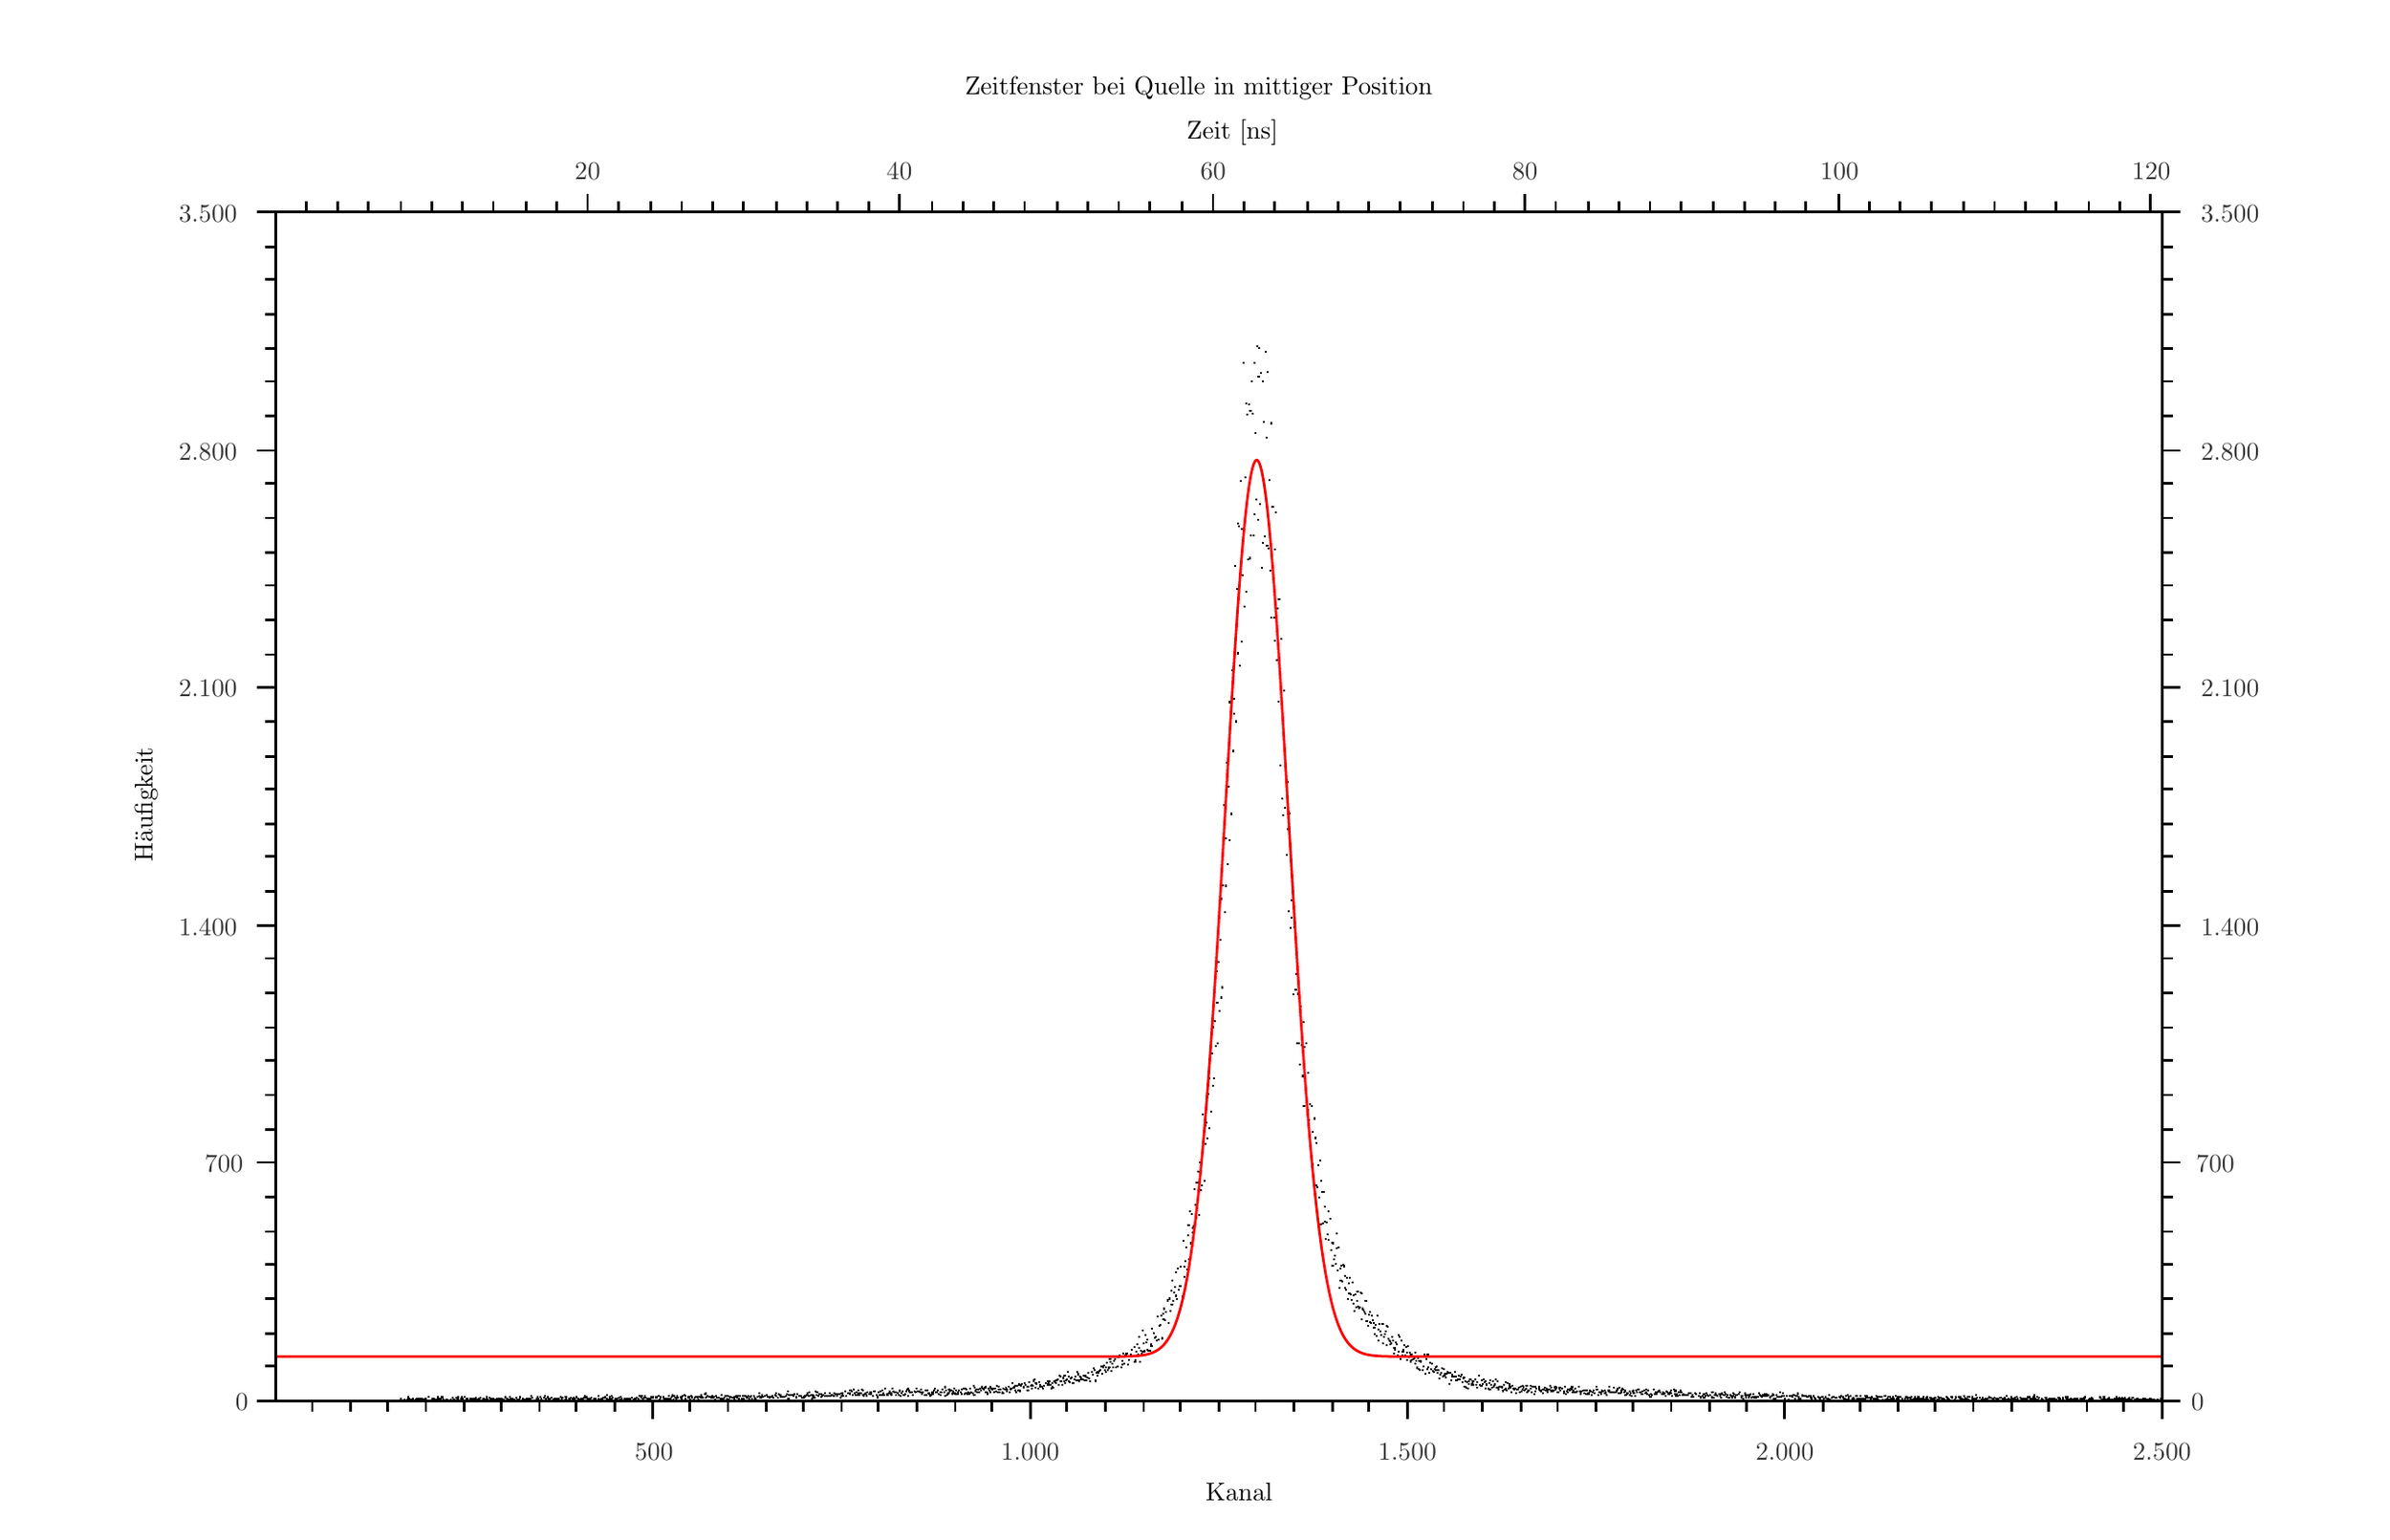
\begin{tikzpicture}{0pt}{0pt}{1215pt}{774pt}
	\clip(0pt,774pt) -- (914.667pt,774pt) -- (914.667pt,191.323pt) -- (0pt,191.323pt) -- (0pt,774pt);
\begin{scope}
	\clip(97.8656pt,700.977pt) -- (835.622pt,700.977pt) -- (835.622pt,235.739pt) -- (97.8656pt,235.739pt) -- (97.8656pt,700.977pt);
	\color[rgb]{0,0,0}
	\fill (145.987pt,236.138pt) rectangle (146.739pt,235.385pt);
	\color[rgb]{0,0,0}
	\fill (146.282pt,236.935pt) rectangle (147.035pt,236.183pt);
	\fill (146.577pt,236.271pt) rectangle (147.33pt,235.518pt);
	\fill (147.463pt,236.138pt) rectangle (148.215pt,235.385pt);
	\fill (148.053pt,236.537pt) rectangle (148.806pt,235.784pt);
	\fill (148.939pt,236.537pt) rectangle (149.692pt,235.784pt);
	\fill (149.234pt,237.6pt) rectangle (149.987pt,236.847pt);
	\fill (149.529pt,236.935pt) rectangle (150.282pt,236.183pt);
	\fill (149.824pt,236.67pt) rectangle (150.577pt,235.917pt);
	\fill (150.415pt,236.404pt) rectangle (151.168pt,235.651pt);
	\fill (151.005pt,236.802pt) rectangle (151.758pt,236.05pt);
	\fill (152.186pt,236.537pt) rectangle (152.939pt,235.784pt);
	\fill (152.481pt,236.138pt) rectangle (153.234pt,235.385pt);
	\fill (152.777pt,236.935pt) rectangle (153.529pt,236.183pt);
	\fill (153.367pt,237.068pt) rectangle (154.12pt,236.316pt);
	\fill (153.662pt,236.138pt) rectangle (154.415pt,235.385pt);
	\fill (153.958pt,237.068pt) rectangle (154.71pt,236.316pt);
	\fill (154.253pt,236.67pt) rectangle (155.006pt,235.917pt);
	\fill (154.843pt,236.935pt) rectangle (155.596pt,236.183pt);
	\fill (155.138pt,236.537pt) rectangle (155.891pt,235.784pt);
	\fill (155.729pt,236.935pt) rectangle (156.482pt,236.183pt);
	\fill (156.319pt,237.068pt) rectangle (157.072pt,236.316pt);
	\fill (156.615pt,236.271pt) rectangle (157.367pt,235.518pt);
	\fill (157.205pt,237.6pt) rectangle (157.958pt,236.847pt);
	\fill (157.795pt,236.138pt) rectangle (158.548pt,235.385pt);
	\fill (158.681pt,237.068pt) rectangle (159.434pt,236.316pt);
	\fill (158.976pt,236.67pt) rectangle (159.729pt,235.917pt);
	\fill (159.272pt,237.068pt) rectangle (160.024pt,236.316pt);
	\fill (159.567pt,236.802pt) rectangle (160.32pt,236.05pt);
	\fill (160.157pt,236.537pt) rectangle (160.91pt,235.784pt);
	\fill (160.748pt,237.6pt) rectangle (161.5pt,236.847pt);
	\fill (161.043pt,236.802pt) rectangle (161.796pt,236.05pt);
	\fill (161.633pt,236.935pt) rectangle (162.386pt,236.183pt);
	\fill (161.928pt,236.67pt) rectangle (162.681pt,235.917pt);
	\fill (162.519pt,237.467pt) rectangle (163.272pt,236.714pt);
	\fill (163.109pt,236.67pt) rectangle (163.862pt,235.917pt);
	\fill (163.995pt,236.537pt) rectangle (164.748pt,235.784pt);
	\fill (164.585pt,236.537pt) rectangle (165.338pt,235.784pt);
	\fill (165.471pt,236.271pt) rectangle (166.224pt,235.518pt);
	\fill (166.062pt,236.404pt) rectangle (166.814pt,235.651pt);
	\fill (166.652pt,237.201pt) rectangle (167.405pt,236.448pt);
	\fill (166.947pt,236.67pt) rectangle (167.7pt,235.917pt);
	\fill (167.538pt,236.67pt) rectangle (168.29pt,235.917pt);
	\fill (168.128pt,237.334pt) rectangle (168.881pt,236.581pt);
	\fill (168.423pt,236.404pt) rectangle (169.176pt,235.651pt);
	\fill (168.719pt,237.6pt) rectangle (169.471pt,236.847pt);
	\fill (169.014pt,237.068pt) rectangle (169.767pt,236.316pt);
	\fill (169.899pt,236.802pt) rectangle (170.652pt,236.05pt);
	\fill (170.195pt,237.467pt) rectangle (170.947pt,236.714pt);
	\fill (170.785pt,237.068pt) rectangle (171.538pt,236.316pt);
	\fill (171.376pt,237.6pt) rectangle (172.128pt,236.847pt);
	\fill (172.261pt,236.802pt) rectangle (173.014pt,236.05pt);
	\fill (172.556pt,236.935pt) rectangle (173.309pt,236.183pt);
	\fill (172.852pt,236.138pt) rectangle (173.604pt,235.385pt);
	\fill (173.737pt,237.068pt) rectangle (174.49pt,236.316pt);
	\fill (174.328pt,236.537pt) rectangle (175.081pt,235.784pt);
	\fill (174.623pt,237.068pt) rectangle (175.376pt,236.316pt);
	\fill (175.213pt,236.802pt) rectangle (175.966pt,236.05pt);
	\fill (175.804pt,237.334pt) rectangle (176.557pt,236.581pt);
	\fill (176.099pt,236.404pt) rectangle (176.852pt,235.651pt);
	\fill (176.69pt,236.802pt) rectangle (177.442pt,236.05pt);
	\fill (176.985pt,237.068pt) rectangle (177.738pt,236.316pt);
	\fill (177.575pt,237.334pt) rectangle (178.328pt,236.581pt);
	\fill (178.166pt,236.271pt) rectangle (178.918pt,235.518pt);
	\fill (178.461pt,237.068pt) rectangle (179.214pt,236.316pt);
	\fill (179.051pt,237.068pt) rectangle (179.804pt,236.316pt);
	\fill (179.642pt,236.404pt) rectangle (180.395pt,235.651pt);
	\fill (179.937pt,237.467pt) rectangle (180.69pt,236.714pt);
	\fill (180.527pt,236.537pt) rectangle (181.28pt,235.784pt);
	\fill (181.118pt,237.201pt) rectangle (181.871pt,236.448pt);
	\fill (181.413pt,236.67pt) rectangle (182.166pt,235.917pt);
	\fill (182.003pt,237.068pt) rectangle (182.756pt,236.316pt);
	\fill (182.299pt,236.67pt) rectangle (183.052pt,235.917pt);
	\fill (182.594pt,236.935pt) rectangle (183.347pt,236.183pt);
	\fill (183.48pt,236.67pt) rectangle (184.232pt,235.917pt);
	\fill (184.07pt,236.935pt) rectangle (184.823pt,236.183pt);
	\fill (184.365pt,236.802pt) rectangle (185.118pt,236.05pt);
	\fill (184.956pt,236.935pt) rectangle (185.709pt,236.183pt);
	\fill (185.841pt,236.935pt) rectangle (186.594pt,236.183pt);
	\fill (186.137pt,236.537pt) rectangle (186.889pt,235.784pt);
	\fill (186.432pt,236.404pt) rectangle (187.185pt,235.651pt);
	\fill (187.317pt,237.467pt) rectangle (188.07pt,236.714pt);
	\fill (187.908pt,237.068pt) rectangle (188.661pt,236.316pt);
	\fill (188.794pt,236.404pt) rectangle (189.546pt,235.651pt);
	\fill (189.089pt,237.6pt) rectangle (189.842pt,236.847pt);
	\fill (189.384pt,237.068pt) rectangle (190.137pt,236.316pt);
	\fill (189.679pt,236.271pt) rectangle (190.432pt,235.518pt);
	\fill (190.27pt,236.802pt) rectangle (191.022pt,236.05pt);
	\fill (190.86pt,236.537pt) rectangle (191.613pt,235.784pt);
	\fill (191.746pt,237.334pt) rectangle (192.499pt,236.581pt);
	\fill (192.041pt,236.67pt) rectangle (192.794pt,235.917pt);
	\fill (192.631pt,236.404pt) rectangle (193.384pt,235.651pt);
	\fill (192.927pt,237.201pt) rectangle (193.679pt,236.448pt);
	\fill (193.222pt,237.467pt) rectangle (193.975pt,236.714pt);
	\fill (194.108pt,236.802pt) rectangle (194.86pt,236.05pt);
	\fill (194.698pt,236.67pt) rectangle (195.451pt,235.917pt);
	\fill (195.584pt,236.935pt) rectangle (196.336pt,236.183pt);
	\fill (196.174pt,236.935pt) rectangle (196.927pt,236.183pt);
	\fill (197.06pt,236.935pt) rectangle (197.813pt,236.183pt);
	\fill (197.355pt,237.866pt) rectangle (198.108pt,237.113pt);
	\fill (197.65pt,237.334pt) rectangle (198.403pt,236.581pt);
	\fill (198.536pt,236.271pt) rectangle (199.289pt,235.518pt);
	\fill (199.126pt,236.271pt) rectangle (199.879pt,235.518pt);
	\fill (199.422pt,236.935pt) rectangle (200.174pt,236.183pt);
	\fill (200.012pt,237.733pt) rectangle (200.765pt,236.98pt);
	\fill (200.307pt,237.068pt) rectangle (201.06pt,236.316pt);
	\fill (200.898pt,237.733pt) rectangle (201.65pt,236.98pt);
	\fill (201.488pt,237.068pt) rectangle (202.241pt,236.316pt);
	\fill (202.374pt,237.334pt) rectangle (203.127pt,236.581pt);
	\fill (202.964pt,237.999pt) rectangle (203.717pt,237.246pt);
	\fill (203.259pt,237.068pt) rectangle (204.012pt,236.316pt);
	\fill (203.85pt,237.467pt) rectangle (204.603pt,236.714pt);
	\fill (204.145pt,236.802pt) rectangle (204.898pt,236.05pt);
	\fill (204.44pt,236.67pt) rectangle (205.193pt,235.917pt);
	\fill (204.735pt,237.068pt) rectangle (205.488pt,236.316pt);
	\fill (205.326pt,237.201pt) rectangle (206.079pt,236.448pt);
	\fill (205.916pt,236.404pt) rectangle (206.669pt,235.651pt);
	\fill (206.507pt,237.068pt) rectangle (207.26pt,236.316pt);
	\fill (206.802pt,236.537pt) rectangle (207.555pt,235.784pt);
	\fill (207.097pt,237.068pt) rectangle (207.85pt,236.316pt);
	\fill (207.688pt,236.935pt) rectangle (208.44pt,236.183pt);
	\fill (208.278pt,236.802pt) rectangle (209.031pt,236.05pt);
	\fill (208.869pt,237.6pt) rectangle (209.621pt,236.847pt);
	\fill (209.164pt,237.201pt) rectangle (209.917pt,236.448pt);
	\fill (209.459pt,236.67pt) rectangle (210.212pt,235.917pt);
	\fill (209.754pt,237.334pt) rectangle (210.507pt,236.581pt);
	\fill (210.64pt,236.404pt) rectangle (211.393pt,235.651pt);
	\fill (210.935pt,237.6pt) rectangle (211.688pt,236.847pt);
	\fill (211.23pt,236.935pt) rectangle (211.983pt,236.183pt);
	\fill (212.116pt,237.068pt) rectangle (212.869pt,236.316pt);
	\fill (212.706pt,236.802pt) rectangle (213.459pt,236.05pt);
	\fill (213.002pt,237.201pt) rectangle (213.754pt,236.448pt);
	\fill (213.592pt,236.802pt) rectangle (214.345pt,236.05pt);
	\fill (214.183pt,237.334pt) rectangle (214.935pt,236.581pt);
	\fill (214.478pt,236.802pt) rectangle (215.231pt,236.05pt);
	\fill (215.068pt,237.467pt) rectangle (215.821pt,236.714pt);
	\fill (215.954pt,236.802pt) rectangle (216.707pt,236.05pt);
	\fill (216.544pt,236.537pt) rectangle (217.297pt,235.784pt);
	\fill (216.84pt,237.068pt) rectangle (217.592pt,236.316pt);
	\fill (217.43pt,236.935pt) rectangle (218.183pt,236.183pt);
	\fill (217.725pt,236.67pt) rectangle (218.478pt,235.917pt);
	\fill (218.02pt,237.334pt) rectangle (218.773pt,236.581pt);
	\fill (218.316pt,237.866pt) rectangle (219.068pt,237.113pt);
	\fill (218.906pt,237.467pt) rectangle (219.659pt,236.714pt);
	\fill (219.497pt,237.068pt) rectangle (220.249pt,236.316pt);
	\fill (220.087pt,236.802pt) rectangle (220.84pt,236.05pt);
	\fill (220.382pt,236.67pt) rectangle (221.135pt,235.917pt);
	\fill (220.973pt,237.201pt) rectangle (221.725pt,236.448pt);
	\fill (221.858pt,236.935pt) rectangle (222.611pt,236.183pt);
	\fill (222.153pt,236.802pt) rectangle (222.906pt,236.05pt);
	\fill (222.744pt,236.802pt) rectangle (223.497pt,236.05pt);
	\fill (223.334pt,236.138pt) rectangle (224.087pt,235.385pt);
	\fill (223.63pt,237.999pt) rectangle (224.382pt,237.246pt);
	\fill (223.925pt,236.935pt) rectangle (224.678pt,236.183pt);
	\fill (224.22pt,236.67pt) rectangle (224.973pt,235.917pt);
	\fill (224.81pt,237.068pt) rectangle (225.563pt,236.316pt);
	\fill (225.106pt,236.537pt) rectangle (225.859pt,235.784pt);
	\fill (225.696pt,237.201pt) rectangle (226.449pt,236.448pt);
	\fill (226.287pt,237.467pt) rectangle (227.039pt,236.714pt);
	\fill (226.877pt,238.265pt) rectangle (227.63pt,237.512pt);
	\fill (227.172pt,237.068pt) rectangle (227.925pt,236.316pt);
	\fill (227.763pt,236.67pt) rectangle (228.515pt,235.917pt);
	\fill (228.058pt,237.467pt) rectangle (228.811pt,236.714pt);
	\fill (228.648pt,237.068pt) rectangle (229.401pt,236.316pt);
	\fill (228.944pt,238.132pt) rectangle (229.696pt,237.379pt);
	\fill (229.239pt,237.201pt) rectangle (229.992pt,236.448pt);
	\fill (230.124pt,237.068pt) rectangle (230.877pt,236.316pt);
	\fill (231.01pt,237.068pt) rectangle (231.763pt,236.316pt);
	\fill (231.601pt,237.334pt) rectangle (232.353pt,236.581pt);
	\fill (232.191pt,236.67pt) rectangle (232.944pt,235.917pt);
	\fill (232.486pt,237.733pt) rectangle (233.239pt,236.98pt);
	\fill (232.781pt,236.935pt) rectangle (233.534pt,236.183pt);
	\fill (233.077pt,236.271pt) rectangle (233.829pt,235.518pt);
	\fill (233.962pt,237.068pt) rectangle (234.715pt,236.316pt);
	\fill (234.553pt,236.935pt) rectangle (235.306pt,236.183pt);
	\fill (235.438pt,236.935pt) rectangle (236.191pt,236.183pt);
	\fill (235.734pt,236.271pt) rectangle (236.486pt,235.518pt);
	\fill (236.029pt,236.935pt) rectangle (236.782pt,236.183pt);
	\fill (236.324pt,236.138pt) rectangle (237.077pt,235.385pt);
	\fill (236.915pt,237.334pt) rectangle (237.667pt,236.581pt);
	\fill (237.505pt,236.537pt) rectangle (238.258pt,235.784pt);
	\fill (237.8pt,236.802pt) rectangle (238.553pt,236.05pt);
	\fill (238.095pt,236.935pt) rectangle (238.848pt,236.183pt);
	\fill (238.391pt,236.802pt) rectangle (239.143pt,236.05pt);
	\fill (238.686pt,237.334pt) rectangle (239.439pt,236.581pt);
	\fill (239.276pt,236.935pt) rectangle (240.029pt,236.183pt);
	\fill (239.867pt,237.999pt) rectangle (240.62pt,237.246pt);
	\fill (240.457pt,237.201pt) rectangle (241.21pt,236.448pt);
	\fill (240.752pt,237.866pt) rectangle (241.505pt,237.113pt);
	\fill (241.048pt,237.068pt) rectangle (241.8pt,236.316pt);
	\fill (241.343pt,237.201pt) rectangle (242.096pt,236.448pt);
	\fill (241.933pt,237.866pt) rectangle (242.686pt,237.113pt);
	\fill (242.228pt,237.201pt) rectangle (242.981pt,236.448pt);
	\fill (242.819pt,236.935pt) rectangle (243.572pt,236.183pt);
	\fill (243.409pt,236.802pt) rectangle (244.162pt,236.05pt);
	\fill (243.705pt,237.068pt) rectangle (244.457pt,236.316pt);
	\fill (244pt,236.67pt) rectangle (244.753pt,235.917pt);
	\fill (244.295pt,237.467pt) rectangle (245.048pt,236.714pt);
	\fill (245.181pt,237.467pt) rectangle (245.934pt,236.714pt);
	\fill (246.066pt,237.334pt) rectangle (246.819pt,236.581pt);
	\fill (246.362pt,237.733pt) rectangle (247.114pt,236.98pt);
	\fill (246.657pt,237.201pt) rectangle (247.41pt,236.448pt);
	\fill (247.247pt,238.132pt) rectangle (248pt,237.379pt);
	\fill (247.542pt,236.537pt) rectangle (248.295pt,235.784pt);
	\fill (248.133pt,237.467pt) rectangle (248.886pt,236.714pt);
	\fill (249.019pt,237.467pt) rectangle (249.771pt,236.714pt);
	\fill (249.314pt,236.67pt) rectangle (250.067pt,235.917pt);
	\fill (249.609pt,237.068pt) rectangle (250.362pt,236.316pt);
	\fill (250.199pt,236.802pt) rectangle (250.952pt,236.05pt);
	\fill (250.495pt,236.935pt) rectangle (251.247pt,236.183pt);
	\fill (251.085pt,236.935pt) rectangle (251.838pt,236.183pt);
	\fill (251.38pt,237.999pt) rectangle (252.133pt,237.246pt);
	\fill (251.971pt,236.802pt) rectangle (252.724pt,236.05pt);
	\fill (252.266pt,237.6pt) rectangle (253.019pt,236.847pt);
	\fill (252.561pt,238.265pt) rectangle (253.314pt,237.512pt);
	\fill (252.856pt,237.999pt) rectangle (253.609pt,237.246pt);
	\fill (253.152pt,236.404pt) rectangle (253.904pt,235.651pt);
	\fill (253.447pt,237.866pt) rectangle (254.2pt,237.113pt);
	\fill (253.742pt,237.201pt) rectangle (254.495pt,236.448pt);
	\fill (254.037pt,236.802pt) rectangle (254.79pt,236.05pt);
	\fill (254.333pt,237.866pt) rectangle (255.085pt,237.113pt);
	\fill (254.628pt,237.6pt) rectangle (255.381pt,236.847pt);
	\fill (254.923pt,237.334pt) rectangle (255.676pt,236.581pt);
	\fill (255.809pt,237.467pt) rectangle (256.561pt,236.714pt);
	\fill (256.104pt,237.733pt) rectangle (256.857pt,236.98pt);
	\fill (256.399pt,237.068pt) rectangle (257.152pt,236.316pt);
	\fill (256.694pt,237.866pt) rectangle (257.447pt,237.113pt);
	\fill (257.285pt,238.53pt) rectangle (258.038pt,237.778pt);
	\fill (257.58pt,237.999pt) rectangle (258.333pt,237.246pt);
	\fill (257.875pt,236.935pt) rectangle (258.628pt,236.183pt);
	\fill (258.761pt,237.467pt) rectangle (259.514pt,236.714pt);
	\fill (259.351pt,237.467pt) rectangle (260.104pt,236.714pt);
	\fill (259.647pt,236.404pt) rectangle (260.399pt,235.651pt);
	\fill (259.942pt,237.866pt) rectangle (260.695pt,237.113pt);
	\fill (260.237pt,237.467pt) rectangle (260.99pt,236.714pt);
	\fill (261.123pt,236.537pt) rectangle (261.875pt,235.784pt);
	\fill (261.418pt,237.334pt) rectangle (262.171pt,236.581pt);
	\fill (261.713pt,237.6pt) rectangle (262.466pt,236.847pt);
	\fill (262.303pt,237.733pt) rectangle (263.056pt,236.98pt);
	\fill (262.599pt,237.467pt) rectangle (263.352pt,236.714pt);
	\fill (262.894pt,236.67pt) rectangle (263.647pt,235.917pt);
	\fill (263.189pt,237.6pt) rectangle (263.942pt,236.847pt);
	\fill (263.78pt,238.265pt) rectangle (264.532pt,237.512pt);
	\fill (264.075pt,237.467pt) rectangle (264.828pt,236.714pt);
	\fill (264.665pt,237.334pt) rectangle (265.418pt,236.581pt);
	\fill (265.256pt,238.663pt) rectangle (266.009pt,237.911pt);
	\fill (265.551pt,237.334pt) rectangle (266.304pt,236.581pt);
	\fill (265.846pt,238.929pt) rectangle (266.599pt,238.176pt);
	\fill (266.141pt,237.6pt) rectangle (266.894pt,236.847pt);
	\fill (266.437pt,237.999pt) rectangle (267.189pt,237.246pt);
	\fill (267.027pt,237.733pt) rectangle (267.78pt,236.98pt);
	\fill (267.322pt,237.6pt) rectangle (268.075pt,236.847pt);
	\fill (267.913pt,237.467pt) rectangle (268.665pt,236.714pt);
	\fill (268.208pt,237.999pt) rectangle (268.961pt,237.246pt);
	\fill (268.503pt,237.334pt) rectangle (269.256pt,236.581pt);
	\fill (269.094pt,237.733pt) rectangle (269.846pt,236.98pt);
	\fill (269.389pt,236.537pt) rectangle (270.142pt,235.784pt);
	\fill (269.684pt,237.866pt) rectangle (270.437pt,237.113pt);
	\fill (269.979pt,237.334pt) rectangle (270.732pt,236.581pt);
	\fill (270.865pt,237.201pt) rectangle (271.618pt,236.448pt);
	\fill (271.455pt,237.068pt) rectangle (272.208pt,236.316pt);
	\fill (271.751pt,238.265pt) rectangle (272.503pt,237.512pt);
	\fill (272.046pt,236.67pt) rectangle (272.799pt,235.917pt);
	\fill (272.341pt,237.068pt) rectangle (273.094pt,236.316pt);
	\fill (272.636pt,236.67pt) rectangle (273.389pt,235.917pt);
	\fill (272.931pt,237.334pt) rectangle (273.684pt,236.581pt);
	\fill (273.227pt,238.132pt) rectangle (273.979pt,237.379pt);
	\fill (273.817pt,238.132pt) rectangle (274.57pt,237.379pt);
	\fill (274.112pt,237.068pt) rectangle (274.865pt,236.316pt);
	\fill (274.408pt,237.999pt) rectangle (275.16pt,237.246pt);
	\fill (274.703pt,236.67pt) rectangle (275.456pt,235.917pt);
	\fill (274.998pt,237.467pt) rectangle (275.751pt,236.714pt);
	\fill (275.293pt,237.6pt) rectangle (276.046pt,236.847pt);
	\fill (275.588pt,237.733pt) rectangle (276.341pt,236.98pt);
	\fill (276.179pt,237.201pt) rectangle (276.932pt,236.448pt);
	\fill (276.769pt,236.802pt) rectangle (277.522pt,236.05pt);
	\fill (277.065pt,237.733pt) rectangle (277.817pt,236.98pt);
	\fill (277.655pt,237.866pt) rectangle (278.408pt,237.113pt);
	\fill (277.95pt,237.467pt) rectangle (278.703pt,236.714pt);
	\fill (278.245pt,238.132pt) rectangle (278.998pt,237.379pt);
	\fill (278.836pt,236.935pt) rectangle (279.589pt,236.183pt);
	\fill (279.131pt,238.132pt) rectangle (279.884pt,237.379pt);
	\fill (279.722pt,237.068pt) rectangle (280.474pt,236.316pt);
	\fill (280.312pt,238.132pt) rectangle (281.065pt,237.379pt);
	\fill (280.607pt,236.935pt) rectangle (281.36pt,236.183pt);
	\fill (281.198pt,237.866pt) rectangle (281.95pt,237.113pt);
	\fill (281.493pt,237.467pt) rectangle (282.246pt,236.714pt);
	\fill (282.083pt,237.201pt) rectangle (282.836pt,236.448pt);
	\fill (282.378pt,237.999pt) rectangle (283.131pt,237.246pt);
	\fill (282.674pt,236.802pt) rectangle (283.427pt,236.05pt);
	\fill (282.969pt,237.6pt) rectangle (283.722pt,236.847pt);
	\fill (283.559pt,237.999pt) rectangle (284.312pt,237.246pt);
	\fill (283.855pt,237.068pt) rectangle (284.607pt,236.316pt);
	\fill (284.445pt,237.999pt) rectangle (285.198pt,237.246pt);
	\fill (284.74pt,237.201pt) rectangle (285.493pt,236.448pt);
	\fill (285.035pt,237.068pt) rectangle (285.788pt,236.316pt);
	\fill (285.921pt,237.6pt) rectangle (286.674pt,236.847pt);
	\fill (286.512pt,237.999pt) rectangle (287.264pt,237.246pt);
	\fill (286.807pt,239.062pt) rectangle (287.56pt,238.309pt);
	\fill (287.102pt,237.201pt) rectangle (287.855pt,236.448pt);
	\fill (287.397pt,237.467pt) rectangle (288.15pt,236.714pt);
	\fill (287.692pt,238.265pt) rectangle (288.445pt,237.512pt);
	\fill (287.988pt,237.733pt) rectangle (288.74pt,236.98pt);
	\fill (288.873pt,237.866pt) rectangle (289.626pt,237.113pt);
	\fill (289.464pt,238.265pt) rectangle (290.217pt,237.512pt);
	\fill (289.759pt,237.6pt) rectangle (290.512pt,236.847pt);
	\fill (290.349pt,237.733pt) rectangle (291.102pt,236.98pt);
	\fill (290.645pt,237.467pt) rectangle (291.397pt,236.714pt);
	\fill (291.235pt,237.733pt) rectangle (291.988pt,236.98pt);
	\fill (291.826pt,238.132pt) rectangle (292.578pt,237.379pt);
	\fill (292.121pt,237.334pt) rectangle (292.874pt,236.581pt);
	\fill (292.711pt,238.398pt) rectangle (293.464pt,237.645pt);
	\fill (293.006pt,237.866pt) rectangle (293.759pt,237.113pt);
	\fill (293.302pt,239.062pt) rectangle (294.054pt,238.309pt);
	\fill (293.892pt,237.201pt) rectangle (294.645pt,236.448pt);
	\fill (294.187pt,238.663pt) rectangle (294.94pt,237.911pt);
	\fill (294.483pt,238.265pt) rectangle (295.235pt,237.512pt);
	\fill (294.778pt,238.398pt) rectangle (295.531pt,237.645pt);
	\fill (295.073pt,237.733pt) rectangle (295.826pt,236.98pt);
	\fill (295.663pt,237.733pt) rectangle (296.416pt,236.98pt);
	\fill (295.959pt,237.6pt) rectangle (296.711pt,236.847pt);
	\fill (296.254pt,237.733pt) rectangle (297.007pt,236.98pt);
	\fill (296.549pt,237.6pt) rectangle (297.302pt,236.847pt);
	\fill (297.14pt,237.999pt) rectangle (297.892pt,237.246pt);
	\fill (297.435pt,238.663pt) rectangle (298.188pt,237.911pt);
	\fill (297.73pt,239.86pt) rectangle (298.483pt,239.107pt);
	\fill (298.025pt,237.068pt) rectangle (298.778pt,236.316pt);
	\fill (298.32pt,238.53pt) rectangle (299.073pt,237.778pt);
	\fill (298.616pt,238.265pt) rectangle (299.368pt,237.512pt);
	\fill (298.911pt,238.398pt) rectangle (299.664pt,237.645pt);
	\fill (299.501pt,238.53pt) rectangle (300.254pt,237.778pt);
	\fill (300.092pt,238.132pt) rectangle (300.845pt,237.379pt);
	\fill (300.387pt,238.663pt) rectangle (301.14pt,237.911pt);
	\fill (300.977pt,237.467pt) rectangle (301.73pt,236.714pt);
	\fill (301.568pt,238.796pt) rectangle (302.321pt,238.044pt);
	\fill (302.158pt,237.866pt) rectangle (302.911pt,237.113pt);
	\fill (302.453pt,237.999pt) rectangle (303.206pt,237.246pt);
	\fill (303.044pt,237.999pt) rectangle (303.797pt,237.246pt);
	\fill (303.339pt,237.201pt) rectangle (304.092pt,236.448pt);
	\fill (303.93pt,237.467pt) rectangle (304.682pt,236.714pt);
	\fill (304.225pt,237.866pt) rectangle (304.978pt,237.113pt);
	\fill (304.52pt,237.6pt) rectangle (305.273pt,236.847pt);
	\fill (304.815pt,237.999pt) rectangle (305.568pt,237.246pt);
	\fill (305.11pt,238.398pt) rectangle (305.863pt,237.645pt);
	\fill (305.406pt,238.929pt) rectangle (306.159pt,238.176pt);
	\fill (305.996pt,237.999pt) rectangle (306.749pt,237.246pt);
	\fill (306.291pt,239.594pt) rectangle (307.044pt,238.841pt);
	\fill (306.882pt,238.398pt) rectangle (307.635pt,237.645pt);
	\fill (307.177pt,237.068pt) rectangle (307.93pt,236.316pt);
	\fill (307.472pt,238.265pt) rectangle (308.225pt,237.512pt);
	\fill (307.767pt,237.467pt) rectangle (308.52pt,236.714pt);
	\fill (308.063pt,237.866pt) rectangle (308.815pt,237.113pt);
	\fill (308.358pt,237.201pt) rectangle (309.111pt,236.448pt);
	\fill (308.653pt,239.727pt) rectangle (309.406pt,238.974pt);
	\fill (308.948pt,238.398pt) rectangle (309.701pt,237.645pt);
	\fill (309.244pt,239.461pt) rectangle (309.996pt,238.708pt);
	\fill (309.834pt,237.999pt) rectangle (310.587pt,237.246pt);
	\fill (310.129pt,238.663pt) rectangle (310.882pt,237.911pt);
	\fill (310.72pt,238.796pt) rectangle (311.472pt,238.044pt);
	\fill (311.015pt,237.6pt) rectangle (311.768pt,236.847pt);
	\fill (311.31pt,238.132pt) rectangle (312.063pt,237.379pt);
	\fill (311.605pt,238.53pt) rectangle (312.358pt,237.778pt);
	\fill (312.196pt,239.062pt) rectangle (312.949pt,238.309pt);
	\fill (312.491pt,237.999pt) rectangle (313.244pt,237.246pt);
	\fill (313.081pt,237.866pt) rectangle (313.834pt,237.113pt);
	\fill (313.672pt,238.132pt) rectangle (314.425pt,237.379pt);
	\fill (314.262pt,239.195pt) rectangle (315.015pt,238.442pt);
	\fill (314.558pt,237.866pt) rectangle (315.31pt,237.113pt);
	\fill (314.853pt,238.398pt) rectangle (315.606pt,237.645pt);
	\fill (315.148pt,238.398pt) rectangle (315.901pt,237.645pt);
	\fill (315.738pt,237.866pt) rectangle (316.491pt,237.113pt);
	\fill (316.034pt,239.195pt) rectangle (316.786pt,238.442pt);
	\fill (316.329pt,238.663pt) rectangle (317.082pt,237.911pt);
	\fill (316.624pt,238.796pt) rectangle (317.377pt,238.044pt);
	\fill (316.919pt,237.999pt) rectangle (317.672pt,237.246pt);
	\fill (317.51pt,238.663pt) rectangle (318.263pt,237.911pt);
	\fill (318.1pt,238.663pt) rectangle (318.853pt,237.911pt);
	\fill (318.395pt,237.201pt) rectangle (319.148pt,236.448pt);
	\fill (318.691pt,237.999pt) rectangle (319.443pt,237.246pt);
	\fill (318.986pt,239.195pt) rectangle (319.739pt,238.442pt);
	\fill (319.281pt,238.398pt) rectangle (320.034pt,237.645pt);
	\fill (319.576pt,237.999pt) rectangle (320.329pt,237.246pt);
	\fill (320.167pt,239.727pt) rectangle (320.92pt,238.974pt);
	\fill (320.462pt,237.866pt) rectangle (321.215pt,237.113pt);
	\fill (321.348pt,239.062pt) rectangle (322.1pt,238.309pt);
	\fill (321.938pt,238.929pt) rectangle (322.691pt,238.176pt);
	\fill (322.233pt,240.126pt) rectangle (322.986pt,239.373pt);
	\fill (322.824pt,239.727pt) rectangle (323.577pt,238.974pt);
	\fill (323.119pt,238.265pt) rectangle (323.872pt,237.512pt);
	\fill (323.414pt,240.391pt) rectangle (324.167pt,239.639pt);
	\fill (323.709pt,239.062pt) rectangle (324.462pt,238.309pt);
	\fill (324.3pt,238.53pt) rectangle (325.053pt,237.778pt);
	\fill (324.595pt,239.461pt) rectangle (325.348pt,238.708pt);
	\fill (324.89pt,238.398pt) rectangle (325.643pt,237.645pt);
	\fill (325.185pt,240.259pt) rectangle (325.938pt,239.506pt);
	\fill (325.481pt,239.195pt) rectangle (326.234pt,238.442pt);
	\fill (325.776pt,238.398pt) rectangle (326.529pt,237.645pt);
	\fill (326.366pt,239.195pt) rectangle (327.119pt,238.442pt);
	\fill (326.662pt,240.391pt) rectangle (327.414pt,239.639pt);
	\fill (326.957pt,238.53pt) rectangle (327.71pt,237.778pt);
	\fill (327.252pt,240.126pt) rectangle (328.005pt,239.373pt);
	\fill (327.547pt,237.999pt) rectangle (328.3pt,237.246pt);
	\fill (327.842pt,238.663pt) rectangle (328.595pt,237.911pt);
	\fill (328.138pt,238.929pt) rectangle (328.89pt,238.176pt);
	\fill (328.433pt,237.999pt) rectangle (329.186pt,237.246pt);
	\fill (328.728pt,238.53pt) rectangle (329.481pt,237.778pt);
	\fill (329.023pt,239.328pt) rectangle (329.776pt,238.575pt);
	\fill (329.614pt,238.663pt) rectangle (330.367pt,237.911pt);
	\fill (329.909pt,239.328pt) rectangle (330.662pt,238.575pt);
	\fill (330.204pt,239.594pt) rectangle (330.957pt,238.841pt);
	\fill (330.499pt,238.796pt) rectangle (331.252pt,238.044pt);
	\fill (331.09pt,238.132pt) rectangle (331.843pt,237.379pt);
	\fill (331.385pt,239.727pt) rectangle (332.138pt,238.974pt);
	\fill (331.68pt,239.727pt) rectangle (332.433pt,238.974pt);
	\fill (332.566pt,238.398pt) rectangle (333.319pt,237.645pt);
	\fill (332.861pt,237.467pt) rectangle (333.614pt,236.714pt);
	\fill (333.156pt,239.328pt) rectangle (333.909pt,238.575pt);
	\fill (333.747pt,238.398pt) rectangle (334.5pt,237.645pt);
	\fill (334.042pt,239.86pt) rectangle (334.795pt,239.107pt);
	\fill (334.337pt,238.265pt) rectangle (335.09pt,237.512pt);
	\fill (334.633pt,240.126pt) rectangle (335.385pt,239.373pt);
	\fill (334.928pt,238.398pt) rectangle (335.681pt,237.645pt);
	\fill (335.223pt,239.195pt) rectangle (335.976pt,238.442pt);
	\fill (335.518pt,238.53pt) rectangle (336.271pt,237.778pt);
	\fill (335.813pt,240.79pt) rectangle (336.566pt,240.037pt);
	\fill (336.404pt,238.663pt) rectangle (337.157pt,237.911pt);
	\fill (336.699pt,238.265pt) rectangle (337.452pt,237.512pt);
	\fill (336.994pt,238.265pt) rectangle (337.747pt,237.512pt);
	\fill (337.29pt,239.062pt) rectangle (338.042pt,238.309pt);
	\fill (337.585pt,239.727pt) rectangle (338.338pt,238.974pt);
	\fill (337.88pt,238.929pt) rectangle (338.633pt,238.176pt);
	\fill (338.175pt,238.265pt) rectangle (338.928pt,237.512pt);
	\fill (338.47pt,239.062pt) rectangle (339.223pt,238.309pt);
	\fill (338.766pt,240.923pt) rectangle (339.518pt,240.17pt);
	\fill (339.061pt,239.727pt) rectangle (339.814pt,238.974pt);
	\fill (339.356pt,239.328pt) rectangle (340.109pt,238.575pt);
	\fill (339.947pt,239.461pt) rectangle (340.699pt,238.708pt);
	\fill (340.242pt,238.398pt) rectangle (340.995pt,237.645pt);
	\fill (340.832pt,239.195pt) rectangle (341.585pt,238.442pt);
	\fill (341.127pt,238.53pt) rectangle (341.88pt,237.778pt);
	\fill (341.423pt,239.993pt) rectangle (342.175pt,239.24pt);
	\fill (342.013pt,237.866pt) rectangle (342.766pt,237.113pt);
	\fill (342.308pt,239.062pt) rectangle (343.061pt,238.309pt);
	\fill (342.603pt,239.86pt) rectangle (343.356pt,239.107pt);
	\fill (343.194pt,238.265pt) rectangle (343.947pt,237.512pt);
	\fill (343.784pt,238.796pt) rectangle (344.537pt,238.044pt);
	\fill (344.08pt,239.727pt) rectangle (344.832pt,238.974pt);
	\fill (344.375pt,240.524pt) rectangle (345.128pt,239.772pt);
	\fill (344.67pt,240.79pt) rectangle (345.423pt,240.037pt);
	\fill (344.965pt,237.999pt) rectangle (345.718pt,237.246pt);
	\fill (345.26pt,239.993pt) rectangle (346.013pt,239.24pt);
	\fill (345.556pt,239.328pt) rectangle (346.309pt,238.575pt);
	\fill (346.146pt,239.461pt) rectangle (346.899pt,238.708pt);
	\fill (346.737pt,238.398pt) rectangle (347.489pt,237.645pt);
	\fill (347.327pt,239.86pt) rectangle (348.08pt,239.107pt);
	\fill (347.622pt,239.594pt) rectangle (348.375pt,238.841pt);
	\fill (348.213pt,240.79pt) rectangle (348.965pt,240.037pt);
	\fill (348.508pt,239.86pt) rectangle (349.261pt,239.107pt);
	\fill (349.098pt,239.727pt) rectangle (349.851pt,238.974pt);
	\fill (349.689pt,239.461pt) rectangle (350.442pt,238.708pt);
	\fill (349.984pt,240.657pt) rectangle (350.737pt,239.904pt);
	\fill (350.279pt,238.796pt) rectangle (351.032pt,238.044pt);
	\fill (350.574pt,239.594pt) rectangle (351.327pt,238.841pt);
	\fill (351.46pt,238.265pt) rectangle (352.213pt,237.512pt);
	\fill (351.755pt,240.126pt) rectangle (352.508pt,239.373pt);
	\fill (352.051pt,238.265pt) rectangle (352.803pt,237.512pt);
	\fill (352.346pt,240.259pt) rectangle (353.099pt,239.506pt);
	\fill (352.936pt,239.195pt) rectangle (353.689pt,238.442pt);
	\fill (353.231pt,238.929pt) rectangle (353.984pt,238.176pt);
	\fill (353.527pt,238.132pt) rectangle (354.279pt,237.379pt);
	\fill (353.822pt,238.53pt) rectangle (354.575pt,237.778pt);
	\fill (354.117pt,239.328pt) rectangle (354.87pt,238.575pt);
	\fill (354.412pt,238.663pt) rectangle (355.165pt,237.911pt);
	\fill (354.708pt,239.461pt) rectangle (355.46pt,238.708pt);
	\fill (355.003pt,240.126pt) rectangle (355.756pt,239.373pt);
	\fill (355.298pt,240.79pt) rectangle (356.051pt,240.037pt);
	\fill (355.593pt,239.328pt) rectangle (356.346pt,238.575pt);
	\fill (355.888pt,239.594pt) rectangle (356.641pt,238.841pt);
	\fill (356.479pt,240.259pt) rectangle (357.232pt,239.506pt);
	\fill (356.774pt,238.796pt) rectangle (357.527pt,238.044pt);
	\fill (357.365pt,238.53pt) rectangle (358.117pt,237.778pt);
	\fill (357.66pt,239.461pt) rectangle (358.413pt,238.708pt);
	\fill (358.25pt,240.524pt) rectangle (359.003pt,239.772pt);
	\fill (358.841pt,239.328pt) rectangle (359.593pt,238.575pt);
	\fill (359.136pt,241.455pt) rectangle (359.889pt,240.702pt);
	\fill (359.431pt,238.132pt) rectangle (360.184pt,237.379pt);
	\fill (359.726pt,240.259pt) rectangle (360.479pt,239.506pt);
	\fill (360.022pt,238.398pt) rectangle (360.774pt,237.645pt);
	\fill (360.317pt,238.929pt) rectangle (361.07pt,238.176pt);
	\fill (360.612pt,239.195pt) rectangle (361.365pt,238.442pt);
	\fill (360.907pt,240.391pt) rectangle (361.66pt,239.639pt);
	\fill (361.202pt,239.993pt) rectangle (361.955pt,239.24pt);
	\fill (361.793pt,240.259pt) rectangle (362.546pt,239.506pt);
	\fill (362.088pt,238.929pt) rectangle (362.841pt,238.176pt);
	\fill (362.383pt,239.86pt) rectangle (363.136pt,239.107pt);
	\fill (362.678pt,239.195pt) rectangle (363.431pt,238.442pt);
	\fill (362.974pt,240.79pt) rectangle (363.727pt,240.037pt);
	\fill (363.269pt,238.929pt) rectangle (364.022pt,238.176pt);
	\fill (363.564pt,240.126pt) rectangle (364.317pt,239.373pt);
	\fill (364.155pt,238.663pt) rectangle (364.907pt,237.911pt);
	\fill (364.45pt,239.328pt) rectangle (365.203pt,238.575pt);
	\fill (364.745pt,240.126pt) rectangle (365.498pt,239.373pt);
	\fill (365.335pt,239.461pt) rectangle (366.088pt,238.708pt);
	\fill (365.631pt,240.657pt) rectangle (366.384pt,239.904pt);
	\fill (365.926pt,238.796pt) rectangle (366.679pt,238.044pt);
	\fill (366.516pt,241.056pt) rectangle (367.269pt,240.303pt);
	\fill (366.812pt,238.796pt) rectangle (367.564pt,238.044pt);
	\fill (367.107pt,240.79pt) rectangle (367.86pt,240.037pt);
	\fill (367.402pt,239.062pt) rectangle (368.155pt,238.309pt);
	\fill (367.697pt,240.391pt) rectangle (368.45pt,239.639pt);
	\fill (367.992pt,238.796pt) rectangle (368.745pt,238.044pt);
	\fill (368.288pt,239.328pt) rectangle (369.04pt,238.575pt);
	\fill (368.583pt,238.663pt) rectangle (369.336pt,237.911pt);
	\fill (368.878pt,239.195pt) rectangle (369.631pt,238.442pt);
	\fill (369.173pt,240.923pt) rectangle (369.926pt,240.17pt);
	\fill (369.469pt,239.328pt) rectangle (370.221pt,238.575pt);
	\fill (370.059pt,239.195pt) rectangle (370.812pt,238.442pt);
	\fill (370.354pt,241.854pt) rectangle (371.107pt,241.101pt);
	\fill (370.649pt,238.398pt) rectangle (371.402pt,237.645pt);
	\fill (370.945pt,241.322pt) rectangle (371.697pt,240.569pt);
	\fill (371.24pt,239.993pt) rectangle (371.993pt,239.24pt);
	\fill (371.535pt,240.391pt) rectangle (372.288pt,239.639pt);
	\fill (371.83pt,239.594pt) rectangle (372.583pt,238.841pt);
	\fill (372.126pt,240.657pt) rectangle (372.878pt,239.904pt);
	\fill (372.421pt,240.391pt) rectangle (373.174pt,239.639pt);
	\fill (372.716pt,239.328pt) rectangle (373.469pt,238.575pt);
	\fill (373.011pt,241.056pt) rectangle (373.764pt,240.303pt);
	\fill (373.306pt,240.259pt) rectangle (374.059pt,239.506pt);
	\fill (373.602pt,241.322pt) rectangle (374.354pt,240.569pt);
	\fill (373.897pt,241.455pt) rectangle (374.65pt,240.702pt);
	\fill (374.192pt,241.056pt) rectangle (374.945pt,240.303pt);
	\fill (374.487pt,240.391pt) rectangle (375.24pt,239.639pt);
	\fill (374.783pt,241.189pt) rectangle (375.535pt,240.436pt);
	\fill (375.078pt,241.455pt) rectangle (375.831pt,240.702pt);
	\fill (375.373pt,239.594pt) rectangle (376.126pt,238.841pt);
	\fill (375.963pt,238.929pt) rectangle (376.716pt,238.176pt);
	\fill (376.259pt,240.79pt) rectangle (377.011pt,240.037pt);
	\fill (376.554pt,240.126pt) rectangle (377.307pt,239.373pt);
	\fill (376.849pt,241.455pt) rectangle (377.602pt,240.702pt);
	\fill (377.144pt,239.461pt) rectangle (377.897pt,238.708pt);
	\fill (377.44pt,240.79pt) rectangle (378.192pt,240.037pt);
	\fill (377.735pt,240.524pt) rectangle (378.488pt,239.772pt);
	\fill (378.03pt,240.79pt) rectangle (378.783pt,240.037pt);
	\fill (378.325pt,239.461pt) rectangle (379.078pt,238.708pt);
	\fill (378.62pt,240.923pt) rectangle (379.373pt,240.17pt);
	\fill (379.211pt,239.727pt) rectangle (379.964pt,238.974pt);
	\fill (379.506pt,241.987pt) rectangle (380.259pt,241.234pt);
	\fill (379.801pt,239.594pt) rectangle (380.554pt,238.841pt);
	\fill (380.097pt,241.721pt) rectangle (380.849pt,240.968pt);
	\fill (380.392pt,240.657pt) rectangle (381.145pt,239.904pt);
	\fill (380.687pt,239.594pt) rectangle (381.44pt,238.841pt);
	\fill (380.982pt,240.524pt) rectangle (381.735pt,239.772pt);
	\fill (381.573pt,239.328pt) rectangle (382.325pt,238.575pt);
	\fill (381.868pt,239.062pt) rectangle (382.621pt,238.309pt);
	\fill (382.163pt,240.79pt) rectangle (382.916pt,240.037pt);
	\fill (382.753pt,240.391pt) rectangle (383.506pt,239.639pt);
	\fill (383.049pt,241.322pt) rectangle (383.802pt,240.569pt);
	\fill (383.344pt,239.993pt) rectangle (384.097pt,239.24pt);
	\fill (383.639pt,240.657pt) rectangle (384.392pt,239.904pt);
	\fill (384.23pt,241.588pt) rectangle (384.982pt,240.835pt);
	\fill (384.525pt,239.328pt) rectangle (385.278pt,238.575pt);
	\fill (384.82pt,240.524pt) rectangle (385.573pt,239.772pt);
	\fill (385.115pt,240.923pt) rectangle (385.868pt,240.17pt);
	\fill (385.706pt,242.917pt) rectangle (386.459pt,242.164pt);
	\fill (386.001pt,241.322pt) rectangle (386.754pt,240.569pt);
	\fill (386.296pt,241.455pt) rectangle (387.049pt,240.702pt);
	\fill (386.591pt,240.126pt) rectangle (387.344pt,239.373pt);
	\fill (386.887pt,242.119pt) rectangle (387.639pt,241.367pt);
	\fill (387.182pt,239.461pt) rectangle (387.935pt,238.708pt);
	\fill (387.477pt,242.119pt) rectangle (388.23pt,241.367pt);
	\fill (387.772pt,240.259pt) rectangle (388.525pt,239.506pt);
	\fill (388.067pt,242.784pt) rectangle (388.82pt,242.031pt);
	\fill (388.363pt,242.385pt) rectangle (389.115pt,241.633pt);
	\fill (388.658pt,239.993pt) rectangle (389.411pt,239.24pt);
	\fill (388.953pt,241.854pt) rectangle (389.706pt,241.101pt);
	\fill (389.248pt,242.651pt) rectangle (390.001pt,241.898pt);
	\fill (389.839pt,241.322pt) rectangle (390.592pt,240.569pt);
	\fill (390.134pt,241.455pt) rectangle (390.887pt,240.702pt);
	\fill (390.429pt,242.917pt) rectangle (391.182pt,242.164pt);
	\fill (390.724pt,242.385pt) rectangle (391.477pt,241.633pt);
	\fill (391.315pt,240.259pt) rectangle (392.068pt,239.506pt);
	\fill (391.61pt,241.588pt) rectangle (392.363pt,240.835pt);
	\fill (391.905pt,240.259pt) rectangle (392.658pt,239.506pt);
	\fill (392.201pt,243.316pt) rectangle (392.953pt,242.563pt);
	\fill (392.791pt,241.854pt) rectangle (393.544pt,241.101pt);
	\fill (393.086pt,240.79pt) rectangle (393.839pt,240.037pt);
	\fill (393.381pt,242.385pt) rectangle (394.134pt,241.633pt);
	\fill (393.677pt,242.119pt) rectangle (394.429pt,241.367pt);
	\fill (393.972pt,243.98pt) rectangle (394.725pt,243.228pt);
	\fill (394.267pt,244.512pt) rectangle (395.02pt,243.759pt);
	\fill (394.562pt,241.322pt) rectangle (395.315pt,240.569pt);
	\fill (394.858pt,243.05pt) rectangle (395.61pt,242.297pt);
	\fill (395.153pt,242.651pt) rectangle (395.906pt,241.898pt);
	\fill (395.743pt,240.79pt) rectangle (396.496pt,240.037pt);
	\fill (396.038pt,243.449pt) rectangle (396.791pt,242.696pt);
	\fill (396.334pt,241.588pt) rectangle (397.086pt,240.835pt);
	\fill (396.629pt,242.252pt) rectangle (397.382pt,241.5pt);
	\fill (397.219pt,241.588pt) rectangle (397.972pt,240.835pt);
	\fill (397.515pt,241.056pt) rectangle (398.267pt,240.303pt);
	\fill (398.105pt,242.119pt) rectangle (398.858pt,241.367pt);
	\fill (398.695pt,243.183pt) rectangle (399.448pt,242.43pt);
	\fill (399.286pt,243.847pt) rectangle (400.039pt,243.095pt);
	\fill (399.581pt,242.518pt) rectangle (400.334pt,241.765pt);
	\fill (399.876pt,243.05pt) rectangle (400.629pt,242.297pt);
	\fill (400.172pt,243.715pt) rectangle (400.924pt,242.962pt);
	\fill (400.467pt,242.252pt) rectangle (401.22pt,241.5pt);
	\fill (400.762pt,240.923pt) rectangle (401.515pt,240.17pt);
	\fill (401.057pt,241.721pt) rectangle (401.81pt,240.968pt);
	\fill (401.352pt,243.183pt) rectangle (402.105pt,242.43pt);
	\fill (401.648pt,241.322pt) rectangle (402.4pt,240.569pt);
	\fill (401.943pt,243.847pt) rectangle (402.696pt,243.095pt);
	\fill (402.238pt,243.449pt) rectangle (402.991pt,242.696pt);
	\fill (402.533pt,242.917pt) rectangle (403.286pt,242.164pt);
	\fill (402.828pt,244.246pt) rectangle (403.581pt,243.493pt);
	\fill (403.419pt,244.512pt) rectangle (404.172pt,243.759pt);
	\fill (403.714pt,242.385pt) rectangle (404.467pt,241.633pt);
	\fill (404.009pt,246.107pt) rectangle (404.762pt,245.354pt);
	\fill (404.305pt,243.847pt) rectangle (405.057pt,243.095pt);
	\fill (404.6pt,245.576pt) rectangle (405.353pt,244.823pt);
	\fill (404.895pt,243.715pt) rectangle (405.648pt,242.962pt);
	\fill (405.19pt,242.385pt) rectangle (405.943pt,241.633pt);
	\fill (405.485pt,245.044pt) rectangle (406.238pt,244.291pt);
	\fill (405.781pt,243.715pt) rectangle (406.534pt,242.962pt);
	\fill (406.076pt,245.974pt) rectangle (406.829pt,245.221pt);
	\fill (406.371pt,243.183pt) rectangle (407.124pt,242.43pt);
	\fill (406.666pt,244.246pt) rectangle (407.419pt,243.493pt);
	\fill (406.962pt,244.645pt) rectangle (407.714pt,243.892pt);
	\fill (407.257pt,247.304pt) rectangle (408.01pt,246.551pt);
	\fill (407.552pt,245.708pt) rectangle (408.305pt,244.956pt);
	\fill (407.847pt,243.715pt) rectangle (408.6pt,242.962pt);
	\fill (408.142pt,243.316pt) rectangle (408.895pt,242.563pt);
	\fill (408.438pt,244.911pt) rectangle (409.19pt,244.158pt);
	\fill (408.733pt,245.31pt) rectangle (409.486pt,244.557pt);
	\fill (409.323pt,243.183pt) rectangle (410.076pt,242.43pt);
	\fill (409.914pt,244.512pt) rectangle (410.667pt,243.759pt);
	\fill (410.209pt,245.708pt) rectangle (410.962pt,244.956pt);
	\fill (410.504pt,244.246pt) rectangle (411.257pt,243.493pt);
	\fill (410.799pt,247.569pt) rectangle (411.552pt,246.817pt);
	\fill (411.095pt,244.246pt) rectangle (411.847pt,243.493pt);
	\fill (411.39pt,246.506pt) rectangle (412.143pt,245.753pt);
	\fill (411.685pt,243.98pt) rectangle (412.438pt,243.228pt);
	\fill (411.98pt,245.576pt) rectangle (412.733pt,244.823pt);
	\fill (412.276pt,245.177pt) rectangle (413.028pt,244.424pt);
	\fill (412.571pt,244.379pt) rectangle (413.324pt,243.626pt);
	\fill (413.161pt,244.379pt) rectangle (413.914pt,243.626pt);
	\fill (413.456pt,245.974pt) rectangle (414.209pt,245.221pt);
	\fill (413.752pt,244.113pt) rectangle (414.504pt,243.361pt);
	\fill (414.047pt,245.974pt) rectangle (414.8pt,245.221pt);
	\fill (414.342pt,245.576pt) rectangle (415.095pt,244.823pt);
	\fill (414.637pt,244.113pt) rectangle (415.39pt,243.361pt);
	\fill (414.933pt,245.31pt) rectangle (415.685pt,244.557pt);
	\fill (415.228pt,246.905pt) rectangle (415.981pt,246.152pt);
	\fill (415.523pt,244.778pt) rectangle (416.276pt,244.025pt);
	\fill (416.113pt,243.715pt) rectangle (416.866pt,242.962pt);
	\fill (416.704pt,247.569pt) rectangle (417.457pt,246.817pt);
	\fill (416.999pt,246.373pt) rectangle (417.752pt,245.62pt);
	\fill (417.294pt,248.899pt) rectangle (418.047pt,248.146pt);
	\fill (417.59pt,248.899pt) rectangle (418.342pt,248.146pt);
	\fill (417.885pt,248.101pt) rectangle (418.638pt,247.348pt);
	\fill (418.18pt,243.98pt) rectangle (418.933pt,243.228pt);
	\fill (418.475pt,246.905pt) rectangle (419.228pt,246.152pt);
	\fill (418.77pt,247.436pt) rectangle (419.523pt,246.684pt);
	\fill (419.066pt,245.841pt) rectangle (419.818pt,245.089pt);
	\fill (419.361pt,247.171pt) rectangle (420.114pt,246.418pt);
	\fill (419.656pt,247.702pt) rectangle (420.409pt,246.95pt);
	\fill (419.951pt,248.101pt) rectangle (420.704pt,247.348pt);
	\fill (420.542pt,249.696pt) rectangle (421.295pt,248.943pt);
	\fill (420.837pt,246.772pt) rectangle (421.59pt,246.019pt);
	\fill (421.132pt,249.165pt) rectangle (421.885pt,248.412pt);
	\fill (421.427pt,250.095pt) rectangle (422.18pt,249.342pt);
	\fill (421.723pt,247.968pt) rectangle (422.475pt,247.215pt);
	\fill (422.018pt,249.165pt) rectangle (422.771pt,248.412pt);
	\fill (422.313pt,247.436pt) rectangle (423.066pt,246.684pt);
	\fill (422.608pt,251.158pt) rectangle (423.361pt,250.406pt);
	\fill (422.903pt,247.968pt) rectangle (423.656pt,247.215pt);
	\fill (423.199pt,249.032pt) rectangle (423.952pt,248.279pt);
	\fill (423.494pt,249.297pt) rectangle (424.247pt,248.545pt);
	\fill (423.789pt,252.355pt) rectangle (424.542pt,251.602pt);
	\fill (424.084pt,251.424pt) rectangle (424.837pt,250.671pt);
	\fill (424.38pt,247.835pt) rectangle (425.132pt,247.082pt);
	\fill (424.675pt,250.76pt) rectangle (425.428pt,250.007pt);
	\fill (424.97pt,249.297pt) rectangle (425.723pt,248.545pt);
	\fill (425.265pt,251.823pt) rectangle (426.018pt,251.07pt);
	\fill (425.856pt,252.488pt) rectangle (426.609pt,251.735pt);
	\fill (426.151pt,249.165pt) rectangle (426.904pt,248.412pt);
	\fill (426.741pt,249.696pt) rectangle (427.494pt,248.943pt);
	\fill (427.037pt,253.152pt) rectangle (427.789pt,252.399pt);
	\fill (427.332pt,253.418pt) rectangle (428.085pt,252.665pt);
	\fill (427.627pt,253.817pt) rectangle (428.38pt,253.064pt);
	\fill (428.217pt,249.297pt) rectangle (428.97pt,248.545pt);
	\fill (428.513pt,251.823pt) rectangle (429.265pt,251.07pt);
	\fill (428.808pt,250.228pt) rectangle (429.561pt,249.475pt);
	\fill (429.103pt,254.482pt) rectangle (429.856pt,253.729pt);
	\fill (429.398pt,250.494pt) rectangle (430.151pt,249.741pt);
	\fill (429.694pt,253.95pt) rectangle (430.446pt,253.197pt);
	\fill (429.989pt,254.349pt) rectangle (430.742pt,253.596pt);
	\fill (430.284pt,254.747pt) rectangle (431.037pt,253.995pt);
	\fill (430.579pt,253.684pt) rectangle (431.332pt,252.931pt);
	\fill (430.874pt,250.228pt) rectangle (431.627pt,249.475pt);
	\fill (431.17pt,252.222pt) rectangle (431.922pt,251.469pt);
	\fill (431.76pt,253.95pt) rectangle (432.513pt,253.197pt);
	\fill (432.055pt,254.216pt) rectangle (432.808pt,253.463pt);
	\fill (432.351pt,256.21pt) rectangle (433.103pt,255.457pt);
	\fill (432.646pt,253.684pt) rectangle (433.399pt,252.931pt);
	\fill (433.236pt,257.273pt) rectangle (433.989pt,256.52pt);
	\fill (433.531pt,251.424pt) rectangle (434.284pt,250.671pt);
	\fill (433.827pt,252.089pt) rectangle (434.579pt,251.336pt);
	\fill (434.122pt,255.279pt) rectangle (434.875pt,254.526pt);
	\fill (434.417pt,258.203pt) rectangle (435.17pt,257.451pt);
	\fill (434.712pt,254.216pt) rectangle (435.465pt,253.463pt);
	\fill (435.008pt,256.874pt) rectangle (435.76pt,256.121pt);
	\fill (435.303pt,261.261pt) rectangle (436.056pt,260.508pt);
	\fill (435.598pt,251.424pt) rectangle (436.351pt,250.671pt);
	\fill (435.893pt,255.678pt) rectangle (436.646pt,254.925pt);
	\fill (436.188pt,254.482pt) rectangle (436.941pt,253.729pt);
	\fill (436.484pt,263.786pt) rectangle (437.236pt,263.033pt);
	\fill (436.779pt,255.279pt) rectangle (437.532pt,254.526pt);
	\fill (437.074pt,258.469pt) rectangle (437.827pt,257.716pt);
	\fill (437.369pt,255.545pt) rectangle (438.122pt,254.792pt);
	\fill (437.665pt,261.792pt) rectangle (438.417pt,261.04pt);
	\fill (437.96pt,258.868pt) rectangle (438.713pt,258.115pt);
	\fill (438.255pt,256.077pt) rectangle (439.008pt,255.324pt);
	\fill (438.55pt,259.931pt) rectangle (439.303pt,259.179pt);
	\fill (438.845pt,255.811pt) rectangle (439.598pt,255.058pt);
	\fill (439.436pt,255.678pt) rectangle (440.189pt,254.925pt);
	\fill (439.731pt,258.07pt) rectangle (440.484pt,257.318pt);
	\fill (440.026pt,257.672pt) rectangle (440.779pt,256.919pt);
	\fill (440.322pt,264.451pt) rectangle (441.074pt,263.698pt);
	\fill (440.912pt,262.723pt) rectangle (441.665pt,261.97pt);
	\fill (441.207pt,260.862pt) rectangle (441.96pt,260.109pt);
	\fill (441.798pt,261.261pt) rectangle (442.55pt,260.508pt);
	\fill (442.093pt,259.666pt) rectangle (442.846pt,258.913pt);
	\fill (442.388pt,268.97pt) rectangle (443.141pt,268.218pt);
	\fill (442.683pt,259.931pt) rectangle (443.436pt,259.179pt);
	\fill (443.274pt,265.381pt) rectangle (444.027pt,264.629pt);
	\fill (443.569pt,265.78pt) rectangle (444.322pt,265.027pt);
	\fill (443.864pt,269.502pt) rectangle (444.617pt,268.749pt);
	\fill (444.159pt,260.596pt) rectangle (444.912pt,259.843pt);
	\fill (444.455pt,270.034pt) rectangle (445.207pt,269.281pt);
	\fill (444.75pt,267.907pt) rectangle (445.503pt,267.154pt);
	\fill (445.045pt,272.161pt) rectangle (445.798pt,271.408pt);
	\fill (445.34pt,267.641pt) rectangle (446.093pt,266.888pt);
	\fill (445.635pt,270.831pt) rectangle (446.388pt,270.078pt);
	\fill (446.226pt,275.75pt) rectangle (446.979pt,274.997pt);
	\fill (446.521pt,275.218pt) rectangle (447.274pt,274.465pt);
	\fill (446.816pt,266.578pt) rectangle (447.569pt,265.825pt);
	\fill (447.112pt,276.148pt) rectangle (447.864pt,275.396pt);
	\fill (447.407pt,271.23pt) rectangle (448.16pt,270.477pt);
	\fill (447.702pt,279.339pt) rectangle (448.455pt,278.586pt);
	\fill (447.997pt,273.889pt) rectangle (448.75pt,273.136pt);
	\fill (448.292pt,283.06pt) rectangle (449.045pt,282.308pt);
	\fill (448.588pt,275.218pt) rectangle (449.34pt,274.465pt);
	\fill (448.883pt,278.408pt) rectangle (449.636pt,277.655pt);
	\fill (449.178pt,280.668pt) rectangle (449.931pt,279.915pt);
	\fill (449.473pt,277.212pt) rectangle (450.226pt,276.459pt);
	\fill (449.769pt,286.384pt) rectangle (450.521pt,285.631pt);
	\fill (450.064pt,276.015pt) rectangle (450.817pt,275.263pt);
	\fill (450.359pt,287.713pt) rectangle (451.112pt,286.96pt);
	\fill (450.654pt,279.604pt) rectangle (451.407pt,278.852pt);
	\fill (451.245pt,280.934pt) rectangle (451.997pt,280.181pt);
	\fill (451.54pt,288.51pt) rectangle (452.293pt,287.758pt);
	\fill (452.13pt,276.946pt) rectangle (452.883pt,276.193pt);
	\fill (452.426pt,298.879pt) rectangle (453.178pt,298.126pt);
	\fill (452.721pt,284.788pt) rectangle (453.474pt,284.036pt);
	\fill (453.016pt,288.643pt) rectangle (453.769pt,287.89pt);
	\fill (453.311pt,290.77pt) rectangle (454.064pt,290.017pt);
	\fill (453.606pt,296.087pt) rectangle (454.359pt,295.334pt);
	\fill (453.902pt,287.58pt) rectangle (454.654pt,286.827pt);
	\fill (454.197pt,300.739pt) rectangle (454.95pt,299.987pt);
	\fill (454.492pt,304.727pt) rectangle (455.245pt,303.974pt);
	\fill (454.787pt,291.435pt) rectangle (455.54pt,290.682pt);
	\fill (455.083pt,310.31pt) rectangle (455.835pt,309.557pt);
	\fill (455.378pt,297.815pt) rectangle (456.131pt,297.062pt);
	\fill (455.673pt,309.114pt) rectangle (456.426pt,308.361pt);
	\fill (455.968pt,302.069pt) rectangle (456.721pt,301.316pt);
	\fill (456.263pt,303.797pt) rectangle (457.016pt,303.044pt);
	\fill (456.559pt,304.328pt) rectangle (457.311pt,303.576pt);
	\fill (456.854pt,319.083pt) rectangle (457.607pt,318.33pt);
	\fill (457.149pt,312.969pt) rectangle (457.902pt,312.216pt);
	\fill (457.444pt,307.917pt) rectangle (458.197pt,307.165pt);
	\fill (457.74pt,321.343pt) rectangle (458.492pt,320.59pt);
	\fill (458.035pt,311.506pt) rectangle (458.788pt,310.754pt);
	\fill (458.33pt,325.729pt) rectangle (459.083pt,324.977pt);
	\fill (458.625pt,308.715pt) rectangle (459.378pt,307.962pt);
	\fill (458.92pt,329.318pt) rectangle (459.673pt,328.566pt);
	\fill (459.216pt,318.684pt) rectangle (459.968pt,317.932pt);
	\fill (459.511pt,327.59pt) rectangle (460.264pt,326.838pt);
	\fill (459.806pt,320.279pt) rectangle (460.559pt,319.527pt);
	\fill (460.101pt,348.061pt) rectangle (460.854pt,347.308pt);
	\fill (460.397pt,339.022pt) rectangle (461.149pt,338.269pt);
	\fill (460.692pt,322.14pt) rectangle (461.445pt,321.388pt);
	\fill (460.987pt,343.807pt) rectangle (461.74pt,343.054pt);
	\fill (461.282pt,336.762pt) rectangle (462.035pt,336.009pt);
	\fill (461.577pt,345.004pt) rectangle (462.33pt,344.251pt);
	\fill (461.873pt,338.756pt) rectangle (462.625pt,338.003pt);
	\fill (462.168pt,356.169pt) rectangle (462.921pt,355.416pt);
	\fill (462.463pt,342.744pt) rectangle (463.216pt,341.991pt);
	\fill (462.758pt,362.151pt) rectangle (463.511pt,361.398pt);
	\fill (463.053pt,372.652pt) rectangle (463.806pt,371.899pt);
	\fill (463.349pt,349.39pt) rectangle (464.102pt,348.637pt);
	\fill (463.644pt,371.987pt) rectangle (464.397pt,371.235pt);
	\fill (463.939pt,359.492pt) rectangle (464.692pt,358.74pt);
	\fill (464.234pt,382.356pt) rectangle (464.987pt,381.603pt);
	\fill (464.53pt,362.151pt) rectangle (465.282pt,361.398pt);
	\fill (464.825pt,384.748pt) rectangle (465.578pt,383.995pt);
	\fill (465.12pt,375.045pt) rectangle (465.873pt,374.292pt);
	\fill (465.415pt,404.155pt) rectangle (466.168pt,403.402pt);
	\fill (465.71pt,391.793pt) rectangle (466.463pt,391.04pt);
	\fill (466.006pt,376.108pt) rectangle (466.759pt,375.355pt);
	\fill (466.301pt,407.877pt) rectangle (467.054pt,407.124pt);
	\fill (466.596pt,388.736pt) rectangle (467.349pt,387.983pt);
	\fill (466.891pt,416.65pt) rectangle (467.644pt,415.897pt);
	\fill (467.187pt,393.92pt) rectangle (467.939pt,393.167pt);
	\fill (467.482pt,432.601pt) rectangle (468.235pt,431.848pt);
	\fill (467.777pt,397.908pt) rectangle (468.53pt,397.155pt);
	\fill (468.072pt,437.785pt) rectangle (468.825pt,437.033pt);
	\fill (468.367pt,469.156pt) rectangle (469.12pt,468.403pt);
	\fill (468.663pt,427.417pt) rectangle (469.415pt,426.664pt);
	\fill (468.958pt,456.129pt) rectangle (469.711pt,455.376pt);
	\fill (469.253pt,437.652pt) rectangle (470.006pt,436.9pt);
	\fill (469.548pt,486.037pt) rectangle (470.301pt,485.284pt);
	\fill (469.844pt,446.293pt) rectangle (470.596pt,445.54pt);
	\fill (470.139pt,476.599pt) rectangle (470.892pt,475.847pt);
	\fill (470.434pt,455.597pt) rectangle (471.187pt,454.844pt);
	\fill (470.729pt,509.565pt) rectangle (471.482pt,508.812pt);
	\fill (471.024pt,502.52pt) rectangle (471.777pt,501.767pt);
	\fill (471.32pt,465.833pt) rectangle (472.072pt,465.08pt);
	\fill (471.615pt,522.06pt) rectangle (472.368pt,521.307pt);
	\fill (471.91pt,490.424pt) rectangle (472.663pt,489.671pt);
	\fill (472.205pt,510.894pt) rectangle (472.958pt,510.141pt);
	\fill (472.501pt,505.178pt) rectangle (473.253pt,504.426pt);
	\fill (472.796pt,562.735pt) rectangle (473.549pt,561.982pt);
	\fill (473.091pt,501.988pt) rectangle (473.844pt,501.235pt);
	\fill (473.386pt,553.829pt) rectangle (474.139pt,553.076pt);
	\fill (473.681pt,579.616pt) rectangle (474.434pt,578.864pt);
	\fill (473.977pt,528.706pt) rectangle (474.729pt,527.953pt);
	\fill (474.272pt,578.553pt) rectangle (475.025pt,577.8pt);
	\fill (474.567pt,523.921pt) rectangle (475.32pt,523.168pt);
	\fill (474.862pt,596.099pt) rectangle (475.615pt,595.346pt);
	\fill (475.158pt,533.226pt) rectangle (475.91pt,532.473pt);
	\fill (475.453pt,577.224pt) rectangle (476.206pt,576.471pt);
	\fill (475.748pt,559.412pt) rectangle (476.501pt,558.659pt);
	\fill (476.043pt,642.357pt) rectangle (476.796pt,641.604pt);
	\fill (476.338pt,546.917pt) rectangle (477.091pt,546.164pt);
	\fill (476.634pt,597.428pt) rectangle (477.386pt,596.676pt);
	\fill (476.929pt,626.539pt) rectangle (477.682pt,625.786pt);
	\fill (477.224pt,552.899pt) rectangle (477.977pt,552.146pt);
	\fill (477.519pt,622.285pt) rectangle (478.272pt,621.533pt);
	\fill (477.815pt,565.261pt) rectangle (478.567pt,564.508pt);
	\fill (478.11pt,626.14pt) rectangle (478.863pt,625.387pt);
	\fill (478.405pt,565.925pt) rectangle (479.158pt,565.172pt);
	\fill (478.7pt,623.482pt) rectangle (479.453pt,622.729pt);
	\fill (478.995pt,574.698pt) rectangle (479.748pt,573.945pt);
	\fill (479.291pt,635.046pt) rectangle (480.043pt,634.293pt);
	\fill (479.586pt,622.418pt) rectangle (480.339pt,621.666pt);
	\fill (479.881pt,574.698pt) rectangle (480.634pt,573.945pt);
	\fill (480.176pt,642.49pt) rectangle (480.929pt,641.737pt);
	\fill (480.472pt,583.205pt) rectangle (481.224pt,582.453pt);
	\fill (480.767pt,614.975pt) rectangle (481.52pt,614.222pt);
	\fill (481.062pt,588.921pt) rectangle (481.815pt,588.168pt);
	\fill (481.357pt,648.871pt) rectangle (482.11pt,648.118pt);
	\fill (481.652pt,581.079pt) rectangle (482.405pt,580.326pt);
	\fill (481.948pt,636.774pt) rectangle (482.7pt,636.022pt);
	\fill (482.243pt,648.206pt) rectangle (482.996pt,647.453pt);
	\fill (482.538pt,587.06pt) rectangle (483.291pt,586.307pt);
	\fill (482.833pt,638.369pt) rectangle (483.586pt,637.617pt);
	\fill (483.128pt,562.07pt) rectangle (483.881pt,561.318pt);
	\fill (483.424pt,635.046pt) rectangle (484.177pt,634.293pt);
	\fill (483.719pt,571.907pt) rectangle (484.472pt,571.154pt);
	\fill (484.014pt,619.228pt) rectangle (484.767pt,618.475pt);
	\fill (484.309pt,574.432pt) rectangle (485.062pt,573.68pt);
	\fill (484.605pt,646.744pt) rectangle (485.357pt,645.991pt);
	\fill (484.9pt,613.114pt) rectangle (485.653pt,612.361pt);
	\fill (485.195pt,570.843pt) rectangle (485.948pt,570.091pt);
	\fill (485.49pt,638.635pt) rectangle (486.243pt,637.882pt);
	\fill (485.785pt,569.78pt) rectangle (486.538pt,569.027pt);
	\fill (486.081pt,596.631pt) rectangle (486.834pt,595.878pt);
	\fill (486.376pt,561.007pt) rectangle (487.129pt,560.254pt);
	\fill (486.671pt,618.697pt) rectangle (487.424pt,617.944pt);
	\fill (486.966pt,542.53pt) rectangle (487.719pt,541.778pt);
	\fill (487.262pt,585.997pt) rectangle (488.014pt,585.244pt);
	\fill (487.557pt,586.13pt) rectangle (488.31pt,585.377pt);
	\fill (487.852pt,542.663pt) rectangle (488.605pt,541.91pt);
	\fill (488.147pt,569.248pt) rectangle (488.9pt,568.496pt);
	\fill (488.442pt,533.491pt) rectangle (489.195pt,532.739pt);
	\fill (488.738pt,583.87pt) rectangle (489.49pt,583.117pt);
	\fill (489.033pt,525.915pt) rectangle (489.786pt,525.162pt);
	\fill (489.328pt,546.252pt) rectangle (490.081pt,545.499pt);
	\fill (489.623pt,509.698pt) rectangle (490.376pt,508.945pt);
	\fill (489.919pt,549.841pt) rectangle (490.671pt,549.088pt);
	\fill (490.214pt,525.649pt) rectangle (490.967pt,524.896pt);
	\fill (490.509pt,484.841pt) rectangle (491.262pt,484.088pt);
	\fill (490.804pt,534.422pt) rectangle (491.557pt,533.669pt);
	\fill (491.099pt,471.681pt) rectangle (491.852pt,470.928pt);
	\fill (491.395pt,499.596pt) rectangle (492.147pt,498.843pt);
	\fill (491.69pt,465.301pt) rectangle (492.443pt,464.548pt);
	\fill (491.985pt,514.084pt) rectangle (492.738pt,513.332pt);
	\fill (492.28pt,468.225pt) rectangle (493.033pt,467.472pt);
	\fill (492.576pt,478.992pt) rectangle (493.328pt,478.239pt);
	\fill (492.871pt,449.616pt) rectangle (493.624pt,448.863pt);
	\fill (493.166pt,478.195pt) rectangle (493.919pt,477.442pt);
	\fill (493.461pt,459.984pt) rectangle (494.214pt,459.231pt);
	\fill (493.756pt,427.683pt) rectangle (494.509pt,426.93pt);
	\fill (494.052pt,466.098pt) rectangle (494.804pt,465.346pt);
	\fill (494.347pt,421.17pt) rectangle (495.1pt,420.417pt);
	\fill (494.642pt,432.07pt) rectangle (495.395pt,431.317pt);
	\fill (494.937pt,425.025pt) rectangle (495.69pt,424.272pt);
	\fill (495.233pt,436.057pt) rectangle (495.985pt,435.304pt);
	\fill (495.528pt,395.249pt) rectangle (496.281pt,394.496pt);
	\fill (495.823pt,421.568pt) rectangle (496.576pt,420.816pt);
	\fill (496.118pt,422.898pt) rectangle (496.871pt,422.145pt);
	\fill (496.413pt,396.844pt) rectangle (497.166pt,396.092pt);
	\fill (496.709pt,403.225pt) rectangle (497.461pt,402.472pt);
	\fill (497.004pt,376.108pt) rectangle (497.757pt,375.355pt);
	\fill (497.299pt,395.382pt) rectangle (498.052pt,394.629pt);
	\fill (497.594pt,376.108pt) rectangle (498.347pt,375.355pt);
	\fill (498.185pt,367.867pt) rectangle (498.938pt,367.114pt);
	\fill (498.48pt,390.597pt) rectangle (499.233pt,389.844pt);
	\fill (498.775pt,375.31pt) rectangle (499.528pt,374.558pt);
	\fill (499.07pt,363.214pt) rectangle (499.823pt,362.461pt);
	\fill (499.366pt,384.482pt) rectangle (500.118pt,383.73pt);
	\fill (499.661pt,351.384pt) rectangle (500.414pt,350.631pt);
	\fill (499.956pt,374.513pt) rectangle (500.709pt,373.76pt);
	\fill (500.251pt,358.03pt) rectangle (501.004pt,357.277pt);
	\fill (500.547pt,376.108pt) rectangle (501.299pt,375.355pt);
	\fill (500.842pt,348.194pt) rectangle (501.595pt,347.441pt);
	\fill (501.137pt,350.055pt) rectangle (501.89pt,349.302pt);
	\fill (501.432pt,364.411pt) rectangle (502.185pt,363.658pt);
	\fill (501.727pt,346.2pt) rectangle (502.48pt,345.447pt);
	\fill (502.023pt,352.314pt) rectangle (502.775pt,351.562pt);
	\fill (502.318pt,335.699pt) rectangle (503.071pt,334.946pt);
	\fill (502.613pt,351.517pt) rectangle (503.366pt,350.764pt);
	\fill (502.908pt,328.654pt) rectangle (503.661pt,327.901pt);
	\fill (503.203pt,341.415pt) rectangle (503.956pt,340.662pt);
	\fill (503.499pt,320.811pt) rectangle (504.252pt,320.058pt);
	\fill (503.794pt,346.599pt) rectangle (504.547pt,345.846pt);
	\fill (504.089pt,339.022pt) rectangle (504.842pt,338.269pt);
	\fill (504.384pt,320.279pt) rectangle (505.137pt,319.527pt);
	\fill (504.68pt,337.028pt) rectangle (505.432pt,336.275pt);
	\fill (504.975pt,319.748pt) rectangle (505.728pt,318.995pt);
	\fill (505.27pt,328.255pt) rectangle (506.023pt,327.502pt);
	\fill (505.565pt,315.76pt) rectangle (506.318pt,315.007pt);
	\fill (505.86pt,330.249pt) rectangle (506.613pt,329.496pt);
	\fill (506.156pt,305.259pt) rectangle (506.909pt,304.506pt);
	\fill (506.451pt,322.273pt) rectangle (507.204pt,321.521pt);
	\fill (506.746pt,318.02pt) rectangle (507.499pt,317.267pt);
	\fill (507.041pt,305.525pt) rectangle (507.794pt,304.772pt);
	\fill (507.337pt,317.887pt) rectangle (508.089pt,317.134pt);
	\fill (507.632pt,306.455pt) rectangle (508.385pt,305.702pt);
	\fill (507.927pt,312.171pt) rectangle (508.68pt,311.418pt);
	\fill (508.222pt,299.277pt) rectangle (508.975pt,298.524pt);
	\fill (508.517pt,305.791pt) rectangle (509.27pt,305.038pt);
	\fill (508.813pt,301.138pt) rectangle (509.565pt,300.385pt);
	\fill (509.108pt,310.177pt) rectangle (509.861pt,309.424pt);
	\fill (509.403pt,299.144pt) rectangle (510.156pt,298.392pt);
	\fill (509.994pt,307.253pt) rectangle (510.746pt,306.5pt);
	\fill (510.289pt,295.157pt) rectangle (511.042pt,294.404pt);
	\fill (510.584pt,297.948pt) rectangle (511.337pt,297.195pt);
	\fill (510.879pt,289.042pt) rectangle (511.632pt,288.289pt);
	\fill (511.174pt,297.815pt) rectangle (511.927pt,297.062pt);
	\fill (511.47pt,291.568pt) rectangle (512.222pt,290.815pt);
	\fill (511.765pt,292.897pt) rectangle (512.518pt,292.144pt);
	\fill (512.06pt,289.707pt) rectangle (512.813pt,288.954pt);
	\fill (512.355pt,301.537pt) rectangle (513.108pt,300.784pt);
	\fill (512.651pt,295.954pt) rectangle (513.403pt,295.201pt);
	\fill (512.946pt,287.048pt) rectangle (513.699pt,286.295pt);
	\fill (513.241pt,296.087pt) rectangle (513.994pt,295.334pt);
	\fill (513.536pt,280.269pt) rectangle (514.289pt,279.516pt);
	\fill (513.831pt,287.979pt) rectangle (514.584pt,287.226pt);
	\fill (514.127pt,283.193pt) rectangle (514.879pt,282.441pt);
	\fill (514.422pt,288.909pt) rectangle (515.175pt,288.156pt);
	\fill (514.717pt,282.795pt) rectangle (515.47pt,282.042pt);
	\fill (515.012pt,289.308pt) rectangle (515.765pt,288.555pt);
	\fill (515.308pt,288.776pt) rectangle (516.06pt,288.023pt);
	\fill (515.603pt,280.136pt) rectangle (516.356pt,279.383pt);
	\fill (515.898pt,284.921pt) rectangle (516.651pt,284.169pt);
	\fill (516.193pt,279.471pt) rectangle (516.946pt,278.719pt);
	\fill (516.488pt,284.257pt) rectangle (517.241pt,283.504pt);
	\fill (516.784pt,276.015pt) rectangle (517.536pt,275.263pt);
	\fill (517.079pt,282.13pt) rectangle (517.832pt,281.377pt);
	\fill (517.374pt,278.142pt) rectangle (518.127pt,277.389pt);
	\fill (517.669pt,284.257pt) rectangle (518.422pt,283.504pt);
	\fill (517.965pt,277.876pt) rectangle (518.717pt,277.124pt);
	\fill (518.26pt,275.484pt) rectangle (519.013pt,274.731pt);
	\fill (518.555pt,282.529pt) rectangle (519.308pt,281.776pt);
	\fill (518.85pt,274.287pt) rectangle (519.603pt,273.535pt);
	\fill (519.145pt,277.478pt) rectangle (519.898pt,276.725pt);
	\fill (519.441pt,271.097pt) rectangle (520.193pt,270.344pt);
	\fill (519.736pt,277.876pt) rectangle (520.489pt,277.124pt);
	\fill (520.031pt,272.692pt) rectangle (520.784pt,271.939pt);
	\fill (520.326pt,275.218pt) rectangle (521.079pt,274.465pt);
	\fill (520.622pt,278.94pt) rectangle (521.374pt,278.187pt);
	\fill (520.917pt,273.224pt) rectangle (521.67pt,272.471pt);
	\fill (521.212pt,272.293pt) rectangle (521.965pt,271.541pt);
	\fill (521.507pt,272.825pt) rectangle (522.26pt,272.072pt);
	\fill (521.802pt,278.408pt) rectangle (522.555pt,277.655pt);
	\fill (522.098pt,267.907pt) rectangle (522.85pt,267.154pt);
	\fill (522.393pt,278.275pt) rectangle (523.146pt,277.522pt);
	\fill (522.688pt,272.161pt) rectangle (523.441pt,271.408pt);
	\fill (522.983pt,271.762pt) rectangle (523.736pt,271.009pt);
	\fill (523.278pt,270.831pt) rectangle (524.031pt,270.078pt);
	\fill (523.574pt,270.034pt) rectangle (524.327pt,269.281pt);
	\fill (523.869pt,275.351pt) rectangle (524.622pt,274.598pt);
	\fill (524.164pt,267.242pt) rectangle (524.917pt,266.49pt);
	\fill (524.459pt,267.242pt) rectangle (525.212pt,266.49pt);
	\fill (524.755pt,265.381pt) rectangle (525.507pt,264.629pt);
	\fill (525.05pt,269.768pt) rectangle (525.803pt,269.015pt);
	\fill (525.345pt,266.844pt) rectangle (526.098pt,266.091pt);
	\fill (525.64pt,270.964pt) rectangle (526.393pt,270.211pt);
	\fill (525.935pt,266.711pt) rectangle (526.688pt,265.958pt);
	\fill (526.231pt,269.502pt) rectangle (526.984pt,268.749pt);
	\fill (526.526pt,267.774pt) rectangle (527.279pt,267.021pt);
	\fill (526.821pt,266.445pt) rectangle (527.574pt,265.692pt);
	\fill (527.116pt,264.717pt) rectangle (527.869pt,263.964pt);
	\fill (527.412pt,262.191pt) rectangle (528.164pt,261.438pt);
	\fill (527.707pt,265.78pt) rectangle (528.46pt,265.027pt);
	\fill (528.002pt,261.659pt) rectangle (528.755pt,260.907pt);
	\fill (528.297pt,269.502pt) rectangle (529.05pt,268.749pt);
	\fill (528.592pt,259.533pt) rectangle (529.345pt,258.78pt);
	\fill (528.888pt,264.052pt) rectangle (529.64pt,263.299pt);
	\fill (529.183pt,266.312pt) rectangle (529.936pt,265.559pt);
	\fill (529.478pt,263.387pt) rectangle (530.231pt,262.635pt);
	\fill (529.773pt,261.792pt) rectangle (530.526pt,261.04pt);
	\fill (530.364pt,266.046pt) rectangle (531.117pt,265.293pt);
	\fill (530.659pt,258.735pt) rectangle (531.412pt,257.982pt);
	\fill (530.954pt,260.995pt) rectangle (531.707pt,260.242pt);
	\fill (531.249pt,262.058pt) rectangle (532.002pt,261.305pt);
	\fill (531.545pt,263.387pt) rectangle (532.297pt,262.635pt);
	\fill (531.84pt,265.381pt) rectangle (532.593pt,264.629pt);
	\fill (532.135pt,257.805pt) rectangle (532.888pt,257.052pt);
	\fill (532.43pt,265.116pt) rectangle (533.183pt,264.363pt);
	\fill (532.726pt,260.463pt) rectangle (533.478pt,259.71pt);
	\fill (533.021pt,259.533pt) rectangle (533.774pt,258.78pt);
	\fill (533.316pt,258.336pt) rectangle (534.069pt,257.584pt);
	\fill (533.611pt,259.4pt) rectangle (534.364pt,258.647pt);
	\fill (533.906pt,258.602pt) rectangle (534.659pt,257.849pt);
	\fill (534.202pt,261.261pt) rectangle (534.954pt,260.508pt);
	\fill (534.497pt,259.666pt) rectangle (535.25pt,258.913pt);
	\fill (534.792pt,254.747pt) rectangle (535.545pt,253.995pt);
	\fill (535.087pt,256.874pt) rectangle (535.84pt,256.121pt);
	\fill (535.383pt,256.21pt) rectangle (536.135pt,255.457pt);
	\fill (535.678pt,259.134pt) rectangle (536.431pt,258.381pt);
	\fill (535.973pt,258.203pt) rectangle (536.726pt,257.451pt);
	\fill (536.268pt,253.817pt) rectangle (537.021pt,253.064pt);
	\fill (536.563pt,255.412pt) rectangle (537.316pt,254.659pt);
	\fill (536.859pt,261.792pt) rectangle (537.611pt,261.04pt);
	\fill (537.154pt,261.128pt) rectangle (537.907pt,260.375pt);
	\fill (537.449pt,252.621pt) rectangle (538.202pt,251.868pt);
	\fill (537.744pt,259.799pt) rectangle (538.497pt,259.046pt);
	\fill (538.04pt,253.95pt) rectangle (538.792pt,253.197pt);
	\fill (538.335pt,255.412pt) rectangle (539.088pt,254.659pt);
	\fill (538.63pt,255.944pt) rectangle (539.383pt,255.191pt);
	\fill (538.925pt,257.805pt) rectangle (539.678pt,257.052pt);
	\fill (539.22pt,253.817pt) rectangle (539.973pt,253.064pt);
	\fill (539.516pt,257.007pt) rectangle (540.268pt,256.254pt);
	\fill (539.811pt,255.013pt) rectangle (540.564pt,254.26pt);
	\fill (540.106pt,252.089pt) rectangle (540.859pt,251.336pt);
	\fill (540.401pt,257.539pt) rectangle (541.154pt,256.786pt);
	\fill (540.697pt,253.152pt) rectangle (541.449pt,252.399pt);
	\fill (540.992pt,255.146pt) rectangle (541.745pt,254.393pt);
	\fill (541.287pt,251.557pt) rectangle (542.04pt,250.804pt);
	\fill (541.582pt,254.216pt) rectangle (542.335pt,253.463pt);
	\fill (541.877pt,252.222pt) rectangle (542.63pt,251.469pt);
	\fill (542.468pt,252.355pt) rectangle (543.221pt,251.602pt);
	\fill (542.763pt,253.019pt) rectangle (543.516pt,252.267pt);
	\fill (543.058pt,255.146pt) rectangle (543.811pt,254.393pt);
	\fill (543.353pt,250.494pt) rectangle (544.106pt,249.741pt);
	\fill (543.649pt,251.823pt) rectangle (544.402pt,251.07pt);
	\fill (543.944pt,249.032pt) rectangle (544.697pt,248.279pt);
	\fill (544.239pt,253.019pt) rectangle (544.992pt,252.267pt);
	\fill (544.534pt,248.367pt) rectangle (545.287pt,247.614pt);
	\fill (544.83pt,251.69pt) rectangle (545.582pt,250.937pt);
	\fill (545.125pt,248.234pt) rectangle (545.878pt,247.481pt);
	\fill (545.42pt,251.557pt) rectangle (546.173pt,250.804pt);
	\fill (546.01pt,248.234pt) rectangle (546.763pt,247.481pt);
	\fill (546.306pt,249.563pt) rectangle (547.059pt,248.81pt);
	\fill (546.896pt,254.083pt) rectangle (547.649pt,253.33pt);
	\fill (547.191pt,246.772pt) rectangle (547.944pt,246.019pt);
	\fill (547.487pt,252.355pt) rectangle (548.239pt,251.602pt);
	\fill (547.782pt,248.5pt) rectangle (548.535pt,247.747pt);
	\fill (548.077pt,254.083pt) rectangle (548.83pt,253.33pt);
	\fill (548.372pt,249.165pt) rectangle (549.125pt,248.412pt);
	\fill (548.667pt,247.171pt) rectangle (549.42pt,246.418pt);
	\fill (548.963pt,251.158pt) rectangle (549.715pt,250.406pt);
	\fill (549.258pt,248.367pt) rectangle (550.011pt,247.614pt);
	\fill (549.553pt,250.627pt) rectangle (550.306pt,249.874pt);
	\fill (550.144pt,247.702pt) rectangle (550.896pt,246.95pt);
	\fill (550.439pt,247.304pt) rectangle (551.192pt,246.551pt);
	\fill (550.734pt,248.5pt) rectangle (551.487pt,247.747pt);
	\fill (551.029pt,249.165pt) rectangle (551.782pt,248.412pt);
	\fill (551.324pt,247.968pt) rectangle (552.077pt,247.215pt);
	\fill (551.62pt,249.563pt) rectangle (552.372pt,248.81pt);
	\fill (551.915pt,246.905pt) rectangle (552.668pt,246.152pt);
	\fill (552.21pt,248.101pt) rectangle (552.963pt,247.348pt);
	\fill (552.505pt,244.778pt) rectangle (553.258pt,244.025pt);
	\fill (552.801pt,246.24pt) rectangle (553.553pt,245.487pt);
	\fill (553.096pt,246.373pt) rectangle (553.849pt,245.62pt);
	\fill (553.391pt,247.038pt) rectangle (554.144pt,246.285pt);
	\fill (553.686pt,248.766pt) rectangle (554.439pt,248.013pt);
	\fill (553.981pt,245.576pt) rectangle (554.734pt,244.823pt);
	\fill (554.277pt,248.367pt) rectangle (555.029pt,247.614pt);
	\fill (554.572pt,245.974pt) rectangle (555.325pt,245.221pt);
	\fill (554.867pt,246.772pt) rectangle (555.62pt,246.019pt);
	\fill (555.162pt,245.177pt) rectangle (555.915pt,244.424pt);
	\fill (555.458pt,246.639pt) rectangle (556.21pt,245.886pt);
	\fill (555.753pt,247.569pt) rectangle (556.506pt,246.817pt);
	\fill (556.048pt,247.171pt) rectangle (556.801pt,246.418pt);
	\fill (556.638pt,242.784pt) rectangle (557.391pt,242.031pt);
	\fill (556.934pt,246.905pt) rectangle (557.686pt,246.152pt);
	\fill (557.229pt,244.246pt) rectangle (557.982pt,243.493pt);
	\fill (557.524pt,246.373pt) rectangle (558.277pt,245.62pt);
	\fill (557.819pt,245.576pt) rectangle (558.572pt,244.823pt);
	\fill (558.41pt,245.443pt) rectangle (559.163pt,244.69pt);
	\fill (558.705pt,247.304pt) rectangle (559.458pt,246.551pt);
	\fill (559pt,245.708pt) rectangle (559.753pt,244.956pt);
	\fill (559.295pt,244.113pt) rectangle (560.048pt,243.361pt);
	\fill (559.886pt,244.645pt) rectangle (560.639pt,243.892pt);
	\fill (560.181pt,245.974pt) rectangle (560.934pt,245.221pt);
	\fill (560.476pt,244.379pt) rectangle (561.229pt,243.626pt);
	\fill (560.772pt,245.576pt) rectangle (561.524pt,244.823pt);
	\fill (561.362pt,246.24pt) rectangle (562.115pt,245.487pt);
	\fill (561.657pt,243.449pt) rectangle (562.41pt,242.696pt);
	\fill (561.952pt,245.044pt) rectangle (562.705pt,244.291pt);
	\fill (562.248pt,245.177pt) rectangle (563pt,244.424pt);
	\fill (562.543pt,241.721pt) rectangle (563.296pt,240.968pt);
	\fill (562.838pt,243.847pt) rectangle (563.591pt,243.095pt);
	\fill (563.133pt,241.189pt) rectangle (563.886pt,240.436pt);
	\fill (563.428pt,243.582pt) rectangle (564.181pt,242.829pt);
	\fill (563.724pt,241.056pt) rectangle (564.477pt,240.303pt);
	\fill (564.019pt,243.715pt) rectangle (564.772pt,242.962pt);
	\fill (564.314pt,242.784pt) rectangle (565.067pt,242.031pt);
	\fill (564.609pt,244.645pt) rectangle (565.362pt,243.892pt);
	\fill (564.905pt,244.379pt) rectangle (565.657pt,243.626pt);
	\fill (565.2pt,242.518pt) rectangle (565.953pt,241.765pt);
	\fill (565.495pt,243.05pt) rectangle (566.248pt,242.297pt);
	\fill (565.79pt,243.715pt) rectangle (566.543pt,242.962pt);
	\fill (566.085pt,242.385pt) rectangle (566.838pt,241.633pt);
	\fill (566.676pt,244.512pt) rectangle (567.429pt,243.759pt);
	\fill (566.971pt,242.252pt) rectangle (567.724pt,241.5pt);
	\fill (567.266pt,241.189pt) rectangle (568.019pt,240.436pt);
	\fill (567.562pt,243.449pt) rectangle (568.314pt,242.696pt);
	\fill (568.152pt,245.841pt) rectangle (568.905pt,245.089pt);
	\fill (568.447pt,242.385pt) rectangle (569.2pt,241.633pt);
	\fill (569.038pt,241.854pt) rectangle (569.79pt,241.101pt);
	\fill (569.333pt,244.246pt) rectangle (570.086pt,243.493pt);
	\fill (569.628pt,242.651pt) rectangle (570.381pt,241.898pt);
	\fill (569.923pt,244.512pt) rectangle (570.676pt,243.759pt);
	\fill (570.219pt,243.316pt) rectangle (570.971pt,242.563pt);
	\fill (570.514pt,240.923pt) rectangle (571.267pt,240.17pt);
	\fill (570.809pt,243.847pt) rectangle (571.562pt,243.095pt);
	\fill (571.104pt,242.518pt) rectangle (571.857pt,241.765pt);
	\fill (571.695pt,240.79pt) rectangle (572.447pt,240.037pt);
	\fill (571.99pt,243.183pt) rectangle (572.743pt,242.43pt);
	\fill (572.285pt,240.524pt) rectangle (573.038pt,239.772pt);
	\fill (572.58pt,244.246pt) rectangle (573.333pt,243.493pt);
	\fill (572.876pt,242.385pt) rectangle (573.628pt,241.633pt);
	\fill (573.171pt,241.322pt) rectangle (573.924pt,240.569pt);
	\fill (573.466pt,243.715pt) rectangle (574.219pt,242.962pt);
	\fill (573.761pt,241.588pt) rectangle (574.514pt,240.835pt);
	\fill (574.056pt,241.854pt) rectangle (574.809pt,241.101pt);
	\fill (574.352pt,242.518pt) rectangle (575.104pt,241.765pt);
	\fill (574.647pt,244.645pt) rectangle (575.4pt,243.892pt);
	\fill (574.942pt,241.189pt) rectangle (575.695pt,240.436pt);
	\fill (575.237pt,243.715pt) rectangle (575.99pt,242.962pt);
	\fill (575.533pt,241.189pt) rectangle (576.285pt,240.436pt);
	\fill (575.828pt,240.524pt) rectangle (576.581pt,239.772pt);
	\fill (576.123pt,241.588pt) rectangle (576.876pt,240.835pt);
	\fill (576.418pt,241.721pt) rectangle (577.171pt,240.968pt);
	\fill (577.009pt,241.189pt) rectangle (577.761pt,240.436pt);
	\fill (577.304pt,241.721pt) rectangle (578.057pt,240.968pt);
	\fill (577.599pt,239.993pt) rectangle (578.352pt,239.24pt);
	\fill (577.894pt,242.385pt) rectangle (578.647pt,241.633pt);
	\fill (578.19pt,240.657pt) rectangle (578.942pt,239.904pt);
	\fill (578.485pt,243.449pt) rectangle (579.238pt,242.696pt);
	\fill (578.78pt,241.056pt) rectangle (579.533pt,240.303pt);
	\fill (579.075pt,240.259pt) rectangle (579.828pt,239.506pt);
	\fill (579.37pt,242.917pt) rectangle (580.123pt,242.164pt);
	\fill (579.666pt,240.79pt) rectangle (580.418pt,240.037pt);
	\fill (579.961pt,242.518pt) rectangle (580.714pt,241.765pt);
	\fill (580.256pt,241.455pt) rectangle (581.009pt,240.702pt);
	\fill (580.847pt,239.461pt) rectangle (581.599pt,238.708pt);
	\fill (581.142pt,242.119pt) rectangle (581.895pt,241.367pt);
	\fill (581.437pt,240.923pt) rectangle (582.19pt,240.17pt);
	\fill (581.732pt,240.657pt) rectangle (582.485pt,239.904pt);
	\fill (582.323pt,240.79pt) rectangle (583.075pt,240.037pt);
	\fill (582.618pt,239.195pt) rectangle (583.371pt,238.442pt);
	\fill (582.913pt,240.524pt) rectangle (583.666pt,239.772pt);
	\fill (583.208pt,240.391pt) rectangle (583.961pt,239.639pt);
	\fill (583.799pt,241.189pt) rectangle (584.552pt,240.436pt);
	\fill (584.094pt,239.594pt) rectangle (584.847pt,238.841pt);
	\fill (584.389pt,241.588pt) rectangle (585.142pt,240.835pt);
	\fill (584.684pt,239.727pt) rectangle (585.437pt,238.974pt);
	\fill (584.98pt,240.524pt) rectangle (585.732pt,239.772pt);
	\fill (585.275pt,241.854pt) rectangle (586.028pt,241.101pt);
	\fill (585.57pt,241.455pt) rectangle (586.323pt,240.702pt);
	\fill (585.865pt,240.259pt) rectangle (586.618pt,239.506pt);
	\fill (586.16pt,240.524pt) rectangle (586.913pt,239.772pt);
	\fill (586.456pt,240.79pt) rectangle (587.209pt,240.037pt);
	\fill (586.751pt,241.854pt) rectangle (587.504pt,241.101pt);
	\fill (587.046pt,239.461pt) rectangle (587.799pt,238.708pt);
	\fill (587.341pt,239.993pt) rectangle (588.094pt,239.24pt);
	\fill (587.637pt,240.126pt) rectangle (588.389pt,239.373pt);
	\fill (588.227pt,240.923pt) rectangle (588.98pt,240.17pt);
	\fill (588.522pt,242.119pt) rectangle (589.275pt,241.367pt);
	\fill (588.817pt,239.461pt) rectangle (589.57pt,238.708pt);
	\fill (589.113pt,241.588pt) rectangle (589.865pt,240.835pt);
	\fill (589.703pt,238.796pt) rectangle (590.456pt,238.044pt);
	\fill (589.998pt,241.588pt) rectangle (590.751pt,240.835pt);
	\fill (590.294pt,239.86pt) rectangle (591.046pt,239.107pt);
	\fill (590.589pt,241.056pt) rectangle (591.342pt,240.303pt);
	\fill (591.474pt,240.657pt) rectangle (592.227pt,239.904pt);
	\fill (591.77pt,241.455pt) rectangle (592.522pt,240.702pt);
	\fill (592.065pt,240.259pt) rectangle (592.818pt,239.506pt);
	\fill (592.36pt,239.993pt) rectangle (593.113pt,239.24pt);
	\fill (592.951pt,239.195pt) rectangle (593.703pt,238.442pt);
	\fill (593.246pt,240.657pt) rectangle (593.999pt,239.904pt);
	\fill (593.836pt,241.322pt) rectangle (594.589pt,240.569pt);
	\fill (594.131pt,240.126pt) rectangle (594.884pt,239.373pt);
	\fill (594.427pt,240.79pt) rectangle (595.179pt,240.037pt);
	\fill (594.722pt,239.461pt) rectangle (595.475pt,238.708pt);
	\fill (595.017pt,240.126pt) rectangle (595.77pt,239.373pt);
	\fill (595.312pt,240.657pt) rectangle (596.065pt,239.904pt);
	\fill (595.608pt,240.391pt) rectangle (596.36pt,239.639pt);
	\fill (595.903pt,241.854pt) rectangle (596.656pt,241.101pt);
	\fill (596.198pt,241.322pt) rectangle (596.951pt,240.569pt);
	\fill (596.493pt,239.993pt) rectangle (597.246pt,239.24pt);
	\fill (596.788pt,239.86pt) rectangle (597.541pt,239.107pt);
	\fill (597.084pt,239.993pt) rectangle (597.836pt,239.24pt);
	\fill (597.379pt,240.259pt) rectangle (598.132pt,239.506pt);
	\fill (597.674pt,241.455pt) rectangle (598.427pt,240.702pt);
	\fill (597.969pt,240.657pt) rectangle (598.722pt,239.904pt);
	\fill (598.265pt,241.588pt) rectangle (599.017pt,240.835pt);
	\fill (598.56pt,241.189pt) rectangle (599.313pt,240.436pt);
	\fill (598.855pt,239.328pt) rectangle (599.608pt,238.575pt);
	\fill (599.15pt,239.328pt) rectangle (599.903pt,238.575pt);
	\fill (599.445pt,240.79pt) rectangle (600.198pt,240.037pt);
	\fill (599.741pt,241.322pt) rectangle (600.493pt,240.569pt);
	\fill (600.036pt,240.259pt) rectangle (600.789pt,239.506pt);
	\fill (600.626pt,240.923pt) rectangle (601.379pt,240.17pt);
	\fill (601.217pt,239.86pt) rectangle (601.97pt,239.107pt);
	\fill (601.512pt,239.062pt) rectangle (602.265pt,238.309pt);
	\fill (601.807pt,241.721pt) rectangle (602.56pt,240.968pt);
	\fill (602.102pt,238.796pt) rectangle (602.855pt,238.044pt);
	\fill (602.398pt,239.727pt) rectangle (603.15pt,238.974pt);
	\fill (602.693pt,240.391pt) rectangle (603.446pt,239.639pt);
	\fill (602.988pt,239.594pt) rectangle (603.741pt,238.841pt);
	\fill (603.283pt,240.657pt) rectangle (604.036pt,239.904pt);
	\fill (603.578pt,240.259pt) rectangle (604.331pt,239.506pt);
	\fill (603.874pt,240.923pt) rectangle (604.627pt,240.17pt);
	\fill (604.169pt,240.657pt) rectangle (604.922pt,239.904pt);
	\fill (604.464pt,241.455pt) rectangle (605.217pt,240.702pt);
	\fill (604.759pt,239.594pt) rectangle (605.512pt,238.841pt);
	\fill (605.055pt,240.259pt) rectangle (605.807pt,239.506pt);
	\fill (605.35pt,239.328pt) rectangle (606.103pt,238.575pt);
	\fill (605.645pt,240.79pt) rectangle (606.398pt,240.037pt);
	\fill (605.94pt,239.461pt) rectangle (606.693pt,238.708pt);
	\fill (606.531pt,239.727pt) rectangle (607.284pt,238.974pt);
	\fill (607.121pt,241.588pt) rectangle (607.874pt,240.835pt);
	\fill (607.416pt,239.727pt) rectangle (608.169pt,238.974pt);
	\fill (608.007pt,238.929pt) rectangle (608.76pt,238.176pt);
	\fill (608.302pt,239.727pt) rectangle (609.055pt,238.974pt);
	\fill (608.892pt,240.126pt) rectangle (609.645pt,239.373pt);
	\fill (609.483pt,239.195pt) rectangle (610.236pt,238.442pt);
	\fill (609.778pt,240.259pt) rectangle (610.531pt,239.506pt);
	\fill (610.073pt,238.663pt) rectangle (610.826pt,237.911pt);
	\fill (610.369pt,240.126pt) rectangle (611.121pt,239.373pt);
	\fill (610.664pt,238.796pt) rectangle (611.417pt,238.044pt);
	\fill (610.959pt,238.929pt) rectangle (611.712pt,238.176pt);
	\fill (611.549pt,239.993pt) rectangle (612.302pt,239.24pt);
	\fill (611.845pt,239.86pt) rectangle (612.597pt,239.107pt);
	\fill (612.14pt,238.398pt) rectangle (612.893pt,237.645pt);
	\fill (612.435pt,239.328pt) rectangle (613.188pt,238.575pt);
	\fill (613.026pt,240.259pt) rectangle (613.778pt,239.506pt);
	\fill (613.321pt,239.062pt) rectangle (614.074pt,238.309pt);
	\fill (613.911pt,241.588pt) rectangle (614.664pt,240.835pt);
	\fill (614.206pt,240.657pt) rectangle (614.959pt,239.904pt);
	\fill (614.502pt,240.524pt) rectangle (615.254pt,239.772pt);
	\fill (614.797pt,238.53pt) rectangle (615.55pt,237.778pt);
	\fill (615.092pt,239.594pt) rectangle (615.845pt,238.841pt);
	\fill (615.683pt,239.594pt) rectangle (616.435pt,238.841pt);
	\fill (615.978pt,238.796pt) rectangle (616.731pt,238.044pt);
	\fill (616.273pt,240.259pt) rectangle (617.026pt,239.506pt);
	\fill (616.568pt,239.727pt) rectangle (617.321pt,238.974pt);
	\fill (617.159pt,240.126pt) rectangle (617.911pt,239.373pt);
	\fill (617.454pt,239.195pt) rectangle (618.207pt,238.442pt);
	\fill (617.749pt,239.594pt) rectangle (618.502pt,238.841pt);
	\fill (618.044pt,238.53pt) rectangle (618.797pt,237.778pt);
	\fill (618.635pt,239.993pt) rectangle (619.388pt,239.24pt);
	\fill (618.93pt,241.588pt) rectangle (619.683pt,240.835pt);
	\fill (619.225pt,240.259pt) rectangle (619.978pt,239.506pt);
	\fill (619.52pt,239.328pt) rectangle (620.273pt,238.575pt);
	\fill (620.111pt,239.594pt) rectangle (620.864pt,238.841pt);
	\fill (620.701pt,239.328pt) rectangle (621.454pt,238.575pt);
	\fill (620.997pt,241.189pt) rectangle (621.749pt,240.436pt);
	\fill (621.587pt,239.594pt) rectangle (622.34pt,238.841pt);
	\fill (621.882pt,239.993pt) rectangle (622.635pt,239.24pt);
	\fill (622.177pt,240.79pt) rectangle (622.93pt,240.037pt);
	\fill (622.473pt,240.524pt) rectangle (623.225pt,239.772pt);
	\fill (622.768pt,239.062pt) rectangle (623.521pt,238.309pt);
	\fill (623.063pt,241.322pt) rectangle (623.816pt,240.569pt);
	\fill (623.358pt,239.195pt) rectangle (624.111pt,238.442pt);
	\fill (623.653pt,240.126pt) rectangle (624.406pt,239.373pt);
	\fill (623.949pt,239.594pt) rectangle (624.702pt,238.841pt);
	\fill (624.244pt,240.79pt) rectangle (624.997pt,240.037pt);
	\fill (624.539pt,240.657pt) rectangle (625.292pt,239.904pt);
	\fill (624.834pt,239.328pt) rectangle (625.587pt,238.575pt);
	\fill (625.13pt,239.993pt) rectangle (625.882pt,239.24pt);
	\fill (625.425pt,238.53pt) rectangle (626.178pt,237.778pt);
	\fill (626.015pt,238.929pt) rectangle (626.768pt,238.176pt);
	\fill (626.31pt,239.195pt) rectangle (627.063pt,238.442pt);
	\fill (626.901pt,239.86pt) rectangle (627.654pt,239.107pt);
	\fill (627.196pt,238.53pt) rectangle (627.949pt,237.778pt);
	\fill (627.491pt,239.062pt) rectangle (628.244pt,238.309pt);
	\fill (627.787pt,237.999pt) rectangle (628.539pt,237.246pt);
	\fill (628.082pt,239.727pt) rectangle (628.835pt,238.974pt);
	\fill (628.377pt,239.993pt) rectangle (629.13pt,239.24pt);
	\fill (628.672pt,239.195pt) rectangle (629.425pt,238.442pt);
	\fill (629.263pt,237.866pt) rectangle (630.015pt,237.113pt);
	\fill (629.558pt,240.259pt) rectangle (630.311pt,239.506pt);
	\fill (629.853pt,239.461pt) rectangle (630.606pt,238.708pt);
	\fill (630.148pt,240.391pt) rectangle (630.901pt,239.639pt);
	\fill (630.739pt,240.391pt) rectangle (631.492pt,239.639pt);
	\fill (631.034pt,239.461pt) rectangle (631.787pt,238.708pt);
	\fill (631.329pt,239.594pt) rectangle (632.082pt,238.841pt);
	\fill (631.92pt,238.663pt) rectangle (632.672pt,237.911pt);
	\fill (632.215pt,239.727pt) rectangle (632.968pt,238.974pt);
	\fill (632.805pt,240.259pt) rectangle (633.558pt,239.506pt);
	\fill (633.101pt,239.062pt) rectangle (633.853pt,238.309pt);
	\fill (633.396pt,239.461pt) rectangle (634.149pt,238.708pt);
	\fill (633.691pt,240.524pt) rectangle (634.444pt,239.772pt);
	\fill (633.986pt,238.796pt) rectangle (634.739pt,238.044pt);
	\fill (634.281pt,240.259pt) rectangle (635.034pt,239.506pt);
	\fill (634.577pt,238.398pt) rectangle (635.329pt,237.645pt);
	\fill (635.167pt,237.6pt) rectangle (635.92pt,236.847pt);
	\fill (635.462pt,238.796pt) rectangle (636.215pt,238.044pt);
	\fill (635.758pt,238.53pt) rectangle (636.51pt,237.778pt);
	\fill (636.348pt,240.391pt) rectangle (637.101pt,239.639pt);
	\fill (636.643pt,238.663pt) rectangle (637.396pt,237.911pt);
	\fill (637.234pt,239.594pt) rectangle (637.986pt,238.841pt);
	\fill (637.529pt,238.929pt) rectangle (638.282pt,238.176pt);
	\fill (637.824pt,239.461pt) rectangle (638.577pt,238.708pt);
	\fill (638.119pt,239.727pt) rectangle (638.872pt,238.974pt);
	\fill (638.71pt,240.126pt) rectangle (639.463pt,239.373pt);
	\fill (639.005pt,239.594pt) rectangle (639.758pt,238.841pt);
	\fill (639.595pt,238.796pt) rectangle (640.348pt,238.044pt);
	\fill (639.891pt,239.461pt) rectangle (640.643pt,238.708pt);
	\fill (640.481pt,238.929pt) rectangle (641.234pt,238.176pt);
	\fill (640.776pt,239.195pt) rectangle (641.529pt,238.442pt);
	\fill (641.072pt,238.132pt) rectangle (641.824pt,237.379pt);
	\fill (641.367pt,239.727pt) rectangle (642.12pt,238.974pt);
	\fill (641.957pt,239.461pt) rectangle (642.71pt,238.708pt);
	\fill (642.252pt,238.929pt) rectangle (643.005pt,238.176pt);
	\fill (642.548pt,238.796pt) rectangle (643.3pt,238.044pt);
	\fill (642.843pt,239.594pt) rectangle (643.596pt,238.841pt);
	\fill (643.138pt,240.259pt) rectangle (643.891pt,239.506pt);
	\fill (643.433pt,239.195pt) rectangle (644.186pt,238.442pt);
	\fill (643.728pt,238.132pt) rectangle (644.481pt,237.379pt);
	\fill (644.319pt,240.391pt) rectangle (645.072pt,239.639pt);
	\fill (644.614pt,238.796pt) rectangle (645.367pt,238.044pt);
	\fill (644.909pt,239.993pt) rectangle (645.662pt,239.24pt);
	\fill (645.205pt,237.866pt) rectangle (645.957pt,237.113pt);
	\fill (645.5pt,238.663pt) rectangle (646.253pt,237.911pt);
	\fill (645.795pt,237.999pt) rectangle (646.548pt,237.246pt);
	\fill (646.09pt,239.594pt) rectangle (646.843pt,238.841pt);
	\fill (646.385pt,239.328pt) rectangle (647.138pt,238.575pt);
	\fill (646.681pt,238.398pt) rectangle (647.434pt,237.645pt);
	\fill (646.976pt,240.126pt) rectangle (647.729pt,239.373pt);
	\fill (647.271pt,239.594pt) rectangle (648.024pt,238.841pt);
	\fill (647.566pt,238.398pt) rectangle (648.319pt,237.645pt);
	\fill (647.862pt,238.796pt) rectangle (648.614pt,238.044pt);
	\fill (648.157pt,238.265pt) rectangle (648.91pt,237.512pt);
	\fill (648.747pt,238.398pt) rectangle (649.5pt,237.645pt);
	\fill (649.338pt,238.53pt) rectangle (650.09pt,237.778pt);
	\fill (649.928pt,238.265pt) rectangle (650.681pt,237.512pt);
	\fill (650.223pt,239.062pt) rectangle (650.976pt,238.309pt);
	\fill (650.519pt,239.195pt) rectangle (651.271pt,238.442pt);
	\fill (650.814pt,239.195pt) rectangle (651.567pt,238.442pt);
	\fill (651.109pt,237.733pt) rectangle (651.862pt,236.98pt);
	\fill (651.699pt,238.398pt) rectangle (652.452pt,237.645pt);
	\fill (651.995pt,237.733pt) rectangle (652.747pt,236.98pt);
	\fill (652.585pt,239.062pt) rectangle (653.338pt,238.309pt);
	\fill (653.176pt,238.796pt) rectangle (653.928pt,238.044pt);
	\fill (654.061pt,237.999pt) rectangle (654.814pt,237.246pt);
	\fill (654.652pt,239.062pt) rectangle (655.404pt,238.309pt);
	\fill (654.947pt,237.467pt) rectangle (655.7pt,236.714pt);
	\fill (655.537pt,238.132pt) rectangle (656.29pt,237.379pt);
	\fill (655.833pt,237.334pt) rectangle (656.585pt,236.581pt);
	\fill (656.128pt,238.796pt) rectangle (656.881pt,238.044pt);
	\fill (656.423pt,237.334pt) rectangle (657.176pt,236.581pt);
	\fill (656.718pt,237.866pt) rectangle (657.471pt,237.113pt);
	\fill (657.013pt,239.195pt) rectangle (657.766pt,238.442pt);
	\fill (657.309pt,238.53pt) rectangle (658.061pt,237.778pt);
	\fill (657.604pt,237.866pt) rectangle (658.357pt,237.113pt);
	\fill (658.49pt,238.265pt) rectangle (659.242pt,237.512pt);
	\fill (659.08pt,237.467pt) rectangle (659.833pt,236.714pt);
	\fill (659.375pt,239.594pt) rectangle (660.128pt,238.841pt);
	\fill (659.67pt,237.334pt) rectangle (660.423pt,236.581pt);
	\fill (659.966pt,237.201pt) rectangle (660.718pt,236.448pt);
	\fill (660.261pt,238.265pt) rectangle (661.014pt,237.512pt);
	\fill (660.556pt,239.062pt) rectangle (661.309pt,238.309pt);
	\fill (660.851pt,238.398pt) rectangle (661.604pt,237.645pt);
	\fill (661.442pt,237.999pt) rectangle (662.195pt,237.246pt);
	\fill (662.032pt,238.663pt) rectangle (662.785pt,237.911pt);
	\fill (662.327pt,237.866pt) rectangle (663.08pt,237.113pt);
	\fill (662.623pt,238.663pt) rectangle (663.375pt,237.911pt);
	\fill (662.918pt,237.201pt) rectangle (663.671pt,236.448pt);
	\fill (663.213pt,238.929pt) rectangle (663.966pt,238.176pt);
	\fill (663.803pt,238.53pt) rectangle (664.556pt,237.778pt);
	\fill (664.099pt,239.328pt) rectangle (664.852pt,238.575pt);
	\fill (664.394pt,238.265pt) rectangle (665.147pt,237.512pt);
	\fill (664.689pt,238.796pt) rectangle (665.442pt,238.044pt);
	\fill (664.984pt,237.6pt) rectangle (665.737pt,236.847pt);
	\fill (665.28pt,238.265pt) rectangle (666.032pt,237.512pt);
	\fill (665.87pt,237.201pt) rectangle (666.623pt,236.448pt);
	\fill (666.46pt,238.265pt) rectangle (667.213pt,237.512pt);
	\fill (666.756pt,237.866pt) rectangle (667.509pt,237.113pt);
	\fill (667.051pt,237.467pt) rectangle (667.804pt,236.714pt);
	\fill (667.346pt,239.062pt) rectangle (668.099pt,238.309pt);
	\fill (667.641pt,237.866pt) rectangle (668.394pt,237.113pt);
	\fill (667.937pt,238.663pt) rectangle (668.689pt,237.911pt);
	\fill (668.232pt,237.467pt) rectangle (668.985pt,236.714pt);
	\fill (668.527pt,238.398pt) rectangle (669.28pt,237.645pt);
	\fill (668.822pt,238.265pt) rectangle (669.575pt,237.512pt);
	\fill (669.117pt,238.53pt) rectangle (669.87pt,237.778pt);
	\fill (669.708pt,238.663pt) rectangle (670.461pt,237.911pt);
	\fill (670.003pt,239.594pt) rectangle (670.756pt,238.841pt);
	\fill (670.594pt,237.201pt) rectangle (671.346pt,236.448pt);
	\fill (670.889pt,238.132pt) rectangle (671.642pt,237.379pt);
	\fill (671.184pt,237.999pt) rectangle (671.937pt,237.246pt);
	\fill (671.479pt,236.935pt) rectangle (672.232pt,236.183pt);
	\fill (672.07pt,238.398pt) rectangle (672.822pt,237.645pt);
	\fill (672.365pt,239.195pt) rectangle (673.118pt,238.442pt);
	\fill (672.66pt,237.467pt) rectangle (673.413pt,236.714pt);
	\fill (672.955pt,238.398pt) rectangle (673.708pt,237.645pt);
	\fill (673.251pt,238.265pt) rectangle (674.003pt,237.512pt);
	\fill (673.546pt,237.467pt) rectangle (674.299pt,236.714pt);
	\fill (673.841pt,237.866pt) rectangle (674.594pt,237.113pt);
	\fill (674.136pt,238.398pt) rectangle (674.889pt,237.645pt);
	\fill (674.431pt,238.663pt) rectangle (675.184pt,237.911pt);
	\fill (674.727pt,237.201pt) rectangle (675.479pt,236.448pt);
	\fill (675.022pt,237.6pt) rectangle (675.775pt,236.847pt);
	\fill (675.317pt,237.733pt) rectangle (676.07pt,236.98pt);
	\fill (675.612pt,238.796pt) rectangle (676.365pt,238.044pt);
	\fill (675.908pt,237.467pt) rectangle (676.66pt,236.714pt);
	\fill (676.498pt,237.467pt) rectangle (677.251pt,236.714pt);
	\fill (677.088pt,237.733pt) rectangle (677.841pt,236.98pt);
	\fill (677.384pt,237.6pt) rectangle (678.136pt,236.847pt);
	\fill (677.679pt,239.062pt) rectangle (678.432pt,238.309pt);
	\fill (677.974pt,238.53pt) rectangle (678.727pt,237.778pt);
	\fill (678.269pt,237.866pt) rectangle (679.022pt,237.113pt);
	\fill (678.86pt,237.733pt) rectangle (679.613pt,236.98pt);
	\fill (679.155pt,238.53pt) rectangle (679.908pt,237.778pt);
	\fill (679.45pt,237.866pt) rectangle (680.203pt,237.113pt);
	\fill (679.745pt,238.663pt) rectangle (680.498pt,237.911pt);
	\fill (680.041pt,236.138pt) rectangle (680.793pt,235.385pt);
	\fill (680.336pt,238.132pt) rectangle (681.089pt,237.379pt);
	\fill (680.631pt,238.663pt) rectangle (681.384pt,237.911pt);
	\fill (680.926pt,237.999pt) rectangle (681.679pt,237.246pt);
	\fill (681.222pt,238.53pt) rectangle (681.974pt,237.778pt);
	\fill (681.812pt,237.467pt) rectangle (682.565pt,236.714pt);
	\fill (682.107pt,237.733pt) rectangle (682.86pt,236.98pt);
	\fill (682.698pt,237.999pt) rectangle (683.45pt,237.246pt);
	\fill (682.993pt,238.796pt) rectangle (683.746pt,238.044pt);
	\fill (683.288pt,238.265pt) rectangle (684.041pt,237.512pt);
	\fill (683.583pt,236.935pt) rectangle (684.336pt,236.183pt);
	\fill (684.174pt,236.935pt) rectangle (684.927pt,236.183pt);
	\fill (684.469pt,238.53pt) rectangle (685.222pt,237.778pt);
	\fill (684.764pt,237.733pt) rectangle (685.517pt,236.98pt);
	\fill (685.059pt,237.6pt) rectangle (685.812pt,236.847pt);
	\fill (685.65pt,237.6pt) rectangle (686.403pt,236.847pt);
	\fill (685.945pt,239.461pt) rectangle (686.698pt,238.708pt);
	\fill (686.24pt,237.6pt) rectangle (686.993pt,236.847pt);
	\fill (686.535pt,238.132pt) rectangle (687.288pt,237.379pt);
	\fill (687.126pt,239.195pt) rectangle (687.879pt,238.442pt);
	\fill (687.421pt,237.866pt) rectangle (688.174pt,237.113pt);
	\fill (687.716pt,237.068pt) rectangle (688.469pt,236.316pt);
	\fill (688.307pt,237.999pt) rectangle (689.06pt,237.246pt);
	\fill (688.602pt,237.866pt) rectangle (689.355pt,237.113pt);
	\fill (689.192pt,236.537pt) rectangle (689.945pt,235.784pt);
	\fill (689.488pt,237.866pt) rectangle (690.24pt,237.113pt);
	\fill (690.078pt,237.866pt) rectangle (690.831pt,237.113pt);
	\fill (690.669pt,237.6pt) rectangle (691.421pt,236.847pt);
	\fill (690.964pt,238.398pt) rectangle (691.717pt,237.645pt);
	\fill (691.259pt,238.265pt) rectangle (692.012pt,237.512pt);
	\fill (691.554pt,237.068pt) rectangle (692.307pt,236.316pt);
	\fill (692.145pt,237.866pt) rectangle (692.897pt,237.113pt);
	\fill (692.44pt,237.999pt) rectangle (693.193pt,237.246pt);
	\fill (692.735pt,238.929pt) rectangle (693.488pt,238.176pt);
	\fill (693.03pt,237.068pt) rectangle (693.783pt,236.316pt);
	\fill (693.326pt,237.733pt) rectangle (694.078pt,236.98pt);
	\fill (693.916pt,236.935pt) rectangle (694.669pt,236.183pt);
	\fill (694.506pt,238.398pt) rectangle (695.259pt,237.645pt);
	\fill (694.802pt,237.866pt) rectangle (695.554pt,237.113pt);
	\fill (695.392pt,237.999pt) rectangle (696.145pt,237.246pt);
	\fill (695.983pt,237.866pt) rectangle (696.735pt,237.113pt);
	\fill (696.278pt,237.6pt) rectangle (697.031pt,236.847pt);
	\fill (696.868pt,237.6pt) rectangle (697.621pt,236.847pt);
	\fill (697.163pt,238.132pt) rectangle (697.916pt,237.379pt);
	\fill (697.754pt,237.866pt) rectangle (698.507pt,237.113pt);
	\fill (698.049pt,237.201pt) rectangle (698.802pt,236.448pt);
	\fill (698.344pt,237.068pt) rectangle (699.097pt,236.316pt);
	\fill (698.935pt,237.866pt) rectangle (699.688pt,237.113pt);
	\fill (699.23pt,237.334pt) rectangle (699.983pt,236.581pt);
	\fill (699.82pt,236.935pt) rectangle (700.573pt,236.183pt);
	\fill (700.706pt,237.733pt) rectangle (701.459pt,236.98pt);
	\fill (701.297pt,237.201pt) rectangle (702.049pt,236.448pt);
	\fill (701.592pt,236.802pt) rectangle (702.345pt,236.05pt);
	\fill (702.182pt,237.6pt) rectangle (702.935pt,236.847pt);
	\fill (702.477pt,237.733pt) rectangle (703.23pt,236.98pt);
	\fill (702.773pt,236.67pt) rectangle (703.525pt,235.917pt);
	\fill (703.068pt,236.935pt) rectangle (703.821pt,236.183pt);
	\fill (703.658pt,237.467pt) rectangle (704.411pt,236.714pt);
	\fill (704.544pt,236.935pt) rectangle (705.297pt,236.183pt);
	\fill (705.134pt,238.265pt) rectangle (705.887pt,237.512pt);
	\fill (705.43pt,236.537pt) rectangle (706.182pt,235.784pt);
	\fill (706.02pt,237.201pt) rectangle (706.773pt,236.448pt);
	\fill (706.61pt,237.733pt) rectangle (707.363pt,236.98pt);
	\fill (706.906pt,237.6pt) rectangle (707.659pt,236.847pt);
	\fill (707.496pt,237.334pt) rectangle (708.249pt,236.581pt);
	\fill (708.087pt,237.334pt) rectangle (708.839pt,236.581pt);
	\fill (708.972pt,237.6pt) rectangle (709.725pt,236.847pt);
	\fill (709.563pt,237.201pt) rectangle (710.315pt,236.448pt);
	\fill (709.858pt,237.866pt) rectangle (710.611pt,237.113pt);
	\fill (710.448pt,237.467pt) rectangle (711.201pt,236.714pt);
	\fill (711.039pt,236.802pt) rectangle (711.792pt,236.05pt);
	\fill (711.629pt,238.132pt) rectangle (712.382pt,237.379pt);
	\fill (711.924pt,236.404pt) rectangle (712.677pt,235.651pt);
	\fill (712.22pt,238.398pt) rectangle (712.972pt,237.645pt);
	\fill (712.515pt,237.467pt) rectangle (713.268pt,236.714pt);
	\fill (712.81pt,237.068pt) rectangle (713.563pt,236.316pt);
	\fill (713.401pt,237.866pt) rectangle (714.153pt,237.113pt);
	\fill (713.991pt,236.935pt) rectangle (714.744pt,236.183pt);
	\fill (714.286pt,236.802pt) rectangle (715.039pt,236.05pt);
	\fill (714.581pt,237.334pt) rectangle (715.334pt,236.581pt);
	\fill (714.877pt,237.068pt) rectangle (715.629pt,236.316pt);
	\fill (715.467pt,238.132pt) rectangle (716.22pt,237.379pt);
	\fill (715.762pt,236.935pt) rectangle (716.515pt,236.183pt);
	\fill (716.058pt,237.999pt) rectangle (716.81pt,237.246pt);
	\fill (716.353pt,237.068pt) rectangle (717.106pt,236.316pt);
	\fill (716.943pt,236.802pt) rectangle (717.696pt,236.05pt);
	\fill (717.238pt,237.068pt) rectangle (717.991pt,236.316pt);
	\fill (717.534pt,237.999pt) rectangle (718.286pt,237.246pt);
	\fill (717.829pt,237.068pt) rectangle (718.582pt,236.316pt);
	\fill (718.419pt,236.802pt) rectangle (719.172pt,236.05pt);
	\fill (718.715pt,236.67pt) rectangle (719.467pt,235.917pt);
	\fill (719.01pt,237.068pt) rectangle (719.763pt,236.316pt);
	\fill (719.305pt,237.866pt) rectangle (720.058pt,237.113pt);
	\fill (719.6pt,237.201pt) rectangle (720.353pt,236.448pt);
	\fill (719.895pt,237.999pt) rectangle (720.648pt,237.246pt);
	\fill (720.191pt,237.201pt) rectangle (720.943pt,236.448pt);
	\fill (721.076pt,237.201pt) rectangle (721.829pt,236.448pt);
	\fill (721.372pt,236.802pt) rectangle (722.124pt,236.05pt);
	\fill (721.667pt,237.467pt) rectangle (722.42pt,236.714pt);
	\fill (721.962pt,236.138pt) rectangle (722.715pt,235.385pt);
	\fill (722.552pt,237.068pt) rectangle (723.305pt,236.316pt);
	\fill (723.143pt,236.935pt) rectangle (723.896pt,236.183pt);
	\fill (723.438pt,238.132pt) rectangle (724.191pt,237.379pt);
	\fill (723.733pt,236.67pt) rectangle (724.486pt,235.917pt);
	\fill (724.028pt,237.467pt) rectangle (724.781pt,236.714pt);
	\fill (724.324pt,236.537pt) rectangle (725.077pt,235.784pt);
	\fill (724.619pt,237.6pt) rectangle (725.372pt,236.847pt);
	\fill (725.505pt,237.6pt) rectangle (726.257pt,236.847pt);
	\fill (725.8pt,237.733pt) rectangle (726.553pt,236.98pt);
	\fill (726.095pt,236.537pt) rectangle (726.848pt,235.784pt);
	\fill (726.685pt,237.866pt) rectangle (727.438pt,237.113pt);
	\fill (726.981pt,237.999pt) rectangle (727.734pt,237.246pt);
	\fill (727.276pt,236.67pt) rectangle (728.029pt,235.917pt);
	\fill (727.866pt,237.068pt) rectangle (728.619pt,236.316pt);
	\fill (728.162pt,237.733pt) rectangle (728.914pt,236.98pt);
	\fill (728.457pt,236.67pt) rectangle (729.21pt,235.917pt);
	\fill (728.752pt,237.6pt) rectangle (729.505pt,236.847pt);
	\fill (729.342pt,236.802pt) rectangle (730.095pt,236.05pt);
	\fill (729.638pt,236.935pt) rectangle (730.39pt,236.183pt);
	\fill (729.933pt,237.733pt) rectangle (730.686pt,236.98pt);
	\fill (730.228pt,237.068pt) rectangle (730.981pt,236.316pt);
	\fill (730.819pt,236.138pt) rectangle (731.571pt,235.385pt);
	\fill (731.114pt,237.999pt) rectangle (731.867pt,237.246pt);
	\fill (731.409pt,237.068pt) rectangle (732.162pt,236.316pt);
	\fill (731.704pt,236.404pt) rectangle (732.457pt,235.651pt);
	\fill (731.999pt,237.733pt) rectangle (732.752pt,236.98pt);
	\fill (732.295pt,237.068pt) rectangle (733.047pt,236.316pt);
	\fill (732.59pt,237.733pt) rectangle (733.343pt,236.98pt);
	\fill (732.885pt,237.6pt) rectangle (733.638pt,236.847pt);
	\fill (733.771pt,237.068pt) rectangle (734.524pt,236.316pt);
	\fill (734.656pt,237.068pt) rectangle (735.409pt,236.316pt);
	\fill (735.247pt,237.467pt) rectangle (736pt,236.714pt);
	\fill (735.837pt,236.802pt) rectangle (736.59pt,236.05pt);
	\fill (736.133pt,237.334pt) rectangle (736.885pt,236.581pt);
	\fill (736.723pt,237.334pt) rectangle (737.476pt,236.581pt);
	\fill (737.018pt,236.802pt) rectangle (737.771pt,236.05pt);
	\fill (737.313pt,237.733pt) rectangle (738.066pt,236.98pt);
	\fill (737.609pt,236.537pt) rectangle (738.361pt,235.784pt);
	\fill (738.199pt,236.935pt) rectangle (738.952pt,236.183pt);
	\fill (738.79pt,237.733pt) rectangle (739.542pt,236.98pt);
	\fill (739.085pt,236.802pt) rectangle (739.838pt,236.05pt);
	\fill (739.675pt,237.068pt) rectangle (740.428pt,236.316pt);
	\fill (739.97pt,237.733pt) rectangle (740.723pt,236.98pt);
	\fill (740.561pt,236.935pt) rectangle (741.314pt,236.183pt);
	\fill (741.151pt,237.068pt) rectangle (741.904pt,236.316pt);
	\fill (741.742pt,236.537pt) rectangle (742.495pt,235.784pt);
	\fill (742.037pt,237.467pt) rectangle (742.79pt,236.714pt);
	\fill (742.332pt,236.537pt) rectangle (743.085pt,235.784pt);
	\fill (742.923pt,237.334pt) rectangle (743.675pt,236.581pt);
	\fill (743.218pt,236.67pt) rectangle (743.971pt,235.917pt);
	\fill (743.513pt,237.467pt) rectangle (744.266pt,236.714pt);
	\fill (743.808pt,236.404pt) rectangle (744.561pt,235.651pt);
	\fill (744.399pt,237.201pt) rectangle (745.152pt,236.448pt);
	\fill (744.694pt,236.802pt) rectangle (745.447pt,236.05pt);
	\fill (744.989pt,237.334pt) rectangle (745.742pt,236.581pt);
	\fill (745.284pt,236.802pt) rectangle (746.037pt,236.05pt);
	\fill (745.875pt,236.935pt) rectangle (746.628pt,236.183pt);
	\fill (746.17pt,236.67pt) rectangle (746.923pt,235.917pt);
	\fill (746.465pt,237.201pt) rectangle (747.218pt,236.448pt);
	\fill (747.351pt,236.67pt) rectangle (748.104pt,235.917pt);
	\fill (747.646pt,237.733pt) rectangle (748.399pt,236.98pt);
	\fill (747.941pt,237.201pt) rectangle (748.694pt,236.448pt);
	\fill (748.237pt,236.802pt) rectangle (748.989pt,236.05pt);
	\fill (748.827pt,237.334pt) rectangle (749.58pt,236.581pt);
	\fill (749.122pt,236.802pt) rectangle (749.875pt,236.05pt);
	\fill (749.713pt,237.068pt) rectangle (750.465pt,236.316pt);
	\fill (750.303pt,236.67pt) rectangle (751.056pt,235.917pt);
	\fill (750.894pt,237.6pt) rectangle (751.646pt,236.847pt);
	\fill (751.189pt,237.201pt) rectangle (751.942pt,236.448pt);
	\fill (751.484pt,236.404pt) rectangle (752.237pt,235.651pt);
	\fill (751.779pt,236.935pt) rectangle (752.532pt,236.183pt);
	\fill (752.074pt,236.537pt) rectangle (752.827pt,235.784pt);
	\fill (752.665pt,237.6pt) rectangle (753.418pt,236.847pt);
	\fill (753.255pt,237.467pt) rectangle (754.008pt,236.714pt);
	\fill (754.141pt,236.67pt) rectangle (754.894pt,235.917pt);
	\fill (754.436pt,237.467pt) rectangle (755.189pt,236.714pt);
	\fill (754.731pt,237.334pt) rectangle (755.484pt,236.581pt);
	\fill (755.617pt,237.733pt) rectangle (756.37pt,236.98pt);
	\fill (755.912pt,237.334pt) rectangle (756.665pt,236.581pt);
	\fill (756.208pt,237.467pt) rectangle (756.96pt,236.714pt);
	\fill (756.503pt,236.67pt) rectangle (757.256pt,235.917pt);
	\fill (757.093pt,236.935pt) rectangle (757.846pt,236.183pt);
	\fill (757.684pt,237.999pt) rectangle (758.436pt,237.246pt);
	\fill (757.979pt,236.67pt) rectangle (758.732pt,235.917pt);
	\fill (758.274pt,237.201pt) rectangle (759.027pt,236.448pt);
	\fill (758.569pt,236.802pt) rectangle (759.322pt,236.05pt);
	\fill (758.865pt,236.935pt) rectangle (759.617pt,236.183pt);
	\fill (759.455pt,237.733pt) rectangle (760.208pt,236.98pt);
	\fill (759.75pt,236.67pt) rectangle (760.503pt,235.917pt);
	\fill (760.045pt,237.733pt) rectangle (760.798pt,236.98pt);
	\fill (760.341pt,236.138pt) rectangle (761.093pt,235.385pt);
	\fill (760.931pt,237.467pt) rectangle (761.684pt,236.714pt);
	\fill (761.226pt,236.67pt) rectangle (761.979pt,235.917pt);
	\fill (761.522pt,236.935pt) rectangle (762.274pt,236.183pt);
	\fill (761.817pt,236.802pt) rectangle (762.57pt,236.05pt);
	\fill (762.407pt,238.53pt) rectangle (763.16pt,237.778pt);
	\fill (762.702pt,236.802pt) rectangle (763.455pt,236.05pt);
	\fill (762.998pt,237.201pt) rectangle (763.75pt,236.448pt);
	\fill (763.883pt,237.201pt) rectangle (764.636pt,236.448pt);
	\fill (764.178pt,236.138pt) rectangle (764.931pt,235.385pt);
	\fill (764.769pt,236.67pt) rectangle (765.522pt,235.917pt);
	\fill (765.064pt,237.201pt) rectangle (765.817pt,236.448pt);
	\fill (765.359pt,236.67pt) rectangle (766.112pt,235.917pt);
	\fill (766.245pt,237.068pt) rectangle (766.998pt,236.316pt);
	\fill (766.835pt,236.802pt) rectangle (767.588pt,236.05pt);
	\fill (767.721pt,237.467pt) rectangle (768.474pt,236.714pt);
	\fill (768.312pt,237.334pt) rectangle (769.064pt,236.581pt);
	\fill (769.197pt,237.068pt) rectangle (769.95pt,236.316pt);
	\fill (769.492pt,236.537pt) rectangle (770.245pt,235.784pt);
	\fill (769.788pt,237.201pt) rectangle (770.54pt,236.448pt);
	\fill (770.673pt,236.935pt) rectangle (771.426pt,236.183pt);
	\fill (771.264pt,236.802pt) rectangle (772.017pt,236.05pt);
	\fill (771.854pt,237.201pt) rectangle (772.607pt,236.448pt);
	\fill (772.149pt,237.334pt) rectangle (772.902pt,236.581pt);
	\fill (773.035pt,236.802pt) rectangle (773.788pt,236.05pt);
	\fill (773.33pt,236.935pt) rectangle (774.083pt,236.183pt);
	\fill (773.626pt,237.334pt) rectangle (774.378pt,236.581pt);
	\fill (774.216pt,236.537pt) rectangle (774.969pt,235.784pt);
	\fill (774.511pt,237.866pt) rectangle (775.264pt,237.113pt);
	\fill (774.806pt,236.537pt) rectangle (775.559pt,235.784pt);
	\fill (775.102pt,237.068pt) rectangle (775.854pt,236.316pt);
	\fill (775.987pt,236.67pt) rectangle (776.74pt,235.917pt);
	\fill (776.283pt,237.467pt) rectangle (777.035pt,236.714pt);
	\fill (776.578pt,236.802pt) rectangle (777.331pt,236.05pt);
	\fill (777.168pt,237.068pt) rectangle (777.921pt,236.316pt);
	\fill (777.463pt,236.537pt) rectangle (778.216pt,235.784pt);
	\fill (777.759pt,237.334pt) rectangle (778.511pt,236.581pt);
	\fill (778.054pt,236.404pt) rectangle (778.807pt,235.651pt);
	\fill (778.349pt,237.6pt) rectangle (779.102pt,236.847pt);
	\fill (778.94pt,236.802pt) rectangle (779.692pt,236.05pt);
	\fill (779.825pt,237.334pt) rectangle (780.578pt,236.581pt);
	\fill (780.12pt,236.802pt) rectangle (780.873pt,236.05pt);
	\fill (780.416pt,237.068pt) rectangle (781.168pt,236.316pt);
	\fill (781.006pt,236.67pt) rectangle (781.759pt,235.917pt);
	\fill (781.301pt,237.068pt) rectangle (782.054pt,236.316pt);
	\fill (781.892pt,237.068pt) rectangle (782.645pt,236.316pt);
	\fill (782.482pt,236.404pt) rectangle (783.235pt,235.651pt);
	\fill (782.777pt,237.467pt) rectangle (783.53pt,236.714pt);
	\fill (783.368pt,237.334pt) rectangle (784.121pt,236.581pt);
	\fill (783.663pt,237.733pt) rectangle (784.416pt,236.98pt);
	\fill (783.958pt,236.404pt) rectangle (784.711pt,235.651pt);
	\fill (784.253pt,236.935pt) rectangle (785.006pt,236.183pt);
	\fill (784.549pt,236.271pt) rectangle (785.302pt,235.518pt);
	\fill (784.844pt,236.404pt) rectangle (785.597pt,235.651pt);
	\fill (785.139pt,237.467pt) rectangle (785.892pt,236.714pt);
	\fill (785.434pt,238.265pt) rectangle (786.187pt,237.512pt);
	\fill (785.73pt,237.068pt) rectangle (786.482pt,236.316pt);
	\fill (786.025pt,236.537pt) rectangle (786.778pt,235.784pt);
	\fill (786.32pt,237.6pt) rectangle (787.073pt,236.847pt);
	\fill (786.615pt,236.404pt) rectangle (787.368pt,235.651pt);
	\fill (787.206pt,237.201pt) rectangle (787.959pt,236.448pt);
	\fill (787.501pt,236.271pt) rectangle (788.254pt,235.518pt);
	\fill (788.091pt,237.068pt) rectangle (788.844pt,236.316pt);
	\fill (788.387pt,236.537pt) rectangle (789.139pt,235.784pt);
	\fill (788.682pt,236.67pt) rectangle (789.435pt,235.917pt);
	\fill (789.567pt,237.201pt) rectangle (790.32pt,236.448pt);
	\fill (789.863pt,236.537pt) rectangle (790.615pt,235.784pt);
	\fill (790.158pt,237.334pt) rectangle (790.911pt,236.581pt);
	\fill (790.453pt,236.67pt) rectangle (791.206pt,235.917pt);
	\fill (791.044pt,236.935pt) rectangle (791.796pt,236.183pt);
	\fill (791.634pt,236.537pt) rectangle (792.387pt,235.784pt);
	\fill (791.929pt,237.068pt) rectangle (792.682pt,236.316pt);
	\fill (792.52pt,237.068pt) rectangle (793.272pt,236.316pt);
	\fill (793.11pt,236.935pt) rectangle (793.863pt,236.183pt);
	\fill (793.405pt,236.271pt) rectangle (794.158pt,235.518pt);
	\fill (793.996pt,236.67pt) rectangle (794.749pt,235.917pt);
	\fill (794.881pt,237.201pt) rectangle (795.634pt,236.448pt);
	\fill (795.177pt,236.404pt) rectangle (795.929pt,235.651pt);
	\fill (795.472pt,237.068pt) rectangle (796.225pt,236.316pt);
	\fill (796.358pt,236.802pt) rectangle (797.11pt,236.05pt);
	\fill (796.653pt,237.334pt) rectangle (797.406pt,236.581pt);
	\fill (796.948pt,236.271pt) rectangle (797.701pt,235.518pt);
	\fill (797.538pt,237.467pt) rectangle (798.291pt,236.714pt);
	\fill (797.834pt,236.537pt) rectangle (798.586pt,235.784pt);
	\fill (798.129pt,237.467pt) rectangle (798.882pt,236.714pt);
	\fill (798.424pt,236.935pt) rectangle (799.177pt,236.183pt);
	\fill (798.719pt,236.404pt) rectangle (799.472pt,235.651pt);
	\fill (799.31pt,236.935pt) rectangle (800.063pt,236.183pt);
	\fill (799.605pt,236.802pt) rectangle (800.358pt,236.05pt);
	\fill (799.9pt,236.935pt) rectangle (800.653pt,236.183pt);
	\fill (800.491pt,236.67pt) rectangle (801.243pt,235.917pt);
	\fill (800.786pt,237.068pt) rectangle (801.539pt,236.316pt);
	\fill (801.376pt,237.068pt) rectangle (802.129pt,236.316pt);
	\fill (801.672pt,236.537pt) rectangle (802.424pt,235.784pt);
	\fill (802.262pt,237.068pt) rectangle (803.015pt,236.316pt);
	\fill (803.443pt,237.068pt) rectangle (804.196pt,236.316pt);
	\fill (803.738pt,236.537pt) rectangle (804.491pt,235.784pt);
	\fill (804.033pt,237.068pt) rectangle (804.786pt,236.316pt);
	\fill (804.624pt,236.67pt) rectangle (805.377pt,235.917pt);
	\fill (804.919pt,237.201pt) rectangle (805.672pt,236.448pt);
	\fill (805.214pt,237.467pt) rectangle (805.967pt,236.714pt);
	\fill (806.1pt,236.271pt) rectangle (806.853pt,235.518pt);
	\fill (806.69pt,236.67pt) rectangle (807.443pt,235.917pt);
	\fill (806.985pt,236.935pt) rectangle (807.738pt,236.183pt);
	\fill (807.576pt,237.334pt) rectangle (808.329pt,236.581pt);
	\fill (807.871pt,236.404pt) rectangle (808.624pt,235.651pt);
	\fill (808.166pt,237.068pt) rectangle (808.919pt,236.316pt);
	\fill (808.462pt,236.271pt) rectangle (809.214pt,235.518pt);
	\fill (809.347pt,236.138pt) rectangle (810.1pt,235.385pt);
	\fill (809.938pt,236.138pt) rectangle (810.69pt,235.385pt);
	\fill (810.528pt,236.271pt) rectangle (811.281pt,235.518pt);
	\fill (811.119pt,237.467pt) rectangle (811.871pt,236.714pt);
	\fill (811.414pt,237.201pt) rectangle (812.167pt,236.448pt);
	\fill (811.709pt,236.537pt) rectangle (812.462pt,235.784pt);
	\fill (812.004pt,236.67pt) rectangle (812.757pt,235.917pt);
	\fill (812.595pt,237.467pt) rectangle (813.347pt,236.714pt);
	\fill (812.89pt,236.935pt) rectangle (813.643pt,236.183pt);
	\fill (813.48pt,236.67pt) rectangle (814.233pt,235.917pt);
	\fill (814.071pt,237.068pt) rectangle (814.824pt,236.316pt);
	\fill (814.366pt,236.404pt) rectangle (815.119pt,235.651pt);
	\fill (814.661pt,237.201pt) rectangle (815.414pt,236.448pt);
	\fill (814.956pt,236.537pt) rectangle (815.709pt,235.784pt);
	\fill (815.842pt,236.67pt) rectangle (816.595pt,235.917pt);
	\fill (816.433pt,236.404pt) rectangle (817.185pt,235.651pt);
	\fill (816.728pt,237.068pt) rectangle (817.481pt,236.316pt);
	\fill (817.318pt,237.733pt) rectangle (818.071pt,236.98pt);
	\fill (817.613pt,237.068pt) rectangle (818.366pt,236.316pt);
	\fill (817.909pt,236.67pt) rectangle (818.661pt,235.917pt);
	\fill (818.204pt,236.802pt) rectangle (818.957pt,236.05pt);
	\fill (818.499pt,237.334pt) rectangle (819.252pt,236.581pt);
	\fill (818.794pt,236.802pt) rectangle (819.547pt,236.05pt);
	\fill (819.385pt,236.935pt) rectangle (820.138pt,236.183pt);
	\fill (819.68pt,237.201pt) rectangle (820.433pt,236.448pt);
	\fill (819.975pt,236.802pt) rectangle (820.728pt,236.05pt);
	\fill (820.27pt,236.404pt) rectangle (821.023pt,235.651pt);
	\fill (820.566pt,237.201pt) rectangle (821.318pt,236.448pt);
	\fill (821.156pt,236.404pt) rectangle (821.909pt,235.651pt);
	\fill (821.747pt,236.404pt) rectangle (822.499pt,235.651pt);
	\fill (822.337pt,236.935pt) rectangle (823.09pt,236.183pt);
	\fill (822.632pt,237.334pt) rectangle (823.385pt,236.581pt);
	\fill (822.927pt,236.537pt) rectangle (823.68pt,235.784pt);
	\fill (823.223pt,236.404pt) rectangle (823.975pt,235.651pt);
	\fill (823.518pt,237.201pt) rectangle (824.271pt,236.448pt);
	\fill (824.108pt,237.201pt) rectangle (824.861pt,236.448pt);
	\fill (824.699pt,236.67pt) rectangle (825.452pt,235.917pt);
	\fill (824.994pt,236.537pt) rectangle (825.747pt,235.784pt);
	\fill (825.584pt,236.802pt) rectangle (826.337pt,236.05pt);
	\fill (825.88pt,236.935pt) rectangle (826.632pt,236.183pt);
	\fill (826.47pt,236.537pt) rectangle (827.223pt,235.784pt);
	\fill (827.06pt,236.404pt) rectangle (827.813pt,235.651pt);
	\fill (827.946pt,236.802pt) rectangle (828.699pt,236.05pt);
	\fill (828.537pt,236.802pt) rectangle (829.289pt,236.05pt);
	\fill (828.832pt,237.068pt) rectangle (829.585pt,236.316pt);
	\fill (829.422pt,236.404pt) rectangle (830.175pt,235.651pt);
	\fill (830.013pt,236.67pt) rectangle (830.765pt,235.917pt);
	\fill (830.603pt,236.935pt) rectangle (831.356pt,236.183pt);
	\fill (830.898pt,237.068pt) rectangle (831.651pt,236.316pt);
	\fill (831.194pt,236.404pt) rectangle (831.946pt,235.651pt);
	\fill (831.489pt,236.404pt) rectangle (832.242pt,235.651pt);
	\fill (832.374pt,236.67pt) rectangle (833.127pt,235.917pt);
	\fill (833.26pt,236.537pt) rectangle (834.013pt,235.784pt);
	\fill (833.851pt,236.404pt) rectangle (834.603pt,235.651pt);
	\fill (834.736pt,237.068pt) rectangle (835.489pt,236.316pt);
	\fill (835.031pt,236.404pt) rectangle (835.784pt,235.651pt);
	\color[rgb]{1,0,0}
	\draw[line width=1pt, line join=miter, line cap=rect](97.8656pt,253.07pt) -- (98.1608pt,253.07pt) -- (98.4561pt,253.07pt) -- (98.7513pt,253.07pt) -- (99.0465pt,253.07pt) -- (99.3417pt,253.07pt) -- (99.6369pt,253.07pt) -- (99.9322pt,253.07pt) -- (100.227pt,253.07pt) -- (100.523pt,253.07pt) -- (100.818pt,253.07pt) -- (101.113pt,253.07pt) -- (101.408pt,253.07pt) -- (101.703pt,253.07pt) -- (101.999pt,253.07pt) -- (102.294pt,253.07pt) -- (102.589pt,253.07pt) -- (102.884pt,253.07pt) -- (103.18pt,253.07pt) -- (103.475pt,253.07pt) -- (103.77pt,253.07pt) -- (104.065pt,253.07pt) -- (104.36pt,253.07pt) -- (104.656pt,253.07pt) -- (104.951pt,253.07pt) -- (105.246pt,253.07pt) -- (105.541pt,253.07pt) -- (105.837pt,253.07pt) -- (106.132pt,253.07pt) -- (106.427pt,253.07pt) -- (106.722pt,253.07pt) -- (107.017pt,253.07pt) -- (107.313pt,253.07pt) -- (107.608pt,253.07pt) -- (107.903pt,253.07pt) -- (108.198pt,253.07pt) -- (108.494pt,253.07pt) -- (108.789pt,253.07pt) -- (109.084pt,253.07pt) -- (109.379pt,253.07pt) -- (109.674pt,253.07pt) -- (109.97pt,253.07pt) -- (110.265pt,253.07pt) -- (110.56pt,253.07pt) -- (110.855pt,253.07pt) -- (111.151pt,253.07pt) -- (111.446pt,253.07pt) -- (111.741pt,253.07pt) -- (112.036pt,253.07pt) -- (112.331pt,253.07pt) -- (112.627pt,253.07pt) -- (112.922pt,253.07pt) -- (113.217pt,253.07pt) -- (113.512pt,253.07pt) -- (113.808pt,253.07pt) -- (114.103pt,253.07pt) -- (114.398pt,253.07pt) -- (114.693pt,253.07pt) -- (114.988pt,253.07pt) -- (115.284pt,253.07pt) -- (115.579pt,253.07pt) -- (115.874pt,253.07pt) -- (116.169pt,253.07pt) -- (116.465pt,253.07pt) -- (116.76pt,253.07pt) -- (117.055pt,253.07pt) -- (117.35pt,253.07pt) -- (117.645pt,253.07pt) -- (117.941pt,253.07pt) -- (118.236pt,253.07pt) -- (118.531pt,253.07pt) -- (118.826pt,253.07pt) -- (119.122pt,253.07pt) -- (119.417pt,253.07pt) -- (119.712pt,253.07pt) -- (120.007pt,253.07pt) -- (120.302pt,253.07pt) -- (120.598pt,253.07pt) -- (120.893pt,253.07pt) -- (121.188pt,253.07pt) -- (121.483pt,253.07pt) -- (121.778pt,253.07pt) -- (122.074pt,253.07pt) -- (122.369pt,253.07pt) -- (122.664pt,253.07pt) -- (122.959pt,253.07pt) -- (123.255pt,253.07pt) -- (123.55pt,253.07pt) -- (123.845pt,253.07pt) -- (124.14pt,253.07pt) -- (124.435pt,253.07pt) -- (124.731pt,253.07pt) -- (125.026pt,253.07pt) -- (125.321pt,253.07pt) -- (125.616pt,253.07pt) -- (125.912pt,253.07pt) -- (126.207pt,253.07pt) -- (126.502pt,253.07pt) -- (126.797pt,253.07pt) -- (127.092pt,253.07pt) -- (127.388pt,253.07pt) -- (127.683pt,253.07pt) -- (127.978pt,253.07pt) -- (128.273pt,253.07pt) -- (128.569pt,253.07pt) -- (128.864pt,253.07pt) -- (129.159pt,253.07pt) -- (129.454pt,253.07pt) -- (129.749pt,253.07pt) -- (130.045pt,253.07pt) -- (130.34pt,253.07pt) -- (130.635pt,253.07pt) -- (130.93pt,253.07pt) -- (131.226pt,253.07pt) -- (131.521pt,253.07pt) -- (131.816pt,253.07pt) -- (132.111pt,253.07pt) -- (132.406pt,253.07pt) -- (132.702pt,253.07pt) -- (132.997pt,253.07pt) -- (133.292pt,253.07pt) -- (133.587pt,253.07pt) -- (133.883pt,253.07pt) -- (134.178pt,253.07pt) -- (134.473pt,253.07pt) -- (134.768pt,253.07pt) -- (135.063pt,253.07pt) -- (135.359pt,253.07pt) -- (135.654pt,253.07pt) -- (135.949pt,253.07pt) -- (136.244pt,253.07pt) -- (136.54pt,253.07pt) -- (136.835pt,253.07pt) -- (137.13pt,253.07pt) -- (137.425pt,253.07pt) -- (137.72pt,253.07pt) -- (138.016pt,253.07pt) -- (138.311pt,253.07pt) -- (138.606pt,253.07pt) -- (138.901pt,253.07pt) -- (139.197pt,253.07pt) -- (139.492pt,253.07pt) -- (139.787pt,253.07pt) -- (140.082pt,253.07pt) -- (140.377pt,253.07pt) -- (140.673pt,253.07pt) -- (140.968pt,253.07pt) -- (141.263pt,253.07pt) -- (141.558pt,253.07pt) -- (141.853pt,253.07pt) -- (142.149pt,253.07pt) -- (142.444pt,253.07pt) -- (142.739pt,253.07pt) -- (143.034pt,253.07pt) -- (143.33pt,253.07pt) -- (143.625pt,253.07pt) -- (143.92pt,253.07pt) -- (144.215pt,253.07pt) -- (144.51pt,253.07pt) -- (144.806pt,253.07pt) -- (145.101pt,253.07pt) -- (145.396pt,253.07pt) -- (145.691pt,253.07pt) -- (145.987pt,253.07pt) -- (146.282pt,253.07pt) -- (146.577pt,253.07pt) -- (146.872pt,253.07pt) -- (147.167pt,253.07pt) -- (147.463pt,253.07pt) -- (147.758pt,253.07pt) -- (148.053pt,253.07pt) -- (148.348pt,253.07pt) -- (148.644pt,253.07pt) -- (148.939pt,253.07pt) -- (149.234pt,253.07pt) -- (149.529pt,253.07pt) -- (149.824pt,253.07pt) -- (150.12pt,253.07pt) -- (150.415pt,253.07pt) -- (150.71pt,253.07pt) -- (151.005pt,253.07pt) -- (151.301pt,253.07pt) -- (151.596pt,253.07pt) -- (151.891pt,253.07pt) -- (152.186pt,253.07pt) -- (152.481pt,253.07pt) -- (152.777pt,253.07pt) -- (153.072pt,253.07pt) -- (153.367pt,253.07pt) -- (153.662pt,253.07pt) -- (153.958pt,253.07pt) -- (154.253pt,253.07pt) -- (154.548pt,253.07pt) -- (154.843pt,253.07pt) -- (155.138pt,253.07pt) -- (155.434pt,253.07pt) -- (155.729pt,253.07pt) -- (156.024pt,253.07pt) -- (156.319pt,253.07pt) -- (156.615pt,253.07pt) -- (156.91pt,253.07pt) -- (157.205pt,253.07pt) -- (157.5pt,253.07pt) -- (157.795pt,253.07pt) -- (158.091pt,253.07pt) -- (158.386pt,253.07pt) -- (158.681pt,253.07pt) -- (158.976pt,253.07pt) -- (159.272pt,253.07pt) -- (159.567pt,253.07pt) -- (159.862pt,253.07pt) -- (160.157pt,253.07pt) -- (160.452pt,253.07pt) -- (160.748pt,253.07pt) -- (161.043pt,253.07pt) -- (161.338pt,253.07pt) -- (161.633pt,253.07pt) -- (161.928pt,253.07pt) -- (162.224pt,253.07pt) -- (162.519pt,253.07pt) -- (162.814pt,253.07pt) -- (163.109pt,253.07pt) -- (163.405pt,253.07pt) -- (163.7pt,253.07pt) -- (163.995pt,253.07pt) -- (164.29pt,253.07pt) -- (164.585pt,253.07pt) -- (164.881pt,253.07pt) -- (165.176pt,253.07pt) -- (165.471pt,253.07pt) -- (165.766pt,253.07pt) -- (166.062pt,253.07pt) -- (166.357pt,253.07pt) -- (166.652pt,253.07pt) -- (166.947pt,253.07pt) -- (167.242pt,253.07pt) -- (167.538pt,253.07pt) -- (167.833pt,253.07pt) -- (168.128pt,253.07pt) -- (168.423pt,253.07pt) -- (168.719pt,253.07pt) -- (169.014pt,253.07pt) -- (169.309pt,253.07pt) -- (169.604pt,253.07pt) -- (169.899pt,253.07pt) -- (170.195pt,253.07pt) -- (170.49pt,253.07pt) -- (170.785pt,253.07pt) -- (171.08pt,253.07pt) -- (171.376pt,253.07pt) -- (171.671pt,253.07pt) -- (171.966pt,253.07pt) -- (172.261pt,253.07pt) -- (172.556pt,253.07pt) -- (172.852pt,253.07pt) -- (173.147pt,253.07pt) -- (173.442pt,253.07pt) -- (173.737pt,253.07pt) -- (174.033pt,253.07pt) -- (174.328pt,253.07pt) -- (174.623pt,253.07pt) -- (174.918pt,253.07pt) -- (175.213pt,253.07pt) -- (175.509pt,253.07pt) -- (175.804pt,253.07pt) -- (176.099pt,253.07pt) -- (176.394pt,253.07pt) -- (176.69pt,253.07pt) -- (176.985pt,253.07pt) -- (177.28pt,253.07pt) -- (177.575pt,253.07pt) -- (177.87pt,253.07pt) -- (178.166pt,253.07pt) -- (178.461pt,253.07pt) -- (178.756pt,253.07pt) -- (179.051pt,253.07pt) -- (179.347pt,253.07pt) -- (179.642pt,253.07pt) -- (179.937pt,253.07pt) -- (180.232pt,253.07pt) -- (180.527pt,253.07pt) -- (180.823pt,253.07pt) -- (181.118pt,253.07pt) -- (181.413pt,253.07pt) -- (181.708pt,253.07pt) -- (182.003pt,253.07pt) -- (182.299pt,253.07pt) -- (182.594pt,253.07pt) -- (182.889pt,253.07pt) -- (183.184pt,253.07pt) -- (183.48pt,253.07pt) -- (183.775pt,253.07pt) -- (184.07pt,253.07pt) -- (184.365pt,253.07pt) -- (184.66pt,253.07pt) -- (184.956pt,253.07pt) -- (185.251pt,253.07pt) -- (185.546pt,253.07pt) -- (185.841pt,253.07pt) -- (186.137pt,253.07pt) -- (186.432pt,253.07pt) -- (186.727pt,253.07pt) -- (187.022pt,253.07pt) -- (187.317pt,253.07pt) -- (187.613pt,253.07pt) -- (187.908pt,253.07pt) -- (188.203pt,253.07pt) -- (188.498pt,253.07pt) -- (188.794pt,253.07pt) -- (189.089pt,253.07pt) -- (189.384pt,253.07pt) -- (189.679pt,253.07pt) -- (189.974pt,253.07pt) -- (190.27pt,253.07pt) -- (190.565pt,253.07pt) -- (190.86pt,253.07pt) -- (191.155pt,253.07pt) -- (191.451pt,253.07pt) -- (191.746pt,253.07pt) -- (192.041pt,253.07pt) -- (192.336pt,253.07pt) -- (192.631pt,253.07pt) -- (192.927pt,253.07pt) -- (193.222pt,253.07pt) -- (193.517pt,253.07pt) -- (193.812pt,253.07pt) -- (194.108pt,253.07pt) -- (194.403pt,253.07pt) -- (194.698pt,253.07pt) -- (194.993pt,253.07pt) -- (195.288pt,253.07pt) -- (195.584pt,253.07pt) -- (195.879pt,253.07pt) -- (196.174pt,253.07pt) -- (196.469pt,253.07pt) -- (196.765pt,253.07pt) -- (197.06pt,253.07pt) -- (197.355pt,253.07pt) -- (197.65pt,253.07pt) -- (197.945pt,253.07pt) -- (198.241pt,253.07pt) -- (198.536pt,253.07pt) -- (198.831pt,253.07pt) -- (199.126pt,253.07pt) -- (199.422pt,253.07pt) -- (199.717pt,253.07pt) -- (200.012pt,253.07pt) -- (200.307pt,253.07pt) -- (200.602pt,253.07pt) -- (200.898pt,253.07pt) -- (201.193pt,253.07pt) -- (201.488pt,253.07pt) -- (201.783pt,253.07pt) -- (202.078pt,253.07pt) -- (202.374pt,253.07pt) -- (202.669pt,253.07pt) -- (202.964pt,253.07pt) -- (203.259pt,253.07pt) -- (203.555pt,253.07pt) -- (203.85pt,253.07pt) -- (204.145pt,253.07pt) -- (204.44pt,253.07pt) -- (204.735pt,253.07pt) -- (205.031pt,253.07pt) -- (205.326pt,253.07pt) -- (205.621pt,253.07pt) -- (205.916pt,253.07pt) -- (206.212pt,253.07pt) -- (206.507pt,253.07pt) -- (206.802pt,253.07pt) -- (207.097pt,253.07pt) -- (207.392pt,253.07pt) -- (207.688pt,253.07pt) -- (207.983pt,253.07pt) -- (208.278pt,253.07pt) -- (208.573pt,253.07pt) -- (208.869pt,253.07pt) -- (209.164pt,253.07pt) -- (209.459pt,253.07pt) -- (209.754pt,253.07pt) -- (210.049pt,253.07pt) -- (210.345pt,253.07pt) -- (210.64pt,253.07pt) -- (210.935pt,253.07pt) -- (211.23pt,253.07pt) -- (211.526pt,253.07pt) -- (211.821pt,253.07pt) -- (212.116pt,253.07pt) -- (212.411pt,253.07pt) -- (212.706pt,253.07pt) -- (213.002pt,253.07pt) -- (213.297pt,253.07pt) -- (213.592pt,253.07pt) -- (213.887pt,253.07pt) -- (214.183pt,253.07pt) -- (214.478pt,253.07pt) -- (214.773pt,253.07pt) -- (215.068pt,253.07pt) -- (215.363pt,253.07pt) -- (215.659pt,253.07pt) -- (215.954pt,253.07pt) -- (216.249pt,253.07pt) -- (216.544pt,253.07pt) -- (216.84pt,253.07pt) -- (217.135pt,253.07pt) -- (217.43pt,253.07pt) -- (217.725pt,253.07pt) -- (218.02pt,253.07pt) -- (218.316pt,253.07pt) -- (218.611pt,253.07pt) -- (218.906pt,253.07pt) -- (219.201pt,253.07pt) -- (219.497pt,253.07pt) -- (219.792pt,253.07pt) -- (220.087pt,253.07pt) -- (220.382pt,253.07pt) -- (220.677pt,253.07pt) -- (220.973pt,253.07pt) -- (221.268pt,253.07pt) -- (221.563pt,253.07pt) -- (221.858pt,253.07pt) -- (222.153pt,253.07pt) -- (222.449pt,253.07pt) -- (222.744pt,253.07pt) -- (223.039pt,253.07pt) -- (223.334pt,253.07pt) -- (223.63pt,253.07pt) -- (223.925pt,253.07pt) -- (224.22pt,253.07pt) -- (224.515pt,253.07pt) -- (224.81pt,253.07pt) -- (225.106pt,253.07pt) -- (225.401pt,253.07pt) -- (225.696pt,253.07pt) -- (225.991pt,253.07pt) -- (226.287pt,253.07pt) -- (226.582pt,253.07pt) -- (226.877pt,253.07pt) -- (227.172pt,253.07pt) -- (227.467pt,253.07pt) -- (227.763pt,253.07pt) -- (228.058pt,253.07pt) -- (228.353pt,253.07pt) -- (228.648pt,253.07pt) -- (228.944pt,253.07pt) -- (229.239pt,253.07pt) -- (229.534pt,253.07pt) -- (229.829pt,253.07pt) -- (230.124pt,253.07pt) -- (230.42pt,253.07pt) -- (230.715pt,253.07pt) -- (231.01pt,253.07pt) -- (231.305pt,253.07pt) -- (231.601pt,253.07pt) -- (231.896pt,253.07pt) -- (232.191pt,253.07pt) -- (232.486pt,253.07pt) -- (232.781pt,253.07pt) -- (233.077pt,253.07pt) -- (233.372pt,253.07pt) -- (233.667pt,253.07pt) -- (233.962pt,253.07pt) -- (234.258pt,253.07pt) -- (234.553pt,253.07pt) -- (234.848pt,253.07pt) -- (235.143pt,253.07pt) -- (235.438pt,253.07pt) -- (235.734pt,253.07pt) -- (236.029pt,253.07pt) -- (236.324pt,253.07pt) -- (236.619pt,253.07pt) -- (236.915pt,253.07pt) -- (237.21pt,253.07pt) -- (237.505pt,253.07pt) -- (237.8pt,253.07pt) -- (238.095pt,253.07pt) -- (238.391pt,253.07pt) -- (238.686pt,253.07pt) -- (238.981pt,253.07pt) -- (239.276pt,253.07pt) -- (239.572pt,253.07pt) -- (239.867pt,253.07pt) -- (240.162pt,253.07pt) -- (240.457pt,253.07pt) -- (240.752pt,253.07pt) -- (241.048pt,253.07pt) -- (241.343pt,253.07pt) -- (241.638pt,253.07pt) -- (241.933pt,253.07pt) -- (242.228pt,253.07pt) -- (242.524pt,253.07pt) -- (242.819pt,253.07pt) -- (243.114pt,253.07pt) -- (243.409pt,253.07pt) -- (243.705pt,253.07pt) -- (244pt,253.07pt) -- (244.295pt,253.07pt) -- (244.59pt,253.07pt) -- (244.885pt,253.07pt) -- (245.181pt,253.07pt) -- (245.476pt,253.07pt) -- (245.771pt,253.07pt) -- (246.066pt,253.07pt) -- (246.362pt,253.07pt) -- (246.657pt,253.07pt) -- (246.952pt,253.07pt) -- (247.247pt,253.07pt) -- (247.542pt,253.07pt) -- (247.838pt,253.07pt) -- (248.133pt,253.07pt) -- (248.428pt,253.07pt) -- (248.723pt,253.07pt) -- (249.019pt,253.07pt) -- (249.314pt,253.07pt) -- (249.609pt,253.07pt) -- (249.904pt,253.07pt) -- (250.199pt,253.07pt) -- (250.495pt,253.07pt) -- (250.79pt,253.07pt) -- (251.085pt,253.07pt) -- (251.38pt,253.07pt) -- (251.676pt,253.07pt) -- (251.971pt,253.07pt) -- (252.266pt,253.07pt) -- (252.561pt,253.07pt) -- (252.856pt,253.07pt) -- (253.152pt,253.07pt) -- (253.447pt,253.07pt) -- (253.742pt,253.07pt) -- (254.037pt,253.07pt) -- (254.333pt,253.07pt) -- (254.628pt,253.07pt) -- (254.923pt,253.07pt) -- (255.218pt,253.07pt) -- (255.513pt,253.07pt) -- (255.809pt,253.07pt) -- (256.104pt,253.07pt) -- (256.399pt,253.07pt) -- (256.694pt,253.07pt) -- (256.99pt,253.07pt) -- (257.285pt,253.07pt) -- (257.58pt,253.07pt) -- (257.875pt,253.07pt) -- (258.17pt,253.07pt) -- (258.466pt,253.07pt) -- (258.761pt,253.07pt) -- (259.056pt,253.07pt) -- (259.351pt,253.07pt) -- (259.647pt,253.07pt) -- (259.942pt,253.07pt) -- (260.237pt,253.07pt) -- (260.532pt,253.07pt) -- (260.827pt,253.07pt) -- (261.123pt,253.07pt) -- (261.418pt,253.07pt) -- (261.713pt,253.07pt) -- (262.008pt,253.07pt) -- (262.303pt,253.07pt) -- (262.599pt,253.07pt) -- (262.894pt,253.07pt) -- (263.189pt,253.07pt) -- (263.484pt,253.07pt) -- (263.78pt,253.07pt) -- (264.075pt,253.07pt) -- (264.37pt,253.07pt) -- (264.665pt,253.07pt) -- (264.96pt,253.07pt) -- (265.256pt,253.07pt) -- (265.551pt,253.07pt) -- (265.846pt,253.07pt) -- (266.141pt,253.07pt) -- (266.437pt,253.07pt) -- (266.732pt,253.07pt) -- (267.027pt,253.07pt) -- (267.322pt,253.07pt) -- (267.617pt,253.07pt) -- (267.913pt,253.07pt) -- (268.208pt,253.07pt) -- (268.503pt,253.07pt) -- (268.798pt,253.07pt) -- (269.094pt,253.07pt) -- (269.389pt,253.07pt) -- (269.684pt,253.07pt) -- (269.979pt,253.07pt) -- (270.274pt,253.07pt) -- (270.57pt,253.07pt) -- (270.865pt,253.07pt) -- (271.16pt,253.07pt) -- (271.455pt,253.07pt) -- (271.751pt,253.07pt) -- (272.046pt,253.07pt) -- (272.341pt,253.07pt) -- (272.636pt,253.07pt) -- (272.931pt,253.07pt) -- (273.227pt,253.07pt) -- (273.522pt,253.07pt) -- (273.817pt,253.07pt) -- (274.112pt,253.07pt) -- (274.408pt,253.07pt) -- (274.703pt,253.07pt) -- (274.998pt,253.07pt) -- (275.293pt,253.07pt) -- (275.588pt,253.07pt) -- (275.884pt,253.07pt) -- (276.179pt,253.07pt) -- (276.474pt,253.07pt) -- (276.769pt,253.07pt) -- (277.065pt,253.07pt) -- (277.36pt,253.07pt) -- (277.655pt,253.07pt) -- (277.95pt,253.07pt) -- (278.245pt,253.07pt) -- (278.541pt,253.07pt) -- (278.836pt,253.07pt) -- (279.131pt,253.07pt) -- (279.426pt,253.07pt) -- (279.722pt,253.07pt) -- (280.017pt,253.07pt) -- (280.312pt,253.07pt) -- (280.607pt,253.07pt) -- (280.902pt,253.07pt) -- (281.198pt,253.07pt) -- (281.493pt,253.07pt) -- (281.788pt,253.07pt) -- (282.083pt,253.07pt) -- (282.378pt,253.07pt) -- (282.674pt,253.07pt) -- (282.969pt,253.07pt) -- (283.264pt,253.07pt) -- (283.559pt,253.07pt) -- (283.855pt,253.07pt) -- (284.15pt,253.07pt) -- (284.445pt,253.07pt) -- (284.74pt,253.07pt) -- (285.035pt,253.07pt) -- (285.331pt,253.07pt) -- (285.626pt,253.07pt) -- (285.921pt,253.07pt) -- (286.216pt,253.07pt) -- (286.512pt,253.07pt) -- (286.807pt,253.07pt) -- (287.102pt,253.07pt) -- (287.397pt,253.07pt) -- (287.692pt,253.07pt) -- (287.988pt,253.07pt) -- (288.283pt,253.07pt) -- (288.578pt,253.07pt) -- (288.873pt,253.07pt) -- (289.169pt,253.07pt) -- (289.464pt,253.07pt) -- (289.759pt,253.07pt) -- (290.054pt,253.07pt) -- (290.349pt,253.07pt) -- (290.645pt,253.07pt) -- (290.94pt,253.07pt) -- (291.235pt,253.07pt) -- (291.53pt,253.07pt) -- (291.826pt,253.07pt) -- (292.121pt,253.07pt) -- (292.416pt,253.07pt) -- (292.711pt,253.07pt) -- (293.006pt,253.07pt) -- (293.302pt,253.07pt) -- (293.597pt,253.07pt) -- (293.892pt,253.07pt) -- (294.187pt,253.07pt) -- (294.483pt,253.07pt) -- (294.778pt,253.07pt) -- (295.073pt,253.07pt) -- (295.368pt,253.07pt) -- (295.663pt,253.07pt) -- (295.959pt,253.07pt) -- (296.254pt,253.07pt) -- (296.549pt,253.07pt) -- (296.844pt,253.07pt) -- (297.14pt,253.07pt) -- (297.435pt,253.07pt) -- (297.73pt,253.07pt) -- (298.025pt,253.07pt) -- (298.32pt,253.07pt) -- (298.616pt,253.07pt) -- (298.911pt,253.07pt) -- (299.206pt,253.07pt) -- (299.501pt,253.07pt) -- (299.797pt,253.07pt) -- (300.092pt,253.07pt) -- (300.387pt,253.07pt) -- (300.682pt,253.07pt) -- (300.977pt,253.07pt) -- (301.273pt,253.07pt) -- (301.568pt,253.07pt) -- (301.863pt,253.07pt) -- (302.158pt,253.07pt) -- (302.453pt,253.07pt) -- (302.749pt,253.07pt) -- (303.044pt,253.07pt) -- (303.339pt,253.07pt) -- (303.634pt,253.07pt) -- (303.93pt,253.07pt) -- (304.225pt,253.07pt) -- (304.52pt,253.07pt) -- (304.815pt,253.07pt) -- (305.11pt,253.07pt) -- (305.406pt,253.07pt) -- (305.701pt,253.07pt) -- (305.996pt,253.07pt) -- (306.291pt,253.07pt) -- (306.587pt,253.07pt) -- (306.882pt,253.07pt) -- (307.177pt,253.07pt) -- (307.472pt,253.07pt) -- (307.767pt,253.07pt) -- (308.063pt,253.07pt) -- (308.358pt,253.07pt) -- (308.653pt,253.07pt) -- (308.948pt,253.07pt) -- (309.244pt,253.07pt) -- (309.539pt,253.07pt) -- (309.834pt,253.07pt) -- (310.129pt,253.07pt) -- (310.424pt,253.07pt) -- (310.72pt,253.07pt) -- (311.015pt,253.07pt) -- (311.31pt,253.07pt) -- (311.605pt,253.07pt) -- (311.901pt,253.07pt) -- (312.196pt,253.07pt) -- (312.491pt,253.07pt) -- (312.786pt,253.07pt) -- (313.081pt,253.07pt) -- (313.377pt,253.07pt) -- (313.672pt,253.07pt) -- (313.967pt,253.07pt) -- (314.262pt,253.07pt) -- (314.558pt,253.07pt) -- (314.853pt,253.07pt) -- (315.148pt,253.07pt) -- (315.443pt,253.07pt) -- (315.738pt,253.07pt) -- (316.034pt,253.07pt) -- (316.329pt,253.07pt) -- (316.624pt,253.07pt) -- (316.919pt,253.07pt) -- (317.215pt,253.07pt) -- (317.51pt,253.07pt) -- (317.805pt,253.07pt) -- (318.1pt,253.07pt) -- (318.395pt,253.07pt) -- (318.691pt,253.07pt) -- (318.986pt,253.07pt) -- (319.281pt,253.07pt) -- (319.576pt,253.07pt) -- (319.872pt,253.07pt) -- (320.167pt,253.07pt) -- (320.462pt,253.07pt) -- (320.757pt,253.07pt) -- (321.052pt,253.07pt) -- (321.348pt,253.07pt) -- (321.643pt,253.07pt) -- (321.938pt,253.07pt) -- (322.233pt,253.07pt) -- (322.528pt,253.07pt) -- (322.824pt,253.07pt) -- (323.119pt,253.07pt) -- (323.414pt,253.07pt) -- (323.709pt,253.07pt) -- (324.005pt,253.07pt) -- (324.3pt,253.07pt) -- (324.595pt,253.07pt) -- (324.89pt,253.07pt) -- (325.185pt,253.07pt) -- (325.481pt,253.07pt) -- (325.776pt,253.07pt) -- (326.071pt,253.07pt) -- (326.366pt,253.07pt) -- (326.662pt,253.07pt) -- (326.957pt,253.07pt) -- (327.252pt,253.07pt) -- (327.547pt,253.07pt) -- (327.842pt,253.07pt) -- (328.138pt,253.07pt) -- (328.433pt,253.07pt) -- (328.728pt,253.07pt) -- (329.023pt,253.07pt) -- (329.319pt,253.07pt) -- (329.614pt,253.07pt) -- (329.909pt,253.07pt) -- (330.204pt,253.07pt) -- (330.499pt,253.07pt) -- (330.795pt,253.07pt) -- (331.09pt,253.07pt) -- (331.385pt,253.07pt) -- (331.68pt,253.07pt) -- (331.976pt,253.07pt) -- (332.271pt,253.07pt) -- (332.566pt,253.07pt) -- (332.861pt,253.07pt) -- (333.156pt,253.07pt) -- (333.452pt,253.07pt) -- (333.747pt,253.07pt) -- (334.042pt,253.07pt) -- (334.337pt,253.07pt) -- (334.633pt,253.07pt) -- (334.928pt,253.07pt) -- (335.223pt,253.07pt) -- (335.518pt,253.07pt) -- (335.813pt,253.07pt) -- (336.109pt,253.07pt) -- (336.404pt,253.07pt) -- (336.699pt,253.07pt) -- (336.994pt,253.07pt) -- (337.29pt,253.07pt) -- (337.585pt,253.07pt) -- (337.88pt,253.07pt) -- (338.175pt,253.07pt) -- (338.47pt,253.07pt) -- (338.766pt,253.07pt) -- (339.061pt,253.07pt) -- (339.356pt,253.07pt) -- (339.651pt,253.07pt) -- (339.947pt,253.07pt) -- (340.242pt,253.07pt) -- (340.537pt,253.07pt) -- (340.832pt,253.07pt) -- (341.127pt,253.07pt) -- (341.423pt,253.07pt) -- (341.718pt,253.07pt) -- (342.013pt,253.07pt) -- (342.308pt,253.07pt) -- (342.603pt,253.07pt) -- (342.899pt,253.07pt) -- (343.194pt,253.07pt) -- (343.489pt,253.07pt) -- (343.784pt,253.07pt) -- (344.08pt,253.07pt) -- (344.375pt,253.07pt) -- (344.67pt,253.07pt) -- (344.965pt,253.07pt) -- (345.26pt,253.07pt) -- (345.556pt,253.07pt) -- (345.851pt,253.07pt) -- (346.146pt,253.07pt) -- (346.441pt,253.07pt) -- (346.737pt,253.07pt) -- (347.032pt,253.07pt) -- (347.327pt,253.07pt) -- (347.622pt,253.07pt) -- (347.917pt,253.07pt) -- (348.213pt,253.07pt) -- (348.508pt,253.07pt) -- (348.803pt,253.07pt) -- (349.098pt,253.07pt) -- (349.394pt,253.07pt) -- (349.689pt,253.07pt) -- (349.984pt,253.07pt) -- (350.279pt,253.07pt) -- (350.574pt,253.07pt) -- (350.87pt,253.07pt) -- (351.165pt,253.07pt) -- (351.46pt,253.07pt) -- (351.755pt,253.07pt) -- (352.051pt,253.07pt) -- (352.346pt,253.07pt) -- (352.641pt,253.07pt) -- (352.936pt,253.07pt) -- (353.231pt,253.07pt) -- (353.527pt,253.07pt) -- (353.822pt,253.07pt) -- (354.117pt,253.07pt) -- (354.412pt,253.07pt) -- (354.708pt,253.07pt) -- (355.003pt,253.07pt) -- (355.298pt,253.07pt) -- (355.593pt,253.07pt) -- (355.888pt,253.07pt) -- (356.184pt,253.07pt) -- (356.479pt,253.07pt) -- (356.774pt,253.07pt) -- (357.069pt,253.07pt) -- (357.365pt,253.07pt) -- (357.66pt,253.07pt) -- (357.955pt,253.07pt) -- (358.25pt,253.07pt) -- (358.545pt,253.07pt) -- (358.841pt,253.07pt) -- (359.136pt,253.07pt) -- (359.431pt,253.07pt) -- (359.726pt,253.07pt) -- (360.022pt,253.07pt) -- (360.317pt,253.07pt) -- (360.612pt,253.07pt) -- (360.907pt,253.07pt) -- (361.202pt,253.07pt) -- (361.498pt,253.07pt) -- (361.793pt,253.07pt) -- (362.088pt,253.07pt) -- (362.383pt,253.07pt) -- (362.678pt,253.07pt) -- (362.974pt,253.07pt) -- (363.269pt,253.07pt) -- (363.564pt,253.07pt) -- (363.859pt,253.07pt) -- (364.155pt,253.07pt) -- (364.45pt,253.07pt) -- (364.745pt,253.07pt) -- (365.04pt,253.07pt) -- (365.335pt,253.07pt) -- (365.631pt,253.07pt) -- (365.926pt,253.07pt) -- (366.221pt,253.07pt) -- (366.516pt,253.07pt) -- (366.812pt,253.07pt) -- (367.107pt,253.07pt) -- (367.402pt,253.07pt) -- (367.697pt,253.07pt) -- (367.992pt,253.07pt) -- (368.288pt,253.07pt) -- (368.583pt,253.07pt) -- (368.878pt,253.07pt) -- (369.173pt,253.07pt) -- (369.469pt,253.07pt) -- (369.764pt,253.07pt) -- (370.059pt,253.07pt) -- (370.354pt,253.07pt) -- (370.649pt,253.07pt) -- (370.945pt,253.07pt) -- (371.24pt,253.07pt) -- (371.535pt,253.07pt) -- (371.83pt,253.07pt) -- (372.126pt,253.07pt) -- (372.421pt,253.07pt) -- (372.716pt,253.07pt) -- (373.011pt,253.07pt) -- (373.306pt,253.07pt) -- (373.602pt,253.07pt) -- (373.897pt,253.07pt) -- (374.192pt,253.07pt) -- (374.487pt,253.07pt) -- (374.783pt,253.07pt) -- (375.078pt,253.07pt) -- (375.373pt,253.07pt) -- (375.668pt,253.07pt) -- (375.963pt,253.07pt) -- (376.259pt,253.07pt) -- (376.554pt,253.07pt) -- (376.849pt,253.07pt) -- (377.144pt,253.07pt) -- (377.44pt,253.07pt) -- (377.735pt,253.07pt) -- (378.03pt,253.07pt) -- (378.325pt,253.07pt) -- (378.62pt,253.07pt) -- (378.916pt,253.07pt) -- (379.211pt,253.07pt) -- (379.506pt,253.07pt) -- (379.801pt,253.07pt) -- (380.097pt,253.07pt) -- (380.392pt,253.07pt) -- (380.687pt,253.07pt) -- (380.982pt,253.07pt) -- (381.277pt,253.07pt) -- (381.573pt,253.07pt) -- (381.868pt,253.07pt) -- (382.163pt,253.07pt) -- (382.458pt,253.07pt) -- (382.753pt,253.07pt) -- (383.049pt,253.07pt) -- (383.344pt,253.07pt) -- (383.639pt,253.07pt) -- (383.934pt,253.07pt) -- (384.23pt,253.07pt) -- (384.525pt,253.07pt) -- (384.82pt,253.07pt) -- (385.115pt,253.07pt) -- (385.41pt,253.07pt) -- (385.706pt,253.07pt) -- (386.001pt,253.07pt) -- (386.296pt,253.07pt) -- (386.591pt,253.07pt) -- (386.887pt,253.07pt) -- (387.182pt,253.07pt) -- (387.477pt,253.07pt) -- (387.772pt,253.07pt) -- (388.067pt,253.07pt) -- (388.363pt,253.07pt) -- (388.658pt,253.07pt) -- (388.953pt,253.07pt) -- (389.248pt,253.07pt) -- (389.544pt,253.07pt) -- (389.839pt,253.07pt) -- (390.134pt,253.07pt) -- (390.429pt,253.07pt) -- (390.724pt,253.07pt) -- (391.02pt,253.07pt) -- (391.315pt,253.07pt) -- (391.61pt,253.07pt) -- (391.905pt,253.07pt) -- (392.201pt,253.07pt) -- (392.496pt,253.07pt) -- (392.791pt,253.07pt) -- (393.086pt,253.07pt) -- (393.381pt,253.07pt) -- (393.677pt,253.07pt) -- (393.972pt,253.07pt) -- (394.267pt,253.07pt) -- (394.562pt,253.07pt) -- (394.858pt,253.07pt) -- (395.153pt,253.07pt) -- (395.448pt,253.07pt) -- (395.743pt,253.07pt) -- (396.038pt,253.07pt) -- (396.334pt,253.07pt) -- (396.629pt,253.07pt) -- (396.924pt,253.07pt) -- (397.219pt,253.07pt) -- (397.515pt,253.07pt) -- (397.81pt,253.07pt) -- (398.105pt,253.07pt) -- (398.4pt,253.07pt) -- (398.695pt,253.07pt) -- (398.991pt,253.07pt) -- (399.286pt,253.07pt) -- (399.581pt,253.07pt) -- (399.876pt,253.07pt) -- (400.172pt,253.07pt) -- (400.467pt,253.07pt) -- (400.762pt,253.07pt) -- (401.057pt,253.07pt) -- (401.352pt,253.07pt) -- (401.648pt,253.07pt) -- (401.943pt,253.07pt) -- (402.238pt,253.07pt) -- (402.533pt,253.07pt) -- (402.828pt,253.07pt) -- (403.124pt,253.07pt) -- (403.419pt,253.07pt) -- (403.714pt,253.07pt) -- (404.009pt,253.07pt) -- (404.305pt,253.07pt) -- (404.6pt,253.07pt) -- (404.895pt,253.07pt) -- (405.19pt,253.07pt) -- (405.485pt,253.07pt) -- (405.781pt,253.07pt) -- (406.076pt,253.07pt) -- (406.371pt,253.07pt) -- (406.666pt,253.07pt) -- (406.962pt,253.07pt) -- (407.257pt,253.07pt) -- (407.552pt,253.07pt) -- (407.847pt,253.07pt) -- (408.142pt,253.07pt) -- (408.438pt,253.07pt) -- (408.733pt,253.07pt) -- (409.028pt,253.07pt) -- (409.323pt,253.07pt) -- (409.619pt,253.07pt) -- (409.914pt,253.07pt) -- (410.209pt,253.07pt) -- (410.504pt,253.07pt) -- (410.799pt,253.07pt) -- (411.095pt,253.07pt) -- (411.39pt,253.07pt) -- (411.685pt,253.07pt) -- (411.98pt,253.07pt) -- (412.276pt,253.07pt) -- (412.571pt,253.07pt) -- (412.866pt,253.07pt) -- (413.161pt,253.07pt) -- (413.456pt,253.07pt) -- (413.752pt,253.071pt) -- (414.047pt,253.071pt) -- (414.342pt,253.071pt) -- (414.637pt,253.071pt) -- (414.933pt,253.071pt) -- (415.228pt,253.071pt) -- (415.523pt,253.071pt) -- (415.818pt,253.071pt) -- (416.113pt,253.071pt) -- (416.409pt,253.071pt) -- (416.704pt,253.071pt) -- (416.999pt,253.071pt) -- (417.294pt,253.071pt) -- (417.59pt,253.071pt) -- (417.885pt,253.071pt) -- (418.18pt,253.071pt) -- (418.475pt,253.071pt) -- (418.77pt,253.071pt) -- (419.066pt,253.071pt) -- (419.361pt,253.072pt) -- (419.656pt,253.072pt) -- (419.951pt,253.072pt) -- (420.247pt,253.072pt) -- (420.542pt,253.072pt) -- (420.837pt,253.072pt) -- (421.132pt,253.073pt) -- (421.427pt,253.073pt) -- (421.723pt,253.073pt) -- (422.018pt,253.074pt) -- (422.313pt,253.074pt) -- (422.608pt,253.074pt) -- (422.903pt,253.075pt) -- (423.199pt,253.075pt) -- (423.494pt,253.076pt) -- (423.789pt,253.077pt) -- (424.084pt,253.077pt) -- (424.38pt,253.078pt) -- (424.675pt,253.079pt) -- (424.97pt,253.08pt) -- (425.265pt,253.081pt) -- (425.56pt,253.083pt) -- (425.856pt,253.084pt) -- (426.151pt,253.085pt) -- (426.446pt,253.087pt) -- (426.741pt,253.089pt) -- (427.037pt,253.091pt) -- (427.332pt,253.093pt) -- (427.627pt,253.096pt) -- (427.922pt,253.099pt) -- (428.217pt,253.102pt) -- (428.513pt,253.105pt) -- (428.808pt,253.109pt) -- (429.103pt,253.113pt) -- (429.398pt,253.118pt) -- (429.694pt,253.123pt) -- (429.989pt,253.128pt) -- (430.284pt,253.134pt) -- (430.579pt,253.141pt) -- (430.874pt,253.148pt) -- (431.17pt,253.156pt) -- (431.465pt,253.165pt) -- (431.76pt,253.174pt) -- (432.055pt,253.185pt) -- (432.351pt,253.196pt) -- (432.646pt,253.209pt) -- (432.941pt,253.222pt) -- (433.236pt,253.237pt) -- (433.531pt,253.254pt) -- (433.827pt,253.271pt) -- (434.122pt,253.291pt) -- (434.417pt,253.312pt) -- (434.712pt,253.335pt) -- (435.008pt,253.36pt) -- (435.303pt,253.387pt) -- (435.598pt,253.417pt) -- (435.893pt,253.449pt) -- (436.188pt,253.484pt) -- (436.484pt,253.522pt) -- (436.779pt,253.563pt) -- (437.074pt,253.607pt) -- (437.369pt,253.655pt) -- (437.665pt,253.707pt) -- (437.96pt,253.763pt) -- (438.255pt,253.824pt) -- (438.55pt,253.89pt) -- (438.845pt,253.961pt) -- (439.141pt,254.037pt) -- (439.436pt,254.119pt) -- (439.731pt,254.208pt) -- (440.026pt,254.304pt) -- (440.322pt,254.406pt) -- (440.617pt,254.517pt) -- (440.912pt,254.636pt) -- (441.207pt,254.763pt) -- (441.502pt,254.9pt) -- (441.798pt,255.047pt) -- (442.093pt,255.205pt) -- (442.388pt,255.374pt) -- (442.683pt,255.554pt) -- (442.978pt,255.748pt) -- (443.274pt,255.954pt) -- (443.569pt,256.175pt) -- (443.864pt,256.411pt) -- (444.159pt,256.663pt) -- (444.455pt,256.931pt) -- (444.75pt,257.217pt) -- (445.045pt,257.522pt) -- (445.34pt,257.847pt) -- (445.635pt,258.192pt) -- (445.931pt,258.559pt) -- (446.226pt,258.949pt) -- (446.521pt,259.363pt) -- (446.816pt,259.803pt) -- (447.112pt,260.269pt) -- (447.407pt,260.763pt) -- (447.702pt,261.286pt) -- (447.997pt,261.839pt) -- (448.292pt,262.425pt) -- (448.588pt,263.044pt) -- (448.883pt,263.698pt) -- (449.178pt,264.388pt) -- (449.473pt,265.117pt) -- (449.769pt,265.884pt) -- (450.064pt,266.693pt) -- (450.359pt,267.545pt) -- (450.654pt,268.441pt) -- (450.949pt,269.384pt) -- (451.245pt,270.374pt) -- (451.54pt,271.414pt) -- (451.835pt,272.506pt) -- (452.13pt,273.65pt) -- (452.426pt,274.85pt) -- (452.721pt,276.106pt) -- (453.016pt,277.42pt) -- (453.311pt,278.796pt) -- (453.606pt,280.233pt) -- (453.902pt,281.734pt) -- (454.197pt,283.301pt) -- (454.492pt,284.935pt) -- (454.787pt,286.638pt) -- (455.083pt,288.412pt) -- (455.378pt,290.259pt) -- (455.673pt,292.18pt) -- (455.968pt,294.177pt) -- (456.263pt,296.251pt) -- (456.559pt,298.403pt) -- (456.854pt,300.636pt) -- (457.149pt,302.95pt) -- (457.444pt,305.347pt) -- (457.74pt,307.827pt) -- (458.035pt,310.393pt) -- (458.33pt,313.045pt) -- (458.625pt,315.783pt) -- (458.92pt,318.609pt) -- (459.216pt,321.523pt) -- (459.511pt,324.526pt) -- (459.806pt,327.618pt) -- (460.101pt,330.799pt) -- (460.397pt,334.07pt) -- (460.692pt,337.431pt) -- (460.987pt,340.88pt) -- (461.282pt,344.418pt) -- (461.577pt,348.045pt) -- (461.873pt,351.759pt) -- (462.168pt,355.56pt) -- (462.463pt,359.446pt) -- (462.758pt,363.417pt) -- (463.053pt,367.47pt) -- (463.349pt,371.605pt) -- (463.644pt,375.819pt) -- (463.939pt,380.11pt) -- (464.234pt,384.476pt) -- (464.53pt,388.914pt) -- (464.825pt,393.422pt) -- (465.12pt,397.997pt) -- (465.415pt,402.635pt) -- (465.71pt,407.334pt) -- (466.006pt,412.089pt) -- (466.301pt,416.897pt) -- (466.596pt,421.754pt) -- (466.891pt,426.656pt) -- (467.187pt,431.599pt) -- (467.482pt,436.577pt) -- (467.777pt,441.586pt) -- (468.072pt,446.622pt) -- (468.367pt,451.678pt) -- (468.663pt,456.75pt) -- (468.958pt,461.832pt) -- (469.253pt,466.919pt) -- (469.548pt,472.004pt) -- (469.844pt,477.083pt) -- (470.139pt,482.148pt) -- (470.434pt,487.194pt) -- (470.729pt,492.215pt) -- (471.024pt,497.203pt) -- (471.32pt,502.153pt) -- (471.615pt,507.059pt) -- (471.91pt,511.913pt) -- (472.205pt,516.709pt) -- (472.501pt,521.44pt) -- (472.796pt,526.101pt) -- (473.091pt,530.683pt) -- (473.386pt,535.181pt) -- (473.681pt,539.589pt) -- (473.977pt,543.899pt) -- (474.272pt,548.105pt) -- (474.567pt,552.201pt) -- (474.862pt,556.18pt) -- (475.158pt,560.037pt) -- (475.453pt,563.766pt) -- (475.748pt,567.36pt) -- (476.043pt,570.814pt) -- (476.338pt,574.122pt) -- (476.634pt,577.28pt) -- (476.929pt,580.281pt) -- (477.224pt,583.122pt) -- (477.519pt,585.797pt) -- (477.815pt,588.302pt) -- (478.11pt,590.633pt) -- (478.405pt,592.787pt) -- (478.7pt,594.758pt) -- (478.995pt,596.545pt) -- (479.291pt,598.143pt) -- (479.586pt,599.551pt) -- (479.881pt,600.767pt) -- (480.176pt,601.787pt) -- (480.472pt,602.61pt) -- (480.767pt,603.235pt) -- (481.062pt,603.66pt) -- (481.357pt,603.886pt) -- (481.652pt,603.911pt) -- (481.948pt,603.736pt) -- (482.243pt,603.36pt) -- (482.538pt,602.785pt) -- (482.833pt,602.012pt) -- (483.128pt,601.041pt) -- (483.424pt,599.875pt) -- (483.719pt,598.515pt) -- (484.014pt,596.964pt) -- (484.309pt,595.225pt) -- (484.605pt,593.299pt) -- (484.9pt,591.191pt) -- (485.195pt,588.905pt) -- (485.49pt,586.443pt) -- (485.785pt,583.81pt) -- (486.081pt,581.01pt) -- (486.376pt,578.049pt) -- (486.671pt,574.93pt) -- (486.966pt,571.659pt) -- (487.262pt,568.241pt) -- (487.557pt,564.682pt) -- (487.852pt,560.986pt) -- (488.147pt,557.161pt) -- (488.442pt,553.212pt) -- (488.738pt,549.145pt) -- (489.033pt,544.966pt) -- (489.328pt,540.681pt) -- (489.623pt,536.298pt) -- (489.919pt,531.822pt) -- (490.214pt,527.26pt) -- (490.509pt,522.618pt) -- (490.804pt,517.904pt) -- (491.099pt,513.123pt) -- (491.395pt,508.283pt) -- (491.69pt,503.39pt) -- (491.985pt,498.451pt) -- (492.28pt,493.471pt) -- (492.576pt,488.458pt) -- (492.871pt,483.418pt) -- (493.166pt,478.357pt) -- (493.461pt,473.281pt) -- (493.756pt,468.197pt) -- (494.052pt,463.11pt) -- (494.347pt,458.026pt) -- (494.642pt,452.951pt) -- (494.937pt,447.89pt) -- (495.233pt,442.849pt) -- (495.528pt,437.833pt) -- (495.823pt,432.847pt) -- (496.118pt,427.895pt) -- (496.413pt,422.982pt) -- (496.709pt,418.113pt) -- (497.004pt,413.292pt) -- (497.299pt,408.523pt) -- (497.594pt,403.81pt) -- (497.89pt,399.156pt) -- (498.185pt,394.565pt) -- (498.48pt,390.04pt) -- (498.775pt,385.584pt) -- (499.07pt,381.2pt) -- (499.366pt,376.89pt) -- (499.661pt,372.656pt) -- (499.956pt,368.502pt) -- (500.251pt,364.428pt) -- (500.547pt,360.436pt) -- (500.842pt,356.528pt) -- (501.137pt,352.706pt) -- (501.432pt,348.97pt) -- (501.727pt,345.321pt) -- (502.023pt,341.761pt) -- (502.318pt,338.289pt) -- (502.613pt,334.906pt) -- (502.908pt,331.613pt) -- (503.203pt,328.409pt) -- (503.499pt,325.295pt) -- (503.794pt,322.269pt) -- (504.089pt,319.333pt) -- (504.384pt,316.485pt) -- (504.68pt,313.725pt) -- (504.975pt,311.051pt) -- (505.27pt,308.464pt) -- (505.565pt,305.962pt) -- (505.86pt,303.544pt) -- (506.156pt,301.21pt) -- (506.451pt,298.957pt) -- (506.746pt,296.784pt) -- (507.041pt,294.69pt) -- (507.337pt,292.675pt) -- (507.632pt,290.735pt) -- (507.927pt,288.87pt) -- (508.222pt,287.077pt) -- (508.517pt,285.356pt) -- (508.813pt,283.705pt) -- (509.108pt,282.121pt) -- (509.403pt,280.604pt) -- (509.698pt,279.151pt) -- (509.994pt,277.76pt) -- (510.289pt,276.431pt) -- (510.584pt,275.16pt) -- (510.879pt,273.946pt) -- (511.174pt,272.788pt) -- (511.47pt,271.684pt) -- (511.765pt,270.631pt) -- (512.06pt,269.628pt) -- (512.355pt,268.674pt) -- (512.651pt,267.766pt) -- (512.946pt,266.903pt) -- (513.241pt,266.084pt) -- (513.536pt,265.306pt) -- (513.831pt,264.568pt) -- (514.127pt,263.868pt) -- (514.422pt,263.205pt) -- (514.717pt,262.577pt) -- (515.012pt,261.983pt) -- (515.308pt,261.422pt) -- (515.603pt,260.891pt) -- (515.898pt,260.39pt) -- (516.193pt,259.917pt) -- (516.488pt,259.471pt) -- (516.784pt,259.051pt) -- (517.079pt,258.655pt) -- (517.374pt,258.282pt) -- (517.669pt,257.931pt) -- (517.965pt,257.602pt) -- (518.26pt,257.292pt) -- (518.555pt,257.001pt) -- (518.85pt,256.728pt) -- (519.145pt,256.473pt) -- (519.441pt,256.233pt) -- (519.736pt,256.008pt) -- (520.031pt,255.798pt) -- (520.326pt,255.602pt) -- (520.622pt,255.418pt) -- (520.917pt,255.246pt) -- (521.212pt,255.086pt) -- (521.507pt,254.936pt) -- (521.802pt,254.797pt) -- (522.098pt,254.667pt) -- (522.393pt,254.546pt) -- (522.688pt,254.434pt) -- (522.983pt,254.329pt) -- (523.278pt,254.231pt) -- (523.574pt,254.141pt) -- (523.869pt,254.057pt) -- (524.164pt,253.979pt) -- (524.459pt,253.907pt) -- (524.755pt,253.84pt) -- (525.05pt,253.778pt) -- (525.345pt,253.721pt) -- (525.64pt,253.668pt) -- (525.935pt,253.619pt) -- (526.231pt,253.573pt) -- (526.526pt,253.532pt) -- (526.821pt,253.493pt) -- (527.116pt,253.457pt) -- (527.412pt,253.425pt) -- (527.707pt,253.394pt) -- (528.002pt,253.367pt) -- (528.297pt,253.341pt) -- (528.592pt,253.318pt) -- (528.888pt,253.296pt) -- (529.183pt,253.276pt) -- (529.478pt,253.258pt) -- (529.773pt,253.241pt) -- (530.069pt,253.226pt) -- (530.364pt,253.212pt) -- (530.659pt,253.199pt) -- (530.954pt,253.188pt) -- (531.249pt,253.177pt) -- (531.545pt,253.167pt) -- (531.84pt,253.158pt) -- (532.135pt,253.15pt) -- (532.43pt,253.142pt) -- (532.726pt,253.136pt) -- (533.021pt,253.13pt) -- (533.316pt,253.124pt) -- (533.611pt,253.119pt) -- (533.906pt,253.114pt) -- (534.202pt,253.11pt) -- (534.497pt,253.106pt) -- (534.792pt,253.103pt) -- (535.087pt,253.099pt) -- (535.383pt,253.097pt) -- (535.678pt,253.094pt) -- (535.973pt,253.092pt) -- (536.268pt,253.089pt) -- (536.563pt,253.088pt) -- (536.859pt,253.086pt) -- (537.154pt,253.084pt) -- (537.449pt,253.083pt) -- (537.744pt,253.082pt) -- (538.04pt,253.08pt) -- (538.335pt,253.079pt) -- (538.63pt,253.078pt) -- (538.925pt,253.078pt) -- (539.22pt,253.077pt) -- (539.516pt,253.076pt) -- (539.811pt,253.076pt) -- (540.106pt,253.075pt) -- (540.401pt,253.075pt) -- (540.697pt,253.074pt) -- (540.992pt,253.074pt) -- (541.287pt,253.073pt) -- (541.582pt,253.073pt) -- (541.877pt,253.073pt) -- (542.173pt,253.072pt) -- (542.468pt,253.072pt) -- (542.763pt,253.072pt) -- (543.058pt,253.072pt) -- (543.353pt,253.072pt) -- (543.649pt,253.072pt) -- (543.944pt,253.071pt) -- (544.239pt,253.071pt) -- (544.534pt,253.071pt) -- (544.83pt,253.071pt) -- (545.125pt,253.071pt) -- (545.42pt,253.071pt) -- (545.715pt,253.071pt) -- (546.01pt,253.071pt) -- (546.306pt,253.071pt) -- (546.601pt,253.071pt) -- (546.896pt,253.071pt) -- (547.191pt,253.071pt) -- (547.487pt,253.071pt) -- (547.782pt,253.071pt) -- (548.077pt,253.071pt) -- (548.372pt,253.071pt) -- (548.667pt,253.071pt) -- (548.963pt,253.071pt) -- (549.258pt,253.071pt) -- (549.553pt,253.07pt) -- (549.848pt,253.07pt) -- (550.144pt,253.07pt) -- (550.439pt,253.07pt) -- (550.734pt,253.07pt) -- (551.029pt,253.07pt) -- (551.324pt,253.07pt) -- (551.62pt,253.07pt) -- (551.915pt,253.07pt) -- (552.21pt,253.07pt) -- (552.505pt,253.07pt) -- (552.801pt,253.07pt) -- (553.096pt,253.07pt) -- (553.391pt,253.07pt) -- (553.686pt,253.07pt) -- (553.981pt,253.07pt) -- (554.277pt,253.07pt) -- (554.572pt,253.07pt) -- (554.867pt,253.07pt) -- (555.162pt,253.07pt) -- (555.458pt,253.07pt) -- (555.753pt,253.07pt) -- (556.048pt,253.07pt) -- (556.343pt,253.07pt) -- (556.638pt,253.07pt) -- (556.934pt,253.07pt) -- (557.229pt,253.07pt) -- (557.524pt,253.07pt) -- (557.819pt,253.07pt) -- (558.115pt,253.07pt) -- (558.41pt,253.07pt) -- (558.705pt,253.07pt) -- (559pt,253.07pt) -- (559.295pt,253.07pt) -- (559.591pt,253.07pt) -- (559.886pt,253.07pt) -- (560.181pt,253.07pt) -- (560.476pt,253.07pt) -- (560.772pt,253.07pt) -- (561.067pt,253.07pt) -- (561.362pt,253.07pt) -- (561.657pt,253.07pt) -- (561.952pt,253.07pt) -- (562.248pt,253.07pt) -- (562.543pt,253.07pt) -- (562.838pt,253.07pt) -- (563.133pt,253.07pt) -- (563.428pt,253.07pt) -- (563.724pt,253.07pt) -- (564.019pt,253.07pt) -- (564.314pt,253.07pt) -- (564.609pt,253.07pt) -- (564.905pt,253.07pt) -- (565.2pt,253.07pt) -- (565.495pt,253.07pt) -- (565.79pt,253.07pt) -- (566.085pt,253.07pt) -- (566.381pt,253.07pt) -- (566.676pt,253.07pt) -- (566.971pt,253.07pt) -- (567.266pt,253.07pt) -- (567.562pt,253.07pt) -- (567.857pt,253.07pt) -- (568.152pt,253.07pt) -- (568.447pt,253.07pt) -- (568.742pt,253.07pt) -- (569.038pt,253.07pt) -- (569.333pt,253.07pt) -- (569.628pt,253.07pt) -- (569.923pt,253.07pt) -- (570.219pt,253.07pt) -- (570.514pt,253.07pt) -- (570.809pt,253.07pt) -- (571.104pt,253.07pt) -- (571.399pt,253.07pt) -- (571.695pt,253.07pt) -- (571.99pt,253.07pt) -- (572.285pt,253.07pt) -- (572.58pt,253.07pt) -- (572.876pt,253.07pt) -- (573.171pt,253.07pt) -- (573.466pt,253.07pt) -- (573.761pt,253.07pt) -- (574.056pt,253.07pt) -- (574.352pt,253.07pt) -- (574.647pt,253.07pt) -- (574.942pt,253.07pt) -- (575.237pt,253.07pt) -- (575.533pt,253.07pt) -- (575.828pt,253.07pt) -- (576.123pt,253.07pt) -- (576.418pt,253.07pt) -- (576.713pt,253.07pt) -- (577.009pt,253.07pt) -- (577.304pt,253.07pt) -- (577.599pt,253.07pt) -- (577.894pt,253.07pt) -- (578.19pt,253.07pt) -- (578.485pt,253.07pt) -- (578.78pt,253.07pt) -- (579.075pt,253.07pt) -- (579.37pt,253.07pt) -- (579.666pt,253.07pt) -- (579.961pt,253.07pt) -- (580.256pt,253.07pt) -- (580.551pt,253.07pt) -- (580.847pt,253.07pt) -- (581.142pt,253.07pt) -- (581.437pt,253.07pt) -- (581.732pt,253.07pt) -- (582.027pt,253.07pt) -- (582.323pt,253.07pt) -- (582.618pt,253.07pt) -- (582.913pt,253.07pt) -- (583.208pt,253.07pt) -- (583.503pt,253.07pt) -- (583.799pt,253.07pt) -- (584.094pt,253.07pt) -- (584.389pt,253.07pt) -- (584.684pt,253.07pt) -- (584.98pt,253.07pt) -- (585.275pt,253.07pt) -- (585.57pt,253.07pt) -- (585.865pt,253.07pt) -- (586.16pt,253.07pt) -- (586.456pt,253.07pt) -- (586.751pt,253.07pt) -- (587.046pt,253.07pt) -- (587.341pt,253.07pt) -- (587.637pt,253.07pt) -- (587.932pt,253.07pt) -- (588.227pt,253.07pt) -- (588.522pt,253.07pt) -- (588.817pt,253.07pt) -- (589.113pt,253.07pt) -- (589.408pt,253.07pt) -- (589.703pt,253.07pt) -- (589.998pt,253.07pt) -- (590.294pt,253.07pt) -- (590.589pt,253.07pt) -- (590.884pt,253.07pt) -- (591.179pt,253.07pt) -- (591.474pt,253.07pt) -- (591.77pt,253.07pt) -- (592.065pt,253.07pt) -- (592.36pt,253.07pt) -- (592.655pt,253.07pt) -- (592.951pt,253.07pt) -- (593.246pt,253.07pt) -- (593.541pt,253.07pt) -- (593.836pt,253.07pt) -- (594.131pt,253.07pt) -- (594.427pt,253.07pt) -- (594.722pt,253.07pt) -- (595.017pt,253.07pt) -- (595.312pt,253.07pt) -- (595.608pt,253.07pt) -- (595.903pt,253.07pt) -- (596.198pt,253.07pt) -- (596.493pt,253.07pt) -- (596.788pt,253.07pt) -- (597.084pt,253.07pt) -- (597.379pt,253.07pt) -- (597.674pt,253.07pt) -- (597.969pt,253.07pt) -- (598.265pt,253.07pt) -- (598.56pt,253.07pt) -- (598.855pt,253.07pt) -- (599.15pt,253.07pt) -- (599.445pt,253.07pt) -- (599.741pt,253.07pt) -- (600.036pt,253.07pt) -- (600.331pt,253.07pt) -- (600.626pt,253.07pt) -- (600.922pt,253.07pt) -- (601.217pt,253.07pt) -- (601.512pt,253.07pt) -- (601.807pt,253.07pt) -- (602.102pt,253.07pt) -- (602.398pt,253.07pt) -- (602.693pt,253.07pt) -- (602.988pt,253.07pt) -- (603.283pt,253.07pt) -- (603.578pt,253.07pt) -- (603.874pt,253.07pt) -- (604.169pt,253.07pt) -- (604.464pt,253.07pt) -- (604.759pt,253.07pt) -- (605.055pt,253.07pt) -- (605.35pt,253.07pt) -- (605.645pt,253.07pt) -- (605.94pt,253.07pt) -- (606.235pt,253.07pt) -- (606.531pt,253.07pt) -- (606.826pt,253.07pt) -- (607.121pt,253.07pt) -- (607.416pt,253.07pt) -- (607.712pt,253.07pt) -- (608.007pt,253.07pt) -- (608.302pt,253.07pt) -- (608.597pt,253.07pt) -- (608.892pt,253.07pt) -- (609.188pt,253.07pt) -- (609.483pt,253.07pt) -- (609.778pt,253.07pt) -- (610.073pt,253.07pt) -- (610.369pt,253.07pt) -- (610.664pt,253.07pt) -- (610.959pt,253.07pt) -- (611.254pt,253.07pt) -- (611.549pt,253.07pt) -- (611.845pt,253.07pt) -- (612.14pt,253.07pt) -- (612.435pt,253.07pt) -- (612.73pt,253.07pt) -- (613.026pt,253.07pt) -- (613.321pt,253.07pt) -- (613.616pt,253.07pt) -- (613.911pt,253.07pt) -- (614.206pt,253.07pt) -- (614.502pt,253.07pt) -- (614.797pt,253.07pt) -- (615.092pt,253.07pt) -- (615.387pt,253.07pt) -- (615.683pt,253.07pt) -- (615.978pt,253.07pt) -- (616.273pt,253.07pt) -- (616.568pt,253.07pt) -- (616.863pt,253.07pt) -- (617.159pt,253.07pt) -- (617.454pt,253.07pt) -- (617.749pt,253.07pt) -- (618.044pt,253.07pt) -- (618.34pt,253.07pt) -- (618.635pt,253.07pt) -- (618.93pt,253.07pt) -- (619.225pt,253.07pt) -- (619.52pt,253.07pt) -- (619.816pt,253.07pt) -- (620.111pt,253.07pt) -- (620.406pt,253.07pt) -- (620.701pt,253.07pt) -- (620.997pt,253.07pt) -- (621.292pt,253.07pt) -- (621.587pt,253.07pt) -- (621.882pt,253.07pt) -- (622.177pt,253.07pt) -- (622.473pt,253.07pt) -- (622.768pt,253.07pt) -- (623.063pt,253.07pt) -- (623.358pt,253.07pt) -- (623.653pt,253.07pt) -- (623.949pt,253.07pt) -- (624.244pt,253.07pt) -- (624.539pt,253.07pt) -- (624.834pt,253.07pt) -- (625.13pt,253.07pt) -- (625.425pt,253.07pt) -- (625.72pt,253.07pt) -- (626.015pt,253.07pt) -- (626.31pt,253.07pt) -- (626.606pt,253.07pt) -- (626.901pt,253.07pt) -- (627.196pt,253.07pt) -- (627.491pt,253.07pt) -- (627.787pt,253.07pt) -- (628.082pt,253.07pt) -- (628.377pt,253.07pt) -- (628.672pt,253.07pt) -- (628.967pt,253.07pt) -- (629.263pt,253.07pt) -- (629.558pt,253.07pt) -- (629.853pt,253.07pt) -- (630.148pt,253.07pt) -- (630.444pt,253.07pt) -- (630.739pt,253.07pt) -- (631.034pt,253.07pt) -- (631.329pt,253.07pt) -- (631.624pt,253.07pt) -- (631.92pt,253.07pt) -- (632.215pt,253.07pt) -- (632.51pt,253.07pt) -- (632.805pt,253.07pt) -- (633.101pt,253.07pt) -- (633.396pt,253.07pt) -- (633.691pt,253.07pt) -- (633.986pt,253.07pt) -- (634.281pt,253.07pt) -- (634.577pt,253.07pt) -- (634.872pt,253.07pt) -- (635.167pt,253.07pt) -- (635.462pt,253.07pt) -- (635.758pt,253.07pt) -- (636.053pt,253.07pt) -- (636.348pt,253.07pt) -- (636.643pt,253.07pt) -- (636.938pt,253.07pt) -- (637.234pt,253.07pt) -- (637.529pt,253.07pt) -- (637.824pt,253.07pt) -- (638.119pt,253.07pt) -- (638.415pt,253.07pt) -- (638.71pt,253.07pt) -- (639.005pt,253.07pt) -- (639.3pt,253.07pt) -- (639.595pt,253.07pt) -- (639.891pt,253.07pt) -- (640.186pt,253.07pt) -- (640.481pt,253.07pt) -- (640.776pt,253.07pt) -- (641.072pt,253.07pt) -- (641.367pt,253.07pt) -- (641.662pt,253.07pt) -- (641.957pt,253.07pt) -- (642.252pt,253.07pt) -- (642.548pt,253.07pt) -- (642.843pt,253.07pt) -- (643.138pt,253.07pt) -- (643.433pt,253.07pt) -- (643.728pt,253.07pt) -- (644.024pt,253.07pt) -- (644.319pt,253.07pt) -- (644.614pt,253.07pt) -- (644.909pt,253.07pt) -- (645.205pt,253.07pt) -- (645.5pt,253.07pt) -- (645.795pt,253.07pt) -- (646.09pt,253.07pt) -- (646.385pt,253.07pt) -- (646.681pt,253.07pt) -- (646.976pt,253.07pt) -- (647.271pt,253.07pt) -- (647.566pt,253.07pt) -- (647.862pt,253.07pt) -- (648.157pt,253.07pt) -- (648.452pt,253.07pt) -- (648.747pt,253.07pt) -- (649.042pt,253.07pt) -- (649.338pt,253.07pt) -- (649.633pt,253.07pt) -- (649.928pt,253.07pt) -- (650.223pt,253.07pt) -- (650.519pt,253.07pt) -- (650.814pt,253.07pt) -- (651.109pt,253.07pt) -- (651.404pt,253.07pt) -- (651.699pt,253.07pt) -- (651.995pt,253.07pt) -- (652.29pt,253.07pt) -- (652.585pt,253.07pt) -- (652.88pt,253.07pt) -- (653.176pt,253.07pt) -- (653.471pt,253.07pt) -- (653.766pt,253.07pt) -- (654.061pt,253.07pt) -- (654.356pt,253.07pt) -- (654.652pt,253.07pt) -- (654.947pt,253.07pt) -- (655.242pt,253.07pt) -- (655.537pt,253.07pt) -- (655.833pt,253.07pt) -- (656.128pt,253.07pt) -- (656.423pt,253.07pt) -- (656.718pt,253.07pt) -- (657.013pt,253.07pt) -- (657.309pt,253.07pt) -- (657.604pt,253.07pt) -- (657.899pt,253.07pt) -- (658.194pt,253.07pt) -- (658.49pt,253.07pt) -- (658.785pt,253.07pt) -- (659.08pt,253.07pt) -- (659.375pt,253.07pt) -- (659.67pt,253.07pt) -- (659.966pt,253.07pt) -- (660.261pt,253.07pt) -- (660.556pt,253.07pt) -- (660.851pt,253.07pt) -- (661.147pt,253.07pt) -- (661.442pt,253.07pt) -- (661.737pt,253.07pt) -- (662.032pt,253.07pt) -- (662.327pt,253.07pt) -- (662.623pt,253.07pt) -- (662.918pt,253.07pt) -- (663.213pt,253.07pt) -- (663.508pt,253.07pt) -- (663.803pt,253.07pt) -- (664.099pt,253.07pt) -- (664.394pt,253.07pt) -- (664.689pt,253.07pt) -- (664.984pt,253.07pt) -- (665.28pt,253.07pt) -- (665.575pt,253.07pt) -- (665.87pt,253.07pt) -- (666.165pt,253.07pt) -- (666.46pt,253.07pt) -- (666.756pt,253.07pt) -- (667.051pt,253.07pt) -- (667.346pt,253.07pt) -- (667.641pt,253.07pt) -- (667.937pt,253.07pt) -- (668.232pt,253.07pt) -- (668.527pt,253.07pt) -- (668.822pt,253.07pt) -- (669.117pt,253.07pt) -- (669.413pt,253.07pt) -- (669.708pt,253.07pt) -- (670.003pt,253.07pt) -- (670.298pt,253.07pt) -- (670.594pt,253.07pt) -- (670.889pt,253.07pt) -- (671.184pt,253.07pt) -- (671.479pt,253.07pt) -- (671.774pt,253.07pt) -- (672.07pt,253.07pt) -- (672.365pt,253.07pt) -- (672.66pt,253.07pt) -- (672.955pt,253.07pt) -- (673.251pt,253.07pt) -- (673.546pt,253.07pt) -- (673.841pt,253.07pt) -- (674.136pt,253.07pt) -- (674.431pt,253.07pt) -- (674.727pt,253.07pt) -- (675.022pt,253.07pt) -- (675.317pt,253.07pt) -- (675.612pt,253.07pt) -- (675.908pt,253.07pt) -- (676.203pt,253.07pt) -- (676.498pt,253.07pt) -- (676.793pt,253.07pt) -- (677.088pt,253.07pt) -- (677.384pt,253.07pt) -- (677.679pt,253.07pt) -- (677.974pt,253.07pt) -- (678.269pt,253.07pt) -- (678.565pt,253.07pt) -- (678.86pt,253.07pt) -- (679.155pt,253.07pt) -- (679.45pt,253.07pt) -- (679.745pt,253.07pt) -- (680.041pt,253.07pt) -- (680.336pt,253.07pt) -- (680.631pt,253.07pt) -- (680.926pt,253.07pt) -- (681.222pt,253.07pt) -- (681.517pt,253.07pt) -- (681.812pt,253.07pt) -- (682.107pt,253.07pt) -- (682.402pt,253.07pt) -- (682.698pt,253.07pt) -- (682.993pt,253.07pt) -- (683.288pt,253.07pt) -- (683.583pt,253.07pt) -- (683.878pt,253.07pt) -- (684.174pt,253.07pt) -- (684.469pt,253.07pt) -- (684.764pt,253.07pt) -- (685.059pt,253.07pt) -- (685.355pt,253.07pt) -- (685.65pt,253.07pt) -- (685.945pt,253.07pt) -- (686.24pt,253.07pt) -- (686.535pt,253.07pt) -- (686.831pt,253.07pt) -- (687.126pt,253.07pt) -- (687.421pt,253.07pt) -- (687.716pt,253.07pt) -- (688.012pt,253.07pt) -- (688.307pt,253.07pt) -- (688.602pt,253.07pt) -- (688.897pt,253.07pt) -- (689.192pt,253.07pt) -- (689.488pt,253.07pt) -- (689.783pt,253.07pt) -- (690.078pt,253.07pt) -- (690.373pt,253.07pt) -- (690.669pt,253.07pt) -- (690.964pt,253.07pt) -- (691.259pt,253.07pt) -- (691.554pt,253.07pt) -- (691.849pt,253.07pt) -- (692.145pt,253.07pt) -- (692.44pt,253.07pt) -- (692.735pt,253.07pt) -- (693.03pt,253.07pt) -- (693.326pt,253.07pt) -- (693.621pt,253.07pt) -- (693.916pt,253.07pt) -- (694.211pt,253.07pt) -- (694.506pt,253.07pt) -- (694.802pt,253.07pt) -- (695.097pt,253.07pt) -- (695.392pt,253.07pt) -- (695.687pt,253.07pt) -- (695.983pt,253.07pt) -- (696.278pt,253.07pt) -- (696.573pt,253.07pt) -- (696.868pt,253.07pt) -- (697.163pt,253.07pt) -- (697.459pt,253.07pt) -- (697.754pt,253.07pt) -- (698.049pt,253.07pt) -- (698.344pt,253.07pt) -- (698.64pt,253.07pt) -- (698.935pt,253.07pt) -- (699.23pt,253.07pt) -- (699.525pt,253.07pt) -- (699.82pt,253.07pt) -- (700.116pt,253.07pt) -- (700.411pt,253.07pt) -- (700.706pt,253.07pt) -- (701.001pt,253.07pt) -- (701.297pt,253.07pt) -- (701.592pt,253.07pt) -- (701.887pt,253.07pt) -- (702.182pt,253.07pt) -- (702.477pt,253.07pt) -- (702.773pt,253.07pt) -- (703.068pt,253.07pt) -- (703.363pt,253.07pt) -- (703.658pt,253.07pt) -- (703.953pt,253.07pt) -- (704.249pt,253.07pt) -- (704.544pt,253.07pt) -- (704.839pt,253.07pt) -- (705.134pt,253.07pt) -- (705.43pt,253.07pt) -- (705.725pt,253.07pt) -- (706.02pt,253.07pt) -- (706.315pt,253.07pt) -- (706.61pt,253.07pt) -- (706.906pt,253.07pt) -- (707.201pt,253.07pt) -- (707.496pt,253.07pt) -- (707.791pt,253.07pt) -- (708.087pt,253.07pt) -- (708.382pt,253.07pt) -- (708.677pt,253.07pt) -- (708.972pt,253.07pt) -- (709.267pt,253.07pt) -- (709.563pt,253.07pt) -- (709.858pt,253.07pt) -- (710.153pt,253.07pt) -- (710.448pt,253.07pt) -- (710.744pt,253.07pt) -- (711.039pt,253.07pt) -- (711.334pt,253.07pt) -- (711.629pt,253.07pt) -- (711.924pt,253.07pt) -- (712.22pt,253.07pt) -- (712.515pt,253.07pt) -- (712.81pt,253.07pt) -- (713.105pt,253.07pt) -- (713.401pt,253.07pt) -- (713.696pt,253.07pt) -- (713.991pt,253.07pt) -- (714.286pt,253.07pt) -- (714.581pt,253.07pt) -- (714.877pt,253.07pt) -- (715.172pt,253.07pt) -- (715.467pt,253.07pt) -- (715.762pt,253.07pt) -- (716.058pt,253.07pt) -- (716.353pt,253.07pt) -- (716.648pt,253.07pt) -- (716.943pt,253.07pt) -- (717.238pt,253.07pt) -- (717.534pt,253.07pt) -- (717.829pt,253.07pt) -- (718.124pt,253.07pt) -- (718.419pt,253.07pt) -- (718.715pt,253.07pt) -- (719.01pt,253.07pt) -- (719.305pt,253.07pt) -- (719.6pt,253.07pt) -- (719.895pt,253.07pt) -- (720.191pt,253.07pt) -- (720.486pt,253.07pt) -- (720.781pt,253.07pt) -- (721.076pt,253.07pt) -- (721.372pt,253.07pt) -- (721.667pt,253.07pt) -- (721.962pt,253.07pt) -- (722.257pt,253.07pt) -- (722.552pt,253.07pt) -- (722.848pt,253.07pt) -- (723.143pt,253.07pt) -- (723.438pt,253.07pt) -- (723.733pt,253.07pt) -- (724.028pt,253.07pt) -- (724.324pt,253.07pt) -- (724.619pt,253.07pt) -- (724.914pt,253.07pt) -- (725.209pt,253.07pt) -- (725.505pt,253.07pt) -- (725.8pt,253.07pt) -- (726.095pt,253.07pt) -- (726.39pt,253.07pt) -- (726.685pt,253.07pt) -- (726.981pt,253.07pt) -- (727.276pt,253.07pt) -- (727.571pt,253.07pt) -- (727.866pt,253.07pt) -- (728.162pt,253.07pt) -- (728.457pt,253.07pt) -- (728.752pt,253.07pt) -- (729.047pt,253.07pt) -- (729.342pt,253.07pt) -- (729.638pt,253.07pt) -- (729.933pt,253.07pt) -- (730.228pt,253.07pt) -- (730.523pt,253.07pt) -- (730.819pt,253.07pt) -- (731.114pt,253.07pt) -- (731.409pt,253.07pt) -- (731.704pt,253.07pt) -- (731.999pt,253.07pt) -- (732.295pt,253.07pt) -- (732.59pt,253.07pt) -- (732.885pt,253.07pt) -- (733.18pt,253.07pt) -- (733.476pt,253.07pt) -- (733.771pt,253.07pt) -- (734.066pt,253.07pt) -- (734.361pt,253.07pt) -- (734.656pt,253.07pt) -- (734.952pt,253.07pt) -- (735.247pt,253.07pt) -- (735.542pt,253.07pt) -- (735.837pt,253.07pt) -- (736.133pt,253.07pt) -- (736.428pt,253.07pt) -- (736.723pt,253.07pt) -- (737.018pt,253.07pt) -- (737.313pt,253.07pt) -- (737.609pt,253.07pt) -- (737.904pt,253.07pt) -- (738.199pt,253.07pt) -- (738.494pt,253.07pt) -- (738.79pt,253.07pt) -- (739.085pt,253.07pt) -- (739.38pt,253.07pt) -- (739.675pt,253.07pt) -- (739.97pt,253.07pt) -- (740.266pt,253.07pt) -- (740.561pt,253.07pt) -- (740.856pt,253.07pt) -- (741.151pt,253.07pt) -- (741.447pt,253.07pt) -- (741.742pt,253.07pt) -- (742.037pt,253.07pt) -- (742.332pt,253.07pt) -- (742.627pt,253.07pt) -- (742.923pt,253.07pt) -- (743.218pt,253.07pt) -- (743.513pt,253.07pt) -- (743.808pt,253.07pt) -- (744.103pt,253.07pt) -- (744.399pt,253.07pt) -- (744.694pt,253.07pt) -- (744.989pt,253.07pt) -- (745.284pt,253.07pt) -- (745.58pt,253.07pt) -- (745.875pt,253.07pt) -- (746.17pt,253.07pt) -- (746.465pt,253.07pt) -- (746.76pt,253.07pt) -- (747.056pt,253.07pt) -- (747.351pt,253.07pt) -- (747.646pt,253.07pt) -- (747.941pt,253.07pt) -- (748.237pt,253.07pt) -- (748.532pt,253.07pt) -- (748.827pt,253.07pt) -- (749.122pt,253.07pt) -- (749.417pt,253.07pt) -- (749.713pt,253.07pt) -- (750.008pt,253.07pt) -- (750.303pt,253.07pt) -- (750.598pt,253.07pt) -- (750.894pt,253.07pt) -- (751.189pt,253.07pt) -- (751.484pt,253.07pt) -- (751.779pt,253.07pt) -- (752.074pt,253.07pt) -- (752.37pt,253.07pt) -- (752.665pt,253.07pt) -- (752.96pt,253.07pt) -- (753.255pt,253.07pt) -- (753.551pt,253.07pt) -- (753.846pt,253.07pt) -- (754.141pt,253.07pt) -- (754.436pt,253.07pt) -- (754.731pt,253.07pt) -- (755.027pt,253.07pt) -- (755.322pt,253.07pt) -- (755.617pt,253.07pt) -- (755.912pt,253.07pt) -- (756.208pt,253.07pt) -- (756.503pt,253.07pt) -- (756.798pt,253.07pt) -- (757.093pt,253.07pt) -- (757.388pt,253.07pt) -- (757.684pt,253.07pt) -- (757.979pt,253.07pt) -- (758.274pt,253.07pt) -- (758.569pt,253.07pt) -- (758.865pt,253.07pt) -- (759.16pt,253.07pt) -- (759.455pt,253.07pt) -- (759.75pt,253.07pt) -- (760.045pt,253.07pt) -- (760.341pt,253.07pt) -- (760.636pt,253.07pt) -- (760.931pt,253.07pt) -- (761.226pt,253.07pt) -- (761.522pt,253.07pt) -- (761.817pt,253.07pt) -- (762.112pt,253.07pt) -- (762.407pt,253.07pt) -- (762.702pt,253.07pt) -- (762.998pt,253.07pt) -- (763.293pt,253.07pt) -- (763.588pt,253.07pt) -- (763.883pt,253.07pt) -- (764.178pt,253.07pt) -- (764.474pt,253.07pt) -- (764.769pt,253.07pt) -- (765.064pt,253.07pt) -- (765.359pt,253.07pt) -- (765.655pt,253.07pt) -- (765.95pt,253.07pt) -- (766.245pt,253.07pt) -- (766.54pt,253.07pt) -- (766.835pt,253.07pt) -- (767.131pt,253.07pt) -- (767.426pt,253.07pt) -- (767.721pt,253.07pt) -- (768.016pt,253.07pt) -- (768.312pt,253.07pt) -- (768.607pt,253.07pt) -- (768.902pt,253.07pt) -- (769.197pt,253.07pt) -- (769.492pt,253.07pt) -- (769.788pt,253.07pt) -- (770.083pt,253.07pt) -- (770.378pt,253.07pt) -- (770.673pt,253.07pt) -- (770.969pt,253.07pt) -- (771.264pt,253.07pt) -- (771.559pt,253.07pt) -- (771.854pt,253.07pt) -- (772.149pt,253.07pt) -- (772.445pt,253.07pt) -- (772.74pt,253.07pt) -- (773.035pt,253.07pt) -- (773.33pt,253.07pt) -- (773.626pt,253.07pt) -- (773.921pt,253.07pt) -- (774.216pt,253.07pt) -- (774.511pt,253.07pt) -- (774.806pt,253.07pt) -- (775.102pt,253.07pt) -- (775.397pt,253.07pt) -- (775.692pt,253.07pt) -- (775.987pt,253.07pt) -- (776.283pt,253.07pt) -- (776.578pt,253.07pt) -- (776.873pt,253.07pt) -- (777.168pt,253.07pt) -- (777.463pt,253.07pt) -- (777.759pt,253.07pt) -- (778.054pt,253.07pt) -- (778.349pt,253.07pt) -- (778.644pt,253.07pt) -- (778.94pt,253.07pt) -- (779.235pt,253.07pt) -- (779.53pt,253.07pt) -- (779.825pt,253.07pt) -- (780.12pt,253.07pt) -- (780.416pt,253.07pt) -- (780.711pt,253.07pt) -- (781.006pt,253.07pt) -- (781.301pt,253.07pt) -- (781.597pt,253.07pt) -- (781.892pt,253.07pt) -- (782.187pt,253.07pt) -- (782.482pt,253.07pt) -- (782.777pt,253.07pt) -- (783.073pt,253.07pt) -- (783.368pt,253.07pt) -- (783.663pt,253.07pt) -- (783.958pt,253.07pt) -- (784.253pt,253.07pt) -- (784.549pt,253.07pt) -- (784.844pt,253.07pt) -- (785.139pt,253.07pt) -- (785.434pt,253.07pt) -- (785.73pt,253.07pt) -- (786.025pt,253.07pt) -- (786.32pt,253.07pt) -- (786.615pt,253.07pt) -- (786.91pt,253.07pt) -- (787.206pt,253.07pt) -- (787.501pt,253.07pt) -- (787.796pt,253.07pt) -- (788.091pt,253.07pt) -- (788.387pt,253.07pt) -- (788.682pt,253.07pt) -- (788.977pt,253.07pt) -- (789.272pt,253.07pt) -- (789.567pt,253.07pt) -- (789.863pt,253.07pt) -- (790.158pt,253.07pt) -- (790.453pt,253.07pt) -- (790.748pt,253.07pt) -- (791.044pt,253.07pt) -- (791.339pt,253.07pt) -- (791.634pt,253.07pt) -- (791.929pt,253.07pt) -- (792.224pt,253.07pt) -- (792.52pt,253.07pt) -- (792.815pt,253.07pt) -- (793.11pt,253.07pt) -- (793.405pt,253.07pt) -- (793.701pt,253.07pt) -- (793.996pt,253.07pt) -- (794.291pt,253.07pt) -- (794.586pt,253.07pt) -- (794.881pt,253.07pt) -- (795.177pt,253.07pt) -- (795.472pt,253.07pt) -- (795.767pt,253.07pt) -- (796.062pt,253.07pt) -- (796.358pt,253.07pt) -- (796.653pt,253.07pt) -- (796.948pt,253.07pt) -- (797.243pt,253.07pt) -- (797.538pt,253.07pt) -- (797.834pt,253.07pt) -- (798.129pt,253.07pt) -- (798.424pt,253.07pt) -- (798.719pt,253.07pt) -- (799.015pt,253.07pt) -- (799.31pt,253.07pt) -- (799.605pt,253.07pt) -- (799.9pt,253.07pt) -- (800.195pt,253.07pt) -- (800.491pt,253.07pt) -- (800.786pt,253.07pt) -- (801.081pt,253.07pt) -- (801.376pt,253.07pt) -- (801.672pt,253.07pt) -- (801.967pt,253.07pt) -- (802.262pt,253.07pt) -- (802.557pt,253.07pt) -- (802.852pt,253.07pt) -- (803.148pt,253.07pt) -- (803.443pt,253.07pt) -- (803.738pt,253.07pt) -- (804.033pt,253.07pt) -- (804.328pt,253.07pt) -- (804.624pt,253.07pt) -- (804.919pt,253.07pt) -- (805.214pt,253.07pt) -- (805.509pt,253.07pt) -- (805.805pt,253.07pt) -- (806.1pt,253.07pt) -- (806.395pt,253.07pt) -- (806.69pt,253.07pt) -- (806.985pt,253.07pt) -- (807.281pt,253.07pt) -- (807.576pt,253.07pt) -- (807.871pt,253.07pt) -- (808.166pt,253.07pt) -- (808.462pt,253.07pt) -- (808.757pt,253.07pt) -- (809.052pt,253.07pt) -- (809.347pt,253.07pt) -- (809.642pt,253.07pt) -- (809.938pt,253.07pt) -- (810.233pt,253.07pt) -- (810.528pt,253.07pt) -- (810.823pt,253.07pt) -- (811.119pt,253.07pt) -- (811.414pt,253.07pt) -- (811.709pt,253.07pt) -- (812.004pt,253.07pt) -- (812.299pt,253.07pt) -- (812.595pt,253.07pt) -- (812.89pt,253.07pt) -- (813.185pt,253.07pt) -- (813.48pt,253.07pt) -- (813.776pt,253.07pt) -- (814.071pt,253.07pt) -- (814.366pt,253.07pt) -- (814.661pt,253.07pt) -- (814.956pt,253.07pt) -- (815.252pt,253.07pt) -- (815.547pt,253.07pt) -- (815.842pt,253.07pt) -- (816.137pt,253.07pt) -- (816.433pt,253.07pt) -- (816.728pt,253.07pt) -- (817.023pt,253.07pt) -- (817.318pt,253.07pt) -- (817.613pt,253.07pt) -- (817.909pt,253.07pt) -- (818.204pt,253.07pt) -- (818.499pt,253.07pt) -- (818.794pt,253.07pt) -- (819.09pt,253.07pt) -- (819.385pt,253.07pt) -- (819.68pt,253.07pt) -- (819.975pt,253.07pt) -- (820.27pt,253.07pt) -- (820.566pt,253.07pt) -- (820.861pt,253.07pt) -- (821.156pt,253.07pt) -- (821.451pt,253.07pt) -- (821.747pt,253.07pt) -- (822.042pt,253.07pt) -- (822.337pt,253.07pt) -- (822.632pt,253.07pt) -- (822.927pt,253.07pt) -- (823.223pt,253.07pt) -- (823.518pt,253.07pt) -- (823.813pt,253.07pt) -- (824.108pt,253.07pt) -- (824.403pt,253.07pt) -- (824.699pt,253.07pt) -- (824.994pt,253.07pt) -- (825.289pt,253.07pt) -- (825.584pt,253.07pt) -- (825.88pt,253.07pt) -- (826.175pt,253.07pt) -- (826.47pt,253.07pt) -- (826.765pt,253.07pt) -- (827.06pt,253.07pt) -- (827.356pt,253.07pt) -- (827.651pt,253.07pt) -- (827.946pt,253.07pt) -- (828.241pt,253.07pt) -- (828.537pt,253.07pt) -- (828.832pt,253.07pt) -- (829.127pt,253.07pt) -- (829.422pt,253.07pt) -- (829.717pt,253.07pt) -- (830.013pt,253.07pt) -- (830.308pt,253.07pt) -- (830.603pt,253.07pt) -- (830.898pt,253.07pt) -- (831.194pt,253.07pt) -- (831.489pt,253.07pt) -- (831.784pt,253.07pt) -- (832.079pt,253.07pt) -- (832.374pt,253.07pt) -- (832.67pt,253.07pt) -- (832.965pt,253.07pt) -- (833.26pt,253.07pt) -- (833.555pt,253.07pt) -- (833.851pt,253.07pt) -- (834.146pt,253.07pt) -- (834.441pt,253.07pt) -- (834.736pt,253.07pt) -- (835.031pt,253.07pt) -- (835.327pt,253.07pt) -- (835.622pt,253.07pt);
\end{scope}
\begin{scope}
	\color[rgb]{0,0,0}
	\pgftext[center, base, at={\pgfpoint{458.839pt}{746.899pt}}]{\fontsize{10}{0}\selectfont{Zeitfenster bei Quelle in mittiger Position}}
	\color[rgb]{0,0,0}
	\pgftext[center, base, at={\pgfpoint{49.6856pt}{469.111pt}},rotate=90]{\fontsize{10}{0}\selectfont{Häufigkeit}}
	\color[rgb]{0.2,0.2,0.2}
	\pgftext[center, base, at={\pgfpoint{84.5855pt}{231.975pt}}]{\fontsize{10}{0}\selectfont{0}}
	\pgftext[center, base, at={\pgfpoint{77.5985pt}{325.324pt}}]{\fontsize{10}{0}\selectfont{700}}
	\pgftext[center, base, at={\pgfpoint{71.3643pt}{417.92pt}}]{\fontsize{10}{0}\selectfont{1.400}}
	\pgftext[center, base, at={\pgfpoint{71.3643pt}{511.268pt}}]{\fontsize{10}{0}\selectfont{2.100}}
	\pgftext[center, base, at={\pgfpoint{71.3643pt}{603.864pt}}]{\fontsize{10}{0}\selectfont{2.800}}
	\pgftext[center, base, at={\pgfpoint{71.3643pt}{697.213pt}}]{\fontsize{10}{0}\selectfont{3.500}}
	\color[rgb]{0,0,0}
	\draw[line width=1pt, line join=bevel, line cap=rect](97.8656pt,249.29pt) -- (94.1016pt,249.29pt);
	\draw[line width=1pt, line join=bevel, line cap=rect](97.8656pt,262.087pt) -- (94.1016pt,262.087pt);
	\draw[line width=1pt, line join=bevel, line cap=rect](97.8656pt,275.638pt) -- (94.1016pt,275.638pt);
	\draw[line width=1pt, line join=bevel, line cap=rect](97.8656pt,289.189pt) -- (94.1016pt,289.189pt);
	\draw[line width=1pt, line join=bevel, line cap=rect](97.8656pt,301.987pt) -- (94.1016pt,301.987pt);
	\draw[line width=1pt, line join=bevel, line cap=rect](97.8656pt,315.537pt) -- (94.1016pt,315.537pt);
	\draw[line width=1pt, line join=bevel, line cap=rect](97.8656pt,341.886pt) -- (94.1016pt,341.886pt);
	\draw[line width=1pt, line join=bevel, line cap=rect](97.8656pt,355.436pt) -- (94.1016pt,355.436pt);
	\draw[line width=1pt, line join=bevel, line cap=rect](97.8656pt,368.987pt) -- (94.1016pt,368.987pt);
	\draw[line width=1pt, line join=bevel, line cap=rect](97.8656pt,381.785pt) -- (94.1016pt,381.785pt);
	\draw[line width=1pt, line join=bevel, line cap=rect](97.8656pt,395.335pt) -- (94.1016pt,395.335pt);
	\draw[line width=1pt, line join=bevel, line cap=rect](97.8656pt,408.886pt) -- (94.1016pt,408.886pt);
	\draw[line width=1pt, line join=bevel, line cap=rect](97.8656pt,435.234pt) -- (94.1016pt,435.234pt);
	\draw[line width=1pt, line join=bevel, line cap=rect](97.8656pt,448.785pt) -- (94.1016pt,448.785pt);
	\draw[line width=1pt, line join=bevel, line cap=rect](97.8656pt,461.583pt) -- (94.1016pt,461.583pt);
	\draw[line width=1pt, line join=bevel, line cap=rect](97.8656pt,475.133pt) -- (94.1016pt,475.133pt);
	\draw[line width=1pt, line join=bevel, line cap=rect](97.8656pt,487.931pt) -- (94.1016pt,487.931pt);
	\draw[line width=1pt, line join=bevel, line cap=rect](97.8656pt,501.482pt) -- (94.1016pt,501.482pt);
	\draw[line width=1pt, line join=bevel, line cap=rect](97.8656pt,527.83pt) -- (94.1016pt,527.83pt);
	\draw[line width=1pt, line join=bevel, line cap=rect](97.8656pt,541.381pt) -- (94.1016pt,541.381pt);
	\draw[line width=1pt, line join=bevel, line cap=rect](97.8656pt,554.932pt) -- (94.1016pt,554.932pt);
	\draw[line width=1pt, line join=bevel, line cap=rect](97.8656pt,567.729pt) -- (94.1016pt,567.729pt);
	\draw[line width=1pt, line join=bevel, line cap=rect](97.8656pt,581.28pt) -- (94.1016pt,581.28pt);
	\draw[line width=1pt, line join=bevel, line cap=rect](97.8656pt,594.831pt) -- (94.1016pt,594.831pt);
	\draw[line width=1pt, line join=bevel, line cap=rect](97.8656pt,621.179pt) -- (94.1016pt,621.179pt);
	\draw[line width=1pt, line join=bevel, line cap=rect](97.8656pt,634.73pt) -- (94.1016pt,634.73pt);
	\draw[line width=1pt, line join=bevel, line cap=rect](97.8656pt,647.528pt) -- (94.1016pt,647.528pt);
	\draw[line width=1pt, line join=bevel, line cap=rect](97.8656pt,661.078pt) -- (94.1016pt,661.078pt);
	\draw[line width=1pt, line join=bevel, line cap=rect](97.8656pt,674.629pt) -- (94.1016pt,674.629pt);
	\draw[line width=1pt, line join=bevel, line cap=rect](97.8656pt,687.427pt) -- (94.1016pt,687.427pt);
	\draw[line width=1pt, line join=bevel, line cap=rect](97.8656pt,235.739pt) -- (91.0903pt,235.739pt);
	\draw[line width=1pt, line join=bevel, line cap=rect](97.8656pt,329.088pt) -- (91.0903pt,329.088pt);
	\draw[line width=1pt, line join=bevel, line cap=rect](97.8656pt,421.684pt) -- (91.0903pt,421.684pt);
	\draw[line width=1pt, line join=bevel, line cap=rect](97.8656pt,515.033pt) -- (91.0903pt,515.033pt);
	\draw[line width=1pt, line join=bevel, line cap=rect](97.8656pt,607.628pt) -- (91.0903pt,607.628pt);
	\draw[line width=1pt, line join=bevel, line cap=rect](97.8656pt,700.977pt) -- (91.0903pt,700.977pt);
	\draw[line width=1pt, line join=bevel, line cap=rect](97.8656pt,700.977pt) -- (97.8656pt,235.739pt);
	\color[rgb]{0.2,0.2,0.2}
	\pgftext[center, base, at={\pgfpoint{849.614pt}{231.975pt}}]{\fontsize{10}{0}\selectfont{0}}
	\pgftext[center, base, at={\pgfpoint{856.518pt}{325.324pt}}]{\fontsize{10}{0}\selectfont{700}}
	\pgftext[center, base, at={\pgfpoint{862.235pt}{417.92pt}}]{\fontsize{10}{0}\selectfont{1.400}}
	\pgftext[center, base, at={\pgfpoint{862.235pt}{511.268pt}}]{\fontsize{10}{0}\selectfont{2.100}}
	\pgftext[center, base, at={\pgfpoint{862.235pt}{603.864pt}}]{\fontsize{10}{0}\selectfont{2.800}}
	\pgftext[center, base, at={\pgfpoint{862.235pt}{697.213pt}}]{\fontsize{10}{0}\selectfont{3.500}}
	\color[rgb]{0,0,0}
	\draw[line width=1pt, line join=bevel, line cap=rect](835.622pt,249.29pt) -- (839.386pt,249.29pt);
	\draw[line width=1pt, line join=bevel, line cap=rect](835.622pt,262.087pt) -- (839.386pt,262.087pt);
	\draw[line width=1pt, line join=bevel, line cap=rect](835.622pt,275.638pt) -- (839.386pt,275.638pt);
	\draw[line width=1pt, line join=bevel, line cap=rect](835.622pt,289.189pt) -- (839.386pt,289.189pt);
	\draw[line width=1pt, line join=bevel, line cap=rect](835.622pt,301.987pt) -- (839.386pt,301.987pt);
	\draw[line width=1pt, line join=bevel, line cap=rect](835.622pt,315.537pt) -- (839.386pt,315.537pt);
	\draw[line width=1pt, line join=bevel, line cap=rect](835.622pt,341.886pt) -- (839.386pt,341.886pt);
	\draw[line width=1pt, line join=bevel, line cap=rect](835.622pt,355.436pt) -- (839.386pt,355.436pt);
	\draw[line width=1pt, line join=bevel, line cap=rect](835.622pt,368.987pt) -- (839.386pt,368.987pt);
	\draw[line width=1pt, line join=bevel, line cap=rect](835.622pt,381.785pt) -- (839.386pt,381.785pt);
	\draw[line width=1pt, line join=bevel, line cap=rect](835.622pt,395.335pt) -- (839.386pt,395.335pt);
	\draw[line width=1pt, line join=bevel, line cap=rect](835.622pt,408.886pt) -- (839.386pt,408.886pt);
	\draw[line width=1pt, line join=bevel, line cap=rect](835.622pt,435.234pt) -- (839.386pt,435.234pt);
	\draw[line width=1pt, line join=bevel, line cap=rect](835.622pt,448.785pt) -- (839.386pt,448.785pt);
	\draw[line width=1pt, line join=bevel, line cap=rect](835.622pt,461.583pt) -- (839.386pt,461.583pt);
	\draw[line width=1pt, line join=bevel, line cap=rect](835.622pt,475.133pt) -- (839.386pt,475.133pt);
	\draw[line width=1pt, line join=bevel, line cap=rect](835.622pt,487.931pt) -- (839.386pt,487.931pt);
	\draw[line width=1pt, line join=bevel, line cap=rect](835.622pt,501.482pt) -- (839.386pt,501.482pt);
	\draw[line width=1pt, line join=bevel, line cap=rect](835.622pt,527.83pt) -- (839.386pt,527.83pt);
	\draw[line width=1pt, line join=bevel, line cap=rect](835.622pt,541.381pt) -- (839.386pt,541.381pt);
	\draw[line width=1pt, line join=bevel, line cap=rect](835.622pt,554.932pt) -- (839.386pt,554.932pt);
	\draw[line width=1pt, line join=bevel, line cap=rect](835.622pt,567.729pt) -- (839.386pt,567.729pt);
	\draw[line width=1pt, line join=bevel, line cap=rect](835.622pt,581.28pt) -- (839.386pt,581.28pt);
	\draw[line width=1pt, line join=bevel, line cap=rect](835.622pt,594.831pt) -- (839.386pt,594.831pt);
	\draw[line width=1pt, line join=bevel, line cap=rect](835.622pt,621.179pt) -- (839.386pt,621.179pt);
	\draw[line width=1pt, line join=bevel, line cap=rect](835.622pt,634.73pt) -- (839.386pt,634.73pt);
	\draw[line width=1pt, line join=bevel, line cap=rect](835.622pt,647.528pt) -- (839.386pt,647.528pt);
	\draw[line width=1pt, line join=bevel, line cap=rect](835.622pt,661.078pt) -- (839.386pt,661.078pt);
	\draw[line width=1pt, line join=bevel, line cap=rect](835.622pt,674.629pt) -- (839.386pt,674.629pt);
	\draw[line width=1pt, line join=bevel, line cap=rect](835.622pt,687.427pt) -- (839.386pt,687.427pt);
	\draw[line width=1pt, line join=bevel, line cap=rect](835.622pt,235.739pt) -- (842.397pt,235.739pt);
	\draw[line width=1pt, line join=bevel, line cap=rect](835.622pt,329.088pt) -- (842.397pt,329.088pt);
	\draw[line width=1pt, line join=bevel, line cap=rect](835.622pt,421.684pt) -- (842.397pt,421.684pt);
	\draw[line width=1pt, line join=bevel, line cap=rect](835.622pt,515.033pt) -- (842.397pt,515.033pt);
	\draw[line width=1pt, line join=bevel, line cap=rect](835.622pt,607.628pt) -- (842.397pt,607.628pt);
	\draw[line width=1pt, line join=bevel, line cap=rect](835.622pt,700.977pt) -- (842.397pt,700.977pt);
	\draw[line width=1pt, line join=bevel, line cap=rect](835.622pt,700.977pt) -- (835.622pt,235.739pt);
	\pgftext[center, base, at={\pgfpoint{474.648pt}{196.593pt}}]{\fontsize{10}{0}\selectfont{Kanal}}
	\color[rgb]{0.2,0.2,0.2}
	\pgftext[center, base, at={\pgfpoint{245.787pt}{212.402pt}}]{\fontsize{10}{0}\selectfont{500}}
	\pgftext[center, base, at={\pgfpoint{392.962pt}{212.402pt}}]{\fontsize{10}{0}\selectfont{1.000}}
	\pgftext[center, base, at={\pgfpoint{540.513pt}{212.402pt}}]{\fontsize{10}{0}\selectfont{1.500}}
	\pgftext[center, base, at={\pgfpoint{688.065pt}{212.402pt}}]{\fontsize{10}{0}\selectfont{2.000}}
	\pgftext[center, base, at={\pgfpoint{835.616pt}{212.402pt}}]{\fontsize{10}{0}\selectfont{2.500}}
	\color[rgb]{0,0,0}
	\draw[line width=1pt, line join=bevel, line cap=rect](112.169pt,235.739pt) -- (112.169pt,231.975pt);
	\draw[line width=1pt, line join=bevel, line cap=rect](127.225pt,235.739pt) -- (127.225pt,231.975pt);
	\draw[line width=1pt, line join=bevel, line cap=rect](141.529pt,235.739pt) -- (141.529pt,231.975pt);
	\draw[line width=1pt, line join=bevel, line cap=rect](156.585pt,235.739pt) -- (156.585pt,231.975pt);
	\draw[line width=1pt, line join=bevel, line cap=rect](185.945pt,235.739pt) -- (185.945pt,231.975pt);
	\draw[line width=1pt, line join=bevel, line cap=rect](201.001pt,235.739pt) -- (201.001pt,231.975pt);
	\draw[line width=1pt, line join=bevel, line cap=rect](215.304pt,235.739pt) -- (215.304pt,231.975pt);
	\draw[line width=1pt, line join=bevel, line cap=rect](230.361pt,235.739pt) -- (230.361pt,231.975pt);
	\draw[line width=1pt, line join=bevel, line cap=rect](259.72pt,235.739pt) -- (259.72pt,231.975pt);
	\draw[line width=1pt, line join=bevel, line cap=rect](274.777pt,235.739pt) -- (274.777pt,231.975pt);
	\draw[line width=1pt, line join=bevel, line cap=rect](289.833pt,235.739pt) -- (289.833pt,231.975pt);
	\draw[line width=1pt, line join=bevel, line cap=rect](304.136pt,235.739pt) -- (304.136pt,231.975pt);
	\draw[line width=1pt, line join=bevel, line cap=rect](333.496pt,235.739pt) -- (333.496pt,231.975pt);
	\draw[line width=1pt, line join=bevel, line cap=rect](348.552pt,235.739pt) -- (348.552pt,231.975pt);
	\draw[line width=1pt, line join=bevel, line cap=rect](363.608pt,235.739pt) -- (363.608pt,231.975pt);
	\draw[line width=1pt, line join=bevel, line cap=rect](377.912pt,235.739pt) -- (377.912pt,231.975pt);
	\draw[line width=1pt, line join=bevel, line cap=rect](407.272pt,235.739pt) -- (407.272pt,231.975pt);
	\draw[line width=1pt, line join=bevel, line cap=rect](422.328pt,235.739pt) -- (422.328pt,231.975pt);
	\draw[line width=1pt, line join=bevel, line cap=rect](437.384pt,235.739pt) -- (437.384pt,231.975pt);
	\draw[line width=1pt, line join=bevel, line cap=rect](451.688pt,235.739pt) -- (451.688pt,231.975pt);
	\draw[line width=1pt, line join=bevel, line cap=rect](481.047pt,235.739pt) -- (481.047pt,231.975pt);
	\draw[line width=1pt, line join=bevel, line cap=rect](496.103pt,235.739pt) -- (496.103pt,231.975pt);
	\draw[line width=1pt, line join=bevel, line cap=rect](511.16pt,235.739pt) -- (511.16pt,231.975pt);
	\draw[line width=1pt, line join=bevel, line cap=rect](525.463pt,235.739pt) -- (525.463pt,231.975pt);
	\draw[line width=1pt, line join=bevel, line cap=rect](554.823pt,235.739pt) -- (554.823pt,231.975pt);
	\draw[line width=1pt, line join=bevel, line cap=rect](569.879pt,235.739pt) -- (569.879pt,231.975pt);
	\draw[line width=1pt, line join=bevel, line cap=rect](584.935pt,235.739pt) -- (584.935pt,231.975pt);
	\draw[line width=1pt, line join=bevel, line cap=rect](599.239pt,235.739pt) -- (599.239pt,231.975pt);
	\draw[line width=1pt, line join=bevel, line cap=rect](628.598pt,235.739pt) -- (628.598pt,231.975pt);
	\draw[line width=1pt, line join=bevel, line cap=rect](643.655pt,235.739pt) -- (643.655pt,231.975pt);
	\draw[line width=1pt, line join=bevel, line cap=rect](658.711pt,235.739pt) -- (658.711pt,231.975pt);
	\draw[line width=1pt, line join=bevel, line cap=rect](673.014pt,235.739pt) -- (673.014pt,231.975pt);
	\draw[line width=1pt, line join=bevel, line cap=rect](703.127pt,235.739pt) -- (703.127pt,231.975pt);
	\draw[line width=1pt, line join=bevel, line cap=rect](717.43pt,235.739pt) -- (717.43pt,231.975pt);
	\draw[line width=1pt, line join=bevel, line cap=rect](732.487pt,235.739pt) -- (732.487pt,231.975pt);
	\draw[line width=1pt, line join=bevel, line cap=rect](746.79pt,235.739pt) -- (746.79pt,231.975pt);
	\draw[line width=1pt, line join=bevel, line cap=rect](776.903pt,235.739pt) -- (776.903pt,231.975pt);
	\draw[line width=1pt, line join=bevel, line cap=rect](791.206pt,235.739pt) -- (791.206pt,231.975pt);
	\draw[line width=1pt, line join=bevel, line cap=rect](806.262pt,235.739pt) -- (806.262pt,231.975pt);
	\draw[line width=1pt, line join=bevel, line cap=rect](820.566pt,235.739pt) -- (820.566pt,231.975pt);
	\draw[line width=1pt, line join=bevel, line cap=rect](171.641pt,235.739pt) -- (171.641pt,231.975pt);
	\draw[line width=1pt, line join=bevel, line cap=rect](319.192pt,235.739pt) -- (319.192pt,231.975pt);
	\draw[line width=1pt, line join=bevel, line cap=rect](466.744pt,235.739pt) -- (466.744pt,231.975pt);
	\draw[line width=1pt, line join=bevel, line cap=rect](614.295pt,235.739pt) -- (614.295pt,231.975pt);
	\draw[line width=1pt, line join=bevel, line cap=rect](761.846pt,235.739pt) -- (761.846pt,231.975pt);
	\draw[line width=1pt, line join=bevel, line cap=rect](245.417pt,235.739pt) -- (245.417pt,228.964pt);
	\draw[line width=1pt, line join=bevel, line cap=rect](392.968pt,235.739pt) -- (392.968pt,228.964pt);
	\draw[line width=1pt, line join=bevel, line cap=rect](540.519pt,235.739pt) -- (540.519pt,228.964pt);
	\draw[line width=1pt, line join=bevel, line cap=rect](688.071pt,235.739pt) -- (688.071pt,228.964pt);
	\draw[line width=1pt, line join=bevel, line cap=rect](835.622pt,235.739pt) -- (835.622pt,228.964pt);
	\draw[line width=1pt, line join=bevel, line cap=rect](97.8656pt,235.739pt) -- (835.622pt,235.739pt);
	\pgftext[center, base, at={\pgfpoint{472.013pt}{729.584pt}}]{\fontsize{10}{0}\selectfont{Zeit [ns]}}
	\color[rgb]{0.2,0.2,0.2}
	\pgftext[center, base, at={\pgfpoint{219.821pt}{713.775pt}}]{\fontsize{10}{0}\selectfont{20}}
	\pgftext[center, base, at={\pgfpoint{341.777pt}{713.775pt}}]{\fontsize{10}{0}\selectfont{40}}
	\pgftext[center, base, at={\pgfpoint{464.485pt}{713.775pt}}]{\fontsize{10}{0}\selectfont{60}}
	\pgftext[center, base, at={\pgfpoint{586.441pt}{713.775pt}}]{\fontsize{10}{0}\selectfont{80}}
	\pgftext[center, base, at={\pgfpoint{709.526pt}{713.775pt}}]{\fontsize{10}{0}\selectfont{100}}
	\pgftext[center, base, at={\pgfpoint{831.481pt}{713.775pt}}]{\fontsize{10}{0}\selectfont{120}}
	\color[rgb]{0,0,0}
	\draw[line width=1pt, line join=bevel, line cap=rect](109.911pt,700.977pt) -- (109.911pt,704.741pt);
	\draw[line width=1pt, line join=bevel, line cap=rect](121.956pt,700.977pt) -- (121.956pt,704.741pt);
	\draw[line width=1pt, line join=bevel, line cap=rect](134.001pt,700.977pt) -- (134.001pt,704.741pt);
	\draw[line width=1pt, line join=bevel, line cap=rect](146.798pt,700.977pt) -- (146.798pt,704.741pt);
	\draw[line width=1pt, line join=bevel, line cap=rect](170.888pt,700.977pt) -- (170.888pt,704.741pt);
	\draw[line width=1pt, line join=bevel, line cap=rect](182.933pt,700.977pt) -- (182.933pt,704.741pt);
	\draw[line width=1pt, line join=bevel, line cap=rect](195.731pt,700.977pt) -- (195.731pt,704.741pt);
	\draw[line width=1pt, line join=bevel, line cap=rect](207.776pt,700.977pt) -- (207.776pt,704.741pt);
	\draw[line width=1pt, line join=bevel, line cap=rect](231.866pt,700.977pt) -- (231.866pt,704.741pt);
	\draw[line width=1pt, line join=bevel, line cap=rect](244.664pt,700.977pt) -- (244.664pt,704.741pt);
	\draw[line width=1pt, line join=bevel, line cap=rect](256.709pt,700.977pt) -- (256.709pt,704.741pt);
	\draw[line width=1pt, line join=bevel, line cap=rect](268.754pt,700.977pt) -- (268.754pt,704.741pt);
	\draw[line width=1pt, line join=bevel, line cap=rect](293.597pt,700.977pt) -- (293.597pt,704.741pt);
	\draw[line width=1pt, line join=bevel, line cap=rect](305.642pt,700.977pt) -- (305.642pt,704.741pt);
	\draw[line width=1pt, line join=bevel, line cap=rect](317.687pt,700.977pt) -- (317.687pt,704.741pt);
	\draw[line width=1pt, line join=bevel, line cap=rect](329.732pt,700.977pt) -- (329.732pt,704.741pt);
	\draw[line width=1pt, line join=bevel, line cap=rect](354.575pt,700.977pt) -- (354.575pt,704.741pt);
	\draw[line width=1pt, line join=bevel, line cap=rect](366.62pt,700.977pt) -- (366.62pt,704.741pt);
	\draw[line width=1pt, line join=bevel, line cap=rect](378.665pt,700.977pt) -- (378.665pt,704.741pt);
	\draw[line width=1pt, line join=bevel, line cap=rect](390.71pt,700.977pt) -- (390.71pt,704.741pt);
	\draw[line width=1pt, line join=bevel, line cap=rect](415.553pt,700.977pt) -- (415.553pt,704.741pt);
	\draw[line width=1pt, line join=bevel, line cap=rect](427.598pt,700.977pt) -- (427.598pt,704.741pt);
	\draw[line width=1pt, line join=bevel, line cap=rect](439.642pt,700.977pt) -- (439.642pt,704.741pt);
	\draw[line width=1pt, line join=bevel, line cap=rect](452.44pt,700.977pt) -- (452.44pt,704.741pt);
	\draw[line width=1pt, line join=bevel, line cap=rect](476.53pt,700.977pt) -- (476.53pt,704.741pt);
	\draw[line width=1pt, line join=bevel, line cap=rect](488.575pt,700.977pt) -- (488.575pt,704.741pt);
	\draw[line width=1pt, line join=bevel, line cap=rect](501.373pt,700.977pt) -- (501.373pt,704.741pt);
	\draw[line width=1pt, line join=bevel, line cap=rect](513.418pt,700.977pt) -- (513.418pt,704.741pt);
	\draw[line width=1pt, line join=bevel, line cap=rect](537.508pt,700.977pt) -- (537.508pt,704.741pt);
	\draw[line width=1pt, line join=bevel, line cap=rect](550.306pt,700.977pt) -- (550.306pt,704.741pt);
	\draw[line width=1pt, line join=bevel, line cap=rect](562.351pt,700.977pt) -- (562.351pt,704.741pt);
	\draw[line width=1pt, line join=bevel, line cap=rect](574.396pt,700.977pt) -- (574.396pt,704.741pt);
	\draw[line width=1pt, line join=bevel, line cap=rect](598.486pt,700.977pt) -- (598.486pt,704.741pt);
	\draw[line width=1pt, line join=bevel, line cap=rect](611.284pt,700.977pt) -- (611.284pt,704.741pt);
	\draw[line width=1pt, line join=bevel, line cap=rect](623.329pt,700.977pt) -- (623.329pt,704.741pt);
	\draw[line width=1pt, line join=bevel, line cap=rect](635.374pt,700.977pt) -- (635.374pt,704.741pt);
	\draw[line width=1pt, line join=bevel, line cap=rect](660.217pt,700.977pt) -- (660.217pt,704.741pt);
	\draw[line width=1pt, line join=bevel, line cap=rect](672.262pt,700.977pt) -- (672.262pt,704.741pt);
	\draw[line width=1pt, line join=bevel, line cap=rect](684.307pt,700.977pt) -- (684.307pt,704.741pt);
	\draw[line width=1pt, line join=bevel, line cap=rect](696.352pt,700.977pt) -- (696.352pt,704.741pt);
	\draw[line width=1pt, line join=bevel, line cap=rect](721.194pt,700.977pt) -- (721.194pt,704.741pt);
	\draw[line width=1pt, line join=bevel, line cap=rect](733.239pt,700.977pt) -- (733.239pt,704.741pt);
	\draw[line width=1pt, line join=bevel, line cap=rect](745.284pt,700.977pt) -- (745.284pt,704.741pt);
	\draw[line width=1pt, line join=bevel, line cap=rect](758.082pt,700.977pt) -- (758.082pt,704.741pt);
	\draw[line width=1pt, line join=bevel, line cap=rect](782.172pt,700.977pt) -- (782.172pt,704.741pt);
	\draw[line width=1pt, line join=bevel, line cap=rect](794.217pt,700.977pt) -- (794.217pt,704.741pt);
	\draw[line width=1pt, line join=bevel, line cap=rect](807.015pt,700.977pt) -- (807.015pt,704.741pt);
	\draw[line width=1pt, line join=bevel, line cap=rect](819.06pt,700.977pt) -- (819.06pt,704.741pt);
	\draw[line width=1pt, line join=bevel, line cap=rect](158.843pt,700.977pt) -- (158.843pt,704.741pt);
	\draw[line width=1pt, line join=bevel, line cap=rect](280.799pt,700.977pt) -- (280.799pt,704.741pt);
	\draw[line width=1pt, line join=bevel, line cap=rect](403.507pt,700.977pt) -- (403.507pt,704.741pt);
	\draw[line width=1pt, line join=bevel, line cap=rect](525.463pt,700.977pt) -- (525.463pt,704.741pt);
	\draw[line width=1pt, line join=bevel, line cap=rect](647.419pt,700.977pt) -- (647.419pt,704.741pt);
	\draw[line width=1pt, line join=bevel, line cap=rect](770.127pt,700.977pt) -- (770.127pt,704.741pt);
	\draw[line width=1pt, line join=bevel, line cap=rect](219.821pt,700.977pt) -- (219.821pt,707.753pt);
	\draw[line width=1pt, line join=bevel, line cap=rect](341.777pt,700.977pt) -- (341.777pt,707.753pt);
	\draw[line width=1pt, line join=bevel, line cap=rect](464.485pt,700.977pt) -- (464.485pt,707.753pt);
	\draw[line width=1pt, line join=bevel, line cap=rect](586.441pt,700.977pt) -- (586.441pt,707.753pt);
	\draw[line width=1pt, line join=bevel, line cap=rect](709.149pt,700.977pt) -- (709.149pt,707.753pt);
	\draw[line width=1pt, line join=bevel, line cap=rect](831.105pt,700.977pt) -- (831.105pt,707.753pt);
	\draw[line width=1pt, line join=bevel, line cap=rect](97.8656pt,700.977pt) -- (835.622pt,700.977pt);
\end{scope}
\end{tikzpicture}
}}
                  \label{dfd:T_M_dia}
       \minipend
    \subsubsection{Messung bei Positionen direkt an den Detektoren}
        \begin{tabular}{c c}
            \scalebox{0.2}[0.2]{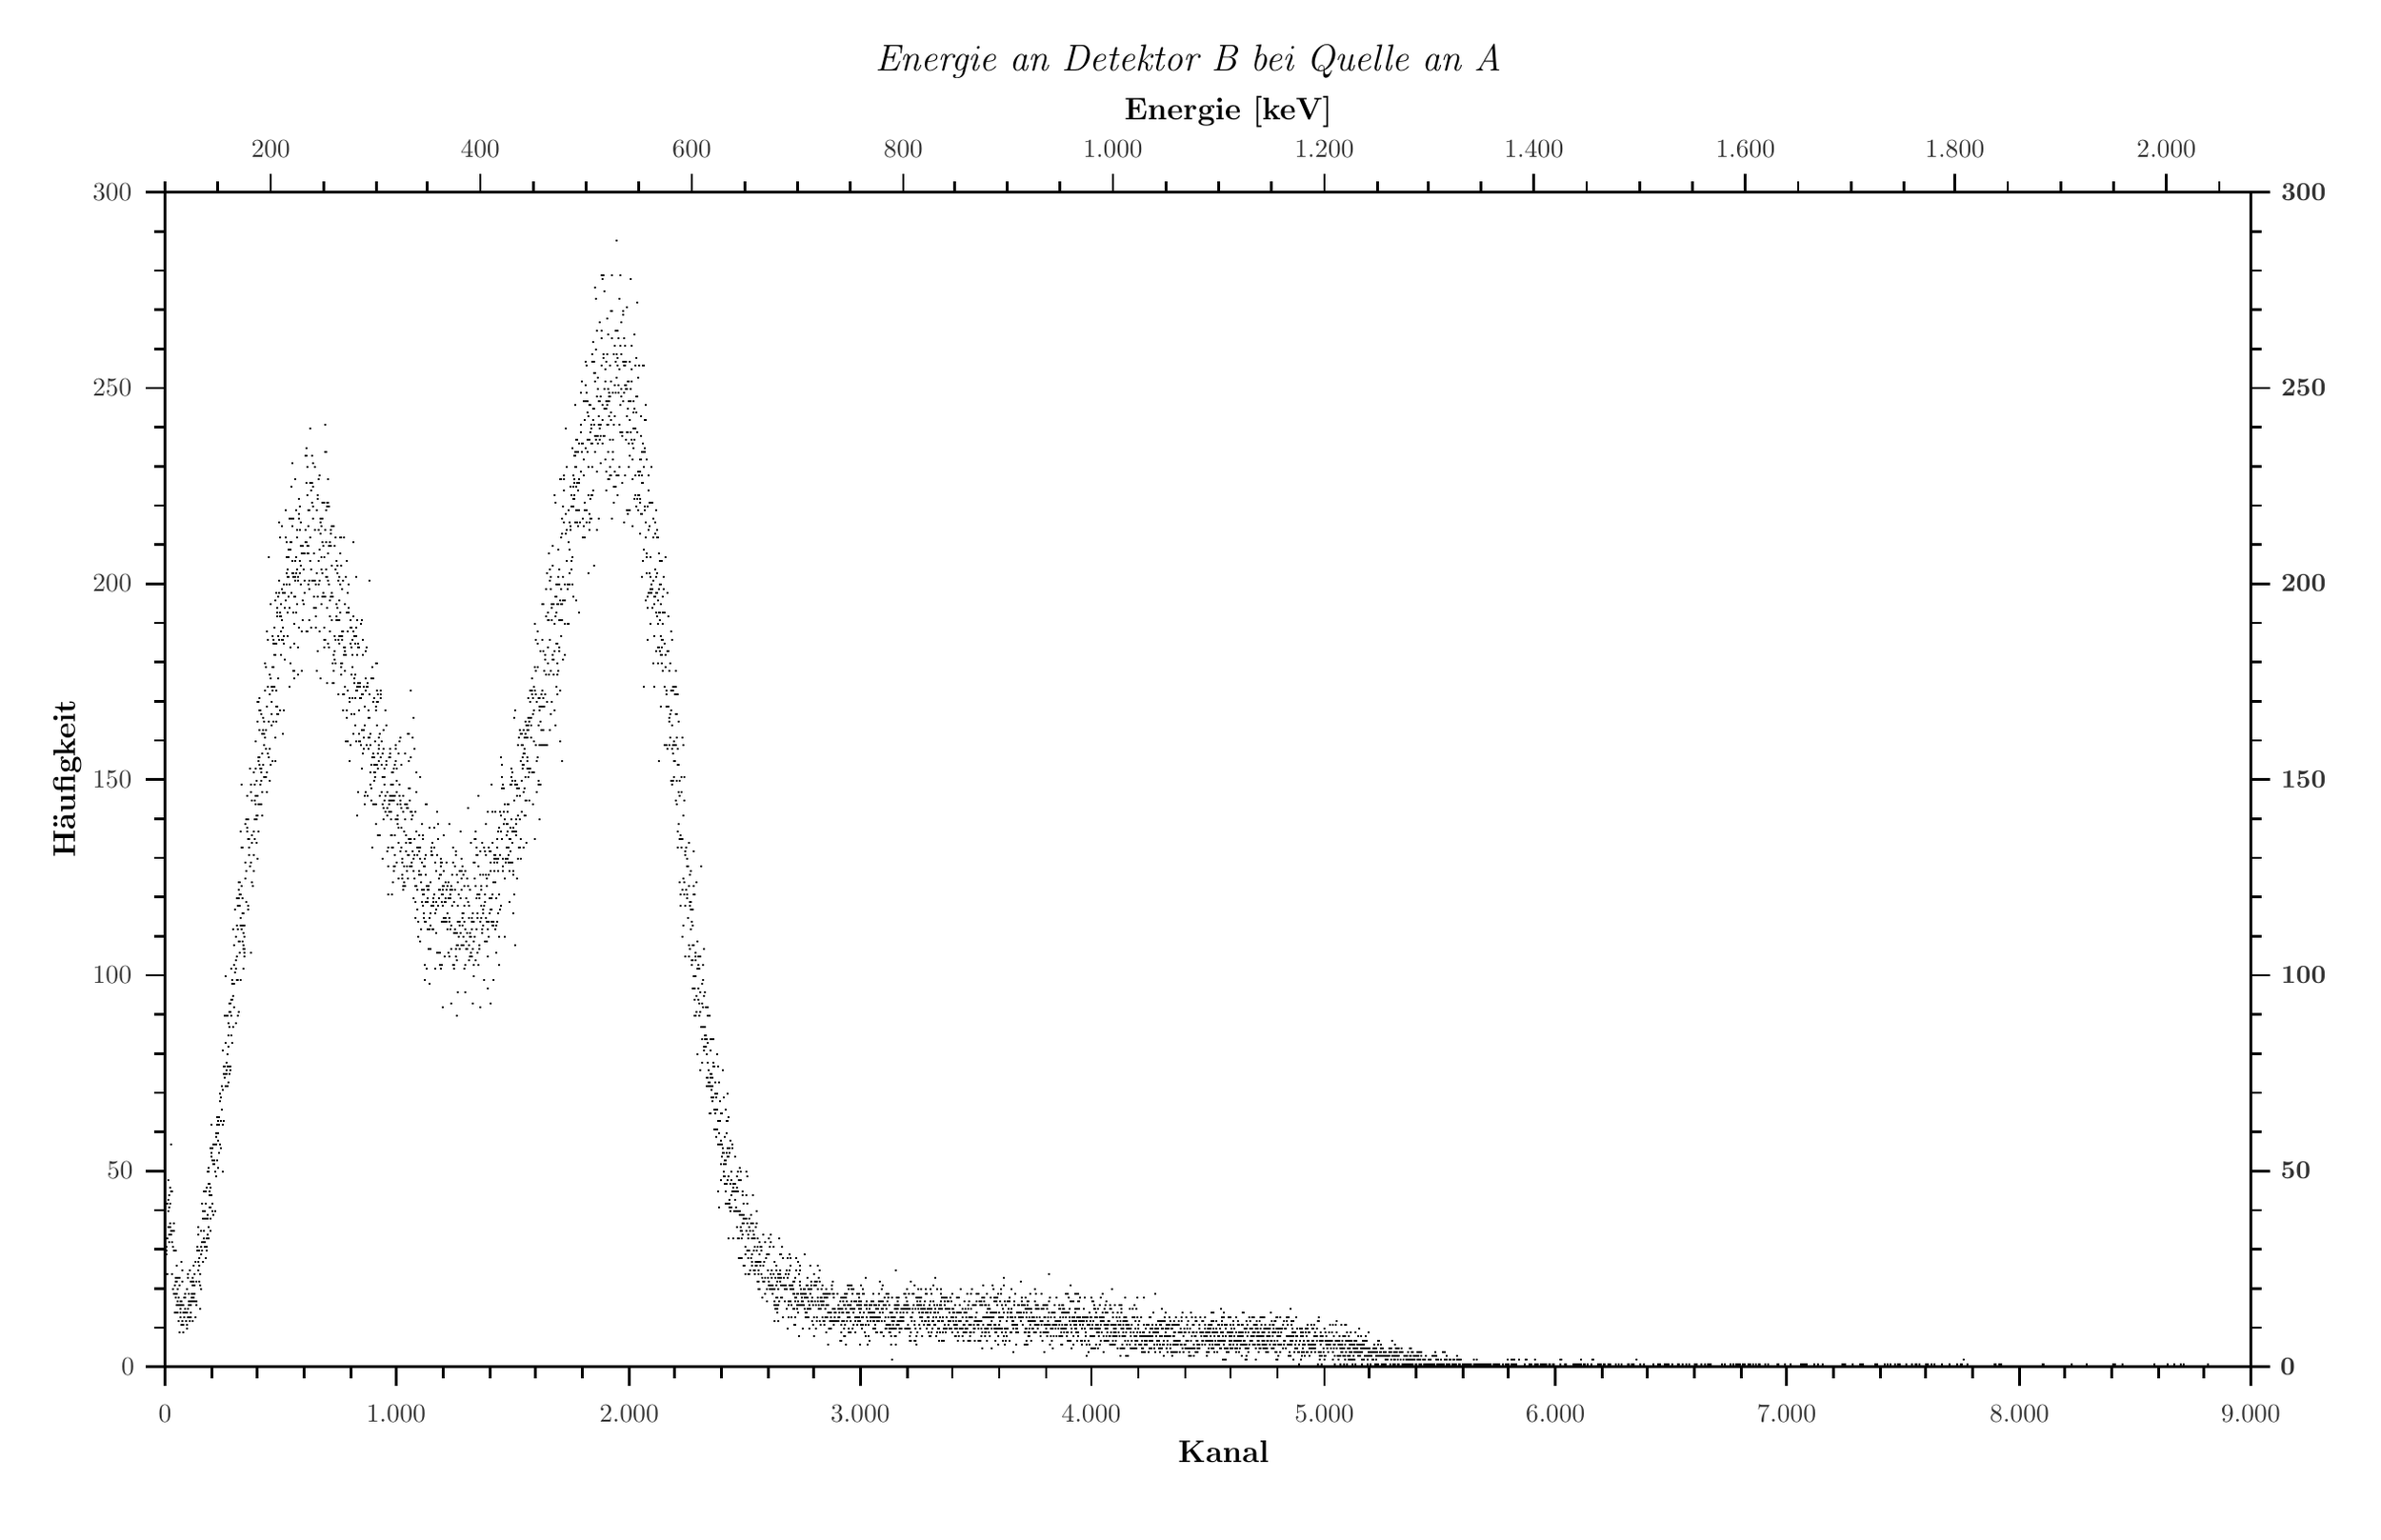
\begin{tikzpicture}{0pt}{0pt}{1189pt}{760pt}
	\clip(0pt,760pt) -- (895.094pt,760pt) -- (895.094pt,187.862pt) -- (0pt,187.862pt) -- (0pt,760pt);
\begin{scope}
	\clip(53.4497pt,696.011pt) -- (855.195pt,696.011pt) -- (855.195pt,244.323pt) -- (53.4497pt,244.323pt) -- (53.4497pt,696.011pt);
	\color[rgb]{0,0,0}
	\fill (53.5388pt,289.492pt) rectangle (54.2916pt,288.739pt);
	\color[rgb]{0,0,0}
	\fill (53.6279pt,290.998pt) rectangle (54.3807pt,290.245pt);
	\fill (53.7169pt,287.987pt) rectangle (54.4697pt,287.234pt);
	\fill (53.806pt,294.009pt) rectangle (54.5588pt,293.256pt);
	\fill (53.8951pt,307.56pt) rectangle (54.6479pt,306.807pt);
	\fill (54.0733pt,280.458pt) rectangle (54.8261pt,279.706pt);
	\fill (54.1624pt,298.526pt) rectangle (54.9152pt,297.773pt);
	\fill (54.2514pt,316.593pt) rectangle (55.0042pt,315.841pt);
	\fill (54.3405pt,309.065pt) rectangle (55.0933pt,308.312pt);
	\fill (54.4296pt,304.548pt) rectangle (55.1824pt,303.796pt);
	\fill (54.5187pt,295.515pt) rectangle (55.2715pt,294.762pt);
	\fill (54.6078pt,292.503pt) rectangle (55.3606pt,291.751pt);
	\fill (54.6968pt,310.571pt) rectangle (55.4497pt,309.818pt);
	\fill (54.7859pt,306.054pt) rectangle (55.5387pt,305.301pt);
	\fill (54.875pt,313.582pt) rectangle (55.6278pt,312.829pt);
	\fill (54.9641pt,307.56pt) rectangle (55.7169pt,306.807pt);
	\fill (55.0532pt,300.032pt) rectangle (55.806pt,299.279pt);
	\fill (55.1423pt,298.526pt) rectangle (55.8951pt,297.773pt);
	\fill (55.2313pt,330.144pt) rectangle (55.9842pt,329.391pt);
	\fill (55.3204pt,312.077pt) rectangle (56.0732pt,311.324pt);
	\fill (55.4095pt,297.02pt) rectangle (56.1623pt,296.267pt);
	\fill (55.4986pt,295.515pt) rectangle (56.2514pt,294.762pt);
	\fill (55.5877pt,312.077pt) rectangle (56.3405pt,311.324pt);
	\fill (55.7658pt,292.503pt) rectangle (56.5187pt,291.751pt);
	\fill (55.8549pt,280.458pt) rectangle (56.6077pt,279.706pt);
	\fill (56.1222pt,274.436pt) rectangle (56.875pt,273.683pt);
	\fill (56.2113pt,290.998pt) rectangle (56.9641pt,290.245pt);
	\fill (56.3003pt,297.02pt) rectangle (57.0531pt,296.267pt);
	\fill (56.3894pt,300.032pt) rectangle (57.1422pt,299.279pt);
	\fill (56.5676pt,289.492pt) rectangle (57.3204pt,288.739pt);
	\fill (56.6567pt,272.93pt) rectangle (57.4095pt,272.178pt);
	\fill (56.8348pt,275.942pt) rectangle (57.5876pt,275.189pt);
	\fill (56.9239pt,272.93pt) rectangle (57.6767pt,272.178pt);
	\fill (57.013pt,265.402pt) rectangle (57.7658pt,264.649pt);
	\fill (57.1021pt,278.953pt) rectangle (57.8549pt,278.2pt);
	\fill (57.1912pt,289.492pt) rectangle (57.944pt,288.739pt);
	\fill (57.2802pt,271.425pt) rectangle (58.0331pt,270.672pt);
	\fill (57.3693pt,277.447pt) rectangle (58.1221pt,276.694pt);
	\fill (57.4584pt,283.47pt) rectangle (58.2112pt,282.717pt);
	\fill (57.5475pt,268.413pt) rectangle (58.3003pt,267.661pt);
	\fill (57.6366pt,272.93pt) rectangle (58.3894pt,272.178pt);
	\fill (57.7257pt,265.402pt) rectangle (58.4785pt,264.649pt);
	\fill (57.8147pt,278.953pt) rectangle (58.5676pt,278.2pt);
	\fill (57.9038pt,274.436pt) rectangle (58.6566pt,273.683pt);
	\fill (57.9929pt,269.919pt) rectangle (58.7457pt,269.166pt);
	\fill (58.1711pt,268.413pt) rectangle (58.9239pt,267.661pt);
	\fill (58.2602pt,271.425pt) rectangle (59.013pt,270.672pt);
	\fill (58.3492pt,271.425pt) rectangle (59.1021pt,270.672pt);
	\fill (58.4383pt,262.391pt) rectangle (59.1911pt,261.638pt);
	\fill (58.5274pt,278.953pt) rectangle (59.2802pt,278.2pt);
	\fill (58.6165pt,268.413pt) rectangle (59.3693pt,267.661pt);
	\fill (58.7056pt,275.942pt) rectangle (59.4584pt,275.189pt);
	\fill (58.7947pt,257.874pt) rectangle (59.5475pt,257.121pt);
	\fill (58.8837pt,269.919pt) rectangle (59.6366pt,269.166pt);
	\fill (58.9728pt,265.402pt) rectangle (59.7256pt,264.649pt);
	\fill (59.0619pt,263.897pt) rectangle (59.8147pt,263.144pt);
	\fill (59.151pt,266.908pt) rectangle (59.9038pt,266.155pt);
	\fill (59.2401pt,284.975pt) rectangle (59.9929pt,284.223pt);
	\fill (59.3292pt,260.885pt) rectangle (60.082pt,260.132pt);
	\fill (59.4182pt,269.919pt) rectangle (60.171pt,269.166pt);
	\fill (59.5073pt,268.413pt) rectangle (60.2601pt,267.661pt);
	\fill (59.5964pt,281.964pt) rectangle (60.3492pt,281.211pt);
	\fill (59.6855pt,277.447pt) rectangle (60.4383pt,276.694pt);
	\fill (59.8636pt,262.391pt) rectangle (60.6165pt,261.638pt);
	\fill (59.9527pt,268.413pt) rectangle (60.7055pt,267.661pt);
	\fill (60.0418pt,265.402pt) rectangle (60.7946pt,264.649pt);
	\fill (60.1309pt,260.885pt) rectangle (60.8837pt,260.132pt);
	\fill (60.22pt,257.874pt) rectangle (60.9728pt,257.121pt);
	\fill (60.3091pt,271.425pt) rectangle (61.0619pt,270.672pt);
	\fill (60.5763pt,263.897pt) rectangle (61.3291pt,263.144pt);
	\fill (60.6654pt,266.908pt) rectangle (61.4182pt,266.155pt);
	\fill (60.7545pt,265.402pt) rectangle (61.5073pt,264.649pt);
	\fill (60.8436pt,271.425pt) rectangle (61.5964pt,270.672pt);
	\fill (60.9326pt,272.93pt) rectangle (61.6855pt,272.178pt);
	\fill (61.289pt,262.391pt) rectangle (62.0418pt,261.638pt);
	\fill (61.3781pt,260.885pt) rectangle (62.1309pt,260.132pt);
	\fill (61.4671pt,259.38pt) rectangle (62.22pt,258.627pt);
	\fill (61.5562pt,265.402pt) rectangle (62.309pt,264.649pt);
	\fill (61.6453pt,274.436pt) rectangle (62.3981pt,273.683pt);
	\fill (61.7344pt,263.897pt) rectangle (62.4872pt,263.144pt);
	\fill (61.8235pt,280.458pt) rectangle (62.5763pt,279.706pt);
	\fill (61.9126pt,278.953pt) rectangle (62.6654pt,278.2pt);
	\fill (62.0016pt,266.908pt) rectangle (62.7544pt,266.155pt);
	\fill (62.0907pt,268.413pt) rectangle (62.8435pt,267.661pt);
	\fill (62.1798pt,268.413pt) rectangle (62.9326pt,267.661pt);
	\fill (62.2689pt,272.93pt) rectangle (63.0217pt,272.178pt);
	\fill (62.4471pt,269.919pt) rectangle (63.1999pt,269.166pt);
	\fill (62.5361pt,281.964pt) rectangle (63.2889pt,281.211pt);
	\fill (62.6252pt,262.391pt) rectangle (63.378pt,261.638pt);
	\fill (62.8034pt,263.897pt) rectangle (63.5562pt,263.144pt);
	\fill (62.8925pt,268.413pt) rectangle (63.6453pt,267.661pt);
	\fill (62.9815pt,265.402pt) rectangle (63.7344pt,264.649pt);
	\fill (63.0706pt,263.897pt) rectangle (63.8234pt,263.144pt);
	\fill (63.1597pt,277.447pt) rectangle (63.9125pt,276.694pt);
	\fill (63.3379pt,272.93pt) rectangle (64.0907pt,272.178pt);
	\fill (63.427pt,271.425pt) rectangle (64.1798pt,270.672pt);
	\fill (63.516pt,269.919pt) rectangle (64.2689pt,269.166pt);
	\fill (63.6051pt,275.942pt) rectangle (64.3579pt,275.189pt);
	\fill (63.6942pt,278.953pt) rectangle (64.447pt,278.2pt);
	\fill (63.7833pt,262.391pt) rectangle (64.5361pt,261.638pt);
	\fill (63.8724pt,277.447pt) rectangle (64.6252pt,276.694pt);
	\fill (63.9615pt,272.93pt) rectangle (64.7143pt,272.178pt);
	\fill (64.0505pt,283.47pt) rectangle (64.8034pt,282.717pt);
	\fill (64.1396pt,271.425pt) rectangle (64.8924pt,270.672pt);
	\fill (64.2287pt,269.919pt) rectangle (64.9815pt,269.166pt);
	\fill (64.3178pt,275.942pt) rectangle (65.0706pt,275.189pt);
	\fill (64.4069pt,275.942pt) rectangle (65.1597pt,275.189pt);
	\fill (64.496pt,280.458pt) rectangle (65.2488pt,279.706pt);
	\fill (64.585pt,272.93pt) rectangle (65.3379pt,272.178pt);
	\fill (64.7632pt,269.919pt) rectangle (65.516pt,269.166pt);
	\fill (64.8523pt,263.897pt) rectangle (65.6051pt,263.144pt);
	\fill (64.9414pt,284.975pt) rectangle (65.6942pt,284.223pt);
	\fill (65.1195pt,268.413pt) rectangle (65.8723pt,267.661pt);
	\fill (65.2086pt,277.447pt) rectangle (65.9614pt,276.694pt);
	\fill (65.2977pt,269.919pt) rectangle (66.0505pt,269.166pt);
	\fill (65.5649pt,290.998pt) rectangle (66.3178pt,290.245pt);
	\fill (65.654pt,289.492pt) rectangle (66.4068pt,288.739pt);
	\fill (65.7431pt,281.964pt) rectangle (66.4959pt,281.211pt);
	\fill (65.8322pt,298.526pt) rectangle (66.585pt,297.773pt);
	\fill (65.9213pt,284.975pt) rectangle (66.6741pt,284.223pt);
	\fill (66.0104pt,295.515pt) rectangle (66.7632pt,294.762pt);
	\fill (66.0994pt,289.492pt) rectangle (66.8523pt,288.739pt);
	\fill (66.1885pt,277.447pt) rectangle (66.9413pt,276.694pt);
	\fill (66.2776pt,286.481pt) rectangle (67.0304pt,285.728pt);
	\fill (66.3667pt,283.47pt) rectangle (67.1195pt,282.717pt);
	\fill (66.4558pt,275.942pt) rectangle (67.2086pt,275.189pt);
	\fill (66.5449pt,266.908pt) rectangle (67.2977pt,266.155pt);
	\fill (66.6339pt,280.458pt) rectangle (67.3868pt,279.706pt);
	\fill (66.723pt,275.942pt) rectangle (67.4758pt,275.189pt);
	\fill (66.8121pt,287.987pt) rectangle (67.5649pt,287.234pt);
	\fill (66.9012pt,297.02pt) rectangle (67.654pt,296.267pt);
	\fill (66.9903pt,274.436pt) rectangle (67.7431pt,273.683pt);
	\fill (67.0794pt,290.998pt) rectangle (67.8322pt,290.245pt);
	\fill (67.1684pt,292.503pt) rectangle (67.9213pt,291.751pt);
	\fill (67.2575pt,289.492pt) rectangle (68.0103pt,288.739pt);
	\fill (67.4357pt,307.56pt) rectangle (68.1885pt,306.807pt);
	\fill (67.5248pt,292.503pt) rectangle (68.2776pt,291.751pt);
	\fill (67.6139pt,301.537pt) rectangle (68.3667pt,300.784pt);
	\fill (67.7029pt,304.548pt) rectangle (68.4558pt,303.796pt);
	\fill (67.792pt,284.975pt) rectangle (68.5448pt,284.223pt);
	\fill (67.8811pt,297.02pt) rectangle (68.6339pt,296.267pt);
	\fill (67.9702pt,312.077pt) rectangle (68.723pt,311.324pt);
	\fill (68.0593pt,294.009pt) rectangle (68.8121pt,293.256pt);
	\fill (68.1484pt,297.02pt) rectangle (68.9012pt,296.267pt);
	\fill (68.2374pt,304.548pt) rectangle (68.9902pt,303.796pt);
	\fill (68.3265pt,290.998pt) rectangle (69.0793pt,290.245pt);
	\fill (68.4156pt,292.503pt) rectangle (69.1684pt,291.751pt);
	\fill (68.5047pt,301.537pt) rectangle (69.2575pt,300.784pt);
	\fill (68.5938pt,286.481pt) rectangle (69.3466pt,285.728pt);
	\fill (68.6828pt,312.077pt) rectangle (69.4357pt,311.324pt);
	\fill (68.861pt,307.56pt) rectangle (69.6138pt,306.807pt);
	\fill (68.9501pt,290.998pt) rectangle (69.7029pt,290.245pt);
	\fill (69.0392pt,294.009pt) rectangle (69.792pt,293.256pt);
	\fill (69.1283pt,289.492pt) rectangle (69.8811pt,288.739pt);
	\fill (69.2173pt,313.582pt) rectangle (69.9702pt,312.829pt);
	\fill (69.3064pt,301.537pt) rectangle (70.0592pt,300.784pt);
	\fill (69.3955pt,295.515pt) rectangle (70.1483pt,294.762pt);
	\fill (69.4846pt,303.043pt) rectangle (70.2374pt,302.29pt);
	\fill (69.5737pt,319.605pt) rectangle (70.3265pt,318.852pt);
	\fill (69.6628pt,319.605pt) rectangle (70.4156pt,318.852pt);
	\fill (69.7518pt,321.11pt) rectangle (70.5047pt,320.358pt);
	\fill (69.8409pt,294.009pt) rectangle (70.5937pt,293.256pt);
	\fill (69.93pt,298.526pt) rectangle (70.6828pt,297.773pt);
	\fill (70.0191pt,315.088pt) rectangle (70.7719pt,314.335pt);
	\fill (70.1082pt,310.571pt) rectangle (70.861pt,309.818pt);
	\fill (70.2863pt,312.077pt) rectangle (71.0392pt,311.324pt);
	\fill (70.3754pt,306.054pt) rectangle (71.1282pt,305.301pt);
	\fill (70.4645pt,297.02pt) rectangle (71.2173pt,296.267pt);
	\fill (70.5536pt,301.537pt) rectangle (71.3064pt,300.784pt);
	\fill (70.6427pt,313.582pt) rectangle (71.3955pt,312.829pt);
	\fill (70.7318pt,328.638pt) rectangle (71.4846pt,327.886pt);
	\fill (70.8208pt,325.627pt) rectangle (71.5736pt,324.874pt);
	\fill (70.9099pt,310.571pt) rectangle (71.6627pt,309.818pt);
	\fill (70.999pt,327.133pt) rectangle (71.7518pt,326.38pt);
	\fill (71.0881pt,337.672pt) rectangle (71.8409pt,336.919pt);
	\fill (71.1772pt,304.548pt) rectangle (71.93pt,303.796pt);
	\fill (71.2662pt,328.638pt) rectangle (72.0191pt,327.886pt);
	\fill (71.3553pt,307.56pt) rectangle (72.1081pt,306.807pt);
	\fill (71.4444pt,324.122pt) rectangle (72.1972pt,323.369pt);
	\fill (71.5335pt,303.043pt) rectangle (72.2863pt,302.29pt);
	\fill (71.6226pt,322.616pt) rectangle (72.3754pt,321.863pt);
	\fill (71.7117pt,330.144pt) rectangle (72.4645pt,329.391pt);
	\fill (71.9789pt,324.122pt) rectangle (72.7317pt,323.369pt);
	\fill (72.068pt,322.616pt) rectangle (72.8208pt,321.863pt);
	\fill (72.1571pt,330.144pt) rectangle (72.9099pt,329.391pt);
	\fill (72.2462pt,304.548pt) rectangle (72.999pt,303.796pt);
	\fill (72.5134pt,319.605pt) rectangle (73.2662pt,318.852pt);
	\fill (72.6025pt,334.661pt) rectangle (73.3553pt,333.908pt);
	\fill (72.6916pt,318.099pt) rectangle (73.4444pt,317.346pt);
	\fill (72.7807pt,333.155pt) rectangle (73.5335pt,332.402pt);
	\fill (72.8697pt,330.144pt) rectangle (73.6226pt,329.391pt);
	\fill (72.9588pt,337.672pt) rectangle (73.7116pt,336.919pt);
	\fill (73.137pt,340.683pt) rectangle (73.8898pt,339.931pt);
	\fill (73.2261pt,324.122pt) rectangle (73.9789pt,323.369pt);
	\fill (73.3152pt,334.661pt) rectangle (74.068pt,333.908pt);
	\fill (73.4042pt,339.178pt) rectangle (74.157pt,338.425pt);
	\fill (73.4933pt,321.11pt) rectangle (74.2461pt,320.358pt);
	\fill (73.5824pt,331.65pt) rectangle (74.3352pt,330.897pt);
	\fill (73.6715pt,337.672pt) rectangle (74.4243pt,336.919pt);
	\fill (73.7606pt,340.683pt) rectangle (74.5134pt,339.931pt);
	\fill (73.8497pt,327.133pt) rectangle (74.6025pt,326.38pt);
	\fill (74.0278pt,346.706pt) rectangle (74.7806pt,345.953pt);
	\fill (74.1169pt,349.717pt) rectangle (74.8697pt,348.964pt);
	\fill (74.206pt,330.144pt) rectangle (74.9588pt,329.391pt);
	\fill (74.2951pt,346.706pt) rectangle (75.0479pt,345.953pt);
	\fill (74.3841pt,328.638pt) rectangle (75.137pt,327.886pt);
	\fill (74.4732pt,339.178pt) rectangle (75.226pt,338.425pt);
	\fill (74.5623pt,348.212pt) rectangle (75.3151pt,347.459pt);
	\fill (74.9186pt,343.695pt) rectangle (75.6715pt,342.942pt);
	\fill (75.0077pt,352.728pt) rectangle (75.7605pt,351.976pt);
	\fill (75.0968pt,319.605pt) rectangle (75.8496pt,318.852pt);
	\fill (75.1859pt,351.223pt) rectangle (75.9387pt,350.47pt);
	\fill (75.275pt,366.279pt) rectangle (76.0278pt,365.526pt);
	\fill (75.3641pt,337.672pt) rectangle (76.1169pt,336.919pt);
	\fill (75.5422pt,339.178pt) rectangle (76.295pt,338.425pt);
	\fill (75.6313pt,360.257pt) rectangle (76.3841pt,359.504pt);
	\fill (75.7204pt,357.245pt) rectangle (76.4732pt,356.493pt);
	\fill (75.8986pt,355.74pt) rectangle (76.6514pt,354.987pt);
	\fill (75.9876pt,360.257pt) rectangle (76.7405pt,359.504pt);
	\fill (76.1658pt,379.83pt) rectangle (76.9186pt,379.077pt);
	\fill (76.2549pt,394.886pt) rectangle (77.0077pt,394.133pt);
	\fill (76.344pt,352.728pt) rectangle (77.0968pt,351.976pt);
	\fill (76.4331pt,369.29pt) rectangle (77.1859pt,368.538pt);
	\fill (76.5221pt,357.245pt) rectangle (77.2749pt,356.493pt);
	\fill (76.6112pt,361.762pt) rectangle (77.364pt,361.009pt);
	\fill (76.7894pt,358.751pt) rectangle (77.5422pt,357.998pt);
	\fill (76.8785pt,352.728pt) rectangle (77.6313pt,351.976pt);
	\fill (76.9676pt,364.773pt) rectangle (77.7204pt,364.021pt);
	\fill (77.1457pt,379.83pt) rectangle (77.8985pt,379.077pt);
	\fill (77.2348pt,360.257pt) rectangle (77.9876pt,359.504pt);
	\fill (77.3239pt,354.234pt) rectangle (78.0767pt,353.481pt);
	\fill (77.413pt,372.302pt) rectangle (78.1658pt,371.549pt);
	\fill (77.502pt,367.785pt) rectangle (78.2549pt,367.032pt);
	\fill (77.5911pt,376.818pt) rectangle (78.3439pt,376.066pt);
	\fill (77.6802pt,375.313pt) rectangle (78.433pt,374.56pt);
	\fill (77.7693pt,381.335pt) rectangle (78.5221pt,380.582pt);
	\fill (77.8584pt,384.347pt) rectangle (78.6112pt,383.594pt);
	\fill (77.9475pt,357.245pt) rectangle (78.7003pt,356.493pt);
	\fill (78.0365pt,358.751pt) rectangle (78.7894pt,357.998pt);
	\fill (78.1256pt,360.257pt) rectangle (78.8784pt,359.504pt);
	\fill (78.2147pt,384.347pt) rectangle (78.9675pt,383.594pt);
	\fill (78.3038pt,381.335pt) rectangle (79.0566pt,380.582pt);
	\fill (78.3929pt,372.302pt) rectangle (79.1457pt,371.549pt);
	\fill (78.482pt,385.852pt) rectangle (79.2348pt,385.099pt);
	\fill (78.571pt,397.897pt) rectangle (79.3239pt,397.144pt);
	\fill (78.6601pt,379.83pt) rectangle (79.4129pt,379.077pt);
	\fill (78.7492pt,385.852pt) rectangle (79.502pt,385.099pt);
	\fill (78.8383pt,391.875pt) rectangle (79.5911pt,391.122pt);
	\fill (78.9274pt,393.38pt) rectangle (79.6802pt,392.627pt);
	\fill (79.0165pt,369.29pt) rectangle (79.7693pt,368.538pt);
	\fill (79.1055pt,387.358pt) rectangle (79.8584pt,386.605pt);
	\fill (79.2837pt,375.313pt) rectangle (80.0365pt,374.56pt);
	\fill (79.3728pt,412.953pt) rectangle (80.1256pt,412.201pt);
	\fill (79.4619pt,399.403pt) rectangle (80.2147pt,398.65pt);
	\fill (79.551pt,382.841pt) rectangle (80.3038pt,382.088pt);
	\fill (79.64pt,406.931pt) rectangle (80.3928pt,406.178pt);
	\fill (79.7291pt,391.875pt) rectangle (80.4819pt,391.122pt);
	\fill (79.8182pt,396.392pt) rectangle (80.571pt,395.639pt);
	\fill (79.9964pt,420.482pt) rectangle (80.7492pt,419.729pt);
	\fill (80.1745pt,409.942pt) rectangle (80.9273pt,409.189pt);
	\fill (80.2636pt,400.908pt) rectangle (81.0164pt,400.156pt);
	\fill (80.3527pt,397.897pt) rectangle (81.1055pt,397.144pt);
	\fill (80.4418pt,376.818pt) rectangle (81.1946pt,376.066pt);
	\fill (80.5309pt,424.998pt) rectangle (81.2837pt,424.246pt);
	\fill (80.6199pt,414.459pt) rectangle (81.3728pt,413.706pt);
	\fill (80.709pt,393.38pt) rectangle (81.4618pt,392.627pt);
	\fill (80.7981pt,402.414pt) rectangle (81.5509pt,401.661pt);
	\fill (80.8872pt,421.987pt) rectangle (81.64pt,421.234pt);
	\fill (80.9763pt,412.953pt) rectangle (81.7291pt,412.201pt);
	\fill (81.0654pt,393.38pt) rectangle (81.8182pt,392.627pt);
	\fill (81.1544pt,379.83pt) rectangle (81.9073pt,379.077pt);
	\fill (81.2435pt,428.01pt) rectangle (81.9963pt,427.257pt);
	\fill (81.3326pt,431.021pt) rectangle (82.0854pt,430.268pt);
	\fill (81.4217pt,424.998pt) rectangle (82.1745pt,424.246pt);
	\fill (81.5108pt,381.335pt) rectangle (82.2636pt,380.582pt);
	\fill (81.5999pt,408.437pt) rectangle (82.3527pt,407.684pt);
	\fill (81.6889pt,431.021pt) rectangle (82.4418pt,430.268pt);
	\fill (81.778pt,421.987pt) rectangle (82.5308pt,421.234pt);
	\fill (81.8671pt,403.92pt) rectangle (82.6199pt,403.167pt);
	\fill (81.9562pt,426.504pt) rectangle (82.709pt,425.751pt);
	\fill (82.0453pt,393.38pt) rectangle (82.7981pt,392.627pt);
	\fill (82.1344pt,417.47pt) rectangle (82.8872pt,416.718pt);
	\fill (82.2234pt,450.594pt) rectangle (82.9762pt,449.841pt);
	\fill (82.3125pt,414.459pt) rectangle (83.0653pt,413.706pt);
	\fill (82.4016pt,412.953pt) rectangle (83.1544pt,412.201pt);
	\fill (82.4907pt,468.662pt) rectangle (83.2435pt,467.909pt);
	\fill (82.5798pt,429.515pt) rectangle (83.3326pt,428.762pt);
	\fill (82.6688pt,444.572pt) rectangle (83.4217pt,443.819pt);
	\fill (82.7579pt,424.998pt) rectangle (83.5107pt,424.246pt);
	\fill (82.847pt,408.437pt) rectangle (83.5998pt,407.684pt);
	\fill (82.9361pt,414.459pt) rectangle (83.6889pt,413.706pt);
	\fill (83.0252pt,418.976pt) rectangle (83.778pt,418.223pt);
	\fill (83.1143pt,411.448pt) rectangle (83.8671pt,410.695pt);
	\fill (83.2033pt,397.897pt) rectangle (83.9562pt,397.144pt);
	\fill (83.2924pt,406.931pt) rectangle (84.0452pt,406.178pt);
	\fill (83.3815pt,405.425pt) rectangle (84.1343pt,404.673pt);
	\fill (83.4706pt,403.92pt) rectangle (84.2234pt,403.167pt);
	\fill (83.5597pt,409.942pt) rectangle (84.3125pt,409.189pt);
	\fill (83.6488pt,402.414pt) rectangle (84.4016pt,401.661pt);
	\fill (83.7378pt,414.459pt) rectangle (84.4907pt,413.706pt);
	\fill (83.916pt,438.549pt) rectangle (84.6688pt,437.796pt);
	\fill (84.0051pt,453.605pt) rectangle (84.7579pt,452.853pt);
	\fill (84.0942pt,432.527pt) rectangle (84.847pt,431.774pt);
	\fill (84.1833pt,423.493pt) rectangle (84.9361pt,422.74pt);
	\fill (84.3614pt,435.538pt) rectangle (85.1142pt,434.785pt);
	\fill (84.4505pt,455.111pt) rectangle (85.2033pt,454.358pt);
	\fill (84.5396pt,450.594pt) rectangle (85.2924pt,449.841pt);
	\fill (84.7178pt,452.1pt) rectangle (85.4706pt,451.347pt);
	\fill (84.8068pt,464.145pt) rectangle (85.5597pt,463.392pt);
	\fill (84.8959pt,455.111pt) rectangle (85.6487pt,454.358pt);
	\fill (84.985pt,420.482pt) rectangle (85.7378pt,419.729pt);
	\fill (85.0741pt,421.987pt) rectangle (85.8269pt,421.234pt);
	\fill (85.1632pt,447.583pt) rectangle (85.916pt,446.83pt);
	\fill (85.3413pt,441.56pt) rectangle (86.0941pt,440.808pt);
	\fill (85.4304pt,444.572pt) rectangle (86.1832pt,443.819pt);
	\fill (85.5195pt,447.583pt) rectangle (86.2723pt,446.83pt);
	\fill (85.6086pt,474.684pt) rectangle (86.3614pt,473.931pt);
	\fill (85.6977pt,437.043pt) rectangle (86.4505pt,436.291pt);
	\fill (85.9649pt,468.662pt) rectangle (86.7177pt,467.909pt);
	\fill (86.054pt,403.92pt) rectangle (86.8068pt,403.167pt);
	\fill (86.1431pt,438.549pt) rectangle (86.8959pt,437.796pt);
	\fill (86.2322pt,465.65pt) rectangle (86.985pt,464.897pt);
	\fill (86.3212pt,449.088pt) rectangle (87.0741pt,448.336pt);
	\fill (86.4103pt,462.639pt) rectangle (87.1631pt,461.886pt);
	\fill (86.4994pt,431.021pt) rectangle (87.2522pt,430.268pt);
	\fill (86.5885pt,446.077pt) rectangle (87.3413pt,445.324pt);
	\fill (86.7667pt,429.515pt) rectangle (87.5195pt,428.762pt);
	\fill (87.0339pt,435.538pt) rectangle (87.7867pt,434.785pt);
	\fill (87.123pt,473.178pt) rectangle (87.8758pt,472.426pt);
	\fill (87.2121pt,450.594pt) rectangle (87.9649pt,449.841pt);
	\fill (87.3012pt,441.56pt) rectangle (88.054pt,440.808pt);
	\fill (87.3902pt,468.662pt) rectangle (88.1431pt,467.909pt);
	\fill (87.4793pt,447.583pt) rectangle (88.2321pt,446.83pt);
	\fill (87.5684pt,455.111pt) rectangle (88.3212pt,454.358pt);
	\fill (87.6575pt,462.639pt) rectangle (88.4103pt,461.886pt);
	\fill (87.7466pt,474.684pt) rectangle (88.4994pt,473.931pt);
	\fill (87.8357pt,485.223pt) rectangle (88.5885pt,484.471pt);
	\fill (87.9247pt,464.145pt) rectangle (88.6775pt,463.392pt);
	\fill (88.0138pt,461.133pt) rectangle (88.7666pt,460.381pt);
	\fill (88.1029pt,455.111pt) rectangle (88.8557pt,454.358pt);
	\fill (88.192pt,446.077pt) rectangle (88.9448pt,445.324pt);
	\fill (88.2811pt,470.167pt) rectangle (89.0339pt,469.414pt);
	\fill (88.3701pt,456.617pt) rectangle (89.123pt,455.864pt);
	\fill (88.4592pt,464.145pt) rectangle (89.212pt,463.392pt);
	\fill (88.5483pt,456.617pt) rectangle (89.3011pt,455.864pt);
	\fill (88.6374pt,492.752pt) rectangle (89.3902pt,491.999pt);
	\fill (88.7265pt,440.055pt) rectangle (89.4793pt,439.302pt);
	\fill (88.8156pt,500.28pt) rectangle (89.5684pt,499.527pt);
	\fill (88.9046pt,477.695pt) rectangle (89.6575pt,476.942pt);
	\fill (88.9937pt,450.594pt) rectangle (89.7465pt,449.841pt);
	\fill (89.0828pt,461.133pt) rectangle (89.8356pt,460.381pt);
	\fill (89.1719pt,479.201pt) rectangle (89.9247pt,478.448pt);
	\fill (89.261pt,501.785pt) rectangle (90.0138pt,501.033pt);
	\fill (89.3501pt,476.19pt) rectangle (90.1029pt,475.437pt);
	\fill (89.4391pt,489.74pt) rectangle (90.192pt,488.988pt);
	\fill (89.5282pt,497.268pt) rectangle (90.281pt,496.516pt);
	\fill (89.7064pt,468.662pt) rectangle (90.4592pt,467.909pt);
	\fill (89.7955pt,474.684pt) rectangle (90.5483pt,473.931pt);
	\fill (89.8846pt,461.133pt) rectangle (90.6374pt,460.381pt);
	\fill (89.9736pt,474.684pt) rectangle (90.7265pt,473.931pt);
	\fill (90.0627pt,473.178pt) rectangle (90.8155pt,472.426pt);
	\fill (90.1518pt,470.167pt) rectangle (90.9046pt,469.414pt);
	\fill (90.2409pt,495.763pt) rectangle (90.9937pt,495.01pt);
	\fill (90.33pt,465.65pt) rectangle (91.0828pt,464.897pt);
	\fill (90.4191pt,488.235pt) rectangle (91.1719pt,487.482pt);
	\fill (90.5081pt,456.617pt) rectangle (91.2609pt,455.864pt);
	\fill (90.5972pt,480.707pt) rectangle (91.35pt,479.954pt);
	\fill (90.6863pt,494.257pt) rectangle (91.4391pt,493.504pt);
	\fill (90.7754pt,494.257pt) rectangle (91.5282pt,493.504pt);
	\fill (90.8645pt,489.74pt) rectangle (91.6173pt,488.988pt);
	\fill (90.9536pt,476.19pt) rectangle (91.7064pt,475.437pt);
	\fill (91.0426pt,492.752pt) rectangle (91.7954pt,491.999pt);
	\fill (91.1317pt,483.718pt) rectangle (91.8845pt,482.965pt);
	\fill (91.2208pt,488.235pt) rectangle (91.9736pt,487.482pt);
	\fill (91.3099pt,471.673pt) rectangle (92.0627pt,470.92pt);
	\fill (91.399pt,504.797pt) rectangle (92.1518pt,504.044pt);
	\fill (91.488pt,515.336pt) rectangle (92.2409pt,514.583pt);
	\fill (91.5771pt,486.729pt) rectangle (92.3299pt,485.976pt);
	\fill (91.6662pt,504.797pt) rectangle (92.419pt,504.044pt);
	\fill (91.7553pt,482.212pt) rectangle (92.5081pt,481.459pt);
	\fill (91.8444pt,489.74pt) rectangle (92.5972pt,488.988pt);
	\fill (91.9335pt,513.83pt) rectangle (92.6863pt,513.077pt);
	\fill (92.0225pt,471.673pt) rectangle (92.7754pt,470.92pt);
	\fill (92.1116pt,473.178pt) rectangle (92.8644pt,472.426pt);
	\fill (92.2007pt,465.65pt) rectangle (92.9535pt,464.897pt);
	\fill (92.2898pt,498.774pt) rectangle (93.0426pt,498.021pt);
	\fill (92.3789pt,527.381pt) rectangle (93.1317pt,526.628pt);
	\fill (92.468pt,524.37pt) rectangle (93.2208pt,523.617pt);
	\fill (92.6461pt,506.302pt) rectangle (93.3989pt,505.549pt);
	\fill (92.7352pt,480.707pt) rectangle (93.488pt,479.954pt);
	\fill (92.8243pt,492.752pt) rectangle (93.5771pt,491.999pt);
	\fill (92.9134pt,479.201pt) rectangle (93.6662pt,478.448pt);
	\fill (93.0025pt,492.752pt) rectangle (93.7553pt,491.999pt);
	\fill (93.0915pt,555.988pt) rectangle (93.8444pt,555.235pt);
	\fill (93.1806pt,503.291pt) rectangle (93.9334pt,502.538pt);
	\fill (93.2697pt,510.819pt) rectangle (94.0225pt,510.066pt);
	\fill (93.3588pt,470.167pt) rectangle (94.1116pt,469.414pt);
	\fill (93.4479pt,482.212pt) rectangle (94.2007pt,481.459pt);
	\fill (93.537pt,476.19pt) rectangle (94.2898pt,475.437pt);
	\fill (93.7151pt,537.92pt) rectangle (94.4679pt,537.168pt);
	\fill (93.8042pt,509.313pt) rectangle (94.557pt,508.561pt);
	\fill (93.8933pt,495.763pt) rectangle (94.6461pt,495.01pt);
	\fill (93.9824pt,506.302pt) rectangle (94.7352pt,505.549pt);
	\fill (94.0714pt,491.246pt) rectangle (94.8243pt,490.493pt);
	\fill (94.1605pt,500.28pt) rectangle (94.9133pt,499.527pt);
	\fill (94.2496pt,504.797pt) rectangle (95.0024pt,504.044pt);
	\fill (94.3387pt,513.83pt) rectangle (95.0915pt,513.077pt);
	\fill (94.4278pt,477.695pt) rectangle (95.1806pt,476.942pt);
	\fill (94.5169pt,525.875pt) rectangle (95.2697pt,525.122pt);
	\fill (94.6059pt,513.83pt) rectangle (95.3588pt,513.077pt);
	\fill (94.695pt,524.37pt) rectangle (95.4478pt,523.617pt);
	\fill (94.7841pt,492.752pt) rectangle (95.5369pt,491.999pt);
	\fill (94.8732pt,522.864pt) rectangle (95.626pt,522.111pt);
	\fill (94.9623pt,506.302pt) rectangle (95.7151pt,505.549pt);
	\fill (95.2295pt,528.887pt) rectangle (95.9823pt,528.134pt);
	\fill (95.3186pt,518.347pt) rectangle (96.0714pt,517.594pt);
	\fill (95.4077pt,539.426pt) rectangle (96.1605pt,538.673pt);
	\fill (95.4968pt,486.729pt) rectangle (96.2496pt,485.976pt);
	\fill (95.5859pt,477.695pt) rectangle (96.3387pt,476.942pt);
	\fill (95.6749pt,522.864pt) rectangle (96.4278pt,522.111pt);
	\fill (95.764pt,542.437pt) rectangle (96.5168pt,541.684pt);
	\fill (95.8531pt,492.752pt) rectangle (96.6059pt,491.999pt);
	\fill (95.9422pt,504.797pt) rectangle (96.695pt,504.044pt);
	\fill (96.0313pt,498.774pt) rectangle (96.7841pt,498.021pt);
	\fill (96.1204pt,533.403pt) rectangle (96.8732pt,532.651pt);
	\fill (96.2094pt,536.415pt) rectangle (96.9623pt,535.662pt);
	\fill (96.2985pt,534.909pt) rectangle (97.0513pt,534.156pt);
	\fill (96.3876pt,495.763pt) rectangle (97.1404pt,495.01pt);
	\fill (96.4767pt,540.932pt) rectangle (97.2295pt,540.179pt);
	\fill (96.5658pt,525.875pt) rectangle (97.3186pt,525.122pt);
	\fill (96.6549pt,509.313pt) rectangle (97.4077pt,508.561pt);
	\fill (96.7439pt,509.313pt) rectangle (97.4967pt,508.561pt);
	\fill (96.833pt,542.437pt) rectangle (97.5858pt,541.684pt);
	\fill (96.9221pt,546.954pt) rectangle (97.6749pt,546.201pt);
	\fill (97.0112pt,569.538pt) rectangle (97.764pt,568.786pt);
	\fill (97.1003pt,524.37pt) rectangle (97.8531pt,523.617pt);
	\fill (97.1893pt,563.516pt) rectangle (97.9422pt,562.763pt);
	\fill (97.2784pt,534.909pt) rectangle (98.0312pt,534.156pt);
	\fill (97.3675pt,533.403pt) rectangle (98.1203pt,532.651pt);
	\fill (97.4566pt,497.268pt) rectangle (98.2094pt,496.516pt);
	\fill (97.5457pt,527.381pt) rectangle (98.2985pt,526.628pt);
	\fill (97.6348pt,537.92pt) rectangle (98.3876pt,537.168pt);
	\fill (97.7238pt,533.403pt) rectangle (98.4767pt,532.651pt);
	\fill (97.8129pt,518.347pt) rectangle (98.5657pt,517.594pt);
	\fill (97.902pt,531.898pt) rectangle (98.6548pt,531.145pt);
	\fill (97.9911pt,568.033pt) rectangle (98.7439pt,567.28pt);
	\fill (98.0802pt,543.943pt) rectangle (98.833pt,543.19pt);
	\fill (98.1693pt,524.37pt) rectangle (98.9221pt,523.617pt);
	\fill (98.2583pt,524.37pt) rectangle (99.0112pt,523.617pt);
	\fill (98.3474pt,528.887pt) rectangle (99.1002pt,528.134pt);
	\fill (98.4365pt,488.235pt) rectangle (99.1893pt,487.482pt);
	\fill (98.5256pt,542.437pt) rectangle (99.2784pt,541.684pt);
	\fill (98.6147pt,545.448pt) rectangle (99.3675pt,544.696pt);
	\fill (98.7038pt,522.864pt) rectangle (99.4566pt,522.111pt);
	\fill (98.7928pt,497.268pt) rectangle (99.5457pt,496.516pt);
	\fill (98.8819pt,525.875pt) rectangle (99.6347pt,525.122pt);
	\fill (99.0601pt,542.437pt) rectangle (99.8129pt,541.684pt);
	\fill (99.1492pt,516.842pt) rectangle (99.902pt,516.089pt);
	\fill (99.2383pt,536.415pt) rectangle (99.9911pt,535.662pt);
	\fill (99.3273pt,563.516pt) rectangle (100.08pt,562.763pt);
	\fill (99.5055pt,574.055pt) rectangle (100.258pt,573.303pt);
	\fill (99.5946pt,539.426pt) rectangle (100.347pt,538.673pt);
	\fill (99.6837pt,555.988pt) rectangle (100.436pt,555.235pt);
	\fill (99.7728pt,549.965pt) rectangle (100.526pt,549.212pt);
	\fill (99.8618pt,545.448pt) rectangle (100.615pt,544.696pt);
	\fill (99.9509pt,562.01pt) rectangle (100.704pt,561.257pt);
	\fill (100.04pt,551.471pt) rectangle (100.793pt,550.718pt);
	\fill (100.129pt,525.875pt) rectangle (100.882pt,525.122pt);
	\fill (100.218pt,548.46pt) rectangle (100.971pt,547.707pt);
	\fill (100.307pt,534.909pt) rectangle (101.06pt,534.156pt);
	\fill (100.396pt,540.932pt) rectangle (101.149pt,540.179pt);
	\fill (100.485pt,558.999pt) rectangle (101.238pt,558.246pt);
	\fill (100.574pt,555.988pt) rectangle (101.327pt,555.235pt);
	\fill (100.664pt,548.46pt) rectangle (101.416pt,547.707pt);
	\fill (100.753pt,506.302pt) rectangle (101.505pt,505.549pt);
	\fill (100.842pt,571.044pt) rectangle (101.595pt,570.291pt);
	\fill (100.931pt,536.415pt) rectangle (101.684pt,535.662pt);
	\fill (101.02pt,545.448pt) rectangle (101.773pt,544.696pt);
	\fill (101.109pt,558.999pt) rectangle (101.862pt,558.246pt);
	\fill (101.198pt,521.358pt) rectangle (101.951pt,520.606pt);
	\fill (101.287pt,558.999pt) rectangle (102.04pt,558.246pt);
	\fill (101.376pt,515.336pt) rectangle (102.129pt,514.583pt);
	\fill (101.465pt,562.01pt) rectangle (102.218pt,561.257pt);
	\fill (101.554pt,571.044pt) rectangle (102.307pt,570.291pt);
	\fill (101.643pt,542.437pt) rectangle (102.396pt,541.684pt);
	\fill (101.733pt,583.089pt) rectangle (102.485pt,582.336pt);
	\fill (101.911pt,554.482pt) rectangle (102.664pt,553.729pt);
	\fill (102pt,568.033pt) rectangle (102.753pt,567.28pt);
	\fill (102.089pt,592.123pt) rectangle (102.842pt,591.37pt);
	\fill (102.178pt,549.965pt) rectangle (102.931pt,549.212pt);
	\fill (102.267pt,534.909pt) rectangle (103.02pt,534.156pt);
	\fill (102.356pt,571.044pt) rectangle (103.109pt,570.291pt);
	\fill (102.445pt,548.46pt) rectangle (103.198pt,547.707pt);
	\fill (102.534pt,512.325pt) rectangle (103.287pt,511.572pt);
	\fill (102.623pt,530.392pt) rectangle (103.376pt,529.639pt);
	\fill (102.712pt,509.313pt) rectangle (103.465pt,508.561pt);
	\fill (102.802pt,522.864pt) rectangle (103.554pt,522.111pt);
	\fill (102.891pt,540.932pt) rectangle (103.643pt,540.179pt);
	\fill (102.98pt,546.954pt) rectangle (103.733pt,546.201pt);
	\fill (103.069pt,548.46pt) rectangle (103.822pt,547.707pt);
	\fill (103.158pt,554.482pt) rectangle (103.911pt,553.729pt);
	\fill (103.247pt,586.1pt) rectangle (104pt,585.347pt);
	\fill (103.336pt,555.988pt) rectangle (104.089pt,555.235pt);
	\fill (103.425pt,549.965pt) rectangle (104.178pt,549.212pt);
	\fill (103.514pt,574.055pt) rectangle (104.267pt,573.303pt);
	\fill (103.603pt,534.909pt) rectangle (104.356pt,534.156pt);
	\fill (103.692pt,551.471pt) rectangle (104.445pt,550.718pt);
	\fill (103.781pt,566.527pt) rectangle (104.534pt,565.774pt);
	\fill (103.871pt,563.516pt) rectangle (104.623pt,562.763pt);
	\fill (103.96pt,537.92pt) rectangle (104.712pt,537.168pt);
	\fill (104.049pt,548.46pt) rectangle (104.802pt,547.707pt);
	\fill (104.138pt,510.819pt) rectangle (104.891pt,510.066pt);
	\fill (104.227pt,546.954pt) rectangle (104.98pt,546.201pt);
	\fill (104.316pt,521.358pt) rectangle (105.069pt,520.606pt);
	\fill (104.405pt,528.887pt) rectangle (105.158pt,528.134pt);
	\fill (104.494pt,578.572pt) rectangle (105.247pt,577.819pt);
	\fill (104.583pt,571.044pt) rectangle (105.336pt,570.291pt);
	\fill (104.672pt,572.55pt) rectangle (105.425pt,571.797pt);
	\fill (104.761pt,575.561pt) rectangle (105.514pt,574.808pt);
	\fill (104.85pt,554.482pt) rectangle (105.603pt,553.729pt);
	\fill (104.94pt,566.527pt) rectangle (105.692pt,565.774pt);
	\fill (105.029pt,549.965pt) rectangle (105.781pt,549.212pt);
	\fill (105.118pt,560.505pt) rectangle (105.871pt,559.752pt);
	\fill (105.207pt,569.538pt) rectangle (105.96pt,568.786pt);
	\fill (105.296pt,552.977pt) rectangle (106.049pt,552.224pt);
	\fill (105.385pt,545.448pt) rectangle (106.138pt,544.696pt);
	\fill (105.474pt,557.493pt) rectangle (106.227pt,556.741pt);
	\fill (105.563pt,527.381pt) rectangle (106.316pt,526.628pt);
	\fill (105.741pt,512.325pt) rectangle (106.494pt,511.572pt);
	\fill (105.83pt,557.493pt) rectangle (106.583pt,556.741pt);
	\fill (105.919pt,560.505pt) rectangle (106.672pt,559.752pt);
	\fill (106.009pt,539.426pt) rectangle (106.761pt,538.673pt);
	\fill (106.098pt,531.898pt) rectangle (106.85pt,531.145pt);
	\fill (106.187pt,551.471pt) rectangle (106.94pt,550.718pt);
	\fill (106.365pt,537.92pt) rectangle (107.118pt,537.168pt);
	\fill (106.543pt,542.437pt) rectangle (107.296pt,541.684pt);
	\fill (106.632pt,557.493pt) rectangle (107.385pt,556.741pt);
	\fill (106.721pt,546.954pt) rectangle (107.474pt,546.201pt);
	\fill (106.899pt,562.01pt) rectangle (107.652pt,561.257pt);
	\fill (106.988pt,566.527pt) rectangle (107.741pt,565.774pt);
	\fill (107.256pt,595.134pt) rectangle (108.009pt,594.381pt);
	\fill (107.345pt,598.145pt) rectangle (108.098pt,597.393pt);
	\fill (107.434pt,562.01pt) rectangle (108.187pt,561.257pt);
	\fill (107.523pt,584.595pt) rectangle (108.276pt,583.842pt);
	\fill (107.612pt,527.381pt) rectangle (108.365pt,526.628pt);
	\fill (107.701pt,560.505pt) rectangle (108.454pt,559.752pt);
	\fill (107.79pt,580.078pt) rectangle (108.543pt,579.325pt);
	\fill (107.879pt,590.617pt) rectangle (108.632pt,589.864pt);
	\fill (107.968pt,557.493pt) rectangle (108.721pt,556.741pt);
	\fill (108.057pt,545.448pt) rectangle (108.81pt,544.696pt);
	\fill (108.147pt,560.505pt) rectangle (108.899pt,559.752pt);
	\fill (108.236pt,568.033pt) rectangle (108.988pt,567.28pt);
	\fill (108.325pt,574.055pt) rectangle (109.078pt,573.303pt);
	\fill (108.414pt,531.898pt) rectangle (109.167pt,531.145pt);
	\fill (108.503pt,546.954pt) rectangle (109.256pt,546.201pt);
	\fill (108.592pt,543.943pt) rectangle (109.345pt,543.19pt);
	\fill (108.77pt,554.482pt) rectangle (109.523pt,553.729pt);
	\fill (108.859pt,605.673pt) rectangle (109.612pt,604.921pt);
	\fill (108.948pt,563.516pt) rectangle (109.701pt,562.763pt);
	\fill (109.037pt,584.595pt) rectangle (109.79pt,583.842pt);
	\fill (109.126pt,551.471pt) rectangle (109.879pt,550.718pt);
	\fill (109.305pt,581.583pt) rectangle (110.057pt,580.831pt);
	\fill (109.394pt,528.887pt) rectangle (110.147pt,528.134pt);
	\fill (109.483pt,546.954pt) rectangle (110.236pt,546.201pt);
	\fill (109.572pt,584.595pt) rectangle (110.325pt,583.842pt);
	\fill (109.661pt,577.067pt) rectangle (110.414pt,576.314pt);
	\fill (109.75pt,595.134pt) rectangle (110.503pt,594.381pt);
	\fill (109.839pt,575.561pt) rectangle (110.592pt,574.808pt);
	\fill (109.928pt,583.089pt) rectangle (110.681pt,582.336pt);
	\fill (110.017pt,571.044pt) rectangle (110.77pt,570.291pt);
	\fill (110.106pt,592.123pt) rectangle (110.859pt,591.37pt);
	\fill (110.195pt,546.954pt) rectangle (110.948pt,546.201pt);
	\fill (110.285pt,557.493pt) rectangle (111.037pt,556.741pt);
	\fill (110.374pt,540.932pt) rectangle (111.126pt,540.179pt);
	\fill (110.463pt,536.415pt) rectangle (111.216pt,535.662pt);
	\fill (110.552pt,546.954pt) rectangle (111.305pt,546.201pt);
	\fill (110.641pt,590.617pt) rectangle (111.394pt,589.864pt);
	\fill (110.819pt,566.527pt) rectangle (111.572pt,565.774pt);
	\fill (110.908pt,528.887pt) rectangle (111.661pt,528.134pt);
	\fill (110.997pt,545.448pt) rectangle (111.75pt,544.696pt);
	\fill (111.086pt,536.415pt) rectangle (111.839pt,535.662pt);
	\fill (111.175pt,533.403pt) rectangle (111.928pt,532.651pt);
	\fill (111.264pt,549.965pt) rectangle (112.017pt,549.212pt);
	\fill (111.354pt,574.055pt) rectangle (112.106pt,573.303pt);
	\fill (111.532pt,512.325pt) rectangle (112.284pt,511.572pt);
	\fill (111.621pt,578.572pt) rectangle (112.374pt,577.819pt);
	\fill (111.71pt,580.078pt) rectangle (112.463pt,579.325pt);
	\fill (111.799pt,519.853pt) rectangle (112.552pt,519.1pt);
	\fill (111.888pt,540.932pt) rectangle (112.641pt,540.179pt);
	\fill (111.977pt,566.527pt) rectangle (112.73pt,565.774pt);
	\fill (112.066pt,545.448pt) rectangle (112.819pt,544.696pt);
	\fill (112.155pt,554.482pt) rectangle (112.908pt,553.729pt);
	\fill (112.244pt,586.1pt) rectangle (112.997pt,585.347pt);
	\fill (112.333pt,527.381pt) rectangle (113.086pt,526.628pt);
	\fill (112.423pt,546.954pt) rectangle (113.175pt,546.201pt);
	\fill (112.512pt,587.606pt) rectangle (113.264pt,586.853pt);
	\fill (112.601pt,558.999pt) rectangle (113.353pt,558.246pt);
	\fill (112.69pt,565.022pt) rectangle (113.443pt,564.269pt);
	\fill (112.779pt,571.044pt) rectangle (113.532pt,570.291pt);
	\fill (112.868pt,509.313pt) rectangle (113.621pt,508.561pt);
	\fill (112.957pt,569.538pt) rectangle (113.71pt,568.786pt);
	\fill (113.046pt,555.988pt) rectangle (113.799pt,555.235pt);
	\fill (113.135pt,537.92pt) rectangle (113.888pt,537.168pt);
	\fill (113.224pt,551.471pt) rectangle (113.977pt,550.718pt);
	\fill (113.313pt,568.033pt) rectangle (114.066pt,567.28pt);
	\fill (113.402pt,562.01pt) rectangle (114.155pt,561.257pt);
	\fill (113.492pt,549.965pt) rectangle (114.244pt,549.212pt);
	\fill (113.581pt,571.044pt) rectangle (114.333pt,570.291pt);
	\fill (113.67pt,577.067pt) rectangle (114.422pt,576.314pt);
	\fill (113.759pt,540.932pt) rectangle (114.512pt,540.179pt);
	\fill (113.848pt,542.437pt) rectangle (114.601pt,541.684pt);
	\fill (114.026pt,560.505pt) rectangle (114.779pt,559.752pt);
	\fill (114.115pt,577.067pt) rectangle (114.868pt,576.314pt);
	\fill (114.204pt,521.358pt) rectangle (114.957pt,520.606pt);
	\fill (114.293pt,555.988pt) rectangle (115.046pt,555.235pt);
	\fill (114.382pt,528.887pt) rectangle (115.135pt,528.134pt);
	\fill (114.471pt,524.37pt) rectangle (115.224pt,523.617pt);
	\fill (114.56pt,540.932pt) rectangle (115.313pt,540.179pt);
	\fill (114.65pt,607.179pt) rectangle (115.402pt,606.426pt);
	\fill (114.739pt,566.527pt) rectangle (115.491pt,565.774pt);
	\fill (114.828pt,596.64pt) rectangle (115.581pt,595.887pt);
	\fill (114.917pt,551.471pt) rectangle (115.67pt,550.718pt);
	\fill (115.006pt,562.01pt) rectangle (115.759pt,561.257pt);
	\fill (115.095pt,574.055pt) rectangle (115.848pt,573.303pt);
	\fill (115.184pt,548.46pt) rectangle (115.937pt,547.707pt);
	\fill (115.273pt,507.808pt) rectangle (116.026pt,507.055pt);
	\fill (115.362pt,575.561pt) rectangle (116.115pt,574.808pt);
	\fill (115.451pt,536.415pt) rectangle (116.204pt,535.662pt);
	\fill (115.54pt,577.067pt) rectangle (116.293pt,576.314pt);
	\fill (115.629pt,522.864pt) rectangle (116.382pt,522.111pt);
	\fill (115.719pt,586.1pt) rectangle (116.471pt,585.347pt);
	\fill (115.808pt,546.954pt) rectangle (116.56pt,546.201pt);
	\fill (115.897pt,557.493pt) rectangle (116.65pt,556.741pt);
	\fill (115.986pt,521.358pt) rectangle (116.739pt,520.606pt);
	\fill (116.075pt,560.505pt) rectangle (116.828pt,559.752pt);
	\fill (116.164pt,545.448pt) rectangle (116.917pt,544.696pt);
	\fill (116.253pt,575.561pt) rectangle (117.006pt,574.808pt);
	\fill (116.342pt,539.426pt) rectangle (117.095pt,538.673pt);
	\fill (116.431pt,562.01pt) rectangle (117.184pt,561.257pt);
	\fill (116.52pt,527.381pt) rectangle (117.273pt,526.628pt);
	\fill (116.609pt,533.403pt) rectangle (117.362pt,532.651pt);
	\fill (116.698pt,566.527pt) rectangle (117.451pt,565.774pt);
	\fill (116.788pt,540.932pt) rectangle (117.54pt,540.179pt);
	\fill (116.877pt,560.505pt) rectangle (117.629pt,559.752pt);
	\fill (116.966pt,565.022pt) rectangle (117.719pt,564.269pt);
	\fill (117.055pt,531.898pt) rectangle (117.808pt,531.145pt);
	\fill (117.144pt,552.977pt) rectangle (117.897pt,552.224pt);
	\fill (117.233pt,568.033pt) rectangle (117.986pt,567.28pt);
	\fill (117.322pt,542.437pt) rectangle (118.075pt,541.684pt);
	\fill (117.411pt,507.808pt) rectangle (118.164pt,507.055pt);
	\fill (117.5pt,515.336pt) rectangle (118.253pt,514.583pt);
	\fill (117.589pt,540.932pt) rectangle (118.342pt,540.179pt);
	\fill (117.767pt,518.347pt) rectangle (118.52pt,517.594pt);
	\fill (117.857pt,512.325pt) rectangle (118.609pt,511.572pt);
	\fill (117.946pt,507.808pt) rectangle (118.698pt,507.055pt);
	\fill (118.035pt,568.033pt) rectangle (118.788pt,567.28pt);
	\fill (118.124pt,516.842pt) rectangle (118.877pt,516.089pt);
	\fill (118.213pt,560.505pt) rectangle (118.966pt,559.752pt);
	\fill (118.302pt,519.853pt) rectangle (119.055pt,519.1pt);
	\fill (118.391pt,525.875pt) rectangle (119.144pt,525.122pt);
	\fill (118.48pt,515.336pt) rectangle (119.233pt,514.583pt);
	\fill (118.569pt,524.37pt) rectangle (119.322pt,523.617pt);
	\fill (118.658pt,551.471pt) rectangle (119.411pt,550.718pt);
	\fill (118.747pt,563.516pt) rectangle (119.5pt,562.763pt);
	\fill (118.836pt,554.482pt) rectangle (119.589pt,553.729pt);
	\fill (118.926pt,537.92pt) rectangle (119.678pt,537.168pt);
	\fill (119.015pt,531.898pt) rectangle (119.767pt,531.145pt);
	\fill (119.104pt,533.403pt) rectangle (119.857pt,532.651pt);
	\fill (119.282pt,536.415pt) rectangle (120.035pt,535.662pt);
	\fill (119.371pt,549.965pt) rectangle (120.124pt,549.212pt);
	\fill (119.46pt,552.977pt) rectangle (120.213pt,552.224pt);
	\fill (119.549pt,503.291pt) rectangle (120.302pt,502.538pt);
	\fill (119.638pt,531.898pt) rectangle (120.391pt,531.145pt);
	\fill (119.727pt,524.37pt) rectangle (120.48pt,523.617pt);
	\fill (119.816pt,546.954pt) rectangle (120.569pt,546.201pt);
	\fill (119.905pt,522.864pt) rectangle (120.658pt,522.111pt);
	\fill (119.995pt,548.46pt) rectangle (120.747pt,547.707pt);
	\fill (120.084pt,531.898pt) rectangle (120.836pt,531.145pt);
	\fill (120.173pt,539.426pt) rectangle (120.926pt,538.673pt);
	\fill (120.262pt,525.875pt) rectangle (121.015pt,525.122pt);
	\fill (120.351pt,557.493pt) rectangle (121.104pt,556.741pt);
	\fill (120.44pt,545.448pt) rectangle (121.193pt,544.696pt);
	\fill (120.529pt,534.909pt) rectangle (121.282pt,534.156pt);
	\fill (120.618pt,563.516pt) rectangle (121.371pt,562.763pt);
	\fill (120.707pt,510.819pt) rectangle (121.46pt,510.066pt);
	\fill (120.796pt,552.977pt) rectangle (121.549pt,552.224pt);
	\fill (120.885pt,513.83pt) rectangle (121.638pt,513.077pt);
	\fill (120.974pt,515.336pt) rectangle (121.727pt,514.583pt);
	\fill (121.064pt,524.37pt) rectangle (121.816pt,523.617pt);
	\fill (121.153pt,543.943pt) rectangle (121.905pt,543.19pt);
	\fill (121.242pt,525.875pt) rectangle (121.995pt,525.122pt);
	\fill (121.331pt,527.381pt) rectangle (122.084pt,526.628pt);
	\fill (121.42pt,546.954pt) rectangle (122.173pt,546.201pt);
	\fill (121.509pt,497.268pt) rectangle (122.262pt,496.516pt);
	\fill (121.598pt,527.381pt) rectangle (122.351pt,526.628pt);
	\fill (121.687pt,503.291pt) rectangle (122.44pt,502.538pt);
	\fill (121.865pt,563.516pt) rectangle (122.618pt,562.763pt);
	\fill (121.954pt,518.347pt) rectangle (122.707pt,517.594pt);
	\fill (122.043pt,521.358pt) rectangle (122.796pt,520.606pt);
	\fill (122.133pt,537.92pt) rectangle (122.885pt,537.168pt);
	\fill (122.222pt,519.853pt) rectangle (122.974pt,519.1pt);
	\fill (122.311pt,506.302pt) rectangle (123.064pt,505.549pt);
	\fill (122.4pt,512.325pt) rectangle (123.153pt,511.572pt);
	\fill (122.489pt,485.223pt) rectangle (123.242pt,484.471pt);
	\fill (122.667pt,518.347pt) rectangle (123.42pt,517.594pt);
	\fill (122.756pt,548.46pt) rectangle (123.509pt,547.707pt);
	\fill (122.845pt,534.909pt) rectangle (123.598pt,534.156pt);
	\fill (122.934pt,494.257pt) rectangle (123.687pt,493.504pt);
	\fill (123.023pt,497.268pt) rectangle (123.776pt,496.516pt);
	\fill (123.112pt,554.482pt) rectangle (123.865pt,553.729pt);
	\fill (123.202pt,504.797pt) rectangle (123.954pt,504.044pt);
	\fill (123.291pt,542.437pt) rectangle (124.043pt,541.684pt);
	\fill (123.38pt,485.223pt) rectangle (124.133pt,484.471pt);
	\fill (123.469pt,527.381pt) rectangle (124.222pt,526.628pt);
	\fill (123.558pt,534.909pt) rectangle (124.311pt,534.156pt);
	\fill (123.647pt,545.448pt) rectangle (124.4pt,544.696pt);
	\fill (123.736pt,536.415pt) rectangle (124.489pt,535.662pt);
	\fill (123.914pt,500.28pt) rectangle (124.667pt,499.527pt);
	\fill (124.003pt,477.695pt) rectangle (124.756pt,476.942pt);
	\fill (124.092pt,501.785pt) rectangle (124.845pt,501.033pt);
	\fill (124.271pt,483.718pt) rectangle (125.023pt,482.965pt);
	\fill (124.36pt,522.864pt) rectangle (125.112pt,522.111pt);
	\fill (124.449pt,531.898pt) rectangle (125.202pt,531.145pt);
	\fill (124.538pt,528.887pt) rectangle (125.291pt,528.134pt);
	\fill (124.627pt,495.763pt) rectangle (125.38pt,495.01pt);
	\fill (124.716pt,528.887pt) rectangle (125.469pt,528.134pt);
	\fill (124.805pt,521.358pt) rectangle (125.558pt,520.606pt);
	\fill (124.894pt,510.819pt) rectangle (125.647pt,510.066pt);
	\fill (124.983pt,524.37pt) rectangle (125.736pt,523.617pt);
	\fill (125.072pt,501.785pt) rectangle (125.825pt,501.033pt);
	\fill (125.161pt,513.83pt) rectangle (125.914pt,513.077pt);
	\fill (125.25pt,518.347pt) rectangle (126.003pt,517.594pt);
	\fill (125.34pt,562.01pt) rectangle (126.092pt,561.257pt);
	\fill (125.429pt,527.381pt) rectangle (126.181pt,526.628pt);
	\fill (125.518pt,488.235pt) rectangle (126.27pt,487.482pt);
	\fill (125.607pt,533.403pt) rectangle (126.36pt,532.651pt);
	\fill (125.696pt,525.875pt) rectangle (126.449pt,525.122pt);
	\fill (125.785pt,509.313pt) rectangle (126.538pt,508.561pt);
	\fill (125.874pt,507.808pt) rectangle (126.627pt,507.055pt);
	\fill (125.963pt,495.763pt) rectangle (126.716pt,495.01pt);
	\fill (126.052pt,491.246pt) rectangle (126.805pt,490.493pt);
	\fill (126.141pt,522.864pt) rectangle (126.894pt,522.111pt);
	\fill (126.23pt,501.785pt) rectangle (126.983pt,501.033pt);
	\fill (126.319pt,510.819pt) rectangle (127.072pt,510.066pt);
	\fill (126.409pt,548.46pt) rectangle (127.161pt,547.707pt);
	\fill (126.498pt,528.887pt) rectangle (127.25pt,528.134pt);
	\fill (126.587pt,485.223pt) rectangle (127.339pt,484.471pt);
	\fill (126.676pt,525.875pt) rectangle (127.429pt,525.122pt);
	\fill (126.765pt,504.797pt) rectangle (127.518pt,504.044pt);
	\fill (126.854pt,531.898pt) rectangle (127.607pt,531.145pt);
	\fill (126.943pt,518.347pt) rectangle (127.696pt,517.594pt);
	\fill (127.032pt,456.617pt) rectangle (127.785pt,455.864pt);
	\fill (127.121pt,506.302pt) rectangle (127.874pt,505.549pt);
	\fill (127.21pt,522.864pt) rectangle (127.963pt,522.111pt);
	\fill (127.299pt,465.65pt) rectangle (128.052pt,464.897pt);
	\fill (127.388pt,507.808pt) rectangle (128.141pt,507.055pt);
	\fill (127.478pt,521.358pt) rectangle (128.23pt,520.606pt);
	\fill (127.567pt,488.235pt) rectangle (128.319pt,487.482pt);
	\fill (127.656pt,497.268pt) rectangle (128.408pt,496.516pt);
	\fill (127.745pt,488.235pt) rectangle (128.498pt,487.482pt);
	\fill (127.834pt,485.223pt) rectangle (128.587pt,484.471pt);
	\fill (127.923pt,506.302pt) rectangle (128.676pt,505.549pt);
	\fill (128.101pt,507.808pt) rectangle (128.854pt,507.055pt);
	\fill (128.19pt,501.785pt) rectangle (128.943pt,501.033pt);
	\fill (128.368pt,483.718pt) rectangle (129.121pt,482.965pt);
	\fill (128.457pt,530.392pt) rectangle (129.21pt,529.639pt);
	\fill (128.636pt,503.291pt) rectangle (129.388pt,502.538pt);
	\fill (128.725pt,531.898pt) rectangle (129.477pt,531.145pt);
	\fill (128.814pt,474.684pt) rectangle (129.567pt,473.931pt);
	\fill (128.903pt,489.74pt) rectangle (129.656pt,488.988pt);
	\fill (128.992pt,480.707pt) rectangle (129.745pt,479.954pt);
	\fill (129.081pt,524.37pt) rectangle (129.834pt,523.617pt);
	\fill (129.17pt,518.347pt) rectangle (129.923pt,517.594pt);
	\fill (129.259pt,503.291pt) rectangle (130.012pt,502.538pt);
	\fill (129.348pt,486.729pt) rectangle (130.101pt,485.976pt);
	\fill (129.437pt,506.302pt) rectangle (130.19pt,505.549pt);
	\fill (129.526pt,489.74pt) rectangle (130.279pt,488.988pt);
	\fill (129.615pt,482.212pt) rectangle (130.368pt,481.459pt);
	\fill (129.705pt,461.133pt) rectangle (130.457pt,460.381pt);
	\fill (129.794pt,491.246pt) rectangle (130.546pt,490.493pt);
	\fill (129.883pt,498.774pt) rectangle (130.636pt,498.021pt);
	\fill (129.972pt,464.145pt) rectangle (130.725pt,463.392pt);
	\fill (130.061pt,504.797pt) rectangle (130.814pt,504.044pt);
	\fill (130.15pt,465.65pt) rectangle (130.903pt,464.897pt);
	\fill (130.239pt,509.313pt) rectangle (130.992pt,508.561pt);
	\fill (130.328pt,519.853pt) rectangle (131.081pt,519.1pt);
	\fill (130.417pt,483.718pt) rectangle (131.17pt,482.965pt);
	\fill (130.506pt,521.358pt) rectangle (131.259pt,520.606pt);
	\fill (130.595pt,506.302pt) rectangle (131.348pt,505.549pt);
	\fill (130.684pt,483.718pt) rectangle (131.437pt,482.965pt);
	\fill (130.774pt,464.145pt) rectangle (131.526pt,463.392pt);
	\fill (130.863pt,507.808pt) rectangle (131.615pt,507.055pt);
	\fill (131.041pt,506.302pt) rectangle (131.794pt,505.549pt);
	\fill (131.13pt,482.212pt) rectangle (131.883pt,481.459pt);
	\fill (131.219pt,486.729pt) rectangle (131.972pt,485.976pt);
	\fill (131.308pt,494.257pt) rectangle (132.061pt,493.504pt);
	\fill (131.397pt,497.268pt) rectangle (132.15pt,496.516pt);
	\fill (131.486pt,486.729pt) rectangle (132.239pt,485.976pt);
	\fill (131.575pt,546.954pt) rectangle (132.328pt,546.201pt);
	\fill (131.664pt,503.291pt) rectangle (132.417pt,502.538pt);
	\fill (131.753pt,494.257pt) rectangle (132.506pt,493.504pt);
	\fill (131.843pt,488.235pt) rectangle (132.595pt,487.482pt);
	\fill (131.932pt,473.178pt) rectangle (132.684pt,472.426pt);
	\fill (132.021pt,468.662pt) rectangle (132.774pt,467.909pt);
	\fill (132.11pt,483.718pt) rectangle (132.863pt,482.965pt);
	\fill (132.199pt,467.156pt) rectangle (132.952pt,466.403pt);
	\fill (132.288pt,476.19pt) rectangle (133.041pt,475.437pt);
	\fill (132.377pt,462.639pt) rectangle (133.13pt,461.886pt);
	\fill (132.466pt,509.313pt) rectangle (133.219pt,508.561pt);
	\fill (132.555pt,479.201pt) rectangle (133.308pt,478.448pt);
	\fill (132.644pt,513.83pt) rectangle (133.397pt,513.077pt);
	\fill (132.733pt,444.572pt) rectangle (133.486pt,443.819pt);
	\fill (132.912pt,509.313pt) rectangle (133.664pt,508.561pt);
	\fill (133.001pt,461.133pt) rectangle (133.753pt,460.381pt);
	\fill (133.09pt,500.28pt) rectangle (133.843pt,499.527pt);
	\fill (133.179pt,480.707pt) rectangle (133.932pt,479.954pt);
	\fill (133.268pt,479.201pt) rectangle (134.021pt,478.448pt);
	\fill (133.357pt,501.785pt) rectangle (134.11pt,501.033pt);
	\fill (133.446pt,470.167pt) rectangle (134.199pt,469.414pt);
	\fill (133.535pt,473.178pt) rectangle (134.288pt,472.426pt);
	\fill (133.624pt,476.19pt) rectangle (134.377pt,475.437pt);
	\fill (133.713pt,471.673pt) rectangle (134.466pt,470.92pt);
	\fill (133.802pt,473.178pt) rectangle (134.555pt,472.426pt);
	\fill (133.891pt,485.223pt) rectangle (134.644pt,484.471pt);
	\fill (133.981pt,461.133pt) rectangle (134.733pt,460.381pt);
	\fill (134.07pt,453.605pt) rectangle (134.822pt,452.853pt);
	\fill (134.159pt,498.774pt) rectangle (134.912pt,498.021pt);
	\fill (134.248pt,497.268pt) rectangle (135.001pt,496.516pt);
	\fill (134.337pt,515.336pt) rectangle (135.09pt,514.583pt);
	\fill (134.426pt,504.797pt) rectangle (135.179pt,504.044pt);
	\fill (134.515pt,476.19pt) rectangle (135.268pt,475.437pt);
	\fill (134.604pt,491.246pt) rectangle (135.357pt,490.493pt);
	\fill (134.693pt,500.28pt) rectangle (135.446pt,499.527pt);
	\fill (134.782pt,474.684pt) rectangle (135.535pt,473.931pt);
	\fill (134.871pt,449.088pt) rectangle (135.624pt,448.336pt);
	\fill (134.96pt,480.707pt) rectangle (135.713pt,479.954pt);
	\fill (135.05pt,503.291pt) rectangle (135.802pt,502.538pt);
	\fill (135.139pt,482.212pt) rectangle (135.891pt,481.459pt);
	\fill (135.228pt,477.695pt) rectangle (135.981pt,476.942pt);
	\fill (135.317pt,483.718pt) rectangle (136.07pt,482.965pt);
	\fill (135.406pt,486.729pt) rectangle (136.159pt,485.976pt);
	\fill (135.495pt,488.235pt) rectangle (136.248pt,487.482pt);
	\fill (135.584pt,464.145pt) rectangle (136.337pt,463.392pt);
	\fill (135.762pt,449.088pt) rectangle (136.515pt,448.336pt);
	\fill (135.851pt,479.201pt) rectangle (136.604pt,478.448pt);
	\fill (135.94pt,501.785pt) rectangle (136.693pt,501.033pt);
	\fill (136.029pt,504.797pt) rectangle (136.782pt,504.044pt);
	\fill (136.119pt,503.291pt) rectangle (136.871pt,502.538pt);
	\fill (136.208pt,476.19pt) rectangle (136.96pt,475.437pt);
	\fill (136.297pt,485.223pt) rectangle (137.05pt,484.471pt);
	\fill (136.386pt,465.65pt) rectangle (137.139pt,464.897pt);
	\fill (136.564pt,471.673pt) rectangle (137.317pt,470.92pt);
	\fill (136.653pt,440.055pt) rectangle (137.406pt,439.302pt);
	\fill (136.742pt,480.707pt) rectangle (137.495pt,479.954pt);
	\fill (136.831pt,461.133pt) rectangle (137.584pt,460.381pt);
	\fill (136.92pt,489.74pt) rectangle (137.673pt,488.988pt);
	\fill (137.009pt,482.212pt) rectangle (137.762pt,481.459pt);
	\fill (137.098pt,459.628pt) rectangle (137.851pt,458.875pt);
	\fill (137.188pt,455.111pt) rectangle (137.94pt,454.358pt);
	\fill (137.277pt,471.673pt) rectangle (138.029pt,470.92pt);
	\fill (137.366pt,474.684pt) rectangle (138.119pt,473.931pt);
	\fill (137.455pt,462.639pt) rectangle (138.208pt,461.886pt);
	\fill (137.544pt,468.662pt) rectangle (138.297pt,467.909pt);
	\fill (137.633pt,458.122pt) rectangle (138.386pt,457.369pt);
	\fill (137.722pt,497.268pt) rectangle (138.475pt,496.516pt);
	\fill (137.9pt,464.145pt) rectangle (138.653pt,463.392pt);
	\fill (138.078pt,491.246pt) rectangle (138.831pt,490.493pt);
	\fill (138.167pt,477.695pt) rectangle (138.92pt,476.942pt);
	\fill (138.257pt,476.19pt) rectangle (139.009pt,475.437pt);
	\fill (138.346pt,456.617pt) rectangle (139.098pt,455.864pt);
	\fill (138.435pt,459.628pt) rectangle (139.188pt,458.875pt);
	\fill (138.524pt,465.65pt) rectangle (139.277pt,464.897pt);
	\fill (138.613pt,443.066pt) rectangle (139.366pt,442.313pt);
	\fill (138.702pt,437.043pt) rectangle (139.455pt,436.291pt);
	\fill (138.791pt,444.572pt) rectangle (139.544pt,443.819pt);
	\fill (138.969pt,426.504pt) rectangle (139.722pt,425.751pt);
	\fill (139.058pt,462.639pt) rectangle (139.811pt,461.886pt);
	\fill (139.147pt,461.133pt) rectangle (139.9pt,460.381pt);
	\fill (139.326pt,458.122pt) rectangle (140.078pt,457.369pt);
	\fill (139.415pt,479.201pt) rectangle (140.167pt,478.448pt);
	\fill (139.504pt,464.145pt) rectangle (140.256pt,463.392pt);
	\fill (139.593pt,480.707pt) rectangle (140.346pt,479.954pt);
	\fill (139.682pt,482.212pt) rectangle (140.435pt,481.459pt);
	\fill (139.771pt,462.639pt) rectangle (140.524pt,461.886pt);
	\fill (139.86pt,455.111pt) rectangle (140.613pt,454.358pt);
	\fill (139.949pt,468.662pt) rectangle (140.702pt,467.909pt);
	\fill (140.038pt,458.122pt) rectangle (140.791pt,457.369pt);
	\fill (140.127pt,449.088pt) rectangle (140.88pt,448.336pt);
	\fill (140.216pt,426.504pt) rectangle (140.969pt,425.751pt);
	\fill (140.305pt,473.178pt) rectangle (141.058pt,472.426pt);
	\fill (140.395pt,464.145pt) rectangle (141.147pt,463.392pt);
	\fill (140.484pt,444.572pt) rectangle (141.236pt,443.819pt);
	\fill (140.573pt,468.662pt) rectangle (141.325pt,467.909pt);
	\fill (140.662pt,473.178pt) rectangle (141.415pt,472.426pt);
	\fill (140.751pt,431.021pt) rectangle (141.504pt,430.268pt);
	\fill (140.84pt,462.639pt) rectangle (141.593pt,461.886pt);
	\fill (140.929pt,437.043pt) rectangle (141.682pt,436.291pt);
	\fill (141.018pt,474.684pt) rectangle (141.771pt,473.931pt);
	\fill (141.107pt,435.538pt) rectangle (141.86pt,434.785pt);
	\fill (141.196pt,464.145pt) rectangle (141.949pt,463.392pt);
	\fill (141.285pt,476.19pt) rectangle (142.038pt,475.437pt);
	\fill (141.374pt,449.088pt) rectangle (142.127pt,448.336pt);
	\fill (141.464pt,437.043pt) rectangle (142.216pt,436.291pt);
	\fill (141.553pt,441.56pt) rectangle (142.305pt,440.808pt);
	\fill (141.642pt,455.111pt) rectangle (142.394pt,454.358pt);
	\fill (141.731pt,483.718pt) rectangle (142.484pt,482.965pt);
	\fill (141.82pt,482.212pt) rectangle (142.573pt,481.459pt);
	\fill (141.909pt,477.695pt) rectangle (142.662pt,476.942pt);
	\fill (141.998pt,470.167pt) rectangle (142.751pt,469.414pt);
	\fill (142.087pt,438.549pt) rectangle (142.84pt,437.796pt);
	\fill (142.176pt,474.684pt) rectangle (142.929pt,473.931pt);
	\fill (142.265pt,465.65pt) rectangle (143.018pt,464.897pt);
	\fill (142.354pt,453.605pt) rectangle (143.107pt,452.853pt);
	\fill (142.443pt,461.133pt) rectangle (143.196pt,460.381pt);
	\fill (142.532pt,456.617pt) rectangle (143.285pt,455.864pt);
	\fill (142.622pt,455.111pt) rectangle (143.374pt,454.358pt);
	\fill (142.711pt,432.527pt) rectangle (143.463pt,431.774pt);
	\fill (142.8pt,446.077pt) rectangle (143.553pt,445.324pt);
	\fill (142.889pt,452.1pt) rectangle (143.642pt,451.347pt);
	\fill (142.978pt,480.707pt) rectangle (143.731pt,479.954pt);
	\fill (143.067pt,468.662pt) rectangle (143.82pt,467.909pt);
	\fill (143.156pt,485.223pt) rectangle (143.909pt,484.471pt);
	\fill (143.245pt,464.145pt) rectangle (143.998pt,463.392pt);
	\fill (143.423pt,443.066pt) rectangle (144.176pt,442.313pt);
	\fill (143.512pt,462.639pt) rectangle (144.265pt,461.886pt);
	\fill (143.601pt,461.133pt) rectangle (144.354pt,460.381pt);
	\fill (143.691pt,486.729pt) rectangle (144.443pt,485.976pt);
	\fill (143.78pt,476.19pt) rectangle (144.532pt,475.437pt);
	\fill (143.869pt,444.572pt) rectangle (144.622pt,443.819pt);
	\fill (143.958pt,452.1pt) rectangle (144.711pt,451.347pt);
	\fill (144.047pt,459.628pt) rectangle (144.8pt,458.875pt);
	\fill (144.136pt,438.549pt) rectangle (144.889pt,437.796pt);
	\fill (144.225pt,434.032pt) rectangle (144.978pt,433.279pt);
	\fill (144.314pt,440.055pt) rectangle (145.067pt,439.302pt);
	\fill (144.403pt,432.527pt) rectangle (145.156pt,431.774pt);
	\fill (144.492pt,428.01pt) rectangle (145.245pt,427.257pt);
	\fill (144.581pt,464.145pt) rectangle (145.334pt,463.392pt);
	\fill (144.67pt,429.515pt) rectangle (145.423pt,428.762pt);
	\fill (144.76pt,458.122pt) rectangle (145.512pt,457.369pt);
	\fill (144.849pt,437.043pt) rectangle (145.601pt,436.291pt);
	\fill (144.938pt,450.594pt) rectangle (145.691pt,449.841pt);
	\fill (145.116pt,431.021pt) rectangle (145.869pt,430.268pt);
	\fill (145.205pt,429.515pt) rectangle (145.958pt,428.762pt);
	\fill (145.294pt,480.707pt) rectangle (146.047pt,479.954pt);
	\fill (145.383pt,461.133pt) rectangle (146.136pt,460.381pt);
	\fill (145.472pt,455.111pt) rectangle (146.225pt,454.358pt);
	\fill (145.561pt,446.077pt) rectangle (146.314pt,445.324pt);
	\fill (145.739pt,449.088pt) rectangle (146.492pt,448.336pt);
	\fill (145.829pt,443.066pt) rectangle (146.581pt,442.313pt);
	\fill (145.918pt,461.133pt) rectangle (146.67pt,460.381pt);
	\fill (146.096pt,435.538pt) rectangle (146.849pt,434.785pt);
	\fill (146.185pt,437.043pt) rectangle (146.938pt,436.291pt);
	\fill (146.274pt,459.628pt) rectangle (147.027pt,458.875pt);
	\fill (146.363pt,441.56pt) rectangle (147.116pt,440.808pt);
	\fill (146.452pt,459.628pt) rectangle (147.205pt,458.875pt);
	\fill (146.541pt,432.527pt) rectangle (147.294pt,431.774pt);
	\fill (146.63pt,488.235pt) rectangle (147.383pt,487.482pt);
	\fill (146.719pt,477.695pt) rectangle (147.472pt,476.942pt);
	\fill (146.808pt,441.56pt) rectangle (147.561pt,440.808pt);
	\fill (146.898pt,447.583pt) rectangle (147.65pt,446.83pt);
	\fill (146.987pt,467.156pt) rectangle (147.739pt,466.403pt);
	\fill (147.076pt,462.639pt) rectangle (147.829pt,461.886pt);
	\fill (147.254pt,437.043pt) rectangle (148.007pt,436.291pt);
	\fill (147.343pt,446.077pt) rectangle (148.096pt,445.324pt);
	\fill (147.432pt,504.797pt) rectangle (148.185pt,504.044pt);
	\fill (147.521pt,447.583pt) rectangle (148.274pt,446.83pt);
	\fill (147.61pt,479.201pt) rectangle (148.363pt,478.448pt);
	\fill (147.699pt,458.122pt) rectangle (148.452pt,457.369pt);
	\fill (147.788pt,438.549pt) rectangle (148.541pt,437.796pt);
	\fill (147.967pt,437.043pt) rectangle (148.719pt,436.291pt);
	\fill (148.056pt,455.111pt) rectangle (148.808pt,454.358pt);
	\fill (148.145pt,443.066pt) rectangle (148.898pt,442.313pt);
	\fill (148.234pt,456.617pt) rectangle (148.987pt,455.864pt);
	\fill (148.323pt,486.729pt) rectangle (149.076pt,485.976pt);
	\fill (148.501pt,494.257pt) rectangle (149.254pt,493.504pt);
	\fill (148.59pt,440.055pt) rectangle (149.343pt,439.302pt);
	\fill (148.679pt,424.998pt) rectangle (149.432pt,424.246pt);
	\fill (148.768pt,435.538pt) rectangle (149.521pt,434.785pt);
	\fill (148.857pt,441.56pt) rectangle (149.61pt,440.808pt);
	\fill (148.946pt,447.583pt) rectangle (149.699pt,446.83pt);
	\fill (149.036pt,432.527pt) rectangle (149.788pt,431.774pt);
	\fill (149.125pt,482.212pt) rectangle (149.877pt,481.459pt);
	\fill (149.214pt,417.47pt) rectangle (149.967pt,416.718pt);
	\fill (149.303pt,429.515pt) rectangle (150.056pt,428.762pt);
	\fill (149.392pt,423.493pt) rectangle (150.145pt,422.74pt);
	\fill (149.481pt,458.122pt) rectangle (150.234pt,457.369pt);
	\fill (149.57pt,473.178pt) rectangle (150.323pt,472.426pt);
	\fill (149.659pt,465.65pt) rectangle (150.412pt,464.897pt);
	\fill (149.748pt,429.515pt) rectangle (150.501pt,428.762pt);
	\fill (149.837pt,450.594pt) rectangle (150.59pt,449.841pt);
	\fill (149.926pt,441.56pt) rectangle (150.679pt,440.808pt);
	\fill (150.015pt,428.01pt) rectangle (150.768pt,427.257pt);
	\fill (150.105pt,444.572pt) rectangle (150.857pt,443.819pt);
	\fill (150.194pt,420.482pt) rectangle (150.946pt,419.729pt);
	\fill (150.283pt,409.942pt) rectangle (151.036pt,409.189pt);
	\fill (150.372pt,444.572pt) rectangle (151.125pt,443.819pt);
	\fill (150.55pt,415.965pt) rectangle (151.303pt,415.212pt);
	\fill (150.639pt,435.538pt) rectangle (151.392pt,434.785pt);
	\fill (150.728pt,443.066pt) rectangle (151.481pt,442.313pt);
	\fill (150.817pt,434.032pt) rectangle (151.57pt,433.279pt);
	\fill (150.906pt,449.088pt) rectangle (151.659pt,448.336pt);
	\fill (150.995pt,408.437pt) rectangle (151.748pt,407.684pt);
	\fill (151.084pt,471.673pt) rectangle (151.837pt,470.92pt);
	\fill (151.174pt,444.572pt) rectangle (151.926pt,443.819pt);
	\fill (151.263pt,440.055pt) rectangle (152.015pt,439.302pt);
	\fill (151.352pt,412.953pt) rectangle (152.105pt,412.201pt);
	\fill (151.441pt,431.021pt) rectangle (152.194pt,430.268pt);
	\fill (151.53pt,434.032pt) rectangle (152.283pt,433.279pt);
	\fill (151.708pt,438.549pt) rectangle (152.461pt,437.796pt);
	\fill (151.797pt,428.01pt) rectangle (152.55pt,427.257pt);
	\fill (151.886pt,453.605pt) rectangle (152.639pt,452.853pt);
	\fill (151.975pt,423.493pt) rectangle (152.728pt,422.74pt);
	\fill (152.153pt,449.088pt) rectangle (152.906pt,448.336pt);
	\fill (152.243pt,447.583pt) rectangle (152.995pt,446.83pt);
	\fill (152.332pt,421.987pt) rectangle (153.084pt,421.234pt);
	\fill (152.421pt,426.504pt) rectangle (153.174pt,425.751pt);
	\fill (152.51pt,417.47pt) rectangle (153.263pt,416.718pt);
	\fill (152.599pt,428.01pt) rectangle (153.352pt,427.257pt);
	\fill (152.688pt,418.976pt) rectangle (153.441pt,418.223pt);
	\fill (152.777pt,437.043pt) rectangle (153.53pt,436.291pt);
	\fill (152.866pt,393.38pt) rectangle (153.619pt,392.627pt);
	\fill (152.955pt,440.055pt) rectangle (153.708pt,439.302pt);
	\fill (153.044pt,399.403pt) rectangle (153.797pt,398.65pt);
	\fill (153.133pt,415.965pt) rectangle (153.886pt,415.212pt);
	\fill (153.222pt,423.493pt) rectangle (153.975pt,422.74pt);
	\fill (153.312pt,434.032pt) rectangle (154.064pt,433.279pt);
	\fill (153.401pt,441.56pt) rectangle (154.153pt,440.808pt);
	\fill (153.49pt,461.133pt) rectangle (154.242pt,460.381pt);
	\fill (153.668pt,397.897pt) rectangle (154.421pt,397.144pt);
	\fill (153.757pt,429.515pt) rectangle (154.51pt,428.762pt);
	\fill (153.935pt,412.953pt) rectangle (154.688pt,412.201pt);
	\fill (154.024pt,424.998pt) rectangle (154.777pt,424.246pt);
	\fill (154.113pt,423.493pt) rectangle (154.866pt,422.74pt);
	\fill (154.202pt,428.01pt) rectangle (154.955pt,427.257pt);
	\fill (154.291pt,405.425pt) rectangle (155.044pt,404.673pt);
	\fill (154.381pt,429.515pt) rectangle (155.133pt,428.762pt);
	\fill (154.648pt,412.953pt) rectangle (155.401pt,412.201pt);
	\fill (154.737pt,391.875pt) rectangle (155.49pt,391.122pt);
	\fill (154.826pt,417.47pt) rectangle (155.579pt,416.718pt);
	\fill (154.915pt,452.1pt) rectangle (155.668pt,451.347pt);
	\fill (155.004pt,418.976pt) rectangle (155.757pt,418.223pt);
	\fill (155.093pt,431.021pt) rectangle (155.846pt,430.268pt);
	\fill (155.182pt,414.459pt) rectangle (155.935pt,413.706pt);
	\fill (155.271pt,405.425pt) rectangle (156.024pt,404.673pt);
	\fill (155.36pt,441.56pt) rectangle (156.113pt,440.808pt);
	\fill (155.45pt,421.987pt) rectangle (156.202pt,421.234pt);
	\fill (155.539pt,443.066pt) rectangle (156.291pt,442.313pt);
	\fill (155.628pt,444.572pt) rectangle (156.38pt,443.819pt);
	\fill (155.717pt,412.953pt) rectangle (156.47pt,412.201pt);
	\fill (155.806pt,446.077pt) rectangle (156.559pt,445.324pt);
	\fill (155.895pt,441.56pt) rectangle (156.648pt,440.808pt);
	\fill (156.073pt,421.987pt) rectangle (156.826pt,421.234pt);
	\fill (156.162pt,424.998pt) rectangle (156.915pt,424.246pt);
	\fill (156.251pt,412.953pt) rectangle (157.004pt,412.201pt);
	\fill (156.34pt,423.493pt) rectangle (157.093pt,422.74pt);
	\fill (156.429pt,426.504pt) rectangle (157.182pt,425.751pt);
	\fill (156.519pt,444.572pt) rectangle (157.271pt,443.819pt);
	\fill (156.608pt,452.1pt) rectangle (157.36pt,451.347pt);
	\fill (156.786pt,397.897pt) rectangle (157.539pt,397.144pt);
	\fill (156.964pt,438.549pt) rectangle (157.717pt,437.796pt);
	\fill (157.053pt,418.976pt) rectangle (157.806pt,418.223pt);
	\fill (157.142pt,411.448pt) rectangle (157.895pt,410.695pt);
	\fill (157.231pt,435.538pt) rectangle (157.984pt,434.785pt);
	\fill (157.32pt,423.493pt) rectangle (158.073pt,422.74pt);
	\fill (157.409pt,420.482pt) rectangle (158.162pt,419.729pt);
	\fill (157.498pt,441.56pt) rectangle (158.251pt,440.808pt);
	\fill (157.587pt,458.122pt) rectangle (158.34pt,457.369pt);
	\fill (157.677pt,403.92pt) rectangle (158.429pt,403.167pt);
	\fill (157.766pt,441.56pt) rectangle (158.518pt,440.808pt);
	\fill (157.855pt,447.583pt) rectangle (158.608pt,446.83pt);
	\fill (157.944pt,453.605pt) rectangle (158.697pt,452.853pt);
	\fill (158.122pt,421.987pt) rectangle (158.875pt,421.234pt);
	\fill (158.211pt,432.527pt) rectangle (158.964pt,431.774pt);
	\fill (158.3pt,424.998pt) rectangle (159.053pt,424.246pt);
	\fill (158.389pt,403.92pt) rectangle (159.142pt,403.167pt);
	\fill (158.478pt,424.998pt) rectangle (159.231pt,424.246pt);
	\fill (158.567pt,428.01pt) rectangle (159.32pt,427.257pt);
	\fill (158.746pt,399.403pt) rectangle (159.498pt,398.65pt);
	\fill (158.835pt,403.92pt) rectangle (159.587pt,403.167pt);
	\fill (158.924pt,434.032pt) rectangle (159.677pt,433.279pt);
	\fill (159.013pt,397.897pt) rectangle (159.766pt,397.144pt);
	\fill (159.102pt,440.055pt) rectangle (159.855pt,439.302pt);
	\fill (159.191pt,437.043pt) rectangle (159.944pt,436.291pt);
	\fill (159.28pt,438.549pt) rectangle (160.033pt,437.796pt);
	\fill (159.369pt,423.493pt) rectangle (160.122pt,422.74pt);
	\fill (159.458pt,415.965pt) rectangle (160.211pt,415.212pt);
	\fill (159.547pt,399.403pt) rectangle (160.3pt,398.65pt);
	\fill (159.636pt,426.504pt) rectangle (160.389pt,425.751pt);
	\fill (159.725pt,428.01pt) rectangle (160.478pt,427.257pt);
	\fill (159.815pt,421.987pt) rectangle (160.567pt,421.234pt);
	\fill (159.904pt,382.841pt) rectangle (160.656pt,382.088pt);
	\fill (159.993pt,429.515pt) rectangle (160.746pt,428.762pt);
	\fill (160.082pt,449.088pt) rectangle (160.835pt,448.336pt);
	\fill (160.171pt,417.47pt) rectangle (160.924pt,416.718pt);
	\fill (160.26pt,435.538pt) rectangle (161.013pt,434.785pt);
	\fill (160.349pt,415.965pt) rectangle (161.102pt,415.212pt);
	\fill (160.527pt,402.414pt) rectangle (161.28pt,401.661pt);
	\fill (160.705pt,423.493pt) rectangle (161.458pt,422.74pt);
	\fill (160.794pt,431.021pt) rectangle (161.547pt,430.268pt);
	\fill (160.884pt,423.493pt) rectangle (161.636pt,422.74pt);
	\fill (160.973pt,417.47pt) rectangle (161.725pt,416.718pt);
	\fill (161.062pt,424.998pt) rectangle (161.815pt,424.246pt);
	\fill (161.151pt,438.549pt) rectangle (161.904pt,437.796pt);
	\fill (161.24pt,415.965pt) rectangle (161.993pt,415.212pt);
	\fill (161.418pt,428.01pt) rectangle (162.171pt,427.257pt);
	\fill (161.507pt,418.976pt) rectangle (162.26pt,418.223pt);
	\fill (161.685pt,412.953pt) rectangle (162.438pt,412.201pt);
	\fill (161.774pt,429.515pt) rectangle (162.527pt,428.762pt);
	\fill (161.863pt,424.998pt) rectangle (162.616pt,424.246pt);
	\fill (162.042pt,403.92pt) rectangle (162.794pt,403.167pt);
	\fill (162.131pt,431.021pt) rectangle (162.884pt,430.268pt);
	\fill (162.22pt,417.47pt) rectangle (162.973pt,416.718pt);
	\fill (162.309pt,415.965pt) rectangle (163.062pt,415.212pt);
	\fill (162.398pt,402.414pt) rectangle (163.151pt,401.661pt);
	\fill (162.487pt,453.605pt) rectangle (163.24pt,452.853pt);
	\fill (162.576pt,426.504pt) rectangle (163.329pt,425.751pt);
	\fill (162.665pt,428.01pt) rectangle (163.418pt,427.257pt);
	\fill (162.754pt,424.998pt) rectangle (163.507pt,424.246pt);
	\fill (162.843pt,412.953pt) rectangle (163.596pt,412.201pt);
	\fill (162.932pt,384.347pt) rectangle (163.685pt,383.594pt);
	\fill (163.022pt,405.425pt) rectangle (163.774pt,404.673pt);
	\fill (163.111pt,429.515pt) rectangle (163.863pt,428.762pt);
	\fill (163.2pt,414.459pt) rectangle (163.953pt,413.706pt);
	\fill (163.289pt,428.01pt) rectangle (164.042pt,427.257pt);
	\fill (163.378pt,434.032pt) rectangle (164.131pt,433.279pt);
	\fill (163.467pt,421.987pt) rectangle (164.22pt,421.234pt);
	\fill (163.645pt,438.549pt) rectangle (164.398pt,437.796pt);
	\fill (163.734pt,399.403pt) rectangle (164.487pt,398.65pt);
	\fill (163.823pt,438.549pt) rectangle (164.576pt,437.796pt);
	\fill (163.912pt,444.572pt) rectangle (164.665pt,443.819pt);
	\fill (164.001pt,423.493pt) rectangle (164.754pt,422.74pt);
	\fill (164.091pt,411.448pt) rectangle (164.843pt,410.695pt);
	\fill (164.18pt,397.897pt) rectangle (164.932pt,397.144pt);
	\fill (164.269pt,399.403pt) rectangle (165.022pt,398.65pt);
	\fill (164.358pt,437.043pt) rectangle (165.111pt,436.291pt);
	\fill (164.536pt,412.953pt) rectangle (165.289pt,412.201pt);
	\fill (164.625pt,428.01pt) rectangle (165.378pt,427.257pt);
	\fill (164.714pt,405.425pt) rectangle (165.467pt,404.673pt);
	\fill (164.803pt,443.066pt) rectangle (165.556pt,442.313pt);
	\fill (164.892pt,441.56pt) rectangle (165.645pt,440.808pt);
	\fill (164.981pt,402.414pt) rectangle (165.734pt,401.661pt);
	\fill (165.07pt,411.448pt) rectangle (165.823pt,410.695pt);
	\fill (165.16pt,379.83pt) rectangle (165.912pt,379.077pt);
	\fill (165.249pt,434.032pt) rectangle (166.001pt,433.279pt);
	\fill (165.338pt,400.908pt) rectangle (166.091pt,400.156pt);
	\fill (165.427pt,406.931pt) rectangle (166.18pt,406.178pt);
	\fill (165.516pt,388.863pt) rectangle (166.269pt,388.111pt);
	\fill (165.605pt,421.987pt) rectangle (166.358pt,421.234pt);
	\fill (165.694pt,431.021pt) rectangle (166.447pt,430.268pt);
	\fill (165.783pt,415.965pt) rectangle (166.536pt,415.212pt);
	\fill (165.961pt,409.942pt) rectangle (166.714pt,409.189pt);
	\fill (166.05pt,426.504pt) rectangle (166.803pt,425.751pt);
	\fill (166.139pt,415.965pt) rectangle (166.892pt,415.212pt);
	\fill (166.229pt,405.425pt) rectangle (166.981pt,404.673pt);
	\fill (166.318pt,435.538pt) rectangle (167.07pt,434.785pt);
	\fill (166.407pt,414.459pt) rectangle (167.16pt,413.706pt);
	\fill (166.585pt,424.998pt) rectangle (167.338pt,424.246pt);
	\fill (166.674pt,450.594pt) rectangle (167.427pt,449.841pt);
	\fill (166.763pt,411.448pt) rectangle (167.516pt,410.695pt);
	\fill (166.852pt,435.538pt) rectangle (167.605pt,434.785pt);
	\fill (166.941pt,432.527pt) rectangle (167.694pt,431.774pt);
	\fill (167.03pt,406.931pt) rectangle (167.783pt,406.178pt);
	\fill (167.119pt,440.055pt) rectangle (167.872pt,439.302pt);
	\fill (167.208pt,428.01pt) rectangle (167.961pt,427.257pt);
	\fill (167.298pt,437.043pt) rectangle (168.05pt,436.291pt);
	\fill (167.387pt,417.47pt) rectangle (168.139pt,416.718pt);
	\fill (167.476pt,418.976pt) rectangle (168.228pt,418.223pt);
	\fill (167.565pt,414.459pt) rectangle (168.318pt,413.706pt);
	\fill (167.654pt,409.942pt) rectangle (168.407pt,409.189pt);
	\fill (167.743pt,434.032pt) rectangle (168.496pt,433.279pt);
	\fill (167.832pt,406.931pt) rectangle (168.585pt,406.178pt);
	\fill (167.921pt,418.976pt) rectangle (168.674pt,418.223pt);
	\fill (168.01pt,415.965pt) rectangle (168.763pt,415.212pt);
	\fill (168.099pt,421.987pt) rectangle (168.852pt,421.234pt);
	\fill (168.188pt,429.515pt) rectangle (168.941pt,428.762pt);
	\fill (168.277pt,397.897pt) rectangle (169.03pt,397.144pt);
	\fill (168.367pt,412.953pt) rectangle (169.119pt,412.201pt);
	\fill (168.456pt,399.403pt) rectangle (169.208pt,398.65pt);
	\fill (168.545pt,388.863pt) rectangle (169.297pt,388.111pt);
	\fill (168.634pt,435.538pt) rectangle (169.387pt,434.785pt);
	\fill (168.812pt,408.437pt) rectangle (169.565pt,407.684pt);
	\fill (168.901pt,424.998pt) rectangle (169.654pt,424.246pt);
	\fill (168.99pt,405.425pt) rectangle (169.743pt,404.673pt);
	\fill (169.079pt,432.527pt) rectangle (169.832pt,431.774pt);
	\fill (169.257pt,405.425pt) rectangle (170.01pt,404.673pt);
	\fill (169.346pt,411.448pt) rectangle (170.099pt,410.695pt);
	\fill (169.436pt,423.493pt) rectangle (170.188pt,422.74pt);
	\fill (169.525pt,429.515pt) rectangle (170.277pt,428.762pt);
	\fill (169.614pt,459.628pt) rectangle (170.366pt,458.875pt);
	\fill (169.792pt,421.987pt) rectangle (170.545pt,421.234pt);
	\fill (169.881pt,406.931pt) rectangle (170.634pt,406.178pt);
	\fill (169.97pt,417.47pt) rectangle (170.723pt,416.718pt);
	\fill (170.059pt,400.908pt) rectangle (170.812pt,400.156pt);
	\fill (170.148pt,402.414pt) rectangle (170.901pt,401.661pt);
	\fill (170.237pt,411.448pt) rectangle (170.99pt,410.695pt);
	\fill (170.326pt,409.942pt) rectangle (171.079pt,409.189pt);
	\fill (170.415pt,428.01pt) rectangle (171.168pt,427.257pt);
	\fill (170.594pt,446.077pt) rectangle (171.346pt,445.324pt);
	\fill (170.683pt,403.92pt) rectangle (171.435pt,403.167pt);
	\fill (170.772pt,409.942pt) rectangle (171.525pt,409.189pt);
	\fill (170.861pt,402.414pt) rectangle (171.614pt,401.661pt);
	\fill (170.95pt,415.965pt) rectangle (171.703pt,415.212pt);
	\fill (171.039pt,417.47pt) rectangle (171.792pt,416.718pt);
	\fill (171.128pt,412.953pt) rectangle (171.881pt,412.201pt);
	\fill (171.217pt,384.347pt) rectangle (171.97pt,383.594pt);
	\fill (171.306pt,384.347pt) rectangle (172.059pt,383.594pt);
	\fill (171.395pt,418.976pt) rectangle (172.148pt,418.223pt);
	\fill (171.484pt,405.425pt) rectangle (172.237pt,404.673pt);
	\fill (171.573pt,415.965pt) rectangle (172.326pt,415.212pt);
	\fill (171.663pt,399.403pt) rectangle (172.415pt,398.65pt);
	\fill (171.752pt,394.886pt) rectangle (172.504pt,394.133pt);
	\fill (171.841pt,408.437pt) rectangle (172.594pt,407.684pt);
	\fill (171.93pt,438.549pt) rectangle (172.683pt,437.796pt);
	\fill (172.019pt,409.942pt) rectangle (172.772pt,409.189pt);
	\fill (172.197pt,432.527pt) rectangle (172.95pt,431.774pt);
	\fill (172.286pt,447.583pt) rectangle (173.039pt,446.83pt);
	\fill (172.375pt,450.594pt) rectangle (173.128pt,449.841pt);
	\fill (172.464pt,429.515pt) rectangle (173.217pt,428.762pt);
	\fill (172.553pt,400.908pt) rectangle (173.306pt,400.156pt);
	\fill (172.732pt,444.572pt) rectangle (173.484pt,443.819pt);
	\fill (172.821pt,424.998pt) rectangle (173.573pt,424.246pt);
	\fill (172.91pt,412.953pt) rectangle (173.663pt,412.201pt);
	\fill (172.999pt,441.56pt) rectangle (173.752pt,440.808pt);
	\fill (173.088pt,417.47pt) rectangle (173.841pt,416.718pt);
	\fill (173.177pt,403.92pt) rectangle (173.93pt,403.167pt);
	\fill (173.266pt,418.976pt) rectangle (174.019pt,418.223pt);
	\fill (173.355pt,426.504pt) rectangle (174.108pt,425.751pt);
	\fill (173.444pt,399.403pt) rectangle (174.197pt,398.65pt);
	\fill (173.533pt,399.403pt) rectangle (174.286pt,398.65pt);
	\fill (173.622pt,464.145pt) rectangle (174.375pt,463.392pt);
	\fill (173.711pt,437.043pt) rectangle (174.464pt,436.291pt);
	\fill (173.801pt,424.998pt) rectangle (174.553pt,424.246pt);
	\fill (173.89pt,426.504pt) rectangle (174.642pt,425.751pt);
	\fill (173.979pt,405.425pt) rectangle (174.732pt,404.673pt);
	\fill (174.068pt,406.931pt) rectangle (174.821pt,406.178pt);
	\fill (174.157pt,415.965pt) rectangle (174.91pt,415.212pt);
	\fill (174.246pt,382.841pt) rectangle (174.999pt,382.088pt);
	\fill (174.335pt,443.066pt) rectangle (175.088pt,442.313pt);
	\fill (174.424pt,434.032pt) rectangle (175.177pt,433.279pt);
	\fill (174.513pt,421.987pt) rectangle (175.266pt,421.234pt);
	\fill (174.602pt,417.47pt) rectangle (175.355pt,416.718pt);
	\fill (174.691pt,429.515pt) rectangle (175.444pt,428.762pt);
	\fill (174.78pt,428.01pt) rectangle (175.533pt,427.257pt);
	\fill (174.87pt,446.077pt) rectangle (175.622pt,445.324pt);
	\fill (175.048pt,412.953pt) rectangle (175.801pt,412.201pt);
	\fill (175.137pt,411.448pt) rectangle (175.89pt,410.695pt);
	\fill (175.226pt,434.032pt) rectangle (175.979pt,433.279pt);
	\fill (175.315pt,414.459pt) rectangle (176.068pt,413.706pt);
	\fill (175.404pt,418.976pt) rectangle (176.157pt,418.223pt);
	\fill (175.493pt,420.482pt) rectangle (176.246pt,419.729pt);
	\fill (175.582pt,421.987pt) rectangle (176.335pt,421.234pt);
	\fill (175.76pt,444.572pt) rectangle (176.513pt,443.819pt);
	\fill (175.849pt,393.38pt) rectangle (176.602pt,392.627pt);
	\fill (175.939pt,426.504pt) rectangle (176.691pt,425.751pt);
	\fill (176.028pt,408.437pt) rectangle (176.78pt,407.684pt);
	\fill (176.117pt,423.493pt) rectangle (176.87pt,422.74pt);
	\fill (176.206pt,443.066pt) rectangle (176.959pt,442.313pt);
	\fill (176.295pt,453.605pt) rectangle (177.048pt,452.853pt);
	\fill (176.384pt,417.47pt) rectangle (177.137pt,416.718pt);
	\fill (176.473pt,441.56pt) rectangle (177.226pt,440.808pt);
	\fill (176.562pt,434.032pt) rectangle (177.315pt,433.279pt);
	\fill (176.651pt,429.515pt) rectangle (177.404pt,428.762pt);
	\fill (176.74pt,408.437pt) rectangle (177.493pt,407.684pt);
	\fill (176.829pt,432.527pt) rectangle (177.582pt,431.774pt);
	\fill (176.918pt,415.965pt) rectangle (177.671pt,415.212pt);
	\fill (177.008pt,390.369pt) rectangle (177.76pt,389.616pt);
	\fill (177.097pt,402.414pt) rectangle (177.849pt,401.661pt);
	\fill (177.186pt,412.953pt) rectangle (177.939pt,412.201pt);
	\fill (177.275pt,458.122pt) rectangle (178.028pt,457.369pt);
	\fill (177.364pt,444.572pt) rectangle (178.117pt,443.819pt);
	\fill (177.453pt,409.942pt) rectangle (178.206pt,409.189pt);
	\fill (177.542pt,434.032pt) rectangle (178.295pt,433.279pt);
	\fill (177.631pt,415.965pt) rectangle (178.384pt,415.212pt);
	\fill (177.72pt,424.998pt) rectangle (178.473pt,424.246pt);
	\fill (177.809pt,418.976pt) rectangle (178.562pt,418.223pt);
	\fill (178.077pt,443.066pt) rectangle (178.829pt,442.313pt);
	\fill (178.166pt,435.538pt) rectangle (178.918pt,434.785pt);
	\fill (178.255pt,384.347pt) rectangle (179.008pt,383.594pt);
	\fill (178.344pt,438.549pt) rectangle (179.097pt,437.796pt);
	\fill (178.433pt,420.482pt) rectangle (179.186pt,419.729pt);
	\fill (178.522pt,468.662pt) rectangle (179.275pt,467.909pt);
	\fill (178.611pt,415.965pt) rectangle (179.364pt,415.212pt);
	\fill (178.7pt,424.998pt) rectangle (179.453pt,424.246pt);
	\fill (178.878pt,426.504pt) rectangle (179.631pt,425.751pt);
	\fill (178.967pt,446.077pt) rectangle (179.72pt,445.324pt);
	\fill (179.056pt,458.122pt) rectangle (179.809pt,457.369pt);
	\fill (179.146pt,414.459pt) rectangle (179.898pt,413.706pt);
	\fill (179.235pt,431.021pt) rectangle (179.987pt,430.268pt);
	\fill (179.324pt,393.38pt) rectangle (180.077pt,392.627pt);
	\fill (179.413pt,415.965pt) rectangle (180.166pt,415.212pt);
	\fill (179.591pt,440.055pt) rectangle (180.344pt,439.302pt);
	\fill (179.68pt,435.538pt) rectangle (180.433pt,434.785pt);
	\fill (179.769pt,438.549pt) rectangle (180.522pt,437.796pt);
	\fill (179.858pt,441.56pt) rectangle (180.611pt,440.808pt);
	\fill (180.036pt,431.021pt) rectangle (180.789pt,430.268pt);
	\fill (180.125pt,412.953pt) rectangle (180.878pt,412.201pt);
	\fill (180.215pt,458.122pt) rectangle (180.967pt,457.369pt);
	\fill (180.304pt,403.92pt) rectangle (181.056pt,403.167pt);
	\fill (180.393pt,424.998pt) rectangle (181.146pt,424.246pt);
	\fill (180.482pt,440.055pt) rectangle (181.235pt,439.302pt);
	\fill (180.571pt,414.459pt) rectangle (181.324pt,413.706pt);
	\fill (180.66pt,415.965pt) rectangle (181.413pt,415.212pt);
	\fill (180.749pt,438.549pt) rectangle (181.502pt,437.796pt);
	\fill (180.838pt,447.583pt) rectangle (181.591pt,446.83pt);
	\fill (180.927pt,444.572pt) rectangle (181.68pt,443.819pt);
	\fill (181.016pt,418.976pt) rectangle (181.769pt,418.223pt);
	\fill (181.105pt,440.055pt) rectangle (181.858pt,439.302pt);
	\fill (181.194pt,435.538pt) rectangle (181.947pt,434.785pt);
	\fill (181.284pt,450.594pt) rectangle (182.036pt,449.841pt);
	\fill (181.373pt,409.942pt) rectangle (182.125pt,409.189pt);
	\fill (181.462pt,452.1pt) rectangle (182.215pt,451.347pt);
	\fill (181.551pt,399.403pt) rectangle (182.304pt,398.65pt);
	\fill (181.64pt,426.504pt) rectangle (182.393pt,425.751pt);
	\fill (181.729pt,441.56pt) rectangle (182.482pt,440.808pt);
	\fill (181.818pt,441.56pt) rectangle (182.571pt,440.808pt);
	\fill (181.907pt,458.122pt) rectangle (182.66pt,457.369pt);
	\fill (181.996pt,420.482pt) rectangle (182.749pt,419.729pt);
	\fill (182.085pt,479.201pt) rectangle (182.838pt,478.448pt);
	\fill (182.174pt,421.987pt) rectangle (182.927pt,421.234pt);
	\fill (182.263pt,450.594pt) rectangle (183.016pt,449.841pt);
	\fill (182.353pt,456.617pt) rectangle (183.105pt,455.864pt);
	\fill (182.442pt,471.673pt) rectangle (183.194pt,470.92pt);
	\fill (182.531pt,447.583pt) rectangle (183.283pt,446.83pt);
	\fill (182.62pt,476.19pt) rectangle (183.373pt,475.437pt);
	\fill (182.709pt,467.156pt) rectangle (183.462pt,466.403pt);
	\fill (182.798pt,440.055pt) rectangle (183.551pt,439.302pt);
	\fill (182.887pt,437.043pt) rectangle (183.64pt,436.291pt);
	\fill (182.976pt,435.538pt) rectangle (183.729pt,434.785pt);
	\fill (183.065pt,468.662pt) rectangle (183.818pt,467.909pt);
	\fill (183.243pt,458.122pt) rectangle (183.996pt,457.369pt);
	\fill (183.332pt,467.156pt) rectangle (184.085pt,466.403pt);
	\fill (183.422pt,453.605pt) rectangle (184.174pt,452.853pt);
	\fill (183.511pt,409.942pt) rectangle (184.263pt,409.189pt);
	\fill (183.6pt,432.527pt) rectangle (184.352pt,431.774pt);
	\fill (183.689pt,461.133pt) rectangle (184.442pt,460.381pt);
	\fill (183.778pt,455.111pt) rectangle (184.531pt,454.358pt);
	\fill (183.956pt,440.055pt) rectangle (184.709pt,439.302pt);
	\fill (184.045pt,438.549pt) rectangle (184.798pt,437.796pt);
	\fill (184.134pt,438.549pt) rectangle (184.887pt,437.796pt);
	\fill (184.223pt,444.572pt) rectangle (184.976pt,443.819pt);
	\fill (184.401pt,449.088pt) rectangle (185.154pt,448.336pt);
	\fill (184.491pt,440.055pt) rectangle (185.243pt,439.302pt);
	\fill (184.58pt,453.605pt) rectangle (185.332pt,452.853pt);
	\fill (184.669pt,450.594pt) rectangle (185.421pt,449.841pt);
	\fill (184.758pt,458.122pt) rectangle (185.511pt,457.369pt);
	\fill (184.847pt,440.055pt) rectangle (185.6pt,439.302pt);
	\fill (184.936pt,461.133pt) rectangle (185.689pt,460.381pt);
	\fill (185.025pt,444.572pt) rectangle (185.778pt,443.819pt);
	\fill (185.203pt,441.56pt) rectangle (185.956pt,440.808pt);
	\fill (185.292pt,438.549pt) rectangle (186.045pt,437.796pt);
	\fill (185.381pt,423.493pt) rectangle (186.134pt,422.74pt);
	\fill (185.47pt,435.538pt) rectangle (186.223pt,434.785pt);
	\fill (185.649pt,447.583pt) rectangle (186.401pt,446.83pt);
	\fill (185.738pt,452.1pt) rectangle (186.49pt,451.347pt);
	\fill (185.916pt,443.066pt) rectangle (186.669pt,442.313pt);
	\fill (186.005pt,468.662pt) rectangle (186.758pt,467.909pt);
	\fill (186.094pt,474.684pt) rectangle (186.847pt,473.931pt);
	\fill (186.183pt,455.111pt) rectangle (186.936pt,454.358pt);
	\fill (186.272pt,471.673pt) rectangle (187.025pt,470.92pt);
	\fill (186.361pt,438.549pt) rectangle (187.114pt,437.796pt);
	\fill (186.45pt,470.167pt) rectangle (187.203pt,469.414pt);
	\fill (186.539pt,446.077pt) rectangle (187.292pt,445.324pt);
	\fill (186.628pt,473.178pt) rectangle (187.381pt,472.426pt);
	\fill (186.718pt,450.594pt) rectangle (187.47pt,449.841pt);
	\fill (186.807pt,435.538pt) rectangle (187.559pt,434.785pt);
	\fill (186.896pt,452.1pt) rectangle (187.649pt,451.347pt);
	\fill (186.985pt,418.976pt) rectangle (187.738pt,418.223pt);
	\fill (187.074pt,434.032pt) rectangle (187.827pt,433.279pt);
	\fill (187.163pt,462.639pt) rectangle (187.916pt,461.886pt);
	\fill (187.252pt,426.504pt) rectangle (188.005pt,425.751pt);
	\fill (187.341pt,450.594pt) rectangle (188.094pt,449.841pt);
	\fill (187.43pt,494.257pt) rectangle (188.183pt,493.504pt);
	\fill (187.519pt,470.167pt) rectangle (188.272pt,469.414pt);
	\fill (187.608pt,497.268pt) rectangle (188.361pt,496.516pt);
	\fill (187.697pt,468.662pt) rectangle (188.45pt,467.909pt);
	\fill (187.787pt,406.931pt) rectangle (188.539pt,406.178pt);
	\fill (187.876pt,455.111pt) rectangle (188.628pt,454.358pt);
	\fill (187.965pt,450.594pt) rectangle (188.718pt,449.841pt);
	\fill (188.054pt,449.088pt) rectangle (188.807pt,448.336pt);
	\fill (188.143pt,453.605pt) rectangle (188.896pt,452.853pt);
	\fill (188.232pt,432.527pt) rectangle (188.985pt,431.774pt);
	\fill (188.321pt,467.156pt) rectangle (189.074pt,466.403pt);
	\fill (188.41pt,464.145pt) rectangle (189.163pt,463.392pt);
	\fill (188.499pt,468.662pt) rectangle (189.252pt,467.909pt);
	\fill (188.588pt,456.617pt) rectangle (189.341pt,455.864pt);
	\fill (188.677pt,440.055pt) rectangle (189.43pt,439.302pt);
	\fill (188.856pt,483.718pt) rectangle (189.608pt,482.965pt);
	\fill (188.945pt,444.572pt) rectangle (189.697pt,443.819pt);
	\fill (189.034pt,467.156pt) rectangle (189.787pt,466.403pt);
	\fill (189.123pt,486.729pt) rectangle (189.876pt,485.976pt);
	\fill (189.301pt,464.145pt) rectangle (190.054pt,463.392pt);
	\fill (189.39pt,489.74pt) rectangle (190.143pt,488.988pt);
	\fill (189.479pt,455.111pt) rectangle (190.232pt,454.358pt);
	\fill (189.568pt,444.572pt) rectangle (190.321pt,443.819pt);
	\fill (189.657pt,447.583pt) rectangle (190.41pt,446.83pt);
	\fill (189.746pt,477.695pt) rectangle (190.499pt,476.942pt);
	\fill (189.835pt,440.055pt) rectangle (190.588pt,439.302pt);
	\fill (189.925pt,488.235pt) rectangle (190.677pt,487.482pt);
	\fill (190.014pt,483.718pt) rectangle (190.766pt,482.965pt);
	\fill (190.103pt,458.122pt) rectangle (190.856pt,457.369pt);
	\fill (190.192pt,470.167pt) rectangle (190.945pt,469.414pt);
	\fill (190.281pt,488.235pt) rectangle (191.034pt,487.482pt);
	\fill (190.37pt,474.684pt) rectangle (191.123pt,473.931pt);
	\fill (190.548pt,483.718pt) rectangle (191.301pt,482.965pt);
	\fill (190.637pt,479.201pt) rectangle (191.39pt,478.448pt);
	\fill (190.726pt,476.19pt) rectangle (191.479pt,475.437pt);
	\fill (190.815pt,444.572pt) rectangle (191.568pt,443.819pt);
	\fill (190.904pt,465.65pt) rectangle (191.657pt,464.897pt);
	\fill (190.994pt,489.74pt) rectangle (191.746pt,488.988pt);
	\fill (191.083pt,480.707pt) rectangle (191.835pt,479.954pt);
	\fill (191.172pt,467.156pt) rectangle (191.925pt,466.403pt);
	\fill (191.261pt,482.212pt) rectangle (192.014pt,481.459pt);
	\fill (191.35pt,486.729pt) rectangle (192.103pt,485.976pt);
	\fill (191.439pt,456.617pt) rectangle (192.192pt,455.864pt);
	\fill (191.528pt,492.752pt) rectangle (192.281pt,491.999pt);
	\fill (191.617pt,471.673pt) rectangle (192.37pt,470.92pt);
	\fill (191.706pt,488.235pt) rectangle (192.459pt,487.482pt);
	\fill (191.795pt,462.639pt) rectangle (192.548pt,461.886pt);
	\fill (191.973pt,491.246pt) rectangle (192.726pt,490.493pt);
	\fill (192.063pt,446.077pt) rectangle (192.815pt,445.324pt);
	\fill (192.152pt,486.729pt) rectangle (192.904pt,485.976pt);
	\fill (192.241pt,474.684pt) rectangle (192.994pt,473.931pt);
	\fill (192.33pt,477.695pt) rectangle (193.083pt,476.942pt);
	\fill (192.419pt,479.201pt) rectangle (193.172pt,478.448pt);
	\fill (192.508pt,489.74pt) rectangle (193.261pt,488.988pt);
	\fill (192.597pt,501.785pt) rectangle (193.35pt,501.033pt);
	\fill (192.686pt,471.673pt) rectangle (193.439pt,470.92pt);
	\fill (192.775pt,491.246pt) rectangle (193.528pt,490.493pt);
	\fill (192.864pt,494.257pt) rectangle (193.617pt,493.504pt);
	\fill (192.953pt,473.178pt) rectangle (193.706pt,472.426pt);
	\fill (193.042pt,474.684pt) rectangle (193.795pt,473.931pt);
	\fill (193.132pt,492.752pt) rectangle (193.884pt,491.999pt);
	\fill (193.221pt,462.639pt) rectangle (193.973pt,461.886pt);
	\fill (193.31pt,504.797pt) rectangle (194.063pt,504.044pt);
	\fill (193.399pt,500.28pt) rectangle (194.152pt,499.527pt);
	\fill (193.488pt,494.257pt) rectangle (194.241pt,493.504pt);
	\fill (193.577pt,474.684pt) rectangle (194.33pt,473.931pt);
	\fill (193.755pt,491.246pt) rectangle (194.508pt,490.493pt);
	\fill (193.844pt,486.729pt) rectangle (194.597pt,485.976pt);
	\fill (193.933pt,494.257pt) rectangle (194.686pt,493.504pt);
	\fill (194.022pt,509.313pt) rectangle (194.775pt,508.561pt);
	\fill (194.111pt,503.291pt) rectangle (194.864pt,502.538pt);
	\fill (194.201pt,504.797pt) rectangle (194.953pt,504.044pt);
	\fill (194.29pt,473.178pt) rectangle (195.042pt,472.426pt);
	\fill (194.379pt,461.133pt) rectangle (195.132pt,460.381pt);
	\fill (194.468pt,495.763pt) rectangle (195.221pt,495.01pt);
	\fill (194.646pt,501.785pt) rectangle (195.399pt,501.033pt);
	\fill (194.735pt,485.223pt) rectangle (195.488pt,484.471pt);
	\fill (194.824pt,497.268pt) rectangle (195.577pt,496.516pt);
	\fill (194.913pt,506.302pt) rectangle (195.666pt,505.549pt);
	\fill (195.002pt,473.178pt) rectangle (195.755pt,472.426pt);
	\fill (195.091pt,530.392pt) rectangle (195.844pt,529.639pt);
	\fill (195.18pt,513.83pt) rectangle (195.933pt,513.077pt);
	\fill (195.27pt,447.583pt) rectangle (196.022pt,446.83pt);
	\fill (195.359pt,504.797pt) rectangle (196.111pt,504.044pt);
	\fill (195.448pt,503.291pt) rectangle (196.201pt,502.538pt);
	\fill (195.537pt,512.325pt) rectangle (196.29pt,511.572pt);
	\fill (195.626pt,483.718pt) rectangle (196.379pt,482.965pt);
	\fill (195.715pt,524.37pt) rectangle (196.468pt,523.617pt);
	\fill (195.804pt,465.65pt) rectangle (196.557pt,464.897pt);
	\fill (195.982pt,477.695pt) rectangle (196.735pt,476.942pt);
	\fill (196.071pt,500.28pt) rectangle (196.824pt,499.527pt);
	\fill (196.16pt,479.201pt) rectangle (196.913pt,478.448pt);
	\fill (196.249pt,522.864pt) rectangle (197.002pt,522.111pt);
	\fill (196.339pt,527.381pt) rectangle (197.091pt,526.628pt);
	\fill (196.428pt,513.83pt) rectangle (197.18pt,513.077pt);
	\fill (196.517pt,468.662pt) rectangle (197.269pt,467.909pt);
	\fill (196.606pt,491.246pt) rectangle (197.359pt,490.493pt);
	\fill (196.695pt,501.785pt) rectangle (197.448pt,501.033pt);
	\fill (196.784pt,470.167pt) rectangle (197.537pt,469.414pt);
	\fill (196.873pt,455.111pt) rectangle (197.626pt,454.358pt);
	\fill (196.962pt,483.718pt) rectangle (197.715pt,482.965pt);
	\fill (197.051pt,501.785pt) rectangle (197.804pt,501.033pt);
	\fill (197.14pt,497.268pt) rectangle (197.893pt,496.516pt);
	\fill (197.229pt,498.774pt) rectangle (197.982pt,498.021pt);
	\fill (197.318pt,492.752pt) rectangle (198.071pt,491.999pt);
	\fill (197.408pt,468.662pt) rectangle (198.16pt,467.909pt);
	\fill (197.497pt,519.853pt) rectangle (198.249pt,519.1pt);
	\fill (197.675pt,489.74pt) rectangle (198.428pt,488.988pt);
	\fill (197.764pt,503.291pt) rectangle (198.517pt,502.538pt);
	\fill (197.942pt,483.718pt) rectangle (198.695pt,482.965pt);
	\fill (198.031pt,498.774pt) rectangle (198.784pt,498.021pt);
	\fill (198.12pt,504.797pt) rectangle (198.873pt,504.044pt);
	\fill (198.209pt,524.37pt) rectangle (198.962pt,523.617pt);
	\fill (198.298pt,537.92pt) rectangle (199.051pt,537.168pt);
	\fill (198.387pt,489.74pt) rectangle (199.14pt,488.988pt);
	\fill (198.477pt,519.853pt) rectangle (199.229pt,519.1pt);
	\fill (198.566pt,501.785pt) rectangle (199.318pt,501.033pt);
	\fill (198.655pt,498.774pt) rectangle (199.407pt,498.021pt);
	\fill (198.833pt,512.325pt) rectangle (199.586pt,511.572pt);
	\fill (199.011pt,483.718pt) rectangle (199.764pt,482.965pt);
	\fill (199.189pt,516.842pt) rectangle (199.942pt,516.089pt);
	\fill (199.278pt,518.347pt) rectangle (200.031pt,517.594pt);
	\fill (199.367pt,503.291pt) rectangle (200.12pt,502.538pt);
	\fill (199.456pt,533.403pt) rectangle (200.209pt,532.651pt);
	\fill (199.546pt,510.819pt) rectangle (200.298pt,510.066pt);
	\fill (199.635pt,543.943pt) rectangle (200.387pt,543.19pt);
	\fill (199.813pt,500.28pt) rectangle (200.566pt,499.527pt);
	\fill (199.902pt,549.965pt) rectangle (200.655pt,549.212pt);
	\fill (199.991pt,483.718pt) rectangle (200.744pt,482.965pt);
	\fill (200.08pt,500.28pt) rectangle (200.833pt,499.527pt);
	\fill (200.169pt,534.909pt) rectangle (200.922pt,534.156pt);
	\fill (200.258pt,531.898pt) rectangle (201.011pt,531.145pt);
	\fill (200.347pt,515.336pt) rectangle (201.1pt,514.583pt);
	\fill (200.436pt,521.358pt) rectangle (201.189pt,520.606pt);
	\fill (200.614pt,510.819pt) rectangle (201.367pt,510.066pt);
	\fill (200.704pt,557.493pt) rectangle (201.456pt,556.741pt);
	\fill (200.793pt,531.898pt) rectangle (201.545pt,531.145pt);
	\fill (200.882pt,546.954pt) rectangle (201.635pt,546.201pt);
	\fill (200.971pt,489.74pt) rectangle (201.724pt,488.988pt);
	\fill (201.06pt,524.37pt) rectangle (201.813pt,523.617pt);
	\fill (201.149pt,551.471pt) rectangle (201.902pt,550.718pt);
	\fill (201.238pt,543.943pt) rectangle (201.991pt,543.19pt);
	\fill (201.327pt,512.325pt) rectangle (202.08pt,511.572pt);
	\fill (201.416pt,495.763pt) rectangle (202.169pt,495.01pt);
	\fill (201.505pt,548.46pt) rectangle (202.258pt,547.707pt);
	\fill (201.594pt,537.92pt) rectangle (202.347pt,537.168pt);
	\fill (201.683pt,536.415pt) rectangle (202.436pt,535.662pt);
	\fill (201.773pt,531.898pt) rectangle (202.525pt,531.145pt);
	\fill (201.862pt,500.28pt) rectangle (202.614pt,499.527pt);
	\fill (201.951pt,560.505pt) rectangle (202.704pt,559.752pt);
	\fill (202.04pt,516.842pt) rectangle (202.793pt,516.089pt);
	\fill (202.129pt,552.977pt) rectangle (202.882pt,552.224pt);
	\fill (202.218pt,518.347pt) rectangle (202.971pt,517.594pt);
	\fill (202.307pt,516.842pt) rectangle (203.06pt,516.089pt);
	\fill (202.396pt,537.92pt) rectangle (203.149pt,537.168pt);
	\fill (202.574pt,510.819pt) rectangle (203.327pt,510.066pt);
	\fill (202.663pt,497.268pt) rectangle (203.416pt,496.516pt);
	\fill (202.752pt,580.078pt) rectangle (203.505pt,579.325pt);
	\fill (202.842pt,530.392pt) rectangle (203.594pt,529.639pt);
	\fill (202.931pt,519.853pt) rectangle (203.683pt,519.1pt);
	\fill (203.02pt,533.403pt) rectangle (203.773pt,532.651pt);
	\fill (203.109pt,577.067pt) rectangle (203.862pt,576.314pt);
	\fill (203.198pt,540.932pt) rectangle (203.951pt,540.179pt);
	\fill (203.287pt,491.246pt) rectangle (204.04pt,490.493pt);
	\fill (203.376pt,506.302pt) rectangle (204.129pt,505.549pt);
	\fill (203.465pt,534.909pt) rectangle (204.218pt,534.156pt);
	\fill (203.554pt,545.448pt) rectangle (204.307pt,544.696pt);
	\fill (203.643pt,540.932pt) rectangle (204.396pt,540.179pt);
	\fill (203.732pt,522.864pt) rectangle (204.485pt,522.111pt);
	\fill (203.821pt,515.336pt) rectangle (204.574pt,514.583pt);
	\fill (203.911pt,510.819pt) rectangle (204.663pt,510.066pt);
	\fill (204pt,503.291pt) rectangle (204.752pt,502.538pt);
	\fill (204.089pt,537.92pt) rectangle (204.842pt,537.168pt);
	\fill (204.178pt,548.46pt) rectangle (204.931pt,547.707pt);
	\fill (204.267pt,512.325pt) rectangle (205.02pt,511.572pt);
	\fill (204.356pt,558.999pt) rectangle (205.109pt,558.246pt);
	\fill (204.445pt,545.448pt) rectangle (205.198pt,544.696pt);
	\fill (204.534pt,519.853pt) rectangle (205.287pt,519.1pt);
	\fill (204.623pt,521.358pt) rectangle (205.376pt,520.606pt);
	\fill (204.712pt,551.471pt) rectangle (205.465pt,550.718pt);
	\fill (204.801pt,531.898pt) rectangle (205.554pt,531.145pt);
	\fill (204.89pt,539.426pt) rectangle (205.643pt,538.673pt);
	\fill (204.98pt,485.223pt) rectangle (205.732pt,484.471pt);
	\fill (205.069pt,504.797pt) rectangle (205.821pt,504.044pt);
	\fill (205.158pt,586.1pt) rectangle (205.911pt,585.347pt);
	\fill (205.247pt,543.943pt) rectangle (206pt,543.19pt);
	\fill (205.336pt,563.516pt) rectangle (206.089pt,562.763pt);
	\fill (205.425pt,525.875pt) rectangle (206.178pt,525.122pt);
	\fill (205.514pt,537.92pt) rectangle (206.267pt,537.168pt);
	\fill (205.603pt,571.044pt) rectangle (206.356pt,570.291pt);
	\fill (205.692pt,531.898pt) rectangle (206.445pt,531.145pt);
	\fill (205.781pt,477.695pt) rectangle (206.534pt,476.942pt);
	\fill (205.87pt,565.022pt) rectangle (206.623pt,564.269pt);
	\fill (205.959pt,516.842pt) rectangle (206.712pt,516.089pt);
	\fill (206.049pt,539.426pt) rectangle (206.801pt,538.673pt);
	\fill (206.138pt,548.46pt) rectangle (206.89pt,547.707pt);
	\fill (206.227pt,575.561pt) rectangle (206.98pt,574.808pt);
	\fill (206.316pt,581.583pt) rectangle (207.069pt,580.831pt);
	\fill (206.405pt,587.606pt) rectangle (207.158pt,586.853pt);
	\fill (206.494pt,569.538pt) rectangle (207.247pt,568.786pt);
	\fill (206.583pt,586.1pt) rectangle (207.336pt,585.347pt);
	\fill (206.672pt,518.347pt) rectangle (207.425pt,517.594pt);
	\fill (206.761pt,545.448pt) rectangle (207.514pt,544.696pt);
	\fill (206.85pt,530.392pt) rectangle (207.603pt,529.639pt);
	\fill (206.939pt,539.426pt) rectangle (207.692pt,538.673pt);
	\fill (207.028pt,572.55pt) rectangle (207.781pt,571.797pt);
	\fill (207.118pt,565.022pt) rectangle (207.87pt,564.269pt);
	\fill (207.296pt,605.673pt) rectangle (208.049pt,604.921pt);
	\fill (207.385pt,554.482pt) rectangle (208.138pt,553.729pt);
	\fill (207.474pt,566.527pt) rectangle (208.227pt,565.774pt);
	\fill (207.563pt,590.617pt) rectangle (208.316pt,589.864pt);
	\fill (207.652pt,554.482pt) rectangle (208.405pt,553.729pt);
	\fill (207.741pt,545.448pt) rectangle (208.494pt,544.696pt);
	\fill (207.919pt,530.392pt) rectangle (208.672pt,529.639pt);
	\fill (208.008pt,543.943pt) rectangle (208.761pt,543.19pt);
	\fill (208.187pt,530.392pt) rectangle (208.939pt,529.639pt);
	\fill (208.276pt,574.055pt) rectangle (209.028pt,573.303pt);
	\fill (208.365pt,562.01pt) rectangle (209.118pt,561.257pt);
	\fill (208.454pt,558.999pt) rectangle (209.207pt,558.246pt);
	\fill (208.543pt,545.448pt) rectangle (209.296pt,544.696pt);
	\fill (208.632pt,549.965pt) rectangle (209.385pt,549.212pt);
	\fill (208.721pt,569.538pt) rectangle (209.474pt,568.786pt);
	\fill (208.81pt,583.089pt) rectangle (209.563pt,582.336pt);
	\fill (208.988pt,568.033pt) rectangle (209.741pt,567.28pt);
	\fill (209.077pt,566.527pt) rectangle (209.83pt,565.774pt);
	\fill (209.166pt,551.471pt) rectangle (209.919pt,550.718pt);
	\fill (209.256pt,554.482pt) rectangle (210.008pt,553.729pt);
	\fill (209.345pt,580.078pt) rectangle (210.097pt,579.325pt);
	\fill (209.434pt,575.561pt) rectangle (210.187pt,574.808pt);
	\fill (209.523pt,555.988pt) rectangle (210.276pt,555.235pt);
	\fill (209.701pt,545.448pt) rectangle (210.454pt,544.696pt);
	\fill (209.79pt,598.145pt) rectangle (210.543pt,597.393pt);
	\fill (209.879pt,575.561pt) rectangle (210.632pt,574.808pt);
	\fill (209.968pt,583.089pt) rectangle (210.721pt,582.336pt);
	\fill (210.057pt,587.606pt) rectangle (210.81pt,586.853pt);
	\fill (210.146pt,540.932pt) rectangle (210.899pt,540.179pt);
	\fill (210.235pt,578.572pt) rectangle (210.988pt,577.819pt);
	\fill (210.325pt,584.595pt) rectangle (211.077pt,583.842pt);
	\fill (210.414pt,586.1pt) rectangle (211.166pt,585.347pt);
	\fill (210.503pt,580.078pt) rectangle (211.255pt,579.325pt);
	\fill (210.592pt,595.134pt) rectangle (211.345pt,594.381pt);
	\fill (210.681pt,569.538pt) rectangle (211.434pt,568.786pt);
	\fill (210.77pt,614.707pt) rectangle (211.523pt,613.954pt);
	\fill (210.859pt,596.64pt) rectangle (211.612pt,595.887pt);
	\fill (210.948pt,590.617pt) rectangle (211.701pt,589.864pt);
	\fill (211.037pt,601.157pt) rectangle (211.79pt,600.404pt);
	\fill (211.126pt,539.426pt) rectangle (211.879pt,538.673pt);
	\fill (211.215pt,583.089pt) rectangle (211.968pt,582.336pt);
	\fill (211.304pt,574.055pt) rectangle (212.057pt,573.303pt);
	\fill (211.394pt,601.157pt) rectangle (212.146pt,600.404pt);
	\fill (211.483pt,584.595pt) rectangle (212.235pt,583.842pt);
	\fill (211.572pt,569.538pt) rectangle (212.324pt,568.786pt);
	\fill (211.661pt,596.64pt) rectangle (212.414pt,595.887pt);
	\fill (211.839pt,581.583pt) rectangle (212.592pt,580.831pt);
	\fill (211.928pt,568.033pt) rectangle (212.681pt,567.28pt);
	\fill (212.017pt,574.055pt) rectangle (212.77pt,573.303pt);
	\fill (212.106pt,534.909pt) rectangle (212.859pt,534.156pt);
	\fill (212.195pt,584.595pt) rectangle (212.948pt,583.842pt);
	\fill (212.284pt,586.1pt) rectangle (213.037pt,585.347pt);
	\fill (212.373pt,599.651pt) rectangle (213.126pt,598.898pt);
	\fill (212.73pt,569.538pt) rectangle (213.483pt,568.786pt);
	\fill (212.819pt,604.168pt) rectangle (213.572pt,603.415pt);
	\fill (212.908pt,619.224pt) rectangle (213.661pt,618.471pt);
	\fill (212.997pt,607.179pt) rectangle (213.75pt,606.426pt);
	\fill (213.086pt,589.112pt) rectangle (213.839pt,588.359pt);
	\fill (213.175pt,599.651pt) rectangle (213.928pt,598.898pt);
	\fill (213.353pt,623.741pt) rectangle (214.106pt,622.988pt);
	\fill (213.442pt,596.64pt) rectangle (214.195pt,595.887pt);
	\fill (213.621pt,571.044pt) rectangle (214.373pt,570.291pt);
	\fill (213.71pt,599.651pt) rectangle (214.462pt,598.898pt);
	\fill (213.799pt,563.516pt) rectangle (214.552pt,562.763pt);
	\fill (213.888pt,568.033pt) rectangle (214.641pt,567.28pt);
	\fill (213.977pt,616.213pt) rectangle (214.73pt,615.46pt);
	\fill (214.066pt,587.606pt) rectangle (214.819pt,586.853pt);
	\fill (214.155pt,593.628pt) rectangle (214.908pt,592.876pt);
	\fill (214.244pt,563.516pt) rectangle (214.997pt,562.763pt);
	\fill (214.333pt,608.685pt) rectangle (215.086pt,607.932pt);
	\fill (214.422pt,577.067pt) rectangle (215.175pt,576.314pt);
	\fill (214.511pt,574.055pt) rectangle (215.264pt,573.303pt);
	\fill (214.6pt,616.213pt) rectangle (215.353pt,615.46pt);
	\fill (214.69pt,598.145pt) rectangle (215.442pt,597.393pt);
	\fill (214.779pt,631.269pt) rectangle (215.531pt,630.516pt);
	\fill (214.868pt,622.235pt) rectangle (215.621pt,621.482pt);
	\fill (214.957pt,574.055pt) rectangle (215.71pt,573.303pt);
	\fill (215.046pt,619.224pt) rectangle (215.799pt,618.471pt);
	\fill (215.135pt,629.763pt) rectangle (215.888pt,629.011pt);
	\fill (215.224pt,569.538pt) rectangle (215.977pt,568.786pt);
	\fill (215.313pt,596.64pt) rectangle (216.066pt,595.887pt);
	\fill (215.402pt,616.213pt) rectangle (216.155pt,615.46pt);
	\fill (215.491pt,611.696pt) rectangle (216.244pt,610.943pt);
	\fill (215.58pt,601.157pt) rectangle (216.333pt,600.404pt);
	\fill (215.669pt,590.617pt) rectangle (216.422pt,589.864pt);
	\fill (215.759pt,549.965pt) rectangle (216.511pt,549.212pt);
	\fill (215.848pt,610.19pt) rectangle (216.6pt,609.438pt);
	\fill (215.937pt,580.078pt) rectangle (216.69pt,579.325pt);
	\fill (216.026pt,569.538pt) rectangle (216.779pt,568.786pt);
	\fill (216.115pt,566.527pt) rectangle (216.868pt,565.774pt);
	\fill (216.204pt,601.157pt) rectangle (216.957pt,600.404pt);
	\fill (216.293pt,572.55pt) rectangle (217.046pt,571.797pt);
	\fill (216.382pt,614.707pt) rectangle (217.135pt,613.954pt);
	\fill (216.471pt,614.707pt) rectangle (217.224pt,613.954pt);
	\fill (216.56pt,604.168pt) rectangle (217.313pt,603.415pt);
	\fill (216.649pt,578.572pt) rectangle (217.402pt,577.819pt);
	\fill (216.738pt,571.044pt) rectangle (217.491pt,570.291pt);
	\fill (216.828pt,599.651pt) rectangle (217.58pt,598.898pt);
	\fill (216.917pt,605.673pt) rectangle (217.669pt,604.921pt);
	\fill (217.006pt,607.179pt) rectangle (217.759pt,606.426pt);
	\fill (217.095pt,580.078pt) rectangle (217.848pt,579.325pt);
	\fill (217.184pt,634.28pt) rectangle (217.937pt,633.528pt);
	\fill (217.273pt,599.651pt) rectangle (218.026pt,598.898pt);
	\fill (217.362pt,590.617pt) rectangle (218.115pt,589.864pt);
	\fill (217.451pt,631.269pt) rectangle (218.204pt,630.516pt);
	\fill (217.54pt,581.583pt) rectangle (218.293pt,580.831pt);
	\fill (217.629pt,638.797pt) rectangle (218.382pt,638.044pt);
	\fill (217.718pt,608.685pt) rectangle (218.471pt,607.932pt);
	\fill (217.807pt,613.202pt) rectangle (218.56pt,612.449pt);
	\fill (217.897pt,552.977pt) rectangle (218.649pt,552.224pt);
	\fill (217.986pt,607.179pt) rectangle (218.738pt,606.426pt);
	\fill (218.075pt,631.269pt) rectangle (218.828pt,630.516pt);
	\fill (218.164pt,626.752pt) rectangle (218.917pt,625.999pt);
	\fill (218.253pt,659.876pt) rectangle (219.006pt,659.123pt);
	\fill (218.342pt,623.741pt) rectangle (219.095pt,622.988pt);
	\fill (218.431pt,602.662pt) rectangle (219.184pt,601.909pt);
	\fill (218.52pt,596.64pt) rectangle (219.273pt,595.887pt);
	\fill (218.609pt,601.157pt) rectangle (219.362pt,600.404pt);
	\fill (218.698pt,635.786pt) rectangle (219.451pt,635.033pt);
	\fill (218.787pt,602.662pt) rectangle (219.54pt,601.909pt);
	\fill (218.876pt,655.359pt) rectangle (219.629pt,654.606pt);
	\fill (218.966pt,566.527pt) rectangle (219.718pt,565.774pt);
	\fill (219.055pt,643.314pt) rectangle (219.807pt,642.561pt);
	\fill (219.144pt,589.112pt) rectangle (219.897pt,588.359pt);
	\fill (219.233pt,617.718pt) rectangle (219.986pt,616.966pt);
	\fill (219.322pt,599.651pt) rectangle (220.075pt,598.898pt);
	\fill (219.411pt,625.247pt) rectangle (220.164pt,624.494pt);
	\fill (219.5pt,602.662pt) rectangle (220.253pt,601.909pt);
	\fill (219.589pt,620.73pt) rectangle (220.342pt,619.977pt);
	\fill (219.678pt,616.213pt) rectangle (220.431pt,615.46pt);
	\fill (219.767pt,610.19pt) rectangle (220.52pt,609.438pt);
	\fill (219.856pt,607.179pt) rectangle (220.609pt,606.426pt);
	\fill (219.945pt,571.044pt) rectangle (220.698pt,570.291pt);
	\fill (220.035pt,605.673pt) rectangle (220.787pt,604.921pt);
	\fill (220.124pt,646.325pt) rectangle (220.876pt,645.572pt);
	\fill (220.213pt,601.157pt) rectangle (220.966pt,600.404pt);
	\fill (220.302pt,616.213pt) rectangle (221.055pt,615.46pt);
	\fill (220.391pt,607.179pt) rectangle (221.144pt,606.426pt);
	\fill (220.48pt,602.662pt) rectangle (221.233pt,601.909pt);
	\fill (220.569pt,592.123pt) rectangle (221.322pt,591.37pt);
	\fill (220.658pt,617.718pt) rectangle (221.411pt,616.966pt);
	\fill (220.747pt,643.314pt) rectangle (221.5pt,642.561pt);
	\fill (220.836pt,629.763pt) rectangle (221.589pt,629.011pt);
	\fill (220.925pt,664.393pt) rectangle (221.678pt,663.64pt);
	\fill (221.014pt,640.303pt) rectangle (221.767pt,639.55pt);
	\fill (221.104pt,599.651pt) rectangle (221.856pt,598.898pt);
	\fill (221.193pt,608.685pt) rectangle (221.945pt,607.932pt);
	\fill (221.282pt,614.707pt) rectangle (222.035pt,613.954pt);
	\fill (221.371pt,662.887pt) rectangle (222.124pt,662.134pt);
	\fill (221.46pt,602.662pt) rectangle (222.213pt,601.909pt);
	\fill (221.549pt,664.393pt) rectangle (222.302pt,663.64pt);
	\fill (221.638pt,634.28pt) rectangle (222.391pt,633.528pt);
	\fill (221.727pt,632.775pt) rectangle (222.48pt,632.022pt);
	\fill (221.816pt,613.202pt) rectangle (222.569pt,612.449pt);
	\fill (221.905pt,658.37pt) rectangle (222.658pt,657.618pt);
	\fill (221.994pt,620.73pt) rectangle (222.747pt,619.977pt);
	\fill (222.083pt,602.662pt) rectangle (222.836pt,601.909pt);
	\fill (222.173pt,628.258pt) rectangle (222.925pt,627.505pt);
	\fill (222.262pt,623.741pt) rectangle (223.014pt,622.988pt);
	\fill (222.351pt,593.628pt) rectangle (223.104pt,592.876pt);
	\fill (222.529pt,613.202pt) rectangle (223.282pt,612.449pt);
	\fill (222.618pt,581.583pt) rectangle (223.371pt,580.831pt);
	\fill (222.707pt,631.269pt) rectangle (223.46pt,630.516pt);
	\fill (222.796pt,589.112pt) rectangle (223.549pt,588.359pt);
	\fill (222.885pt,616.213pt) rectangle (223.638pt,615.46pt);
	\fill (222.974pt,647.831pt) rectangle (223.727pt,647.078pt);
	\fill (223.063pt,614.707pt) rectangle (223.816pt,613.954pt);
	\fill (223.152pt,634.28pt) rectangle (223.905pt,633.528pt);
	\fill (223.242pt,607.179pt) rectangle (223.994pt,606.426pt);
	\fill (223.331pt,596.64pt) rectangle (224.083pt,595.887pt);
	\fill (223.42pt,620.73pt) rectangle (224.173pt,619.977pt);
	\fill (223.509pt,641.808pt) rectangle (224.262pt,641.056pt);
	\fill (223.598pt,586.1pt) rectangle (224.351pt,585.347pt);
	\fill (223.687pt,610.19pt) rectangle (224.44pt,609.438pt);
	\fill (223.776pt,619.224pt) rectangle (224.529pt,618.471pt);
	\fill (223.865pt,616.213pt) rectangle (224.618pt,615.46pt);
	\fill (223.954pt,617.718pt) rectangle (224.707pt,616.966pt);
	\fill (224.043pt,601.157pt) rectangle (224.796pt,600.404pt);
	\fill (224.132pt,590.617pt) rectangle (224.885pt,589.864pt);
	\fill (224.221pt,629.763pt) rectangle (224.974pt,629.011pt);
	\fill (224.311pt,587.606pt) rectangle (225.063pt,586.853pt);
	\fill (224.4pt,611.696pt) rectangle (225.152pt,610.943pt);
	\fill (224.489pt,608.685pt) rectangle (225.242pt,607.932pt);
	\fill (224.578pt,623.741pt) rectangle (225.331pt,622.988pt);
	\fill (224.667pt,650.842pt) rectangle (225.42pt,650.089pt);
	\fill (224.756pt,571.044pt) rectangle (225.509pt,570.291pt);
	\fill (224.845pt,640.303pt) rectangle (225.598pt,639.55pt);
	\fill (224.934pt,664.393pt) rectangle (225.687pt,663.64pt);
	\fill (225.023pt,650.842pt) rectangle (225.776pt,650.089pt);
	\fill (225.112pt,601.157pt) rectangle (225.865pt,600.404pt);
	\fill (225.201pt,619.224pt) rectangle (225.954pt,618.471pt);
	\fill (225.29pt,593.628pt) rectangle (226.043pt,592.876pt);
	\fill (225.38pt,596.64pt) rectangle (226.132pt,595.887pt);
	\fill (225.469pt,577.067pt) rectangle (226.221pt,576.314pt);
	\fill (225.558pt,634.28pt) rectangle (226.31pt,633.528pt);
	\fill (225.647pt,583.089pt) rectangle (226.4pt,582.336pt);
	\fill (225.736pt,607.179pt) rectangle (226.489pt,606.426pt);
	\fill (225.825pt,610.19pt) rectangle (226.578pt,609.438pt);
	\fill (225.914pt,637.292pt) rectangle (226.667pt,636.539pt);
	\fill (226.003pt,622.235pt) rectangle (226.756pt,621.482pt);
	\fill (226.092pt,589.112pt) rectangle (226.845pt,588.359pt);
	\fill (226.181pt,643.314pt) rectangle (226.934pt,642.561pt);
	\fill (226.27pt,631.269pt) rectangle (227.023pt,630.516pt);
	\fill (226.359pt,583.089pt) rectangle (227.112pt,582.336pt);
	\fill (226.449pt,619.224pt) rectangle (227.201pt,618.471pt);
	\fill (226.538pt,625.247pt) rectangle (227.29pt,624.494pt);
	\fill (226.627pt,634.28pt) rectangle (227.379pt,633.528pt);
	\fill (226.716pt,587.606pt) rectangle (227.469pt,586.853pt);
	\fill (226.805pt,677.943pt) rectangle (227.558pt,677.191pt);
	\fill (226.894pt,629.763pt) rectangle (227.647pt,629.011pt);
	\fill (226.983pt,632.775pt) rectangle (227.736pt,632.022pt);
	\fill (227.072pt,580.078pt) rectangle (227.825pt,579.325pt);
	\fill (227.161pt,643.314pt) rectangle (227.914pt,642.561pt);
	\fill (227.25pt,640.303pt) rectangle (228.003pt,639.55pt);
	\fill (227.339pt,587.606pt) rectangle (228.092pt,586.853pt);
	\fill (227.428pt,622.235pt) rectangle (228.181pt,621.482pt);
	\fill (227.518pt,619.224pt) rectangle (228.27pt,618.471pt);
	\fill (227.607pt,628.258pt) rectangle (228.359pt,627.505pt);
	\fill (227.696pt,607.179pt) rectangle (228.448pt,606.426pt);
	\fill (227.785pt,590.617pt) rectangle (228.538pt,589.864pt);
	\fill (227.874pt,655.359pt) rectangle (228.627pt,654.606pt);
	\fill (227.963pt,637.292pt) rectangle (228.716pt,636.539pt);
	\fill (228.052pt,604.168pt) rectangle (228.805pt,603.415pt);
	\fill (228.141pt,664.393pt) rectangle (228.894pt,663.64pt);
	\fill (228.23pt,614.707pt) rectangle (228.983pt,613.954pt);
	\fill (228.319pt,617.718pt) rectangle (229.072pt,616.966pt);
	\fill (228.408pt,646.325pt) rectangle (229.161pt,645.572pt);
	\fill (228.497pt,634.28pt) rectangle (229.25pt,633.528pt);
	\fill (228.586pt,620.73pt) rectangle (229.339pt,619.977pt);
	\fill (228.676pt,602.662pt) rectangle (229.428pt,601.909pt);
	\fill (228.854pt,584.595pt) rectangle (229.607pt,583.842pt);
	\fill (228.943pt,604.168pt) rectangle (229.696pt,603.415pt);
	\fill (229.032pt,616.213pt) rectangle (229.785pt,615.46pt);
	\fill (229.121pt,649.337pt) rectangle (229.874pt,648.584pt);
	\fill (229.299pt,650.842pt) rectangle (230.052pt,650.089pt);
	\fill (229.388pt,631.269pt) rectangle (230.141pt,630.516pt);
	\fill (229.477pt,640.303pt) rectangle (230.23pt,639.55pt);
	\fill (229.566pt,619.224pt) rectangle (230.319pt,618.471pt);
	\fill (229.655pt,569.538pt) rectangle (230.408pt,568.786pt);
	\fill (229.745pt,629.763pt) rectangle (230.497pt,629.011pt);
	\fill (229.834pt,637.292pt) rectangle (230.586pt,636.539pt);
	\fill (229.923pt,622.235pt) rectangle (230.676pt,621.482pt);
	\fill (230.012pt,587.606pt) rectangle (230.765pt,586.853pt);
	\fill (230.101pt,622.235pt) rectangle (230.854pt,621.482pt);
	\fill (230.279pt,601.157pt) rectangle (231.032pt,600.404pt);
	\fill (230.368pt,631.269pt) rectangle (231.121pt,630.516pt);
	\fill (230.457pt,620.73pt) rectangle (231.21pt,619.977pt);
	\fill (230.546pt,652.348pt) rectangle (231.299pt,651.595pt);
	\fill (230.635pt,610.19pt) rectangle (231.388pt,609.438pt);
	\fill (230.724pt,604.168pt) rectangle (231.477pt,603.415pt);
	\fill (230.814pt,574.055pt) rectangle (231.566pt,573.303pt);
	\fill (230.903pt,613.202pt) rectangle (231.655pt,612.449pt);
	\fill (230.992pt,604.168pt) rectangle (231.745pt,603.415pt);
	\fill (231.081pt,572.55pt) rectangle (231.834pt,571.797pt);
	\fill (231.17pt,623.741pt) rectangle (231.923pt,622.988pt);
	\fill (231.259pt,599.651pt) rectangle (232.012pt,598.898pt);
	\fill (231.348pt,616.213pt) rectangle (232.101pt,615.46pt);
	\fill (231.526pt,590.617pt) rectangle (232.279pt,589.864pt);
	\fill (231.615pt,608.685pt) rectangle (232.368pt,607.932pt);
	\fill (231.704pt,631.269pt) rectangle (232.457pt,630.516pt);
	\fill (231.793pt,595.134pt) rectangle (232.546pt,594.381pt);
	\fill (231.883pt,574.055pt) rectangle (232.635pt,573.303pt);
	\fill (231.972pt,616.213pt) rectangle (232.724pt,615.46pt);
	\fill (232.061pt,620.73pt) rectangle (232.814pt,619.977pt);
	\fill (232.15pt,604.168pt) rectangle (232.903pt,603.415pt);
	\fill (232.239pt,662.887pt) rectangle (232.992pt,662.134pt);
	\fill (232.328pt,628.258pt) rectangle (233.081pt,627.505pt);
	\fill (232.417pt,601.157pt) rectangle (233.17pt,600.404pt);
	\fill (232.506pt,637.292pt) rectangle (233.259pt,636.539pt);
	\fill (232.595pt,623.741pt) rectangle (233.348pt,622.988pt);
	\fill (232.684pt,568.033pt) rectangle (233.437pt,567.28pt);
	\fill (232.773pt,593.628pt) rectangle (233.526pt,592.876pt);
	\fill (232.862pt,599.651pt) rectangle (233.615pt,598.898pt);
	\fill (232.952pt,586.1pt) rectangle (233.704pt,585.347pt);
	\fill (233.041pt,598.145pt) rectangle (233.793pt,597.393pt);
	\fill (233.13pt,611.696pt) rectangle (233.883pt,610.943pt);
	\fill (233.219pt,616.213pt) rectangle (233.972pt,615.46pt);
	\fill (233.308pt,605.673pt) rectangle (234.061pt,604.921pt);
	\fill (233.397pt,641.808pt) rectangle (234.15pt,641.056pt);
	\fill (233.486pt,578.572pt) rectangle (234.239pt,577.819pt);
	\fill (233.575pt,601.157pt) rectangle (234.328pt,600.404pt);
	\fill (233.664pt,613.202pt) rectangle (234.417pt,612.449pt);
	\fill (233.753pt,580.078pt) rectangle (234.506pt,579.325pt);
	\fill (233.842pt,587.606pt) rectangle (234.595pt,586.853pt);
	\fill (233.931pt,605.673pt) rectangle (234.684pt,604.921pt);
	\fill (234.021pt,629.763pt) rectangle (234.773pt,629.011pt);
	\fill (234.11pt,632.775pt) rectangle (234.862pt,632.022pt);
	\fill (234.199pt,575.561pt) rectangle (234.952pt,574.808pt);
	\fill (234.288pt,611.696pt) rectangle (235.041pt,610.943pt);
	\fill (234.377pt,617.718pt) rectangle (235.13pt,616.966pt);
	\fill (234.466pt,604.168pt) rectangle (235.219pt,603.415pt);
	\fill (234.555pt,653.853pt) rectangle (235.308pt,653.101pt);
	\fill (234.644pt,617.718pt) rectangle (235.397pt,616.966pt);
	\fill (234.733pt,578.572pt) rectangle (235.486pt,577.819pt);
	\fill (234.822pt,574.055pt) rectangle (235.575pt,573.303pt);
	\fill (234.911pt,625.247pt) rectangle (235.664pt,624.494pt);
	\fill (235pt,580.078pt) rectangle (235.753pt,579.325pt);
	\fill (235.09pt,589.112pt) rectangle (235.842pt,588.359pt);
	\fill (235.179pt,629.763pt) rectangle (235.931pt,629.011pt);
	\fill (235.268pt,580.078pt) rectangle (236.021pt,579.325pt);
	\fill (235.357pt,587.606pt) rectangle (236.11pt,586.853pt);
	\fill (235.535pt,577.067pt) rectangle (236.288pt,576.314pt);
	\fill (235.624pt,589.112pt) rectangle (236.377pt,588.359pt);
	\fill (235.713pt,578.572pt) rectangle (236.466pt,577.819pt);
	\fill (235.802pt,565.022pt) rectangle (236.555pt,564.269pt);
	\fill (235.891pt,593.628pt) rectangle (236.644pt,592.876pt);
	\fill (236.069pt,610.19pt) rectangle (236.822pt,609.438pt);
	\fill (236.159pt,602.662pt) rectangle (236.911pt,601.909pt);
	\fill (236.248pt,572.55pt) rectangle (237pt,571.797pt);
	\fill (236.337pt,548.46pt) rectangle (237.09pt,547.707pt);
	\fill (236.426pt,587.606pt) rectangle (237.179pt,586.853pt);
	\fill (236.515pt,596.64pt) rectangle (237.268pt,595.887pt);
	\fill (236.604pt,584.595pt) rectangle (237.357pt,583.842pt);
	\fill (236.693pt,554.482pt) rectangle (237.446pt,553.729pt);
	\fill (236.782pt,554.482pt) rectangle (237.535pt,553.729pt);
	\fill (236.871pt,599.651pt) rectangle (237.624pt,598.898pt);
	\fill (236.96pt,629.763pt) rectangle (237.713pt,629.011pt);
	\fill (237.049pt,558.999pt) rectangle (237.802pt,558.246pt);
	\fill (237.138pt,506.302pt) rectangle (237.891pt,505.549pt);
	\fill (237.228pt,590.617pt) rectangle (237.98pt,589.864pt);
	\fill (237.317pt,596.64pt) rectangle (238.069pt,595.887pt);
	\fill (237.406pt,575.561pt) rectangle (238.159pt,574.808pt);
	\fill (237.495pt,574.055pt) rectangle (238.248pt,573.303pt);
	\fill (237.584pt,598.145pt) rectangle (238.337pt,597.393pt);
	\fill (237.673pt,608.685pt) rectangle (238.426pt,607.932pt);
	\fill (237.762pt,539.426pt) rectangle (238.515pt,538.673pt);
	\fill (237.851pt,614.707pt) rectangle (238.604pt,613.954pt);
	\fill (237.94pt,563.516pt) rectangle (238.693pt,562.763pt);
	\fill (238.029pt,569.538pt) rectangle (238.782pt,568.786pt);
	\fill (238.118pt,593.628pt) rectangle (238.871pt,592.876pt);
	\fill (238.207pt,555.988pt) rectangle (238.96pt,555.235pt);
	\fill (238.297pt,557.493pt) rectangle (239.049pt,556.741pt);
	\fill (238.386pt,549.965pt) rectangle (239.138pt,549.212pt);
	\fill (238.475pt,536.415pt) rectangle (239.228pt,535.662pt);
	\fill (238.564pt,540.932pt) rectangle (239.317pt,540.179pt);
	\fill (238.653pt,575.561pt) rectangle (239.406pt,574.808pt);
	\fill (238.742pt,524.37pt) rectangle (239.495pt,523.617pt);
	\fill (238.831pt,566.527pt) rectangle (239.584pt,565.774pt);
	\fill (238.92pt,542.437pt) rectangle (239.673pt,541.684pt);
	\fill (239.009pt,587.606pt) rectangle (239.762pt,586.853pt);
	\fill (239.098pt,581.583pt) rectangle (239.851pt,580.831pt);
	\fill (239.187pt,549.965pt) rectangle (239.94pt,549.212pt);
	\fill (239.276pt,577.067pt) rectangle (240.029pt,576.314pt);
	\fill (239.366pt,568.033pt) rectangle (240.118pt,567.28pt);
	\fill (239.455pt,542.437pt) rectangle (240.207pt,541.684pt);
	\fill (239.544pt,548.46pt) rectangle (240.296pt,547.707pt);
	\fill (239.633pt,543.943pt) rectangle (240.386pt,543.19pt);
	\fill (239.722pt,555.988pt) rectangle (240.475pt,555.235pt);
	\fill (239.811pt,530.392pt) rectangle (240.564pt,529.639pt);
	\fill (239.9pt,542.437pt) rectangle (240.653pt,541.684pt);
	\fill (239.989pt,577.067pt) rectangle (240.742pt,576.314pt);
	\fill (240.078pt,590.617pt) rectangle (240.831pt,589.864pt);
	\fill (240.167pt,545.448pt) rectangle (240.92pt,544.696pt);
	\fill (240.256pt,543.943pt) rectangle (241.009pt,543.19pt);
	\fill (240.345pt,536.415pt) rectangle (241.098pt,535.662pt);
	\fill (240.524pt,577.067pt) rectangle (241.276pt,576.314pt);
	\fill (240.613pt,546.954pt) rectangle (241.365pt,546.201pt);
	\fill (240.702pt,515.336pt) rectangle (241.455pt,514.583pt);
	\fill (240.791pt,563.516pt) rectangle (241.544pt,562.763pt);
	\fill (240.88pt,571.044pt) rectangle (241.633pt,570.291pt);
	\fill (240.969pt,540.932pt) rectangle (241.722pt,540.179pt);
	\fill (241.058pt,537.92pt) rectangle (241.811pt,537.168pt);
	\fill (241.147pt,525.875pt) rectangle (241.9pt,525.122pt);
	\fill (241.236pt,506.302pt) rectangle (241.989pt,505.549pt);
	\fill (241.325pt,565.022pt) rectangle (242.078pt,564.269pt);
	\fill (241.414pt,569.538pt) rectangle (242.167pt,568.786pt);
	\fill (241.504pt,540.932pt) rectangle (242.256pt,540.179pt);
	\fill (241.593pt,551.471pt) rectangle (242.345pt,550.718pt);
	\fill (241.682pt,534.909pt) rectangle (242.434pt,534.156pt);
	\fill (241.771pt,574.055pt) rectangle (242.524pt,573.303pt);
	\fill (241.86pt,519.853pt) rectangle (242.613pt,519.1pt);
	\fill (241.949pt,548.46pt) rectangle (242.702pt,547.707pt);
	\fill (242.038pt,542.437pt) rectangle (242.791pt,541.684pt);
	\fill (242.127pt,566.527pt) rectangle (242.88pt,565.774pt);
	\fill (242.216pt,533.403pt) rectangle (242.969pt,532.651pt);
	\fill (242.305pt,549.965pt) rectangle (243.058pt,549.212pt);
	\fill (242.394pt,563.516pt) rectangle (243.147pt,562.763pt);
	\fill (242.483pt,515.336pt) rectangle (243.236pt,514.583pt);
	\fill (242.572pt,530.392pt) rectangle (243.325pt,529.639pt);
	\fill (242.662pt,539.426pt) rectangle (243.414pt,538.673pt);
	\fill (242.751pt,521.358pt) rectangle (243.503pt,520.606pt);
	\fill (242.84pt,557.493pt) rectangle (243.593pt,556.741pt);
	\fill (242.929pt,543.943pt) rectangle (243.682pt,543.19pt);
	\fill (243.018pt,477.695pt) rectangle (243.771pt,476.942pt);
	\fill (243.107pt,534.909pt) rectangle (243.86pt,534.156pt);
	\fill (243.196pt,554.482pt) rectangle (243.949pt,553.729pt);
	\fill (243.285pt,519.853pt) rectangle (244.038pt,519.1pt);
	\fill (243.374pt,531.898pt) rectangle (244.127pt,531.145pt);
	\fill (243.463pt,545.448pt) rectangle (244.216pt,544.696pt);
	\fill (243.552pt,537.92pt) rectangle (244.305pt,537.168pt);
	\fill (243.641pt,498.774pt) rectangle (244.394pt,498.021pt);
	\fill (243.731pt,525.875pt) rectangle (244.483pt,525.122pt);
	\fill (243.82pt,518.347pt) rectangle (244.572pt,517.594pt);
	\fill (243.909pt,515.336pt) rectangle (244.662pt,514.583pt);
	\fill (243.998pt,554.482pt) rectangle (244.751pt,553.729pt);
	\fill (244.087pt,521.358pt) rectangle (244.84pt,520.606pt);
	\fill (244.176pt,524.37pt) rectangle (244.929pt,523.617pt);
	\fill (244.265pt,512.325pt) rectangle (245.018pt,511.572pt);
	\fill (244.354pt,540.932pt) rectangle (245.107pt,540.179pt);
	\fill (244.443pt,534.909pt) rectangle (245.196pt,534.156pt);
	\fill (244.532pt,530.392pt) rectangle (245.285pt,529.639pt);
	\fill (244.621pt,548.46pt) rectangle (245.374pt,547.707pt);
	\fill (244.71pt,543.943pt) rectangle (245.463pt,543.19pt);
	\fill (244.978pt,506.302pt) rectangle (245.731pt,505.549pt);
	\fill (245.067pt,522.864pt) rectangle (245.82pt,522.111pt);
	\fill (245.156pt,483.718pt) rectangle (245.909pt,482.965pt);
	\fill (245.245pt,534.909pt) rectangle (245.998pt,534.156pt);
	\fill (245.334pt,513.83pt) rectangle (246.087pt,513.077pt);
	\fill (245.423pt,555.988pt) rectangle (246.176pt,555.235pt);
	\fill (245.601pt,518.347pt) rectangle (246.354pt,517.594pt);
	\fill (245.69pt,504.797pt) rectangle (246.443pt,504.044pt);
	\fill (245.779pt,498.774pt) rectangle (246.532pt,498.021pt);
	\fill (245.869pt,503.291pt) rectangle (246.621pt,502.538pt);
	\fill (245.958pt,483.718pt) rectangle (246.71pt,482.965pt);
	\fill (246.047pt,542.437pt) rectangle (246.8pt,541.684pt);
	\fill (246.136pt,482.212pt) rectangle (246.889pt,481.459pt);
	\fill (246.225pt,519.853pt) rectangle (246.978pt,519.1pt);
	\fill (246.403pt,498.774pt) rectangle (247.156pt,498.021pt);
	\fill (246.581pt,533.403pt) rectangle (247.334pt,532.651pt);
	\fill (246.67pt,519.853pt) rectangle (247.423pt,519.1pt);
	\fill (246.759pt,492.752pt) rectangle (247.512pt,491.999pt);
	\fill (246.848pt,512.325pt) rectangle (247.601pt,511.572pt);
	\fill (246.938pt,494.257pt) rectangle (247.69pt,493.504pt);
	\fill (247.027pt,483.718pt) rectangle (247.779pt,482.965pt);
	\fill (247.116pt,515.336pt) rectangle (247.869pt,514.583pt);
	\fill (247.294pt,486.729pt) rectangle (248.047pt,485.976pt);
	\fill (247.383pt,495.763pt) rectangle (248.136pt,495.01pt);
	\fill (247.472pt,527.381pt) rectangle (248.225pt,526.628pt);
	\fill (247.561pt,504.797pt) rectangle (248.314pt,504.044pt);
	\fill (247.65pt,497.268pt) rectangle (248.403pt,496.516pt);
	\fill (247.739pt,470.167pt) rectangle (248.492pt,469.414pt);
	\fill (247.828pt,524.37pt) rectangle (248.581pt,523.617pt);
	\fill (247.917pt,468.662pt) rectangle (248.67pt,467.909pt);
	\fill (248.007pt,482.212pt) rectangle (248.759pt,481.459pt);
	\fill (248.096pt,491.246pt) rectangle (248.848pt,490.493pt);
	\fill (248.185pt,504.797pt) rectangle (248.938pt,504.044pt);
	\fill (248.274pt,480.707pt) rectangle (249.027pt,479.954pt);
	\fill (248.363pt,506.302pt) rectangle (249.116pt,505.549pt);
	\fill (248.452pt,470.167pt) rectangle (249.205pt,469.414pt);
	\fill (248.541pt,483.718pt) rectangle (249.294pt,482.965pt);
	\fill (248.63pt,485.223pt) rectangle (249.383pt,484.471pt);
	\fill (248.808pt,471.673pt) rectangle (249.561pt,470.92pt);
	\fill (248.897pt,477.695pt) rectangle (249.65pt,476.942pt);
	\fill (248.986pt,503.291pt) rectangle (249.739pt,502.538pt);
	\fill (249.254pt,506.302pt) rectangle (250.007pt,505.549pt);
	\fill (249.343pt,483.718pt) rectangle (250.096pt,482.965pt);
	\fill (249.432pt,462.639pt) rectangle (250.185pt,461.886pt);
	\fill (249.521pt,512.325pt) rectangle (250.274pt,511.572pt);
	\fill (249.61pt,495.763pt) rectangle (250.363pt,495.01pt);
	\fill (249.699pt,470.167pt) rectangle (250.452pt,469.414pt);
	\fill (249.788pt,486.729pt) rectangle (250.541pt,485.976pt);
	\fill (249.877pt,461.133pt) rectangle (250.63pt,460.381pt);
	\fill (249.966pt,503.291pt) rectangle (250.719pt,502.538pt);
	\fill (250.055pt,482.212pt) rectangle (250.808pt,481.459pt);
	\fill (250.145pt,444.572pt) rectangle (250.897pt,443.819pt);
	\fill (250.234pt,450.594pt) rectangle (250.986pt,449.841pt);
	\fill (250.323pt,476.19pt) rectangle (251.076pt,475.437pt);
	\fill (250.412pt,465.65pt) rectangle (251.165pt,464.897pt);
	\fill (250.501pt,492.752pt) rectangle (251.254pt,491.999pt);
	\fill (250.679pt,453.605pt) rectangle (251.432pt,452.853pt);
	\fill (250.768pt,431.021pt) rectangle (251.521pt,430.268pt);
	\fill (250.857pt,464.145pt) rectangle (251.61pt,463.392pt);
	\fill (250.946pt,447.583pt) rectangle (251.699pt,446.83pt);
	\fill (251.035pt,470.167pt) rectangle (251.788pt,469.414pt);
	\fill (251.124pt,447.583pt) rectangle (251.877pt,446.83pt);
	\fill (251.214pt,449.088pt) rectangle (251.966pt,448.336pt);
	\fill (251.303pt,421.987pt) rectangle (252.055pt,421.234pt);
	\fill (251.392pt,426.504pt) rectangle (252.145pt,425.751pt);
	\fill (251.481pt,471.673pt) rectangle (252.234pt,470.92pt);
	\fill (251.57pt,465.65pt) rectangle (252.323pt,464.897pt);
	\fill (251.748pt,444.572pt) rectangle (252.501pt,443.819pt);
	\fill (251.837pt,486.729pt) rectangle (252.59pt,485.976pt);
	\fill (251.926pt,428.01pt) rectangle (252.679pt,427.257pt);
	\fill (252.015pt,447.583pt) rectangle (252.768pt,446.83pt);
	\fill (252.104pt,409.942pt) rectangle (252.857pt,409.189pt);
	\fill (252.193pt,483.718pt) rectangle (252.946pt,482.965pt);
	\fill (252.283pt,432.527pt) rectangle (253.035pt,431.774pt);
	\fill (252.372pt,456.617pt) rectangle (253.124pt,455.864pt);
	\fill (252.461pt,414.459pt) rectangle (253.214pt,413.706pt);
	\fill (252.55pt,431.021pt) rectangle (253.303pt,430.268pt);
	\fill (252.639pt,426.504pt) rectangle (253.392pt,425.751pt);
	\fill (252.728pt,471.673pt) rectangle (253.481pt,470.92pt);
	\fill (252.817pt,462.639pt) rectangle (253.57pt,461.886pt);
	\fill (252.906pt,443.066pt) rectangle (253.659pt,442.313pt);
	\fill (252.995pt,421.987pt) rectangle (253.748pt,421.234pt);
	\fill (253.084pt,441.56pt) rectangle (253.837pt,440.808pt);
	\fill (253.173pt,402.414pt) rectangle (253.926pt,401.661pt);
	\fill (253.262pt,444.572pt) rectangle (254.015pt,443.819pt);
	\fill (253.352pt,428.01pt) rectangle (254.104pt,427.257pt);
	\fill (253.53pt,444.572pt) rectangle (254.282pt,443.819pt);
	\fill (253.619pt,426.504pt) rectangle (254.372pt,425.751pt);
	\fill (253.708pt,424.998pt) rectangle (254.461pt,424.246pt);
	\fill (253.797pt,437.043pt) rectangle (254.55pt,436.291pt);
	\fill (253.886pt,440.055pt) rectangle (254.639pt,439.302pt);
	\fill (254.153pt,417.47pt) rectangle (254.906pt,416.718pt);
	\fill (254.242pt,437.043pt) rectangle (254.995pt,436.291pt);
	\fill (254.331pt,429.515pt) rectangle (255.084pt,428.762pt);
	\fill (254.421pt,402.414pt) rectangle (255.173pt,401.661pt);
	\fill (254.51pt,446.077pt) rectangle (255.262pt,445.324pt);
	\fill (254.599pt,406.931pt) rectangle (255.351pt,406.178pt);
	\fill (254.777pt,405.425pt) rectangle (255.53pt,404.673pt);
	\fill (254.866pt,434.032pt) rectangle (255.619pt,433.279pt);
	\fill (254.955pt,421.987pt) rectangle (255.708pt,421.234pt);
	\fill (255.044pt,423.493pt) rectangle (255.797pt,422.74pt);
	\fill (255.133pt,420.482pt) rectangle (255.886pt,419.729pt);
	\fill (255.222pt,435.538pt) rectangle (255.975pt,434.785pt);
	\fill (255.311pt,412.953pt) rectangle (256.064pt,412.201pt);
	\fill (255.49pt,399.403pt) rectangle (256.242pt,398.65pt);
	\fill (255.668pt,415.965pt) rectangle (256.42pt,415.212pt);
	\fill (255.757pt,400.908pt) rectangle (256.51pt,400.156pt);
	\fill (255.846pt,390.369pt) rectangle (256.599pt,389.616pt);
	\fill (255.935pt,414.459pt) rectangle (256.688pt,413.706pt);
	\fill (256.024pt,420.482pt) rectangle (256.777pt,419.729pt);
	\fill (256.113pt,406.931pt) rectangle (256.866pt,406.178pt);
	\fill (256.202pt,426.504pt) rectangle (256.955pt,425.751pt);
	\fill (256.291pt,429.515pt) rectangle (257.044pt,428.762pt);
	\fill (256.38pt,443.066pt) rectangle (257.133pt,442.313pt);
	\fill (256.469pt,394.886pt) rectangle (257.222pt,394.133pt);
	\fill (256.558pt,385.852pt) rectangle (257.311pt,385.099pt);
	\fill (256.648pt,390.369pt) rectangle (257.4pt,389.616pt);
	\fill (256.737pt,426.504pt) rectangle (257.489pt,425.751pt);
	\fill (256.826pt,379.83pt) rectangle (257.579pt,379.077pt);
	\fill (256.915pt,403.92pt) rectangle (257.668pt,403.167pt);
	\fill (257.004pt,400.908pt) rectangle (257.757pt,400.156pt);
	\fill (257.093pt,394.886pt) rectangle (257.846pt,394.133pt);
	\fill (257.182pt,402.414pt) rectangle (257.935pt,401.661pt);
	\fill (257.36pt,387.358pt) rectangle (258.113pt,386.605pt);
	\fill (257.449pt,431.021pt) rectangle (258.202pt,430.268pt);
	\fill (257.538pt,381.335pt) rectangle (258.291pt,380.582pt);
	\fill (257.717pt,364.773pt) rectangle (258.469pt,364.021pt);
	\fill (257.806pt,397.897pt) rectangle (258.558pt,397.144pt);
	\fill (257.895pt,408.437pt) rectangle (258.648pt,407.684pt);
	\fill (257.984pt,399.403pt) rectangle (258.737pt,398.65pt);
	\fill (258.073pt,385.852pt) rectangle (258.826pt,385.099pt);
	\fill (258.162pt,390.369pt) rectangle (258.915pt,389.616pt);
	\fill (258.251pt,402.414pt) rectangle (259.004pt,401.661pt);
	\fill (258.34pt,384.347pt) rectangle (259.093pt,383.594pt);
	\fill (258.429pt,397.897pt) rectangle (259.182pt,397.144pt);
	\fill (258.607pt,379.83pt) rectangle (259.36pt,379.077pt);
	\fill (258.696pt,381.335pt) rectangle (259.449pt,380.582pt);
	\fill (258.786pt,388.863pt) rectangle (259.538pt,388.111pt);
	\fill (258.875pt,358.751pt) rectangle (259.627pt,357.998pt);
	\fill (258.964pt,402.414pt) rectangle (259.717pt,401.661pt);
	\fill (259.053pt,375.313pt) rectangle (259.806pt,374.56pt);
	\fill (259.142pt,437.043pt) rectangle (259.895pt,436.291pt);
	\fill (259.409pt,391.875pt) rectangle (260.162pt,391.122pt);
	\fill (259.498pt,361.762pt) rectangle (260.251pt,361.009pt);
	\fill (259.587pt,384.347pt) rectangle (260.34pt,383.594pt);
	\fill (259.676pt,370.796pt) rectangle (260.429pt,370.043pt);
	\fill (259.765pt,382.841pt) rectangle (260.518pt,382.088pt);
	\fill (259.855pt,399.403pt) rectangle (260.607pt,398.65pt);
	\fill (259.944pt,375.313pt) rectangle (260.696pt,374.56pt);
	\fill (260.033pt,393.38pt) rectangle (260.786pt,392.627pt);
	\fill (260.122pt,405.425pt) rectangle (260.875pt,404.673pt);
	\fill (260.211pt,366.279pt) rectangle (260.964pt,365.526pt);
	\fill (260.3pt,387.358pt) rectangle (261.053pt,386.605pt);
	\fill (260.389pt,367.785pt) rectangle (261.142pt,367.032pt);
	\fill (260.478pt,370.796pt) rectangle (261.231pt,370.043pt);
	\fill (260.567pt,372.302pt) rectangle (261.32pt,371.549pt);
	\fill (260.656pt,375.313pt) rectangle (261.409pt,374.56pt);
	\fill (260.745pt,388.863pt) rectangle (261.498pt,388.111pt);
	\fill (260.924pt,372.302pt) rectangle (261.676pt,371.549pt);
	\fill (261.013pt,367.785pt) rectangle (261.765pt,367.032pt);
	\fill (261.102pt,382.841pt) rectangle (261.855pt,382.088pt);
	\fill (261.191pt,364.773pt) rectangle (261.944pt,364.021pt);
	\fill (261.28pt,370.796pt) rectangle (262.033pt,370.043pt);
	\fill (261.369pt,352.728pt) rectangle (262.122pt,351.976pt);
	\fill (261.547pt,355.74pt) rectangle (262.3pt,354.987pt);
	\fill (261.636pt,382.841pt) rectangle (262.389pt,382.088pt);
	\fill (261.725pt,361.762pt) rectangle (262.478pt,361.009pt);
	\fill (261.814pt,369.29pt) rectangle (262.567pt,368.538pt);
	\fill (261.903pt,379.83pt) rectangle (262.656pt,379.077pt);
	\fill (262.082pt,358.751pt) rectangle (262.834pt,357.998pt);
	\fill (262.171pt,354.234pt) rectangle (262.924pt,353.481pt);
	\fill (262.26pt,352.728pt) rectangle (263.013pt,351.976pt);
	\fill (262.438pt,379.83pt) rectangle (263.191pt,379.077pt);
	\fill (262.527pt,354.234pt) rectangle (263.28pt,353.481pt);
	\fill (262.616pt,342.189pt) rectangle (263.369pt,341.436pt);
	\fill (262.705pt,366.279pt) rectangle (263.458pt,365.526pt);
	\fill (262.794pt,355.74pt) rectangle (263.547pt,354.987pt);
	\fill (262.883pt,370.796pt) rectangle (263.636pt,370.043pt);
	\fill (262.972pt,357.245pt) rectangle (263.725pt,356.493pt);
	\fill (263.062pt,351.223pt) rectangle (263.814pt,350.47pt);
	\fill (263.151pt,370.796pt) rectangle (263.903pt,370.043pt);
	\fill (263.24pt,348.212pt) rectangle (263.993pt,347.459pt);
	\fill (263.329pt,352.728pt) rectangle (264.082pt,351.976pt);
	\fill (263.418pt,355.74pt) rectangle (264.171pt,354.987pt);
	\fill (263.507pt,346.706pt) rectangle (264.26pt,345.953pt);
	\fill (263.774pt,360.257pt) rectangle (264.527pt,359.504pt);
	\fill (263.863pt,348.212pt) rectangle (264.616pt,347.459pt);
	\fill (263.952pt,361.762pt) rectangle (264.705pt,361.009pt);
	\fill (264.041pt,370.796pt) rectangle (264.794pt,370.043pt);
	\fill (264.22pt,343.695pt) rectangle (264.972pt,342.942pt);
	\fill (264.309pt,360.257pt) rectangle (265.062pt,359.504pt);
	\fill (264.398pt,336.167pt) rectangle (265.151pt,335.414pt);
	\fill (264.487pt,349.717pt) rectangle (265.24pt,348.964pt);
	\fill (264.576pt,354.234pt) rectangle (265.329pt,353.481pt);
	\fill (264.665pt,336.167pt) rectangle (265.418pt,335.414pt);
	\fill (264.754pt,342.189pt) rectangle (265.507pt,341.436pt);
	\fill (264.843pt,348.212pt) rectangle (265.596pt,347.459pt);
	\fill (264.932pt,343.695pt) rectangle (265.685pt,342.942pt);
	\fill (265.11pt,333.155pt) rectangle (265.863pt,332.402pt);
	\fill (265.2pt,364.773pt) rectangle (265.952pt,364.021pt);
	\fill (265.289pt,349.717pt) rectangle (266.041pt,348.964pt);
	\fill (265.378pt,336.167pt) rectangle (266.131pt,335.414pt);
	\fill (265.467pt,343.695pt) rectangle (266.22pt,342.942pt);
	\fill (265.556pt,312.077pt) rectangle (266.309pt,311.324pt);
	\fill (265.645pt,360.257pt) rectangle (266.398pt,359.504pt);
	\fill (265.734pt,330.144pt) rectangle (266.487pt,329.391pt);
	\fill (265.823pt,339.178pt) rectangle (266.576pt,338.425pt);
	\fill (265.912pt,306.054pt) rectangle (266.665pt,305.301pt);
	\fill (266.001pt,354.234pt) rectangle (266.754pt,353.481pt);
	\fill (266.179pt,334.661pt) rectangle (266.932pt,333.908pt);
	\fill (266.269pt,346.706pt) rectangle (267.021pt,345.953pt);
	\fill (266.447pt,330.144pt) rectangle (267.2pt,329.391pt);
	\fill (266.536pt,339.178pt) rectangle (267.289pt,338.425pt);
	\fill (266.625pt,322.616pt) rectangle (267.378pt,321.863pt);
	\fill (266.714pt,342.189pt) rectangle (267.467pt,341.436pt);
	\fill (266.803pt,316.593pt) rectangle (267.556pt,315.841pt);
	\fill (266.892pt,331.65pt) rectangle (267.645pt,330.897pt);
	\fill (266.981pt,330.144pt) rectangle (267.734pt,329.391pt);
	\fill (267.07pt,325.627pt) rectangle (267.823pt,324.874pt);
	\fill (267.159pt,342.189pt) rectangle (267.912pt,341.436pt);
	\fill (267.338pt,328.638pt) rectangle (268.09pt,327.886pt);
	\fill (267.427pt,327.133pt) rectangle (268.179pt,326.38pt);
	\fill (267.605pt,358.751pt) rectangle (268.358pt,357.998pt);
	\fill (267.694pt,319.605pt) rectangle (268.447pt,318.852pt);
	\fill (267.783pt,348.212pt) rectangle (268.536pt,347.459pt);
	\fill (267.872pt,322.616pt) rectangle (268.625pt,321.863pt);
	\fill (267.961pt,327.133pt) rectangle (268.714pt,326.38pt);
	\fill (268.05pt,318.099pt) rectangle (268.803pt,317.346pt);
	\fill (268.228pt,333.155pt) rectangle (268.981pt,332.402pt);
	\fill (268.317pt,315.088pt) rectangle (269.07pt,314.335pt);
	\fill (268.407pt,324.122pt) rectangle (269.159pt,323.369pt);
	\fill (268.496pt,343.695pt) rectangle (269.248pt,342.942pt);
	\fill (268.585pt,322.616pt) rectangle (269.337pt,321.863pt);
	\fill (268.674pt,312.077pt) rectangle (269.427pt,311.324pt);
	\fill (268.763pt,307.56pt) rectangle (269.516pt,306.807pt);
	\fill (268.852pt,327.133pt) rectangle (269.605pt,326.38pt);
	\fill (268.941pt,315.088pt) rectangle (269.694pt,314.335pt);
	\fill (269.03pt,334.661pt) rectangle (269.783pt,333.908pt);
	\fill (269.119pt,339.178pt) rectangle (269.872pt,338.425pt);
	\fill (269.208pt,316.593pt) rectangle (269.961pt,315.841pt);
	\fill (269.297pt,328.638pt) rectangle (270.05pt,327.886pt);
	\fill (269.386pt,349.717pt) rectangle (270.139pt,348.964pt);
	\fill (269.476pt,325.627pt) rectangle (270.228pt,324.874pt);
	\fill (269.565pt,318.099pt) rectangle (270.317pt,317.346pt);
	\fill (269.654pt,340.683pt) rectangle (270.406pt,339.931pt);
	\fill (269.743pt,294.009pt) rectangle (270.496pt,293.256pt);
	\fill (269.832pt,307.56pt) rectangle (270.585pt,306.807pt);
	\fill (269.921pt,327.133pt) rectangle (270.674pt,326.38pt);
	\fill (270.01pt,328.638pt) rectangle (270.763pt,327.886pt);
	\fill (270.099pt,309.065pt) rectangle (270.852pt,308.312pt);
	\fill (270.188pt,306.054pt) rectangle (270.941pt,305.301pt);
	\fill (270.366pt,331.65pt) rectangle (271.119pt,330.897pt);
	\fill (270.455pt,315.088pt) rectangle (271.208pt,314.335pt);
	\fill (270.545pt,304.548pt) rectangle (271.297pt,303.796pt);
	\fill (270.634pt,310.571pt) rectangle (271.386pt,309.818pt);
	\fill (270.723pt,319.605pt) rectangle (271.475pt,318.852pt);
	\fill (270.812pt,316.593pt) rectangle (271.565pt,315.841pt);
	\fill (270.901pt,306.054pt) rectangle (271.654pt,305.301pt);
	\fill (270.99pt,328.638pt) rectangle (271.743pt,327.886pt);
	\fill (271.079pt,330.144pt) rectangle (271.832pt,329.391pt);
	\fill (271.168pt,312.077pt) rectangle (271.921pt,311.324pt);
	\fill (271.435pt,315.088pt) rectangle (272.188pt,314.335pt);
	\fill (271.524pt,294.009pt) rectangle (272.277pt,293.256pt);
	\fill (271.613pt,313.582pt) rectangle (272.366pt,312.829pt);
	\fill (271.792pt,304.548pt) rectangle (272.544pt,303.796pt);
	\fill (271.97pt,312.077pt) rectangle (272.723pt,311.324pt);
	\fill (272.059pt,309.065pt) rectangle (272.812pt,308.312pt);
	\fill (272.148pt,309.065pt) rectangle (272.901pt,308.312pt);
	\fill (272.237pt,315.088pt) rectangle (272.99pt,314.335pt);
	\fill (272.326pt,325.627pt) rectangle (273.079pt,324.874pt);
	\fill (272.415pt,306.054pt) rectangle (273.168pt,305.301pt);
	\fill (272.593pt,304.548pt) rectangle (273.346pt,303.796pt);
	\fill (272.682pt,312.077pt) rectangle (273.435pt,311.324pt);
	\fill (272.772pt,298.526pt) rectangle (273.524pt,297.773pt);
	\fill (272.95pt,313.582pt) rectangle (273.703pt,312.829pt);
	\fill (273.039pt,318.099pt) rectangle (273.792pt,317.346pt);
	\fill (273.128pt,294.009pt) rectangle (273.881pt,293.256pt);
	\fill (273.217pt,312.077pt) rectangle (273.97pt,311.324pt);
	\fill (273.306pt,304.548pt) rectangle (274.059pt,303.796pt);
	\fill (273.395pt,319.605pt) rectangle (274.148pt,318.852pt);
	\fill (273.573pt,316.593pt) rectangle (274.326pt,315.841pt);
	\fill (273.662pt,294.009pt) rectangle (274.415pt,293.256pt);
	\fill (273.751pt,286.481pt) rectangle (274.504pt,285.728pt);
	\fill (273.841pt,321.11pt) rectangle (274.593pt,320.358pt);
	\fill (273.93pt,304.548pt) rectangle (274.682pt,303.796pt);
	\fill (274.108pt,303.043pt) rectangle (274.861pt,302.29pt);
	\fill (274.197pt,316.593pt) rectangle (274.95pt,315.841pt);
	\fill (274.286pt,297.02pt) rectangle (275.039pt,296.267pt);
	\fill (274.375pt,319.605pt) rectangle (275.128pt,318.852pt);
	\fill (274.464pt,298.526pt) rectangle (275.217pt,297.773pt);
	\fill (274.553pt,286.481pt) rectangle (275.306pt,285.728pt);
	\fill (274.642pt,303.043pt) rectangle (275.395pt,302.29pt);
	\fill (274.731pt,297.02pt) rectangle (275.484pt,296.267pt);
	\fill (274.82pt,294.009pt) rectangle (275.573pt,293.256pt);
	\fill (274.999pt,310.571pt) rectangle (275.751pt,309.818pt);
	\fill (275.088pt,295.515pt) rectangle (275.841pt,294.762pt);
	\fill (275.177pt,312.077pt) rectangle (275.93pt,311.324pt);
	\fill (275.266pt,300.032pt) rectangle (276.019pt,299.279pt);
	\fill (275.355pt,301.537pt) rectangle (276.108pt,300.784pt);
	\fill (275.444pt,303.043pt) rectangle (276.197pt,302.29pt);
	\fill (275.533pt,307.56pt) rectangle (276.286pt,306.807pt);
	\fill (275.622pt,283.47pt) rectangle (276.375pt,282.717pt);
	\fill (275.979pt,301.537pt) rectangle (276.731pt,300.784pt);
	\fill (276.068pt,290.998pt) rectangle (276.82pt,290.245pt);
	\fill (276.157pt,287.987pt) rectangle (276.91pt,287.234pt);
	\fill (276.335pt,280.458pt) rectangle (277.088pt,279.706pt);
	\fill (276.424pt,310.571pt) rectangle (277.177pt,309.818pt);
	\fill (276.513pt,297.02pt) rectangle (277.266pt,296.267pt);
	\fill (276.602pt,319.605pt) rectangle (277.355pt,318.852pt);
	\fill (276.691pt,301.537pt) rectangle (277.444pt,300.784pt);
	\fill (276.78pt,289.492pt) rectangle (277.533pt,288.739pt);
	\fill (276.869pt,300.032pt) rectangle (277.622pt,299.279pt);
	\fill (276.958pt,307.56pt) rectangle (277.711pt,306.807pt);
	\fill (277.048pt,318.099pt) rectangle (277.8pt,317.346pt);
	\fill (277.137pt,295.515pt) rectangle (277.889pt,294.762pt);
	\fill (277.226pt,286.481pt) rectangle (277.979pt,285.728pt);
	\fill (277.315pt,294.009pt) rectangle (278.068pt,293.256pt);
	\fill (277.404pt,280.458pt) rectangle (278.157pt,279.706pt);
	\fill (277.493pt,298.526pt) rectangle (278.246pt,297.773pt);
	\fill (277.582pt,289.492pt) rectangle (278.335pt,288.739pt);
	\fill (277.671pt,301.537pt) rectangle (278.424pt,300.784pt);
	\fill (277.76pt,280.458pt) rectangle (278.513pt,279.706pt);
	\fill (277.849pt,297.02pt) rectangle (278.602pt,296.267pt);
	\fill (277.938pt,281.964pt) rectangle (278.691pt,281.211pt);
	\fill (278.206pt,286.481pt) rectangle (278.958pt,285.728pt);
	\fill (278.384pt,303.043pt) rectangle (279.137pt,302.29pt);
	\fill (278.473pt,300.032pt) rectangle (279.226pt,299.279pt);
	\fill (278.562pt,283.47pt) rectangle (279.315pt,282.717pt);
	\fill (278.651pt,284.975pt) rectangle (279.404pt,284.223pt);
	\fill (278.74pt,294.009pt) rectangle (279.493pt,293.256pt);
	\fill (278.829pt,287.987pt) rectangle (279.582pt,287.234pt);
	\fill (278.918pt,294.009pt) rectangle (279.671pt,293.256pt);
	\fill (279.007pt,297.02pt) rectangle (279.76pt,296.267pt);
	\fill (279.096pt,300.032pt) rectangle (279.849pt,299.279pt);
	\fill (279.186pt,310.571pt) rectangle (279.938pt,309.818pt);
	\fill (279.275pt,281.964pt) rectangle (280.027pt,281.211pt);
	\fill (279.364pt,289.492pt) rectangle (280.117pt,288.739pt);
	\fill (279.542pt,295.515pt) rectangle (280.295pt,294.762pt);
	\fill (279.631pt,290.998pt) rectangle (280.384pt,290.245pt);
	\fill (279.72pt,294.009pt) rectangle (280.473pt,293.256pt);
	\fill (279.809pt,281.964pt) rectangle (280.562pt,281.211pt);
	\fill (279.898pt,280.458pt) rectangle (280.651pt,279.706pt);
	\fill (279.987pt,298.526pt) rectangle (280.74pt,297.773pt);
	\fill (280.076pt,284.975pt) rectangle (280.829pt,284.223pt);
	\fill (280.255pt,283.47pt) rectangle (281.007pt,282.717pt);
	\fill (280.344pt,289.492pt) rectangle (281.096pt,288.739pt);
	\fill (280.433pt,283.47pt) rectangle (281.186pt,282.717pt);
	\fill (280.522pt,300.032pt) rectangle (281.275pt,299.279pt);
	\fill (280.611pt,304.548pt) rectangle (281.364pt,303.796pt);
	\fill (280.7pt,284.975pt) rectangle (281.453pt,284.223pt);
	\fill (280.789pt,294.009pt) rectangle (281.542pt,293.256pt);
	\fill (280.878pt,290.998pt) rectangle (281.631pt,290.245pt);
	\fill (281.056pt,277.447pt) rectangle (281.809pt,276.694pt);
	\fill (281.234pt,280.458pt) rectangle (281.987pt,279.706pt);
	\fill (281.324pt,281.964pt) rectangle (282.076pt,281.211pt);
	\fill (281.413pt,274.436pt) rectangle (282.165pt,273.683pt);
	\fill (281.502pt,287.987pt) rectangle (282.255pt,287.234pt);
	\fill (281.591pt,292.503pt) rectangle (282.344pt,291.751pt);
	\fill (281.68pt,284.975pt) rectangle (282.433pt,284.223pt);
	\fill (281.858pt,290.998pt) rectangle (282.611pt,290.245pt);
	\fill (281.947pt,283.47pt) rectangle (282.7pt,282.717pt);
	\fill (282.036pt,284.975pt) rectangle (282.789pt,284.223pt);
	\fill (282.214pt,280.458pt) rectangle (282.967pt,279.706pt);
	\fill (282.303pt,289.492pt) rectangle (283.056pt,288.739pt);
	\fill (282.393pt,290.998pt) rectangle (283.145pt,290.245pt);
	\fill (282.749pt,271.425pt) rectangle (283.502pt,270.672pt);
	\fill (282.838pt,278.953pt) rectangle (283.591pt,278.2pt);
	\fill (283.016pt,277.447pt) rectangle (283.769pt,276.694pt);
	\fill (283.105pt,283.47pt) rectangle (283.858pt,282.717pt);
	\fill (283.194pt,295.515pt) rectangle (283.947pt,294.762pt);
	\fill (283.283pt,284.975pt) rectangle (284.036pt,284.223pt);
	\fill (283.462pt,277.447pt) rectangle (284.214pt,276.694pt);
	\fill (283.551pt,284.975pt) rectangle (284.303pt,284.223pt);
	\fill (283.64pt,278.953pt) rectangle (284.392pt,278.2pt);
	\fill (283.729pt,292.503pt) rectangle (284.482pt,291.751pt);
	\fill (283.907pt,272.93pt) rectangle (284.66pt,272.178pt);
	\fill (284.174pt,286.481pt) rectangle (284.927pt,285.728pt);
	\fill (284.263pt,286.481pt) rectangle (285.016pt,285.728pt);
	\fill (284.441pt,287.987pt) rectangle (285.194pt,287.234pt);
	\fill (284.531pt,269.919pt) rectangle (285.283pt,269.166pt);
	\fill (284.62pt,274.436pt) rectangle (285.372pt,273.683pt);
	\fill (284.887pt,281.964pt) rectangle (285.64pt,281.211pt);
	\fill (284.976pt,278.953pt) rectangle (285.729pt,278.2pt);
	\fill (285.065pt,275.942pt) rectangle (285.818pt,275.189pt);
	\fill (285.154pt,277.447pt) rectangle (285.907pt,276.694pt);
	\fill (285.243pt,287.987pt) rectangle (285.996pt,287.234pt);
	\fill (285.332pt,294.009pt) rectangle (286.085pt,293.256pt);
	\fill (285.421pt,290.998pt) rectangle (286.174pt,290.245pt);
	\fill (285.51pt,274.436pt) rectangle (286.263pt,273.683pt);
	\fill (285.778pt,295.515pt) rectangle (286.53pt,294.762pt);
	\fill (285.867pt,292.503pt) rectangle (286.62pt,291.751pt);
	\fill (285.956pt,280.458pt) rectangle (286.709pt,279.706pt);
	\fill (286.045pt,275.942pt) rectangle (286.798pt,275.189pt);
	\fill (286.134pt,278.953pt) rectangle (286.887pt,278.2pt);
	\fill (286.223pt,281.964pt) rectangle (286.976pt,281.211pt);
	\fill (286.312pt,274.436pt) rectangle (287.065pt,273.683pt);
	\fill (286.49pt,272.93pt) rectangle (287.243pt,272.178pt);
	\fill (286.668pt,275.942pt) rectangle (287.421pt,275.189pt);
	\fill (286.758pt,274.436pt) rectangle (287.51pt,273.683pt);
	\fill (286.847pt,280.458pt) rectangle (287.599pt,279.706pt);
	\fill (287.114pt,290.998pt) rectangle (287.867pt,290.245pt);
	\fill (287.203pt,274.436pt) rectangle (287.956pt,273.683pt);
	\fill (287.292pt,269.919pt) rectangle (288.045pt,269.166pt);
	\fill (287.381pt,284.975pt) rectangle (288.134pt,284.223pt);
	\fill (287.47pt,262.391pt) rectangle (288.223pt,261.638pt);
	\fill (287.559pt,268.413pt) rectangle (288.312pt,267.661pt);
	\fill (287.648pt,278.953pt) rectangle (288.401pt,278.2pt);
	\fill (287.827pt,266.908pt) rectangle (288.579pt,266.155pt);
	\fill (288.005pt,281.964pt) rectangle (288.758pt,281.211pt);
	\fill (288.094pt,283.47pt) rectangle (288.847pt,282.717pt);
	\fill (288.183pt,275.942pt) rectangle (288.936pt,275.189pt);
	\fill (288.272pt,271.425pt) rectangle (289.025pt,270.672pt);
	\fill (288.361pt,277.447pt) rectangle (289.114pt,276.694pt);
	\fill (288.45pt,266.908pt) rectangle (289.203pt,266.155pt);
	\fill (288.539pt,265.402pt) rectangle (289.292pt,264.649pt);
	\fill (288.628pt,268.413pt) rectangle (289.381pt,267.661pt);
	\fill (288.717pt,262.391pt) rectangle (289.47pt,261.638pt);
	\fill (288.806pt,280.458pt) rectangle (289.559pt,279.706pt);
	\fill (288.896pt,274.436pt) rectangle (289.648pt,273.683pt);
	\fill (288.985pt,278.953pt) rectangle (289.737pt,278.2pt);
	\fill (289.163pt,269.919pt) rectangle (289.916pt,269.166pt);
	\fill (289.341pt,294.009pt) rectangle (290.094pt,293.256pt);
	\fill (289.43pt,287.987pt) rectangle (290.183pt,287.234pt);
	\fill (289.519pt,277.447pt) rectangle (290.272pt,276.694pt);
	\fill (289.608pt,281.964pt) rectangle (290.361pt,281.211pt);
	\fill (289.697pt,280.458pt) rectangle (290.45pt,279.706pt);
	\fill (289.786pt,275.942pt) rectangle (290.539pt,275.189pt);
	\fill (289.875pt,271.425pt) rectangle (290.628pt,270.672pt);
	\fill (289.965pt,278.953pt) rectangle (290.717pt,278.2pt);
	\fill (290.054pt,287.987pt) rectangle (290.806pt,287.234pt);
	\fill (290.232pt,271.425pt) rectangle (290.985pt,270.672pt);
	\fill (290.321pt,290.998pt) rectangle (291.074pt,290.245pt);
	\fill (290.41pt,275.942pt) rectangle (291.163pt,275.189pt);
	\fill (290.588pt,286.481pt) rectangle (291.341pt,285.728pt);
	\fill (290.766pt,263.897pt) rectangle (291.519pt,263.144pt);
	\fill (291.034pt,275.942pt) rectangle (291.786pt,275.189pt);
	\fill (291.123pt,278.953pt) rectangle (291.875pt,278.2pt);
	\fill (291.212pt,269.919pt) rectangle (291.965pt,269.166pt);
	\fill (291.301pt,274.436pt) rectangle (292.054pt,273.683pt);
	\fill (291.746pt,275.942pt) rectangle (292.499pt,275.189pt);
	\fill (291.835pt,280.458pt) rectangle (292.588pt,279.706pt);
	\fill (292.013pt,266.908pt) rectangle (292.766pt,266.155pt);
	\fill (292.103pt,281.964pt) rectangle (292.855pt,281.211pt);
	\fill (292.192pt,274.436pt) rectangle (292.944pt,273.683pt);
	\fill (292.281pt,259.38pt) rectangle (293.034pt,258.627pt);
	\fill (292.37pt,286.481pt) rectangle (293.123pt,285.728pt);
	\fill (292.548pt,278.953pt) rectangle (293.301pt,278.2pt);
	\fill (292.637pt,280.458pt) rectangle (293.39pt,279.706pt);
	\fill (292.726pt,269.919pt) rectangle (293.479pt,269.166pt);
	\fill (292.815pt,263.897pt) rectangle (293.568pt,263.144pt);
	\fill (292.904pt,268.413pt) rectangle (293.657pt,267.661pt);
	\fill (292.993pt,287.987pt) rectangle (293.746pt,287.234pt);
	\fill (293.082pt,281.964pt) rectangle (293.835pt,281.211pt);
	\fill (293.172pt,275.942pt) rectangle (293.924pt,275.189pt);
	\fill (293.261pt,281.964pt) rectangle (294.013pt,281.211pt);
	\fill (293.35pt,283.47pt) rectangle (294.103pt,282.717pt);
	\fill (293.439pt,286.481pt) rectangle (294.192pt,285.728pt);
	\fill (293.528pt,269.919pt) rectangle (294.281pt,269.166pt);
	\fill (293.617pt,275.942pt) rectangle (294.37pt,275.189pt);
	\fill (293.706pt,274.436pt) rectangle (294.459pt,273.683pt);
	\fill (293.795pt,268.413pt) rectangle (294.548pt,267.661pt);
	\fill (293.973pt,263.897pt) rectangle (294.726pt,263.144pt);
	\fill (294.062pt,275.942pt) rectangle (294.815pt,275.189pt);
	\fill (294.508pt,274.436pt) rectangle (295.261pt,273.683pt);
	\fill (294.597pt,272.93pt) rectangle (295.35pt,272.178pt);
	\fill (294.686pt,277.447pt) rectangle (295.439pt,276.694pt);
	\fill (294.775pt,266.908pt) rectangle (295.528pt,266.155pt);
	\fill (294.864pt,277.447pt) rectangle (295.617pt,276.694pt);
	\fill (294.953pt,272.93pt) rectangle (295.706pt,272.178pt);
	\fill (295.131pt,260.885pt) rectangle (295.884pt,260.132pt);
	\fill (295.22pt,278.953pt) rectangle (295.973pt,278.2pt);
	\fill (295.31pt,269.919pt) rectangle (296.062pt,269.166pt);
	\fill (295.399pt,263.897pt) rectangle (296.151pt,263.144pt);
	\fill (295.488pt,271.425pt) rectangle (296.241pt,270.672pt);
	\fill (295.577pt,286.481pt) rectangle (296.33pt,285.728pt);
	\fill (295.666pt,281.964pt) rectangle (296.419pt,281.211pt);
	\fill (295.933pt,268.413pt) rectangle (296.686pt,267.661pt);
	\fill (296.022pt,272.93pt) rectangle (296.775pt,272.178pt);
	\fill (296.111pt,266.908pt) rectangle (296.864pt,266.155pt);
	\fill (296.289pt,284.975pt) rectangle (297.042pt,284.223pt);
	\fill (296.379pt,265.402pt) rectangle (297.131pt,264.649pt);
	\fill (296.468pt,269.919pt) rectangle (297.22pt,269.166pt);
	\fill (296.557pt,272.93pt) rectangle (297.309pt,272.178pt);
	\fill (296.646pt,256.368pt) rectangle (297.399pt,255.616pt);
	\fill (296.735pt,268.413pt) rectangle (297.488pt,267.661pt);
	\fill (296.824pt,280.458pt) rectangle (297.577pt,279.706pt);
	\fill (297.002pt,277.447pt) rectangle (297.755pt,276.694pt);
	\fill (297.091pt,281.964pt) rectangle (297.844pt,281.211pt);
	\fill (297.18pt,275.942pt) rectangle (297.933pt,275.189pt);
	\fill (297.269pt,283.47pt) rectangle (298.022pt,282.717pt);
	\fill (297.358pt,268.413pt) rectangle (298.111pt,267.661pt);
	\fill (297.537pt,272.93pt) rectangle (298.289pt,272.178pt);
	\fill (297.626pt,274.436pt) rectangle (298.378pt,273.683pt);
	\fill (297.715pt,269.919pt) rectangle (298.468pt,269.166pt);
	\fill (297.804pt,271.425pt) rectangle (298.557pt,270.672pt);
	\fill (297.893pt,272.93pt) rectangle (298.646pt,272.178pt);
	\fill (298.071pt,269.919pt) rectangle (298.824pt,269.166pt);
	\fill (298.16pt,268.413pt) rectangle (298.913pt,267.661pt);
	\fill (298.338pt,259.38pt) rectangle (299.091pt,258.627pt);
	\fill (298.427pt,274.436pt) rectangle (299.18pt,273.683pt);
	\fill (298.517pt,272.93pt) rectangle (299.269pt,272.178pt);
	\fill (298.695pt,268.413pt) rectangle (299.447pt,267.661pt);
	\fill (298.784pt,274.436pt) rectangle (299.537pt,273.683pt);
	\fill (298.873pt,287.987pt) rectangle (299.626pt,287.234pt);
	\fill (298.962pt,266.908pt) rectangle (299.715pt,266.155pt);
	\fill (299.051pt,271.425pt) rectangle (299.804pt,270.672pt);
	\fill (299.229pt,265.402pt) rectangle (299.982pt,264.649pt);
	\fill (299.318pt,263.897pt) rectangle (300.071pt,263.144pt);
	\fill (299.407pt,272.93pt) rectangle (300.16pt,272.178pt);
	\fill (299.496pt,271.425pt) rectangle (300.249pt,270.672pt);
	\fill (299.675pt,265.402pt) rectangle (300.427pt,264.649pt);
	\fill (299.853pt,275.942pt) rectangle (300.606pt,275.189pt);
	\fill (299.942pt,266.908pt) rectangle (300.695pt,266.155pt);
	\fill (300.031pt,271.425pt) rectangle (300.784pt,270.672pt);
	\fill (300.12pt,278.953pt) rectangle (300.873pt,278.2pt);
	\fill (300.209pt,263.897pt) rectangle (300.962pt,263.144pt);
	\fill (300.298pt,274.436pt) rectangle (301.051pt,273.683pt);
	\fill (300.387pt,266.908pt) rectangle (301.14pt,266.155pt);
	\fill (300.476pt,269.919pt) rectangle (301.229pt,269.166pt);
	\fill (300.744pt,259.38pt) rectangle (301.496pt,258.627pt);
	\fill (300.833pt,268.413pt) rectangle (301.585pt,267.661pt);
	\fill (300.922pt,266.908pt) rectangle (301.675pt,266.155pt);
	\fill (301.011pt,274.436pt) rectangle (301.764pt,273.683pt);
	\fill (301.1pt,283.47pt) rectangle (301.853pt,282.717pt);
	\fill (301.189pt,272.93pt) rectangle (301.942pt,272.178pt);
	\fill (301.367pt,275.942pt) rectangle (302.12pt,275.189pt);
	\fill (301.456pt,277.447pt) rectangle (302.209pt,276.694pt);
	\fill (301.545pt,274.436pt) rectangle (302.298pt,273.683pt);
	\fill (301.634pt,269.919pt) rectangle (302.387pt,269.166pt);
	\fill (301.723pt,262.391pt) rectangle (302.476pt,261.638pt);
	\fill (301.991pt,271.425pt) rectangle (302.744pt,270.672pt);
	\fill (302.169pt,268.413pt) rectangle (302.922pt,267.661pt);
	\fill (302.258pt,268.413pt) rectangle (303.011pt,267.661pt);
	\fill (302.347pt,260.885pt) rectangle (303.1pt,260.132pt);
	\fill (302.436pt,280.458pt) rectangle (303.189pt,279.706pt);
	\fill (302.525pt,275.942pt) rectangle (303.278pt,275.189pt);
	\fill (302.614pt,263.897pt) rectangle (303.367pt,263.144pt);
	\fill (302.703pt,256.368pt) rectangle (303.456pt,255.616pt);
	\fill (302.792pt,269.919pt) rectangle (303.545pt,269.166pt);
	\fill (303.06pt,277.447pt) rectangle (303.813pt,276.694pt);
	\fill (303.149pt,275.942pt) rectangle (303.902pt,275.189pt);
	\fill (303.238pt,268.413pt) rectangle (303.991pt,267.661pt);
	\fill (303.327pt,259.38pt) rectangle (304.08pt,258.627pt);
	\fill (303.505pt,262.391pt) rectangle (304.258pt,261.638pt);
	\fill (303.594pt,263.897pt) rectangle (304.347pt,263.144pt);
	\fill (303.772pt,277.447pt) rectangle (304.525pt,276.694pt);
	\fill (303.861pt,283.47pt) rectangle (304.614pt,282.717pt);
	\fill (303.951pt,269.919pt) rectangle (304.703pt,269.166pt);
	\fill (304.04pt,274.436pt) rectangle (304.792pt,273.683pt);
	\fill (304.129pt,271.425pt) rectangle (304.882pt,270.672pt);
	\fill (304.218pt,266.908pt) rectangle (304.971pt,266.155pt);
	\fill (304.307pt,268.413pt) rectangle (305.06pt,267.661pt);
	\fill (304.396pt,278.953pt) rectangle (305.149pt,278.2pt);
	\fill (304.574pt,262.391pt) rectangle (305.327pt,261.638pt);
	\fill (304.663pt,277.447pt) rectangle (305.416pt,276.694pt);
	\fill (304.841pt,281.964pt) rectangle (305.594pt,281.211pt);
	\fill (304.93pt,269.919pt) rectangle (305.683pt,269.166pt);
	\fill (305.02pt,271.425pt) rectangle (305.772pt,270.672pt);
	\fill (305.109pt,266.908pt) rectangle (305.861pt,266.155pt);
	\fill (305.198pt,260.885pt) rectangle (305.951pt,260.132pt);
	\fill (305.287pt,269.919pt) rectangle (306.04pt,269.166pt);
	\fill (305.376pt,274.436pt) rectangle (306.129pt,273.683pt);
	\fill (305.465pt,268.413pt) rectangle (306.218pt,267.661pt);
	\fill (305.554pt,271.425pt) rectangle (306.307pt,270.672pt);
	\fill (305.732pt,263.897pt) rectangle (306.485pt,263.144pt);
	\fill (305.821pt,275.942pt) rectangle (306.574pt,275.189pt);
	\fill (306.089pt,272.93pt) rectangle (306.841pt,272.178pt);
	\fill (306.178pt,268.413pt) rectangle (306.93pt,267.661pt);
	\fill (306.267pt,269.919pt) rectangle (307.02pt,269.166pt);
	\fill (306.356pt,262.391pt) rectangle (307.109pt,261.638pt);
	\fill (306.445pt,260.885pt) rectangle (307.198pt,260.132pt);
	\fill (306.534pt,271.425pt) rectangle (307.287pt,270.672pt);
	\fill (306.801pt,263.897pt) rectangle (307.554pt,263.144pt);
	\fill (306.89pt,271.425pt) rectangle (307.643pt,270.672pt);
	\fill (306.979pt,266.908pt) rectangle (307.732pt,266.155pt);
	\fill (307.068pt,272.93pt) rectangle (307.821pt,272.178pt);
	\fill (307.158pt,274.436pt) rectangle (307.91pt,273.683pt);
	\fill (307.247pt,257.874pt) rectangle (307.999pt,257.121pt);
	\fill (307.336pt,268.413pt) rectangle (308.089pt,267.661pt);
	\fill (307.603pt,271.425pt) rectangle (308.356pt,270.672pt);
	\fill (307.692pt,263.897pt) rectangle (308.445pt,263.144pt);
	\fill (307.781pt,268.413pt) rectangle (308.534pt,267.661pt);
	\fill (307.87pt,272.93pt) rectangle (308.623pt,272.178pt);
	\fill (308.048pt,253.357pt) rectangle (308.801pt,252.604pt);
	\fill (308.137pt,265.402pt) rectangle (308.89pt,264.649pt);
	\fill (308.316pt,259.38pt) rectangle (309.068pt,258.627pt);
	\fill (308.405pt,265.402pt) rectangle (309.158pt,264.649pt);
	\fill (308.583pt,272.93pt) rectangle (309.336pt,272.178pt);
	\fill (308.672pt,262.391pt) rectangle (309.425pt,261.638pt);
	\fill (308.939pt,263.897pt) rectangle (309.692pt,263.144pt);
	\fill (309.117pt,259.38pt) rectangle (309.87pt,258.627pt);
	\fill (309.206pt,265.402pt) rectangle (309.959pt,264.649pt);
	\fill (309.296pt,262.391pt) rectangle (310.048pt,261.638pt);
	\fill (309.385pt,275.942pt) rectangle (310.137pt,275.189pt);
	\fill (309.563pt,274.436pt) rectangle (310.316pt,273.683pt);
	\fill (309.741pt,272.93pt) rectangle (310.494pt,272.178pt);
	\fill (309.83pt,277.447pt) rectangle (310.583pt,276.694pt);
	\fill (309.919pt,266.908pt) rectangle (310.672pt,266.155pt);
	\fill (310.008pt,262.391pt) rectangle (310.761pt,261.638pt);
	\fill (310.097pt,260.885pt) rectangle (310.85pt,260.132pt);
	\fill (310.186pt,272.93pt) rectangle (310.939pt,272.178pt);
	\fill (310.275pt,271.425pt) rectangle (311.028pt,270.672pt);
	\fill (310.365pt,265.402pt) rectangle (311.117pt,264.649pt);
	\fill (310.543pt,266.908pt) rectangle (311.295pt,266.155pt);
	\fill (310.632pt,263.897pt) rectangle (311.385pt,263.144pt);
	\fill (310.899pt,265.402pt) rectangle (311.652pt,264.649pt);
	\fill (310.988pt,262.391pt) rectangle (311.741pt,261.638pt);
	\fill (311.344pt,262.391pt) rectangle (312.097pt,261.638pt);
	\fill (311.434pt,272.93pt) rectangle (312.186pt,272.178pt);
	\fill (311.79pt,266.908pt) rectangle (312.543pt,266.155pt);
	\fill (311.879pt,263.897pt) rectangle (312.632pt,263.144pt);
	\fill (311.968pt,268.413pt) rectangle (312.721pt,267.661pt);
	\fill (312.057pt,262.391pt) rectangle (312.81pt,261.638pt);
	\fill (312.146pt,266.908pt) rectangle (312.899pt,266.155pt);
	\fill (312.235pt,263.897pt) rectangle (312.988pt,263.144pt);
	\fill (312.413pt,265.402pt) rectangle (313.166pt,264.649pt);
	\fill (312.77pt,269.919pt) rectangle (313.523pt,269.166pt);
	\fill (312.859pt,254.863pt) rectangle (313.612pt,254.11pt);
	\fill (312.948pt,271.425pt) rectangle (313.701pt,270.672pt);
	\fill (313.037pt,257.874pt) rectangle (313.79pt,257.121pt);
	\fill (313.126pt,260.885pt) rectangle (313.879pt,260.132pt);
	\fill (313.215pt,266.908pt) rectangle (313.968pt,266.155pt);
	\fill (313.304pt,262.391pt) rectangle (314.057pt,261.638pt);
	\fill (313.571pt,265.402pt) rectangle (314.324pt,264.649pt);
	\fill (313.661pt,269.919pt) rectangle (314.413pt,269.166pt);
	\fill (313.75pt,271.425pt) rectangle (314.502pt,270.672pt);
	\fill (314.017pt,262.391pt) rectangle (314.77pt,261.638pt);
	\fill (314.106pt,259.38pt) rectangle (314.859pt,258.627pt);
	\fill (314.195pt,268.413pt) rectangle (314.948pt,267.661pt);
	\fill (314.284pt,256.368pt) rectangle (315.037pt,255.616pt);
	\fill (314.373pt,268.413pt) rectangle (315.126pt,267.661pt);
	\fill (314.462pt,272.93pt) rectangle (315.215pt,272.178pt);
	\fill (314.551pt,260.885pt) rectangle (315.304pt,260.132pt);
	\fill (314.64pt,271.425pt) rectangle (315.393pt,270.672pt);
	\fill (314.73pt,266.908pt) rectangle (315.482pt,266.155pt);
	\fill (314.997pt,253.357pt) rectangle (315.75pt,252.604pt);
	\fill (315.086pt,272.93pt) rectangle (315.839pt,272.178pt);
	\fill (315.175pt,262.391pt) rectangle (315.928pt,261.638pt);
	\fill (315.264pt,269.919pt) rectangle (316.017pt,269.166pt);
	\fill (315.353pt,265.402pt) rectangle (316.106pt,264.649pt);
	\fill (315.442pt,275.942pt) rectangle (316.195pt,275.189pt);
	\fill (315.531pt,268.413pt) rectangle (316.284pt,267.661pt);
	\fill (315.62pt,263.897pt) rectangle (316.373pt,263.144pt);
	\fill (315.799pt,274.436pt) rectangle (316.551pt,273.683pt);
	\fill (315.888pt,259.38pt) rectangle (316.64pt,258.627pt);
	\fill (315.977pt,257.874pt) rectangle (316.73pt,257.121pt);
	\fill (316.066pt,265.402pt) rectangle (316.819pt,264.649pt);
	\fill (316.155pt,263.897pt) rectangle (316.908pt,263.144pt);
	\fill (316.333pt,268.413pt) rectangle (317.086pt,267.661pt);
	\fill (316.422pt,275.942pt) rectangle (317.175pt,275.189pt);
	\fill (316.511pt,266.908pt) rectangle (317.264pt,266.155pt);
	\fill (316.6pt,257.874pt) rectangle (317.353pt,257.121pt);
	\fill (316.689pt,262.391pt) rectangle (317.442pt,261.638pt);
	\fill (316.778pt,268.413pt) rectangle (317.531pt,267.661pt);
	\fill (316.868pt,275.942pt) rectangle (317.62pt,275.189pt);
	\fill (316.957pt,274.436pt) rectangle (317.709pt,273.683pt);
	\fill (317.046pt,269.919pt) rectangle (317.799pt,269.166pt);
	\fill (317.313pt,272.93pt) rectangle (318.066pt,272.178pt);
	\fill (317.402pt,266.908pt) rectangle (318.155pt,266.155pt);
	\fill (317.491pt,259.38pt) rectangle (318.244pt,258.627pt);
	\fill (317.58pt,265.402pt) rectangle (318.333pt,264.649pt);
	\fill (317.669pt,260.885pt) rectangle (318.422pt,260.132pt);
	\fill (317.847pt,274.436pt) rectangle (318.6pt,273.683pt);
	\fill (318.115pt,269.919pt) rectangle (318.868pt,269.166pt);
	\fill (318.204pt,266.908pt) rectangle (318.957pt,266.155pt);
	\fill (318.293pt,263.897pt) rectangle (319.046pt,263.144pt);
	\fill (318.382pt,262.391pt) rectangle (319.135pt,261.638pt);
	\fill (318.56pt,257.874pt) rectangle (319.313pt,257.121pt);
	\fill (318.827pt,269.919pt) rectangle (319.58pt,269.166pt);
	\fill (318.916pt,263.897pt) rectangle (319.669pt,263.144pt);
	\fill (319.095pt,272.93pt) rectangle (319.847pt,272.178pt);
	\fill (319.184pt,268.413pt) rectangle (319.937pt,267.661pt);
	\fill (319.273pt,260.885pt) rectangle (320.026pt,260.132pt);
	\fill (319.451pt,262.391pt) rectangle (320.204pt,261.638pt);
	\fill (319.629pt,268.413pt) rectangle (320.382pt,267.661pt);
	\fill (319.718pt,263.897pt) rectangle (320.471pt,263.144pt);
	\fill (319.807pt,271.425pt) rectangle (320.56pt,270.672pt);
	\fill (319.896pt,269.919pt) rectangle (320.649pt,269.166pt);
	\fill (319.985pt,272.93pt) rectangle (320.738pt,272.178pt);
	\fill (320.075pt,266.908pt) rectangle (320.827pt,266.155pt);
	\fill (320.164pt,253.357pt) rectangle (320.916pt,252.604pt);
	\fill (320.253pt,265.402pt) rectangle (321.006pt,264.649pt);
	\fill (320.342pt,262.391pt) rectangle (321.095pt,261.638pt);
	\fill (320.431pt,268.413pt) rectangle (321.184pt,267.661pt);
	\fill (320.52pt,266.908pt) rectangle (321.273pt,266.155pt);
	\fill (320.609pt,275.942pt) rectangle (321.362pt,275.189pt);
	\fill (320.698pt,269.919pt) rectangle (321.451pt,269.166pt);
	\fill (320.787pt,260.885pt) rectangle (321.54pt,260.132pt);
	\fill (320.965pt,263.897pt) rectangle (321.718pt,263.144pt);
	\fill (321.054pt,259.38pt) rectangle (321.807pt,258.627pt);
	\fill (321.144pt,263.897pt) rectangle (321.896pt,263.144pt);
	\fill (321.233pt,260.885pt) rectangle (321.985pt,260.132pt);
	\fill (321.322pt,272.93pt) rectangle (322.075pt,272.178pt);
	\fill (321.5pt,274.436pt) rectangle (322.253pt,273.683pt);
	\fill (321.589pt,265.402pt) rectangle (322.342pt,264.649pt);
	\fill (321.856pt,272.93pt) rectangle (322.609pt,272.178pt);
	\fill (321.945pt,268.413pt) rectangle (322.698pt,267.661pt);
	\fill (322.123pt,257.874pt) rectangle (322.876pt,257.121pt);
	\fill (322.302pt,278.953pt) rectangle (323.054pt,278.2pt);
	\fill (322.48pt,260.885pt) rectangle (323.233pt,260.132pt);
	\fill (322.569pt,256.368pt) rectangle (323.322pt,255.616pt);
	\fill (322.658pt,268.413pt) rectangle (323.411pt,267.661pt);
	\fill (322.747pt,269.919pt) rectangle (323.5pt,269.166pt);
	\fill (322.836pt,263.897pt) rectangle (323.589pt,263.144pt);
	\fill (322.925pt,266.908pt) rectangle (323.678pt,266.155pt);
	\fill (323.014pt,253.357pt) rectangle (323.767pt,252.604pt);
	\fill (323.192pt,262.391pt) rectangle (323.945pt,261.638pt);
	\fill (323.371pt,256.368pt) rectangle (324.123pt,255.616pt);
	\fill (323.46pt,265.402pt) rectangle (324.213pt,264.649pt);
	\fill (323.638pt,260.885pt) rectangle (324.391pt,260.132pt);
	\fill (323.727pt,254.863pt) rectangle (324.48pt,254.11pt);
	\fill (323.816pt,268.413pt) rectangle (324.569pt,267.661pt);
	\fill (323.905pt,266.908pt) rectangle (324.658pt,266.155pt);
	\fill (324.172pt,263.897pt) rectangle (324.925pt,263.144pt);
	\fill (324.261pt,262.391pt) rectangle (325.014pt,261.638pt);
	\fill (324.351pt,265.402pt) rectangle (325.103pt,264.649pt);
	\fill (324.44pt,269.919pt) rectangle (325.192pt,269.166pt);
	\fill (324.529pt,268.413pt) rectangle (325.281pt,267.661pt);
	\fill (324.885pt,265.402pt) rectangle (325.638pt,264.649pt);
	\fill (324.974pt,263.897pt) rectangle (325.727pt,263.144pt);
	\fill (325.152pt,259.38pt) rectangle (325.905pt,258.627pt);
	\fill (325.241pt,272.93pt) rectangle (325.994pt,272.178pt);
	\fill (325.33pt,262.391pt) rectangle (326.083pt,261.638pt);
	\fill (325.42pt,269.919pt) rectangle (326.172pt,269.166pt);
	\fill (325.598pt,268.413pt) rectangle (326.35pt,267.661pt);
	\fill (325.687pt,265.402pt) rectangle (326.44pt,264.649pt);
	\fill (325.776pt,262.391pt) rectangle (326.529pt,261.638pt);
	\fill (325.865pt,263.897pt) rectangle (326.618pt,263.144pt);
	\fill (326.043pt,259.38pt) rectangle (326.796pt,258.627pt);
	\fill (326.132pt,260.885pt) rectangle (326.885pt,260.132pt);
	\fill (326.31pt,266.908pt) rectangle (327.063pt,266.155pt);
	\fill (326.399pt,268.413pt) rectangle (327.152pt,267.661pt);
	\fill (326.489pt,263.897pt) rectangle (327.241pt,263.144pt);
	\fill (326.578pt,257.874pt) rectangle (327.33pt,257.121pt);
	\fill (326.667pt,262.391pt) rectangle (327.419pt,261.638pt);
	\fill (327.023pt,266.908pt) rectangle (327.776pt,266.155pt);
	\fill (327.112pt,266.908pt) rectangle (327.865pt,266.155pt);
	\fill (327.29pt,263.897pt) rectangle (328.043pt,263.144pt);
	\fill (327.379pt,262.391pt) rectangle (328.132pt,261.638pt);
	\fill (327.468pt,272.93pt) rectangle (328.221pt,272.178pt);
	\fill (327.558pt,269.919pt) rectangle (328.31pt,269.166pt);
	\fill (327.647pt,268.413pt) rectangle (328.399pt,267.661pt);
	\fill (327.825pt,277.447pt) rectangle (328.578pt,276.694pt);
	\fill (327.914pt,265.402pt) rectangle (328.667pt,264.649pt);
	\fill (328.003pt,263.897pt) rectangle (328.756pt,263.144pt);
	\fill (328.092pt,257.874pt) rectangle (328.845pt,257.121pt);
	\fill (328.27pt,269.919pt) rectangle (329.023pt,269.166pt);
	\fill (328.448pt,266.908pt) rectangle (329.201pt,266.155pt);
	\fill (328.537pt,262.391pt) rectangle (329.29pt,261.638pt);
	\fill (328.626pt,257.874pt) rectangle (329.379pt,257.121pt);
	\fill (328.716pt,274.436pt) rectangle (329.468pt,273.683pt);
	\fill (328.805pt,269.919pt) rectangle (329.557pt,269.166pt);
	\fill (328.894pt,265.402pt) rectangle (329.647pt,264.649pt);
	\fill (328.983pt,275.942pt) rectangle (329.736pt,275.189pt);
	\fill (329.072pt,266.908pt) rectangle (329.825pt,266.155pt);
	\fill (329.25pt,268.413pt) rectangle (330.003pt,267.661pt);
	\fill (329.428pt,256.368pt) rectangle (330.181pt,255.616pt);
	\fill (329.517pt,268.413pt) rectangle (330.27pt,267.661pt);
	\fill (329.606pt,271.425pt) rectangle (330.359pt,270.672pt);
	\fill (329.695pt,262.391pt) rectangle (330.448pt,261.638pt);
	\fill (329.963pt,259.38pt) rectangle (330.716pt,258.627pt);
	\fill (330.052pt,263.897pt) rectangle (330.805pt,263.144pt);
	\fill (330.141pt,268.413pt) rectangle (330.894pt,267.661pt);
	\fill (330.23pt,266.908pt) rectangle (330.983pt,266.155pt);
	\fill (330.319pt,259.38pt) rectangle (331.072pt,258.627pt);
	\fill (330.408pt,260.885pt) rectangle (331.161pt,260.132pt);
	\fill (330.497pt,272.93pt) rectangle (331.25pt,272.178pt);
	\fill (330.764pt,269.919pt) rectangle (331.517pt,269.166pt);
	\fill (330.943pt,260.885pt) rectangle (331.695pt,260.132pt);
	\fill (331.032pt,271.425pt) rectangle (331.785pt,270.672pt);
	\fill (331.121pt,272.93pt) rectangle (331.874pt,272.178pt);
	\fill (331.21pt,263.897pt) rectangle (331.963pt,263.144pt);
	\fill (331.388pt,259.38pt) rectangle (332.141pt,258.627pt);
	\fill (331.477pt,268.413pt) rectangle (332.23pt,267.661pt);
	\fill (331.566pt,257.874pt) rectangle (332.319pt,257.121pt);
	\fill (331.655pt,260.885pt) rectangle (332.408pt,260.132pt);
	\fill (331.744pt,257.874pt) rectangle (332.497pt,257.121pt);
	\fill (331.833pt,265.402pt) rectangle (332.586pt,264.649pt);
	\fill (332.101pt,253.357pt) rectangle (332.854pt,252.604pt);
	\fill (332.19pt,256.368pt) rectangle (332.943pt,255.616pt);
	\fill (332.279pt,259.38pt) rectangle (333.032pt,258.627pt);
	\fill (332.368pt,263.897pt) rectangle (333.121pt,263.144pt);
	\fill (332.457pt,265.402pt) rectangle (333.21pt,264.649pt);
	\fill (332.546pt,271.425pt) rectangle (333.299pt,270.672pt);
	\fill (332.635pt,247.335pt) rectangle (333.388pt,246.582pt);
	\fill (332.724pt,262.391pt) rectangle (333.477pt,261.638pt);
	\fill (332.902pt,259.38pt) rectangle (333.655pt,258.627pt);
	\fill (332.992pt,260.885pt) rectangle (333.744pt,260.132pt);
	\fill (333.17pt,259.38pt) rectangle (333.923pt,258.627pt);
	\fill (333.259pt,262.391pt) rectangle (334.012pt,261.638pt);
	\fill (333.437pt,263.897pt) rectangle (334.19pt,263.144pt);
	\fill (333.615pt,268.413pt) rectangle (334.368pt,267.661pt);
	\fill (333.704pt,266.908pt) rectangle (334.457pt,266.155pt);
	\fill (333.793pt,256.368pt) rectangle (334.546pt,255.616pt);
	\fill (333.882pt,281.964pt) rectangle (334.635pt,281.211pt);
	\fill (333.971pt,253.357pt) rectangle (334.724pt,252.604pt);
	\fill (334.061pt,259.38pt) rectangle (334.813pt,258.627pt);
	\fill (334.15pt,266.908pt) rectangle (334.902pt,266.155pt);
	\fill (334.239pt,271.425pt) rectangle (334.992pt,270.672pt);
	\fill (334.328pt,268.413pt) rectangle (335.081pt,267.661pt);
	\fill (334.417pt,265.402pt) rectangle (335.17pt,264.649pt);
	\fill (334.506pt,260.885pt) rectangle (335.259pt,260.132pt);
	\fill (334.684pt,269.919pt) rectangle (335.437pt,269.166pt);
	\fill (334.773pt,266.908pt) rectangle (335.526pt,266.155pt);
	\fill (334.862pt,262.391pt) rectangle (335.615pt,261.638pt);
	\fill (334.951pt,260.885pt) rectangle (335.704pt,260.132pt);
	\fill (335.13pt,268.413pt) rectangle (335.882pt,267.661pt);
	\fill (335.219pt,271.425pt) rectangle (335.971pt,270.672pt);
	\fill (335.397pt,262.391pt) rectangle (336.15pt,261.638pt);
	\fill (335.486pt,257.874pt) rectangle (336.239pt,257.121pt);
	\fill (335.575pt,259.38pt) rectangle (336.328pt,258.627pt);
	\fill (335.664pt,265.402pt) rectangle (336.417pt,264.649pt);
	\fill (335.931pt,263.897pt) rectangle (336.684pt,263.144pt);
	\fill (336.109pt,266.908pt) rectangle (336.862pt,266.155pt);
	\fill (336.199pt,262.391pt) rectangle (336.951pt,261.638pt);
	\fill (336.288pt,259.38pt) rectangle (337.04pt,258.627pt);
	\fill (336.377pt,263.897pt) rectangle (337.13pt,263.144pt);
	\fill (336.466pt,266.908pt) rectangle (337.219pt,266.155pt);
	\fill (336.733pt,265.402pt) rectangle (337.486pt,264.649pt);
	\fill (336.911pt,262.391pt) rectangle (337.664pt,261.638pt);
	\fill (337pt,263.897pt) rectangle (337.753pt,263.144pt);
	\fill (337.089pt,268.413pt) rectangle (337.842pt,267.661pt);
	\fill (337.178pt,272.93pt) rectangle (337.931pt,272.178pt);
	\fill (337.268pt,266.908pt) rectangle (338.02pt,266.155pt);
	\fill (337.446pt,259.38pt) rectangle (338.199pt,258.627pt);
	\fill (337.713pt,272.93pt) rectangle (338.466pt,272.178pt);
	\fill (337.802pt,266.908pt) rectangle (338.555pt,266.155pt);
	\fill (337.98pt,271.425pt) rectangle (338.733pt,270.672pt);
	\fill (338.069pt,268.413pt) rectangle (338.822pt,267.661pt);
	\fill (338.158pt,274.436pt) rectangle (338.911pt,273.683pt);
	\fill (338.247pt,259.38pt) rectangle (339pt,258.627pt);
	\fill (338.337pt,265.402pt) rectangle (339.089pt,264.649pt);
	\fill (338.426pt,269.919pt) rectangle (339.178pt,269.166pt);
	\fill (338.515pt,266.908pt) rectangle (339.267pt,266.155pt);
	\fill (338.604pt,268.413pt) rectangle (339.357pt,267.661pt);
	\fill (338.693pt,260.885pt) rectangle (339.446pt,260.132pt);
	\fill (338.782pt,259.38pt) rectangle (339.535pt,258.627pt);
	\fill (339.049pt,272.93pt) rectangle (339.802pt,272.178pt);
	\fill (339.227pt,259.38pt) rectangle (339.98pt,258.627pt);
	\fill (339.316pt,266.908pt) rectangle (340.069pt,266.155pt);
	\fill (339.495pt,256.368pt) rectangle (340.247pt,255.616pt);
	\fill (339.584pt,254.863pt) rectangle (340.336pt,254.11pt);
	\fill (339.673pt,263.897pt) rectangle (340.426pt,263.144pt);
	\fill (339.762pt,257.874pt) rectangle (340.515pt,257.121pt);
	\fill (339.851pt,277.447pt) rectangle (340.604pt,276.694pt);
	\fill (339.94pt,263.897pt) rectangle (340.693pt,263.144pt);
	\fill (340.029pt,262.391pt) rectangle (340.782pt,261.638pt);
	\fill (340.385pt,266.908pt) rectangle (341.138pt,266.155pt);
	\fill (340.564pt,272.93pt) rectangle (341.316pt,272.178pt);
	\fill (340.653pt,265.402pt) rectangle (341.405pt,264.649pt);
	\fill (340.92pt,272.93pt) rectangle (341.673pt,272.178pt);
	\fill (341.009pt,268.413pt) rectangle (341.762pt,267.661pt);
	\fill (341.098pt,254.863pt) rectangle (341.851pt,254.11pt);
	\fill (341.187pt,275.942pt) rectangle (341.94pt,275.189pt);
	\fill (341.276pt,262.391pt) rectangle (342.029pt,261.638pt);
	\fill (341.365pt,260.885pt) rectangle (342.118pt,260.132pt);
	\fill (341.454pt,266.908pt) rectangle (342.207pt,266.155pt);
	\fill (341.544pt,254.863pt) rectangle (342.296pt,254.11pt);
	\fill (341.722pt,259.38pt) rectangle (342.474pt,258.627pt);
	\fill (341.811pt,271.425pt) rectangle (342.564pt,270.672pt);
	\fill (341.9pt,253.357pt) rectangle (342.653pt,252.604pt);
	\fill (341.989pt,256.368pt) rectangle (342.742pt,255.616pt);
	\fill (342.167pt,257.874pt) rectangle (342.92pt,257.121pt);
	\fill (342.345pt,269.919pt) rectangle (343.098pt,269.166pt);
	\fill (342.434pt,268.413pt) rectangle (343.187pt,267.661pt);
	\fill (342.523pt,274.436pt) rectangle (343.276pt,273.683pt);
	\fill (342.612pt,266.908pt) rectangle (343.365pt,266.155pt);
	\fill (342.791pt,271.425pt) rectangle (343.543pt,270.672pt);
	\fill (342.88pt,265.402pt) rectangle (343.633pt,264.649pt);
	\fill (342.969pt,268.413pt) rectangle (343.722pt,267.661pt);
	\fill (343.058pt,260.885pt) rectangle (343.811pt,260.132pt);
	\fill (343.147pt,265.402pt) rectangle (343.9pt,264.649pt);
	\fill (343.236pt,263.897pt) rectangle (343.989pt,263.144pt);
	\fill (343.325pt,271.425pt) rectangle (344.078pt,270.672pt);
	\fill (343.414pt,259.38pt) rectangle (344.167pt,258.627pt);
	\fill (343.503pt,269.919pt) rectangle (344.256pt,269.166pt);
	\fill (343.592pt,274.436pt) rectangle (344.345pt,273.683pt);
	\fill (343.681pt,266.908pt) rectangle (344.434pt,266.155pt);
	\fill (343.771pt,268.413pt) rectangle (344.523pt,267.661pt);
	\fill (343.86pt,271.425pt) rectangle (344.612pt,270.672pt);
	\fill (343.949pt,263.897pt) rectangle (344.702pt,263.144pt);
	\fill (344.038pt,256.368pt) rectangle (344.791pt,255.616pt);
	\fill (344.127pt,265.402pt) rectangle (344.88pt,264.649pt);
	\fill (344.216pt,262.391pt) rectangle (344.969pt,261.638pt);
	\fill (344.483pt,265.402pt) rectangle (345.236pt,264.649pt);
	\fill (344.572pt,266.908pt) rectangle (345.325pt,266.155pt);
	\fill (344.84pt,268.413pt) rectangle (345.592pt,267.661pt);
	\fill (344.929pt,260.885pt) rectangle (345.681pt,260.132pt);
	\fill (345.196pt,266.908pt) rectangle (345.949pt,266.155pt);
	\fill (345.285pt,269.919pt) rectangle (346.038pt,269.166pt);
	\fill (345.374pt,262.391pt) rectangle (346.127pt,261.638pt);
	\fill (345.463pt,265.402pt) rectangle (346.216pt,264.649pt);
	\fill (345.641pt,274.436pt) rectangle (346.394pt,273.683pt);
	\fill (345.73pt,272.93pt) rectangle (346.483pt,272.178pt);
	\fill (345.998pt,259.38pt) rectangle (346.75pt,258.627pt);
	\fill (346.087pt,265.402pt) rectangle (346.84pt,264.649pt);
	\fill (346.176pt,263.897pt) rectangle (346.929pt,263.144pt);
	\fill (346.265pt,266.908pt) rectangle (347.018pt,266.155pt);
	\fill (346.443pt,260.885pt) rectangle (347.196pt,260.132pt);
	\fill (346.532pt,262.391pt) rectangle (347.285pt,261.638pt);
	\fill (346.621pt,257.874pt) rectangle (347.374pt,257.121pt);
	\fill (346.71pt,263.897pt) rectangle (347.463pt,263.144pt);
	\fill (346.799pt,260.885pt) rectangle (347.552pt,260.132pt);
	\fill (346.978pt,256.368pt) rectangle (347.73pt,255.616pt);
	\fill (347.067pt,268.413pt) rectangle (347.819pt,267.661pt);
	\fill (347.156pt,266.908pt) rectangle (347.909pt,266.155pt);
	\fill (347.245pt,269.919pt) rectangle (347.998pt,269.166pt);
	\fill (347.334pt,274.436pt) rectangle (348.087pt,273.683pt);
	\fill (347.423pt,265.402pt) rectangle (348.176pt,264.649pt);
	\fill (347.512pt,256.368pt) rectangle (348.265pt,255.616pt);
	\fill (347.601pt,272.93pt) rectangle (348.354pt,272.178pt);
	\fill (347.779pt,266.908pt) rectangle (348.532pt,266.155pt);
	\fill (347.868pt,257.874pt) rectangle (348.621pt,257.121pt);
	\fill (347.957pt,259.38pt) rectangle (348.71pt,258.627pt);
	\fill (348.047pt,262.391pt) rectangle (348.799pt,261.638pt);
	\fill (348.225pt,259.38pt) rectangle (348.978pt,258.627pt);
	\fill (348.314pt,263.897pt) rectangle (349.067pt,263.144pt);
	\fill (348.403pt,262.391pt) rectangle (349.156pt,261.638pt);
	\fill (348.492pt,275.942pt) rectangle (349.245pt,275.189pt);
	\fill (348.581pt,269.919pt) rectangle (349.334pt,269.166pt);
	\fill (348.67pt,260.885pt) rectangle (349.423pt,260.132pt);
	\fill (348.759pt,265.402pt) rectangle (349.512pt,264.649pt);
	\fill (348.937pt,268.413pt) rectangle (349.69pt,267.661pt);
	\fill (349.026pt,265.402pt) rectangle (349.779pt,264.649pt);
	\fill (349.116pt,278.953pt) rectangle (349.868pt,278.2pt);
	\fill (349.205pt,266.908pt) rectangle (349.957pt,266.155pt);
	\fill (349.294pt,260.885pt) rectangle (350.047pt,260.132pt);
	\fill (349.383pt,256.368pt) rectangle (350.136pt,255.616pt);
	\fill (349.472pt,263.897pt) rectangle (350.225pt,263.144pt);
	\fill (349.739pt,268.413pt) rectangle (350.492pt,267.661pt);
	\fill (349.828pt,274.436pt) rectangle (350.581pt,273.683pt);
	\fill (349.917pt,257.874pt) rectangle (350.67pt,257.121pt);
	\fill (350.095pt,265.402pt) rectangle (350.848pt,264.649pt);
	\fill (350.185pt,259.38pt) rectangle (350.937pt,258.627pt);
	\fill (350.274pt,262.391pt) rectangle (351.026pt,261.638pt);
	\fill (350.452pt,266.908pt) rectangle (351.205pt,266.155pt);
	\fill (350.541pt,262.391pt) rectangle (351.294pt,261.638pt);
	\fill (350.63pt,259.38pt) rectangle (351.383pt,258.627pt);
	\fill (350.719pt,254.863pt) rectangle (351.472pt,254.11pt);
	\fill (350.808pt,257.874pt) rectangle (351.561pt,257.121pt);
	\fill (350.897pt,263.897pt) rectangle (351.65pt,263.144pt);
	\fill (351.164pt,268.413pt) rectangle (351.917pt,267.661pt);
	\fill (351.254pt,272.93pt) rectangle (352.006pt,272.178pt);
	\fill (351.343pt,269.919pt) rectangle (352.095pt,269.166pt);
	\fill (351.432pt,274.436pt) rectangle (352.185pt,273.683pt);
	\fill (351.521pt,266.908pt) rectangle (352.274pt,266.155pt);
	\fill (351.61pt,271.425pt) rectangle (352.363pt,270.672pt);
	\fill (351.699pt,254.863pt) rectangle (352.452pt,254.11pt);
	\fill (351.788pt,262.391pt) rectangle (352.541pt,261.638pt);
	\fill (351.966pt,257.874pt) rectangle (352.719pt,257.121pt);
	\fill (352.055pt,263.897pt) rectangle (352.808pt,263.144pt);
	\fill (352.144pt,262.391pt) rectangle (352.897pt,261.638pt);
	\fill (352.233pt,271.425pt) rectangle (352.986pt,270.672pt);
	\fill (352.323pt,254.863pt) rectangle (353.075pt,254.11pt);
	\fill (352.412pt,259.38pt) rectangle (353.164pt,258.627pt);
	\fill (352.679pt,269.919pt) rectangle (353.432pt,269.166pt);
	\fill (352.768pt,260.885pt) rectangle (353.521pt,260.132pt);
	\fill (352.857pt,268.413pt) rectangle (353.61pt,267.661pt);
	\fill (352.946pt,259.38pt) rectangle (353.699pt,258.627pt);
	\fill (353.035pt,266.908pt) rectangle (353.788pt,266.155pt);
	\fill (353.124pt,271.425pt) rectangle (353.877pt,270.672pt);
	\fill (353.213pt,257.874pt) rectangle (353.966pt,257.121pt);
	\fill (353.392pt,263.897pt) rectangle (354.144pt,263.144pt);
	\fill (353.481pt,259.38pt) rectangle (354.233pt,258.627pt);
	\fill (353.57pt,263.897pt) rectangle (354.322pt,263.144pt);
	\fill (353.659pt,271.425pt) rectangle (354.412pt,270.672pt);
	\fill (353.748pt,266.908pt) rectangle (354.501pt,266.155pt);
	\fill (354.015pt,269.919pt) rectangle (354.768pt,269.166pt);
	\fill (354.104pt,260.885pt) rectangle (354.857pt,260.132pt);
	\fill (354.282pt,262.391pt) rectangle (355.035pt,261.638pt);
	\fill (354.371pt,269.919pt) rectangle (355.124pt,269.166pt);
	\fill (354.461pt,259.38pt) rectangle (355.213pt,258.627pt);
	\fill (354.55pt,266.908pt) rectangle (355.302pt,266.155pt);
	\fill (354.639pt,265.402pt) rectangle (355.391pt,264.649pt);
	\fill (354.995pt,262.391pt) rectangle (355.748pt,261.638pt);
	\fill (355.084pt,271.425pt) rectangle (355.837pt,270.672pt);
	\fill (355.173pt,259.38pt) rectangle (355.926pt,258.627pt);
	\fill (355.262pt,269.919pt) rectangle (356.015pt,269.166pt);
	\fill (355.351pt,263.897pt) rectangle (356.104pt,263.144pt);
	\fill (355.619pt,266.908pt) rectangle (356.371pt,266.155pt);
	\fill (355.708pt,257.874pt) rectangle (356.46pt,257.121pt);
	\fill (355.797pt,272.93pt) rectangle (356.55pt,272.178pt);
	\fill (355.886pt,265.402pt) rectangle (356.639pt,264.649pt);
	\fill (355.975pt,262.391pt) rectangle (356.728pt,261.638pt);
	\fill (356.064pt,266.908pt) rectangle (356.817pt,266.155pt);
	\fill (356.153pt,263.897pt) rectangle (356.906pt,263.144pt);
	\fill (356.242pt,260.885pt) rectangle (356.995pt,260.132pt);
	\fill (356.509pt,265.402pt) rectangle (357.262pt,264.649pt);
	\fill (356.598pt,260.885pt) rectangle (357.351pt,260.132pt);
	\fill (356.688pt,268.413pt) rectangle (357.44pt,267.661pt);
	\fill (356.777pt,259.38pt) rectangle (357.529pt,258.627pt);
	\fill (356.866pt,256.368pt) rectangle (357.619pt,255.616pt);
	\fill (356.955pt,262.391pt) rectangle (357.708pt,261.638pt);
	\fill (357.044pt,263.897pt) rectangle (357.797pt,263.144pt);
	\fill (357.222pt,256.368pt) rectangle (357.975pt,255.616pt);
	\fill (357.311pt,271.425pt) rectangle (358.064pt,270.672pt);
	\fill (357.4pt,260.885pt) rectangle (358.153pt,260.132pt);
	\fill (357.489pt,265.402pt) rectangle (358.242pt,264.649pt);
	\fill (357.578pt,259.38pt) rectangle (358.331pt,258.627pt);
	\fill (357.757pt,254.863pt) rectangle (358.509pt,254.11pt);
	\fill (357.846pt,257.874pt) rectangle (358.598pt,257.121pt);
	\fill (358.024pt,271.425pt) rectangle (358.777pt,270.672pt);
	\fill (358.113pt,262.391pt) rectangle (358.866pt,261.638pt);
	\fill (358.202pt,256.368pt) rectangle (358.955pt,255.616pt);
	\fill (358.38pt,265.402pt) rectangle (359.133pt,264.649pt);
	\fill (358.469pt,268.413pt) rectangle (359.222pt,267.661pt);
	\fill (358.558pt,259.38pt) rectangle (359.311pt,258.627pt);
	\fill (358.736pt,265.402pt) rectangle (359.489pt,264.649pt);
	\fill (358.826pt,274.436pt) rectangle (359.578pt,273.683pt);
	\fill (358.915pt,262.391pt) rectangle (359.667pt,261.638pt);
	\fill (359.449pt,259.38pt) rectangle (360.202pt,258.627pt);
	\fill (359.538pt,266.908pt) rectangle (360.291pt,266.155pt);
	\fill (359.627pt,256.368pt) rectangle (360.38pt,255.616pt);
	\fill (359.805pt,263.897pt) rectangle (360.558pt,263.144pt);
	\fill (359.895pt,257.874pt) rectangle (360.647pt,257.121pt);
	\fill (360.073pt,260.885pt) rectangle (360.826pt,260.132pt);
	\fill (360.162pt,254.863pt) rectangle (360.915pt,254.11pt);
	\fill (360.251pt,265.402pt) rectangle (361.004pt,264.649pt);
	\fill (360.34pt,260.885pt) rectangle (361.093pt,260.132pt);
	\fill (360.518pt,269.919pt) rectangle (361.271pt,269.166pt);
	\fill (360.607pt,257.874pt) rectangle (361.36pt,257.121pt);
	\fill (360.785pt,259.38pt) rectangle (361.538pt,258.627pt);
	\fill (360.874pt,266.908pt) rectangle (361.627pt,266.155pt);
	\fill (360.964pt,262.391pt) rectangle (361.716pt,261.638pt);
	\fill (361.053pt,265.402pt) rectangle (361.805pt,264.649pt);
	\fill (361.142pt,263.897pt) rectangle (361.895pt,263.144pt);
	\fill (361.231pt,257.874pt) rectangle (361.984pt,257.121pt);
	\fill (361.32pt,272.93pt) rectangle (362.073pt,272.178pt);
	\fill (361.409pt,262.391pt) rectangle (362.162pt,261.638pt);
	\fill (361.587pt,259.38pt) rectangle (362.34pt,258.627pt);
	\fill (361.765pt,268.413pt) rectangle (362.518pt,267.661pt);
	\fill (361.854pt,254.863pt) rectangle (362.607pt,254.11pt);
	\fill (361.943pt,266.908pt) rectangle (362.696pt,266.155pt);
	\fill (362.033pt,263.897pt) rectangle (362.785pt,263.144pt);
	\fill (362.122pt,260.885pt) rectangle (362.874pt,260.132pt);
	\fill (362.211pt,269.919pt) rectangle (362.964pt,269.166pt);
	\fill (362.389pt,256.368pt) rectangle (363.142pt,255.616pt);
	\fill (362.478pt,257.874pt) rectangle (363.231pt,257.121pt);
	\fill (362.567pt,254.863pt) rectangle (363.32pt,254.11pt);
	\fill (362.656pt,263.897pt) rectangle (363.409pt,263.144pt);
	\fill (362.745pt,257.874pt) rectangle (363.498pt,257.121pt);
	\fill (362.834pt,260.885pt) rectangle (363.587pt,260.132pt);
	\fill (362.923pt,272.93pt) rectangle (363.676pt,272.178pt);
	\fill (363.012pt,266.908pt) rectangle (363.765pt,266.155pt);
	\fill (363.28pt,263.897pt) rectangle (364.033pt,263.144pt);
	\fill (363.369pt,274.436pt) rectangle (364.122pt,273.683pt);
	\fill (363.547pt,268.413pt) rectangle (364.3pt,267.661pt);
	\fill (363.814pt,257.874pt) rectangle (364.567pt,257.121pt);
	\fill (363.903pt,259.38pt) rectangle (364.656pt,258.627pt);
	\fill (363.992pt,268.413pt) rectangle (364.745pt,267.661pt);
	\fill (364.081pt,260.885pt) rectangle (364.834pt,260.132pt);
	\fill (364.171pt,259.38pt) rectangle (364.923pt,258.627pt);
	\fill (364.26pt,262.391pt) rectangle (365.012pt,261.638pt);
	\fill (364.349pt,254.863pt) rectangle (365.102pt,254.11pt);
	\fill (364.616pt,263.897pt) rectangle (365.369pt,263.144pt);
	\fill (364.794pt,268.413pt) rectangle (365.547pt,267.661pt);
	\fill (364.883pt,262.391pt) rectangle (365.636pt,261.638pt);
	\fill (364.972pt,265.402pt) rectangle (365.725pt,264.649pt);
	\fill (365.061pt,272.93pt) rectangle (365.814pt,272.178pt);
	\fill (365.15pt,269.919pt) rectangle (365.903pt,269.166pt);
	\fill (365.329pt,260.885pt) rectangle (366.081pt,260.132pt);
	\fill (365.507pt,262.391pt) rectangle (366.26pt,261.638pt);
	\fill (365.596pt,260.885pt) rectangle (366.349pt,260.132pt);
	\fill (365.685pt,254.863pt) rectangle (366.438pt,254.11pt);
	\fill (365.774pt,259.38pt) rectangle (366.527pt,258.627pt);
	\fill (365.863pt,272.93pt) rectangle (366.616pt,272.178pt);
	\fill (366.041pt,269.919pt) rectangle (366.794pt,269.166pt);
	\fill (366.309pt,262.391pt) rectangle (367.061pt,261.638pt);
	\fill (366.398pt,254.863pt) rectangle (367.15pt,254.11pt);
	\fill (366.487pt,268.413pt) rectangle (367.24pt,267.661pt);
	\fill (366.754pt,256.368pt) rectangle (367.507pt,255.616pt);
	\fill (366.843pt,269.919pt) rectangle (367.596pt,269.166pt);
	\fill (366.932pt,259.38pt) rectangle (367.685pt,258.627pt);
	\fill (367.021pt,262.391pt) rectangle (367.774pt,261.638pt);
	\fill (367.11pt,271.425pt) rectangle (367.863pt,270.672pt);
	\fill (367.199pt,251.852pt) rectangle (367.952pt,251.099pt);
	\fill (367.288pt,268.413pt) rectangle (368.041pt,267.661pt);
	\fill (367.378pt,257.874pt) rectangle (368.13pt,257.121pt);
	\fill (367.467pt,275.942pt) rectangle (368.219pt,275.189pt);
	\fill (367.556pt,263.897pt) rectangle (368.308pt,263.144pt);
	\fill (367.734pt,260.885pt) rectangle (368.487pt,260.132pt);
	\fill (367.823pt,263.897pt) rectangle (368.576pt,263.144pt);
	\fill (367.912pt,271.425pt) rectangle (368.665pt,270.672pt);
	\fill (368.09pt,269.919pt) rectangle (368.843pt,269.166pt);
	\fill (368.179pt,268.413pt) rectangle (368.932pt,267.661pt);
	\fill (368.268pt,257.874pt) rectangle (369.021pt,257.121pt);
	\fill (368.357pt,256.368pt) rectangle (369.11pt,255.616pt);
	\fill (368.447pt,259.38pt) rectangle (369.199pt,258.627pt);
	\fill (368.536pt,263.897pt) rectangle (369.288pt,263.144pt);
	\fill (368.625pt,268.413pt) rectangle (369.377pt,267.661pt);
	\fill (368.714pt,259.38pt) rectangle (369.467pt,258.627pt);
	\fill (368.803pt,257.874pt) rectangle (369.556pt,257.121pt);
	\fill (368.892pt,265.402pt) rectangle (369.645pt,264.649pt);
	\fill (368.981pt,272.93pt) rectangle (369.734pt,272.178pt);
	\fill (369.07pt,254.863pt) rectangle (369.823pt,254.11pt);
	\fill (369.248pt,260.885pt) rectangle (370.001pt,260.132pt);
	\fill (369.337pt,259.38pt) rectangle (370.09pt,258.627pt);
	\fill (369.426pt,266.908pt) rectangle (370.179pt,266.155pt);
	\fill (369.516pt,263.897pt) rectangle (370.268pt,263.144pt);
	\fill (369.605pt,268.413pt) rectangle (370.357pt,267.661pt);
	\fill (369.694pt,257.874pt) rectangle (370.446pt,257.121pt);
	\fill (369.961pt,260.885pt) rectangle (370.714pt,260.132pt);
	\fill (370.05pt,266.908pt) rectangle (370.803pt,266.155pt);
	\fill (370.139pt,256.368pt) rectangle (370.892pt,255.616pt);
	\fill (370.228pt,263.897pt) rectangle (370.981pt,263.144pt);
	\fill (370.317pt,260.885pt) rectangle (371.07pt,260.132pt);
	\fill (370.495pt,265.402pt) rectangle (371.248pt,264.649pt);
	\fill (370.584pt,271.425pt) rectangle (371.337pt,270.672pt);
	\fill (370.763pt,259.38pt) rectangle (371.515pt,258.627pt);
	\fill (370.852pt,262.391pt) rectangle (371.605pt,261.638pt);
	\fill (370.941pt,251.852pt) rectangle (371.694pt,251.099pt);
	\fill (371.03pt,263.897pt) rectangle (371.783pt,263.144pt);
	\fill (371.208pt,275.942pt) rectangle (371.961pt,275.189pt);
	\fill (371.386pt,265.402pt) rectangle (372.139pt,264.649pt);
	\fill (371.564pt,274.436pt) rectangle (372.317pt,273.683pt);
	\fill (371.653pt,263.897pt) rectangle (372.406pt,263.144pt);
	\fill (371.743pt,265.402pt) rectangle (372.495pt,264.649pt);
	\fill (371.832pt,271.425pt) rectangle (372.584pt,270.672pt);
	\fill (371.921pt,269.919pt) rectangle (372.674pt,269.166pt);
	\fill (372.01pt,259.38pt) rectangle (372.763pt,258.627pt);
	\fill (372.099pt,260.885pt) rectangle (372.852pt,260.132pt);
	\fill (372.277pt,260.885pt) rectangle (373.03pt,260.132pt);
	\fill (372.366pt,254.863pt) rectangle (373.119pt,254.11pt);
	\fill (372.455pt,257.874pt) rectangle (373.208pt,257.121pt);
	\fill (372.544pt,265.402pt) rectangle (373.297pt,264.649pt);
	\fill (372.633pt,271.425pt) rectangle (373.386pt,270.672pt);
	\fill (372.722pt,259.38pt) rectangle (373.475pt,258.627pt);
	\fill (372.812pt,269.919pt) rectangle (373.564pt,269.166pt);
	\fill (373.079pt,268.413pt) rectangle (373.832pt,267.661pt);
	\fill (373.168pt,271.425pt) rectangle (373.921pt,270.672pt);
	\fill (373.257pt,272.93pt) rectangle (374.01pt,272.178pt);
	\fill (373.346pt,256.368pt) rectangle (374.099pt,255.616pt);
	\fill (373.435pt,253.357pt) rectangle (374.188pt,252.604pt);
	\fill (373.524pt,259.38pt) rectangle (374.277pt,258.627pt);
	\fill (373.702pt,263.897pt) rectangle (374.455pt,263.144pt);
	\fill (373.791pt,260.885pt) rectangle (374.544pt,260.132pt);
	\fill (373.881pt,265.402pt) rectangle (374.633pt,264.649pt);
	\fill (373.97pt,262.391pt) rectangle (374.722pt,261.638pt);
	\fill (374.059pt,269.919pt) rectangle (374.812pt,269.166pt);
	\fill (374.237pt,259.38pt) rectangle (374.99pt,258.627pt);
	\fill (374.326pt,272.93pt) rectangle (375.079pt,272.178pt);
	\fill (374.415pt,274.436pt) rectangle (375.168pt,273.683pt);
	\fill (374.593pt,263.897pt) rectangle (375.346pt,263.144pt);
	\fill (374.682pt,259.38pt) rectangle (375.435pt,258.627pt);
	\fill (374.771pt,257.874pt) rectangle (375.524pt,257.121pt);
	\fill (374.95pt,268.413pt) rectangle (375.702pt,267.661pt);
	\fill (375.039pt,254.863pt) rectangle (375.791pt,254.11pt);
	\fill (375.128pt,266.908pt) rectangle (375.881pt,266.155pt);
	\fill (375.306pt,263.897pt) rectangle (376.059pt,263.144pt);
	\fill (375.395pt,256.368pt) rectangle (376.148pt,255.616pt);
	\fill (375.484pt,278.953pt) rectangle (376.237pt,278.2pt);
	\fill (375.573pt,275.942pt) rectangle (376.326pt,275.189pt);
	\fill (375.662pt,265.402pt) rectangle (376.415pt,264.649pt);
	\fill (375.84pt,259.38pt) rectangle (376.593pt,258.627pt);
	\fill (375.929pt,269.919pt) rectangle (376.682pt,269.166pt);
	\fill (376.019pt,253.357pt) rectangle (376.771pt,252.604pt);
	\fill (376.108pt,257.874pt) rectangle (376.86pt,257.121pt);
	\fill (376.286pt,268.413pt) rectangle (377.039pt,267.661pt);
	\fill (376.375pt,254.863pt) rectangle (377.128pt,254.11pt);
	\fill (376.553pt,262.391pt) rectangle (377.306pt,261.638pt);
	\fill (376.642pt,259.38pt) rectangle (377.395pt,258.627pt);
	\fill (376.731pt,256.368pt) rectangle (377.484pt,255.616pt);
	\fill (376.82pt,259.38pt) rectangle (377.573pt,258.627pt);
	\fill (376.909pt,263.897pt) rectangle (377.662pt,263.144pt);
	\fill (376.998pt,265.402pt) rectangle (377.751pt,264.649pt);
	\fill (377.177pt,269.919pt) rectangle (377.929pt,269.166pt);
	\fill (377.444pt,266.908pt) rectangle (378.197pt,266.155pt);
	\fill (377.622pt,254.863pt) rectangle (378.375pt,254.11pt);
	\fill (377.711pt,269.919pt) rectangle (378.464pt,269.166pt);
	\fill (377.8pt,271.425pt) rectangle (378.553pt,270.672pt);
	\fill (377.978pt,263.897pt) rectangle (378.731pt,263.144pt);
	\fill (378.157pt,265.402pt) rectangle (378.909pt,264.649pt);
	\fill (378.246pt,257.874pt) rectangle (378.998pt,257.121pt);
	\fill (378.335pt,266.908pt) rectangle (379.088pt,266.155pt);
	\fill (378.424pt,274.436pt) rectangle (379.177pt,273.683pt);
	\fill (378.513pt,265.402pt) rectangle (379.266pt,264.649pt);
	\fill (378.602pt,263.897pt) rectangle (379.355pt,263.144pt);
	\fill (378.78pt,260.885pt) rectangle (379.533pt,260.132pt);
	\fill (378.869pt,262.391pt) rectangle (379.622pt,261.638pt);
	\fill (379.047pt,262.391pt) rectangle (379.8pt,261.638pt);
	\fill (379.226pt,259.38pt) rectangle (379.978pt,258.627pt);
	\fill (379.315pt,250.346pt) rectangle (380.067pt,249.593pt);
	\fill (379.404pt,260.885pt) rectangle (380.157pt,260.132pt);
	\fill (379.493pt,269.919pt) rectangle (380.246pt,269.166pt);
	\fill (379.671pt,268.413pt) rectangle (380.424pt,267.661pt);
	\fill (379.76pt,263.897pt) rectangle (380.513pt,263.144pt);
	\fill (379.849pt,272.93pt) rectangle (380.602pt,272.178pt);
	\fill (379.938pt,263.897pt) rectangle (380.691pt,263.144pt);
	\fill (380.027pt,260.885pt) rectangle (380.78pt,260.132pt);
	\fill (380.205pt,257.874pt) rectangle (380.958pt,257.121pt);
	\fill (380.295pt,253.357pt) rectangle (381.047pt,252.604pt);
	\fill (380.384pt,259.38pt) rectangle (381.136pt,258.627pt);
	\fill (380.562pt,259.38pt) rectangle (381.315pt,258.627pt);
	\fill (380.651pt,265.402pt) rectangle (381.404pt,264.649pt);
	\fill (380.74pt,260.885pt) rectangle (381.493pt,260.132pt);
	\fill (381.007pt,268.413pt) rectangle (381.76pt,267.661pt);
	\fill (381.096pt,257.874pt) rectangle (381.849pt,257.121pt);
	\fill (381.185pt,263.897pt) rectangle (381.938pt,263.144pt);
	\fill (381.364pt,265.402pt) rectangle (382.116pt,264.649pt);
	\fill (381.453pt,268.413pt) rectangle (382.205pt,267.661pt);
	\fill (381.898pt,263.897pt) rectangle (382.651pt,263.144pt);
	\fill (381.987pt,277.447pt) rectangle (382.74pt,276.694pt);
	\fill (382.076pt,265.402pt) rectangle (382.829pt,264.649pt);
	\fill (382.165pt,262.391pt) rectangle (382.918pt,261.638pt);
	\fill (382.254pt,271.425pt) rectangle (383.007pt,270.672pt);
	\fill (382.343pt,269.919pt) rectangle (383.096pt,269.166pt);
	\fill (382.433pt,268.413pt) rectangle (383.185pt,267.661pt);
	\fill (382.7pt,263.897pt) rectangle (383.453pt,263.144pt);
	\fill (382.789pt,260.885pt) rectangle (383.542pt,260.132pt);
	\fill (382.878pt,263.897pt) rectangle (383.631pt,263.144pt);
	\fill (383.056pt,265.402pt) rectangle (383.809pt,264.649pt);
	\fill (383.323pt,268.413pt) rectangle (384.076pt,267.661pt);
	\fill (383.412pt,257.874pt) rectangle (384.165pt,257.121pt);
	\fill (383.591pt,268.413pt) rectangle (384.343pt,267.661pt);
	\fill (383.68pt,253.357pt) rectangle (384.432pt,252.604pt);
	\fill (383.769pt,257.874pt) rectangle (384.522pt,257.121pt);
	\fill (383.858pt,266.908pt) rectangle (384.611pt,266.155pt);
	\fill (383.947pt,271.425pt) rectangle (384.7pt,270.672pt);
	\fill (384.036pt,259.38pt) rectangle (384.789pt,258.627pt);
	\fill (384.125pt,263.897pt) rectangle (384.878pt,263.144pt);
	\fill (384.214pt,265.402pt) rectangle (384.967pt,264.649pt);
	\fill (384.303pt,254.863pt) rectangle (385.056pt,254.11pt);
	\fill (384.392pt,266.908pt) rectangle (385.145pt,266.155pt);
	\fill (384.481pt,268.413pt) rectangle (385.234pt,267.661pt);
	\fill (384.571pt,253.357pt) rectangle (385.323pt,252.604pt);
	\fill (384.749pt,269.919pt) rectangle (385.501pt,269.166pt);
	\fill (384.838pt,256.368pt) rectangle (385.591pt,255.616pt);
	\fill (384.927pt,262.391pt) rectangle (385.68pt,261.638pt);
	\fill (385.105pt,257.874pt) rectangle (385.858pt,257.121pt);
	\fill (385.194pt,263.897pt) rectangle (385.947pt,263.144pt);
	\fill (385.283pt,259.38pt) rectangle (386.036pt,258.627pt);
	\fill (385.372pt,266.908pt) rectangle (386.125pt,266.155pt);
	\fill (385.461pt,256.368pt) rectangle (386.214pt,255.616pt);
	\fill (385.55pt,262.391pt) rectangle (386.303pt,261.638pt);
	\fill (385.639pt,260.885pt) rectangle (386.392pt,260.132pt);
	\fill (385.818pt,272.93pt) rectangle (386.57pt,272.178pt);
	\fill (385.907pt,254.863pt) rectangle (386.66pt,254.11pt);
	\fill (385.996pt,262.391pt) rectangle (386.749pt,261.638pt);
	\fill (386.085pt,266.908pt) rectangle (386.838pt,266.155pt);
	\fill (386.174pt,265.402pt) rectangle (386.927pt,264.649pt);
	\fill (386.263pt,259.38pt) rectangle (387.016pt,258.627pt);
	\fill (386.53pt,263.897pt) rectangle (387.283pt,263.144pt);
	\fill (386.619pt,262.391pt) rectangle (387.372pt,261.638pt);
	\fill (386.708pt,259.38pt) rectangle (387.461pt,258.627pt);
	\fill (386.976pt,263.897pt) rectangle (387.729pt,263.144pt);
	\fill (387.065pt,257.874pt) rectangle (387.818pt,257.121pt);
	\fill (387.332pt,260.885pt) rectangle (388.085pt,260.132pt);
	\fill (387.421pt,269.919pt) rectangle (388.174pt,269.166pt);
	\fill (387.51pt,274.436pt) rectangle (388.263pt,273.683pt);
	\fill (387.599pt,262.391pt) rectangle (388.352pt,261.638pt);
	\fill (387.688pt,272.93pt) rectangle (388.441pt,272.178pt);
	\fill (387.777pt,257.874pt) rectangle (388.53pt,257.121pt);
	\fill (387.867pt,268.413pt) rectangle (388.619pt,267.661pt);
	\fill (387.956pt,266.908pt) rectangle (388.708pt,266.155pt);
	\fill (388.134pt,260.885pt) rectangle (388.887pt,260.132pt);
	\fill (388.223pt,263.897pt) rectangle (388.976pt,263.144pt);
	\fill (388.401pt,266.908pt) rectangle (389.154pt,266.155pt);
	\fill (388.49pt,268.413pt) rectangle (389.243pt,267.661pt);
	\fill (388.668pt,259.38pt) rectangle (389.421pt,258.627pt);
	\fill (388.846pt,266.908pt) rectangle (389.599pt,266.155pt);
	\fill (389.025pt,260.885pt) rectangle (389.777pt,260.132pt);
	\fill (389.114pt,263.897pt) rectangle (389.867pt,263.144pt);
	\fill (389.47pt,257.874pt) rectangle (390.223pt,257.121pt);
	\fill (389.648pt,262.391pt) rectangle (390.401pt,261.638pt);
	\fill (389.737pt,256.368pt) rectangle (390.49pt,255.616pt);
	\fill (389.915pt,260.885pt) rectangle (390.668pt,260.132pt);
	\fill (390.094pt,272.93pt) rectangle (390.846pt,272.178pt);
	\fill (390.183pt,266.908pt) rectangle (390.936pt,266.155pt);
	\fill (390.361pt,262.391pt) rectangle (391.114pt,261.638pt);
	\fill (390.45pt,254.863pt) rectangle (391.203pt,254.11pt);
	\fill (390.539pt,266.908pt) rectangle (391.292pt,266.155pt);
	\fill (390.628pt,257.874pt) rectangle (391.381pt,257.121pt);
	\fill (390.806pt,268.413pt) rectangle (391.559pt,267.661pt);
	\fill (391.074pt,263.897pt) rectangle (391.826pt,263.144pt);
	\fill (391.163pt,250.346pt) rectangle (391.915pt,249.593pt);
	\fill (391.252pt,260.885pt) rectangle (392.005pt,260.132pt);
	\fill (391.341pt,263.897pt) rectangle (392.094pt,263.144pt);
	\fill (391.519pt,257.874pt) rectangle (392.272pt,257.121pt);
	\fill (391.608pt,268.413pt) rectangle (392.361pt,267.661pt);
	\fill (391.875pt,259.38pt) rectangle (392.628pt,258.627pt);
	\fill (391.964pt,257.874pt) rectangle (392.717pt,257.121pt);
	\fill (392.053pt,256.368pt) rectangle (392.806pt,255.616pt);
	\fill (392.143pt,268.413pt) rectangle (392.895pt,267.661pt);
	\fill (392.232pt,260.885pt) rectangle (392.984pt,260.132pt);
	\fill (392.321pt,266.908pt) rectangle (393.074pt,266.155pt);
	\fill (392.41pt,262.391pt) rectangle (393.163pt,261.638pt);
	\fill (392.588pt,263.897pt) rectangle (393.341pt,263.144pt);
	\fill (392.677pt,257.874pt) rectangle (393.43pt,257.121pt);
	\fill (392.766pt,260.885pt) rectangle (393.519pt,260.132pt);
	\fill (392.855pt,269.919pt) rectangle (393.608pt,269.166pt);
	\fill (392.944pt,280.458pt) rectangle (393.697pt,279.706pt);
	\fill (393.033pt,265.402pt) rectangle (393.786pt,264.649pt);
	\fill (393.122pt,253.357pt) rectangle (393.875pt,252.604pt);
	\fill (393.212pt,271.425pt) rectangle (393.964pt,270.672pt);
	\fill (393.39pt,260.885pt) rectangle (394.143pt,260.132pt);
	\fill (393.479pt,259.38pt) rectangle (394.232pt,258.627pt);
	\fill (393.568pt,256.368pt) rectangle (394.321pt,255.616pt);
	\fill (393.657pt,263.897pt) rectangle (394.41pt,263.144pt);
	\fill (393.924pt,265.402pt) rectangle (394.677pt,264.649pt);
	\fill (394.102pt,254.863pt) rectangle (394.855pt,254.11pt);
	\fill (394.191pt,259.38pt) rectangle (394.944pt,258.627pt);
	\fill (394.281pt,260.885pt) rectangle (395.033pt,260.132pt);
	\fill (394.37pt,265.402pt) rectangle (395.122pt,264.649pt);
	\fill (394.459pt,251.852pt) rectangle (395.212pt,251.099pt);
	\fill (394.548pt,256.368pt) rectangle (395.301pt,255.616pt);
	\fill (394.904pt,263.897pt) rectangle (395.657pt,263.144pt);
	\fill (394.993pt,268.413pt) rectangle (395.746pt,267.661pt);
	\fill (395.082pt,260.885pt) rectangle (395.835pt,260.132pt);
	\fill (395.171pt,265.402pt) rectangle (395.924pt,264.649pt);
	\fill (395.26pt,259.38pt) rectangle (396.013pt,258.627pt);
	\fill (395.35pt,262.391pt) rectangle (396.102pt,261.638pt);
	\fill (395.617pt,260.885pt) rectangle (396.37pt,260.132pt);
	\fill (395.706pt,256.368pt) rectangle (396.459pt,255.616pt);
	\fill (395.795pt,271.425pt) rectangle (396.548pt,270.672pt);
	\fill (395.884pt,262.391pt) rectangle (396.637pt,261.638pt);
	\fill (396.419pt,259.38pt) rectangle (397.171pt,258.627pt);
	\fill (396.597pt,262.391pt) rectangle (397.349pt,261.638pt);
	\fill (396.775pt,268.413pt) rectangle (397.528pt,267.661pt);
	\fill (396.864pt,260.885pt) rectangle (397.617pt,260.132pt);
	\fill (396.953pt,266.908pt) rectangle (397.706pt,266.155pt);
	\fill (397.042pt,256.368pt) rectangle (397.795pt,255.616pt);
	\fill (397.131pt,263.897pt) rectangle (397.884pt,263.144pt);
	\fill (397.22pt,266.908pt) rectangle (397.973pt,266.155pt);
	\fill (397.309pt,262.391pt) rectangle (398.062pt,261.638pt);
	\fill (397.488pt,259.38pt) rectangle (398.24pt,258.627pt);
	\fill (397.666pt,257.874pt) rectangle (398.418pt,257.121pt);
	\fill (397.755pt,253.357pt) rectangle (398.508pt,252.604pt);
	\fill (397.844pt,268.413pt) rectangle (398.597pt,267.661pt);
	\fill (397.933pt,256.368pt) rectangle (398.686pt,255.616pt);
	\fill (398.022pt,260.885pt) rectangle (398.775pt,260.132pt);
	\fill (398.111pt,265.402pt) rectangle (398.864pt,264.649pt);
	\fill (398.2pt,266.908pt) rectangle (398.953pt,266.155pt);
	\fill (398.289pt,263.897pt) rectangle (399.042pt,263.144pt);
	\fill (398.378pt,268.413pt) rectangle (399.131pt,267.661pt);
	\fill (398.467pt,259.38pt) rectangle (399.22pt,258.627pt);
	\fill (398.646pt,257.874pt) rectangle (399.398pt,257.121pt);
	\fill (398.735pt,259.38pt) rectangle (399.487pt,258.627pt);
	\fill (398.824pt,266.908pt) rectangle (399.577pt,266.155pt);
	\fill (398.913pt,265.402pt) rectangle (399.666pt,264.649pt);
	\fill (399.091pt,260.885pt) rectangle (399.844pt,260.132pt);
	\fill (399.269pt,272.93pt) rectangle (400.022pt,272.178pt);
	\fill (399.447pt,263.897pt) rectangle (400.2pt,263.144pt);
	\fill (399.536pt,259.38pt) rectangle (400.289pt,258.627pt);
	\fill (399.625pt,256.368pt) rectangle (400.378pt,255.616pt);
	\fill (399.715pt,260.885pt) rectangle (400.467pt,260.132pt);
	\fill (399.804pt,265.402pt) rectangle (400.556pt,264.649pt);
	\fill (399.893pt,257.874pt) rectangle (400.646pt,257.121pt);
	\fill (399.982pt,254.863pt) rectangle (400.735pt,254.11pt);
	\fill (400.16pt,272.93pt) rectangle (400.913pt,272.178pt);
	\fill (400.249pt,257.874pt) rectangle (401.002pt,257.121pt);
	\fill (400.338pt,265.402pt) rectangle (401.091pt,264.649pt);
	\fill (400.427pt,271.425pt) rectangle (401.18pt,270.672pt);
	\fill (400.516pt,254.863pt) rectangle (401.269pt,254.11pt);
	\fill (400.694pt,263.897pt) rectangle (401.447pt,263.144pt);
	\fill (400.873pt,262.391pt) rectangle (401.625pt,261.638pt);
	\fill (400.962pt,266.908pt) rectangle (401.715pt,266.155pt);
	\fill (401.051pt,275.942pt) rectangle (401.804pt,275.189pt);
	\fill (401.14pt,260.885pt) rectangle (401.893pt,260.132pt);
	\fill (401.229pt,254.863pt) rectangle (401.982pt,254.11pt);
	\fill (401.318pt,269.919pt) rectangle (402.071pt,269.166pt);
	\fill (401.407pt,257.874pt) rectangle (402.16pt,257.121pt);
	\fill (401.585pt,251.852pt) rectangle (402.338pt,251.099pt);
	\fill (401.674pt,259.38pt) rectangle (402.427pt,258.627pt);
	\fill (401.763pt,263.897pt) rectangle (402.516pt,263.144pt);
	\fill (401.853pt,262.391pt) rectangle (402.605pt,261.638pt);
	\fill (401.942pt,269.919pt) rectangle (402.694pt,269.166pt);
	\fill (402.12pt,256.368pt) rectangle (402.873pt,255.616pt);
	\fill (402.298pt,253.357pt) rectangle (403.051pt,252.604pt);
	\fill (402.387pt,269.919pt) rectangle (403.14pt,269.166pt);
	\fill (402.476pt,263.897pt) rectangle (403.229pt,263.144pt);
	\fill (402.565pt,262.391pt) rectangle (403.318pt,261.638pt);
	\fill (402.743pt,260.885pt) rectangle (403.496pt,260.132pt);
	\fill (402.922pt,266.908pt) rectangle (403.674pt,266.155pt);
	\fill (403.011pt,272.93pt) rectangle (403.763pt,272.178pt);
	\fill (403.1pt,265.402pt) rectangle (403.853pt,264.649pt);
	\fill (403.189pt,259.38pt) rectangle (403.942pt,258.627pt);
	\fill (403.278pt,262.391pt) rectangle (404.031pt,261.638pt);
	\fill (403.367pt,257.874pt) rectangle (404.12pt,257.121pt);
	\fill (403.456pt,260.885pt) rectangle (404.209pt,260.132pt);
	\fill (403.545pt,266.908pt) rectangle (404.298pt,266.155pt);
	\fill (403.723pt,254.863pt) rectangle (404.476pt,254.11pt);
	\fill (403.812pt,263.897pt) rectangle (404.565pt,263.144pt);
	\fill (403.901pt,272.93pt) rectangle (404.654pt,272.178pt);
	\fill (403.991pt,256.368pt) rectangle (404.743pt,255.616pt);
	\fill (404.08pt,263.897pt) rectangle (404.832pt,263.144pt);
	\fill (404.169pt,257.874pt) rectangle (404.922pt,257.121pt);
	\fill (404.258pt,269.919pt) rectangle (405.011pt,269.166pt);
	\fill (404.347pt,266.908pt) rectangle (405.1pt,266.155pt);
	\fill (404.436pt,262.391pt) rectangle (405.189pt,261.638pt);
	\fill (404.703pt,271.425pt) rectangle (405.456pt,270.672pt);
	\fill (404.792pt,263.897pt) rectangle (405.545pt,263.144pt);
	\fill (404.881pt,260.885pt) rectangle (405.634pt,260.132pt);
	\fill (404.97pt,262.391pt) rectangle (405.723pt,261.638pt);
	\fill (405.06pt,254.863pt) rectangle (405.812pt,254.11pt);
	\fill (405.416pt,259.38pt) rectangle (406.169pt,258.627pt);
	\fill (405.505pt,254.863pt) rectangle (406.258pt,254.11pt);
	\fill (405.594pt,262.391pt) rectangle (406.347pt,261.638pt);
	\fill (405.683pt,253.357pt) rectangle (406.436pt,252.604pt);
	\fill (405.861pt,260.885pt) rectangle (406.614pt,260.132pt);
	\fill (405.95pt,263.897pt) rectangle (406.703pt,263.144pt);
	\fill (406.218pt,263.897pt) rectangle (406.97pt,263.144pt);
	\fill (406.307pt,266.908pt) rectangle (407.06pt,266.155pt);
	\fill (406.396pt,262.391pt) rectangle (407.149pt,261.638pt);
	\fill (406.485pt,259.38pt) rectangle (407.238pt,258.627pt);
	\fill (406.663pt,254.863pt) rectangle (407.416pt,254.11pt);
	\fill (406.752pt,271.425pt) rectangle (407.505pt,270.672pt);
	\fill (406.93pt,256.368pt) rectangle (407.683pt,255.616pt);
	\fill (407.019pt,263.897pt) rectangle (407.772pt,263.144pt);
	\fill (407.108pt,257.874pt) rectangle (407.861pt,257.121pt);
	\fill (407.198pt,262.391pt) rectangle (407.95pt,261.638pt);
	\fill (407.287pt,253.357pt) rectangle (408.039pt,252.604pt);
	\fill (407.376pt,248.84pt) rectangle (408.129pt,248.087pt);
	\fill (407.643pt,260.885pt) rectangle (408.396pt,260.132pt);
	\fill (407.732pt,263.897pt) rectangle (408.485pt,263.144pt);
	\fill (407.91pt,254.863pt) rectangle (408.663pt,254.11pt);
	\fill (407.999pt,260.885pt) rectangle (408.752pt,260.132pt);
	\fill (408.177pt,250.346pt) rectangle (408.93pt,249.593pt);
	\fill (408.267pt,253.357pt) rectangle (409.019pt,252.604pt);
	\fill (408.445pt,265.402pt) rectangle (409.198pt,264.649pt);
	\fill (408.534pt,260.885pt) rectangle (409.287pt,260.132pt);
	\fill (408.712pt,259.38pt) rectangle (409.465pt,258.627pt);
	\fill (408.801pt,263.897pt) rectangle (409.554pt,263.144pt);
	\fill (408.89pt,262.391pt) rectangle (409.643pt,261.638pt);
	\fill (408.979pt,256.368pt) rectangle (409.732pt,255.616pt);
	\fill (409.157pt,271.425pt) rectangle (409.91pt,270.672pt);
	\fill (409.246pt,263.897pt) rectangle (409.999pt,263.144pt);
	\fill (409.336pt,251.852pt) rectangle (410.088pt,251.099pt);
	\fill (409.425pt,260.885pt) rectangle (410.177pt,260.132pt);
	\fill (409.514pt,259.38pt) rectangle (410.267pt,258.627pt);
	\fill (409.692pt,269.919pt) rectangle (410.445pt,269.166pt);
	\fill (409.959pt,262.391pt) rectangle (410.712pt,261.638pt);
	\fill (410.048pt,256.368pt) rectangle (410.801pt,255.616pt);
	\fill (410.137pt,266.908pt) rectangle (410.89pt,266.155pt);
	\fill (410.315pt,268.413pt) rectangle (411.068pt,267.661pt);
	\fill (410.405pt,251.852pt) rectangle (411.157pt,251.099pt);
	\fill (410.494pt,263.897pt) rectangle (411.246pt,263.144pt);
	\fill (410.583pt,259.38pt) rectangle (411.335pt,258.627pt);
	\fill (410.672pt,266.908pt) rectangle (411.425pt,266.155pt);
	\fill (410.761pt,263.897pt) rectangle (411.514pt,263.144pt);
	\fill (410.85pt,260.885pt) rectangle (411.603pt,260.132pt);
	\fill (410.939pt,253.357pt) rectangle (411.692pt,252.604pt);
	\fill (411.028pt,265.402pt) rectangle (411.781pt,264.649pt);
	\fill (411.206pt,259.38pt) rectangle (411.959pt,258.627pt);
	\fill (411.384pt,257.874pt) rectangle (412.137pt,257.121pt);
	\fill (411.474pt,263.897pt) rectangle (412.226pt,263.144pt);
	\fill (411.563pt,251.852pt) rectangle (412.315pt,251.099pt);
	\fill (411.652pt,260.885pt) rectangle (412.404pt,260.132pt);
	\fill (411.741pt,259.38pt) rectangle (412.494pt,258.627pt);
	\fill (411.83pt,266.908pt) rectangle (412.583pt,266.155pt);
	\fill (412.008pt,256.368pt) rectangle (412.761pt,255.616pt);
	\fill (412.186pt,257.874pt) rectangle (412.939pt,257.121pt);
	\fill (412.275pt,259.38pt) rectangle (413.028pt,258.627pt);
	\fill (412.364pt,253.357pt) rectangle (413.117pt,252.604pt);
	\fill (412.453pt,268.413pt) rectangle (413.206pt,267.661pt);
	\fill (412.543pt,263.897pt) rectangle (413.295pt,263.144pt);
	\fill (412.632pt,254.863pt) rectangle (413.384pt,254.11pt);
	\fill (412.721pt,262.391pt) rectangle (413.473pt,261.638pt);
	\fill (412.81pt,260.885pt) rectangle (413.563pt,260.132pt);
	\fill (412.899pt,271.425pt) rectangle (413.652pt,270.672pt);
	\fill (412.988pt,262.391pt) rectangle (413.741pt,261.638pt);
	\fill (413.077pt,257.874pt) rectangle (413.83pt,257.121pt);
	\fill (413.255pt,263.897pt) rectangle (414.008pt,263.144pt);
	\fill (413.344pt,265.402pt) rectangle (414.097pt,264.649pt);
	\fill (413.611pt,272.93pt) rectangle (414.364pt,272.178pt);
	\fill (413.701pt,256.368pt) rectangle (414.453pt,255.616pt);
	\fill (413.79pt,263.897pt) rectangle (414.542pt,263.144pt);
	\fill (413.879pt,262.391pt) rectangle (414.632pt,261.638pt);
	\fill (413.968pt,250.346pt) rectangle (414.721pt,249.593pt);
	\fill (414.057pt,266.908pt) rectangle (414.81pt,266.155pt);
	\fill (414.146pt,254.863pt) rectangle (414.899pt,254.11pt);
	\fill (414.324pt,260.885pt) rectangle (415.077pt,260.132pt);
	\fill (414.413pt,265.402pt) rectangle (415.166pt,264.649pt);
	\fill (414.502pt,268.413pt) rectangle (415.255pt,267.661pt);
	\fill (414.591pt,265.402pt) rectangle (415.344pt,264.649pt);
	\fill (414.68pt,259.38pt) rectangle (415.433pt,258.627pt);
	\fill (414.77pt,269.919pt) rectangle (415.522pt,269.166pt);
	\fill (414.859pt,256.368pt) rectangle (415.611pt,255.616pt);
	\fill (414.948pt,254.863pt) rectangle (415.701pt,254.11pt);
	\fill (415.037pt,260.885pt) rectangle (415.79pt,260.132pt);
	\fill (415.215pt,265.402pt) rectangle (415.968pt,264.649pt);
	\fill (415.304pt,259.38pt) rectangle (416.057pt,258.627pt);
	\fill (415.393pt,257.874pt) rectangle (416.146pt,257.121pt);
	\fill (415.482pt,254.863pt) rectangle (416.235pt,254.11pt);
	\fill (415.571pt,260.885pt) rectangle (416.324pt,260.132pt);
	\fill (415.839pt,262.391pt) rectangle (416.591pt,261.638pt);
	\fill (416.017pt,262.391pt) rectangle (416.77pt,261.638pt);
	\fill (416.195pt,256.368pt) rectangle (416.948pt,255.616pt);
	\fill (416.284pt,268.413pt) rectangle (417.037pt,267.661pt);
	\fill (416.373pt,253.357pt) rectangle (417.126pt,252.604pt);
	\fill (416.462pt,266.908pt) rectangle (417.215pt,266.155pt);
	\fill (416.64pt,260.885pt) rectangle (417.393pt,260.132pt);
	\fill (416.729pt,266.908pt) rectangle (417.482pt,266.155pt);
	\fill (416.818pt,257.874pt) rectangle (417.571pt,257.121pt);
	\fill (416.997pt,260.885pt) rectangle (417.749pt,260.132pt);
	\fill (417.175pt,274.436pt) rectangle (417.928pt,273.683pt);
	\fill (417.264pt,253.357pt) rectangle (418.017pt,252.604pt);
	\fill (417.353pt,263.897pt) rectangle (418.106pt,263.144pt);
	\fill (417.442pt,265.402pt) rectangle (418.195pt,264.649pt);
	\fill (417.531pt,256.368pt) rectangle (418.284pt,255.616pt);
	\fill (417.62pt,254.863pt) rectangle (418.373pt,254.11pt);
	\fill (417.709pt,257.874pt) rectangle (418.462pt,257.121pt);
	\fill (417.798pt,253.357pt) rectangle (418.551pt,252.604pt);
	\fill (417.887pt,260.885pt) rectangle (418.64pt,260.132pt);
	\fill (417.977pt,259.38pt) rectangle (418.729pt,258.627pt);
	\fill (418.155pt,268.413pt) rectangle (418.908pt,267.661pt);
	\fill (418.244pt,253.357pt) rectangle (418.997pt,252.604pt);
	\fill (418.333pt,256.368pt) rectangle (419.086pt,255.616pt);
	\fill (418.422pt,254.863pt) rectangle (419.175pt,254.11pt);
	\fill (418.511pt,259.38pt) rectangle (419.264pt,258.627pt);
	\fill (418.6pt,257.874pt) rectangle (419.353pt,257.121pt);
	\fill (418.689pt,260.885pt) rectangle (419.442pt,260.132pt);
	\fill (418.956pt,256.368pt) rectangle (419.709pt,255.616pt);
	\fill (419.046pt,263.897pt) rectangle (419.798pt,263.144pt);
	\fill (419.224pt,262.391pt) rectangle (419.977pt,261.638pt);
	\fill (419.313pt,251.852pt) rectangle (420.066pt,251.099pt);
	\fill (419.402pt,265.402pt) rectangle (420.155pt,264.649pt);
	\fill (419.491pt,260.885pt) rectangle (420.244pt,260.132pt);
	\fill (419.58pt,257.874pt) rectangle (420.333pt,257.121pt);
	\fill (419.758pt,257.874pt) rectangle (420.511pt,257.121pt);
	\fill (419.847pt,263.897pt) rectangle (420.6pt,263.144pt);
	\fill (419.936pt,260.885pt) rectangle (420.689pt,260.132pt);
	\fill (420.025pt,256.368pt) rectangle (420.778pt,255.616pt);
	\fill (420.115pt,268.413pt) rectangle (420.867pt,267.661pt);
	\fill (420.204pt,248.84pt) rectangle (420.956pt,248.087pt);
	\fill (420.293pt,251.852pt) rectangle (421.046pt,251.099pt);
	\fill (420.382pt,262.391pt) rectangle (421.135pt,261.638pt);
	\fill (420.471pt,260.885pt) rectangle (421.224pt,260.132pt);
	\fill (420.56pt,268.413pt) rectangle (421.313pt,267.661pt);
	\fill (420.649pt,259.38pt) rectangle (421.402pt,258.627pt);
	\fill (420.738pt,266.908pt) rectangle (421.491pt,266.155pt);
	\fill (420.827pt,265.402pt) rectangle (421.58pt,264.649pt);
	\fill (420.916pt,256.368pt) rectangle (421.669pt,255.616pt);
	\fill (421.094pt,251.852pt) rectangle (421.847pt,251.099pt);
	\fill (421.184pt,253.357pt) rectangle (421.936pt,252.604pt);
	\fill (421.273pt,262.391pt) rectangle (422.025pt,261.638pt);
	\fill (421.362pt,259.38pt) rectangle (422.115pt,258.627pt);
	\fill (421.451pt,257.874pt) rectangle (422.204pt,257.121pt);
	\fill (421.54pt,260.885pt) rectangle (422.293pt,260.132pt);
	\fill (421.807pt,263.897pt) rectangle (422.56pt,263.144pt);
	\fill (421.896pt,251.852pt) rectangle (422.649pt,251.099pt);
	\fill (421.985pt,256.368pt) rectangle (422.738pt,255.616pt);
	\fill (422.074pt,271.425pt) rectangle (422.827pt,270.672pt);
	\fill (422.163pt,254.863pt) rectangle (422.916pt,254.11pt);
	\fill (422.253pt,262.391pt) rectangle (423.005pt,261.638pt);
	\fill (422.431pt,263.897pt) rectangle (423.184pt,263.144pt);
	\fill (422.52pt,248.84pt) rectangle (423.273pt,248.087pt);
	\fill (422.609pt,257.874pt) rectangle (423.362pt,257.121pt);
	\fill (422.698pt,260.885pt) rectangle (423.451pt,260.132pt);
	\fill (422.787pt,262.391pt) rectangle (423.54pt,261.638pt);
	\fill (422.876pt,260.885pt) rectangle (423.629pt,260.132pt);
	\fill (422.965pt,253.357pt) rectangle (423.718pt,252.604pt);
	\fill (423.054pt,259.38pt) rectangle (423.807pt,258.627pt);
	\fill (423.232pt,254.863pt) rectangle (423.985pt,254.11pt);
	\fill (423.322pt,248.84pt) rectangle (424.074pt,248.087pt);
	\fill (423.5pt,260.885pt) rectangle (424.253pt,260.132pt);
	\fill (423.589pt,259.38pt) rectangle (424.342pt,258.627pt);
	\fill (423.945pt,266.908pt) rectangle (424.698pt,266.155pt);
	\fill (424.123pt,253.357pt) rectangle (424.876pt,252.604pt);
	\fill (424.212pt,259.38pt) rectangle (424.965pt,258.627pt);
	\fill (424.301pt,256.368pt) rectangle (425.054pt,255.616pt);
	\fill (424.391pt,257.874pt) rectangle (425.143pt,257.121pt);
	\fill (424.48pt,251.852pt) rectangle (425.232pt,251.099pt);
	\fill (424.569pt,254.863pt) rectangle (425.321pt,254.11pt);
	\fill (424.747pt,260.885pt) rectangle (425.5pt,260.132pt);
	\fill (425.014pt,251.852pt) rectangle (425.767pt,251.099pt);
	\fill (425.103pt,263.897pt) rectangle (425.856pt,263.144pt);
	\fill (425.192pt,266.908pt) rectangle (425.945pt,266.155pt);
	\fill (425.281pt,257.874pt) rectangle (426.034pt,257.121pt);
	\fill (425.638pt,256.368pt) rectangle (426.39pt,255.616pt);
	\fill (425.727pt,263.897pt) rectangle (426.48pt,263.144pt);
	\fill (425.816pt,268.413pt) rectangle (426.569pt,267.661pt);
	\fill (425.905pt,251.852pt) rectangle (426.658pt,251.099pt);
	\fill (425.994pt,253.357pt) rectangle (426.747pt,252.604pt);
	\fill (426.083pt,259.38pt) rectangle (426.836pt,258.627pt);
	\fill (426.172pt,254.863pt) rectangle (426.925pt,254.11pt);
	\fill (426.261pt,262.391pt) rectangle (427.014pt,261.638pt);
	\fill (426.439pt,266.908pt) rectangle (427.192pt,266.155pt);
	\fill (426.529pt,251.852pt) rectangle (427.281pt,251.099pt);
	\fill (426.618pt,256.368pt) rectangle (427.37pt,255.616pt);
	\fill (426.707pt,271.425pt) rectangle (427.459pt,270.672pt);
	\fill (426.796pt,257.874pt) rectangle (427.549pt,257.121pt);
	\fill (426.885pt,263.897pt) rectangle (427.638pt,263.144pt);
	\fill (426.974pt,254.863pt) rectangle (427.727pt,254.11pt);
	\fill (427.241pt,259.38pt) rectangle (427.994pt,258.627pt);
	\fill (427.33pt,260.885pt) rectangle (428.083pt,260.132pt);
	\fill (427.419pt,262.391pt) rectangle (428.172pt,261.638pt);
	\fill (427.598pt,253.357pt) rectangle (428.35pt,252.604pt);
	\fill (427.865pt,256.368pt) rectangle (428.618pt,255.616pt);
	\fill (428.043pt,257.874pt) rectangle (428.796pt,257.121pt);
	\fill (428.132pt,263.897pt) rectangle (428.885pt,263.144pt);
	\fill (428.221pt,253.357pt) rectangle (428.974pt,252.604pt);
	\fill (428.399pt,256.368pt) rectangle (429.152pt,255.616pt);
	\fill (428.577pt,251.852pt) rectangle (429.33pt,251.099pt);
	\fill (428.666pt,254.863pt) rectangle (429.419pt,254.11pt);
	\fill (428.756pt,254.863pt) rectangle (429.508pt,254.11pt);
	\fill (428.845pt,250.346pt) rectangle (429.597pt,249.593pt);
	\fill (429.023pt,251.852pt) rectangle (429.776pt,251.099pt);
	\fill (429.112pt,256.368pt) rectangle (429.865pt,255.616pt);
	\fill (429.201pt,257.874pt) rectangle (429.954pt,257.121pt);
	\fill (429.29pt,260.885pt) rectangle (430.043pt,260.132pt);
	\fill (429.468pt,271.425pt) rectangle (430.221pt,270.672pt);
	\fill (429.557pt,256.368pt) rectangle (430.31pt,255.616pt);
	\fill (429.646pt,250.346pt) rectangle (430.399pt,249.593pt);
	\fill (429.735pt,254.863pt) rectangle (430.488pt,254.11pt);
	\fill (429.825pt,253.357pt) rectangle (430.577pt,252.604pt);
	\fill (430.181pt,259.38pt) rectangle (430.934pt,258.627pt);
	\fill (430.27pt,254.863pt) rectangle (431.023pt,254.11pt);
	\fill (430.448pt,260.885pt) rectangle (431.201pt,260.132pt);
	\fill (430.537pt,253.357pt) rectangle (431.29pt,252.604pt);
	\fill (430.626pt,256.368pt) rectangle (431.379pt,255.616pt);
	\fill (431.072pt,260.885pt) rectangle (431.825pt,260.132pt);
	\fill (431.161pt,250.346pt) rectangle (431.914pt,249.593pt);
	\fill (431.339pt,256.368pt) rectangle (432.092pt,255.616pt);
	\fill (431.428pt,263.897pt) rectangle (432.181pt,263.144pt);
	\fill (431.517pt,254.863pt) rectangle (432.27pt,254.11pt);
	\fill (431.606pt,257.874pt) rectangle (432.359pt,257.121pt);
	\fill (431.695pt,251.852pt) rectangle (432.448pt,251.099pt);
	\fill (431.784pt,259.38pt) rectangle (432.537pt,258.627pt);
	\fill (431.873pt,256.368pt) rectangle (432.626pt,255.616pt);
	\fill (431.963pt,263.897pt) rectangle (432.715pt,263.144pt);
	\fill (432.141pt,251.852pt) rectangle (432.894pt,251.099pt);
	\fill (432.319pt,254.863pt) rectangle (433.072pt,254.11pt);
	\fill (432.497pt,254.863pt) rectangle (433.25pt,254.11pt);
	\fill (432.586pt,256.368pt) rectangle (433.339pt,255.616pt);
	\fill (432.675pt,260.885pt) rectangle (433.428pt,260.132pt);
	\fill (432.764pt,259.38pt) rectangle (433.517pt,258.627pt);
	\fill (432.853pt,257.874pt) rectangle (433.606pt,257.121pt);
	\fill (433.121pt,265.402pt) rectangle (433.873pt,264.649pt);
	\fill (433.21pt,253.357pt) rectangle (433.963pt,252.604pt);
	\fill (433.299pt,251.852pt) rectangle (434.052pt,251.099pt);
	\fill (433.477pt,257.874pt) rectangle (434.23pt,257.121pt);
	\fill (433.566pt,259.38pt) rectangle (434.319pt,258.627pt);
	\fill (433.744pt,250.346pt) rectangle (434.497pt,249.593pt);
	\fill (433.833pt,272.93pt) rectangle (434.586pt,272.178pt);
	\fill (433.922pt,260.885pt) rectangle (434.675pt,260.132pt);
	\fill (434.011pt,260.885pt) rectangle (434.764pt,260.132pt);
	\fill (434.101pt,256.368pt) rectangle (434.853pt,255.616pt);
	\fill (434.19pt,257.874pt) rectangle (434.942pt,257.121pt);
	\fill (434.279pt,254.863pt) rectangle (435.032pt,254.11pt);
	\fill (434.457pt,259.38pt) rectangle (435.21pt,258.627pt);
	\fill (434.546pt,253.357pt) rectangle (435.299pt,252.604pt);
	\fill (434.724pt,262.391pt) rectangle (435.477pt,261.638pt);
	\fill (434.813pt,259.38pt) rectangle (435.566pt,258.627pt);
	\fill (434.902pt,257.874pt) rectangle (435.655pt,257.121pt);
	\fill (435.08pt,262.391pt) rectangle (435.833pt,261.638pt);
	\fill (435.17pt,251.852pt) rectangle (435.922pt,251.099pt);
	\fill (435.259pt,254.863pt) rectangle (436.011pt,254.11pt);
	\fill (435.437pt,253.357pt) rectangle (436.19pt,252.604pt);
	\fill (435.526pt,250.346pt) rectangle (436.279pt,249.593pt);
	\fill (435.615pt,256.368pt) rectangle (436.368pt,255.616pt);
	\fill (435.704pt,260.885pt) rectangle (436.457pt,260.132pt);
	\fill (435.882pt,262.391pt) rectangle (436.635pt,261.638pt);
	\fill (436.06pt,251.852pt) rectangle (436.813pt,251.099pt);
	\fill (436.149pt,259.38pt) rectangle (436.902pt,258.627pt);
	\fill (436.239pt,266.908pt) rectangle (436.991pt,266.155pt);
	\fill (436.328pt,256.368pt) rectangle (437.08pt,255.616pt);
	\fill (436.417pt,259.38pt) rectangle (437.17pt,258.627pt);
	\fill (436.506pt,262.391pt) rectangle (437.259pt,261.638pt);
	\fill (436.595pt,253.357pt) rectangle (437.348pt,252.604pt);
	\fill (436.951pt,254.863pt) rectangle (437.704pt,254.11pt);
	\fill (437.04pt,248.84pt) rectangle (437.793pt,248.087pt);
	\fill (437.129pt,253.357pt) rectangle (437.882pt,252.604pt);
	\fill (437.218pt,262.391pt) rectangle (437.971pt,261.638pt);
	\fill (437.308pt,256.368pt) rectangle (438.06pt,255.616pt);
	\fill (437.397pt,263.897pt) rectangle (438.149pt,263.144pt);
	\fill (437.575pt,257.874pt) rectangle (438.328pt,257.121pt);
	\fill (437.753pt,259.38pt) rectangle (438.506pt,258.627pt);
	\fill (437.842pt,265.402pt) rectangle (438.595pt,264.649pt);
	\fill (437.931pt,256.368pt) rectangle (438.684pt,255.616pt);
	\fill (438.02pt,260.885pt) rectangle (438.773pt,260.132pt);
	\fill (438.109pt,251.852pt) rectangle (438.862pt,251.099pt);
	\fill (438.198pt,259.38pt) rectangle (438.951pt,258.627pt);
	\fill (438.287pt,253.357pt) rectangle (439.04pt,252.604pt);
	\fill (438.466pt,254.863pt) rectangle (439.218pt,254.11pt);
	\fill (438.555pt,250.346pt) rectangle (439.307pt,249.593pt);
	\fill (438.644pt,256.368pt) rectangle (439.397pt,255.616pt);
	\fill (438.733pt,259.38pt) rectangle (439.486pt,258.627pt);
	\fill (438.822pt,260.885pt) rectangle (439.575pt,260.132pt);
	\fill (439pt,263.897pt) rectangle (439.753pt,263.144pt);
	\fill (439.267pt,260.885pt) rectangle (440.02pt,260.132pt);
	\fill (439.356pt,253.357pt) rectangle (440.109pt,252.604pt);
	\fill (439.446pt,251.852pt) rectangle (440.198pt,251.099pt);
	\fill (439.535pt,256.368pt) rectangle (440.287pt,255.616pt);
	\fill (439.624pt,262.391pt) rectangle (440.376pt,261.638pt);
	\fill (439.802pt,250.346pt) rectangle (440.555pt,249.593pt);
	\fill (439.98pt,259.38pt) rectangle (440.733pt,258.627pt);
	\fill (440.069pt,259.38pt) rectangle (440.822pt,258.627pt);
	\fill (440.158pt,260.885pt) rectangle (440.911pt,260.132pt);
	\fill (440.336pt,248.84pt) rectangle (441.089pt,248.087pt);
	\fill (440.425pt,250.346pt) rectangle (441.178pt,249.593pt);
	\fill (440.515pt,256.368pt) rectangle (441.267pt,255.616pt);
	\fill (440.604pt,253.357pt) rectangle (441.356pt,252.604pt);
	\fill (440.782pt,254.863pt) rectangle (441.535pt,254.11pt);
	\fill (440.871pt,256.368pt) rectangle (441.624pt,255.616pt);
	\fill (440.96pt,260.885pt) rectangle (441.713pt,260.132pt);
	\fill (441.049pt,262.391pt) rectangle (441.802pt,261.638pt);
	\fill (441.138pt,257.874pt) rectangle (441.891pt,257.121pt);
	\fill (441.227pt,253.357pt) rectangle (441.98pt,252.604pt);
	\fill (441.316pt,250.346pt) rectangle (442.069pt,249.593pt);
	\fill (441.584pt,254.863pt) rectangle (442.336pt,254.11pt);
	\fill (441.673pt,263.897pt) rectangle (442.425pt,263.144pt);
	\fill (441.851pt,260.885pt) rectangle (442.604pt,260.132pt);
	\fill (442.029pt,250.346pt) rectangle (442.782pt,249.593pt);
	\fill (442.118pt,253.357pt) rectangle (442.871pt,252.604pt);
	\fill (442.296pt,254.863pt) rectangle (443.049pt,254.11pt);
	\fill (442.385pt,253.357pt) rectangle (443.138pt,252.604pt);
	\fill (442.652pt,260.885pt) rectangle (443.405pt,260.132pt);
	\fill (442.742pt,262.391pt) rectangle (443.494pt,261.638pt);
	\fill (442.92pt,257.874pt) rectangle (443.673pt,257.121pt);
	\fill (443.098pt,254.863pt) rectangle (443.851pt,254.11pt);
	\fill (443.187pt,250.346pt) rectangle (443.94pt,249.593pt);
	\fill (443.365pt,259.38pt) rectangle (444.118pt,258.627pt);
	\fill (443.454pt,253.357pt) rectangle (444.207pt,252.604pt);
	\fill (443.721pt,262.391pt) rectangle (444.474pt,261.638pt);
	\fill (443.811pt,257.874pt) rectangle (444.563pt,257.121pt);
	\fill (443.9pt,253.357pt) rectangle (444.652pt,252.604pt);
	\fill (443.989pt,263.897pt) rectangle (444.742pt,263.144pt);
	\fill (444.078pt,251.852pt) rectangle (444.831pt,251.099pt);
	\fill (444.167pt,265.402pt) rectangle (444.92pt,264.649pt);
	\fill (444.434pt,250.346pt) rectangle (445.187pt,249.593pt);
	\fill (444.612pt,250.346pt) rectangle (445.365pt,249.593pt);
	\fill (444.701pt,256.368pt) rectangle (445.454pt,255.616pt);
	\fill (444.79pt,259.38pt) rectangle (445.543pt,258.627pt);
	\fill (444.88pt,253.357pt) rectangle (445.632pt,252.604pt);
	\fill (444.969pt,257.874pt) rectangle (445.721pt,257.121pt);
	\fill (445.236pt,251.852pt) rectangle (445.989pt,251.099pt);
	\fill (445.325pt,257.874pt) rectangle (446.078pt,257.121pt);
	\fill (445.414pt,253.357pt) rectangle (446.167pt,252.604pt);
	\fill (445.503pt,254.863pt) rectangle (446.256pt,254.11pt);
	\fill (445.592pt,263.897pt) rectangle (446.345pt,263.144pt);
	\fill (445.77pt,251.852pt) rectangle (446.523pt,251.099pt);
	\fill (445.859pt,259.38pt) rectangle (446.612pt,258.627pt);
	\fill (445.949pt,260.885pt) rectangle (446.701pt,260.132pt);
	\fill (446.127pt,259.38pt) rectangle (446.88pt,258.627pt);
	\fill (446.216pt,262.391pt) rectangle (446.969pt,261.638pt);
	\fill (446.305pt,251.852pt) rectangle (447.058pt,251.099pt);
	\fill (446.394pt,254.863pt) rectangle (447.147pt,254.11pt);
	\fill (446.572pt,250.346pt) rectangle (447.325pt,249.593pt);
	\fill (446.661pt,248.84pt) rectangle (447.414pt,248.087pt);
	\fill (446.839pt,257.874pt) rectangle (447.592pt,257.121pt);
	\fill (447.018pt,259.38pt) rectangle (447.77pt,258.627pt);
	\fill (447.196pt,251.852pt) rectangle (447.949pt,251.099pt);
	\fill (447.285pt,248.84pt) rectangle (448.038pt,248.087pt);
	\fill (447.374pt,265.402pt) rectangle (448.127pt,264.649pt);
	\fill (447.552pt,254.863pt) rectangle (448.305pt,254.11pt);
	\fill (447.73pt,263.897pt) rectangle (448.483pt,263.144pt);
	\fill (447.819pt,256.368pt) rectangle (448.572pt,255.616pt);
	\fill (447.908pt,251.852pt) rectangle (448.661pt,251.099pt);
	\fill (448.176pt,257.874pt) rectangle (448.928pt,257.121pt);
	\fill (448.354pt,260.885pt) rectangle (449.107pt,260.132pt);
	\fill (448.443pt,248.84pt) rectangle (449.196pt,248.087pt);
	\fill (448.532pt,253.357pt) rectangle (449.285pt,252.604pt);
	\fill (448.621pt,257.874pt) rectangle (449.374pt,257.121pt);
	\fill (448.71pt,251.852pt) rectangle (449.463pt,251.099pt);
	\fill (448.888pt,256.368pt) rectangle (449.641pt,255.616pt);
	\fill (449.066pt,256.368pt) rectangle (449.819pt,255.616pt);
	\fill (449.156pt,263.897pt) rectangle (449.908pt,263.144pt);
	\fill (449.245pt,250.346pt) rectangle (449.997pt,249.593pt);
	\fill (449.423pt,262.391pt) rectangle (450.176pt,261.638pt);
	\fill (449.512pt,254.863pt) rectangle (450.265pt,254.11pt);
	\fill (449.69pt,257.874pt) rectangle (450.443pt,257.121pt);
	\fill (449.868pt,254.863pt) rectangle (450.621pt,254.11pt);
	\fill (449.957pt,253.357pt) rectangle (450.71pt,252.604pt);
	\fill (450.046pt,251.852pt) rectangle (450.799pt,251.099pt);
	\fill (450.135pt,250.346pt) rectangle (450.888pt,249.593pt);
	\fill (450.581pt,260.885pt) rectangle (451.334pt,260.132pt);
	\fill (450.67pt,251.852pt) rectangle (451.423pt,251.099pt);
	\fill (450.759pt,253.357pt) rectangle (451.512pt,252.604pt);
	\fill (450.848pt,259.38pt) rectangle (451.601pt,258.627pt);
	\fill (451.026pt,263.897pt) rectangle (451.779pt,263.144pt);
	\fill (451.115pt,257.874pt) rectangle (451.868pt,257.121pt);
	\fill (451.294pt,256.368pt) rectangle (452.046pt,255.616pt);
	\fill (451.383pt,256.368pt) rectangle (452.135pt,255.616pt);
	\fill (451.561pt,257.874pt) rectangle (452.314pt,257.121pt);
	\fill (451.739pt,253.357pt) rectangle (452.492pt,252.604pt);
	\fill (451.828pt,254.863pt) rectangle (452.581pt,254.11pt);
	\fill (451.917pt,262.391pt) rectangle (452.67pt,261.638pt);
	\fill (452.095pt,257.874pt) rectangle (452.848pt,257.121pt);
	\fill (452.184pt,262.391pt) rectangle (452.937pt,261.638pt);
	\fill (452.273pt,254.863pt) rectangle (453.026pt,254.11pt);
	\fill (452.63pt,256.368pt) rectangle (453.383pt,255.616pt);
	\fill (452.719pt,253.357pt) rectangle (453.472pt,252.604pt);
	\fill (452.808pt,259.38pt) rectangle (453.561pt,258.627pt);
	\fill (452.897pt,260.885pt) rectangle (453.65pt,260.132pt);
	\fill (452.986pt,263.897pt) rectangle (453.739pt,263.144pt);
	\fill (453.075pt,257.874pt) rectangle (453.828pt,257.121pt);
	\fill (453.253pt,256.368pt) rectangle (454.006pt,255.616pt);
	\fill (453.342pt,254.863pt) rectangle (454.095pt,254.11pt);
	\fill (453.521pt,250.346pt) rectangle (454.273pt,249.593pt);
	\fill (453.61pt,256.368pt) rectangle (454.362pt,255.616pt);
	\fill (453.699pt,248.84pt) rectangle (454.452pt,248.087pt);
	\fill (453.788pt,257.874pt) rectangle (454.541pt,257.121pt);
	\fill (453.877pt,250.346pt) rectangle (454.63pt,249.593pt);
	\fill (453.966pt,259.38pt) rectangle (454.719pt,258.627pt);
	\fill (454.055pt,254.863pt) rectangle (454.808pt,254.11pt);
	\fill (454.233pt,251.852pt) rectangle (454.986pt,251.099pt);
	\fill (454.322pt,260.885pt) rectangle (455.075pt,260.132pt);
	\fill (454.411pt,250.346pt) rectangle (455.164pt,249.593pt);
	\fill (454.501pt,254.863pt) rectangle (455.253pt,254.11pt);
	\fill (454.59pt,253.357pt) rectangle (455.342pt,252.604pt);
	\fill (454.768pt,257.874pt) rectangle (455.521pt,257.121pt);
	\fill (454.857pt,259.38pt) rectangle (455.61pt,258.627pt);
	\fill (455.035pt,256.368pt) rectangle (455.788pt,255.616pt);
	\fill (455.124pt,256.368pt) rectangle (455.877pt,255.616pt);
	\fill (455.213pt,260.885pt) rectangle (455.966pt,260.132pt);
	\fill (455.302pt,251.852pt) rectangle (456.055pt,251.099pt);
	\fill (455.391pt,265.402pt) rectangle (456.144pt,264.649pt);
	\fill (455.48pt,254.863pt) rectangle (456.233pt,254.11pt);
	\fill (455.57pt,262.391pt) rectangle (456.322pt,261.638pt);
	\fill (455.659pt,257.874pt) rectangle (456.411pt,257.121pt);
	\fill (455.748pt,253.357pt) rectangle (456.5pt,252.604pt);
	\fill (455.837pt,254.863pt) rectangle (456.59pt,254.11pt);
	\fill (455.926pt,257.874pt) rectangle (456.679pt,257.121pt);
	\fill (456.015pt,265.402pt) rectangle (456.768pt,264.649pt);
	\fill (456.104pt,259.38pt) rectangle (456.857pt,258.627pt);
	\fill (456.193pt,262.391pt) rectangle (456.946pt,261.638pt);
	\fill (456.282pt,251.852pt) rectangle (457.035pt,251.099pt);
	\fill (456.549pt,256.368pt) rectangle (457.302pt,255.616pt);
	\fill (456.638pt,250.346pt) rectangle (457.391pt,249.593pt);
	\fill (456.728pt,254.863pt) rectangle (457.48pt,254.11pt);
	\fill (456.817pt,257.874pt) rectangle (457.569pt,257.121pt);
	\fill (456.995pt,253.357pt) rectangle (457.748pt,252.604pt);
	\fill (457.173pt,259.38pt) rectangle (457.926pt,258.627pt);
	\fill (457.351pt,262.391pt) rectangle (458.104pt,261.638pt);
	\fill (457.529pt,250.346pt) rectangle (458.282pt,249.593pt);
	\fill (457.618pt,257.874pt) rectangle (458.371pt,257.121pt);
	\fill (457.707pt,253.357pt) rectangle (458.46pt,252.604pt);
	\fill (457.886pt,254.863pt) rectangle (458.638pt,254.11pt);
	\fill (457.975pt,260.885pt) rectangle (458.728pt,260.132pt);
	\fill (458.064pt,256.368pt) rectangle (458.817pt,255.616pt);
	\fill (458.153pt,253.357pt) rectangle (458.906pt,252.604pt);
	\fill (458.242pt,260.885pt) rectangle (458.995pt,260.132pt);
	\fill (458.42pt,256.368pt) rectangle (459.173pt,255.616pt);
	\fill (458.509pt,259.38pt) rectangle (459.262pt,258.627pt);
	\fill (458.598pt,254.863pt) rectangle (459.351pt,254.11pt);
	\fill (458.687pt,251.852pt) rectangle (459.44pt,251.099pt);
	\fill (458.866pt,257.874pt) rectangle (459.618pt,257.121pt);
	\fill (458.955pt,266.908pt) rectangle (459.707pt,266.155pt);
	\fill (459.044pt,254.863pt) rectangle (459.797pt,254.11pt);
	\fill (459.133pt,251.852pt) rectangle (459.886pt,251.099pt);
	\fill (459.222pt,262.391pt) rectangle (459.975pt,261.638pt);
	\fill (459.311pt,263.897pt) rectangle (460.064pt,263.144pt);
	\fill (459.4pt,260.885pt) rectangle (460.153pt,260.132pt);
	\fill (459.578pt,247.335pt) rectangle (460.331pt,246.582pt);
	\fill (459.667pt,254.863pt) rectangle (460.42pt,254.11pt);
	\fill (459.756pt,256.368pt) rectangle (460.509pt,255.616pt);
	\fill (459.845pt,257.874pt) rectangle (460.598pt,257.121pt);
	\fill (459.935pt,253.357pt) rectangle (460.687pt,252.604pt);
	\fill (460.024pt,263.897pt) rectangle (460.776pt,263.144pt);
	\fill (460.202pt,265.402pt) rectangle (460.955pt,264.649pt);
	\fill (460.38pt,260.885pt) rectangle (461.133pt,260.132pt);
	\fill (460.469pt,254.863pt) rectangle (461.222pt,254.11pt);
	\fill (460.558pt,251.852pt) rectangle (461.311pt,251.099pt);
	\fill (460.647pt,247.335pt) rectangle (461.4pt,246.582pt);
	\fill (460.736pt,259.38pt) rectangle (461.489pt,258.627pt);
	\fill (460.825pt,256.368pt) rectangle (461.578pt,255.616pt);
	\fill (461.182pt,260.885pt) rectangle (461.935pt,260.132pt);
	\fill (461.271pt,250.346pt) rectangle (462.024pt,249.593pt);
	\fill (461.36pt,251.852pt) rectangle (462.113pt,251.099pt);
	\fill (461.627pt,257.874pt) rectangle (462.38pt,257.121pt);
	\fill (461.894pt,250.346pt) rectangle (462.647pt,249.593pt);
	\fill (462.073pt,263.897pt) rectangle (462.825pt,263.144pt);
	\fill (462.162pt,256.368pt) rectangle (462.914pt,255.616pt);
	\fill (462.251pt,254.863pt) rectangle (463.004pt,254.11pt);
	\fill (462.34pt,253.357pt) rectangle (463.093pt,252.604pt);
	\fill (462.429pt,257.874pt) rectangle (463.182pt,257.121pt);
	\fill (462.518pt,251.852pt) rectangle (463.271pt,251.099pt);
	\fill (462.607pt,263.897pt) rectangle (463.36pt,263.144pt);
	\fill (462.696pt,260.885pt) rectangle (463.449pt,260.132pt);
	\fill (462.785pt,253.357pt) rectangle (463.538pt,252.604pt);
	\fill (462.874pt,256.368pt) rectangle (463.627pt,255.616pt);
	\fill (462.963pt,254.863pt) rectangle (463.716pt,254.11pt);
	\fill (463.052pt,259.38pt) rectangle (463.805pt,258.627pt);
	\fill (463.142pt,257.874pt) rectangle (463.894pt,257.121pt);
	\fill (463.409pt,251.852pt) rectangle (464.162pt,251.099pt);
	\fill (463.498pt,257.874pt) rectangle (464.251pt,257.121pt);
	\fill (463.587pt,260.885pt) rectangle (464.34pt,260.132pt);
	\fill (463.676pt,262.391pt) rectangle (464.429pt,261.638pt);
	\fill (463.765pt,253.357pt) rectangle (464.518pt,252.604pt);
	\fill (464.032pt,254.863pt) rectangle (464.785pt,254.11pt);
	\fill (464.121pt,256.368pt) rectangle (464.874pt,255.616pt);
	\fill (464.211pt,259.38pt) rectangle (464.963pt,258.627pt);
	\fill (464.3pt,254.863pt) rectangle (465.052pt,254.11pt);
	\fill (464.389pt,251.852pt) rectangle (465.142pt,251.099pt);
	\fill (464.656pt,250.346pt) rectangle (465.409pt,249.593pt);
	\fill (464.745pt,257.874pt) rectangle (465.498pt,257.121pt);
	\fill (464.834pt,263.897pt) rectangle (465.587pt,263.144pt);
	\fill (464.923pt,257.874pt) rectangle (465.676pt,257.121pt);
	\fill (465.012pt,254.863pt) rectangle (465.765pt,254.11pt);
	\fill (465.101pt,253.357pt) rectangle (465.854pt,252.604pt);
	\fill (465.19pt,251.852pt) rectangle (465.943pt,251.099pt);
	\fill (465.458pt,256.368pt) rectangle (466.211pt,255.616pt);
	\fill (465.547pt,260.885pt) rectangle (466.3pt,260.132pt);
	\fill (465.636pt,262.391pt) rectangle (466.389pt,261.638pt);
	\fill (465.725pt,250.346pt) rectangle (466.478pt,249.593pt);
	\fill (465.814pt,260.885pt) rectangle (466.567pt,260.132pt);
	\fill (465.903pt,254.863pt) rectangle (466.656pt,254.11pt);
	\fill (465.992pt,257.874pt) rectangle (466.745pt,257.121pt);
	\fill (466.081pt,256.368pt) rectangle (466.834pt,255.616pt);
	\fill (466.17pt,251.852pt) rectangle (466.923pt,251.099pt);
	\fill (466.438pt,253.357pt) rectangle (467.19pt,252.604pt);
	\fill (466.527pt,254.863pt) rectangle (467.28pt,254.11pt);
	\fill (466.705pt,257.874pt) rectangle (467.458pt,257.121pt);
	\fill (466.883pt,248.84pt) rectangle (467.636pt,248.087pt);
	\fill (467.061pt,256.368pt) rectangle (467.814pt,255.616pt);
	\fill (467.15pt,260.885pt) rectangle (467.903pt,260.132pt);
	\fill (467.239pt,257.874pt) rectangle (467.992pt,257.121pt);
	\fill (467.328pt,253.357pt) rectangle (468.081pt,252.604pt);
	\fill (467.418pt,256.368pt) rectangle (468.17pt,255.616pt);
	\fill (467.507pt,265.402pt) rectangle (468.259pt,264.649pt);
	\fill (467.863pt,254.863pt) rectangle (468.616pt,254.11pt);
	\fill (467.952pt,253.357pt) rectangle (468.705pt,252.604pt);
	\fill (468.041pt,254.863pt) rectangle (468.794pt,254.11pt);
	\fill (468.13pt,259.38pt) rectangle (468.883pt,258.627pt);
	\fill (468.308pt,257.874pt) rectangle (469.061pt,257.121pt);
	\fill (468.487pt,251.852pt) rectangle (469.239pt,251.099pt);
	\fill (468.576pt,247.335pt) rectangle (469.328pt,246.582pt);
	\fill (468.665pt,262.391pt) rectangle (469.417pt,261.638pt);
	\fill (468.754pt,248.84pt) rectangle (469.507pt,248.087pt);
	\fill (468.843pt,259.38pt) rectangle (469.596pt,258.627pt);
	\fill (468.932pt,253.357pt) rectangle (469.685pt,252.604pt);
	\fill (469.021pt,256.368pt) rectangle (469.774pt,255.616pt);
	\fill (469.11pt,260.885pt) rectangle (469.863pt,260.132pt);
	\fill (469.288pt,251.852pt) rectangle (470.041pt,251.099pt);
	\fill (469.466pt,257.874pt) rectangle (470.219pt,257.121pt);
	\fill (469.556pt,250.346pt) rectangle (470.308pt,249.593pt);
	\fill (469.645pt,251.852pt) rectangle (470.397pt,251.099pt);
	\fill (469.734pt,253.357pt) rectangle (470.486pt,252.604pt);
	\fill (469.912pt,263.897pt) rectangle (470.665pt,263.144pt);
	\fill (470.09pt,259.38pt) rectangle (470.843pt,258.627pt);
	\fill (470.179pt,259.38pt) rectangle (470.932pt,258.627pt);
	\fill (470.268pt,254.863pt) rectangle (471.021pt,254.11pt);
	\fill (470.357pt,262.391pt) rectangle (471.11pt,261.638pt);
	\fill (470.446pt,256.368pt) rectangle (471.199pt,255.616pt);
	\fill (470.803pt,263.897pt) rectangle (471.555pt,263.144pt);
	\fill (470.892pt,259.38pt) rectangle (471.645pt,258.627pt);
	\fill (471.07pt,254.863pt) rectangle (471.823pt,254.11pt);
	\fill (471.159pt,256.368pt) rectangle (471.912pt,255.616pt);
	\fill (471.337pt,253.357pt) rectangle (472.09pt,252.604pt);
	\fill (471.426pt,257.874pt) rectangle (472.179pt,257.121pt);
	\fill (471.515pt,260.885pt) rectangle (472.268pt,260.132pt);
	\fill (471.693pt,263.897pt) rectangle (472.446pt,263.144pt);
	\fill (471.783pt,256.368pt) rectangle (472.535pt,255.616pt);
	\fill (471.872pt,257.874pt) rectangle (472.624pt,257.121pt);
	\fill (471.961pt,253.357pt) rectangle (472.714pt,252.604pt);
	\fill (472.139pt,260.885pt) rectangle (472.892pt,260.132pt);
	\fill (472.228pt,259.38pt) rectangle (472.981pt,258.627pt);
	\fill (472.406pt,251.852pt) rectangle (473.159pt,251.099pt);
	\fill (472.495pt,247.335pt) rectangle (473.248pt,246.582pt);
	\fill (472.584pt,262.391pt) rectangle (473.337pt,261.638pt);
	\fill (472.673pt,260.885pt) rectangle (473.426pt,260.132pt);
	\fill (472.762pt,256.368pt) rectangle (473.515pt,255.616pt);
	\fill (472.941pt,257.874pt) rectangle (473.693pt,257.121pt);
	\fill (473.03pt,253.357pt) rectangle (473.783pt,252.604pt);
	\fill (473.208pt,259.38pt) rectangle (473.961pt,258.627pt);
	\fill (473.297pt,254.863pt) rectangle (474.05pt,254.11pt);
	\fill (473.386pt,257.874pt) rectangle (474.139pt,257.121pt);
	\fill (473.564pt,250.346pt) rectangle (474.317pt,249.593pt);
	\fill (473.653pt,256.368pt) rectangle (474.406pt,255.616pt);
	\fill (473.742pt,253.357pt) rectangle (474.495pt,252.604pt);
	\fill (473.921pt,262.391pt) rectangle (474.673pt,261.638pt);
	\fill (474.01pt,251.852pt) rectangle (474.762pt,251.099pt);
	\fill (474.188pt,263.897pt) rectangle (474.941pt,263.144pt);
	\fill (474.277pt,259.38pt) rectangle (475.03pt,258.627pt);
	\fill (474.455pt,260.885pt) rectangle (475.208pt,260.132pt);
	\fill (474.633pt,256.368pt) rectangle (475.386pt,255.616pt);
	\fill (474.722pt,256.368pt) rectangle (475.475pt,255.616pt);
	\fill (474.811pt,263.897pt) rectangle (475.564pt,263.144pt);
	\fill (474.9pt,254.863pt) rectangle (475.653pt,254.11pt);
	\fill (474.99pt,257.874pt) rectangle (475.742pt,257.121pt);
	\fill (475.079pt,253.357pt) rectangle (475.831pt,252.604pt);
	\fill (475.257pt,251.852pt) rectangle (476.01pt,251.099pt);
	\fill (475.435pt,256.368pt) rectangle (476.188pt,255.616pt);
	\fill (475.524pt,257.874pt) rectangle (476.277pt,257.121pt);
	\fill (475.613pt,254.863pt) rectangle (476.366pt,254.11pt);
	\fill (475.702pt,263.897pt) rectangle (476.455pt,263.144pt);
	\fill (475.791pt,259.38pt) rectangle (476.544pt,258.627pt);
	\fill (475.88pt,253.357pt) rectangle (476.633pt,252.604pt);
	\fill (475.969pt,251.852pt) rectangle (476.722pt,251.099pt);
	\fill (476.148pt,260.885pt) rectangle (476.9pt,260.132pt);
	\fill (476.237pt,259.38pt) rectangle (476.99pt,258.627pt);
	\fill (476.326pt,253.357pt) rectangle (477.079pt,252.604pt);
	\fill (476.415pt,250.346pt) rectangle (477.168pt,249.593pt);
	\fill (476.593pt,251.852pt) rectangle (477.346pt,251.099pt);
	\fill (476.682pt,256.368pt) rectangle (477.435pt,255.616pt);
	\fill (476.86pt,254.863pt) rectangle (477.613pt,254.11pt);
	\fill (476.949pt,256.368pt) rectangle (477.702pt,255.616pt);
	\fill (477.038pt,259.38pt) rectangle (477.791pt,258.627pt);
	\fill (477.128pt,250.346pt) rectangle (477.88pt,249.593pt);
	\fill (477.217pt,254.863pt) rectangle (477.969pt,254.11pt);
	\fill (477.395pt,257.874pt) rectangle (478.148pt,257.121pt);
	\fill (477.662pt,256.368pt) rectangle (478.415pt,255.616pt);
	\fill (477.751pt,260.885pt) rectangle (478.504pt,260.132pt);
	\fill (477.84pt,253.357pt) rectangle (478.593pt,252.604pt);
	\fill (477.929pt,259.38pt) rectangle (478.682pt,258.627pt);
	\fill (478.018pt,254.863pt) rectangle (478.771pt,254.11pt);
	\fill (478.197pt,265.402pt) rectangle (478.949pt,264.649pt);
	\fill (478.375pt,262.391pt) rectangle (479.128pt,261.638pt);
	\fill (478.464pt,254.863pt) rectangle (479.217pt,254.11pt);
	\fill (478.553pt,251.852pt) rectangle (479.306pt,251.099pt);
	\fill (478.731pt,260.885pt) rectangle (479.484pt,260.132pt);
	\fill (478.909pt,257.874pt) rectangle (479.662pt,257.121pt);
	\fill (478.998pt,256.368pt) rectangle (479.751pt,255.616pt);
	\fill (479.087pt,259.38pt) rectangle (479.84pt,258.627pt);
	\fill (479.176pt,260.885pt) rectangle (479.929pt,260.132pt);
	\fill (479.266pt,253.357pt) rectangle (480.018pt,252.604pt);
	\fill (479.355pt,251.852pt) rectangle (480.107pt,251.099pt);
	\fill (479.444pt,257.874pt) rectangle (480.197pt,257.121pt);
	\fill (479.533pt,254.863pt) rectangle (480.286pt,254.11pt);
	\fill (479.8pt,262.391pt) rectangle (480.553pt,261.638pt);
	\fill (479.978pt,257.874pt) rectangle (480.731pt,257.121pt);
	\fill (480.067pt,253.357pt) rectangle (480.82pt,252.604pt);
	\fill (480.156pt,250.346pt) rectangle (480.909pt,249.593pt);
	\fill (480.245pt,259.38pt) rectangle (480.998pt,258.627pt);
	\fill (480.424pt,263.897pt) rectangle (481.176pt,263.144pt);
	\fill (480.513pt,247.335pt) rectangle (481.266pt,246.582pt);
	\fill (480.602pt,256.368pt) rectangle (481.355pt,255.616pt);
	\fill (480.691pt,263.897pt) rectangle (481.444pt,263.144pt);
	\fill (480.78pt,254.863pt) rectangle (481.533pt,254.11pt);
	\fill (480.869pt,259.38pt) rectangle (481.622pt,258.627pt);
	\fill (480.958pt,257.874pt) rectangle (481.711pt,257.121pt);
	\fill (481.136pt,248.84pt) rectangle (481.889pt,248.087pt);
	\fill (481.225pt,253.357pt) rectangle (481.978pt,252.604pt);
	\fill (481.314pt,256.368pt) rectangle (482.067pt,255.616pt);
	\fill (481.493pt,253.357pt) rectangle (482.245pt,252.604pt);
	\fill (481.582pt,256.368pt) rectangle (482.334pt,255.616pt);
	\fill (481.671pt,263.897pt) rectangle (482.424pt,263.144pt);
	\fill (481.76pt,250.346pt) rectangle (482.513pt,249.593pt);
	\fill (481.849pt,259.38pt) rectangle (482.602pt,258.627pt);
	\fill (482.027pt,257.874pt) rectangle (482.78pt,257.121pt);
	\fill (482.205pt,253.357pt) rectangle (482.958pt,252.604pt);
	\fill (482.294pt,257.874pt) rectangle (483.047pt,257.121pt);
	\fill (482.562pt,259.38pt) rectangle (483.314pt,258.627pt);
	\fill (482.74pt,260.885pt) rectangle (483.493pt,260.132pt);
	\fill (482.829pt,251.852pt) rectangle (483.582pt,251.099pt);
	\fill (483.007pt,260.885pt) rectangle (483.76pt,260.132pt);
	\fill (483.096pt,253.357pt) rectangle (483.849pt,252.604pt);
	\fill (483.185pt,254.863pt) rectangle (483.938pt,254.11pt);
	\fill (483.274pt,262.391pt) rectangle (484.027pt,261.638pt);
	\fill (483.542pt,259.38pt) rectangle (484.294pt,258.627pt);
	\fill (483.72pt,254.863pt) rectangle (484.472pt,254.11pt);
	\fill (483.809pt,251.852pt) rectangle (484.562pt,251.099pt);
	\fill (483.898pt,259.38pt) rectangle (484.651pt,258.627pt);
	\fill (484.165pt,256.368pt) rectangle (484.918pt,255.616pt);
	\fill (484.254pt,263.897pt) rectangle (485.007pt,263.144pt);
	\fill (484.343pt,262.391pt) rectangle (485.096pt,261.638pt);
	\fill (484.521pt,256.368pt) rectangle (485.274pt,255.616pt);
	\fill (484.611pt,253.357pt) rectangle (485.363pt,252.604pt);
	\fill (484.789pt,260.885pt) rectangle (485.541pt,260.132pt);
	\fill (484.878pt,248.84pt) rectangle (485.631pt,248.087pt);
	\fill (485.145pt,263.897pt) rectangle (485.898pt,263.144pt);
	\fill (485.234pt,250.346pt) rectangle (485.987pt,249.593pt);
	\fill (485.323pt,256.368pt) rectangle (486.076pt,255.616pt);
	\fill (485.501pt,253.357pt) rectangle (486.254pt,252.604pt);
	\fill (485.59pt,254.863pt) rectangle (486.343pt,254.11pt);
	\fill (485.679pt,248.84pt) rectangle (486.432pt,248.087pt);
	\fill (485.858pt,266.908pt) rectangle (486.61pt,266.155pt);
	\fill (485.947pt,253.357pt) rectangle (486.7pt,252.604pt);
	\fill (486.036pt,256.368pt) rectangle (486.789pt,255.616pt);
	\fill (486.125pt,262.391pt) rectangle (486.878pt,261.638pt);
	\fill (486.214pt,260.885pt) rectangle (486.967pt,260.132pt);
	\fill (486.303pt,254.863pt) rectangle (487.056pt,254.11pt);
	\fill (486.481pt,259.38pt) rectangle (487.234pt,258.627pt);
	\fill (486.659pt,257.874pt) rectangle (487.412pt,257.121pt);
	\fill (486.748pt,262.391pt) rectangle (487.501pt,261.638pt);
	\fill (486.838pt,247.335pt) rectangle (487.59pt,246.582pt);
	\fill (486.927pt,256.368pt) rectangle (487.679pt,255.616pt);
	\fill (487.105pt,257.874pt) rectangle (487.858pt,257.121pt);
	\fill (487.194pt,250.346pt) rectangle (487.947pt,249.593pt);
	\fill (487.461pt,251.852pt) rectangle (488.214pt,251.099pt);
	\fill (487.55pt,257.874pt) rectangle (488.303pt,257.121pt);
	\fill (487.639pt,253.357pt) rectangle (488.392pt,252.604pt);
	\fill (487.817pt,256.368pt) rectangle (488.57pt,255.616pt);
	\fill (487.907pt,263.897pt) rectangle (488.659pt,263.144pt);
	\fill (487.996pt,254.863pt) rectangle (488.748pt,254.11pt);
	\fill (488.263pt,256.368pt) rectangle (489.016pt,255.616pt);
	\fill (488.352pt,251.852pt) rectangle (489.105pt,251.099pt);
	\fill (488.441pt,259.38pt) rectangle (489.194pt,258.627pt);
	\fill (488.708pt,250.346pt) rectangle (489.461pt,249.593pt);
	\fill (488.886pt,253.357pt) rectangle (489.639pt,252.604pt);
	\fill (488.976pt,250.346pt) rectangle (489.728pt,249.593pt);
	\fill (489.065pt,245.829pt) rectangle (489.817pt,245.076pt);
	\fill (489.154pt,253.357pt) rectangle (489.907pt,252.604pt);
	\fill (489.421pt,259.38pt) rectangle (490.174pt,258.627pt);
	\fill (489.51pt,254.863pt) rectangle (490.263pt,254.11pt);
	\fill (489.599pt,257.874pt) rectangle (490.352pt,257.121pt);
	\fill (489.777pt,256.368pt) rectangle (490.53pt,255.616pt);
	\fill (489.866pt,247.335pt) rectangle (490.619pt,246.582pt);
	\fill (489.955pt,248.84pt) rectangle (490.708pt,248.087pt);
	\fill (490.045pt,250.346pt) rectangle (490.797pt,249.593pt);
	\fill (490.134pt,257.874pt) rectangle (490.886pt,257.121pt);
	\fill (490.223pt,259.38pt) rectangle (490.976pt,258.627pt);
	\fill (490.312pt,251.852pt) rectangle (491.065pt,251.099pt);
	\fill (490.401pt,253.357pt) rectangle (491.154pt,252.604pt);
	\fill (490.49pt,256.368pt) rectangle (491.243pt,255.616pt);
	\fill (490.579pt,257.874pt) rectangle (491.332pt,257.121pt);
	\fill (490.757pt,254.863pt) rectangle (491.51pt,254.11pt);
	\fill (490.935pt,250.346pt) rectangle (491.688pt,249.593pt);
	\fill (491.024pt,253.357pt) rectangle (491.777pt,252.604pt);
	\fill (491.203pt,248.84pt) rectangle (491.955pt,248.087pt);
	\fill (491.292pt,253.357pt) rectangle (492.045pt,252.604pt);
	\fill (491.381pt,257.874pt) rectangle (492.134pt,257.121pt);
	\fill (491.47pt,259.38pt) rectangle (492.223pt,258.627pt);
	\fill (491.826pt,250.346pt) rectangle (492.579pt,249.593pt);
	\fill (491.915pt,256.368pt) rectangle (492.668pt,255.616pt);
	\fill (492.004pt,256.368pt) rectangle (492.757pt,255.616pt);
	\fill (492.093pt,260.885pt) rectangle (492.846pt,260.132pt);
	\fill (492.183pt,250.346pt) rectangle (492.935pt,249.593pt);
	\fill (492.272pt,254.863pt) rectangle (493.024pt,254.11pt);
	\fill (492.361pt,259.38pt) rectangle (493.114pt,258.627pt);
	\fill (492.539pt,253.357pt) rectangle (493.292pt,252.604pt);
	\fill (492.717pt,254.863pt) rectangle (493.47pt,254.11pt);
	\fill (492.806pt,257.874pt) rectangle (493.559pt,257.121pt);
	\fill (492.895pt,251.852pt) rectangle (493.648pt,251.099pt);
	\fill (493.073pt,248.84pt) rectangle (493.826pt,248.087pt);
	\fill (493.341pt,253.357pt) rectangle (494.093pt,252.604pt);
	\fill (493.519pt,251.852pt) rectangle (494.272pt,251.099pt);
	\fill (493.608pt,253.357pt) rectangle (494.361pt,252.604pt);
	\fill (493.697pt,250.346pt) rectangle (494.45pt,249.593pt);
	\fill (493.786pt,260.885pt) rectangle (494.539pt,260.132pt);
	\fill (494.053pt,254.863pt) rectangle (494.806pt,254.11pt);
	\fill (494.231pt,259.38pt) rectangle (494.984pt,258.627pt);
	\fill (494.321pt,254.863pt) rectangle (495.073pt,254.11pt);
	\fill (494.499pt,253.357pt) rectangle (495.252pt,252.604pt);
	\fill (494.588pt,251.852pt) rectangle (495.341pt,251.099pt);
	\fill (494.677pt,260.885pt) rectangle (495.43pt,260.132pt);
	\fill (494.944pt,256.368pt) rectangle (495.697pt,255.616pt);
	\fill (495.033pt,257.874pt) rectangle (495.786pt,257.121pt);
	\fill (495.122pt,250.346pt) rectangle (495.875pt,249.593pt);
	\fill (495.211pt,251.852pt) rectangle (495.964pt,251.099pt);
	\fill (495.3pt,253.357pt) rectangle (496.053pt,252.604pt);
	\fill (495.39pt,256.368pt) rectangle (496.142pt,255.616pt);
	\fill (495.746pt,259.38pt) rectangle (496.499pt,258.627pt);
	\fill (495.835pt,256.368pt) rectangle (496.588pt,255.616pt);
	\fill (496.013pt,254.863pt) rectangle (496.766pt,254.11pt);
	\fill (496.191pt,262.391pt) rectangle (496.944pt,261.638pt);
	\fill (496.28pt,245.829pt) rectangle (497.033pt,245.076pt);
	\fill (496.548pt,262.391pt) rectangle (497.3pt,261.638pt);
	\fill (496.637pt,263.897pt) rectangle (497.389pt,263.144pt);
	\fill (496.726pt,250.346pt) rectangle (497.479pt,249.593pt);
	\fill (496.815pt,247.335pt) rectangle (497.568pt,246.582pt);
	\fill (496.904pt,248.84pt) rectangle (497.657pt,248.087pt);
	\fill (496.993pt,254.863pt) rectangle (497.746pt,254.11pt);
	\fill (497.171pt,256.368pt) rectangle (497.924pt,255.616pt);
	\fill (497.26pt,257.874pt) rectangle (498.013pt,257.121pt);
	\fill (497.349pt,250.346pt) rectangle (498.102pt,249.593pt);
	\fill (497.438pt,253.357pt) rectangle (498.191pt,252.604pt);
	\fill (497.528pt,248.84pt) rectangle (498.28pt,248.087pt);
	\fill (497.617pt,245.829pt) rectangle (498.369pt,245.076pt);
	\fill (497.706pt,254.863pt) rectangle (498.458pt,254.11pt);
	\fill (498.062pt,256.368pt) rectangle (498.815pt,255.616pt);
	\fill (498.151pt,254.863pt) rectangle (498.904pt,254.11pt);
	\fill (498.329pt,250.346pt) rectangle (499.082pt,249.593pt);
	\fill (498.418pt,251.852pt) rectangle (499.171pt,251.099pt);
	\fill (498.686pt,259.38pt) rectangle (499.438pt,258.627pt);
	\fill (498.775pt,247.335pt) rectangle (499.527pt,246.582pt);
	\fill (498.953pt,248.84pt) rectangle (499.706pt,248.087pt);
	\fill (499.042pt,257.874pt) rectangle (499.795pt,257.121pt);
	\fill (499.309pt,254.863pt) rectangle (500.062pt,254.11pt);
	\fill (499.398pt,253.357pt) rectangle (500.151pt,252.604pt);
	\fill (499.576pt,256.368pt) rectangle (500.329pt,255.616pt);
	\fill (499.665pt,253.357pt) rectangle (500.418pt,252.604pt);
	\fill (499.755pt,251.852pt) rectangle (500.507pt,251.099pt);
	\fill (499.844pt,254.863pt) rectangle (500.596pt,254.11pt);
	\fill (500.2pt,250.346pt) rectangle (500.953pt,249.593pt);
	\fill (500.289pt,253.357pt) rectangle (501.042pt,252.604pt);
	\fill (500.378pt,254.863pt) rectangle (501.131pt,254.11pt);
	\fill (500.467pt,257.874pt) rectangle (501.22pt,257.121pt);
	\fill (501.002pt,260.885pt) rectangle (501.755pt,260.132pt);
	\fill (501.091pt,253.357pt) rectangle (501.844pt,252.604pt);
	\fill (501.18pt,254.863pt) rectangle (501.933pt,254.11pt);
	\fill (501.269pt,251.852pt) rectangle (502.022pt,251.099pt);
	\fill (501.536pt,257.874pt) rectangle (502.289pt,257.121pt);
	\fill (501.803pt,254.863pt) rectangle (502.556pt,254.11pt);
	\fill (501.893pt,247.335pt) rectangle (502.645pt,246.582pt);
	\fill (502.071pt,250.346pt) rectangle (502.824pt,249.593pt);
	\fill (502.16pt,260.885pt) rectangle (502.913pt,260.132pt);
	\fill (502.338pt,251.852pt) rectangle (503.091pt,251.099pt);
	\fill (502.427pt,253.357pt) rectangle (503.18pt,252.604pt);
	\fill (502.516pt,256.368pt) rectangle (503.269pt,255.616pt);
	\fill (502.605pt,253.357pt) rectangle (503.358pt,252.604pt);
	\fill (502.694pt,248.84pt) rectangle (503.447pt,248.087pt);
	\fill (502.783pt,245.829pt) rectangle (503.536pt,245.076pt);
	\fill (502.962pt,254.863pt) rectangle (503.714pt,254.11pt);
	\fill (503.051pt,260.885pt) rectangle (503.803pt,260.132pt);
	\fill (503.318pt,251.852pt) rectangle (504.071pt,251.099pt);
	\fill (503.496pt,257.874pt) rectangle (504.249pt,257.121pt);
	\fill (503.585pt,262.391pt) rectangle (504.338pt,261.638pt);
	\fill (503.674pt,248.84pt) rectangle (504.427pt,248.087pt);
	\fill (503.941pt,254.863pt) rectangle (504.694pt,254.11pt);
	\fill (504.031pt,253.357pt) rectangle (504.783pt,252.604pt);
	\fill (504.12pt,248.84pt) rectangle (504.872pt,248.087pt);
	\fill (504.298pt,247.335pt) rectangle (505.051pt,246.582pt);
	\fill (504.387pt,254.863pt) rectangle (505.14pt,254.11pt);
	\fill (504.565pt,256.368pt) rectangle (505.318pt,255.616pt);
	\fill (504.743pt,251.852pt) rectangle (505.496pt,251.099pt);
	\fill (504.832pt,245.829pt) rectangle (505.585pt,245.076pt);
	\fill (504.921pt,248.84pt) rectangle (505.674pt,248.087pt);
	\fill (505.01pt,253.357pt) rectangle (505.763pt,252.604pt);
	\fill (505.1pt,250.346pt) rectangle (505.852pt,249.593pt);
	\fill (505.189pt,260.885pt) rectangle (505.941pt,260.132pt);
	\fill (505.545pt,250.346pt) rectangle (506.298pt,249.593pt);
	\fill (505.634pt,253.357pt) rectangle (506.387pt,252.604pt);
	\fill (505.723pt,254.863pt) rectangle (506.476pt,254.11pt);
	\fill (505.812pt,251.852pt) rectangle (506.565pt,251.099pt);
	\fill (506.079pt,248.84pt) rectangle (506.832pt,248.087pt);
	\fill (506.169pt,256.368pt) rectangle (506.921pt,255.616pt);
	\fill (506.258pt,245.829pt) rectangle (507.01pt,245.076pt);
	\fill (506.347pt,251.852pt) rectangle (507.1pt,251.099pt);
	\fill (506.525pt,248.84pt) rectangle (507.278pt,248.087pt);
	\fill (506.614pt,256.368pt) rectangle (507.367pt,255.616pt);
	\fill (506.703pt,247.335pt) rectangle (507.456pt,246.582pt);
	\fill (506.792pt,253.357pt) rectangle (507.545pt,252.604pt);
	\fill (506.881pt,260.885pt) rectangle (507.634pt,260.132pt);
	\fill (506.97pt,250.346pt) rectangle (507.723pt,249.593pt);
	\fill (507.059pt,250.346pt) rectangle (507.812pt,249.593pt);
	\fill (507.238pt,254.863pt) rectangle (507.99pt,254.11pt);
	\fill (507.327pt,257.874pt) rectangle (508.079pt,257.121pt);
	\fill (507.594pt,245.829pt) rectangle (508.347pt,245.076pt);
	\fill (507.772pt,248.84pt) rectangle (508.525pt,248.087pt);
	\fill (507.861pt,251.852pt) rectangle (508.614pt,251.099pt);
	\fill (508.039pt,254.863pt) rectangle (508.792pt,254.11pt);
	\fill (508.128pt,247.335pt) rectangle (508.881pt,246.582pt);
	\fill (508.307pt,256.368pt) rectangle (509.059pt,255.616pt);
	\fill (508.396pt,253.357pt) rectangle (509.148pt,252.604pt);
	\fill (508.485pt,250.346pt) rectangle (509.238pt,249.593pt);
	\fill (508.574pt,251.852pt) rectangle (509.327pt,251.099pt);
	\fill (508.663pt,248.84pt) rectangle (509.416pt,248.087pt);
	\fill (508.841pt,257.874pt) rectangle (509.594pt,257.121pt);
	\fill (508.93pt,247.335pt) rectangle (509.683pt,246.582pt);
	\fill (509.019pt,254.863pt) rectangle (509.772pt,254.11pt);
	\fill (509.108pt,253.357pt) rectangle (509.861pt,252.604pt);
	\fill (509.286pt,250.346pt) rectangle (510.039pt,249.593pt);
	\fill (509.376pt,254.863pt) rectangle (510.128pt,254.11pt);
	\fill (509.465pt,245.829pt) rectangle (510.217pt,245.076pt);
	\fill (509.554pt,247.335pt) rectangle (510.307pt,246.582pt);
	\fill (509.643pt,253.357pt) rectangle (510.396pt,252.604pt);
	\fill (509.821pt,248.84pt) rectangle (510.574pt,248.087pt);
	\fill (509.91pt,251.852pt) rectangle (510.663pt,251.099pt);
	\fill (510.088pt,248.84pt) rectangle (510.841pt,248.087pt);
	\fill (510.177pt,250.346pt) rectangle (510.93pt,249.593pt);
	\fill (510.266pt,254.863pt) rectangle (511.019pt,254.11pt);
	\fill (510.355pt,247.335pt) rectangle (511.108pt,246.582pt);
	\fill (510.445pt,253.357pt) rectangle (511.197pt,252.604pt);
	\fill (510.623pt,257.874pt) rectangle (511.375pt,257.121pt);
	\fill (510.712pt,251.852pt) rectangle (511.465pt,251.099pt);
	\fill (510.801pt,245.829pt) rectangle (511.554pt,245.076pt);
	\fill (510.89pt,250.346pt) rectangle (511.643pt,249.593pt);
	\fill (511.157pt,254.863pt) rectangle (511.91pt,254.11pt);
	\fill (511.246pt,253.357pt) rectangle (511.999pt,252.604pt);
	\fill (511.335pt,251.852pt) rectangle (512.088pt,251.099pt);
	\fill (511.603pt,253.357pt) rectangle (512.355pt,252.604pt);
	\fill (511.692pt,256.368pt) rectangle (512.444pt,255.616pt);
	\fill (511.781pt,248.84pt) rectangle (512.534pt,248.087pt);
	\fill (511.959pt,250.346pt) rectangle (512.712pt,249.593pt);
	\fill (512.137pt,259.38pt) rectangle (512.89pt,258.627pt);
	\fill (512.315pt,250.346pt) rectangle (513.068pt,249.593pt);
	\fill (512.493pt,248.84pt) rectangle (513.246pt,248.087pt);
	\fill (512.672pt,253.357pt) rectangle (513.424pt,252.604pt);
	\fill (512.761pt,251.852pt) rectangle (513.513pt,251.099pt);
	\fill (512.939pt,256.368pt) rectangle (513.692pt,255.616pt);
	\fill (513.117pt,250.346pt) rectangle (513.87pt,249.593pt);
	\fill (513.206pt,247.335pt) rectangle (513.959pt,246.582pt);
	\fill (513.295pt,245.829pt) rectangle (514.048pt,245.076pt);
	\fill (513.384pt,253.357pt) rectangle (514.137pt,252.604pt);
	\fill (513.562pt,254.863pt) rectangle (514.315pt,254.11pt);
	\fill (513.741pt,251.852pt) rectangle (514.493pt,251.099pt);
	\fill (513.83pt,251.852pt) rectangle (514.582pt,251.099pt);
	\fill (514.008pt,247.335pt) rectangle (514.761pt,246.582pt);
	\fill (514.097pt,253.357pt) rectangle (514.85pt,252.604pt);
	\fill (514.275pt,248.84pt) rectangle (515.028pt,248.087pt);
	\fill (514.453pt,254.863pt) rectangle (515.206pt,254.11pt);
	\fill (514.631pt,256.368pt) rectangle (515.384pt,255.616pt);
	\fill (514.72pt,251.852pt) rectangle (515.473pt,251.099pt);
	\fill (514.988pt,248.84pt) rectangle (515.741pt,248.087pt);
	\fill (515.077pt,254.863pt) rectangle (515.83pt,254.11pt);
	\fill (515.255pt,247.335pt) rectangle (516.008pt,246.582pt);
	\fill (515.344pt,245.829pt) rectangle (516.097pt,245.076pt);
	\fill (515.433pt,251.852pt) rectangle (516.186pt,251.099pt);
	\fill (515.522pt,247.335pt) rectangle (516.275pt,246.582pt);
	\fill (515.7pt,248.84pt) rectangle (516.453pt,248.087pt);
	\fill (515.789pt,257.874pt) rectangle (516.542pt,257.121pt);
	\fill (515.879pt,250.346pt) rectangle (516.631pt,249.593pt);
	\fill (516.057pt,248.84pt) rectangle (516.81pt,248.087pt);
	\fill (516.146pt,251.852pt) rectangle (516.899pt,251.099pt);
	\fill (516.235pt,250.346pt) rectangle (516.988pt,249.593pt);
	\fill (516.324pt,245.829pt) rectangle (517.077pt,245.076pt);
	\fill (516.858pt,250.346pt) rectangle (517.611pt,249.593pt);
	\fill (516.948pt,248.84pt) rectangle (517.7pt,248.087pt);
	\fill (517.126pt,247.335pt) rectangle (517.879pt,246.582pt);
	\fill (517.393pt,251.852pt) rectangle (518.146pt,251.099pt);
	\fill (517.571pt,250.346pt) rectangle (518.324pt,249.593pt);
	\fill (517.66pt,247.335pt) rectangle (518.413pt,246.582pt);
	\fill (517.838pt,253.357pt) rectangle (518.591pt,252.604pt);
	\fill (518.106pt,251.852pt) rectangle (518.858pt,251.099pt);
	\fill (518.195pt,245.829pt) rectangle (518.948pt,245.076pt);
	\fill (518.373pt,250.346pt) rectangle (519.126pt,249.593pt);
	\fill (518.551pt,251.852pt) rectangle (519.304pt,251.099pt);
	\fill (518.64pt,248.84pt) rectangle (519.393pt,248.087pt);
	\fill (518.729pt,247.335pt) rectangle (519.482pt,246.582pt);
	\fill (518.996pt,245.829pt) rectangle (519.749pt,245.076pt);
	\fill (519.086pt,250.346pt) rectangle (519.838pt,249.593pt);
	\fill (519.264pt,248.84pt) rectangle (520.017pt,248.087pt);
	\fill (519.353pt,245.829pt) rectangle (520.106pt,245.076pt);
	\fill (519.442pt,253.357pt) rectangle (520.195pt,252.604pt);
	\fill (519.531pt,254.863pt) rectangle (520.284pt,254.11pt);
	\fill (519.887pt,248.84pt) rectangle (520.64pt,248.087pt);
	\fill (520.065pt,250.346pt) rectangle (520.818pt,249.593pt);
	\fill (520.333pt,253.357pt) rectangle (521.086pt,252.604pt);
	\fill (520.422pt,251.852pt) rectangle (521.175pt,251.099pt);
	\fill (520.6pt,250.346pt) rectangle (521.353pt,249.593pt);
	\fill (520.689pt,245.829pt) rectangle (521.442pt,245.076pt);
	\fill (520.867pt,248.84pt) rectangle (521.62pt,248.087pt);
	\fill (521.045pt,251.852pt) rectangle (521.798pt,251.099pt);
	\fill (521.402pt,248.84pt) rectangle (522.155pt,248.087pt);
	\fill (521.58pt,250.346pt) rectangle (522.333pt,249.593pt);
	\fill (521.669pt,245.829pt) rectangle (522.422pt,245.076pt);
	\fill (522.114pt,247.335pt) rectangle (522.867pt,246.582pt);
	\fill (522.203pt,250.346pt) rectangle (522.956pt,249.593pt);
	\fill (522.293pt,245.829pt) rectangle (523.045pt,245.076pt);
	\fill (522.382pt,248.84pt) rectangle (523.134pt,248.087pt);
	\fill (522.916pt,247.335pt) rectangle (523.669pt,246.582pt);
	\fill (523.094pt,248.84pt) rectangle (523.847pt,248.087pt);
	\fill (523.629pt,250.346pt) rectangle (524.382pt,249.593pt);
	\fill (523.718pt,248.84pt) rectangle (524.471pt,248.087pt);
	\fill (523.807pt,251.852pt) rectangle (524.56pt,251.099pt);
	\fill (523.985pt,245.829pt) rectangle (524.738pt,245.076pt);
	\fill (524.341pt,251.852pt) rectangle (525.094pt,251.099pt);
	\fill (524.431pt,250.346pt) rectangle (525.183pt,249.593pt);
	\fill (524.52pt,247.335pt) rectangle (525.272pt,246.582pt);
	\fill (524.698pt,254.863pt) rectangle (525.451pt,254.11pt);
	\fill (524.787pt,248.84pt) rectangle (525.54pt,248.087pt);
	\fill (525.054pt,245.829pt) rectangle (525.807pt,245.076pt);
	\fill (525.143pt,245.829pt) rectangle (525.896pt,245.076pt);
	\fill (525.232pt,248.84pt) rectangle (525.985pt,248.087pt);
	\fill (525.5pt,250.346pt) rectangle (526.252pt,249.593pt);
	\fill (525.678pt,247.335pt) rectangle (526.43pt,246.582pt);
	\fill (525.767pt,253.357pt) rectangle (526.52pt,252.604pt);
	\fill (525.856pt,245.829pt) rectangle (526.609pt,245.076pt);
	\fill (525.945pt,247.335pt) rectangle (526.698pt,246.582pt);
	\fill (526.034pt,248.84pt) rectangle (526.787pt,248.087pt);
	\fill (526.212pt,250.346pt) rectangle (526.965pt,249.593pt);
	\fill (526.39pt,251.852pt) rectangle (527.143pt,251.099pt);
	\fill (526.658pt,248.84pt) rectangle (527.41pt,248.087pt);
	\fill (526.747pt,250.346pt) rectangle (527.499pt,249.593pt);
	\fill (526.836pt,247.335pt) rectangle (527.589pt,246.582pt);
	\fill (526.925pt,245.829pt) rectangle (527.678pt,245.076pt);
	\fill (527.281pt,251.852pt) rectangle (528.034pt,251.099pt);
	\fill (527.37pt,248.84pt) rectangle (528.123pt,248.087pt);
	\fill (527.459pt,245.829pt) rectangle (528.212pt,245.076pt);
	\fill (527.816pt,250.346pt) rectangle (528.568pt,249.593pt);
	\fill (528.172pt,247.335pt) rectangle (528.925pt,246.582pt);
	\fill (528.261pt,250.346pt) rectangle (529.014pt,249.593pt);
	\fill (528.439pt,251.852pt) rectangle (529.192pt,251.099pt);
	\fill (528.706pt,245.829pt) rectangle (529.459pt,245.076pt);
	\fill (528.885pt,250.346pt) rectangle (529.637pt,249.593pt);
	\fill (528.974pt,245.829pt) rectangle (529.727pt,245.076pt);
	\fill (529.152pt,247.335pt) rectangle (529.905pt,246.582pt);
	\fill (529.33pt,248.84pt) rectangle (530.083pt,248.087pt);
	\fill (529.775pt,248.84pt) rectangle (530.528pt,248.087pt);
	\fill (529.865pt,245.829pt) rectangle (530.617pt,245.076pt);
	\fill (530.043pt,247.335pt) rectangle (530.796pt,246.582pt);
	\fill (530.399pt,245.829pt) rectangle (531.152pt,245.076pt);
	\fill (530.666pt,248.84pt) rectangle (531.419pt,248.087pt);
	\fill (530.844pt,247.335pt) rectangle (531.597pt,246.582pt);
	\fill (531.023pt,250.346pt) rectangle (531.775pt,249.593pt);
	\fill (531.112pt,245.829pt) rectangle (531.865pt,245.076pt);
	\fill (531.201pt,247.335pt) rectangle (531.954pt,246.582pt);
	\fill (531.646pt,248.84pt) rectangle (532.399pt,248.087pt);
	\fill (531.824pt,251.852pt) rectangle (532.577pt,251.099pt);
	\fill (531.913pt,248.84pt) rectangle (532.666pt,248.087pt);
	\fill (532.003pt,247.335pt) rectangle (532.755pt,246.582pt);
	\fill (532.181pt,245.829pt) rectangle (532.934pt,245.076pt);
	\fill (532.537pt,250.346pt) rectangle (533.29pt,249.593pt);
	\fill (532.715pt,245.829pt) rectangle (533.468pt,245.076pt);
	\fill (532.893pt,247.335pt) rectangle (533.646pt,246.582pt);
	\fill (532.982pt,248.84pt) rectangle (533.735pt,248.087pt);
	\fill (533.428pt,248.84pt) rectangle (534.181pt,248.087pt);
	\fill (533.606pt,247.335pt) rectangle (534.359pt,246.582pt);
	\fill (533.784pt,245.829pt) rectangle (534.537pt,245.076pt);
	\fill (534.141pt,245.829pt) rectangle (534.893pt,245.076pt);
	\fill (534.319pt,248.84pt) rectangle (535.072pt,248.087pt);
	\fill (534.408pt,250.346pt) rectangle (535.161pt,249.593pt);
	\fill (534.586pt,247.335pt) rectangle (535.339pt,246.582pt);
	\fill (534.942pt,248.84pt) rectangle (535.695pt,248.087pt);
	\fill (535.031pt,247.335pt) rectangle (535.784pt,246.582pt);
	\fill (535.12pt,245.829pt) rectangle (535.873pt,245.076pt);
	\fill (535.388pt,250.346pt) rectangle (536.141pt,249.593pt);
	\fill (535.655pt,247.335pt) rectangle (536.408pt,246.582pt);
	\fill (535.833pt,250.346pt) rectangle (536.586pt,249.593pt);
	\fill (535.922pt,245.829pt) rectangle (536.675pt,245.076pt);
	\fill (536.1pt,248.84pt) rectangle (536.853pt,248.087pt);
	\fill (536.635pt,247.335pt) rectangle (537.388pt,246.582pt);
	\fill (536.991pt,245.829pt) rectangle (537.744pt,245.076pt);
	\fill (537.169pt,245.829pt) rectangle (537.922pt,245.076pt);
	\fill (537.258pt,247.335pt) rectangle (538.011pt,246.582pt);
	\fill (537.882pt,248.84pt) rectangle (538.635pt,248.087pt);
	\fill (537.971pt,245.829pt) rectangle (538.724pt,245.076pt);
	\fill (538.773pt,247.335pt) rectangle (539.526pt,246.582pt);
	\fill (538.862pt,245.829pt) rectangle (539.615pt,245.076pt);
	\fill (539.396pt,247.335pt) rectangle (540.149pt,246.582pt);
	\fill (539.664pt,245.829pt) rectangle (540.416pt,245.076pt);
	\fill (540.198pt,245.829pt) rectangle (540.951pt,245.076pt);
	\fill (540.465pt,248.84pt) rectangle (541.218pt,248.087pt);
	\fill (541pt,248.84pt) rectangle (541.753pt,248.087pt);
	\fill (541.089pt,245.829pt) rectangle (541.842pt,245.076pt);
	\fill (541.356pt,250.346pt) rectangle (542.109pt,249.593pt);
	\fill (541.802pt,247.335pt) rectangle (542.554pt,246.582pt);
	\fill (541.891pt,248.84pt) rectangle (542.644pt,248.087pt);
	\fill (541.98pt,245.829pt) rectangle (542.733pt,245.076pt);
	\fill (542.425pt,245.829pt) rectangle (543.178pt,245.076pt);
	\fill (542.514pt,247.335pt) rectangle (543.267pt,246.582pt);
	\fill (543.316pt,245.829pt) rectangle (544.069pt,245.076pt);
	\fill (543.494pt,247.335pt) rectangle (544.247pt,246.582pt);
	\fill (543.94pt,245.829pt) rectangle (544.692pt,245.076pt);
	\fill (544.207pt,250.346pt) rectangle (544.96pt,249.593pt);
	\fill (544.741pt,245.829pt) rectangle (545.494pt,245.076pt);
	\fill (545.009pt,250.346pt) rectangle (545.761pt,249.593pt);
	\fill (545.098pt,247.335pt) rectangle (545.851pt,246.582pt);
	\fill (545.721pt,247.335pt) rectangle (546.474pt,246.582pt);
	\fill (545.81pt,245.829pt) rectangle (546.563pt,245.076pt);
	\fill (545.899pt,248.84pt) rectangle (546.652pt,248.087pt);
	\fill (546.345pt,245.829pt) rectangle (547.098pt,245.076pt);
	\fill (546.701pt,247.335pt) rectangle (547.454pt,246.582pt);
	\fill (546.968pt,245.829pt) rectangle (547.721pt,245.076pt);
	\fill (547.058pt,247.335pt) rectangle (547.81pt,246.582pt);
	\fill (547.948pt,245.829pt) rectangle (548.701pt,245.076pt);
	\fill (548.216pt,247.335pt) rectangle (548.968pt,246.582pt);
	\fill (548.483pt,245.829pt) rectangle (549.236pt,245.076pt);
	\fill (548.661pt,247.335pt) rectangle (549.414pt,246.582pt);
	\fill (549.196pt,245.829pt) rectangle (549.948pt,245.076pt);
	\fill (549.641pt,248.84pt) rectangle (550.394pt,248.087pt);
	\fill (549.819pt,247.335pt) rectangle (550.572pt,246.582pt);
	\fill (550.265pt,247.335pt) rectangle (551.017pt,246.582pt);
	\fill (550.354pt,245.829pt) rectangle (551.106pt,245.076pt);
	\fill (550.799pt,245.829pt) rectangle (551.552pt,245.076pt);
	\fill (551.066pt,247.335pt) rectangle (551.819pt,246.582pt);
	\fill (551.779pt,245.829pt) rectangle (552.532pt,245.076pt);
	\fill (552.492pt,245.829pt) rectangle (553.244pt,245.076pt);
	\fill (553.382pt,245.829pt) rectangle (554.135pt,245.076pt);
	\fill (554.006pt,245.829pt) rectangle (554.759pt,245.076pt);
	\fill (554.541pt,245.829pt) rectangle (555.293pt,245.076pt);
	\fill (555.253pt,245.829pt) rectangle (556.006pt,245.076pt);
	\fill (556.233pt,247.335pt) rectangle (556.986pt,246.582pt);
	\fill (556.322pt,245.829pt) rectangle (557.075pt,245.076pt);
	\fill (557.035pt,245.829pt) rectangle (557.788pt,245.076pt);
	\fill (557.391pt,247.335pt) rectangle (558.144pt,246.582pt);
	\fill (557.48pt,245.829pt) rectangle (558.233pt,245.076pt);
	\fill (558.46pt,245.829pt) rectangle (559.213pt,245.076pt);
	\fill (558.995pt,245.829pt) rectangle (559.747pt,245.076pt);
	\fill (559.796pt,245.829pt) rectangle (560.549pt,245.076pt);
	\fill (560.598pt,245.829pt) rectangle (561.351pt,245.076pt);
	\fill (561.222pt,245.829pt) rectangle (561.975pt,245.076pt);
	\fill (562.023pt,245.829pt) rectangle (562.776pt,245.076pt);
	\fill (562.736pt,245.829pt) rectangle (563.489pt,245.076pt);
	\fill (563.716pt,245.829pt) rectangle (564.469pt,245.076pt);
	\fill (564.696pt,245.829pt) rectangle (565.449pt,245.076pt);
	\fill (565.32pt,245.829pt) rectangle (566.072pt,245.076pt);
	\fill (565.943pt,245.829pt) rectangle (566.696pt,245.076pt);
	\fill (567.458pt,245.829pt) rectangle (568.21pt,245.076pt);
	\fill (568.437pt,245.829pt) rectangle (569.19pt,245.076pt);
	\fill (568.794pt,245.829pt) rectangle (569.547pt,245.076pt);
	\fill (569.328pt,247.335pt) rectangle (570.081pt,246.582pt);
	\fill (569.506pt,245.829pt) rectangle (570.259pt,245.076pt);
	\fill (570.575pt,245.829pt) rectangle (571.328pt,245.076pt);
	\fill (570.843pt,247.335pt) rectangle (571.595pt,246.582pt);
	\fill (571.288pt,245.829pt) rectangle (572.041pt,245.076pt);
	\fill (571.823pt,245.829pt) rectangle (572.575pt,245.076pt);
	\fill (571.912pt,247.335pt) rectangle (572.664pt,246.582pt);
	\fill (572.624pt,245.829pt) rectangle (573.377pt,245.076pt);
	\fill (573.693pt,247.335pt) rectangle (574.446pt,246.582pt);
	\fill (575.564pt,245.829pt) rectangle (576.317pt,245.076pt);
	\fill (576.277pt,247.335pt) rectangle (577.03pt,246.582pt);
	\fill (577.702pt,245.829pt) rectangle (578.455pt,245.076pt);
	\fill (578.237pt,245.829pt) rectangle (578.989pt,245.076pt);
	\fill (579.573pt,245.829pt) rectangle (580.326pt,245.076pt);
	\fill (579.662pt,247.335pt) rectangle (580.415pt,246.582pt);
	\fill (580.107pt,245.829pt) rectangle (580.86pt,245.076pt);
	\fill (580.82pt,245.829pt) rectangle (581.573pt,245.076pt);
	\fill (581.711pt,245.829pt) rectangle (582.464pt,245.076pt);
	\fill (582.423pt,245.829pt) rectangle (583.176pt,245.076pt);
	\fill (583.225pt,245.829pt) rectangle (583.978pt,245.076pt);
	\fill (583.849pt,245.829pt) rectangle (584.602pt,245.076pt);
	\fill (585.096pt,245.829pt) rectangle (585.849pt,245.076pt);
	\fill (585.363pt,245.829pt) rectangle (586.116pt,245.076pt);
	\fill (586.699pt,245.829pt) rectangle (587.452pt,245.076pt);
	\fill (586.878pt,245.829pt) rectangle (587.63pt,245.076pt);
	\fill (589.461pt,245.829pt) rectangle (590.214pt,245.076pt);
	\fill (589.639pt,247.335pt) rectangle (590.392pt,246.582pt);
	\fill (591.154pt,245.829pt) rectangle (591.906pt,245.076pt);
	\fill (591.51pt,245.829pt) rectangle (592.263pt,245.076pt);
	\fill (594.539pt,245.829pt) rectangle (595.292pt,245.076pt);
	\fill (595.34pt,245.829pt) rectangle (596.093pt,245.076pt);
	\fill (595.875pt,245.829pt) rectangle (596.628pt,245.076pt);
	\fill (596.677pt,245.829pt) rectangle (597.429pt,245.076pt);
	\fill (597.3pt,247.335pt) rectangle (598.053pt,246.582pt);
	\fill (597.478pt,245.829pt) rectangle (598.231pt,245.076pt);
	\fill (598.458pt,245.829pt) rectangle (599.211pt,245.076pt);
	\fill (598.904pt,245.829pt) rectangle (599.657pt,245.076pt);
	\fill (599.795pt,245.829pt) rectangle (600.547pt,245.076pt);
	\fill (601.398pt,245.829pt) rectangle (602.151pt,245.076pt);
	\fill (601.843pt,247.335pt) rectangle (602.596pt,246.582pt);
	\fill (602.2pt,247.335pt) rectangle (602.953pt,246.582pt);
	\fill (604.071pt,245.829pt) rectangle (604.823pt,245.076pt);
	\fill (604.427pt,245.829pt) rectangle (605.18pt,245.076pt);
	\fill (605.14pt,245.829pt) rectangle (605.892pt,245.076pt);
	\fill (606.03pt,245.829pt) rectangle (606.783pt,245.076pt);
	\fill (606.565pt,245.829pt) rectangle (607.318pt,245.076pt);
	\fill (607.723pt,245.829pt) rectangle (608.476pt,245.076pt);
	\fill (608.436pt,245.829pt) rectangle (609.188pt,245.076pt);
	\fill (608.703pt,245.829pt) rectangle (609.456pt,245.076pt);
	\fill (610.841pt,245.829pt) rectangle (611.594pt,245.076pt);
	\fill (610.93pt,245.829pt) rectangle (611.683pt,245.076pt);
	\fill (611.999pt,245.829pt) rectangle (612.752pt,245.076pt);
	\fill (612.801pt,245.829pt) rectangle (613.553pt,245.076pt);
	\fill (615.384pt,245.829pt) rectangle (616.137pt,245.076pt);
	\fill (615.829pt,245.829pt) rectangle (616.582pt,245.076pt);
	\fill (616.988pt,245.829pt) rectangle (617.74pt,245.076pt);
	\fill (617.7pt,245.829pt) rectangle (618.453pt,245.076pt);
	\fill (618.769pt,247.335pt) rectangle (619.522pt,246.582pt);
	\fill (620.016pt,245.829pt) rectangle (620.769pt,245.076pt);
	\fill (621.531pt,245.829pt) rectangle (622.284pt,245.076pt);
	\fill (625.272pt,245.829pt) rectangle (626.025pt,245.076pt);
	\fill (627.143pt,245.829pt) rectangle (627.896pt,245.076pt);
	\fill (627.856pt,245.829pt) rectangle (628.608pt,245.076pt);
	\fill (629.459pt,245.829pt) rectangle (630.212pt,245.076pt);
	\fill (630.261pt,245.829pt) rectangle (631.014pt,245.076pt);
	\fill (630.974pt,245.829pt) rectangle (631.726pt,245.076pt);
	\fill (632.577pt,245.829pt) rectangle (633.33pt,245.076pt);
	\fill (634.804pt,245.829pt) rectangle (635.557pt,245.076pt);
	\fill (635.071pt,245.829pt) rectangle (635.824pt,245.076pt);
	\fill (636.408pt,245.829pt) rectangle (637.16pt,245.076pt);
	\fill (637.922pt,245.829pt) rectangle (638.675pt,245.076pt);
	\fill (638.902pt,245.829pt) rectangle (639.655pt,245.076pt);
	\fill (641.218pt,245.829pt) rectangle (641.971pt,245.076pt);
	\fill (641.842pt,245.829pt) rectangle (642.594pt,245.076pt);
	\fill (643.712pt,245.829pt) rectangle (644.465pt,245.076pt);
	\fill (645.049pt,245.829pt) rectangle (645.801pt,245.076pt);
	\fill (646.296pt,245.829pt) rectangle (647.049pt,245.076pt);
	\fill (647.098pt,245.829pt) rectangle (647.85pt,245.076pt);
	\fill (651.552pt,245.829pt) rectangle (652.305pt,245.076pt);
	\fill (652.621pt,245.829pt) rectangle (653.373pt,245.076pt);
	\fill (654.848pt,245.829pt) rectangle (655.601pt,245.076pt);
	\fill (655.828pt,245.829pt) rectangle (656.58pt,245.076pt);
	\fill (656.897pt,245.829pt) rectangle (657.649pt,245.076pt);
	\fill (657.609pt,245.829pt) rectangle (658.362pt,245.076pt);
	\fill (658.5pt,245.829pt) rectangle (659.253pt,245.076pt);
	\fill (659.658pt,245.829pt) rectangle (660.411pt,245.076pt);
	\fill (660.371pt,245.829pt) rectangle (661.124pt,245.076pt);
	\fill (661.885pt,245.829pt) rectangle (662.638pt,245.076pt);
	\fill (662.509pt,245.829pt) rectangle (663.262pt,245.076pt);
	\fill (663.489pt,245.829pt) rectangle (664.242pt,245.076pt);
	\fill (664.736pt,245.829pt) rectangle (665.489pt,245.076pt);
	\fill (665.805pt,245.829pt) rectangle (666.558pt,245.076pt);
	\fill (665.894pt,245.829pt) rectangle (666.647pt,245.076pt);
	\fill (668.21pt,245.829pt) rectangle (668.963pt,245.076pt);
	\fill (669.279pt,245.829pt) rectangle (670.032pt,245.076pt);
	\fill (673.11pt,245.829pt) rectangle (673.863pt,245.076pt);
	\fill (675.782pt,245.829pt) rectangle (676.535pt,245.076pt);
	\fill (678.098pt,245.829pt) rectangle (678.851pt,245.076pt);
	\fill (682.107pt,245.829pt) rectangle (682.86pt,245.076pt);
	\fill (682.553pt,245.829pt) rectangle (683.305pt,245.076pt);
	\fill (683.354pt,245.829pt) rectangle (684.107pt,245.076pt);
	\fill (684.156pt,245.829pt) rectangle (684.909pt,245.076pt);
	\fill (687.185pt,245.829pt) rectangle (687.938pt,245.076pt);
	\fill (688.61pt,245.829pt) rectangle (689.363pt,245.076pt);
	\fill (690.214pt,245.829pt) rectangle (690.966pt,245.076pt);
	\fill (697.786pt,245.829pt) rectangle (698.538pt,245.076pt);
	\fill (698.766pt,245.829pt) rectangle (699.518pt,245.076pt);
	\fill (701.705pt,245.829pt) rectangle (702.458pt,245.076pt);
	\fill (704.645pt,245.829pt) rectangle (705.398pt,245.076pt);
	\fill (705.625pt,245.829pt) rectangle (706.378pt,245.076pt);
	\fill (710.703pt,245.829pt) rectangle (711.455pt,245.076pt);
	\fill (711.148pt,245.829pt) rectangle (711.901pt,245.076pt);
	\fill (713.999pt,245.829pt) rectangle (714.752pt,245.076pt);
	\fill (715.157pt,245.829pt) rectangle (715.91pt,245.076pt);
	\fill (716.226pt,245.829pt) rectangle (716.979pt,245.076pt);
	\fill (718.186pt,245.829pt) rectangle (718.938pt,245.076pt);
	\fill (719.166pt,245.829pt) rectangle (719.918pt,245.076pt);
	\fill (719.789pt,245.829pt) rectangle (720.542pt,245.076pt);
	\fill (722.462pt,245.829pt) rectangle (723.214pt,245.076pt);
	\fill (724.6pt,245.829pt) rectangle (725.352pt,245.076pt);
	\fill (726.025pt,245.829pt) rectangle (726.778pt,245.076pt);
	\fill (726.292pt,245.829pt) rectangle (727.045pt,245.076pt);
	\fill (727.45pt,245.829pt) rectangle (728.203pt,245.076pt);
	\fill (730.034pt,245.829pt) rectangle (730.786pt,245.076pt);
	\fill (730.835pt,245.829pt) rectangle (731.588pt,245.076pt);
	\fill (732.261pt,245.829pt) rectangle (733.014pt,245.076pt);
	\fill (733.419pt,245.829pt) rectangle (734.172pt,245.076pt);
	\fill (736.18pt,245.829pt) rectangle (736.933pt,245.076pt);
	\fill (739.031pt,245.829pt) rectangle (739.784pt,245.076pt);
	\fill (741.793pt,245.829pt) rectangle (742.545pt,245.076pt);
	\fill (743.307pt,245.829pt) rectangle (744.06pt,245.076pt);
	\fill (743.752pt,245.829pt) rectangle (744.505pt,245.076pt);
	\fill (744.376pt,247.335pt) rectangle (745.129pt,246.582pt);
	\fill (745.979pt,245.829pt) rectangle (746.732pt,245.076pt);
	\fill (756.58pt,245.829pt) rectangle (757.333pt,245.076pt);
	\fill (758.362pt,245.829pt) rectangle (759.115pt,245.076pt);
	\fill (759.075pt,245.829pt) rectangle (759.827pt,245.076pt);
	\fill (774.664pt,245.829pt) rectangle (775.417pt,245.076pt);
	\fill (775.02pt,245.829pt) rectangle (775.773pt,245.076pt);
	\fill (786.067pt,245.829pt) rectangle (786.82pt,245.076pt);
	\fill (791.679pt,245.829pt) rectangle (792.432pt,245.076pt);
	\fill (802.013pt,245.829pt) rectangle (802.765pt,245.076pt);
	\fill (802.725pt,245.829pt) rectangle (803.478pt,245.076pt);
	\fill (805.398pt,245.829pt) rectangle (806.151pt,245.076pt);
	\fill (817.958pt,245.829pt) rectangle (818.711pt,245.076pt);
	\fill (822.947pt,245.829pt) rectangle (823.7pt,245.076pt);
	\fill (825.263pt,245.829pt) rectangle (826.016pt,245.076pt);
	\fill (827.847pt,245.829pt) rectangle (828.599pt,245.076pt);
	\fill (829.005pt,245.829pt) rectangle (829.757pt,245.076pt);
	\fill (838.358pt,245.829pt) rectangle (839.111pt,245.076pt);
	\fill (53.5388pt,289.492pt) rectangle (54.2916pt,288.739pt);
	\fill (53.6279pt,290.998pt) rectangle (54.3807pt,290.245pt);
	\fill (53.7169pt,287.987pt) rectangle (54.4697pt,287.234pt);
	\fill (53.806pt,294.009pt) rectangle (54.5588pt,293.256pt);
	\fill (53.8951pt,307.56pt) rectangle (54.6479pt,306.807pt);
	\fill (54.0733pt,280.458pt) rectangle (54.8261pt,279.706pt);
	\fill (54.1624pt,298.526pt) rectangle (54.9152pt,297.773pt);
	\fill (54.2514pt,316.593pt) rectangle (55.0042pt,315.841pt);
	\fill (54.3405pt,309.065pt) rectangle (55.0933pt,308.312pt);
	\fill (54.4296pt,304.548pt) rectangle (55.1824pt,303.796pt);
	\fill (54.5187pt,295.515pt) rectangle (55.2715pt,294.762pt);
	\fill (54.6078pt,292.503pt) rectangle (55.3606pt,291.751pt);
	\fill (54.6968pt,310.571pt) rectangle (55.4497pt,309.818pt);
	\fill (54.7859pt,306.054pt) rectangle (55.5387pt,305.301pt);
	\fill (54.875pt,313.582pt) rectangle (55.6278pt,312.829pt);
	\fill (54.9641pt,307.56pt) rectangle (55.7169pt,306.807pt);
	\fill (55.0532pt,300.032pt) rectangle (55.806pt,299.279pt);
	\fill (55.1423pt,298.526pt) rectangle (55.8951pt,297.773pt);
	\fill (55.2313pt,330.144pt) rectangle (55.9842pt,329.391pt);
	\fill (55.3204pt,312.077pt) rectangle (56.0732pt,311.324pt);
	\fill (55.4095pt,297.02pt) rectangle (56.1623pt,296.267pt);
	\fill (55.4986pt,295.515pt) rectangle (56.2514pt,294.762pt);
	\fill (55.5877pt,312.077pt) rectangle (56.3405pt,311.324pt);
	\fill (55.7658pt,292.503pt) rectangle (56.5187pt,291.751pt);
	\fill (55.8549pt,280.458pt) rectangle (56.6077pt,279.706pt);
	\fill (56.1222pt,274.436pt) rectangle (56.875pt,273.683pt);
	\fill (56.2113pt,290.998pt) rectangle (56.9641pt,290.245pt);
	\fill (56.3003pt,297.02pt) rectangle (57.0532pt,296.267pt);
	\fill (56.3894pt,300.032pt) rectangle (57.1422pt,299.279pt);
	\fill (56.5676pt,289.492pt) rectangle (57.3204pt,288.739pt);
	\fill (56.6567pt,272.93pt) rectangle (57.4095pt,272.178pt);
	\fill (56.8348pt,275.942pt) rectangle (57.5876pt,275.189pt);
	\fill (56.9239pt,272.93pt) rectangle (57.6767pt,272.178pt);
	\fill (57.013pt,265.402pt) rectangle (57.7658pt,264.649pt);
	\fill (57.1021pt,278.953pt) rectangle (57.8549pt,278.2pt);
	\fill (57.1912pt,289.492pt) rectangle (57.944pt,288.739pt);
	\fill (57.2802pt,271.425pt) rectangle (58.0331pt,270.672pt);
	\fill (57.3693pt,277.447pt) rectangle (58.1221pt,276.694pt);
	\fill (57.4584pt,283.47pt) rectangle (58.2112pt,282.717pt);
	\fill (57.5475pt,268.413pt) rectangle (58.3003pt,267.661pt);
	\fill (57.6366pt,272.93pt) rectangle (58.3894pt,272.178pt);
	\fill (57.7257pt,265.402pt) rectangle (58.4785pt,264.649pt);
	\fill (57.8147pt,278.953pt) rectangle (58.5676pt,278.2pt);
	\fill (57.9038pt,274.436pt) rectangle (58.6566pt,273.683pt);
	\fill (57.9929pt,269.919pt) rectangle (58.7457pt,269.166pt);
	\fill (58.1711pt,268.413pt) rectangle (58.9239pt,267.661pt);
	\fill (58.2602pt,271.425pt) rectangle (59.013pt,270.672pt);
	\fill (58.3492pt,271.425pt) rectangle (59.1021pt,270.672pt);
	\fill (58.4383pt,262.391pt) rectangle (59.1911pt,261.638pt);
	\fill (58.5274pt,278.953pt) rectangle (59.2802pt,278.2pt);
	\fill (58.6165pt,268.413pt) rectangle (59.3693pt,267.661pt);
	\fill (58.7056pt,275.942pt) rectangle (59.4584pt,275.189pt);
	\fill (58.7947pt,257.874pt) rectangle (59.5475pt,257.121pt);
	\fill (58.8837pt,269.919pt) rectangle (59.6366pt,269.166pt);
	\fill (58.9728pt,265.402pt) rectangle (59.7256pt,264.649pt);
	\fill (59.0619pt,263.897pt) rectangle (59.8147pt,263.144pt);
	\fill (59.151pt,266.908pt) rectangle (59.9038pt,266.155pt);
	\fill (59.2401pt,284.975pt) rectangle (59.9929pt,284.223pt);
	\fill (59.3292pt,260.885pt) rectangle (60.082pt,260.132pt);
	\fill (59.4182pt,269.919pt) rectangle (60.171pt,269.166pt);
	\fill (59.5073pt,268.413pt) rectangle (60.2601pt,267.661pt);
	\fill (59.5964pt,281.964pt) rectangle (60.3492pt,281.211pt);
	\fill (59.6855pt,277.447pt) rectangle (60.4383pt,276.694pt);
	\fill (59.8636pt,262.391pt) rectangle (60.6165pt,261.638pt);
	\fill (59.9527pt,268.413pt) rectangle (60.7055pt,267.661pt);
	\fill (60.0418pt,265.402pt) rectangle (60.7946pt,264.649pt);
	\fill (60.1309pt,260.885pt) rectangle (60.8837pt,260.132pt);
	\fill (60.22pt,257.874pt) rectangle (60.9728pt,257.121pt);
	\fill (60.3091pt,271.425pt) rectangle (61.0619pt,270.672pt);
	\fill (60.5763pt,263.897pt) rectangle (61.3291pt,263.144pt);
	\fill (60.6654pt,266.908pt) rectangle (61.4182pt,266.155pt);
	\fill (60.7545pt,265.402pt) rectangle (61.5073pt,264.649pt);
	\fill (60.8436pt,271.425pt) rectangle (61.5964pt,270.672pt);
	\fill (60.9326pt,272.93pt) rectangle (61.6855pt,272.178pt);
	\fill (61.289pt,262.391pt) rectangle (62.0418pt,261.638pt);
	\fill (61.3781pt,260.885pt) rectangle (62.1309pt,260.132pt);
	\fill (61.4671pt,259.38pt) rectangle (62.22pt,258.627pt);
	\fill (61.5562pt,265.402pt) rectangle (62.309pt,264.649pt);
	\fill (61.6453pt,274.436pt) rectangle (62.3981pt,273.683pt);
	\fill (61.7344pt,263.897pt) rectangle (62.4872pt,263.144pt);
	\fill (61.8235pt,280.458pt) rectangle (62.5763pt,279.706pt);
	\fill (61.9126pt,278.953pt) rectangle (62.6654pt,278.2pt);
	\fill (62.0016pt,266.908pt) rectangle (62.7544pt,266.155pt);
	\fill (62.0907pt,268.413pt) rectangle (62.8435pt,267.661pt);
	\fill (62.1798pt,268.413pt) rectangle (62.9326pt,267.661pt);
	\fill (62.2689pt,272.93pt) rectangle (63.0217pt,272.178pt);
	\fill (62.4471pt,269.919pt) rectangle (63.1999pt,269.166pt);
	\fill (62.5361pt,281.964pt) rectangle (63.2889pt,281.211pt);
	\fill (62.6252pt,262.391pt) rectangle (63.378pt,261.638pt);
	\fill (62.8034pt,263.897pt) rectangle (63.5562pt,263.144pt);
	\fill (62.8925pt,268.413pt) rectangle (63.6453pt,267.661pt);
	\fill (62.9815pt,265.402pt) rectangle (63.7344pt,264.649pt);
	\fill (63.0706pt,263.897pt) rectangle (63.8234pt,263.144pt);
	\fill (63.1597pt,277.447pt) rectangle (63.9125pt,276.694pt);
	\fill (63.3379pt,272.93pt) rectangle (64.0907pt,272.178pt);
	\fill (63.427pt,271.425pt) rectangle (64.1798pt,270.672pt);
	\fill (63.516pt,269.919pt) rectangle (64.2689pt,269.166pt);
	\fill (63.6051pt,275.942pt) rectangle (64.3579pt,275.189pt);
	\fill (63.6942pt,278.953pt) rectangle (64.447pt,278.2pt);
	\fill (63.7833pt,262.391pt) rectangle (64.5361pt,261.638pt);
	\fill (63.8724pt,277.447pt) rectangle (64.6252pt,276.694pt);
	\fill (63.9615pt,272.93pt) rectangle (64.7143pt,272.178pt);
	\fill (64.0505pt,283.47pt) rectangle (64.8034pt,282.717pt);
	\fill (64.1396pt,271.425pt) rectangle (64.8924pt,270.672pt);
	\fill (64.2287pt,269.919pt) rectangle (64.9815pt,269.166pt);
	\fill (64.3178pt,275.942pt) rectangle (65.0706pt,275.189pt);
	\fill (64.4069pt,275.942pt) rectangle (65.1597pt,275.189pt);
	\fill (64.496pt,280.458pt) rectangle (65.2488pt,279.706pt);
	\fill (64.585pt,272.93pt) rectangle (65.3379pt,272.178pt);
	\fill (64.7632pt,269.919pt) rectangle (65.516pt,269.166pt);
	\fill (64.8523pt,263.897pt) rectangle (65.6051pt,263.144pt);
	\fill (64.9414pt,284.975pt) rectangle (65.6942pt,284.223pt);
	\fill (65.1195pt,268.413pt) rectangle (65.8723pt,267.661pt);
	\fill (65.2086pt,277.447pt) rectangle (65.9614pt,276.694pt);
	\fill (65.2977pt,269.919pt) rectangle (66.0505pt,269.166pt);
	\fill (65.5649pt,290.998pt) rectangle (66.3178pt,290.245pt);
	\fill (65.654pt,289.492pt) rectangle (66.4068pt,288.739pt);
	\fill (65.7431pt,281.964pt) rectangle (66.4959pt,281.211pt);
	\fill (65.8322pt,298.526pt) rectangle (66.585pt,297.773pt);
	\fill (65.9213pt,284.975pt) rectangle (66.6741pt,284.223pt);
	\fill (66.0104pt,295.515pt) rectangle (66.7632pt,294.762pt);
	\fill (66.0994pt,289.492pt) rectangle (66.8523pt,288.739pt);
	\fill (66.1885pt,277.447pt) rectangle (66.9413pt,276.694pt);
	\fill (66.2776pt,286.481pt) rectangle (67.0304pt,285.728pt);
	\fill (66.3667pt,283.47pt) rectangle (67.1195pt,282.717pt);
	\fill (66.4558pt,275.942pt) rectangle (67.2086pt,275.189pt);
	\fill (66.5449pt,266.908pt) rectangle (67.2977pt,266.155pt);
	\fill (66.6339pt,280.458pt) rectangle (67.3868pt,279.706pt);
	\fill (66.723pt,275.942pt) rectangle (67.4758pt,275.189pt);
	\fill (66.8121pt,287.987pt) rectangle (67.5649pt,287.234pt);
	\fill (66.9012pt,297.02pt) rectangle (67.654pt,296.267pt);
	\fill (66.9903pt,274.436pt) rectangle (67.7431pt,273.683pt);
	\fill (67.0794pt,290.998pt) rectangle (67.8322pt,290.245pt);
	\fill (67.1684pt,292.503pt) rectangle (67.9213pt,291.751pt);
	\fill (67.2575pt,289.492pt) rectangle (68.0103pt,288.739pt);
	\fill (67.4357pt,307.56pt) rectangle (68.1885pt,306.807pt);
	\fill (67.5248pt,292.503pt) rectangle (68.2776pt,291.751pt);
	\fill (67.6139pt,301.537pt) rectangle (68.3667pt,300.784pt);
	\fill (67.7029pt,304.548pt) rectangle (68.4557pt,303.796pt);
	\fill (67.792pt,284.975pt) rectangle (68.5448pt,284.223pt);
	\fill (67.8811pt,297.02pt) rectangle (68.6339pt,296.267pt);
	\fill (67.9702pt,312.077pt) rectangle (68.723pt,311.324pt);
	\fill (68.0593pt,294.009pt) rectangle (68.8121pt,293.256pt);
	\fill (68.1484pt,297.02pt) rectangle (68.9012pt,296.267pt);
	\fill (68.2374pt,304.548pt) rectangle (68.9902pt,303.796pt);
	\fill (68.3265pt,290.998pt) rectangle (69.0793pt,290.245pt);
	\fill (68.4156pt,292.503pt) rectangle (69.1684pt,291.751pt);
	\fill (68.5047pt,301.537pt) rectangle (69.2575pt,300.784pt);
	\fill (68.5938pt,286.481pt) rectangle (69.3466pt,285.728pt);
	\fill (68.6828pt,312.077pt) rectangle (69.4357pt,311.324pt);
	\fill (68.861pt,307.56pt) rectangle (69.6138pt,306.807pt);
	\fill (68.9501pt,290.998pt) rectangle (69.7029pt,290.245pt);
	\fill (69.0392pt,294.009pt) rectangle (69.792pt,293.256pt);
	\fill (69.1283pt,289.492pt) rectangle (69.8811pt,288.739pt);
	\fill (69.2173pt,313.582pt) rectangle (69.9702pt,312.829pt);
	\fill (69.3064pt,301.537pt) rectangle (70.0592pt,300.784pt);
	\fill (69.3955pt,295.515pt) rectangle (70.1483pt,294.762pt);
	\fill (69.4846pt,303.043pt) rectangle (70.2374pt,302.29pt);
	\fill (69.5737pt,319.605pt) rectangle (70.3265pt,318.852pt);
	\fill (69.6628pt,319.605pt) rectangle (70.4156pt,318.852pt);
	\fill (69.7518pt,321.11pt) rectangle (70.5047pt,320.358pt);
	\fill (69.8409pt,294.009pt) rectangle (70.5937pt,293.256pt);
	\fill (69.93pt,298.526pt) rectangle (70.6828pt,297.773pt);
	\fill (70.0191pt,315.088pt) rectangle (70.7719pt,314.335pt);
	\fill (70.1082pt,310.571pt) rectangle (70.861pt,309.818pt);
	\fill (70.2863pt,312.077pt) rectangle (71.0392pt,311.324pt);
	\fill (70.3754pt,306.054pt) rectangle (71.1282pt,305.301pt);
	\fill (70.4645pt,297.02pt) rectangle (71.2173pt,296.267pt);
	\fill (70.5536pt,301.537pt) rectangle (71.3064pt,300.784pt);
	\fill (70.6427pt,313.582pt) rectangle (71.3955pt,312.829pt);
	\fill (70.7318pt,328.638pt) rectangle (71.4846pt,327.886pt);
	\fill (70.8208pt,325.627pt) rectangle (71.5736pt,324.874pt);
	\fill (70.9099pt,310.571pt) rectangle (71.6627pt,309.818pt);
	\fill (70.999pt,327.133pt) rectangle (71.7518pt,326.38pt);
	\fill (71.0881pt,337.672pt) rectangle (71.8409pt,336.919pt);
	\fill (71.1772pt,304.548pt) rectangle (71.93pt,303.796pt);
	\fill (71.2662pt,328.638pt) rectangle (72.0191pt,327.886pt);
	\fill (71.3553pt,307.56pt) rectangle (72.1081pt,306.807pt);
	\fill (71.4444pt,324.122pt) rectangle (72.1972pt,323.369pt);
	\fill (71.5335pt,303.043pt) rectangle (72.2863pt,302.29pt);
	\fill (71.6226pt,322.616pt) rectangle (72.3754pt,321.863pt);
	\fill (71.7117pt,330.144pt) rectangle (72.4645pt,329.391pt);
	\fill (71.9789pt,324.122pt) rectangle (72.7317pt,323.369pt);
	\fill (72.068pt,322.616pt) rectangle (72.8208pt,321.863pt);
	\fill (72.1571pt,330.144pt) rectangle (72.9099pt,329.391pt);
	\fill (72.2462pt,304.548pt) rectangle (72.999pt,303.796pt);
	\fill (72.5134pt,319.605pt) rectangle (73.2662pt,318.852pt);
	\fill (72.6025pt,334.661pt) rectangle (73.3553pt,333.908pt);
	\fill (72.6916pt,318.099pt) rectangle (73.4444pt,317.346pt);
	\fill (72.7807pt,333.155pt) rectangle (73.5335pt,332.402pt);
	\fill (72.8697pt,330.144pt) rectangle (73.6226pt,329.391pt);
	\fill (72.9588pt,337.672pt) rectangle (73.7116pt,336.919pt);
	\fill (73.137pt,340.683pt) rectangle (73.8898pt,339.931pt);
	\fill (73.2261pt,324.122pt) rectangle (73.9789pt,323.369pt);
	\fill (73.3152pt,334.661pt) rectangle (74.068pt,333.908pt);
	\fill (73.4042pt,339.178pt) rectangle (74.157pt,338.425pt);
	\fill (73.4933pt,321.11pt) rectangle (74.2461pt,320.358pt);
	\fill (73.5824pt,331.65pt) rectangle (74.3352pt,330.897pt);
	\fill (73.6715pt,337.672pt) rectangle (74.4243pt,336.919pt);
	\fill (73.7606pt,340.683pt) rectangle (74.5134pt,339.931pt);
	\fill (73.8497pt,327.133pt) rectangle (74.6025pt,326.38pt);
	\fill (74.0278pt,346.706pt) rectangle (74.7806pt,345.953pt);
	\fill (74.1169pt,349.717pt) rectangle (74.8697pt,348.964pt);
	\fill (74.206pt,330.144pt) rectangle (74.9588pt,329.391pt);
	\fill (74.2951pt,346.706pt) rectangle (75.0479pt,345.953pt);
	\fill (74.3841pt,328.638pt) rectangle (75.137pt,327.886pt);
	\fill (74.4732pt,339.178pt) rectangle (75.226pt,338.425pt);
	\fill (74.5623pt,348.212pt) rectangle (75.3151pt,347.459pt);
	\fill (74.9186pt,343.695pt) rectangle (75.6715pt,342.942pt);
	\fill (75.0077pt,352.728pt) rectangle (75.7605pt,351.976pt);
	\fill (75.0968pt,319.605pt) rectangle (75.8496pt,318.852pt);
	\fill (75.1859pt,351.223pt) rectangle (75.9387pt,350.47pt);
	\fill (75.275pt,366.279pt) rectangle (76.0278pt,365.526pt);
	\fill (75.3641pt,337.672pt) rectangle (76.1169pt,336.919pt);
	\fill (75.5422pt,339.178pt) rectangle (76.295pt,338.425pt);
	\fill (75.6313pt,360.257pt) rectangle (76.3841pt,359.504pt);
	\fill (75.7204pt,357.245pt) rectangle (76.4732pt,356.493pt);
	\fill (75.8986pt,355.74pt) rectangle (76.6514pt,354.987pt);
	\fill (75.9876pt,360.257pt) rectangle (76.7405pt,359.504pt);
	\fill (76.1658pt,379.83pt) rectangle (76.9186pt,379.077pt);
	\fill (76.2549pt,394.886pt) rectangle (77.0077pt,394.133pt);
	\fill (76.344pt,352.728pt) rectangle (77.0968pt,351.976pt);
	\fill (76.4331pt,369.29pt) rectangle (77.1859pt,368.538pt);
	\fill (76.5221pt,357.245pt) rectangle (77.2749pt,356.493pt);
	\fill (76.6112pt,361.762pt) rectangle (77.364pt,361.009pt);
	\fill (76.7894pt,358.751pt) rectangle (77.5422pt,357.998pt);
	\fill (76.8785pt,352.728pt) rectangle (77.6313pt,351.976pt);
	\fill (76.9676pt,364.773pt) rectangle (77.7204pt,364.021pt);
	\fill (77.1457pt,379.83pt) rectangle (77.8985pt,379.077pt);
	\fill (77.2348pt,360.257pt) rectangle (77.9876pt,359.504pt);
	\fill (77.3239pt,354.234pt) rectangle (78.0767pt,353.481pt);
	\fill (77.413pt,372.302pt) rectangle (78.1658pt,371.549pt);
	\fill (77.502pt,367.785pt) rectangle (78.2549pt,367.032pt);
	\fill (77.5911pt,376.818pt) rectangle (78.3439pt,376.066pt);
	\fill (77.6802pt,375.313pt) rectangle (78.433pt,374.56pt);
	\fill (77.7693pt,381.335pt) rectangle (78.5221pt,380.582pt);
	\fill (77.8584pt,384.347pt) rectangle (78.6112pt,383.594pt);
	\fill (77.9475pt,357.245pt) rectangle (78.7003pt,356.493pt);
	\fill (78.0365pt,358.751pt) rectangle (78.7894pt,357.998pt);
	\fill (78.1256pt,360.257pt) rectangle (78.8784pt,359.504pt);
	\fill (78.2147pt,384.347pt) rectangle (78.9675pt,383.594pt);
	\fill (78.3038pt,381.335pt) rectangle (79.0566pt,380.582pt);
	\fill (78.3929pt,372.302pt) rectangle (79.1457pt,371.549pt);
	\fill (78.482pt,385.852pt) rectangle (79.2348pt,385.099pt);
	\fill (78.571pt,397.897pt) rectangle (79.3239pt,397.144pt);
	\fill (78.6601pt,379.83pt) rectangle (79.4129pt,379.077pt);
	\fill (78.7492pt,385.852pt) rectangle (79.502pt,385.099pt);
	\fill (78.8383pt,391.875pt) rectangle (79.5911pt,391.122pt);
	\fill (78.9274pt,393.38pt) rectangle (79.6802pt,392.627pt);
	\fill (79.0165pt,369.29pt) rectangle (79.7693pt,368.538pt);
	\fill (79.1055pt,387.358pt) rectangle (79.8584pt,386.605pt);
	\fill (79.2837pt,375.313pt) rectangle (80.0365pt,374.56pt);
	\fill (79.3728pt,412.953pt) rectangle (80.1256pt,412.201pt);
	\fill (79.4619pt,399.403pt) rectangle (80.2147pt,398.65pt);
	\fill (79.551pt,382.841pt) rectangle (80.3038pt,382.088pt);
	\fill (79.64pt,406.931pt) rectangle (80.3928pt,406.178pt);
	\fill (79.7291pt,391.875pt) rectangle (80.4819pt,391.122pt);
	\fill (79.8182pt,396.392pt) rectangle (80.571pt,395.639pt);
	\fill (79.9964pt,420.482pt) rectangle (80.7492pt,419.729pt);
	\fill (80.1745pt,409.942pt) rectangle (80.9273pt,409.189pt);
	\fill (80.2636pt,400.908pt) rectangle (81.0164pt,400.156pt);
	\fill (80.3527pt,397.897pt) rectangle (81.1055pt,397.144pt);
	\fill (80.4418pt,376.818pt) rectangle (81.1946pt,376.066pt);
	\fill (80.5309pt,424.998pt) rectangle (81.2837pt,424.246pt);
	\fill (80.6199pt,414.459pt) rectangle (81.3728pt,413.706pt);
	\fill (80.709pt,393.38pt) rectangle (81.4618pt,392.627pt);
	\fill (80.7981pt,402.414pt) rectangle (81.5509pt,401.661pt);
	\fill (80.8872pt,421.987pt) rectangle (81.64pt,421.234pt);
	\fill (80.9763pt,412.953pt) rectangle (81.7291pt,412.201pt);
	\fill (81.0654pt,393.38pt) rectangle (81.8182pt,392.627pt);
	\fill (81.1544pt,379.83pt) rectangle (81.9073pt,379.077pt);
	\fill (81.2435pt,428.01pt) rectangle (81.9963pt,427.257pt);
	\fill (81.3326pt,431.021pt) rectangle (82.0854pt,430.268pt);
	\fill (81.4217pt,424.998pt) rectangle (82.1745pt,424.246pt);
	\fill (81.5108pt,381.335pt) rectangle (82.2636pt,380.582pt);
	\fill (81.5999pt,408.437pt) rectangle (82.3527pt,407.684pt);
	\fill (81.6889pt,431.021pt) rectangle (82.4418pt,430.268pt);
	\fill (81.778pt,421.987pt) rectangle (82.5308pt,421.234pt);
	\fill (81.8671pt,403.92pt) rectangle (82.6199pt,403.167pt);
	\fill (81.9562pt,426.504pt) rectangle (82.709pt,425.751pt);
	\fill (82.0453pt,393.38pt) rectangle (82.7981pt,392.627pt);
	\fill (82.1344pt,417.47pt) rectangle (82.8872pt,416.718pt);
	\fill (82.2234pt,450.594pt) rectangle (82.9762pt,449.841pt);
	\fill (82.3125pt,414.459pt) rectangle (83.0653pt,413.706pt);
	\fill (82.4016pt,412.953pt) rectangle (83.1544pt,412.201pt);
	\fill (82.4907pt,468.662pt) rectangle (83.2435pt,467.909pt);
	\fill (82.5798pt,429.515pt) rectangle (83.3326pt,428.762pt);
	\fill (82.6688pt,444.572pt) rectangle (83.4217pt,443.819pt);
	\fill (82.7579pt,424.998pt) rectangle (83.5107pt,424.246pt);
	\fill (82.847pt,408.437pt) rectangle (83.5998pt,407.684pt);
	\fill (82.9361pt,414.459pt) rectangle (83.6889pt,413.706pt);
	\fill (83.0252pt,418.976pt) rectangle (83.778pt,418.223pt);
	\fill (83.1143pt,411.448pt) rectangle (83.8671pt,410.695pt);
	\fill (83.2033pt,397.897pt) rectangle (83.9562pt,397.144pt);
	\fill (83.2924pt,406.931pt) rectangle (84.0452pt,406.178pt);
	\fill (83.3815pt,405.425pt) rectangle (84.1343pt,404.673pt);
	\fill (83.4706pt,403.92pt) rectangle (84.2234pt,403.167pt);
	\fill (83.5597pt,409.942pt) rectangle (84.3125pt,409.189pt);
	\fill (83.6488pt,402.414pt) rectangle (84.4016pt,401.661pt);
	\fill (83.7378pt,414.459pt) rectangle (84.4907pt,413.706pt);
	\fill (83.916pt,438.549pt) rectangle (84.6688pt,437.796pt);
	\fill (84.0051pt,453.605pt) rectangle (84.7579pt,452.853pt);
	\fill (84.0942pt,432.527pt) rectangle (84.847pt,431.774pt);
	\fill (84.1833pt,423.493pt) rectangle (84.9361pt,422.74pt);
	\fill (84.3614pt,435.538pt) rectangle (85.1142pt,434.785pt);
	\fill (84.4505pt,455.111pt) rectangle (85.2033pt,454.358pt);
	\fill (84.5396pt,450.594pt) rectangle (85.2924pt,449.841pt);
	\fill (84.7178pt,452.1pt) rectangle (85.4706pt,451.347pt);
	\fill (84.8068pt,464.145pt) rectangle (85.5597pt,463.392pt);
	\fill (84.8959pt,455.111pt) rectangle (85.6487pt,454.358pt);
	\fill (84.985pt,420.482pt) rectangle (85.7378pt,419.729pt);
	\fill (85.0741pt,421.987pt) rectangle (85.8269pt,421.234pt);
	\fill (85.1632pt,447.583pt) rectangle (85.916pt,446.83pt);
	\fill (85.3413pt,441.56pt) rectangle (86.0941pt,440.808pt);
	\fill (85.4304pt,444.572pt) rectangle (86.1832pt,443.819pt);
	\fill (85.5195pt,447.583pt) rectangle (86.2723pt,446.83pt);
	\fill (85.6086pt,474.684pt) rectangle (86.3614pt,473.931pt);
	\fill (85.6977pt,437.043pt) rectangle (86.4505pt,436.291pt);
	\fill (85.9649pt,468.662pt) rectangle (86.7177pt,467.909pt);
	\fill (86.054pt,403.92pt) rectangle (86.8068pt,403.167pt);
	\fill (86.1431pt,438.549pt) rectangle (86.8959pt,437.796pt);
	\fill (86.2322pt,465.65pt) rectangle (86.985pt,464.897pt);
	\fill (86.3212pt,449.088pt) rectangle (87.0741pt,448.336pt);
	\fill (86.4103pt,462.639pt) rectangle (87.1631pt,461.886pt);
	\fill (86.4994pt,431.021pt) rectangle (87.2522pt,430.268pt);
	\fill (86.5885pt,446.077pt) rectangle (87.3413pt,445.324pt);
	\fill (86.7667pt,429.515pt) rectangle (87.5195pt,428.762pt);
	\fill (87.0339pt,435.538pt) rectangle (87.7867pt,434.785pt);
	\fill (87.123pt,473.178pt) rectangle (87.8758pt,472.426pt);
	\fill (87.2121pt,450.594pt) rectangle (87.9649pt,449.841pt);
	\fill (87.3012pt,441.56pt) rectangle (88.054pt,440.808pt);
	\fill (87.3902pt,468.662pt) rectangle (88.1431pt,467.909pt);
	\fill (87.4793pt,447.583pt) rectangle (88.2321pt,446.83pt);
	\fill (87.5684pt,455.111pt) rectangle (88.3212pt,454.358pt);
	\fill (87.6575pt,462.639pt) rectangle (88.4103pt,461.886pt);
	\fill (87.7466pt,474.684pt) rectangle (88.4994pt,473.931pt);
	\fill (87.8357pt,485.223pt) rectangle (88.5885pt,484.471pt);
	\fill (87.9247pt,464.145pt) rectangle (88.6775pt,463.392pt);
	\fill (88.0138pt,461.133pt) rectangle (88.7666pt,460.381pt);
	\fill (88.1029pt,455.111pt) rectangle (88.8557pt,454.358pt);
	\fill (88.192pt,446.077pt) rectangle (88.9448pt,445.324pt);
	\fill (88.2811pt,470.167pt) rectangle (89.0339pt,469.414pt);
	\fill (88.3701pt,456.617pt) rectangle (89.123pt,455.864pt);
	\fill (88.4592pt,464.145pt) rectangle (89.212pt,463.392pt);
	\fill (88.5483pt,456.617pt) rectangle (89.3011pt,455.864pt);
	\fill (88.6374pt,492.752pt) rectangle (89.3902pt,491.999pt);
	\fill (88.7265pt,440.055pt) rectangle (89.4793pt,439.302pt);
	\fill (88.8156pt,500.28pt) rectangle (89.5684pt,499.527pt);
	\fill (88.9046pt,477.695pt) rectangle (89.6575pt,476.942pt);
	\fill (88.9937pt,450.594pt) rectangle (89.7465pt,449.841pt);
	\fill (89.0828pt,461.133pt) rectangle (89.8356pt,460.381pt);
	\fill (89.1719pt,479.201pt) rectangle (89.9247pt,478.448pt);
	\fill (89.261pt,501.785pt) rectangle (90.0138pt,501.033pt);
	\fill (89.3501pt,476.19pt) rectangle (90.1029pt,475.437pt);
	\fill (89.4391pt,489.74pt) rectangle (90.192pt,488.988pt);
	\fill (89.5282pt,497.268pt) rectangle (90.281pt,496.516pt);
	\fill (89.7064pt,468.662pt) rectangle (90.4592pt,467.909pt);
	\fill (89.7955pt,474.684pt) rectangle (90.5483pt,473.931pt);
	\fill (89.8846pt,461.133pt) rectangle (90.6374pt,460.381pt);
	\fill (89.9736pt,474.684pt) rectangle (90.7265pt,473.931pt);
	\fill (90.0627pt,473.178pt) rectangle (90.8155pt,472.426pt);
	\fill (90.1518pt,470.167pt) rectangle (90.9046pt,469.414pt);
	\fill (90.2409pt,495.763pt) rectangle (90.9937pt,495.01pt);
	\fill (90.33pt,465.65pt) rectangle (91.0828pt,464.897pt);
	\fill (90.4191pt,488.235pt) rectangle (91.1719pt,487.482pt);
	\fill (90.5081pt,456.617pt) rectangle (91.2609pt,455.864pt);
	\fill (90.5972pt,480.707pt) rectangle (91.35pt,479.954pt);
	\fill (90.6863pt,494.257pt) rectangle (91.4391pt,493.504pt);
	\fill (90.7754pt,494.257pt) rectangle (91.5282pt,493.504pt);
	\fill (90.8645pt,489.74pt) rectangle (91.6173pt,488.988pt);
	\fill (90.9536pt,476.19pt) rectangle (91.7064pt,475.437pt);
	\fill (91.0426pt,492.752pt) rectangle (91.7954pt,491.999pt);
	\fill (91.1317pt,483.718pt) rectangle (91.8845pt,482.965pt);
	\fill (91.2208pt,488.235pt) rectangle (91.9736pt,487.482pt);
	\fill (91.3099pt,471.673pt) rectangle (92.0627pt,470.92pt);
	\fill (91.399pt,504.797pt) rectangle (92.1518pt,504.044pt);
	\fill (91.488pt,515.336pt) rectangle (92.2409pt,514.583pt);
	\fill (91.5771pt,486.729pt) rectangle (92.3299pt,485.976pt);
	\fill (91.6662pt,504.797pt) rectangle (92.419pt,504.044pt);
	\fill (91.7553pt,482.212pt) rectangle (92.5081pt,481.459pt);
	\fill (91.8444pt,489.74pt) rectangle (92.5972pt,488.988pt);
	\fill (91.9335pt,513.83pt) rectangle (92.6863pt,513.077pt);
	\fill (92.0225pt,471.673pt) rectangle (92.7754pt,470.92pt);
	\fill (92.1116pt,473.178pt) rectangle (92.8644pt,472.426pt);
	\fill (92.2007pt,465.65pt) rectangle (92.9535pt,464.897pt);
	\fill (92.2898pt,498.774pt) rectangle (93.0426pt,498.021pt);
	\fill (92.3789pt,527.381pt) rectangle (93.1317pt,526.628pt);
	\fill (92.468pt,524.37pt) rectangle (93.2208pt,523.617pt);
	\fill (92.6461pt,506.302pt) rectangle (93.3989pt,505.549pt);
	\fill (92.7352pt,480.707pt) rectangle (93.488pt,479.954pt);
	\fill (92.8243pt,492.752pt) rectangle (93.5771pt,491.999pt);
	\fill (92.9134pt,479.201pt) rectangle (93.6662pt,478.448pt);
	\fill (93.0025pt,492.752pt) rectangle (93.7553pt,491.999pt);
	\fill (93.0915pt,555.988pt) rectangle (93.8444pt,555.235pt);
	\fill (93.1806pt,503.291pt) rectangle (93.9334pt,502.538pt);
	\fill (93.2697pt,510.819pt) rectangle (94.0225pt,510.066pt);
	\fill (93.3588pt,470.167pt) rectangle (94.1116pt,469.414pt);
	\fill (93.4479pt,482.212pt) rectangle (94.2007pt,481.459pt);
	\fill (93.537pt,476.19pt) rectangle (94.2898pt,475.437pt);
	\fill (93.7151pt,537.92pt) rectangle (94.4679pt,537.168pt);
	\fill (93.8042pt,509.313pt) rectangle (94.557pt,508.561pt);
	\fill (93.8933pt,495.763pt) rectangle (94.6461pt,495.01pt);
	\fill (93.9824pt,506.302pt) rectangle (94.7352pt,505.549pt);
	\fill (94.0714pt,491.246pt) rectangle (94.8243pt,490.493pt);
	\fill (94.1605pt,500.28pt) rectangle (94.9133pt,499.527pt);
	\fill (94.2496pt,504.797pt) rectangle (95.0024pt,504.044pt);
	\fill (94.3387pt,513.83pt) rectangle (95.0915pt,513.077pt);
	\fill (94.4278pt,477.695pt) rectangle (95.1806pt,476.942pt);
	\fill (94.5169pt,525.875pt) rectangle (95.2697pt,525.122pt);
	\fill (94.6059pt,513.83pt) rectangle (95.3588pt,513.077pt);
	\fill (94.695pt,524.37pt) rectangle (95.4478pt,523.617pt);
	\fill (94.7841pt,492.752pt) rectangle (95.5369pt,491.999pt);
	\fill (94.8732pt,522.864pt) rectangle (95.626pt,522.111pt);
	\fill (94.9623pt,506.302pt) rectangle (95.7151pt,505.549pt);
	\fill (95.2295pt,528.887pt) rectangle (95.9823pt,528.134pt);
	\fill (95.3186pt,518.347pt) rectangle (96.0714pt,517.594pt);
	\fill (95.4077pt,539.426pt) rectangle (96.1605pt,538.673pt);
	\fill (95.4968pt,486.729pt) rectangle (96.2496pt,485.976pt);
	\fill (95.5859pt,477.695pt) rectangle (96.3387pt,476.942pt);
	\fill (95.6749pt,522.864pt) rectangle (96.4278pt,522.111pt);
	\fill (95.764pt,542.437pt) rectangle (96.5168pt,541.684pt);
	\fill (95.8531pt,492.752pt) rectangle (96.6059pt,491.999pt);
	\fill (95.9422pt,504.797pt) rectangle (96.695pt,504.044pt);
	\fill (96.0313pt,498.774pt) rectangle (96.7841pt,498.021pt);
	\fill (96.1204pt,533.403pt) rectangle (96.8732pt,532.651pt);
	\fill (96.2094pt,536.415pt) rectangle (96.9622pt,535.662pt);
	\fill (96.2985pt,534.909pt) rectangle (97.0513pt,534.156pt);
	\fill (96.3876pt,495.763pt) rectangle (97.1404pt,495.01pt);
	\fill (96.4767pt,540.932pt) rectangle (97.2295pt,540.179pt);
	\fill (96.5658pt,525.875pt) rectangle (97.3186pt,525.122pt);
	\fill (96.6549pt,509.313pt) rectangle (97.4077pt,508.561pt);
	\fill (96.7439pt,509.313pt) rectangle (97.4967pt,508.561pt);
	\fill (96.833pt,542.437pt) rectangle (97.5858pt,541.684pt);
	\fill (96.9221pt,546.954pt) rectangle (97.6749pt,546.201pt);
	\fill (97.0112pt,569.538pt) rectangle (97.764pt,568.786pt);
	\fill (97.1003pt,524.37pt) rectangle (97.8531pt,523.617pt);
	\fill (97.1893pt,563.516pt) rectangle (97.9422pt,562.763pt);
	\fill (97.2784pt,534.909pt) rectangle (98.0312pt,534.156pt);
	\fill (97.3675pt,533.403pt) rectangle (98.1203pt,532.651pt);
	\fill (97.4566pt,497.268pt) rectangle (98.2094pt,496.516pt);
	\fill (97.5457pt,527.381pt) rectangle (98.2985pt,526.628pt);
	\fill (97.6348pt,537.92pt) rectangle (98.3876pt,537.168pt);
	\fill (97.7238pt,533.403pt) rectangle (98.4767pt,532.651pt);
	\fill (97.8129pt,518.347pt) rectangle (98.5657pt,517.594pt);
	\fill (97.902pt,531.898pt) rectangle (98.6548pt,531.145pt);
	\fill (97.9911pt,568.033pt) rectangle (98.7439pt,567.28pt);
	\fill (98.0802pt,543.943pt) rectangle (98.833pt,543.19pt);
	\fill (98.1693pt,524.37pt) rectangle (98.9221pt,523.617pt);
	\fill (98.2583pt,524.37pt) rectangle (99.0112pt,523.617pt);
	\fill (98.3474pt,528.887pt) rectangle (99.1002pt,528.134pt);
	\fill (98.4365pt,488.235pt) rectangle (99.1893pt,487.482pt);
	\fill (98.5256pt,542.437pt) rectangle (99.2784pt,541.684pt);
	\fill (98.6147pt,545.448pt) rectangle (99.3675pt,544.696pt);
	\fill (98.7038pt,522.864pt) rectangle (99.4566pt,522.111pt);
	\fill (98.7928pt,497.268pt) rectangle (99.5457pt,496.516pt);
	\fill (98.8819pt,525.875pt) rectangle (99.6347pt,525.122pt);
	\fill (99.0601pt,542.437pt) rectangle (99.8129pt,541.684pt);
	\fill (99.1492pt,516.842pt) rectangle (99.902pt,516.089pt);
	\fill (99.2383pt,536.415pt) rectangle (99.9911pt,535.662pt);
	\fill (99.3273pt,563.516pt) rectangle (100.08pt,562.763pt);
	\fill (99.5055pt,574.055pt) rectangle (100.258pt,573.303pt);
	\fill (99.5946pt,539.426pt) rectangle (100.347pt,538.673pt);
	\fill (99.6837pt,555.988pt) rectangle (100.436pt,555.235pt);
	\fill (99.7728pt,549.965pt) rectangle (100.526pt,549.212pt);
	\fill (99.8618pt,545.448pt) rectangle (100.615pt,544.696pt);
	\fill (99.9509pt,562.01pt) rectangle (100.704pt,561.257pt);
	\fill (100.04pt,551.471pt) rectangle (100.793pt,550.718pt);
	\fill (100.129pt,525.875pt) rectangle (100.882pt,525.122pt);
	\fill (100.218pt,548.46pt) rectangle (100.971pt,547.707pt);
	\fill (100.307pt,534.909pt) rectangle (101.06pt,534.156pt);
	\fill (100.396pt,540.932pt) rectangle (101.149pt,540.179pt);
	\fill (100.485pt,558.999pt) rectangle (101.238pt,558.246pt);
	\fill (100.574pt,555.988pt) rectangle (101.327pt,555.235pt);
	\fill (100.664pt,548.46pt) rectangle (101.416pt,547.707pt);
	\fill (100.753pt,506.302pt) rectangle (101.505pt,505.549pt);
	\fill (100.842pt,571.044pt) rectangle (101.595pt,570.291pt);
	\fill (100.931pt,536.415pt) rectangle (101.684pt,535.662pt);
	\fill (101.02pt,545.448pt) rectangle (101.773pt,544.696pt);
	\fill (101.109pt,558.999pt) rectangle (101.862pt,558.246pt);
	\fill (101.198pt,521.358pt) rectangle (101.951pt,520.606pt);
	\fill (101.287pt,558.999pt) rectangle (102.04pt,558.246pt);
	\fill (101.376pt,515.336pt) rectangle (102.129pt,514.583pt);
	\fill (101.465pt,562.01pt) rectangle (102.218pt,561.257pt);
	\fill (101.554pt,571.044pt) rectangle (102.307pt,570.291pt);
	\fill (101.643pt,542.437pt) rectangle (102.396pt,541.684pt);
	\fill (101.733pt,583.089pt) rectangle (102.485pt,582.336pt);
	\fill (101.911pt,554.482pt) rectangle (102.664pt,553.729pt);
	\fill (102pt,568.033pt) rectangle (102.753pt,567.28pt);
	\fill (102.089pt,592.123pt) rectangle (102.842pt,591.37pt);
	\fill (102.178pt,549.965pt) rectangle (102.931pt,549.212pt);
	\fill (102.267pt,534.909pt) rectangle (103.02pt,534.156pt);
	\fill (102.356pt,571.044pt) rectangle (103.109pt,570.291pt);
	\fill (102.445pt,548.46pt) rectangle (103.198pt,547.707pt);
	\fill (102.534pt,512.325pt) rectangle (103.287pt,511.572pt);
	\fill (102.623pt,530.392pt) rectangle (103.376pt,529.639pt);
	\fill (102.712pt,509.313pt) rectangle (103.465pt,508.561pt);
	\fill (102.802pt,522.864pt) rectangle (103.554pt,522.111pt);
	\fill (102.891pt,540.932pt) rectangle (103.643pt,540.179pt);
	\fill (102.98pt,546.954pt) rectangle (103.733pt,546.201pt);
	\fill (103.069pt,548.46pt) rectangle (103.822pt,547.707pt);
	\fill (103.158pt,554.482pt) rectangle (103.911pt,553.729pt);
	\fill (103.247pt,586.1pt) rectangle (104pt,585.347pt);
	\fill (103.336pt,555.988pt) rectangle (104.089pt,555.235pt);
	\fill (103.425pt,549.965pt) rectangle (104.178pt,549.212pt);
	\fill (103.514pt,574.055pt) rectangle (104.267pt,573.303pt);
	\fill (103.603pt,534.909pt) rectangle (104.356pt,534.156pt);
	\fill (103.692pt,551.471pt) rectangle (104.445pt,550.718pt);
	\fill (103.781pt,566.527pt) rectangle (104.534pt,565.774pt);
	\fill (103.871pt,563.516pt) rectangle (104.623pt,562.763pt);
	\fill (103.96pt,537.92pt) rectangle (104.712pt,537.168pt);
	\fill (104.049pt,548.46pt) rectangle (104.802pt,547.707pt);
	\fill (104.138pt,510.819pt) rectangle (104.891pt,510.066pt);
	\fill (104.227pt,546.954pt) rectangle (104.98pt,546.201pt);
	\fill (104.316pt,521.358pt) rectangle (105.069pt,520.606pt);
	\fill (104.405pt,528.887pt) rectangle (105.158pt,528.134pt);
	\fill (104.494pt,578.572pt) rectangle (105.247pt,577.819pt);
	\fill (104.583pt,571.044pt) rectangle (105.336pt,570.291pt);
	\fill (104.672pt,572.55pt) rectangle (105.425pt,571.797pt);
	\fill (104.761pt,575.561pt) rectangle (105.514pt,574.808pt);
	\fill (104.85pt,554.482pt) rectangle (105.603pt,553.729pt);
	\fill (104.94pt,566.527pt) rectangle (105.692pt,565.774pt);
	\fill (105.029pt,549.965pt) rectangle (105.781pt,549.212pt);
	\fill (105.118pt,560.505pt) rectangle (105.871pt,559.752pt);
	\fill (105.207pt,569.538pt) rectangle (105.96pt,568.786pt);
	\fill (105.296pt,552.977pt) rectangle (106.049pt,552.224pt);
	\fill (105.385pt,545.448pt) rectangle (106.138pt,544.696pt);
	\fill (105.474pt,557.493pt) rectangle (106.227pt,556.741pt);
	\fill (105.563pt,527.381pt) rectangle (106.316pt,526.628pt);
	\fill (105.741pt,512.325pt) rectangle (106.494pt,511.572pt);
	\fill (105.83pt,557.493pt) rectangle (106.583pt,556.741pt);
	\fill (105.919pt,560.505pt) rectangle (106.672pt,559.752pt);
	\fill (106.009pt,539.426pt) rectangle (106.761pt,538.673pt);
	\fill (106.098pt,531.898pt) rectangle (106.85pt,531.145pt);
	\fill (106.187pt,551.471pt) rectangle (106.94pt,550.718pt);
	\fill (106.365pt,537.92pt) rectangle (107.118pt,537.168pt);
	\fill (106.543pt,542.437pt) rectangle (107.296pt,541.684pt);
	\fill (106.632pt,557.493pt) rectangle (107.385pt,556.741pt);
	\fill (106.721pt,546.954pt) rectangle (107.474pt,546.201pt);
	\fill (106.899pt,562.01pt) rectangle (107.652pt,561.257pt);
	\fill (106.988pt,566.527pt) rectangle (107.741pt,565.774pt);
	\fill (107.256pt,595.134pt) rectangle (108.009pt,594.381pt);
	\fill (107.345pt,598.145pt) rectangle (108.098pt,597.393pt);
	\fill (107.434pt,562.01pt) rectangle (108.187pt,561.257pt);
	\fill (107.523pt,584.595pt) rectangle (108.276pt,583.842pt);
	\fill (107.612pt,527.381pt) rectangle (108.365pt,526.628pt);
	\fill (107.701pt,560.505pt) rectangle (108.454pt,559.752pt);
	\fill (107.79pt,580.078pt) rectangle (108.543pt,579.325pt);
	\fill (107.879pt,590.617pt) rectangle (108.632pt,589.864pt);
	\fill (107.968pt,557.493pt) rectangle (108.721pt,556.741pt);
	\fill (108.057pt,545.448pt) rectangle (108.81pt,544.696pt);
	\fill (108.147pt,560.505pt) rectangle (108.899pt,559.752pt);
	\fill (108.236pt,568.033pt) rectangle (108.988pt,567.28pt);
	\fill (108.325pt,574.055pt) rectangle (109.078pt,573.303pt);
	\fill (108.414pt,531.898pt) rectangle (109.167pt,531.145pt);
	\fill (108.503pt,546.954pt) rectangle (109.256pt,546.201pt);
	\fill (108.592pt,543.943pt) rectangle (109.345pt,543.19pt);
	\fill (108.77pt,554.482pt) rectangle (109.523pt,553.729pt);
	\fill (108.859pt,605.673pt) rectangle (109.612pt,604.921pt);
	\fill (108.948pt,563.516pt) rectangle (109.701pt,562.763pt);
	\fill (109.037pt,584.595pt) rectangle (109.79pt,583.842pt);
	\fill (109.126pt,551.471pt) rectangle (109.879pt,550.718pt);
	\fill (109.305pt,581.583pt) rectangle (110.057pt,580.831pt);
	\fill (109.394pt,528.887pt) rectangle (110.147pt,528.134pt);
	\fill (109.483pt,546.954pt) rectangle (110.236pt,546.201pt);
	\fill (109.572pt,584.595pt) rectangle (110.325pt,583.842pt);
	\fill (109.661pt,577.067pt) rectangle (110.414pt,576.314pt);
	\fill (109.75pt,595.134pt) rectangle (110.503pt,594.381pt);
	\fill (109.839pt,575.561pt) rectangle (110.592pt,574.808pt);
	\fill (109.928pt,583.089pt) rectangle (110.681pt,582.336pt);
	\fill (110.017pt,571.044pt) rectangle (110.77pt,570.291pt);
	\fill (110.106pt,592.123pt) rectangle (110.859pt,591.37pt);
	\fill (110.195pt,546.954pt) rectangle (110.948pt,546.201pt);
	\fill (110.285pt,557.493pt) rectangle (111.037pt,556.741pt);
	\fill (110.374pt,540.932pt) rectangle (111.126pt,540.179pt);
	\fill (110.463pt,536.415pt) rectangle (111.216pt,535.662pt);
	\fill (110.552pt,546.954pt) rectangle (111.305pt,546.201pt);
	\fill (110.641pt,590.617pt) rectangle (111.394pt,589.864pt);
	\fill (110.819pt,566.527pt) rectangle (111.572pt,565.774pt);
	\fill (110.908pt,528.887pt) rectangle (111.661pt,528.134pt);
	\fill (110.997pt,545.448pt) rectangle (111.75pt,544.696pt);
	\fill (111.086pt,536.415pt) rectangle (111.839pt,535.662pt);
	\fill (111.175pt,533.403pt) rectangle (111.928pt,532.651pt);
	\fill (111.264pt,549.965pt) rectangle (112.017pt,549.212pt);
	\fill (111.354pt,574.055pt) rectangle (112.106pt,573.303pt);
	\fill (111.532pt,512.325pt) rectangle (112.284pt,511.572pt);
	\fill (111.621pt,578.572pt) rectangle (112.374pt,577.819pt);
	\fill (111.71pt,580.078pt) rectangle (112.463pt,579.325pt);
	\fill (111.799pt,519.853pt) rectangle (112.552pt,519.1pt);
	\fill (111.888pt,540.932pt) rectangle (112.641pt,540.179pt);
	\fill (111.977pt,566.527pt) rectangle (112.73pt,565.774pt);
	\fill (112.066pt,545.448pt) rectangle (112.819pt,544.696pt);
	\fill (112.155pt,554.482pt) rectangle (112.908pt,553.729pt);
	\fill (112.244pt,586.1pt) rectangle (112.997pt,585.347pt);
	\fill (112.333pt,527.381pt) rectangle (113.086pt,526.628pt);
	\fill (112.423pt,546.954pt) rectangle (113.175pt,546.201pt);
	\fill (112.512pt,587.606pt) rectangle (113.264pt,586.853pt);
	\fill (112.601pt,558.999pt) rectangle (113.353pt,558.246pt);
	\fill (112.69pt,565.022pt) rectangle (113.443pt,564.269pt);
	\fill (112.779pt,571.044pt) rectangle (113.532pt,570.291pt);
	\fill (112.868pt,509.313pt) rectangle (113.621pt,508.561pt);
	\fill (112.957pt,569.538pt) rectangle (113.71pt,568.786pt);
	\fill (113.046pt,555.988pt) rectangle (113.799pt,555.235pt);
	\fill (113.135pt,537.92pt) rectangle (113.888pt,537.168pt);
	\fill (113.224pt,551.471pt) rectangle (113.977pt,550.718pt);
	\fill (113.313pt,568.033pt) rectangle (114.066pt,567.28pt);
	\fill (113.402pt,562.01pt) rectangle (114.155pt,561.257pt);
	\fill (113.492pt,549.965pt) rectangle (114.244pt,549.212pt);
	\fill (113.581pt,571.044pt) rectangle (114.333pt,570.291pt);
	\fill (113.67pt,577.067pt) rectangle (114.422pt,576.314pt);
	\fill (113.759pt,540.932pt) rectangle (114.512pt,540.179pt);
	\fill (113.848pt,542.437pt) rectangle (114.601pt,541.684pt);
	\fill (114.026pt,560.505pt) rectangle (114.779pt,559.752pt);
	\fill (114.115pt,577.067pt) rectangle (114.868pt,576.314pt);
	\fill (114.204pt,521.358pt) rectangle (114.957pt,520.606pt);
	\fill (114.293pt,555.988pt) rectangle (115.046pt,555.235pt);
	\fill (114.382pt,528.887pt) rectangle (115.135pt,528.134pt);
	\fill (114.471pt,524.37pt) rectangle (115.224pt,523.617pt);
	\fill (114.56pt,540.932pt) rectangle (115.313pt,540.179pt);
	\fill (114.65pt,607.179pt) rectangle (115.402pt,606.426pt);
	\fill (114.739pt,566.527pt) rectangle (115.491pt,565.774pt);
	\fill (114.828pt,596.64pt) rectangle (115.581pt,595.887pt);
	\fill (114.917pt,551.471pt) rectangle (115.67pt,550.718pt);
	\fill (115.006pt,562.01pt) rectangle (115.759pt,561.257pt);
	\fill (115.095pt,574.055pt) rectangle (115.848pt,573.303pt);
	\fill (115.184pt,548.46pt) rectangle (115.937pt,547.707pt);
	\fill (115.273pt,507.808pt) rectangle (116.026pt,507.055pt);
	\fill (115.362pt,575.561pt) rectangle (116.115pt,574.808pt);
	\fill (115.451pt,536.415pt) rectangle (116.204pt,535.662pt);
	\fill (115.54pt,577.067pt) rectangle (116.293pt,576.314pt);
	\fill (115.629pt,522.864pt) rectangle (116.382pt,522.111pt);
	\fill (115.719pt,586.1pt) rectangle (116.471pt,585.347pt);
	\fill (115.808pt,546.954pt) rectangle (116.56pt,546.201pt);
	\fill (115.897pt,557.493pt) rectangle (116.65pt,556.741pt);
	\fill (115.986pt,521.358pt) rectangle (116.739pt,520.606pt);
	\fill (116.075pt,560.505pt) rectangle (116.828pt,559.752pt);
	\fill (116.164pt,545.448pt) rectangle (116.917pt,544.696pt);
	\fill (116.253pt,575.561pt) rectangle (117.006pt,574.808pt);
	\fill (116.342pt,539.426pt) rectangle (117.095pt,538.673pt);
	\fill (116.431pt,562.01pt) rectangle (117.184pt,561.257pt);
	\fill (116.52pt,527.381pt) rectangle (117.273pt,526.628pt);
	\fill (116.609pt,533.403pt) rectangle (117.362pt,532.651pt);
	\fill (116.698pt,566.527pt) rectangle (117.451pt,565.774pt);
	\fill (116.788pt,540.932pt) rectangle (117.54pt,540.179pt);
	\fill (116.877pt,560.505pt) rectangle (117.629pt,559.752pt);
	\fill (116.966pt,565.022pt) rectangle (117.719pt,564.269pt);
	\fill (117.055pt,531.898pt) rectangle (117.808pt,531.145pt);
	\fill (117.144pt,552.977pt) rectangle (117.897pt,552.224pt);
	\fill (117.233pt,568.033pt) rectangle (117.986pt,567.28pt);
	\fill (117.322pt,542.437pt) rectangle (118.075pt,541.684pt);
	\fill (117.411pt,507.808pt) rectangle (118.164pt,507.055pt);
	\fill (117.5pt,515.336pt) rectangle (118.253pt,514.583pt);
	\fill (117.589pt,540.932pt) rectangle (118.342pt,540.179pt);
	\fill (117.767pt,518.347pt) rectangle (118.52pt,517.594pt);
	\fill (117.857pt,512.325pt) rectangle (118.609pt,511.572pt);
	\fill (117.946pt,507.808pt) rectangle (118.698pt,507.055pt);
	\fill (118.035pt,568.033pt) rectangle (118.788pt,567.28pt);
	\fill (118.124pt,516.842pt) rectangle (118.877pt,516.089pt);
	\fill (118.213pt,560.505pt) rectangle (118.966pt,559.752pt);
	\fill (118.302pt,519.853pt) rectangle (119.055pt,519.1pt);
	\fill (118.391pt,525.875pt) rectangle (119.144pt,525.122pt);
	\fill (118.48pt,515.336pt) rectangle (119.233pt,514.583pt);
	\fill (118.569pt,524.37pt) rectangle (119.322pt,523.617pt);
	\fill (118.658pt,551.471pt) rectangle (119.411pt,550.718pt);
	\fill (118.747pt,563.516pt) rectangle (119.5pt,562.763pt);
	\fill (118.836pt,554.482pt) rectangle (119.589pt,553.729pt);
	\fill (118.926pt,537.92pt) rectangle (119.678pt,537.168pt);
	\fill (119.015pt,531.898pt) rectangle (119.767pt,531.145pt);
	\fill (119.104pt,533.403pt) rectangle (119.857pt,532.651pt);
	\fill (119.282pt,536.415pt) rectangle (120.035pt,535.662pt);
	\fill (119.371pt,549.965pt) rectangle (120.124pt,549.212pt);
	\fill (119.46pt,552.977pt) rectangle (120.213pt,552.224pt);
	\fill (119.549pt,503.291pt) rectangle (120.302pt,502.538pt);
	\fill (119.638pt,531.898pt) rectangle (120.391pt,531.145pt);
	\fill (119.727pt,524.37pt) rectangle (120.48pt,523.617pt);
	\fill (119.816pt,546.954pt) rectangle (120.569pt,546.201pt);
	\fill (119.905pt,522.864pt) rectangle (120.658pt,522.111pt);
	\fill (119.995pt,548.46pt) rectangle (120.747pt,547.707pt);
	\fill (120.084pt,531.898pt) rectangle (120.836pt,531.145pt);
	\fill (120.173pt,539.426pt) rectangle (120.926pt,538.673pt);
	\fill (120.262pt,525.875pt) rectangle (121.015pt,525.122pt);
	\fill (120.351pt,557.493pt) rectangle (121.104pt,556.741pt);
	\fill (120.44pt,545.448pt) rectangle (121.193pt,544.696pt);
	\fill (120.529pt,534.909pt) rectangle (121.282pt,534.156pt);
	\fill (120.618pt,563.516pt) rectangle (121.371pt,562.763pt);
	\fill (120.707pt,510.819pt) rectangle (121.46pt,510.066pt);
	\fill (120.796pt,552.977pt) rectangle (121.549pt,552.224pt);
	\fill (120.885pt,513.83pt) rectangle (121.638pt,513.077pt);
	\fill (120.974pt,515.336pt) rectangle (121.727pt,514.583pt);
	\fill (121.064pt,524.37pt) rectangle (121.816pt,523.617pt);
	\fill (121.153pt,543.943pt) rectangle (121.905pt,543.19pt);
	\fill (121.242pt,525.875pt) rectangle (121.995pt,525.122pt);
	\fill (121.331pt,527.381pt) rectangle (122.084pt,526.628pt);
	\fill (121.42pt,546.954pt) rectangle (122.173pt,546.201pt);
	\fill (121.509pt,497.268pt) rectangle (122.262pt,496.516pt);
	\fill (121.598pt,527.381pt) rectangle (122.351pt,526.628pt);
	\fill (121.687pt,503.291pt) rectangle (122.44pt,502.538pt);
	\fill (121.865pt,563.516pt) rectangle (122.618pt,562.763pt);
	\fill (121.954pt,518.347pt) rectangle (122.707pt,517.594pt);
	\fill (122.043pt,521.358pt) rectangle (122.796pt,520.606pt);
	\fill (122.133pt,537.92pt) rectangle (122.885pt,537.168pt);
	\fill (122.222pt,519.853pt) rectangle (122.974pt,519.1pt);
	\fill (122.311pt,506.302pt) rectangle (123.064pt,505.549pt);
	\fill (122.4pt,512.325pt) rectangle (123.153pt,511.572pt);
	\fill (122.489pt,485.223pt) rectangle (123.242pt,484.471pt);
	\fill (122.667pt,518.347pt) rectangle (123.42pt,517.594pt);
	\fill (122.756pt,548.46pt) rectangle (123.509pt,547.707pt);
	\fill (122.845pt,534.909pt) rectangle (123.598pt,534.156pt);
	\fill (122.934pt,494.257pt) rectangle (123.687pt,493.504pt);
	\fill (123.023pt,497.268pt) rectangle (123.776pt,496.516pt);
	\fill (123.112pt,554.482pt) rectangle (123.865pt,553.729pt);
	\fill (123.202pt,504.797pt) rectangle (123.954pt,504.044pt);
	\fill (123.291pt,542.437pt) rectangle (124.043pt,541.684pt);
	\fill (123.38pt,485.223pt) rectangle (124.133pt,484.471pt);
	\fill (123.469pt,527.381pt) rectangle (124.222pt,526.628pt);
	\fill (123.558pt,534.909pt) rectangle (124.311pt,534.156pt);
	\fill (123.647pt,545.448pt) rectangle (124.4pt,544.696pt);
	\fill (123.736pt,536.415pt) rectangle (124.489pt,535.662pt);
	\fill (123.914pt,500.28pt) rectangle (124.667pt,499.527pt);
	\fill (124.003pt,477.695pt) rectangle (124.756pt,476.942pt);
	\fill (124.092pt,501.785pt) rectangle (124.845pt,501.033pt);
	\fill (124.271pt,483.718pt) rectangle (125.023pt,482.965pt);
	\fill (124.36pt,522.864pt) rectangle (125.112pt,522.111pt);
	\fill (124.449pt,531.898pt) rectangle (125.202pt,531.145pt);
	\fill (124.538pt,528.887pt) rectangle (125.291pt,528.134pt);
	\fill (124.627pt,495.763pt) rectangle (125.38pt,495.01pt);
	\fill (124.716pt,528.887pt) rectangle (125.469pt,528.134pt);
	\fill (124.805pt,521.358pt) rectangle (125.558pt,520.606pt);
	\fill (124.894pt,510.819pt) rectangle (125.647pt,510.066pt);
	\fill (124.983pt,524.37pt) rectangle (125.736pt,523.617pt);
	\fill (125.072pt,501.785pt) rectangle (125.825pt,501.033pt);
	\fill (125.161pt,513.83pt) rectangle (125.914pt,513.077pt);
	\fill (125.25pt,518.347pt) rectangle (126.003pt,517.594pt);
	\fill (125.34pt,562.01pt) rectangle (126.092pt,561.257pt);
	\fill (125.429pt,527.381pt) rectangle (126.181pt,526.628pt);
	\fill (125.518pt,488.235pt) rectangle (126.27pt,487.482pt);
	\fill (125.607pt,533.403pt) rectangle (126.36pt,532.651pt);
	\fill (125.696pt,525.875pt) rectangle (126.449pt,525.122pt);
	\fill (125.785pt,509.313pt) rectangle (126.538pt,508.561pt);
	\fill (125.874pt,507.808pt) rectangle (126.627pt,507.055pt);
	\fill (125.963pt,495.763pt) rectangle (126.716pt,495.01pt);
	\fill (126.052pt,491.246pt) rectangle (126.805pt,490.493pt);
	\fill (126.141pt,522.864pt) rectangle (126.894pt,522.111pt);
	\fill (126.23pt,501.785pt) rectangle (126.983pt,501.033pt);
	\fill (126.319pt,510.819pt) rectangle (127.072pt,510.066pt);
	\fill (126.409pt,548.46pt) rectangle (127.161pt,547.707pt);
	\fill (126.498pt,528.887pt) rectangle (127.25pt,528.134pt);
	\fill (126.587pt,485.223pt) rectangle (127.339pt,484.471pt);
	\fill (126.676pt,525.875pt) rectangle (127.429pt,525.122pt);
	\fill (126.765pt,504.797pt) rectangle (127.518pt,504.044pt);
	\fill (126.854pt,531.898pt) rectangle (127.607pt,531.145pt);
	\fill (126.943pt,518.347pt) rectangle (127.696pt,517.594pt);
	\fill (127.032pt,456.617pt) rectangle (127.785pt,455.864pt);
	\fill (127.121pt,506.302pt) rectangle (127.874pt,505.549pt);
	\fill (127.21pt,522.864pt) rectangle (127.963pt,522.111pt);
	\fill (127.299pt,465.65pt) rectangle (128.052pt,464.897pt);
	\fill (127.388pt,507.808pt) rectangle (128.141pt,507.055pt);
	\fill (127.478pt,521.358pt) rectangle (128.23pt,520.606pt);
	\fill (127.567pt,488.235pt) rectangle (128.319pt,487.482pt);
	\fill (127.656pt,497.268pt) rectangle (128.408pt,496.516pt);
	\fill (127.745pt,488.235pt) rectangle (128.498pt,487.482pt);
	\fill (127.834pt,485.223pt) rectangle (128.587pt,484.471pt);
	\fill (127.923pt,506.302pt) rectangle (128.676pt,505.549pt);
	\fill (128.101pt,507.808pt) rectangle (128.854pt,507.055pt);
	\fill (128.19pt,501.785pt) rectangle (128.943pt,501.033pt);
	\fill (128.368pt,483.718pt) rectangle (129.121pt,482.965pt);
	\fill (128.457pt,530.392pt) rectangle (129.21pt,529.639pt);
	\fill (128.636pt,503.291pt) rectangle (129.388pt,502.538pt);
	\fill (128.725pt,531.898pt) rectangle (129.477pt,531.145pt);
	\fill (128.814pt,474.684pt) rectangle (129.567pt,473.931pt);
	\fill (128.903pt,489.74pt) rectangle (129.656pt,488.988pt);
	\fill (128.992pt,480.707pt) rectangle (129.745pt,479.954pt);
	\fill (129.081pt,524.37pt) rectangle (129.834pt,523.617pt);
	\fill (129.17pt,518.347pt) rectangle (129.923pt,517.594pt);
	\fill (129.259pt,503.291pt) rectangle (130.012pt,502.538pt);
	\fill (129.348pt,486.729pt) rectangle (130.101pt,485.976pt);
	\fill (129.437pt,506.302pt) rectangle (130.19pt,505.549pt);
	\fill (129.526pt,489.74pt) rectangle (130.279pt,488.988pt);
	\fill (129.615pt,482.212pt) rectangle (130.368pt,481.459pt);
	\fill (129.705pt,461.133pt) rectangle (130.457pt,460.381pt);
	\fill (129.794pt,491.246pt) rectangle (130.546pt,490.493pt);
	\fill (129.883pt,498.774pt) rectangle (130.636pt,498.021pt);
	\fill (129.972pt,464.145pt) rectangle (130.725pt,463.392pt);
	\fill (130.061pt,504.797pt) rectangle (130.814pt,504.044pt);
	\fill (130.15pt,465.65pt) rectangle (130.903pt,464.897pt);
	\fill (130.239pt,509.313pt) rectangle (130.992pt,508.561pt);
	\fill (130.328pt,519.853pt) rectangle (131.081pt,519.1pt);
	\fill (130.417pt,483.718pt) rectangle (131.17pt,482.965pt);
	\fill (130.506pt,521.358pt) rectangle (131.259pt,520.606pt);
	\fill (130.595pt,506.302pt) rectangle (131.348pt,505.549pt);
	\fill (130.684pt,483.718pt) rectangle (131.437pt,482.965pt);
	\fill (130.774pt,464.145pt) rectangle (131.526pt,463.392pt);
	\fill (130.863pt,507.808pt) rectangle (131.615pt,507.055pt);
	\fill (131.041pt,506.302pt) rectangle (131.794pt,505.549pt);
	\fill (131.13pt,482.212pt) rectangle (131.883pt,481.459pt);
	\fill (131.219pt,486.729pt) rectangle (131.972pt,485.976pt);
	\fill (131.308pt,494.257pt) rectangle (132.061pt,493.504pt);
	\fill (131.397pt,497.268pt) rectangle (132.15pt,496.516pt);
	\fill (131.486pt,486.729pt) rectangle (132.239pt,485.976pt);
	\fill (131.575pt,546.954pt) rectangle (132.328pt,546.201pt);
	\fill (131.664pt,503.291pt) rectangle (132.417pt,502.538pt);
	\fill (131.753pt,494.257pt) rectangle (132.506pt,493.504pt);
	\fill (131.843pt,488.235pt) rectangle (132.595pt,487.482pt);
	\fill (131.932pt,473.178pt) rectangle (132.684pt,472.426pt);
	\fill (132.021pt,468.662pt) rectangle (132.774pt,467.909pt);
	\fill (132.11pt,483.718pt) rectangle (132.863pt,482.965pt);
	\fill (132.199pt,467.156pt) rectangle (132.952pt,466.403pt);
	\fill (132.288pt,476.19pt) rectangle (133.041pt,475.437pt);
	\fill (132.377pt,462.639pt) rectangle (133.13pt,461.886pt);
	\fill (132.466pt,509.313pt) rectangle (133.219pt,508.561pt);
	\fill (132.555pt,479.201pt) rectangle (133.308pt,478.448pt);
	\fill (132.644pt,513.83pt) rectangle (133.397pt,513.077pt);
	\fill (132.733pt,444.572pt) rectangle (133.486pt,443.819pt);
	\fill (132.912pt,509.313pt) rectangle (133.664pt,508.561pt);
	\fill (133.001pt,461.133pt) rectangle (133.753pt,460.381pt);
	\fill (133.09pt,500.28pt) rectangle (133.843pt,499.527pt);
	\fill (133.179pt,480.707pt) rectangle (133.932pt,479.954pt);
	\fill (133.268pt,479.201pt) rectangle (134.021pt,478.448pt);
	\fill (133.357pt,501.785pt) rectangle (134.11pt,501.033pt);
	\fill (133.446pt,470.167pt) rectangle (134.199pt,469.414pt);
	\fill (133.535pt,473.178pt) rectangle (134.288pt,472.426pt);
	\fill (133.624pt,476.19pt) rectangle (134.377pt,475.437pt);
	\fill (133.713pt,471.673pt) rectangle (134.466pt,470.92pt);
	\fill (133.802pt,473.178pt) rectangle (134.555pt,472.426pt);
	\fill (133.891pt,485.223pt) rectangle (134.644pt,484.471pt);
	\fill (133.981pt,461.133pt) rectangle (134.733pt,460.381pt);
	\fill (134.07pt,453.605pt) rectangle (134.822pt,452.853pt);
	\fill (134.159pt,498.774pt) rectangle (134.912pt,498.021pt);
	\fill (134.248pt,497.268pt) rectangle (135.001pt,496.516pt);
	\fill (134.337pt,515.336pt) rectangle (135.09pt,514.583pt);
	\fill (134.426pt,504.797pt) rectangle (135.179pt,504.044pt);
	\fill (134.515pt,476.19pt) rectangle (135.268pt,475.437pt);
	\fill (134.604pt,491.246pt) rectangle (135.357pt,490.493pt);
	\fill (134.693pt,500.28pt) rectangle (135.446pt,499.527pt);
	\fill (134.782pt,474.684pt) rectangle (135.535pt,473.931pt);
	\fill (134.871pt,449.088pt) rectangle (135.624pt,448.336pt);
	\fill (134.96pt,480.707pt) rectangle (135.713pt,479.954pt);
	\fill (135.05pt,503.291pt) rectangle (135.802pt,502.538pt);
	\fill (135.139pt,482.212pt) rectangle (135.891pt,481.459pt);
	\fill (135.228pt,477.695pt) rectangle (135.981pt,476.942pt);
	\fill (135.317pt,483.718pt) rectangle (136.07pt,482.965pt);
	\fill (135.406pt,486.729pt) rectangle (136.159pt,485.976pt);
	\fill (135.495pt,488.235pt) rectangle (136.248pt,487.482pt);
	\fill (135.584pt,464.145pt) rectangle (136.337pt,463.392pt);
	\fill (135.762pt,449.088pt) rectangle (136.515pt,448.336pt);
	\fill (135.851pt,479.201pt) rectangle (136.604pt,478.448pt);
	\fill (135.94pt,501.785pt) rectangle (136.693pt,501.033pt);
	\fill (136.029pt,504.797pt) rectangle (136.782pt,504.044pt);
	\fill (136.119pt,503.291pt) rectangle (136.871pt,502.538pt);
	\fill (136.208pt,476.19pt) rectangle (136.96pt,475.437pt);
	\fill (136.297pt,485.223pt) rectangle (137.05pt,484.471pt);
	\fill (136.386pt,465.65pt) rectangle (137.139pt,464.897pt);
	\fill (136.564pt,471.673pt) rectangle (137.317pt,470.92pt);
	\fill (136.653pt,440.055pt) rectangle (137.406pt,439.302pt);
	\fill (136.742pt,480.707pt) rectangle (137.495pt,479.954pt);
	\fill (136.831pt,461.133pt) rectangle (137.584pt,460.381pt);
	\fill (136.92pt,489.74pt) rectangle (137.673pt,488.988pt);
	\fill (137.009pt,482.212pt) rectangle (137.762pt,481.459pt);
	\fill (137.098pt,459.628pt) rectangle (137.851pt,458.875pt);
	\fill (137.188pt,455.111pt) rectangle (137.94pt,454.358pt);
	\fill (137.277pt,471.673pt) rectangle (138.029pt,470.92pt);
	\fill (137.366pt,474.684pt) rectangle (138.119pt,473.931pt);
	\fill (137.455pt,462.639pt) rectangle (138.208pt,461.886pt);
	\fill (137.544pt,468.662pt) rectangle (138.297pt,467.909pt);
	\fill (137.633pt,458.122pt) rectangle (138.386pt,457.369pt);
	\fill (137.722pt,497.268pt) rectangle (138.475pt,496.516pt);
	\fill (137.9pt,464.145pt) rectangle (138.653pt,463.392pt);
	\fill (138.078pt,491.246pt) rectangle (138.831pt,490.493pt);
	\fill (138.167pt,477.695pt) rectangle (138.92pt,476.942pt);
	\fill (138.257pt,476.19pt) rectangle (139.009pt,475.437pt);
	\fill (138.346pt,456.617pt) rectangle (139.098pt,455.864pt);
	\fill (138.435pt,459.628pt) rectangle (139.188pt,458.875pt);
	\fill (138.524pt,465.65pt) rectangle (139.277pt,464.897pt);
	\fill (138.613pt,443.066pt) rectangle (139.366pt,442.313pt);
	\fill (138.702pt,437.043pt) rectangle (139.455pt,436.291pt);
	\fill (138.791pt,444.572pt) rectangle (139.544pt,443.819pt);
	\fill (138.969pt,426.504pt) rectangle (139.722pt,425.751pt);
	\fill (139.058pt,462.639pt) rectangle (139.811pt,461.886pt);
	\fill (139.147pt,461.133pt) rectangle (139.9pt,460.381pt);
	\fill (139.326pt,458.122pt) rectangle (140.078pt,457.369pt);
	\fill (139.415pt,479.201pt) rectangle (140.167pt,478.448pt);
	\fill (139.504pt,464.145pt) rectangle (140.256pt,463.392pt);
	\fill (139.593pt,480.707pt) rectangle (140.346pt,479.954pt);
	\fill (139.682pt,482.212pt) rectangle (140.435pt,481.459pt);
	\fill (139.771pt,462.639pt) rectangle (140.524pt,461.886pt);
	\fill (139.86pt,455.111pt) rectangle (140.613pt,454.358pt);
	\fill (139.949pt,468.662pt) rectangle (140.702pt,467.909pt);
	\fill (140.038pt,458.122pt) rectangle (140.791pt,457.369pt);
	\fill (140.127pt,449.088pt) rectangle (140.88pt,448.336pt);
	\fill (140.216pt,426.504pt) rectangle (140.969pt,425.751pt);
	\fill (140.305pt,473.178pt) rectangle (141.058pt,472.426pt);
	\fill (140.395pt,464.145pt) rectangle (141.147pt,463.392pt);
	\fill (140.484pt,444.572pt) rectangle (141.236pt,443.819pt);
	\fill (140.573pt,468.662pt) rectangle (141.325pt,467.909pt);
	\fill (140.662pt,473.178pt) rectangle (141.415pt,472.426pt);
	\fill (140.751pt,431.021pt) rectangle (141.504pt,430.268pt);
	\fill (140.84pt,462.639pt) rectangle (141.593pt,461.886pt);
	\fill (140.929pt,437.043pt) rectangle (141.682pt,436.291pt);
	\fill (141.018pt,474.684pt) rectangle (141.771pt,473.931pt);
	\fill (141.107pt,435.538pt) rectangle (141.86pt,434.785pt);
	\fill (141.196pt,464.145pt) rectangle (141.949pt,463.392pt);
	\fill (141.285pt,476.19pt) rectangle (142.038pt,475.437pt);
	\fill (141.374pt,449.088pt) rectangle (142.127pt,448.336pt);
	\fill (141.464pt,437.043pt) rectangle (142.216pt,436.291pt);
	\fill (141.553pt,441.56pt) rectangle (142.305pt,440.808pt);
	\fill (141.642pt,455.111pt) rectangle (142.394pt,454.358pt);
	\fill (141.731pt,483.718pt) rectangle (142.484pt,482.965pt);
	\fill (141.82pt,482.212pt) rectangle (142.573pt,481.459pt);
	\fill (141.909pt,477.695pt) rectangle (142.662pt,476.942pt);
	\fill (141.998pt,470.167pt) rectangle (142.751pt,469.414pt);
	\fill (142.087pt,438.549pt) rectangle (142.84pt,437.796pt);
	\fill (142.176pt,474.684pt) rectangle (142.929pt,473.931pt);
	\fill (142.265pt,465.65pt) rectangle (143.018pt,464.897pt);
	\fill (142.354pt,453.605pt) rectangle (143.107pt,452.853pt);
	\fill (142.443pt,461.133pt) rectangle (143.196pt,460.381pt);
	\fill (142.532pt,456.617pt) rectangle (143.285pt,455.864pt);
	\fill (142.622pt,455.111pt) rectangle (143.374pt,454.358pt);
	\fill (142.711pt,432.527pt) rectangle (143.463pt,431.774pt);
	\fill (142.8pt,446.077pt) rectangle (143.553pt,445.324pt);
	\fill (142.889pt,452.1pt) rectangle (143.642pt,451.347pt);
	\fill (142.978pt,480.707pt) rectangle (143.731pt,479.954pt);
	\fill (143.067pt,468.662pt) rectangle (143.82pt,467.909pt);
	\fill (143.156pt,485.223pt) rectangle (143.909pt,484.471pt);
	\fill (143.245pt,464.145pt) rectangle (143.998pt,463.392pt);
	\fill (143.423pt,443.066pt) rectangle (144.176pt,442.313pt);
	\fill (143.512pt,462.639pt) rectangle (144.265pt,461.886pt);
	\fill (143.601pt,461.133pt) rectangle (144.354pt,460.381pt);
	\fill (143.691pt,486.729pt) rectangle (144.443pt,485.976pt);
	\fill (143.78pt,476.19pt) rectangle (144.532pt,475.437pt);
	\fill (143.869pt,444.572pt) rectangle (144.622pt,443.819pt);
	\fill (143.958pt,452.1pt) rectangle (144.711pt,451.347pt);
	\fill (144.047pt,459.628pt) rectangle (144.8pt,458.875pt);
	\fill (144.136pt,438.549pt) rectangle (144.889pt,437.796pt);
	\fill (144.225pt,434.032pt) rectangle (144.978pt,433.279pt);
	\fill (144.314pt,440.055pt) rectangle (145.067pt,439.302pt);
	\fill (144.403pt,432.527pt) rectangle (145.156pt,431.774pt);
	\fill (144.492pt,428.01pt) rectangle (145.245pt,427.257pt);
	\fill (144.581pt,464.145pt) rectangle (145.334pt,463.392pt);
	\fill (144.67pt,429.515pt) rectangle (145.423pt,428.762pt);
	\fill (144.76pt,458.122pt) rectangle (145.512pt,457.369pt);
	\fill (144.849pt,437.043pt) rectangle (145.601pt,436.291pt);
	\fill (144.938pt,450.594pt) rectangle (145.691pt,449.841pt);
	\fill (145.116pt,431.021pt) rectangle (145.869pt,430.268pt);
	\fill (145.205pt,429.515pt) rectangle (145.958pt,428.762pt);
	\fill (145.294pt,480.707pt) rectangle (146.047pt,479.954pt);
	\fill (145.383pt,461.133pt) rectangle (146.136pt,460.381pt);
	\fill (145.472pt,455.111pt) rectangle (146.225pt,454.358pt);
	\fill (145.561pt,446.077pt) rectangle (146.314pt,445.324pt);
	\fill (145.739pt,449.088pt) rectangle (146.492pt,448.336pt);
	\fill (145.829pt,443.066pt) rectangle (146.581pt,442.313pt);
	\fill (145.918pt,461.133pt) rectangle (146.67pt,460.381pt);
	\fill (146.096pt,435.538pt) rectangle (146.849pt,434.785pt);
	\fill (146.185pt,437.043pt) rectangle (146.938pt,436.291pt);
	\fill (146.274pt,459.628pt) rectangle (147.027pt,458.875pt);
	\fill (146.363pt,441.56pt) rectangle (147.116pt,440.808pt);
	\fill (146.452pt,459.628pt) rectangle (147.205pt,458.875pt);
	\fill (146.541pt,432.527pt) rectangle (147.294pt,431.774pt);
	\fill (146.63pt,488.235pt) rectangle (147.383pt,487.482pt);
	\fill (146.719pt,477.695pt) rectangle (147.472pt,476.942pt);
	\fill (146.808pt,441.56pt) rectangle (147.561pt,440.808pt);
	\fill (146.898pt,447.583pt) rectangle (147.65pt,446.83pt);
	\fill (146.987pt,467.156pt) rectangle (147.739pt,466.403pt);
	\fill (147.076pt,462.639pt) rectangle (147.829pt,461.886pt);
	\fill (147.254pt,437.043pt) rectangle (148.007pt,436.291pt);
	\fill (147.343pt,446.077pt) rectangle (148.096pt,445.324pt);
	\fill (147.432pt,504.797pt) rectangle (148.185pt,504.044pt);
	\fill (147.521pt,447.583pt) rectangle (148.274pt,446.83pt);
	\fill (147.61pt,479.201pt) rectangle (148.363pt,478.448pt);
	\fill (147.699pt,458.122pt) rectangle (148.452pt,457.369pt);
	\fill (147.788pt,438.549pt) rectangle (148.541pt,437.796pt);
	\fill (147.967pt,437.043pt) rectangle (148.719pt,436.291pt);
	\fill (148.056pt,455.111pt) rectangle (148.808pt,454.358pt);
	\fill (148.145pt,443.066pt) rectangle (148.898pt,442.313pt);
	\fill (148.234pt,456.617pt) rectangle (148.987pt,455.864pt);
	\fill (148.323pt,486.729pt) rectangle (149.076pt,485.976pt);
	\fill (148.501pt,494.257pt) rectangle (149.254pt,493.504pt);
	\fill (148.59pt,440.055pt) rectangle (149.343pt,439.302pt);
	\fill (148.679pt,424.998pt) rectangle (149.432pt,424.246pt);
	\fill (148.768pt,435.538pt) rectangle (149.521pt,434.785pt);
	\fill (148.857pt,441.56pt) rectangle (149.61pt,440.808pt);
	\fill (148.946pt,447.583pt) rectangle (149.699pt,446.83pt);
	\fill (149.036pt,432.527pt) rectangle (149.788pt,431.774pt);
	\fill (149.125pt,482.212pt) rectangle (149.877pt,481.459pt);
	\fill (149.214pt,417.47pt) rectangle (149.967pt,416.718pt);
	\fill (149.303pt,429.515pt) rectangle (150.056pt,428.762pt);
	\fill (149.392pt,423.493pt) rectangle (150.145pt,422.74pt);
	\fill (149.481pt,458.122pt) rectangle (150.234pt,457.369pt);
	\fill (149.57pt,473.178pt) rectangle (150.323pt,472.426pt);
	\fill (149.659pt,465.65pt) rectangle (150.412pt,464.897pt);
	\fill (149.748pt,429.515pt) rectangle (150.501pt,428.762pt);
	\fill (149.837pt,450.594pt) rectangle (150.59pt,449.841pt);
	\fill (149.926pt,441.56pt) rectangle (150.679pt,440.808pt);
	\fill (150.015pt,428.01pt) rectangle (150.768pt,427.257pt);
	\fill (150.105pt,444.572pt) rectangle (150.857pt,443.819pt);
	\fill (150.194pt,420.482pt) rectangle (150.946pt,419.729pt);
	\fill (150.283pt,409.942pt) rectangle (151.036pt,409.189pt);
	\fill (150.372pt,444.572pt) rectangle (151.125pt,443.819pt);
	\fill (150.55pt,415.965pt) rectangle (151.303pt,415.212pt);
	\fill (150.639pt,435.538pt) rectangle (151.392pt,434.785pt);
	\fill (150.728pt,443.066pt) rectangle (151.481pt,442.313pt);
	\fill (150.817pt,434.032pt) rectangle (151.57pt,433.279pt);
	\fill (150.906pt,449.088pt) rectangle (151.659pt,448.336pt);
	\fill (150.995pt,408.437pt) rectangle (151.748pt,407.684pt);
	\fill (151.084pt,471.673pt) rectangle (151.837pt,470.92pt);
	\fill (151.174pt,444.572pt) rectangle (151.926pt,443.819pt);
	\fill (151.263pt,440.055pt) rectangle (152.015pt,439.302pt);
	\fill (151.352pt,412.953pt) rectangle (152.105pt,412.201pt);
	\fill (151.441pt,431.021pt) rectangle (152.194pt,430.268pt);
	\fill (151.53pt,434.032pt) rectangle (152.283pt,433.279pt);
	\fill (151.708pt,438.549pt) rectangle (152.461pt,437.796pt);
	\fill (151.797pt,428.01pt) rectangle (152.55pt,427.257pt);
	\fill (151.886pt,453.605pt) rectangle (152.639pt,452.853pt);
	\fill (151.975pt,423.493pt) rectangle (152.728pt,422.74pt);
	\fill (152.153pt,449.088pt) rectangle (152.906pt,448.336pt);
	\fill (152.243pt,447.583pt) rectangle (152.995pt,446.83pt);
	\fill (152.332pt,421.987pt) rectangle (153.084pt,421.234pt);
	\fill (152.421pt,426.504pt) rectangle (153.174pt,425.751pt);
	\fill (152.51pt,417.47pt) rectangle (153.263pt,416.718pt);
	\fill (152.599pt,428.01pt) rectangle (153.352pt,427.257pt);
	\fill (152.688pt,418.976pt) rectangle (153.441pt,418.223pt);
	\fill (152.777pt,437.043pt) rectangle (153.53pt,436.291pt);
	\fill (152.866pt,393.38pt) rectangle (153.619pt,392.627pt);
	\fill (152.955pt,440.055pt) rectangle (153.708pt,439.302pt);
	\fill (153.044pt,399.403pt) rectangle (153.797pt,398.65pt);
	\fill (153.133pt,415.965pt) rectangle (153.886pt,415.212pt);
	\fill (153.222pt,423.493pt) rectangle (153.975pt,422.74pt);
	\fill (153.312pt,434.032pt) rectangle (154.064pt,433.279pt);
	\fill (153.401pt,441.56pt) rectangle (154.153pt,440.808pt);
	\fill (153.49pt,461.133pt) rectangle (154.242pt,460.381pt);
	\fill (153.668pt,397.897pt) rectangle (154.421pt,397.144pt);
	\fill (153.757pt,429.515pt) rectangle (154.51pt,428.762pt);
	\fill (153.935pt,412.953pt) rectangle (154.688pt,412.201pt);
	\fill (154.024pt,424.998pt) rectangle (154.777pt,424.246pt);
	\fill (154.113pt,423.493pt) rectangle (154.866pt,422.74pt);
	\fill (154.202pt,428.01pt) rectangle (154.955pt,427.257pt);
	\fill (154.291pt,405.425pt) rectangle (155.044pt,404.673pt);
	\fill (154.381pt,429.515pt) rectangle (155.133pt,428.762pt);
	\fill (154.648pt,412.953pt) rectangle (155.401pt,412.201pt);
	\fill (154.737pt,391.875pt) rectangle (155.49pt,391.122pt);
	\fill (154.826pt,417.47pt) rectangle (155.579pt,416.718pt);
	\fill (154.915pt,452.1pt) rectangle (155.668pt,451.347pt);
	\fill (155.004pt,418.976pt) rectangle (155.757pt,418.223pt);
	\fill (155.093pt,431.021pt) rectangle (155.846pt,430.268pt);
	\fill (155.182pt,414.459pt) rectangle (155.935pt,413.706pt);
	\fill (155.271pt,405.425pt) rectangle (156.024pt,404.673pt);
	\fill (155.36pt,441.56pt) rectangle (156.113pt,440.808pt);
	\fill (155.45pt,421.987pt) rectangle (156.202pt,421.234pt);
	\fill (155.539pt,443.066pt) rectangle (156.291pt,442.313pt);
	\fill (155.628pt,444.572pt) rectangle (156.38pt,443.819pt);
	\fill (155.717pt,412.953pt) rectangle (156.47pt,412.201pt);
	\fill (155.806pt,446.077pt) rectangle (156.559pt,445.324pt);
	\fill (155.895pt,441.56pt) rectangle (156.648pt,440.808pt);
	\fill (156.073pt,421.987pt) rectangle (156.826pt,421.234pt);
	\fill (156.162pt,424.998pt) rectangle (156.915pt,424.246pt);
	\fill (156.251pt,412.953pt) rectangle (157.004pt,412.201pt);
	\fill (156.34pt,423.493pt) rectangle (157.093pt,422.74pt);
	\fill (156.429pt,426.504pt) rectangle (157.182pt,425.751pt);
	\fill (156.519pt,444.572pt) rectangle (157.271pt,443.819pt);
	\fill (156.608pt,452.1pt) rectangle (157.36pt,451.347pt);
	\fill (156.786pt,397.897pt) rectangle (157.539pt,397.144pt);
	\fill (156.964pt,438.549pt) rectangle (157.717pt,437.796pt);
	\fill (157.053pt,418.976pt) rectangle (157.806pt,418.223pt);
	\fill (157.142pt,411.448pt) rectangle (157.895pt,410.695pt);
	\fill (157.231pt,435.538pt) rectangle (157.984pt,434.785pt);
	\fill (157.32pt,423.493pt) rectangle (158.073pt,422.74pt);
	\fill (157.409pt,420.482pt) rectangle (158.162pt,419.729pt);
	\fill (157.498pt,441.56pt) rectangle (158.251pt,440.808pt);
	\fill (157.587pt,458.122pt) rectangle (158.34pt,457.369pt);
	\fill (157.677pt,403.92pt) rectangle (158.429pt,403.167pt);
	\fill (157.766pt,441.56pt) rectangle (158.518pt,440.808pt);
	\fill (157.855pt,447.583pt) rectangle (158.608pt,446.83pt);
	\fill (157.944pt,453.605pt) rectangle (158.697pt,452.853pt);
	\fill (158.122pt,421.987pt) rectangle (158.875pt,421.234pt);
	\fill (158.211pt,432.527pt) rectangle (158.964pt,431.774pt);
	\fill (158.3pt,424.998pt) rectangle (159.053pt,424.246pt);
	\fill (158.389pt,403.92pt) rectangle (159.142pt,403.167pt);
	\fill (158.478pt,424.998pt) rectangle (159.231pt,424.246pt);
	\fill (158.567pt,428.01pt) rectangle (159.32pt,427.257pt);
	\fill (158.746pt,399.403pt) rectangle (159.498pt,398.65pt);
	\fill (158.835pt,403.92pt) rectangle (159.587pt,403.167pt);
	\fill (158.924pt,434.032pt) rectangle (159.677pt,433.279pt);
	\fill (159.013pt,397.897pt) rectangle (159.766pt,397.144pt);
	\fill (159.102pt,440.055pt) rectangle (159.855pt,439.302pt);
	\fill (159.191pt,437.043pt) rectangle (159.944pt,436.291pt);
	\fill (159.28pt,438.549pt) rectangle (160.033pt,437.796pt);
	\fill (159.369pt,423.493pt) rectangle (160.122pt,422.74pt);
	\fill (159.458pt,415.965pt) rectangle (160.211pt,415.212pt);
	\fill (159.547pt,399.403pt) rectangle (160.3pt,398.65pt);
	\fill (159.636pt,426.504pt) rectangle (160.389pt,425.751pt);
	\fill (159.725pt,428.01pt) rectangle (160.478pt,427.257pt);
	\fill (159.815pt,421.987pt) rectangle (160.567pt,421.234pt);
	\fill (159.904pt,382.841pt) rectangle (160.656pt,382.088pt);
	\fill (159.993pt,429.515pt) rectangle (160.746pt,428.762pt);
	\fill (160.082pt,449.088pt) rectangle (160.835pt,448.336pt);
	\fill (160.171pt,417.47pt) rectangle (160.924pt,416.718pt);
	\fill (160.26pt,435.538pt) rectangle (161.013pt,434.785pt);
	\fill (160.349pt,415.965pt) rectangle (161.102pt,415.212pt);
	\fill (160.527pt,402.414pt) rectangle (161.28pt,401.661pt);
	\fill (160.705pt,423.493pt) rectangle (161.458pt,422.74pt);
	\fill (160.794pt,431.021pt) rectangle (161.547pt,430.268pt);
	\fill (160.884pt,423.493pt) rectangle (161.636pt,422.74pt);
	\fill (160.973pt,417.47pt) rectangle (161.725pt,416.718pt);
	\fill (161.062pt,424.998pt) rectangle (161.815pt,424.246pt);
	\fill (161.151pt,438.549pt) rectangle (161.904pt,437.796pt);
	\fill (161.24pt,415.965pt) rectangle (161.993pt,415.212pt);
	\fill (161.418pt,428.01pt) rectangle (162.171pt,427.257pt);
	\fill (161.507pt,418.976pt) rectangle (162.26pt,418.223pt);
	\fill (161.685pt,412.953pt) rectangle (162.438pt,412.201pt);
	\fill (161.774pt,429.515pt) rectangle (162.527pt,428.762pt);
	\fill (161.863pt,424.998pt) rectangle (162.616pt,424.246pt);
	\fill (162.042pt,403.92pt) rectangle (162.794pt,403.167pt);
	\fill (162.131pt,431.021pt) rectangle (162.884pt,430.268pt);
	\fill (162.22pt,417.47pt) rectangle (162.973pt,416.718pt);
	\fill (162.309pt,415.965pt) rectangle (163.062pt,415.212pt);
	\fill (162.398pt,402.414pt) rectangle (163.151pt,401.661pt);
	\fill (162.487pt,453.605pt) rectangle (163.24pt,452.853pt);
	\fill (162.576pt,426.504pt) rectangle (163.329pt,425.751pt);
	\fill (162.665pt,428.01pt) rectangle (163.418pt,427.257pt);
	\fill (162.754pt,424.998pt) rectangle (163.507pt,424.246pt);
	\fill (162.843pt,412.953pt) rectangle (163.596pt,412.201pt);
	\fill (162.932pt,384.347pt) rectangle (163.685pt,383.594pt);
	\fill (163.022pt,405.425pt) rectangle (163.774pt,404.673pt);
	\fill (163.111pt,429.515pt) rectangle (163.863pt,428.762pt);
	\fill (163.2pt,414.459pt) rectangle (163.953pt,413.706pt);
	\fill (163.289pt,428.01pt) rectangle (164.042pt,427.257pt);
	\fill (163.378pt,434.032pt) rectangle (164.131pt,433.279pt);
	\fill (163.467pt,421.987pt) rectangle (164.22pt,421.234pt);
	\fill (163.645pt,438.549pt) rectangle (164.398pt,437.796pt);
	\fill (163.734pt,399.403pt) rectangle (164.487pt,398.65pt);
	\fill (163.823pt,438.549pt) rectangle (164.576pt,437.796pt);
	\fill (163.912pt,444.572pt) rectangle (164.665pt,443.819pt);
	\fill (164.001pt,423.493pt) rectangle (164.754pt,422.74pt);
	\fill (164.091pt,411.448pt) rectangle (164.843pt,410.695pt);
	\fill (164.18pt,397.897pt) rectangle (164.932pt,397.144pt);
	\fill (164.269pt,399.403pt) rectangle (165.022pt,398.65pt);
	\fill (164.358pt,437.043pt) rectangle (165.111pt,436.291pt);
	\fill (164.536pt,412.953pt) rectangle (165.289pt,412.201pt);
	\fill (164.625pt,428.01pt) rectangle (165.378pt,427.257pt);
	\fill (164.714pt,405.425pt) rectangle (165.467pt,404.673pt);
	\fill (164.803pt,443.066pt) rectangle (165.556pt,442.313pt);
	\fill (164.892pt,441.56pt) rectangle (165.645pt,440.808pt);
	\fill (164.981pt,402.414pt) rectangle (165.734pt,401.661pt);
	\fill (165.07pt,411.448pt) rectangle (165.823pt,410.695pt);
	\fill (165.16pt,379.83pt) rectangle (165.912pt,379.077pt);
	\fill (165.249pt,434.032pt) rectangle (166.001pt,433.279pt);
	\fill (165.338pt,400.908pt) rectangle (166.091pt,400.156pt);
	\fill (165.427pt,406.931pt) rectangle (166.18pt,406.178pt);
	\fill (165.516pt,388.863pt) rectangle (166.269pt,388.111pt);
	\fill (165.605pt,421.987pt) rectangle (166.358pt,421.234pt);
	\fill (165.694pt,431.021pt) rectangle (166.447pt,430.268pt);
	\fill (165.783pt,415.965pt) rectangle (166.536pt,415.212pt);
	\fill (165.961pt,409.942pt) rectangle (166.714pt,409.189pt);
	\fill (166.05pt,426.504pt) rectangle (166.803pt,425.751pt);
	\fill (166.139pt,415.965pt) rectangle (166.892pt,415.212pt);
	\fill (166.229pt,405.425pt) rectangle (166.981pt,404.673pt);
	\fill (166.318pt,435.538pt) rectangle (167.07pt,434.785pt);
	\fill (166.407pt,414.459pt) rectangle (167.16pt,413.706pt);
	\fill (166.585pt,424.998pt) rectangle (167.338pt,424.246pt);
	\fill (166.674pt,450.594pt) rectangle (167.427pt,449.841pt);
	\fill (166.763pt,411.448pt) rectangle (167.516pt,410.695pt);
	\fill (166.852pt,435.538pt) rectangle (167.605pt,434.785pt);
	\fill (166.941pt,432.527pt) rectangle (167.694pt,431.774pt);
	\fill (167.03pt,406.931pt) rectangle (167.783pt,406.178pt);
	\fill (167.119pt,440.055pt) rectangle (167.872pt,439.302pt);
	\fill (167.208pt,428.01pt) rectangle (167.961pt,427.257pt);
	\fill (167.298pt,437.043pt) rectangle (168.05pt,436.291pt);
	\fill (167.387pt,417.47pt) rectangle (168.139pt,416.718pt);
	\fill (167.476pt,418.976pt) rectangle (168.228pt,418.223pt);
	\fill (167.565pt,414.459pt) rectangle (168.318pt,413.706pt);
	\fill (167.654pt,409.942pt) rectangle (168.407pt,409.189pt);
	\fill (167.743pt,434.032pt) rectangle (168.496pt,433.279pt);
	\fill (167.832pt,406.931pt) rectangle (168.585pt,406.178pt);
	\fill (167.921pt,418.976pt) rectangle (168.674pt,418.223pt);
	\fill (168.01pt,415.965pt) rectangle (168.763pt,415.212pt);
	\fill (168.099pt,421.987pt) rectangle (168.852pt,421.234pt);
	\fill (168.188pt,429.515pt) rectangle (168.941pt,428.762pt);
	\fill (168.277pt,397.897pt) rectangle (169.03pt,397.144pt);
	\fill (168.367pt,412.953pt) rectangle (169.119pt,412.201pt);
	\fill (168.456pt,399.403pt) rectangle (169.208pt,398.65pt);
	\fill (168.545pt,388.863pt) rectangle (169.297pt,388.111pt);
	\fill (168.634pt,435.538pt) rectangle (169.387pt,434.785pt);
	\fill (168.812pt,408.437pt) rectangle (169.565pt,407.684pt);
	\fill (168.901pt,424.998pt) rectangle (169.654pt,424.246pt);
	\fill (168.99pt,405.425pt) rectangle (169.743pt,404.673pt);
	\fill (169.079pt,432.527pt) rectangle (169.832pt,431.774pt);
	\fill (169.257pt,405.425pt) rectangle (170.01pt,404.673pt);
	\fill (169.346pt,411.448pt) rectangle (170.099pt,410.695pt);
	\fill (169.436pt,423.493pt) rectangle (170.188pt,422.74pt);
	\fill (169.525pt,429.515pt) rectangle (170.277pt,428.762pt);
	\fill (169.614pt,459.628pt) rectangle (170.366pt,458.875pt);
	\fill (169.792pt,421.987pt) rectangle (170.545pt,421.234pt);
	\fill (169.881pt,406.931pt) rectangle (170.634pt,406.178pt);
	\fill (169.97pt,417.47pt) rectangle (170.723pt,416.718pt);
	\fill (170.059pt,400.908pt) rectangle (170.812pt,400.156pt);
	\fill (170.148pt,402.414pt) rectangle (170.901pt,401.661pt);
	\fill (170.237pt,411.448pt) rectangle (170.99pt,410.695pt);
	\fill (170.326pt,409.942pt) rectangle (171.079pt,409.189pt);
	\fill (170.415pt,428.01pt) rectangle (171.168pt,427.257pt);
	\fill (170.594pt,446.077pt) rectangle (171.346pt,445.324pt);
	\fill (170.683pt,403.92pt) rectangle (171.435pt,403.167pt);
	\fill (170.772pt,409.942pt) rectangle (171.525pt,409.189pt);
	\fill (170.861pt,402.414pt) rectangle (171.614pt,401.661pt);
	\fill (170.95pt,415.965pt) rectangle (171.703pt,415.212pt);
	\fill (171.039pt,417.47pt) rectangle (171.792pt,416.718pt);
	\fill (171.128pt,412.953pt) rectangle (171.881pt,412.201pt);
	\fill (171.217pt,384.347pt) rectangle (171.97pt,383.594pt);
	\fill (171.306pt,384.347pt) rectangle (172.059pt,383.594pt);
	\fill (171.395pt,418.976pt) rectangle (172.148pt,418.223pt);
	\fill (171.484pt,405.425pt) rectangle (172.237pt,404.673pt);
	\fill (171.573pt,415.965pt) rectangle (172.326pt,415.212pt);
	\fill (171.663pt,399.403pt) rectangle (172.415pt,398.65pt);
	\fill (171.752pt,394.886pt) rectangle (172.504pt,394.133pt);
	\fill (171.841pt,408.437pt) rectangle (172.594pt,407.684pt);
	\fill (171.93pt,438.549pt) rectangle (172.683pt,437.796pt);
	\fill (172.019pt,409.942pt) rectangle (172.772pt,409.189pt);
	\fill (172.197pt,432.527pt) rectangle (172.95pt,431.774pt);
	\fill (172.286pt,447.583pt) rectangle (173.039pt,446.83pt);
	\fill (172.375pt,450.594pt) rectangle (173.128pt,449.841pt);
	\fill (172.464pt,429.515pt) rectangle (173.217pt,428.762pt);
	\fill (172.553pt,400.908pt) rectangle (173.306pt,400.156pt);
	\fill (172.732pt,444.572pt) rectangle (173.484pt,443.819pt);
	\fill (172.821pt,424.998pt) rectangle (173.573pt,424.246pt);
	\fill (172.91pt,412.953pt) rectangle (173.663pt,412.201pt);
	\fill (172.999pt,441.56pt) rectangle (173.752pt,440.808pt);
	\fill (173.088pt,417.47pt) rectangle (173.841pt,416.718pt);
	\fill (173.177pt,403.92pt) rectangle (173.93pt,403.167pt);
	\fill (173.266pt,418.976pt) rectangle (174.019pt,418.223pt);
	\fill (173.355pt,426.504pt) rectangle (174.108pt,425.751pt);
	\fill (173.444pt,399.403pt) rectangle (174.197pt,398.65pt);
	\fill (173.533pt,399.403pt) rectangle (174.286pt,398.65pt);
	\fill (173.622pt,464.145pt) rectangle (174.375pt,463.392pt);
	\fill (173.711pt,437.043pt) rectangle (174.464pt,436.291pt);
	\fill (173.801pt,424.998pt) rectangle (174.553pt,424.246pt);
	\fill (173.89pt,426.504pt) rectangle (174.642pt,425.751pt);
	\fill (173.979pt,405.425pt) rectangle (174.732pt,404.673pt);
	\fill (174.068pt,406.931pt) rectangle (174.821pt,406.178pt);
	\fill (174.157pt,415.965pt) rectangle (174.91pt,415.212pt);
	\fill (174.246pt,382.841pt) rectangle (174.999pt,382.088pt);
	\fill (174.335pt,443.066pt) rectangle (175.088pt,442.313pt);
	\fill (174.424pt,434.032pt) rectangle (175.177pt,433.279pt);
	\fill (174.513pt,421.987pt) rectangle (175.266pt,421.234pt);
	\fill (174.602pt,417.47pt) rectangle (175.355pt,416.718pt);
	\fill (174.691pt,429.515pt) rectangle (175.444pt,428.762pt);
	\fill (174.78pt,428.01pt) rectangle (175.533pt,427.257pt);
	\fill (174.87pt,446.077pt) rectangle (175.622pt,445.324pt);
	\fill (175.048pt,412.953pt) rectangle (175.801pt,412.201pt);
	\fill (175.137pt,411.448pt) rectangle (175.89pt,410.695pt);
	\fill (175.226pt,434.032pt) rectangle (175.979pt,433.279pt);
	\fill (175.315pt,414.459pt) rectangle (176.068pt,413.706pt);
	\fill (175.404pt,418.976pt) rectangle (176.157pt,418.223pt);
	\fill (175.493pt,420.482pt) rectangle (176.246pt,419.729pt);
	\fill (175.582pt,421.987pt) rectangle (176.335pt,421.234pt);
	\fill (175.76pt,444.572pt) rectangle (176.513pt,443.819pt);
	\fill (175.849pt,393.38pt) rectangle (176.602pt,392.627pt);
	\fill (175.939pt,426.504pt) rectangle (176.691pt,425.751pt);
	\fill (176.028pt,408.437pt) rectangle (176.78pt,407.684pt);
	\fill (176.117pt,423.493pt) rectangle (176.87pt,422.74pt);
	\fill (176.206pt,443.066pt) rectangle (176.959pt,442.313pt);
	\fill (176.295pt,453.605pt) rectangle (177.048pt,452.853pt);
	\fill (176.384pt,417.47pt) rectangle (177.137pt,416.718pt);
	\fill (176.473pt,441.56pt) rectangle (177.226pt,440.808pt);
	\fill (176.562pt,434.032pt) rectangle (177.315pt,433.279pt);
	\fill (176.651pt,429.515pt) rectangle (177.404pt,428.762pt);
	\fill (176.74pt,408.437pt) rectangle (177.493pt,407.684pt);
	\fill (176.829pt,432.527pt) rectangle (177.582pt,431.774pt);
	\fill (176.918pt,415.965pt) rectangle (177.671pt,415.212pt);
	\fill (177.008pt,390.369pt) rectangle (177.76pt,389.616pt);
	\fill (177.097pt,402.414pt) rectangle (177.849pt,401.661pt);
	\fill (177.186pt,412.953pt) rectangle (177.939pt,412.201pt);
	\fill (177.275pt,458.122pt) rectangle (178.028pt,457.369pt);
	\fill (177.364pt,444.572pt) rectangle (178.117pt,443.819pt);
	\fill (177.453pt,409.942pt) rectangle (178.206pt,409.189pt);
	\fill (177.542pt,434.032pt) rectangle (178.295pt,433.279pt);
	\fill (177.631pt,415.965pt) rectangle (178.384pt,415.212pt);
	\fill (177.72pt,424.998pt) rectangle (178.473pt,424.246pt);
	\fill (177.809pt,418.976pt) rectangle (178.562pt,418.223pt);
	\fill (178.077pt,443.066pt) rectangle (178.829pt,442.313pt);
	\fill (178.166pt,435.538pt) rectangle (178.918pt,434.785pt);
	\fill (178.255pt,384.347pt) rectangle (179.008pt,383.594pt);
	\fill (178.344pt,438.549pt) rectangle (179.097pt,437.796pt);
	\fill (178.433pt,420.482pt) rectangle (179.186pt,419.729pt);
	\fill (178.522pt,468.662pt) rectangle (179.275pt,467.909pt);
	\fill (178.611pt,415.965pt) rectangle (179.364pt,415.212pt);
	\fill (178.7pt,424.998pt) rectangle (179.453pt,424.246pt);
	\fill (178.878pt,426.504pt) rectangle (179.631pt,425.751pt);
	\fill (178.967pt,446.077pt) rectangle (179.72pt,445.324pt);
	\fill (179.056pt,458.122pt) rectangle (179.809pt,457.369pt);
	\fill (179.146pt,414.459pt) rectangle (179.898pt,413.706pt);
	\fill (179.235pt,431.021pt) rectangle (179.987pt,430.268pt);
	\fill (179.324pt,393.38pt) rectangle (180.077pt,392.627pt);
	\fill (179.413pt,415.965pt) rectangle (180.166pt,415.212pt);
	\fill (179.591pt,440.055pt) rectangle (180.344pt,439.302pt);
	\fill (179.68pt,435.538pt) rectangle (180.433pt,434.785pt);
	\fill (179.769pt,438.549pt) rectangle (180.522pt,437.796pt);
	\fill (179.858pt,441.56pt) rectangle (180.611pt,440.808pt);
	\fill (180.036pt,431.021pt) rectangle (180.789pt,430.268pt);
	\fill (180.125pt,412.953pt) rectangle (180.878pt,412.201pt);
	\fill (180.215pt,458.122pt) rectangle (180.967pt,457.369pt);
	\fill (180.304pt,403.92pt) rectangle (181.056pt,403.167pt);
	\fill (180.393pt,424.998pt) rectangle (181.146pt,424.246pt);
	\fill (180.482pt,440.055pt) rectangle (181.235pt,439.302pt);
	\fill (180.571pt,414.459pt) rectangle (181.324pt,413.706pt);
	\fill (180.66pt,415.965pt) rectangle (181.413pt,415.212pt);
	\fill (180.749pt,438.549pt) rectangle (181.502pt,437.796pt);
	\fill (180.838pt,447.583pt) rectangle (181.591pt,446.83pt);
	\fill (180.927pt,444.572pt) rectangle (181.68pt,443.819pt);
	\fill (181.016pt,418.976pt) rectangle (181.769pt,418.223pt);
	\fill (181.105pt,440.055pt) rectangle (181.858pt,439.302pt);
	\fill (181.194pt,435.538pt) rectangle (181.947pt,434.785pt);
	\fill (181.284pt,450.594pt) rectangle (182.036pt,449.841pt);
	\fill (181.373pt,409.942pt) rectangle (182.125pt,409.189pt);
	\fill (181.462pt,452.1pt) rectangle (182.215pt,451.347pt);
	\fill (181.551pt,399.403pt) rectangle (182.304pt,398.65pt);
	\fill (181.64pt,426.504pt) rectangle (182.393pt,425.751pt);
	\fill (181.729pt,441.56pt) rectangle (182.482pt,440.808pt);
	\fill (181.818pt,441.56pt) rectangle (182.571pt,440.808pt);
	\fill (181.907pt,458.122pt) rectangle (182.66pt,457.369pt);
	\fill (181.996pt,420.482pt) rectangle (182.749pt,419.729pt);
	\fill (182.085pt,479.201pt) rectangle (182.838pt,478.448pt);
	\fill (182.174pt,421.987pt) rectangle (182.927pt,421.234pt);
	\fill (182.263pt,450.594pt) rectangle (183.016pt,449.841pt);
	\fill (182.353pt,456.617pt) rectangle (183.105pt,455.864pt);
	\fill (182.442pt,471.673pt) rectangle (183.194pt,470.92pt);
	\fill (182.531pt,447.583pt) rectangle (183.283pt,446.83pt);
	\fill (182.62pt,476.19pt) rectangle (183.373pt,475.437pt);
	\fill (182.709pt,467.156pt) rectangle (183.462pt,466.403pt);
	\fill (182.798pt,440.055pt) rectangle (183.551pt,439.302pt);
	\fill (182.887pt,437.043pt) rectangle (183.64pt,436.291pt);
	\fill (182.976pt,435.538pt) rectangle (183.729pt,434.785pt);
	\fill (183.065pt,468.662pt) rectangle (183.818pt,467.909pt);
	\fill (183.243pt,458.122pt) rectangle (183.996pt,457.369pt);
	\fill (183.332pt,467.156pt) rectangle (184.085pt,466.403pt);
	\fill (183.422pt,453.605pt) rectangle (184.174pt,452.853pt);
	\fill (183.511pt,409.942pt) rectangle (184.263pt,409.189pt);
	\fill (183.6pt,432.527pt) rectangle (184.352pt,431.774pt);
	\fill (183.689pt,461.133pt) rectangle (184.442pt,460.381pt);
	\fill (183.778pt,455.111pt) rectangle (184.531pt,454.358pt);
	\fill (183.956pt,440.055pt) rectangle (184.709pt,439.302pt);
	\fill (184.045pt,438.549pt) rectangle (184.798pt,437.796pt);
	\fill (184.134pt,438.549pt) rectangle (184.887pt,437.796pt);
	\fill (184.223pt,444.572pt) rectangle (184.976pt,443.819pt);
	\fill (184.401pt,449.088pt) rectangle (185.154pt,448.336pt);
	\fill (184.491pt,440.055pt) rectangle (185.243pt,439.302pt);
	\fill (184.58pt,453.605pt) rectangle (185.332pt,452.853pt);
	\fill (184.669pt,450.594pt) rectangle (185.421pt,449.841pt);
	\fill (184.758pt,458.122pt) rectangle (185.511pt,457.369pt);
	\fill (184.847pt,440.055pt) rectangle (185.6pt,439.302pt);
	\fill (184.936pt,461.133pt) rectangle (185.689pt,460.381pt);
	\fill (185.025pt,444.572pt) rectangle (185.778pt,443.819pt);
	\fill (185.203pt,441.56pt) rectangle (185.956pt,440.808pt);
	\fill (185.292pt,438.549pt) rectangle (186.045pt,437.796pt);
	\fill (185.381pt,423.493pt) rectangle (186.134pt,422.74pt);
	\fill (185.47pt,435.538pt) rectangle (186.223pt,434.785pt);
	\fill (185.649pt,447.583pt) rectangle (186.401pt,446.83pt);
	\fill (185.738pt,452.1pt) rectangle (186.49pt,451.347pt);
	\fill (185.916pt,443.066pt) rectangle (186.669pt,442.313pt);
	\fill (186.005pt,468.662pt) rectangle (186.758pt,467.909pt);
	\fill (186.094pt,474.684pt) rectangle (186.847pt,473.931pt);
	\fill (186.183pt,455.111pt) rectangle (186.936pt,454.358pt);
	\fill (186.272pt,471.673pt) rectangle (187.025pt,470.92pt);
	\fill (186.361pt,438.549pt) rectangle (187.114pt,437.796pt);
	\fill (186.45pt,470.167pt) rectangle (187.203pt,469.414pt);
	\fill (186.539pt,446.077pt) rectangle (187.292pt,445.324pt);
	\fill (186.628pt,473.178pt) rectangle (187.381pt,472.426pt);
	\fill (186.718pt,450.594pt) rectangle (187.47pt,449.841pt);
	\fill (186.807pt,435.538pt) rectangle (187.559pt,434.785pt);
	\fill (186.896pt,452.1pt) rectangle (187.649pt,451.347pt);
	\fill (186.985pt,418.976pt) rectangle (187.738pt,418.223pt);
	\fill (187.074pt,434.032pt) rectangle (187.827pt,433.279pt);
	\fill (187.163pt,462.639pt) rectangle (187.916pt,461.886pt);
	\fill (187.252pt,426.504pt) rectangle (188.005pt,425.751pt);
	\fill (187.341pt,450.594pt) rectangle (188.094pt,449.841pt);
	\fill (187.43pt,494.257pt) rectangle (188.183pt,493.504pt);
	\fill (187.519pt,470.167pt) rectangle (188.272pt,469.414pt);
	\fill (187.608pt,497.268pt) rectangle (188.361pt,496.516pt);
	\fill (187.697pt,468.662pt) rectangle (188.45pt,467.909pt);
	\fill (187.787pt,406.931pt) rectangle (188.539pt,406.178pt);
	\fill (187.876pt,455.111pt) rectangle (188.628pt,454.358pt);
	\fill (187.965pt,450.594pt) rectangle (188.718pt,449.841pt);
	\fill (188.054pt,449.088pt) rectangle (188.807pt,448.336pt);
	\fill (188.143pt,453.605pt) rectangle (188.896pt,452.853pt);
	\fill (188.232pt,432.527pt) rectangle (188.985pt,431.774pt);
	\fill (188.321pt,467.156pt) rectangle (189.074pt,466.403pt);
	\fill (188.41pt,464.145pt) rectangle (189.163pt,463.392pt);
	\fill (188.499pt,468.662pt) rectangle (189.252pt,467.909pt);
	\fill (188.588pt,456.617pt) rectangle (189.341pt,455.864pt);
	\fill (188.677pt,440.055pt) rectangle (189.43pt,439.302pt);
	\fill (188.856pt,483.718pt) rectangle (189.608pt,482.965pt);
	\fill (188.945pt,444.572pt) rectangle (189.697pt,443.819pt);
	\fill (189.034pt,467.156pt) rectangle (189.787pt,466.403pt);
	\fill (189.123pt,486.729pt) rectangle (189.876pt,485.976pt);
	\fill (189.301pt,464.145pt) rectangle (190.054pt,463.392pt);
	\fill (189.39pt,489.74pt) rectangle (190.143pt,488.988pt);
	\fill (189.479pt,455.111pt) rectangle (190.232pt,454.358pt);
	\fill (189.568pt,444.572pt) rectangle (190.321pt,443.819pt);
	\fill (189.657pt,447.583pt) rectangle (190.41pt,446.83pt);
	\fill (189.746pt,477.695pt) rectangle (190.499pt,476.942pt);
	\fill (189.835pt,440.055pt) rectangle (190.588pt,439.302pt);
	\fill (189.925pt,488.235pt) rectangle (190.677pt,487.482pt);
	\fill (190.014pt,483.718pt) rectangle (190.766pt,482.965pt);
	\fill (190.103pt,458.122pt) rectangle (190.856pt,457.369pt);
	\fill (190.192pt,470.167pt) rectangle (190.945pt,469.414pt);
	\fill (190.281pt,488.235pt) rectangle (191.034pt,487.482pt);
	\fill (190.37pt,474.684pt) rectangle (191.123pt,473.931pt);
	\fill (190.548pt,483.718pt) rectangle (191.301pt,482.965pt);
	\fill (190.637pt,479.201pt) rectangle (191.39pt,478.448pt);
	\fill (190.726pt,476.19pt) rectangle (191.479pt,475.437pt);
	\fill (190.815pt,444.572pt) rectangle (191.568pt,443.819pt);
	\fill (190.904pt,465.65pt) rectangle (191.657pt,464.897pt);
	\fill (190.994pt,489.74pt) rectangle (191.746pt,488.988pt);
	\fill (191.083pt,480.707pt) rectangle (191.835pt,479.954pt);
	\fill (191.172pt,467.156pt) rectangle (191.925pt,466.403pt);
	\fill (191.261pt,482.212pt) rectangle (192.014pt,481.459pt);
	\fill (191.35pt,486.729pt) rectangle (192.103pt,485.976pt);
	\fill (191.439pt,456.617pt) rectangle (192.192pt,455.864pt);
	\fill (191.528pt,492.752pt) rectangle (192.281pt,491.999pt);
	\fill (191.617pt,471.673pt) rectangle (192.37pt,470.92pt);
	\fill (191.706pt,488.235pt) rectangle (192.459pt,487.482pt);
	\fill (191.795pt,462.639pt) rectangle (192.548pt,461.886pt);
	\fill (191.973pt,491.246pt) rectangle (192.726pt,490.493pt);
	\fill (192.063pt,446.077pt) rectangle (192.815pt,445.324pt);
	\fill (192.152pt,486.729pt) rectangle (192.904pt,485.976pt);
	\fill (192.241pt,474.684pt) rectangle (192.994pt,473.931pt);
	\fill (192.33pt,477.695pt) rectangle (193.083pt,476.942pt);
	\fill (192.419pt,479.201pt) rectangle (193.172pt,478.448pt);
	\fill (192.508pt,489.74pt) rectangle (193.261pt,488.988pt);
	\fill (192.597pt,501.785pt) rectangle (193.35pt,501.033pt);
	\fill (192.686pt,471.673pt) rectangle (193.439pt,470.92pt);
	\fill (192.775pt,491.246pt) rectangle (193.528pt,490.493pt);
	\fill (192.864pt,494.257pt) rectangle (193.617pt,493.504pt);
	\fill (192.953pt,473.178pt) rectangle (193.706pt,472.426pt);
	\fill (193.042pt,474.684pt) rectangle (193.795pt,473.931pt);
	\fill (193.132pt,492.752pt) rectangle (193.884pt,491.999pt);
	\fill (193.221pt,462.639pt) rectangle (193.973pt,461.886pt);
	\fill (193.31pt,504.797pt) rectangle (194.063pt,504.044pt);
	\fill (193.399pt,500.28pt) rectangle (194.152pt,499.527pt);
	\fill (193.488pt,494.257pt) rectangle (194.241pt,493.504pt);
	\fill (193.577pt,474.684pt) rectangle (194.33pt,473.931pt);
	\fill (193.755pt,491.246pt) rectangle (194.508pt,490.493pt);
	\fill (193.844pt,486.729pt) rectangle (194.597pt,485.976pt);
	\fill (193.933pt,494.257pt) rectangle (194.686pt,493.504pt);
	\fill (194.022pt,509.313pt) rectangle (194.775pt,508.561pt);
	\fill (194.111pt,503.291pt) rectangle (194.864pt,502.538pt);
	\fill (194.201pt,504.797pt) rectangle (194.953pt,504.044pt);
	\fill (194.29pt,473.178pt) rectangle (195.042pt,472.426pt);
	\fill (194.379pt,461.133pt) rectangle (195.132pt,460.381pt);
	\fill (194.468pt,495.763pt) rectangle (195.221pt,495.01pt);
	\fill (194.646pt,501.785pt) rectangle (195.399pt,501.033pt);
	\fill (194.735pt,485.223pt) rectangle (195.488pt,484.471pt);
	\fill (194.824pt,497.268pt) rectangle (195.577pt,496.516pt);
	\fill (194.913pt,506.302pt) rectangle (195.666pt,505.549pt);
	\fill (195.002pt,473.178pt) rectangle (195.755pt,472.426pt);
	\fill (195.091pt,530.392pt) rectangle (195.844pt,529.639pt);
	\fill (195.18pt,513.83pt) rectangle (195.933pt,513.077pt);
	\fill (195.27pt,447.583pt) rectangle (196.022pt,446.83pt);
	\fill (195.359pt,504.797pt) rectangle (196.111pt,504.044pt);
	\fill (195.448pt,503.291pt) rectangle (196.201pt,502.538pt);
	\fill (195.537pt,512.325pt) rectangle (196.29pt,511.572pt);
	\fill (195.626pt,483.718pt) rectangle (196.379pt,482.965pt);
	\fill (195.715pt,524.37pt) rectangle (196.468pt,523.617pt);
	\fill (195.804pt,465.65pt) rectangle (196.557pt,464.897pt);
	\fill (195.982pt,477.695pt) rectangle (196.735pt,476.942pt);
	\fill (196.071pt,500.28pt) rectangle (196.824pt,499.527pt);
	\fill (196.16pt,479.201pt) rectangle (196.913pt,478.448pt);
	\fill (196.249pt,522.864pt) rectangle (197.002pt,522.111pt);
	\fill (196.339pt,527.381pt) rectangle (197.091pt,526.628pt);
	\fill (196.428pt,513.83pt) rectangle (197.18pt,513.077pt);
	\fill (196.517pt,468.662pt) rectangle (197.269pt,467.909pt);
	\fill (196.606pt,491.246pt) rectangle (197.359pt,490.493pt);
	\fill (196.695pt,501.785pt) rectangle (197.448pt,501.033pt);
	\fill (196.784pt,470.167pt) rectangle (197.537pt,469.414pt);
	\fill (196.873pt,455.111pt) rectangle (197.626pt,454.358pt);
	\fill (196.962pt,483.718pt) rectangle (197.715pt,482.965pt);
	\fill (197.051pt,501.785pt) rectangle (197.804pt,501.033pt);
	\fill (197.14pt,497.268pt) rectangle (197.893pt,496.516pt);
	\fill (197.229pt,498.774pt) rectangle (197.982pt,498.021pt);
	\fill (197.318pt,492.752pt) rectangle (198.071pt,491.999pt);
	\fill (197.408pt,468.662pt) rectangle (198.16pt,467.909pt);
	\fill (197.497pt,519.853pt) rectangle (198.249pt,519.1pt);
	\fill (197.675pt,489.74pt) rectangle (198.428pt,488.988pt);
	\fill (197.764pt,503.291pt) rectangle (198.517pt,502.538pt);
	\fill (197.942pt,483.718pt) rectangle (198.695pt,482.965pt);
	\fill (198.031pt,498.774pt) rectangle (198.784pt,498.021pt);
	\fill (198.12pt,504.797pt) rectangle (198.873pt,504.044pt);
	\fill (198.209pt,524.37pt) rectangle (198.962pt,523.617pt);
	\fill (198.298pt,537.92pt) rectangle (199.051pt,537.168pt);
	\fill (198.387pt,489.74pt) rectangle (199.14pt,488.988pt);
	\fill (198.477pt,519.853pt) rectangle (199.229pt,519.1pt);
	\fill (198.566pt,501.785pt) rectangle (199.318pt,501.033pt);
	\fill (198.655pt,498.774pt) rectangle (199.407pt,498.021pt);
	\fill (198.833pt,512.325pt) rectangle (199.586pt,511.572pt);
	\fill (199.011pt,483.718pt) rectangle (199.764pt,482.965pt);
	\fill (199.189pt,516.842pt) rectangle (199.942pt,516.089pt);
	\fill (199.278pt,518.347pt) rectangle (200.031pt,517.594pt);
	\fill (199.367pt,503.291pt) rectangle (200.12pt,502.538pt);
	\fill (199.456pt,533.403pt) rectangle (200.209pt,532.651pt);
	\fill (199.546pt,510.819pt) rectangle (200.298pt,510.066pt);
	\fill (199.635pt,543.943pt) rectangle (200.387pt,543.19pt);
	\fill (199.813pt,500.28pt) rectangle (200.566pt,499.527pt);
	\fill (199.902pt,549.965pt) rectangle (200.655pt,549.212pt);
	\fill (199.991pt,483.718pt) rectangle (200.744pt,482.965pt);
	\fill (200.08pt,500.28pt) rectangle (200.833pt,499.527pt);
	\fill (200.169pt,534.909pt) rectangle (200.922pt,534.156pt);
	\fill (200.258pt,531.898pt) rectangle (201.011pt,531.145pt);
	\fill (200.347pt,515.336pt) rectangle (201.1pt,514.583pt);
	\fill (200.436pt,521.358pt) rectangle (201.189pt,520.606pt);
	\fill (200.614pt,510.819pt) rectangle (201.367pt,510.066pt);
	\fill (200.704pt,557.493pt) rectangle (201.456pt,556.741pt);
	\fill (200.793pt,531.898pt) rectangle (201.545pt,531.145pt);
	\fill (200.882pt,546.954pt) rectangle (201.635pt,546.201pt);
	\fill (200.971pt,489.74pt) rectangle (201.724pt,488.988pt);
	\fill (201.06pt,524.37pt) rectangle (201.813pt,523.617pt);
	\fill (201.149pt,551.471pt) rectangle (201.902pt,550.718pt);
	\fill (201.238pt,543.943pt) rectangle (201.991pt,543.19pt);
	\fill (201.327pt,512.325pt) rectangle (202.08pt,511.572pt);
	\fill (201.416pt,495.763pt) rectangle (202.169pt,495.01pt);
	\fill (201.505pt,548.46pt) rectangle (202.258pt,547.707pt);
	\fill (201.594pt,537.92pt) rectangle (202.347pt,537.168pt);
	\fill (201.683pt,536.415pt) rectangle (202.436pt,535.662pt);
	\fill (201.773pt,531.898pt) rectangle (202.525pt,531.145pt);
	\fill (201.862pt,500.28pt) rectangle (202.614pt,499.527pt);
	\fill (201.951pt,560.505pt) rectangle (202.704pt,559.752pt);
	\fill (202.04pt,516.842pt) rectangle (202.793pt,516.089pt);
	\fill (202.129pt,552.977pt) rectangle (202.882pt,552.224pt);
	\fill (202.218pt,518.347pt) rectangle (202.971pt,517.594pt);
	\fill (202.307pt,516.842pt) rectangle (203.06pt,516.089pt);
	\fill (202.396pt,537.92pt) rectangle (203.149pt,537.168pt);
	\fill (202.574pt,510.819pt) rectangle (203.327pt,510.066pt);
	\fill (202.663pt,497.268pt) rectangle (203.416pt,496.516pt);
	\fill (202.752pt,580.078pt) rectangle (203.505pt,579.325pt);
	\fill (202.842pt,530.392pt) rectangle (203.594pt,529.639pt);
	\fill (202.931pt,519.853pt) rectangle (203.683pt,519.1pt);
	\fill (203.02pt,533.403pt) rectangle (203.773pt,532.651pt);
	\fill (203.109pt,577.067pt) rectangle (203.862pt,576.314pt);
	\fill (203.198pt,540.932pt) rectangle (203.951pt,540.179pt);
	\fill (203.287pt,491.246pt) rectangle (204.04pt,490.493pt);
	\fill (203.376pt,506.302pt) rectangle (204.129pt,505.549pt);
	\fill (203.465pt,534.909pt) rectangle (204.218pt,534.156pt);
	\fill (203.554pt,545.448pt) rectangle (204.307pt,544.696pt);
	\fill (203.643pt,540.932pt) rectangle (204.396pt,540.179pt);
	\fill (203.732pt,522.864pt) rectangle (204.485pt,522.111pt);
	\fill (203.821pt,515.336pt) rectangle (204.574pt,514.583pt);
	\fill (203.911pt,510.819pt) rectangle (204.663pt,510.066pt);
	\fill (204pt,503.291pt) rectangle (204.752pt,502.538pt);
	\fill (204.089pt,537.92pt) rectangle (204.842pt,537.168pt);
	\fill (204.178pt,548.46pt) rectangle (204.931pt,547.707pt);
	\fill (204.267pt,512.325pt) rectangle (205.02pt,511.572pt);
	\fill (204.356pt,558.999pt) rectangle (205.109pt,558.246pt);
	\fill (204.445pt,545.448pt) rectangle (205.198pt,544.696pt);
	\fill (204.534pt,519.853pt) rectangle (205.287pt,519.1pt);
	\fill (204.623pt,521.358pt) rectangle (205.376pt,520.606pt);
	\fill (204.712pt,551.471pt) rectangle (205.465pt,550.718pt);
	\fill (204.801pt,531.898pt) rectangle (205.554pt,531.145pt);
	\fill (204.89pt,539.426pt) rectangle (205.643pt,538.673pt);
	\fill (204.98pt,485.223pt) rectangle (205.732pt,484.471pt);
	\fill (205.069pt,504.797pt) rectangle (205.821pt,504.044pt);
	\fill (205.158pt,586.1pt) rectangle (205.911pt,585.347pt);
	\fill (205.247pt,543.943pt) rectangle (206pt,543.19pt);
	\fill (205.336pt,563.516pt) rectangle (206.089pt,562.763pt);
	\fill (205.425pt,525.875pt) rectangle (206.178pt,525.122pt);
	\fill (205.514pt,537.92pt) rectangle (206.267pt,537.168pt);
	\fill (205.603pt,571.044pt) rectangle (206.356pt,570.291pt);
	\fill (205.692pt,531.898pt) rectangle (206.445pt,531.145pt);
	\fill (205.781pt,477.695pt) rectangle (206.534pt,476.942pt);
	\fill (205.87pt,565.022pt) rectangle (206.623pt,564.269pt);
	\fill (205.959pt,516.842pt) rectangle (206.712pt,516.089pt);
	\fill (206.049pt,539.426pt) rectangle (206.801pt,538.673pt);
	\fill (206.138pt,548.46pt) rectangle (206.89pt,547.707pt);
	\fill (206.227pt,575.561pt) rectangle (206.98pt,574.808pt);
	\fill (206.316pt,581.583pt) rectangle (207.069pt,580.831pt);
	\fill (206.405pt,587.606pt) rectangle (207.158pt,586.853pt);
	\fill (206.494pt,569.538pt) rectangle (207.247pt,568.786pt);
	\fill (206.583pt,586.1pt) rectangle (207.336pt,585.347pt);
	\fill (206.672pt,518.347pt) rectangle (207.425pt,517.594pt);
	\fill (206.761pt,545.448pt) rectangle (207.514pt,544.696pt);
	\fill (206.85pt,530.392pt) rectangle (207.603pt,529.639pt);
	\fill (206.939pt,539.426pt) rectangle (207.692pt,538.673pt);
	\fill (207.028pt,572.55pt) rectangle (207.781pt,571.797pt);
	\fill (207.118pt,565.022pt) rectangle (207.87pt,564.269pt);
	\fill (207.296pt,605.673pt) rectangle (208.049pt,604.921pt);
	\fill (207.385pt,554.482pt) rectangle (208.138pt,553.729pt);
	\fill (207.474pt,566.527pt) rectangle (208.227pt,565.774pt);
	\fill (207.563pt,590.617pt) rectangle (208.316pt,589.864pt);
	\fill (207.652pt,554.482pt) rectangle (208.405pt,553.729pt);
	\fill (207.741pt,545.448pt) rectangle (208.494pt,544.696pt);
	\fill (207.919pt,530.392pt) rectangle (208.672pt,529.639pt);
	\fill (208.008pt,543.943pt) rectangle (208.761pt,543.19pt);
	\fill (208.187pt,530.392pt) rectangle (208.939pt,529.639pt);
	\fill (208.276pt,574.055pt) rectangle (209.028pt,573.303pt);
	\fill (208.365pt,562.01pt) rectangle (209.118pt,561.257pt);
	\fill (208.454pt,558.999pt) rectangle (209.207pt,558.246pt);
	\fill (208.543pt,545.448pt) rectangle (209.296pt,544.696pt);
	\fill (208.632pt,549.965pt) rectangle (209.385pt,549.212pt);
	\fill (208.721pt,569.538pt) rectangle (209.474pt,568.786pt);
	\fill (208.81pt,583.089pt) rectangle (209.563pt,582.336pt);
	\fill (208.988pt,568.033pt) rectangle (209.741pt,567.28pt);
	\fill (209.077pt,566.527pt) rectangle (209.83pt,565.774pt);
	\fill (209.166pt,551.471pt) rectangle (209.919pt,550.718pt);
	\fill (209.256pt,554.482pt) rectangle (210.008pt,553.729pt);
	\fill (209.345pt,580.078pt) rectangle (210.097pt,579.325pt);
	\fill (209.434pt,575.561pt) rectangle (210.187pt,574.808pt);
	\fill (209.523pt,555.988pt) rectangle (210.276pt,555.235pt);
	\fill (209.701pt,545.448pt) rectangle (210.454pt,544.696pt);
	\fill (209.79pt,598.145pt) rectangle (210.543pt,597.393pt);
	\fill (209.879pt,575.561pt) rectangle (210.632pt,574.808pt);
	\fill (209.968pt,583.089pt) rectangle (210.721pt,582.336pt);
	\fill (210.057pt,587.606pt) rectangle (210.81pt,586.853pt);
	\fill (210.146pt,540.932pt) rectangle (210.899pt,540.179pt);
	\fill (210.235pt,578.572pt) rectangle (210.988pt,577.819pt);
	\fill (210.325pt,584.595pt) rectangle (211.077pt,583.842pt);
	\fill (210.414pt,586.1pt) rectangle (211.166pt,585.347pt);
	\fill (210.503pt,580.078pt) rectangle (211.255pt,579.325pt);
	\fill (210.592pt,595.134pt) rectangle (211.345pt,594.381pt);
	\fill (210.681pt,569.538pt) rectangle (211.434pt,568.786pt);
	\fill (210.77pt,614.707pt) rectangle (211.523pt,613.954pt);
	\fill (210.859pt,596.64pt) rectangle (211.612pt,595.887pt);
	\fill (210.948pt,590.617pt) rectangle (211.701pt,589.864pt);
	\fill (211.037pt,601.157pt) rectangle (211.79pt,600.404pt);
	\fill (211.126pt,539.426pt) rectangle (211.879pt,538.673pt);
	\fill (211.215pt,583.089pt) rectangle (211.968pt,582.336pt);
	\fill (211.304pt,574.055pt) rectangle (212.057pt,573.303pt);
	\fill (211.394pt,601.157pt) rectangle (212.146pt,600.404pt);
	\fill (211.483pt,584.595pt) rectangle (212.235pt,583.842pt);
	\fill (211.572pt,569.538pt) rectangle (212.324pt,568.786pt);
	\fill (211.661pt,596.64pt) rectangle (212.414pt,595.887pt);
	\fill (211.839pt,581.583pt) rectangle (212.592pt,580.831pt);
	\fill (211.928pt,568.033pt) rectangle (212.681pt,567.28pt);
	\fill (212.017pt,574.055pt) rectangle (212.77pt,573.303pt);
	\fill (212.106pt,534.909pt) rectangle (212.859pt,534.156pt);
	\fill (212.195pt,584.595pt) rectangle (212.948pt,583.842pt);
	\fill (212.284pt,586.1pt) rectangle (213.037pt,585.347pt);
	\fill (212.373pt,599.651pt) rectangle (213.126pt,598.898pt);
	\fill (212.73pt,569.538pt) rectangle (213.483pt,568.786pt);
	\fill (212.819pt,604.168pt) rectangle (213.572pt,603.415pt);
	\fill (212.908pt,619.224pt) rectangle (213.661pt,618.471pt);
	\fill (212.997pt,607.179pt) rectangle (213.75pt,606.426pt);
	\fill (213.086pt,589.112pt) rectangle (213.839pt,588.359pt);
	\fill (213.175pt,599.651pt) rectangle (213.928pt,598.898pt);
	\fill (213.353pt,623.741pt) rectangle (214.106pt,622.988pt);
	\fill (213.442pt,596.64pt) rectangle (214.195pt,595.887pt);
	\fill (213.621pt,571.044pt) rectangle (214.373pt,570.291pt);
	\fill (213.71pt,599.651pt) rectangle (214.462pt,598.898pt);
	\fill (213.799pt,563.516pt) rectangle (214.552pt,562.763pt);
	\fill (213.888pt,568.033pt) rectangle (214.641pt,567.28pt);
	\fill (213.977pt,616.213pt) rectangle (214.73pt,615.46pt);
	\fill (214.066pt,587.606pt) rectangle (214.819pt,586.853pt);
	\fill (214.155pt,593.628pt) rectangle (214.908pt,592.876pt);
	\fill (214.244pt,563.516pt) rectangle (214.997pt,562.763pt);
	\fill (214.333pt,608.685pt) rectangle (215.086pt,607.932pt);
	\fill (214.422pt,577.067pt) rectangle (215.175pt,576.314pt);
	\fill (214.511pt,574.055pt) rectangle (215.264pt,573.303pt);
	\fill (214.6pt,616.213pt) rectangle (215.353pt,615.46pt);
	\fill (214.69pt,598.145pt) rectangle (215.442pt,597.393pt);
	\fill (214.779pt,631.269pt) rectangle (215.531pt,630.516pt);
	\fill (214.868pt,622.235pt) rectangle (215.621pt,621.482pt);
	\fill (214.957pt,574.055pt) rectangle (215.71pt,573.303pt);
	\fill (215.046pt,619.224pt) rectangle (215.799pt,618.471pt);
	\fill (215.135pt,629.763pt) rectangle (215.888pt,629.011pt);
	\fill (215.224pt,569.538pt) rectangle (215.977pt,568.786pt);
	\fill (215.313pt,596.64pt) rectangle (216.066pt,595.887pt);
	\fill (215.402pt,616.213pt) rectangle (216.155pt,615.46pt);
	\fill (215.491pt,611.696pt) rectangle (216.244pt,610.943pt);
	\fill (215.58pt,601.157pt) rectangle (216.333pt,600.404pt);
	\fill (215.669pt,590.617pt) rectangle (216.422pt,589.864pt);
	\fill (215.759pt,549.965pt) rectangle (216.511pt,549.212pt);
	\fill (215.848pt,610.19pt) rectangle (216.6pt,609.438pt);
	\fill (215.937pt,580.078pt) rectangle (216.69pt,579.325pt);
	\fill (216.026pt,569.538pt) rectangle (216.779pt,568.786pt);
	\fill (216.115pt,566.527pt) rectangle (216.868pt,565.774pt);
	\fill (216.204pt,601.157pt) rectangle (216.957pt,600.404pt);
	\fill (216.293pt,572.55pt) rectangle (217.046pt,571.797pt);
	\fill (216.382pt,614.707pt) rectangle (217.135pt,613.954pt);
	\fill (216.471pt,614.707pt) rectangle (217.224pt,613.954pt);
	\fill (216.56pt,604.168pt) rectangle (217.313pt,603.415pt);
	\fill (216.649pt,578.572pt) rectangle (217.402pt,577.819pt);
	\fill (216.738pt,571.044pt) rectangle (217.491pt,570.291pt);
	\fill (216.828pt,599.651pt) rectangle (217.58pt,598.898pt);
	\fill (216.917pt,605.673pt) rectangle (217.669pt,604.921pt);
	\fill (217.006pt,607.179pt) rectangle (217.759pt,606.426pt);
	\fill (217.095pt,580.078pt) rectangle (217.848pt,579.325pt);
	\fill (217.184pt,634.28pt) rectangle (217.937pt,633.528pt);
	\fill (217.273pt,599.651pt) rectangle (218.026pt,598.898pt);
	\fill (217.362pt,590.617pt) rectangle (218.115pt,589.864pt);
	\fill (217.451pt,631.269pt) rectangle (218.204pt,630.516pt);
	\fill (217.54pt,581.583pt) rectangle (218.293pt,580.831pt);
	\fill (217.629pt,638.797pt) rectangle (218.382pt,638.044pt);
	\fill (217.718pt,608.685pt) rectangle (218.471pt,607.932pt);
	\fill (217.807pt,613.202pt) rectangle (218.56pt,612.449pt);
	\fill (217.897pt,552.977pt) rectangle (218.649pt,552.224pt);
	\fill (217.986pt,607.179pt) rectangle (218.738pt,606.426pt);
	\fill (218.075pt,631.269pt) rectangle (218.828pt,630.516pt);
	\fill (218.164pt,626.752pt) rectangle (218.917pt,625.999pt);
	\fill (218.253pt,659.876pt) rectangle (219.006pt,659.123pt);
	\fill (218.342pt,623.741pt) rectangle (219.095pt,622.988pt);
	\fill (218.431pt,602.662pt) rectangle (219.184pt,601.909pt);
	\fill (218.52pt,596.64pt) rectangle (219.273pt,595.887pt);
	\fill (218.609pt,601.157pt) rectangle (219.362pt,600.404pt);
	\fill (218.698pt,635.786pt) rectangle (219.451pt,635.033pt);
	\fill (218.787pt,602.662pt) rectangle (219.54pt,601.909pt);
	\fill (218.876pt,655.359pt) rectangle (219.629pt,654.606pt);
	\fill (218.966pt,566.527pt) rectangle (219.718pt,565.774pt);
	\fill (219.055pt,643.314pt) rectangle (219.807pt,642.561pt);
	\fill (219.144pt,589.112pt) rectangle (219.897pt,588.359pt);
	\fill (219.233pt,617.718pt) rectangle (219.986pt,616.966pt);
	\fill (219.322pt,599.651pt) rectangle (220.075pt,598.898pt);
	\fill (219.411pt,625.247pt) rectangle (220.164pt,624.494pt);
	\fill (219.5pt,602.662pt) rectangle (220.253pt,601.909pt);
	\fill (219.589pt,620.73pt) rectangle (220.342pt,619.977pt);
	\fill (219.678pt,616.213pt) rectangle (220.431pt,615.46pt);
	\fill (219.767pt,610.19pt) rectangle (220.52pt,609.438pt);
	\fill (219.856pt,607.179pt) rectangle (220.609pt,606.426pt);
	\fill (219.945pt,571.044pt) rectangle (220.698pt,570.291pt);
	\fill (220.035pt,605.673pt) rectangle (220.787pt,604.921pt);
	\fill (220.124pt,646.325pt) rectangle (220.876pt,645.572pt);
	\fill (220.213pt,601.157pt) rectangle (220.966pt,600.404pt);
	\fill (220.302pt,616.213pt) rectangle (221.055pt,615.46pt);
	\fill (220.391pt,607.179pt) rectangle (221.144pt,606.426pt);
	\fill (220.48pt,602.662pt) rectangle (221.233pt,601.909pt);
	\fill (220.569pt,592.123pt) rectangle (221.322pt,591.37pt);
	\fill (220.658pt,617.718pt) rectangle (221.411pt,616.966pt);
	\fill (220.747pt,643.314pt) rectangle (221.5pt,642.561pt);
	\fill (220.836pt,629.763pt) rectangle (221.589pt,629.011pt);
	\fill (220.925pt,664.393pt) rectangle (221.678pt,663.64pt);
	\fill (221.014pt,640.303pt) rectangle (221.767pt,639.55pt);
	\fill (221.104pt,599.651pt) rectangle (221.856pt,598.898pt);
	\fill (221.193pt,608.685pt) rectangle (221.945pt,607.932pt);
	\fill (221.282pt,614.707pt) rectangle (222.035pt,613.954pt);
	\fill (221.371pt,662.887pt) rectangle (222.124pt,662.134pt);
	\fill (221.46pt,602.662pt) rectangle (222.213pt,601.909pt);
	\fill (221.549pt,664.393pt) rectangle (222.302pt,663.64pt);
	\fill (221.638pt,634.28pt) rectangle (222.391pt,633.528pt);
	\fill (221.727pt,632.775pt) rectangle (222.48pt,632.022pt);
	\fill (221.816pt,613.202pt) rectangle (222.569pt,612.449pt);
	\fill (221.905pt,658.37pt) rectangle (222.658pt,657.618pt);
	\fill (221.994pt,620.73pt) rectangle (222.747pt,619.977pt);
	\fill (222.083pt,602.662pt) rectangle (222.836pt,601.909pt);
	\fill (222.173pt,628.258pt) rectangle (222.925pt,627.505pt);
	\fill (222.262pt,623.741pt) rectangle (223.014pt,622.988pt);
	\fill (222.351pt,593.628pt) rectangle (223.104pt,592.876pt);
	\fill (222.529pt,613.202pt) rectangle (223.282pt,612.449pt);
	\fill (222.618pt,581.583pt) rectangle (223.371pt,580.831pt);
	\fill (222.707pt,631.269pt) rectangle (223.46pt,630.516pt);
	\fill (222.796pt,589.112pt) rectangle (223.549pt,588.359pt);
	\fill (222.885pt,616.213pt) rectangle (223.638pt,615.46pt);
	\fill (222.974pt,647.831pt) rectangle (223.727pt,647.078pt);
	\fill (223.063pt,614.707pt) rectangle (223.816pt,613.954pt);
	\fill (223.152pt,634.28pt) rectangle (223.905pt,633.528pt);
	\fill (223.242pt,607.179pt) rectangle (223.994pt,606.426pt);
	\fill (223.331pt,596.64pt) rectangle (224.083pt,595.887pt);
	\fill (223.42pt,620.73pt) rectangle (224.173pt,619.977pt);
	\fill (223.509pt,641.808pt) rectangle (224.262pt,641.056pt);
	\fill (223.598pt,586.1pt) rectangle (224.351pt,585.347pt);
	\fill (223.687pt,610.19pt) rectangle (224.44pt,609.438pt);
	\fill (223.776pt,619.224pt) rectangle (224.529pt,618.471pt);
	\fill (223.865pt,616.213pt) rectangle (224.618pt,615.46pt);
	\fill (223.954pt,617.718pt) rectangle (224.707pt,616.966pt);
	\fill (224.043pt,601.157pt) rectangle (224.796pt,600.404pt);
	\fill (224.132pt,590.617pt) rectangle (224.885pt,589.864pt);
	\fill (224.221pt,629.763pt) rectangle (224.974pt,629.011pt);
	\fill (224.311pt,587.606pt) rectangle (225.063pt,586.853pt);
	\fill (224.4pt,611.696pt) rectangle (225.152pt,610.943pt);
	\fill (224.489pt,608.685pt) rectangle (225.241pt,607.932pt);
	\fill (224.578pt,623.741pt) rectangle (225.331pt,622.988pt);
	\fill (224.667pt,650.842pt) rectangle (225.42pt,650.089pt);
	\fill (224.756pt,571.044pt) rectangle (225.509pt,570.291pt);
	\fill (224.845pt,640.303pt) rectangle (225.598pt,639.55pt);
	\fill (224.934pt,664.393pt) rectangle (225.687pt,663.64pt);
	\fill (225.023pt,650.842pt) rectangle (225.776pt,650.089pt);
	\fill (225.112pt,601.157pt) rectangle (225.865pt,600.404pt);
	\fill (225.201pt,619.224pt) rectangle (225.954pt,618.471pt);
	\fill (225.29pt,593.628pt) rectangle (226.043pt,592.876pt);
	\fill (225.38pt,596.64pt) rectangle (226.132pt,595.887pt);
	\fill (225.469pt,577.067pt) rectangle (226.221pt,576.314pt);
	\fill (225.558pt,634.28pt) rectangle (226.31pt,633.528pt);
	\fill (225.647pt,583.089pt) rectangle (226.4pt,582.336pt);
	\fill (225.736pt,607.179pt) rectangle (226.489pt,606.426pt);
	\fill (225.825pt,610.19pt) rectangle (226.578pt,609.438pt);
	\fill (225.914pt,637.292pt) rectangle (226.667pt,636.539pt);
	\fill (226.003pt,622.235pt) rectangle (226.756pt,621.482pt);
	\fill (226.092pt,589.112pt) rectangle (226.845pt,588.359pt);
	\fill (226.181pt,643.314pt) rectangle (226.934pt,642.561pt);
	\fill (226.27pt,631.269pt) rectangle (227.023pt,630.516pt);
	\fill (226.359pt,583.089pt) rectangle (227.112pt,582.336pt);
	\fill (226.449pt,619.224pt) rectangle (227.201pt,618.471pt);
	\fill (226.538pt,625.247pt) rectangle (227.29pt,624.494pt);
	\fill (226.627pt,634.28pt) rectangle (227.379pt,633.528pt);
	\fill (226.716pt,587.606pt) rectangle (227.469pt,586.853pt);
	\fill (226.805pt,677.943pt) rectangle (227.558pt,677.191pt);
	\fill (226.894pt,629.763pt) rectangle (227.647pt,629.011pt);
	\fill (226.983pt,632.775pt) rectangle (227.736pt,632.022pt);
	\fill (227.072pt,580.078pt) rectangle (227.825pt,579.325pt);
	\fill (227.161pt,643.314pt) rectangle (227.914pt,642.561pt);
	\fill (227.25pt,640.303pt) rectangle (228.003pt,639.55pt);
	\fill (227.339pt,587.606pt) rectangle (228.092pt,586.853pt);
	\fill (227.428pt,622.235pt) rectangle (228.181pt,621.482pt);
	\fill (227.518pt,619.224pt) rectangle (228.27pt,618.471pt);
	\fill (227.607pt,628.258pt) rectangle (228.359pt,627.505pt);
	\fill (227.696pt,607.179pt) rectangle (228.448pt,606.426pt);
	\fill (227.785pt,590.617pt) rectangle (228.538pt,589.864pt);
	\fill (227.874pt,655.359pt) rectangle (228.627pt,654.606pt);
	\fill (227.963pt,637.292pt) rectangle (228.716pt,636.539pt);
	\fill (228.052pt,604.168pt) rectangle (228.805pt,603.415pt);
	\fill (228.141pt,664.393pt) rectangle (228.894pt,663.64pt);
	\fill (228.23pt,614.707pt) rectangle (228.983pt,613.954pt);
	\fill (228.319pt,617.718pt) rectangle (229.072pt,616.966pt);
	\fill (228.408pt,646.325pt) rectangle (229.161pt,645.572pt);
	\fill (228.497pt,634.28pt) rectangle (229.25pt,633.528pt);
	\fill (228.586pt,620.73pt) rectangle (229.339pt,619.977pt);
	\fill (228.676pt,602.662pt) rectangle (229.428pt,601.909pt);
	\fill (228.854pt,584.595pt) rectangle (229.607pt,583.842pt);
	\fill (228.943pt,604.168pt) rectangle (229.696pt,603.415pt);
	\fill (229.032pt,616.213pt) rectangle (229.785pt,615.46pt);
	\fill (229.121pt,649.337pt) rectangle (229.874pt,648.584pt);
	\fill (229.299pt,650.842pt) rectangle (230.052pt,650.089pt);
	\fill (229.388pt,631.269pt) rectangle (230.141pt,630.516pt);
	\fill (229.477pt,640.303pt) rectangle (230.23pt,639.55pt);
	\fill (229.566pt,619.224pt) rectangle (230.319pt,618.471pt);
	\fill (229.655pt,569.538pt) rectangle (230.408pt,568.786pt);
	\fill (229.745pt,629.763pt) rectangle (230.497pt,629.011pt);
	\fill (229.834pt,637.292pt) rectangle (230.586pt,636.539pt);
	\fill (229.923pt,622.235pt) rectangle (230.676pt,621.482pt);
	\fill (230.012pt,587.606pt) rectangle (230.765pt,586.853pt);
	\fill (230.101pt,622.235pt) rectangle (230.854pt,621.482pt);
	\fill (230.279pt,601.157pt) rectangle (231.032pt,600.404pt);
	\fill (230.368pt,631.269pt) rectangle (231.121pt,630.516pt);
	\fill (230.457pt,620.73pt) rectangle (231.21pt,619.977pt);
	\fill (230.546pt,652.348pt) rectangle (231.299pt,651.595pt);
	\fill (230.635pt,610.19pt) rectangle (231.388pt,609.438pt);
	\fill (230.724pt,604.168pt) rectangle (231.477pt,603.415pt);
	\fill (230.814pt,574.055pt) rectangle (231.566pt,573.303pt);
	\fill (230.903pt,613.202pt) rectangle (231.655pt,612.449pt);
	\fill (230.992pt,604.168pt) rectangle (231.745pt,603.415pt);
	\fill (231.081pt,572.55pt) rectangle (231.834pt,571.797pt);
	\fill (231.17pt,623.741pt) rectangle (231.923pt,622.988pt);
	\fill (231.259pt,599.651pt) rectangle (232.012pt,598.898pt);
	\fill (231.348pt,616.213pt) rectangle (232.101pt,615.46pt);
	\fill (231.526pt,590.617pt) rectangle (232.279pt,589.864pt);
	\fill (231.615pt,608.685pt) rectangle (232.368pt,607.932pt);
	\fill (231.704pt,631.269pt) rectangle (232.457pt,630.516pt);
	\fill (231.793pt,595.134pt) rectangle (232.546pt,594.381pt);
	\fill (231.883pt,574.055pt) rectangle (232.635pt,573.303pt);
	\fill (231.972pt,616.213pt) rectangle (232.724pt,615.46pt);
	\fill (232.061pt,620.73pt) rectangle (232.814pt,619.977pt);
	\fill (232.15pt,604.168pt) rectangle (232.903pt,603.415pt);
	\fill (232.239pt,662.887pt) rectangle (232.992pt,662.134pt);
	\fill (232.328pt,628.258pt) rectangle (233.081pt,627.505pt);
	\fill (232.417pt,601.157pt) rectangle (233.17pt,600.404pt);
	\fill (232.506pt,637.292pt) rectangle (233.259pt,636.539pt);
	\fill (232.595pt,623.741pt) rectangle (233.348pt,622.988pt);
	\fill (232.684pt,568.033pt) rectangle (233.437pt,567.28pt);
	\fill (232.773pt,593.628pt) rectangle (233.526pt,592.876pt);
	\fill (232.862pt,599.651pt) rectangle (233.615pt,598.898pt);
	\fill (232.952pt,586.1pt) rectangle (233.704pt,585.347pt);
	\fill (233.041pt,598.145pt) rectangle (233.793pt,597.393pt);
	\fill (233.13pt,611.696pt) rectangle (233.883pt,610.943pt);
	\fill (233.219pt,616.213pt) rectangle (233.972pt,615.46pt);
	\fill (233.308pt,605.673pt) rectangle (234.061pt,604.921pt);
	\fill (233.397pt,641.808pt) rectangle (234.15pt,641.056pt);
	\fill (233.486pt,578.572pt) rectangle (234.239pt,577.819pt);
	\fill (233.575pt,601.157pt) rectangle (234.328pt,600.404pt);
	\fill (233.664pt,613.202pt) rectangle (234.417pt,612.449pt);
	\fill (233.753pt,580.078pt) rectangle (234.506pt,579.325pt);
	\fill (233.842pt,587.606pt) rectangle (234.595pt,586.853pt);
	\fill (233.931pt,605.673pt) rectangle (234.684pt,604.921pt);
	\fill (234.021pt,629.763pt) rectangle (234.773pt,629.011pt);
	\fill (234.11pt,632.775pt) rectangle (234.862pt,632.022pt);
	\fill (234.199pt,575.561pt) rectangle (234.952pt,574.808pt);
	\fill (234.288pt,611.696pt) rectangle (235.041pt,610.943pt);
	\fill (234.377pt,617.718pt) rectangle (235.13pt,616.966pt);
	\fill (234.466pt,604.168pt) rectangle (235.219pt,603.415pt);
	\fill (234.555pt,653.853pt) rectangle (235.308pt,653.101pt);
	\fill (234.644pt,617.718pt) rectangle (235.397pt,616.966pt);
	\fill (234.733pt,578.572pt) rectangle (235.486pt,577.819pt);
	\fill (234.822pt,574.055pt) rectangle (235.575pt,573.303pt);
	\fill (234.911pt,625.247pt) rectangle (235.664pt,624.494pt);
	\fill (235pt,580.078pt) rectangle (235.753pt,579.325pt);
	\fill (235.09pt,589.112pt) rectangle (235.842pt,588.359pt);
	\fill (235.179pt,629.763pt) rectangle (235.931pt,629.011pt);
	\fill (235.268pt,580.078pt) rectangle (236.021pt,579.325pt);
	\fill (235.357pt,587.606pt) rectangle (236.11pt,586.853pt);
	\fill (235.535pt,577.067pt) rectangle (236.288pt,576.314pt);
	\fill (235.624pt,589.112pt) rectangle (236.377pt,588.359pt);
	\fill (235.713pt,578.572pt) rectangle (236.466pt,577.819pt);
	\fill (235.802pt,565.022pt) rectangle (236.555pt,564.269pt);
	\fill (235.891pt,593.628pt) rectangle (236.644pt,592.876pt);
	\fill (236.069pt,610.19pt) rectangle (236.822pt,609.438pt);
	\fill (236.159pt,602.662pt) rectangle (236.911pt,601.909pt);
	\fill (236.248pt,572.55pt) rectangle (237pt,571.797pt);
	\fill (236.337pt,548.46pt) rectangle (237.09pt,547.707pt);
	\fill (236.426pt,587.606pt) rectangle (237.179pt,586.853pt);
	\fill (236.515pt,596.64pt) rectangle (237.268pt,595.887pt);
	\fill (236.604pt,584.595pt) rectangle (237.357pt,583.842pt);
	\fill (236.693pt,554.482pt) rectangle (237.446pt,553.729pt);
	\fill (236.782pt,554.482pt) rectangle (237.535pt,553.729pt);
	\fill (236.871pt,599.651pt) rectangle (237.624pt,598.898pt);
	\fill (236.96pt,629.763pt) rectangle (237.713pt,629.011pt);
	\fill (237.049pt,558.999pt) rectangle (237.802pt,558.246pt);
	\fill (237.138pt,506.302pt) rectangle (237.891pt,505.549pt);
	\fill (237.228pt,590.617pt) rectangle (237.98pt,589.864pt);
	\fill (237.317pt,596.64pt) rectangle (238.069pt,595.887pt);
	\fill (237.406pt,575.561pt) rectangle (238.159pt,574.808pt);
	\fill (237.495pt,574.055pt) rectangle (238.248pt,573.303pt);
	\fill (237.584pt,598.145pt) rectangle (238.337pt,597.393pt);
	\fill (237.673pt,608.685pt) rectangle (238.426pt,607.932pt);
	\fill (237.762pt,539.426pt) rectangle (238.515pt,538.673pt);
	\fill (237.851pt,614.707pt) rectangle (238.604pt,613.954pt);
	\fill (237.94pt,563.516pt) rectangle (238.693pt,562.763pt);
	\fill (238.029pt,569.538pt) rectangle (238.782pt,568.786pt);
	\fill (238.118pt,593.628pt) rectangle (238.871pt,592.876pt);
	\fill (238.207pt,555.988pt) rectangle (238.96pt,555.235pt);
	\fill (238.297pt,557.493pt) rectangle (239.049pt,556.741pt);
	\fill (238.386pt,549.965pt) rectangle (239.138pt,549.212pt);
	\fill (238.475pt,536.415pt) rectangle (239.228pt,535.662pt);
	\fill (238.564pt,540.932pt) rectangle (239.317pt,540.179pt);
	\fill (238.653pt,575.561pt) rectangle (239.406pt,574.808pt);
	\fill (238.742pt,524.37pt) rectangle (239.495pt,523.617pt);
	\fill (238.831pt,566.527pt) rectangle (239.584pt,565.774pt);
	\fill (238.92pt,542.437pt) rectangle (239.673pt,541.684pt);
	\fill (239.009pt,587.606pt) rectangle (239.762pt,586.853pt);
	\fill (239.098pt,581.583pt) rectangle (239.851pt,580.831pt);
	\fill (239.187pt,549.965pt) rectangle (239.94pt,549.212pt);
	\fill (239.276pt,577.067pt) rectangle (240.029pt,576.314pt);
	\fill (239.366pt,568.033pt) rectangle (240.118pt,567.28pt);
	\fill (239.455pt,542.437pt) rectangle (240.207pt,541.684pt);
	\fill (239.544pt,548.46pt) rectangle (240.296pt,547.707pt);
	\fill (239.633pt,543.943pt) rectangle (240.386pt,543.19pt);
	\fill (239.722pt,555.988pt) rectangle (240.475pt,555.235pt);
	\fill (239.811pt,530.392pt) rectangle (240.564pt,529.639pt);
	\fill (239.9pt,542.437pt) rectangle (240.653pt,541.684pt);
	\fill (239.989pt,577.067pt) rectangle (240.742pt,576.314pt);
	\fill (240.078pt,590.617pt) rectangle (240.831pt,589.864pt);
	\fill (240.167pt,545.448pt) rectangle (240.92pt,544.696pt);
	\fill (240.256pt,543.943pt) rectangle (241.009pt,543.19pt);
	\fill (240.345pt,536.415pt) rectangle (241.098pt,535.662pt);
	\fill (240.524pt,577.067pt) rectangle (241.276pt,576.314pt);
	\fill (240.613pt,546.954pt) rectangle (241.365pt,546.201pt);
	\fill (240.702pt,515.336pt) rectangle (241.455pt,514.583pt);
	\fill (240.791pt,563.516pt) rectangle (241.544pt,562.763pt);
	\fill (240.88pt,571.044pt) rectangle (241.633pt,570.291pt);
	\fill (240.969pt,540.932pt) rectangle (241.722pt,540.179pt);
	\fill (241.058pt,537.92pt) rectangle (241.811pt,537.168pt);
	\fill (241.147pt,525.875pt) rectangle (241.9pt,525.122pt);
	\fill (241.236pt,506.302pt) rectangle (241.989pt,505.549pt);
	\fill (241.325pt,565.022pt) rectangle (242.078pt,564.269pt);
	\fill (241.414pt,569.538pt) rectangle (242.167pt,568.786pt);
	\fill (241.504pt,540.932pt) rectangle (242.256pt,540.179pt);
	\fill (241.593pt,551.471pt) rectangle (242.345pt,550.718pt);
	\fill (241.682pt,534.909pt) rectangle (242.434pt,534.156pt);
	\fill (241.771pt,574.055pt) rectangle (242.524pt,573.303pt);
	\fill (241.86pt,519.853pt) rectangle (242.613pt,519.1pt);
	\fill (241.949pt,548.46pt) rectangle (242.702pt,547.707pt);
	\fill (242.038pt,542.437pt) rectangle (242.791pt,541.684pt);
	\fill (242.127pt,566.527pt) rectangle (242.88pt,565.774pt);
	\fill (242.216pt,533.403pt) rectangle (242.969pt,532.651pt);
	\fill (242.305pt,549.965pt) rectangle (243.058pt,549.212pt);
	\fill (242.394pt,563.516pt) rectangle (243.147pt,562.763pt);
	\fill (242.483pt,515.336pt) rectangle (243.236pt,514.583pt);
	\fill (242.572pt,530.392pt) rectangle (243.325pt,529.639pt);
	\fill (242.662pt,539.426pt) rectangle (243.414pt,538.673pt);
	\fill (242.751pt,521.358pt) rectangle (243.503pt,520.606pt);
	\fill (242.84pt,557.493pt) rectangle (243.593pt,556.741pt);
	\fill (242.929pt,543.943pt) rectangle (243.682pt,543.19pt);
	\fill (243.018pt,477.695pt) rectangle (243.771pt,476.942pt);
	\fill (243.107pt,534.909pt) rectangle (243.86pt,534.156pt);
	\fill (243.196pt,554.482pt) rectangle (243.949pt,553.729pt);
	\fill (243.285pt,519.853pt) rectangle (244.038pt,519.1pt);
	\fill (243.374pt,531.898pt) rectangle (244.127pt,531.145pt);
	\fill (243.463pt,545.448pt) rectangle (244.216pt,544.696pt);
	\fill (243.552pt,537.92pt) rectangle (244.305pt,537.168pt);
	\fill (243.641pt,498.774pt) rectangle (244.394pt,498.021pt);
	\fill (243.731pt,525.875pt) rectangle (244.483pt,525.122pt);
	\fill (243.82pt,518.347pt) rectangle (244.572pt,517.594pt);
	\fill (243.909pt,515.336pt) rectangle (244.662pt,514.583pt);
	\fill (243.998pt,554.482pt) rectangle (244.751pt,553.729pt);
	\fill (244.087pt,521.358pt) rectangle (244.84pt,520.606pt);
	\fill (244.176pt,524.37pt) rectangle (244.929pt,523.617pt);
	\fill (244.265pt,512.325pt) rectangle (245.018pt,511.572pt);
	\fill (244.354pt,540.932pt) rectangle (245.107pt,540.179pt);
	\fill (244.443pt,534.909pt) rectangle (245.196pt,534.156pt);
	\fill (244.532pt,530.392pt) rectangle (245.285pt,529.639pt);
	\fill (244.621pt,548.46pt) rectangle (245.374pt,547.707pt);
	\fill (244.71pt,543.943pt) rectangle (245.463pt,543.19pt);
	\fill (244.978pt,506.302pt) rectangle (245.731pt,505.549pt);
	\fill (245.067pt,522.864pt) rectangle (245.82pt,522.111pt);
	\fill (245.156pt,483.718pt) rectangle (245.909pt,482.965pt);
	\fill (245.245pt,534.909pt) rectangle (245.998pt,534.156pt);
	\fill (245.334pt,513.83pt) rectangle (246.087pt,513.077pt);
	\fill (245.423pt,555.988pt) rectangle (246.176pt,555.235pt);
	\fill (245.601pt,518.347pt) rectangle (246.354pt,517.594pt);
	\fill (245.69pt,504.797pt) rectangle (246.443pt,504.044pt);
	\fill (245.779pt,498.774pt) rectangle (246.532pt,498.021pt);
	\fill (245.869pt,503.291pt) rectangle (246.621pt,502.538pt);
	\fill (245.958pt,483.718pt) rectangle (246.71pt,482.965pt);
	\fill (246.047pt,542.437pt) rectangle (246.8pt,541.684pt);
	\fill (246.136pt,482.212pt) rectangle (246.889pt,481.459pt);
	\fill (246.225pt,519.853pt) rectangle (246.978pt,519.1pt);
	\fill (246.403pt,498.774pt) rectangle (247.156pt,498.021pt);
	\fill (246.581pt,533.403pt) rectangle (247.334pt,532.651pt);
	\fill (246.67pt,519.853pt) rectangle (247.423pt,519.1pt);
	\fill (246.759pt,492.752pt) rectangle (247.512pt,491.999pt);
	\fill (246.848pt,512.325pt) rectangle (247.601pt,511.572pt);
	\fill (246.938pt,494.257pt) rectangle (247.69pt,493.504pt);
	\fill (247.027pt,483.718pt) rectangle (247.779pt,482.965pt);
	\fill (247.116pt,515.336pt) rectangle (247.869pt,514.583pt);
	\fill (247.294pt,486.729pt) rectangle (248.047pt,485.976pt);
	\fill (247.383pt,495.763pt) rectangle (248.136pt,495.01pt);
	\fill (247.472pt,527.381pt) rectangle (248.225pt,526.628pt);
	\fill (247.561pt,504.797pt) rectangle (248.314pt,504.044pt);
	\fill (247.65pt,497.268pt) rectangle (248.403pt,496.516pt);
	\fill (247.739pt,470.167pt) rectangle (248.492pt,469.414pt);
	\fill (247.828pt,524.37pt) rectangle (248.581pt,523.617pt);
	\fill (247.917pt,468.662pt) rectangle (248.67pt,467.909pt);
	\fill (248.007pt,482.212pt) rectangle (248.759pt,481.459pt);
	\fill (248.096pt,491.246pt) rectangle (248.848pt,490.493pt);
	\fill (248.185pt,504.797pt) rectangle (248.938pt,504.044pt);
	\fill (248.274pt,480.707pt) rectangle (249.027pt,479.954pt);
	\fill (248.363pt,506.302pt) rectangle (249.116pt,505.549pt);
	\fill (248.452pt,470.167pt) rectangle (249.205pt,469.414pt);
	\fill (248.541pt,483.718pt) rectangle (249.294pt,482.965pt);
	\fill (248.63pt,485.223pt) rectangle (249.383pt,484.471pt);
	\fill (248.808pt,471.673pt) rectangle (249.561pt,470.92pt);
	\fill (248.897pt,477.695pt) rectangle (249.65pt,476.942pt);
	\fill (248.986pt,503.291pt) rectangle (249.739pt,502.538pt);
	\fill (249.254pt,506.302pt) rectangle (250.007pt,505.549pt);
	\fill (249.343pt,483.718pt) rectangle (250.096pt,482.965pt);
	\fill (249.432pt,462.639pt) rectangle (250.185pt,461.886pt);
	\fill (249.521pt,512.325pt) rectangle (250.274pt,511.572pt);
	\fill (249.61pt,495.763pt) rectangle (250.363pt,495.01pt);
	\fill (249.699pt,470.167pt) rectangle (250.452pt,469.414pt);
	\fill (249.788pt,486.729pt) rectangle (250.541pt,485.976pt);
	\fill (249.877pt,461.133pt) rectangle (250.63pt,460.381pt);
	\fill (249.966pt,503.291pt) rectangle (250.719pt,502.538pt);
	\fill (250.055pt,482.212pt) rectangle (250.808pt,481.459pt);
	\fill (250.145pt,444.572pt) rectangle (250.897pt,443.819pt);
	\fill (250.234pt,450.594pt) rectangle (250.986pt,449.841pt);
	\fill (250.323pt,476.19pt) rectangle (251.076pt,475.437pt);
	\fill (250.412pt,465.65pt) rectangle (251.165pt,464.897pt);
	\fill (250.501pt,492.752pt) rectangle (251.254pt,491.999pt);
	\fill (250.679pt,453.605pt) rectangle (251.432pt,452.853pt);
	\fill (250.768pt,431.021pt) rectangle (251.521pt,430.268pt);
	\fill (250.857pt,464.145pt) rectangle (251.61pt,463.392pt);
	\fill (250.946pt,447.583pt) rectangle (251.699pt,446.83pt);
	\fill (251.035pt,470.167pt) rectangle (251.788pt,469.414pt);
	\fill (251.124pt,447.583pt) rectangle (251.877pt,446.83pt);
	\fill (251.214pt,449.088pt) rectangle (251.966pt,448.336pt);
	\fill (251.303pt,421.987pt) rectangle (252.055pt,421.234pt);
	\fill (251.392pt,426.504pt) rectangle (252.145pt,425.751pt);
	\fill (251.481pt,471.673pt) rectangle (252.234pt,470.92pt);
	\fill (251.57pt,465.65pt) rectangle (252.323pt,464.897pt);
	\fill (251.748pt,444.572pt) rectangle (252.501pt,443.819pt);
	\fill (251.837pt,486.729pt) rectangle (252.59pt,485.976pt);
	\fill (251.926pt,428.01pt) rectangle (252.679pt,427.257pt);
	\fill (252.015pt,447.583pt) rectangle (252.768pt,446.83pt);
	\fill (252.104pt,409.942pt) rectangle (252.857pt,409.189pt);
	\fill (252.193pt,483.718pt) rectangle (252.946pt,482.965pt);
	\fill (252.283pt,432.527pt) rectangle (253.035pt,431.774pt);
	\fill (252.372pt,456.617pt) rectangle (253.124pt,455.864pt);
	\fill (252.461pt,414.459pt) rectangle (253.214pt,413.706pt);
	\fill (252.55pt,431.021pt) rectangle (253.303pt,430.268pt);
	\fill (252.639pt,426.504pt) rectangle (253.392pt,425.751pt);
	\fill (252.728pt,471.673pt) rectangle (253.481pt,470.92pt);
	\fill (252.817pt,462.639pt) rectangle (253.57pt,461.886pt);
	\fill (252.906pt,443.066pt) rectangle (253.659pt,442.313pt);
	\fill (252.995pt,421.987pt) rectangle (253.748pt,421.234pt);
	\fill (253.084pt,441.56pt) rectangle (253.837pt,440.808pt);
	\fill (253.173pt,402.414pt) rectangle (253.926pt,401.661pt);
	\fill (253.262pt,444.572pt) rectangle (254.015pt,443.819pt);
	\fill (253.352pt,428.01pt) rectangle (254.104pt,427.257pt);
	\fill (253.53pt,444.572pt) rectangle (254.282pt,443.819pt);
	\fill (253.619pt,426.504pt) rectangle (254.372pt,425.751pt);
	\fill (253.708pt,424.998pt) rectangle (254.461pt,424.246pt);
	\fill (253.797pt,437.043pt) rectangle (254.55pt,436.291pt);
	\fill (253.886pt,440.055pt) rectangle (254.639pt,439.302pt);
	\fill (254.153pt,417.47pt) rectangle (254.906pt,416.718pt);
	\fill (254.242pt,437.043pt) rectangle (254.995pt,436.291pt);
	\fill (254.331pt,429.515pt) rectangle (255.084pt,428.762pt);
	\fill (254.421pt,402.414pt) rectangle (255.173pt,401.661pt);
	\fill (254.51pt,446.077pt) rectangle (255.262pt,445.324pt);
	\fill (254.599pt,406.931pt) rectangle (255.351pt,406.178pt);
	\fill (254.777pt,405.425pt) rectangle (255.53pt,404.673pt);
	\fill (254.866pt,434.032pt) rectangle (255.619pt,433.279pt);
	\fill (254.955pt,421.987pt) rectangle (255.708pt,421.234pt);
	\fill (255.044pt,423.493pt) rectangle (255.797pt,422.74pt);
	\fill (255.133pt,420.482pt) rectangle (255.886pt,419.729pt);
	\fill (255.222pt,435.538pt) rectangle (255.975pt,434.785pt);
	\fill (255.311pt,412.953pt) rectangle (256.064pt,412.201pt);
	\fill (255.49pt,399.403pt) rectangle (256.242pt,398.65pt);
	\fill (255.668pt,415.965pt) rectangle (256.42pt,415.212pt);
	\fill (255.757pt,400.908pt) rectangle (256.51pt,400.156pt);
	\fill (255.846pt,390.369pt) rectangle (256.599pt,389.616pt);
	\fill (255.935pt,414.459pt) rectangle (256.688pt,413.706pt);
	\fill (256.024pt,420.482pt) rectangle (256.777pt,419.729pt);
	\fill (256.113pt,406.931pt) rectangle (256.866pt,406.178pt);
	\fill (256.202pt,426.504pt) rectangle (256.955pt,425.751pt);
	\fill (256.291pt,429.515pt) rectangle (257.044pt,428.762pt);
	\fill (256.38pt,443.066pt) rectangle (257.133pt,442.313pt);
	\fill (256.469pt,394.886pt) rectangle (257.222pt,394.133pt);
	\fill (256.558pt,385.852pt) rectangle (257.311pt,385.099pt);
	\fill (256.648pt,390.369pt) rectangle (257.4pt,389.616pt);
	\fill (256.737pt,426.504pt) rectangle (257.489pt,425.751pt);
	\fill (256.826pt,379.83pt) rectangle (257.579pt,379.077pt);
	\fill (256.915pt,403.92pt) rectangle (257.668pt,403.167pt);
	\fill (257.004pt,400.908pt) rectangle (257.757pt,400.156pt);
	\fill (257.093pt,394.886pt) rectangle (257.846pt,394.133pt);
	\fill (257.182pt,402.414pt) rectangle (257.935pt,401.661pt);
	\fill (257.36pt,387.358pt) rectangle (258.113pt,386.605pt);
	\fill (257.449pt,431.021pt) rectangle (258.202pt,430.268pt);
	\fill (257.538pt,381.335pt) rectangle (258.291pt,380.582pt);
	\fill (257.717pt,364.773pt) rectangle (258.469pt,364.021pt);
	\fill (257.806pt,397.897pt) rectangle (258.558pt,397.144pt);
	\fill (257.895pt,408.437pt) rectangle (258.648pt,407.684pt);
	\fill (257.984pt,399.403pt) rectangle (258.737pt,398.65pt);
	\fill (258.073pt,385.852pt) rectangle (258.826pt,385.099pt);
	\fill (258.162pt,390.369pt) rectangle (258.915pt,389.616pt);
	\fill (258.251pt,402.414pt) rectangle (259.004pt,401.661pt);
	\fill (258.34pt,384.347pt) rectangle (259.093pt,383.594pt);
	\fill (258.429pt,397.897pt) rectangle (259.182pt,397.144pt);
	\fill (258.607pt,379.83pt) rectangle (259.36pt,379.077pt);
	\fill (258.696pt,381.335pt) rectangle (259.449pt,380.582pt);
	\fill (258.786pt,388.863pt) rectangle (259.538pt,388.111pt);
	\fill (258.875pt,358.751pt) rectangle (259.627pt,357.998pt);
	\fill (258.964pt,402.414pt) rectangle (259.717pt,401.661pt);
	\fill (259.053pt,375.313pt) rectangle (259.806pt,374.56pt);
	\fill (259.142pt,437.043pt) rectangle (259.895pt,436.291pt);
	\fill (259.409pt,391.875pt) rectangle (260.162pt,391.122pt);
	\fill (259.498pt,361.762pt) rectangle (260.251pt,361.009pt);
	\fill (259.587pt,384.347pt) rectangle (260.34pt,383.594pt);
	\fill (259.676pt,370.796pt) rectangle (260.429pt,370.043pt);
	\fill (259.765pt,382.841pt) rectangle (260.518pt,382.088pt);
	\fill (259.855pt,399.403pt) rectangle (260.607pt,398.65pt);
	\fill (259.944pt,375.313pt) rectangle (260.696pt,374.56pt);
	\fill (260.033pt,393.38pt) rectangle (260.786pt,392.627pt);
	\fill (260.122pt,405.425pt) rectangle (260.875pt,404.673pt);
	\fill (260.211pt,366.279pt) rectangle (260.964pt,365.526pt);
	\fill (260.3pt,387.358pt) rectangle (261.053pt,386.605pt);
	\fill (260.389pt,367.785pt) rectangle (261.142pt,367.032pt);
	\fill (260.478pt,370.796pt) rectangle (261.231pt,370.043pt);
	\fill (260.567pt,372.302pt) rectangle (261.32pt,371.549pt);
	\fill (260.656pt,375.313pt) rectangle (261.409pt,374.56pt);
	\fill (260.745pt,388.863pt) rectangle (261.498pt,388.111pt);
	\fill (260.924pt,372.302pt) rectangle (261.676pt,371.549pt);
	\fill (261.013pt,367.785pt) rectangle (261.765pt,367.032pt);
	\fill (261.102pt,382.841pt) rectangle (261.855pt,382.088pt);
	\fill (261.191pt,364.773pt) rectangle (261.944pt,364.021pt);
	\fill (261.28pt,370.796pt) rectangle (262.033pt,370.043pt);
	\fill (261.369pt,352.728pt) rectangle (262.122pt,351.976pt);
	\fill (261.547pt,355.74pt) rectangle (262.3pt,354.987pt);
	\fill (261.636pt,382.841pt) rectangle (262.389pt,382.088pt);
	\fill (261.725pt,361.762pt) rectangle (262.478pt,361.009pt);
	\fill (261.814pt,369.29pt) rectangle (262.567pt,368.538pt);
	\fill (261.903pt,379.83pt) rectangle (262.656pt,379.077pt);
	\fill (262.082pt,358.751pt) rectangle (262.834pt,357.998pt);
	\fill (262.171pt,354.234pt) rectangle (262.924pt,353.481pt);
	\fill (262.26pt,352.728pt) rectangle (263.013pt,351.976pt);
	\fill (262.438pt,379.83pt) rectangle (263.191pt,379.077pt);
	\fill (262.527pt,354.234pt) rectangle (263.28pt,353.481pt);
	\fill (262.616pt,342.189pt) rectangle (263.369pt,341.436pt);
	\fill (262.705pt,366.279pt) rectangle (263.458pt,365.526pt);
	\fill (262.794pt,355.74pt) rectangle (263.547pt,354.987pt);
	\fill (262.883pt,370.796pt) rectangle (263.636pt,370.043pt);
	\fill (262.972pt,357.245pt) rectangle (263.725pt,356.493pt);
	\fill (263.062pt,351.223pt) rectangle (263.814pt,350.47pt);
	\fill (263.151pt,370.796pt) rectangle (263.903pt,370.043pt);
	\fill (263.24pt,348.212pt) rectangle (263.993pt,347.459pt);
	\fill (263.329pt,352.728pt) rectangle (264.082pt,351.976pt);
	\fill (263.418pt,355.74pt) rectangle (264.171pt,354.987pt);
	\fill (263.507pt,346.706pt) rectangle (264.26pt,345.953pt);
	\fill (263.774pt,360.257pt) rectangle (264.527pt,359.504pt);
	\fill (263.863pt,348.212pt) rectangle (264.616pt,347.459pt);
	\fill (263.952pt,361.762pt) rectangle (264.705pt,361.009pt);
	\fill (264.041pt,370.796pt) rectangle (264.794pt,370.043pt);
	\fill (264.22pt,343.695pt) rectangle (264.972pt,342.942pt);
	\fill (264.309pt,360.257pt) rectangle (265.062pt,359.504pt);
	\fill (264.398pt,336.167pt) rectangle (265.151pt,335.414pt);
	\fill (264.487pt,349.717pt) rectangle (265.24pt,348.964pt);
	\fill (264.576pt,354.234pt) rectangle (265.329pt,353.481pt);
	\fill (264.665pt,336.167pt) rectangle (265.418pt,335.414pt);
	\fill (264.754pt,342.189pt) rectangle (265.507pt,341.436pt);
	\fill (264.843pt,348.212pt) rectangle (265.596pt,347.459pt);
	\fill (264.932pt,343.695pt) rectangle (265.685pt,342.942pt);
	\fill (265.11pt,333.155pt) rectangle (265.863pt,332.402pt);
	\fill (265.2pt,364.773pt) rectangle (265.952pt,364.021pt);
	\fill (265.289pt,349.717pt) rectangle (266.041pt,348.964pt);
	\fill (265.378pt,336.167pt) rectangle (266.131pt,335.414pt);
	\fill (265.467pt,343.695pt) rectangle (266.22pt,342.942pt);
	\fill (265.556pt,312.077pt) rectangle (266.309pt,311.324pt);
	\fill (265.645pt,360.257pt) rectangle (266.398pt,359.504pt);
	\fill (265.734pt,330.144pt) rectangle (266.487pt,329.391pt);
	\fill (265.823pt,339.178pt) rectangle (266.576pt,338.425pt);
	\fill (265.912pt,306.054pt) rectangle (266.665pt,305.301pt);
	\fill (266.001pt,354.234pt) rectangle (266.754pt,353.481pt);
	\fill (266.179pt,334.661pt) rectangle (266.932pt,333.908pt);
	\fill (266.269pt,346.706pt) rectangle (267.021pt,345.953pt);
	\fill (266.447pt,330.144pt) rectangle (267.2pt,329.391pt);
	\fill (266.536pt,339.178pt) rectangle (267.289pt,338.425pt);
	\fill (266.625pt,322.616pt) rectangle (267.378pt,321.863pt);
	\fill (266.714pt,342.189pt) rectangle (267.467pt,341.436pt);
	\fill (266.803pt,316.593pt) rectangle (267.556pt,315.841pt);
	\fill (266.892pt,331.65pt) rectangle (267.645pt,330.897pt);
	\fill (266.981pt,330.144pt) rectangle (267.734pt,329.391pt);
	\fill (267.07pt,325.627pt) rectangle (267.823pt,324.874pt);
	\fill (267.159pt,342.189pt) rectangle (267.912pt,341.436pt);
	\fill (267.338pt,328.638pt) rectangle (268.09pt,327.886pt);
	\fill (267.427pt,327.133pt) rectangle (268.179pt,326.38pt);
	\fill (267.605pt,358.751pt) rectangle (268.358pt,357.998pt);
	\fill (267.694pt,319.605pt) rectangle (268.447pt,318.852pt);
	\fill (267.783pt,348.212pt) rectangle (268.536pt,347.459pt);
	\fill (267.872pt,322.616pt) rectangle (268.625pt,321.863pt);
	\fill (267.961pt,327.133pt) rectangle (268.714pt,326.38pt);
	\fill (268.05pt,318.099pt) rectangle (268.803pt,317.346pt);
	\fill (268.228pt,333.155pt) rectangle (268.981pt,332.402pt);
	\fill (268.317pt,315.088pt) rectangle (269.07pt,314.335pt);
	\fill (268.407pt,324.122pt) rectangle (269.159pt,323.369pt);
	\fill (268.496pt,343.695pt) rectangle (269.248pt,342.942pt);
	\fill (268.585pt,322.616pt) rectangle (269.337pt,321.863pt);
	\fill (268.674pt,312.077pt) rectangle (269.427pt,311.324pt);
	\fill (268.763pt,307.56pt) rectangle (269.516pt,306.807pt);
	\fill (268.852pt,327.133pt) rectangle (269.605pt,326.38pt);
	\fill (268.941pt,315.088pt) rectangle (269.694pt,314.335pt);
	\fill (269.03pt,334.661pt) rectangle (269.783pt,333.908pt);
	\fill (269.119pt,339.178pt) rectangle (269.872pt,338.425pt);
	\fill (269.208pt,316.593pt) rectangle (269.961pt,315.841pt);
	\fill (269.297pt,328.638pt) rectangle (270.05pt,327.886pt);
	\fill (269.386pt,349.717pt) rectangle (270.139pt,348.964pt);
	\fill (269.476pt,325.627pt) rectangle (270.228pt,324.874pt);
	\fill (269.565pt,318.099pt) rectangle (270.317pt,317.346pt);
	\fill (269.654pt,340.683pt) rectangle (270.406pt,339.931pt);
	\fill (269.743pt,294.009pt) rectangle (270.496pt,293.256pt);
	\fill (269.832pt,307.56pt) rectangle (270.585pt,306.807pt);
	\fill (269.921pt,327.133pt) rectangle (270.674pt,326.38pt);
	\fill (270.01pt,328.638pt) rectangle (270.763pt,327.886pt);
	\fill (270.099pt,309.065pt) rectangle (270.852pt,308.312pt);
	\fill (270.188pt,306.054pt) rectangle (270.941pt,305.301pt);
	\fill (270.366pt,331.65pt) rectangle (271.119pt,330.897pt);
	\fill (270.455pt,315.088pt) rectangle (271.208pt,314.335pt);
	\fill (270.545pt,304.548pt) rectangle (271.297pt,303.796pt);
	\fill (270.634pt,310.571pt) rectangle (271.386pt,309.818pt);
	\fill (270.723pt,319.605pt) rectangle (271.475pt,318.852pt);
	\fill (270.812pt,316.593pt) rectangle (271.565pt,315.841pt);
	\fill (270.901pt,306.054pt) rectangle (271.654pt,305.301pt);
	\fill (270.99pt,328.638pt) rectangle (271.743pt,327.886pt);
	\fill (271.079pt,330.144pt) rectangle (271.832pt,329.391pt);
	\fill (271.168pt,312.077pt) rectangle (271.921pt,311.324pt);
	\fill (271.435pt,315.088pt) rectangle (272.188pt,314.335pt);
	\fill (271.524pt,294.009pt) rectangle (272.277pt,293.256pt);
	\fill (271.613pt,313.582pt) rectangle (272.366pt,312.829pt);
	\fill (271.792pt,304.548pt) rectangle (272.544pt,303.796pt);
	\fill (271.97pt,312.077pt) rectangle (272.723pt,311.324pt);
	\fill (272.059pt,309.065pt) rectangle (272.812pt,308.312pt);
	\fill (272.148pt,309.065pt) rectangle (272.901pt,308.312pt);
	\fill (272.237pt,315.088pt) rectangle (272.99pt,314.335pt);
	\fill (272.326pt,325.627pt) rectangle (273.079pt,324.874pt);
	\fill (272.415pt,306.054pt) rectangle (273.168pt,305.301pt);
	\fill (272.593pt,304.548pt) rectangle (273.346pt,303.796pt);
	\fill (272.682pt,312.077pt) rectangle (273.435pt,311.324pt);
	\fill (272.772pt,298.526pt) rectangle (273.524pt,297.773pt);
	\fill (272.95pt,313.582pt) rectangle (273.703pt,312.829pt);
	\fill (273.039pt,318.099pt) rectangle (273.792pt,317.346pt);
	\fill (273.128pt,294.009pt) rectangle (273.881pt,293.256pt);
	\fill (273.217pt,312.077pt) rectangle (273.97pt,311.324pt);
	\fill (273.306pt,304.548pt) rectangle (274.059pt,303.796pt);
	\fill (273.395pt,319.605pt) rectangle (274.148pt,318.852pt);
	\fill (273.573pt,316.593pt) rectangle (274.326pt,315.841pt);
	\fill (273.662pt,294.009pt) rectangle (274.415pt,293.256pt);
	\fill (273.751pt,286.481pt) rectangle (274.504pt,285.728pt);
	\fill (273.841pt,321.11pt) rectangle (274.593pt,320.358pt);
	\fill (273.93pt,304.548pt) rectangle (274.682pt,303.796pt);
	\fill (274.108pt,303.043pt) rectangle (274.861pt,302.29pt);
	\fill (274.197pt,316.593pt) rectangle (274.95pt,315.841pt);
	\fill (274.286pt,297.02pt) rectangle (275.039pt,296.267pt);
	\fill (274.375pt,319.605pt) rectangle (275.128pt,318.852pt);
	\fill (274.464pt,298.526pt) rectangle (275.217pt,297.773pt);
	\fill (274.553pt,286.481pt) rectangle (275.306pt,285.728pt);
	\fill (274.642pt,303.043pt) rectangle (275.395pt,302.29pt);
	\fill (274.731pt,297.02pt) rectangle (275.484pt,296.267pt);
	\fill (274.82pt,294.009pt) rectangle (275.573pt,293.256pt);
	\fill (274.999pt,310.571pt) rectangle (275.751pt,309.818pt);
	\fill (275.088pt,295.515pt) rectangle (275.841pt,294.762pt);
	\fill (275.177pt,312.077pt) rectangle (275.93pt,311.324pt);
	\fill (275.266pt,300.032pt) rectangle (276.019pt,299.279pt);
	\fill (275.355pt,301.537pt) rectangle (276.108pt,300.784pt);
	\fill (275.444pt,303.043pt) rectangle (276.197pt,302.29pt);
	\fill (275.533pt,307.56pt) rectangle (276.286pt,306.807pt);
	\fill (275.622pt,283.47pt) rectangle (276.375pt,282.717pt);
	\fill (275.979pt,301.537pt) rectangle (276.731pt,300.784pt);
	\fill (276.068pt,290.998pt) rectangle (276.82pt,290.245pt);
	\fill (276.157pt,287.987pt) rectangle (276.91pt,287.234pt);
	\fill (276.335pt,280.458pt) rectangle (277.088pt,279.706pt);
	\fill (276.424pt,310.571pt) rectangle (277.177pt,309.818pt);
	\fill (276.513pt,297.02pt) rectangle (277.266pt,296.267pt);
	\fill (276.602pt,319.605pt) rectangle (277.355pt,318.852pt);
	\fill (276.691pt,301.537pt) rectangle (277.444pt,300.784pt);
	\fill (276.78pt,289.492pt) rectangle (277.533pt,288.739pt);
	\fill (276.869pt,300.032pt) rectangle (277.622pt,299.279pt);
	\fill (276.958pt,307.56pt) rectangle (277.711pt,306.807pt);
	\fill (277.048pt,318.099pt) rectangle (277.8pt,317.346pt);
	\fill (277.137pt,295.515pt) rectangle (277.889pt,294.762pt);
	\fill (277.226pt,286.481pt) rectangle (277.979pt,285.728pt);
	\fill (277.315pt,294.009pt) rectangle (278.068pt,293.256pt);
	\fill (277.404pt,280.458pt) rectangle (278.157pt,279.706pt);
	\fill (277.493pt,298.526pt) rectangle (278.246pt,297.773pt);
	\fill (277.582pt,289.492pt) rectangle (278.335pt,288.739pt);
	\fill (277.671pt,301.537pt) rectangle (278.424pt,300.784pt);
	\fill (277.76pt,280.458pt) rectangle (278.513pt,279.706pt);
	\fill (277.849pt,297.02pt) rectangle (278.602pt,296.267pt);
	\fill (277.938pt,281.964pt) rectangle (278.691pt,281.211pt);
	\fill (278.206pt,286.481pt) rectangle (278.958pt,285.728pt);
	\fill (278.384pt,303.043pt) rectangle (279.137pt,302.29pt);
	\fill (278.473pt,300.032pt) rectangle (279.226pt,299.279pt);
	\fill (278.562pt,283.47pt) rectangle (279.315pt,282.717pt);
	\fill (278.651pt,284.975pt) rectangle (279.404pt,284.223pt);
	\fill (278.74pt,294.009pt) rectangle (279.493pt,293.256pt);
	\fill (278.829pt,287.987pt) rectangle (279.582pt,287.234pt);
	\fill (278.918pt,294.009pt) rectangle (279.671pt,293.256pt);
	\fill (279.007pt,297.02pt) rectangle (279.76pt,296.267pt);
	\fill (279.096pt,300.032pt) rectangle (279.849pt,299.279pt);
	\fill (279.186pt,310.571pt) rectangle (279.938pt,309.818pt);
	\fill (279.275pt,281.964pt) rectangle (280.027pt,281.211pt);
	\fill (279.364pt,289.492pt) rectangle (280.117pt,288.739pt);
	\fill (279.542pt,295.515pt) rectangle (280.295pt,294.762pt);
	\fill (279.631pt,290.998pt) rectangle (280.384pt,290.245pt);
	\fill (279.72pt,294.009pt) rectangle (280.473pt,293.256pt);
	\fill (279.809pt,281.964pt) rectangle (280.562pt,281.211pt);
	\fill (279.898pt,280.458pt) rectangle (280.651pt,279.706pt);
	\fill (279.987pt,298.526pt) rectangle (280.74pt,297.773pt);
	\fill (280.076pt,284.975pt) rectangle (280.829pt,284.223pt);
	\fill (280.255pt,283.47pt) rectangle (281.007pt,282.717pt);
	\fill (280.344pt,289.492pt) rectangle (281.096pt,288.739pt);
	\fill (280.433pt,283.47pt) rectangle (281.186pt,282.717pt);
	\fill (280.522pt,300.032pt) rectangle (281.275pt,299.279pt);
	\fill (280.611pt,304.548pt) rectangle (281.364pt,303.796pt);
	\fill (280.7pt,284.975pt) rectangle (281.453pt,284.223pt);
	\fill (280.789pt,294.009pt) rectangle (281.542pt,293.256pt);
	\fill (280.878pt,290.998pt) rectangle (281.631pt,290.245pt);
	\fill (281.056pt,277.447pt) rectangle (281.809pt,276.694pt);
	\fill (281.234pt,280.458pt) rectangle (281.987pt,279.706pt);
	\fill (281.324pt,281.964pt) rectangle (282.076pt,281.211pt);
	\fill (281.413pt,274.436pt) rectangle (282.165pt,273.683pt);
	\fill (281.502pt,287.987pt) rectangle (282.255pt,287.234pt);
	\fill (281.591pt,292.503pt) rectangle (282.344pt,291.751pt);
	\fill (281.68pt,284.975pt) rectangle (282.433pt,284.223pt);
	\fill (281.858pt,290.998pt) rectangle (282.611pt,290.245pt);
	\fill (281.947pt,283.47pt) rectangle (282.7pt,282.717pt);
	\fill (282.036pt,284.975pt) rectangle (282.789pt,284.223pt);
	\fill (282.214pt,280.458pt) rectangle (282.967pt,279.706pt);
	\fill (282.303pt,289.492pt) rectangle (283.056pt,288.739pt);
	\fill (282.393pt,290.998pt) rectangle (283.145pt,290.245pt);
	\fill (282.749pt,271.425pt) rectangle (283.502pt,270.672pt);
	\fill (282.838pt,278.953pt) rectangle (283.591pt,278.2pt);
	\fill (283.016pt,277.447pt) rectangle (283.769pt,276.694pt);
	\fill (283.105pt,283.47pt) rectangle (283.858pt,282.717pt);
	\fill (283.194pt,295.515pt) rectangle (283.947pt,294.762pt);
	\fill (283.283pt,284.975pt) rectangle (284.036pt,284.223pt);
	\fill (283.462pt,277.447pt) rectangle (284.214pt,276.694pt);
	\fill (283.551pt,284.975pt) rectangle (284.303pt,284.223pt);
	\fill (283.64pt,278.953pt) rectangle (284.392pt,278.2pt);
	\fill (283.729pt,292.503pt) rectangle (284.482pt,291.751pt);
	\fill (283.907pt,272.93pt) rectangle (284.66pt,272.178pt);
	\fill (284.174pt,286.481pt) rectangle (284.927pt,285.728pt);
	\fill (284.263pt,286.481pt) rectangle (285.016pt,285.728pt);
	\fill (284.441pt,287.987pt) rectangle (285.194pt,287.234pt);
	\fill (284.531pt,269.919pt) rectangle (285.283pt,269.166pt);
	\fill (284.62pt,274.436pt) rectangle (285.372pt,273.683pt);
	\fill (284.887pt,281.964pt) rectangle (285.64pt,281.211pt);
	\fill (284.976pt,278.953pt) rectangle (285.729pt,278.2pt);
	\fill (285.065pt,275.942pt) rectangle (285.818pt,275.189pt);
	\fill (285.154pt,277.447pt) rectangle (285.907pt,276.694pt);
	\fill (285.243pt,287.987pt) rectangle (285.996pt,287.234pt);
	\fill (285.332pt,294.009pt) rectangle (286.085pt,293.256pt);
	\fill (285.421pt,290.998pt) rectangle (286.174pt,290.245pt);
	\fill (285.51pt,274.436pt) rectangle (286.263pt,273.683pt);
	\fill (285.778pt,295.515pt) rectangle (286.53pt,294.762pt);
	\fill (285.867pt,292.503pt) rectangle (286.62pt,291.751pt);
	\fill (285.956pt,280.458pt) rectangle (286.709pt,279.706pt);
	\fill (286.045pt,275.942pt) rectangle (286.798pt,275.189pt);
	\fill (286.134pt,278.953pt) rectangle (286.887pt,278.2pt);
	\fill (286.223pt,281.964pt) rectangle (286.976pt,281.211pt);
	\fill (286.312pt,274.436pt) rectangle (287.065pt,273.683pt);
	\fill (286.49pt,272.93pt) rectangle (287.243pt,272.178pt);
	\fill (286.668pt,275.942pt) rectangle (287.421pt,275.189pt);
	\fill (286.758pt,274.436pt) rectangle (287.51pt,273.683pt);
	\fill (286.847pt,280.458pt) rectangle (287.599pt,279.706pt);
	\fill (287.114pt,290.998pt) rectangle (287.867pt,290.245pt);
	\fill (287.203pt,274.436pt) rectangle (287.956pt,273.683pt);
	\fill (287.292pt,269.919pt) rectangle (288.045pt,269.166pt);
	\fill (287.381pt,284.975pt) rectangle (288.134pt,284.223pt);
	\fill (287.47pt,262.391pt) rectangle (288.223pt,261.638pt);
	\fill (287.559pt,268.413pt) rectangle (288.312pt,267.661pt);
	\fill (287.648pt,278.953pt) rectangle (288.401pt,278.2pt);
	\fill (287.827pt,266.908pt) rectangle (288.579pt,266.155pt);
	\fill (288.005pt,281.964pt) rectangle (288.758pt,281.211pt);
	\fill (288.094pt,283.47pt) rectangle (288.847pt,282.717pt);
	\fill (288.183pt,275.942pt) rectangle (288.936pt,275.189pt);
	\fill (288.272pt,271.425pt) rectangle (289.025pt,270.672pt);
	\fill (288.361pt,277.447pt) rectangle (289.114pt,276.694pt);
	\fill (288.45pt,266.908pt) rectangle (289.203pt,266.155pt);
	\fill (288.539pt,265.402pt) rectangle (289.292pt,264.649pt);
	\fill (288.628pt,268.413pt) rectangle (289.381pt,267.661pt);
	\fill (288.717pt,262.391pt) rectangle (289.47pt,261.638pt);
	\fill (288.806pt,280.458pt) rectangle (289.559pt,279.706pt);
	\fill (288.896pt,274.436pt) rectangle (289.648pt,273.683pt);
	\fill (288.985pt,278.953pt) rectangle (289.737pt,278.2pt);
	\fill (289.163pt,269.919pt) rectangle (289.916pt,269.166pt);
	\fill (289.341pt,294.009pt) rectangle (290.094pt,293.256pt);
	\fill (289.43pt,287.987pt) rectangle (290.183pt,287.234pt);
	\fill (289.519pt,277.447pt) rectangle (290.272pt,276.694pt);
	\fill (289.608pt,281.964pt) rectangle (290.361pt,281.211pt);
	\fill (289.697pt,280.458pt) rectangle (290.45pt,279.706pt);
	\fill (289.786pt,275.942pt) rectangle (290.539pt,275.189pt);
	\fill (289.875pt,271.425pt) rectangle (290.628pt,270.672pt);
	\fill (289.965pt,278.953pt) rectangle (290.717pt,278.2pt);
	\fill (290.054pt,287.987pt) rectangle (290.806pt,287.234pt);
	\fill (290.232pt,271.425pt) rectangle (290.985pt,270.672pt);
	\fill (290.321pt,290.998pt) rectangle (291.074pt,290.245pt);
	\fill (290.41pt,275.942pt) rectangle (291.163pt,275.189pt);
	\fill (290.588pt,286.481pt) rectangle (291.341pt,285.728pt);
	\fill (290.766pt,263.897pt) rectangle (291.519pt,263.144pt);
	\fill (291.034pt,275.942pt) rectangle (291.786pt,275.189pt);
	\fill (291.123pt,278.953pt) rectangle (291.875pt,278.2pt);
	\fill (291.212pt,269.919pt) rectangle (291.965pt,269.166pt);
	\fill (291.301pt,274.436pt) rectangle (292.054pt,273.683pt);
	\fill (291.746pt,275.942pt) rectangle (292.499pt,275.189pt);
	\fill (291.835pt,280.458pt) rectangle (292.588pt,279.706pt);
	\fill (292.013pt,266.908pt) rectangle (292.766pt,266.155pt);
	\fill (292.103pt,281.964pt) rectangle (292.855pt,281.211pt);
	\fill (292.192pt,274.436pt) rectangle (292.944pt,273.683pt);
	\fill (292.281pt,259.38pt) rectangle (293.034pt,258.627pt);
	\fill (292.37pt,286.481pt) rectangle (293.123pt,285.728pt);
	\fill (292.548pt,278.953pt) rectangle (293.301pt,278.2pt);
	\fill (292.637pt,280.458pt) rectangle (293.39pt,279.706pt);
	\fill (292.726pt,269.919pt) rectangle (293.479pt,269.166pt);
	\fill (292.815pt,263.897pt) rectangle (293.568pt,263.144pt);
	\fill (292.904pt,268.413pt) rectangle (293.657pt,267.661pt);
	\fill (292.993pt,287.987pt) rectangle (293.746pt,287.234pt);
	\fill (293.082pt,281.964pt) rectangle (293.835pt,281.211pt);
	\fill (293.172pt,275.942pt) rectangle (293.924pt,275.189pt);
	\fill (293.261pt,281.964pt) rectangle (294.013pt,281.211pt);
	\fill (293.35pt,283.47pt) rectangle (294.103pt,282.717pt);
	\fill (293.439pt,286.481pt) rectangle (294.192pt,285.728pt);
	\fill (293.528pt,269.919pt) rectangle (294.281pt,269.166pt);
	\fill (293.617pt,275.942pt) rectangle (294.37pt,275.189pt);
	\fill (293.706pt,274.436pt) rectangle (294.459pt,273.683pt);
	\fill (293.795pt,268.413pt) rectangle (294.548pt,267.661pt);
	\fill (293.973pt,263.897pt) rectangle (294.726pt,263.144pt);
	\fill (294.062pt,275.942pt) rectangle (294.815pt,275.189pt);
	\fill (294.508pt,274.436pt) rectangle (295.261pt,273.683pt);
	\fill (294.597pt,272.93pt) rectangle (295.35pt,272.178pt);
	\fill (294.686pt,277.447pt) rectangle (295.439pt,276.694pt);
	\fill (294.775pt,266.908pt) rectangle (295.528pt,266.155pt);
	\fill (294.864pt,277.447pt) rectangle (295.617pt,276.694pt);
	\fill (294.953pt,272.93pt) rectangle (295.706pt,272.178pt);
	\fill (295.131pt,260.885pt) rectangle (295.884pt,260.132pt);
	\fill (295.22pt,278.953pt) rectangle (295.973pt,278.2pt);
	\fill (295.31pt,269.919pt) rectangle (296.062pt,269.166pt);
	\fill (295.399pt,263.897pt) rectangle (296.151pt,263.144pt);
	\fill (295.488pt,271.425pt) rectangle (296.241pt,270.672pt);
	\fill (295.577pt,286.481pt) rectangle (296.33pt,285.728pt);
	\fill (295.666pt,281.964pt) rectangle (296.419pt,281.211pt);
	\fill (295.933pt,268.413pt) rectangle (296.686pt,267.661pt);
	\fill (296.022pt,272.93pt) rectangle (296.775pt,272.178pt);
	\fill (296.111pt,266.908pt) rectangle (296.864pt,266.155pt);
	\fill (296.289pt,284.975pt) rectangle (297.042pt,284.223pt);
	\fill (296.379pt,265.402pt) rectangle (297.131pt,264.649pt);
	\fill (296.468pt,269.919pt) rectangle (297.22pt,269.166pt);
	\fill (296.557pt,272.93pt) rectangle (297.309pt,272.178pt);
	\fill (296.646pt,256.368pt) rectangle (297.399pt,255.616pt);
	\fill (296.735pt,268.413pt) rectangle (297.488pt,267.661pt);
	\fill (296.824pt,280.458pt) rectangle (297.577pt,279.706pt);
	\fill (297.002pt,277.447pt) rectangle (297.755pt,276.694pt);
	\fill (297.091pt,281.964pt) rectangle (297.844pt,281.211pt);
	\fill (297.18pt,275.942pt) rectangle (297.933pt,275.189pt);
	\fill (297.269pt,283.47pt) rectangle (298.022pt,282.717pt);
	\fill (297.358pt,268.413pt) rectangle (298.111pt,267.661pt);
	\fill (297.537pt,272.93pt) rectangle (298.289pt,272.178pt);
	\fill (297.626pt,274.436pt) rectangle (298.378pt,273.683pt);
	\fill (297.715pt,269.919pt) rectangle (298.468pt,269.166pt);
	\fill (297.804pt,271.425pt) rectangle (298.557pt,270.672pt);
	\fill (297.893pt,272.93pt) rectangle (298.646pt,272.178pt);
	\fill (298.071pt,269.919pt) rectangle (298.824pt,269.166pt);
	\fill (298.16pt,268.413pt) rectangle (298.913pt,267.661pt);
	\fill (298.338pt,259.38pt) rectangle (299.091pt,258.627pt);
	\fill (298.427pt,274.436pt) rectangle (299.18pt,273.683pt);
	\fill (298.517pt,272.93pt) rectangle (299.269pt,272.178pt);
	\fill (298.695pt,268.413pt) rectangle (299.447pt,267.661pt);
	\fill (298.784pt,274.436pt) rectangle (299.537pt,273.683pt);
	\fill (298.873pt,287.987pt) rectangle (299.626pt,287.234pt);
	\fill (298.962pt,266.908pt) rectangle (299.715pt,266.155pt);
	\fill (299.051pt,271.425pt) rectangle (299.804pt,270.672pt);
	\fill (299.229pt,265.402pt) rectangle (299.982pt,264.649pt);
	\fill (299.318pt,263.897pt) rectangle (300.071pt,263.144pt);
	\fill (299.407pt,272.93pt) rectangle (300.16pt,272.178pt);
	\fill (299.496pt,271.425pt) rectangle (300.249pt,270.672pt);
	\fill (299.675pt,265.402pt) rectangle (300.427pt,264.649pt);
	\fill (299.853pt,275.942pt) rectangle (300.606pt,275.189pt);
	\fill (299.942pt,266.908pt) rectangle (300.695pt,266.155pt);
	\fill (300.031pt,271.425pt) rectangle (300.784pt,270.672pt);
	\fill (300.12pt,278.953pt) rectangle (300.873pt,278.2pt);
	\fill (300.209pt,263.897pt) rectangle (300.962pt,263.144pt);
	\fill (300.298pt,274.436pt) rectangle (301.051pt,273.683pt);
	\fill (300.387pt,266.908pt) rectangle (301.14pt,266.155pt);
	\fill (300.476pt,269.919pt) rectangle (301.229pt,269.166pt);
	\fill (300.744pt,259.38pt) rectangle (301.496pt,258.627pt);
	\fill (300.833pt,268.413pt) rectangle (301.585pt,267.661pt);
	\fill (300.922pt,266.908pt) rectangle (301.675pt,266.155pt);
	\fill (301.011pt,274.436pt) rectangle (301.764pt,273.683pt);
	\fill (301.1pt,283.47pt) rectangle (301.853pt,282.717pt);
	\fill (301.189pt,272.93pt) rectangle (301.942pt,272.178pt);
	\fill (301.367pt,275.942pt) rectangle (302.12pt,275.189pt);
	\fill (301.456pt,277.447pt) rectangle (302.209pt,276.694pt);
	\fill (301.545pt,274.436pt) rectangle (302.298pt,273.683pt);
	\fill (301.634pt,269.919pt) rectangle (302.387pt,269.166pt);
	\fill (301.723pt,262.391pt) rectangle (302.476pt,261.638pt);
	\fill (301.991pt,271.425pt) rectangle (302.744pt,270.672pt);
	\fill (302.169pt,268.413pt) rectangle (302.922pt,267.661pt);
	\fill (302.258pt,268.413pt) rectangle (303.011pt,267.661pt);
	\fill (302.347pt,260.885pt) rectangle (303.1pt,260.132pt);
	\fill (302.436pt,280.458pt) rectangle (303.189pt,279.706pt);
	\fill (302.525pt,275.942pt) rectangle (303.278pt,275.189pt);
	\fill (302.614pt,263.897pt) rectangle (303.367pt,263.144pt);
	\fill (302.703pt,256.368pt) rectangle (303.456pt,255.616pt);
	\fill (302.792pt,269.919pt) rectangle (303.545pt,269.166pt);
	\fill (303.06pt,277.447pt) rectangle (303.813pt,276.694pt);
	\fill (303.149pt,275.942pt) rectangle (303.902pt,275.189pt);
	\fill (303.238pt,268.413pt) rectangle (303.991pt,267.661pt);
	\fill (303.327pt,259.38pt) rectangle (304.08pt,258.627pt);
	\fill (303.505pt,262.391pt) rectangle (304.258pt,261.638pt);
	\fill (303.594pt,263.897pt) rectangle (304.347pt,263.144pt);
	\fill (303.772pt,277.447pt) rectangle (304.525pt,276.694pt);
	\fill (303.861pt,283.47pt) rectangle (304.614pt,282.717pt);
	\fill (303.951pt,269.919pt) rectangle (304.703pt,269.166pt);
	\fill (304.04pt,274.436pt) rectangle (304.792pt,273.683pt);
	\fill (304.129pt,271.425pt) rectangle (304.882pt,270.672pt);
	\fill (304.218pt,266.908pt) rectangle (304.971pt,266.155pt);
	\fill (304.307pt,268.413pt) rectangle (305.06pt,267.661pt);
	\fill (304.396pt,278.953pt) rectangle (305.149pt,278.2pt);
	\fill (304.574pt,262.391pt) rectangle (305.327pt,261.638pt);
	\fill (304.663pt,277.447pt) rectangle (305.416pt,276.694pt);
	\fill (304.841pt,281.964pt) rectangle (305.594pt,281.211pt);
	\fill (304.93pt,269.919pt) rectangle (305.683pt,269.166pt);
	\fill (305.02pt,271.425pt) rectangle (305.772pt,270.672pt);
	\fill (305.109pt,266.908pt) rectangle (305.861pt,266.155pt);
	\fill (305.198pt,260.885pt) rectangle (305.951pt,260.132pt);
	\fill (305.287pt,269.919pt) rectangle (306.04pt,269.166pt);
	\fill (305.376pt,274.436pt) rectangle (306.129pt,273.683pt);
	\fill (305.465pt,268.413pt) rectangle (306.218pt,267.661pt);
	\fill (305.554pt,271.425pt) rectangle (306.307pt,270.672pt);
	\fill (305.732pt,263.897pt) rectangle (306.485pt,263.144pt);
	\fill (305.821pt,275.942pt) rectangle (306.574pt,275.189pt);
	\fill (306.089pt,272.93pt) rectangle (306.841pt,272.178pt);
	\fill (306.178pt,268.413pt) rectangle (306.93pt,267.661pt);
	\fill (306.267pt,269.919pt) rectangle (307.02pt,269.166pt);
	\fill (306.356pt,262.391pt) rectangle (307.109pt,261.638pt);
	\fill (306.445pt,260.885pt) rectangle (307.198pt,260.132pt);
	\fill (306.534pt,271.425pt) rectangle (307.287pt,270.672pt);
	\fill (306.801pt,263.897pt) rectangle (307.554pt,263.144pt);
	\fill (306.89pt,271.425pt) rectangle (307.643pt,270.672pt);
	\fill (306.979pt,266.908pt) rectangle (307.732pt,266.155pt);
	\fill (307.068pt,272.93pt) rectangle (307.821pt,272.178pt);
	\fill (307.158pt,274.436pt) rectangle (307.91pt,273.683pt);
	\fill (307.247pt,257.874pt) rectangle (307.999pt,257.121pt);
	\fill (307.336pt,268.413pt) rectangle (308.089pt,267.661pt);
	\fill (307.603pt,271.425pt) rectangle (308.356pt,270.672pt);
	\fill (307.692pt,263.897pt) rectangle (308.445pt,263.144pt);
	\fill (307.781pt,268.413pt) rectangle (308.534pt,267.661pt);
	\fill (307.87pt,272.93pt) rectangle (308.623pt,272.178pt);
	\fill (308.048pt,253.357pt) rectangle (308.801pt,252.604pt);
	\fill (308.137pt,265.402pt) rectangle (308.89pt,264.649pt);
	\fill (308.316pt,259.38pt) rectangle (309.068pt,258.627pt);
	\fill (308.405pt,265.402pt) rectangle (309.158pt,264.649pt);
	\fill (308.583pt,272.93pt) rectangle (309.336pt,272.178pt);
	\fill (308.672pt,262.391pt) rectangle (309.425pt,261.638pt);
	\fill (308.939pt,263.897pt) rectangle (309.692pt,263.144pt);
	\fill (309.117pt,259.38pt) rectangle (309.87pt,258.627pt);
	\fill (309.206pt,265.402pt) rectangle (309.959pt,264.649pt);
	\fill (309.296pt,262.391pt) rectangle (310.048pt,261.638pt);
	\fill (309.385pt,275.942pt) rectangle (310.137pt,275.189pt);
	\fill (309.563pt,274.436pt) rectangle (310.316pt,273.683pt);
	\fill (309.741pt,272.93pt) rectangle (310.494pt,272.178pt);
	\fill (309.83pt,277.447pt) rectangle (310.583pt,276.694pt);
	\fill (309.919pt,266.908pt) rectangle (310.672pt,266.155pt);
	\fill (310.008pt,262.391pt) rectangle (310.761pt,261.638pt);
	\fill (310.097pt,260.885pt) rectangle (310.85pt,260.132pt);
	\fill (310.186pt,272.93pt) rectangle (310.939pt,272.178pt);
	\fill (310.275pt,271.425pt) rectangle (311.028pt,270.672pt);
	\fill (310.365pt,265.402pt) rectangle (311.117pt,264.649pt);
	\fill (310.543pt,266.908pt) rectangle (311.295pt,266.155pt);
	\fill (310.632pt,263.897pt) rectangle (311.385pt,263.144pt);
	\fill (310.899pt,265.402pt) rectangle (311.652pt,264.649pt);
	\fill (310.988pt,262.391pt) rectangle (311.741pt,261.638pt);
	\fill (311.344pt,262.391pt) rectangle (312.097pt,261.638pt);
	\fill (311.434pt,272.93pt) rectangle (312.186pt,272.178pt);
	\fill (311.79pt,266.908pt) rectangle (312.543pt,266.155pt);
	\fill (311.879pt,263.897pt) rectangle (312.632pt,263.144pt);
	\fill (311.968pt,268.413pt) rectangle (312.721pt,267.661pt);
	\fill (312.057pt,262.391pt) rectangle (312.81pt,261.638pt);
	\fill (312.146pt,266.908pt) rectangle (312.899pt,266.155pt);
	\fill (312.235pt,263.897pt) rectangle (312.988pt,263.144pt);
	\fill (312.413pt,265.402pt) rectangle (313.166pt,264.649pt);
	\fill (312.77pt,269.919pt) rectangle (313.523pt,269.166pt);
	\fill (312.859pt,254.863pt) rectangle (313.612pt,254.11pt);
	\fill (312.948pt,271.425pt) rectangle (313.701pt,270.672pt);
	\fill (313.037pt,257.874pt) rectangle (313.79pt,257.121pt);
	\fill (313.126pt,260.885pt) rectangle (313.879pt,260.132pt);
	\fill (313.215pt,266.908pt) rectangle (313.968pt,266.155pt);
	\fill (313.304pt,262.391pt) rectangle (314.057pt,261.638pt);
	\fill (313.571pt,265.402pt) rectangle (314.324pt,264.649pt);
	\fill (313.661pt,269.919pt) rectangle (314.413pt,269.166pt);
	\fill (313.75pt,271.425pt) rectangle (314.502pt,270.672pt);
	\fill (314.017pt,262.391pt) rectangle (314.77pt,261.638pt);
	\fill (314.106pt,259.38pt) rectangle (314.859pt,258.627pt);
	\fill (314.195pt,268.413pt) rectangle (314.948pt,267.661pt);
	\fill (314.284pt,256.368pt) rectangle (315.037pt,255.616pt);
	\fill (314.373pt,268.413pt) rectangle (315.126pt,267.661pt);
	\fill (314.462pt,272.93pt) rectangle (315.215pt,272.178pt);
	\fill (314.551pt,260.885pt) rectangle (315.304pt,260.132pt);
	\fill (314.64pt,271.425pt) rectangle (315.393pt,270.672pt);
	\fill (314.73pt,266.908pt) rectangle (315.482pt,266.155pt);
	\fill (314.997pt,253.357pt) rectangle (315.75pt,252.604pt);
	\fill (315.086pt,272.93pt) rectangle (315.839pt,272.178pt);
	\fill (315.175pt,262.391pt) rectangle (315.928pt,261.638pt);
	\fill (315.264pt,269.919pt) rectangle (316.017pt,269.166pt);
	\fill (315.353pt,265.402pt) rectangle (316.106pt,264.649pt);
	\fill (315.442pt,275.942pt) rectangle (316.195pt,275.189pt);
	\fill (315.531pt,268.413pt) rectangle (316.284pt,267.661pt);
	\fill (315.62pt,263.897pt) rectangle (316.373pt,263.144pt);
	\fill (315.799pt,274.436pt) rectangle (316.551pt,273.683pt);
	\fill (315.888pt,259.38pt) rectangle (316.64pt,258.627pt);
	\fill (315.977pt,257.874pt) rectangle (316.73pt,257.121pt);
	\fill (316.066pt,265.402pt) rectangle (316.819pt,264.649pt);
	\fill (316.155pt,263.897pt) rectangle (316.908pt,263.144pt);
	\fill (316.333pt,268.413pt) rectangle (317.086pt,267.661pt);
	\fill (316.422pt,275.942pt) rectangle (317.175pt,275.189pt);
	\fill (316.511pt,266.908pt) rectangle (317.264pt,266.155pt);
	\fill (316.6pt,257.874pt) rectangle (317.353pt,257.121pt);
	\fill (316.689pt,262.391pt) rectangle (317.442pt,261.638pt);
	\fill (316.778pt,268.413pt) rectangle (317.531pt,267.661pt);
	\fill (316.868pt,275.942pt) rectangle (317.62pt,275.189pt);
	\fill (316.957pt,274.436pt) rectangle (317.709pt,273.683pt);
	\fill (317.046pt,269.919pt) rectangle (317.799pt,269.166pt);
	\fill (317.313pt,272.93pt) rectangle (318.066pt,272.178pt);
	\fill (317.402pt,266.908pt) rectangle (318.155pt,266.155pt);
	\fill (317.491pt,259.38pt) rectangle (318.244pt,258.627pt);
	\fill (317.58pt,265.402pt) rectangle (318.333pt,264.649pt);
	\fill (317.669pt,260.885pt) rectangle (318.422pt,260.132pt);
	\fill (317.847pt,274.436pt) rectangle (318.6pt,273.683pt);
	\fill (318.115pt,269.919pt) rectangle (318.868pt,269.166pt);
	\fill (318.204pt,266.908pt) rectangle (318.957pt,266.155pt);
	\fill (318.293pt,263.897pt) rectangle (319.046pt,263.144pt);
	\fill (318.382pt,262.391pt) rectangle (319.135pt,261.638pt);
	\fill (318.56pt,257.874pt) rectangle (319.313pt,257.121pt);
	\fill (318.827pt,269.919pt) rectangle (319.58pt,269.166pt);
	\fill (318.916pt,263.897pt) rectangle (319.669pt,263.144pt);
	\fill (319.095pt,272.93pt) rectangle (319.847pt,272.178pt);
	\fill (319.184pt,268.413pt) rectangle (319.937pt,267.661pt);
	\fill (319.273pt,260.885pt) rectangle (320.026pt,260.132pt);
	\fill (319.451pt,262.391pt) rectangle (320.204pt,261.638pt);
	\fill (319.629pt,268.413pt) rectangle (320.382pt,267.661pt);
	\fill (319.718pt,263.897pt) rectangle (320.471pt,263.144pt);
	\fill (319.807pt,271.425pt) rectangle (320.56pt,270.672pt);
	\fill (319.896pt,269.919pt) rectangle (320.649pt,269.166pt);
	\fill (319.985pt,272.93pt) rectangle (320.738pt,272.178pt);
	\fill (320.075pt,266.908pt) rectangle (320.827pt,266.155pt);
	\fill (320.164pt,253.357pt) rectangle (320.916pt,252.604pt);
	\fill (320.253pt,265.402pt) rectangle (321.006pt,264.649pt);
	\fill (320.342pt,262.391pt) rectangle (321.095pt,261.638pt);
	\fill (320.431pt,268.413pt) rectangle (321.184pt,267.661pt);
	\fill (320.52pt,266.908pt) rectangle (321.273pt,266.155pt);
	\fill (320.609pt,275.942pt) rectangle (321.362pt,275.189pt);
	\fill (320.698pt,269.919pt) rectangle (321.451pt,269.166pt);
	\fill (320.787pt,260.885pt) rectangle (321.54pt,260.132pt);
	\fill (320.965pt,263.897pt) rectangle (321.718pt,263.144pt);
	\fill (321.054pt,259.38pt) rectangle (321.807pt,258.627pt);
	\fill (321.144pt,263.897pt) rectangle (321.896pt,263.144pt);
	\fill (321.233pt,260.885pt) rectangle (321.985pt,260.132pt);
	\fill (321.322pt,272.93pt) rectangle (322.075pt,272.178pt);
	\fill (321.5pt,274.436pt) rectangle (322.253pt,273.683pt);
	\fill (321.589pt,265.402pt) rectangle (322.342pt,264.649pt);
	\fill (321.856pt,272.93pt) rectangle (322.609pt,272.178pt);
	\fill (321.945pt,268.413pt) rectangle (322.698pt,267.661pt);
	\fill (322.123pt,257.874pt) rectangle (322.876pt,257.121pt);
	\fill (322.302pt,278.953pt) rectangle (323.054pt,278.2pt);
	\fill (322.48pt,260.885pt) rectangle (323.233pt,260.132pt);
	\fill (322.569pt,256.368pt) rectangle (323.322pt,255.616pt);
	\fill (322.658pt,268.413pt) rectangle (323.411pt,267.661pt);
	\fill (322.747pt,269.919pt) rectangle (323.5pt,269.166pt);
	\fill (322.836pt,263.897pt) rectangle (323.589pt,263.144pt);
	\fill (322.925pt,266.908pt) rectangle (323.678pt,266.155pt);
	\fill (323.014pt,253.357pt) rectangle (323.767pt,252.604pt);
	\fill (323.192pt,262.391pt) rectangle (323.945pt,261.638pt);
	\fill (323.371pt,256.368pt) rectangle (324.123pt,255.616pt);
	\fill (323.46pt,265.402pt) rectangle (324.213pt,264.649pt);
	\fill (323.638pt,260.885pt) rectangle (324.391pt,260.132pt);
	\fill (323.727pt,254.863pt) rectangle (324.48pt,254.11pt);
	\fill (323.816pt,268.413pt) rectangle (324.569pt,267.661pt);
	\fill (323.905pt,266.908pt) rectangle (324.658pt,266.155pt);
	\fill (324.172pt,263.897pt) rectangle (324.925pt,263.144pt);
	\fill (324.261pt,262.391pt) rectangle (325.014pt,261.638pt);
	\fill (324.351pt,265.402pt) rectangle (325.103pt,264.649pt);
	\fill (324.44pt,269.919pt) rectangle (325.192pt,269.166pt);
	\fill (324.529pt,268.413pt) rectangle (325.281pt,267.661pt);
	\fill (324.885pt,265.402pt) rectangle (325.638pt,264.649pt);
	\fill (324.974pt,263.897pt) rectangle (325.727pt,263.144pt);
	\fill (325.152pt,259.38pt) rectangle (325.905pt,258.627pt);
	\fill (325.241pt,272.93pt) rectangle (325.994pt,272.178pt);
	\fill (325.33pt,262.391pt) rectangle (326.083pt,261.638pt);
	\fill (325.42pt,269.919pt) rectangle (326.172pt,269.166pt);
	\fill (325.598pt,268.413pt) rectangle (326.35pt,267.661pt);
	\fill (325.687pt,265.402pt) rectangle (326.44pt,264.649pt);
	\fill (325.776pt,262.391pt) rectangle (326.529pt,261.638pt);
	\fill (325.865pt,263.897pt) rectangle (326.618pt,263.144pt);
	\fill (326.043pt,259.38pt) rectangle (326.796pt,258.627pt);
	\fill (326.132pt,260.885pt) rectangle (326.885pt,260.132pt);
	\fill (326.31pt,266.908pt) rectangle (327.063pt,266.155pt);
	\fill (326.399pt,268.413pt) rectangle (327.152pt,267.661pt);
	\fill (326.489pt,263.897pt) rectangle (327.241pt,263.144pt);
	\fill (326.578pt,257.874pt) rectangle (327.33pt,257.121pt);
	\fill (326.667pt,262.391pt) rectangle (327.419pt,261.638pt);
	\fill (327.023pt,266.908pt) rectangle (327.776pt,266.155pt);
	\fill (327.112pt,266.908pt) rectangle (327.865pt,266.155pt);
	\fill (327.29pt,263.897pt) rectangle (328.043pt,263.144pt);
	\fill (327.379pt,262.391pt) rectangle (328.132pt,261.638pt);
	\fill (327.468pt,272.93pt) rectangle (328.221pt,272.178pt);
	\fill (327.558pt,269.919pt) rectangle (328.31pt,269.166pt);
	\fill (327.647pt,268.413pt) rectangle (328.399pt,267.661pt);
	\fill (327.825pt,277.447pt) rectangle (328.578pt,276.694pt);
	\fill (327.914pt,265.402pt) rectangle (328.667pt,264.649pt);
	\fill (328.003pt,263.897pt) rectangle (328.756pt,263.144pt);
	\fill (328.092pt,257.874pt) rectangle (328.845pt,257.121pt);
	\fill (328.27pt,269.919pt) rectangle (329.023pt,269.166pt);
	\fill (328.448pt,266.908pt) rectangle (329.201pt,266.155pt);
	\fill (328.537pt,262.391pt) rectangle (329.29pt,261.638pt);
	\fill (328.626pt,257.874pt) rectangle (329.379pt,257.121pt);
	\fill (328.716pt,274.436pt) rectangle (329.468pt,273.683pt);
	\fill (328.805pt,269.919pt) rectangle (329.557pt,269.166pt);
	\fill (328.894pt,265.402pt) rectangle (329.647pt,264.649pt);
	\fill (328.983pt,275.942pt) rectangle (329.736pt,275.189pt);
	\fill (329.072pt,266.908pt) rectangle (329.825pt,266.155pt);
	\fill (329.25pt,268.413pt) rectangle (330.003pt,267.661pt);
	\fill (329.428pt,256.368pt) rectangle (330.181pt,255.616pt);
	\fill (329.517pt,268.413pt) rectangle (330.27pt,267.661pt);
	\fill (329.606pt,271.425pt) rectangle (330.359pt,270.672pt);
	\fill (329.695pt,262.391pt) rectangle (330.448pt,261.638pt);
	\fill (329.963pt,259.38pt) rectangle (330.716pt,258.627pt);
	\fill (330.052pt,263.897pt) rectangle (330.805pt,263.144pt);
	\fill (330.141pt,268.413pt) rectangle (330.894pt,267.661pt);
	\fill (330.23pt,266.908pt) rectangle (330.983pt,266.155pt);
	\fill (330.319pt,259.38pt) rectangle (331.072pt,258.627pt);
	\fill (330.408pt,260.885pt) rectangle (331.161pt,260.132pt);
	\fill (330.497pt,272.93pt) rectangle (331.25pt,272.178pt);
	\fill (330.764pt,269.919pt) rectangle (331.517pt,269.166pt);
	\fill (330.943pt,260.885pt) rectangle (331.695pt,260.132pt);
	\fill (331.032pt,271.425pt) rectangle (331.785pt,270.672pt);
	\fill (331.121pt,272.93pt) rectangle (331.874pt,272.178pt);
	\fill (331.21pt,263.897pt) rectangle (331.963pt,263.144pt);
	\fill (331.388pt,259.38pt) rectangle (332.141pt,258.627pt);
	\fill (331.477pt,268.413pt) rectangle (332.23pt,267.661pt);
	\fill (331.566pt,257.874pt) rectangle (332.319pt,257.121pt);
	\fill (331.655pt,260.885pt) rectangle (332.408pt,260.132pt);
	\fill (331.744pt,257.874pt) rectangle (332.497pt,257.121pt);
	\fill (331.833pt,265.402pt) rectangle (332.586pt,264.649pt);
	\fill (332.101pt,253.357pt) rectangle (332.854pt,252.604pt);
	\fill (332.19pt,256.368pt) rectangle (332.943pt,255.616pt);
	\fill (332.279pt,259.38pt) rectangle (333.032pt,258.627pt);
	\fill (332.368pt,263.897pt) rectangle (333.121pt,263.144pt);
	\fill (332.457pt,265.402pt) rectangle (333.21pt,264.649pt);
	\fill (332.546pt,271.425pt) rectangle (333.299pt,270.672pt);
	\fill (332.635pt,247.335pt) rectangle (333.388pt,246.582pt);
	\fill (332.724pt,262.391pt) rectangle (333.477pt,261.638pt);
	\fill (332.902pt,259.38pt) rectangle (333.655pt,258.627pt);
	\fill (332.992pt,260.885pt) rectangle (333.744pt,260.132pt);
	\fill (333.17pt,259.38pt) rectangle (333.923pt,258.627pt);
	\fill (333.259pt,262.391pt) rectangle (334.012pt,261.638pt);
	\fill (333.437pt,263.897pt) rectangle (334.19pt,263.144pt);
	\fill (333.615pt,268.413pt) rectangle (334.368pt,267.661pt);
	\fill (333.704pt,266.908pt) rectangle (334.457pt,266.155pt);
	\fill (333.793pt,256.368pt) rectangle (334.546pt,255.616pt);
	\fill (333.882pt,281.964pt) rectangle (334.635pt,281.211pt);
	\fill (333.971pt,253.357pt) rectangle (334.724pt,252.604pt);
	\fill (334.061pt,259.38pt) rectangle (334.813pt,258.627pt);
	\fill (334.15pt,266.908pt) rectangle (334.902pt,266.155pt);
	\fill (334.239pt,271.425pt) rectangle (334.992pt,270.672pt);
	\fill (334.328pt,268.413pt) rectangle (335.081pt,267.661pt);
	\fill (334.417pt,265.402pt) rectangle (335.17pt,264.649pt);
	\fill (334.506pt,260.885pt) rectangle (335.259pt,260.132pt);
	\fill (334.684pt,269.919pt) rectangle (335.437pt,269.166pt);
	\fill (334.773pt,266.908pt) rectangle (335.526pt,266.155pt);
	\fill (334.862pt,262.391pt) rectangle (335.615pt,261.638pt);
	\fill (334.951pt,260.885pt) rectangle (335.704pt,260.132pt);
	\fill (335.13pt,268.413pt) rectangle (335.882pt,267.661pt);
	\fill (335.219pt,271.425pt) rectangle (335.971pt,270.672pt);
	\fill (335.397pt,262.391pt) rectangle (336.15pt,261.638pt);
	\fill (335.486pt,257.874pt) rectangle (336.239pt,257.121pt);
	\fill (335.575pt,259.38pt) rectangle (336.328pt,258.627pt);
	\fill (335.664pt,265.402pt) rectangle (336.417pt,264.649pt);
	\fill (335.931pt,263.897pt) rectangle (336.684pt,263.144pt);
	\fill (336.109pt,266.908pt) rectangle (336.862pt,266.155pt);
	\fill (336.199pt,262.391pt) rectangle (336.951pt,261.638pt);
	\fill (336.288pt,259.38pt) rectangle (337.04pt,258.627pt);
	\fill (336.377pt,263.897pt) rectangle (337.13pt,263.144pt);
	\fill (336.466pt,266.908pt) rectangle (337.219pt,266.155pt);
	\fill (336.733pt,265.402pt) rectangle (337.486pt,264.649pt);
	\fill (336.911pt,262.391pt) rectangle (337.664pt,261.638pt);
	\fill (337pt,263.897pt) rectangle (337.753pt,263.144pt);
	\fill (337.089pt,268.413pt) rectangle (337.842pt,267.661pt);
	\fill (337.178pt,272.93pt) rectangle (337.931pt,272.178pt);
	\fill (337.268pt,266.908pt) rectangle (338.02pt,266.155pt);
	\fill (337.446pt,259.38pt) rectangle (338.199pt,258.627pt);
	\fill (337.713pt,272.93pt) rectangle (338.466pt,272.178pt);
	\fill (337.802pt,266.908pt) rectangle (338.555pt,266.155pt);
	\fill (337.98pt,271.425pt) rectangle (338.733pt,270.672pt);
	\fill (338.069pt,268.413pt) rectangle (338.822pt,267.661pt);
	\fill (338.158pt,274.436pt) rectangle (338.911pt,273.683pt);
	\fill (338.247pt,259.38pt) rectangle (339pt,258.627pt);
	\fill (338.337pt,265.402pt) rectangle (339.089pt,264.649pt);
	\fill (338.426pt,269.919pt) rectangle (339.178pt,269.166pt);
	\fill (338.515pt,266.908pt) rectangle (339.267pt,266.155pt);
	\fill (338.604pt,268.413pt) rectangle (339.357pt,267.661pt);
	\fill (338.693pt,260.885pt) rectangle (339.446pt,260.132pt);
	\fill (338.782pt,259.38pt) rectangle (339.535pt,258.627pt);
	\fill (339.049pt,272.93pt) rectangle (339.802pt,272.178pt);
	\fill (339.227pt,259.38pt) rectangle (339.98pt,258.627pt);
	\fill (339.316pt,266.908pt) rectangle (340.069pt,266.155pt);
	\fill (339.495pt,256.368pt) rectangle (340.247pt,255.616pt);
	\fill (339.584pt,254.863pt) rectangle (340.336pt,254.11pt);
	\fill (339.673pt,263.897pt) rectangle (340.426pt,263.144pt);
	\fill (339.762pt,257.874pt) rectangle (340.515pt,257.121pt);
	\fill (339.851pt,277.447pt) rectangle (340.604pt,276.694pt);
	\fill (339.94pt,263.897pt) rectangle (340.693pt,263.144pt);
	\fill (340.029pt,262.391pt) rectangle (340.782pt,261.638pt);
	\fill (340.385pt,266.908pt) rectangle (341.138pt,266.155pt);
	\fill (340.564pt,272.93pt) rectangle (341.316pt,272.178pt);
	\fill (340.653pt,265.402pt) rectangle (341.405pt,264.649pt);
	\fill (340.92pt,272.93pt) rectangle (341.673pt,272.178pt);
	\fill (341.009pt,268.413pt) rectangle (341.762pt,267.661pt);
	\fill (341.098pt,254.863pt) rectangle (341.851pt,254.11pt);
	\fill (341.187pt,275.942pt) rectangle (341.94pt,275.189pt);
	\fill (341.276pt,262.391pt) rectangle (342.029pt,261.638pt);
	\fill (341.365pt,260.885pt) rectangle (342.118pt,260.132pt);
	\fill (341.454pt,266.908pt) rectangle (342.207pt,266.155pt);
	\fill (341.544pt,254.863pt) rectangle (342.296pt,254.11pt);
	\fill (341.722pt,259.38pt) rectangle (342.474pt,258.627pt);
	\fill (341.811pt,271.425pt) rectangle (342.564pt,270.672pt);
	\fill (341.9pt,253.357pt) rectangle (342.653pt,252.604pt);
	\fill (341.989pt,256.368pt) rectangle (342.742pt,255.616pt);
	\fill (342.167pt,257.874pt) rectangle (342.92pt,257.121pt);
	\fill (342.345pt,269.919pt) rectangle (343.098pt,269.166pt);
	\fill (342.434pt,268.413pt) rectangle (343.187pt,267.661pt);
	\fill (342.523pt,274.436pt) rectangle (343.276pt,273.683pt);
	\fill (342.612pt,266.908pt) rectangle (343.365pt,266.155pt);
	\fill (342.791pt,271.425pt) rectangle (343.543pt,270.672pt);
	\fill (342.88pt,265.402pt) rectangle (343.633pt,264.649pt);
	\fill (342.969pt,268.413pt) rectangle (343.722pt,267.661pt);
	\fill (343.058pt,260.885pt) rectangle (343.811pt,260.132pt);
	\fill (343.147pt,265.402pt) rectangle (343.9pt,264.649pt);
	\fill (343.236pt,263.897pt) rectangle (343.989pt,263.144pt);
	\fill (343.325pt,271.425pt) rectangle (344.078pt,270.672pt);
	\fill (343.414pt,259.38pt) rectangle (344.167pt,258.627pt);
	\fill (343.503pt,269.919pt) rectangle (344.256pt,269.166pt);
	\fill (343.592pt,274.436pt) rectangle (344.345pt,273.683pt);
	\fill (343.681pt,266.908pt) rectangle (344.434pt,266.155pt);
	\fill (343.771pt,268.413pt) rectangle (344.523pt,267.661pt);
	\fill (343.86pt,271.425pt) rectangle (344.612pt,270.672pt);
	\fill (343.949pt,263.897pt) rectangle (344.702pt,263.144pt);
	\fill (344.038pt,256.368pt) rectangle (344.791pt,255.616pt);
	\fill (344.127pt,265.402pt) rectangle (344.88pt,264.649pt);
	\fill (344.216pt,262.391pt) rectangle (344.969pt,261.638pt);
	\fill (344.483pt,265.402pt) rectangle (345.236pt,264.649pt);
	\fill (344.572pt,266.908pt) rectangle (345.325pt,266.155pt);
	\fill (344.84pt,268.413pt) rectangle (345.592pt,267.661pt);
	\fill (344.929pt,260.885pt) rectangle (345.681pt,260.132pt);
	\fill (345.196pt,266.908pt) rectangle (345.949pt,266.155pt);
	\fill (345.285pt,269.919pt) rectangle (346.038pt,269.166pt);
	\fill (345.374pt,262.391pt) rectangle (346.127pt,261.638pt);
	\fill (345.463pt,265.402pt) rectangle (346.216pt,264.649pt);
	\fill (345.641pt,274.436pt) rectangle (346.394pt,273.683pt);
	\fill (345.73pt,272.93pt) rectangle (346.483pt,272.178pt);
	\fill (345.998pt,259.38pt) rectangle (346.75pt,258.627pt);
	\fill (346.087pt,265.402pt) rectangle (346.84pt,264.649pt);
	\fill (346.176pt,263.897pt) rectangle (346.929pt,263.144pt);
	\fill (346.265pt,266.908pt) rectangle (347.018pt,266.155pt);
	\fill (346.443pt,260.885pt) rectangle (347.196pt,260.132pt);
	\fill (346.532pt,262.391pt) rectangle (347.285pt,261.638pt);
	\fill (346.621pt,257.874pt) rectangle (347.374pt,257.121pt);
	\fill (346.71pt,263.897pt) rectangle (347.463pt,263.144pt);
	\fill (346.799pt,260.885pt) rectangle (347.552pt,260.132pt);
	\fill (346.978pt,256.368pt) rectangle (347.73pt,255.616pt);
	\fill (347.067pt,268.413pt) rectangle (347.819pt,267.661pt);
	\fill (347.156pt,266.908pt) rectangle (347.909pt,266.155pt);
	\fill (347.245pt,269.919pt) rectangle (347.998pt,269.166pt);
	\fill (347.334pt,274.436pt) rectangle (348.087pt,273.683pt);
	\fill (347.423pt,265.402pt) rectangle (348.176pt,264.649pt);
	\fill (347.512pt,256.368pt) rectangle (348.265pt,255.616pt);
	\fill (347.601pt,272.93pt) rectangle (348.354pt,272.178pt);
	\fill (347.779pt,266.908pt) rectangle (348.532pt,266.155pt);
	\fill (347.868pt,257.874pt) rectangle (348.621pt,257.121pt);
	\fill (347.957pt,259.38pt) rectangle (348.71pt,258.627pt);
	\fill (348.047pt,262.391pt) rectangle (348.799pt,261.638pt);
	\fill (348.225pt,259.38pt) rectangle (348.978pt,258.627pt);
	\fill (348.314pt,263.897pt) rectangle (349.067pt,263.144pt);
	\fill (348.403pt,262.391pt) rectangle (349.156pt,261.638pt);
	\fill (348.492pt,275.942pt) rectangle (349.245pt,275.189pt);
	\fill (348.581pt,269.919pt) rectangle (349.334pt,269.166pt);
	\fill (348.67pt,260.885pt) rectangle (349.423pt,260.132pt);
	\fill (348.759pt,265.402pt) rectangle (349.512pt,264.649pt);
	\fill (348.937pt,268.413pt) rectangle (349.69pt,267.661pt);
	\fill (349.026pt,265.402pt) rectangle (349.779pt,264.649pt);
	\fill (349.116pt,278.953pt) rectangle (349.868pt,278.2pt);
	\fill (349.205pt,266.908pt) rectangle (349.957pt,266.155pt);
	\fill (349.294pt,260.885pt) rectangle (350.047pt,260.132pt);
	\fill (349.383pt,256.368pt) rectangle (350.136pt,255.616pt);
	\fill (349.472pt,263.897pt) rectangle (350.225pt,263.144pt);
	\fill (349.739pt,268.413pt) rectangle (350.492pt,267.661pt);
	\fill (349.828pt,274.436pt) rectangle (350.581pt,273.683pt);
	\fill (349.917pt,257.874pt) rectangle (350.67pt,257.121pt);
	\fill (350.095pt,265.402pt) rectangle (350.848pt,264.649pt);
	\fill (350.185pt,259.38pt) rectangle (350.937pt,258.627pt);
	\fill (350.274pt,262.391pt) rectangle (351.026pt,261.638pt);
	\fill (350.452pt,266.908pt) rectangle (351.205pt,266.155pt);
	\fill (350.541pt,262.391pt) rectangle (351.294pt,261.638pt);
	\fill (350.63pt,259.38pt) rectangle (351.383pt,258.627pt);
	\fill (350.719pt,254.863pt) rectangle (351.472pt,254.11pt);
	\fill (350.808pt,257.874pt) rectangle (351.561pt,257.121pt);
	\fill (350.897pt,263.897pt) rectangle (351.65pt,263.144pt);
	\fill (351.164pt,268.413pt) rectangle (351.917pt,267.661pt);
	\fill (351.254pt,272.93pt) rectangle (352.006pt,272.178pt);
	\fill (351.343pt,269.919pt) rectangle (352.095pt,269.166pt);
	\fill (351.432pt,274.436pt) rectangle (352.185pt,273.683pt);
	\fill (351.521pt,266.908pt) rectangle (352.274pt,266.155pt);
	\fill (351.61pt,271.425pt) rectangle (352.363pt,270.672pt);
	\fill (351.699pt,254.863pt) rectangle (352.452pt,254.11pt);
	\fill (351.788pt,262.391pt) rectangle (352.541pt,261.638pt);
	\fill (351.966pt,257.874pt) rectangle (352.719pt,257.121pt);
	\fill (352.055pt,263.897pt) rectangle (352.808pt,263.144pt);
	\fill (352.144pt,262.391pt) rectangle (352.897pt,261.638pt);
	\fill (352.233pt,271.425pt) rectangle (352.986pt,270.672pt);
	\fill (352.323pt,254.863pt) rectangle (353.075pt,254.11pt);
	\fill (352.412pt,259.38pt) rectangle (353.164pt,258.627pt);
	\fill (352.679pt,269.919pt) rectangle (353.432pt,269.166pt);
	\fill (352.768pt,260.885pt) rectangle (353.521pt,260.132pt);
	\fill (352.857pt,268.413pt) rectangle (353.61pt,267.661pt);
	\fill (352.946pt,259.38pt) rectangle (353.699pt,258.627pt);
	\fill (353.035pt,266.908pt) rectangle (353.788pt,266.155pt);
	\fill (353.124pt,271.425pt) rectangle (353.877pt,270.672pt);
	\fill (353.213pt,257.874pt) rectangle (353.966pt,257.121pt);
	\fill (353.392pt,263.897pt) rectangle (354.144pt,263.144pt);
	\fill (353.481pt,259.38pt) rectangle (354.233pt,258.627pt);
	\fill (353.57pt,263.897pt) rectangle (354.322pt,263.144pt);
	\fill (353.659pt,271.425pt) rectangle (354.412pt,270.672pt);
	\fill (353.748pt,266.908pt) rectangle (354.501pt,266.155pt);
	\fill (354.015pt,269.919pt) rectangle (354.768pt,269.166pt);
	\fill (354.104pt,260.885pt) rectangle (354.857pt,260.132pt);
	\fill (354.282pt,262.391pt) rectangle (355.035pt,261.638pt);
	\fill (354.371pt,269.919pt) rectangle (355.124pt,269.166pt);
	\fill (354.461pt,259.38pt) rectangle (355.213pt,258.627pt);
	\fill (354.55pt,266.908pt) rectangle (355.302pt,266.155pt);
	\fill (354.639pt,265.402pt) rectangle (355.391pt,264.649pt);
	\fill (354.995pt,262.391pt) rectangle (355.748pt,261.638pt);
	\fill (355.084pt,271.425pt) rectangle (355.837pt,270.672pt);
	\fill (355.173pt,259.38pt) rectangle (355.926pt,258.627pt);
	\fill (355.262pt,269.919pt) rectangle (356.015pt,269.166pt);
	\fill (355.351pt,263.897pt) rectangle (356.104pt,263.144pt);
	\fill (355.619pt,266.908pt) rectangle (356.371pt,266.155pt);
	\fill (355.708pt,257.874pt) rectangle (356.46pt,257.121pt);
	\fill (355.797pt,272.93pt) rectangle (356.55pt,272.178pt);
	\fill (355.886pt,265.402pt) rectangle (356.639pt,264.649pt);
	\fill (355.975pt,262.391pt) rectangle (356.728pt,261.638pt);
	\fill (356.064pt,266.908pt) rectangle (356.817pt,266.155pt);
	\fill (356.153pt,263.897pt) rectangle (356.906pt,263.144pt);
	\fill (356.242pt,260.885pt) rectangle (356.995pt,260.132pt);
	\fill (356.509pt,265.402pt) rectangle (357.262pt,264.649pt);
	\fill (356.598pt,260.885pt) rectangle (357.351pt,260.132pt);
	\fill (356.688pt,268.413pt) rectangle (357.44pt,267.661pt);
	\fill (356.777pt,259.38pt) rectangle (357.529pt,258.627pt);
	\fill (356.866pt,256.368pt) rectangle (357.619pt,255.616pt);
	\fill (356.955pt,262.391pt) rectangle (357.708pt,261.638pt);
	\fill (357.044pt,263.897pt) rectangle (357.797pt,263.144pt);
	\fill (357.222pt,256.368pt) rectangle (357.975pt,255.616pt);
	\fill (357.311pt,271.425pt) rectangle (358.064pt,270.672pt);
	\fill (357.4pt,260.885pt) rectangle (358.153pt,260.132pt);
	\fill (357.489pt,265.402pt) rectangle (358.242pt,264.649pt);
	\fill (357.578pt,259.38pt) rectangle (358.331pt,258.627pt);
	\fill (357.757pt,254.863pt) rectangle (358.509pt,254.11pt);
	\fill (357.846pt,257.874pt) rectangle (358.598pt,257.121pt);
	\fill (358.024pt,271.425pt) rectangle (358.777pt,270.672pt);
	\fill (358.113pt,262.391pt) rectangle (358.866pt,261.638pt);
	\fill (358.202pt,256.368pt) rectangle (358.955pt,255.616pt);
	\fill (358.38pt,265.402pt) rectangle (359.133pt,264.649pt);
	\fill (358.469pt,268.413pt) rectangle (359.222pt,267.661pt);
	\fill (358.558pt,259.38pt) rectangle (359.311pt,258.627pt);
	\fill (358.736pt,265.402pt) rectangle (359.489pt,264.649pt);
	\fill (358.826pt,274.436pt) rectangle (359.578pt,273.683pt);
	\fill (358.915pt,262.391pt) rectangle (359.667pt,261.638pt);
	\fill (359.449pt,259.38pt) rectangle (360.202pt,258.627pt);
	\fill (359.538pt,266.908pt) rectangle (360.291pt,266.155pt);
	\fill (359.627pt,256.368pt) rectangle (360.38pt,255.616pt);
	\fill (359.805pt,263.897pt) rectangle (360.558pt,263.144pt);
	\fill (359.895pt,257.874pt) rectangle (360.647pt,257.121pt);
	\fill (360.073pt,260.885pt) rectangle (360.826pt,260.132pt);
	\fill (360.162pt,254.863pt) rectangle (360.915pt,254.11pt);
	\fill (360.251pt,265.402pt) rectangle (361.004pt,264.649pt);
	\fill (360.34pt,260.885pt) rectangle (361.093pt,260.132pt);
	\fill (360.518pt,269.919pt) rectangle (361.271pt,269.166pt);
	\fill (360.607pt,257.874pt) rectangle (361.36pt,257.121pt);
	\fill (360.785pt,259.38pt) rectangle (361.538pt,258.627pt);
	\fill (360.874pt,266.908pt) rectangle (361.627pt,266.155pt);
	\fill (360.964pt,262.391pt) rectangle (361.716pt,261.638pt);
	\fill (361.053pt,265.402pt) rectangle (361.805pt,264.649pt);
	\fill (361.142pt,263.897pt) rectangle (361.895pt,263.144pt);
	\fill (361.231pt,257.874pt) rectangle (361.984pt,257.121pt);
	\fill (361.32pt,272.93pt) rectangle (362.073pt,272.178pt);
	\fill (361.409pt,262.391pt) rectangle (362.162pt,261.638pt);
	\fill (361.587pt,259.38pt) rectangle (362.34pt,258.627pt);
	\fill (361.765pt,268.413pt) rectangle (362.518pt,267.661pt);
	\fill (361.854pt,254.863pt) rectangle (362.607pt,254.11pt);
	\fill (361.943pt,266.908pt) rectangle (362.696pt,266.155pt);
	\fill (362.033pt,263.897pt) rectangle (362.785pt,263.144pt);
	\fill (362.122pt,260.885pt) rectangle (362.874pt,260.132pt);
	\fill (362.211pt,269.919pt) rectangle (362.964pt,269.166pt);
	\fill (362.389pt,256.368pt) rectangle (363.142pt,255.616pt);
	\fill (362.478pt,257.874pt) rectangle (363.231pt,257.121pt);
	\fill (362.567pt,254.863pt) rectangle (363.32pt,254.11pt);
	\fill (362.656pt,263.897pt) rectangle (363.409pt,263.144pt);
	\fill (362.745pt,257.874pt) rectangle (363.498pt,257.121pt);
	\fill (362.834pt,260.885pt) rectangle (363.587pt,260.132pt);
	\fill (362.923pt,272.93pt) rectangle (363.676pt,272.178pt);
	\fill (363.012pt,266.908pt) rectangle (363.765pt,266.155pt);
	\fill (363.28pt,263.897pt) rectangle (364.033pt,263.144pt);
	\fill (363.369pt,274.436pt) rectangle (364.122pt,273.683pt);
	\fill (363.547pt,268.413pt) rectangle (364.3pt,267.661pt);
	\fill (363.814pt,257.874pt) rectangle (364.567pt,257.121pt);
	\fill (363.903pt,259.38pt) rectangle (364.656pt,258.627pt);
	\fill (363.992pt,268.413pt) rectangle (364.745pt,267.661pt);
	\fill (364.081pt,260.885pt) rectangle (364.834pt,260.132pt);
	\fill (364.171pt,259.38pt) rectangle (364.923pt,258.627pt);
	\fill (364.26pt,262.391pt) rectangle (365.012pt,261.638pt);
	\fill (364.349pt,254.863pt) rectangle (365.102pt,254.11pt);
	\fill (364.616pt,263.897pt) rectangle (365.369pt,263.144pt);
	\fill (364.794pt,268.413pt) rectangle (365.547pt,267.661pt);
	\fill (364.883pt,262.391pt) rectangle (365.636pt,261.638pt);
	\fill (364.972pt,265.402pt) rectangle (365.725pt,264.649pt);
	\fill (365.061pt,272.93pt) rectangle (365.814pt,272.178pt);
	\fill (365.15pt,269.919pt) rectangle (365.903pt,269.166pt);
	\fill (365.329pt,260.885pt) rectangle (366.081pt,260.132pt);
	\fill (365.507pt,262.391pt) rectangle (366.26pt,261.638pt);
	\fill (365.596pt,260.885pt) rectangle (366.349pt,260.132pt);
	\fill (365.685pt,254.863pt) rectangle (366.438pt,254.11pt);
	\fill (365.774pt,259.38pt) rectangle (366.527pt,258.627pt);
	\fill (365.863pt,272.93pt) rectangle (366.616pt,272.178pt);
	\fill (366.041pt,269.919pt) rectangle (366.794pt,269.166pt);
	\fill (366.309pt,262.391pt) rectangle (367.061pt,261.638pt);
	\fill (366.398pt,254.863pt) rectangle (367.15pt,254.11pt);
	\fill (366.487pt,268.413pt) rectangle (367.24pt,267.661pt);
	\fill (366.754pt,256.368pt) rectangle (367.507pt,255.616pt);
	\fill (366.843pt,269.919pt) rectangle (367.596pt,269.166pt);
	\fill (366.932pt,259.38pt) rectangle (367.685pt,258.627pt);
	\fill (367.021pt,262.391pt) rectangle (367.774pt,261.638pt);
	\fill (367.11pt,271.425pt) rectangle (367.863pt,270.672pt);
	\fill (367.199pt,251.852pt) rectangle (367.952pt,251.099pt);
	\fill (367.288pt,268.413pt) rectangle (368.041pt,267.661pt);
	\fill (367.378pt,257.874pt) rectangle (368.13pt,257.121pt);
	\fill (367.467pt,275.942pt) rectangle (368.219pt,275.189pt);
	\fill (367.556pt,263.897pt) rectangle (368.308pt,263.144pt);
	\fill (367.734pt,260.885pt) rectangle (368.487pt,260.132pt);
	\fill (367.823pt,263.897pt) rectangle (368.576pt,263.144pt);
	\fill (367.912pt,271.425pt) rectangle (368.665pt,270.672pt);
	\fill (368.09pt,269.919pt) rectangle (368.843pt,269.166pt);
	\fill (368.179pt,268.413pt) rectangle (368.932pt,267.661pt);
	\fill (368.268pt,257.874pt) rectangle (369.021pt,257.121pt);
	\fill (368.357pt,256.368pt) rectangle (369.11pt,255.616pt);
	\fill (368.447pt,259.38pt) rectangle (369.199pt,258.627pt);
	\fill (368.536pt,263.897pt) rectangle (369.288pt,263.144pt);
	\fill (368.625pt,268.413pt) rectangle (369.377pt,267.661pt);
	\fill (368.714pt,259.38pt) rectangle (369.467pt,258.627pt);
	\fill (368.803pt,257.874pt) rectangle (369.556pt,257.121pt);
	\fill (368.892pt,265.402pt) rectangle (369.645pt,264.649pt);
	\fill (368.981pt,272.93pt) rectangle (369.734pt,272.178pt);
	\fill (369.07pt,254.863pt) rectangle (369.823pt,254.11pt);
	\fill (369.248pt,260.885pt) rectangle (370.001pt,260.132pt);
	\fill (369.337pt,259.38pt) rectangle (370.09pt,258.627pt);
	\fill (369.426pt,266.908pt) rectangle (370.179pt,266.155pt);
	\fill (369.516pt,263.897pt) rectangle (370.268pt,263.144pt);
	\fill (369.605pt,268.413pt) rectangle (370.357pt,267.661pt);
	\fill (369.694pt,257.874pt) rectangle (370.446pt,257.121pt);
	\fill (369.961pt,260.885pt) rectangle (370.714pt,260.132pt);
	\fill (370.05pt,266.908pt) rectangle (370.803pt,266.155pt);
	\fill (370.139pt,256.368pt) rectangle (370.892pt,255.616pt);
	\fill (370.228pt,263.897pt) rectangle (370.981pt,263.144pt);
	\fill (370.317pt,260.885pt) rectangle (371.07pt,260.132pt);
	\fill (370.495pt,265.402pt) rectangle (371.248pt,264.649pt);
	\fill (370.584pt,271.425pt) rectangle (371.337pt,270.672pt);
	\fill (370.763pt,259.38pt) rectangle (371.515pt,258.627pt);
	\fill (370.852pt,262.391pt) rectangle (371.605pt,261.638pt);
	\fill (370.941pt,251.852pt) rectangle (371.694pt,251.099pt);
	\fill (371.03pt,263.897pt) rectangle (371.783pt,263.144pt);
	\fill (371.208pt,275.942pt) rectangle (371.961pt,275.189pt);
	\fill (371.386pt,265.402pt) rectangle (372.139pt,264.649pt);
	\fill (371.564pt,274.436pt) rectangle (372.317pt,273.683pt);
	\fill (371.653pt,263.897pt) rectangle (372.406pt,263.144pt);
	\fill (371.743pt,265.402pt) rectangle (372.495pt,264.649pt);
	\fill (371.832pt,271.425pt) rectangle (372.584pt,270.672pt);
	\fill (371.921pt,269.919pt) rectangle (372.674pt,269.166pt);
	\fill (372.01pt,259.38pt) rectangle (372.763pt,258.627pt);
	\fill (372.099pt,260.885pt) rectangle (372.852pt,260.132pt);
	\fill (372.277pt,260.885pt) rectangle (373.03pt,260.132pt);
	\fill (372.366pt,254.863pt) rectangle (373.119pt,254.11pt);
	\fill (372.455pt,257.874pt) rectangle (373.208pt,257.121pt);
	\fill (372.544pt,265.402pt) rectangle (373.297pt,264.649pt);
	\fill (372.633pt,271.425pt) rectangle (373.386pt,270.672pt);
	\fill (372.722pt,259.38pt) rectangle (373.475pt,258.627pt);
	\fill (372.812pt,269.919pt) rectangle (373.564pt,269.166pt);
	\fill (373.079pt,268.413pt) rectangle (373.832pt,267.661pt);
	\fill (373.168pt,271.425pt) rectangle (373.921pt,270.672pt);
	\fill (373.257pt,272.93pt) rectangle (374.01pt,272.178pt);
	\fill (373.346pt,256.368pt) rectangle (374.099pt,255.616pt);
	\fill (373.435pt,253.357pt) rectangle (374.188pt,252.604pt);
	\fill (373.524pt,259.38pt) rectangle (374.277pt,258.627pt);
	\fill (373.702pt,263.897pt) rectangle (374.455pt,263.144pt);
	\fill (373.791pt,260.885pt) rectangle (374.544pt,260.132pt);
	\fill (373.881pt,265.402pt) rectangle (374.633pt,264.649pt);
	\fill (373.97pt,262.391pt) rectangle (374.722pt,261.638pt);
	\fill (374.059pt,269.919pt) rectangle (374.812pt,269.166pt);
	\fill (374.237pt,259.38pt) rectangle (374.99pt,258.627pt);
	\fill (374.326pt,272.93pt) rectangle (375.079pt,272.178pt);
	\fill (374.415pt,274.436pt) rectangle (375.168pt,273.683pt);
	\fill (374.593pt,263.897pt) rectangle (375.346pt,263.144pt);
	\fill (374.682pt,259.38pt) rectangle (375.435pt,258.627pt);
	\fill (374.771pt,257.874pt) rectangle (375.524pt,257.121pt);
	\fill (374.95pt,268.413pt) rectangle (375.702pt,267.661pt);
	\fill (375.039pt,254.863pt) rectangle (375.791pt,254.11pt);
	\fill (375.128pt,266.908pt) rectangle (375.881pt,266.155pt);
	\fill (375.306pt,263.897pt) rectangle (376.059pt,263.144pt);
	\fill (375.395pt,256.368pt) rectangle (376.148pt,255.616pt);
	\fill (375.484pt,278.953pt) rectangle (376.237pt,278.2pt);
	\fill (375.573pt,275.942pt) rectangle (376.326pt,275.189pt);
	\fill (375.662pt,265.402pt) rectangle (376.415pt,264.649pt);
	\fill (375.84pt,259.38pt) rectangle (376.593pt,258.627pt);
	\fill (375.929pt,269.919pt) rectangle (376.682pt,269.166pt);
	\fill (376.019pt,253.357pt) rectangle (376.771pt,252.604pt);
	\fill (376.108pt,257.874pt) rectangle (376.86pt,257.121pt);
	\fill (376.286pt,268.413pt) rectangle (377.039pt,267.661pt);
	\fill (376.375pt,254.863pt) rectangle (377.128pt,254.11pt);
	\fill (376.553pt,262.391pt) rectangle (377.306pt,261.638pt);
	\fill (376.642pt,259.38pt) rectangle (377.395pt,258.627pt);
	\fill (376.731pt,256.368pt) rectangle (377.484pt,255.616pt);
	\fill (376.82pt,259.38pt) rectangle (377.573pt,258.627pt);
	\fill (376.909pt,263.897pt) rectangle (377.662pt,263.144pt);
	\fill (376.998pt,265.402pt) rectangle (377.751pt,264.649pt);
	\fill (377.177pt,269.919pt) rectangle (377.929pt,269.166pt);
	\fill (377.444pt,266.908pt) rectangle (378.197pt,266.155pt);
	\fill (377.622pt,254.863pt) rectangle (378.375pt,254.11pt);
	\fill (377.711pt,269.919pt) rectangle (378.464pt,269.166pt);
	\fill (377.8pt,271.425pt) rectangle (378.553pt,270.672pt);
	\fill (377.978pt,263.897pt) rectangle (378.731pt,263.144pt);
	\fill (378.157pt,265.402pt) rectangle (378.909pt,264.649pt);
	\fill (378.246pt,257.874pt) rectangle (378.998pt,257.121pt);
	\fill (378.335pt,266.908pt) rectangle (379.088pt,266.155pt);
	\fill (378.424pt,274.436pt) rectangle (379.177pt,273.683pt);
	\fill (378.513pt,265.402pt) rectangle (379.266pt,264.649pt);
	\fill (378.602pt,263.897pt) rectangle (379.355pt,263.144pt);
	\fill (378.78pt,260.885pt) rectangle (379.533pt,260.132pt);
	\fill (378.869pt,262.391pt) rectangle (379.622pt,261.638pt);
	\fill (379.047pt,262.391pt) rectangle (379.8pt,261.638pt);
	\fill (379.226pt,259.38pt) rectangle (379.978pt,258.627pt);
	\fill (379.315pt,250.346pt) rectangle (380.067pt,249.593pt);
	\fill (379.404pt,260.885pt) rectangle (380.157pt,260.132pt);
	\fill (379.493pt,269.919pt) rectangle (380.246pt,269.166pt);
	\fill (379.671pt,268.413pt) rectangle (380.424pt,267.661pt);
	\fill (379.76pt,263.897pt) rectangle (380.513pt,263.144pt);
	\fill (379.849pt,272.93pt) rectangle (380.602pt,272.178pt);
	\fill (379.938pt,263.897pt) rectangle (380.691pt,263.144pt);
	\fill (380.027pt,260.885pt) rectangle (380.78pt,260.132pt);
	\fill (380.205pt,257.874pt) rectangle (380.958pt,257.121pt);
	\fill (380.295pt,253.357pt) rectangle (381.047pt,252.604pt);
	\fill (380.384pt,259.38pt) rectangle (381.136pt,258.627pt);
	\fill (380.562pt,259.38pt) rectangle (381.315pt,258.627pt);
	\fill (380.651pt,265.402pt) rectangle (381.404pt,264.649pt);
	\fill (380.74pt,260.885pt) rectangle (381.493pt,260.132pt);
	\fill (381.007pt,268.413pt) rectangle (381.76pt,267.661pt);
	\fill (381.096pt,257.874pt) rectangle (381.849pt,257.121pt);
	\fill (381.185pt,263.897pt) rectangle (381.938pt,263.144pt);
	\fill (381.364pt,265.402pt) rectangle (382.116pt,264.649pt);
	\fill (381.453pt,268.413pt) rectangle (382.205pt,267.661pt);
	\fill (381.898pt,263.897pt) rectangle (382.651pt,263.144pt);
	\fill (381.987pt,277.447pt) rectangle (382.74pt,276.694pt);
	\fill (382.076pt,265.402pt) rectangle (382.829pt,264.649pt);
	\fill (382.165pt,262.391pt) rectangle (382.918pt,261.638pt);
	\fill (382.254pt,271.425pt) rectangle (383.007pt,270.672pt);
	\fill (382.343pt,269.919pt) rectangle (383.096pt,269.166pt);
	\fill (382.433pt,268.413pt) rectangle (383.185pt,267.661pt);
	\fill (382.7pt,263.897pt) rectangle (383.453pt,263.144pt);
	\fill (382.789pt,260.885pt) rectangle (383.542pt,260.132pt);
	\fill (382.878pt,263.897pt) rectangle (383.631pt,263.144pt);
	\fill (383.056pt,265.402pt) rectangle (383.809pt,264.649pt);
	\fill (383.323pt,268.413pt) rectangle (384.076pt,267.661pt);
	\fill (383.412pt,257.874pt) rectangle (384.165pt,257.121pt);
	\fill (383.591pt,268.413pt) rectangle (384.343pt,267.661pt);
	\fill (383.68pt,253.357pt) rectangle (384.432pt,252.604pt);
	\fill (383.769pt,257.874pt) rectangle (384.522pt,257.121pt);
	\fill (383.858pt,266.908pt) rectangle (384.611pt,266.155pt);
	\fill (383.947pt,271.425pt) rectangle (384.7pt,270.672pt);
	\fill (384.036pt,259.38pt) rectangle (384.789pt,258.627pt);
	\fill (384.125pt,263.897pt) rectangle (384.878pt,263.144pt);
	\fill (384.214pt,265.402pt) rectangle (384.967pt,264.649pt);
	\fill (384.303pt,254.863pt) rectangle (385.056pt,254.11pt);
	\fill (384.392pt,266.908pt) rectangle (385.145pt,266.155pt);
	\fill (384.481pt,268.413pt) rectangle (385.234pt,267.661pt);
	\fill (384.571pt,253.357pt) rectangle (385.323pt,252.604pt);
	\fill (384.749pt,269.919pt) rectangle (385.501pt,269.166pt);
	\fill (384.838pt,256.368pt) rectangle (385.591pt,255.616pt);
	\fill (384.927pt,262.391pt) rectangle (385.68pt,261.638pt);
	\fill (385.105pt,257.874pt) rectangle (385.858pt,257.121pt);
	\fill (385.194pt,263.897pt) rectangle (385.947pt,263.144pt);
	\fill (385.283pt,259.38pt) rectangle (386.036pt,258.627pt);
	\fill (385.372pt,266.908pt) rectangle (386.125pt,266.155pt);
	\fill (385.461pt,256.368pt) rectangle (386.214pt,255.616pt);
	\fill (385.55pt,262.391pt) rectangle (386.303pt,261.638pt);
	\fill (385.639pt,260.885pt) rectangle (386.392pt,260.132pt);
	\fill (385.818pt,272.93pt) rectangle (386.57pt,272.178pt);
	\fill (385.907pt,254.863pt) rectangle (386.66pt,254.11pt);
	\fill (385.996pt,262.391pt) rectangle (386.749pt,261.638pt);
	\fill (386.085pt,266.908pt) rectangle (386.838pt,266.155pt);
	\fill (386.174pt,265.402pt) rectangle (386.927pt,264.649pt);
	\fill (386.263pt,259.38pt) rectangle (387.016pt,258.627pt);
	\fill (386.53pt,263.897pt) rectangle (387.283pt,263.144pt);
	\fill (386.619pt,262.391pt) rectangle (387.372pt,261.638pt);
	\fill (386.708pt,259.38pt) rectangle (387.461pt,258.627pt);
	\fill (386.976pt,263.897pt) rectangle (387.729pt,263.144pt);
	\fill (387.065pt,257.874pt) rectangle (387.818pt,257.121pt);
	\fill (387.332pt,260.885pt) rectangle (388.085pt,260.132pt);
	\fill (387.421pt,269.919pt) rectangle (388.174pt,269.166pt);
	\fill (387.51pt,274.436pt) rectangle (388.263pt,273.683pt);
	\fill (387.599pt,262.391pt) rectangle (388.352pt,261.638pt);
	\fill (387.688pt,272.93pt) rectangle (388.441pt,272.178pt);
	\fill (387.777pt,257.874pt) rectangle (388.53pt,257.121pt);
	\fill (387.867pt,268.413pt) rectangle (388.619pt,267.661pt);
	\fill (387.956pt,266.908pt) rectangle (388.708pt,266.155pt);
	\fill (388.134pt,260.885pt) rectangle (388.887pt,260.132pt);
	\fill (388.223pt,263.897pt) rectangle (388.976pt,263.144pt);
	\fill (388.401pt,266.908pt) rectangle (389.154pt,266.155pt);
	\fill (388.49pt,268.413pt) rectangle (389.243pt,267.661pt);
	\fill (388.668pt,259.38pt) rectangle (389.421pt,258.627pt);
	\fill (388.846pt,266.908pt) rectangle (389.599pt,266.155pt);
	\fill (389.025pt,260.885pt) rectangle (389.777pt,260.132pt);
	\fill (389.114pt,263.897pt) rectangle (389.867pt,263.144pt);
	\fill (389.47pt,257.874pt) rectangle (390.223pt,257.121pt);
	\fill (389.648pt,262.391pt) rectangle (390.401pt,261.638pt);
	\fill (389.737pt,256.368pt) rectangle (390.49pt,255.616pt);
	\fill (389.915pt,260.885pt) rectangle (390.668pt,260.132pt);
	\fill (390.094pt,272.93pt) rectangle (390.846pt,272.178pt);
	\fill (390.183pt,266.908pt) rectangle (390.936pt,266.155pt);
	\fill (390.361pt,262.391pt) rectangle (391.114pt,261.638pt);
	\fill (390.45pt,254.863pt) rectangle (391.203pt,254.11pt);
	\fill (390.539pt,266.908pt) rectangle (391.292pt,266.155pt);
	\fill (390.628pt,257.874pt) rectangle (391.381pt,257.121pt);
	\fill (390.806pt,268.413pt) rectangle (391.559pt,267.661pt);
	\fill (391.074pt,263.897pt) rectangle (391.826pt,263.144pt);
	\fill (391.163pt,250.346pt) rectangle (391.915pt,249.593pt);
	\fill (391.252pt,260.885pt) rectangle (392.005pt,260.132pt);
	\fill (391.341pt,263.897pt) rectangle (392.094pt,263.144pt);
	\fill (391.519pt,257.874pt) rectangle (392.272pt,257.121pt);
	\fill (391.608pt,268.413pt) rectangle (392.361pt,267.661pt);
	\fill (391.875pt,259.38pt) rectangle (392.628pt,258.627pt);
	\fill (391.964pt,257.874pt) rectangle (392.717pt,257.121pt);
	\fill (392.053pt,256.368pt) rectangle (392.806pt,255.616pt);
	\fill (392.143pt,268.413pt) rectangle (392.895pt,267.661pt);
	\fill (392.232pt,260.885pt) rectangle (392.984pt,260.132pt);
	\fill (392.321pt,266.908pt) rectangle (393.074pt,266.155pt);
	\fill (392.41pt,262.391pt) rectangle (393.163pt,261.638pt);
	\fill (392.588pt,263.897pt) rectangle (393.341pt,263.144pt);
	\fill (392.677pt,257.874pt) rectangle (393.43pt,257.121pt);
	\fill (392.766pt,260.885pt) rectangle (393.519pt,260.132pt);
	\fill (392.855pt,269.919pt) rectangle (393.608pt,269.166pt);
	\fill (392.944pt,280.458pt) rectangle (393.697pt,279.706pt);
	\fill (393.033pt,265.402pt) rectangle (393.786pt,264.649pt);
	\fill (393.122pt,253.357pt) rectangle (393.875pt,252.604pt);
	\fill (393.212pt,271.425pt) rectangle (393.964pt,270.672pt);
	\fill (393.39pt,260.885pt) rectangle (394.143pt,260.132pt);
	\fill (393.479pt,259.38pt) rectangle (394.232pt,258.627pt);
	\fill (393.568pt,256.368pt) rectangle (394.321pt,255.616pt);
	\fill (393.657pt,263.897pt) rectangle (394.41pt,263.144pt);
	\fill (393.924pt,265.402pt) rectangle (394.677pt,264.649pt);
	\fill (394.102pt,254.863pt) rectangle (394.855pt,254.11pt);
	\fill (394.191pt,259.38pt) rectangle (394.944pt,258.627pt);
	\fill (394.281pt,260.885pt) rectangle (395.033pt,260.132pt);
	\fill (394.37pt,265.402pt) rectangle (395.122pt,264.649pt);
	\fill (394.459pt,251.852pt) rectangle (395.212pt,251.099pt);
	\fill (394.548pt,256.368pt) rectangle (395.301pt,255.616pt);
	\fill (394.904pt,263.897pt) rectangle (395.657pt,263.144pt);
	\fill (394.993pt,268.413pt) rectangle (395.746pt,267.661pt);
	\fill (395.082pt,260.885pt) rectangle (395.835pt,260.132pt);
	\fill (395.171pt,265.402pt) rectangle (395.924pt,264.649pt);
	\fill (395.26pt,259.38pt) rectangle (396.013pt,258.627pt);
	\fill (395.35pt,262.391pt) rectangle (396.102pt,261.638pt);
	\fill (395.617pt,260.885pt) rectangle (396.37pt,260.132pt);
	\fill (395.706pt,256.368pt) rectangle (396.459pt,255.616pt);
	\fill (395.795pt,271.425pt) rectangle (396.548pt,270.672pt);
	\fill (395.884pt,262.391pt) rectangle (396.637pt,261.638pt);
	\fill (396.419pt,259.38pt) rectangle (397.171pt,258.627pt);
	\fill (396.597pt,262.391pt) rectangle (397.349pt,261.638pt);
	\fill (396.775pt,268.413pt) rectangle (397.528pt,267.661pt);
	\fill (396.864pt,260.885pt) rectangle (397.617pt,260.132pt);
	\fill (396.953pt,266.908pt) rectangle (397.706pt,266.155pt);
	\fill (397.042pt,256.368pt) rectangle (397.795pt,255.616pt);
	\fill (397.131pt,263.897pt) rectangle (397.884pt,263.144pt);
	\fill (397.22pt,266.908pt) rectangle (397.973pt,266.155pt);
	\fill (397.309pt,262.391pt) rectangle (398.062pt,261.638pt);
	\fill (397.488pt,259.38pt) rectangle (398.24pt,258.627pt);
	\fill (397.666pt,257.874pt) rectangle (398.418pt,257.121pt);
	\fill (397.755pt,253.357pt) rectangle (398.508pt,252.604pt);
	\fill (397.844pt,268.413pt) rectangle (398.597pt,267.661pt);
	\fill (397.933pt,256.368pt) rectangle (398.686pt,255.616pt);
	\fill (398.022pt,260.885pt) rectangle (398.775pt,260.132pt);
	\fill (398.111pt,265.402pt) rectangle (398.864pt,264.649pt);
	\fill (398.2pt,266.908pt) rectangle (398.953pt,266.155pt);
	\fill (398.289pt,263.897pt) rectangle (399.042pt,263.144pt);
	\fill (398.378pt,268.413pt) rectangle (399.131pt,267.661pt);
	\fill (398.467pt,259.38pt) rectangle (399.22pt,258.627pt);
	\fill (398.646pt,257.874pt) rectangle (399.398pt,257.121pt);
	\fill (398.735pt,259.38pt) rectangle (399.487pt,258.627pt);
	\fill (398.824pt,266.908pt) rectangle (399.577pt,266.155pt);
	\fill (398.913pt,265.402pt) rectangle (399.666pt,264.649pt);
	\fill (399.091pt,260.885pt) rectangle (399.844pt,260.132pt);
	\fill (399.269pt,272.93pt) rectangle (400.022pt,272.178pt);
	\fill (399.447pt,263.897pt) rectangle (400.2pt,263.144pt);
	\fill (399.536pt,259.38pt) rectangle (400.289pt,258.627pt);
	\fill (399.625pt,256.368pt) rectangle (400.378pt,255.616pt);
	\fill (399.715pt,260.885pt) rectangle (400.467pt,260.132pt);
	\fill (399.804pt,265.402pt) rectangle (400.556pt,264.649pt);
	\fill (399.893pt,257.874pt) rectangle (400.646pt,257.121pt);
	\fill (399.982pt,254.863pt) rectangle (400.735pt,254.11pt);
	\fill (400.16pt,272.93pt) rectangle (400.913pt,272.178pt);
	\fill (400.249pt,257.874pt) rectangle (401.002pt,257.121pt);
	\fill (400.338pt,265.402pt) rectangle (401.091pt,264.649pt);
	\fill (400.427pt,271.425pt) rectangle (401.18pt,270.672pt);
	\fill (400.516pt,254.863pt) rectangle (401.269pt,254.11pt);
	\fill (400.694pt,263.897pt) rectangle (401.447pt,263.144pt);
	\fill (400.873pt,262.391pt) rectangle (401.625pt,261.638pt);
	\fill (400.962pt,266.908pt) rectangle (401.715pt,266.155pt);
	\fill (401.051pt,275.942pt) rectangle (401.804pt,275.189pt);
	\fill (401.14pt,260.885pt) rectangle (401.893pt,260.132pt);
	\fill (401.229pt,254.863pt) rectangle (401.982pt,254.11pt);
	\fill (401.318pt,269.919pt) rectangle (402.071pt,269.166pt);
	\fill (401.407pt,257.874pt) rectangle (402.16pt,257.121pt);
	\fill (401.585pt,251.852pt) rectangle (402.338pt,251.099pt);
	\fill (401.674pt,259.38pt) rectangle (402.427pt,258.627pt);
	\fill (401.763pt,263.897pt) rectangle (402.516pt,263.144pt);
	\fill (401.853pt,262.391pt) rectangle (402.605pt,261.638pt);
	\fill (401.942pt,269.919pt) rectangle (402.694pt,269.166pt);
	\fill (402.12pt,256.368pt) rectangle (402.873pt,255.616pt);
	\fill (402.298pt,253.357pt) rectangle (403.051pt,252.604pt);
	\fill (402.387pt,269.919pt) rectangle (403.14pt,269.166pt);
	\fill (402.476pt,263.897pt) rectangle (403.229pt,263.144pt);
	\fill (402.565pt,262.391pt) rectangle (403.318pt,261.638pt);
	\fill (402.743pt,260.885pt) rectangle (403.496pt,260.132pt);
	\fill (402.922pt,266.908pt) rectangle (403.674pt,266.155pt);
	\fill (403.011pt,272.93pt) rectangle (403.763pt,272.178pt);
	\fill (403.1pt,265.402pt) rectangle (403.853pt,264.649pt);
	\fill (403.189pt,259.38pt) rectangle (403.942pt,258.627pt);
	\fill (403.278pt,262.391pt) rectangle (404.031pt,261.638pt);
	\fill (403.367pt,257.874pt) rectangle (404.12pt,257.121pt);
	\fill (403.456pt,260.885pt) rectangle (404.209pt,260.132pt);
	\fill (403.545pt,266.908pt) rectangle (404.298pt,266.155pt);
	\fill (403.723pt,254.863pt) rectangle (404.476pt,254.11pt);
	\fill (403.812pt,263.897pt) rectangle (404.565pt,263.144pt);
	\fill (403.901pt,272.93pt) rectangle (404.654pt,272.178pt);
	\fill (403.991pt,256.368pt) rectangle (404.743pt,255.616pt);
	\fill (404.08pt,263.897pt) rectangle (404.832pt,263.144pt);
	\fill (404.169pt,257.874pt) rectangle (404.922pt,257.121pt);
	\fill (404.258pt,269.919pt) rectangle (405.011pt,269.166pt);
	\fill (404.347pt,266.908pt) rectangle (405.1pt,266.155pt);
	\fill (404.436pt,262.391pt) rectangle (405.189pt,261.638pt);
	\fill (404.703pt,271.425pt) rectangle (405.456pt,270.672pt);
	\fill (404.792pt,263.897pt) rectangle (405.545pt,263.144pt);
	\fill (404.881pt,260.885pt) rectangle (405.634pt,260.132pt);
	\fill (404.97pt,262.391pt) rectangle (405.723pt,261.638pt);
	\fill (405.06pt,254.863pt) rectangle (405.812pt,254.11pt);
	\fill (405.416pt,259.38pt) rectangle (406.169pt,258.627pt);
	\fill (405.505pt,254.863pt) rectangle (406.258pt,254.11pt);
	\fill (405.594pt,262.391pt) rectangle (406.347pt,261.638pt);
	\fill (405.683pt,253.357pt) rectangle (406.436pt,252.604pt);
	\fill (405.861pt,260.885pt) rectangle (406.614pt,260.132pt);
	\fill (405.95pt,263.897pt) rectangle (406.703pt,263.144pt);
	\fill (406.218pt,263.897pt) rectangle (406.97pt,263.144pt);
	\fill (406.307pt,266.908pt) rectangle (407.06pt,266.155pt);
	\fill (406.396pt,262.391pt) rectangle (407.149pt,261.638pt);
	\fill (406.485pt,259.38pt) rectangle (407.238pt,258.627pt);
	\fill (406.663pt,254.863pt) rectangle (407.416pt,254.11pt);
	\fill (406.752pt,271.425pt) rectangle (407.505pt,270.672pt);
	\fill (406.93pt,256.368pt) rectangle (407.683pt,255.616pt);
	\fill (407.019pt,263.897pt) rectangle (407.772pt,263.144pt);
	\fill (407.108pt,257.874pt) rectangle (407.861pt,257.121pt);
	\fill (407.198pt,262.391pt) rectangle (407.95pt,261.638pt);
	\fill (407.287pt,253.357pt) rectangle (408.039pt,252.604pt);
	\fill (407.376pt,248.84pt) rectangle (408.129pt,248.087pt);
	\fill (407.643pt,260.885pt) rectangle (408.396pt,260.132pt);
	\fill (407.732pt,263.897pt) rectangle (408.485pt,263.144pt);
	\fill (407.91pt,254.863pt) rectangle (408.663pt,254.11pt);
	\fill (407.999pt,260.885pt) rectangle (408.752pt,260.132pt);
	\fill (408.177pt,250.346pt) rectangle (408.93pt,249.593pt);
	\fill (408.267pt,253.357pt) rectangle (409.019pt,252.604pt);
	\fill (408.445pt,265.402pt) rectangle (409.198pt,264.649pt);
	\fill (408.534pt,260.885pt) rectangle (409.287pt,260.132pt);
	\fill (408.712pt,259.38pt) rectangle (409.465pt,258.627pt);
	\fill (408.801pt,263.897pt) rectangle (409.554pt,263.144pt);
	\fill (408.89pt,262.391pt) rectangle (409.643pt,261.638pt);
	\fill (408.979pt,256.368pt) rectangle (409.732pt,255.616pt);
	\fill (409.157pt,271.425pt) rectangle (409.91pt,270.672pt);
	\fill (409.246pt,263.897pt) rectangle (409.999pt,263.144pt);
	\fill (409.336pt,251.852pt) rectangle (410.088pt,251.099pt);
	\fill (409.425pt,260.885pt) rectangle (410.177pt,260.132pt);
	\fill (409.514pt,259.38pt) rectangle (410.267pt,258.627pt);
	\fill (409.692pt,269.919pt) rectangle (410.445pt,269.166pt);
	\fill (409.959pt,262.391pt) rectangle (410.712pt,261.638pt);
	\fill (410.048pt,256.368pt) rectangle (410.801pt,255.616pt);
	\fill (410.137pt,266.908pt) rectangle (410.89pt,266.155pt);
	\fill (410.315pt,268.413pt) rectangle (411.068pt,267.661pt);
	\fill (410.405pt,251.852pt) rectangle (411.157pt,251.099pt);
	\fill (410.494pt,263.897pt) rectangle (411.246pt,263.144pt);
	\fill (410.583pt,259.38pt) rectangle (411.335pt,258.627pt);
	\fill (410.672pt,266.908pt) rectangle (411.425pt,266.155pt);
	\fill (410.761pt,263.897pt) rectangle (411.514pt,263.144pt);
	\fill (410.85pt,260.885pt) rectangle (411.603pt,260.132pt);
	\fill (410.939pt,253.357pt) rectangle (411.692pt,252.604pt);
	\fill (411.028pt,265.402pt) rectangle (411.781pt,264.649pt);
	\fill (411.206pt,259.38pt) rectangle (411.959pt,258.627pt);
	\fill (411.384pt,257.874pt) rectangle (412.137pt,257.121pt);
	\fill (411.474pt,263.897pt) rectangle (412.226pt,263.144pt);
	\fill (411.563pt,251.852pt) rectangle (412.315pt,251.099pt);
	\fill (411.652pt,260.885pt) rectangle (412.404pt,260.132pt);
	\fill (411.741pt,259.38pt) rectangle (412.494pt,258.627pt);
	\fill (411.83pt,266.908pt) rectangle (412.583pt,266.155pt);
	\fill (412.008pt,256.368pt) rectangle (412.761pt,255.616pt);
	\fill (412.186pt,257.874pt) rectangle (412.939pt,257.121pt);
	\fill (412.275pt,259.38pt) rectangle (413.028pt,258.627pt);
	\fill (412.364pt,253.357pt) rectangle (413.117pt,252.604pt);
	\fill (412.453pt,268.413pt) rectangle (413.206pt,267.661pt);
	\fill (412.543pt,263.897pt) rectangle (413.295pt,263.144pt);
	\fill (412.632pt,254.863pt) rectangle (413.384pt,254.11pt);
	\fill (412.721pt,262.391pt) rectangle (413.473pt,261.638pt);
	\fill (412.81pt,260.885pt) rectangle (413.563pt,260.132pt);
	\fill (412.899pt,271.425pt) rectangle (413.652pt,270.672pt);
	\fill (412.988pt,262.391pt) rectangle (413.741pt,261.638pt);
	\fill (413.077pt,257.874pt) rectangle (413.83pt,257.121pt);
	\fill (413.255pt,263.897pt) rectangle (414.008pt,263.144pt);
	\fill (413.344pt,265.402pt) rectangle (414.097pt,264.649pt);
	\fill (413.611pt,272.93pt) rectangle (414.364pt,272.178pt);
	\fill (413.701pt,256.368pt) rectangle (414.453pt,255.616pt);
	\fill (413.79pt,263.897pt) rectangle (414.542pt,263.144pt);
	\fill (413.879pt,262.391pt) rectangle (414.632pt,261.638pt);
	\fill (413.968pt,250.346pt) rectangle (414.721pt,249.593pt);
	\fill (414.057pt,266.908pt) rectangle (414.81pt,266.155pt);
	\fill (414.146pt,254.863pt) rectangle (414.899pt,254.11pt);
	\fill (414.324pt,260.885pt) rectangle (415.077pt,260.132pt);
	\fill (414.413pt,265.402pt) rectangle (415.166pt,264.649pt);
	\fill (414.502pt,268.413pt) rectangle (415.255pt,267.661pt);
	\fill (414.591pt,265.402pt) rectangle (415.344pt,264.649pt);
	\fill (414.68pt,259.38pt) rectangle (415.433pt,258.627pt);
	\fill (414.77pt,269.919pt) rectangle (415.522pt,269.166pt);
	\fill (414.859pt,256.368pt) rectangle (415.611pt,255.616pt);
	\fill (414.948pt,254.863pt) rectangle (415.701pt,254.11pt);
	\fill (415.037pt,260.885pt) rectangle (415.79pt,260.132pt);
	\fill (415.215pt,265.402pt) rectangle (415.968pt,264.649pt);
	\fill (415.304pt,259.38pt) rectangle (416.057pt,258.627pt);
	\fill (415.393pt,257.874pt) rectangle (416.146pt,257.121pt);
	\fill (415.482pt,254.863pt) rectangle (416.235pt,254.11pt);
	\fill (415.571pt,260.885pt) rectangle (416.324pt,260.132pt);
	\fill (415.839pt,262.391pt) rectangle (416.591pt,261.638pt);
	\fill (416.017pt,262.391pt) rectangle (416.77pt,261.638pt);
	\fill (416.195pt,256.368pt) rectangle (416.948pt,255.616pt);
	\fill (416.284pt,268.413pt) rectangle (417.037pt,267.661pt);
	\fill (416.373pt,253.357pt) rectangle (417.126pt,252.604pt);
	\fill (416.462pt,266.908pt) rectangle (417.215pt,266.155pt);
	\fill (416.64pt,260.885pt) rectangle (417.393pt,260.132pt);
	\fill (416.729pt,266.908pt) rectangle (417.482pt,266.155pt);
	\fill (416.818pt,257.874pt) rectangle (417.571pt,257.121pt);
	\fill (416.997pt,260.885pt) rectangle (417.749pt,260.132pt);
	\fill (417.175pt,274.436pt) rectangle (417.928pt,273.683pt);
	\fill (417.264pt,253.357pt) rectangle (418.017pt,252.604pt);
	\fill (417.353pt,263.897pt) rectangle (418.106pt,263.144pt);
	\fill (417.442pt,265.402pt) rectangle (418.195pt,264.649pt);
	\fill (417.531pt,256.368pt) rectangle (418.284pt,255.616pt);
	\fill (417.62pt,254.863pt) rectangle (418.373pt,254.11pt);
	\fill (417.709pt,257.874pt) rectangle (418.462pt,257.121pt);
	\fill (417.798pt,253.357pt) rectangle (418.551pt,252.604pt);
	\fill (417.887pt,260.885pt) rectangle (418.64pt,260.132pt);
	\fill (417.977pt,259.38pt) rectangle (418.729pt,258.627pt);
	\fill (418.155pt,268.413pt) rectangle (418.908pt,267.661pt);
	\fill (418.244pt,253.357pt) rectangle (418.997pt,252.604pt);
	\fill (418.333pt,256.368pt) rectangle (419.086pt,255.616pt);
	\fill (418.422pt,254.863pt) rectangle (419.175pt,254.11pt);
	\fill (418.511pt,259.38pt) rectangle (419.264pt,258.627pt);
	\fill (418.6pt,257.874pt) rectangle (419.353pt,257.121pt);
	\fill (418.689pt,260.885pt) rectangle (419.442pt,260.132pt);
	\fill (418.956pt,256.368pt) rectangle (419.709pt,255.616pt);
	\fill (419.046pt,263.897pt) rectangle (419.798pt,263.144pt);
	\fill (419.224pt,262.391pt) rectangle (419.977pt,261.638pt);
	\fill (419.313pt,251.852pt) rectangle (420.066pt,251.099pt);
	\fill (419.402pt,265.402pt) rectangle (420.155pt,264.649pt);
	\fill (419.491pt,260.885pt) rectangle (420.244pt,260.132pt);
	\fill (419.58pt,257.874pt) rectangle (420.333pt,257.121pt);
	\fill (419.758pt,257.874pt) rectangle (420.511pt,257.121pt);
	\fill (419.847pt,263.897pt) rectangle (420.6pt,263.144pt);
	\fill (419.936pt,260.885pt) rectangle (420.689pt,260.132pt);
	\fill (420.025pt,256.368pt) rectangle (420.778pt,255.616pt);
	\fill (420.115pt,268.413pt) rectangle (420.867pt,267.661pt);
	\fill (420.204pt,248.84pt) rectangle (420.956pt,248.087pt);
	\fill (420.293pt,251.852pt) rectangle (421.046pt,251.099pt);
	\fill (420.382pt,262.391pt) rectangle (421.135pt,261.638pt);
	\fill (420.471pt,260.885pt) rectangle (421.224pt,260.132pt);
	\fill (420.56pt,268.413pt) rectangle (421.313pt,267.661pt);
	\fill (420.649pt,259.38pt) rectangle (421.402pt,258.627pt);
	\fill (420.738pt,266.908pt) rectangle (421.491pt,266.155pt);
	\fill (420.827pt,265.402pt) rectangle (421.58pt,264.649pt);
	\fill (420.916pt,256.368pt) rectangle (421.669pt,255.616pt);
	\fill (421.094pt,251.852pt) rectangle (421.847pt,251.099pt);
	\fill (421.184pt,253.357pt) rectangle (421.936pt,252.604pt);
	\fill (421.273pt,262.391pt) rectangle (422.025pt,261.638pt);
	\fill (421.362pt,259.38pt) rectangle (422.115pt,258.627pt);
	\fill (421.451pt,257.874pt) rectangle (422.204pt,257.121pt);
	\fill (421.54pt,260.885pt) rectangle (422.293pt,260.132pt);
	\fill (421.807pt,263.897pt) rectangle (422.56pt,263.144pt);
	\fill (421.896pt,251.852pt) rectangle (422.649pt,251.099pt);
	\fill (421.985pt,256.368pt) rectangle (422.738pt,255.616pt);
	\fill (422.074pt,271.425pt) rectangle (422.827pt,270.672pt);
	\fill (422.163pt,254.863pt) rectangle (422.916pt,254.11pt);
	\fill (422.253pt,262.391pt) rectangle (423.005pt,261.638pt);
	\fill (422.431pt,263.897pt) rectangle (423.184pt,263.144pt);
	\fill (422.52pt,248.84pt) rectangle (423.273pt,248.087pt);
	\fill (422.609pt,257.874pt) rectangle (423.362pt,257.121pt);
	\fill (422.698pt,260.885pt) rectangle (423.451pt,260.132pt);
	\fill (422.787pt,262.391pt) rectangle (423.54pt,261.638pt);
	\fill (422.876pt,260.885pt) rectangle (423.629pt,260.132pt);
	\fill (422.965pt,253.357pt) rectangle (423.718pt,252.604pt);
	\fill (423.054pt,259.38pt) rectangle (423.807pt,258.627pt);
	\fill (423.232pt,254.863pt) rectangle (423.985pt,254.11pt);
	\fill (423.322pt,248.84pt) rectangle (424.074pt,248.087pt);
	\fill (423.5pt,260.885pt) rectangle (424.253pt,260.132pt);
	\fill (423.589pt,259.38pt) rectangle (424.342pt,258.627pt);
	\fill (423.945pt,266.908pt) rectangle (424.698pt,266.155pt);
	\fill (424.123pt,253.357pt) rectangle (424.876pt,252.604pt);
	\fill (424.212pt,259.38pt) rectangle (424.965pt,258.627pt);
	\fill (424.301pt,256.368pt) rectangle (425.054pt,255.616pt);
	\fill (424.391pt,257.874pt) rectangle (425.143pt,257.121pt);
	\fill (424.48pt,251.852pt) rectangle (425.232pt,251.099pt);
	\fill (424.569pt,254.863pt) rectangle (425.321pt,254.11pt);
	\fill (424.747pt,260.885pt) rectangle (425.5pt,260.132pt);
	\fill (425.014pt,251.852pt) rectangle (425.767pt,251.099pt);
	\fill (425.103pt,263.897pt) rectangle (425.856pt,263.144pt);
	\fill (425.192pt,266.908pt) rectangle (425.945pt,266.155pt);
	\fill (425.281pt,257.874pt) rectangle (426.034pt,257.121pt);
	\fill (425.638pt,256.368pt) rectangle (426.39pt,255.616pt);
	\fill (425.727pt,263.897pt) rectangle (426.48pt,263.144pt);
	\fill (425.816pt,268.413pt) rectangle (426.569pt,267.661pt);
	\fill (425.905pt,251.852pt) rectangle (426.658pt,251.099pt);
	\fill (425.994pt,253.357pt) rectangle (426.747pt,252.604pt);
	\fill (426.083pt,259.38pt) rectangle (426.836pt,258.627pt);
	\fill (426.172pt,254.863pt) rectangle (426.925pt,254.11pt);
	\fill (426.261pt,262.391pt) rectangle (427.014pt,261.638pt);
	\fill (426.439pt,266.908pt) rectangle (427.192pt,266.155pt);
	\fill (426.529pt,251.852pt) rectangle (427.281pt,251.099pt);
	\fill (426.618pt,256.368pt) rectangle (427.37pt,255.616pt);
	\fill (426.707pt,271.425pt) rectangle (427.459pt,270.672pt);
	\fill (426.796pt,257.874pt) rectangle (427.549pt,257.121pt);
	\fill (426.885pt,263.897pt) rectangle (427.638pt,263.144pt);
	\fill (426.974pt,254.863pt) rectangle (427.727pt,254.11pt);
	\fill (427.241pt,259.38pt) rectangle (427.994pt,258.627pt);
	\fill (427.33pt,260.885pt) rectangle (428.083pt,260.132pt);
	\fill (427.419pt,262.391pt) rectangle (428.172pt,261.638pt);
	\fill (427.598pt,253.357pt) rectangle (428.35pt,252.604pt);
	\fill (427.865pt,256.368pt) rectangle (428.618pt,255.616pt);
	\fill (428.043pt,257.874pt) rectangle (428.796pt,257.121pt);
	\fill (428.132pt,263.897pt) rectangle (428.885pt,263.144pt);
	\fill (428.221pt,253.357pt) rectangle (428.974pt,252.604pt);
	\fill (428.399pt,256.368pt) rectangle (429.152pt,255.616pt);
	\fill (428.577pt,251.852pt) rectangle (429.33pt,251.099pt);
	\fill (428.666pt,254.863pt) rectangle (429.419pt,254.11pt);
	\fill (428.756pt,254.863pt) rectangle (429.508pt,254.11pt);
	\fill (428.845pt,250.346pt) rectangle (429.597pt,249.593pt);
	\fill (429.023pt,251.852pt) rectangle (429.776pt,251.099pt);
	\fill (429.112pt,256.368pt) rectangle (429.865pt,255.616pt);
	\fill (429.201pt,257.874pt) rectangle (429.954pt,257.121pt);
	\fill (429.29pt,260.885pt) rectangle (430.043pt,260.132pt);
	\fill (429.468pt,271.425pt) rectangle (430.221pt,270.672pt);
	\fill (429.557pt,256.368pt) rectangle (430.31pt,255.616pt);
	\fill (429.646pt,250.346pt) rectangle (430.399pt,249.593pt);
	\fill (429.735pt,254.863pt) rectangle (430.488pt,254.11pt);
	\fill (429.825pt,253.357pt) rectangle (430.577pt,252.604pt);
	\fill (430.181pt,259.38pt) rectangle (430.934pt,258.627pt);
	\fill (430.27pt,254.863pt) rectangle (431.023pt,254.11pt);
	\fill (430.448pt,260.885pt) rectangle (431.201pt,260.132pt);
	\fill (430.537pt,253.357pt) rectangle (431.29pt,252.604pt);
	\fill (430.626pt,256.368pt) rectangle (431.379pt,255.616pt);
	\fill (431.072pt,260.885pt) rectangle (431.825pt,260.132pt);
	\fill (431.161pt,250.346pt) rectangle (431.914pt,249.593pt);
	\fill (431.339pt,256.368pt) rectangle (432.092pt,255.616pt);
	\fill (431.428pt,263.897pt) rectangle (432.181pt,263.144pt);
	\fill (431.517pt,254.863pt) rectangle (432.27pt,254.11pt);
	\fill (431.606pt,257.874pt) rectangle (432.359pt,257.121pt);
	\fill (431.695pt,251.852pt) rectangle (432.448pt,251.099pt);
	\fill (431.784pt,259.38pt) rectangle (432.537pt,258.627pt);
	\fill (431.873pt,256.368pt) rectangle (432.626pt,255.616pt);
	\fill (431.963pt,263.897pt) rectangle (432.715pt,263.144pt);
	\fill (432.141pt,251.852pt) rectangle (432.894pt,251.099pt);
	\fill (432.319pt,254.863pt) rectangle (433.072pt,254.11pt);
	\fill (432.497pt,254.863pt) rectangle (433.25pt,254.11pt);
	\fill (432.586pt,256.368pt) rectangle (433.339pt,255.616pt);
	\fill (432.675pt,260.885pt) rectangle (433.428pt,260.132pt);
	\fill (432.764pt,259.38pt) rectangle (433.517pt,258.627pt);
	\fill (432.853pt,257.874pt) rectangle (433.606pt,257.121pt);
	\fill (433.121pt,265.402pt) rectangle (433.873pt,264.649pt);
	\fill (433.21pt,253.357pt) rectangle (433.963pt,252.604pt);
	\fill (433.299pt,251.852pt) rectangle (434.052pt,251.099pt);
	\fill (433.477pt,257.874pt) rectangle (434.23pt,257.121pt);
	\fill (433.566pt,259.38pt) rectangle (434.319pt,258.627pt);
	\fill (433.744pt,250.346pt) rectangle (434.497pt,249.593pt);
	\fill (433.833pt,272.93pt) rectangle (434.586pt,272.178pt);
	\fill (433.922pt,260.885pt) rectangle (434.675pt,260.132pt);
	\fill (434.011pt,260.885pt) rectangle (434.764pt,260.132pt);
	\fill (434.101pt,256.368pt) rectangle (434.853pt,255.616pt);
	\fill (434.19pt,257.874pt) rectangle (434.942pt,257.121pt);
	\fill (434.279pt,254.863pt) rectangle (435.032pt,254.11pt);
	\fill (434.457pt,259.38pt) rectangle (435.21pt,258.627pt);
	\fill (434.546pt,253.357pt) rectangle (435.299pt,252.604pt);
	\fill (434.724pt,262.391pt) rectangle (435.477pt,261.638pt);
	\fill (434.813pt,259.38pt) rectangle (435.566pt,258.627pt);
	\fill (434.902pt,257.874pt) rectangle (435.655pt,257.121pt);
	\fill (435.08pt,262.391pt) rectangle (435.833pt,261.638pt);
	\fill (435.17pt,251.852pt) rectangle (435.922pt,251.099pt);
	\fill (435.259pt,254.863pt) rectangle (436.011pt,254.11pt);
	\fill (435.437pt,253.357pt) rectangle (436.19pt,252.604pt);
	\fill (435.526pt,250.346pt) rectangle (436.279pt,249.593pt);
	\fill (435.615pt,256.368pt) rectangle (436.368pt,255.616pt);
	\fill (435.704pt,260.885pt) rectangle (436.457pt,260.132pt);
	\fill (435.882pt,262.391pt) rectangle (436.635pt,261.638pt);
	\fill (436.06pt,251.852pt) rectangle (436.813pt,251.099pt);
	\fill (436.149pt,259.38pt) rectangle (436.902pt,258.627pt);
	\fill (436.239pt,266.908pt) rectangle (436.991pt,266.155pt);
	\fill (436.328pt,256.368pt) rectangle (437.08pt,255.616pt);
	\fill (436.417pt,259.38pt) rectangle (437.17pt,258.627pt);
	\fill (436.506pt,262.391pt) rectangle (437.259pt,261.638pt);
	\fill (436.595pt,253.357pt) rectangle (437.348pt,252.604pt);
	\fill (436.951pt,254.863pt) rectangle (437.704pt,254.11pt);
	\fill (437.04pt,248.84pt) rectangle (437.793pt,248.087pt);
	\fill (437.129pt,253.357pt) rectangle (437.882pt,252.604pt);
	\fill (437.218pt,262.391pt) rectangle (437.971pt,261.638pt);
	\fill (437.308pt,256.368pt) rectangle (438.06pt,255.616pt);
	\fill (437.397pt,263.897pt) rectangle (438.149pt,263.144pt);
	\fill (437.575pt,257.874pt) rectangle (438.328pt,257.121pt);
	\fill (437.753pt,259.38pt) rectangle (438.506pt,258.627pt);
	\fill (437.842pt,265.402pt) rectangle (438.595pt,264.649pt);
	\fill (437.931pt,256.368pt) rectangle (438.684pt,255.616pt);
	\fill (438.02pt,260.885pt) rectangle (438.773pt,260.132pt);
	\fill (438.109pt,251.852pt) rectangle (438.862pt,251.099pt);
	\fill (438.198pt,259.38pt) rectangle (438.951pt,258.627pt);
	\fill (438.287pt,253.357pt) rectangle (439.04pt,252.604pt);
	\fill (438.466pt,254.863pt) rectangle (439.218pt,254.11pt);
	\fill (438.555pt,250.346pt) rectangle (439.307pt,249.593pt);
	\fill (438.644pt,256.368pt) rectangle (439.397pt,255.616pt);
	\fill (438.733pt,259.38pt) rectangle (439.486pt,258.627pt);
	\fill (438.822pt,260.885pt) rectangle (439.575pt,260.132pt);
	\fill (439pt,263.897pt) rectangle (439.753pt,263.144pt);
	\fill (439.267pt,260.885pt) rectangle (440.02pt,260.132pt);
	\fill (439.356pt,253.357pt) rectangle (440.109pt,252.604pt);
	\fill (439.446pt,251.852pt) rectangle (440.198pt,251.099pt);
	\fill (439.535pt,256.368pt) rectangle (440.287pt,255.616pt);
	\fill (439.624pt,262.391pt) rectangle (440.376pt,261.638pt);
	\fill (439.802pt,250.346pt) rectangle (440.555pt,249.593pt);
	\fill (439.98pt,259.38pt) rectangle (440.733pt,258.627pt);
	\fill (440.069pt,259.38pt) rectangle (440.822pt,258.627pt);
	\fill (440.158pt,260.885pt) rectangle (440.911pt,260.132pt);
	\fill (440.336pt,248.84pt) rectangle (441.089pt,248.087pt);
	\fill (440.425pt,250.346pt) rectangle (441.178pt,249.593pt);
	\fill (440.515pt,256.368pt) rectangle (441.267pt,255.616pt);
	\fill (440.604pt,253.357pt) rectangle (441.356pt,252.604pt);
	\fill (440.782pt,254.863pt) rectangle (441.535pt,254.11pt);
	\fill (440.871pt,256.368pt) rectangle (441.624pt,255.616pt);
	\fill (440.96pt,260.885pt) rectangle (441.713pt,260.132pt);
	\fill (441.049pt,262.391pt) rectangle (441.802pt,261.638pt);
	\fill (441.138pt,257.874pt) rectangle (441.891pt,257.121pt);
	\fill (441.227pt,253.357pt) rectangle (441.98pt,252.604pt);
	\fill (441.316pt,250.346pt) rectangle (442.069pt,249.593pt);
	\fill (441.584pt,254.863pt) rectangle (442.336pt,254.11pt);
	\fill (441.673pt,263.897pt) rectangle (442.425pt,263.144pt);
	\fill (441.851pt,260.885pt) rectangle (442.604pt,260.132pt);
	\fill (442.029pt,250.346pt) rectangle (442.782pt,249.593pt);
	\fill (442.118pt,253.357pt) rectangle (442.871pt,252.604pt);
	\fill (442.296pt,254.863pt) rectangle (443.049pt,254.11pt);
	\fill (442.385pt,253.357pt) rectangle (443.138pt,252.604pt);
	\fill (442.652pt,260.885pt) rectangle (443.405pt,260.132pt);
	\fill (442.742pt,262.391pt) rectangle (443.494pt,261.638pt);
	\fill (442.92pt,257.874pt) rectangle (443.673pt,257.121pt);
	\fill (443.098pt,254.863pt) rectangle (443.851pt,254.11pt);
	\fill (443.187pt,250.346pt) rectangle (443.94pt,249.593pt);
	\fill (443.365pt,259.38pt) rectangle (444.118pt,258.627pt);
	\fill (443.454pt,253.357pt) rectangle (444.207pt,252.604pt);
	\fill (443.721pt,262.391pt) rectangle (444.474pt,261.638pt);
	\fill (443.811pt,257.874pt) rectangle (444.563pt,257.121pt);
	\fill (443.9pt,253.357pt) rectangle (444.652pt,252.604pt);
	\fill (443.989pt,263.897pt) rectangle (444.742pt,263.144pt);
	\fill (444.078pt,251.852pt) rectangle (444.831pt,251.099pt);
	\fill (444.167pt,265.402pt) rectangle (444.92pt,264.649pt);
	\fill (444.434pt,250.346pt) rectangle (445.187pt,249.593pt);
	\fill (444.612pt,250.346pt) rectangle (445.365pt,249.593pt);
	\fill (444.701pt,256.368pt) rectangle (445.454pt,255.616pt);
	\fill (444.79pt,259.38pt) rectangle (445.543pt,258.627pt);
	\fill (444.88pt,253.357pt) rectangle (445.632pt,252.604pt);
	\fill (444.969pt,257.874pt) rectangle (445.721pt,257.121pt);
	\fill (445.236pt,251.852pt) rectangle (445.989pt,251.099pt);
	\fill (445.325pt,257.874pt) rectangle (446.078pt,257.121pt);
	\fill (445.414pt,253.357pt) rectangle (446.167pt,252.604pt);
	\fill (445.503pt,254.863pt) rectangle (446.256pt,254.11pt);
	\fill (445.592pt,263.897pt) rectangle (446.345pt,263.144pt);
	\fill (445.77pt,251.852pt) rectangle (446.523pt,251.099pt);
	\fill (445.859pt,259.38pt) rectangle (446.612pt,258.627pt);
	\fill (445.949pt,260.885pt) rectangle (446.701pt,260.132pt);
	\fill (446.127pt,259.38pt) rectangle (446.88pt,258.627pt);
	\fill (446.216pt,262.391pt) rectangle (446.969pt,261.638pt);
	\fill (446.305pt,251.852pt) rectangle (447.058pt,251.099pt);
	\fill (446.394pt,254.863pt) rectangle (447.147pt,254.11pt);
	\fill (446.572pt,250.346pt) rectangle (447.325pt,249.593pt);
	\fill (446.661pt,248.84pt) rectangle (447.414pt,248.087pt);
	\fill (446.839pt,257.874pt) rectangle (447.592pt,257.121pt);
	\fill (447.018pt,259.38pt) rectangle (447.77pt,258.627pt);
	\fill (447.196pt,251.852pt) rectangle (447.949pt,251.099pt);
	\fill (447.285pt,248.84pt) rectangle (448.038pt,248.087pt);
	\fill (447.374pt,265.402pt) rectangle (448.127pt,264.649pt);
	\fill (447.552pt,254.863pt) rectangle (448.305pt,254.11pt);
	\fill (447.73pt,263.897pt) rectangle (448.483pt,263.144pt);
	\fill (447.819pt,256.368pt) rectangle (448.572pt,255.616pt);
	\fill (447.908pt,251.852pt) rectangle (448.661pt,251.099pt);
	\fill (448.176pt,257.874pt) rectangle (448.928pt,257.121pt);
	\fill (448.354pt,260.885pt) rectangle (449.107pt,260.132pt);
	\fill (448.443pt,248.84pt) rectangle (449.196pt,248.087pt);
	\fill (448.532pt,253.357pt) rectangle (449.285pt,252.604pt);
	\fill (448.621pt,257.874pt) rectangle (449.374pt,257.121pt);
	\fill (448.71pt,251.852pt) rectangle (449.463pt,251.099pt);
	\fill (448.888pt,256.368pt) rectangle (449.641pt,255.616pt);
	\fill (449.066pt,256.368pt) rectangle (449.819pt,255.616pt);
	\fill (449.156pt,263.897pt) rectangle (449.908pt,263.144pt);
	\fill (449.245pt,250.346pt) rectangle (449.997pt,249.593pt);
	\fill (449.423pt,262.391pt) rectangle (450.176pt,261.638pt);
	\fill (449.512pt,254.863pt) rectangle (450.265pt,254.11pt);
	\fill (449.69pt,257.874pt) rectangle (450.443pt,257.121pt);
	\fill (449.868pt,254.863pt) rectangle (450.621pt,254.11pt);
	\fill (449.957pt,253.357pt) rectangle (450.71pt,252.604pt);
	\fill (450.046pt,251.852pt) rectangle (450.799pt,251.099pt);
	\fill (450.135pt,250.346pt) rectangle (450.888pt,249.593pt);
	\fill (450.581pt,260.885pt) rectangle (451.334pt,260.132pt);
	\fill (450.67pt,251.852pt) rectangle (451.423pt,251.099pt);
	\fill (450.759pt,253.357pt) rectangle (451.512pt,252.604pt);
	\fill (450.848pt,259.38pt) rectangle (451.601pt,258.627pt);
	\fill (451.026pt,263.897pt) rectangle (451.779pt,263.144pt);
	\fill (451.115pt,257.874pt) rectangle (451.868pt,257.121pt);
	\fill (451.294pt,256.368pt) rectangle (452.046pt,255.616pt);
	\fill (451.383pt,256.368pt) rectangle (452.135pt,255.616pt);
	\fill (451.561pt,257.874pt) rectangle (452.314pt,257.121pt);
	\fill (451.739pt,253.357pt) rectangle (452.492pt,252.604pt);
	\fill (451.828pt,254.863pt) rectangle (452.581pt,254.11pt);
	\fill (451.917pt,262.391pt) rectangle (452.67pt,261.638pt);
	\fill (452.095pt,257.874pt) rectangle (452.848pt,257.121pt);
	\fill (452.184pt,262.391pt) rectangle (452.937pt,261.638pt);
	\fill (452.273pt,254.863pt) rectangle (453.026pt,254.11pt);
	\fill (452.63pt,256.368pt) rectangle (453.383pt,255.616pt);
	\fill (452.719pt,253.357pt) rectangle (453.472pt,252.604pt);
	\fill (452.808pt,259.38pt) rectangle (453.561pt,258.627pt);
	\fill (452.897pt,260.885pt) rectangle (453.65pt,260.132pt);
	\fill (452.986pt,263.897pt) rectangle (453.739pt,263.144pt);
	\fill (453.075pt,257.874pt) rectangle (453.828pt,257.121pt);
	\fill (453.253pt,256.368pt) rectangle (454.006pt,255.616pt);
	\fill (453.342pt,254.863pt) rectangle (454.095pt,254.11pt);
	\fill (453.521pt,250.346pt) rectangle (454.273pt,249.593pt);
	\fill (453.61pt,256.368pt) rectangle (454.362pt,255.616pt);
	\fill (453.699pt,248.84pt) rectangle (454.452pt,248.087pt);
	\fill (453.788pt,257.874pt) rectangle (454.541pt,257.121pt);
	\fill (453.877pt,250.346pt) rectangle (454.63pt,249.593pt);
	\fill (453.966pt,259.38pt) rectangle (454.719pt,258.627pt);
	\fill (454.055pt,254.863pt) rectangle (454.808pt,254.11pt);
	\fill (454.233pt,251.852pt) rectangle (454.986pt,251.099pt);
	\fill (454.322pt,260.885pt) rectangle (455.075pt,260.132pt);
	\fill (454.411pt,250.346pt) rectangle (455.164pt,249.593pt);
	\fill (454.501pt,254.863pt) rectangle (455.253pt,254.11pt);
	\fill (454.59pt,253.357pt) rectangle (455.342pt,252.604pt);
	\fill (454.768pt,257.874pt) rectangle (455.521pt,257.121pt);
	\fill (454.857pt,259.38pt) rectangle (455.61pt,258.627pt);
	\fill (455.035pt,256.368pt) rectangle (455.788pt,255.616pt);
	\fill (455.124pt,256.368pt) rectangle (455.877pt,255.616pt);
	\fill (455.213pt,260.885pt) rectangle (455.966pt,260.132pt);
	\fill (455.302pt,251.852pt) rectangle (456.055pt,251.099pt);
	\fill (455.391pt,265.402pt) rectangle (456.144pt,264.649pt);
	\fill (455.48pt,254.863pt) rectangle (456.233pt,254.11pt);
	\fill (455.57pt,262.391pt) rectangle (456.322pt,261.638pt);
	\fill (455.659pt,257.874pt) rectangle (456.411pt,257.121pt);
	\fill (455.748pt,253.357pt) rectangle (456.5pt,252.604pt);
	\fill (455.837pt,254.863pt) rectangle (456.59pt,254.11pt);
	\fill (455.926pt,257.874pt) rectangle (456.679pt,257.121pt);
	\fill (456.015pt,265.402pt) rectangle (456.768pt,264.649pt);
	\fill (456.104pt,259.38pt) rectangle (456.857pt,258.627pt);
	\fill (456.193pt,262.391pt) rectangle (456.946pt,261.638pt);
	\fill (456.282pt,251.852pt) rectangle (457.035pt,251.099pt);
	\fill (456.549pt,256.368pt) rectangle (457.302pt,255.616pt);
	\fill (456.638pt,250.346pt) rectangle (457.391pt,249.593pt);
	\fill (456.728pt,254.863pt) rectangle (457.48pt,254.11pt);
	\fill (456.817pt,257.874pt) rectangle (457.569pt,257.121pt);
	\fill (456.995pt,253.357pt) rectangle (457.748pt,252.604pt);
	\fill (457.173pt,259.38pt) rectangle (457.926pt,258.627pt);
	\fill (457.351pt,262.391pt) rectangle (458.104pt,261.638pt);
	\fill (457.529pt,250.346pt) rectangle (458.282pt,249.593pt);
	\fill (457.618pt,257.874pt) rectangle (458.371pt,257.121pt);
	\fill (457.707pt,253.357pt) rectangle (458.46pt,252.604pt);
	\fill (457.886pt,254.863pt) rectangle (458.638pt,254.11pt);
	\fill (457.975pt,260.885pt) rectangle (458.728pt,260.132pt);
	\fill (458.064pt,256.368pt) rectangle (458.817pt,255.616pt);
	\fill (458.153pt,253.357pt) rectangle (458.906pt,252.604pt);
	\fill (458.242pt,260.885pt) rectangle (458.995pt,260.132pt);
	\fill (458.42pt,256.368pt) rectangle (459.173pt,255.616pt);
	\fill (458.509pt,259.38pt) rectangle (459.262pt,258.627pt);
	\fill (458.598pt,254.863pt) rectangle (459.351pt,254.11pt);
	\fill (458.687pt,251.852pt) rectangle (459.44pt,251.099pt);
	\fill (458.866pt,257.874pt) rectangle (459.618pt,257.121pt);
	\fill (458.955pt,266.908pt) rectangle (459.707pt,266.155pt);
	\fill (459.044pt,254.863pt) rectangle (459.797pt,254.11pt);
	\fill (459.133pt,251.852pt) rectangle (459.886pt,251.099pt);
	\fill (459.222pt,262.391pt) rectangle (459.975pt,261.638pt);
	\fill (459.311pt,263.897pt) rectangle (460.064pt,263.144pt);
	\fill (459.4pt,260.885pt) rectangle (460.153pt,260.132pt);
	\fill (459.578pt,247.335pt) rectangle (460.331pt,246.582pt);
	\fill (459.667pt,254.863pt) rectangle (460.42pt,254.11pt);
	\fill (459.756pt,256.368pt) rectangle (460.509pt,255.616pt);
	\fill (459.845pt,257.874pt) rectangle (460.598pt,257.121pt);
	\fill (459.935pt,253.357pt) rectangle (460.687pt,252.604pt);
	\fill (460.024pt,263.897pt) rectangle (460.776pt,263.144pt);
	\fill (460.202pt,265.402pt) rectangle (460.955pt,264.649pt);
	\fill (460.38pt,260.885pt) rectangle (461.133pt,260.132pt);
	\fill (460.469pt,254.863pt) rectangle (461.222pt,254.11pt);
	\fill (460.558pt,251.852pt) rectangle (461.311pt,251.099pt);
	\fill (460.647pt,247.335pt) rectangle (461.4pt,246.582pt);
	\fill (460.736pt,259.38pt) rectangle (461.489pt,258.627pt);
	\fill (460.825pt,256.368pt) rectangle (461.578pt,255.616pt);
	\fill (461.182pt,260.885pt) rectangle (461.935pt,260.132pt);
	\fill (461.271pt,250.346pt) rectangle (462.024pt,249.593pt);
	\fill (461.36pt,251.852pt) rectangle (462.113pt,251.099pt);
	\fill (461.627pt,257.874pt) rectangle (462.38pt,257.121pt);
	\fill (461.894pt,250.346pt) rectangle (462.647pt,249.593pt);
	\fill (462.073pt,263.897pt) rectangle (462.825pt,263.144pt);
	\fill (462.162pt,256.368pt) rectangle (462.914pt,255.616pt);
	\fill (462.251pt,254.863pt) rectangle (463.004pt,254.11pt);
	\fill (462.34pt,253.357pt) rectangle (463.093pt,252.604pt);
	\fill (462.429pt,257.874pt) rectangle (463.182pt,257.121pt);
	\fill (462.518pt,251.852pt) rectangle (463.271pt,251.099pt);
	\fill (462.607pt,263.897pt) rectangle (463.36pt,263.144pt);
	\fill (462.696pt,260.885pt) rectangle (463.449pt,260.132pt);
	\fill (462.785pt,253.357pt) rectangle (463.538pt,252.604pt);
	\fill (462.874pt,256.368pt) rectangle (463.627pt,255.616pt);
	\fill (462.963pt,254.863pt) rectangle (463.716pt,254.11pt);
	\fill (463.052pt,259.38pt) rectangle (463.805pt,258.627pt);
	\fill (463.142pt,257.874pt) rectangle (463.894pt,257.121pt);
	\fill (463.409pt,251.852pt) rectangle (464.162pt,251.099pt);
	\fill (463.498pt,257.874pt) rectangle (464.251pt,257.121pt);
	\fill (463.587pt,260.885pt) rectangle (464.34pt,260.132pt);
	\fill (463.676pt,262.391pt) rectangle (464.429pt,261.638pt);
	\fill (463.765pt,253.357pt) rectangle (464.518pt,252.604pt);
	\fill (464.032pt,254.863pt) rectangle (464.785pt,254.11pt);
	\fill (464.121pt,256.368pt) rectangle (464.874pt,255.616pt);
	\fill (464.211pt,259.38pt) rectangle (464.963pt,258.627pt);
	\fill (464.3pt,254.863pt) rectangle (465.052pt,254.11pt);
	\fill (464.389pt,251.852pt) rectangle (465.142pt,251.099pt);
	\fill (464.656pt,250.346pt) rectangle (465.409pt,249.593pt);
	\fill (464.745pt,257.874pt) rectangle (465.498pt,257.121pt);
	\fill (464.834pt,263.897pt) rectangle (465.587pt,263.144pt);
	\fill (464.923pt,257.874pt) rectangle (465.676pt,257.121pt);
	\fill (465.012pt,254.863pt) rectangle (465.765pt,254.11pt);
	\fill (465.101pt,253.357pt) rectangle (465.854pt,252.604pt);
	\fill (465.19pt,251.852pt) rectangle (465.943pt,251.099pt);
	\fill (465.458pt,256.368pt) rectangle (466.211pt,255.616pt);
	\fill (465.547pt,260.885pt) rectangle (466.3pt,260.132pt);
	\fill (465.636pt,262.391pt) rectangle (466.389pt,261.638pt);
	\fill (465.725pt,250.346pt) rectangle (466.478pt,249.593pt);
	\fill (465.814pt,260.885pt) rectangle (466.567pt,260.132pt);
	\fill (465.903pt,254.863pt) rectangle (466.656pt,254.11pt);
	\fill (465.992pt,257.874pt) rectangle (466.745pt,257.121pt);
	\fill (466.081pt,256.368pt) rectangle (466.834pt,255.616pt);
	\fill (466.17pt,251.852pt) rectangle (466.923pt,251.099pt);
	\fill (466.438pt,253.357pt) rectangle (467.19pt,252.604pt);
	\fill (466.527pt,254.863pt) rectangle (467.28pt,254.11pt);
	\fill (466.705pt,257.874pt) rectangle (467.458pt,257.121pt);
	\fill (466.883pt,248.84pt) rectangle (467.636pt,248.087pt);
	\fill (467.061pt,256.368pt) rectangle (467.814pt,255.616pt);
	\fill (467.15pt,260.885pt) rectangle (467.903pt,260.132pt);
	\fill (467.239pt,257.874pt) rectangle (467.992pt,257.121pt);
	\fill (467.328pt,253.357pt) rectangle (468.081pt,252.604pt);
	\fill (467.418pt,256.368pt) rectangle (468.17pt,255.616pt);
	\fill (467.507pt,265.402pt) rectangle (468.259pt,264.649pt);
	\fill (467.863pt,254.863pt) rectangle (468.616pt,254.11pt);
	\fill (467.952pt,253.357pt) rectangle (468.705pt,252.604pt);
	\fill (468.041pt,254.863pt) rectangle (468.794pt,254.11pt);
	\fill (468.13pt,259.38pt) rectangle (468.883pt,258.627pt);
	\fill (468.308pt,257.874pt) rectangle (469.061pt,257.121pt);
	\fill (468.487pt,251.852pt) rectangle (469.239pt,251.099pt);
	\fill (468.576pt,247.335pt) rectangle (469.328pt,246.582pt);
	\fill (468.665pt,262.391pt) rectangle (469.417pt,261.638pt);
	\fill (468.754pt,248.84pt) rectangle (469.507pt,248.087pt);
	\fill (468.843pt,259.38pt) rectangle (469.596pt,258.627pt);
	\fill (468.932pt,253.357pt) rectangle (469.685pt,252.604pt);
	\fill (469.021pt,256.368pt) rectangle (469.774pt,255.616pt);
	\fill (469.11pt,260.885pt) rectangle (469.863pt,260.132pt);
	\fill (469.288pt,251.852pt) rectangle (470.041pt,251.099pt);
	\fill (469.466pt,257.874pt) rectangle (470.219pt,257.121pt);
	\fill (469.556pt,250.346pt) rectangle (470.308pt,249.593pt);
	\fill (469.645pt,251.852pt) rectangle (470.397pt,251.099pt);
	\fill (469.734pt,253.357pt) rectangle (470.486pt,252.604pt);
	\fill (469.912pt,263.897pt) rectangle (470.665pt,263.144pt);
	\fill (470.09pt,259.38pt) rectangle (470.843pt,258.627pt);
	\fill (470.179pt,259.38pt) rectangle (470.932pt,258.627pt);
	\fill (470.268pt,254.863pt) rectangle (471.021pt,254.11pt);
	\fill (470.357pt,262.391pt) rectangle (471.11pt,261.638pt);
	\fill (470.446pt,256.368pt) rectangle (471.199pt,255.616pt);
	\fill (470.803pt,263.897pt) rectangle (471.555pt,263.144pt);
	\fill (470.892pt,259.38pt) rectangle (471.645pt,258.627pt);
	\fill (471.07pt,254.863pt) rectangle (471.823pt,254.11pt);
	\fill (471.159pt,256.368pt) rectangle (471.912pt,255.616pt);
	\fill (471.337pt,253.357pt) rectangle (472.09pt,252.604pt);
	\fill (471.426pt,257.874pt) rectangle (472.179pt,257.121pt);
	\fill (471.515pt,260.885pt) rectangle (472.268pt,260.132pt);
	\fill (471.693pt,263.897pt) rectangle (472.446pt,263.144pt);
	\fill (471.783pt,256.368pt) rectangle (472.535pt,255.616pt);
	\fill (471.872pt,257.874pt) rectangle (472.624pt,257.121pt);
	\fill (471.961pt,253.357pt) rectangle (472.714pt,252.604pt);
	\fill (472.139pt,260.885pt) rectangle (472.892pt,260.132pt);
	\fill (472.228pt,259.38pt) rectangle (472.981pt,258.627pt);
	\fill (472.406pt,251.852pt) rectangle (473.159pt,251.099pt);
	\fill (472.495pt,247.335pt) rectangle (473.248pt,246.582pt);
	\fill (472.584pt,262.391pt) rectangle (473.337pt,261.638pt);
	\fill (472.673pt,260.885pt) rectangle (473.426pt,260.132pt);
	\fill (472.762pt,256.368pt) rectangle (473.515pt,255.616pt);
	\fill (472.941pt,257.874pt) rectangle (473.693pt,257.121pt);
	\fill (473.03pt,253.357pt) rectangle (473.783pt,252.604pt);
	\fill (473.208pt,259.38pt) rectangle (473.961pt,258.627pt);
	\fill (473.297pt,254.863pt) rectangle (474.05pt,254.11pt);
	\fill (473.386pt,257.874pt) rectangle (474.139pt,257.121pt);
	\fill (473.564pt,250.346pt) rectangle (474.317pt,249.593pt);
	\fill (473.653pt,256.368pt) rectangle (474.406pt,255.616pt);
	\fill (473.742pt,253.357pt) rectangle (474.495pt,252.604pt);
	\fill (473.921pt,262.391pt) rectangle (474.673pt,261.638pt);
	\fill (474.01pt,251.852pt) rectangle (474.762pt,251.099pt);
	\fill (474.188pt,263.897pt) rectangle (474.941pt,263.144pt);
	\fill (474.277pt,259.38pt) rectangle (475.03pt,258.627pt);
	\fill (474.455pt,260.885pt) rectangle (475.208pt,260.132pt);
	\fill (474.633pt,256.368pt) rectangle (475.386pt,255.616pt);
	\fill (474.722pt,256.368pt) rectangle (475.475pt,255.616pt);
	\fill (474.811pt,263.897pt) rectangle (475.564pt,263.144pt);
	\fill (474.9pt,254.863pt) rectangle (475.653pt,254.11pt);
	\fill (474.99pt,257.874pt) rectangle (475.742pt,257.121pt);
	\fill (475.079pt,253.357pt) rectangle (475.831pt,252.604pt);
	\fill (475.257pt,251.852pt) rectangle (476.01pt,251.099pt);
	\fill (475.435pt,256.368pt) rectangle (476.188pt,255.616pt);
	\fill (475.524pt,257.874pt) rectangle (476.277pt,257.121pt);
	\fill (475.613pt,254.863pt) rectangle (476.366pt,254.11pt);
	\fill (475.702pt,263.897pt) rectangle (476.455pt,263.144pt);
	\fill (475.791pt,259.38pt) rectangle (476.544pt,258.627pt);
	\fill (475.88pt,253.357pt) rectangle (476.633pt,252.604pt);
	\fill (475.969pt,251.852pt) rectangle (476.722pt,251.099pt);
	\fill (476.148pt,260.885pt) rectangle (476.9pt,260.132pt);
	\fill (476.237pt,259.38pt) rectangle (476.99pt,258.627pt);
	\fill (476.326pt,253.357pt) rectangle (477.079pt,252.604pt);
	\fill (476.415pt,250.346pt) rectangle (477.168pt,249.593pt);
	\fill (476.593pt,251.852pt) rectangle (477.346pt,251.099pt);
	\fill (476.682pt,256.368pt) rectangle (477.435pt,255.616pt);
	\fill (476.86pt,254.863pt) rectangle (477.613pt,254.11pt);
	\fill (476.949pt,256.368pt) rectangle (477.702pt,255.616pt);
	\fill (477.038pt,259.38pt) rectangle (477.791pt,258.627pt);
	\fill (477.128pt,250.346pt) rectangle (477.88pt,249.593pt);
	\fill (477.217pt,254.863pt) rectangle (477.969pt,254.11pt);
	\fill (477.395pt,257.874pt) rectangle (478.148pt,257.121pt);
	\fill (477.662pt,256.368pt) rectangle (478.415pt,255.616pt);
	\fill (477.751pt,260.885pt) rectangle (478.504pt,260.132pt);
	\fill (477.84pt,253.357pt) rectangle (478.593pt,252.604pt);
	\fill (477.929pt,259.38pt) rectangle (478.682pt,258.627pt);
	\fill (478.018pt,254.863pt) rectangle (478.771pt,254.11pt);
	\fill (478.197pt,265.402pt) rectangle (478.949pt,264.649pt);
	\fill (478.375pt,262.391pt) rectangle (479.128pt,261.638pt);
	\fill (478.464pt,254.863pt) rectangle (479.217pt,254.11pt);
	\fill (478.553pt,251.852pt) rectangle (479.306pt,251.099pt);
	\fill (478.731pt,260.885pt) rectangle (479.484pt,260.132pt);
	\fill (478.909pt,257.874pt) rectangle (479.662pt,257.121pt);
	\fill (478.998pt,256.368pt) rectangle (479.751pt,255.616pt);
	\fill (479.087pt,259.38pt) rectangle (479.84pt,258.627pt);
	\fill (479.176pt,260.885pt) rectangle (479.929pt,260.132pt);
	\fill (479.266pt,253.357pt) rectangle (480.018pt,252.604pt);
	\fill (479.355pt,251.852pt) rectangle (480.107pt,251.099pt);
	\fill (479.444pt,257.874pt) rectangle (480.197pt,257.121pt);
	\fill (479.533pt,254.863pt) rectangle (480.286pt,254.11pt);
	\fill (479.8pt,262.391pt) rectangle (480.553pt,261.638pt);
	\fill (479.978pt,257.874pt) rectangle (480.731pt,257.121pt);
	\fill (480.067pt,253.357pt) rectangle (480.82pt,252.604pt);
	\fill (480.156pt,250.346pt) rectangle (480.909pt,249.593pt);
	\fill (480.245pt,259.38pt) rectangle (480.998pt,258.627pt);
	\fill (480.424pt,263.897pt) rectangle (481.176pt,263.144pt);
	\fill (480.513pt,247.335pt) rectangle (481.266pt,246.582pt);
	\fill (480.602pt,256.368pt) rectangle (481.355pt,255.616pt);
	\fill (480.691pt,263.897pt) rectangle (481.444pt,263.144pt);
	\fill (480.78pt,254.863pt) rectangle (481.533pt,254.11pt);
	\fill (480.869pt,259.38pt) rectangle (481.622pt,258.627pt);
	\fill (480.958pt,257.874pt) rectangle (481.711pt,257.121pt);
	\fill (481.136pt,248.84pt) rectangle (481.889pt,248.087pt);
	\fill (481.225pt,253.357pt) rectangle (481.978pt,252.604pt);
	\fill (481.314pt,256.368pt) rectangle (482.067pt,255.616pt);
	\fill (481.493pt,253.357pt) rectangle (482.245pt,252.604pt);
	\fill (481.582pt,256.368pt) rectangle (482.334pt,255.616pt);
	\fill (481.671pt,263.897pt) rectangle (482.424pt,263.144pt);
	\fill (481.76pt,250.346pt) rectangle (482.513pt,249.593pt);
	\fill (481.849pt,259.38pt) rectangle (482.602pt,258.627pt);
	\fill (482.027pt,257.874pt) rectangle (482.78pt,257.121pt);
	\fill (482.205pt,253.357pt) rectangle (482.958pt,252.604pt);
	\fill (482.294pt,257.874pt) rectangle (483.047pt,257.121pt);
	\fill (482.562pt,259.38pt) rectangle (483.314pt,258.627pt);
	\fill (482.74pt,260.885pt) rectangle (483.493pt,260.132pt);
	\fill (482.829pt,251.852pt) rectangle (483.582pt,251.099pt);
	\fill (483.007pt,260.885pt) rectangle (483.76pt,260.132pt);
	\fill (483.096pt,253.357pt) rectangle (483.849pt,252.604pt);
	\fill (483.185pt,254.863pt) rectangle (483.938pt,254.11pt);
	\fill (483.274pt,262.391pt) rectangle (484.027pt,261.638pt);
	\fill (483.542pt,259.38pt) rectangle (484.294pt,258.627pt);
	\fill (483.72pt,254.863pt) rectangle (484.472pt,254.11pt);
	\fill (483.809pt,251.852pt) rectangle (484.562pt,251.099pt);
	\fill (483.898pt,259.38pt) rectangle (484.651pt,258.627pt);
	\fill (484.165pt,256.368pt) rectangle (484.918pt,255.616pt);
	\fill (484.254pt,263.897pt) rectangle (485.007pt,263.144pt);
	\fill (484.343pt,262.391pt) rectangle (485.096pt,261.638pt);
	\fill (484.521pt,256.368pt) rectangle (485.274pt,255.616pt);
	\fill (484.61pt,253.357pt) rectangle (485.363pt,252.604pt);
	\fill (484.789pt,260.885pt) rectangle (485.541pt,260.132pt);
	\fill (484.878pt,248.84pt) rectangle (485.631pt,248.087pt);
	\fill (485.145pt,263.897pt) rectangle (485.898pt,263.144pt);
	\fill (485.234pt,250.346pt) rectangle (485.987pt,249.593pt);
	\fill (485.323pt,256.368pt) rectangle (486.076pt,255.616pt);
	\fill (485.501pt,253.357pt) rectangle (486.254pt,252.604pt);
	\fill (485.59pt,254.863pt) rectangle (486.343pt,254.11pt);
	\fill (485.679pt,248.84pt) rectangle (486.432pt,248.087pt);
	\fill (485.858pt,266.908pt) rectangle (486.61pt,266.155pt);
	\fill (485.947pt,253.357pt) rectangle (486.7pt,252.604pt);
	\fill (486.036pt,256.368pt) rectangle (486.789pt,255.616pt);
	\fill (486.125pt,262.391pt) rectangle (486.878pt,261.638pt);
	\fill (486.214pt,260.885pt) rectangle (486.967pt,260.132pt);
	\fill (486.303pt,254.863pt) rectangle (487.056pt,254.11pt);
	\fill (486.481pt,259.38pt) rectangle (487.234pt,258.627pt);
	\fill (486.659pt,257.874pt) rectangle (487.412pt,257.121pt);
	\fill (486.748pt,262.391pt) rectangle (487.501pt,261.638pt);
	\fill (486.838pt,247.335pt) rectangle (487.59pt,246.582pt);
	\fill (486.927pt,256.368pt) rectangle (487.679pt,255.616pt);
	\fill (487.105pt,257.874pt) rectangle (487.858pt,257.121pt);
	\fill (487.194pt,250.346pt) rectangle (487.947pt,249.593pt);
	\fill (487.461pt,251.852pt) rectangle (488.214pt,251.099pt);
	\fill (487.55pt,257.874pt) rectangle (488.303pt,257.121pt);
	\fill (487.639pt,253.357pt) rectangle (488.392pt,252.604pt);
	\fill (487.817pt,256.368pt) rectangle (488.57pt,255.616pt);
	\fill (487.907pt,263.897pt) rectangle (488.659pt,263.144pt);
	\fill (487.996pt,254.863pt) rectangle (488.748pt,254.11pt);
	\fill (488.263pt,256.368pt) rectangle (489.016pt,255.616pt);
	\fill (488.352pt,251.852pt) rectangle (489.105pt,251.099pt);
	\fill (488.441pt,259.38pt) rectangle (489.194pt,258.627pt);
	\fill (488.708pt,250.346pt) rectangle (489.461pt,249.593pt);
	\fill (488.886pt,253.357pt) rectangle (489.639pt,252.604pt);
	\fill (488.976pt,250.346pt) rectangle (489.728pt,249.593pt);
	\fill (489.065pt,245.829pt) rectangle (489.817pt,245.076pt);
	\fill (489.154pt,253.357pt) rectangle (489.907pt,252.604pt);
	\fill (489.421pt,259.38pt) rectangle (490.174pt,258.627pt);
	\fill (489.51pt,254.863pt) rectangle (490.263pt,254.11pt);
	\fill (489.599pt,257.874pt) rectangle (490.352pt,257.121pt);
	\fill (489.777pt,256.368pt) rectangle (490.53pt,255.616pt);
	\fill (489.866pt,247.335pt) rectangle (490.619pt,246.582pt);
	\fill (489.955pt,248.84pt) rectangle (490.708pt,248.087pt);
	\fill (490.045pt,250.346pt) rectangle (490.797pt,249.593pt);
	\fill (490.134pt,257.874pt) rectangle (490.886pt,257.121pt);
	\fill (490.223pt,259.38pt) rectangle (490.976pt,258.627pt);
	\fill (490.312pt,251.852pt) rectangle (491.065pt,251.099pt);
	\fill (490.401pt,253.357pt) rectangle (491.154pt,252.604pt);
	\fill (490.49pt,256.368pt) rectangle (491.243pt,255.616pt);
	\fill (490.579pt,257.874pt) rectangle (491.332pt,257.121pt);
	\fill (490.757pt,254.863pt) rectangle (491.51pt,254.11pt);
	\fill (490.935pt,250.346pt) rectangle (491.688pt,249.593pt);
	\fill (491.024pt,253.357pt) rectangle (491.777pt,252.604pt);
	\fill (491.203pt,248.84pt) rectangle (491.955pt,248.087pt);
	\fill (491.292pt,253.357pt) rectangle (492.045pt,252.604pt);
	\fill (491.381pt,257.874pt) rectangle (492.134pt,257.121pt);
	\fill (491.47pt,259.38pt) rectangle (492.223pt,258.627pt);
	\fill (491.826pt,250.346pt) rectangle (492.579pt,249.593pt);
	\fill (491.915pt,256.368pt) rectangle (492.668pt,255.616pt);
	\fill (492.004pt,256.368pt) rectangle (492.757pt,255.616pt);
	\fill (492.093pt,260.885pt) rectangle (492.846pt,260.132pt);
	\fill (492.183pt,250.346pt) rectangle (492.935pt,249.593pt);
	\fill (492.272pt,254.863pt) rectangle (493.024pt,254.11pt);
	\fill (492.361pt,259.38pt) rectangle (493.114pt,258.627pt);
	\fill (492.539pt,253.357pt) rectangle (493.292pt,252.604pt);
	\fill (492.717pt,254.863pt) rectangle (493.47pt,254.11pt);
	\fill (492.806pt,257.874pt) rectangle (493.559pt,257.121pt);
	\fill (492.895pt,251.852pt) rectangle (493.648pt,251.099pt);
	\fill (493.073pt,248.84pt) rectangle (493.826pt,248.087pt);
	\fill (493.341pt,253.357pt) rectangle (494.093pt,252.604pt);
	\fill (493.519pt,251.852pt) rectangle (494.272pt,251.099pt);
	\fill (493.608pt,253.357pt) rectangle (494.361pt,252.604pt);
	\fill (493.697pt,250.346pt) rectangle (494.45pt,249.593pt);
	\fill (493.786pt,260.885pt) rectangle (494.539pt,260.132pt);
	\fill (494.053pt,254.863pt) rectangle (494.806pt,254.11pt);
	\fill (494.231pt,259.38pt) rectangle (494.984pt,258.627pt);
	\fill (494.321pt,254.863pt) rectangle (495.073pt,254.11pt);
	\fill (494.499pt,253.357pt) rectangle (495.252pt,252.604pt);
	\fill (494.588pt,251.852pt) rectangle (495.341pt,251.099pt);
	\fill (494.677pt,260.885pt) rectangle (495.43pt,260.132pt);
	\fill (494.944pt,256.368pt) rectangle (495.697pt,255.616pt);
	\fill (495.033pt,257.874pt) rectangle (495.786pt,257.121pt);
	\fill (495.122pt,250.346pt) rectangle (495.875pt,249.593pt);
	\fill (495.211pt,251.852pt) rectangle (495.964pt,251.099pt);
	\fill (495.3pt,253.357pt) rectangle (496.053pt,252.604pt);
	\fill (495.39pt,256.368pt) rectangle (496.142pt,255.616pt);
	\fill (495.746pt,259.38pt) rectangle (496.499pt,258.627pt);
	\fill (495.835pt,256.368pt) rectangle (496.588pt,255.616pt);
	\fill (496.013pt,254.863pt) rectangle (496.766pt,254.11pt);
	\fill (496.191pt,262.391pt) rectangle (496.944pt,261.638pt);
	\fill (496.28pt,245.829pt) rectangle (497.033pt,245.076pt);
	\fill (496.548pt,262.391pt) rectangle (497.3pt,261.638pt);
	\fill (496.637pt,263.897pt) rectangle (497.389pt,263.144pt);
	\fill (496.726pt,250.346pt) rectangle (497.479pt,249.593pt);
	\fill (496.815pt,247.335pt) rectangle (497.568pt,246.582pt);
	\fill (496.904pt,248.84pt) rectangle (497.657pt,248.087pt);
	\fill (496.993pt,254.863pt) rectangle (497.746pt,254.11pt);
	\fill (497.171pt,256.368pt) rectangle (497.924pt,255.616pt);
	\fill (497.26pt,257.874pt) rectangle (498.013pt,257.121pt);
	\fill (497.349pt,250.346pt) rectangle (498.102pt,249.593pt);
	\fill (497.438pt,253.357pt) rectangle (498.191pt,252.604pt);
	\fill (497.528pt,248.84pt) rectangle (498.28pt,248.087pt);
	\fill (497.617pt,245.829pt) rectangle (498.369pt,245.076pt);
	\fill (497.706pt,254.863pt) rectangle (498.458pt,254.11pt);
	\fill (498.062pt,256.368pt) rectangle (498.815pt,255.616pt);
	\fill (498.151pt,254.863pt) rectangle (498.904pt,254.11pt);
	\fill (498.329pt,250.346pt) rectangle (499.082pt,249.593pt);
	\fill (498.418pt,251.852pt) rectangle (499.171pt,251.099pt);
	\fill (498.686pt,259.38pt) rectangle (499.438pt,258.627pt);
	\fill (498.775pt,247.335pt) rectangle (499.527pt,246.582pt);
	\fill (498.953pt,248.84pt) rectangle (499.706pt,248.087pt);
	\fill (499.042pt,257.874pt) rectangle (499.795pt,257.121pt);
	\fill (499.309pt,254.863pt) rectangle (500.062pt,254.11pt);
	\fill (499.398pt,253.357pt) rectangle (500.151pt,252.604pt);
	\fill (499.576pt,256.368pt) rectangle (500.329pt,255.616pt);
	\fill (499.665pt,253.357pt) rectangle (500.418pt,252.604pt);
	\fill (499.755pt,251.852pt) rectangle (500.507pt,251.099pt);
	\fill (499.844pt,254.863pt) rectangle (500.596pt,254.11pt);
	\fill (500.2pt,250.346pt) rectangle (500.953pt,249.593pt);
	\fill (500.289pt,253.357pt) rectangle (501.042pt,252.604pt);
	\fill (500.378pt,254.863pt) rectangle (501.131pt,254.11pt);
	\fill (500.467pt,257.874pt) rectangle (501.22pt,257.121pt);
	\fill (501.002pt,260.885pt) rectangle (501.755pt,260.132pt);
	\fill (501.091pt,253.357pt) rectangle (501.844pt,252.604pt);
	\fill (501.18pt,254.863pt) rectangle (501.933pt,254.11pt);
	\fill (501.269pt,251.852pt) rectangle (502.022pt,251.099pt);
	\fill (501.536pt,257.874pt) rectangle (502.289pt,257.121pt);
	\fill (501.803pt,254.863pt) rectangle (502.556pt,254.11pt);
	\fill (501.893pt,247.335pt) rectangle (502.645pt,246.582pt);
	\fill (502.071pt,250.346pt) rectangle (502.824pt,249.593pt);
	\fill (502.16pt,260.885pt) rectangle (502.913pt,260.132pt);
	\fill (502.338pt,251.852pt) rectangle (503.091pt,251.099pt);
	\fill (502.427pt,253.357pt) rectangle (503.18pt,252.604pt);
	\fill (502.516pt,256.368pt) rectangle (503.269pt,255.616pt);
	\fill (502.605pt,253.357pt) rectangle (503.358pt,252.604pt);
	\fill (502.694pt,248.84pt) rectangle (503.447pt,248.087pt);
	\fill (502.783pt,245.829pt) rectangle (503.536pt,245.076pt);
	\fill (502.962pt,254.863pt) rectangle (503.714pt,254.11pt);
	\fill (503.051pt,260.885pt) rectangle (503.803pt,260.132pt);
	\fill (503.318pt,251.852pt) rectangle (504.071pt,251.099pt);
	\fill (503.496pt,257.874pt) rectangle (504.249pt,257.121pt);
	\fill (503.585pt,262.391pt) rectangle (504.338pt,261.638pt);
	\fill (503.674pt,248.84pt) rectangle (504.427pt,248.087pt);
	\fill (503.941pt,254.863pt) rectangle (504.694pt,254.11pt);
	\fill (504.031pt,253.357pt) rectangle (504.783pt,252.604pt);
	\fill (504.12pt,248.84pt) rectangle (504.872pt,248.087pt);
	\fill (504.298pt,247.335pt) rectangle (505.051pt,246.582pt);
	\fill (504.387pt,254.863pt) rectangle (505.14pt,254.11pt);
	\fill (504.565pt,256.368pt) rectangle (505.318pt,255.616pt);
	\fill (504.743pt,251.852pt) rectangle (505.496pt,251.099pt);
	\fill (504.832pt,245.829pt) rectangle (505.585pt,245.076pt);
	\fill (504.921pt,248.84pt) rectangle (505.674pt,248.087pt);
	\fill (505.01pt,253.357pt) rectangle (505.763pt,252.604pt);
	\fill (505.1pt,250.346pt) rectangle (505.852pt,249.593pt);
	\fill (505.189pt,260.885pt) rectangle (505.941pt,260.132pt);
	\fill (505.545pt,250.346pt) rectangle (506.298pt,249.593pt);
	\fill (505.634pt,253.357pt) rectangle (506.387pt,252.604pt);
	\fill (505.723pt,254.863pt) rectangle (506.476pt,254.11pt);
	\fill (505.812pt,251.852pt) rectangle (506.565pt,251.099pt);
	\fill (506.079pt,248.84pt) rectangle (506.832pt,248.087pt);
	\fill (506.169pt,256.368pt) rectangle (506.921pt,255.616pt);
	\fill (506.258pt,245.829pt) rectangle (507.01pt,245.076pt);
	\fill (506.347pt,251.852pt) rectangle (507.1pt,251.099pt);
	\fill (506.525pt,248.84pt) rectangle (507.278pt,248.087pt);
	\fill (506.614pt,256.368pt) rectangle (507.367pt,255.616pt);
	\fill (506.703pt,247.335pt) rectangle (507.456pt,246.582pt);
	\fill (506.792pt,253.357pt) rectangle (507.545pt,252.604pt);
	\fill (506.881pt,260.885pt) rectangle (507.634pt,260.132pt);
	\fill (506.97pt,250.346pt) rectangle (507.723pt,249.593pt);
	\fill (507.059pt,250.346pt) rectangle (507.812pt,249.593pt);
	\fill (507.238pt,254.863pt) rectangle (507.99pt,254.11pt);
	\fill (507.327pt,257.874pt) rectangle (508.079pt,257.121pt);
	\fill (507.594pt,245.829pt) rectangle (508.347pt,245.076pt);
	\fill (507.772pt,248.84pt) rectangle (508.525pt,248.087pt);
	\fill (507.861pt,251.852pt) rectangle (508.614pt,251.099pt);
	\fill (508.039pt,254.863pt) rectangle (508.792pt,254.11pt);
	\fill (508.128pt,247.335pt) rectangle (508.881pt,246.582pt);
	\fill (508.307pt,256.368pt) rectangle (509.059pt,255.616pt);
	\fill (508.396pt,253.357pt) rectangle (509.148pt,252.604pt);
	\fill (508.485pt,250.346pt) rectangle (509.238pt,249.593pt);
	\fill (508.574pt,251.852pt) rectangle (509.327pt,251.099pt);
	\fill (508.663pt,248.84pt) rectangle (509.416pt,248.087pt);
	\fill (508.841pt,257.874pt) rectangle (509.594pt,257.121pt);
	\fill (508.93pt,247.335pt) rectangle (509.683pt,246.582pt);
	\fill (509.019pt,254.863pt) rectangle (509.772pt,254.11pt);
	\fill (509.108pt,253.357pt) rectangle (509.861pt,252.604pt);
	\fill (509.286pt,250.346pt) rectangle (510.039pt,249.593pt);
	\fill (509.376pt,254.863pt) rectangle (510.128pt,254.11pt);
	\fill (509.465pt,245.829pt) rectangle (510.217pt,245.076pt);
	\fill (509.554pt,247.335pt) rectangle (510.307pt,246.582pt);
	\fill (509.643pt,253.357pt) rectangle (510.396pt,252.604pt);
	\fill (509.821pt,248.84pt) rectangle (510.574pt,248.087pt);
	\fill (509.91pt,251.852pt) rectangle (510.663pt,251.099pt);
	\fill (510.088pt,248.84pt) rectangle (510.841pt,248.087pt);
	\fill (510.177pt,250.346pt) rectangle (510.93pt,249.593pt);
	\fill (510.266pt,254.863pt) rectangle (511.019pt,254.11pt);
	\fill (510.355pt,247.335pt) rectangle (511.108pt,246.582pt);
	\fill (510.445pt,253.357pt) rectangle (511.197pt,252.604pt);
	\fill (510.623pt,257.874pt) rectangle (511.375pt,257.121pt);
	\fill (510.712pt,251.852pt) rectangle (511.465pt,251.099pt);
	\fill (510.801pt,245.829pt) rectangle (511.554pt,245.076pt);
	\fill (510.89pt,250.346pt) rectangle (511.643pt,249.593pt);
	\fill (511.157pt,254.863pt) rectangle (511.91pt,254.11pt);
	\fill (511.246pt,253.357pt) rectangle (511.999pt,252.604pt);
	\fill (511.335pt,251.852pt) rectangle (512.088pt,251.099pt);
	\fill (511.603pt,253.357pt) rectangle (512.355pt,252.604pt);
	\fill (511.692pt,256.368pt) rectangle (512.444pt,255.616pt);
	\fill (511.781pt,248.84pt) rectangle (512.534pt,248.087pt);
	\fill (511.959pt,250.346pt) rectangle (512.712pt,249.593pt);
	\fill (512.137pt,259.38pt) rectangle (512.89pt,258.627pt);
	\fill (512.315pt,250.346pt) rectangle (513.068pt,249.593pt);
	\fill (512.493pt,248.84pt) rectangle (513.246pt,248.087pt);
	\fill (512.672pt,253.357pt) rectangle (513.424pt,252.604pt);
	\fill (512.761pt,251.852pt) rectangle (513.513pt,251.099pt);
	\fill (512.939pt,256.368pt) rectangle (513.692pt,255.616pt);
	\fill (513.117pt,250.346pt) rectangle (513.87pt,249.593pt);
	\fill (513.206pt,247.335pt) rectangle (513.959pt,246.582pt);
	\fill (513.295pt,245.829pt) rectangle (514.048pt,245.076pt);
	\fill (513.384pt,253.357pt) rectangle (514.137pt,252.604pt);
	\fill (513.562pt,254.863pt) rectangle (514.315pt,254.11pt);
	\fill (513.741pt,251.852pt) rectangle (514.493pt,251.099pt);
	\fill (513.83pt,251.852pt) rectangle (514.582pt,251.099pt);
	\fill (514.008pt,247.335pt) rectangle (514.761pt,246.582pt);
	\fill (514.097pt,253.357pt) rectangle (514.85pt,252.604pt);
	\fill (514.275pt,248.84pt) rectangle (515.028pt,248.087pt);
	\fill (514.453pt,254.863pt) rectangle (515.206pt,254.11pt);
	\fill (514.631pt,256.368pt) rectangle (515.384pt,255.616pt);
	\fill (514.72pt,251.852pt) rectangle (515.473pt,251.099pt);
	\fill (514.988pt,248.84pt) rectangle (515.741pt,248.087pt);
	\fill (515.077pt,254.863pt) rectangle (515.83pt,254.11pt);
	\fill (515.255pt,247.335pt) rectangle (516.008pt,246.582pt);
	\fill (515.344pt,245.829pt) rectangle (516.097pt,245.076pt);
	\fill (515.433pt,251.852pt) rectangle (516.186pt,251.099pt);
	\fill (515.522pt,247.335pt) rectangle (516.275pt,246.582pt);
	\fill (515.7pt,248.84pt) rectangle (516.453pt,248.087pt);
	\fill (515.789pt,257.874pt) rectangle (516.542pt,257.121pt);
	\fill (515.879pt,250.346pt) rectangle (516.631pt,249.593pt);
	\fill (516.057pt,248.84pt) rectangle (516.81pt,248.087pt);
	\fill (516.146pt,251.852pt) rectangle (516.899pt,251.099pt);
	\fill (516.235pt,250.346pt) rectangle (516.988pt,249.593pt);
	\fill (516.324pt,245.829pt) rectangle (517.077pt,245.076pt);
	\fill (516.858pt,250.346pt) rectangle (517.611pt,249.593pt);
	\fill (516.948pt,248.84pt) rectangle (517.7pt,248.087pt);
	\fill (517.126pt,247.335pt) rectangle (517.879pt,246.582pt);
	\fill (517.393pt,251.852pt) rectangle (518.146pt,251.099pt);
	\fill (517.571pt,250.346pt) rectangle (518.324pt,249.593pt);
	\fill (517.66pt,247.335pt) rectangle (518.413pt,246.582pt);
	\fill (517.838pt,253.357pt) rectangle (518.591pt,252.604pt);
	\fill (518.106pt,251.852pt) rectangle (518.858pt,251.099pt);
	\fill (518.195pt,245.829pt) rectangle (518.948pt,245.076pt);
	\fill (518.373pt,250.346pt) rectangle (519.126pt,249.593pt);
	\fill (518.551pt,251.852pt) rectangle (519.304pt,251.099pt);
	\fill (518.64pt,248.84pt) rectangle (519.393pt,248.087pt);
	\fill (518.729pt,247.335pt) rectangle (519.482pt,246.582pt);
	\fill (518.996pt,245.829pt) rectangle (519.749pt,245.076pt);
	\fill (519.086pt,250.346pt) rectangle (519.838pt,249.593pt);
	\fill (519.264pt,248.84pt) rectangle (520.017pt,248.087pt);
	\fill (519.353pt,245.829pt) rectangle (520.106pt,245.076pt);
	\fill (519.442pt,253.357pt) rectangle (520.195pt,252.604pt);
	\fill (519.531pt,254.863pt) rectangle (520.284pt,254.11pt);
	\fill (519.887pt,248.84pt) rectangle (520.64pt,248.087pt);
	\fill (520.065pt,250.346pt) rectangle (520.818pt,249.593pt);
	\fill (520.333pt,253.357pt) rectangle (521.086pt,252.604pt);
	\fill (520.422pt,251.852pt) rectangle (521.175pt,251.099pt);
	\fill (520.6pt,250.346pt) rectangle (521.353pt,249.593pt);
	\fill (520.689pt,245.829pt) rectangle (521.442pt,245.076pt);
	\fill (520.867pt,248.84pt) rectangle (521.62pt,248.087pt);
	\fill (521.045pt,251.852pt) rectangle (521.798pt,251.099pt);
	\fill (521.402pt,248.84pt) rectangle (522.155pt,248.087pt);
	\fill (521.58pt,250.346pt) rectangle (522.333pt,249.593pt);
	\fill (521.669pt,245.829pt) rectangle (522.422pt,245.076pt);
	\fill (522.114pt,247.335pt) rectangle (522.867pt,246.582pt);
	\fill (522.203pt,250.346pt) rectangle (522.956pt,249.593pt);
	\fill (522.293pt,245.829pt) rectangle (523.045pt,245.076pt);
	\fill (522.382pt,248.84pt) rectangle (523.134pt,248.087pt);
	\fill (522.916pt,247.335pt) rectangle (523.669pt,246.582pt);
	\fill (523.094pt,248.84pt) rectangle (523.847pt,248.087pt);
	\fill (523.629pt,250.346pt) rectangle (524.382pt,249.593pt);
	\fill (523.718pt,248.84pt) rectangle (524.471pt,248.087pt);
	\fill (523.807pt,251.852pt) rectangle (524.56pt,251.099pt);
	\fill (523.985pt,245.829pt) rectangle (524.738pt,245.076pt);
	\fill (524.341pt,251.852pt) rectangle (525.094pt,251.099pt);
	\fill (524.431pt,250.346pt) rectangle (525.183pt,249.593pt);
	\fill (524.52pt,247.335pt) rectangle (525.272pt,246.582pt);
	\fill (524.698pt,254.863pt) rectangle (525.451pt,254.11pt);
	\fill (524.787pt,248.84pt) rectangle (525.54pt,248.087pt);
	\fill (525.054pt,245.829pt) rectangle (525.807pt,245.076pt);
	\fill (525.143pt,245.829pt) rectangle (525.896pt,245.076pt);
	\fill (525.232pt,248.84pt) rectangle (525.985pt,248.087pt);
	\fill (525.5pt,250.346pt) rectangle (526.252pt,249.593pt);
	\fill (525.678pt,247.335pt) rectangle (526.43pt,246.582pt);
	\fill (525.767pt,253.357pt) rectangle (526.52pt,252.604pt);
	\fill (525.856pt,245.829pt) rectangle (526.609pt,245.076pt);
	\fill (525.945pt,247.335pt) rectangle (526.698pt,246.582pt);
	\fill (526.034pt,248.84pt) rectangle (526.787pt,248.087pt);
	\fill (526.212pt,250.346pt) rectangle (526.965pt,249.593pt);
	\fill (526.39pt,251.852pt) rectangle (527.143pt,251.099pt);
	\fill (526.658pt,248.84pt) rectangle (527.41pt,248.087pt);
	\fill (526.747pt,250.346pt) rectangle (527.499pt,249.593pt);
	\fill (526.836pt,247.335pt) rectangle (527.589pt,246.582pt);
	\fill (526.925pt,245.829pt) rectangle (527.678pt,245.076pt);
	\fill (527.281pt,251.852pt) rectangle (528.034pt,251.099pt);
	\fill (527.37pt,248.84pt) rectangle (528.123pt,248.087pt);
	\fill (527.459pt,245.829pt) rectangle (528.212pt,245.076pt);
	\fill (527.816pt,250.346pt) rectangle (528.568pt,249.593pt);
	\fill (528.172pt,247.335pt) rectangle (528.925pt,246.582pt);
	\fill (528.261pt,250.346pt) rectangle (529.014pt,249.593pt);
	\fill (528.439pt,251.852pt) rectangle (529.192pt,251.099pt);
	\fill (528.706pt,245.829pt) rectangle (529.459pt,245.076pt);
	\fill (528.885pt,250.346pt) rectangle (529.637pt,249.593pt);
	\fill (528.974pt,245.829pt) rectangle (529.727pt,245.076pt);
	\fill (529.152pt,247.335pt) rectangle (529.905pt,246.582pt);
	\fill (529.33pt,248.84pt) rectangle (530.083pt,248.087pt);
	\fill (529.775pt,248.84pt) rectangle (530.528pt,248.087pt);
	\fill (529.865pt,245.829pt) rectangle (530.617pt,245.076pt);
	\fill (530.043pt,247.335pt) rectangle (530.796pt,246.582pt);
	\fill (530.399pt,245.829pt) rectangle (531.152pt,245.076pt);
	\fill (530.666pt,248.84pt) rectangle (531.419pt,248.087pt);
	\fill (530.844pt,247.335pt) rectangle (531.597pt,246.582pt);
	\fill (531.023pt,250.346pt) rectangle (531.775pt,249.593pt);
	\fill (531.112pt,245.829pt) rectangle (531.865pt,245.076pt);
	\fill (531.201pt,247.335pt) rectangle (531.954pt,246.582pt);
	\fill (531.646pt,248.84pt) rectangle (532.399pt,248.087pt);
	\fill (531.824pt,251.852pt) rectangle (532.577pt,251.099pt);
	\fill (531.913pt,248.84pt) rectangle (532.666pt,248.087pt);
	\fill (532.003pt,247.335pt) rectangle (532.755pt,246.582pt);
	\fill (532.181pt,245.829pt) rectangle (532.934pt,245.076pt);
	\fill (532.537pt,250.346pt) rectangle (533.29pt,249.593pt);
	\fill (532.715pt,245.829pt) rectangle (533.468pt,245.076pt);
	\fill (532.893pt,247.335pt) rectangle (533.646pt,246.582pt);
	\fill (532.982pt,248.84pt) rectangle (533.735pt,248.087pt);
	\fill (533.428pt,248.84pt) rectangle (534.181pt,248.087pt);
	\fill (533.606pt,247.335pt) rectangle (534.359pt,246.582pt);
	\fill (533.784pt,245.829pt) rectangle (534.537pt,245.076pt);
	\fill (534.141pt,245.829pt) rectangle (534.893pt,245.076pt);
	\fill (534.319pt,248.84pt) rectangle (535.072pt,248.087pt);
	\fill (534.408pt,250.346pt) rectangle (535.161pt,249.593pt);
	\fill (534.586pt,247.335pt) rectangle (535.339pt,246.582pt);
	\fill (534.942pt,248.84pt) rectangle (535.695pt,248.087pt);
	\fill (535.031pt,247.335pt) rectangle (535.784pt,246.582pt);
	\fill (535.12pt,245.829pt) rectangle (535.873pt,245.076pt);
	\fill (535.388pt,250.346pt) rectangle (536.141pt,249.593pt);
	\fill (535.655pt,247.335pt) rectangle (536.408pt,246.582pt);
	\fill (535.833pt,250.346pt) rectangle (536.586pt,249.593pt);
	\fill (535.922pt,245.829pt) rectangle (536.675pt,245.076pt);
	\fill (536.1pt,248.84pt) rectangle (536.853pt,248.087pt);
	\fill (536.635pt,247.335pt) rectangle (537.388pt,246.582pt);
	\fill (536.991pt,245.829pt) rectangle (537.744pt,245.076pt);
	\fill (537.169pt,245.829pt) rectangle (537.922pt,245.076pt);
	\fill (537.258pt,247.335pt) rectangle (538.011pt,246.582pt);
	\fill (537.882pt,248.84pt) rectangle (538.635pt,248.087pt);
	\fill (537.971pt,245.829pt) rectangle (538.724pt,245.076pt);
	\fill (538.773pt,247.335pt) rectangle (539.526pt,246.582pt);
	\fill (538.862pt,245.829pt) rectangle (539.615pt,245.076pt);
	\fill (539.396pt,247.335pt) rectangle (540.149pt,246.582pt);
	\fill (539.664pt,245.829pt) rectangle (540.416pt,245.076pt);
	\fill (540.198pt,245.829pt) rectangle (540.951pt,245.076pt);
	\fill (540.465pt,248.84pt) rectangle (541.218pt,248.087pt);
	\fill (541pt,248.84pt) rectangle (541.753pt,248.087pt);
	\fill (541.089pt,245.829pt) rectangle (541.842pt,245.076pt);
	\fill (541.356pt,250.346pt) rectangle (542.109pt,249.593pt);
	\fill (541.802pt,247.335pt) rectangle (542.554pt,246.582pt);
	\fill (541.891pt,248.84pt) rectangle (542.644pt,248.087pt);
	\fill (541.98pt,245.829pt) rectangle (542.733pt,245.076pt);
	\fill (542.425pt,245.829pt) rectangle (543.178pt,245.076pt);
	\fill (542.514pt,247.335pt) rectangle (543.267pt,246.582pt);
	\fill (543.316pt,245.829pt) rectangle (544.069pt,245.076pt);
	\fill (543.494pt,247.335pt) rectangle (544.247pt,246.582pt);
	\fill (543.94pt,245.829pt) rectangle (544.692pt,245.076pt);
	\fill (544.207pt,250.346pt) rectangle (544.96pt,249.593pt);
	\fill (544.741pt,245.829pt) rectangle (545.494pt,245.076pt);
	\fill (545.009pt,250.346pt) rectangle (545.761pt,249.593pt);
	\fill (545.098pt,247.335pt) rectangle (545.851pt,246.582pt);
	\fill (545.721pt,247.335pt) rectangle (546.474pt,246.582pt);
	\fill (545.81pt,245.829pt) rectangle (546.563pt,245.076pt);
	\fill (545.899pt,248.84pt) rectangle (546.652pt,248.087pt);
	\fill (546.345pt,245.829pt) rectangle (547.098pt,245.076pt);
	\fill (546.701pt,247.335pt) rectangle (547.454pt,246.582pt);
	\fill (546.968pt,245.829pt) rectangle (547.721pt,245.076pt);
	\fill (547.058pt,247.335pt) rectangle (547.81pt,246.582pt);
	\fill (547.948pt,245.829pt) rectangle (548.701pt,245.076pt);
	\fill (548.216pt,247.335pt) rectangle (548.968pt,246.582pt);
	\fill (548.483pt,245.829pt) rectangle (549.236pt,245.076pt);
	\fill (548.661pt,247.335pt) rectangle (549.414pt,246.582pt);
	\fill (549.196pt,245.829pt) rectangle (549.948pt,245.076pt);
	\fill (549.641pt,248.84pt) rectangle (550.394pt,248.087pt);
	\fill (549.819pt,247.335pt) rectangle (550.572pt,246.582pt);
	\fill (550.265pt,247.335pt) rectangle (551.017pt,246.582pt);
	\fill (550.354pt,245.829pt) rectangle (551.106pt,245.076pt);
	\fill (550.799pt,245.829pt) rectangle (551.552pt,245.076pt);
	\fill (551.066pt,247.335pt) rectangle (551.819pt,246.582pt);
	\fill (551.779pt,245.829pt) rectangle (552.532pt,245.076pt);
	\fill (552.492pt,245.829pt) rectangle (553.244pt,245.076pt);
	\fill (553.382pt,245.829pt) rectangle (554.135pt,245.076pt);
	\fill (554.006pt,245.829pt) rectangle (554.759pt,245.076pt);
	\fill (554.541pt,245.829pt) rectangle (555.293pt,245.076pt);
	\fill (555.253pt,245.829pt) rectangle (556.006pt,245.076pt);
	\fill (556.233pt,247.335pt) rectangle (556.986pt,246.582pt);
	\fill (556.322pt,245.829pt) rectangle (557.075pt,245.076pt);
	\fill (557.035pt,245.829pt) rectangle (557.788pt,245.076pt);
	\fill (557.391pt,247.335pt) rectangle (558.144pt,246.582pt);
	\fill (557.48pt,245.829pt) rectangle (558.233pt,245.076pt);
	\fill (558.46pt,245.829pt) rectangle (559.213pt,245.076pt);
	\fill (558.995pt,245.829pt) rectangle (559.747pt,245.076pt);
	\fill (559.796pt,245.829pt) rectangle (560.549pt,245.076pt);
	\fill (560.598pt,245.829pt) rectangle (561.351pt,245.076pt);
	\fill (561.222pt,245.829pt) rectangle (561.975pt,245.076pt);
	\fill (562.023pt,245.829pt) rectangle (562.776pt,245.076pt);
	\fill (562.736pt,245.829pt) rectangle (563.489pt,245.076pt);
	\fill (563.716pt,245.829pt) rectangle (564.469pt,245.076pt);
	\fill (564.696pt,245.829pt) rectangle (565.449pt,245.076pt);
	\fill (565.32pt,245.829pt) rectangle (566.072pt,245.076pt);
	\fill (565.943pt,245.829pt) rectangle (566.696pt,245.076pt);
	\fill (567.458pt,245.829pt) rectangle (568.21pt,245.076pt);
	\fill (568.437pt,245.829pt) rectangle (569.19pt,245.076pt);
	\fill (568.794pt,245.829pt) rectangle (569.547pt,245.076pt);
	\fill (569.328pt,247.335pt) rectangle (570.081pt,246.582pt);
	\fill (569.506pt,245.829pt) rectangle (570.259pt,245.076pt);
	\fill (570.575pt,245.829pt) rectangle (571.328pt,245.076pt);
	\fill (570.843pt,247.335pt) rectangle (571.595pt,246.582pt);
	\fill (571.288pt,245.829pt) rectangle (572.041pt,245.076pt);
	\fill (571.823pt,245.829pt) rectangle (572.575pt,245.076pt);
	\fill (571.912pt,247.335pt) rectangle (572.664pt,246.582pt);
	\fill (572.624pt,245.829pt) rectangle (573.377pt,245.076pt);
	\fill (573.693pt,247.335pt) rectangle (574.446pt,246.582pt);
	\fill (575.564pt,245.829pt) rectangle (576.317pt,245.076pt);
	\fill (576.277pt,247.335pt) rectangle (577.03pt,246.582pt);
	\fill (577.702pt,245.829pt) rectangle (578.455pt,245.076pt);
	\fill (578.237pt,245.829pt) rectangle (578.989pt,245.076pt);
	\fill (579.573pt,245.829pt) rectangle (580.326pt,245.076pt);
	\fill (579.662pt,247.335pt) rectangle (580.415pt,246.582pt);
	\fill (580.107pt,245.829pt) rectangle (580.86pt,245.076pt);
	\fill (580.82pt,245.829pt) rectangle (581.573pt,245.076pt);
	\fill (581.711pt,245.829pt) rectangle (582.464pt,245.076pt);
	\fill (582.423pt,245.829pt) rectangle (583.176pt,245.076pt);
	\fill (583.225pt,245.829pt) rectangle (583.978pt,245.076pt);
	\fill (583.849pt,245.829pt) rectangle (584.602pt,245.076pt);
	\fill (585.096pt,245.829pt) rectangle (585.849pt,245.076pt);
	\fill (585.363pt,245.829pt) rectangle (586.116pt,245.076pt);
	\fill (586.699pt,245.829pt) rectangle (587.452pt,245.076pt);
	\fill (586.878pt,245.829pt) rectangle (587.63pt,245.076pt);
	\fill (589.461pt,245.829pt) rectangle (590.214pt,245.076pt);
	\fill (589.639pt,247.335pt) rectangle (590.392pt,246.582pt);
	\fill (591.154pt,245.829pt) rectangle (591.906pt,245.076pt);
	\fill (591.51pt,245.829pt) rectangle (592.263pt,245.076pt);
	\fill (594.539pt,245.829pt) rectangle (595.292pt,245.076pt);
	\fill (595.34pt,245.829pt) rectangle (596.093pt,245.076pt);
	\fill (595.875pt,245.829pt) rectangle (596.628pt,245.076pt);
	\fill (596.677pt,245.829pt) rectangle (597.429pt,245.076pt);
	\fill (597.3pt,247.335pt) rectangle (598.053pt,246.582pt);
	\fill (597.478pt,245.829pt) rectangle (598.231pt,245.076pt);
	\fill (598.458pt,245.829pt) rectangle (599.211pt,245.076pt);
	\fill (598.904pt,245.829pt) rectangle (599.657pt,245.076pt);
	\fill (599.795pt,245.829pt) rectangle (600.547pt,245.076pt);
	\fill (601.398pt,245.829pt) rectangle (602.151pt,245.076pt);
	\fill (601.843pt,247.335pt) rectangle (602.596pt,246.582pt);
	\fill (602.2pt,247.335pt) rectangle (602.953pt,246.582pt);
	\fill (604.071pt,245.829pt) rectangle (604.823pt,245.076pt);
	\fill (604.427pt,245.829pt) rectangle (605.18pt,245.076pt);
	\fill (605.14pt,245.829pt) rectangle (605.892pt,245.076pt);
	\fill (606.03pt,245.829pt) rectangle (606.783pt,245.076pt);
	\fill (606.565pt,245.829pt) rectangle (607.318pt,245.076pt);
	\fill (607.723pt,245.829pt) rectangle (608.476pt,245.076pt);
	\fill (608.436pt,245.829pt) rectangle (609.188pt,245.076pt);
	\fill (608.703pt,245.829pt) rectangle (609.456pt,245.076pt);
	\fill (610.841pt,245.829pt) rectangle (611.594pt,245.076pt);
	\fill (610.93pt,245.829pt) rectangle (611.683pt,245.076pt);
	\fill (611.999pt,245.829pt) rectangle (612.752pt,245.076pt);
	\fill (612.801pt,245.829pt) rectangle (613.553pt,245.076pt);
	\fill (615.384pt,245.829pt) rectangle (616.137pt,245.076pt);
	\fill (615.829pt,245.829pt) rectangle (616.582pt,245.076pt);
	\fill (616.988pt,245.829pt) rectangle (617.74pt,245.076pt);
	\fill (617.7pt,245.829pt) rectangle (618.453pt,245.076pt);
	\fill (618.769pt,247.335pt) rectangle (619.522pt,246.582pt);
	\fill (620.016pt,245.829pt) rectangle (620.769pt,245.076pt);
	\fill (621.531pt,245.829pt) rectangle (622.284pt,245.076pt);
	\fill (625.272pt,245.829pt) rectangle (626.025pt,245.076pt);
	\fill (627.143pt,245.829pt) rectangle (627.896pt,245.076pt);
	\fill (627.856pt,245.829pt) rectangle (628.608pt,245.076pt);
	\fill (629.459pt,245.829pt) rectangle (630.212pt,245.076pt);
	\fill (630.261pt,245.829pt) rectangle (631.014pt,245.076pt);
	\fill (630.974pt,245.829pt) rectangle (631.726pt,245.076pt);
	\fill (632.577pt,245.829pt) rectangle (633.33pt,245.076pt);
	\fill (634.804pt,245.829pt) rectangle (635.557pt,245.076pt);
	\fill (635.071pt,245.829pt) rectangle (635.824pt,245.076pt);
	\fill (636.408pt,245.829pt) rectangle (637.16pt,245.076pt);
	\fill (637.922pt,245.829pt) rectangle (638.675pt,245.076pt);
	\fill (638.902pt,245.829pt) rectangle (639.655pt,245.076pt);
	\fill (641.218pt,245.829pt) rectangle (641.971pt,245.076pt);
	\fill (641.842pt,245.829pt) rectangle (642.594pt,245.076pt);
	\fill (643.712pt,245.829pt) rectangle (644.465pt,245.076pt);
	\fill (645.049pt,245.829pt) rectangle (645.801pt,245.076pt);
	\fill (646.296pt,245.829pt) rectangle (647.049pt,245.076pt);
	\fill (647.098pt,245.829pt) rectangle (647.85pt,245.076pt);
	\fill (651.552pt,245.829pt) rectangle (652.305pt,245.076pt);
	\fill (652.621pt,245.829pt) rectangle (653.373pt,245.076pt);
	\fill (654.848pt,245.829pt) rectangle (655.601pt,245.076pt);
	\fill (655.828pt,245.829pt) rectangle (656.58pt,245.076pt);
	\fill (656.897pt,245.829pt) rectangle (657.649pt,245.076pt);
	\fill (657.609pt,245.829pt) rectangle (658.362pt,245.076pt);
	\fill (658.5pt,245.829pt) rectangle (659.253pt,245.076pt);
	\fill (659.658pt,245.829pt) rectangle (660.411pt,245.076pt);
	\fill (660.371pt,245.829pt) rectangle (661.124pt,245.076pt);
	\fill (661.885pt,245.829pt) rectangle (662.638pt,245.076pt);
	\fill (662.509pt,245.829pt) rectangle (663.262pt,245.076pt);
	\fill (663.489pt,245.829pt) rectangle (664.242pt,245.076pt);
	\fill (664.736pt,245.829pt) rectangle (665.489pt,245.076pt);
	\fill (665.805pt,245.829pt) rectangle (666.558pt,245.076pt);
	\fill (665.894pt,245.829pt) rectangle (666.647pt,245.076pt);
	\fill (668.21pt,245.829pt) rectangle (668.963pt,245.076pt);
	\fill (669.279pt,245.829pt) rectangle (670.032pt,245.076pt);
	\fill (673.11pt,245.829pt) rectangle (673.863pt,245.076pt);
	\fill (675.782pt,245.829pt) rectangle (676.535pt,245.076pt);
	\fill (678.098pt,245.829pt) rectangle (678.851pt,245.076pt);
	\fill (682.107pt,245.829pt) rectangle (682.86pt,245.076pt);
	\fill (682.553pt,245.829pt) rectangle (683.305pt,245.076pt);
	\fill (683.354pt,245.829pt) rectangle (684.107pt,245.076pt);
	\fill (684.156pt,245.829pt) rectangle (684.909pt,245.076pt);
	\fill (687.185pt,245.829pt) rectangle (687.938pt,245.076pt);
	\fill (688.61pt,245.829pt) rectangle (689.363pt,245.076pt);
	\fill (690.214pt,245.829pt) rectangle (690.966pt,245.076pt);
	\fill (697.786pt,245.829pt) rectangle (698.538pt,245.076pt);
	\fill (698.766pt,245.829pt) rectangle (699.518pt,245.076pt);
	\fill (701.705pt,245.829pt) rectangle (702.458pt,245.076pt);
	\fill (704.645pt,245.829pt) rectangle (705.398pt,245.076pt);
	\fill (705.625pt,245.829pt) rectangle (706.378pt,245.076pt);
	\fill (710.703pt,245.829pt) rectangle (711.455pt,245.076pt);
	\fill (711.148pt,245.829pt) rectangle (711.901pt,245.076pt);
	\fill (713.999pt,245.829pt) rectangle (714.752pt,245.076pt);
	\fill (715.157pt,245.829pt) rectangle (715.91pt,245.076pt);
	\fill (716.226pt,245.829pt) rectangle (716.979pt,245.076pt);
	\fill (718.186pt,245.829pt) rectangle (718.938pt,245.076pt);
	\fill (719.166pt,245.829pt) rectangle (719.918pt,245.076pt);
	\fill (719.789pt,245.829pt) rectangle (720.542pt,245.076pt);
	\fill (722.462pt,245.829pt) rectangle (723.214pt,245.076pt);
	\fill (724.6pt,245.829pt) rectangle (725.352pt,245.076pt);
	\fill (726.025pt,245.829pt) rectangle (726.778pt,245.076pt);
	\fill (726.292pt,245.829pt) rectangle (727.045pt,245.076pt);
	\fill (727.45pt,245.829pt) rectangle (728.203pt,245.076pt);
	\fill (730.034pt,245.829pt) rectangle (730.786pt,245.076pt);
	\fill (730.835pt,245.829pt) rectangle (731.588pt,245.076pt);
	\fill (732.261pt,245.829pt) rectangle (733.014pt,245.076pt);
	\fill (733.419pt,245.829pt) rectangle (734.172pt,245.076pt);
	\fill (736.18pt,245.829pt) rectangle (736.933pt,245.076pt);
	\fill (739.031pt,245.829pt) rectangle (739.784pt,245.076pt);
	\fill (741.793pt,245.829pt) rectangle (742.545pt,245.076pt);
	\fill (743.307pt,245.829pt) rectangle (744.06pt,245.076pt);
	\fill (743.752pt,245.829pt) rectangle (744.505pt,245.076pt);
	\fill (744.376pt,247.335pt) rectangle (745.129pt,246.582pt);
	\fill (745.979pt,245.829pt) rectangle (746.732pt,245.076pt);
	\fill (756.58pt,245.829pt) rectangle (757.333pt,245.076pt);
	\fill (758.362pt,245.829pt) rectangle (759.115pt,245.076pt);
	\fill (759.075pt,245.829pt) rectangle (759.827pt,245.076pt);
	\fill (774.664pt,245.829pt) rectangle (775.417pt,245.076pt);
	\fill (775.02pt,245.829pt) rectangle (775.773pt,245.076pt);
	\fill (786.067pt,245.829pt) rectangle (786.82pt,245.076pt);
	\fill (791.679pt,245.829pt) rectangle (792.432pt,245.076pt);
	\fill (802.013pt,245.829pt) rectangle (802.765pt,245.076pt);
	\fill (802.725pt,245.829pt) rectangle (803.478pt,245.076pt);
	\fill (805.398pt,245.829pt) rectangle (806.151pt,245.076pt);
	\fill (817.958pt,245.829pt) rectangle (818.711pt,245.076pt);
	\fill (822.947pt,245.829pt) rectangle (823.7pt,245.076pt);
	\fill (825.263pt,245.829pt) rectangle (826.016pt,245.076pt);
	\fill (827.847pt,245.829pt) rectangle (828.599pt,245.076pt);
	\fill (829.005pt,245.829pt) rectangle (829.757pt,245.076pt);
	\fill (838.358pt,245.829pt) rectangle (839.111pt,245.076pt);
\end{scope}
\begin{scope}
	\color[rgb]{0,0,0}
	\pgftext[center, base, at={\pgfpoint{446.788pt}{742.685pt}}]{\fontsize{14}{0}\selectfont{\textit{Energie an Detektor B bei Quelle an A}}}
	\color[rgb]{0,0,0}
	\pgftext[center, base, at={\pgfpoint{18.8203pt}{470.544pt}},rotate=90]{\fontsize{12}{0}\selectfont{\textbf{Häufigkeit}}}
	\color[rgb]{0.2,0.2,0.2}
	\pgftext[center, base, at={\pgfpoint{39.1521pt}{241.312pt}}]{\fontsize{10}{0}\selectfont{0}}
	\pgftext[center, base, at={\pgfpoint{36.1468pt}{316.593pt}}]{\fontsize{10}{0}\selectfont{50}}
	\pgftext[center, base, at={\pgfpoint{33.1414pt}{391.875pt}}]{\fontsize{10}{0}\selectfont{100}}
	\pgftext[center, base, at={\pgfpoint{33.1414pt}{467.156pt}}]{\fontsize{10}{0}\selectfont{150}}
	\pgftext[center, base, at={\pgfpoint{33.1414pt}{542.437pt}}]{\fontsize{10}{0}\selectfont{200}}
	\pgftext[center, base, at={\pgfpoint{33.1414pt}{617.718pt}}]{\fontsize{10}{0}\selectfont{250}}
	\pgftext[center, base, at={\pgfpoint{33.1414pt}{693pt}}]{\fontsize{10}{0}\selectfont{300}}
	\color[rgb]{0,0,0}
	\draw[line width=1pt, line join=bevel, line cap=rect](53.4497pt,259.38pt) -- (49.6856pt,259.38pt);
	\draw[line width=1pt, line join=bevel, line cap=rect](53.4497pt,274.436pt) -- (49.6856pt,274.436pt);
	\draw[line width=1pt, line join=bevel, line cap=rect](53.4497pt,289.492pt) -- (49.6856pt,289.492pt);
	\draw[line width=1pt, line join=bevel, line cap=rect](53.4497pt,304.548pt) -- (49.6856pt,304.548pt);
	\draw[line width=1pt, line join=bevel, line cap=rect](53.4497pt,334.661pt) -- (49.6856pt,334.661pt);
	\draw[line width=1pt, line join=bevel, line cap=rect](53.4497pt,349.717pt) -- (49.6856pt,349.717pt);
	\draw[line width=1pt, line join=bevel, line cap=rect](53.4497pt,364.773pt) -- (49.6856pt,364.773pt);
	\draw[line width=1pt, line join=bevel, line cap=rect](53.4497pt,379.83pt) -- (49.6856pt,379.83pt);
	\draw[line width=1pt, line join=bevel, line cap=rect](53.4497pt,409.942pt) -- (49.6856pt,409.942pt);
	\draw[line width=1pt, line join=bevel, line cap=rect](53.4497pt,424.998pt) -- (49.6856pt,424.998pt);
	\draw[line width=1pt, line join=bevel, line cap=rect](53.4497pt,440.055pt) -- (49.6856pt,440.055pt);
	\draw[line width=1pt, line join=bevel, line cap=rect](53.4497pt,455.111pt) -- (49.6856pt,455.111pt);
	\draw[line width=1pt, line join=bevel, line cap=rect](53.4497pt,485.223pt) -- (49.6856pt,485.223pt);
	\draw[line width=1pt, line join=bevel, line cap=rect](53.4497pt,500.28pt) -- (49.6856pt,500.28pt);
	\draw[line width=1pt, line join=bevel, line cap=rect](53.4497pt,515.336pt) -- (49.6856pt,515.336pt);
	\draw[line width=1pt, line join=bevel, line cap=rect](53.4497pt,530.392pt) -- (49.6856pt,530.392pt);
	\draw[line width=1pt, line join=bevel, line cap=rect](53.4497pt,560.505pt) -- (49.6856pt,560.505pt);
	\draw[line width=1pt, line join=bevel, line cap=rect](53.4497pt,575.561pt) -- (49.6856pt,575.561pt);
	\draw[line width=1pt, line join=bevel, line cap=rect](53.4497pt,590.617pt) -- (49.6856pt,590.617pt);
	\draw[line width=1pt, line join=bevel, line cap=rect](53.4497pt,605.673pt) -- (49.6856pt,605.673pt);
	\draw[line width=1pt, line join=bevel, line cap=rect](53.4497pt,635.786pt) -- (49.6856pt,635.786pt);
	\draw[line width=1pt, line join=bevel, line cap=rect](53.4497pt,650.842pt) -- (49.6856pt,650.842pt);
	\draw[line width=1pt, line join=bevel, line cap=rect](53.4497pt,665.898pt) -- (49.6856pt,665.898pt);
	\draw[line width=1pt, line join=bevel, line cap=rect](53.4497pt,680.955pt) -- (49.6856pt,680.955pt);
	\draw[line width=1pt, line join=bevel, line cap=rect](53.4497pt,244.323pt) -- (46.6744pt,244.323pt);
	\draw[line width=1pt, line join=bevel, line cap=rect](53.4497pt,319.605pt) -- (46.6744pt,319.605pt);
	\draw[line width=1pt, line join=bevel, line cap=rect](53.4497pt,394.886pt) -- (46.6744pt,394.886pt);
	\draw[line width=1pt, line join=bevel, line cap=rect](53.4497pt,470.167pt) -- (46.6744pt,470.167pt);
	\draw[line width=1pt, line join=bevel, line cap=rect](53.4497pt,545.448pt) -- (46.6744pt,545.448pt);
	\draw[line width=1pt, line join=bevel, line cap=rect](53.4497pt,620.73pt) -- (46.6744pt,620.73pt);
	\draw[line width=1pt, line join=bevel, line cap=rect](53.4497pt,696.011pt) -- (46.6744pt,696.011pt);
	\draw[line width=1pt, line join=bevel, line cap=rect](53.4497pt,696.011pt) -- (53.4497pt,244.323pt);
	\color[rgb]{0.2,0.2,0.2}
	\pgftext[center, base, at={\pgfpoint{869.504pt}{241.312pt}}]{\fontsize{10}{0}\selectfont{\textbf{0}}}
	\pgftext[center, base, at={\pgfpoint{872.521pt}{316.593pt}}]{\fontsize{10}{0}\selectfont{\textbf{50}}}
	\pgftext[center, base, at={\pgfpoint{875.539pt}{391.875pt}}]{\fontsize{10}{0}\selectfont{\textbf{100}}}
	\pgftext[center, base, at={\pgfpoint{875.539pt}{467.156pt}}]{\fontsize{10}{0}\selectfont{\textbf{150}}}
	\pgftext[center, base, at={\pgfpoint{875.539pt}{542.437pt}}]{\fontsize{10}{0}\selectfont{\textbf{200}}}
	\pgftext[center, base, at={\pgfpoint{875.539pt}{617.718pt}}]{\fontsize{10}{0}\selectfont{\textbf{250}}}
	\pgftext[center, base, at={\pgfpoint{875.539pt}{693pt}}]{\fontsize{10}{0}\selectfont{\textbf{300}}}
	\color[rgb]{0,0,0}
	\draw[line width=1pt, line join=bevel, line cap=rect](855.195pt,259.38pt) -- (858.959pt,259.38pt);
	\draw[line width=1pt, line join=bevel, line cap=rect](855.195pt,274.436pt) -- (858.959pt,274.436pt);
	\draw[line width=1pt, line join=bevel, line cap=rect](855.195pt,289.492pt) -- (858.959pt,289.492pt);
	\draw[line width=1pt, line join=bevel, line cap=rect](855.195pt,304.548pt) -- (858.959pt,304.548pt);
	\draw[line width=1pt, line join=bevel, line cap=rect](855.195pt,334.661pt) -- (858.959pt,334.661pt);
	\draw[line width=1pt, line join=bevel, line cap=rect](855.195pt,349.717pt) -- (858.959pt,349.717pt);
	\draw[line width=1pt, line join=bevel, line cap=rect](855.195pt,364.773pt) -- (858.959pt,364.773pt);
	\draw[line width=1pt, line join=bevel, line cap=rect](855.195pt,379.83pt) -- (858.959pt,379.83pt);
	\draw[line width=1pt, line join=bevel, line cap=rect](855.195pt,409.942pt) -- (858.959pt,409.942pt);
	\draw[line width=1pt, line join=bevel, line cap=rect](855.195pt,424.998pt) -- (858.959pt,424.998pt);
	\draw[line width=1pt, line join=bevel, line cap=rect](855.195pt,440.055pt) -- (858.959pt,440.055pt);
	\draw[line width=1pt, line join=bevel, line cap=rect](855.195pt,455.111pt) -- (858.959pt,455.111pt);
	\draw[line width=1pt, line join=bevel, line cap=rect](855.195pt,485.223pt) -- (858.959pt,485.223pt);
	\draw[line width=1pt, line join=bevel, line cap=rect](855.195pt,500.28pt) -- (858.959pt,500.28pt);
	\draw[line width=1pt, line join=bevel, line cap=rect](855.195pt,515.336pt) -- (858.959pt,515.336pt);
	\draw[line width=1pt, line join=bevel, line cap=rect](855.195pt,530.392pt) -- (858.959pt,530.392pt);
	\draw[line width=1pt, line join=bevel, line cap=rect](855.195pt,560.505pt) -- (858.959pt,560.505pt);
	\draw[line width=1pt, line join=bevel, line cap=rect](855.195pt,575.561pt) -- (858.959pt,575.561pt);
	\draw[line width=1pt, line join=bevel, line cap=rect](855.195pt,590.617pt) -- (858.959pt,590.617pt);
	\draw[line width=1pt, line join=bevel, line cap=rect](855.195pt,605.673pt) -- (858.959pt,605.673pt);
	\draw[line width=1pt, line join=bevel, line cap=rect](855.195pt,635.786pt) -- (858.959pt,635.786pt);
	\draw[line width=1pt, line join=bevel, line cap=rect](855.195pt,650.842pt) -- (858.959pt,650.842pt);
	\draw[line width=1pt, line join=bevel, line cap=rect](855.195pt,665.898pt) -- (858.959pt,665.898pt);
	\draw[line width=1pt, line join=bevel, line cap=rect](855.195pt,680.955pt) -- (858.959pt,680.955pt);
	\draw[line width=1pt, line join=bevel, line cap=rect](855.195pt,244.323pt) -- (861.97pt,244.323pt);
	\draw[line width=1pt, line join=bevel, line cap=rect](855.195pt,319.605pt) -- (861.97pt,319.605pt);
	\draw[line width=1pt, line join=bevel, line cap=rect](855.195pt,394.886pt) -- (861.97pt,394.886pt);
	\draw[line width=1pt, line join=bevel, line cap=rect](855.195pt,470.167pt) -- (861.97pt,470.167pt);
	\draw[line width=1pt, line join=bevel, line cap=rect](855.195pt,545.448pt) -- (861.97pt,545.448pt);
	\draw[line width=1pt, line join=bevel, line cap=rect](855.195pt,620.73pt) -- (861.97pt,620.73pt);
	\draw[line width=1pt, line join=bevel, line cap=rect](855.195pt,696.011pt) -- (861.97pt,696.011pt);
	\draw[line width=1pt, line join=bevel, line cap=rect](855.195pt,696.011pt) -- (855.195pt,244.323pt);
	\pgftext[center, base, at={\pgfpoint{460.345pt}{207.436pt}}]{\fontsize{12}{0}\selectfont{\textbf{Kanal}}}
	\color[rgb]{0.2,0.2,0.2}
	\pgftext[center, base, at={\pgfpoint{53.4438pt}{223.245pt}}]{\fontsize{10}{0}\selectfont{0}}
	\pgftext[center, base, at={\pgfpoint{142.276pt}{223.245pt}}]{\fontsize{10}{0}\selectfont{1.000}}
	\pgftext[center, base, at={\pgfpoint{231.86pt}{223.245pt}}]{\fontsize{10}{0}\selectfont{2.000}}
	\pgftext[center, base, at={\pgfpoint{320.692pt}{223.245pt}}]{\fontsize{10}{0}\selectfont{3.000}}
	\pgftext[center, base, at={\pgfpoint{409.524pt}{223.245pt}}]{\fontsize{10}{0}\selectfont{4.000}}
	\pgftext[center, base, at={\pgfpoint{499.109pt}{223.245pt}}]{\fontsize{10}{0}\selectfont{5.000}}
	\pgftext[center, base, at={\pgfpoint{587.941pt}{223.245pt}}]{\fontsize{10}{0}\selectfont{6.000}}
	\pgftext[center, base, at={\pgfpoint{676.773pt}{223.245pt}}]{\fontsize{10}{0}\selectfont{7.000}}
	\pgftext[center, base, at={\pgfpoint{766.357pt}{223.245pt}}]{\fontsize{10}{0}\selectfont{8.000}}
	\pgftext[center, base, at={\pgfpoint{855.189pt}{223.245pt}}]{\fontsize{10}{0}\selectfont{9.000}}
	\color[rgb]{0,0,0}
	\draw[line width=1pt, line join=bevel, line cap=rect](71.5172pt,244.323pt) -- (71.5172pt,240.559pt);
	\draw[line width=1pt, line join=bevel, line cap=rect](88.8319pt,244.323pt) -- (88.8319pt,240.559pt);
	\draw[line width=1pt, line join=bevel, line cap=rect](106.899pt,244.323pt) -- (106.899pt,240.559pt);
	\draw[line width=1pt, line join=bevel, line cap=rect](124.967pt,244.323pt) -- (124.967pt,240.559pt);
	\draw[line width=1pt, line join=bevel, line cap=rect](160.349pt,244.323pt) -- (160.349pt,240.559pt);
	\draw[line width=1pt, line join=bevel, line cap=rect](178.417pt,244.323pt) -- (178.417pt,240.559pt);
	\draw[line width=1pt, line join=bevel, line cap=rect](195.731pt,244.323pt) -- (195.731pt,240.559pt);
	\draw[line width=1pt, line join=bevel, line cap=rect](213.799pt,244.323pt) -- (213.799pt,240.559pt);
	\draw[line width=1pt, line join=bevel, line cap=rect](249.181pt,244.323pt) -- (249.181pt,240.559pt);
	\draw[line width=1pt, line join=bevel, line cap=rect](267.248pt,244.323pt) -- (267.248pt,240.559pt);
	\draw[line width=1pt, line join=bevel, line cap=rect](285.316pt,244.323pt) -- (285.316pt,240.559pt);
	\draw[line width=1pt, line join=bevel, line cap=rect](302.631pt,244.323pt) -- (302.631pt,240.559pt);
	\draw[line width=1pt, line join=bevel, line cap=rect](338.766pt,244.323pt) -- (338.766pt,240.559pt);
	\draw[line width=1pt, line join=bevel, line cap=rect](356.08pt,244.323pt) -- (356.08pt,240.559pt);
	\draw[line width=1pt, line join=bevel, line cap=rect](374.148pt,244.323pt) -- (374.148pt,240.559pt);
	\draw[line width=1pt, line join=bevel, line cap=rect](392.215pt,244.323pt) -- (392.215pt,240.559pt);
	\draw[line width=1pt, line join=bevel, line cap=rect](427.598pt,244.323pt) -- (427.598pt,240.559pt);
	\draw[line width=1pt, line join=bevel, line cap=rect](445.665pt,244.323pt) -- (445.665pt,240.559pt);
	\draw[line width=1pt, line join=bevel, line cap=rect](462.98pt,244.323pt) -- (462.98pt,240.559pt);
	\draw[line width=1pt, line join=bevel, line cap=rect](481.047pt,244.323pt) -- (481.047pt,240.559pt);
	\draw[line width=1pt, line join=bevel, line cap=rect](516.429pt,244.323pt) -- (516.429pt,240.559pt);
	\draw[line width=1pt, line join=bevel, line cap=rect](534.497pt,244.323pt) -- (534.497pt,240.559pt);
	\draw[line width=1pt, line join=bevel, line cap=rect](552.564pt,244.323pt) -- (552.564pt,240.559pt);
	\draw[line width=1pt, line join=bevel, line cap=rect](569.879pt,244.323pt) -- (569.879pt,240.559pt);
	\draw[line width=1pt, line join=bevel, line cap=rect](606.014pt,244.323pt) -- (606.014pt,240.559pt);
	\draw[line width=1pt, line join=bevel, line cap=rect](623.329pt,244.323pt) -- (623.329pt,240.559pt);
	\draw[line width=1pt, line join=bevel, line cap=rect](641.396pt,244.323pt) -- (641.396pt,240.559pt);
	\draw[line width=1pt, line join=bevel, line cap=rect](659.464pt,244.323pt) -- (659.464pt,240.559pt);
	\draw[line width=1pt, line join=bevel, line cap=rect](694.846pt,244.323pt) -- (694.846pt,240.559pt);
	\draw[line width=1pt, line join=bevel, line cap=rect](712.913pt,244.323pt) -- (712.913pt,240.559pt);
	\draw[line width=1pt, line join=bevel, line cap=rect](730.228pt,244.323pt) -- (730.228pt,240.559pt);
	\draw[line width=1pt, line join=bevel, line cap=rect](748.296pt,244.323pt) -- (748.296pt,240.559pt);
	\draw[line width=1pt, line join=bevel, line cap=rect](783.678pt,244.323pt) -- (783.678pt,240.559pt);
	\draw[line width=1pt, line join=bevel, line cap=rect](801.745pt,244.323pt) -- (801.745pt,240.559pt);
	\draw[line width=1pt, line join=bevel, line cap=rect](819.813pt,244.323pt) -- (819.813pt,240.559pt);
	\draw[line width=1pt, line join=bevel, line cap=rect](837.127pt,244.323pt) -- (837.127pt,240.559pt);
	\draw[line width=1pt, line join=bevel, line cap=rect](53.4497pt,244.323pt) -- (53.4497pt,237.548pt);
	\draw[line width=1pt, line join=bevel, line cap=rect](142.282pt,244.323pt) -- (142.282pt,237.548pt);
	\draw[line width=1pt, line join=bevel, line cap=rect](231.866pt,244.323pt) -- (231.866pt,237.548pt);
	\draw[line width=1pt, line join=bevel, line cap=rect](320.698pt,244.323pt) -- (320.698pt,237.548pt);
	\draw[line width=1pt, line join=bevel, line cap=rect](409.53pt,244.323pt) -- (409.53pt,237.548pt);
	\draw[line width=1pt, line join=bevel, line cap=rect](499.115pt,244.323pt) -- (499.115pt,237.548pt);
	\draw[line width=1pt, line join=bevel, line cap=rect](587.947pt,244.323pt) -- (587.947pt,237.548pt);
	\draw[line width=1pt, line join=bevel, line cap=rect](676.778pt,244.323pt) -- (676.778pt,237.548pt);
	\draw[line width=1pt, line join=bevel, line cap=rect](766.363pt,244.323pt) -- (766.363pt,237.548pt);
	\draw[line width=1pt, line join=bevel, line cap=rect](855.195pt,244.323pt) -- (855.195pt,237.548pt);
	\draw[line width=1pt, line join=bevel, line cap=rect](53.4497pt,244.323pt) -- (855.195pt,244.323pt);
	\pgftext[center, base, at={\pgfpoint{462.227pt}{723.865pt}}]{\fontsize{12}{0}\selectfont{\textbf{Energie [keV]}}}
	\color[rgb]{0.2,0.2,0.2}
	\pgftext[center, base, at={\pgfpoint{94.0957pt}{709.562pt}}]{\fontsize{10}{0}\selectfont{200}}
	\pgftext[center, base, at={\pgfpoint{174.647pt}{709.562pt}}]{\fontsize{10}{0}\selectfont{400}}
	\pgftext[center, base, at={\pgfpoint{255.95pt}{709.562pt}}]{\fontsize{10}{0}\selectfont{600}}
	\pgftext[center, base, at={\pgfpoint{337.254pt}{709.562pt}}]{\fontsize{10}{0}\selectfont{800}}
	\pgftext[center, base, at={\pgfpoint{417.805pt}{709.562pt}}]{\fontsize{10}{0}\selectfont{1.000}}
	\pgftext[center, base, at={\pgfpoint{499.109pt}{709.562pt}}]{\fontsize{10}{0}\selectfont{1.200}}
	\pgftext[center, base, at={\pgfpoint{579.66pt}{709.562pt}}]{\fontsize{10}{0}\selectfont{1.400}}
	\pgftext[center, base, at={\pgfpoint{660.963pt}{709.562pt}}]{\fontsize{10}{0}\selectfont{1.600}}
	\pgftext[center, base, at={\pgfpoint{741.514pt}{709.562pt}}]{\fontsize{10}{0}\selectfont{1.800}}
	\pgftext[center, base, at={\pgfpoint{822.818pt}{709.562pt}}]{\fontsize{10}{0}\selectfont{2.000}}
	\color[rgb]{0,0,0}
	\draw[line width=1pt, line join=bevel, line cap=rect](73.7756pt,696.011pt) -- (73.7756pt,699.775pt);
	\draw[line width=1pt, line join=bevel, line cap=rect](114.427pt,696.011pt) -- (114.427pt,699.775pt);
	\draw[line width=1pt, line join=bevel, line cap=rect](154.327pt,696.011pt) -- (154.327pt,699.775pt);
	\draw[line width=1pt, line join=bevel, line cap=rect](194.978pt,696.011pt) -- (194.978pt,699.775pt);
	\draw[line width=1pt, line join=bevel, line cap=rect](235.63pt,696.011pt) -- (235.63pt,699.775pt);
	\draw[line width=1pt, line join=bevel, line cap=rect](276.282pt,696.011pt) -- (276.282pt,699.775pt);
	\draw[line width=1pt, line join=bevel, line cap=rect](316.934pt,696.011pt) -- (316.934pt,699.775pt);
	\draw[line width=1pt, line join=bevel, line cap=rect](356.833pt,696.011pt) -- (356.833pt,699.775pt);
	\draw[line width=1pt, line join=bevel, line cap=rect](397.485pt,696.011pt) -- (397.485pt,699.775pt);
	\draw[line width=1pt, line join=bevel, line cap=rect](438.137pt,696.011pt) -- (438.137pt,699.775pt);
	\draw[line width=1pt, line join=bevel, line cap=rect](478.789pt,696.011pt) -- (478.789pt,699.775pt);
	\draw[line width=1pt, line join=bevel, line cap=rect](519.441pt,696.011pt) -- (519.441pt,699.775pt);
	\draw[line width=1pt, line join=bevel, line cap=rect](559.34pt,696.011pt) -- (559.34pt,699.775pt);
	\draw[line width=1pt, line join=bevel, line cap=rect](599.992pt,696.011pt) -- (599.992pt,699.775pt);
	\draw[line width=1pt, line join=bevel, line cap=rect](640.643pt,696.011pt) -- (640.643pt,699.775pt);
	\draw[line width=1pt, line join=bevel, line cap=rect](681.295pt,696.011pt) -- (681.295pt,699.775pt);
	\draw[line width=1pt, line join=bevel, line cap=rect](721.947pt,696.011pt) -- (721.947pt,699.775pt);
	\draw[line width=1pt, line join=bevel, line cap=rect](761.846pt,696.011pt) -- (761.846pt,699.775pt);
	\draw[line width=1pt, line join=bevel, line cap=rect](802.498pt,696.011pt) -- (802.498pt,699.775pt);
	\draw[line width=1pt, line join=bevel, line cap=rect](843.15pt,696.011pt) -- (843.15pt,699.775pt);
	\draw[line width=1pt, line join=bevel, line cap=rect](53.4497pt,696.011pt) -- (53.4497pt,699.775pt);
	\draw[line width=1pt, line join=bevel, line cap=rect](134.753pt,696.011pt) -- (134.753pt,699.775pt);
	\draw[line width=1pt, line join=bevel, line cap=rect](215.304pt,696.011pt) -- (215.304pt,699.775pt);
	\draw[line width=1pt, line join=bevel, line cap=rect](296.608pt,696.011pt) -- (296.608pt,699.775pt);
	\draw[line width=1pt, line join=bevel, line cap=rect](377.159pt,696.011pt) -- (377.159pt,699.775pt);
	\draw[line width=1pt, line join=bevel, line cap=rect](458.463pt,696.011pt) -- (458.463pt,699.775pt);
	\draw[line width=1pt, line join=bevel, line cap=rect](539.014pt,696.011pt) -- (539.014pt,699.775pt);
	\draw[line width=1pt, line join=bevel, line cap=rect](620.317pt,696.011pt) -- (620.317pt,699.775pt);
	\draw[line width=1pt, line join=bevel, line cap=rect](701.621pt,696.011pt) -- (701.621pt,699.775pt);
	\draw[line width=1pt, line join=bevel, line cap=rect](782.172pt,696.011pt) -- (782.172pt,699.775pt);
	\draw[line width=1pt, line join=bevel, line cap=rect](94.1016pt,696.011pt) -- (94.1016pt,702.786pt);
	\draw[line width=1pt, line join=bevel, line cap=rect](174.653pt,696.011pt) -- (174.653pt,702.786pt);
	\draw[line width=1pt, line join=bevel, line cap=rect](255.956pt,696.011pt) -- (255.956pt,702.786pt);
	\draw[line width=1pt, line join=bevel, line cap=rect](337.26pt,696.011pt) -- (337.26pt,702.786pt);
	\draw[line width=1pt, line join=bevel, line cap=rect](417.811pt,696.011pt) -- (417.811pt,702.786pt);
	\draw[line width=1pt, line join=bevel, line cap=rect](499.115pt,696.011pt) -- (499.115pt,702.786pt);
	\draw[line width=1pt, line join=bevel, line cap=rect](579.666pt,696.011pt) -- (579.666pt,702.786pt);
	\draw[line width=1pt, line join=bevel, line cap=rect](660.969pt,696.011pt) -- (660.969pt,702.786pt);
	\draw[line width=1pt, line join=bevel, line cap=rect](741.52pt,696.011pt) -- (741.52pt,702.786pt);
	\draw[line width=1pt, line join=bevel, line cap=rect](822.824pt,696.011pt) -- (822.824pt,702.786pt);
	\draw[line width=1pt, line join=bevel, line cap=rect](53.4497pt,696.011pt) -- (855.195pt,696.011pt);
\end{scope}
\end{tikzpicture}
} & \scalebox{0.2}[0.2]{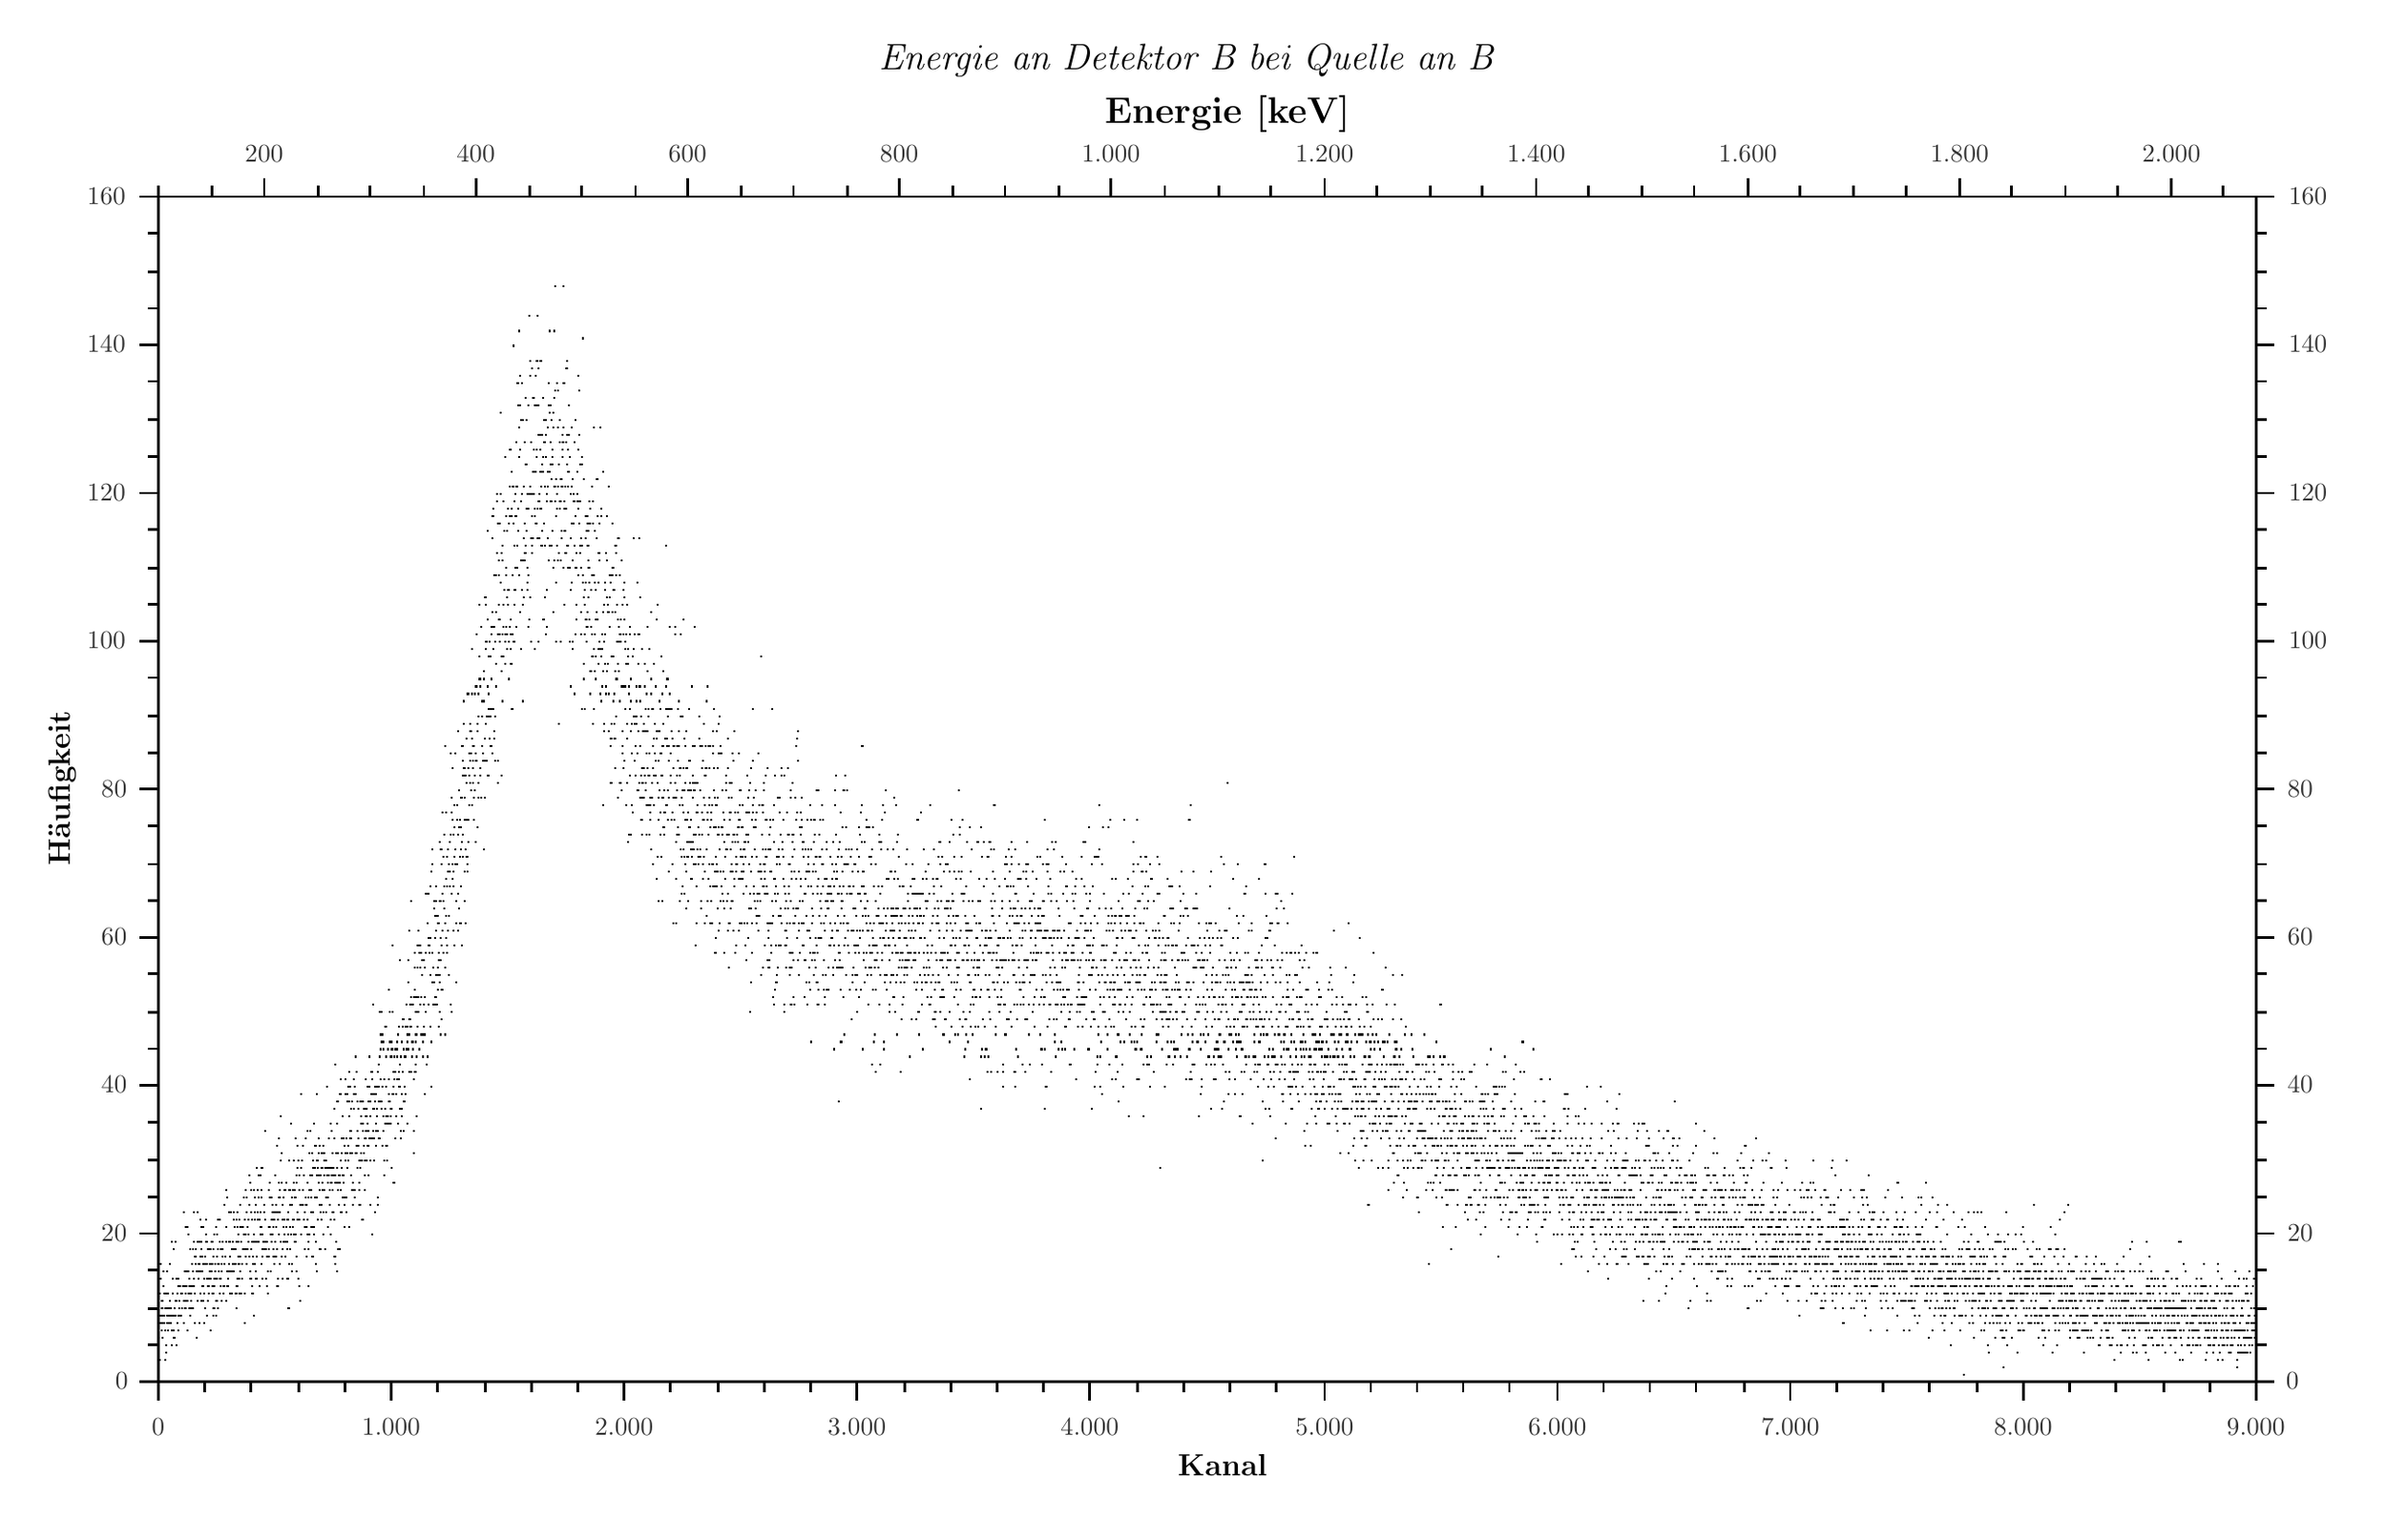
\begin{tikzpicture}{0pt}{0pt}{1213pt}{774pt}
	\clip(0pt,774pt) -- (913.162pt,774pt) -- (913.162pt,191.323pt) -- (0pt,191.323pt) -- (0pt,774pt);
\begin{scope}
	\clip(51.9441pt,707pt) -- (872.51pt,707pt) -- (872.51pt,243.267pt) -- (51.9441pt,243.267pt) -- (51.9441pt,707pt);
	\color[rgb]{0,0,0}
	\fill (52.0352pt,278.047pt) rectangle (52.788pt,277.294pt);
	\color[rgb]{0,0,0}
	\fill (52.1264pt,289.64pt) rectangle (52.8792pt,288.888pt);
	\fill (52.2176pt,251.962pt) rectangle (52.9704pt,251.209pt);
	\fill (52.3088pt,266.454pt) rectangle (53.0616pt,265.701pt);
	\fill (52.3999pt,289.64pt) rectangle (53.1527pt,288.888pt);
	\fill (52.4911pt,283.844pt) rectangle (53.2439pt,283.091pt);
	\fill (52.5823pt,269.352pt) rectangle (53.3351pt,268.599pt);
	\fill (52.7646pt,266.454pt) rectangle (53.5174pt,265.701pt);
	\fill (52.8558pt,263.555pt) rectangle (53.6086pt,262.803pt);
	\fill (52.947pt,272.25pt) rectangle (53.6998pt,271.498pt);
	\fill (53.0382pt,275.149pt) rectangle (53.791pt,274.396pt);
	\fill (53.1293pt,272.25pt) rectangle (53.8821pt,271.498pt);
	\fill (53.2205pt,269.352pt) rectangle (53.9733pt,268.599pt);
	\fill (53.3117pt,260.657pt) rectangle (54.0645pt,259.904pt);
	\fill (53.494pt,266.454pt) rectangle (54.2468pt,265.701pt);
	\fill (53.5852pt,286.742pt) rectangle (54.338pt,285.989pt);
	\fill (53.6764pt,280.945pt) rectangle (54.4292pt,280.193pt);
	\fill (53.8587pt,269.352pt) rectangle (54.6115pt,268.599pt);
	\fill (53.9499pt,266.454pt) rectangle (54.7027pt,265.701pt);
	\fill (54.1322pt,278.047pt) rectangle (54.885pt,277.294pt);
	\fill (54.2234pt,251.962pt) rectangle (54.9762pt,251.209pt);
	\fill (54.3146pt,263.555pt) rectangle (55.0674pt,262.803pt);
	\fill (54.4058pt,272.25pt) rectangle (55.1586pt,271.498pt);
	\fill (54.5881pt,254.861pt) rectangle (55.3409pt,254.108pt);
	\fill (54.6793pt,257.759pt) rectangle (55.4321pt,257.006pt);
	\fill (54.7705pt,278.047pt) rectangle (55.5233pt,277.294pt);
	\fill (54.8616pt,272.25pt) rectangle (55.6144pt,271.498pt);
	\fill (54.9528pt,286.742pt) rectangle (55.7056pt,285.989pt);
	\fill (55.044pt,269.352pt) rectangle (55.7968pt,268.599pt);
	\fill (55.1352pt,266.454pt) rectangle (55.888pt,265.701pt);
	\fill (55.3175pt,263.555pt) rectangle (56.0703pt,262.803pt);
	\fill (55.4087pt,278.047pt) rectangle (56.1615pt,277.294pt);
	\fill (55.4998pt,263.555pt) rectangle (56.2527pt,262.803pt);
	\fill (55.591pt,272.25pt) rectangle (56.3438pt,271.498pt);
	\fill (55.6822pt,269.352pt) rectangle (56.435pt,268.599pt);
	\fill (55.7734pt,266.454pt) rectangle (56.5262pt,265.701pt);
	\fill (56.1381pt,275.149pt) rectangle (56.8909pt,274.396pt);
	\fill (56.2292pt,289.64pt) rectangle (56.9821pt,288.888pt);
	\fill (56.3204pt,272.25pt) rectangle (57.0732pt,271.498pt);
	\fill (56.4116pt,269.352pt) rectangle (57.1644pt,268.599pt);
	\fill (56.5028pt,266.454pt) rectangle (57.2556pt,265.701pt);
	\fill (56.7763pt,263.555pt) rectangle (57.5291pt,262.803pt);
	\fill (56.8675pt,257.759pt) rectangle (57.6203pt,257.006pt);
	\fill (56.9586pt,298.335pt) rectangle (57.7114pt,297.583pt);
	\fill (57.0498pt,269.352pt) rectangle (57.8026pt,268.599pt);
	\fill (57.141pt,283.844pt) rectangle (57.8938pt,283.091pt);
	\fill (57.2322pt,278.047pt) rectangle (57.985pt,277.294pt);
	\fill (57.5057pt,260.657pt) rectangle (58.2585pt,259.904pt);
	\fill (57.5968pt,295.437pt) rectangle (58.3497pt,294.684pt);
	\fill (57.688pt,263.555pt) rectangle (58.4408pt,262.803pt);
	\fill (57.8704pt,269.352pt) rectangle (58.6232pt,268.599pt);
	\fill (57.9615pt,260.657pt) rectangle (58.7144pt,259.904pt);
	\fill (58.0527pt,272.25pt) rectangle (58.8055pt,271.498pt);
	\fill (58.1439pt,275.149pt) rectangle (58.8967pt,274.396pt);
	\fill (58.2351pt,298.335pt) rectangle (58.9879pt,297.583pt);
	\fill (58.4174pt,269.352pt) rectangle (59.1702pt,268.599pt);
	\fill (58.5998pt,257.759pt) rectangle (59.3526pt,257.006pt);
	\fill (58.6909pt,283.844pt) rectangle (59.4437pt,283.091pt);
	\fill (58.7821pt,275.149pt) rectangle (59.5349pt,274.396pt);
	\fill (58.8733pt,278.047pt) rectangle (59.6261pt,277.294pt);
	\fill (58.9645pt,266.454pt) rectangle (59.7173pt,265.701pt);
	\fill (59.1468pt,278.047pt) rectangle (59.8996pt,277.294pt);
	\fill (59.238pt,280.945pt) rectangle (59.9908pt,280.193pt);
	\fill (59.3292pt,269.352pt) rectangle (60.082pt,268.599pt);
	\fill (59.4203pt,263.555pt) rectangle (60.1731pt,262.803pt);
	\fill (59.5115pt,283.844pt) rectangle (60.2643pt,283.091pt);
	\fill (59.6027pt,272.25pt) rectangle (60.3555pt,271.498pt);
	\fill (59.6938pt,275.149pt) rectangle (60.4467pt,274.396pt);
	\fill (59.8762pt,272.25pt) rectangle (60.629pt,271.498pt);
	\fill (59.9674pt,269.352pt) rectangle (60.7202pt,268.599pt);
	\fill (60.1497pt,280.945pt) rectangle (60.9025pt,280.193pt);
	\fill (60.3321pt,278.047pt) rectangle (61.0849pt,277.294pt);
	\fill (60.6056pt,269.352pt) rectangle (61.3584pt,268.599pt);
	\fill (60.6968pt,278.047pt) rectangle (61.4496pt,277.294pt);
	\fill (60.7879pt,272.25pt) rectangle (61.5407pt,271.498pt);
	\fill (61.1526pt,280.945pt) rectangle (61.9054pt,280.193pt);
	\fill (61.4262pt,309.929pt) rectangle (62.179pt,309.176pt);
	\fill (61.5173pt,266.454pt) rectangle (62.2701pt,265.701pt);
	\fill (61.6085pt,275.149pt) rectangle (62.3613pt,274.396pt);
	\fill (61.7908pt,286.742pt) rectangle (62.5437pt,285.989pt);
	\fill (61.882pt,280.945pt) rectangle (62.6348pt,280.193pt);
	\fill (61.9732pt,272.25pt) rectangle (62.726pt,271.498pt);
	\fill (62.1555pt,272.25pt) rectangle (62.9084pt,271.498pt);
	\fill (62.2467pt,275.149pt) rectangle (62.9995pt,274.396pt);
	\fill (62.3379pt,278.047pt) rectangle (63.0907pt,277.294pt);
	\fill (62.4291pt,304.132pt) rectangle (63.1819pt,303.379pt);
	\fill (62.5202pt,280.945pt) rectangle (63.2731pt,280.193pt);
	\fill (62.7026pt,286.742pt) rectangle (63.4554pt,285.989pt);
	\fill (62.8849pt,275.149pt) rectangle (63.6377pt,274.396pt);
	\fill (62.9761pt,263.555pt) rectangle (63.7289pt,262.803pt);
	\fill (63.0673pt,304.132pt) rectangle (63.8201pt,303.379pt);
	\fill (63.2496pt,286.742pt) rectangle (64.0024pt,285.989pt);
	\fill (63.3408pt,278.047pt) rectangle (64.0936pt,277.294pt);
	\fill (63.432pt,301.234pt) rectangle (64.1848pt,300.481pt);
	\fill (63.6143pt,272.25pt) rectangle (64.3671pt,271.498pt);
	\fill (63.7055pt,280.945pt) rectangle (64.4583pt,280.193pt);
	\fill (63.7967pt,283.844pt) rectangle (64.5495pt,283.091pt);
	\fill (63.979pt,295.437pt) rectangle (64.7318pt,294.684pt);
	\fill (64.1614pt,269.352pt) rectangle (64.9142pt,268.599pt);
	\fill (64.2525pt,278.047pt) rectangle (65.0054pt,277.294pt);
	\fill (64.3437pt,275.149pt) rectangle (65.0965pt,274.396pt);
	\fill (64.4349pt,275.149pt) rectangle (65.1877pt,274.396pt);
	\fill (64.5261pt,272.25pt) rectangle (65.2789pt,271.498pt);
	\fill (64.6172pt,280.945pt) rectangle (65.3701pt,280.193pt);
	\fill (64.7996pt,289.64pt) rectangle (65.5524pt,288.888pt);
	\fill (65.0731pt,286.742pt) rectangle (65.8259pt,285.989pt);
	\fill (65.1643pt,295.437pt) rectangle (65.9171pt,294.684pt);
	\fill (65.2555pt,272.25pt) rectangle (66.0083pt,271.498pt);
	\fill (65.3466pt,280.945pt) rectangle (66.0994pt,280.193pt);
	\fill (65.4378pt,283.844pt) rectangle (66.1906pt,283.091pt);
	\fill (65.529pt,298.335pt) rectangle (66.2818pt,297.583pt);
	\fill (65.6202pt,309.929pt) rectangle (66.373pt,309.176pt);
	\fill (65.7113pt,278.047pt) rectangle (66.4641pt,277.294pt);
	\fill (65.8025pt,292.539pt) rectangle (66.5553pt,291.786pt);
	\fill (65.8937pt,278.047pt) rectangle (66.6465pt,277.294pt);
	\fill (65.9849pt,266.454pt) rectangle (66.7377pt,265.701pt);
	\fill (66.1672pt,289.64pt) rectangle (66.92pt,288.888pt);
	\fill (66.2584pt,295.437pt) rectangle (67.0112pt,294.684pt);
	\fill (66.3495pt,292.539pt) rectangle (67.1024pt,291.786pt);
	\fill (66.4407pt,286.742pt) rectangle (67.1935pt,285.989pt);
	\fill (66.7142pt,260.657pt) rectangle (67.4671pt,259.904pt);
	\fill (66.8054pt,275.149pt) rectangle (67.5582pt,274.396pt);
	\fill (66.8966pt,309.929pt) rectangle (67.6494pt,309.176pt);
	\fill (66.9878pt,298.335pt) rectangle (67.7406pt,297.583pt);
	\fill (67.1701pt,289.64pt) rectangle (67.9229pt,288.888pt);
	\fill (67.2613pt,286.742pt) rectangle (68.0141pt,285.989pt);
	\fill (67.3525pt,283.844pt) rectangle (68.1053pt,283.091pt);
	\fill (67.4436pt,283.844pt) rectangle (68.1964pt,283.091pt);
	\fill (67.5348pt,298.335pt) rectangle (68.2876pt,297.583pt);
	\fill (67.626pt,289.64pt) rectangle (68.3788pt,288.888pt);
	\fill (67.7172pt,266.454pt) rectangle (68.47pt,265.701pt);
	\fill (67.8995pt,292.539pt) rectangle (68.6523pt,291.786pt);
	\fill (67.9907pt,307.03pt) rectangle (68.7435pt,306.278pt);
	\fill (68.0819pt,286.742pt) rectangle (68.8347pt,285.989pt);
	\fill (68.173pt,278.047pt) rectangle (68.9258pt,277.294pt);
	\fill (68.2642pt,298.335pt) rectangle (69.017pt,297.583pt);
	\fill (68.3554pt,275.149pt) rectangle (69.1082pt,274.396pt);
	\fill (68.4465pt,304.132pt) rectangle (69.1994pt,303.379pt);
	\fill (68.5377pt,295.437pt) rectangle (69.2905pt,294.684pt);
	\fill (68.6289pt,286.742pt) rectangle (69.3817pt,285.989pt);
	\fill (68.7201pt,280.945pt) rectangle (69.4729pt,280.193pt);
	\fill (68.9024pt,292.539pt) rectangle (69.6552pt,291.786pt);
	\fill (68.9936pt,289.64pt) rectangle (69.7464pt,288.888pt);
	\fill (69.0848pt,275.149pt) rectangle (69.8376pt,274.396pt);
	\fill (69.1759pt,280.945pt) rectangle (69.9288pt,280.193pt);
	\fill (69.2671pt,304.132pt) rectangle (70.0199pt,303.379pt);
	\fill (69.3583pt,278.047pt) rectangle (70.1111pt,277.294pt);
	\fill (69.4495pt,266.454pt) rectangle (70.2023pt,265.701pt);
	\fill (69.5406pt,283.844pt) rectangle (70.2934pt,283.091pt);
	\fill (69.723pt,289.64pt) rectangle (70.4758pt,288.888pt);
	\fill (69.8142pt,292.539pt) rectangle (70.567pt,291.786pt);
	\fill (69.9053pt,272.25pt) rectangle (70.6581pt,271.498pt);
	\fill (70.1789pt,301.234pt) rectangle (70.9317pt,300.481pt);
	\fill (70.27pt,298.335pt) rectangle (71.0228pt,297.583pt);
	\fill (70.3612pt,307.03pt) rectangle (71.114pt,306.278pt);
	\fill (70.4524pt,269.352pt) rectangle (71.2052pt,268.599pt);
	\fill (70.5435pt,289.64pt) rectangle (71.2964pt,288.888pt);
	\fill (70.6347pt,283.844pt) rectangle (71.3875pt,283.091pt);
	\fill (70.7259pt,298.335pt) rectangle (71.4787pt,297.583pt);
	\fill (70.9082pt,280.945pt) rectangle (71.6611pt,280.193pt);
	\fill (70.9994pt,295.437pt) rectangle (71.7522pt,294.684pt);
	\fill (71.0906pt,275.149pt) rectangle (71.8434pt,274.396pt);
	\fill (71.1818pt,278.047pt) rectangle (71.9346pt,277.294pt);
	\fill (71.2729pt,283.844pt) rectangle (72.0258pt,283.091pt);
	\fill (71.3641pt,280.945pt) rectangle (72.1169pt,280.193pt);
	\fill (71.5465pt,286.742pt) rectangle (72.2993pt,285.989pt);
	\fill (71.6376pt,289.64pt) rectangle (72.3905pt,288.888pt);
	\fill (71.82pt,295.437pt) rectangle (72.5728pt,294.684pt);
	\fill (71.9112pt,283.844pt) rectangle (72.664pt,283.091pt);
	\fill (72.0935pt,263.555pt) rectangle (72.8463pt,262.803pt);
	\fill (72.1847pt,286.742pt) rectangle (72.9375pt,285.989pt);
	\fill (72.2759pt,298.335pt) rectangle (73.0287pt,297.583pt);
	\fill (72.367pt,289.64pt) rectangle (73.1198pt,288.888pt);
	\fill (72.6406pt,280.945pt) rectangle (73.3934pt,280.193pt);
	\fill (72.7317pt,298.335pt) rectangle (73.4845pt,297.583pt);
	\fill (72.8229pt,289.64pt) rectangle (73.5757pt,288.888pt);
	\fill (72.9141pt,278.047pt) rectangle (73.6669pt,277.294pt);
	\fill (73.0052pt,269.352pt) rectangle (73.7581pt,268.599pt);
	\fill (73.0964pt,295.437pt) rectangle (73.8492pt,294.684pt);
	\fill (73.1876pt,292.539pt) rectangle (73.9404pt,291.786pt);
	\fill (73.2788pt,272.25pt) rectangle (74.0316pt,271.498pt);
	\fill (73.3699pt,301.234pt) rectangle (74.1228pt,300.481pt);
	\fill (73.4611pt,280.945pt) rectangle (74.2139pt,280.193pt);
	\fill (73.6435pt,283.844pt) rectangle (74.3963pt,283.091pt);
	\fill (73.8258pt,289.64pt) rectangle (74.5786pt,288.888pt);
	\fill (73.917pt,286.742pt) rectangle (74.6698pt,285.989pt);
	\fill (74.1905pt,304.132pt) rectangle (74.9433pt,303.379pt);
	\fill (74.2817pt,269.352pt) rectangle (75.0345pt,268.599pt);
	\fill (74.3729pt,275.149pt) rectangle (75.1257pt,274.396pt);
	\fill (74.464pt,283.844pt) rectangle (75.2168pt,283.091pt);
	\fill (74.5552pt,292.539pt) rectangle (75.308pt,291.786pt);
	\fill (74.6464pt,301.234pt) rectangle (75.3992pt,300.481pt);
	\fill (74.7376pt,272.25pt) rectangle (75.4904pt,271.498pt);
	\fill (74.8287pt,289.64pt) rectangle (75.5815pt,288.888pt);
	\fill (74.9199pt,295.437pt) rectangle (75.6727pt,294.684pt);
	\fill (75.0111pt,307.03pt) rectangle (75.7639pt,306.278pt);
	\fill (75.1022pt,286.742pt) rectangle (75.8551pt,285.989pt);
	\fill (75.2846pt,289.64pt) rectangle (76.0374pt,288.888pt);
	\fill (75.4669pt,278.047pt) rectangle (76.2198pt,277.294pt);
	\fill (75.5581pt,283.844pt) rectangle (76.3109pt,283.091pt);
	\fill (75.6493pt,298.335pt) rectangle (76.4021pt,297.583pt);
	\fill (75.7405pt,307.03pt) rectangle (76.4933pt,306.278pt);
	\fill (75.8316pt,283.844pt) rectangle (76.5845pt,283.091pt);
	\fill (75.9228pt,295.437pt) rectangle (76.6756pt,294.684pt);
	\fill (76.1052pt,280.945pt) rectangle (76.858pt,280.193pt);
	\fill (76.1963pt,275.149pt) rectangle (76.9491pt,274.396pt);
	\fill (76.2875pt,289.64pt) rectangle (77.0403pt,288.888pt);
	\fill (76.4699pt,286.742pt) rectangle (77.2227pt,285.989pt);
	\fill (76.561pt,292.539pt) rectangle (77.3138pt,291.786pt);
	\fill (76.7434pt,295.437pt) rectangle (77.4962pt,294.684pt);
	\fill (76.8346pt,298.335pt) rectangle (77.5874pt,297.583pt);
	\fill (77.1081pt,280.945pt) rectangle (77.8609pt,280.193pt);
	\fill (77.1992pt,278.047pt) rectangle (77.9521pt,277.294pt);
	\fill (77.2904pt,289.64pt) rectangle (78.0432pt,288.888pt);
	\fill (77.3816pt,280.945pt) rectangle (78.1344pt,280.193pt);
	\fill (77.5639pt,312.827pt) rectangle (78.3168pt,312.074pt);
	\fill (77.7463pt,292.539pt) rectangle (78.4991pt,291.786pt);
	\fill (77.9286pt,292.539pt) rectangle (78.6815pt,291.786pt);
	\fill (78.0198pt,304.132pt) rectangle (78.7726pt,303.379pt);
	\fill (78.111pt,275.149pt) rectangle (78.8638pt,274.396pt);
	\fill (78.2022pt,318.624pt) rectangle (78.955pt,317.871pt);
	\fill (78.2933pt,298.335pt) rectangle (79.0461pt,297.583pt);
	\fill (78.3845pt,315.725pt) rectangle (79.1373pt,314.973pt);
	\fill (78.4757pt,280.945pt) rectangle (79.2285pt,280.193pt);
	\fill (78.658pt,286.742pt) rectangle (79.4108pt,285.989pt);
	\fill (78.7492pt,283.844pt) rectangle (79.502pt,283.091pt);
	\fill (78.9316pt,280.945pt) rectangle (79.6844pt,280.193pt);
	\fill (79.1139pt,289.64pt) rectangle (79.8667pt,288.888pt);
	\fill (79.2051pt,286.742pt) rectangle (79.9579pt,285.989pt);
	\fill (79.2963pt,298.335pt) rectangle (80.0491pt,297.583pt);
	\fill (79.3874pt,309.929pt) rectangle (80.1402pt,309.176pt);
	\fill (79.4786pt,298.335pt) rectangle (80.2314pt,297.583pt);
	\fill (79.5698pt,292.539pt) rectangle (80.3226pt,291.786pt);
	\fill (79.6609pt,278.047pt) rectangle (80.4138pt,277.294pt);
	\fill (79.7521pt,286.742pt) rectangle (80.5049pt,285.989pt);
	\fill (80.1168pt,309.929pt) rectangle (80.8696pt,309.176pt);
	\fill (80.208pt,278.047pt) rectangle (80.9608pt,277.294pt);
	\fill (80.2992pt,295.437pt) rectangle (81.052pt,294.684pt);
	\fill (80.4815pt,286.742pt) rectangle (81.2343pt,285.989pt);
	\fill (80.5727pt,298.335pt) rectangle (81.3255pt,297.583pt);
	\fill (80.755pt,289.64pt) rectangle (81.5078pt,288.888pt);
	\fill (80.9374pt,309.929pt) rectangle (81.6902pt,309.176pt);
	\fill (81.0286pt,307.03pt) rectangle (81.7814pt,306.278pt);
	\fill (81.1197pt,286.742pt) rectangle (81.8725pt,285.989pt);
	\fill (81.2109pt,295.437pt) rectangle (81.9637pt,294.684pt);
	\fill (81.3021pt,304.132pt) rectangle (82.0549pt,303.379pt);
	\fill (81.5756pt,289.64pt) rectangle (82.3284pt,288.888pt);
	\fill (81.7579pt,295.437pt) rectangle (82.5108pt,294.684pt);
	\fill (81.9403pt,278.047pt) rectangle (82.6931pt,277.294pt);
	\fill (82.0315pt,307.03pt) rectangle (82.7843pt,306.278pt);
	\fill (82.1226pt,272.25pt) rectangle (82.8755pt,271.498pt);
	\fill (82.2138pt,298.335pt) rectangle (82.9666pt,297.583pt);
	\fill (82.305pt,280.945pt) rectangle (83.0578pt,280.193pt);
	\fill (82.3962pt,309.929pt) rectangle (83.149pt,309.176pt);
	\fill (82.4873pt,283.844pt) rectangle (83.2402pt,283.091pt);
	\fill (82.5785pt,304.132pt) rectangle (83.3313pt,303.379pt);
	\fill (82.6697pt,298.335pt) rectangle (83.4225pt,297.583pt);
	\fill (82.7609pt,292.539pt) rectangle (83.5137pt,291.786pt);
	\fill (82.852pt,301.234pt) rectangle (83.6048pt,300.481pt);
	\fill (83.0344pt,289.64pt) rectangle (83.7872pt,288.888pt);
	\fill (83.1256pt,307.03pt) rectangle (83.8784pt,306.278pt);
	\fill (83.2167pt,289.64pt) rectangle (83.9695pt,288.888pt);
	\fill (83.3079pt,283.844pt) rectangle (84.0607pt,283.091pt);
	\fill (83.3991pt,278.047pt) rectangle (84.1519pt,277.294pt);
	\fill (83.4903pt,292.539pt) rectangle (84.2431pt,291.786pt);
	\fill (83.5814pt,286.742pt) rectangle (84.3342pt,285.989pt);
	\fill (83.6726pt,312.827pt) rectangle (84.4254pt,312.074pt);
	\fill (83.7638pt,304.132pt) rectangle (84.5166pt,303.379pt);
	\fill (83.9461pt,298.335pt) rectangle (84.6989pt,297.583pt);
	\fill (84.0373pt,278.047pt) rectangle (84.7901pt,277.294pt);
	\fill (84.1285pt,304.132pt) rectangle (84.8813pt,303.379pt);
	\fill (84.2196pt,283.844pt) rectangle (84.9725pt,283.091pt);
	\fill (84.402pt,289.64pt) rectangle (85.1548pt,288.888pt);
	\fill (84.4932pt,295.437pt) rectangle (85.246pt,294.684pt);
	\fill (84.7667pt,304.132pt) rectangle (85.5195pt,303.379pt);
	\fill (84.8579pt,301.234pt) rectangle (85.6107pt,300.481pt);
	\fill (84.949pt,315.725pt) rectangle (85.7018pt,314.973pt);
	\fill (85.1314pt,295.437pt) rectangle (85.8842pt,294.684pt);
	\fill (85.2226pt,307.03pt) rectangle (85.9754pt,306.278pt);
	\fill (85.3137pt,278.047pt) rectangle (86.0665pt,277.294pt);
	\fill (85.4961pt,266.454pt) rectangle (86.2489pt,265.701pt);
	\fill (85.5873pt,295.437pt) rectangle (86.3401pt,294.684pt);
	\fill (85.6784pt,318.624pt) rectangle (86.4312pt,317.871pt);
	\fill (85.7696pt,301.234pt) rectangle (86.5224pt,300.481pt);
	\fill (85.8608pt,292.539pt) rectangle (86.6136pt,291.786pt);
	\fill (85.9519pt,289.64pt) rectangle (86.7048pt,288.888pt);
	\fill (86.0431pt,315.725pt) rectangle (86.7959pt,314.973pt);
	\fill (86.1343pt,309.929pt) rectangle (86.8871pt,309.176pt);
	\fill (86.2255pt,309.929pt) rectangle (86.9783pt,309.176pt);
	\fill (86.3166pt,304.132pt) rectangle (87.0695pt,303.379pt);
	\fill (86.4078pt,295.437pt) rectangle (87.1606pt,294.684pt);
	\fill (86.6813pt,307.03pt) rectangle (87.4342pt,306.278pt);
	\fill (86.8637pt,301.234pt) rectangle (87.6165pt,300.481pt);
	\fill (86.9549pt,298.335pt) rectangle (87.7077pt,297.583pt);
	\fill (87.1372pt,312.827pt) rectangle (87.89pt,312.074pt);
	\fill (87.2284pt,292.539pt) rectangle (87.9812pt,291.786pt);
	\fill (87.3196pt,324.42pt) rectangle (88.0724pt,323.668pt);
	\fill (87.4107pt,283.844pt) rectangle (88.1635pt,283.091pt);
	\fill (87.5019pt,321.522pt) rectangle (88.2547pt,320.769pt);
	\fill (87.5931pt,286.742pt) rectangle (88.3459pt,285.989pt);
	\fill (87.7754pt,318.624pt) rectangle (88.5282pt,317.871pt);
	\fill (87.8666pt,283.844pt) rectangle (88.6194pt,283.091pt);
	\fill (87.9578pt,295.437pt) rectangle (88.7106pt,294.684pt);
	\fill (88.049pt,309.929pt) rectangle (88.8018pt,309.176pt);
	\fill (88.1401pt,298.335pt) rectangle (88.8929pt,297.583pt);
	\fill (88.2313pt,278.047pt) rectangle (88.9841pt,277.294pt);
	\fill (88.3225pt,280.945pt) rectangle (89.0753pt,280.193pt);
	\fill (88.4136pt,307.03pt) rectangle (89.1665pt,306.278pt);
	\fill (88.5048pt,289.64pt) rectangle (89.2576pt,288.888pt);
	\fill (88.596pt,292.539pt) rectangle (89.3488pt,291.786pt);
	\fill (88.6872pt,278.047pt) rectangle (89.44pt,277.294pt);
	\fill (88.8695pt,318.624pt) rectangle (89.6223pt,317.871pt);
	\fill (88.9607pt,298.335pt) rectangle (89.7135pt,297.583pt);
	\fill (89.0519pt,269.352pt) rectangle (89.8047pt,268.599pt);
	\fill (89.143pt,301.234pt) rectangle (89.8958pt,300.481pt);
	\fill (89.2342pt,289.64pt) rectangle (89.987pt,288.888pt);
	\fill (89.3254pt,307.03pt) rectangle (90.0782pt,306.278pt);
	\fill (89.4166pt,309.929pt) rectangle (90.1694pt,309.176pt);
	\fill (89.5077pt,315.725pt) rectangle (90.2605pt,314.973pt);
	\fill (89.5989pt,286.742pt) rectangle (90.3517pt,285.989pt);
	\fill (89.6901pt,312.827pt) rectangle (90.4429pt,312.074pt);
	\fill (89.7813pt,283.844pt) rectangle (90.5341pt,283.091pt);
	\fill (89.8724pt,298.335pt) rectangle (90.6252pt,297.583pt);
	\fill (89.9636pt,283.844pt) rectangle (90.7164pt,283.091pt);
	\fill (90.0548pt,327.319pt) rectangle (90.8076pt,326.566pt);
	\fill (90.146pt,298.335pt) rectangle (90.8988pt,297.583pt);
	\fill (90.2371pt,292.539pt) rectangle (90.9899pt,291.786pt);
	\fill (90.3283pt,307.03pt) rectangle (91.0811pt,306.278pt);
	\fill (90.4195pt,309.929pt) rectangle (91.1723pt,309.176pt);
	\fill (90.5106pt,318.624pt) rectangle (91.2635pt,317.871pt);
	\fill (90.693pt,324.42pt) rectangle (91.4458pt,323.668pt);
	\fill (90.7842pt,315.725pt) rectangle (91.537pt,314.973pt);
	\fill (90.8753pt,298.335pt) rectangle (91.6282pt,297.583pt);
	\fill (90.9665pt,307.03pt) rectangle (91.7193pt,306.278pt);
	\fill (91.1489pt,280.945pt) rectangle (91.9017pt,280.193pt);
	\fill (91.3312pt,324.42pt) rectangle (92.084pt,323.668pt);
	\fill (91.4224pt,301.234pt) rectangle (92.1752pt,300.481pt);
	\fill (91.5136pt,309.929pt) rectangle (92.2664pt,309.176pt);
	\fill (91.6047pt,324.42pt) rectangle (92.3575pt,323.668pt);
	\fill (91.6959pt,304.132pt) rectangle (92.4487pt,303.379pt);
	\fill (91.7871pt,289.64pt) rectangle (92.5399pt,288.888pt);
	\fill (91.8783pt,315.725pt) rectangle (92.6311pt,314.973pt);
	\fill (91.9694pt,318.624pt) rectangle (92.7222pt,317.871pt);
	\fill (92.0606pt,327.319pt) rectangle (92.8134pt,326.566pt);
	\fill (92.1518pt,283.844pt) rectangle (92.9046pt,283.091pt);
	\fill (92.243pt,292.539pt) rectangle (92.9958pt,291.786pt);
	\fill (92.3341pt,301.234pt) rectangle (93.0869pt,300.481pt);
	\fill (92.4253pt,295.437pt) rectangle (93.1781pt,294.684pt);
	\fill (92.6076pt,298.335pt) rectangle (93.3605pt,297.583pt);
	\fill (92.8812pt,312.827pt) rectangle (93.634pt,312.074pt);
	\fill (92.9723pt,298.335pt) rectangle (93.7252pt,297.583pt);
	\fill (93.0635pt,309.929pt) rectangle (93.8163pt,309.176pt);
	\fill (93.1547pt,295.437pt) rectangle (93.9075pt,294.684pt);
	\fill (93.2459pt,307.03pt) rectangle (93.9987pt,306.278pt);
	\fill (93.337pt,341.81pt) rectangle (94.0899pt,341.058pt);
	\fill (93.7017pt,283.844pt) rectangle (94.4545pt,283.091pt);
	\fill (93.7929pt,295.437pt) rectangle (94.5457pt,294.684pt);
	\fill (93.8841pt,298.335pt) rectangle (94.6369pt,297.583pt);
	\fill (93.9753pt,292.539pt) rectangle (94.7281pt,291.786pt);
	\fill (94.0664pt,280.945pt) rectangle (94.8192pt,280.193pt);
	\fill (94.34pt,286.742pt) rectangle (95.0928pt,285.989pt);
	\fill (94.5223pt,278.047pt) rectangle (95.2751pt,277.294pt);
	\fill (94.6135pt,292.539pt) rectangle (95.3663pt,291.786pt);
	\fill (94.7046pt,295.437pt) rectangle (95.4575pt,294.684pt);
	\fill (94.7958pt,304.132pt) rectangle (95.5486pt,303.379pt);
	\fill (94.887pt,318.624pt) rectangle (95.6398pt,317.871pt);
	\fill (94.9782pt,315.725pt) rectangle (95.731pt,314.973pt);
	\fill (95.1605pt,321.522pt) rectangle (95.9133pt,320.769pt);
	\fill (95.2517pt,304.132pt) rectangle (96.0045pt,303.379pt);
	\fill (95.3429pt,286.742pt) rectangle (96.0957pt,285.989pt);
	\fill (95.5252pt,301.234pt) rectangle (96.278pt,300.481pt);
	\fill (95.7076pt,315.725pt) rectangle (96.4604pt,314.973pt);
	\fill (95.8899pt,307.03pt) rectangle (96.6427pt,306.278pt);
	\fill (95.9811pt,298.335pt) rectangle (96.7339pt,297.583pt);
	\fill (96.0723pt,307.03pt) rectangle (96.8251pt,306.278pt);
	\fill (96.1634pt,301.234pt) rectangle (96.9162pt,300.481pt);
	\fill (96.2546pt,312.827pt) rectangle (97.0074pt,312.074pt);
	\fill (96.3458pt,309.929pt) rectangle (97.0986pt,309.176pt);
	\fill (96.437pt,292.539pt) rectangle (97.1898pt,291.786pt);
	\fill (96.5281pt,304.132pt) rectangle (97.2809pt,303.379pt);
	\fill (96.7105pt,295.437pt) rectangle (97.4633pt,294.684pt);
	\fill (96.8017pt,307.03pt) rectangle (97.5545pt,306.278pt);
	\fill (96.8928pt,289.64pt) rectangle (97.6456pt,288.888pt);
	\fill (96.984pt,309.929pt) rectangle (97.7368pt,309.176pt);
	\fill (97.1663pt,292.539pt) rectangle (97.9192pt,291.786pt);
	\fill (97.2575pt,298.335pt) rectangle (98.0103pt,297.583pt);
	\fill (97.4399pt,324.42pt) rectangle (98.1927pt,323.668pt);
	\fill (97.531pt,292.539pt) rectangle (98.2839pt,291.786pt);
	\fill (97.6222pt,312.827pt) rectangle (98.375pt,312.074pt);
	\fill (97.7134pt,304.132pt) rectangle (98.4662pt,303.379pt);
	\fill (97.8046pt,309.929pt) rectangle (98.5574pt,309.176pt);
	\fill (97.8957pt,336.014pt) rectangle (98.6486pt,335.261pt);
	\fill (97.9869pt,280.945pt) rectangle (98.7397pt,280.193pt);
	\fill (98.0781pt,295.437pt) rectangle (98.8309pt,294.684pt);
	\fill (98.2604pt,307.03pt) rectangle (99.0132pt,306.278pt);
	\fill (98.3516pt,280.945pt) rectangle (99.1044pt,280.193pt);
	\fill (98.4428pt,309.929pt) rectangle (99.1956pt,309.176pt);
	\fill (98.534pt,283.844pt) rectangle (99.2868pt,283.091pt);
	\fill (98.6251pt,338.912pt) rectangle (99.3779pt,338.159pt);
	\fill (98.7163pt,315.725pt) rectangle (99.4691pt,314.973pt);
	\fill (98.8075pt,301.234pt) rectangle (99.5603pt,300.481pt);
	\fill (98.8987pt,321.522pt) rectangle (99.6515pt,320.769pt);
	\fill (98.9898pt,318.624pt) rectangle (99.7426pt,317.871pt);
	\fill (99.081pt,289.64pt) rectangle (99.8338pt,288.888pt);
	\fill (99.1722pt,309.929pt) rectangle (99.925pt,309.176pt);
	\fill (99.2633pt,315.725pt) rectangle (100.016pt,314.973pt);
	\fill (99.4457pt,298.335pt) rectangle (100.199pt,297.583pt);
	\fill (99.5369pt,347.607pt) rectangle (100.29pt,346.854pt);
	\fill (99.628pt,330.217pt) rectangle (100.381pt,329.464pt);
	\fill (99.8104pt,321.522pt) rectangle (100.563pt,320.769pt);
	\fill (99.9016pt,333.115pt) rectangle (100.654pt,332.363pt);
	\fill (99.9927pt,292.539pt) rectangle (100.746pt,291.786pt);
	\fill (100.084pt,283.844pt) rectangle (100.837pt,283.091pt);
	\fill (100.175pt,307.03pt) rectangle (100.928pt,306.278pt);
	\fill (100.266pt,312.827pt) rectangle (101.019pt,312.074pt);
	\fill (100.357pt,295.437pt) rectangle (101.11pt,294.684pt);
	\fill (100.449pt,298.335pt) rectangle (101.201pt,297.583pt);
	\fill (100.54pt,304.132pt) rectangle (101.293pt,303.379pt);
	\fill (100.631pt,315.725pt) rectangle (101.384pt,314.973pt);
	\fill (100.722pt,307.03pt) rectangle (101.475pt,306.278pt);
	\fill (100.996pt,301.234pt) rectangle (101.748pt,300.481pt);
	\fill (101.087pt,318.624pt) rectangle (101.84pt,317.871pt);
	\fill (101.269pt,318.624pt) rectangle (102.022pt,317.871pt);
	\fill (101.36pt,292.539pt) rectangle (102.113pt,291.786pt);
	\fill (101.452pt,298.335pt) rectangle (102.204pt,297.583pt);
	\fill (101.543pt,321.522pt) rectangle (102.296pt,320.769pt);
	\fill (101.725pt,304.132pt) rectangle (102.478pt,303.379pt);
	\fill (101.907pt,295.437pt) rectangle (102.66pt,294.684pt);
	\fill (101.999pt,283.844pt) rectangle (102.751pt,283.091pt);
	\fill (102.09pt,298.335pt) rectangle (102.843pt,297.583pt);
	\fill (102.181pt,307.03pt) rectangle (102.934pt,306.278pt);
	\fill (102.272pt,301.234pt) rectangle (103.025pt,300.481pt);
	\fill (102.363pt,283.844pt) rectangle (103.116pt,283.091pt);
	\fill (102.454pt,309.929pt) rectangle (103.207pt,309.176pt);
	\fill (102.546pt,272.25pt) rectangle (103.298pt,271.498pt);
	\fill (102.728pt,289.64pt) rectangle (103.481pt,288.888pt);
	\fill (102.819pt,330.217pt) rectangle (103.572pt,329.464pt);
	\fill (102.91pt,318.624pt) rectangle (103.663pt,317.871pt);
	\fill (103.001pt,295.437pt) rectangle (103.754pt,294.684pt);
	\fill (103.093pt,312.827pt) rectangle (103.845pt,312.074pt);
	\fill (103.184pt,304.132pt) rectangle (103.937pt,303.379pt);
	\fill (103.457pt,301.234pt) rectangle (104.21pt,300.481pt);
	\fill (103.549pt,344.709pt) rectangle (104.301pt,343.956pt);
	\fill (103.64pt,312.827pt) rectangle (104.393pt,312.074pt);
	\fill (103.731pt,315.725pt) rectangle (104.484pt,314.973pt);
	\fill (103.822pt,289.64pt) rectangle (104.575pt,288.888pt);
	\fill (103.913pt,286.742pt) rectangle (104.666pt,285.989pt);
	\fill (104.096pt,318.624pt) rectangle (104.848pt,317.871pt);
	\fill (104.187pt,307.03pt) rectangle (104.94pt,306.278pt);
	\fill (104.278pt,304.132pt) rectangle (105.031pt,303.379pt);
	\fill (104.369pt,301.234pt) rectangle (105.122pt,300.481pt);
	\fill (104.46pt,321.522pt) rectangle (105.213pt,320.769pt);
	\fill (104.551pt,307.03pt) rectangle (105.304pt,306.278pt);
	\fill (104.643pt,330.217pt) rectangle (105.395pt,329.464pt);
	\fill (104.825pt,315.725pt) rectangle (105.578pt,314.973pt);
	\fill (104.916pt,298.335pt) rectangle (105.669pt,297.583pt);
	\fill (105.007pt,318.624pt) rectangle (105.76pt,317.871pt);
	\fill (105.098pt,338.912pt) rectangle (105.851pt,338.159pt);
	\fill (105.19pt,301.234pt) rectangle (105.942pt,300.481pt);
	\fill (105.281pt,298.335pt) rectangle (106.034pt,297.583pt);
	\fill (105.372pt,315.725pt) rectangle (106.125pt,314.973pt);
	\fill (105.463pt,324.42pt) rectangle (106.216pt,323.668pt);
	\fill (105.554pt,292.539pt) rectangle (106.307pt,291.786pt);
	\fill (105.646pt,286.742pt) rectangle (106.398pt,285.989pt);
	\fill (105.737pt,321.522pt) rectangle (106.49pt,320.769pt);
	\fill (105.828pt,336.014pt) rectangle (106.581pt,335.261pt);
	\fill (105.919pt,327.319pt) rectangle (106.672pt,326.566pt);
	\fill (106.01pt,307.03pt) rectangle (106.763pt,306.278pt);
	\fill (106.101pt,309.929pt) rectangle (106.854pt,309.176pt);
	\fill (106.193pt,283.844pt) rectangle (106.945pt,283.091pt);
	\fill (106.284pt,330.217pt) rectangle (107.037pt,329.464pt);
	\fill (106.557pt,280.945pt) rectangle (107.31pt,280.193pt);
	\fill (106.648pt,324.42pt) rectangle (107.401pt,323.668pt);
	\fill (106.74pt,318.624pt) rectangle (107.492pt,317.871pt);
	\fill (106.831pt,307.03pt) rectangle (107.584pt,306.278pt);
	\fill (107.013pt,275.149pt) rectangle (107.766pt,274.396pt);
	\fill (107.104pt,312.827pt) rectangle (107.857pt,312.074pt);
	\fill (107.287pt,327.319pt) rectangle (108.039pt,326.566pt);
	\fill (107.378pt,356.302pt) rectangle (108.131pt,355.549pt);
	\fill (107.469pt,301.234pt) rectangle (108.222pt,300.481pt);
	\fill (107.651pt,330.217pt) rectangle (108.404pt,329.464pt);
	\fill (107.925pt,312.827pt) rectangle (108.678pt,312.074pt);
	\fill (108.107pt,318.624pt) rectangle (108.86pt,317.871pt);
	\fill (108.198pt,336.014pt) rectangle (108.951pt,335.261pt);
	\fill (108.29pt,312.827pt) rectangle (109.042pt,312.074pt);
	\fill (108.381pt,324.42pt) rectangle (109.134pt,323.668pt);
	\fill (108.472pt,307.03pt) rectangle (109.225pt,306.278pt);
	\fill (108.745pt,295.437pt) rectangle (109.498pt,294.684pt);
	\fill (108.837pt,304.132pt) rectangle (109.589pt,303.379pt);
	\fill (108.928pt,309.929pt) rectangle (109.681pt,309.176pt);
	\fill (109.201pt,312.827pt) rectangle (109.954pt,312.074pt);
	\fill (109.292pt,315.725pt) rectangle (110.045pt,314.973pt);
	\fill (109.384pt,338.912pt) rectangle (110.136pt,338.159pt);
	\fill (109.566pt,312.827pt) rectangle (110.319pt,312.074pt);
	\fill (109.657pt,304.132pt) rectangle (110.41pt,303.379pt);
	\fill (109.748pt,292.539pt) rectangle (110.501pt,291.786pt);
	\fill (109.84pt,301.234pt) rectangle (110.592pt,300.481pt);
	\fill (109.931pt,341.81pt) rectangle (110.684pt,341.058pt);
	\fill (110.022pt,307.03pt) rectangle (110.775pt,306.278pt);
	\fill (110.113pt,321.522pt) rectangle (110.866pt,320.769pt);
	\fill (110.204pt,280.945pt) rectangle (110.957pt,280.193pt);
	\fill (110.295pt,315.725pt) rectangle (111.048pt,314.973pt);
	\fill (110.387pt,298.335pt) rectangle (111.139pt,297.583pt);
	\fill (110.478pt,295.437pt) rectangle (111.231pt,294.684pt);
	\fill (110.569pt,333.115pt) rectangle (111.322pt,332.363pt);
	\fill (110.66pt,301.234pt) rectangle (111.413pt,300.481pt);
	\fill (110.751pt,318.624pt) rectangle (111.504pt,317.871pt);
	\fill (111.116pt,341.81pt) rectangle (111.869pt,341.058pt);
	\fill (111.207pt,324.42pt) rectangle (111.96pt,323.668pt);
	\fill (111.298pt,309.929pt) rectangle (112.051pt,309.176pt);
	\fill (111.389pt,318.624pt) rectangle (112.142pt,317.871pt);
	\fill (111.481pt,315.725pt) rectangle (112.233pt,314.973pt);
	\fill (111.572pt,304.132pt) rectangle (112.325pt,303.379pt);
	\fill (111.754pt,333.115pt) rectangle (112.507pt,332.363pt);
	\fill (111.845pt,324.42pt) rectangle (112.598pt,323.668pt);
	\fill (111.937pt,292.539pt) rectangle (112.689pt,291.786pt);
	\fill (112.028pt,330.217pt) rectangle (112.781pt,329.464pt);
	\fill (112.119pt,309.929pt) rectangle (112.872pt,309.176pt);
	\fill (112.21pt,327.319pt) rectangle (112.963pt,326.566pt);
	\fill (112.392pt,344.709pt) rectangle (113.145pt,343.956pt);
	\fill (112.484pt,304.132pt) rectangle (113.236pt,303.379pt);
	\fill (112.575pt,301.234pt) rectangle (113.328pt,300.481pt);
	\fill (112.757pt,315.725pt) rectangle (113.51pt,314.973pt);
	\fill (112.848pt,327.319pt) rectangle (113.601pt,326.566pt);
	\fill (113.031pt,336.014pt) rectangle (113.783pt,335.261pt);
	\fill (113.213pt,289.64pt) rectangle (113.966pt,288.888pt);
	\fill (113.304pt,298.335pt) rectangle (114.057pt,297.583pt);
	\fill (113.395pt,315.725pt) rectangle (114.148pt,314.973pt);
	\fill (113.486pt,356.302pt) rectangle (114.239pt,355.549pt);
	\fill (113.578pt,286.742pt) rectangle (114.33pt,285.989pt);
	\fill (113.669pt,324.42pt) rectangle (114.422pt,323.668pt);
	\fill (113.76pt,330.217pt) rectangle (114.513pt,329.464pt);
	\fill (113.851pt,307.03pt) rectangle (114.604pt,306.278pt);
	\fill (113.942pt,327.319pt) rectangle (114.695pt,326.566pt);
	\fill (114.125pt,324.42pt) rectangle (114.878pt,323.668pt);
	\fill (114.216pt,333.115pt) rectangle (114.969pt,332.363pt);
	\fill (114.307pt,321.522pt) rectangle (115.06pt,320.769pt);
	\fill (114.398pt,338.912pt) rectangle (115.151pt,338.159pt);
	\fill (114.489pt,318.624pt) rectangle (115.242pt,317.871pt);
	\fill (114.581pt,295.437pt) rectangle (115.333pt,294.684pt);
	\fill (114.672pt,312.827pt) rectangle (115.425pt,312.074pt);
	\fill (114.763pt,336.014pt) rectangle (115.516pt,335.261pt);
	\fill (114.854pt,324.42pt) rectangle (115.607pt,323.668pt);
	\fill (114.945pt,295.437pt) rectangle (115.698pt,294.684pt);
	\fill (115.128pt,309.929pt) rectangle (115.88pt,309.176pt);
	\fill (115.219pt,327.319pt) rectangle (115.972pt,326.566pt);
	\fill (115.31pt,312.827pt) rectangle (116.063pt,312.074pt);
	\fill (115.401pt,333.115pt) rectangle (116.154pt,332.363pt);
	\fill (115.492pt,307.03pt) rectangle (116.245pt,306.278pt);
	\fill (115.583pt,318.624pt) rectangle (116.336pt,317.871pt);
	\fill (115.675pt,321.522pt) rectangle (116.427pt,320.769pt);
	\fill (115.766pt,327.319pt) rectangle (116.519pt,326.566pt);
	\fill (115.948pt,309.929pt) rectangle (116.701pt,309.176pt);
	\fill (116.039pt,336.014pt) rectangle (116.792pt,335.261pt);
	\fill (116.131pt,333.115pt) rectangle (116.883pt,332.363pt);
	\fill (116.222pt,301.234pt) rectangle (116.975pt,300.481pt);
	\fill (116.313pt,330.217pt) rectangle (117.066pt,329.464pt);
	\fill (116.404pt,318.624pt) rectangle (117.157pt,317.871pt);
	\fill (116.495pt,333.115pt) rectangle (117.248pt,332.363pt);
	\fill (116.586pt,324.42pt) rectangle (117.339pt,323.668pt);
	\fill (116.86pt,327.319pt) rectangle (117.613pt,326.566pt);
	\fill (116.951pt,295.437pt) rectangle (117.704pt,294.684pt);
	\fill (117.133pt,315.725pt) rectangle (117.886pt,314.973pt);
	\fill (117.225pt,330.217pt) rectangle (117.977pt,329.464pt);
	\fill (117.316pt,309.929pt) rectangle (118.069pt,309.176pt);
	\fill (117.498pt,327.319pt) rectangle (118.251pt,326.566pt);
	\fill (117.589pt,324.42pt) rectangle (118.342pt,323.668pt);
	\fill (117.68pt,359.2pt) rectangle (118.433pt,358.447pt);
	\fill (117.863pt,315.725pt) rectangle (118.616pt,314.973pt);
	\fill (117.954pt,304.132pt) rectangle (118.707pt,303.379pt);
	\fill (118.045pt,321.522pt) rectangle (118.798pt,320.769pt);
	\fill (118.136pt,327.319pt) rectangle (118.889pt,326.566pt);
	\fill (118.228pt,338.912pt) rectangle (118.98pt,338.159pt);
	\fill (118.319pt,324.42pt) rectangle (119.072pt,323.668pt);
	\fill (118.501pt,318.624pt) rectangle (119.254pt,317.871pt);
	\fill (118.592pt,327.319pt) rectangle (119.345pt,326.566pt);
	\fill (118.683pt,312.827pt) rectangle (119.436pt,312.074pt);
	\fill (118.866pt,307.03pt) rectangle (119.619pt,306.278pt);
	\fill (118.957pt,301.234pt) rectangle (119.71pt,300.481pt);
	\fill (119.048pt,344.709pt) rectangle (119.801pt,343.956pt);
	\fill (119.139pt,321.522pt) rectangle (119.892pt,320.769pt);
	\fill (119.23pt,324.42pt) rectangle (119.983pt,323.668pt);
	\fill (119.322pt,327.319pt) rectangle (120.074pt,326.566pt);
	\fill (119.413pt,321.522pt) rectangle (120.166pt,320.769pt);
	\fill (119.504pt,341.81pt) rectangle (120.257pt,341.058pt);
	\fill (119.595pt,309.929pt) rectangle (120.348pt,309.176pt);
	\fill (119.686pt,318.624pt) rectangle (120.439pt,317.871pt);
	\fill (119.869pt,333.115pt) rectangle (120.621pt,332.363pt);
	\fill (119.96pt,324.42pt) rectangle (120.713pt,323.668pt);
	\fill (120.142pt,327.319pt) rectangle (120.895pt,326.566pt);
	\fill (120.233pt,309.929pt) rectangle (120.986pt,309.176pt);
	\fill (120.325pt,350.505pt) rectangle (121.077pt,349.753pt);
	\fill (120.416pt,307.03pt) rectangle (121.169pt,306.278pt);
	\fill (120.507pt,338.912pt) rectangle (121.26pt,338.159pt);
	\fill (120.598pt,292.539pt) rectangle (121.351pt,291.786pt);
	\fill (120.689pt,367.895pt) rectangle (121.442pt,367.142pt);
	\fill (120.78pt,324.42pt) rectangle (121.533pt,323.668pt);
	\fill (120.872pt,289.64pt) rectangle (121.624pt,288.888pt);
	\fill (120.963pt,321.522pt) rectangle (121.716pt,320.769pt);
	\fill (121.054pt,333.115pt) rectangle (121.807pt,332.363pt);
	\fill (121.236pt,298.335pt) rectangle (121.989pt,297.583pt);
	\fill (121.419pt,344.709pt) rectangle (122.171pt,343.956pt);
	\fill (121.51pt,286.742pt) rectangle (122.263pt,285.989pt);
	\fill (121.601pt,327.319pt) rectangle (122.354pt,326.566pt);
	\fill (121.692pt,353.404pt) rectangle (122.445pt,352.651pt);
	\fill (121.783pt,318.624pt) rectangle (122.536pt,317.871pt);
	\fill (121.874pt,333.115pt) rectangle (122.627pt,332.363pt);
	\fill (121.966pt,295.437pt) rectangle (122.718pt,294.684pt);
	\fill (122.057pt,321.522pt) rectangle (122.81pt,320.769pt);
	\fill (122.148pt,312.827pt) rectangle (122.901pt,312.074pt);
	\fill (122.422pt,324.42pt) rectangle (123.174pt,323.668pt);
	\fill (122.513pt,295.437pt) rectangle (123.266pt,294.684pt);
	\fill (122.604pt,321.522pt) rectangle (123.357pt,320.769pt);
	\fill (122.786pt,356.302pt) rectangle (123.539pt,355.549pt);
	\fill (122.877pt,362.099pt) rectangle (123.63pt,361.346pt);
	\fill (122.969pt,318.624pt) rectangle (123.721pt,317.871pt);
	\fill (123.06pt,330.217pt) rectangle (123.813pt,329.464pt);
	\fill (123.151pt,309.929pt) rectangle (123.904pt,309.176pt);
	\fill (123.242pt,327.319pt) rectangle (123.995pt,326.566pt);
	\fill (123.424pt,333.115pt) rectangle (124.177pt,332.363pt);
	\fill (123.516pt,338.912pt) rectangle (124.268pt,338.159pt);
	\fill (123.607pt,324.42pt) rectangle (124.36pt,323.668pt);
	\fill (123.698pt,347.607pt) rectangle (124.451pt,346.854pt);
	\fill (123.789pt,315.725pt) rectangle (124.542pt,314.973pt);
	\fill (123.88pt,321.522pt) rectangle (124.633pt,320.769pt);
	\fill (123.971pt,338.912pt) rectangle (124.724pt,338.159pt);
	\fill (124.154pt,324.42pt) rectangle (124.907pt,323.668pt);
	\fill (124.245pt,312.827pt) rectangle (124.998pt,312.074pt);
	\fill (124.336pt,336.014pt) rectangle (125.089pt,335.261pt);
	\fill (124.427pt,315.725pt) rectangle (125.18pt,314.973pt);
	\fill (124.519pt,304.132pt) rectangle (125.271pt,303.379pt);
	\fill (124.61pt,333.115pt) rectangle (125.363pt,332.363pt);
	\fill (124.701pt,356.302pt) rectangle (125.454pt,355.549pt);
	\fill (124.792pt,362.099pt) rectangle (125.545pt,361.346pt);
	\fill (124.883pt,330.217pt) rectangle (125.636pt,329.464pt);
	\fill (125.066pt,338.912pt) rectangle (125.818pt,338.159pt);
	\fill (125.157pt,315.725pt) rectangle (125.91pt,314.973pt);
	\fill (125.248pt,309.929pt) rectangle (126.001pt,309.176pt);
	\fill (125.339pt,353.404pt) rectangle (126.092pt,352.651pt);
	\fill (125.43pt,356.302pt) rectangle (126.183pt,355.549pt);
	\fill (125.521pt,327.319pt) rectangle (126.274pt,326.566pt);
	\fill (125.613pt,333.115pt) rectangle (126.365pt,332.363pt);
	\fill (125.795pt,330.217pt) rectangle (126.548pt,329.464pt);
	\fill (125.886pt,359.2pt) rectangle (126.639pt,358.447pt);
	\fill (125.977pt,336.014pt) rectangle (126.73pt,335.261pt);
	\fill (126.068pt,304.132pt) rectangle (126.821pt,303.379pt);
	\fill (126.16pt,364.997pt) rectangle (126.912pt,364.244pt);
	\fill (126.251pt,347.607pt) rectangle (127.004pt,346.854pt);
	\fill (126.342pt,353.404pt) rectangle (127.095pt,352.651pt);
	\fill (126.433pt,338.912pt) rectangle (127.186pt,338.159pt);
	\fill (126.524pt,359.2pt) rectangle (127.277pt,358.447pt);
	\fill (126.616pt,341.81pt) rectangle (127.368pt,341.058pt);
	\fill (126.707pt,333.115pt) rectangle (127.46pt,332.363pt);
	\fill (126.798pt,324.42pt) rectangle (127.551pt,323.668pt);
	\fill (126.889pt,341.81pt) rectangle (127.642pt,341.058pt);
	\fill (126.98pt,338.912pt) rectangle (127.733pt,338.159pt);
	\fill (127.071pt,350.505pt) rectangle (127.824pt,349.753pt);
	\fill (127.163pt,318.624pt) rectangle (127.915pt,317.871pt);
	\fill (127.254pt,333.115pt) rectangle (128.007pt,332.363pt);
	\fill (127.436pt,353.404pt) rectangle (128.189pt,352.651pt);
	\fill (127.618pt,321.522pt) rectangle (128.371pt,320.769pt);
	\fill (127.71pt,318.624pt) rectangle (128.462pt,317.871pt);
	\fill (127.801pt,312.827pt) rectangle (128.554pt,312.074pt);
	\fill (127.892pt,350.505pt) rectangle (128.645pt,349.753pt);
	\fill (127.983pt,362.099pt) rectangle (128.736pt,361.346pt);
	\fill (128.165pt,356.302pt) rectangle (128.918pt,355.549pt);
	\fill (128.348pt,359.2pt) rectangle (129.101pt,358.447pt);
	\fill (128.439pt,318.624pt) rectangle (129.192pt,317.871pt);
	\fill (128.53pt,315.725pt) rectangle (129.283pt,314.973pt);
	\fill (128.621pt,356.302pt) rectangle (129.374pt,355.549pt);
	\fill (128.713pt,333.115pt) rectangle (129.465pt,332.363pt);
	\fill (128.804pt,370.794pt) rectangle (129.557pt,370.041pt);
	\fill (129.077pt,364.997pt) rectangle (129.83pt,364.244pt);
	\fill (129.168pt,333.115pt) rectangle (129.921pt,332.363pt);
	\fill (129.26pt,336.014pt) rectangle (130.012pt,335.261pt);
	\fill (129.351pt,327.319pt) rectangle (130.104pt,326.566pt);
	\fill (129.533pt,341.81pt) rectangle (130.286pt,341.058pt);
	\fill (129.624pt,353.404pt) rectangle (130.377pt,352.651pt);
	\fill (129.807pt,350.505pt) rectangle (130.559pt,349.753pt);
	\fill (129.898pt,338.912pt) rectangle (130.651pt,338.159pt);
	\fill (129.989pt,336.014pt) rectangle (130.742pt,335.261pt);
	\fill (130.08pt,321.522pt) rectangle (130.833pt,320.769pt);
	\fill (130.171pt,312.827pt) rectangle (130.924pt,312.074pt);
	\fill (130.262pt,318.624pt) rectangle (131.015pt,317.871pt);
	\fill (130.354pt,330.217pt) rectangle (131.106pt,329.464pt);
	\fill (130.445pt,327.319pt) rectangle (131.198pt,326.566pt);
	\fill (130.536pt,353.404pt) rectangle (131.289pt,352.651pt);
	\fill (130.627pt,312.827pt) rectangle (131.38pt,312.074pt);
	\fill (130.81pt,333.115pt) rectangle (131.562pt,332.363pt);
	\fill (130.901pt,344.709pt) rectangle (131.654pt,343.956pt);
	\fill (130.992pt,347.607pt) rectangle (131.745pt,346.854pt);
	\fill (131.083pt,330.217pt) rectangle (131.836pt,329.464pt);
	\fill (131.265pt,353.404pt) rectangle (132.018pt,352.651pt);
	\fill (131.357pt,307.03pt) rectangle (132.109pt,306.278pt);
	\fill (131.448pt,344.709pt) rectangle (132.201pt,343.956pt);
	\fill (131.539pt,341.81pt) rectangle (132.292pt,341.058pt);
	\fill (131.63pt,307.03pt) rectangle (132.383pt,306.278pt);
	\fill (131.721pt,353.404pt) rectangle (132.474pt,352.651pt);
	\fill (131.904pt,333.115pt) rectangle (132.656pt,332.363pt);
	\fill (131.995pt,336.014pt) rectangle (132.748pt,335.261pt);
	\fill (132.177pt,350.505pt) rectangle (132.93pt,349.753pt);
	\fill (132.268pt,318.624pt) rectangle (133.021pt,317.871pt);
	\fill (132.359pt,330.217pt) rectangle (133.112pt,329.464pt);
	\fill (132.451pt,324.42pt) rectangle (133.203pt,323.668pt);
	\fill (132.542pt,338.912pt) rectangle (133.295pt,338.159pt);
	\fill (132.633pt,362.099pt) rectangle (133.386pt,361.346pt);
	\fill (132.815pt,347.607pt) rectangle (133.568pt,346.854pt);
	\fill (132.907pt,341.81pt) rectangle (133.659pt,341.058pt);
	\fill (132.998pt,330.217pt) rectangle (133.751pt,329.464pt);
	\fill (133.089pt,347.607pt) rectangle (133.842pt,346.854pt);
	\fill (133.18pt,350.505pt) rectangle (133.933pt,349.753pt);
	\fill (133.362pt,359.2pt) rectangle (134.115pt,358.447pt);
	\fill (133.454pt,344.709pt) rectangle (134.206pt,343.956pt);
	\fill (133.545pt,336.014pt) rectangle (134.298pt,335.261pt);
	\fill (133.636pt,341.81pt) rectangle (134.389pt,341.058pt);
	\fill (133.727pt,353.404pt) rectangle (134.48pt,352.651pt);
	\fill (133.818pt,336.014pt) rectangle (134.571pt,335.261pt);
	\fill (133.909pt,324.42pt) rectangle (134.662pt,323.668pt);
	\fill (134.092pt,338.912pt) rectangle (134.845pt,338.159pt);
	\fill (134.183pt,370.794pt) rectangle (134.936pt,370.041pt);
	\fill (134.274pt,359.2pt) rectangle (135.027pt,358.447pt);
	\fill (134.365pt,347.607pt) rectangle (135.118pt,346.854pt);
	\fill (134.456pt,353.404pt) rectangle (135.209pt,352.651pt);
	\fill (134.548pt,330.217pt) rectangle (135.3pt,329.464pt);
	\fill (134.639pt,312.827pt) rectangle (135.392pt,312.074pt);
	\fill (134.73pt,356.302pt) rectangle (135.483pt,355.549pt);
	\fill (134.821pt,364.997pt) rectangle (135.574pt,364.244pt);
	\fill (134.912pt,338.912pt) rectangle (135.665pt,338.159pt);
	\fill (135.095pt,301.234pt) rectangle (135.848pt,300.481pt);
	\fill (135.186pt,338.912pt) rectangle (135.939pt,338.159pt);
	\fill (135.277pt,362.099pt) rectangle (136.03pt,361.346pt);
	\fill (135.368pt,364.997pt) rectangle (136.121pt,364.244pt);
	\fill (135.459pt,350.505pt) rectangle (136.212pt,349.753pt);
	\fill (135.551pt,341.81pt) rectangle (136.303pt,341.058pt);
	\fill (135.642pt,356.302pt) rectangle (136.395pt,355.549pt);
	\fill (135.733pt,391.082pt) rectangle (136.486pt,390.329pt);
	\fill (135.915pt,350.505pt) rectangle (136.668pt,349.753pt);
	\fill (136.006pt,330.217pt) rectangle (136.759pt,329.464pt);
	\fill (136.098pt,338.912pt) rectangle (136.85pt,338.159pt);
	\fill (136.189pt,356.302pt) rectangle (136.942pt,355.549pt);
	\fill (136.28pt,353.404pt) rectangle (137.033pt,352.651pt);
	\fill (136.371pt,309.929pt) rectangle (137.124pt,309.176pt);
	\fill (136.462pt,359.2pt) rectangle (137.215pt,358.447pt);
	\fill (136.553pt,336.014pt) rectangle (137.306pt,335.261pt);
	\fill (136.645pt,356.302pt) rectangle (137.397pt,355.549pt);
	\fill (136.736pt,344.709pt) rectangle (137.489pt,343.956pt);
	\fill (136.827pt,341.81pt) rectangle (137.58pt,341.058pt);
	\fill (136.918pt,350.505pt) rectangle (137.671pt,349.753pt);
	\fill (137.009pt,347.607pt) rectangle (137.762pt,346.854pt);
	\fill (137.192pt,359.2pt) rectangle (137.945pt,358.447pt);
	\fill (137.283pt,312.827pt) rectangle (138.036pt,312.074pt);
	\fill (137.374pt,315.725pt) rectangle (138.127pt,314.973pt);
	\fill (137.465pt,341.81pt) rectangle (138.218pt,341.058pt);
	\fill (137.556pt,364.997pt) rectangle (138.309pt,364.244pt);
	\fill (137.648pt,353.404pt) rectangle (138.4pt,352.651pt);
	\fill (137.739pt,338.912pt) rectangle (138.492pt,338.159pt);
	\fill (137.83pt,359.2pt) rectangle (138.583pt,358.447pt);
	\fill (137.921pt,367.895pt) rectangle (138.674pt,367.142pt);
	\fill (138.012pt,370.794pt) rectangle (138.765pt,370.041pt);
	\fill (138.195pt,388.184pt) rectangle (138.947pt,387.431pt);
	\fill (138.286pt,338.912pt) rectangle (139.039pt,338.159pt);
	\fill (138.377pt,362.099pt) rectangle (139.13pt,361.346pt);
	\fill (138.468pt,379.489pt) rectangle (139.221pt,378.736pt);
	\fill (138.559pt,353.404pt) rectangle (139.312pt,352.651pt);
	\fill (138.65pt,373.692pt) rectangle (139.403pt,372.939pt);
	\fill (138.742pt,350.505pt) rectangle (139.494pt,349.753pt);
	\fill (138.833pt,376.59pt) rectangle (139.586pt,375.837pt);
	\fill (138.924pt,353.404pt) rectangle (139.677pt,352.651pt);
	\fill (139.015pt,388.184pt) rectangle (139.768pt,387.431pt);
	\fill (139.106pt,359.2pt) rectangle (139.859pt,358.447pt);
	\fill (139.198pt,379.489pt) rectangle (139.95pt,378.736pt);
	\fill (139.289pt,336.014pt) rectangle (140.042pt,335.261pt);
	\fill (139.471pt,376.59pt) rectangle (140.224pt,375.837pt);
	\fill (139.562pt,347.607pt) rectangle (140.315pt,346.854pt);
	\fill (139.653pt,373.692pt) rectangle (140.406pt,372.939pt);
	\fill (139.745pt,341.81pt) rectangle (140.497pt,341.058pt);
	\fill (139.836pt,330.217pt) rectangle (140.589pt,329.464pt);
	\fill (139.927pt,362.099pt) rectangle (140.68pt,361.346pt);
	\fill (140.018pt,324.42pt) rectangle (140.771pt,323.668pt);
	\fill (140.292pt,344.709pt) rectangle (141.044pt,343.956pt);
	\fill (140.383pt,350.505pt) rectangle (141.136pt,349.753pt);
	\fill (140.474pt,382.387pt) rectangle (141.227pt,381.634pt);
	\fill (140.565pt,347.607pt) rectangle (141.318pt,346.854pt);
	\fill (140.656pt,359.2pt) rectangle (141.409pt,358.447pt);
	\fill (140.747pt,370.794pt) rectangle (141.5pt,370.041pt);
	\fill (140.839pt,336.014pt) rectangle (141.591pt,335.261pt);
	\fill (140.93pt,330.217pt) rectangle (141.683pt,329.464pt);
	\fill (141.021pt,344.709pt) rectangle (141.774pt,343.956pt);
	\fill (141.203pt,344.709pt) rectangle (141.956pt,343.956pt);
	\fill (141.295pt,373.692pt) rectangle (142.047pt,372.939pt);
	\fill (141.386pt,347.607pt) rectangle (142.139pt,346.854pt);
	\fill (141.659pt,396.879pt) rectangle (142.412pt,396.126pt);
	\fill (141.75pt,362.099pt) rectangle (142.503pt,361.346pt);
	\fill (141.842pt,356.302pt) rectangle (142.594pt,355.549pt);
	\fill (141.933pt,353.404pt) rectangle (142.686pt,352.651pt);
	\fill (142.024pt,388.184pt) rectangle (142.777pt,387.431pt);
	\fill (142.115pt,376.59pt) rectangle (142.868pt,375.837pt);
	\fill (142.297pt,344.709pt) rectangle (143.05pt,343.956pt);
	\fill (142.389pt,350.505pt) rectangle (143.141pt,349.753pt);
	\fill (142.48pt,347.607pt) rectangle (143.233pt,346.854pt);
	\fill (142.662pt,370.794pt) rectangle (143.415pt,370.041pt);
	\fill (142.753pt,327.319pt) rectangle (143.506pt,326.566pt);
	\fill (142.844pt,350.505pt) rectangle (143.597pt,349.753pt);
	\fill (142.936pt,376.59pt) rectangle (143.688pt,375.837pt);
	\fill (143.027pt,373.692pt) rectangle (143.78pt,372.939pt);
	\fill (143.118pt,356.302pt) rectangle (143.871pt,355.549pt);
	\fill (143.209pt,388.184pt) rectangle (143.962pt,387.431pt);
	\fill (143.3pt,414.269pt) rectangle (144.053pt,413.516pt);
	\fill (143.392pt,321.522pt) rectangle (144.144pt,320.769pt);
	\fill (143.483pt,364.997pt) rectangle (144.236pt,364.244pt);
	\fill (143.574pt,356.302pt) rectangle (144.327pt,355.549pt);
	\fill (143.665pt,359.2pt) rectangle (144.418pt,358.447pt);
	\fill (143.756pt,362.099pt) rectangle (144.509pt,361.346pt);
	\fill (143.847pt,321.522pt) rectangle (144.6pt,320.769pt);
	\fill (144.03pt,370.794pt) rectangle (144.783pt,370.041pt);
	\fill (144.212pt,364.997pt) rectangle (144.965pt,364.244pt);
	\fill (144.303pt,373.692pt) rectangle (145.056pt,372.939pt);
	\fill (144.394pt,338.912pt) rectangle (145.147pt,338.159pt);
	\fill (144.668pt,356.302pt) rectangle (145.421pt,355.549pt);
	\fill (144.759pt,347.607pt) rectangle (145.512pt,346.854pt);
	\fill (144.85pt,376.59pt) rectangle (145.603pt,375.837pt);
	\fill (144.941pt,373.692pt) rectangle (145.694pt,372.939pt);
	\fill (145.033pt,370.794pt) rectangle (145.785pt,370.041pt);
	\fill (145.124pt,362.099pt) rectangle (145.877pt,361.346pt);
	\fill (145.215pt,379.489pt) rectangle (145.968pt,378.736pt);
	\fill (145.306pt,344.709pt) rectangle (146.059pt,343.956pt);
	\fill (145.58pt,359.2pt) rectangle (146.333pt,358.447pt);
	\fill (145.671pt,364.997pt) rectangle (146.424pt,364.244pt);
	\fill (145.762pt,362.099pt) rectangle (146.515pt,361.346pt);
	\fill (145.853pt,382.387pt) rectangle (146.606pt,381.634pt);
	\fill (145.944pt,359.2pt) rectangle (146.697pt,358.447pt);
	\fill (146.036pt,350.505pt) rectangle (146.788pt,349.753pt);
	\fill (146.127pt,408.472pt) rectangle (146.88pt,407.719pt);
	\fill (146.218pt,367.895pt) rectangle (146.971pt,367.142pt);
	\fill (146.309pt,370.794pt) rectangle (147.062pt,370.041pt);
	\fill (146.491pt,341.81pt) rectangle (147.244pt,341.058pt);
	\fill (146.583pt,338.912pt) rectangle (147.335pt,338.159pt);
	\fill (146.674pt,350.505pt) rectangle (147.427pt,349.753pt);
	\fill (146.765pt,356.302pt) rectangle (147.518pt,355.549pt);
	\fill (146.856pt,376.59pt) rectangle (147.609pt,375.837pt);
	\fill (146.947pt,347.607pt) rectangle (147.7pt,346.854pt);
	\fill (147.039pt,385.285pt) rectangle (147.791pt,384.532pt);
	\fill (147.221pt,382.387pt) rectangle (147.974pt,381.634pt);
	\fill (147.312pt,364.997pt) rectangle (148.065pt,364.244pt);
	\fill (147.403pt,385.285pt) rectangle (148.156pt,384.532pt);
	\fill (147.494pt,341.81pt) rectangle (148.247pt,341.058pt);
	\fill (147.586pt,353.404pt) rectangle (148.338pt,352.651pt);
	\fill (147.677pt,373.692pt) rectangle (148.43pt,372.939pt);
	\fill (147.768pt,370.794pt) rectangle (148.521pt,370.041pt);
	\fill (147.859pt,359.2pt) rectangle (148.612pt,358.447pt);
	\fill (147.95pt,353.404pt) rectangle (148.703pt,352.651pt);
	\fill (148.041pt,359.2pt) rectangle (148.794pt,358.447pt);
	\fill (148.133pt,382.387pt) rectangle (148.885pt,381.634pt);
	\fill (148.224pt,370.794pt) rectangle (148.977pt,370.041pt);
	\fill (148.406pt,356.302pt) rectangle (149.159pt,355.549pt);
	\fill (148.588pt,373.692pt) rectangle (149.341pt,372.939pt);
	\fill (148.771pt,391.082pt) rectangle (149.524pt,390.329pt);
	\fill (148.862pt,382.387pt) rectangle (149.615pt,381.634pt);
	\fill (148.953pt,344.709pt) rectangle (149.706pt,343.956pt);
	\fill (149.044pt,379.489pt) rectangle (149.797pt,378.736pt);
	\fill (149.136pt,376.59pt) rectangle (149.888pt,375.837pt);
	\fill (149.227pt,399.777pt) rectangle (149.979pt,399.024pt);
	\fill (149.318pt,373.692pt) rectangle (150.071pt,372.939pt);
	\fill (149.5pt,408.472pt) rectangle (150.253pt,407.719pt);
	\fill (149.591pt,364.997pt) rectangle (150.344pt,364.244pt);
	\fill (149.683pt,420.065pt) rectangle (150.435pt,419.312pt);
	\fill (149.774pt,379.489pt) rectangle (150.527pt,378.736pt);
	\fill (149.865pt,385.285pt) rectangle (150.618pt,384.532pt);
	\fill (150.047pt,391.082pt) rectangle (150.8pt,390.329pt);
	\fill (150.23pt,382.387pt) rectangle (150.982pt,381.634pt);
	\fill (150.321pt,393.98pt) rectangle (151.074pt,393.227pt);
	\fill (150.412pt,431.659pt) rectangle (151.165pt,430.906pt);
	\fill (150.503pt,364.997pt) rectangle (151.256pt,364.244pt);
	\fill (150.685pt,370.794pt) rectangle (151.438pt,370.041pt);
	\fill (150.777pt,391.082pt) rectangle (151.529pt,390.329pt);
	\fill (150.868pt,376.59pt) rectangle (151.621pt,375.837pt);
	\fill (150.959pt,376.59pt) rectangle (151.712pt,375.837pt);
	\fill (151.05pt,391.082pt) rectangle (151.803pt,390.329pt);
	\fill (151.233pt,373.692pt) rectangle (151.985pt,372.939pt);
	\fill (151.415pt,362.099pt) rectangle (152.168pt,361.346pt);
	\fill (151.506pt,341.81pt) rectangle (152.259pt,341.058pt);
	\fill (151.597pt,333.115pt) rectangle (152.35pt,332.363pt);
	\fill (151.688pt,393.98pt) rectangle (152.441pt,393.227pt);
	\fill (151.78pt,411.37pt) rectangle (152.532pt,410.617pt);
	\fill (151.871pt,396.879pt) rectangle (152.624pt,396.126pt);
	\fill (151.962pt,405.574pt) rectangle (152.715pt,404.821pt);
	\fill (152.053pt,364.997pt) rectangle (152.806pt,364.244pt);
	\fill (152.144pt,379.489pt) rectangle (152.897pt,378.736pt);
	\fill (152.235pt,367.895pt) rectangle (152.988pt,367.142pt);
	\fill (152.327pt,376.59pt) rectangle (153.079pt,375.837pt);
	\fill (152.418pt,388.184pt) rectangle (153.171pt,387.431pt);
	\fill (152.509pt,347.607pt) rectangle (153.262pt,346.854pt);
	\fill (152.6pt,379.489pt) rectangle (153.353pt,378.736pt);
	\fill (152.691pt,370.794pt) rectangle (153.444pt,370.041pt);
	\fill (152.782pt,393.98pt) rectangle (153.535pt,393.227pt);
	\fill (152.965pt,382.387pt) rectangle (153.718pt,381.634pt);
	\fill (153.056pt,405.574pt) rectangle (153.809pt,404.821pt);
	\fill (153.147pt,414.269pt) rectangle (153.9pt,413.516pt);
	\fill (153.238pt,388.184pt) rectangle (153.991pt,387.431pt);
	\fill (153.33pt,393.98pt) rectangle (154.082pt,393.227pt);
	\fill (153.421pt,420.065pt) rectangle (154.173pt,419.312pt);
	\fill (153.512pt,411.37pt) rectangle (154.265pt,410.617pt);
	\fill (153.603pt,373.692pt) rectangle (154.356pt,372.939pt);
	\fill (153.968pt,391.082pt) rectangle (154.721pt,390.329pt);
	\fill (154.059pt,405.574pt) rectangle (154.812pt,404.821pt);
	\fill (154.15pt,414.269pt) rectangle (154.903pt,413.516pt);
	\fill (154.241pt,393.98pt) rectangle (154.994pt,393.227pt);
	\fill (154.332pt,379.489pt) rectangle (155.085pt,378.736pt);
	\fill (154.424pt,411.37pt) rectangle (155.176pt,410.617pt);
	\fill (154.788pt,402.675pt) rectangle (155.541pt,401.922pt);
	\fill (154.879pt,408.472pt) rectangle (155.632pt,407.719pt);
	\fill (154.971pt,370.794pt) rectangle (155.723pt,370.041pt);
	\fill (155.062pt,376.59pt) rectangle (155.815pt,375.837pt);
	\fill (155.153pt,379.489pt) rectangle (155.906pt,378.736pt);
	\fill (155.427pt,391.082pt) rectangle (156.179pt,390.329pt);
	\fill (155.518pt,382.387pt) rectangle (156.27pt,381.634pt);
	\fill (155.609pt,408.472pt) rectangle (156.362pt,407.719pt);
	\fill (155.7pt,356.302pt) rectangle (156.453pt,355.549pt);
	\fill (155.791pt,405.574pt) rectangle (156.544pt,404.821pt);
	\fill (155.882pt,393.98pt) rectangle (156.635pt,393.227pt);
	\fill (155.974pt,379.489pt) rectangle (156.726pt,378.736pt);
	\fill (156.065pt,434.557pt) rectangle (156.818pt,433.804pt);
	\fill (156.247pt,388.184pt) rectangle (157pt,387.431pt);
	\fill (156.338pt,411.37pt) rectangle (157.091pt,410.617pt);
	\fill (156.521pt,367.895pt) rectangle (157.273pt,367.142pt);
	\fill (156.794pt,434.557pt) rectangle (157.547pt,433.804pt);
	\fill (156.976pt,422.964pt) rectangle (157.729pt,422.211pt);
	\fill (157.068pt,370.794pt) rectangle (157.82pt,370.041pt);
	\fill (157.159pt,391.082pt) rectangle (157.912pt,390.329pt);
	\fill (157.25pt,434.557pt) rectangle (158.003pt,433.804pt);
	\fill (157.341pt,414.269pt) rectangle (158.094pt,413.516pt);
	\fill (157.432pt,417.167pt) rectangle (158.185pt,416.414pt);
	\fill (157.615pt,411.37pt) rectangle (158.367pt,410.617pt);
	\fill (157.797pt,414.269pt) rectangle (158.55pt,413.516pt);
	\fill (157.888pt,437.455pt) rectangle (158.641pt,436.702pt);
	\fill (157.979pt,402.675pt) rectangle (158.732pt,401.922pt);
	\fill (158.071pt,382.387pt) rectangle (158.823pt,381.634pt);
	\fill (158.162pt,417.167pt) rectangle (158.915pt,416.414pt);
	\fill (158.253pt,376.59pt) rectangle (159.006pt,375.837pt);
	\fill (158.344pt,443.252pt) rectangle (159.097pt,442.499pt);
	\fill (158.435pt,359.2pt) rectangle (159.188pt,358.447pt);
	\fill (158.526pt,376.59pt) rectangle (159.279pt,375.837pt);
	\fill (158.618pt,446.15pt) rectangle (159.37pt,445.397pt);
	\fill (158.709pt,399.777pt) rectangle (159.462pt,399.024pt);
	\fill (158.8pt,411.37pt) rectangle (159.553pt,410.617pt);
	\fill (158.891pt,451.947pt) rectangle (159.644pt,451.194pt);
	\fill (158.982pt,391.082pt) rectangle (159.735pt,390.329pt);
	\fill (159.256pt,405.574pt) rectangle (160.009pt,404.821pt);
	\fill (159.347pt,428.76pt) rectangle (160.1pt,428.007pt);
	\fill (159.438pt,431.659pt) rectangle (160.191pt,430.906pt);
	\fill (159.529pt,399.777pt) rectangle (160.282pt,399.024pt);
	\fill (159.712pt,391.082pt) rectangle (160.464pt,390.329pt);
	\fill (159.803pt,425.862pt) rectangle (160.556pt,425.109pt);
	\fill (159.894pt,417.167pt) rectangle (160.647pt,416.414pt);
	\fill (159.985pt,393.98pt) rectangle (160.738pt,393.227pt);
	\fill (160.076pt,431.659pt) rectangle (160.829pt,430.906pt);
	\fill (160.168pt,437.455pt) rectangle (160.92pt,436.702pt);
	\fill (160.259pt,420.065pt) rectangle (161.012pt,419.312pt);
	\fill (160.35pt,402.675pt) rectangle (161.103pt,401.922pt);
	\fill (160.532pt,425.862pt) rectangle (161.285pt,425.109pt);
	\fill (160.623pt,391.082pt) rectangle (161.376pt,390.329pt);
	\fill (160.806pt,396.879pt) rectangle (161.559pt,396.126pt);
	\fill (160.897pt,425.862pt) rectangle (161.65pt,425.109pt);
	\fill (160.988pt,405.574pt) rectangle (161.741pt,404.821pt);
	\fill (161.079pt,422.964pt) rectangle (161.832pt,422.211pt);
	\fill (161.17pt,408.472pt) rectangle (161.923pt,407.719pt);
	\fill (161.262pt,411.37pt) rectangle (162.014pt,410.617pt);
	\fill (161.353pt,382.387pt) rectangle (162.106pt,381.634pt);
	\fill (161.444pt,402.675pt) rectangle (162.197pt,401.922pt);
	\fill (161.535pt,399.777pt) rectangle (162.288pt,399.024pt);
	\fill (161.626pt,454.845pt) rectangle (162.379pt,454.092pt);
	\fill (161.718pt,388.184pt) rectangle (162.47pt,387.431pt);
	\fill (161.809pt,431.659pt) rectangle (162.561pt,430.906pt);
	\fill (161.9pt,408.472pt) rectangle (162.653pt,407.719pt);
	\fill (161.991pt,417.167pt) rectangle (162.744pt,416.414pt);
	\fill (162.082pt,379.489pt) rectangle (162.835pt,378.736pt);
	\fill (162.173pt,451.947pt) rectangle (162.926pt,451.194pt);
	\fill (162.265pt,385.285pt) rectangle (163.017pt,384.532pt);
	\fill (162.356pt,414.269pt) rectangle (163.109pt,413.516pt);
	\fill (162.447pt,446.15pt) rectangle (163.2pt,445.397pt);
	\fill (162.538pt,396.879pt) rectangle (163.291pt,396.126pt);
	\fill (162.629pt,434.557pt) rectangle (163.382pt,433.804pt);
	\fill (162.72pt,420.065pt) rectangle (163.473pt,419.312pt);
	\fill (162.812pt,466.438pt) rectangle (163.564pt,465.686pt);
	\fill (162.994pt,411.37pt) rectangle (163.747pt,410.617pt);
	\fill (163.085pt,431.659pt) rectangle (163.838pt,430.906pt);
	\fill (163.176pt,449.048pt) rectangle (163.929pt,448.296pt);
	\fill (163.267pt,457.743pt) rectangle (164.02pt,456.991pt);
	\fill (163.359pt,437.455pt) rectangle (164.111pt,436.702pt);
	\fill (163.541pt,428.76pt) rectangle (164.294pt,428.007pt);
	\fill (163.632pt,405.574pt) rectangle (164.385pt,404.821pt);
	\fill (163.723pt,492.523pt) rectangle (164.476pt,491.771pt);
	\fill (163.815pt,422.964pt) rectangle (164.567pt,422.211pt);
	\fill (163.906pt,379.489pt) rectangle (164.658pt,378.736pt);
	\fill (163.997pt,417.167pt) rectangle (164.75pt,416.414pt);
	\fill (164.088pt,425.862pt) rectangle (164.841pt,425.109pt);
	\fill (164.179pt,440.353pt) rectangle (164.932pt,439.601pt);
	\fill (164.27pt,466.438pt) rectangle (165.023pt,465.686pt);
	\fill (164.362pt,414.269pt) rectangle (165.114pt,413.516pt);
	\fill (164.453pt,437.455pt) rectangle (165.206pt,436.702pt);
	\fill (164.544pt,411.37pt) rectangle (165.297pt,410.617pt);
	\fill (164.635pt,449.048pt) rectangle (165.388pt,448.296pt);
	\fill (164.726pt,420.065pt) rectangle (165.479pt,419.312pt);
	\fill (164.817pt,443.252pt) rectangle (165.57pt,442.499pt);
	\fill (164.909pt,451.947pt) rectangle (165.661pt,451.194pt);
	\fill (165.182pt,402.675pt) rectangle (165.935pt,401.922pt);
	\fill (165.273pt,425.862pt) rectangle (166.026pt,425.109pt);
	\fill (165.364pt,446.15pt) rectangle (166.117pt,445.397pt);
	\fill (165.456pt,454.845pt) rectangle (166.208pt,454.092pt);
	\fill (165.547pt,443.252pt) rectangle (166.3pt,442.499pt);
	\fill (165.729pt,437.455pt) rectangle (166.482pt,436.702pt);
	\fill (165.912pt,489.625pt) rectangle (166.664pt,488.872pt);
	\fill (166.003pt,391.082pt) rectangle (166.755pt,390.329pt);
	\fill (166.094pt,457.743pt) rectangle (166.847pt,456.991pt);
	\fill (166.185pt,472.235pt) rectangle (166.938pt,471.482pt);
	\fill (166.276pt,434.557pt) rectangle (167.029pt,433.804pt);
	\fill (166.367pt,388.184pt) rectangle (167.12pt,387.431pt);
	\fill (166.459pt,466.438pt) rectangle (167.211pt,465.686pt);
	\fill (166.55pt,440.353pt) rectangle (167.303pt,439.601pt);
	\fill (166.641pt,463.54pt) rectangle (167.394pt,462.787pt);
	\fill (166.732pt,446.15pt) rectangle (167.485pt,445.397pt);
	\fill (166.823pt,483.828pt) rectangle (167.576pt,483.076pt);
	\fill (166.914pt,443.252pt) rectangle (167.667pt,442.499pt);
	\fill (167.006pt,420.065pt) rectangle (167.758pt,419.312pt);
	\fill (167.097pt,437.455pt) rectangle (167.85pt,436.702pt);
	\fill (167.188pt,457.743pt) rectangle (167.941pt,456.991pt);
	\fill (167.279pt,460.642pt) rectangle (168.032pt,459.889pt);
	\fill (167.37pt,449.048pt) rectangle (168.123pt,448.296pt);
	\fill (167.461pt,469.337pt) rectangle (168.214pt,468.584pt);
	\fill (167.553pt,414.269pt) rectangle (168.305pt,413.516pt);
	\fill (167.644pt,489.625pt) rectangle (168.397pt,488.872pt);
	\fill (167.735pt,446.15pt) rectangle (168.488pt,445.397pt);
	\fill (167.826pt,451.947pt) rectangle (168.579pt,451.194pt);
	\fill (168.009pt,399.777pt) rectangle (168.761pt,399.024pt);
	\fill (168.1pt,431.659pt) rectangle (168.852pt,430.906pt);
	\fill (168.282pt,422.964pt) rectangle (169.035pt,422.211pt);
	\fill (168.373pt,446.15pt) rectangle (169.126pt,445.397pt);
	\fill (168.464pt,469.337pt) rectangle (169.217pt,468.584pt);
	\fill (168.647pt,463.54pt) rectangle (169.4pt,462.787pt);
	\fill (168.738pt,498.32pt) rectangle (169.491pt,497.567pt);
	\fill (168.829pt,457.743pt) rectangle (169.582pt,456.991pt);
	\fill (168.92pt,434.557pt) rectangle (169.673pt,433.804pt);
	\fill (169.011pt,420.065pt) rectangle (169.764pt,419.312pt);
	\fill (169.103pt,460.642pt) rectangle (169.855pt,459.889pt);
	\fill (169.194pt,428.76pt) rectangle (169.947pt,428.007pt);
	\fill (169.376pt,475.133pt) rectangle (170.129pt,474.381pt);
	\fill (169.467pt,449.048pt) rectangle (170.22pt,448.296pt);
	\fill (169.558pt,463.54pt) rectangle (170.311pt,462.787pt);
	\fill (169.741pt,422.964pt) rectangle (170.494pt,422.211pt);
	\fill (169.832pt,460.642pt) rectangle (170.585pt,459.889pt);
	\fill (169.923pt,437.455pt) rectangle (170.676pt,436.702pt);
	\fill (170.014pt,451.947pt) rectangle (170.767pt,451.194pt);
	\fill (170.106pt,472.235pt) rectangle (170.858pt,471.482pt);
	\fill (170.288pt,454.845pt) rectangle (171.041pt,454.092pt);
	\fill (170.379pt,414.269pt) rectangle (171.132pt,413.516pt);
	\fill (170.47pt,492.523pt) rectangle (171.223pt,491.771pt);
	\fill (170.561pt,457.743pt) rectangle (171.314pt,456.991pt);
	\fill (170.653pt,486.727pt) rectangle (171.405pt,485.974pt);
	\fill (170.744pt,449.048pt) rectangle (171.497pt,448.296pt);
	\fill (170.835pt,480.93pt) rectangle (171.588pt,480.177pt);
	\fill (170.926pt,509.913pt) rectangle (171.679pt,509.161pt);
	\fill (171.108pt,501.218pt) rectangle (171.861pt,500.466pt);
	\fill (171.2pt,483.828pt) rectangle (171.952pt,483.076pt);
	\fill (171.291pt,431.659pt) rectangle (172.044pt,430.906pt);
	\fill (171.382pt,472.235pt) rectangle (172.135pt,471.482pt);
	\fill (171.473pt,443.252pt) rectangle (172.226pt,442.499pt);
	\fill (171.564pt,463.54pt) rectangle (172.317pt,462.787pt);
	\fill (171.655pt,480.93pt) rectangle (172.408pt,480.177pt);
	\fill (171.747pt,451.947pt) rectangle (172.499pt,451.194pt);
	\fill (171.838pt,422.964pt) rectangle (172.591pt,422.211pt);
	\fill (172.02pt,463.54pt) rectangle (172.773pt,462.787pt);
	\fill (172.111pt,478.032pt) rectangle (172.864pt,477.279pt);
	\fill (172.203pt,495.422pt) rectangle (172.955pt,494.669pt);
	\fill (172.294pt,449.048pt) rectangle (173.047pt,448.296pt);
	\fill (172.385pt,443.252pt) rectangle (173.138pt,442.499pt);
	\fill (172.476pt,446.15pt) rectangle (173.229pt,445.397pt);
	\fill (172.658pt,512.812pt) rectangle (173.411pt,512.059pt);
	\fill (172.75pt,483.828pt) rectangle (173.502pt,483.076pt);
	\fill (172.841pt,454.845pt) rectangle (173.594pt,454.092pt);
	\fill (172.932pt,463.54pt) rectangle (173.685pt,462.787pt);
	\fill (173.023pt,489.625pt) rectangle (173.776pt,488.872pt);
	\fill (173.114pt,480.93pt) rectangle (173.867pt,480.177pt);
	\fill (173.297pt,469.337pt) rectangle (174.049pt,468.584pt);
	\fill (173.388pt,478.032pt) rectangle (174.141pt,477.279pt);
	\fill (173.479pt,498.32pt) rectangle (174.232pt,497.567pt);
	\fill (173.57pt,501.218pt) rectangle (174.323pt,500.466pt);
	\fill (173.661pt,486.727pt) rectangle (174.414pt,485.974pt);
	\fill (173.752pt,498.32pt) rectangle (174.505pt,497.567pt);
	\fill (173.844pt,489.625pt) rectangle (174.596pt,488.872pt);
	\fill (174.026pt,475.133pt) rectangle (174.779pt,474.381pt);
	\fill (174.117pt,512.812pt) rectangle (174.87pt,512.059pt);
	\fill (174.208pt,530.202pt) rectangle (174.961pt,529.449pt);
	\fill (174.3pt,469.337pt) rectangle (175.052pt,468.584pt);
	\fill (174.391pt,495.422pt) rectangle (175.144pt,494.669pt);
	\fill (174.482pt,483.828pt) rectangle (175.235pt,483.076pt);
	\fill (174.573pt,492.523pt) rectangle (175.326pt,491.771pt);
	\fill (174.664pt,486.727pt) rectangle (175.417pt,485.974pt);
	\fill (174.755pt,478.032pt) rectangle (175.508pt,477.279pt);
	\fill (174.847pt,472.235pt) rectangle (175.599pt,471.482pt);
	\fill (174.938pt,463.54pt) rectangle (175.691pt,462.787pt);
	\fill (175.029pt,492.523pt) rectangle (175.782pt,491.771pt);
	\fill (175.211pt,512.812pt) rectangle (175.964pt,512.059pt);
	\fill (175.302pt,475.133pt) rectangle (176.055pt,474.381pt);
	\fill (175.485pt,480.93pt) rectangle (176.238pt,480.177pt);
	\fill (175.576pt,515.71pt) rectangle (176.329pt,514.957pt);
	\fill (175.667pt,486.727pt) rectangle (176.42pt,485.974pt);
	\fill (175.758pt,489.625pt) rectangle (176.511pt,488.872pt);
	\fill (175.849pt,454.845pt) rectangle (176.602pt,454.092pt);
	\fill (175.941pt,486.727pt) rectangle (176.693pt,485.974pt);
	\fill (176.123pt,535.998pt) rectangle (176.876pt,535.246pt);
	\fill (176.214pt,515.71pt) rectangle (176.967pt,514.957pt);
	\fill (176.397pt,498.32pt) rectangle (177.149pt,497.567pt);
	\fill (176.488pt,460.642pt) rectangle (177.241pt,459.889pt);
	\fill (176.579pt,501.218pt) rectangle (177.332pt,500.466pt);
	\fill (176.67pt,512.812pt) rectangle (177.423pt,512.059pt);
	\fill (176.761pt,478.032pt) rectangle (177.514pt,477.279pt);
	\fill (176.852pt,504.117pt) rectangle (177.605pt,503.364pt);
	\fill (176.944pt,472.235pt) rectangle (177.696pt,471.482pt);
	\fill (177.035pt,518.608pt) rectangle (177.788pt,517.856pt);
	\fill (177.126pt,527.303pt) rectangle (177.879pt,526.551pt);
	\fill (177.308pt,547.592pt) rectangle (178.061pt,546.839pt);
	\fill (177.399pt,518.608pt) rectangle (178.152pt,517.856pt);
	\fill (177.491pt,515.71pt) rectangle (178.243pt,514.957pt);
	\fill (177.582pt,483.828pt) rectangle (178.335pt,483.076pt);
	\fill (177.673pt,480.93pt) rectangle (178.426pt,480.177pt);
	\fill (177.855pt,538.897pt) rectangle (178.608pt,538.144pt);
	\fill (177.946pt,472.235pt) rectangle (178.699pt,471.482pt);
	\fill (178.129pt,492.523pt) rectangle (178.882pt,491.771pt);
	\fill (178.22pt,509.913pt) rectangle (178.973pt,509.161pt);
	\fill (178.402pt,504.117pt) rectangle (179.155pt,503.364pt);
	\fill (178.494pt,486.727pt) rectangle (179.246pt,485.974pt);
	\fill (178.676pt,489.625pt) rectangle (179.429pt,488.872pt);
	\fill (178.858pt,509.913pt) rectangle (179.611pt,509.161pt);
	\fill (178.949pt,518.608pt) rectangle (179.702pt,517.856pt);
	\fill (179.041pt,521.507pt) rectangle (179.793pt,520.754pt);
	\fill (179.132pt,451.947pt) rectangle (179.885pt,451.194pt);
	\fill (179.223pt,495.422pt) rectangle (179.976pt,494.669pt);
	\fill (179.314pt,486.727pt) rectangle (180.067pt,485.974pt);
	\fill (179.405pt,472.235pt) rectangle (180.158pt,471.482pt);
	\fill (179.496pt,550.49pt) rectangle (180.249pt,549.737pt);
	\fill (179.588pt,547.592pt) rectangle (180.34pt,546.839pt);
	\fill (179.679pt,501.218pt) rectangle (180.432pt,500.466pt);
	\fill (179.77pt,530.202pt) rectangle (180.523pt,529.449pt);
	\fill (179.861pt,533.1pt) rectangle (180.614pt,532.347pt);
	\fill (180.043pt,486.727pt) rectangle (180.796pt,485.974pt);
	\fill (180.226pt,504.117pt) rectangle (180.979pt,503.364pt);
	\fill (180.317pt,576.575pt) rectangle (181.07pt,575.822pt);
	\fill (180.408pt,515.71pt) rectangle (181.161pt,514.957pt);
	\fill (180.499pt,541.795pt) rectangle (181.252pt,541.042pt);
	\fill (180.591pt,480.93pt) rectangle (181.343pt,480.177pt);
	\fill (180.682pt,512.812pt) rectangle (181.435pt,512.059pt);
	\fill (180.773pt,507.015pt) rectangle (181.526pt,506.262pt);
	\fill (180.955pt,527.303pt) rectangle (181.708pt,526.551pt);
	\fill (181.046pt,504.117pt) rectangle (181.799pt,503.364pt);
	\fill (181.138pt,533.1pt) rectangle (181.89pt,532.347pt);
	\fill (181.229pt,495.422pt) rectangle (181.982pt,494.669pt);
	\fill (181.32pt,507.015pt) rectangle (182.073pt,506.262pt);
	\fill (181.411pt,504.117pt) rectangle (182.164pt,503.364pt);
	\fill (181.502pt,527.303pt) rectangle (182.255pt,526.551pt);
	\fill (181.685pt,492.523pt) rectangle (182.437pt,491.771pt);
	\fill (181.776pt,518.608pt) rectangle (182.529pt,517.856pt);
	\fill (181.867pt,535.998pt) rectangle (182.62pt,535.246pt);
	\fill (181.958pt,507.015pt) rectangle (182.711pt,506.262pt);
	\fill (182.049pt,538.897pt) rectangle (182.802pt,538.144pt);
	\fill (182.14pt,544.693pt) rectangle (182.893pt,543.941pt);
	\fill (182.232pt,489.625pt) rectangle (182.984pt,488.872pt);
	\fill (182.323pt,573.677pt) rectangle (183.076pt,572.924pt);
	\fill (182.414pt,582.372pt) rectangle (183.167pt,581.619pt);
	\fill (182.505pt,585.27pt) rectangle (183.258pt,584.517pt);
	\fill (182.596pt,507.015pt) rectangle (183.349pt,506.262pt);
	\fill (182.688pt,530.202pt) rectangle (183.44pt,529.449pt);
	\fill (182.779pt,538.897pt) rectangle (183.532pt,538.144pt);
	\fill (182.87pt,498.32pt) rectangle (183.623pt,497.567pt);
	\fill (182.961pt,495.422pt) rectangle (183.714pt,494.669pt);
	\fill (183.052pt,559.185pt) rectangle (183.805pt,558.432pt);
	\fill (183.143pt,533.1pt) rectangle (183.896pt,532.347pt);
	\fill (183.326pt,504.117pt) rectangle (184.079pt,503.364pt);
	\fill (183.417pt,486.727pt) rectangle (184.17pt,485.974pt);
	\fill (183.508pt,559.185pt) rectangle (184.261pt,558.432pt);
	\fill (183.599pt,515.71pt) rectangle (184.352pt,514.957pt);
	\fill (183.69pt,544.693pt) rectangle (184.443pt,543.941pt);
	\fill (183.782pt,524.405pt) rectangle (184.534pt,523.652pt);
	\fill (183.873pt,588.168pt) rectangle (184.626pt,587.415pt);
	\fill (183.964pt,591.067pt) rectangle (184.717pt,590.314pt);
	\fill (184.146pt,567.88pt) rectangle (184.899pt,567.127pt);
	\fill (184.237pt,478.032pt) rectangle (184.99pt,477.279pt);
	\fill (184.329pt,535.998pt) rectangle (185.081pt,535.246pt);
	\fill (184.42pt,579.473pt) rectangle (185.173pt,578.72pt);
	\fill (184.511pt,486.727pt) rectangle (185.264pt,485.974pt);
	\fill (184.602pt,541.795pt) rectangle (185.355pt,541.042pt);
	\fill (184.693pt,559.185pt) rectangle (185.446pt,558.432pt);
	\fill (184.785pt,564.982pt) rectangle (185.537pt,564.229pt);
	\fill (184.876pt,547.592pt) rectangle (185.629pt,546.839pt);
	\fill (184.967pt,535.998pt) rectangle (185.72pt,535.246pt);
	\fill (185.058pt,541.795pt) rectangle (185.811pt,541.042pt);
	\fill (185.149pt,533.1pt) rectangle (185.902pt,532.347pt);
	\fill (185.24pt,579.473pt) rectangle (185.993pt,578.72pt);
	\fill (185.332pt,591.067pt) rectangle (186.084pt,590.314pt);
	\fill (185.423pt,556.287pt) rectangle (186.176pt,555.534pt);
	\fill (185.605pt,622.948pt) rectangle (186.358pt,622.195pt);
	\fill (185.696pt,521.507pt) rectangle (186.449pt,520.754pt);
	\fill (185.787pt,480.93pt) rectangle (186.54pt,480.177pt);
	\fill (185.879pt,527.303pt) rectangle (186.631pt,526.551pt);
	\fill (185.97pt,567.88pt) rectangle (186.723pt,567.127pt);
	\fill (186.061pt,570.778pt) rectangle (186.814pt,570.025pt);
	\fill (186.152pt,535.998pt) rectangle (186.905pt,535.246pt);
	\fill (186.243pt,509.913pt) rectangle (186.996pt,509.161pt);
	\fill (186.334pt,564.982pt) rectangle (187.087pt,564.229pt);
	\fill (186.426pt,527.303pt) rectangle (187.178pt,526.551pt);
	\fill (186.517pt,547.592pt) rectangle (187.27pt,546.839pt);
	\fill (186.608pt,588.168pt) rectangle (187.361pt,587.415pt);
	\fill (186.699pt,538.897pt) rectangle (187.452pt,538.144pt);
	\fill (186.79pt,576.575pt) rectangle (187.543pt,575.822pt);
	\fill (186.973pt,553.388pt) rectangle (187.726pt,552.635pt);
	\fill (187.155pt,535.998pt) rectangle (187.908pt,535.246pt);
	\fill (187.246pt,524.405pt) rectangle (187.999pt,523.652pt);
	\fill (187.337pt,605.558pt) rectangle (188.09pt,604.805pt);
	\fill (187.429pt,533.1pt) rectangle (188.181pt,532.347pt);
	\fill (187.52pt,582.372pt) rectangle (188.273pt,581.619pt);
	\fill (187.611pt,538.897pt) rectangle (188.364pt,538.144pt);
	\fill (187.702pt,559.185pt) rectangle (188.455pt,558.432pt);
	\fill (187.793pt,562.083pt) rectangle (188.546pt,561.33pt);
	\fill (187.884pt,535.998pt) rectangle (188.637pt,535.246pt);
	\fill (187.976pt,550.49pt) rectangle (188.728pt,549.737pt);
	\fill (188.067pt,530.202pt) rectangle (188.82pt,529.449pt);
	\fill (188.158pt,576.575pt) rectangle (188.911pt,575.822pt);
	\fill (188.249pt,585.27pt) rectangle (189.002pt,584.517pt);
	\fill (188.34pt,553.388pt) rectangle (189.093pt,552.635pt);
	\fill (188.523pt,547.592pt) rectangle (189.275pt,546.839pt);
	\fill (188.614pt,579.473pt) rectangle (189.367pt,578.72pt);
	\fill (188.705pt,553.388pt) rectangle (189.458pt,552.635pt);
	\fill (188.796pt,533.1pt) rectangle (189.549pt,532.347pt);
	\fill (188.887pt,518.608pt) rectangle (189.64pt,517.856pt);
	\fill (188.979pt,538.897pt) rectangle (189.731pt,538.144pt);
	\fill (189.07pt,593.965pt) rectangle (189.823pt,593.212pt);
	\fill (189.161pt,582.372pt) rectangle (189.914pt,581.619pt);
	\fill (189.252pt,608.457pt) rectangle (190.005pt,607.704pt);
	\fill (189.343pt,535.998pt) rectangle (190.096pt,535.246pt);
	\fill (189.434pt,530.202pt) rectangle (190.187pt,529.449pt);
	\fill (189.526pt,541.795pt) rectangle (190.278pt,541.042pt);
	\fill (189.617pt,524.405pt) rectangle (190.37pt,523.652pt);
	\fill (189.708pt,585.27pt) rectangle (190.461pt,584.517pt);
	\fill (189.799pt,599.762pt) rectangle (190.552pt,599.009pt);
	\fill (189.89pt,582.372pt) rectangle (190.643pt,581.619pt);
	\fill (189.981pt,507.015pt) rectangle (190.734pt,506.262pt);
	\fill (190.164pt,559.185pt) rectangle (190.917pt,558.432pt);
	\fill (190.255pt,535.998pt) rectangle (191.008pt,535.246pt);
	\fill (190.346pt,593.965pt) rectangle (191.099pt,593.212pt);
	\fill (190.437pt,579.473pt) rectangle (191.19pt,578.72pt);
	\fill (190.528pt,649.033pt) rectangle (191.281pt,648.28pt);
	\fill (190.711pt,533.1pt) rectangle (191.464pt,532.347pt);
	\fill (190.802pt,570.778pt) rectangle (191.555pt,570.025pt);
	\fill (190.893pt,547.592pt) rectangle (191.646pt,546.839pt);
	\fill (190.984pt,588.168pt) rectangle (191.737pt,587.415pt);
	\fill (191.076pt,553.388pt) rectangle (191.828pt,552.635pt);
	\fill (191.167pt,562.083pt) rectangle (191.92pt,561.33pt);
	\fill (191.258pt,591.067pt) rectangle (192.011pt,590.314pt);
	\fill (191.349pt,582.372pt) rectangle (192.102pt,581.619pt);
	\fill (191.531pt,538.897pt) rectangle (192.284pt,538.144pt);
	\fill (191.623pt,582.372pt) rectangle (192.375pt,581.619pt);
	\fill (191.714pt,611.355pt) rectangle (192.467pt,610.602pt);
	\fill (191.805pt,593.965pt) rectangle (192.558pt,593.212pt);
	\fill (191.896pt,562.083pt) rectangle (192.649pt,561.33pt);
	\fill (192.078pt,570.778pt) rectangle (192.831pt,570.025pt);
	\fill (192.17pt,634.541pt) rectangle (192.922pt,633.789pt);
	\fill (192.261pt,625.846pt) rectangle (193.014pt,625.094pt);
	\fill (192.352pt,576.575pt) rectangle (193.105pt,575.822pt);
	\fill (192.443pt,585.27pt) rectangle (193.196pt,584.517pt);
	\fill (192.534pt,605.558pt) rectangle (193.287pt,604.805pt);
	\fill (192.625pt,654.83pt) rectangle (193.378pt,654.077pt);
	\fill (192.717pt,559.185pt) rectangle (193.469pt,558.432pt);
	\fill (192.808pt,617.152pt) rectangle (193.561pt,616.399pt);
	\fill (192.899pt,637.44pt) rectangle (193.652pt,636.687pt);
	\fill (192.99pt,625.846pt) rectangle (193.743pt,625.094pt);
	\fill (193.081pt,544.693pt) rectangle (193.834pt,543.941pt);
	\fill (193.173pt,608.457pt) rectangle (193.925pt,607.704pt);
	\fill (193.264pt,564.982pt) rectangle (194.017pt,564.229pt);
	\fill (193.355pt,620.05pt) rectangle (194.108pt,619.297pt);
	\fill (193.446pt,588.168pt) rectangle (194.199pt,587.415pt);
	\fill (193.537pt,530.202pt) rectangle (194.29pt,529.449pt);
	\fill (193.628pt,553.388pt) rectangle (194.381pt,552.635pt);
	\fill (193.811pt,591.067pt) rectangle (194.564pt,590.314pt);
	\fill (193.902pt,634.541pt) rectangle (194.655pt,633.789pt);
	\fill (193.993pt,620.05pt) rectangle (194.746pt,619.297pt);
	\fill (194.084pt,547.592pt) rectangle (194.837pt,546.839pt);
	\fill (194.175pt,509.913pt) rectangle (194.928pt,509.161pt);
	\fill (194.267pt,564.982pt) rectangle (195.019pt,564.229pt);
	\fill (194.358pt,593.965pt) rectangle (195.111pt,593.212pt);
	\fill (194.54pt,573.677pt) rectangle (195.293pt,572.924pt);
	\fill (194.631pt,550.49pt) rectangle (195.384pt,549.737pt);
	\fill (194.722pt,564.982pt) rectangle (195.475pt,564.229pt);
	\fill (194.814pt,611.355pt) rectangle (195.566pt,610.602pt);
	\fill (194.905pt,567.88pt) rectangle (195.658pt,567.127pt);
	\fill (194.996pt,579.473pt) rectangle (195.749pt,578.72pt);
	\fill (195.087pt,628.745pt) rectangle (195.84pt,627.992pt);
	\fill (195.178pt,602.66pt) rectangle (195.931pt,601.907pt);
	\fill (195.27pt,570.778pt) rectangle (196.022pt,570.025pt);
	\fill (195.361pt,567.88pt) rectangle (196.114pt,567.127pt);
	\fill (195.452pt,576.575pt) rectangle (196.205pt,575.822pt);
	\fill (195.543pt,585.27pt) rectangle (196.296pt,584.517pt);
	\fill (195.634pt,602.66pt) rectangle (196.387pt,601.907pt);
	\fill (195.725pt,620.05pt) rectangle (196.478pt,619.297pt);
	\fill (195.817pt,562.083pt) rectangle (196.569pt,561.33pt);
	\fill (195.908pt,556.287pt) rectangle (196.661pt,555.534pt);
	\fill (195.999pt,591.067pt) rectangle (196.752pt,590.314pt);
	\fill (196.09pt,553.388pt) rectangle (196.843pt,552.635pt);
	\fill (196.181pt,585.27pt) rectangle (196.934pt,584.517pt);
	\fill (196.272pt,538.897pt) rectangle (197.025pt,538.144pt);
	\fill (196.364pt,625.846pt) rectangle (197.116pt,625.094pt);
	\fill (196.455pt,559.185pt) rectangle (197.208pt,558.432pt);
	\fill (196.546pt,591.067pt) rectangle (197.299pt,590.314pt);
	\fill (196.637pt,541.795pt) rectangle (197.39pt,541.042pt);
	\fill (196.728pt,660.626pt) rectangle (197.481pt,659.874pt);
	\fill (196.911pt,643.236pt) rectangle (197.663pt,642.484pt);
	\fill (197.002pt,550.49pt) rectangle (197.755pt,549.737pt);
	\fill (197.093pt,637.44pt) rectangle (197.846pt,636.687pt);
	\fill (197.184pt,593.965pt) rectangle (197.937pt,593.212pt);
	\fill (197.275pt,533.1pt) rectangle (198.028pt,532.347pt);
	\fill (197.367pt,573.677pt) rectangle (198.119pt,572.924pt);
	\fill (197.458pt,611.355pt) rectangle (198.211pt,610.602pt);
	\fill (197.549pt,591.067pt) rectangle (198.302pt,590.314pt);
	\fill (197.64pt,570.778pt) rectangle (198.393pt,570.025pt);
	\fill (197.731pt,640.338pt) rectangle (198.484pt,639.585pt);
	\fill (197.822pt,567.88pt) rectangle (198.575pt,567.127pt);
	\fill (197.914pt,582.372pt) rectangle (198.666pt,581.619pt);
	\fill (198.005pt,591.067pt) rectangle (198.758pt,590.314pt);
	\fill (198.096pt,573.677pt) rectangle (198.849pt,572.924pt);
	\fill (198.187pt,599.762pt) rectangle (198.94pt,599.009pt);
	\fill (198.278pt,628.745pt) rectangle (199.031pt,627.992pt);
	\fill (198.369pt,591.067pt) rectangle (199.122pt,590.314pt);
	\fill (198.461pt,599.762pt) rectangle (199.213pt,599.009pt);
	\fill (198.552pt,628.745pt) rectangle (199.305pt,627.992pt);
	\fill (198.643pt,608.457pt) rectangle (199.396pt,607.704pt);
	\fill (198.734pt,530.202pt) rectangle (199.487pt,529.449pt);
	\fill (198.825pt,625.846pt) rectangle (199.578pt,625.094pt);
	\fill (198.916pt,585.27pt) rectangle (199.669pt,584.517pt);
	\fill (199.008pt,582.372pt) rectangle (199.76pt,581.619pt);
	\fill (199.19pt,637.44pt) rectangle (199.943pt,636.687pt);
	\fill (199.281pt,599.762pt) rectangle (200.034pt,599.009pt);
	\fill (199.372pt,579.473pt) rectangle (200.125pt,578.72pt);
	\fill (199.464pt,625.846pt) rectangle (200.216pt,625.094pt);
	\fill (199.555pt,608.457pt) rectangle (200.308pt,607.704pt);
	\fill (199.646pt,605.558pt) rectangle (200.399pt,604.805pt);
	\fill (199.737pt,643.236pt) rectangle (200.49pt,642.484pt);
	\fill (199.828pt,573.677pt) rectangle (200.581pt,572.924pt);
	\fill (199.919pt,660.626pt) rectangle (200.672pt,659.874pt);
	\fill (200.011pt,585.27pt) rectangle (200.763pt,584.517pt);
	\fill (200.102pt,625.846pt) rectangle (200.855pt,625.094pt);
	\fill (200.193pt,614.253pt) rectangle (200.946pt,613.5pt);
	\fill (200.284pt,640.338pt) rectangle (201.037pt,639.585pt);
	\fill (200.375pt,533.1pt) rectangle (201.128pt,532.347pt);
	\fill (200.466pt,588.168pt) rectangle (201.219pt,587.415pt);
	\fill (200.558pt,573.677pt) rectangle (201.31pt,572.924pt);
	\fill (200.649pt,588.168pt) rectangle (201.402pt,587.415pt);
	\fill (200.74pt,591.067pt) rectangle (201.493pt,590.314pt);
	\fill (200.831pt,614.253pt) rectangle (201.584pt,613.5pt);
	\fill (200.922pt,585.27pt) rectangle (201.675pt,584.517pt);
	\fill (201.013pt,599.762pt) rectangle (201.766pt,599.009pt);
	\fill (201.105pt,608.457pt) rectangle (201.857pt,607.704pt);
	\fill (201.196pt,643.236pt) rectangle (201.949pt,642.484pt);
	\fill (201.287pt,593.965pt) rectangle (202.04pt,593.212pt);
	\fill (201.378pt,585.27pt) rectangle (202.131pt,584.517pt);
	\fill (201.561pt,570.778pt) rectangle (202.313pt,570.025pt);
	\fill (201.652pt,576.575pt) rectangle (202.405pt,575.822pt);
	\fill (201.743pt,602.66pt) rectangle (202.496pt,601.907pt);
	\fill (201.834pt,614.253pt) rectangle (202.587pt,613.5pt);
	\fill (201.925pt,599.762pt) rectangle (202.678pt,599.009pt);
	\fill (202.016pt,628.745pt) rectangle (202.769pt,627.992pt);
	\fill (202.199pt,605.558pt) rectangle (202.952pt,604.805pt);
	\fill (202.29pt,541.795pt) rectangle (203.043pt,541.042pt);
	\fill (202.381pt,620.05pt) rectangle (203.134pt,619.297pt);
	\fill (202.472pt,579.473pt) rectangle (203.225pt,578.72pt);
	\fill (202.563pt,611.355pt) rectangle (203.316pt,610.602pt);
	\fill (202.655pt,550.49pt) rectangle (203.407pt,549.737pt);
	\fill (202.746pt,593.965pt) rectangle (203.499pt,593.212pt);
	\fill (202.837pt,570.778pt) rectangle (203.59pt,570.025pt);
	\fill (202.928pt,611.355pt) rectangle (203.681pt,610.602pt);
	\fill (203.019pt,605.558pt) rectangle (203.772pt,604.805pt);
	\fill (203.11pt,614.253pt) rectangle (203.863pt,613.5pt);
	\fill (203.202pt,535.998pt) rectangle (203.954pt,535.246pt);
	\fill (203.293pt,620.05pt) rectangle (204.046pt,619.297pt);
	\fill (203.384pt,553.388pt) rectangle (204.137pt,552.635pt);
	\fill (203.475pt,538.897pt) rectangle (204.228pt,538.144pt);
	\fill (203.566pt,591.067pt) rectangle (204.319pt,590.314pt);
	\fill (203.658pt,588.168pt) rectangle (204.41pt,587.415pt);
	\fill (203.749pt,599.762pt) rectangle (204.502pt,599.009pt);
	\fill (203.84pt,593.965pt) rectangle (204.593pt,593.212pt);
	\fill (203.931pt,617.152pt) rectangle (204.684pt,616.399pt);
	\fill (204.022pt,573.677pt) rectangle (204.775pt,572.924pt);
	\fill (204.113pt,625.846pt) rectangle (204.866pt,625.094pt);
	\fill (204.205pt,634.541pt) rectangle (204.957pt,633.789pt);
	\fill (204.296pt,564.982pt) rectangle (205.049pt,564.229pt);
	\fill (204.478pt,654.83pt) rectangle (205.231pt,654.077pt);
	\fill (204.569pt,622.948pt) rectangle (205.322pt,622.195pt);
	\fill (204.66pt,599.762pt) rectangle (205.413pt,599.009pt);
	\fill (204.752pt,570.778pt) rectangle (205.504pt,570.025pt);
	\fill (204.843pt,625.846pt) rectangle (205.596pt,625.094pt);
	\fill (204.934pt,611.355pt) rectangle (205.687pt,610.602pt);
	\fill (205.025pt,588.168pt) rectangle (205.778pt,587.415pt);
	\fill (205.116pt,602.66pt) rectangle (205.869pt,601.907pt);
	\fill (205.207pt,588.168pt) rectangle (205.96pt,587.415pt);
	\fill (205.299pt,620.05pt) rectangle (206.051pt,619.297pt);
	\fill (205.39pt,596.863pt) rectangle (206.143pt,596.11pt);
	\fill (205.481pt,570.778pt) rectangle (206.234pt,570.025pt);
	\fill (205.572pt,576.575pt) rectangle (206.325pt,575.822pt);
	\fill (205.663pt,605.558pt) rectangle (206.416pt,604.805pt);
	\fill (205.755pt,602.66pt) rectangle (206.507pt,601.907pt);
	\fill (205.846pt,608.457pt) rectangle (206.599pt,607.704pt);
	\fill (205.937pt,562.083pt) rectangle (206.69pt,561.33pt);
	\fill (206.028pt,622.948pt) rectangle (206.781pt,622.195pt);
	\fill (206.119pt,544.693pt) rectangle (206.872pt,543.941pt);
	\fill (206.21pt,617.152pt) rectangle (206.963pt,616.399pt);
	\fill (206.302pt,593.965pt) rectangle (207.054pt,593.212pt);
	\fill (206.393pt,628.745pt) rectangle (207.146pt,627.992pt);
	\fill (206.484pt,564.982pt) rectangle (207.237pt,564.229pt);
	\fill (206.575pt,654.83pt) rectangle (207.328pt,654.077pt);
	\fill (206.666pt,593.965pt) rectangle (207.419pt,593.212pt);
	\fill (206.757pt,588.168pt) rectangle (207.51pt,587.415pt);
	\fill (206.849pt,631.643pt) rectangle (207.601pt,630.89pt);
	\fill (206.94pt,672.22pt) rectangle (207.693pt,671.467pt);
	\fill (207.031pt,556.287pt) rectangle (207.784pt,555.534pt);
	\fill (207.122pt,582.372pt) rectangle (207.875pt,581.619pt);
	\fill (207.213pt,533.1pt) rectangle (207.966pt,532.347pt);
	\fill (207.304pt,596.863pt) rectangle (208.057pt,596.11pt);
	\fill (207.396pt,585.27pt) rectangle (208.148pt,584.517pt);
	\fill (207.487pt,634.541pt) rectangle (208.24pt,633.789pt);
	\fill (207.578pt,570.778pt) rectangle (208.331pt,570.025pt);
	\fill (207.669pt,591.067pt) rectangle (208.422pt,590.314pt);
	\fill (207.76pt,593.965pt) rectangle (208.513pt,593.212pt);
	\fill (207.852pt,617.152pt) rectangle (208.604pt,616.399pt);
	\fill (207.943pt,631.643pt) rectangle (208.696pt,630.89pt);
	\fill (208.034pt,564.982pt) rectangle (208.787pt,564.229pt);
	\fill (208.216pt,602.66pt) rectangle (208.969pt,601.907pt);
	\fill (208.307pt,501.218pt) rectangle (209.06pt,500.466pt);
	\fill (208.399pt,567.88pt) rectangle (209.151pt,567.127pt);
	\fill (208.49pt,620.05pt) rectangle (209.243pt,619.297pt);
	\fill (208.581pt,585.27pt) rectangle (209.334pt,584.517pt);
	\fill (208.672pt,611.355pt) rectangle (209.425pt,610.602pt);
	\fill (208.763pt,588.168pt) rectangle (209.516pt,587.415pt);
	\fill (208.854pt,533.1pt) rectangle (209.607pt,532.347pt);
	\fill (208.946pt,564.982pt) rectangle (209.698pt,564.229pt);
	\fill (209.037pt,588.168pt) rectangle (209.79pt,587.415pt);
	\fill (209.128pt,596.863pt) rectangle (209.881pt,596.11pt);
	\fill (209.219pt,576.575pt) rectangle (209.972pt,575.822pt);
	\fill (209.31pt,573.677pt) rectangle (210.063pt,572.924pt);
	\fill (209.493pt,593.965pt) rectangle (210.245pt,593.212pt);
	\fill (209.584pt,605.558pt) rectangle (210.337pt,604.805pt);
	\fill (209.675pt,608.457pt) rectangle (210.428pt,607.704pt);
	\fill (209.766pt,614.253pt) rectangle (210.519pt,613.5pt);
	\fill (209.857pt,611.355pt) rectangle (210.61pt,610.602pt);
	\fill (209.949pt,562.083pt) rectangle (210.701pt,561.33pt);
	\fill (210.04pt,617.152pt) rectangle (210.793pt,616.399pt);
	\fill (210.131pt,672.22pt) rectangle (210.884pt,671.467pt);
	\fill (210.222pt,634.541pt) rectangle (210.975pt,633.789pt);
	\fill (210.313pt,547.592pt) rectangle (211.066pt,546.839pt);
	\fill (210.404pt,588.168pt) rectangle (211.157pt,587.415pt);
	\fill (210.496pt,585.27pt) rectangle (211.248pt,584.517pt);
	\fill (210.587pt,576.575pt) rectangle (211.34pt,575.822pt);
	\fill (210.86pt,593.965pt) rectangle (211.613pt,593.212pt);
	\fill (210.951pt,567.88pt) rectangle (211.704pt,567.127pt);
	\fill (211.134pt,611.355pt) rectangle (211.887pt,610.602pt);
	\fill (211.225pt,585.27pt) rectangle (211.978pt,584.517pt);
	\fill (211.316pt,640.338pt) rectangle (212.069pt,639.585pt);
	\fill (211.407pt,614.253pt) rectangle (212.16pt,613.5pt);
	\fill (211.498pt,643.236pt) rectangle (212.251pt,642.484pt);
	\fill (211.59pt,602.66pt) rectangle (212.342pt,601.907pt);
	\fill (211.681pt,570.778pt) rectangle (212.434pt,570.025pt);
	\fill (211.772pt,593.965pt) rectangle (212.525pt,593.212pt);
	\fill (211.863pt,562.083pt) rectangle (212.616pt,561.33pt);
	\fill (211.954pt,608.457pt) rectangle (212.707pt,607.704pt);
	\fill (212.046pt,599.762pt) rectangle (212.798pt,599.009pt);
	\fill (212.137pt,614.253pt) rectangle (212.89pt,613.5pt);
	\fill (212.228pt,625.846pt) rectangle (212.981pt,625.094pt);
	\fill (212.41pt,533.1pt) rectangle (213.163pt,532.347pt);
	\fill (212.501pt,605.558pt) rectangle (213.254pt,604.805pt);
	\fill (212.593pt,562.083pt) rectangle (213.345pt,561.33pt);
	\fill (212.684pt,562.083pt) rectangle (213.437pt,561.33pt);
	\fill (212.775pt,553.388pt) rectangle (213.528pt,552.635pt);
	\fill (212.866pt,591.067pt) rectangle (213.619pt,590.314pt);
	\fill (212.957pt,573.677pt) rectangle (213.71pt,572.924pt);
	\fill (213.048pt,515.71pt) rectangle (213.801pt,514.957pt);
	\fill (213.14pt,593.965pt) rectangle (213.892pt,593.212pt);
	\fill (213.231pt,579.473pt) rectangle (213.984pt,578.72pt);
	\fill (213.322pt,556.287pt) rectangle (214.075pt,555.534pt);
	\fill (213.413pt,617.152pt) rectangle (214.166pt,616.399pt);
	\fill (213.504pt,564.982pt) rectangle (214.257pt,564.229pt);
	\fill (213.595pt,533.1pt) rectangle (214.348pt,532.347pt);
	\fill (213.687pt,530.202pt) rectangle (214.439pt,529.449pt);
	\fill (213.778pt,596.863pt) rectangle (214.531pt,596.11pt);
	\fill (213.869pt,588.168pt) rectangle (214.622pt,587.415pt);
	\fill (213.96pt,591.067pt) rectangle (214.713pt,590.314pt);
	\fill (214.143pt,579.473pt) rectangle (214.895pt,578.72pt);
	\fill (214.234pt,611.355pt) rectangle (214.987pt,610.602pt);
	\fill (214.325pt,588.168pt) rectangle (215.078pt,587.415pt);
	\fill (214.416pt,512.812pt) rectangle (215.169pt,512.059pt);
	\fill (214.507pt,570.778pt) rectangle (215.26pt,570.025pt);
	\fill (214.598pt,562.083pt) rectangle (215.351pt,561.33pt);
	\fill (214.69pt,620.05pt) rectangle (215.442pt,619.297pt);
	\fill (214.781pt,582.372pt) rectangle (215.534pt,581.619pt);
	\fill (214.872pt,535.998pt) rectangle (215.625pt,535.246pt);
	\fill (214.963pt,562.083pt) rectangle (215.716pt,561.33pt);
	\fill (215.054pt,567.88pt) rectangle (215.807pt,567.127pt);
	\fill (215.145pt,547.592pt) rectangle (215.898pt,546.839pt);
	\fill (215.237pt,541.795pt) rectangle (215.989pt,541.042pt);
	\fill (215.328pt,591.067pt) rectangle (216.081pt,590.314pt);
	\fill (215.419pt,588.168pt) rectangle (216.172pt,587.415pt);
	\fill (215.601pt,599.762pt) rectangle (216.354pt,599.009pt);
	\fill (215.692pt,608.457pt) rectangle (216.445pt,607.704pt);
	\fill (215.784pt,637.44pt) rectangle (216.536pt,636.687pt);
	\fill (215.875pt,585.27pt) rectangle (216.628pt,584.517pt);
	\fill (215.966pt,559.185pt) rectangle (216.719pt,558.432pt);
	\fill (216.057pt,588.168pt) rectangle (216.81pt,587.415pt);
	\fill (216.148pt,631.643pt) rectangle (216.901pt,630.89pt);
	\fill (216.24pt,614.253pt) rectangle (216.992pt,613.5pt);
	\fill (216.331pt,579.473pt) rectangle (217.084pt,578.72pt);
	\fill (216.422pt,570.778pt) rectangle (217.175pt,570.025pt);
	\fill (216.513pt,567.88pt) rectangle (217.266pt,567.127pt);
	\fill (216.604pt,602.66pt) rectangle (217.357pt,601.907pt);
	\fill (216.695pt,588.168pt) rectangle (217.448pt,587.415pt);
	\fill (216.787pt,562.083pt) rectangle (217.539pt,561.33pt);
	\fill (216.878pt,544.693pt) rectangle (217.631pt,543.941pt);
	\fill (216.969pt,573.677pt) rectangle (217.722pt,572.924pt);
	\fill (217.06pt,535.998pt) rectangle (217.813pt,535.246pt);
	\fill (217.151pt,605.558pt) rectangle (217.904pt,604.805pt);
	\fill (217.242pt,570.778pt) rectangle (217.995pt,570.025pt);
	\fill (217.334pt,602.66pt) rectangle (218.086pt,601.907pt);
	\fill (217.425pt,507.015pt) rectangle (218.178pt,506.262pt);
	\fill (217.516pt,556.287pt) rectangle (218.269pt,555.534pt);
	\fill (217.607pt,559.185pt) rectangle (218.36pt,558.432pt);
	\fill (217.698pt,651.931pt) rectangle (218.451pt,651.179pt);
	\fill (217.881pt,596.863pt) rectangle (218.633pt,596.11pt);
	\fill (217.972pt,550.49pt) rectangle (218.725pt,549.737pt);
	\fill (218.063pt,518.608pt) rectangle (218.816pt,517.856pt);
	\fill (218.154pt,524.405pt) rectangle (218.907pt,523.652pt);
	\fill (218.245pt,553.388pt) rectangle (218.998pt,552.635pt);
	\fill (218.337pt,507.015pt) rectangle (219.089pt,506.262pt);
	\fill (218.428pt,535.998pt) rectangle (219.181pt,535.246pt);
	\fill (218.519pt,547.592pt) rectangle (219.272pt,546.839pt);
	\fill (218.61pt,582.372pt) rectangle (219.363pt,581.619pt);
	\fill (218.701pt,556.287pt) rectangle (219.454pt,555.534pt);
	\fill (218.792pt,573.677pt) rectangle (219.545pt,572.924pt);
	\fill (218.884pt,541.795pt) rectangle (219.636pt,541.042pt);
	\fill (218.975pt,533.1pt) rectangle (219.728pt,532.347pt);
	\fill (219.066pt,576.575pt) rectangle (219.819pt,575.822pt);
	\fill (219.248pt,538.897pt) rectangle (220.001pt,538.144pt);
	\fill (219.339pt,579.473pt) rectangle (220.092pt,578.72pt);
	\fill (219.431pt,582.372pt) rectangle (220.183pt,581.619pt);
	\fill (219.522pt,544.693pt) rectangle (220.275pt,543.941pt);
	\fill (219.613pt,570.778pt) rectangle (220.366pt,570.025pt);
	\fill (219.704pt,576.575pt) rectangle (220.457pt,575.822pt);
	\fill (219.795pt,550.49pt) rectangle (220.548pt,549.737pt);
	\fill (219.886pt,564.982pt) rectangle (220.639pt,564.229pt);
	\fill (219.978pt,562.083pt) rectangle (220.73pt,561.33pt);
	\fill (220.069pt,588.168pt) rectangle (220.822pt,587.415pt);
	\fill (220.16pt,541.795pt) rectangle (220.913pt,541.042pt);
	\fill (220.251pt,556.287pt) rectangle (221.004pt,555.534pt);
	\fill (220.342pt,579.473pt) rectangle (221.095pt,578.72pt);
	\fill (220.525pt,512.812pt) rectangle (221.278pt,512.059pt);
	\fill (220.616pt,585.27pt) rectangle (221.369pt,584.517pt);
	\fill (220.707pt,521.507pt) rectangle (221.46pt,520.754pt);
	\fill (220.798pt,553.388pt) rectangle (221.551pt,552.635pt);
	\fill (220.981pt,538.897pt) rectangle (221.733pt,538.144pt);
	\fill (221.163pt,593.965pt) rectangle (221.916pt,593.212pt);
	\fill (221.254pt,559.185pt) rectangle (222.007pt,558.432pt);
	\fill (221.345pt,535.998pt) rectangle (222.098pt,535.246pt);
	\fill (221.436pt,527.303pt) rectangle (222.189pt,526.551pt);
	\fill (221.528pt,579.473pt) rectangle (222.28pt,578.72pt);
	\fill (221.619pt,588.168pt) rectangle (222.372pt,587.415pt);
	\fill (221.71pt,501.218pt) rectangle (222.463pt,500.466pt);
	\fill (221.801pt,559.185pt) rectangle (222.554pt,558.432pt);
	\fill (221.892pt,507.015pt) rectangle (222.645pt,506.262pt);
	\fill (221.983pt,617.152pt) rectangle (222.736pt,616.399pt);
	\fill (222.075pt,530.202pt) rectangle (222.827pt,529.449pt);
	\fill (222.166pt,556.287pt) rectangle (222.919pt,555.534pt);
	\fill (222.257pt,576.575pt) rectangle (223.01pt,575.822pt);
	\fill (222.348pt,521.507pt) rectangle (223.101pt,520.754pt);
	\fill (222.439pt,535.998pt) rectangle (223.192pt,535.246pt);
	\fill (222.531pt,553.388pt) rectangle (223.283pt,552.635pt);
	\fill (222.622pt,527.303pt) rectangle (223.375pt,526.551pt);
	\fill (222.713pt,518.608pt) rectangle (223.466pt,517.856pt);
	\fill (222.804pt,541.795pt) rectangle (223.557pt,541.042pt);
	\fill (222.895pt,596.863pt) rectangle (223.648pt,596.11pt);
	\fill (222.986pt,573.677pt) rectangle (223.739pt,572.924pt);
	\fill (223.078pt,544.693pt) rectangle (223.83pt,543.941pt);
	\fill (223.26pt,541.795pt) rectangle (224.013pt,541.042pt);
	\fill (223.351pt,582.372pt) rectangle (224.104pt,581.619pt);
	\fill (223.533pt,596.863pt) rectangle (224.286pt,596.11pt);
	\fill (223.625pt,556.287pt) rectangle (224.377pt,555.534pt);
	\fill (223.716pt,567.88pt) rectangle (224.469pt,567.127pt);
	\fill (223.807pt,524.405pt) rectangle (224.56pt,523.652pt);
	\fill (223.898pt,530.202pt) rectangle (224.651pt,529.449pt);
	\fill (223.989pt,564.982pt) rectangle (224.742pt,564.229pt);
	\fill (224.08pt,567.88pt) rectangle (224.833pt,567.127pt);
	\fill (224.172pt,533.1pt) rectangle (224.924pt,532.347pt);
	\fill (224.263pt,579.473pt) rectangle (225.016pt,578.72pt);
	\fill (224.354pt,512.812pt) rectangle (225.107pt,512.059pt);
	\fill (224.445pt,530.202pt) rectangle (225.198pt,529.449pt);
	\fill (224.628pt,617.152pt) rectangle (225.38pt,616.399pt);
	\fill (224.719pt,527.303pt) rectangle (225.472pt,526.551pt);
	\fill (224.81pt,509.913pt) rectangle (225.563pt,509.161pt);
	\fill (224.901pt,585.27pt) rectangle (225.654pt,584.517pt);
	\fill (224.992pt,582.372pt) rectangle (225.745pt,581.619pt);
	\fill (225.083pt,535.998pt) rectangle (225.836pt,535.246pt);
	\fill (225.175pt,530.202pt) rectangle (225.927pt,529.449pt);
	\fill (225.266pt,515.71pt) rectangle (226.019pt,514.957pt);
	\fill (225.448pt,521.507pt) rectangle (226.201pt,520.754pt);
	\fill (225.539pt,544.693pt) rectangle (226.292pt,543.941pt);
	\fill (225.63pt,599.762pt) rectangle (226.383pt,599.009pt);
	\fill (225.722pt,469.337pt) rectangle (226.474pt,468.584pt);
	\fill (225.813pt,533.1pt) rectangle (226.566pt,532.347pt);
	\fill (225.904pt,547.592pt) rectangle (226.657pt,546.839pt);
	\fill (225.995pt,501.218pt) rectangle (226.748pt,500.466pt);
	\fill (226.086pt,498.32pt) rectangle (226.839pt,497.567pt);
	\fill (226.177pt,535.998pt) rectangle (226.93pt,535.246pt);
	\fill (226.269pt,553.388pt) rectangle (227.021pt,552.635pt);
	\fill (226.36pt,524.405pt) rectangle (227.113pt,523.652pt);
	\fill (226.451pt,556.287pt) rectangle (227.204pt,555.534pt);
	\fill (226.542pt,512.812pt) rectangle (227.295pt,512.059pt);
	\fill (226.633pt,515.71pt) rectangle (227.386pt,514.957pt);
	\fill (226.725pt,567.88pt) rectangle (227.477pt,567.127pt);
	\fill (226.907pt,521.507pt) rectangle (227.66pt,520.754pt);
	\fill (226.998pt,564.982pt) rectangle (227.751pt,564.229pt);
	\fill (227.089pt,550.49pt) rectangle (227.842pt,549.737pt);
	\fill (227.18pt,582.372pt) rectangle (227.933pt,581.619pt);
	\fill (227.272pt,544.693pt) rectangle (228.024pt,543.941pt);
	\fill (227.454pt,524.405pt) rectangle (228.207pt,523.652pt);
	\fill (227.545pt,547.592pt) rectangle (228.298pt,546.839pt);
	\fill (227.636pt,512.812pt) rectangle (228.389pt,512.059pt);
	\fill (227.727pt,593.965pt) rectangle (228.48pt,593.212pt);
	\fill (227.819pt,498.32pt) rectangle (228.571pt,497.567pt);
	\fill (227.91pt,544.693pt) rectangle (228.663pt,543.941pt);
	\fill (228.001pt,538.897pt) rectangle (228.754pt,538.144pt);
	\fill (228.092pt,550.49pt) rectangle (228.845pt,549.737pt);
	\fill (228.183pt,559.185pt) rectangle (228.936pt,558.432pt);
	\fill (228.366pt,495.422pt) rectangle (229.118pt,494.669pt);
	\fill (228.457pt,556.287pt) rectangle (229.21pt,555.534pt);
	\fill (228.548pt,492.523pt) rectangle (229.301pt,491.771pt);
	\fill (228.639pt,478.032pt) rectangle (229.392pt,477.279pt);
	\fill (228.73pt,559.185pt) rectangle (229.483pt,558.432pt);
	\fill (228.822pt,495.422pt) rectangle (229.574pt,494.669pt);
	\fill (228.913pt,501.218pt) rectangle (229.666pt,500.466pt);
	\fill (229.004pt,527.303pt) rectangle (229.757pt,526.551pt);
	\fill (229.095pt,544.693pt) rectangle (229.848pt,543.941pt);
	\fill (229.186pt,579.473pt) rectangle (229.939pt,578.72pt);
	\fill (229.277pt,559.185pt) rectangle (230.03pt,558.432pt);
	\fill (229.369pt,562.083pt) rectangle (230.121pt,561.33pt);
	\fill (229.46pt,527.303pt) rectangle (230.213pt,526.551pt);
	\fill (229.642pt,509.913pt) rectangle (230.395pt,509.161pt);
	\fill (229.733pt,553.388pt) rectangle (230.486pt,552.635pt);
	\fill (229.824pt,501.218pt) rectangle (230.577pt,500.466pt);
	\fill (230.007pt,512.812pt) rectangle (230.76pt,512.059pt);
	\fill (230.098pt,495.422pt) rectangle (230.851pt,494.669pt);
	\fill (230.189pt,483.828pt) rectangle (230.942pt,483.076pt);
	\fill (230.28pt,521.507pt) rectangle (231.033pt,520.754pt);
	\fill (230.371pt,544.693pt) rectangle (231.124pt,543.941pt);
	\fill (230.463pt,570.778pt) rectangle (231.215pt,570.025pt);
	\fill (230.554pt,504.117pt) rectangle (231.307pt,503.364pt);
	\fill (230.645pt,559.185pt) rectangle (231.398pt,558.432pt);
	\fill (230.736pt,567.88pt) rectangle (231.489pt,567.127pt);
	\fill (230.827pt,518.608pt) rectangle (231.58pt,517.856pt);
	\fill (231.101pt,547.592pt) rectangle (231.854pt,546.839pt);
	\fill (231.192pt,533.1pt) rectangle (231.945pt,532.347pt);
	\fill (231.283pt,541.795pt) rectangle (232.036pt,541.042pt);
	\fill (231.374pt,472.235pt) rectangle (232.127pt,471.482pt);
	\fill (231.466pt,524.405pt) rectangle (232.218pt,523.652pt);
	\fill (231.557pt,573.677pt) rectangle (232.31pt,572.924pt);
	\fill (231.648pt,538.897pt) rectangle (232.401pt,538.144pt);
	\fill (231.739pt,533.1pt) rectangle (232.492pt,532.347pt);
	\fill (231.83pt,521.507pt) rectangle (232.583pt,520.754pt);
	\fill (231.921pt,509.913pt) rectangle (232.674pt,509.161pt);
	\fill (232.013pt,535.998pt) rectangle (232.765pt,535.246pt);
	\fill (232.104pt,559.185pt) rectangle (232.857pt,558.432pt);
	\fill (232.195pt,478.032pt) rectangle (232.948pt,477.279pt);
	\fill (232.286pt,535.998pt) rectangle (233.039pt,535.246pt);
	\fill (232.377pt,541.795pt) rectangle (233.13pt,541.042pt);
	\fill (232.469pt,478.032pt) rectangle (233.221pt,477.279pt);
	\fill (232.56pt,533.1pt) rectangle (233.312pt,532.347pt);
	\fill (232.651pt,515.71pt) rectangle (233.404pt,514.957pt);
	\fill (232.742pt,475.133pt) rectangle (233.495pt,474.381pt);
	\fill (232.833pt,564.982pt) rectangle (233.586pt,564.229pt);
	\fill (233.016pt,489.625pt) rectangle (233.768pt,488.872pt);
	\fill (233.107pt,547.592pt) rectangle (233.86pt,546.839pt);
	\fill (233.198pt,492.523pt) rectangle (233.951pt,491.771pt);
	\fill (233.289pt,498.32pt) rectangle (234.042pt,497.567pt);
	\fill (233.38pt,535.998pt) rectangle (234.133pt,535.246pt);
	\fill (233.471pt,483.828pt) rectangle (234.224pt,483.076pt);
	\fill (233.563pt,553.388pt) rectangle (234.315pt,552.635pt);
	\fill (233.654pt,515.71pt) rectangle (234.407pt,514.957pt);
	\fill (233.745pt,550.49pt) rectangle (234.498pt,549.737pt);
	\fill (233.836pt,556.287pt) rectangle (234.589pt,555.534pt);
	\fill (233.927pt,541.795pt) rectangle (234.68pt,541.042pt);
	\fill (234.018pt,486.727pt) rectangle (234.771pt,485.974pt);
	\fill (234.11pt,530.202pt) rectangle (234.862pt,529.449pt);
	\fill (234.201pt,515.71pt) rectangle (234.954pt,514.957pt);
	\fill (234.292pt,533.1pt) rectangle (235.045pt,532.347pt);
	\fill (234.383pt,507.015pt) rectangle (235.136pt,506.262pt);
	\fill (234.566pt,469.337pt) rectangle (235.318pt,468.584pt);
	\fill (234.657pt,535.998pt) rectangle (235.409pt,535.246pt);
	\fill (234.748pt,524.405pt) rectangle (235.501pt,523.652pt);
	\fill (234.839pt,478.032pt) rectangle (235.592pt,477.279pt);
	\fill (234.93pt,495.422pt) rectangle (235.683pt,494.669pt);
	\fill (235.021pt,547.592pt) rectangle (235.774pt,546.839pt);
	\fill (235.113pt,501.218pt) rectangle (235.865pt,500.466pt);
	\fill (235.204pt,530.202pt) rectangle (235.957pt,529.449pt);
	\fill (235.295pt,527.303pt) rectangle (236.048pt,526.551pt);
	\fill (235.386pt,454.845pt) rectangle (236.139pt,454.092pt);
	\fill (235.477pt,524.405pt) rectangle (236.23pt,523.652pt);
	\fill (235.568pt,457.743pt) rectangle (236.321pt,456.991pt);
	\fill (235.66pt,515.71pt) rectangle (236.412pt,514.957pt);
	\fill (235.842pt,512.812pt) rectangle (236.595pt,512.059pt);
	\fill (235.933pt,507.015pt) rectangle (236.686pt,506.262pt);
	\fill (236.024pt,480.93pt) rectangle (236.777pt,480.177pt);
	\fill (236.115pt,538.897pt) rectangle (236.868pt,538.144pt);
	\fill (236.207pt,535.998pt) rectangle (236.959pt,535.246pt);
	\fill (236.298pt,457.743pt) rectangle (237.051pt,456.991pt);
	\fill (236.389pt,509.913pt) rectangle (237.142pt,509.161pt);
	\fill (236.48pt,518.608pt) rectangle (237.233pt,517.856pt);
	\fill (236.571pt,498.32pt) rectangle (237.324pt,497.567pt);
	\fill (236.754pt,489.625pt) rectangle (237.506pt,488.872pt);
	\fill (236.845pt,469.337pt) rectangle (237.598pt,468.584pt);
	\fill (236.936pt,501.218pt) rectangle (237.689pt,500.466pt);
	\fill (237.027pt,527.303pt) rectangle (237.78pt,526.551pt);
	\fill (237.21pt,466.438pt) rectangle (237.962pt,465.686pt);
	\fill (237.392pt,530.202pt) rectangle (238.145pt,529.449pt);
	\fill (237.574pt,573.677pt) rectangle (238.327pt,572.924pt);
	\fill (237.665pt,504.117pt) rectangle (238.418pt,503.364pt);
	\fill (237.757pt,501.218pt) rectangle (238.509pt,500.466pt);
	\fill (237.848pt,535.998pt) rectangle (238.601pt,535.246pt);
	\fill (237.939pt,486.727pt) rectangle (238.692pt,485.974pt);
	\fill (238.121pt,480.93pt) rectangle (238.874pt,480.177pt);
	\fill (238.304pt,492.523pt) rectangle (239.056pt,491.771pt);
	\fill (238.395pt,504.117pt) rectangle (239.148pt,503.364pt);
	\fill (238.486pt,501.218pt) rectangle (239.239pt,500.466pt);
	\fill (238.577pt,515.71pt) rectangle (239.33pt,514.957pt);
	\fill (238.668pt,509.913pt) rectangle (239.421pt,509.161pt);
	\fill (238.851pt,489.625pt) rectangle (239.603pt,488.872pt);
	\fill (239.033pt,556.287pt) rectangle (239.786pt,555.534pt);
	\fill (239.124pt,475.133pt) rectangle (239.877pt,474.381pt);
	\fill (239.215pt,524.405pt) rectangle (239.968pt,523.652pt);
	\fill (239.398pt,498.32pt) rectangle (240.151pt,497.567pt);
	\fill (239.489pt,535.998pt) rectangle (240.242pt,535.246pt);
	\fill (239.58pt,478.032pt) rectangle (240.333pt,477.279pt);
	\fill (239.671pt,573.677pt) rectangle (240.424pt,572.924pt);
	\fill (239.854pt,515.71pt) rectangle (240.606pt,514.957pt);
	\fill (239.945pt,509.913pt) rectangle (240.698pt,509.161pt);
	\fill (240.036pt,492.523pt) rectangle (240.789pt,491.771pt);
	\fill (240.127pt,550.49pt) rectangle (240.88pt,549.737pt);
	\fill (240.218pt,472.235pt) rectangle (240.971pt,471.482pt);
	\fill (240.309pt,480.93pt) rectangle (241.062pt,480.177pt);
	\fill (240.401pt,504.117pt) rectangle (241.153pt,503.364pt);
	\fill (240.583pt,463.54pt) rectangle (241.336pt,462.787pt);
	\fill (240.674pt,530.202pt) rectangle (241.427pt,529.449pt);
	\fill (240.765pt,483.828pt) rectangle (241.518pt,483.076pt);
	\fill (240.857pt,457.743pt) rectangle (241.609pt,456.991pt);
	\fill (240.948pt,478.032pt) rectangle (241.7pt,477.279pt);
	\fill (241.039pt,472.235pt) rectangle (241.792pt,471.482pt);
	\fill (241.312pt,498.32pt) rectangle (242.065pt,497.567pt);
	\fill (241.404pt,472.235pt) rectangle (242.156pt,471.482pt);
	\fill (241.495pt,483.828pt) rectangle (242.248pt,483.076pt);
	\fill (241.586pt,501.218pt) rectangle (242.339pt,500.466pt);
	\fill (241.677pt,480.93pt) rectangle (242.43pt,480.177pt);
	\fill (241.768pt,515.71pt) rectangle (242.521pt,514.957pt);
	\fill (241.859pt,524.405pt) rectangle (242.612pt,523.652pt);
	\fill (242.042pt,507.015pt) rectangle (242.795pt,506.262pt);
	\fill (242.133pt,498.32pt) rectangle (242.886pt,497.567pt);
	\fill (242.224pt,475.133pt) rectangle (242.977pt,474.381pt);
	\fill (242.315pt,478.032pt) rectangle (243.068pt,477.279pt);
	\fill (242.406pt,457.743pt) rectangle (243.159pt,456.991pt);
	\fill (242.498pt,469.337pt) rectangle (243.25pt,468.584pt);
	\fill (242.589pt,512.812pt) rectangle (243.342pt,512.059pt);
	\fill (242.68pt,489.625pt) rectangle (243.433pt,488.872pt);
	\fill (242.771pt,483.828pt) rectangle (243.524pt,483.076pt);
	\fill (242.862pt,521.507pt) rectangle (243.615pt,520.754pt);
	\fill (242.954pt,538.897pt) rectangle (243.706pt,538.144pt);
	\fill (243.045pt,498.32pt) rectangle (243.797pt,497.567pt);
	\fill (243.136pt,469.337pt) rectangle (243.889pt,468.584pt);
	\fill (243.227pt,504.117pt) rectangle (243.98pt,503.364pt);
	\fill (243.318pt,507.015pt) rectangle (244.071pt,506.262pt);
	\fill (243.409pt,480.93pt) rectangle (244.162pt,480.177pt);
	\fill (243.501pt,530.202pt) rectangle (244.253pt,529.449pt);
	\fill (243.592pt,480.93pt) rectangle (244.345pt,480.177pt);
	\fill (243.683pt,457.743pt) rectangle (244.436pt,456.991pt);
	\fill (243.774pt,489.625pt) rectangle (244.527pt,488.872pt);
	\fill (243.865pt,463.54pt) rectangle (244.618pt,462.787pt);
	\fill (243.956pt,472.235pt) rectangle (244.709pt,471.482pt);
	\fill (244.048pt,466.438pt) rectangle (244.8pt,465.686pt);
	\fill (244.139pt,469.337pt) rectangle (244.892pt,468.584pt);
	\fill (244.23pt,512.812pt) rectangle (244.983pt,512.059pt);
	\fill (244.321pt,544.693pt) rectangle (245.074pt,543.941pt);
	\fill (244.412pt,451.947pt) rectangle (245.165pt,451.194pt);
	\fill (244.503pt,518.608pt) rectangle (245.256pt,517.856pt);
	\fill (244.595pt,472.235pt) rectangle (245.347pt,471.482pt);
	\fill (244.686pt,478.032pt) rectangle (245.439pt,477.279pt);
	\fill (244.868pt,507.015pt) rectangle (245.621pt,506.262pt);
	\fill (244.959pt,483.828pt) rectangle (245.712pt,483.076pt);
	\fill (245.051pt,446.15pt) rectangle (245.803pt,445.397pt);
	\fill (245.142pt,507.015pt) rectangle (245.894pt,506.262pt);
	\fill (245.233pt,492.523pt) rectangle (245.986pt,491.771pt);
	\fill (245.324pt,495.422pt) rectangle (246.077pt,494.669pt);
	\fill (245.415pt,524.405pt) rectangle (246.168pt,523.652pt);
	\fill (245.506pt,480.93pt) rectangle (246.259pt,480.177pt);
	\fill (245.598pt,469.337pt) rectangle (246.35pt,468.584pt);
	\fill (245.689pt,489.625pt) rectangle (246.442pt,488.872pt);
	\fill (245.871pt,501.218pt) rectangle (246.624pt,500.466pt);
	\fill (245.962pt,489.625pt) rectangle (246.715pt,488.872pt);
	\fill (246.053pt,515.71pt) rectangle (246.806pt,514.957pt);
	\fill (246.145pt,480.93pt) rectangle (246.897pt,480.177pt);
	\fill (246.327pt,486.727pt) rectangle (247.08pt,485.974pt);
	\fill (246.418pt,498.32pt) rectangle (247.171pt,497.567pt);
	\fill (246.509pt,440.353pt) rectangle (247.262pt,439.601pt);
	\fill (246.6pt,541.795pt) rectangle (247.353pt,541.042pt);
	\fill (246.692pt,495.422pt) rectangle (247.444pt,494.669pt);
	\fill (246.783pt,478.032pt) rectangle (247.536pt,477.279pt);
	\fill (246.874pt,449.048pt) rectangle (247.627pt,448.296pt);
	\fill (246.965pt,498.32pt) rectangle (247.718pt,497.567pt);
	\fill (247.056pt,547.592pt) rectangle (247.809pt,546.839pt);
	\fill (247.148pt,472.235pt) rectangle (247.9pt,471.482pt);
	\fill (247.239pt,486.727pt) rectangle (247.991pt,485.974pt);
	\fill (247.33pt,431.659pt) rectangle (248.083pt,430.906pt);
	\fill (247.421pt,463.54pt) rectangle (248.174pt,462.787pt);
	\fill (247.512pt,498.32pt) rectangle (248.265pt,497.567pt);
	\fill (247.603pt,509.913pt) rectangle (248.356pt,509.161pt);
	\fill (247.695pt,475.133pt) rectangle (248.447pt,474.381pt);
	\fill (247.877pt,489.625pt) rectangle (248.63pt,488.872pt);
	\fill (247.968pt,507.015pt) rectangle (248.721pt,506.262pt);
	\fill (248.059pt,466.438pt) rectangle (248.812pt,465.686pt);
	\fill (248.15pt,457.743pt) rectangle (248.903pt,456.991pt);
	\fill (248.242pt,489.625pt) rectangle (248.994pt,488.872pt);
	\fill (248.333pt,527.303pt) rectangle (249.086pt,526.551pt);
	\fill (248.424pt,449.048pt) rectangle (249.177pt,448.296pt);
	\fill (248.515pt,480.93pt) rectangle (249.268pt,480.177pt);
	\fill (248.606pt,492.523pt) rectangle (249.359pt,491.771pt);
	\fill (248.697pt,512.812pt) rectangle (249.45pt,512.059pt);
	\fill (248.789pt,431.659pt) rectangle (249.541pt,430.906pt);
	\fill (248.88pt,472.235pt) rectangle (249.633pt,471.482pt);
	\fill (248.971pt,492.523pt) rectangle (249.724pt,491.771pt);
	\fill (249.062pt,521.507pt) rectangle (249.815pt,520.754pt);
	\fill (249.153pt,501.218pt) rectangle (249.906pt,500.466pt);
	\fill (249.245pt,460.642pt) rectangle (249.997pt,459.889pt);
	\fill (249.336pt,475.133pt) rectangle (250.088pt,474.381pt);
	\fill (249.427pt,457.743pt) rectangle (250.18pt,456.991pt);
	\fill (249.609pt,466.438pt) rectangle (250.362pt,465.686pt);
	\fill (249.7pt,495.422pt) rectangle (250.453pt,494.669pt);
	\fill (250.065pt,515.71pt) rectangle (250.818pt,514.957pt);
	\fill (250.156pt,469.337pt) rectangle (250.909pt,468.584pt);
	\fill (250.247pt,570.778pt) rectangle (251pt,570.025pt);
	\fill (250.339pt,507.015pt) rectangle (251.091pt,506.262pt);
	\fill (250.43pt,469.337pt) rectangle (251.183pt,468.584pt);
	\fill (250.521pt,492.523pt) rectangle (251.274pt,491.771pt);
	\fill (250.612pt,495.422pt) rectangle (251.365pt,494.669pt);
	\fill (250.703pt,518.608pt) rectangle (251.456pt,517.856pt);
	\fill (250.794pt,463.54pt) rectangle (251.547pt,462.787pt);
	\fill (250.886pt,504.117pt) rectangle (251.638pt,503.364pt);
	\fill (250.977pt,475.133pt) rectangle (251.73pt,474.381pt);
	\fill (251.068pt,492.523pt) rectangle (251.821pt,491.771pt);
	\fill (251.159pt,486.727pt) rectangle (251.912pt,485.974pt);
	\fill (251.25pt,443.252pt) rectangle (252.003pt,442.499pt);
	\fill (251.342pt,472.235pt) rectangle (252.094pt,471.482pt);
	\fill (251.433pt,507.015pt) rectangle (252.185pt,506.262pt);
	\fill (251.524pt,512.812pt) rectangle (252.277pt,512.059pt);
	\fill (251.706pt,538.897pt) rectangle (252.459pt,538.144pt);
	\fill (251.797pt,478.032pt) rectangle (252.55pt,477.279pt);
	\fill (251.889pt,480.93pt) rectangle (252.641pt,480.177pt);
	\fill (251.98pt,489.625pt) rectangle (252.733pt,488.872pt);
	\fill (252.071pt,478.032pt) rectangle (252.824pt,477.279pt);
	\fill (252.162pt,463.54pt) rectangle (252.915pt,462.787pt);
	\fill (252.253pt,498.32pt) rectangle (253.006pt,497.567pt);
	\fill (252.436pt,507.015pt) rectangle (253.188pt,506.262pt);
	\fill (252.618pt,446.15pt) rectangle (253.371pt,445.397pt);
	\fill (252.709pt,495.422pt) rectangle (253.462pt,494.669pt);
	\fill (252.8pt,466.438pt) rectangle (253.553pt,465.686pt);
	\fill (252.891pt,472.235pt) rectangle (253.644pt,471.482pt);
	\fill (252.983pt,483.828pt) rectangle (253.735pt,483.076pt);
	\fill (253.074pt,492.523pt) rectangle (253.827pt,491.771pt);
	\fill (253.165pt,422.964pt) rectangle (253.918pt,422.211pt);
	\fill (253.347pt,472.235pt) rectangle (254.1pt,471.482pt);
	\fill (253.439pt,463.54pt) rectangle (254.191pt,462.787pt);
	\fill (253.53pt,492.523pt) rectangle (254.282pt,491.771pt);
	\fill (253.621pt,538.897pt) rectangle (254.374pt,538.144pt);
	\fill (253.712pt,535.998pt) rectangle (254.465pt,535.246pt);
	\fill (253.894pt,478.032pt) rectangle (254.647pt,477.279pt);
	\fill (253.986pt,422.964pt) rectangle (254.738pt,422.211pt);
	\fill (254.077pt,472.235pt) rectangle (254.83pt,471.482pt);
	\fill (254.168pt,454.845pt) rectangle (254.921pt,454.092pt);
	\fill (254.259pt,440.353pt) rectangle (255.012pt,439.601pt);
	\fill (254.35pt,457.743pt) rectangle (255.103pt,456.991pt);
	\fill (254.441pt,480.93pt) rectangle (255.194pt,480.177pt);
	\fill (254.533pt,475.133pt) rectangle (255.285pt,474.381pt);
	\fill (254.624pt,492.523pt) rectangle (255.377pt,491.771pt);
	\fill (254.715pt,507.015pt) rectangle (255.468pt,506.262pt);
	\fill (254.897pt,486.727pt) rectangle (255.65pt,485.974pt);
	\fill (254.988pt,460.642pt) rectangle (255.741pt,459.889pt);
	\fill (255.08pt,498.32pt) rectangle (255.832pt,497.567pt);
	\fill (255.171pt,509.913pt) rectangle (255.924pt,509.161pt);
	\fill (255.262pt,492.523pt) rectangle (256.015pt,491.771pt);
	\fill (255.353pt,457.743pt) rectangle (256.106pt,456.991pt);
	\fill (255.444pt,469.337pt) rectangle (256.197pt,468.584pt);
	\fill (255.536pt,483.828pt) rectangle (256.288pt,483.076pt);
	\fill (255.627pt,480.93pt) rectangle (256.379pt,480.177pt);
	\fill (255.718pt,431.659pt) rectangle (256.471pt,430.906pt);
	\fill (255.809pt,483.828pt) rectangle (256.562pt,483.076pt);
	\fill (255.9pt,451.947pt) rectangle (256.653pt,451.194pt);
	\fill (255.991pt,504.117pt) rectangle (256.744pt,503.364pt);
	\fill (256.083pt,535.998pt) rectangle (256.835pt,535.246pt);
	\fill (256.174pt,449.048pt) rectangle (256.927pt,448.296pt);
	\fill (256.356pt,472.235pt) rectangle (257.109pt,471.482pt);
	\fill (256.447pt,434.557pt) rectangle (257.2pt,433.804pt);
	\fill (256.538pt,437.455pt) rectangle (257.291pt,436.702pt);
	\fill (256.63pt,504.117pt) rectangle (257.382pt,503.364pt);
	\fill (256.721pt,469.337pt) rectangle (257.474pt,468.584pt);
	\fill (256.812pt,475.133pt) rectangle (257.565pt,474.381pt);
	\fill (256.903pt,451.947pt) rectangle (257.656pt,451.194pt);
	\fill (256.994pt,466.438pt) rectangle (257.747pt,465.686pt);
	\fill (257.085pt,483.828pt) rectangle (257.838pt,483.076pt);
	\fill (257.177pt,541.795pt) rectangle (257.929pt,541.042pt);
	\fill (257.268pt,449.048pt) rectangle (258.021pt,448.296pt);
	\fill (257.359pt,475.133pt) rectangle (258.112pt,474.381pt);
	\fill (257.45pt,434.557pt) rectangle (258.203pt,433.804pt);
	\fill (257.541pt,495.422pt) rectangle (258.294pt,494.669pt);
	\fill (257.633pt,478.032pt) rectangle (258.385pt,477.279pt);
	\fill (257.724pt,446.15pt) rectangle (258.476pt,445.397pt);
	\fill (257.815pt,463.54pt) rectangle (258.568pt,462.787pt);
	\fill (257.906pt,492.523pt) rectangle (258.659pt,491.771pt);
	\fill (257.997pt,428.76pt) rectangle (258.75pt,428.007pt);
	\fill (258.088pt,443.252pt) rectangle (258.841pt,442.499pt);
	\fill (258.18pt,498.32pt) rectangle (258.932pt,497.567pt);
	\fill (258.271pt,483.828pt) rectangle (259.024pt,483.076pt);
	\fill (258.362pt,463.54pt) rectangle (259.115pt,462.787pt);
	\fill (258.453pt,449.048pt) rectangle (259.206pt,448.296pt);
	\fill (258.635pt,454.845pt) rectangle (259.388pt,454.092pt);
	\fill (258.727pt,431.659pt) rectangle (259.479pt,430.906pt);
	\fill (258.818pt,449.048pt) rectangle (259.571pt,448.296pt);
	\fill (258.909pt,466.438pt) rectangle (259.662pt,465.686pt);
	\fill (259pt,475.133pt) rectangle (259.753pt,474.381pt);
	\fill (259.091pt,460.642pt) rectangle (259.844pt,459.889pt);
	\fill (259.274pt,507.015pt) rectangle (260.026pt,506.262pt);
	\fill (259.365pt,486.727pt) rectangle (260.118pt,485.974pt);
	\fill (259.456pt,478.032pt) rectangle (260.209pt,477.279pt);
	\fill (259.547pt,454.845pt) rectangle (260.3pt,454.092pt);
	\fill (259.638pt,460.642pt) rectangle (260.391pt,459.889pt);
	\fill (259.821pt,475.133pt) rectangle (260.573pt,474.381pt);
	\fill (259.912pt,451.947pt) rectangle (260.665pt,451.194pt);
	\fill (260.003pt,463.54pt) rectangle (260.756pt,462.787pt);
	\fill (260.094pt,440.353pt) rectangle (260.847pt,439.601pt);
	\fill (260.185pt,451.947pt) rectangle (260.938pt,451.194pt);
	\fill (260.277pt,515.71pt) rectangle (261.029pt,514.957pt);
	\fill (260.368pt,449.048pt) rectangle (261.121pt,448.296pt);
	\fill (260.459pt,454.845pt) rectangle (261.212pt,454.092pt);
	\fill (260.55pt,472.235pt) rectangle (261.303pt,471.482pt);
	\fill (260.641pt,492.523pt) rectangle (261.394pt,491.771pt);
	\fill (260.732pt,480.93pt) rectangle (261.485pt,480.177pt);
	\fill (260.824pt,478.032pt) rectangle (261.576pt,477.279pt);
	\fill (260.915pt,457.743pt) rectangle (261.668pt,456.991pt);
	\fill (261.006pt,451.947pt) rectangle (261.759pt,451.194pt);
	\fill (261.097pt,446.15pt) rectangle (261.85pt,445.397pt);
	\fill (261.188pt,475.133pt) rectangle (261.941pt,474.381pt);
	\fill (261.279pt,492.523pt) rectangle (262.032pt,491.771pt);
	\fill (261.462pt,538.897pt) rectangle (262.215pt,538.144pt);
	\fill (261.553pt,414.269pt) rectangle (262.306pt,413.516pt);
	\fill (261.644pt,446.15pt) rectangle (262.397pt,445.397pt);
	\fill (261.735pt,478.032pt) rectangle (262.488pt,477.279pt);
	\fill (261.827pt,457.743pt) rectangle (262.579pt,456.991pt);
	\fill (261.918pt,437.455pt) rectangle (262.671pt,436.702pt);
	\fill (262.1pt,422.964pt) rectangle (262.853pt,422.211pt);
	\fill (262.191pt,466.438pt) rectangle (262.944pt,465.686pt);
	\fill (262.282pt,451.947pt) rectangle (263.035pt,451.194pt);
	\fill (262.374pt,478.032pt) rectangle (263.126pt,477.279pt);
	\fill (262.465pt,469.337pt) rectangle (263.218pt,468.584pt);
	\fill (262.556pt,466.438pt) rectangle (263.309pt,465.686pt);
	\fill (262.647pt,460.642pt) rectangle (263.4pt,459.889pt);
	\fill (262.738pt,446.15pt) rectangle (263.491pt,445.397pt);
	\fill (262.921pt,449.048pt) rectangle (263.673pt,448.296pt);
	\fill (263.012pt,457.743pt) rectangle (263.765pt,456.991pt);
	\fill (263.103pt,495.422pt) rectangle (263.856pt,494.669pt);
	\fill (263.194pt,504.117pt) rectangle (263.947pt,503.364pt);
	\fill (263.285pt,457.743pt) rectangle (264.038pt,456.991pt);
	\fill (263.376pt,475.133pt) rectangle (264.129pt,474.381pt);
	\fill (263.468pt,492.523pt) rectangle (264.22pt,491.771pt);
	\fill (263.559pt,449.048pt) rectangle (264.312pt,448.296pt);
	\fill (263.65pt,451.947pt) rectangle (264.403pt,451.194pt);
	\fill (263.924pt,428.76pt) rectangle (264.676pt,428.007pt);
	\fill (264.015pt,431.659pt) rectangle (264.768pt,430.906pt);
	\fill (264.106pt,483.828pt) rectangle (264.859pt,483.076pt);
	\fill (264.197pt,492.523pt) rectangle (264.95pt,491.771pt);
	\fill (264.288pt,457.743pt) rectangle (265.041pt,456.991pt);
	\fill (264.379pt,466.438pt) rectangle (265.132pt,465.686pt);
	\fill (264.471pt,446.15pt) rectangle (265.223pt,445.397pt);
	\fill (264.562pt,463.54pt) rectangle (265.315pt,462.787pt);
	\fill (264.653pt,440.353pt) rectangle (265.406pt,439.601pt);
	\fill (264.744pt,486.727pt) rectangle (265.497pt,485.974pt);
	\fill (264.835pt,472.235pt) rectangle (265.588pt,471.482pt);
	\fill (264.926pt,463.54pt) rectangle (265.679pt,462.787pt);
	\fill (265.018pt,501.218pt) rectangle (265.77pt,500.466pt);
	\fill (265.109pt,449.048pt) rectangle (265.862pt,448.296pt);
	\fill (265.2pt,443.252pt) rectangle (265.953pt,442.499pt);
	\fill (265.291pt,480.93pt) rectangle (266.044pt,480.177pt);
	\fill (265.382pt,469.337pt) rectangle (266.135pt,468.584pt);
	\fill (265.473pt,422.964pt) rectangle (266.226pt,422.211pt);
	\fill (265.656pt,483.828pt) rectangle (266.409pt,483.076pt);
	\fill (265.747pt,492.523pt) rectangle (266.5pt,491.771pt);
	\fill (265.838pt,480.93pt) rectangle (266.591pt,480.177pt);
	\fill (265.929pt,451.947pt) rectangle (266.682pt,451.194pt);
	\fill (266.021pt,509.913pt) rectangle (266.773pt,509.161pt);
	\fill (266.112pt,425.862pt) rectangle (266.865pt,425.109pt);
	\fill (266.203pt,483.828pt) rectangle (266.956pt,483.076pt);
	\fill (266.294pt,463.54pt) rectangle (267.047pt,462.787pt);
	\fill (266.385pt,515.71pt) rectangle (267.138pt,514.957pt);
	\fill (266.476pt,466.438pt) rectangle (267.229pt,465.686pt);
	\fill (266.568pt,431.659pt) rectangle (267.32pt,430.906pt);
	\fill (266.659pt,440.353pt) rectangle (267.412pt,439.601pt);
	\fill (266.75pt,492.523pt) rectangle (267.503pt,491.771pt);
	\fill (266.932pt,457.743pt) rectangle (267.685pt,456.991pt);
	\fill (267.023pt,446.15pt) rectangle (267.776pt,445.397pt);
	\fill (267.115pt,469.337pt) rectangle (267.867pt,468.584pt);
	\fill (267.206pt,472.235pt) rectangle (267.959pt,471.482pt);
	\fill (267.297pt,483.828pt) rectangle (268.05pt,483.076pt);
	\fill (267.388pt,460.642pt) rectangle (268.141pt,459.889pt);
	\fill (267.479pt,492.523pt) rectangle (268.232pt,491.771pt);
	\fill (267.57pt,422.964pt) rectangle (268.323pt,422.211pt);
	\fill (267.662pt,437.455pt) rectangle (268.414pt,436.702pt);
	\fill (267.753pt,463.54pt) rectangle (268.506pt,462.787pt);
	\fill (267.844pt,466.438pt) rectangle (268.597pt,465.686pt);
	\fill (267.935pt,431.659pt) rectangle (268.688pt,430.906pt);
	\fill (268.209pt,422.964pt) rectangle (268.962pt,422.211pt);
	\fill (268.3pt,469.337pt) rectangle (269.053pt,468.584pt);
	\fill (268.391pt,446.15pt) rectangle (269.144pt,445.397pt);
	\fill (268.482pt,489.625pt) rectangle (269.235pt,488.872pt);
	\fill (268.573pt,492.523pt) rectangle (269.326pt,491.771pt);
	\fill (268.665pt,498.32pt) rectangle (269.417pt,497.567pt);
	\fill (268.756pt,437.455pt) rectangle (269.509pt,436.702pt);
	\fill (268.847pt,483.828pt) rectangle (269.6pt,483.076pt);
	\fill (268.938pt,475.133pt) rectangle (269.691pt,474.381pt);
	\fill (269.029pt,507.015pt) rectangle (269.782pt,506.262pt);
	\fill (269.12pt,460.642pt) rectangle (269.873pt,459.889pt);
	\fill (269.212pt,443.252pt) rectangle (269.964pt,442.499pt);
	\fill (269.303pt,472.235pt) rectangle (270.056pt,471.482pt);
	\fill (269.394pt,437.455pt) rectangle (270.147pt,436.702pt);
	\fill (269.485pt,411.37pt) rectangle (270.238pt,410.617pt);
	\fill (269.576pt,417.167pt) rectangle (270.329pt,416.414pt);
	\fill (269.667pt,449.048pt) rectangle (270.42pt,448.296pt);
	\fill (269.759pt,460.642pt) rectangle (270.511pt,459.889pt);
	\fill (269.85pt,469.337pt) rectangle (270.603pt,468.584pt);
	\fill (269.941pt,498.32pt) rectangle (270.694pt,497.567pt);
	\fill (270.032pt,446.15pt) rectangle (270.785pt,445.397pt);
	\fill (270.123pt,437.455pt) rectangle (270.876pt,436.702pt);
	\fill (270.215pt,443.252pt) rectangle (270.967pt,442.499pt);
	\fill (270.306pt,428.76pt) rectangle (271.059pt,428.007pt);
	\fill (270.397pt,483.828pt) rectangle (271.15pt,483.076pt);
	\fill (270.488pt,472.235pt) rectangle (271.241pt,471.482pt);
	\fill (270.579pt,457.743pt) rectangle (271.332pt,456.991pt);
	\fill (270.67pt,501.218pt) rectangle (271.423pt,500.466pt);
	\fill (270.762pt,460.642pt) rectangle (271.514pt,459.889pt);
	\fill (270.853pt,420.065pt) rectangle (271.606pt,419.312pt);
	\fill (270.944pt,489.625pt) rectangle (271.697pt,488.872pt);
	\fill (271.035pt,451.947pt) rectangle (271.788pt,451.194pt);
	\fill (271.126pt,504.117pt) rectangle (271.879pt,503.364pt);
	\fill (271.217pt,422.964pt) rectangle (271.97pt,422.211pt);
	\fill (271.4pt,492.523pt) rectangle (272.153pt,491.771pt);
	\fill (271.491pt,443.252pt) rectangle (272.244pt,442.499pt);
	\fill (271.582pt,431.659pt) rectangle (272.335pt,430.906pt);
	\fill (271.673pt,437.455pt) rectangle (272.426pt,436.702pt);
	\fill (271.856pt,460.642pt) rectangle (272.608pt,459.889pt);
	\fill (271.947pt,489.625pt) rectangle (272.7pt,488.872pt);
	\fill (272.038pt,475.133pt) rectangle (272.791pt,474.381pt);
	\fill (272.129pt,434.557pt) rectangle (272.882pt,433.804pt);
	\fill (272.22pt,457.743pt) rectangle (272.973pt,456.991pt);
	\fill (272.312pt,460.642pt) rectangle (273.064pt,459.889pt);
	\fill (272.403pt,431.659pt) rectangle (273.156pt,430.906pt);
	\fill (272.494pt,443.252pt) rectangle (273.247pt,442.499pt);
	\fill (272.676pt,466.438pt) rectangle (273.429pt,465.686pt);
	\fill (272.767pt,428.76pt) rectangle (273.52pt,428.007pt);
	\fill (272.859pt,463.54pt) rectangle (273.611pt,462.787pt);
	\fill (272.95pt,454.845pt) rectangle (273.703pt,454.092pt);
	\fill (273.041pt,411.37pt) rectangle (273.794pt,410.617pt);
	\fill (273.132pt,449.048pt) rectangle (273.885pt,448.296pt);
	\fill (273.314pt,440.353pt) rectangle (274.067pt,439.601pt);
	\fill (273.497pt,478.032pt) rectangle (274.25pt,477.279pt);
	\fill (273.588pt,451.947pt) rectangle (274.341pt,451.194pt);
	\fill (273.679pt,480.93pt) rectangle (274.432pt,480.177pt);
	\fill (273.77pt,475.133pt) rectangle (274.523pt,474.381pt);
	\fill (273.861pt,457.743pt) rectangle (274.614pt,456.991pt);
	\fill (274.044pt,451.947pt) rectangle (274.797pt,451.194pt);
	\fill (274.135pt,431.659pt) rectangle (274.888pt,430.906pt);
	\fill (274.226pt,495.422pt) rectangle (274.979pt,494.669pt);
	\fill (274.317pt,420.065pt) rectangle (275.07pt,419.312pt);
	\fill (274.409pt,483.828pt) rectangle (275.161pt,483.076pt);
	\fill (274.5pt,434.557pt) rectangle (275.253pt,433.804pt);
	\fill (274.591pt,422.964pt) rectangle (275.344pt,422.211pt);
	\fill (274.682pt,457.743pt) rectangle (275.435pt,456.991pt);
	\fill (274.773pt,472.235pt) rectangle (275.526pt,471.482pt);
	\fill (274.864pt,405.574pt) rectangle (275.617pt,404.821pt);
	\fill (274.956pt,463.54pt) rectangle (275.708pt,462.787pt);
	\fill (275.047pt,466.438pt) rectangle (275.8pt,465.686pt);
	\fill (275.138pt,478.032pt) rectangle (275.891pt,477.279pt);
	\fill (275.229pt,422.964pt) rectangle (275.982pt,422.211pt);
	\fill (275.32pt,451.947pt) rectangle (276.073pt,451.194pt);
	\fill (275.411pt,443.252pt) rectangle (276.164pt,442.499pt);
	\fill (275.503pt,466.438pt) rectangle (276.255pt,465.686pt);
	\fill (275.594pt,428.76pt) rectangle (276.347pt,428.007pt);
	\fill (275.685pt,446.15pt) rectangle (276.438pt,445.397pt);
	\fill (275.776pt,472.235pt) rectangle (276.529pt,471.482pt);
	\fill (275.867pt,431.659pt) rectangle (276.62pt,430.906pt);
	\fill (275.958pt,478.032pt) rectangle (276.711pt,477.279pt);
	\fill (276.05pt,443.252pt) rectangle (276.802pt,442.499pt);
	\fill (276.141pt,454.845pt) rectangle (276.894pt,454.092pt);
	\fill (276.232pt,431.659pt) rectangle (276.985pt,430.906pt);
	\fill (276.323pt,489.625pt) rectangle (277.076pt,488.872pt);
	\fill (276.414pt,457.743pt) rectangle (277.167pt,456.991pt);
	\fill (276.597pt,420.065pt) rectangle (277.35pt,419.312pt);
	\fill (276.688pt,486.727pt) rectangle (277.441pt,485.974pt);
	\fill (276.779pt,437.455pt) rectangle (277.532pt,436.702pt);
	\fill (276.87pt,498.32pt) rectangle (277.623pt,497.567pt);
	\fill (276.961pt,440.353pt) rectangle (277.714pt,439.601pt);
	\fill (277.053pt,457.743pt) rectangle (277.805pt,456.991pt);
	\fill (277.144pt,466.438pt) rectangle (277.897pt,465.686pt);
	\fill (277.326pt,411.37pt) rectangle (278.079pt,410.617pt);
	\fill (277.417pt,454.845pt) rectangle (278.17pt,454.092pt);
	\fill (277.508pt,443.252pt) rectangle (278.261pt,442.499pt);
	\fill (277.6pt,414.269pt) rectangle (278.352pt,413.516pt);
	\fill (277.691pt,449.048pt) rectangle (278.444pt,448.296pt);
	\fill (277.782pt,446.15pt) rectangle (278.535pt,445.397pt);
	\fill (277.873pt,457.743pt) rectangle (278.626pt,456.991pt);
	\fill (278.238pt,454.845pt) rectangle (278.991pt,454.092pt);
	\fill (278.329pt,466.438pt) rectangle (279.082pt,465.686pt);
	\fill (278.511pt,460.642pt) rectangle (279.264pt,459.889pt);
	\fill (278.603pt,440.353pt) rectangle (279.355pt,439.601pt);
	\fill (278.694pt,489.625pt) rectangle (279.447pt,488.872pt);
	\fill (278.785pt,420.065pt) rectangle (279.538pt,419.312pt);
	\fill (278.876pt,463.54pt) rectangle (279.629pt,462.787pt);
	\fill (278.967pt,469.337pt) rectangle (279.72pt,468.584pt);
	\fill (279.058pt,463.54pt) rectangle (279.811pt,462.787pt);
	\fill (279.15pt,422.964pt) rectangle (279.902pt,422.211pt);
	\fill (279.241pt,475.133pt) rectangle (279.994pt,474.381pt);
	\fill (279.332pt,440.353pt) rectangle (280.085pt,439.601pt);
	\fill (279.423pt,449.048pt) rectangle (280.176pt,448.296pt);
	\fill (279.514pt,451.947pt) rectangle (280.267pt,451.194pt);
	\fill (279.697pt,443.252pt) rectangle (280.449pt,442.499pt);
	\fill (279.788pt,422.964pt) rectangle (280.541pt,422.211pt);
	\fill (279.97pt,460.642pt) rectangle (280.723pt,459.889pt);
	\fill (280.061pt,440.353pt) rectangle (280.814pt,439.601pt);
	\fill (280.152pt,449.048pt) rectangle (280.905pt,448.296pt);
	\fill (280.244pt,469.337pt) rectangle (280.996pt,468.584pt);
	\fill (280.426pt,434.557pt) rectangle (281.179pt,433.804pt);
	\fill (280.517pt,443.252pt) rectangle (281.27pt,442.499pt);
	\fill (280.608pt,446.15pt) rectangle (281.361pt,445.397pt);
	\fill (280.7pt,451.947pt) rectangle (281.452pt,451.194pt);
	\fill (280.791pt,454.845pt) rectangle (281.544pt,454.092pt);
	\fill (280.882pt,422.964pt) rectangle (281.635pt,422.211pt);
	\fill (281.064pt,414.269pt) rectangle (281.817pt,413.516pt);
	\fill (281.247pt,449.048pt) rectangle (281.999pt,448.296pt);
	\fill (281.338pt,454.845pt) rectangle (282.091pt,454.092pt);
	\fill (281.429pt,457.743pt) rectangle (282.182pt,456.991pt);
	\fill (281.52pt,437.455pt) rectangle (282.273pt,436.702pt);
	\fill (281.611pt,408.472pt) rectangle (282.364pt,407.719pt);
	\fill (281.702pt,466.438pt) rectangle (282.455pt,465.686pt);
	\fill (281.885pt,480.93pt) rectangle (282.638pt,480.177pt);
	\fill (281.976pt,422.964pt) rectangle (282.729pt,422.211pt);
	\fill (282.067pt,466.438pt) rectangle (282.82pt,465.686pt);
	\fill (282.158pt,454.845pt) rectangle (282.911pt,454.092pt);
	\fill (282.249pt,472.235pt) rectangle (283.002pt,471.482pt);
	\fill (282.341pt,457.743pt) rectangle (283.093pt,456.991pt);
	\fill (282.432pt,417.167pt) rectangle (283.185pt,416.414pt);
	\fill (282.523pt,446.15pt) rectangle (283.276pt,445.397pt);
	\fill (282.614pt,428.76pt) rectangle (283.367pt,428.007pt);
	\fill (282.705pt,466.438pt) rectangle (283.458pt,465.686pt);
	\fill (282.797pt,475.133pt) rectangle (283.549pt,474.381pt);
	\fill (282.888pt,388.184pt) rectangle (283.641pt,387.431pt);
	\fill (282.979pt,478.032pt) rectangle (283.732pt,477.279pt);
	\fill (283.161pt,434.557pt) rectangle (283.914pt,433.804pt);
	\fill (283.252pt,399.777pt) rectangle (284.005pt,399.024pt);
	\fill (283.344pt,443.252pt) rectangle (284.096pt,442.499pt);
	\fill (283.435pt,483.828pt) rectangle (284.188pt,483.076pt);
	\fill (283.526pt,428.76pt) rectangle (284.279pt,428.007pt);
	\fill (283.617pt,411.37pt) rectangle (284.37pt,410.617pt);
	\fill (283.708pt,422.964pt) rectangle (284.461pt,422.211pt);
	\fill (283.799pt,449.048pt) rectangle (284.552pt,448.296pt);
	\fill (283.891pt,463.54pt) rectangle (284.643pt,462.787pt);
	\fill (283.982pt,486.727pt) rectangle (284.735pt,485.974pt);
	\fill (284.073pt,466.438pt) rectangle (284.826pt,465.686pt);
	\fill (284.164pt,469.337pt) rectangle (284.917pt,468.584pt);
	\fill (284.255pt,507.015pt) rectangle (285.008pt,506.262pt);
	\fill (284.346pt,437.455pt) rectangle (285.099pt,436.702pt);
	\fill (284.438pt,472.235pt) rectangle (285.19pt,471.482pt);
	\fill (284.529pt,434.557pt) rectangle (285.282pt,433.804pt);
	\fill (284.62pt,460.642pt) rectangle (285.373pt,459.889pt);
	\fill (284.802pt,431.659pt) rectangle (285.555pt,430.906pt);
	\fill (284.985pt,451.947pt) rectangle (285.738pt,451.194pt);
	\fill (285.076pt,428.76pt) rectangle (285.829pt,428.007pt);
	\fill (285.167pt,460.642pt) rectangle (285.92pt,459.889pt);
	\fill (285.258pt,463.54pt) rectangle (286.011pt,462.787pt);
	\fill (285.349pt,475.133pt) rectangle (286.102pt,474.381pt);
	\fill (285.441pt,425.862pt) rectangle (286.193pt,425.109pt);
	\fill (285.532pt,422.964pt) rectangle (286.285pt,422.211pt);
	\fill (285.623pt,466.438pt) rectangle (286.376pt,465.686pt);
	\fill (285.714pt,449.048pt) rectangle (286.467pt,448.296pt);
	\fill (285.805pt,425.862pt) rectangle (286.558pt,425.109pt);
	\fill (285.896pt,434.557pt) rectangle (286.649pt,433.804pt);
	\fill (285.988pt,431.659pt) rectangle (286.74pt,430.906pt);
	\fill (286.17pt,443.252pt) rectangle (286.923pt,442.499pt);
	\fill (286.261pt,420.065pt) rectangle (287.014pt,419.312pt);
	\fill (286.443pt,489.625pt) rectangle (287.196pt,488.872pt);
	\fill (286.535pt,469.337pt) rectangle (287.287pt,468.584pt);
	\fill (286.626pt,443.252pt) rectangle (287.379pt,442.499pt);
	\fill (286.717pt,434.557pt) rectangle (287.47pt,433.804pt);
	\fill (286.808pt,425.862pt) rectangle (287.561pt,425.109pt);
	\fill (286.899pt,431.659pt) rectangle (287.652pt,430.906pt);
	\fill (287.173pt,446.15pt) rectangle (287.926pt,445.397pt);
	\fill (287.264pt,527.303pt) rectangle (288.017pt,526.551pt);
	\fill (287.355pt,440.353pt) rectangle (288.108pt,439.601pt);
	\fill (287.446pt,443.252pt) rectangle (288.199pt,442.499pt);
	\fill (287.538pt,402.675pt) rectangle (288.29pt,401.922pt);
	\fill (287.629pt,457.743pt) rectangle (288.382pt,456.991pt);
	\fill (287.902pt,469.337pt) rectangle (288.655pt,468.584pt);
	\fill (287.993pt,451.947pt) rectangle (288.746pt,451.194pt);
	\fill (288.085pt,466.438pt) rectangle (288.837pt,465.686pt);
	\fill (288.176pt,405.574pt) rectangle (288.929pt,404.821pt);
	\fill (288.267pt,437.455pt) rectangle (289.02pt,436.702pt);
	\fill (288.449pt,478.032pt) rectangle (289.202pt,477.279pt);
	\fill (288.54pt,475.133pt) rectangle (289.293pt,474.381pt);
	\fill (288.632pt,446.15pt) rectangle (289.384pt,445.397pt);
	\fill (288.723pt,443.252pt) rectangle (289.476pt,442.499pt);
	\fill (288.814pt,414.269pt) rectangle (289.567pt,413.516pt);
	\fill (288.905pt,440.353pt) rectangle (289.658pt,439.601pt);
	\fill (288.996pt,434.557pt) rectangle (289.749pt,433.804pt);
	\fill (289.088pt,451.947pt) rectangle (289.84pt,451.194pt);
	\fill (289.179pt,449.048pt) rectangle (289.932pt,448.296pt);
	\fill (289.27pt,480.93pt) rectangle (290.023pt,480.177pt);
	\fill (289.361pt,463.54pt) rectangle (290.114pt,462.787pt);
	\fill (289.543pt,449.048pt) rectangle (290.296pt,448.296pt);
	\fill (289.635pt,437.455pt) rectangle (290.387pt,436.702pt);
	\fill (289.726pt,434.557pt) rectangle (290.479pt,433.804pt);
	\fill (289.817pt,483.828pt) rectangle (290.57pt,483.076pt);
	\fill (289.908pt,422.964pt) rectangle (290.661pt,422.211pt);
	\fill (289.999pt,408.472pt) rectangle (290.752pt,407.719pt);
	\fill (290.182pt,417.167pt) rectangle (290.934pt,416.414pt);
	\fill (290.273pt,451.947pt) rectangle (291.026pt,451.194pt);
	\fill (290.364pt,420.065pt) rectangle (291.117pt,419.312pt);
	\fill (290.455pt,405.574pt) rectangle (291.208pt,404.821pt);
	\fill (290.546pt,457.743pt) rectangle (291.299pt,456.991pt);
	\fill (290.637pt,422.964pt) rectangle (291.39pt,422.211pt);
	\fill (290.729pt,408.472pt) rectangle (291.481pt,407.719pt);
	\fill (290.82pt,463.54pt) rectangle (291.573pt,462.787pt);
	\fill (290.911pt,443.252pt) rectangle (291.664pt,442.499pt);
	\fill (291.002pt,460.642pt) rectangle (291.755pt,459.889pt);
	\fill (291.093pt,451.947pt) rectangle (291.846pt,451.194pt);
	\fill (291.185pt,422.964pt) rectangle (291.937pt,422.211pt);
	\fill (291.276pt,443.252pt) rectangle (292.029pt,442.499pt);
	\fill (291.367pt,414.269pt) rectangle (292.12pt,413.516pt);
	\fill (291.458pt,411.37pt) rectangle (292.211pt,410.617pt);
	\fill (291.549pt,507.015pt) rectangle (292.302pt,506.262pt);
	\fill (291.732pt,422.964pt) rectangle (292.484pt,422.211pt);
	\fill (291.823pt,431.659pt) rectangle (292.576pt,430.906pt);
	\fill (291.914pt,463.54pt) rectangle (292.667pt,462.787pt);
	\fill (292.005pt,393.98pt) rectangle (292.758pt,393.227pt);
	\fill (292.187pt,425.862pt) rectangle (292.94pt,425.109pt);
	\fill (292.279pt,454.845pt) rectangle (293.031pt,454.092pt);
	\fill (292.37pt,440.353pt) rectangle (293.123pt,439.601pt);
	\fill (292.461pt,469.337pt) rectangle (293.214pt,468.584pt);
	\fill (292.552pt,391.082pt) rectangle (293.305pt,390.329pt);
	\fill (292.643pt,440.353pt) rectangle (293.396pt,439.601pt);
	\fill (292.734pt,434.557pt) rectangle (293.487pt,433.804pt);
	\fill (292.826pt,396.879pt) rectangle (293.578pt,396.126pt);
	\fill (292.917pt,480.93pt) rectangle (293.67pt,480.177pt);
	\fill (293.008pt,437.455pt) rectangle (293.761pt,436.702pt);
	\fill (293.099pt,399.777pt) rectangle (293.852pt,399.024pt);
	\fill (293.19pt,431.659pt) rectangle (293.943pt,430.906pt);
	\fill (293.282pt,414.269pt) rectangle (294.034pt,413.516pt);
	\fill (293.373pt,446.15pt) rectangle (294.126pt,445.397pt);
	\fill (293.464pt,399.777pt) rectangle (294.217pt,399.024pt);
	\fill (293.555pt,449.048pt) rectangle (294.308pt,448.296pt);
	\fill (293.646pt,402.675pt) rectangle (294.399pt,401.922pt);
	\fill (293.829pt,472.235pt) rectangle (294.581pt,471.482pt);
	\fill (293.92pt,405.574pt) rectangle (294.673pt,404.821pt);
	\fill (294.011pt,434.557pt) rectangle (294.764pt,433.804pt);
	\fill (294.102pt,414.269pt) rectangle (294.855pt,413.516pt);
	\fill (294.193pt,449.048pt) rectangle (294.946pt,448.296pt);
	\fill (294.284pt,425.862pt) rectangle (295.037pt,425.109pt);
	\fill (294.376pt,451.947pt) rectangle (295.128pt,451.194pt);
	\fill (294.467pt,466.438pt) rectangle (295.22pt,465.686pt);
	\fill (294.558pt,446.15pt) rectangle (295.311pt,445.397pt);
	\fill (294.649pt,472.235pt) rectangle (295.402pt,471.482pt);
	\fill (294.74pt,472.235pt) rectangle (295.493pt,471.482pt);
	\fill (294.831pt,457.743pt) rectangle (295.584pt,456.991pt);
	\fill (294.923pt,428.76pt) rectangle (295.675pt,428.007pt);
	\fill (295.014pt,414.269pt) rectangle (295.767pt,413.516pt);
	\fill (295.105pt,425.862pt) rectangle (295.858pt,425.109pt);
	\fill (295.196pt,480.93pt) rectangle (295.949pt,480.177pt);
	\fill (295.287pt,483.828pt) rectangle (296.04pt,483.076pt);
	\fill (295.379pt,422.964pt) rectangle (296.131pt,422.211pt);
	\fill (295.561pt,454.845pt) rectangle (296.314pt,454.092pt);
	\fill (295.652pt,451.947pt) rectangle (296.405pt,451.194pt);
	\fill (295.926pt,449.048pt) rectangle (296.678pt,448.296pt);
	\fill (296.017pt,440.353pt) rectangle (296.77pt,439.601pt);
	\fill (296.199pt,463.54pt) rectangle (296.952pt,462.787pt);
	\fill (296.29pt,388.184pt) rectangle (297.043pt,387.431pt);
	\fill (296.381pt,480.93pt) rectangle (297.134pt,480.177pt);
	\fill (296.473pt,437.455pt) rectangle (297.225pt,436.702pt);
	\fill (296.564pt,391.082pt) rectangle (297.317pt,390.329pt);
	\fill (296.655pt,428.76pt) rectangle (297.408pt,428.007pt);
	\fill (296.746pt,414.269pt) rectangle (297.499pt,413.516pt);
	\fill (296.837pt,434.557pt) rectangle (297.59pt,433.804pt);
	\fill (296.928pt,420.065pt) rectangle (297.681pt,419.312pt);
	\fill (297.02pt,405.574pt) rectangle (297.772pt,404.821pt);
	\fill (297.111pt,431.659pt) rectangle (297.864pt,430.906pt);
	\fill (297.202pt,414.269pt) rectangle (297.955pt,413.516pt);
	\fill (297.293pt,420.065pt) rectangle (298.046pt,419.312pt);
	\fill (297.384pt,466.438pt) rectangle (298.137pt,465.686pt);
	\fill (297.476pt,422.964pt) rectangle (298.228pt,422.211pt);
	\fill (297.567pt,417.167pt) rectangle (298.32pt,416.414pt);
	\fill (297.749pt,428.76pt) rectangle (298.502pt,428.007pt);
	\fill (297.931pt,483.828pt) rectangle (298.684pt,483.076pt);
	\fill (298.023pt,457.743pt) rectangle (298.775pt,456.991pt);
	\fill (298.114pt,434.557pt) rectangle (298.867pt,433.804pt);
	\fill (298.296pt,437.455pt) rectangle (299.049pt,436.702pt);
	\fill (298.387pt,446.15pt) rectangle (299.14pt,445.397pt);
	\fill (298.478pt,402.675pt) rectangle (299.231pt,401.922pt);
	\fill (298.57pt,411.37pt) rectangle (299.322pt,410.617pt);
	\fill (298.661pt,422.964pt) rectangle (299.414pt,422.211pt);
	\fill (298.752pt,405.574pt) rectangle (299.505pt,404.821pt);
	\fill (298.843pt,472.235pt) rectangle (299.596pt,471.482pt);
	\fill (298.934pt,431.659pt) rectangle (299.687pt,430.906pt);
	\fill (299.025pt,475.133pt) rectangle (299.778pt,474.381pt);
	\fill (299.117pt,391.082pt) rectangle (299.869pt,390.329pt);
	\fill (299.208pt,443.252pt) rectangle (299.961pt,442.499pt);
	\fill (299.299pt,440.353pt) rectangle (300.052pt,439.601pt);
	\fill (299.39pt,405.574pt) rectangle (300.143pt,404.821pt);
	\fill (299.481pt,411.37pt) rectangle (300.234pt,410.617pt);
	\fill (299.573pt,454.845pt) rectangle (300.325pt,454.092pt);
	\fill (299.664pt,478.032pt) rectangle (300.417pt,477.279pt);
	\fill (299.755pt,449.048pt) rectangle (300.508pt,448.296pt);
	\fill (299.846pt,457.743pt) rectangle (300.599pt,456.991pt);
	\fill (299.937pt,393.98pt) rectangle (300.69pt,393.227pt);
	\fill (300.028pt,408.472pt) rectangle (300.781pt,407.719pt);
	\fill (300.12pt,428.76pt) rectangle (300.872pt,428.007pt);
	\fill (300.211pt,422.964pt) rectangle (300.964pt,422.211pt);
	\fill (300.302pt,451.947pt) rectangle (301.055pt,451.194pt);
	\fill (300.393pt,443.252pt) rectangle (301.146pt,442.499pt);
	\fill (300.484pt,391.082pt) rectangle (301.237pt,390.329pt);
	\fill (300.758pt,425.862pt) rectangle (301.511pt,425.109pt);
	\fill (300.849pt,472.235pt) rectangle (301.602pt,471.482pt);
	\fill (300.94pt,463.54pt) rectangle (301.693pt,462.787pt);
	\fill (301.031pt,440.353pt) rectangle (301.784pt,439.601pt);
	\fill (301.122pt,492.523pt) rectangle (301.875pt,491.771pt);
	\fill (301.214pt,428.76pt) rectangle (301.966pt,428.007pt);
	\fill (301.396pt,495.422pt) rectangle (302.149pt,494.669pt);
	\fill (301.487pt,466.438pt) rectangle (302.24pt,465.686pt);
	\fill (301.578pt,417.167pt) rectangle (302.331pt,416.414pt);
	\fill (301.67pt,486.727pt) rectangle (302.422pt,485.974pt);
	\fill (301.761pt,498.32pt) rectangle (302.514pt,497.567pt);
	\fill (301.852pt,428.76pt) rectangle (302.605pt,428.007pt);
	\fill (301.943pt,408.472pt) rectangle (302.696pt,407.719pt);
	\fill (302.034pt,443.252pt) rectangle (302.787pt,442.499pt);
	\fill (302.125pt,402.675pt) rectangle (302.878pt,401.922pt);
	\fill (302.217pt,422.964pt) rectangle (302.969pt,422.211pt);
	\fill (302.308pt,420.065pt) rectangle (303.061pt,419.312pt);
	\fill (302.399pt,431.659pt) rectangle (303.152pt,430.906pt);
	\fill (302.49pt,460.642pt) rectangle (303.243pt,459.889pt);
	\fill (302.672pt,411.37pt) rectangle (303.425pt,410.617pt);
	\fill (302.764pt,457.743pt) rectangle (303.516pt,456.991pt);
	\fill (302.855pt,437.455pt) rectangle (303.608pt,436.702pt);
	\fill (302.946pt,440.353pt) rectangle (303.699pt,439.601pt);
	\fill (303.037pt,466.438pt) rectangle (303.79pt,465.686pt);
	\fill (303.128pt,463.54pt) rectangle (303.881pt,462.787pt);
	\fill (303.219pt,460.642pt) rectangle (303.972pt,459.889pt);
	\fill (303.311pt,422.964pt) rectangle (304.063pt,422.211pt);
	\fill (303.402pt,472.235pt) rectangle (304.155pt,471.482pt);
	\fill (303.493pt,431.659pt) rectangle (304.246pt,430.906pt);
	\fill (303.584pt,454.845pt) rectangle (304.337pt,454.092pt);
	\fill (303.675pt,414.269pt) rectangle (304.428pt,413.516pt);
	\fill (303.767pt,451.947pt) rectangle (304.519pt,451.194pt);
	\fill (303.858pt,449.048pt) rectangle (304.611pt,448.296pt);
	\fill (303.949pt,422.964pt) rectangle (304.702pt,422.211pt);
	\fill (304.04pt,414.269pt) rectangle (304.793pt,413.516pt);
	\fill (304.131pt,454.845pt) rectangle (304.884pt,454.092pt);
	\fill (304.222pt,393.98pt) rectangle (304.975pt,393.227pt);
	\fill (304.405pt,434.557pt) rectangle (305.158pt,433.804pt);
	\fill (304.496pt,408.472pt) rectangle (305.249pt,407.719pt);
	\fill (304.587pt,408.472pt) rectangle (305.34pt,407.719pt);
	\fill (304.678pt,451.947pt) rectangle (305.431pt,451.194pt);
	\fill (304.769pt,440.353pt) rectangle (305.522pt,439.601pt);
	\fill (304.861pt,434.557pt) rectangle (305.613pt,433.804pt);
	\fill (304.952pt,425.862pt) rectangle (305.705pt,425.109pt);
	\fill (305.134pt,443.252pt) rectangle (305.887pt,442.499pt);
	\fill (305.225pt,399.777pt) rectangle (305.978pt,399.024pt);
	\fill (305.316pt,443.252pt) rectangle (306.069pt,442.499pt);
	\fill (305.408pt,391.082pt) rectangle (306.16pt,390.329pt);
	\fill (305.499pt,420.065pt) rectangle (306.252pt,419.312pt);
	\fill (305.59pt,463.54pt) rectangle (306.343pt,462.787pt);
	\fill (305.681pt,449.048pt) rectangle (306.434pt,448.296pt);
	\fill (305.772pt,446.15pt) rectangle (306.525pt,445.397pt);
	\fill (305.864pt,437.455pt) rectangle (306.616pt,436.702pt);
	\fill (305.955pt,451.947pt) rectangle (306.708pt,451.194pt);
	\fill (306.046pt,405.574pt) rectangle (306.799pt,404.821pt);
	\fill (306.137pt,399.777pt) rectangle (306.89pt,399.024pt);
	\fill (306.228pt,443.252pt) rectangle (306.981pt,442.499pt);
	\fill (306.319pt,420.065pt) rectangle (307.072pt,419.312pt);
	\fill (306.411pt,417.167pt) rectangle (307.163pt,416.414pt);
	\fill (306.502pt,469.337pt) rectangle (307.255pt,468.584pt);
	\fill (306.593pt,411.37pt) rectangle (307.346pt,410.617pt);
	\fill (306.684pt,396.879pt) rectangle (307.437pt,396.126pt);
	\fill (306.775pt,463.54pt) rectangle (307.528pt,462.787pt);
	\fill (306.866pt,376.59pt) rectangle (307.619pt,375.837pt);
	\fill (306.958pt,437.455pt) rectangle (307.71pt,436.702pt);
	\fill (307.049pt,451.947pt) rectangle (307.802pt,451.194pt);
	\fill (307.14pt,422.964pt) rectangle (307.893pt,422.211pt);
	\fill (307.231pt,408.472pt) rectangle (307.984pt,407.719pt);
	\fill (307.322pt,428.76pt) rectangle (308.075pt,428.007pt);
	\fill (307.505pt,434.557pt) rectangle (308.257pt,433.804pt);
	\fill (307.596pt,425.862pt) rectangle (308.349pt,425.109pt);
	\fill (307.687pt,443.252pt) rectangle (308.44pt,442.499pt);
	\fill (307.778pt,411.37pt) rectangle (308.531pt,410.617pt);
	\fill (307.869pt,402.675pt) rectangle (308.622pt,401.922pt);
	\fill (307.961pt,446.15pt) rectangle (308.713pt,445.397pt);
	\fill (308.052pt,454.845pt) rectangle (308.805pt,454.092pt);
	\fill (308.143pt,463.54pt) rectangle (308.896pt,462.787pt);
	\fill (308.234pt,408.472pt) rectangle (308.987pt,407.719pt);
	\fill (308.325pt,411.37pt) rectangle (309.078pt,410.617pt);
	\fill (308.416pt,457.743pt) rectangle (309.169pt,456.991pt);
	\fill (308.599pt,405.574pt) rectangle (309.352pt,404.821pt);
	\fill (308.69pt,417.167pt) rectangle (309.443pt,416.414pt);
	\fill (308.781pt,443.252pt) rectangle (309.534pt,442.499pt);
	\fill (308.872pt,449.048pt) rectangle (309.625pt,448.296pt);
	\fill (309.055pt,414.269pt) rectangle (309.807pt,413.516pt);
	\fill (309.146pt,475.133pt) rectangle (309.899pt,474.381pt);
	\fill (309.237pt,399.777pt) rectangle (309.99pt,399.024pt);
	\fill (309.328pt,434.557pt) rectangle (310.081pt,433.804pt);
	\fill (309.419pt,411.37pt) rectangle (310.172pt,410.617pt);
	\fill (309.51pt,437.455pt) rectangle (310.263pt,436.702pt);
	\fill (309.602pt,391.082pt) rectangle (310.354pt,390.329pt);
	\fill (309.693pt,440.353pt) rectangle (310.446pt,439.601pt);
	\fill (309.784pt,475.133pt) rectangle (310.537pt,474.381pt);
	\fill (309.875pt,396.879pt) rectangle (310.628pt,396.126pt);
	\fill (309.966pt,417.167pt) rectangle (310.719pt,416.414pt);
	\fill (310.058pt,457.743pt) rectangle (310.81pt,456.991pt);
	\fill (310.149pt,425.862pt) rectangle (310.902pt,425.109pt);
	\fill (310.331pt,449.048pt) rectangle (311.084pt,448.296pt);
	\fill (310.422pt,431.659pt) rectangle (311.175pt,430.906pt);
	\fill (310.513pt,463.54pt) rectangle (311.266pt,462.787pt);
	\fill (310.605pt,431.659pt) rectangle (311.357pt,430.906pt);
	\fill (310.696pt,417.167pt) rectangle (311.449pt,416.414pt);
	\fill (310.787pt,422.964pt) rectangle (311.54pt,422.211pt);
	\fill (310.878pt,434.557pt) rectangle (311.631pt,433.804pt);
	\fill (310.969pt,428.76pt) rectangle (311.722pt,428.007pt);
	\fill (311.152pt,446.15pt) rectangle (311.904pt,445.397pt);
	\fill (311.243pt,469.337pt) rectangle (311.996pt,468.584pt);
	\fill (311.334pt,451.947pt) rectangle (312.087pt,451.194pt);
	\fill (311.425pt,463.54pt) rectangle (312.178pt,462.787pt);
	\fill (311.516pt,437.455pt) rectangle (312.269pt,436.702pt);
	\fill (311.607pt,402.675pt) rectangle (312.36pt,401.922pt);
	\fill (311.699pt,446.15pt) rectangle (312.451pt,445.397pt);
	\fill (311.881pt,396.879pt) rectangle (312.634pt,396.126pt);
	\fill (311.972pt,422.964pt) rectangle (312.725pt,422.211pt);
	\fill (312.063pt,408.472pt) rectangle (312.816pt,407.719pt);
	\fill (312.155pt,393.98pt) rectangle (312.907pt,393.227pt);
	\fill (312.246pt,391.082pt) rectangle (312.999pt,390.329pt);
	\fill (312.337pt,440.353pt) rectangle (313.09pt,439.601pt);
	\fill (312.428pt,420.065pt) rectangle (313.181pt,419.312pt);
	\fill (312.519pt,425.862pt) rectangle (313.272pt,425.109pt);
	\fill (312.702pt,402.675pt) rectangle (313.454pt,401.922pt);
	\fill (312.793pt,431.659pt) rectangle (313.546pt,430.906pt);
	\fill (312.884pt,451.947pt) rectangle (313.637pt,451.194pt);
	\fill (312.975pt,396.879pt) rectangle (313.728pt,396.126pt);
	\fill (313.066pt,440.353pt) rectangle (313.819pt,439.601pt);
	\fill (313.157pt,454.845pt) rectangle (313.91pt,454.092pt);
	\fill (313.249pt,431.659pt) rectangle (314.001pt,430.906pt);
	\fill (313.34pt,428.76pt) rectangle (314.093pt,428.007pt);
	\fill (313.431pt,434.557pt) rectangle (314.184pt,433.804pt);
	\fill (313.613pt,396.879pt) rectangle (314.366pt,396.126pt);
	\fill (313.704pt,405.574pt) rectangle (314.457pt,404.821pt);
	\fill (313.796pt,437.455pt) rectangle (314.548pt,436.702pt);
	\fill (313.887pt,428.76pt) rectangle (314.64pt,428.007pt);
	\fill (314.069pt,434.557pt) rectangle (314.822pt,433.804pt);
	\fill (314.16pt,414.269pt) rectangle (314.913pt,413.516pt);
	\fill (314.343pt,437.455pt) rectangle (315.096pt,436.702pt);
	\fill (314.434pt,414.269pt) rectangle (315.187pt,413.516pt);
	\fill (314.525pt,422.964pt) rectangle (315.278pt,422.211pt);
	\fill (314.616pt,449.048pt) rectangle (315.369pt,448.296pt);
	\fill (314.707pt,434.557pt) rectangle (315.46pt,433.804pt);
	\fill (314.799pt,417.167pt) rectangle (315.551pt,416.414pt);
	\fill (314.981pt,431.659pt) rectangle (315.734pt,430.906pt);
	\fill (315.072pt,440.353pt) rectangle (315.825pt,439.601pt);
	\fill (315.163pt,417.167pt) rectangle (315.916pt,416.414pt);
	\fill (315.254pt,420.065pt) rectangle (316.007pt,419.312pt);
	\fill (315.346pt,446.15pt) rectangle (316.098pt,445.397pt);
	\fill (315.437pt,402.675pt) rectangle (316.19pt,401.922pt);
	\fill (315.528pt,454.845pt) rectangle (316.281pt,454.092pt);
	\fill (315.619pt,431.659pt) rectangle (316.372pt,430.906pt);
	\fill (315.71pt,405.574pt) rectangle (316.463pt,404.821pt);
	\fill (315.801pt,373.692pt) rectangle (316.554pt,372.939pt);
	\fill (315.893pt,414.269pt) rectangle (316.645pt,413.516pt);
	\fill (315.984pt,437.455pt) rectangle (316.737pt,436.702pt);
	\fill (316.075pt,443.252pt) rectangle (316.828pt,442.499pt);
	\fill (316.166pt,408.472pt) rectangle (316.919pt,407.719pt);
	\fill (316.257pt,469.337pt) rectangle (317.01pt,468.584pt);
	\fill (316.349pt,422.964pt) rectangle (317.101pt,422.211pt);
	\fill (316.44pt,475.133pt) rectangle (317.193pt,474.381pt);
	\fill (316.531pt,440.353pt) rectangle (317.284pt,439.601pt);
	\fill (316.622pt,446.15pt) rectangle (317.375pt,445.397pt);
	\fill (316.713pt,457.743pt) rectangle (317.466pt,456.991pt);
	\fill (316.804pt,480.93pt) rectangle (317.557pt,480.177pt);
	\fill (316.896pt,443.252pt) rectangle (317.648pt,442.499pt);
	\fill (316.987pt,420.065pt) rectangle (317.74pt,419.312pt);
	\fill (317.078pt,440.353pt) rectangle (317.831pt,439.601pt);
	\fill (317.169pt,405.574pt) rectangle (317.922pt,404.821pt);
	\fill (317.26pt,425.862pt) rectangle (318.013pt,425.109pt);
	\fill (317.351pt,420.065pt) rectangle (318.104pt,419.312pt);
	\fill (317.443pt,449.048pt) rectangle (318.195pt,448.296pt);
	\fill (317.534pt,434.557pt) rectangle (318.287pt,433.804pt);
	\fill (317.625pt,353.404pt) rectangle (318.378pt,352.651pt);
	\fill (317.716pt,451.947pt) rectangle (318.469pt,451.194pt);
	\fill (317.807pt,414.269pt) rectangle (318.56pt,413.516pt);
	\fill (317.898pt,411.37pt) rectangle (318.651pt,410.617pt);
	\fill (317.99pt,408.472pt) rectangle (318.742pt,407.719pt);
	\fill (318.081pt,437.455pt) rectangle (318.834pt,436.702pt);
	\fill (318.172pt,454.845pt) rectangle (318.925pt,454.092pt);
	\fill (318.263pt,405.574pt) rectangle (319.016pt,404.821pt);
	\fill (318.354pt,422.964pt) rectangle (319.107pt,422.211pt);
	\fill (318.446pt,396.879pt) rectangle (319.198pt,396.126pt);
	\fill (318.537pt,466.438pt) rectangle (319.29pt,465.686pt);
	\fill (318.628pt,376.59pt) rectangle (319.381pt,375.837pt);
	\fill (318.719pt,428.76pt) rectangle (319.472pt,428.007pt);
	\fill (318.81pt,434.557pt) rectangle (319.563pt,433.804pt);
	\fill (318.901pt,449.048pt) rectangle (319.654pt,448.296pt);
	\fill (318.993pt,431.659pt) rectangle (319.745pt,430.906pt);
	\fill (319.084pt,443.252pt) rectangle (319.837pt,442.499pt);
	\fill (319.175pt,405.574pt) rectangle (319.928pt,404.821pt);
	\fill (319.266pt,460.642pt) rectangle (320.019pt,459.889pt);
	\fill (319.448pt,393.98pt) rectangle (320.201pt,393.227pt);
	\fill (319.54pt,437.455pt) rectangle (320.292pt,436.702pt);
	\fill (319.631pt,422.964pt) rectangle (320.384pt,422.211pt);
	\fill (319.722pt,475.133pt) rectangle (320.475pt,474.381pt);
	\fill (319.813pt,414.269pt) rectangle (320.566pt,413.516pt);
	\fill (319.904pt,425.862pt) rectangle (320.657pt,425.109pt);
	\fill (319.995pt,379.489pt) rectangle (320.748pt,378.736pt);
	\fill (320.087pt,446.15pt) rectangle (320.839pt,445.397pt);
	\fill (320.178pt,480.93pt) rectangle (320.931pt,480.177pt);
	\fill (320.36pt,417.167pt) rectangle (321.113pt,416.414pt);
	\fill (320.451pt,402.675pt) rectangle (321.204pt,401.922pt);
	\fill (320.543pt,460.642pt) rectangle (321.295pt,459.889pt);
	\fill (320.634pt,446.15pt) rectangle (321.387pt,445.397pt);
	\fill (320.725pt,451.947pt) rectangle (321.478pt,451.194pt);
	\fill (320.816pt,422.964pt) rectangle (321.569pt,422.211pt);
	\fill (320.998pt,434.557pt) rectangle (321.751pt,433.804pt);
	\fill (321.09pt,475.133pt) rectangle (321.842pt,474.381pt);
	\fill (321.181pt,414.269pt) rectangle (321.934pt,413.516pt);
	\fill (321.272pt,446.15pt) rectangle (322.025pt,445.397pt);
	\fill (321.363pt,422.964pt) rectangle (322.116pt,422.211pt);
	\fill (321.454pt,420.065pt) rectangle (322.207pt,419.312pt);
	\fill (321.545pt,437.455pt) rectangle (322.298pt,436.702pt);
	\fill (321.728pt,411.37pt) rectangle (322.481pt,410.617pt);
	\fill (321.819pt,451.947pt) rectangle (322.572pt,451.194pt);
	\fill (321.91pt,396.879pt) rectangle (322.663pt,396.126pt);
	\fill (322.001pt,437.455pt) rectangle (322.754pt,436.702pt);
	\fill (322.184pt,434.557pt) rectangle (322.936pt,433.804pt);
	\fill (322.366pt,449.048pt) rectangle (323.119pt,448.296pt);
	\fill (322.64pt,451.947pt) rectangle (323.392pt,451.194pt);
	\fill (322.731pt,385.285pt) rectangle (323.484pt,384.532pt);
	\fill (322.822pt,434.557pt) rectangle (323.575pt,433.804pt);
	\fill (322.913pt,420.065pt) rectangle (323.666pt,419.312pt);
	\fill (323.004pt,399.777pt) rectangle (323.757pt,399.024pt);
	\fill (323.187pt,443.252pt) rectangle (323.939pt,442.499pt);
	\fill (323.278pt,402.675pt) rectangle (324.031pt,401.922pt);
	\fill (323.369pt,437.455pt) rectangle (324.122pt,436.702pt);
	\fill (323.46pt,420.065pt) rectangle (324.213pt,419.312pt);
	\fill (323.551pt,428.76pt) rectangle (324.304pt,428.007pt);
	\fill (323.642pt,405.574pt) rectangle (324.395pt,404.821pt);
	\fill (323.916pt,414.269pt) rectangle (324.669pt,413.516pt);
	\fill (324.007pt,446.15pt) rectangle (324.76pt,445.397pt);
	\fill (324.098pt,446.15pt) rectangle (324.851pt,445.397pt);
	\fill (324.19pt,411.37pt) rectangle (324.942pt,410.617pt);
	\fill (324.281pt,428.76pt) rectangle (325.033pt,428.007pt);
	\fill (324.372pt,402.675pt) rectangle (325.125pt,401.922pt);
	\fill (324.463pt,414.269pt) rectangle (325.216pt,413.516pt);
	\fill (324.554pt,425.862pt) rectangle (325.307pt,425.109pt);
	\fill (324.645pt,396.879pt) rectangle (325.398pt,396.126pt);
	\fill (324.828pt,388.184pt) rectangle (325.581pt,387.431pt);
	\fill (324.919pt,402.675pt) rectangle (325.672pt,401.922pt);
	\fill (325.01pt,420.065pt) rectangle (325.763pt,419.312pt);
	\fill (325.101pt,451.947pt) rectangle (325.854pt,451.194pt);
	\fill (325.192pt,414.269pt) rectangle (325.945pt,413.516pt);
	\fill (325.375pt,434.557pt) rectangle (326.128pt,433.804pt);
	\fill (325.466pt,443.252pt) rectangle (326.219pt,442.499pt);
	\fill (325.557pt,393.98pt) rectangle (326.31pt,393.227pt);
	\fill (325.648pt,411.37pt) rectangle (326.401pt,410.617pt);
	\fill (325.739pt,460.642pt) rectangle (326.492pt,459.889pt);
	\fill (325.831pt,449.048pt) rectangle (326.583pt,448.296pt);
	\fill (325.922pt,417.167pt) rectangle (326.675pt,416.414pt);
	\fill (326.013pt,457.743pt) rectangle (326.766pt,456.991pt);
	\fill (326.104pt,434.557pt) rectangle (326.857pt,433.804pt);
	\fill (326.195pt,420.065pt) rectangle (326.948pt,419.312pt);
	\fill (326.287pt,466.438pt) rectangle (327.039pt,465.686pt);
	\fill (326.378pt,431.659pt) rectangle (327.13pt,430.906pt);
	\fill (326.469pt,466.438pt) rectangle (327.222pt,465.686pt);
	\fill (326.56pt,396.879pt) rectangle (327.313pt,396.126pt);
	\fill (326.651pt,469.337pt) rectangle (327.404pt,468.584pt);
	\fill (326.742pt,437.455pt) rectangle (327.495pt,436.702pt);
	\fill (326.834pt,454.845pt) rectangle (327.586pt,454.092pt);
	\fill (326.925pt,492.523pt) rectangle (327.678pt,491.771pt);
	\fill (327.016pt,425.862pt) rectangle (327.769pt,425.109pt);
	\fill (327.107pt,373.692pt) rectangle (327.86pt,372.939pt);
	\fill (327.198pt,420.065pt) rectangle (327.951pt,419.312pt);
	\fill (327.289pt,443.252pt) rectangle (328.042pt,442.499pt);
	\fill (327.381pt,437.455pt) rectangle (328.133pt,436.702pt);
	\fill (327.472pt,411.37pt) rectangle (328.225pt,410.617pt);
	\fill (327.563pt,408.472pt) rectangle (328.316pt,407.719pt);
	\fill (327.745pt,454.845pt) rectangle (328.498pt,454.092pt);
	\fill (327.836pt,428.76pt) rectangle (328.589pt,428.007pt);
	\fill (327.928pt,399.777pt) rectangle (328.68pt,399.024pt);
	\fill (328.019pt,434.557pt) rectangle (328.772pt,433.804pt);
	\fill (328.11pt,428.76pt) rectangle (328.863pt,428.007pt);
	\fill (328.201pt,425.862pt) rectangle (328.954pt,425.109pt);
	\fill (328.292pt,405.574pt) rectangle (329.045pt,404.821pt);
	\fill (328.475pt,463.54pt) rectangle (329.227pt,462.787pt);
	\fill (328.566pt,422.964pt) rectangle (329.319pt,422.211pt);
	\fill (328.657pt,411.37pt) rectangle (329.41pt,410.617pt);
	\fill (328.748pt,460.642pt) rectangle (329.501pt,459.889pt);
	\fill (328.839pt,402.675pt) rectangle (329.592pt,401.922pt);
	\fill (329.022pt,431.659pt) rectangle (329.775pt,430.906pt);
	\fill (329.113pt,420.065pt) rectangle (329.866pt,419.312pt);
	\fill (329.204pt,425.862pt) rectangle (329.957pt,425.109pt);
	\fill (329.386pt,391.082pt) rectangle (330.139pt,390.329pt);
	\fill (329.478pt,460.642pt) rectangle (330.23pt,459.889pt);
	\fill (329.569pt,414.269pt) rectangle (330.322pt,413.516pt);
	\fill (329.66pt,449.048pt) rectangle (330.413pt,448.296pt);
	\fill (329.842pt,405.574pt) rectangle (330.595pt,404.821pt);
	\fill (329.933pt,411.37pt) rectangle (330.686pt,410.617pt);
	\fill (330.116pt,422.964pt) rectangle (330.869pt,422.211pt);
	\fill (330.207pt,446.15pt) rectangle (330.96pt,445.397pt);
	\fill (330.298pt,449.048pt) rectangle (331.051pt,448.296pt);
	\fill (330.389pt,405.574pt) rectangle (331.142pt,404.821pt);
	\fill (330.481pt,402.675pt) rectangle (331.233pt,401.922pt);
	\fill (330.572pt,420.065pt) rectangle (331.324pt,419.312pt);
	\fill (330.663pt,451.947pt) rectangle (331.416pt,451.194pt);
	\fill (330.754pt,367.895pt) rectangle (331.507pt,367.142pt);
	\fill (330.845pt,411.37pt) rectangle (331.598pt,410.617pt);
	\fill (330.936pt,460.642pt) rectangle (331.689pt,459.889pt);
	\fill (331.028pt,414.269pt) rectangle (331.78pt,413.516pt);
	\fill (331.119pt,396.879pt) rectangle (331.872pt,396.126pt);
	\fill (331.21pt,417.167pt) rectangle (331.963pt,416.414pt);
	\fill (331.301pt,422.964pt) rectangle (332.054pt,422.211pt);
	\fill (331.392pt,437.455pt) rectangle (332.145pt,436.702pt);
	\fill (331.575pt,376.59pt) rectangle (332.327pt,375.837pt);
	\fill (331.666pt,405.574pt) rectangle (332.419pt,404.821pt);
	\fill (331.757pt,379.489pt) rectangle (332.51pt,378.736pt);
	\fill (331.848pt,414.269pt) rectangle (332.601pt,413.516pt);
	\fill (331.939pt,408.472pt) rectangle (332.692pt,407.719pt);
	\fill (332.03pt,431.659pt) rectangle (332.783pt,430.906pt);
	\fill (332.122pt,396.879pt) rectangle (332.874pt,396.126pt);
	\fill (332.213pt,364.997pt) rectangle (332.966pt,364.244pt);
	\fill (332.304pt,446.15pt) rectangle (333.057pt,445.397pt);
	\fill (332.395pt,414.269pt) rectangle (333.148pt,413.516pt);
	\fill (332.486pt,425.862pt) rectangle (333.239pt,425.109pt);
	\fill (332.669pt,408.472pt) rectangle (333.421pt,407.719pt);
	\fill (332.942pt,411.37pt) rectangle (333.695pt,410.617pt);
	\fill (333.125pt,428.76pt) rectangle (333.877pt,428.007pt);
	\fill (333.216pt,405.574pt) rectangle (333.969pt,404.821pt);
	\fill (333.307pt,437.455pt) rectangle (334.06pt,436.702pt);
	\fill (333.398pt,425.862pt) rectangle (334.151pt,425.109pt);
	\fill (333.489pt,454.845pt) rectangle (334.242pt,454.092pt);
	\fill (333.58pt,391.082pt) rectangle (334.333pt,390.329pt);
	\fill (333.672pt,422.964pt) rectangle (334.424pt,422.211pt);
	\fill (333.763pt,457.743pt) rectangle (334.516pt,456.991pt);
	\fill (333.854pt,402.675pt) rectangle (334.607pt,401.922pt);
	\fill (333.945pt,417.167pt) rectangle (334.698pt,416.414pt);
	\fill (334.036pt,367.895pt) rectangle (334.789pt,367.142pt);
	\fill (334.127pt,434.557pt) rectangle (334.88pt,433.804pt);
	\fill (334.219pt,422.964pt) rectangle (334.971pt,422.211pt);
	\fill (334.401pt,451.947pt) rectangle (335.154pt,451.194pt);
	\fill (334.492pt,454.845pt) rectangle (335.245pt,454.092pt);
	\fill (334.583pt,408.472pt) rectangle (335.336pt,407.719pt);
	\fill (334.675pt,411.37pt) rectangle (335.427pt,410.617pt);
	\fill (334.766pt,463.54pt) rectangle (335.518pt,462.787pt);
	\fill (334.857pt,437.455pt) rectangle (335.61pt,436.702pt);
	\fill (334.948pt,469.337pt) rectangle (335.701pt,468.584pt);
	\fill (335.039pt,422.964pt) rectangle (335.792pt,422.211pt);
	\fill (335.13pt,417.167pt) rectangle (335.883pt,416.414pt);
	\fill (335.313pt,428.76pt) rectangle (336.066pt,428.007pt);
	\fill (335.404pt,373.692pt) rectangle (336.157pt,372.939pt);
	\fill (335.495pt,376.59pt) rectangle (336.248pt,375.837pt);
	\fill (335.586pt,417.167pt) rectangle (336.339pt,416.414pt);
	\fill (335.677pt,399.777pt) rectangle (336.43pt,399.024pt);
	\fill (335.769pt,466.438pt) rectangle (336.521pt,465.686pt);
	\fill (335.86pt,414.269pt) rectangle (336.613pt,413.516pt);
	\fill (335.951pt,402.675pt) rectangle (336.704pt,401.922pt);
	\fill (336.042pt,420.065pt) rectangle (336.795pt,419.312pt);
	\fill (336.133pt,425.862pt) rectangle (336.886pt,425.109pt);
	\fill (336.224pt,414.269pt) rectangle (336.977pt,413.516pt);
	\fill (336.316pt,475.133pt) rectangle (337.068pt,474.381pt);
	\fill (336.407pt,440.353pt) rectangle (337.16pt,439.601pt);
	\fill (336.498pt,422.964pt) rectangle (337.251pt,422.211pt);
	\fill (336.589pt,396.879pt) rectangle (337.342pt,396.126pt);
	\fill (336.68pt,402.675pt) rectangle (337.433pt,401.922pt);
	\fill (336.863pt,451.947pt) rectangle (337.615pt,451.194pt);
	\fill (336.954pt,428.76pt) rectangle (337.707pt,428.007pt);
	\fill (337.045pt,440.353pt) rectangle (337.798pt,439.601pt);
	\fill (337.319pt,417.167pt) rectangle (338.071pt,416.414pt);
	\fill (337.41pt,414.269pt) rectangle (338.163pt,413.516pt);
	\fill (337.501pt,391.082pt) rectangle (338.254pt,390.329pt);
	\fill (337.592pt,388.184pt) rectangle (338.345pt,387.431pt);
	\fill (337.683pt,408.472pt) rectangle (338.436pt,407.719pt);
	\fill (337.866pt,399.777pt) rectangle (338.618pt,399.024pt);
	\fill (337.957pt,420.065pt) rectangle (338.71pt,419.312pt);
	\fill (338.139pt,443.252pt) rectangle (338.892pt,442.499pt);
	\fill (338.23pt,402.675pt) rectangle (338.983pt,401.922pt);
	\fill (338.321pt,428.76pt) rectangle (339.074pt,428.007pt);
	\fill (338.413pt,428.76pt) rectangle (339.165pt,428.007pt);
	\fill (338.504pt,425.862pt) rectangle (339.257pt,425.109pt);
	\fill (338.595pt,411.37pt) rectangle (339.348pt,410.617pt);
	\fill (338.686pt,420.065pt) rectangle (339.439pt,419.312pt);
	\fill (338.777pt,422.964pt) rectangle (339.53pt,422.211pt);
	\fill (338.869pt,402.675pt) rectangle (339.621pt,401.922pt);
	\fill (338.96pt,417.167pt) rectangle (339.712pt,416.414pt);
	\fill (339.051pt,451.947pt) rectangle (339.804pt,451.194pt);
	\fill (339.142pt,428.76pt) rectangle (339.895pt,428.007pt);
	\fill (339.233pt,393.98pt) rectangle (339.986pt,393.227pt);
	\fill (339.324pt,420.065pt) rectangle (340.077pt,419.312pt);
	\fill (339.416pt,440.353pt) rectangle (340.168pt,439.601pt);
	\fill (339.507pt,472.235pt) rectangle (340.26pt,471.482pt);
	\fill (339.598pt,425.862pt) rectangle (340.351pt,425.109pt);
	\fill (339.689pt,443.252pt) rectangle (340.442pt,442.499pt);
	\fill (339.78pt,388.184pt) rectangle (340.533pt,387.431pt);
	\fill (339.871pt,414.269pt) rectangle (340.624pt,413.516pt);
	\fill (339.963pt,399.777pt) rectangle (340.715pt,399.024pt);
	\fill (340.054pt,469.337pt) rectangle (340.807pt,468.584pt);
	\fill (340.145pt,428.76pt) rectangle (340.898pt,428.007pt);
	\fill (340.236pt,411.37pt) rectangle (340.989pt,410.617pt);
	\fill (340.327pt,454.845pt) rectangle (341.08pt,454.092pt);
	\fill (340.418pt,379.489pt) rectangle (341.171pt,378.736pt);
	\fill (340.51pt,425.862pt) rectangle (341.262pt,425.109pt);
	\fill (340.601pt,402.675pt) rectangle (341.354pt,401.922pt);
	\fill (340.692pt,457.743pt) rectangle (341.445pt,456.991pt);
	\fill (340.783pt,428.76pt) rectangle (341.536pt,428.007pt);
	\fill (340.874pt,411.37pt) rectangle (341.627pt,410.617pt);
	\fill (340.966pt,440.353pt) rectangle (341.718pt,439.601pt);
	\fill (341.057pt,417.167pt) rectangle (341.809pt,416.414pt);
	\fill (341.148pt,405.574pt) rectangle (341.901pt,404.821pt);
	\fill (341.239pt,449.048pt) rectangle (341.992pt,448.296pt);
	\fill (341.33pt,422.964pt) rectangle (342.083pt,422.211pt);
	\fill (341.421pt,417.167pt) rectangle (342.174pt,416.414pt);
	\fill (341.513pt,437.455pt) rectangle (342.265pt,436.702pt);
	\fill (341.604pt,420.065pt) rectangle (342.357pt,419.312pt);
	\fill (341.695pt,408.472pt) rectangle (342.448pt,407.719pt);
	\fill (341.786pt,411.37pt) rectangle (342.539pt,410.617pt);
	\fill (341.877pt,364.997pt) rectangle (342.63pt,364.244pt);
	\fill (341.968pt,425.862pt) rectangle (342.721pt,425.109pt);
	\fill (342.06pt,399.777pt) rectangle (342.812pt,399.024pt);
	\fill (342.151pt,385.285pt) rectangle (342.904pt,384.532pt);
	\fill (342.242pt,425.862pt) rectangle (342.995pt,425.109pt);
	\fill (342.333pt,422.964pt) rectangle (343.086pt,422.211pt);
	\fill (342.424pt,405.574pt) rectangle (343.177pt,404.821pt);
	\fill (342.515pt,391.082pt) rectangle (343.268pt,390.329pt);
	\fill (342.607pt,411.37pt) rectangle (343.359pt,410.617pt);
	\fill (342.698pt,437.455pt) rectangle (343.451pt,436.702pt);
	\fill (342.789pt,408.472pt) rectangle (343.542pt,407.719pt);
	\fill (342.971pt,393.98pt) rectangle (343.724pt,393.227pt);
	\fill (343.063pt,428.76pt) rectangle (343.815pt,428.007pt);
	\fill (343.154pt,437.455pt) rectangle (343.906pt,436.702pt);
	\fill (343.245pt,405.574pt) rectangle (343.998pt,404.821pt);
	\fill (343.336pt,417.167pt) rectangle (344.089pt,416.414pt);
	\fill (343.427pt,399.777pt) rectangle (344.18pt,399.024pt);
	\fill (343.518pt,402.675pt) rectangle (344.271pt,401.922pt);
	\fill (343.61pt,408.472pt) rectangle (344.362pt,407.719pt);
	\fill (343.701pt,428.76pt) rectangle (344.454pt,428.007pt);
	\fill (343.792pt,405.574pt) rectangle (344.545pt,404.821pt);
	\fill (343.883pt,422.964pt) rectangle (344.636pt,422.211pt);
	\fill (343.974pt,446.15pt) rectangle (344.727pt,445.397pt);
	\fill (344.065pt,408.472pt) rectangle (344.818pt,407.719pt);
	\fill (344.157pt,417.167pt) rectangle (344.909pt,416.414pt);
	\fill (344.339pt,451.947pt) rectangle (345.092pt,451.194pt);
	\fill (344.43pt,414.269pt) rectangle (345.183pt,413.516pt);
	\fill (344.521pt,405.574pt) rectangle (345.274pt,404.821pt);
	\fill (344.612pt,402.675pt) rectangle (345.365pt,401.922pt);
	\fill (344.704pt,434.557pt) rectangle (345.456pt,433.804pt);
	\fill (344.795pt,408.472pt) rectangle (345.548pt,407.719pt);
	\fill (344.886pt,431.659pt) rectangle (345.639pt,430.906pt);
	\fill (344.977pt,411.37pt) rectangle (345.73pt,410.617pt);
	\fill (345.068pt,422.964pt) rectangle (345.821pt,422.211pt);
	\fill (345.16pt,425.862pt) rectangle (345.912pt,425.109pt);
	\fill (345.251pt,408.472pt) rectangle (346.003pt,407.719pt);
	\fill (345.342pt,420.065pt) rectangle (346.095pt,419.312pt);
	\fill (345.433pt,411.37pt) rectangle (346.186pt,410.617pt);
	\fill (345.524pt,428.76pt) rectangle (346.277pt,428.007pt);
	\fill (345.707pt,370.794pt) rectangle (346.459pt,370.041pt);
	\fill (345.798pt,417.167pt) rectangle (346.551pt,416.414pt);
	\fill (345.889pt,437.455pt) rectangle (346.642pt,436.702pt);
	\fill (345.98pt,411.37pt) rectangle (346.733pt,410.617pt);
	\fill (346.071pt,437.455pt) rectangle (346.824pt,436.702pt);
	\fill (346.162pt,420.065pt) rectangle (346.915pt,419.312pt);
	\fill (346.345pt,405.574pt) rectangle (347.098pt,404.821pt);
	\fill (346.436pt,385.285pt) rectangle (347.189pt,384.532pt);
	\fill (346.527pt,446.15pt) rectangle (347.28pt,445.397pt);
	\fill (346.618pt,434.557pt) rectangle (347.371pt,433.804pt);
	\fill (346.709pt,425.862pt) rectangle (347.462pt,425.109pt);
	\fill (346.801pt,440.353pt) rectangle (347.553pt,439.601pt);
	\fill (346.892pt,422.964pt) rectangle (347.645pt,422.211pt);
	\fill (346.983pt,417.167pt) rectangle (347.736pt,416.414pt);
	\fill (347.074pt,408.472pt) rectangle (347.827pt,407.719pt);
	\fill (347.165pt,434.557pt) rectangle (347.918pt,433.804pt);
	\fill (347.257pt,428.76pt) rectangle (348.009pt,428.007pt);
	\fill (347.348pt,399.777pt) rectangle (348.101pt,399.024pt);
	\fill (347.439pt,440.353pt) rectangle (348.192pt,439.601pt);
	\fill (347.53pt,411.37pt) rectangle (348.283pt,410.617pt);
	\fill (347.712pt,420.065pt) rectangle (348.465pt,419.312pt);
	\fill (347.804pt,408.472pt) rectangle (348.556pt,407.719pt);
	\fill (347.895pt,434.557pt) rectangle (348.648pt,433.804pt);
	\fill (347.986pt,385.285pt) rectangle (348.739pt,384.532pt);
	\fill (348.168pt,396.879pt) rectangle (348.921pt,396.126pt);
	\fill (348.259pt,428.76pt) rectangle (349.012pt,428.007pt);
	\fill (348.351pt,399.777pt) rectangle (349.103pt,399.024pt);
	\fill (348.533pt,425.862pt) rectangle (349.286pt,425.109pt);
	\fill (348.624pt,463.54pt) rectangle (349.377pt,462.787pt);
	\fill (348.715pt,422.964pt) rectangle (349.468pt,422.211pt);
	\fill (348.898pt,434.557pt) rectangle (349.65pt,433.804pt);
	\fill (348.989pt,388.184pt) rectangle (349.742pt,387.431pt);
	\fill (349.08pt,422.964pt) rectangle (349.833pt,422.211pt);
	\fill (349.171pt,411.37pt) rectangle (349.924pt,410.617pt);
	\fill (349.262pt,379.489pt) rectangle (350.015pt,378.736pt);
	\fill (349.354pt,434.557pt) rectangle (350.106pt,433.804pt);
	\fill (349.445pt,402.675pt) rectangle (350.198pt,401.922pt);
	\fill (349.536pt,417.167pt) rectangle (350.289pt,416.414pt);
	\fill (349.627pt,428.76pt) rectangle (350.38pt,428.007pt);
	\fill (349.718pt,425.862pt) rectangle (350.471pt,425.109pt);
	\fill (349.809pt,417.167pt) rectangle (350.562pt,416.414pt);
	\fill (349.901pt,466.438pt) rectangle (350.653pt,465.686pt);
	\fill (350.083pt,391.082pt) rectangle (350.836pt,390.329pt);
	\fill (350.174pt,396.879pt) rectangle (350.927pt,396.126pt);
	\fill (350.265pt,399.777pt) rectangle (351.018pt,399.024pt);
	\fill (350.356pt,434.557pt) rectangle (351.109pt,433.804pt);
	\fill (350.448pt,422.964pt) rectangle (351.2pt,422.211pt);
	\fill (350.539pt,373.692pt) rectangle (351.292pt,372.939pt);
	\fill (350.63pt,440.353pt) rectangle (351.383pt,439.601pt);
	\fill (350.721pt,434.557pt) rectangle (351.474pt,433.804pt);
	\fill (350.812pt,405.574pt) rectangle (351.565pt,404.821pt);
	\fill (350.903pt,411.37pt) rectangle (351.656pt,410.617pt);
	\fill (350.995pt,451.947pt) rectangle (351.747pt,451.194pt);
	\fill (351.086pt,425.862pt) rectangle (351.839pt,425.109pt);
	\fill (351.268pt,402.675pt) rectangle (352.021pt,401.922pt);
	\fill (351.359pt,417.167pt) rectangle (352.112pt,416.414pt);
	\fill (351.633pt,443.252pt) rectangle (352.386pt,442.499pt);
	\fill (351.724pt,431.659pt) rectangle (352.477pt,430.906pt);
	\fill (351.815pt,399.777pt) rectangle (352.568pt,399.024pt);
	\fill (351.906pt,405.574pt) rectangle (352.659pt,404.821pt);
	\fill (351.998pt,428.76pt) rectangle (352.75pt,428.007pt);
	\fill (352.089pt,399.777pt) rectangle (352.842pt,399.024pt);
	\fill (352.18pt,440.353pt) rectangle (352.933pt,439.601pt);
	\fill (352.271pt,431.659pt) rectangle (353.024pt,430.906pt);
	\fill (352.362pt,411.37pt) rectangle (353.115pt,410.617pt);
	\fill (352.453pt,393.98pt) rectangle (353.206pt,393.227pt);
	\fill (352.545pt,414.269pt) rectangle (353.297pt,413.516pt);
	\fill (352.636pt,446.15pt) rectangle (353.389pt,445.397pt);
	\fill (352.727pt,408.472pt) rectangle (353.48pt,407.719pt);
	\fill (352.909pt,402.675pt) rectangle (353.662pt,401.922pt);
	\fill (353pt,434.557pt) rectangle (353.753pt,433.804pt);
	\fill (353.092pt,405.574pt) rectangle (353.844pt,404.821pt);
	\fill (353.274pt,391.082pt) rectangle (354.027pt,390.329pt);
	\fill (353.456pt,469.337pt) rectangle (354.209pt,468.584pt);
	\fill (353.548pt,420.065pt) rectangle (354.3pt,419.312pt);
	\fill (353.639pt,391.082pt) rectangle (354.392pt,390.329pt);
	\fill (353.73pt,399.777pt) rectangle (354.483pt,399.024pt);
	\fill (353.821pt,393.98pt) rectangle (354.574pt,393.227pt);
	\fill (354.003pt,411.37pt) rectangle (354.756pt,410.617pt);
	\fill (354.186pt,422.964pt) rectangle (354.939pt,422.211pt);
	\fill (354.277pt,414.269pt) rectangle (355.03pt,413.516pt);
	\fill (354.459pt,440.353pt) rectangle (355.212pt,439.601pt);
	\fill (354.55pt,425.862pt) rectangle (355.303pt,425.109pt);
	\fill (354.642pt,402.675pt) rectangle (355.394pt,401.922pt);
	\fill (354.733pt,385.285pt) rectangle (355.486pt,384.532pt);
	\fill (354.824pt,437.455pt) rectangle (355.577pt,436.702pt);
	\fill (355.006pt,434.557pt) rectangle (355.759pt,433.804pt);
	\fill (355.097pt,451.947pt) rectangle (355.85pt,451.194pt);
	\fill (355.189pt,388.184pt) rectangle (355.941pt,387.431pt);
	\fill (355.28pt,396.879pt) rectangle (356.033pt,396.126pt);
	\fill (355.371pt,385.285pt) rectangle (356.124pt,384.532pt);
	\fill (355.462pt,428.76pt) rectangle (356.215pt,428.007pt);
	\fill (355.553pt,411.37pt) rectangle (356.306pt,410.617pt);
	\fill (355.645pt,382.387pt) rectangle (356.397pt,381.634pt);
	\fill (355.736pt,399.777pt) rectangle (356.489pt,399.024pt);
	\fill (355.827pt,388.184pt) rectangle (356.58pt,387.431pt);
	\fill (355.918pt,440.353pt) rectangle (356.671pt,439.601pt);
	\fill (356.009pt,422.964pt) rectangle (356.762pt,422.211pt);
	\fill (356.192pt,408.472pt) rectangle (356.944pt,407.719pt);
	\fill (356.283pt,425.862pt) rectangle (357.036pt,425.109pt);
	\fill (356.374pt,431.659pt) rectangle (357.127pt,430.906pt);
	\fill (356.465pt,440.353pt) rectangle (357.218pt,439.601pt);
	\fill (356.556pt,422.964pt) rectangle (357.309pt,422.211pt);
	\fill (356.647pt,402.675pt) rectangle (357.4pt,401.922pt);
	\fill (356.739pt,449.048pt) rectangle (357.491pt,448.296pt);
	\fill (356.83pt,428.76pt) rectangle (357.583pt,428.007pt);
	\fill (356.921pt,399.777pt) rectangle (357.674pt,399.024pt);
	\fill (357.012pt,420.065pt) rectangle (357.765pt,419.312pt);
	\fill (357.103pt,417.167pt) rectangle (357.856pt,416.414pt);
	\fill (357.286pt,454.845pt) rectangle (358.038pt,454.092pt);
	\fill (357.377pt,388.184pt) rectangle (358.13pt,387.431pt);
	\fill (357.468pt,408.472pt) rectangle (358.221pt,407.719pt);
	\fill (357.559pt,446.15pt) rectangle (358.312pt,445.397pt);
	\fill (357.65pt,393.98pt) rectangle (358.403pt,393.227pt);
	\fill (357.742pt,431.659pt) rectangle (358.494pt,430.906pt);
	\fill (357.833pt,411.37pt) rectangle (358.586pt,410.617pt);
	\fill (357.924pt,437.455pt) rectangle (358.677pt,436.702pt);
	\fill (358.015pt,408.472pt) rectangle (358.768pt,407.719pt);
	\fill (358.106pt,393.98pt) rectangle (358.859pt,393.227pt);
	\fill (358.197pt,449.048pt) rectangle (358.95pt,448.296pt);
	\fill (358.38pt,396.879pt) rectangle (359.133pt,396.126pt);
	\fill (358.471pt,405.574pt) rectangle (359.224pt,404.821pt);
	\fill (358.653pt,411.37pt) rectangle (359.406pt,410.617pt);
	\fill (358.744pt,379.489pt) rectangle (359.497pt,378.736pt);
	\fill (358.836pt,393.98pt) rectangle (359.588pt,393.227pt);
	\fill (358.927pt,417.167pt) rectangle (359.68pt,416.414pt);
	\fill (359.018pt,443.252pt) rectangle (359.771pt,442.499pt);
	\fill (359.291pt,428.76pt) rectangle (360.044pt,428.007pt);
	\fill (359.383pt,411.37pt) rectangle (360.135pt,410.617pt);
	\fill (359.474pt,385.285pt) rectangle (360.227pt,384.532pt);
	\fill (359.565pt,428.76pt) rectangle (360.318pt,428.007pt);
	\fill (359.747pt,446.15pt) rectangle (360.5pt,445.397pt);
	\fill (359.839pt,405.574pt) rectangle (360.591pt,404.821pt);
	\fill (359.93pt,422.964pt) rectangle (360.683pt,422.211pt);
	\fill (360.021pt,431.659pt) rectangle (360.774pt,430.906pt);
	\fill (360.112pt,420.065pt) rectangle (360.865pt,419.312pt);
	\fill (360.203pt,408.472pt) rectangle (360.956pt,407.719pt);
	\fill (360.294pt,446.15pt) rectangle (361.047pt,445.397pt);
	\fill (360.386pt,411.37pt) rectangle (361.138pt,410.617pt);
	\fill (360.477pt,428.76pt) rectangle (361.23pt,428.007pt);
	\fill (360.568pt,425.862pt) rectangle (361.321pt,425.109pt);
	\fill (360.659pt,431.659pt) rectangle (361.412pt,430.906pt);
	\fill (360.75pt,408.472pt) rectangle (361.503pt,407.719pt);
	\fill (360.841pt,402.675pt) rectangle (361.594pt,401.922pt);
	\fill (360.933pt,376.59pt) rectangle (361.685pt,375.837pt);
	\fill (361.024pt,454.845pt) rectangle (361.777pt,454.092pt);
	\fill (361.115pt,388.184pt) rectangle (361.868pt,387.431pt);
	\fill (361.206pt,443.252pt) rectangle (361.959pt,442.499pt);
	\fill (361.297pt,414.269pt) rectangle (362.05pt,413.516pt);
	\fill (361.388pt,408.472pt) rectangle (362.141pt,407.719pt);
	\fill (361.48pt,422.964pt) rectangle (362.232pt,422.211pt);
	\fill (361.571pt,428.76pt) rectangle (362.324pt,428.007pt);
	\fill (361.662pt,399.777pt) rectangle (362.415pt,399.024pt);
	\fill (361.753pt,463.54pt) rectangle (362.506pt,462.787pt);
	\fill (361.844pt,414.269pt) rectangle (362.597pt,413.516pt);
	\fill (361.936pt,382.387pt) rectangle (362.688pt,381.634pt);
	\fill (362.027pt,434.557pt) rectangle (362.78pt,433.804pt);
	\fill (362.118pt,420.065pt) rectangle (362.871pt,419.312pt);
	\fill (362.209pt,431.659pt) rectangle (362.962pt,430.906pt);
	\fill (362.391pt,417.167pt) rectangle (363.144pt,416.414pt);
	\fill (362.483pt,457.743pt) rectangle (363.235pt,456.991pt);
	\fill (362.574pt,431.659pt) rectangle (363.327pt,430.906pt);
	\fill (362.665pt,425.862pt) rectangle (363.418pt,425.109pt);
	\fill (362.756pt,443.252pt) rectangle (363.509pt,442.499pt);
	\fill (362.847pt,449.048pt) rectangle (363.6pt,448.296pt);
	\fill (362.938pt,393.98pt) rectangle (363.691pt,393.227pt);
	\fill (363.03pt,399.777pt) rectangle (363.782pt,399.024pt);
	\fill (363.121pt,379.489pt) rectangle (363.874pt,378.736pt);
	\fill (363.212pt,422.964pt) rectangle (363.965pt,422.211pt);
	\fill (363.303pt,408.472pt) rectangle (364.056pt,407.719pt);
	\fill (363.394pt,414.269pt) rectangle (364.147pt,413.516pt);
	\fill (363.485pt,425.862pt) rectangle (364.238pt,425.109pt);
	\fill (363.577pt,440.353pt) rectangle (364.329pt,439.601pt);
	\fill (363.668pt,417.167pt) rectangle (364.421pt,416.414pt);
	\fill (363.759pt,396.879pt) rectangle (364.512pt,396.126pt);
	\fill (363.85pt,411.37pt) rectangle (364.603pt,410.617pt);
	\fill (363.941pt,405.574pt) rectangle (364.694pt,404.821pt);
	\fill (364.033pt,405.574pt) rectangle (364.785pt,404.821pt);
	\fill (364.124pt,399.777pt) rectangle (364.877pt,399.024pt);
	\fill (364.215pt,379.489pt) rectangle (364.968pt,378.736pt);
	\fill (364.306pt,391.082pt) rectangle (365.059pt,390.329pt);
	\fill (364.397pt,425.862pt) rectangle (365.15pt,425.109pt);
	\fill (364.488pt,402.675pt) rectangle (365.241pt,401.922pt);
	\fill (364.58pt,443.252pt) rectangle (365.332pt,442.499pt);
	\fill (364.671pt,411.37pt) rectangle (365.424pt,410.617pt);
	\fill (364.762pt,475.133pt) rectangle (365.515pt,474.381pt);
	\fill (364.853pt,405.574pt) rectangle (365.606pt,404.821pt);
	\fill (364.944pt,460.642pt) rectangle (365.697pt,459.889pt);
	\fill (365.035pt,417.167pt) rectangle (365.788pt,416.414pt);
	\fill (365.127pt,457.743pt) rectangle (365.879pt,456.991pt);
	\fill (365.218pt,385.285pt) rectangle (365.971pt,384.532pt);
	\fill (365.309pt,440.353pt) rectangle (366.062pt,439.601pt);
	\fill (365.4pt,420.065pt) rectangle (366.153pt,419.312pt);
	\fill (365.491pt,396.879pt) rectangle (366.244pt,396.126pt);
	\fill (365.674pt,443.252pt) rectangle (366.426pt,442.499pt);
	\fill (365.765pt,449.048pt) rectangle (366.518pt,448.296pt);
	\fill (365.947pt,434.557pt) rectangle (366.7pt,433.804pt);
	\fill (366.13pt,382.387pt) rectangle (366.882pt,381.634pt);
	\fill (366.221pt,463.54pt) rectangle (366.974pt,462.787pt);
	\fill (366.312pt,408.472pt) rectangle (367.065pt,407.719pt);
	\fill (366.403pt,388.184pt) rectangle (367.156pt,387.431pt);
	\fill (366.585pt,431.659pt) rectangle (367.338pt,430.906pt);
	\fill (366.677pt,434.557pt) rectangle (367.429pt,433.804pt);
	\fill (366.95pt,370.794pt) rectangle (367.703pt,370.041pt);
	\fill (367.041pt,414.269pt) rectangle (367.794pt,413.516pt);
	\fill (367.132pt,373.692pt) rectangle (367.885pt,372.939pt);
	\fill (367.315pt,425.862pt) rectangle (368.068pt,425.109pt);
	\fill (367.406pt,385.285pt) rectangle (368.159pt,384.532pt);
	\fill (367.497pt,437.455pt) rectangle (368.25pt,436.702pt);
	\fill (367.588pt,379.489pt) rectangle (368.341pt,378.736pt);
	\fill (367.679pt,422.964pt) rectangle (368.432pt,422.211pt);
	\fill (367.771pt,420.065pt) rectangle (368.523pt,419.312pt);
	\fill (367.862pt,417.167pt) rectangle (368.615pt,416.414pt);
	\fill (367.953pt,454.845pt) rectangle (368.706pt,454.092pt);
	\fill (368.044pt,411.37pt) rectangle (368.797pt,410.617pt);
	\fill (368.135pt,408.472pt) rectangle (368.888pt,407.719pt);
	\fill (368.227pt,422.964pt) rectangle (368.979pt,422.211pt);
	\fill (368.409pt,376.59pt) rectangle (369.162pt,375.837pt);
	\fill (368.5pt,402.675pt) rectangle (369.253pt,401.922pt);
	\fill (368.591pt,414.269pt) rectangle (369.344pt,413.516pt);
	\fill (368.774pt,431.659pt) rectangle (369.526pt,430.906pt);
	\fill (368.865pt,420.065pt) rectangle (369.618pt,419.312pt);
	\fill (368.956pt,388.184pt) rectangle (369.709pt,387.431pt);
	\fill (369.047pt,362.099pt) rectangle (369.8pt,361.346pt);
	\fill (369.138pt,460.642pt) rectangle (369.891pt,459.889pt);
	\fill (369.229pt,399.777pt) rectangle (369.982pt,399.024pt);
	\fill (369.321pt,382.387pt) rectangle (370.073pt,381.634pt);
	\fill (369.412pt,391.082pt) rectangle (370.165pt,390.329pt);
	\fill (369.503pt,443.252pt) rectangle (370.256pt,442.499pt);
	\fill (369.594pt,451.947pt) rectangle (370.347pt,451.194pt);
	\fill (369.685pt,408.472pt) rectangle (370.438pt,407.719pt);
	\fill (369.868pt,420.065pt) rectangle (370.62pt,419.312pt);
	\fill (370.05pt,431.659pt) rectangle (370.803pt,430.906pt);
	\fill (370.141pt,393.98pt) rectangle (370.894pt,393.227pt);
	\fill (370.232pt,379.489pt) rectangle (370.985pt,378.736pt);
	\fill (370.415pt,405.574pt) rectangle (371.168pt,404.821pt);
	\fill (370.506pt,396.879pt) rectangle (371.259pt,396.126pt);
	\fill (370.597pt,391.082pt) rectangle (371.35pt,390.329pt);
	\fill (370.688pt,408.472pt) rectangle (371.441pt,407.719pt);
	\fill (370.779pt,396.879pt) rectangle (371.532pt,396.126pt);
	\fill (370.871pt,425.862pt) rectangle (371.623pt,425.109pt);
	\fill (370.962pt,411.37pt) rectangle (371.715pt,410.617pt);
	\fill (371.053pt,402.675pt) rectangle (371.806pt,401.922pt);
	\fill (371.144pt,382.387pt) rectangle (371.897pt,381.634pt);
	\fill (371.326pt,393.98pt) rectangle (372.079pt,393.227pt);
	\fill (371.418pt,422.964pt) rectangle (372.17pt,422.211pt);
	\fill (371.509pt,417.167pt) rectangle (372.262pt,416.414pt);
	\fill (371.6pt,393.98pt) rectangle (372.353pt,393.227pt);
	\fill (371.782pt,417.167pt) rectangle (372.535pt,416.414pt);
	\fill (371.873pt,454.845pt) rectangle (372.626pt,454.092pt);
	\fill (371.965pt,405.574pt) rectangle (372.717pt,404.821pt);
	\fill (372.056pt,408.472pt) rectangle (372.809pt,407.719pt);
	\fill (372.147pt,402.675pt) rectangle (372.9pt,401.922pt);
	\fill (372.238pt,431.659pt) rectangle (372.991pt,430.906pt);
	\fill (372.329pt,382.387pt) rectangle (373.082pt,381.634pt);
	\fill (372.421pt,454.845pt) rectangle (373.173pt,454.092pt);
	\fill (372.512pt,408.472pt) rectangle (373.265pt,407.719pt);
	\fill (372.603pt,405.574pt) rectangle (373.356pt,404.821pt);
	\fill (372.694pt,422.964pt) rectangle (373.447pt,422.211pt);
	\fill (372.785pt,440.353pt) rectangle (373.538pt,439.601pt);
	\fill (372.876pt,393.98pt) rectangle (373.629pt,393.227pt);
	\fill (372.968pt,431.659pt) rectangle (373.72pt,430.906pt);
	\fill (373.059pt,414.269pt) rectangle (373.812pt,413.516pt);
	\fill (373.15pt,422.964pt) rectangle (373.903pt,422.211pt);
	\fill (373.241pt,370.794pt) rectangle (373.994pt,370.041pt);
	\fill (373.332pt,460.642pt) rectangle (374.085pt,459.889pt);
	\fill (373.423pt,350.505pt) rectangle (374.176pt,349.753pt);
	\fill (373.515pt,396.879pt) rectangle (374.267pt,396.126pt);
	\fill (373.606pt,449.048pt) rectangle (374.359pt,448.296pt);
	\fill (373.697pt,420.065pt) rectangle (374.45pt,419.312pt);
	\fill (373.788pt,373.692pt) rectangle (374.541pt,372.939pt);
	\fill (373.879pt,420.065pt) rectangle (374.632pt,419.312pt);
	\fill (373.97pt,385.285pt) rectangle (374.723pt,384.532pt);
	\fill (374.062pt,411.37pt) rectangle (374.814pt,410.617pt);
	\fill (374.335pt,454.845pt) rectangle (375.088pt,454.092pt);
	\fill (374.426pt,408.472pt) rectangle (375.179pt,407.719pt);
	\fill (374.609pt,437.455pt) rectangle (375.362pt,436.702pt);
	\fill (374.7pt,382.387pt) rectangle (375.453pt,381.634pt);
	\fill (374.791pt,414.269pt) rectangle (375.544pt,413.516pt);
	\fill (374.882pt,370.794pt) rectangle (375.635pt,370.041pt);
	\fill (375.065pt,420.065pt) rectangle (375.817pt,419.312pt);
	\fill (375.156pt,373.692pt) rectangle (375.909pt,372.939pt);
	\fill (375.247pt,417.167pt) rectangle (376pt,416.414pt);
	\fill (375.338pt,402.675pt) rectangle (376.091pt,401.922pt);
	\fill (375.429pt,414.269pt) rectangle (376.182pt,413.516pt);
	\fill (375.52pt,420.065pt) rectangle (376.273pt,419.312pt);
	\fill (375.612pt,440.353pt) rectangle (376.364pt,439.601pt);
	\fill (375.703pt,373.692pt) rectangle (376.456pt,372.939pt);
	\fill (375.794pt,364.997pt) rectangle (376.547pt,364.244pt);
	\fill (375.885pt,396.879pt) rectangle (376.638pt,396.126pt);
	\fill (376.067pt,449.048pt) rectangle (376.82pt,448.296pt);
	\fill (376.159pt,396.879pt) rectangle (376.911pt,396.126pt);
	\fill (376.25pt,370.794pt) rectangle (377.003pt,370.041pt);
	\fill (376.341pt,417.167pt) rectangle (377.094pt,416.414pt);
	\fill (376.432pt,411.37pt) rectangle (377.185pt,410.617pt);
	\fill (376.523pt,393.98pt) rectangle (377.276pt,393.227pt);
	\fill (376.615pt,388.184pt) rectangle (377.367pt,387.431pt);
	\fill (376.706pt,402.675pt) rectangle (377.459pt,401.922pt);
	\fill (376.797pt,454.845pt) rectangle (377.55pt,454.092pt);
	\fill (376.888pt,385.285pt) rectangle (377.641pt,384.532pt);
	\fill (376.979pt,411.37pt) rectangle (377.732pt,410.617pt);
	\fill (377.07pt,420.065pt) rectangle (377.823pt,419.312pt);
	\fill (377.162pt,417.167pt) rectangle (377.914pt,416.414pt);
	\fill (377.253pt,451.947pt) rectangle (378.006pt,451.194pt);
	\fill (377.344pt,364.997pt) rectangle (378.097pt,364.244pt);
	\fill (377.435pt,431.659pt) rectangle (378.188pt,430.906pt);
	\fill (377.617pt,428.76pt) rectangle (378.37pt,428.007pt);
	\fill (377.8pt,408.472pt) rectangle (378.553pt,407.719pt);
	\fill (377.891pt,425.862pt) rectangle (378.644pt,425.109pt);
	\fill (377.982pt,399.777pt) rectangle (378.735pt,399.024pt);
	\fill (378.073pt,434.557pt) rectangle (378.826pt,433.804pt);
	\fill (378.164pt,443.252pt) rectangle (378.917pt,442.499pt);
	\fill (378.256pt,411.37pt) rectangle (379.008pt,410.617pt);
	\fill (378.347pt,422.964pt) rectangle (379.1pt,422.211pt);
	\fill (378.438pt,399.777pt) rectangle (379.191pt,399.024pt);
	\fill (378.529pt,451.947pt) rectangle (379.282pt,451.194pt);
	\fill (378.62pt,469.337pt) rectangle (379.373pt,468.584pt);
	\fill (378.712pt,396.879pt) rectangle (379.464pt,396.126pt);
	\fill (378.803pt,440.353pt) rectangle (379.556pt,439.601pt);
	\fill (378.894pt,431.659pt) rectangle (379.647pt,430.906pt);
	\fill (379.076pt,420.065pt) rectangle (379.829pt,419.312pt);
	\fill (379.167pt,382.387pt) rectangle (379.92pt,381.634pt);
	\fill (379.259pt,379.489pt) rectangle (380.011pt,378.736pt);
	\fill (379.441pt,405.574pt) rectangle (380.194pt,404.821pt);
	\fill (379.532pt,408.472pt) rectangle (380.285pt,407.719pt);
	\fill (379.623pt,411.37pt) rectangle (380.376pt,410.617pt);
	\fill (379.714pt,414.269pt) rectangle (380.467pt,413.516pt);
	\fill (379.806pt,399.777pt) rectangle (380.558pt,399.024pt);
	\fill (379.897pt,393.98pt) rectangle (380.65pt,393.227pt);
	\fill (379.988pt,364.997pt) rectangle (380.741pt,364.244pt);
	\fill (380.079pt,391.082pt) rectangle (380.832pt,390.329pt);
	\fill (380.17pt,417.167pt) rectangle (380.923pt,416.414pt);
	\fill (380.261pt,414.269pt) rectangle (381.014pt,413.516pt);
	\fill (380.353pt,405.574pt) rectangle (381.105pt,404.821pt);
	\fill (380.444pt,388.184pt) rectangle (381.197pt,387.431pt);
	\fill (380.535pt,437.455pt) rectangle (381.288pt,436.702pt);
	\fill (380.626pt,402.675pt) rectangle (381.379pt,401.922pt);
	\fill (380.717pt,425.862pt) rectangle (381.47pt,425.109pt);
	\fill (380.809pt,391.082pt) rectangle (381.561pt,390.329pt);
	\fill (380.9pt,408.472pt) rectangle (381.653pt,407.719pt);
	\fill (380.991pt,417.167pt) rectangle (381.744pt,416.414pt);
	\fill (381.264pt,396.879pt) rectangle (382.017pt,396.126pt);
	\fill (381.356pt,396.879pt) rectangle (382.108pt,396.126pt);
	\fill (381.447pt,393.98pt) rectangle (382.2pt,393.227pt);
	\fill (381.538pt,428.76pt) rectangle (382.291pt,428.007pt);
	\fill (381.629pt,405.574pt) rectangle (382.382pt,404.821pt);
	\fill (381.72pt,408.472pt) rectangle (382.473pt,407.719pt);
	\fill (381.811pt,431.659pt) rectangle (382.564pt,430.906pt);
	\fill (381.903pt,359.2pt) rectangle (382.655pt,358.447pt);
	\fill (381.994pt,417.167pt) rectangle (382.747pt,416.414pt);
	\fill (382.085pt,364.997pt) rectangle (382.838pt,364.244pt);
	\fill (382.176pt,367.895pt) rectangle (382.929pt,367.142pt);
	\fill (382.267pt,399.777pt) rectangle (383.02pt,399.024pt);
	\fill (382.358pt,408.472pt) rectangle (383.111pt,407.719pt);
	\fill (382.45pt,417.167pt) rectangle (383.202pt,416.414pt);
	\fill (382.541pt,391.082pt) rectangle (383.294pt,390.329pt);
	\fill (382.632pt,440.353pt) rectangle (383.385pt,439.601pt);
	\fill (382.723pt,379.489pt) rectangle (383.476pt,378.736pt);
	\fill (382.814pt,391.082pt) rectangle (383.567pt,390.329pt);
	\fill (382.906pt,446.15pt) rectangle (383.658pt,445.397pt);
	\fill (383.088pt,408.472pt) rectangle (383.841pt,407.719pt);
	\fill (383.179pt,449.048pt) rectangle (383.932pt,448.296pt);
	\fill (383.27pt,379.489pt) rectangle (384.023pt,378.736pt);
	\fill (383.361pt,385.285pt) rectangle (384.114pt,384.532pt);
	\fill (383.453pt,437.455pt) rectangle (384.205pt,436.702pt);
	\fill (383.544pt,422.964pt) rectangle (384.297pt,422.211pt);
	\fill (383.635pt,446.15pt) rectangle (384.388pt,445.397pt);
	\fill (383.726pt,437.455pt) rectangle (384.479pt,436.702pt);
	\fill (383.817pt,417.167pt) rectangle (384.57pt,416.414pt);
	\fill (384pt,399.777pt) rectangle (384.752pt,399.024pt);
	\fill (384.091pt,408.472pt) rectangle (384.844pt,407.719pt);
	\fill (384.273pt,451.947pt) rectangle (385.026pt,451.194pt);
	\fill (384.364pt,385.285pt) rectangle (385.117pt,384.532pt);
	\fill (384.455pt,431.659pt) rectangle (385.208pt,430.906pt);
	\fill (384.547pt,420.065pt) rectangle (385.299pt,419.312pt);
	\fill (384.638pt,443.252pt) rectangle (385.391pt,442.499pt);
	\fill (384.729pt,425.862pt) rectangle (385.482pt,425.109pt);
	\fill (384.82pt,437.455pt) rectangle (385.573pt,436.702pt);
	\fill (384.911pt,417.167pt) rectangle (385.664pt,416.414pt);
	\fill (385.003pt,428.76pt) rectangle (385.755pt,428.007pt);
	\fill (385.094pt,388.184pt) rectangle (385.847pt,387.431pt);
	\fill (385.185pt,449.048pt) rectangle (385.938pt,448.296pt);
	\fill (385.276pt,454.845pt) rectangle (386.029pt,454.092pt);
	\fill (385.367pt,382.387pt) rectangle (386.12pt,381.634pt);
	\fill (385.458pt,446.15pt) rectangle (386.211pt,445.397pt);
	\fill (385.55pt,408.472pt) rectangle (386.302pt,407.719pt);
	\fill (385.732pt,425.862pt) rectangle (386.485pt,425.109pt);
	\fill (385.823pt,414.269pt) rectangle (386.576pt,413.516pt);
	\fill (385.914pt,437.455pt) rectangle (386.667pt,436.702pt);
	\fill (386.005pt,428.76pt) rectangle (386.758pt,428.007pt);
	\fill (386.097pt,411.37pt) rectangle (386.849pt,410.617pt);
	\fill (386.188pt,402.675pt) rectangle (386.941pt,401.922pt);
	\fill (386.279pt,408.472pt) rectangle (387.032pt,407.719pt);
	\fill (386.37pt,422.964pt) rectangle (387.123pt,422.211pt);
	\fill (386.461pt,391.082pt) rectangle (387.214pt,390.329pt);
	\fill (386.552pt,364.997pt) rectangle (387.305pt,364.244pt);
	\fill (386.644pt,451.947pt) rectangle (387.396pt,451.194pt);
	\fill (386.735pt,359.2pt) rectangle (387.488pt,358.447pt);
	\fill (386.826pt,428.76pt) rectangle (387.579pt,428.007pt);
	\fill (386.917pt,434.557pt) rectangle (387.67pt,433.804pt);
	\fill (387.008pt,399.777pt) rectangle (387.761pt,399.024pt);
	\fill (387.1pt,422.964pt) rectangle (387.852pt,422.211pt);
	\fill (387.191pt,373.692pt) rectangle (387.944pt,372.939pt);
	\fill (387.282pt,414.269pt) rectangle (388.035pt,413.516pt);
	\fill (387.373pt,385.285pt) rectangle (388.126pt,384.532pt);
	\fill (387.464pt,425.862pt) rectangle (388.217pt,425.109pt);
	\fill (387.555pt,391.082pt) rectangle (388.308pt,390.329pt);
	\fill (387.738pt,370.794pt) rectangle (388.491pt,370.041pt);
	\fill (387.829pt,440.353pt) rectangle (388.582pt,439.601pt);
	\fill (387.92pt,431.659pt) rectangle (388.673pt,430.906pt);
	\fill (388.011pt,422.964pt) rectangle (388.764pt,422.211pt);
	\fill (388.102pt,405.574pt) rectangle (388.855pt,404.821pt);
	\fill (388.194pt,408.472pt) rectangle (388.946pt,407.719pt);
	\fill (388.285pt,446.15pt) rectangle (389.038pt,445.397pt);
	\fill (388.467pt,417.167pt) rectangle (389.22pt,416.414pt);
	\fill (388.558pt,399.777pt) rectangle (389.311pt,399.024pt);
	\fill (388.649pt,396.879pt) rectangle (389.402pt,396.126pt);
	\fill (388.741pt,440.353pt) rectangle (389.493pt,439.601pt);
	\fill (388.832pt,391.082pt) rectangle (389.585pt,390.329pt);
	\fill (388.923pt,396.879pt) rectangle (389.676pt,396.126pt);
	\fill (389.105pt,425.862pt) rectangle (389.858pt,425.109pt);
	\fill (389.197pt,428.76pt) rectangle (389.949pt,428.007pt);
	\fill (389.379pt,414.269pt) rectangle (390.132pt,413.516pt);
	\fill (389.47pt,367.895pt) rectangle (390.223pt,367.142pt);
	\fill (389.561pt,420.065pt) rectangle (390.314pt,419.312pt);
	\fill (389.652pt,399.777pt) rectangle (390.405pt,399.024pt);
	\fill (389.744pt,417.167pt) rectangle (390.496pt,416.414pt);
	\fill (389.835pt,443.252pt) rectangle (390.588pt,442.499pt);
	\fill (389.926pt,393.98pt) rectangle (390.679pt,393.227pt);
	\fill (390.017pt,391.082pt) rectangle (390.77pt,390.329pt);
	\fill (390.108pt,402.675pt) rectangle (390.861pt,401.922pt);
	\fill (390.199pt,408.472pt) rectangle (390.952pt,407.719pt);
	\fill (390.382pt,422.964pt) rectangle (391.135pt,422.211pt);
	\fill (390.473pt,399.777pt) rectangle (391.226pt,399.024pt);
	\fill (390.564pt,385.285pt) rectangle (391.317pt,384.532pt);
	\fill (390.655pt,364.997pt) rectangle (391.408pt,364.244pt);
	\fill (390.746pt,420.065pt) rectangle (391.499pt,419.312pt);
	\fill (390.838pt,428.76pt) rectangle (391.59pt,428.007pt);
	\fill (390.929pt,408.472pt) rectangle (391.682pt,407.719pt);
	\fill (391.02pt,440.353pt) rectangle (391.773pt,439.601pt);
	\fill (391.111pt,443.252pt) rectangle (391.864pt,442.499pt);
	\fill (391.202pt,446.15pt) rectangle (391.955pt,445.397pt);
	\fill (391.294pt,408.472pt) rectangle (392.046pt,407.719pt);
	\fill (391.385pt,454.845pt) rectangle (392.138pt,454.092pt);
	\fill (391.476pt,385.285pt) rectangle (392.229pt,384.532pt);
	\fill (391.567pt,405.574pt) rectangle (392.32pt,404.821pt);
	\fill (391.749pt,437.455pt) rectangle (392.502pt,436.702pt);
	\fill (391.841pt,408.472pt) rectangle (392.593pt,407.719pt);
	\fill (391.932pt,446.15pt) rectangle (392.685pt,445.397pt);
	\fill (392.023pt,422.964pt) rectangle (392.776pt,422.211pt);
	\fill (392.205pt,379.489pt) rectangle (392.958pt,378.736pt);
	\fill (392.296pt,391.082pt) rectangle (393.049pt,390.329pt);
	\fill (392.388pt,431.659pt) rectangle (393.14pt,430.906pt);
	\fill (392.479pt,367.895pt) rectangle (393.232pt,367.142pt);
	\fill (392.57pt,428.76pt) rectangle (393.323pt,428.007pt);
	\fill (392.661pt,399.777pt) rectangle (393.414pt,399.024pt);
	\fill (392.752pt,417.167pt) rectangle (393.505pt,416.414pt);
	\fill (392.843pt,411.37pt) rectangle (393.596pt,410.617pt);
	\fill (392.935pt,402.675pt) rectangle (393.687pt,401.922pt);
	\fill (393.026pt,420.065pt) rectangle (393.779pt,419.312pt);
	\fill (393.208pt,431.659pt) rectangle (393.961pt,430.906pt);
	\fill (393.299pt,425.862pt) rectangle (394.052pt,425.109pt);
	\fill (393.391pt,420.065pt) rectangle (394.143pt,419.312pt);
	\fill (393.482pt,408.472pt) rectangle (394.235pt,407.719pt);
	\fill (393.573pt,443.252pt) rectangle (394.326pt,442.499pt);
	\fill (393.664pt,388.184pt) rectangle (394.417pt,387.431pt);
	\fill (393.755pt,402.675pt) rectangle (394.508pt,401.922pt);
	\fill (393.846pt,434.557pt) rectangle (394.599pt,433.804pt);
	\fill (394.029pt,391.082pt) rectangle (394.782pt,390.329pt);
	\fill (394.12pt,411.37pt) rectangle (394.873pt,410.617pt);
	\fill (394.211pt,382.387pt) rectangle (394.964pt,381.634pt);
	\fill (394.302pt,428.76pt) rectangle (395.055pt,428.007pt);
	\fill (394.393pt,402.675pt) rectangle (395.146pt,401.922pt);
	\fill (394.485pt,393.98pt) rectangle (395.237pt,393.227pt);
	\fill (394.576pt,417.167pt) rectangle (395.329pt,416.414pt);
	\fill (394.667pt,414.269pt) rectangle (395.42pt,413.516pt);
	\fill (394.758pt,408.472pt) rectangle (395.511pt,407.719pt);
	\fill (394.849pt,422.964pt) rectangle (395.602pt,422.211pt);
	\fill (394.94pt,440.353pt) rectangle (395.693pt,439.601pt);
	\fill (395.032pt,396.879pt) rectangle (395.784pt,396.126pt);
	\fill (395.123pt,408.472pt) rectangle (395.876pt,407.719pt);
	\fill (395.214pt,411.37pt) rectangle (395.967pt,410.617pt);
	\fill (395.305pt,420.065pt) rectangle (396.058pt,419.312pt);
	\fill (395.396pt,449.048pt) rectangle (396.149pt,448.296pt);
	\fill (395.488pt,422.964pt) rectangle (396.24pt,422.211pt);
	\fill (395.67pt,428.76pt) rectangle (396.423pt,428.007pt);
	\fill (395.761pt,411.37pt) rectangle (396.514pt,410.617pt);
	\fill (395.852pt,425.862pt) rectangle (396.605pt,425.109pt);
	\fill (396.126pt,420.065pt) rectangle (396.879pt,419.312pt);
	\fill (396.217pt,391.082pt) rectangle (396.97pt,390.329pt);
	\fill (396.308pt,422.964pt) rectangle (397.061pt,422.211pt);
	\fill (396.399pt,449.048pt) rectangle (397.152pt,448.296pt);
	\fill (396.49pt,379.489pt) rectangle (397.243pt,378.736pt);
	\fill (396.582pt,428.76pt) rectangle (397.334pt,428.007pt);
	\fill (396.673pt,420.065pt) rectangle (397.426pt,419.312pt);
	\fill (396.855pt,393.98pt) rectangle (397.608pt,393.227pt);
	\fill (396.946pt,411.37pt) rectangle (397.699pt,410.617pt);
	\fill (397.037pt,373.692pt) rectangle (397.79pt,372.939pt);
	\fill (397.129pt,396.879pt) rectangle (397.881pt,396.126pt);
	\fill (397.22pt,367.895pt) rectangle (397.973pt,367.142pt);
	\fill (397.311pt,425.862pt) rectangle (398.064pt,425.109pt);
	\fill (397.493pt,402.675pt) rectangle (398.246pt,401.922pt);
	\fill (397.585pt,417.167pt) rectangle (398.337pt,416.414pt);
	\fill (397.676pt,446.15pt) rectangle (398.429pt,445.397pt);
	\fill (397.767pt,431.659pt) rectangle (398.52pt,430.906pt);
	\fill (397.858pt,391.082pt) rectangle (398.611pt,390.329pt);
	\fill (397.949pt,425.862pt) rectangle (398.702pt,425.109pt);
	\fill (398.04pt,417.167pt) rectangle (398.793pt,416.414pt);
	\fill (398.132pt,393.98pt) rectangle (398.884pt,393.227pt);
	\fill (398.223pt,350.505pt) rectangle (398.976pt,349.753pt);
	\fill (398.314pt,373.692pt) rectangle (399.067pt,372.939pt);
	\fill (398.405pt,463.54pt) rectangle (399.158pt,462.787pt);
	\fill (398.496pt,420.065pt) rectangle (399.249pt,419.312pt);
	\fill (398.679pt,402.675pt) rectangle (399.431pt,401.922pt);
	\fill (398.77pt,417.167pt) rectangle (399.523pt,416.414pt);
	\fill (398.861pt,359.2pt) rectangle (399.614pt,358.447pt);
	\fill (398.952pt,411.37pt) rectangle (399.705pt,410.617pt);
	\fill (399.043pt,399.777pt) rectangle (399.796pt,399.024pt);
	\fill (399.134pt,446.15pt) rectangle (399.887pt,445.397pt);
	\fill (399.226pt,382.387pt) rectangle (399.978pt,381.634pt);
	\fill (399.317pt,451.947pt) rectangle (400.07pt,451.194pt);
	\fill (399.408pt,443.252pt) rectangle (400.161pt,442.499pt);
	\fill (399.499pt,420.065pt) rectangle (400.252pt,419.312pt);
	\fill (399.59pt,411.37pt) rectangle (400.343pt,410.617pt);
	\fill (399.682pt,434.557pt) rectangle (400.434pt,433.804pt);
	\fill (399.773pt,437.455pt) rectangle (400.526pt,436.702pt);
	\fill (399.864pt,446.15pt) rectangle (400.617pt,445.397pt);
	\fill (399.955pt,391.082pt) rectangle (400.708pt,390.329pt);
	\fill (400.137pt,417.167pt) rectangle (400.89pt,416.414pt);
	\fill (400.229pt,385.285pt) rectangle (400.981pt,384.532pt);
	\fill (400.32pt,391.082pt) rectangle (401.073pt,390.329pt);
	\fill (400.411pt,405.574pt) rectangle (401.164pt,404.821pt);
	\fill (400.502pt,402.675pt) rectangle (401.255pt,401.922pt);
	\fill (400.593pt,440.353pt) rectangle (401.346pt,439.601pt);
	\fill (400.684pt,364.997pt) rectangle (401.437pt,364.244pt);
	\fill (400.776pt,431.659pt) rectangle (401.528pt,430.906pt);
	\fill (400.867pt,434.557pt) rectangle (401.62pt,433.804pt);
	\fill (400.958pt,417.167pt) rectangle (401.711pt,416.414pt);
	\fill (401.049pt,399.777pt) rectangle (401.802pt,399.024pt);
	\fill (401.14pt,414.269pt) rectangle (401.893pt,413.516pt);
	\fill (401.323pt,454.845pt) rectangle (402.075pt,454.092pt);
	\fill (401.414pt,420.065pt) rectangle (402.167pt,419.312pt);
	\fill (401.505pt,408.472pt) rectangle (402.258pt,407.719pt);
	\fill (401.596pt,411.37pt) rectangle (402.349pt,410.617pt);
	\fill (401.687pt,408.472pt) rectangle (402.44pt,407.719pt);
	\fill (401.779pt,417.167pt) rectangle (402.531pt,416.414pt);
	\fill (401.87pt,396.879pt) rectangle (402.623pt,396.126pt);
	\fill (401.961pt,451.947pt) rectangle (402.714pt,451.194pt);
	\fill (402.052pt,385.285pt) rectangle (402.805pt,384.532pt);
	\fill (402.143pt,405.574pt) rectangle (402.896pt,404.821pt);
	\fill (402.234pt,376.59pt) rectangle (402.987pt,375.837pt);
	\fill (402.326pt,379.489pt) rectangle (403.078pt,378.736pt);
	\fill (402.417pt,420.065pt) rectangle (403.17pt,419.312pt);
	\fill (402.508pt,391.082pt) rectangle (403.261pt,390.329pt);
	\fill (402.599pt,370.794pt) rectangle (403.352pt,370.041pt);
	\fill (402.781pt,454.845pt) rectangle (403.534pt,454.092pt);
	\fill (402.873pt,399.777pt) rectangle (403.625pt,399.024pt);
	\fill (402.964pt,431.659pt) rectangle (403.717pt,430.906pt);
	\fill (403.055pt,402.675pt) rectangle (403.808pt,401.922pt);
	\fill (403.146pt,385.285pt) rectangle (403.899pt,384.532pt);
	\fill (403.237pt,417.167pt) rectangle (403.99pt,416.414pt);
	\fill (403.328pt,420.065pt) rectangle (404.081pt,419.312pt);
	\fill (403.42pt,396.879pt) rectangle (404.172pt,396.126pt);
	\fill (403.511pt,391.082pt) rectangle (404.264pt,390.329pt);
	\fill (403.602pt,399.777pt) rectangle (404.355pt,399.024pt);
	\fill (403.693pt,428.76pt) rectangle (404.446pt,428.007pt);
	\fill (403.876pt,373.692pt) rectangle (404.628pt,372.939pt);
	\fill (403.967pt,411.37pt) rectangle (404.72pt,410.617pt);
	\fill (404.058pt,425.862pt) rectangle (404.811pt,425.109pt);
	\fill (404.149pt,420.065pt) rectangle (404.902pt,419.312pt);
	\fill (404.331pt,399.777pt) rectangle (405.084pt,399.024pt);
	\fill (404.514pt,443.252pt) rectangle (405.267pt,442.499pt);
	\fill (404.605pt,396.879pt) rectangle (405.358pt,396.126pt);
	\fill (404.696pt,388.184pt) rectangle (405.449pt,387.431pt);
	\fill (404.787pt,417.167pt) rectangle (405.54pt,416.414pt);
	\fill (404.878pt,391.082pt) rectangle (405.631pt,390.329pt);
	\fill (404.97pt,376.59pt) rectangle (405.722pt,375.837pt);
	\fill (405.061pt,405.574pt) rectangle (405.814pt,404.821pt);
	\fill (405.152pt,449.048pt) rectangle (405.905pt,448.296pt);
	\fill (405.243pt,408.472pt) rectangle (405.996pt,407.719pt);
	\fill (405.334pt,373.692pt) rectangle (406.087pt,372.939pt);
	\fill (405.425pt,434.557pt) rectangle (406.178pt,433.804pt);
	\fill (405.517pt,393.98pt) rectangle (406.269pt,393.227pt);
	\fill (405.608pt,396.879pt) rectangle (406.361pt,396.126pt);
	\fill (405.79pt,391.082pt) rectangle (406.543pt,390.329pt);
	\fill (405.881pt,443.252pt) rectangle (406.634pt,442.499pt);
	\fill (405.973pt,420.065pt) rectangle (406.725pt,419.312pt);
	\fill (406.064pt,411.37pt) rectangle (406.817pt,410.617pt);
	\fill (406.155pt,373.692pt) rectangle (406.908pt,372.939pt);
	\fill (406.246pt,405.574pt) rectangle (406.999pt,404.821pt);
	\fill (406.337pt,393.98pt) rectangle (407.09pt,393.227pt);
	\fill (406.428pt,382.387pt) rectangle (407.181pt,381.634pt);
	\fill (406.52pt,408.472pt) rectangle (407.272pt,407.719pt);
	\fill (406.611pt,411.37pt) rectangle (407.364pt,410.617pt);
	\fill (406.702pt,446.15pt) rectangle (407.455pt,445.397pt);
	\fill (406.793pt,437.455pt) rectangle (407.546pt,436.702pt);
	\fill (406.884pt,396.879pt) rectangle (407.637pt,396.126pt);
	\fill (406.975pt,431.659pt) rectangle (407.728pt,430.906pt);
	\fill (407.067pt,396.879pt) rectangle (407.819pt,396.126pt);
	\fill (407.158pt,408.472pt) rectangle (407.911pt,407.719pt);
	\fill (407.249pt,391.082pt) rectangle (408.002pt,390.329pt);
	\fill (407.34pt,414.269pt) rectangle (408.093pt,413.516pt);
	\fill (407.614pt,422.964pt) rectangle (408.366pt,422.211pt);
	\fill (407.705pt,417.167pt) rectangle (408.458pt,416.414pt);
	\fill (407.796pt,396.879pt) rectangle (408.549pt,396.126pt);
	\fill (407.887pt,385.285pt) rectangle (408.64pt,384.532pt);
	\fill (408.161pt,388.184pt) rectangle (408.914pt,387.431pt);
	\fill (408.252pt,367.895pt) rectangle (409.005pt,367.142pt);
	\fill (408.343pt,391.082pt) rectangle (409.096pt,390.329pt);
	\fill (408.434pt,422.964pt) rectangle (409.187pt,422.211pt);
	\fill (408.617pt,391.082pt) rectangle (409.369pt,390.329pt);
	\fill (408.708pt,408.472pt) rectangle (409.461pt,407.719pt);
	\fill (408.89pt,411.37pt) rectangle (409.643pt,410.617pt);
	\fill (408.981pt,434.557pt) rectangle (409.734pt,433.804pt);
	\fill (409.072pt,414.269pt) rectangle (409.825pt,413.516pt);
	\fill (409.164pt,408.472pt) rectangle (409.916pt,407.719pt);
	\fill (409.255pt,443.252pt) rectangle (410.008pt,442.499pt);
	\fill (409.346pt,411.37pt) rectangle (410.099pt,410.617pt);
	\fill (409.528pt,431.659pt) rectangle (410.281pt,430.906pt);
	\fill (409.62pt,414.269pt) rectangle (410.372pt,413.516pt);
	\fill (409.711pt,428.76pt) rectangle (410.463pt,428.007pt);
	\fill (409.802pt,373.692pt) rectangle (410.555pt,372.939pt);
	\fill (409.984pt,408.472pt) rectangle (410.737pt,407.719pt);
	\fill (410.075pt,434.557pt) rectangle (410.828pt,433.804pt);
	\fill (410.167pt,417.167pt) rectangle (410.919pt,416.414pt);
	\fill (410.258pt,437.455pt) rectangle (411.011pt,436.702pt);
	\fill (410.44pt,362.099pt) rectangle (411.193pt,361.346pt);
	\fill (410.714pt,440.353pt) rectangle (411.466pt,439.601pt);
	\fill (410.805pt,417.167pt) rectangle (411.558pt,416.414pt);
	\fill (410.896pt,388.184pt) rectangle (411.649pt,387.431pt);
	\fill (410.987pt,420.065pt) rectangle (411.74pt,419.312pt);
	\fill (411.078pt,393.98pt) rectangle (411.831pt,393.227pt);
	\fill (411.169pt,382.387pt) rectangle (411.922pt,381.634pt);
	\fill (411.261pt,399.777pt) rectangle (412.013pt,399.024pt);
	\fill (411.352pt,391.082pt) rectangle (412.105pt,390.329pt);
	\fill (411.443pt,408.472pt) rectangle (412.196pt,407.719pt);
	\fill (411.534pt,417.167pt) rectangle (412.287pt,416.414pt);
	\fill (411.625pt,396.879pt) rectangle (412.378pt,396.126pt);
	\fill (411.717pt,402.675pt) rectangle (412.469pt,401.922pt);
	\fill (411.808pt,399.777pt) rectangle (412.56pt,399.024pt);
	\fill (411.899pt,388.184pt) rectangle (412.652pt,387.431pt);
	\fill (412.081pt,391.082pt) rectangle (412.834pt,390.329pt);
	\fill (412.172pt,405.574pt) rectangle (412.925pt,404.821pt);
	\fill (412.264pt,408.472pt) rectangle (413.016pt,407.719pt);
	\fill (412.355pt,391.082pt) rectangle (413.108pt,390.329pt);
	\fill (412.446pt,422.964pt) rectangle (413.199pt,422.211pt);
	\fill (412.537pt,425.862pt) rectangle (413.29pt,425.109pt);
	\fill (412.628pt,440.353pt) rectangle (413.381pt,439.601pt);
	\fill (412.811pt,449.048pt) rectangle (413.563pt,448.296pt);
	\fill (412.902pt,393.98pt) rectangle (413.655pt,393.227pt);
	\fill (412.993pt,391.082pt) rectangle (413.746pt,390.329pt);
	\fill (413.084pt,425.862pt) rectangle (413.837pt,425.109pt);
	\fill (413.175pt,382.387pt) rectangle (413.928pt,381.634pt);
	\fill (413.266pt,411.37pt) rectangle (414.019pt,410.617pt);
	\fill (413.449pt,393.98pt) rectangle (414.202pt,393.227pt);
	\fill (413.54pt,399.777pt) rectangle (414.293pt,399.024pt);
	\fill (413.631pt,454.845pt) rectangle (414.384pt,454.092pt);
	\fill (413.722pt,391.082pt) rectangle (414.475pt,390.329pt);
	\fill (413.814pt,417.167pt) rectangle (414.566pt,416.414pt);
	\fill (413.905pt,437.455pt) rectangle (414.657pt,436.702pt);
	\fill (413.996pt,393.98pt) rectangle (414.749pt,393.227pt);
	\fill (414.087pt,422.964pt) rectangle (414.84pt,422.211pt);
	\fill (414.178pt,420.065pt) rectangle (414.931pt,419.312pt);
	\fill (414.269pt,454.845pt) rectangle (415.022pt,454.092pt);
	\fill (414.452pt,393.98pt) rectangle (415.205pt,393.227pt);
	\fill (414.543pt,434.557pt) rectangle (415.296pt,433.804pt);
	\fill (414.634pt,408.472pt) rectangle (415.387pt,407.719pt);
	\fill (414.725pt,385.285pt) rectangle (415.478pt,384.532pt);
	\fill (414.816pt,428.76pt) rectangle (415.569pt,428.007pt);
	\fill (414.908pt,420.065pt) rectangle (415.66pt,419.312pt);
	\fill (415.09pt,414.269pt) rectangle (415.843pt,413.516pt);
	\fill (415.181pt,420.065pt) rectangle (415.934pt,419.312pt);
	\fill (415.272pt,428.76pt) rectangle (416.025pt,428.007pt);
	\fill (415.455pt,373.692pt) rectangle (416.207pt,372.939pt);
	\fill (415.546pt,408.472pt) rectangle (416.299pt,407.719pt);
	\fill (415.637pt,460.642pt) rectangle (416.39pt,459.889pt);
	\fill (415.728pt,402.675pt) rectangle (416.481pt,401.922pt);
	\fill (415.819pt,414.269pt) rectangle (416.572pt,413.516pt);
	\fill (415.911pt,396.879pt) rectangle (416.663pt,396.126pt);
	\fill (416.002pt,434.557pt) rectangle (416.754pt,433.804pt);
	\fill (416.093pt,431.659pt) rectangle (416.846pt,430.906pt);
	\fill (416.184pt,411.37pt) rectangle (416.937pt,410.617pt);
	\fill (416.275pt,420.065pt) rectangle (417.028pt,419.312pt);
	\fill (416.366pt,382.387pt) rectangle (417.119pt,381.634pt);
	\fill (416.458pt,422.964pt) rectangle (417.21pt,422.211pt);
	\fill (416.549pt,402.675pt) rectangle (417.302pt,401.922pt);
	\fill (416.64pt,388.184pt) rectangle (417.393pt,387.431pt);
	\fill (416.731pt,446.15pt) rectangle (417.484pt,445.397pt);
	\fill (416.822pt,350.505pt) rectangle (417.575pt,349.753pt);
	\fill (416.913pt,405.574pt) rectangle (417.666pt,404.821pt);
	\fill (417.005pt,408.472pt) rectangle (417.757pt,407.719pt);
	\fill (417.096pt,414.269pt) rectangle (417.849pt,413.516pt);
	\fill (417.187pt,437.455pt) rectangle (417.94pt,436.702pt);
	\fill (417.278pt,388.184pt) rectangle (418.031pt,387.431pt);
	\fill (417.46pt,417.167pt) rectangle (418.213pt,416.414pt);
	\fill (417.552pt,408.472pt) rectangle (418.304pt,407.719pt);
	\fill (417.643pt,385.285pt) rectangle (418.396pt,384.532pt);
	\fill (417.734pt,449.048pt) rectangle (418.487pt,448.296pt);
	\fill (417.825pt,359.2pt) rectangle (418.578pt,358.447pt);
	\fill (417.916pt,425.862pt) rectangle (418.669pt,425.109pt);
	\fill (418.19pt,364.997pt) rectangle (418.943pt,364.244pt);
	\fill (418.281pt,396.879pt) rectangle (419.034pt,396.126pt);
	\fill (418.463pt,405.574pt) rectangle (419.216pt,404.821pt);
	\fill (418.555pt,449.048pt) rectangle (419.307pt,448.296pt);
	\fill (418.737pt,370.794pt) rectangle (419.49pt,370.041pt);
	\fill (418.828pt,422.964pt) rectangle (419.581pt,422.211pt);
	\fill (418.919pt,367.895pt) rectangle (419.672pt,367.142pt);
	\fill (419.01pt,367.895pt) rectangle (419.763pt,367.142pt);
	\fill (419.102pt,379.489pt) rectangle (419.854pt,378.736pt);
	\fill (419.193pt,402.675pt) rectangle (419.946pt,401.922pt);
	\fill (419.284pt,382.387pt) rectangle (420.037pt,381.634pt);
	\fill (419.375pt,449.048pt) rectangle (420.128pt,448.296pt);
	\fill (419.466pt,428.76pt) rectangle (420.219pt,428.007pt);
	\fill (419.557pt,469.337pt) rectangle (420.31pt,468.584pt);
	\fill (419.649pt,451.947pt) rectangle (420.401pt,451.194pt);
	\fill (419.74pt,399.777pt) rectangle (420.493pt,399.024pt);
	\fill (419.831pt,393.98pt) rectangle (420.584pt,393.227pt);
	\fill (419.922pt,370.794pt) rectangle (420.675pt,370.041pt);
	\fill (420.013pt,359.2pt) rectangle (420.766pt,358.447pt);
	\fill (420.105pt,391.082pt) rectangle (420.857pt,390.329pt);
	\fill (420.287pt,408.472pt) rectangle (421.04pt,407.719pt);
	\fill (420.378pt,376.59pt) rectangle (421.131pt,375.837pt);
	\fill (420.469pt,408.472pt) rectangle (421.222pt,407.719pt);
	\fill (420.56pt,356.302pt) rectangle (421.313pt,355.549pt);
	\fill (420.652pt,402.675pt) rectangle (421.404pt,401.922pt);
	\fill (420.743pt,446.15pt) rectangle (421.496pt,445.397pt);
	\fill (420.834pt,414.269pt) rectangle (421.587pt,413.516pt);
	\fill (421.016pt,388.184pt) rectangle (421.769pt,387.431pt);
	\fill (421.199pt,460.642pt) rectangle (421.951pt,459.889pt);
	\fill (421.29pt,393.98pt) rectangle (422.043pt,393.227pt);
	\fill (421.381pt,414.269pt) rectangle (422.134pt,413.516pt);
	\fill (421.472pt,434.557pt) rectangle (422.225pt,433.804pt);
	\fill (421.563pt,408.472pt) rectangle (422.316pt,407.719pt);
	\fill (421.654pt,405.574pt) rectangle (422.407pt,404.821pt);
	\fill (421.837pt,388.184pt) rectangle (422.59pt,387.431pt);
	\fill (421.928pt,399.777pt) rectangle (422.681pt,399.024pt);
	\fill (422.019pt,399.777pt) rectangle (422.772pt,399.024pt);
	\fill (422.11pt,428.76pt) rectangle (422.863pt,428.007pt);
	\fill (422.202pt,382.387pt) rectangle (422.954pt,381.634pt);
	\fill (422.293pt,408.472pt) rectangle (423.045pt,407.719pt);
	\fill (422.566pt,414.269pt) rectangle (423.319pt,413.516pt);
	\fill (422.657pt,420.065pt) rectangle (423.41pt,419.312pt);
	\fill (422.749pt,396.879pt) rectangle (423.501pt,396.126pt);
	\fill (422.84pt,373.692pt) rectangle (423.593pt,372.939pt);
	\fill (422.931pt,402.675pt) rectangle (423.684pt,401.922pt);
	\fill (423.022pt,379.489pt) rectangle (423.775pt,378.736pt);
	\fill (423.113pt,422.964pt) rectangle (423.866pt,422.211pt);
	\fill (423.204pt,460.642pt) rectangle (423.957pt,459.889pt);
	\fill (423.296pt,425.862pt) rectangle (424.048pt,425.109pt);
	\fill (423.478pt,367.895pt) rectangle (424.231pt,367.142pt);
	\fill (423.569pt,420.065pt) rectangle (424.322pt,419.312pt);
	\fill (423.66pt,385.285pt) rectangle (424.413pt,384.532pt);
	\fill (423.751pt,393.98pt) rectangle (424.504pt,393.227pt);
	\fill (423.843pt,463.54pt) rectangle (424.595pt,462.787pt);
	\fill (423.934pt,399.777pt) rectangle (424.687pt,399.024pt);
	\fill (424.025pt,396.879pt) rectangle (424.778pt,396.126pt);
	\fill (424.207pt,382.387pt) rectangle (424.96pt,381.634pt);
	\fill (424.299pt,399.777pt) rectangle (425.051pt,399.024pt);
	\fill (424.39pt,428.76pt) rectangle (425.142pt,428.007pt);
	\fill (424.481pt,422.964pt) rectangle (425.234pt,422.211pt);
	\fill (424.572pt,408.472pt) rectangle (425.325pt,407.719pt);
	\fill (424.663pt,425.862pt) rectangle (425.416pt,425.109pt);
	\fill (424.754pt,440.353pt) rectangle (425.507pt,439.601pt);
	\fill (424.846pt,362.099pt) rectangle (425.598pt,361.346pt);
	\fill (424.937pt,391.082pt) rectangle (425.69pt,390.329pt);
	\fill (425.028pt,402.675pt) rectangle (425.781pt,401.922pt);
	\fill (425.119pt,420.065pt) rectangle (425.872pt,419.312pt);
	\fill (425.21pt,396.879pt) rectangle (425.963pt,396.126pt);
	\fill (425.301pt,411.37pt) rectangle (426.054pt,410.617pt);
	\fill (425.393pt,382.387pt) rectangle (426.145pt,381.634pt);
	\fill (425.484pt,399.777pt) rectangle (426.237pt,399.024pt);
	\fill (425.575pt,391.082pt) rectangle (426.328pt,390.329pt);
	\fill (425.666pt,393.98pt) rectangle (426.419pt,393.227pt);
	\fill (425.757pt,422.964pt) rectangle (426.51pt,422.211pt);
	\fill (425.848pt,399.777pt) rectangle (426.601pt,399.024pt);
	\fill (425.94pt,425.862pt) rectangle (426.692pt,425.109pt);
	\fill (426.031pt,362.099pt) rectangle (426.784pt,361.346pt);
	\fill (426.122pt,411.37pt) rectangle (426.875pt,410.617pt);
	\fill (426.213pt,440.353pt) rectangle (426.966pt,439.601pt);
	\fill (426.304pt,370.794pt) rectangle (427.057pt,370.041pt);
	\fill (426.396pt,414.269pt) rectangle (427.148pt,413.516pt);
	\fill (426.487pt,405.574pt) rectangle (427.239pt,404.821pt);
	\fill (426.578pt,414.269pt) rectangle (427.331pt,413.516pt);
	\fill (426.669pt,417.167pt) rectangle (427.422pt,416.414pt);
	\fill (426.76pt,364.997pt) rectangle (427.513pt,364.244pt);
	\fill (426.851pt,402.675pt) rectangle (427.604pt,401.922pt);
	\fill (426.943pt,396.879pt) rectangle (427.695pt,396.126pt);
	\fill (427.034pt,379.489pt) rectangle (427.787pt,378.736pt);
	\fill (427.125pt,431.659pt) rectangle (427.878pt,430.906pt);
	\fill (427.216pt,353.404pt) rectangle (427.969pt,352.651pt);
	\fill (427.307pt,388.184pt) rectangle (428.06pt,387.431pt);
	\fill (427.398pt,396.879pt) rectangle (428.151pt,396.126pt);
	\fill (427.49pt,391.082pt) rectangle (428.242pt,390.329pt);
	\fill (427.581pt,408.472pt) rectangle (428.334pt,407.719pt);
	\fill (427.672pt,425.862pt) rectangle (428.425pt,425.109pt);
	\fill (427.854pt,376.59pt) rectangle (428.607pt,375.837pt);
	\fill (427.945pt,422.964pt) rectangle (428.698pt,422.211pt);
	\fill (428.037pt,391.082pt) rectangle (428.789pt,390.329pt);
	\fill (428.128pt,425.862pt) rectangle (428.881pt,425.109pt);
	\fill (428.219pt,420.065pt) rectangle (428.972pt,419.312pt);
	\fill (428.31pt,405.574pt) rectangle (429.063pt,404.821pt);
	\fill (428.401pt,396.879pt) rectangle (429.154pt,396.126pt);
	\fill (428.493pt,428.76pt) rectangle (429.245pt,428.007pt);
	\fill (428.584pt,417.167pt) rectangle (429.336pt,416.414pt);
	\fill (428.766pt,367.895pt) rectangle (429.519pt,367.142pt);
	\fill (428.857pt,388.184pt) rectangle (429.61pt,387.431pt);
	\fill (428.948pt,359.2pt) rectangle (429.701pt,358.447pt);
	\fill (429.131pt,434.557pt) rectangle (429.884pt,433.804pt);
	\fill (429.222pt,408.472pt) rectangle (429.975pt,407.719pt);
	\fill (429.313pt,376.59pt) rectangle (430.066pt,375.837pt);
	\fill (429.404pt,463.54pt) rectangle (430.157pt,462.787pt);
	\fill (429.495pt,402.675pt) rectangle (430.248pt,401.922pt);
	\fill (429.587pt,408.472pt) rectangle (430.339pt,407.719pt);
	\fill (429.678pt,420.065pt) rectangle (430.431pt,419.312pt);
	\fill (429.769pt,399.777pt) rectangle (430.522pt,399.024pt);
	\fill (429.86pt,391.082pt) rectangle (430.613pt,390.329pt);
	\fill (429.951pt,385.285pt) rectangle (430.704pt,384.532pt);
	\fill (430.042pt,411.37pt) rectangle (430.795pt,410.617pt);
	\fill (430.225pt,425.862pt) rectangle (430.978pt,425.109pt);
	\fill (430.316pt,408.472pt) rectangle (431.069pt,407.719pt);
	\fill (430.407pt,393.98pt) rectangle (431.16pt,393.227pt);
	\fill (430.498pt,422.964pt) rectangle (431.251pt,422.211pt);
	\fill (430.681pt,399.777pt) rectangle (431.433pt,399.024pt);
	\fill (430.863pt,440.353pt) rectangle (431.616pt,439.601pt);
	\fill (430.954pt,425.862pt) rectangle (431.707pt,425.109pt);
	\fill (431.045pt,434.557pt) rectangle (431.798pt,433.804pt);
	\fill (431.137pt,420.065pt) rectangle (431.889pt,419.312pt);
	\fill (431.228pt,425.862pt) rectangle (431.981pt,425.109pt);
	\fill (431.319pt,347.607pt) rectangle (432.072pt,346.854pt);
	\fill (431.41pt,396.879pt) rectangle (432.163pt,396.126pt);
	\fill (431.501pt,388.184pt) rectangle (432.254pt,387.431pt);
	\fill (431.592pt,379.489pt) rectangle (432.345pt,378.736pt);
	\fill (431.684pt,399.777pt) rectangle (432.436pt,399.024pt);
	\fill (431.775pt,420.065pt) rectangle (432.528pt,419.312pt);
	\fill (431.866pt,405.574pt) rectangle (432.619pt,404.821pt);
	\fill (431.957pt,411.37pt) rectangle (432.71pt,410.617pt);
	\fill (432.139pt,382.387pt) rectangle (432.892pt,381.634pt);
	\fill (432.231pt,391.082pt) rectangle (432.983pt,390.329pt);
	\fill (432.413pt,376.59pt) rectangle (433.166pt,375.837pt);
	\fill (432.504pt,437.455pt) rectangle (433.257pt,436.702pt);
	\fill (432.595pt,417.167pt) rectangle (433.348pt,416.414pt);
	\fill (432.687pt,393.98pt) rectangle (433.439pt,393.227pt);
	\fill (432.778pt,402.675pt) rectangle (433.53pt,401.922pt);
	\fill (432.869pt,408.472pt) rectangle (433.622pt,407.719pt);
	\fill (432.96pt,443.252pt) rectangle (433.713pt,442.499pt);
	\fill (433.051pt,454.845pt) rectangle (433.804pt,454.092pt);
	\fill (433.142pt,446.15pt) rectangle (433.895pt,445.397pt);
	\fill (433.234pt,422.964pt) rectangle (433.986pt,422.211pt);
	\fill (433.325pt,425.862pt) rectangle (434.078pt,425.109pt);
	\fill (433.416pt,417.167pt) rectangle (434.169pt,416.414pt);
	\fill (433.507pt,376.59pt) rectangle (434.26pt,375.837pt);
	\fill (433.598pt,428.76pt) rectangle (434.351pt,428.007pt);
	\fill (433.689pt,382.387pt) rectangle (434.442pt,381.634pt);
	\fill (433.781pt,408.472pt) rectangle (434.533pt,407.719pt);
	\fill (433.872pt,373.692pt) rectangle (434.625pt,372.939pt);
	\fill (433.963pt,420.065pt) rectangle (434.716pt,419.312pt);
	\fill (434.054pt,399.777pt) rectangle (434.807pt,399.024pt);
	\fill (434.145pt,405.574pt) rectangle (434.898pt,404.821pt);
	\fill (434.236pt,373.692pt) rectangle (434.989pt,372.939pt);
	\fill (434.328pt,376.59pt) rectangle (435.08pt,375.837pt);
	\fill (434.419pt,362.099pt) rectangle (435.172pt,361.346pt);
	\fill (434.51pt,402.675pt) rectangle (435.263pt,401.922pt);
	\fill (434.601pt,463.54pt) rectangle (435.354pt,462.787pt);
	\fill (434.692pt,431.659pt) rectangle (435.445pt,430.906pt);
	\fill (434.784pt,399.777pt) rectangle (435.536pt,399.024pt);
	\fill (434.875pt,446.15pt) rectangle (435.628pt,445.397pt);
	\fill (434.966pt,396.879pt) rectangle (435.719pt,396.126pt);
	\fill (435.057pt,362.099pt) rectangle (435.81pt,361.346pt);
	\fill (435.148pt,414.269pt) rectangle (435.901pt,413.516pt);
	\fill (435.239pt,408.472pt) rectangle (435.992pt,407.719pt);
	\fill (435.422pt,402.675pt) rectangle (436.175pt,401.922pt);
	\fill (435.513pt,431.659pt) rectangle (436.266pt,430.906pt);
	\fill (435.604pt,399.777pt) rectangle (436.357pt,399.024pt);
	\fill (435.695pt,422.964pt) rectangle (436.448pt,422.211pt);
	\fill (435.786pt,449.048pt) rectangle (436.539pt,448.296pt);
	\fill (435.878pt,405.574pt) rectangle (436.63pt,404.821pt);
	\fill (435.969pt,385.285pt) rectangle (436.722pt,384.532pt);
	\fill (436.06pt,373.692pt) rectangle (436.813pt,372.939pt);
	\fill (436.151pt,396.879pt) rectangle (436.904pt,396.126pt);
	\fill (436.242pt,379.489pt) rectangle (436.995pt,378.736pt);
	\fill (436.333pt,396.879pt) rectangle (437.086pt,396.126pt);
	\fill (436.425pt,443.252pt) rectangle (437.177pt,442.499pt);
	\fill (436.516pt,411.37pt) rectangle (437.269pt,410.617pt);
	\fill (436.698pt,434.557pt) rectangle (437.451pt,433.804pt);
	\fill (436.789pt,382.387pt) rectangle (437.542pt,381.634pt);
	\fill (436.881pt,347.607pt) rectangle (437.633pt,346.854pt);
	\fill (436.972pt,367.895pt) rectangle (437.725pt,367.142pt);
	\fill (437.063pt,422.964pt) rectangle (437.816pt,422.211pt);
	\fill (437.154pt,391.082pt) rectangle (437.907pt,390.329pt);
	\fill (437.245pt,428.76pt) rectangle (437.998pt,428.007pt);
	\fill (437.336pt,396.879pt) rectangle (438.089pt,396.126pt);
	\fill (437.428pt,385.285pt) rectangle (438.18pt,384.532pt);
	\fill (437.519pt,402.675pt) rectangle (438.272pt,401.922pt);
	\fill (437.701pt,414.269pt) rectangle (438.454pt,413.516pt);
	\fill (437.792pt,437.455pt) rectangle (438.545pt,436.702pt);
	\fill (437.883pt,449.048pt) rectangle (438.636pt,448.296pt);
	\fill (437.975pt,393.98pt) rectangle (438.727pt,393.227pt);
	\fill (438.066pt,443.252pt) rectangle (438.819pt,442.499pt);
	\fill (438.157pt,420.065pt) rectangle (438.91pt,419.312pt);
	\fill (438.248pt,411.37pt) rectangle (439.001pt,410.617pt);
	\fill (438.339pt,367.895pt) rectangle (439.092pt,367.142pt);
	\fill (438.43pt,370.794pt) rectangle (439.183pt,370.041pt);
	\fill (438.522pt,428.76pt) rectangle (439.274pt,428.007pt);
	\fill (438.613pt,437.455pt) rectangle (439.366pt,436.702pt);
	\fill (438.704pt,414.269pt) rectangle (439.457pt,413.516pt);
	\fill (438.795pt,431.659pt) rectangle (439.548pt,430.906pt);
	\fill (438.886pt,405.574pt) rectangle (439.639pt,404.821pt);
	\fill (438.978pt,408.472pt) rectangle (439.73pt,407.719pt);
	\fill (439.16pt,367.895pt) rectangle (439.913pt,367.142pt);
	\fill (439.251pt,417.167pt) rectangle (440.004pt,416.414pt);
	\fill (439.342pt,396.879pt) rectangle (440.095pt,396.126pt);
	\fill (439.433pt,393.98pt) rectangle (440.186pt,393.227pt);
	\fill (439.525pt,359.2pt) rectangle (440.277pt,358.447pt);
	\fill (439.616pt,446.15pt) rectangle (440.369pt,445.397pt);
	\fill (439.707pt,391.082pt) rectangle (440.46pt,390.329pt);
	\fill (439.889pt,370.794pt) rectangle (440.642pt,370.041pt);
	\fill (439.98pt,440.353pt) rectangle (440.733pt,439.601pt);
	\fill (440.072pt,399.777pt) rectangle (440.824pt,399.024pt);
	\fill (440.163pt,440.353pt) rectangle (440.916pt,439.601pt);
	\fill (440.345pt,396.879pt) rectangle (441.098pt,396.126pt);
	\fill (440.436pt,420.065pt) rectangle (441.189pt,419.312pt);
	\fill (440.527pt,388.184pt) rectangle (441.28pt,387.431pt);
	\fill (440.71pt,391.082pt) rectangle (441.463pt,390.329pt);
	\fill (440.801pt,364.997pt) rectangle (441.554pt,364.244pt);
	\fill (440.892pt,391.082pt) rectangle (441.645pt,390.329pt);
	\fill (440.983pt,431.659pt) rectangle (441.736pt,430.906pt);
	\fill (441.075pt,405.574pt) rectangle (441.827pt,404.821pt);
	\fill (441.348pt,417.167pt) rectangle (442.101pt,416.414pt);
	\fill (441.439pt,399.777pt) rectangle (442.192pt,399.024pt);
	\fill (441.53pt,417.167pt) rectangle (442.283pt,416.414pt);
	\fill (441.622pt,420.065pt) rectangle (442.374pt,419.312pt);
	\fill (441.804pt,396.879pt) rectangle (442.557pt,396.126pt);
	\fill (441.895pt,376.59pt) rectangle (442.648pt,375.837pt);
	\fill (441.986pt,385.285pt) rectangle (442.739pt,384.532pt);
	\fill (442.077pt,391.082pt) rectangle (442.83pt,390.329pt);
	\fill (442.169pt,379.489pt) rectangle (442.921pt,378.736pt);
	\fill (442.26pt,434.557pt) rectangle (443.013pt,433.804pt);
	\fill (442.351pt,449.048pt) rectangle (443.104pt,448.296pt);
	\fill (442.442pt,391.082pt) rectangle (443.195pt,390.329pt);
	\fill (442.533pt,402.675pt) rectangle (443.286pt,401.922pt);
	\fill (442.624pt,379.489pt) rectangle (443.377pt,378.736pt);
	\fill (442.716pt,414.269pt) rectangle (443.468pt,413.516pt);
	\fill (442.807pt,422.964pt) rectangle (443.56pt,422.211pt);
	\fill (442.898pt,405.574pt) rectangle (443.651pt,404.821pt);
	\fill (442.989pt,420.065pt) rectangle (443.742pt,419.312pt);
	\fill (443.08pt,417.167pt) rectangle (443.833pt,416.414pt);
	\fill (443.172pt,446.15pt) rectangle (443.924pt,445.397pt);
	\fill (443.263pt,434.557pt) rectangle (444.016pt,433.804pt);
	\fill (443.354pt,388.184pt) rectangle (444.107pt,387.431pt);
	\fill (443.445pt,327.319pt) rectangle (444.198pt,326.566pt);
	\fill (443.536pt,399.777pt) rectangle (444.289pt,399.024pt);
	\fill (443.627pt,391.082pt) rectangle (444.38pt,390.329pt);
	\fill (443.719pt,408.472pt) rectangle (444.471pt,407.719pt);
	\fill (443.81pt,399.777pt) rectangle (444.563pt,399.024pt);
	\fill (443.901pt,408.472pt) rectangle (444.654pt,407.719pt);
	\fill (443.992pt,402.675pt) rectangle (444.745pt,401.922pt);
	\fill (444.083pt,388.184pt) rectangle (444.836pt,387.431pt);
	\fill (444.174pt,385.285pt) rectangle (444.927pt,384.532pt);
	\fill (444.266pt,373.692pt) rectangle (445.018pt,372.939pt);
	\fill (444.357pt,411.37pt) rectangle (445.11pt,410.617pt);
	\fill (444.539pt,396.879pt) rectangle (445.292pt,396.126pt);
	\fill (444.63pt,417.167pt) rectangle (445.383pt,416.414pt);
	\fill (444.721pt,382.387pt) rectangle (445.474pt,381.634pt);
	\fill (444.813pt,399.777pt) rectangle (445.565pt,399.024pt);
	\fill (444.904pt,408.472pt) rectangle (445.657pt,407.719pt);
	\fill (444.995pt,388.184pt) rectangle (445.748pt,387.431pt);
	\fill (445.086pt,425.862pt) rectangle (445.839pt,425.109pt);
	\fill (445.177pt,402.675pt) rectangle (445.93pt,401.922pt);
	\fill (445.269pt,411.37pt) rectangle (446.021pt,410.617pt);
	\fill (445.36pt,359.2pt) rectangle (446.113pt,358.447pt);
	\fill (445.451pt,408.472pt) rectangle (446.204pt,407.719pt);
	\fill (445.542pt,414.269pt) rectangle (446.295pt,413.516pt);
	\fill (445.633pt,399.777pt) rectangle (446.386pt,399.024pt);
	\fill (445.724pt,388.184pt) rectangle (446.477pt,387.431pt);
	\fill (445.816pt,396.879pt) rectangle (446.568pt,396.126pt);
	\fill (445.907pt,367.895pt) rectangle (446.66pt,367.142pt);
	\fill (445.998pt,393.98pt) rectangle (446.751pt,393.227pt);
	\fill (446.089pt,402.675pt) rectangle (446.842pt,401.922pt);
	\fill (446.18pt,385.285pt) rectangle (446.933pt,384.532pt);
	\fill (446.271pt,376.59pt) rectangle (447.024pt,375.837pt);
	\fill (446.363pt,440.353pt) rectangle (447.115pt,439.601pt);
	\fill (446.454pt,396.879pt) rectangle (447.207pt,396.126pt);
	\fill (446.545pt,417.167pt) rectangle (447.298pt,416.414pt);
	\fill (446.636pt,414.269pt) rectangle (447.389pt,413.516pt);
	\fill (446.727pt,382.387pt) rectangle (447.48pt,381.634pt);
	\fill (446.818pt,391.082pt) rectangle (447.571pt,390.329pt);
	\fill (446.91pt,370.794pt) rectangle (447.662pt,370.041pt);
	\fill (447.001pt,393.98pt) rectangle (447.754pt,393.227pt);
	\fill (447.092pt,385.285pt) rectangle (447.845pt,384.532pt);
	\fill (447.183pt,437.455pt) rectangle (447.936pt,436.702pt);
	\fill (447.366pt,428.76pt) rectangle (448.118pt,428.007pt);
	\fill (447.548pt,388.184pt) rectangle (448.301pt,387.431pt);
	\fill (447.639pt,391.082pt) rectangle (448.392pt,390.329pt);
	\fill (447.73pt,376.59pt) rectangle (448.483pt,375.837pt);
	\fill (447.821pt,428.76pt) rectangle (448.574pt,428.007pt);
	\fill (447.913pt,422.964pt) rectangle (448.665pt,422.211pt);
	\fill (448.004pt,437.455pt) rectangle (448.757pt,436.702pt);
	\fill (448.095pt,408.472pt) rectangle (448.848pt,407.719pt);
	\fill (448.186pt,414.269pt) rectangle (448.939pt,413.516pt);
	\fill (448.277pt,396.879pt) rectangle (449.03pt,396.126pt);
	\fill (448.368pt,414.269pt) rectangle (449.121pt,413.516pt);
	\fill (448.46pt,367.895pt) rectangle (449.212pt,367.142pt);
	\fill (448.551pt,385.285pt) rectangle (449.304pt,384.532pt);
	\fill (448.642pt,428.76pt) rectangle (449.395pt,428.007pt);
	\fill (448.733pt,373.692pt) rectangle (449.486pt,372.939pt);
	\fill (448.824pt,376.59pt) rectangle (449.577pt,375.837pt);
	\fill (448.915pt,422.964pt) rectangle (449.668pt,422.211pt);
	\fill (449.098pt,405.574pt) rectangle (449.851pt,404.821pt);
	\fill (449.189pt,370.794pt) rectangle (449.942pt,370.041pt);
	\fill (449.371pt,396.879pt) rectangle (450.124pt,396.126pt);
	\fill (449.463pt,399.777pt) rectangle (450.215pt,399.024pt);
	\fill (449.554pt,373.692pt) rectangle (450.307pt,372.939pt);
	\fill (449.645pt,388.184pt) rectangle (450.398pt,387.431pt);
	\fill (449.736pt,414.269pt) rectangle (450.489pt,413.516pt);
	\fill (449.827pt,385.285pt) rectangle (450.58pt,384.532pt);
	\fill (449.918pt,414.269pt) rectangle (450.671pt,413.516pt);
	\fill (450.01pt,388.184pt) rectangle (450.762pt,387.431pt);
	\fill (450.101pt,402.675pt) rectangle (450.854pt,401.922pt);
	\fill (450.192pt,373.692pt) rectangle (450.945pt,372.939pt);
	\fill (450.283pt,408.472pt) rectangle (451.036pt,407.719pt);
	\fill (450.374pt,396.879pt) rectangle (451.127pt,396.126pt);
	\fill (450.557pt,420.065pt) rectangle (451.309pt,419.312pt);
	\fill (450.648pt,420.065pt) rectangle (451.401pt,419.312pt);
	\fill (450.739pt,399.777pt) rectangle (451.492pt,399.024pt);
	\fill (450.83pt,408.472pt) rectangle (451.583pt,407.719pt);
	\fill (450.921pt,437.455pt) rectangle (451.674pt,436.702pt);
	\fill (451.012pt,393.98pt) rectangle (451.765pt,393.227pt);
	\fill (451.104pt,422.964pt) rectangle (451.856pt,422.211pt);
	\fill (451.195pt,396.879pt) rectangle (451.948pt,396.126pt);
	\fill (451.286pt,370.794pt) rectangle (452.039pt,370.041pt);
	\fill (451.377pt,393.98pt) rectangle (452.13pt,393.227pt);
	\fill (451.468pt,425.862pt) rectangle (452.221pt,425.109pt);
	\fill (451.56pt,431.659pt) rectangle (452.312pt,430.906pt);
	\fill (451.651pt,379.489pt) rectangle (452.404pt,378.736pt);
	\fill (451.742pt,411.37pt) rectangle (452.495pt,410.617pt);
	\fill (451.833pt,443.252pt) rectangle (452.586pt,442.499pt);
	\fill (452.015pt,382.387pt) rectangle (452.768pt,381.634pt);
	\fill (452.107pt,388.184pt) rectangle (452.859pt,387.431pt);
	\fill (452.198pt,408.472pt) rectangle (452.951pt,407.719pt);
	\fill (452.289pt,411.37pt) rectangle (453.042pt,410.617pt);
	\fill (452.38pt,425.862pt) rectangle (453.133pt,425.109pt);
	\fill (452.562pt,434.557pt) rectangle (453.315pt,433.804pt);
	\fill (452.836pt,388.184pt) rectangle (453.589pt,387.431pt);
	\fill (452.927pt,411.37pt) rectangle (453.68pt,410.617pt);
	\fill (453.109pt,428.76pt) rectangle (453.862pt,428.007pt);
	\fill (453.292pt,391.082pt) rectangle (454.045pt,390.329pt);
	\fill (453.383pt,408.472pt) rectangle (454.136pt,407.719pt);
	\fill (453.565pt,362.099pt) rectangle (454.318pt,361.346pt);
	\fill (453.657pt,414.269pt) rectangle (454.409pt,413.516pt);
	\fill (453.748pt,396.879pt) rectangle (454.501pt,396.126pt);
	\fill (453.839pt,428.76pt) rectangle (454.592pt,428.007pt);
	\fill (453.93pt,370.794pt) rectangle (454.683pt,370.041pt);
	\fill (454.021pt,399.777pt) rectangle (454.774pt,399.024pt);
	\fill (454.112pt,385.285pt) rectangle (454.865pt,384.532pt);
	\fill (454.204pt,425.862pt) rectangle (454.956pt,425.109pt);
	\fill (454.295pt,408.472pt) rectangle (455.048pt,407.719pt);
	\fill (454.386pt,379.489pt) rectangle (455.139pt,378.736pt);
	\fill (454.477pt,417.167pt) rectangle (455.23pt,416.414pt);
	\fill (454.568pt,373.692pt) rectangle (455.321pt,372.939pt);
	\fill (454.659pt,393.98pt) rectangle (455.412pt,393.227pt);
	\fill (454.751pt,399.777pt) rectangle (455.503pt,399.024pt);
	\fill (454.842pt,463.54pt) rectangle (455.595pt,462.787pt);
	\fill (455.024pt,362.099pt) rectangle (455.777pt,361.346pt);
	\fill (455.115pt,373.692pt) rectangle (455.868pt,372.939pt);
	\fill (455.298pt,469.337pt) rectangle (456.05pt,468.584pt);
	\fill (455.389pt,396.879pt) rectangle (456.142pt,396.126pt);
	\fill (455.48pt,364.997pt) rectangle (456.233pt,364.244pt);
	\fill (455.571pt,362.099pt) rectangle (456.324pt,361.346pt);
	\fill (455.754pt,382.387pt) rectangle (456.506pt,381.634pt);
	\fill (455.845pt,362.099pt) rectangle (456.598pt,361.346pt);
	\fill (455.936pt,414.269pt) rectangle (456.689pt,413.516pt);
	\fill (456.118pt,376.59pt) rectangle (456.871pt,375.837pt);
	\fill (456.209pt,379.489pt) rectangle (456.962pt,378.736pt);
	\fill (456.301pt,367.895pt) rectangle (457.053pt,367.142pt);
	\fill (456.392pt,399.777pt) rectangle (457.145pt,399.024pt);
	\fill (456.483pt,443.252pt) rectangle (457.236pt,442.499pt);
	\fill (456.574pt,405.574pt) rectangle (457.327pt,404.821pt);
	\fill (456.665pt,428.76pt) rectangle (457.418pt,428.007pt);
	\fill (456.756pt,367.895pt) rectangle (457.509pt,367.142pt);
	\fill (456.848pt,414.269pt) rectangle (457.6pt,413.516pt);
	\fill (457.03pt,405.574pt) rectangle (457.783pt,404.821pt);
	\fill (457.121pt,385.285pt) rectangle (457.874pt,384.532pt);
	\fill (457.395pt,405.574pt) rectangle (458.147pt,404.821pt);
	\fill (457.486pt,411.37pt) rectangle (458.239pt,410.617pt);
	\fill (457.577pt,391.082pt) rectangle (458.33pt,390.329pt);
	\fill (457.668pt,434.557pt) rectangle (458.421pt,433.804pt);
	\fill (457.759pt,428.76pt) rectangle (458.512pt,428.007pt);
	\fill (457.851pt,388.184pt) rectangle (458.603pt,387.431pt);
	\fill (458.033pt,376.59pt) rectangle (458.786pt,375.837pt);
	\fill (458.124pt,408.472pt) rectangle (458.877pt,407.719pt);
	\fill (458.215pt,414.269pt) rectangle (458.968pt,413.516pt);
	\fill (458.306pt,393.98pt) rectangle (459.059pt,393.227pt);
	\fill (458.398pt,376.59pt) rectangle (459.15pt,375.837pt);
	\fill (458.58pt,422.964pt) rectangle (459.333pt,422.211pt);
	\fill (458.671pt,347.607pt) rectangle (459.424pt,346.854pt);
	\fill (458.762pt,388.184pt) rectangle (459.515pt,387.431pt);
	\fill (458.853pt,391.082pt) rectangle (459.606pt,390.329pt);
	\fill (458.945pt,408.472pt) rectangle (459.697pt,407.719pt);
	\fill (459.036pt,417.167pt) rectangle (459.789pt,416.414pt);
	\fill (459.218pt,373.692pt) rectangle (459.971pt,372.939pt);
	\fill (459.309pt,379.489pt) rectangle (460.062pt,378.736pt);
	\fill (459.4pt,405.574pt) rectangle (460.153pt,404.821pt);
	\fill (459.492pt,356.302pt) rectangle (460.244pt,355.549pt);
	\fill (459.583pt,362.099pt) rectangle (460.336pt,361.346pt);
	\fill (459.674pt,359.2pt) rectangle (460.427pt,358.447pt);
	\fill (459.765pt,411.37pt) rectangle (460.518pt,410.617pt);
	\fill (459.856pt,405.574pt) rectangle (460.609pt,404.821pt);
	\fill (459.948pt,408.472pt) rectangle (460.7pt,407.719pt);
	\fill (460.039pt,391.082pt) rectangle (460.792pt,390.329pt);
	\fill (460.312pt,393.98pt) rectangle (461.065pt,393.227pt);
	\fill (460.403pt,399.777pt) rectangle (461.156pt,399.024pt);
	\fill (460.495pt,405.574pt) rectangle (461.247pt,404.821pt);
	\fill (460.586pt,379.489pt) rectangle (461.339pt,378.736pt);
	\fill (460.677pt,417.167pt) rectangle (461.43pt,416.414pt);
	\fill (460.768pt,408.472pt) rectangle (461.521pt,407.719pt);
	\fill (461.042pt,385.285pt) rectangle (461.794pt,384.532pt);
	\fill (461.133pt,414.269pt) rectangle (461.886pt,413.516pt);
	\fill (461.224pt,376.59pt) rectangle (461.977pt,375.837pt);
	\fill (461.315pt,391.082pt) rectangle (462.068pt,390.329pt);
	\fill (461.406pt,422.964pt) rectangle (462.159pt,422.211pt);
	\fill (461.497pt,402.675pt) rectangle (462.25pt,401.922pt);
	\fill (461.589pt,382.387pt) rectangle (462.341pt,381.634pt);
	\fill (461.68pt,367.895pt) rectangle (462.433pt,367.142pt);
	\fill (461.771pt,408.472pt) rectangle (462.524pt,407.719pt);
	\fill (461.862pt,420.065pt) rectangle (462.615pt,419.312pt);
	\fill (461.953pt,388.184pt) rectangle (462.706pt,387.431pt);
	\fill (462.045pt,396.879pt) rectangle (462.797pt,396.126pt);
	\fill (462.136pt,379.489pt) rectangle (462.889pt,378.736pt);
	\fill (462.227pt,370.794pt) rectangle (462.98pt,370.041pt);
	\fill (462.5pt,422.964pt) rectangle (463.253pt,422.211pt);
	\fill (462.592pt,417.167pt) rectangle (463.344pt,416.414pt);
	\fill (462.683pt,393.98pt) rectangle (463.436pt,393.227pt);
	\fill (462.774pt,370.794pt) rectangle (463.527pt,370.041pt);
	\fill (462.865pt,414.269pt) rectangle (463.618pt,413.516pt);
	\fill (463.047pt,437.455pt) rectangle (463.8pt,436.702pt);
	\fill (463.139pt,411.37pt) rectangle (463.891pt,410.617pt);
	\fill (463.23pt,367.895pt) rectangle (463.983pt,367.142pt);
	\fill (463.321pt,422.964pt) rectangle (464.074pt,422.211pt);
	\fill (463.412pt,443.252pt) rectangle (464.165pt,442.499pt);
	\fill (463.503pt,350.505pt) rectangle (464.256pt,349.753pt);
	\fill (463.594pt,396.879pt) rectangle (464.347pt,396.126pt);
	\fill (463.686pt,402.675pt) rectangle (464.438pt,401.922pt);
	\fill (463.777pt,382.387pt) rectangle (464.53pt,381.634pt);
	\fill (463.868pt,399.777pt) rectangle (464.621pt,399.024pt);
	\fill (463.959pt,405.574pt) rectangle (464.712pt,404.821pt);
	\fill (464.142pt,388.184pt) rectangle (464.894pt,387.431pt);
	\fill (464.233pt,417.167pt) rectangle (464.986pt,416.414pt);
	\fill (464.324pt,362.099pt) rectangle (465.077pt,361.346pt);
	\fill (464.506pt,370.794pt) rectangle (465.259pt,370.041pt);
	\fill (464.597pt,393.98pt) rectangle (465.35pt,393.227pt);
	\fill (464.689pt,367.895pt) rectangle (465.441pt,367.142pt);
	\fill (464.78pt,373.692pt) rectangle (465.533pt,372.939pt);
	\fill (464.871pt,385.285pt) rectangle (465.624pt,384.532pt);
	\fill (464.962pt,362.099pt) rectangle (465.715pt,361.346pt);
	\fill (465.053pt,422.964pt) rectangle (465.806pt,422.211pt);
	\fill (465.236pt,399.777pt) rectangle (465.988pt,399.024pt);
	\fill (465.327pt,373.692pt) rectangle (466.08pt,372.939pt);
	\fill (465.418pt,402.675pt) rectangle (466.171pt,401.922pt);
	\fill (465.691pt,376.59pt) rectangle (466.444pt,375.837pt);
	\fill (465.783pt,399.777pt) rectangle (466.535pt,399.024pt);
	\fill (465.965pt,417.167pt) rectangle (466.718pt,416.414pt);
	\fill (466.147pt,370.794pt) rectangle (466.9pt,370.041pt);
	\fill (466.239pt,391.082pt) rectangle (466.991pt,390.329pt);
	\fill (466.33pt,373.692pt) rectangle (467.083pt,372.939pt);
	\fill (466.421pt,385.285pt) rectangle (467.174pt,384.532pt);
	\fill (466.512pt,420.065pt) rectangle (467.265pt,419.312pt);
	\fill (466.603pt,408.472pt) rectangle (467.356pt,407.719pt);
	\fill (466.694pt,393.98pt) rectangle (467.447pt,393.227pt);
	\fill (466.786pt,379.489pt) rectangle (467.538pt,378.736pt);
	\fill (466.877pt,399.777pt) rectangle (467.63pt,399.024pt);
	\fill (467.15pt,370.794pt) rectangle (467.903pt,370.041pt);
	\fill (467.241pt,388.184pt) rectangle (467.994pt,387.431pt);
	\fill (467.333pt,417.167pt) rectangle (468.085pt,416.414pt);
	\fill (467.424pt,449.048pt) rectangle (468.177pt,448.296pt);
	\fill (467.515pt,414.269pt) rectangle (468.268pt,413.516pt);
	\fill (467.606pt,391.082pt) rectangle (468.359pt,390.329pt);
	\fill (467.697pt,350.505pt) rectangle (468.45pt,349.753pt);
	\fill (467.88pt,402.675pt) rectangle (468.632pt,401.922pt);
	\fill (467.971pt,367.895pt) rectangle (468.724pt,367.142pt);
	\fill (468.062pt,391.082pt) rectangle (468.815pt,390.329pt);
	\fill (468.153pt,393.98pt) rectangle (468.906pt,393.227pt);
	\fill (468.244pt,376.59pt) rectangle (468.997pt,375.837pt);
	\fill (468.336pt,353.404pt) rectangle (469.088pt,352.651pt);
	\fill (468.427pt,446.15pt) rectangle (469.18pt,445.397pt);
	\fill (468.7pt,376.59pt) rectangle (469.453pt,375.837pt);
	\fill (468.791pt,408.472pt) rectangle (469.544pt,407.719pt);
	\fill (468.883pt,420.065pt) rectangle (469.635pt,419.312pt);
	\fill (468.974pt,364.997pt) rectangle (469.727pt,364.244pt);
	\fill (469.065pt,396.879pt) rectangle (469.818pt,396.126pt);
	\fill (469.156pt,402.675pt) rectangle (469.909pt,401.922pt);
	\fill (469.247pt,391.082pt) rectangle (470pt,390.329pt);
	\fill (469.338pt,405.574pt) rectangle (470.091pt,404.821pt);
	\fill (469.43pt,382.387pt) rectangle (470.182pt,381.634pt);
	\fill (469.521pt,388.184pt) rectangle (470.274pt,387.431pt);
	\fill (469.612pt,420.065pt) rectangle (470.365pt,419.312pt);
	\fill (469.703pt,399.777pt) rectangle (470.456pt,399.024pt);
	\fill (469.794pt,405.574pt) rectangle (470.547pt,404.821pt);
	\fill (469.885pt,478.032pt) rectangle (470.638pt,477.279pt);
	\fill (470.068pt,385.285pt) rectangle (470.821pt,384.532pt);
	\fill (470.159pt,356.302pt) rectangle (470.912pt,355.549pt);
	\fill (470.25pt,402.675pt) rectangle (471.003pt,401.922pt);
	\fill (470.341pt,373.692pt) rectangle (471.094pt,372.939pt);
	\fill (470.433pt,364.997pt) rectangle (471.185pt,364.244pt);
	\fill (470.524pt,428.76pt) rectangle (471.277pt,428.007pt);
	\fill (470.615pt,362.099pt) rectangle (471.368pt,361.346pt);
	\fill (470.706pt,379.489pt) rectangle (471.459pt,378.736pt);
	\fill (470.797pt,411.37pt) rectangle (471.55pt,410.617pt);
	\fill (470.888pt,411.37pt) rectangle (471.641pt,410.617pt);
	\fill (470.98pt,382.387pt) rectangle (471.732pt,381.634pt);
	\fill (471.071pt,399.777pt) rectangle (471.824pt,399.024pt);
	\fill (471.162pt,408.472pt) rectangle (471.915pt,407.719pt);
	\fill (471.344pt,405.574pt) rectangle (472.097pt,404.821pt);
	\fill (471.435pt,379.489pt) rectangle (472.188pt,378.736pt);
	\fill (471.527pt,391.082pt) rectangle (472.279pt,390.329pt);
	\fill (471.618pt,393.98pt) rectangle (472.371pt,393.227pt);
	\fill (471.709pt,396.879pt) rectangle (472.462pt,396.126pt);
	\fill (471.8pt,393.98pt) rectangle (472.553pt,393.227pt);
	\fill (471.891pt,376.59pt) rectangle (472.644pt,375.837pt);
	\fill (471.982pt,417.167pt) rectangle (472.735pt,416.414pt);
	\fill (472.165pt,440.353pt) rectangle (472.918pt,439.601pt);
	\fill (472.256pt,399.777pt) rectangle (473.009pt,399.024pt);
	\fill (472.347pt,385.285pt) rectangle (473.1pt,384.532pt);
	\fill (472.438pt,408.472pt) rectangle (473.191pt,407.719pt);
	\fill (472.53pt,382.387pt) rectangle (473.282pt,381.634pt);
	\fill (472.621pt,396.879pt) rectangle (473.374pt,396.126pt);
	\fill (472.712pt,356.302pt) rectangle (473.465pt,355.549pt);
	\fill (472.803pt,362.099pt) rectangle (473.556pt,361.346pt);
	\fill (472.894pt,385.285pt) rectangle (473.647pt,384.532pt);
	\fill (472.985pt,379.489pt) rectangle (473.738pt,378.736pt);
	\fill (473.077pt,405.574pt) rectangle (473.829pt,404.821pt);
	\fill (473.168pt,393.98pt) rectangle (473.921pt,393.227pt);
	\fill (473.259pt,373.692pt) rectangle (474.012pt,372.939pt);
	\fill (473.35pt,425.862pt) rectangle (474.103pt,425.109pt);
	\fill (473.441pt,411.37pt) rectangle (474.194pt,410.617pt);
	\fill (473.532pt,370.794pt) rectangle (474.285pt,370.041pt);
	\fill (473.624pt,376.59pt) rectangle (474.376pt,375.837pt);
	\fill (473.715pt,417.167pt) rectangle (474.468pt,416.414pt);
	\fill (473.806pt,385.285pt) rectangle (474.559pt,384.532pt);
	\fill (473.897pt,393.98pt) rectangle (474.65pt,393.227pt);
	\fill (473.988pt,446.15pt) rectangle (474.741pt,445.397pt);
	\fill (474.079pt,422.964pt) rectangle (474.832pt,422.211pt);
	\fill (474.171pt,379.489pt) rectangle (474.923pt,378.736pt);
	\fill (474.262pt,376.59pt) rectangle (475.015pt,375.837pt);
	\fill (474.444pt,408.472pt) rectangle (475.197pt,407.719pt);
	\fill (474.535pt,399.777pt) rectangle (475.288pt,399.024pt);
	\fill (474.627pt,388.184pt) rectangle (475.379pt,387.431pt);
	\fill (474.718pt,347.607pt) rectangle (475.471pt,346.854pt);
	\fill (474.809pt,399.777pt) rectangle (475.562pt,399.024pt);
	\fill (474.991pt,376.59pt) rectangle (475.744pt,375.837pt);
	\fill (475.174pt,393.98pt) rectangle (475.926pt,393.227pt);
	\fill (475.265pt,388.184pt) rectangle (476.018pt,387.431pt);
	\fill (475.356pt,364.997pt) rectangle (476.109pt,364.244pt);
	\fill (475.447pt,373.692pt) rectangle (476.2pt,372.939pt);
	\fill (475.538pt,382.387pt) rectangle (476.291pt,381.634pt);
	\fill (475.629pt,391.082pt) rectangle (476.382pt,390.329pt);
	\fill (475.721pt,356.302pt) rectangle (476.473pt,355.549pt);
	\fill (475.812pt,399.777pt) rectangle (476.565pt,399.024pt);
	\fill (475.903pt,425.862pt) rectangle (476.656pt,425.109pt);
	\fill (476.085pt,396.879pt) rectangle (476.838pt,396.126pt);
	\fill (476.176pt,382.387pt) rectangle (476.929pt,381.634pt);
	\fill (476.268pt,391.082pt) rectangle (477.02pt,390.329pt);
	\fill (476.359pt,364.997pt) rectangle (477.112pt,364.244pt);
	\fill (476.45pt,396.879pt) rectangle (477.203pt,396.126pt);
	\fill (476.541pt,434.557pt) rectangle (477.294pt,433.804pt);
	\fill (476.724pt,402.675pt) rectangle (477.476pt,401.922pt);
	\fill (476.815pt,411.37pt) rectangle (477.568pt,410.617pt);
	\fill (476.906pt,370.794pt) rectangle (477.659pt,370.041pt);
	\fill (476.997pt,367.895pt) rectangle (477.75pt,367.142pt);
	\fill (477.088pt,437.455pt) rectangle (477.841pt,436.702pt);
	\fill (477.179pt,399.777pt) rectangle (477.932pt,399.024pt);
	\fill (477.271pt,385.285pt) rectangle (478.023pt,384.532pt);
	\fill (477.453pt,382.387pt) rectangle (478.206pt,381.634pt);
	\fill (477.544pt,402.675pt) rectangle (478.297pt,401.922pt);
	\fill (477.635pt,393.98pt) rectangle (478.388pt,393.227pt);
	\fill (477.726pt,402.675pt) rectangle (478.479pt,401.922pt);
	\fill (477.818pt,399.777pt) rectangle (478.57pt,399.024pt);
	\fill (477.909pt,411.37pt) rectangle (478.662pt,410.617pt);
	\fill (478pt,370.794pt) rectangle (478.753pt,370.041pt);
	\fill (478.091pt,405.574pt) rectangle (478.844pt,404.821pt);
	\fill (478.273pt,420.065pt) rectangle (479.026pt,419.312pt);
	\fill (478.365pt,388.184pt) rectangle (479.117pt,387.431pt);
	\fill (478.456pt,396.879pt) rectangle (479.209pt,396.126pt);
	\fill (478.547pt,388.184pt) rectangle (479.3pt,387.431pt);
	\fill (478.638pt,399.777pt) rectangle (479.391pt,399.024pt);
	\fill (478.729pt,362.099pt) rectangle (479.482pt,361.346pt);
	\fill (478.821pt,393.98pt) rectangle (479.573pt,393.227pt);
	\fill (479.003pt,385.285pt) rectangle (479.756pt,384.532pt);
	\fill (479.094pt,420.065pt) rectangle (479.847pt,419.312pt);
	\fill (479.185pt,422.964pt) rectangle (479.938pt,422.211pt);
	\fill (479.276pt,402.675pt) rectangle (480.029pt,401.922pt);
	\fill (479.368pt,396.879pt) rectangle (480.12pt,396.126pt);
	\fill (479.459pt,399.777pt) rectangle (480.212pt,399.024pt);
	\fill (479.641pt,344.709pt) rectangle (480.394pt,343.956pt);
	\fill (479.823pt,388.184pt) rectangle (480.576pt,387.431pt);
	\fill (479.915pt,385.285pt) rectangle (480.667pt,384.532pt);
	\fill (480.006pt,391.082pt) rectangle (480.759pt,390.329pt);
	\fill (480.097pt,370.794pt) rectangle (480.85pt,370.041pt);
	\fill (480.188pt,376.59pt) rectangle (480.941pt,375.837pt);
	\fill (480.279pt,393.98pt) rectangle (481.032pt,393.227pt);
	\fill (480.37pt,364.997pt) rectangle (481.123pt,364.244pt);
	\fill (480.462pt,379.489pt) rectangle (481.214pt,378.736pt);
	\fill (480.553pt,408.472pt) rectangle (481.306pt,407.719pt);
	\fill (480.644pt,396.879pt) rectangle (481.397pt,396.126pt);
	\fill (480.735pt,370.794pt) rectangle (481.488pt,370.041pt);
	\fill (480.826pt,367.895pt) rectangle (481.579pt,367.142pt);
	\fill (480.918pt,382.387pt) rectangle (481.67pt,381.634pt);
	\fill (481.009pt,385.285pt) rectangle (481.762pt,384.532pt);
	\fill (481.1pt,405.574pt) rectangle (481.853pt,404.821pt);
	\fill (481.191pt,396.879pt) rectangle (481.944pt,396.126pt);
	\fill (481.373pt,408.472pt) rectangle (482.126pt,407.719pt);
	\fill (481.465pt,364.997pt) rectangle (482.217pt,364.244pt);
	\fill (481.556pt,393.98pt) rectangle (482.309pt,393.227pt);
	\fill (481.647pt,359.2pt) rectangle (482.4pt,358.447pt);
	\fill (481.738pt,405.574pt) rectangle (482.491pt,404.821pt);
	\fill (481.829pt,367.895pt) rectangle (482.582pt,367.142pt);
	\fill (481.92pt,382.387pt) rectangle (482.673pt,381.634pt);
	\fill (482.012pt,376.59pt) rectangle (482.764pt,375.837pt);
	\fill (482.103pt,391.082pt) rectangle (482.856pt,390.329pt);
	\fill (482.194pt,440.353pt) rectangle (482.947pt,439.601pt);
	\fill (482.285pt,411.37pt) rectangle (483.038pt,410.617pt);
	\fill (482.376pt,367.895pt) rectangle (483.129pt,367.142pt);
	\fill (482.467pt,388.184pt) rectangle (483.22pt,387.431pt);
	\fill (482.559pt,385.285pt) rectangle (483.311pt,384.532pt);
	\fill (482.65pt,376.59pt) rectangle (483.403pt,375.837pt);
	\fill (482.741pt,399.777pt) rectangle (483.494pt,399.024pt);
	\fill (482.923pt,379.489pt) rectangle (483.676pt,378.736pt);
	\fill (483.015pt,396.879pt) rectangle (483.767pt,396.126pt);
	\fill (483.106pt,385.285pt) rectangle (483.859pt,384.532pt);
	\fill (483.197pt,414.269pt) rectangle (483.95pt,413.516pt);
	\fill (483.288pt,405.574pt) rectangle (484.041pt,404.821pt);
	\fill (483.379pt,408.472pt) rectangle (484.132pt,407.719pt);
	\fill (483.47pt,382.387pt) rectangle (484.223pt,381.634pt);
	\fill (483.562pt,393.98pt) rectangle (484.314pt,393.227pt);
	\fill (483.653pt,353.404pt) rectangle (484.406pt,352.651pt);
	\fill (483.744pt,330.217pt) rectangle (484.497pt,329.464pt);
	\fill (483.835pt,362.099pt) rectangle (484.588pt,361.346pt);
	\fill (483.926pt,382.387pt) rectangle (484.679pt,381.634pt);
	\fill (484.109pt,379.489pt) rectangle (484.861pt,378.736pt);
	\fill (484.2pt,370.794pt) rectangle (484.953pt,370.041pt);
	\fill (484.291pt,385.285pt) rectangle (485.044pt,384.532pt);
	\fill (484.382pt,402.675pt) rectangle (485.135pt,401.922pt);
	\fill (484.473pt,446.15pt) rectangle (485.226pt,445.397pt);
	\fill (484.564pt,350.505pt) rectangle (485.317pt,349.753pt);
	\fill (484.656pt,434.557pt) rectangle (485.408pt,433.804pt);
	\fill (484.747pt,393.98pt) rectangle (485.5pt,393.227pt);
	\fill (484.838pt,417.167pt) rectangle (485.591pt,416.414pt);
	\fill (484.929pt,388.184pt) rectangle (485.682pt,387.431pt);
	\fill (485.02pt,425.862pt) rectangle (485.773pt,425.109pt);
	\fill (485.112pt,379.489pt) rectangle (485.864pt,378.736pt);
	\fill (485.203pt,379.489pt) rectangle (485.956pt,378.736pt);
	\fill (485.294pt,417.167pt) rectangle (486.047pt,416.414pt);
	\fill (485.385pt,408.472pt) rectangle (486.138pt,407.719pt);
	\fill (485.476pt,399.777pt) rectangle (486.229pt,399.024pt);
	\fill (485.567pt,367.895pt) rectangle (486.32pt,367.142pt);
	\fill (485.659pt,370.794pt) rectangle (486.411pt,370.041pt);
	\fill (485.75pt,359.2pt) rectangle (486.503pt,358.447pt);
	\fill (486.023pt,373.692pt) rectangle (486.776pt,372.939pt);
	\fill (486.114pt,350.505pt) rectangle (486.867pt,349.753pt);
	\fill (486.206pt,385.285pt) rectangle (486.958pt,384.532pt);
	\fill (486.297pt,420.065pt) rectangle (487.05pt,419.312pt);
	\fill (486.388pt,422.964pt) rectangle (487.141pt,422.211pt);
	\fill (486.479pt,364.997pt) rectangle (487.232pt,364.244pt);
	\fill (486.57pt,347.607pt) rectangle (487.323pt,346.854pt);
	\fill (486.753pt,388.184pt) rectangle (487.505pt,387.431pt);
	\fill (486.844pt,408.472pt) rectangle (487.597pt,407.719pt);
	\fill (486.935pt,362.099pt) rectangle (487.688pt,361.346pt);
	\fill (487.117pt,422.964pt) rectangle (487.87pt,422.211pt);
	\fill (487.209pt,370.794pt) rectangle (487.961pt,370.041pt);
	\fill (487.3pt,382.387pt) rectangle (488.053pt,381.634pt);
	\fill (487.391pt,405.574pt) rectangle (488.144pt,404.821pt);
	\fill (487.482pt,402.675pt) rectangle (488.235pt,401.922pt);
	\fill (487.573pt,373.692pt) rectangle (488.326pt,372.939pt);
	\fill (487.664pt,393.98pt) rectangle (488.417pt,393.227pt);
	\fill (487.756pt,370.794pt) rectangle (488.508pt,370.041pt);
	\fill (487.938pt,359.2pt) rectangle (488.691pt,358.447pt);
	\fill (488.029pt,364.997pt) rectangle (488.782pt,364.244pt);
	\fill (488.211pt,379.489pt) rectangle (488.964pt,378.736pt);
	\fill (488.303pt,414.269pt) rectangle (489.055pt,413.516pt);
	\fill (488.394pt,370.794pt) rectangle (489.147pt,370.041pt);
	\fill (488.485pt,367.895pt) rectangle (489.238pt,367.142pt);
	\fill (488.576pt,434.557pt) rectangle (489.329pt,433.804pt);
	\fill (488.667pt,338.912pt) rectangle (489.42pt,338.159pt);
	\fill (488.758pt,399.777pt) rectangle (489.511pt,399.024pt);
	\fill (488.941pt,391.082pt) rectangle (489.694pt,390.329pt);
	\fill (489.032pt,385.285pt) rectangle (489.785pt,384.532pt);
	\fill (489.123pt,428.76pt) rectangle (489.876pt,428.007pt);
	\fill (489.214pt,434.557pt) rectangle (489.967pt,433.804pt);
	\fill (489.306pt,422.964pt) rectangle (490.058pt,422.211pt);
	\fill (489.397pt,408.472pt) rectangle (490.15pt,407.719pt);
	\fill (489.488pt,367.895pt) rectangle (490.241pt,367.142pt);
	\fill (489.579pt,379.489pt) rectangle (490.332pt,378.736pt);
	\fill (489.761pt,422.964pt) rectangle (490.514pt,422.211pt);
	\fill (489.853pt,382.387pt) rectangle (490.605pt,381.634pt);
	\fill (490.035pt,379.489pt) rectangle (490.788pt,378.736pt);
	\fill (490.126pt,362.099pt) rectangle (490.879pt,361.346pt);
	\fill (490.217pt,388.184pt) rectangle (490.97pt,387.431pt);
	\fill (490.308pt,405.574pt) rectangle (491.061pt,404.821pt);
	\fill (490.4pt,399.777pt) rectangle (491.152pt,399.024pt);
	\fill (490.491pt,388.184pt) rectangle (491.244pt,387.431pt);
	\fill (490.582pt,364.997pt) rectangle (491.335pt,364.244pt);
	\fill (490.673pt,391.082pt) rectangle (491.426pt,390.329pt);
	\fill (490.764pt,431.659pt) rectangle (491.517pt,430.906pt);
	\fill (490.855pt,376.59pt) rectangle (491.608pt,375.837pt);
	\fill (490.947pt,370.794pt) rectangle (491.699pt,370.041pt);
	\fill (491.038pt,356.302pt) rectangle (491.791pt,355.549pt);
	\fill (491.129pt,367.895pt) rectangle (491.882pt,367.142pt);
	\fill (491.22pt,408.472pt) rectangle (491.973pt,407.719pt);
	\fill (491.311pt,411.37pt) rectangle (492.064pt,410.617pt);
	\fill (491.403pt,353.404pt) rectangle (492.155pt,352.651pt);
	\fill (491.494pt,393.98pt) rectangle (492.247pt,393.227pt);
	\fill (491.676pt,356.302pt) rectangle (492.429pt,355.549pt);
	\fill (491.767pt,376.59pt) rectangle (492.52pt,375.837pt);
	\fill (491.858pt,428.76pt) rectangle (492.611pt,428.007pt);
	\fill (491.95pt,379.489pt) rectangle (492.702pt,378.736pt);
	\fill (492.041pt,373.692pt) rectangle (492.794pt,372.939pt);
	\fill (492.132pt,362.099pt) rectangle (492.885pt,361.346pt);
	\fill (492.314pt,379.489pt) rectangle (493.067pt,378.736pt);
	\fill (492.405pt,367.895pt) rectangle (493.158pt,367.142pt);
	\fill (492.588pt,388.184pt) rectangle (493.341pt,387.431pt);
	\fill (492.679pt,382.387pt) rectangle (493.432pt,381.634pt);
	\fill (492.77pt,344.709pt) rectangle (493.523pt,343.956pt);
	\fill (492.861pt,393.98pt) rectangle (493.614pt,393.227pt);
	\fill (492.952pt,411.37pt) rectangle (493.705pt,410.617pt);
	\fill (493.044pt,402.675pt) rectangle (493.796pt,401.922pt);
	\fill (493.135pt,373.692pt) rectangle (493.888pt,372.939pt);
	\fill (493.226pt,422.964pt) rectangle (493.979pt,422.211pt);
	\fill (493.317pt,396.879pt) rectangle (494.07pt,396.126pt);
	\fill (493.408pt,399.777pt) rectangle (494.161pt,399.024pt);
	\fill (493.5pt,382.387pt) rectangle (494.252pt,381.634pt);
	\fill (493.591pt,393.98pt) rectangle (494.344pt,393.227pt);
	\fill (493.682pt,359.2pt) rectangle (494.435pt,358.447pt);
	\fill (493.773pt,373.692pt) rectangle (494.526pt,372.939pt);
	\fill (493.955pt,402.675pt) rectangle (494.708pt,401.922pt);
	\fill (494.047pt,391.082pt) rectangle (494.799pt,390.329pt);
	\fill (494.138pt,385.285pt) rectangle (494.891pt,384.532pt);
	\fill (494.229pt,364.997pt) rectangle (494.982pt,364.244pt);
	\fill (494.32pt,370.794pt) rectangle (495.073pt,370.041pt);
	\fill (494.411pt,356.302pt) rectangle (495.164pt,355.549pt);
	\fill (494.502pt,359.2pt) rectangle (495.255pt,358.447pt);
	\fill (494.594pt,411.37pt) rectangle (495.346pt,410.617pt);
	\fill (494.685pt,391.082pt) rectangle (495.438pt,390.329pt);
	\fill (494.776pt,376.59pt) rectangle (495.529pt,375.837pt);
	\fill (494.867pt,379.489pt) rectangle (495.62pt,378.736pt);
	\fill (494.958pt,350.505pt) rectangle (495.711pt,349.753pt);
	\fill (495.05pt,359.2pt) rectangle (495.802pt,358.447pt);
	\fill (495.141pt,367.895pt) rectangle (495.893pt,367.142pt);
	\fill (495.232pt,434.557pt) rectangle (495.985pt,433.804pt);
	\fill (495.323pt,385.285pt) rectangle (496.076pt,384.532pt);
	\fill (495.414pt,364.997pt) rectangle (496.167pt,364.244pt);
	\fill (495.505pt,396.879pt) rectangle (496.258pt,396.126pt);
	\fill (495.779pt,376.59pt) rectangle (496.532pt,375.837pt);
	\fill (495.87pt,362.099pt) rectangle (496.623pt,361.346pt);
	\fill (495.961pt,449.048pt) rectangle (496.714pt,448.296pt);
	\fill (496.144pt,364.997pt) rectangle (496.896pt,364.244pt);
	\fill (496.326pt,411.37pt) rectangle (497.079pt,410.617pt);
	\fill (496.417pt,402.675pt) rectangle (497.17pt,401.922pt);
	\fill (496.508pt,373.692pt) rectangle (497.261pt,372.939pt);
	\fill (496.599pt,359.2pt) rectangle (497.352pt,358.447pt);
	\fill (496.691pt,370.794pt) rectangle (497.443pt,370.041pt);
	\fill (496.782pt,402.675pt) rectangle (497.535pt,401.922pt);
	\fill (496.873pt,388.184pt) rectangle (497.626pt,387.431pt);
	\fill (496.964pt,393.98pt) rectangle (497.717pt,393.227pt);
	\fill (497.055pt,382.387pt) rectangle (497.808pt,381.634pt);
	\fill (497.147pt,364.997pt) rectangle (497.899pt,364.244pt);
	\fill (497.238pt,356.302pt) rectangle (497.99pt,355.549pt);
	\fill (497.329pt,367.895pt) rectangle (498.082pt,367.142pt);
	\fill (497.42pt,382.387pt) rectangle (498.173pt,381.634pt);
	\fill (497.511pt,353.404pt) rectangle (498.264pt,352.651pt);
	\fill (497.602pt,385.285pt) rectangle (498.355pt,384.532pt);
	\fill (497.694pt,388.184pt) rectangle (498.446pt,387.431pt);
	\fill (497.785pt,411.37pt) rectangle (498.538pt,410.617pt);
	\fill (497.876pt,399.777pt) rectangle (498.629pt,399.024pt);
	\fill (497.967pt,393.98pt) rectangle (498.72pt,393.227pt);
	\fill (498.058pt,385.285pt) rectangle (498.811pt,384.532pt);
	\fill (498.149pt,408.472pt) rectangle (498.902pt,407.719pt);
	\fill (498.241pt,376.59pt) rectangle (498.993pt,375.837pt);
	\fill (498.332pt,373.692pt) rectangle (499.085pt,372.939pt);
	\fill (498.423pt,382.387pt) rectangle (499.176pt,381.634pt);
	\fill (498.605pt,367.895pt) rectangle (499.358pt,367.142pt);
	\fill (498.696pt,393.98pt) rectangle (499.449pt,393.227pt);
	\fill (498.788pt,414.269pt) rectangle (499.54pt,413.516pt);
	\fill (498.879pt,370.794pt) rectangle (499.632pt,370.041pt);
	\fill (499.061pt,359.2pt) rectangle (499.814pt,358.447pt);
	\fill (499.152pt,376.59pt) rectangle (499.905pt,375.837pt);
	\fill (499.244pt,405.574pt) rectangle (499.996pt,404.821pt);
	\fill (499.335pt,382.387pt) rectangle (500.087pt,381.634pt);
	\fill (499.426pt,373.692pt) rectangle (500.179pt,372.939pt);
	\fill (499.517pt,379.489pt) rectangle (500.27pt,378.736pt);
	\fill (499.608pt,382.387pt) rectangle (500.361pt,381.634pt);
	\fill (499.699pt,408.472pt) rectangle (500.452pt,407.719pt);
	\fill (499.791pt,341.81pt) rectangle (500.543pt,341.058pt);
	\fill (499.973pt,370.794pt) rectangle (500.726pt,370.041pt);
	\fill (500.064pt,356.302pt) rectangle (500.817pt,355.549pt);
	\fill (500.155pt,376.59pt) rectangle (500.908pt,375.837pt);
	\fill (500.246pt,336.014pt) rectangle (500.999pt,335.261pt);
	\fill (500.338pt,388.184pt) rectangle (501.09pt,387.431pt);
	\fill (500.429pt,391.082pt) rectangle (501.182pt,390.329pt);
	\fill (500.52pt,411.37pt) rectangle (501.273pt,410.617pt);
	\fill (500.611pt,396.879pt) rectangle (501.364pt,396.126pt);
	\fill (500.702pt,373.692pt) rectangle (501.455pt,372.939pt);
	\fill (501.067pt,344.709pt) rectangle (501.82pt,343.956pt);
	\fill (501.158pt,396.879pt) rectangle (501.911pt,396.126pt);
	\fill (501.341pt,385.285pt) rectangle (502.093pt,384.532pt);
	\fill (501.432pt,388.184pt) rectangle (502.184pt,387.431pt);
	\fill (501.523pt,370.794pt) rectangle (502.276pt,370.041pt);
	\fill (501.614pt,382.387pt) rectangle (502.367pt,381.634pt);
	\fill (501.705pt,405.574pt) rectangle (502.458pt,404.821pt);
	\fill (501.796pt,364.997pt) rectangle (502.549pt,364.244pt);
	\fill (501.888pt,367.895pt) rectangle (502.64pt,367.142pt);
	\fill (501.979pt,382.387pt) rectangle (502.732pt,381.634pt);
	\fill (502.07pt,362.099pt) rectangle (502.823pt,361.346pt);
	\fill (502.161pt,373.692pt) rectangle (502.914pt,372.939pt);
	\fill (502.252pt,336.014pt) rectangle (503.005pt,335.261pt);
	\fill (502.343pt,370.794pt) rectangle (503.096pt,370.041pt);
	\fill (502.435pt,356.302pt) rectangle (503.187pt,355.549pt);
	\fill (502.526pt,367.895pt) rectangle (503.279pt,367.142pt);
	\fill (502.708pt,350.505pt) rectangle (503.461pt,349.753pt);
	\fill (502.799pt,385.285pt) rectangle (503.552pt,384.532pt);
	\fill (502.89pt,391.082pt) rectangle (503.643pt,390.329pt);
	\fill (502.982pt,379.489pt) rectangle (503.734pt,378.736pt);
	\fill (503.073pt,364.997pt) rectangle (503.826pt,364.244pt);
	\fill (503.255pt,385.285pt) rectangle (504.008pt,384.532pt);
	\fill (503.438pt,379.489pt) rectangle (504.19pt,378.736pt);
	\fill (503.529pt,362.099pt) rectangle (504.281pt,361.346pt);
	\fill (503.62pt,411.37pt) rectangle (504.373pt,410.617pt);
	\fill (503.711pt,373.692pt) rectangle (504.464pt,372.939pt);
	\fill (503.893pt,359.2pt) rectangle (504.646pt,358.447pt);
	\fill (503.985pt,367.895pt) rectangle (504.737pt,367.142pt);
	\fill (504.076pt,347.607pt) rectangle (504.829pt,346.854pt);
	\fill (504.167pt,379.489pt) rectangle (504.92pt,378.736pt);
	\fill (504.258pt,356.302pt) rectangle (505.011pt,355.549pt);
	\fill (504.349pt,373.692pt) rectangle (505.102pt,372.939pt);
	\fill (504.44pt,344.709pt) rectangle (505.193pt,343.956pt);
	\fill (504.532pt,353.404pt) rectangle (505.284pt,352.651pt);
	\fill (504.623pt,376.59pt) rectangle (505.376pt,375.837pt);
	\fill (504.714pt,411.37pt) rectangle (505.467pt,410.617pt);
	\fill (504.805pt,391.082pt) rectangle (505.558pt,390.329pt);
	\fill (504.896pt,356.302pt) rectangle (505.649pt,355.549pt);
	\fill (504.987pt,399.777pt) rectangle (505.74pt,399.024pt);
	\fill (505.079pt,364.997pt) rectangle (505.831pt,364.244pt);
	\fill (505.17pt,376.59pt) rectangle (505.923pt,375.837pt);
	\fill (505.443pt,350.505pt) rectangle (506.196pt,349.753pt);
	\fill (505.535pt,396.879pt) rectangle (506.287pt,396.126pt);
	\fill (505.626pt,376.59pt) rectangle (506.378pt,375.837pt);
	\fill (505.717pt,393.98pt) rectangle (506.47pt,393.227pt);
	\fill (505.808pt,373.692pt) rectangle (506.561pt,372.939pt);
	\fill (505.99pt,382.387pt) rectangle (506.743pt,381.634pt);
	\fill (506.082pt,379.489pt) rectangle (506.834pt,378.736pt);
	\fill (506.173pt,353.404pt) rectangle (506.926pt,352.651pt);
	\fill (506.264pt,364.997pt) rectangle (507.017pt,364.244pt);
	\fill (506.355pt,393.98pt) rectangle (507.108pt,393.227pt);
	\fill (506.446pt,364.997pt) rectangle (507.199pt,364.244pt);
	\fill (506.537pt,373.692pt) rectangle (507.29pt,372.939pt);
	\fill (506.629pt,382.387pt) rectangle (507.381pt,381.634pt);
	\fill (506.72pt,376.59pt) rectangle (507.473pt,375.837pt);
	\fill (506.811pt,370.794pt) rectangle (507.564pt,370.041pt);
	\fill (506.902pt,356.302pt) rectangle (507.655pt,355.549pt);
	\fill (507.084pt,376.59pt) rectangle (507.837pt,375.837pt);
	\fill (507.176pt,359.2pt) rectangle (507.928pt,358.447pt);
	\fill (507.267pt,362.099pt) rectangle (508.02pt,361.346pt);
	\fill (507.358pt,356.302pt) rectangle (508.111pt,355.549pt);
	\fill (507.449pt,364.997pt) rectangle (508.202pt,364.244pt);
	\fill (507.632pt,370.794pt) rectangle (508.384pt,370.041pt);
	\fill (507.723pt,385.285pt) rectangle (508.475pt,384.532pt);
	\fill (507.814pt,367.895pt) rectangle (508.567pt,367.142pt);
	\fill (507.905pt,350.505pt) rectangle (508.658pt,349.753pt);
	\fill (507.996pt,385.285pt) rectangle (508.749pt,384.532pt);
	\fill (508.087pt,370.794pt) rectangle (508.84pt,370.041pt);
	\fill (508.27pt,364.997pt) rectangle (509.023pt,364.244pt);
	\fill (508.452pt,376.59pt) rectangle (509.205pt,375.837pt);
	\fill (508.543pt,353.404pt) rectangle (509.296pt,352.651pt);
	\fill (508.634pt,388.184pt) rectangle (509.387pt,387.431pt);
	\fill (508.726pt,344.709pt) rectangle (509.478pt,343.956pt);
	\fill (508.817pt,385.285pt) rectangle (509.57pt,384.532pt);
	\fill (508.908pt,370.794pt) rectangle (509.661pt,370.041pt);
	\fill (508.999pt,382.387pt) rectangle (509.752pt,381.634pt);
	\fill (509.09pt,396.879pt) rectangle (509.843pt,396.126pt);
	\fill (509.181pt,367.895pt) rectangle (509.934pt,367.142pt);
	\fill (509.273pt,359.2pt) rectangle (510.025pt,358.447pt);
	\fill (509.364pt,373.692pt) rectangle (510.117pt,372.939pt);
	\fill (509.455pt,356.302pt) rectangle (510.208pt,355.549pt);
	\fill (509.546pt,399.777pt) rectangle (510.299pt,399.024pt);
	\fill (509.637pt,344.709pt) rectangle (510.39pt,343.956pt);
	\fill (509.729pt,359.2pt) rectangle (510.481pt,358.447pt);
	\fill (509.911pt,405.574pt) rectangle (510.664pt,404.821pt);
	\fill (510.002pt,370.794pt) rectangle (510.755pt,370.041pt);
	\fill (510.093pt,359.2pt) rectangle (510.846pt,358.447pt);
	\fill (510.184pt,379.489pt) rectangle (510.937pt,378.736pt);
	\fill (510.458pt,402.675pt) rectangle (511.211pt,401.922pt);
	\fill (510.549pt,396.879pt) rectangle (511.302pt,396.126pt);
	\fill (510.64pt,350.505pt) rectangle (511.393pt,349.753pt);
	\fill (510.731pt,356.302pt) rectangle (511.484pt,355.549pt);
	\fill (510.823pt,391.082pt) rectangle (511.575pt,390.329pt);
	\fill (510.914pt,364.997pt) rectangle (511.667pt,364.244pt);
	\fill (511.005pt,379.489pt) rectangle (511.758pt,378.736pt);
	\fill (511.096pt,385.285pt) rectangle (511.849pt,384.532pt);
	\fill (511.187pt,370.794pt) rectangle (511.94pt,370.041pt);
	\fill (511.37pt,359.2pt) rectangle (512.122pt,358.447pt);
	\fill (511.461pt,420.065pt) rectangle (512.214pt,419.312pt);
	\fill (511.552pt,379.489pt) rectangle (512.305pt,378.736pt);
	\fill (511.643pt,370.794pt) rectangle (512.396pt,370.041pt);
	\fill (511.734pt,353.404pt) rectangle (512.487pt,352.651pt);
	\fill (511.917pt,376.59pt) rectangle (512.669pt,375.837pt);
	\fill (512.099pt,356.302pt) rectangle (512.852pt,355.549pt);
	\fill (512.19pt,382.387pt) rectangle (512.943pt,381.634pt);
	\fill (512.281pt,347.607pt) rectangle (513.034pt,346.854pt);
	\fill (512.373pt,391.082pt) rectangle (513.125pt,390.329pt);
	\fill (512.464pt,373.692pt) rectangle (513.217pt,372.939pt);
	\fill (512.555pt,344.709pt) rectangle (513.308pt,343.956pt);
	\fill (512.646pt,393.98pt) rectangle (513.399pt,393.227pt);
	\fill (512.737pt,341.81pt) rectangle (513.49pt,341.058pt);
	\fill (512.828pt,350.505pt) rectangle (513.581pt,349.753pt);
	\fill (512.92pt,385.285pt) rectangle (513.672pt,384.532pt);
	\fill (513.011pt,370.794pt) rectangle (513.764pt,370.041pt);
	\fill (513.102pt,370.794pt) rectangle (513.855pt,370.041pt);
	\fill (513.193pt,356.302pt) rectangle (513.946pt,355.549pt);
	\fill (513.284pt,376.59pt) rectangle (514.037pt,375.837pt);
	\fill (513.375pt,353.404pt) rectangle (514.128pt,352.651pt);
	\fill (513.558pt,362.099pt) rectangle (514.311pt,361.346pt);
	\fill (513.649pt,367.895pt) rectangle (514.402pt,367.142pt);
	\fill (513.74pt,379.489pt) rectangle (514.493pt,378.736pt);
	\fill (513.831pt,385.285pt) rectangle (514.584pt,384.532pt);
	\fill (513.923pt,333.115pt) rectangle (514.675pt,332.363pt);
	\fill (514.014pt,356.302pt) rectangle (514.766pt,355.549pt);
	\fill (514.105pt,362.099pt) rectangle (514.858pt,361.346pt);
	\fill (514.196pt,382.387pt) rectangle (514.949pt,381.634pt);
	\fill (514.287pt,379.489pt) rectangle (515.04pt,378.736pt);
	\fill (514.378pt,353.404pt) rectangle (515.131pt,352.651pt);
	\fill (514.561pt,367.895pt) rectangle (515.314pt,367.142pt);
	\fill (514.652pt,393.98pt) rectangle (515.405pt,393.227pt);
	\fill (514.743pt,373.692pt) rectangle (515.496pt,372.939pt);
	\fill (514.925pt,370.794pt) rectangle (515.678pt,370.041pt);
	\fill (515.017pt,391.082pt) rectangle (515.769pt,390.329pt);
	\fill (515.108pt,350.505pt) rectangle (515.861pt,349.753pt);
	\fill (515.29pt,364.997pt) rectangle (516.043pt,364.244pt);
	\fill (515.381pt,385.285pt) rectangle (516.134pt,384.532pt);
	\fill (515.472pt,362.099pt) rectangle (516.225pt,361.346pt);
	\fill (515.564pt,344.709pt) rectangle (516.316pt,343.956pt);
	\fill (515.655pt,388.184pt) rectangle (516.408pt,387.431pt);
	\fill (515.746pt,350.505pt) rectangle (516.499pt,349.753pt);
	\fill (515.837pt,367.895pt) rectangle (516.59pt,367.142pt);
	\fill (516.02pt,405.574pt) rectangle (516.772pt,404.821pt);
	\fill (516.111pt,376.59pt) rectangle (516.863pt,375.837pt);
	\fill (516.202pt,350.505pt) rectangle (516.955pt,349.753pt);
	\fill (516.293pt,382.387pt) rectangle (517.046pt,381.634pt);
	\fill (516.384pt,364.997pt) rectangle (517.137pt,364.244pt);
	\fill (516.475pt,367.895pt) rectangle (517.228pt,367.142pt);
	\fill (516.567pt,388.184pt) rectangle (517.319pt,387.431pt);
	\fill (516.658pt,379.489pt) rectangle (517.411pt,378.736pt);
	\fill (516.84pt,376.59pt) rectangle (517.593pt,375.837pt);
	\fill (516.931pt,350.505pt) rectangle (517.684pt,349.753pt);
	\fill (517.022pt,385.285pt) rectangle (517.775pt,384.532pt);
	\fill (517.114pt,333.115pt) rectangle (517.866pt,332.363pt);
	\fill (517.205pt,422.964pt) rectangle (517.958pt,422.211pt);
	\fill (517.296pt,391.082pt) rectangle (518.049pt,390.329pt);
	\fill (517.387pt,362.099pt) rectangle (518.14pt,361.346pt);
	\fill (517.478pt,373.692pt) rectangle (518.231pt,372.939pt);
	\fill (517.569pt,344.709pt) rectangle (518.322pt,343.956pt);
	\fill (517.661pt,385.285pt) rectangle (518.413pt,384.532pt);
	\fill (517.752pt,373.692pt) rectangle (518.505pt,372.939pt);
	\fill (517.934pt,391.082pt) rectangle (518.687pt,390.329pt);
	\fill (518.025pt,370.794pt) rectangle (518.778pt,370.041pt);
	\fill (518.117pt,382.387pt) rectangle (518.869pt,381.634pt);
	\fill (518.208pt,362.099pt) rectangle (518.96pt,361.346pt);
	\fill (518.299pt,376.59pt) rectangle (519.052pt,375.837pt);
	\fill (518.39pt,350.505pt) rectangle (519.143pt,349.753pt);
	\fill (518.481pt,362.099pt) rectangle (519.234pt,361.346pt);
	\fill (518.664pt,364.997pt) rectangle (519.416pt,364.244pt);
	\fill (518.755pt,353.404pt) rectangle (519.508pt,352.651pt);
	\fill (518.937pt,359.2pt) rectangle (519.69pt,358.447pt);
	\fill (519.028pt,336.014pt) rectangle (519.781pt,335.261pt);
	\fill (519.119pt,399.777pt) rectangle (519.872pt,399.024pt);
	\fill (519.211pt,370.794pt) rectangle (519.963pt,370.041pt);
	\fill (519.302pt,402.675pt) rectangle (520.055pt,401.922pt);
	\fill (519.393pt,364.997pt) rectangle (520.146pt,364.244pt);
	\fill (519.484pt,338.912pt) rectangle (520.237pt,338.159pt);
	\fill (519.575pt,330.217pt) rectangle (520.328pt,329.464pt);
	\fill (519.666pt,347.607pt) rectangle (520.419pt,346.854pt);
	\fill (519.758pt,359.2pt) rectangle (520.51pt,358.447pt);
	\fill (519.849pt,379.489pt) rectangle (520.602pt,378.736pt);
	\fill (519.94pt,353.404pt) rectangle (520.693pt,352.651pt);
	\fill (520.031pt,391.082pt) rectangle (520.784pt,390.329pt);
	\fill (520.122pt,362.099pt) rectangle (520.875pt,361.346pt);
	\fill (520.214pt,356.302pt) rectangle (520.966pt,355.549pt);
	\fill (520.305pt,376.59pt) rectangle (521.057pt,375.837pt);
	\fill (520.396pt,350.505pt) rectangle (521.149pt,349.753pt);
	\fill (520.578pt,376.59pt) rectangle (521.331pt,375.837pt);
	\fill (520.669pt,359.2pt) rectangle (521.422pt,358.447pt);
	\fill (520.761pt,353.404pt) rectangle (521.513pt,352.651pt);
	\fill (520.943pt,347.607pt) rectangle (521.696pt,346.854pt);
	\fill (521.034pt,327.319pt) rectangle (521.787pt,326.566pt);
	\fill (521.125pt,379.489pt) rectangle (521.878pt,378.736pt);
	\fill (521.308pt,385.285pt) rectangle (522.06pt,384.532pt);
	\fill (521.399pt,356.302pt) rectangle (522.152pt,355.549pt);
	\fill (521.49pt,382.387pt) rectangle (522.243pt,381.634pt);
	\fill (521.581pt,417.167pt) rectangle (522.334pt,416.414pt);
	\fill (521.763pt,341.81pt) rectangle (522.516pt,341.058pt);
	\fill (521.855pt,379.489pt) rectangle (522.607pt,378.736pt);
	\fill (521.946pt,347.607pt) rectangle (522.699pt,346.854pt);
	\fill (522.037pt,359.2pt) rectangle (522.79pt,358.447pt);
	\fill (522.128pt,347.607pt) rectangle (522.881pt,346.854pt);
	\fill (522.219pt,338.912pt) rectangle (522.972pt,338.159pt);
	\fill (522.311pt,350.505pt) rectangle (523.063pt,349.753pt);
	\fill (522.402pt,353.404pt) rectangle (523.155pt,352.651pt);
	\fill (522.493pt,393.98pt) rectangle (523.246pt,393.227pt);
	\fill (522.584pt,379.489pt) rectangle (523.337pt,378.736pt);
	\fill (522.675pt,367.895pt) rectangle (523.428pt,367.142pt);
	\fill (522.766pt,341.81pt) rectangle (523.519pt,341.058pt);
	\fill (522.858pt,350.505pt) rectangle (523.61pt,349.753pt);
	\fill (522.949pt,341.81pt) rectangle (523.702pt,341.058pt);
	\fill (523.04pt,353.404pt) rectangle (523.793pt,352.651pt);
	\fill (523.131pt,330.217pt) rectangle (523.884pt,329.464pt);
	\fill (523.222pt,382.387pt) rectangle (523.975pt,381.634pt);
	\fill (523.313pt,362.099pt) rectangle (524.066pt,361.346pt);
	\fill (523.496pt,370.794pt) rectangle (524.249pt,370.041pt);
	\fill (523.587pt,347.607pt) rectangle (524.34pt,346.854pt);
	\fill (523.678pt,359.2pt) rectangle (524.431pt,358.447pt);
	\fill (523.769pt,362.099pt) rectangle (524.522pt,361.346pt);
	\fill (523.86pt,336.014pt) rectangle (524.613pt,335.261pt);
	\fill (523.952pt,364.997pt) rectangle (524.704pt,364.244pt);
	\fill (524.043pt,376.59pt) rectangle (524.796pt,375.837pt);
	\fill (524.134pt,393.98pt) rectangle (524.887pt,393.227pt);
	\fill (524.316pt,338.912pt) rectangle (525.069pt,338.159pt);
	\fill (524.408pt,391.082pt) rectangle (525.16pt,390.329pt);
	\fill (524.499pt,356.302pt) rectangle (525.252pt,355.549pt);
	\fill (524.59pt,388.184pt) rectangle (525.343pt,387.431pt);
	\fill (524.772pt,379.489pt) rectangle (525.525pt,378.736pt);
	\fill (524.863pt,364.997pt) rectangle (525.616pt,364.244pt);
	\fill (524.955pt,312.827pt) rectangle (525.707pt,312.074pt);
	\fill (525.046pt,353.404pt) rectangle (525.799pt,352.651pt);
	\fill (525.137pt,350.505pt) rectangle (525.89pt,349.753pt);
	\fill (525.228pt,367.895pt) rectangle (525.981pt,367.142pt);
	\fill (525.319pt,370.794pt) rectangle (526.072pt,370.041pt);
	\fill (525.41pt,356.302pt) rectangle (526.163pt,355.549pt);
	\fill (525.502pt,364.997pt) rectangle (526.254pt,364.244pt);
	\fill (525.593pt,344.709pt) rectangle (526.346pt,343.956pt);
	\fill (525.684pt,376.59pt) rectangle (526.437pt,375.837pt);
	\fill (525.775pt,382.387pt) rectangle (526.528pt,381.634pt);
	\fill (525.866pt,373.692pt) rectangle (526.619pt,372.939pt);
	\fill (525.957pt,376.59pt) rectangle (526.71pt,375.837pt);
	\fill (526.049pt,367.895pt) rectangle (526.801pt,367.142pt);
	\fill (526.231pt,330.217pt) rectangle (526.984pt,329.464pt);
	\fill (526.413pt,353.404pt) rectangle (527.166pt,352.651pt);
	\fill (526.505pt,379.489pt) rectangle (527.257pt,378.736pt);
	\fill (526.596pt,391.082pt) rectangle (527.349pt,390.329pt);
	\fill (526.687pt,341.81pt) rectangle (527.44pt,341.058pt);
	\fill (526.778pt,344.709pt) rectangle (527.531pt,343.956pt);
	\fill (526.869pt,385.285pt) rectangle (527.622pt,384.532pt);
	\fill (526.96pt,411.37pt) rectangle (527.713pt,410.617pt);
	\fill (527.052pt,359.2pt) rectangle (527.804pt,358.447pt);
	\fill (527.143pt,373.692pt) rectangle (527.896pt,372.939pt);
	\fill (527.234pt,376.59pt) rectangle (527.987pt,375.837pt);
	\fill (527.325pt,353.404pt) rectangle (528.078pt,352.651pt);
	\fill (527.416pt,362.099pt) rectangle (528.169pt,361.346pt);
	\fill (527.507pt,364.997pt) rectangle (528.26pt,364.244pt);
	\fill (527.599pt,347.607pt) rectangle (528.351pt,346.854pt);
	\fill (527.69pt,344.709pt) rectangle (528.443pt,343.956pt);
	\fill (527.781pt,359.2pt) rectangle (528.534pt,358.447pt);
	\fill (527.872pt,350.505pt) rectangle (528.625pt,349.753pt);
	\fill (528.054pt,353.404pt) rectangle (528.807pt,352.651pt);
	\fill (528.146pt,379.489pt) rectangle (528.898pt,378.736pt);
	\fill (528.237pt,367.895pt) rectangle (528.99pt,367.142pt);
	\fill (528.328pt,341.81pt) rectangle (529.081pt,341.058pt);
	\fill (528.51pt,356.302pt) rectangle (529.263pt,355.549pt);
	\fill (528.602pt,385.285pt) rectangle (529.354pt,384.532pt);
	\fill (528.693pt,376.59pt) rectangle (529.446pt,375.837pt);
	\fill (528.875pt,327.319pt) rectangle (529.628pt,326.566pt);
	\fill (528.966pt,347.607pt) rectangle (529.719pt,346.854pt);
	\fill (529.057pt,356.302pt) rectangle (529.81pt,355.549pt);
	\fill (529.24pt,362.099pt) rectangle (529.993pt,361.346pt);
	\fill (529.422pt,373.692pt) rectangle (530.175pt,372.939pt);
	\fill (529.513pt,344.709pt) rectangle (530.266pt,343.956pt);
	\fill (529.604pt,344.709pt) rectangle (530.357pt,343.956pt);
	\fill (529.696pt,338.912pt) rectangle (530.448pt,338.159pt);
	\fill (529.878pt,364.997pt) rectangle (530.631pt,364.244pt);
	\fill (529.969pt,350.505pt) rectangle (530.722pt,349.753pt);
	\fill (530.06pt,362.099pt) rectangle (530.813pt,361.346pt);
	\fill (530.151pt,385.285pt) rectangle (530.904pt,384.532pt);
	\fill (530.243pt,396.879pt) rectangle (530.995pt,396.126pt);
	\fill (530.334pt,367.895pt) rectangle (531.087pt,367.142pt);
	\fill (530.425pt,396.879pt) rectangle (531.178pt,396.126pt);
	\fill (530.516pt,376.59pt) rectangle (531.269pt,375.837pt);
	\fill (530.607pt,327.319pt) rectangle (531.36pt,326.566pt);
	\fill (530.699pt,341.81pt) rectangle (531.451pt,341.058pt);
	\fill (530.79pt,370.794pt) rectangle (531.543pt,370.041pt);
	\fill (530.881pt,347.607pt) rectangle (531.634pt,346.854pt);
	\fill (531.154pt,376.59pt) rectangle (531.907pt,375.837pt);
	\fill (531.246pt,353.404pt) rectangle (531.998pt,352.651pt);
	\fill (531.337pt,359.2pt) rectangle (532.09pt,358.447pt);
	\fill (531.428pt,362.099pt) rectangle (532.181pt,361.346pt);
	\fill (531.519pt,341.81pt) rectangle (532.272pt,341.058pt);
	\fill (531.61pt,405.574pt) rectangle (532.363pt,404.821pt);
	\fill (531.701pt,364.997pt) rectangle (532.454pt,364.244pt);
	\fill (531.884pt,359.2pt) rectangle (532.637pt,358.447pt);
	\fill (531.975pt,391.082pt) rectangle (532.728pt,390.329pt);
	\fill (532.066pt,344.709pt) rectangle (532.819pt,343.956pt);
	\fill (532.157pt,367.895pt) rectangle (532.91pt,367.142pt);
	\fill (532.248pt,350.505pt) rectangle (533.001pt,349.753pt);
	\fill (532.34pt,341.81pt) rectangle (533.092pt,341.058pt);
	\fill (532.522pt,376.59pt) rectangle (533.275pt,375.837pt);
	\fill (532.613pt,318.624pt) rectangle (533.366pt,317.871pt);
	\fill (532.704pt,347.607pt) rectangle (533.457pt,346.854pt);
	\fill (532.796pt,327.319pt) rectangle (533.548pt,326.566pt);
	\fill (532.887pt,330.217pt) rectangle (533.64pt,329.464pt);
	\fill (532.978pt,379.489pt) rectangle (533.731pt,378.736pt);
	\fill (533.069pt,338.912pt) rectangle (533.822pt,338.159pt);
	\fill (533.16pt,344.709pt) rectangle (533.913pt,343.956pt);
	\fill (533.251pt,350.505pt) rectangle (534.004pt,349.753pt);
	\fill (533.343pt,367.895pt) rectangle (534.095pt,367.142pt);
	\fill (533.434pt,336.014pt) rectangle (534.187pt,335.261pt);
	\fill (533.525pt,359.2pt) rectangle (534.278pt,358.447pt);
	\fill (533.616pt,347.607pt) rectangle (534.369pt,346.854pt);
	\fill (533.707pt,356.302pt) rectangle (534.46pt,355.549pt);
	\fill (533.798pt,367.895pt) rectangle (534.551pt,367.142pt);
	\fill (533.89pt,344.709pt) rectangle (534.642pt,343.956pt);
	\fill (534.072pt,362.099pt) rectangle (534.825pt,361.346pt);
	\fill (534.163pt,347.607pt) rectangle (534.916pt,346.854pt);
	\fill (534.254pt,359.2pt) rectangle (535.007pt,358.447pt);
	\fill (534.345pt,353.404pt) rectangle (535.098pt,352.651pt);
	\fill (534.528pt,402.675pt) rectangle (535.281pt,401.922pt);
	\fill (534.619pt,385.285pt) rectangle (535.372pt,384.532pt);
	\fill (534.71pt,333.115pt) rectangle (535.463pt,332.363pt);
	\fill (534.893pt,321.522pt) rectangle (535.645pt,320.769pt);
	\fill (534.984pt,367.895pt) rectangle (535.737pt,367.142pt);
	\fill (535.075pt,370.794pt) rectangle (535.828pt,370.041pt);
	\fill (535.166pt,391.082pt) rectangle (535.919pt,390.329pt);
	\fill (535.257pt,376.59pt) rectangle (536.01pt,375.837pt);
	\fill (535.348pt,347.607pt) rectangle (536.101pt,346.854pt);
	\fill (535.44pt,359.2pt) rectangle (536.192pt,358.447pt);
	\fill (535.531pt,362.099pt) rectangle (536.284pt,361.346pt);
	\fill (535.622pt,373.692pt) rectangle (536.375pt,372.939pt);
	\fill (535.713pt,367.895pt) rectangle (536.466pt,367.142pt);
	\fill (535.804pt,373.692pt) rectangle (536.557pt,372.939pt);
	\fill (535.895pt,341.81pt) rectangle (536.648pt,341.058pt);
	\fill (535.987pt,347.607pt) rectangle (536.739pt,346.854pt);
	\fill (536.078pt,376.59pt) rectangle (536.831pt,375.837pt);
	\fill (536.169pt,336.014pt) rectangle (536.922pt,335.261pt);
	\fill (536.351pt,330.217pt) rectangle (537.104pt,329.464pt);
	\fill (536.442pt,367.895pt) rectangle (537.195pt,367.142pt);
	\fill (536.534pt,324.42pt) rectangle (537.286pt,323.668pt);
	\fill (536.625pt,353.404pt) rectangle (537.378pt,352.651pt);
	\fill (536.716pt,350.505pt) rectangle (537.469pt,349.753pt);
	\fill (536.807pt,359.2pt) rectangle (537.56pt,358.447pt);
	\fill (536.99pt,370.794pt) rectangle (537.742pt,370.041pt);
	\fill (537.081pt,338.912pt) rectangle (537.834pt,338.159pt);
	\fill (537.172pt,364.997pt) rectangle (537.925pt,364.244pt);
	\fill (537.263pt,362.099pt) rectangle (538.016pt,361.346pt);
	\fill (537.354pt,367.895pt) rectangle (538.107pt,367.142pt);
	\fill (537.445pt,336.014pt) rectangle (538.198pt,335.261pt);
	\fill (537.628pt,373.692pt) rectangle (538.381pt,372.939pt);
	\fill (537.719pt,356.302pt) rectangle (538.472pt,355.549pt);
	\fill (537.81pt,341.81pt) rectangle (538.563pt,341.058pt);
	\fill (537.901pt,385.285pt) rectangle (538.654pt,384.532pt);
	\fill (537.992pt,402.675pt) rectangle (538.745pt,401.922pt);
	\fill (538.084pt,347.607pt) rectangle (538.836pt,346.854pt);
	\fill (538.175pt,356.302pt) rectangle (538.928pt,355.549pt);
	\fill (538.266pt,362.099pt) rectangle (539.019pt,361.346pt);
	\fill (538.357pt,367.895pt) rectangle (539.11pt,367.142pt);
	\fill (538.448pt,315.725pt) rectangle (539.201pt,314.973pt);
	\fill (538.539pt,330.217pt) rectangle (539.292pt,329.464pt);
	\fill (538.722pt,353.404pt) rectangle (539.475pt,352.651pt);
	\fill (538.813pt,327.319pt) rectangle (539.566pt,326.566pt);
	\fill (538.904pt,338.912pt) rectangle (539.657pt,338.159pt);
	\fill (538.995pt,321.522pt) rectangle (539.748pt,320.769pt);
	\fill (539.087pt,379.489pt) rectangle (539.839pt,378.736pt);
	\fill (539.178pt,344.709pt) rectangle (539.931pt,343.956pt);
	\fill (539.451pt,347.607pt) rectangle (540.204pt,346.854pt);
	\fill (539.542pt,382.387pt) rectangle (540.295pt,381.634pt);
	\fill (539.634pt,362.099pt) rectangle (540.386pt,361.346pt);
	\fill (539.816pt,356.302pt) rectangle (540.569pt,355.549pt);
	\fill (539.907pt,318.624pt) rectangle (540.66pt,317.871pt);
	\fill (540.089pt,364.997pt) rectangle (540.842pt,364.244pt);
	\fill (540.181pt,364.997pt) rectangle (540.933pt,364.244pt);
	\fill (540.272pt,350.505pt) rectangle (541.025pt,349.753pt);
	\fill (540.363pt,330.217pt) rectangle (541.116pt,329.464pt);
	\fill (540.454pt,327.319pt) rectangle (541.207pt,326.566pt);
	\fill (540.636pt,341.81pt) rectangle (541.389pt,341.058pt);
	\fill (540.728pt,336.014pt) rectangle (541.48pt,335.261pt);
	\fill (540.819pt,353.404pt) rectangle (541.572pt,352.651pt);
	\fill (540.91pt,350.505pt) rectangle (541.663pt,349.753pt);
	\fill (541.001pt,359.2pt) rectangle (541.754pt,358.447pt);
	\fill (541.184pt,341.81pt) rectangle (541.936pt,341.058pt);
	\fill (541.275pt,353.404pt) rectangle (542.028pt,352.651pt);
	\fill (541.366pt,344.709pt) rectangle (542.119pt,343.956pt);
	\fill (541.457pt,330.217pt) rectangle (542.21pt,329.464pt);
	\fill (541.731pt,356.302pt) rectangle (542.483pt,355.549pt);
	\fill (541.822pt,353.404pt) rectangle (542.575pt,352.651pt);
	\fill (541.913pt,379.489pt) rectangle (542.666pt,378.736pt);
	\fill (542.004pt,344.709pt) rectangle (542.757pt,343.956pt);
	\fill (542.095pt,364.997pt) rectangle (542.848pt,364.244pt);
	\fill (542.186pt,373.692pt) rectangle (542.939pt,372.939pt);
	\fill (542.369pt,350.505pt) rectangle (543.122pt,349.753pt);
	\fill (542.46pt,327.319pt) rectangle (543.213pt,326.566pt);
	\fill (542.551pt,370.794pt) rectangle (543.304pt,370.041pt);
	\fill (542.642pt,336.014pt) rectangle (543.395pt,335.261pt);
	\fill (542.733pt,350.505pt) rectangle (543.486pt,349.753pt);
	\fill (542.825pt,362.099pt) rectangle (543.577pt,361.346pt);
	\fill (542.916pt,353.404pt) rectangle (543.669pt,352.651pt);
	\fill (543.189pt,333.115pt) rectangle (543.942pt,332.363pt);
	\fill (543.281pt,336.014pt) rectangle (544.033pt,335.261pt);
	\fill (543.372pt,353.404pt) rectangle (544.125pt,352.651pt);
	\fill (543.463pt,350.505pt) rectangle (544.216pt,349.753pt);
	\fill (543.554pt,356.302pt) rectangle (544.307pt,355.549pt);
	\fill (543.736pt,367.895pt) rectangle (544.489pt,367.142pt);
	\fill (543.919pt,338.912pt) rectangle (544.672pt,338.159pt);
	\fill (544.01pt,353.404pt) rectangle (544.763pt,352.651pt);
	\fill (544.101pt,315.725pt) rectangle (544.854pt,314.973pt);
	\fill (544.192pt,341.81pt) rectangle (544.945pt,341.058pt);
	\fill (544.283pt,359.2pt) rectangle (545.036pt,358.447pt);
	\fill (544.375pt,333.115pt) rectangle (545.127pt,332.363pt);
	\fill (544.466pt,327.319pt) rectangle (545.219pt,326.566pt);
	\fill (544.557pt,367.895pt) rectangle (545.31pt,367.142pt);
	\fill (544.739pt,309.929pt) rectangle (545.492pt,309.176pt);
	\fill (544.83pt,341.81pt) rectangle (545.583pt,341.058pt);
	\fill (544.922pt,344.709pt) rectangle (545.674pt,343.956pt);
	\fill (545.104pt,356.302pt) rectangle (545.857pt,355.549pt);
	\fill (545.195pt,333.115pt) rectangle (545.948pt,332.363pt);
	\fill (545.469pt,362.099pt) rectangle (546.222pt,361.346pt);
	\fill (545.56pt,341.81pt) rectangle (546.313pt,341.058pt);
	\fill (545.651pt,327.319pt) rectangle (546.404pt,326.566pt);
	\fill (545.833pt,344.709pt) rectangle (546.586pt,343.956pt);
	\fill (545.925pt,330.217pt) rectangle (546.677pt,329.464pt);
	\fill (546.107pt,367.895pt) rectangle (546.86pt,367.142pt);
	\fill (546.198pt,353.404pt) rectangle (546.951pt,352.651pt);
	\fill (546.289pt,338.912pt) rectangle (547.042pt,338.159pt);
	\fill (546.38pt,341.81pt) rectangle (547.133pt,341.058pt);
	\fill (546.472pt,356.302pt) rectangle (547.224pt,355.549pt);
	\fill (546.745pt,379.489pt) rectangle (547.498pt,378.736pt);
	\fill (546.836pt,362.099pt) rectangle (547.589pt,361.346pt);
	\fill (546.927pt,338.912pt) rectangle (547.68pt,338.159pt);
	\fill (547.019pt,330.217pt) rectangle (547.771pt,329.464pt);
	\fill (547.11pt,336.014pt) rectangle (547.863pt,335.261pt);
	\fill (547.201pt,341.81pt) rectangle (547.954pt,341.058pt);
	\fill (547.383pt,367.895pt) rectangle (548.136pt,367.142pt);
	\fill (547.475pt,364.997pt) rectangle (548.227pt,364.244pt);
	\fill (547.566pt,318.624pt) rectangle (548.319pt,317.871pt);
	\fill (547.657pt,356.302pt) rectangle (548.41pt,355.549pt);
	\fill (547.748pt,333.115pt) rectangle (548.501pt,332.363pt);
	\fill (547.839pt,350.505pt) rectangle (548.592pt,349.753pt);
	\fill (548.022pt,359.2pt) rectangle (548.774pt,358.447pt);
	\fill (548.204pt,321.522pt) rectangle (548.957pt,320.769pt);
	\fill (548.295pt,338.912pt) rectangle (549.048pt,338.159pt);
	\fill (548.386pt,370.794pt) rectangle (549.139pt,370.041pt);
	\fill (548.477pt,356.302pt) rectangle (549.23pt,355.549pt);
	\fill (548.569pt,289.64pt) rectangle (549.321pt,288.888pt);
	\fill (548.66pt,364.997pt) rectangle (549.413pt,364.244pt);
	\fill (548.751pt,338.912pt) rectangle (549.504pt,338.159pt);
	\fill (548.842pt,353.404pt) rectangle (549.595pt,352.651pt);
	\fill (548.933pt,370.794pt) rectangle (549.686pt,370.041pt);
	\fill (549.207pt,350.505pt) rectangle (549.96pt,349.753pt);
	\fill (549.298pt,338.912pt) rectangle (550.051pt,338.159pt);
	\fill (549.389pt,359.2pt) rectangle (550.142pt,358.447pt);
	\fill (549.48pt,321.522pt) rectangle (550.233pt,320.769pt);
	\fill (549.572pt,330.217pt) rectangle (550.324pt,329.464pt);
	\fill (549.663pt,344.709pt) rectangle (550.416pt,343.956pt);
	\fill (549.754pt,353.404pt) rectangle (550.507pt,352.651pt);
	\fill (549.845pt,356.302pt) rectangle (550.598pt,355.549pt);
	\fill (549.936pt,356.302pt) rectangle (550.689pt,355.549pt);
	\fill (550.027pt,338.912pt) rectangle (550.78pt,338.159pt);
	\fill (550.119pt,336.014pt) rectangle (550.871pt,335.261pt);
	\fill (550.21pt,318.624pt) rectangle (550.963pt,317.871pt);
	\fill (550.301pt,321.522pt) rectangle (551.054pt,320.769pt);
	\fill (550.392pt,370.794pt) rectangle (551.145pt,370.041pt);
	\fill (550.483pt,367.895pt) rectangle (551.236pt,367.142pt);
	\fill (550.757pt,350.505pt) rectangle (551.51pt,349.753pt);
	\fill (550.848pt,336.014pt) rectangle (551.601pt,335.261pt);
	\fill (550.939pt,364.997pt) rectangle (551.692pt,364.244pt);
	\fill (551.03pt,324.42pt) rectangle (551.783pt,323.668pt);
	\fill (551.121pt,330.217pt) rectangle (551.874pt,329.464pt);
	\fill (551.213pt,338.912pt) rectangle (551.965pt,338.159pt);
	\fill (551.304pt,356.302pt) rectangle (552.057pt,355.549pt);
	\fill (551.395pt,376.59pt) rectangle (552.148pt,375.837pt);
	\fill (551.486pt,315.725pt) rectangle (552.239pt,314.973pt);
	\fill (551.577pt,338.912pt) rectangle (552.33pt,338.159pt);
	\fill (551.669pt,324.42pt) rectangle (552.421pt,323.668pt);
	\fill (551.76pt,330.217pt) rectangle (552.513pt,329.464pt);
	\fill (551.851pt,336.014pt) rectangle (552.604pt,335.261pt);
	\fill (551.942pt,353.404pt) rectangle (552.695pt,352.651pt);
	\fill (552.033pt,327.319pt) rectangle (552.786pt,326.566pt);
	\fill (552.216pt,344.709pt) rectangle (552.968pt,343.956pt);
	\fill (552.307pt,336.014pt) rectangle (553.06pt,335.261pt);
	\fill (552.398pt,330.217pt) rectangle (553.151pt,329.464pt);
	\fill (552.489pt,359.2pt) rectangle (553.242pt,358.447pt);
	\fill (552.58pt,362.099pt) rectangle (553.333pt,361.346pt);
	\fill (552.671pt,353.404pt) rectangle (553.424pt,352.651pt);
	\fill (552.763pt,347.607pt) rectangle (553.515pt,346.854pt);
	\fill (552.945pt,321.522pt) rectangle (553.698pt,320.769pt);
	\fill (553.036pt,370.794pt) rectangle (553.789pt,370.041pt);
	\fill (553.127pt,391.082pt) rectangle (553.88pt,390.329pt);
	\fill (553.218pt,362.099pt) rectangle (553.971pt,361.346pt);
	\fill (553.31pt,336.014pt) rectangle (554.062pt,335.261pt);
	\fill (553.401pt,338.912pt) rectangle (554.154pt,338.159pt);
	\fill (553.583pt,333.115pt) rectangle (554.336pt,332.363pt);
	\fill (553.766pt,315.725pt) rectangle (554.518pt,314.973pt);
	\fill (553.857pt,367.895pt) rectangle (554.61pt,367.142pt);
	\fill (553.948pt,353.404pt) rectangle (554.701pt,352.651pt);
	\fill (554.039pt,324.42pt) rectangle (554.792pt,323.668pt);
	\fill (554.13pt,304.132pt) rectangle (554.883pt,303.379pt);
	\fill (554.221pt,347.607pt) rectangle (554.974pt,346.854pt);
	\fill (554.313pt,327.319pt) rectangle (555.065pt,326.566pt);
	\fill (554.495pt,341.81pt) rectangle (555.248pt,341.058pt);
	\fill (554.586pt,370.794pt) rectangle (555.339pt,370.041pt);
	\fill (554.677pt,347.607pt) rectangle (555.43pt,346.854pt);
	\fill (554.768pt,338.912pt) rectangle (555.521pt,338.159pt);
	\fill (554.86pt,330.217pt) rectangle (555.612pt,329.464pt);
	\fill (555.042pt,350.505pt) rectangle (555.795pt,349.753pt);
	\fill (555.133pt,353.404pt) rectangle (555.886pt,352.651pt);
	\fill (555.224pt,330.217pt) rectangle (555.977pt,329.464pt);
	\fill (555.315pt,318.624pt) rectangle (556.068pt,317.871pt);
	\fill (555.407pt,333.115pt) rectangle (556.159pt,332.363pt);
	\fill (555.498pt,350.505pt) rectangle (556.251pt,349.753pt);
	\fill (555.589pt,353.404pt) rectangle (556.342pt,352.651pt);
	\fill (555.68pt,312.827pt) rectangle (556.433pt,312.074pt);
	\fill (555.771pt,338.912pt) rectangle (556.524pt,338.159pt);
	\fill (555.863pt,344.709pt) rectangle (556.615pt,343.956pt);
	\fill (555.954pt,336.014pt) rectangle (556.707pt,335.261pt);
	\fill (556.045pt,344.709pt) rectangle (556.798pt,343.956pt);
	\fill (556.136pt,367.895pt) rectangle (556.889pt,367.142pt);
	\fill (556.227pt,330.217pt) rectangle (556.98pt,329.464pt);
	\fill (556.318pt,324.42pt) rectangle (557.071pt,323.668pt);
	\fill (556.501pt,353.404pt) rectangle (557.254pt,352.651pt);
	\fill (556.592pt,347.607pt) rectangle (557.345pt,346.854pt);
	\fill (556.683pt,318.624pt) rectangle (557.436pt,317.871pt);
	\fill (556.774pt,336.014pt) rectangle (557.527pt,335.261pt);
	\fill (556.865pt,350.505pt) rectangle (557.618pt,349.753pt);
	\fill (556.957pt,324.42pt) rectangle (557.709pt,323.668pt);
	\fill (557.048pt,341.81pt) rectangle (557.801pt,341.058pt);
	\fill (557.139pt,338.912pt) rectangle (557.892pt,338.159pt);
	\fill (557.23pt,295.437pt) rectangle (557.983pt,294.684pt);
	\fill (557.321pt,318.624pt) rectangle (558.074pt,317.871pt);
	\fill (557.412pt,359.2pt) rectangle (558.165pt,358.447pt);
	\fill (557.504pt,336.014pt) rectangle (558.256pt,335.261pt);
	\fill (557.595pt,341.81pt) rectangle (558.348pt,341.058pt);
	\fill (557.686pt,350.505pt) rectangle (558.439pt,349.753pt);
	\fill (557.777pt,318.624pt) rectangle (558.53pt,317.871pt);
	\fill (557.868pt,367.895pt) rectangle (558.621pt,367.142pt);
	\fill (557.96pt,364.997pt) rectangle (558.712pt,364.244pt);
	\fill (558.051pt,362.099pt) rectangle (558.804pt,361.346pt);
	\fill (558.142pt,327.319pt) rectangle (558.895pt,326.566pt);
	\fill (558.233pt,318.624pt) rectangle (558.986pt,317.871pt);
	\fill (558.324pt,333.115pt) rectangle (559.077pt,332.363pt);
	\fill (558.415pt,347.607pt) rectangle (559.168pt,346.854pt);
	\fill (558.507pt,344.709pt) rectangle (559.259pt,343.956pt);
	\fill (558.598pt,324.42pt) rectangle (559.351pt,323.668pt);
	\fill (558.689pt,353.404pt) rectangle (559.442pt,352.651pt);
	\fill (558.78pt,356.302pt) rectangle (559.533pt,355.549pt);
	\fill (558.962pt,336.014pt) rectangle (559.715pt,335.261pt);
	\fill (559.054pt,350.505pt) rectangle (559.806pt,349.753pt);
	\fill (559.145pt,347.607pt) rectangle (559.898pt,346.854pt);
	\fill (559.236pt,304.132pt) rectangle (559.989pt,303.379pt);
	\fill (559.327pt,359.2pt) rectangle (560.08pt,358.447pt);
	\fill (559.418pt,344.709pt) rectangle (560.171pt,343.956pt);
	\fill (559.509pt,324.42pt) rectangle (560.262pt,323.668pt);
	\fill (559.601pt,336.014pt) rectangle (560.353pt,335.261pt);
	\fill (559.692pt,312.827pt) rectangle (560.445pt,312.074pt);
	\fill (559.783pt,330.217pt) rectangle (560.536pt,329.464pt);
	\fill (559.874pt,318.624pt) rectangle (560.627pt,317.871pt);
	\fill (559.965pt,333.115pt) rectangle (560.718pt,332.363pt);
	\fill (560.057pt,364.997pt) rectangle (560.809pt,364.244pt);
	\fill (560.239pt,338.912pt) rectangle (560.992pt,338.159pt);
	\fill (560.512pt,341.81pt) rectangle (561.265pt,341.058pt);
	\fill (560.604pt,333.115pt) rectangle (561.356pt,332.363pt);
	\fill (560.786pt,350.505pt) rectangle (561.539pt,349.753pt);
	\fill (561.151pt,356.302pt) rectangle (561.903pt,355.549pt);
	\fill (561.242pt,327.319pt) rectangle (561.995pt,326.566pt);
	\fill (561.333pt,362.099pt) rectangle (562.086pt,361.346pt);
	\fill (561.424pt,344.709pt) rectangle (562.177pt,343.956pt);
	\fill (561.515pt,341.81pt) rectangle (562.268pt,341.058pt);
	\fill (561.698pt,338.912pt) rectangle (562.45pt,338.159pt);
	\fill (561.789pt,364.997pt) rectangle (562.542pt,364.244pt);
	\fill (561.971pt,336.014pt) rectangle (562.724pt,335.261pt);
	\fill (562.062pt,341.81pt) rectangle (562.815pt,341.058pt);
	\fill (562.154pt,344.709pt) rectangle (562.906pt,343.956pt);
	\fill (562.245pt,324.42pt) rectangle (562.998pt,323.668pt);
	\fill (562.427pt,338.912pt) rectangle (563.18pt,338.159pt);
	\fill (562.518pt,362.099pt) rectangle (563.271pt,361.346pt);
	\fill (562.609pt,309.929pt) rectangle (563.362pt,309.176pt);
	\fill (562.701pt,353.404pt) rectangle (563.453pt,352.651pt);
	\fill (562.792pt,347.607pt) rectangle (563.545pt,346.854pt);
	\fill (562.883pt,353.404pt) rectangle (563.636pt,352.651pt);
	\fill (563.065pt,333.115pt) rectangle (563.818pt,332.363pt);
	\fill (563.156pt,324.42pt) rectangle (563.909pt,323.668pt);
	\fill (563.248pt,312.827pt) rectangle (564pt,312.074pt);
	\fill (563.43pt,336.014pt) rectangle (564.183pt,335.261pt);
	\fill (563.521pt,327.319pt) rectangle (564.274pt,326.566pt);
	\fill (563.612pt,341.81pt) rectangle (564.365pt,341.058pt);
	\fill (563.703pt,307.03pt) rectangle (564.456pt,306.278pt);
	\fill (563.795pt,338.912pt) rectangle (564.547pt,338.159pt);
	\fill (563.886pt,333.115pt) rectangle (564.639pt,332.363pt);
	\fill (564.068pt,315.725pt) rectangle (564.821pt,314.973pt);
	\fill (564.159pt,347.607pt) rectangle (564.912pt,346.854pt);
	\fill (564.251pt,324.42pt) rectangle (565.003pt,323.668pt);
	\fill (564.342pt,327.319pt) rectangle (565.095pt,326.566pt);
	\fill (564.433pt,364.997pt) rectangle (565.186pt,364.244pt);
	\fill (564.524pt,353.404pt) rectangle (565.277pt,352.651pt);
	\fill (564.706pt,338.912pt) rectangle (565.459pt,338.159pt);
	\fill (564.98pt,315.725pt) rectangle (565.733pt,314.973pt);
	\fill (565.071pt,312.827pt) rectangle (565.824pt,312.074pt);
	\fill (565.162pt,333.115pt) rectangle (565.915pt,332.363pt);
	\fill (565.253pt,364.997pt) rectangle (566.006pt,364.244pt);
	\fill (565.345pt,341.81pt) rectangle (566.097pt,341.058pt);
	\fill (565.436pt,336.014pt) rectangle (566.189pt,335.261pt);
	\fill (565.618pt,344.709pt) rectangle (566.371pt,343.956pt);
	\fill (565.709pt,353.404pt) rectangle (566.462pt,352.651pt);
	\fill (565.8pt,347.607pt) rectangle (566.553pt,346.854pt);
	\fill (565.892pt,333.115pt) rectangle (566.644pt,332.363pt);
	\fill (565.983pt,341.81pt) rectangle (566.736pt,341.058pt);
	\fill (566.165pt,367.895pt) rectangle (566.918pt,367.142pt);
	\fill (566.256pt,344.709pt) rectangle (567.009pt,343.956pt);
	\fill (566.348pt,318.624pt) rectangle (567.1pt,317.871pt);
	\fill (566.439pt,338.912pt) rectangle (567.192pt,338.159pt);
	\fill (566.53pt,330.217pt) rectangle (567.283pt,329.464pt);
	\fill (566.621pt,324.42pt) rectangle (567.374pt,323.668pt);
	\fill (566.712pt,318.624pt) rectangle (567.465pt,317.871pt);
	\fill (566.803pt,336.014pt) rectangle (567.556pt,335.261pt);
	\fill (566.895pt,341.81pt) rectangle (567.647pt,341.058pt);
	\fill (566.986pt,327.319pt) rectangle (567.739pt,326.566pt);
	\fill (567.077pt,359.2pt) rectangle (567.83pt,358.447pt);
	\fill (567.168pt,307.03pt) rectangle (567.921pt,306.278pt);
	\fill (567.259pt,333.115pt) rectangle (568.012pt,332.363pt);
	\fill (567.35pt,330.217pt) rectangle (568.103pt,329.464pt);
	\fill (567.442pt,344.709pt) rectangle (568.194pt,343.956pt);
	\fill (567.533pt,338.912pt) rectangle (568.286pt,338.159pt);
	\fill (567.715pt,324.42pt) rectangle (568.468pt,323.668pt);
	\fill (567.897pt,312.827pt) rectangle (568.65pt,312.074pt);
	\fill (567.989pt,347.607pt) rectangle (568.741pt,346.854pt);
	\fill (568.08pt,324.42pt) rectangle (568.833pt,323.668pt);
	\fill (568.171pt,330.217pt) rectangle (568.924pt,329.464pt);
	\fill (568.262pt,312.827pt) rectangle (569.015pt,312.074pt);
	\fill (568.353pt,318.624pt) rectangle (569.106pt,317.871pt);
	\fill (568.445pt,338.912pt) rectangle (569.197pt,338.159pt);
	\fill (568.536pt,309.929pt) rectangle (569.289pt,309.176pt);
	\fill (568.627pt,353.404pt) rectangle (569.38pt,352.651pt);
	\fill (568.718pt,321.522pt) rectangle (569.471pt,320.769pt);
	\fill (568.809pt,321.522pt) rectangle (569.562pt,320.769pt);
	\fill (568.9pt,350.505pt) rectangle (569.653pt,349.753pt);
	\fill (568.992pt,301.234pt) rectangle (569.744pt,300.481pt);
	\fill (569.083pt,338.912pt) rectangle (569.836pt,338.159pt);
	\fill (569.174pt,356.302pt) rectangle (569.927pt,355.549pt);
	\fill (569.265pt,333.115pt) rectangle (570.018pt,332.363pt);
	\fill (569.356pt,353.404pt) rectangle (570.109pt,352.651pt);
	\fill (569.539pt,356.302pt) rectangle (570.291pt,355.549pt);
	\fill (569.63pt,327.319pt) rectangle (570.383pt,326.566pt);
	\fill (569.721pt,353.404pt) rectangle (570.474pt,352.651pt);
	\fill (569.812pt,315.725pt) rectangle (570.565pt,314.973pt);
	\fill (569.903pt,309.929pt) rectangle (570.656pt,309.176pt);
	\fill (569.994pt,336.014pt) rectangle (570.747pt,335.261pt);
	\fill (570.086pt,350.505pt) rectangle (570.838pt,349.753pt);
	\fill (570.177pt,347.607pt) rectangle (570.93pt,346.854pt);
	\fill (570.268pt,353.404pt) rectangle (571.021pt,352.651pt);
	\fill (570.359pt,333.115pt) rectangle (571.112pt,332.363pt);
	\fill (570.45pt,344.709pt) rectangle (571.203pt,343.956pt);
	\fill (570.542pt,312.827pt) rectangle (571.294pt,312.074pt);
	\fill (570.633pt,338.912pt) rectangle (571.386pt,338.159pt);
	\fill (570.724pt,304.132pt) rectangle (571.477pt,303.379pt);
	\fill (570.815pt,356.302pt) rectangle (571.568pt,355.549pt);
	\fill (570.906pt,350.505pt) rectangle (571.659pt,349.753pt);
	\fill (570.997pt,330.217pt) rectangle (571.75pt,329.464pt);
	\fill (571.089pt,315.725pt) rectangle (571.841pt,314.973pt);
	\fill (571.18pt,318.624pt) rectangle (571.933pt,317.871pt);
	\fill (571.271pt,330.217pt) rectangle (572.024pt,329.464pt);
	\fill (571.362pt,327.319pt) rectangle (572.115pt,326.566pt);
	\fill (571.453pt,344.709pt) rectangle (572.206pt,343.956pt);
	\fill (571.544pt,367.895pt) rectangle (572.297pt,367.142pt);
	\fill (571.636pt,347.607pt) rectangle (572.388pt,346.854pt);
	\fill (571.727pt,356.302pt) rectangle (572.48pt,355.549pt);
	\fill (571.818pt,341.81pt) rectangle (572.571pt,341.058pt);
	\fill (571.909pt,333.115pt) rectangle (572.662pt,332.363pt);
	\fill (572pt,344.709pt) rectangle (572.753pt,343.956pt);
	\fill (572.091pt,327.319pt) rectangle (572.844pt,326.566pt);
	\fill (572.365pt,324.42pt) rectangle (573.118pt,323.668pt);
	\fill (572.547pt,330.217pt) rectangle (573.3pt,329.464pt);
	\fill (572.639pt,336.014pt) rectangle (573.391pt,335.261pt);
	\fill (572.73pt,327.319pt) rectangle (573.483pt,326.566pt);
	\fill (572.821pt,373.692pt) rectangle (573.574pt,372.939pt);
	\fill (572.912pt,315.725pt) rectangle (573.665pt,314.973pt);
	\fill (573.186pt,333.115pt) rectangle (573.938pt,332.363pt);
	\fill (573.277pt,333.115pt) rectangle (574.03pt,332.363pt);
	\fill (573.368pt,347.607pt) rectangle (574.121pt,346.854pt);
	\fill (573.641pt,353.404pt) rectangle (574.394pt,352.651pt);
	\fill (573.733pt,327.319pt) rectangle (574.485pt,326.566pt);
	\fill (573.915pt,350.505pt) rectangle (574.668pt,349.753pt);
	\fill (574.006pt,341.81pt) rectangle (574.759pt,341.058pt);
	\fill (574.097pt,359.2pt) rectangle (574.85pt,358.447pt);
	\fill (574.188pt,327.319pt) rectangle (574.941pt,326.566pt);
	\fill (574.28pt,344.709pt) rectangle (575.032pt,343.956pt);
	\fill (574.371pt,315.725pt) rectangle (575.124pt,314.973pt);
	\fill (574.462pt,356.302pt) rectangle (575.215pt,355.549pt);
	\fill (574.553pt,336.014pt) rectangle (575.306pt,335.261pt);
	\fill (574.644pt,341.81pt) rectangle (575.397pt,341.058pt);
	\fill (574.827pt,318.624pt) rectangle (575.58pt,317.871pt);
	\fill (574.918pt,333.115pt) rectangle (575.671pt,332.363pt);
	\fill (575.1pt,359.2pt) rectangle (575.853pt,358.447pt);
	\fill (575.191pt,356.302pt) rectangle (575.944pt,355.549pt);
	\fill (575.283pt,330.217pt) rectangle (576.035pt,329.464pt);
	\fill (575.374pt,315.725pt) rectangle (576.127pt,314.973pt);
	\fill (575.465pt,336.014pt) rectangle (576.218pt,335.261pt);
	\fill (575.556pt,330.217pt) rectangle (576.309pt,329.464pt);
	\fill (575.647pt,292.539pt) rectangle (576.4pt,291.786pt);
	\fill (575.738pt,315.725pt) rectangle (576.491pt,314.973pt);
	\fill (575.921pt,324.42pt) rectangle (576.674pt,323.668pt);
	\fill (576.012pt,341.81pt) rectangle (576.765pt,341.058pt);
	\fill (576.103pt,327.319pt) rectangle (576.856pt,326.566pt);
	\fill (576.194pt,359.2pt) rectangle (576.947pt,358.447pt);
	\fill (576.285pt,327.319pt) rectangle (577.038pt,326.566pt);
	\fill (576.377pt,315.725pt) rectangle (577.129pt,314.973pt);
	\fill (576.468pt,321.522pt) rectangle (577.221pt,320.769pt);
	\fill (576.559pt,312.827pt) rectangle (577.312pt,312.074pt);
	\fill (576.65pt,338.912pt) rectangle (577.403pt,338.159pt);
	\fill (576.741pt,347.607pt) rectangle (577.494pt,346.854pt);
	\fill (576.833pt,307.03pt) rectangle (577.585pt,306.278pt);
	\fill (577.015pt,359.2pt) rectangle (577.768pt,358.447pt);
	\fill (577.106pt,321.522pt) rectangle (577.859pt,320.769pt);
	\fill (577.288pt,336.014pt) rectangle (578.041pt,335.261pt);
	\fill (577.38pt,350.505pt) rectangle (578.132pt,349.753pt);
	\fill (577.471pt,330.217pt) rectangle (578.224pt,329.464pt);
	\fill (577.562pt,364.997pt) rectangle (578.315pt,364.244pt);
	\fill (577.653pt,309.929pt) rectangle (578.406pt,309.176pt);
	\fill (577.835pt,338.912pt) rectangle (578.588pt,338.159pt);
	\fill (577.927pt,347.607pt) rectangle (578.679pt,346.854pt);
	\fill (578.018pt,315.725pt) rectangle (578.771pt,314.973pt);
	\fill (578.109pt,370.794pt) rectangle (578.862pt,370.041pt);
	\fill (578.2pt,359.2pt) rectangle (578.953pt,358.447pt);
	\fill (578.291pt,350.505pt) rectangle (579.044pt,349.753pt);
	\fill (578.382pt,321.522pt) rectangle (579.135pt,320.769pt);
	\fill (578.474pt,327.319pt) rectangle (579.226pt,326.566pt);
	\fill (578.565pt,341.81pt) rectangle (579.318pt,341.058pt);
	\fill (578.656pt,312.827pt) rectangle (579.409pt,312.074pt);
	\fill (578.747pt,364.997pt) rectangle (579.5pt,364.244pt);
	\fill (578.838pt,336.014pt) rectangle (579.591pt,335.261pt);
	\fill (578.93pt,327.319pt) rectangle (579.682pt,326.566pt);
	\fill (579.203pt,315.725pt) rectangle (579.956pt,314.973pt);
	\fill (579.294pt,336.014pt) rectangle (580.047pt,335.261pt);
	\fill (579.385pt,338.912pt) rectangle (580.138pt,338.159pt);
	\fill (579.477pt,327.319pt) rectangle (580.229pt,326.566pt);
	\fill (579.659pt,333.115pt) rectangle (580.412pt,332.363pt);
	\fill (579.75pt,304.132pt) rectangle (580.503pt,303.379pt);
	\fill (579.841pt,330.217pt) rectangle (580.594pt,329.464pt);
	\fill (580.024pt,307.03pt) rectangle (580.776pt,306.278pt);
	\fill (580.115pt,318.624pt) rectangle (580.868pt,317.871pt);
	\fill (580.206pt,327.319pt) rectangle (580.959pt,326.566pt);
	\fill (580.388pt,309.929pt) rectangle (581.141pt,309.176pt);
	\fill (580.479pt,338.912pt) rectangle (581.232pt,338.159pt);
	\fill (580.571pt,333.115pt) rectangle (581.323pt,332.363pt);
	\fill (580.662pt,336.014pt) rectangle (581.415pt,335.261pt);
	\fill (580.753pt,324.42pt) rectangle (581.506pt,323.668pt);
	\fill (580.844pt,353.404pt) rectangle (581.597pt,352.651pt);
	\fill (580.935pt,341.81pt) rectangle (581.688pt,341.058pt);
	\fill (581.027pt,309.929pt) rectangle (581.779pt,309.176pt);
	\fill (581.118pt,333.115pt) rectangle (581.871pt,332.363pt);
	\fill (581.209pt,330.217pt) rectangle (581.962pt,329.464pt);
	\fill (581.3pt,327.319pt) rectangle (582.053pt,326.566pt);
	\fill (581.391pt,344.709pt) rectangle (582.144pt,343.956pt);
	\fill (581.574pt,318.624pt) rectangle (582.326pt,317.871pt);
	\fill (581.665pt,344.709pt) rectangle (582.418pt,343.956pt);
	\fill (581.756pt,362.099pt) rectangle (582.509pt,361.346pt);
	\fill (581.847pt,333.115pt) rectangle (582.6pt,332.363pt);
	\fill (581.938pt,330.217pt) rectangle (582.691pt,329.464pt);
	\fill (582.029pt,336.014pt) rectangle (582.782pt,335.261pt);
	\fill (582.121pt,327.319pt) rectangle (582.873pt,326.566pt);
	\fill (582.212pt,350.505pt) rectangle (582.965pt,349.753pt);
	\fill (582.303pt,356.302pt) rectangle (583.056pt,355.549pt);
	\fill (582.394pt,338.912pt) rectangle (583.147pt,338.159pt);
	\fill (582.485pt,333.115pt) rectangle (583.238pt,332.363pt);
	\fill (582.577pt,367.895pt) rectangle (583.329pt,367.142pt);
	\fill (582.668pt,347.607pt) rectangle (583.42pt,346.854pt);
	\fill (582.759pt,309.929pt) rectangle (583.512pt,309.176pt);
	\fill (582.941pt,321.522pt) rectangle (583.694pt,320.769pt);
	\fill (583.124pt,333.115pt) rectangle (583.876pt,332.363pt);
	\fill (583.397pt,301.234pt) rectangle (584.15pt,300.481pt);
	\fill (583.488pt,327.319pt) rectangle (584.241pt,326.566pt);
	\fill (583.579pt,315.725pt) rectangle (584.332pt,314.973pt);
	\fill (583.671pt,318.624pt) rectangle (584.423pt,317.871pt);
	\fill (583.853pt,318.624pt) rectangle (584.606pt,317.871pt);
	\fill (583.944pt,315.725pt) rectangle (584.697pt,314.973pt);
	\fill (584.035pt,304.132pt) rectangle (584.788pt,303.379pt);
	\fill (584.126pt,327.319pt) rectangle (584.879pt,326.566pt);
	\fill (584.218pt,333.115pt) rectangle (584.97pt,332.363pt);
	\fill (584.4pt,324.42pt) rectangle (585.153pt,323.668pt);
	\fill (584.491pt,364.997pt) rectangle (585.244pt,364.244pt);
	\fill (584.582pt,321.522pt) rectangle (585.335pt,320.769pt);
	\fill (584.674pt,341.81pt) rectangle (585.426pt,341.058pt);
	\fill (584.765pt,350.505pt) rectangle (585.517pt,349.753pt);
	\fill (584.856pt,312.827pt) rectangle (585.609pt,312.074pt);
	\fill (584.947pt,333.115pt) rectangle (585.7pt,332.363pt);
	\fill (585.129pt,318.624pt) rectangle (585.882pt,317.871pt);
	\fill (585.312pt,376.59pt) rectangle (586.065pt,375.837pt);
	\fill (585.403pt,318.624pt) rectangle (586.156pt,317.871pt);
	\fill (585.494pt,321.522pt) rectangle (586.247pt,320.769pt);
	\fill (585.585pt,327.319pt) rectangle (586.338pt,326.566pt);
	\fill (585.676pt,315.725pt) rectangle (586.429pt,314.973pt);
	\fill (585.768pt,312.827pt) rectangle (586.52pt,312.074pt);
	\fill (585.859pt,364.997pt) rectangle (586.612pt,364.244pt);
	\fill (585.95pt,347.607pt) rectangle (586.703pt,346.854pt);
	\fill (586.041pt,324.42pt) rectangle (586.794pt,323.668pt);
	\fill (586.132pt,336.014pt) rectangle (586.885pt,335.261pt);
	\fill (586.223pt,344.709pt) rectangle (586.976pt,343.956pt);
	\fill (586.315pt,327.319pt) rectangle (587.067pt,326.566pt);
	\fill (586.406pt,318.624pt) rectangle (587.159pt,317.871pt);
	\fill (586.497pt,347.607pt) rectangle (587.25pt,346.854pt);
	\fill (586.588pt,324.42pt) rectangle (587.341pt,323.668pt);
	\fill (586.679pt,315.725pt) rectangle (587.432pt,314.973pt);
	\fill (586.862pt,324.42pt) rectangle (587.614pt,323.668pt);
	\fill (586.953pt,304.132pt) rectangle (587.706pt,303.379pt);
	\fill (587.044pt,330.217pt) rectangle (587.797pt,329.464pt);
	\fill (587.135pt,344.709pt) rectangle (587.888pt,343.956pt);
	\fill (587.318pt,307.03pt) rectangle (588.07pt,306.278pt);
	\fill (587.409pt,336.014pt) rectangle (588.162pt,335.261pt);
	\fill (587.591pt,309.929pt) rectangle (588.344pt,309.176pt);
	\fill (587.682pt,327.319pt) rectangle (588.435pt,326.566pt);
	\fill (587.773pt,344.709pt) rectangle (588.526pt,343.956pt);
	\fill (587.865pt,315.725pt) rectangle (588.617pt,314.973pt);
	\fill (587.956pt,312.827pt) rectangle (588.709pt,312.074pt);
	\fill (588.229pt,318.624pt) rectangle (588.982pt,317.871pt);
	\fill (588.32pt,336.014pt) rectangle (589.073pt,335.261pt);
	\fill (588.412pt,330.217pt) rectangle (589.164pt,329.464pt);
	\fill (588.503pt,309.929pt) rectangle (589.256pt,309.176pt);
	\fill (588.594pt,321.522pt) rectangle (589.347pt,320.769pt);
	\fill (588.685pt,312.827pt) rectangle (589.438pt,312.074pt);
	\fill (588.868pt,341.81pt) rectangle (589.62pt,341.058pt);
	\fill (588.959pt,336.014pt) rectangle (589.711pt,335.261pt);
	\fill (589.05pt,324.42pt) rectangle (589.803pt,323.668pt);
	\fill (589.141pt,312.827pt) rectangle (589.894pt,312.074pt);
	\fill (589.232pt,327.319pt) rectangle (589.985pt,326.566pt);
	\fill (589.415pt,373.692pt) rectangle (590.167pt,372.939pt);
	\fill (589.506pt,333.115pt) rectangle (590.259pt,332.363pt);
	\fill (589.597pt,347.607pt) rectangle (590.35pt,346.854pt);
	\fill (589.688pt,344.709pt) rectangle (590.441pt,343.956pt);
	\fill (589.779pt,330.217pt) rectangle (590.532pt,329.464pt);
	\fill (589.87pt,312.827pt) rectangle (590.623pt,312.074pt);
	\fill (589.962pt,324.42pt) rectangle (590.714pt,323.668pt);
	\fill (590.053pt,327.319pt) rectangle (590.806pt,326.566pt);
	\fill (590.144pt,309.929pt) rectangle (590.897pt,309.176pt);
	\fill (590.235pt,353.404pt) rectangle (590.988pt,352.651pt);
	\fill (590.326pt,318.624pt) rectangle (591.079pt,317.871pt);
	\fill (590.417pt,341.81pt) rectangle (591.17pt,341.058pt);
	\fill (590.509pt,344.709pt) rectangle (591.261pt,343.956pt);
	\fill (590.6pt,301.234pt) rectangle (591.353pt,300.481pt);
	\fill (590.691pt,338.912pt) rectangle (591.444pt,338.159pt);
	\fill (590.782pt,318.624pt) rectangle (591.535pt,317.871pt);
	\fill (590.873pt,298.335pt) rectangle (591.626pt,297.583pt);
	\fill (590.965pt,330.217pt) rectangle (591.717pt,329.464pt);
	\fill (591.056pt,333.115pt) rectangle (591.808pt,332.363pt);
	\fill (591.147pt,327.319pt) rectangle (591.9pt,326.566pt);
	\fill (591.238pt,312.827pt) rectangle (591.991pt,312.074pt);
	\fill (591.42pt,309.929pt) rectangle (592.173pt,309.176pt);
	\fill (591.512pt,321.522pt) rectangle (592.264pt,320.769pt);
	\fill (591.603pt,344.709pt) rectangle (592.356pt,343.956pt);
	\fill (591.694pt,341.81pt) rectangle (592.447pt,341.058pt);
	\fill (591.785pt,338.912pt) rectangle (592.538pt,338.159pt);
	\fill (591.876pt,327.319pt) rectangle (592.629pt,326.566pt);
	\fill (592.059pt,336.014pt) rectangle (592.811pt,335.261pt);
	\fill (592.15pt,330.217pt) rectangle (592.903pt,329.464pt);
	\fill (592.241pt,327.319pt) rectangle (592.994pt,326.566pt);
	\fill (592.332pt,333.115pt) rectangle (593.085pt,332.363pt);
	\fill (592.514pt,362.099pt) rectangle (593.267pt,361.346pt);
	\fill (592.606pt,338.912pt) rectangle (593.358pt,338.159pt);
	\fill (592.879pt,304.132pt) rectangle (593.632pt,303.379pt);
	\fill (592.97pt,330.217pt) rectangle (593.723pt,329.464pt);
	\fill (593.062pt,327.319pt) rectangle (593.814pt,326.566pt);
	\fill (593.244pt,338.912pt) rectangle (593.997pt,338.159pt);
	\fill (593.335pt,309.929pt) rectangle (594.088pt,309.176pt);
	\fill (593.426pt,321.522pt) rectangle (594.179pt,320.769pt);
	\fill (593.517pt,318.624pt) rectangle (594.27pt,317.871pt);
	\fill (593.609pt,353.404pt) rectangle (594.361pt,352.651pt);
	\fill (593.7pt,321.522pt) rectangle (594.453pt,320.769pt);
	\fill (593.791pt,347.607pt) rectangle (594.544pt,346.854pt);
	\fill (593.882pt,315.725pt) rectangle (594.635pt,314.973pt);
	\fill (593.973pt,307.03pt) rectangle (594.726pt,306.278pt);
	\fill (594.064pt,338.912pt) rectangle (594.817pt,338.159pt);
	\fill (594.247pt,312.827pt) rectangle (595pt,312.074pt);
	\fill (594.338pt,324.42pt) rectangle (595.091pt,323.668pt);
	\fill (594.429pt,309.929pt) rectangle (595.182pt,309.176pt);
	\fill (594.52pt,315.725pt) rectangle (595.273pt,314.973pt);
	\fill (594.611pt,341.81pt) rectangle (595.364pt,341.058pt);
	\fill (594.703pt,327.319pt) rectangle (595.455pt,326.566pt);
	\fill (594.794pt,318.624pt) rectangle (595.547pt,317.871pt);
	\fill (594.885pt,330.217pt) rectangle (595.638pt,329.464pt);
	\fill (595.159pt,315.725pt) rectangle (595.911pt,314.973pt);
	\fill (595.25pt,336.014pt) rectangle (596.002pt,335.261pt);
	\fill (595.341pt,321.522pt) rectangle (596.094pt,320.769pt);
	\fill (595.432pt,330.217pt) rectangle (596.185pt,329.464pt);
	\fill (595.523pt,324.42pt) rectangle (596.276pt,323.668pt);
	\fill (595.614pt,327.319pt) rectangle (596.367pt,326.566pt);
	\fill (595.797pt,309.929pt) rectangle (596.55pt,309.176pt);
	\fill (595.888pt,336.014pt) rectangle (596.641pt,335.261pt);
	\fill (595.979pt,321.522pt) rectangle (596.732pt,320.769pt);
	\fill (596.07pt,362.099pt) rectangle (596.823pt,361.346pt);
	\fill (596.161pt,324.42pt) rectangle (596.914pt,323.668pt);
	\fill (596.617pt,338.912pt) rectangle (597.37pt,338.159pt);
	\fill (596.708pt,324.42pt) rectangle (597.461pt,323.668pt);
	\fill (596.8pt,318.624pt) rectangle (597.552pt,317.871pt);
	\fill (596.891pt,333.115pt) rectangle (597.644pt,332.363pt);
	\fill (597.073pt,330.217pt) rectangle (597.826pt,329.464pt);
	\fill (597.164pt,341.81pt) rectangle (597.917pt,341.058pt);
	\fill (597.347pt,344.709pt) rectangle (598.099pt,343.956pt);
	\fill (597.438pt,338.912pt) rectangle (598.191pt,338.159pt);
	\fill (597.529pt,301.234pt) rectangle (598.282pt,300.481pt);
	\fill (597.62pt,333.115pt) rectangle (598.373pt,332.363pt);
	\fill (597.711pt,341.81pt) rectangle (598.464pt,341.058pt);
	\fill (597.803pt,327.319pt) rectangle (598.555pt,326.566pt);
	\fill (598.167pt,333.115pt) rectangle (598.92pt,332.363pt);
	\fill (598.35pt,327.319pt) rectangle (599.102pt,326.566pt);
	\fill (598.441pt,318.624pt) rectangle (599.194pt,317.871pt);
	\fill (598.532pt,321.522pt) rectangle (599.285pt,320.769pt);
	\fill (598.623pt,324.42pt) rectangle (599.376pt,323.668pt);
	\fill (598.714pt,301.234pt) rectangle (599.467pt,300.481pt);
	\fill (598.805pt,330.217pt) rectangle (599.558pt,329.464pt);
	\fill (598.897pt,318.624pt) rectangle (599.649pt,317.871pt);
	\fill (598.988pt,321.522pt) rectangle (599.741pt,320.769pt);
	\fill (599.079pt,333.115pt) rectangle (599.832pt,332.363pt);
	\fill (599.17pt,330.217pt) rectangle (599.923pt,329.464pt);
	\fill (599.261pt,327.319pt) rectangle (600.014pt,326.566pt);
	\fill (599.353pt,324.42pt) rectangle (600.105pt,323.668pt);
	\fill (599.444pt,338.912pt) rectangle (600.196pt,338.159pt);
	\fill (599.626pt,315.725pt) rectangle (600.379pt,314.973pt);
	\fill (599.717pt,309.929pt) rectangle (600.47pt,309.176pt);
	\fill (599.808pt,312.827pt) rectangle (600.561pt,312.074pt);
	\fill (599.9pt,341.81pt) rectangle (600.652pt,341.058pt);
	\fill (599.991pt,330.217pt) rectangle (600.744pt,329.464pt);
	\fill (600.173pt,318.624pt) rectangle (600.926pt,317.871pt);
	\fill (600.264pt,289.64pt) rectangle (601.017pt,288.888pt);
	\fill (600.355pt,333.115pt) rectangle (601.108pt,332.363pt);
	\fill (600.447pt,330.217pt) rectangle (601.199pt,329.464pt);
	\fill (600.538pt,307.03pt) rectangle (601.291pt,306.278pt);
	\fill (600.629pt,301.234pt) rectangle (601.382pt,300.481pt);
	\fill (600.72pt,318.624pt) rectangle (601.473pt,317.871pt);
	\fill (600.902pt,312.827pt) rectangle (601.655pt,312.074pt);
	\fill (601.176pt,315.725pt) rectangle (601.929pt,314.973pt);
	\fill (601.267pt,350.505pt) rectangle (602.02pt,349.753pt);
	\fill (601.358pt,321.522pt) rectangle (602.111pt,320.769pt);
	\fill (601.45pt,312.827pt) rectangle (602.202pt,312.074pt);
	\fill (601.541pt,330.217pt) rectangle (602.293pt,329.464pt);
	\fill (601.632pt,327.319pt) rectangle (602.385pt,326.566pt);
	\fill (601.814pt,356.302pt) rectangle (602.567pt,355.549pt);
	\fill (601.905pt,350.505pt) rectangle (602.658pt,349.753pt);
	\fill (601.997pt,318.624pt) rectangle (602.749pt,317.871pt);
	\fill (602.088pt,330.217pt) rectangle (602.841pt,329.464pt);
	\fill (602.179pt,338.912pt) rectangle (602.932pt,338.159pt);
	\fill (602.452pt,315.725pt) rectangle (603.205pt,314.973pt);
	\fill (602.635pt,356.302pt) rectangle (603.388pt,355.549pt);
	\fill (602.726pt,347.607pt) rectangle (603.479pt,346.854pt);
	\fill (602.817pt,336.014pt) rectangle (603.57pt,335.261pt);
	\fill (602.908pt,344.709pt) rectangle (603.661pt,343.956pt);
	\fill (602.999pt,324.42pt) rectangle (603.752pt,323.668pt);
	\fill (603.091pt,312.827pt) rectangle (603.843pt,312.074pt);
	\fill (603.182pt,327.319pt) rectangle (603.935pt,326.566pt);
	\fill (603.273pt,350.505pt) rectangle (604.026pt,349.753pt);
	\fill (603.455pt,301.234pt) rectangle (604.208pt,300.481pt);
	\fill (603.547pt,309.929pt) rectangle (604.299pt,309.176pt);
	\fill (603.638pt,307.03pt) rectangle (604.39pt,306.278pt);
	\fill (603.82pt,330.217pt) rectangle (604.573pt,329.464pt);
	\fill (603.911pt,312.827pt) rectangle (604.664pt,312.074pt);
	\fill (604.185pt,338.912pt) rectangle (604.938pt,338.159pt);
	\fill (604.367pt,304.132pt) rectangle (605.12pt,303.379pt);
	\fill (604.458pt,315.725pt) rectangle (605.211pt,314.973pt);
	\fill (604.549pt,336.014pt) rectangle (605.302pt,335.261pt);
	\fill (604.641pt,321.522pt) rectangle (605.393pt,320.769pt);
	\fill (604.732pt,295.437pt) rectangle (605.485pt,294.684pt);
	\fill (604.823pt,333.115pt) rectangle (605.576pt,332.363pt);
	\fill (604.914pt,315.725pt) rectangle (605.667pt,314.973pt);
	\fill (605.005pt,301.234pt) rectangle (605.758pt,300.481pt);
	\fill (605.096pt,324.42pt) rectangle (605.849pt,323.668pt);
	\fill (605.188pt,309.929pt) rectangle (605.94pt,309.176pt);
	\fill (605.279pt,327.319pt) rectangle (606.032pt,326.566pt);
	\fill (605.37pt,295.437pt) rectangle (606.123pt,294.684pt);
	\fill (605.461pt,304.132pt) rectangle (606.214pt,303.379pt);
	\fill (605.644pt,298.335pt) rectangle (606.396pt,297.583pt);
	\fill (605.735pt,324.42pt) rectangle (606.487pt,323.668pt);
	\fill (605.826pt,327.319pt) rectangle (606.579pt,326.566pt);
	\fill (605.917pt,292.539pt) rectangle (606.67pt,291.786pt);
	\fill (606.008pt,338.912pt) rectangle (606.761pt,338.159pt);
	\fill (606.191pt,347.607pt) rectangle (606.943pt,346.854pt);
	\fill (606.282pt,318.624pt) rectangle (607.035pt,317.871pt);
	\fill (606.464pt,321.522pt) rectangle (607.217pt,320.769pt);
	\fill (606.555pt,318.624pt) rectangle (607.308pt,317.871pt);
	\fill (606.646pt,304.132pt) rectangle (607.399pt,303.379pt);
	\fill (606.738pt,330.217pt) rectangle (607.49pt,329.464pt);
	\fill (606.829pt,333.115pt) rectangle (607.582pt,332.363pt);
	\fill (606.92pt,298.335pt) rectangle (607.673pt,297.583pt);
	\fill (607.011pt,312.827pt) rectangle (607.764pt,312.074pt);
	\fill (607.102pt,347.607pt) rectangle (607.855pt,346.854pt);
	\fill (607.193pt,344.709pt) rectangle (607.946pt,343.956pt);
	\fill (607.285pt,347.607pt) rectangle (608.037pt,346.854pt);
	\fill (607.376pt,321.522pt) rectangle (608.129pt,320.769pt);
	\fill (607.467pt,324.42pt) rectangle (608.22pt,323.668pt);
	\fill (607.558pt,333.115pt) rectangle (608.311pt,332.363pt);
	\fill (607.649pt,327.319pt) rectangle (608.402pt,326.566pt);
	\fill (607.923pt,336.014pt) rectangle (608.676pt,335.261pt);
	\fill (608.014pt,307.03pt) rectangle (608.767pt,306.278pt);
	\fill (608.105pt,301.234pt) rectangle (608.858pt,300.481pt);
	\fill (608.196pt,292.539pt) rectangle (608.949pt,291.786pt);
	\fill (608.379pt,309.929pt) rectangle (609.132pt,309.176pt);
	\fill (608.47pt,318.624pt) rectangle (609.223pt,317.871pt);
	\fill (608.561pt,327.319pt) rectangle (609.314pt,326.566pt);
	\fill (608.652pt,301.234pt) rectangle (609.405pt,300.481pt);
	\fill (608.743pt,338.912pt) rectangle (609.496pt,338.159pt);
	\fill (608.835pt,304.132pt) rectangle (609.587pt,303.379pt);
	\fill (608.926pt,327.319pt) rectangle (609.679pt,326.566pt);
	\fill (609.017pt,324.42pt) rectangle (609.77pt,323.668pt);
	\fill (609.108pt,307.03pt) rectangle (609.861pt,306.278pt);
	\fill (609.199pt,344.709pt) rectangle (609.952pt,343.956pt);
	\fill (609.382pt,312.827pt) rectangle (610.134pt,312.074pt);
	\fill (609.473pt,315.725pt) rectangle (610.226pt,314.973pt);
	\fill (609.564pt,321.522pt) rectangle (610.317pt,320.769pt);
	\fill (609.655pt,350.505pt) rectangle (610.408pt,349.753pt);
	\fill (609.746pt,312.827pt) rectangle (610.499pt,312.074pt);
	\fill (609.838pt,333.115pt) rectangle (610.59pt,332.363pt);
	\fill (609.929pt,330.217pt) rectangle (610.682pt,329.464pt);
	\fill (610.111pt,309.929pt) rectangle (610.864pt,309.176pt);
	\fill (610.202pt,312.827pt) rectangle (610.955pt,312.074pt);
	\fill (610.293pt,359.2pt) rectangle (611.046pt,358.447pt);
	\fill (610.385pt,324.42pt) rectangle (611.137pt,323.668pt);
	\fill (610.476pt,336.014pt) rectangle (611.229pt,335.261pt);
	\fill (610.567pt,315.725pt) rectangle (611.32pt,314.973pt);
	\fill (610.658pt,286.742pt) rectangle (611.411pt,285.989pt);
	\fill (610.84pt,321.522pt) rectangle (611.593pt,320.769pt);
	\fill (610.932pt,330.217pt) rectangle (611.684pt,329.464pt);
	\fill (611.114pt,321.522pt) rectangle (611.867pt,320.769pt);
	\fill (611.205pt,315.725pt) rectangle (611.958pt,314.973pt);
	\fill (611.296pt,312.827pt) rectangle (612.049pt,312.074pt);
	\fill (611.387pt,336.014pt) rectangle (612.14pt,335.261pt);
	\fill (611.661pt,321.522pt) rectangle (612.414pt,320.769pt);
	\fill (611.752pt,338.912pt) rectangle (612.505pt,338.159pt);
	\fill (611.843pt,333.115pt) rectangle (612.596pt,332.363pt);
	\fill (611.935pt,304.132pt) rectangle (612.687pt,303.379pt);
	\fill (612.026pt,318.624pt) rectangle (612.779pt,317.871pt);
	\fill (612.117pt,309.929pt) rectangle (612.87pt,309.176pt);
	\fill (612.299pt,344.709pt) rectangle (613.052pt,343.956pt);
	\fill (612.39pt,307.03pt) rectangle (613.143pt,306.278pt);
	\fill (612.482pt,327.319pt) rectangle (613.234pt,326.566pt);
	\fill (612.664pt,304.132pt) rectangle (613.417pt,303.379pt);
	\fill (612.755pt,301.234pt) rectangle (613.508pt,300.481pt);
	\fill (612.846pt,292.539pt) rectangle (613.599pt,291.786pt);
	\fill (612.937pt,312.827pt) rectangle (613.69pt,312.074pt);
	\fill (613.029pt,321.522pt) rectangle (613.781pt,320.769pt);
	\fill (613.211pt,312.827pt) rectangle (613.964pt,312.074pt);
	\fill (613.302pt,307.03pt) rectangle (614.055pt,306.278pt);
	\fill (613.393pt,298.335pt) rectangle (614.146pt,297.583pt);
	\fill (613.484pt,327.319pt) rectangle (614.237pt,326.566pt);
	\fill (613.576pt,315.725pt) rectangle (614.328pt,314.973pt);
	\fill (613.667pt,330.217pt) rectangle (614.42pt,329.464pt);
	\fill (613.758pt,318.624pt) rectangle (614.511pt,317.871pt);
	\fill (613.94pt,312.827pt) rectangle (614.693pt,312.074pt);
	\fill (614.032pt,295.437pt) rectangle (614.784pt,294.684pt);
	\fill (614.123pt,315.725pt) rectangle (614.876pt,314.973pt);
	\fill (614.214pt,318.624pt) rectangle (614.967pt,317.871pt);
	\fill (614.305pt,307.03pt) rectangle (615.058pt,306.278pt);
	\fill (614.761pt,309.929pt) rectangle (615.514pt,309.176pt);
	\fill (614.852pt,324.42pt) rectangle (615.605pt,323.668pt);
	\fill (614.943pt,307.03pt) rectangle (615.696pt,306.278pt);
	\fill (615.034pt,289.64pt) rectangle (615.787pt,288.888pt);
	\fill (615.217pt,333.115pt) rectangle (615.97pt,332.363pt);
	\fill (615.308pt,312.827pt) rectangle (616.061pt,312.074pt);
	\fill (615.399pt,321.522pt) rectangle (616.152pt,320.769pt);
	\fill (615.49pt,312.827pt) rectangle (616.243pt,312.074pt);
	\fill (615.581pt,333.115pt) rectangle (616.334pt,332.363pt);
	\fill (615.673pt,359.2pt) rectangle (616.425pt,358.447pt);
	\fill (615.764pt,321.522pt) rectangle (616.517pt,320.769pt);
	\fill (615.855pt,301.234pt) rectangle (616.608pt,300.481pt);
	\fill (616.037pt,309.929pt) rectangle (616.79pt,309.176pt);
	\fill (616.129pt,344.709pt) rectangle (616.881pt,343.956pt);
	\fill (616.22pt,338.912pt) rectangle (616.973pt,338.159pt);
	\fill (616.311pt,315.725pt) rectangle (617.064pt,314.973pt);
	\fill (616.402pt,324.42pt) rectangle (617.155pt,323.668pt);
	\fill (616.493pt,318.624pt) rectangle (617.246pt,317.871pt);
	\fill (616.584pt,333.115pt) rectangle (617.337pt,332.363pt);
	\fill (616.676pt,321.522pt) rectangle (617.428pt,320.769pt);
	\fill (616.767pt,307.03pt) rectangle (617.52pt,306.278pt);
	\fill (616.949pt,309.929pt) rectangle (617.702pt,309.176pt);
	\fill (617.04pt,312.827pt) rectangle (617.793pt,312.074pt);
	\fill (617.223pt,318.624pt) rectangle (617.975pt,317.871pt);
	\fill (617.314pt,315.725pt) rectangle (618.067pt,314.973pt);
	\fill (617.405pt,292.539pt) rectangle (618.158pt,291.786pt);
	\fill (617.496pt,327.319pt) rectangle (618.249pt,326.566pt);
	\fill (617.587pt,301.234pt) rectangle (618.34pt,300.481pt);
	\fill (617.678pt,321.522pt) rectangle (618.431pt,320.769pt);
	\fill (617.77pt,304.132pt) rectangle (618.522pt,303.379pt);
	\fill (617.861pt,315.725pt) rectangle (618.614pt,314.973pt);
	\fill (617.952pt,318.624pt) rectangle (618.705pt,317.871pt);
	\fill (618.043pt,301.234pt) rectangle (618.796pt,300.481pt);
	\fill (618.134pt,321.522pt) rectangle (618.887pt,320.769pt);
	\fill (618.226pt,353.404pt) rectangle (618.978pt,352.651pt);
	\fill (618.317pt,289.64pt) rectangle (619.07pt,288.888pt);
	\fill (618.408pt,330.217pt) rectangle (619.161pt,329.464pt);
	\fill (618.499pt,324.42pt) rectangle (619.252pt,323.668pt);
	\fill (618.59pt,341.81pt) rectangle (619.343pt,341.058pt);
	\fill (618.681pt,318.624pt) rectangle (619.434pt,317.871pt);
	\fill (618.773pt,307.03pt) rectangle (619.525pt,306.278pt);
	\fill (618.864pt,283.844pt) rectangle (619.617pt,283.091pt);
	\fill (618.955pt,315.725pt) rectangle (619.708pt,314.973pt);
	\fill (619.228pt,315.725pt) rectangle (619.981pt,314.973pt);
	\fill (619.32pt,301.234pt) rectangle (620.072pt,300.481pt);
	\fill (619.411pt,295.437pt) rectangle (620.164pt,294.684pt);
	\fill (619.502pt,321.522pt) rectangle (620.255pt,320.769pt);
	\fill (619.593pt,307.03pt) rectangle (620.346pt,306.278pt);
	\fill (619.684pt,333.115pt) rectangle (620.437pt,332.363pt);
	\fill (619.775pt,336.014pt) rectangle (620.528pt,335.261pt);
	\fill (619.867pt,327.319pt) rectangle (620.619pt,326.566pt);
	\fill (619.958pt,307.03pt) rectangle (620.711pt,306.278pt);
	\fill (620.049pt,315.725pt) rectangle (620.802pt,314.973pt);
	\fill (620.323pt,304.132pt) rectangle (621.075pt,303.379pt);
	\fill (620.414pt,298.335pt) rectangle (621.167pt,297.583pt);
	\fill (620.596pt,344.709pt) rectangle (621.349pt,343.956pt);
	\fill (620.687pt,312.827pt) rectangle (621.44pt,312.074pt);
	\fill (620.778pt,330.217pt) rectangle (621.531pt,329.464pt);
	\fill (620.87pt,312.827pt) rectangle (621.622pt,312.074pt);
	\fill (620.961pt,341.81pt) rectangle (621.714pt,341.058pt);
	\fill (621.052pt,309.929pt) rectangle (621.805pt,309.176pt);
	\fill (621.143pt,318.624pt) rectangle (621.896pt,317.871pt);
	\fill (621.325pt,315.725pt) rectangle (622.078pt,314.973pt);
	\fill (621.417pt,327.319pt) rectangle (622.169pt,326.566pt);
	\fill (621.508pt,327.319pt) rectangle (622.261pt,326.566pt);
	\fill (621.599pt,295.437pt) rectangle (622.352pt,294.684pt);
	\fill (621.781pt,333.115pt) rectangle (622.534pt,332.363pt);
	\fill (621.872pt,301.234pt) rectangle (622.625pt,300.481pt);
	\fill (621.964pt,315.725pt) rectangle (622.716pt,314.973pt);
	\fill (622.055pt,350.505pt) rectangle (622.808pt,349.753pt);
	\fill (622.146pt,289.64pt) rectangle (622.899pt,288.888pt);
	\fill (622.237pt,318.624pt) rectangle (622.99pt,317.871pt);
	\fill (622.328pt,327.319pt) rectangle (623.081pt,326.566pt);
	\fill (622.42pt,315.725pt) rectangle (623.172pt,314.973pt);
	\fill (622.511pt,344.709pt) rectangle (623.264pt,343.956pt);
	\fill (622.602pt,338.912pt) rectangle (623.355pt,338.159pt);
	\fill (622.693pt,304.132pt) rectangle (623.446pt,303.379pt);
	\fill (622.784pt,312.827pt) rectangle (623.537pt,312.074pt);
	\fill (622.875pt,324.42pt) rectangle (623.628pt,323.668pt);
	\fill (622.967pt,315.725pt) rectangle (623.719pt,314.973pt);
	\fill (623.058pt,356.302pt) rectangle (623.811pt,355.549pt);
	\fill (623.24pt,301.234pt) rectangle (623.993pt,300.481pt);
	\fill (623.331pt,309.929pt) rectangle (624.084pt,309.176pt);
	\fill (623.422pt,307.03pt) rectangle (624.175pt,306.278pt);
	\fill (623.696pt,318.624pt) rectangle (624.449pt,317.871pt);
	\fill (623.787pt,315.725pt) rectangle (624.54pt,314.973pt);
	\fill (623.878pt,298.335pt) rectangle (624.631pt,297.583pt);
	\fill (624.061pt,304.132pt) rectangle (624.813pt,303.379pt);
	\fill (624.152pt,292.539pt) rectangle (624.905pt,291.786pt);
	\fill (624.243pt,312.827pt) rectangle (624.996pt,312.074pt);
	\fill (624.334pt,327.319pt) rectangle (625.087pt,326.566pt);
	\fill (624.517pt,315.725pt) rectangle (625.269pt,314.973pt);
	\fill (624.608pt,312.827pt) rectangle (625.361pt,312.074pt);
	\fill (624.699pt,330.217pt) rectangle (625.452pt,329.464pt);
	\fill (624.79pt,292.539pt) rectangle (625.543pt,291.786pt);
	\fill (624.881pt,295.437pt) rectangle (625.634pt,294.684pt);
	\fill (625.064pt,318.624pt) rectangle (625.816pt,317.871pt);
	\fill (625.155pt,327.319pt) rectangle (625.908pt,326.566pt);
	\fill (625.246pt,298.335pt) rectangle (625.999pt,297.583pt);
	\fill (625.337pt,321.522pt) rectangle (626.09pt,320.769pt);
	\fill (625.428pt,333.115pt) rectangle (626.181pt,332.363pt);
	\fill (625.519pt,330.217pt) rectangle (626.272pt,329.464pt);
	\fill (625.611pt,292.539pt) rectangle (626.363pt,291.786pt);
	\fill (625.702pt,327.319pt) rectangle (626.455pt,326.566pt);
	\fill (625.793pt,295.437pt) rectangle (626.546pt,294.684pt);
	\fill (625.884pt,301.234pt) rectangle (626.637pt,300.481pt);
	\fill (625.975pt,315.725pt) rectangle (626.728pt,314.973pt);
	\fill (626.066pt,338.912pt) rectangle (626.819pt,338.159pt);
	\fill (626.249pt,312.827pt) rectangle (627.002pt,312.074pt);
	\fill (626.431pt,330.217pt) rectangle (627.184pt,329.464pt);
	\fill (626.522pt,289.64pt) rectangle (627.275pt,288.888pt);
	\fill (626.705pt,309.929pt) rectangle (627.458pt,309.176pt);
	\fill (626.796pt,307.03pt) rectangle (627.549pt,306.278pt);
	\fill (626.887pt,324.42pt) rectangle (627.64pt,323.668pt);
	\fill (627.069pt,318.624pt) rectangle (627.822pt,317.871pt);
	\fill (627.343pt,315.725pt) rectangle (628.096pt,314.973pt);
	\fill (627.434pt,312.827pt) rectangle (628.187pt,312.074pt);
	\fill (627.525pt,301.234pt) rectangle (628.278pt,300.481pt);
	\fill (627.616pt,309.929pt) rectangle (628.369pt,309.176pt);
	\fill (627.708pt,318.624pt) rectangle (628.46pt,317.871pt);
	\fill (627.799pt,324.42pt) rectangle (628.552pt,323.668pt);
	\fill (627.89pt,307.03pt) rectangle (628.643pt,306.278pt);
	\fill (628.255pt,327.319pt) rectangle (629.007pt,326.566pt);
	\fill (628.346pt,312.827pt) rectangle (629.099pt,312.074pt);
	\fill (628.437pt,315.725pt) rectangle (629.19pt,314.973pt);
	\fill (628.528pt,301.234pt) rectangle (629.281pt,300.481pt);
	\fill (628.619pt,324.42pt) rectangle (629.372pt,323.668pt);
	\fill (628.711pt,344.709pt) rectangle (629.463pt,343.956pt);
	\fill (628.984pt,315.725pt) rectangle (629.737pt,314.973pt);
	\fill (629.075pt,324.42pt) rectangle (629.828pt,323.668pt);
	\fill (629.166pt,327.319pt) rectangle (629.919pt,326.566pt);
	\fill (629.258pt,295.437pt) rectangle (630.01pt,294.684pt);
	\fill (629.349pt,304.132pt) rectangle (630.102pt,303.379pt);
	\fill (629.44pt,298.335pt) rectangle (630.193pt,297.583pt);
	\fill (629.531pt,330.217pt) rectangle (630.284pt,329.464pt);
	\fill (629.713pt,307.03pt) rectangle (630.466pt,306.278pt);
	\fill (629.805pt,292.539pt) rectangle (630.557pt,291.786pt);
	\fill (629.896pt,324.42pt) rectangle (630.649pt,323.668pt);
	\fill (630.078pt,338.912pt) rectangle (630.831pt,338.159pt);
	\fill (630.169pt,341.81pt) rectangle (630.922pt,341.058pt);
	\fill (630.26pt,312.827pt) rectangle (631.013pt,312.074pt);
	\fill (630.352pt,307.03pt) rectangle (631.104pt,306.278pt);
	\fill (630.534pt,292.539pt) rectangle (631.287pt,291.786pt);
	\fill (630.625pt,344.709pt) rectangle (631.378pt,343.956pt);
	\fill (630.716pt,330.217pt) rectangle (631.469pt,329.464pt);
	\fill (630.99pt,307.03pt) rectangle (631.743pt,306.278pt);
	\fill (631.081pt,298.335pt) rectangle (631.834pt,297.583pt);
	\fill (631.172pt,327.319pt) rectangle (631.925pt,326.566pt);
	\fill (631.263pt,312.827pt) rectangle (632.016pt,312.074pt);
	\fill (631.355pt,318.624pt) rectangle (632.107pt,317.871pt);
	\fill (631.446pt,324.42pt) rectangle (632.199pt,323.668pt);
	\fill (631.537pt,309.929pt) rectangle (632.29pt,309.176pt);
	\fill (631.719pt,301.234pt) rectangle (632.472pt,300.481pt);
	\fill (631.902pt,321.522pt) rectangle (632.654pt,320.769pt);
	\fill (631.993pt,344.709pt) rectangle (632.746pt,343.956pt);
	\fill (632.084pt,307.03pt) rectangle (632.837pt,306.278pt);
	\fill (632.175pt,301.234pt) rectangle (632.928pt,300.481pt);
	\fill (632.266pt,292.539pt) rectangle (633.019pt,291.786pt);
	\fill (632.357pt,321.522pt) rectangle (633.11pt,320.769pt);
	\fill (632.449pt,275.149pt) rectangle (633.201pt,274.396pt);
	\fill (632.54pt,298.335pt) rectangle (633.293pt,297.583pt);
	\fill (632.722pt,289.64pt) rectangle (633.475pt,288.888pt);
	\fill (632.813pt,344.709pt) rectangle (633.566pt,343.956pt);
	\fill (632.905pt,304.132pt) rectangle (633.657pt,303.379pt);
	\fill (632.996pt,330.217pt) rectangle (633.749pt,329.464pt);
	\fill (633.087pt,307.03pt) rectangle (633.84pt,306.278pt);
	\fill (633.178pt,301.234pt) rectangle (633.931pt,300.481pt);
	\fill (633.269pt,309.929pt) rectangle (634.022pt,309.176pt);
	\fill (633.452pt,289.64pt) rectangle (634.204pt,288.888pt);
	\fill (633.543pt,307.03pt) rectangle (634.296pt,306.278pt);
	\fill (633.634pt,315.725pt) rectangle (634.387pt,314.973pt);
	\fill (633.725pt,336.014pt) rectangle (634.478pt,335.261pt);
	\fill (633.816pt,341.81pt) rectangle (634.569pt,341.058pt);
	\fill (633.907pt,301.234pt) rectangle (634.66pt,300.481pt);
	\fill (633.999pt,309.929pt) rectangle (634.751pt,309.176pt);
	\fill (634.09pt,304.132pt) rectangle (634.843pt,303.379pt);
	\fill (634.181pt,321.522pt) rectangle (634.934pt,320.769pt);
	\fill (634.272pt,289.64pt) rectangle (635.025pt,288.888pt);
	\fill (634.363pt,292.539pt) rectangle (635.116pt,291.786pt);
	\fill (634.454pt,336.014pt) rectangle (635.207pt,335.261pt);
	\fill (634.546pt,283.844pt) rectangle (635.298pt,283.091pt);
	\fill (634.637pt,338.912pt) rectangle (635.39pt,338.159pt);
	\fill (634.728pt,321.522pt) rectangle (635.481pt,320.769pt);
	\fill (634.819pt,298.335pt) rectangle (635.572pt,297.583pt);
	\fill (635.002pt,330.217pt) rectangle (635.754pt,329.464pt);
	\fill (635.093pt,292.539pt) rectangle (635.846pt,291.786pt);
	\fill (635.184pt,307.03pt) rectangle (635.937pt,306.278pt);
	\fill (635.275pt,324.42pt) rectangle (636.028pt,323.668pt);
	\fill (635.366pt,309.929pt) rectangle (636.119pt,309.176pt);
	\fill (635.549pt,312.827pt) rectangle (636.301pt,312.074pt);
	\fill (635.731pt,327.319pt) rectangle (636.484pt,326.566pt);
	\fill (635.822pt,327.319pt) rectangle (636.575pt,326.566pt);
	\fill (635.913pt,301.234pt) rectangle (636.666pt,300.481pt);
	\fill (636.004pt,321.522pt) rectangle (636.757pt,320.769pt);
	\fill (636.096pt,295.437pt) rectangle (636.848pt,294.684pt);
	\fill (636.187pt,324.42pt) rectangle (636.94pt,323.668pt);
	\fill (636.278pt,333.115pt) rectangle (637.031pt,332.363pt);
	\fill (636.369pt,298.335pt) rectangle (637.122pt,297.583pt);
	\fill (636.46pt,315.725pt) rectangle (637.213pt,314.973pt);
	\fill (636.551pt,315.725pt) rectangle (637.304pt,314.973pt);
	\fill (636.643pt,327.319pt) rectangle (637.395pt,326.566pt);
	\fill (636.734pt,307.03pt) rectangle (637.487pt,306.278pt);
	\fill (636.825pt,292.539pt) rectangle (637.578pt,291.786pt);
	\fill (636.916pt,312.827pt) rectangle (637.669pt,312.074pt);
	\fill (637.007pt,309.929pt) rectangle (637.76pt,309.176pt);
	\fill (637.099pt,333.115pt) rectangle (637.851pt,332.363pt);
	\fill (637.281pt,301.234pt) rectangle (638.034pt,300.481pt);
	\fill (637.372pt,286.742pt) rectangle (638.125pt,285.989pt);
	\fill (637.463pt,315.725pt) rectangle (638.216pt,314.973pt);
	\fill (637.554pt,330.217pt) rectangle (638.307pt,329.464pt);
	\fill (637.646pt,307.03pt) rectangle (638.398pt,306.278pt);
	\fill (637.737pt,318.624pt) rectangle (638.49pt,317.871pt);
	\fill (638.01pt,298.335pt) rectangle (638.763pt,297.583pt);
	\fill (638.101pt,327.319pt) rectangle (638.854pt,326.566pt);
	\fill (638.193pt,318.624pt) rectangle (638.945pt,317.871pt);
	\fill (638.284pt,301.234pt) rectangle (639.037pt,300.481pt);
	\fill (638.375pt,333.115pt) rectangle (639.128pt,332.363pt);
	\fill (638.466pt,315.725pt) rectangle (639.219pt,314.973pt);
	\fill (638.557pt,321.522pt) rectangle (639.31pt,320.769pt);
	\fill (638.648pt,275.149pt) rectangle (639.401pt,274.396pt);
	\fill (638.74pt,341.81pt) rectangle (639.492pt,341.058pt);
	\fill (638.831pt,301.234pt) rectangle (639.584pt,300.481pt);
	\fill (638.922pt,312.827pt) rectangle (639.675pt,312.074pt);
	\fill (639.104pt,309.929pt) rectangle (639.857pt,309.176pt);
	\fill (639.196pt,315.725pt) rectangle (639.948pt,314.973pt);
	\fill (639.287pt,327.319pt) rectangle (640.04pt,326.566pt);
	\fill (639.378pt,298.335pt) rectangle (640.131pt,297.583pt);
	\fill (639.469pt,286.742pt) rectangle (640.222pt,285.989pt);
	\fill (639.56pt,318.624pt) rectangle (640.313pt,317.871pt);
	\fill (639.651pt,309.929pt) rectangle (640.404pt,309.176pt);
	\fill (639.743pt,321.522pt) rectangle (640.495pt,320.769pt);
	\fill (639.925pt,330.217pt) rectangle (640.678pt,329.464pt);
	\fill (640.016pt,304.132pt) rectangle (640.769pt,303.379pt);
	\fill (640.107pt,298.335pt) rectangle (640.86pt,297.583pt);
	\fill (640.198pt,301.234pt) rectangle (640.951pt,300.481pt);
	\fill (640.29pt,327.319pt) rectangle (641.042pt,326.566pt);
	\fill (640.381pt,295.437pt) rectangle (641.134pt,294.684pt);
	\fill (640.472pt,289.64pt) rectangle (641.225pt,288.888pt);
	\fill (640.563pt,338.912pt) rectangle (641.316pt,338.159pt);
	\fill (640.654pt,298.335pt) rectangle (641.407pt,297.583pt);
	\fill (640.745pt,324.42pt) rectangle (641.498pt,323.668pt);
	\fill (640.837pt,292.539pt) rectangle (641.589pt,291.786pt);
	\fill (640.928pt,312.827pt) rectangle (641.681pt,312.074pt);
	\fill (641.019pt,309.929pt) rectangle (641.772pt,309.176pt);
	\fill (641.11pt,278.047pt) rectangle (641.863pt,277.294pt);
	\fill (641.201pt,318.624pt) rectangle (641.954pt,317.871pt);
	\fill (641.384pt,280.945pt) rectangle (642.137pt,280.193pt);
	\fill (641.475pt,324.42pt) rectangle (642.228pt,323.668pt);
	\fill (641.566pt,289.64pt) rectangle (642.319pt,288.888pt);
	\fill (641.657pt,307.03pt) rectangle (642.41pt,306.278pt);
	\fill (641.84pt,307.03pt) rectangle (642.592pt,306.278pt);
	\fill (641.931pt,289.64pt) rectangle (642.684pt,288.888pt);
	\fill (642.022pt,341.81pt) rectangle (642.775pt,341.058pt);
	\fill (642.113pt,309.929pt) rectangle (642.866pt,309.176pt);
	\fill (642.204pt,312.827pt) rectangle (642.957pt,312.074pt);
	\fill (642.387pt,292.539pt) rectangle (643.139pt,291.786pt);
	\fill (642.569pt,333.115pt) rectangle (643.322pt,332.363pt);
	\fill (642.66pt,295.437pt) rectangle (643.413pt,294.684pt);
	\fill (642.751pt,318.624pt) rectangle (643.504pt,317.871pt);
	\fill (642.842pt,301.234pt) rectangle (643.595pt,300.481pt);
	\fill (642.934pt,312.827pt) rectangle (643.686pt,312.074pt);
	\fill (643.025pt,327.319pt) rectangle (643.778pt,326.566pt);
	\fill (643.116pt,309.929pt) rectangle (643.869pt,309.176pt);
	\fill (643.298pt,312.827pt) rectangle (644.051pt,312.074pt);
	\fill (643.39pt,309.929pt) rectangle (644.142pt,309.176pt);
	\fill (643.481pt,321.522pt) rectangle (644.234pt,320.769pt);
	\fill (643.572pt,283.844pt) rectangle (644.325pt,283.091pt);
	\fill (643.663pt,292.539pt) rectangle (644.416pt,291.786pt);
	\fill (643.845pt,330.217pt) rectangle (644.598pt,329.464pt);
	\fill (643.937pt,289.64pt) rectangle (644.689pt,288.888pt);
	\fill (644.028pt,336.014pt) rectangle (644.781pt,335.261pt);
	\fill (644.119pt,309.929pt) rectangle (644.872pt,309.176pt);
	\fill (644.21pt,338.912pt) rectangle (644.963pt,338.159pt);
	\fill (644.301pt,298.335pt) rectangle (645.054pt,297.583pt);
	\fill (644.392pt,312.827pt) rectangle (645.145pt,312.074pt);
	\fill (644.484pt,307.03pt) rectangle (645.236pt,306.278pt);
	\fill (644.575pt,304.132pt) rectangle (645.328pt,303.379pt);
	\fill (644.666pt,318.624pt) rectangle (645.419pt,317.871pt);
	\fill (644.757pt,353.404pt) rectangle (645.51pt,352.651pt);
	\fill (644.848pt,309.929pt) rectangle (645.601pt,309.176pt);
	\fill (644.939pt,301.234pt) rectangle (645.692pt,300.481pt);
	\fill (645.031pt,307.03pt) rectangle (645.783pt,306.278pt);
	\fill (645.213pt,321.522pt) rectangle (645.966pt,320.769pt);
	\fill (645.304pt,327.319pt) rectangle (646.057pt,326.566pt);
	\fill (645.487pt,304.132pt) rectangle (646.239pt,303.379pt);
	\fill (645.578pt,309.929pt) rectangle (646.331pt,309.176pt);
	\fill (645.669pt,321.522pt) rectangle (646.422pt,320.769pt);
	\fill (645.76pt,330.217pt) rectangle (646.513pt,329.464pt);
	\fill (645.851pt,318.624pt) rectangle (646.604pt,317.871pt);
	\fill (645.942pt,336.014pt) rectangle (646.695pt,335.261pt);
	\fill (646.125pt,298.335pt) rectangle (646.878pt,297.583pt);
	\fill (646.307pt,301.234pt) rectangle (647.06pt,300.481pt);
	\fill (646.398pt,304.132pt) rectangle (647.151pt,303.379pt);
	\fill (646.489pt,324.42pt) rectangle (647.242pt,323.668pt);
	\fill (646.581pt,338.912pt) rectangle (647.333pt,338.159pt);
	\fill (646.763pt,309.929pt) rectangle (647.516pt,309.176pt);
	\fill (646.854pt,327.319pt) rectangle (647.607pt,326.566pt);
	\fill (647.036pt,286.742pt) rectangle (647.789pt,285.989pt);
	\fill (647.128pt,321.522pt) rectangle (647.88pt,320.769pt);
	\fill (647.219pt,304.132pt) rectangle (647.972pt,303.379pt);
	\fill (647.401pt,327.319pt) rectangle (648.154pt,326.566pt);
	\fill (647.492pt,298.335pt) rectangle (648.245pt,297.583pt);
	\fill (647.584pt,315.725pt) rectangle (648.336pt,314.973pt);
	\fill (647.766pt,289.64pt) rectangle (648.519pt,288.888pt);
	\fill (647.857pt,298.335pt) rectangle (648.61pt,297.583pt);
	\fill (647.948pt,318.624pt) rectangle (648.701pt,317.871pt);
	\fill (648.222pt,304.132pt) rectangle (648.975pt,303.379pt);
	\fill (648.404pt,289.64pt) rectangle (649.157pt,288.888pt);
	\fill (648.586pt,324.42pt) rectangle (649.339pt,323.668pt);
	\fill (648.769pt,301.234pt) rectangle (649.522pt,300.481pt);
	\fill (648.86pt,312.827pt) rectangle (649.613pt,312.074pt);
	\fill (649.133pt,307.03pt) rectangle (649.886pt,306.278pt);
	\fill (649.225pt,315.725pt) rectangle (649.977pt,314.973pt);
	\fill (649.316pt,309.929pt) rectangle (650.069pt,309.176pt);
	\fill (649.407pt,324.42pt) rectangle (650.16pt,323.668pt);
	\fill (649.498pt,292.539pt) rectangle (650.251pt,291.786pt);
	\fill (649.681pt,321.522pt) rectangle (650.433pt,320.769pt);
	\fill (649.772pt,298.335pt) rectangle (650.525pt,297.583pt);
	\fill (649.863pt,301.234pt) rectangle (650.616pt,300.481pt);
	\fill (650.045pt,307.03pt) rectangle (650.798pt,306.278pt);
	\fill (650.136pt,307.03pt) rectangle (650.889pt,306.278pt);
	\fill (650.228pt,272.25pt) rectangle (650.98pt,271.498pt);
	\fill (650.319pt,301.234pt) rectangle (651.072pt,300.481pt);
	\fill (650.41pt,295.437pt) rectangle (651.163pt,294.684pt);
	\fill (650.592pt,304.132pt) rectangle (651.345pt,303.379pt);
	\fill (650.683pt,330.217pt) rectangle (651.436pt,329.464pt);
	\fill (650.775pt,315.725pt) rectangle (651.527pt,314.973pt);
	\fill (650.866pt,275.149pt) rectangle (651.619pt,274.396pt);
	\fill (650.957pt,292.539pt) rectangle (651.71pt,291.786pt);
	\fill (651.048pt,321.522pt) rectangle (651.801pt,320.769pt);
	\fill (651.139pt,301.234pt) rectangle (651.892pt,300.481pt);
	\fill (651.23pt,304.132pt) rectangle (651.983pt,303.379pt);
	\fill (651.413pt,324.42pt) rectangle (652.166pt,323.668pt);
	\fill (651.504pt,315.725pt) rectangle (652.257pt,314.973pt);
	\fill (651.595pt,295.437pt) rectangle (652.348pt,294.684pt);
	\fill (651.778pt,321.522pt) rectangle (652.53pt,320.769pt);
	\fill (651.869pt,301.234pt) rectangle (652.622pt,300.481pt);
	\fill (651.96pt,318.624pt) rectangle (652.713pt,317.871pt);
	\fill (652.051pt,333.115pt) rectangle (652.804pt,332.363pt);
	\fill (652.142pt,298.335pt) rectangle (652.895pt,297.583pt);
	\fill (652.233pt,289.64pt) rectangle (652.986pt,288.888pt);
	\fill (652.325pt,304.132pt) rectangle (653.077pt,303.379pt);
	\fill (652.416pt,283.844pt) rectangle (653.169pt,283.091pt);
	\fill (652.507pt,295.437pt) rectangle (653.26pt,294.684pt);
	\fill (652.598pt,324.42pt) rectangle (653.351pt,323.668pt);
	\fill (652.689pt,318.624pt) rectangle (653.442pt,317.871pt);
	\fill (652.78pt,298.335pt) rectangle (653.533pt,297.583pt);
	\fill (652.872pt,312.827pt) rectangle (653.624pt,312.074pt);
	\fill (652.963pt,336.014pt) rectangle (653.716pt,335.261pt);
	\fill (653.054pt,321.522pt) rectangle (653.807pt,320.769pt);
	\fill (653.145pt,344.709pt) rectangle (653.898pt,343.956pt);
	\fill (653.236pt,309.929pt) rectangle (653.989pt,309.176pt);
	\fill (653.327pt,307.03pt) rectangle (654.08pt,306.278pt);
	\fill (653.419pt,280.945pt) rectangle (654.171pt,280.193pt);
	\fill (653.51pt,298.335pt) rectangle (654.263pt,297.583pt);
	\fill (653.692pt,301.234pt) rectangle (654.445pt,300.481pt);
	\fill (653.783pt,295.437pt) rectangle (654.536pt,294.684pt);
	\fill (653.875pt,307.03pt) rectangle (654.627pt,306.278pt);
	\fill (653.966pt,309.929pt) rectangle (654.719pt,309.176pt);
	\fill (654.057pt,312.827pt) rectangle (654.81pt,312.074pt);
	\fill (654.148pt,289.64pt) rectangle (654.901pt,288.888pt);
	\fill (654.239pt,295.437pt) rectangle (654.992pt,294.684pt);
	\fill (654.604pt,312.827pt) rectangle (655.357pt,312.074pt);
	\fill (654.695pt,301.234pt) rectangle (655.448pt,300.481pt);
	\fill (654.969pt,304.132pt) rectangle (655.721pt,303.379pt);
	\fill (655.151pt,315.725pt) rectangle (655.904pt,314.973pt);
	\fill (655.242pt,289.64pt) rectangle (655.995pt,288.888pt);
	\fill (655.333pt,307.03pt) rectangle (656.086pt,306.278pt);
	\fill (655.424pt,295.437pt) rectangle (656.177pt,294.684pt);
	\fill (655.516pt,312.827pt) rectangle (656.268pt,312.074pt);
	\fill (655.607pt,315.725pt) rectangle (656.36pt,314.973pt);
	\fill (655.698pt,292.539pt) rectangle (656.451pt,291.786pt);
	\fill (655.789pt,318.624pt) rectangle (656.542pt,317.871pt);
	\fill (656.154pt,318.624pt) rectangle (656.907pt,317.871pt);
	\fill (656.245pt,298.335pt) rectangle (656.998pt,297.583pt);
	\fill (656.336pt,341.81pt) rectangle (657.089pt,341.058pt);
	\fill (656.427pt,307.03pt) rectangle (657.18pt,306.278pt);
	\fill (656.519pt,327.319pt) rectangle (657.271pt,326.566pt);
	\fill (656.701pt,312.827pt) rectangle (657.454pt,312.074pt);
	\fill (656.792pt,304.132pt) rectangle (657.545pt,303.379pt);
	\fill (656.883pt,312.827pt) rectangle (657.636pt,312.074pt);
	\fill (656.974pt,289.64pt) rectangle (657.727pt,288.888pt);
	\fill (657.066pt,307.03pt) rectangle (657.818pt,306.278pt);
	\fill (657.157pt,318.624pt) rectangle (657.91pt,317.871pt);
	\fill (657.339pt,278.047pt) rectangle (658.092pt,277.294pt);
	\fill (657.43pt,324.42pt) rectangle (658.183pt,323.668pt);
	\fill (657.521pt,275.149pt) rectangle (658.274pt,274.396pt);
	\fill (657.613pt,327.319pt) rectangle (658.365pt,326.566pt);
	\fill (657.704pt,298.335pt) rectangle (658.457pt,297.583pt);
	\fill (657.886pt,289.64pt) rectangle (658.639pt,288.888pt);
	\fill (657.977pt,324.42pt) rectangle (658.73pt,323.668pt);
	\fill (658.069pt,309.929pt) rectangle (658.821pt,309.176pt);
	\fill (658.16pt,295.437pt) rectangle (658.913pt,294.684pt);
	\fill (658.251pt,307.03pt) rectangle (659.004pt,306.278pt);
	\fill (658.342pt,304.132pt) rectangle (659.095pt,303.379pt);
	\fill (658.433pt,298.335pt) rectangle (659.186pt,297.583pt);
	\fill (658.524pt,307.03pt) rectangle (659.277pt,306.278pt);
	\fill (658.616pt,289.64pt) rectangle (659.368pt,288.888pt);
	\fill (658.707pt,321.522pt) rectangle (659.46pt,320.769pt);
	\fill (658.798pt,292.539pt) rectangle (659.551pt,291.786pt);
	\fill (658.98pt,275.149pt) rectangle (659.733pt,274.396pt);
	\fill (659.071pt,295.437pt) rectangle (659.824pt,294.684pt);
	\fill (659.163pt,292.539pt) rectangle (659.915pt,291.786pt);
	\fill (659.254pt,286.742pt) rectangle (660.007pt,285.989pt);
	\fill (659.345pt,315.725pt) rectangle (660.098pt,314.973pt);
	\fill (659.436pt,304.132pt) rectangle (660.189pt,303.379pt);
	\fill (659.618pt,289.64pt) rectangle (660.371pt,288.888pt);
	\fill (659.801pt,324.42pt) rectangle (660.554pt,323.668pt);
	\fill (659.892pt,307.03pt) rectangle (660.645pt,306.278pt);
	\fill (659.983pt,333.115pt) rectangle (660.736pt,332.363pt);
	\fill (660.074pt,301.234pt) rectangle (660.827pt,300.481pt);
	\fill (660.166pt,309.929pt) rectangle (660.918pt,309.176pt);
	\fill (660.257pt,312.827pt) rectangle (661.01pt,312.074pt);
	\fill (660.348pt,318.624pt) rectangle (661.101pt,317.871pt);
	\fill (660.439pt,338.912pt) rectangle (661.192pt,338.159pt);
	\fill (660.621pt,318.624pt) rectangle (661.374pt,317.871pt);
	\fill (660.713pt,324.42pt) rectangle (661.465pt,323.668pt);
	\fill (660.804pt,315.725pt) rectangle (661.557pt,314.973pt);
	\fill (660.986pt,289.64pt) rectangle (661.739pt,288.888pt);
	\fill (661.077pt,292.539pt) rectangle (661.83pt,291.786pt);
	\fill (661.168pt,304.132pt) rectangle (661.921pt,303.379pt);
	\fill (661.26pt,321.522pt) rectangle (662.012pt,320.769pt);
	\fill (661.351pt,333.115pt) rectangle (662.104pt,332.363pt);
	\fill (661.442pt,301.234pt) rectangle (662.195pt,300.481pt);
	\fill (661.533pt,283.844pt) rectangle (662.286pt,283.091pt);
	\fill (661.624pt,318.624pt) rectangle (662.377pt,317.871pt);
	\fill (661.715pt,286.742pt) rectangle (662.468pt,285.989pt);
	\fill (661.807pt,307.03pt) rectangle (662.559pt,306.278pt);
	\fill (661.898pt,295.437pt) rectangle (662.651pt,294.684pt);
	\fill (661.989pt,309.929pt) rectangle (662.742pt,309.176pt);
	\fill (662.08pt,304.132pt) rectangle (662.833pt,303.379pt);
	\fill (662.171pt,295.437pt) rectangle (662.924pt,294.684pt);
	\fill (662.354pt,309.929pt) rectangle (663.107pt,309.176pt);
	\fill (662.445pt,304.132pt) rectangle (663.198pt,303.379pt);
	\fill (662.536pt,286.742pt) rectangle (663.289pt,285.989pt);
	\fill (662.627pt,318.624pt) rectangle (663.38pt,317.871pt);
	\fill (662.718pt,298.335pt) rectangle (663.471pt,297.583pt);
	\fill (662.901pt,292.539pt) rectangle (663.654pt,291.786pt);
	\fill (662.992pt,315.725pt) rectangle (663.745pt,314.973pt);
	\fill (663.083pt,318.624pt) rectangle (663.836pt,317.871pt);
	\fill (663.265pt,295.437pt) rectangle (664.018pt,294.684pt);
	\fill (663.357pt,286.742pt) rectangle (664.109pt,285.989pt);
	\fill (663.448pt,304.132pt) rectangle (664.201pt,303.379pt);
	\fill (663.63pt,301.234pt) rectangle (664.383pt,300.481pt);
	\fill (663.721pt,312.827pt) rectangle (664.474pt,312.074pt);
	\fill (663.812pt,315.725pt) rectangle (664.565pt,314.973pt);
	\fill (663.904pt,309.929pt) rectangle (664.656pt,309.176pt);
	\fill (663.995pt,307.03pt) rectangle (664.748pt,306.278pt);
	\fill (664.086pt,324.42pt) rectangle (664.839pt,323.668pt);
	\fill (664.177pt,327.319pt) rectangle (664.93pt,326.566pt);
	\fill (664.268pt,295.437pt) rectangle (665.021pt,294.684pt);
	\fill (664.36pt,307.03pt) rectangle (665.112pt,306.278pt);
	\fill (664.451pt,318.624pt) rectangle (665.204pt,317.871pt);
	\fill (664.542pt,286.742pt) rectangle (665.295pt,285.989pt);
	\fill (664.724pt,292.539pt) rectangle (665.477pt,291.786pt);
	\fill (664.907pt,289.64pt) rectangle (665.659pt,288.888pt);
	\fill (664.998pt,298.335pt) rectangle (665.751pt,297.583pt);
	\fill (665.089pt,309.929pt) rectangle (665.842pt,309.176pt);
	\fill (665.18pt,289.64pt) rectangle (665.933pt,288.888pt);
	\fill (665.271pt,280.945pt) rectangle (666.024pt,280.193pt);
	\fill (665.362pt,304.132pt) rectangle (666.115pt,303.379pt);
	\fill (665.454pt,283.844pt) rectangle (666.206pt,283.091pt);
	\fill (665.545pt,292.539pt) rectangle (666.298pt,291.786pt);
	\fill (665.818pt,307.03pt) rectangle (666.571pt,306.278pt);
	\fill (665.909pt,324.42pt) rectangle (666.662pt,323.668pt);
	\fill (666.001pt,315.725pt) rectangle (666.753pt,314.973pt);
	\fill (666.092pt,301.234pt) rectangle (666.845pt,300.481pt);
	\fill (666.274pt,295.437pt) rectangle (667.027pt,294.684pt);
	\fill (666.365pt,292.539pt) rectangle (667.118pt,291.786pt);
	\fill (666.457pt,304.132pt) rectangle (667.209pt,303.379pt);
	\fill (666.639pt,304.132pt) rectangle (667.392pt,303.379pt);
	\fill (666.73pt,280.945pt) rectangle (667.483pt,280.193pt);
	\fill (666.821pt,307.03pt) rectangle (667.574pt,306.278pt);
	\fill (666.912pt,318.624pt) rectangle (667.665pt,317.871pt);
	\fill (667.004pt,289.64pt) rectangle (667.756pt,288.888pt);
	\fill (667.095pt,283.844pt) rectangle (667.848pt,283.091pt);
	\fill (667.186pt,301.234pt) rectangle (667.939pt,300.481pt);
	\fill (667.277pt,298.335pt) rectangle (668.03pt,297.583pt);
	\fill (667.368pt,324.42pt) rectangle (668.121pt,323.668pt);
	\fill (667.459pt,318.624pt) rectangle (668.212pt,317.871pt);
	\fill (667.551pt,315.725pt) rectangle (668.303pt,314.973pt);
	\fill (667.915pt,304.132pt) rectangle (668.668pt,303.379pt);
	\fill (668.006pt,321.522pt) rectangle (668.759pt,320.769pt);
	\fill (668.098pt,295.437pt) rectangle (668.85pt,294.684pt);
	\fill (668.189pt,289.64pt) rectangle (668.942pt,288.888pt);
	\fill (668.28pt,309.929pt) rectangle (669.033pt,309.176pt);
	\fill (668.371pt,295.437pt) rectangle (669.124pt,294.684pt);
	\fill (668.462pt,304.132pt) rectangle (669.215pt,303.379pt);
	\fill (668.645pt,315.725pt) rectangle (669.398pt,314.973pt);
	\fill (668.827pt,301.234pt) rectangle (669.58pt,300.481pt);
	\fill (668.918pt,307.03pt) rectangle (669.671pt,306.278pt);
	\fill (669.009pt,318.624pt) rectangle (669.762pt,317.871pt);
	\fill (669.192pt,330.217pt) rectangle (669.945pt,329.464pt);
	\fill (669.374pt,295.437pt) rectangle (670.127pt,294.684pt);
	\fill (669.465pt,312.827pt) rectangle (670.218pt,312.074pt);
	\fill (669.556pt,298.335pt) rectangle (670.309pt,297.583pt);
	\fill (669.648pt,304.132pt) rectangle (670.4pt,303.379pt);
	\fill (669.739pt,295.437pt) rectangle (670.492pt,294.684pt);
	\fill (669.83pt,289.64pt) rectangle (670.583pt,288.888pt);
	\fill (669.921pt,318.624pt) rectangle (670.674pt,317.871pt);
	\fill (670.103pt,309.929pt) rectangle (670.856pt,309.176pt);
	\fill (670.195pt,301.234pt) rectangle (670.947pt,300.481pt);
	\fill (670.377pt,315.725pt) rectangle (671.13pt,314.973pt);
	\fill (670.468pt,301.234pt) rectangle (671.221pt,300.481pt);
	\fill (670.559pt,327.319pt) rectangle (671.312pt,326.566pt);
	\fill (670.651pt,333.115pt) rectangle (671.403pt,332.363pt);
	\fill (670.833pt,304.132pt) rectangle (671.586pt,303.379pt);
	\fill (671.015pt,295.437pt) rectangle (671.768pt,294.684pt);
	\fill (671.198pt,312.827pt) rectangle (671.95pt,312.074pt);
	\fill (671.289pt,289.64pt) rectangle (672.042pt,288.888pt);
	\fill (671.38pt,315.725pt) rectangle (672.133pt,314.973pt);
	\fill (671.471pt,292.539pt) rectangle (672.224pt,291.786pt);
	\fill (671.562pt,304.132pt) rectangle (672.315pt,303.379pt);
	\fill (671.653pt,327.319pt) rectangle (672.406pt,326.566pt);
	\fill (671.745pt,324.42pt) rectangle (672.497pt,323.668pt);
	\fill (671.927pt,292.539pt) rectangle (672.68pt,291.786pt);
	\fill (672.018pt,295.437pt) rectangle (672.771pt,294.684pt);
	\fill (672.109pt,280.945pt) rectangle (672.862pt,280.193pt);
	\fill (672.201pt,315.725pt) rectangle (672.953pt,314.973pt);
	\fill (672.292pt,318.624pt) rectangle (673.044pt,317.871pt);
	\fill (672.383pt,336.014pt) rectangle (673.136pt,335.261pt);
	\fill (672.474pt,307.03pt) rectangle (673.227pt,306.278pt);
	\fill (672.656pt,295.437pt) rectangle (673.409pt,294.684pt);
	\fill (672.748pt,321.522pt) rectangle (673.5pt,320.769pt);
	\fill (672.839pt,307.03pt) rectangle (673.592pt,306.278pt);
	\fill (673.021pt,301.234pt) rectangle (673.774pt,300.481pt);
	\fill (673.203pt,289.64pt) rectangle (673.956pt,288.888pt);
	\fill (673.295pt,324.42pt) rectangle (674.047pt,323.668pt);
	\fill (673.477pt,272.25pt) rectangle (674.23pt,271.498pt);
	\fill (673.568pt,280.945pt) rectangle (674.321pt,280.193pt);
	\fill (673.659pt,312.827pt) rectangle (674.412pt,312.074pt);
	\fill (673.75pt,292.539pt) rectangle (674.503pt,291.786pt);
	\fill (673.842pt,295.437pt) rectangle (674.594pt,294.684pt);
	\fill (674.024pt,307.03pt) rectangle (674.777pt,306.278pt);
	\fill (674.115pt,286.742pt) rectangle (674.868pt,285.989pt);
	\fill (674.206pt,286.742pt) rectangle (674.959pt,285.989pt);
	\fill (674.298pt,312.827pt) rectangle (675.05pt,312.074pt);
	\fill (674.389pt,289.64pt) rectangle (675.141pt,288.888pt);
	\fill (674.571pt,307.03pt) rectangle (675.324pt,306.278pt);
	\fill (674.662pt,327.319pt) rectangle (675.415pt,326.566pt);
	\fill (674.753pt,292.539pt) rectangle (675.506pt,291.786pt);
	\fill (674.845pt,309.929pt) rectangle (675.597pt,309.176pt);
	\fill (674.936pt,318.624pt) rectangle (675.689pt,317.871pt);
	\fill (675.027pt,312.827pt) rectangle (675.78pt,312.074pt);
	\fill (675.209pt,280.945pt) rectangle (675.962pt,280.193pt);
	\fill (675.3pt,330.217pt) rectangle (676.053pt,329.464pt);
	\fill (675.392pt,301.234pt) rectangle (676.144pt,300.481pt);
	\fill (675.483pt,304.132pt) rectangle (676.236pt,303.379pt);
	\fill (675.574pt,292.539pt) rectangle (676.327pt,291.786pt);
	\fill (675.665pt,315.725pt) rectangle (676.418pt,314.973pt);
	\fill (675.847pt,307.03pt) rectangle (676.6pt,306.278pt);
	\fill (675.939pt,304.132pt) rectangle (676.691pt,303.379pt);
	\fill (676.03pt,309.929pt) rectangle (676.783pt,309.176pt);
	\fill (676.121pt,292.539pt) rectangle (676.874pt,291.786pt);
	\fill (676.212pt,312.827pt) rectangle (676.965pt,312.074pt);
	\fill (676.486pt,286.742pt) rectangle (677.238pt,285.989pt);
	\fill (676.577pt,338.912pt) rectangle (677.33pt,338.159pt);
	\fill (676.668pt,298.335pt) rectangle (677.421pt,297.583pt);
	\fill (676.759pt,275.149pt) rectangle (677.512pt,274.396pt);
	\fill (676.85pt,312.827pt) rectangle (677.603pt,312.074pt);
	\fill (676.942pt,295.437pt) rectangle (677.694pt,294.684pt);
	\fill (677.033pt,307.03pt) rectangle (677.786pt,306.278pt);
	\fill (677.215pt,312.827pt) rectangle (677.968pt,312.074pt);
	\fill (677.306pt,283.844pt) rectangle (678.059pt,283.091pt);
	\fill (677.397pt,307.03pt) rectangle (678.15pt,306.278pt);
	\fill (677.489pt,304.132pt) rectangle (678.241pt,303.379pt);
	\fill (677.58pt,289.64pt) rectangle (678.333pt,288.888pt);
	\fill (677.671pt,292.539pt) rectangle (678.424pt,291.786pt);
	\fill (677.944pt,292.539pt) rectangle (678.697pt,291.786pt);
	\fill (678.036pt,315.725pt) rectangle (678.788pt,314.973pt);
	\fill (678.127pt,283.844pt) rectangle (678.88pt,283.091pt);
	\fill (678.218pt,275.149pt) rectangle (678.971pt,274.396pt);
	\fill (678.309pt,309.929pt) rectangle (679.062pt,309.176pt);
	\fill (678.4pt,289.64pt) rectangle (679.153pt,288.888pt);
	\fill (678.492pt,301.234pt) rectangle (679.244pt,300.481pt);
	\fill (678.583pt,312.827pt) rectangle (679.335pt,312.074pt);
	\fill (678.674pt,286.742pt) rectangle (679.427pt,285.989pt);
	\fill (678.765pt,318.624pt) rectangle (679.518pt,317.871pt);
	\fill (678.856pt,304.132pt) rectangle (679.609pt,303.379pt);
	\fill (678.947pt,295.437pt) rectangle (679.7pt,294.684pt);
	\fill (679.039pt,301.234pt) rectangle (679.791pt,300.481pt);
	\fill (679.13pt,307.03pt) rectangle (679.883pt,306.278pt);
	\fill (679.221pt,330.217pt) rectangle (679.974pt,329.464pt);
	\fill (679.494pt,312.827pt) rectangle (680.247pt,312.074pt);
	\fill (679.586pt,321.522pt) rectangle (680.338pt,320.769pt);
	\fill (679.677pt,301.234pt) rectangle (680.43pt,300.481pt);
	\fill (679.768pt,292.539pt) rectangle (680.521pt,291.786pt);
	\fill (679.859pt,289.64pt) rectangle (680.612pt,288.888pt);
	\fill (680.224pt,301.234pt) rectangle (680.977pt,300.481pt);
	\fill (680.315pt,286.742pt) rectangle (681.068pt,285.989pt);
	\fill (680.406pt,298.335pt) rectangle (681.159pt,297.583pt);
	\fill (680.497pt,307.03pt) rectangle (681.25pt,306.278pt);
	\fill (680.589pt,278.047pt) rectangle (681.341pt,277.294pt);
	\fill (680.68pt,330.217pt) rectangle (681.432pt,329.464pt);
	\fill (680.953pt,295.437pt) rectangle (681.706pt,294.684pt);
	\fill (681.044pt,307.03pt) rectangle (681.797pt,306.278pt);
	\fill (681.227pt,301.234pt) rectangle (681.98pt,300.481pt);
	\fill (681.318pt,304.132pt) rectangle (682.071pt,303.379pt);
	\fill (681.409pt,286.742pt) rectangle (682.162pt,285.989pt);
	\fill (681.5pt,289.64pt) rectangle (682.253pt,288.888pt);
	\fill (681.683pt,333.115pt) rectangle (682.435pt,332.363pt);
	\fill (681.774pt,304.132pt) rectangle (682.527pt,303.379pt);
	\fill (681.865pt,301.234pt) rectangle (682.618pt,300.481pt);
	\fill (681.956pt,286.742pt) rectangle (682.709pt,285.989pt);
	\fill (682.047pt,283.844pt) rectangle (682.8pt,283.091pt);
	\fill (682.138pt,292.539pt) rectangle (682.891pt,291.786pt);
	\fill (682.23pt,309.929pt) rectangle (682.982pt,309.176pt);
	\fill (682.503pt,327.319pt) rectangle (683.256pt,326.566pt);
	\fill (682.594pt,307.03pt) rectangle (683.347pt,306.278pt);
	\fill (682.686pt,304.132pt) rectangle (683.438pt,303.379pt);
	\fill (682.868pt,289.64pt) rectangle (683.621pt,288.888pt);
	\fill (682.959pt,295.437pt) rectangle (683.712pt,294.684pt);
	\fill (683.05pt,309.929pt) rectangle (683.803pt,309.176pt);
	\fill (683.141pt,292.539pt) rectangle (683.894pt,291.786pt);
	\fill (683.233pt,283.844pt) rectangle (683.985pt,283.091pt);
	\fill (683.324pt,307.03pt) rectangle (684.077pt,306.278pt);
	\fill (683.415pt,318.624pt) rectangle (684.168pt,317.871pt);
	\fill (683.506pt,315.725pt) rectangle (684.259pt,314.973pt);
	\fill (683.597pt,292.539pt) rectangle (684.35pt,291.786pt);
	\fill (683.688pt,289.64pt) rectangle (684.441pt,288.888pt);
	\fill (683.78pt,301.234pt) rectangle (684.532pt,300.481pt);
	\fill (683.962pt,295.437pt) rectangle (684.715pt,294.684pt);
	\fill (684.053pt,312.827pt) rectangle (684.806pt,312.074pt);
	\fill (684.144pt,280.945pt) rectangle (684.897pt,280.193pt);
	\fill (684.235pt,301.234pt) rectangle (684.988pt,300.481pt);
	\fill (684.327pt,304.132pt) rectangle (685.079pt,303.379pt);
	\fill (684.418pt,292.539pt) rectangle (685.171pt,291.786pt);
	\fill (684.509pt,289.64pt) rectangle (685.262pt,288.888pt);
	\fill (684.6pt,298.335pt) rectangle (685.353pt,297.583pt);
	\fill (684.691pt,315.725pt) rectangle (685.444pt,314.973pt);
	\fill (684.783pt,292.539pt) rectangle (685.535pt,291.786pt);
	\fill (684.874pt,283.844pt) rectangle (685.626pt,283.091pt);
	\fill (685.056pt,289.64pt) rectangle (685.809pt,288.888pt);
	\fill (685.147pt,318.624pt) rectangle (685.9pt,317.871pt);
	\fill (685.238pt,304.132pt) rectangle (685.991pt,303.379pt);
	\fill (685.33pt,295.437pt) rectangle (686.082pt,294.684pt);
	\fill (685.421pt,301.234pt) rectangle (686.174pt,300.481pt);
	\fill (685.512pt,301.234pt) rectangle (686.265pt,300.481pt);
	\fill (685.603pt,309.929pt) rectangle (686.356pt,309.176pt);
	\fill (685.694pt,307.03pt) rectangle (686.447pt,306.278pt);
	\fill (685.785pt,304.132pt) rectangle (686.538pt,303.379pt);
	\fill (685.968pt,292.539pt) rectangle (686.721pt,291.786pt);
	\fill (686.059pt,298.335pt) rectangle (686.812pt,297.583pt);
	\fill (686.241pt,292.539pt) rectangle (686.994pt,291.786pt);
	\fill (686.332pt,298.335pt) rectangle (687.085pt,297.583pt);
	\fill (686.424pt,307.03pt) rectangle (687.176pt,306.278pt);
	\fill (686.606pt,283.844pt) rectangle (687.359pt,283.091pt);
	\fill (686.788pt,321.522pt) rectangle (687.541pt,320.769pt);
	\fill (686.88pt,301.234pt) rectangle (687.632pt,300.481pt);
	\fill (686.971pt,298.335pt) rectangle (687.723pt,297.583pt);
	\fill (687.062pt,278.047pt) rectangle (687.815pt,277.294pt);
	\fill (687.153pt,295.437pt) rectangle (687.906pt,294.684pt);
	\fill (687.244pt,289.64pt) rectangle (687.997pt,288.888pt);
	\fill (687.335pt,309.929pt) rectangle (688.088pt,309.176pt);
	\fill (687.427pt,307.03pt) rectangle (688.179pt,306.278pt);
	\fill (687.7pt,280.945pt) rectangle (688.453pt,280.193pt);
	\fill (687.791pt,292.539pt) rectangle (688.544pt,291.786pt);
	\fill (687.882pt,301.234pt) rectangle (688.635pt,300.481pt);
	\fill (687.974pt,330.217pt) rectangle (688.726pt,329.464pt);
	\fill (688.065pt,309.929pt) rectangle (688.818pt,309.176pt);
	\fill (688.156pt,307.03pt) rectangle (688.909pt,306.278pt);
	\fill (688.247pt,283.844pt) rectangle (689pt,283.091pt);
	\fill (688.429pt,327.319pt) rectangle (689.182pt,326.566pt);
	\fill (688.521pt,286.742pt) rectangle (689.273pt,285.989pt);
	\fill (688.612pt,280.945pt) rectangle (689.365pt,280.193pt);
	\fill (688.703pt,318.624pt) rectangle (689.456pt,317.871pt);
	\fill (688.794pt,304.132pt) rectangle (689.547pt,303.379pt);
	\fill (688.885pt,275.149pt) rectangle (689.638pt,274.396pt);
	\fill (688.977pt,295.437pt) rectangle (689.729pt,294.684pt);
	\fill (689.159pt,292.539pt) rectangle (689.912pt,291.786pt);
	\fill (689.25pt,298.335pt) rectangle (690.003pt,297.583pt);
	\fill (689.341pt,280.945pt) rectangle (690.094pt,280.193pt);
	\fill (689.432pt,301.234pt) rectangle (690.185pt,300.481pt);
	\fill (689.524pt,286.742pt) rectangle (690.276pt,285.989pt);
	\fill (689.615pt,289.64pt) rectangle (690.368pt,288.888pt);
	\fill (689.706pt,312.827pt) rectangle (690.459pt,312.074pt);
	\fill (689.979pt,283.844pt) rectangle (690.732pt,283.091pt);
	\fill (690.071pt,292.539pt) rectangle (690.823pt,291.786pt);
	\fill (690.162pt,289.64pt) rectangle (690.915pt,288.888pt);
	\fill (690.344pt,307.03pt) rectangle (691.097pt,306.278pt);
	\fill (690.618pt,298.335pt) rectangle (691.37pt,297.583pt);
	\fill (690.709pt,301.234pt) rectangle (691.462pt,300.481pt);
	\fill (690.982pt,292.539pt) rectangle (691.735pt,291.786pt);
	\fill (691.074pt,298.335pt) rectangle (691.826pt,297.583pt);
	\fill (691.347pt,309.929pt) rectangle (692.1pt,309.176pt);
	\fill (691.529pt,286.742pt) rectangle (692.282pt,285.989pt);
	\fill (691.621pt,307.03pt) rectangle (692.373pt,306.278pt);
	\fill (691.712pt,318.624pt) rectangle (692.465pt,317.871pt);
	\fill (691.803pt,309.929pt) rectangle (692.556pt,309.176pt);
	\fill (692.076pt,301.234pt) rectangle (692.829pt,300.481pt);
	\fill (692.168pt,289.64pt) rectangle (692.92pt,288.888pt);
	\fill (692.259pt,286.742pt) rectangle (693.012pt,285.989pt);
	\fill (692.35pt,304.132pt) rectangle (693.103pt,303.379pt);
	\fill (692.441pt,295.437pt) rectangle (693.194pt,294.684pt);
	\fill (692.532pt,280.945pt) rectangle (693.285pt,280.193pt);
	\fill (692.715pt,301.234pt) rectangle (693.467pt,300.481pt);
	\fill (692.806pt,292.539pt) rectangle (693.559pt,291.786pt);
	\fill (692.988pt,298.335pt) rectangle (693.741pt,297.583pt);
	\fill (693.079pt,292.539pt) rectangle (693.832pt,291.786pt);
	\fill (693.171pt,307.03pt) rectangle (693.923pt,306.278pt);
	\fill (693.262pt,275.149pt) rectangle (694.014pt,274.396pt);
	\fill (693.353pt,280.945pt) rectangle (694.106pt,280.193pt);
	\fill (693.444pt,269.352pt) rectangle (694.197pt,268.599pt);
	\fill (693.626pt,301.234pt) rectangle (694.379pt,300.481pt);
	\fill (693.718pt,292.539pt) rectangle (694.47pt,291.786pt);
	\fill (693.809pt,318.624pt) rectangle (694.562pt,317.871pt);
	\fill (693.9pt,309.929pt) rectangle (694.653pt,309.176pt);
	\fill (693.991pt,301.234pt) rectangle (694.744pt,300.481pt);
	\fill (694.173pt,315.725pt) rectangle (694.926pt,314.973pt);
	\fill (694.447pt,304.132pt) rectangle (695.2pt,303.379pt);
	\fill (694.538pt,295.437pt) rectangle (695.291pt,294.684pt);
	\fill (694.629pt,321.522pt) rectangle (695.382pt,320.769pt);
	\fill (694.72pt,286.742pt) rectangle (695.473pt,285.989pt);
	\fill (694.812pt,309.929pt) rectangle (695.564pt,309.176pt);
	\fill (694.994pt,298.335pt) rectangle (695.747pt,297.583pt);
	\fill (695.176pt,315.725pt) rectangle (695.929pt,314.973pt);
	\fill (695.268pt,307.03pt) rectangle (696.02pt,306.278pt);
	\fill (695.45pt,295.437pt) rectangle (696.203pt,294.684pt);
	\fill (695.541pt,286.742pt) rectangle (696.294pt,285.989pt);
	\fill (695.632pt,292.539pt) rectangle (696.385pt,291.786pt);
	\fill (695.723pt,289.64pt) rectangle (696.476pt,288.888pt);
	\fill (695.906pt,309.929pt) rectangle (696.659pt,309.176pt);
	\fill (695.997pt,295.437pt) rectangle (696.75pt,294.684pt);
	\fill (696.088pt,289.64pt) rectangle (696.841pt,288.888pt);
	\fill (696.27pt,301.234pt) rectangle (697.023pt,300.481pt);
	\fill (696.362pt,275.149pt) rectangle (697.114pt,274.396pt);
	\fill (696.544pt,318.624pt) rectangle (697.297pt,317.871pt);
	\fill (696.635pt,315.725pt) rectangle (697.388pt,314.973pt);
	\fill (696.817pt,286.742pt) rectangle (697.57pt,285.989pt);
	\fill (696.909pt,298.335pt) rectangle (697.661pt,297.583pt);
	\fill (697pt,318.624pt) rectangle (697.753pt,317.871pt);
	\fill (697.091pt,301.234pt) rectangle (697.844pt,300.481pt);
	\fill (697.182pt,295.437pt) rectangle (697.935pt,294.684pt);
	\fill (697.273pt,304.132pt) rectangle (698.026pt,303.379pt);
	\fill (697.365pt,289.64pt) rectangle (698.117pt,288.888pt);
	\fill (697.547pt,292.539pt) rectangle (698.3pt,291.786pt);
	\fill (697.638pt,298.335pt) rectangle (698.391pt,297.583pt);
	\fill (697.82pt,304.132pt) rectangle (698.573pt,303.379pt);
	\fill (697.912pt,283.844pt) rectangle (698.664pt,283.091pt);
	\fill (698.003pt,321.522pt) rectangle (698.756pt,320.769pt);
	\fill (698.094pt,315.725pt) rectangle (698.847pt,314.973pt);
	\fill (698.185pt,307.03pt) rectangle (698.938pt,306.278pt);
	\fill (698.276pt,292.539pt) rectangle (699.029pt,291.786pt);
	\fill (698.367pt,278.047pt) rectangle (699.12pt,277.294pt);
	\fill (698.459pt,307.03pt) rectangle (699.211pt,306.278pt);
	\fill (698.641pt,309.929pt) rectangle (699.394pt,309.176pt);
	\fill (698.732pt,301.234pt) rectangle (699.485pt,300.481pt);
	\fill (698.823pt,280.945pt) rectangle (699.576pt,280.193pt);
	\fill (698.914pt,321.522pt) rectangle (699.667pt,320.769pt);
	\fill (699.006pt,307.03pt) rectangle (699.758pt,306.278pt);
	\fill (699.097pt,330.217pt) rectangle (699.85pt,329.464pt);
	\fill (699.279pt,292.539pt) rectangle (700.032pt,291.786pt);
	\fill (699.553pt,289.64pt) rectangle (700.306pt,288.888pt);
	\fill (699.644pt,286.742pt) rectangle (700.397pt,285.989pt);
	\fill (699.735pt,278.047pt) rectangle (700.488pt,277.294pt);
	\fill (699.826pt,318.624pt) rectangle (700.579pt,317.871pt);
	\fill (699.917pt,292.539pt) rectangle (700.67pt,291.786pt);
	\fill (700.009pt,286.742pt) rectangle (700.761pt,285.989pt);
	\fill (700.1pt,295.437pt) rectangle (700.853pt,294.684pt);
	\fill (700.373pt,289.64pt) rectangle (701.126pt,288.888pt);
	\fill (700.556pt,278.047pt) rectangle (701.308pt,277.294pt);
	\fill (700.647pt,307.03pt) rectangle (701.4pt,306.278pt);
	\fill (700.738pt,280.945pt) rectangle (701.491pt,280.193pt);
	\fill (700.829pt,304.132pt) rectangle (701.582pt,303.379pt);
	\fill (700.92pt,289.64pt) rectangle (701.673pt,288.888pt);
	\fill (701.011pt,298.335pt) rectangle (701.764pt,297.583pt);
	\fill (701.103pt,301.234pt) rectangle (701.855pt,300.481pt);
	\fill (701.285pt,292.539pt) rectangle (702.038pt,291.786pt);
	\fill (701.376pt,301.234pt) rectangle (702.129pt,300.481pt);
	\fill (701.467pt,298.335pt) rectangle (702.22pt,297.583pt);
	\fill (701.559pt,307.03pt) rectangle (702.311pt,306.278pt);
	\fill (701.832pt,286.742pt) rectangle (702.585pt,285.989pt);
	\fill (701.923pt,315.725pt) rectangle (702.676pt,314.973pt);
	\fill (702.014pt,272.25pt) rectangle (702.767pt,271.498pt);
	\fill (702.106pt,275.149pt) rectangle (702.858pt,274.396pt);
	\fill (702.197pt,301.234pt) rectangle (702.95pt,300.481pt);
	\fill (702.288pt,312.827pt) rectangle (703.041pt,312.074pt);
	\fill (702.379pt,304.132pt) rectangle (703.132pt,303.379pt);
	\fill (702.47pt,292.539pt) rectangle (703.223pt,291.786pt);
	\fill (702.561pt,289.64pt) rectangle (703.314pt,288.888pt);
	\fill (702.653pt,295.437pt) rectangle (703.405pt,294.684pt);
	\fill (702.835pt,295.437pt) rectangle (703.588pt,294.684pt);
	\fill (702.926pt,272.25pt) rectangle (703.679pt,271.498pt);
	\fill (703.017pt,283.844pt) rectangle (703.77pt,283.091pt);
	\fill (703.108pt,289.64pt) rectangle (703.861pt,288.888pt);
	\fill (703.2pt,318.624pt) rectangle (703.952pt,317.871pt);
	\fill (703.291pt,278.047pt) rectangle (704.044pt,277.294pt);
	\fill (703.564pt,318.624pt) rectangle (704.317pt,317.871pt);
	\fill (703.656pt,292.539pt) rectangle (704.408pt,291.786pt);
	\fill (703.747pt,275.149pt) rectangle (704.5pt,274.396pt);
	\fill (703.838pt,298.335pt) rectangle (704.591pt,297.583pt);
	\fill (703.929pt,315.725pt) rectangle (704.682pt,314.973pt);
	\fill (704.02pt,289.64pt) rectangle (704.773pt,288.888pt);
	\fill (704.111pt,280.945pt) rectangle (704.864pt,280.193pt);
	\fill (704.203pt,295.437pt) rectangle (704.955pt,294.684pt);
	\fill (704.294pt,286.742pt) rectangle (705.047pt,285.989pt);
	\fill (704.385pt,295.437pt) rectangle (705.138pt,294.684pt);
	\fill (704.476pt,289.64pt) rectangle (705.229pt,288.888pt);
	\fill (704.567pt,298.335pt) rectangle (705.32pt,297.583pt);
	\fill (704.658pt,304.132pt) rectangle (705.411pt,303.379pt);
	\fill (704.75pt,292.539pt) rectangle (705.502pt,291.786pt);
	\fill (704.841pt,315.725pt) rectangle (705.594pt,314.973pt);
	\fill (704.932pt,309.929pt) rectangle (705.685pt,309.176pt);
	\fill (705.023pt,295.437pt) rectangle (705.776pt,294.684pt);
	\fill (705.114pt,304.132pt) rectangle (705.867pt,303.379pt);
	\fill (705.205pt,309.929pt) rectangle (705.958pt,309.176pt);
	\fill (705.297pt,298.335pt) rectangle (706.049pt,297.583pt);
	\fill (705.753pt,312.827pt) rectangle (706.505pt,312.074pt);
	\fill (705.844pt,289.64pt) rectangle (706.597pt,288.888pt);
	\fill (705.935pt,309.929pt) rectangle (706.688pt,309.176pt);
	\fill (706.117pt,280.945pt) rectangle (706.87pt,280.193pt);
	\fill (706.208pt,304.132pt) rectangle (706.961pt,303.379pt);
	\fill (706.3pt,327.319pt) rectangle (707.052pt,326.566pt);
	\fill (706.391pt,330.217pt) rectangle (707.144pt,329.464pt);
	\fill (706.482pt,278.047pt) rectangle (707.235pt,277.294pt);
	\fill (706.573pt,289.64pt) rectangle (707.326pt,288.888pt);
	\fill (706.664pt,275.149pt) rectangle (707.417pt,274.396pt);
	\fill (706.755pt,304.132pt) rectangle (707.508pt,303.379pt);
	\fill (706.847pt,312.827pt) rectangle (707.599pt,312.074pt);
	\fill (706.938pt,286.742pt) rectangle (707.691pt,285.989pt);
	\fill (707.029pt,283.844pt) rectangle (707.782pt,283.091pt);
	\fill (707.12pt,280.945pt) rectangle (707.873pt,280.193pt);
	\fill (707.211pt,295.437pt) rectangle (707.964pt,294.684pt);
	\fill (707.302pt,309.929pt) rectangle (708.055pt,309.176pt);
	\fill (707.394pt,312.827pt) rectangle (708.146pt,312.074pt);
	\fill (707.485pt,286.742pt) rectangle (708.238pt,285.989pt);
	\fill (707.576pt,324.42pt) rectangle (708.329pt,323.668pt);
	\fill (707.667pt,298.335pt) rectangle (708.42pt,297.583pt);
	\fill (707.758pt,272.25pt) rectangle (708.511pt,271.498pt);
	\fill (707.85pt,295.437pt) rectangle (708.602pt,294.684pt);
	\fill (707.941pt,304.132pt) rectangle (708.694pt,303.379pt);
	\fill (708.032pt,280.945pt) rectangle (708.785pt,280.193pt);
	\fill (708.123pt,278.047pt) rectangle (708.876pt,277.294pt);
	\fill (708.214pt,283.844pt) rectangle (708.967pt,283.091pt);
	\fill (708.305pt,298.335pt) rectangle (709.058pt,297.583pt);
	\fill (708.488pt,286.742pt) rectangle (709.241pt,285.989pt);
	\fill (708.579pt,295.437pt) rectangle (709.332pt,294.684pt);
	\fill (708.67pt,315.725pt) rectangle (709.423pt,314.973pt);
	\fill (708.852pt,286.742pt) rectangle (709.605pt,285.989pt);
	\fill (708.944pt,280.945pt) rectangle (709.696pt,280.193pt);
	\fill (709.035pt,292.539pt) rectangle (709.788pt,291.786pt);
	\fill (709.308pt,307.03pt) rectangle (710.061pt,306.278pt);
	\fill (709.399pt,304.132pt) rectangle (710.152pt,303.379pt);
	\fill (709.582pt,283.844pt) rectangle (710.335pt,283.091pt);
	\fill (709.673pt,292.539pt) rectangle (710.426pt,291.786pt);
	\fill (709.764pt,298.335pt) rectangle (710.517pt,297.583pt);
	\fill (709.855pt,318.624pt) rectangle (710.608pt,317.871pt);
	\fill (709.947pt,289.64pt) rectangle (710.699pt,288.888pt);
	\fill (710.038pt,307.03pt) rectangle (710.791pt,306.278pt);
	\fill (710.129pt,278.047pt) rectangle (710.882pt,277.294pt);
	\fill (710.22pt,304.132pt) rectangle (710.973pt,303.379pt);
	\fill (710.311pt,295.437pt) rectangle (711.064pt,294.684pt);
	\fill (710.402pt,301.234pt) rectangle (711.155pt,300.481pt);
	\fill (710.494pt,272.25pt) rectangle (711.246pt,271.498pt);
	\fill (710.585pt,298.335pt) rectangle (711.338pt,297.583pt);
	\fill (710.676pt,266.454pt) rectangle (711.429pt,265.701pt);
	\fill (710.767pt,280.945pt) rectangle (711.52pt,280.193pt);
	\fill (710.858pt,304.132pt) rectangle (711.611pt,303.379pt);
	\fill (710.949pt,307.03pt) rectangle (711.702pt,306.278pt);
	\fill (711.041pt,301.234pt) rectangle (711.793pt,300.481pt);
	\fill (711.132pt,292.539pt) rectangle (711.885pt,291.786pt);
	\fill (711.223pt,304.132pt) rectangle (711.976pt,303.379pt);
	\fill (711.496pt,286.742pt) rectangle (712.249pt,285.989pt);
	\fill (711.679pt,289.64pt) rectangle (712.432pt,288.888pt);
	\fill (711.77pt,283.844pt) rectangle (712.523pt,283.091pt);
	\fill (711.861pt,330.217pt) rectangle (712.614pt,329.464pt);
	\fill (711.952pt,298.335pt) rectangle (712.705pt,297.583pt);
	\fill (712.044pt,292.539pt) rectangle (712.796pt,291.786pt);
	\fill (712.135pt,307.03pt) rectangle (712.888pt,306.278pt);
	\fill (712.408pt,295.437pt) rectangle (713.161pt,294.684pt);
	\fill (712.591pt,289.64pt) rectangle (713.343pt,288.888pt);
	\fill (712.773pt,298.335pt) rectangle (713.526pt,297.583pt);
	\fill (712.864pt,301.234pt) rectangle (713.617pt,300.481pt);
	\fill (712.955pt,278.047pt) rectangle (713.708pt,277.294pt);
	\fill (713.046pt,304.132pt) rectangle (713.799pt,303.379pt);
	\fill (713.138pt,309.929pt) rectangle (713.89pt,309.176pt);
	\fill (713.32pt,283.844pt) rectangle (714.073pt,283.091pt);
	\fill (713.411pt,318.624pt) rectangle (714.164pt,317.871pt);
	\fill (713.502pt,295.437pt) rectangle (714.255pt,294.684pt);
	\fill (713.593pt,292.539pt) rectangle (714.346pt,291.786pt);
	\fill (713.685pt,289.64pt) rectangle (714.437pt,288.888pt);
	\fill (713.776pt,298.335pt) rectangle (714.529pt,297.583pt);
	\fill (713.867pt,272.25pt) rectangle (714.62pt,271.498pt);
	\fill (714.049pt,298.335pt) rectangle (714.802pt,297.583pt);
	\fill (714.141pt,292.539pt) rectangle (714.893pt,291.786pt);
	\fill (714.232pt,286.742pt) rectangle (714.985pt,285.989pt);
	\fill (714.505pt,304.132pt) rectangle (715.258pt,303.379pt);
	\fill (714.688pt,272.25pt) rectangle (715.44pt,271.498pt);
	\fill (714.87pt,315.725pt) rectangle (715.623pt,314.973pt);
	\fill (714.961pt,301.234pt) rectangle (715.714pt,300.481pt);
	\fill (715.052pt,283.844pt) rectangle (715.805pt,283.091pt);
	\fill (715.143pt,280.945pt) rectangle (715.896pt,280.193pt);
	\fill (715.235pt,289.64pt) rectangle (715.987pt,288.888pt);
	\fill (715.326pt,295.437pt) rectangle (716.079pt,294.684pt);
	\fill (715.417pt,286.742pt) rectangle (716.17pt,285.989pt);
	\fill (715.599pt,298.335pt) rectangle (716.352pt,297.583pt);
	\fill (715.69pt,289.64pt) rectangle (716.443pt,288.888pt);
	\fill (715.782pt,286.742pt) rectangle (716.534pt,285.989pt);
	\fill (715.873pt,280.945pt) rectangle (716.626pt,280.193pt);
	\fill (715.964pt,275.149pt) rectangle (716.717pt,274.396pt);
	\fill (716.055pt,292.539pt) rectangle (716.808pt,291.786pt);
	\fill (716.146pt,295.437pt) rectangle (716.899pt,294.684pt);
	\fill (716.238pt,283.844pt) rectangle (716.99pt,283.091pt);
	\fill (716.329pt,286.742pt) rectangle (717.082pt,285.989pt);
	\fill (716.42pt,278.047pt) rectangle (717.173pt,277.294pt);
	\fill (716.602pt,304.132pt) rectangle (717.355pt,303.379pt);
	\fill (716.693pt,292.539pt) rectangle (717.446pt,291.786pt);
	\fill (716.785pt,309.929pt) rectangle (717.537pt,309.176pt);
	\fill (716.876pt,298.335pt) rectangle (717.629pt,297.583pt);
	\fill (717.058pt,286.742pt) rectangle (717.811pt,285.989pt);
	\fill (717.149pt,301.234pt) rectangle (717.902pt,300.481pt);
	\fill (717.332pt,280.945pt) rectangle (718.084pt,280.193pt);
	\fill (717.423pt,289.64pt) rectangle (718.176pt,288.888pt);
	\fill (717.514pt,295.437pt) rectangle (718.267pt,294.684pt);
	\fill (717.696pt,318.624pt) rectangle (718.449pt,317.871pt);
	\fill (717.787pt,307.03pt) rectangle (718.54pt,306.278pt);
	\fill (717.879pt,278.047pt) rectangle (718.631pt,277.294pt);
	\fill (717.97pt,315.725pt) rectangle (718.723pt,314.973pt);
	\fill (718.061pt,304.132pt) rectangle (718.814pt,303.379pt);
	\fill (718.152pt,275.149pt) rectangle (718.905pt,274.396pt);
	\fill (718.243pt,295.437pt) rectangle (718.996pt,294.684pt);
	\fill (718.335pt,318.624pt) rectangle (719.087pt,317.871pt);
	\fill (718.426pt,312.827pt) rectangle (719.179pt,312.074pt);
	\fill (718.517pt,298.335pt) rectangle (719.27pt,297.583pt);
	\fill (718.608pt,289.64pt) rectangle (719.361pt,288.888pt);
	\fill (718.699pt,318.624pt) rectangle (719.452pt,317.871pt);
	\fill (718.79pt,307.03pt) rectangle (719.543pt,306.278pt);
	\fill (718.882pt,286.742pt) rectangle (719.634pt,285.989pt);
	\fill (719.064pt,275.149pt) rectangle (719.817pt,274.396pt);
	\fill (719.155pt,269.352pt) rectangle (719.908pt,268.599pt);
	\fill (719.246pt,283.844pt) rectangle (719.999pt,283.091pt);
	\fill (719.337pt,298.335pt) rectangle (720.09pt,297.583pt);
	\fill (719.429pt,295.437pt) rectangle (720.181pt,294.684pt);
	\fill (719.52pt,289.64pt) rectangle (720.273pt,288.888pt);
	\fill (719.611pt,280.945pt) rectangle (720.364pt,280.193pt);
	\fill (719.702pt,272.25pt) rectangle (720.455pt,271.498pt);
	\fill (719.884pt,315.725pt) rectangle (720.637pt,314.973pt);
	\fill (720.067pt,280.945pt) rectangle (720.82pt,280.193pt);
	\fill (720.158pt,292.539pt) rectangle (720.911pt,291.786pt);
	\fill (720.249pt,295.437pt) rectangle (721.002pt,294.684pt);
	\fill (720.34pt,312.827pt) rectangle (721.093pt,312.074pt);
	\fill (720.523pt,324.42pt) rectangle (721.276pt,323.668pt);
	\fill (720.614pt,289.64pt) rectangle (721.367pt,288.888pt);
	\fill (720.705pt,301.234pt) rectangle (721.458pt,300.481pt);
	\fill (720.796pt,304.132pt) rectangle (721.549pt,303.379pt);
	\fill (720.887pt,286.742pt) rectangle (721.64pt,285.989pt);
	\fill (720.979pt,278.047pt) rectangle (721.731pt,277.294pt);
	\fill (721.07pt,309.929pt) rectangle (721.823pt,309.176pt);
	\fill (721.161pt,289.64pt) rectangle (721.914pt,288.888pt);
	\fill (721.252pt,283.844pt) rectangle (722.005pt,283.091pt);
	\fill (721.343pt,263.555pt) rectangle (722.096pt,262.803pt);
	\fill (721.434pt,298.335pt) rectangle (722.187pt,297.583pt);
	\fill (721.526pt,301.234pt) rectangle (722.278pt,300.481pt);
	\fill (721.617pt,286.742pt) rectangle (722.37pt,285.989pt);
	\fill (721.708pt,280.945pt) rectangle (722.461pt,280.193pt);
	\fill (721.799pt,289.64pt) rectangle (722.552pt,288.888pt);
	\fill (721.89pt,307.03pt) rectangle (722.643pt,306.278pt);
	\fill (721.981pt,309.929pt) rectangle (722.734pt,309.176pt);
	\fill (722.073pt,295.437pt) rectangle (722.825pt,294.684pt);
	\fill (722.255pt,292.539pt) rectangle (723.008pt,291.786pt);
	\fill (722.346pt,307.03pt) rectangle (723.099pt,306.278pt);
	\fill (722.437pt,280.945pt) rectangle (723.19pt,280.193pt);
	\fill (722.529pt,298.335pt) rectangle (723.281pt,297.583pt);
	\fill (722.62pt,309.929pt) rectangle (723.373pt,309.176pt);
	\fill (722.711pt,292.539pt) rectangle (723.464pt,291.786pt);
	\fill (722.802pt,286.742pt) rectangle (723.555pt,285.989pt);
	\fill (722.893pt,283.844pt) rectangle (723.646pt,283.091pt);
	\fill (722.984pt,289.64pt) rectangle (723.737pt,288.888pt);
	\fill (723.167pt,286.742pt) rectangle (723.92pt,285.989pt);
	\fill (723.258pt,280.945pt) rectangle (724.011pt,280.193pt);
	\fill (723.44pt,289.64pt) rectangle (724.193pt,288.888pt);
	\fill (723.714pt,301.234pt) rectangle (724.467pt,300.481pt);
	\fill (723.805pt,295.437pt) rectangle (724.558pt,294.684pt);
	\fill (723.896pt,301.234pt) rectangle (724.649pt,300.481pt);
	\fill (723.987pt,280.945pt) rectangle (724.74pt,280.193pt);
	\fill (724.078pt,304.132pt) rectangle (724.831pt,303.379pt);
	\fill (724.17pt,283.844pt) rectangle (724.922pt,283.091pt);
	\fill (724.352pt,295.437pt) rectangle (725.105pt,294.684pt);
	\fill (724.534pt,286.742pt) rectangle (725.287pt,285.989pt);
	\fill (724.626pt,295.437pt) rectangle (725.378pt,294.684pt);
	\fill (724.717pt,283.844pt) rectangle (725.47pt,283.091pt);
	\fill (724.808pt,292.539pt) rectangle (725.561pt,291.786pt);
	\fill (724.899pt,298.335pt) rectangle (725.652pt,297.583pt);
	\fill (724.99pt,304.132pt) rectangle (725.743pt,303.379pt);
	\fill (725.264pt,278.047pt) rectangle (726.017pt,277.294pt);
	\fill (725.355pt,275.149pt) rectangle (726.108pt,274.396pt);
	\fill (725.446pt,307.03pt) rectangle (726.199pt,306.278pt);
	\fill (725.537pt,272.25pt) rectangle (726.29pt,271.498pt);
	\fill (725.628pt,283.844pt) rectangle (726.381pt,283.091pt);
	\fill (725.72pt,301.234pt) rectangle (726.472pt,300.481pt);
	\fill (725.902pt,298.335pt) rectangle (726.655pt,297.583pt);
	\fill (726.175pt,286.742pt) rectangle (726.928pt,285.989pt);
	\fill (726.358pt,278.047pt) rectangle (727.111pt,277.294pt);
	\fill (726.449pt,309.929pt) rectangle (727.202pt,309.176pt);
	\fill (726.54pt,292.539pt) rectangle (727.293pt,291.786pt);
	\fill (726.723pt,289.64pt) rectangle (727.475pt,288.888pt);
	\fill (726.905pt,295.437pt) rectangle (727.658pt,294.684pt);
	\fill (726.996pt,304.132pt) rectangle (727.749pt,303.379pt);
	\fill (727.087pt,280.945pt) rectangle (727.84pt,280.193pt);
	\fill (727.178pt,315.725pt) rectangle (727.931pt,314.973pt);
	\fill (727.27pt,292.539pt) rectangle (728.022pt,291.786pt);
	\fill (727.543pt,298.335pt) rectangle (728.296pt,297.583pt);
	\fill (727.634pt,275.149pt) rectangle (728.387pt,274.396pt);
	\fill (727.725pt,278.047pt) rectangle (728.478pt,277.294pt);
	\fill (727.817pt,289.64pt) rectangle (728.569pt,288.888pt);
	\fill (727.908pt,307.03pt) rectangle (728.661pt,306.278pt);
	\fill (727.999pt,263.555pt) rectangle (728.752pt,262.803pt);
	\fill (728.09pt,286.742pt) rectangle (728.843pt,285.989pt);
	\fill (728.181pt,318.624pt) rectangle (728.934pt,317.871pt);
	\fill (728.272pt,272.25pt) rectangle (729.025pt,271.498pt);
	\fill (728.364pt,307.03pt) rectangle (729.116pt,306.278pt);
	\fill (728.455pt,295.437pt) rectangle (729.208pt,294.684pt);
	\fill (728.546pt,298.335pt) rectangle (729.299pt,297.583pt);
	\fill (728.637pt,286.742pt) rectangle (729.39pt,285.989pt);
	\fill (728.728pt,289.64pt) rectangle (729.481pt,288.888pt);
	\fill (729.002pt,283.844pt) rectangle (729.755pt,283.091pt);
	\fill (729.184pt,289.64pt) rectangle (729.937pt,288.888pt);
	\fill (729.275pt,295.437pt) rectangle (730.028pt,294.684pt);
	\fill (729.367pt,292.539pt) rectangle (730.119pt,291.786pt);
	\fill (729.458pt,280.945pt) rectangle (730.211pt,280.193pt);
	\fill (729.549pt,298.335pt) rectangle (730.302pt,297.583pt);
	\fill (729.914pt,272.25pt) rectangle (730.666pt,271.498pt);
	\fill (730.005pt,286.742pt) rectangle (730.758pt,285.989pt);
	\fill (730.096pt,301.234pt) rectangle (730.849pt,300.481pt);
	\fill (730.187pt,292.539pt) rectangle (730.94pt,291.786pt);
	\fill (730.278pt,283.844pt) rectangle (731.031pt,283.091pt);
	\fill (730.369pt,289.64pt) rectangle (731.122pt,288.888pt);
	\fill (730.552pt,278.047pt) rectangle (731.305pt,277.294pt);
	\fill (730.643pt,304.132pt) rectangle (731.396pt,303.379pt);
	\fill (730.734pt,292.539pt) rectangle (731.487pt,291.786pt);
	\fill (730.825pt,280.945pt) rectangle (731.578pt,280.193pt);
	\fill (731.099pt,286.742pt) rectangle (731.852pt,285.989pt);
	\fill (731.281pt,298.335pt) rectangle (732.034pt,297.583pt);
	\fill (731.372pt,309.929pt) rectangle (732.125pt,309.176pt);
	\fill (731.464pt,292.539pt) rectangle (732.216pt,291.786pt);
	\fill (731.555pt,304.132pt) rectangle (732.308pt,303.379pt);
	\fill (731.646pt,289.64pt) rectangle (732.399pt,288.888pt);
	\fill (731.737pt,307.03pt) rectangle (732.49pt,306.278pt);
	\fill (731.828pt,269.352pt) rectangle (732.581pt,268.599pt);
	\fill (731.919pt,275.149pt) rectangle (732.672pt,274.396pt);
	\fill (732.011pt,321.522pt) rectangle (732.763pt,320.769pt);
	\fill (732.193pt,289.64pt) rectangle (732.946pt,288.888pt);
	\fill (732.375pt,286.742pt) rectangle (733.128pt,285.989pt);
	\fill (732.466pt,278.047pt) rectangle (733.219pt,277.294pt);
	\fill (732.558pt,298.335pt) rectangle (733.31pt,297.583pt);
	\fill (732.74pt,301.234pt) rectangle (733.493pt,300.481pt);
	\fill (732.831pt,295.437pt) rectangle (733.584pt,294.684pt);
	\fill (732.922pt,292.539pt) rectangle (733.675pt,291.786pt);
	\fill (733.014pt,283.844pt) rectangle (733.766pt,283.091pt);
	\fill (733.105pt,304.132pt) rectangle (733.858pt,303.379pt);
	\fill (733.287pt,289.64pt) rectangle (734.04pt,288.888pt);
	\fill (733.378pt,275.149pt) rectangle (734.131pt,274.396pt);
	\fill (733.469pt,286.742pt) rectangle (734.222pt,285.989pt);
	\fill (733.561pt,315.725pt) rectangle (734.313pt,314.973pt);
	\fill (733.652pt,304.132pt) rectangle (734.405pt,303.379pt);
	\fill (733.743pt,289.64pt) rectangle (734.496pt,288.888pt);
	\fill (733.834pt,275.149pt) rectangle (734.587pt,274.396pt);
	\fill (733.925pt,295.437pt) rectangle (734.678pt,294.684pt);
	\fill (734.016pt,307.03pt) rectangle (734.769pt,306.278pt);
	\fill (734.108pt,298.335pt) rectangle (734.86pt,297.583pt);
	\fill (734.199pt,286.742pt) rectangle (734.952pt,285.989pt);
	\fill (734.29pt,301.234pt) rectangle (735.043pt,300.481pt);
	\fill (734.381pt,263.555pt) rectangle (735.134pt,262.803pt);
	\fill (734.472pt,283.844pt) rectangle (735.225pt,283.091pt);
	\fill (734.655pt,286.742pt) rectangle (735.407pt,285.989pt);
	\fill (734.746pt,275.149pt) rectangle (735.499pt,274.396pt);
	\fill (734.837pt,309.929pt) rectangle (735.59pt,309.176pt);
	\fill (735.019pt,278.047pt) rectangle (735.772pt,277.294pt);
	\fill (735.111pt,298.335pt) rectangle (735.863pt,297.583pt);
	\fill (735.202pt,275.149pt) rectangle (735.955pt,274.396pt);
	\fill (735.293pt,298.335pt) rectangle (736.046pt,297.583pt);
	\fill (735.384pt,283.844pt) rectangle (736.137pt,283.091pt);
	\fill (735.475pt,286.742pt) rectangle (736.228pt,285.989pt);
	\fill (735.658pt,292.539pt) rectangle (736.41pt,291.786pt);
	\fill (735.931pt,304.132pt) rectangle (736.684pt,303.379pt);
	\fill (736.113pt,289.64pt) rectangle (736.866pt,288.888pt);
	\fill (736.205pt,301.234pt) rectangle (736.957pt,300.481pt);
	\fill (736.296pt,275.149pt) rectangle (737.049pt,274.396pt);
	\fill (736.387pt,292.539pt) rectangle (737.14pt,291.786pt);
	\fill (736.478pt,263.555pt) rectangle (737.231pt,262.803pt);
	\fill (736.66pt,295.437pt) rectangle (737.413pt,294.684pt);
	\fill (736.752pt,292.539pt) rectangle (737.504pt,291.786pt);
	\fill (736.843pt,275.149pt) rectangle (737.596pt,274.396pt);
	\fill (736.934pt,289.64pt) rectangle (737.687pt,288.888pt);
	\fill (737.208pt,280.945pt) rectangle (737.96pt,280.193pt);
	\fill (737.39pt,278.047pt) rectangle (738.143pt,277.294pt);
	\fill (737.481pt,286.742pt) rectangle (738.234pt,285.989pt);
	\fill (737.572pt,275.149pt) rectangle (738.325pt,274.396pt);
	\fill (737.663pt,280.945pt) rectangle (738.416pt,280.193pt);
	\fill (737.755pt,272.25pt) rectangle (738.507pt,271.498pt);
	\fill (737.846pt,295.437pt) rectangle (738.599pt,294.684pt);
	\fill (737.937pt,298.335pt) rectangle (738.69pt,297.583pt);
	\fill (738.028pt,289.64pt) rectangle (738.781pt,288.888pt);
	\fill (738.21pt,286.742pt) rectangle (738.963pt,285.989pt);
	\fill (738.302pt,272.25pt) rectangle (739.054pt,271.498pt);
	\fill (738.484pt,295.437pt) rectangle (739.237pt,294.684pt);
	\fill (738.575pt,280.945pt) rectangle (739.328pt,280.193pt);
	\fill (738.666pt,269.352pt) rectangle (739.419pt,268.599pt);
	\fill (738.849pt,275.149pt) rectangle (739.601pt,274.396pt);
	\fill (738.94pt,309.929pt) rectangle (739.693pt,309.176pt);
	\fill (739.031pt,280.945pt) rectangle (739.784pt,280.193pt);
	\fill (739.122pt,304.132pt) rectangle (739.875pt,303.379pt);
	\fill (739.213pt,283.844pt) rectangle (739.966pt,283.091pt);
	\fill (739.305pt,301.234pt) rectangle (740.057pt,300.481pt);
	\fill (739.396pt,292.539pt) rectangle (740.149pt,291.786pt);
	\fill (739.578pt,278.047pt) rectangle (740.331pt,277.294pt);
	\fill (739.669pt,266.454pt) rectangle (740.422pt,265.701pt);
	\fill (739.76pt,283.844pt) rectangle (740.513pt,283.091pt);
	\fill (739.852pt,298.335pt) rectangle (740.604pt,297.583pt);
	\fill (739.943pt,280.945pt) rectangle (740.696pt,280.193pt);
	\fill (740.034pt,286.742pt) rectangle (740.787pt,285.989pt);
	\fill (740.125pt,315.725pt) rectangle (740.878pt,314.973pt);
	\fill (740.307pt,301.234pt) rectangle (741.06pt,300.481pt);
	\fill (740.399pt,269.352pt) rectangle (741.151pt,268.599pt);
	\fill (740.49pt,298.335pt) rectangle (741.243pt,297.583pt);
	\fill (740.581pt,286.742pt) rectangle (741.334pt,285.989pt);
	\fill (740.672pt,301.234pt) rectangle (741.425pt,300.481pt);
	\fill (740.763pt,289.64pt) rectangle (741.516pt,288.888pt);
	\fill (740.854pt,283.844pt) rectangle (741.607pt,283.091pt);
	\fill (741.128pt,292.539pt) rectangle (741.881pt,291.786pt);
	\fill (741.219pt,315.725pt) rectangle (741.972pt,314.973pt);
	\fill (741.31pt,312.827pt) rectangle (742.063pt,312.074pt);
	\fill (741.402pt,292.539pt) rectangle (742.154pt,291.786pt);
	\fill (741.493pt,280.945pt) rectangle (742.246pt,280.193pt);
	\fill (741.584pt,289.64pt) rectangle (742.337pt,288.888pt);
	\fill (741.675pt,304.132pt) rectangle (742.428pt,303.379pt);
	\fill (741.766pt,295.437pt) rectangle (742.519pt,294.684pt);
	\fill (741.949pt,295.437pt) rectangle (742.701pt,294.684pt);
	\fill (742.04pt,283.844pt) rectangle (742.793pt,283.091pt);
	\fill (742.131pt,280.945pt) rectangle (742.884pt,280.193pt);
	\fill (742.313pt,298.335pt) rectangle (743.066pt,297.583pt);
	\fill (742.404pt,286.742pt) rectangle (743.157pt,285.989pt);
	\fill (742.678pt,295.437pt) rectangle (743.431pt,294.684pt);
	\fill (742.769pt,289.64pt) rectangle (743.522pt,288.888pt);
	\fill (742.86pt,275.149pt) rectangle (743.613pt,274.396pt);
	\fill (742.951pt,321.522pt) rectangle (743.704pt,320.769pt);
	\fill (743.043pt,307.03pt) rectangle (743.795pt,306.278pt);
	\fill (743.134pt,292.539pt) rectangle (743.887pt,291.786pt);
	\fill (743.316pt,278.047pt) rectangle (744.069pt,277.294pt);
	\fill (743.407pt,275.149pt) rectangle (744.16pt,274.396pt);
	\fill (743.499pt,292.539pt) rectangle (744.251pt,291.786pt);
	\fill (743.59pt,280.945pt) rectangle (744.343pt,280.193pt);
	\fill (743.681pt,298.335pt) rectangle (744.434pt,297.583pt);
	\fill (743.772pt,283.844pt) rectangle (744.525pt,283.091pt);
	\fill (743.954pt,260.657pt) rectangle (744.707pt,259.904pt);
	\fill (744.137pt,286.742pt) rectangle (744.89pt,285.989pt);
	\fill (744.228pt,292.539pt) rectangle (744.981pt,291.786pt);
	\fill (744.319pt,272.25pt) rectangle (745.072pt,271.498pt);
	\fill (744.41pt,286.742pt) rectangle (745.163pt,285.989pt);
	\fill (744.593pt,309.929pt) rectangle (745.345pt,309.176pt);
	\fill (744.684pt,275.149pt) rectangle (745.437pt,274.396pt);
	\fill (744.775pt,295.437pt) rectangle (745.528pt,294.684pt);
	\fill (744.866pt,289.64pt) rectangle (745.619pt,288.888pt);
	\fill (744.957pt,275.149pt) rectangle (745.71pt,274.396pt);
	\fill (745.048pt,295.437pt) rectangle (745.801pt,294.684pt);
	\fill (745.14pt,278.047pt) rectangle (745.892pt,277.294pt);
	\fill (745.322pt,280.945pt) rectangle (746.075pt,280.193pt);
	\fill (745.413pt,263.555pt) rectangle (746.166pt,262.803pt);
	\fill (745.504pt,289.64pt) rectangle (746.257pt,288.888pt);
	\fill (745.596pt,315.725pt) rectangle (746.348pt,314.973pt);
	\fill (745.687pt,286.742pt) rectangle (746.44pt,285.989pt);
	\fill (745.778pt,289.64pt) rectangle (746.531pt,288.888pt);
	\fill (745.869pt,292.539pt) rectangle (746.622pt,291.786pt);
	\fill (745.96pt,298.335pt) rectangle (746.713pt,297.583pt);
	\fill (746.051pt,280.945pt) rectangle (746.804pt,280.193pt);
	\fill (746.143pt,283.844pt) rectangle (746.895pt,283.091pt);
	\fill (746.234pt,295.437pt) rectangle (746.987pt,294.684pt);
	\fill (746.416pt,269.352pt) rectangle (747.169pt,268.599pt);
	\fill (746.507pt,283.844pt) rectangle (747.26pt,283.091pt);
	\fill (746.598pt,272.25pt) rectangle (747.351pt,271.498pt);
	\fill (746.69pt,289.64pt) rectangle (747.442pt,288.888pt);
	\fill (746.781pt,292.539pt) rectangle (747.534pt,291.786pt);
	\fill (746.872pt,278.047pt) rectangle (747.625pt,277.294pt);
	\fill (746.963pt,304.132pt) rectangle (747.716pt,303.379pt);
	\fill (747.237pt,289.64pt) rectangle (747.989pt,288.888pt);
	\fill (747.328pt,309.929pt) rectangle (748.081pt,309.176pt);
	\fill (747.419pt,304.132pt) rectangle (748.172pt,303.379pt);
	\fill (747.51pt,275.149pt) rectangle (748.263pt,274.396pt);
	\fill (747.601pt,283.844pt) rectangle (748.354pt,283.091pt);
	\fill (747.693pt,280.945pt) rectangle (748.445pt,280.193pt);
	\fill (747.784pt,312.827pt) rectangle (748.537pt,312.074pt);
	\fill (747.966pt,286.742pt) rectangle (748.719pt,285.989pt);
	\fill (748.057pt,280.945pt) rectangle (748.81pt,280.193pt);
	\fill (748.24pt,272.25pt) rectangle (748.992pt,271.498pt);
	\fill (748.513pt,283.844pt) rectangle (749.266pt,283.091pt);
	\fill (748.695pt,269.352pt) rectangle (749.448pt,268.599pt);
	\fill (748.787pt,286.742pt) rectangle (749.539pt,285.989pt);
	\fill (748.878pt,298.335pt) rectangle (749.631pt,297.583pt);
	\fill (748.969pt,280.945pt) rectangle (749.722pt,280.193pt);
	\fill (749.151pt,283.844pt) rectangle (749.904pt,283.091pt);
	\fill (749.242pt,292.539pt) rectangle (749.995pt,291.786pt);
	\fill (749.334pt,272.25pt) rectangle (750.086pt,271.498pt);
	\fill (749.425pt,272.25pt) rectangle (750.178pt,271.498pt);
	\fill (749.516pt,295.437pt) rectangle (750.269pt,294.684pt);
	\fill (749.607pt,280.945pt) rectangle (750.36pt,280.193pt);
	\fill (749.698pt,266.454pt) rectangle (750.451pt,265.701pt);
	\fill (749.79pt,307.03pt) rectangle (750.542pt,306.278pt);
	\fill (749.881pt,292.539pt) rectangle (750.634pt,291.786pt);
	\fill (749.972pt,286.742pt) rectangle (750.725pt,285.989pt);
	\fill (750.245pt,263.555pt) rectangle (750.998pt,262.803pt);
	\fill (750.337pt,278.047pt) rectangle (751.089pt,277.294pt);
	\fill (750.428pt,269.352pt) rectangle (751.181pt,268.599pt);
	\fill (750.519pt,280.945pt) rectangle (751.272pt,280.193pt);
	\fill (750.61pt,295.437pt) rectangle (751.363pt,294.684pt);
	\fill (750.701pt,275.149pt) rectangle (751.454pt,274.396pt);
	\fill (750.884pt,289.64pt) rectangle (751.636pt,288.888pt);
	\fill (750.975pt,278.047pt) rectangle (751.728pt,277.294pt);
	\fill (751.066pt,272.25pt) rectangle (751.819pt,271.498pt);
	\fill (751.157pt,292.539pt) rectangle (751.91pt,291.786pt);
	\fill (751.248pt,289.64pt) rectangle (752.001pt,288.888pt);
	\fill (751.339pt,312.827pt) rectangle (752.092pt,312.074pt);
	\fill (751.431pt,301.234pt) rectangle (752.183pt,300.481pt);
	\fill (751.522pt,283.844pt) rectangle (752.275pt,283.091pt);
	\fill (751.613pt,286.742pt) rectangle (752.366pt,285.989pt);
	\fill (751.704pt,278.047pt) rectangle (752.457pt,277.294pt);
	\fill (751.887pt,275.149pt) rectangle (752.639pt,274.396pt);
	\fill (752.069pt,286.742pt) rectangle (752.822pt,285.989pt);
	\fill (752.16pt,292.539pt) rectangle (752.913pt,291.786pt);
	\fill (752.251pt,283.844pt) rectangle (753.004pt,283.091pt);
	\fill (752.525pt,272.25pt) rectangle (753.278pt,271.498pt);
	\fill (752.616pt,286.742pt) rectangle (753.369pt,285.989pt);
	\fill (752.707pt,257.759pt) rectangle (753.46pt,257.006pt);
	\fill (752.798pt,280.945pt) rectangle (753.551pt,280.193pt);
	\fill (752.889pt,283.844pt) rectangle (753.642pt,283.091pt);
	\fill (753.072pt,278.047pt) rectangle (753.825pt,277.294pt);
	\fill (753.163pt,266.454pt) rectangle (753.916pt,265.701pt);
	\fill (753.254pt,283.844pt) rectangle (754.007pt,283.091pt);
	\fill (753.345pt,292.539pt) rectangle (754.098pt,291.786pt);
	\fill (753.528pt,289.64pt) rectangle (754.28pt,288.888pt);
	\fill (753.619pt,280.945pt) rectangle (754.372pt,280.193pt);
	\fill (753.801pt,286.742pt) rectangle (754.554pt,285.989pt);
	\fill (753.892pt,272.25pt) rectangle (754.645pt,271.498pt);
	\fill (753.984pt,309.929pt) rectangle (754.736pt,309.176pt);
	\fill (754.075pt,275.149pt) rectangle (754.828pt,274.396pt);
	\fill (754.166pt,269.352pt) rectangle (754.919pt,268.599pt);
	\fill (754.257pt,280.945pt) rectangle (755.01pt,280.193pt);
	\fill (754.348pt,272.25pt) rectangle (755.101pt,271.498pt);
	\fill (754.531pt,286.742pt) rectangle (755.283pt,285.989pt);
	\fill (754.622pt,283.844pt) rectangle (755.375pt,283.091pt);
	\fill (754.713pt,289.64pt) rectangle (755.466pt,288.888pt);
	\fill (754.986pt,280.945pt) rectangle (755.739pt,280.193pt);
	\fill (755.169pt,278.047pt) rectangle (755.922pt,277.294pt);
	\fill (755.442pt,275.149pt) rectangle (756.195pt,274.396pt);
	\fill (755.533pt,289.64pt) rectangle (756.286pt,288.888pt);
	\fill (755.625pt,304.132pt) rectangle (756.377pt,303.379pt);
	\fill (755.716pt,292.539pt) rectangle (756.469pt,291.786pt);
	\fill (755.898pt,295.437pt) rectangle (756.651pt,294.684pt);
	\fill (755.989pt,269.352pt) rectangle (756.742pt,268.599pt);
	\fill (756.172pt,283.844pt) rectangle (756.925pt,283.091pt);
	\fill (756.263pt,269.352pt) rectangle (757.016pt,268.599pt);
	\fill (756.354pt,263.555pt) rectangle (757.107pt,262.803pt);
	\fill (756.445pt,289.64pt) rectangle (757.198pt,288.888pt);
	\fill (756.536pt,280.945pt) rectangle (757.289pt,280.193pt);
	\fill (756.901pt,292.539pt) rectangle (757.654pt,291.786pt);
	\fill (756.992pt,295.437pt) rectangle (757.745pt,294.684pt);
	\fill (757.083pt,307.03pt) rectangle (757.836pt,306.278pt);
	\fill (757.175pt,269.352pt) rectangle (757.927pt,268.599pt);
	\fill (757.266pt,283.844pt) rectangle (758.019pt,283.091pt);
	\fill (757.357pt,278.047pt) rectangle (758.11pt,277.294pt);
	\fill (757.448pt,289.64pt) rectangle (758.201pt,288.888pt);
	\fill (757.63pt,286.742pt) rectangle (758.383pt,285.989pt);
	\fill (757.722pt,246.166pt) rectangle (758.474pt,245.413pt);
	\fill (757.813pt,278.047pt) rectangle (758.566pt,277.294pt);
	\fill (757.904pt,298.335pt) rectangle (758.657pt,297.583pt);
	\fill (757.995pt,289.64pt) rectangle (758.748pt,288.888pt);
	\fill (758.086pt,283.844pt) rectangle (758.839pt,283.091pt);
	\fill (758.178pt,286.742pt) rectangle (758.93pt,285.989pt);
	\fill (758.269pt,304.132pt) rectangle (759.022pt,303.379pt);
	\fill (758.36pt,280.945pt) rectangle (759.113pt,280.193pt);
	\fill (758.542pt,280.945pt) rectangle (759.295pt,280.193pt);
	\fill (758.633pt,269.352pt) rectangle (759.386pt,268.599pt);
	\fill (758.725pt,275.149pt) rectangle (759.477pt,274.396pt);
	\fill (758.907pt,295.437pt) rectangle (759.66pt,294.684pt);
	\fill (758.998pt,283.844pt) rectangle (759.751pt,283.091pt);
	\fill (759.272pt,278.047pt) rectangle (760.024pt,277.294pt);
	\fill (759.545pt,309.929pt) rectangle (760.298pt,309.176pt);
	\fill (759.636pt,298.335pt) rectangle (760.389pt,297.583pt);
	\fill (759.728pt,283.844pt) rectangle (760.48pt,283.091pt);
	\fill (759.819pt,295.437pt) rectangle (760.571pt,294.684pt);
	\fill (759.91pt,280.945pt) rectangle (760.663pt,280.193pt);
	\fill (760.001pt,275.149pt) rectangle (760.754pt,274.396pt);
	\fill (760.092pt,266.454pt) rectangle (760.845pt,265.701pt);
	\fill (760.183pt,283.844pt) rectangle (760.936pt,283.091pt);
	\fill (760.366pt,286.742pt) rectangle (761.119pt,285.989pt);
	\fill (760.457pt,292.539pt) rectangle (761.21pt,291.786pt);
	\fill (760.639pt,289.64pt) rectangle (761.392pt,288.888pt);
	\fill (760.73pt,289.64pt) rectangle (761.483pt,288.888pt);
	\fill (760.822pt,301.234pt) rectangle (761.574pt,300.481pt);
	\fill (761.004pt,292.539pt) rectangle (761.757pt,291.786pt);
	\fill (761.095pt,272.25pt) rectangle (761.848pt,271.498pt);
	\fill (761.186pt,269.352pt) rectangle (761.939pt,268.599pt);
	\fill (761.277pt,275.149pt) rectangle (762.03pt,274.396pt);
	\fill (761.369pt,283.844pt) rectangle (762.121pt,283.091pt);
	\fill (761.46pt,278.047pt) rectangle (762.213pt,277.294pt);
	\fill (761.551pt,266.454pt) rectangle (762.304pt,265.701pt);
	\fill (761.642pt,292.539pt) rectangle (762.395pt,291.786pt);
	\fill (761.733pt,309.929pt) rectangle (762.486pt,309.176pt);
	\fill (761.825pt,286.742pt) rectangle (762.577pt,285.989pt);
	\fill (761.916pt,260.657pt) rectangle (762.668pt,259.904pt);
	\fill (762.007pt,275.149pt) rectangle (762.76pt,274.396pt);
	\fill (762.098pt,295.437pt) rectangle (762.851pt,294.684pt);
	\fill (762.189pt,280.945pt) rectangle (762.942pt,280.193pt);
	\fill (762.28pt,292.539pt) rectangle (763.033pt,291.786pt);
	\fill (762.372pt,280.945pt) rectangle (763.124pt,280.193pt);
	\fill (762.554pt,286.742pt) rectangle (763.307pt,285.989pt);
	\fill (762.645pt,275.149pt) rectangle (763.398pt,274.396pt);
	\fill (762.736pt,283.844pt) rectangle (763.489pt,283.091pt);
	\fill (762.919pt,289.64pt) rectangle (763.671pt,288.888pt);
	\fill (763.01pt,280.945pt) rectangle (763.763pt,280.193pt);
	\fill (763.192pt,283.844pt) rectangle (763.945pt,283.091pt);
	\fill (763.283pt,309.929pt) rectangle (764.036pt,309.176pt);
	\fill (763.374pt,298.335pt) rectangle (764.127pt,297.583pt);
	\fill (763.466pt,286.742pt) rectangle (764.218pt,285.989pt);
	\fill (763.557pt,272.25pt) rectangle (764.31pt,271.498pt);
	\fill (763.648pt,278.047pt) rectangle (764.401pt,277.294pt);
	\fill (763.739pt,298.335pt) rectangle (764.492pt,297.583pt);
	\fill (763.83pt,283.844pt) rectangle (764.583pt,283.091pt);
	\fill (763.922pt,289.64pt) rectangle (764.674pt,288.888pt);
	\fill (764.013pt,295.437pt) rectangle (764.765pt,294.684pt);
	\fill (764.104pt,275.149pt) rectangle (764.857pt,274.396pt);
	\fill (764.195pt,278.047pt) rectangle (764.948pt,277.294pt);
	\fill (764.286pt,292.539pt) rectangle (765.039pt,291.786pt);
	\fill (764.377pt,280.945pt) rectangle (765.13pt,280.193pt);
	\fill (764.469pt,269.352pt) rectangle (765.221pt,268.599pt);
	\fill (764.56pt,292.539pt) rectangle (765.313pt,291.786pt);
	\fill (764.651pt,263.555pt) rectangle (765.404pt,262.803pt);
	\fill (764.742pt,280.945pt) rectangle (765.495pt,280.193pt);
	\fill (764.833pt,309.929pt) rectangle (765.586pt,309.176pt);
	\fill (764.924pt,278.047pt) rectangle (765.677pt,277.294pt);
	\fill (765.107pt,272.25pt) rectangle (765.86pt,271.498pt);
	\fill (765.289pt,289.64pt) rectangle (766.042pt,288.888pt);
	\fill (765.38pt,283.844pt) rectangle (766.133pt,283.091pt);
	\fill (765.471pt,295.437pt) rectangle (766.224pt,294.684pt);
	\fill (765.563pt,286.742pt) rectangle (766.315pt,285.989pt);
	\fill (765.654pt,272.25pt) rectangle (766.407pt,271.498pt);
	\fill (765.745pt,292.539pt) rectangle (766.498pt,291.786pt);
	\fill (765.836pt,263.555pt) rectangle (766.589pt,262.803pt);
	\fill (765.927pt,278.047pt) rectangle (766.68pt,277.294pt);
	\fill (766.019pt,266.454pt) rectangle (766.771pt,265.701pt);
	\fill (766.11pt,272.25pt) rectangle (766.862pt,271.498pt);
	\fill (766.201pt,289.64pt) rectangle (766.954pt,288.888pt);
	\fill (766.292pt,304.132pt) rectangle (767.045pt,303.379pt);
	\fill (766.474pt,275.149pt) rectangle (767.227pt,274.396pt);
	\fill (766.566pt,280.945pt) rectangle (767.318pt,280.193pt);
	\fill (766.657pt,269.352pt) rectangle (767.41pt,268.599pt);
	\fill (766.748pt,280.945pt) rectangle (767.501pt,280.193pt);
	\fill (766.93pt,275.149pt) rectangle (767.683pt,274.396pt);
	\fill (767.021pt,292.539pt) rectangle (767.774pt,291.786pt);
	\fill (767.113pt,283.844pt) rectangle (767.865pt,283.091pt);
	\fill (767.204pt,301.234pt) rectangle (767.957pt,300.481pt);
	\fill (767.295pt,272.25pt) rectangle (768.048pt,271.498pt);
	\fill (767.386pt,257.759pt) rectangle (768.139pt,257.006pt);
	\fill (767.477pt,254.861pt) rectangle (768.23pt,254.108pt);
	\fill (767.568pt,286.742pt) rectangle (768.321pt,285.989pt);
	\fill (767.751pt,280.945pt) rectangle (768.504pt,280.193pt);
	\fill (767.842pt,266.454pt) rectangle (768.595pt,265.701pt);
	\fill (767.933pt,283.844pt) rectangle (768.686pt,283.091pt);
	\fill (768.024pt,295.437pt) rectangle (768.777pt,294.684pt);
	\fill (768.207pt,275.149pt) rectangle (768.959pt,274.396pt);
	\fill (768.298pt,286.742pt) rectangle (769.051pt,285.989pt);
	\fill (768.389pt,278.047pt) rectangle (769.142pt,277.294pt);
	\fill (768.571pt,280.945pt) rectangle (769.324pt,280.193pt);
	\fill (769.027pt,286.742pt) rectangle (769.78pt,285.989pt);
	\fill (769.118pt,269.352pt) rectangle (769.871pt,268.599pt);
	\fill (769.21pt,295.437pt) rectangle (769.962pt,294.684pt);
	\fill (769.483pt,266.454pt) rectangle (770.236pt,265.701pt);
	\fill (769.574pt,272.25pt) rectangle (770.327pt,271.498pt);
	\fill (769.665pt,278.047pt) rectangle (770.418pt,277.294pt);
	\fill (769.757pt,280.945pt) rectangle (770.509pt,280.193pt);
	\fill (769.939pt,292.539pt) rectangle (770.692pt,291.786pt);
	\fill (770.03pt,286.742pt) rectangle (770.783pt,285.989pt);
	\fill (770.121pt,260.657pt) rectangle (770.874pt,259.904pt);
	\fill (770.304pt,298.335pt) rectangle (771.056pt,297.583pt);
	\fill (770.486pt,272.25pt) rectangle (771.239pt,271.498pt);
	\fill (770.577pt,289.64pt) rectangle (771.33pt,288.888pt);
	\fill (770.668pt,269.352pt) rectangle (771.421pt,268.599pt);
	\fill (770.851pt,286.742pt) rectangle (771.604pt,285.989pt);
	\fill (770.942pt,266.454pt) rectangle (771.695pt,265.701pt);
	\fill (771.124pt,298.335pt) rectangle (771.877pt,297.583pt);
	\fill (771.215pt,280.945pt) rectangle (771.968pt,280.193pt);
	\fill (771.307pt,301.234pt) rectangle (772.059pt,300.481pt);
	\fill (771.398pt,283.844pt) rectangle (772.151pt,283.091pt);
	\fill (771.489pt,280.945pt) rectangle (772.242pt,280.193pt);
	\fill (771.58pt,278.047pt) rectangle (772.333pt,277.294pt);
	\fill (771.671pt,275.149pt) rectangle (772.424pt,274.396pt);
	\fill (771.762pt,269.352pt) rectangle (772.515pt,268.599pt);
	\fill (771.945pt,298.335pt) rectangle (772.698pt,297.583pt);
	\fill (772.036pt,266.454pt) rectangle (772.789pt,265.701pt);
	\fill (772.127pt,278.047pt) rectangle (772.88pt,277.294pt);
	\fill (772.218pt,298.335pt) rectangle (772.971pt,297.583pt);
	\fill (772.31pt,263.555pt) rectangle (773.062pt,262.803pt);
	\fill (772.401pt,275.149pt) rectangle (773.153pt,274.396pt);
	\fill (772.583pt,269.352pt) rectangle (773.336pt,268.599pt);
	\fill (772.765pt,275.149pt) rectangle (773.518pt,274.396pt);
	\fill (772.857pt,272.25pt) rectangle (773.609pt,271.498pt);
	\fill (772.948pt,263.555pt) rectangle (773.701pt,262.803pt);
	\fill (773.039pt,260.657pt) rectangle (773.792pt,259.904pt);
	\fill (773.13pt,289.64pt) rectangle (773.883pt,288.888pt);
	\fill (773.221pt,292.539pt) rectangle (773.974pt,291.786pt);
	\fill (773.312pt,249.064pt) rectangle (774.065pt,248.311pt);
	\fill (773.404pt,280.945pt) rectangle (774.156pt,280.193pt);
	\fill (773.586pt,260.657pt) rectangle (774.339pt,259.904pt);
	\fill (773.677pt,298.335pt) rectangle (774.43pt,297.583pt);
	\fill (773.768pt,272.25pt) rectangle (774.521pt,271.498pt);
	\fill (773.859pt,286.742pt) rectangle (774.612pt,285.989pt);
	\fill (773.951pt,295.437pt) rectangle (774.703pt,294.684pt);
	\fill (774.042pt,266.454pt) rectangle (774.795pt,265.701pt);
	\fill (774.224pt,292.539pt) rectangle (774.977pt,291.786pt);
	\fill (774.315pt,309.929pt) rectangle (775.068pt,309.176pt);
	\fill (774.407pt,263.555pt) rectangle (775.159pt,262.803pt);
	\fill (774.498pt,286.742pt) rectangle (775.25pt,285.989pt);
	\fill (774.68pt,257.759pt) rectangle (775.433pt,257.006pt);
	\fill (774.771pt,269.352pt) rectangle (775.524pt,268.599pt);
	\fill (774.862pt,275.149pt) rectangle (775.615pt,274.396pt);
	\fill (775.045pt,295.437pt) rectangle (775.798pt,294.684pt);
	\fill (775.136pt,269.352pt) rectangle (775.889pt,268.599pt);
	\fill (775.227pt,301.234pt) rectangle (775.98pt,300.481pt);
	\fill (775.318pt,280.945pt) rectangle (776.071pt,280.193pt);
	\fill (775.409pt,275.149pt) rectangle (776.162pt,274.396pt);
	\fill (775.501pt,286.742pt) rectangle (776.253pt,285.989pt);
	\fill (775.774pt,275.149pt) rectangle (776.527pt,274.396pt);
	\fill (775.865pt,280.945pt) rectangle (776.618pt,280.193pt);
	\fill (775.956pt,266.454pt) rectangle (776.709pt,265.701pt);
	\fill (776.048pt,278.047pt) rectangle (776.8pt,277.294pt);
	\fill (776.321pt,272.25pt) rectangle (777.074pt,271.498pt);
	\fill (776.504pt,260.657pt) rectangle (777.256pt,259.904pt);
	\fill (776.595pt,278.047pt) rectangle (777.347pt,277.294pt);
	\fill (776.686pt,280.945pt) rectangle (777.439pt,280.193pt);
	\fill (776.777pt,275.149pt) rectangle (777.53pt,274.396pt);
	\fill (776.959pt,272.25pt) rectangle (777.712pt,271.498pt);
	\fill (777.142pt,295.437pt) rectangle (777.895pt,294.684pt);
	\fill (777.324pt,275.149pt) rectangle (778.077pt,274.396pt);
	\fill (777.415pt,286.742pt) rectangle (778.168pt,285.989pt);
	\fill (777.506pt,283.844pt) rectangle (778.259pt,283.091pt);
	\fill (777.598pt,278.047pt) rectangle (778.35pt,277.294pt);
	\fill (777.962pt,269.352pt) rectangle (778.715pt,268.599pt);
	\fill (778.053pt,278.047pt) rectangle (778.806pt,277.294pt);
	\fill (778.145pt,295.437pt) rectangle (778.897pt,294.684pt);
	\fill (778.236pt,301.234pt) rectangle (778.989pt,300.481pt);
	\fill (778.327pt,272.25pt) rectangle (779.08pt,271.498pt);
	\fill (778.418pt,280.945pt) rectangle (779.171pt,280.193pt);
	\fill (778.692pt,286.742pt) rectangle (779.444pt,285.989pt);
	\fill (778.783pt,254.861pt) rectangle (779.536pt,254.108pt);
	\fill (778.874pt,289.64pt) rectangle (779.627pt,288.888pt);
	\fill (778.965pt,278.047pt) rectangle (779.718pt,277.294pt);
	\fill (779.056pt,266.454pt) rectangle (779.809pt,265.701pt);
	\fill (779.148pt,263.555pt) rectangle (779.9pt,262.803pt);
	\fill (779.239pt,286.742pt) rectangle (779.992pt,285.989pt);
	\fill (779.603pt,280.945pt) rectangle (780.356pt,280.193pt);
	\fill (779.786pt,286.742pt) rectangle (780.539pt,285.989pt);
	\fill (779.877pt,278.047pt) rectangle (780.63pt,277.294pt);
	\fill (779.968pt,263.555pt) rectangle (780.721pt,262.803pt);
	\fill (780.059pt,283.844pt) rectangle (780.812pt,283.091pt);
	\fill (780.242pt,275.149pt) rectangle (780.994pt,274.396pt);
	\fill (780.333pt,301.234pt) rectangle (781.086pt,300.481pt);
	\fill (780.424pt,289.64pt) rectangle (781.177pt,288.888pt);
	\fill (780.515pt,278.047pt) rectangle (781.268pt,277.294pt);
	\fill (780.606pt,266.454pt) rectangle (781.359pt,265.701pt);
	\fill (780.88pt,263.555pt) rectangle (781.633pt,262.803pt);
	\fill (780.971pt,304.132pt) rectangle (781.724pt,303.379pt);
	\fill (781.062pt,275.149pt) rectangle (781.815pt,274.396pt);
	\fill (781.153pt,263.555pt) rectangle (781.906pt,262.803pt);
	\fill (781.245pt,298.335pt) rectangle (781.997pt,297.583pt);
	\fill (781.336pt,272.25pt) rectangle (782.089pt,271.498pt);
	\fill (781.427pt,278.047pt) rectangle (782.18pt,277.294pt);
	\fill (781.609pt,280.945pt) rectangle (782.362pt,280.193pt);
	\fill (781.7pt,283.844pt) rectangle (782.453pt,283.091pt);
	\fill (781.883pt,280.945pt) rectangle (782.636pt,280.193pt);
	\fill (781.974pt,286.742pt) rectangle (782.727pt,285.989pt);
	\fill (782.247pt,269.352pt) rectangle (783pt,268.599pt);
	\fill (782.339pt,278.047pt) rectangle (783.091pt,277.294pt);
	\fill (782.43pt,283.844pt) rectangle (783.183pt,283.091pt);
	\fill (782.521pt,272.25pt) rectangle (783.274pt,271.498pt);
	\fill (782.612pt,286.742pt) rectangle (783.365pt,285.989pt);
	\fill (782.703pt,295.437pt) rectangle (783.456pt,294.684pt);
	\fill (782.795pt,280.945pt) rectangle (783.547pt,280.193pt);
	\fill (782.886pt,278.047pt) rectangle (783.638pt,277.294pt);
	\fill (782.977pt,283.844pt) rectangle (783.73pt,283.091pt);
	\fill (783.068pt,266.454pt) rectangle (783.821pt,265.701pt);
	\fill (783.342pt,272.25pt) rectangle (784.094pt,271.498pt);
	\fill (783.433pt,283.844pt) rectangle (784.186pt,283.091pt);
	\fill (783.524pt,286.742pt) rectangle (784.277pt,285.989pt);
	\fill (783.615pt,280.945pt) rectangle (784.368pt,280.193pt);
	\fill (783.706pt,266.454pt) rectangle (784.459pt,265.701pt);
	\fill (783.797pt,292.539pt) rectangle (784.55pt,291.786pt);
	\fill (784.071pt,269.352pt) rectangle (784.824pt,268.599pt);
	\fill (784.162pt,266.454pt) rectangle (784.915pt,265.701pt);
	\fill (784.253pt,275.149pt) rectangle (785.006pt,274.396pt);
	\fill (784.436pt,283.844pt) rectangle (785.188pt,283.091pt);
	\fill (784.527pt,280.945pt) rectangle (785.28pt,280.193pt);
	\fill (784.618pt,292.539pt) rectangle (785.371pt,291.786pt);
	\fill (784.8pt,278.047pt) rectangle (785.553pt,277.294pt);
	\fill (784.892pt,280.945pt) rectangle (785.644pt,280.193pt);
	\fill (784.983pt,283.844pt) rectangle (785.736pt,283.091pt);
	\fill (785.074pt,298.335pt) rectangle (785.827pt,297.583pt);
	\fill (785.165pt,286.742pt) rectangle (785.918pt,285.989pt);
	\fill (785.256pt,312.827pt) rectangle (786.009pt,312.074pt);
	\fill (785.347pt,289.64pt) rectangle (786.1pt,288.888pt);
	\fill (785.439pt,272.25pt) rectangle (786.191pt,271.498pt);
	\fill (785.53pt,266.454pt) rectangle (786.283pt,265.701pt);
	\fill (785.621pt,289.64pt) rectangle (786.374pt,288.888pt);
	\fill (785.712pt,272.25pt) rectangle (786.465pt,271.498pt);
	\fill (785.803pt,269.352pt) rectangle (786.556pt,268.599pt);
	\fill (785.986pt,275.149pt) rectangle (786.738pt,274.396pt);
	\fill (786.077pt,286.742pt) rectangle (786.83pt,285.989pt);
	\fill (786.35pt,295.437pt) rectangle (787.103pt,294.684pt);
	\fill (786.441pt,269.352pt) rectangle (787.194pt,268.599pt);
	\fill (786.533pt,278.047pt) rectangle (787.285pt,277.294pt);
	\fill (786.624pt,289.64pt) rectangle (787.377pt,288.888pt);
	\fill (786.715pt,283.844pt) rectangle (787.468pt,283.091pt);
	\fill (786.806pt,266.454pt) rectangle (787.559pt,265.701pt);
	\fill (787.08pt,266.454pt) rectangle (787.833pt,265.701pt);
	\fill (787.171pt,260.657pt) rectangle (787.924pt,259.904pt);
	\fill (787.262pt,286.742pt) rectangle (788.015pt,285.989pt);
	\fill (787.353pt,283.844pt) rectangle (788.106pt,283.091pt);
	\fill (787.444pt,295.437pt) rectangle (788.197pt,294.684pt);
	\fill (787.536pt,280.945pt) rectangle (788.288pt,280.193pt);
	\fill (787.627pt,269.352pt) rectangle (788.38pt,268.599pt);
	\fill (787.718pt,278.047pt) rectangle (788.471pt,277.294pt);
	\fill (787.809pt,272.25pt) rectangle (788.562pt,271.498pt);
	\fill (787.9pt,286.742pt) rectangle (788.653pt,285.989pt);
	\fill (787.991pt,280.945pt) rectangle (788.744pt,280.193pt);
	\fill (788.083pt,278.047pt) rectangle (788.835pt,277.294pt);
	\fill (788.174pt,272.25pt) rectangle (788.927pt,271.498pt);
	\fill (788.265pt,289.64pt) rectangle (789.018pt,288.888pt);
	\fill (788.356pt,269.352pt) rectangle (789.109pt,268.599pt);
	\fill (788.538pt,263.555pt) rectangle (789.291pt,262.803pt);
	\fill (788.63pt,278.047pt) rectangle (789.382pt,277.294pt);
	\fill (788.721pt,266.454pt) rectangle (789.474pt,265.701pt);
	\fill (788.812pt,272.25pt) rectangle (789.565pt,271.498pt);
	\fill (788.903pt,257.759pt) rectangle (789.656pt,257.006pt);
	\fill (788.994pt,280.945pt) rectangle (789.747pt,280.193pt);
	\fill (789.086pt,263.555pt) rectangle (789.838pt,262.803pt);
	\fill (789.359pt,292.539pt) rectangle (790.112pt,291.786pt);
	\fill (789.45pt,278.047pt) rectangle (790.203pt,277.294pt);
	\fill (789.541pt,286.742pt) rectangle (790.294pt,285.989pt);
	\fill (789.633pt,260.657pt) rectangle (790.385pt,259.904pt);
	\fill (789.724pt,272.25pt) rectangle (790.477pt,271.498pt);
	\fill (789.815pt,283.844pt) rectangle (790.568pt,283.091pt);
	\fill (789.997pt,269.352pt) rectangle (790.75pt,268.599pt);
	\fill (790.088pt,286.742pt) rectangle (790.841pt,285.989pt);
	\fill (790.18pt,280.945pt) rectangle (790.932pt,280.193pt);
	\fill (790.271pt,272.25pt) rectangle (791.024pt,271.498pt);
	\fill (790.362pt,278.047pt) rectangle (791.115pt,277.294pt);
	\fill (790.818pt,269.352pt) rectangle (791.571pt,268.599pt);
	\fill (790.909pt,269.352pt) rectangle (791.662pt,268.599pt);
	\fill (791pt,263.555pt) rectangle (791.753pt,262.803pt);
	\fill (791.091pt,278.047pt) rectangle (791.844pt,277.294pt);
	\fill (791.183pt,295.437pt) rectangle (791.935pt,294.684pt);
	\fill (791.274pt,280.945pt) rectangle (792.027pt,280.193pt);
	\fill (791.456pt,283.844pt) rectangle (792.209pt,283.091pt);
	\fill (791.547pt,275.149pt) rectangle (792.3pt,274.396pt);
	\fill (791.638pt,278.047pt) rectangle (792.391pt,277.294pt);
	\fill (791.73pt,295.437pt) rectangle (792.482pt,294.684pt);
	\fill (791.821pt,304.132pt) rectangle (792.574pt,303.379pt);
	\fill (791.912pt,283.844pt) rectangle (792.665pt,283.091pt);
	\fill (792.003pt,280.945pt) rectangle (792.756pt,280.193pt);
	\fill (792.277pt,286.742pt) rectangle (793.029pt,285.989pt);
	\fill (792.368pt,286.742pt) rectangle (793.121pt,285.989pt);
	\fill (792.459pt,283.844pt) rectangle (793.212pt,283.091pt);
	\fill (792.55pt,254.861pt) rectangle (793.303pt,254.108pt);
	\fill (792.641pt,272.25pt) rectangle (793.394pt,271.498pt);
	\fill (792.732pt,269.352pt) rectangle (793.485pt,268.599pt);
	\fill (792.824pt,278.047pt) rectangle (793.576pt,277.294pt);
	\fill (793.097pt,280.945pt) rectangle (793.85pt,280.193pt);
	\fill (793.188pt,292.539pt) rectangle (793.941pt,291.786pt);
	\fill (793.28pt,272.25pt) rectangle (794.032pt,271.498pt);
	\fill (793.371pt,269.352pt) rectangle (794.124pt,268.599pt);
	\fill (793.462pt,301.234pt) rectangle (794.215pt,300.481pt);
	\fill (793.553pt,266.454pt) rectangle (794.306pt,265.701pt);
	\fill (793.735pt,263.555pt) rectangle (794.488pt,262.803pt);
	\fill (793.827pt,295.437pt) rectangle (794.579pt,294.684pt);
	\fill (793.918pt,283.844pt) rectangle (794.671pt,283.091pt);
	\fill (794.009pt,269.352pt) rectangle (794.762pt,268.599pt);
	\fill (794.191pt,280.945pt) rectangle (794.944pt,280.193pt);
	\fill (794.465pt,257.759pt) rectangle (795.218pt,257.006pt);
	\fill (794.556pt,272.25pt) rectangle (795.309pt,271.498pt);
	\fill (794.647pt,289.64pt) rectangle (795.4pt,288.888pt);
	\fill (794.738pt,295.437pt) rectangle (795.491pt,294.684pt);
	\fill (794.829pt,269.352pt) rectangle (795.582pt,268.599pt);
	\fill (794.921pt,286.742pt) rectangle (795.673pt,285.989pt);
	\fill (795.012pt,280.945pt) rectangle (795.765pt,280.193pt);
	\fill (795.103pt,275.149pt) rectangle (795.856pt,274.396pt);
	\fill (795.194pt,263.555pt) rectangle (795.947pt,262.803pt);
	\fill (795.377pt,266.454pt) rectangle (796.129pt,265.701pt);
	\fill (795.468pt,307.03pt) rectangle (796.221pt,306.278pt);
	\fill (795.559pt,280.945pt) rectangle (796.312pt,280.193pt);
	\fill (795.65pt,275.149pt) rectangle (796.403pt,274.396pt);
	\fill (795.741pt,283.844pt) rectangle (796.494pt,283.091pt);
	\fill (795.832pt,272.25pt) rectangle (796.585pt,271.498pt);
	\fill (796.015pt,286.742pt) rectangle (796.768pt,285.989pt);
	\fill (796.106pt,280.945pt) rectangle (796.859pt,280.193pt);
	\fill (796.197pt,286.742pt) rectangle (796.95pt,285.989pt);
	\fill (796.288pt,278.047pt) rectangle (797.041pt,277.294pt);
	\fill (796.379pt,266.454pt) rectangle (797.132pt,265.701pt);
	\fill (796.471pt,275.149pt) rectangle (797.223pt,274.396pt);
	\fill (796.835pt,272.25pt) rectangle (797.588pt,271.498pt);
	\fill (796.926pt,269.352pt) rectangle (797.679pt,268.599pt);
	\fill (797.018pt,292.539pt) rectangle (797.77pt,291.786pt);
	\fill (797.109pt,309.929pt) rectangle (797.862pt,309.176pt);
	\fill (797.2pt,280.945pt) rectangle (797.953pt,280.193pt);
	\fill (797.291pt,295.437pt) rectangle (798.044pt,294.684pt);
	\fill (797.382pt,283.844pt) rectangle (798.135pt,283.091pt);
	\fill (797.565pt,266.454pt) rectangle (798.318pt,265.701pt);
	\fill (797.656pt,283.844pt) rectangle (798.409pt,283.091pt);
	\fill (797.747pt,278.047pt) rectangle (798.5pt,277.294pt);
	\fill (797.838pt,275.149pt) rectangle (798.591pt,274.396pt);
	\fill (798.021pt,272.25pt) rectangle (798.773pt,271.498pt);
	\fill (798.385pt,278.047pt) rectangle (799.138pt,277.294pt);
	\fill (798.476pt,280.945pt) rectangle (799.229pt,280.193pt);
	\fill (798.568pt,266.454pt) rectangle (799.32pt,265.701pt);
	\fill (798.659pt,312.827pt) rectangle (799.412pt,312.074pt);
	\fill (798.75pt,286.742pt) rectangle (799.503pt,285.989pt);
	\fill (798.841pt,272.25pt) rectangle (799.594pt,271.498pt);
	\fill (799.115pt,289.64pt) rectangle (799.867pt,288.888pt);
	\fill (799.206pt,275.149pt) rectangle (799.959pt,274.396pt);
	\fill (799.297pt,260.657pt) rectangle (800.05pt,259.904pt);
	\fill (799.388pt,280.945pt) rectangle (800.141pt,280.193pt);
	\fill (799.479pt,263.555pt) rectangle (800.232pt,262.803pt);
	\fill (799.571pt,269.352pt) rectangle (800.323pt,268.599pt);
	\fill (799.662pt,278.047pt) rectangle (800.415pt,277.294pt);
	\fill (799.844pt,286.742pt) rectangle (800.597pt,285.989pt);
	\fill (799.935pt,275.149pt) rectangle (800.688pt,274.396pt);
	\fill (800.026pt,280.945pt) rectangle (800.779pt,280.193pt);
	\fill (800.118pt,286.742pt) rectangle (800.87pt,285.989pt);
	\fill (800.209pt,278.047pt) rectangle (800.962pt,277.294pt);
	\fill (800.482pt,263.555pt) rectangle (801.235pt,262.803pt);
	\fill (800.573pt,272.25pt) rectangle (801.326pt,271.498pt);
	\fill (800.665pt,266.454pt) rectangle (801.417pt,265.701pt);
	\fill (800.756pt,278.047pt) rectangle (801.509pt,277.294pt);
	\fill (800.847pt,286.742pt) rectangle (801.6pt,285.989pt);
	\fill (800.938pt,263.555pt) rectangle (801.691pt,262.803pt);
	\fill (801.12pt,275.149pt) rectangle (801.873pt,274.396pt);
	\fill (801.394pt,275.149pt) rectangle (802.147pt,274.396pt);
	\fill (801.485pt,272.25pt) rectangle (802.238pt,271.498pt);
	\fill (801.576pt,263.555pt) rectangle (802.329pt,262.803pt);
	\fill (801.668pt,266.454pt) rectangle (802.42pt,265.701pt);
	\fill (801.759pt,292.539pt) rectangle (802.512pt,291.786pt);
	\fill (801.85pt,269.352pt) rectangle (802.603pt,268.599pt);
	\fill (802.032pt,283.844pt) rectangle (802.785pt,283.091pt);
	\fill (802.123pt,272.25pt) rectangle (802.876pt,271.498pt);
	\fill (802.215pt,263.555pt) rectangle (802.967pt,262.803pt);
	\fill (802.306pt,260.657pt) rectangle (803.059pt,259.904pt);
	\fill (802.397pt,269.352pt) rectangle (803.15pt,268.599pt);
	\fill (802.944pt,266.454pt) rectangle (803.697pt,265.701pt);
	\fill (803.035pt,278.047pt) rectangle (803.788pt,277.294pt);
	\fill (803.126pt,260.657pt) rectangle (803.879pt,259.904pt);
	\fill (803.309pt,269.352pt) rectangle (804.061pt,268.599pt);
	\fill (803.4pt,275.149pt) rectangle (804.153pt,274.396pt);
	\fill (803.491pt,283.844pt) rectangle (804.244pt,283.091pt);
	\fill (803.582pt,286.742pt) rectangle (804.335pt,285.989pt);
	\fill (803.673pt,275.149pt) rectangle (804.426pt,274.396pt);
	\fill (803.765pt,286.742pt) rectangle (804.517pt,285.989pt);
	\fill (803.947pt,278.047pt) rectangle (804.7pt,277.294pt);
	\fill (804.038pt,269.352pt) rectangle (804.791pt,268.599pt);
	\fill (804.129pt,263.555pt) rectangle (804.882pt,262.803pt);
	\fill (804.312pt,283.844pt) rectangle (805.064pt,283.091pt);
	\fill (804.403pt,283.844pt) rectangle (805.156pt,283.091pt);
	\fill (804.494pt,263.555pt) rectangle (805.247pt,262.803pt);
	\fill (804.585pt,278.047pt) rectangle (805.338pt,277.294pt);
	\fill (804.676pt,269.352pt) rectangle (805.429pt,268.599pt);
	\fill (804.767pt,254.861pt) rectangle (805.52pt,254.108pt);
	\fill (804.859pt,272.25pt) rectangle (805.611pt,271.498pt);
	\fill (805.132pt,266.454pt) rectangle (805.885pt,265.701pt);
	\fill (805.223pt,283.844pt) rectangle (805.976pt,283.091pt);
	\fill (805.314pt,263.555pt) rectangle (806.067pt,262.803pt);
	\fill (805.406pt,269.352pt) rectangle (806.158pt,268.599pt);
	\fill (805.497pt,286.742pt) rectangle (806.25pt,285.989pt);
	\fill (805.588pt,289.64pt) rectangle (806.341pt,288.888pt);
	\fill (805.679pt,280.945pt) rectangle (806.432pt,280.193pt);
	\fill (805.862pt,292.539pt) rectangle (806.614pt,291.786pt);
	\fill (805.953pt,278.047pt) rectangle (806.706pt,277.294pt);
	\fill (806.044pt,263.555pt) rectangle (806.797pt,262.803pt);
	\fill (806.135pt,269.352pt) rectangle (806.888pt,268.599pt);
	\fill (806.317pt,260.657pt) rectangle (807.07pt,259.904pt);
	\fill (806.409pt,275.149pt) rectangle (807.161pt,274.396pt);
	\fill (806.682pt,280.945pt) rectangle (807.435pt,280.193pt);
	\fill (806.773pt,263.555pt) rectangle (807.526pt,262.803pt);
	\fill (806.864pt,278.047pt) rectangle (807.617pt,277.294pt);
	\fill (806.956pt,275.149pt) rectangle (807.708pt,274.396pt);
	\fill (807.138pt,286.742pt) rectangle (807.891pt,285.989pt);
	\fill (807.411pt,272.25pt) rectangle (808.164pt,271.498pt);
	\fill (807.503pt,260.657pt) rectangle (808.255pt,259.904pt);
	\fill (807.594pt,278.047pt) rectangle (808.347pt,277.294pt);
	\fill (807.867pt,263.555pt) rectangle (808.62pt,262.803pt);
	\fill (807.959pt,280.945pt) rectangle (808.711pt,280.193pt);
	\fill (808.05pt,283.844pt) rectangle (808.803pt,283.091pt);
	\fill (808.232pt,275.149pt) rectangle (808.985pt,274.396pt);
	\fill (808.323pt,260.657pt) rectangle (809.076pt,259.904pt);
	\fill (808.414pt,283.844pt) rectangle (809.167pt,283.091pt);
	\fill (808.506pt,269.352pt) rectangle (809.258pt,268.599pt);
	\fill (808.597pt,278.047pt) rectangle (809.35pt,277.294pt);
	\fill (808.688pt,280.945pt) rectangle (809.441pt,280.193pt);
	\fill (808.779pt,289.64pt) rectangle (809.532pt,288.888pt);
	\fill (808.961pt,283.844pt) rectangle (809.714pt,283.091pt);
	\fill (809.053pt,275.149pt) rectangle (809.805pt,274.396pt);
	\fill (809.144pt,269.352pt) rectangle (809.897pt,268.599pt);
	\fill (809.326pt,266.454pt) rectangle (810.079pt,265.701pt);
	\fill (809.417pt,292.539pt) rectangle (810.17pt,291.786pt);
	\fill (809.508pt,280.945pt) rectangle (810.261pt,280.193pt);
	\fill (809.6pt,286.742pt) rectangle (810.352pt,285.989pt);
	\fill (809.691pt,280.945pt) rectangle (810.444pt,280.193pt);
	\fill (809.782pt,266.454pt) rectangle (810.535pt,265.701pt);
	\fill (809.873pt,269.352pt) rectangle (810.626pt,268.599pt);
	\fill (809.964pt,283.844pt) rectangle (810.717pt,283.091pt);
	\fill (810.147pt,272.25pt) rectangle (810.9pt,271.498pt);
	\fill (810.238pt,278.047pt) rectangle (810.991pt,277.294pt);
	\fill (810.42pt,283.844pt) rectangle (811.173pt,283.091pt);
	\fill (810.511pt,272.25pt) rectangle (811.264pt,271.498pt);
	\fill (810.694pt,275.149pt) rectangle (811.447pt,274.396pt);
	\fill (810.785pt,257.759pt) rectangle (811.538pt,257.006pt);
	\fill (811.15pt,269.352pt) rectangle (811.902pt,268.599pt);
	\fill (811.241pt,278.047pt) rectangle (811.994pt,277.294pt);
	\fill (811.332pt,275.149pt) rectangle (812.085pt,274.396pt);
	\fill (811.423pt,260.657pt) rectangle (812.176pt,259.904pt);
	\fill (811.514pt,283.844pt) rectangle (812.267pt,283.091pt);
	\fill (811.605pt,289.64pt) rectangle (812.358pt,288.888pt);
	\fill (811.788pt,263.555pt) rectangle (812.541pt,262.803pt);
	\fill (811.97pt,278.047pt) rectangle (812.723pt,277.294pt);
	\fill (812.061pt,269.352pt) rectangle (812.814pt,268.599pt);
	\fill (812.153pt,275.149pt) rectangle (812.905pt,274.396pt);
	\fill (812.517pt,280.945pt) rectangle (813.27pt,280.193pt);
	\fill (812.7pt,289.64pt) rectangle (813.452pt,288.888pt);
	\fill (812.791pt,266.454pt) rectangle (813.544pt,265.701pt);
	\fill (812.882pt,278.047pt) rectangle (813.635pt,277.294pt);
	\fill (812.973pt,283.844pt) rectangle (813.726pt,283.091pt);
	\fill (813.338pt,263.555pt) rectangle (814.091pt,262.803pt);
	\fill (813.429pt,286.742pt) rectangle (814.182pt,285.989pt);
	\fill (813.52pt,266.454pt) rectangle (814.273pt,265.701pt);
	\fill (813.611pt,272.25pt) rectangle (814.364pt,271.498pt);
	\fill (813.702pt,260.657pt) rectangle (814.455pt,259.904pt);
	\fill (813.976pt,269.352pt) rectangle (814.729pt,268.599pt);
	\fill (814.067pt,263.555pt) rectangle (814.82pt,262.803pt);
	\fill (814.25pt,286.742pt) rectangle (815.002pt,285.989pt);
	\fill (814.341pt,263.555pt) rectangle (815.094pt,262.803pt);
	\fill (814.432pt,266.454pt) rectangle (815.185pt,265.701pt);
	\fill (814.614pt,260.657pt) rectangle (815.367pt,259.904pt);
	\fill (814.705pt,278.047pt) rectangle (815.458pt,277.294pt);
	\fill (814.797pt,257.759pt) rectangle (815.549pt,257.006pt);
	\fill (814.888pt,283.844pt) rectangle (815.641pt,283.091pt);
	\fill (814.979pt,266.454pt) rectangle (815.732pt,265.701pt);
	\fill (815.07pt,272.25pt) rectangle (815.823pt,271.498pt);
	\fill (815.161pt,269.352pt) rectangle (815.914pt,268.599pt);
	\fill (815.344pt,278.047pt) rectangle (816.096pt,277.294pt);
	\fill (815.526pt,275.149pt) rectangle (816.279pt,274.396pt);
	\fill (815.708pt,280.945pt) rectangle (816.461pt,280.193pt);
	\fill (815.799pt,257.759pt) rectangle (816.552pt,257.006pt);
	\fill (815.891pt,269.352pt) rectangle (816.643pt,268.599pt);
	\fill (815.982pt,278.047pt) rectangle (816.735pt,277.294pt);
	\fill (816.164pt,260.657pt) rectangle (816.917pt,259.904pt);
	\fill (816.347pt,272.25pt) rectangle (817.099pt,271.498pt);
	\fill (816.438pt,266.454pt) rectangle (817.191pt,265.701pt);
	\fill (816.529pt,272.25pt) rectangle (817.282pt,271.498pt);
	\fill (816.802pt,251.962pt) rectangle (817.555pt,251.209pt);
	\fill (816.894pt,283.844pt) rectangle (817.646pt,283.091pt);
	\fill (816.985pt,286.742pt) rectangle (817.738pt,285.989pt);
	\fill (817.258pt,275.149pt) rectangle (818.011pt,274.396pt);
	\fill (817.349pt,272.25pt) rectangle (818.102pt,271.498pt);
	\fill (817.441pt,269.352pt) rectangle (818.193pt,268.599pt);
	\fill (817.623pt,280.945pt) rectangle (818.376pt,280.193pt);
	\fill (817.714pt,278.047pt) rectangle (818.467pt,277.294pt);
	\fill (817.896pt,257.759pt) rectangle (818.649pt,257.006pt);
	\fill (817.988pt,289.64pt) rectangle (818.74pt,288.888pt);
	\fill (818.079pt,286.742pt) rectangle (818.832pt,285.989pt);
	\fill (818.17pt,266.454pt) rectangle (818.923pt,265.701pt);
	\fill (818.261pt,280.945pt) rectangle (819.014pt,280.193pt);
	\fill (818.535pt,275.149pt) rectangle (819.288pt,274.396pt);
	\fill (818.717pt,269.352pt) rectangle (819.47pt,268.599pt);
	\fill (818.808pt,266.454pt) rectangle (819.561pt,265.701pt);
	\fill (818.899pt,278.047pt) rectangle (819.652pt,277.294pt);
	\fill (819.173pt,257.759pt) rectangle (819.926pt,257.006pt);
	\fill (819.264pt,272.25pt) rectangle (820.017pt,271.498pt);
	\fill (819.355pt,254.861pt) rectangle (820.108pt,254.108pt);
	\fill (819.446pt,257.759pt) rectangle (820.199pt,257.006pt);
	\fill (819.538pt,286.742pt) rectangle (820.29pt,285.989pt);
	\fill (819.811pt,275.149pt) rectangle (820.564pt,274.396pt);
	\fill (819.993pt,263.555pt) rectangle (820.746pt,262.803pt);
	\fill (820.085pt,266.454pt) rectangle (820.837pt,265.701pt);
	\fill (820.267pt,286.742pt) rectangle (821.02pt,285.989pt);
	\fill (820.358pt,292.539pt) rectangle (821.111pt,291.786pt);
	\fill (820.449pt,283.844pt) rectangle (821.202pt,283.091pt);
	\fill (820.541pt,275.149pt) rectangle (821.293pt,274.396pt);
	\fill (820.723pt,263.555pt) rectangle (821.476pt,262.803pt);
	\fill (820.814pt,278.047pt) rectangle (821.567pt,277.294pt);
	\fill (820.905pt,272.25pt) rectangle (821.658pt,271.498pt);
	\fill (820.996pt,278.047pt) rectangle (821.749pt,277.294pt);
	\fill (821.088pt,263.555pt) rectangle (821.84pt,262.803pt);
	\fill (821.179pt,272.25pt) rectangle (821.932pt,271.498pt);
	\fill (821.27pt,266.454pt) rectangle (822.023pt,265.701pt);
	\fill (821.361pt,280.945pt) rectangle (822.114pt,280.193pt);
	\fill (821.452pt,269.352pt) rectangle (822.205pt,268.599pt);
	\fill (821.635pt,275.149pt) rectangle (822.387pt,274.396pt);
	\fill (821.726pt,257.759pt) rectangle (822.479pt,257.006pt);
	\fill (821.817pt,266.454pt) rectangle (822.57pt,265.701pt);
	\fill (821.908pt,280.945pt) rectangle (822.661pt,280.193pt);
	\fill (821.999pt,278.047pt) rectangle (822.752pt,277.294pt);
	\fill (822.182pt,263.555pt) rectangle (822.934pt,262.803pt);
	\fill (822.273pt,275.149pt) rectangle (823.026pt,274.396pt);
	\fill (822.364pt,269.352pt) rectangle (823.117pt,268.599pt);
	\fill (822.455pt,269.352pt) rectangle (823.208pt,268.599pt);
	\fill (822.546pt,260.657pt) rectangle (823.299pt,259.904pt);
	\fill (822.729pt,295.437pt) rectangle (823.482pt,294.684pt);
	\fill (822.82pt,286.742pt) rectangle (823.573pt,285.989pt);
	\fill (823.002pt,266.454pt) rectangle (823.755pt,265.701pt);
	\fill (823.093pt,280.945pt) rectangle (823.846pt,280.193pt);
	\fill (823.185pt,278.047pt) rectangle (823.937pt,277.294pt);
	\fill (823.276pt,269.352pt) rectangle (824.029pt,268.599pt);
	\fill (823.367pt,272.25pt) rectangle (824.12pt,271.498pt);
	\fill (823.458pt,298.335pt) rectangle (824.211pt,297.583pt);
	\fill (823.64pt,280.945pt) rectangle (824.393pt,280.193pt);
	\fill (823.732pt,263.555pt) rectangle (824.484pt,262.803pt);
	\fill (823.823pt,254.861pt) rectangle (824.576pt,254.108pt);
	\fill (823.914pt,278.047pt) rectangle (824.667pt,277.294pt);
	\fill (824.005pt,269.352pt) rectangle (824.758pt,268.599pt);
	\fill (824.096pt,266.454pt) rectangle (824.849pt,265.701pt);
	\fill (824.279pt,257.759pt) rectangle (825.031pt,257.006pt);
	\fill (824.37pt,272.25pt) rectangle (825.123pt,271.498pt);
	\fill (824.461pt,263.555pt) rectangle (825.214pt,262.803pt);
	\fill (824.552pt,286.742pt) rectangle (825.305pt,285.989pt);
	\fill (824.735pt,272.25pt) rectangle (825.487pt,271.498pt);
	\fill (824.826pt,260.657pt) rectangle (825.579pt,259.904pt);
	\fill (825.008pt,269.352pt) rectangle (825.761pt,268.599pt);
	\fill (825.099pt,278.047pt) rectangle (825.852pt,277.294pt);
	\fill (825.282pt,275.149pt) rectangle (826.034pt,274.396pt);
	\fill (825.373pt,266.454pt) rectangle (826.126pt,265.701pt);
	\fill (825.464pt,275.149pt) rectangle (826.217pt,274.396pt);
	\fill (825.555pt,254.861pt) rectangle (826.308pt,254.108pt);
	\fill (825.737pt,266.454pt) rectangle (826.49pt,265.701pt);
	\fill (826.193pt,269.352pt) rectangle (826.946pt,268.599pt);
	\fill (826.284pt,269.352pt) rectangle (827.037pt,268.599pt);
	\fill (826.376pt,266.454pt) rectangle (827.128pt,265.701pt);
	\fill (826.467pt,286.742pt) rectangle (827.22pt,285.989pt);
	\fill (826.558pt,275.149pt) rectangle (827.311pt,274.396pt);
	\fill (826.649pt,263.555pt) rectangle (827.402pt,262.803pt);
	\fill (826.74pt,289.64pt) rectangle (827.493pt,288.888pt);
	\fill (826.832pt,278.047pt) rectangle (827.584pt,277.294pt);
	\fill (826.923pt,272.25pt) rectangle (827.676pt,271.498pt);
	\fill (827.014pt,275.149pt) rectangle (827.767pt,274.396pt);
	\fill (827.105pt,278.047pt) rectangle (827.858pt,277.294pt);
	\fill (827.196pt,266.454pt) rectangle (827.949pt,265.701pt);
	\fill (827.287pt,272.25pt) rectangle (828.04pt,271.498pt);
	\fill (827.379pt,269.352pt) rectangle (828.131pt,268.599pt);
	\fill (827.743pt,266.454pt) rectangle (828.496pt,265.701pt);
	\fill (827.926pt,275.149pt) rectangle (828.678pt,274.396pt);
	\fill (828.017pt,257.759pt) rectangle (828.77pt,257.006pt);
	\fill (828.108pt,286.742pt) rectangle (828.861pt,285.989pt);
	\fill (828.29pt,269.352pt) rectangle (829.043pt,268.599pt);
	\fill (828.473pt,266.454pt) rectangle (829.225pt,265.701pt);
	\fill (828.564pt,275.149pt) rectangle (829.317pt,274.396pt);
	\fill (828.655pt,269.352pt) rectangle (829.408pt,268.599pt);
	\fill (828.837pt,257.759pt) rectangle (829.59pt,257.006pt);
	\fill (829.02pt,254.861pt) rectangle (829.773pt,254.108pt);
	\fill (829.202pt,263.555pt) rectangle (829.955pt,262.803pt);
	\fill (829.293pt,280.945pt) rectangle (830.046pt,280.193pt);
	\fill (829.384pt,275.149pt) rectangle (830.137pt,274.396pt);
	\fill (829.476pt,298.335pt) rectangle (830.228pt,297.583pt);
	\fill (829.567pt,266.454pt) rectangle (830.32pt,265.701pt);
	\fill (829.658pt,283.844pt) rectangle (830.411pt,283.091pt);
	\fill (829.84pt,272.25pt) rectangle (830.593pt,271.498pt);
	\fill (829.931pt,278.047pt) rectangle (830.684pt,277.294pt);
	\fill (830.023pt,251.962pt) rectangle (830.775pt,251.209pt);
	\fill (830.114pt,260.657pt) rectangle (830.867pt,259.904pt);
	\fill (830.205pt,266.454pt) rectangle (830.958pt,265.701pt);
	\fill (830.296pt,280.945pt) rectangle (831.049pt,280.193pt);
	\fill (830.387pt,263.555pt) rectangle (831.14pt,262.803pt);
	\fill (830.478pt,278.047pt) rectangle (831.231pt,277.294pt);
	\fill (830.57pt,292.539pt) rectangle (831.322pt,291.786pt);
	\fill (830.661pt,272.25pt) rectangle (831.414pt,271.498pt);
	\fill (830.752pt,275.149pt) rectangle (831.505pt,274.396pt);
	\fill (830.843pt,278.047pt) rectangle (831.596pt,277.294pt);
	\fill (831.117pt,272.25pt) rectangle (831.87pt,271.498pt);
	\fill (831.208pt,260.657pt) rectangle (831.961pt,259.904pt);
	\fill (831.299pt,286.742pt) rectangle (832.052pt,285.989pt);
	\fill (831.39pt,283.844pt) rectangle (832.143pt,283.091pt);
	\fill (831.481pt,260.657pt) rectangle (832.234pt,259.904pt);
	\fill (831.573pt,266.454pt) rectangle (832.325pt,265.701pt);
	\fill (831.664pt,269.352pt) rectangle (832.417pt,268.599pt);
	\fill (831.937pt,257.759pt) rectangle (832.69pt,257.006pt);
	\fill (832.028pt,278.047pt) rectangle (832.781pt,277.294pt);
	\fill (832.12pt,280.945pt) rectangle (832.872pt,280.193pt);
	\fill (832.211pt,263.555pt) rectangle (832.964pt,262.803pt);
	\fill (832.302pt,272.25pt) rectangle (833.055pt,271.498pt);
	\fill (832.484pt,266.454pt) rectangle (833.237pt,265.701pt);
	\fill (832.575pt,275.149pt) rectangle (833.328pt,274.396pt);
	\fill (832.667pt,283.844pt) rectangle (833.419pt,283.091pt);
	\fill (832.758pt,263.555pt) rectangle (833.511pt,262.803pt);
	\fill (833.031pt,272.25pt) rectangle (833.784pt,271.498pt);
	\fill (833.123pt,269.352pt) rectangle (833.875pt,268.599pt);
	\fill (833.214pt,263.555pt) rectangle (833.967pt,262.803pt);
	\fill (833.305pt,257.759pt) rectangle (834.058pt,257.006pt);
	\fill (833.67pt,266.454pt) rectangle (834.422pt,265.701pt);
	\fill (833.761pt,283.844pt) rectangle (834.514pt,283.091pt);
	\fill (833.852pt,272.25pt) rectangle (834.605pt,271.498pt);
	\fill (833.943pt,257.759pt) rectangle (834.696pt,257.006pt);
	\fill (834.034pt,280.945pt) rectangle (834.787pt,280.193pt);
	\fill (834.125pt,266.454pt) rectangle (834.878pt,265.701pt);
	\fill (834.308pt,278.047pt) rectangle (835.061pt,277.294pt);
	\fill (834.399pt,263.555pt) rectangle (835.152pt,262.803pt);
	\fill (834.581pt,272.25pt) rectangle (835.334pt,271.498pt);
	\fill (834.672pt,266.454pt) rectangle (835.425pt,265.701pt);
	\fill (834.764pt,269.352pt) rectangle (835.516pt,268.599pt);
	\fill (834.855pt,275.149pt) rectangle (835.608pt,274.396pt);
	\fill (835.311pt,272.25pt) rectangle (836.064pt,271.498pt);
	\fill (835.402pt,260.657pt) rectangle (836.155pt,259.904pt);
	\fill (835.493pt,257.759pt) rectangle (836.246pt,257.006pt);
	\fill (835.767pt,283.844pt) rectangle (836.519pt,283.091pt);
	\fill (835.858pt,280.945pt) rectangle (836.611pt,280.193pt);
	\fill (836.04pt,269.352pt) rectangle (836.793pt,268.599pt);
	\fill (836.131pt,263.555pt) rectangle (836.884pt,262.803pt);
	\fill (836.314pt,275.149pt) rectangle (837.066pt,274.396pt);
	\fill (836.496pt,280.945pt) rectangle (837.249pt,280.193pt);
	\fill (836.587pt,254.861pt) rectangle (837.34pt,254.108pt);
	\fill (836.678pt,272.25pt) rectangle (837.431pt,271.498pt);
	\fill (836.769pt,266.454pt) rectangle (837.522pt,265.701pt);
	\fill (836.861pt,278.047pt) rectangle (837.613pt,277.294pt);
	\fill (836.952pt,286.742pt) rectangle (837.705pt,285.989pt);
	\fill (837.043pt,275.149pt) rectangle (837.796pt,274.396pt);
	\fill (837.134pt,272.25pt) rectangle (837.887pt,271.498pt);
	\fill (837.317pt,269.352pt) rectangle (838.069pt,268.599pt);
	\fill (837.408pt,263.555pt) rectangle (838.161pt,262.803pt);
	\fill (837.59pt,263.555pt) rectangle (838.343pt,262.803pt);
	\fill (837.681pt,286.742pt) rectangle (838.434pt,285.989pt);
	\fill (837.772pt,272.25pt) rectangle (838.525pt,271.498pt);
	\fill (837.864pt,266.454pt) rectangle (838.616pt,265.701pt);
	\fill (838.046pt,260.657pt) rectangle (838.799pt,259.904pt);
	\fill (838.137pt,269.352pt) rectangle (838.89pt,268.599pt);
	\fill (838.228pt,275.149pt) rectangle (838.981pt,274.396pt);
	\fill (838.319pt,260.657pt) rectangle (839.072pt,259.904pt);
	\fill (838.411pt,272.25pt) rectangle (839.163pt,271.498pt);
	\fill (838.502pt,275.149pt) rectangle (839.255pt,274.396pt);
	\fill (838.593pt,263.555pt) rectangle (839.346pt,262.803pt);
	\fill (838.684pt,257.759pt) rectangle (839.437pt,257.006pt);
	\fill (839.049pt,283.844pt) rectangle (839.802pt,283.091pt);
	\fill (839.14pt,266.454pt) rectangle (839.893pt,265.701pt);
	\fill (839.231pt,272.25pt) rectangle (839.984pt,271.498pt);
	\fill (839.414pt,263.555pt) rectangle (840.166pt,262.803pt);
	\fill (839.505pt,269.352pt) rectangle (840.258pt,268.599pt);
	\fill (839.687pt,278.047pt) rectangle (840.44pt,277.294pt);
	\fill (839.778pt,278.047pt) rectangle (840.531pt,277.294pt);
	\fill (839.869pt,272.25pt) rectangle (840.622pt,271.498pt);
	\fill (839.961pt,275.149pt) rectangle (840.713pt,274.396pt);
	\fill (840.052pt,269.352pt) rectangle (840.805pt,268.599pt);
	\fill (840.234pt,263.555pt) rectangle (840.987pt,262.803pt);
	\fill (840.325pt,266.454pt) rectangle (841.078pt,265.701pt);
	\fill (840.416pt,260.657pt) rectangle (841.169pt,259.904pt);
	\fill (840.599pt,254.861pt) rectangle (841.352pt,254.108pt);
	\fill (840.69pt,263.555pt) rectangle (841.443pt,262.803pt);
	\fill (840.781pt,272.25pt) rectangle (841.534pt,271.498pt);
	\fill (840.872pt,278.047pt) rectangle (841.625pt,277.294pt);
	\fill (841.055pt,260.657pt) rectangle (841.807pt,259.904pt);
	\fill (841.146pt,283.844pt) rectangle (841.899pt,283.091pt);
	\fill (841.328pt,266.454pt) rectangle (842.081pt,265.701pt);
	\fill (841.419pt,280.945pt) rectangle (842.172pt,280.193pt);
	\fill (841.511pt,269.352pt) rectangle (842.263pt,268.599pt);
	\fill (841.693pt,272.25pt) rectangle (842.446pt,271.498pt);
	\fill (841.875pt,298.335pt) rectangle (842.628pt,297.583pt);
	\fill (842.058pt,266.454pt) rectangle (842.81pt,265.701pt);
	\fill (842.149pt,278.047pt) rectangle (842.902pt,277.294pt);
	\fill (842.24pt,272.25pt) rectangle (842.993pt,271.498pt);
	\fill (842.331pt,263.555pt) rectangle (843.084pt,262.803pt);
	\fill (842.513pt,251.962pt) rectangle (843.266pt,251.209pt);
	\fill (842.605pt,298.335pt) rectangle (843.357pt,297.583pt);
	\fill (842.787pt,263.555pt) rectangle (843.54pt,262.803pt);
	\fill (842.878pt,260.657pt) rectangle (843.631pt,259.904pt);
	\fill (842.969pt,269.352pt) rectangle (843.722pt,268.599pt);
	\fill (843.06pt,272.25pt) rectangle (843.813pt,271.498pt);
	\fill (843.152pt,275.149pt) rectangle (843.904pt,274.396pt);
	\fill (843.243pt,257.759pt) rectangle (843.996pt,257.006pt);
	\fill (843.516pt,251.962pt) rectangle (844.269pt,251.209pt);
	\fill (843.608pt,280.945pt) rectangle (844.36pt,280.193pt);
	\fill (843.699pt,275.149pt) rectangle (844.452pt,274.396pt);
	\fill (843.79pt,272.25pt) rectangle (844.543pt,271.498pt);
	\fill (843.881pt,289.64pt) rectangle (844.634pt,288.888pt);
	\fill (843.972pt,263.555pt) rectangle (844.725pt,262.803pt);
	\fill (844.246pt,269.352pt) rectangle (844.999pt,268.599pt);
	\fill (844.337pt,269.352pt) rectangle (845.09pt,268.599pt);
	\fill (844.428pt,272.25pt) rectangle (845.181pt,271.498pt);
	\fill (844.519pt,286.742pt) rectangle (845.272pt,285.989pt);
	\fill (844.61pt,275.149pt) rectangle (845.363pt,274.396pt);
	\fill (844.884pt,266.454pt) rectangle (845.637pt,265.701pt);
	\fill (845.066pt,280.945pt) rectangle (845.819pt,280.193pt);
	\fill (845.249pt,257.759pt) rectangle (846.001pt,257.006pt);
	\fill (845.34pt,266.454pt) rectangle (846.093pt,265.701pt);
	\fill (845.431pt,269.352pt) rectangle (846.184pt,268.599pt);
	\fill (845.613pt,260.657pt) rectangle (846.366pt,259.904pt);
	\fill (845.796pt,275.149pt) rectangle (846.549pt,274.396pt);
	\fill (845.887pt,278.047pt) rectangle (846.64pt,277.294pt);
	\fill (845.978pt,263.555pt) rectangle (846.731pt,262.803pt);
	\fill (846.16pt,257.759pt) rectangle (846.913pt,257.006pt);
	\fill (846.252pt,280.945pt) rectangle (847.004pt,280.193pt);
	\fill (846.343pt,266.454pt) rectangle (847.096pt,265.701pt);
	\fill (846.616pt,275.149pt) rectangle (847.369pt,274.396pt);
	\fill (846.707pt,272.25pt) rectangle (847.46pt,271.498pt);
	\fill (846.799pt,254.861pt) rectangle (847.551pt,254.108pt);
	\fill (846.89pt,266.454pt) rectangle (847.643pt,265.701pt);
	\fill (846.981pt,269.352pt) rectangle (847.734pt,268.599pt);
	\fill (847.255pt,263.555pt) rectangle (848.007pt,262.803pt);
	\fill (847.346pt,257.759pt) rectangle (848.098pt,257.006pt);
	\fill (847.437pt,269.352pt) rectangle (848.19pt,268.599pt);
	\fill (847.528pt,266.454pt) rectangle (848.281pt,265.701pt);
	\fill (847.619pt,260.657pt) rectangle (848.372pt,259.904pt);
	\fill (847.802pt,275.149pt) rectangle (848.554pt,274.396pt);
	\fill (847.984pt,263.555pt) rectangle (848.737pt,262.803pt);
	\fill (848.075pt,269.352pt) rectangle (848.828pt,268.599pt);
	\fill (848.166pt,278.047pt) rectangle (848.919pt,277.294pt);
	\fill (848.257pt,275.149pt) rectangle (849.01pt,274.396pt);
	\fill (848.44pt,257.759pt) rectangle (849.193pt,257.006pt);
	\fill (848.622pt,280.945pt) rectangle (849.375pt,280.193pt);
	\fill (848.804pt,263.555pt) rectangle (849.557pt,262.803pt);
	\fill (848.896pt,269.352pt) rectangle (849.648pt,268.599pt);
	\fill (848.987pt,283.844pt) rectangle (849.74pt,283.091pt);
	\fill (849.078pt,272.25pt) rectangle (849.831pt,271.498pt);
	\fill (849.26pt,278.047pt) rectangle (850.013pt,277.294pt);
	\fill (849.352pt,257.759pt) rectangle (850.104pt,257.006pt);
	\fill (849.625pt,263.555pt) rectangle (850.378pt,262.803pt);
	\fill (849.716pt,272.25pt) rectangle (850.469pt,271.498pt);
	\fill (849.807pt,260.657pt) rectangle (850.56pt,259.904pt);
	\fill (849.99pt,269.352pt) rectangle (850.743pt,268.599pt);
	\fill (850.081pt,266.454pt) rectangle (850.834pt,265.701pt);
	\fill (850.263pt,257.759pt) rectangle (851.016pt,257.006pt);
	\fill (850.354pt,278.047pt) rectangle (851.107pt,277.294pt);
	\fill (850.446pt,272.25pt) rectangle (851.198pt,271.498pt);
	\fill (850.537pt,275.149pt) rectangle (851.29pt,274.396pt);
	\fill (850.719pt,283.844pt) rectangle (851.472pt,283.091pt);
	\fill (850.81pt,266.454pt) rectangle (851.563pt,265.701pt);
	\fill (850.901pt,280.945pt) rectangle (851.654pt,280.193pt);
	\fill (851.084pt,272.25pt) rectangle (851.837pt,271.498pt);
	\fill (851.175pt,278.047pt) rectangle (851.928pt,277.294pt);
	\fill (851.266pt,280.945pt) rectangle (852.019pt,280.193pt);
	\fill (851.449pt,269.352pt) rectangle (852.201pt,268.599pt);
	\fill (851.631pt,266.454pt) rectangle (852.384pt,265.701pt);
	\fill (851.722pt,289.64pt) rectangle (852.475pt,288.888pt);
	\fill (851.813pt,269.352pt) rectangle (852.566pt,268.599pt);
	\fill (851.904pt,280.945pt) rectangle (852.657pt,280.193pt);
	\fill (852.087pt,275.149pt) rectangle (852.84pt,274.396pt);
	\fill (852.178pt,272.25pt) rectangle (852.931pt,271.498pt);
	\fill (852.269pt,260.657pt) rectangle (853.022pt,259.904pt);
	\fill (852.36pt,263.555pt) rectangle (853.113pt,262.803pt);
	\fill (852.451pt,266.454pt) rectangle (853.204pt,265.701pt);
	\fill (852.543pt,251.962pt) rectangle (853.295pt,251.209pt);
	\fill (852.634pt,280.945pt) rectangle (853.387pt,280.193pt);
	\fill (852.725pt,269.352pt) rectangle (853.478pt,268.599pt);
	\fill (852.816pt,275.149pt) rectangle (853.569pt,274.396pt);
	\fill (852.998pt,254.861pt) rectangle (853.751pt,254.108pt);
	\fill (853.09pt,263.555pt) rectangle (853.842pt,262.803pt);
	\fill (853.181pt,278.047pt) rectangle (853.934pt,277.294pt);
	\fill (853.272pt,260.657pt) rectangle (854.025pt,259.904pt);
	\fill (853.363pt,269.352pt) rectangle (854.116pt,268.599pt);
	\fill (853.454pt,263.555pt) rectangle (854.207pt,262.803pt);
	\fill (853.546pt,266.454pt) rectangle (854.298pt,265.701pt);
	\fill (853.637pt,257.759pt) rectangle (854.389pt,257.006pt);
	\fill (853.728pt,272.25pt) rectangle (854.481pt,271.498pt);
	\fill (853.91pt,260.657pt) rectangle (854.663pt,259.904pt);
	\fill (854.093pt,266.454pt) rectangle (854.845pt,265.701pt);
	\fill (854.184pt,280.945pt) rectangle (854.937pt,280.193pt);
	\fill (854.275pt,272.25pt) rectangle (855.028pt,271.498pt);
	\fill (854.366pt,257.759pt) rectangle (855.119pt,257.006pt);
	\fill (854.548pt,263.555pt) rectangle (855.301pt,262.803pt);
	\fill (854.64pt,269.352pt) rectangle (855.392pt,268.599pt);
	\fill (854.731pt,275.149pt) rectangle (855.484pt,274.396pt);
	\fill (854.822pt,269.352pt) rectangle (855.575pt,268.599pt);
	\fill (854.913pt,275.149pt) rectangle (855.666pt,274.396pt);
	\fill (855.278pt,272.25pt) rectangle (856.031pt,271.498pt);
	\fill (855.369pt,266.454pt) rectangle (856.122pt,265.701pt);
	\fill (855.46pt,254.861pt) rectangle (856.213pt,254.108pt);
	\fill (855.551pt,257.759pt) rectangle (856.304pt,257.006pt);
	\fill (855.643pt,257.759pt) rectangle (856.395pt,257.006pt);
	\fill (855.734pt,275.149pt) rectangle (856.486pt,274.396pt);
	\fill (855.825pt,263.555pt) rectangle (856.578pt,262.803pt);
	\fill (855.916pt,260.657pt) rectangle (856.669pt,259.904pt);
	\fill (856.098pt,269.352pt) rectangle (856.851pt,268.599pt);
	\fill (856.19pt,278.047pt) rectangle (856.942pt,277.294pt);
	\fill (856.281pt,272.25pt) rectangle (857.034pt,271.498pt);
	\fill (856.372pt,266.454pt) rectangle (857.125pt,265.701pt);
	\fill (856.463pt,269.352pt) rectangle (857.216pt,268.599pt);
	\fill (856.554pt,272.25pt) rectangle (857.307pt,271.498pt);
	\fill (856.645pt,260.657pt) rectangle (857.398pt,259.904pt);
	\fill (856.737pt,263.555pt) rectangle (857.489pt,262.803pt);
	\fill (856.828pt,280.945pt) rectangle (857.581pt,280.193pt);
	\fill (856.919pt,278.047pt) rectangle (857.672pt,277.294pt);
	\fill (857.101pt,278.047pt) rectangle (857.854pt,277.294pt);
	\fill (857.192pt,289.64pt) rectangle (857.945pt,288.888pt);
	\fill (857.284pt,286.742pt) rectangle (858.036pt,285.989pt);
	\fill (857.375pt,251.962pt) rectangle (858.128pt,251.209pt);
	\fill (857.466pt,257.759pt) rectangle (858.219pt,257.006pt);
	\fill (857.648pt,269.352pt) rectangle (858.401pt,268.599pt);
	\fill (857.831pt,269.352pt) rectangle (858.583pt,268.599pt);
	\fill (857.922pt,254.861pt) rectangle (858.675pt,254.108pt);
	\fill (858.013pt,275.149pt) rectangle (858.766pt,274.396pt);
	\fill (858.378pt,260.657pt) rectangle (859.131pt,259.904pt);
	\fill (858.56pt,278.047pt) rectangle (859.313pt,277.294pt);
	\fill (858.651pt,283.844pt) rectangle (859.404pt,283.091pt);
	\fill (858.742pt,266.454pt) rectangle (859.495pt,265.701pt);
	\fill (858.834pt,263.555pt) rectangle (859.586pt,262.803pt);
	\fill (858.925pt,251.962pt) rectangle (859.678pt,251.209pt);
	\fill (859.107pt,269.352pt) rectangle (859.86pt,268.599pt);
	\fill (859.198pt,257.759pt) rectangle (859.951pt,257.006pt);
	\fill (859.381pt,260.657pt) rectangle (860.133pt,259.904pt);
	\fill (859.563pt,257.759pt) rectangle (860.316pt,257.006pt);
	\fill (859.654pt,272.25pt) rectangle (860.407pt,271.498pt);
	\fill (859.745pt,266.454pt) rectangle (860.498pt,265.701pt);
	\fill (859.837pt,278.047pt) rectangle (860.589pt,277.294pt);
	\fill (860.11pt,278.047pt) rectangle (860.863pt,277.294pt);
	\fill (860.201pt,266.454pt) rectangle (860.954pt,265.701pt);
	\fill (860.384pt,263.555pt) rectangle (861.136pt,262.803pt);
	\fill (860.475pt,269.352pt) rectangle (861.228pt,268.599pt);
	\fill (860.566pt,280.945pt) rectangle (861.319pt,280.193pt);
	\fill (860.657pt,275.149pt) rectangle (861.41pt,274.396pt);
	\fill (860.748pt,272.25pt) rectangle (861.501pt,271.498pt);
	\fill (860.839pt,260.657pt) rectangle (861.592pt,259.904pt);
	\fill (860.931pt,257.759pt) rectangle (861.683pt,257.006pt);
	\fill (861.022pt,275.149pt) rectangle (861.775pt,274.396pt);
	\fill (861.113pt,263.555pt) rectangle (861.866pt,262.803pt);
	\fill (861.204pt,266.454pt) rectangle (861.957pt,265.701pt);
	\fill (861.295pt,260.657pt) rectangle (862.048pt,259.904pt);
	\fill (861.386pt,254.861pt) rectangle (862.139pt,254.108pt);
	\fill (861.478pt,280.945pt) rectangle (862.23pt,280.193pt);
	\fill (861.569pt,278.047pt) rectangle (862.322pt,277.294pt);
	\fill (861.66pt,266.454pt) rectangle (862.413pt,265.701pt);
	\fill (861.934pt,278.047pt) rectangle (862.686pt,277.294pt);
	\fill (862.025pt,280.945pt) rectangle (862.777pt,280.193pt);
	\fill (862.116pt,257.759pt) rectangle (862.869pt,257.006pt);
	\fill (862.207pt,269.352pt) rectangle (862.96pt,268.599pt);
	\fill (862.389pt,254.861pt) rectangle (863.142pt,254.108pt);
	\fill (862.481pt,263.555pt) rectangle (863.233pt,262.803pt);
	\fill (862.572pt,260.657pt) rectangle (863.325pt,259.904pt);
	\fill (862.663pt,278.047pt) rectangle (863.416pt,277.294pt);
	\fill (862.754pt,269.352pt) rectangle (863.507pt,268.599pt);
	\fill (862.845pt,275.149pt) rectangle (863.598pt,274.396pt);
	\fill (863.028pt,272.25pt) rectangle (863.78pt,271.498pt);
	\fill (863.119pt,257.759pt) rectangle (863.872pt,257.006pt);
	\fill (863.21pt,266.454pt) rectangle (863.963pt,265.701pt);
	\fill (863.301pt,272.25pt) rectangle (864.054pt,271.498pt);
	\fill (863.483pt,269.352pt) rectangle (864.236pt,268.599pt);
	\fill (863.666pt,260.657pt) rectangle (864.419pt,259.904pt);
	\fill (863.757pt,263.555pt) rectangle (864.51pt,262.803pt);
	\fill (863.848pt,280.945pt) rectangle (864.601pt,280.193pt);
	\fill (863.939pt,263.555pt) rectangle (864.692pt,262.803pt);
	\fill (864.031pt,286.742pt) rectangle (864.783pt,285.989pt);
	\fill (864.122pt,266.454pt) rectangle (864.874pt,265.701pt);
	\fill (864.213pt,280.945pt) rectangle (864.966pt,280.193pt);
	\fill (864.486pt,275.149pt) rectangle (865.239pt,274.396pt);
	\fill (864.669pt,263.555pt) rectangle (865.422pt,262.803pt);
	\fill (864.76pt,251.962pt) rectangle (865.513pt,251.209pt);
	\fill (864.851pt,269.352pt) rectangle (865.604pt,268.599pt);
	\fill (864.942pt,249.064pt) rectangle (865.695pt,248.311pt);
	\fill (865.033pt,254.861pt) rectangle (865.786pt,254.108pt);
	\fill (865.216pt,280.945pt) rectangle (865.969pt,280.193pt);
	\fill (865.307pt,257.759pt) rectangle (866.06pt,257.006pt);
	\fill (865.398pt,263.555pt) rectangle (866.151pt,262.803pt);
	\fill (865.489pt,275.149pt) rectangle (866.242pt,274.396pt);
	\fill (865.58pt,260.657pt) rectangle (866.333pt,259.904pt);
	\fill (865.672pt,283.844pt) rectangle (866.424pt,283.091pt);
	\fill (865.854pt,254.861pt) rectangle (866.607pt,254.108pt);
	\fill (866.036pt,266.454pt) rectangle (866.789pt,265.701pt);
	\fill (866.128pt,254.861pt) rectangle (866.88pt,254.108pt);
	\fill (866.219pt,257.759pt) rectangle (866.971pt,257.006pt);
	\fill (866.31pt,263.555pt) rectangle (867.063pt,262.803pt);
	\fill (866.401pt,269.352pt) rectangle (867.154pt,268.599pt);
	\fill (866.492pt,275.149pt) rectangle (867.245pt,274.396pt);
	\fill (866.766pt,272.25pt) rectangle (867.519pt,271.498pt);
	\fill (866.948pt,263.555pt) rectangle (867.701pt,262.803pt);
	\fill (867.039pt,269.352pt) rectangle (867.792pt,268.599pt);
	\fill (867.13pt,254.861pt) rectangle (867.883pt,254.108pt);
	\fill (867.222pt,283.844pt) rectangle (867.974pt,283.091pt);
	\fill (867.313pt,275.149pt) rectangle (868.066pt,274.396pt);
	\fill (867.495pt,260.657pt) rectangle (868.248pt,259.904pt);
	\fill (867.677pt,257.759pt) rectangle (868.43pt,257.006pt);
	\fill (867.769pt,263.555pt) rectangle (868.521pt,262.803pt);
	\fill (867.86pt,254.861pt) rectangle (868.613pt,254.108pt);
	\fill (867.951pt,278.047pt) rectangle (868.704pt,277.294pt);
	\fill (868.042pt,260.657pt) rectangle (868.795pt,259.904pt);
	\fill (868.316pt,283.844pt) rectangle (869.068pt,283.091pt);
	\fill (868.407pt,260.657pt) rectangle (869.16pt,259.904pt);
	\fill (868.498pt,280.945pt) rectangle (869.251pt,280.193pt);
	\fill (868.589pt,266.454pt) rectangle (869.342pt,265.701pt);
	\fill (868.68pt,263.555pt) rectangle (869.433pt,262.803pt);
	\fill (868.772pt,254.861pt) rectangle (869.524pt,254.108pt);
	\fill (868.863pt,278.047pt) rectangle (869.616pt,277.294pt);
	\fill (868.954pt,275.149pt) rectangle (869.707pt,274.396pt);
	\fill (869.136pt,260.657pt) rectangle (869.889pt,259.904pt);
	\fill (869.227pt,266.454pt) rectangle (869.98pt,265.701pt);
	\fill (869.319pt,269.352pt) rectangle (870.071pt,268.599pt);
	\fill (869.41pt,286.742pt) rectangle (870.163pt,285.989pt);
	\fill (869.592pt,257.759pt) rectangle (870.345pt,257.006pt);
	\fill (869.866pt,254.861pt) rectangle (870.618pt,254.108pt);
	\fill (869.957pt,254.861pt) rectangle (870.71pt,254.108pt);
	\fill (870.048pt,260.657pt) rectangle (870.801pt,259.904pt);
	\fill (870.139pt,278.047pt) rectangle (870.892pt,277.294pt);
	\fill (870.23pt,272.25pt) rectangle (870.983pt,271.498pt);
	\fill (870.322pt,266.454pt) rectangle (871.074pt,265.701pt);
	\fill (870.504pt,263.555pt) rectangle (871.257pt,262.803pt);
	\fill (870.686pt,257.759pt) rectangle (871.439pt,257.006pt);
	\fill (870.869pt,266.454pt) rectangle (871.621pt,265.701pt);
	\fill (870.96pt,263.555pt) rectangle (871.713pt,262.803pt);
	\fill (871.051pt,280.945pt) rectangle (871.804pt,280.193pt);
	\fill (871.233pt,272.25pt) rectangle (871.986pt,271.498pt);
	\fill (871.324pt,283.844pt) rectangle (872.077pt,283.091pt);
	\fill (871.416pt,266.454pt) rectangle (872.168pt,265.701pt);
	\fill (871.507pt,269.352pt) rectangle (872.26pt,268.599pt);
	\fill (871.598pt,272.25pt) rectangle (872.351pt,271.498pt);
	\fill (871.689pt,260.657pt) rectangle (872.442pt,259.904pt);
	\fill (871.78pt,263.555pt) rectangle (872.533pt,262.803pt);
	\fill (871.871pt,257.759pt) rectangle (872.624pt,257.006pt);
\end{scope}
\begin{scope}
	\color[rgb]{0,0,0}
	\pgftext[center, base, at={\pgfpoint{454.693pt}{756.685pt}}]{\fontsize{14}{0}\selectfont{\textit{Energie an Detektor B bei Quelle an B}}}
	\color[rgb]{0,0,0}
	\pgftext[center, base, at={\pgfpoint{17.3147pt}{475.51pt}},rotate=90]{\fontsize{12}{0}\selectfont{\textbf{Häufigkeit}}}
	\color[rgb]{0.2,0.2,0.2}
	\pgftext[center, base, at={\pgfpoint{37.6465pt}{240.256pt}}]{\fontsize{10}{0}\selectfont{0}}
	\pgftext[center, base, at={\pgfpoint{34.6411pt}{298.223pt}}]{\fontsize{10}{0}\selectfont{20}}
	\pgftext[center, base, at={\pgfpoint{34.6411pt}{356.189pt}}]{\fontsize{10}{0}\selectfont{40}}
	\pgftext[center, base, at={\pgfpoint{34.6411pt}{414.156pt}}]{\fontsize{10}{0}\selectfont{60}}
	\pgftext[center, base, at={\pgfpoint{34.6411pt}{472.122pt}}]{\fontsize{10}{0}\selectfont{80}}
	\pgftext[center, base, at={\pgfpoint{31.6358pt}{530.089pt}}]{\fontsize{10}{0}\selectfont{100}}
	\pgftext[center, base, at={\pgfpoint{31.6358pt}{588.055pt}}]{\fontsize{10}{0}\selectfont{120}}
	\pgftext[center, base, at={\pgfpoint{31.6358pt}{646.022pt}}]{\fontsize{10}{0}\selectfont{140}}
	\pgftext[center, base, at={\pgfpoint{31.6358pt}{703.988pt}}]{\fontsize{10}{0}\selectfont{160}}
	\color[rgb]{0,0,0}
	\draw[line width=1pt, line join=bevel, line cap=rect](51.9441pt,257.571pt) -- (48.18pt,257.571pt);
	\draw[line width=1pt, line join=bevel, line cap=rect](51.9441pt,286.93pt) -- (48.18pt,286.93pt);
	\draw[line width=1pt, line join=bevel, line cap=rect](51.9441pt,315.537pt) -- (48.18pt,315.537pt);
	\draw[line width=1pt, line join=bevel, line cap=rect](51.9441pt,344.897pt) -- (48.18pt,344.897pt);
	\draw[line width=1pt, line join=bevel, line cap=rect](51.9441pt,373.504pt) -- (48.18pt,373.504pt);
	\draw[line width=1pt, line join=bevel, line cap=rect](51.9441pt,402.863pt) -- (48.18pt,402.863pt);
	\draw[line width=1pt, line join=bevel, line cap=rect](51.9441pt,431.47pt) -- (48.18pt,431.47pt);
	\draw[line width=1pt, line join=bevel, line cap=rect](51.9441pt,460.83pt) -- (48.18pt,460.83pt);
	\draw[line width=1pt, line join=bevel, line cap=rect](51.9441pt,489.437pt) -- (48.18pt,489.437pt);
	\draw[line width=1pt, line join=bevel, line cap=rect](51.9441pt,518.797pt) -- (48.18pt,518.797pt);
	\draw[line width=1pt, line join=bevel, line cap=rect](51.9441pt,547.403pt) -- (48.18pt,547.403pt);
	\draw[line width=1pt, line join=bevel, line cap=rect](51.9441pt,576.763pt) -- (48.18pt,576.763pt);
	\draw[line width=1pt, line join=bevel, line cap=rect](51.9441pt,605.37pt) -- (48.18pt,605.37pt);
	\draw[line width=1pt, line join=bevel, line cap=rect](51.9441pt,634.73pt) -- (48.18pt,634.73pt);
	\draw[line width=1pt, line join=bevel, line cap=rect](51.9441pt,663.337pt) -- (48.18pt,663.337pt);
	\draw[line width=1pt, line join=bevel, line cap=rect](51.9441pt,692.696pt) -- (48.18pt,692.696pt);
	\draw[line width=1pt, line join=bevel, line cap=rect](51.9441pt,271.874pt) -- (48.18pt,271.874pt);
	\draw[line width=1pt, line join=bevel, line cap=rect](51.9441pt,329.841pt) -- (48.18pt,329.841pt);
	\draw[line width=1pt, line join=bevel, line cap=rect](51.9441pt,387.807pt) -- (48.18pt,387.807pt);
	\draw[line width=1pt, line join=bevel, line cap=rect](51.9441pt,445.774pt) -- (48.18pt,445.774pt);
	\draw[line width=1pt, line join=bevel, line cap=rect](51.9441pt,503.74pt) -- (48.18pt,503.74pt);
	\draw[line width=1pt, line join=bevel, line cap=rect](51.9441pt,561.707pt) -- (48.18pt,561.707pt);
	\draw[line width=1pt, line join=bevel, line cap=rect](51.9441pt,619.673pt) -- (48.18pt,619.673pt);
	\draw[line width=1pt, line join=bevel, line cap=rect](51.9441pt,677.64pt) -- (48.18pt,677.64pt);
	\draw[line width=1pt, line join=bevel, line cap=rect](51.9441pt,243.267pt) -- (45.1688pt,243.267pt);
	\draw[line width=1pt, line join=bevel, line cap=rect](51.9441pt,301.234pt) -- (45.1688pt,301.234pt);
	\draw[line width=1pt, line join=bevel, line cap=rect](51.9441pt,359.2pt) -- (45.1688pt,359.2pt);
	\draw[line width=1pt, line join=bevel, line cap=rect](51.9441pt,417.167pt) -- (45.1688pt,417.167pt);
	\draw[line width=1pt, line join=bevel, line cap=rect](51.9441pt,475.133pt) -- (45.1688pt,475.133pt);
	\draw[line width=1pt, line join=bevel, line cap=rect](51.9441pt,533.1pt) -- (45.1688pt,533.1pt);
	\draw[line width=1pt, line join=bevel, line cap=rect](51.9441pt,591.067pt) -- (45.1688pt,591.067pt);
	\draw[line width=1pt, line join=bevel, line cap=rect](51.9441pt,649.033pt) -- (45.1688pt,649.033pt);
	\draw[line width=1pt, line join=bevel, line cap=rect](51.9441pt,707pt) -- (45.1688pt,707pt);
	\draw[line width=1pt, line join=bevel, line cap=rect](51.9441pt,707pt) -- (51.9441pt,243.267pt);
	\color[rgb]{0.2,0.2,0.2}
	\pgftext[center, base, at={\pgfpoint{886.819pt}{240.256pt}}]{\fontsize{10}{0}\selectfont{0}}
	\pgftext[center, base, at={\pgfpoint{889.836pt}{298.223pt}}]{\fontsize{10}{0}\selectfont{20}}
	\pgftext[center, base, at={\pgfpoint{889.836pt}{356.189pt}}]{\fontsize{10}{0}\selectfont{40}}
	\pgftext[center, base, at={\pgfpoint{889.836pt}{414.156pt}}]{\fontsize{10}{0}\selectfont{60}}
	\pgftext[center, base, at={\pgfpoint{889.836pt}{472.122pt}}]{\fontsize{10}{0}\selectfont{80}}
	\pgftext[center, base, at={\pgfpoint{892.853pt}{530.089pt}}]{\fontsize{10}{0}\selectfont{100}}
	\pgftext[center, base, at={\pgfpoint{892.853pt}{588.055pt}}]{\fontsize{10}{0}\selectfont{120}}
	\pgftext[center, base, at={\pgfpoint{892.853pt}{646.022pt}}]{\fontsize{10}{0}\selectfont{140}}
	\pgftext[center, base, at={\pgfpoint{892.853pt}{703.988pt}}]{\fontsize{10}{0}\selectfont{160}}
	\color[rgb]{0,0,0}
	\draw[line width=1pt, line join=bevel, line cap=rect](872.51pt,257.571pt) -- (876.274pt,257.571pt);
	\draw[line width=1pt, line join=bevel, line cap=rect](872.51pt,286.93pt) -- (876.274pt,286.93pt);
	\draw[line width=1pt, line join=bevel, line cap=rect](872.51pt,315.537pt) -- (876.274pt,315.537pt);
	\draw[line width=1pt, line join=bevel, line cap=rect](872.51pt,344.897pt) -- (876.274pt,344.897pt);
	\draw[line width=1pt, line join=bevel, line cap=rect](872.51pt,373.504pt) -- (876.274pt,373.504pt);
	\draw[line width=1pt, line join=bevel, line cap=rect](872.51pt,402.863pt) -- (876.274pt,402.863pt);
	\draw[line width=1pt, line join=bevel, line cap=rect](872.51pt,431.47pt) -- (876.274pt,431.47pt);
	\draw[line width=1pt, line join=bevel, line cap=rect](872.51pt,460.83pt) -- (876.274pt,460.83pt);
	\draw[line width=1pt, line join=bevel, line cap=rect](872.51pt,489.437pt) -- (876.274pt,489.437pt);
	\draw[line width=1pt, line join=bevel, line cap=rect](872.51pt,518.797pt) -- (876.274pt,518.797pt);
	\draw[line width=1pt, line join=bevel, line cap=rect](872.51pt,547.403pt) -- (876.274pt,547.403pt);
	\draw[line width=1pt, line join=bevel, line cap=rect](872.51pt,576.763pt) -- (876.274pt,576.763pt);
	\draw[line width=1pt, line join=bevel, line cap=rect](872.51pt,605.37pt) -- (876.274pt,605.37pt);
	\draw[line width=1pt, line join=bevel, line cap=rect](872.51pt,634.73pt) -- (876.274pt,634.73pt);
	\draw[line width=1pt, line join=bevel, line cap=rect](872.51pt,663.337pt) -- (876.274pt,663.337pt);
	\draw[line width=1pt, line join=bevel, line cap=rect](872.51pt,692.696pt) -- (876.274pt,692.696pt);
	\draw[line width=1pt, line join=bevel, line cap=rect](872.51pt,271.874pt) -- (876.274pt,271.874pt);
	\draw[line width=1pt, line join=bevel, line cap=rect](872.51pt,329.841pt) -- (876.274pt,329.841pt);
	\draw[line width=1pt, line join=bevel, line cap=rect](872.51pt,387.807pt) -- (876.274pt,387.807pt);
	\draw[line width=1pt, line join=bevel, line cap=rect](872.51pt,445.774pt) -- (876.274pt,445.774pt);
	\draw[line width=1pt, line join=bevel, line cap=rect](872.51pt,503.74pt) -- (876.274pt,503.74pt);
	\draw[line width=1pt, line join=bevel, line cap=rect](872.51pt,561.707pt) -- (876.274pt,561.707pt);
	\draw[line width=1pt, line join=bevel, line cap=rect](872.51pt,619.673pt) -- (876.274pt,619.673pt);
	\draw[line width=1pt, line join=bevel, line cap=rect](872.51pt,677.64pt) -- (876.274pt,677.64pt);
	\draw[line width=1pt, line join=bevel, line cap=rect](872.51pt,243.267pt) -- (879.285pt,243.267pt);
	\draw[line width=1pt, line join=bevel, line cap=rect](872.51pt,301.234pt) -- (879.285pt,301.234pt);
	\draw[line width=1pt, line join=bevel, line cap=rect](872.51pt,359.2pt) -- (879.285pt,359.2pt);
	\draw[line width=1pt, line join=bevel, line cap=rect](872.51pt,417.167pt) -- (879.285pt,417.167pt);
	\draw[line width=1pt, line join=bevel, line cap=rect](872.51pt,475.133pt) -- (879.285pt,475.133pt);
	\draw[line width=1pt, line join=bevel, line cap=rect](872.51pt,533.1pt) -- (879.285pt,533.1pt);
	\draw[line width=1pt, line join=bevel, line cap=rect](872.51pt,591.067pt) -- (879.285pt,591.067pt);
	\draw[line width=1pt, line join=bevel, line cap=rect](872.51pt,649.033pt) -- (879.285pt,649.033pt);
	\draw[line width=1pt, line join=bevel, line cap=rect](872.51pt,707pt) -- (879.285pt,707pt);
	\draw[line width=1pt, line join=bevel, line cap=rect](872.51pt,707pt) -- (872.51pt,243.267pt);
	\pgftext[center, base, at={\pgfpoint{468.249pt}{206.379pt}}]{\fontsize{12}{0}\selectfont{\textbf{Kanal}}}
	\color[rgb]{0.2,0.2,0.2}
	\pgftext[center, base, at={\pgfpoint{51.9382pt}{222.188pt}}]{\fontsize{10}{0}\selectfont{0}}
	\pgftext[center, base, at={\pgfpoint{143.028pt}{222.188pt}}]{\fontsize{10}{0}\selectfont{1.000}}
	\pgftext[center, base, at={\pgfpoint{234.119pt}{222.188pt}}]{\fontsize{10}{0}\selectfont{2.000}}
	\pgftext[center, base, at={\pgfpoint{325.209pt}{222.188pt}}]{\fontsize{10}{0}\selectfont{3.000}}
	\pgftext[center, base, at={\pgfpoint{416.299pt}{222.188pt}}]{\fontsize{10}{0}\selectfont{4.000}}
	\pgftext[center, base, at={\pgfpoint{508.143pt}{222.188pt}}]{\fontsize{10}{0}\selectfont{5.000}}
	\pgftext[center, base, at={\pgfpoint{599.233pt}{222.188pt}}]{\fontsize{10}{0}\selectfont{6.000}}
	\pgftext[center, base, at={\pgfpoint{690.323pt}{222.188pt}}]{\fontsize{10}{0}\selectfont{7.000}}
	\pgftext[center, base, at={\pgfpoint{781.413pt}{222.188pt}}]{\fontsize{10}{0}\selectfont{8.000}}
	\pgftext[center, base, at={\pgfpoint{872.504pt}{222.188pt}}]{\fontsize{10}{0}\selectfont{9.000}}
	\color[rgb]{0,0,0}
	\draw[line width=1pt, line join=bevel, line cap=rect](70.0116pt,243.267pt) -- (70.0116pt,239.503pt);
	\draw[line width=1pt, line join=bevel, line cap=rect](88.0791pt,243.267pt) -- (88.0791pt,239.503pt);
	\draw[line width=1pt, line join=bevel, line cap=rect](106.899pt,243.267pt) -- (106.899pt,239.503pt);
	\draw[line width=1pt, line join=bevel, line cap=rect](124.967pt,243.267pt) -- (124.967pt,239.503pt);
	\draw[line width=1pt, line join=bevel, line cap=rect](161.102pt,243.267pt) -- (161.102pt,239.503pt);
	\draw[line width=1pt, line join=bevel, line cap=rect](179.922pt,243.267pt) -- (179.922pt,239.503pt);
	\draw[line width=1pt, line join=bevel, line cap=rect](197.99pt,243.267pt) -- (197.99pt,239.503pt);
	\draw[line width=1pt, line join=bevel, line cap=rect](216.057pt,243.267pt) -- (216.057pt,239.503pt);
	\draw[line width=1pt, line join=bevel, line cap=rect](252.192pt,243.267pt) -- (252.192pt,239.503pt);
	\draw[line width=1pt, line join=bevel, line cap=rect](271.012pt,243.267pt) -- (271.012pt,239.503pt);
	\draw[line width=1pt, line join=bevel, line cap=rect](289.08pt,243.267pt) -- (289.08pt,239.503pt);
	\draw[line width=1pt, line join=bevel, line cap=rect](307.147pt,243.267pt) -- (307.147pt,239.503pt);
	\draw[line width=1pt, line join=bevel, line cap=rect](344.035pt,243.267pt) -- (344.035pt,239.503pt);
	\draw[line width=1pt, line join=bevel, line cap=rect](362.103pt,243.267pt) -- (362.103pt,239.503pt);
	\draw[line width=1pt, line join=bevel, line cap=rect](380.17pt,243.267pt) -- (380.17pt,239.503pt);
	\draw[line width=1pt, line join=bevel, line cap=rect](398.238pt,243.267pt) -- (398.238pt,239.503pt);
	\draw[line width=1pt, line join=bevel, line cap=rect](435.126pt,243.267pt) -- (435.126pt,239.503pt);
	\draw[line width=1pt, line join=bevel, line cap=rect](453.193pt,243.267pt) -- (453.193pt,239.503pt);
	\draw[line width=1pt, line join=bevel, line cap=rect](471.261pt,243.267pt) -- (471.261pt,239.503pt);
	\draw[line width=1pt, line join=bevel, line cap=rect](489.328pt,243.267pt) -- (489.328pt,239.503pt);
	\draw[line width=1pt, line join=bevel, line cap=rect](526.216pt,243.267pt) -- (526.216pt,239.503pt);
	\draw[line width=1pt, line join=bevel, line cap=rect](544.283pt,243.267pt) -- (544.283pt,239.503pt);
	\draw[line width=1pt, line join=bevel, line cap=rect](562.351pt,243.267pt) -- (562.351pt,239.503pt);
	\draw[line width=1pt, line join=bevel, line cap=rect](580.418pt,243.267pt) -- (580.418pt,239.503pt);
	\draw[line width=1pt, line join=bevel, line cap=rect](617.306pt,243.267pt) -- (617.306pt,239.503pt);
	\draw[line width=1pt, line join=bevel, line cap=rect](635.374pt,243.267pt) -- (635.374pt,239.503pt);
	\draw[line width=1pt, line join=bevel, line cap=rect](653.441pt,243.267pt) -- (653.441pt,239.503pt);
	\draw[line width=1pt, line join=bevel, line cap=rect](672.262pt,243.267pt) -- (672.262pt,239.503pt);
	\draw[line width=1pt, line join=bevel, line cap=rect](708.397pt,243.267pt) -- (708.397pt,239.503pt);
	\draw[line width=1pt, line join=bevel, line cap=rect](726.464pt,243.267pt) -- (726.464pt,239.503pt);
	\draw[line width=1pt, line join=bevel, line cap=rect](744.532pt,243.267pt) -- (744.532pt,239.503pt);
	\draw[line width=1pt, line join=bevel, line cap=rect](763.352pt,243.267pt) -- (763.352pt,239.503pt);
	\draw[line width=1pt, line join=bevel, line cap=rect](799.487pt,243.267pt) -- (799.487pt,239.503pt);
	\draw[line width=1pt, line join=bevel, line cap=rect](817.554pt,243.267pt) -- (817.554pt,239.503pt);
	\draw[line width=1pt, line join=bevel, line cap=rect](836.375pt,243.267pt) -- (836.375pt,239.503pt);
	\draw[line width=1pt, line join=bevel, line cap=rect](854.442pt,243.267pt) -- (854.442pt,239.503pt);
	\draw[line width=1pt, line join=bevel, line cap=rect](51.9441pt,243.267pt) -- (51.9441pt,236.492pt);
	\draw[line width=1pt, line join=bevel, line cap=rect](143.034pt,243.267pt) -- (143.034pt,236.492pt);
	\draw[line width=1pt, line join=bevel, line cap=rect](234.125pt,243.267pt) -- (234.125pt,236.492pt);
	\draw[line width=1pt, line join=bevel, line cap=rect](325.215pt,243.267pt) -- (325.215pt,236.492pt);
	\draw[line width=1pt, line join=bevel, line cap=rect](416.305pt,243.267pt) -- (416.305pt,236.492pt);
	\draw[line width=1pt, line join=bevel, line cap=rect](508.148pt,243.267pt) -- (508.148pt,236.492pt);
	\draw[line width=1pt, line join=bevel, line cap=rect](599.239pt,243.267pt) -- (599.239pt,236.492pt);
	\draw[line width=1pt, line join=bevel, line cap=rect](690.329pt,243.267pt) -- (690.329pt,236.492pt);
	\draw[line width=1pt, line join=bevel, line cap=rect](781.419pt,243.267pt) -- (781.419pt,236.492pt);
	\draw[line width=1pt, line join=bevel, line cap=rect](872.51pt,243.267pt) -- (872.51pt,236.492pt);
	\draw[line width=1pt, line join=bevel, line cap=rect](51.9441pt,243.267pt) -- (872.51pt,243.267pt);
	\pgftext[center, base, at={\pgfpoint{470.126pt}{735.607pt}}]{\fontsize{14}{0}\selectfont{\textbf{Energie [keV]}}}
	\color[rgb]{0.2,0.2,0.2}
	\pgftext[center, base, at={\pgfpoint{93.3429pt}{720.55pt}}]{\fontsize{10}{0}\selectfont{200}}
	\pgftext[center, base, at={\pgfpoint{176.152pt}{720.55pt}}]{\fontsize{10}{0}\selectfont{400}}
	\pgftext[center, base, at={\pgfpoint{258.962pt}{720.55pt}}]{\fontsize{10}{0}\selectfont{600}}
	\pgftext[center, base, at={\pgfpoint{341.771pt}{720.55pt}}]{\fontsize{10}{0}\selectfont{800}}
	\pgftext[center, base, at={\pgfpoint{424.58pt}{720.55pt}}]{\fontsize{10}{0}\selectfont{1.000}}
	\pgftext[center, base, at={\pgfpoint{508.143pt}{720.55pt}}]{\fontsize{10}{0}\selectfont{1.200}}
	\pgftext[center, base, at={\pgfpoint{590.952pt}{720.55pt}}]{\fontsize{10}{0}\selectfont{1.400}}
	\pgftext[center, base, at={\pgfpoint{673.761pt}{720.55pt}}]{\fontsize{10}{0}\selectfont{1.600}}
	\pgftext[center, base, at={\pgfpoint{756.571pt}{720.55pt}}]{\fontsize{10}{0}\selectfont{1.800}}
	\pgftext[center, base, at={\pgfpoint{839.38pt}{720.55pt}}]{\fontsize{10}{0}\selectfont{2.000}}
	\color[rgb]{0,0,0}
	\draw[line width=1pt, line join=bevel, line cap=rect](73.0228pt,707pt) -- (73.0228pt,710.764pt);
	\draw[line width=1pt, line join=bevel, line cap=rect](114.427pt,707pt) -- (114.427pt,710.764pt);
	\draw[line width=1pt, line join=bevel, line cap=rect](155.832pt,707pt) -- (155.832pt,710.764pt);
	\draw[line width=1pt, line join=bevel, line cap=rect](197.237pt,707pt) -- (197.237pt,710.764pt);
	\draw[line width=1pt, line join=bevel, line cap=rect](238.642pt,707pt) -- (238.642pt,710.764pt);
	\draw[line width=1pt, line join=bevel, line cap=rect](280.046pt,707pt) -- (280.046pt,710.764pt);
	\draw[line width=1pt, line join=bevel, line cap=rect](321.451pt,707pt) -- (321.451pt,710.764pt);
	\draw[line width=1pt, line join=bevel, line cap=rect](362.856pt,707pt) -- (362.856pt,710.764pt);
	\draw[line width=1pt, line join=bevel, line cap=rect](404.26pt,707pt) -- (404.26pt,710.764pt);
	\draw[line width=1pt, line join=bevel, line cap=rect](445.665pt,707pt) -- (445.665pt,710.764pt);
	\draw[line width=1pt, line join=bevel, line cap=rect](487.07pt,707pt) -- (487.07pt,710.764pt);
	\draw[line width=1pt, line join=bevel, line cap=rect](528.474pt,707pt) -- (528.474pt,710.764pt);
	\draw[line width=1pt, line join=bevel, line cap=rect](569.879pt,707pt) -- (569.879pt,710.764pt);
	\draw[line width=1pt, line join=bevel, line cap=rect](611.284pt,707pt) -- (611.284pt,710.764pt);
	\draw[line width=1pt, line join=bevel, line cap=rect](652.688pt,707pt) -- (652.688pt,710.764pt);
	\draw[line width=1pt, line join=bevel, line cap=rect](694.093pt,707pt) -- (694.093pt,710.764pt);
	\draw[line width=1pt, line join=bevel, line cap=rect](735.498pt,707pt) -- (735.498pt,710.764pt);
	\draw[line width=1pt, line join=bevel, line cap=rect](776.903pt,707pt) -- (776.903pt,710.764pt);
	\draw[line width=1pt, line join=bevel, line cap=rect](818.307pt,707pt) -- (818.307pt,710.764pt);
	\draw[line width=1pt, line join=bevel, line cap=rect](859.712pt,707pt) -- (859.712pt,710.764pt);
	\draw[line width=1pt, line join=bevel, line cap=rect](51.9441pt,707pt) -- (51.9441pt,710.764pt);
	\draw[line width=1pt, line join=bevel, line cap=rect](134.753pt,707pt) -- (134.753pt,710.764pt);
	\draw[line width=1pt, line join=bevel, line cap=rect](217.563pt,707pt) -- (217.563pt,710.764pt);
	\draw[line width=1pt, line join=bevel, line cap=rect](300.372pt,707pt) -- (300.372pt,710.764pt);
	\draw[line width=1pt, line join=bevel, line cap=rect](383.182pt,707pt) -- (383.182pt,710.764pt);
	\draw[line width=1pt, line join=bevel, line cap=rect](466.744pt,707pt) -- (466.744pt,710.764pt);
	\draw[line width=1pt, line join=bevel, line cap=rect](549.553pt,707pt) -- (549.553pt,710.764pt);
	\draw[line width=1pt, line join=bevel, line cap=rect](632.362pt,707pt) -- (632.362pt,710.764pt);
	\draw[line width=1pt, line join=bevel, line cap=rect](715.172pt,707pt) -- (715.172pt,710.764pt);
	\draw[line width=1pt, line join=bevel, line cap=rect](797.981pt,707pt) -- (797.981pt,710.764pt);
	\draw[line width=1pt, line join=bevel, line cap=rect](93.3487pt,707pt) -- (93.3487pt,713.775pt);
	\draw[line width=1pt, line join=bevel, line cap=rect](176.158pt,707pt) -- (176.158pt,713.775pt);
	\draw[line width=1pt, line join=bevel, line cap=rect](258.967pt,707pt) -- (258.967pt,713.775pt);
	\draw[line width=1pt, line join=bevel, line cap=rect](341.777pt,707pt) -- (341.777pt,713.775pt);
	\draw[line width=1pt, line join=bevel, line cap=rect](424.586pt,707pt) -- (424.586pt,713.775pt);
	\draw[line width=1pt, line join=bevel, line cap=rect](508.148pt,707pt) -- (508.148pt,713.775pt);
	\draw[line width=1pt, line join=bevel, line cap=rect](590.958pt,707pt) -- (590.958pt,713.775pt);
	\draw[line width=1pt, line join=bevel, line cap=rect](673.767pt,707pt) -- (673.767pt,713.775pt);
	\draw[line width=1pt, line join=bevel, line cap=rect](756.577pt,707pt) -- (756.577pt,713.775pt);
	\draw[line width=1pt, line join=bevel, line cap=rect](839.386pt,707pt) -- (839.386pt,713.775pt);
	\draw[line width=1pt, line join=bevel, line cap=rect](51.9441pt,707pt) -- (872.51pt,707pt);
\end{scope}
\end{tikzpicture}
} \\
            \scalebox{0.2}[0.2]{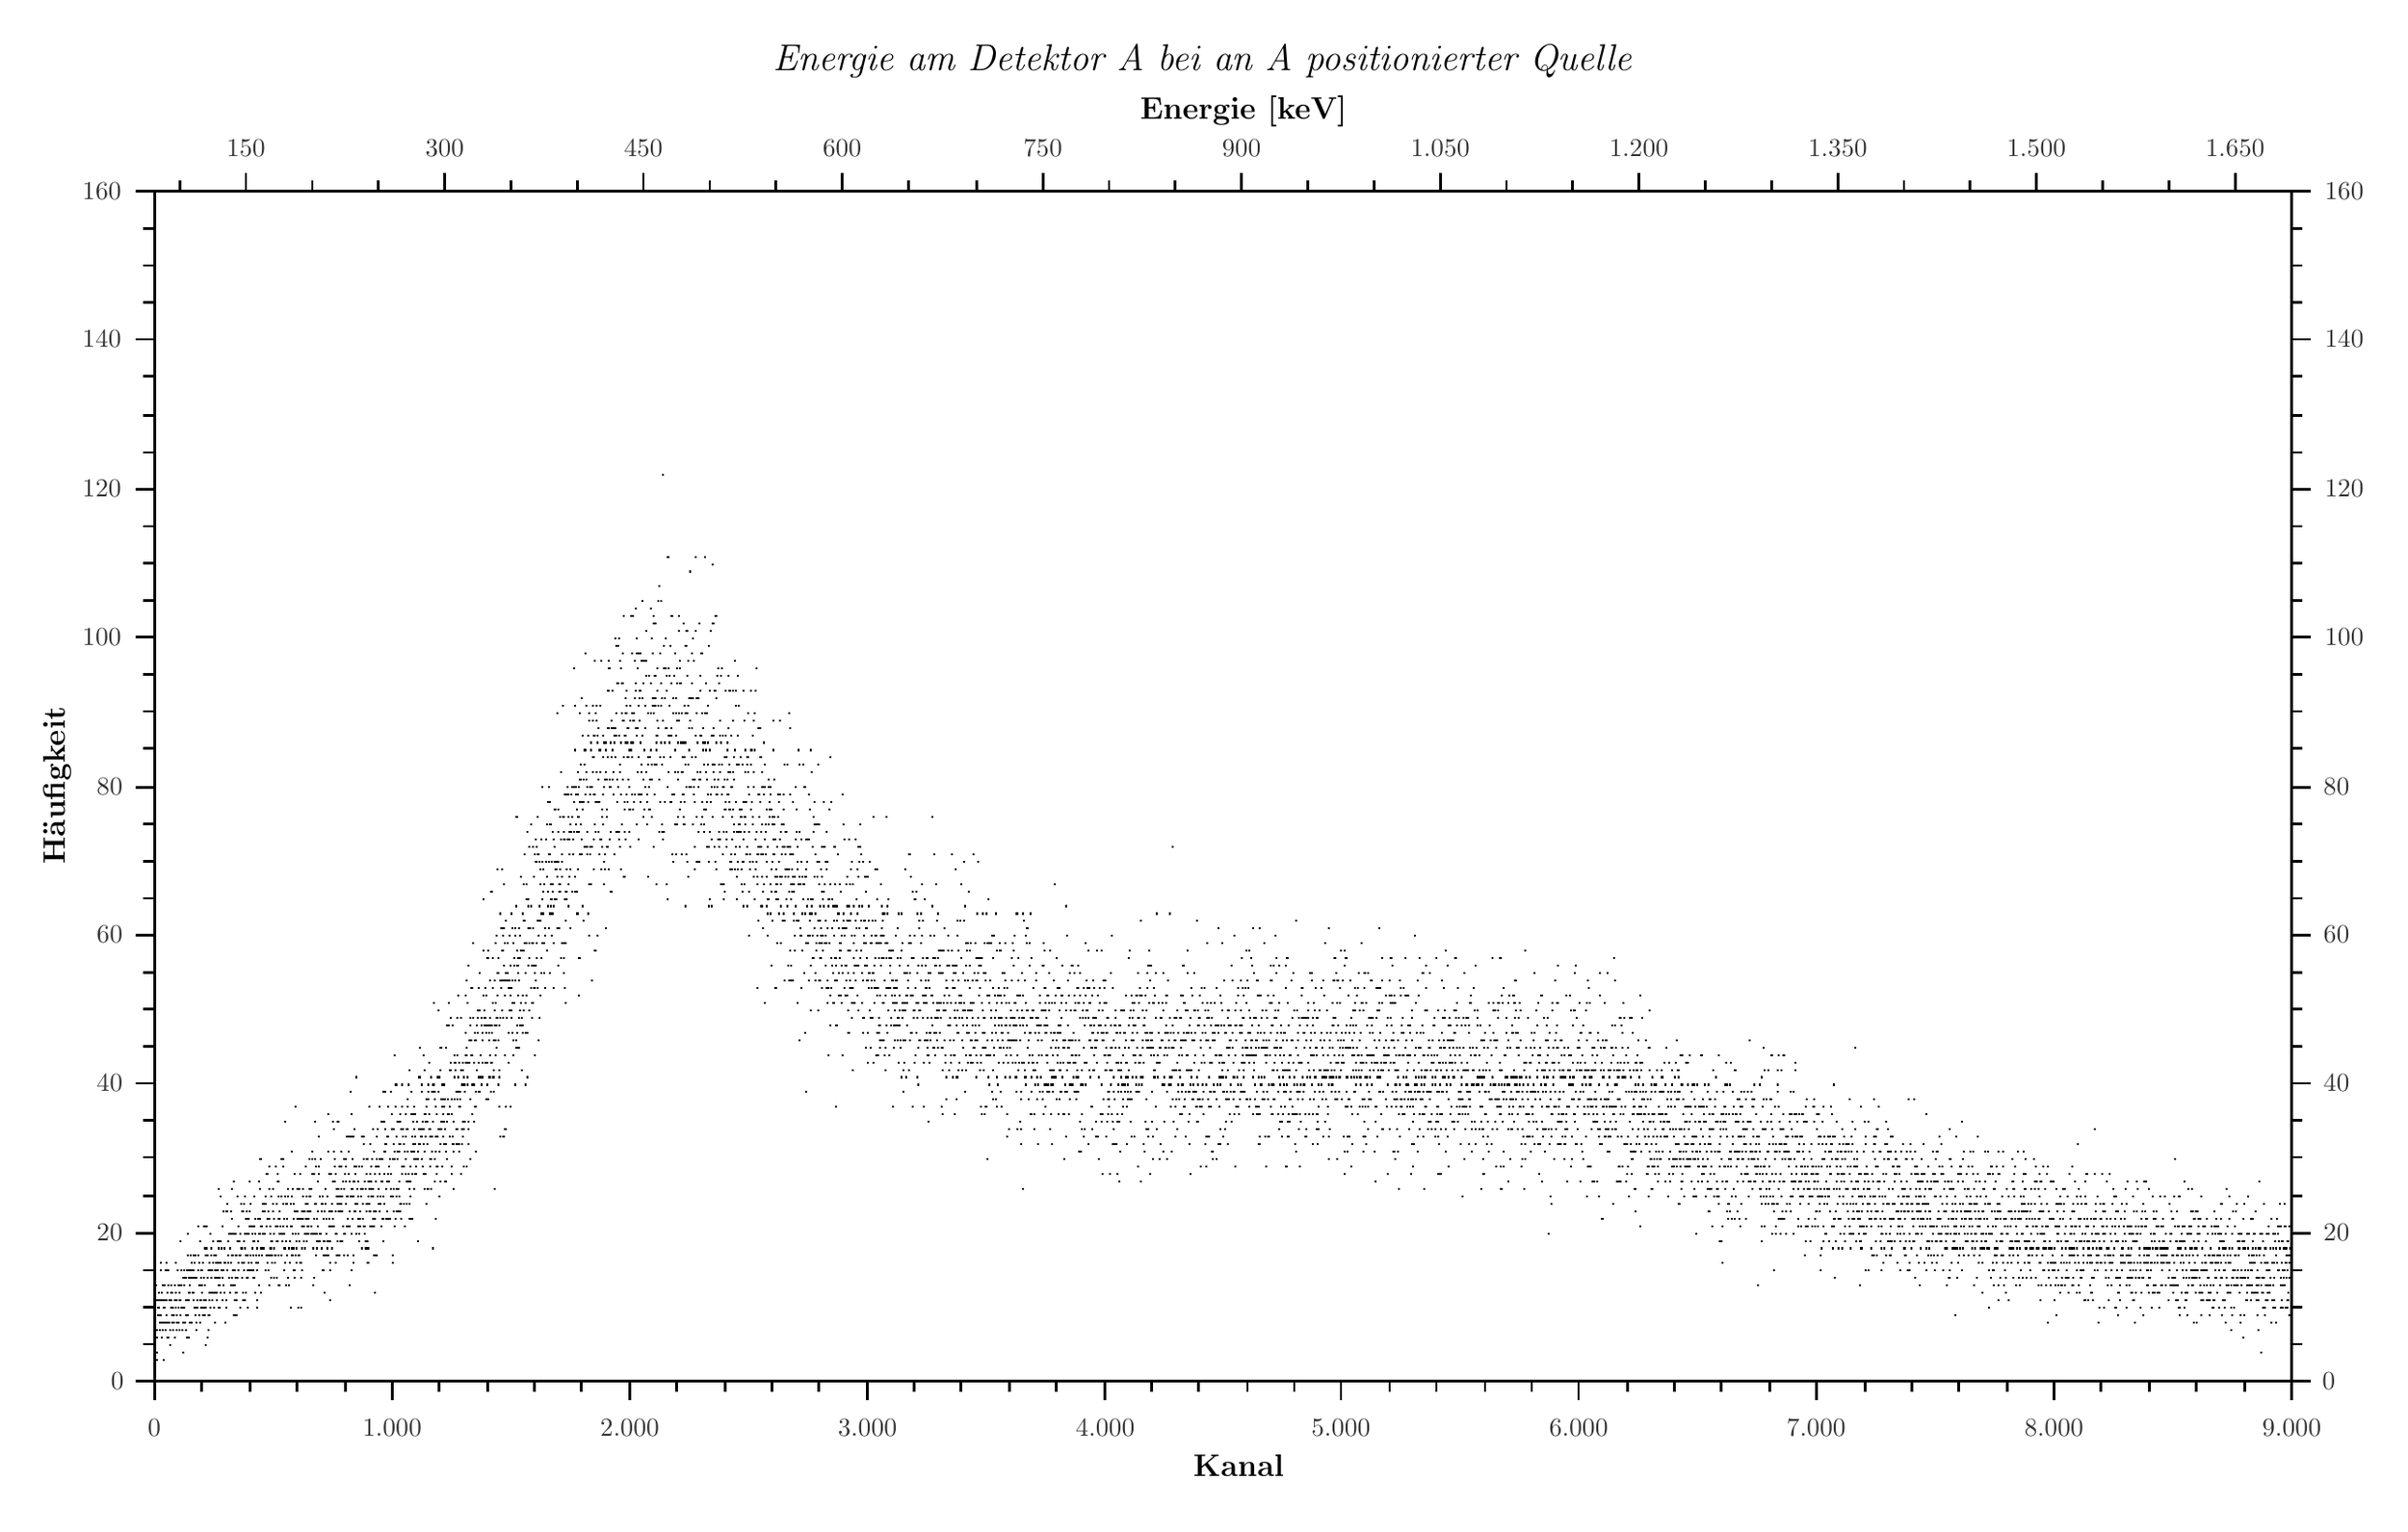
\begin{tikzpicture}{0pt}{0pt}{1209pt}{760pt}
	\clip(0pt,760pt) -- (910.15pt,760pt) -- (910.15pt,187.862pt) -- (0pt,187.862pt) -- (0pt,760pt);
\begin{scope}
	\clip(49.6856pt,696.011pt) -- (875.521pt,696.011pt) -- (875.521pt,236.043pt) -- (49.6856pt,236.043pt) -- (49.6856pt,696.011pt);
	\color[rgb]{0,0,0}
	\fill (49.7774pt,256.166pt) rectangle (50.5302pt,255.413pt);
	\color[rgb]{0,0,0}
	\fill (49.8691pt,273.415pt) rectangle (50.622pt,272.662pt);
	\fill (50.0527pt,244.667pt) rectangle (50.8055pt,243.914pt);
	\fill (50.1444pt,256.166pt) rectangle (50.8972pt,255.413pt);
	\fill (50.2362pt,247.542pt) rectangle (50.989pt,246.789pt);
	\fill (50.3279pt,253.291pt) rectangle (51.0808pt,252.539pt);
	\fill (50.4197pt,244.667pt) rectangle (51.1725pt,243.914pt);
	\fill (50.5115pt,267.665pt) rectangle (51.2643pt,266.913pt);
	\fill (50.6032pt,264.791pt) rectangle (51.356pt,264.038pt);
	\fill (50.695pt,261.916pt) rectangle (51.4478pt,261.163pt);
	\fill (50.8785pt,264.791pt) rectangle (51.6313pt,264.038pt);
	\fill (50.9703pt,261.916pt) rectangle (51.7231pt,261.163pt);
	\fill (51.1538pt,270.54pt) rectangle (51.9066pt,269.787pt);
	\fill (51.3373pt,259.041pt) rectangle (52.0901pt,258.288pt);
	\fill (51.4291pt,267.665pt) rectangle (52.1819pt,266.913pt);
	\fill (51.5208pt,256.166pt) rectangle (52.2736pt,255.413pt);
	\fill (51.6126pt,279.165pt) rectangle (52.3654pt,278.412pt);
	\fill (51.7043pt,282.039pt) rectangle (52.4571pt,281.287pt);
	\fill (51.7961pt,267.665pt) rectangle (52.5489pt,266.913pt);
	\fill (51.8879pt,261.916pt) rectangle (52.6407pt,261.163pt);
	\fill (52.0714pt,253.291pt) rectangle (52.8242pt,252.539pt);
	\fill (52.1631pt,270.54pt) rectangle (52.9159pt,269.787pt);
	\fill (52.2549pt,259.041pt) rectangle (53.0077pt,258.288pt);
	\fill (52.3466pt,256.166pt) rectangle (53.0995pt,255.413pt);
	\fill (52.4384pt,273.415pt) rectangle (53.1912pt,272.662pt);
	\fill (52.5302pt,267.665pt) rectangle (53.283pt,266.913pt);
	\fill (52.7137pt,259.041pt) rectangle (53.4665pt,258.288pt);
	\fill (52.8054pt,264.791pt) rectangle (53.5583pt,264.038pt);
	\fill (52.8972pt,244.667pt) rectangle (53.65pt,243.914pt);
	\fill (53.0807pt,273.415pt) rectangle (53.8335pt,272.662pt);
	\fill (53.2642pt,264.791pt) rectangle (54.0171pt,264.038pt);
	\fill (53.356pt,267.665pt) rectangle (54.1088pt,266.913pt);
	\fill (53.4478pt,259.041pt) rectangle (54.2006pt,258.288pt);
	\fill (53.5395pt,279.165pt) rectangle (54.2923pt,278.412pt);
	\fill (53.723pt,256.166pt) rectangle (54.4759pt,255.413pt);
	\fill (53.8148pt,261.916pt) rectangle (54.5676pt,261.163pt);
	\fill (53.9066pt,267.665pt) rectangle (54.6594pt,266.913pt);
	\fill (53.9983pt,261.916pt) rectangle (54.7511pt,261.163pt);
	\fill (54.0901pt,282.039pt) rectangle (54.8429pt,281.287pt);
	\fill (54.1818pt,253.291pt) rectangle (54.9347pt,252.539pt);
	\fill (54.2736pt,259.041pt) rectangle (55.0264pt,258.288pt);
	\fill (54.3654pt,270.54pt) rectangle (55.1182pt,269.787pt);
	\fill (54.4571pt,279.165pt) rectangle (55.2099pt,278.412pt);
	\fill (54.6406pt,253.291pt) rectangle (55.3934pt,252.539pt);
	\fill (54.7324pt,279.165pt) rectangle (55.4852pt,278.412pt);
	\fill (54.8242pt,273.415pt) rectangle (55.577pt,272.662pt);
	\fill (54.9159pt,267.665pt) rectangle (55.6687pt,266.913pt);
	\fill (55.1912pt,259.041pt) rectangle (55.944pt,258.288pt);
	\fill (55.3747pt,256.166pt) rectangle (56.1275pt,255.413pt);
	\fill (55.4665pt,250.417pt) rectangle (56.2193pt,249.664pt);
	\fill (55.5582pt,267.665pt) rectangle (56.311pt,266.913pt);
	\fill (55.65pt,270.54pt) rectangle (56.4028pt,269.787pt);
	\fill (55.7418pt,273.415pt) rectangle (56.4946pt,272.662pt);
	\fill (55.8335pt,264.791pt) rectangle (56.5863pt,264.038pt);
	\fill (56.1088pt,270.54pt) rectangle (56.8616pt,269.787pt);
	\fill (56.2005pt,259.041pt) rectangle (56.9534pt,258.288pt);
	\fill (56.2923pt,261.916pt) rectangle (57.0451pt,261.163pt);
	\fill (56.4758pt,256.166pt) rectangle (57.2286pt,255.413pt);
	\fill (56.5676pt,264.791pt) rectangle (57.3204pt,264.038pt);
	\fill (56.8429pt,259.041pt) rectangle (57.5957pt,258.288pt);
	\fill (56.9346pt,261.916pt) rectangle (57.6874pt,261.163pt);
	\fill (57.1181pt,253.291pt) rectangle (57.871pt,252.539pt);
	\fill (57.2099pt,273.415pt) rectangle (57.9627pt,272.662pt);
	\fill (57.3017pt,267.665pt) rectangle (58.0545pt,266.913pt);
	\fill (57.3934pt,270.54pt) rectangle (58.1462pt,269.787pt);
	\fill (57.4852pt,264.791pt) rectangle (58.238pt,264.038pt);
	\fill (57.5769pt,282.039pt) rectangle (58.3298pt,281.287pt);
	\fill (57.6687pt,264.791pt) rectangle (58.4215pt,264.038pt);
	\fill (57.7605pt,261.916pt) rectangle (58.5133pt,261.163pt);
	\fill (57.8522pt,267.665pt) rectangle (58.605pt,266.913pt);
	\fill (57.944pt,259.041pt) rectangle (58.6968pt,258.288pt);
	\fill (58.0357pt,256.166pt) rectangle (58.7886pt,255.413pt);
	\fill (58.1275pt,279.165pt) rectangle (58.8803pt,278.412pt);
	\fill (58.4028pt,279.165pt) rectangle (59.1556pt,278.412pt);
	\fill (58.4945pt,273.415pt) rectangle (59.2473pt,272.662pt);
	\fill (58.5863pt,259.041pt) rectangle (59.3391pt,258.288pt);
	\fill (58.6781pt,264.791pt) rectangle (59.4309pt,264.038pt);
	\fill (58.8616pt,256.166pt) rectangle (59.6144pt,255.413pt);
	\fill (58.9533pt,270.54pt) rectangle (59.7061pt,269.787pt);
	\fill (59.0451pt,267.665pt) rectangle (59.7979pt,266.913pt);
	\fill (59.1369pt,273.415pt) rectangle (59.8897pt,272.662pt);
	\fill (59.2286pt,267.665pt) rectangle (59.9814pt,266.913pt);
	\fill (59.3204pt,290.664pt) rectangle (60.0732pt,289.911pt);
	\fill (59.4121pt,261.916pt) rectangle (60.1649pt,261.163pt);
	\fill (59.5956pt,279.165pt) rectangle (60.3485pt,278.412pt);
	\fill (59.6874pt,264.791pt) rectangle (60.4402pt,264.038pt);
	\fill (59.8709pt,273.415pt) rectangle (60.6237pt,272.662pt);
	\fill (59.9627pt,256.166pt) rectangle (60.7155pt,255.413pt);
	\fill (60.238pt,264.791pt) rectangle (60.9908pt,264.038pt);
	\fill (60.3297pt,276.29pt) rectangle (61.0825pt,275.537pt);
	\fill (60.5132pt,259.041pt) rectangle (61.2661pt,258.288pt);
	\fill (60.605pt,247.542pt) rectangle (61.3578pt,246.789pt);
	\fill (60.6968pt,279.165pt) rectangle (61.4496pt,278.412pt);
	\fill (60.7885pt,264.791pt) rectangle (61.5413pt,264.038pt);
	\fill (60.972pt,273.415pt) rectangle (61.7249pt,272.662pt);
	\fill (61.1556pt,276.29pt) rectangle (61.9084pt,275.537pt);
	\fill (61.2473pt,259.041pt) rectangle (62.0001pt,258.288pt);
	\fill (61.4308pt,261.916pt) rectangle (62.1837pt,261.163pt);
	\fill (61.5226pt,256.166pt) rectangle (62.2754pt,255.413pt);
	\fill (61.6144pt,276.29pt) rectangle (62.3672pt,275.537pt);
	\fill (61.7061pt,267.665pt) rectangle (62.4589pt,266.913pt);
	\fill (61.7979pt,253.291pt) rectangle (62.5507pt,252.539pt);
	\fill (62.0732pt,279.165pt) rectangle (62.826pt,278.412pt);
	\fill (62.1649pt,284.914pt) rectangle (62.9177pt,284.161pt);
	\fill (62.2567pt,261.916pt) rectangle (63.0095pt,261.163pt);
	\fill (62.3484pt,293.539pt) rectangle (63.1012pt,292.786pt);
	\fill (62.4402pt,267.665pt) rectangle (63.193pt,266.913pt);
	\fill (62.532pt,276.29pt) rectangle (63.2848pt,275.537pt);
	\fill (62.6237pt,253.291pt) rectangle (63.3765pt,252.539pt);
	\fill (62.7155pt,270.54pt) rectangle (63.4683pt,269.787pt);
	\fill (62.8072pt,279.165pt) rectangle (63.56pt,278.412pt);
	\fill (62.899pt,270.54pt) rectangle (63.6518pt,269.787pt);
	\fill (62.9907pt,273.415pt) rectangle (63.7436pt,272.662pt);
	\fill (63.0825pt,259.041pt) rectangle (63.8353pt,258.288pt);
	\fill (63.1743pt,276.29pt) rectangle (63.9271pt,275.537pt);
	\fill (63.266pt,284.914pt) rectangle (64.0188pt,284.161pt);
	\fill (63.5413pt,279.165pt) rectangle (64.2941pt,278.412pt);
	\fill (63.6331pt,259.041pt) rectangle (64.3859pt,258.288pt);
	\fill (63.7248pt,282.039pt) rectangle (64.4776pt,281.287pt);
	\fill (63.9083pt,276.29pt) rectangle (64.6612pt,275.537pt);
	\fill (64.0001pt,279.165pt) rectangle (64.7529pt,278.412pt);
	\fill (64.0919pt,270.54pt) rectangle (64.8447pt,269.787pt);
	\fill (64.2754pt,284.914pt) rectangle (65.0282pt,284.161pt);
	\fill (64.3671pt,267.665pt) rectangle (65.12pt,266.913pt);
	\fill (64.4589pt,279.165pt) rectangle (65.2117pt,278.412pt);
	\fill (64.5507pt,270.54pt) rectangle (65.3035pt,269.787pt);
	\fill (64.7342pt,282.039pt) rectangle (65.487pt,281.287pt);
	\fill (64.8259pt,276.29pt) rectangle (65.5788pt,275.537pt);
	\fill (64.9177pt,264.791pt) rectangle (65.6705pt,264.038pt);
	\fill (65.0095pt,261.916pt) rectangle (65.7623pt,261.163pt);
	\fill (65.193pt,284.914pt) rectangle (65.9458pt,284.161pt);
	\fill (65.2847pt,264.791pt) rectangle (66.0375pt,264.038pt);
	\fill (65.4683pt,259.041pt) rectangle (66.2211pt,258.288pt);
	\fill (65.56pt,256.166pt) rectangle (66.3128pt,255.413pt);
	\fill (65.6518pt,276.29pt) rectangle (66.4046pt,275.537pt);
	\fill (65.7435pt,267.665pt) rectangle (66.4963pt,266.913pt);
	\fill (65.9271pt,264.791pt) rectangle (66.6799pt,264.038pt);
	\fill (66.0188pt,267.665pt) rectangle (66.7716pt,266.913pt);
	\fill (66.1106pt,279.165pt) rectangle (66.8634pt,278.412pt);
	\fill (66.2023pt,296.413pt) rectangle (66.9551pt,295.661pt);
	\fill (66.2941pt,284.914pt) rectangle (67.0469pt,284.161pt);
	\fill (66.4776pt,273.415pt) rectangle (67.2304pt,272.662pt);
	\fill (66.6611pt,282.039pt) rectangle (67.4139pt,281.287pt);
	\fill (66.7529pt,261.916pt) rectangle (67.5057pt,261.163pt);
	\fill (66.8446pt,273.415pt) rectangle (67.5975pt,272.662pt);
	\fill (66.9364pt,290.664pt) rectangle (67.6892pt,289.911pt);
	\fill (67.0282pt,259.041pt) rectangle (67.781pt,258.288pt);
	\fill (67.1199pt,267.665pt) rectangle (67.8727pt,266.913pt);
	\fill (67.2117pt,276.29pt) rectangle (67.9645pt,275.537pt);
	\fill (67.3034pt,264.791pt) rectangle (68.0563pt,264.038pt);
	\fill (67.3952pt,276.29pt) rectangle (68.148pt,275.537pt);
	\fill (67.487pt,279.165pt) rectangle (68.2398pt,278.412pt);
	\fill (67.5787pt,273.415pt) rectangle (68.3315pt,272.662pt);
	\fill (67.6705pt,270.54pt) rectangle (68.4233pt,269.787pt);
	\fill (67.9458pt,282.039pt) rectangle (68.6986pt,281.287pt);
	\fill (68.0375pt,261.916pt) rectangle (68.7903pt,261.163pt);
	\fill (68.221pt,264.791pt) rectangle (68.9739pt,264.038pt);
	\fill (68.3128pt,276.29pt) rectangle (69.0656pt,275.537pt);
	\fill (68.4046pt,267.665pt) rectangle (69.1574pt,266.913pt);
	\fill (68.5881pt,296.413pt) rectangle (69.3409pt,295.661pt);
	\fill (68.6798pt,287.789pt) rectangle (69.4326pt,287.036pt);
	\fill (68.7716pt,261.916pt) rectangle (69.5244pt,261.163pt);
	\fill (68.8634pt,273.415pt) rectangle (69.6162pt,272.662pt);
	\fill (68.9551pt,250.417pt) rectangle (69.7079pt,249.664pt);
	\fill (69.0469pt,264.791pt) rectangle (69.7997pt,264.038pt);
	\fill (69.1386pt,284.914pt) rectangle (69.8914pt,284.161pt);
	\fill (69.2304pt,267.665pt) rectangle (69.9832pt,266.913pt);
	\fill (69.3222pt,296.413pt) rectangle (70.075pt,295.661pt);
	\fill (69.5057pt,287.789pt) rectangle (70.2585pt,287.036pt);
	\fill (69.6892pt,253.291pt) rectangle (70.442pt,252.539pt);
	\fill (69.781pt,276.29pt) rectangle (70.5338pt,275.537pt);
	\fill (69.8727pt,284.914pt) rectangle (70.6255pt,284.161pt);
	\fill (70.148pt,261.916pt) rectangle (70.9008pt,261.163pt);
	\fill (70.2397pt,279.165pt) rectangle (70.9926pt,278.412pt);
	\fill (70.3315pt,256.166pt) rectangle (71.0843pt,255.413pt);
	\fill (70.4233pt,267.665pt) rectangle (71.1761pt,266.913pt);
	\fill (70.515pt,261.916pt) rectangle (71.2678pt,261.163pt);
	\fill (70.6068pt,282.039pt) rectangle (71.3596pt,281.287pt);
	\fill (70.6985pt,270.54pt) rectangle (71.4514pt,269.787pt);
	\fill (70.7903pt,279.165pt) rectangle (71.5431pt,278.412pt);
	\fill (70.9738pt,293.539pt) rectangle (71.7266pt,292.786pt);
	\fill (71.0656pt,264.791pt) rectangle (71.8184pt,264.038pt);
	\fill (71.1573pt,287.789pt) rectangle (71.9102pt,287.036pt);
	\fill (71.2491pt,284.914pt) rectangle (72.0019pt,284.161pt);
	\fill (71.3409pt,270.54pt) rectangle (72.0937pt,269.787pt);
	\fill (71.4326pt,276.29pt) rectangle (72.1854pt,275.537pt);
	\fill (71.7079pt,267.665pt) rectangle (72.4607pt,266.913pt);
	\fill (71.7997pt,279.165pt) rectangle (72.5525pt,278.412pt);
	\fill (71.9832pt,270.54pt) rectangle (72.736pt,269.787pt);
	\fill (72.0749pt,290.664pt) rectangle (72.8278pt,289.911pt);
	\fill (72.1667pt,282.039pt) rectangle (72.9195pt,281.287pt);
	\fill (72.3502pt,284.914pt) rectangle (73.103pt,284.161pt);
	\fill (72.5337pt,264.791pt) rectangle (73.2865pt,264.038pt);
	\fill (72.6255pt,259.041pt) rectangle (73.3783pt,258.288pt);
	\fill (72.7173pt,279.165pt) rectangle (73.4701pt,278.412pt);
	\fill (72.809pt,270.54pt) rectangle (73.5618pt,269.787pt);
	\fill (72.9008pt,276.29pt) rectangle (73.6536pt,275.537pt);
	\fill (72.9925pt,282.039pt) rectangle (73.7453pt,281.287pt);
	\fill (73.1761pt,284.914pt) rectangle (73.9289pt,284.161pt);
	\fill (73.4513pt,267.665pt) rectangle (74.2041pt,266.913pt);
	\fill (73.5431pt,270.54pt) rectangle (74.2959pt,269.787pt);
	\fill (73.6348pt,279.165pt) rectangle (74.3877pt,278.412pt);
	\fill (73.7266pt,276.29pt) rectangle (74.4794pt,275.537pt);
	\fill (73.8184pt,282.039pt) rectangle (74.5712pt,281.287pt);
	\fill (74.0019pt,290.664pt) rectangle (74.7547pt,289.911pt);
	\fill (74.0936pt,264.791pt) rectangle (74.8465pt,264.038pt);
	\fill (74.1854pt,287.789pt) rectangle (74.9382pt,287.036pt);
	\fill (74.2772pt,310.787pt) rectangle (75.03pt,310.035pt);
	\fill (74.3689pt,273.415pt) rectangle (75.1217pt,272.662pt);
	\fill (74.4607pt,264.791pt) rectangle (75.2135pt,264.038pt);
	\fill (74.5524pt,282.039pt) rectangle (75.3053pt,281.287pt);
	\fill (74.6442pt,276.29pt) rectangle (75.397pt,275.537pt);
	\fill (74.736pt,270.54pt) rectangle (75.4888pt,269.787pt);
	\fill (74.8277pt,290.664pt) rectangle (75.5805pt,289.911pt);
	\fill (74.9195pt,307.913pt) rectangle (75.6723pt,307.16pt);
	\fill (75.0112pt,282.039pt) rectangle (75.7641pt,281.287pt);
	\fill (75.103pt,287.789pt) rectangle (75.8558pt,287.036pt);
	\fill (75.2865pt,279.165pt) rectangle (76.0393pt,278.412pt);
	\fill (75.47pt,267.665pt) rectangle (76.2229pt,266.913pt);
	\fill (75.5618pt,296.413pt) rectangle (76.3146pt,295.661pt);
	\fill (75.7453pt,276.29pt) rectangle (76.4981pt,275.537pt);
	\fill (75.9288pt,302.163pt) rectangle (76.6816pt,301.41pt);
	\fill (76.0206pt,273.415pt) rectangle (76.7734pt,272.662pt);
	\fill (76.1124pt,279.165pt) rectangle (76.8652pt,278.412pt);
	\fill (76.2041pt,287.789pt) rectangle (76.9569pt,287.036pt);
	\fill (76.2959pt,282.039pt) rectangle (77.0487pt,281.287pt);
	\fill (76.4794pt,270.54pt) rectangle (77.2322pt,269.787pt);
	\fill (76.5712pt,282.039pt) rectangle (77.324pt,281.287pt);
	\fill (76.8464pt,259.041pt) rectangle (77.5992pt,258.288pt);
	\fill (76.9382pt,267.665pt) rectangle (77.691pt,266.913pt);
	\fill (77.0299pt,302.163pt) rectangle (77.7828pt,301.41pt);
	\fill (77.2135pt,264.791pt) rectangle (77.9663pt,264.038pt);
	\fill (77.3052pt,305.038pt) rectangle (78.058pt,304.285pt);
	\fill (77.4887pt,302.163pt) rectangle (78.2416pt,301.41pt);
	\fill (77.5805pt,279.165pt) rectangle (78.3333pt,278.412pt);
	\fill (77.6723pt,284.914pt) rectangle (78.4251pt,284.161pt);
	\fill (77.8558pt,290.664pt) rectangle (78.6086pt,289.911pt);
	\fill (77.9475pt,282.039pt) rectangle (78.7004pt,281.287pt);
	\fill (78.1311pt,293.539pt) rectangle (78.8839pt,292.786pt);
	\fill (78.3146pt,276.29pt) rectangle (79.0674pt,275.537pt);
	\fill (78.4981pt,287.789pt) rectangle (79.2509pt,287.036pt);
	\fill (78.5899pt,270.54pt) rectangle (79.3427pt,269.787pt);
	\fill (78.6816pt,293.539pt) rectangle (79.4344pt,292.786pt);
	\fill (78.8651pt,282.039pt) rectangle (79.618pt,281.287pt);
	\fill (78.9569pt,302.163pt) rectangle (79.7097pt,301.41pt);
	\fill (79.0487pt,273.415pt) rectangle (79.8015pt,272.662pt);
	\fill (79.1404pt,299.288pt) rectangle (79.8932pt,298.535pt);
	\fill (79.2322pt,276.29pt) rectangle (79.985pt,275.537pt);
	\fill (79.3239pt,310.787pt) rectangle (80.0767pt,310.035pt);
	\fill (79.4157pt,284.914pt) rectangle (80.1685pt,284.161pt);
	\fill (79.5075pt,279.165pt) rectangle (80.2603pt,278.412pt);
	\fill (79.5992pt,273.415pt) rectangle (80.352pt,272.662pt);
	\fill (79.691pt,284.914pt) rectangle (80.4438pt,284.161pt);
	\fill (79.7827pt,293.539pt) rectangle (80.5355pt,292.786pt);
	\fill (79.9663pt,313.662pt) rectangle (80.7191pt,312.909pt);
	\fill (80.1498pt,261.916pt) rectangle (80.9026pt,261.163pt);
	\fill (80.2415pt,273.415pt) rectangle (80.9943pt,272.662pt);
	\fill (80.3333pt,279.165pt) rectangle (81.0861pt,278.412pt);
	\fill (80.4251pt,267.665pt) rectangle (81.1779pt,266.913pt);
	\fill (80.5168pt,270.54pt) rectangle (81.2696pt,269.787pt);
	\fill (80.6086pt,276.29pt) rectangle (81.3614pt,275.537pt);
	\fill (80.7003pt,284.914pt) rectangle (81.4531pt,284.161pt);
	\fill (80.7921pt,293.539pt) rectangle (81.5449pt,292.786pt);
	\fill (80.8838pt,261.916pt) rectangle (81.6367pt,261.163pt);
	\fill (80.9756pt,270.54pt) rectangle (81.7284pt,269.787pt);
	\fill (81.0674pt,284.914pt) rectangle (81.8202pt,284.161pt);
	\fill (81.1591pt,267.665pt) rectangle (81.9119pt,266.913pt);
	\fill (81.2509pt,276.29pt) rectangle (82.0037pt,275.537pt);
	\fill (81.3426pt,307.913pt) rectangle (82.0955pt,307.16pt);
	\fill (81.4344pt,290.664pt) rectangle (82.1872pt,289.911pt);
	\fill (81.6179pt,279.165pt) rectangle (82.3707pt,278.412pt);
	\fill (81.7097pt,296.413pt) rectangle (82.4625pt,295.661pt);
	\fill (81.8014pt,282.039pt) rectangle (82.5543pt,281.287pt);
	\fill (81.8932pt,279.165pt) rectangle (82.646pt,278.412pt);
	\fill (82.0767pt,290.664pt) rectangle (82.8295pt,289.911pt);
	\fill (82.1685pt,284.914pt) rectangle (82.9213pt,284.161pt);
	\fill (82.4438pt,284.914pt) rectangle (83.1966pt,284.161pt);
	\fill (82.5355pt,293.539pt) rectangle (83.2883pt,292.786pt);
	\fill (82.6273pt,264.791pt) rectangle (83.3801pt,264.038pt);
	\fill (82.719pt,287.789pt) rectangle (83.4718pt,287.036pt);
	\fill (82.9943pt,305.038pt) rectangle (83.7471pt,304.285pt);
	\fill (83.0861pt,282.039pt) rectangle (83.8389pt,281.287pt);
	\fill (83.1778pt,302.163pt) rectangle (83.9306pt,301.41pt);
	\fill (83.2696pt,276.29pt) rectangle (84.0224pt,275.537pt);
	\fill (83.3614pt,287.789pt) rectangle (84.1142pt,287.036pt);
	\fill (83.4531pt,302.163pt) rectangle (84.2059pt,301.41pt);
	\fill (83.6366pt,270.54pt) rectangle (84.3894pt,269.787pt);
	\fill (83.7284pt,267.665pt) rectangle (84.4812pt,266.913pt);
	\fill (83.8202pt,282.039pt) rectangle (84.573pt,281.287pt);
	\fill (83.9119pt,290.664pt) rectangle (84.6647pt,289.911pt);
	\fill (84.0037pt,305.038pt) rectangle (84.7565pt,304.285pt);
	\fill (84.0954pt,279.165pt) rectangle (84.8482pt,278.412pt);
	\fill (84.1872pt,267.665pt) rectangle (84.94pt,266.913pt);
	\fill (84.2789pt,307.913pt) rectangle (85.0318pt,307.16pt);
	\fill (84.3707pt,287.789pt) rectangle (85.1235pt,287.036pt);
	\fill (84.4625pt,293.539pt) rectangle (85.2153pt,292.786pt);
	\fill (84.5542pt,284.914pt) rectangle (85.307pt,284.161pt);
	\fill (84.7377pt,270.54pt) rectangle (85.4906pt,269.787pt);
	\fill (84.8295pt,299.288pt) rectangle (85.5823pt,298.535pt);
	\fill (84.9213pt,302.163pt) rectangle (85.6741pt,301.41pt);
	\fill (85.1965pt,276.29pt) rectangle (85.9494pt,275.537pt);
	\fill (85.2883pt,284.914pt) rectangle (86.0411pt,284.161pt);
	\fill (85.3801pt,279.165pt) rectangle (86.1329pt,278.412pt);
	\fill (85.4718pt,264.791pt) rectangle (86.2246pt,264.038pt);
	\fill (85.5636pt,293.539pt) rectangle (86.3164pt,292.786pt);
	\fill (85.6553pt,282.039pt) rectangle (86.4082pt,281.287pt);
	\fill (85.7471pt,299.288pt) rectangle (86.4999pt,298.535pt);
	\fill (85.9306pt,279.165pt) rectangle (86.6834pt,278.412pt);
	\fill (86.0224pt,313.662pt) rectangle (86.7752pt,312.909pt);
	\fill (86.1141pt,296.413pt) rectangle (86.867pt,295.661pt);
	\fill (86.2059pt,302.163pt) rectangle (86.9587pt,301.41pt);
	\fill (86.2977pt,296.413pt) rectangle (87.0505pt,295.661pt);
	\fill (86.3894pt,284.914pt) rectangle (87.1422pt,284.161pt);
	\fill (86.4812pt,305.038pt) rectangle (87.234pt,304.285pt);
	\fill (86.6647pt,279.165pt) rectangle (87.4175pt,278.412pt);
	\fill (86.94pt,282.039pt) rectangle (87.6928pt,281.287pt);
	\fill (87.0317pt,296.413pt) rectangle (87.7845pt,295.661pt);
	\fill (87.2153pt,293.539pt) rectangle (87.9681pt,292.786pt);
	\fill (87.307pt,287.789pt) rectangle (88.0598pt,287.036pt);
	\fill (87.3988pt,290.664pt) rectangle (88.1516pt,289.911pt);
	\fill (87.4905pt,276.29pt) rectangle (88.2433pt,275.537pt);
	\fill (87.5823pt,279.165pt) rectangle (88.3351pt,278.412pt);
	\fill (87.674pt,284.914pt) rectangle (88.4269pt,284.161pt);
	\fill (87.7658pt,290.664pt) rectangle (88.5186pt,289.911pt);
	\fill (87.8576pt,276.29pt) rectangle (88.6104pt,275.537pt);
	\fill (87.9493pt,296.413pt) rectangle (88.7021pt,295.661pt);
	\fill (88.0411pt,307.913pt) rectangle (88.7939pt,307.16pt);
	\fill (88.1328pt,299.288pt) rectangle (88.8857pt,298.535pt);
	\fill (88.3164pt,270.54pt) rectangle (89.0692pt,269.787pt);
	\fill (88.4081pt,293.539pt) rectangle (89.1609pt,292.786pt);
	\fill (88.4999pt,282.039pt) rectangle (89.2527pt,281.287pt);
	\fill (88.5916pt,284.914pt) rectangle (89.3445pt,284.161pt);
	\fill (88.8669pt,264.791pt) rectangle (89.6197pt,264.038pt);
	\fill (88.9587pt,279.165pt) rectangle (89.7115pt,278.412pt);
	\fill (89.0504pt,267.665pt) rectangle (89.8033pt,266.913pt);
	\fill (89.1422pt,287.789pt) rectangle (89.895pt,287.036pt);
	\fill (89.234pt,282.039pt) rectangle (89.9868pt,281.287pt);
	\fill (89.3257pt,290.664pt) rectangle (90.0785pt,289.911pt);
	\fill (89.4175pt,299.288pt) rectangle (90.1703pt,298.535pt);
	\fill (89.601pt,313.662pt) rectangle (90.3538pt,312.909pt);
	\fill (89.6928pt,284.914pt) rectangle (90.4456pt,284.161pt);
	\fill (89.7845pt,293.539pt) rectangle (90.5373pt,292.786pt);
	\fill (89.8763pt,273.415pt) rectangle (90.6291pt,272.662pt);
	\fill (89.968pt,293.539pt) rectangle (90.7208pt,292.786pt);
	\fill (90.0598pt,299.288pt) rectangle (90.8126pt,298.535pt);
	\fill (90.1516pt,310.787pt) rectangle (90.9044pt,310.035pt);
	\fill (90.2433pt,322.287pt) rectangle (90.9961pt,321.534pt);
	\fill (90.3351pt,270.54pt) rectangle (91.0879pt,269.787pt);
	\fill (90.5186pt,287.789pt) rectangle (91.2714pt,287.036pt);
	\fill (90.6104pt,296.413pt) rectangle (91.3632pt,295.661pt);
	\fill (90.7939pt,284.914pt) rectangle (91.5467pt,284.161pt);
	\fill (90.9774pt,287.789pt) rectangle (91.7302pt,287.036pt);
	\fill (91.0692pt,302.163pt) rectangle (91.822pt,301.41pt);
	\fill (91.1609pt,293.539pt) rectangle (91.9137pt,292.786pt);
	\fill (91.3444pt,305.038pt) rectangle (92.0972pt,304.285pt);
	\fill (91.5279pt,287.789pt) rectangle (92.2808pt,287.036pt);
	\fill (91.7115pt,302.163pt) rectangle (92.4643pt,301.41pt);
	\fill (91.8032pt,293.539pt) rectangle (92.556pt,292.786pt);
	\fill (92.0785pt,305.038pt) rectangle (92.8313pt,304.285pt);
	\fill (92.262pt,307.913pt) rectangle (93.0148pt,307.16pt);
	\fill (92.3538pt,279.165pt) rectangle (93.1066pt,278.412pt);
	\fill (92.4455pt,296.413pt) rectangle (93.1984pt,295.661pt);
	\fill (92.6291pt,316.537pt) rectangle (93.3819pt,315.784pt);
	\fill (92.7208pt,284.914pt) rectangle (93.4736pt,284.161pt);
	\fill (92.9043pt,299.288pt) rectangle (93.6572pt,298.535pt);
	\fill (92.9961pt,282.039pt) rectangle (93.7489pt,281.287pt);
	\fill (93.0879pt,316.537pt) rectangle (93.8407pt,315.784pt);
	\fill (93.1796pt,284.914pt) rectangle (93.9324pt,284.161pt);
	\fill (93.3631pt,279.165pt) rectangle (94.1159pt,278.412pt);
	\fill (93.4549pt,302.163pt) rectangle (94.2077pt,301.41pt);
	\fill (93.5467pt,273.415pt) rectangle (94.2995pt,272.662pt);
	\fill (93.6384pt,310.787pt) rectangle (94.3912pt,310.035pt);
	\fill (93.7302pt,299.288pt) rectangle (94.483pt,298.535pt);
	\fill (93.8219pt,319.412pt) rectangle (94.5747pt,318.659pt);
	\fill (93.9137pt,287.789pt) rectangle (94.6665pt,287.036pt);
	\fill (94.0055pt,296.413pt) rectangle (94.7583pt,295.661pt);
	\fill (94.0972pt,293.539pt) rectangle (94.85pt,292.786pt);
	\fill (94.189pt,284.914pt) rectangle (94.9418pt,284.161pt);
	\fill (94.2807pt,307.913pt) rectangle (95.0335pt,307.16pt);
	\fill (94.3725pt,276.29pt) rectangle (95.1253pt,275.537pt);
	\fill (94.4643pt,290.664pt) rectangle (95.2171pt,289.911pt);
	\fill (94.556pt,287.789pt) rectangle (95.3088pt,287.036pt);
	\fill (94.6478pt,282.039pt) rectangle (95.4006pt,281.287pt);
	\fill (94.7395pt,290.664pt) rectangle (95.4923pt,289.911pt);
	\fill (94.8313pt,284.914pt) rectangle (95.5841pt,284.161pt);
	\fill (95.0148pt,310.787pt) rectangle (95.7676pt,310.035pt);
	\fill (95.1066pt,305.038pt) rectangle (95.8594pt,304.285pt);
	\fill (95.2901pt,302.163pt) rectangle (96.0429pt,301.41pt);
	\fill (95.3818pt,299.288pt) rectangle (96.1347pt,298.535pt);
	\fill (95.4736pt,287.789pt) rectangle (96.2264pt,287.036pt);
	\fill (95.5654pt,276.29pt) rectangle (96.3182pt,275.537pt);
	\fill (95.6571pt,293.539pt) rectangle (96.4099pt,292.786pt);
	\fill (95.7489pt,284.914pt) rectangle (96.5017pt,284.161pt);
	\fill (95.9324pt,282.039pt) rectangle (96.6852pt,281.287pt);
	\fill (96.0242pt,282.039pt) rectangle (96.777pt,281.287pt);
	\fill (96.1159pt,319.412pt) rectangle (96.8687pt,318.659pt);
	\fill (96.2994pt,284.914pt) rectangle (97.0523pt,284.161pt);
	\fill (96.3912pt,296.413pt) rectangle (97.144pt,295.661pt);
	\fill (96.483pt,305.038pt) rectangle (97.2358pt,304.285pt);
	\fill (96.5747pt,290.664pt) rectangle (97.3275pt,289.911pt);
	\fill (96.6665pt,276.29pt) rectangle (97.4193pt,275.537pt);
	\fill (96.7582pt,296.413pt) rectangle (97.5111pt,295.661pt);
	\fill (96.85pt,290.664pt) rectangle (97.6028pt,289.911pt);
	\fill (96.9418pt,316.537pt) rectangle (97.6946pt,315.784pt);
	\fill (97.1253pt,313.662pt) rectangle (97.8781pt,312.909pt);
	\fill (97.217pt,284.914pt) rectangle (97.9698pt,284.161pt);
	\fill (97.3088pt,307.913pt) rectangle (98.0616pt,307.16pt);
	\fill (97.4006pt,273.415pt) rectangle (98.1534pt,272.662pt);
	\fill (97.4923pt,299.288pt) rectangle (98.2451pt,298.535pt);
	\fill (97.5841pt,273.415pt) rectangle (98.3369pt,272.662pt);
	\fill (97.7676pt,302.163pt) rectangle (98.5204pt,301.41pt);
	\fill (97.8594pt,293.539pt) rectangle (98.6122pt,292.786pt);
	\fill (98.0429pt,296.413pt) rectangle (98.7957pt,295.661pt);
	\fill (98.3181pt,307.913pt) rectangle (99.071pt,307.16pt);
	\fill (98.4099pt,322.287pt) rectangle (99.1627pt,321.534pt);
	\fill (98.5017pt,284.914pt) rectangle (99.2545pt,284.161pt);
	\fill (98.5934pt,293.539pt) rectangle (99.3462pt,292.786pt);
	\fill (98.6852pt,290.664pt) rectangle (99.438pt,289.911pt);
	\fill (98.9605pt,305.038pt) rectangle (99.7133pt,304.285pt);
	\fill (99.0522pt,296.413pt) rectangle (99.805pt,295.661pt);
	\fill (99.144pt,319.412pt) rectangle (99.8968pt,318.659pt);
	\fill (99.2357pt,322.287pt) rectangle (99.9886pt,321.534pt);
	\fill (99.3275pt,279.165pt) rectangle (100.08pt,278.412pt);
	\fill (99.4193pt,299.288pt) rectangle (100.172pt,298.535pt);
	\fill (99.511pt,293.539pt) rectangle (100.264pt,292.786pt);
	\fill (99.6028pt,287.789pt) rectangle (100.356pt,287.036pt);
	\fill (99.6945pt,336.661pt) rectangle (100.447pt,335.908pt);
	\fill (99.7863pt,282.039pt) rectangle (100.539pt,281.287pt);
	\fill (99.8781pt,287.789pt) rectangle (100.631pt,287.036pt);
	\fill (99.9698pt,307.913pt) rectangle (100.723pt,307.16pt);
	\fill (100.062pt,305.038pt) rectangle (100.814pt,304.285pt);
	\fill (100.153pt,273.415pt) rectangle (100.906pt,272.662pt);
	\fill (100.245pt,290.664pt) rectangle (100.998pt,289.911pt);
	\fill (100.429pt,284.914pt) rectangle (101.181pt,284.161pt);
	\fill (100.52pt,305.038pt) rectangle (101.273pt,304.285pt);
	\fill (100.612pt,299.288pt) rectangle (101.365pt,298.535pt);
	\fill (100.704pt,296.413pt) rectangle (101.457pt,295.661pt);
	\fill (100.887pt,307.913pt) rectangle (101.64pt,307.16pt);
	\fill (100.979pt,276.29pt) rectangle (101.732pt,275.537pt);
	\fill (101.071pt,310.787pt) rectangle (101.824pt,310.035pt);
	\fill (101.163pt,287.789pt) rectangle (101.916pt,287.036pt);
	\fill (101.254pt,287.789pt) rectangle (102.007pt,287.036pt);
	\fill (101.346pt,273.415pt) rectangle (102.099pt,272.662pt);
	\fill (101.53pt,290.664pt) rectangle (102.283pt,289.911pt);
	\fill (101.805pt,282.039pt) rectangle (102.558pt,281.287pt);
	\fill (101.897pt,305.038pt) rectangle (102.65pt,304.285pt);
	\fill (102.08pt,264.791pt) rectangle (102.833pt,264.038pt);
	\fill (102.172pt,296.413pt) rectangle (102.925pt,295.661pt);
	\fill (102.264pt,287.789pt) rectangle (103.017pt,287.036pt);
	\fill (102.356pt,325.161pt) rectangle (103.108pt,324.409pt);
	\fill (102.447pt,307.913pt) rectangle (103.2pt,307.16pt);
	\fill (102.539pt,284.914pt) rectangle (103.292pt,284.161pt);
	\fill (102.631pt,293.539pt) rectangle (103.384pt,292.786pt);
	\fill (102.814pt,310.787pt) rectangle (103.567pt,310.035pt);
	\fill (102.906pt,287.789pt) rectangle (103.659pt,287.036pt);
	\fill (102.998pt,305.038pt) rectangle (103.751pt,304.285pt);
	\fill (103.181pt,299.288pt) rectangle (103.934pt,298.535pt);
	\fill (103.273pt,279.165pt) rectangle (104.026pt,278.412pt);
	\fill (103.365pt,316.537pt) rectangle (104.118pt,315.784pt);
	\fill (103.457pt,302.163pt) rectangle (104.209pt,301.41pt);
	\fill (103.548pt,276.29pt) rectangle (104.301pt,275.537pt);
	\fill (103.64pt,302.163pt) rectangle (104.393pt,301.41pt);
	\fill (103.732pt,293.539pt) rectangle (104.485pt,292.786pt);
	\fill (103.824pt,284.914pt) rectangle (104.577pt,284.161pt);
	\fill (103.915pt,342.41pt) rectangle (104.668pt,341.657pt);
	\fill (104.007pt,290.664pt) rectangle (104.76pt,289.911pt);
	\fill (104.099pt,287.789pt) rectangle (104.852pt,287.036pt);
	\fill (104.283pt,282.039pt) rectangle (105.035pt,281.287pt);
	\fill (104.374pt,310.787pt) rectangle (105.127pt,310.035pt);
	\fill (104.466pt,299.288pt) rectangle (105.219pt,298.535pt);
	\fill (104.65pt,302.163pt) rectangle (105.402pt,301.41pt);
	\fill (104.741pt,284.914pt) rectangle (105.494pt,284.161pt);
	\fill (104.833pt,293.539pt) rectangle (105.586pt,292.786pt);
	\fill (105.017pt,264.791pt) rectangle (105.769pt,264.038pt);
	\fill (105.108pt,284.914pt) rectangle (105.861pt,284.161pt);
	\fill (105.2pt,299.288pt) rectangle (105.953pt,298.535pt);
	\fill (105.292pt,310.787pt) rectangle (106.045pt,310.035pt);
	\fill (105.384pt,290.664pt) rectangle (106.136pt,289.911pt);
	\fill (105.567pt,316.537pt) rectangle (106.32pt,315.784pt);
	\fill (105.659pt,282.039pt) rectangle (106.412pt,281.287pt);
	\fill (105.842pt,282.039pt) rectangle (106.595pt,281.287pt);
	\fill (105.934pt,276.29pt) rectangle (106.687pt,275.537pt);
	\fill (106.026pt,299.288pt) rectangle (106.779pt,298.535pt);
	\fill (106.118pt,264.791pt) rectangle (106.871pt,264.038pt);
	\fill (106.209pt,279.165pt) rectangle (106.962pt,278.412pt);
	\fill (106.301pt,296.413pt) rectangle (107.054pt,295.661pt);
	\fill (106.393pt,287.789pt) rectangle (107.146pt,287.036pt);
	\fill (106.485pt,302.163pt) rectangle (107.238pt,301.41pt);
	\fill (106.577pt,307.913pt) rectangle (107.329pt,307.16pt);
	\fill (106.76pt,299.288pt) rectangle (107.513pt,298.535pt);
	\fill (106.852pt,310.787pt) rectangle (107.605pt,310.035pt);
	\fill (106.944pt,290.664pt) rectangle (107.696pt,289.911pt);
	\fill (107.035pt,302.163pt) rectangle (107.788pt,301.41pt);
	\fill (107.127pt,296.413pt) rectangle (107.88pt,295.661pt);
	\fill (107.311pt,302.163pt) rectangle (108.063pt,301.41pt);
	\fill (107.402pt,287.789pt) rectangle (108.155pt,287.036pt);
	\fill (107.494pt,293.539pt) rectangle (108.247pt,292.786pt);
	\fill (107.678pt,319.412pt) rectangle (108.43pt,318.659pt);
	\fill (107.769pt,305.038pt) rectangle (108.522pt,304.285pt);
	\fill (107.953pt,299.288pt) rectangle (108.706pt,298.535pt);
	\fill (108.045pt,293.539pt) rectangle (108.797pt,292.786pt);
	\fill (108.136pt,290.664pt) rectangle (108.889pt,289.911pt);
	\fill (108.228pt,307.913pt) rectangle (108.981pt,307.16pt);
	\fill (108.32pt,305.038pt) rectangle (109.073pt,304.285pt);
	\fill (108.412pt,302.163pt) rectangle (109.165pt,301.41pt);
	\fill (108.595pt,296.413pt) rectangle (109.348pt,295.661pt);
	\fill (108.779pt,299.288pt) rectangle (109.532pt,298.535pt);
	\fill (108.87pt,293.539pt) rectangle (109.623pt,292.786pt);
	\fill (108.962pt,296.413pt) rectangle (109.715pt,295.661pt);
	\fill (109.054pt,302.163pt) rectangle (109.807pt,301.41pt);
	\fill (109.146pt,310.787pt) rectangle (109.899pt,310.035pt);
	\fill (109.238pt,322.287pt) rectangle (109.99pt,321.534pt);
	\fill (109.329pt,307.913pt) rectangle (110.082pt,307.16pt);
	\fill (109.605pt,302.163pt) rectangle (110.357pt,301.41pt);
	\fill (109.696pt,307.913pt) rectangle (110.449pt,307.16pt);
	\fill (109.88pt,310.787pt) rectangle (110.633pt,310.035pt);
	\fill (109.972pt,296.413pt) rectangle (110.724pt,295.661pt);
	\fill (110.063pt,293.539pt) rectangle (110.816pt,292.786pt);
	\fill (110.155pt,325.161pt) rectangle (110.908pt,324.409pt);
	\fill (110.339pt,316.537pt) rectangle (111.091pt,315.784pt);
	\fill (110.43pt,322.287pt) rectangle (111.183pt,321.534pt);
	\fill (110.522pt,287.789pt) rectangle (111.275pt,287.036pt);
	\fill (110.614pt,273.415pt) rectangle (111.367pt,272.662pt);
	\fill (110.706pt,293.539pt) rectangle (111.458pt,292.786pt);
	\fill (110.889pt,276.29pt) rectangle (111.642pt,275.537pt);
	\fill (110.981pt,299.288pt) rectangle (111.734pt,298.535pt);
	\fill (111.073pt,299.288pt) rectangle (111.826pt,298.535pt);
	\fill (111.164pt,316.537pt) rectangle (111.917pt,315.784pt);
	\fill (111.256pt,305.038pt) rectangle (112.009pt,304.285pt);
	\fill (111.348pt,336.661pt) rectangle (112.101pt,335.908pt);
	\fill (111.44pt,322.287pt) rectangle (112.193pt,321.534pt);
	\fill (111.532pt,293.539pt) rectangle (112.284pt,292.786pt);
	\fill (111.715pt,319.412pt) rectangle (112.468pt,318.659pt);
	\fill (111.807pt,305.038pt) rectangle (112.56pt,304.285pt);
	\fill (111.899pt,284.914pt) rectangle (112.651pt,284.161pt);
	\fill (111.99pt,287.789pt) rectangle (112.743pt,287.036pt);
	\fill (112.082pt,293.539pt) rectangle (112.835pt,292.786pt);
	\fill (112.174pt,299.288pt) rectangle (112.927pt,298.535pt);
	\fill (112.266pt,290.664pt) rectangle (113.018pt,289.911pt);
	\fill (112.357pt,313.662pt) rectangle (113.11pt,312.909pt);
	\fill (112.449pt,296.413pt) rectangle (113.202pt,295.661pt);
	\fill (112.633pt,302.163pt) rectangle (113.385pt,301.41pt);
	\fill (112.724pt,319.412pt) rectangle (113.477pt,318.659pt);
	\fill (112.816pt,290.664pt) rectangle (113.569pt,289.911pt);
	\fill (112.908pt,330.911pt) rectangle (113.661pt,330.158pt);
	\fill (113pt,316.537pt) rectangle (113.752pt,315.784pt);
	\fill (113.091pt,293.539pt) rectangle (113.844pt,292.786pt);
	\fill (113.275pt,307.913pt) rectangle (114.028pt,307.16pt);
	\fill (113.367pt,290.664pt) rectangle (114.12pt,289.911pt);
	\fill (113.458pt,293.539pt) rectangle (114.211pt,292.786pt);
	\fill (113.642pt,322.287pt) rectangle (114.395pt,321.534pt);
	\fill (113.826pt,302.163pt) rectangle (114.578pt,301.41pt);
	\fill (113.917pt,287.789pt) rectangle (114.67pt,287.036pt);
	\fill (114.101pt,305.038pt) rectangle (114.854pt,304.285pt);
	\fill (114.284pt,307.913pt) rectangle (115.037pt,307.16pt);
	\fill (114.468pt,279.165pt) rectangle (115.221pt,278.412pt);
	\fill (114.56pt,284.914pt) rectangle (115.312pt,284.161pt);
	\fill (114.743pt,299.288pt) rectangle (115.496pt,298.535pt);
	\fill (114.835pt,290.664pt) rectangle (115.588pt,289.911pt);
	\fill (114.927pt,302.163pt) rectangle (115.679pt,301.41pt);
	\fill (115.018pt,270.54pt) rectangle (115.771pt,269.787pt);
	\fill (115.202pt,284.914pt) rectangle (115.955pt,284.161pt);
	\fill (115.294pt,310.787pt) rectangle (116.046pt,310.035pt);
	\fill (115.477pt,305.038pt) rectangle (116.23pt,304.285pt);
	\fill (115.569pt,284.914pt) rectangle (116.322pt,284.161pt);
	\fill (115.661pt,299.288pt) rectangle (116.414pt,298.535pt);
	\fill (115.752pt,293.539pt) rectangle (116.505pt,292.786pt);
	\fill (115.936pt,287.789pt) rectangle (116.689pt,287.036pt);
	\fill (116.119pt,290.664pt) rectangle (116.872pt,289.911pt);
	\fill (116.211pt,307.913pt) rectangle (116.964pt,307.16pt);
	\fill (116.303pt,325.161pt) rectangle (117.056pt,324.409pt);
	\fill (116.395pt,339.535pt) rectangle (117.148pt,338.783pt);
	\fill (116.487pt,284.914pt) rectangle (117.239pt,284.161pt);
	\fill (116.578pt,290.664pt) rectangle (117.331pt,289.911pt);
	\fill (116.67pt,299.288pt) rectangle (117.423pt,298.535pt);
	\fill (116.762pt,302.163pt) rectangle (117.515pt,301.41pt);
	\fill (116.854pt,296.413pt) rectangle (117.606pt,295.661pt);
	\fill (116.945pt,316.537pt) rectangle (117.698pt,315.784pt);
	\fill (117.037pt,282.039pt) rectangle (117.79pt,281.287pt);
	\fill (117.129pt,290.664pt) rectangle (117.882pt,289.911pt);
	\fill (117.221pt,279.165pt) rectangle (117.973pt,278.412pt);
	\fill (117.312pt,267.665pt) rectangle (118.065pt,266.913pt);
	\fill (117.496pt,296.413pt) rectangle (118.249pt,295.661pt);
	\fill (117.588pt,316.537pt) rectangle (118.34pt,315.784pt);
	\fill (117.679pt,302.163pt) rectangle (118.432pt,301.41pt);
	\fill (117.771pt,287.789pt) rectangle (118.524pt,287.036pt);
	\fill (117.863pt,302.163pt) rectangle (118.616pt,301.41pt);
	\fill (117.955pt,305.038pt) rectangle (118.707pt,304.285pt);
	\fill (118.046pt,296.413pt) rectangle (118.799pt,295.661pt);
	\fill (118.138pt,299.288pt) rectangle (118.891pt,298.535pt);
	\fill (118.23pt,313.662pt) rectangle (118.983pt,312.909pt);
	\fill (118.322pt,336.661pt) rectangle (119.075pt,335.908pt);
	\fill (118.597pt,296.413pt) rectangle (119.35pt,295.661pt);
	\fill (118.689pt,333.786pt) rectangle (119.442pt,333.033pt);
	\fill (118.781pt,325.161pt) rectangle (119.533pt,324.409pt);
	\fill (118.872pt,322.287pt) rectangle (119.625pt,321.534pt);
	\fill (118.964pt,313.662pt) rectangle (119.717pt,312.909pt);
	\fill (119.056pt,319.412pt) rectangle (119.809pt,318.659pt);
	\fill (119.239pt,316.537pt) rectangle (119.992pt,315.784pt);
	\fill (119.331pt,302.163pt) rectangle (120.084pt,301.41pt);
	\fill (119.423pt,282.039pt) rectangle (120.176pt,281.287pt);
	\fill (119.515pt,293.539pt) rectangle (120.267pt,292.786pt);
	\fill (119.606pt,307.913pt) rectangle (120.359pt,307.16pt);
	\fill (119.698pt,310.787pt) rectangle (120.451pt,310.035pt);
	\fill (119.882pt,284.914pt) rectangle (120.634pt,284.161pt);
	\fill (119.973pt,305.038pt) rectangle (120.726pt,304.285pt);
	\fill (120.157pt,290.664pt) rectangle (120.91pt,289.911pt);
	\fill (120.249pt,336.661pt) rectangle (121.001pt,335.908pt);
	\fill (120.34pt,307.913pt) rectangle (121.093pt,307.16pt);
	\fill (120.432pt,302.163pt) rectangle (121.185pt,301.41pt);
	\fill (120.524pt,310.787pt) rectangle (121.277pt,310.035pt);
	\fill (120.707pt,319.412pt) rectangle (121.46pt,318.659pt);
	\fill (120.799pt,305.038pt) rectangle (121.552pt,304.285pt);
	\fill (120.891pt,284.914pt) rectangle (121.644pt,284.161pt);
	\fill (120.983pt,307.913pt) rectangle (121.736pt,307.16pt);
	\fill (121.074pt,302.163pt) rectangle (121.827pt,301.41pt);
	\fill (121.258pt,290.664pt) rectangle (122.011pt,289.911pt);
	\fill (121.35pt,305.038pt) rectangle (122.103pt,304.285pt);
	\fill (121.442pt,310.787pt) rectangle (122.194pt,310.035pt);
	\fill (121.533pt,325.161pt) rectangle (122.286pt,324.409pt);
	\fill (121.625pt,319.412pt) rectangle (122.378pt,318.659pt);
	\fill (121.809pt,307.913pt) rectangle (122.561pt,307.16pt);
	\fill (121.9pt,290.664pt) rectangle (122.653pt,289.911pt);
	\fill (121.992pt,302.163pt) rectangle (122.745pt,301.41pt);
	\fill (122.176pt,313.662pt) rectangle (122.928pt,312.909pt);
	\fill (122.359pt,296.413pt) rectangle (123.112pt,295.661pt);
	\fill (122.451pt,293.539pt) rectangle (123.204pt,292.786pt);
	\fill (122.543pt,310.787pt) rectangle (123.295pt,310.035pt);
	\fill (122.634pt,322.287pt) rectangle (123.387pt,321.534pt);
	\fill (122.726pt,284.914pt) rectangle (123.479pt,284.161pt);
	\fill (122.818pt,316.537pt) rectangle (123.571pt,315.784pt);
	\fill (123.093pt,293.539pt) rectangle (123.846pt,292.786pt);
	\fill (123.185pt,313.662pt) rectangle (123.938pt,312.909pt);
	\fill (123.277pt,305.038pt) rectangle (124.03pt,304.285pt);
	\fill (123.368pt,319.412pt) rectangle (124.121pt,318.659pt);
	\fill (123.46pt,322.287pt) rectangle (124.213pt,321.534pt);
	\fill (123.552pt,307.913pt) rectangle (124.305pt,307.16pt);
	\fill (123.644pt,296.413pt) rectangle (124.397pt,295.661pt);
	\fill (123.827pt,330.911pt) rectangle (124.58pt,330.158pt);
	\fill (123.919pt,299.288pt) rectangle (124.672pt,298.535pt);
	\fill (124.011pt,296.413pt) rectangle (124.764pt,295.661pt);
	\fill (124.103pt,307.913pt) rectangle (124.855pt,307.16pt);
	\fill (124.194pt,284.914pt) rectangle (124.947pt,284.161pt);
	\fill (124.378pt,325.161pt) rectangle (125.131pt,324.409pt);
	\fill (124.47pt,330.911pt) rectangle (125.222pt,330.158pt);
	\fill (124.561pt,316.537pt) rectangle (125.314pt,315.784pt);
	\fill (124.653pt,302.163pt) rectangle (125.406pt,301.41pt);
	\fill (124.745pt,313.662pt) rectangle (125.498pt,312.909pt);
	\fill (124.837pt,273.415pt) rectangle (125.589pt,272.662pt);
	\fill (124.928pt,296.413pt) rectangle (125.681pt,295.661pt);
	\fill (125.02pt,348.16pt) rectangle (125.773pt,347.407pt);
	\fill (125.204pt,330.911pt) rectangle (125.956pt,330.158pt);
	\fill (125.295pt,307.913pt) rectangle (126.048pt,307.16pt);
	\fill (125.387pt,293.539pt) rectangle (126.14pt,292.786pt);
	\fill (125.479pt,279.165pt) rectangle (126.232pt,278.412pt);
	\fill (125.571pt,339.535pt) rectangle (126.324pt,338.783pt);
	\fill (125.662pt,310.787pt) rectangle (126.415pt,310.035pt);
	\fill (125.754pt,299.288pt) rectangle (126.507pt,298.535pt);
	\fill (125.846pt,322.287pt) rectangle (126.599pt,321.534pt);
	\fill (125.938pt,330.911pt) rectangle (126.691pt,330.158pt);
	\fill (126.03pt,307.913pt) rectangle (126.782pt,307.16pt);
	\fill (126.121pt,330.911pt) rectangle (126.874pt,330.158pt);
	\fill (126.213pt,282.039pt) rectangle (126.966pt,281.287pt);
	\fill (126.305pt,284.914pt) rectangle (127.058pt,284.161pt);
	\fill (126.397pt,313.662pt) rectangle (127.149pt,312.909pt);
	\fill (126.488pt,319.412pt) rectangle (127.241pt,318.659pt);
	\fill (126.672pt,333.786pt) rectangle (127.425pt,333.033pt);
	\fill (126.764pt,302.163pt) rectangle (127.516pt,301.41pt);
	\fill (126.855pt,305.038pt) rectangle (127.608pt,304.285pt);
	\fill (126.947pt,302.163pt) rectangle (127.7pt,301.41pt);
	\fill (127.039pt,316.537pt) rectangle (127.792pt,315.784pt);
	\fill (127.222pt,293.539pt) rectangle (127.975pt,292.786pt);
	\fill (127.314pt,353.909pt) rectangle (128.067pt,353.157pt);
	\fill (127.406pt,319.412pt) rectangle (128.159pt,318.659pt);
	\fill (127.681pt,305.038pt) rectangle (128.434pt,304.285pt);
	\fill (127.773pt,310.787pt) rectangle (128.526pt,310.035pt);
	\fill (127.865pt,299.288pt) rectangle (128.618pt,298.535pt);
	\fill (127.956pt,313.662pt) rectangle (128.709pt,312.909pt);
	\fill (128.048pt,296.413pt) rectangle (128.801pt,295.661pt);
	\fill (128.14pt,307.913pt) rectangle (128.893pt,307.16pt);
	\fill (128.323pt,290.664pt) rectangle (129.076pt,289.911pt);
	\fill (128.415pt,293.539pt) rectangle (129.168pt,292.786pt);
	\fill (128.507pt,319.412pt) rectangle (129.26pt,318.659pt);
	\fill (128.599pt,302.163pt) rectangle (129.352pt,301.41pt);
	\fill (128.691pt,296.413pt) rectangle (129.443pt,295.661pt);
	\fill (128.874pt,299.288pt) rectangle (129.627pt,298.535pt);
	\fill (129.149pt,310.787pt) rectangle (129.902pt,310.035pt);
	\fill (129.241pt,307.913pt) rectangle (129.994pt,307.16pt);
	\fill (129.333pt,330.911pt) rectangle (130.086pt,330.158pt);
	\fill (129.425pt,319.412pt) rectangle (130.177pt,318.659pt);
	\fill (129.608pt,287.789pt) rectangle (130.361pt,287.036pt);
	\fill (129.7pt,299.288pt) rectangle (130.453pt,298.535pt);
	\fill (129.883pt,305.038pt) rectangle (130.636pt,304.285pt);
	\fill (129.975pt,310.787pt) rectangle (130.728pt,310.035pt);
	\fill (130.067pt,330.911pt) rectangle (130.82pt,330.158pt);
	\fill (130.159pt,322.287pt) rectangle (130.912pt,321.534pt);
	\fill (130.25pt,328.036pt) rectangle (131.003pt,327.283pt);
	\fill (130.342pt,296.413pt) rectangle (131.095pt,295.661pt);
	\fill (130.434pt,313.662pt) rectangle (131.187pt,312.909pt);
	\fill (130.617pt,293.539pt) rectangle (131.37pt,292.786pt);
	\fill (130.709pt,296.413pt) rectangle (131.462pt,295.661pt);
	\fill (130.801pt,310.787pt) rectangle (131.554pt,310.035pt);
	\fill (130.893pt,290.664pt) rectangle (131.646pt,289.911pt);
	\fill (131.076pt,287.789pt) rectangle (131.829pt,287.036pt);
	\fill (131.168pt,316.537pt) rectangle (131.921pt,315.784pt);
	\fill (131.26pt,305.038pt) rectangle (132.013pt,304.285pt);
	\fill (131.352pt,302.163pt) rectangle (132.104pt,301.41pt);
	\fill (131.443pt,322.287pt) rectangle (132.196pt,321.534pt);
	\fill (131.535pt,305.038pt) rectangle (132.288pt,304.285pt);
	\fill (131.719pt,290.664pt) rectangle (132.471pt,289.911pt);
	\fill (131.81pt,282.039pt) rectangle (132.563pt,281.287pt);
	\fill (131.902pt,307.913pt) rectangle (132.655pt,307.16pt);
	\fill (131.994pt,287.789pt) rectangle (132.747pt,287.036pt);
	\fill (132.177pt,313.662pt) rectangle (132.93pt,312.909pt);
	\fill (132.269pt,305.038pt) rectangle (133.022pt,304.285pt);
	\fill (132.361pt,342.41pt) rectangle (133.114pt,341.657pt);
	\fill (132.453pt,310.787pt) rectangle (133.205pt,310.035pt);
	\fill (132.544pt,302.163pt) rectangle (133.297pt,301.41pt);
	\fill (132.636pt,316.537pt) rectangle (133.389pt,315.784pt);
	\fill (132.728pt,296.413pt) rectangle (133.481pt,295.661pt);
	\fill (132.82pt,328.036pt) rectangle (133.573pt,327.283pt);
	\fill (132.911pt,310.787pt) rectangle (133.664pt,310.035pt);
	\fill (133.003pt,319.412pt) rectangle (133.756pt,318.659pt);
	\fill (133.095pt,313.662pt) rectangle (133.848pt,312.909pt);
	\fill (133.187pt,307.913pt) rectangle (133.94pt,307.16pt);
	\fill (133.279pt,296.413pt) rectangle (134.031pt,295.661pt);
	\fill (133.554pt,322.287pt) rectangle (134.307pt,321.534pt);
	\fill (133.646pt,299.288pt) rectangle (134.398pt,298.535pt);
	\fill (133.737pt,307.913pt) rectangle (134.49pt,307.16pt);
	\fill (133.829pt,333.786pt) rectangle (134.582pt,333.033pt);
	\fill (133.921pt,310.787pt) rectangle (134.674pt,310.035pt);
	\fill (134.013pt,284.914pt) rectangle (134.765pt,284.161pt);
	\fill (134.104pt,296.413pt) rectangle (134.857pt,295.661pt);
	\fill (134.196pt,325.161pt) rectangle (134.949pt,324.409pt);
	\fill (134.288pt,302.163pt) rectangle (135.041pt,301.41pt);
	\fill (134.38pt,316.537pt) rectangle (135.132pt,315.784pt);
	\fill (134.471pt,270.54pt) rectangle (135.224pt,269.787pt);
	\fill (134.655pt,299.288pt) rectangle (135.408pt,298.535pt);
	\fill (134.747pt,302.163pt) rectangle (135.499pt,301.41pt);
	\fill (134.838pt,313.662pt) rectangle (135.591pt,312.909pt);
	\fill (134.93pt,284.914pt) rectangle (135.683pt,284.161pt);
	\fill (135.022pt,319.412pt) rectangle (135.775pt,318.659pt);
	\fill (135.205pt,322.287pt) rectangle (135.958pt,321.534pt);
	\fill (135.297pt,330.911pt) rectangle (136.05pt,330.158pt);
	\fill (135.389pt,284.914pt) rectangle (136.142pt,284.161pt);
	\fill (135.572pt,307.913pt) rectangle (136.325pt,307.16pt);
	\fill (135.664pt,319.412pt) rectangle (136.417pt,318.659pt);
	\fill (135.756pt,333.786pt) rectangle (136.509pt,333.033pt);
	\fill (135.94pt,319.412pt) rectangle (136.692pt,318.659pt);
	\fill (136.031pt,305.038pt) rectangle (136.784pt,304.285pt);
	\fill (136.123pt,310.787pt) rectangle (136.876pt,310.035pt);
	\fill (136.215pt,316.537pt) rectangle (136.968pt,315.784pt);
	\fill (136.307pt,322.287pt) rectangle (137.059pt,321.534pt);
	\fill (136.398pt,342.41pt) rectangle (137.151pt,341.657pt);
	\fill (136.49pt,302.163pt) rectangle (137.243pt,301.41pt);
	\fill (136.582pt,307.913pt) rectangle (137.335pt,307.16pt);
	\fill (136.674pt,307.913pt) rectangle (137.426pt,307.16pt);
	\fill (136.765pt,305.038pt) rectangle (137.518pt,304.285pt);
	\fill (136.857pt,322.287pt) rectangle (137.61pt,321.534pt);
	\fill (137.041pt,313.662pt) rectangle (137.793pt,312.909pt);
	\fill (137.132pt,296.413pt) rectangle (137.885pt,295.661pt);
	\fill (137.224pt,336.661pt) rectangle (137.977pt,335.908pt);
	\fill (137.408pt,313.662pt) rectangle (138.16pt,312.909pt);
	\fill (137.499pt,322.287pt) rectangle (138.252pt,321.534pt);
	\fill (137.591pt,299.288pt) rectangle (138.344pt,298.535pt);
	\fill (137.775pt,307.913pt) rectangle (138.528pt,307.16pt);
	\fill (137.866pt,290.664pt) rectangle (138.619pt,289.911pt);
	\fill (137.958pt,348.16pt) rectangle (138.711pt,347.407pt);
	\fill (138.05pt,336.661pt) rectangle (138.803pt,335.908pt);
	\fill (138.142pt,316.537pt) rectangle (138.895pt,315.784pt);
	\fill (138.234pt,305.038pt) rectangle (138.986pt,304.285pt);
	\fill (138.325pt,325.161pt) rectangle (139.078pt,324.409pt);
	\fill (138.417pt,333.786pt) rectangle (139.17pt,333.033pt);
	\fill (138.601pt,348.16pt) rectangle (139.353pt,347.407pt);
	\fill (138.692pt,328.036pt) rectangle (139.445pt,327.283pt);
	\fill (138.784pt,299.288pt) rectangle (139.537pt,298.535pt);
	\fill (138.968pt,310.787pt) rectangle (139.72pt,310.035pt);
	\fill (139.059pt,330.911pt) rectangle (139.812pt,330.158pt);
	\fill (139.151pt,313.662pt) rectangle (139.904pt,312.909pt);
	\fill (139.243pt,302.163pt) rectangle (139.996pt,301.41pt);
	\fill (139.335pt,299.288pt) rectangle (140.087pt,298.535pt);
	\fill (139.518pt,342.41pt) rectangle (140.271pt,341.657pt);
	\fill (139.61pt,316.537pt) rectangle (140.363pt,315.784pt);
	\fill (139.702pt,330.911pt) rectangle (140.454pt,330.158pt);
	\fill (139.793pt,313.662pt) rectangle (140.546pt,312.909pt);
	\fill (139.885pt,319.412pt) rectangle (140.638pt,318.659pt);
	\fill (140.069pt,299.288pt) rectangle (140.822pt,298.535pt);
	\fill (140.16pt,322.287pt) rectangle (140.913pt,321.534pt);
	\fill (140.436pt,299.288pt) rectangle (141.189pt,298.535pt);
	\fill (140.528pt,348.16pt) rectangle (141.28pt,347.407pt);
	\fill (140.619pt,310.787pt) rectangle (141.372pt,310.035pt);
	\fill (140.711pt,307.913pt) rectangle (141.464pt,307.16pt);
	\fill (140.803pt,316.537pt) rectangle (141.556pt,315.784pt);
	\fill (140.895pt,339.535pt) rectangle (141.647pt,338.783pt);
	\fill (140.986pt,333.786pt) rectangle (141.739pt,333.033pt);
	\fill (141.17pt,339.535pt) rectangle (141.923pt,338.783pt);
	\fill (141.262pt,284.914pt) rectangle (142.014pt,284.161pt);
	\fill (141.353pt,307.913pt) rectangle (142.106pt,307.16pt);
	\fill (141.445pt,282.039pt) rectangle (142.198pt,281.287pt);
	\fill (141.537pt,322.287pt) rectangle (142.29pt,321.534pt);
	\fill (141.629pt,333.786pt) rectangle (142.381pt,333.033pt);
	\fill (141.72pt,310.787pt) rectangle (142.473pt,310.035pt);
	\fill (141.812pt,302.163pt) rectangle (142.565pt,301.41pt);
	\fill (141.904pt,328.036pt) rectangle (142.657pt,327.283pt);
	\fill (141.996pt,322.287pt) rectangle (142.748pt,321.534pt);
	\fill (142.087pt,325.161pt) rectangle (142.84pt,324.409pt);
	\fill (142.179pt,362.534pt) rectangle (142.932pt,361.781pt);
	\fill (142.271pt,296.413pt) rectangle (143.024pt,295.661pt);
	\fill (142.454pt,342.41pt) rectangle (143.207pt,341.657pt);
	\fill (142.546pt,299.288pt) rectangle (143.299pt,298.535pt);
	\fill (142.638pt,351.035pt) rectangle (143.391pt,350.282pt);
	\fill (142.73pt,302.163pt) rectangle (143.483pt,301.41pt);
	\fill (142.821pt,330.911pt) rectangle (143.574pt,330.158pt);
	\fill (142.913pt,307.913pt) rectangle (143.666pt,307.16pt);
	\fill (143.005pt,310.787pt) rectangle (143.758pt,310.035pt);
	\fill (143.097pt,322.287pt) rectangle (143.85pt,321.534pt);
	\fill (143.189pt,336.661pt) rectangle (143.941pt,335.908pt);
	\fill (143.28pt,325.161pt) rectangle (144.033pt,324.409pt);
	\fill (143.464pt,310.787pt) rectangle (144.217pt,310.035pt);
	\fill (143.556pt,302.163pt) rectangle (144.308pt,301.41pt);
	\fill (143.739pt,325.161pt) rectangle (144.492pt,324.409pt);
	\fill (143.831pt,313.662pt) rectangle (144.584pt,312.909pt);
	\fill (143.923pt,307.913pt) rectangle (144.675pt,307.16pt);
	\fill (144.014pt,328.036pt) rectangle (144.767pt,327.283pt);
	\fill (144.106pt,336.661pt) rectangle (144.859pt,335.908pt);
	\fill (144.198pt,339.535pt) rectangle (144.951pt,338.783pt);
	\fill (144.29pt,328.036pt) rectangle (145.042pt,327.283pt);
	\fill (144.381pt,302.163pt) rectangle (145.134pt,301.41pt);
	\fill (144.473pt,305.038pt) rectangle (145.226pt,304.285pt);
	\fill (144.565pt,299.288pt) rectangle (145.318pt,298.535pt);
	\fill (144.657pt,333.786pt) rectangle (145.409pt,333.033pt);
	\fill (144.84pt,342.41pt) rectangle (145.593pt,341.657pt);
	\fill (144.932pt,351.035pt) rectangle (145.685pt,350.282pt);
	\fill (145.024pt,319.412pt) rectangle (145.777pt,318.659pt);
	\fill (145.115pt,316.537pt) rectangle (145.868pt,315.784pt);
	\fill (145.207pt,333.786pt) rectangle (145.96pt,333.033pt);
	\fill (145.483pt,330.911pt) rectangle (146.235pt,330.158pt);
	\fill (145.574pt,305.038pt) rectangle (146.327pt,304.285pt);
	\fill (145.758pt,328.036pt) rectangle (146.511pt,327.283pt);
	\fill (145.85pt,319.412pt) rectangle (146.602pt,318.659pt);
	\fill (145.941pt,325.161pt) rectangle (146.694pt,324.409pt);
	\fill (146.217pt,296.413pt) rectangle (146.969pt,295.661pt);
	\fill (146.308pt,322.287pt) rectangle (147.061pt,321.534pt);
	\fill (146.4pt,339.535pt) rectangle (147.153pt,338.783pt);
	\fill (146.492pt,316.537pt) rectangle (147.245pt,315.784pt);
	\fill (146.584pt,330.911pt) rectangle (147.336pt,330.158pt);
	\fill (146.675pt,305.038pt) rectangle (147.428pt,304.285pt);
	\fill (146.859pt,313.662pt) rectangle (147.612pt,312.909pt);
	\fill (146.951pt,333.786pt) rectangle (147.703pt,333.033pt);
	\fill (147.042pt,342.41pt) rectangle (147.795pt,341.657pt);
	\fill (147.134pt,325.161pt) rectangle (147.887pt,324.409pt);
	\fill (147.226pt,333.786pt) rectangle (147.979pt,333.033pt);
	\fill (147.318pt,345.285pt) rectangle (148.071pt,344.532pt);
	\fill (147.409pt,313.662pt) rectangle (148.162pt,312.909pt);
	\fill (147.593pt,351.035pt) rectangle (148.346pt,350.282pt);
	\fill (147.685pt,316.537pt) rectangle (148.438pt,315.784pt);
	\fill (147.777pt,299.288pt) rectangle (148.529pt,298.535pt);
	\fill (147.868pt,310.787pt) rectangle (148.621pt,310.035pt);
	\fill (147.96pt,356.784pt) rectangle (148.713pt,356.031pt);
	\fill (148.052pt,305.038pt) rectangle (148.805pt,304.285pt);
	\fill (148.144pt,307.913pt) rectangle (148.896pt,307.16pt);
	\fill (148.327pt,319.412pt) rectangle (149.08pt,318.659pt);
	\fill (148.419pt,313.662pt) rectangle (149.172pt,312.909pt);
	\fill (148.511pt,339.535pt) rectangle (149.263pt,338.783pt);
	\fill (148.602pt,348.16pt) rectangle (149.355pt,347.407pt);
	\fill (148.694pt,325.161pt) rectangle (149.447pt,324.409pt);
	\fill (148.786pt,299.288pt) rectangle (149.539pt,298.535pt);
	\fill (148.878pt,316.537pt) rectangle (149.63pt,315.784pt);
	\fill (148.969pt,330.911pt) rectangle (149.722pt,330.158pt);
	\fill (149.153pt,339.535pt) rectangle (149.906pt,338.783pt);
	\fill (149.336pt,328.036pt) rectangle (150.089pt,327.283pt);
	\fill (149.428pt,336.661pt) rectangle (150.181pt,335.908pt);
	\fill (149.52pt,325.161pt) rectangle (150.273pt,324.409pt);
	\fill (149.612pt,310.787pt) rectangle (150.365pt,310.035pt);
	\fill (149.703pt,333.786pt) rectangle (150.456pt,333.033pt);
	\fill (149.795pt,342.41pt) rectangle (150.548pt,341.657pt);
	\fill (149.887pt,322.287pt) rectangle (150.64pt,321.534pt);
	\fill (149.979pt,328.036pt) rectangle (150.732pt,327.283pt);
	\fill (150.07pt,330.911pt) rectangle (150.823pt,330.158pt);
	\fill (150.162pt,339.535pt) rectangle (150.915pt,338.783pt);
	\fill (150.254pt,316.537pt) rectangle (151.007pt,315.784pt);
	\fill (150.346pt,322.287pt) rectangle (151.099pt,321.534pt);
	\fill (150.529pt,319.412pt) rectangle (151.282pt,318.659pt);
	\fill (150.896pt,336.661pt) rectangle (151.649pt,335.908pt);
	\fill (150.988pt,290.664pt) rectangle (151.741pt,289.911pt);
	\fill (151.08pt,325.161pt) rectangle (151.833pt,324.409pt);
	\fill (151.263pt,322.287pt) rectangle (152.016pt,321.534pt);
	\fill (151.355pt,328.036pt) rectangle (152.108pt,327.283pt);
	\fill (151.447pt,353.909pt) rectangle (152.2pt,353.157pt);
	\fill (151.539pt,333.786pt) rectangle (152.291pt,333.033pt);
	\fill (151.722pt,365.409pt) rectangle (152.475pt,364.656pt);
	\fill (151.814pt,328.036pt) rectangle (152.567pt,327.283pt);
	\fill (151.997pt,353.909pt) rectangle (152.75pt,353.157pt);
	\fill (152.089pt,330.911pt) rectangle (152.842pt,330.158pt);
	\fill (152.181pt,333.786pt) rectangle (152.934pt,333.033pt);
	\fill (152.456pt,348.16pt) rectangle (153.209pt,347.407pt);
	\fill (152.548pt,322.287pt) rectangle (153.301pt,321.534pt);
	\fill (152.64pt,351.035pt) rectangle (153.393pt,350.282pt);
	\fill (152.732pt,330.911pt) rectangle (153.484pt,330.158pt);
	\fill (152.823pt,336.661pt) rectangle (153.576pt,335.908pt);
	\fill (152.915pt,319.412pt) rectangle (153.668pt,318.659pt);
	\fill (153.099pt,333.786pt) rectangle (153.851pt,333.033pt);
	\fill (153.19pt,316.537pt) rectangle (153.943pt,315.784pt);
	\fill (153.282pt,333.786pt) rectangle (154.035pt,333.033pt);
	\fill (153.374pt,362.534pt) rectangle (154.127pt,361.781pt);
	\fill (153.466pt,328.036pt) rectangle (154.218pt,327.283pt);
	\fill (153.557pt,356.784pt) rectangle (154.31pt,356.031pt);
	\fill (153.649pt,310.787pt) rectangle (154.402pt,310.035pt);
	\fill (153.741pt,339.535pt) rectangle (154.494pt,338.783pt);
	\fill (153.833pt,325.161pt) rectangle (154.585pt,324.409pt);
	\fill (153.924pt,330.911pt) rectangle (154.677pt,330.158pt);
	\fill (154.016pt,316.537pt) rectangle (154.769pt,315.784pt);
	\fill (154.108pt,339.535pt) rectangle (154.861pt,338.783pt);
	\fill (154.2pt,336.661pt) rectangle (154.952pt,335.908pt);
	\fill (154.291pt,305.038pt) rectangle (155.044pt,304.285pt);
	\fill (154.383pt,342.41pt) rectangle (155.136pt,341.657pt);
	\fill (154.567pt,345.285pt) rectangle (155.32pt,344.532pt);
	\fill (154.75pt,336.661pt) rectangle (155.503pt,335.908pt);
	\fill (154.842pt,328.036pt) rectangle (155.595pt,327.283pt);
	\fill (154.934pt,310.787pt) rectangle (155.687pt,310.035pt);
	\fill (155.026pt,345.285pt) rectangle (155.778pt,344.532pt);
	\fill (155.117pt,348.16pt) rectangle (155.87pt,347.407pt);
	\fill (155.209pt,351.035pt) rectangle (155.962pt,350.282pt);
	\fill (155.393pt,339.535pt) rectangle (156.145pt,338.783pt);
	\fill (155.484pt,339.535pt) rectangle (156.237pt,338.783pt);
	\fill (155.576pt,359.659pt) rectangle (156.329pt,358.906pt);
	\fill (155.668pt,333.786pt) rectangle (156.421pt,333.033pt);
	\fill (155.76pt,330.911pt) rectangle (156.512pt,330.158pt);
	\fill (155.851pt,319.412pt) rectangle (156.604pt,318.659pt);
	\fill (155.943pt,322.287pt) rectangle (156.696pt,321.534pt);
	\fill (156.127pt,353.909pt) rectangle (156.879pt,353.157pt);
	\fill (156.218pt,310.787pt) rectangle (156.971pt,310.035pt);
	\fill (156.31pt,322.287pt) rectangle (157.063pt,321.534pt);
	\fill (156.402pt,330.911pt) rectangle (157.155pt,330.158pt);
	\fill (156.494pt,348.16pt) rectangle (157.246pt,347.407pt);
	\fill (156.585pt,325.161pt) rectangle (157.338pt,324.409pt);
	\fill (156.769pt,351.035pt) rectangle (157.522pt,350.282pt);
	\fill (156.861pt,287.789pt) rectangle (157.614pt,287.036pt);
	\fill (157.044pt,336.661pt) rectangle (157.797pt,335.908pt);
	\fill (157.136pt,351.035pt) rectangle (157.889pt,350.282pt);
	\fill (157.319pt,348.16pt) rectangle (158.072pt,347.407pt);
	\fill (157.411pt,382.657pt) rectangle (158.164pt,381.905pt);
	\fill (157.503pt,322.287pt) rectangle (158.256pt,321.534pt);
	\fill (157.595pt,345.285pt) rectangle (158.348pt,344.532pt);
	\fill (157.687pt,313.662pt) rectangle (158.439pt,312.909pt);
	\fill (157.778pt,348.16pt) rectangle (158.531pt,347.407pt);
	\fill (157.87pt,330.911pt) rectangle (158.623pt,330.158pt);
	\fill (157.962pt,325.161pt) rectangle (158.715pt,324.409pt);
	\fill (158.054pt,342.41pt) rectangle (158.806pt,341.657pt);
	\fill (158.145pt,299.288pt) rectangle (158.898pt,298.535pt);
	\fill (158.237pt,319.412pt) rectangle (158.99pt,318.659pt);
	\fill (158.421pt,339.535pt) rectangle (159.173pt,338.783pt);
	\fill (158.512pt,316.537pt) rectangle (159.265pt,315.784pt);
	\fill (158.696pt,353.909pt) rectangle (159.449pt,353.157pt);
	\fill (158.788pt,330.911pt) rectangle (159.54pt,330.158pt);
	\fill (158.879pt,319.412pt) rectangle (159.632pt,318.659pt);
	\fill (158.971pt,348.16pt) rectangle (159.724pt,347.407pt);
	\fill (159.063pt,333.786pt) rectangle (159.816pt,333.033pt);
	\fill (159.246pt,379.783pt) rectangle (159.999pt,379.03pt);
	\fill (159.338pt,333.786pt) rectangle (160.091pt,333.033pt);
	\fill (159.43pt,325.161pt) rectangle (160.183pt,324.409pt);
	\fill (159.522pt,307.913pt) rectangle (160.275pt,307.16pt);
	\fill (159.613pt,353.909pt) rectangle (160.366pt,353.157pt);
	\fill (159.705pt,365.409pt) rectangle (160.458pt,364.656pt);
	\fill (159.797pt,328.036pt) rectangle (160.55pt,327.283pt);
	\fill (159.889pt,313.662pt) rectangle (160.642pt,312.909pt);
	\fill (159.981pt,356.784pt) rectangle (160.733pt,356.031pt);
	\fill (160.072pt,365.409pt) rectangle (160.825pt,364.656pt);
	\fill (160.164pt,345.285pt) rectangle (160.917pt,344.532pt);
	\fill (160.256pt,333.786pt) rectangle (161.009pt,333.033pt);
	\fill (160.348pt,336.661pt) rectangle (161.1pt,335.908pt);
	\fill (160.439pt,319.412pt) rectangle (161.192pt,318.659pt);
	\fill (160.531pt,351.035pt) rectangle (161.284pt,350.282pt);
	\fill (160.715pt,342.41pt) rectangle (161.467pt,341.657pt);
	\fill (160.806pt,330.911pt) rectangle (161.559pt,330.158pt);
	\fill (160.898pt,339.535pt) rectangle (161.651pt,338.783pt);
	\fill (160.99pt,345.285pt) rectangle (161.743pt,344.532pt);
	\fill (161.082pt,336.661pt) rectangle (161.834pt,335.908pt);
	\fill (161.173pt,342.41pt) rectangle (161.926pt,341.657pt);
	\fill (161.265pt,328.036pt) rectangle (162.018pt,327.283pt);
	\fill (161.357pt,351.035pt) rectangle (162.11pt,350.282pt);
	\fill (161.54pt,333.786pt) rectangle (162.293pt,333.033pt);
	\fill (161.632pt,345.285pt) rectangle (162.385pt,344.532pt);
	\fill (161.816pt,313.662pt) rectangle (162.569pt,312.909pt);
	\fill (161.907pt,328.036pt) rectangle (162.66pt,327.283pt);
	\fill (161.999pt,325.161pt) rectangle (162.752pt,324.409pt);
	\fill (162.091pt,365.409pt) rectangle (162.844pt,364.656pt);
	\fill (162.183pt,336.661pt) rectangle (162.936pt,335.908pt);
	\fill (162.275pt,322.287pt) rectangle (163.027pt,321.534pt);
	\fill (162.366pt,336.661pt) rectangle (163.119pt,335.908pt);
	\fill (162.458pt,374.033pt) rectangle (163.211pt,373.28pt);
	\fill (162.55pt,339.535pt) rectangle (163.303pt,338.783pt);
	\fill (162.825pt,345.285pt) rectangle (163.578pt,344.532pt);
	\fill (163.009pt,339.535pt) rectangle (163.761pt,338.783pt);
	\fill (163.1pt,374.033pt) rectangle (163.853pt,373.28pt);
	\fill (163.192pt,382.657pt) rectangle (163.945pt,381.905pt);
	\fill (163.284pt,330.911pt) rectangle (164.037pt,330.158pt);
	\fill (163.376pt,342.41pt) rectangle (164.128pt,341.657pt);
	\fill (163.467pt,356.784pt) rectangle (164.22pt,356.031pt);
	\fill (163.743pt,356.784pt) rectangle (164.495pt,356.031pt);
	\fill (163.834pt,376.908pt) rectangle (164.587pt,376.155pt);
	\fill (163.926pt,359.659pt) rectangle (164.679pt,358.906pt);
	\fill (164.018pt,316.537pt) rectangle (164.771pt,315.784pt);
	\fill (164.11pt,345.285pt) rectangle (164.863pt,344.532pt);
	\fill (164.201pt,339.535pt) rectangle (164.954pt,338.783pt);
	\fill (164.293pt,319.412pt) rectangle (165.046pt,318.659pt);
	\fill (164.477pt,328.036pt) rectangle (165.23pt,327.283pt);
	\fill (164.568pt,374.033pt) rectangle (165.321pt,373.28pt);
	\fill (164.66pt,330.911pt) rectangle (165.413pt,330.158pt);
	\fill (164.752pt,310.787pt) rectangle (165.505pt,310.035pt);
	\fill (164.844pt,325.161pt) rectangle (165.597pt,324.409pt);
	\fill (164.936pt,336.661pt) rectangle (165.688pt,335.908pt);
	\fill (165.027pt,328.036pt) rectangle (165.78pt,327.283pt);
	\fill (165.119pt,359.659pt) rectangle (165.872pt,358.906pt);
	\fill (165.211pt,353.909pt) rectangle (165.964pt,353.157pt);
	\fill (165.303pt,345.285pt) rectangle (166.055pt,344.532pt);
	\fill (165.394pt,362.534pt) rectangle (166.147pt,361.781pt);
	\fill (165.486pt,356.784pt) rectangle (166.239pt,356.031pt);
	\fill (165.67pt,359.659pt) rectangle (166.422pt,358.906pt);
	\fill (165.853pt,348.16pt) rectangle (166.606pt,347.407pt);
	\fill (165.945pt,328.036pt) rectangle (166.698pt,327.283pt);
	\fill (166.037pt,348.16pt) rectangle (166.789pt,347.407pt);
	\fill (166.128pt,333.786pt) rectangle (166.881pt,333.033pt);
	\fill (166.22pt,362.534pt) rectangle (166.973pt,361.781pt);
	\fill (166.312pt,376.908pt) rectangle (167.065pt,376.155pt);
	\fill (166.404pt,345.285pt) rectangle (167.156pt,344.532pt);
	\fill (166.495pt,328.036pt) rectangle (167.248pt,327.283pt);
	\fill (166.587pt,353.909pt) rectangle (167.34pt,353.157pt);
	\fill (166.771pt,385.532pt) rectangle (167.524pt,384.779pt);
	\fill (166.862pt,348.16pt) rectangle (167.615pt,347.407pt);
	\fill (166.954pt,325.161pt) rectangle (167.707pt,324.409pt);
	\fill (167.046pt,359.659pt) rectangle (167.799pt,358.906pt);
	\fill (167.138pt,328.036pt) rectangle (167.891pt,327.283pt);
	\fill (167.23pt,342.41pt) rectangle (167.982pt,341.657pt);
	\fill (167.413pt,345.285pt) rectangle (168.166pt,344.532pt);
	\fill (167.505pt,348.16pt) rectangle (168.258pt,347.407pt);
	\fill (167.688pt,356.784pt) rectangle (168.441pt,356.031pt);
	\fill (167.78pt,376.908pt) rectangle (168.533pt,376.155pt);
	\fill (167.872pt,316.537pt) rectangle (168.625pt,315.784pt);
	\fill (167.964pt,333.786pt) rectangle (168.716pt,333.033pt);
	\fill (168.147pt,351.035pt) rectangle (168.9pt,350.282pt);
	\fill (168.239pt,328.036pt) rectangle (168.992pt,327.283pt);
	\fill (168.331pt,330.911pt) rectangle (169.083pt,330.158pt);
	\fill (168.422pt,336.661pt) rectangle (169.175pt,335.908pt);
	\fill (168.514pt,359.659pt) rectangle (169.267pt,358.906pt);
	\fill (168.606pt,356.784pt) rectangle (169.359pt,356.031pt);
	\fill (168.698pt,319.412pt) rectangle (169.45pt,318.659pt);
	\fill (168.789pt,353.909pt) rectangle (169.542pt,353.157pt);
	\fill (168.881pt,333.786pt) rectangle (169.634pt,333.033pt);
	\fill (168.973pt,351.035pt) rectangle (169.726pt,350.282pt);
	\fill (169.065pt,348.16pt) rectangle (169.818pt,347.407pt);
	\fill (169.248pt,336.661pt) rectangle (170.001pt,335.908pt);
	\fill (169.34pt,351.035pt) rectangle (170.093pt,350.282pt);
	\fill (169.432pt,385.532pt) rectangle (170.185pt,384.779pt);
	\fill (169.524pt,359.659pt) rectangle (170.276pt,358.906pt);
	\fill (169.615pt,371.158pt) rectangle (170.368pt,370.405pt);
	\fill (169.707pt,362.534pt) rectangle (170.46pt,361.781pt);
	\fill (169.799pt,391.282pt) rectangle (170.552pt,390.529pt);
	\fill (169.891pt,365.409pt) rectangle (170.643pt,364.656pt);
	\fill (169.982pt,362.534pt) rectangle (170.735pt,361.781pt);
	\fill (170.074pt,319.412pt) rectangle (170.827pt,318.659pt);
	\fill (170.166pt,351.035pt) rectangle (170.919pt,350.282pt);
	\fill (170.258pt,359.659pt) rectangle (171.01pt,358.906pt);
	\fill (170.349pt,353.909pt) rectangle (171.102pt,353.157pt);
	\fill (170.441pt,382.657pt) rectangle (171.194pt,381.905pt);
	\fill (170.533pt,333.786pt) rectangle (171.286pt,333.033pt);
	\fill (170.625pt,336.661pt) rectangle (171.377pt,335.908pt);
	\fill (170.716pt,328.036pt) rectangle (171.469pt,327.283pt);
	\fill (170.808pt,397.031pt) rectangle (171.561pt,396.279pt);
	\fill (170.9pt,368.283pt) rectangle (171.653pt,367.531pt);
	\fill (170.992pt,359.659pt) rectangle (171.744pt,358.906pt);
	\fill (171.267pt,322.287pt) rectangle (172.02pt,321.534pt);
	\fill (171.359pt,374.033pt) rectangle (172.112pt,373.28pt);
	\fill (171.45pt,345.285pt) rectangle (172.203pt,344.532pt);
	\fill (171.542pt,376.908pt) rectangle (172.295pt,376.155pt);
	\fill (171.634pt,368.283pt) rectangle (172.387pt,367.531pt);
	\fill (171.817pt,362.534pt) rectangle (172.57pt,361.781pt);
	\fill (171.909pt,388.407pt) rectangle (172.662pt,387.654pt);
	\fill (172.001pt,339.535pt) rectangle (172.754pt,338.783pt);
	\fill (172.093pt,362.534pt) rectangle (172.846pt,361.781pt);
	\fill (172.276pt,351.035pt) rectangle (173.029pt,350.282pt);
	\fill (172.368pt,405.656pt) rectangle (173.121pt,404.903pt);
	\fill (172.46pt,376.908pt) rectangle (173.213pt,376.155pt);
	\fill (172.735pt,336.661pt) rectangle (173.488pt,335.908pt);
	\fill (172.827pt,359.659pt) rectangle (173.58pt,358.906pt);
	\fill (172.919pt,351.035pt) rectangle (173.671pt,350.282pt);
	\fill (173.102pt,371.158pt) rectangle (173.855pt,370.405pt);
	\fill (173.194pt,342.41pt) rectangle (173.947pt,341.657pt);
	\fill (173.377pt,368.283pt) rectangle (174.13pt,367.531pt);
	\fill (173.469pt,348.16pt) rectangle (174.222pt,347.407pt);
	\fill (173.561pt,325.161pt) rectangle (174.314pt,324.409pt);
	\fill (173.653pt,342.41pt) rectangle (174.405pt,341.657pt);
	\fill (173.744pt,356.784pt) rectangle (174.497pt,356.031pt);
	\fill (173.928pt,374.033pt) rectangle (174.681pt,373.28pt);
	\fill (174.111pt,371.158pt) rectangle (174.864pt,370.405pt);
	\fill (174.203pt,376.908pt) rectangle (174.956pt,376.155pt);
	\fill (174.295pt,379.783pt) rectangle (175.048pt,379.03pt);
	\fill (174.387pt,371.158pt) rectangle (175.14pt,370.405pt);
	\fill (174.479pt,348.16pt) rectangle (175.231pt,347.407pt);
	\fill (174.57pt,388.407pt) rectangle (175.323pt,387.654pt);
	\fill (174.662pt,353.909pt) rectangle (175.415pt,353.157pt);
	\fill (174.754pt,359.659pt) rectangle (175.507pt,358.906pt);
	\fill (174.846pt,394.157pt) rectangle (175.598pt,393.404pt);
	\fill (175.029pt,348.16pt) rectangle (175.782pt,347.407pt);
	\fill (175.121pt,379.783pt) rectangle (175.874pt,379.03pt);
	\fill (175.213pt,362.534pt) rectangle (175.965pt,361.781pt);
	\fill (175.396pt,353.909pt) rectangle (176.149pt,353.157pt);
	\fill (175.58pt,374.033pt) rectangle (176.332pt,373.28pt);
	\fill (175.763pt,376.908pt) rectangle (176.516pt,376.155pt);
	\fill (175.855pt,351.035pt) rectangle (176.608pt,350.282pt);
	\fill (175.947pt,353.909pt) rectangle (176.699pt,353.157pt);
	\fill (176.038pt,371.158pt) rectangle (176.791pt,370.405pt);
	\fill (176.13pt,368.283pt) rectangle (176.883pt,367.531pt);
	\fill (176.222pt,359.659pt) rectangle (176.975pt,358.906pt);
	\fill (176.405pt,402.781pt) rectangle (177.158pt,402.028pt);
	\fill (176.497pt,385.532pt) rectangle (177.25pt,384.779pt);
	\fill (176.589pt,422.905pt) rectangle (177.342pt,422.152pt);
	\fill (176.681pt,374.033pt) rectangle (177.434pt,373.28pt);
	\fill (176.864pt,376.908pt) rectangle (177.617pt,376.155pt);
	\fill (176.956pt,379.783pt) rectangle (177.709pt,379.03pt);
	\fill (177.14pt,359.659pt) rectangle (177.892pt,358.906pt);
	\fill (177.231pt,388.407pt) rectangle (177.984pt,387.654pt);
	\fill (177.323pt,376.908pt) rectangle (178.076pt,376.155pt);
	\fill (177.415pt,374.033pt) rectangle (178.168pt,373.28pt);
	\fill (177.507pt,371.158pt) rectangle (178.259pt,370.405pt);
	\fill (177.598pt,385.532pt) rectangle (178.351pt,384.779pt);
	\fill (177.69pt,345.285pt) rectangle (178.443pt,344.532pt);
	\fill (177.782pt,359.659pt) rectangle (178.535pt,358.906pt);
	\fill (177.965pt,351.035pt) rectangle (178.718pt,350.282pt);
	\fill (178.057pt,399.906pt) rectangle (178.81pt,399.153pt);
	\fill (178.149pt,345.285pt) rectangle (178.902pt,344.532pt);
	\fill (178.241pt,374.033pt) rectangle (178.993pt,373.28pt);
	\fill (178.332pt,402.781pt) rectangle (179.085pt,402.028pt);
	\fill (178.516pt,368.283pt) rectangle (179.269pt,367.531pt);
	\fill (178.608pt,371.158pt) rectangle (179.361pt,370.405pt);
	\fill (178.791pt,353.909pt) rectangle (179.544pt,353.157pt);
	\fill (178.883pt,391.282pt) rectangle (179.636pt,390.529pt);
	\fill (178.975pt,376.908pt) rectangle (179.728pt,376.155pt);
	\fill (179.066pt,362.534pt) rectangle (179.819pt,361.781pt);
	\fill (179.158pt,374.033pt) rectangle (179.911pt,373.28pt);
	\fill (179.25pt,348.16pt) rectangle (180.003pt,347.407pt);
	\fill (179.434pt,359.659pt) rectangle (180.186pt,358.906pt);
	\fill (179.525pt,425.779pt) rectangle (180.278pt,425.027pt);
	\fill (179.617pt,374.033pt) rectangle (180.37pt,373.28pt);
	\fill (179.709pt,371.158pt) rectangle (180.462pt,370.405pt);
	\fill (179.801pt,359.659pt) rectangle (180.553pt,358.906pt);
	\fill (179.892pt,388.407pt) rectangle (180.645pt,387.654pt);
	\fill (179.984pt,353.909pt) rectangle (180.737pt,353.157pt);
	\fill (180.076pt,399.906pt) rectangle (180.829pt,399.153pt);
	\fill (180.168pt,382.657pt) rectangle (180.92pt,381.905pt);
	\fill (180.259pt,348.16pt) rectangle (181.012pt,347.407pt);
	\fill (180.351pt,353.909pt) rectangle (181.104pt,353.157pt);
	\fill (180.443pt,368.283pt) rectangle (181.196pt,367.531pt);
	\fill (180.535pt,356.784pt) rectangle (181.287pt,356.031pt);
	\fill (180.626pt,391.282pt) rectangle (181.379pt,390.529pt);
	\fill (180.718pt,379.783pt) rectangle (181.471pt,379.03pt);
	\fill (180.81pt,310.787pt) rectangle (181.563pt,310.035pt);
	\fill (180.902pt,374.033pt) rectangle (181.654pt,373.28pt);
	\fill (180.993pt,362.534pt) rectangle (181.746pt,361.781pt);
	\fill (181.085pt,368.283pt) rectangle (181.838pt,367.531pt);
	\fill (181.177pt,405.656pt) rectangle (181.93pt,404.903pt);
	\fill (181.269pt,382.657pt) rectangle (182.022pt,381.905pt);
	\fill (181.36pt,376.908pt) rectangle (182.113pt,376.155pt);
	\fill (181.452pt,374.033pt) rectangle (182.205pt,373.28pt);
	\fill (181.544pt,365.409pt) rectangle (182.297pt,364.656pt);
	\fill (181.636pt,408.531pt) rectangle (182.389pt,407.778pt);
	\fill (181.728pt,394.157pt) rectangle (182.48pt,393.404pt);
	\fill (181.819pt,385.532pt) rectangle (182.572pt,384.779pt);
	\fill (181.911pt,376.908pt) rectangle (182.664pt,376.155pt);
	\fill (182.003pt,434.404pt) rectangle (182.756pt,433.651pt);
	\fill (182.095pt,394.157pt) rectangle (182.847pt,393.404pt);
	\fill (182.186pt,399.906pt) rectangle (182.939pt,399.153pt);
	\fill (182.278pt,351.035pt) rectangle (183.031pt,350.282pt);
	\fill (182.37pt,368.283pt) rectangle (183.123pt,367.531pt);
	\fill (182.462pt,356.784pt) rectangle (183.214pt,356.031pt);
	\fill (182.553pt,353.909pt) rectangle (183.306pt,353.157pt);
	\fill (182.645pt,374.033pt) rectangle (183.398pt,373.28pt);
	\fill (182.737pt,342.41pt) rectangle (183.49pt,341.657pt);
	\fill (182.829pt,391.282pt) rectangle (183.581pt,390.529pt);
	\fill (182.92pt,330.911pt) rectangle (183.673pt,330.158pt);
	\fill (183.012pt,376.908pt) rectangle (183.765pt,376.155pt);
	\fill (183.104pt,417.155pt) rectangle (183.857pt,416.402pt);
	\fill (183.379pt,388.407pt) rectangle (184.132pt,387.654pt);
	\fill (183.471pt,411.405pt) rectangle (184.224pt,410.653pt);
	\fill (183.563pt,391.282pt) rectangle (184.316pt,390.529pt);
	\fill (183.654pt,379.783pt) rectangle (184.407pt,379.03pt);
	\fill (183.746pt,434.404pt) rectangle (184.499pt,433.651pt);
	\fill (183.838pt,402.781pt) rectangle (184.591pt,402.028pt);
	\fill (184.022pt,376.908pt) rectangle (184.774pt,376.155pt);
	\fill (184.113pt,408.531pt) rectangle (184.866pt,407.778pt);
	\fill (184.205pt,330.911pt) rectangle (184.958pt,330.158pt);
	\fill (184.297pt,428.654pt) rectangle (185.05pt,427.901pt);
	\fill (184.389pt,397.031pt) rectangle (185.141pt,396.279pt);
	\fill (184.48pt,411.405pt) rectangle (185.233pt,410.653pt);
	\fill (184.572pt,391.282pt) rectangle (185.325pt,390.529pt);
	\fill (184.664pt,405.656pt) rectangle (185.417pt,404.903pt);
	\fill (184.756pt,362.534pt) rectangle (185.508pt,361.781pt);
	\fill (184.847pt,385.532pt) rectangle (185.6pt,384.779pt);
	\fill (184.939pt,333.786pt) rectangle (185.692pt,333.033pt);
	\fill (185.031pt,342.41pt) rectangle (185.784pt,341.657pt);
	\fill (185.123pt,394.157pt) rectangle (185.875pt,393.404pt);
	\fill (185.214pt,414.28pt) rectangle (185.967pt,413.527pt);
	\fill (185.49pt,391.282pt) rectangle (186.242pt,390.529pt);
	\fill (185.581pt,376.908pt) rectangle (186.334pt,376.155pt);
	\fill (185.673pt,394.157pt) rectangle (186.426pt,393.404pt);
	\fill (185.765pt,405.656pt) rectangle (186.518pt,404.903pt);
	\fill (185.948pt,391.282pt) rectangle (186.701pt,390.529pt);
	\fill (186.04pt,371.158pt) rectangle (186.793pt,370.405pt);
	\fill (186.132pt,388.407pt) rectangle (186.885pt,387.654pt);
	\fill (186.315pt,359.659pt) rectangle (187.068pt,358.906pt);
	\fill (186.407pt,408.531pt) rectangle (187.16pt,407.778pt);
	\fill (186.499pt,391.282pt) rectangle (187.252pt,390.529pt);
	\fill (186.591pt,379.783pt) rectangle (187.344pt,379.03pt);
	\fill (186.683pt,388.407pt) rectangle (187.435pt,387.654pt);
	\fill (186.866pt,397.031pt) rectangle (187.619pt,396.279pt);
	\fill (186.958pt,342.41pt) rectangle (187.711pt,341.657pt);
	\fill (187.05pt,385.532pt) rectangle (187.802pt,384.779pt);
	\fill (187.141pt,388.407pt) rectangle (187.894pt,387.654pt);
	\fill (187.233pt,417.155pt) rectangle (187.986pt,416.402pt);
	\fill (187.325pt,376.908pt) rectangle (188.078pt,376.155pt);
	\fill (187.417pt,379.783pt) rectangle (188.169pt,379.03pt);
	\fill (187.508pt,382.657pt) rectangle (188.261pt,381.905pt);
	\fill (187.6pt,371.158pt) rectangle (188.353pt,370.405pt);
	\fill (187.692pt,391.282pt) rectangle (188.445pt,390.529pt);
	\fill (187.784pt,411.405pt) rectangle (188.536pt,410.653pt);
	\fill (187.875pt,368.283pt) rectangle (188.628pt,367.531pt);
	\fill (187.967pt,405.656pt) rectangle (188.72pt,404.903pt);
	\fill (188.059pt,362.534pt) rectangle (188.812pt,361.781pt);
	\fill (188.242pt,397.031pt) rectangle (188.995pt,396.279pt);
	\fill (188.426pt,382.657pt) rectangle (189.179pt,381.905pt);
	\fill (188.518pt,399.906pt) rectangle (189.271pt,399.153pt);
	\fill (188.609pt,351.035pt) rectangle (189.362pt,350.282pt);
	\fill (188.701pt,411.405pt) rectangle (189.454pt,410.653pt);
	\fill (188.793pt,391.282pt) rectangle (189.546pt,390.529pt);
	\fill (188.885pt,408.531pt) rectangle (189.638pt,407.778pt);
	\fill (188.977pt,368.283pt) rectangle (189.729pt,367.531pt);
	\fill (189.068pt,365.409pt) rectangle (189.821pt,364.656pt);
	\fill (189.16pt,420.03pt) rectangle (189.913pt,419.277pt);
	\fill (189.252pt,454.528pt) rectangle (190.005pt,453.775pt);
	\fill (189.344pt,374.033pt) rectangle (190.096pt,373.28pt);
	\fill (189.435pt,402.781pt) rectangle (190.188pt,402.028pt);
	\fill (189.527pt,371.158pt) rectangle (190.28pt,370.405pt);
	\fill (189.619pt,397.031pt) rectangle (190.372pt,396.279pt);
	\fill (189.711pt,385.532pt) rectangle (190.463pt,384.779pt);
	\fill (189.802pt,394.157pt) rectangle (190.555pt,393.404pt);
	\fill (189.894pt,399.906pt) rectangle (190.647pt,399.153pt);
	\fill (189.986pt,365.409pt) rectangle (190.739pt,364.656pt);
	\fill (190.078pt,376.908pt) rectangle (190.83pt,376.155pt);
	\fill (190.169pt,411.405pt) rectangle (190.922pt,410.653pt);
	\fill (190.261pt,391.282pt) rectangle (191.014pt,390.529pt);
	\fill (190.353pt,399.906pt) rectangle (191.106pt,399.153pt);
	\fill (190.445pt,408.531pt) rectangle (191.197pt,407.778pt);
	\fill (190.628pt,379.783pt) rectangle (191.381pt,379.03pt);
	\fill (190.72pt,374.033pt) rectangle (191.473pt,373.28pt);
	\fill (190.903pt,382.657pt) rectangle (191.656pt,381.905pt);
	\fill (190.995pt,431.529pt) rectangle (191.748pt,430.776pt);
	\fill (191.087pt,402.781pt) rectangle (191.84pt,402.028pt);
	\fill (191.179pt,376.908pt) rectangle (191.932pt,376.155pt);
	\fill (191.362pt,356.784pt) rectangle (192.115pt,356.031pt);
	\fill (191.454pt,385.532pt) rectangle (192.207pt,384.779pt);
	\fill (191.546pt,374.033pt) rectangle (192.299pt,373.28pt);
	\fill (191.638pt,371.158pt) rectangle (192.39pt,370.405pt);
	\fill (191.729pt,417.155pt) rectangle (192.482pt,416.402pt);
	\fill (191.821pt,379.783pt) rectangle (192.574pt,379.03pt);
	\fill (191.913pt,402.781pt) rectangle (192.666pt,402.028pt);
	\fill (192.005pt,414.28pt) rectangle (192.757pt,413.527pt);
	\fill (192.096pt,428.654pt) rectangle (192.849pt,427.901pt);
	\fill (192.188pt,440.153pt) rectangle (192.941pt,439.401pt);
	\fill (192.28pt,405.656pt) rectangle (193.033pt,404.903pt);
	\fill (192.372pt,440.153pt) rectangle (193.124pt,439.401pt);
	\fill (192.463pt,414.28pt) rectangle (193.216pt,413.527pt);
	\fill (192.555pt,351.035pt) rectangle (193.308pt,350.282pt);
	\fill (192.647pt,382.657pt) rectangle (193.4pt,381.905pt);
	\fill (192.739pt,394.157pt) rectangle (193.491pt,393.404pt);
	\fill (192.83pt,371.158pt) rectangle (193.583pt,370.405pt);
	\fill (192.922pt,428.654pt) rectangle (193.675pt,427.901pt);
	\fill (193.014pt,422.905pt) rectangle (193.767pt,422.152pt);
	\fill (193.106pt,405.656pt) rectangle (193.859pt,404.903pt);
	\fill (193.197pt,385.532pt) rectangle (193.95pt,384.779pt);
	\fill (193.289pt,353.909pt) rectangle (194.042pt,353.157pt);
	\fill (193.381pt,448.778pt) rectangle (194.134pt,448.025pt);
	\fill (193.564pt,371.158pt) rectangle (194.317pt,370.405pt);
	\fill (193.656pt,397.031pt) rectangle (194.409pt,396.279pt);
	\fill (193.748pt,422.905pt) rectangle (194.501pt,422.152pt);
	\fill (193.84pt,411.405pt) rectangle (194.593pt,410.653pt);
	\fill (193.932pt,420.03pt) rectangle (194.684pt,419.277pt);
	\fill (194.023pt,443.028pt) rectangle (194.776pt,442.275pt);
	\fill (194.115pt,379.783pt) rectangle (194.868pt,379.03pt);
	\fill (194.207pt,399.906pt) rectangle (194.96pt,399.153pt);
	\fill (194.299pt,405.656pt) rectangle (195.051pt,404.903pt);
	\fill (194.39pt,411.405pt) rectangle (195.143pt,410.653pt);
	\fill (194.666pt,411.405pt) rectangle (195.418pt,410.653pt);
	\fill (194.757pt,420.03pt) rectangle (195.51pt,419.277pt);
	\fill (194.849pt,388.407pt) rectangle (195.602pt,387.654pt);
	\fill (195.033pt,451.653pt) rectangle (195.785pt,450.9pt);
	\fill (195.124pt,405.656pt) rectangle (195.877pt,404.903pt);
	\fill (195.216pt,376.908pt) rectangle (195.969pt,376.155pt);
	\fill (195.308pt,397.031pt) rectangle (196.061pt,396.279pt);
	\fill (195.4pt,382.657pt) rectangle (196.152pt,381.905pt);
	\fill (195.491pt,405.656pt) rectangle (196.244pt,404.903pt);
	\fill (195.583pt,443.028pt) rectangle (196.336pt,442.275pt);
	\fill (195.675pt,411.405pt) rectangle (196.428pt,410.653pt);
	\fill (195.767pt,397.031pt) rectangle (196.52pt,396.279pt);
	\fill (195.858pt,431.529pt) rectangle (196.611pt,430.776pt);
	\fill (195.95pt,388.407pt) rectangle (196.703pt,387.654pt);
	\fill (196.134pt,388.407pt) rectangle (196.887pt,387.654pt);
	\fill (196.226pt,362.534pt) rectangle (196.978pt,361.781pt);
	\fill (196.317pt,394.157pt) rectangle (197.07pt,393.404pt);
	\fill (196.409pt,440.153pt) rectangle (197.162pt,439.401pt);
	\fill (196.501pt,397.031pt) rectangle (197.254pt,396.279pt);
	\fill (196.593pt,391.282pt) rectangle (197.345pt,390.529pt);
	\fill (196.776pt,445.903pt) rectangle (197.529pt,445.15pt);
	\fill (196.868pt,437.279pt) rectangle (197.621pt,436.526pt);
	\fill (196.96pt,405.656pt) rectangle (197.712pt,404.903pt);
	\fill (197.051pt,399.906pt) rectangle (197.804pt,399.153pt);
	\fill (197.143pt,443.028pt) rectangle (197.896pt,442.275pt);
	\fill (197.235pt,388.407pt) rectangle (197.988pt,387.654pt);
	\fill (197.327pt,454.528pt) rectangle (198.079pt,453.775pt);
	\fill (197.418pt,414.28pt) rectangle (198.171pt,413.527pt);
	\fill (197.51pt,440.153pt) rectangle (198.263pt,439.401pt);
	\fill (197.694pt,440.153pt) rectangle (198.446pt,439.401pt);
	\fill (197.785pt,408.531pt) rectangle (198.538pt,407.778pt);
	\fill (197.877pt,368.283pt) rectangle (198.63pt,367.531pt);
	\fill (197.969pt,414.28pt) rectangle (198.722pt,413.527pt);
	\fill (198.061pt,376.908pt) rectangle (198.814pt,376.155pt);
	\fill (198.152pt,420.03pt) rectangle (198.905pt,419.277pt);
	\fill (198.244pt,437.279pt) rectangle (198.997pt,436.526pt);
	\fill (198.336pt,385.532pt) rectangle (199.089pt,384.779pt);
	\fill (198.428pt,414.28pt) rectangle (199.181pt,413.527pt);
	\fill (198.52pt,428.654pt) rectangle (199.272pt,427.901pt);
	\fill (198.611pt,434.404pt) rectangle (199.364pt,433.651pt);
	\fill (198.703pt,399.906pt) rectangle (199.456pt,399.153pt);
	\fill (198.795pt,417.155pt) rectangle (199.548pt,416.402pt);
	\fill (198.887pt,394.157pt) rectangle (199.639pt,393.404pt);
	\fill (198.978pt,445.903pt) rectangle (199.731pt,445.15pt);
	\fill (199.07pt,437.279pt) rectangle (199.823pt,436.526pt);
	\fill (199.162pt,466.027pt) rectangle (199.915pt,465.274pt);
	\fill (199.254pt,405.656pt) rectangle (200.006pt,404.903pt);
	\fill (199.345pt,422.905pt) rectangle (200.098pt,422.152pt);
	\fill (199.437pt,434.404pt) rectangle (200.19pt,433.651pt);
	\fill (199.621pt,425.779pt) rectangle (200.373pt,425.027pt);
	\fill (199.712pt,417.155pt) rectangle (200.465pt,416.402pt);
	\fill (199.896pt,428.654pt) rectangle (200.649pt,427.901pt);
	\fill (199.988pt,394.157pt) rectangle (200.74pt,393.404pt);
	\fill (200.079pt,405.656pt) rectangle (200.832pt,404.903pt);
	\fill (200.263pt,408.531pt) rectangle (201.016pt,407.778pt);
	\fill (200.355pt,411.405pt) rectangle (201.108pt,410.653pt);
	\fill (200.446pt,388.407pt) rectangle (201.199pt,387.654pt);
	\fill (200.538pt,437.279pt) rectangle (201.291pt,436.526pt);
	\fill (200.63pt,437.279pt) rectangle (201.383pt,436.526pt);
	\fill (200.813pt,445.903pt) rectangle (201.566pt,445.15pt);
	\fill (200.905pt,431.529pt) rectangle (201.658pt,430.776pt);
	\fill (200.997pt,451.653pt) rectangle (201.75pt,450.9pt);
	\fill (201.089pt,402.781pt) rectangle (201.842pt,402.028pt);
	\fill (201.364pt,420.03pt) rectangle (202.117pt,419.277pt);
	\fill (201.456pt,425.779pt) rectangle (202.209pt,425.027pt);
	\fill (201.548pt,460.277pt) rectangle (202.3pt,459.524pt);
	\fill (201.639pt,411.405pt) rectangle (202.392pt,410.653pt);
	\fill (201.731pt,437.279pt) rectangle (202.484pt,436.526pt);
	\fill (201.823pt,466.027pt) rectangle (202.576pt,465.274pt);
	\fill (201.915pt,440.153pt) rectangle (202.667pt,439.401pt);
	\fill (202.006pt,417.155pt) rectangle (202.759pt,416.402pt);
	\fill (202.098pt,394.157pt) rectangle (202.851pt,393.404pt);
	\fill (202.19pt,460.277pt) rectangle (202.943pt,459.524pt);
	\fill (202.282pt,451.653pt) rectangle (203.034pt,450.9pt);
	\fill (202.373pt,420.03pt) rectangle (203.126pt,419.277pt);
	\fill (202.465pt,417.155pt) rectangle (203.218pt,416.402pt);
	\fill (202.557pt,428.654pt) rectangle (203.31pt,427.901pt);
	\fill (202.649pt,422.905pt) rectangle (203.401pt,422.152pt);
	\fill (202.74pt,408.531pt) rectangle (203.493pt,407.778pt);
	\fill (202.924pt,437.279pt) rectangle (203.677pt,436.526pt);
	\fill (203.016pt,417.155pt) rectangle (203.769pt,416.402pt);
	\fill (203.107pt,448.778pt) rectangle (203.86pt,448.025pt);
	\fill (203.199pt,425.779pt) rectangle (203.952pt,425.027pt);
	\fill (203.291pt,428.654pt) rectangle (204.044pt,427.901pt);
	\fill (203.383pt,405.656pt) rectangle (204.136pt,404.903pt);
	\fill (203.475pt,388.407pt) rectangle (204.227pt,387.654pt);
	\fill (203.566pt,445.903pt) rectangle (204.319pt,445.15pt);
	\fill (203.658pt,420.03pt) rectangle (204.411pt,419.277pt);
	\fill (203.75pt,422.905pt) rectangle (204.503pt,422.152pt);
	\fill (203.842pt,437.279pt) rectangle (204.594pt,436.526pt);
	\fill (203.933pt,457.402pt) rectangle (204.686pt,456.649pt);
	\fill (204.025pt,443.028pt) rectangle (204.778pt,442.275pt);
	\fill (204.209pt,434.404pt) rectangle (204.961pt,433.651pt);
	\fill (204.392pt,457.402pt) rectangle (205.145pt,456.649pt);
	\fill (204.484pt,437.279pt) rectangle (205.237pt,436.526pt);
	\fill (204.576pt,422.905pt) rectangle (205.328pt,422.152pt);
	\fill (204.759pt,434.404pt) rectangle (205.512pt,433.651pt);
	\fill (204.943pt,411.405pt) rectangle (205.695pt,410.653pt);
	\fill (205.034pt,494.775pt) rectangle (205.787pt,494.022pt);
	\fill (205.126pt,431.529pt) rectangle (205.879pt,430.776pt);
	\fill (205.218pt,397.031pt) rectangle (205.971pt,396.279pt);
	\fill (205.31pt,448.778pt) rectangle (206.063pt,448.025pt);
	\fill (205.401pt,457.402pt) rectangle (206.154pt,456.649pt);
	\fill (205.493pt,437.279pt) rectangle (206.246pt,436.526pt);
	\fill (205.585pt,411.405pt) rectangle (206.338pt,410.653pt);
	\fill (205.677pt,425.779pt) rectangle (206.43pt,425.027pt);
	\fill (205.768pt,428.654pt) rectangle (206.521pt,427.901pt);
	\fill (205.952pt,428.654pt) rectangle (206.705pt,427.901pt);
	\fill (206.044pt,454.528pt) rectangle (206.797pt,453.775pt);
	\fill (206.136pt,425.779pt) rectangle (206.888pt,425.027pt);
	\fill (206.227pt,434.404pt) rectangle (206.98pt,433.651pt);
	\fill (206.319pt,399.906pt) rectangle (207.072pt,399.153pt);
	\fill (206.503pt,471.776pt) rectangle (207.255pt,471.024pt);
	\fill (206.594pt,445.903pt) rectangle (207.347pt,445.15pt);
	\fill (206.686pt,437.279pt) rectangle (207.439pt,436.526pt);
	\fill (206.778pt,440.153pt) rectangle (207.531pt,439.401pt);
	\fill (206.87pt,431.529pt) rectangle (207.622pt,430.776pt);
	\fill (206.961pt,405.656pt) rectangle (207.714pt,404.903pt);
	\fill (207.145pt,497.65pt) rectangle (207.898pt,496.897pt);
	\fill (207.328pt,454.528pt) rectangle (208.081pt,453.775pt);
	\fill (207.42pt,399.906pt) rectangle (208.173pt,399.153pt);
	\fill (207.512pt,394.157pt) rectangle (208.265pt,393.404pt);
	\fill (207.604pt,448.778pt) rectangle (208.357pt,448.025pt);
	\fill (207.695pt,445.903pt) rectangle (208.448pt,445.15pt);
	\fill (207.787pt,463.152pt) rectangle (208.54pt,462.399pt);
	\fill (207.879pt,388.407pt) rectangle (208.632pt,387.654pt);
	\fill (207.971pt,405.656pt) rectangle (208.724pt,404.903pt);
	\fill (208.062pt,422.905pt) rectangle (208.815pt,422.152pt);
	\fill (208.154pt,414.28pt) rectangle (208.907pt,413.527pt);
	\fill (208.246pt,405.656pt) rectangle (208.999pt,404.903pt);
	\fill (208.338pt,382.657pt) rectangle (209.091pt,381.905pt);
	\fill (208.43pt,425.779pt) rectangle (209.182pt,425.027pt);
	\fill (208.521pt,422.905pt) rectangle (209.274pt,422.152pt);
	\fill (208.613pt,463.152pt) rectangle (209.366pt,462.399pt);
	\fill (208.705pt,434.404pt) rectangle (209.458pt,433.651pt);
	\fill (208.888pt,445.903pt) rectangle (209.641pt,445.15pt);
	\fill (208.98pt,466.027pt) rectangle (209.733pt,465.274pt);
	\fill (209.072pt,445.903pt) rectangle (209.825pt,445.15pt);
	\fill (209.164pt,420.03pt) rectangle (209.916pt,419.277pt);
	\fill (209.255pt,463.152pt) rectangle (210.008pt,462.399pt);
	\fill (209.347pt,428.654pt) rectangle (210.1pt,427.901pt);
	\fill (209.439pt,454.528pt) rectangle (210.192pt,453.775pt);
	\fill (209.531pt,440.153pt) rectangle (210.283pt,439.401pt);
	\fill (209.622pt,448.778pt) rectangle (210.375pt,448.025pt);
	\fill (209.714pt,445.903pt) rectangle (210.467pt,445.15pt);
	\fill (209.806pt,431.529pt) rectangle (210.559pt,430.776pt);
	\fill (209.898pt,451.653pt) rectangle (210.65pt,450.9pt);
	\fill (209.989pt,411.405pt) rectangle (210.742pt,410.653pt);
	\fill (210.081pt,434.404pt) rectangle (210.834pt,433.651pt);
	\fill (210.173pt,448.778pt) rectangle (210.926pt,448.025pt);
	\fill (210.448pt,463.152pt) rectangle (211.201pt,462.399pt);
	\fill (210.54pt,448.778pt) rectangle (211.293pt,448.025pt);
	\fill (210.724pt,454.528pt) rectangle (211.476pt,453.775pt);
	\fill (210.815pt,425.779pt) rectangle (211.568pt,425.027pt);
	\fill (210.907pt,466.027pt) rectangle (211.66pt,465.274pt);
	\fill (211.182pt,440.153pt) rectangle (211.935pt,439.401pt);
	\fill (211.274pt,445.903pt) rectangle (212.027pt,445.15pt);
	\fill (211.366pt,512.024pt) rectangle (212.119pt,511.271pt);
	\fill (211.458pt,460.277pt) rectangle (212.21pt,459.524pt);
	\fill (211.549pt,448.778pt) rectangle (212.302pt,448.025pt);
	\fill (211.641pt,466.027pt) rectangle (212.394pt,465.274pt);
	\fill (211.733pt,497.65pt) rectangle (212.486pt,496.897pt);
	\fill (211.825pt,480.401pt) rectangle (212.577pt,479.648pt);
	\fill (211.916pt,425.779pt) rectangle (212.669pt,425.027pt);
	\fill (212.008pt,431.529pt) rectangle (212.761pt,430.776pt);
	\fill (212.1pt,466.027pt) rectangle (212.853pt,465.274pt);
	\fill (212.192pt,451.653pt) rectangle (212.944pt,450.9pt);
	\fill (212.375pt,463.152pt) rectangle (213.128pt,462.399pt);
	\fill (212.467pt,425.779pt) rectangle (213.22pt,425.027pt);
	\fill (212.559pt,448.778pt) rectangle (213.312pt,448.025pt);
	\fill (212.65pt,457.402pt) rectangle (213.403pt,456.649pt);
	\fill (212.742pt,417.155pt) rectangle (213.495pt,416.402pt);
	\fill (212.834pt,434.404pt) rectangle (213.587pt,433.651pt);
	\fill (212.926pt,471.776pt) rectangle (213.679pt,471.024pt);
	\fill (213.017pt,463.152pt) rectangle (213.77pt,462.399pt);
	\fill (213.109pt,454.528pt) rectangle (213.862pt,453.775pt);
	\fill (213.201pt,385.532pt) rectangle (213.954pt,384.779pt);
	\fill (213.293pt,448.778pt) rectangle (214.046pt,448.025pt);
	\fill (213.385pt,466.027pt) rectangle (214.137pt,465.274pt);
	\fill (213.476pt,399.906pt) rectangle (214.229pt,399.153pt);
	\fill (213.568pt,440.153pt) rectangle (214.321pt,439.401pt);
	\fill (213.66pt,460.277pt) rectangle (214.413pt,459.524pt);
	\fill (213.752pt,494.775pt) rectangle (214.504pt,494.022pt);
	\fill (213.843pt,468.902pt) rectangle (214.596pt,468.149pt);
	\fill (214.027pt,451.653pt) rectangle (214.78pt,450.9pt);
	\fill (214.119pt,474.651pt) rectangle (214.871pt,473.898pt);
	\fill (214.21pt,460.277pt) rectangle (214.963pt,459.524pt);
	\fill (214.302pt,440.153pt) rectangle (215.055pt,439.401pt);
	\fill (214.394pt,500.524pt) rectangle (215.147pt,499.772pt);
	\fill (214.486pt,445.903pt) rectangle (215.238pt,445.15pt);
	\fill (214.577pt,486.15pt) rectangle (215.33pt,485.398pt);
	\fill (214.669pt,457.402pt) rectangle (215.422pt,456.649pt);
	\fill (214.853pt,420.03pt) rectangle (215.605pt,419.277pt);
	\fill (214.944pt,414.28pt) rectangle (215.697pt,413.527pt);
	\fill (215.036pt,468.902pt) rectangle (215.789pt,468.149pt);
	\fill (215.128pt,460.277pt) rectangle (215.881pt,459.524pt);
	\fill (215.311pt,443.028pt) rectangle (216.064pt,442.275pt);
	\fill (215.403pt,480.401pt) rectangle (216.156pt,479.648pt);
	\fill (215.495pt,474.651pt) rectangle (216.248pt,473.898pt);
	\fill (215.679pt,517.773pt) rectangle (216.431pt,517.02pt);
	\fill (215.77pt,443.028pt) rectangle (216.523pt,442.275pt);
	\fill (215.862pt,463.152pt) rectangle (216.615pt,462.399pt);
	\fill (215.954pt,480.401pt) rectangle (216.707pt,479.648pt);
	\fill (216.046pt,497.65pt) rectangle (216.798pt,496.897pt);
	\fill (216.137pt,471.776pt) rectangle (216.89pt,471.024pt);
	\fill (216.229pt,468.902pt) rectangle (216.982pt,468.149pt);
	\fill (216.413pt,466.027pt) rectangle (217.165pt,465.274pt);
	\fill (216.504pt,448.778pt) rectangle (217.257pt,448.025pt);
	\fill (216.596pt,440.153pt) rectangle (217.349pt,439.401pt);
	\fill (216.688pt,443.028pt) rectangle (217.441pt,442.275pt);
	\fill (216.78pt,417.155pt) rectangle (217.532pt,416.402pt);
	\fill (216.871pt,460.277pt) rectangle (217.624pt,459.524pt);
	\fill (217.055pt,486.15pt) rectangle (217.808pt,485.398pt);
	\fill (217.147pt,491.9pt) rectangle (217.899pt,491.147pt);
	\fill (217.238pt,428.654pt) rectangle (217.991pt,427.901pt);
	\fill (217.33pt,494.775pt) rectangle (218.083pt,494.022pt);
	\fill (217.422pt,408.531pt) rectangle (218.175pt,407.778pt);
	\fill (217.514pt,440.153pt) rectangle (218.267pt,439.401pt);
	\fill (217.605pt,463.152pt) rectangle (218.358pt,462.399pt);
	\fill (217.697pt,466.027pt) rectangle (218.45pt,465.274pt);
	\fill (217.789pt,443.028pt) rectangle (218.542pt,442.275pt);
	\fill (217.881pt,480.401pt) rectangle (218.634pt,479.648pt);
	\fill (217.973pt,428.654pt) rectangle (218.725pt,427.901pt);
	\fill (218.064pt,483.276pt) rectangle (218.817pt,482.523pt);
	\fill (218.248pt,391.282pt) rectangle (219.001pt,390.529pt);
	\fill (218.34pt,443.028pt) rectangle (219.092pt,442.275pt);
	\fill (218.431pt,466.027pt) rectangle (219.184pt,465.274pt);
	\fill (218.615pt,497.65pt) rectangle (219.368pt,496.897pt);
	\fill (218.707pt,471.776pt) rectangle (219.459pt,471.024pt);
	\fill (218.798pt,491.9pt) rectangle (219.551pt,491.147pt);
	\fill (218.89pt,477.526pt) rectangle (219.643pt,476.773pt);
	\fill (218.982pt,445.903pt) rectangle (219.735pt,445.15pt);
	\fill (219.074pt,463.152pt) rectangle (219.826pt,462.399pt);
	\fill (219.165pt,434.404pt) rectangle (219.918pt,433.651pt);
	\fill (219.257pt,486.15pt) rectangle (220.01pt,485.398pt);
	\fill (219.349pt,451.653pt) rectangle (220.102pt,450.9pt);
	\fill (219.441pt,514.898pt) rectangle (220.193pt,514.146pt);
	\fill (219.532pt,463.152pt) rectangle (220.285pt,462.399pt);
	\fill (219.624pt,402.781pt) rectangle (220.377pt,402.028pt);
	\fill (219.716pt,494.775pt) rectangle (220.469pt,494.022pt);
	\fill (219.808pt,448.778pt) rectangle (220.561pt,448.025pt);
	\fill (219.991pt,460.277pt) rectangle (220.744pt,459.524pt);
	\fill (220.083pt,497.65pt) rectangle (220.836pt,496.897pt);
	\fill (220.175pt,471.776pt) rectangle (220.928pt,471.024pt);
	\fill (220.266pt,491.9pt) rectangle (221.019pt,491.147pt);
	\fill (220.358pt,460.277pt) rectangle (221.111pt,459.524pt);
	\fill (220.45pt,486.15pt) rectangle (221.203pt,485.398pt);
	\fill (220.542pt,483.276pt) rectangle (221.295pt,482.523pt);
	\fill (220.634pt,408.531pt) rectangle (221.386pt,407.778pt);
	\fill (220.725pt,468.902pt) rectangle (221.478pt,468.149pt);
	\fill (220.817pt,489.025pt) rectangle (221.57pt,488.272pt);
	\fill (221.001pt,448.778pt) rectangle (221.753pt,448.025pt);
	\fill (221.092pt,480.401pt) rectangle (221.845pt,479.648pt);
	\fill (221.276pt,440.153pt) rectangle (222.029pt,439.401pt);
	\fill (221.368pt,460.277pt) rectangle (222.12pt,459.524pt);
	\fill (221.459pt,471.776pt) rectangle (222.212pt,471.024pt);
	\fill (221.551pt,445.903pt) rectangle (222.304pt,445.15pt);
	\fill (221.643pt,497.65pt) rectangle (222.396pt,496.897pt);
	\fill (221.735pt,480.401pt) rectangle (222.487pt,479.648pt);
	\fill (221.826pt,514.898pt) rectangle (222.579pt,514.146pt);
	\fill (221.918pt,434.404pt) rectangle (222.671pt,433.651pt);
	\fill (222.102pt,445.903pt) rectangle (222.854pt,445.15pt);
	\fill (222.193pt,457.402pt) rectangle (222.946pt,456.649pt);
	\fill (222.377pt,443.028pt) rectangle (223.13pt,442.275pt);
	\fill (222.469pt,454.528pt) rectangle (223.222pt,453.775pt);
	\fill (222.56pt,463.152pt) rectangle (223.313pt,462.399pt);
	\fill (222.652pt,451.653pt) rectangle (223.405pt,450.9pt);
	\fill (222.744pt,477.526pt) rectangle (223.497pt,476.773pt);
	\fill (222.836pt,486.15pt) rectangle (223.589pt,485.398pt);
	\fill (222.928pt,483.276pt) rectangle (223.68pt,482.523pt);
	\fill (223.019pt,466.027pt) rectangle (223.772pt,465.274pt);
	\fill (223.111pt,437.279pt) rectangle (223.864pt,436.526pt);
	\fill (223.203pt,428.654pt) rectangle (223.956pt,427.901pt);
	\fill (223.295pt,440.153pt) rectangle (224.047pt,439.401pt);
	\fill (223.386pt,468.902pt) rectangle (224.139pt,468.149pt);
	\fill (223.478pt,434.404pt) rectangle (224.231pt,433.651pt);
	\fill (223.662pt,411.405pt) rectangle (224.414pt,410.653pt);
	\fill (223.753pt,480.401pt) rectangle (224.506pt,479.648pt);
	\fill (223.845pt,471.776pt) rectangle (224.598pt,471.024pt);
	\fill (223.937pt,483.276pt) rectangle (224.69pt,482.523pt);
	\fill (224.029pt,454.528pt) rectangle (224.781pt,453.775pt);
	\fill (224.12pt,457.402pt) rectangle (224.873pt,456.649pt);
	\fill (224.212pt,468.902pt) rectangle (224.965pt,468.149pt);
	\fill (224.304pt,443.028pt) rectangle (225.057pt,442.275pt);
	\fill (224.396pt,477.526pt) rectangle (225.148pt,476.773pt);
	\fill (224.487pt,489.025pt) rectangle (225.24pt,488.272pt);
	\fill (224.671pt,503.399pt) rectangle (225.424pt,502.646pt);
	\fill (224.763pt,514.898pt) rectangle (225.516pt,514.146pt);
	\fill (224.854pt,434.404pt) rectangle (225.607pt,433.651pt);
	\fill (224.946pt,489.025pt) rectangle (225.699pt,488.272pt);
	\fill (225.038pt,512.024pt) rectangle (225.791pt,511.271pt);
	\fill (225.13pt,466.027pt) rectangle (225.883pt,465.274pt);
	\fill (225.222pt,468.902pt) rectangle (225.974pt,468.149pt);
	\fill (225.313pt,445.903pt) rectangle (226.066pt,445.15pt);
	\fill (225.497pt,466.027pt) rectangle (226.25pt,465.274pt);
	\fill (225.589pt,483.276pt) rectangle (226.341pt,482.523pt);
	\fill (225.68pt,448.778pt) rectangle (226.433pt,448.025pt);
	\fill (225.772pt,425.779pt) rectangle (226.525pt,425.027pt);
	\fill (225.864pt,491.9pt) rectangle (226.617pt,491.147pt);
	\fill (225.956pt,489.025pt) rectangle (226.708pt,488.272pt);
	\fill (226.047pt,477.526pt) rectangle (226.8pt,476.773pt);
	\fill (226.139pt,480.401pt) rectangle (226.892pt,479.648pt);
	\fill (226.231pt,480.401pt) rectangle (226.984pt,479.648pt);
	\fill (226.323pt,503.399pt) rectangle (227.075pt,502.646pt);
	\fill (226.414pt,468.902pt) rectangle (227.167pt,468.149pt);
	\fill (226.506pt,489.025pt) rectangle (227.259pt,488.272pt);
	\fill (226.69pt,463.152pt) rectangle (227.442pt,462.399pt);
	\fill (226.781pt,471.776pt) rectangle (227.534pt,471.024pt);
	\fill (226.873pt,486.15pt) rectangle (227.626pt,485.398pt);
	\fill (227.057pt,440.153pt) rectangle (227.81pt,439.401pt);
	\fill (227.148pt,483.276pt) rectangle (227.901pt,482.523pt);
	\fill (227.24pt,489.025pt) rectangle (227.993pt,488.272pt);
	\fill (227.332pt,477.526pt) rectangle (228.085pt,476.773pt);
	\fill (227.424pt,523.523pt) rectangle (228.177pt,522.77pt);
	\fill (227.515pt,486.15pt) rectangle (228.268pt,485.398pt);
	\fill (227.607pt,520.648pt) rectangle (228.36pt,519.895pt);
	\fill (227.699pt,448.778pt) rectangle (228.452pt,448.025pt);
	\fill (227.791pt,486.15pt) rectangle (228.544pt,485.398pt);
	\fill (227.883pt,494.775pt) rectangle (228.635pt,494.022pt);
	\fill (227.974pt,520.648pt) rectangle (228.727pt,519.895pt);
	\fill (228.066pt,506.274pt) rectangle (228.819pt,505.521pt);
	\fill (228.158pt,460.277pt) rectangle (228.911pt,459.524pt);
	\fill (228.25pt,468.902pt) rectangle (229.002pt,468.149pt);
	\fill (228.341pt,448.778pt) rectangle (229.094pt,448.025pt);
	\fill (228.433pt,466.027pt) rectangle (229.186pt,465.274pt);
	\fill (228.525pt,520.648pt) rectangle (229.278pt,519.895pt);
	\fill (228.617pt,506.274pt) rectangle (229.369pt,505.521pt);
	\fill (228.708pt,445.903pt) rectangle (229.461pt,445.15pt);
	\fill (228.8pt,523.523pt) rectangle (229.553pt,522.77pt);
	\fill (228.892pt,448.778pt) rectangle (229.645pt,448.025pt);
	\fill (228.984pt,486.15pt) rectangle (229.736pt,485.398pt);
	\fill (229.075pt,474.651pt) rectangle (229.828pt,473.898pt);
	\fill (229.167pt,443.028pt) rectangle (229.92pt,442.275pt);
	\fill (229.259pt,514.898pt) rectangle (230.012pt,514.146pt);
	\fill (229.351pt,471.776pt) rectangle (230.103pt,471.024pt);
	\fill (229.442pt,512.024pt) rectangle (230.195pt,511.271pt);
	\fill (229.534pt,463.152pt) rectangle (230.287pt,462.399pt);
	\fill (229.626pt,483.276pt) rectangle (230.379pt,482.523pt);
	\fill (229.718pt,434.404pt) rectangle (230.471pt,433.651pt);
	\fill (229.809pt,451.653pt) rectangle (230.562pt,450.9pt);
	\fill (229.993pt,494.775pt) rectangle (230.746pt,494.022pt);
	\fill (230.085pt,506.274pt) rectangle (230.838pt,505.521pt);
	\fill (230.177pt,517.773pt) rectangle (230.929pt,517.02pt);
	\fill (230.268pt,468.902pt) rectangle (231.021pt,468.149pt);
	\fill (230.452pt,491.9pt) rectangle (231.205pt,491.147pt);
	\fill (230.544pt,532.147pt) rectangle (231.296pt,531.394pt);
	\fill (230.727pt,477.526pt) rectangle (231.48pt,476.773pt);
	\fill (230.819pt,431.529pt) rectangle (231.572pt,430.776pt);
	\fill (230.911pt,457.402pt) rectangle (231.663pt,456.649pt);
	\fill (231.002pt,460.277pt) rectangle (231.755pt,459.524pt);
	\fill (231.094pt,448.778pt) rectangle (231.847pt,448.025pt);
	\fill (231.186pt,486.15pt) rectangle (231.939pt,485.398pt);
	\fill (231.278pt,500.524pt) rectangle (232.03pt,499.772pt);
	\fill (231.369pt,445.903pt) rectangle (232.122pt,445.15pt);
	\fill (231.461pt,483.276pt) rectangle (232.214pt,482.523pt);
	\fill (231.553pt,494.775pt) rectangle (232.306pt,494.022pt);
	\fill (231.645pt,497.65pt) rectangle (232.397pt,496.897pt);
	\fill (231.736pt,463.152pt) rectangle (232.489pt,462.399pt);
	\fill (231.828pt,503.399pt) rectangle (232.581pt,502.646pt);
	\fill (231.92pt,483.276pt) rectangle (232.673pt,482.523pt);
	\fill (232.012pt,477.526pt) rectangle (232.765pt,476.773pt);
	\fill (232.103pt,460.277pt) rectangle (232.856pt,459.524pt);
	\fill (232.195pt,489.025pt) rectangle (232.948pt,488.272pt);
	\fill (232.287pt,468.902pt) rectangle (233.04pt,468.149pt);
	\fill (232.379pt,477.526pt) rectangle (233.132pt,476.773pt);
	\fill (232.562pt,489.025pt) rectangle (233.315pt,488.272pt);
	\fill (232.654pt,480.401pt) rectangle (233.407pt,479.648pt);
	\fill (232.746pt,466.027pt) rectangle (233.499pt,465.274pt);
	\fill (232.838pt,457.402pt) rectangle (233.59pt,456.649pt);
	\fill (232.929pt,448.778pt) rectangle (233.682pt,448.025pt);
	\fill (233.021pt,443.028pt) rectangle (233.774pt,442.275pt);
	\fill (233.113pt,491.9pt) rectangle (233.866pt,491.147pt);
	\fill (233.205pt,497.65pt) rectangle (233.957pt,496.897pt);
	\fill (233.296pt,457.402pt) rectangle (234.049pt,456.649pt);
	\fill (233.388pt,483.276pt) rectangle (234.141pt,482.523pt);
	\fill (233.48pt,480.401pt) rectangle (234.233pt,479.648pt);
	\fill (233.572pt,532.147pt) rectangle (234.324pt,531.394pt);
	\fill (233.755pt,463.152pt) rectangle (234.508pt,462.399pt);
	\fill (233.847pt,494.775pt) rectangle (234.6pt,494.022pt);
	\fill (233.939pt,517.773pt) rectangle (234.691pt,517.02pt);
	\fill (234.03pt,477.526pt) rectangle (234.783pt,476.773pt);
	\fill (234.122pt,532.147pt) rectangle (234.875pt,531.394pt);
	\fill (234.214pt,491.9pt) rectangle (234.967pt,491.147pt);
	\fill (234.306pt,457.402pt) rectangle (235.059pt,456.649pt);
	\fill (234.397pt,483.276pt) rectangle (235.15pt,482.523pt);
	\fill (234.581pt,494.775pt) rectangle (235.334pt,494.022pt);
	\fill (234.673pt,460.277pt) rectangle (235.426pt,459.524pt);
	\fill (234.764pt,491.9pt) rectangle (235.517pt,491.147pt);
	\fill (234.856pt,500.524pt) rectangle (235.609pt,499.772pt);
	\fill (234.948pt,463.152pt) rectangle (235.701pt,462.399pt);
	\fill (235.132pt,514.898pt) rectangle (235.884pt,514.146pt);
	\fill (235.223pt,506.274pt) rectangle (235.976pt,505.521pt);
	\fill (235.315pt,489.025pt) rectangle (236.068pt,488.272pt);
	\fill (235.407pt,535.022pt) rectangle (236.16pt,534.269pt);
	\fill (235.499pt,503.399pt) rectangle (236.251pt,502.646pt);
	\fill (235.59pt,523.523pt) rectangle (236.343pt,522.77pt);
	\fill (235.682pt,451.653pt) rectangle (236.435pt,450.9pt);
	\fill (235.774pt,486.15pt) rectangle (236.527pt,485.398pt);
	\fill (235.866pt,517.773pt) rectangle (236.618pt,517.02pt);
	\fill (235.957pt,471.776pt) rectangle (236.71pt,471.024pt);
	\fill (236.049pt,489.025pt) rectangle (236.802pt,488.272pt);
	\fill (236.141pt,512.024pt) rectangle (236.894pt,511.271pt);
	\fill (236.324pt,477.526pt) rectangle (237.077pt,476.773pt);
	\fill (236.416pt,497.65pt) rectangle (237.169pt,496.897pt);
	\fill (236.508pt,445.903pt) rectangle (237.261pt,445.15pt);
	\fill (236.6pt,463.152pt) rectangle (237.352pt,462.399pt);
	\fill (236.691pt,503.399pt) rectangle (237.444pt,502.646pt);
	\fill (236.783pt,491.9pt) rectangle (237.536pt,491.147pt);
	\fill (236.875pt,500.524pt) rectangle (237.628pt,499.772pt);
	\fill (236.967pt,517.773pt) rectangle (237.72pt,517.02pt);
	\fill (237.058pt,460.277pt) rectangle (237.811pt,459.524pt);
	\fill (237.15pt,483.276pt) rectangle (237.903pt,482.523pt);
	\fill (237.242pt,503.399pt) rectangle (237.995pt,502.646pt);
	\fill (237.426pt,463.152pt) rectangle (238.178pt,462.399pt);
	\fill (237.517pt,474.651pt) rectangle (238.27pt,473.898pt);
	\fill (237.609pt,471.776pt) rectangle (238.362pt,471.024pt);
	\fill (237.701pt,514.898pt) rectangle (238.454pt,514.146pt);
	\fill (237.793pt,486.15pt) rectangle (238.545pt,485.398pt);
	\fill (237.884pt,500.524pt) rectangle (238.637pt,499.772pt);
	\fill (237.976pt,537.897pt) rectangle (238.729pt,537.144pt);
	\fill (238.16pt,468.902pt) rectangle (238.912pt,468.149pt);
	\fill (238.251pt,454.528pt) rectangle (239.004pt,453.775pt);
	\fill (238.343pt,506.274pt) rectangle (239.096pt,505.521pt);
	\fill (238.435pt,480.401pt) rectangle (239.188pt,479.648pt);
	\fill (238.527pt,457.402pt) rectangle (239.279pt,456.649pt);
	\fill (238.618pt,514.898pt) rectangle (239.371pt,514.146pt);
	\fill (238.802pt,489.025pt) rectangle (239.555pt,488.272pt);
	\fill (238.985pt,466.027pt) rectangle (239.738pt,465.274pt);
	\fill (239.077pt,497.65pt) rectangle (239.83pt,496.897pt);
	\fill (239.169pt,471.776pt) rectangle (239.922pt,471.024pt);
	\fill (239.261pt,526.398pt) rectangle (240.014pt,525.645pt);
	\fill (239.352pt,509.149pt) rectangle (240.105pt,508.396pt);
	\fill (239.444pt,514.898pt) rectangle (240.197pt,514.146pt);
	\fill (239.628pt,451.653pt) rectangle (240.381pt,450.9pt);
	\fill (239.72pt,460.277pt) rectangle (240.472pt,459.524pt);
	\fill (239.811pt,463.152pt) rectangle (240.564pt,462.399pt);
	\fill (239.903pt,494.775pt) rectangle (240.656pt,494.022pt);
	\fill (239.995pt,477.526pt) rectangle (240.748pt,476.773pt);
	\fill (240.087pt,431.529pt) rectangle (240.839pt,430.776pt);
	\fill (240.178pt,474.651pt) rectangle (240.931pt,473.898pt);
	\fill (240.27pt,457.402pt) rectangle (241.023pt,456.649pt);
	\fill (240.362pt,466.027pt) rectangle (241.115pt,465.274pt);
	\fill (240.545pt,509.149pt) rectangle (241.298pt,508.396pt);
	\fill (240.637pt,477.526pt) rectangle (241.39pt,476.773pt);
	\fill (240.729pt,457.402pt) rectangle (241.482pt,456.649pt);
	\fill (240.821pt,468.902pt) rectangle (241.573pt,468.149pt);
	\fill (241.004pt,480.401pt) rectangle (241.757pt,479.648pt);
	\fill (241.096pt,535.022pt) rectangle (241.849pt,534.269pt);
	\fill (241.188pt,494.775pt) rectangle (241.94pt,494.022pt);
	\fill (241.279pt,506.274pt) rectangle (242.032pt,505.521pt);
	\fill (241.371pt,474.651pt) rectangle (242.124pt,473.898pt);
	\fill (241.463pt,468.902pt) rectangle (242.216pt,468.149pt);
	\fill (241.555pt,454.528pt) rectangle (242.308pt,453.775pt);
	\fill (241.646pt,523.523pt) rectangle (242.399pt,522.77pt);
	\fill (241.738pt,497.65pt) rectangle (242.491pt,496.897pt);
	\fill (241.83pt,517.773pt) rectangle (242.583pt,517.02pt);
	\fill (242.013pt,500.524pt) rectangle (242.766pt,499.772pt);
	\fill (242.105pt,443.028pt) rectangle (242.858pt,442.275pt);
	\fill (242.197pt,532.147pt) rectangle (242.95pt,531.394pt);
	\fill (242.289pt,494.775pt) rectangle (243.042pt,494.022pt);
	\fill (242.381pt,529.272pt) rectangle (243.133pt,528.52pt);
	\fill (242.472pt,474.651pt) rectangle (243.225pt,473.898pt);
	\fill (242.564pt,509.149pt) rectangle (243.317pt,508.396pt);
	\fill (242.656pt,463.152pt) rectangle (243.409pt,462.399pt);
	\fill (242.748pt,497.65pt) rectangle (243.5pt,496.897pt);
	\fill (242.839pt,529.272pt) rectangle (243.592pt,528.52pt);
	\fill (242.931pt,509.149pt) rectangle (243.684pt,508.396pt);
	\fill (243.023pt,500.524pt) rectangle (243.776pt,499.772pt);
	\fill (243.115pt,474.651pt) rectangle (243.867pt,473.898pt);
	\fill (243.206pt,483.276pt) rectangle (243.959pt,482.523pt);
	\fill (243.298pt,428.654pt) rectangle (244.051pt,427.901pt);
	\fill (243.39pt,480.401pt) rectangle (244.143pt,479.648pt);
	\fill (243.482pt,486.15pt) rectangle (244.234pt,485.398pt);
	\fill (243.573pt,491.9pt) rectangle (244.326pt,491.147pt);
	\fill (243.665pt,503.399pt) rectangle (244.418pt,502.646pt);
	\fill (243.757pt,512.024pt) rectangle (244.51pt,511.271pt);
	\fill (243.849pt,489.025pt) rectangle (244.601pt,488.272pt);
	\fill (244.032pt,537.897pt) rectangle (244.785pt,537.144pt);
	\fill (244.124pt,497.65pt) rectangle (244.877pt,496.897pt);
	\fill (244.307pt,468.902pt) rectangle (245.06pt,468.149pt);
	\fill (244.399pt,448.778pt) rectangle (245.152pt,448.025pt);
	\fill (244.491pt,543.646pt) rectangle (245.244pt,542.894pt);
	\fill (244.583pt,460.277pt) rectangle (245.336pt,459.524pt);
	\fill (244.675pt,477.526pt) rectangle (245.427pt,476.773pt);
	\fill (244.766pt,517.773pt) rectangle (245.519pt,517.02pt);
	\fill (244.95pt,537.897pt) rectangle (245.703pt,537.144pt);
	\fill (245.042pt,506.274pt) rectangle (245.794pt,505.521pt);
	\fill (245.133pt,483.276pt) rectangle (245.886pt,482.523pt);
	\fill (245.225pt,497.65pt) rectangle (245.978pt,496.897pt);
	\fill (245.317pt,448.778pt) rectangle (246.07pt,448.025pt);
	\fill (245.409pt,500.524pt) rectangle (246.161pt,499.772pt);
	\fill (245.5pt,474.651pt) rectangle (246.253pt,473.898pt);
	\fill (245.592pt,451.653pt) rectangle (246.345pt,450.9pt);
	\fill (245.684pt,491.9pt) rectangle (246.437pt,491.147pt);
	\fill (245.867pt,445.903pt) rectangle (246.62pt,445.15pt);
	\fill (245.959pt,586.768pt) rectangle (246.712pt,586.016pt);
	\fill (246.051pt,477.526pt) rectangle (246.804pt,476.773pt);
	\fill (246.143pt,448.778pt) rectangle (246.895pt,448.025pt);
	\fill (246.234pt,512.024pt) rectangle (246.987pt,511.271pt);
	\fill (246.326pt,520.648pt) rectangle (247.079pt,519.895pt);
	\fill (246.51pt,483.276pt) rectangle (247.263pt,482.523pt);
	\fill (246.601pt,500.524pt) rectangle (247.354pt,499.772pt);
	\fill (246.693pt,460.277pt) rectangle (247.446pt,459.524pt);
	\fill (246.785pt,489.025pt) rectangle (247.538pt,488.272pt);
	\fill (246.877pt,512.024pt) rectangle (247.63pt,511.271pt);
	\fill (246.969pt,523.523pt) rectangle (247.721pt,522.77pt);
	\fill (247.152pt,509.149pt) rectangle (247.905pt,508.396pt);
	\fill (247.244pt,428.654pt) rectangle (247.997pt,427.901pt);
	\fill (247.336pt,503.399pt) rectangle (248.088pt,502.646pt);
	\fill (247.427pt,489.025pt) rectangle (248.18pt,488.272pt);
	\fill (247.519pt,422.905pt) rectangle (248.272pt,422.152pt);
	\fill (247.703pt,466.027pt) rectangle (248.455pt,465.274pt);
	\fill (247.794pt,555.146pt) rectangle (248.547pt,554.393pt);
	\fill (247.886pt,486.15pt) rectangle (248.639pt,485.398pt);
	\fill (247.978pt,471.776pt) rectangle (248.731pt,471.024pt);
	\fill (248.07pt,512.024pt) rectangle (248.822pt,511.271pt);
	\fill (248.161pt,486.15pt) rectangle (248.914pt,485.398pt);
	\fill (248.253pt,509.149pt) rectangle (249.006pt,508.396pt);
	\fill (248.345pt,483.276pt) rectangle (249.098pt,482.523pt);
	\fill (248.437pt,497.65pt) rectangle (249.189pt,496.897pt);
	\fill (248.62pt,477.526pt) rectangle (249.373pt,476.773pt);
	\fill (248.712pt,520.648pt) rectangle (249.465pt,519.895pt);
	\fill (248.895pt,460.277pt) rectangle (249.648pt,459.524pt);
	\fill (248.987pt,489.025pt) rectangle (249.74pt,488.272pt);
	\fill (249.079pt,486.15pt) rectangle (249.832pt,485.398pt);
	\fill (249.171pt,506.274pt) rectangle (249.924pt,505.521pt);
	\fill (249.262pt,532.147pt) rectangle (250.015pt,531.394pt);
	\fill (249.446pt,440.153pt) rectangle (250.199pt,439.401pt);
	\fill (249.538pt,463.152pt) rectangle (250.291pt,462.399pt);
	\fill (249.63pt,494.775pt) rectangle (250.382pt,494.022pt);
	\fill (249.721pt,437.279pt) rectangle (250.474pt,436.526pt);
	\fill (249.813pt,500.524pt) rectangle (250.566pt,499.772pt);
	\fill (249.997pt,463.152pt) rectangle (250.749pt,462.399pt);
	\fill (250.088pt,509.149pt) rectangle (250.841pt,508.396pt);
	\fill (250.364pt,471.776pt) rectangle (251.116pt,471.024pt);
	\fill (250.455pt,480.401pt) rectangle (251.208pt,479.648pt);
	\fill (250.547pt,517.773pt) rectangle (251.3pt,517.02pt);
	\fill (250.639pt,451.653pt) rectangle (251.392pt,450.9pt);
	\fill (250.731pt,494.775pt) rectangle (251.483pt,494.022pt);
	\fill (250.822pt,500.524pt) rectangle (251.575pt,499.772pt);
	\fill (250.914pt,486.15pt) rectangle (251.667pt,485.398pt);
	\fill (251.006pt,440.153pt) rectangle (251.759pt,439.401pt);
	\fill (251.098pt,512.024pt) rectangle (251.85pt,511.271pt);
	\fill (251.189pt,491.9pt) rectangle (251.942pt,491.147pt);
	\fill (251.281pt,451.653pt) rectangle (252.034pt,450.9pt);
	\fill (251.373pt,506.274pt) rectangle (252.126pt,505.521pt);
	\fill (251.465pt,454.528pt) rectangle (252.218pt,453.775pt);
	\fill (251.556pt,483.276pt) rectangle (252.309pt,482.523pt);
	\fill (251.648pt,468.902pt) rectangle (252.401pt,468.149pt);
	\fill (251.74pt,471.776pt) rectangle (252.493pt,471.024pt);
	\fill (251.832pt,491.9pt) rectangle (252.585pt,491.147pt);
	\fill (251.924pt,532.147pt) rectangle (252.676pt,531.394pt);
	\fill (252.015pt,494.775pt) rectangle (252.768pt,494.022pt);
	\fill (252.107pt,526.398pt) rectangle (252.86pt,525.645pt);
	\fill (252.199pt,457.402pt) rectangle (252.952pt,456.649pt);
	\fill (252.291pt,514.898pt) rectangle (253.043pt,514.146pt);
	\fill (252.382pt,506.274pt) rectangle (253.135pt,505.521pt);
	\fill (252.474pt,512.024pt) rectangle (253.227pt,511.271pt);
	\fill (252.566pt,483.276pt) rectangle (253.319pt,482.523pt);
	\fill (252.658pt,506.274pt) rectangle (253.41pt,505.521pt);
	\fill (252.749pt,460.277pt) rectangle (253.502pt,459.524pt);
	\fill (252.933pt,440.153pt) rectangle (253.686pt,439.401pt);
	\fill (253.025pt,471.776pt) rectangle (253.777pt,471.024pt);
	\fill (253.116pt,494.775pt) rectangle (253.869pt,494.022pt);
	\fill (253.3pt,477.526pt) rectangle (254.053pt,476.773pt);
	\fill (253.392pt,471.776pt) rectangle (254.144pt,471.024pt);
	\fill (253.483pt,483.276pt) rectangle (254.236pt,482.523pt);
	\fill (253.575pt,463.152pt) rectangle (254.328pt,462.399pt);
	\fill (253.759pt,454.528pt) rectangle (254.512pt,453.775pt);
	\fill (253.85pt,529.272pt) rectangle (254.603pt,528.52pt);
	\fill (253.942pt,451.653pt) rectangle (254.695pt,450.9pt);
	\fill (254.034pt,460.277pt) rectangle (254.787pt,459.524pt);
	\fill (254.126pt,497.65pt) rectangle (254.879pt,496.897pt);
	\fill (254.218pt,477.526pt) rectangle (254.97pt,476.773pt);
	\fill (254.309pt,483.276pt) rectangle (255.062pt,482.523pt);
	\fill (254.401pt,494.775pt) rectangle (255.154pt,494.022pt);
	\fill (254.493pt,420.03pt) rectangle (255.246pt,419.277pt);
	\fill (254.585pt,474.651pt) rectangle (255.337pt,473.898pt);
	\fill (254.676pt,520.648pt) rectangle (255.429pt,519.895pt);
	\fill (254.86pt,466.027pt) rectangle (255.613pt,465.274pt);
	\fill (254.952pt,440.153pt) rectangle (255.704pt,439.401pt);
	\fill (255.043pt,526.398pt) rectangle (255.796pt,525.645pt);
	\fill (255.135pt,437.279pt) rectangle (255.888pt,436.526pt);
	\fill (255.227pt,494.775pt) rectangle (255.98pt,494.022pt);
	\fill (255.319pt,509.149pt) rectangle (256.071pt,508.396pt);
	\fill (255.41pt,514.898pt) rectangle (256.163pt,514.146pt);
	\fill (255.502pt,474.651pt) rectangle (256.255pt,473.898pt);
	\fill (255.594pt,497.65pt) rectangle (256.347pt,496.897pt);
	\fill (255.686pt,431.529pt) rectangle (256.438pt,430.776pt);
	\fill (255.777pt,466.027pt) rectangle (256.53pt,465.274pt);
	\fill (255.869pt,480.401pt) rectangle (256.622pt,479.648pt);
	\fill (255.961pt,500.524pt) rectangle (256.714pt,499.772pt);
	\fill (256.053pt,489.025pt) rectangle (256.806pt,488.272pt);
	\fill (256.328pt,549.396pt) rectangle (257.081pt,548.643pt);
	\fill (256.42pt,491.9pt) rectangle (257.173pt,491.147pt);
	\fill (256.511pt,466.027pt) rectangle (257.264pt,465.274pt);
	\fill (256.695pt,500.524pt) rectangle (257.448pt,499.772pt);
	\fill (256.879pt,517.773pt) rectangle (257.631pt,517.02pt);
	\fill (256.97pt,489.025pt) rectangle (257.723pt,488.272pt);
	\fill (257.062pt,477.526pt) rectangle (257.815pt,476.773pt);
	\fill (257.154pt,506.274pt) rectangle (257.907pt,505.521pt);
	\fill (257.246pt,468.902pt) rectangle (257.998pt,468.149pt);
	\fill (257.337pt,523.523pt) rectangle (258.09pt,522.77pt);
	\fill (257.429pt,500.524pt) rectangle (258.182pt,499.772pt);
	\fill (257.521pt,451.653pt) rectangle (258.274pt,450.9pt);
	\fill (257.613pt,463.152pt) rectangle (258.365pt,462.399pt);
	\fill (257.704pt,466.027pt) rectangle (258.457pt,465.274pt);
	\fill (257.888pt,514.898pt) rectangle (258.641pt,514.146pt);
	\fill (257.98pt,460.277pt) rectangle (258.732pt,459.524pt);
	\fill (258.071pt,443.028pt) rectangle (258.824pt,442.275pt);
	\fill (258.163pt,434.404pt) rectangle (258.916pt,433.651pt);
	\fill (258.255pt,468.902pt) rectangle (259.008pt,468.149pt);
	\fill (258.347pt,486.15pt) rectangle (259.099pt,485.398pt);
	\fill (258.438pt,477.526pt) rectangle (259.191pt,476.773pt);
	\fill (258.53pt,555.146pt) rectangle (259.283pt,554.393pt);
	\fill (258.622pt,526.398pt) rectangle (259.375pt,525.645pt);
	\fill (258.714pt,494.775pt) rectangle (259.467pt,494.022pt);
	\fill (258.805pt,437.279pt) rectangle (259.558pt,436.526pt);
	\fill (258.897pt,454.528pt) rectangle (259.65pt,453.775pt);
	\fill (258.989pt,500.524pt) rectangle (259.742pt,499.772pt);
	\fill (259.081pt,483.276pt) rectangle (259.834pt,482.523pt);
	\fill (259.173pt,471.776pt) rectangle (259.925pt,471.024pt);
	\fill (259.356pt,500.524pt) rectangle (260.109pt,499.772pt);
	\fill (259.448pt,466.027pt) rectangle (260.201pt,465.274pt);
	\fill (259.54pt,448.778pt) rectangle (260.292pt,448.025pt);
	\fill (259.723pt,437.279pt) rectangle (260.476pt,436.526pt);
	\fill (259.907pt,529.272pt) rectangle (260.659pt,528.52pt);
	\fill (260.09pt,468.902pt) rectangle (260.843pt,468.149pt);
	\fill (260.182pt,471.776pt) rectangle (260.935pt,471.024pt);
	\fill (260.274pt,503.399pt) rectangle (261.026pt,502.646pt);
	\fill (260.365pt,509.149pt) rectangle (261.118pt,508.396pt);
	\fill (260.457pt,486.15pt) rectangle (261.21pt,485.398pt);
	\fill (260.641pt,451.653pt) rectangle (261.393pt,450.9pt);
	\fill (260.824pt,517.773pt) rectangle (261.577pt,517.02pt);
	\fill (260.916pt,454.528pt) rectangle (261.669pt,453.775pt);
	\fill (261.008pt,494.775pt) rectangle (261.761pt,494.022pt);
	\fill (261.099pt,460.277pt) rectangle (261.852pt,459.524pt);
	\fill (261.191pt,480.401pt) rectangle (261.944pt,479.648pt);
	\fill (261.283pt,489.025pt) rectangle (262.036pt,488.272pt);
	\fill (261.375pt,483.276pt) rectangle (262.128pt,482.523pt);
	\fill (261.558pt,448.778pt) rectangle (262.311pt,448.025pt);
	\fill (261.65pt,474.651pt) rectangle (262.403pt,473.898pt);
	\fill (261.742pt,451.653pt) rectangle (262.495pt,450.9pt);
	\fill (261.834pt,457.402pt) rectangle (262.586pt,456.649pt);
	\fill (261.925pt,494.775pt) rectangle (262.678pt,494.022pt);
	\fill (262.109pt,483.276pt) rectangle (262.862pt,482.523pt);
	\fill (262.201pt,555.146pt) rectangle (262.953pt,554.393pt);
	\fill (262.292pt,480.401pt) rectangle (263.045pt,479.648pt);
	\fill (262.384pt,506.274pt) rectangle (263.137pt,505.521pt);
	\fill (262.476pt,471.776pt) rectangle (263.229pt,471.024pt);
	\fill (262.568pt,457.402pt) rectangle (263.32pt,456.649pt);
	\fill (262.659pt,468.902pt) rectangle (263.412pt,468.149pt);
	\fill (262.751pt,443.028pt) rectangle (263.504pt,442.275pt);
	\fill (262.843pt,460.277pt) rectangle (263.596pt,459.524pt);
	\fill (262.935pt,494.775pt) rectangle (263.687pt,494.022pt);
	\fill (263.026pt,497.65pt) rectangle (263.779pt,496.897pt);
	\fill (263.118pt,463.152pt) rectangle (263.871pt,462.399pt);
	\fill (263.21pt,474.651pt) rectangle (263.963pt,473.898pt);
	\fill (263.302pt,483.276pt) rectangle (264.055pt,482.523pt);
	\fill (263.393pt,520.648pt) rectangle (264.146pt,519.895pt);
	\fill (263.485pt,420.03pt) rectangle (264.238pt,419.277pt);
	\fill (263.577pt,443.028pt) rectangle (264.33pt,442.275pt);
	\fill (263.669pt,437.279pt) rectangle (264.422pt,436.526pt);
	\fill (263.76pt,480.401pt) rectangle (264.513pt,479.648pt);
	\fill (263.852pt,503.399pt) rectangle (264.605pt,502.646pt);
	\fill (263.944pt,448.778pt) rectangle (264.697pt,448.025pt);
	\fill (264.036pt,422.905pt) rectangle (264.789pt,422.152pt);
	\fill (264.128pt,460.277pt) rectangle (264.88pt,459.524pt);
	\fill (264.219pt,463.152pt) rectangle (264.972pt,462.399pt);
	\fill (264.403pt,526.398pt) rectangle (265.156pt,525.645pt);
	\fill (264.495pt,486.15pt) rectangle (265.247pt,485.398pt);
	\fill (264.586pt,420.03pt) rectangle (265.339pt,419.277pt);
	\fill (264.678pt,466.027pt) rectangle (265.431pt,465.274pt);
	\fill (264.77pt,445.903pt) rectangle (265.523pt,445.15pt);
	\fill (264.862pt,474.651pt) rectangle (265.614pt,473.898pt);
	\fill (264.953pt,454.528pt) rectangle (265.706pt,453.775pt);
	\fill (265.045pt,552.271pt) rectangle (265.798pt,551.518pt);
	\fill (265.137pt,529.272pt) rectangle (265.89pt,528.52pt);
	\fill (265.229pt,489.025pt) rectangle (265.981pt,488.272pt);
	\fill (265.32pt,486.15pt) rectangle (266.073pt,485.398pt);
	\fill (265.412pt,471.776pt) rectangle (266.165pt,471.024pt);
	\fill (265.504pt,474.651pt) rectangle (266.257pt,473.898pt);
	\fill (265.596pt,468.902pt) rectangle (266.348pt,468.149pt);
	\fill (265.687pt,466.027pt) rectangle (266.44pt,465.274pt);
	\fill (265.779pt,443.028pt) rectangle (266.532pt,442.275pt);
	\fill (265.871pt,503.399pt) rectangle (266.624pt,502.646pt);
	\fill (266.146pt,437.279pt) rectangle (266.899pt,436.526pt);
	\fill (266.238pt,532.147pt) rectangle (266.991pt,531.394pt);
	\fill (266.33pt,483.276pt) rectangle (267.083pt,482.523pt);
	\fill (266.422pt,500.524pt) rectangle (267.174pt,499.772pt);
	\fill (266.513pt,434.404pt) rectangle (267.266pt,433.651pt);
	\fill (266.605pt,463.152pt) rectangle (267.358pt,462.399pt);
	\fill (266.697pt,509.149pt) rectangle (267.45pt,508.396pt);
	\fill (266.789pt,466.027pt) rectangle (267.541pt,465.274pt);
	\fill (266.88pt,463.152pt) rectangle (267.633pt,462.399pt);
	\fill (266.972pt,512.024pt) rectangle (267.725pt,511.271pt);
	\fill (267.064pt,468.902pt) rectangle (267.817pt,468.149pt);
	\fill (267.247pt,445.903pt) rectangle (268pt,445.15pt);
	\fill (267.339pt,443.028pt) rectangle (268.092pt,442.275pt);
	\fill (267.431pt,506.274pt) rectangle (268.184pt,505.521pt);
	\fill (267.523pt,448.778pt) rectangle (268.275pt,448.025pt);
	\fill (267.614pt,474.651pt) rectangle (268.367pt,473.898pt);
	\fill (267.706pt,471.776pt) rectangle (268.459pt,471.024pt);
	\fill (267.798pt,491.9pt) rectangle (268.551pt,491.147pt);
	\fill (267.89pt,445.903pt) rectangle (268.642pt,445.15pt);
	\fill (267.981pt,486.15pt) rectangle (268.734pt,485.398pt);
	\fill (268.073pt,483.276pt) rectangle (268.826pt,482.523pt);
	\fill (268.165pt,509.149pt) rectangle (268.918pt,508.396pt);
	\fill (268.348pt,428.654pt) rectangle (269.101pt,427.901pt);
	\fill (268.44pt,512.024pt) rectangle (269.193pt,511.271pt);
	\fill (268.532pt,428.654pt) rectangle (269.285pt,427.901pt);
	\fill (268.624pt,474.651pt) rectangle (269.377pt,473.898pt);
	\fill (268.716pt,463.152pt) rectangle (269.468pt,462.399pt);
	\fill (268.807pt,486.15pt) rectangle (269.56pt,485.398pt);
	\fill (268.899pt,466.027pt) rectangle (269.652pt,465.274pt);
	\fill (268.991pt,454.528pt) rectangle (269.744pt,453.775pt);
	\fill (269.083pt,440.153pt) rectangle (269.835pt,439.401pt);
	\fill (269.174pt,428.654pt) rectangle (269.927pt,427.901pt);
	\fill (269.266pt,466.027pt) rectangle (270.019pt,465.274pt);
	\fill (269.358pt,448.778pt) rectangle (270.111pt,448.025pt);
	\fill (269.45pt,422.905pt) rectangle (270.202pt,422.152pt);
	\fill (269.541pt,468.902pt) rectangle (270.294pt,468.149pt);
	\fill (269.633pt,425.779pt) rectangle (270.386pt,425.027pt);
	\fill (269.725pt,457.402pt) rectangle (270.478pt,456.649pt);
	\fill (269.817pt,477.526pt) rectangle (270.569pt,476.773pt);
	\fill (269.908pt,460.277pt) rectangle (270.661pt,459.524pt);
	\fill (270pt,457.402pt) rectangle (270.753pt,456.649pt);
	\fill (270.092pt,486.15pt) rectangle (270.845pt,485.398pt);
	\fill (270.184pt,503.399pt) rectangle (270.936pt,502.646pt);
	\fill (270.275pt,477.526pt) rectangle (271.028pt,476.773pt);
	\fill (270.367pt,443.028pt) rectangle (271.12pt,442.275pt);
	\fill (270.459pt,445.903pt) rectangle (271.212pt,445.15pt);
	\fill (270.551pt,448.778pt) rectangle (271.304pt,448.025pt);
	\fill (270.642pt,468.902pt) rectangle (271.395pt,468.149pt);
	\fill (270.734pt,483.276pt) rectangle (271.487pt,482.523pt);
	\fill (270.826pt,480.401pt) rectangle (271.579pt,479.648pt);
	\fill (270.918pt,463.152pt) rectangle (271.671pt,462.399pt);
	\fill (271.009pt,471.776pt) rectangle (271.762pt,471.024pt);
	\fill (271.101pt,489.025pt) rectangle (271.854pt,488.272pt);
	\fill (271.193pt,509.149pt) rectangle (271.946pt,508.396pt);
	\fill (271.377pt,503.399pt) rectangle (272.129pt,502.646pt);
	\fill (271.468pt,474.651pt) rectangle (272.221pt,473.898pt);
	\fill (271.56pt,460.277pt) rectangle (272.313pt,459.524pt);
	\fill (271.652pt,457.402pt) rectangle (272.405pt,456.649pt);
	\fill (271.744pt,471.776pt) rectangle (272.496pt,471.024pt);
	\fill (271.835pt,503.399pt) rectangle (272.588pt,502.646pt);
	\fill (271.927pt,434.404pt) rectangle (272.68pt,433.651pt);
	\fill (272.019pt,437.279pt) rectangle (272.772pt,436.526pt);
	\fill (272.111pt,466.027pt) rectangle (272.863pt,465.274pt);
	\fill (272.202pt,440.153pt) rectangle (272.955pt,439.401pt);
	\fill (272.294pt,486.15pt) rectangle (273.047pt,485.398pt);
	\fill (272.386pt,466.027pt) rectangle (273.139pt,465.274pt);
	\fill (272.478pt,434.404pt) rectangle (273.23pt,433.651pt);
	\fill (272.569pt,454.528pt) rectangle (273.322pt,453.775pt);
	\fill (272.661pt,445.903pt) rectangle (273.414pt,445.15pt);
	\fill (272.753pt,503.399pt) rectangle (273.506pt,502.646pt);
	\fill (272.845pt,457.402pt) rectangle (273.597pt,456.649pt);
	\fill (272.936pt,471.776pt) rectangle (273.689pt,471.024pt);
	\fill (273.028pt,491.9pt) rectangle (273.781pt,491.147pt);
	\fill (273.12pt,448.778pt) rectangle (273.873pt,448.025pt);
	\fill (273.212pt,468.902pt) rectangle (273.965pt,468.149pt);
	\fill (273.303pt,477.526pt) rectangle (274.056pt,476.773pt);
	\fill (273.395pt,451.653pt) rectangle (274.148pt,450.9pt);
	\fill (273.487pt,434.404pt) rectangle (274.24pt,433.651pt);
	\fill (273.579pt,440.153pt) rectangle (274.332pt,439.401pt);
	\fill (273.671pt,514.898pt) rectangle (274.423pt,514.146pt);
	\fill (273.762pt,480.401pt) rectangle (274.515pt,479.648pt);
	\fill (273.854pt,443.028pt) rectangle (274.607pt,442.275pt);
	\fill (273.946pt,460.277pt) rectangle (274.699pt,459.524pt);
	\fill (274.038pt,497.65pt) rectangle (274.79pt,496.897pt);
	\fill (274.129pt,503.399pt) rectangle (274.882pt,502.646pt);
	\fill (274.221pt,448.778pt) rectangle (274.974pt,448.025pt);
	\fill (274.313pt,474.651pt) rectangle (275.066pt,473.898pt);
	\fill (274.405pt,422.905pt) rectangle (275.157pt,422.152pt);
	\fill (274.496pt,431.529pt) rectangle (275.249pt,430.776pt);
	\fill (274.588pt,509.149pt) rectangle (275.341pt,508.396pt);
	\fill (274.68pt,486.15pt) rectangle (275.433pt,485.398pt);
	\fill (274.772pt,437.279pt) rectangle (275.524pt,436.526pt);
	\fill (274.863pt,434.404pt) rectangle (275.616pt,433.651pt);
	\fill (274.955pt,497.65pt) rectangle (275.708pt,496.897pt);
	\fill (275.047pt,474.651pt) rectangle (275.8pt,473.898pt);
	\fill (275.139pt,451.653pt) rectangle (275.891pt,450.9pt);
	\fill (275.23pt,448.778pt) rectangle (275.983pt,448.025pt);
	\fill (275.322pt,451.653pt) rectangle (276.075pt,450.9pt);
	\fill (275.414pt,443.028pt) rectangle (276.167pt,442.275pt);
	\fill (275.597pt,457.402pt) rectangle (276.35pt,456.649pt);
	\fill (275.689pt,454.528pt) rectangle (276.442pt,453.775pt);
	\fill (275.781pt,477.526pt) rectangle (276.534pt,476.773pt);
	\fill (275.965pt,448.778pt) rectangle (276.717pt,448.025pt);
	\fill (276.056pt,457.402pt) rectangle (276.809pt,456.649pt);
	\fill (276.148pt,434.404pt) rectangle (276.901pt,433.651pt);
	\fill (276.24pt,454.528pt) rectangle (276.993pt,453.775pt);
	\fill (276.332pt,428.654pt) rectangle (277.084pt,427.901pt);
	\fill (276.515pt,425.779pt) rectangle (277.268pt,425.027pt);
	\fill (276.607pt,474.651pt) rectangle (277.36pt,473.898pt);
	\fill (276.699pt,437.279pt) rectangle (277.451pt,436.526pt);
	\fill (276.79pt,420.03pt) rectangle (277.543pt,419.277pt);
	\fill (276.882pt,445.903pt) rectangle (277.635pt,445.15pt);
	\fill (276.974pt,503.399pt) rectangle (277.727pt,502.646pt);
	\fill (277.066pt,460.277pt) rectangle (277.818pt,459.524pt);
	\fill (277.157pt,428.654pt) rectangle (277.91pt,427.901pt);
	\fill (277.249pt,448.778pt) rectangle (278.002pt,448.025pt);
	\fill (277.341pt,491.9pt) rectangle (278.094pt,491.147pt);
	\fill (277.433pt,454.528pt) rectangle (278.185pt,453.775pt);
	\fill (277.524pt,471.776pt) rectangle (278.277pt,471.024pt);
	\fill (277.616pt,480.401pt) rectangle (278.369pt,479.648pt);
	\fill (277.708pt,451.653pt) rectangle (278.461pt,450.9pt);
	\fill (277.8pt,460.277pt) rectangle (278.553pt,459.524pt);
	\fill (278.075pt,440.153pt) rectangle (278.828pt,439.401pt);
	\fill (278.167pt,440.153pt) rectangle (278.92pt,439.401pt);
	\fill (278.258pt,420.03pt) rectangle (279.011pt,419.277pt);
	\fill (278.35pt,443.028pt) rectangle (279.103pt,442.275pt);
	\fill (278.442pt,474.651pt) rectangle (279.195pt,473.898pt);
	\fill (278.534pt,477.526pt) rectangle (279.287pt,476.773pt);
	\fill (278.626pt,494.775pt) rectangle (279.378pt,494.022pt);
	\fill (278.717pt,471.776pt) rectangle (279.47pt,471.024pt);
	\fill (278.809pt,466.027pt) rectangle (279.562pt,465.274pt);
	\fill (278.901pt,448.778pt) rectangle (279.654pt,448.025pt);
	\fill (278.993pt,425.779pt) rectangle (279.745pt,425.027pt);
	\fill (279.084pt,408.531pt) rectangle (279.837pt,407.778pt);
	\fill (279.176pt,463.152pt) rectangle (279.929pt,462.399pt);
	\fill (279.268pt,437.279pt) rectangle (280.021pt,436.526pt);
	\fill (279.36pt,440.153pt) rectangle (280.112pt,439.401pt);
	\fill (279.543pt,434.404pt) rectangle (280.296pt,433.651pt);
	\fill (279.635pt,480.401pt) rectangle (280.388pt,479.648pt);
	\fill (279.727pt,474.651pt) rectangle (280.479pt,473.898pt);
	\fill (279.818pt,503.399pt) rectangle (280.571pt,502.646pt);
	\fill (279.91pt,457.402pt) rectangle (280.663pt,456.649pt);
	\fill (280.185pt,480.401pt) rectangle (280.938pt,479.648pt);
	\fill (280.277pt,460.277pt) rectangle (281.03pt,459.524pt);
	\fill (280.369pt,454.528pt) rectangle (281.122pt,453.775pt);
	\fill (280.461pt,437.279pt) rectangle (281.214pt,436.526pt);
	\fill (280.552pt,451.653pt) rectangle (281.305pt,450.9pt);
	\fill (280.644pt,486.15pt) rectangle (281.397pt,485.398pt);
	\fill (280.736pt,471.776pt) rectangle (281.489pt,471.024pt);
	\fill (280.828pt,431.529pt) rectangle (281.581pt,430.776pt);
	\fill (280.92pt,491.9pt) rectangle (281.672pt,491.147pt);
	\fill (281.011pt,466.027pt) rectangle (281.764pt,465.274pt);
	\fill (281.195pt,494.775pt) rectangle (281.948pt,494.022pt);
	\fill (281.287pt,422.905pt) rectangle (282.039pt,422.152pt);
	\fill (281.378pt,480.401pt) rectangle (282.131pt,479.648pt);
	\fill (281.47pt,503.399pt) rectangle (282.223pt,502.646pt);
	\fill (281.654pt,445.903pt) rectangle (282.406pt,445.15pt);
	\fill (281.745pt,434.404pt) rectangle (282.498pt,433.651pt);
	\fill (281.837pt,448.778pt) rectangle (282.59pt,448.025pt);
	\fill (281.929pt,512.024pt) rectangle (282.682pt,511.271pt);
	\fill (282.021pt,437.279pt) rectangle (282.773pt,436.526pt);
	\fill (282.112pt,448.778pt) rectangle (282.865pt,448.025pt);
	\fill (282.204pt,428.654pt) rectangle (282.957pt,427.901pt);
	\fill (282.296pt,431.529pt) rectangle (283.049pt,430.776pt);
	\fill (282.388pt,388.407pt) rectangle (283.14pt,387.654pt);
	\fill (282.479pt,440.153pt) rectangle (283.232pt,439.401pt);
	\fill (282.571pt,443.028pt) rectangle (283.324pt,442.275pt);
	\fill (282.663pt,489.025pt) rectangle (283.416pt,488.272pt);
	\fill (282.755pt,414.28pt) rectangle (283.508pt,413.527pt);
	\fill (282.846pt,463.152pt) rectangle (283.599pt,462.399pt);
	\fill (282.938pt,443.028pt) rectangle (283.691pt,442.275pt);
	\fill (283.03pt,454.528pt) rectangle (283.783pt,453.775pt);
	\fill (283.122pt,489.025pt) rectangle (283.875pt,488.272pt);
	\fill (283.305pt,460.277pt) rectangle (284.058pt,459.524pt);
	\fill (283.489pt,489.025pt) rectangle (284.242pt,488.272pt);
	\fill (283.581pt,477.526pt) rectangle (284.333pt,476.773pt);
	\fill (283.672pt,443.028pt) rectangle (284.425pt,442.275pt);
	\fill (283.764pt,440.153pt) rectangle (284.517pt,439.401pt);
	\fill (283.856pt,448.778pt) rectangle (284.609pt,448.025pt);
	\fill (283.948pt,420.03pt) rectangle (284.7pt,419.277pt);
	\fill (284.039pt,451.653pt) rectangle (284.792pt,450.9pt);
	\fill (284.131pt,471.776pt) rectangle (284.884pt,471.024pt);
	\fill (284.223pt,431.529pt) rectangle (284.976pt,430.776pt);
	\fill (284.315pt,466.027pt) rectangle (285.067pt,465.274pt);
	\fill (284.406pt,440.153pt) rectangle (285.159pt,439.401pt);
	\fill (284.498pt,411.405pt) rectangle (285.251pt,410.653pt);
	\fill (284.59pt,425.779pt) rectangle (285.343pt,425.027pt);
	\fill (284.773pt,483.276pt) rectangle (285.526pt,482.523pt);
	\fill (284.865pt,463.152pt) rectangle (285.618pt,462.399pt);
	\fill (284.957pt,428.654pt) rectangle (285.71pt,427.901pt);
	\fill (285.049pt,466.027pt) rectangle (285.802pt,465.274pt);
	\fill (285.14pt,474.651pt) rectangle (285.893pt,473.898pt);
	\fill (285.232pt,445.903pt) rectangle (285.985pt,445.15pt);
	\fill (285.324pt,382.657pt) rectangle (286.077pt,381.905pt);
	\fill (285.416pt,451.653pt) rectangle (286.169pt,450.9pt);
	\fill (285.599pt,448.778pt) rectangle (286.352pt,448.025pt);
	\fill (285.691pt,440.153pt) rectangle (286.444pt,439.401pt);
	\fill (285.783pt,457.402pt) rectangle (286.536pt,456.649pt);
	\fill (285.875pt,431.529pt) rectangle (286.627pt,430.776pt);
	\fill (285.966pt,420.03pt) rectangle (286.719pt,419.277pt);
	\fill (286.058pt,437.279pt) rectangle (286.811pt,436.526pt);
	\fill (286.15pt,417.155pt) rectangle (286.903pt,416.402pt);
	\fill (286.242pt,408.531pt) rectangle (286.994pt,407.778pt);
	\fill (286.333pt,443.028pt) rectangle (287.086pt,442.275pt);
	\fill (286.425pt,422.905pt) rectangle (287.178pt,422.152pt);
	\fill (286.517pt,468.902pt) rectangle (287.27pt,468.149pt);
	\fill (286.609pt,451.653pt) rectangle (287.361pt,450.9pt);
	\fill (286.7pt,466.027pt) rectangle (287.453pt,465.274pt);
	\fill (286.792pt,422.905pt) rectangle (287.545pt,422.152pt);
	\fill (286.884pt,454.528pt) rectangle (287.637pt,453.775pt);
	\fill (286.976pt,457.402pt) rectangle (287.728pt,456.649pt);
	\fill (287.067pt,460.277pt) rectangle (287.82pt,459.524pt);
	\fill (287.251pt,463.152pt) rectangle (288.004pt,462.399pt);
	\fill (287.343pt,417.155pt) rectangle (288.095pt,416.402pt);
	\fill (287.434pt,466.027pt) rectangle (288.187pt,465.274pt);
	\fill (287.526pt,428.654pt) rectangle (288.279pt,427.901pt);
	\fill (287.618pt,434.404pt) rectangle (288.371pt,433.651pt);
	\fill (287.71pt,397.031pt) rectangle (288.463pt,396.279pt);
	\fill (287.801pt,457.402pt) rectangle (288.554pt,456.649pt);
	\fill (287.893pt,425.779pt) rectangle (288.646pt,425.027pt);
	\fill (287.985pt,451.653pt) rectangle (288.738pt,450.9pt);
	\fill (288.077pt,454.528pt) rectangle (288.83pt,453.775pt);
	\fill (288.169pt,414.28pt) rectangle (288.921pt,413.527pt);
	\fill (288.26pt,437.279pt) rectangle (289.013pt,436.526pt);
	\fill (288.352pt,491.9pt) rectangle (289.105pt,491.147pt);
	\fill (288.444pt,445.903pt) rectangle (289.197pt,445.15pt);
	\fill (288.536pt,480.401pt) rectangle (289.288pt,479.648pt);
	\fill (288.627pt,440.153pt) rectangle (289.38pt,439.401pt);
	\fill (288.719pt,468.902pt) rectangle (289.472pt,468.149pt);
	\fill (288.811pt,454.528pt) rectangle (289.564pt,453.775pt);
	\fill (288.903pt,451.653pt) rectangle (289.655pt,450.9pt);
	\fill (289.086pt,445.903pt) rectangle (289.839pt,445.15pt);
	\fill (289.178pt,431.529pt) rectangle (289.931pt,430.776pt);
	\fill (289.27pt,425.779pt) rectangle (290.022pt,425.027pt);
	\fill (289.361pt,388.407pt) rectangle (290.114pt,387.654pt);
	\fill (289.453pt,422.905pt) rectangle (290.206pt,422.152pt);
	\fill (289.545pt,434.404pt) rectangle (290.298pt,433.651pt);
	\fill (289.637pt,425.779pt) rectangle (290.389pt,425.027pt);
	\fill (289.728pt,428.654pt) rectangle (290.481pt,427.901pt);
	\fill (289.82pt,443.028pt) rectangle (290.573pt,442.275pt);
	\fill (289.912pt,405.656pt) rectangle (290.665pt,404.903pt);
	\fill (290.004pt,431.529pt) rectangle (290.757pt,430.776pt);
	\fill (290.095pt,422.905pt) rectangle (290.848pt,422.152pt);
	\fill (290.187pt,463.152pt) rectangle (290.94pt,462.399pt);
	\fill (290.279pt,454.528pt) rectangle (291.032pt,453.775pt);
	\fill (290.371pt,422.905pt) rectangle (291.124pt,422.152pt);
	\fill (290.462pt,417.155pt) rectangle (291.215pt,416.402pt);
	\fill (290.554pt,437.279pt) rectangle (291.307pt,436.526pt);
	\fill (290.738pt,460.277pt) rectangle (291.491pt,459.524pt);
	\fill (290.83pt,431.529pt) rectangle (291.582pt,430.776pt);
	\fill (290.921pt,491.9pt) rectangle (291.674pt,491.147pt);
	\fill (291.013pt,445.903pt) rectangle (291.766pt,445.15pt);
	\fill (291.105pt,463.152pt) rectangle (291.858pt,462.399pt);
	\fill (291.197pt,420.03pt) rectangle (291.949pt,419.277pt);
	\fill (291.288pt,405.656pt) rectangle (292.041pt,404.903pt);
	\fill (291.38pt,428.654pt) rectangle (292.133pt,427.901pt);
	\fill (291.472pt,448.778pt) rectangle (292.225pt,448.025pt);
	\fill (291.564pt,451.653pt) rectangle (292.316pt,450.9pt);
	\fill (291.747pt,440.153pt) rectangle (292.5pt,439.401pt);
	\fill (291.839pt,431.529pt) rectangle (292.592pt,430.776pt);
	\fill (292.022pt,443.028pt) rectangle (292.775pt,442.275pt);
	\fill (292.114pt,414.28pt) rectangle (292.867pt,413.527pt);
	\fill (292.298pt,451.653pt) rectangle (293.051pt,450.9pt);
	\fill (292.389pt,457.402pt) rectangle (293.142pt,456.649pt);
	\fill (292.481pt,463.152pt) rectangle (293.234pt,462.399pt);
	\fill (292.573pt,417.155pt) rectangle (293.326pt,416.402pt);
	\fill (292.665pt,443.028pt) rectangle (293.418pt,442.275pt);
	\fill (292.756pt,414.28pt) rectangle (293.509pt,413.527pt);
	\fill (292.848pt,391.282pt) rectangle (293.601pt,390.529pt);
	\fill (292.94pt,474.651pt) rectangle (293.693pt,473.898pt);
	\fill (293.032pt,431.529pt) rectangle (293.785pt,430.776pt);
	\fill (293.124pt,434.404pt) rectangle (293.876pt,433.651pt);
	\fill (293.215pt,448.778pt) rectangle (293.968pt,448.025pt);
	\fill (293.307pt,440.153pt) rectangle (294.06pt,439.401pt);
	\fill (293.399pt,434.404pt) rectangle (294.152pt,433.651pt);
	\fill (293.491pt,448.778pt) rectangle (294.243pt,448.025pt);
	\fill (293.582pt,422.905pt) rectangle (294.335pt,422.152pt);
	\fill (293.766pt,443.028pt) rectangle (294.519pt,442.275pt);
	\fill (293.858pt,420.03pt) rectangle (294.61pt,419.277pt);
	\fill (294.041pt,474.651pt) rectangle (294.794pt,473.898pt);
	\fill (294.133pt,443.028pt) rectangle (294.886pt,442.275pt);
	\fill (294.225pt,397.031pt) rectangle (294.977pt,396.279pt);
	\fill (294.316pt,431.529pt) rectangle (295.069pt,430.776pt);
	\fill (294.408pt,434.404pt) rectangle (295.161pt,433.651pt);
	\fill (294.5pt,494.775pt) rectangle (295.253pt,494.022pt);
	\fill (294.592pt,425.779pt) rectangle (295.344pt,425.027pt);
	\fill (294.683pt,391.282pt) rectangle (295.436pt,390.529pt);
	\fill (294.775pt,443.028pt) rectangle (295.528pt,442.275pt);
	\fill (294.867pt,489.025pt) rectangle (295.62pt,488.272pt);
	\fill (294.959pt,463.152pt) rectangle (295.712pt,462.399pt);
	\fill (295.05pt,402.781pt) rectangle (295.803pt,402.028pt);
	\fill (295.142pt,440.153pt) rectangle (295.895pt,439.401pt);
	\fill (295.234pt,422.905pt) rectangle (295.987pt,422.152pt);
	\fill (295.326pt,397.031pt) rectangle (296.079pt,396.279pt);
	\fill (295.418pt,391.282pt) rectangle (296.17pt,390.529pt);
	\fill (295.509pt,428.654pt) rectangle (296.262pt,427.901pt);
	\fill (295.601pt,434.404pt) rectangle (296.354pt,433.651pt);
	\fill (295.785pt,425.779pt) rectangle (296.537pt,425.027pt);
	\fill (295.876pt,440.153pt) rectangle (296.629pt,439.401pt);
	\fill (295.968pt,431.529pt) rectangle (296.721pt,430.776pt);
	\fill (296.06pt,460.277pt) rectangle (296.813pt,459.524pt);
	\fill (296.152pt,391.282pt) rectangle (296.904pt,390.529pt);
	\fill (296.243pt,428.654pt) rectangle (296.996pt,427.901pt);
	\fill (296.335pt,414.28pt) rectangle (297.088pt,413.527pt);
	\fill (296.427pt,425.779pt) rectangle (297.18pt,425.027pt);
	\fill (296.519pt,417.155pt) rectangle (297.271pt,416.402pt);
	\fill (296.61pt,408.531pt) rectangle (297.363pt,407.778pt);
	\fill (296.794pt,431.529pt) rectangle (297.547pt,430.776pt);
	\fill (296.886pt,402.781pt) rectangle (297.638pt,402.028pt);
	\fill (296.977pt,466.027pt) rectangle (297.73pt,465.274pt);
	\fill (297.069pt,420.03pt) rectangle (297.822pt,419.277pt);
	\fill (297.161pt,445.903pt) rectangle (297.914pt,445.15pt);
	\fill (297.253pt,466.027pt) rectangle (298.006pt,465.274pt);
	\fill (297.344pt,457.402pt) rectangle (298.097pt,456.649pt);
	\fill (297.436pt,448.778pt) rectangle (298.189pt,448.025pt);
	\fill (297.528pt,414.28pt) rectangle (298.281pt,413.527pt);
	\fill (297.711pt,443.028pt) rectangle (298.464pt,442.275pt);
	\fill (297.803pt,437.279pt) rectangle (298.556pt,436.526pt);
	\fill (297.895pt,382.657pt) rectangle (298.648pt,381.905pt);
	\fill (297.987pt,434.404pt) rectangle (298.74pt,433.651pt);
	\fill (298.17pt,428.654pt) rectangle (298.923pt,427.901pt);
	\fill (298.262pt,480.401pt) rectangle (299.015pt,479.648pt);
	\fill (298.354pt,414.28pt) rectangle (299.107pt,413.527pt);
	\fill (298.446pt,431.529pt) rectangle (299.198pt,430.776pt);
	\fill (298.537pt,474.651pt) rectangle (299.29pt,473.898pt);
	\fill (298.629pt,368.283pt) rectangle (299.382pt,367.531pt);
	\fill (298.721pt,448.778pt) rectangle (299.474pt,448.025pt);
	\fill (298.904pt,411.405pt) rectangle (299.657pt,410.653pt);
	\fill (298.996pt,408.531pt) rectangle (299.749pt,407.778pt);
	\fill (299.088pt,428.654pt) rectangle (299.841pt,427.901pt);
	\fill (299.18pt,437.279pt) rectangle (299.932pt,436.526pt);
	\fill (299.271pt,388.407pt) rectangle (300.024pt,387.654pt);
	\fill (299.363pt,408.531pt) rectangle (300.116pt,407.778pt);
	\fill (299.455pt,445.903pt) rectangle (300.208pt,445.15pt);
	\fill (299.547pt,417.155pt) rectangle (300.299pt,416.402pt);
	\fill (299.638pt,402.781pt) rectangle (300.391pt,402.028pt);
	\fill (299.73pt,431.529pt) rectangle (300.483pt,430.776pt);
	\fill (300.005pt,422.905pt) rectangle (300.758pt,422.152pt);
	\fill (300.097pt,474.651pt) rectangle (300.85pt,473.898pt);
	\fill (300.189pt,428.654pt) rectangle (300.942pt,427.901pt);
	\fill (300.373pt,394.157pt) rectangle (301.125pt,393.404pt);
	\fill (300.556pt,466.027pt) rectangle (301.309pt,465.274pt);
	\fill (300.648pt,431.529pt) rectangle (301.401pt,430.776pt);
	\fill (300.74pt,371.158pt) rectangle (301.492pt,370.405pt);
	\fill (300.831pt,417.155pt) rectangle (301.584pt,416.402pt);
	\fill (300.923pt,431.529pt) rectangle (301.676pt,430.776pt);
	\fill (301.015pt,348.16pt) rectangle (301.768pt,347.407pt);
	\fill (301.107pt,405.656pt) rectangle (301.859pt,404.903pt);
	\fill (301.198pt,434.404pt) rectangle (301.951pt,433.651pt);
	\fill (301.29pt,445.903pt) rectangle (302.043pt,445.15pt);
	\fill (301.382pt,437.279pt) rectangle (302.135pt,436.526pt);
	\fill (301.565pt,420.03pt) rectangle (302.318pt,419.277pt);
	\fill (301.657pt,405.656pt) rectangle (302.41pt,404.903pt);
	\fill (301.841pt,422.905pt) rectangle (302.593pt,422.152pt);
	\fill (301.932pt,408.531pt) rectangle (302.685pt,407.778pt);
	\fill (302.116pt,445.903pt) rectangle (302.869pt,445.15pt);
	\fill (302.208pt,391.282pt) rectangle (302.961pt,390.529pt);
	\fill (302.299pt,463.152pt) rectangle (303.052pt,462.399pt);
	\fill (302.391pt,414.28pt) rectangle (303.144pt,413.527pt);
	\fill (302.483pt,457.402pt) rectangle (303.236pt,456.649pt);
	\fill (302.575pt,417.155pt) rectangle (303.328pt,416.402pt);
	\fill (302.667pt,408.531pt) rectangle (303.419pt,407.778pt);
	\fill (302.758pt,422.905pt) rectangle (303.511pt,422.152pt);
	\fill (302.85pt,397.031pt) rectangle (303.603pt,396.279pt);
	\fill (302.942pt,379.783pt) rectangle (303.695pt,379.03pt);
	\fill (303.034pt,480.401pt) rectangle (303.786pt,479.648pt);
	\fill (303.125pt,417.155pt) rectangle (303.878pt,416.402pt);
	\fill (303.217pt,471.776pt) rectangle (303.97pt,471.024pt);
	\fill (303.309pt,422.905pt) rectangle (304.062pt,422.152pt);
	\fill (303.401pt,420.03pt) rectangle (304.153pt,419.277pt);
	\fill (303.492pt,408.531pt) rectangle (304.245pt,407.778pt);
	\fill (303.584pt,443.028pt) rectangle (304.337pt,442.275pt);
	\fill (303.676pt,399.906pt) rectangle (304.429pt,399.153pt);
	\fill (303.768pt,422.905pt) rectangle (304.52pt,422.152pt);
	\fill (303.859pt,448.778pt) rectangle (304.612pt,448.025pt);
	\fill (303.951pt,454.528pt) rectangle (304.704pt,453.775pt);
	\fill (304.135pt,399.906pt) rectangle (304.887pt,399.153pt);
	\fill (304.226pt,460.277pt) rectangle (304.979pt,459.524pt);
	\fill (304.318pt,431.529pt) rectangle (305.071pt,430.776pt);
	\fill (304.41pt,451.653pt) rectangle (305.163pt,450.9pt);
	\fill (304.502pt,411.405pt) rectangle (305.255pt,410.653pt);
	\fill (304.593pt,394.157pt) rectangle (305.346pt,393.404pt);
	\fill (304.685pt,417.155pt) rectangle (305.438pt,416.402pt);
	\fill (304.777pt,440.153pt) rectangle (305.53pt,439.401pt);
	\fill (304.869pt,391.282pt) rectangle (305.622pt,390.529pt);
	\fill (304.96pt,451.653pt) rectangle (305.713pt,450.9pt);
	\fill (305.052pt,402.781pt) rectangle (305.805pt,402.028pt);
	\fill (305.236pt,405.656pt) rectangle (305.989pt,404.903pt);
	\fill (305.328pt,408.531pt) rectangle (306.08pt,407.778pt);
	\fill (305.419pt,431.529pt) rectangle (306.172pt,430.776pt);
	\fill (305.511pt,437.279pt) rectangle (306.264pt,436.526pt);
	\fill (305.695pt,414.28pt) rectangle (306.447pt,413.527pt);
	\fill (305.786pt,379.783pt) rectangle (306.539pt,379.03pt);
	\fill (305.878pt,474.651pt) rectangle (306.631pt,473.898pt);
	\fill (305.97pt,451.653pt) rectangle (306.723pt,450.9pt);
	\fill (306.062pt,437.279pt) rectangle (306.814pt,436.526pt);
	\fill (306.153pt,428.654pt) rectangle (306.906pt,427.901pt);
	\fill (306.245pt,405.656pt) rectangle (306.998pt,404.903pt);
	\fill (306.337pt,391.282pt) rectangle (307.09pt,390.529pt);
	\fill (306.429pt,414.28pt) rectangle (307.181pt,413.527pt);
	\fill (306.52pt,420.03pt) rectangle (307.273pt,419.277pt);
	\fill (306.704pt,399.906pt) rectangle (307.457pt,399.153pt);
	\fill (306.796pt,434.404pt) rectangle (307.548pt,433.651pt);
	\fill (306.887pt,408.531pt) rectangle (307.64pt,407.778pt);
	\fill (306.979pt,411.405pt) rectangle (307.732pt,410.653pt);
	\fill (307.071pt,405.656pt) rectangle (307.824pt,404.903pt);
	\fill (307.163pt,425.779pt) rectangle (307.916pt,425.027pt);
	\fill (307.254pt,431.529pt) rectangle (308.007pt,430.776pt);
	\fill (307.346pt,388.407pt) rectangle (308.099pt,387.654pt);
	\fill (307.438pt,443.028pt) rectangle (308.191pt,442.275pt);
	\fill (307.53pt,402.781pt) rectangle (308.283pt,402.028pt);
	\fill (307.622pt,422.905pt) rectangle (308.374pt,422.152pt);
	\fill (307.713pt,408.531pt) rectangle (308.466pt,407.778pt);
	\fill (307.805pt,425.779pt) rectangle (308.558pt,425.027pt);
	\fill (307.989pt,420.03pt) rectangle (308.741pt,419.277pt);
	\fill (308.08pt,460.277pt) rectangle (308.833pt,459.524pt);
	\fill (308.172pt,443.028pt) rectangle (308.925pt,442.275pt);
	\fill (308.356pt,405.656pt) rectangle (309.108pt,404.903pt);
	\fill (308.447pt,428.654pt) rectangle (309.2pt,427.901pt);
	\fill (308.539pt,397.031pt) rectangle (309.292pt,396.279pt);
	\fill (308.631pt,437.279pt) rectangle (309.384pt,436.526pt);
	\fill (308.723pt,408.531pt) rectangle (309.475pt,407.778pt);
	\fill (308.814pt,414.28pt) rectangle (309.567pt,413.527pt);
	\fill (308.906pt,388.407pt) rectangle (309.659pt,387.654pt);
	\fill (308.998pt,434.404pt) rectangle (309.751pt,433.651pt);
	\fill (309.09pt,405.656pt) rectangle (309.842pt,404.903pt);
	\fill (309.181pt,448.778pt) rectangle (309.934pt,448.025pt);
	\fill (309.273pt,382.657pt) rectangle (310.026pt,381.905pt);
	\fill (309.365pt,437.279pt) rectangle (310.118pt,436.526pt);
	\fill (309.457pt,411.405pt) rectangle (310.21pt,410.653pt);
	\fill (309.548pt,391.282pt) rectangle (310.301pt,390.529pt);
	\fill (309.64pt,422.905pt) rectangle (310.393pt,422.152pt);
	\fill (309.732pt,362.534pt) rectangle (310.485pt,361.781pt);
	\fill (309.824pt,388.407pt) rectangle (310.577pt,387.654pt);
	\fill (309.916pt,420.03pt) rectangle (310.668pt,419.277pt);
	\fill (310.007pt,422.905pt) rectangle (310.76pt,422.152pt);
	\fill (310.099pt,457.402pt) rectangle (310.852pt,456.649pt);
	\fill (310.191pt,405.656pt) rectangle (310.944pt,404.903pt);
	\fill (310.374pt,428.654pt) rectangle (311.127pt,427.901pt);
	\fill (310.466pt,385.532pt) rectangle (311.219pt,384.779pt);
	\fill (310.558pt,477.526pt) rectangle (311.311pt,476.773pt);
	\fill (310.65pt,374.033pt) rectangle (311.402pt,373.28pt);
	\fill (310.741pt,399.906pt) rectangle (311.494pt,399.153pt);
	\fill (310.833pt,460.277pt) rectangle (311.586pt,459.524pt);
	\fill (310.925pt,388.407pt) rectangle (311.678pt,387.654pt);
	\fill (311.108pt,422.905pt) rectangle (311.861pt,422.152pt);
	\fill (311.292pt,397.031pt) rectangle (312.045pt,396.279pt);
	\fill (311.384pt,411.405pt) rectangle (312.136pt,410.653pt);
	\fill (311.567pt,394.157pt) rectangle (312.32pt,393.404pt);
	\fill (311.659pt,420.03pt) rectangle (312.412pt,419.277pt);
	\fill (311.751pt,382.657pt) rectangle (312.504pt,381.905pt);
	\fill (311.934pt,408.531pt) rectangle (312.687pt,407.778pt);
	\fill (312.026pt,414.28pt) rectangle (312.779pt,413.527pt);
	\fill (312.118pt,443.028pt) rectangle (312.871pt,442.275pt);
	\fill (312.209pt,391.282pt) rectangle (312.962pt,390.529pt);
	\fill (312.301pt,420.03pt) rectangle (313.054pt,419.277pt);
	\fill (312.393pt,428.654pt) rectangle (313.146pt,427.901pt);
	\fill (312.485pt,399.906pt) rectangle (313.238pt,399.153pt);
	\fill (312.577pt,397.031pt) rectangle (313.329pt,396.279pt);
	\fill (312.668pt,342.41pt) rectangle (313.421pt,341.657pt);
	\fill (312.852pt,374.033pt) rectangle (313.605pt,373.28pt);
	\fill (312.944pt,414.28pt) rectangle (313.696pt,413.527pt);
	\fill (313.035pt,420.03pt) rectangle (313.788pt,419.277pt);
	\fill (313.127pt,391.282pt) rectangle (313.88pt,390.529pt);
	\fill (313.311pt,440.153pt) rectangle (314.063pt,439.401pt);
	\fill (313.494pt,417.155pt) rectangle (314.247pt,416.402pt);
	\fill (313.586pt,417.155pt) rectangle (314.339pt,416.402pt);
	\fill (313.678pt,411.405pt) rectangle (314.43pt,410.653pt);
	\fill (313.769pt,394.157pt) rectangle (314.522pt,393.404pt);
	\fill (313.861pt,385.532pt) rectangle (314.614pt,384.779pt);
	\fill (313.953pt,402.781pt) rectangle (314.706pt,402.028pt);
	\fill (314.045pt,405.656pt) rectangle (314.797pt,404.903pt);
	\fill (314.136pt,428.654pt) rectangle (314.889pt,427.901pt);
	\fill (314.228pt,399.906pt) rectangle (314.981pt,399.153pt);
	\fill (314.32pt,405.656pt) rectangle (315.073pt,404.903pt);
	\fill (314.412pt,385.532pt) rectangle (315.165pt,384.779pt);
	\fill (314.503pt,425.779pt) rectangle (315.256pt,425.027pt);
	\fill (314.595pt,402.781pt) rectangle (315.348pt,402.028pt);
	\fill (314.779pt,408.531pt) rectangle (315.532pt,407.778pt);
	\fill (314.871pt,397.031pt) rectangle (315.623pt,396.279pt);
	\fill (314.962pt,382.657pt) rectangle (315.715pt,381.905pt);
	\fill (315.054pt,463.152pt) rectangle (315.807pt,462.399pt);
	\fill (315.146pt,411.405pt) rectangle (315.899pt,410.653pt);
	\fill (315.238pt,394.157pt) rectangle (315.99pt,393.404pt);
	\fill (315.329pt,362.534pt) rectangle (316.082pt,361.781pt);
	\fill (315.421pt,451.653pt) rectangle (316.174pt,450.9pt);
	\fill (315.605pt,417.155pt) rectangle (316.357pt,416.402pt);
	\fill (315.696pt,414.28pt) rectangle (316.449pt,413.527pt);
	\fill (315.788pt,445.903pt) rectangle (316.541pt,445.15pt);
	\fill (315.88pt,388.407pt) rectangle (316.633pt,387.654pt);
	\fill (315.972pt,411.405pt) rectangle (316.724pt,410.653pt);
	\fill (316.063pt,408.531pt) rectangle (316.816pt,407.778pt);
	\fill (316.155pt,397.031pt) rectangle (316.908pt,396.279pt);
	\fill (316.247pt,385.532pt) rectangle (317pt,384.779pt);
	\fill (316.522pt,428.654pt) rectangle (317.275pt,427.901pt);
	\fill (316.614pt,391.282pt) rectangle (317.367pt,390.529pt);
	\fill (316.706pt,397.031pt) rectangle (317.459pt,396.279pt);
	\fill (316.797pt,411.405pt) rectangle (317.55pt,410.653pt);
	\fill (316.889pt,420.03pt) rectangle (317.642pt,419.277pt);
	\fill (316.981pt,414.28pt) rectangle (317.734pt,413.527pt);
	\fill (317.073pt,431.529pt) rectangle (317.826pt,430.776pt);
	\fill (317.165pt,385.532pt) rectangle (317.917pt,384.779pt);
	\fill (317.256pt,402.781pt) rectangle (318.009pt,402.028pt);
	\fill (317.348pt,394.157pt) rectangle (318.101pt,393.404pt);
	\fill (317.44pt,379.783pt) rectangle (318.193pt,379.03pt);
	\fill (317.532pt,371.158pt) rectangle (318.284pt,370.405pt);
	\fill (317.715pt,420.03pt) rectangle (318.468pt,419.277pt);
	\fill (317.807pt,445.903pt) rectangle (318.56pt,445.15pt);
	\fill (317.899pt,414.28pt) rectangle (318.651pt,413.527pt);
	\fill (317.99pt,391.282pt) rectangle (318.743pt,390.529pt);
	\fill (318.082pt,402.781pt) rectangle (318.835pt,402.028pt);
	\fill (318.174pt,428.654pt) rectangle (318.927pt,427.901pt);
	\fill (318.266pt,388.407pt) rectangle (319.018pt,387.654pt);
	\fill (318.449pt,417.155pt) rectangle (319.202pt,416.402pt);
	\fill (318.541pt,434.404pt) rectangle (319.294pt,433.651pt);
	\fill (318.724pt,376.908pt) rectangle (319.477pt,376.155pt);
	\fill (318.816pt,408.531pt) rectangle (319.569pt,407.778pt);
	\fill (318.908pt,437.279pt) rectangle (319.661pt,436.526pt);
	\fill (319pt,382.657pt) rectangle (319.753pt,381.905pt);
	\fill (319.091pt,356.784pt) rectangle (319.844pt,356.031pt);
	\fill (319.183pt,428.654pt) rectangle (319.936pt,427.901pt);
	\fill (319.275pt,388.407pt) rectangle (320.028pt,387.654pt);
	\fill (319.367pt,420.03pt) rectangle (320.12pt,419.277pt);
	\fill (319.458pt,394.157pt) rectangle (320.211pt,393.404pt);
	\fill (319.55pt,399.906pt) rectangle (320.303pt,399.153pt);
	\fill (319.642pt,405.656pt) rectangle (320.395pt,404.903pt);
	\fill (319.734pt,397.031pt) rectangle (320.487pt,396.279pt);
	\fill (319.826pt,408.531pt) rectangle (320.578pt,407.778pt);
	\fill (320.009pt,382.657pt) rectangle (320.762pt,381.905pt);
	\fill (320.101pt,391.282pt) rectangle (320.854pt,390.529pt);
	\fill (320.193pt,414.28pt) rectangle (320.945pt,413.527pt);
	\fill (320.376pt,445.903pt) rectangle (321.129pt,445.15pt);
	\fill (320.468pt,397.031pt) rectangle (321.221pt,396.279pt);
	\fill (320.56pt,422.905pt) rectangle (321.312pt,422.152pt);
	\fill (320.651pt,402.781pt) rectangle (321.404pt,402.028pt);
	\fill (320.743pt,411.405pt) rectangle (321.496pt,410.653pt);
	\fill (320.835pt,434.404pt) rectangle (321.588pt,433.651pt);
	\fill (320.927pt,385.532pt) rectangle (321.679pt,384.779pt);
	\fill (321.018pt,417.155pt) rectangle (321.771pt,416.402pt);
	\fill (321.11pt,417.155pt) rectangle (321.863pt,416.402pt);
	\fill (321.202pt,431.529pt) rectangle (321.955pt,430.776pt);
	\fill (321.294pt,379.783pt) rectangle (322.046pt,379.03pt);
	\fill (321.385pt,443.028pt) rectangle (322.138pt,442.275pt);
	\fill (321.477pt,397.031pt) rectangle (322.23pt,396.279pt);
	\fill (321.569pt,437.279pt) rectangle (322.322pt,436.526pt);
	\fill (321.752pt,411.405pt) rectangle (322.505pt,410.653pt);
	\fill (321.844pt,420.03pt) rectangle (322.597pt,419.277pt);
	\fill (321.936pt,399.906pt) rectangle (322.689pt,399.153pt);
	\fill (322.028pt,443.028pt) rectangle (322.781pt,442.275pt);
	\fill (322.211pt,451.653pt) rectangle (322.964pt,450.9pt);
	\fill (322.303pt,440.153pt) rectangle (323.056pt,439.401pt);
	\fill (322.395pt,402.781pt) rectangle (323.148pt,402.028pt);
	\fill (322.578pt,414.28pt) rectangle (323.331pt,413.527pt);
	\fill (322.67pt,420.03pt) rectangle (323.423pt,419.277pt);
	\fill (322.762pt,382.657pt) rectangle (323.515pt,381.905pt);
	\fill (322.854pt,394.157pt) rectangle (323.606pt,393.404pt);
	\fill (323.037pt,371.158pt) rectangle (323.79pt,370.405pt);
	\fill (323.129pt,391.282pt) rectangle (323.882pt,390.529pt);
	\fill (323.221pt,437.279pt) rectangle (323.973pt,436.526pt);
	\fill (323.312pt,376.908pt) rectangle (324.065pt,376.155pt);
	\fill (323.404pt,408.531pt) rectangle (324.157pt,407.778pt);
	\fill (323.588pt,405.656pt) rectangle (324.34pt,404.903pt);
	\fill (323.679pt,414.28pt) rectangle (324.432pt,413.527pt);
	\fill (323.771pt,397.031pt) rectangle (324.524pt,396.279pt);
	\fill (324.046pt,431.529pt) rectangle (324.799pt,430.776pt);
	\fill (324.138pt,405.656pt) rectangle (324.891pt,404.903pt);
	\fill (324.23pt,365.409pt) rectangle (324.983pt,364.656pt);
	\fill (324.322pt,425.779pt) rectangle (325.075pt,425.027pt);
	\fill (324.414pt,411.405pt) rectangle (325.166pt,410.653pt);
	\fill (324.505pt,399.906pt) rectangle (325.258pt,399.153pt);
	\fill (324.597pt,397.031pt) rectangle (325.35pt,396.279pt);
	\fill (324.781pt,391.282pt) rectangle (325.533pt,390.529pt);
	\fill (324.872pt,359.659pt) rectangle (325.625pt,358.906pt);
	\fill (324.964pt,371.158pt) rectangle (325.717pt,370.405pt);
	\fill (325.056pt,431.529pt) rectangle (325.809pt,430.776pt);
	\fill (325.148pt,414.28pt) rectangle (325.9pt,413.527pt);
	\fill (325.239pt,388.407pt) rectangle (325.992pt,387.654pt);
	\fill (325.331pt,394.157pt) rectangle (326.084pt,393.404pt);
	\fill (325.423pt,420.03pt) rectangle (326.176pt,419.277pt);
	\fill (325.606pt,394.157pt) rectangle (326.359pt,393.404pt);
	\fill (325.698pt,437.279pt) rectangle (326.451pt,436.526pt);
	\fill (325.79pt,379.783pt) rectangle (326.543pt,379.03pt);
	\fill (325.882pt,376.908pt) rectangle (326.634pt,376.155pt);
	\fill (325.973pt,365.409pt) rectangle (326.726pt,364.656pt);
	\fill (326.065pt,405.656pt) rectangle (326.818pt,404.903pt);
	\fill (326.249pt,408.531pt) rectangle (327.002pt,407.778pt);
	\fill (326.34pt,391.282pt) rectangle (327.093pt,390.529pt);
	\fill (326.432pt,405.656pt) rectangle (327.185pt,404.903pt);
	\fill (326.524pt,388.407pt) rectangle (327.277pt,387.654pt);
	\fill (326.616pt,394.157pt) rectangle (327.369pt,393.404pt);
	\fill (326.707pt,414.28pt) rectangle (327.46pt,413.527pt);
	\fill (326.799pt,376.908pt) rectangle (327.552pt,376.155pt);
	\fill (327.075pt,454.528pt) rectangle (327.827pt,453.775pt);
	\fill (327.166pt,359.659pt) rectangle (327.919pt,358.906pt);
	\fill (327.258pt,394.157pt) rectangle (328.011pt,393.404pt);
	\fill (327.35pt,388.407pt) rectangle (328.103pt,387.654pt);
	\fill (327.442pt,382.657pt) rectangle (328.194pt,381.905pt);
	\fill (327.533pt,397.031pt) rectangle (328.286pt,396.279pt);
	\fill (327.625pt,391.282pt) rectangle (328.378pt,390.529pt);
	\fill (327.717pt,408.531pt) rectangle (328.47pt,407.778pt);
	\fill (327.809pt,399.906pt) rectangle (328.561pt,399.153pt);
	\fill (327.9pt,414.28pt) rectangle (328.653pt,413.527pt);
	\fill (327.992pt,434.404pt) rectangle (328.745pt,433.651pt);
	\fill (328.084pt,408.531pt) rectangle (328.837pt,407.778pt);
	\fill (328.176pt,405.656pt) rectangle (328.928pt,404.903pt);
	\fill (328.267pt,388.407pt) rectangle (329.02pt,387.654pt);
	\fill (328.359pt,362.534pt) rectangle (329.112pt,361.781pt);
	\fill (328.451pt,385.532pt) rectangle (329.204pt,384.779pt);
	\fill (328.543pt,371.158pt) rectangle (329.295pt,370.405pt);
	\fill (328.634pt,434.404pt) rectangle (329.387pt,433.651pt);
	\fill (328.726pt,422.905pt) rectangle (329.479pt,422.152pt);
	\fill (328.818pt,388.407pt) rectangle (329.571pt,387.654pt);
	\fill (328.91pt,362.534pt) rectangle (329.663pt,361.781pt);
	\fill (329.093pt,405.656pt) rectangle (329.846pt,404.903pt);
	\fill (329.185pt,399.906pt) rectangle (329.938pt,399.153pt);
	\fill (329.277pt,376.908pt) rectangle (330.03pt,376.155pt);
	\fill (329.369pt,371.158pt) rectangle (330.121pt,370.405pt);
	\fill (329.46pt,374.033pt) rectangle (330.213pt,373.28pt);
	\fill (329.552pt,368.283pt) rectangle (330.305pt,367.531pt);
	\fill (329.644pt,385.532pt) rectangle (330.397pt,384.779pt);
	\fill (329.736pt,365.409pt) rectangle (330.488pt,364.656pt);
	\fill (329.919pt,428.654pt) rectangle (330.672pt,427.901pt);
	\fill (330.011pt,405.656pt) rectangle (330.764pt,404.903pt);
	\fill (330.103pt,397.031pt) rectangle (330.855pt,396.279pt);
	\fill (330.194pt,408.531pt) rectangle (330.947pt,407.778pt);
	\fill (330.286pt,411.405pt) rectangle (331.039pt,410.653pt);
	\fill (330.378pt,399.906pt) rectangle (331.131pt,399.153pt);
	\fill (330.47pt,420.03pt) rectangle (331.222pt,419.277pt);
	\fill (330.561pt,368.283pt) rectangle (331.314pt,367.531pt);
	\fill (330.653pt,414.28pt) rectangle (331.406pt,413.527pt);
	\fill (330.745pt,382.657pt) rectangle (331.498pt,381.905pt);
	\fill (330.837pt,417.155pt) rectangle (331.589pt,416.402pt);
	\fill (330.928pt,399.906pt) rectangle (331.681pt,399.153pt);
	\fill (331.02pt,408.531pt) rectangle (331.773pt,407.778pt);
	\fill (331.112pt,382.657pt) rectangle (331.865pt,381.905pt);
	\fill (331.204pt,368.283pt) rectangle (331.957pt,367.531pt);
	\fill (331.295pt,391.282pt) rectangle (332.048pt,390.529pt);
	\fill (331.387pt,417.155pt) rectangle (332.14pt,416.402pt);
	\fill (331.479pt,362.534pt) rectangle (332.232pt,361.781pt);
	\fill (331.663pt,405.656pt) rectangle (332.415pt,404.903pt);
	\fill (331.754pt,385.532pt) rectangle (332.507pt,384.779pt);
	\fill (331.846pt,365.409pt) rectangle (332.599pt,364.656pt);
	\fill (331.938pt,356.784pt) rectangle (332.691pt,356.031pt);
	\fill (332.03pt,374.033pt) rectangle (332.782pt,373.28pt);
	\fill (332.121pt,399.906pt) rectangle (332.874pt,399.153pt);
	\fill (332.213pt,454.528pt) rectangle (332.966pt,453.775pt);
	\fill (332.305pt,388.407pt) rectangle (333.058pt,387.654pt);
	\fill (332.397pt,420.03pt) rectangle (333.149pt,419.277pt);
	\fill (332.488pt,417.155pt) rectangle (333.241pt,416.402pt);
	\fill (332.58pt,405.656pt) rectangle (333.333pt,404.903pt);
	\fill (332.672pt,371.158pt) rectangle (333.425pt,370.405pt);
	\fill (332.855pt,422.905pt) rectangle (333.608pt,422.152pt);
	\fill (332.947pt,388.407pt) rectangle (333.7pt,387.654pt);
	\fill (333.039pt,379.783pt) rectangle (333.792pt,379.03pt);
	\fill (333.131pt,399.906pt) rectangle (333.883pt,399.153pt);
	\fill (333.314pt,362.534pt) rectangle (334.067pt,361.781pt);
	\fill (333.406pt,402.781pt) rectangle (334.159pt,402.028pt);
	\fill (333.498pt,388.407pt) rectangle (334.251pt,387.654pt);
	\fill (333.589pt,397.031pt) rectangle (334.342pt,396.279pt);
	\fill (333.773pt,394.157pt) rectangle (334.526pt,393.404pt);
	\fill (333.865pt,374.033pt) rectangle (334.618pt,373.28pt);
	\fill (333.956pt,376.908pt) rectangle (334.709pt,376.155pt);
	\fill (334.048pt,399.906pt) rectangle (334.801pt,399.153pt);
	\fill (334.14pt,402.781pt) rectangle (334.893pt,402.028pt);
	\fill (334.232pt,391.282pt) rectangle (334.985pt,390.529pt);
	\fill (334.324pt,385.532pt) rectangle (335.076pt,384.779pt);
	\fill (334.599pt,342.41pt) rectangle (335.352pt,341.657pt);
	\fill (334.691pt,402.781pt) rectangle (335.443pt,402.028pt);
	\fill (334.782pt,391.282pt) rectangle (335.535pt,390.529pt);
	\fill (334.874pt,382.657pt) rectangle (335.627pt,381.905pt);
	\fill (334.966pt,388.407pt) rectangle (335.719pt,387.654pt);
	\fill (335.058pt,374.033pt) rectangle (335.81pt,373.28pt);
	\fill (335.149pt,365.409pt) rectangle (335.902pt,364.656pt);
	\fill (335.333pt,385.532pt) rectangle (336.086pt,384.779pt);
	\fill (335.425pt,379.783pt) rectangle (336.177pt,379.03pt);
	\fill (335.516pt,368.283pt) rectangle (336.269pt,367.531pt);
	\fill (335.608pt,374.033pt) rectangle (336.361pt,373.28pt);
	\fill (335.7pt,391.282pt) rectangle (336.453pt,390.529pt);
	\fill (335.792pt,408.531pt) rectangle (336.544pt,407.778pt);
	\fill (335.883pt,388.407pt) rectangle (336.636pt,387.654pt);
	\fill (335.975pt,382.657pt) rectangle (336.728pt,381.905pt);
	\fill (336.159pt,388.407pt) rectangle (336.912pt,387.654pt);
	\fill (336.25pt,391.282pt) rectangle (337.003pt,390.529pt);
	\fill (336.342pt,374.033pt) rectangle (337.095pt,373.28pt);
	\fill (336.434pt,368.283pt) rectangle (337.187pt,367.531pt);
	\fill (336.526pt,411.405pt) rectangle (337.279pt,410.653pt);
	\fill (336.618pt,399.906pt) rectangle (337.37pt,399.153pt);
	\fill (336.709pt,376.908pt) rectangle (337.462pt,376.155pt);
	\fill (336.801pt,417.155pt) rectangle (337.554pt,416.402pt);
	\fill (336.893pt,359.659pt) rectangle (337.646pt,358.906pt);
	\fill (336.985pt,376.908pt) rectangle (337.737pt,376.155pt);
	\fill (337.076pt,379.783pt) rectangle (337.829pt,379.03pt);
	\fill (337.168pt,374.033pt) rectangle (337.921pt,373.28pt);
	\fill (337.26pt,385.532pt) rectangle (338.013pt,384.779pt);
	\fill (337.352pt,397.031pt) rectangle (338.104pt,396.279pt);
	\fill (337.443pt,365.409pt) rectangle (338.196pt,364.656pt);
	\fill (337.535pt,368.283pt) rectangle (338.288pt,367.531pt);
	\fill (337.719pt,399.906pt) rectangle (338.471pt,399.153pt);
	\fill (337.81pt,353.909pt) rectangle (338.563pt,353.157pt);
	\fill (337.902pt,417.155pt) rectangle (338.655pt,416.402pt);
	\fill (338.086pt,402.781pt) rectangle (338.838pt,402.028pt);
	\fill (338.177pt,382.657pt) rectangle (338.93pt,381.905pt);
	\fill (338.269pt,405.656pt) rectangle (339.022pt,404.903pt);
	\fill (338.361pt,379.783pt) rectangle (339.114pt,379.03pt);
	\fill (338.453pt,376.908pt) rectangle (339.206pt,376.155pt);
	\fill (338.544pt,368.283pt) rectangle (339.297pt,367.531pt);
	\fill (338.728pt,348.16pt) rectangle (339.481pt,347.407pt);
	\fill (338.82pt,356.784pt) rectangle (339.573pt,356.031pt);
	\fill (338.912pt,379.783pt) rectangle (339.664pt,379.03pt);
	\fill (339.003pt,394.157pt) rectangle (339.756pt,393.404pt);
	\fill (339.095pt,382.657pt) rectangle (339.848pt,381.905pt);
	\fill (339.187pt,359.659pt) rectangle (339.94pt,358.906pt);
	\fill (339.279pt,379.783pt) rectangle (340.031pt,379.03pt);
	\fill (339.37pt,382.657pt) rectangle (340.123pt,381.905pt);
	\fill (339.462pt,368.283pt) rectangle (340.215pt,367.531pt);
	\fill (339.554pt,434.404pt) rectangle (340.307pt,433.651pt);
	\fill (339.646pt,385.532pt) rectangle (340.398pt,384.779pt);
	\fill (339.737pt,353.909pt) rectangle (340.49pt,353.157pt);
	\fill (339.829pt,394.157pt) rectangle (340.582pt,393.404pt);
	\fill (339.921pt,353.909pt) rectangle (340.674pt,353.157pt);
	\fill (340.013pt,385.532pt) rectangle (340.765pt,384.779pt);
	\fill (340.104pt,382.657pt) rectangle (340.857pt,381.905pt);
	\fill (340.196pt,374.033pt) rectangle (340.949pt,373.28pt);
	\fill (340.288pt,394.157pt) rectangle (341.041pt,393.404pt);
	\fill (340.38pt,391.282pt) rectangle (341.132pt,390.529pt);
	\fill (340.563pt,388.407pt) rectangle (341.316pt,387.654pt);
	\fill (340.655pt,397.031pt) rectangle (341.408pt,396.279pt);
	\fill (340.838pt,405.656pt) rectangle (341.591pt,404.903pt);
	\fill (340.93pt,356.784pt) rectangle (341.683pt,356.031pt);
	\fill (341.022pt,440.153pt) rectangle (341.775pt,439.401pt);
	\fill (341.114pt,408.531pt) rectangle (341.867pt,407.778pt);
	\fill (341.205pt,394.157pt) rectangle (341.958pt,393.404pt);
	\fill (341.297pt,368.283pt) rectangle (342.05pt,367.531pt);
	\fill (341.481pt,431.529pt) rectangle (342.234pt,430.776pt);
	\fill (341.573pt,385.532pt) rectangle (342.325pt,384.779pt);
	\fill (341.664pt,405.656pt) rectangle (342.417pt,404.903pt);
	\fill (341.756pt,371.158pt) rectangle (342.509pt,370.405pt);
	\fill (341.94pt,399.906pt) rectangle (342.692pt,399.153pt);
	\fill (342.215pt,425.779pt) rectangle (342.968pt,425.027pt);
	\fill (342.307pt,385.532pt) rectangle (343.059pt,384.779pt);
	\fill (342.398pt,342.41pt) rectangle (343.151pt,341.657pt);
	\fill (342.49pt,399.906pt) rectangle (343.243pt,399.153pt);
	\fill (342.582pt,376.908pt) rectangle (343.335pt,376.155pt);
	\fill (342.765pt,379.783pt) rectangle (343.518pt,379.03pt);
	\fill (342.857pt,422.905pt) rectangle (343.61pt,422.152pt);
	\fill (342.949pt,379.783pt) rectangle (343.702pt,379.03pt);
	\fill (343.041pt,359.659pt) rectangle (343.793pt,358.906pt);
	\fill (343.132pt,408.531pt) rectangle (343.885pt,407.778pt);
	\fill (343.224pt,388.407pt) rectangle (343.977pt,387.654pt);
	\fill (343.408pt,422.905pt) rectangle (344.161pt,422.152pt);
	\fill (343.499pt,362.534pt) rectangle (344.252pt,361.781pt);
	\fill (343.683pt,382.657pt) rectangle (344.436pt,381.905pt);
	\fill (343.775pt,425.779pt) rectangle (344.528pt,425.027pt);
	\fill (343.867pt,371.158pt) rectangle (344.619pt,370.405pt);
	\fill (343.958pt,394.157pt) rectangle (344.711pt,393.404pt);
	\fill (344.05pt,376.908pt) rectangle (344.803pt,376.155pt);
	\fill (344.142pt,417.155pt) rectangle (344.895pt,416.402pt);
	\fill (344.234pt,353.909pt) rectangle (344.986pt,353.157pt);
	\fill (344.325pt,397.031pt) rectangle (345.078pt,396.279pt);
	\fill (344.417pt,365.409pt) rectangle (345.17pt,364.656pt);
	\fill (344.509pt,382.657pt) rectangle (345.262pt,381.905pt);
	\fill (344.601pt,351.035pt) rectangle (345.353pt,350.282pt);
	\fill (344.692pt,414.28pt) rectangle (345.445pt,413.527pt);
	\fill (344.784pt,411.405pt) rectangle (345.537pt,410.653pt);
	\fill (344.876pt,379.783pt) rectangle (345.629pt,379.03pt);
	\fill (344.968pt,368.283pt) rectangle (345.72pt,367.531pt);
	\fill (345.243pt,368.283pt) rectangle (345.996pt,367.531pt);
	\fill (345.335pt,379.783pt) rectangle (346.087pt,379.03pt);
	\fill (345.518pt,417.155pt) rectangle (346.271pt,416.402pt);
	\fill (345.61pt,391.282pt) rectangle (346.363pt,390.529pt);
	\fill (345.702pt,405.656pt) rectangle (346.455pt,404.903pt);
	\fill (345.793pt,397.031pt) rectangle (346.546pt,396.279pt);
	\fill (345.977pt,428.654pt) rectangle (346.73pt,427.901pt);
	\fill (346.069pt,408.531pt) rectangle (346.822pt,407.778pt);
	\fill (346.161pt,385.532pt) rectangle (346.913pt,384.779pt);
	\fill (346.252pt,399.906pt) rectangle (347.005pt,399.153pt);
	\fill (346.344pt,376.908pt) rectangle (347.097pt,376.155pt);
	\fill (346.436pt,414.28pt) rectangle (347.189pt,413.527pt);
	\fill (346.528pt,359.659pt) rectangle (347.28pt,358.906pt);
	\fill (346.619pt,382.657pt) rectangle (347.372pt,381.905pt);
	\fill (346.711pt,342.41pt) rectangle (347.464pt,341.657pt);
	\fill (346.803pt,382.657pt) rectangle (347.556pt,381.905pt);
	\fill (346.895pt,385.532pt) rectangle (347.647pt,384.779pt);
	\fill (346.986pt,422.905pt) rectangle (347.739pt,422.152pt);
	\fill (347.17pt,368.283pt) rectangle (347.923pt,367.531pt);
	\fill (347.262pt,397.031pt) rectangle (348.014pt,396.279pt);
	\fill (347.353pt,391.282pt) rectangle (348.106pt,390.529pt);
	\fill (347.445pt,385.532pt) rectangle (348.198pt,384.779pt);
	\fill (347.537pt,388.407pt) rectangle (348.29pt,387.654pt);
	\fill (347.629pt,371.158pt) rectangle (348.381pt,370.405pt);
	\fill (347.812pt,382.657pt) rectangle (348.565pt,381.905pt);
	\fill (347.904pt,399.906pt) rectangle (348.657pt,399.153pt);
	\fill (347.996pt,365.409pt) rectangle (348.749pt,364.656pt);
	\fill (348.087pt,376.908pt) rectangle (348.84pt,376.155pt);
	\fill (348.179pt,368.283pt) rectangle (348.932pt,367.531pt);
	\fill (348.271pt,362.534pt) rectangle (349.024pt,361.781pt);
	\fill (348.363pt,391.282pt) rectangle (349.116pt,390.529pt);
	\fill (348.454pt,394.157pt) rectangle (349.207pt,393.404pt);
	\fill (348.546pt,336.661pt) rectangle (349.299pt,335.908pt);
	\fill (348.638pt,359.659pt) rectangle (349.391pt,358.906pt);
	\fill (348.822pt,388.407pt) rectangle (349.574pt,387.654pt);
	\fill (348.913pt,371.158pt) rectangle (349.666pt,370.405pt);
	\fill (349.005pt,368.283pt) rectangle (349.758pt,367.531pt);
	\fill (349.097pt,371.158pt) rectangle (349.85pt,370.405pt);
	\fill (349.189pt,394.157pt) rectangle (349.941pt,393.404pt);
	\fill (349.28pt,408.531pt) rectangle (350.033pt,407.778pt);
	\fill (349.372pt,376.908pt) rectangle (350.125pt,376.155pt);
	\fill (349.464pt,385.532pt) rectangle (350.217pt,384.779pt);
	\fill (349.739pt,420.03pt) rectangle (350.492pt,419.277pt);
	\fill (349.831pt,454.528pt) rectangle (350.584pt,453.775pt);
	\fill (349.923pt,374.033pt) rectangle (350.675pt,373.28pt);
	\fill (350.014pt,385.532pt) rectangle (350.767pt,384.779pt);
	\fill (350.106pt,399.906pt) rectangle (350.859pt,399.153pt);
	\fill (350.29pt,365.409pt) rectangle (351.042pt,364.656pt);
	\fill (350.381pt,382.657pt) rectangle (351.134pt,381.905pt);
	\fill (350.473pt,371.158pt) rectangle (351.226pt,370.405pt);
	\fill (350.565pt,440.153pt) rectangle (351.318pt,439.401pt);
	\fill (350.657pt,365.409pt) rectangle (351.41pt,364.656pt);
	\fill (350.748pt,408.531pt) rectangle (351.501pt,407.778pt);
	\fill (350.84pt,397.031pt) rectangle (351.593pt,396.279pt);
	\fill (350.932pt,362.534pt) rectangle (351.685pt,361.781pt);
	\fill (351.024pt,399.906pt) rectangle (351.777pt,399.153pt);
	\fill (351.116pt,376.908pt) rectangle (351.868pt,376.155pt);
	\fill (351.207pt,376.908pt) rectangle (351.96pt,376.155pt);
	\fill (351.299pt,397.031pt) rectangle (352.052pt,396.279pt);
	\fill (351.391pt,428.654pt) rectangle (352.144pt,427.901pt);
	\fill (351.483pt,371.158pt) rectangle (352.235pt,370.405pt);
	\fill (351.574pt,414.28pt) rectangle (352.327pt,413.527pt);
	\fill (351.666pt,382.657pt) rectangle (352.419pt,381.905pt);
	\fill (351.758pt,368.283pt) rectangle (352.511pt,367.531pt);
	\fill (351.85pt,379.783pt) rectangle (352.602pt,379.03pt);
	\fill (351.941pt,417.155pt) rectangle (352.694pt,416.402pt);
	\fill (352.033pt,365.409pt) rectangle (352.786pt,364.656pt);
	\fill (352.125pt,399.906pt) rectangle (352.878pt,399.153pt);
	\fill (352.217pt,376.908pt) rectangle (352.969pt,376.155pt);
	\fill (352.308pt,402.781pt) rectangle (353.061pt,402.028pt);
	\fill (352.4pt,379.783pt) rectangle (353.153pt,379.03pt);
	\fill (352.492pt,382.657pt) rectangle (353.245pt,381.905pt);
	\fill (352.584pt,394.157pt) rectangle (353.336pt,393.404pt);
	\fill (352.767pt,397.031pt) rectangle (353.52pt,396.279pt);
	\fill (352.859pt,371.158pt) rectangle (353.612pt,370.405pt);
	\fill (352.951pt,394.157pt) rectangle (353.704pt,393.404pt);
	\fill (353.042pt,376.908pt) rectangle (353.795pt,376.155pt);
	\fill (353.134pt,382.657pt) rectangle (353.887pt,381.905pt);
	\fill (353.226pt,402.781pt) rectangle (353.979pt,402.028pt);
	\fill (353.41pt,365.409pt) rectangle (354.162pt,364.656pt);
	\fill (353.501pt,342.41pt) rectangle (354.254pt,341.657pt);
	\fill (353.685pt,394.157pt) rectangle (354.438pt,393.404pt);
	\fill (353.777pt,365.409pt) rectangle (354.529pt,364.656pt);
	\fill (353.868pt,356.784pt) rectangle (354.621pt,356.031pt);
	\fill (353.96pt,339.535pt) rectangle (354.713pt,338.783pt);
	\fill (354.052pt,402.781pt) rectangle (354.805pt,402.028pt);
	\fill (354.235pt,379.783pt) rectangle (354.988pt,379.03pt);
	\fill (354.327pt,382.657pt) rectangle (355.08pt,381.905pt);
	\fill (354.419pt,411.405pt) rectangle (355.172pt,410.653pt);
	\fill (354.511pt,385.532pt) rectangle (355.263pt,384.779pt);
	\fill (354.602pt,368.283pt) rectangle (355.355pt,367.531pt);
	\fill (354.786pt,359.659pt) rectangle (355.539pt,358.906pt);
	\fill (354.878pt,362.534pt) rectangle (355.63pt,361.781pt);
	\fill (354.969pt,359.659pt) rectangle (355.722pt,358.906pt);
	\fill (355.061pt,379.783pt) rectangle (355.814pt,379.03pt);
	\fill (355.153pt,388.407pt) rectangle (355.906pt,387.654pt);
	\fill (355.245pt,353.909pt) rectangle (355.998pt,353.157pt);
	\fill (355.336pt,345.285pt) rectangle (356.089pt,344.532pt);
	\fill (355.428pt,391.282pt) rectangle (356.181pt,390.529pt);
	\fill (355.52pt,397.031pt) rectangle (356.273pt,396.279pt);
	\fill (355.703pt,382.657pt) rectangle (356.456pt,381.905pt);
	\fill (355.795pt,388.407pt) rectangle (356.548pt,387.654pt);
	\fill (355.887pt,402.781pt) rectangle (356.64pt,402.028pt);
	\fill (355.979pt,408.531pt) rectangle (356.732pt,407.778pt);
	\fill (356.071pt,374.033pt) rectangle (356.823pt,373.28pt);
	\fill (356.254pt,385.532pt) rectangle (357.007pt,384.779pt);
	\fill (356.346pt,397.031pt) rectangle (357.099pt,396.279pt);
	\fill (356.438pt,356.784pt) rectangle (357.19pt,356.031pt);
	\fill (356.529pt,397.031pt) rectangle (357.282pt,396.279pt);
	\fill (356.621pt,374.033pt) rectangle (357.374pt,373.28pt);
	\fill (356.713pt,376.908pt) rectangle (357.466pt,376.155pt);
	\fill (356.896pt,368.283pt) rectangle (357.649pt,367.531pt);
	\fill (356.988pt,362.534pt) rectangle (357.741pt,361.781pt);
	\fill (357.172pt,359.659pt) rectangle (357.924pt,358.906pt);
	\fill (357.263pt,382.657pt) rectangle (358.016pt,381.905pt);
	\fill (357.355pt,402.781pt) rectangle (358.108pt,402.028pt);
	\fill (357.63pt,440.153pt) rectangle (358.383pt,439.401pt);
	\fill (357.722pt,397.031pt) rectangle (358.475pt,396.279pt);
	\fill (357.814pt,391.282pt) rectangle (358.567pt,390.529pt);
	\fill (357.906pt,388.407pt) rectangle (358.659pt,387.654pt);
	\fill (357.997pt,353.909pt) rectangle (358.75pt,353.157pt);
	\fill (358.089pt,394.157pt) rectangle (358.842pt,393.404pt);
	\fill (358.181pt,397.031pt) rectangle (358.934pt,396.279pt);
	\fill (358.273pt,368.283pt) rectangle (359.026pt,367.531pt);
	\fill (358.365pt,362.534pt) rectangle (359.117pt,361.781pt);
	\fill (358.456pt,388.407pt) rectangle (359.209pt,387.654pt);
	\fill (358.548pt,339.535pt) rectangle (359.301pt,338.783pt);
	\fill (358.64pt,379.783pt) rectangle (359.393pt,379.03pt);
	\fill (358.732pt,376.908pt) rectangle (359.484pt,376.155pt);
	\fill (358.823pt,434.404pt) rectangle (359.576pt,433.651pt);
	\fill (358.915pt,382.657pt) rectangle (359.668pt,381.905pt);
	\fill (359.007pt,394.157pt) rectangle (359.76pt,393.404pt);
	\fill (359.099pt,397.031pt) rectangle (359.851pt,396.279pt);
	\fill (359.19pt,345.285pt) rectangle (359.943pt,344.532pt);
	\fill (359.282pt,374.033pt) rectangle (360.035pt,373.28pt);
	\fill (359.466pt,353.909pt) rectangle (360.218pt,353.157pt);
	\fill (359.557pt,408.531pt) rectangle (360.31pt,407.778pt);
	\fill (359.649pt,379.783pt) rectangle (360.402pt,379.03pt);
	\fill (359.741pt,414.28pt) rectangle (360.494pt,413.527pt);
	\fill (359.833pt,371.158pt) rectangle (360.585pt,370.405pt);
	\fill (359.924pt,402.781pt) rectangle (360.677pt,402.028pt);
	\fill (360.016pt,356.784pt) rectangle (360.769pt,356.031pt);
	\fill (360.108pt,391.282pt) rectangle (360.861pt,390.529pt);
	\fill (360.2pt,385.532pt) rectangle (360.953pt,384.779pt);
	\fill (360.291pt,376.908pt) rectangle (361.044pt,376.155pt);
	\fill (360.383pt,359.659pt) rectangle (361.136pt,358.906pt);
	\fill (360.475pt,382.657pt) rectangle (361.228pt,381.905pt);
	\fill (360.75pt,414.28pt) rectangle (361.503pt,413.527pt);
	\fill (360.934pt,385.532pt) rectangle (361.687pt,384.779pt);
	\fill (361.026pt,428.654pt) rectangle (361.778pt,427.901pt);
	\fill (361.117pt,382.657pt) rectangle (361.87pt,381.905pt);
	\fill (361.209pt,399.906pt) rectangle (361.962pt,399.153pt);
	\fill (361.301pt,376.908pt) rectangle (362.054pt,376.155pt);
	\fill (361.484pt,356.784pt) rectangle (362.237pt,356.031pt);
	\fill (361.576pt,368.283pt) rectangle (362.329pt,367.531pt);
	\fill (361.668pt,379.783pt) rectangle (362.421pt,379.03pt);
	\fill (361.76pt,374.033pt) rectangle (362.512pt,373.28pt);
	\fill (361.851pt,365.409pt) rectangle (362.604pt,364.656pt);
	\fill (361.943pt,394.157pt) rectangle (362.696pt,393.404pt);
	\fill (362.035pt,382.657pt) rectangle (362.788pt,381.905pt);
	\fill (362.127pt,414.28pt) rectangle (362.879pt,413.527pt);
	\fill (362.31pt,437.279pt) rectangle (363.063pt,436.526pt);
	\fill (362.402pt,379.783pt) rectangle (363.155pt,379.03pt);
	\fill (362.494pt,391.282pt) rectangle (363.247pt,390.529pt);
	\fill (362.585pt,348.16pt) rectangle (363.338pt,347.407pt);
	\fill (362.677pt,420.03pt) rectangle (363.43pt,419.277pt);
	\fill (362.769pt,397.031pt) rectangle (363.522pt,396.279pt);
	\fill (362.861pt,356.784pt) rectangle (363.614pt,356.031pt);
	\fill (362.952pt,405.656pt) rectangle (363.705pt,404.903pt);
	\fill (363.044pt,362.534pt) rectangle (363.797pt,361.781pt);
	\fill (363.136pt,374.033pt) rectangle (363.889pt,373.28pt);
	\fill (363.228pt,402.781pt) rectangle (363.981pt,402.028pt);
	\fill (363.32pt,376.908pt) rectangle (364.072pt,376.155pt);
	\fill (363.411pt,371.158pt) rectangle (364.164pt,370.405pt);
	\fill (363.503pt,391.282pt) rectangle (364.256pt,390.529pt);
	\fill (363.595pt,405.656pt) rectangle (364.348pt,404.903pt);
	\fill (363.687pt,359.659pt) rectangle (364.439pt,358.906pt);
	\fill (363.778pt,379.783pt) rectangle (364.531pt,379.03pt);
	\fill (363.962pt,425.779pt) rectangle (364.715pt,425.027pt);
	\fill (364.054pt,371.158pt) rectangle (364.806pt,370.405pt);
	\fill (364.145pt,379.783pt) rectangle (364.898pt,379.03pt);
	\fill (364.237pt,402.781pt) rectangle (364.99pt,402.028pt);
	\fill (364.329pt,397.031pt) rectangle (365.082pt,396.279pt);
	\fill (364.421pt,388.407pt) rectangle (365.173pt,387.654pt);
	\fill (364.512pt,362.534pt) rectangle (365.265pt,361.781pt);
	\fill (364.604pt,405.656pt) rectangle (365.357pt,404.903pt);
	\fill (364.696pt,359.659pt) rectangle (365.449pt,358.906pt);
	\fill (364.788pt,382.657pt) rectangle (365.54pt,381.905pt);
	\fill (364.879pt,368.283pt) rectangle (365.632pt,367.531pt);
	\fill (364.971pt,379.783pt) rectangle (365.724pt,379.03pt);
	\fill (365.246pt,359.659pt) rectangle (365.999pt,358.906pt);
	\fill (365.338pt,374.033pt) rectangle (366.091pt,373.28pt);
	\fill (365.43pt,391.282pt) rectangle (366.183pt,390.529pt);
	\fill (365.522pt,376.908pt) rectangle (366.275pt,376.155pt);
	\fill (365.614pt,382.657pt) rectangle (366.366pt,381.905pt);
	\fill (365.797pt,440.153pt) rectangle (366.55pt,439.401pt);
	\fill (365.889pt,365.409pt) rectangle (366.642pt,364.656pt);
	\fill (366.072pt,394.157pt) rectangle (366.825pt,393.404pt);
	\fill (366.256pt,365.409pt) rectangle (367.009pt,364.656pt);
	\fill (366.348pt,374.033pt) rectangle (367.1pt,373.28pt);
	\fill (366.439pt,368.283pt) rectangle (367.192pt,367.531pt);
	\fill (366.531pt,371.158pt) rectangle (367.284pt,370.405pt);
	\fill (366.623pt,405.656pt) rectangle (367.376pt,404.903pt);
	\fill (366.715pt,399.906pt) rectangle (367.467pt,399.153pt);
	\fill (366.806pt,353.909pt) rectangle (367.559pt,353.157pt);
	\fill (366.898pt,362.534pt) rectangle (367.651pt,361.781pt);
	\fill (366.99pt,391.282pt) rectangle (367.743pt,390.529pt);
	\fill (367.082pt,368.283pt) rectangle (367.834pt,367.531pt);
	\fill (367.173pt,391.282pt) rectangle (367.926pt,390.529pt);
	\fill (367.265pt,417.155pt) rectangle (368.018pt,416.402pt);
	\fill (367.357pt,359.659pt) rectangle (368.11pt,358.906pt);
	\fill (367.449pt,399.906pt) rectangle (368.202pt,399.153pt);
	\fill (367.54pt,394.157pt) rectangle (368.293pt,393.404pt);
	\fill (367.632pt,437.279pt) rectangle (368.385pt,436.526pt);
	\fill (367.724pt,376.908pt) rectangle (368.477pt,376.155pt);
	\fill (367.816pt,374.033pt) rectangle (368.569pt,373.28pt);
	\fill (367.999pt,385.532pt) rectangle (368.752pt,384.779pt);
	\fill (368.091pt,397.031pt) rectangle (368.844pt,396.279pt);
	\fill (368.183pt,399.906pt) rectangle (368.936pt,399.153pt);
	\fill (368.275pt,356.784pt) rectangle (369.027pt,356.031pt);
	\fill (368.366pt,388.407pt) rectangle (369.119pt,387.654pt);
	\fill (368.55pt,397.031pt) rectangle (369.303pt,396.279pt);
	\fill (368.642pt,359.659pt) rectangle (369.394pt,358.906pt);
	\fill (368.733pt,362.534pt) rectangle (369.486pt,361.781pt);
	\fill (368.825pt,342.41pt) rectangle (369.578pt,341.657pt);
	\fill (368.917pt,382.657pt) rectangle (369.67pt,381.905pt);
	\fill (369.009pt,339.535pt) rectangle (369.761pt,338.783pt);
	\fill (369.192pt,399.906pt) rectangle (369.945pt,399.153pt);
	\fill (369.284pt,371.158pt) rectangle (370.037pt,370.405pt);
	\fill (369.376pt,417.155pt) rectangle (370.128pt,416.402pt);
	\fill (369.467pt,379.783pt) rectangle (370.22pt,379.03pt);
	\fill (369.559pt,365.409pt) rectangle (370.312pt,364.656pt);
	\fill (369.651pt,356.784pt) rectangle (370.404pt,356.031pt);
	\fill (369.834pt,394.157pt) rectangle (370.587pt,393.404pt);
	\fill (369.926pt,376.908pt) rectangle (370.679pt,376.155pt);
	\fill (370.018pt,405.656pt) rectangle (370.771pt,404.903pt);
	\fill (370.11pt,339.535pt) rectangle (370.863pt,338.783pt);
	\fill (370.201pt,371.158pt) rectangle (370.954pt,370.405pt);
	\fill (370.293pt,365.409pt) rectangle (371.046pt,364.656pt);
	\fill (370.385pt,391.282pt) rectangle (371.138pt,390.529pt);
	\fill (370.569pt,394.157pt) rectangle (371.321pt,393.404pt);
	\fill (370.66pt,342.41pt) rectangle (371.413pt,341.657pt);
	\fill (370.844pt,362.534pt) rectangle (371.597pt,361.781pt);
	\fill (370.936pt,417.155pt) rectangle (371.688pt,416.402pt);
	\fill (371.119pt,368.283pt) rectangle (371.872pt,367.531pt);
	\fill (371.211pt,385.532pt) rectangle (371.964pt,384.779pt);
	\fill (371.303pt,322.287pt) rectangle (372.055pt,321.534pt);
	\fill (371.394pt,405.656pt) rectangle (372.147pt,404.903pt);
	\fill (371.486pt,422.905pt) rectangle (372.239pt,422.152pt);
	\fill (371.578pt,353.909pt) rectangle (372.331pt,353.157pt);
	\fill (371.67pt,362.534pt) rectangle (372.422pt,361.781pt);
	\fill (371.761pt,385.532pt) rectangle (372.514pt,384.779pt);
	\fill (371.853pt,382.657pt) rectangle (372.606pt,381.905pt);
	\fill (371.945pt,351.035pt) rectangle (372.698pt,350.282pt);
	\fill (372.128pt,405.656pt) rectangle (372.881pt,404.903pt);
	\fill (372.312pt,362.534pt) rectangle (373.065pt,361.781pt);
	\fill (372.404pt,391.282pt) rectangle (373.157pt,390.529pt);
	\fill (372.495pt,376.908pt) rectangle (373.248pt,376.155pt);
	\fill (372.587pt,379.783pt) rectangle (373.34pt,379.03pt);
	\fill (372.771pt,405.656pt) rectangle (373.524pt,404.903pt);
	\fill (372.863pt,408.531pt) rectangle (373.615pt,407.778pt);
	\fill (372.954pt,348.16pt) rectangle (373.707pt,347.407pt);
	\fill (373.046pt,368.283pt) rectangle (373.799pt,367.531pt);
	\fill (373.138pt,371.158pt) rectangle (373.891pt,370.405pt);
	\fill (373.23pt,388.407pt) rectangle (373.982pt,387.654pt);
	\fill (373.321pt,345.285pt) rectangle (374.074pt,344.532pt);
	\fill (373.413pt,356.784pt) rectangle (374.166pt,356.031pt);
	\fill (373.505pt,399.906pt) rectangle (374.258pt,399.153pt);
	\fill (373.688pt,365.409pt) rectangle (374.441pt,364.656pt);
	\fill (373.78pt,408.531pt) rectangle (374.533pt,407.778pt);
	\fill (373.872pt,362.534pt) rectangle (374.625pt,361.781pt);
	\fill (373.964pt,374.033pt) rectangle (374.716pt,373.28pt);
	\fill (374.055pt,376.908pt) rectangle (374.808pt,376.155pt);
	\fill (374.239pt,385.532pt) rectangle (374.992pt,384.779pt);
	\fill (374.331pt,371.158pt) rectangle (375.083pt,370.405pt);
	\fill (374.422pt,417.155pt) rectangle (375.175pt,416.402pt);
	\fill (374.514pt,345.285pt) rectangle (375.267pt,344.532pt);
	\fill (374.606pt,379.783pt) rectangle (375.359pt,379.03pt);
	\fill (374.698pt,353.909pt) rectangle (375.451pt,353.157pt);
	\fill (374.789pt,342.41pt) rectangle (375.542pt,341.657pt);
	\fill (374.881pt,382.657pt) rectangle (375.634pt,381.905pt);
	\fill (374.973pt,402.781pt) rectangle (375.726pt,402.028pt);
	\fill (375.156pt,351.035pt) rectangle (375.909pt,350.282pt);
	\fill (375.248pt,368.283pt) rectangle (376.001pt,367.531pt);
	\fill (375.34pt,385.532pt) rectangle (376.093pt,384.779pt);
	\fill (375.432pt,374.033pt) rectangle (376.185pt,373.28pt);
	\fill (375.524pt,388.407pt) rectangle (376.276pt,387.654pt);
	\fill (375.615pt,359.659pt) rectangle (376.368pt,358.906pt);
	\fill (375.707pt,376.908pt) rectangle (376.46pt,376.155pt);
	\fill (375.799pt,402.781pt) rectangle (376.552pt,402.028pt);
	\fill (375.891pt,405.656pt) rectangle (376.643pt,404.903pt);
	\fill (375.982pt,365.409pt) rectangle (376.735pt,364.656pt);
	\fill (376.074pt,385.532pt) rectangle (376.827pt,384.779pt);
	\fill (376.166pt,402.781pt) rectangle (376.919pt,402.028pt);
	\fill (376.258pt,348.16pt) rectangle (377.01pt,347.407pt);
	\fill (376.349pt,365.409pt) rectangle (377.102pt,364.656pt);
	\fill (376.441pt,376.908pt) rectangle (377.194pt,376.155pt);
	\fill (376.533pt,342.41pt) rectangle (377.286pt,341.657pt);
	\fill (376.625pt,374.033pt) rectangle (377.377pt,373.28pt);
	\fill (376.716pt,382.657pt) rectangle (377.469pt,381.905pt);
	\fill (376.808pt,371.158pt) rectangle (377.561pt,370.405pt);
	\fill (376.9pt,368.283pt) rectangle (377.653pt,367.531pt);
	\fill (377.175pt,394.157pt) rectangle (377.928pt,393.404pt);
	\fill (377.359pt,365.409pt) rectangle (378.112pt,364.656pt);
	\fill (377.45pt,359.659pt) rectangle (378.203pt,358.906pt);
	\fill (377.542pt,394.157pt) rectangle (378.295pt,393.404pt);
	\fill (377.634pt,385.532pt) rectangle (378.387pt,384.779pt);
	\fill (377.726pt,388.407pt) rectangle (378.479pt,387.654pt);
	\fill (377.909pt,405.656pt) rectangle (378.662pt,404.903pt);
	\fill (378.001pt,374.033pt) rectangle (378.754pt,373.28pt);
	\fill (378.093pt,353.909pt) rectangle (378.846pt,353.157pt);
	\fill (378.185pt,391.282pt) rectangle (378.937pt,390.529pt);
	\fill (378.276pt,382.657pt) rectangle (379.029pt,381.905pt);
	\fill (378.368pt,362.534pt) rectangle (379.121pt,361.781pt);
	\fill (378.46pt,374.033pt) rectangle (379.213pt,373.28pt);
	\fill (378.552pt,376.908pt) rectangle (379.304pt,376.155pt);
	\fill (378.643pt,388.407pt) rectangle (379.396pt,387.654pt);
	\fill (378.735pt,365.409pt) rectangle (379.488pt,364.656pt);
	\fill (378.827pt,339.535pt) rectangle (379.58pt,338.783pt);
	\fill (378.919pt,330.911pt) rectangle (379.671pt,330.158pt);
	\fill (379.01pt,368.283pt) rectangle (379.763pt,367.531pt);
	\fill (379.102pt,359.659pt) rectangle (379.855pt,358.906pt);
	\fill (379.194pt,371.158pt) rectangle (379.947pt,370.405pt);
	\fill (379.377pt,333.786pt) rectangle (380.13pt,333.033pt);
	\fill (379.469pt,368.283pt) rectangle (380.222pt,367.531pt);
	\fill (379.561pt,382.657pt) rectangle (380.314pt,381.905pt);
	\fill (379.744pt,365.409pt) rectangle (380.497pt,364.656pt);
	\fill (379.836pt,353.909pt) rectangle (380.589pt,353.157pt);
	\fill (379.928pt,374.033pt) rectangle (380.681pt,373.28pt);
	\fill (380.112pt,379.783pt) rectangle (380.864pt,379.03pt);
	\fill (380.203pt,362.534pt) rectangle (380.956pt,361.781pt);
	\fill (380.295pt,368.283pt) rectangle (381.048pt,367.531pt);
	\fill (380.387pt,376.908pt) rectangle (381.14pt,376.155pt);
	\fill (380.57pt,368.283pt) rectangle (381.323pt,367.531pt);
	\fill (380.662pt,399.906pt) rectangle (381.415pt,399.153pt);
	\fill (380.754pt,391.282pt) rectangle (381.507pt,390.529pt);
	\fill (380.846pt,359.659pt) rectangle (381.598pt,358.906pt);
	\fill (380.937pt,405.656pt) rectangle (381.69pt,404.903pt);
	\fill (381.029pt,376.908pt) rectangle (381.782pt,376.155pt);
	\fill (381.213pt,374.033pt) rectangle (381.965pt,373.28pt);
	\fill (381.304pt,397.031pt) rectangle (382.057pt,396.279pt);
	\fill (381.396pt,402.781pt) rectangle (382.149pt,402.028pt);
	\fill (381.488pt,368.283pt) rectangle (382.241pt,367.531pt);
	\fill (381.58pt,376.908pt) rectangle (382.332pt,376.155pt);
	\fill (381.763pt,408.531pt) rectangle (382.516pt,407.778pt);
	\fill (381.855pt,382.657pt) rectangle (382.608pt,381.905pt);
	\fill (381.947pt,374.033pt) rectangle (382.7pt,373.28pt);
	\fill (382.13pt,359.659pt) rectangle (382.883pt,358.906pt);
	\fill (382.222pt,353.909pt) rectangle (382.975pt,353.157pt);
	\fill (382.314pt,348.16pt) rectangle (383.067pt,347.407pt);
	\fill (382.405pt,374.033pt) rectangle (383.158pt,373.28pt);
	\fill (382.497pt,368.283pt) rectangle (383.25pt,367.531pt);
	\fill (382.589pt,417.155pt) rectangle (383.342pt,416.402pt);
	\fill (382.681pt,333.786pt) rectangle (383.434pt,333.033pt);
	\fill (382.773pt,379.783pt) rectangle (383.525pt,379.03pt);
	\fill (382.864pt,362.534pt) rectangle (383.617pt,361.781pt);
	\fill (382.956pt,385.532pt) rectangle (383.709pt,384.779pt);
	\fill (383.048pt,391.282pt) rectangle (383.801pt,390.529pt);
	\fill (383.14pt,356.784pt) rectangle (383.892pt,356.031pt);
	\fill (383.231pt,399.906pt) rectangle (383.984pt,399.153pt);
	\fill (383.507pt,359.659pt) rectangle (384.259pt,358.906pt);
	\fill (383.598pt,376.908pt) rectangle (384.351pt,376.155pt);
	\fill (383.69pt,368.283pt) rectangle (384.443pt,367.531pt);
	\fill (383.782pt,385.532pt) rectangle (384.535pt,384.779pt);
	\fill (383.874pt,336.661pt) rectangle (384.626pt,335.908pt);
	\fill (383.965pt,374.033pt) rectangle (384.718pt,373.28pt);
	\fill (384.057pt,328.036pt) rectangle (384.81pt,327.283pt);
	\fill (384.149pt,333.786pt) rectangle (384.902pt,333.033pt);
	\fill (384.241pt,348.16pt) rectangle (384.993pt,347.407pt);
	\fill (384.332pt,345.285pt) rectangle (385.085pt,344.532pt);
	\fill (384.424pt,376.908pt) rectangle (385.177pt,376.155pt);
	\fill (384.516pt,394.157pt) rectangle (385.269pt,393.404pt);
	\fill (384.608pt,379.783pt) rectangle (385.361pt,379.03pt);
	\fill (384.699pt,359.659pt) rectangle (385.452pt,358.906pt);
	\fill (384.791pt,385.532pt) rectangle (385.544pt,384.779pt);
	\fill (384.883pt,374.033pt) rectangle (385.636pt,373.28pt);
	\fill (384.975pt,310.787pt) rectangle (385.728pt,310.035pt);
	\fill (385.067pt,417.155pt) rectangle (385.819pt,416.402pt);
	\fill (385.158pt,376.908pt) rectangle (385.911pt,376.155pt);
	\fill (385.25pt,359.659pt) rectangle (386.003pt,358.906pt);
	\fill (385.342pt,414.28pt) rectangle (386.095pt,413.527pt);
	\fill (385.525pt,391.282pt) rectangle (386.278pt,390.529pt);
	\fill (385.617pt,353.909pt) rectangle (386.37pt,353.157pt);
	\fill (385.709pt,356.784pt) rectangle (386.462pt,356.031pt);
	\fill (385.801pt,371.158pt) rectangle (386.553pt,370.405pt);
	\fill (385.892pt,351.035pt) rectangle (386.645pt,350.282pt);
	\fill (385.984pt,408.531pt) rectangle (386.737pt,407.778pt);
	\fill (386.076pt,353.909pt) rectangle (386.829pt,353.157pt);
	\fill (386.168pt,382.657pt) rectangle (386.92pt,381.905pt);
	\fill (386.259pt,405.656pt) rectangle (387.012pt,404.903pt);
	\fill (386.351pt,374.033pt) rectangle (387.104pt,373.28pt);
	\fill (386.443pt,411.405pt) rectangle (387.196pt,410.653pt);
	\fill (386.535pt,379.783pt) rectangle (387.287pt,379.03pt);
	\fill (386.626pt,411.405pt) rectangle (387.379pt,410.653pt);
	\fill (386.718pt,379.783pt) rectangle (387.471pt,379.03pt);
	\fill (386.81pt,365.409pt) rectangle (387.563pt,364.656pt);
	\fill (386.993pt,345.285pt) rectangle (387.746pt,344.532pt);
	\fill (387.085pt,368.283pt) rectangle (387.838pt,367.531pt);
	\fill (387.177pt,359.659pt) rectangle (387.93pt,358.906pt);
	\fill (387.361pt,405.656pt) rectangle (388.113pt,404.903pt);
	\fill (387.452pt,362.534pt) rectangle (388.205pt,361.781pt);
	\fill (387.544pt,397.031pt) rectangle (388.297pt,396.279pt);
	\fill (387.636pt,371.158pt) rectangle (388.389pt,370.405pt);
	\fill (387.819pt,376.908pt) rectangle (388.572pt,376.155pt);
	\fill (387.911pt,417.155pt) rectangle (388.664pt,416.402pt);
	\fill (388.003pt,339.535pt) rectangle (388.756pt,338.783pt);
	\fill (388.095pt,399.906pt) rectangle (388.847pt,399.153pt);
	\fill (388.186pt,353.909pt) rectangle (388.939pt,353.157pt);
	\fill (388.278pt,348.16pt) rectangle (389.031pt,347.407pt);
	\fill (388.37pt,376.908pt) rectangle (389.123pt,376.155pt);
	\fill (388.462pt,359.659pt) rectangle (389.214pt,358.906pt);
	\fill (388.553pt,362.534pt) rectangle (389.306pt,361.781pt);
	\fill (388.645pt,379.783pt) rectangle (389.398pt,379.03pt);
	\fill (388.829pt,359.659pt) rectangle (389.581pt,358.906pt);
	\fill (388.92pt,388.407pt) rectangle (389.673pt,387.654pt);
	\fill (389.012pt,379.783pt) rectangle (389.765pt,379.03pt);
	\fill (389.104pt,356.784pt) rectangle (389.857pt,356.031pt);
	\fill (389.287pt,339.535pt) rectangle (390.04pt,338.783pt);
	\fill (389.379pt,333.786pt) rectangle (390.132pt,333.033pt);
	\fill (389.563pt,371.158pt) rectangle (390.316pt,370.405pt);
	\fill (389.654pt,356.784pt) rectangle (390.407pt,356.031pt);
	\fill (389.746pt,351.035pt) rectangle (390.499pt,350.282pt);
	\fill (389.838pt,391.282pt) rectangle (390.591pt,390.529pt);
	\fill (389.93pt,394.157pt) rectangle (390.683pt,393.404pt);
	\fill (390.113pt,376.908pt) rectangle (390.866pt,376.155pt);
	\fill (390.205pt,345.285pt) rectangle (390.958pt,344.532pt);
	\fill (390.297pt,374.033pt) rectangle (391.05pt,373.28pt);
	\fill (390.389pt,353.909pt) rectangle (391.141pt,353.157pt);
	\fill (390.48pt,359.659pt) rectangle (391.233pt,358.906pt);
	\fill (390.572pt,328.036pt) rectangle (391.325pt,327.283pt);
	\fill (390.664pt,376.908pt) rectangle (391.417pt,376.155pt);
	\fill (390.756pt,368.283pt) rectangle (391.508pt,367.531pt);
	\fill (390.847pt,351.035pt) rectangle (391.6pt,350.282pt);
	\fill (390.939pt,374.033pt) rectangle (391.692pt,373.28pt);
	\fill (391.123pt,371.158pt) rectangle (391.875pt,370.405pt);
	\fill (391.214pt,362.534pt) rectangle (391.967pt,361.781pt);
	\fill (391.398pt,385.532pt) rectangle (392.151pt,384.779pt);
	\fill (391.49pt,348.16pt) rectangle (392.242pt,347.407pt);
	\fill (391.581pt,382.657pt) rectangle (392.334pt,381.905pt);
	\fill (391.857pt,353.909pt) rectangle (392.61pt,353.157pt);
	\fill (391.948pt,374.033pt) rectangle (392.701pt,373.28pt);
	\fill (392.04pt,362.534pt) rectangle (392.793pt,361.781pt);
	\fill (392.132pt,379.783pt) rectangle (392.885pt,379.03pt);
	\fill (392.316pt,368.283pt) rectangle (393.068pt,367.531pt);
	\fill (392.407pt,397.031pt) rectangle (393.16pt,396.279pt);
	\fill (392.499pt,345.285pt) rectangle (393.252pt,344.532pt);
	\fill (392.683pt,348.16pt) rectangle (393.435pt,347.407pt);
	\fill (392.774pt,339.535pt) rectangle (393.527pt,338.783pt);
	\fill (392.866pt,405.656pt) rectangle (393.619pt,404.903pt);
	\fill (392.958pt,397.031pt) rectangle (393.711pt,396.279pt);
	\fill (393.05pt,379.783pt) rectangle (393.802pt,379.03pt);
	\fill (393.141pt,402.781pt) rectangle (393.894pt,402.028pt);
	\fill (393.233pt,351.035pt) rectangle (393.986pt,350.282pt);
	\fill (393.325pt,374.033pt) rectangle (394.078pt,373.28pt);
	\fill (393.417pt,388.407pt) rectangle (394.169pt,387.654pt);
	\fill (393.508pt,382.657pt) rectangle (394.261pt,381.905pt);
	\fill (393.6pt,342.41pt) rectangle (394.353pt,341.657pt);
	\fill (393.692pt,379.783pt) rectangle (394.445pt,379.03pt);
	\fill (393.784pt,371.158pt) rectangle (394.536pt,370.405pt);
	\fill (393.875pt,376.908pt) rectangle (394.628pt,376.155pt);
	\fill (393.967pt,351.035pt) rectangle (394.72pt,350.282pt);
	\fill (394.059pt,374.033pt) rectangle (394.812pt,373.28pt);
	\fill (394.151pt,362.534pt) rectangle (394.904pt,361.781pt);
	\fill (394.242pt,374.033pt) rectangle (394.995pt,373.28pt);
	\fill (394.334pt,348.16pt) rectangle (395.087pt,347.407pt);
	\fill (394.426pt,359.659pt) rectangle (395.179pt,358.906pt);
	\fill (394.518pt,385.532pt) rectangle (395.271pt,384.779pt);
	\fill (394.61pt,351.035pt) rectangle (395.362pt,350.282pt);
	\fill (394.885pt,348.16pt) rectangle (395.638pt,347.407pt);
	\fill (394.977pt,394.157pt) rectangle (395.729pt,393.404pt);
	\fill (395.068pt,379.783pt) rectangle (395.821pt,379.03pt);
	\fill (395.16pt,382.657pt) rectangle (395.913pt,381.905pt);
	\fill (395.344pt,333.786pt) rectangle (396.096pt,333.033pt);
	\fill (395.435pt,402.781pt) rectangle (396.188pt,402.028pt);
	\fill (395.527pt,356.784pt) rectangle (396.28pt,356.031pt);
	\fill (395.619pt,371.158pt) rectangle (396.372pt,370.405pt);
	\fill (395.711pt,339.535pt) rectangle (396.463pt,338.783pt);
	\fill (395.802pt,365.409pt) rectangle (396.555pt,364.656pt);
	\fill (395.894pt,351.035pt) rectangle (396.647pt,350.282pt);
	\fill (395.986pt,328.036pt) rectangle (396.739pt,327.283pt);
	\fill (396.078pt,356.784pt) rectangle (396.83pt,356.031pt);
	\fill (396.169pt,353.909pt) rectangle (396.922pt,353.157pt);
	\fill (396.261pt,382.657pt) rectangle (397.014pt,381.905pt);
	\fill (396.353pt,348.16pt) rectangle (397.106pt,347.407pt);
	\fill (396.445pt,351.035pt) rectangle (397.198pt,350.282pt);
	\fill (396.536pt,362.534pt) rectangle (397.289pt,361.781pt);
	\fill (396.628pt,368.283pt) rectangle (397.381pt,367.531pt);
	\fill (396.72pt,391.282pt) rectangle (397.473pt,390.529pt);
	\fill (396.812pt,371.158pt) rectangle (397.565pt,370.405pt);
	\fill (396.903pt,353.909pt) rectangle (397.656pt,353.157pt);
	\fill (396.995pt,356.784pt) rectangle (397.748pt,356.031pt);
	\fill (397.179pt,382.657pt) rectangle (397.932pt,381.905pt);
	\fill (397.271pt,371.158pt) rectangle (398.023pt,370.405pt);
	\fill (397.362pt,428.654pt) rectangle (398.115pt,427.901pt);
	\fill (397.454pt,353.909pt) rectangle (398.207pt,353.157pt);
	\fill (397.546pt,365.409pt) rectangle (398.299pt,364.656pt);
	\fill (397.729pt,385.532pt) rectangle (398.482pt,384.779pt);
	\fill (397.821pt,345.285pt) rectangle (398.574pt,344.532pt);
	\fill (397.913pt,345.285pt) rectangle (398.666pt,344.532pt);
	\fill (398.005pt,399.906pt) rectangle (398.757pt,399.153pt);
	\fill (398.096pt,368.283pt) rectangle (398.849pt,367.531pt);
	\fill (398.188pt,371.158pt) rectangle (398.941pt,370.405pt);
	\fill (398.28pt,362.534pt) rectangle (399.033pt,361.781pt);
	\fill (398.372pt,359.659pt) rectangle (399.124pt,358.906pt);
	\fill (398.463pt,388.407pt) rectangle (399.216pt,387.654pt);
	\fill (398.555pt,374.033pt) rectangle (399.308pt,373.28pt);
	\fill (398.647pt,365.409pt) rectangle (399.4pt,364.656pt);
	\fill (398.739pt,339.535pt) rectangle (399.491pt,338.783pt);
	\fill (398.83pt,371.158pt) rectangle (399.583pt,370.405pt);
	\fill (398.922pt,345.285pt) rectangle (399.675pt,344.532pt);
	\fill (399.014pt,388.407pt) rectangle (399.767pt,387.654pt);
	\fill (399.106pt,379.783pt) rectangle (399.859pt,379.03pt);
	\fill (399.197pt,356.784pt) rectangle (399.95pt,356.031pt);
	\fill (399.289pt,359.659pt) rectangle (400.042pt,358.906pt);
	\fill (399.381pt,374.033pt) rectangle (400.134pt,373.28pt);
	\fill (399.473pt,371.158pt) rectangle (400.226pt,370.405pt);
	\fill (399.565pt,348.16pt) rectangle (400.317pt,347.407pt);
	\fill (399.656pt,376.908pt) rectangle (400.409pt,376.155pt);
	\fill (399.84pt,382.657pt) rectangle (400.593pt,381.905pt);
	\fill (399.932pt,385.532pt) rectangle (400.684pt,384.779pt);
	\fill (400.115pt,397.031pt) rectangle (400.868pt,396.279pt);
	\fill (400.207pt,353.909pt) rectangle (400.96pt,353.157pt);
	\fill (400.39pt,368.283pt) rectangle (401.143pt,367.531pt);
	\fill (400.482pt,359.659pt) rectangle (401.235pt,358.906pt);
	\fill (400.574pt,365.409pt) rectangle (401.327pt,364.656pt);
	\fill (400.666pt,339.535pt) rectangle (401.418pt,338.783pt);
	\fill (400.849pt,322.287pt) rectangle (401.602pt,321.534pt);
	\fill (400.941pt,365.409pt) rectangle (401.694pt,364.656pt);
	\fill (401.033pt,368.283pt) rectangle (401.785pt,367.531pt);
	\fill (401.124pt,348.16pt) rectangle (401.877pt,347.407pt);
	\fill (401.216pt,351.035pt) rectangle (401.969pt,350.282pt);
	\fill (401.4pt,379.783pt) rectangle (402.153pt,379.03pt);
	\fill (401.491pt,420.03pt) rectangle (402.244pt,419.277pt);
	\fill (401.583pt,330.911pt) rectangle (402.336pt,330.158pt);
	\fill (401.675pt,382.657pt) rectangle (402.428pt,381.905pt);
	\fill (401.767pt,408.531pt) rectangle (402.52pt,407.778pt);
	\fill (401.859pt,356.784pt) rectangle (402.611pt,356.031pt);
	\fill (401.95pt,348.16pt) rectangle (402.703pt,347.407pt);
	\fill (402.134pt,365.409pt) rectangle (402.887pt,364.656pt);
	\fill (402.226pt,391.282pt) rectangle (402.978pt,390.529pt);
	\fill (402.317pt,359.659pt) rectangle (403.07pt,358.906pt);
	\fill (402.409pt,374.033pt) rectangle (403.162pt,373.28pt);
	\fill (402.501pt,339.535pt) rectangle (403.254pt,338.783pt);
	\fill (402.593pt,368.283pt) rectangle (403.345pt,367.531pt);
	\fill (402.684pt,365.409pt) rectangle (403.437pt,364.656pt);
	\fill (402.776pt,385.532pt) rectangle (403.529pt,384.779pt);
	\fill (402.868pt,351.035pt) rectangle (403.621pt,350.282pt);
	\fill (402.96pt,359.659pt) rectangle (403.712pt,358.906pt);
	\fill (403.051pt,394.157pt) rectangle (403.804pt,393.404pt);
	\fill (403.143pt,345.285pt) rectangle (403.896pt,344.532pt);
	\fill (403.235pt,368.283pt) rectangle (403.988pt,367.531pt);
	\fill (403.51pt,379.783pt) rectangle (404.263pt,379.03pt);
	\fill (403.602pt,362.534pt) rectangle (404.355pt,361.781pt);
	\fill (403.785pt,397.031pt) rectangle (404.538pt,396.279pt);
	\fill (403.877pt,351.035pt) rectangle (404.63pt,350.282pt);
	\fill (403.969pt,362.534pt) rectangle (404.722pt,361.781pt);
	\fill (404.061pt,368.283pt) rectangle (404.814pt,367.531pt);
	\fill (404.152pt,351.035pt) rectangle (404.905pt,350.282pt);
	\fill (404.244pt,397.031pt) rectangle (404.997pt,396.279pt);
	\fill (404.336pt,371.158pt) rectangle (405.089pt,370.405pt);
	\fill (404.52pt,353.909pt) rectangle (405.272pt,353.157pt);
	\fill (404.611pt,359.659pt) rectangle (405.364pt,358.906pt);
	\fill (404.703pt,394.157pt) rectangle (405.456pt,393.404pt);
	\fill (404.795pt,385.532pt) rectangle (405.548pt,384.779pt);
	\fill (404.887pt,348.16pt) rectangle (405.639pt,347.407pt);
	\fill (404.978pt,379.783pt) rectangle (405.731pt,379.03pt);
	\fill (405.07pt,368.283pt) rectangle (405.823pt,367.531pt);
	\fill (405.162pt,359.659pt) rectangle (405.915pt,358.906pt);
	\fill (405.254pt,382.657pt) rectangle (406.006pt,381.905pt);
	\fill (405.345pt,362.534pt) rectangle (406.098pt,361.781pt);
	\fill (405.437pt,345.285pt) rectangle (406.19pt,344.532pt);
	\fill (405.529pt,362.534pt) rectangle (406.282pt,361.781pt);
	\fill (405.621pt,353.909pt) rectangle (406.373pt,353.157pt);
	\fill (405.712pt,348.16pt) rectangle (406.465pt,347.407pt);
	\fill (405.804pt,356.784pt) rectangle (406.557pt,356.031pt);
	\fill (406.079pt,388.407pt) rectangle (406.832pt,387.654pt);
	\fill (406.171pt,348.16pt) rectangle (406.924pt,347.407pt);
	\fill (406.263pt,397.031pt) rectangle (407.016pt,396.279pt);
	\fill (406.355pt,353.909pt) rectangle (407.108pt,353.157pt);
	\fill (406.446pt,382.657pt) rectangle (407.199pt,381.905pt);
	\fill (406.538pt,325.161pt) rectangle (407.291pt,324.409pt);
	\fill (406.63pt,368.283pt) rectangle (407.383pt,367.531pt);
	\fill (406.722pt,362.534pt) rectangle (407.475pt,361.781pt);
	\fill (406.814pt,394.157pt) rectangle (407.566pt,393.404pt);
	\fill (406.905pt,385.532pt) rectangle (407.658pt,384.779pt);
	\fill (406.997pt,336.661pt) rectangle (407.75pt,335.908pt);
	\fill (407.089pt,376.908pt) rectangle (407.842pt,376.155pt);
	\fill (407.181pt,325.161pt) rectangle (407.933pt,324.409pt);
	\fill (407.364pt,351.035pt) rectangle (408.117pt,350.282pt);
	\fill (407.548pt,339.535pt) rectangle (408.3pt,338.783pt);
	\fill (407.731pt,356.784pt) rectangle (408.484pt,356.031pt);
	\fill (407.823pt,333.786pt) rectangle (408.576pt,333.033pt);
	\fill (407.915pt,379.783pt) rectangle (408.667pt,379.03pt);
	\fill (408.098pt,376.908pt) rectangle (408.851pt,376.155pt);
	\fill (408.19pt,351.035pt) rectangle (408.943pt,350.282pt);
	\fill (408.282pt,365.409pt) rectangle (409.034pt,364.656pt);
	\fill (408.373pt,382.657pt) rectangle (409.126pt,381.905pt);
	\fill (408.465pt,388.407pt) rectangle (409.218pt,387.654pt);
	\fill (408.557pt,330.911pt) rectangle (409.31pt,330.158pt);
	\fill (408.649pt,374.033pt) rectangle (409.402pt,373.28pt);
	\fill (408.74pt,359.659pt) rectangle (409.493pt,358.906pt);
	\fill (408.832pt,333.786pt) rectangle (409.585pt,333.033pt);
	\fill (409.016pt,405.656pt) rectangle (409.769pt,404.903pt);
	\fill (409.108pt,351.035pt) rectangle (409.86pt,350.282pt);
	\fill (409.199pt,376.908pt) rectangle (409.952pt,376.155pt);
	\fill (409.291pt,385.532pt) rectangle (410.044pt,384.779pt);
	\fill (409.383pt,391.282pt) rectangle (410.136pt,390.529pt);
	\fill (409.566pt,359.659pt) rectangle (410.319pt,358.906pt);
	\fill (409.658pt,379.783pt) rectangle (410.411pt,379.03pt);
	\fill (409.933pt,388.407pt) rectangle (410.686pt,387.654pt);
	\fill (410.025pt,379.783pt) rectangle (410.778pt,379.03pt);
	\fill (410.117pt,328.036pt) rectangle (410.87pt,327.283pt);
	\fill (410.3pt,402.781pt) rectangle (411.053pt,402.028pt);
	\fill (410.392pt,376.908pt) rectangle (411.145pt,376.155pt);
	\fill (410.484pt,368.283pt) rectangle (411.237pt,367.531pt);
	\fill (410.576pt,356.784pt) rectangle (411.328pt,356.031pt);
	\fill (410.667pt,388.407pt) rectangle (411.42pt,387.654pt);
	\fill (410.759pt,382.657pt) rectangle (411.512pt,381.905pt);
	\fill (410.943pt,353.909pt) rectangle (411.696pt,353.157pt);
	\fill (411.034pt,368.283pt) rectangle (411.787pt,367.531pt);
	\fill (411.126pt,374.033pt) rectangle (411.879pt,373.28pt);
	\fill (411.218pt,365.409pt) rectangle (411.971pt,364.656pt);
	\fill (411.493pt,342.41pt) rectangle (412.246pt,341.657pt);
	\fill (411.585pt,333.786pt) rectangle (412.338pt,333.033pt);
	\fill (411.677pt,365.409pt) rectangle (412.43pt,364.656pt);
	\fill (411.769pt,385.532pt) rectangle (412.521pt,384.779pt);
	\fill (411.86pt,371.158pt) rectangle (412.613pt,370.405pt);
	\fill (412.044pt,391.282pt) rectangle (412.797pt,390.529pt);
	\fill (412.136pt,376.908pt) rectangle (412.888pt,376.155pt);
	\fill (412.227pt,356.784pt) rectangle (412.98pt,356.031pt);
	\fill (412.319pt,374.033pt) rectangle (413.072pt,373.28pt);
	\fill (412.411pt,388.407pt) rectangle (413.164pt,387.654pt);
	\fill (412.503pt,362.534pt) rectangle (413.255pt,361.781pt);
	\fill (412.594pt,365.409pt) rectangle (413.347pt,364.656pt);
	\fill (412.686pt,368.283pt) rectangle (413.439pt,367.531pt);
	\fill (412.778pt,376.908pt) rectangle (413.531pt,376.155pt);
	\fill (412.961pt,376.908pt) rectangle (413.714pt,376.155pt);
	\fill (413.053pt,365.409pt) rectangle (413.806pt,364.656pt);
	\fill (413.145pt,336.661pt) rectangle (413.898pt,335.908pt);
	\fill (413.237pt,330.911pt) rectangle (413.989pt,330.158pt);
	\fill (413.328pt,359.659pt) rectangle (414.081pt,358.906pt);
	\fill (413.42pt,368.283pt) rectangle (414.173pt,367.531pt);
	\fill (413.604pt,402.781pt) rectangle (414.357pt,402.028pt);
	\fill (413.695pt,385.532pt) rectangle (414.448pt,384.779pt);
	\fill (413.787pt,371.158pt) rectangle (414.54pt,370.405pt);
	\fill (413.879pt,330.911pt) rectangle (414.632pt,330.158pt);
	\fill (414.063pt,379.783pt) rectangle (414.815pt,379.03pt);
	\fill (414.154pt,322.287pt) rectangle (414.907pt,321.534pt);
	\fill (414.246pt,353.909pt) rectangle (414.999pt,353.157pt);
	\fill (414.338pt,374.033pt) rectangle (415.091pt,373.28pt);
	\fill (414.43pt,382.657pt) rectangle (415.182pt,381.905pt);
	\fill (414.521pt,388.407pt) rectangle (415.274pt,387.654pt);
	\fill (414.98pt,339.535pt) rectangle (415.733pt,338.783pt);
	\fill (415.072pt,374.033pt) rectangle (415.825pt,373.28pt);
	\fill (415.164pt,402.781pt) rectangle (415.916pt,402.028pt);
	\fill (415.255pt,351.035pt) rectangle (416.008pt,350.282pt);
	\fill (415.347pt,371.158pt) rectangle (416.1pt,370.405pt);
	\fill (415.439pt,336.661pt) rectangle (416.192pt,335.908pt);
	\fill (415.531pt,379.783pt) rectangle (416.283pt,379.03pt);
	\fill (415.622pt,339.535pt) rectangle (416.375pt,338.783pt);
	\fill (415.714pt,316.537pt) rectangle (416.467pt,315.784pt);
	\fill (415.806pt,368.283pt) rectangle (416.559pt,367.531pt);
	\fill (415.898pt,391.282pt) rectangle (416.651pt,390.529pt);
	\fill (415.989pt,368.283pt) rectangle (416.742pt,367.531pt);
	\fill (416.081pt,345.285pt) rectangle (416.834pt,344.532pt);
	\fill (416.173pt,371.158pt) rectangle (416.926pt,370.405pt);
	\fill (416.265pt,388.407pt) rectangle (417.018pt,387.654pt);
	\fill (416.357pt,382.657pt) rectangle (417.109pt,381.905pt);
	\fill (416.448pt,362.534pt) rectangle (417.201pt,361.781pt);
	\fill (416.632pt,374.033pt) rectangle (417.385pt,373.28pt);
	\fill (416.724pt,391.282pt) rectangle (417.476pt,390.529pt);
	\fill (416.815pt,362.534pt) rectangle (417.568pt,361.781pt);
	\fill (416.907pt,356.784pt) rectangle (417.66pt,356.031pt);
	\fill (416.999pt,330.911pt) rectangle (417.752pt,330.158pt);
	\fill (417.091pt,382.657pt) rectangle (417.843pt,381.905pt);
	\fill (417.182pt,365.409pt) rectangle (417.935pt,364.656pt);
	\fill (417.274pt,371.158pt) rectangle (418.027pt,370.405pt);
	\fill (417.458pt,359.659pt) rectangle (418.21pt,358.906pt);
	\fill (417.549pt,336.661pt) rectangle (418.302pt,335.908pt);
	\fill (417.641pt,376.908pt) rectangle (418.394pt,376.155pt);
	\fill (417.733pt,339.535pt) rectangle (418.486pt,338.783pt);
	\fill (417.825pt,362.534pt) rectangle (418.577pt,361.781pt);
	\fill (417.916pt,348.16pt) rectangle (418.669pt,347.407pt);
	\fill (418.008pt,345.285pt) rectangle (418.761pt,344.532pt);
	\fill (418.192pt,342.41pt) rectangle (418.945pt,341.657pt);
	\fill (418.283pt,348.16pt) rectangle (419.036pt,347.407pt);
	\fill (418.375pt,356.784pt) rectangle (419.128pt,356.031pt);
	\fill (418.467pt,316.537pt) rectangle (419.22pt,315.784pt);
	\fill (418.559pt,362.534pt) rectangle (419.312pt,361.781pt);
	\fill (418.742pt,394.157pt) rectangle (419.495pt,393.404pt);
	\fill (418.834pt,365.409pt) rectangle (419.587pt,364.656pt);
	\fill (418.926pt,351.035pt) rectangle (419.679pt,350.282pt);
	\fill (419.018pt,374.033pt) rectangle (419.77pt,373.28pt);
	\fill (419.109pt,339.535pt) rectangle (419.862pt,338.783pt);
	\fill (419.201pt,365.409pt) rectangle (419.954pt,364.656pt);
	\fill (419.293pt,356.784pt) rectangle (420.046pt,356.031pt);
	\fill (419.385pt,408.531pt) rectangle (420.137pt,407.778pt);
	\fill (419.568pt,328.036pt) rectangle (420.321pt,327.283pt);
	\fill (419.66pt,336.661pt) rectangle (420.413pt,335.908pt);
	\fill (419.752pt,388.407pt) rectangle (420.504pt,387.654pt);
	\fill (419.843pt,333.786pt) rectangle (420.596pt,333.033pt);
	\fill (419.935pt,368.283pt) rectangle (420.688pt,367.531pt);
	\fill (420.027pt,353.909pt) rectangle (420.78pt,353.157pt);
	\fill (420.119pt,348.16pt) rectangle (420.871pt,347.407pt);
	\fill (420.21pt,328.036pt) rectangle (420.963pt,327.283pt);
	\fill (420.394pt,374.033pt) rectangle (421.147pt,373.28pt);
	\fill (420.486pt,345.285pt) rectangle (421.238pt,344.532pt);
	\fill (420.577pt,376.908pt) rectangle (421.33pt,376.155pt);
	\fill (420.669pt,379.783pt) rectangle (421.422pt,379.03pt);
	\fill (420.761pt,374.033pt) rectangle (421.514pt,373.28pt);
	\fill (420.853pt,365.409pt) rectangle (421.606pt,364.656pt);
	\fill (421.036pt,371.158pt) rectangle (421.789pt,370.405pt);
	\fill (421.128pt,359.659pt) rectangle (421.881pt,358.906pt);
	\fill (421.22pt,328.036pt) rectangle (421.973pt,327.283pt);
	\fill (421.312pt,339.535pt) rectangle (422.064pt,338.783pt);
	\fill (421.403pt,316.537pt) rectangle (422.156pt,315.784pt);
	\fill (421.495pt,336.661pt) rectangle (422.248pt,335.908pt);
	\fill (421.587pt,371.158pt) rectangle (422.34pt,370.405pt);
	\fill (421.679pt,351.035pt) rectangle (422.431pt,350.282pt);
	\fill (421.77pt,356.784pt) rectangle (422.523pt,356.031pt);
	\fill (421.862pt,359.659pt) rectangle (422.615pt,358.906pt);
	\fill (421.954pt,348.16pt) rectangle (422.707pt,347.407pt);
	\fill (422.046pt,336.661pt) rectangle (422.798pt,335.908pt);
	\fill (422.137pt,365.409pt) rectangle (422.89pt,364.656pt);
	\fill (422.229pt,313.662pt) rectangle (422.982pt,312.909pt);
	\fill (422.321pt,374.033pt) rectangle (423.074pt,373.28pt);
	\fill (422.413pt,371.158pt) rectangle (423.165pt,370.405pt);
	\fill (422.596pt,325.161pt) rectangle (423.349pt,324.409pt);
	\fill (422.688pt,356.784pt) rectangle (423.441pt,356.031pt);
	\fill (422.78pt,348.16pt) rectangle (423.532pt,347.407pt);
	\fill (422.871pt,353.909pt) rectangle (423.624pt,353.157pt);
	\fill (422.963pt,359.659pt) rectangle (423.716pt,358.906pt);
	\fill (423.055pt,379.783pt) rectangle (423.808pt,379.03pt);
	\fill (423.147pt,339.535pt) rectangle (423.9pt,338.783pt);
	\fill (423.238pt,351.035pt) rectangle (423.991pt,350.282pt);
	\fill (423.514pt,362.534pt) rectangle (424.267pt,361.781pt);
	\fill (423.606pt,345.285pt) rectangle (424.358pt,344.532pt);
	\fill (423.697pt,342.41pt) rectangle (424.45pt,341.657pt);
	\fill (423.789pt,379.783pt) rectangle (424.542pt,379.03pt);
	\fill (423.881pt,351.035pt) rectangle (424.634pt,350.282pt);
	\fill (424.156pt,371.158pt) rectangle (424.909pt,370.405pt);
	\fill (424.248pt,365.409pt) rectangle (425.001pt,364.656pt);
	\fill (424.34pt,348.16pt) rectangle (425.092pt,347.407pt);
	\fill (424.431pt,351.035pt) rectangle (425.184pt,350.282pt);
	\fill (424.523pt,385.532pt) rectangle (425.276pt,384.779pt);
	\fill (424.615pt,359.659pt) rectangle (425.368pt,358.906pt);
	\fill (424.707pt,368.283pt) rectangle (425.459pt,367.531pt);
	\fill (424.798pt,353.909pt) rectangle (425.551pt,353.157pt);
	\fill (424.982pt,342.41pt) rectangle (425.735pt,341.657pt);
	\fill (425.074pt,359.659pt) rectangle (425.826pt,358.906pt);
	\fill (425.165pt,328.036pt) rectangle (425.918pt,327.283pt);
	\fill (425.257pt,345.285pt) rectangle (426.01pt,344.532pt);
	\fill (425.349pt,353.909pt) rectangle (426.102pt,353.157pt);
	\fill (425.441pt,351.035pt) rectangle (426.194pt,350.282pt);
	\fill (425.532pt,348.16pt) rectangle (426.285pt,347.407pt);
	\fill (425.624pt,365.409pt) rectangle (426.377pt,364.656pt);
	\fill (425.716pt,374.033pt) rectangle (426.469pt,373.28pt);
	\fill (425.808pt,399.906pt) rectangle (426.561pt,399.153pt);
	\fill (425.899pt,356.784pt) rectangle (426.652pt,356.031pt);
	\fill (425.991pt,402.781pt) rectangle (426.744pt,402.028pt);
	\fill (426.175pt,376.908pt) rectangle (426.928pt,376.155pt);
	\fill (426.267pt,345.285pt) rectangle (427.019pt,344.532pt);
	\fill (426.358pt,336.661pt) rectangle (427.111pt,335.908pt);
	\fill (426.45pt,348.16pt) rectangle (427.203pt,347.407pt);
	\fill (426.542pt,348.16pt) rectangle (427.295pt,347.407pt);
	\fill (426.634pt,379.783pt) rectangle (427.386pt,379.03pt);
	\fill (426.725pt,385.532pt) rectangle (427.478pt,384.779pt);
	\fill (426.817pt,330.911pt) rectangle (427.57pt,330.158pt);
	\fill (426.909pt,345.285pt) rectangle (427.662pt,344.532pt);
	\fill (427.001pt,368.283pt) rectangle (427.753pt,367.531pt);
	\fill (427.092pt,353.909pt) rectangle (427.845pt,353.157pt);
	\fill (427.184pt,376.908pt) rectangle (427.937pt,376.155pt);
	\fill (427.276pt,371.158pt) rectangle (428.029pt,370.405pt);
	\fill (427.368pt,382.657pt) rectangle (428.12pt,381.905pt);
	\fill (427.459pt,368.283pt) rectangle (428.212pt,367.531pt);
	\fill (427.551pt,379.783pt) rectangle (428.304pt,379.03pt);
	\fill (427.643pt,374.033pt) rectangle (428.396pt,373.28pt);
	\fill (427.735pt,362.534pt) rectangle (428.487pt,361.781pt);
	\fill (427.826pt,330.911pt) rectangle (428.579pt,330.158pt);
	\fill (428.01pt,382.657pt) rectangle (428.763pt,381.905pt);
	\fill (428.102pt,374.033pt) rectangle (428.855pt,373.28pt);
	\fill (428.193pt,362.534pt) rectangle (428.946pt,361.781pt);
	\fill (428.285pt,359.659pt) rectangle (429.038pt,358.906pt);
	\fill (428.561pt,348.16pt) rectangle (429.313pt,347.407pt);
	\fill (428.652pt,353.909pt) rectangle (429.405pt,353.157pt);
	\fill (428.744pt,351.035pt) rectangle (429.497pt,350.282pt);
	\fill (428.836pt,385.532pt) rectangle (429.589pt,384.779pt);
	\fill (428.928pt,348.16pt) rectangle (429.68pt,347.407pt);
	\fill (429.019pt,365.409pt) rectangle (429.772pt,364.656pt);
	\fill (429.111pt,371.158pt) rectangle (429.864pt,370.405pt);
	\fill (429.295pt,394.157pt) rectangle (430.047pt,393.404pt);
	\fill (429.478pt,319.412pt) rectangle (430.231pt,318.659pt);
	\fill (429.57pt,376.908pt) rectangle (430.323pt,376.155pt);
	\fill (429.662pt,348.16pt) rectangle (430.414pt,347.407pt);
	\fill (429.753pt,382.657pt) rectangle (430.506pt,381.905pt);
	\fill (429.845pt,351.035pt) rectangle (430.598pt,350.282pt);
	\fill (429.937pt,359.659pt) rectangle (430.69pt,358.906pt);
	\fill (430.029pt,385.532pt) rectangle (430.781pt,384.779pt);
	\fill (430.12pt,362.534pt) rectangle (430.873pt,361.781pt);
	\fill (430.212pt,388.407pt) rectangle (430.965pt,387.654pt);
	\fill (430.304pt,353.909pt) rectangle (431.057pt,353.157pt);
	\fill (430.396pt,414.28pt) rectangle (431.149pt,413.527pt);
	\fill (430.487pt,362.534pt) rectangle (431.24pt,361.781pt);
	\fill (430.579pt,313.662pt) rectangle (431.332pt,312.909pt);
	\fill (430.671pt,385.532pt) rectangle (431.424pt,384.779pt);
	\fill (430.946pt,351.035pt) rectangle (431.699pt,350.282pt);
	\fill (431.038pt,379.783pt) rectangle (431.791pt,379.03pt);
	\fill (431.13pt,365.409pt) rectangle (431.883pt,364.656pt);
	\fill (431.222pt,353.909pt) rectangle (431.974pt,353.157pt);
	\fill (431.313pt,368.283pt) rectangle (432.066pt,367.531pt);
	\fill (431.405pt,328.036pt) rectangle (432.158pt,327.283pt);
	\fill (431.497pt,374.033pt) rectangle (432.25pt,373.28pt);
	\fill (431.589pt,359.659pt) rectangle (432.341pt,358.906pt);
	\fill (431.772pt,374.033pt) rectangle (432.525pt,373.28pt);
	\fill (431.864pt,376.908pt) rectangle (432.617pt,376.155pt);
	\fill (431.956pt,325.161pt) rectangle (432.708pt,324.409pt);
	\fill (432.139pt,385.532pt) rectangle (432.892pt,384.779pt);
	\fill (432.231pt,336.661pt) rectangle (432.984pt,335.908pt);
	\fill (432.323pt,371.158pt) rectangle (433.075pt,370.405pt);
	\fill (432.506pt,345.285pt) rectangle (433.259pt,344.532pt);
	\fill (432.598pt,368.283pt) rectangle (433.351pt,367.531pt);
	\fill (432.69pt,379.783pt) rectangle (433.443pt,379.03pt);
	\fill (432.781pt,333.786pt) rectangle (433.534pt,333.033pt);
	\fill (432.873pt,394.157pt) rectangle (433.626pt,393.404pt);
	\fill (432.965pt,388.407pt) rectangle (433.718pt,387.654pt);
	\fill (433.057pt,371.158pt) rectangle (433.81pt,370.405pt);
	\fill (433.148pt,365.409pt) rectangle (433.901pt,364.656pt);
	\fill (433.24pt,397.031pt) rectangle (433.993pt,396.279pt);
	\fill (433.332pt,333.786pt) rectangle (434.085pt,333.033pt);
	\fill (433.424pt,330.911pt) rectangle (434.177pt,330.158pt);
	\fill (433.516pt,368.283pt) rectangle (434.268pt,367.531pt);
	\fill (433.607pt,397.031pt) rectangle (434.36pt,396.279pt);
	\fill (433.699pt,365.409pt) rectangle (434.452pt,364.656pt);
	\fill (433.791pt,402.781pt) rectangle (434.544pt,402.028pt);
	\fill (433.883pt,382.657pt) rectangle (434.635pt,381.905pt);
	\fill (433.974pt,371.158pt) rectangle (434.727pt,370.405pt);
	\fill (434.066pt,316.537pt) rectangle (434.819pt,315.784pt);
	\fill (434.158pt,391.282pt) rectangle (434.911pt,390.529pt);
	\fill (434.25pt,365.409pt) rectangle (435.002pt,364.656pt);
	\fill (434.341pt,368.283pt) rectangle (435.094pt,367.531pt);
	\fill (434.433pt,397.031pt) rectangle (435.186pt,396.279pt);
	\fill (434.525pt,362.534pt) rectangle (435.278pt,361.781pt);
	\fill (434.617pt,371.158pt) rectangle (435.369pt,370.405pt);
	\fill (434.708pt,336.661pt) rectangle (435.461pt,335.908pt);
	\fill (434.8pt,368.283pt) rectangle (435.553pt,367.531pt);
	\fill (434.892pt,348.16pt) rectangle (435.645pt,347.407pt);
	\fill (434.984pt,365.409pt) rectangle (435.736pt,364.656pt);
	\fill (435.075pt,322.287pt) rectangle (435.828pt,321.534pt);
	\fill (435.259pt,330.911pt) rectangle (436.012pt,330.158pt);
	\fill (435.351pt,382.657pt) rectangle (436.104pt,381.905pt);
	\fill (435.442pt,353.909pt) rectangle (436.195pt,353.157pt);
	\fill (435.534pt,362.534pt) rectangle (436.287pt,361.781pt);
	\fill (435.626pt,388.407pt) rectangle (436.379pt,387.654pt);
	\fill (435.718pt,356.784pt) rectangle (436.471pt,356.031pt);
	\fill (435.81pt,385.532pt) rectangle (436.562pt,384.779pt);
	\fill (435.901pt,353.909pt) rectangle (436.654pt,353.157pt);
	\fill (436.177pt,342.41pt) rectangle (436.929pt,341.657pt);
	\fill (436.268pt,394.157pt) rectangle (437.021pt,393.404pt);
	\fill (436.36pt,376.908pt) rectangle (437.113pt,376.155pt);
	\fill (436.452pt,333.786pt) rectangle (437.205pt,333.033pt);
	\fill (436.544pt,359.659pt) rectangle (437.296pt,358.906pt);
	\fill (436.635pt,417.155pt) rectangle (437.388pt,416.402pt);
	\fill (436.911pt,353.909pt) rectangle (437.663pt,353.157pt);
	\fill (437.002pt,362.534pt) rectangle (437.755pt,361.781pt);
	\fill (437.094pt,362.534pt) rectangle (437.847pt,361.781pt);
	\fill (437.186pt,371.158pt) rectangle (437.939pt,370.405pt);
	\fill (437.278pt,382.657pt) rectangle (438.03pt,381.905pt);
	\fill (437.461pt,359.659pt) rectangle (438.214pt,358.906pt);
	\fill (437.553pt,322.287pt) rectangle (438.306pt,321.534pt);
	\fill (437.736pt,365.409pt) rectangle (438.489pt,364.656pt);
	\fill (437.828pt,359.659pt) rectangle (438.581pt,358.906pt);
	\fill (438.012pt,376.908pt) rectangle (438.765pt,376.155pt);
	\fill (438.104pt,328.036pt) rectangle (438.856pt,327.283pt);
	\fill (438.195pt,365.409pt) rectangle (438.948pt,364.656pt);
	\fill (438.287pt,368.283pt) rectangle (439.04pt,367.531pt);
	\fill (438.562pt,376.908pt) rectangle (439.315pt,376.155pt);
	\fill (438.654pt,368.283pt) rectangle (439.407pt,367.531pt);
	\fill (438.746pt,351.035pt) rectangle (439.499pt,350.282pt);
	\fill (438.929pt,382.657pt) rectangle (439.682pt,381.905pt);
	\fill (439.021pt,394.157pt) rectangle (439.774pt,393.404pt);
	\fill (439.205pt,325.161pt) rectangle (439.957pt,324.409pt);
	\fill (439.296pt,379.783pt) rectangle (440.049pt,379.03pt);
	\fill (439.388pt,362.534pt) rectangle (440.141pt,361.781pt);
	\fill (439.48pt,336.661pt) rectangle (440.233pt,335.908pt);
	\fill (439.572pt,353.909pt) rectangle (440.324pt,353.157pt);
	\fill (439.663pt,351.035pt) rectangle (440.416pt,350.282pt);
	\fill (439.755pt,371.158pt) rectangle (440.508pt,370.405pt);
	\fill (439.847pt,365.409pt) rectangle (440.6pt,364.656pt);
	\fill (440.03pt,365.409pt) rectangle (440.783pt,364.656pt);
	\fill (440.122pt,371.158pt) rectangle (440.875pt,370.405pt);
	\fill (440.214pt,382.657pt) rectangle (440.967pt,381.905pt);
	\fill (440.306pt,374.033pt) rectangle (441.059pt,373.28pt);
	\fill (440.397pt,385.532pt) rectangle (441.15pt,384.779pt);
	\fill (440.489pt,348.16pt) rectangle (441.242pt,347.407pt);
	\fill (440.581pt,362.534pt) rectangle (441.334pt,361.781pt);
	\fill (440.673pt,322.287pt) rectangle (441.426pt,321.534pt);
	\fill (440.856pt,391.282pt) rectangle (441.609pt,390.529pt);
	\fill (440.948pt,371.158pt) rectangle (441.701pt,370.405pt);
	\fill (441.223pt,365.409pt) rectangle (441.976pt,364.656pt);
	\fill (441.315pt,351.035pt) rectangle (442.068pt,350.282pt);
	\fill (441.407pt,368.283pt) rectangle (442.16pt,367.531pt);
	\fill (441.59pt,353.909pt) rectangle (442.343pt,353.157pt);
	\fill (441.682pt,417.155pt) rectangle (442.435pt,416.402pt);
	\fill (441.774pt,376.908pt) rectangle (442.527pt,376.155pt);
	\fill (441.866pt,371.158pt) rectangle (442.618pt,370.405pt);
	\fill (441.957pt,342.41pt) rectangle (442.71pt,341.657pt);
	\fill (442.141pt,351.035pt) rectangle (442.894pt,350.282pt);
	\fill (442.324pt,353.909pt) rectangle (443.077pt,353.157pt);
	\fill (442.416pt,365.409pt) rectangle (443.169pt,364.656pt);
	\fill (442.508pt,325.161pt) rectangle (443.261pt,324.409pt);
	\fill (442.6pt,356.784pt) rectangle (443.353pt,356.031pt);
	\fill (442.691pt,345.285pt) rectangle (443.444pt,344.532pt);
	\fill (442.783pt,443.028pt) rectangle (443.536pt,442.275pt);
	\fill (442.875pt,374.033pt) rectangle (443.628pt,373.28pt);
	\fill (442.967pt,371.158pt) rectangle (443.72pt,370.405pt);
	\fill (443.059pt,336.661pt) rectangle (443.811pt,335.908pt);
	\fill (443.15pt,371.158pt) rectangle (443.903pt,370.405pt);
	\fill (443.242pt,365.409pt) rectangle (443.995pt,364.656pt);
	\fill (443.334pt,376.908pt) rectangle (444.087pt,376.155pt);
	\fill (443.426pt,368.283pt) rectangle (444.178pt,367.531pt);
	\fill (443.517pt,356.784pt) rectangle (444.27pt,356.031pt);
	\fill (443.793pt,330.911pt) rectangle (444.545pt,330.158pt);
	\fill (443.884pt,368.283pt) rectangle (444.637pt,367.531pt);
	\fill (443.976pt,342.41pt) rectangle (444.729pt,341.657pt);
	\fill (444.068pt,376.908pt) rectangle (444.821pt,376.155pt);
	\fill (444.16pt,356.784pt) rectangle (444.912pt,356.031pt);
	\fill (444.343pt,345.285pt) rectangle (445.096pt,344.532pt);
	\fill (444.527pt,333.786pt) rectangle (445.279pt,333.033pt);
	\fill (444.618pt,379.783pt) rectangle (445.371pt,379.03pt);
	\fill (444.71pt,359.659pt) rectangle (445.463pt,358.906pt);
	\fill (444.802pt,371.158pt) rectangle (445.555pt,370.405pt);
	\fill (444.894pt,351.035pt) rectangle (445.647pt,350.282pt);
	\fill (444.985pt,348.16pt) rectangle (445.738pt,347.407pt);
	\fill (445.261pt,356.784pt) rectangle (446.014pt,356.031pt);
	\fill (445.352pt,345.285pt) rectangle (446.105pt,344.532pt);
	\fill (445.444pt,362.534pt) rectangle (446.197pt,361.781pt);
	\fill (445.536pt,356.784pt) rectangle (446.289pt,356.031pt);
	\fill (445.628pt,353.909pt) rectangle (446.381pt,353.157pt);
	\fill (445.72pt,339.535pt) rectangle (446.472pt,338.783pt);
	\fill (445.811pt,376.908pt) rectangle (446.564pt,376.155pt);
	\fill (445.903pt,365.409pt) rectangle (446.656pt,364.656pt);
	\fill (445.995pt,385.532pt) rectangle (446.748pt,384.779pt);
	\fill (446.087pt,365.409pt) rectangle (446.839pt,364.656pt);
	\fill (446.178pt,368.283pt) rectangle (446.931pt,367.531pt);
	\fill (446.27pt,362.534pt) rectangle (447.023pt,361.781pt);
	\fill (446.362pt,348.16pt) rectangle (447.115pt,347.407pt);
	\fill (446.454pt,339.535pt) rectangle (447.206pt,338.783pt);
	\fill (446.545pt,351.035pt) rectangle (447.298pt,350.282pt);
	\fill (446.821pt,385.532pt) rectangle (447.573pt,384.779pt);
	\fill (446.912pt,397.031pt) rectangle (447.665pt,396.279pt);
	\fill (447.004pt,368.283pt) rectangle (447.757pt,367.531pt);
	\fill (447.096pt,371.158pt) rectangle (447.849pt,370.405pt);
	\fill (447.188pt,382.657pt) rectangle (447.941pt,381.905pt);
	\fill (447.279pt,342.41pt) rectangle (448.032pt,341.657pt);
	\fill (447.463pt,345.285pt) rectangle (448.216pt,344.532pt);
	\fill (447.555pt,382.657pt) rectangle (448.308pt,381.905pt);
	\fill (447.646pt,368.283pt) rectangle (448.399pt,367.531pt);
	\fill (447.738pt,379.783pt) rectangle (448.491pt,379.03pt);
	\fill (447.83pt,348.16pt) rectangle (448.583pt,347.407pt);
	\fill (447.922pt,330.911pt) rectangle (448.675pt,330.158pt);
	\fill (448.014pt,371.158pt) rectangle (448.766pt,370.405pt);
	\fill (448.105pt,362.534pt) rectangle (448.858pt,361.781pt);
	\fill (448.289pt,356.784pt) rectangle (449.042pt,356.031pt);
	\fill (448.381pt,362.534pt) rectangle (449.133pt,361.781pt);
	\fill (448.472pt,394.157pt) rectangle (449.225pt,393.404pt);
	\fill (448.564pt,402.781pt) rectangle (449.317pt,402.028pt);
	\fill (448.656pt,379.783pt) rectangle (449.409pt,379.03pt);
	\fill (448.748pt,348.16pt) rectangle (449.5pt,347.407pt);
	\fill (448.839pt,371.158pt) rectangle (449.592pt,370.405pt);
	\fill (448.931pt,336.661pt) rectangle (449.684pt,335.908pt);
	\fill (449.023pt,356.784pt) rectangle (449.776pt,356.031pt);
	\fill (449.115pt,328.036pt) rectangle (449.867pt,327.283pt);
	\fill (449.206pt,339.535pt) rectangle (449.959pt,338.783pt);
	\fill (449.298pt,374.033pt) rectangle (450.051pt,373.28pt);
	\fill (449.39pt,348.16pt) rectangle (450.143pt,347.407pt);
	\fill (449.482pt,351.035pt) rectangle (450.234pt,350.282pt);
	\fill (449.573pt,356.784pt) rectangle (450.326pt,356.031pt);
	\fill (449.665pt,376.908pt) rectangle (450.418pt,376.155pt);
	\fill (449.757pt,316.537pt) rectangle (450.51pt,315.784pt);
	\fill (449.849pt,371.158pt) rectangle (450.602pt,370.405pt);
	\fill (449.94pt,353.909pt) rectangle (450.693pt,353.157pt);
	\fill (450.032pt,388.407pt) rectangle (450.785pt,387.654pt);
	\fill (450.124pt,356.784pt) rectangle (450.877pt,356.031pt);
	\fill (450.216pt,368.283pt) rectangle (450.969pt,367.531pt);
	\fill (450.399pt,385.532pt) rectangle (451.152pt,384.779pt);
	\fill (450.491pt,345.285pt) rectangle (451.244pt,344.532pt);
	\fill (450.583pt,348.16pt) rectangle (451.336pt,347.407pt);
	\fill (450.766pt,351.035pt) rectangle (451.519pt,350.282pt);
	\fill (450.858pt,345.285pt) rectangle (451.611pt,344.532pt);
	\fill (450.95pt,379.783pt) rectangle (451.703pt,379.03pt);
	\fill (451.042pt,359.659pt) rectangle (451.794pt,358.906pt);
	\fill (451.133pt,368.283pt) rectangle (451.886pt,367.531pt);
	\fill (451.225pt,394.157pt) rectangle (451.978pt,393.404pt);
	\fill (451.317pt,371.158pt) rectangle (452.07pt,370.405pt);
	\fill (451.409pt,379.783pt) rectangle (452.161pt,379.03pt);
	\fill (451.5pt,362.534pt) rectangle (452.253pt,361.781pt);
	\fill (451.592pt,348.16pt) rectangle (452.345pt,347.407pt);
	\fill (451.959pt,342.41pt) rectangle (452.712pt,341.657pt);
	\fill (452.143pt,353.909pt) rectangle (452.896pt,353.157pt);
	\fill (452.234pt,414.28pt) rectangle (452.987pt,413.527pt);
	\fill (452.326pt,336.661pt) rectangle (453.079pt,335.908pt);
	\fill (452.418pt,379.783pt) rectangle (453.171pt,379.03pt);
	\fill (452.51pt,374.033pt) rectangle (453.263pt,373.28pt);
	\fill (452.601pt,351.035pt) rectangle (453.354pt,350.282pt);
	\fill (452.693pt,345.285pt) rectangle (453.446pt,344.532pt);
	\fill (452.877pt,356.784pt) rectangle (453.63pt,356.031pt);
	\fill (452.969pt,374.033pt) rectangle (453.721pt,373.28pt);
	\fill (453.06pt,376.908pt) rectangle (453.813pt,376.155pt);
	\fill (453.152pt,342.41pt) rectangle (453.905pt,341.657pt);
	\fill (453.244pt,345.285pt) rectangle (453.997pt,344.532pt);
	\fill (453.336pt,385.532pt) rectangle (454.088pt,384.779pt);
	\fill (453.427pt,368.283pt) rectangle (454.18pt,367.531pt);
	\fill (453.611pt,365.409pt) rectangle (454.364pt,364.656pt);
	\fill (453.703pt,319.412pt) rectangle (454.455pt,318.659pt);
	\fill (453.794pt,359.659pt) rectangle (454.547pt,358.906pt);
	\fill (453.886pt,388.407pt) rectangle (454.639pt,387.654pt);
	\fill (453.978pt,342.41pt) rectangle (454.731pt,341.657pt);
	\fill (454.161pt,345.285pt) rectangle (454.914pt,344.532pt);
	\fill (454.253pt,382.657pt) rectangle (455.006pt,381.905pt);
	\fill (454.345pt,351.035pt) rectangle (455.098pt,350.282pt);
	\fill (454.437pt,371.158pt) rectangle (455.19pt,370.405pt);
	\fill (454.528pt,339.535pt) rectangle (455.281pt,338.783pt);
	\fill (454.62pt,362.534pt) rectangle (455.373pt,361.781pt);
	\fill (454.712pt,348.16pt) rectangle (455.465pt,347.407pt);
	\fill (454.895pt,359.659pt) rectangle (455.648pt,358.906pt);
	\fill (455.079pt,374.033pt) rectangle (455.832pt,373.28pt);
	\fill (455.171pt,388.407pt) rectangle (455.924pt,387.654pt);
	\fill (455.263pt,379.783pt) rectangle (456.015pt,379.03pt);
	\fill (455.354pt,328.036pt) rectangle (456.107pt,327.283pt);
	\fill (455.538pt,371.158pt) rectangle (456.291pt,370.405pt);
	\fill (455.63pt,319.412pt) rectangle (456.382pt,318.659pt);
	\fill (455.721pt,330.911pt) rectangle (456.474pt,330.158pt);
	\fill (455.813pt,368.283pt) rectangle (456.566pt,367.531pt);
	\fill (455.905pt,351.035pt) rectangle (456.658pt,350.282pt);
	\fill (455.997pt,382.657pt) rectangle (456.749pt,381.905pt);
	\fill (456.088pt,376.908pt) rectangle (456.841pt,376.155pt);
	\fill (456.18pt,405.656pt) rectangle (456.933pt,404.903pt);
	\fill (456.272pt,330.911pt) rectangle (457.025pt,330.158pt);
	\fill (456.364pt,368.283pt) rectangle (457.116pt,367.531pt);
	\fill (456.455pt,345.285pt) rectangle (457.208pt,344.532pt);
	\fill (456.639pt,379.783pt) rectangle (457.392pt,379.03pt);
	\fill (456.731pt,353.909pt) rectangle (457.483pt,353.157pt);
	\fill (456.822pt,376.908pt) rectangle (457.575pt,376.155pt);
	\fill (456.914pt,330.911pt) rectangle (457.667pt,330.158pt);
	\fill (457.006pt,342.41pt) rectangle (457.759pt,341.657pt);
	\fill (457.098pt,365.409pt) rectangle (457.851pt,364.656pt);
	\fill (457.189pt,348.16pt) rectangle (457.942pt,347.407pt);
	\fill (457.281pt,359.659pt) rectangle (458.034pt,358.906pt);
	\fill (457.373pt,342.41pt) rectangle (458.126pt,341.657pt);
	\fill (457.465pt,348.16pt) rectangle (458.218pt,347.407pt);
	\fill (457.557pt,374.033pt) rectangle (458.309pt,373.28pt);
	\fill (457.648pt,382.657pt) rectangle (458.401pt,381.905pt);
	\fill (457.832pt,359.659pt) rectangle (458.585pt,358.906pt);
	\fill (458.015pt,376.908pt) rectangle (458.768pt,376.155pt);
	\fill (458.107pt,325.161pt) rectangle (458.86pt,324.409pt);
	\fill (458.199pt,322.287pt) rectangle (458.952pt,321.534pt);
	\fill (458.291pt,371.158pt) rectangle (459.043pt,370.405pt);
	\fill (458.474pt,368.283pt) rectangle (459.227pt,367.531pt);
	\fill (458.749pt,351.035pt) rectangle (459.502pt,350.282pt);
	\fill (458.841pt,348.16pt) rectangle (459.594pt,347.407pt);
	\fill (458.933pt,382.657pt) rectangle (459.686pt,381.905pt);
	\fill (459.025pt,371.158pt) rectangle (459.777pt,370.405pt);
	\fill (459.116pt,368.283pt) rectangle (459.869pt,367.531pt);
	\fill (459.208pt,362.534pt) rectangle (459.961pt,361.781pt);
	\fill (459.3pt,374.033pt) rectangle (460.053pt,373.28pt);
	\fill (459.575pt,345.285pt) rectangle (460.328pt,344.532pt);
	\fill (459.667pt,322.287pt) rectangle (460.42pt,321.534pt);
	\fill (459.759pt,362.534pt) rectangle (460.512pt,361.781pt);
	\fill (459.85pt,388.407pt) rectangle (460.603pt,387.654pt);
	\fill (459.942pt,351.035pt) rectangle (460.695pt,350.282pt);
	\fill (460.218pt,374.033pt) rectangle (460.97pt,373.28pt);
	\fill (460.309pt,328.036pt) rectangle (461.062pt,327.283pt);
	\fill (460.401pt,374.033pt) rectangle (461.154pt,373.28pt);
	\fill (460.493pt,371.158pt) rectangle (461.246pt,370.405pt);
	\fill (460.585pt,411.405pt) rectangle (461.337pt,410.653pt);
	\fill (460.676pt,342.41pt) rectangle (461.429pt,341.657pt);
	\fill (460.768pt,353.909pt) rectangle (461.521pt,353.157pt);
	\fill (460.86pt,359.659pt) rectangle (461.613pt,358.906pt);
	\fill (460.952pt,362.534pt) rectangle (461.704pt,361.781pt);
	\fill (461.043pt,333.786pt) rectangle (461.796pt,333.033pt);
	\fill (461.135pt,385.532pt) rectangle (461.888pt,384.779pt);
	\fill (461.227pt,328.036pt) rectangle (461.98pt,327.283pt);
	\fill (461.319pt,351.035pt) rectangle (462.071pt,350.282pt);
	\fill (461.41pt,382.657pt) rectangle (462.163pt,381.905pt);
	\fill (461.502pt,374.033pt) rectangle (462.255pt,373.28pt);
	\fill (461.594pt,362.534pt) rectangle (462.347pt,361.781pt);
	\fill (461.686pt,353.909pt) rectangle (462.438pt,353.157pt);
	\fill (461.777pt,359.659pt) rectangle (462.53pt,358.906pt);
	\fill (461.869pt,405.656pt) rectangle (462.622pt,404.903pt);
	\fill (461.961pt,379.783pt) rectangle (462.714pt,379.03pt);
	\fill (462.053pt,356.784pt) rectangle (462.806pt,356.031pt);
	\fill (462.144pt,348.16pt) rectangle (462.897pt,347.407pt);
	\fill (462.236pt,330.911pt) rectangle (462.989pt,330.158pt);
	\fill (462.328pt,353.909pt) rectangle (463.081pt,353.157pt);
	\fill (462.512pt,374.033pt) rectangle (463.264pt,373.28pt);
	\fill (462.603pt,359.659pt) rectangle (463.356pt,358.906pt);
	\fill (462.695pt,391.282pt) rectangle (463.448pt,390.529pt);
	\fill (462.787pt,348.16pt) rectangle (463.54pt,347.407pt);
	\fill (462.97pt,333.786pt) rectangle (463.723pt,333.033pt);
	\fill (463.154pt,371.158pt) rectangle (463.907pt,370.405pt);
	\fill (463.337pt,336.661pt) rectangle (464.09pt,335.908pt);
	\fill (463.429pt,353.909pt) rectangle (464.182pt,353.157pt);
	\fill (463.521pt,345.285pt) rectangle (464.274pt,344.532pt);
	\fill (463.704pt,365.409pt) rectangle (464.457pt,364.656pt);
	\fill (463.796pt,348.16pt) rectangle (464.549pt,347.407pt);
	\fill (463.98pt,356.784pt) rectangle (464.732pt,356.031pt);
	\fill (464.071pt,328.036pt) rectangle (464.824pt,327.283pt);
	\fill (464.163pt,376.908pt) rectangle (464.916pt,376.155pt);
	\fill (464.255pt,379.783pt) rectangle (465.008pt,379.03pt);
	\fill (464.347pt,345.285pt) rectangle (465.1pt,344.532pt);
	\fill (464.438pt,362.534pt) rectangle (465.191pt,361.781pt);
	\fill (464.53pt,374.033pt) rectangle (465.283pt,373.28pt);
	\fill (464.622pt,365.409pt) rectangle (465.375pt,364.656pt);
	\fill (464.806pt,368.283pt) rectangle (465.558pt,367.531pt);
	\fill (464.897pt,339.535pt) rectangle (465.65pt,338.783pt);
	\fill (464.989pt,351.035pt) rectangle (465.742pt,350.282pt);
	\fill (465.081pt,368.283pt) rectangle (465.834pt,367.531pt);
	\fill (465.173pt,374.033pt) rectangle (465.925pt,373.28pt);
	\fill (465.264pt,348.16pt) rectangle (466.017pt,347.407pt);
	\fill (465.448pt,397.031pt) rectangle (466.201pt,396.279pt);
	\fill (465.631pt,336.661pt) rectangle (466.384pt,335.908pt);
	\fill (465.723pt,365.409pt) rectangle (466.476pt,364.656pt);
	\fill (465.907pt,371.158pt) rectangle (466.659pt,370.405pt);
	\fill (465.998pt,391.282pt) rectangle (466.751pt,390.529pt);
	\fill (466.09pt,345.285pt) rectangle (466.843pt,344.532pt);
	\fill (466.182pt,348.16pt) rectangle (466.935pt,347.407pt);
	\fill (466.274pt,353.909pt) rectangle (467.026pt,353.157pt);
	\fill (466.365pt,359.659pt) rectangle (467.118pt,358.906pt);
	\fill (466.457pt,408.531pt) rectangle (467.21pt,407.778pt);
	\fill (466.549pt,339.535pt) rectangle (467.302pt,338.783pt);
	\fill (466.641pt,348.16pt) rectangle (467.394pt,347.407pt);
	\fill (466.732pt,353.909pt) rectangle (467.485pt,353.157pt);
	\fill (466.824pt,362.534pt) rectangle (467.577pt,361.781pt);
	\fill (466.916pt,319.412pt) rectangle (467.669pt,318.659pt);
	\fill (467.008pt,374.033pt) rectangle (467.761pt,373.28pt);
	\fill (467.099pt,379.783pt) rectangle (467.852pt,379.03pt);
	\fill (467.191pt,374.033pt) rectangle (467.944pt,373.28pt);
	\fill (467.283pt,368.283pt) rectangle (468.036pt,367.531pt);
	\fill (467.375pt,342.41pt) rectangle (468.128pt,341.657pt);
	\fill (467.467pt,382.657pt) rectangle (468.219pt,381.905pt);
	\fill (467.65pt,353.909pt) rectangle (468.403pt,353.157pt);
	\fill (467.925pt,388.407pt) rectangle (468.678pt,387.654pt);
	\fill (468.017pt,385.532pt) rectangle (468.77pt,384.779pt);
	\fill (468.109pt,351.035pt) rectangle (468.862pt,350.282pt);
	\fill (468.201pt,342.41pt) rectangle (468.953pt,341.657pt);
	\fill (468.384pt,339.535pt) rectangle (469.137pt,338.783pt);
	\fill (468.476pt,356.784pt) rectangle (469.229pt,356.031pt);
	\fill (468.659pt,345.285pt) rectangle (469.412pt,344.532pt);
	\fill (468.751pt,374.033pt) rectangle (469.504pt,373.28pt);
	\fill (468.935pt,371.158pt) rectangle (469.687pt,370.405pt);
	\fill (469.026pt,351.035pt) rectangle (469.779pt,350.282pt);
	\fill (469.118pt,379.783pt) rectangle (469.871pt,379.03pt);
	\fill (469.21pt,391.282pt) rectangle (469.963pt,390.529pt);
	\fill (469.302pt,348.16pt) rectangle (470.055pt,347.407pt);
	\fill (469.393pt,371.158pt) rectangle (470.146pt,370.405pt);
	\fill (469.485pt,399.906pt) rectangle (470.238pt,399.153pt);
	\fill (469.577pt,374.033pt) rectangle (470.33pt,373.28pt);
	\fill (469.669pt,359.659pt) rectangle (470.422pt,358.906pt);
	\fill (469.761pt,362.534pt) rectangle (470.513pt,361.781pt);
	\fill (469.852pt,365.409pt) rectangle (470.605pt,364.656pt);
	\fill (469.944pt,388.407pt) rectangle (470.697pt,387.654pt);
	\fill (470.036pt,376.908pt) rectangle (470.789pt,376.155pt);
	\fill (470.128pt,385.532pt) rectangle (470.88pt,384.779pt);
	\fill (470.219pt,356.784pt) rectangle (470.972pt,356.031pt);
	\fill (470.311pt,353.909pt) rectangle (471.064pt,353.157pt);
	\fill (470.403pt,348.16pt) rectangle (471.156pt,347.407pt);
	\fill (470.495pt,359.659pt) rectangle (471.247pt,358.906pt);
	\fill (470.862pt,388.407pt) rectangle (471.614pt,387.654pt);
	\fill (470.953pt,365.409pt) rectangle (471.706pt,364.656pt);
	\fill (471.045pt,368.283pt) rectangle (471.798pt,367.531pt);
	\fill (471.137pt,345.285pt) rectangle (471.89pt,344.532pt);
	\fill (471.229pt,382.657pt) rectangle (471.981pt,381.905pt);
	\fill (471.32pt,362.534pt) rectangle (472.073pt,361.781pt);
	\fill (471.412pt,402.781pt) rectangle (472.165pt,402.028pt);
	\fill (471.504pt,391.282pt) rectangle (472.257pt,390.529pt);
	\fill (471.687pt,365.409pt) rectangle (472.44pt,364.656pt);
	\fill (471.779pt,345.285pt) rectangle (472.532pt,344.532pt);
	\fill (471.871pt,388.407pt) rectangle (472.624pt,387.654pt);
	\fill (471.963pt,371.158pt) rectangle (472.716pt,370.405pt);
	\fill (472.055pt,362.534pt) rectangle (472.807pt,361.781pt);
	\fill (472.238pt,359.659pt) rectangle (472.991pt,358.906pt);
	\fill (472.33pt,379.783pt) rectangle (473.083pt,379.03pt);
	\fill (472.422pt,402.781pt) rectangle (473.174pt,402.028pt);
	\fill (472.513pt,342.41pt) rectangle (473.266pt,341.657pt);
	\fill (472.605pt,345.285pt) rectangle (473.358pt,344.532pt);
	\fill (472.697pt,371.158pt) rectangle (473.45pt,370.405pt);
	\fill (472.789pt,362.534pt) rectangle (473.541pt,361.781pt);
	\fill (472.88pt,376.908pt) rectangle (473.633pt,376.155pt);
	\fill (472.972pt,365.409pt) rectangle (473.725pt,364.656pt);
	\fill (473.064pt,368.283pt) rectangle (473.817pt,367.531pt);
	\fill (473.156pt,399.906pt) rectangle (473.908pt,399.153pt);
	\fill (473.247pt,365.409pt) rectangle (474pt,364.656pt);
	\fill (473.339pt,374.033pt) rectangle (474.092pt,373.28pt);
	\fill (473.431pt,368.283pt) rectangle (474.184pt,367.531pt);
	\fill (473.523pt,397.031pt) rectangle (474.275pt,396.279pt);
	\fill (473.614pt,362.534pt) rectangle (474.367pt,361.781pt);
	\fill (473.706pt,339.535pt) rectangle (474.459pt,338.783pt);
	\fill (473.798pt,353.909pt) rectangle (474.551pt,353.157pt);
	\fill (473.89pt,411.405pt) rectangle (474.643pt,410.653pt);
	\fill (473.981pt,362.534pt) rectangle (474.734pt,361.781pt);
	\fill (474.073pt,394.157pt) rectangle (474.826pt,393.404pt);
	\fill (474.165pt,356.784pt) rectangle (474.918pt,356.031pt);
	\fill (474.257pt,376.908pt) rectangle (475.01pt,376.155pt);
	\fill (474.348pt,359.659pt) rectangle (475.101pt,358.906pt);
	\fill (474.44pt,351.035pt) rectangle (475.193pt,350.282pt);
	\fill (474.624pt,345.285pt) rectangle (475.377pt,344.532pt);
	\fill (474.716pt,362.534pt) rectangle (475.468pt,361.781pt);
	\fill (474.807pt,365.409pt) rectangle (475.56pt,364.656pt);
	\fill (474.899pt,376.908pt) rectangle (475.652pt,376.155pt);
	\fill (474.991pt,342.41pt) rectangle (475.744pt,341.657pt);
	\fill (475.083pt,368.283pt) rectangle (475.835pt,367.531pt);
	\fill (475.174pt,339.535pt) rectangle (475.927pt,338.783pt);
	\fill (475.266pt,348.16pt) rectangle (476.019pt,347.407pt);
	\fill (475.45pt,391.282pt) rectangle (476.202pt,390.529pt);
	\fill (475.541pt,339.535pt) rectangle (476.294pt,338.783pt);
	\fill (475.633pt,385.532pt) rectangle (476.386pt,384.779pt);
	\fill (475.725pt,371.158pt) rectangle (476.478pt,370.405pt);
	\fill (475.817pt,342.41pt) rectangle (476.569pt,341.657pt);
	\fill (475.908pt,374.033pt) rectangle (476.661pt,373.28pt);
	\fill (476pt,365.409pt) rectangle (476.753pt,364.656pt);
	\fill (476.092pt,353.909pt) rectangle (476.845pt,353.157pt);
	\fill (476.184pt,328.036pt) rectangle (476.936pt,327.283pt);
	\fill (476.275pt,339.535pt) rectangle (477.028pt,338.783pt);
	\fill (476.367pt,330.911pt) rectangle (477.12pt,330.158pt);
	\fill (476.459pt,411.405pt) rectangle (477.212pt,410.653pt);
	\fill (476.551pt,385.532pt) rectangle (477.304pt,384.779pt);
	\fill (476.642pt,371.158pt) rectangle (477.395pt,370.405pt);
	\fill (476.826pt,351.035pt) rectangle (477.579pt,350.282pt);
	\fill (476.918pt,353.909pt) rectangle (477.671pt,353.157pt);
	\fill (477.01pt,351.035pt) rectangle (477.762pt,350.282pt);
	\fill (477.101pt,376.908pt) rectangle (477.854pt,376.155pt);
	\fill (477.193pt,365.409pt) rectangle (477.946pt,364.656pt);
	\fill (477.285pt,345.285pt) rectangle (478.038pt,344.532pt);
	\fill (477.468pt,379.783pt) rectangle (478.221pt,379.03pt);
	\fill (477.652pt,348.16pt) rectangle (478.405pt,347.407pt);
	\fill (477.744pt,365.409pt) rectangle (478.496pt,364.656pt);
	\fill (477.927pt,368.283pt) rectangle (478.68pt,367.531pt);
	\fill (478.019pt,345.285pt) rectangle (478.772pt,344.532pt);
	\fill (478.111pt,353.909pt) rectangle (478.863pt,353.157pt);
	\fill (478.202pt,405.656pt) rectangle (478.955pt,404.903pt);
	\fill (478.294pt,371.158pt) rectangle (479.047pt,370.405pt);
	\fill (478.386pt,362.534pt) rectangle (479.139pt,361.781pt);
	\fill (478.478pt,365.409pt) rectangle (479.23pt,364.656pt);
	\fill (478.569pt,330.911pt) rectangle (479.322pt,330.158pt);
	\fill (478.661pt,362.534pt) rectangle (479.414pt,361.781pt);
	\fill (478.753pt,379.783pt) rectangle (479.506pt,379.03pt);
	\fill (478.845pt,368.283pt) rectangle (479.598pt,367.531pt);
	\fill (478.936pt,319.412pt) rectangle (479.689pt,318.659pt);
	\fill (479.028pt,359.659pt) rectangle (479.781pt,358.906pt);
	\fill (479.12pt,348.16pt) rectangle (479.873pt,347.407pt);
	\fill (479.212pt,365.409pt) rectangle (479.965pt,364.656pt);
	\fill (479.304pt,362.534pt) rectangle (480.056pt,361.781pt);
	\fill (479.395pt,376.908pt) rectangle (480.148pt,376.155pt);
	\fill (479.487pt,385.532pt) rectangle (480.24pt,384.779pt);
	\fill (479.671pt,345.285pt) rectangle (480.423pt,344.532pt);
	\fill (479.762pt,330.911pt) rectangle (480.515pt,330.158pt);
	\fill (479.854pt,351.035pt) rectangle (480.607pt,350.282pt);
	\fill (479.946pt,368.283pt) rectangle (480.699pt,367.531pt);
	\fill (480.038pt,351.035pt) rectangle (480.79pt,350.282pt);
	\fill (480.129pt,330.911pt) rectangle (480.882pt,330.158pt);
	\fill (480.221pt,362.534pt) rectangle (480.974pt,361.781pt);
	\fill (480.405pt,382.657pt) rectangle (481.157pt,381.905pt);
	\fill (480.588pt,397.031pt) rectangle (481.341pt,396.279pt);
	\fill (480.68pt,342.41pt) rectangle (481.433pt,341.657pt);
	\fill (480.772pt,371.158pt) rectangle (481.524pt,370.405pt);
	\fill (480.863pt,391.282pt) rectangle (481.616pt,390.529pt);
	\fill (480.955pt,382.657pt) rectangle (481.708pt,381.905pt);
	\fill (481.047pt,339.535pt) rectangle (481.8pt,338.783pt);
	\fill (481.139pt,351.035pt) rectangle (481.892pt,350.282pt);
	\fill (481.23pt,374.033pt) rectangle (481.983pt,373.28pt);
	\fill (481.506pt,339.535pt) rectangle (482.259pt,338.783pt);
	\fill (481.597pt,356.784pt) rectangle (482.35pt,356.031pt);
	\fill (481.689pt,385.532pt) rectangle (482.442pt,384.779pt);
	\fill (481.781pt,351.035pt) rectangle (482.534pt,350.282pt);
	\fill (481.873pt,397.031pt) rectangle (482.626pt,396.279pt);
	\fill (481.965pt,345.285pt) rectangle (482.717pt,344.532pt);
	\fill (482.056pt,376.908pt) rectangle (482.809pt,376.155pt);
	\fill (482.24pt,359.659pt) rectangle (482.993pt,358.906pt);
	\fill (482.332pt,365.409pt) rectangle (483.084pt,364.656pt);
	\fill (482.423pt,362.534pt) rectangle (483.176pt,361.781pt);
	\fill (482.515pt,379.783pt) rectangle (483.268pt,379.03pt);
	\fill (482.607pt,408.531pt) rectangle (483.36pt,407.778pt);
	\fill (482.699pt,394.157pt) rectangle (483.451pt,393.404pt);
	\fill (482.79pt,368.283pt) rectangle (483.543pt,367.531pt);
	\fill (482.882pt,399.906pt) rectangle (483.635pt,399.153pt);
	\fill (482.974pt,376.908pt) rectangle (483.727pt,376.155pt);
	\fill (483.066pt,371.158pt) rectangle (483.818pt,370.405pt);
	\fill (483.157pt,356.784pt) rectangle (483.91pt,356.031pt);
	\fill (483.249pt,365.409pt) rectangle (484.002pt,364.656pt);
	\fill (483.524pt,339.535pt) rectangle (484.277pt,338.783pt);
	\fill (483.616pt,379.783pt) rectangle (484.369pt,379.03pt);
	\fill (483.708pt,348.16pt) rectangle (484.461pt,347.407pt);
	\fill (483.8pt,397.031pt) rectangle (484.553pt,396.279pt);
	\fill (483.891pt,382.657pt) rectangle (484.644pt,381.905pt);
	\fill (483.983pt,333.786pt) rectangle (484.736pt,333.033pt);
	\fill (484.075pt,353.909pt) rectangle (484.828pt,353.157pt);
	\fill (484.167pt,365.409pt) rectangle (484.92pt,364.656pt);
	\fill (484.259pt,362.534pt) rectangle (485.011pt,361.781pt);
	\fill (484.35pt,336.661pt) rectangle (485.103pt,335.908pt);
	\fill (484.442pt,351.035pt) rectangle (485.195pt,350.282pt);
	\fill (484.534pt,365.409pt) rectangle (485.287pt,364.656pt);
	\fill (484.626pt,371.158pt) rectangle (485.378pt,370.405pt);
	\fill (484.717pt,374.033pt) rectangle (485.47pt,373.28pt);
	\fill (484.809pt,342.41pt) rectangle (485.562pt,341.657pt);
	\fill (484.901pt,359.659pt) rectangle (485.654pt,358.906pt);
	\fill (484.993pt,330.911pt) rectangle (485.745pt,330.158pt);
	\fill (485.176pt,336.661pt) rectangle (485.929pt,335.908pt);
	\fill (485.268pt,368.283pt) rectangle (486.021pt,367.531pt);
	\fill (485.36pt,339.535pt) rectangle (486.112pt,338.783pt);
	\fill (485.451pt,353.909pt) rectangle (486.204pt,353.157pt);
	\fill (485.543pt,356.784pt) rectangle (486.296pt,356.031pt);
	\fill (485.635pt,351.035pt) rectangle (486.388pt,350.282pt);
	\fill (485.727pt,362.534pt) rectangle (486.479pt,361.781pt);
	\fill (485.818pt,371.158pt) rectangle (486.571pt,370.405pt);
	\fill (485.91pt,348.16pt) rectangle (486.663pt,347.407pt);
	\fill (486.002pt,356.784pt) rectangle (486.755pt,356.031pt);
	\fill (486.094pt,342.41pt) rectangle (486.847pt,341.657pt);
	\fill (486.185pt,371.158pt) rectangle (486.938pt,370.405pt);
	\fill (486.369pt,388.407pt) rectangle (487.122pt,387.654pt);
	\fill (486.461pt,348.16pt) rectangle (487.214pt,347.407pt);
	\fill (486.553pt,397.031pt) rectangle (487.305pt,396.279pt);
	\fill (486.644pt,319.412pt) rectangle (487.397pt,318.659pt);
	\fill (486.736pt,368.283pt) rectangle (487.489pt,367.531pt);
	\fill (486.828pt,351.035pt) rectangle (487.581pt,350.282pt);
	\fill (486.92pt,356.784pt) rectangle (487.672pt,356.031pt);
	\fill (487.011pt,399.906pt) rectangle (487.764pt,399.153pt);
	\fill (487.103pt,336.661pt) rectangle (487.856pt,335.908pt);
	\fill (487.195pt,382.657pt) rectangle (487.948pt,381.905pt);
	\fill (487.378pt,330.911pt) rectangle (488.131pt,330.158pt);
	\fill (487.47pt,339.535pt) rectangle (488.223pt,338.783pt);
	\fill (487.562pt,359.659pt) rectangle (488.315pt,358.906pt);
	\fill (487.654pt,374.033pt) rectangle (488.406pt,373.28pt);
	\fill (487.745pt,356.784pt) rectangle (488.498pt,356.031pt);
	\fill (487.837pt,353.909pt) rectangle (488.59pt,353.157pt);
	\fill (487.929pt,362.534pt) rectangle (488.682pt,361.781pt);
	\fill (488.021pt,336.661pt) rectangle (488.773pt,335.908pt);
	\fill (488.112pt,345.285pt) rectangle (488.865pt,344.532pt);
	\fill (488.204pt,348.16pt) rectangle (488.957pt,347.407pt);
	\fill (488.296pt,362.534pt) rectangle (489.049pt,361.781pt);
	\fill (488.571pt,368.283pt) rectangle (489.324pt,367.531pt);
	\fill (488.663pt,391.282pt) rectangle (489.416pt,390.529pt);
	\fill (488.846pt,376.908pt) rectangle (489.599pt,376.155pt);
	\fill (488.938pt,339.535pt) rectangle (489.691pt,338.783pt);
	\fill (489.03pt,342.41pt) rectangle (489.783pt,341.657pt);
	\fill (489.122pt,368.283pt) rectangle (489.875pt,367.531pt);
	\fill (489.214pt,359.659pt) rectangle (489.966pt,358.906pt);
	\fill (489.305pt,394.157pt) rectangle (490.058pt,393.404pt);
	\fill (489.581pt,339.535pt) rectangle (490.333pt,338.783pt);
	\fill (489.672pt,351.035pt) rectangle (490.425pt,350.282pt);
	\fill (489.764pt,353.909pt) rectangle (490.517pt,353.157pt);
	\fill (489.856pt,379.783pt) rectangle (490.609pt,379.03pt);
	\fill (490.039pt,339.535pt) rectangle (490.792pt,338.783pt);
	\fill (490.131pt,328.036pt) rectangle (490.884pt,327.283pt);
	\fill (490.315pt,356.784pt) rectangle (491.067pt,356.031pt);
	\fill (490.406pt,325.161pt) rectangle (491.159pt,324.409pt);
	\fill (490.498pt,365.409pt) rectangle (491.251pt,364.656pt);
	\fill (490.59pt,414.28pt) rectangle (491.343pt,413.527pt);
	\fill (490.682pt,351.035pt) rectangle (491.434pt,350.282pt);
	\fill (490.773pt,339.535pt) rectangle (491.526pt,338.783pt);
	\fill (490.865pt,379.783pt) rectangle (491.618pt,379.03pt);
	\fill (490.957pt,348.16pt) rectangle (491.71pt,347.407pt);
	\fill (491.049pt,345.285pt) rectangle (491.802pt,344.532pt);
	\fill (491.14pt,362.534pt) rectangle (491.893pt,361.781pt);
	\fill (491.232pt,368.283pt) rectangle (491.985pt,367.531pt);
	\fill (491.324pt,371.158pt) rectangle (492.077pt,370.405pt);
	\fill (491.416pt,376.908pt) rectangle (492.169pt,376.155pt);
	\fill (491.508pt,359.659pt) rectangle (492.26pt,358.906pt);
	\fill (491.599pt,333.786pt) rectangle (492.352pt,333.033pt);
	\fill (491.691pt,348.16pt) rectangle (492.444pt,347.407pt);
	\fill (491.783pt,319.412pt) rectangle (492.536pt,318.659pt);
	\fill (491.875pt,339.535pt) rectangle (492.627pt,338.783pt);
	\fill (491.966pt,374.033pt) rectangle (492.719pt,373.28pt);
	\fill (492.058pt,348.16pt) rectangle (492.811pt,347.407pt);
	\fill (492.15pt,351.035pt) rectangle (492.903pt,350.282pt);
	\fill (492.242pt,336.661pt) rectangle (492.994pt,335.908pt);
	\fill (492.425pt,359.659pt) rectangle (493.178pt,358.906pt);
	\fill (492.517pt,388.407pt) rectangle (493.27pt,387.654pt);
	\fill (492.609pt,385.532pt) rectangle (493.361pt,384.779pt);
	\fill (492.792pt,376.908pt) rectangle (493.545pt,376.155pt);
	\fill (492.884pt,388.407pt) rectangle (493.637pt,387.654pt);
	\fill (492.976pt,345.285pt) rectangle (493.728pt,344.532pt);
	\fill (493.067pt,353.909pt) rectangle (493.82pt,353.157pt);
	\fill (493.251pt,348.16pt) rectangle (494.004pt,347.407pt);
	\fill (493.434pt,351.035pt) rectangle (494.187pt,350.282pt);
	\fill (493.526pt,371.158pt) rectangle (494.279pt,370.405pt);
	\fill (493.618pt,365.409pt) rectangle (494.371pt,364.656pt);
	\fill (493.71pt,376.908pt) rectangle (494.463pt,376.155pt);
	\fill (493.802pt,351.035pt) rectangle (494.554pt,350.282pt);
	\fill (493.985pt,339.535pt) rectangle (494.738pt,338.783pt);
	\fill (494.077pt,330.911pt) rectangle (494.83pt,330.158pt);
	\fill (494.26pt,330.911pt) rectangle (495.013pt,330.158pt);
	\fill (494.352pt,368.283pt) rectangle (495.105pt,367.531pt);
	\fill (494.444pt,333.786pt) rectangle (495.197pt,333.033pt);
	\fill (494.536pt,376.908pt) rectangle (495.288pt,376.155pt);
	\fill (494.719pt,353.909pt) rectangle (495.472pt,353.157pt);
	\fill (494.811pt,374.033pt) rectangle (495.564pt,373.28pt);
	\fill (494.994pt,382.657pt) rectangle (495.747pt,381.905pt);
	\fill (495.086pt,379.783pt) rectangle (495.839pt,379.03pt);
	\fill (495.178pt,359.659pt) rectangle (495.931pt,358.906pt);
	\fill (495.27pt,376.908pt) rectangle (496.022pt,376.155pt);
	\fill (495.361pt,339.535pt) rectangle (496.114pt,338.783pt);
	\fill (495.637pt,356.784pt) rectangle (496.39pt,356.031pt);
	\fill (495.728pt,345.285pt) rectangle (496.481pt,344.532pt);
	\fill (495.82pt,353.909pt) rectangle (496.573pt,353.157pt);
	\fill (495.912pt,394.157pt) rectangle (496.665pt,393.404pt);
	\fill (496.004pt,365.409pt) rectangle (496.757pt,364.656pt);
	\fill (496.095pt,362.534pt) rectangle (496.848pt,361.781pt);
	\fill (496.187pt,368.283pt) rectangle (496.94pt,367.531pt);
	\fill (496.371pt,371.158pt) rectangle (497.124pt,370.405pt);
	\fill (496.463pt,351.035pt) rectangle (497.215pt,350.282pt);
	\fill (496.554pt,391.282pt) rectangle (497.307pt,390.529pt);
	\fill (496.646pt,394.157pt) rectangle (497.399pt,393.404pt);
	\fill (496.738pt,362.534pt) rectangle (497.491pt,361.781pt);
	\fill (496.83pt,328.036pt) rectangle (497.582pt,327.283pt);
	\fill (496.921pt,339.535pt) rectangle (497.674pt,338.783pt);
	\fill (497.013pt,374.033pt) rectangle (497.766pt,373.28pt);
	\fill (497.105pt,376.908pt) rectangle (497.858pt,376.155pt);
	\fill (497.197pt,382.657pt) rectangle (497.949pt,381.905pt);
	\fill (497.288pt,362.534pt) rectangle (498.041pt,361.781pt);
	\fill (497.38pt,345.285pt) rectangle (498.133pt,344.532pt);
	\fill (497.472pt,356.784pt) rectangle (498.225pt,356.031pt);
	\fill (497.564pt,348.16pt) rectangle (498.316pt,347.407pt);
	\fill (497.655pt,353.909pt) rectangle (498.408pt,353.157pt);
	\fill (497.747pt,379.783pt) rectangle (498.5pt,379.03pt);
	\fill (497.839pt,371.158pt) rectangle (498.592pt,370.405pt);
	\fill (498.022pt,353.909pt) rectangle (498.775pt,353.157pt);
	\fill (498.114pt,388.407pt) rectangle (498.867pt,387.654pt);
	\fill (498.206pt,365.409pt) rectangle (498.959pt,364.656pt);
	\fill (498.298pt,362.534pt) rectangle (499.051pt,361.781pt);
	\fill (498.389pt,339.535pt) rectangle (499.142pt,338.783pt);
	\fill (498.481pt,333.786pt) rectangle (499.234pt,333.033pt);
	\fill (498.573pt,376.908pt) rectangle (499.326pt,376.155pt);
	\fill (498.665pt,336.661pt) rectangle (499.418pt,335.908pt);
	\fill (498.757pt,339.535pt) rectangle (499.509pt,338.783pt);
	\fill (498.848pt,328.036pt) rectangle (499.601pt,327.283pt);
	\fill (498.94pt,333.786pt) rectangle (499.693pt,333.033pt);
	\fill (499.032pt,342.41pt) rectangle (499.785pt,341.657pt);
	\fill (499.124pt,351.035pt) rectangle (499.876pt,350.282pt);
	\fill (499.399pt,348.16pt) rectangle (500.152pt,347.407pt);
	\fill (499.582pt,379.783pt) rectangle (500.335pt,379.03pt);
	\fill (499.674pt,356.784pt) rectangle (500.427pt,356.031pt);
	\fill (499.858pt,368.283pt) rectangle (500.61pt,367.531pt);
	\fill (500.041pt,371.158pt) rectangle (500.794pt,370.405pt);
	\fill (500.133pt,351.035pt) rectangle (500.886pt,350.282pt);
	\fill (500.316pt,388.407pt) rectangle (501.069pt,387.654pt);
	\fill (500.408pt,353.909pt) rectangle (501.161pt,353.157pt);
	\fill (500.5pt,345.285pt) rectangle (501.253pt,344.532pt);
	\fill (500.592pt,365.409pt) rectangle (501.345pt,364.656pt);
	\fill (500.775pt,348.16pt) rectangle (501.528pt,347.407pt);
	\fill (500.867pt,391.282pt) rectangle (501.62pt,390.529pt);
	\fill (500.959pt,330.911pt) rectangle (501.712pt,330.158pt);
	\fill (501.051pt,362.534pt) rectangle (501.803pt,361.781pt);
	\fill (501.142pt,385.532pt) rectangle (501.895pt,384.779pt);
	\fill (501.234pt,368.283pt) rectangle (501.987pt,367.531pt);
	\fill (501.326pt,353.909pt) rectangle (502.079pt,353.157pt);
	\fill (501.418pt,356.784pt) rectangle (502.17pt,356.031pt);
	\fill (501.509pt,336.661pt) rectangle (502.262pt,335.908pt);
	\fill (501.785pt,405.656pt) rectangle (502.537pt,404.903pt);
	\fill (501.968pt,353.909pt) rectangle (502.721pt,353.157pt);
	\fill (502.06pt,356.784pt) rectangle (502.813pt,356.031pt);
	\fill (502.152pt,345.285pt) rectangle (502.904pt,344.532pt);
	\fill (502.243pt,371.158pt) rectangle (502.996pt,370.405pt);
	\fill (502.519pt,379.783pt) rectangle (503.271pt,379.03pt);
	\fill (502.61pt,339.535pt) rectangle (503.363pt,338.783pt);
	\fill (502.702pt,362.534pt) rectangle (503.455pt,361.781pt);
	\fill (502.794pt,356.784pt) rectangle (503.547pt,356.031pt);
	\fill (502.886pt,342.41pt) rectangle (503.639pt,341.657pt);
	\fill (502.977pt,411.405pt) rectangle (503.73pt,410.653pt);
	\fill (503.069pt,351.035pt) rectangle (503.822pt,350.282pt);
	\fill (503.161pt,322.287pt) rectangle (503.914pt,321.534pt);
	\fill (503.253pt,330.911pt) rectangle (504.006pt,330.158pt);
	\fill (503.344pt,368.283pt) rectangle (504.097pt,367.531pt);
	\fill (503.436pt,365.409pt) rectangle (504.189pt,364.656pt);
	\fill (503.528pt,353.909pt) rectangle (504.281pt,353.157pt);
	\fill (503.62pt,333.786pt) rectangle (504.373pt,333.033pt);
	\fill (503.712pt,359.659pt) rectangle (504.464pt,358.906pt);
	\fill (503.895pt,371.158pt) rectangle (504.648pt,370.405pt);
	\fill (504.079pt,353.909pt) rectangle (504.831pt,353.157pt);
	\fill (504.17pt,348.16pt) rectangle (504.923pt,347.407pt);
	\fill (504.262pt,356.784pt) rectangle (505.015pt,356.031pt);
	\fill (504.354pt,351.035pt) rectangle (505.107pt,350.282pt);
	\fill (504.446pt,382.657pt) rectangle (505.198pt,381.905pt);
	\fill (504.629pt,365.409pt) rectangle (505.382pt,364.656pt);
	\fill (504.721pt,374.033pt) rectangle (505.474pt,373.28pt);
	\fill (504.813pt,376.908pt) rectangle (505.565pt,376.155pt);
	\fill (504.904pt,353.909pt) rectangle (505.657pt,353.157pt);
	\fill (504.996pt,374.033pt) rectangle (505.749pt,373.28pt);
	\fill (505.088pt,391.282pt) rectangle (505.841pt,390.529pt);
	\fill (505.271pt,362.534pt) rectangle (506.024pt,361.781pt);
	\fill (505.363pt,356.784pt) rectangle (506.116pt,356.031pt);
	\fill (505.455pt,399.906pt) rectangle (506.208pt,399.153pt);
	\fill (505.547pt,376.908pt) rectangle (506.3pt,376.155pt);
	\fill (505.638pt,348.16pt) rectangle (506.391pt,347.407pt);
	\fill (505.73pt,345.285pt) rectangle (506.483pt,344.532pt);
	\fill (505.822pt,359.659pt) rectangle (506.575pt,358.906pt);
	\fill (505.914pt,353.909pt) rectangle (506.667pt,353.157pt);
	\fill (506.006pt,394.157pt) rectangle (506.758pt,393.404pt);
	\fill (506.097pt,371.158pt) rectangle (506.85pt,370.405pt);
	\fill (506.189pt,391.282pt) rectangle (506.942pt,390.529pt);
	\fill (506.281pt,322.287pt) rectangle (507.034pt,321.534pt);
	\fill (506.373pt,382.657pt) rectangle (507.125pt,381.905pt);
	\fill (506.464pt,345.285pt) rectangle (507.217pt,344.532pt);
	\fill (506.556pt,368.283pt) rectangle (507.309pt,367.531pt);
	\fill (506.648pt,359.659pt) rectangle (507.401pt,358.906pt);
	\fill (506.74pt,374.033pt) rectangle (507.492pt,373.28pt);
	\fill (506.831pt,391.282pt) rectangle (507.584pt,390.529pt);
	\fill (506.923pt,362.534pt) rectangle (507.676pt,361.781pt);
	\fill (507.015pt,353.909pt) rectangle (507.768pt,353.157pt);
	\fill (507.107pt,348.16pt) rectangle (507.859pt,347.407pt);
	\fill (507.198pt,362.534pt) rectangle (507.951pt,361.781pt);
	\fill (507.29pt,353.909pt) rectangle (508.043pt,353.157pt);
	\fill (507.382pt,388.407pt) rectangle (508.135pt,387.654pt);
	\fill (507.474pt,382.657pt) rectangle (508.226pt,381.905pt);
	\fill (507.565pt,365.409pt) rectangle (508.318pt,364.656pt);
	\fill (507.657pt,356.784pt) rectangle (508.41pt,356.031pt);
	\fill (507.749pt,368.283pt) rectangle (508.502pt,367.531pt);
	\fill (507.841pt,356.784pt) rectangle (508.594pt,356.031pt);
	\fill (507.932pt,402.781pt) rectangle (508.685pt,402.028pt);
	\fill (508.024pt,371.158pt) rectangle (508.777pt,370.405pt);
	\fill (508.116pt,359.659pt) rectangle (508.869pt,358.906pt);
	\fill (508.3pt,345.285pt) rectangle (509.052pt,344.532pt);
	\fill (508.391pt,365.409pt) rectangle (509.144pt,364.656pt);
	\fill (508.575pt,362.534pt) rectangle (509.328pt,361.781pt);
	\fill (508.667pt,391.282pt) rectangle (509.419pt,390.529pt);
	\fill (508.758pt,368.283pt) rectangle (509.511pt,367.531pt);
	\fill (508.85pt,330.911pt) rectangle (509.603pt,330.158pt);
	\fill (509.034pt,359.659pt) rectangle (509.786pt,358.906pt);
	\fill (509.125pt,402.781pt) rectangle (509.878pt,402.028pt);
	\fill (509.217pt,316.537pt) rectangle (509.97pt,315.784pt);
	\fill (509.309pt,325.161pt) rectangle (510.062pt,324.409pt);
	\fill (509.401pt,397.031pt) rectangle (510.153pt,396.279pt);
	\fill (509.492pt,342.41pt) rectangle (510.245pt,341.657pt);
	\fill (509.584pt,365.409pt) rectangle (510.337pt,364.656pt);
	\fill (509.676pt,371.158pt) rectangle (510.429pt,370.405pt);
	\fill (509.768pt,399.906pt) rectangle (510.52pt,399.153pt);
	\fill (509.859pt,374.033pt) rectangle (510.612pt,373.28pt);
	\fill (509.951pt,353.909pt) rectangle (510.704pt,353.157pt);
	\fill (510.043pt,348.16pt) rectangle (510.796pt,347.407pt);
	\fill (510.135pt,353.909pt) rectangle (510.888pt,353.157pt);
	\fill (510.226pt,365.409pt) rectangle (510.979pt,364.656pt);
	\fill (510.318pt,325.161pt) rectangle (511.071pt,324.409pt);
	\fill (510.41pt,342.41pt) rectangle (511.163pt,341.657pt);
	\fill (510.502pt,330.911pt) rectangle (511.255pt,330.158pt);
	\fill (510.777pt,385.532pt) rectangle (511.53pt,384.779pt);
	\fill (510.869pt,345.285pt) rectangle (511.622pt,344.532pt);
	\fill (510.961pt,330.911pt) rectangle (511.713pt,330.158pt);
	\fill (511.144pt,371.158pt) rectangle (511.897pt,370.405pt);
	\fill (511.236pt,365.409pt) rectangle (511.989pt,364.656pt);
	\fill (511.328pt,391.282pt) rectangle (512.08pt,390.529pt);
	\fill (511.419pt,374.033pt) rectangle (512.172pt,373.28pt);
	\fill (511.603pt,353.909pt) rectangle (512.356pt,353.157pt);
	\fill (511.695pt,319.412pt) rectangle (512.447pt,318.659pt);
	\fill (511.786pt,376.908pt) rectangle (512.539pt,376.155pt);
	\fill (511.878pt,342.41pt) rectangle (512.631pt,341.657pt);
	\fill (511.97pt,368.283pt) rectangle (512.723pt,367.531pt);
	\fill (512.062pt,362.534pt) rectangle (512.814pt,361.781pt);
	\fill (512.153pt,328.036pt) rectangle (512.906pt,327.283pt);
	\fill (512.245pt,339.535pt) rectangle (512.998pt,338.783pt);
	\fill (512.337pt,374.033pt) rectangle (513.09pt,373.28pt);
	\fill (512.429pt,356.784pt) rectangle (513.181pt,356.031pt);
	\fill (512.52pt,365.409pt) rectangle (513.273pt,364.656pt);
	\fill (512.612pt,379.783pt) rectangle (513.365pt,379.03pt);
	\fill (512.704pt,348.16pt) rectangle (513.457pt,347.407pt);
	\fill (512.796pt,371.158pt) rectangle (513.549pt,370.405pt);
	\fill (512.887pt,353.909pt) rectangle (513.64pt,353.157pt);
	\fill (512.979pt,362.534pt) rectangle (513.732pt,361.781pt);
	\fill (513.071pt,382.657pt) rectangle (513.824pt,381.905pt);
	\fill (513.163pt,388.407pt) rectangle (513.916pt,387.654pt);
	\fill (513.255pt,379.783pt) rectangle (514.007pt,379.03pt);
	\fill (513.346pt,348.16pt) rectangle (514.099pt,347.407pt);
	\fill (513.438pt,359.659pt) rectangle (514.191pt,358.906pt);
	\fill (513.53pt,351.035pt) rectangle (514.283pt,350.282pt);
	\fill (513.622pt,356.784pt) rectangle (514.374pt,356.031pt);
	\fill (513.713pt,374.033pt) rectangle (514.466pt,373.28pt);
	\fill (513.805pt,385.532pt) rectangle (514.558pt,384.779pt);
	\fill (513.897pt,353.909pt) rectangle (514.65pt,353.157pt);
	\fill (513.989pt,365.409pt) rectangle (514.741pt,364.656pt);
	\fill (514.172pt,339.535pt) rectangle (514.925pt,338.783pt);
	\fill (514.356pt,362.534pt) rectangle (515.108pt,361.781pt);
	\fill (514.447pt,388.407pt) rectangle (515.2pt,387.654pt);
	\fill (514.631pt,394.157pt) rectangle (515.384pt,393.404pt);
	\fill (514.723pt,362.534pt) rectangle (515.475pt,361.781pt);
	\fill (514.814pt,356.784pt) rectangle (515.567pt,356.031pt);
	\fill (514.906pt,379.783pt) rectangle (515.659pt,379.03pt);
	\fill (514.998pt,353.909pt) rectangle (515.751pt,353.157pt);
	\fill (515.09pt,368.283pt) rectangle (515.843pt,367.531pt);
	\fill (515.181pt,342.41pt) rectangle (515.934pt,341.657pt);
	\fill (515.273pt,351.035pt) rectangle (516.026pt,350.282pt);
	\fill (515.365pt,353.909pt) rectangle (516.118pt,353.157pt);
	\fill (515.457pt,371.158pt) rectangle (516.21pt,370.405pt);
	\fill (515.549pt,359.659pt) rectangle (516.301pt,358.906pt);
	\fill (515.64pt,405.656pt) rectangle (516.393pt,404.903pt);
	\fill (515.732pt,356.784pt) rectangle (516.485pt,356.031pt);
	\fill (515.824pt,362.534pt) rectangle (516.577pt,361.781pt);
	\fill (515.916pt,382.657pt) rectangle (516.668pt,381.905pt);
	\fill (516.099pt,342.41pt) rectangle (516.852pt,341.657pt);
	\fill (516.283pt,345.285pt) rectangle (517.035pt,344.532pt);
	\fill (516.374pt,359.659pt) rectangle (517.127pt,358.906pt);
	\fill (516.466pt,379.783pt) rectangle (517.219pt,379.03pt);
	\fill (516.558pt,325.161pt) rectangle (517.311pt,324.409pt);
	\fill (516.65pt,330.911pt) rectangle (517.402pt,330.158pt);
	\fill (516.741pt,388.407pt) rectangle (517.494pt,387.654pt);
	\fill (516.833pt,345.285pt) rectangle (517.586pt,344.532pt);
	\fill (516.925pt,336.661pt) rectangle (517.678pt,335.908pt);
	\fill (517.017pt,394.157pt) rectangle (517.769pt,393.404pt);
	\fill (517.108pt,330.911pt) rectangle (517.861pt,330.158pt);
	\fill (517.2pt,342.41pt) rectangle (517.953pt,341.657pt);
	\fill (517.292pt,353.909pt) rectangle (518.045pt,353.157pt);
	\fill (517.384pt,382.657pt) rectangle (518.137pt,381.905pt);
	\fill (517.475pt,359.659pt) rectangle (518.228pt,358.906pt);
	\fill (517.567pt,365.409pt) rectangle (518.32pt,364.656pt);
	\fill (517.659pt,328.036pt) rectangle (518.412pt,327.283pt);
	\fill (517.751pt,351.035pt) rectangle (518.504pt,350.282pt);
	\fill (517.842pt,353.909pt) rectangle (518.595pt,353.157pt);
	\fill (517.934pt,374.033pt) rectangle (518.687pt,373.28pt);
	\fill (518.026pt,362.534pt) rectangle (518.779pt,361.781pt);
	\fill (518.118pt,394.157pt) rectangle (518.871pt,393.404pt);
	\fill (518.301pt,333.786pt) rectangle (519.054pt,333.033pt);
	\fill (518.393pt,342.41pt) rectangle (519.146pt,341.657pt);
	\fill (518.485pt,362.534pt) rectangle (519.238pt,361.781pt);
	\fill (518.577pt,348.16pt) rectangle (519.329pt,347.407pt);
	\fill (518.668pt,376.908pt) rectangle (519.421pt,376.155pt);
	\fill (518.76pt,345.285pt) rectangle (519.513pt,344.532pt);
	\fill (518.852pt,356.784pt) rectangle (519.605pt,356.031pt);
	\fill (519.035pt,353.909pt) rectangle (519.788pt,353.157pt);
	\fill (519.127pt,371.158pt) rectangle (519.88pt,370.405pt);
	\fill (519.219pt,376.908pt) rectangle (519.972pt,376.155pt);
	\fill (519.311pt,362.534pt) rectangle (520.063pt,361.781pt);
	\fill (519.402pt,345.285pt) rectangle (520.155pt,344.532pt);
	\fill (519.494pt,391.282pt) rectangle (520.247pt,390.529pt);
	\fill (519.586pt,359.659pt) rectangle (520.339pt,358.906pt);
	\fill (519.678pt,374.033pt) rectangle (520.43pt,373.28pt);
	\fill (519.769pt,351.035pt) rectangle (520.522pt,350.282pt);
	\fill (519.861pt,391.282pt) rectangle (520.614pt,390.529pt);
	\fill (519.953pt,376.908pt) rectangle (520.706pt,376.155pt);
	\fill (520.045pt,362.534pt) rectangle (520.798pt,361.781pt);
	\fill (520.136pt,371.158pt) rectangle (520.889pt,370.405pt);
	\fill (520.32pt,356.784pt) rectangle (521.073pt,356.031pt);
	\fill (520.595pt,362.534pt) rectangle (521.348pt,361.781pt);
	\fill (520.687pt,325.161pt) rectangle (521.44pt,324.409pt);
	\fill (520.871pt,368.283pt) rectangle (521.623pt,367.531pt);
	\fill (520.962pt,359.659pt) rectangle (521.715pt,358.906pt);
	\fill (521.054pt,336.661pt) rectangle (521.807pt,335.908pt);
	\fill (521.238pt,313.662pt) rectangle (521.99pt,312.909pt);
	\fill (521.329pt,342.41pt) rectangle (522.082pt,341.657pt);
	\fill (521.421pt,376.908pt) rectangle (522.174pt,376.155pt);
	\fill (521.513pt,388.407pt) rectangle (522.266pt,387.654pt);
	\fill (521.605pt,365.409pt) rectangle (522.357pt,364.656pt);
	\fill (521.696pt,359.659pt) rectangle (522.449pt,358.906pt);
	\fill (521.88pt,330.911pt) rectangle (522.633pt,330.158pt);
	\fill (521.972pt,379.783pt) rectangle (522.724pt,379.03pt);
	\fill (522.063pt,353.909pt) rectangle (522.816pt,353.157pt);
	\fill (522.155pt,356.784pt) rectangle (522.908pt,356.031pt);
	\fill (522.247pt,388.407pt) rectangle (523pt,387.654pt);
	\fill (522.339pt,353.909pt) rectangle (523.092pt,353.157pt);
	\fill (522.43pt,379.783pt) rectangle (523.183pt,379.03pt);
	\fill (522.522pt,368.283pt) rectangle (523.275pt,367.531pt);
	\fill (522.614pt,411.405pt) rectangle (523.367pt,410.653pt);
	\fill (522.706pt,382.657pt) rectangle (523.459pt,381.905pt);
	\fill (522.797pt,348.16pt) rectangle (523.55pt,347.407pt);
	\fill (522.889pt,371.158pt) rectangle (523.642pt,370.405pt);
	\fill (522.981pt,353.909pt) rectangle (523.734pt,353.157pt);
	\fill (523.073pt,388.407pt) rectangle (523.826pt,387.654pt);
	\fill (523.165pt,356.784pt) rectangle (523.917pt,356.031pt);
	\fill (523.348pt,359.659pt) rectangle (524.101pt,358.906pt);
	\fill (523.44pt,339.535pt) rectangle (524.193pt,338.783pt);
	\fill (523.532pt,333.786pt) rectangle (524.284pt,333.033pt);
	\fill (523.623pt,399.906pt) rectangle (524.376pt,399.153pt);
	\fill (523.715pt,382.657pt) rectangle (524.468pt,381.905pt);
	\fill (523.807pt,391.282pt) rectangle (524.56pt,390.529pt);
	\fill (523.899pt,356.784pt) rectangle (524.651pt,356.031pt);
	\fill (523.99pt,333.786pt) rectangle (524.743pt,333.033pt);
	\fill (524.082pt,348.16pt) rectangle (524.835pt,347.407pt);
	\fill (524.266pt,362.534pt) rectangle (525.018pt,361.781pt);
	\fill (524.357pt,365.409pt) rectangle (525.11pt,364.656pt);
	\fill (524.541pt,359.659pt) rectangle (525.294pt,358.906pt);
	\fill (524.908pt,362.534pt) rectangle (525.661pt,361.781pt);
	\fill (525pt,385.532pt) rectangle (525.753pt,384.779pt);
	\fill (525.091pt,359.659pt) rectangle (525.844pt,358.906pt);
	\fill (525.183pt,345.285pt) rectangle (525.936pt,344.532pt);
	\fill (525.275pt,368.283pt) rectangle (526.028pt,367.531pt);
	\fill (525.367pt,362.534pt) rectangle (526.12pt,361.781pt);
	\fill (525.459pt,374.033pt) rectangle (526.211pt,373.28pt);
	\fill (525.55pt,342.41pt) rectangle (526.303pt,341.657pt);
	\fill (525.826pt,376.908pt) rectangle (526.578pt,376.155pt);
	\fill (525.917pt,316.537pt) rectangle (526.67pt,315.784pt);
	\fill (526.009pt,351.035pt) rectangle (526.762pt,350.282pt);
	\fill (526.101pt,365.409pt) rectangle (526.854pt,364.656pt);
	\fill (526.193pt,356.784pt) rectangle (526.945pt,356.031pt);
	\fill (526.376pt,362.534pt) rectangle (527.129pt,361.781pt);
	\fill (526.56pt,391.282pt) rectangle (527.312pt,390.529pt);
	\fill (526.651pt,385.532pt) rectangle (527.404pt,384.779pt);
	\fill (526.743pt,333.786pt) rectangle (527.496pt,333.033pt);
	\fill (526.835pt,376.908pt) rectangle (527.588pt,376.155pt);
	\fill (526.927pt,382.657pt) rectangle (527.679pt,381.905pt);
	\fill (527.018pt,359.659pt) rectangle (527.771pt,358.906pt);
	\fill (527.11pt,399.906pt) rectangle (527.863pt,399.153pt);
	\fill (527.202pt,374.033pt) rectangle (527.955pt,373.28pt);
	\fill (527.294pt,342.41pt) rectangle (528.047pt,341.657pt);
	\fill (527.385pt,385.532pt) rectangle (528.138pt,384.779pt);
	\fill (527.477pt,368.283pt) rectangle (528.23pt,367.531pt);
	\fill (527.661pt,348.16pt) rectangle (528.414pt,347.407pt);
	\fill (527.753pt,397.031pt) rectangle (528.505pt,396.279pt);
	\fill (527.844pt,382.657pt) rectangle (528.597pt,381.905pt);
	\fill (527.936pt,371.158pt) rectangle (528.689pt,370.405pt);
	\fill (528.028pt,325.161pt) rectangle (528.781pt,324.409pt);
	\fill (528.12pt,368.283pt) rectangle (528.872pt,367.531pt);
	\fill (528.211pt,359.659pt) rectangle (528.964pt,358.906pt);
	\fill (528.303pt,385.532pt) rectangle (529.056pt,384.779pt);
	\fill (528.395pt,325.161pt) rectangle (529.148pt,324.409pt);
	\fill (528.487pt,365.409pt) rectangle (529.239pt,364.656pt);
	\fill (528.578pt,345.285pt) rectangle (529.331pt,344.532pt);
	\fill (528.67pt,356.784pt) rectangle (529.423pt,356.031pt);
	\fill (528.762pt,322.287pt) rectangle (529.515pt,321.534pt);
	\fill (528.854pt,382.657pt) rectangle (529.606pt,381.905pt);
	\fill (528.945pt,351.035pt) rectangle (529.698pt,350.282pt);
	\fill (529.037pt,362.534pt) rectangle (529.79pt,361.781pt);
	\fill (529.129pt,348.16pt) rectangle (529.882pt,347.407pt);
	\fill (529.221pt,342.41pt) rectangle (529.973pt,341.657pt);
	\fill (529.312pt,356.784pt) rectangle (530.065pt,356.031pt);
	\fill (529.496pt,333.786pt) rectangle (530.249pt,333.033pt);
	\fill (529.588pt,345.285pt) rectangle (530.341pt,344.532pt);
	\fill (529.679pt,356.784pt) rectangle (530.432pt,356.031pt);
	\fill (529.771pt,325.161pt) rectangle (530.524pt,324.409pt);
	\fill (529.863pt,368.283pt) rectangle (530.616pt,367.531pt);
	\fill (529.955pt,353.909pt) rectangle (530.708pt,353.157pt);
	\fill (530.046pt,339.535pt) rectangle (530.799pt,338.783pt);
	\fill (530.138pt,362.534pt) rectangle (530.891pt,361.781pt);
	\fill (530.322pt,310.787pt) rectangle (531.075pt,310.035pt);
	\fill (530.414pt,362.534pt) rectangle (531.166pt,361.781pt);
	\fill (530.505pt,330.911pt) rectangle (531.258pt,330.158pt);
	\fill (530.597pt,351.035pt) rectangle (531.35pt,350.282pt);
	\fill (530.689pt,391.282pt) rectangle (531.442pt,390.529pt);
	\fill (530.781pt,388.407pt) rectangle (531.533pt,387.654pt);
	\fill (530.872pt,385.532pt) rectangle (531.625pt,384.779pt);
	\fill (530.964pt,345.285pt) rectangle (531.717pt,344.532pt);
	\fill (531.056pt,342.41pt) rectangle (531.809pt,341.657pt);
	\fill (531.148pt,374.033pt) rectangle (531.9pt,373.28pt);
	\fill (531.239pt,342.41pt) rectangle (531.992pt,341.657pt);
	\fill (531.331pt,371.158pt) rectangle (532.084pt,370.405pt);
	\fill (531.423pt,345.285pt) rectangle (532.176pt,344.532pt);
	\fill (531.515pt,362.534pt) rectangle (532.267pt,361.781pt);
	\fill (531.698pt,376.908pt) rectangle (532.451pt,376.155pt);
	\fill (531.79pt,339.535pt) rectangle (532.543pt,338.783pt);
	\fill (531.882pt,371.158pt) rectangle (532.635pt,370.405pt);
	\fill (531.973pt,353.909pt) rectangle (532.726pt,353.157pt);
	\fill (532.065pt,388.407pt) rectangle (532.818pt,387.654pt);
	\fill (532.157pt,362.534pt) rectangle (532.91pt,361.781pt);
	\fill (532.34pt,339.535pt) rectangle (533.093pt,338.783pt);
	\fill (532.524pt,345.285pt) rectangle (533.277pt,344.532pt);
	\fill (532.616pt,399.906pt) rectangle (533.369pt,399.153pt);
	\fill (532.708pt,365.409pt) rectangle (533.46pt,364.656pt);
	\fill (532.799pt,348.16pt) rectangle (533.552pt,347.407pt);
	\fill (532.891pt,385.532pt) rectangle (533.644pt,384.779pt);
	\fill (532.983pt,368.283pt) rectangle (533.736pt,367.531pt);
	\fill (533.075pt,353.909pt) rectangle (533.827pt,353.157pt);
	\fill (533.258pt,351.035pt) rectangle (534.011pt,350.282pt);
	\fill (533.35pt,362.534pt) rectangle (534.103pt,361.781pt);
	\fill (533.442pt,356.784pt) rectangle (534.194pt,356.031pt);
	\fill (533.533pt,342.41pt) rectangle (534.286pt,341.657pt);
	\fill (533.625pt,385.532pt) rectangle (534.378pt,384.779pt);
	\fill (533.717pt,345.285pt) rectangle (534.47pt,344.532pt);
	\fill (533.809pt,351.035pt) rectangle (534.561pt,350.282pt);
	\fill (533.9pt,359.659pt) rectangle (534.653pt,358.906pt);
	\fill (533.992pt,374.033pt) rectangle (534.745pt,373.28pt);
	\fill (534.176pt,348.16pt) rectangle (534.928pt,347.407pt);
	\fill (534.267pt,333.786pt) rectangle (535.02pt,333.033pt);
	\fill (534.359pt,362.534pt) rectangle (535.112pt,361.781pt);
	\fill (534.451pt,374.033pt) rectangle (535.204pt,373.28pt);
	\fill (534.543pt,371.158pt) rectangle (535.296pt,370.405pt);
	\fill (534.634pt,342.41pt) rectangle (535.387pt,341.657pt);
	\fill (534.818pt,316.537pt) rectangle (535.571pt,315.784pt);
	\fill (534.91pt,348.16pt) rectangle (535.663pt,347.407pt);
	\fill (535.002pt,345.285pt) rectangle (535.754pt,344.532pt);
	\fill (535.093pt,376.908pt) rectangle (535.846pt,376.155pt);
	\fill (535.185pt,379.783pt) rectangle (535.938pt,379.03pt);
	\fill (535.277pt,368.283pt) rectangle (536.03pt,367.531pt);
	\fill (535.369pt,328.036pt) rectangle (536.121pt,327.283pt);
	\fill (535.46pt,342.41pt) rectangle (536.213pt,341.657pt);
	\fill (535.552pt,319.412pt) rectangle (536.305pt,318.659pt);
	\fill (535.644pt,336.661pt) rectangle (536.397pt,335.908pt);
	\fill (535.736pt,345.285pt) rectangle (536.488pt,344.532pt);
	\fill (535.827pt,356.784pt) rectangle (536.58pt,356.031pt);
	\fill (536.011pt,328.036pt) rectangle (536.764pt,327.283pt);
	\fill (536.103pt,339.535pt) rectangle (536.855pt,338.783pt);
	\fill (536.194pt,362.534pt) rectangle (536.947pt,361.781pt);
	\fill (536.286pt,348.16pt) rectangle (537.039pt,347.407pt);
	\fill (536.378pt,408.531pt) rectangle (537.131pt,407.778pt);
	\fill (536.47pt,351.035pt) rectangle (537.222pt,350.282pt);
	\fill (536.561pt,345.285pt) rectangle (537.314pt,344.532pt);
	\fill (536.653pt,365.409pt) rectangle (537.406pt,364.656pt);
	\fill (536.745pt,353.909pt) rectangle (537.498pt,353.157pt);
	\fill (536.837pt,382.657pt) rectangle (537.59pt,381.905pt);
	\fill (537.112pt,371.158pt) rectangle (537.865pt,370.405pt);
	\fill (537.204pt,351.035pt) rectangle (537.957pt,350.282pt);
	\fill (537.295pt,330.911pt) rectangle (538.048pt,330.158pt);
	\fill (537.387pt,348.16pt) rectangle (538.14pt,347.407pt);
	\fill (537.479pt,325.161pt) rectangle (538.232pt,324.409pt);
	\fill (537.571pt,391.282pt) rectangle (538.324pt,390.529pt);
	\fill (537.663pt,365.409pt) rectangle (538.415pt,364.656pt);
	\fill (537.754pt,353.909pt) rectangle (538.507pt,353.157pt);
	\fill (537.846pt,385.532pt) rectangle (538.599pt,384.779pt);
	\fill (537.938pt,359.659pt) rectangle (538.691pt,358.906pt);
	\fill (538.03pt,333.786pt) rectangle (538.782pt,333.033pt);
	\fill (538.121pt,348.16pt) rectangle (538.874pt,347.407pt);
	\fill (538.213pt,339.535pt) rectangle (538.966pt,338.783pt);
	\fill (538.305pt,399.906pt) rectangle (539.058pt,399.153pt);
	\fill (538.397pt,345.285pt) rectangle (539.149pt,344.532pt);
	\fill (538.58pt,371.158pt) rectangle (539.333pt,370.405pt);
	\fill (538.672pt,365.409pt) rectangle (539.425pt,364.656pt);
	\fill (538.764pt,356.784pt) rectangle (539.516pt,356.031pt);
	\fill (538.855pt,353.909pt) rectangle (539.608pt,353.157pt);
	\fill (538.947pt,351.035pt) rectangle (539.7pt,350.282pt);
	\fill (539.131pt,345.285pt) rectangle (539.883pt,344.532pt);
	\fill (539.222pt,374.033pt) rectangle (539.975pt,373.28pt);
	\fill (539.314pt,339.535pt) rectangle (540.067pt,338.783pt);
	\fill (539.406pt,394.157pt) rectangle (540.159pt,393.404pt);
	\fill (539.498pt,348.16pt) rectangle (540.251pt,347.407pt);
	\fill (539.589pt,371.158pt) rectangle (540.342pt,370.405pt);
	\fill (539.681pt,330.911pt) rectangle (540.434pt,330.158pt);
	\fill (539.773pt,362.534pt) rectangle (540.526pt,361.781pt);
	\fill (539.865pt,339.535pt) rectangle (540.618pt,338.783pt);
	\fill (539.957pt,351.035pt) rectangle (540.709pt,350.282pt);
	\fill (540.048pt,310.787pt) rectangle (540.801pt,310.035pt);
	\fill (540.14pt,353.909pt) rectangle (540.893pt,353.157pt);
	\fill (540.232pt,356.784pt) rectangle (540.985pt,356.031pt);
	\fill (540.324pt,379.783pt) rectangle (541.076pt,379.03pt);
	\fill (540.507pt,342.41pt) rectangle (541.26pt,341.657pt);
	\fill (540.599pt,388.407pt) rectangle (541.352pt,387.654pt);
	\fill (540.691pt,397.031pt) rectangle (541.443pt,396.279pt);
	\fill (540.874pt,348.16pt) rectangle (541.627pt,347.407pt);
	\fill (540.966pt,379.783pt) rectangle (541.719pt,379.03pt);
	\fill (541.058pt,356.784pt) rectangle (541.81pt,356.031pt);
	\fill (541.241pt,333.786pt) rectangle (541.994pt,333.033pt);
	\fill (541.516pt,362.534pt) rectangle (542.269pt,361.781pt);
	\fill (541.608pt,365.409pt) rectangle (542.361pt,364.656pt);
	\fill (541.7pt,336.661pt) rectangle (542.453pt,335.908pt);
	\fill (541.792pt,348.16pt) rectangle (542.545pt,347.407pt);
	\fill (541.883pt,368.283pt) rectangle (542.636pt,367.531pt);
	\fill (541.975pt,394.157pt) rectangle (542.728pt,393.404pt);
	\fill (542.067pt,345.285pt) rectangle (542.82pt,344.532pt);
	\fill (542.159pt,365.409pt) rectangle (542.912pt,364.656pt);
	\fill (542.434pt,356.784pt) rectangle (543.187pt,356.031pt);
	\fill (542.526pt,348.16pt) rectangle (543.279pt,347.407pt);
	\fill (542.618pt,336.661pt) rectangle (543.37pt,335.908pt);
	\fill (542.709pt,362.534pt) rectangle (543.462pt,361.781pt);
	\fill (542.801pt,339.535pt) rectangle (543.554pt,338.783pt);
	\fill (542.893pt,333.786pt) rectangle (543.646pt,333.033pt);
	\fill (542.985pt,359.659pt) rectangle (543.737pt,358.906pt);
	\fill (543.076pt,368.283pt) rectangle (543.829pt,367.531pt);
	\fill (543.168pt,353.909pt) rectangle (543.921pt,353.157pt);
	\fill (543.26pt,351.035pt) rectangle (544.013pt,350.282pt);
	\fill (543.535pt,374.033pt) rectangle (544.288pt,373.28pt);
	\fill (543.627pt,359.659pt) rectangle (544.38pt,358.906pt);
	\fill (543.81pt,362.534pt) rectangle (544.563pt,361.781pt);
	\fill (543.902pt,376.908pt) rectangle (544.655pt,376.155pt);
	\fill (543.994pt,362.534pt) rectangle (544.747pt,361.781pt);
	\fill (544.086pt,374.033pt) rectangle (544.839pt,373.28pt);
	\fill (544.177pt,353.909pt) rectangle (544.93pt,353.157pt);
	\fill (544.269pt,333.786pt) rectangle (545.022pt,333.033pt);
	\fill (544.361pt,351.035pt) rectangle (545.114pt,350.282pt);
	\fill (544.453pt,330.911pt) rectangle (545.206pt,330.158pt);
	\fill (544.544pt,336.661pt) rectangle (545.297pt,335.908pt);
	\fill (544.728pt,399.906pt) rectangle (545.481pt,399.153pt);
	\fill (544.82pt,356.784pt) rectangle (545.573pt,356.031pt);
	\fill (544.912pt,339.535pt) rectangle (545.664pt,338.783pt);
	\fill (545.003pt,348.16pt) rectangle (545.756pt,347.407pt);
	\fill (545.095pt,362.534pt) rectangle (545.848pt,361.781pt);
	\fill (545.187pt,342.41pt) rectangle (545.94pt,341.657pt);
	\fill (545.279pt,379.783pt) rectangle (546.031pt,379.03pt);
	\fill (545.37pt,330.911pt) rectangle (546.123pt,330.158pt);
	\fill (545.462pt,336.661pt) rectangle (546.215pt,335.908pt);
	\fill (545.554pt,316.537pt) rectangle (546.307pt,315.784pt);
	\fill (545.646pt,348.16pt) rectangle (546.398pt,347.407pt);
	\fill (545.737pt,368.283pt) rectangle (546.49pt,367.531pt);
	\fill (545.829pt,328.036pt) rectangle (546.582pt,327.283pt);
	\fill (545.921pt,359.659pt) rectangle (546.674pt,358.906pt);
	\fill (546.104pt,339.535pt) rectangle (546.857pt,338.783pt);
	\fill (546.196pt,351.035pt) rectangle (546.949pt,350.282pt);
	\fill (546.288pt,365.409pt) rectangle (547.041pt,364.656pt);
	\fill (546.38pt,356.784pt) rectangle (547.132pt,356.031pt);
	\fill (546.471pt,333.786pt) rectangle (547.224pt,333.033pt);
	\fill (546.563pt,316.537pt) rectangle (547.316pt,315.784pt);
	\fill (546.655pt,391.282pt) rectangle (547.408pt,390.529pt);
	\fill (546.747pt,339.535pt) rectangle (547.5pt,338.783pt);
	\fill (546.838pt,348.16pt) rectangle (547.591pt,347.407pt);
	\fill (546.93pt,371.158pt) rectangle (547.683pt,370.405pt);
	\fill (547.022pt,359.659pt) rectangle (547.775pt,358.906pt);
	\fill (547.114pt,348.16pt) rectangle (547.867pt,347.407pt);
	\fill (547.206pt,376.908pt) rectangle (547.958pt,376.155pt);
	\fill (547.297pt,353.909pt) rectangle (548.05pt,353.157pt);
	\fill (547.389pt,388.407pt) rectangle (548.142pt,387.654pt);
	\fill (547.481pt,368.283pt) rectangle (548.234pt,367.531pt);
	\fill (547.664pt,365.409pt) rectangle (548.417pt,364.656pt);
	\fill (547.756pt,376.908pt) rectangle (548.509pt,376.155pt);
	\fill (547.848pt,365.409pt) rectangle (548.601pt,364.656pt);
	\fill (547.94pt,379.783pt) rectangle (548.692pt,379.03pt);
	\fill (548.031pt,353.909pt) rectangle (548.784pt,353.157pt);
	\fill (548.123pt,402.781pt) rectangle (548.876pt,402.028pt);
	\fill (548.215pt,325.161pt) rectangle (548.968pt,324.409pt);
	\fill (548.307pt,359.659pt) rectangle (549.059pt,358.906pt);
	\fill (548.398pt,333.786pt) rectangle (549.151pt,333.033pt);
	\fill (548.49pt,351.035pt) rectangle (549.243pt,350.282pt);
	\fill (548.582pt,356.784pt) rectangle (549.335pt,356.031pt);
	\fill (548.674pt,348.16pt) rectangle (549.426pt,347.407pt);
	\fill (548.949pt,330.911pt) rectangle (549.702pt,330.158pt);
	\fill (549.041pt,368.283pt) rectangle (549.794pt,367.531pt);
	\fill (549.132pt,397.031pt) rectangle (549.885pt,396.279pt);
	\fill (549.224pt,319.412pt) rectangle (549.977pt,318.659pt);
	\fill (549.316pt,345.285pt) rectangle (550.069pt,344.532pt);
	\fill (549.408pt,353.909pt) rectangle (550.161pt,353.157pt);
	\fill (549.5pt,374.033pt) rectangle (550.252pt,373.28pt);
	\fill (549.591pt,368.283pt) rectangle (550.344pt,367.531pt);
	\fill (549.683pt,359.659pt) rectangle (550.436pt,358.906pt);
	\fill (549.775pt,365.409pt) rectangle (550.528pt,364.656pt);
	\fill (549.867pt,376.908pt) rectangle (550.619pt,376.155pt);
	\fill (549.958pt,362.534pt) rectangle (550.711pt,361.781pt);
	\fill (550.05pt,351.035pt) rectangle (550.803pt,350.282pt);
	\fill (550.142pt,339.535pt) rectangle (550.895pt,338.783pt);
	\fill (550.234pt,374.033pt) rectangle (550.986pt,373.28pt);
	\fill (550.325pt,342.41pt) rectangle (551.078pt,341.657pt);
	\fill (550.417pt,368.283pt) rectangle (551.17pt,367.531pt);
	\fill (550.509pt,359.659pt) rectangle (551.262pt,358.906pt);
	\fill (550.692pt,356.784pt) rectangle (551.445pt,356.031pt);
	\fill (550.784pt,359.659pt) rectangle (551.537pt,358.906pt);
	\fill (550.876pt,336.661pt) rectangle (551.629pt,335.908pt);
	\fill (551.151pt,368.283pt) rectangle (551.904pt,367.531pt);
	\fill (551.243pt,365.409pt) rectangle (551.996pt,364.656pt);
	\fill (551.335pt,353.909pt) rectangle (552.088pt,353.157pt);
	\fill (551.426pt,379.783pt) rectangle (552.179pt,379.03pt);
	\fill (551.518pt,333.786pt) rectangle (552.271pt,333.033pt);
	\fill (551.61pt,336.661pt) rectangle (552.363pt,335.908pt);
	\fill (551.702pt,371.158pt) rectangle (552.455pt,370.405pt);
	\fill (551.885pt,359.659pt) rectangle (552.638pt,358.906pt);
	\fill (551.977pt,362.534pt) rectangle (552.73pt,361.781pt);
	\fill (552.069pt,399.906pt) rectangle (552.822pt,399.153pt);
	\fill (552.252pt,376.908pt) rectangle (553.005pt,376.155pt);
	\fill (552.344pt,379.783pt) rectangle (553.097pt,379.03pt);
	\fill (552.436pt,382.657pt) rectangle (553.189pt,381.905pt);
	\fill (552.528pt,374.033pt) rectangle (553.28pt,373.28pt);
	\fill (552.619pt,342.41pt) rectangle (553.372pt,341.657pt);
	\fill (552.711pt,365.409pt) rectangle (553.464pt,364.656pt);
	\fill (552.803pt,336.661pt) rectangle (553.556pt,335.908pt);
	\fill (552.986pt,388.407pt) rectangle (553.739pt,387.654pt);
	\fill (553.078pt,356.784pt) rectangle (553.831pt,356.031pt);
	\fill (553.17pt,339.535pt) rectangle (553.923pt,338.783pt);
	\fill (553.262pt,345.285pt) rectangle (554.014pt,344.532pt);
	\fill (553.353pt,376.908pt) rectangle (554.106pt,376.155pt);
	\fill (553.445pt,348.16pt) rectangle (554.198pt,347.407pt);
	\fill (553.537pt,342.41pt) rectangle (554.29pt,341.657pt);
	\fill (553.629pt,365.409pt) rectangle (554.381pt,364.656pt);
	\fill (553.72pt,362.534pt) rectangle (554.473pt,361.781pt);
	\fill (553.812pt,339.535pt) rectangle (554.565pt,338.783pt);
	\fill (553.904pt,348.16pt) rectangle (554.657pt,347.407pt);
	\fill (553.996pt,328.036pt) rectangle (554.749pt,327.283pt);
	\fill (554.179pt,345.285pt) rectangle (554.932pt,344.532pt);
	\fill (554.271pt,374.033pt) rectangle (555.024pt,373.28pt);
	\fill (554.363pt,359.659pt) rectangle (555.116pt,358.906pt);
	\fill (554.455pt,351.035pt) rectangle (555.207pt,350.282pt);
	\fill (554.546pt,353.909pt) rectangle (555.299pt,353.157pt);
	\fill (554.638pt,345.285pt) rectangle (555.391pt,344.532pt);
	\fill (554.73pt,339.535pt) rectangle (555.483pt,338.783pt);
	\fill (554.822pt,307.913pt) rectangle (555.574pt,307.16pt);
	\fill (554.913pt,342.41pt) rectangle (555.666pt,341.657pt);
	\fill (555.005pt,376.908pt) rectangle (555.758pt,376.155pt);
	\fill (555.097pt,356.784pt) rectangle (555.85pt,356.031pt);
	\fill (555.189pt,365.409pt) rectangle (555.941pt,364.656pt);
	\fill (555.28pt,365.409pt) rectangle (556.033pt,364.656pt);
	\fill (555.372pt,356.784pt) rectangle (556.125pt,356.031pt);
	\fill (555.464pt,394.157pt) rectangle (556.217pt,393.404pt);
	\fill (555.556pt,342.41pt) rectangle (556.308pt,341.657pt);
	\fill (555.647pt,322.287pt) rectangle (556.4pt,321.534pt);
	\fill (555.739pt,374.033pt) rectangle (556.492pt,373.28pt);
	\fill (555.923pt,333.786pt) rectangle (556.675pt,333.033pt);
	\fill (556.014pt,339.535pt) rectangle (556.767pt,338.783pt);
	\fill (556.106pt,342.41pt) rectangle (556.859pt,341.657pt);
	\fill (556.198pt,356.784pt) rectangle (556.951pt,356.031pt);
	\fill (556.29pt,376.908pt) rectangle (557.043pt,376.155pt);
	\fill (556.381pt,351.035pt) rectangle (557.134pt,350.282pt);
	\fill (556.565pt,348.16pt) rectangle (557.318pt,347.407pt);
	\fill (556.657pt,359.659pt) rectangle (557.41pt,358.906pt);
	\fill (556.749pt,376.908pt) rectangle (557.501pt,376.155pt);
	\fill (556.84pt,348.16pt) rectangle (557.593pt,347.407pt);
	\fill (556.932pt,356.784pt) rectangle (557.685pt,356.031pt);
	\fill (557.024pt,339.535pt) rectangle (557.777pt,338.783pt);
	\fill (557.207pt,371.158pt) rectangle (557.96pt,370.405pt);
	\fill (557.299pt,328.036pt) rectangle (558.052pt,327.283pt);
	\fill (557.391pt,374.033pt) rectangle (558.144pt,373.28pt);
	\fill (557.483pt,345.285pt) rectangle (558.235pt,344.532pt);
	\fill (557.574pt,342.41pt) rectangle (558.327pt,341.657pt);
	\fill (557.666pt,365.409pt) rectangle (558.419pt,364.656pt);
	\fill (557.758pt,348.16pt) rectangle (558.511pt,347.407pt);
	\fill (557.85pt,382.657pt) rectangle (558.602pt,381.905pt);
	\fill (557.941pt,362.534pt) rectangle (558.694pt,361.781pt);
	\fill (558.125pt,385.532pt) rectangle (558.878pt,384.779pt);
	\fill (558.217pt,351.035pt) rectangle (558.969pt,350.282pt);
	\fill (558.308pt,336.661pt) rectangle (559.061pt,335.908pt);
	\fill (558.4pt,333.786pt) rectangle (559.153pt,333.033pt);
	\fill (558.492pt,325.161pt) rectangle (559.245pt,324.409pt);
	\fill (558.675pt,356.784pt) rectangle (559.428pt,356.031pt);
	\fill (558.859pt,365.409pt) rectangle (559.612pt,364.656pt);
	\fill (559.042pt,388.407pt) rectangle (559.795pt,387.654pt);
	\fill (559.134pt,351.035pt) rectangle (559.887pt,350.282pt);
	\fill (559.226pt,356.784pt) rectangle (559.979pt,356.031pt);
	\fill (559.318pt,362.534pt) rectangle (560.071pt,361.781pt);
	\fill (559.41pt,379.783pt) rectangle (560.162pt,379.03pt);
	\fill (559.593pt,336.661pt) rectangle (560.346pt,335.908pt);
	\fill (559.685pt,328.036pt) rectangle (560.438pt,327.283pt);
	\fill (559.777pt,362.534pt) rectangle (560.529pt,361.781pt);
	\fill (559.868pt,397.031pt) rectangle (560.621pt,396.279pt);
	\fill (559.96pt,333.786pt) rectangle (560.713pt,333.033pt);
	\fill (560.144pt,351.035pt) rectangle (560.896pt,350.282pt);
	\fill (560.327pt,365.409pt) rectangle (561.08pt,364.656pt);
	\fill (560.419pt,353.909pt) rectangle (561.172pt,353.157pt);
	\fill (560.511pt,374.033pt) rectangle (561.263pt,373.28pt);
	\fill (560.602pt,379.783pt) rectangle (561.355pt,379.03pt);
	\fill (560.694pt,376.908pt) rectangle (561.447pt,376.155pt);
	\fill (560.786pt,351.035pt) rectangle (561.539pt,350.282pt);
	\fill (560.878pt,353.909pt) rectangle (561.63pt,353.157pt);
	\fill (561.153pt,362.534pt) rectangle (561.906pt,361.781pt);
	\fill (561.245pt,333.786pt) rectangle (561.998pt,333.033pt);
	\fill (561.336pt,356.784pt) rectangle (562.089pt,356.031pt);
	\fill (561.428pt,348.16pt) rectangle (562.181pt,347.407pt);
	\fill (561.52pt,374.033pt) rectangle (562.273pt,373.28pt);
	\fill (561.704pt,353.909pt) rectangle (562.456pt,353.157pt);
	\fill (561.795pt,342.41pt) rectangle (562.548pt,341.657pt);
	\fill (561.887pt,368.283pt) rectangle (562.64pt,367.531pt);
	\fill (561.979pt,310.787pt) rectangle (562.732pt,310.035pt);
	\fill (562.071pt,336.661pt) rectangle (562.823pt,335.908pt);
	\fill (562.162pt,353.909pt) rectangle (562.915pt,353.157pt);
	\fill (562.254pt,342.41pt) rectangle (563.007pt,341.657pt);
	\fill (562.346pt,351.035pt) rectangle (563.099pt,350.282pt);
	\fill (562.438pt,368.283pt) rectangle (563.19pt,367.531pt);
	\fill (562.529pt,333.786pt) rectangle (563.282pt,333.033pt);
	\fill (562.621pt,356.784pt) rectangle (563.374pt,356.031pt);
	\fill (562.713pt,330.911pt) rectangle (563.466pt,330.158pt);
	\fill (562.805pt,322.287pt) rectangle (563.557pt,321.534pt);
	\fill (562.896pt,316.537pt) rectangle (563.649pt,315.784pt);
	\fill (562.988pt,368.283pt) rectangle (563.741pt,367.531pt);
	\fill (563.08pt,353.909pt) rectangle (563.833pt,353.157pt);
	\fill (563.172pt,365.409pt) rectangle (563.924pt,364.656pt);
	\fill (563.355pt,339.535pt) rectangle (564.108pt,338.783pt);
	\fill (563.447pt,348.16pt) rectangle (564.2pt,347.407pt);
	\fill (563.539pt,371.158pt) rectangle (564.292pt,370.405pt);
	\fill (563.63pt,339.535pt) rectangle (564.383pt,338.783pt);
	\fill (563.722pt,348.16pt) rectangle (564.475pt,347.407pt);
	\fill (563.814pt,356.784pt) rectangle (564.567pt,356.031pt);
	\fill (563.998pt,328.036pt) rectangle (564.75pt,327.283pt);
	\fill (564.273pt,359.659pt) rectangle (565.026pt,358.906pt);
	\fill (564.365pt,336.661pt) rectangle (565.117pt,335.908pt);
	\fill (564.548pt,365.409pt) rectangle (565.301pt,364.656pt);
	\fill (564.64pt,330.911pt) rectangle (565.393pt,330.158pt);
	\fill (564.732pt,382.657pt) rectangle (565.484pt,381.905pt);
	\fill (564.915pt,348.16pt) rectangle (565.668pt,347.407pt);
	\fill (565.007pt,325.161pt) rectangle (565.76pt,324.409pt);
	\fill (565.099pt,356.784pt) rectangle (565.851pt,356.031pt);
	\fill (565.19pt,345.285pt) rectangle (565.943pt,344.532pt);
	\fill (565.374pt,374.033pt) rectangle (566.127pt,373.28pt);
	\fill (565.649pt,351.035pt) rectangle (566.402pt,350.282pt);
	\fill (565.741pt,368.283pt) rectangle (566.494pt,367.531pt);
	\fill (565.833pt,328.036pt) rectangle (566.586pt,327.283pt);
	\fill (565.924pt,345.285pt) rectangle (566.677pt,344.532pt);
	\fill (566.016pt,362.534pt) rectangle (566.769pt,361.781pt);
	\fill (566.291pt,353.909pt) rectangle (567.044pt,353.157pt);
	\fill (566.383pt,399.906pt) rectangle (567.136pt,399.153pt);
	\fill (566.475pt,333.786pt) rectangle (567.228pt,333.033pt);
	\fill (566.567pt,379.783pt) rectangle (567.32pt,379.03pt);
	\fill (566.659pt,351.035pt) rectangle (567.411pt,350.282pt);
	\fill (566.75pt,371.158pt) rectangle (567.503pt,370.405pt);
	\fill (566.842pt,382.657pt) rectangle (567.595pt,381.905pt);
	\fill (567.026pt,368.283pt) rectangle (567.778pt,367.531pt);
	\fill (567.301pt,345.285pt) rectangle (568.054pt,344.532pt);
	\fill (567.393pt,336.661pt) rectangle (568.145pt,335.908pt);
	\fill (567.484pt,351.035pt) rectangle (568.237pt,350.282pt);
	\fill (567.576pt,379.783pt) rectangle (568.329pt,379.03pt);
	\fill (567.76pt,365.409pt) rectangle (568.512pt,364.656pt);
	\fill (567.851pt,319.412pt) rectangle (568.604pt,318.659pt);
	\fill (567.943pt,368.283pt) rectangle (568.696pt,367.531pt);
	\fill (568.035pt,342.41pt) rectangle (568.788pt,341.657pt);
	\fill (568.127pt,333.786pt) rectangle (568.879pt,333.033pt);
	\fill (568.218pt,345.285pt) rectangle (568.971pt,344.532pt);
	\fill (568.402pt,379.783pt) rectangle (569.155pt,379.03pt);
	\fill (568.494pt,376.908pt) rectangle (569.247pt,376.155pt);
	\fill (568.677pt,382.657pt) rectangle (569.43pt,381.905pt);
	\fill (568.769pt,345.285pt) rectangle (569.522pt,344.532pt);
	\fill (568.861pt,342.41pt) rectangle (569.614pt,341.657pt);
	\fill (568.953pt,351.035pt) rectangle (569.705pt,350.282pt);
	\fill (569.136pt,339.535pt) rectangle (569.889pt,338.783pt);
	\fill (569.228pt,356.784pt) rectangle (569.981pt,356.031pt);
	\fill (569.32pt,359.659pt) rectangle (570.072pt,358.906pt);
	\fill (569.411pt,399.906pt) rectangle (570.164pt,399.153pt);
	\fill (569.503pt,342.41pt) rectangle (570.256pt,341.657pt);
	\fill (569.595pt,319.412pt) rectangle (570.348pt,318.659pt);
	\fill (569.687pt,339.535pt) rectangle (570.439pt,338.783pt);
	\fill (569.778pt,310.787pt) rectangle (570.531pt,310.035pt);
	\fill (569.87pt,351.035pt) rectangle (570.623pt,350.282pt);
	\fill (569.962pt,356.784pt) rectangle (570.715pt,356.031pt);
	\fill (570.054pt,385.532pt) rectangle (570.806pt,384.779pt);
	\fill (570.145pt,382.657pt) rectangle (570.898pt,381.905pt);
	\fill (570.329pt,336.661pt) rectangle (571.082pt,335.908pt);
	\fill (570.421pt,348.16pt) rectangle (571.173pt,347.407pt);
	\fill (570.512pt,388.407pt) rectangle (571.265pt,387.654pt);
	\fill (570.604pt,345.285pt) rectangle (571.357pt,344.532pt);
	\fill (570.696pt,319.412pt) rectangle (571.449pt,318.659pt);
	\fill (570.788pt,325.161pt) rectangle (571.541pt,324.409pt);
	\fill (570.879pt,362.534pt) rectangle (571.632pt,361.781pt);
	\fill (571.063pt,348.16pt) rectangle (571.816pt,347.407pt);
	\fill (571.155pt,351.035pt) rectangle (571.908pt,350.282pt);
	\fill (571.247pt,353.909pt) rectangle (571.999pt,353.157pt);
	\fill (571.43pt,362.534pt) rectangle (572.183pt,361.781pt);
	\fill (571.614pt,345.285pt) rectangle (572.366pt,344.532pt);
	\fill (571.797pt,376.908pt) rectangle (572.55pt,376.155pt);
	\fill (571.889pt,371.158pt) rectangle (572.642pt,370.405pt);
	\fill (571.981pt,353.909pt) rectangle (572.733pt,353.157pt);
	\fill (572.164pt,365.409pt) rectangle (572.917pt,364.656pt);
	\fill (572.256pt,351.035pt) rectangle (573.009pt,350.282pt);
	\fill (572.348pt,368.283pt) rectangle (573.1pt,367.531pt);
	\fill (572.439pt,382.657pt) rectangle (573.192pt,381.905pt);
	\fill (572.531pt,333.786pt) rectangle (573.284pt,333.033pt);
	\fill (572.623pt,313.662pt) rectangle (573.376pt,312.909pt);
	\fill (572.715pt,351.035pt) rectangle (573.467pt,350.282pt);
	\fill (572.806pt,342.41pt) rectangle (573.559pt,341.657pt);
	\fill (572.898pt,339.535pt) rectangle (573.651pt,338.783pt);
	\fill (572.99pt,385.532pt) rectangle (573.743pt,384.779pt);
	\fill (573.082pt,345.285pt) rectangle (573.835pt,344.532pt);
	\fill (573.173pt,322.287pt) rectangle (573.926pt,321.534pt);
	\fill (573.357pt,365.409pt) rectangle (574.11pt,364.656pt);
	\fill (573.449pt,353.909pt) rectangle (574.202pt,353.157pt);
	\fill (573.54pt,348.16pt) rectangle (574.293pt,347.407pt);
	\fill (573.632pt,345.285pt) rectangle (574.385pt,344.532pt);
	\fill (573.724pt,333.786pt) rectangle (574.477pt,333.033pt);
	\fill (573.816pt,371.158pt) rectangle (574.569pt,370.405pt);
	\fill (573.908pt,374.033pt) rectangle (574.66pt,373.28pt);
	\fill (573.999pt,339.535pt) rectangle (574.752pt,338.783pt);
	\fill (574.091pt,353.909pt) rectangle (574.844pt,353.157pt);
	\fill (574.183pt,345.285pt) rectangle (574.936pt,344.532pt);
	\fill (574.275pt,371.158pt) rectangle (575.027pt,370.405pt);
	\fill (574.366pt,342.41pt) rectangle (575.119pt,341.657pt);
	\fill (574.458pt,385.532pt) rectangle (575.211pt,384.779pt);
	\fill (574.642pt,336.661pt) rectangle (575.394pt,335.908pt);
	\fill (574.733pt,356.784pt) rectangle (575.486pt,356.031pt);
	\fill (574.825pt,382.657pt) rectangle (575.578pt,381.905pt);
	\fill (574.917pt,353.909pt) rectangle (575.67pt,353.157pt);
	\fill (575.009pt,376.908pt) rectangle (575.761pt,376.155pt);
	\fill (575.1pt,351.035pt) rectangle (575.853pt,350.282pt);
	\fill (575.192pt,391.282pt) rectangle (575.945pt,390.529pt);
	\fill (575.284pt,371.158pt) rectangle (576.037pt,370.405pt);
	\fill (575.376pt,379.783pt) rectangle (576.128pt,379.03pt);
	\fill (575.467pt,345.285pt) rectangle (576.22pt,344.532pt);
	\fill (575.559pt,351.035pt) rectangle (576.312pt,350.282pt);
	\fill (575.651pt,365.409pt) rectangle (576.404pt,364.656pt);
	\fill (575.743pt,348.16pt) rectangle (576.496pt,347.407pt);
	\fill (575.834pt,353.909pt) rectangle (576.587pt,353.157pt);
	\fill (575.926pt,371.158pt) rectangle (576.679pt,370.405pt);
	\fill (576.11pt,339.535pt) rectangle (576.863pt,338.783pt);
	\fill (576.202pt,333.786pt) rectangle (576.954pt,333.033pt);
	\fill (576.293pt,376.908pt) rectangle (577.046pt,376.155pt);
	\fill (576.385pt,348.16pt) rectangle (577.138pt,347.407pt);
	\fill (576.477pt,365.409pt) rectangle (577.23pt,364.656pt);
	\fill (576.569pt,362.534pt) rectangle (577.321pt,361.781pt);
	\fill (576.66pt,353.909pt) rectangle (577.413pt,353.157pt);
	\fill (576.752pt,351.035pt) rectangle (577.505pt,350.282pt);
	\fill (576.844pt,342.41pt) rectangle (577.597pt,341.657pt);
	\fill (576.936pt,382.657pt) rectangle (577.688pt,381.905pt);
	\fill (577.119pt,368.283pt) rectangle (577.872pt,367.531pt);
	\fill (577.211pt,342.41pt) rectangle (577.964pt,341.657pt);
	\fill (577.303pt,379.783pt) rectangle (578.055pt,379.03pt);
	\fill (577.486pt,328.036pt) rectangle (578.239pt,327.283pt);
	\fill (577.578pt,353.909pt) rectangle (578.331pt,353.157pt);
	\fill (577.67pt,319.412pt) rectangle (578.422pt,318.659pt);
	\fill (577.761pt,348.16pt) rectangle (578.514pt,347.407pt);
	\fill (577.853pt,322.287pt) rectangle (578.606pt,321.534pt);
	\fill (577.945pt,333.786pt) rectangle (578.698pt,333.033pt);
	\fill (578.037pt,345.285pt) rectangle (578.79pt,344.532pt);
	\fill (578.128pt,351.035pt) rectangle (578.881pt,350.282pt);
	\fill (578.22pt,342.41pt) rectangle (578.973pt,341.657pt);
	\fill (578.404pt,330.911pt) rectangle (579.157pt,330.158pt);
	\fill (578.587pt,310.787pt) rectangle (579.34pt,310.035pt);
	\fill (578.679pt,359.659pt) rectangle (579.432pt,358.906pt);
	\fill (578.771pt,356.784pt) rectangle (579.524pt,356.031pt);
	\fill (578.954pt,328.036pt) rectangle (579.707pt,327.283pt);
	\fill (579.046pt,402.781pt) rectangle (579.799pt,402.028pt);
	\fill (579.138pt,322.287pt) rectangle (579.891pt,321.534pt);
	\fill (579.23pt,365.409pt) rectangle (579.982pt,364.656pt);
	\fill (579.321pt,353.909pt) rectangle (580.074pt,353.157pt);
	\fill (579.413pt,359.659pt) rectangle (580.166pt,358.906pt);
	\fill (579.505pt,339.535pt) rectangle (580.258pt,338.783pt);
	\fill (579.688pt,330.911pt) rectangle (580.441pt,330.158pt);
	\fill (579.78pt,348.16pt) rectangle (580.533pt,347.407pt);
	\fill (579.964pt,351.035pt) rectangle (580.716pt,350.282pt);
	\fill (580.055pt,376.908pt) rectangle (580.808pt,376.155pt);
	\fill (580.147pt,345.285pt) rectangle (580.9pt,344.532pt);
	\fill (580.239pt,339.535pt) rectangle (580.992pt,338.783pt);
	\fill (580.331pt,336.661pt) rectangle (581.084pt,335.908pt);
	\fill (580.606pt,330.911pt) rectangle (581.359pt,330.158pt);
	\fill (580.698pt,353.909pt) rectangle (581.451pt,353.157pt);
	\fill (580.881pt,353.909pt) rectangle (581.634pt,353.157pt);
	\fill (580.973pt,359.659pt) rectangle (581.726pt,358.906pt);
	\fill (581.065pt,325.161pt) rectangle (581.818pt,324.409pt);
	\fill (581.248pt,365.409pt) rectangle (582.001pt,364.656pt);
	\fill (581.34pt,348.16pt) rectangle (582.093pt,347.407pt);
	\fill (581.432pt,371.158pt) rectangle (582.185pt,370.405pt);
	\fill (581.524pt,342.41pt) rectangle (582.276pt,341.657pt);
	\fill (581.615pt,371.158pt) rectangle (582.368pt,370.405pt);
	\fill (581.707pt,339.535pt) rectangle (582.46pt,338.783pt);
	\fill (581.799pt,362.534pt) rectangle (582.552pt,361.781pt);
	\fill (581.891pt,342.41pt) rectangle (582.643pt,341.657pt);
	\fill (581.982pt,330.911pt) rectangle (582.735pt,330.158pt);
	\fill (582.074pt,348.16pt) rectangle (582.827pt,347.407pt);
	\fill (582.166pt,351.035pt) rectangle (582.919pt,350.282pt);
	\fill (582.258pt,336.661pt) rectangle (583.01pt,335.908pt);
	\fill (582.349pt,368.283pt) rectangle (583.102pt,367.531pt);
	\fill (582.441pt,328.036pt) rectangle (583.194pt,327.283pt);
	\fill (582.533pt,365.409pt) rectangle (583.286pt,364.656pt);
	\fill (582.625pt,394.157pt) rectangle (583.377pt,393.404pt);
	\fill (582.716pt,371.158pt) rectangle (583.469pt,370.405pt);
	\fill (582.808pt,345.285pt) rectangle (583.561pt,344.532pt);
	\fill (582.9pt,348.16pt) rectangle (583.653pt,347.407pt);
	\fill (583.083pt,348.16pt) rectangle (583.836pt,347.407pt);
	\fill (583.175pt,379.783pt) rectangle (583.928pt,379.03pt);
	\fill (583.359pt,336.661pt) rectangle (584.112pt,335.908pt);
	\fill (583.542pt,333.786pt) rectangle (584.295pt,333.033pt);
	\fill (583.634pt,353.909pt) rectangle (584.387pt,353.157pt);
	\fill (583.726pt,356.784pt) rectangle (584.479pt,356.031pt);
	\fill (583.818pt,374.033pt) rectangle (584.57pt,373.28pt);
	\fill (583.909pt,328.036pt) rectangle (584.662pt,327.283pt);
	\fill (584.001pt,362.534pt) rectangle (584.754pt,361.781pt);
	\fill (584.093pt,382.657pt) rectangle (584.846pt,381.905pt);
	\fill (584.185pt,348.16pt) rectangle (584.937pt,347.407pt);
	\fill (584.46pt,316.537pt) rectangle (585.213pt,315.784pt);
	\fill (584.552pt,359.659pt) rectangle (585.304pt,358.906pt);
	\fill (584.643pt,362.534pt) rectangle (585.396pt,361.781pt);
	\fill (584.735pt,345.285pt) rectangle (585.488pt,344.532pt);
	\fill (584.827pt,365.409pt) rectangle (585.58pt,364.656pt);
	\fill (584.919pt,328.036pt) rectangle (585.671pt,327.283pt);
	\fill (585.01pt,351.035pt) rectangle (585.763pt,350.282pt);
	\fill (585.286pt,385.532pt) rectangle (586.039pt,384.779pt);
	\fill (585.377pt,342.41pt) rectangle (586.13pt,341.657pt);
	\fill (585.469pt,313.662pt) rectangle (586.222pt,312.909pt);
	\fill (585.561pt,336.661pt) rectangle (586.314pt,335.908pt);
	\fill (585.653pt,356.784pt) rectangle (586.406pt,356.031pt);
	\fill (585.745pt,330.911pt) rectangle (586.497pt,330.158pt);
	\fill (585.928pt,348.16pt) rectangle (586.681pt,347.407pt);
	\fill (586.02pt,333.786pt) rectangle (586.773pt,333.033pt);
	\fill (586.112pt,333.786pt) rectangle (586.864pt,333.033pt);
	\fill (586.203pt,353.909pt) rectangle (586.956pt,353.157pt);
	\fill (586.295pt,376.908pt) rectangle (587.048pt,376.155pt);
	\fill (586.387pt,356.784pt) rectangle (587.14pt,356.031pt);
	\fill (586.479pt,325.161pt) rectangle (587.231pt,324.409pt);
	\fill (586.754pt,351.035pt) rectangle (587.507pt,350.282pt);
	\fill (586.846pt,368.283pt) rectangle (587.598pt,367.531pt);
	\fill (586.937pt,348.16pt) rectangle (587.69pt,347.407pt);
	\fill (587.029pt,333.786pt) rectangle (587.782pt,333.033pt);
	\fill (587.121pt,359.659pt) rectangle (587.874pt,358.906pt);
	\fill (587.213pt,342.41pt) rectangle (587.965pt,341.657pt);
	\fill (587.304pt,374.033pt) rectangle (588.057pt,373.28pt);
	\fill (587.396pt,353.909pt) rectangle (588.149pt,353.157pt);
	\fill (587.488pt,362.534pt) rectangle (588.241pt,361.781pt);
	\fill (587.58pt,376.908pt) rectangle (588.333pt,376.155pt);
	\fill (587.671pt,353.909pt) rectangle (588.424pt,353.157pt);
	\fill (587.763pt,368.283pt) rectangle (588.516pt,367.531pt);
	\fill (587.855pt,293.539pt) rectangle (588.608pt,292.786pt);
	\fill (587.947pt,342.41pt) rectangle (588.7pt,341.657pt);
	\fill (588.038pt,333.786pt) rectangle (588.791pt,333.033pt);
	\fill (588.13pt,365.409pt) rectangle (588.883pt,364.656pt);
	\fill (588.222pt,371.158pt) rectangle (588.975pt,370.405pt);
	\fill (588.314pt,356.784pt) rectangle (589.067pt,356.031pt);
	\fill (588.406pt,371.158pt) rectangle (589.158pt,370.405pt);
	\fill (588.497pt,328.036pt) rectangle (589.25pt,327.283pt);
	\fill (588.589pt,348.16pt) rectangle (589.342pt,347.407pt);
	\fill (588.681pt,345.285pt) rectangle (589.434pt,344.532pt);
	\fill (588.864pt,307.913pt) rectangle (589.617pt,307.16pt);
	\fill (588.956pt,339.535pt) rectangle (589.709pt,338.783pt);
	\fill (589.048pt,333.786pt) rectangle (589.801pt,333.033pt);
	\fill (589.14pt,305.038pt) rectangle (589.892pt,304.285pt);
	\fill (589.231pt,330.911pt) rectangle (589.984pt,330.158pt);
	\fill (589.323pt,359.659pt) rectangle (590.076pt,358.906pt);
	\fill (589.415pt,382.657pt) rectangle (590.168pt,381.905pt);
	\fill (589.507pt,379.783pt) rectangle (590.259pt,379.03pt);
	\fill (589.598pt,339.535pt) rectangle (590.351pt,338.783pt);
	\fill (589.69pt,365.409pt) rectangle (590.443pt,364.656pt);
	\fill (589.874pt,351.035pt) rectangle (590.626pt,350.282pt);
	\fill (589.965pt,353.909pt) rectangle (590.718pt,353.157pt);
	\fill (590.057pt,322.287pt) rectangle (590.81pt,321.534pt);
	\fill (590.149pt,356.784pt) rectangle (590.902pt,356.031pt);
	\fill (590.241pt,342.41pt) rectangle (590.994pt,341.657pt);
	\fill (590.332pt,359.659pt) rectangle (591.085pt,358.906pt);
	\fill (590.424pt,368.283pt) rectangle (591.177pt,367.531pt);
	\fill (590.516pt,348.16pt) rectangle (591.269pt,347.407pt);
	\fill (590.608pt,391.282pt) rectangle (591.361pt,390.529pt);
	\fill (590.7pt,348.16pt) rectangle (591.452pt,347.407pt);
	\fill (590.791pt,342.41pt) rectangle (591.544pt,341.657pt);
	\fill (590.975pt,333.786pt) rectangle (591.728pt,333.033pt);
	\fill (591.067pt,371.158pt) rectangle (591.819pt,370.405pt);
	\fill (591.25pt,365.409pt) rectangle (592.003pt,364.656pt);
	\fill (591.342pt,374.033pt) rectangle (592.095pt,373.28pt);
	\fill (591.434pt,382.657pt) rectangle (592.186pt,381.905pt);
	\fill (591.525pt,365.409pt) rectangle (592.278pt,364.656pt);
	\fill (591.617pt,397.031pt) rectangle (592.37pt,396.279pt);
	\fill (591.709pt,328.036pt) rectangle (592.462pt,327.283pt);
	\fill (591.801pt,336.661pt) rectangle (592.553pt,335.908pt);
	\fill (591.892pt,359.659pt) rectangle (592.645pt,358.906pt);
	\fill (591.984pt,342.41pt) rectangle (592.737pt,341.657pt);
	\fill (592.076pt,339.535pt) rectangle (592.829pt,338.783pt);
	\fill (592.168pt,345.285pt) rectangle (592.92pt,344.532pt);
	\fill (592.351pt,356.784pt) rectangle (593.104pt,356.031pt);
	\fill (592.443pt,348.16pt) rectangle (593.196pt,347.407pt);
	\fill (592.535pt,328.036pt) rectangle (593.288pt,327.283pt);
	\fill (592.718pt,353.909pt) rectangle (593.471pt,353.157pt);
	\fill (592.81pt,336.661pt) rectangle (593.563pt,335.908pt);
	\fill (592.902pt,368.283pt) rectangle (593.655pt,367.531pt);
	\fill (592.994pt,339.535pt) rectangle (593.746pt,338.783pt);
	\fill (593.085pt,336.661pt) rectangle (593.838pt,335.908pt);
	\fill (593.177pt,362.534pt) rectangle (593.93pt,361.781pt);
	\fill (593.361pt,356.784pt) rectangle (594.113pt,356.031pt);
	\fill (593.452pt,353.909pt) rectangle (594.205pt,353.157pt);
	\fill (593.544pt,330.911pt) rectangle (594.297pt,330.158pt);
	\fill (593.636pt,348.16pt) rectangle (594.389pt,347.407pt);
	\fill (593.728pt,339.535pt) rectangle (594.48pt,338.783pt);
	\fill (593.819pt,356.784pt) rectangle (594.572pt,356.031pt);
	\fill (593.911pt,353.909pt) rectangle (594.664pt,353.157pt);
	\fill (594.003pt,365.409pt) rectangle (594.756pt,364.656pt);
	\fill (594.095pt,328.036pt) rectangle (594.847pt,327.283pt);
	\fill (594.186pt,322.287pt) rectangle (594.939pt,321.534pt);
	\fill (594.278pt,362.534pt) rectangle (595.031pt,361.781pt);
	\fill (594.37pt,328.036pt) rectangle (595.123pt,327.283pt);
	\fill (594.462pt,330.911pt) rectangle (595.214pt,330.158pt);
	\fill (594.553pt,333.786pt) rectangle (595.306pt,333.033pt);
	\fill (594.645pt,353.909pt) rectangle (595.398pt,353.157pt);
	\fill (594.737pt,385.532pt) rectangle (595.49pt,384.779pt);
	\fill (594.92pt,339.535pt) rectangle (595.673pt,338.783pt);
	\fill (595.012pt,336.661pt) rectangle (595.765pt,335.908pt);
	\fill (595.104pt,342.41pt) rectangle (595.857pt,341.657pt);
	\fill (595.287pt,333.786pt) rectangle (596.04pt,333.033pt);
	\fill (595.379pt,313.662pt) rectangle (596.132pt,312.909pt);
	\fill (595.655pt,365.409pt) rectangle (596.407pt,364.656pt);
	\fill (595.746pt,356.784pt) rectangle (596.499pt,356.031pt);
	\fill (595.838pt,362.534pt) rectangle (596.591pt,361.781pt);
	\fill (595.93pt,351.035pt) rectangle (596.683pt,350.282pt);
	\fill (596.022pt,342.41pt) rectangle (596.774pt,341.657pt);
	\fill (596.205pt,353.909pt) rectangle (596.958pt,353.157pt);
	\fill (596.297pt,385.532pt) rectangle (597.05pt,384.779pt);
	\fill (596.48pt,356.784pt) rectangle (597.233pt,356.031pt);
	\fill (596.572pt,379.783pt) rectangle (597.325pt,379.03pt);
	\fill (596.664pt,362.534pt) rectangle (597.417pt,361.781pt);
	\fill (596.756pt,351.035pt) rectangle (597.508pt,350.282pt);
	\fill (596.847pt,319.412pt) rectangle (597.6pt,318.659pt);
	\fill (596.939pt,322.287pt) rectangle (597.692pt,321.534pt);
	\fill (597.031pt,345.285pt) rectangle (597.784pt,344.532pt);
	\fill (597.123pt,330.911pt) rectangle (597.875pt,330.158pt);
	\fill (597.306pt,359.659pt) rectangle (598.059pt,358.906pt);
	\fill (597.398pt,351.035pt) rectangle (598.151pt,350.282pt);
	\fill (597.49pt,374.033pt) rectangle (598.243pt,373.28pt);
	\fill (597.581pt,353.909pt) rectangle (598.334pt,353.157pt);
	\fill (597.673pt,345.285pt) rectangle (598.426pt,344.532pt);
	\fill (597.765pt,339.535pt) rectangle (598.518pt,338.783pt);
	\fill (597.949pt,379.783pt) rectangle (598.701pt,379.03pt);
	\fill (598.04pt,394.157pt) rectangle (598.793pt,393.404pt);
	\fill (598.132pt,336.661pt) rectangle (598.885pt,335.908pt);
	\fill (598.224pt,339.535pt) rectangle (598.977pt,338.783pt);
	\fill (598.407pt,397.031pt) rectangle (599.16pt,396.279pt);
	\fill (598.499pt,348.16pt) rectangle (599.252pt,347.407pt);
	\fill (598.591pt,328.036pt) rectangle (599.344pt,327.283pt);
	\fill (598.774pt,376.908pt) rectangle (599.527pt,376.155pt);
	\fill (598.866pt,328.036pt) rectangle (599.619pt,327.283pt);
	\fill (598.958pt,356.784pt) rectangle (599.711pt,356.031pt);
	\fill (599.05pt,342.41pt) rectangle (599.802pt,341.657pt);
	\fill (599.141pt,365.409pt) rectangle (599.894pt,364.656pt);
	\fill (599.233pt,359.659pt) rectangle (599.986pt,358.906pt);
	\fill (599.325pt,333.786pt) rectangle (600.078pt,333.033pt);
	\fill (599.508pt,345.285pt) rectangle (600.261pt,344.532pt);
	\fill (599.692pt,368.283pt) rectangle (600.445pt,367.531pt);
	\fill (599.784pt,356.784pt) rectangle (600.537pt,356.031pt);
	\fill (599.875pt,382.657pt) rectangle (600.628pt,381.905pt);
	\fill (599.967pt,345.285pt) rectangle (600.72pt,344.532pt);
	\fill (600.059pt,365.409pt) rectangle (600.812pt,364.656pt);
	\fill (600.151pt,313.662pt) rectangle (600.904pt,312.909pt);
	\fill (600.243pt,371.158pt) rectangle (600.995pt,370.405pt);
	\fill (600.334pt,348.16pt) rectangle (601.087pt,347.407pt);
	\fill (600.426pt,359.659pt) rectangle (601.179pt,358.906pt);
	\fill (600.61pt,356.784pt) rectangle (601.362pt,356.031pt);
	\fill (600.701pt,371.158pt) rectangle (601.454pt,370.405pt);
	\fill (600.793pt,328.036pt) rectangle (601.546pt,327.283pt);
	\fill (600.885pt,325.161pt) rectangle (601.638pt,324.409pt);
	\fill (600.977pt,362.534pt) rectangle (601.729pt,361.781pt);
	\fill (601.068pt,351.035pt) rectangle (601.821pt,350.282pt);
	\fill (601.16pt,325.161pt) rectangle (601.913pt,324.409pt);
	\fill (601.252pt,322.287pt) rectangle (602.005pt,321.534pt);
	\fill (601.344pt,348.16pt) rectangle (602.096pt,347.407pt);
	\fill (601.435pt,374.033pt) rectangle (602.188pt,373.28pt);
	\fill (601.619pt,353.909pt) rectangle (602.372pt,353.157pt);
	\fill (601.711pt,339.535pt) rectangle (602.463pt,338.783pt);
	\fill (601.802pt,342.41pt) rectangle (602.555pt,341.657pt);
	\fill (601.894pt,342.41pt) rectangle (602.647pt,341.657pt);
	\fill (601.986pt,356.784pt) rectangle (602.739pt,356.031pt);
	\fill (602.078pt,353.909pt) rectangle (602.831pt,353.157pt);
	\fill (602.169pt,359.659pt) rectangle (602.922pt,358.906pt);
	\fill (602.261pt,339.535pt) rectangle (603.014pt,338.783pt);
	\fill (602.353pt,330.911pt) rectangle (603.106pt,330.158pt);
	\fill (602.445pt,379.783pt) rectangle (603.198pt,379.03pt);
	\fill (602.628pt,351.035pt) rectangle (603.381pt,350.282pt);
	\fill (602.72pt,307.913pt) rectangle (603.473pt,307.16pt);
	\fill (602.812pt,368.283pt) rectangle (603.565pt,367.531pt);
	\fill (602.904pt,382.657pt) rectangle (603.656pt,381.905pt);
	\fill (602.995pt,356.784pt) rectangle (603.748pt,356.031pt);
	\fill (603.087pt,345.285pt) rectangle (603.84pt,344.532pt);
	\fill (603.179pt,391.282pt) rectangle (603.932pt,390.529pt);
	\fill (603.271pt,342.41pt) rectangle (604.023pt,341.657pt);
	\fill (603.362pt,319.412pt) rectangle (604.115pt,318.659pt);
	\fill (603.454pt,356.784pt) rectangle (604.207pt,356.031pt);
	\fill (603.546pt,388.407pt) rectangle (604.299pt,387.654pt);
	\fill (603.638pt,339.535pt) rectangle (604.39pt,338.783pt);
	\fill (603.729pt,345.285pt) rectangle (604.482pt,344.532pt);
	\fill (603.821pt,371.158pt) rectangle (604.574pt,370.405pt);
	\fill (603.913pt,382.657pt) rectangle (604.666pt,381.905pt);
	\fill (604.005pt,353.909pt) rectangle (604.757pt,353.157pt);
	\fill (604.096pt,351.035pt) rectangle (604.849pt,350.282pt);
	\fill (604.188pt,319.412pt) rectangle (604.941pt,318.659pt);
	\fill (604.28pt,371.158pt) rectangle (605.033pt,370.405pt);
	\fill (604.372pt,342.41pt) rectangle (605.124pt,341.657pt);
	\fill (604.463pt,345.285pt) rectangle (605.216pt,344.532pt);
	\fill (604.555pt,353.909pt) rectangle (605.308pt,353.157pt);
	\fill (604.647pt,356.784pt) rectangle (605.4pt,356.031pt);
	\fill (604.739pt,333.786pt) rectangle (605.492pt,333.033pt);
	\fill (604.83pt,365.409pt) rectangle (605.583pt,364.656pt);
	\fill (604.922pt,313.662pt) rectangle (605.675pt,312.909pt);
	\fill (605.014pt,342.41pt) rectangle (605.767pt,341.657pt);
	\fill (605.106pt,362.534pt) rectangle (605.859pt,361.781pt);
	\fill (605.289pt,356.784pt) rectangle (606.042pt,356.031pt);
	\fill (605.381pt,336.661pt) rectangle (606.134pt,335.908pt);
	\fill (605.473pt,339.535pt) rectangle (606.226pt,338.783pt);
	\fill (605.565pt,345.285pt) rectangle (606.317pt,344.532pt);
	\fill (605.656pt,313.662pt) rectangle (606.409pt,312.909pt);
	\fill (605.748pt,345.285pt) rectangle (606.501pt,344.532pt);
	\fill (605.84pt,365.409pt) rectangle (606.593pt,364.656pt);
	\fill (605.932pt,359.659pt) rectangle (606.684pt,358.906pt);
	\fill (606.023pt,356.784pt) rectangle (606.776pt,356.031pt);
	\fill (606.115pt,336.661pt) rectangle (606.868pt,335.908pt);
	\fill (606.207pt,348.16pt) rectangle (606.96pt,347.407pt);
	\fill (606.482pt,345.285pt) rectangle (607.235pt,344.532pt);
	\fill (606.574pt,342.41pt) rectangle (607.327pt,341.657pt);
	\fill (606.666pt,336.661pt) rectangle (607.418pt,335.908pt);
	\fill (606.757pt,313.662pt) rectangle (607.51pt,312.909pt);
	\fill (606.849pt,362.534pt) rectangle (607.602pt,361.781pt);
	\fill (606.941pt,339.535pt) rectangle (607.694pt,338.783pt);
	\fill (607.124pt,371.158pt) rectangle (607.877pt,370.405pt);
	\fill (607.216pt,368.283pt) rectangle (607.969pt,367.531pt);
	\fill (607.308pt,333.786pt) rectangle (608.061pt,333.033pt);
	\fill (607.4pt,307.913pt) rectangle (608.153pt,307.16pt);
	\fill (607.491pt,330.911pt) rectangle (608.244pt,330.158pt);
	\fill (607.675pt,351.035pt) rectangle (608.428pt,350.282pt);
	\fill (607.767pt,394.157pt) rectangle (608.52pt,393.404pt);
	\fill (607.859pt,385.532pt) rectangle (608.611pt,384.779pt);
	\fill (607.95pt,328.036pt) rectangle (608.703pt,327.283pt);
	\fill (608.042pt,333.786pt) rectangle (608.795pt,333.033pt);
	\fill (608.226pt,365.409pt) rectangle (608.978pt,364.656pt);
	\fill (608.317pt,345.285pt) rectangle (609.07pt,344.532pt);
	\fill (608.409pt,356.784pt) rectangle (609.162pt,356.031pt);
	\fill (608.593pt,359.659pt) rectangle (609.345pt,358.906pt);
	\fill (608.684pt,328.036pt) rectangle (609.437pt,327.283pt);
	\fill (608.776pt,299.288pt) rectangle (609.529pt,298.535pt);
	\fill (608.868pt,353.909pt) rectangle (609.621pt,353.157pt);
	\fill (609.051pt,368.283pt) rectangle (609.804pt,367.531pt);
	\fill (609.143pt,342.41pt) rectangle (609.896pt,341.657pt);
	\fill (609.235pt,339.535pt) rectangle (609.988pt,338.783pt);
	\fill (609.327pt,356.784pt) rectangle (610.08pt,356.031pt);
	\fill (609.418pt,353.909pt) rectangle (610.171pt,353.157pt);
	\fill (609.51pt,365.409pt) rectangle (610.263pt,364.656pt);
	\fill (609.602pt,382.657pt) rectangle (610.355pt,381.905pt);
	\fill (609.694pt,336.661pt) rectangle (610.447pt,335.908pt);
	\fill (609.785pt,345.285pt) rectangle (610.538pt,344.532pt);
	\fill (609.877pt,330.911pt) rectangle (610.63pt,330.158pt);
	\fill (610.153pt,333.786pt) rectangle (610.905pt,333.033pt);
	\fill (610.244pt,368.283pt) rectangle (610.997pt,367.531pt);
	\fill (610.336pt,342.41pt) rectangle (611.089pt,341.657pt);
	\fill (610.52pt,345.285pt) rectangle (611.272pt,344.532pt);
	\fill (610.611pt,351.035pt) rectangle (611.364pt,350.282pt);
	\fill (610.703pt,325.161pt) rectangle (611.456pt,324.409pt);
	\fill (610.795pt,333.786pt) rectangle (611.548pt,333.033pt);
	\fill (610.887pt,394.157pt) rectangle (611.639pt,393.404pt);
	\fill (610.978pt,345.285pt) rectangle (611.731pt,344.532pt);
	\fill (611.07pt,356.784pt) rectangle (611.823pt,356.031pt);
	\fill (611.162pt,333.786pt) rectangle (611.915pt,333.033pt);
	\fill (611.254pt,330.911pt) rectangle (612.006pt,330.158pt);
	\fill (611.345pt,348.16pt) rectangle (612.098pt,347.407pt);
	\fill (611.437pt,325.161pt) rectangle (612.19pt,324.409pt);
	\fill (611.529pt,353.909pt) rectangle (612.282pt,353.157pt);
	\fill (611.621pt,342.41pt) rectangle (612.373pt,341.657pt);
	\fill (611.712pt,356.784pt) rectangle (612.465pt,356.031pt);
	\fill (611.804pt,336.661pt) rectangle (612.557pt,335.908pt);
	\fill (611.896pt,330.911pt) rectangle (612.649pt,330.158pt);
	\fill (612.079pt,342.41pt) rectangle (612.832pt,341.657pt);
	\fill (612.171pt,359.659pt) rectangle (612.924pt,358.906pt);
	\fill (612.355pt,365.409pt) rectangle (613.108pt,364.656pt);
	\fill (612.447pt,348.16pt) rectangle (613.199pt,347.407pt);
	\fill (612.538pt,333.786pt) rectangle (613.291pt,333.033pt);
	\fill (612.63pt,365.409pt) rectangle (613.383pt,364.656pt);
	\fill (612.722pt,374.033pt) rectangle (613.475pt,373.28pt);
	\fill (612.814pt,339.535pt) rectangle (613.566pt,338.783pt);
	\fill (612.905pt,342.41pt) rectangle (613.658pt,341.657pt);
	\fill (612.997pt,362.534pt) rectangle (613.75pt,361.781pt);
	\fill (613.089pt,305.038pt) rectangle (613.842pt,304.285pt);
	\fill (613.181pt,356.784pt) rectangle (613.933pt,356.031pt);
	\fill (613.272pt,342.41pt) rectangle (614.025pt,341.657pt);
	\fill (613.364pt,399.906pt) rectangle (614.117pt,399.153pt);
	\fill (613.456pt,339.535pt) rectangle (614.209pt,338.783pt);
	\fill (613.548pt,374.033pt) rectangle (614.3pt,373.28pt);
	\fill (613.639pt,333.786pt) rectangle (614.392pt,333.033pt);
	\fill (613.731pt,351.035pt) rectangle (614.484pt,350.282pt);
	\fill (613.823pt,391.282pt) rectangle (614.576pt,390.529pt);
	\fill (613.915pt,365.409pt) rectangle (614.667pt,364.656pt);
	\fill (614.006pt,342.41pt) rectangle (614.759pt,341.657pt);
	\fill (614.098pt,333.786pt) rectangle (614.851pt,333.033pt);
	\fill (614.19pt,336.661pt) rectangle (614.943pt,335.908pt);
	\fill (614.282pt,356.784pt) rectangle (615.035pt,356.031pt);
	\fill (614.373pt,313.662pt) rectangle (615.126pt,312.909pt);
	\fill (614.465pt,351.035pt) rectangle (615.218pt,350.282pt);
	\fill (614.649pt,353.909pt) rectangle (615.402pt,353.157pt);
	\fill (614.74pt,330.911pt) rectangle (615.493pt,330.158pt);
	\fill (614.832pt,359.659pt) rectangle (615.585pt,358.906pt);
	\fill (614.924pt,345.285pt) rectangle (615.677pt,344.532pt);
	\fill (615.016pt,353.909pt) rectangle (615.769pt,353.157pt);
	\fill (615.108pt,319.412pt) rectangle (615.86pt,318.659pt);
	\fill (615.199pt,313.662pt) rectangle (615.952pt,312.909pt);
	\fill (615.291pt,356.784pt) rectangle (616.044pt,356.031pt);
	\fill (615.383pt,376.908pt) rectangle (616.136pt,376.155pt);
	\fill (615.475pt,345.285pt) rectangle (616.227pt,344.532pt);
	\fill (615.566pt,319.412pt) rectangle (616.319pt,318.659pt);
	\fill (615.658pt,313.662pt) rectangle (616.411pt,312.909pt);
	\fill (615.75pt,339.535pt) rectangle (616.503pt,338.783pt);
	\fill (615.842pt,359.659pt) rectangle (616.594pt,358.906pt);
	\fill (615.933pt,376.908pt) rectangle (616.686pt,376.155pt);
	\fill (616.117pt,342.41pt) rectangle (616.87pt,341.657pt);
	\fill (616.209pt,330.911pt) rectangle (616.961pt,330.158pt);
	\fill (616.3pt,374.033pt) rectangle (617.053pt,373.28pt);
	\fill (616.392pt,353.909pt) rectangle (617.145pt,353.157pt);
	\fill (616.484pt,365.409pt) rectangle (617.237pt,364.656pt);
	\fill (616.576pt,319.412pt) rectangle (617.328pt,318.659pt);
	\fill (616.667pt,371.158pt) rectangle (617.42pt,370.405pt);
	\fill (616.759pt,382.657pt) rectangle (617.512pt,381.905pt);
	\fill (616.851pt,339.535pt) rectangle (617.604pt,338.783pt);
	\fill (616.943pt,339.535pt) rectangle (617.696pt,338.783pt);
	\fill (617.034pt,356.784pt) rectangle (617.787pt,356.031pt);
	\fill (617.126pt,328.036pt) rectangle (617.879pt,327.283pt);
	\fill (617.218pt,359.659pt) rectangle (617.971pt,358.906pt);
	\fill (617.31pt,353.909pt) rectangle (618.063pt,353.157pt);
	\fill (617.402pt,376.908pt) rectangle (618.154pt,376.155pt);
	\fill (617.585pt,342.41pt) rectangle (618.338pt,341.657pt);
	\fill (617.769pt,353.909pt) rectangle (618.521pt,353.157pt);
	\fill (617.86pt,348.16pt) rectangle (618.613pt,347.407pt);
	\fill (617.952pt,362.534pt) rectangle (618.705pt,361.781pt);
	\fill (618.044pt,328.036pt) rectangle (618.797pt,327.283pt);
	\fill (618.136pt,313.662pt) rectangle (618.888pt,312.909pt);
	\fill (618.411pt,316.537pt) rectangle (619.164pt,315.784pt);
	\fill (618.503pt,328.036pt) rectangle (619.255pt,327.283pt);
	\fill (618.594pt,365.409pt) rectangle (619.347pt,364.656pt);
	\fill (618.686pt,359.659pt) rectangle (619.439pt,358.906pt);
	\fill (618.778pt,319.412pt) rectangle (619.531pt,318.659pt);
	\fill (618.87pt,330.911pt) rectangle (619.622pt,330.158pt);
	\fill (619.053pt,348.16pt) rectangle (619.806pt,347.407pt);
	\fill (619.145pt,307.913pt) rectangle (619.898pt,307.16pt);
	\fill (619.237pt,348.16pt) rectangle (619.99pt,347.407pt);
	\fill (619.328pt,336.661pt) rectangle (620.081pt,335.908pt);
	\fill (619.42pt,356.784pt) rectangle (620.173pt,356.031pt);
	\fill (619.604pt,376.908pt) rectangle (620.357pt,376.155pt);
	\fill (619.696pt,328.036pt) rectangle (620.448pt,327.283pt);
	\fill (619.787pt,353.909pt) rectangle (620.54pt,353.157pt);
	\fill (619.971pt,325.161pt) rectangle (620.724pt,324.409pt);
	\fill (620.063pt,348.16pt) rectangle (620.815pt,347.407pt);
	\fill (620.154pt,376.908pt) rectangle (620.907pt,376.155pt);
	\fill (620.246pt,316.537pt) rectangle (620.999pt,315.784pt);
	\fill (620.338pt,322.287pt) rectangle (621.091pt,321.534pt);
	\fill (620.43pt,371.158pt) rectangle (621.182pt,370.405pt);
	\fill (620.521pt,339.535pt) rectangle (621.274pt,338.783pt);
	\fill (620.613pt,333.786pt) rectangle (621.366pt,333.033pt);
	\fill (620.705pt,325.161pt) rectangle (621.458pt,324.409pt);
	\fill (620.797pt,356.784pt) rectangle (621.549pt,356.031pt);
	\fill (620.888pt,339.535pt) rectangle (621.641pt,338.783pt);
	\fill (620.98pt,345.285pt) rectangle (621.733pt,344.532pt);
	\fill (621.072pt,342.41pt) rectangle (621.825pt,341.657pt);
	\fill (621.164pt,348.16pt) rectangle (621.916pt,347.407pt);
	\fill (621.439pt,310.787pt) rectangle (622.192pt,310.035pt);
	\fill (621.531pt,325.161pt) rectangle (622.284pt,324.409pt);
	\fill (621.622pt,351.035pt) rectangle (622.375pt,350.282pt);
	\fill (621.714pt,302.163pt) rectangle (622.467pt,301.41pt);
	\fill (621.806pt,359.659pt) rectangle (622.559pt,358.906pt);
	\fill (621.898pt,328.036pt) rectangle (622.651pt,327.283pt);
	\fill (621.989pt,348.16pt) rectangle (622.742pt,347.407pt);
	\fill (622.173pt,356.784pt) rectangle (622.926pt,356.031pt);
	\fill (622.265pt,362.534pt) rectangle (623.018pt,361.781pt);
	\fill (622.357pt,339.535pt) rectangle (623.109pt,338.783pt);
	\fill (622.448pt,330.911pt) rectangle (623.201pt,330.158pt);
	\fill (622.54pt,333.786pt) rectangle (623.293pt,333.033pt);
	\fill (622.632pt,368.283pt) rectangle (623.385pt,367.531pt);
	\fill (622.724pt,351.035pt) rectangle (623.476pt,350.282pt);
	\fill (622.907pt,328.036pt) rectangle (623.66pt,327.283pt);
	\fill (622.999pt,339.535pt) rectangle (623.752pt,338.783pt);
	\fill (623.091pt,353.909pt) rectangle (623.843pt,353.157pt);
	\fill (623.182pt,342.41pt) rectangle (623.935pt,341.657pt);
	\fill (623.274pt,296.413pt) rectangle (624.027pt,295.661pt);
	\fill (623.366pt,359.659pt) rectangle (624.119pt,358.906pt);
	\fill (623.458pt,385.532pt) rectangle (624.21pt,384.779pt);
	\fill (623.549pt,348.16pt) rectangle (624.302pt,347.407pt);
	\fill (623.641pt,325.161pt) rectangle (624.394pt,324.409pt);
	\fill (623.733pt,339.535pt) rectangle (624.486pt,338.783pt);
	\fill (623.825pt,342.41pt) rectangle (624.577pt,341.657pt);
	\fill (623.916pt,356.784pt) rectangle (624.669pt,356.031pt);
	\fill (624.008pt,376.908pt) rectangle (624.761pt,376.155pt);
	\fill (624.1pt,345.285pt) rectangle (624.853pt,344.532pt);
	\fill (624.283pt,359.659pt) rectangle (625.036pt,358.906pt);
	\fill (624.467pt,336.661pt) rectangle (625.22pt,335.908pt);
	\fill (624.559pt,351.035pt) rectangle (625.312pt,350.282pt);
	\fill (624.651pt,348.16pt) rectangle (625.403pt,347.407pt);
	\fill (624.742pt,339.535pt) rectangle (625.495pt,338.783pt);
	\fill (624.834pt,345.285pt) rectangle (625.587pt,344.532pt);
	\fill (625.018pt,333.786pt) rectangle (625.77pt,333.033pt);
	\fill (625.109pt,330.911pt) rectangle (625.862pt,330.158pt);
	\fill (625.293pt,339.535pt) rectangle (626.046pt,338.783pt);
	\fill (625.476pt,342.41pt) rectangle (626.229pt,341.657pt);
	\fill (625.568pt,328.036pt) rectangle (626.321pt,327.283pt);
	\fill (625.66pt,348.16pt) rectangle (626.413pt,347.407pt);
	\fill (625.752pt,368.283pt) rectangle (626.504pt,367.531pt);
	\fill (625.935pt,316.537pt) rectangle (626.688pt,315.784pt);
	\fill (626.027pt,328.036pt) rectangle (626.78pt,327.283pt);
	\fill (626.21pt,316.537pt) rectangle (626.963pt,315.784pt);
	\fill (626.302pt,345.285pt) rectangle (627.055pt,344.532pt);
	\fill (626.394pt,333.786pt) rectangle (627.147pt,333.033pt);
	\fill (626.486pt,319.412pt) rectangle (627.239pt,318.659pt);
	\fill (626.577pt,339.535pt) rectangle (627.33pt,338.783pt);
	\fill (626.669pt,307.913pt) rectangle (627.422pt,307.16pt);
	\fill (626.761pt,330.911pt) rectangle (627.514pt,330.158pt);
	\fill (626.853pt,365.409pt) rectangle (627.606pt,364.656pt);
	\fill (626.945pt,356.784pt) rectangle (627.697pt,356.031pt);
	\fill (627.036pt,379.783pt) rectangle (627.789pt,379.03pt);
	\fill (627.128pt,325.161pt) rectangle (627.881pt,324.409pt);
	\fill (627.22pt,336.661pt) rectangle (627.973pt,335.908pt);
	\fill (627.312pt,322.287pt) rectangle (628.064pt,321.534pt);
	\fill (627.495pt,345.285pt) rectangle (628.248pt,344.532pt);
	\fill (627.587pt,322.287pt) rectangle (628.34pt,321.534pt);
	\fill (627.679pt,351.035pt) rectangle (628.431pt,350.282pt);
	\fill (627.77pt,348.16pt) rectangle (628.523pt,347.407pt);
	\fill (627.862pt,328.036pt) rectangle (628.615pt,327.283pt);
	\fill (627.954pt,310.787pt) rectangle (628.707pt,310.035pt);
	\fill (628.046pt,319.412pt) rectangle (628.798pt,318.659pt);
	\fill (628.137pt,339.535pt) rectangle (628.89pt,338.783pt);
	\fill (628.229pt,353.909pt) rectangle (628.982pt,353.157pt);
	\fill (628.413pt,330.911pt) rectangle (629.165pt,330.158pt);
	\fill (628.596pt,336.661pt) rectangle (629.349pt,335.908pt);
	\fill (628.688pt,322.287pt) rectangle (629.441pt,321.534pt);
	\fill (628.78pt,339.535pt) rectangle (629.533pt,338.783pt);
	\fill (628.871pt,351.035pt) rectangle (629.624pt,350.282pt);
	\fill (628.963pt,319.412pt) rectangle (629.716pt,318.659pt);
	\fill (629.055pt,333.786pt) rectangle (629.808pt,333.033pt);
	\fill (629.147pt,316.537pt) rectangle (629.9pt,315.784pt);
	\fill (629.33pt,348.16pt) rectangle (630.083pt,347.407pt);
	\fill (629.422pt,328.036pt) rectangle (630.175pt,327.283pt);
	\fill (629.514pt,351.035pt) rectangle (630.267pt,350.282pt);
	\fill (629.697pt,325.161pt) rectangle (630.45pt,324.409pt);
	\fill (629.789pt,356.784pt) rectangle (630.542pt,356.031pt);
	\fill (629.881pt,322.287pt) rectangle (630.634pt,321.534pt);
	\fill (629.973pt,330.911pt) rectangle (630.725pt,330.158pt);
	\fill (630.156pt,313.662pt) rectangle (630.909pt,312.909pt);
	\fill (630.34pt,319.412pt) rectangle (631.092pt,318.659pt);
	\fill (630.523pt,316.537pt) rectangle (631.276pt,315.784pt);
	\fill (630.615pt,339.535pt) rectangle (631.368pt,338.783pt);
	\fill (630.707pt,342.41pt) rectangle (631.459pt,341.657pt);
	\fill (630.798pt,325.161pt) rectangle (631.551pt,324.409pt);
	\fill (630.982pt,348.16pt) rectangle (631.735pt,347.407pt);
	\fill (631.165pt,322.287pt) rectangle (631.918pt,321.534pt);
	\fill (631.257pt,330.911pt) rectangle (632.01pt,330.158pt);
	\fill (631.349pt,322.287pt) rectangle (632.102pt,321.534pt);
	\fill (631.441pt,339.535pt) rectangle (632.194pt,338.783pt);
	\fill (631.532pt,336.661pt) rectangle (632.285pt,335.908pt);
	\fill (631.624pt,353.909pt) rectangle (632.377pt,353.157pt);
	\fill (631.716pt,348.16pt) rectangle (632.469pt,347.407pt);
	\fill (631.808pt,356.784pt) rectangle (632.561pt,356.031pt);
	\fill (631.991pt,353.909pt) rectangle (632.744pt,353.157pt);
	\fill (632.083pt,325.161pt) rectangle (632.836pt,324.409pt);
	\fill (632.175pt,339.535pt) rectangle (632.928pt,338.783pt);
	\fill (632.267pt,333.786pt) rectangle (633.019pt,333.033pt);
	\fill (632.358pt,336.661pt) rectangle (633.111pt,335.908pt);
	\fill (632.45pt,348.16pt) rectangle (633.203pt,347.407pt);
	\fill (632.817pt,336.661pt) rectangle (633.57pt,335.908pt);
	\fill (632.909pt,359.659pt) rectangle (633.662pt,358.906pt);
	\fill (633.001pt,330.911pt) rectangle (633.753pt,330.158pt);
	\fill (633.092pt,339.535pt) rectangle (633.845pt,338.783pt);
	\fill (633.184pt,313.662pt) rectangle (633.937pt,312.909pt);
	\fill (633.276pt,351.035pt) rectangle (634.029pt,350.282pt);
	\fill (633.551pt,365.409pt) rectangle (634.304pt,364.656pt);
	\fill (633.643pt,339.535pt) rectangle (634.396pt,338.783pt);
	\fill (633.735pt,330.911pt) rectangle (634.488pt,330.158pt);
	\fill (633.826pt,345.285pt) rectangle (634.579pt,344.532pt);
	\fill (633.918pt,336.661pt) rectangle (634.671pt,335.908pt);
	\fill (634.102pt,307.913pt) rectangle (634.855pt,307.16pt);
	\fill (634.285pt,348.16pt) rectangle (635.038pt,347.407pt);
	\fill (634.377pt,342.41pt) rectangle (635.13pt,341.657pt);
	\fill (634.469pt,316.537pt) rectangle (635.222pt,315.784pt);
	\fill (634.561pt,359.659pt) rectangle (635.313pt,358.906pt);
	\fill (634.652pt,336.661pt) rectangle (635.405pt,335.908pt);
	\fill (634.744pt,322.287pt) rectangle (635.497pt,321.534pt);
	\fill (634.836pt,333.786pt) rectangle (635.589pt,333.033pt);
	\fill (635.019pt,325.161pt) rectangle (635.772pt,324.409pt);
	\fill (635.111pt,313.662pt) rectangle (635.864pt,312.909pt);
	\fill (635.203pt,348.16pt) rectangle (635.956pt,347.407pt);
	\fill (635.295pt,345.285pt) rectangle (636.047pt,344.532pt);
	\fill (635.386pt,342.41pt) rectangle (636.139pt,341.657pt);
	\fill (635.57pt,356.784pt) rectangle (636.323pt,356.031pt);
	\fill (635.753pt,351.035pt) rectangle (636.506pt,350.282pt);
	\fill (635.845pt,319.412pt) rectangle (636.598pt,318.659pt);
	\fill (636.029pt,333.786pt) rectangle (636.782pt,333.033pt);
	\fill (636.12pt,322.287pt) rectangle (636.873pt,321.534pt);
	\fill (636.212pt,316.537pt) rectangle (636.965pt,315.784pt);
	\fill (636.487pt,330.911pt) rectangle (637.24pt,330.158pt);
	\fill (636.579pt,319.412pt) rectangle (637.332pt,318.659pt);
	\fill (636.671pt,342.41pt) rectangle (637.424pt,341.657pt);
	\fill (636.763pt,353.909pt) rectangle (637.516pt,353.157pt);
	\fill (636.855pt,348.16pt) rectangle (637.607pt,347.407pt);
	\fill (636.946pt,322.287pt) rectangle (637.699pt,321.534pt);
	\fill (637.038pt,359.659pt) rectangle (637.791pt,358.906pt);
	\fill (637.13pt,328.036pt) rectangle (637.883pt,327.283pt);
	\fill (637.313pt,333.786pt) rectangle (638.066pt,333.033pt);
	\fill (637.405pt,368.283pt) rectangle (638.158pt,367.531pt);
	\fill (637.497pt,319.412pt) rectangle (638.25pt,318.659pt);
	\fill (637.589pt,322.287pt) rectangle (638.341pt,321.534pt);
	\fill (637.68pt,345.285pt) rectangle (638.433pt,344.532pt);
	\fill (637.772pt,348.16pt) rectangle (638.525pt,347.407pt);
	\fill (637.864pt,356.784pt) rectangle (638.617pt,356.031pt);
	\fill (638.047pt,328.036pt) rectangle (638.8pt,327.283pt);
	\fill (638.139pt,353.909pt) rectangle (638.892pt,353.157pt);
	\fill (638.231pt,345.285pt) rectangle (638.984pt,344.532pt);
	\fill (638.323pt,356.784pt) rectangle (639.075pt,356.031pt);
	\fill (638.414pt,305.038pt) rectangle (639.167pt,304.285pt);
	\fill (638.506pt,348.16pt) rectangle (639.259pt,347.407pt);
	\fill (638.598pt,333.786pt) rectangle (639.351pt,333.033pt);
	\fill (638.69pt,325.161pt) rectangle (639.443pt,324.409pt);
	\fill (638.781pt,322.287pt) rectangle (639.534pt,321.534pt);
	\fill (638.873pt,362.534pt) rectangle (639.626pt,361.781pt);
	\fill (638.965pt,319.412pt) rectangle (639.718pt,318.659pt);
	\fill (639.057pt,325.161pt) rectangle (639.81pt,324.409pt);
	\fill (639.24pt,313.662pt) rectangle (639.993pt,312.909pt);
	\fill (639.332pt,310.787pt) rectangle (640.085pt,310.035pt);
	\fill (639.424pt,333.786pt) rectangle (640.177pt,333.033pt);
	\fill (639.516pt,351.035pt) rectangle (640.268pt,350.282pt);
	\fill (639.607pt,313.662pt) rectangle (640.36pt,312.909pt);
	\fill (639.699pt,362.534pt) rectangle (640.452pt,361.781pt);
	\fill (639.791pt,316.537pt) rectangle (640.544pt,315.784pt);
	\fill (639.883pt,322.287pt) rectangle (640.635pt,321.534pt);
	\fill (639.974pt,339.535pt) rectangle (640.727pt,338.783pt);
	\fill (640.066pt,325.161pt) rectangle (640.819pt,324.409pt);
	\fill (640.158pt,345.285pt) rectangle (640.911pt,344.532pt);
	\fill (640.341pt,330.911pt) rectangle (641.094pt,330.158pt);
	\fill (640.433pt,333.786pt) rectangle (641.186pt,333.033pt);
	\fill (640.525pt,307.913pt) rectangle (641.278pt,307.16pt);
	\fill (640.617pt,342.41pt) rectangle (641.369pt,341.657pt);
	\fill (640.708pt,336.661pt) rectangle (641.461pt,335.908pt);
	\fill (640.8pt,319.412pt) rectangle (641.553pt,318.659pt);
	\fill (640.892pt,328.036pt) rectangle (641.645pt,327.283pt);
	\fill (641.075pt,359.659pt) rectangle (641.828pt,358.906pt);
	\fill (641.167pt,325.161pt) rectangle (641.92pt,324.409pt);
	\fill (641.259pt,319.412pt) rectangle (642.012pt,318.659pt);
	\fill (641.351pt,342.41pt) rectangle (642.104pt,341.657pt);
	\fill (641.443pt,328.036pt) rectangle (642.195pt,327.283pt);
	\fill (641.534pt,322.287pt) rectangle (642.287pt,321.534pt);
	\fill (641.626pt,336.661pt) rectangle (642.379pt,335.908pt);
	\fill (641.718pt,351.035pt) rectangle (642.471pt,350.282pt);
	\fill (641.81pt,359.659pt) rectangle (642.562pt,358.906pt);
	\fill (641.901pt,328.036pt) rectangle (642.654pt,327.283pt);
	\fill (641.993pt,319.412pt) rectangle (642.746pt,318.659pt);
	\fill (642.085pt,322.287pt) rectangle (642.838pt,321.534pt);
	\fill (642.177pt,333.786pt) rectangle (642.929pt,333.033pt);
	\fill (642.36pt,342.41pt) rectangle (643.113pt,341.657pt);
	\fill (642.452pt,336.661pt) rectangle (643.205pt,335.908pt);
	\fill (642.544pt,336.661pt) rectangle (643.296pt,335.908pt);
	\fill (642.635pt,319.412pt) rectangle (643.388pt,318.659pt);
	\fill (642.727pt,362.534pt) rectangle (643.48pt,361.781pt);
	\fill (642.819pt,342.41pt) rectangle (643.572pt,341.657pt);
	\fill (642.911pt,322.287pt) rectangle (643.663pt,321.534pt);
	\fill (643.186pt,328.036pt) rectangle (643.939pt,327.283pt);
	\fill (643.278pt,339.535pt) rectangle (644.031pt,338.783pt);
	\fill (643.369pt,313.662pt) rectangle (644.122pt,312.909pt);
	\fill (643.461pt,348.16pt) rectangle (644.214pt,347.407pt);
	\fill (643.553pt,325.161pt) rectangle (644.306pt,324.409pt);
	\fill (643.736pt,351.035pt) rectangle (644.489pt,350.282pt);
	\fill (643.828pt,330.911pt) rectangle (644.581pt,330.158pt);
	\fill (643.92pt,307.913pt) rectangle (644.673pt,307.16pt);
	\fill (644.012pt,322.287pt) rectangle (644.765pt,321.534pt);
	\fill (644.104pt,328.036pt) rectangle (644.856pt,327.283pt);
	\fill (644.195pt,351.035pt) rectangle (644.948pt,350.282pt);
	\fill (644.287pt,330.911pt) rectangle (645.04pt,330.158pt);
	\fill (644.379pt,345.285pt) rectangle (645.132pt,344.532pt);
	\fill (644.471pt,310.787pt) rectangle (645.223pt,310.035pt);
	\fill (644.654pt,342.41pt) rectangle (645.407pt,341.657pt);
	\fill (644.746pt,336.661pt) rectangle (645.499pt,335.908pt);
	\fill (644.838pt,322.287pt) rectangle (645.59pt,321.534pt);
	\fill (644.929pt,307.913pt) rectangle (645.682pt,307.16pt);
	\fill (645.021pt,293.539pt) rectangle (645.774pt,292.786pt);
	\fill (645.113pt,325.161pt) rectangle (645.866pt,324.409pt);
	\fill (645.205pt,330.911pt) rectangle (645.957pt,330.158pt);
	\fill (645.48pt,351.035pt) rectangle (646.233pt,350.282pt);
	\fill (645.572pt,325.161pt) rectangle (646.324pt,324.409pt);
	\fill (645.663pt,319.412pt) rectangle (646.416pt,318.659pt);
	\fill (645.755pt,322.287pt) rectangle (646.508pt,321.534pt);
	\fill (645.847pt,313.662pt) rectangle (646.6pt,312.909pt);
	\fill (646.03pt,342.41pt) rectangle (646.783pt,341.657pt);
	\fill (646.214pt,336.661pt) rectangle (646.967pt,335.908pt);
	\fill (646.306pt,319.412pt) rectangle (647.059pt,318.659pt);
	\fill (646.398pt,328.036pt) rectangle (647.15pt,327.283pt);
	\fill (646.489pt,336.661pt) rectangle (647.242pt,335.908pt);
	\fill (646.673pt,325.161pt) rectangle (647.426pt,324.409pt);
	\fill (646.765pt,362.534pt) rectangle (647.517pt,361.781pt);
	\fill (646.856pt,342.41pt) rectangle (647.609pt,341.657pt);
	\fill (646.948pt,333.786pt) rectangle (647.701pt,333.033pt);
	\fill (647.132pt,313.662pt) rectangle (647.884pt,312.909pt);
	\fill (647.223pt,342.41pt) rectangle (647.976pt,341.657pt);
	\fill (647.315pt,362.534pt) rectangle (648.068pt,361.781pt);
	\fill (647.407pt,316.537pt) rectangle (648.16pt,315.784pt);
	\fill (647.499pt,345.285pt) rectangle (648.251pt,344.532pt);
	\fill (647.59pt,330.911pt) rectangle (648.343pt,330.158pt);
	\fill (647.682pt,322.287pt) rectangle (648.435pt,321.534pt);
	\fill (647.774pt,319.412pt) rectangle (648.527pt,318.659pt);
	\fill (647.866pt,316.537pt) rectangle (648.618pt,315.784pt);
	\fill (647.957pt,342.41pt) rectangle (648.71pt,341.657pt);
	\fill (648.049pt,336.661pt) rectangle (648.802pt,335.908pt);
	\fill (648.141pt,339.535pt) rectangle (648.894pt,338.783pt);
	\fill (648.233pt,328.036pt) rectangle (648.986pt,327.283pt);
	\fill (648.324pt,319.412pt) rectangle (649.077pt,318.659pt);
	\fill (648.416pt,351.035pt) rectangle (649.169pt,350.282pt);
	\fill (648.6pt,336.661pt) rectangle (649.353pt,335.908pt);
	\fill (648.692pt,319.412pt) rectangle (649.444pt,318.659pt);
	\fill (648.783pt,307.913pt) rectangle (649.536pt,307.16pt);
	\fill (648.967pt,325.161pt) rectangle (649.72pt,324.409pt);
	\fill (649.15pt,342.41pt) rectangle (649.903pt,341.657pt);
	\fill (649.334pt,313.662pt) rectangle (650.087pt,312.909pt);
	\fill (649.426pt,348.16pt) rectangle (650.178pt,347.407pt);
	\fill (649.517pt,322.287pt) rectangle (650.27pt,321.534pt);
	\fill (649.609pt,310.787pt) rectangle (650.362pt,310.035pt);
	\fill (649.701pt,328.036pt) rectangle (650.454pt,327.283pt);
	\fill (649.884pt,351.035pt) rectangle (650.637pt,350.282pt);
	\fill (649.976pt,302.163pt) rectangle (650.729pt,301.41pt);
	\fill (650.068pt,339.535pt) rectangle (650.821pt,338.783pt);
	\fill (650.16pt,333.786pt) rectangle (650.912pt,333.033pt);
	\fill (650.251pt,330.911pt) rectangle (651.004pt,330.158pt);
	\fill (650.343pt,345.285pt) rectangle (651.096pt,344.532pt);
	\fill (650.527pt,328.036pt) rectangle (651.28pt,327.283pt);
	\fill (650.618pt,316.537pt) rectangle (651.371pt,315.784pt);
	\fill (650.71pt,310.787pt) rectangle (651.463pt,310.035pt);
	\fill (650.894pt,325.161pt) rectangle (651.647pt,324.409pt);
	\fill (650.985pt,319.412pt) rectangle (651.738pt,318.659pt);
	\fill (651.077pt,333.786pt) rectangle (651.83pt,333.033pt);
	\fill (651.261pt,339.535pt) rectangle (652.014pt,338.783pt);
	\fill (651.353pt,296.413pt) rectangle (652.105pt,295.661pt);
	\fill (651.536pt,356.784pt) rectangle (652.289pt,356.031pt);
	\fill (651.628pt,333.786pt) rectangle (652.381pt,333.033pt);
	\fill (651.72pt,339.535pt) rectangle (652.472pt,338.783pt);
	\fill (651.811pt,307.913pt) rectangle (652.564pt,307.16pt);
	\fill (651.995pt,316.537pt) rectangle (652.748pt,315.784pt);
	\fill (652.178pt,345.285pt) rectangle (652.931pt,344.532pt);
	\fill (652.362pt,342.41pt) rectangle (653.115pt,341.657pt);
	\fill (652.454pt,325.161pt) rectangle (653.206pt,324.409pt);
	\fill (652.545pt,336.661pt) rectangle (653.298pt,335.908pt);
	\fill (652.729pt,353.909pt) rectangle (653.482pt,353.157pt);
	\fill (652.912pt,307.913pt) rectangle (653.665pt,307.16pt);
	\fill (653.004pt,310.787pt) rectangle (653.757pt,310.035pt);
	\fill (653.096pt,313.662pt) rectangle (653.849pt,312.909pt);
	\fill (653.188pt,348.16pt) rectangle (653.941pt,347.407pt);
	\fill (653.371pt,336.661pt) rectangle (654.124pt,335.908pt);
	\fill (653.463pt,310.787pt) rectangle (654.216pt,310.035pt);
	\fill (653.555pt,325.161pt) rectangle (654.308pt,324.409pt);
	\fill (653.738pt,305.038pt) rectangle (654.491pt,304.285pt);
	\fill (653.83pt,362.534pt) rectangle (654.583pt,361.781pt);
	\fill (653.922pt,307.913pt) rectangle (654.675pt,307.16pt);
	\fill (654.014pt,325.161pt) rectangle (654.766pt,324.409pt);
	\fill (654.105pt,290.664pt) rectangle (654.858pt,289.911pt);
	\fill (654.197pt,328.036pt) rectangle (654.95pt,327.283pt);
	\fill (654.289pt,319.412pt) rectangle (655.042pt,318.659pt);
	\fill (654.472pt,336.661pt) rectangle (655.225pt,335.908pt);
	\fill (654.564pt,330.911pt) rectangle (655.317pt,330.158pt);
	\fill (654.656pt,333.786pt) rectangle (655.409pt,333.033pt);
	\fill (654.748pt,322.287pt) rectangle (655.5pt,321.534pt);
	\fill (654.839pt,339.535pt) rectangle (655.592pt,338.783pt);
	\fill (655.023pt,290.664pt) rectangle (655.776pt,289.911pt);
	\fill (655.115pt,313.662pt) rectangle (655.867pt,312.909pt);
	\fill (655.206pt,296.413pt) rectangle (655.959pt,295.661pt);
	\fill (655.298pt,282.039pt) rectangle (656.051pt,281.287pt);
	\fill (655.39pt,339.535pt) rectangle (656.143pt,338.783pt);
	\fill (655.482pt,333.786pt) rectangle (656.235pt,333.033pt);
	\fill (655.573pt,348.16pt) rectangle (656.326pt,347.407pt);
	\fill (655.665pt,336.661pt) rectangle (656.418pt,335.908pt);
	\fill (655.849pt,319.412pt) rectangle (656.602pt,318.659pt);
	\fill (656.032pt,342.41pt) rectangle (656.785pt,341.657pt);
	\fill (656.124pt,336.661pt) rectangle (656.877pt,335.908pt);
	\fill (656.216pt,310.787pt) rectangle (656.969pt,310.035pt);
	\fill (656.308pt,319.412pt) rectangle (657.06pt,318.659pt);
	\fill (656.399pt,342.41pt) rectangle (657.152pt,341.657pt);
	\fill (656.491pt,351.035pt) rectangle (657.244pt,350.282pt);
	\fill (656.583pt,339.535pt) rectangle (657.336pt,338.783pt);
	\fill (656.675pt,359.659pt) rectangle (657.427pt,358.906pt);
	\fill (656.766pt,333.786pt) rectangle (657.519pt,333.033pt);
	\fill (656.858pt,313.662pt) rectangle (657.611pt,312.909pt);
	\fill (656.95pt,302.163pt) rectangle (657.703pt,301.41pt);
	\fill (657.042pt,351.035pt) rectangle (657.794pt,350.282pt);
	\fill (657.133pt,330.911pt) rectangle (657.886pt,330.158pt);
	\fill (657.317pt,299.288pt) rectangle (658.07pt,298.535pt);
	\fill (657.409pt,305.038pt) rectangle (658.161pt,304.285pt);
	\fill (657.5pt,319.412pt) rectangle (658.253pt,318.659pt);
	\fill (657.592pt,339.535pt) rectangle (658.345pt,338.783pt);
	\fill (657.684pt,322.287pt) rectangle (658.437pt,321.534pt);
	\fill (657.776pt,305.038pt) rectangle (658.529pt,304.285pt);
	\fill (657.959pt,302.163pt) rectangle (658.712pt,301.41pt);
	\fill (658.051pt,351.035pt) rectangle (658.804pt,350.282pt);
	\fill (658.143pt,325.161pt) rectangle (658.896pt,324.409pt);
	\fill (658.326pt,319.412pt) rectangle (659.079pt,318.659pt);
	\fill (658.418pt,322.287pt) rectangle (659.171pt,321.534pt);
	\fill (658.51pt,359.659pt) rectangle (659.263pt,358.906pt);
	\fill (658.602pt,325.161pt) rectangle (659.354pt,324.409pt);
	\fill (658.785pt,299.288pt) rectangle (659.538pt,298.535pt);
	\fill (658.969pt,307.913pt) rectangle (659.721pt,307.16pt);
	\fill (659.06pt,339.535pt) rectangle (659.813pt,338.783pt);
	\fill (659.152pt,330.911pt) rectangle (659.905pt,330.158pt);
	\fill (659.244pt,328.036pt) rectangle (659.997pt,327.283pt);
	\fill (659.336pt,348.16pt) rectangle (660.088pt,347.407pt);
	\fill (659.427pt,342.41pt) rectangle (660.18pt,341.657pt);
	\fill (659.611pt,310.787pt) rectangle (660.364pt,310.035pt);
	\fill (659.794pt,356.784pt) rectangle (660.547pt,356.031pt);
	\fill (659.886pt,325.161pt) rectangle (660.639pt,324.409pt);
	\fill (659.978pt,299.288pt) rectangle (660.731pt,298.535pt);
	\fill (660.161pt,307.913pt) rectangle (660.914pt,307.16pt);
	\fill (660.253pt,356.784pt) rectangle (661.006pt,356.031pt);
	\fill (660.345pt,336.661pt) rectangle (661.098pt,335.908pt);
	\fill (660.437pt,339.535pt) rectangle (661.19pt,338.783pt);
	\fill (660.528pt,319.412pt) rectangle (661.281pt,318.659pt);
	\fill (660.62pt,336.661pt) rectangle (661.373pt,335.908pt);
	\fill (660.712pt,325.161pt) rectangle (661.465pt,324.409pt);
	\fill (660.804pt,339.535pt) rectangle (661.557pt,338.783pt);
	\fill (660.896pt,345.285pt) rectangle (661.648pt,344.532pt);
	\fill (660.987pt,302.163pt) rectangle (661.74pt,301.41pt);
	\fill (661.079pt,313.662pt) rectangle (661.832pt,312.909pt);
	\fill (661.171pt,322.287pt) rectangle (661.924pt,321.534pt);
	\fill (661.263pt,330.911pt) rectangle (662.015pt,330.158pt);
	\fill (661.354pt,336.661pt) rectangle (662.107pt,335.908pt);
	\fill (661.538pt,325.161pt) rectangle (662.291pt,324.409pt);
	\fill (661.63pt,345.285pt) rectangle (662.382pt,344.532pt);
	\fill (661.721pt,299.288pt) rectangle (662.474pt,298.535pt);
	\fill (661.997pt,342.41pt) rectangle (662.749pt,341.657pt);
	\fill (662.088pt,339.535pt) rectangle (662.841pt,338.783pt);
	\fill (662.18pt,296.413pt) rectangle (662.933pt,295.661pt);
	\fill (662.272pt,330.911pt) rectangle (663.025pt,330.158pt);
	\fill (662.364pt,348.16pt) rectangle (663.116pt,347.407pt);
	\fill (662.455pt,305.038pt) rectangle (663.208pt,304.285pt);
	\fill (662.547pt,316.537pt) rectangle (663.3pt,315.784pt);
	\fill (662.731pt,322.287pt) rectangle (663.484pt,321.534pt);
	\fill (662.822pt,325.161pt) rectangle (663.575pt,324.409pt);
	\fill (662.914pt,342.41pt) rectangle (663.667pt,341.657pt);
	\fill (663.006pt,322.287pt) rectangle (663.759pt,321.534pt);
	\fill (663.098pt,336.661pt) rectangle (663.851pt,335.908pt);
	\fill (663.19pt,313.662pt) rectangle (663.942pt,312.909pt);
	\fill (663.281pt,333.786pt) rectangle (664.034pt,333.033pt);
	\fill (663.373pt,348.16pt) rectangle (664.126pt,347.407pt);
	\fill (663.557pt,328.036pt) rectangle (664.309pt,327.283pt);
	\fill (663.648pt,330.911pt) rectangle (664.401pt,330.158pt);
	\fill (663.74pt,316.537pt) rectangle (664.493pt,315.784pt);
	\fill (663.832pt,333.786pt) rectangle (664.585pt,333.033pt);
	\fill (664.107pt,325.161pt) rectangle (664.86pt,324.409pt);
	\fill (664.199pt,345.285pt) rectangle (664.952pt,344.532pt);
	\fill (664.291pt,299.288pt) rectangle (665.043pt,298.535pt);
	\fill (664.382pt,328.036pt) rectangle (665.135pt,327.283pt);
	\fill (664.474pt,316.537pt) rectangle (665.227pt,315.784pt);
	\fill (664.566pt,319.412pt) rectangle (665.319pt,318.659pt);
	\fill (664.658pt,333.786pt) rectangle (665.41pt,333.033pt);
	\fill (664.841pt,336.661pt) rectangle (665.594pt,335.908pt);
	\fill (665.025pt,348.16pt) rectangle (665.778pt,347.407pt);
	\fill (665.116pt,316.537pt) rectangle (665.869pt,315.784pt);
	\fill (665.208pt,313.662pt) rectangle (665.961pt,312.909pt);
	\fill (665.392pt,307.913pt) rectangle (666.145pt,307.16pt);
	\fill (665.483pt,322.287pt) rectangle (666.236pt,321.534pt);
	\fill (665.759pt,368.283pt) rectangle (666.512pt,367.531pt);
	\fill (665.851pt,336.661pt) rectangle (666.603pt,335.908pt);
	\fill (665.942pt,325.161pt) rectangle (666.695pt,324.409pt);
	\fill (666.034pt,313.662pt) rectangle (666.787pt,312.909pt);
	\fill (666.126pt,328.036pt) rectangle (666.879pt,327.283pt);
	\fill (666.218pt,336.661pt) rectangle (666.97pt,335.908pt);
	\fill (666.493pt,322.287pt) rectangle (667.246pt,321.534pt);
	\fill (666.585pt,348.16pt) rectangle (667.337pt,347.407pt);
	\fill (666.676pt,310.787pt) rectangle (667.429pt,310.035pt);
	\fill (666.768pt,345.285pt) rectangle (667.521pt,344.532pt);
	\fill (666.86pt,325.161pt) rectangle (667.613pt,324.409pt);
	\fill (666.952pt,342.41pt) rectangle (667.704pt,341.657pt);
	\fill (667.043pt,333.786pt) rectangle (667.796pt,333.033pt);
	\fill (667.135pt,330.911pt) rectangle (667.888pt,330.158pt);
	\fill (667.319pt,322.287pt) rectangle (668.071pt,321.534pt);
	\fill (667.41pt,345.285pt) rectangle (668.163pt,344.532pt);
	\fill (667.502pt,351.035pt) rectangle (668.255pt,350.282pt);
	\fill (667.686pt,313.662pt) rectangle (668.439pt,312.909pt);
	\fill (667.869pt,325.161pt) rectangle (668.622pt,324.409pt);
	\fill (667.961pt,319.412pt) rectangle (668.714pt,318.659pt);
	\fill (668.145pt,328.036pt) rectangle (668.897pt,327.283pt);
	\fill (668.236pt,339.535pt) rectangle (668.989pt,338.783pt);
	\fill (668.328pt,325.161pt) rectangle (669.081pt,324.409pt);
	\fill (668.42pt,316.537pt) rectangle (669.173pt,315.784pt);
	\fill (668.512pt,319.412pt) rectangle (669.264pt,318.659pt);
	\fill (668.695pt,330.911pt) rectangle (669.448pt,330.158pt);
	\fill (668.879pt,273.415pt) rectangle (669.631pt,272.662pt);
	\fill (668.97pt,322.287pt) rectangle (669.723pt,321.534pt);
	\fill (669.062pt,319.412pt) rectangle (669.815pt,318.659pt);
	\fill (669.246pt,328.036pt) rectangle (669.998pt,327.283pt);
	\fill (669.429pt,330.911pt) rectangle (670.182pt,330.158pt);
	\fill (669.521pt,325.161pt) rectangle (670.274pt,324.409pt);
	\fill (669.613pt,310.787pt) rectangle (670.365pt,310.035pt);
	\fill (669.704pt,351.035pt) rectangle (670.457pt,350.282pt);
	\fill (669.796pt,316.537pt) rectangle (670.549pt,315.784pt);
	\fill (669.888pt,336.661pt) rectangle (670.641pt,335.908pt);
	\fill (669.98pt,307.913pt) rectangle (670.733pt,307.16pt);
	\fill (670.071pt,319.412pt) rectangle (670.824pt,318.659pt);
	\fill (670.163pt,310.787pt) rectangle (670.916pt,310.035pt);
	\fill (670.255pt,296.413pt) rectangle (671.008pt,295.661pt);
	\fill (670.347pt,305.038pt) rectangle (671.1pt,304.285pt);
	\fill (670.439pt,353.909pt) rectangle (671.191pt,353.157pt);
	\fill (670.53pt,290.664pt) rectangle (671.283pt,289.911pt);
	\fill (670.622pt,316.537pt) rectangle (671.375pt,315.784pt);
	\fill (670.714pt,313.662pt) rectangle (671.467pt,312.909pt);
	\fill (670.806pt,342.41pt) rectangle (671.558pt,341.657pt);
	\fill (670.897pt,333.786pt) rectangle (671.65pt,333.033pt);
	\fill (670.989pt,345.285pt) rectangle (671.742pt,344.532pt);
	\fill (671.081pt,319.412pt) rectangle (671.834pt,318.659pt);
	\fill (671.173pt,365.409pt) rectangle (671.925pt,364.656pt);
	\fill (671.264pt,307.913pt) rectangle (672.017pt,307.16pt);
	\fill (671.356pt,356.784pt) rectangle (672.109pt,356.031pt);
	\fill (671.448pt,319.412pt) rectangle (672.201pt,318.659pt);
	\fill (671.54pt,333.786pt) rectangle (672.292pt,333.033pt);
	\fill (671.631pt,296.413pt) rectangle (672.384pt,295.661pt);
	\fill (671.723pt,322.287pt) rectangle (672.476pt,321.534pt);
	\fill (671.907pt,333.786pt) rectangle (672.659pt,333.033pt);
	\fill (671.998pt,305.038pt) rectangle (672.751pt,304.285pt);
	\fill (672.09pt,310.787pt) rectangle (672.843pt,310.035pt);
	\fill (672.182pt,345.285pt) rectangle (672.935pt,344.532pt);
	\fill (672.274pt,316.537pt) rectangle (673.027pt,315.784pt);
	\fill (672.365pt,307.913pt) rectangle (673.118pt,307.16pt);
	\fill (672.641pt,336.661pt) rectangle (673.394pt,335.908pt);
	\fill (672.732pt,325.161pt) rectangle (673.485pt,324.409pt);
	\fill (672.916pt,356.784pt) rectangle (673.669pt,356.031pt);
	\fill (673.008pt,305.038pt) rectangle (673.761pt,304.285pt);
	\fill (673.191pt,328.036pt) rectangle (673.944pt,327.283pt);
	\fill (673.283pt,319.412pt) rectangle (674.036pt,318.659pt);
	\fill (673.375pt,310.787pt) rectangle (674.128pt,310.035pt);
	\fill (673.467pt,313.662pt) rectangle (674.219pt,312.909pt);
	\fill (673.742pt,307.913pt) rectangle (674.495pt,307.16pt);
	\fill (673.834pt,345.285pt) rectangle (674.586pt,344.532pt);
	\fill (674.017pt,336.661pt) rectangle (674.77pt,335.908pt);
	\fill (674.109pt,339.535pt) rectangle (674.862pt,338.783pt);
	\fill (674.201pt,362.534pt) rectangle (674.953pt,361.781pt);
	\fill (674.292pt,333.786pt) rectangle (675.045pt,333.033pt);
	\fill (674.384pt,316.537pt) rectangle (675.137pt,315.784pt);
	\fill (674.476pt,293.539pt) rectangle (675.229pt,292.786pt);
	\fill (674.568pt,305.038pt) rectangle (675.32pt,304.285pt);
	\fill (674.659pt,330.911pt) rectangle (675.412pt,330.158pt);
	\fill (674.751pt,307.913pt) rectangle (675.504pt,307.16pt);
	\fill (674.843pt,328.036pt) rectangle (675.596pt,327.283pt);
	\fill (674.935pt,305.038pt) rectangle (675.688pt,304.285pt);
	\fill (675.026pt,279.165pt) rectangle (675.779pt,278.412pt);
	\fill (675.118pt,302.163pt) rectangle (675.871pt,301.41pt);
	\fill (675.21pt,313.662pt) rectangle (675.963pt,312.909pt);
	\fill (675.302pt,342.41pt) rectangle (676.055pt,341.657pt);
	\fill (675.394pt,322.287pt) rectangle (676.146pt,321.534pt);
	\fill (675.485pt,325.161pt) rectangle (676.238pt,324.409pt);
	\fill (675.669pt,316.537pt) rectangle (676.422pt,315.784pt);
	\fill (675.761pt,293.539pt) rectangle (676.513pt,292.786pt);
	\fill (675.852pt,328.036pt) rectangle (676.605pt,327.283pt);
	\fill (675.944pt,296.413pt) rectangle (676.697pt,295.661pt);
	\fill (676.036pt,325.161pt) rectangle (676.789pt,324.409pt);
	\fill (676.219pt,305.038pt) rectangle (676.972pt,304.285pt);
	\fill (676.403pt,351.035pt) rectangle (677.156pt,350.282pt);
	\fill (676.495pt,305.038pt) rectangle (677.247pt,304.285pt);
	\fill (676.586pt,348.16pt) rectangle (677.339pt,347.407pt);
	\fill (676.678pt,356.784pt) rectangle (677.431pt,356.031pt);
	\fill (676.77pt,342.41pt) rectangle (677.523pt,341.657pt);
	\fill (676.862pt,299.288pt) rectangle (677.614pt,298.535pt);
	\fill (676.953pt,310.787pt) rectangle (677.706pt,310.035pt);
	\fill (677.045pt,362.534pt) rectangle (677.798pt,361.781pt);
	\fill (677.137pt,336.661pt) rectangle (677.89pt,335.908pt);
	\fill (677.229pt,325.161pt) rectangle (677.982pt,324.409pt);
	\fill (677.32pt,313.662pt) rectangle (678.073pt,312.909pt);
	\fill (677.412pt,328.036pt) rectangle (678.165pt,327.283pt);
	\fill (677.504pt,316.537pt) rectangle (678.257pt,315.784pt);
	\fill (677.596pt,333.786pt) rectangle (678.349pt,333.033pt);
	\fill (677.688pt,293.539pt) rectangle (678.44pt,292.786pt);
	\fill (677.779pt,299.288pt) rectangle (678.532pt,298.535pt);
	\fill (677.963pt,307.913pt) rectangle (678.716pt,307.16pt);
	\fill (678.055pt,356.784pt) rectangle (678.807pt,356.031pt);
	\fill (678.146pt,328.036pt) rectangle (678.899pt,327.283pt);
	\fill (678.238pt,302.163pt) rectangle (678.991pt,301.41pt);
	\fill (678.33pt,299.288pt) rectangle (679.083pt,298.535pt);
	\fill (678.422pt,322.287pt) rectangle (679.174pt,321.534pt);
	\fill (678.513pt,333.786pt) rectangle (679.266pt,333.033pt);
	\fill (678.605pt,313.662pt) rectangle (679.358pt,312.909pt);
	\fill (678.697pt,333.786pt) rectangle (679.45pt,333.033pt);
	\fill (678.789pt,339.535pt) rectangle (679.541pt,338.783pt);
	\fill (678.88pt,362.534pt) rectangle (679.633pt,361.781pt);
	\fill (678.972pt,313.662pt) rectangle (679.725pt,312.909pt);
	\fill (679.064pt,299.288pt) rectangle (679.817pt,298.535pt);
	\fill (679.156pt,325.161pt) rectangle (679.908pt,324.409pt);
	\fill (679.247pt,328.036pt) rectangle (680pt,327.283pt);
	\fill (679.431pt,322.287pt) rectangle (680.184pt,321.534pt);
	\fill (679.523pt,325.161pt) rectangle (680.276pt,324.409pt);
	\fill (679.706pt,293.539pt) rectangle (680.459pt,292.786pt);
	\fill (679.798pt,328.036pt) rectangle (680.551pt,327.283pt);
	\fill (679.89pt,302.163pt) rectangle (680.643pt,301.41pt);
	\fill (679.981pt,330.911pt) rectangle (680.734pt,330.158pt);
	\fill (680.257pt,305.038pt) rectangle (681.01pt,304.285pt);
	\fill (680.349pt,325.161pt) rectangle (681.101pt,324.409pt);
	\fill (680.624pt,330.911pt) rectangle (681.377pt,330.158pt);
	\fill (680.716pt,322.287pt) rectangle (681.468pt,321.534pt);
	\fill (680.899pt,319.412pt) rectangle (681.652pt,318.659pt);
	\fill (680.991pt,325.161pt) rectangle (681.744pt,324.409pt);
	\fill (681.083pt,336.661pt) rectangle (681.835pt,335.908pt);
	\fill (681.174pt,339.535pt) rectangle (681.927pt,338.783pt);
	\fill (681.266pt,305.038pt) rectangle (682.019pt,304.285pt);
	\fill (681.45pt,322.287pt) rectangle (682.202pt,321.534pt);
	\fill (681.541pt,307.913pt) rectangle (682.294pt,307.16pt);
	\fill (681.633pt,302.163pt) rectangle (682.386pt,301.41pt);
	\fill (681.725pt,348.16pt) rectangle (682.478pt,347.407pt);
	\fill (681.817pt,339.535pt) rectangle (682.569pt,338.783pt);
	\fill (681.908pt,316.537pt) rectangle (682.661pt,315.784pt);
	\fill (682pt,313.662pt) rectangle (682.753pt,312.909pt);
	\fill (682.092pt,333.786pt) rectangle (682.845pt,333.033pt);
	\fill (682.275pt,307.913pt) rectangle (683.028pt,307.16pt);
	\fill (682.367pt,330.911pt) rectangle (683.12pt,330.158pt);
	\fill (682.459pt,307.913pt) rectangle (683.212pt,307.16pt);
	\fill (682.551pt,293.539pt) rectangle (683.304pt,292.786pt);
	\fill (682.643pt,313.662pt) rectangle (683.395pt,312.909pt);
	\fill (682.734pt,310.787pt) rectangle (683.487pt,310.035pt);
	\fill (682.826pt,348.16pt) rectangle (683.579pt,347.407pt);
	\fill (682.918pt,339.535pt) rectangle (683.671pt,338.783pt);
	\fill (683.01pt,322.287pt) rectangle (683.762pt,321.534pt);
	\fill (683.193pt,322.287pt) rectangle (683.946pt,321.534pt);
	\fill (683.285pt,330.911pt) rectangle (684.038pt,330.158pt);
	\fill (683.377pt,359.659pt) rectangle (684.129pt,358.906pt);
	\fill (683.468pt,356.784pt) rectangle (684.221pt,356.031pt);
	\fill (683.56pt,313.662pt) rectangle (684.313pt,312.909pt);
	\fill (683.652pt,316.537pt) rectangle (684.405pt,315.784pt);
	\fill (683.744pt,319.412pt) rectangle (684.496pt,318.659pt);
	\fill (683.927pt,339.535pt) rectangle (684.68pt,338.783pt);
	\fill (684.019pt,336.661pt) rectangle (684.772pt,335.908pt);
	\fill (684.111pt,325.161pt) rectangle (684.863pt,324.409pt);
	\fill (684.294pt,330.911pt) rectangle (685.047pt,330.158pt);
	\fill (684.386pt,299.288pt) rectangle (685.139pt,298.535pt);
	\fill (684.478pt,296.413pt) rectangle (685.231pt,295.661pt);
	\fill (684.569pt,310.787pt) rectangle (685.322pt,310.035pt);
	\fill (684.753pt,325.161pt) rectangle (685.506pt,324.409pt);
	\fill (684.845pt,328.036pt) rectangle (685.598pt,327.283pt);
	\fill (684.936pt,339.535pt) rectangle (685.689pt,338.783pt);
	\fill (685.028pt,313.662pt) rectangle (685.781pt,312.909pt);
	\fill (685.212pt,307.913pt) rectangle (685.965pt,307.16pt);
	\fill (685.304pt,305.038pt) rectangle (686.056pt,304.285pt);
	\fill (685.395pt,330.911pt) rectangle (686.148pt,330.158pt);
	\fill (685.487pt,296.413pt) rectangle (686.24pt,295.661pt);
	\fill (685.579pt,313.662pt) rectangle (686.332pt,312.909pt);
	\fill (685.671pt,307.913pt) rectangle (686.423pt,307.16pt);
	\fill (685.762pt,319.412pt) rectangle (686.515pt,318.659pt);
	\fill (685.854pt,316.537pt) rectangle (686.607pt,315.784pt);
	\fill (686.038pt,330.911pt) rectangle (686.79pt,330.158pt);
	\fill (686.129pt,339.535pt) rectangle (686.882pt,338.783pt);
	\fill (686.221pt,325.161pt) rectangle (686.974pt,324.409pt);
	\fill (686.313pt,307.913pt) rectangle (687.066pt,307.16pt);
	\fill (686.496pt,336.661pt) rectangle (687.249pt,335.908pt);
	\fill (686.588pt,328.036pt) rectangle (687.341pt,327.283pt);
	\fill (686.68pt,322.287pt) rectangle (687.433pt,321.534pt);
	\fill (686.772pt,310.787pt) rectangle (687.525pt,310.035pt);
	\fill (686.863pt,284.914pt) rectangle (687.616pt,284.161pt);
	\fill (686.955pt,319.412pt) rectangle (687.708pt,318.659pt);
	\fill (687.047pt,336.661pt) rectangle (687.8pt,335.908pt);
	\fill (687.139pt,316.537pt) rectangle (687.892pt,315.784pt);
	\fill (687.23pt,313.662pt) rectangle (687.983pt,312.909pt);
	\fill (687.322pt,342.41pt) rectangle (688.075pt,341.657pt);
	\fill (687.414pt,290.664pt) rectangle (688.167pt,289.911pt);
	\fill (687.506pt,296.413pt) rectangle (688.259pt,295.661pt);
	\fill (687.689pt,345.285pt) rectangle (688.442pt,344.532pt);
	\fill (687.781pt,316.537pt) rectangle (688.534pt,315.784pt);
	\fill (687.873pt,336.661pt) rectangle (688.626pt,335.908pt);
	\fill (687.965pt,310.787pt) rectangle (688.717pt,310.035pt);
	\fill (688.056pt,319.412pt) rectangle (688.809pt,318.659pt);
	\fill (688.148pt,296.413pt) rectangle (688.901pt,295.661pt);
	\fill (688.332pt,299.288pt) rectangle (689.084pt,298.535pt);
	\fill (688.515pt,305.038pt) rectangle (689.268pt,304.285pt);
	\fill (688.607pt,313.662pt) rectangle (689.36pt,312.909pt);
	\fill (688.699pt,307.913pt) rectangle (689.451pt,307.16pt);
	\fill (688.882pt,310.787pt) rectangle (689.635pt,310.035pt);
	\fill (688.974pt,325.161pt) rectangle (689.727pt,324.409pt);
	\fill (689.249pt,307.913pt) rectangle (690.002pt,307.16pt);
	\fill (689.341pt,290.664pt) rectangle (690.094pt,289.911pt);
	\fill (689.524pt,316.537pt) rectangle (690.277pt,315.784pt);
	\fill (689.616pt,322.287pt) rectangle (690.369pt,321.534pt);
	\fill (689.708pt,328.036pt) rectangle (690.461pt,327.283pt);
	\fill (689.8pt,319.412pt) rectangle (690.553pt,318.659pt);
	\fill (689.983pt,296.413pt) rectangle (690.736pt,295.661pt);
	\fill (690.075pt,307.913pt) rectangle (690.828pt,307.16pt);
	\fill (690.167pt,316.537pt) rectangle (690.92pt,315.784pt);
	\fill (690.259pt,319.412pt) rectangle (691.011pt,318.659pt);
	\fill (690.442pt,342.41pt) rectangle (691.195pt,341.657pt);
	\fill (690.534pt,310.787pt) rectangle (691.287pt,310.035pt);
	\fill (690.626pt,336.661pt) rectangle (691.378pt,335.908pt);
	\fill (690.717pt,345.285pt) rectangle (691.47pt,344.532pt);
	\fill (690.809pt,313.662pt) rectangle (691.562pt,312.909pt);
	\fill (690.993pt,299.288pt) rectangle (691.745pt,298.535pt);
	\fill (691.084pt,296.413pt) rectangle (691.837pt,295.661pt);
	\fill (691.268pt,319.412pt) rectangle (692.021pt,318.659pt);
	\fill (691.36pt,316.537pt) rectangle (692.112pt,315.784pt);
	\fill (691.543pt,302.163pt) rectangle (692.296pt,301.41pt);
	\fill (691.635pt,310.787pt) rectangle (692.388pt,310.035pt);
	\fill (691.727pt,333.786pt) rectangle (692.48pt,333.033pt);
	\fill (691.818pt,339.535pt) rectangle (692.571pt,338.783pt);
	\fill (691.91pt,316.537pt) rectangle (692.663pt,315.784pt);
	\fill (692.002pt,296.413pt) rectangle (692.755pt,295.661pt);
	\fill (692.094pt,307.913pt) rectangle (692.847pt,307.16pt);
	\fill (692.185pt,313.662pt) rectangle (692.938pt,312.909pt);
	\fill (692.277pt,319.412pt) rectangle (693.03pt,318.659pt);
	\fill (692.369pt,330.911pt) rectangle (693.122pt,330.158pt);
	\fill (692.461pt,328.036pt) rectangle (693.214pt,327.283pt);
	\fill (692.553pt,339.535pt) rectangle (693.305pt,338.783pt);
	\fill (692.644pt,305.038pt) rectangle (693.397pt,304.285pt);
	\fill (692.736pt,307.913pt) rectangle (693.489pt,307.16pt);
	\fill (692.92pt,302.163pt) rectangle (693.672pt,301.41pt);
	\fill (693.011pt,330.911pt) rectangle (693.764pt,330.158pt);
	\fill (693.103pt,279.165pt) rectangle (693.856pt,278.412pt);
	\fill (693.195pt,284.914pt) rectangle (693.948pt,284.161pt);
	\fill (693.287pt,310.787pt) rectangle (694.039pt,310.035pt);
	\fill (693.378pt,307.913pt) rectangle (694.131pt,307.16pt);
	\fill (693.47pt,287.789pt) rectangle (694.223pt,287.036pt);
	\fill (693.654pt,319.412pt) rectangle (694.406pt,318.659pt);
	\fill (693.745pt,328.036pt) rectangle (694.498pt,327.283pt);
	\fill (693.837pt,307.913pt) rectangle (694.59pt,307.16pt);
	\fill (693.929pt,322.287pt) rectangle (694.682pt,321.534pt);
	\fill (694.021pt,336.661pt) rectangle (694.774pt,335.908pt);
	\fill (694.112pt,290.664pt) rectangle (694.865pt,289.911pt);
	\fill (694.296pt,296.413pt) rectangle (695.049pt,295.661pt);
	\fill (694.388pt,342.41pt) rectangle (695.141pt,341.657pt);
	\fill (694.479pt,310.787pt) rectangle (695.232pt,310.035pt);
	\fill (694.571pt,330.911pt) rectangle (695.324pt,330.158pt);
	\fill (694.663pt,305.038pt) rectangle (695.416pt,304.285pt);
	\fill (694.755pt,322.287pt) rectangle (695.508pt,321.534pt);
	\fill (694.847pt,325.161pt) rectangle (695.599pt,324.409pt);
	\fill (694.938pt,293.539pt) rectangle (695.691pt,292.786pt);
	\fill (695.122pt,307.913pt) rectangle (695.875pt,307.16pt);
	\fill (695.214pt,313.662pt) rectangle (695.966pt,312.909pt);
	\fill (695.305pt,293.539pt) rectangle (696.058pt,292.786pt);
	\fill (695.397pt,313.662pt) rectangle (696.15pt,312.909pt);
	\fill (695.489pt,328.036pt) rectangle (696.242pt,327.283pt);
	\fill (695.581pt,319.412pt) rectangle (696.333pt,318.659pt);
	\fill (695.672pt,305.038pt) rectangle (696.425pt,304.285pt);
	\fill (695.856pt,310.787pt) rectangle (696.609pt,310.035pt);
	\fill (696.039pt,330.911pt) rectangle (696.792pt,330.158pt);
	\fill (696.223pt,307.913pt) rectangle (696.976pt,307.16pt);
	\fill (696.315pt,290.664pt) rectangle (697.067pt,289.911pt);
	\fill (696.406pt,325.161pt) rectangle (697.159pt,324.409pt);
	\fill (696.498pt,310.787pt) rectangle (697.251pt,310.035pt);
	\fill (696.682pt,319.412pt) rectangle (697.435pt,318.659pt);
	\fill (696.773pt,302.163pt) rectangle (697.526pt,301.41pt);
	\fill (696.865pt,330.911pt) rectangle (697.618pt,330.158pt);
	\fill (696.957pt,316.537pt) rectangle (697.71pt,315.784pt);
	\fill (697.141pt,325.161pt) rectangle (697.893pt,324.409pt);
	\fill (697.232pt,342.41pt) rectangle (697.985pt,341.657pt);
	\fill (697.324pt,328.036pt) rectangle (698.077pt,327.283pt);
	\fill (697.416pt,322.287pt) rectangle (698.169pt,321.534pt);
	\fill (697.508pt,339.535pt) rectangle (698.26pt,338.783pt);
	\fill (697.599pt,322.287pt) rectangle (698.352pt,321.534pt);
	\fill (697.691pt,296.413pt) rectangle (698.444pt,295.661pt);
	\fill (697.783pt,330.911pt) rectangle (698.536pt,330.158pt);
	\fill (697.875pt,287.789pt) rectangle (698.627pt,287.036pt);
	\fill (698.058pt,299.288pt) rectangle (698.811pt,298.535pt);
	\fill (698.15pt,310.787pt) rectangle (698.903pt,310.035pt);
	\fill (698.242pt,351.035pt) rectangle (698.994pt,350.282pt);
	\fill (698.333pt,296.413pt) rectangle (699.086pt,295.661pt);
	\fill (698.425pt,299.288pt) rectangle (699.178pt,298.535pt);
	\fill (698.609pt,330.911pt) rectangle (699.361pt,330.158pt);
	\fill (698.7pt,276.29pt) rectangle (699.453pt,275.537pt);
	\fill (698.792pt,290.664pt) rectangle (699.545pt,289.911pt);
	\fill (698.884pt,322.287pt) rectangle (699.637pt,321.534pt);
	\fill (699.067pt,302.163pt) rectangle (699.82pt,301.41pt);
	\fill (699.159pt,336.661pt) rectangle (699.912pt,335.908pt);
	\fill (699.251pt,313.662pt) rectangle (700.004pt,312.909pt);
	\fill (699.343pt,319.412pt) rectangle (700.096pt,318.659pt);
	\fill (699.434pt,310.787pt) rectangle (700.187pt,310.035pt);
	\fill (699.526pt,325.161pt) rectangle (700.279pt,324.409pt);
	\fill (699.618pt,316.537pt) rectangle (700.371pt,315.784pt);
	\fill (699.71pt,322.287pt) rectangle (700.463pt,321.534pt);
	\fill (699.802pt,305.038pt) rectangle (700.554pt,304.285pt);
	\fill (699.893pt,299.288pt) rectangle (700.646pt,298.535pt);
	\fill (699.985pt,287.789pt) rectangle (700.738pt,287.036pt);
	\fill (700.077pt,316.537pt) rectangle (700.83pt,315.784pt);
	\fill (700.26pt,328.036pt) rectangle (701.013pt,327.283pt);
	\fill (700.352pt,307.913pt) rectangle (701.105pt,307.16pt);
	\fill (700.536pt,310.787pt) rectangle (701.288pt,310.035pt);
	\fill (700.627pt,299.288pt) rectangle (701.38pt,298.535pt);
	\fill (700.719pt,319.412pt) rectangle (701.472pt,318.659pt);
	\fill (700.811pt,325.161pt) rectangle (701.564pt,324.409pt);
	\fill (700.903pt,293.539pt) rectangle (701.655pt,292.786pt);
	\fill (700.994pt,316.537pt) rectangle (701.747pt,315.784pt);
	\fill (701.178pt,313.662pt) rectangle (701.931pt,312.909pt);
	\fill (701.27pt,325.161pt) rectangle (702.022pt,324.409pt);
	\fill (701.361pt,322.287pt) rectangle (702.114pt,321.534pt);
	\fill (701.545pt,287.789pt) rectangle (702.298pt,287.036pt);
	\fill (701.637pt,333.786pt) rectangle (702.39pt,333.033pt);
	\fill (701.728pt,307.913pt) rectangle (702.481pt,307.16pt);
	\fill (701.82pt,305.038pt) rectangle (702.573pt,304.285pt);
	\fill (701.912pt,328.036pt) rectangle (702.665pt,327.283pt);
	\fill (702.004pt,316.537pt) rectangle (702.757pt,315.784pt);
	\fill (702.096pt,330.911pt) rectangle (702.848pt,330.158pt);
	\fill (702.187pt,313.662pt) rectangle (702.94pt,312.909pt);
	\fill (702.279pt,293.539pt) rectangle (703.032pt,292.786pt);
	\fill (702.463pt,322.287pt) rectangle (703.215pt,321.534pt);
	\fill (702.554pt,290.664pt) rectangle (703.307pt,289.911pt);
	\fill (702.646pt,296.413pt) rectangle (703.399pt,295.661pt);
	\fill (702.738pt,325.161pt) rectangle (703.491pt,324.409pt);
	\fill (702.83pt,325.161pt) rectangle (703.582pt,324.409pt);
	\fill (702.921pt,310.787pt) rectangle (703.674pt,310.035pt);
	\fill (703.105pt,328.036pt) rectangle (703.858pt,327.283pt);
	\fill (703.38pt,305.038pt) rectangle (704.133pt,304.285pt);
	\fill (703.564pt,310.787pt) rectangle (704.316pt,310.035pt);
	\fill (703.655pt,319.412pt) rectangle (704.408pt,318.659pt);
	\fill (703.747pt,302.163pt) rectangle (704.5pt,301.41pt);
	\fill (703.839pt,325.161pt) rectangle (704.592pt,324.409pt);
	\fill (704.022pt,299.288pt) rectangle (704.775pt,298.535pt);
	\fill (704.114pt,328.036pt) rectangle (704.867pt,327.283pt);
	\fill (704.206pt,316.537pt) rectangle (704.959pt,315.784pt);
	\fill (704.298pt,296.413pt) rectangle (705.051pt,295.661pt);
	\fill (704.39pt,293.539pt) rectangle (705.142pt,292.786pt);
	\fill (704.481pt,345.285pt) rectangle (705.234pt,344.532pt);
	\fill (704.573pt,319.412pt) rectangle (705.326pt,318.659pt);
	\fill (704.757pt,305.038pt) rectangle (705.509pt,304.285pt);
	\fill (704.848pt,287.789pt) rectangle (705.601pt,287.036pt);
	\fill (704.94pt,313.662pt) rectangle (705.693pt,312.909pt);
	\fill (705.032pt,330.911pt) rectangle (705.785pt,330.158pt);
	\fill (705.124pt,293.539pt) rectangle (705.876pt,292.786pt);
	\fill (705.215pt,325.161pt) rectangle (705.968pt,324.409pt);
	\fill (705.307pt,307.913pt) rectangle (706.06pt,307.16pt);
	\fill (705.399pt,299.288pt) rectangle (706.152pt,298.535pt);
	\fill (705.491pt,328.036pt) rectangle (706.243pt,327.283pt);
	\fill (705.582pt,336.661pt) rectangle (706.335pt,335.908pt);
	\fill (705.674pt,305.038pt) rectangle (706.427pt,304.285pt);
	\fill (705.766pt,302.163pt) rectangle (706.519pt,301.41pt);
	\fill (705.858pt,310.787pt) rectangle (706.61pt,310.035pt);
	\fill (705.949pt,293.539pt) rectangle (706.702pt,292.786pt);
	\fill (706.041pt,319.412pt) rectangle (706.794pt,318.659pt);
	\fill (706.225pt,299.288pt) rectangle (706.978pt,298.535pt);
	\fill (706.316pt,322.287pt) rectangle (707.069pt,321.534pt);
	\fill (706.408pt,365.409pt) rectangle (707.161pt,364.656pt);
	\fill (706.5pt,333.786pt) rectangle (707.253pt,333.033pt);
	\fill (706.592pt,310.787pt) rectangle (707.345pt,310.035pt);
	\fill (706.683pt,319.412pt) rectangle (707.436pt,318.659pt);
	\fill (706.775pt,305.038pt) rectangle (707.528pt,304.285pt);
	\fill (706.867pt,290.664pt) rectangle (707.62pt,289.911pt);
	\fill (707.051pt,313.662pt) rectangle (707.803pt,312.909pt);
	\fill (707.142pt,322.287pt) rectangle (707.895pt,321.534pt);
	\fill (707.234pt,325.161pt) rectangle (707.987pt,324.409pt);
	\fill (707.326pt,302.163pt) rectangle (708.079pt,301.41pt);
	\fill (707.418pt,319.412pt) rectangle (708.17pt,318.659pt);
	\fill (707.509pt,310.787pt) rectangle (708.262pt,310.035pt);
	\fill (707.601pt,313.662pt) rectangle (708.354pt,312.909pt);
	\fill (707.785pt,299.288pt) rectangle (708.537pt,298.535pt);
	\fill (707.876pt,293.539pt) rectangle (708.629pt,292.786pt);
	\fill (707.968pt,316.537pt) rectangle (708.721pt,315.784pt);
	\fill (708.06pt,302.163pt) rectangle (708.813pt,301.41pt);
	\fill (708.152pt,307.913pt) rectangle (708.904pt,307.16pt);
	\fill (708.243pt,296.413pt) rectangle (708.996pt,295.661pt);
	\fill (708.335pt,299.288pt) rectangle (709.088pt,298.535pt);
	\fill (708.427pt,273.415pt) rectangle (709.18pt,272.662pt);
	\fill (708.519pt,290.664pt) rectangle (709.271pt,289.911pt);
	\fill (708.61pt,287.789pt) rectangle (709.363pt,287.036pt);
	\fill (708.702pt,342.41pt) rectangle (709.455pt,341.657pt);
	\fill (708.794pt,316.537pt) rectangle (709.547pt,315.784pt);
	\fill (708.886pt,296.413pt) rectangle (709.639pt,295.661pt);
	\fill (708.977pt,302.163pt) rectangle (709.73pt,301.41pt);
	\fill (709.069pt,287.789pt) rectangle (709.822pt,287.036pt);
	\fill (709.161pt,307.913pt) rectangle (709.914pt,307.16pt);
	\fill (709.528pt,305.038pt) rectangle (710.281pt,304.285pt);
	\fill (709.62pt,310.787pt) rectangle (710.373pt,310.035pt);
	\fill (709.712pt,293.539pt) rectangle (710.464pt,292.786pt);
	\fill (709.803pt,325.161pt) rectangle (710.556pt,324.409pt);
	\fill (709.895pt,296.413pt) rectangle (710.648pt,295.661pt);
	\fill (709.987pt,307.913pt) rectangle (710.74pt,307.16pt);
	\fill (710.079pt,316.537pt) rectangle (710.831pt,315.784pt);
	\fill (710.17pt,313.662pt) rectangle (710.923pt,312.909pt);
	\fill (710.262pt,336.661pt) rectangle (711.015pt,335.908pt);
	\fill (710.354pt,330.911pt) rectangle (711.107pt,330.158pt);
	\fill (710.446pt,328.036pt) rectangle (711.198pt,327.283pt);
	\fill (710.537pt,293.539pt) rectangle (711.29pt,292.786pt);
	\fill (710.629pt,279.165pt) rectangle (711.382pt,278.412pt);
	\fill (710.721pt,296.413pt) rectangle (711.474pt,295.661pt);
	\fill (710.813pt,319.412pt) rectangle (711.565pt,318.659pt);
	\fill (710.996pt,316.537pt) rectangle (711.749pt,315.784pt);
	\fill (711.088pt,305.038pt) rectangle (711.841pt,304.285pt);
	\fill (711.18pt,302.163pt) rectangle (711.933pt,301.41pt);
	\fill (711.271pt,310.787pt) rectangle (712.024pt,310.035pt);
	\fill (711.363pt,316.537pt) rectangle (712.116pt,315.784pt);
	\fill (711.455pt,336.661pt) rectangle (712.208pt,335.908pt);
	\fill (711.547pt,279.165pt) rectangle (712.3pt,278.412pt);
	\fill (711.73pt,313.662pt) rectangle (712.483pt,312.909pt);
	\fill (711.822pt,310.787pt) rectangle (712.575pt,310.035pt);
	\fill (711.914pt,299.288pt) rectangle (712.667pt,298.535pt);
	\fill (712.097pt,305.038pt) rectangle (712.85pt,304.285pt);
	\fill (712.189pt,307.913pt) rectangle (712.942pt,307.16pt);
	\fill (712.556pt,302.163pt) rectangle (713.309pt,301.41pt);
	\fill (712.648pt,299.288pt) rectangle (713.401pt,298.535pt);
	\fill (712.74pt,287.789pt) rectangle (713.492pt,287.036pt);
	\fill (712.831pt,296.413pt) rectangle (713.584pt,295.661pt);
	\fill (713.015pt,316.537pt) rectangle (713.768pt,315.784pt);
	\fill (713.198pt,284.914pt) rectangle (713.951pt,284.161pt);
	\fill (713.29pt,325.161pt) rectangle (714.043pt,324.409pt);
	\fill (713.382pt,313.662pt) rectangle (714.135pt,312.909pt);
	\fill (713.474pt,307.913pt) rectangle (714.227pt,307.16pt);
	\fill (713.657pt,284.914pt) rectangle (714.41pt,284.161pt);
	\fill (713.749pt,330.911pt) rectangle (714.502pt,330.158pt);
	\fill (713.841pt,345.285pt) rectangle (714.594pt,344.532pt);
	\fill (713.932pt,328.036pt) rectangle (714.685pt,327.283pt);
	\fill (714.024pt,322.287pt) rectangle (714.777pt,321.534pt);
	\fill (714.116pt,307.913pt) rectangle (714.869pt,307.16pt);
	\fill (714.208pt,305.038pt) rectangle (714.961pt,304.285pt);
	\fill (714.3pt,299.288pt) rectangle (715.052pt,298.535pt);
	\fill (714.391pt,290.664pt) rectangle (715.144pt,289.911pt);
	\fill (714.483pt,319.412pt) rectangle (715.236pt,318.659pt);
	\fill (714.575pt,330.911pt) rectangle (715.328pt,330.158pt);
	\fill (714.667pt,302.163pt) rectangle (715.419pt,301.41pt);
	\fill (714.85pt,284.914pt) rectangle (715.603pt,284.161pt);
	\fill (715.034pt,333.786pt) rectangle (715.786pt,333.033pt);
	\fill (715.125pt,302.163pt) rectangle (715.878pt,301.41pt);
	\fill (715.217pt,319.412pt) rectangle (715.97pt,318.659pt);
	\fill (715.309pt,313.662pt) rectangle (716.062pt,312.909pt);
	\fill (715.401pt,296.413pt) rectangle (716.153pt,295.661pt);
	\fill (715.492pt,310.787pt) rectangle (716.245pt,310.035pt);
	\fill (715.584pt,342.41pt) rectangle (716.337pt,341.657pt);
	\fill (715.676pt,310.787pt) rectangle (716.429pt,310.035pt);
	\fill (715.768pt,313.662pt) rectangle (716.52pt,312.909pt);
	\fill (715.859pt,325.161pt) rectangle (716.612pt,324.409pt);
	\fill (716.043pt,307.913pt) rectangle (716.796pt,307.16pt);
	\fill (716.226pt,290.664pt) rectangle (716.979pt,289.911pt);
	\fill (716.318pt,299.288pt) rectangle (717.071pt,298.535pt);
	\fill (716.41pt,325.161pt) rectangle (717.163pt,324.409pt);
	\fill (716.502pt,293.539pt) rectangle (717.255pt,292.786pt);
	\fill (716.594pt,287.789pt) rectangle (717.346pt,287.036pt);
	\fill (716.685pt,279.165pt) rectangle (717.438pt,278.412pt);
	\fill (716.777pt,296.413pt) rectangle (717.53pt,295.661pt);
	\fill (716.869pt,307.913pt) rectangle (717.622pt,307.16pt);
	\fill (716.961pt,302.163pt) rectangle (717.713pt,301.41pt);
	\fill (717.144pt,293.539pt) rectangle (717.897pt,292.786pt);
	\fill (717.236pt,316.537pt) rectangle (717.989pt,315.784pt);
	\fill (717.328pt,282.039pt) rectangle (718.08pt,281.287pt);
	\fill (717.419pt,305.038pt) rectangle (718.172pt,304.285pt);
	\fill (717.603pt,313.662pt) rectangle (718.356pt,312.909pt);
	\fill (717.695pt,287.789pt) rectangle (718.447pt,287.036pt);
	\fill (717.786pt,299.288pt) rectangle (718.539pt,298.535pt);
	\fill (717.878pt,322.287pt) rectangle (718.631pt,321.534pt);
	\fill (717.97pt,299.288pt) rectangle (718.723pt,298.535pt);
	\fill (718.062pt,328.036pt) rectangle (718.814pt,327.283pt);
	\fill (718.245pt,307.913pt) rectangle (718.998pt,307.16pt);
	\fill (718.337pt,336.661pt) rectangle (719.09pt,335.908pt);
	\fill (718.429pt,284.914pt) rectangle (719.182pt,284.161pt);
	\fill (718.52pt,316.537pt) rectangle (719.273pt,315.784pt);
	\fill (718.612pt,293.539pt) rectangle (719.365pt,292.786pt);
	\fill (718.796pt,305.038pt) rectangle (719.549pt,304.285pt);
	\fill (718.979pt,328.036pt) rectangle (719.732pt,327.283pt);
	\fill (719.071pt,333.786pt) rectangle (719.824pt,333.033pt);
	\fill (719.163pt,325.161pt) rectangle (719.916pt,324.409pt);
	\fill (719.255pt,290.664pt) rectangle (720.007pt,289.911pt);
	\fill (719.346pt,322.287pt) rectangle (720.099pt,321.534pt);
	\fill (719.438pt,290.664pt) rectangle (720.191pt,289.911pt);
	\fill (719.53pt,305.038pt) rectangle (720.283pt,304.285pt);
	\fill (719.622pt,310.787pt) rectangle (720.374pt,310.035pt);
	\fill (719.805pt,284.914pt) rectangle (720.558pt,284.161pt);
	\fill (719.897pt,293.539pt) rectangle (720.65pt,292.786pt);
	\fill (719.989pt,299.288pt) rectangle (720.741pt,298.535pt);
	\fill (720.08pt,325.161pt) rectangle (720.833pt,324.409pt);
	\fill (720.172pt,330.911pt) rectangle (720.925pt,330.158pt);
	\fill (720.264pt,296.413pt) rectangle (721.017pt,295.661pt);
	\fill (720.356pt,284.914pt) rectangle (721.108pt,284.161pt);
	\fill (720.447pt,290.664pt) rectangle (721.2pt,289.911pt);
	\fill (720.539pt,299.288pt) rectangle (721.292pt,298.535pt);
	\fill (720.631pt,287.789pt) rectangle (721.384pt,287.036pt);
	\fill (720.906pt,310.787pt) rectangle (721.659pt,310.035pt);
	\fill (720.998pt,330.911pt) rectangle (721.751pt,330.158pt);
	\fill (721.09pt,305.038pt) rectangle (721.843pt,304.285pt);
	\fill (721.181pt,319.412pt) rectangle (721.934pt,318.659pt);
	\fill (721.273pt,299.288pt) rectangle (722.026pt,298.535pt);
	\fill (721.549pt,313.662pt) rectangle (722.301pt,312.909pt);
	\fill (721.64pt,290.664pt) rectangle (722.393pt,289.911pt);
	\fill (721.732pt,305.038pt) rectangle (722.485pt,304.285pt);
	\fill (721.824pt,316.537pt) rectangle (722.577pt,315.784pt);
	\fill (721.916pt,325.161pt) rectangle (722.668pt,324.409pt);
	\fill (722.099pt,322.287pt) rectangle (722.852pt,321.534pt);
	\fill (722.283pt,302.163pt) rectangle (723.035pt,301.41pt);
	\fill (722.374pt,316.537pt) rectangle (723.127pt,315.784pt);
	\fill (722.558pt,322.287pt) rectangle (723.311pt,321.534pt);
	\fill (722.65pt,293.539pt) rectangle (723.402pt,292.786pt);
	\fill (722.833pt,319.412pt) rectangle (723.586pt,318.659pt);
	\fill (722.925pt,282.039pt) rectangle (723.678pt,281.287pt);
	\fill (723.017pt,296.413pt) rectangle (723.769pt,295.661pt);
	\fill (723.108pt,302.163pt) rectangle (723.861pt,301.41pt);
	\fill (723.2pt,299.288pt) rectangle (723.953pt,298.535pt);
	\fill (723.292pt,307.913pt) rectangle (724.045pt,307.16pt);
	\fill (723.384pt,319.412pt) rectangle (724.137pt,318.659pt);
	\fill (723.567pt,296.413pt) rectangle (724.32pt,295.661pt);
	\fill (723.659pt,316.537pt) rectangle (724.412pt,315.784pt);
	\fill (723.751pt,279.165pt) rectangle (724.504pt,278.412pt);
	\fill (723.843pt,299.288pt) rectangle (724.595pt,298.535pt);
	\fill (723.934pt,290.664pt) rectangle (724.687pt,289.911pt);
	\fill (724.026pt,293.539pt) rectangle (724.779pt,292.786pt);
	\fill (724.118pt,313.662pt) rectangle (724.871pt,312.909pt);
	\fill (724.21pt,302.163pt) rectangle (724.962pt,301.41pt);
	\fill (724.301pt,325.161pt) rectangle (725.054pt,324.409pt);
	\fill (724.393pt,305.038pt) rectangle (725.146pt,304.285pt);
	\fill (724.485pt,310.787pt) rectangle (725.238pt,310.035pt);
	\fill (724.668pt,305.038pt) rectangle (725.421pt,304.285pt);
	\fill (724.76pt,296.413pt) rectangle (725.513pt,295.661pt);
	\fill (724.944pt,328.036pt) rectangle (725.696pt,327.283pt);
	\fill (725.035pt,310.787pt) rectangle (725.788pt,310.035pt);
	\fill (725.127pt,307.913pt) rectangle (725.88pt,307.16pt);
	\fill (725.219pt,302.163pt) rectangle (725.972pt,301.41pt);
	\fill (725.402pt,293.539pt) rectangle (726.155pt,292.786pt);
	\fill (725.494pt,287.789pt) rectangle (726.247pt,287.036pt);
	\fill (725.586pt,299.288pt) rectangle (726.339pt,298.535pt);
	\fill (725.678pt,310.787pt) rectangle (726.431pt,310.035pt);
	\fill (725.769pt,302.163pt) rectangle (726.522pt,301.41pt);
	\fill (725.861pt,284.914pt) rectangle (726.614pt,284.161pt);
	\fill (726.045pt,290.664pt) rectangle (726.798pt,289.911pt);
	\fill (726.137pt,290.664pt) rectangle (726.889pt,289.911pt);
	\fill (726.228pt,322.287pt) rectangle (726.981pt,321.534pt);
	\fill (726.32pt,313.662pt) rectangle (727.073pt,312.909pt);
	\fill (726.412pt,325.161pt) rectangle (727.165pt,324.409pt);
	\fill (726.504pt,307.913pt) rectangle (727.256pt,307.16pt);
	\fill (726.595pt,305.038pt) rectangle (727.348pt,304.285pt);
	\fill (726.779pt,302.163pt) rectangle (727.532pt,301.41pt);
	\fill (726.871pt,279.165pt) rectangle (727.623pt,278.412pt);
	\fill (726.962pt,302.163pt) rectangle (727.715pt,301.41pt);
	\fill (727.054pt,307.913pt) rectangle (727.807pt,307.16pt);
	\fill (727.238pt,345.285pt) rectangle (727.99pt,344.532pt);
	\fill (727.329pt,290.664pt) rectangle (728.082pt,289.911pt);
	\fill (727.421pt,282.039pt) rectangle (728.174pt,281.287pt);
	\fill (727.513pt,293.539pt) rectangle (728.266pt,292.786pt);
	\fill (727.605pt,279.165pt) rectangle (728.357pt,278.412pt);
	\fill (727.696pt,310.787pt) rectangle (728.449pt,310.035pt);
	\fill (727.788pt,328.036pt) rectangle (728.541pt,327.283pt);
	\fill (727.88pt,325.161pt) rectangle (728.633pt,324.409pt);
	\fill (728.063pt,316.537pt) rectangle (728.816pt,315.784pt);
	\fill (728.155pt,305.038pt) rectangle (728.908pt,304.285pt);
	\fill (728.247pt,287.789pt) rectangle (729pt,287.036pt);
	\fill (728.43pt,299.288pt) rectangle (729.183pt,298.535pt);
	\fill (728.522pt,322.287pt) rectangle (729.275pt,321.534pt);
	\fill (728.614pt,305.038pt) rectangle (729.367pt,304.285pt);
	\fill (728.706pt,302.163pt) rectangle (729.459pt,301.41pt);
	\fill (728.889pt,290.664pt) rectangle (729.642pt,289.911pt);
	\fill (729.073pt,296.413pt) rectangle (729.826pt,295.661pt);
	\fill (729.165pt,290.664pt) rectangle (729.917pt,289.911pt);
	\fill (729.256pt,345.285pt) rectangle (730.009pt,344.532pt);
	\fill (729.348pt,299.288pt) rectangle (730.101pt,298.535pt);
	\fill (729.532pt,319.412pt) rectangle (730.284pt,318.659pt);
	\fill (729.623pt,325.161pt) rectangle (730.376pt,324.409pt);
	\fill (729.715pt,316.537pt) rectangle (730.468pt,315.784pt);
	\fill (729.807pt,276.29pt) rectangle (730.56pt,275.537pt);
	\fill (729.899pt,316.537pt) rectangle (730.651pt,315.784pt);
	\fill (729.99pt,293.539pt) rectangle (730.743pt,292.786pt);
	\fill (730.082pt,307.913pt) rectangle (730.835pt,307.16pt);
	\fill (730.174pt,310.787pt) rectangle (730.927pt,310.035pt);
	\fill (730.266pt,284.914pt) rectangle (731.018pt,284.161pt);
	\fill (730.357pt,305.038pt) rectangle (731.11pt,304.285pt);
	\fill (730.449pt,302.163pt) rectangle (731.202pt,301.41pt);
	\fill (730.541pt,319.412pt) rectangle (731.294pt,318.659pt);
	\fill (730.633pt,313.662pt) rectangle (731.386pt,312.909pt);
	\fill (730.724pt,316.537pt) rectangle (731.477pt,315.784pt);
	\fill (730.816pt,293.539pt) rectangle (731.569pt,292.786pt);
	\fill (730.908pt,299.288pt) rectangle (731.661pt,298.535pt);
	\fill (731pt,307.913pt) rectangle (731.753pt,307.16pt);
	\fill (731.092pt,305.038pt) rectangle (731.844pt,304.285pt);
	\fill (731.183pt,282.039pt) rectangle (731.936pt,281.287pt);
	\fill (731.275pt,302.163pt) rectangle (732.028pt,301.41pt);
	\fill (731.367pt,273.415pt) rectangle (732.12pt,272.662pt);
	\fill (731.459pt,296.413pt) rectangle (732.211pt,295.661pt);
	\fill (731.55pt,310.787pt) rectangle (732.303pt,310.035pt);
	\fill (731.642pt,313.662pt) rectangle (732.395pt,312.909pt);
	\fill (731.734pt,287.789pt) rectangle (732.487pt,287.036pt);
	\fill (731.826pt,302.163pt) rectangle (732.578pt,301.41pt);
	\fill (731.917pt,307.913pt) rectangle (732.67pt,307.16pt);
	\fill (732.009pt,299.288pt) rectangle (732.762pt,298.535pt);
	\fill (732.193pt,322.287pt) rectangle (732.945pt,321.534pt);
	\fill (732.284pt,293.539pt) rectangle (733.037pt,292.786pt);
	\fill (732.376pt,316.537pt) rectangle (733.129pt,315.784pt);
	\fill (732.468pt,313.662pt) rectangle (733.221pt,312.909pt);
	\fill (732.56pt,296.413pt) rectangle (733.312pt,295.661pt);
	\fill (732.651pt,305.038pt) rectangle (733.404pt,304.285pt);
	\fill (732.743pt,299.288pt) rectangle (733.496pt,298.535pt);
	\fill (732.927pt,299.288pt) rectangle (733.68pt,298.535pt);
	\fill (733.018pt,328.036pt) rectangle (733.771pt,327.283pt);
	\fill (733.11pt,305.038pt) rectangle (733.863pt,304.285pt);
	\fill (733.202pt,307.913pt) rectangle (733.955pt,307.16pt);
	\fill (733.294pt,316.537pt) rectangle (734.047pt,315.784pt);
	\fill (733.386pt,282.039pt) rectangle (734.138pt,281.287pt);
	\fill (733.477pt,310.787pt) rectangle (734.23pt,310.035pt);
	\fill (733.661pt,302.163pt) rectangle (734.414pt,301.41pt);
	\fill (733.753pt,296.413pt) rectangle (734.505pt,295.661pt);
	\fill (733.844pt,305.038pt) rectangle (734.597pt,304.285pt);
	\fill (733.936pt,339.535pt) rectangle (734.689pt,338.783pt);
	\fill (734.028pt,279.165pt) rectangle (734.781pt,278.412pt);
	\fill (734.12pt,287.789pt) rectangle (734.872pt,287.036pt);
	\fill (734.211pt,313.662pt) rectangle (734.964pt,312.909pt);
	\fill (734.303pt,290.664pt) rectangle (735.056pt,289.911pt);
	\fill (734.395pt,299.288pt) rectangle (735.148pt,298.535pt);
	\fill (734.578pt,319.412pt) rectangle (735.331pt,318.659pt);
	\fill (734.67pt,284.914pt) rectangle (735.423pt,284.161pt);
	\fill (734.762pt,305.038pt) rectangle (735.515pt,304.285pt);
	\fill (734.945pt,302.163pt) rectangle (735.698pt,301.41pt);
	\fill (735.037pt,310.787pt) rectangle (735.79pt,310.035pt);
	\fill (735.129pt,287.789pt) rectangle (735.882pt,287.036pt);
	\fill (735.221pt,290.664pt) rectangle (735.974pt,289.911pt);
	\fill (735.312pt,299.288pt) rectangle (736.065pt,298.535pt);
	\fill (735.496pt,302.163pt) rectangle (736.249pt,301.41pt);
	\fill (735.588pt,296.413pt) rectangle (736.341pt,295.661pt);
	\fill (735.771pt,313.662pt) rectangle (736.524pt,312.909pt);
	\fill (735.863pt,284.914pt) rectangle (736.616pt,284.161pt);
	\fill (735.955pt,310.787pt) rectangle (736.708pt,310.035pt);
	\fill (736.047pt,290.664pt) rectangle (736.799pt,289.911pt);
	\fill (736.138pt,282.039pt) rectangle (736.891pt,281.287pt);
	\fill (736.23pt,296.413pt) rectangle (736.983pt,295.661pt);
	\fill (736.505pt,325.161pt) rectangle (737.258pt,324.409pt);
	\fill (736.597pt,316.537pt) rectangle (737.35pt,315.784pt);
	\fill (736.689pt,293.539pt) rectangle (737.442pt,292.786pt);
	\fill (736.872pt,296.413pt) rectangle (737.625pt,295.661pt);
	\fill (736.964pt,284.914pt) rectangle (737.717pt,284.161pt);
	\fill (737.056pt,313.662pt) rectangle (737.809pt,312.909pt);
	\fill (737.148pt,279.165pt) rectangle (737.9pt,278.412pt);
	\fill (737.239pt,307.913pt) rectangle (737.992pt,307.16pt);
	\fill (737.331pt,316.537pt) rectangle (738.084pt,315.784pt);
	\fill (737.423pt,307.913pt) rectangle (738.176pt,307.16pt);
	\fill (737.515pt,313.662pt) rectangle (738.267pt,312.909pt);
	\fill (737.606pt,322.287pt) rectangle (738.359pt,321.534pt);
	\fill (737.79pt,290.664pt) rectangle (738.543pt,289.911pt);
	\fill (737.882pt,282.039pt) rectangle (738.635pt,281.287pt);
	\fill (737.973pt,296.413pt) rectangle (738.726pt,295.661pt);
	\fill (738.157pt,325.161pt) rectangle (738.91pt,324.409pt);
	\fill (738.249pt,313.662pt) rectangle (739.002pt,312.909pt);
	\fill (738.432pt,284.914pt) rectangle (739.185pt,284.161pt);
	\fill (738.524pt,299.288pt) rectangle (739.277pt,298.535pt);
	\fill (738.616pt,293.539pt) rectangle (739.369pt,292.786pt);
	\fill (738.799pt,302.163pt) rectangle (739.552pt,301.41pt);
	\fill (738.891pt,293.539pt) rectangle (739.644pt,292.786pt);
	\fill (738.983pt,330.911pt) rectangle (739.736pt,330.158pt);
	\fill (739.075pt,319.412pt) rectangle (739.827pt,318.659pt);
	\fill (739.258pt,307.913pt) rectangle (740.011pt,307.16pt);
	\fill (739.35pt,299.288pt) rectangle (740.103pt,298.535pt);
	\fill (739.533pt,290.664pt) rectangle (740.286pt,289.911pt);
	\fill (739.625pt,328.036pt) rectangle (740.378pt,327.283pt);
	\fill (739.717pt,316.537pt) rectangle (740.47pt,315.784pt);
	\fill (739.809pt,290.664pt) rectangle (740.561pt,289.911pt);
	\fill (739.9pt,293.539pt) rectangle (740.653pt,292.786pt);
	\fill (739.992pt,284.914pt) rectangle (740.745pt,284.161pt);
	\fill (740.084pt,319.412pt) rectangle (740.837pt,318.659pt);
	\fill (740.176pt,305.038pt) rectangle (740.929pt,304.285pt);
	\fill (740.267pt,296.413pt) rectangle (741.02pt,295.661pt);
	\fill (740.451pt,316.537pt) rectangle (741.204pt,315.784pt);
	\fill (740.543pt,279.165pt) rectangle (741.296pt,278.412pt);
	\fill (740.726pt,302.163pt) rectangle (741.479pt,301.41pt);
	\fill (740.91pt,310.787pt) rectangle (741.663pt,310.035pt);
	\fill (741.185pt,296.413pt) rectangle (741.938pt,295.661pt);
	\fill (741.277pt,313.662pt) rectangle (742.03pt,312.909pt);
	\fill (741.369pt,287.789pt) rectangle (742.121pt,287.036pt);
	\fill (741.46pt,290.664pt) rectangle (742.213pt,289.911pt);
	\fill (741.552pt,302.163pt) rectangle (742.305pt,301.41pt);
	\fill (741.644pt,293.539pt) rectangle (742.397pt,292.786pt);
	\fill (741.827pt,305.038pt) rectangle (742.58pt,304.285pt);
	\fill (741.919pt,273.415pt) rectangle (742.672pt,272.662pt);
	\fill (742.011pt,287.789pt) rectangle (742.764pt,287.036pt);
	\fill (742.103pt,307.913pt) rectangle (742.855pt,307.16pt);
	\fill (742.194pt,296.413pt) rectangle (742.947pt,295.661pt);
	\fill (742.286pt,293.539pt) rectangle (743.039pt,292.786pt);
	\fill (742.47pt,313.662pt) rectangle (743.223pt,312.909pt);
	\fill (742.653pt,313.662pt) rectangle (743.406pt,312.909pt);
	\fill (742.745pt,299.288pt) rectangle (743.498pt,298.535pt);
	\fill (742.837pt,276.29pt) rectangle (743.59pt,275.537pt);
	\fill (742.928pt,310.787pt) rectangle (743.681pt,310.035pt);
	\fill (743.02pt,333.786pt) rectangle (743.773pt,333.033pt);
	\fill (743.112pt,279.165pt) rectangle (743.865pt,278.412pt);
	\fill (743.204pt,322.287pt) rectangle (743.957pt,321.534pt);
	\fill (743.479pt,293.539pt) rectangle (744.232pt,292.786pt);
	\fill (743.571pt,310.787pt) rectangle (744.324pt,310.035pt);
	\fill (743.663pt,319.412pt) rectangle (744.415pt,318.659pt);
	\fill (743.754pt,313.662pt) rectangle (744.507pt,312.909pt);
	\fill (743.846pt,282.039pt) rectangle (744.599pt,281.287pt);
	\fill (743.938pt,299.288pt) rectangle (744.691pt,298.535pt);
	\fill (744.03pt,302.163pt) rectangle (744.782pt,301.41pt);
	\fill (744.121pt,287.789pt) rectangle (744.874pt,287.036pt);
	\fill (744.213pt,305.038pt) rectangle (744.966pt,304.285pt);
	\fill (744.305pt,310.787pt) rectangle (745.058pt,310.035pt);
	\fill (744.397pt,299.288pt) rectangle (745.149pt,298.535pt);
	\fill (744.488pt,302.163pt) rectangle (745.241pt,301.41pt);
	\fill (744.58pt,290.664pt) rectangle (745.333pt,289.911pt);
	\fill (744.672pt,287.789pt) rectangle (745.425pt,287.036pt);
	\fill (744.764pt,296.413pt) rectangle (745.516pt,295.661pt);
	\fill (744.855pt,293.539pt) rectangle (745.608pt,292.786pt);
	\fill (744.947pt,290.664pt) rectangle (745.7pt,289.911pt);
	\fill (745.039pt,307.913pt) rectangle (745.792pt,307.16pt);
	\fill (745.131pt,305.038pt) rectangle (745.884pt,304.285pt);
	\fill (745.222pt,287.789pt) rectangle (745.975pt,287.036pt);
	\fill (745.314pt,261.916pt) rectangle (746.067pt,261.163pt);
	\fill (745.406pt,299.288pt) rectangle (746.159pt,298.535pt);
	\fill (745.498pt,330.911pt) rectangle (746.251pt,330.158pt);
	\fill (745.59pt,293.539pt) rectangle (746.342pt,292.786pt);
	\fill (745.681pt,296.413pt) rectangle (746.434pt,295.661pt);
	\fill (745.773pt,276.29pt) rectangle (746.526pt,275.537pt);
	\fill (745.865pt,302.163pt) rectangle (746.618pt,301.41pt);
	\fill (745.957pt,287.789pt) rectangle (746.709pt,287.036pt);
	\fill (746.14pt,316.537pt) rectangle (746.893pt,315.784pt);
	\fill (746.324pt,313.662pt) rectangle (747.076pt,312.909pt);
	\fill (746.415pt,282.039pt) rectangle (747.168pt,281.287pt);
	\fill (746.507pt,293.539pt) rectangle (747.26pt,292.786pt);
	\fill (746.599pt,284.914pt) rectangle (747.352pt,284.161pt);
	\fill (746.691pt,316.537pt) rectangle (747.443pt,315.784pt);
	\fill (746.874pt,305.038pt) rectangle (747.627pt,304.285pt);
	\fill (747.058pt,287.789pt) rectangle (747.81pt,287.036pt);
	\fill (747.149pt,319.412pt) rectangle (747.902pt,318.659pt);
	\fill (747.241pt,302.163pt) rectangle (747.994pt,301.41pt);
	\fill (747.333pt,316.537pt) rectangle (748.086pt,315.784pt);
	\fill (747.425pt,319.412pt) rectangle (748.178pt,318.659pt);
	\fill (747.516pt,296.413pt) rectangle (748.269pt,295.661pt);
	\fill (747.608pt,279.165pt) rectangle (748.361pt,278.412pt);
	\fill (747.792pt,336.661pt) rectangle (748.545pt,335.908pt);
	\fill (747.884pt,299.288pt) rectangle (748.636pt,298.535pt);
	\fill (747.975pt,322.287pt) rectangle (748.728pt,321.534pt);
	\fill (748.067pt,313.662pt) rectangle (748.82pt,312.909pt);
	\fill (748.159pt,305.038pt) rectangle (748.912pt,304.285pt);
	\fill (748.251pt,287.789pt) rectangle (749.003pt,287.036pt);
	\fill (748.342pt,284.914pt) rectangle (749.095pt,284.161pt);
	\fill (748.434pt,325.161pt) rectangle (749.187pt,324.409pt);
	\fill (748.526pt,296.413pt) rectangle (749.279pt,295.661pt);
	\fill (748.709pt,302.163pt) rectangle (749.462pt,301.41pt);
	\fill (748.801pt,293.539pt) rectangle (749.554pt,292.786pt);
	\fill (748.893pt,310.787pt) rectangle (749.646pt,310.035pt);
	\fill (748.985pt,299.288pt) rectangle (749.737pt,298.535pt);
	\fill (749.076pt,290.664pt) rectangle (749.829pt,289.911pt);
	\fill (749.443pt,307.913pt) rectangle (750.196pt,307.16pt);
	\fill (749.535pt,316.537pt) rectangle (750.288pt,315.784pt);
	\fill (749.627pt,302.163pt) rectangle (750.38pt,301.41pt);
	\fill (749.719pt,290.664pt) rectangle (750.472pt,289.911pt);
	\fill (749.81pt,293.539pt) rectangle (750.563pt,292.786pt);
	\fill (750.086pt,310.787pt) rectangle (750.839pt,310.035pt);
	\fill (750.177pt,284.914pt) rectangle (750.93pt,284.161pt);
	\fill (750.269pt,302.163pt) rectangle (751.022pt,301.41pt);
	\fill (750.361pt,319.412pt) rectangle (751.114pt,318.659pt);
	\fill (750.453pt,296.413pt) rectangle (751.206pt,295.661pt);
	\fill (750.545pt,305.038pt) rectangle (751.297pt,304.285pt);
	\fill (750.728pt,299.288pt) rectangle (751.481pt,298.535pt);
	\fill (750.82pt,325.161pt) rectangle (751.573pt,324.409pt);
	\fill (751.003pt,307.913pt) rectangle (751.756pt,307.16pt);
	\fill (751.095pt,302.163pt) rectangle (751.848pt,301.41pt);
	\fill (751.187pt,305.038pt) rectangle (751.94pt,304.285pt);
	\fill (751.37pt,293.539pt) rectangle (752.123pt,292.786pt);
	\fill (751.462pt,299.288pt) rectangle (752.215pt,298.535pt);
	\fill (751.554pt,290.664pt) rectangle (752.307pt,289.911pt);
	\fill (751.646pt,287.789pt) rectangle (752.398pt,287.036pt);
	\fill (751.737pt,296.413pt) rectangle (752.49pt,295.661pt);
	\fill (751.829pt,319.412pt) rectangle (752.582pt,318.659pt);
	\fill (751.921pt,325.161pt) rectangle (752.674pt,324.409pt);
	\fill (752.013pt,316.537pt) rectangle (752.765pt,315.784pt);
	\fill (752.196pt,290.664pt) rectangle (752.949pt,289.911pt);
	\fill (752.288pt,310.787pt) rectangle (753.041pt,310.035pt);
	\fill (752.38pt,305.038pt) rectangle (753.133pt,304.285pt);
	\fill (752.471pt,273.415pt) rectangle (753.224pt,272.662pt);
	\fill (752.563pt,284.914pt) rectangle (753.316pt,284.161pt);
	\fill (752.655pt,302.163pt) rectangle (753.408pt,301.41pt);
	\fill (752.839pt,287.789pt) rectangle (753.591pt,287.036pt);
	\fill (752.93pt,293.539pt) rectangle (753.683pt,292.786pt);
	\fill (753.022pt,305.038pt) rectangle (753.775pt,304.285pt);
	\fill (753.114pt,299.288pt) rectangle (753.867pt,298.535pt);
	\fill (753.206pt,293.539pt) rectangle (753.958pt,292.786pt);
	\fill (753.297pt,313.662pt) rectangle (754.05pt,312.909pt);
	\fill (753.389pt,290.664pt) rectangle (754.142pt,289.911pt);
	\fill (753.481pt,307.913pt) rectangle (754.234pt,307.16pt);
	\fill (753.573pt,276.29pt) rectangle (754.325pt,275.537pt);
	\fill (753.664pt,305.038pt) rectangle (754.417pt,304.285pt);
	\fill (753.756pt,296.413pt) rectangle (754.509pt,295.661pt);
	\fill (753.848pt,330.911pt) rectangle (754.601pt,330.158pt);
	\fill (754.031pt,316.537pt) rectangle (754.784pt,315.784pt);
	\fill (754.123pt,282.039pt) rectangle (754.876pt,281.287pt);
	\fill (754.215pt,299.288pt) rectangle (754.968pt,298.535pt);
	\fill (754.307pt,302.163pt) rectangle (755.059pt,301.41pt);
	\fill (754.49pt,296.413pt) rectangle (755.243pt,295.661pt);
	\fill (754.582pt,313.662pt) rectangle (755.335pt,312.909pt);
	\fill (754.674pt,284.914pt) rectangle (755.427pt,284.161pt);
	\fill (754.765pt,299.288pt) rectangle (755.518pt,298.535pt);
	\fill (754.857pt,287.789pt) rectangle (755.61pt,287.036pt);
	\fill (755.041pt,307.913pt) rectangle (755.794pt,307.16pt);
	\fill (755.316pt,293.539pt) rectangle (756.069pt,292.786pt);
	\fill (755.408pt,290.664pt) rectangle (756.161pt,289.911pt);
	\fill (755.5pt,287.789pt) rectangle (756.252pt,287.036pt);
	\fill (755.591pt,282.039pt) rectangle (756.344pt,281.287pt);
	\fill (755.683pt,270.54pt) rectangle (756.436pt,269.787pt);
	\fill (755.867pt,302.163pt) rectangle (756.619pt,301.41pt);
	\fill (756.05pt,293.539pt) rectangle (756.803pt,292.786pt);
	\fill (756.142pt,310.787pt) rectangle (756.895pt,310.035pt);
	\fill (756.234pt,299.288pt) rectangle (756.986pt,298.535pt);
	\fill (756.325pt,287.789pt) rectangle (757.078pt,287.036pt);
	\fill (756.417pt,310.787pt) rectangle (757.17pt,310.035pt);
	\fill (756.601pt,290.664pt) rectangle (757.353pt,289.911pt);
	\fill (756.692pt,325.161pt) rectangle (757.445pt,324.409pt);
	\fill (756.784pt,305.038pt) rectangle (757.537pt,304.285pt);
	\fill (756.876pt,313.662pt) rectangle (757.629pt,312.909pt);
	\fill (756.968pt,307.913pt) rectangle (757.721pt,307.16pt);
	\fill (757.059pt,290.664pt) rectangle (757.812pt,289.911pt);
	\fill (757.151pt,293.539pt) rectangle (757.904pt,292.786pt);
	\fill (757.518pt,287.789pt) rectangle (758.271pt,287.036pt);
	\fill (757.61pt,299.288pt) rectangle (758.363pt,298.535pt);
	\fill (757.702pt,316.537pt) rectangle (758.455pt,315.784pt);
	\fill (757.794pt,325.161pt) rectangle (758.546pt,324.409pt);
	\fill (757.885pt,305.038pt) rectangle (758.638pt,304.285pt);
	\fill (757.977pt,296.413pt) rectangle (758.73pt,295.661pt);
	\fill (758.069pt,287.789pt) rectangle (758.822pt,287.036pt);
	\fill (758.161pt,293.539pt) rectangle (758.913pt,292.786pt);
	\fill (758.252pt,279.165pt) rectangle (759.005pt,278.412pt);
	\fill (758.344pt,264.791pt) rectangle (759.097pt,264.038pt);
	\fill (758.528pt,293.539pt) rectangle (759.28pt,292.786pt);
	\fill (758.619pt,305.038pt) rectangle (759.372pt,304.285pt);
	\fill (758.711pt,316.537pt) rectangle (759.464pt,315.784pt);
	\fill (758.986pt,276.29pt) rectangle (759.739pt,275.537pt);
	\fill (759.078pt,319.412pt) rectangle (759.831pt,318.659pt);
	\fill (759.17pt,302.163pt) rectangle (759.923pt,301.41pt);
	\fill (759.262pt,293.539pt) rectangle (760.014pt,292.786pt);
	\fill (759.445pt,319.412pt) rectangle (760.198pt,318.659pt);
	\fill (759.537pt,316.537pt) rectangle (760.29pt,315.784pt);
	\fill (759.629pt,279.165pt) rectangle (760.382pt,278.412pt);
	\fill (759.72pt,296.413pt) rectangle (760.473pt,295.661pt);
	\fill (759.812pt,282.039pt) rectangle (760.565pt,281.287pt);
	\fill (759.996pt,279.165pt) rectangle (760.749pt,278.412pt);
	\fill (760.088pt,273.415pt) rectangle (760.84pt,272.662pt);
	\fill (760.179pt,310.787pt) rectangle (760.932pt,310.035pt);
	\fill (760.271pt,287.789pt) rectangle (761.024pt,287.036pt);
	\fill (760.363pt,284.914pt) rectangle (761.116pt,284.161pt);
	\fill (760.455pt,302.163pt) rectangle (761.207pt,301.41pt);
	\fill (760.638pt,299.288pt) rectangle (761.391pt,298.535pt);
	\fill (760.73pt,296.413pt) rectangle (761.483pt,295.661pt);
	\fill (760.822pt,313.662pt) rectangle (761.574pt,312.909pt);
	\fill (760.913pt,284.914pt) rectangle (761.666pt,284.161pt);
	\fill (761.005pt,282.039pt) rectangle (761.758pt,281.287pt);
	\fill (761.097pt,319.412pt) rectangle (761.85pt,318.659pt);
	\fill (761.189pt,290.664pt) rectangle (761.941pt,289.911pt);
	\fill (761.28pt,287.789pt) rectangle (762.033pt,287.036pt);
	\fill (761.372pt,299.288pt) rectangle (762.125pt,298.535pt);
	\fill (761.464pt,305.038pt) rectangle (762.217pt,304.285pt);
	\fill (761.556pt,299.288pt) rectangle (762.308pt,298.535pt);
	\fill (761.647pt,302.163pt) rectangle (762.4pt,301.41pt);
	\fill (761.739pt,325.161pt) rectangle (762.492pt,324.409pt);
	\fill (761.831pt,273.415pt) rectangle (762.584pt,272.662pt);
	\fill (761.923pt,267.665pt) rectangle (762.676pt,266.913pt);
	\fill (762.014pt,316.537pt) rectangle (762.767pt,315.784pt);
	\fill (762.29pt,305.038pt) rectangle (763.043pt,304.285pt);
	\fill (762.381pt,299.288pt) rectangle (763.134pt,298.535pt);
	\fill (762.473pt,290.664pt) rectangle (763.226pt,289.911pt);
	\fill (762.565pt,276.29pt) rectangle (763.318pt,275.537pt);
	\fill (762.657pt,302.163pt) rectangle (763.41pt,301.41pt);
	\fill (762.84pt,293.539pt) rectangle (763.593pt,292.786pt);
	\fill (763.024pt,284.914pt) rectangle (763.777pt,284.161pt);
	\fill (763.116pt,290.664pt) rectangle (763.868pt,289.911pt);
	\fill (763.207pt,307.913pt) rectangle (763.96pt,307.16pt);
	\fill (763.391pt,293.539pt) rectangle (764.144pt,292.786pt);
	\fill (763.483pt,319.412pt) rectangle (764.235pt,318.659pt);
	\fill (763.574pt,325.161pt) rectangle (764.327pt,324.409pt);
	\fill (763.666pt,282.039pt) rectangle (764.419pt,281.287pt);
	\fill (763.758pt,284.914pt) rectangle (764.511pt,284.161pt);
	\fill (764.033pt,299.288pt) rectangle (764.786pt,298.535pt);
	\fill (764.125pt,273.415pt) rectangle (764.878pt,272.662pt);
	\fill (764.217pt,296.413pt) rectangle (764.97pt,295.661pt);
	\fill (764.4pt,279.165pt) rectangle (765.153pt,278.412pt);
	\fill (764.492pt,296.413pt) rectangle (765.245pt,295.661pt);
	\fill (764.584pt,299.288pt) rectangle (765.337pt,298.535pt);
	\fill (764.767pt,276.29pt) rectangle (765.52pt,275.537pt);
	\fill (764.859pt,270.54pt) rectangle (765.612pt,269.787pt);
	\fill (765.043pt,293.539pt) rectangle (765.795pt,292.786pt);
	\fill (765.226pt,310.787pt) rectangle (765.979pt,310.035pt);
	\fill (765.318pt,282.039pt) rectangle (766.071pt,281.287pt);
	\fill (765.41pt,296.413pt) rectangle (766.162pt,295.661pt);
	\fill (765.593pt,293.539pt) rectangle (766.346pt,292.786pt);
	\fill (765.685pt,302.163pt) rectangle (766.438pt,301.41pt);
	\fill (765.777pt,307.913pt) rectangle (766.529pt,307.16pt);
	\fill (765.868pt,267.665pt) rectangle (766.621pt,266.913pt);
	\fill (766.052pt,302.163pt) rectangle (766.805pt,301.41pt);
	\fill (766.144pt,284.914pt) rectangle (766.896pt,284.161pt);
	\fill (766.235pt,287.789pt) rectangle (766.988pt,287.036pt);
	\fill (766.511pt,296.413pt) rectangle (767.263pt,295.661pt);
	\fill (766.694pt,290.664pt) rectangle (767.447pt,289.911pt);
	\fill (766.786pt,282.039pt) rectangle (767.539pt,281.287pt);
	\fill (766.878pt,287.789pt) rectangle (767.631pt,287.036pt);
	\fill (766.969pt,302.163pt) rectangle (767.722pt,301.41pt);
	\fill (767.061pt,299.288pt) rectangle (767.814pt,298.535pt);
	\fill (767.153pt,322.287pt) rectangle (767.906pt,321.534pt);
	\fill (767.337pt,290.664pt) rectangle (768.089pt,289.911pt);
	\fill (767.428pt,313.662pt) rectangle (768.181pt,312.909pt);
	\fill (767.52pt,276.29pt) rectangle (768.273pt,275.537pt);
	\fill (767.612pt,284.914pt) rectangle (768.365pt,284.161pt);
	\fill (767.704pt,287.789pt) rectangle (768.456pt,287.036pt);
	\fill (767.795pt,310.787pt) rectangle (768.548pt,310.035pt);
	\fill (767.887pt,307.913pt) rectangle (768.64pt,307.16pt);
	\fill (768.071pt,316.537pt) rectangle (768.823pt,315.784pt);
	\fill (768.162pt,302.163pt) rectangle (768.915pt,301.41pt);
	\fill (768.254pt,319.412pt) rectangle (769.007pt,318.659pt);
	\fill (768.346pt,290.664pt) rectangle (769.099pt,289.911pt);
	\fill (768.438pt,299.288pt) rectangle (769.19pt,298.535pt);
	\fill (768.621pt,296.413pt) rectangle (769.374pt,295.661pt);
	\fill (768.805pt,273.415pt) rectangle (769.557pt,272.662pt);
	\fill (768.896pt,293.539pt) rectangle (769.649pt,292.786pt);
	\fill (768.988pt,287.789pt) rectangle (769.741pt,287.036pt);
	\fill (769.08pt,290.664pt) rectangle (769.833pt,289.911pt);
	\fill (769.172pt,287.789pt) rectangle (769.925pt,287.036pt);
	\fill (769.263pt,325.161pt) rectangle (770.016pt,324.409pt);
	\fill (769.355pt,282.039pt) rectangle (770.108pt,281.287pt);
	\fill (769.447pt,284.914pt) rectangle (770.2pt,284.161pt);
	\fill (769.539pt,299.288pt) rectangle (770.292pt,298.535pt);
	\fill (769.63pt,302.163pt) rectangle (770.383pt,301.41pt);
	\fill (769.814pt,290.664pt) rectangle (770.567pt,289.911pt);
	\fill (769.906pt,276.29pt) rectangle (770.659pt,275.537pt);
	\fill (769.998pt,299.288pt) rectangle (770.75pt,298.535pt);
	\fill (770.089pt,273.415pt) rectangle (770.842pt,272.662pt);
	\fill (770.181pt,287.789pt) rectangle (770.934pt,287.036pt);
	\fill (770.365pt,279.165pt) rectangle (771.117pt,278.412pt);
	\fill (770.548pt,299.288pt) rectangle (771.301pt,298.535pt);
	\fill (770.64pt,307.913pt) rectangle (771.393pt,307.16pt);
	\fill (770.823pt,302.163pt) rectangle (771.576pt,301.41pt);
	\fill (770.915pt,293.539pt) rectangle (771.668pt,292.786pt);
	\fill (771.007pt,305.038pt) rectangle (771.76pt,304.285pt);
	\fill (771.099pt,313.662pt) rectangle (771.851pt,312.909pt);
	\fill (771.19pt,276.29pt) rectangle (771.943pt,275.537pt);
	\fill (771.282pt,305.038pt) rectangle (772.035pt,304.285pt);
	\fill (771.374pt,293.539pt) rectangle (772.127pt,292.786pt);
	\fill (771.466pt,325.161pt) rectangle (772.219pt,324.409pt);
	\fill (771.557pt,307.913pt) rectangle (772.31pt,307.16pt);
	\fill (771.649pt,316.537pt) rectangle (772.402pt,315.784pt);
	\fill (771.741pt,302.163pt) rectangle (772.494pt,301.41pt);
	\fill (771.833pt,290.664pt) rectangle (772.586pt,289.911pt);
	\fill (771.924pt,282.039pt) rectangle (772.677pt,281.287pt);
	\fill (772.016pt,305.038pt) rectangle (772.769pt,304.285pt);
	\fill (772.108pt,310.787pt) rectangle (772.861pt,310.035pt);
	\fill (772.2pt,316.537pt) rectangle (772.953pt,315.784pt);
	\fill (772.292pt,322.287pt) rectangle (773.044pt,321.534pt);
	\fill (772.383pt,302.163pt) rectangle (773.136pt,301.41pt);
	\fill (772.475pt,287.789pt) rectangle (773.228pt,287.036pt);
	\fill (772.567pt,299.288pt) rectangle (773.32pt,298.535pt);
	\fill (772.659pt,296.413pt) rectangle (773.411pt,295.661pt);
	\fill (772.75pt,276.29pt) rectangle (773.503pt,275.537pt);
	\fill (772.842pt,290.664pt) rectangle (773.595pt,289.911pt);
	\fill (773.026pt,302.163pt) rectangle (773.778pt,301.41pt);
	\fill (773.117pt,296.413pt) rectangle (773.87pt,295.661pt);
	\fill (773.301pt,305.038pt) rectangle (774.054pt,304.285pt);
	\fill (773.393pt,284.914pt) rectangle (774.145pt,284.161pt);
	\fill (773.484pt,282.039pt) rectangle (774.237pt,281.287pt);
	\fill (773.576pt,282.039pt) rectangle (774.329pt,281.287pt);
	\fill (773.668pt,290.664pt) rectangle (774.421pt,289.911pt);
	\fill (773.76pt,299.288pt) rectangle (774.512pt,298.535pt);
	\fill (773.851pt,284.914pt) rectangle (774.604pt,284.161pt);
	\fill (773.943pt,287.789pt) rectangle (774.696pt,287.036pt);
	\fill (774.035pt,279.165pt) rectangle (774.788pt,278.412pt);
	\fill (774.127pt,302.163pt) rectangle (774.88pt,301.41pt);
	\fill (774.31pt,276.29pt) rectangle (775.063pt,275.537pt);
	\fill (774.402pt,305.038pt) rectangle (775.155pt,304.285pt);
	\fill (774.494pt,293.539pt) rectangle (775.247pt,292.786pt);
	\fill (774.586pt,310.787pt) rectangle (775.338pt,310.035pt);
	\fill (774.677pt,299.288pt) rectangle (775.43pt,298.535pt);
	\fill (774.769pt,284.914pt) rectangle (775.522pt,284.161pt);
	\fill (774.953pt,287.789pt) rectangle (775.705pt,287.036pt);
	\fill (775.044pt,296.413pt) rectangle (775.797pt,295.661pt);
	\fill (775.228pt,287.789pt) rectangle (775.981pt,287.036pt);
	\fill (775.503pt,322.287pt) rectangle (776.256pt,321.534pt);
	\fill (775.687pt,290.664pt) rectangle (776.439pt,289.911pt);
	\fill (775.778pt,310.787pt) rectangle (776.531pt,310.035pt);
	\fill (775.87pt,299.288pt) rectangle (776.623pt,298.535pt);
	\fill (775.962pt,305.038pt) rectangle (776.715pt,304.285pt);
	\fill (776.054pt,313.662pt) rectangle (776.806pt,312.909pt);
	\fill (776.145pt,296.413pt) rectangle (776.898pt,295.661pt);
	\fill (776.329pt,319.412pt) rectangle (777.082pt,318.659pt);
	\fill (776.421pt,276.29pt) rectangle (777.174pt,275.537pt);
	\fill (776.512pt,287.789pt) rectangle (777.265pt,287.036pt);
	\fill (776.604pt,313.662pt) rectangle (777.357pt,312.909pt);
	\fill (776.696pt,284.914pt) rectangle (777.449pt,284.161pt);
	\fill (776.788pt,296.413pt) rectangle (777.541pt,295.661pt);
	\fill (776.879pt,293.539pt) rectangle (777.632pt,292.786pt);
	\fill (777.247pt,273.415pt) rectangle (777.999pt,272.662pt);
	\fill (777.338pt,287.789pt) rectangle (778.091pt,287.036pt);
	\fill (777.43pt,310.787pt) rectangle (778.183pt,310.035pt);
	\fill (777.522pt,299.288pt) rectangle (778.275pt,298.535pt);
	\fill (777.614pt,302.163pt) rectangle (778.366pt,301.41pt);
	\fill (777.705pt,316.537pt) rectangle (778.458pt,315.784pt);
	\fill (777.797pt,307.913pt) rectangle (778.55pt,307.16pt);
	\fill (777.889pt,282.039pt) rectangle (778.642pt,281.287pt);
	\fill (778.072pt,267.665pt) rectangle (778.825pt,266.913pt);
	\fill (778.164pt,293.539pt) rectangle (778.917pt,292.786pt);
	\fill (778.256pt,313.662pt) rectangle (779.009pt,312.909pt);
	\fill (778.348pt,305.038pt) rectangle (779.1pt,304.285pt);
	\fill (778.439pt,302.163pt) rectangle (779.192pt,301.41pt);
	\fill (778.531pt,273.415pt) rectangle (779.284pt,272.662pt);
	\fill (778.715pt,296.413pt) rectangle (779.467pt,295.661pt);
	\fill (778.806pt,284.914pt) rectangle (779.559pt,284.161pt);
	\fill (778.898pt,293.539pt) rectangle (779.651pt,292.786pt);
	\fill (778.99pt,302.163pt) rectangle (779.743pt,301.41pt);
	\fill (779.082pt,287.789pt) rectangle (779.835pt,287.036pt);
	\fill (779.265pt,319.412pt) rectangle (780.018pt,318.659pt);
	\fill (779.357pt,279.165pt) rectangle (780.11pt,278.412pt);
	\fill (779.449pt,290.664pt) rectangle (780.202pt,289.911pt);
	\fill (779.541pt,293.539pt) rectangle (780.293pt,292.786pt);
	\fill (779.632pt,287.789pt) rectangle (780.385pt,287.036pt);
	\fill (779.724pt,290.664pt) rectangle (780.477pt,289.911pt);
	\fill (779.999pt,310.787pt) rectangle (780.752pt,310.035pt);
	\fill (780.091pt,273.415pt) rectangle (780.844pt,272.662pt);
	\fill (780.183pt,296.413pt) rectangle (780.936pt,295.661pt);
	\fill (780.366pt,287.789pt) rectangle (781.119pt,287.036pt);
	\fill (780.55pt,305.038pt) rectangle (781.303pt,304.285pt);
	\fill (780.733pt,316.537pt) rectangle (781.486pt,315.784pt);
	\fill (780.825pt,296.413pt) rectangle (781.578pt,295.661pt);
	\fill (780.917pt,319.412pt) rectangle (781.67pt,318.659pt);
	\fill (781.009pt,282.039pt) rectangle (781.761pt,281.287pt);
	\fill (781.1pt,259.041pt) rectangle (781.853pt,258.288pt);
	\fill (781.192pt,287.789pt) rectangle (781.945pt,287.036pt);
	\fill (781.284pt,279.165pt) rectangle (782.037pt,278.412pt);
	\fill (781.376pt,276.29pt) rectangle (782.129pt,275.537pt);
	\fill (781.467pt,302.163pt) rectangle (782.22pt,301.41pt);
	\fill (781.559pt,299.288pt) rectangle (782.312pt,298.535pt);
	\fill (781.743pt,290.664pt) rectangle (782.496pt,289.911pt);
	\fill (781.835pt,290.664pt) rectangle (782.587pt,289.911pt);
	\fill (781.926pt,282.039pt) rectangle (782.679pt,281.287pt);
	\fill (782.018pt,287.789pt) rectangle (782.771pt,287.036pt);
	\fill (782.11pt,313.662pt) rectangle (782.863pt,312.909pt);
	\fill (782.202pt,273.415pt) rectangle (782.954pt,272.662pt);
	\fill (782.385pt,299.288pt) rectangle (783.138pt,298.535pt);
	\fill (782.569pt,287.789pt) rectangle (783.321pt,287.036pt);
	\fill (782.66pt,282.039pt) rectangle (783.413pt,281.287pt);
	\fill (782.752pt,284.914pt) rectangle (783.505pt,284.161pt);
	\fill (782.844pt,313.662pt) rectangle (783.597pt,312.909pt);
	\fill (782.936pt,279.165pt) rectangle (783.688pt,278.412pt);
	\fill (783.027pt,299.288pt) rectangle (783.78pt,298.535pt);
	\fill (783.303pt,313.662pt) rectangle (784.055pt,312.909pt);
	\fill (783.394pt,279.165pt) rectangle (784.147pt,278.412pt);
	\fill (783.486pt,267.665pt) rectangle (784.239pt,266.913pt);
	\fill (783.578pt,287.789pt) rectangle (784.331pt,287.036pt);
	\fill (783.67pt,282.039pt) rectangle (784.423pt,281.287pt);
	\fill (783.761pt,273.415pt) rectangle (784.514pt,272.662pt);
	\fill (784.037pt,296.413pt) rectangle (784.79pt,295.661pt);
	\fill (784.128pt,276.29pt) rectangle (784.881pt,275.537pt);
	\fill (784.22pt,310.787pt) rectangle (784.973pt,310.035pt);
	\fill (784.312pt,261.916pt) rectangle (785.065pt,261.163pt);
	\fill (784.404pt,305.038pt) rectangle (785.157pt,304.285pt);
	\fill (784.587pt,293.539pt) rectangle (785.34pt,292.786pt);
	\fill (784.679pt,302.163pt) rectangle (785.432pt,301.41pt);
	\fill (784.771pt,290.664pt) rectangle (785.524pt,289.911pt);
	\fill (784.863pt,279.165pt) rectangle (785.615pt,278.412pt);
	\fill (784.954pt,273.415pt) rectangle (785.707pt,272.662pt);
	\fill (785.046pt,293.539pt) rectangle (785.799pt,292.786pt);
	\fill (785.138pt,296.413pt) rectangle (785.891pt,295.661pt);
	\fill (785.23pt,305.038pt) rectangle (785.982pt,304.285pt);
	\fill (785.597pt,270.54pt) rectangle (786.349pt,269.787pt);
	\fill (785.688pt,299.288pt) rectangle (786.441pt,298.535pt);
	\fill (785.78pt,307.913pt) rectangle (786.533pt,307.16pt);
	\fill (785.872pt,273.415pt) rectangle (786.625pt,272.662pt);
	\fill (785.964pt,290.664pt) rectangle (786.716pt,289.911pt);
	\fill (786.055pt,282.039pt) rectangle (786.808pt,281.287pt);
	\fill (786.147pt,305.038pt) rectangle (786.9pt,304.285pt);
	\fill (786.239pt,287.789pt) rectangle (786.992pt,287.036pt);
	\fill (786.331pt,276.29pt) rectangle (787.084pt,275.537pt);
	\fill (786.422pt,273.415pt) rectangle (787.175pt,272.662pt);
	\fill (786.514pt,284.914pt) rectangle (787.267pt,284.161pt);
	\fill (786.79pt,299.288pt) rectangle (787.542pt,298.535pt);
	\fill (786.881pt,310.787pt) rectangle (787.634pt,310.035pt);
	\fill (787.065pt,305.038pt) rectangle (787.818pt,304.285pt);
	\fill (787.157pt,302.163pt) rectangle (787.909pt,301.41pt);
	\fill (787.248pt,282.039pt) rectangle (788.001pt,281.287pt);
	\fill (787.432pt,310.787pt) rectangle (788.185pt,310.035pt);
	\fill (787.524pt,273.415pt) rectangle (788.276pt,272.662pt);
	\fill (787.615pt,293.539pt) rectangle (788.368pt,292.786pt);
	\fill (787.707pt,296.413pt) rectangle (788.46pt,295.661pt);
	\fill (787.799pt,276.29pt) rectangle (788.552pt,275.537pt);
	\fill (787.891pt,287.789pt) rectangle (788.643pt,287.036pt);
	\fill (787.982pt,290.664pt) rectangle (788.735pt,289.911pt);
	\fill (788.074pt,282.039pt) rectangle (788.827pt,281.287pt);
	\fill (788.258pt,279.165pt) rectangle (789.01pt,278.412pt);
	\fill (788.533pt,276.29pt) rectangle (789.286pt,275.537pt);
	\fill (788.625pt,290.664pt) rectangle (789.378pt,289.911pt);
	\fill (788.716pt,307.913pt) rectangle (789.469pt,307.16pt);
	\fill (788.808pt,270.54pt) rectangle (789.561pt,269.787pt);
	\fill (789.084pt,276.29pt) rectangle (789.836pt,275.537pt);
	\fill (789.175pt,284.914pt) rectangle (789.928pt,284.161pt);
	\fill (789.267pt,282.039pt) rectangle (790.02pt,281.287pt);
	\fill (789.359pt,316.537pt) rectangle (790.112pt,315.784pt);
	\fill (789.451pt,287.789pt) rectangle (790.203pt,287.036pt);
	\fill (789.542pt,284.914pt) rectangle (790.295pt,284.161pt);
	\fill (789.634pt,299.288pt) rectangle (790.387pt,298.535pt);
	\fill (789.818pt,293.539pt) rectangle (790.57pt,292.786pt);
	\fill (790.093pt,287.789pt) rectangle (790.846pt,287.036pt);
	\fill (790.185pt,296.413pt) rectangle (790.937pt,295.661pt);
	\fill (790.276pt,302.163pt) rectangle (791.029pt,301.41pt);
	\fill (790.368pt,284.914pt) rectangle (791.121pt,284.161pt);
	\fill (790.46pt,319.412pt) rectangle (791.213pt,318.659pt);
	\fill (790.552pt,273.415pt) rectangle (791.304pt,272.662pt);
	\fill (790.643pt,305.038pt) rectangle (791.396pt,304.285pt);
	\fill (790.827pt,276.29pt) rectangle (791.58pt,275.537pt);
	\fill (790.919pt,287.789pt) rectangle (791.672pt,287.036pt);
	\fill (791.01pt,302.163pt) rectangle (791.763pt,301.41pt);
	\fill (791.102pt,293.539pt) rectangle (791.855pt,292.786pt);
	\fill (791.194pt,284.914pt) rectangle (791.947pt,284.161pt);
	\fill (791.286pt,296.413pt) rectangle (792.039pt,295.661pt);
	\fill (791.377pt,282.039pt) rectangle (792.13pt,281.287pt);
	\fill (791.561pt,313.662pt) rectangle (792.314pt,312.909pt);
	\fill (791.653pt,296.413pt) rectangle (792.406pt,295.661pt);
	\fill (791.836pt,290.664pt) rectangle (792.589pt,289.911pt);
	\fill (792.02pt,270.54pt) rectangle (792.773pt,269.787pt);
	\fill (792.112pt,279.165pt) rectangle (792.864pt,278.412pt);
	\fill (792.203pt,307.913pt) rectangle (792.956pt,307.16pt);
	\fill (792.295pt,287.789pt) rectangle (793.048pt,287.036pt);
	\fill (792.387pt,305.038pt) rectangle (793.14pt,304.285pt);
	\fill (792.479pt,328.036pt) rectangle (793.231pt,327.283pt);
	\fill (792.57pt,284.914pt) rectangle (793.323pt,284.161pt);
	\fill (792.754pt,310.787pt) rectangle (793.507pt,310.035pt);
	\fill (792.846pt,299.288pt) rectangle (793.598pt,298.535pt);
	\fill (792.937pt,282.039pt) rectangle (793.69pt,281.287pt);
	\fill (793.029pt,273.415pt) rectangle (793.782pt,272.662pt);
	\fill (793.121pt,290.664pt) rectangle (793.874pt,289.911pt);
	\fill (793.213pt,296.413pt) rectangle (793.965pt,295.661pt);
	\fill (793.304pt,270.54pt) rectangle (794.057pt,269.787pt);
	\fill (793.488pt,276.29pt) rectangle (794.241pt,275.537pt);
	\fill (793.58pt,299.288pt) rectangle (794.333pt,298.535pt);
	\fill (793.671pt,279.165pt) rectangle (794.424pt,278.412pt);
	\fill (793.763pt,307.913pt) rectangle (794.516pt,307.16pt);
	\fill (793.855pt,279.165pt) rectangle (794.608pt,278.412pt);
	\fill (793.947pt,305.038pt) rectangle (794.7pt,304.285pt);
	\fill (794.039pt,290.664pt) rectangle (794.791pt,289.911pt);
	\fill (794.13pt,276.29pt) rectangle (794.883pt,275.537pt);
	\fill (794.314pt,293.539pt) rectangle (795.067pt,292.786pt);
	\fill (794.589pt,282.039pt) rectangle (795.342pt,281.287pt);
	\fill (794.681pt,287.789pt) rectangle (795.434pt,287.036pt);
	\fill (794.773pt,279.165pt) rectangle (795.525pt,278.412pt);
	\fill (794.864pt,284.914pt) rectangle (795.617pt,284.161pt);
	\fill (794.956pt,299.288pt) rectangle (795.709pt,298.535pt);
	\fill (795.048pt,290.664pt) rectangle (795.801pt,289.911pt);
	\fill (795.231pt,267.665pt) rectangle (795.984pt,266.913pt);
	\fill (795.323pt,307.913pt) rectangle (796.076pt,307.16pt);
	\fill (795.415pt,293.539pt) rectangle (796.168pt,292.786pt);
	\fill (795.507pt,313.662pt) rectangle (796.259pt,312.909pt);
	\fill (795.598pt,305.038pt) rectangle (796.351pt,304.285pt);
	\fill (795.69pt,296.413pt) rectangle (796.443pt,295.661pt);
	\fill (795.965pt,316.537pt) rectangle (796.718pt,315.784pt);
	\fill (796.057pt,282.039pt) rectangle (796.81pt,281.287pt);
	\fill (796.149pt,299.288pt) rectangle (796.902pt,298.535pt);
	\fill (796.241pt,290.664pt) rectangle (796.994pt,289.911pt);
	\fill (796.333pt,296.413pt) rectangle (797.085pt,295.661pt);
	\fill (796.424pt,287.789pt) rectangle (797.177pt,287.036pt);
	\fill (796.516pt,267.665pt) rectangle (797.269pt,266.913pt);
	\fill (796.7pt,284.914pt) rectangle (797.452pt,284.161pt);
	\fill (796.883pt,290.664pt) rectangle (797.636pt,289.911pt);
	\fill (796.975pt,287.789pt) rectangle (797.728pt,287.036pt);
	\fill (797.067pt,282.039pt) rectangle (797.819pt,281.287pt);
	\fill (797.158pt,273.415pt) rectangle (797.911pt,272.662pt);
	\fill (797.525pt,270.54pt) rectangle (798.278pt,269.787pt);
	\fill (797.617pt,284.914pt) rectangle (798.37pt,284.161pt);
	\fill (797.709pt,299.288pt) rectangle (798.462pt,298.535pt);
	\fill (797.801pt,293.539pt) rectangle (798.553pt,292.786pt);
	\fill (797.892pt,276.29pt) rectangle (798.645pt,275.537pt);
	\fill (797.984pt,282.039pt) rectangle (798.737pt,281.287pt);
	\fill (798.076pt,270.54pt) rectangle (798.829pt,269.787pt);
	\fill (798.168pt,267.665pt) rectangle (798.921pt,266.913pt);
	\fill (798.259pt,290.664pt) rectangle (799.012pt,289.911pt);
	\fill (798.443pt,287.789pt) rectangle (799.196pt,287.036pt);
	\fill (798.535pt,296.413pt) rectangle (799.288pt,295.661pt);
	\fill (798.626pt,276.29pt) rectangle (799.379pt,275.537pt);
	\fill (798.81pt,299.288pt) rectangle (799.563pt,298.535pt);
	\fill (798.902pt,290.664pt) rectangle (799.655pt,289.911pt);
	\fill (798.994pt,279.165pt) rectangle (799.746pt,278.412pt);
	\fill (799.085pt,333.786pt) rectangle (799.838pt,333.033pt);
	\fill (799.177pt,316.537pt) rectangle (799.93pt,315.784pt);
	\fill (799.269pt,293.539pt) rectangle (800.022pt,292.786pt);
	\fill (799.361pt,299.288pt) rectangle (800.113pt,298.535pt);
	\fill (799.452pt,305.038pt) rectangle (800.205pt,304.285pt);
	\fill (799.544pt,302.163pt) rectangle (800.297pt,301.41pt);
	\fill (799.636pt,287.789pt) rectangle (800.389pt,287.036pt);
	\fill (799.728pt,282.039pt) rectangle (800.48pt,281.287pt);
	\fill (799.819pt,284.914pt) rectangle (800.572pt,284.161pt);
	\fill (799.911pt,287.789pt) rectangle (800.664pt,287.036pt);
	\fill (800.003pt,293.539pt) rectangle (800.756pt,292.786pt);
	\fill (800.095pt,307.913pt) rectangle (800.847pt,307.16pt);
	\fill (800.186pt,279.165pt) rectangle (800.939pt,278.412pt);
	\fill (800.278pt,282.039pt) rectangle (801.031pt,281.287pt);
	\fill (800.462pt,259.041pt) rectangle (801.214pt,258.288pt);
	\fill (800.553pt,284.914pt) rectangle (801.306pt,284.161pt);
	\fill (800.645pt,293.539pt) rectangle (801.398pt,292.786pt);
	\fill (800.737pt,287.789pt) rectangle (801.49pt,287.036pt);
	\fill (800.829pt,290.664pt) rectangle (801.582pt,289.911pt);
	\fill (800.92pt,264.791pt) rectangle (801.673pt,264.038pt);
	\fill (801.104pt,282.039pt) rectangle (801.857pt,281.287pt);
	\fill (801.196pt,305.038pt) rectangle (801.949pt,304.285pt);
	\fill (801.379pt,299.288pt) rectangle (802.132pt,298.535pt);
	\fill (801.471pt,287.789pt) rectangle (802.224pt,287.036pt);
	\fill (801.563pt,282.039pt) rectangle (802.316pt,281.287pt);
	\fill (801.93pt,296.413pt) rectangle (802.683pt,295.661pt);
	\fill (802.022pt,316.537pt) rectangle (802.774pt,315.784pt);
	\fill (802.205pt,296.413pt) rectangle (802.958pt,295.661pt);
	\fill (802.297pt,293.539pt) rectangle (803.05pt,292.786pt);
	\fill (802.389pt,302.163pt) rectangle (803.141pt,301.41pt);
	\fill (802.48pt,305.038pt) rectangle (803.233pt,304.285pt);
	\fill (802.664pt,264.791pt) rectangle (803.417pt,264.038pt);
	\fill (802.756pt,290.664pt) rectangle (803.508pt,289.911pt);
	\fill (802.847pt,282.039pt) rectangle (803.6pt,281.287pt);
	\fill (802.939pt,293.539pt) rectangle (803.692pt,292.786pt);
	\fill (803.031pt,284.914pt) rectangle (803.784pt,284.161pt);
	\fill (803.123pt,302.163pt) rectangle (803.876pt,301.41pt);
	\fill (803.214pt,279.165pt) rectangle (803.967pt,278.412pt);
	\fill (803.49pt,276.29pt) rectangle (804.243pt,275.537pt);
	\fill (803.582pt,296.413pt) rectangle (804.334pt,295.661pt);
	\fill (803.673pt,313.662pt) rectangle (804.426pt,312.909pt);
	\fill (803.765pt,287.789pt) rectangle (804.518pt,287.036pt);
	\fill (803.857pt,299.288pt) rectangle (804.61pt,298.535pt);
	\fill (804.04pt,273.415pt) rectangle (804.793pt,272.662pt);
	\fill (804.132pt,284.914pt) rectangle (804.885pt,284.161pt);
	\fill (804.407pt,267.665pt) rectangle (805.16pt,266.913pt);
	\fill (804.499pt,276.29pt) rectangle (805.252pt,275.537pt);
	\fill (804.591pt,287.789pt) rectangle (805.344pt,287.036pt);
	\fill (804.683pt,284.914pt) rectangle (805.435pt,284.161pt);
	\fill (804.774pt,282.039pt) rectangle (805.527pt,281.287pt);
	\fill (804.866pt,316.537pt) rectangle (805.619pt,315.784pt);
	\fill (805.05pt,299.288pt) rectangle (805.802pt,298.535pt);
	\fill (805.141pt,293.539pt) rectangle (805.894pt,292.786pt);
	\fill (805.233pt,282.039pt) rectangle (805.986pt,281.287pt);
	\fill (805.325pt,284.914pt) rectangle (806.078pt,284.161pt);
	\fill (805.417pt,273.415pt) rectangle (806.17pt,272.662pt);
	\fill (805.508pt,290.664pt) rectangle (806.261pt,289.911pt);
	\fill (805.692pt,279.165pt) rectangle (806.445pt,278.412pt);
	\fill (805.875pt,305.038pt) rectangle (806.628pt,304.285pt);
	\fill (805.967pt,296.413pt) rectangle (806.72pt,295.661pt);
	\fill (806.059pt,282.039pt) rectangle (806.812pt,281.287pt);
	\fill (806.334pt,284.914pt) rectangle (807.087pt,284.161pt);
	\fill (806.426pt,310.787pt) rectangle (807.179pt,310.035pt);
	\fill (806.518pt,287.789pt) rectangle (807.271pt,287.036pt);
	\fill (806.61pt,307.913pt) rectangle (807.362pt,307.16pt);
	\fill (806.701pt,287.789pt) rectangle (807.454pt,287.036pt);
	\fill (806.885pt,296.413pt) rectangle (807.638pt,295.661pt);
	\fill (806.977pt,293.539pt) rectangle (807.729pt,292.786pt);
	\fill (807.068pt,299.288pt) rectangle (807.821pt,298.535pt);
	\fill (807.16pt,264.791pt) rectangle (807.913pt,264.038pt);
	\fill (807.252pt,276.29pt) rectangle (808.005pt,275.537pt);
	\fill (807.344pt,302.163pt) rectangle (808.096pt,301.41pt);
	\fill (807.435pt,307.913pt) rectangle (808.188pt,307.16pt);
	\fill (807.527pt,290.664pt) rectangle (808.28pt,289.911pt);
	\fill (807.711pt,276.29pt) rectangle (808.463pt,275.537pt);
	\fill (807.802pt,279.165pt) rectangle (808.555pt,278.412pt);
	\fill (807.986pt,302.163pt) rectangle (808.739pt,301.41pt);
	\fill (808.078pt,261.916pt) rectangle (808.831pt,261.163pt);
	\fill (808.169pt,290.664pt) rectangle (808.922pt,289.911pt);
	\fill (808.261pt,270.54pt) rectangle (809.014pt,269.787pt);
	\fill (808.353pt,276.29pt) rectangle (809.106pt,275.537pt);
	\fill (808.537pt,296.413pt) rectangle (809.289pt,295.661pt);
	\fill (808.72pt,273.415pt) rectangle (809.473pt,272.662pt);
	\fill (808.812pt,267.665pt) rectangle (809.565pt,266.913pt);
	\fill (808.904pt,276.29pt) rectangle (809.656pt,275.537pt);
	\fill (808.995pt,282.039pt) rectangle (809.748pt,281.287pt);
	\fill (809.087pt,299.288pt) rectangle (809.84pt,298.535pt);
	\fill (809.179pt,284.914pt) rectangle (809.932pt,284.161pt);
	\fill (809.362pt,305.038pt) rectangle (810.115pt,304.285pt);
	\fill (809.454pt,287.789pt) rectangle (810.207pt,287.036pt);
	\fill (809.546pt,279.165pt) rectangle (810.299pt,278.412pt);
	\fill (809.729pt,287.789pt) rectangle (810.482pt,287.036pt);
	\fill (809.821pt,282.039pt) rectangle (810.574pt,281.287pt);
	\fill (809.913pt,284.914pt) rectangle (810.666pt,284.161pt);
	\fill (810.005pt,290.664pt) rectangle (810.757pt,289.911pt);
	\fill (810.096pt,296.413pt) rectangle (810.849pt,295.661pt);
	\fill (810.463pt,293.539pt) rectangle (811.216pt,292.786pt);
	\fill (810.555pt,282.039pt) rectangle (811.308pt,281.287pt);
	\fill (810.647pt,302.163pt) rectangle (811.4pt,301.41pt);
	\fill (810.739pt,299.288pt) rectangle (811.492pt,298.535pt);
	\fill (810.831pt,310.787pt) rectangle (811.583pt,310.035pt);
	\fill (810.922pt,290.664pt) rectangle (811.675pt,289.911pt);
	\fill (811.198pt,284.914pt) rectangle (811.95pt,284.161pt);
	\fill (811.289pt,264.791pt) rectangle (812.042pt,264.038pt);
	\fill (811.381pt,273.415pt) rectangle (812.134pt,272.662pt);
	\fill (811.473pt,305.038pt) rectangle (812.226pt,304.285pt);
	\fill (811.565pt,313.662pt) rectangle (812.317pt,312.909pt);
	\fill (811.656pt,296.413pt) rectangle (812.409pt,295.661pt);
	\fill (811.84pt,276.29pt) rectangle (812.593pt,275.537pt);
	\fill (811.932pt,276.29pt) rectangle (812.684pt,275.537pt);
	\fill (812.023pt,284.914pt) rectangle (812.776pt,284.161pt);
	\fill (812.115pt,287.789pt) rectangle (812.868pt,287.036pt);
	\fill (812.207pt,282.039pt) rectangle (812.96pt,281.287pt);
	\fill (812.299pt,273.415pt) rectangle (813.051pt,272.662pt);
	\fill (812.482pt,296.413pt) rectangle (813.235pt,295.661pt);
	\fill (812.574pt,293.539pt) rectangle (813.327pt,292.786pt);
	\fill (812.666pt,284.914pt) rectangle (813.419pt,284.161pt);
	\fill (812.757pt,279.165pt) rectangle (813.51pt,278.412pt);
	\fill (812.849pt,276.29pt) rectangle (813.602pt,275.537pt);
	\fill (812.941pt,282.039pt) rectangle (813.694pt,281.287pt);
	\fill (813.033pt,287.789pt) rectangle (813.786pt,287.036pt);
	\fill (813.216pt,296.413pt) rectangle (813.969pt,295.661pt);
	\fill (813.308pt,270.54pt) rectangle (814.061pt,269.787pt);
	\fill (813.492pt,276.29pt) rectangle (814.244pt,275.537pt);
	\fill (813.675pt,293.539pt) rectangle (814.428pt,292.786pt);
	\fill (813.767pt,290.664pt) rectangle (814.52pt,289.911pt);
	\fill (813.859pt,279.165pt) rectangle (814.611pt,278.412pt);
	\fill (813.95pt,307.913pt) rectangle (814.703pt,307.16pt);
	\fill (814.042pt,267.665pt) rectangle (814.795pt,266.913pt);
	\fill (814.134pt,302.163pt) rectangle (814.887pt,301.41pt);
	\fill (814.226pt,282.039pt) rectangle (814.978pt,281.287pt);
	\fill (814.409pt,290.664pt) rectangle (815.162pt,289.911pt);
	\fill (814.593pt,259.041pt) rectangle (815.345pt,258.288pt);
	\fill (814.776pt,279.165pt) rectangle (815.529pt,278.412pt);
	\fill (814.868pt,296.413pt) rectangle (815.621pt,295.661pt);
	\fill (814.96pt,276.29pt) rectangle (815.712pt,275.537pt);
	\fill (815.051pt,270.54pt) rectangle (815.804pt,269.787pt);
	\fill (815.143pt,313.662pt) rectangle (815.896pt,312.909pt);
	\fill (815.235pt,290.664pt) rectangle (815.988pt,289.911pt);
	\fill (815.327pt,302.163pt) rectangle (816.08pt,301.41pt);
	\fill (815.418pt,293.539pt) rectangle (816.171pt,292.786pt);
	\fill (815.51pt,310.787pt) rectangle (816.263pt,310.035pt);
	\fill (815.602pt,282.039pt) rectangle (816.355pt,281.287pt);
	\fill (815.694pt,282.039pt) rectangle (816.447pt,281.287pt);
	\fill (815.786pt,293.539pt) rectangle (816.538pt,292.786pt);
	\fill (815.877pt,296.413pt) rectangle (816.63pt,295.661pt);
	\fill (815.969pt,276.29pt) rectangle (816.722pt,275.537pt);
	\fill (816.244pt,284.914pt) rectangle (816.997pt,284.161pt);
	\fill (816.428pt,287.789pt) rectangle (817.181pt,287.036pt);
	\fill (816.52pt,276.29pt) rectangle (817.272pt,275.537pt);
	\fill (816.611pt,282.039pt) rectangle (817.364pt,281.287pt);
	\fill (816.703pt,264.791pt) rectangle (817.456pt,264.038pt);
	\fill (816.795pt,279.165pt) rectangle (817.548pt,278.412pt);
	\fill (816.887pt,293.539pt) rectangle (817.639pt,292.786pt);
	\fill (816.978pt,270.54pt) rectangle (817.731pt,269.787pt);
	\fill (817.07pt,296.413pt) rectangle (817.823pt,295.661pt);
	\fill (817.254pt,299.288pt) rectangle (818.006pt,298.535pt);
	\fill (817.437pt,296.413pt) rectangle (818.19pt,295.661pt);
	\fill (817.529pt,276.29pt) rectangle (818.282pt,275.537pt);
	\fill (817.621pt,302.163pt) rectangle (818.374pt,301.41pt);
	\fill (817.804pt,261.916pt) rectangle (818.557pt,261.163pt);
	\fill (817.896pt,305.038pt) rectangle (818.649pt,304.285pt);
	\fill (817.988pt,276.29pt) rectangle (818.741pt,275.537pt);
	\fill (818.08pt,284.914pt) rectangle (818.832pt,284.161pt);
	\fill (818.171pt,282.039pt) rectangle (818.924pt,281.287pt);
	\fill (818.263pt,313.662pt) rectangle (819.016pt,312.909pt);
	\fill (818.355pt,287.789pt) rectangle (819.108pt,287.036pt);
	\fill (818.538pt,302.163pt) rectangle (819.291pt,301.41pt);
	\fill (818.722pt,296.413pt) rectangle (819.475pt,295.661pt);
	\fill (818.814pt,287.789pt) rectangle (819.566pt,287.036pt);
	\fill (818.905pt,313.662pt) rectangle (819.658pt,312.909pt);
	\fill (818.997pt,282.039pt) rectangle (819.75pt,281.287pt);
	\fill (819.089pt,299.288pt) rectangle (819.842pt,298.535pt);
	\fill (819.181pt,284.914pt) rectangle (819.933pt,284.161pt);
	\fill (819.272pt,273.415pt) rectangle (820.025pt,272.662pt);
	\fill (819.456pt,279.165pt) rectangle (820.209pt,278.412pt);
	\fill (819.548pt,282.039pt) rectangle (820.3pt,281.287pt);
	\fill (819.639pt,287.789pt) rectangle (820.392pt,287.036pt);
	\fill (819.731pt,273.415pt) rectangle (820.484pt,272.662pt);
	\fill (819.915pt,270.54pt) rectangle (820.668pt,269.787pt);
	\fill (820.006pt,284.914pt) rectangle (820.759pt,284.161pt);
	\fill (820.098pt,310.787pt) rectangle (820.851pt,310.035pt);
	\fill (820.19pt,276.29pt) rectangle (820.943pt,275.537pt);
	\fill (820.282pt,287.789pt) rectangle (821.035pt,287.036pt);
	\fill (820.557pt,282.039pt) rectangle (821.31pt,281.287pt);
	\fill (820.649pt,293.539pt) rectangle (821.402pt,292.786pt);
	\fill (820.832pt,279.165pt) rectangle (821.585pt,278.412pt);
	\fill (820.924pt,264.791pt) rectangle (821.677pt,264.038pt);
	\fill (821.016pt,290.664pt) rectangle (821.769pt,289.911pt);
	\fill (821.108pt,282.039pt) rectangle (821.86pt,281.287pt);
	\fill (821.383pt,270.54pt) rectangle (822.136pt,269.787pt);
	\fill (821.475pt,287.789pt) rectangle (822.227pt,287.036pt);
	\fill (821.566pt,307.913pt) rectangle (822.319pt,307.16pt);
	\fill (821.658pt,293.539pt) rectangle (822.411pt,292.786pt);
	\fill (821.75pt,273.415pt) rectangle (822.503pt,272.662pt);
	\fill (821.842pt,302.163pt) rectangle (822.594pt,301.41pt);
	\fill (821.933pt,299.288pt) rectangle (822.686pt,298.535pt);
	\fill (822.025pt,290.664pt) rectangle (822.778pt,289.911pt);
	\fill (822.117pt,270.54pt) rectangle (822.87pt,269.787pt);
	\fill (822.209pt,293.539pt) rectangle (822.961pt,292.786pt);
	\fill (822.3pt,282.039pt) rectangle (823.053pt,281.287pt);
	\fill (822.392pt,287.789pt) rectangle (823.145pt,287.036pt);
	\fill (822.484pt,287.789pt) rectangle (823.237pt,287.036pt);
	\fill (822.576pt,299.288pt) rectangle (823.329pt,298.535pt);
	\fill (822.667pt,273.415pt) rectangle (823.42pt,272.662pt);
	\fill (822.759pt,296.413pt) rectangle (823.512pt,295.661pt);
	\fill (822.851pt,302.163pt) rectangle (823.604pt,301.41pt);
	\fill (823.126pt,284.914pt) rectangle (823.879pt,284.161pt);
	\fill (823.218pt,287.789pt) rectangle (823.971pt,287.036pt);
	\fill (823.31pt,282.039pt) rectangle (824.063pt,281.287pt);
	\fill (823.402pt,270.54pt) rectangle (824.154pt,269.787pt);
	\fill (823.677pt,296.413pt) rectangle (824.43pt,295.661pt);
	\fill (823.86pt,290.664pt) rectangle (824.613pt,289.911pt);
	\fill (824.044pt,270.54pt) rectangle (824.797pt,269.787pt);
	\fill (824.136pt,264.791pt) rectangle (824.888pt,264.038pt);
	\fill (824.227pt,287.789pt) rectangle (824.98pt,287.036pt);
	\fill (824.319pt,307.913pt) rectangle (825.072pt,307.16pt);
	\fill (824.594pt,284.914pt) rectangle (825.347pt,284.161pt);
	\fill (824.686pt,282.039pt) rectangle (825.439pt,281.287pt);
	\fill (824.778pt,296.413pt) rectangle (825.531pt,295.661pt);
	\fill (824.87pt,273.415pt) rectangle (825.623pt,272.662pt);
	\fill (824.961pt,279.165pt) rectangle (825.714pt,278.412pt);
	\fill (825.145pt,287.789pt) rectangle (825.898pt,287.036pt);
	\fill (825.237pt,284.914pt) rectangle (825.99pt,284.161pt);
	\fill (825.329pt,299.288pt) rectangle (826.081pt,298.535pt);
	\fill (825.42pt,290.664pt) rectangle (826.173pt,289.911pt);
	\fill (825.512pt,296.413pt) rectangle (826.265pt,295.661pt);
	\fill (825.604pt,282.039pt) rectangle (826.357pt,281.287pt);
	\fill (825.787pt,290.664pt) rectangle (826.54pt,289.911pt);
	\fill (825.971pt,287.789pt) rectangle (826.724pt,287.036pt);
	\fill (826.063pt,284.914pt) rectangle (826.815pt,284.161pt);
	\fill (826.246pt,307.913pt) rectangle (826.999pt,307.16pt);
	\fill (826.338pt,284.914pt) rectangle (827.091pt,284.161pt);
	\fill (826.43pt,273.415pt) rectangle (827.182pt,272.662pt);
	\fill (826.521pt,287.789pt) rectangle (827.274pt,287.036pt);
	\fill (826.613pt,293.539pt) rectangle (827.366pt,292.786pt);
	\fill (826.797pt,282.039pt) rectangle (827.549pt,281.287pt);
	\fill (826.98pt,284.914pt) rectangle (827.733pt,284.161pt);
	\fill (827.164pt,287.789pt) rectangle (827.917pt,287.036pt);
	\fill (827.439pt,267.665pt) rectangle (828.192pt,266.913pt);
	\fill (827.531pt,282.039pt) rectangle (828.284pt,281.287pt);
	\fill (827.622pt,276.29pt) rectangle (828.375pt,275.537pt);
	\fill (827.806pt,279.165pt) rectangle (828.559pt,278.412pt);
	\fill (827.898pt,305.038pt) rectangle (828.651pt,304.285pt);
	\fill (827.99pt,282.039pt) rectangle (828.742pt,281.287pt);
	\fill (828.265pt,273.415pt) rectangle (829.018pt,272.662pt);
	\fill (828.357pt,290.664pt) rectangle (829.109pt,289.911pt);
	\fill (828.448pt,293.539pt) rectangle (829.201pt,292.786pt);
	\fill (828.54pt,302.163pt) rectangle (829.293pt,301.41pt);
	\fill (828.632pt,293.539pt) rectangle (829.385pt,292.786pt);
	\fill (828.815pt,273.415pt) rectangle (829.568pt,272.662pt);
	\fill (828.999pt,284.914pt) rectangle (829.752pt,284.161pt);
	\fill (829.091pt,276.29pt) rectangle (829.843pt,275.537pt);
	\fill (829.182pt,299.288pt) rectangle (829.935pt,298.535pt);
	\fill (829.274pt,299.288pt) rectangle (830.027pt,298.535pt);
	\fill (829.366pt,284.914pt) rectangle (830.119pt,284.161pt);
	\fill (829.458pt,273.415pt) rectangle (830.21pt,272.662pt);
	\fill (829.549pt,270.54pt) rectangle (830.302pt,269.787pt);
	\fill (829.641pt,282.039pt) rectangle (830.394pt,281.287pt);
	\fill (829.733pt,307.913pt) rectangle (830.486pt,307.16pt);
	\fill (829.825pt,276.29pt) rectangle (830.578pt,275.537pt);
	\fill (830.008pt,276.29pt) rectangle (830.761pt,275.537pt);
	\fill (830.1pt,322.287pt) rectangle (830.853pt,321.534pt);
	\fill (830.192pt,296.413pt) rectangle (830.945pt,295.661pt);
	\fill (830.284pt,273.415pt) rectangle (831.036pt,272.662pt);
	\fill (830.559pt,267.665pt) rectangle (831.312pt,266.913pt);
	\fill (830.651pt,290.664pt) rectangle (831.403pt,289.911pt);
	\fill (830.742pt,279.165pt) rectangle (831.495pt,278.412pt);
	\fill (830.834pt,302.163pt) rectangle (831.587pt,301.41pt);
	\fill (831.018pt,284.914pt) rectangle (831.77pt,284.161pt);
	\fill (831.109pt,287.789pt) rectangle (831.862pt,287.036pt);
	\fill (831.201pt,273.415pt) rectangle (831.954pt,272.662pt);
	\fill (831.293pt,267.665pt) rectangle (832.046pt,266.913pt);
	\fill (831.385pt,296.413pt) rectangle (832.137pt,295.661pt);
	\fill (831.476pt,307.913pt) rectangle (832.229pt,307.16pt);
	\fill (831.568pt,296.413pt) rectangle (832.321pt,295.661pt);
	\fill (831.66pt,287.789pt) rectangle (832.413pt,287.036pt);
	\fill (831.752pt,264.791pt) rectangle (832.504pt,264.038pt);
	\fill (831.843pt,307.913pt) rectangle (832.596pt,307.16pt);
	\fill (831.935pt,290.664pt) rectangle (832.688pt,289.911pt);
	\fill (832.027pt,261.916pt) rectangle (832.78pt,261.163pt);
	\fill (832.302pt,282.039pt) rectangle (833.055pt,281.287pt);
	\fill (832.394pt,287.789pt) rectangle (833.147pt,287.036pt);
	\fill (832.486pt,290.664pt) rectangle (833.239pt,289.911pt);
	\fill (832.578pt,270.54pt) rectangle (833.33pt,269.787pt);
	\fill (832.669pt,293.539pt) rectangle (833.422pt,292.786pt);
	\fill (832.761pt,284.914pt) rectangle (833.514pt,284.161pt);
	\fill (832.853pt,296.413pt) rectangle (833.606pt,295.661pt);
	\fill (832.945pt,279.165pt) rectangle (833.697pt,278.412pt);
	\fill (833.036pt,290.664pt) rectangle (833.789pt,289.911pt);
	\fill (833.128pt,284.914pt) rectangle (833.881pt,284.161pt);
	\fill (833.312pt,282.039pt) rectangle (834.064pt,281.287pt);
	\fill (833.495pt,276.29pt) rectangle (834.248pt,275.537pt);
	\fill (833.587pt,296.413pt) rectangle (834.34pt,295.661pt);
	\fill (833.679pt,264.791pt) rectangle (834.431pt,264.038pt);
	\fill (833.77pt,313.662pt) rectangle (834.523pt,312.909pt);
	\fill (833.862pt,290.664pt) rectangle (834.615pt,289.911pt);
	\fill (833.954pt,270.54pt) rectangle (834.707pt,269.787pt);
	\fill (834.046pt,267.665pt) rectangle (834.798pt,266.913pt);
	\fill (834.229pt,287.789pt) rectangle (834.982pt,287.036pt);
	\fill (834.321pt,284.914pt) rectangle (835.074pt,284.161pt);
	\fill (834.413pt,279.165pt) rectangle (835.166pt,278.412pt);
	\fill (834.504pt,267.665pt) rectangle (835.257pt,266.913pt);
	\fill (834.596pt,276.29pt) rectangle (835.349pt,275.537pt);
	\fill (834.688pt,293.539pt) rectangle (835.441pt,292.786pt);
	\fill (834.78pt,270.54pt) rectangle (835.533pt,269.787pt);
	\fill (834.871pt,261.916pt) rectangle (835.624pt,261.163pt);
	\fill (835.055pt,273.415pt) rectangle (835.808pt,272.662pt);
	\fill (835.239pt,310.787pt) rectangle (835.991pt,310.035pt);
	\fill (835.33pt,293.539pt) rectangle (836.083pt,292.786pt);
	\fill (835.422pt,282.039pt) rectangle (836.175pt,281.287pt);
	\fill (835.514pt,276.29pt) rectangle (836.267pt,275.537pt);
	\fill (835.606pt,284.914pt) rectangle (836.358pt,284.161pt);
	\fill (835.697pt,296.413pt) rectangle (836.45pt,295.661pt);
	\fill (835.973pt,287.789pt) rectangle (836.725pt,287.036pt);
	\fill (836.064pt,293.539pt) rectangle (836.817pt,292.786pt);
	\fill (836.156pt,279.165pt) rectangle (836.909pt,278.412pt);
	\fill (836.34pt,296.413pt) rectangle (837.092pt,295.661pt);
	\fill (836.431pt,302.163pt) rectangle (837.184pt,301.41pt);
	\fill (836.523pt,310.787pt) rectangle (837.276pt,310.035pt);
	\fill (836.615pt,287.789pt) rectangle (837.368pt,287.036pt);
	\fill (836.707pt,276.29pt) rectangle (837.459pt,275.537pt);
	\fill (836.798pt,273.415pt) rectangle (837.551pt,272.662pt);
	\fill (836.89pt,284.914pt) rectangle (837.643pt,284.161pt);
	\fill (836.982pt,276.29pt) rectangle (837.735pt,275.537pt);
	\fill (837.074pt,302.163pt) rectangle (837.827pt,301.41pt);
	\fill (837.165pt,279.165pt) rectangle (837.918pt,278.412pt);
	\fill (837.257pt,290.664pt) rectangle (838.01pt,289.911pt);
	\fill (837.441pt,259.041pt) rectangle (838.194pt,258.288pt);
	\fill (837.533pt,299.288pt) rectangle (838.285pt,298.535pt);
	\fill (837.624pt,276.29pt) rectangle (838.377pt,275.537pt);
	\fill (837.716pt,282.039pt) rectangle (838.469pt,281.287pt);
	\fill (837.808pt,287.789pt) rectangle (838.561pt,287.036pt);
	\fill (837.9pt,270.54pt) rectangle (838.652pt,269.787pt);
	\fill (838.083pt,302.163pt) rectangle (838.836pt,301.41pt);
	\fill (838.175pt,279.165pt) rectangle (838.928pt,278.412pt);
	\fill (838.267pt,259.041pt) rectangle (839.019pt,258.288pt);
	\fill (838.358pt,287.789pt) rectangle (839.111pt,287.036pt);
	\fill (838.542pt,276.29pt) rectangle (839.295pt,275.537pt);
	\fill (838.634pt,279.165pt) rectangle (839.386pt,278.412pt);
	\fill (838.725pt,293.539pt) rectangle (839.478pt,292.786pt);
	\fill (838.817pt,302.163pt) rectangle (839.57pt,301.41pt);
	\fill (838.909pt,284.914pt) rectangle (839.662pt,284.161pt);
	\fill (839.092pt,296.413pt) rectangle (839.845pt,295.661pt);
	\fill (839.184pt,299.288pt) rectangle (839.937pt,298.535pt);
	\fill (839.276pt,290.664pt) rectangle (840.029pt,289.911pt);
	\fill (839.368pt,293.539pt) rectangle (840.121pt,292.786pt);
	\fill (839.459pt,270.54pt) rectangle (840.212pt,269.787pt);
	\fill (839.551pt,276.29pt) rectangle (840.304pt,275.537pt);
	\fill (839.827pt,273.415pt) rectangle (840.579pt,272.662pt);
	\fill (839.918pt,299.288pt) rectangle (840.671pt,298.535pt);
	\fill (840.01pt,270.54pt) rectangle (840.763pt,269.787pt);
	\fill (840.102pt,261.916pt) rectangle (840.855pt,261.163pt);
	\fill (840.194pt,267.665pt) rectangle (840.946pt,266.913pt);
	\fill (840.285pt,279.165pt) rectangle (841.038pt,278.412pt);
	\fill (840.377pt,307.913pt) rectangle (841.13pt,307.16pt);
	\fill (840.469pt,282.039pt) rectangle (841.222pt,281.287pt);
	\fill (840.561pt,287.789pt) rectangle (841.313pt,287.036pt);
	\fill (840.652pt,282.039pt) rectangle (841.405pt,281.287pt);
	\fill (840.744pt,270.54pt) rectangle (841.497pt,269.787pt);
	\fill (840.836pt,296.413pt) rectangle (841.589pt,295.661pt);
	\fill (840.928pt,279.165pt) rectangle (841.68pt,278.412pt);
	\fill (841.111pt,267.665pt) rectangle (841.864pt,266.913pt);
	\fill (841.295pt,273.415pt) rectangle (842.047pt,272.662pt);
	\fill (841.386pt,279.165pt) rectangle (842.139pt,278.412pt);
	\fill (841.57pt,296.413pt) rectangle (842.323pt,295.661pt);
	\fill (841.662pt,284.914pt) rectangle (842.415pt,284.161pt);
	\fill (841.753pt,282.039pt) rectangle (842.506pt,281.287pt);
	\fill (842.029pt,282.039pt) rectangle (842.782pt,281.287pt);
	\fill (842.12pt,290.664pt) rectangle (842.873pt,289.911pt);
	\fill (842.212pt,279.165pt) rectangle (842.965pt,278.412pt);
	\fill (842.396pt,299.288pt) rectangle (843.149pt,298.535pt);
	\fill (842.488pt,273.415pt) rectangle (843.24pt,272.662pt);
	\fill (842.579pt,267.665pt) rectangle (843.332pt,266.913pt);
	\fill (842.855pt,293.539pt) rectangle (843.607pt,292.786pt);
	\fill (842.946pt,276.29pt) rectangle (843.699pt,275.537pt);
	\fill (843.13pt,270.54pt) rectangle (843.883pt,269.787pt);
	\fill (843.313pt,284.914pt) rectangle (844.066pt,284.161pt);
	\fill (843.405pt,267.665pt) rectangle (844.158pt,266.913pt);
	\fill (843.589pt,261.916pt) rectangle (844.341pt,261.163pt);
	\fill (843.68pt,282.039pt) rectangle (844.433pt,281.287pt);
	\fill (843.772pt,270.54pt) rectangle (844.525pt,269.787pt);
	\fill (843.864pt,287.789pt) rectangle (844.617pt,287.036pt);
	\fill (843.956pt,273.415pt) rectangle (844.708pt,272.662pt);
	\fill (844.323pt,296.413pt) rectangle (845.076pt,295.661pt);
	\fill (844.414pt,282.039pt) rectangle (845.167pt,281.287pt);
	\fill (844.506pt,284.914pt) rectangle (845.259pt,284.161pt);
	\fill (844.598pt,264.791pt) rectangle (845.351pt,264.038pt);
	\fill (844.69pt,293.539pt) rectangle (845.443pt,292.786pt);
	\fill (844.782pt,273.415pt) rectangle (845.534pt,272.662pt);
	\fill (844.873pt,267.665pt) rectangle (845.626pt,266.913pt);
	\fill (845.057pt,264.791pt) rectangle (845.81pt,264.038pt);
	\fill (845.149pt,267.665pt) rectangle (845.901pt,266.913pt);
	\fill (845.24pt,296.413pt) rectangle (845.993pt,295.661pt);
	\fill (845.332pt,284.914pt) rectangle (846.085pt,284.161pt);
	\fill (845.424pt,302.163pt) rectangle (846.177pt,301.41pt);
	\fill (845.516pt,279.165pt) rectangle (846.268pt,278.412pt);
	\fill (845.607pt,276.29pt) rectangle (846.36pt,275.537pt);
	\fill (845.699pt,282.039pt) rectangle (846.452pt,281.287pt);
	\fill (845.791pt,293.539pt) rectangle (846.544pt,292.786pt);
	\fill (845.883pt,276.29pt) rectangle (846.635pt,275.537pt);
	\fill (845.974pt,299.288pt) rectangle (846.727pt,298.535pt);
	\fill (846.066pt,296.413pt) rectangle (846.819pt,295.661pt);
	\fill (846.25pt,270.54pt) rectangle (847.002pt,269.787pt);
	\fill (846.341pt,282.039pt) rectangle (847.094pt,281.287pt);
	\fill (846.433pt,284.914pt) rectangle (847.186pt,284.161pt);
	\fill (846.617pt,293.539pt) rectangle (847.37pt,292.786pt);
	\fill (846.708pt,282.039pt) rectangle (847.461pt,281.287pt);
	\fill (846.8pt,284.914pt) rectangle (847.553pt,284.161pt);
	\fill (846.892pt,296.413pt) rectangle (847.645pt,295.661pt);
	\fill (846.984pt,279.165pt) rectangle (847.737pt,278.412pt);
	\fill (847.167pt,287.789pt) rectangle (847.92pt,287.036pt);
	\fill (847.259pt,264.791pt) rectangle (848.012pt,264.038pt);
	\fill (847.351pt,290.664pt) rectangle (848.104pt,289.911pt);
	\fill (847.443pt,284.914pt) rectangle (848.195pt,284.161pt);
	\fill (847.534pt,273.415pt) rectangle (848.287pt,272.662pt);
	\fill (847.626pt,293.539pt) rectangle (848.379pt,292.786pt);
	\fill (847.718pt,282.039pt) rectangle (848.471pt,281.287pt);
	\fill (847.81pt,299.288pt) rectangle (848.562pt,298.535pt);
	\fill (847.901pt,276.29pt) rectangle (848.654pt,275.537pt);
	\fill (847.993pt,305.038pt) rectangle (848.746pt,304.285pt);
	\fill (848.085pt,290.664pt) rectangle (848.838pt,289.911pt);
	\fill (848.177pt,276.29pt) rectangle (848.929pt,275.537pt);
	\fill (848.268pt,261.916pt) rectangle (849.021pt,261.163pt);
	\fill (848.452pt,287.789pt) rectangle (849.205pt,287.036pt);
	\fill (848.727pt,267.665pt) rectangle (849.48pt,266.913pt);
	\fill (848.819pt,287.789pt) rectangle (849.572pt,287.036pt);
	\fill (848.911pt,284.914pt) rectangle (849.664pt,284.161pt);
	\fill (849.002pt,290.664pt) rectangle (849.755pt,289.911pt);
	\fill (849.094pt,279.165pt) rectangle (849.847pt,278.412pt);
	\fill (849.278pt,267.665pt) rectangle (850.031pt,266.913pt);
	\fill (849.369pt,264.791pt) rectangle (850.122pt,264.038pt);
	\fill (849.461pt,293.539pt) rectangle (850.214pt,292.786pt);
	\fill (849.553pt,259.041pt) rectangle (850.306pt,258.288pt);
	\fill (849.645pt,287.789pt) rectangle (850.398pt,287.036pt);
	\fill (849.737pt,282.039pt) rectangle (850.489pt,281.287pt);
	\fill (849.828pt,276.29pt) rectangle (850.581pt,275.537pt);
	\fill (850.012pt,273.415pt) rectangle (850.765pt,272.662pt);
	\fill (850.104pt,310.787pt) rectangle (850.856pt,310.035pt);
	\fill (850.195pt,270.54pt) rectangle (850.948pt,269.787pt);
	\fill (850.379pt,296.413pt) rectangle (851.132pt,295.661pt);
	\fill (850.471pt,284.914pt) rectangle (851.223pt,284.161pt);
	\fill (850.562pt,273.415pt) rectangle (851.315pt,272.662pt);
	\fill (850.654pt,270.54pt) rectangle (851.407pt,269.787pt);
	\fill (850.746pt,282.039pt) rectangle (851.499pt,281.287pt);
	\fill (851.021pt,287.789pt) rectangle (851.774pt,287.036pt);
	\fill (851.113pt,307.913pt) rectangle (851.866pt,307.16pt);
	\fill (851.205pt,299.288pt) rectangle (851.957pt,298.535pt);
	\fill (851.296pt,282.039pt) rectangle (852.049pt,281.287pt);
	\fill (851.388pt,270.54pt) rectangle (852.141pt,269.787pt);
	\fill (851.48pt,284.914pt) rectangle (852.233pt,284.161pt);
	\fill (851.755pt,256.166pt) rectangle (852.508pt,255.413pt);
	\fill (851.847pt,273.415pt) rectangle (852.6pt,272.662pt);
	\fill (851.939pt,264.791pt) rectangle (852.692pt,264.038pt);
	\fill (852.031pt,276.29pt) rectangle (852.783pt,275.537pt);
	\fill (852.122pt,261.916pt) rectangle (852.875pt,261.163pt);
	\fill (852.214pt,293.539pt) rectangle (852.967pt,292.786pt);
	\fill (852.306pt,287.789pt) rectangle (853.059pt,287.036pt);
	\fill (852.398pt,279.165pt) rectangle (853.15pt,278.412pt);
	\fill (852.581pt,302.163pt) rectangle (853.334pt,301.41pt);
	\fill (852.673pt,276.29pt) rectangle (853.426pt,275.537pt);
	\fill (852.765pt,273.415pt) rectangle (853.517pt,272.662pt);
	\fill (852.856pt,264.791pt) rectangle (853.609pt,264.038pt);
	\fill (853.223pt,296.413pt) rectangle (853.976pt,295.661pt);
	\fill (853.315pt,279.165pt) rectangle (854.068pt,278.412pt);
	\fill (853.407pt,284.914pt) rectangle (854.16pt,284.161pt);
	\fill (853.682pt,302.163pt) rectangle (854.435pt,301.41pt);
	\fill (853.774pt,273.415pt) rectangle (854.527pt,272.662pt);
	\fill (853.866pt,305.038pt) rectangle (854.619pt,304.285pt);
	\fill (853.957pt,276.29pt) rectangle (854.71pt,275.537pt);
	\fill (854.141pt,273.415pt) rectangle (854.894pt,272.662pt);
	\fill (854.233pt,276.29pt) rectangle (854.986pt,275.537pt);
	\fill (854.324pt,279.165pt) rectangle (855.077pt,278.412pt);
	\fill (854.416pt,290.664pt) rectangle (855.169pt,289.911pt);
	\fill (854.692pt,284.914pt) rectangle (855.444pt,284.161pt);
	\fill (854.783pt,293.539pt) rectangle (855.536pt,292.786pt);
	\fill (854.875pt,287.789pt) rectangle (855.628pt,287.036pt);
	\fill (854.967pt,270.54pt) rectangle (855.72pt,269.787pt);
	\fill (855.15pt,290.664pt) rectangle (855.903pt,289.911pt);
	\fill (855.242pt,293.539pt) rectangle (855.995pt,292.786pt);
	\fill (855.334pt,276.29pt) rectangle (856.087pt,275.537pt);
	\fill (855.426pt,259.041pt) rectangle (856.178pt,258.288pt);
	\fill (855.517pt,261.916pt) rectangle (856.27pt,261.163pt);
	\fill (855.609pt,276.29pt) rectangle (856.362pt,275.537pt);
	\fill (855.701pt,273.415pt) rectangle (856.454pt,272.662pt);
	\fill (855.793pt,293.539pt) rectangle (856.545pt,292.786pt);
	\fill (855.884pt,279.165pt) rectangle (856.637pt,278.412pt);
	\fill (856.16pt,290.664pt) rectangle (856.912pt,289.911pt);
	\fill (856.343pt,299.288pt) rectangle (857.096pt,298.535pt);
	\fill (856.435pt,253.291pt) rectangle (857.188pt,252.539pt);
	\fill (856.527pt,276.29pt) rectangle (857.28pt,275.537pt);
	\fill (856.618pt,287.789pt) rectangle (857.371pt,287.036pt);
	\fill (856.71pt,290.664pt) rectangle (857.463pt,289.911pt);
	\fill (856.802pt,261.916pt) rectangle (857.555pt,261.163pt);
	\fill (856.894pt,305.038pt) rectangle (857.647pt,304.285pt);
	\fill (857.077pt,276.29pt) rectangle (857.83pt,275.537pt);
	\fill (857.169pt,287.789pt) rectangle (857.922pt,287.036pt);
	\fill (857.261pt,279.165pt) rectangle (858.014pt,278.412pt);
	\fill (857.444pt,267.665pt) rectangle (858.197pt,266.913pt);
	\fill (857.811pt,273.415pt) rectangle (858.564pt,272.662pt);
	\fill (857.903pt,267.665pt) rectangle (858.656pt,266.913pt);
	\fill (857.995pt,270.54pt) rectangle (858.748pt,269.787pt);
	\fill (858.087pt,293.539pt) rectangle (858.839pt,292.786pt);
	\fill (858.178pt,276.29pt) rectangle (858.931pt,275.537pt);
	\fill (858.27pt,279.165pt) rectangle (859.023pt,278.412pt);
	\fill (858.362pt,287.789pt) rectangle (859.115pt,287.036pt);
	\fill (858.454pt,307.913pt) rectangle (859.206pt,307.16pt);
	\fill (858.545pt,273.415pt) rectangle (859.298pt,272.662pt);
	\fill (858.637pt,284.914pt) rectangle (859.39pt,284.161pt);
	\fill (858.729pt,293.539pt) rectangle (859.482pt,292.786pt);
	\fill (858.912pt,273.415pt) rectangle (859.665pt,272.662pt);
	\fill (859.096pt,282.039pt) rectangle (859.849pt,281.287pt);
	\fill (859.28pt,279.165pt) rectangle (860.032pt,278.412pt);
	\fill (859.371pt,267.665pt) rectangle (860.124pt,266.913pt);
	\fill (859.463pt,299.288pt) rectangle (860.216pt,298.535pt);
	\fill (859.555pt,279.165pt) rectangle (860.308pt,278.412pt);
	\fill (859.647pt,284.914pt) rectangle (860.399pt,284.161pt);
	\fill (859.738pt,282.039pt) rectangle (860.491pt,281.287pt);
	\fill (859.83pt,273.415pt) rectangle (860.583pt,272.662pt);
	\fill (859.922pt,270.54pt) rectangle (860.675pt,269.787pt);
	\fill (860.014pt,287.789pt) rectangle (860.766pt,287.036pt);
	\fill (860.105pt,290.664pt) rectangle (860.858pt,289.911pt);
	\fill (860.197pt,299.288pt) rectangle (860.95pt,298.535pt);
	\fill (860.289pt,270.54pt) rectangle (861.042pt,269.787pt);
	\fill (860.472pt,282.039pt) rectangle (861.225pt,281.287pt);
	\fill (860.564pt,284.914pt) rectangle (861.317pt,284.161pt);
	\fill (860.656pt,293.539pt) rectangle (861.409pt,292.786pt);
	\fill (860.931pt,282.039pt) rectangle (861.684pt,281.287pt);
	\fill (861.023pt,302.163pt) rectangle (861.776pt,301.41pt);
	\fill (861.115pt,287.789pt) rectangle (861.868pt,287.036pt);
	\fill (861.298pt,270.54pt) rectangle (862.051pt,269.787pt);
	\fill (861.39pt,267.665pt) rectangle (862.143pt,266.913pt);
	\fill (861.482pt,276.29pt) rectangle (862.235pt,275.537pt);
	\fill (861.573pt,284.914pt) rectangle (862.326pt,284.161pt);
	\fill (861.665pt,273.415pt) rectangle (862.418pt,272.662pt);
	\fill (861.757pt,270.54pt) rectangle (862.51pt,269.787pt);
	\fill (861.849pt,276.29pt) rectangle (862.602pt,275.537pt);
	\fill (861.941pt,279.165pt) rectangle (862.693pt,278.412pt);
	\fill (862.032pt,261.916pt) rectangle (862.785pt,261.163pt);
	\fill (862.124pt,256.166pt) rectangle (862.877pt,255.413pt);
	\fill (862.216pt,287.789pt) rectangle (862.969pt,287.036pt);
	\fill (862.308pt,267.665pt) rectangle (863.06pt,266.913pt);
	\fill (862.399pt,273.415pt) rectangle (863.152pt,272.662pt);
	\fill (862.491pt,287.789pt) rectangle (863.244pt,287.036pt);
	\fill (862.583pt,284.914pt) rectangle (863.336pt,284.161pt);
	\fill (862.675pt,313.662pt) rectangle (863.427pt,312.909pt);
	\fill (862.766pt,276.29pt) rectangle (863.519pt,275.537pt);
	\fill (862.95pt,293.539pt) rectangle (863.703pt,292.786pt);
	\fill (863.133pt,287.789pt) rectangle (863.886pt,287.036pt);
	\fill (863.225pt,273.415pt) rectangle (863.978pt,272.662pt);
	\fill (863.317pt,282.039pt) rectangle (864.07pt,281.287pt);
	\fill (863.5pt,247.542pt) rectangle (864.253pt,246.789pt);
	\fill (863.592pt,276.29pt) rectangle (864.345pt,275.537pt);
	\fill (863.684pt,270.54pt) rectangle (864.437pt,269.787pt);
	\fill (863.867pt,293.539pt) rectangle (864.62pt,292.786pt);
	\fill (863.959pt,264.791pt) rectangle (864.712pt,264.038pt);
	\fill (864.143pt,290.664pt) rectangle (864.896pt,289.911pt);
	\fill (864.235pt,270.54pt) rectangle (864.987pt,269.787pt);
	\fill (864.326pt,305.038pt) rectangle (865.079pt,304.285pt);
	\fill (864.51pt,284.914pt) rectangle (865.263pt,284.161pt);
	\fill (864.602pt,276.29pt) rectangle (865.354pt,275.537pt);
	\fill (864.693pt,261.916pt) rectangle (865.446pt,261.163pt);
	\fill (864.785pt,264.791pt) rectangle (865.538pt,264.038pt);
	\fill (864.877pt,282.039pt) rectangle (865.63pt,281.287pt);
	\fill (864.969pt,287.789pt) rectangle (865.721pt,287.036pt);
	\fill (865.152pt,273.415pt) rectangle (865.905pt,272.662pt);
	\fill (865.336pt,267.665pt) rectangle (866.088pt,266.913pt);
	\fill (865.427pt,279.165pt) rectangle (866.18pt,278.412pt);
	\fill (865.519pt,293.539pt) rectangle (866.272pt,292.786pt);
	\fill (865.703pt,282.039pt) rectangle (866.455pt,281.287pt);
	\fill (865.886pt,267.665pt) rectangle (866.639pt,266.913pt);
	\fill (865.978pt,270.54pt) rectangle (866.731pt,269.787pt);
	\fill (866.07pt,273.415pt) rectangle (866.823pt,272.662pt);
	\fill (866.161pt,296.413pt) rectangle (866.914pt,295.661pt);
	\fill (866.253pt,293.539pt) rectangle (867.006pt,292.786pt);
	\fill (866.437pt,279.165pt) rectangle (867.19pt,278.412pt);
	\fill (866.529pt,270.54pt) rectangle (867.281pt,269.787pt);
	\fill (866.712pt,273.415pt) rectangle (867.465pt,272.662pt);
	\fill (866.896pt,276.29pt) rectangle (867.648pt,275.537pt);
	\fill (866.987pt,273.415pt) rectangle (867.74pt,272.662pt);
	\fill (867.079pt,287.789pt) rectangle (867.832pt,287.036pt);
	\fill (867.263pt,259.041pt) rectangle (868.015pt,258.288pt);
	\fill (867.446pt,299.288pt) rectangle (868.199pt,298.535pt);
	\fill (867.63pt,282.039pt) rectangle (868.382pt,281.287pt);
	\fill (867.721pt,267.665pt) rectangle (868.474pt,266.913pt);
	\fill (867.905pt,287.789pt) rectangle (868.658pt,287.036pt);
	\fill (867.997pt,273.415pt) rectangle (868.749pt,272.662pt);
	\fill (868.088pt,293.539pt) rectangle (868.841pt,292.786pt);
	\fill (868.18pt,264.791pt) rectangle (868.933pt,264.038pt);
	\fill (868.364pt,276.29pt) rectangle (869.117pt,275.537pt);
	\fill (868.455pt,282.039pt) rectangle (869.208pt,281.287pt);
	\fill (868.547pt,267.665pt) rectangle (869.3pt,266.913pt);
	\fill (868.639pt,264.791pt) rectangle (869.392pt,264.038pt);
	\fill (868.731pt,293.539pt) rectangle (869.484pt,292.786pt);
	\fill (868.822pt,290.664pt) rectangle (869.575pt,289.911pt);
	\fill (869.006pt,284.914pt) rectangle (869.759pt,284.161pt);
	\fill (869.098pt,287.789pt) rectangle (869.851pt,287.036pt);
	\fill (869.19pt,284.914pt) rectangle (869.942pt,284.161pt);
	\fill (869.281pt,259.041pt) rectangle (870.034pt,258.288pt);
	\fill (869.373pt,282.039pt) rectangle (870.126pt,281.287pt);
	\fill (869.465pt,299.288pt) rectangle (870.218pt,298.535pt);
	\fill (869.832pt,279.165pt) rectangle (870.585pt,278.412pt);
	\fill (869.924pt,296.413pt) rectangle (870.676pt,295.661pt);
	\fill (870.015pt,293.539pt) rectangle (870.768pt,292.786pt);
	\fill (870.107pt,279.165pt) rectangle (870.86pt,278.412pt);
	\fill (870.199pt,290.664pt) rectangle (870.952pt,289.911pt);
	\fill (870.474pt,305.038pt) rectangle (871.227pt,304.285pt);
	\fill (870.566pt,287.789pt) rectangle (871.319pt,287.036pt);
	\fill (870.658pt,287.789pt) rectangle (871.41pt,287.036pt);
	\fill (870.749pt,296.413pt) rectangle (871.502pt,295.661pt);
	\fill (870.933pt,264.791pt) rectangle (871.686pt,264.038pt);
	\fill (871.025pt,276.29pt) rectangle (871.778pt,275.537pt);
	\fill (871.116pt,273.415pt) rectangle (871.869pt,272.662pt);
	\fill (871.208pt,267.665pt) rectangle (871.961pt,266.913pt);
	\fill (871.392pt,282.039pt) rectangle (872.145pt,281.287pt);
	\fill (871.484pt,290.664pt) rectangle (872.236pt,289.911pt);
	\fill (871.575pt,273.415pt) rectangle (872.328pt,272.662pt);
	\fill (871.667pt,279.165pt) rectangle (872.42pt,278.412pt);
	\fill (871.759pt,264.791pt) rectangle (872.512pt,264.038pt);
	\fill (871.942pt,287.789pt) rectangle (872.695pt,287.036pt);
	\fill (872.126pt,276.29pt) rectangle (872.879pt,275.537pt);
	\fill (872.218pt,287.789pt) rectangle (872.97pt,287.036pt);
	\fill (872.309pt,279.165pt) rectangle (873.062pt,278.412pt);
	\fill (872.401pt,305.038pt) rectangle (873.154pt,304.285pt);
	\fill (872.493pt,273.415pt) rectangle (873.246pt,272.662pt);
	\fill (872.585pt,296.413pt) rectangle (873.337pt,295.661pt);
	\fill (872.676pt,282.039pt) rectangle (873.429pt,281.287pt);
	\fill (872.768pt,264.791pt) rectangle (873.521pt,264.038pt);
	\fill (872.952pt,287.789pt) rectangle (873.704pt,287.036pt);
	\fill (873.043pt,282.039pt) rectangle (873.796pt,281.287pt);
	\fill (873.135pt,284.914pt) rectangle (873.888pt,284.161pt);
	\fill (873.227pt,276.29pt) rectangle (873.98pt,275.537pt);
	\fill (873.319pt,279.165pt) rectangle (874.072pt,278.412pt);
	\fill (873.41pt,264.791pt) rectangle (874.163pt,264.038pt);
	\fill (873.502pt,290.664pt) rectangle (874.255pt,289.911pt);
	\fill (873.594pt,267.665pt) rectangle (874.347pt,266.913pt);
	\fill (873.686pt,267.665pt) rectangle (874.439pt,266.913pt);
	\fill (873.778pt,290.664pt) rectangle (874.53pt,289.911pt);
	\fill (873.869pt,270.54pt) rectangle (874.622pt,269.787pt);
	\fill (873.961pt,284.914pt) rectangle (874.714pt,284.161pt);
	\fill (874.053pt,282.039pt) rectangle (874.806pt,281.287pt);
	\fill (874.145pt,261.916pt) rectangle (874.897pt,261.163pt);
	\fill (874.236pt,276.29pt) rectangle (874.989pt,275.537pt);
	\fill (874.328pt,296.413pt) rectangle (875.081pt,295.661pt);
	\fill (874.42pt,284.914pt) rectangle (875.173pt,284.161pt);
	\fill (874.512pt,287.789pt) rectangle (875.264pt,287.036pt);
	\fill (874.787pt,273.415pt) rectangle (875.54pt,272.662pt);
	\fill (874.879pt,267.665pt) rectangle (875.631pt,266.913pt);
	\fill (874.97pt,264.791pt) rectangle (875.723pt,264.038pt);
	\fill (875.062pt,282.039pt) rectangle (875.815pt,281.287pt);
\end{scope}
\begin{scope}
	\color[rgb]{0,0,0}
	\pgftext[center, base, at={\pgfpoint{455.075pt}{742.685pt}}]{\fontsize{14}{0}\selectfont{\textit{Energie am Detektor A bei an A positionierter Quelle}}}
	\color[rgb]{0,0,0}
	\pgftext[center, base, at={\pgfpoint{15.0563pt}{466.403pt}},rotate=90]{\fontsize{12}{0}\selectfont{\textbf{Häufigkeit}}}
	\color[rgb]{0.2,0.2,0.2}
	\pgftext[center, base, at={\pgfpoint{35.3881pt}{233.031pt}}]{\fontsize{10}{0}\selectfont{0}}
	\pgftext[center, base, at={\pgfpoint{32.3827pt}{290.245pt}}]{\fontsize{10}{0}\selectfont{20}}
	\pgftext[center, base, at={\pgfpoint{32.3827pt}{348.212pt}}]{\fontsize{10}{0}\selectfont{40}}
	\pgftext[center, base, at={\pgfpoint{32.3827pt}{405.425pt}}]{\fontsize{10}{0}\selectfont{60}}
	\pgftext[center, base, at={\pgfpoint{32.3827pt}{462.639pt}}]{\fontsize{10}{0}\selectfont{80}}
	\pgftext[center, base, at={\pgfpoint{29.3773pt}{520.606pt}}]{\fontsize{10}{0}\selectfont{100}}
	\pgftext[center, base, at={\pgfpoint{29.3773pt}{577.819pt}}]{\fontsize{10}{0}\selectfont{120}}
	\pgftext[center, base, at={\pgfpoint{29.3773pt}{635.786pt}}]{\fontsize{10}{0}\selectfont{140}}
	\pgftext[center, base, at={\pgfpoint{29.3773pt}{693pt}}]{\fontsize{10}{0}\selectfont{160}}
	\color[rgb]{0,0,0}
	\draw[line width=1pt, line join=bevel, line cap=rect](49.6856pt,250.346pt) -- (45.9216pt,250.346pt);
	\draw[line width=1pt, line join=bevel, line cap=rect](49.6856pt,278.953pt) -- (45.9216pt,278.953pt);
	\draw[line width=1pt, line join=bevel, line cap=rect](49.6856pt,307.56pt) -- (45.9216pt,307.56pt);
	\draw[line width=1pt, line join=bevel, line cap=rect](49.6856pt,336.919pt) -- (45.9216pt,336.919pt);
	\draw[line width=1pt, line join=bevel, line cap=rect](49.6856pt,365.526pt) -- (45.9216pt,365.526pt);
	\draw[line width=1pt, line join=bevel, line cap=rect](49.6856pt,394.133pt) -- (45.9216pt,394.133pt);
	\draw[line width=1pt, line join=bevel, line cap=rect](49.6856pt,422.74pt) -- (45.9216pt,422.74pt);
	\draw[line width=1pt, line join=bevel, line cap=rect](49.6856pt,451.347pt) -- (45.9216pt,451.347pt);
	\draw[line width=1pt, line join=bevel, line cap=rect](49.6856pt,480.707pt) -- (45.9216pt,480.707pt);
	\draw[line width=1pt, line join=bevel, line cap=rect](49.6856pt,509.313pt) -- (45.9216pt,509.313pt);
	\draw[line width=1pt, line join=bevel, line cap=rect](49.6856pt,537.92pt) -- (45.9216pt,537.92pt);
	\draw[line width=1pt, line join=bevel, line cap=rect](49.6856pt,566.527pt) -- (45.9216pt,566.527pt);
	\draw[line width=1pt, line join=bevel, line cap=rect](49.6856pt,595.134pt) -- (45.9216pt,595.134pt);
	\draw[line width=1pt, line join=bevel, line cap=rect](49.6856pt,624.494pt) -- (45.9216pt,624.494pt);
	\draw[line width=1pt, line join=bevel, line cap=rect](49.6856pt,653.101pt) -- (45.9216pt,653.101pt);
	\draw[line width=1pt, line join=bevel, line cap=rect](49.6856pt,681.707pt) -- (45.9216pt,681.707pt);
	\draw[line width=1pt, line join=bevel, line cap=rect](49.6856pt,264.649pt) -- (45.9216pt,264.649pt);
	\draw[line width=1pt, line join=bevel, line cap=rect](49.6856pt,322.616pt) -- (45.9216pt,322.616pt);
	\draw[line width=1pt, line join=bevel, line cap=rect](49.6856pt,379.83pt) -- (45.9216pt,379.83pt);
	\draw[line width=1pt, line join=bevel, line cap=rect](49.6856pt,437.043pt) -- (45.9216pt,437.043pt);
	\draw[line width=1pt, line join=bevel, line cap=rect](49.6856pt,495.01pt) -- (45.9216pt,495.01pt);
	\draw[line width=1pt, line join=bevel, line cap=rect](49.6856pt,552.224pt) -- (45.9216pt,552.224pt);
	\draw[line width=1pt, line join=bevel, line cap=rect](49.6856pt,609.438pt) -- (45.9216pt,609.438pt);
	\draw[line width=1pt, line join=bevel, line cap=rect](49.6856pt,667.404pt) -- (45.9216pt,667.404pt);
	\draw[line width=1pt, line join=bevel, line cap=rect](49.6856pt,236.043pt) -- (42.9103pt,236.043pt);
	\draw[line width=1pt, line join=bevel, line cap=rect](49.6856pt,293.256pt) -- (42.9103pt,293.256pt);
	\draw[line width=1pt, line join=bevel, line cap=rect](49.6856pt,351.223pt) -- (42.9103pt,351.223pt);
	\draw[line width=1pt, line join=bevel, line cap=rect](49.6856pt,408.437pt) -- (42.9103pt,408.437pt);
	\draw[line width=1pt, line join=bevel, line cap=rect](49.6856pt,465.65pt) -- (42.9103pt,465.65pt);
	\draw[line width=1pt, line join=bevel, line cap=rect](49.6856pt,523.617pt) -- (42.9103pt,523.617pt);
	\draw[line width=1pt, line join=bevel, line cap=rect](49.6856pt,580.831pt) -- (42.9103pt,580.831pt);
	\draw[line width=1pt, line join=bevel, line cap=rect](49.6856pt,638.797pt) -- (42.9103pt,638.797pt);
	\draw[line width=1pt, line join=bevel, line cap=rect](49.6856pt,696.011pt) -- (42.9103pt,696.011pt);
	\draw[line width=1pt, line join=bevel, line cap=rect](49.6856pt,696.011pt) -- (49.6856pt,236.043pt);
	\color[rgb]{0.2,0.2,0.2}
	\pgftext[center, base, at={\pgfpoint{889.83pt}{233.031pt}}]{\fontsize{10}{0}\selectfont{0}}
	\pgftext[center, base, at={\pgfpoint{892.847pt}{290.245pt}}]{\fontsize{10}{0}\selectfont{20}}
	\pgftext[center, base, at={\pgfpoint{892.847pt}{348.212pt}}]{\fontsize{10}{0}\selectfont{40}}
	\pgftext[center, base, at={\pgfpoint{892.847pt}{405.425pt}}]{\fontsize{10}{0}\selectfont{60}}
	\pgftext[center, base, at={\pgfpoint{892.847pt}{462.639pt}}]{\fontsize{10}{0}\selectfont{80}}
	\pgftext[center, base, at={\pgfpoint{895.865pt}{520.606pt}}]{\fontsize{10}{0}\selectfont{100}}
	\pgftext[center, base, at={\pgfpoint{895.865pt}{577.819pt}}]{\fontsize{10}{0}\selectfont{120}}
	\pgftext[center, base, at={\pgfpoint{895.865pt}{635.786pt}}]{\fontsize{10}{0}\selectfont{140}}
	\pgftext[center, base, at={\pgfpoint{895.865pt}{693pt}}]{\fontsize{10}{0}\selectfont{160}}
	\color[rgb]{0,0,0}
	\draw[line width=1pt, line join=bevel, line cap=rect](875.521pt,250.346pt) -- (879.285pt,250.346pt);
	\draw[line width=1pt, line join=bevel, line cap=rect](875.521pt,278.953pt) -- (879.285pt,278.953pt);
	\draw[line width=1pt, line join=bevel, line cap=rect](875.521pt,307.56pt) -- (879.285pt,307.56pt);
	\draw[line width=1pt, line join=bevel, line cap=rect](875.521pt,336.919pt) -- (879.285pt,336.919pt);
	\draw[line width=1pt, line join=bevel, line cap=rect](875.521pt,365.526pt) -- (879.285pt,365.526pt);
	\draw[line width=1pt, line join=bevel, line cap=rect](875.521pt,394.133pt) -- (879.285pt,394.133pt);
	\draw[line width=1pt, line join=bevel, line cap=rect](875.521pt,422.74pt) -- (879.285pt,422.74pt);
	\draw[line width=1pt, line join=bevel, line cap=rect](875.521pt,451.347pt) -- (879.285pt,451.347pt);
	\draw[line width=1pt, line join=bevel, line cap=rect](875.521pt,480.707pt) -- (879.285pt,480.707pt);
	\draw[line width=1pt, line join=bevel, line cap=rect](875.521pt,509.313pt) -- (879.285pt,509.313pt);
	\draw[line width=1pt, line join=bevel, line cap=rect](875.521pt,537.92pt) -- (879.285pt,537.92pt);
	\draw[line width=1pt, line join=bevel, line cap=rect](875.521pt,566.527pt) -- (879.285pt,566.527pt);
	\draw[line width=1pt, line join=bevel, line cap=rect](875.521pt,595.134pt) -- (879.285pt,595.134pt);
	\draw[line width=1pt, line join=bevel, line cap=rect](875.521pt,624.494pt) -- (879.285pt,624.494pt);
	\draw[line width=1pt, line join=bevel, line cap=rect](875.521pt,653.101pt) -- (879.285pt,653.101pt);
	\draw[line width=1pt, line join=bevel, line cap=rect](875.521pt,681.707pt) -- (879.285pt,681.707pt);
	\draw[line width=1pt, line join=bevel, line cap=rect](875.521pt,264.649pt) -- (879.285pt,264.649pt);
	\draw[line width=1pt, line join=bevel, line cap=rect](875.521pt,322.616pt) -- (879.285pt,322.616pt);
	\draw[line width=1pt, line join=bevel, line cap=rect](875.521pt,379.83pt) -- (879.285pt,379.83pt);
	\draw[line width=1pt, line join=bevel, line cap=rect](875.521pt,437.043pt) -- (879.285pt,437.043pt);
	\draw[line width=1pt, line join=bevel, line cap=rect](875.521pt,495.01pt) -- (879.285pt,495.01pt);
	\draw[line width=1pt, line join=bevel, line cap=rect](875.521pt,552.224pt) -- (879.285pt,552.224pt);
	\draw[line width=1pt, line join=bevel, line cap=rect](875.521pt,609.438pt) -- (879.285pt,609.438pt);
	\draw[line width=1pt, line join=bevel, line cap=rect](875.521pt,667.404pt) -- (879.285pt,667.404pt);
	\draw[line width=1pt, line join=bevel, line cap=rect](875.521pt,236.043pt) -- (882.296pt,236.043pt);
	\draw[line width=1pt, line join=bevel, line cap=rect](875.521pt,293.256pt) -- (882.296pt,293.256pt);
	\draw[line width=1pt, line join=bevel, line cap=rect](875.521pt,351.223pt) -- (882.296pt,351.223pt);
	\draw[line width=1pt, line join=bevel, line cap=rect](875.521pt,408.437pt) -- (882.296pt,408.437pt);
	\draw[line width=1pt, line join=bevel, line cap=rect](875.521pt,465.65pt) -- (882.296pt,465.65pt);
	\draw[line width=1pt, line join=bevel, line cap=rect](875.521pt,523.617pt) -- (882.296pt,523.617pt);
	\draw[line width=1pt, line join=bevel, line cap=rect](875.521pt,580.831pt) -- (882.296pt,580.831pt);
	\draw[line width=1pt, line join=bevel, line cap=rect](875.521pt,638.797pt) -- (882.296pt,638.797pt);
	\draw[line width=1pt, line join=bevel, line cap=rect](875.521pt,696.011pt) -- (882.296pt,696.011pt);
	\draw[line width=1pt, line join=bevel, line cap=rect](875.521pt,696.011pt) -- (875.521pt,236.043pt);
	\pgftext[center, base, at={\pgfpoint{468.626pt}{199.155pt}}]{\fontsize{12}{0}\selectfont{\textbf{Kanal}}}
	\color[rgb]{0.2,0.2,0.2}
	\pgftext[center, base, at={\pgfpoint{49.6797pt}{214.964pt}}]{\fontsize{10}{0}\selectfont{0}}
	\pgftext[center, base, at={\pgfpoint{141.523pt}{214.964pt}}]{\fontsize{10}{0}\selectfont{1.000}}
	\pgftext[center, base, at={\pgfpoint{233.366pt}{214.964pt}}]{\fontsize{10}{0}\selectfont{2.000}}
	\pgftext[center, base, at={\pgfpoint{325.209pt}{214.964pt}}]{\fontsize{10}{0}\selectfont{3.000}}
	\pgftext[center, base, at={\pgfpoint{417.052pt}{214.964pt}}]{\fontsize{10}{0}\selectfont{4.000}}
	\pgftext[center, base, at={\pgfpoint{508.143pt}{214.964pt}}]{\fontsize{10}{0}\selectfont{5.000}}
	\pgftext[center, base, at={\pgfpoint{599.986pt}{214.964pt}}]{\fontsize{10}{0}\selectfont{6.000}}
	\pgftext[center, base, at={\pgfpoint{691.829pt}{214.964pt}}]{\fontsize{10}{0}\selectfont{7.000}}
	\pgftext[center, base, at={\pgfpoint{783.672pt}{214.964pt}}]{\fontsize{10}{0}\selectfont{8.000}}
	\pgftext[center, base, at={\pgfpoint{875.515pt}{214.964pt}}]{\fontsize{10}{0}\selectfont{9.000}}
	\color[rgb]{0,0,0}
	\draw[line width=1pt, line join=bevel, line cap=rect](67.7531pt,236.043pt) -- (67.7531pt,232.278pt);
	\draw[line width=1pt, line join=bevel, line cap=rect](86.5734pt,236.043pt) -- (86.5734pt,232.278pt);
	\draw[line width=1pt, line join=bevel, line cap=rect](104.641pt,236.043pt) -- (104.641pt,232.278pt);
	\draw[line width=1pt, line join=bevel, line cap=rect](123.461pt,236.043pt) -- (123.461pt,232.278pt);
	\draw[line width=1pt, line join=bevel, line cap=rect](159.596pt,236.043pt) -- (159.596pt,232.278pt);
	\draw[line width=1pt, line join=bevel, line cap=rect](178.417pt,236.043pt) -- (178.417pt,232.278pt);
	\draw[line width=1pt, line join=bevel, line cap=rect](196.484pt,236.043pt) -- (196.484pt,232.278pt);
	\draw[line width=1pt, line join=bevel, line cap=rect](214.552pt,236.043pt) -- (214.552pt,232.278pt);
	\draw[line width=1pt, line join=bevel, line cap=rect](251.439pt,236.043pt) -- (251.439pt,232.278pt);
	\draw[line width=1pt, line join=bevel, line cap=rect](270.26pt,236.043pt) -- (270.26pt,232.278pt);
	\draw[line width=1pt, line join=bevel, line cap=rect](288.327pt,236.043pt) -- (288.327pt,232.278pt);
	\draw[line width=1pt, line join=bevel, line cap=rect](306.395pt,236.043pt) -- (306.395pt,232.278pt);
	\draw[line width=1pt, line join=bevel, line cap=rect](343.282pt,236.043pt) -- (343.282pt,232.278pt);
	\draw[line width=1pt, line join=bevel, line cap=rect](361.35pt,236.043pt) -- (361.35pt,232.278pt);
	\draw[line width=1pt, line join=bevel, line cap=rect](380.17pt,236.043pt) -- (380.17pt,232.278pt);
	\draw[line width=1pt, line join=bevel, line cap=rect](398.238pt,236.043pt) -- (398.238pt,232.278pt);
	\draw[line width=1pt, line join=bevel, line cap=rect](435.126pt,236.043pt) -- (435.126pt,232.278pt);
	\draw[line width=1pt, line join=bevel, line cap=rect](453.193pt,236.043pt) -- (453.193pt,232.278pt);
	\draw[line width=1pt, line join=bevel, line cap=rect](472.013pt,236.043pt) -- (472.013pt,232.278pt);
	\draw[line width=1pt, line join=bevel, line cap=rect](490.081pt,236.043pt) -- (490.081pt,232.278pt);
	\draw[line width=1pt, line join=bevel, line cap=rect](526.969pt,236.043pt) -- (526.969pt,232.278pt);
	\draw[line width=1pt, line join=bevel, line cap=rect](545.036pt,236.043pt) -- (545.036pt,232.278pt);
	\draw[line width=1pt, line join=bevel, line cap=rect](563.857pt,236.043pt) -- (563.857pt,232.278pt);
	\draw[line width=1pt, line join=bevel, line cap=rect](581.924pt,236.043pt) -- (581.924pt,232.278pt);
	\draw[line width=1pt, line join=bevel, line cap=rect](618.812pt,236.043pt) -- (618.812pt,232.278pt);
	\draw[line width=1pt, line join=bevel, line cap=rect](636.879pt,236.043pt) -- (636.879pt,232.278pt);
	\draw[line width=1pt, line join=bevel, line cap=rect](654.947pt,236.043pt) -- (654.947pt,232.278pt);
	\draw[line width=1pt, line join=bevel, line cap=rect](673.767pt,236.043pt) -- (673.767pt,232.278pt);
	\draw[line width=1pt, line join=bevel, line cap=rect](710.655pt,236.043pt) -- (710.655pt,232.278pt);
	\draw[line width=1pt, line join=bevel, line cap=rect](728.722pt,236.043pt) -- (728.722pt,232.278pt);
	\draw[line width=1pt, line join=bevel, line cap=rect](746.79pt,236.043pt) -- (746.79pt,232.278pt);
	\draw[line width=1pt, line join=bevel, line cap=rect](765.61pt,236.043pt) -- (765.61pt,232.278pt);
	\draw[line width=1pt, line join=bevel, line cap=rect](801.745pt,236.043pt) -- (801.745pt,232.278pt);
	\draw[line width=1pt, line join=bevel, line cap=rect](820.566pt,236.043pt) -- (820.566pt,232.278pt);
	\draw[line width=1pt, line join=bevel, line cap=rect](838.633pt,236.043pt) -- (838.633pt,232.278pt);
	\draw[line width=1pt, line join=bevel, line cap=rect](857.453pt,236.043pt) -- (857.453pt,232.278pt);
	\draw[line width=1pt, line join=bevel, line cap=rect](49.6856pt,236.043pt) -- (49.6856pt,229.267pt);
	\draw[line width=1pt, line join=bevel, line cap=rect](141.529pt,236.043pt) -- (141.529pt,229.267pt);
	\draw[line width=1pt, line join=bevel, line cap=rect](233.372pt,236.043pt) -- (233.372pt,229.267pt);
	\draw[line width=1pt, line join=bevel, line cap=rect](325.215pt,236.043pt) -- (325.215pt,229.267pt);
	\draw[line width=1pt, line join=bevel, line cap=rect](417.058pt,236.043pt) -- (417.058pt,229.267pt);
	\draw[line width=1pt, line join=bevel, line cap=rect](508.148pt,236.043pt) -- (508.148pt,229.267pt);
	\draw[line width=1pt, line join=bevel, line cap=rect](599.992pt,236.043pt) -- (599.992pt,229.267pt);
	\draw[line width=1pt, line join=bevel, line cap=rect](691.835pt,236.043pt) -- (691.835pt,229.267pt);
	\draw[line width=1pt, line join=bevel, line cap=rect](783.678pt,236.043pt) -- (783.678pt,229.267pt);
	\draw[line width=1pt, line join=bevel, line cap=rect](875.521pt,236.043pt) -- (875.521pt,229.267pt);
	\draw[line width=1pt, line join=bevel, line cap=rect](49.6856pt,236.043pt) -- (875.521pt,236.043pt);
	\pgftext[center, base, at={\pgfpoint{470.508pt}{723.865pt}}]{\fontsize{12}{0}\selectfont{\textbf{Energie [keV]}}}
	\color[rgb]{0.2,0.2,0.2}
	\pgftext[center, base, at={\pgfpoint{85.0619pt}{709.562pt}}]{\fontsize{10}{0}\selectfont{150}}
	\pgftext[center, base, at={\pgfpoint{161.849pt}{709.562pt}}]{\fontsize{10}{0}\selectfont{300}}
	\pgftext[center, base, at={\pgfpoint{238.636pt}{709.562pt}}]{\fontsize{10}{0}\selectfont{450}}
	\pgftext[center, base, at={\pgfpoint{315.423pt}{709.562pt}}]{\fontsize{10}{0}\selectfont{600}}
	\pgftext[center, base, at={\pgfpoint{392.962pt}{709.562pt}}]{\fontsize{10}{0}\selectfont{750}}
	\pgftext[center, base, at={\pgfpoint{469.749pt}{709.562pt}}]{\fontsize{10}{0}\selectfont{900}}
	\pgftext[center, base, at={\pgfpoint{546.536pt}{709.562pt}}]{\fontsize{10}{0}\selectfont{1.050}}
	\pgftext[center, base, at={\pgfpoint{623.323pt}{709.562pt}}]{\fontsize{10}{0}\selectfont{1.200}}
	\pgftext[center, base, at={\pgfpoint{700.11pt}{709.562pt}}]{\fontsize{10}{0}\selectfont{1.350}}
	\pgftext[center, base, at={\pgfpoint{776.897pt}{709.562pt}}]{\fontsize{10}{0}\selectfont{1.500}}
	\pgftext[center, base, at={\pgfpoint{853.683pt}{709.562pt}}]{\fontsize{10}{0}\selectfont{1.650}}
	\color[rgb]{0,0,0}
	\draw[line width=1pt, line join=bevel, line cap=rect](59.4722pt,696.011pt) -- (59.4722pt,699.775pt);
	\draw[line width=1pt, line join=bevel, line cap=rect](110.663pt,696.011pt) -- (110.663pt,699.775pt);
	\draw[line width=1pt, line join=bevel, line cap=rect](136.259pt,696.011pt) -- (136.259pt,699.775pt);
	\draw[line width=1pt, line join=bevel, line cap=rect](187.45pt,696.011pt) -- (187.45pt,699.775pt);
	\draw[line width=1pt, line join=bevel, line cap=rect](213.046pt,696.011pt) -- (213.046pt,699.775pt);
	\draw[line width=1pt, line join=bevel, line cap=rect](264.237pt,696.011pt) -- (264.237pt,699.775pt);
	\draw[line width=1pt, line join=bevel, line cap=rect](289.833pt,696.011pt) -- (289.833pt,699.775pt);
	\draw[line width=1pt, line join=bevel, line cap=rect](341.024pt,696.011pt) -- (341.024pt,699.775pt);
	\draw[line width=1pt, line join=bevel, line cap=rect](367.373pt,696.011pt) -- (367.373pt,699.775pt);
	\draw[line width=1pt, line join=bevel, line cap=rect](418.564pt,696.011pt) -- (418.564pt,699.775pt);
	\draw[line width=1pt, line join=bevel, line cap=rect](444.159pt,696.011pt) -- (444.159pt,699.775pt);
	\draw[line width=1pt, line join=bevel, line cap=rect](495.351pt,696.011pt) -- (495.351pt,699.775pt);
	\draw[line width=1pt, line join=bevel, line cap=rect](520.946pt,696.011pt) -- (520.946pt,699.775pt);
	\draw[line width=1pt, line join=bevel, line cap=rect](572.138pt,696.011pt) -- (572.138pt,699.775pt);
	\draw[line width=1pt, line join=bevel, line cap=rect](597.733pt,696.011pt) -- (597.733pt,699.775pt);
	\draw[line width=1pt, line join=bevel, line cap=rect](648.924pt,696.011pt) -- (648.924pt,699.775pt);
	\draw[line width=1pt, line join=bevel, line cap=rect](674.52pt,696.011pt) -- (674.52pt,699.775pt);
	\draw[line width=1pt, line join=bevel, line cap=rect](725.711pt,696.011pt) -- (725.711pt,699.775pt);
	\draw[line width=1pt, line join=bevel, line cap=rect](751.307pt,696.011pt) -- (751.307pt,699.775pt);
	\draw[line width=1pt, line join=bevel, line cap=rect](802.498pt,696.011pt) -- (802.498pt,699.775pt);
	\draw[line width=1pt, line join=bevel, line cap=rect](828.094pt,696.011pt) -- (828.094pt,699.775pt);
	\draw[line width=1pt, line join=bevel, line cap=rect](85.0678pt,696.011pt) -- (85.0678pt,702.786pt);
	\draw[line width=1pt, line join=bevel, line cap=rect](161.855pt,696.011pt) -- (161.855pt,702.786pt);
	\draw[line width=1pt, line join=bevel, line cap=rect](238.642pt,696.011pt) -- (238.642pt,702.786pt);
	\draw[line width=1pt, line join=bevel, line cap=rect](315.428pt,696.011pt) -- (315.428pt,702.786pt);
	\draw[line width=1pt, line join=bevel, line cap=rect](392.968pt,696.011pt) -- (392.968pt,702.786pt);
	\draw[line width=1pt, line join=bevel, line cap=rect](469.755pt,696.011pt) -- (469.755pt,702.786pt);
	\draw[line width=1pt, line join=bevel, line cap=rect](546.542pt,696.011pt) -- (546.542pt,702.786pt);
	\draw[line width=1pt, line join=bevel, line cap=rect](623.329pt,696.011pt) -- (623.329pt,702.786pt);
	\draw[line width=1pt, line join=bevel, line cap=rect](700.116pt,696.011pt) -- (700.116pt,702.786pt);
	\draw[line width=1pt, line join=bevel, line cap=rect](776.903pt,696.011pt) -- (776.903pt,702.786pt);
	\draw[line width=1pt, line join=bevel, line cap=rect](853.689pt,696.011pt) -- (853.689pt,702.786pt);
	\draw[line width=1pt, line join=bevel, line cap=rect](49.6856pt,696.011pt) -- (875.521pt,696.011pt);
\end{scope}
\end{tikzpicture}
} & \scalebox{0.2}[0.2]{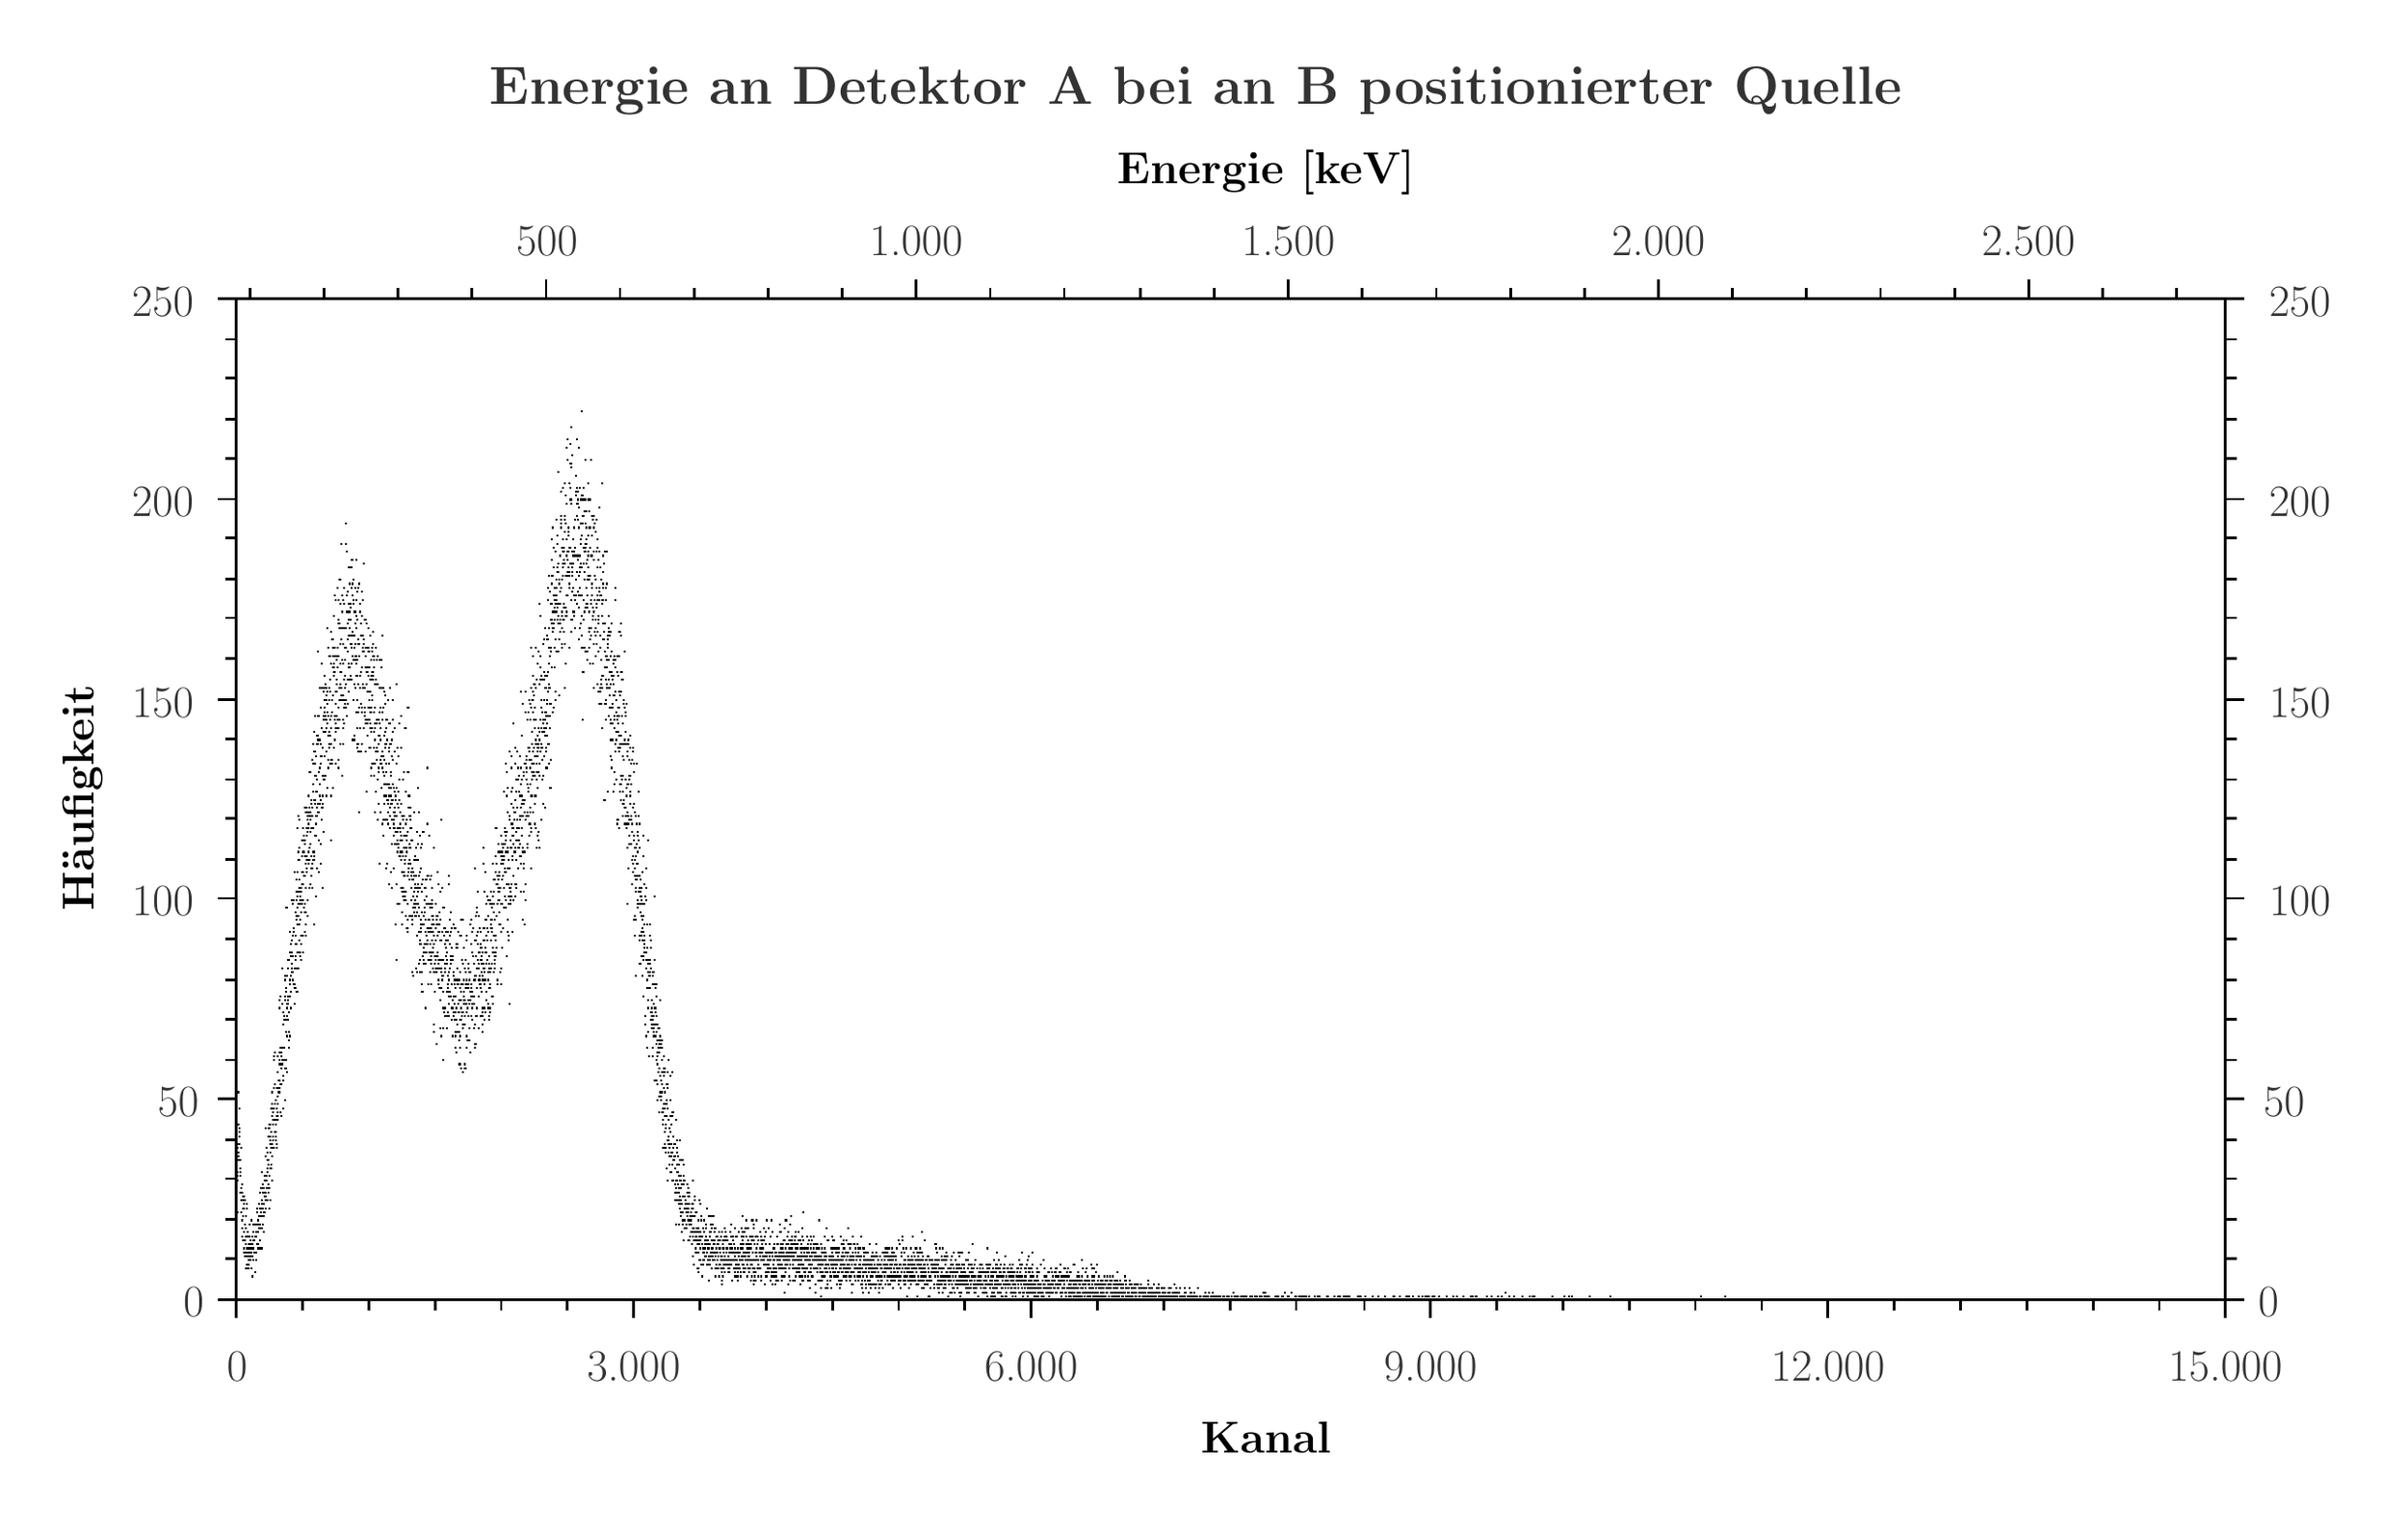
\begin{tikzpicture}{0pt}{0pt}{1209pt}{760pt}
	\clip(0pt,760pt) -- (910.15pt,760pt) -- (910.15pt,187.862pt) -- (0pt,187.862pt) -- (0pt,760pt);
\begin{scope}
	\clip(81.3037pt,654.606pt) -- (849.925pt,654.606pt) -- (849.925pt,267.661pt) -- (81.3037pt,267.661pt) -- (81.3037pt,654.606pt);
	\color[rgb]{0,0,0}
	\fill (81.355pt,301.712pt) rectangle (82.1078pt,300.959pt);
	\color[rgb]{0,0,0}
	\fill (81.4062pt,314.094pt) rectangle (82.159pt,313.341pt);
	\fill (81.4575pt,317.19pt) rectangle (82.2103pt,316.437pt);
	\fill (81.5087pt,315.642pt) rectangle (82.2615pt,314.889pt);
	\fill (81.5599pt,326.476pt) rectangle (82.3128pt,325.724pt);
	\fill (81.6112pt,328.024pt) rectangle (82.364pt,327.271pt);
	\fill (81.7137pt,321.833pt) rectangle (82.4665pt,321.08pt);
	\fill (81.7649pt,335.763pt) rectangle (82.5177pt,335.01pt);
	\fill (81.8161pt,348.145pt) rectangle (82.5689pt,347.393pt);
	\fill (81.8674pt,323.381pt) rectangle (82.6202pt,322.628pt);
	\fill (81.9186pt,324.929pt) rectangle (82.6714pt,324.176pt);
	\fill (82.0211pt,328.024pt) rectangle (82.7739pt,327.271pt);
	\fill (82.0723pt,332.667pt) rectangle (82.8251pt,331.915pt);
	\fill (82.1236pt,334.215pt) rectangle (82.8764pt,333.462pt);
	\fill (82.1748pt,341.954pt) rectangle (82.9276pt,341.201pt);
	\fill (82.226pt,331.12pt) rectangle (82.9788pt,330.367pt);
	\fill (82.3797pt,318.737pt) rectangle (83.1326pt,317.985pt);
	\fill (82.4822pt,315.642pt) rectangle (83.235pt,314.889pt);
	\fill (82.5335pt,317.19pt) rectangle (83.2863pt,316.437pt);
	\fill (82.5847pt,309.451pt) rectangle (83.3375pt,308.698pt);
	\fill (82.6359pt,321.833pt) rectangle (83.3888pt,321.08pt);
	\fill (82.6872pt,326.476pt) rectangle (83.44pt,325.724pt);
	\fill (82.7384pt,306.355pt) rectangle (83.4912pt,305.602pt);
	\fill (82.8409pt,301.712pt) rectangle (83.5937pt,300.959pt);
	\fill (82.9946pt,310.999pt) rectangle (83.7474pt,310.246pt);
	\fill (83.0971pt,292.425pt) rectangle (83.8499pt,291.672pt);
	\fill (83.1996pt,309.451pt) rectangle (83.9524pt,308.698pt);
	\fill (83.2508pt,312.546pt) rectangle (84.0036pt,311.794pt);
	\fill (83.302pt,298.616pt) rectangle (84.0548pt,297.863pt);
	\fill (83.3533pt,295.521pt) rectangle (84.1061pt,294.768pt);
	\fill (83.4045pt,306.355pt) rectangle (84.1573pt,305.602pt);
	\fill (83.4557pt,307.903pt) rectangle (84.2086pt,307.15pt);
	\fill (83.6095pt,300.164pt) rectangle (84.3623pt,299.411pt);
	\fill (83.6607pt,290.877pt) rectangle (84.4135pt,290.125pt);
	\fill (83.7632pt,303.26pt) rectangle (84.516pt,302.507pt);
	\fill (83.8144pt,304.807pt) rectangle (84.5672pt,304.055pt);
	\fill (83.8657pt,287.782pt) rectangle (84.6185pt,287.029pt);
	\fill (83.9681pt,293.973pt) rectangle (84.7209pt,293.22pt);
	\fill (84.0194pt,287.782pt) rectangle (84.7722pt,287.029pt);
	\fill (84.0706pt,307.903pt) rectangle (84.8234pt,307.15pt);
	\fill (84.1218pt,286.234pt) rectangle (84.8747pt,285.481pt);
	\fill (84.1731pt,306.355pt) rectangle (84.9259pt,305.602pt);
	\fill (84.2756pt,290.877pt) rectangle (85.0284pt,290.125pt);
	\fill (84.3268pt,284.686pt) rectangle (85.0796pt,283.933pt);
	\fill (84.378pt,297.068pt) rectangle (85.1308pt,296.316pt);
	\fill (84.583pt,292.425pt) rectangle (85.3358pt,291.672pt);
	\fill (84.6342pt,300.164pt) rectangle (85.387pt,299.411pt);
	\fill (84.6855pt,280.043pt) rectangle (85.4383pt,279.29pt);
	\fill (84.7367pt,289.33pt) rectangle (85.4895pt,288.577pt);
	\fill (84.7879pt,295.521pt) rectangle (85.5407pt,294.768pt);
	\fill (84.8904pt,304.807pt) rectangle (85.6432pt,304.055pt);
	\fill (84.9416pt,284.686pt) rectangle (85.6945pt,283.933pt);
	\fill (84.9929pt,287.782pt) rectangle (85.7457pt,287.029pt);
	\fill (85.0441pt,286.234pt) rectangle (85.7969pt,285.481pt);
	\fill (85.0954pt,281.591pt) rectangle (85.8482pt,280.838pt);
	\fill (85.1466pt,303.26pt) rectangle (85.8994pt,302.507pt);
	\fill (85.3516pt,292.425pt) rectangle (86.1044pt,291.672pt);
	\fill (85.454pt,287.782pt) rectangle (86.2068pt,287.029pt);
	\fill (85.5053pt,293.973pt) rectangle (86.2581pt,293.22pt);
	\fill (85.5565pt,280.043pt) rectangle (86.3093pt,279.29pt);
	\fill (85.6077pt,283.138pt) rectangle (86.3606pt,282.386pt);
	\fill (85.659pt,284.686pt) rectangle (86.4118pt,283.933pt);
	\fill (85.7102pt,286.234pt) rectangle (86.463pt,285.481pt);
	\fill (85.7615pt,289.33pt) rectangle (86.5143pt,288.577pt);
	\fill (85.8127pt,281.591pt) rectangle (86.5655pt,280.838pt);
	\fill (85.9664pt,292.425pt) rectangle (86.7192pt,291.672pt);
	\fill (86.1714pt,297.068pt) rectangle (86.9242pt,296.316pt);
	\fill (86.2226pt,287.782pt) rectangle (86.9754pt,287.029pt);
	\fill (86.2738pt,283.138pt) rectangle (87.0267pt,282.386pt);
	\fill (86.4276pt,284.686pt) rectangle (87.1804pt,283.933pt);
	\fill (86.4788pt,289.33pt) rectangle (87.2316pt,288.577pt);
	\fill (86.5813pt,290.877pt) rectangle (87.3341pt,290.125pt);
	\fill (86.6325pt,286.234pt) rectangle (87.3853pt,285.481pt);
	\fill (86.8887pt,298.616pt) rectangle (87.6415pt,297.863pt);
	\fill (86.9399pt,280.043pt) rectangle (87.6927pt,279.29pt);
	\fill (86.9912pt,287.782pt) rectangle (87.744pt,287.029pt);
	\fill (87.0424pt,292.425pt) rectangle (87.7952pt,291.672pt);
	\fill (87.1449pt,289.33pt) rectangle (87.8977pt,288.577pt);
	\fill (87.1961pt,284.686pt) rectangle (87.9489pt,283.933pt);
	\fill (87.2986pt,276.947pt) rectangle (88.0514pt,276.195pt);
	\fill (87.4011pt,297.068pt) rectangle (88.1539pt,296.316pt);
	\fill (87.4523pt,290.877pt) rectangle (88.2051pt,290.125pt);
	\fill (87.5036pt,283.138pt) rectangle (88.2564pt,282.386pt);
	\fill (87.606pt,293.973pt) rectangle (88.3588pt,293.22pt);
	\fill (87.7085pt,287.782pt) rectangle (88.4613pt,287.029pt);
	\fill (87.7597pt,297.068pt) rectangle (88.5126pt,296.316pt);
	\fill (87.9135pt,290.877pt) rectangle (88.6663pt,290.125pt);
	\fill (87.9647pt,286.234pt) rectangle (88.7175pt,285.481pt);
	\fill (88.1184pt,278.495pt) rectangle (88.8712pt,277.742pt);
	\fill (88.3234pt,292.425pt) rectangle (89.0762pt,291.672pt);
	\fill (88.4771pt,292.425pt) rectangle (89.2299pt,291.672pt);
	\fill (88.5283pt,286.234pt) rectangle (89.2811pt,285.481pt);
	\fill (88.5795pt,293.973pt) rectangle (89.3324pt,293.22pt);
	\fill (88.682pt,297.068pt) rectangle (89.4348pt,296.316pt);
	\fill (88.7845pt,283.138pt) rectangle (89.5373pt,282.386pt);
	\fill (88.8357pt,301.712pt) rectangle (89.5886pt,300.959pt);
	\fill (88.887pt,303.26pt) rectangle (89.6398pt,302.507pt);
	\fill (88.9895pt,289.33pt) rectangle (89.7423pt,288.577pt);
	\fill (89.1944pt,287.782pt) rectangle (89.9472pt,287.029pt);
	\fill (89.2456pt,293.973pt) rectangle (89.9985pt,293.22pt);
	\fill (89.2969pt,297.068pt) rectangle (90.0497pt,296.316pt);
	\fill (89.3481pt,298.616pt) rectangle (90.1009pt,297.863pt);
	\fill (89.3994pt,287.782pt) rectangle (90.1522pt,287.029pt);
	\fill (89.5018pt,289.33pt) rectangle (90.2546pt,288.577pt);
	\fill (89.6043pt,295.521pt) rectangle (90.3571pt,294.768pt);
	\fill (89.7068pt,300.164pt) rectangle (90.4596pt,299.411pt);
	\fill (89.8093pt,304.807pt) rectangle (90.5621pt,304.055pt);
	\fill (89.963pt,309.451pt) rectangle (90.7158pt,308.698pt);
	\fill (90.0142pt,297.068pt) rectangle (90.767pt,296.316pt);
	\fill (90.0655pt,287.782pt) rectangle (90.8183pt,287.029pt);
	\fill (90.1167pt,295.521pt) rectangle (90.8695pt,294.768pt);
	\fill (90.2192pt,290.877pt) rectangle (90.972pt,290.125pt);
	\fill (90.2704pt,303.26pt) rectangle (91.0232pt,302.507pt);
	\fill (90.3216pt,301.712pt) rectangle (91.0745pt,300.959pt);
	\fill (90.3729pt,310.999pt) rectangle (91.1257pt,310.246pt);
	\fill (90.5778pt,300.164pt) rectangle (91.3306pt,299.411pt);
	\fill (90.7315pt,306.355pt) rectangle (91.4844pt,305.602pt);
	\fill (90.7828pt,304.807pt) rectangle (91.5356pt,304.055pt);
	\fill (90.834pt,287.782pt) rectangle (91.5868pt,287.029pt);
	\fill (90.8853pt,295.521pt) rectangle (91.6381pt,294.768pt);
	\fill (90.9365pt,317.19pt) rectangle (91.6893pt,316.437pt);
	\fill (90.9877pt,310.999pt) rectangle (91.7405pt,310.246pt);
	\fill (91.039pt,297.068pt) rectangle (91.7918pt,296.316pt);
	\fill (91.0902pt,312.546pt) rectangle (91.843pt,311.794pt);
	\fill (91.1415pt,309.451pt) rectangle (91.8943pt,308.698pt);
	\fill (91.2439pt,303.26pt) rectangle (91.9967pt,302.507pt);
	\fill (91.3464pt,300.164pt) rectangle (92.0992pt,299.411pt);
	\fill (91.5001pt,300.164pt) rectangle (92.2529pt,299.411pt);
	\fill (91.5514pt,293.973pt) rectangle (92.3042pt,293.22pt);
	\fill (91.6026pt,304.807pt) rectangle (92.3554pt,304.055pt);
	\fill (91.6538pt,310.999pt) rectangle (92.4066pt,310.246pt);
	\fill (91.7051pt,301.712pt) rectangle (92.4579pt,300.959pt);
	\fill (91.7563pt,315.642pt) rectangle (92.5091pt,314.889pt);
	\fill (91.8588pt,314.094pt) rectangle (92.6116pt,313.341pt);
	\fill (91.91pt,307.903pt) rectangle (92.6628pt,307.15pt);
	\fill (91.9613pt,309.451pt) rectangle (92.7141pt,308.698pt);
	\fill (92.1662pt,303.26pt) rectangle (92.919pt,302.507pt);
	\fill (92.2174pt,334.215pt) rectangle (92.9703pt,333.462pt);
	\fill (92.2687pt,307.903pt) rectangle (93.0215pt,307.15pt);
	\fill (92.3199pt,323.381pt) rectangle (93.0727pt,322.628pt);
	\fill (92.3712pt,309.451pt) rectangle (93.124pt,308.698pt);
	\fill (92.4224pt,306.355pt) rectangle (93.1752pt,305.602pt);
	\fill (92.4736pt,326.476pt) rectangle (93.2265pt,325.724pt);
	\fill (92.5249pt,310.999pt) rectangle (93.2777pt,310.246pt);
	\fill (92.6274pt,314.094pt) rectangle (93.3802pt,313.341pt);
	\fill (92.7298pt,315.642pt) rectangle (93.4826pt,314.889pt);
	\fill (92.8835pt,324.929pt) rectangle (93.6364pt,324.176pt);
	\fill (92.9348pt,318.737pt) rectangle (93.6876pt,317.985pt);
	\fill (92.986pt,310.999pt) rectangle (93.7388pt,310.246pt);
	\fill (93.0373pt,306.355pt) rectangle (93.7901pt,305.602pt);
	\fill (93.0885pt,317.19pt) rectangle (93.8413pt,316.437pt);
	\fill (93.1397pt,321.833pt) rectangle (93.8925pt,321.08pt);
	\fill (93.2422pt,309.451pt) rectangle (93.995pt,308.698pt);
	\fill (93.2934pt,312.546pt) rectangle (94.0463pt,311.794pt);
	\fill (93.3447pt,320.285pt) rectangle (94.0975pt,319.532pt);
	\fill (93.4472pt,331.12pt) rectangle (94.2pt,330.367pt);
	\fill (93.4984pt,334.215pt) rectangle (94.2512pt,333.462pt);
	\fill (93.5496pt,303.26pt) rectangle (94.3024pt,302.507pt);
	\fill (93.7034pt,315.642pt) rectangle (94.4562pt,314.889pt);
	\fill (93.7546pt,315.642pt) rectangle (94.5074pt,314.889pt);
	\fill (93.8058pt,310.999pt) rectangle (94.5586pt,310.246pt);
	\fill (93.8571pt,335.763pt) rectangle (94.6099pt,335.01pt);
	\fill (93.9083pt,331.12pt) rectangle (94.6611pt,330.367pt);
	\fill (93.9595pt,329.572pt) rectangle (94.7124pt,328.819pt);
	\fill (94.0108pt,324.929pt) rectangle (94.7636pt,324.176pt);
	\fill (94.1133pt,328.024pt) rectangle (94.8661pt,327.271pt);
	\fill (94.1645pt,318.737pt) rectangle (94.9173pt,317.985pt);
	\fill (94.2157pt,306.355pt) rectangle (94.9685pt,305.602pt);
	\fill (94.267pt,320.285pt) rectangle (95.0198pt,319.532pt);
	\fill (94.4207pt,326.476pt) rectangle (95.1735pt,325.724pt);
	\fill (94.4719pt,341.954pt) rectangle (95.2247pt,341.201pt);
	\fill (94.5232pt,332.667pt) rectangle (95.276pt,331.915pt);
	\fill (94.5744pt,318.737pt) rectangle (95.3272pt,317.985pt);
	\fill (94.6256pt,314.094pt) rectangle (95.3784pt,313.341pt);
	\fill (94.6769pt,328.024pt) rectangle (95.4297pt,327.271pt);
	\fill (94.7281pt,338.859pt) rectangle (95.4809pt,338.106pt);
	\fill (94.7793pt,323.381pt) rectangle (95.5322pt,322.628pt);
	\fill (94.8306pt,341.954pt) rectangle (95.5834pt,341.201pt);
	\fill (94.8818pt,343.502pt) rectangle (95.6346pt,342.749pt);
	\fill (94.9331pt,348.145pt) rectangle (95.6859pt,347.393pt);
	\fill (94.9843pt,335.763pt) rectangle (95.7371pt,335.01pt);
	\fill (95.0355pt,331.12pt) rectangle (95.7884pt,330.367pt);
	\fill (95.0868pt,326.476pt) rectangle (95.8396pt,325.724pt);
	\fill (95.138pt,340.406pt) rectangle (95.8908pt,339.654pt);
	\fill (95.1893pt,337.311pt) rectangle (95.9421pt,336.558pt);
	\fill (95.2405pt,329.572pt) rectangle (95.9933pt,328.819pt);
	\fill (95.343pt,326.476pt) rectangle (96.0958pt,325.724pt);
	\fill (95.3942pt,362.075pt) rectangle (96.147pt,361.323pt);
	\fill (95.4454pt,337.311pt) rectangle (96.1983pt,336.558pt);
	\fill (95.4967pt,349.693pt) rectangle (96.2495pt,348.94pt);
	\fill (95.5479pt,360.528pt) rectangle (96.3007pt,359.775pt);
	\fill (95.6504pt,341.954pt) rectangle (96.4032pt,341.201pt);
	\fill (95.7016pt,343.502pt) rectangle (96.4544pt,342.749pt);
	\fill (95.7529pt,351.241pt) rectangle (96.5057pt,350.488pt);
	\fill (95.8041pt,332.667pt) rectangle (96.5569pt,331.915pt);
	\fill (96.0091pt,363.623pt) rectangle (96.7619pt,362.87pt);
	\fill (96.0603pt,331.12pt) rectangle (96.8131pt,330.367pt);
	\fill (96.1115pt,337.311pt) rectangle (96.8644pt,336.558pt);
	\fill (96.1628pt,332.667pt) rectangle (96.9156pt,331.915pt);
	\fill (96.214pt,345.05pt) rectangle (96.9668pt,344.297pt);
	\fill (96.2653pt,329.572pt) rectangle (97.0181pt,328.819pt);
	\fill (96.3677pt,335.763pt) rectangle (97.1205pt,335.01pt);
	\fill (96.419pt,326.476pt) rectangle (97.1718pt,325.724pt);
	\fill (96.4702pt,341.954pt) rectangle (97.223pt,341.201pt);
	\fill (96.5214pt,328.024pt) rectangle (97.2743pt,327.271pt);
	\fill (96.5727pt,338.859pt) rectangle (97.3255pt,338.106pt);
	\fill (96.6752pt,349.693pt) rectangle (97.428pt,348.94pt);
	\fill (96.7776pt,346.598pt) rectangle (97.5304pt,345.845pt);
	\fill (96.8289pt,343.502pt) rectangle (97.5817pt,342.749pt);
	\fill (96.8801pt,338.859pt) rectangle (97.6329pt,338.106pt);
	\fill (96.9313pt,337.311pt) rectangle (97.6842pt,336.558pt);
	\fill (96.9826pt,355.884pt) rectangle (97.7354pt,355.131pt);
	\fill (97.0338pt,340.406pt) rectangle (97.7866pt,339.654pt);
	\fill (97.0851pt,362.075pt) rectangle (97.8379pt,361.323pt);
	\fill (97.2388pt,348.145pt) rectangle (97.9916pt,347.393pt);
	\fill (97.4437pt,349.693pt) rectangle (98.1965pt,348.94pt);
	\fill (97.495pt,352.789pt) rectangle (98.2478pt,352.036pt);
	\fill (97.5462pt,383.744pt) rectangle (98.299pt,382.992pt);
	\fill (97.5974pt,348.145pt) rectangle (98.3503pt,347.393pt);
	\fill (97.6487pt,363.623pt) rectangle (98.4015pt,362.87pt);
	\fill (97.6999pt,349.693pt) rectangle (98.4527pt,348.94pt);
	\fill (97.7512pt,360.528pt) rectangle (98.504pt,359.775pt);
	\fill (97.8024pt,380.649pt) rectangle (98.5552pt,379.896pt);
	\fill (97.8536pt,358.98pt) rectangle (98.6064pt,358.227pt);
	\fill (97.9049pt,340.406pt) rectangle (98.6577pt,339.654pt);
	\fill (97.9561pt,385.292pt) rectangle (98.7089pt,384.539pt);
	\fill (98.0586pt,365.171pt) rectangle (98.8114pt,364.418pt);
	\fill (98.2123pt,351.241pt) rectangle (98.9651pt,350.488pt);
	\fill (98.2635pt,338.859pt) rectangle (99.0163pt,338.106pt);
	\fill (98.3148pt,363.623pt) rectangle (99.0676pt,362.87pt);
	\fill (98.4172pt,357.432pt) rectangle (99.1701pt,356.679pt);
	\fill (98.4685pt,362.075pt) rectangle (99.2213pt,361.323pt);
	\fill (98.6222pt,365.171pt) rectangle (99.375pt,364.418pt);
	\fill (98.6734pt,382.197pt) rectangle (99.4263pt,381.444pt);
	\fill (98.7247pt,358.98pt) rectangle (99.4775pt,358.227pt);
	\fill (98.8272pt,396.127pt) rectangle (99.58pt,395.374pt);
	\fill (98.9296pt,360.528pt) rectangle (99.6824pt,359.775pt);
	\fill (99.0321pt,379.101pt) rectangle (99.7849pt,378.348pt);
	\fill (99.0833pt,354.336pt) rectangle (99.8362pt,353.584pt);
	\fill (99.1346pt,352.789pt) rectangle (99.8874pt,352.036pt);
	\fill (99.1858pt,374.458pt) rectangle (99.9386pt,373.705pt);
	\fill (99.2371pt,341.954pt) rectangle (99.9899pt,341.201pt);
	\fill (99.3395pt,376.005pt) rectangle (100.092pt,375.253pt);
	\fill (99.3908pt,365.171pt) rectangle (100.144pt,364.418pt);
	\fill (99.4932pt,377.553pt) rectangle (100.246pt,376.8pt);
	\fill (99.5957pt,360.528pt) rectangle (100.349pt,359.775pt);
	\fill (99.7494pt,391.483pt) rectangle (100.502pt,390.73pt);
	\fill (99.8007pt,345.05pt) rectangle (100.553pt,344.297pt);
	\fill (99.8519pt,385.292pt) rectangle (100.605pt,384.539pt);
	\fill (99.9032pt,393.031pt) rectangle (100.656pt,392.278pt);
	\fill (99.9544pt,383.744pt) rectangle (100.707pt,382.992pt);
	\fill (100.006pt,357.432pt) rectangle (100.758pt,356.679pt);
	\fill (100.057pt,388.388pt) rectangle (100.81pt,387.635pt);
	\fill (100.108pt,376.005pt) rectangle (100.861pt,375.253pt);
	\fill (100.159pt,419.343pt) rectangle (100.912pt,418.59pt);
	\fill (100.211pt,371.362pt) rectangle (100.963pt,370.609pt);
	\fill (100.262pt,386.84pt) rectangle (101.015pt,386.087pt);
	\fill (100.313pt,360.528pt) rectangle (101.066pt,359.775pt);
	\fill (100.416pt,377.553pt) rectangle (101.168pt,376.8pt);
	\fill (100.467pt,369.814pt) rectangle (101.22pt,369.061pt);
	\fill (100.518pt,393.031pt) rectangle (101.271pt,392.278pt);
	\fill (100.569pt,355.884pt) rectangle (101.322pt,355.131pt);
	\fill (100.62pt,380.649pt) rectangle (101.373pt,379.896pt);
	\fill (100.672pt,419.343pt) rectangle (101.425pt,418.59pt);
	\fill (100.723pt,382.197pt) rectangle (101.476pt,381.444pt);
	\fill (100.774pt,399.222pt) rectangle (101.527pt,398.469pt);
	\fill (100.928pt,396.127pt) rectangle (101.681pt,395.374pt);
	\fill (100.979pt,376.005pt) rectangle (101.732pt,375.253pt);
	\fill (101.03pt,385.292pt) rectangle (101.783pt,384.539pt);
	\fill (101.082pt,383.744pt) rectangle (101.834pt,382.992pt);
	\fill (101.184pt,365.171pt) rectangle (101.937pt,364.418pt);
	\fill (101.235pt,368.266pt) rectangle (101.988pt,367.514pt);
	\fill (101.287pt,368.266pt) rectangle (102.039pt,367.514pt);
	\fill (101.338pt,379.101pt) rectangle (102.091pt,378.348pt);
	\fill (101.389pt,399.222pt) rectangle (102.142pt,398.469pt);
	\fill (101.44pt,371.362pt) rectangle (102.193pt,370.609pt);
	\fill (101.492pt,369.814pt) rectangle (102.244pt,369.061pt);
	\fill (101.543pt,385.292pt) rectangle (102.296pt,384.539pt);
	\fill (101.594pt,410.057pt) rectangle (102.347pt,409.304pt);
	\fill (101.645pt,402.318pt) rectangle (102.398pt,401.565pt);
	\fill (101.748pt,391.483pt) rectangle (102.501pt,390.73pt);
	\fill (101.799pt,389.935pt) rectangle (102.552pt,389.183pt);
	\fill (101.85pt,380.649pt) rectangle (102.603pt,379.896pt);
	\fill (101.901pt,405.413pt) rectangle (102.654pt,404.66pt);
	\fill (101.953pt,386.84pt) rectangle (102.705pt,386.087pt);
	\fill (102.004pt,400.77pt) rectangle (102.757pt,400.017pt);
	\fill (102.055pt,393.031pt) rectangle (102.808pt,392.278pt);
	\fill (102.106pt,380.649pt) rectangle (102.859pt,379.896pt);
	\fill (102.158pt,405.413pt) rectangle (102.91pt,404.66pt);
	\fill (102.209pt,422.439pt) rectangle (102.962pt,421.686pt);
	\fill (102.26pt,402.318pt) rectangle (103.013pt,401.565pt);
	\fill (102.311pt,394.579pt) rectangle (103.064pt,393.826pt);
	\fill (102.363pt,396.127pt) rectangle (103.115pt,395.374pt);
	\fill (102.465pt,406.961pt) rectangle (103.218pt,406.208pt);
	\fill (102.516pt,397.674pt) rectangle (103.269pt,396.922pt);
	\fill (102.67pt,391.483pt) rectangle (103.423pt,390.73pt);
	\fill (102.721pt,420.891pt) rectangle (103.474pt,420.138pt);
	\fill (102.772pt,394.579pt) rectangle (103.525pt,393.826pt);
	\fill (102.824pt,408.509pt) rectangle (103.577pt,407.756pt);
	\fill (102.875pt,400.77pt) rectangle (103.628pt,400.017pt);
	\fill (102.977pt,410.057pt) rectangle (103.73pt,409.304pt);
	\fill (103.029pt,422.439pt) rectangle (103.781pt,421.686pt);
	\fill (103.131pt,411.604pt) rectangle (103.884pt,410.852pt);
	\fill (103.182pt,389.935pt) rectangle (103.935pt,389.183pt);
	\fill (103.285pt,396.127pt) rectangle (104.038pt,395.374pt);
	\fill (103.336pt,388.388pt) rectangle (104.089pt,387.635pt);
	\fill (103.387pt,433.273pt) rectangle (104.14pt,432.521pt);
	\fill (103.541pt,382.197pt) rectangle (104.294pt,381.444pt);
	\fill (103.592pt,389.935pt) rectangle (104.345pt,389.183pt);
	\fill (103.644pt,396.127pt) rectangle (104.396pt,395.374pt);
	\fill (103.695pt,388.388pt) rectangle (104.448pt,387.635pt);
	\fill (103.746pt,400.77pt) rectangle (104.499pt,400.017pt);
	\fill (103.797pt,399.222pt) rectangle (104.55pt,398.469pt);
	\fill (103.848pt,417.796pt) rectangle (104.601pt,417.043pt);
	\fill (103.951pt,408.509pt) rectangle (104.704pt,407.756pt);
	\fill (104.002pt,405.413pt) rectangle (104.755pt,404.66pt);
	\fill (104.053pt,414.7pt) rectangle (104.806pt,413.947pt);
	\fill (104.105pt,416.248pt) rectangle (104.857pt,415.495pt);
	\fill (104.156pt,422.439pt) rectangle (104.909pt,421.686pt);
	\fill (104.258pt,425.534pt) rectangle (105.011pt,424.782pt);
	\fill (104.31pt,430.178pt) rectangle (105.062pt,429.425pt);
	\fill (104.361pt,386.84pt) rectangle (105.114pt,386.087pt);
	\fill (104.412pt,413.152pt) rectangle (105.165pt,412.399pt);
	\fill (104.463pt,423.987pt) rectangle (105.216pt,423.234pt);
	\fill (104.515pt,450.299pt) rectangle (105.267pt,449.546pt);
	\fill (104.566pt,433.273pt) rectangle (105.319pt,432.521pt);
	\fill (104.617pt,419.343pt) rectangle (105.37pt,418.59pt);
	\fill (104.668pt,402.318pt) rectangle (105.421pt,401.565pt);
	\fill (104.72pt,396.127pt) rectangle (105.472pt,395.374pt);
	\fill (104.771pt,441.012pt) rectangle (105.524pt,440.259pt);
	\fill (104.873pt,416.248pt) rectangle (105.626pt,415.495pt);
	\fill (104.924pt,425.534pt) rectangle (105.677pt,424.782pt);
	\fill (104.976pt,420.891pt) rectangle (105.729pt,420.138pt);
	\fill (105.027pt,454.942pt) rectangle (105.78pt,454.189pt);
	\fill (105.078pt,437.917pt) rectangle (105.831pt,437.164pt);
	\fill (105.129pt,430.178pt) rectangle (105.882pt,429.425pt);
	\fill (105.181pt,406.961pt) rectangle (105.933pt,406.208pt);
	\fill (105.232pt,413.152pt) rectangle (105.985pt,412.399pt);
	\fill (105.283pt,442.56pt) rectangle (106.036pt,441.807pt);
	\fill (105.334pt,453.395pt) rectangle (106.087pt,452.642pt);
	\fill (105.386pt,427.082pt) rectangle (106.138pt,426.329pt);
	\fill (105.437pt,402.318pt) rectangle (106.19pt,401.565pt);
	\fill (105.488pt,422.439pt) rectangle (106.241pt,421.686pt);
	\fill (105.539pt,414.7pt) rectangle (106.292pt,413.947pt);
	\fill (105.591pt,400.77pt) rectangle (106.343pt,400.017pt);
	\fill (105.693pt,420.891pt) rectangle (106.446pt,420.138pt);
	\fill (105.744pt,423.987pt) rectangle (106.497pt,423.234pt);
	\fill (105.796pt,425.534pt) rectangle (106.548pt,424.782pt);
	\fill (105.847pt,427.082pt) rectangle (106.6pt,426.329pt);
	\fill (105.898pt,405.413pt) rectangle (106.651pt,404.66pt);
	\fill (105.949pt,408.509pt) rectangle (106.702pt,407.756pt);
	\fill (106pt,422.439pt) rectangle (106.753pt,421.686pt);
	\fill (106.052pt,417.796pt) rectangle (106.805pt,417.043pt);
	\fill (106.103pt,399.222pt) rectangle (106.856pt,398.469pt);
	\fill (106.205pt,428.63pt) rectangle (106.958pt,427.877pt);
	\fill (106.257pt,439.464pt) rectangle (107.009pt,438.712pt);
	\fill (106.359pt,420.891pt) rectangle (107.112pt,420.138pt);
	\fill (106.41pt,433.273pt) rectangle (107.163pt,432.521pt);
	\fill (106.513pt,445.656pt) rectangle (107.266pt,444.903pt);
	\fill (106.564pt,433.273pt) rectangle (107.317pt,432.521pt);
	\fill (106.615pt,422.439pt) rectangle (107.368pt,421.686pt);
	\fill (106.667pt,408.509pt) rectangle (107.419pt,407.756pt);
	\fill (106.718pt,428.63pt) rectangle (107.471pt,427.877pt);
	\fill (106.769pt,402.318pt) rectangle (107.522pt,401.565pt);
	\fill (106.82pt,450.299pt) rectangle (107.573pt,449.546pt);
	\fill (106.872pt,441.012pt) rectangle (107.624pt,440.259pt);
	\fill (106.923pt,419.343pt) rectangle (107.676pt,418.59pt);
	\fill (107.128pt,447.203pt) rectangle (107.881pt,446.451pt);
	\fill (107.23pt,431.726pt) rectangle (107.983pt,430.973pt);
	\fill (107.281pt,458.038pt) rectangle (108.034pt,457.285pt);
	\fill (107.333pt,410.057pt) rectangle (108.085pt,409.304pt);
	\fill (107.384pt,444.108pt) rectangle (108.137pt,443.355pt);
	\fill (107.435pt,420.891pt) rectangle (108.188pt,420.138pt);
	\fill (107.486pt,439.464pt) rectangle (108.239pt,438.712pt);
	\fill (107.538pt,445.656pt) rectangle (108.29pt,444.903pt);
	\fill (107.589pt,417.796pt) rectangle (108.342pt,417.043pt);
	\fill (107.64pt,413.152pt) rectangle (108.393pt,412.399pt);
	\fill (107.691pt,427.082pt) rectangle (108.444pt,426.329pt);
	\fill (107.794pt,408.509pt) rectangle (108.547pt,407.756pt);
	\fill (107.896pt,436.369pt) rectangle (108.649pt,435.616pt);
	\fill (107.948pt,456.49pt) rectangle (108.7pt,455.737pt);
	\fill (107.999pt,437.917pt) rectangle (108.752pt,437.164pt);
	\fill (108.05pt,434.821pt) rectangle (108.803pt,434.068pt);
	\fill (108.101pt,439.464pt) rectangle (108.854pt,438.712pt);
	\fill (108.152pt,450.299pt) rectangle (108.905pt,449.546pt);
	\fill (108.204pt,447.203pt) rectangle (108.957pt,446.451pt);
	\fill (108.255pt,458.038pt) rectangle (109.008pt,457.285pt);
	\fill (108.306pt,433.273pt) rectangle (109.059pt,432.521pt);
	\fill (108.357pt,416.248pt) rectangle (109.11pt,415.495pt);
	\fill (108.409pt,456.49pt) rectangle (109.161pt,455.737pt);
	\fill (108.46pt,454.942pt) rectangle (109.213pt,454.189pt);
	\fill (108.562pt,448.751pt) rectangle (109.315pt,447.998pt);
	\fill (108.614pt,422.439pt) rectangle (109.366pt,421.686pt);
	\fill (108.665pt,453.395pt) rectangle (109.418pt,452.642pt);
	\fill (108.716pt,441.012pt) rectangle (109.469pt,440.259pt);
	\fill (108.767pt,437.917pt) rectangle (109.52pt,437.164pt);
	\fill (108.819pt,436.369pt) rectangle (109.571pt,435.616pt);
	\fill (108.87pt,462.681pt) rectangle (109.623pt,461.928pt);
	\fill (108.921pt,456.49pt) rectangle (109.674pt,455.737pt);
	\fill (108.972pt,451.847pt) rectangle (109.725pt,451.094pt);
	\fill (109.024pt,450.299pt) rectangle (109.776pt,449.546pt);
	\fill (109.126pt,458.038pt) rectangle (109.879pt,457.285pt);
	\fill (109.177pt,427.082pt) rectangle (109.93pt,426.329pt);
	\fill (109.228pt,454.942pt) rectangle (109.981pt,454.189pt);
	\fill (109.28pt,437.917pt) rectangle (110.033pt,437.164pt);
	\fill (109.331pt,442.56pt) rectangle (110.084pt,441.807pt);
	\fill (109.382pt,471.968pt) rectangle (110.135pt,471.215pt);
	\fill (109.433pt,428.63pt) rectangle (110.186pt,427.877pt);
	\fill (109.485pt,453.395pt) rectangle (110.237pt,452.642pt);
	\fill (109.536pt,444.108pt) rectangle (110.289pt,443.355pt);
	\fill (109.587pt,448.751pt) rectangle (110.34pt,447.998pt);
	\fill (109.638pt,471.968pt) rectangle (110.391pt,471.215pt);
	\fill (109.741pt,456.49pt) rectangle (110.494pt,455.737pt);
	\fill (109.792pt,431.726pt) rectangle (110.545pt,430.973pt);
	\fill (109.843pt,450.299pt) rectangle (110.596pt,449.546pt);
	\fill (109.895pt,434.821pt) rectangle (110.647pt,434.068pt);
	\fill (109.946pt,461.133pt) rectangle (110.699pt,460.381pt);
	\fill (109.997pt,459.586pt) rectangle (110.75pt,458.833pt);
	\fill (110.048pt,439.464pt) rectangle (110.801pt,438.712pt);
	\fill (110.1pt,454.942pt) rectangle (110.852pt,454.189pt);
	\fill (110.202pt,458.038pt) rectangle (110.955pt,457.285pt);
	\fill (110.253pt,427.082pt) rectangle (111.006pt,426.329pt);
	\fill (110.304pt,476.611pt) rectangle (111.057pt,475.858pt);
	\fill (110.356pt,434.821pt) rectangle (111.109pt,434.068pt);
	\fill (110.407pt,436.369pt) rectangle (111.16pt,435.616pt);
	\fill (110.458pt,454.942pt) rectangle (111.211pt,454.189pt);
	\fill (110.509pt,464.229pt) rectangle (111.262pt,463.476pt);
	\fill (110.561pt,450.299pt) rectangle (111.313pt,449.546pt);
	\fill (110.612pt,475.063pt) rectangle (111.365pt,474.311pt);
	\fill (110.663pt,437.917pt) rectangle (111.416pt,437.164pt);
	\fill (110.714pt,482.802pt) rectangle (111.467pt,482.05pt);
	\fill (110.766pt,467.325pt) rectangle (111.518pt,466.572pt);
	\fill (110.868pt,441.012pt) rectangle (111.621pt,440.259pt);
	\fill (110.919pt,461.133pt) rectangle (111.672pt,460.381pt);
	\fill (110.971pt,487.446pt) rectangle (111.723pt,486.693pt);
	\fill (111.073pt,413.152pt) rectangle (111.826pt,412.399pt);
	\fill (111.124pt,439.464pt) rectangle (111.877pt,438.712pt);
	\fill (111.176pt,437.917pt) rectangle (111.928pt,437.164pt);
	\fill (111.227pt,479.707pt) rectangle (111.98pt,478.954pt);
	\fill (111.278pt,447.203pt) rectangle (112.031pt,446.451pt);
	\fill (111.329pt,475.063pt) rectangle (112.082pt,474.311pt);
	\fill (111.38pt,493.637pt) rectangle (112.133pt,492.884pt);
	\fill (111.432pt,461.133pt) rectangle (112.185pt,460.381pt);
	\fill (111.483pt,459.586pt) rectangle (112.236pt,458.833pt);
	\fill (111.534pt,470.42pt) rectangle (112.287pt,469.667pt);
	\fill (111.637pt,423.987pt) rectangle (112.389pt,423.234pt);
	\fill (111.688pt,478.159pt) rectangle (112.441pt,477.406pt);
	\fill (111.739pt,451.847pt) rectangle (112.492pt,451.094pt);
	\fill (111.79pt,454.942pt) rectangle (112.543pt,454.189pt);
	\fill (111.842pt,447.203pt) rectangle (112.594pt,446.451pt);
	\fill (111.893pt,470.42pt) rectangle (112.646pt,469.667pt);
	\fill (111.944pt,464.229pt) rectangle (112.697pt,463.476pt);
	\fill (111.995pt,454.942pt) rectangle (112.748pt,454.189pt);
	\fill (112.047pt,468.872pt) rectangle (112.799pt,468.12pt);
	\fill (112.098pt,485.898pt) rectangle (112.851pt,485.145pt);
	\fill (112.2pt,458.038pt) rectangle (112.953pt,457.285pt);
	\fill (112.252pt,434.821pt) rectangle (113.004pt,434.068pt);
	\fill (112.303pt,482.802pt) rectangle (113.056pt,482.05pt);
	\fill (112.354pt,459.586pt) rectangle (113.107pt,458.833pt);
	\fill (112.405pt,456.49pt) rectangle (113.158pt,455.737pt);
	\fill (112.508pt,484.35pt) rectangle (113.261pt,483.597pt);
	\fill (112.559pt,518.401pt) rectangle (113.312pt,517.649pt);
	\fill (112.61pt,485.898pt) rectangle (113.363pt,485.145pt);
	\fill (112.661pt,493.637pt) rectangle (113.414pt,492.884pt);
	\fill (112.713pt,433.273pt) rectangle (113.465pt,432.521pt);
	\fill (112.815pt,456.49pt) rectangle (113.568pt,455.737pt);
	\fill (112.866pt,471.968pt) rectangle (113.619pt,471.215pt);
	\fill (112.918pt,445.656pt) rectangle (113.67pt,444.903pt);
	\fill (113.02pt,459.586pt) rectangle (113.773pt,458.833pt);
	\fill (113.071pt,473.516pt) rectangle (113.824pt,472.763pt);
	\fill (113.123pt,467.325pt) rectangle (113.875pt,466.572pt);
	\fill (113.174pt,484.35pt) rectangle (113.927pt,483.597pt);
	\fill (113.225pt,462.681pt) rectangle (113.978pt,461.928pt);
	\fill (113.328pt,473.516pt) rectangle (114.08pt,472.763pt);
	\fill (113.379pt,504.471pt) rectangle (114.132pt,503.719pt);
	\fill (113.43pt,475.063pt) rectangle (114.183pt,474.311pt);
	\fill (113.481pt,444.108pt) rectangle (114.234pt,443.355pt);
	\fill (113.532pt,436.369pt) rectangle (114.285pt,435.616pt);
	\fill (113.584pt,461.133pt) rectangle (114.337pt,460.381pt);
	\fill (113.635pt,482.802pt) rectangle (114.388pt,482.05pt);
	\fill (113.686pt,496.732pt) rectangle (114.439pt,495.98pt);
	\fill (113.737pt,478.159pt) rectangle (114.49pt,477.406pt);
	\fill (113.789pt,453.395pt) rectangle (114.541pt,452.642pt);
	\fill (113.942pt,513.758pt) rectangle (114.695pt,513.005pt);
	\fill (114.045pt,488.994pt) rectangle (114.798pt,488.241pt);
	\fill (114.096pt,458.038pt) rectangle (114.849pt,457.285pt);
	\fill (114.147pt,462.681pt) rectangle (114.9pt,461.928pt);
	\fill (114.199pt,427.082pt) rectangle (114.951pt,426.329pt);
	\fill (114.25pt,459.586pt) rectangle (115.003pt,458.833pt);
	\fill (114.301pt,481.255pt) rectangle (115.054pt,480.502pt);
	\fill (114.404pt,504.471pt) rectangle (115.156pt,503.719pt);
	\fill (114.455pt,470.42pt) rectangle (115.208pt,469.667pt);
	\fill (114.506pt,448.751pt) rectangle (115.259pt,447.998pt);
	\fill (114.557pt,468.872pt) rectangle (115.31pt,468.12pt);
	\fill (114.608pt,502.924pt) rectangle (115.361pt,502.171pt);
	\fill (114.66pt,492.089pt) rectangle (115.413pt,491.336pt);
	\fill (114.711pt,487.446pt) rectangle (115.464pt,486.693pt);
	\fill (114.762pt,493.637pt) rectangle (115.515pt,492.884pt);
	\fill (114.813pt,502.924pt) rectangle (115.566pt,502.171pt);
	\fill (114.865pt,499.828pt) rectangle (115.617pt,499.075pt);
	\fill (114.916pt,504.471pt) rectangle (115.669pt,503.719pt);
	\fill (114.967pt,509.115pt) rectangle (115.72pt,508.362pt);
	\fill (115.018pt,495.185pt) rectangle (115.771pt,494.432pt);
	\fill (115.07pt,478.159pt) rectangle (115.822pt,477.406pt);
	\fill (115.121pt,468.872pt) rectangle (115.874pt,468.12pt);
	\fill (115.172pt,496.732pt) rectangle (115.925pt,495.98pt);
	\fill (115.223pt,506.019pt) rectangle (115.976pt,505.266pt);
	\fill (115.275pt,493.637pt) rectangle (116.027pt,492.884pt);
	\fill (115.326pt,470.42pt) rectangle (116.079pt,469.667pt);
	\fill (115.48pt,487.446pt) rectangle (116.232pt,486.693pt);
	\fill (115.531pt,492.089pt) rectangle (116.284pt,491.336pt);
	\fill (115.582pt,492.089pt) rectangle (116.335pt,491.336pt);
	\fill (115.633pt,504.471pt) rectangle (116.386pt,503.719pt);
	\fill (115.684pt,501.376pt) rectangle (116.437pt,500.623pt);
	\fill (115.736pt,479.707pt) rectangle (116.489pt,478.954pt);
	\fill (115.787pt,488.994pt) rectangle (116.54pt,488.241pt);
	\fill (115.838pt,462.681pt) rectangle (116.591pt,461.928pt);
	\fill (115.889pt,499.828pt) rectangle (116.642pt,499.075pt);
	\fill (115.941pt,495.185pt) rectangle (116.693pt,494.432pt);
	\fill (115.992pt,502.924pt) rectangle (116.745pt,502.171pt);
	\fill (116.043pt,498.28pt) rectangle (116.796pt,497.527pt);
	\fill (116.094pt,465.777pt) rectangle (116.847pt,465.024pt);
	\fill (116.146pt,490.541pt) rectangle (116.898pt,489.788pt);
	\fill (116.248pt,527.688pt) rectangle (117.001pt,526.935pt);
	\fill (116.299pt,476.611pt) rectangle (117.052pt,475.858pt);
	\fill (116.351pt,493.637pt) rectangle (117.103pt,492.884pt);
	\fill (116.402pt,485.898pt) rectangle (117.155pt,485.145pt);
	\fill (116.453pt,473.516pt) rectangle (117.206pt,472.763pt);
	\fill (116.504pt,476.611pt) rectangle (117.257pt,475.858pt);
	\fill (116.556pt,519.949pt) rectangle (117.308pt,519.196pt);
	\fill (116.658pt,487.446pt) rectangle (117.411pt,486.693pt);
	\fill (116.709pt,504.471pt) rectangle (117.462pt,503.719pt);
	\fill (116.76pt,499.828pt) rectangle (117.513pt,499.075pt);
	\fill (116.812pt,482.802pt) rectangle (117.565pt,482.05pt);
	\fill (116.863pt,516.854pt) rectangle (117.616pt,516.101pt);
	\fill (116.914pt,481.255pt) rectangle (117.667pt,480.502pt);
	\fill (117.068pt,507.567pt) rectangle (117.821pt,506.814pt);
	\fill (117.119pt,485.898pt) rectangle (117.872pt,485.145pt);
	\fill (117.17pt,492.089pt) rectangle (117.923pt,491.336pt);
	\fill (117.222pt,502.924pt) rectangle (117.974pt,502.171pt);
	\fill (117.273pt,516.854pt) rectangle (118.026pt,516.101pt);
	\fill (117.324pt,475.063pt) rectangle (118.077pt,474.311pt);
	\fill (117.375pt,462.681pt) rectangle (118.128pt,461.928pt);
	\fill (117.427pt,482.802pt) rectangle (118.179pt,482.05pt);
	\fill (117.478pt,445.656pt) rectangle (118.231pt,444.903pt);
	\fill (117.529pt,493.637pt) rectangle (118.282pt,492.884pt);
	\fill (117.58pt,526.14pt) rectangle (118.333pt,525.387pt);
	\fill (117.632pt,488.994pt) rectangle (118.384pt,488.241pt);
	\fill (117.683pt,513.758pt) rectangle (118.436pt,513.005pt);
	\fill (117.734pt,476.611pt) rectangle (118.487pt,475.858pt);
	\fill (117.836pt,495.185pt) rectangle (118.589pt,494.432pt);
	\fill (117.888pt,499.828pt) rectangle (118.641pt,499.075pt);
	\fill (118.041pt,475.063pt) rectangle (118.794pt,474.311pt);
	\fill (118.093pt,523.045pt) rectangle (118.845pt,522.292pt);
	\fill (118.144pt,501.376pt) rectangle (118.897pt,500.623pt);
	\fill (118.195pt,516.854pt) rectangle (118.948pt,516.101pt);
	\fill (118.246pt,465.777pt) rectangle (118.999pt,465.024pt);
	\fill (118.349pt,512.21pt) rectangle (119.102pt,511.457pt);
	\fill (118.4pt,519.949pt) rectangle (119.153pt,519.196pt);
	\fill (118.503pt,509.115pt) rectangle (119.255pt,508.362pt);
	\fill (118.554pt,513.758pt) rectangle (119.307pt,513.005pt);
	\fill (118.605pt,532.331pt) rectangle (119.358pt,531.579pt);
	\fill (118.656pt,513.758pt) rectangle (119.409pt,513.005pt);
	\fill (118.708pt,512.21pt) rectangle (119.46pt,511.457pt);
	\fill (118.759pt,481.255pt) rectangle (119.512pt,480.502pt);
	\fill (118.81pt,510.662pt) rectangle (119.563pt,509.91pt);
	\fill (118.861pt,540.07pt) rectangle (119.614pt,539.318pt);
	\fill (118.912pt,492.089pt) rectangle (119.665pt,491.336pt);
	\fill (119.015pt,493.637pt) rectangle (119.768pt,492.884pt);
	\fill (119.066pt,484.35pt) rectangle (119.819pt,483.597pt);
	\fill (119.117pt,519.949pt) rectangle (119.87pt,519.196pt);
	\fill (119.169pt,516.854pt) rectangle (119.921pt,516.101pt);
	\fill (119.22pt,490.541pt) rectangle (119.973pt,489.788pt);
	\fill (119.271pt,487.446pt) rectangle (120.024pt,486.693pt);
	\fill (119.322pt,475.063pt) rectangle (120.075pt,474.311pt);
	\fill (119.374pt,538.523pt) rectangle (120.126pt,537.77pt);
	\fill (119.425pt,498.28pt) rectangle (120.178pt,497.527pt);
	\fill (119.476pt,488.994pt) rectangle (120.229pt,488.241pt);
	\fill (119.527pt,502.924pt) rectangle (120.28pt,502.171pt);
	\fill (119.579pt,507.567pt) rectangle (120.331pt,506.814pt);
	\fill (119.63pt,506.019pt) rectangle (120.383pt,505.266pt);
	\fill (119.681pt,493.637pt) rectangle (120.434pt,492.884pt);
	\fill (119.835pt,515.306pt) rectangle (120.588pt,514.553pt);
	\fill (119.937pt,492.089pt) rectangle (120.69pt,491.336pt);
	\fill (119.988pt,543.166pt) rectangle (120.741pt,542.413pt);
	\fill (120.04pt,516.854pt) rectangle (120.793pt,516.101pt);
	\fill (120.091pt,519.949pt) rectangle (120.844pt,519.196pt);
	\fill (120.142pt,512.21pt) rectangle (120.895pt,511.457pt);
	\fill (120.193pt,492.089pt) rectangle (120.946pt,491.336pt);
	\fill (120.245pt,488.994pt) rectangle (120.997pt,488.241pt);
	\fill (120.296pt,516.854pt) rectangle (121.049pt,516.101pt);
	\fill (120.347pt,530.784pt) rectangle (121.1pt,530.031pt);
	\fill (120.398pt,496.732pt) rectangle (121.151pt,495.98pt);
	\fill (120.45pt,476.611pt) rectangle (121.202pt,475.858pt);
	\fill (120.501pt,473.516pt) rectangle (121.254pt,472.763pt);
	\fill (120.552pt,538.523pt) rectangle (121.305pt,537.77pt);
	\fill (120.603pt,529.236pt) rectangle (121.356pt,528.483pt);
	\fill (120.655pt,504.471pt) rectangle (121.407pt,503.719pt);
	\fill (120.757pt,499.828pt) rectangle (121.51pt,499.075pt);
	\fill (120.808pt,527.688pt) rectangle (121.561pt,526.935pt);
	\fill (120.86pt,492.089pt) rectangle (121.612pt,491.336pt);
	\fill (120.911pt,529.236pt) rectangle (121.664pt,528.483pt);
	\fill (120.962pt,546.261pt) rectangle (121.715pt,545.509pt);
	\fill (121.013pt,506.019pt) rectangle (121.766pt,505.266pt);
	\fill (121.064pt,521.497pt) rectangle (121.817pt,520.744pt);
	\fill (121.116pt,536.975pt) rectangle (121.869pt,536.222pt);
	\fill (121.167pt,513.758pt) rectangle (121.92pt,513.005pt);
	\fill (121.218pt,482.802pt) rectangle (121.971pt,482.05pt);
	\fill (121.321pt,510.662pt) rectangle (122.073pt,509.91pt);
	\fill (121.423pt,527.688pt) rectangle (122.176pt,526.935pt);
	\fill (121.474pt,501.376pt) rectangle (122.227pt,500.623pt);
	\fill (121.526pt,499.828pt) rectangle (122.278pt,499.075pt);
	\fill (121.577pt,504.471pt) rectangle (122.33pt,503.719pt);
	\fill (121.628pt,560.192pt) rectangle (122.381pt,559.439pt);
	\fill (121.679pt,523.045pt) rectangle (122.432pt,522.292pt);
	\fill (121.731pt,499.828pt) rectangle (122.483pt,499.075pt);
	\fill (121.782pt,533.879pt) rectangle (122.535pt,533.126pt);
	\fill (121.833pt,515.306pt) rectangle (122.586pt,514.553pt);
	\fill (121.884pt,527.688pt) rectangle (122.637pt,526.935pt);
	\fill (121.936pt,470.42pt) rectangle (122.688pt,469.667pt);
	\fill (122.038pt,540.07pt) rectangle (122.791pt,539.318pt);
	\fill (122.089pt,488.994pt) rectangle (122.842pt,488.241pt);
	\fill (122.14pt,492.089pt) rectangle (122.893pt,491.336pt);
	\fill (122.192pt,513.758pt) rectangle (122.945pt,513.005pt);
	\fill (122.243pt,501.376pt) rectangle (122.996pt,500.623pt);
	\fill (122.294pt,521.497pt) rectangle (123.047pt,520.744pt);
	\fill (122.345pt,538.523pt) rectangle (123.098pt,537.77pt);
	\fill (122.397pt,482.802pt) rectangle (123.149pt,482.05pt);
	\fill (122.448pt,490.541pt) rectangle (123.201pt,489.788pt);
	\fill (122.499pt,499.828pt) rectangle (123.252pt,499.075pt);
	\fill (122.55pt,536.975pt) rectangle (123.303pt,536.222pt);
	\fill (122.602pt,496.732pt) rectangle (123.354pt,495.98pt);
	\fill (122.653pt,543.166pt) rectangle (123.406pt,542.413pt);
	\fill (122.704pt,507.567pt) rectangle (123.457pt,506.814pt);
	\fill (122.755pt,527.688pt) rectangle (123.508pt,526.935pt);
	\fill (122.807pt,498.28pt) rectangle (123.559pt,497.527pt);
	\fill (122.909pt,504.471pt) rectangle (123.662pt,503.719pt);
	\fill (123.011pt,515.306pt) rectangle (123.764pt,514.553pt);
	\fill (123.063pt,519.949pt) rectangle (123.816pt,519.196pt);
	\fill (123.114pt,509.115pt) rectangle (123.867pt,508.362pt);
	\fill (123.165pt,519.949pt) rectangle (123.918pt,519.196pt);
	\fill (123.216pt,560.192pt) rectangle (123.969pt,559.439pt);
	\fill (123.268pt,567.93pt) rectangle (124.021pt,567.178pt);
	\fill (123.319pt,527.688pt) rectangle (124.072pt,526.935pt);
	\fill (123.37pt,499.828pt) rectangle (124.123pt,499.075pt);
	\fill (123.421pt,506.019pt) rectangle (124.174pt,505.266pt);
	\fill (123.473pt,496.732pt) rectangle (124.225pt,495.98pt);
	\fill (123.524pt,540.07pt) rectangle (124.277pt,539.318pt);
	\fill (123.575pt,493.637pt) rectangle (124.328pt,492.884pt);
	\fill (123.626pt,533.879pt) rectangle (124.379pt,533.126pt);
	\fill (123.831pt,557.096pt) rectangle (124.584pt,556.343pt);
	\fill (123.883pt,541.618pt) rectangle (124.635pt,540.865pt);
	\fill (123.934pt,507.567pt) rectangle (124.687pt,506.814pt);
	\fill (123.985pt,529.236pt) rectangle (124.738pt,528.483pt);
	\fill (124.036pt,523.045pt) rectangle (124.789pt,522.292pt);
	\fill (124.087pt,498.28pt) rectangle (124.84pt,497.527pt);
	\fill (124.139pt,533.879pt) rectangle (124.892pt,533.126pt);
	\fill (124.19pt,518.401pt) rectangle (124.943pt,517.649pt);
	\fill (124.241pt,524.593pt) rectangle (124.994pt,523.84pt);
	\fill (124.292pt,550.905pt) rectangle (125.045pt,550.152pt);
	\fill (124.395pt,513.758pt) rectangle (125.148pt,513.005pt);
	\fill (124.446pt,502.924pt) rectangle (125.199pt,502.171pt);
	\fill (124.497pt,536.975pt) rectangle (125.25pt,536.222pt);
	\fill (124.549pt,530.784pt) rectangle (125.301pt,530.031pt);
	\fill (124.6pt,512.21pt) rectangle (125.353pt,511.457pt);
	\fill (124.651pt,507.567pt) rectangle (125.404pt,506.814pt);
	\fill (124.702pt,544.714pt) rectangle (125.455pt,543.961pt);
	\fill (124.754pt,550.905pt) rectangle (125.506pt,550.152pt);
	\fill (124.805pt,527.688pt) rectangle (125.558pt,526.935pt);
	\fill (124.856pt,533.879pt) rectangle (125.609pt,533.126pt);
	\fill (124.959pt,524.593pt) rectangle (125.711pt,523.84pt);
	\fill (125.01pt,509.115pt) rectangle (125.763pt,508.362pt);
	\fill (125.163pt,530.784pt) rectangle (125.916pt,530.031pt);
	\fill (125.215pt,535.427pt) rectangle (125.968pt,534.674pt);
	\fill (125.266pt,536.975pt) rectangle (126.019pt,536.222pt);
	\fill (125.317pt,521.497pt) rectangle (126.07pt,520.744pt);
	\fill (125.368pt,513.758pt) rectangle (126.121pt,513.005pt);
	\fill (125.42pt,507.567pt) rectangle (126.172pt,506.814pt);
	\fill (125.471pt,550.905pt) rectangle (126.224pt,550.152pt);
	\fill (125.522pt,519.949pt) rectangle (126.275pt,519.196pt);
	\fill (125.573pt,521.497pt) rectangle (126.326pt,520.744pt);
	\fill (125.625pt,543.166pt) rectangle (126.377pt,542.413pt);
	\fill (125.676pt,554pt) rectangle (126.429pt,553.248pt);
	\fill (125.727pt,544.714pt) rectangle (126.48pt,543.961pt);
	\fill (125.778pt,524.593pt) rectangle (126.531pt,523.84pt);
	\fill (125.881pt,540.07pt) rectangle (126.634pt,539.318pt);
	\fill (125.932pt,526.14pt) rectangle (126.685pt,525.387pt);
	\fill (125.983pt,516.854pt) rectangle (126.736pt,516.101pt);
	\fill (126.035pt,484.35pt) rectangle (126.787pt,483.597pt);
	\fill (126.137pt,536.975pt) rectangle (126.89pt,536.222pt);
	\fill (126.188pt,515.306pt) rectangle (126.941pt,514.553pt);
	\fill (126.239pt,546.261pt) rectangle (126.992pt,545.509pt);
	\fill (126.291pt,499.828pt) rectangle (127.044pt,499.075pt);
	\fill (126.342pt,538.523pt) rectangle (127.095pt,537.77pt);
	\fill (126.444pt,484.35pt) rectangle (127.197pt,483.597pt);
	\fill (126.496pt,519.949pt) rectangle (127.248pt,519.196pt);
	\fill (126.547pt,506.019pt) rectangle (127.3pt,505.266pt);
	\fill (126.598pt,485.898pt) rectangle (127.351pt,485.145pt);
	\fill (126.701pt,524.593pt) rectangle (127.453pt,523.84pt);
	\fill (126.752pt,533.879pt) rectangle (127.505pt,533.126pt);
	\fill (126.803pt,529.236pt) rectangle (127.556pt,528.483pt);
	\fill (126.854pt,521.497pt) rectangle (127.607pt,520.744pt);
	\fill (126.906pt,504.471pt) rectangle (127.658pt,503.719pt);
	\fill (126.957pt,543.166pt) rectangle (127.71pt,542.413pt);
	\fill (127.008pt,515.306pt) rectangle (127.761pt,514.553pt);
	\fill (127.111pt,516.854pt) rectangle (127.863pt,516.101pt);
	\fill (127.162pt,495.185pt) rectangle (127.915pt,494.432pt);
	\fill (127.213pt,554pt) rectangle (127.966pt,553.248pt);
	\fill (127.264pt,538.523pt) rectangle (128.017pt,537.77pt);
	\fill (127.315pt,527.688pt) rectangle (128.068pt,526.935pt);
	\fill (127.367pt,532.331pt) rectangle (128.12pt,531.579pt);
	\fill (127.418pt,513.758pt) rectangle (128.171pt,513.005pt);
	\fill (127.469pt,509.115pt) rectangle (128.222pt,508.362pt);
	\fill (127.52pt,499.828pt) rectangle (128.273pt,499.075pt);
	\fill (127.572pt,481.255pt) rectangle (128.324pt,480.502pt);
	\fill (127.623pt,488.994pt) rectangle (128.376pt,488.241pt);
	\fill (127.674pt,515.306pt) rectangle (128.427pt,514.553pt);
	\fill (127.725pt,541.618pt) rectangle (128.478pt,540.865pt);
	\fill (127.777pt,530.784pt) rectangle (128.529pt,530.031pt);
	\fill (127.828pt,482.802pt) rectangle (128.581pt,482.05pt);
	\fill (127.879pt,521.497pt) rectangle (128.632pt,520.744pt);
	\fill (127.93pt,495.185pt) rectangle (128.683pt,494.432pt);
	\fill (127.982pt,506.019pt) rectangle (128.734pt,505.266pt);
	\fill (128.033pt,523.045pt) rectangle (128.786pt,522.292pt);
	\fill (128.084pt,479.707pt) rectangle (128.837pt,478.954pt);
	\fill (128.135pt,543.166pt) rectangle (128.888pt,542.413pt);
	\fill (128.289pt,544.714pt) rectangle (129.042pt,543.961pt);
	\fill (128.34pt,516.854pt) rectangle (129.093pt,516.101pt);
	\fill (128.391pt,521.497pt) rectangle (129.144pt,520.744pt);
	\fill (128.443pt,456.49pt) rectangle (129.196pt,455.737pt);
	\fill (128.494pt,496.732pt) rectangle (129.247pt,495.98pt);
	\fill (128.545pt,479.707pt) rectangle (129.298pt,478.954pt);
	\fill (128.596pt,504.471pt) rectangle (129.349pt,503.719pt);
	\fill (128.648pt,536.975pt) rectangle (129.4pt,536.222pt);
	\fill (128.699pt,509.115pt) rectangle (129.452pt,508.362pt);
	\fill (128.853pt,488.994pt) rectangle (129.605pt,488.241pt);
	\fill (128.904pt,533.879pt) rectangle (129.657pt,533.126pt);
	\fill (128.955pt,498.28pt) rectangle (129.708pt,497.527pt);
	\fill (129.058pt,524.593pt) rectangle (129.81pt,523.84pt);
	\fill (129.109pt,529.236pt) rectangle (129.862pt,528.483pt);
	\fill (129.16pt,510.662pt) rectangle (129.913pt,509.91pt);
	\fill (129.211pt,479.707pt) rectangle (129.964pt,478.954pt);
	\fill (129.263pt,524.593pt) rectangle (130.015pt,523.84pt);
	\fill (129.314pt,482.802pt) rectangle (130.067pt,482.05pt);
	\fill (129.365pt,532.331pt) rectangle (130.118pt,531.579pt);
	\fill (129.416pt,496.732pt) rectangle (130.169pt,495.98pt);
	\fill (129.467pt,541.618pt) rectangle (130.22pt,540.865pt);
	\fill (129.519pt,495.185pt) rectangle (130.272pt,494.432pt);
	\fill (129.57pt,512.21pt) rectangle (130.323pt,511.457pt);
	\fill (129.672pt,518.401pt) rectangle (130.425pt,517.649pt);
	\fill (129.724pt,506.019pt) rectangle (130.476pt,505.266pt);
	\fill (129.775pt,504.471pt) rectangle (130.528pt,503.719pt);
	\fill (129.826pt,538.523pt) rectangle (130.579pt,537.77pt);
	\fill (129.877pt,504.471pt) rectangle (130.63pt,503.719pt);
	\fill (129.929pt,524.593pt) rectangle (130.681pt,523.84pt);
	\fill (129.98pt,519.949pt) rectangle (130.733pt,519.196pt);
	\fill (130.031pt,518.401pt) rectangle (130.784pt,517.649pt);
	\fill (130.185pt,552.453pt) rectangle (130.938pt,551.7pt);
	\fill (130.236pt,523.045pt) rectangle (130.989pt,522.292pt);
	\fill (130.287pt,521.497pt) rectangle (131.04pt,520.744pt);
	\fill (130.339pt,488.994pt) rectangle (131.091pt,488.241pt);
	\fill (130.39pt,496.732pt) rectangle (131.143pt,495.98pt);
	\fill (130.441pt,530.784pt) rectangle (131.194pt,530.031pt);
	\fill (130.492pt,493.637pt) rectangle (131.245pt,492.884pt);
	\fill (130.646pt,495.185pt) rectangle (131.399pt,494.432pt);
	\fill (130.697pt,504.471pt) rectangle (131.45pt,503.719pt);
	\fill (130.748pt,490.541pt) rectangle (131.501pt,489.788pt);
	\fill (130.8pt,516.854pt) rectangle (131.552pt,516.101pt);
	\fill (130.851pt,519.949pt) rectangle (131.604pt,519.196pt);
	\fill (130.902pt,479.707pt) rectangle (131.655pt,478.954pt);
	\fill (130.953pt,512.21pt) rectangle (131.706pt,511.457pt);
	\fill (131.005pt,530.784pt) rectangle (131.757pt,530.031pt);
	\fill (131.056pt,492.089pt) rectangle (131.809pt,491.336pt);
	\fill (131.107pt,529.236pt) rectangle (131.86pt,528.483pt);
	\fill (131.158pt,510.662pt) rectangle (131.911pt,509.91pt);
	\fill (131.21pt,464.229pt) rectangle (131.962pt,463.476pt);
	\fill (131.415pt,506.019pt) rectangle (132.167pt,505.266pt);
	\fill (131.466pt,490.541pt) rectangle (132.219pt,489.788pt);
	\fill (131.517pt,510.662pt) rectangle (132.27pt,509.91pt);
	\fill (131.568pt,492.089pt) rectangle (132.321pt,491.336pt);
	\fill (131.619pt,519.949pt) rectangle (132.372pt,519.196pt);
	\fill (131.671pt,512.21pt) rectangle (132.424pt,511.457pt);
	\fill (131.722pt,485.898pt) rectangle (132.475pt,485.145pt);
	\fill (131.824pt,502.924pt) rectangle (132.577pt,502.171pt);
	\fill (131.876pt,518.401pt) rectangle (132.628pt,517.649pt);
	\fill (131.927pt,509.115pt) rectangle (132.68pt,508.362pt);
	\fill (131.978pt,496.732pt) rectangle (132.731pt,495.98pt);
	\fill (132.081pt,527.688pt) rectangle (132.833pt,526.935pt);
	\fill (132.132pt,519.949pt) rectangle (132.885pt,519.196pt);
	\fill (132.183pt,496.732pt) rectangle (132.936pt,495.98pt);
	\fill (132.234pt,512.21pt) rectangle (132.987pt,511.457pt);
	\fill (132.337pt,518.401pt) rectangle (133.09pt,517.649pt);
	\fill (132.439pt,499.828pt) rectangle (133.192pt,499.075pt);
	\fill (132.491pt,492.089pt) rectangle (133.243pt,491.336pt);
	\fill (132.542pt,481.255pt) rectangle (133.295pt,480.502pt);
	\fill (132.593pt,524.593pt) rectangle (133.346pt,523.84pt);
	\fill (132.644pt,507.567pt) rectangle (133.397pt,506.814pt);
	\fill (132.747pt,488.994pt) rectangle (133.5pt,488.241pt);
	\fill (132.798pt,502.924pt) rectangle (133.551pt,502.171pt);
	\fill (132.849pt,490.541pt) rectangle (133.602pt,489.788pt);
	\fill (132.9pt,495.185pt) rectangle (133.653pt,494.432pt);
	\fill (132.952pt,470.42pt) rectangle (133.704pt,469.667pt);
	\fill (133.003pt,507.567pt) rectangle (133.756pt,506.814pt);
	\fill (133.054pt,515.306pt) rectangle (133.807pt,514.553pt);
	\fill (133.105pt,487.446pt) rectangle (133.858pt,486.693pt);
	\fill (133.157pt,496.732pt) rectangle (133.909pt,495.98pt);
	\fill (133.208pt,473.516pt) rectangle (133.961pt,472.763pt);
	\fill (133.259pt,509.115pt) rectangle (134.012pt,508.362pt);
	\fill (133.31pt,501.376pt) rectangle (134.063pt,500.623pt);
	\fill (133.362pt,519.949pt) rectangle (134.114pt,519.196pt);
	\fill (133.413pt,518.401pt) rectangle (134.166pt,517.649pt);
	\fill (133.464pt,499.828pt) rectangle (134.217pt,499.075pt);
	\fill (133.515pt,488.994pt) rectangle (134.268pt,488.241pt);
	\fill (133.567pt,510.662pt) rectangle (134.319pt,509.91pt);
	\fill (133.618pt,475.063pt) rectangle (134.371pt,474.311pt);
	\fill (133.669pt,510.662pt) rectangle (134.422pt,509.91pt);
	\fill (133.72pt,509.115pt) rectangle (134.473pt,508.362pt);
	\fill (133.771pt,507.567pt) rectangle (134.524pt,506.814pt);
	\fill (133.823pt,521.497pt) rectangle (134.576pt,520.744pt);
	\fill (133.874pt,526.14pt) rectangle (134.627pt,525.387pt);
	\fill (133.976pt,516.854pt) rectangle (134.729pt,516.101pt);
	\fill (134.028pt,512.21pt) rectangle (134.78pt,511.457pt);
	\fill (134.079pt,515.306pt) rectangle (134.832pt,514.553pt);
	\fill (134.13pt,495.185pt) rectangle (134.883pt,494.432pt);
	\fill (134.181pt,487.446pt) rectangle (134.934pt,486.693pt);
	\fill (134.233pt,470.42pt) rectangle (134.985pt,469.667pt);
	\fill (134.284pt,481.255pt) rectangle (135.037pt,480.502pt);
	\fill (134.335pt,475.063pt) rectangle (135.088pt,474.311pt);
	\fill (134.386pt,484.35pt) rectangle (135.139pt,483.597pt);
	\fill (134.438pt,496.732pt) rectangle (135.19pt,495.98pt);
	\fill (134.489pt,490.541pt) rectangle (135.242pt,489.788pt);
	\fill (134.54pt,456.49pt) rectangle (135.293pt,455.737pt);
	\fill (134.643pt,488.994pt) rectangle (135.395pt,488.241pt);
	\fill (134.694pt,506.019pt) rectangle (135.447pt,505.266pt);
	\fill (134.745pt,464.229pt) rectangle (135.498pt,463.476pt);
	\fill (134.796pt,479.707pt) rectangle (135.549pt,478.954pt);
	\fill (134.847pt,519.949pt) rectangle (135.6pt,519.196pt);
	\fill (135.001pt,507.567pt) rectangle (135.754pt,506.814pt);
	\fill (135.104pt,515.306pt) rectangle (135.856pt,514.553pt);
	\fill (135.155pt,481.255pt) rectangle (135.908pt,480.502pt);
	\fill (135.206pt,490.541pt) rectangle (135.959pt,489.788pt);
	\fill (135.309pt,492.089pt) rectangle (136.061pt,491.336pt);
	\fill (135.36pt,476.611pt) rectangle (136.113pt,475.858pt);
	\fill (135.462pt,479.707pt) rectangle (136.215pt,478.954pt);
	\fill (135.514pt,453.395pt) rectangle (136.266pt,452.642pt);
	\fill (135.616pt,516.854pt) rectangle (136.369pt,516.101pt);
	\fill (135.667pt,506.019pt) rectangle (136.42pt,505.266pt);
	\fill (135.719pt,468.872pt) rectangle (136.471pt,468.12pt);
	\fill (135.821pt,471.968pt) rectangle (136.574pt,471.215pt);
	\fill (135.872pt,485.898pt) rectangle (136.625pt,485.145pt);
	\fill (135.923pt,473.516pt) rectangle (136.676pt,472.763pt);
	\fill (136.026pt,459.586pt) rectangle (136.779pt,458.833pt);
	\fill (136.077pt,482.802pt) rectangle (136.83pt,482.05pt);
	\fill (136.128pt,492.089pt) rectangle (136.881pt,491.336pt);
	\fill (136.18pt,490.541pt) rectangle (136.932pt,489.788pt);
	\fill (136.231pt,485.898pt) rectangle (136.984pt,485.145pt);
	\fill (136.282pt,436.369pt) rectangle (137.035pt,435.616pt);
	\fill (136.333pt,515.306pt) rectangle (137.086pt,514.553pt);
	\fill (136.385pt,504.471pt) rectangle (137.137pt,503.719pt);
	\fill (136.487pt,495.185pt) rectangle (137.24pt,494.432pt);
	\fill (136.538pt,475.063pt) rectangle (137.291pt,474.311pt);
	\fill (136.641pt,476.611pt) rectangle (137.394pt,475.858pt);
	\fill (136.692pt,456.49pt) rectangle (137.445pt,455.737pt);
	\fill (136.743pt,484.35pt) rectangle (137.496pt,483.597pt);
	\fill (136.795pt,496.732pt) rectangle (137.547pt,495.98pt);
	\fill (136.846pt,488.994pt) rectangle (137.599pt,488.241pt);
	\fill (136.897pt,475.063pt) rectangle (137.65pt,474.311pt);
	\fill (136.948pt,515.306pt) rectangle (137.701pt,514.553pt);
	\fill (136.999pt,478.159pt) rectangle (137.752pt,477.406pt);
	\fill (137.051pt,512.21pt) rectangle (137.804pt,511.457pt);
	\fill (137.102pt,504.471pt) rectangle (137.855pt,503.719pt);
	\fill (137.153pt,465.777pt) rectangle (137.906pt,465.024pt);
	\fill (137.256pt,495.185pt) rectangle (138.008pt,494.432pt);
	\fill (137.307pt,524.593pt) rectangle (138.06pt,523.84pt);
	\fill (137.409pt,492.089pt) rectangle (138.162pt,491.336pt);
	\fill (137.461pt,451.847pt) rectangle (138.213pt,451.094pt);
	\fill (137.512pt,479.707pt) rectangle (138.265pt,478.954pt);
	\fill (137.563pt,473.516pt) rectangle (138.316pt,472.763pt);
	\fill (137.614pt,504.471pt) rectangle (138.367pt,503.719pt);
	\fill (137.666pt,478.159pt) rectangle (138.418pt,477.406pt);
	\fill (137.717pt,453.395pt) rectangle (138.47pt,452.642pt);
	\fill (137.768pt,447.203pt) rectangle (138.521pt,446.451pt);
	\fill (137.819pt,471.968pt) rectangle (138.572pt,471.215pt);
	\fill (137.871pt,496.732pt) rectangle (138.623pt,495.98pt);
	\fill (137.973pt,476.611pt) rectangle (138.726pt,475.858pt);
	\fill (138.024pt,470.42pt) rectangle (138.777pt,469.667pt);
	\fill (138.075pt,502.924pt) rectangle (138.828pt,502.171pt);
	\fill (138.127pt,459.586pt) rectangle (138.88pt,458.833pt);
	\fill (138.178pt,462.681pt) rectangle (138.931pt,461.928pt);
	\fill (138.229pt,476.611pt) rectangle (138.982pt,475.858pt);
	\fill (138.28pt,485.898pt) rectangle (139.033pt,485.145pt);
	\fill (138.332pt,467.325pt) rectangle (139.084pt,466.572pt);
	\fill (138.383pt,481.255pt) rectangle (139.136pt,480.502pt);
	\fill (138.434pt,453.395pt) rectangle (139.187pt,452.642pt);
	\fill (138.537pt,501.376pt) rectangle (139.289pt,500.623pt);
	\fill (138.588pt,498.28pt) rectangle (139.341pt,497.527pt);
	\fill (138.639pt,487.446pt) rectangle (139.392pt,486.693pt);
	\fill (138.69pt,482.802pt) rectangle (139.443pt,482.05pt);
	\fill (138.742pt,488.994pt) rectangle (139.494pt,488.241pt);
	\fill (138.793pt,475.063pt) rectangle (139.546pt,474.311pt);
	\fill (138.895pt,434.821pt) rectangle (139.648pt,434.068pt);
	\fill (138.947pt,462.681pt) rectangle (139.699pt,461.928pt);
	\fill (138.998pt,471.968pt) rectangle (139.751pt,471.215pt);
	\fill (139.049pt,492.089pt) rectangle (139.802pt,491.336pt);
	\fill (139.1pt,484.35pt) rectangle (139.853pt,483.597pt);
	\fill (139.151pt,436.369pt) rectangle (139.904pt,435.616pt);
	\fill (139.254pt,467.325pt) rectangle (140.007pt,466.572pt);
	\fill (139.305pt,453.395pt) rectangle (140.058pt,452.642pt);
	\fill (139.408pt,461.133pt) rectangle (140.16pt,460.381pt);
	\fill (139.459pt,499.828pt) rectangle (140.212pt,499.075pt);
	\fill (139.51pt,459.586pt) rectangle (140.263pt,458.833pt);
	\fill (139.664pt,451.847pt) rectangle (140.417pt,451.094pt);
	\fill (139.715pt,456.49pt) rectangle (140.468pt,455.737pt);
	\fill (139.766pt,467.325pt) rectangle (140.519pt,466.572pt);
	\fill (139.818pt,465.777pt) rectangle (140.57pt,465.024pt);
	\fill (139.869pt,428.63pt) rectangle (140.622pt,427.877pt);
	\fill (139.92pt,475.063pt) rectangle (140.673pt,474.311pt);
	\fill (139.971pt,481.255pt) rectangle (140.724pt,480.502pt);
	\fill (140.023pt,479.707pt) rectangle (140.775pt,478.954pt);
	\fill (140.074pt,462.681pt) rectangle (140.827pt,461.928pt);
	\fill (140.125pt,490.541pt) rectangle (140.878pt,489.788pt);
	\fill (140.176pt,458.038pt) rectangle (140.929pt,457.285pt);
	\fill (140.227pt,454.942pt) rectangle (140.98pt,454.189pt);
	\fill (140.279pt,504.471pt) rectangle (141.032pt,503.719pt);
	\fill (140.432pt,450.299pt) rectangle (141.185pt,449.546pt);
	\fill (140.484pt,482.802pt) rectangle (141.236pt,482.05pt);
	\fill (140.535pt,462.681pt) rectangle (141.288pt,461.928pt);
	\fill (140.586pt,433.273pt) rectangle (141.339pt,432.521pt);
	\fill (140.637pt,471.968pt) rectangle (141.39pt,471.215pt);
	\fill (140.74pt,470.42pt) rectangle (141.493pt,469.667pt);
	\fill (140.791pt,465.777pt) rectangle (141.544pt,465.024pt);
	\fill (140.842pt,459.586pt) rectangle (141.595pt,458.833pt);
	\fill (140.894pt,453.395pt) rectangle (141.646pt,452.642pt);
	\fill (140.996pt,484.35pt) rectangle (141.749pt,483.597pt);
	\fill (141.047pt,478.159pt) rectangle (141.8pt,477.406pt);
	\fill (141.099pt,427.082pt) rectangle (141.851pt,426.329pt);
	\fill (141.15pt,444.108pt) rectangle (141.903pt,443.355pt);
	\fill (141.201pt,461.133pt) rectangle (141.954pt,460.381pt);
	\fill (141.252pt,467.325pt) rectangle (142.005pt,466.572pt);
	\fill (141.303pt,487.446pt) rectangle (142.056pt,486.693pt);
	\fill (141.355pt,476.611pt) rectangle (142.108pt,475.858pt);
	\fill (141.406pt,499.828pt) rectangle (142.159pt,499.075pt);
	\fill (141.457pt,492.089pt) rectangle (142.21pt,491.336pt);
	\fill (141.56pt,453.395pt) rectangle (142.312pt,452.642pt);
	\fill (141.662pt,447.203pt) rectangle (142.415pt,446.451pt);
	\fill (141.713pt,465.777pt) rectangle (142.466pt,465.024pt);
	\fill (141.765pt,456.49pt) rectangle (142.517pt,455.737pt);
	\fill (141.816pt,451.847pt) rectangle (142.569pt,451.094pt);
	\fill (141.867pt,434.821pt) rectangle (142.62pt,434.068pt);
	\fill (141.918pt,450.299pt) rectangle (142.671pt,449.546pt);
	\fill (141.97pt,464.229pt) rectangle (142.722pt,463.476pt);
	\fill (142.021pt,479.707pt) rectangle (142.774pt,478.954pt);
	\fill (142.072pt,488.994pt) rectangle (142.825pt,488.241pt);
	\fill (142.123pt,458.038pt) rectangle (142.876pt,457.285pt);
	\fill (142.175pt,456.49pt) rectangle (142.927pt,455.737pt);
	\fill (142.226pt,444.108pt) rectangle (142.979pt,443.355pt);
	\fill (142.277pt,454.942pt) rectangle (143.03pt,454.189pt);
	\fill (142.328pt,462.681pt) rectangle (143.081pt,461.928pt);
	\fill (142.482pt,448.751pt) rectangle (143.235pt,447.998pt);
	\fill (142.533pt,413.152pt) rectangle (143.286pt,412.399pt);
	\fill (142.584pt,461.133pt) rectangle (143.337pt,460.381pt);
	\fill (142.687pt,444.108pt) rectangle (143.44pt,443.355pt);
	\fill (142.738pt,475.063pt) rectangle (143.491pt,474.311pt);
	\fill (142.789pt,465.777pt) rectangle (143.542pt,465.024pt);
	\fill (142.841pt,428.63pt) rectangle (143.593pt,427.877pt);
	\fill (142.892pt,506.019pt) rectangle (143.645pt,505.266pt);
	\fill (142.943pt,399.222pt) rectangle (143.696pt,398.469pt);
	\fill (142.994pt,454.942pt) rectangle (143.747pt,454.189pt);
	\fill (143.046pt,441.012pt) rectangle (143.798pt,440.259pt);
	\fill (143.097pt,448.751pt) rectangle (143.85pt,447.998pt);
	\fill (143.148pt,445.656pt) rectangle (143.901pt,444.903pt);
	\fill (143.199pt,481.255pt) rectangle (143.952pt,480.502pt);
	\fill (143.251pt,420.891pt) rectangle (144.003pt,420.138pt);
	\fill (143.302pt,459.586pt) rectangle (144.055pt,458.833pt);
	\fill (143.353pt,450.299pt) rectangle (144.106pt,449.546pt);
	\fill (143.404pt,458.038pt) rectangle (144.157pt,457.285pt);
	\fill (143.455pt,464.229pt) rectangle (144.208pt,463.476pt);
	\fill (143.507pt,444.108pt) rectangle (144.26pt,443.355pt);
	\fill (143.558pt,442.56pt) rectangle (144.311pt,441.807pt);
	\fill (143.609pt,458.038pt) rectangle (144.362pt,457.285pt);
	\fill (143.66pt,450.299pt) rectangle (144.413pt,449.546pt);
	\fill (143.712pt,478.159pt) rectangle (144.464pt,477.406pt);
	\fill (143.763pt,420.891pt) rectangle (144.516pt,420.138pt);
	\fill (143.814pt,439.464pt) rectangle (144.567pt,438.712pt);
	\fill (143.917pt,461.133pt) rectangle (144.669pt,460.381pt);
	\fill (143.968pt,490.541pt) rectangle (144.721pt,489.788pt);
	\fill (144.07pt,468.872pt) rectangle (144.823pt,468.12pt);
	\fill (144.122pt,441.012pt) rectangle (144.874pt,440.259pt);
	\fill (144.173pt,450.299pt) rectangle (144.926pt,449.546pt);
	\fill (144.224pt,448.751pt) rectangle (144.977pt,447.998pt);
	\fill (144.275pt,445.656pt) rectangle (145.028pt,444.903pt);
	\fill (144.327pt,439.464pt) rectangle (145.079pt,438.712pt);
	\fill (144.378pt,456.49pt) rectangle (145.131pt,455.737pt);
	\fill (144.429pt,451.847pt) rectangle (145.182pt,451.094pt);
	\fill (144.48pt,427.082pt) rectangle (145.233pt,426.329pt);
	\fill (144.531pt,493.637pt) rectangle (145.284pt,492.884pt);
	\fill (144.583pt,459.586pt) rectangle (145.336pt,458.833pt);
	\fill (144.634pt,447.203pt) rectangle (145.387pt,446.451pt);
	\fill (144.685pt,481.255pt) rectangle (145.438pt,480.502pt);
	\fill (144.788pt,437.917pt) rectangle (145.54pt,437.164pt);
	\fill (144.839pt,413.152pt) rectangle (145.592pt,412.399pt);
	\fill (144.89pt,433.273pt) rectangle (145.643pt,432.521pt);
	\fill (144.941pt,417.796pt) rectangle (145.694pt,417.043pt);
	\fill (144.993pt,441.012pt) rectangle (145.745pt,440.259pt);
	\fill (145.044pt,454.942pt) rectangle (145.797pt,454.189pt);
	\fill (145.095pt,445.656pt) rectangle (145.848pt,444.903pt);
	\fill (145.146pt,425.534pt) rectangle (145.899pt,424.782pt);
	\fill (145.198pt,450.299pt) rectangle (145.95pt,449.546pt);
	\fill (145.249pt,427.082pt) rectangle (146.002pt,426.329pt);
	\fill (145.3pt,423.987pt) rectangle (146.053pt,423.234pt);
	\fill (145.351pt,468.872pt) rectangle (146.104pt,468.12pt);
	\fill (145.403pt,439.464pt) rectangle (146.155pt,438.712pt);
	\fill (145.505pt,453.395pt) rectangle (146.258pt,452.642pt);
	\fill (145.556pt,433.273pt) rectangle (146.309pt,432.521pt);
	\fill (145.607pt,422.439pt) rectangle (146.36pt,421.686pt);
	\fill (145.659pt,431.726pt) rectangle (146.412pt,430.973pt);
	\fill (145.71pt,454.942pt) rectangle (146.463pt,454.189pt);
	\fill (145.761pt,471.968pt) rectangle (146.514pt,471.215pt);
	\fill (145.812pt,442.56pt) rectangle (146.565pt,441.807pt);
	\fill (145.864pt,425.534pt) rectangle (146.616pt,424.782pt);
	\fill (145.915pt,447.203pt) rectangle (146.668pt,446.451pt);
	\fill (146.017pt,437.917pt) rectangle (146.77pt,437.164pt);
	\fill (146.069pt,423.987pt) rectangle (146.821pt,423.234pt);
	\fill (146.12pt,436.369pt) rectangle (146.873pt,435.616pt);
	\fill (146.222pt,431.726pt) rectangle (146.975pt,430.973pt);
	\fill (146.274pt,488.994pt) rectangle (147.026pt,488.241pt);
	\fill (146.325pt,416.248pt) rectangle (147.078pt,415.495pt);
	\fill (146.376pt,464.229pt) rectangle (147.129pt,463.476pt);
	\fill (146.427pt,425.534pt) rectangle (147.18pt,424.782pt);
	\fill (146.479pt,422.439pt) rectangle (147.231pt,421.686pt);
	\fill (146.53pt,439.464pt) rectangle (147.283pt,438.712pt);
	\fill (146.581pt,451.847pt) rectangle (147.334pt,451.094pt);
	\fill (146.632pt,442.56pt) rectangle (147.385pt,441.807pt);
	\fill (146.683pt,441.012pt) rectangle (147.436pt,440.259pt);
	\fill (146.837pt,447.203pt) rectangle (147.59pt,446.451pt);
	\fill (146.888pt,453.395pt) rectangle (147.641pt,452.642pt);
	\fill (146.94pt,445.656pt) rectangle (147.692pt,444.903pt);
	\fill (146.991pt,411.604pt) rectangle (147.744pt,410.852pt);
	\fill (147.042pt,448.751pt) rectangle (147.795pt,447.998pt);
	\fill (147.093pt,420.891pt) rectangle (147.846pt,420.138pt);
	\fill (147.145pt,471.968pt) rectangle (147.897pt,471.215pt);
	\fill (147.196pt,414.7pt) rectangle (147.949pt,413.947pt);
	\fill (147.247pt,410.057pt) rectangle (148pt,409.304pt);
	\fill (147.298pt,431.726pt) rectangle (148.051pt,430.973pt);
	\fill (147.35pt,496.732pt) rectangle (148.102pt,495.98pt);
	\fill (147.401pt,471.968pt) rectangle (148.154pt,471.215pt);
	\fill (147.452pt,433.273pt) rectangle (148.205pt,432.521pt);
	\fill (147.555pt,458.038pt) rectangle (148.307pt,457.285pt);
	\fill (147.606pt,434.821pt) rectangle (148.359pt,434.068pt);
	\fill (147.657pt,436.369pt) rectangle (148.41pt,435.616pt);
	\fill (147.708pt,462.681pt) rectangle (148.461pt,461.928pt);
	\fill (147.759pt,437.917pt) rectangle (148.512pt,437.164pt);
	\fill (147.811pt,454.942pt) rectangle (148.564pt,454.189pt);
	\fill (147.913pt,416.248pt) rectangle (148.666pt,415.495pt);
	\fill (147.964pt,430.178pt) rectangle (148.717pt,429.425pt);
	\fill (148.016pt,444.108pt) rectangle (148.768pt,443.355pt);
	\fill (148.067pt,442.56pt) rectangle (148.82pt,441.807pt);
	\fill (148.118pt,453.395pt) rectangle (148.871pt,452.642pt);
	\fill (148.221pt,454.942pt) rectangle (148.973pt,454.189pt);
	\fill (148.272pt,436.369pt) rectangle (149.025pt,435.616pt);
	\fill (148.323pt,450.299pt) rectangle (149.076pt,449.546pt);
	\fill (148.374pt,458.038pt) rectangle (149.127pt,457.285pt);
	\fill (148.477pt,433.273pt) rectangle (149.23pt,432.521pt);
	\fill (148.528pt,427.082pt) rectangle (149.281pt,426.329pt);
	\fill (148.579pt,431.726pt) rectangle (149.332pt,430.973pt);
	\fill (148.631pt,416.248pt) rectangle (149.383pt,415.495pt);
	\fill (148.682pt,422.439pt) rectangle (149.435pt,421.686pt);
	\fill (148.733pt,450.299pt) rectangle (149.486pt,449.546pt);
	\fill (148.784pt,445.656pt) rectangle (149.537pt,444.903pt);
	\fill (148.835pt,413.152pt) rectangle (149.588pt,412.399pt);
	\fill (148.887pt,414.7pt) rectangle (149.64pt,413.947pt);
	\fill (148.938pt,430.178pt) rectangle (149.691pt,429.425pt);
	\fill (148.989pt,416.248pt) rectangle (149.742pt,415.495pt);
	\fill (149.04pt,434.821pt) rectangle (149.793pt,434.068pt);
	\fill (149.092pt,394.579pt) rectangle (149.844pt,393.826pt);
	\fill (149.143pt,433.273pt) rectangle (149.896pt,432.521pt);
	\fill (149.297pt,393.031pt) rectangle (150.049pt,392.278pt);
	\fill (149.399pt,419.343pt) rectangle (150.152pt,418.59pt);
	\fill (149.45pt,430.178pt) rectangle (150.203pt,429.425pt);
	\fill (149.502pt,423.987pt) rectangle (150.254pt,423.234pt);
	\fill (149.553pt,456.49pt) rectangle (150.306pt,455.737pt);
	\fill (149.604pt,425.534pt) rectangle (150.357pt,424.782pt);
	\fill (149.655pt,437.917pt) rectangle (150.408pt,437.164pt);
	\fill (149.707pt,417.796pt) rectangle (150.459pt,417.043pt);
	\fill (149.758pt,431.726pt) rectangle (150.511pt,430.973pt);
	\fill (149.809pt,420.891pt) rectangle (150.562pt,420.138pt);
	\fill (149.911pt,419.343pt) rectangle (150.664pt,418.59pt);
	\fill (149.963pt,439.464pt) rectangle (150.716pt,438.712pt);
	\fill (150.014pt,422.439pt) rectangle (150.767pt,421.686pt);
	\fill (150.065pt,427.082pt) rectangle (150.818pt,426.329pt);
	\fill (150.116pt,416.248pt) rectangle (150.869pt,415.495pt);
	\fill (150.168pt,428.63pt) rectangle (150.92pt,427.877pt);
	\fill (150.219pt,422.439pt) rectangle (150.972pt,421.686pt);
	\fill (150.27pt,416.248pt) rectangle (151.023pt,415.495pt);
	\fill (150.321pt,427.082pt) rectangle (151.074pt,426.329pt);
	\fill (150.373pt,420.891pt) rectangle (151.125pt,420.138pt);
	\fill (150.424pt,437.917pt) rectangle (151.177pt,437.164pt);
	\fill (150.475pt,442.56pt) rectangle (151.228pt,441.807pt);
	\fill (150.526pt,431.726pt) rectangle (151.279pt,430.973pt);
	\fill (150.578pt,396.127pt) rectangle (151.33pt,395.374pt);
	\fill (150.68pt,417.796pt) rectangle (151.433pt,417.043pt);
	\fill (150.731pt,423.987pt) rectangle (151.484pt,423.234pt);
	\fill (150.783pt,394.579pt) rectangle (151.535pt,393.826pt);
	\fill (150.834pt,408.509pt) rectangle (151.587pt,407.756pt);
	\fill (150.885pt,448.751pt) rectangle (151.638pt,447.998pt);
	\fill (150.987pt,427.082pt) rectangle (151.74pt,426.329pt);
	\fill (151.039pt,428.63pt) rectangle (151.792pt,427.877pt);
	\fill (151.09pt,437.917pt) rectangle (151.843pt,437.164pt);
	\fill (151.141pt,425.534pt) rectangle (151.894pt,424.782pt);
	\fill (151.192pt,420.891pt) rectangle (151.945pt,420.138pt);
	\fill (151.244pt,444.108pt) rectangle (151.996pt,443.355pt);
	\fill (151.295pt,465.777pt) rectangle (152.048pt,465.024pt);
	\fill (151.346pt,410.057pt) rectangle (152.099pt,409.304pt);
	\fill (151.397pt,456.49pt) rectangle (152.15pt,455.737pt);
	\fill (151.449pt,397.674pt) rectangle (152.201pt,396.922pt);
	\fill (151.5pt,419.343pt) rectangle (152.253pt,418.59pt);
	\fill (151.551pt,416.248pt) rectangle (152.304pt,415.495pt);
	\fill (151.654pt,431.726pt) rectangle (152.406pt,430.973pt);
	\fill (151.705pt,406.961pt) rectangle (152.458pt,406.208pt);
	\fill (151.756pt,427.082pt) rectangle (152.509pt,426.329pt);
	\fill (151.807pt,399.222pt) rectangle (152.56pt,398.469pt);
	\fill (151.859pt,433.273pt) rectangle (152.611pt,432.521pt);
	\fill (151.961pt,394.579pt) rectangle (152.714pt,393.826pt);
	\fill (152.012pt,447.203pt) rectangle (152.765pt,446.451pt);
	\fill (152.063pt,405.413pt) rectangle (152.816pt,404.66pt);
	\fill (152.115pt,442.56pt) rectangle (152.868pt,441.807pt);
	\fill (152.166pt,414.7pt) rectangle (152.919pt,413.947pt);
	\fill (152.217pt,434.821pt) rectangle (152.97pt,434.068pt);
	\fill (152.32pt,411.604pt) rectangle (153.072pt,410.852pt);
	\fill (152.371pt,410.057pt) rectangle (153.124pt,409.304pt);
	\fill (152.422pt,413.152pt) rectangle (153.175pt,412.399pt);
	\fill (152.473pt,389.935pt) rectangle (153.226pt,389.183pt);
	\fill (152.525pt,444.108pt) rectangle (153.277pt,443.355pt);
	\fill (152.576pt,394.579pt) rectangle (153.329pt,393.826pt);
	\fill (152.627pt,417.796pt) rectangle (153.38pt,417.043pt);
	\fill (152.678pt,425.534pt) rectangle (153.431pt,424.782pt);
	\fill (152.73pt,428.63pt) rectangle (153.482pt,427.877pt);
	\fill (152.781pt,386.84pt) rectangle (153.534pt,386.087pt);
	\fill (152.832pt,430.178pt) rectangle (153.585pt,429.425pt);
	\fill (153.088pt,400.77pt) rectangle (153.841pt,400.017pt);
	\fill (153.139pt,448.751pt) rectangle (153.892pt,447.998pt);
	\fill (153.191pt,416.248pt) rectangle (153.944pt,415.495pt);
	\fill (153.242pt,397.674pt) rectangle (153.995pt,396.922pt);
	\fill (153.293pt,416.248pt) rectangle (154.046pt,415.495pt);
	\fill (153.344pt,403.865pt) rectangle (154.097pt,403.113pt);
	\fill (153.396pt,399.222pt) rectangle (154.148pt,398.469pt);
	\fill (153.447pt,413.152pt) rectangle (154.2pt,412.399pt);
	\fill (153.498pt,402.318pt) rectangle (154.251pt,401.565pt);
	\fill (153.601pt,422.439pt) rectangle (154.353pt,421.686pt);
	\fill (153.652pt,405.413pt) rectangle (154.405pt,404.66pt);
	\fill (153.703pt,419.343pt) rectangle (154.456pt,418.59pt);
	\fill (153.754pt,417.796pt) rectangle (154.507pt,417.043pt);
	\fill (153.857pt,427.082pt) rectangle (154.61pt,426.329pt);
	\fill (153.908pt,414.7pt) rectangle (154.661pt,413.947pt);
	\fill (153.959pt,397.674pt) rectangle (154.712pt,396.922pt);
	\fill (154.011pt,410.057pt) rectangle (154.763pt,409.304pt);
	\fill (154.062pt,427.082pt) rectangle (154.815pt,426.329pt);
	\fill (154.113pt,380.649pt) rectangle (154.866pt,379.896pt);
	\fill (154.164pt,414.7pt) rectangle (154.917pt,413.947pt);
	\fill (154.215pt,430.178pt) rectangle (154.968pt,429.425pt);
	\fill (154.267pt,405.413pt) rectangle (155.02pt,404.66pt);
	\fill (154.318pt,402.318pt) rectangle (155.071pt,401.565pt);
	\fill (154.369pt,420.891pt) rectangle (155.122pt,420.138pt);
	\fill (154.472pt,408.509pt) rectangle (155.224pt,407.756pt);
	\fill (154.523pt,423.987pt) rectangle (155.276pt,423.234pt);
	\fill (154.625pt,431.726pt) rectangle (155.378pt,430.973pt);
	\fill (154.677pt,451.847pt) rectangle (155.429pt,451.094pt);
	\fill (154.728pt,473.516pt) rectangle (155.481pt,472.763pt);
	\fill (154.779pt,406.961pt) rectangle (155.532pt,406.208pt);
	\fill (154.83pt,420.891pt) rectangle (155.583pt,420.138pt);
	\fill (154.882pt,405.413pt) rectangle (155.634pt,404.66pt);
	\fill (154.933pt,411.604pt) rectangle (155.686pt,410.852pt);
	\fill (154.984pt,399.222pt) rectangle (155.737pt,398.469pt);
	\fill (155.035pt,414.7pt) rectangle (155.788pt,413.947pt);
	\fill (155.087pt,431.726pt) rectangle (155.839pt,430.973pt);
	\fill (155.189pt,389.935pt) rectangle (155.942pt,389.183pt);
	\fill (155.291pt,410.057pt) rectangle (156.044pt,409.304pt);
	\fill (155.394pt,447.203pt) rectangle (156.147pt,446.451pt);
	\fill (155.445pt,402.318pt) rectangle (156.198pt,401.565pt);
	\fill (155.496pt,414.7pt) rectangle (156.249pt,413.947pt);
	\fill (155.599pt,399.222pt) rectangle (156.352pt,398.469pt);
	\fill (155.65pt,420.891pt) rectangle (156.403pt,420.138pt);
	\fill (155.701pt,405.413pt) rectangle (156.454pt,404.66pt);
	\fill (155.753pt,430.178pt) rectangle (156.505pt,429.425pt);
	\fill (155.804pt,394.579pt) rectangle (156.557pt,393.826pt);
	\fill (155.958pt,419.343pt) rectangle (156.71pt,418.59pt);
	\fill (156.009pt,411.604pt) rectangle (156.762pt,410.852pt);
	\fill (156.06pt,410.057pt) rectangle (156.813pt,409.304pt);
	\fill (156.111pt,389.935pt) rectangle (156.864pt,389.183pt);
	\fill (156.162pt,402.318pt) rectangle (156.915pt,401.565pt);
	\fill (156.214pt,397.674pt) rectangle (156.967pt,396.922pt);
	\fill (156.265pt,400.77pt) rectangle (157.018pt,400.017pt);
	\fill (156.316pt,431.726pt) rectangle (157.069pt,430.973pt);
	\fill (156.367pt,399.222pt) rectangle (157.12pt,398.469pt);
	\fill (156.419pt,406.961pt) rectangle (157.172pt,406.208pt);
	\fill (156.47pt,422.439pt) rectangle (157.223pt,421.686pt);
	\fill (156.521pt,416.248pt) rectangle (157.274pt,415.495pt);
	\fill (156.572pt,413.152pt) rectangle (157.325pt,412.399pt);
	\fill (156.624pt,427.082pt) rectangle (157.376pt,426.329pt);
	\fill (156.675pt,419.343pt) rectangle (157.428pt,418.59pt);
	\fill (156.726pt,420.891pt) rectangle (157.479pt,420.138pt);
	\fill (156.829pt,396.127pt) rectangle (157.581pt,395.374pt);
	\fill (156.88pt,403.865pt) rectangle (157.633pt,403.113pt);
	\fill (156.931pt,414.7pt) rectangle (157.684pt,413.947pt);
	\fill (156.982pt,410.057pt) rectangle (157.735pt,409.304pt);
	\fill (157.034pt,416.248pt) rectangle (157.786pt,415.495pt);
	\fill (157.085pt,402.318pt) rectangle (157.838pt,401.565pt);
	\fill (157.136pt,413.152pt) rectangle (157.889pt,412.399pt);
	\fill (157.187pt,371.362pt) rectangle (157.94pt,370.609pt);
	\fill (157.238pt,442.56pt) rectangle (157.991pt,441.807pt);
	\fill (157.29pt,408.509pt) rectangle (158.043pt,407.756pt);
	\fill (157.341pt,405.413pt) rectangle (158.094pt,404.66pt);
	\fill (157.392pt,374.458pt) rectangle (158.145pt,373.705pt);
	\fill (157.443pt,394.579pt) rectangle (158.196pt,393.826pt);
	\fill (157.546pt,400.77pt) rectangle (158.299pt,400.017pt);
	\fill (157.751pt,397.674pt) rectangle (158.504pt,396.922pt);
	\fill (157.802pt,386.84pt) rectangle (158.555pt,386.087pt);
	\fill (157.853pt,420.891pt) rectangle (158.606pt,420.138pt);
	\fill (157.905pt,396.127pt) rectangle (158.657pt,395.374pt);
	\fill (157.956pt,411.604pt) rectangle (158.709pt,410.852pt);
	\fill (158.007pt,406.961pt) rectangle (158.76pt,406.208pt);
	\fill (158.058pt,394.579pt) rectangle (158.811pt,393.826pt);
	\fill (158.161pt,399.222pt) rectangle (158.914pt,398.469pt);
	\fill (158.212pt,416.248pt) rectangle (158.965pt,415.495pt);
	\fill (158.314pt,413.152pt) rectangle (159.067pt,412.399pt);
	\fill (158.366pt,400.77pt) rectangle (159.119pt,400.017pt);
	\fill (158.417pt,366.719pt) rectangle (159.17pt,365.966pt);
	\fill (158.468pt,414.7pt) rectangle (159.221pt,413.947pt);
	\fill (158.519pt,394.579pt) rectangle (159.272pt,393.826pt);
	\fill (158.571pt,413.152pt) rectangle (159.323pt,412.399pt);
	\fill (158.622pt,402.318pt) rectangle (159.375pt,401.565pt);
	\fill (158.673pt,396.127pt) rectangle (159.426pt,395.374pt);
	\fill (158.724pt,416.248pt) rectangle (159.477pt,415.495pt);
	\fill (158.776pt,400.77pt) rectangle (159.528pt,400.017pt);
	\fill (158.827pt,433.273pt) rectangle (159.58pt,432.521pt);
	\fill (158.878pt,408.509pt) rectangle (159.631pt,407.756pt);
	\fill (158.929pt,391.483pt) rectangle (159.682pt,390.73pt);
	\fill (159.083pt,399.222pt) rectangle (159.836pt,398.469pt);
	\fill (159.134pt,428.63pt) rectangle (159.887pt,427.877pt);
	\fill (159.186pt,397.674pt) rectangle (159.938pt,396.922pt);
	\fill (159.237pt,389.935pt) rectangle (159.99pt,389.183pt);
	\fill (159.288pt,410.057pt) rectangle (160.041pt,409.304pt);
	\fill (159.339pt,417.796pt) rectangle (160.092pt,417.043pt);
	\fill (159.39pt,388.388pt) rectangle (160.143pt,387.635pt);
	\fill (159.442pt,413.152pt) rectangle (160.195pt,412.399pt);
	\fill (159.493pt,399.222pt) rectangle (160.246pt,398.469pt);
	\fill (159.595pt,396.127pt) rectangle (160.348pt,395.374pt);
	\fill (159.698pt,414.7pt) rectangle (160.451pt,413.947pt);
	\fill (159.749pt,425.534pt) rectangle (160.502pt,424.782pt);
	\fill (159.8pt,372.91pt) rectangle (160.553pt,372.157pt);
	\fill (159.903pt,383.744pt) rectangle (160.656pt,382.992pt);
	\fill (159.954pt,406.961pt) rectangle (160.707pt,406.208pt);
	\fill (160.005pt,388.388pt) rectangle (160.758pt,387.635pt);
	\fill (160.057pt,369.814pt) rectangle (160.809pt,369.061pt);
	\fill (160.108pt,394.579pt) rectangle (160.861pt,393.826pt);
	\fill (160.159pt,396.127pt) rectangle (160.912pt,395.374pt);
	\fill (160.21pt,399.222pt) rectangle (160.963pt,398.469pt);
	\fill (160.262pt,453.395pt) rectangle (161.014pt,452.642pt);
	\fill (160.313pt,406.961pt) rectangle (161.066pt,406.208pt);
	\fill (160.415pt,410.057pt) rectangle (161.168pt,409.304pt);
	\fill (160.518pt,393.031pt) rectangle (161.271pt,392.278pt);
	\fill (160.569pt,391.483pt) rectangle (161.322pt,390.73pt);
	\fill (160.671pt,427.082pt) rectangle (161.424pt,426.329pt);
	\fill (160.774pt,386.84pt) rectangle (161.527pt,386.087pt);
	\fill (160.825pt,380.649pt) rectangle (161.578pt,379.896pt);
	\fill (160.876pt,393.031pt) rectangle (161.629pt,392.278pt);
	\fill (160.928pt,372.91pt) rectangle (161.68pt,372.157pt);
	\fill (160.979pt,399.222pt) rectangle (161.732pt,398.469pt);
	\fill (161.03pt,360.528pt) rectangle (161.783pt,359.775pt);
	\fill (161.081pt,419.343pt) rectangle (161.834pt,418.59pt);
	\fill (161.235pt,408.509pt) rectangle (161.988pt,407.756pt);
	\fill (161.389pt,379.101pt) rectangle (162.142pt,378.348pt);
	\fill (161.44pt,411.604pt) rectangle (162.193pt,410.852pt);
	\fill (161.491pt,394.579pt) rectangle (162.244pt,393.826pt);
	\fill (161.542pt,396.127pt) rectangle (162.295pt,395.374pt);
	\fill (161.645pt,405.413pt) rectangle (162.398pt,404.66pt);
	\fill (161.696pt,380.649pt) rectangle (162.449pt,379.896pt);
	\fill (161.747pt,397.674pt) rectangle (162.5pt,396.922pt);
	\fill (161.799pt,377.553pt) rectangle (162.551pt,376.8pt);
	\fill (162.004pt,400.77pt) rectangle (162.756pt,400.017pt);
	\fill (162.055pt,410.057pt) rectangle (162.808pt,409.304pt);
	\fill (162.106pt,403.865pt) rectangle (162.859pt,403.113pt);
	\fill (162.157pt,406.961pt) rectangle (162.91pt,406.208pt);
	\fill (162.26pt,402.318pt) rectangle (163.013pt,401.565pt);
	\fill (162.311pt,372.91pt) rectangle (163.064pt,372.157pt);
	\fill (162.362pt,397.674pt) rectangle (163.115pt,396.922pt);
	\fill (162.414pt,399.222pt) rectangle (163.166pt,398.469pt);
	\fill (162.516pt,386.84pt) rectangle (163.269pt,386.087pt);
	\fill (162.567pt,393.031pt) rectangle (163.32pt,392.278pt);
	\fill (162.618pt,406.961pt) rectangle (163.371pt,406.208pt);
	\fill (162.67pt,379.101pt) rectangle (163.423pt,378.348pt);
	\fill (162.721pt,388.388pt) rectangle (163.474pt,387.635pt);
	\fill (162.772pt,410.057pt) rectangle (163.525pt,409.304pt);
	\fill (162.823pt,389.935pt) rectangle (163.576pt,389.183pt);
	\fill (162.875pt,377.553pt) rectangle (163.627pt,376.8pt);
	\fill (162.926pt,382.197pt) rectangle (163.679pt,381.444pt);
	\fill (162.977pt,394.579pt) rectangle (163.73pt,393.826pt);
	\fill (163.028pt,385.292pt) rectangle (163.781pt,384.539pt);
	\fill (163.08pt,394.579pt) rectangle (163.832pt,393.826pt);
	\fill (163.131pt,391.483pt) rectangle (163.884pt,390.73pt);
	\fill (163.182pt,428.63pt) rectangle (163.935pt,427.877pt);
	\fill (163.233pt,431.726pt) rectangle (163.986pt,430.973pt);
	\fill (163.285pt,414.7pt) rectangle (164.037pt,413.947pt);
	\fill (163.336pt,396.127pt) rectangle (164.089pt,395.374pt);
	\fill (163.387pt,386.84pt) rectangle (164.14pt,386.087pt);
	\fill (163.438pt,408.509pt) rectangle (164.191pt,407.756pt);
	\fill (163.592pt,405.413pt) rectangle (164.345pt,404.66pt);
	\fill (163.694pt,400.77pt) rectangle (164.447pt,400.017pt);
	\fill (163.746pt,399.222pt) rectangle (164.499pt,398.469pt);
	\fill (163.797pt,417.796pt) rectangle (164.55pt,417.043pt);
	\fill (163.848pt,385.292pt) rectangle (164.601pt,384.539pt);
	\fill (163.899pt,410.057pt) rectangle (164.652pt,409.304pt);
	\fill (163.951pt,397.674pt) rectangle (164.703pt,396.922pt);
	\fill (164.002pt,411.604pt) rectangle (164.755pt,410.852pt);
	\fill (164.104pt,389.935pt) rectangle (164.857pt,389.183pt);
	\fill (164.207pt,380.649pt) rectangle (164.96pt,379.896pt);
	\fill (164.258pt,403.865pt) rectangle (165.011pt,403.113pt);
	\fill (164.309pt,376.005pt) rectangle (165.062pt,375.253pt);
	\fill (164.361pt,400.77pt) rectangle (165.113pt,400.017pt);
	\fill (164.412pt,383.744pt) rectangle (165.165pt,382.992pt);
	\fill (164.514pt,399.222pt) rectangle (165.267pt,398.469pt);
	\fill (164.566pt,380.649pt) rectangle (165.318pt,379.896pt);
	\fill (164.668pt,369.814pt) rectangle (165.421pt,369.061pt);
	\fill (164.719pt,385.292pt) rectangle (165.472pt,384.539pt);
	\fill (164.77pt,377.553pt) rectangle (165.523pt,376.8pt);
	\fill (164.822pt,379.101pt) rectangle (165.575pt,378.348pt);
	\fill (164.873pt,394.579pt) rectangle (165.626pt,393.826pt);
	\fill (164.924pt,393.031pt) rectangle (165.677pt,392.278pt);
	\fill (164.975pt,413.152pt) rectangle (165.728pt,412.399pt);
	\fill (165.129pt,376.005pt) rectangle (165.882pt,375.253pt);
	\fill (165.232pt,411.604pt) rectangle (165.984pt,410.852pt);
	\fill (165.283pt,389.935pt) rectangle (166.036pt,389.183pt);
	\fill (165.334pt,391.483pt) rectangle (166.087pt,390.73pt);
	\fill (165.385pt,382.197pt) rectangle (166.138pt,381.444pt);
	\fill (165.437pt,371.362pt) rectangle (166.189pt,370.609pt);
	\fill (165.488pt,388.388pt) rectangle (166.241pt,387.635pt);
	\fill (165.539pt,369.814pt) rectangle (166.292pt,369.061pt);
	\fill (165.59pt,365.171pt) rectangle (166.343pt,364.418pt);
	\fill (165.642pt,411.604pt) rectangle (166.394pt,410.852pt);
	\fill (165.693pt,379.101pt) rectangle (166.446pt,378.348pt);
	\fill (165.744pt,385.292pt) rectangle (166.497pt,384.539pt);
	\fill (165.846pt,380.649pt) rectangle (166.599pt,379.896pt);
	\fill (165.898pt,403.865pt) rectangle (166.651pt,403.113pt);
	\fill (165.949pt,376.005pt) rectangle (166.702pt,375.253pt);
	\fill (166pt,363.623pt) rectangle (166.753pt,362.87pt);
	\fill (166.051pt,376.005pt) rectangle (166.804pt,375.253pt);
	\fill (166.103pt,391.483pt) rectangle (166.855pt,390.73pt);
	\fill (166.154pt,405.413pt) rectangle (166.907pt,404.66pt);
	\fill (166.205pt,403.865pt) rectangle (166.958pt,403.113pt);
	\fill (166.256pt,371.362pt) rectangle (167.009pt,370.609pt);
	\fill (166.308pt,396.127pt) rectangle (167.06pt,395.374pt);
	\fill (166.41pt,374.458pt) rectangle (167.163pt,373.705pt);
	\fill (166.513pt,389.935pt) rectangle (167.265pt,389.183pt);
	\fill (166.615pt,382.197pt) rectangle (167.368pt,381.444pt);
	\fill (166.666pt,379.101pt) rectangle (167.419pt,378.348pt);
	\fill (166.769pt,410.057pt) rectangle (167.522pt,409.304pt);
	\fill (166.82pt,389.935pt) rectangle (167.573pt,389.183pt);
	\fill (166.871pt,391.483pt) rectangle (167.624pt,390.73pt);
	\fill (166.974pt,379.101pt) rectangle (167.727pt,378.348pt);
	\fill (167.025pt,368.266pt) rectangle (167.778pt,367.514pt);
	\fill (167.127pt,371.362pt) rectangle (167.88pt,370.609pt);
	\fill (167.179pt,383.744pt) rectangle (167.931pt,382.992pt);
	\fill (167.23pt,358.98pt) rectangle (167.983pt,358.227pt);
	\fill (167.281pt,376.005pt) rectangle (168.034pt,375.253pt);
	\fill (167.384pt,369.814pt) rectangle (168.136pt,369.061pt);
	\fill (167.435pt,388.388pt) rectangle (168.188pt,387.635pt);
	\fill (167.486pt,365.171pt) rectangle (168.239pt,364.418pt);
	\fill (167.537pt,394.579pt) rectangle (168.29pt,393.826pt);
	\fill (167.589pt,408.509pt) rectangle (168.341pt,407.756pt);
	\fill (167.64pt,386.84pt) rectangle (168.393pt,386.087pt);
	\fill (167.691pt,380.649pt) rectangle (168.444pt,379.896pt);
	\fill (167.742pt,357.432pt) rectangle (168.495pt,356.679pt);
	\fill (167.794pt,376.005pt) rectangle (168.546pt,375.253pt);
	\fill (167.845pt,389.935pt) rectangle (168.598pt,389.183pt);
	\fill (167.896pt,383.744pt) rectangle (168.649pt,382.992pt);
	\fill (167.947pt,414.7pt) rectangle (168.7pt,413.947pt);
	\fill (168.05pt,379.101pt) rectangle (168.803pt,378.348pt);
	\fill (168.101pt,377.553pt) rectangle (168.854pt,376.8pt);
	\fill (168.255pt,399.222pt) rectangle (169.007pt,398.469pt);
	\fill (168.306pt,379.101pt) rectangle (169.059pt,378.348pt);
	\fill (168.357pt,355.884pt) rectangle (169.11pt,355.131pt);
	\fill (168.408pt,374.458pt) rectangle (169.161pt,373.705pt);
	\fill (168.46pt,389.935pt) rectangle (169.212pt,389.183pt);
	\fill (168.511pt,414.7pt) rectangle (169.264pt,413.947pt);
	\fill (168.562pt,397.674pt) rectangle (169.315pt,396.922pt);
	\fill (168.613pt,372.91pt) rectangle (169.366pt,372.157pt);
	\fill (168.716pt,403.865pt) rectangle (169.469pt,403.113pt);
	\fill (168.767pt,391.483pt) rectangle (169.52pt,390.73pt);
	\fill (168.818pt,385.292pt) rectangle (169.571pt,384.539pt);
	\fill (168.87pt,383.744pt) rectangle (169.622pt,382.992pt);
	\fill (168.921pt,386.84pt) rectangle (169.674pt,386.087pt);
	\fill (169.023pt,382.197pt) rectangle (169.776pt,381.444pt);
	\fill (169.074pt,358.98pt) rectangle (169.827pt,358.227pt);
	\fill (169.126pt,374.458pt) rectangle (169.879pt,373.705pt);
	\fill (169.177pt,383.744pt) rectangle (169.93pt,382.992pt);
	\fill (169.228pt,396.127pt) rectangle (169.981pt,395.374pt);
	\fill (169.279pt,377.553pt) rectangle (170.032pt,376.8pt);
	\fill (169.382pt,357.432pt) rectangle (170.135pt,356.679pt);
	\fill (169.433pt,394.579pt) rectangle (170.186pt,393.826pt);
	\fill (169.484pt,399.222pt) rectangle (170.237pt,398.469pt);
	\fill (169.587pt,389.935pt) rectangle (170.34pt,389.183pt);
	\fill (169.741pt,388.388pt) rectangle (170.493pt,387.635pt);
	\fill (169.792pt,406.961pt) rectangle (170.545pt,406.208pt);
	\fill (169.843pt,379.101pt) rectangle (170.596pt,378.348pt);
	\fill (169.894pt,391.483pt) rectangle (170.647pt,390.73pt);
	\fill (169.946pt,369.814pt) rectangle (170.698pt,369.061pt);
	\fill (169.997pt,365.171pt) rectangle (170.75pt,364.418pt);
	\fill (170.048pt,408.509pt) rectangle (170.801pt,407.756pt);
	\fill (170.099pt,382.197pt) rectangle (170.852pt,381.444pt);
	\fill (170.202pt,389.935pt) rectangle (170.955pt,389.183pt);
	\fill (170.253pt,380.649pt) rectangle (171.006pt,379.896pt);
	\fill (170.355pt,368.266pt) rectangle (171.108pt,367.514pt);
	\fill (170.509pt,383.744pt) rectangle (171.262pt,382.992pt);
	\fill (170.56pt,389.935pt) rectangle (171.313pt,389.183pt);
	\fill (170.612pt,388.388pt) rectangle (171.364pt,387.635pt);
	\fill (170.663pt,377.553pt) rectangle (171.416pt,376.8pt);
	\fill (170.714pt,397.674pt) rectangle (171.467pt,396.922pt);
	\fill (170.765pt,396.127pt) rectangle (171.518pt,395.374pt);
	\fill (170.919pt,372.91pt) rectangle (171.672pt,372.157pt);
	\fill (170.97pt,391.483pt) rectangle (171.723pt,390.73pt);
	\fill (171.073pt,382.197pt) rectangle (171.826pt,381.444pt);
	\fill (171.124pt,394.579pt) rectangle (171.877pt,393.826pt);
	\fill (171.175pt,368.266pt) rectangle (171.928pt,367.514pt);
	\fill (171.226pt,383.744pt) rectangle (171.979pt,382.992pt);
	\fill (171.278pt,363.623pt) rectangle (172.031pt,362.87pt);
	\fill (171.329pt,386.84pt) rectangle (172.082pt,386.087pt);
	\fill (171.431pt,413.152pt) rectangle (172.184pt,412.399pt);
	\fill (171.534pt,394.579pt) rectangle (172.287pt,393.826pt);
	\fill (171.636pt,405.413pt) rectangle (172.389pt,404.66pt);
	\fill (171.688pt,389.935pt) rectangle (172.44pt,389.183pt);
	\fill (171.739pt,377.553pt) rectangle (172.492pt,376.8pt);
	\fill (171.79pt,388.388pt) rectangle (172.543pt,387.635pt);
	\fill (171.841pt,385.292pt) rectangle (172.594pt,384.539pt);
	\fill (171.893pt,414.7pt) rectangle (172.645pt,413.947pt);
	\fill (171.995pt,380.649pt) rectangle (172.748pt,379.896pt);
	\fill (172.046pt,382.197pt) rectangle (172.799pt,381.444pt);
	\fill (172.098pt,376.005pt) rectangle (172.85pt,375.253pt);
	\fill (172.149pt,410.057pt) rectangle (172.902pt,409.304pt);
	\fill (172.2pt,402.318pt) rectangle (172.953pt,401.565pt);
	\fill (172.251pt,386.84pt) rectangle (173.004pt,386.087pt);
	\fill (172.302pt,411.604pt) rectangle (173.055pt,410.852pt);
	\fill (172.405pt,400.77pt) rectangle (173.158pt,400.017pt);
	\fill (172.456pt,385.292pt) rectangle (173.209pt,384.539pt);
	\fill (172.661pt,397.674pt) rectangle (173.414pt,396.922pt);
	\fill (172.815pt,382.197pt) rectangle (173.568pt,381.444pt);
	\fill (172.866pt,385.292pt) rectangle (173.619pt,384.539pt);
	\fill (172.917pt,372.91pt) rectangle (173.67pt,372.157pt);
	\fill (172.969pt,397.674pt) rectangle (173.721pt,396.922pt);
	\fill (173.02pt,391.483pt) rectangle (173.773pt,390.73pt);
	\fill (173.071pt,434.821pt) rectangle (173.824pt,434.068pt);
	\fill (173.122pt,374.458pt) rectangle (173.875pt,373.705pt);
	\fill (173.174pt,406.961pt) rectangle (173.926pt,406.208pt);
	\fill (173.276pt,365.171pt) rectangle (174.029pt,364.418pt);
	\fill (173.327pt,393.031pt) rectangle (174.08pt,392.278pt);
	\fill (173.378pt,366.719pt) rectangle (174.131pt,365.966pt);
	\fill (173.481pt,400.77pt) rectangle (174.234pt,400.017pt);
	\fill (173.532pt,406.961pt) rectangle (174.285pt,406.208pt);
	\fill (173.583pt,416.248pt) rectangle (174.336pt,415.495pt);
	\fill (173.635pt,400.77pt) rectangle (174.387pt,400.017pt);
	\fill (173.686pt,393.031pt) rectangle (174.439pt,392.278pt);
	\fill (173.737pt,377.553pt) rectangle (174.49pt,376.8pt);
	\fill (173.788pt,380.649pt) rectangle (174.541pt,379.896pt);
	\fill (173.84pt,419.343pt) rectangle (174.592pt,418.59pt);
	\fill (173.891pt,388.388pt) rectangle (174.644pt,387.635pt);
	\fill (173.942pt,396.127pt) rectangle (174.695pt,395.374pt);
	\fill (173.993pt,417.796pt) rectangle (174.746pt,417.043pt);
	\fill (174.045pt,408.509pt) rectangle (174.797pt,407.756pt);
	\fill (174.198pt,399.222pt) rectangle (174.951pt,398.469pt);
	\fill (174.301pt,410.057pt) rectangle (175.054pt,409.304pt);
	\fill (174.352pt,405.413pt) rectangle (175.105pt,404.66pt);
	\fill (174.403pt,425.534pt) rectangle (175.156pt,424.782pt);
	\fill (174.454pt,396.127pt) rectangle (175.207pt,395.374pt);
	\fill (174.506pt,385.292pt) rectangle (175.259pt,384.539pt);
	\fill (174.608pt,416.248pt) rectangle (175.361pt,415.495pt);
	\fill (174.659pt,397.674pt) rectangle (175.412pt,396.922pt);
	\fill (174.711pt,372.91pt) rectangle (175.463pt,372.157pt);
	\fill (174.762pt,402.318pt) rectangle (175.515pt,401.565pt);
	\fill (174.813pt,391.483pt) rectangle (175.566pt,390.73pt);
	\fill (174.864pt,393.031pt) rectangle (175.617pt,392.278pt);
	\fill (175.018pt,411.604pt) rectangle (175.771pt,410.852pt);
	\fill (175.069pt,411.604pt) rectangle (175.822pt,410.852pt);
	\fill (175.121pt,402.318pt) rectangle (175.873pt,401.565pt);
	\fill (175.172pt,389.935pt) rectangle (175.925pt,389.183pt);
	\fill (175.223pt,388.388pt) rectangle (175.976pt,387.635pt);
	\fill (175.274pt,410.057pt) rectangle (176.027pt,409.304pt);
	\fill (175.326pt,377.553pt) rectangle (176.078pt,376.8pt);
	\fill (175.377pt,405.413pt) rectangle (176.13pt,404.66pt);
	\fill (175.479pt,403.865pt) rectangle (176.232pt,403.113pt);
	\fill (175.53pt,399.222pt) rectangle (176.283pt,398.469pt);
	\fill (175.582pt,397.674pt) rectangle (176.335pt,396.922pt);
	\fill (175.684pt,400.77pt) rectangle (176.437pt,400.017pt);
	\fill (175.735pt,386.84pt) rectangle (176.488pt,386.087pt);
	\fill (175.787pt,394.579pt) rectangle (176.539pt,393.826pt);
	\fill (175.838pt,403.865pt) rectangle (176.591pt,403.113pt);
	\fill (175.889pt,377.553pt) rectangle (176.642pt,376.8pt);
	\fill (175.94pt,374.458pt) rectangle (176.693pt,373.705pt);
	\fill (175.992pt,393.031pt) rectangle (176.744pt,392.278pt);
	\fill (176.043pt,402.318pt) rectangle (176.796pt,401.565pt);
	\fill (176.094pt,371.362pt) rectangle (176.847pt,370.609pt);
	\fill (176.145pt,380.649pt) rectangle (176.898pt,379.896pt);
	\fill (176.197pt,379.101pt) rectangle (176.949pt,378.348pt);
	\fill (176.248pt,391.483pt) rectangle (177.001pt,390.73pt);
	\fill (176.299pt,436.369pt) rectangle (177.052pt,435.616pt);
	\fill (176.35pt,397.674pt) rectangle (177.103pt,396.922pt);
	\fill (176.453pt,411.604pt) rectangle (177.206pt,410.852pt);
	\fill (176.504pt,396.127pt) rectangle (177.257pt,395.374pt);
	\fill (176.555pt,442.56pt) rectangle (177.308pt,441.807pt);
	\fill (176.606pt,406.961pt) rectangle (177.359pt,406.208pt);
	\fill (176.658pt,376.005pt) rectangle (177.411pt,375.253pt);
	\fill (176.709pt,411.604pt) rectangle (177.462pt,410.852pt);
	\fill (176.76pt,425.534pt) rectangle (177.513pt,424.782pt);
	\fill (176.811pt,389.935pt) rectangle (177.564pt,389.183pt);
	\fill (176.863pt,380.649pt) rectangle (177.615pt,379.896pt);
	\fill (176.914pt,394.579pt) rectangle (177.667pt,393.826pt);
	\fill (176.965pt,396.127pt) rectangle (177.718pt,395.374pt);
	\fill (177.016pt,391.483pt) rectangle (177.769pt,390.73pt);
	\fill (177.068pt,414.7pt) rectangle (177.82pt,413.947pt);
	\fill (177.17pt,402.318pt) rectangle (177.923pt,401.565pt);
	\fill (177.221pt,433.273pt) rectangle (177.974pt,432.521pt);
	\fill (177.273pt,379.101pt) rectangle (178.025pt,378.348pt);
	\fill (177.324pt,403.865pt) rectangle (178.077pt,403.113pt);
	\fill (177.375pt,420.891pt) rectangle (178.128pt,420.138pt);
	\fill (177.426pt,383.744pt) rectangle (178.179pt,382.992pt);
	\fill (177.478pt,414.7pt) rectangle (178.23pt,413.947pt);
	\fill (177.529pt,402.318pt) rectangle (178.282pt,401.565pt);
	\fill (177.58pt,408.509pt) rectangle (178.333pt,407.756pt);
	\fill (177.631pt,397.674pt) rectangle (178.384pt,396.922pt);
	\fill (177.682pt,386.84pt) rectangle (178.435pt,386.087pt);
	\fill (177.887pt,411.604pt) rectangle (178.64pt,410.852pt);
	\fill (177.939pt,423.987pt) rectangle (178.691pt,423.234pt);
	\fill (177.99pt,399.222pt) rectangle (178.743pt,398.469pt);
	\fill (178.041pt,406.961pt) rectangle (178.794pt,406.208pt);
	\fill (178.092pt,422.439pt) rectangle (178.845pt,421.686pt);
	\fill (178.144pt,391.483pt) rectangle (178.896pt,390.73pt);
	\fill (178.195pt,410.057pt) rectangle (178.948pt,409.304pt);
	\fill (178.246pt,380.649pt) rectangle (178.999pt,379.896pt);
	\fill (178.297pt,394.579pt) rectangle (179.05pt,393.826pt);
	\fill (178.349pt,416.248pt) rectangle (179.101pt,415.495pt);
	\fill (178.4pt,382.197pt) rectangle (179.153pt,381.444pt);
	\fill (178.451pt,397.674pt) rectangle (179.204pt,396.922pt);
	\fill (178.502pt,377.553pt) rectangle (179.255pt,376.8pt);
	\fill (178.554pt,400.77pt) rectangle (179.306pt,400.017pt);
	\fill (178.605pt,376.005pt) rectangle (179.358pt,375.253pt);
	\fill (178.656pt,396.127pt) rectangle (179.409pt,395.374pt);
	\fill (178.758pt,388.388pt) rectangle (179.511pt,387.635pt);
	\fill (178.81pt,380.649pt) rectangle (179.563pt,379.896pt);
	\fill (178.861pt,420.891pt) rectangle (179.614pt,420.138pt);
	\fill (178.912pt,379.101pt) rectangle (179.665pt,378.348pt);
	\fill (178.963pt,388.388pt) rectangle (179.716pt,387.635pt);
	\fill (179.015pt,389.935pt) rectangle (179.767pt,389.183pt);
	\fill (179.066pt,394.579pt) rectangle (179.819pt,393.826pt);
	\fill (179.117pt,422.439pt) rectangle (179.87pt,421.686pt);
	\fill (179.168pt,413.152pt) rectangle (179.921pt,412.399pt);
	\fill (179.22pt,425.534pt) rectangle (179.972pt,424.782pt);
	\fill (179.271pt,396.127pt) rectangle (180.024pt,395.374pt);
	\fill (179.373pt,406.961pt) rectangle (180.126pt,406.208pt);
	\fill (179.425pt,411.604pt) rectangle (180.177pt,410.852pt);
	\fill (179.476pt,414.7pt) rectangle (180.229pt,413.947pt);
	\fill (179.578pt,420.891pt) rectangle (180.331pt,420.138pt);
	\fill (179.63pt,411.604pt) rectangle (180.382pt,410.852pt);
	\fill (179.681pt,419.343pt) rectangle (180.434pt,418.59pt);
	\fill (179.732pt,414.7pt) rectangle (180.485pt,413.947pt);
	\fill (179.783pt,410.057pt) rectangle (180.536pt,409.304pt);
	\fill (179.834pt,397.674pt) rectangle (180.587pt,396.922pt);
	\fill (179.886pt,385.292pt) rectangle (180.639pt,384.539pt);
	\fill (179.937pt,403.865pt) rectangle (180.69pt,403.113pt);
	\fill (179.988pt,423.987pt) rectangle (180.741pt,423.234pt);
	\fill (180.039pt,436.369pt) rectangle (180.792pt,435.616pt);
	\fill (180.142pt,382.197pt) rectangle (180.895pt,381.444pt);
	\fill (180.244pt,402.318pt) rectangle (180.997pt,401.565pt);
	\fill (180.296pt,425.534pt) rectangle (181.048pt,424.782pt);
	\fill (180.347pt,408.509pt) rectangle (181.1pt,407.756pt);
	\fill (180.398pt,420.891pt) rectangle (181.151pt,420.138pt);
	\fill (180.501pt,417.796pt) rectangle (181.253pt,417.043pt);
	\fill (180.552pt,394.579pt) rectangle (181.305pt,393.826pt);
	\fill (180.603pt,430.178pt) rectangle (181.356pt,429.425pt);
	\fill (180.706pt,396.127pt) rectangle (181.458pt,395.374pt);
	\fill (180.757pt,397.674pt) rectangle (181.51pt,396.922pt);
	\fill (180.859pt,399.222pt) rectangle (181.612pt,398.469pt);
	\fill (180.91pt,414.7pt) rectangle (181.663pt,413.947pt);
	\fill (180.962pt,400.77pt) rectangle (181.715pt,400.017pt);
	\fill (181.013pt,406.961pt) rectangle (181.766pt,406.208pt);
	\fill (181.064pt,402.318pt) rectangle (181.817pt,401.565pt);
	\fill (181.115pt,433.273pt) rectangle (181.868pt,432.521pt);
	\fill (181.167pt,406.961pt) rectangle (181.919pt,406.208pt);
	\fill (181.218pt,439.464pt) rectangle (181.971pt,438.712pt);
	\fill (181.269pt,408.509pt) rectangle (182.022pt,407.756pt);
	\fill (181.32pt,450.299pt) rectangle (182.073pt,449.546pt);
	\fill (181.372pt,416.248pt) rectangle (182.124pt,415.495pt);
	\fill (181.423pt,436.369pt) rectangle (182.176pt,435.616pt);
	\fill (181.525pt,403.865pt) rectangle (182.278pt,403.113pt);
	\fill (181.577pt,428.63pt) rectangle (182.329pt,427.877pt);
	\fill (181.73pt,420.891pt) rectangle (182.483pt,420.138pt);
	\fill (181.833pt,391.483pt) rectangle (182.586pt,390.73pt);
	\fill (181.884pt,420.891pt) rectangle (182.637pt,420.138pt);
	\fill (181.935pt,389.935pt) rectangle (182.688pt,389.183pt);
	\fill (181.986pt,428.63pt) rectangle (182.739pt,427.877pt);
	\fill (182.038pt,431.726pt) rectangle (182.791pt,430.973pt);
	\fill (182.089pt,444.108pt) rectangle (182.842pt,443.355pt);
	\fill (182.14pt,441.012pt) rectangle (182.893pt,440.259pt);
	\fill (182.191pt,430.178pt) rectangle (182.944pt,429.425pt);
	\fill (182.243pt,425.534pt) rectangle (182.995pt,424.782pt);
	\fill (182.294pt,427.082pt) rectangle (183.047pt,426.329pt);
	\fill (182.396pt,422.439pt) rectangle (183.149pt,421.686pt);
	\fill (182.448pt,413.152pt) rectangle (183.2pt,412.399pt);
	\fill (182.499pt,417.796pt) rectangle (183.252pt,417.043pt);
	\fill (182.601pt,425.534pt) rectangle (183.354pt,424.782pt);
	\fill (182.653pt,431.726pt) rectangle (183.405pt,430.973pt);
	\fill (182.704pt,433.273pt) rectangle (183.457pt,432.521pt);
	\fill (182.755pt,427.082pt) rectangle (183.508pt,426.329pt);
	\fill (182.806pt,413.152pt) rectangle (183.559pt,412.399pt);
	\fill (182.858pt,394.579pt) rectangle (183.61pt,393.826pt);
	\fill (183.114pt,441.012pt) rectangle (183.867pt,440.259pt);
	\fill (183.165pt,389.935pt) rectangle (183.918pt,389.183pt);
	\fill (183.216pt,439.464pt) rectangle (183.969pt,438.712pt);
	\fill (183.267pt,447.203pt) rectangle (184.02pt,446.451pt);
	\fill (183.319pt,436.369pt) rectangle (184.071pt,435.616pt);
	\fill (183.37pt,410.057pt) rectangle (184.123pt,409.304pt);
	\fill (183.421pt,396.127pt) rectangle (184.174pt,395.374pt);
	\fill (183.472pt,420.891pt) rectangle (184.225pt,420.138pt);
	\fill (183.524pt,403.865pt) rectangle (184.276pt,403.113pt);
	\fill (183.575pt,444.108pt) rectangle (184.328pt,443.355pt);
	\fill (183.677pt,441.012pt) rectangle (184.43pt,440.259pt);
	\fill (183.729pt,430.178pt) rectangle (184.481pt,429.425pt);
	\fill (183.831pt,437.917pt) rectangle (184.584pt,437.164pt);
	\fill (183.882pt,411.604pt) rectangle (184.635pt,410.852pt);
	\fill (183.934pt,431.726pt) rectangle (184.686pt,430.973pt);
	\fill (184.036pt,439.464pt) rectangle (184.789pt,438.712pt);
	\fill (184.087pt,442.56pt) rectangle (184.84pt,441.807pt);
	\fill (184.138pt,444.108pt) rectangle (184.891pt,443.355pt);
	\fill (184.19pt,436.369pt) rectangle (184.943pt,435.616pt);
	\fill (184.241pt,437.917pt) rectangle (184.994pt,437.164pt);
	\fill (184.292pt,427.082pt) rectangle (185.045pt,426.329pt);
	\fill (184.343pt,439.464pt) rectangle (185.096pt,438.712pt);
	\fill (184.395pt,419.343pt) rectangle (185.147pt,418.59pt);
	\fill (184.446pt,464.229pt) rectangle (185.199pt,463.476pt);
	\fill (184.6pt,433.273pt) rectangle (185.352pt,432.521pt);
	\fill (184.651pt,434.821pt) rectangle (185.404pt,434.068pt);
	\fill (184.753pt,423.987pt) rectangle (185.506pt,423.234pt);
	\fill (184.805pt,448.751pt) rectangle (185.557pt,447.998pt);
	\fill (184.856pt,444.108pt) rectangle (185.609pt,443.355pt);
	\fill (184.907pt,450.299pt) rectangle (185.66pt,449.546pt);
	\fill (184.958pt,475.063pt) rectangle (185.711pt,474.311pt);
	\fill (185.01pt,433.273pt) rectangle (185.762pt,432.521pt);
	\fill (185.061pt,419.343pt) rectangle (185.814pt,418.59pt);
	\fill (185.112pt,422.439pt) rectangle (185.865pt,421.686pt);
	\fill (185.163pt,441.012pt) rectangle (185.916pt,440.259pt);
	\fill (185.214pt,447.203pt) rectangle (185.967pt,446.451pt);
	\fill (185.266pt,445.656pt) rectangle (186.019pt,444.903pt);
	\fill (185.317pt,448.751pt) rectangle (186.07pt,447.998pt);
	\fill (185.419pt,462.681pt) rectangle (186.172pt,461.928pt);
	\fill (185.471pt,471.968pt) rectangle (186.223pt,471.215pt);
	\fill (185.573pt,428.63pt) rectangle (186.326pt,427.877pt);
	\fill (185.624pt,400.77pt) rectangle (186.377pt,400.017pt);
	\fill (185.676pt,441.012pt) rectangle (186.428pt,440.259pt);
	\fill (185.727pt,414.7pt) rectangle (186.48pt,413.947pt);
	\fill (185.778pt,410.057pt) rectangle (186.531pt,409.304pt);
	\fill (185.829pt,456.49pt) rectangle (186.582pt,455.737pt);
	\fill (185.881pt,465.777pt) rectangle (186.633pt,465.024pt);
	\fill (185.932pt,434.821pt) rectangle (186.685pt,434.068pt);
	\fill (185.983pt,442.56pt) rectangle (186.736pt,441.807pt);
	\fill (186.034pt,437.917pt) rectangle (186.787pt,437.164pt);
	\fill (186.086pt,423.987pt) rectangle (186.838pt,423.234pt);
	\fill (186.137pt,408.509pt) rectangle (186.89pt,407.756pt);
	\fill (186.188pt,406.961pt) rectangle (186.941pt,406.208pt);
	\fill (186.29pt,420.891pt) rectangle (187.043pt,420.138pt);
	\fill (186.342pt,428.63pt) rectangle (187.095pt,427.877pt);
	\fill (186.393pt,454.942pt) rectangle (187.146pt,454.189pt);
	\fill (186.495pt,479.707pt) rectangle (187.248pt,478.954pt);
	\fill (186.547pt,423.987pt) rectangle (187.299pt,423.234pt);
	\fill (186.598pt,453.395pt) rectangle (187.351pt,452.642pt);
	\fill (186.649pt,434.821pt) rectangle (187.402pt,434.068pt);
	\fill (186.7pt,382.197pt) rectangle (187.453pt,381.444pt);
	\fill (186.752pt,427.082pt) rectangle (187.504pt,426.329pt);
	\fill (186.803pt,422.439pt) rectangle (187.556pt,421.686pt);
	\fill (186.854pt,445.656pt) rectangle (187.607pt,444.903pt);
	\fill (186.905pt,420.891pt) rectangle (187.658pt,420.138pt);
	\fill (187.008pt,442.56pt) rectangle (187.761pt,441.807pt);
	\fill (187.059pt,425.534pt) rectangle (187.812pt,424.782pt);
	\fill (187.11pt,423.987pt) rectangle (187.863pt,423.234pt);
	\fill (187.162pt,459.586pt) rectangle (187.914pt,458.833pt);
	\fill (187.213pt,478.159pt) rectangle (187.966pt,477.406pt);
	\fill (187.264pt,464.229pt) rectangle (188.017pt,463.476pt);
	\fill (187.315pt,442.56pt) rectangle (188.068pt,441.807pt);
	\fill (187.366pt,473.516pt) rectangle (188.119pt,472.763pt);
	\fill (187.418pt,428.63pt) rectangle (188.171pt,427.877pt);
	\fill (187.469pt,451.847pt) rectangle (188.222pt,451.094pt);
	\fill (187.52pt,437.917pt) rectangle (188.273pt,437.164pt);
	\fill (187.571pt,465.777pt) rectangle (188.324pt,465.024pt);
	\fill (187.623pt,410.057pt) rectangle (188.375pt,409.304pt);
	\fill (187.725pt,439.464pt) rectangle (188.478pt,438.712pt);
	\fill (187.776pt,450.299pt) rectangle (188.529pt,449.546pt);
	\fill (187.828pt,447.203pt) rectangle (188.58pt,446.451pt);
	\fill (187.879pt,450.299pt) rectangle (188.632pt,449.546pt);
	\fill (187.93pt,431.726pt) rectangle (188.683pt,430.973pt);
	\fill (187.981pt,444.108pt) rectangle (188.734pt,443.355pt);
	\fill (188.033pt,490.541pt) rectangle (188.785pt,489.788pt);
	\fill (188.084pt,458.038pt) rectangle (188.837pt,457.285pt);
	\fill (188.135pt,422.439pt) rectangle (188.888pt,421.686pt);
	\fill (188.238pt,453.395pt) rectangle (188.99pt,452.642pt);
	\fill (188.289pt,441.012pt) rectangle (189.042pt,440.259pt);
	\fill (188.545pt,456.49pt) rectangle (189.298pt,455.737pt);
	\fill (188.596pt,423.987pt) rectangle (189.349pt,423.234pt);
	\fill (188.647pt,475.063pt) rectangle (189.4pt,474.311pt);
	\fill (188.699pt,442.56pt) rectangle (189.451pt,441.807pt);
	\fill (188.75pt,481.255pt) rectangle (189.503pt,480.502pt);
	\fill (188.801pt,461.133pt) rectangle (189.554pt,460.381pt);
	\fill (188.852pt,441.012pt) rectangle (189.605pt,440.259pt);
	\fill (188.904pt,428.63pt) rectangle (189.656pt,427.877pt);
	\fill (188.955pt,464.229pt) rectangle (189.708pt,463.476pt);
	\fill (189.006pt,437.917pt) rectangle (189.759pt,437.164pt);
	\fill (189.057pt,445.656pt) rectangle (189.81pt,444.903pt);
	\fill (189.109pt,427.082pt) rectangle (189.861pt,426.329pt);
	\fill (189.16pt,468.872pt) rectangle (189.913pt,468.12pt);
	\fill (189.211pt,448.751pt) rectangle (189.964pt,447.998pt);
	\fill (189.313pt,453.395pt) rectangle (190.066pt,452.642pt);
	\fill (189.365pt,479.707pt) rectangle (190.118pt,478.954pt);
	\fill (189.416pt,458.038pt) rectangle (190.169pt,457.285pt);
	\fill (189.467pt,445.656pt) rectangle (190.22pt,444.903pt);
	\fill (189.57pt,450.299pt) rectangle (190.323pt,449.546pt);
	\fill (189.672pt,468.872pt) rectangle (190.425pt,468.12pt);
	\fill (189.723pt,434.821pt) rectangle (190.476pt,434.068pt);
	\fill (189.877pt,473.516pt) rectangle (190.63pt,472.763pt);
	\fill (189.98pt,442.56pt) rectangle (190.732pt,441.807pt);
	\fill (190.031pt,464.229pt) rectangle (190.784pt,463.476pt);
	\fill (190.133pt,470.42pt) rectangle (190.886pt,469.667pt);
	\fill (190.185pt,464.229pt) rectangle (190.937pt,463.476pt);
	\fill (190.236pt,450.299pt) rectangle (190.989pt,449.546pt);
	\fill (190.287pt,445.656pt) rectangle (191.04pt,444.903pt);
	\fill (190.389pt,444.108pt) rectangle (191.142pt,443.355pt);
	\fill (190.441pt,462.681pt) rectangle (191.194pt,461.928pt);
	\fill (190.492pt,478.159pt) rectangle (191.245pt,477.406pt);
	\fill (190.543pt,439.464pt) rectangle (191.296pt,438.712pt);
	\fill (190.646pt,453.395pt) rectangle (191.399pt,452.642pt);
	\fill (190.697pt,454.942pt) rectangle (191.45pt,454.189pt);
	\fill (190.748pt,502.924pt) rectangle (191.501pt,502.171pt);
	\fill (190.799pt,436.369pt) rectangle (191.552pt,435.616pt);
	\fill (190.851pt,473.516pt) rectangle (191.603pt,472.763pt);
	\fill (190.902pt,458.038pt) rectangle (191.655pt,457.285pt);
	\fill (190.953pt,467.325pt) rectangle (191.706pt,466.572pt);
	\fill (191.004pt,425.534pt) rectangle (191.757pt,424.782pt);
	\fill (191.056pt,439.464pt) rectangle (191.808pt,438.712pt);
	\fill (191.107pt,462.681pt) rectangle (191.86pt,461.928pt);
	\fill (191.158pt,468.872pt) rectangle (191.911pt,468.12pt);
	\fill (191.209pt,450.299pt) rectangle (191.962pt,449.546pt);
	\fill (191.261pt,447.203pt) rectangle (192.013pt,446.451pt);
	\fill (191.312pt,459.586pt) rectangle (192.065pt,458.833pt);
	\fill (191.363pt,454.942pt) rectangle (192.116pt,454.189pt);
	\fill (191.414pt,485.898pt) rectangle (192.167pt,485.145pt);
	\fill (191.517pt,442.56pt) rectangle (192.27pt,441.807pt);
	\fill (191.568pt,414.7pt) rectangle (192.321pt,413.947pt);
	\fill (191.619pt,441.012pt) rectangle (192.372pt,440.259pt);
	\fill (191.67pt,461.133pt) rectangle (192.423pt,460.381pt);
	\fill (191.722pt,498.28pt) rectangle (192.474pt,497.527pt);
	\fill (191.773pt,454.942pt) rectangle (192.526pt,454.189pt);
	\fill (191.824pt,459.586pt) rectangle (192.577pt,458.833pt);
	\fill (191.875pt,436.369pt) rectangle (192.628pt,435.616pt);
	\fill (191.927pt,471.968pt) rectangle (192.679pt,471.215pt);
	\fill (191.978pt,470.42pt) rectangle (192.731pt,469.667pt);
	\fill (192.029pt,425.534pt) rectangle (192.782pt,424.782pt);
	\fill (192.08pt,434.821pt) rectangle (192.833pt,434.068pt);
	\fill (192.234pt,413.152pt) rectangle (192.987pt,412.399pt);
	\fill (192.285pt,475.063pt) rectangle (193.038pt,474.311pt);
	\fill (192.337pt,456.49pt) rectangle (193.089pt,455.737pt);
	\fill (192.388pt,461.133pt) rectangle (193.141pt,460.381pt);
	\fill (192.439pt,456.49pt) rectangle (193.192pt,455.737pt);
	\fill (192.49pt,441.012pt) rectangle (193.243pt,440.259pt);
	\fill (192.541pt,502.924pt) rectangle (193.294pt,502.171pt);
	\fill (192.593pt,428.63pt) rectangle (193.346pt,427.877pt);
	\fill (192.644pt,422.439pt) rectangle (193.397pt,421.686pt);
	\fill (192.695pt,475.063pt) rectangle (193.448pt,474.311pt);
	\fill (192.746pt,453.395pt) rectangle (193.499pt,452.642pt);
	\fill (192.798pt,495.185pt) rectangle (193.55pt,494.432pt);
	\fill (192.9pt,471.968pt) rectangle (193.653pt,471.215pt);
	\fill (193.003pt,454.942pt) rectangle (193.755pt,454.189pt);
	\fill (193.054pt,478.159pt) rectangle (193.807pt,477.406pt);
	\fill (193.105pt,473.516pt) rectangle (193.858pt,472.763pt);
	\fill (193.156pt,476.611pt) rectangle (193.909pt,475.858pt);
	\fill (193.208pt,468.872pt) rectangle (193.96pt,468.12pt);
	\fill (193.259pt,456.49pt) rectangle (194.012pt,455.737pt);
	\fill (193.31pt,442.56pt) rectangle (194.063pt,441.807pt);
	\fill (193.361pt,467.325pt) rectangle (194.114pt,466.572pt);
	\fill (193.464pt,492.089pt) rectangle (194.217pt,491.336pt);
	\fill (193.515pt,444.108pt) rectangle (194.268pt,443.355pt);
	\fill (193.669pt,464.229pt) rectangle (194.422pt,463.476pt);
	\fill (193.72pt,495.185pt) rectangle (194.473pt,494.432pt);
	\fill (193.874pt,465.777pt) rectangle (194.626pt,465.024pt);
	\fill (193.925pt,454.942pt) rectangle (194.678pt,454.189pt);
	\fill (193.976pt,481.255pt) rectangle (194.729pt,480.502pt);
	\fill (194.027pt,447.203pt) rectangle (194.78pt,446.451pt);
	\fill (194.079pt,499.828pt) rectangle (194.831pt,499.075pt);
	\fill (194.13pt,479.707pt) rectangle (194.883pt,478.954pt);
	\fill (194.284pt,476.611pt) rectangle (195.036pt,475.858pt);
	\fill (194.335pt,451.847pt) rectangle (195.088pt,451.094pt);
	\fill (194.386pt,492.089pt) rectangle (195.139pt,491.336pt);
	\fill (194.437pt,456.49pt) rectangle (195.19pt,455.737pt);
	\fill (194.489pt,498.28pt) rectangle (195.241pt,497.527pt);
	\fill (194.54pt,473.516pt) rectangle (195.293pt,472.763pt);
	\fill (194.591pt,458.038pt) rectangle (195.344pt,457.285pt);
	\fill (194.642pt,467.325pt) rectangle (195.395pt,466.572pt);
	\fill (194.693pt,476.611pt) rectangle (195.446pt,475.858pt);
	\fill (194.745pt,504.471pt) rectangle (195.498pt,503.719pt);
	\fill (194.796pt,434.821pt) rectangle (195.549pt,434.068pt);
	\fill (194.847pt,519.949pt) rectangle (195.6pt,519.196pt);
	\fill (194.898pt,450.299pt) rectangle (195.651pt,449.546pt);
	\fill (194.95pt,496.732pt) rectangle (195.702pt,495.98pt);
	\fill (195.001pt,448.751pt) rectangle (195.754pt,447.998pt);
	\fill (195.052pt,462.681pt) rectangle (195.805pt,461.928pt);
	\fill (195.103pt,487.446pt) rectangle (195.856pt,486.693pt);
	\fill (195.155pt,471.968pt) rectangle (195.907pt,471.215pt);
	\fill (195.206pt,482.802pt) rectangle (195.959pt,482.05pt);
	\fill (195.308pt,475.063pt) rectangle (196.061pt,474.311pt);
	\fill (195.36pt,468.872pt) rectangle (196.112pt,468.12pt);
	\fill (195.411pt,499.828pt) rectangle (196.164pt,499.075pt);
	\fill (195.462pt,516.854pt) rectangle (196.215pt,516.101pt);
	\fill (195.513pt,502.924pt) rectangle (196.266pt,502.171pt);
	\fill (195.565pt,495.185pt) rectangle (196.317pt,494.432pt);
	\fill (195.616pt,456.49pt) rectangle (196.369pt,455.737pt);
	\fill (195.667pt,509.115pt) rectangle (196.42pt,508.362pt);
	\fill (195.718pt,479.707pt) rectangle (196.471pt,478.954pt);
	\fill (195.769pt,470.42pt) rectangle (196.522pt,469.667pt);
	\fill (195.821pt,481.255pt) rectangle (196.574pt,480.502pt);
	\fill (195.872pt,492.089pt) rectangle (196.625pt,491.336pt);
	\fill (195.923pt,471.968pt) rectangle (196.676pt,471.215pt);
	\fill (196.026pt,475.063pt) rectangle (196.778pt,474.311pt);
	\fill (196.077pt,501.376pt) rectangle (196.83pt,500.623pt);
	\fill (196.128pt,506.019pt) rectangle (196.881pt,505.266pt);
	\fill (196.179pt,478.159pt) rectangle (196.932pt,477.406pt);
	\fill (196.231pt,451.847pt) rectangle (196.983pt,451.094pt);
	\fill (196.282pt,496.732pt) rectangle (197.035pt,495.98pt);
	\fill (196.333pt,488.994pt) rectangle (197.086pt,488.241pt);
	\fill (196.384pt,459.586pt) rectangle (197.137pt,458.833pt);
	\fill (196.436pt,470.42pt) rectangle (197.188pt,469.667pt);
	\fill (196.487pt,462.681pt) rectangle (197.24pt,461.928pt);
	\fill (196.538pt,450.299pt) rectangle (197.291pt,449.546pt);
	\fill (196.641pt,519.949pt) rectangle (197.393pt,519.196pt);
	\fill (196.692pt,484.35pt) rectangle (197.445pt,483.597pt);
	\fill (196.743pt,504.471pt) rectangle (197.496pt,503.719pt);
	\fill (196.794pt,492.089pt) rectangle (197.547pt,491.336pt);
	\fill (196.845pt,482.802pt) rectangle (197.598pt,482.05pt);
	\fill (196.897pt,471.968pt) rectangle (197.65pt,471.215pt);
	\fill (196.948pt,507.567pt) rectangle (197.701pt,506.814pt);
	\fill (196.999pt,482.802pt) rectangle (197.752pt,482.05pt);
	\fill (197.05pt,442.56pt) rectangle (197.803pt,441.807pt);
	\fill (197.102pt,468.872pt) rectangle (197.854pt,468.12pt);
	\fill (197.153pt,475.063pt) rectangle (197.906pt,474.311pt);
	\fill (197.204pt,478.159pt) rectangle (197.957pt,477.406pt);
	\fill (197.255pt,481.255pt) rectangle (198.008pt,480.502pt);
	\fill (197.307pt,447.203pt) rectangle (198.059pt,446.451pt);
	\fill (197.358pt,513.758pt) rectangle (198.111pt,513.005pt);
	\fill (197.409pt,479.707pt) rectangle (198.162pt,478.954pt);
	\fill (197.46pt,485.898pt) rectangle (198.213pt,485.145pt);
	\fill (197.512pt,465.777pt) rectangle (198.264pt,465.024pt);
	\fill (197.614pt,518.401pt) rectangle (198.367pt,517.649pt);
	\fill (197.665pt,488.994pt) rectangle (198.418pt,488.241pt);
	\fill (197.717pt,445.656pt) rectangle (198.469pt,444.903pt);
	\fill (197.768pt,471.968pt) rectangle (198.521pt,471.215pt);
	\fill (197.819pt,482.802pt) rectangle (198.572pt,482.05pt);
	\fill (197.87pt,481.255pt) rectangle (198.623pt,480.502pt);
	\fill (197.921pt,448.751pt) rectangle (198.674pt,447.998pt);
	\fill (197.973pt,442.56pt) rectangle (198.726pt,441.807pt);
	\fill (198.024pt,475.063pt) rectangle (198.777pt,474.311pt);
	\fill (198.075pt,536.975pt) rectangle (198.828pt,536.222pt);
	\fill (198.126pt,470.42pt) rectangle (198.879pt,469.667pt);
	\fill (198.178pt,484.35pt) rectangle (198.93pt,483.597pt);
	\fill (198.229pt,487.446pt) rectangle (198.982pt,486.693pt);
	\fill (198.28pt,506.019pt) rectangle (199.033pt,505.266pt);
	\fill (198.331pt,492.089pt) rectangle (199.084pt,491.336pt);
	\fill (198.383pt,479.707pt) rectangle (199.135pt,478.954pt);
	\fill (198.434pt,507.567pt) rectangle (199.187pt,506.814pt);
	\fill (198.485pt,532.331pt) rectangle (199.238pt,531.579pt);
	\fill (198.536pt,512.21pt) rectangle (199.289pt,511.457pt);
	\fill (198.588pt,516.854pt) rectangle (199.34pt,516.101pt);
	\fill (198.69pt,499.828pt) rectangle (199.443pt,499.075pt);
	\fill (198.741pt,496.732pt) rectangle (199.494pt,495.98pt);
	\fill (198.793pt,481.255pt) rectangle (199.545pt,480.502pt);
	\fill (198.844pt,453.395pt) rectangle (199.597pt,452.642pt);
	\fill (198.895pt,488.994pt) rectangle (199.648pt,488.241pt);
	\fill (198.946pt,509.115pt) rectangle (199.699pt,508.362pt);
	\fill (198.997pt,482.802pt) rectangle (199.75pt,482.05pt);
	\fill (199.049pt,487.446pt) rectangle (199.802pt,486.693pt);
	\fill (199.1pt,476.611pt) rectangle (199.853pt,475.858pt);
	\fill (199.151pt,507.567pt) rectangle (199.904pt,506.814pt);
	\fill (199.202pt,468.872pt) rectangle (199.955pt,468.12pt);
	\fill (199.254pt,495.185pt) rectangle (200.006pt,494.432pt);
	\fill (199.356pt,481.255pt) rectangle (200.109pt,480.502pt);
	\fill (199.51pt,490.541pt) rectangle (200.263pt,489.788pt);
	\fill (199.561pt,492.089pt) rectangle (200.314pt,491.336pt);
	\fill (199.612pt,521.497pt) rectangle (200.365pt,520.744pt);
	\fill (199.664pt,470.42pt) rectangle (200.416pt,469.667pt);
	\fill (199.715pt,459.586pt) rectangle (200.468pt,458.833pt);
	\fill (199.766pt,510.662pt) rectangle (200.519pt,509.91pt);
	\fill (199.817pt,487.446pt) rectangle (200.57pt,486.693pt);
	\fill (199.869pt,478.159pt) rectangle (200.621pt,477.406pt);
	\fill (199.92pt,507.567pt) rectangle (200.673pt,506.814pt);
	\fill (199.971pt,523.045pt) rectangle (200.724pt,522.292pt);
	\fill (200.022pt,488.994pt) rectangle (200.775pt,488.241pt);
	\fill (200.073pt,499.828pt) rectangle (200.826pt,499.075pt);
	\fill (200.125pt,527.688pt) rectangle (200.878pt,526.935pt);
	\fill (200.176pt,485.898pt) rectangle (200.929pt,485.145pt);
	\fill (200.227pt,458.038pt) rectangle (200.98pt,457.285pt);
	\fill (200.278pt,495.185pt) rectangle (201.031pt,494.432pt);
	\fill (200.33pt,504.471pt) rectangle (201.082pt,503.719pt);
	\fill (200.381pt,509.115pt) rectangle (201.134pt,508.362pt);
	\fill (200.432pt,492.089pt) rectangle (201.185pt,491.336pt);
	\fill (200.535pt,481.255pt) rectangle (201.287pt,480.502pt);
	\fill (200.586pt,493.637pt) rectangle (201.339pt,492.884pt);
	\fill (200.637pt,479.707pt) rectangle (201.39pt,478.954pt);
	\fill (200.688pt,495.185pt) rectangle (201.441pt,494.432pt);
	\fill (200.74pt,504.471pt) rectangle (201.492pt,503.719pt);
	\fill (200.791pt,488.994pt) rectangle (201.544pt,488.241pt);
	\fill (200.842pt,473.516pt) rectangle (201.595pt,472.763pt);
	\fill (200.893pt,490.541pt) rectangle (201.646pt,489.788pt);
	\fill (200.945pt,485.898pt) rectangle (201.697pt,485.145pt);
	\fill (200.996pt,524.593pt) rectangle (201.749pt,523.84pt);
	\fill (201.047pt,499.828pt) rectangle (201.8pt,499.075pt);
	\fill (201.098pt,509.115pt) rectangle (201.851pt,508.362pt);
	\fill (201.149pt,498.28pt) rectangle (201.902pt,497.527pt);
	\fill (201.201pt,523.045pt) rectangle (201.954pt,522.292pt);
	\fill (201.252pt,538.523pt) rectangle (202.005pt,537.77pt);
	\fill (201.303pt,510.662pt) rectangle (202.056pt,509.91pt);
	\fill (201.406pt,543.166pt) rectangle (202.158pt,542.413pt);
	\fill (201.457pt,493.637pt) rectangle (202.21pt,492.884pt);
	\fill (201.508pt,502.924pt) rectangle (202.261pt,502.171pt);
	\fill (201.559pt,482.802pt) rectangle (202.312pt,482.05pt);
	\fill (201.611pt,547.809pt) rectangle (202.363pt,547.056pt);
	\fill (201.662pt,519.949pt) rectangle (202.415pt,519.196pt);
	\fill (201.713pt,513.758pt) rectangle (202.466pt,513.005pt);
	\fill (201.764pt,506.019pt) rectangle (202.517pt,505.266pt);
	\fill (201.816pt,475.063pt) rectangle (202.568pt,474.311pt);
	\fill (201.867pt,527.688pt) rectangle (202.62pt,526.935pt);
	\fill (201.918pt,504.471pt) rectangle (202.671pt,503.719pt);
	\fill (201.969pt,498.28pt) rectangle (202.722pt,497.527pt);
	\fill (202.021pt,516.854pt) rectangle (202.773pt,516.101pt);
	\fill (202.123pt,488.994pt) rectangle (202.876pt,488.241pt);
	\fill (202.174pt,541.618pt) rectangle (202.927pt,540.865pt);
	\fill (202.225pt,493.637pt) rectangle (202.978pt,492.884pt);
	\fill (202.277pt,465.777pt) rectangle (203.03pt,465.024pt);
	\fill (202.328pt,519.949pt) rectangle (203.081pt,519.196pt);
	\fill (202.379pt,518.401pt) rectangle (203.132pt,517.649pt);
	\fill (202.43pt,536.975pt) rectangle (203.183pt,536.222pt);
	\fill (202.482pt,476.611pt) rectangle (203.234pt,475.858pt);
	\fill (202.584pt,498.28pt) rectangle (203.337pt,497.527pt);
	\fill (202.635pt,530.784pt) rectangle (203.388pt,530.031pt);
	\fill (202.687pt,512.21pt) rectangle (203.439pt,511.457pt);
	\fill (202.738pt,529.236pt) rectangle (203.491pt,528.483pt);
	\fill (202.789pt,561.739pt) rectangle (203.542pt,560.986pt);
	\fill (202.84pt,554pt) rectangle (203.593pt,553.248pt);
	\fill (202.892pt,536.975pt) rectangle (203.644pt,536.222pt);
	\fill (202.943pt,544.714pt) rectangle (203.696pt,543.961pt);
	\fill (202.994pt,547.809pt) rectangle (203.747pt,547.056pt);
	\fill (203.097pt,526.14pt) rectangle (203.849pt,525.387pt);
	\fill (203.148pt,566.383pt) rectangle (203.901pt,565.63pt);
	\fill (203.199pt,495.185pt) rectangle (203.952pt,494.432pt);
	\fill (203.25pt,533.879pt) rectangle (204.003pt,533.126pt);
	\fill (203.301pt,529.236pt) rectangle (204.054pt,528.483pt);
	\fill (203.353pt,527.688pt) rectangle (204.106pt,526.935pt);
	\fill (203.404pt,496.732pt) rectangle (204.157pt,495.98pt);
	\fill (203.506pt,550.905pt) rectangle (204.259pt,550.152pt);
	\fill (203.609pt,558.644pt) rectangle (204.362pt,557.891pt);
	\fill (203.66pt,529.236pt) rectangle (204.413pt,528.483pt);
	\fill (203.711pt,540.07pt) rectangle (204.464pt,539.318pt);
	\fill (203.763pt,543.166pt) rectangle (204.515pt,542.413pt);
	\fill (203.814pt,530.784pt) rectangle (204.567pt,530.031pt);
	\fill (203.865pt,535.427pt) rectangle (204.618pt,534.674pt);
	\fill (203.916pt,533.879pt) rectangle (204.669pt,533.126pt);
	\fill (203.968pt,519.949pt) rectangle (204.72pt,519.196pt);
	\fill (204.019pt,512.21pt) rectangle (204.772pt,511.457pt);
	\fill (204.07pt,538.523pt) rectangle (204.823pt,537.77pt);
	\fill (204.121pt,523.045pt) rectangle (204.874pt,522.292pt);
	\fill (204.173pt,499.828pt) rectangle (204.925pt,499.075pt);
	\fill (204.275pt,536.975pt) rectangle (205.028pt,536.222pt);
	\fill (204.326pt,502.924pt) rectangle (205.079pt,502.171pt);
	\fill (204.377pt,557.096pt) rectangle (205.13pt,556.343pt);
	\fill (204.429pt,533.879pt) rectangle (205.182pt,533.126pt);
	\fill (204.48pt,569.478pt) rectangle (205.233pt,568.725pt);
	\fill (204.531pt,536.975pt) rectangle (205.284pt,536.222pt);
	\fill (204.582pt,546.261pt) rectangle (205.335pt,545.509pt);
	\fill (204.634pt,540.07pt) rectangle (205.386pt,539.318pt);
	\fill (204.685pt,538.523pt) rectangle (205.438pt,537.77pt);
	\fill (204.736pt,543.166pt) rectangle (205.489pt,542.413pt);
	\fill (204.787pt,518.401pt) rectangle (205.54pt,517.649pt);
	\fill (204.839pt,563.287pt) rectangle (205.591pt,562.534pt);
	\fill (204.89pt,535.427pt) rectangle (205.643pt,534.674pt);
	\fill (204.941pt,549.357pt) rectangle (205.694pt,548.604pt);
	\fill (204.992pt,560.192pt) rectangle (205.745pt,559.439pt);
	\fill (205.044pt,530.784pt) rectangle (205.796pt,530.031pt);
	\fill (205.146pt,550.905pt) rectangle (205.899pt,550.152pt);
	\fill (205.197pt,529.236pt) rectangle (205.95pt,528.483pt);
	\fill (205.249pt,549.357pt) rectangle (206.001pt,548.604pt);
	\fill (205.3pt,532.331pt) rectangle (206.053pt,531.579pt);
	\fill (205.351pt,536.975pt) rectangle (206.104pt,536.222pt);
	\fill (205.402pt,588.052pt) rectangle (206.155pt,587.299pt);
	\fill (205.453pt,518.401pt) rectangle (206.206pt,517.649pt);
	\fill (205.505pt,552.453pt) rectangle (206.258pt,551.7pt);
	\fill (205.556pt,546.261pt) rectangle (206.309pt,545.509pt);
	\fill (205.607pt,523.045pt) rectangle (206.36pt,522.292pt);
	\fill (205.761pt,501.376pt) rectangle (206.514pt,500.623pt);
	\fill (205.863pt,544.714pt) rectangle (206.616pt,543.961pt);
	\fill (205.915pt,530.784pt) rectangle (206.667pt,530.031pt);
	\fill (205.966pt,541.618pt) rectangle (206.719pt,540.865pt);
	\fill (206.017pt,526.14pt) rectangle (206.77pt,525.387pt);
	\fill (206.068pt,555.548pt) rectangle (206.821pt,554.795pt);
	\fill (206.171pt,529.236pt) rectangle (206.924pt,528.483pt);
	\fill (206.222pt,536.975pt) rectangle (206.975pt,536.222pt);
	\fill (206.273pt,569.478pt) rectangle (207.026pt,568.725pt);
	\fill (206.325pt,580.313pt) rectangle (207.077pt,579.56pt);
	\fill (206.376pt,566.383pt) rectangle (207.129pt,565.63pt);
	\fill (206.427pt,571.026pt) rectangle (207.18pt,570.273pt);
	\fill (206.529pt,543.166pt) rectangle (207.282pt,542.413pt);
	\fill (206.581pt,567.93pt) rectangle (207.334pt,567.178pt);
	\fill (206.632pt,532.331pt) rectangle (207.385pt,531.579pt);
	\fill (206.683pt,558.644pt) rectangle (207.436pt,557.891pt);
	\fill (206.734pt,533.879pt) rectangle (207.487pt,533.126pt);
	\fill (206.786pt,527.688pt) rectangle (207.538pt,526.935pt);
	\fill (206.837pt,519.949pt) rectangle (207.59pt,519.196pt);
	\fill (206.888pt,521.497pt) rectangle (207.641pt,520.744pt);
	\fill (206.939pt,546.261pt) rectangle (207.692pt,545.509pt);
	\fill (206.991pt,557.096pt) rectangle (207.743pt,556.343pt);
	\fill (207.042pt,550.905pt) rectangle (207.795pt,550.152pt);
	\fill (207.093pt,581.86pt) rectangle (207.846pt,581.108pt);
	\fill (207.144pt,561.739pt) rectangle (207.897pt,560.986pt);
	\fill (207.247pt,552.453pt) rectangle (208pt,551.7pt);
	\fill (207.298pt,547.809pt) rectangle (208.051pt,547.056pt);
	\fill (207.349pt,530.784pt) rectangle (208.102pt,530.031pt);
	\fill (207.401pt,557.096pt) rectangle (208.153pt,556.343pt);
	\fill (207.452pt,536.975pt) rectangle (208.205pt,536.222pt);
	\fill (207.503pt,535.427pt) rectangle (208.256pt,534.674pt);
	\fill (207.554pt,558.644pt) rectangle (208.307pt,557.891pt);
	\fill (207.605pt,526.14pt) rectangle (208.358pt,525.387pt);
	\fill (207.657pt,554pt) rectangle (208.41pt,553.248pt);
	\fill (207.708pt,552.453pt) rectangle (208.461pt,551.7pt);
	\fill (207.759pt,564.835pt) rectangle (208.512pt,564.082pt);
	\fill (207.81pt,583.408pt) rectangle (208.563pt,582.655pt);
	\fill (207.862pt,569.478pt) rectangle (208.614pt,568.725pt);
	\fill (207.913pt,571.026pt) rectangle (208.666pt,570.273pt);
	\fill (207.964pt,504.471pt) rectangle (208.717pt,503.719pt);
	\fill (208.015pt,521.497pt) rectangle (208.768pt,520.744pt);
	\fill (208.118pt,532.331pt) rectangle (208.871pt,531.579pt);
	\fill (208.169pt,513.758pt) rectangle (208.922pt,513.005pt);
	\fill (208.22pt,547.809pt) rectangle (208.973pt,547.056pt);
	\fill (208.272pt,567.93pt) rectangle (209.024pt,567.178pt);
	\fill (208.323pt,535.427pt) rectangle (209.076pt,534.674pt);
	\fill (208.374pt,578.765pt) rectangle (209.127pt,578.012pt);
	\fill (208.425pt,532.331pt) rectangle (209.178pt,531.579pt);
	\fill (208.528pt,575.669pt) rectangle (209.281pt,574.917pt);
	\fill (208.579pt,555.548pt) rectangle (209.332pt,554.795pt);
	\fill (208.63pt,561.739pt) rectangle (209.383pt,560.986pt);
	\fill (208.681pt,533.879pt) rectangle (209.434pt,533.126pt);
	\fill (208.733pt,597.338pt) rectangle (209.486pt,596.585pt);
	\fill (208.784pt,540.07pt) rectangle (209.537pt,539.318pt);
	\fill (208.835pt,549.357pt) rectangle (209.588pt,548.604pt);
	\fill (208.886pt,592.695pt) rectangle (209.639pt,591.942pt);
	\fill (208.938pt,600.434pt) rectangle (209.69pt,599.681pt);
	\fill (208.989pt,540.07pt) rectangle (209.742pt,539.318pt);
	\fill (209.04pt,554pt) rectangle (209.793pt,553.248pt);
	\fill (209.091pt,547.809pt) rectangle (209.844pt,547.056pt);
	\fill (209.143pt,557.096pt) rectangle (209.895pt,556.343pt);
	\fill (209.194pt,563.287pt) rectangle (209.947pt,562.534pt);
	\fill (209.245pt,566.383pt) rectangle (209.998pt,565.63pt);
	\fill (209.296pt,550.905pt) rectangle (210.049pt,550.152pt);
	\fill (209.348pt,564.835pt) rectangle (210.1pt,564.082pt);
	\fill (209.501pt,549.357pt) rectangle (210.254pt,548.604pt);
	\fill (209.553pt,519.949pt) rectangle (210.305pt,519.196pt);
	\fill (209.655pt,583.408pt) rectangle (210.408pt,582.655pt);
	\fill (209.706pt,544.714pt) rectangle (210.459pt,543.961pt);
	\fill (209.757pt,547.809pt) rectangle (210.51pt,547.056pt);
	\fill (209.809pt,543.166pt) rectangle (210.562pt,542.413pt);
	\fill (209.86pt,558.644pt) rectangle (210.613pt,557.891pt);
	\fill (209.911pt,598.886pt) rectangle (210.664pt,598.133pt);
	\fill (210.014pt,552.453pt) rectangle (210.766pt,551.7pt);
	\fill (210.065pt,591.147pt) rectangle (210.818pt,590.394pt);
	\fill (210.167pt,581.86pt) rectangle (210.92pt,581.108pt);
	\fill (210.219pt,577.217pt) rectangle (210.971pt,576.464pt);
	\fill (210.27pt,526.14pt) rectangle (211.023pt,525.387pt);
	\fill (210.321pt,589.599pt) rectangle (211.074pt,588.847pt);
	\fill (210.372pt,575.669pt) rectangle (211.125pt,574.917pt);
	\fill (210.424pt,605.077pt) rectangle (211.176pt,604.324pt);
	\fill (210.475pt,591.147pt) rectangle (211.228pt,590.394pt);
	\fill (210.526pt,538.523pt) rectangle (211.279pt,537.77pt);
	\fill (210.577pt,530.784pt) rectangle (211.33pt,530.031pt);
	\fill (210.629pt,557.096pt) rectangle (211.381pt,556.343pt);
	\fill (210.68pt,547.809pt) rectangle (211.433pt,547.056pt);
	\fill (210.731pt,594.243pt) rectangle (211.484pt,593.49pt);
	\fill (210.782pt,550.905pt) rectangle (211.535pt,550.152pt);
	\fill (210.833pt,541.618pt) rectangle (211.586pt,540.865pt);
	\fill (210.885pt,549.357pt) rectangle (211.638pt,548.604pt);
	\fill (210.936pt,552.453pt) rectangle (211.689pt,551.7pt);
	\fill (210.987pt,533.879pt) rectangle (211.74pt,533.126pt);
	\fill (211.09pt,555.548pt) rectangle (211.842pt,554.795pt);
	\fill (211.141pt,561.739pt) rectangle (211.894pt,560.986pt);
	\fill (211.192pt,552.453pt) rectangle (211.945pt,551.7pt);
	\fill (211.243pt,543.166pt) rectangle (211.996pt,542.413pt);
	\fill (211.295pt,555.548pt) rectangle (212.047pt,554.795pt);
	\fill (211.397pt,557.096pt) rectangle (212.15pt,556.343pt);
	\fill (211.448pt,566.383pt) rectangle (212.201pt,565.63pt);
	\fill (211.5pt,532.331pt) rectangle (212.252pt,531.579pt);
	\fill (211.602pt,533.879pt) rectangle (212.355pt,533.126pt);
	\fill (211.653pt,540.07pt) rectangle (212.406pt,539.318pt);
	\fill (211.756pt,527.688pt) rectangle (212.509pt,526.935pt);
	\fill (211.807pt,558.644pt) rectangle (212.56pt,557.891pt);
	\fill (211.961pt,569.478pt) rectangle (212.714pt,568.725pt);
	\fill (212.012pt,538.523pt) rectangle (212.765pt,537.77pt);
	\fill (212.063pt,555.548pt) rectangle (212.816pt,554.795pt);
	\fill (212.114pt,580.313pt) rectangle (212.867pt,579.56pt);
	\fill (212.166pt,586.504pt) rectangle (212.918pt,585.751pt);
	\fill (212.217pt,578.765pt) rectangle (212.97pt,578.012pt);
	\fill (212.319pt,540.07pt) rectangle (213.072pt,539.318pt);
	\fill (212.371pt,546.261pt) rectangle (213.123pt,545.509pt);
	\fill (212.473pt,571.026pt) rectangle (213.226pt,570.273pt);
	\fill (212.524pt,536.975pt) rectangle (213.277pt,536.222pt);
	\fill (212.576pt,581.86pt) rectangle (213.328pt,581.108pt);
	\fill (212.627pt,575.669pt) rectangle (213.38pt,574.917pt);
	\fill (212.678pt,549.357pt) rectangle (213.431pt,548.604pt);
	\fill (212.729pt,600.434pt) rectangle (213.482pt,599.681pt);
	\fill (212.781pt,555.548pt) rectangle (213.533pt,554.795pt);
	\fill (212.832pt,580.313pt) rectangle (213.585pt,579.56pt);
	\fill (212.883pt,569.478pt) rectangle (213.636pt,568.725pt);
	\fill (212.934pt,554pt) rectangle (213.687pt,553.248pt);
	\fill (212.985pt,575.669pt) rectangle (213.738pt,574.917pt);
	\fill (213.037pt,541.618pt) rectangle (213.79pt,540.865pt);
	\fill (213.088pt,577.217pt) rectangle (213.841pt,576.464pt);
	\fill (213.139pt,566.383pt) rectangle (213.892pt,565.63pt);
	\fill (213.19pt,540.07pt) rectangle (213.943pt,539.318pt);
	\fill (213.242pt,535.427pt) rectangle (213.994pt,534.674pt);
	\fill (213.293pt,574.122pt) rectangle (214.046pt,573.369pt);
	\fill (213.344pt,597.338pt) rectangle (214.097pt,596.585pt);
	\fill (213.395pt,523.045pt) rectangle (214.148pt,522.292pt);
	\fill (213.447pt,547.809pt) rectangle (214.199pt,547.056pt);
	\fill (213.498pt,581.86pt) rectangle (214.251pt,581.108pt);
	\fill (213.549pt,543.166pt) rectangle (214.302pt,542.413pt);
	\fill (213.6pt,549.357pt) rectangle (214.353pt,548.604pt);
	\fill (213.652pt,527.688pt) rectangle (214.404pt,526.935pt);
	\fill (213.703pt,550.905pt) rectangle (214.456pt,550.152pt);
	\fill (213.754pt,555.548pt) rectangle (214.507pt,554.795pt);
	\fill (213.805pt,540.07pt) rectangle (214.558pt,539.318pt);
	\fill (213.857pt,577.217pt) rectangle (214.609pt,576.464pt);
	\fill (213.908pt,552.453pt) rectangle (214.661pt,551.7pt);
	\fill (213.959pt,561.739pt) rectangle (214.712pt,560.986pt);
	\fill (214.01pt,560.192pt) rectangle (214.763pt,559.439pt);
	\fill (214.061pt,529.236pt) rectangle (214.814pt,528.483pt);
	\fill (214.164pt,567.93pt) rectangle (214.917pt,567.178pt);
	\fill (214.215pt,519.949pt) rectangle (214.968pt,519.196pt);
	\fill (214.266pt,550.905pt) rectangle (215.019pt,550.152pt);
	\fill (214.318pt,532.331pt) rectangle (215.07pt,531.579pt);
	\fill (214.369pt,540.07pt) rectangle (215.122pt,539.318pt);
	\fill (214.42pt,524.593pt) rectangle (215.173pt,523.84pt);
	\fill (214.471pt,611.268pt) rectangle (215.224pt,610.516pt);
	\fill (214.523pt,563.287pt) rectangle (215.275pt,562.534pt);
	\fill (214.574pt,578.765pt) rectangle (215.327pt,578.012pt);
	\fill (214.676pt,510.662pt) rectangle (215.429pt,509.91pt);
	\fill (214.728pt,577.217pt) rectangle (215.48pt,576.464pt);
	\fill (214.779pt,492.089pt) rectangle (215.532pt,491.336pt);
	\fill (214.83pt,567.93pt) rectangle (215.583pt,567.178pt);
	\fill (214.881pt,571.026pt) rectangle (215.634pt,570.273pt);
	\fill (214.933pt,571.026pt) rectangle (215.685pt,570.273pt);
	\fill (214.984pt,510.662pt) rectangle (215.737pt,509.91pt);
	\fill (215.035pt,581.86pt) rectangle (215.788pt,581.108pt);
	\fill (215.086pt,552.453pt) rectangle (215.839pt,551.7pt);
	\fill (215.137pt,558.644pt) rectangle (215.89pt,557.891pt);
	\fill (215.189pt,538.523pt) rectangle (215.942pt,537.77pt);
	\fill (215.24pt,530.784pt) rectangle (215.993pt,530.031pt);
	\fill (215.291pt,519.949pt) rectangle (216.044pt,519.196pt);
	\fill (215.342pt,557.096pt) rectangle (216.095pt,556.343pt);
	\fill (215.394pt,533.879pt) rectangle (216.146pt,533.126pt);
	\fill (215.445pt,572.574pt) rectangle (216.198pt,571.821pt);
	\fill (215.496pt,549.357pt) rectangle (216.249pt,548.604pt);
	\fill (215.599pt,546.261pt) rectangle (216.351pt,545.509pt);
	\fill (215.65pt,577.217pt) rectangle (216.403pt,576.464pt);
	\fill (215.701pt,592.695pt) rectangle (216.454pt,591.942pt);
	\fill (215.752pt,535.427pt) rectangle (216.505pt,534.674pt);
	\fill (215.804pt,518.401pt) rectangle (216.556pt,517.649pt);
	\fill (215.855pt,557.096pt) rectangle (216.608pt,556.343pt);
	\fill (215.906pt,558.644pt) rectangle (216.659pt,557.891pt);
	\fill (215.957pt,567.93pt) rectangle (216.71pt,567.178pt);
	\fill (216.009pt,560.192pt) rectangle (216.761pt,559.439pt);
	\fill (216.06pt,566.383pt) rectangle (216.813pt,565.63pt);
	\fill (216.111pt,543.166pt) rectangle (216.864pt,542.413pt);
	\fill (216.162pt,552.453pt) rectangle (216.915pt,551.7pt);
	\fill (216.213pt,561.739pt) rectangle (216.966pt,560.986pt);
	\fill (216.265pt,572.574pt) rectangle (217.018pt,571.821pt);
	\fill (216.367pt,536.975pt) rectangle (217.12pt,536.222pt);
	\fill (216.418pt,515.306pt) rectangle (217.171pt,514.553pt);
	\fill (216.47pt,554pt) rectangle (217.222pt,553.248pt);
	\fill (216.521pt,540.07pt) rectangle (217.274pt,539.318pt);
	\fill (216.572pt,535.427pt) rectangle (217.325pt,534.674pt);
	\fill (216.623pt,546.261pt) rectangle (217.376pt,545.509pt);
	\fill (216.675pt,518.401pt) rectangle (217.427pt,517.649pt);
	\fill (216.777pt,555.548pt) rectangle (217.53pt,554.795pt);
	\fill (216.828pt,557.096pt) rectangle (217.581pt,556.343pt);
	\fill (216.88pt,563.287pt) rectangle (217.632pt,562.534pt);
	\fill (216.931pt,583.408pt) rectangle (217.684pt,582.655pt);
	\fill (216.982pt,550.905pt) rectangle (217.735pt,550.152pt);
	\fill (217.033pt,577.217pt) rectangle (217.786pt,576.464pt);
	\fill (217.085pt,547.809pt) rectangle (217.837pt,547.056pt);
	\fill (217.136pt,527.688pt) rectangle (217.889pt,526.935pt);
	\fill (217.187pt,533.879pt) rectangle (217.94pt,533.126pt);
	\fill (217.238pt,519.949pt) rectangle (217.991pt,519.196pt);
	\fill (217.289pt,546.261pt) rectangle (218.042pt,545.509pt);
	\fill (217.341pt,526.14pt) rectangle (218.094pt,525.387pt);
	\fill (217.392pt,572.574pt) rectangle (218.145pt,571.821pt);
	\fill (217.443pt,566.383pt) rectangle (218.196pt,565.63pt);
	\fill (217.494pt,523.045pt) rectangle (218.247pt,522.292pt);
	\fill (217.597pt,513.758pt) rectangle (218.35pt,513.005pt);
	\fill (217.648pt,547.809pt) rectangle (218.401pt,547.056pt);
	\fill (217.699pt,558.644pt) rectangle (218.452pt,557.891pt);
	\fill (217.751pt,577.217pt) rectangle (218.503pt,576.464pt);
	\fill (217.853pt,592.695pt) rectangle (218.606pt,591.942pt);
	\fill (217.956pt,527.688pt) rectangle (218.708pt,526.935pt);
	\fill (218.007pt,538.523pt) rectangle (218.76pt,537.77pt);
	\fill (218.058pt,524.593pt) rectangle (218.811pt,523.84pt);
	\fill (218.109pt,536.975pt) rectangle (218.862pt,536.222pt);
	\fill (218.161pt,555.548pt) rectangle (218.913pt,554.795pt);
	\fill (218.212pt,563.287pt) rectangle (218.965pt,562.534pt);
	\fill (218.263pt,543.166pt) rectangle (219.016pt,542.413pt);
	\fill (218.314pt,571.026pt) rectangle (219.067pt,570.273pt);
	\fill (218.365pt,544.714pt) rectangle (219.118pt,543.961pt);
	\fill (218.468pt,540.07pt) rectangle (219.221pt,539.318pt);
	\fill (218.673pt,569.478pt) rectangle (219.426pt,568.725pt);
	\fill (218.724pt,530.784pt) rectangle (219.477pt,530.031pt);
	\fill (218.775pt,513.758pt) rectangle (219.528pt,513.005pt);
	\fill (218.827pt,532.331pt) rectangle (219.579pt,531.579pt);
	\fill (218.878pt,535.427pt) rectangle (219.631pt,534.674pt);
	\fill (218.929pt,504.471pt) rectangle (219.682pt,503.719pt);
	\fill (218.98pt,554pt) rectangle (219.733pt,553.248pt);
	\fill (219.032pt,557.096pt) rectangle (219.784pt,556.343pt);
	\fill (219.083pt,533.879pt) rectangle (219.836pt,533.126pt);
	\fill (219.134pt,571.026pt) rectangle (219.887pt,570.273pt);
	\fill (219.185pt,521.497pt) rectangle (219.938pt,520.744pt);
	\fill (219.237pt,566.383pt) rectangle (219.989pt,565.63pt);
	\fill (219.339pt,567.93pt) rectangle (220.092pt,567.178pt);
	\fill (219.39pt,538.523pt) rectangle (220.143pt,537.77pt);
	\fill (219.441pt,547.809pt) rectangle (220.194pt,547.056pt);
	\fill (219.493pt,526.14pt) rectangle (220.246pt,525.387pt);
	\fill (219.544pt,538.523pt) rectangle (220.297pt,537.77pt);
	\fill (219.595pt,547.809pt) rectangle (220.348pt,547.056pt);
	\fill (219.646pt,564.835pt) rectangle (220.399pt,564.082pt);
	\fill (219.698pt,546.261pt) rectangle (220.45pt,545.509pt);
	\fill (219.749pt,524.593pt) rectangle (220.502pt,523.84pt);
	\fill (219.851pt,530.784pt) rectangle (220.604pt,530.031pt);
	\fill (219.903pt,527.688pt) rectangle (220.655pt,526.935pt);
	\fill (219.954pt,516.854pt) rectangle (220.707pt,516.101pt);
	\fill (220.005pt,536.975pt) rectangle (220.758pt,536.222pt);
	\fill (220.056pt,557.096pt) rectangle (220.809pt,556.343pt);
	\fill (220.159pt,535.427pt) rectangle (220.912pt,534.674pt);
	\fill (220.21pt,569.478pt) rectangle (220.963pt,568.725pt);
	\fill (220.261pt,521.497pt) rectangle (221.014pt,520.744pt);
	\fill (220.313pt,543.166pt) rectangle (221.065pt,542.413pt);
	\fill (220.364pt,538.523pt) rectangle (221.117pt,537.77pt);
	\fill (220.415pt,550.905pt) rectangle (221.168pt,550.152pt);
	\fill (220.466pt,506.019pt) rectangle (221.219pt,505.266pt);
	\fill (220.517pt,540.07pt) rectangle (221.27pt,539.318pt);
	\fill (220.569pt,561.739pt) rectangle (221.322pt,560.986pt);
	\fill (220.62pt,526.14pt) rectangle (221.373pt,525.387pt);
	\fill (220.671pt,558.644pt) rectangle (221.424pt,557.891pt);
	\fill (220.722pt,554pt) rectangle (221.475pt,553.248pt);
	\fill (220.774pt,502.924pt) rectangle (221.526pt,502.171pt);
	\fill (220.876pt,529.236pt) rectangle (221.629pt,528.483pt);
	\fill (220.927pt,530.784pt) rectangle (221.68pt,530.031pt);
	\fill (220.979pt,518.401pt) rectangle (221.731pt,517.649pt);
	\fill (221.03pt,532.331pt) rectangle (221.783pt,531.579pt);
	\fill (221.081pt,538.523pt) rectangle (221.834pt,537.77pt);
	\fill (221.132pt,557.096pt) rectangle (221.885pt,556.343pt);
	\fill (221.184pt,498.28pt) rectangle (221.936pt,497.527pt);
	\fill (221.286pt,541.618pt) rectangle (222.039pt,540.865pt);
	\fill (221.337pt,574.122pt) rectangle (222.09pt,573.369pt);
	\fill (221.389pt,543.166pt) rectangle (222.141pt,542.413pt);
	\fill (221.491pt,502.924pt) rectangle (222.244pt,502.171pt);
	\fill (221.542pt,540.07pt) rectangle (222.295pt,539.318pt);
	\fill (221.593pt,550.905pt) rectangle (222.346pt,550.152pt);
	\fill (221.645pt,524.593pt) rectangle (222.398pt,523.84pt);
	\fill (221.696pt,504.471pt) rectangle (222.449pt,503.719pt);
	\fill (221.747pt,519.949pt) rectangle (222.5pt,519.196pt);
	\fill (221.798pt,498.28pt) rectangle (222.551pt,497.527pt);
	\fill (221.85pt,546.261pt) rectangle (222.602pt,545.509pt);
	\fill (221.901pt,540.07pt) rectangle (222.654pt,539.318pt);
	\fill (221.952pt,515.306pt) rectangle (222.705pt,514.553pt);
	\fill (222.003pt,506.019pt) rectangle (222.756pt,505.266pt);
	\fill (222.055pt,507.567pt) rectangle (222.807pt,506.814pt);
	\fill (222.208pt,583.408pt) rectangle (222.961pt,582.655pt);
	\fill (222.26pt,532.331pt) rectangle (223.012pt,531.579pt);
	\fill (222.311pt,488.994pt) rectangle (223.064pt,488.241pt);
	\fill (222.362pt,536.975pt) rectangle (223.115pt,536.222pt);
	\fill (222.413pt,538.523pt) rectangle (223.166pt,537.77pt);
	\fill (222.464pt,504.471pt) rectangle (223.217pt,503.719pt);
	\fill (222.516pt,509.115pt) rectangle (223.269pt,508.362pt);
	\fill (222.567pt,549.357pt) rectangle (223.32pt,548.604pt);
	\fill (222.618pt,529.236pt) rectangle (223.371pt,528.483pt);
	\fill (222.669pt,544.714pt) rectangle (223.422pt,543.961pt);
	\fill (222.721pt,555.548pt) rectangle (223.474pt,554.795pt);
	\fill (222.772pt,543.166pt) rectangle (223.525pt,542.413pt);
	\fill (222.823pt,538.523pt) rectangle (223.576pt,537.77pt);
	\fill (222.874pt,523.045pt) rectangle (223.627pt,522.292pt);
	\fill (223.028pt,552.453pt) rectangle (223.781pt,551.7pt);
	\fill (223.079pt,526.14pt) rectangle (223.832pt,525.387pt);
	\fill (223.233pt,461.133pt) rectangle (223.986pt,460.381pt);
	\fill (223.284pt,512.21pt) rectangle (224.037pt,511.457pt);
	\fill (223.336pt,518.401pt) rectangle (224.088pt,517.649pt);
	\fill (223.438pt,557.096pt) rectangle (224.191pt,556.343pt);
	\fill (223.489pt,529.236pt) rectangle (224.242pt,528.483pt);
	\fill (223.592pt,498.28pt) rectangle (224.345pt,497.527pt);
	\fill (223.643pt,507.567pt) rectangle (224.396pt,506.814pt);
	\fill (223.694pt,492.089pt) rectangle (224.447pt,491.336pt);
	\fill (223.797pt,538.523pt) rectangle (224.55pt,537.77pt);
	\fill (223.848pt,499.828pt) rectangle (224.601pt,499.075pt);
	\fill (223.899pt,543.166pt) rectangle (224.652pt,542.413pt);
	\fill (223.95pt,516.854pt) rectangle (224.703pt,516.101pt);
	\fill (224.002pt,557.096pt) rectangle (224.754pt,556.343pt);
	\fill (224.053pt,512.21pt) rectangle (224.806pt,511.457pt);
	\fill (224.155pt,515.306pt) rectangle (224.908pt,514.553pt);
	\fill (224.207pt,506.019pt) rectangle (224.959pt,505.266pt);
	\fill (224.258pt,544.714pt) rectangle (225.011pt,543.961pt);
	\fill (224.309pt,504.471pt) rectangle (225.062pt,503.719pt);
	\fill (224.36pt,524.593pt) rectangle (225.113pt,523.84pt);
	\fill (224.412pt,523.045pt) rectangle (225.164pt,522.292pt);
	\fill (224.463pt,464.229pt) rectangle (225.216pt,463.476pt);
	\fill (224.514pt,521.497pt) rectangle (225.267pt,520.744pt);
	\fill (224.565pt,519.949pt) rectangle (225.318pt,519.196pt);
	\fill (224.719pt,526.14pt) rectangle (225.472pt,525.387pt);
	\fill (224.77pt,493.637pt) rectangle (225.523pt,492.884pt);
	\fill (224.821pt,515.306pt) rectangle (225.574pt,514.553pt);
	\fill (224.873pt,507.567pt) rectangle (225.625pt,506.814pt);
	\fill (224.924pt,532.331pt) rectangle (225.677pt,531.579pt);
	\fill (224.975pt,527.688pt) rectangle (225.728pt,526.935pt);
	\fill (225.026pt,504.471pt) rectangle (225.779pt,503.719pt);
	\fill (225.129pt,501.376pt) rectangle (225.882pt,500.623pt);
	\fill (225.18pt,510.662pt) rectangle (225.933pt,509.91pt);
	\fill (225.283pt,524.593pt) rectangle (226.035pt,523.84pt);
	\fill (225.334pt,496.732pt) rectangle (226.087pt,495.98pt);
	\fill (225.436pt,492.089pt) rectangle (226.189pt,491.336pt);
	\fill (225.488pt,490.541pt) rectangle (226.24pt,489.788pt);
	\fill (225.539pt,484.35pt) rectangle (226.292pt,483.597pt);
	\fill (225.59pt,506.019pt) rectangle (226.343pt,505.266pt);
	\fill (225.641pt,526.14pt) rectangle (226.394pt,525.387pt);
	\fill (225.692pt,516.854pt) rectangle (226.445pt,516.101pt);
	\fill (225.744pt,478.159pt) rectangle (226.497pt,477.406pt);
	\fill (225.795pt,509.115pt) rectangle (226.548pt,508.362pt);
	\fill (225.846pt,473.516pt) rectangle (226.599pt,472.763pt);
	\fill (225.897pt,476.611pt) rectangle (226.65pt,475.858pt);
	\fill (225.949pt,496.732pt) rectangle (226.701pt,495.98pt);
	\fill (226pt,518.401pt) rectangle (226.753pt,517.649pt);
	\fill (226.051pt,529.236pt) rectangle (226.804pt,528.483pt);
	\fill (226.102pt,510.662pt) rectangle (226.855pt,509.91pt);
	\fill (226.256pt,490.541pt) rectangle (227.009pt,489.788pt);
	\fill (226.307pt,484.35pt) rectangle (227.06pt,483.597pt);
	\fill (226.359pt,498.28pt) rectangle (227.111pt,497.527pt);
	\fill (226.41pt,496.732pt) rectangle (227.163pt,495.98pt);
	\fill (226.461pt,507.567pt) rectangle (227.214pt,506.814pt);
	\fill (226.512pt,513.758pt) rectangle (227.265pt,513.005pt);
	\fill (226.564pt,506.019pt) rectangle (227.316pt,505.266pt);
	\fill (226.615pt,509.115pt) rectangle (227.368pt,508.362pt);
	\fill (226.666pt,501.376pt) rectangle (227.419pt,500.623pt);
	\fill (226.768pt,515.306pt) rectangle (227.521pt,514.553pt);
	\fill (226.82pt,464.229pt) rectangle (227.573pt,463.476pt);
	\fill (226.871pt,516.854pt) rectangle (227.624pt,516.101pt);
	\fill (226.922pt,471.968pt) rectangle (227.675pt,471.215pt);
	\fill (226.973pt,501.376pt) rectangle (227.726pt,500.623pt);
	\fill (227.025pt,492.089pt) rectangle (227.777pt,491.336pt);
	\fill (227.076pt,493.637pt) rectangle (227.829pt,492.884pt);
	\fill (227.127pt,488.994pt) rectangle (227.88pt,488.241pt);
	\fill (227.178pt,467.325pt) rectangle (227.931pt,466.572pt);
	\fill (227.23pt,482.802pt) rectangle (227.982pt,482.05pt);
	\fill (227.281pt,515.306pt) rectangle (228.034pt,514.553pt);
	\fill (227.332pt,502.924pt) rectangle (228.085pt,502.171pt);
	\fill (227.383pt,512.21pt) rectangle (228.136pt,511.457pt);
	\fill (227.435pt,479.707pt) rectangle (228.187pt,478.954pt);
	\fill (227.486pt,538.523pt) rectangle (228.239pt,537.77pt);
	\fill (227.537pt,543.166pt) rectangle (228.29pt,542.413pt);
	\fill (227.691pt,495.185pt) rectangle (228.444pt,494.432pt);
	\fill (227.742pt,487.446pt) rectangle (228.495pt,486.693pt);
	\fill (227.793pt,484.35pt) rectangle (228.546pt,483.597pt);
	\fill (227.844pt,499.828pt) rectangle (228.597pt,499.075pt);
	\fill (227.896pt,468.872pt) rectangle (228.649pt,468.12pt);
	\fill (227.998pt,453.395pt) rectangle (228.751pt,452.642pt);
	\fill (228.049pt,510.662pt) rectangle (228.802pt,509.91pt);
	\fill (228.101pt,492.089pt) rectangle (228.853pt,491.336pt);
	\fill (228.152pt,451.847pt) rectangle (228.905pt,451.094pt);
	\fill (228.203pt,493.637pt) rectangle (228.956pt,492.884pt);
	\fill (228.306pt,516.854pt) rectangle (229.058pt,516.101pt);
	\fill (228.408pt,509.115pt) rectangle (229.161pt,508.362pt);
	\fill (228.459pt,481.255pt) rectangle (229.212pt,480.502pt);
	\fill (228.511pt,487.446pt) rectangle (229.263pt,486.693pt);
	\fill (228.562pt,490.541pt) rectangle (229.315pt,489.788pt);
	\fill (228.613pt,453.395pt) rectangle (229.366pt,452.642pt);
	\fill (228.664pt,496.732pt) rectangle (229.417pt,495.98pt);
	\fill (228.716pt,502.924pt) rectangle (229.468pt,502.171pt);
	\fill (228.767pt,485.898pt) rectangle (229.52pt,485.145pt);
	\fill (228.818pt,479.707pt) rectangle (229.571pt,478.954pt);
	\fill (228.869pt,516.854pt) rectangle (229.622pt,516.101pt);
	\fill (228.92pt,493.637pt) rectangle (229.673pt,492.884pt);
	\fill (228.972pt,450.299pt) rectangle (229.725pt,449.546pt);
	\fill (229.023pt,526.14pt) rectangle (229.776pt,525.387pt);
	\fill (229.074pt,464.229pt) rectangle (229.827pt,463.476pt);
	\fill (229.125pt,482.802pt) rectangle (229.878pt,482.05pt);
	\fill (229.177pt,481.255pt) rectangle (229.929pt,480.502pt);
	\fill (229.279pt,481.255pt) rectangle (230.032pt,480.502pt);
	\fill (229.33pt,501.376pt) rectangle (230.083pt,500.623pt);
	\fill (229.382pt,467.325pt) rectangle (230.134pt,466.572pt);
	\fill (229.433pt,485.898pt) rectangle (230.186pt,485.145pt);
	\fill (229.484pt,529.236pt) rectangle (230.237pt,528.483pt);
	\fill (229.535pt,524.593pt) rectangle (230.288pt,523.84pt);
	\fill (229.587pt,461.133pt) rectangle (230.339pt,460.381pt);
	\fill (229.638pt,510.662pt) rectangle (230.391pt,509.91pt);
	\fill (229.689pt,502.924pt) rectangle (230.442pt,502.171pt);
	\fill (229.74pt,470.42pt) rectangle (230.493pt,469.667pt);
	\fill (229.792pt,493.637pt) rectangle (230.544pt,492.884pt);
	\fill (229.843pt,482.802pt) rectangle (230.596pt,482.05pt);
	\fill (229.945pt,507.567pt) rectangle (230.698pt,506.814pt);
	\fill (229.996pt,510.662pt) rectangle (230.749pt,509.91pt);
	\fill (230.048pt,468.872pt) rectangle (230.801pt,468.12pt);
	\fill (230.099pt,482.802pt) rectangle (230.852pt,482.05pt);
	\fill (230.15pt,490.541pt) rectangle (230.903pt,489.788pt);
	\fill (230.201pt,507.567pt) rectangle (230.954pt,506.814pt);
	\fill (230.253pt,464.229pt) rectangle (231.005pt,463.476pt);
	\fill (230.304pt,478.159pt) rectangle (231.057pt,477.406pt);
	\fill (230.355pt,470.42pt) rectangle (231.108pt,469.667pt);
	\fill (230.406pt,454.942pt) rectangle (231.159pt,454.189pt);
	\fill (230.458pt,459.586pt) rectangle (231.21pt,458.833pt);
	\fill (230.509pt,476.611pt) rectangle (231.262pt,475.858pt);
	\fill (230.611pt,498.28pt) rectangle (231.364pt,497.527pt);
	\fill (230.714pt,461.133pt) rectangle (231.467pt,460.381pt);
	\fill (230.765pt,499.828pt) rectangle (231.518pt,499.075pt);
	\fill (230.816pt,482.802pt) rectangle (231.569pt,482.05pt);
	\fill (230.868pt,484.35pt) rectangle (231.62pt,483.597pt);
	\fill (230.97pt,518.401pt) rectangle (231.723pt,517.649pt);
	\fill (231.021pt,496.732pt) rectangle (231.774pt,495.98pt);
	\fill (231.124pt,451.847pt) rectangle (231.877pt,451.094pt);
	\fill (231.175pt,458.038pt) rectangle (231.928pt,457.285pt);
	\fill (231.226pt,468.872pt) rectangle (231.979pt,468.12pt);
	\fill (231.277pt,495.185pt) rectangle (232.03pt,494.432pt);
	\fill (231.329pt,454.942pt) rectangle (232.081pt,454.189pt);
	\fill (231.38pt,493.637pt) rectangle (232.133pt,492.884pt);
	\fill (231.482pt,487.446pt) rectangle (232.235pt,486.693pt);
	\fill (231.534pt,451.847pt) rectangle (232.286pt,451.094pt);
	\fill (231.636pt,465.777pt) rectangle (232.389pt,465.024pt);
	\fill (231.687pt,498.28pt) rectangle (232.44pt,497.527pt);
	\fill (231.739pt,482.802pt) rectangle (232.491pt,482.05pt);
	\fill (231.79pt,450.299pt) rectangle (232.543pt,449.546pt);
	\fill (231.841pt,462.681pt) rectangle (232.594pt,461.928pt);
	\fill (231.944pt,479.707pt) rectangle (232.696pt,478.954pt);
	\fill (231.995pt,456.49pt) rectangle (232.748pt,455.737pt);
	\fill (232.046pt,467.325pt) rectangle (232.799pt,466.572pt);
	\fill (232.097pt,454.942pt) rectangle (232.85pt,454.189pt);
	\fill (232.148pt,442.56pt) rectangle (232.901pt,441.807pt);
	\fill (232.2pt,478.159pt) rectangle (232.953pt,477.406pt);
	\fill (232.251pt,420.891pt) rectangle (233.004pt,420.138pt);
	\fill (232.302pt,467.325pt) rectangle (233.055pt,466.572pt);
	\fill (232.353pt,482.802pt) rectangle (233.106pt,482.05pt);
	\fill (232.405pt,434.821pt) rectangle (233.157pt,434.068pt);
	\fill (232.456pt,451.847pt) rectangle (233.209pt,451.094pt);
	\fill (232.507pt,484.35pt) rectangle (233.26pt,483.597pt);
	\fill (232.558pt,454.942pt) rectangle (233.311pt,454.189pt);
	\fill (232.712pt,453.395pt) rectangle (233.465pt,452.642pt);
	\fill (232.763pt,470.42pt) rectangle (233.516pt,469.667pt);
	\fill (232.815pt,444.108pt) rectangle (233.567pt,443.355pt);
	\fill (232.866pt,476.611pt) rectangle (233.619pt,475.858pt);
	\fill (232.917pt,468.872pt) rectangle (233.67pt,468.12pt);
	\fill (232.968pt,447.203pt) rectangle (233.721pt,446.451pt);
	\fill (233.02pt,459.586pt) rectangle (233.772pt,458.833pt);
	\fill (233.071pt,464.229pt) rectangle (233.824pt,463.476pt);
	\fill (233.122pt,485.898pt) rectangle (233.875pt,485.145pt);
	\fill (233.173pt,481.255pt) rectangle (233.926pt,480.502pt);
	\fill (233.224pt,470.42pt) rectangle (233.977pt,469.667pt);
	\fill (233.276pt,462.681pt) rectangle (234.029pt,461.928pt);
	\fill (233.378pt,444.108pt) rectangle (234.131pt,443.355pt);
	\fill (233.429pt,453.395pt) rectangle (234.182pt,452.642pt);
	\fill (233.481pt,454.942pt) rectangle (234.233pt,454.189pt);
	\fill (233.583pt,467.325pt) rectangle (234.336pt,466.572pt);
	\fill (233.634pt,475.063pt) rectangle (234.387pt,474.311pt);
	\fill (233.737pt,476.611pt) rectangle (234.49pt,475.858pt);
	\fill (233.788pt,428.63pt) rectangle (234.541pt,427.877pt);
	\fill (233.839pt,448.751pt) rectangle (234.592pt,447.998pt);
	\fill (233.942pt,437.917pt) rectangle (234.695pt,437.164pt);
	\fill (233.993pt,451.847pt) rectangle (234.746pt,451.094pt);
	\fill (234.096pt,439.464pt) rectangle (234.848pt,438.712pt);
	\fill (234.198pt,458.038pt) rectangle (234.951pt,457.285pt);
	\fill (234.249pt,481.255pt) rectangle (235.002pt,480.502pt);
	\fill (234.3pt,436.369pt) rectangle (235.053pt,435.616pt);
	\fill (234.352pt,433.273pt) rectangle (235.105pt,432.521pt);
	\fill (234.403pt,479.707pt) rectangle (235.156pt,478.954pt);
	\fill (234.454pt,447.203pt) rectangle (235.207pt,446.451pt);
	\fill (234.505pt,447.203pt) rectangle (235.258pt,446.451pt);
	\fill (234.557pt,471.968pt) rectangle (235.309pt,471.215pt);
	\fill (234.608pt,459.586pt) rectangle (235.361pt,458.833pt);
	\fill (234.659pt,414.7pt) rectangle (235.412pt,413.947pt);
	\fill (234.71pt,475.063pt) rectangle (235.463pt,474.311pt);
	\fill (234.762pt,445.656pt) rectangle (235.514pt,444.903pt);
	\fill (234.813pt,456.49pt) rectangle (235.566pt,455.737pt);
	\fill (234.864pt,437.917pt) rectangle (235.617pt,437.164pt);
	\fill (234.915pt,431.726pt) rectangle (235.668pt,430.973pt);
	\fill (234.967pt,408.509pt) rectangle (235.719pt,407.756pt);
	\fill (235.018pt,416.248pt) rectangle (235.771pt,415.495pt);
	\fill (235.069pt,434.821pt) rectangle (235.822pt,434.068pt);
	\fill (235.172pt,442.56pt) rectangle (235.924pt,441.807pt);
	\fill (235.223pt,427.082pt) rectangle (235.976pt,426.329pt);
	\fill (235.274pt,414.7pt) rectangle (236.027pt,413.947pt);
	\fill (235.325pt,454.942pt) rectangle (236.078pt,454.189pt);
	\fill (235.376pt,425.534pt) rectangle (236.129pt,424.782pt);
	\fill (235.428pt,439.464pt) rectangle (236.181pt,438.712pt);
	\fill (235.479pt,393.031pt) rectangle (236.232pt,392.278pt);
	\fill (235.53pt,430.178pt) rectangle (236.283pt,429.425pt);
	\fill (235.581pt,451.847pt) rectangle (236.334pt,451.094pt);
	\fill (235.684pt,436.369pt) rectangle (236.437pt,435.616pt);
	\fill (235.735pt,475.063pt) rectangle (236.488pt,474.311pt);
	\fill (235.786pt,444.108pt) rectangle (236.539pt,443.355pt);
	\fill (235.889pt,431.726pt) rectangle (236.642pt,430.973pt);
	\fill (235.94pt,447.203pt) rectangle (236.693pt,446.451pt);
	\fill (235.991pt,448.751pt) rectangle (236.744pt,447.998pt);
	\fill (236.043pt,422.439pt) rectangle (236.795pt,421.686pt);
	\fill (236.094pt,419.343pt) rectangle (236.847pt,418.59pt);
	\fill (236.145pt,441.012pt) rectangle (236.898pt,440.259pt);
	\fill (236.196pt,436.369pt) rectangle (236.949pt,435.616pt);
	\fill (236.248pt,420.891pt) rectangle (237pt,420.138pt);
	\fill (236.35pt,431.726pt) rectangle (237.103pt,430.973pt);
	\fill (236.401pt,445.656pt) rectangle (237.154pt,444.903pt);
	\fill (236.452pt,464.229pt) rectangle (237.205pt,463.476pt);
	\fill (236.555pt,454.942pt) rectangle (237.308pt,454.189pt);
	\fill (236.606pt,425.534pt) rectangle (237.359pt,424.782pt);
	\fill (236.657pt,442.56pt) rectangle (237.41pt,441.807pt);
	\fill (236.709pt,408.509pt) rectangle (237.461pt,407.756pt);
	\fill (236.76pt,427.082pt) rectangle (237.513pt,426.329pt);
	\fill (236.811pt,431.726pt) rectangle (237.564pt,430.973pt);
	\fill (236.862pt,451.847pt) rectangle (237.615pt,451.094pt);
	\fill (236.914pt,406.961pt) rectangle (237.666pt,406.208pt);
	\fill (236.965pt,397.674pt) rectangle (237.718pt,396.922pt);
	\fill (237.067pt,430.178pt) rectangle (237.82pt,429.425pt);
	\fill (237.17pt,417.796pt) rectangle (237.923pt,417.043pt);
	\fill (237.221pt,425.534pt) rectangle (237.974pt,424.782pt);
	\fill (237.272pt,420.891pt) rectangle (238.025pt,420.138pt);
	\fill (237.324pt,423.987pt) rectangle (238.076pt,423.234pt);
	\fill (237.375pt,416.248pt) rectangle (238.128pt,415.495pt);
	\fill (237.426pt,408.509pt) rectangle (238.179pt,407.756pt);
	\fill (237.477pt,410.057pt) rectangle (238.23pt,409.304pt);
	\fill (237.528pt,422.439pt) rectangle (238.281pt,421.686pt);
	\fill (237.58pt,400.77pt) rectangle (238.333pt,400.017pt);
	\fill (237.631pt,427.082pt) rectangle (238.384pt,426.329pt);
	\fill (237.733pt,393.031pt) rectangle (238.486pt,392.278pt);
	\fill (237.785pt,420.891pt) rectangle (238.537pt,420.138pt);
	\fill (237.836pt,414.7pt) rectangle (238.589pt,413.947pt);
	\fill (237.887pt,411.604pt) rectangle (238.64pt,410.852pt);
	\fill (237.938pt,406.961pt) rectangle (238.691pt,406.208pt);
	\fill (237.99pt,433.273pt) rectangle (238.742pt,432.521pt);
	\fill (238.041pt,416.248pt) rectangle (238.794pt,415.495pt);
	\fill (238.092pt,447.203pt) rectangle (238.845pt,446.451pt);
	\fill (238.143pt,385.292pt) rectangle (238.896pt,384.539pt);
	\fill (238.195pt,399.222pt) rectangle (238.947pt,398.469pt);
	\fill (238.246pt,410.057pt) rectangle (238.999pt,409.304pt);
	\fill (238.297pt,439.464pt) rectangle (239.05pt,438.712pt);
	\fill (238.348pt,400.77pt) rectangle (239.101pt,400.017pt);
	\fill (238.4pt,420.891pt) rectangle (239.152pt,420.138pt);
	\fill (238.451pt,408.509pt) rectangle (239.204pt,407.756pt);
	\fill (238.502pt,428.63pt) rectangle (239.255pt,427.877pt);
	\fill (238.553pt,406.961pt) rectangle (239.306pt,406.208pt);
	\fill (238.604pt,405.413pt) rectangle (239.357pt,404.66pt);
	\fill (238.656pt,403.865pt) rectangle (239.409pt,403.113pt);
	\fill (238.707pt,413.152pt) rectangle (239.46pt,412.399pt);
	\fill (238.758pt,402.318pt) rectangle (239.511pt,401.565pt);
	\fill (238.912pt,374.458pt) rectangle (239.665pt,373.705pt);
	\fill (239.066pt,423.987pt) rectangle (239.818pt,423.234pt);
	\fill (239.117pt,377.553pt) rectangle (239.87pt,376.8pt);
	\fill (239.168pt,422.439pt) rectangle (239.921pt,421.686pt);
	\fill (239.219pt,369.814pt) rectangle (239.972pt,369.061pt);
	\fill (239.271pt,402.318pt) rectangle (240.023pt,401.565pt);
	\fill (239.322pt,427.082pt) rectangle (240.075pt,426.329pt);
	\fill (239.373pt,434.821pt) rectangle (240.126pt,434.068pt);
	\fill (239.424pt,396.127pt) rectangle (240.177pt,395.374pt);
	\fill (239.476pt,399.222pt) rectangle (240.228pt,398.469pt);
	\fill (239.527pt,391.483pt) rectangle (240.28pt,390.73pt);
	\fill (239.578pt,413.152pt) rectangle (240.331pt,412.399pt);
	\fill (239.629pt,365.171pt) rectangle (240.382pt,364.418pt);
	\fill (239.732pt,388.388pt) rectangle (240.485pt,387.635pt);
	\fill (239.783pt,413.152pt) rectangle (240.536pt,412.399pt);
	\fill (239.834pt,403.865pt) rectangle (240.587pt,403.113pt);
	\fill (239.885pt,394.579pt) rectangle (240.638pt,393.826pt);
	\fill (239.937pt,399.222pt) rectangle (240.689pt,398.469pt);
	\fill (239.988pt,445.656pt) rectangle (240.741pt,444.903pt);
	\fill (240.039pt,383.744pt) rectangle (240.792pt,382.992pt);
	\fill (240.09pt,397.674pt) rectangle (240.843pt,396.922pt);
	\fill (240.142pt,380.649pt) rectangle (240.894pt,379.896pt);
	\fill (240.193pt,371.362pt) rectangle (240.946pt,370.609pt);
	\fill (240.295pt,393.031pt) rectangle (241.048pt,392.278pt);
	\fill (240.449pt,388.388pt) rectangle (241.202pt,387.635pt);
	\fill (240.552pt,362.075pt) rectangle (241.304pt,361.323pt);
	\fill (240.603pt,388.388pt) rectangle (241.356pt,387.635pt);
	\fill (240.654pt,399.222pt) rectangle (241.407pt,398.469pt);
	\fill (240.705pt,394.579pt) rectangle (241.458pt,393.826pt);
	\fill (240.756pt,413.152pt) rectangle (241.509pt,412.399pt);
	\fill (240.808pt,393.031pt) rectangle (241.561pt,392.278pt);
	\fill (240.859pt,408.509pt) rectangle (241.612pt,407.756pt);
	\fill (240.91pt,397.674pt) rectangle (241.663pt,396.922pt);
	\fill (241.013pt,396.127pt) rectangle (241.765pt,395.374pt);
	\fill (241.064pt,403.865pt) rectangle (241.817pt,403.113pt);
	\fill (241.115pt,379.101pt) rectangle (241.868pt,378.348pt);
	\fill (241.166pt,406.961pt) rectangle (241.919pt,406.208pt);
	\fill (241.218pt,376.005pt) rectangle (241.97pt,375.253pt);
	\fill (241.32pt,380.649pt) rectangle (242.073pt,379.896pt);
	\fill (241.371pt,377.553pt) rectangle (242.124pt,376.8pt);
	\fill (241.423pt,374.458pt) rectangle (242.175pt,373.705pt);
	\fill (241.474pt,372.91pt) rectangle (242.227pt,372.157pt);
	\fill (241.525pt,383.744pt) rectangle (242.278pt,382.992pt);
	\fill (241.628pt,379.101pt) rectangle (242.38pt,378.348pt);
	\fill (241.73pt,389.935pt) rectangle (242.483pt,389.183pt);
	\fill (241.832pt,365.171pt) rectangle (242.585pt,364.418pt);
	\fill (241.884pt,376.005pt) rectangle (242.637pt,375.253pt);
	\fill (241.935pt,362.075pt) rectangle (242.688pt,361.323pt);
	\fill (241.986pt,393.031pt) rectangle (242.739pt,392.278pt);
	\fill (242.037pt,394.579pt) rectangle (242.79pt,393.826pt);
	\fill (242.089pt,377.553pt) rectangle (242.841pt,376.8pt);
	\fill (242.14pt,372.91pt) rectangle (242.893pt,372.157pt);
	\fill (242.191pt,371.362pt) rectangle (242.944pt,370.609pt);
	\fill (242.242pt,382.197pt) rectangle (242.995pt,381.444pt);
	\fill (242.294pt,369.814pt) rectangle (243.046pt,369.061pt);
	\fill (242.396pt,374.458pt) rectangle (243.149pt,373.705pt);
	\fill (242.447pt,380.649pt) rectangle (243.2pt,379.896pt);
	\fill (242.55pt,389.935pt) rectangle (243.303pt,389.183pt);
	\fill (242.652pt,399.222pt) rectangle (243.405pt,398.469pt);
	\fill (242.704pt,423.987pt) rectangle (243.456pt,423.234pt);
	\fill (242.755pt,352.789pt) rectangle (243.508pt,352.036pt);
	\fill (242.806pt,369.814pt) rectangle (243.559pt,369.061pt);
	\fill (242.857pt,380.649pt) rectangle (243.61pt,379.896pt);
	\fill (242.908pt,379.101pt) rectangle (243.661pt,378.348pt);
	\fill (242.96pt,374.458pt) rectangle (243.713pt,373.705pt);
	\fill (243.011pt,388.388pt) rectangle (243.764pt,387.635pt);
	\fill (243.113pt,389.935pt) rectangle (243.866pt,389.183pt);
	\fill (243.165pt,377.553pt) rectangle (243.917pt,376.8pt);
	\fill (243.216pt,352.789pt) rectangle (243.969pt,352.036pt);
	\fill (243.267pt,360.528pt) rectangle (244.02pt,359.775pt);
	\fill (243.318pt,385.292pt) rectangle (244.071pt,384.539pt);
	\fill (243.37pt,366.719pt) rectangle (244.122pt,365.966pt);
	\fill (243.421pt,371.362pt) rectangle (244.174pt,370.609pt);
	\fill (243.523pt,351.241pt) rectangle (244.276pt,350.488pt);
	\fill (243.575pt,362.075pt) rectangle (244.327pt,361.323pt);
	\fill (243.626pt,345.05pt) rectangle (244.379pt,344.297pt);
	\fill (243.677pt,363.623pt) rectangle (244.43pt,362.87pt);
	\fill (243.728pt,358.98pt) rectangle (244.481pt,358.227pt);
	\fill (243.78pt,374.458pt) rectangle (244.532pt,373.705pt);
	\fill (243.831pt,368.266pt) rectangle (244.584pt,367.514pt);
	\fill (243.882pt,355.884pt) rectangle (244.635pt,355.131pt);
	\fill (243.984pt,365.171pt) rectangle (244.737pt,364.418pt);
	\fill (244.138pt,372.91pt) rectangle (244.891pt,372.157pt);
	\fill (244.241pt,346.598pt) rectangle (244.993pt,345.845pt);
	\fill (244.292pt,365.171pt) rectangle (245.045pt,364.418pt);
	\fill (244.343pt,340.406pt) rectangle (245.096pt,339.654pt);
	\fill (244.394pt,357.432pt) rectangle (245.147pt,356.679pt);
	\fill (244.446pt,372.91pt) rectangle (245.198pt,372.157pt);
	\fill (244.497pt,363.623pt) rectangle (245.25pt,362.87pt);
	\fill (244.548pt,366.719pt) rectangle (245.301pt,365.966pt);
	\fill (244.599pt,383.744pt) rectangle (245.352pt,382.992pt);
	\fill (244.651pt,354.336pt) rectangle (245.403pt,353.584pt);
	\fill (244.702pt,369.814pt) rectangle (245.455pt,369.061pt);
	\fill (244.753pt,348.145pt) rectangle (245.506pt,347.393pt);
	\fill (244.804pt,368.266pt) rectangle (245.557pt,367.514pt);
	\fill (244.958pt,352.789pt) rectangle (245.711pt,352.036pt);
	\fill (245.06pt,346.598pt) rectangle (245.813pt,345.845pt);
	\fill (245.112pt,366.719pt) rectangle (245.865pt,365.966pt);
	\fill (245.163pt,345.05pt) rectangle (245.916pt,344.297pt);
	\fill (245.265pt,365.171pt) rectangle (246.018pt,364.418pt);
	\fill (245.368pt,348.145pt) rectangle (246.121pt,347.393pt);
	\fill (245.419pt,360.528pt) rectangle (246.172pt,359.775pt);
	\fill (245.47pt,355.884pt) rectangle (246.223pt,355.131pt);
	\fill (245.522pt,351.241pt) rectangle (246.274pt,350.488pt);
	\fill (245.573pt,368.266pt) rectangle (246.326pt,367.514pt);
	\fill (245.624pt,340.406pt) rectangle (246.377pt,339.654pt);
	\fill (245.675pt,341.954pt) rectangle (246.428pt,341.201pt);
	\fill (245.778pt,335.763pt) rectangle (246.531pt,335.01pt);
	\fill (245.829pt,337.311pt) rectangle (246.582pt,336.558pt);
	\fill (245.88pt,340.406pt) rectangle (246.633pt,339.654pt);
	\fill (245.983pt,326.476pt) rectangle (246.736pt,325.724pt);
	\fill (246.085pt,349.693pt) rectangle (246.838pt,348.94pt);
	\fill (246.136pt,354.336pt) rectangle (246.889pt,353.584pt);
	\fill (246.188pt,355.884pt) rectangle (246.941pt,355.131pt);
	\fill (246.239pt,362.075pt) rectangle (246.992pt,361.323pt);
	\fill (246.29pt,343.502pt) rectangle (247.043pt,342.749pt);
	\fill (246.341pt,357.432pt) rectangle (247.094pt,356.679pt);
	\fill (246.393pt,332.667pt) rectangle (247.145pt,331.915pt);
	\fill (246.444pt,348.145pt) rectangle (247.197pt,347.393pt);
	\fill (246.495pt,328.024pt) rectangle (247.248pt,327.271pt);
	\fill (246.546pt,357.432pt) rectangle (247.299pt,356.679pt);
	\fill (246.598pt,355.884pt) rectangle (247.35pt,355.131pt);
	\fill (246.649pt,341.954pt) rectangle (247.402pt,341.201pt);
	\fill (246.7pt,338.859pt) rectangle (247.453pt,338.106pt);
	\fill (246.751pt,335.763pt) rectangle (247.504pt,335.01pt);
	\fill (246.803pt,343.502pt) rectangle (247.555pt,342.749pt);
	\fill (246.905pt,324.929pt) rectangle (247.658pt,324.176pt);
	\fill (246.956pt,334.215pt) rectangle (247.709pt,333.462pt);
	\fill (247.059pt,326.476pt) rectangle (247.812pt,325.724pt);
	\fill (247.161pt,345.05pt) rectangle (247.914pt,344.297pt);
	\fill (247.264pt,351.241pt) rectangle (248.017pt,350.488pt);
	\fill (247.315pt,343.502pt) rectangle (248.068pt,342.749pt);
	\fill (247.366pt,318.737pt) rectangle (248.119pt,317.985pt);
	\fill (247.417pt,338.859pt) rectangle (248.17pt,338.106pt);
	\fill (247.469pt,341.954pt) rectangle (248.221pt,341.201pt);
	\fill (247.52pt,351.241pt) rectangle (248.273pt,350.488pt);
	\fill (247.571pt,349.693pt) rectangle (248.324pt,348.94pt);
	\fill (247.674pt,329.572pt) rectangle (248.426pt,328.819pt);
	\fill (247.725pt,314.094pt) rectangle (248.478pt,313.341pt);
	\fill (247.776pt,355.884pt) rectangle (248.529pt,355.131pt);
	\fill (247.879pt,328.024pt) rectangle (248.631pt,327.271pt);
	\fill (247.93pt,337.311pt) rectangle (248.683pt,336.558pt);
	\fill (247.981pt,324.929pt) rectangle (248.734pt,324.176pt);
	\fill (248.032pt,360.528pt) rectangle (248.785pt,359.775pt);
	\fill (248.084pt,331.12pt) rectangle (248.836pt,330.367pt);
	\fill (248.135pt,329.572pt) rectangle (248.888pt,328.819pt);
	\fill (248.237pt,320.285pt) rectangle (248.99pt,319.532pt);
	\fill (248.288pt,326.476pt) rectangle (249.041pt,325.724pt);
	\fill (248.34pt,323.381pt) rectangle (249.093pt,322.628pt);
	\fill (248.391pt,334.215pt) rectangle (249.144pt,333.462pt);
	\fill (248.545pt,338.859pt) rectangle (249.297pt,338.106pt);
	\fill (248.596pt,328.024pt) rectangle (249.349pt,327.271pt);
	\fill (248.647pt,354.336pt) rectangle (249.4pt,353.584pt);
	\fill (248.75pt,332.667pt) rectangle (249.502pt,331.915pt);
	\fill (248.852pt,345.05pt) rectangle (249.605pt,344.297pt);
	\fill (248.903pt,317.19pt) rectangle (249.656pt,316.437pt);
	\fill (248.955pt,328.024pt) rectangle (249.707pt,327.271pt);
	\fill (249.006pt,335.763pt) rectangle (249.759pt,335.01pt);
	\fill (249.16pt,323.381pt) rectangle (249.912pt,322.628pt);
	\fill (249.211pt,338.859pt) rectangle (249.964pt,338.106pt);
	\fill (249.262pt,324.929pt) rectangle (250.015pt,324.176pt);
	\fill (249.313pt,320.285pt) rectangle (250.066pt,319.532pt);
	\fill (249.364pt,314.094pt) rectangle (250.117pt,313.341pt);
	\fill (249.518pt,355.884pt) rectangle (250.271pt,355.131pt);
	\fill (249.569pt,338.859pt) rectangle (250.322pt,338.106pt);
	\fill (249.621pt,340.406pt) rectangle (250.373pt,339.654pt);
	\fill (249.672pt,326.476pt) rectangle (250.425pt,325.724pt);
	\fill (249.723pt,331.12pt) rectangle (250.476pt,330.367pt);
	\fill (249.877pt,314.094pt) rectangle (250.63pt,313.341pt);
	\fill (249.979pt,321.833pt) rectangle (250.732pt,321.08pt);
	\fill (250.031pt,328.024pt) rectangle (250.783pt,327.271pt);
	\fill (250.184pt,323.381pt) rectangle (250.937pt,322.628pt);
	\fill (250.338pt,328.024pt) rectangle (251.091pt,327.271pt);
	\fill (250.389pt,312.546pt) rectangle (251.142pt,311.794pt);
	\fill (250.44pt,323.381pt) rectangle (251.193pt,322.628pt);
	\fill (250.492pt,318.737pt) rectangle (251.245pt,317.985pt);
	\fill (250.543pt,306.355pt) rectangle (251.296pt,305.602pt);
	\fill (250.697pt,309.451pt) rectangle (251.449pt,308.698pt);
	\fill (250.799pt,337.311pt) rectangle (251.552pt,336.558pt);
	\fill (250.85pt,297.068pt) rectangle (251.603pt,296.316pt);
	\fill (250.953pt,310.999pt) rectangle (251.706pt,310.246pt);
	\fill (251.055pt,314.094pt) rectangle (251.808pt,313.341pt);
	\fill (251.107pt,324.929pt) rectangle (251.859pt,324.176pt);
	\fill (251.158pt,329.572pt) rectangle (251.911pt,328.819pt);
	\fill (251.209pt,306.355pt) rectangle (251.962pt,305.602pt);
	\fill (251.26pt,326.476pt) rectangle (252.013pt,325.724pt);
	\fill (251.363pt,320.285pt) rectangle (252.116pt,319.532pt);
	\fill (251.414pt,317.19pt) rectangle (252.167pt,316.437pt);
	\fill (251.465pt,323.381pt) rectangle (252.218pt,322.628pt);
	\fill (251.568pt,312.546pt) rectangle (252.321pt,311.794pt);
	\fill (251.721pt,309.451pt) rectangle (252.474pt,308.698pt);
	\fill (251.824pt,309.451pt) rectangle (252.577pt,308.698pt);
	\fill (251.875pt,310.999pt) rectangle (252.628pt,310.246pt);
	\fill (251.926pt,320.285pt) rectangle (252.679pt,319.532pt);
	\fill (251.978pt,297.068pt) rectangle (252.73pt,296.316pt);
	\fill (252.029pt,306.355pt) rectangle (252.782pt,305.602pt);
	\fill (252.08pt,315.642pt) rectangle (252.833pt,314.889pt);
	\fill (252.131pt,304.807pt) rectangle (252.884pt,304.055pt);
	\fill (252.234pt,321.833pt) rectangle (252.987pt,321.08pt);
	\fill (252.285pt,303.26pt) rectangle (253.038pt,302.507pt);
	\fill (252.336pt,329.572pt) rectangle (253.089pt,328.819pt);
	\fill (252.439pt,307.903pt) rectangle (253.192pt,307.15pt);
	\fill (252.49pt,314.094pt) rectangle (253.243pt,313.341pt);
	\fill (252.592pt,300.164pt) rectangle (253.345pt,299.411pt);
	\fill (252.644pt,315.642pt) rectangle (253.397pt,314.889pt);
	\fill (252.695pt,321.833pt) rectangle (253.448pt,321.08pt);
	\fill (252.746pt,306.355pt) rectangle (253.499pt,305.602pt);
	\fill (252.797pt,301.712pt) rectangle (253.55pt,300.959pt);
	\fill (252.849pt,310.999pt) rectangle (253.601pt,310.246pt);
	\fill (252.951pt,312.546pt) rectangle (253.704pt,311.794pt);
	\fill (253.002pt,304.807pt) rectangle (253.755pt,304.055pt);
	\fill (253.054pt,293.973pt) rectangle (253.806pt,293.22pt);
	\fill (253.31pt,297.068pt) rectangle (254.063pt,296.316pt);
	\fill (253.361pt,321.833pt) rectangle (254.114pt,321.08pt);
	\fill (253.412pt,307.903pt) rectangle (254.165pt,307.15pt);
	\fill (253.464pt,301.712pt) rectangle (254.216pt,300.959pt);
	\fill (253.515pt,298.616pt) rectangle (254.268pt,297.863pt);
	\fill (253.566pt,297.068pt) rectangle (254.319pt,296.316pt);
	\fill (253.617pt,312.546pt) rectangle (254.37pt,311.794pt);
	\fill (253.668pt,320.285pt) rectangle (254.421pt,319.532pt);
	\fill (253.72pt,314.094pt) rectangle (254.473pt,313.341pt);
	\fill (253.771pt,290.877pt) rectangle (254.524pt,290.125pt);
	\fill (253.822pt,315.642pt) rectangle (254.575pt,314.889pt);
	\fill (253.976pt,303.26pt) rectangle (254.729pt,302.507pt);
	\fill (254.078pt,295.521pt) rectangle (254.831pt,294.768pt);
	\fill (254.181pt,307.903pt) rectangle (254.934pt,307.15pt);
	\fill (254.232pt,298.616pt) rectangle (254.985pt,297.863pt);
	\fill (254.283pt,314.094pt) rectangle (255.036pt,313.341pt);
	\fill (254.437pt,306.355pt) rectangle (255.19pt,305.602pt);
	\fill (254.488pt,303.26pt) rectangle (255.241pt,302.507pt);
	\fill (254.54pt,304.807pt) rectangle (255.292pt,304.055pt);
	\fill (254.847pt,303.26pt) rectangle (255.6pt,302.507pt);
	\fill (254.898pt,295.521pt) rectangle (255.651pt,294.768pt);
	\fill (254.949pt,297.068pt) rectangle (255.702pt,296.316pt);
	\fill (255.001pt,301.712pt) rectangle (255.753pt,300.959pt);
	\fill (255.052pt,304.807pt) rectangle (255.805pt,304.055pt);
	\fill (255.103pt,300.164pt) rectangle (255.856pt,299.411pt);
	\fill (255.154pt,309.451pt) rectangle (255.907pt,308.698pt);
	\fill (255.257pt,312.546pt) rectangle (256.01pt,311.794pt);
	\fill (255.513pt,307.903pt) rectangle (256.266pt,307.15pt);
	\fill (255.564pt,298.616pt) rectangle (256.317pt,297.863pt);
	\fill (255.615pt,301.712pt) rectangle (256.368pt,300.959pt);
	\fill (255.667pt,303.26pt) rectangle (256.42pt,302.507pt);
	\fill (255.718pt,310.999pt) rectangle (256.471pt,310.246pt);
	\fill (255.769pt,290.877pt) rectangle (256.522pt,290.125pt);
	\fill (255.82pt,304.807pt) rectangle (256.573pt,304.055pt);
	\fill (255.923pt,307.903pt) rectangle (256.676pt,307.15pt);
	\fill (255.974pt,309.451pt) rectangle (256.727pt,308.698pt);
	\fill (256.128pt,297.068pt) rectangle (256.881pt,296.316pt);
	\fill (256.23pt,298.616pt) rectangle (256.983pt,297.863pt);
	\fill (256.333pt,300.164pt) rectangle (257.086pt,299.411pt);
	\fill (256.435pt,292.425pt) rectangle (257.188pt,291.672pt);
	\fill (256.487pt,298.616pt) rectangle (257.239pt,297.863pt);
	\fill (256.589pt,301.712pt) rectangle (257.342pt,300.959pt);
	\fill (256.64pt,293.973pt) rectangle (257.393pt,293.22pt);
	\fill (256.743pt,297.068pt) rectangle (257.496pt,296.316pt);
	\fill (257.05pt,304.807pt) rectangle (257.803pt,304.055pt);
	\fill (257.101pt,300.164pt) rectangle (257.854pt,299.411pt);
	\fill (257.153pt,289.33pt) rectangle (257.905pt,288.577pt);
	\fill (257.204pt,303.26pt) rectangle (257.957pt,302.507pt);
	\fill (257.255pt,292.425pt) rectangle (258.008pt,291.672pt);
	\fill (257.306pt,304.807pt) rectangle (258.059pt,304.055pt);
	\fill (257.358pt,295.521pt) rectangle (258.11pt,294.768pt);
	\fill (257.409pt,314.094pt) rectangle (258.162pt,313.341pt);
	\fill (257.46pt,284.686pt) rectangle (258.213pt,283.933pt);
	\fill (257.563pt,293.973pt) rectangle (258.315pt,293.22pt);
	\fill (257.767pt,290.877pt) rectangle (258.52pt,290.125pt);
	\fill (257.819pt,281.591pt) rectangle (258.572pt,280.838pt);
	\fill (257.87pt,295.521pt) rectangle (258.623pt,294.768pt);
	\fill (257.921pt,300.164pt) rectangle (258.674pt,299.411pt);
	\fill (257.972pt,293.973pt) rectangle (258.725pt,293.22pt);
	\fill (258.024pt,306.355pt) rectangle (258.776pt,305.602pt);
	\fill (258.177pt,290.877pt) rectangle (258.93pt,290.125pt);
	\fill (258.229pt,307.903pt) rectangle (258.981pt,307.15pt);
	\fill (258.331pt,286.234pt) rectangle (259.084pt,285.481pt);
	\fill (258.382pt,301.712pt) rectangle (259.135pt,300.959pt);
	\fill (258.536pt,287.782pt) rectangle (259.289pt,287.029pt);
	\fill (258.587pt,292.425pt) rectangle (259.34pt,291.672pt);
	\fill (258.639pt,301.712pt) rectangle (259.391pt,300.959pt);
	\fill (258.69pt,290.877pt) rectangle (259.443pt,290.125pt);
	\fill (258.741pt,292.425pt) rectangle (259.494pt,291.672pt);
	\fill (258.792pt,295.521pt) rectangle (259.545pt,294.768pt);
	\fill (258.946pt,293.973pt) rectangle (259.699pt,293.22pt);
	\fill (258.997pt,286.234pt) rectangle (259.75pt,285.481pt);
	\fill (259.151pt,280.043pt) rectangle (259.904pt,279.29pt);
	\fill (259.253pt,289.33pt) rectangle (260.006pt,288.577pt);
	\fill (259.356pt,293.973pt) rectangle (260.109pt,293.22pt);
	\fill (259.407pt,295.521pt) rectangle (260.16pt,294.768pt);
	\fill (259.458pt,290.877pt) rectangle (260.211pt,290.125pt);
	\fill (259.51pt,298.616pt) rectangle (260.262pt,297.863pt);
	\fill (259.561pt,286.234pt) rectangle (260.314pt,285.481pt);
	\fill (259.612pt,278.495pt) rectangle (260.365pt,277.742pt);
	\fill (259.663pt,280.043pt) rectangle (260.416pt,279.29pt);
	\fill (259.715pt,289.33pt) rectangle (260.467pt,288.577pt);
	\fill (259.868pt,283.138pt) rectangle (260.621pt,282.386pt);
	\fill (259.919pt,306.355pt) rectangle (260.672pt,305.602pt);
	\fill (260.022pt,292.425pt) rectangle (260.775pt,291.672pt);
	\fill (260.124pt,304.807pt) rectangle (260.877pt,304.055pt);
	\fill (260.176pt,292.425pt) rectangle (260.928pt,291.672pt);
	\fill (260.227pt,287.782pt) rectangle (260.98pt,287.029pt);
	\fill (260.278pt,290.877pt) rectangle (261.031pt,290.125pt);
	\fill (260.329pt,293.973pt) rectangle (261.082pt,293.22pt);
	\fill (260.432pt,283.138pt) rectangle (261.185pt,282.386pt);
	\fill (260.688pt,298.616pt) rectangle (261.441pt,297.863pt);
	\fill (260.739pt,281.591pt) rectangle (261.492pt,280.838pt);
	\fill (260.791pt,300.164pt) rectangle (261.543pt,299.411pt);
	\fill (260.893pt,292.425pt) rectangle (261.646pt,291.672pt);
	\fill (260.995pt,276.947pt) rectangle (261.748pt,276.195pt);
	\fill (261.098pt,289.33pt) rectangle (261.851pt,288.577pt);
	\fill (261.2pt,286.234pt) rectangle (261.953pt,285.481pt);
	\fill (261.252pt,283.138pt) rectangle (262.004pt,282.386pt);
	\fill (261.354pt,287.782pt) rectangle (262.107pt,287.029pt);
	\fill (261.405pt,281.591pt) rectangle (262.158pt,280.838pt);
	\fill (261.508pt,295.521pt) rectangle (262.261pt,294.768pt);
	\fill (261.61pt,286.234pt) rectangle (262.363pt,285.481pt);
	\fill (261.662pt,298.616pt) rectangle (262.414pt,297.863pt);
	\fill (261.713pt,283.138pt) rectangle (262.466pt,282.386pt);
	\fill (261.764pt,293.973pt) rectangle (262.517pt,293.22pt);
	\fill (261.969pt,284.686pt) rectangle (262.722pt,283.933pt);
	\fill (262.071pt,290.877pt) rectangle (262.824pt,290.125pt);
	\fill (262.123pt,287.782pt) rectangle (262.876pt,287.029pt);
	\fill (262.225pt,289.33pt) rectangle (262.978pt,288.577pt);
	\fill (262.328pt,297.068pt) rectangle (263.08pt,296.316pt);
	\fill (262.379pt,284.686pt) rectangle (263.132pt,283.933pt);
	\fill (262.43pt,290.877pt) rectangle (263.183pt,290.125pt);
	\fill (262.481pt,295.521pt) rectangle (263.234pt,294.768pt);
	\fill (262.584pt,292.425pt) rectangle (263.337pt,291.672pt);
	\fill (262.738pt,289.33pt) rectangle (263.49pt,288.577pt);
	\fill (262.84pt,286.234pt) rectangle (263.593pt,285.481pt);
	\fill (262.891pt,303.26pt) rectangle (263.644pt,302.507pt);
	\fill (262.943pt,281.591pt) rectangle (263.695pt,280.838pt);
	\fill (263.045pt,287.782pt) rectangle (263.798pt,287.029pt);
	\fill (263.096pt,283.138pt) rectangle (263.849pt,282.386pt);
	\fill (263.147pt,289.33pt) rectangle (263.9pt,288.577pt);
	\fill (263.199pt,283.138pt) rectangle (263.952pt,282.386pt);
	\fill (263.25pt,290.877pt) rectangle (264.003pt,290.125pt);
	\fill (263.404pt,281.591pt) rectangle (264.156pt,280.838pt);
	\fill (263.455pt,300.164pt) rectangle (264.208pt,299.411pt);
	\fill (263.506pt,284.686pt) rectangle (264.259pt,283.933pt);
	\fill (263.557pt,287.782pt) rectangle (264.31pt,287.029pt);
	\fill (263.66pt,275.4pt) rectangle (264.413pt,274.647pt);
	\fill (263.865pt,289.33pt) rectangle (264.618pt,288.577pt);
	\fill (263.916pt,281.591pt) rectangle (264.669pt,280.838pt);
	\fill (263.967pt,283.138pt) rectangle (264.72pt,282.386pt);
	\fill (264.019pt,292.425pt) rectangle (264.771pt,291.672pt);
	\fill (264.07pt,293.973pt) rectangle (264.823pt,293.22pt);
	\fill (264.121pt,300.164pt) rectangle (264.874pt,299.411pt);
	\fill (264.326pt,297.068pt) rectangle (265.079pt,296.316pt);
	\fill (264.377pt,284.686pt) rectangle (265.13pt,283.933pt);
	\fill (264.428pt,286.234pt) rectangle (265.181pt,285.481pt);
	\fill (264.48pt,287.782pt) rectangle (265.232pt,287.029pt);
	\fill (264.531pt,290.877pt) rectangle (265.284pt,290.125pt);
	\fill (264.633pt,286.234pt) rectangle (265.386pt,285.481pt);
	\fill (264.685pt,280.043pt) rectangle (265.437pt,279.29pt);
	\fill (264.736pt,295.521pt) rectangle (265.489pt,294.768pt);
	\fill (264.787pt,290.877pt) rectangle (265.54pt,290.125pt);
	\fill (264.89pt,284.686pt) rectangle (265.642pt,283.933pt);
	\fill (264.992pt,283.138pt) rectangle (265.745pt,282.386pt);
	\fill (265.043pt,287.782pt) rectangle (265.796pt,287.029pt);
	\fill (265.095pt,297.068pt) rectangle (265.847pt,296.316pt);
	\fill (265.146pt,300.164pt) rectangle (265.899pt,299.411pt);
	\fill (265.351pt,289.33pt) rectangle (266.104pt,288.577pt);
	\fill (265.402pt,286.234pt) rectangle (266.155pt,285.481pt);
	\fill (265.504pt,289.33pt) rectangle (266.257pt,288.577pt);
	\fill (265.607pt,293.973pt) rectangle (266.36pt,293.22pt);
	\fill (265.761pt,290.877pt) rectangle (266.513pt,290.125pt);
	\fill (265.812pt,283.138pt) rectangle (266.565pt,282.386pt);
	\fill (265.863pt,295.521pt) rectangle (266.616pt,294.768pt);
	\fill (265.914pt,284.686pt) rectangle (266.667pt,283.933pt);
	\fill (266.017pt,280.043pt) rectangle (266.77pt,279.29pt);
	\fill (266.119pt,284.686pt) rectangle (266.872pt,283.933pt);
	\fill (266.171pt,276.947pt) rectangle (266.923pt,276.195pt);
	\fill (266.222pt,286.234pt) rectangle (266.975pt,285.481pt);
	\fill (266.324pt,287.782pt) rectangle (267.077pt,287.029pt);
	\fill (266.375pt,281.591pt) rectangle (267.128pt,280.838pt);
	\fill (266.58pt,292.425pt) rectangle (267.333pt,291.672pt);
	\fill (266.632pt,289.33pt) rectangle (267.384pt,288.577pt);
	\fill (266.785pt,280.043pt) rectangle (267.538pt,279.29pt);
	\fill (266.837pt,283.138pt) rectangle (267.589pt,282.386pt);
	\fill (266.888pt,286.234pt) rectangle (267.641pt,285.481pt);
	\fill (266.99pt,289.33pt) rectangle (267.743pt,288.577pt);
	\fill (267.093pt,284.686pt) rectangle (267.846pt,283.933pt);
	\fill (267.144pt,280.043pt) rectangle (267.897pt,279.29pt);
	\fill (267.247pt,290.877pt) rectangle (267.999pt,290.125pt);
	\fill (267.4pt,281.591pt) rectangle (268.153pt,280.838pt);
	\fill (267.451pt,287.782pt) rectangle (268.204pt,287.029pt);
	\fill (267.503pt,276.947pt) rectangle (268.256pt,276.195pt);
	\fill (267.656pt,293.973pt) rectangle (268.409pt,293.22pt);
	\fill (267.708pt,287.782pt) rectangle (268.46pt,287.029pt);
	\fill (267.913pt,290.877pt) rectangle (268.665pt,290.125pt);
	\fill (267.964pt,286.234pt) rectangle (268.717pt,285.481pt);
	\fill (268.015pt,281.591pt) rectangle (268.768pt,280.838pt);
	\fill (268.066pt,292.425pt) rectangle (268.819pt,291.672pt);
	\fill (268.118pt,284.686pt) rectangle (268.87pt,283.933pt);
	\fill (268.169pt,283.138pt) rectangle (268.922pt,282.386pt);
	\fill (268.323pt,280.043pt) rectangle (269.075pt,279.29pt);
	\fill (268.425pt,278.495pt) rectangle (269.178pt,277.742pt);
	\fill (268.476pt,293.973pt) rectangle (269.229pt,293.22pt);
	\fill (268.527pt,283.138pt) rectangle (269.28pt,282.386pt);
	\fill (268.579pt,284.686pt) rectangle (269.332pt,283.933pt);
	\fill (268.63pt,275.4pt) rectangle (269.383pt,274.647pt);
	\fill (268.732pt,273.852pt) rectangle (269.485pt,273.099pt);
	\fill (268.784pt,287.782pt) rectangle (269.536pt,287.029pt);
	\fill (268.835pt,280.043pt) rectangle (269.588pt,279.29pt);
	\fill (268.886pt,276.947pt) rectangle (269.639pt,276.195pt);
	\fill (268.989pt,290.877pt) rectangle (269.741pt,290.125pt);
	\fill (269.091pt,289.33pt) rectangle (269.844pt,288.577pt);
	\fill (269.142pt,287.782pt) rectangle (269.895pt,287.029pt);
	\fill (269.194pt,280.043pt) rectangle (269.946pt,279.29pt);
	\fill (269.245pt,283.138pt) rectangle (269.998pt,282.386pt);
	\fill (269.296pt,286.234pt) rectangle (270.049pt,285.481pt);
	\fill (269.347pt,290.877pt) rectangle (270.1pt,290.125pt);
	\fill (269.399pt,281.591pt) rectangle (270.151pt,280.838pt);
	\fill (269.603pt,292.425pt) rectangle (270.356pt,291.672pt);
	\fill (269.655pt,284.686pt) rectangle (270.408pt,283.933pt);
	\fill (269.706pt,278.495pt) rectangle (270.459pt,277.742pt);
	\fill (269.808pt,295.521pt) rectangle (270.561pt,294.768pt);
	\fill (269.911pt,290.877pt) rectangle (270.664pt,290.125pt);
	\fill (270.065pt,281.591pt) rectangle (270.817pt,280.838pt);
	\fill (270.116pt,283.138pt) rectangle (270.869pt,282.386pt);
	\fill (270.167pt,293.973pt) rectangle (270.92pt,293.22pt);
	\fill (270.27pt,292.425pt) rectangle (271.022pt,291.672pt);
	\fill (270.423pt,286.234pt) rectangle (271.176pt,285.481pt);
	\fill (270.577pt,287.782pt) rectangle (271.33pt,287.029pt);
	\fill (270.679pt,287.782pt) rectangle (271.432pt,287.029pt);
	\fill (270.731pt,290.877pt) rectangle (271.484pt,290.125pt);
	\fill (270.782pt,283.138pt) rectangle (271.535pt,282.386pt);
	\fill (270.884pt,281.591pt) rectangle (271.637pt,280.838pt);
	\fill (271.038pt,284.686pt) rectangle (271.791pt,283.933pt);
	\fill (271.141pt,278.495pt) rectangle (271.893pt,277.742pt);
	\fill (271.192pt,280.043pt) rectangle (271.945pt,279.29pt);
	\fill (271.397pt,280.043pt) rectangle (272.15pt,279.29pt);
	\fill (271.448pt,283.138pt) rectangle (272.201pt,282.386pt);
	\fill (271.499pt,281.591pt) rectangle (272.252pt,280.838pt);
	\fill (271.551pt,286.234pt) rectangle (272.303pt,285.481pt);
	\fill (271.602pt,278.495pt) rectangle (272.355pt,277.742pt);
	\fill (271.653pt,289.33pt) rectangle (272.406pt,288.577pt);
	\fill (271.704pt,287.782pt) rectangle (272.457pt,287.029pt);
	\fill (271.909pt,293.973pt) rectangle (272.662pt,293.22pt);
	\fill (272.114pt,297.068pt) rectangle (272.867pt,296.316pt);
	\fill (272.165pt,281.591pt) rectangle (272.918pt,280.838pt);
	\fill (272.217pt,283.138pt) rectangle (272.969pt,282.386pt);
	\fill (272.268pt,292.425pt) rectangle (273.021pt,291.672pt);
	\fill (272.319pt,289.33pt) rectangle (273.072pt,288.577pt);
	\fill (272.37pt,286.234pt) rectangle (273.123pt,285.481pt);
	\fill (272.575pt,287.782pt) rectangle (273.328pt,287.029pt);
	\fill (272.678pt,275.4pt) rectangle (273.431pt,274.647pt);
	\fill (272.883pt,290.877pt) rectangle (273.636pt,290.125pt);
	\fill (272.934pt,292.425pt) rectangle (273.687pt,291.672pt);
	\fill (272.985pt,283.138pt) rectangle (273.738pt,282.386pt);
	\fill (273.088pt,286.234pt) rectangle (273.84pt,285.481pt);
	\fill (273.139pt,280.043pt) rectangle (273.892pt,279.29pt);
	\fill (273.241pt,289.33pt) rectangle (273.994pt,288.577pt);
	\fill (273.498pt,276.947pt) rectangle (274.25pt,276.195pt);
	\fill (273.549pt,284.686pt) rectangle (274.302pt,283.933pt);
	\fill (273.6pt,295.521pt) rectangle (274.353pt,294.768pt);
	\fill (273.651pt,283.138pt) rectangle (274.404pt,282.386pt);
	\fill (273.703pt,287.782pt) rectangle (274.455pt,287.029pt);
	\fill (273.754pt,278.495pt) rectangle (274.507pt,277.742pt);
	\fill (273.805pt,284.686pt) rectangle (274.558pt,283.933pt);
	\fill (273.856pt,286.234pt) rectangle (274.609pt,285.481pt);
	\fill (273.907pt,280.043pt) rectangle (274.66pt,279.29pt);
	\fill (274.01pt,292.425pt) rectangle (274.763pt,291.672pt);
	\fill (274.164pt,281.591pt) rectangle (274.916pt,280.838pt);
	\fill (274.317pt,276.947pt) rectangle (275.07pt,276.195pt);
	\fill (274.42pt,281.591pt) rectangle (275.173pt,280.838pt);
	\fill (274.471pt,292.425pt) rectangle (275.224pt,291.672pt);
	\fill (274.522pt,283.138pt) rectangle (275.275pt,282.386pt);
	\fill (274.574pt,280.043pt) rectangle (275.326pt,279.29pt);
	\fill (274.625pt,276.947pt) rectangle (275.378pt,276.195pt);
	\fill (274.676pt,275.4pt) rectangle (275.429pt,274.647pt);
	\fill (274.727pt,278.495pt) rectangle (275.48pt,277.742pt);
	\fill (274.779pt,286.234pt) rectangle (275.531pt,285.481pt);
	\fill (274.83pt,287.782pt) rectangle (275.583pt,287.029pt);
	\fill (275.137pt,284.686pt) rectangle (275.89pt,283.933pt);
	\fill (275.188pt,281.591pt) rectangle (275.941pt,280.838pt);
	\fill (275.24pt,293.973pt) rectangle (275.992pt,293.22pt);
	\fill (275.291pt,286.234pt) rectangle (276.044pt,285.481pt);
	\fill (275.342pt,283.138pt) rectangle (276.095pt,282.386pt);
	\fill (275.445pt,280.043pt) rectangle (276.197pt,279.29pt);
	\fill (275.701pt,287.782pt) rectangle (276.454pt,287.029pt);
	\fill (275.752pt,278.495pt) rectangle (276.505pt,277.742pt);
	\fill (275.855pt,276.947pt) rectangle (276.607pt,276.195pt);
	\fill (275.906pt,289.33pt) rectangle (276.659pt,288.577pt);
	\fill (275.957pt,283.138pt) rectangle (276.71pt,282.386pt);
	\fill (276.008pt,289.33pt) rectangle (276.761pt,288.577pt);
	\fill (276.111pt,292.425pt) rectangle (276.864pt,291.672pt);
	\fill (276.162pt,284.686pt) rectangle (276.915pt,283.933pt);
	\fill (276.316pt,295.521pt) rectangle (277.068pt,294.768pt);
	\fill (276.418pt,281.591pt) rectangle (277.171pt,280.838pt);
	\fill (276.469pt,293.973pt) rectangle (277.222pt,293.22pt);
	\fill (276.521pt,300.164pt) rectangle (277.273pt,299.411pt);
	\fill (276.572pt,287.782pt) rectangle (277.325pt,287.029pt);
	\fill (276.623pt,290.877pt) rectangle (277.376pt,290.125pt);
	\fill (276.674pt,283.138pt) rectangle (277.427pt,282.386pt);
	\fill (276.726pt,281.591pt) rectangle (277.478pt,280.838pt);
	\fill (276.777pt,286.234pt) rectangle (277.53pt,285.481pt);
	\fill (276.828pt,280.043pt) rectangle (277.581pt,279.29pt);
	\fill (276.879pt,289.33pt) rectangle (277.632pt,288.577pt);
	\fill (276.931pt,292.425pt) rectangle (277.683pt,291.672pt);
	\fill (276.982pt,284.686pt) rectangle (277.735pt,283.933pt);
	\fill (277.084pt,278.495pt) rectangle (277.837pt,277.742pt);
	\fill (277.34pt,293.973pt) rectangle (278.093pt,293.22pt);
	\fill (277.443pt,286.234pt) rectangle (278.196pt,285.481pt);
	\fill (277.494pt,284.686pt) rectangle (278.247pt,283.933pt);
	\fill (277.648pt,283.138pt) rectangle (278.401pt,282.386pt);
	\fill (277.75pt,280.043pt) rectangle (278.503pt,279.29pt);
	\fill (277.802pt,295.521pt) rectangle (278.554pt,294.768pt);
	\fill (277.853pt,292.425pt) rectangle (278.606pt,291.672pt);
	\fill (277.904pt,298.616pt) rectangle (278.657pt,297.863pt);
	\fill (278.058pt,289.33pt) rectangle (278.811pt,288.577pt);
	\fill (278.211pt,281.591pt) rectangle (278.964pt,280.838pt);
	\fill (278.263pt,276.947pt) rectangle (279.016pt,276.195pt);
	\fill (278.314pt,286.234pt) rectangle (279.067pt,285.481pt);
	\fill (278.365pt,289.33pt) rectangle (279.118pt,288.577pt);
	\fill (278.416pt,283.138pt) rectangle (279.169pt,282.386pt);
	\fill (278.468pt,287.782pt) rectangle (279.22pt,287.029pt);
	\fill (278.621pt,295.521pt) rectangle (279.374pt,294.768pt);
	\fill (278.775pt,280.043pt) rectangle (279.528pt,279.29pt);
	\fill (278.826pt,290.877pt) rectangle (279.579pt,290.125pt);
	\fill (278.878pt,284.686pt) rectangle (279.63pt,283.933pt);
	\fill (278.929pt,287.782pt) rectangle (279.682pt,287.029pt);
	\fill (278.98pt,283.138pt) rectangle (279.733pt,282.386pt);
	\fill (279.031pt,286.234pt) rectangle (279.784pt,285.481pt);
	\fill (279.134pt,278.495pt) rectangle (279.887pt,277.742pt);
	\fill (279.236pt,289.33pt) rectangle (279.989pt,288.577pt);
	\fill (279.39pt,292.425pt) rectangle (280.143pt,291.672pt);
	\fill (279.492pt,280.043pt) rectangle (280.245pt,279.29pt);
	\fill (279.697pt,289.33pt) rectangle (280.45pt,288.577pt);
	\fill (279.749pt,292.425pt) rectangle (280.501pt,291.672pt);
	\fill (279.8pt,287.782pt) rectangle (280.553pt,287.029pt);
	\fill (279.851pt,275.4pt) rectangle (280.604pt,274.647pt);
	\fill (279.902pt,283.138pt) rectangle (280.655pt,282.386pt);
	\fill (279.954pt,281.591pt) rectangle (280.706pt,280.838pt);
	\fill (280.005pt,290.877pt) rectangle (280.758pt,290.125pt);
	\fill (280.107pt,276.947pt) rectangle (280.86pt,276.195pt);
	\fill (280.312pt,298.616pt) rectangle (281.065pt,297.863pt);
	\fill (280.363pt,280.043pt) rectangle (281.116pt,279.29pt);
	\fill (280.466pt,292.425pt) rectangle (281.219pt,291.672pt);
	\fill (280.517pt,286.234pt) rectangle (281.27pt,285.481pt);
	\fill (280.568pt,283.138pt) rectangle (281.321pt,282.386pt);
	\fill (280.722pt,290.877pt) rectangle (281.475pt,290.125pt);
	\fill (280.773pt,273.852pt) rectangle (281.526pt,273.099pt);
	\fill (280.825pt,295.521pt) rectangle (281.577pt,294.768pt);
	\fill (280.876pt,297.068pt) rectangle (281.629pt,296.316pt);
	\fill (280.927pt,275.4pt) rectangle (281.68pt,274.647pt);
	\fill (280.978pt,278.495pt) rectangle (281.731pt,277.742pt);
	\fill (281.03pt,280.043pt) rectangle (281.782pt,279.29pt);
	\fill (281.183pt,289.33pt) rectangle (281.936pt,288.577pt);
	\fill (281.235pt,276.947pt) rectangle (281.987pt,276.195pt);
	\fill (281.286pt,280.043pt) rectangle (282.039pt,279.29pt);
	\fill (281.337pt,283.138pt) rectangle (282.09pt,282.386pt);
	\fill (281.439pt,286.234pt) rectangle (282.192pt,285.481pt);
	\fill (281.542pt,278.495pt) rectangle (282.295pt,277.742pt);
	\fill (281.644pt,275.4pt) rectangle (282.397pt,274.647pt);
	\fill (281.696pt,292.425pt) rectangle (282.448pt,291.672pt);
	\fill (281.798pt,287.782pt) rectangle (282.551pt,287.029pt);
	\fill (281.952pt,284.686pt) rectangle (282.705pt,283.933pt);
	\fill (282.003pt,298.616pt) rectangle (282.756pt,297.863pt);
	\fill (282.054pt,286.234pt) rectangle (282.807pt,285.481pt);
	\fill (282.106pt,283.138pt) rectangle (282.858pt,282.386pt);
	\fill (282.157pt,289.33pt) rectangle (282.91pt,288.577pt);
	\fill (282.208pt,280.043pt) rectangle (282.961pt,279.29pt);
	\fill (282.259pt,292.425pt) rectangle (283.012pt,291.672pt);
	\fill (282.515pt,276.947pt) rectangle (283.268pt,276.195pt);
	\fill (282.669pt,281.591pt) rectangle (283.422pt,280.838pt);
	\fill (282.72pt,283.138pt) rectangle (283.473pt,282.386pt);
	\fill (282.772pt,280.043pt) rectangle (283.524pt,279.29pt);
	\fill (282.823pt,290.877pt) rectangle (283.576pt,290.125pt);
	\fill (282.874pt,286.234pt) rectangle (283.627pt,285.481pt);
	\fill (283.233pt,287.782pt) rectangle (283.986pt,287.029pt);
	\fill (283.335pt,293.973pt) rectangle (284.088pt,293.22pt);
	\fill (283.438pt,286.234pt) rectangle (284.191pt,285.481pt);
	\fill (283.489pt,280.043pt) rectangle (284.242pt,279.29pt);
	\fill (283.54pt,284.686pt) rectangle (284.293pt,283.933pt);
	\fill (283.643pt,287.782pt) rectangle (284.396pt,287.029pt);
	\fill (283.694pt,290.877pt) rectangle (284.447pt,290.125pt);
	\fill (283.745pt,275.4pt) rectangle (284.498pt,274.647pt);
	\fill (283.796pt,276.947pt) rectangle (284.549pt,276.195pt);
	\fill (283.848pt,283.138pt) rectangle (284.6pt,282.386pt);
	\fill (283.899pt,292.425pt) rectangle (284.652pt,291.672pt);
	\fill (284.001pt,289.33pt) rectangle (284.754pt,288.577pt);
	\fill (284.206pt,283.138pt) rectangle (284.959pt,282.386pt);
	\fill (284.258pt,286.234pt) rectangle (285.01pt,285.481pt);
	\fill (284.309pt,287.782pt) rectangle (285.062pt,287.029pt);
	\fill (284.565pt,284.686pt) rectangle (285.318pt,283.933pt);
	\fill (284.667pt,290.877pt) rectangle (285.42pt,290.125pt);
	\fill (284.77pt,281.591pt) rectangle (285.523pt,280.838pt);
	\fill (284.924pt,295.521pt) rectangle (285.676pt,294.768pt);
	\fill (284.975pt,283.138pt) rectangle (285.728pt,282.386pt);
	\fill (285.077pt,292.425pt) rectangle (285.83pt,291.672pt);
	\fill (285.129pt,284.686pt) rectangle (285.881pt,283.933pt);
	\fill (285.18pt,273.852pt) rectangle (285.933pt,273.099pt);
	\fill (285.231pt,281.591pt) rectangle (285.984pt,280.838pt);
	\fill (285.436pt,276.947pt) rectangle (286.189pt,276.195pt);
	\fill (285.487pt,278.495pt) rectangle (286.24pt,277.742pt);
	\fill (285.59pt,293.973pt) rectangle (286.343pt,293.22pt);
	\fill (285.641pt,289.33pt) rectangle (286.394pt,288.577pt);
	\fill (285.692pt,286.234pt) rectangle (286.445pt,285.481pt);
	\fill (285.743pt,281.591pt) rectangle (286.496pt,280.838pt);
	\fill (285.795pt,278.495pt) rectangle (286.548pt,277.742pt);
	\fill (285.846pt,276.947pt) rectangle (286.599pt,276.195pt);
	\fill (285.897pt,284.686pt) rectangle (286.65pt,283.933pt);
	\fill (285.948pt,298.616pt) rectangle (286.701pt,297.863pt);
	\fill (286.256pt,280.043pt) rectangle (287.009pt,279.29pt);
	\fill (286.307pt,286.234pt) rectangle (287.06pt,285.481pt);
	\fill (286.461pt,283.138pt) rectangle (287.214pt,282.386pt);
	\fill (286.512pt,278.495pt) rectangle (287.265pt,277.742pt);
	\fill (286.563pt,280.043pt) rectangle (287.316pt,279.29pt);
	\fill (286.615pt,286.234pt) rectangle (287.367pt,285.481pt);
	\fill (286.717pt,295.521pt) rectangle (287.47pt,294.768pt);
	\fill (286.768pt,281.591pt) rectangle (287.521pt,280.838pt);
	\fill (286.922pt,284.686pt) rectangle (287.675pt,283.933pt);
	\fill (287.076pt,289.33pt) rectangle (287.828pt,288.577pt);
	\fill (287.229pt,275.4pt) rectangle (287.982pt,274.647pt);
	\fill (287.281pt,292.425pt) rectangle (288.033pt,291.672pt);
	\fill (287.332pt,280.043pt) rectangle (288.085pt,279.29pt);
	\fill (287.383pt,286.234pt) rectangle (288.136pt,285.481pt);
	\fill (287.434pt,283.138pt) rectangle (288.187pt,282.386pt);
	\fill (287.588pt,298.616pt) rectangle (288.341pt,297.863pt);
	\fill (287.639pt,278.495pt) rectangle (288.392pt,277.742pt);
	\fill (287.793pt,276.947pt) rectangle (288.546pt,276.195pt);
	\fill (287.998pt,278.495pt) rectangle (288.751pt,277.742pt);
	\fill (288.049pt,286.234pt) rectangle (288.802pt,285.481pt);
	\fill (288.1pt,273.852pt) rectangle (288.853pt,273.099pt);
	\fill (288.152pt,284.686pt) rectangle (288.904pt,283.933pt);
	\fill (288.254pt,293.973pt) rectangle (289.007pt,293.22pt);
	\fill (288.305pt,276.947pt) rectangle (289.058pt,276.195pt);
	\fill (288.357pt,283.138pt) rectangle (289.109pt,282.386pt);
	\fill (288.459pt,281.591pt) rectangle (289.212pt,280.838pt);
	\fill (288.562pt,280.043pt) rectangle (289.314pt,279.29pt);
	\fill (288.613pt,287.782pt) rectangle (289.366pt,287.029pt);
	\fill (288.715pt,276.947pt) rectangle (289.468pt,276.195pt);
	\fill (288.766pt,287.782pt) rectangle (289.519pt,287.029pt);
	\fill (288.818pt,283.138pt) rectangle (289.571pt,282.386pt);
	\fill (288.869pt,289.33pt) rectangle (289.622pt,288.577pt);
	\fill (288.971pt,278.495pt) rectangle (289.724pt,277.742pt);
	\fill (289.023pt,284.686pt) rectangle (289.776pt,283.933pt);
	\fill (289.074pt,286.234pt) rectangle (289.827pt,285.481pt);
	\fill (289.125pt,273.852pt) rectangle (289.878pt,273.099pt);
	\fill (289.279pt,280.043pt) rectangle (290.032pt,279.29pt);
	\fill (289.484pt,278.495pt) rectangle (290.237pt,277.742pt);
	\fill (289.535pt,275.4pt) rectangle (290.288pt,274.647pt);
	\fill (289.586pt,276.947pt) rectangle (290.339pt,276.195pt);
	\fill (289.638pt,280.043pt) rectangle (290.39pt,279.29pt);
	\fill (289.689pt,286.234pt) rectangle (290.442pt,285.481pt);
	\fill (289.74pt,289.33pt) rectangle (290.493pt,288.577pt);
	\fill (289.791pt,292.425pt) rectangle (290.544pt,291.672pt);
	\fill (289.842pt,284.686pt) rectangle (290.595pt,283.933pt);
	\fill (289.945pt,283.138pt) rectangle (290.698pt,282.386pt);
	\fill (290.252pt,275.4pt) rectangle (291.005pt,274.647pt);
	\fill (290.304pt,283.138pt) rectangle (291.056pt,282.386pt);
	\fill (290.406pt,289.33pt) rectangle (291.159pt,288.577pt);
	\fill (290.457pt,281.591pt) rectangle (291.21pt,280.838pt);
	\fill (290.509pt,286.234pt) rectangle (291.261pt,285.481pt);
	\fill (290.662pt,284.686pt) rectangle (291.415pt,283.933pt);
	\fill (290.816pt,280.043pt) rectangle (291.569pt,279.29pt);
	\fill (290.918pt,293.973pt) rectangle (291.671pt,293.22pt);
	\fill (290.97pt,283.138pt) rectangle (291.723pt,282.386pt);
	\fill (291.021pt,281.591pt) rectangle (291.774pt,280.838pt);
	\fill (291.072pt,286.234pt) rectangle (291.825pt,285.481pt);
	\fill (291.123pt,297.068pt) rectangle (291.876pt,296.316pt);
	\fill (291.175pt,293.973pt) rectangle (291.927pt,293.22pt);
	\fill (291.226pt,284.686pt) rectangle (291.979pt,283.933pt);
	\fill (291.38pt,287.782pt) rectangle (292.132pt,287.029pt);
	\fill (291.431pt,280.043pt) rectangle (292.184pt,279.29pt);
	\fill (291.482pt,289.33pt) rectangle (292.235pt,288.577pt);
	\fill (291.585pt,275.4pt) rectangle (292.337pt,274.647pt);
	\fill (291.687pt,276.947pt) rectangle (292.44pt,276.195pt);
	\fill (291.738pt,280.043pt) rectangle (292.491pt,279.29pt);
	\fill (291.79pt,286.234pt) rectangle (292.542pt,285.481pt);
	\fill (291.841pt,281.591pt) rectangle (292.594pt,280.838pt);
	\fill (291.892pt,284.686pt) rectangle (292.645pt,283.933pt);
	\fill (291.943pt,287.782pt) rectangle (292.696pt,287.029pt);
	\fill (292.148pt,289.33pt) rectangle (292.901pt,288.577pt);
	\fill (292.302pt,283.138pt) rectangle (293.055pt,282.386pt);
	\fill (292.456pt,276.947pt) rectangle (293.208pt,276.195pt);
	\fill (292.507pt,280.043pt) rectangle (293.26pt,279.29pt);
	\fill (292.558pt,286.234pt) rectangle (293.311pt,285.481pt);
	\fill (292.609pt,290.877pt) rectangle (293.362pt,290.125pt);
	\fill (292.661pt,295.521pt) rectangle (293.413pt,294.768pt);
	\fill (292.712pt,283.138pt) rectangle (293.465pt,282.386pt);
	\fill (292.763pt,276.947pt) rectangle (293.516pt,276.195pt);
	\fill (292.814pt,284.686pt) rectangle (293.567pt,283.933pt);
	\fill (292.866pt,270.756pt) rectangle (293.618pt,270.003pt);
	\fill (293.019pt,281.591pt) rectangle (293.772pt,280.838pt);
	\fill (293.07pt,287.782pt) rectangle (293.823pt,287.029pt);
	\fill (293.173pt,278.495pt) rectangle (293.926pt,277.742pt);
	\fill (293.224pt,280.043pt) rectangle (293.977pt,279.29pt);
	\fill (293.275pt,278.495pt) rectangle (294.028pt,277.742pt);
	\fill (293.327pt,298.616pt) rectangle (294.079pt,297.863pt);
	\fill (293.378pt,289.33pt) rectangle (294.131pt,288.577pt);
	\fill (293.48pt,286.234pt) rectangle (294.233pt,285.481pt);
	\fill (293.532pt,284.686pt) rectangle (294.284pt,283.933pt);
	\fill (293.583pt,283.138pt) rectangle (294.336pt,282.386pt);
	\fill (293.788pt,292.425pt) rectangle (294.541pt,291.672pt);
	\fill (293.942pt,281.591pt) rectangle (294.694pt,280.838pt);
	\fill (293.993pt,281.591pt) rectangle (294.746pt,280.838pt);
	\fill (294.044pt,286.234pt) rectangle (294.797pt,285.481pt);
	\fill (294.095pt,283.138pt) rectangle (294.848pt,282.386pt);
	\fill (294.198pt,284.686pt) rectangle (294.951pt,283.933pt);
	\fill (294.3pt,289.33pt) rectangle (295.053pt,288.577pt);
	\fill (294.351pt,293.973pt) rectangle (295.104pt,293.22pt);
	\fill (294.403pt,273.852pt) rectangle (295.155pt,273.099pt);
	\fill (294.505pt,287.782pt) rectangle (295.258pt,287.029pt);
	\fill (294.556pt,276.947pt) rectangle (295.309pt,276.195pt);
	\fill (294.659pt,290.877pt) rectangle (295.412pt,290.125pt);
	\fill (294.71pt,280.043pt) rectangle (295.463pt,279.29pt);
	\fill (294.761pt,283.138pt) rectangle (295.514pt,282.386pt);
	\fill (294.864pt,286.234pt) rectangle (295.617pt,285.481pt);
	\fill (294.915pt,297.068pt) rectangle (295.668pt,296.316pt);
	\fill (294.966pt,275.4pt) rectangle (295.719pt,274.647pt);
	\fill (295.018pt,281.591pt) rectangle (295.77pt,280.838pt);
	\fill (295.069pt,284.686pt) rectangle (295.822pt,283.933pt);
	\fill (295.12pt,287.782pt) rectangle (295.873pt,287.029pt);
	\fill (295.171pt,290.877pt) rectangle (295.924pt,290.125pt);
	\fill (295.274pt,300.164pt) rectangle (296.027pt,299.411pt);
	\fill (295.427pt,289.33pt) rectangle (296.18pt,288.577pt);
	\fill (295.53pt,286.234pt) rectangle (296.283pt,285.481pt);
	\fill (295.581pt,289.33pt) rectangle (296.334pt,288.577pt);
	\fill (295.632pt,292.425pt) rectangle (296.385pt,291.672pt);
	\fill (295.735pt,284.686pt) rectangle (296.488pt,283.933pt);
	\fill (295.786pt,287.782pt) rectangle (296.539pt,287.029pt);
	\fill (295.837pt,290.877pt) rectangle (296.59pt,290.125pt);
	\fill (295.889pt,281.591pt) rectangle (296.641pt,280.838pt);
	\fill (295.94pt,280.043pt) rectangle (296.693pt,279.29pt);
	\fill (295.991pt,275.4pt) rectangle (296.744pt,274.647pt);
	\fill (296.042pt,283.138pt) rectangle (296.795pt,282.386pt);
	\fill (296.247pt,283.138pt) rectangle (297pt,282.386pt);
	\fill (296.35pt,284.686pt) rectangle (297.103pt,283.933pt);
	\fill (296.503pt,289.33pt) rectangle (297.256pt,288.577pt);
	\fill (296.555pt,286.234pt) rectangle (297.307pt,285.481pt);
	\fill (296.657pt,290.877pt) rectangle (297.41pt,290.125pt);
	\fill (296.76pt,292.425pt) rectangle (297.512pt,291.672pt);
	\fill (296.862pt,275.4pt) rectangle (297.615pt,274.647pt);
	\fill (296.913pt,280.043pt) rectangle (297.666pt,279.29pt);
	\fill (296.965pt,276.947pt) rectangle (297.717pt,276.195pt);
	\fill (297.016pt,283.138pt) rectangle (297.769pt,282.386pt);
	\fill (297.067pt,286.234pt) rectangle (297.82pt,285.481pt);
	\fill (297.118pt,287.782pt) rectangle (297.871pt,287.029pt);
	\fill (297.17pt,280.043pt) rectangle (297.922pt,279.29pt);
	\fill (297.221pt,293.973pt) rectangle (297.974pt,293.22pt);
	\fill (297.272pt,292.425pt) rectangle (298.025pt,291.672pt);
	\fill (297.323pt,289.33pt) rectangle (298.076pt,288.577pt);
	\fill (297.374pt,278.495pt) rectangle (298.127pt,277.742pt);
	\fill (297.784pt,289.33pt) rectangle (298.537pt,288.577pt);
	\fill (297.836pt,280.043pt) rectangle (298.588pt,279.29pt);
	\fill (297.887pt,284.686pt) rectangle (298.64pt,283.933pt);
	\fill (297.938pt,287.782pt) rectangle (298.691pt,287.029pt);
	\fill (297.989pt,283.138pt) rectangle (298.742pt,282.386pt);
	\fill (298.041pt,278.495pt) rectangle (298.793pt,277.742pt);
	\fill (298.092pt,293.973pt) rectangle (298.845pt,293.22pt);
	\fill (298.348pt,290.877pt) rectangle (299.101pt,290.125pt);
	\fill (298.399pt,281.591pt) rectangle (299.152pt,280.838pt);
	\fill (298.502pt,283.138pt) rectangle (299.255pt,282.386pt);
	\fill (298.553pt,278.495pt) rectangle (299.306pt,277.742pt);
	\fill (298.604pt,284.686pt) rectangle (299.357pt,283.933pt);
	\fill (298.655pt,276.947pt) rectangle (299.408pt,276.195pt);
	\fill (298.707pt,280.043pt) rectangle (299.459pt,279.29pt);
	\fill (298.758pt,290.877pt) rectangle (299.511pt,290.125pt);
	\fill (298.809pt,281.591pt) rectangle (299.562pt,280.838pt);
	\fill (299.065pt,273.852pt) rectangle (299.818pt,273.099pt);
	\fill (299.117pt,287.782pt) rectangle (299.869pt,287.029pt);
	\fill (299.168pt,289.33pt) rectangle (299.921pt,288.577pt);
	\fill (299.219pt,286.234pt) rectangle (299.972pt,285.481pt);
	\fill (299.27pt,284.686pt) rectangle (300.023pt,283.933pt);
	\fill (299.322pt,283.138pt) rectangle (300.074pt,282.386pt);
	\fill (299.373pt,286.234pt) rectangle (300.126pt,285.481pt);
	\fill (299.475pt,276.947pt) rectangle (300.228pt,276.195pt);
	\fill (299.526pt,287.782pt) rectangle (300.279pt,287.029pt);
	\fill (299.629pt,295.521pt) rectangle (300.382pt,294.768pt);
	\fill (299.68pt,280.043pt) rectangle (300.433pt,279.29pt);
	\fill (299.731pt,292.425pt) rectangle (300.484pt,291.672pt);
	\fill (299.783pt,281.591pt) rectangle (300.535pt,280.838pt);
	\fill (299.834pt,275.4pt) rectangle (300.587pt,274.647pt);
	\fill (299.885pt,290.877pt) rectangle (300.638pt,290.125pt);
	\fill (299.936pt,301.712pt) rectangle (300.689pt,300.959pt);
	\fill (300.039pt,284.686pt) rectangle (300.792pt,283.933pt);
	\fill (300.09pt,290.877pt) rectangle (300.843pt,290.125pt);
	\fill (300.141pt,281.591pt) rectangle (300.894pt,280.838pt);
	\fill (300.295pt,287.782pt) rectangle (301.048pt,287.029pt);
	\fill (300.346pt,278.495pt) rectangle (301.099pt,277.742pt);
	\fill (300.398pt,280.043pt) rectangle (301.15pt,279.29pt);
	\fill (300.5pt,286.234pt) rectangle (301.253pt,285.481pt);
	\fill (300.654pt,276.947pt) rectangle (301.407pt,276.195pt);
	\fill (300.756pt,278.495pt) rectangle (301.509pt,277.742pt);
	\fill (300.807pt,284.686pt) rectangle (301.56pt,283.933pt);
	\fill (300.91pt,283.138pt) rectangle (301.663pt,282.386pt);
	\fill (301.115pt,287.782pt) rectangle (301.868pt,287.029pt);
	\fill (301.217pt,280.043pt) rectangle (301.97pt,279.29pt);
	\fill (301.474pt,292.425pt) rectangle (302.226pt,291.672pt);
	\fill (301.525pt,280.043pt) rectangle (302.278pt,279.29pt);
	\fill (301.576pt,286.234pt) rectangle (302.329pt,285.481pt);
	\fill (301.627pt,284.686pt) rectangle (302.38pt,283.933pt);
	\fill (301.678pt,276.947pt) rectangle (302.431pt,276.195pt);
	\fill (301.781pt,289.33pt) rectangle (302.534pt,288.577pt);
	\fill (301.832pt,287.782pt) rectangle (302.585pt,287.029pt);
	\fill (301.883pt,283.138pt) rectangle (302.636pt,282.386pt);
	\fill (301.986pt,275.4pt) rectangle (302.739pt,274.647pt);
	\fill (302.088pt,281.591pt) rectangle (302.841pt,280.838pt);
	\fill (302.242pt,278.495pt) rectangle (302.995pt,277.742pt);
	\fill (302.293pt,286.234pt) rectangle (303.046pt,285.481pt);
	\fill (302.345pt,290.877pt) rectangle (303.097pt,290.125pt);
	\fill (302.396pt,275.4pt) rectangle (303.149pt,274.647pt);
	\fill (302.447pt,284.686pt) rectangle (303.2pt,283.933pt);
	\fill (302.498pt,283.138pt) rectangle (303.251pt,282.386pt);
	\fill (302.55pt,281.591pt) rectangle (303.302pt,280.838pt);
	\fill (302.601pt,272.304pt) rectangle (303.354pt,271.551pt);
	\fill (302.806pt,292.425pt) rectangle (303.559pt,291.672pt);
	\fill (302.857pt,280.043pt) rectangle (303.61pt,279.29pt);
	\fill (302.959pt,278.495pt) rectangle (303.712pt,277.742pt);
	\fill (303.011pt,287.782pt) rectangle (303.763pt,287.029pt);
	\fill (303.062pt,289.33pt) rectangle (303.815pt,288.577pt);
	\fill (303.113pt,286.234pt) rectangle (303.866pt,285.481pt);
	\fill (303.164pt,284.686pt) rectangle (303.917pt,283.933pt);
	\fill (303.216pt,281.591pt) rectangle (303.968pt,280.838pt);
	\fill (303.267pt,290.877pt) rectangle (304.02pt,290.125pt);
	\fill (303.318pt,276.947pt) rectangle (304.071pt,276.195pt);
	\fill (303.574pt,283.138pt) rectangle (304.327pt,282.386pt);
	\fill (303.779pt,276.947pt) rectangle (304.532pt,276.195pt);
	\fill (303.83pt,283.138pt) rectangle (304.583pt,282.386pt);
	\fill (303.882pt,292.425pt) rectangle (304.635pt,291.672pt);
	\fill (303.933pt,287.782pt) rectangle (304.686pt,287.029pt);
	\fill (303.984pt,286.234pt) rectangle (304.737pt,285.481pt);
	\fill (304.035pt,280.043pt) rectangle (304.788pt,279.29pt);
	\fill (304.189pt,289.33pt) rectangle (304.942pt,288.577pt);
	\fill (304.343pt,284.686pt) rectangle (305.096pt,283.933pt);
	\fill (304.548pt,286.234pt) rectangle (305.301pt,285.481pt);
	\fill (304.599pt,283.138pt) rectangle (305.352pt,282.386pt);
	\fill (304.65pt,273.852pt) rectangle (305.403pt,273.099pt);
	\fill (304.702pt,280.043pt) rectangle (305.454pt,279.29pt);
	\fill (304.753pt,270.756pt) rectangle (305.506pt,270.003pt);
	\fill (305.009pt,289.33pt) rectangle (305.762pt,288.577pt);
	\fill (305.06pt,287.782pt) rectangle (305.813pt,287.029pt);
	\fill (305.163pt,284.686pt) rectangle (305.915pt,283.933pt);
	\fill (305.316pt,280.043pt) rectangle (306.069pt,279.29pt);
	\fill (305.368pt,289.33pt) rectangle (306.12pt,288.577pt);
	\fill (305.419pt,278.495pt) rectangle (306.172pt,277.742pt);
	\fill (305.47pt,283.138pt) rectangle (306.223pt,282.386pt);
	\fill (305.573pt,287.782pt) rectangle (306.325pt,287.029pt);
	\fill (305.624pt,284.686pt) rectangle (306.377pt,283.933pt);
	\fill (305.829pt,281.591pt) rectangle (306.582pt,280.838pt);
	\fill (305.931pt,275.4pt) rectangle (306.684pt,274.647pt);
	\fill (306.034pt,275.4pt) rectangle (306.787pt,274.647pt);
	\fill (306.085pt,281.591pt) rectangle (306.838pt,280.838pt);
	\fill (306.187pt,284.686pt) rectangle (306.94pt,283.933pt);
	\fill (306.239pt,287.782pt) rectangle (306.991pt,287.029pt);
	\fill (306.29pt,298.616pt) rectangle (307.043pt,297.863pt);
	\fill (306.341pt,283.138pt) rectangle (307.094pt,282.386pt);
	\fill (306.444pt,280.043pt) rectangle (307.196pt,279.29pt);
	\fill (306.597pt,278.495pt) rectangle (307.35pt,277.742pt);
	\fill (306.751pt,269.208pt) rectangle (307.504pt,268.456pt);
	\fill (306.802pt,272.304pt) rectangle (307.555pt,271.551pt);
	\fill (306.854pt,278.495pt) rectangle (307.606pt,277.742pt);
	\fill (306.905pt,289.33pt) rectangle (307.658pt,288.577pt);
	\fill (306.956pt,284.686pt) rectangle (307.709pt,283.933pt);
	\fill (307.007pt,281.591pt) rectangle (307.76pt,280.838pt);
	\fill (307.058pt,275.4pt) rectangle (307.811pt,274.647pt);
	\fill (307.11pt,283.138pt) rectangle (307.863pt,282.386pt);
	\fill (307.263pt,286.234pt) rectangle (308.016pt,285.481pt);
	\fill (307.315pt,287.782pt) rectangle (308.067pt,287.029pt);
	\fill (307.417pt,276.947pt) rectangle (308.17pt,276.195pt);
	\fill (307.571pt,276.947pt) rectangle (308.324pt,276.195pt);
	\fill (307.622pt,278.495pt) rectangle (308.375pt,277.742pt);
	\fill (307.673pt,281.591pt) rectangle (308.426pt,280.838pt);
	\fill (307.776pt,283.138pt) rectangle (308.529pt,282.386pt);
	\fill (307.878pt,286.234pt) rectangle (308.631pt,285.481pt);
	\fill (308.186pt,284.686pt) rectangle (308.939pt,283.933pt);
	\fill (308.288pt,292.425pt) rectangle (309.041pt,291.672pt);
	\fill (308.339pt,287.782pt) rectangle (309.092pt,287.029pt);
	\fill (308.391pt,280.043pt) rectangle (309.143pt,279.29pt);
	\fill (308.442pt,276.947pt) rectangle (309.195pt,276.195pt);
	\fill (308.493pt,284.686pt) rectangle (309.246pt,283.933pt);
	\fill (308.596pt,272.304pt) rectangle (309.348pt,271.551pt);
	\fill (308.647pt,283.138pt) rectangle (309.4pt,282.386pt);
	\fill (308.698pt,278.495pt) rectangle (309.451pt,277.742pt);
	\fill (308.749pt,286.234pt) rectangle (309.502pt,285.481pt);
	\fill (308.852pt,281.591pt) rectangle (309.605pt,280.838pt);
	\fill (309.057pt,280.043pt) rectangle (309.81pt,279.29pt);
	\fill (309.108pt,281.591pt) rectangle (309.861pt,280.838pt);
	\fill (309.159pt,295.521pt) rectangle (309.912pt,294.768pt);
	\fill (309.21pt,284.686pt) rectangle (309.963pt,283.933pt);
	\fill (309.262pt,278.495pt) rectangle (310.015pt,277.742pt);
	\fill (309.313pt,290.877pt) rectangle (310.066pt,290.125pt);
	\fill (309.364pt,275.4pt) rectangle (310.117pt,274.647pt);
	\fill (309.467pt,273.852pt) rectangle (310.219pt,273.099pt);
	\fill (309.569pt,272.304pt) rectangle (310.322pt,271.551pt);
	\fill (309.825pt,281.591pt) rectangle (310.578pt,280.838pt);
	\fill (309.877pt,290.877pt) rectangle (310.629pt,290.125pt);
	\fill (309.979pt,284.686pt) rectangle (310.732pt,283.933pt);
	\fill (310.082pt,283.138pt) rectangle (310.834pt,282.386pt);
	\fill (310.184pt,280.043pt) rectangle (310.937pt,279.29pt);
	\fill (310.491pt,276.947pt) rectangle (311.244pt,276.195pt);
	\fill (310.543pt,278.495pt) rectangle (311.295pt,277.742pt);
	\fill (310.594pt,283.138pt) rectangle (311.347pt,282.386pt);
	\fill (310.645pt,275.4pt) rectangle (311.398pt,274.647pt);
	\fill (310.748pt,276.947pt) rectangle (311.5pt,276.195pt);
	\fill (310.799pt,284.686pt) rectangle (311.552pt,283.933pt);
	\fill (310.85pt,272.304pt) rectangle (311.603pt,271.551pt);
	\fill (310.901pt,281.591pt) rectangle (311.654pt,280.838pt);
	\fill (310.953pt,287.782pt) rectangle (311.705pt,287.029pt);
	\fill (311.106pt,280.043pt) rectangle (311.859pt,279.29pt);
	\fill (311.311pt,286.234pt) rectangle (312.064pt,285.481pt);
	\fill (311.362pt,292.425pt) rectangle (312.115pt,291.672pt);
	\fill (311.414pt,283.138pt) rectangle (312.167pt,282.386pt);
	\fill (311.465pt,281.591pt) rectangle (312.218pt,280.838pt);
	\fill (311.567pt,278.495pt) rectangle (312.32pt,277.742pt);
	\fill (311.619pt,290.877pt) rectangle (312.371pt,290.125pt);
	\fill (311.67pt,284.686pt) rectangle (312.423pt,283.933pt);
	\fill (311.721pt,280.043pt) rectangle (312.474pt,279.29pt);
	\fill (311.772pt,287.782pt) rectangle (312.525pt,287.029pt);
	\fill (312.08pt,290.877pt) rectangle (312.833pt,290.125pt);
	\fill (312.131pt,276.947pt) rectangle (312.884pt,276.195pt);
	\fill (312.234pt,278.495pt) rectangle (312.986pt,277.742pt);
	\fill (312.285pt,287.782pt) rectangle (313.038pt,287.029pt);
	\fill (312.387pt,281.591pt) rectangle (313.14pt,280.838pt);
	\fill (312.49pt,283.138pt) rectangle (313.243pt,282.386pt);
	\fill (312.695pt,286.234pt) rectangle (313.447pt,285.481pt);
	\fill (312.797pt,280.043pt) rectangle (313.55pt,279.29pt);
	\fill (312.848pt,287.782pt) rectangle (313.601pt,287.029pt);
	\fill (312.9pt,283.138pt) rectangle (313.652pt,282.386pt);
	\fill (312.951pt,281.591pt) rectangle (313.704pt,280.838pt);
	\fill (313.053pt,286.234pt) rectangle (313.806pt,285.481pt);
	\fill (313.156pt,273.852pt) rectangle (313.909pt,273.099pt);
	\fill (313.207pt,276.947pt) rectangle (313.96pt,276.195pt);
	\fill (313.361pt,284.686pt) rectangle (314.114pt,283.933pt);
	\fill (313.514pt,278.495pt) rectangle (314.267pt,277.742pt);
	\fill (313.566pt,286.234pt) rectangle (314.319pt,285.481pt);
	\fill (313.617pt,283.138pt) rectangle (314.37pt,282.386pt);
	\fill (313.668pt,275.4pt) rectangle (314.421pt,274.647pt);
	\fill (313.771pt,287.782pt) rectangle (314.523pt,287.029pt);
	\fill (313.873pt,278.495pt) rectangle (314.626pt,277.742pt);
	\fill (314.078pt,273.852pt) rectangle (314.831pt,273.099pt);
	\fill (314.129pt,272.304pt) rectangle (314.882pt,271.551pt);
	\fill (314.283pt,280.043pt) rectangle (315.036pt,279.29pt);
	\fill (314.334pt,283.138pt) rectangle (315.087pt,282.386pt);
	\fill (314.437pt,280.043pt) rectangle (315.19pt,279.29pt);
	\fill (314.488pt,292.425pt) rectangle (315.241pt,291.672pt);
	\fill (314.539pt,281.591pt) rectangle (315.292pt,280.838pt);
	\fill (314.59pt,273.852pt) rectangle (315.343pt,273.099pt);
	\fill (314.642pt,275.4pt) rectangle (315.395pt,274.647pt);
	\fill (314.693pt,289.33pt) rectangle (315.446pt,288.577pt);
	\fill (314.744pt,278.495pt) rectangle (315.497pt,277.742pt);
	\fill (315pt,284.686pt) rectangle (315.753pt,283.933pt);
	\fill (315.103pt,278.495pt) rectangle (315.856pt,277.742pt);
	\fill (315.154pt,283.138pt) rectangle (315.907pt,282.386pt);
	\fill (315.205pt,286.234pt) rectangle (315.958pt,285.481pt);
	\fill (315.257pt,281.591pt) rectangle (316.009pt,280.838pt);
	\fill (315.462pt,276.947pt) rectangle (316.214pt,276.195pt);
	\fill (315.513pt,287.782pt) rectangle (316.266pt,287.029pt);
	\fill (315.564pt,289.33pt) rectangle (316.317pt,288.577pt);
	\fill (315.615pt,280.043pt) rectangle (316.368pt,279.29pt);
	\fill (315.718pt,290.877pt) rectangle (316.471pt,290.125pt);
	\fill (315.82pt,280.043pt) rectangle (316.573pt,279.29pt);
	\fill (315.871pt,276.947pt) rectangle (316.624pt,276.195pt);
	\fill (315.923pt,287.782pt) rectangle (316.675pt,287.029pt);
	\fill (315.974pt,284.686pt) rectangle (316.727pt,283.933pt);
	\fill (316.025pt,281.591pt) rectangle (316.778pt,280.838pt);
	\fill (316.128pt,286.234pt) rectangle (316.88pt,285.481pt);
	\fill (316.384pt,278.495pt) rectangle (317.137pt,277.742pt);
	\fill (316.486pt,283.138pt) rectangle (317.239pt,282.386pt);
	\fill (316.589pt,278.495pt) rectangle (317.342pt,277.742pt);
	\fill (316.64pt,280.043pt) rectangle (317.393pt,279.29pt);
	\fill (316.691pt,276.947pt) rectangle (317.444pt,276.195pt);
	\fill (316.742pt,275.4pt) rectangle (317.495pt,274.647pt);
	\fill (316.794pt,290.877pt) rectangle (317.547pt,290.125pt);
	\fill (316.947pt,281.591pt) rectangle (317.7pt,280.838pt);
	\fill (316.999pt,284.686pt) rectangle (317.751pt,283.933pt);
	\fill (317.05pt,286.234pt) rectangle (317.803pt,285.481pt);
	\fill (317.306pt,295.521pt) rectangle (318.059pt,294.768pt);
	\fill (317.357pt,286.234pt) rectangle (318.11pt,285.481pt);
	\fill (317.409pt,289.33pt) rectangle (318.161pt,288.577pt);
	\fill (317.46pt,278.495pt) rectangle (318.213pt,277.742pt);
	\fill (317.511pt,280.043pt) rectangle (318.264pt,279.29pt);
	\fill (317.562pt,281.591pt) rectangle (318.315pt,280.838pt);
	\fill (317.614pt,276.947pt) rectangle (318.366pt,276.195pt);
	\fill (317.87pt,283.138pt) rectangle (318.623pt,282.386pt);
	\fill (317.921pt,287.782pt) rectangle (318.674pt,287.029pt);
	\fill (317.972pt,284.686pt) rectangle (318.725pt,283.933pt);
	\fill (318.023pt,275.4pt) rectangle (318.776pt,274.647pt);
	\fill (318.075pt,275.4pt) rectangle (318.827pt,274.647pt);
	\fill (318.126pt,280.043pt) rectangle (318.879pt,279.29pt);
	\fill (318.28pt,289.33pt) rectangle (319.032pt,288.577pt);
	\fill (318.331pt,283.138pt) rectangle (319.084pt,282.386pt);
	\fill (318.433pt,284.686pt) rectangle (319.186pt,283.933pt);
	\fill (318.485pt,276.947pt) rectangle (319.237pt,276.195pt);
	\fill (318.536pt,278.495pt) rectangle (319.289pt,277.742pt);
	\fill (318.69pt,270.756pt) rectangle (319.442pt,270.003pt);
	\fill (318.843pt,284.686pt) rectangle (319.596pt,283.933pt);
	\fill (318.894pt,281.591pt) rectangle (319.647pt,280.838pt);
	\fill (318.997pt,273.852pt) rectangle (319.75pt,273.099pt);
	\fill (319.048pt,278.495pt) rectangle (319.801pt,277.742pt);
	\fill (319.099pt,292.425pt) rectangle (319.852pt,291.672pt);
	\fill (319.151pt,286.234pt) rectangle (319.903pt,285.481pt);
	\fill (319.356pt,283.138pt) rectangle (320.108pt,282.386pt);
	\fill (319.612pt,278.495pt) rectangle (320.365pt,277.742pt);
	\fill (319.663pt,284.686pt) rectangle (320.416pt,283.933pt);
	\fill (319.714pt,289.33pt) rectangle (320.467pt,288.577pt);
	\fill (319.766pt,276.947pt) rectangle (320.518pt,276.195pt);
	\fill (319.817pt,281.591pt) rectangle (320.57pt,280.838pt);
	\fill (319.97pt,280.043pt) rectangle (320.723pt,279.29pt);
	\fill (320.124pt,287.782pt) rectangle (320.877pt,287.029pt);
	\fill (320.278pt,275.4pt) rectangle (321.031pt,274.647pt);
	\fill (320.329pt,281.591pt) rectangle (321.082pt,280.838pt);
	\fill (320.38pt,286.234pt) rectangle (321.133pt,285.481pt);
	\fill (320.432pt,280.043pt) rectangle (321.184pt,279.29pt);
	\fill (320.483pt,284.686pt) rectangle (321.236pt,283.933pt);
	\fill (320.688pt,283.138pt) rectangle (321.441pt,282.386pt);
	\fill (320.995pt,289.33pt) rectangle (321.748pt,288.577pt);
	\fill (321.046pt,276.947pt) rectangle (321.799pt,276.195pt);
	\fill (321.098pt,284.686pt) rectangle (321.851pt,283.933pt);
	\fill (321.149pt,280.043pt) rectangle (321.902pt,279.29pt);
	\fill (321.2pt,278.495pt) rectangle (321.953pt,277.742pt);
	\fill (321.303pt,275.4pt) rectangle (322.055pt,274.647pt);
	\fill (321.354pt,287.782pt) rectangle (322.107pt,287.029pt);
	\fill (321.405pt,286.234pt) rectangle (322.158pt,285.481pt);
	\fill (321.661pt,281.591pt) rectangle (322.414pt,280.838pt);
	\fill (321.764pt,276.947pt) rectangle (322.517pt,276.195pt);
	\fill (321.866pt,284.686pt) rectangle (322.619pt,283.933pt);
	\fill (321.917pt,283.138pt) rectangle (322.67pt,282.386pt);
	\fill (321.969pt,278.495pt) rectangle (322.722pt,277.742pt);
	\fill (322.02pt,287.782pt) rectangle (322.773pt,287.029pt);
	\fill (322.071pt,276.947pt) rectangle (322.824pt,276.195pt);
	\fill (322.174pt,280.043pt) rectangle (322.927pt,279.29pt);
	\fill (322.225pt,281.591pt) rectangle (322.978pt,280.838pt);
	\fill (322.276pt,273.852pt) rectangle (323.029pt,273.099pt);
	\fill (322.532pt,292.425pt) rectangle (323.285pt,291.672pt);
	\fill (322.584pt,284.686pt) rectangle (323.336pt,283.933pt);
	\fill (322.635pt,273.852pt) rectangle (323.388pt,273.099pt);
	\fill (322.686pt,280.043pt) rectangle (323.439pt,279.29pt);
	\fill (322.737pt,275.4pt) rectangle (323.49pt,274.647pt);
	\fill (322.84pt,272.304pt) rectangle (323.593pt,271.551pt);
	\fill (322.993pt,287.782pt) rectangle (323.746pt,287.029pt);
	\fill (323.096pt,278.495pt) rectangle (323.849pt,277.742pt);
	\fill (323.147pt,276.947pt) rectangle (323.9pt,276.195pt);
	\fill (323.198pt,281.591pt) rectangle (323.951pt,280.838pt);
	\fill (323.301pt,270.756pt) rectangle (324.054pt,270.003pt);
	\fill (323.352pt,284.686pt) rectangle (324.105pt,283.933pt);
	\fill (323.403pt,286.234pt) rectangle (324.156pt,285.481pt);
	\fill (323.455pt,287.782pt) rectangle (324.207pt,287.029pt);
	\fill (323.506pt,283.138pt) rectangle (324.259pt,282.386pt);
	\fill (323.711pt,278.495pt) rectangle (324.464pt,277.742pt);
	\fill (323.813pt,275.4pt) rectangle (324.566pt,274.647pt);
	\fill (323.865pt,281.591pt) rectangle (324.617pt,280.838pt);
	\fill (324.121pt,272.304pt) rectangle (324.874pt,271.551pt);
	\fill (324.172pt,278.495pt) rectangle (324.925pt,277.742pt);
	\fill (324.223pt,280.043pt) rectangle (324.976pt,279.29pt);
	\fill (324.274pt,273.852pt) rectangle (325.027pt,273.099pt);
	\fill (324.326pt,286.234pt) rectangle (325.078pt,285.481pt);
	\fill (324.377pt,283.138pt) rectangle (325.13pt,282.386pt);
	\fill (324.479pt,276.947pt) rectangle (325.232pt,276.195pt);
	\fill (324.582pt,281.591pt) rectangle (325.335pt,280.838pt);
	\fill (324.889pt,275.4pt) rectangle (325.642pt,274.647pt);
	\fill (324.941pt,286.234pt) rectangle (325.693pt,285.481pt);
	\fill (325.043pt,281.591pt) rectangle (325.796pt,280.838pt);
	\fill (325.094pt,283.138pt) rectangle (325.847pt,282.386pt);
	\fill (325.197pt,280.043pt) rectangle (325.95pt,279.29pt);
	\fill (325.299pt,270.756pt) rectangle (326.052pt,270.003pt);
	\fill (325.35pt,273.852pt) rectangle (326.103pt,273.099pt);
	\fill (325.402pt,278.495pt) rectangle (326.154pt,277.742pt);
	\fill (325.607pt,281.591pt) rectangle (326.359pt,280.838pt);
	\fill (325.76pt,275.4pt) rectangle (326.513pt,274.647pt);
	\fill (325.812pt,289.33pt) rectangle (326.564pt,288.577pt);
	\fill (325.863pt,283.138pt) rectangle (326.616pt,282.386pt);
	\fill (325.965pt,272.304pt) rectangle (326.718pt,271.551pt);
	\fill (326.017pt,276.947pt) rectangle (326.769pt,276.195pt);
	\fill (326.119pt,273.852pt) rectangle (326.872pt,273.099pt);
	\fill (326.17pt,280.043pt) rectangle (326.923pt,279.29pt);
	\fill (326.273pt,278.495pt) rectangle (327.026pt,277.742pt);
	\fill (326.375pt,284.686pt) rectangle (327.128pt,283.933pt);
	\fill (326.426pt,283.138pt) rectangle (327.179pt,282.386pt);
	\fill (326.478pt,281.591pt) rectangle (327.23pt,280.838pt);
	\fill (326.58pt,273.852pt) rectangle (327.333pt,273.099pt);
	\fill (326.631pt,276.947pt) rectangle (327.384pt,276.195pt);
	\fill (326.683pt,278.495pt) rectangle (327.435pt,277.742pt);
	\fill (326.734pt,286.234pt) rectangle (327.487pt,285.481pt);
	\fill (326.939pt,280.043pt) rectangle (327.692pt,279.29pt);
	\fill (327.144pt,278.495pt) rectangle (327.897pt,277.742pt);
	\fill (327.195pt,284.686pt) rectangle (327.948pt,283.933pt);
	\fill (327.246pt,283.138pt) rectangle (327.999pt,282.386pt);
	\fill (327.297pt,273.852pt) rectangle (328.05pt,273.099pt);
	\fill (327.4pt,281.591pt) rectangle (328.153pt,280.838pt);
	\fill (327.451pt,280.043pt) rectangle (328.204pt,279.29pt);
	\fill (327.861pt,272.304pt) rectangle (328.614pt,271.551pt);
	\fill (327.912pt,280.043pt) rectangle (328.665pt,279.29pt);
	\fill (327.964pt,278.495pt) rectangle (328.716pt,277.742pt);
	\fill (328.015pt,284.686pt) rectangle (328.768pt,283.933pt);
	\fill (328.117pt,286.234pt) rectangle (328.87pt,285.481pt);
	\fill (328.169pt,289.33pt) rectangle (328.921pt,288.577pt);
	\fill (328.22pt,273.852pt) rectangle (328.973pt,273.099pt);
	\fill (328.271pt,276.947pt) rectangle (329.024pt,276.195pt);
	\fill (328.476pt,281.591pt) rectangle (329.229pt,280.838pt);
	\fill (328.63pt,284.686pt) rectangle (329.382pt,283.933pt);
	\fill (328.681pt,280.043pt) rectangle (329.434pt,279.29pt);
	\fill (328.783pt,283.138pt) rectangle (329.536pt,282.386pt);
	\fill (328.835pt,276.947pt) rectangle (329.587pt,276.195pt);
	\fill (328.886pt,278.495pt) rectangle (329.639pt,277.742pt);
	\fill (328.937pt,275.4pt) rectangle (329.69pt,274.647pt);
	\fill (329.04pt,281.591pt) rectangle (329.792pt,280.838pt);
	\fill (329.142pt,273.852pt) rectangle (329.895pt,273.099pt);
	\fill (329.398pt,272.304pt) rectangle (330.151pt,271.551pt);
	\fill (329.449pt,270.756pt) rectangle (330.202pt,270.003pt);
	\fill (329.501pt,284.686pt) rectangle (330.254pt,283.933pt);
	\fill (329.603pt,276.947pt) rectangle (330.356pt,276.195pt);
	\fill (329.654pt,281.591pt) rectangle (330.407pt,280.838pt);
	\fill (329.859pt,280.043pt) rectangle (330.612pt,279.29pt);
	\fill (329.911pt,275.4pt) rectangle (330.663pt,274.647pt);
	\fill (330.013pt,273.852pt) rectangle (330.766pt,273.099pt);
	\fill (330.116pt,281.591pt) rectangle (330.868pt,280.838pt);
	\fill (330.269pt,275.4pt) rectangle (331.022pt,274.647pt);
	\fill (330.321pt,283.138pt) rectangle (331.073pt,282.386pt);
	\fill (330.474pt,276.947pt) rectangle (331.227pt,276.195pt);
	\fill (330.525pt,280.043pt) rectangle (331.278pt,279.29pt);
	\fill (330.628pt,278.495pt) rectangle (331.381pt,277.742pt);
	\fill (330.833pt,286.234pt) rectangle (331.586pt,285.481pt);
	\fill (330.884pt,272.304pt) rectangle (331.637pt,271.551pt);
	\fill (330.935pt,281.591pt) rectangle (331.688pt,280.838pt);
	\fill (330.987pt,278.495pt) rectangle (331.739pt,277.742pt);
	\fill (331.294pt,283.138pt) rectangle (332.047pt,282.386pt);
	\fill (331.397pt,286.234pt) rectangle (332.149pt,285.481pt);
	\fill (331.448pt,280.043pt) rectangle (332.201pt,279.29pt);
	\fill (331.499pt,284.686pt) rectangle (332.252pt,283.933pt);
	\fill (331.601pt,276.947pt) rectangle (332.354pt,276.195pt);
	\fill (331.653pt,281.591pt) rectangle (332.406pt,280.838pt);
	\fill (331.704pt,284.686pt) rectangle (332.457pt,283.933pt);
	\fill (331.806pt,278.495pt) rectangle (332.559pt,277.742pt);
	\fill (331.858pt,280.043pt) rectangle (332.61pt,279.29pt);
	\fill (331.909pt,273.852pt) rectangle (332.662pt,273.099pt);
	\fill (331.96pt,287.782pt) rectangle (332.713pt,287.029pt);
	\fill (332.011pt,286.234pt) rectangle (332.764pt,285.481pt);
	\fill (332.37pt,280.043pt) rectangle (333.123pt,279.29pt);
	\fill (332.421pt,284.686pt) rectangle (333.174pt,283.933pt);
	\fill (332.473pt,286.234pt) rectangle (333.225pt,285.481pt);
	\fill (332.575pt,287.782pt) rectangle (333.328pt,287.029pt);
	\fill (332.626pt,275.4pt) rectangle (333.379pt,274.647pt);
	\fill (332.677pt,281.591pt) rectangle (333.43pt,280.838pt);
	\fill (332.729pt,276.947pt) rectangle (333.482pt,276.195pt);
	\fill (332.78pt,273.852pt) rectangle (333.533pt,273.099pt);
	\fill (332.831pt,283.138pt) rectangle (333.584pt,282.386pt);
	\fill (333.139pt,276.947pt) rectangle (333.891pt,276.195pt);
	\fill (333.19pt,280.043pt) rectangle (333.943pt,279.29pt);
	\fill (333.344pt,287.782pt) rectangle (334.096pt,287.029pt);
	\fill (333.446pt,284.686pt) rectangle (334.199pt,283.933pt);
	\fill (333.497pt,283.138pt) rectangle (334.25pt,282.386pt);
	\fill (333.549pt,273.852pt) rectangle (334.301pt,273.099pt);
	\fill (333.651pt,281.591pt) rectangle (334.404pt,280.838pt);
	\fill (333.907pt,278.495pt) rectangle (334.66pt,277.742pt);
	\fill (333.958pt,276.947pt) rectangle (334.711pt,276.195pt);
	\fill (334.01pt,284.686pt) rectangle (334.762pt,283.933pt);
	\fill (334.112pt,280.043pt) rectangle (334.865pt,279.29pt);
	\fill (334.163pt,275.4pt) rectangle (334.916pt,274.647pt);
	\fill (334.317pt,286.234pt) rectangle (335.07pt,285.481pt);
	\fill (334.368pt,281.591pt) rectangle (335.121pt,280.838pt);
	\fill (334.471pt,287.782pt) rectangle (335.224pt,287.029pt);
	\fill (334.522pt,283.138pt) rectangle (335.275pt,282.386pt);
	\fill (334.676pt,283.138pt) rectangle (335.429pt,282.386pt);
	\fill (334.727pt,276.947pt) rectangle (335.48pt,276.195pt);
	\fill (334.778pt,272.304pt) rectangle (335.531pt,271.551pt);
	\fill (334.881pt,284.686pt) rectangle (335.634pt,283.933pt);
	\fill (334.983pt,280.043pt) rectangle (335.736pt,279.29pt);
	\fill (335.034pt,275.4pt) rectangle (335.787pt,274.647pt);
	\fill (335.137pt,278.495pt) rectangle (335.89pt,277.742pt);
	\fill (335.188pt,286.234pt) rectangle (335.941pt,285.481pt);
	\fill (335.393pt,281.591pt) rectangle (336.146pt,280.838pt);
	\fill (335.444pt,278.495pt) rectangle (336.197pt,277.742pt);
	\fill (335.496pt,275.4pt) rectangle (336.248pt,274.647pt);
	\fill (335.547pt,276.947pt) rectangle (336.3pt,276.195pt);
	\fill (335.598pt,284.686pt) rectangle (336.351pt,283.933pt);
	\fill (335.649pt,283.138pt) rectangle (336.402pt,282.386pt);
	\fill (336.008pt,287.782pt) rectangle (336.761pt,287.029pt);
	\fill (336.059pt,280.043pt) rectangle (336.812pt,279.29pt);
	\fill (336.162pt,276.947pt) rectangle (336.914pt,276.195pt);
	\fill (336.213pt,287.782pt) rectangle (336.966pt,287.029pt);
	\fill (336.315pt,281.591pt) rectangle (337.068pt,280.838pt);
	\fill (336.367pt,278.495pt) rectangle (337.119pt,277.742pt);
	\fill (336.674pt,280.043pt) rectangle (337.427pt,279.29pt);
	\fill (336.777pt,275.4pt) rectangle (337.529pt,274.647pt);
	\fill (336.93pt,290.877pt) rectangle (337.683pt,290.125pt);
	\fill (336.981pt,276.947pt) rectangle (337.734pt,276.195pt);
	\fill (337.033pt,273.852pt) rectangle (337.786pt,273.099pt);
	\fill (337.084pt,280.043pt) rectangle (337.837pt,279.29pt);
	\fill (337.135pt,281.591pt) rectangle (337.888pt,280.838pt);
	\fill (337.186pt,289.33pt) rectangle (337.939pt,288.577pt);
	\fill (337.494pt,275.4pt) rectangle (338.247pt,274.647pt);
	\fill (337.545pt,272.304pt) rectangle (338.298pt,271.551pt);
	\fill (337.648pt,281.591pt) rectangle (338.4pt,280.838pt);
	\fill (337.699pt,276.947pt) rectangle (338.452pt,276.195pt);
	\fill (337.801pt,284.686pt) rectangle (338.554pt,283.933pt);
	\fill (337.904pt,286.234pt) rectangle (338.657pt,285.481pt);
	\fill (338.057pt,278.495pt) rectangle (338.81pt,277.742pt);
	\fill (338.262pt,280.043pt) rectangle (339.015pt,279.29pt);
	\fill (338.365pt,290.877pt) rectangle (339.118pt,290.125pt);
	\fill (338.416pt,292.425pt) rectangle (339.169pt,291.672pt);
	\fill (338.467pt,280.043pt) rectangle (339.22pt,279.29pt);
	\fill (338.519pt,287.782pt) rectangle (339.271pt,287.029pt);
	\fill (338.57pt,275.4pt) rectangle (339.323pt,274.647pt);
	\fill (338.826pt,281.591pt) rectangle (339.579pt,280.838pt);
	\fill (338.929pt,286.234pt) rectangle (339.681pt,285.481pt);
	\fill (338.98pt,273.852pt) rectangle (339.733pt,273.099pt);
	\fill (339.082pt,278.495pt) rectangle (339.835pt,277.742pt);
	\fill (339.185pt,276.947pt) rectangle (339.938pt,276.195pt);
	\fill (339.236pt,283.138pt) rectangle (339.989pt,282.386pt);
	\fill (339.338pt,275.4pt) rectangle (340.091pt,274.647pt);
	\fill (339.39pt,273.852pt) rectangle (340.142pt,273.099pt);
	\fill (339.492pt,281.591pt) rectangle (340.245pt,280.838pt);
	\fill (339.595pt,280.043pt) rectangle (340.347pt,279.29pt);
	\fill (339.8pt,287.782pt) rectangle (340.552pt,287.029pt);
	\fill (339.902pt,280.043pt) rectangle (340.655pt,279.29pt);
	\fill (339.953pt,276.947pt) rectangle (340.706pt,276.195pt);
	\fill (340.056pt,278.495pt) rectangle (340.809pt,277.742pt);
	\fill (340.209pt,269.208pt) rectangle (340.962pt,268.456pt);
	\fill (340.414pt,284.686pt) rectangle (341.167pt,283.933pt);
	\fill (340.466pt,275.4pt) rectangle (341.218pt,274.647pt);
	\fill (340.517pt,281.591pt) rectangle (341.27pt,280.838pt);
	\fill (340.619pt,283.138pt) rectangle (341.372pt,282.386pt);
	\fill (340.671pt,280.043pt) rectangle (341.423pt,279.29pt);
	\fill (340.722pt,281.591pt) rectangle (341.475pt,280.838pt);
	\fill (340.773pt,278.495pt) rectangle (341.526pt,277.742pt);
	\fill (340.876pt,283.138pt) rectangle (341.628pt,282.386pt);
	\fill (340.927pt,272.304pt) rectangle (341.68pt,271.551pt);
	\fill (341.132pt,276.947pt) rectangle (341.885pt,276.195pt);
	\fill (341.285pt,275.4pt) rectangle (342.038pt,274.647pt);
	\fill (341.439pt,283.138pt) rectangle (342.192pt,282.386pt);
	\fill (341.49pt,281.591pt) rectangle (342.243pt,280.838pt);
	\fill (341.593pt,273.852pt) rectangle (342.346pt,273.099pt);
	\fill (341.644pt,278.495pt) rectangle (342.397pt,277.742pt);
	\fill (341.695pt,287.782pt) rectangle (342.448pt,287.029pt);
	\fill (341.798pt,280.043pt) rectangle (342.551pt,279.29pt);
	\fill (341.9pt,275.4pt) rectangle (342.653pt,274.647pt);
	\fill (341.952pt,276.947pt) rectangle (342.704pt,276.195pt);
	\fill (342.003pt,284.686pt) rectangle (342.756pt,283.933pt);
	\fill (342.157pt,283.138pt) rectangle (342.909pt,282.386pt);
	\fill (342.208pt,278.495pt) rectangle (342.961pt,277.742pt);
	\fill (342.259pt,276.947pt) rectangle (343.012pt,276.195pt);
	\fill (342.31pt,280.043pt) rectangle (343.063pt,279.29pt);
	\fill (342.361pt,292.425pt) rectangle (343.114pt,291.672pt);
	\fill (342.413pt,281.591pt) rectangle (343.166pt,280.838pt);
	\fill (342.566pt,275.4pt) rectangle (343.319pt,274.647pt);
	\fill (342.669pt,286.234pt) rectangle (343.422pt,285.481pt);
	\fill (342.925pt,284.686pt) rectangle (343.678pt,283.933pt);
	\fill (343.028pt,281.591pt) rectangle (343.78pt,280.838pt);
	\fill (343.079pt,276.947pt) rectangle (343.832pt,276.195pt);
	\fill (343.181pt,280.043pt) rectangle (343.934pt,279.29pt);
	\fill (343.233pt,287.782pt) rectangle (343.985pt,287.029pt);
	\fill (343.335pt,283.138pt) rectangle (344.088pt,282.386pt);
	\fill (343.489pt,275.4pt) rectangle (344.242pt,274.647pt);
	\fill (343.694pt,287.782pt) rectangle (344.446pt,287.029pt);
	\fill (343.745pt,278.495pt) rectangle (344.498pt,277.742pt);
	\fill (343.796pt,273.852pt) rectangle (344.549pt,273.099pt);
	\fill (343.847pt,280.043pt) rectangle (344.6pt,279.29pt);
	\fill (344.001pt,269.208pt) rectangle (344.754pt,268.456pt);
	\fill (344.104pt,286.234pt) rectangle (344.856pt,285.481pt);
	\fill (344.155pt,281.591pt) rectangle (344.908pt,280.838pt);
	\fill (344.257pt,283.138pt) rectangle (345.01pt,282.386pt);
	\fill (344.309pt,275.4pt) rectangle (345.061pt,274.647pt);
	\fill (344.36pt,284.686pt) rectangle (345.113pt,283.933pt);
	\fill (344.462pt,276.947pt) rectangle (345.215pt,276.195pt);
	\fill (344.513pt,283.138pt) rectangle (345.266pt,282.386pt);
	\fill (344.565pt,284.686pt) rectangle (345.318pt,283.933pt);
	\fill (344.616pt,273.852pt) rectangle (345.369pt,273.099pt);
	\fill (344.667pt,286.234pt) rectangle (345.42pt,285.481pt);
	\fill (344.718pt,280.043pt) rectangle (345.471pt,279.29pt);
	\fill (344.821pt,281.591pt) rectangle (345.574pt,280.838pt);
	\fill (344.923pt,275.4pt) rectangle (345.676pt,274.647pt);
	\fill (345.128pt,287.782pt) rectangle (345.881pt,287.029pt);
	\fill (345.18pt,275.4pt) rectangle (345.932pt,274.647pt);
	\fill (345.282pt,283.138pt) rectangle (346.035pt,282.386pt);
	\fill (345.385pt,278.495pt) rectangle (346.137pt,277.742pt);
	\fill (345.487pt,276.947pt) rectangle (346.24pt,276.195pt);
	\fill (345.538pt,280.043pt) rectangle (346.291pt,279.29pt);
	\fill (345.641pt,281.591pt) rectangle (346.394pt,280.838pt);
	\fill (345.743pt,286.234pt) rectangle (346.496pt,285.481pt);
	\fill (345.948pt,272.304pt) rectangle (346.701pt,271.551pt);
	\fill (345.999pt,293.973pt) rectangle (346.752pt,293.22pt);
	\fill (346.051pt,275.4pt) rectangle (346.803pt,274.647pt);
	\fill (346.102pt,283.138pt) rectangle (346.855pt,282.386pt);
	\fill (346.204pt,278.495pt) rectangle (346.957pt,277.742pt);
	\fill (346.307pt,284.686pt) rectangle (347.06pt,283.933pt);
	\fill (346.409pt,280.043pt) rectangle (347.162pt,279.29pt);
	\fill (346.461pt,276.947pt) rectangle (347.213pt,276.195pt);
	\fill (346.665pt,281.591pt) rectangle (347.418pt,280.838pt);
	\fill (346.717pt,272.304pt) rectangle (347.47pt,271.551pt);
	\fill (346.768pt,275.4pt) rectangle (347.521pt,274.647pt);
	\fill (346.819pt,280.043pt) rectangle (347.572pt,279.29pt);
	\fill (346.87pt,276.947pt) rectangle (347.623pt,276.195pt);
	\fill (347.024pt,290.877pt) rectangle (347.777pt,290.125pt);
	\fill (347.075pt,278.495pt) rectangle (347.828pt,277.742pt);
	\fill (347.127pt,281.591pt) rectangle (347.879pt,280.838pt);
	\fill (347.178pt,273.852pt) rectangle (347.931pt,273.099pt);
	\fill (347.434pt,278.495pt) rectangle (348.187pt,277.742pt);
	\fill (347.485pt,276.947pt) rectangle (348.238pt,276.195pt);
	\fill (347.537pt,283.138pt) rectangle (348.289pt,282.386pt);
	\fill (347.588pt,275.4pt) rectangle (348.341pt,274.647pt);
	\fill (347.895pt,273.852pt) rectangle (348.648pt,273.099pt);
	\fill (348.1pt,284.686pt) rectangle (348.853pt,283.933pt);
	\fill (348.203pt,281.591pt) rectangle (348.955pt,280.838pt);
	\fill (348.356pt,284.686pt) rectangle (349.109pt,283.933pt);
	\fill (348.408pt,275.4pt) rectangle (349.16pt,274.647pt);
	\fill (348.459pt,278.495pt) rectangle (349.212pt,277.742pt);
	\fill (348.51pt,280.043pt) rectangle (349.263pt,279.29pt);
	\fill (348.613pt,269.208pt) rectangle (349.365pt,268.456pt);
	\fill (348.715pt,283.138pt) rectangle (349.468pt,282.386pt);
	\fill (348.92pt,276.947pt) rectangle (349.673pt,276.195pt);
	\fill (348.971pt,283.138pt) rectangle (349.724pt,282.386pt);
	\fill (349.022pt,276.947pt) rectangle (349.775pt,276.195pt);
	\fill (349.125pt,272.304pt) rectangle (349.878pt,271.551pt);
	\fill (349.227pt,275.4pt) rectangle (349.98pt,274.647pt);
	\fill (349.381pt,278.495pt) rectangle (350.134pt,277.742pt);
	\fill (349.586pt,281.591pt) rectangle (350.339pt,280.838pt);
	\fill (349.689pt,275.4pt) rectangle (350.441pt,274.647pt);
	\fill (349.74pt,280.043pt) rectangle (350.493pt,279.29pt);
	\fill (349.791pt,278.495pt) rectangle (350.544pt,277.742pt);
	\fill (349.842pt,283.138pt) rectangle (350.595pt,282.386pt);
	\fill (350.252pt,281.591pt) rectangle (351.005pt,280.838pt);
	\fill (350.457pt,281.591pt) rectangle (351.21pt,280.838pt);
	\fill (350.508pt,280.043pt) rectangle (351.261pt,279.29pt);
	\fill (350.56pt,273.852pt) rectangle (351.312pt,273.099pt);
	\fill (350.611pt,278.495pt) rectangle (351.364pt,277.742pt);
	\fill (350.765pt,272.304pt) rectangle (351.517pt,271.551pt);
	\fill (350.816pt,289.33pt) rectangle (351.569pt,288.577pt);
	\fill (350.969pt,283.138pt) rectangle (351.722pt,282.386pt);
	\fill (351.123pt,276.947pt) rectangle (351.876pt,276.195pt);
	\fill (351.226pt,278.495pt) rectangle (351.978pt,277.742pt);
	\fill (351.328pt,280.043pt) rectangle (352.081pt,279.29pt);
	\fill (351.379pt,289.33pt) rectangle (352.132pt,288.577pt);
	\fill (351.431pt,287.782pt) rectangle (352.183pt,287.029pt);
	\fill (351.482pt,281.591pt) rectangle (352.235pt,280.838pt);
	\fill (351.584pt,273.852pt) rectangle (352.337pt,273.099pt);
	\fill (351.738pt,283.138pt) rectangle (352.491pt,282.386pt);
	\fill (351.789pt,286.234pt) rectangle (352.542pt,285.481pt);
	\fill (351.892pt,272.304pt) rectangle (352.645pt,271.551pt);
	\fill (351.943pt,273.852pt) rectangle (352.696pt,273.099pt);
	\fill (351.994pt,278.495pt) rectangle (352.747pt,277.742pt);
	\fill (352.045pt,276.947pt) rectangle (352.798pt,276.195pt);
	\fill (352.097pt,281.591pt) rectangle (352.85pt,280.838pt);
	\fill (352.199pt,275.4pt) rectangle (352.952pt,274.647pt);
	\fill (352.302pt,283.138pt) rectangle (353.054pt,282.386pt);
	\fill (352.353pt,270.756pt) rectangle (353.106pt,270.003pt);
	\fill (352.455pt,272.304pt) rectangle (353.208pt,271.551pt);
	\fill (352.558pt,280.043pt) rectangle (353.311pt,279.29pt);
	\fill (352.712pt,275.4pt) rectangle (353.464pt,274.647pt);
	\fill (352.865pt,280.043pt) rectangle (353.618pt,279.29pt);
	\fill (352.917pt,287.782pt) rectangle (353.669pt,287.029pt);
	\fill (352.968pt,273.852pt) rectangle (353.721pt,273.099pt);
	\fill (353.224pt,276.947pt) rectangle (353.977pt,276.195pt);
	\fill (353.378pt,278.495pt) rectangle (354.13pt,277.742pt);
	\fill (353.48pt,273.852pt) rectangle (354.233pt,273.099pt);
	\fill (353.531pt,275.4pt) rectangle (354.284pt,274.647pt);
	\fill (353.583pt,280.043pt) rectangle (354.335pt,279.29pt);
	\fill (353.634pt,284.686pt) rectangle (354.387pt,283.933pt);
	\fill (353.685pt,283.138pt) rectangle (354.438pt,282.386pt);
	\fill (353.736pt,287.782pt) rectangle (354.489pt,287.029pt);
	\fill (353.788pt,276.947pt) rectangle (354.54pt,276.195pt);
	\fill (353.839pt,270.756pt) rectangle (354.592pt,270.003pt);
	\fill (354.249pt,280.043pt) rectangle (355.002pt,279.29pt);
	\fill (354.3pt,283.138pt) rectangle (355.053pt,282.386pt);
	\fill (354.351pt,272.304pt) rectangle (355.104pt,271.551pt);
	\fill (354.402pt,275.4pt) rectangle (355.155pt,274.647pt);
	\fill (354.454pt,273.852pt) rectangle (355.206pt,273.099pt);
	\fill (354.71pt,276.947pt) rectangle (355.463pt,276.195pt);
	\fill (354.761pt,284.686pt) rectangle (355.514pt,283.933pt);
	\fill (354.812pt,281.591pt) rectangle (355.565pt,280.838pt);
	\fill (354.966pt,273.852pt) rectangle (355.719pt,273.099pt);
	\fill (355.017pt,272.304pt) rectangle (355.77pt,271.551pt);
	\fill (355.068pt,275.4pt) rectangle (355.821pt,274.647pt);
	\fill (355.12pt,283.138pt) rectangle (355.873pt,282.386pt);
	\fill (355.325pt,276.947pt) rectangle (356.078pt,276.195pt);
	\fill (355.376pt,286.234pt) rectangle (356.129pt,285.481pt);
	\fill (355.427pt,278.495pt) rectangle (356.18pt,277.742pt);
	\fill (355.735pt,278.495pt) rectangle (356.487pt,277.742pt);
	\fill (355.786pt,284.686pt) rectangle (356.539pt,283.933pt);
	\fill (355.837pt,276.947pt) rectangle (356.59pt,276.195pt);
	\fill (355.888pt,280.043pt) rectangle (356.641pt,279.29pt);
	\fill (355.94pt,275.4pt) rectangle (356.692pt,274.647pt);
	\fill (355.991pt,269.208pt) rectangle (356.744pt,268.456pt);
	\fill (356.298pt,273.852pt) rectangle (357.051pt,273.099pt);
	\fill (356.503pt,275.4pt) rectangle (357.256pt,274.647pt);
	\fill (356.554pt,273.852pt) rectangle (357.307pt,273.099pt);
	\fill (356.606pt,280.043pt) rectangle (357.358pt,279.29pt);
	\fill (356.657pt,276.947pt) rectangle (357.41pt,276.195pt);
	\fill (356.708pt,270.756pt) rectangle (357.461pt,270.003pt);
	\fill (356.862pt,278.495pt) rectangle (357.615pt,277.742pt);
	\fill (357.067pt,283.138pt) rectangle (357.82pt,282.386pt);
	\fill (357.169pt,281.591pt) rectangle (357.922pt,280.838pt);
	\fill (357.22pt,275.4pt) rectangle (357.973pt,274.647pt);
	\fill (357.272pt,280.043pt) rectangle (358.025pt,279.29pt);
	\fill (357.374pt,270.756pt) rectangle (358.127pt,270.003pt);
	\fill (357.425pt,273.852pt) rectangle (358.178pt,273.099pt);
	\fill (357.528pt,284.686pt) rectangle (358.281pt,283.933pt);
	\fill (357.579pt,278.495pt) rectangle (358.332pt,277.742pt);
	\fill (357.682pt,276.947pt) rectangle (358.434pt,276.195pt);
	\fill (357.784pt,281.591pt) rectangle (358.537pt,280.838pt);
	\fill (357.887pt,272.304pt) rectangle (358.639pt,271.551pt);
	\fill (357.989pt,276.947pt) rectangle (358.742pt,276.195pt);
	\fill (358.04pt,278.495pt) rectangle (358.793pt,277.742pt);
	\fill (358.092pt,275.4pt) rectangle (358.844pt,274.647pt);
	\fill (358.143pt,272.304pt) rectangle (358.896pt,271.551pt);
	\fill (358.194pt,286.234pt) rectangle (358.947pt,285.481pt);
	\fill (358.348pt,280.043pt) rectangle (359.101pt,279.29pt);
	\fill (358.45pt,270.756pt) rectangle (359.203pt,270.003pt);
	\fill (358.758pt,283.138pt) rectangle (359.51pt,282.386pt);
	\fill (358.809pt,273.852pt) rectangle (359.562pt,273.099pt);
	\fill (358.911pt,276.947pt) rectangle (359.664pt,276.195pt);
	\fill (359.014pt,278.495pt) rectangle (359.767pt,277.742pt);
	\fill (359.168pt,281.591pt) rectangle (359.92pt,280.838pt);
	\fill (359.27pt,275.4pt) rectangle (360.023pt,274.647pt);
	\fill (359.475pt,280.043pt) rectangle (360.228pt,279.29pt);
	\fill (359.526pt,273.852pt) rectangle (360.279pt,273.099pt);
	\fill (359.577pt,272.304pt) rectangle (360.33pt,271.551pt);
	\fill (359.68pt,281.591pt) rectangle (360.433pt,280.838pt);
	\fill (359.731pt,278.495pt) rectangle (360.484pt,277.742pt);
	\fill (359.936pt,275.4pt) rectangle (360.689pt,274.647pt);
	\fill (359.987pt,286.234pt) rectangle (360.74pt,285.481pt);
	\fill (360.244pt,284.686pt) rectangle (360.996pt,283.933pt);
	\fill (360.295pt,275.4pt) rectangle (361.048pt,274.647pt);
	\fill (360.346pt,280.043pt) rectangle (361.099pt,279.29pt);
	\fill (360.397pt,276.947pt) rectangle (361.15pt,276.195pt);
	\fill (360.448pt,270.756pt) rectangle (361.201pt,270.003pt);
	\fill (360.5pt,281.591pt) rectangle (361.253pt,280.838pt);
	\fill (360.551pt,273.852pt) rectangle (361.304pt,273.099pt);
	\fill (360.807pt,269.208pt) rectangle (361.56pt,268.456pt);
	\fill (360.91pt,286.234pt) rectangle (361.662pt,285.481pt);
	\fill (361.012pt,280.043pt) rectangle (361.765pt,279.29pt);
	\fill (361.063pt,276.947pt) rectangle (361.816pt,276.195pt);
	\fill (361.115pt,275.4pt) rectangle (361.867pt,274.647pt);
	\fill (361.217pt,270.756pt) rectangle (361.97pt,270.003pt);
	\fill (361.268pt,278.495pt) rectangle (362.021pt,277.742pt);
	\fill (361.32pt,273.852pt) rectangle (362.072pt,273.099pt);
	\fill (361.371pt,286.234pt) rectangle (362.124pt,285.481pt);
	\fill (361.524pt,281.591pt) rectangle (362.277pt,280.838pt);
	\fill (361.729pt,276.947pt) rectangle (362.482pt,276.195pt);
	\fill (361.781pt,275.4pt) rectangle (362.533pt,274.647pt);
	\fill (361.986pt,273.852pt) rectangle (362.738pt,273.099pt);
	\fill (362.037pt,280.043pt) rectangle (362.79pt,279.29pt);
	\fill (362.191pt,281.591pt) rectangle (362.943pt,280.838pt);
	\fill (362.344pt,278.495pt) rectangle (363.097pt,277.742pt);
	\fill (362.498pt,278.495pt) rectangle (363.251pt,277.742pt);
	\fill (362.549pt,276.947pt) rectangle (363.302pt,276.195pt);
	\fill (362.6pt,275.4pt) rectangle (363.353pt,274.647pt);
	\fill (362.857pt,273.852pt) rectangle (363.609pt,273.099pt);
	\fill (362.908pt,272.304pt) rectangle (363.661pt,271.551pt);
	\fill (363.01pt,283.138pt) rectangle (363.763pt,282.386pt);
	\fill (363.113pt,270.756pt) rectangle (363.866pt,270.003pt);
	\fill (363.267pt,276.947pt) rectangle (364.019pt,276.195pt);
	\fill (363.369pt,275.4pt) rectangle (364.122pt,274.647pt);
	\fill (363.42pt,283.138pt) rectangle (364.173pt,282.386pt);
	\fill (363.523pt,272.304pt) rectangle (364.276pt,271.551pt);
	\fill (363.625pt,273.852pt) rectangle (364.378pt,273.099pt);
	\fill (363.676pt,280.043pt) rectangle (364.429pt,279.29pt);
	\fill (363.83pt,286.234pt) rectangle (364.583pt,285.481pt);
	\fill (363.933pt,281.591pt) rectangle (364.685pt,280.838pt);
	\fill (363.984pt,270.756pt) rectangle (364.737pt,270.003pt);
	\fill (364.035pt,276.947pt) rectangle (364.788pt,276.195pt);
	\fill (364.086pt,272.304pt) rectangle (364.839pt,271.551pt);
	\fill (364.189pt,278.495pt) rectangle (364.942pt,277.742pt);
	\fill (364.24pt,281.591pt) rectangle (364.993pt,280.838pt);
	\fill (364.343pt,275.4pt) rectangle (365.095pt,274.647pt);
	\fill (364.548pt,273.852pt) rectangle (365.3pt,273.099pt);
	\fill (364.752pt,272.304pt) rectangle (365.505pt,271.551pt);
	\fill (364.855pt,273.852pt) rectangle (365.608pt,273.099pt);
	\fill (364.906pt,276.947pt) rectangle (365.659pt,276.195pt);
	\fill (364.957pt,275.4pt) rectangle (365.71pt,274.647pt);
	\fill (365.009pt,278.495pt) rectangle (365.761pt,277.742pt);
	\fill (365.06pt,281.591pt) rectangle (365.813pt,280.838pt);
	\fill (365.214pt,280.043pt) rectangle (365.966pt,279.29pt);
	\fill (365.521pt,278.495pt) rectangle (366.274pt,277.742pt);
	\fill (365.572pt,289.33pt) rectangle (366.325pt,288.577pt);
	\fill (365.624pt,280.043pt) rectangle (366.376pt,279.29pt);
	\fill (365.675pt,273.852pt) rectangle (366.428pt,273.099pt);
	\fill (365.88pt,272.304pt) rectangle (366.633pt,271.551pt);
	\fill (365.931pt,276.947pt) rectangle (366.684pt,276.195pt);
	\fill (366.033pt,270.756pt) rectangle (366.786pt,270.003pt);
	\fill (366.238pt,281.591pt) rectangle (366.991pt,280.838pt);
	\fill (366.29pt,275.4pt) rectangle (367.042pt,274.647pt);
	\fill (366.392pt,273.852pt) rectangle (367.145pt,273.099pt);
	\fill (366.443pt,272.304pt) rectangle (367.196pt,271.551pt);
	\fill (366.495pt,270.756pt) rectangle (367.247pt,270.003pt);
	\fill (366.546pt,276.947pt) rectangle (367.299pt,276.195pt);
	\fill (366.648pt,283.138pt) rectangle (367.401pt,282.386pt);
	\fill (367.007pt,272.304pt) rectangle (367.76pt,271.551pt);
	\fill (367.058pt,273.852pt) rectangle (367.811pt,273.099pt);
	\fill (367.161pt,280.043pt) rectangle (367.913pt,279.29pt);
	\fill (367.212pt,275.4pt) rectangle (367.965pt,274.647pt);
	\fill (367.468pt,269.208pt) rectangle (368.221pt,268.456pt);
	\fill (367.622pt,276.947pt) rectangle (368.375pt,276.195pt);
	\fill (367.776pt,273.852pt) rectangle (368.528pt,273.099pt);
	\fill (367.827pt,276.947pt) rectangle (368.58pt,276.195pt);
	\fill (367.929pt,278.495pt) rectangle (368.682pt,277.742pt);
	\fill (368.032pt,275.4pt) rectangle (368.785pt,274.647pt);
	\fill (368.339pt,280.043pt) rectangle (369.092pt,279.29pt);
	\fill (368.442pt,281.591pt) rectangle (369.194pt,280.838pt);
	\fill (368.544pt,276.947pt) rectangle (369.297pt,276.195pt);
	\fill (368.595pt,273.852pt) rectangle (369.348pt,273.099pt);
	\fill (368.647pt,278.495pt) rectangle (369.399pt,277.742pt);
	\fill (368.698pt,272.304pt) rectangle (369.451pt,271.551pt);
	\fill (368.8pt,275.4pt) rectangle (369.553pt,274.647pt);
	\fill (369.159pt,281.591pt) rectangle (369.912pt,280.838pt);
	\fill (369.261pt,278.495pt) rectangle (370.014pt,277.742pt);
	\fill (369.313pt,273.852pt) rectangle (370.065pt,273.099pt);
	\fill (369.364pt,270.756pt) rectangle (370.117pt,270.003pt);
	\fill (369.518pt,280.043pt) rectangle (370.27pt,279.29pt);
	\fill (369.62pt,275.4pt) rectangle (370.373pt,274.647pt);
	\fill (369.671pt,272.304pt) rectangle (370.424pt,271.551pt);
	\fill (370.03pt,270.756pt) rectangle (370.783pt,270.003pt);
	\fill (370.081pt,278.495pt) rectangle (370.834pt,277.742pt);
	\fill (370.286pt,275.4pt) rectangle (371.039pt,274.647pt);
	\fill (370.337pt,273.852pt) rectangle (371.09pt,273.099pt);
	\fill (370.542pt,276.947pt) rectangle (371.295pt,276.195pt);
	\fill (370.594pt,272.304pt) rectangle (371.346pt,271.551pt);
	\fill (370.747pt,281.591pt) rectangle (371.5pt,280.838pt);
	\fill (370.799pt,270.756pt) rectangle (371.551pt,270.003pt);
	\fill (370.85pt,275.4pt) rectangle (371.603pt,274.647pt);
	\fill (370.952pt,278.495pt) rectangle (371.705pt,277.742pt);
	\fill (371.055pt,273.852pt) rectangle (371.808pt,273.099pt);
	\fill (371.106pt,281.591pt) rectangle (371.859pt,280.838pt);
	\fill (371.26pt,280.043pt) rectangle (372.013pt,279.29pt);
	\fill (371.311pt,269.208pt) rectangle (372.064pt,268.456pt);
	\fill (371.362pt,287.782pt) rectangle (372.115pt,287.029pt);
	\fill (371.516pt,276.947pt) rectangle (372.269pt,276.195pt);
	\fill (371.618pt,278.495pt) rectangle (372.371pt,277.742pt);
	\fill (371.721pt,273.852pt) rectangle (372.474pt,273.099pt);
	\fill (371.926pt,281.591pt) rectangle (372.679pt,280.838pt);
	\fill (372.028pt,280.043pt) rectangle (372.781pt,279.29pt);
	\fill (372.284pt,273.852pt) rectangle (373.037pt,273.099pt);
	\fill (372.336pt,275.4pt) rectangle (373.089pt,274.647pt);
	\fill (372.387pt,272.304pt) rectangle (373.14pt,271.551pt);
	\fill (372.438pt,281.591pt) rectangle (373.191pt,280.838pt);
	\fill (372.489pt,278.495pt) rectangle (373.242pt,277.742pt);
	\fill (372.541pt,276.947pt) rectangle (373.293pt,276.195pt);
	\fill (372.643pt,269.208pt) rectangle (373.396pt,268.456pt);
	\fill (373.002pt,270.756pt) rectangle (373.755pt,270.003pt);
	\fill (373.053pt,275.4pt) rectangle (373.806pt,274.647pt);
	\fill (373.156pt,273.852pt) rectangle (373.908pt,273.099pt);
	\fill (373.207pt,269.208pt) rectangle (373.96pt,268.456pt);
	\fill (373.258pt,280.043pt) rectangle (374.011pt,279.29pt);
	\fill (373.309pt,278.495pt) rectangle (374.062pt,277.742pt);
	\fill (373.36pt,272.304pt) rectangle (374.113pt,271.551pt);
	\fill (373.412pt,276.947pt) rectangle (374.165pt,276.195pt);
	\fill (373.565pt,270.756pt) rectangle (374.318pt,270.003pt);
	\fill (373.822pt,270.756pt) rectangle (374.574pt,270.003pt);
	\fill (373.873pt,283.138pt) rectangle (374.626pt,282.386pt);
	\fill (373.975pt,269.208pt) rectangle (374.728pt,268.456pt);
	\fill (374.078pt,275.4pt) rectangle (374.831pt,274.647pt);
	\fill (374.129pt,272.304pt) rectangle (374.882pt,271.551pt);
	\fill (374.18pt,278.495pt) rectangle (374.933pt,277.742pt);
	\fill (374.232pt,273.852pt) rectangle (374.984pt,273.099pt);
	\fill (374.334pt,280.043pt) rectangle (375.087pt,279.29pt);
	\fill (374.539pt,278.495pt) rectangle (375.292pt,277.742pt);
	\fill (374.59pt,275.4pt) rectangle (375.343pt,274.647pt);
	\fill (374.641pt,281.591pt) rectangle (375.394pt,280.838pt);
	\fill (374.693pt,276.947pt) rectangle (375.445pt,276.195pt);
	\fill (374.744pt,273.852pt) rectangle (375.497pt,273.099pt);
	\fill (374.795pt,272.304pt) rectangle (375.548pt,271.551pt);
	\fill (374.949pt,286.234pt) rectangle (375.702pt,285.481pt);
	\fill (375.051pt,270.756pt) rectangle (375.804pt,270.003pt);
	\fill (375.256pt,280.043pt) rectangle (376.009pt,279.29pt);
	\fill (375.308pt,275.4pt) rectangle (376.06pt,274.647pt);
	\fill (375.41pt,273.852pt) rectangle (376.163pt,273.099pt);
	\fill (375.461pt,276.947pt) rectangle (376.214pt,276.195pt);
	\fill (375.564pt,283.138pt) rectangle (376.317pt,282.386pt);
	\fill (375.615pt,270.756pt) rectangle (376.368pt,270.003pt);
	\fill (375.82pt,278.495pt) rectangle (376.573pt,277.742pt);
	\fill (376.025pt,280.043pt) rectangle (376.778pt,279.29pt);
	\fill (376.076pt,273.852pt) rectangle (376.829pt,273.099pt);
	\fill (376.127pt,270.756pt) rectangle (376.88pt,270.003pt);
	\fill (376.23pt,276.947pt) rectangle (376.983pt,276.195pt);
	\fill (376.332pt,278.495pt) rectangle (377.085pt,277.742pt);
	\fill (376.384pt,281.591pt) rectangle (377.136pt,280.838pt);
	\fill (376.486pt,272.304pt) rectangle (377.239pt,271.551pt);
	\fill (376.742pt,269.208pt) rectangle (377.495pt,268.456pt);
	\fill (376.793pt,272.304pt) rectangle (377.546pt,271.551pt);
	\fill (376.845pt,269.208pt) rectangle (377.597pt,268.456pt);
	\fill (376.998pt,275.4pt) rectangle (377.751pt,274.647pt);
	\fill (377.152pt,276.947pt) rectangle (377.905pt,276.195pt);
	\fill (377.203pt,280.043pt) rectangle (377.956pt,279.29pt);
	\fill (377.306pt,278.495pt) rectangle (378.059pt,277.742pt);
	\fill (377.46pt,273.852pt) rectangle (378.212pt,273.099pt);
	\fill (377.562pt,280.043pt) rectangle (378.315pt,279.29pt);
	\fill (377.613pt,281.591pt) rectangle (378.366pt,280.838pt);
	\fill (377.716pt,278.495pt) rectangle (378.469pt,277.742pt);
	\fill (377.767pt,273.852pt) rectangle (378.52pt,273.099pt);
	\fill (377.921pt,284.686pt) rectangle (378.673pt,283.933pt);
	\fill (378.023pt,275.4pt) rectangle (378.776pt,274.647pt);
	\fill (378.074pt,272.304pt) rectangle (378.827pt,271.551pt);
	\fill (378.126pt,269.208pt) rectangle (378.878pt,268.456pt);
	\fill (378.331pt,276.947pt) rectangle (379.083pt,276.195pt);
	\fill (378.382pt,273.852pt) rectangle (379.135pt,273.099pt);
	\fill (378.433pt,269.208pt) rectangle (379.186pt,268.456pt);
	\fill (378.484pt,275.4pt) rectangle (379.237pt,274.647pt);
	\fill (378.587pt,270.756pt) rectangle (379.34pt,270.003pt);
	\fill (378.638pt,280.043pt) rectangle (379.391pt,279.29pt);
	\fill (379.048pt,278.495pt) rectangle (379.801pt,277.742pt);
	\fill (379.099pt,273.852pt) rectangle (379.852pt,273.099pt);
	\fill (379.15pt,275.4pt) rectangle (379.903pt,274.647pt);
	\fill (379.202pt,280.043pt) rectangle (379.954pt,279.29pt);
	\fill (379.253pt,272.304pt) rectangle (380.006pt,271.551pt);
	\fill (379.458pt,276.947pt) rectangle (380.211pt,276.195pt);
	\fill (379.765pt,281.591pt) rectangle (380.518pt,280.838pt);
	\fill (379.816pt,276.947pt) rectangle (380.569pt,276.195pt);
	\fill (379.868pt,281.591pt) rectangle (380.621pt,280.838pt);
	\fill (379.919pt,273.852pt) rectangle (380.672pt,273.099pt);
	\fill (380.021pt,278.495pt) rectangle (380.774pt,277.742pt);
	\fill (380.124pt,275.4pt) rectangle (380.877pt,274.647pt);
	\fill (380.226pt,270.756pt) rectangle (380.979pt,270.003pt);
	\fill (380.38pt,272.304pt) rectangle (381.133pt,271.551pt);
	\fill (380.431pt,280.043pt) rectangle (381.184pt,279.29pt);
	\fill (380.585pt,275.4pt) rectangle (381.338pt,274.647pt);
	\fill (380.636pt,272.304pt) rectangle (381.389pt,271.551pt);
	\fill (380.688pt,276.947pt) rectangle (381.44pt,276.195pt);
	\fill (380.79pt,278.495pt) rectangle (381.543pt,277.742pt);
	\fill (380.841pt,270.756pt) rectangle (381.594pt,270.003pt);
	\fill (380.892pt,281.591pt) rectangle (381.645pt,280.838pt);
	\fill (380.944pt,273.852pt) rectangle (381.697pt,273.099pt);
	\fill (381.046pt,269.208pt) rectangle (381.799pt,268.456pt);
	\fill (381.302pt,276.947pt) rectangle (382.055pt,276.195pt);
	\fill (381.354pt,273.852pt) rectangle (382.106pt,273.099pt);
	\fill (381.405pt,270.756pt) rectangle (382.158pt,270.003pt);
	\fill (381.456pt,275.4pt) rectangle (382.209pt,274.647pt);
	\fill (381.712pt,272.304pt) rectangle (382.465pt,271.551pt);
	\fill (381.815pt,278.495pt) rectangle (382.568pt,277.742pt);
	\fill (381.917pt,269.208pt) rectangle (382.67pt,268.456pt);
	\fill (382.071pt,273.852pt) rectangle (382.824pt,273.099pt);
	\fill (382.122pt,270.756pt) rectangle (382.875pt,270.003pt);
	\fill (382.173pt,272.304pt) rectangle (382.926pt,271.551pt);
	\fill (382.276pt,275.4pt) rectangle (383.029pt,274.647pt);
	\fill (382.43pt,276.947pt) rectangle (383.182pt,276.195pt);
	\fill (382.737pt,280.043pt) rectangle (383.49pt,279.29pt);
	\fill (382.84pt,278.495pt) rectangle (383.592pt,277.742pt);
	\fill (382.891pt,275.4pt) rectangle (383.644pt,274.647pt);
	\fill (382.993pt,272.304pt) rectangle (383.746pt,271.551pt);
	\fill (383.044pt,273.852pt) rectangle (383.797pt,273.099pt);
	\fill (383.147pt,280.043pt) rectangle (383.9pt,279.29pt);
	\fill (383.301pt,276.947pt) rectangle (384.053pt,276.195pt);
	\fill (383.506pt,270.756pt) rectangle (384.258pt,270.003pt);
	\fill (383.608pt,283.138pt) rectangle (384.361pt,282.386pt);
	\fill (383.659pt,275.4pt) rectangle (384.412pt,274.647pt);
	\fill (383.762pt,281.591pt) rectangle (384.515pt,280.838pt);
	\fill (383.864pt,276.947pt) rectangle (384.617pt,276.195pt);
	\fill (383.916pt,278.495pt) rectangle (384.668pt,277.742pt);
	\fill (383.967pt,270.756pt) rectangle (384.72pt,270.003pt);
	\fill (384.12pt,280.043pt) rectangle (384.873pt,279.29pt);
	\fill (384.223pt,273.852pt) rectangle (384.976pt,273.099pt);
	\fill (384.325pt,273.852pt) rectangle (385.078pt,273.099pt);
	\fill (384.428pt,272.304pt) rectangle (385.181pt,271.551pt);
	\fill (384.53pt,286.234pt) rectangle (385.283pt,285.481pt);
	\fill (384.582pt,281.591pt) rectangle (385.334pt,280.838pt);
	\fill (384.633pt,275.4pt) rectangle (385.386pt,274.647pt);
	\fill (384.735pt,276.947pt) rectangle (385.488pt,276.195pt);
	\fill (384.889pt,270.756pt) rectangle (385.642pt,270.003pt);
	\fill (385.094pt,269.208pt) rectangle (385.847pt,268.456pt);
	\fill (385.145pt,273.852pt) rectangle (385.898pt,273.099pt);
	\fill (385.196pt,275.4pt) rectangle (385.949pt,274.647pt);
	\fill (385.299pt,270.756pt) rectangle (386.052pt,270.003pt);
	\fill (385.504pt,272.304pt) rectangle (386.257pt,271.551pt);
	\fill (385.606pt,280.043pt) rectangle (386.359pt,279.29pt);
	\fill (385.658pt,276.947pt) rectangle (386.41pt,276.195pt);
	\fill (385.863pt,276.947pt) rectangle (386.615pt,276.195pt);
	\fill (385.914pt,278.495pt) rectangle (386.667pt,277.742pt);
	\fill (385.965pt,273.852pt) rectangle (386.718pt,273.099pt);
	\fill (386.119pt,280.043pt) rectangle (386.872pt,279.29pt);
	\fill (386.17pt,275.4pt) rectangle (386.923pt,274.647pt);
	\fill (386.272pt,281.591pt) rectangle (387.025pt,280.838pt);
	\fill (386.375pt,270.756pt) rectangle (387.128pt,270.003pt);
	\fill (386.58pt,270.756pt) rectangle (387.333pt,270.003pt);
	\fill (386.631pt,269.208pt) rectangle (387.384pt,268.456pt);
	\fill (386.682pt,273.852pt) rectangle (387.435pt,273.099pt);
	\fill (386.836pt,283.138pt) rectangle (387.589pt,282.386pt);
	\fill (386.887pt,272.304pt) rectangle (387.64pt,271.551pt);
	\fill (386.939pt,284.686pt) rectangle (387.691pt,283.933pt);
	\fill (386.99pt,280.043pt) rectangle (387.743pt,279.29pt);
	\fill (387.092pt,275.4pt) rectangle (387.845pt,274.647pt);
	\fill (387.144pt,278.495pt) rectangle (387.896pt,277.742pt);
	\fill (387.348pt,272.304pt) rectangle (388.101pt,271.551pt);
	\fill (387.4pt,280.043pt) rectangle (388.153pt,279.29pt);
	\fill (387.451pt,278.495pt) rectangle (388.204pt,277.742pt);
	\fill (387.553pt,270.756pt) rectangle (388.306pt,270.003pt);
	\fill (387.605pt,275.4pt) rectangle (388.357pt,274.647pt);
	\fill (387.656pt,273.852pt) rectangle (388.409pt,273.099pt);
	\fill (387.861pt,276.947pt) rectangle (388.614pt,276.195pt);
	\fill (388.117pt,270.756pt) rectangle (388.87pt,270.003pt);
	\fill (388.168pt,275.4pt) rectangle (388.921pt,274.647pt);
	\fill (388.219pt,280.043pt) rectangle (388.972pt,279.29pt);
	\fill (388.271pt,272.304pt) rectangle (389.024pt,271.551pt);
	\fill (388.322pt,276.947pt) rectangle (389.075pt,276.195pt);
	\fill (388.527pt,286.234pt) rectangle (389.28pt,285.481pt);
	\fill (388.578pt,278.495pt) rectangle (389.331pt,277.742pt);
	\fill (388.681pt,281.591pt) rectangle (389.433pt,280.838pt);
	\fill (388.732pt,273.852pt) rectangle (389.485pt,273.099pt);
	\fill (388.834pt,270.756pt) rectangle (389.587pt,270.003pt);
	\fill (388.886pt,276.947pt) rectangle (389.638pt,276.195pt);
	\fill (388.988pt,273.852pt) rectangle (389.741pt,273.099pt);
	\fill (389.039pt,272.304pt) rectangle (389.792pt,271.551pt);
	\fill (389.142pt,269.208pt) rectangle (389.895pt,268.456pt);
	\fill (389.244pt,275.4pt) rectangle (389.997pt,274.647pt);
	\fill (389.603pt,272.304pt) rectangle (390.356pt,271.551pt);
	\fill (389.654pt,275.4pt) rectangle (390.407pt,274.647pt);
	\fill (389.705pt,270.756pt) rectangle (390.458pt,270.003pt);
	\fill (389.757pt,273.852pt) rectangle (390.509pt,273.099pt);
	\fill (389.859pt,269.208pt) rectangle (390.612pt,268.456pt);
	\fill (390.218pt,278.495pt) rectangle (390.971pt,277.742pt);
	\fill (390.371pt,272.304pt) rectangle (391.124pt,271.551pt);
	\fill (390.423pt,280.043pt) rectangle (391.176pt,279.29pt);
	\fill (390.474pt,276.947pt) rectangle (391.227pt,276.195pt);
	\fill (390.525pt,275.4pt) rectangle (391.278pt,274.647pt);
	\fill (390.628pt,269.208pt) rectangle (391.38pt,268.456pt);
	\fill (390.679pt,270.756pt) rectangle (391.432pt,270.003pt);
	\fill (390.833pt,273.852pt) rectangle (391.585pt,273.099pt);
	\fill (391.089pt,278.495pt) rectangle (391.842pt,277.742pt);
	\fill (391.14pt,273.852pt) rectangle (391.893pt,273.099pt);
	\fill (391.191pt,272.304pt) rectangle (391.944pt,271.551pt);
	\fill (391.294pt,270.756pt) rectangle (392.047pt,270.003pt);
	\fill (391.652pt,281.591pt) rectangle (392.405pt,280.838pt);
	\fill (391.857pt,273.852pt) rectangle (392.61pt,273.099pt);
	\fill (391.909pt,272.304pt) rectangle (392.661pt,271.551pt);
	\fill (392.114pt,270.756pt) rectangle (392.866pt,270.003pt);
	\fill (392.267pt,269.208pt) rectangle (393.02pt,268.456pt);
	\fill (392.421pt,275.4pt) rectangle (393.174pt,274.647pt);
	\fill (392.677pt,270.756pt) rectangle (393.43pt,270.003pt);
	\fill (392.728pt,273.852pt) rectangle (393.481pt,273.099pt);
	\fill (392.78pt,269.208pt) rectangle (393.532pt,268.456pt);
	\fill (392.933pt,283.138pt) rectangle (393.686pt,282.386pt);
	\fill (392.985pt,272.304pt) rectangle (393.737pt,271.551pt);
	\fill (393.19pt,276.947pt) rectangle (393.942pt,276.195pt);
	\fill (393.343pt,280.043pt) rectangle (394.096pt,279.29pt);
	\fill (393.395pt,273.852pt) rectangle (394.147pt,273.099pt);
	\fill (393.446pt,272.304pt) rectangle (394.199pt,271.551pt);
	\fill (393.599pt,276.947pt) rectangle (394.352pt,276.195pt);
	\fill (393.753pt,275.4pt) rectangle (394.506pt,274.647pt);
	\fill (394.009pt,270.756pt) rectangle (394.762pt,270.003pt);
	\fill (394.112pt,276.947pt) rectangle (394.865pt,276.195pt);
	\fill (394.163pt,275.4pt) rectangle (394.916pt,274.647pt);
	\fill (394.214pt,272.304pt) rectangle (394.967pt,271.551pt);
	\fill (394.471pt,270.756pt) rectangle (395.223pt,270.003pt);
	\fill (394.624pt,273.852pt) rectangle (395.377pt,273.099pt);
	\fill (394.727pt,278.495pt) rectangle (395.48pt,277.742pt);
	\fill (394.88pt,272.304pt) rectangle (395.633pt,271.551pt);
	\fill (394.983pt,269.208pt) rectangle (395.736pt,268.456pt);
	\fill (395.085pt,273.852pt) rectangle (395.838pt,273.099pt);
	\fill (395.137pt,275.4pt) rectangle (395.889pt,274.647pt);
	\fill (395.188pt,278.495pt) rectangle (395.941pt,277.742pt);
	\fill (395.239pt,270.756pt) rectangle (395.992pt,270.003pt);
	\fill (395.649pt,273.852pt) rectangle (396.402pt,273.099pt);
	\fill (395.7pt,280.043pt) rectangle (396.453pt,279.29pt);
	\fill (395.751pt,272.304pt) rectangle (396.504pt,271.551pt);
	\fill (395.956pt,270.756pt) rectangle (396.709pt,270.003pt);
	\fill (396.059pt,278.495pt) rectangle (396.812pt,277.742pt);
	\fill (396.213pt,275.4pt) rectangle (396.965pt,274.647pt);
	\fill (396.366pt,270.756pt) rectangle (397.119pt,270.003pt);
	\fill (396.418pt,276.947pt) rectangle (397.17pt,276.195pt);
	\fill (396.469pt,275.4pt) rectangle (397.222pt,274.647pt);
	\fill (396.52pt,273.852pt) rectangle (397.273pt,273.099pt);
	\fill (397.032pt,272.304pt) rectangle (397.785pt,271.551pt);
	\fill (397.135pt,272.304pt) rectangle (397.888pt,271.551pt);
	\fill (397.186pt,275.4pt) rectangle (397.939pt,274.647pt);
	\fill (397.391pt,278.495pt) rectangle (398.144pt,277.742pt);
	\fill (397.442pt,270.756pt) rectangle (398.195pt,270.003pt);
	\fill (397.545pt,280.043pt) rectangle (398.298pt,279.29pt);
	\fill (397.596pt,273.852pt) rectangle (398.349pt,273.099pt);
	\fill (397.699pt,276.947pt) rectangle (398.451pt,276.195pt);
	\fill (397.903pt,280.043pt) rectangle (398.656pt,279.29pt);
	\fill (397.955pt,273.852pt) rectangle (398.708pt,273.099pt);
	\fill (398.006pt,270.756pt) rectangle (398.759pt,270.003pt);
	\fill (398.211pt,272.304pt) rectangle (398.964pt,271.551pt);
	\fill (398.467pt,276.947pt) rectangle (399.22pt,276.195pt);
	\fill (398.518pt,275.4pt) rectangle (399.271pt,274.647pt);
	\fill (398.621pt,272.304pt) rectangle (399.374pt,271.551pt);
	\fill (398.672pt,273.852pt) rectangle (399.425pt,273.099pt);
	\fill (398.775pt,276.947pt) rectangle (399.527pt,276.195pt);
	\fill (398.928pt,278.495pt) rectangle (399.681pt,277.742pt);
	\fill (398.979pt,275.4pt) rectangle (399.732pt,274.647pt);
	\fill (399.389pt,278.495pt) rectangle (400.142pt,277.742pt);
	\fill (399.441pt,270.756pt) rectangle (400.193pt,270.003pt);
	\fill (399.492pt,273.852pt) rectangle (400.245pt,273.099pt);
	\fill (399.543pt,281.591pt) rectangle (400.296pt,280.838pt);
	\fill (399.594pt,275.4pt) rectangle (400.347pt,274.647pt);
	\fill (399.646pt,276.947pt) rectangle (400.398pt,276.195pt);
	\fill (399.748pt,269.208pt) rectangle (400.501pt,268.456pt);
	\fill (399.953pt,272.304pt) rectangle (400.706pt,271.551pt);
	\fill (400.158pt,272.304pt) rectangle (400.911pt,271.551pt);
	\fill (400.209pt,270.756pt) rectangle (400.962pt,270.003pt);
	\fill (400.363pt,276.947pt) rectangle (401.116pt,276.195pt);
	\fill (400.517pt,275.4pt) rectangle (401.269pt,274.647pt);
	\fill (400.773pt,280.043pt) rectangle (401.526pt,279.29pt);
	\fill (400.875pt,272.304pt) rectangle (401.628pt,271.551pt);
	\fill (400.927pt,273.852pt) rectangle (401.679pt,273.099pt);
	\fill (400.978pt,275.4pt) rectangle (401.731pt,274.647pt);
	\fill (401.029pt,280.043pt) rectangle (401.782pt,279.29pt);
	\fill (401.08pt,270.756pt) rectangle (401.833pt,270.003pt);
	\fill (401.131pt,276.947pt) rectangle (401.884pt,276.195pt);
	\fill (401.439pt,269.208pt) rectangle (402.192pt,268.456pt);
	\fill (401.644pt,270.756pt) rectangle (402.397pt,270.003pt);
	\fill (401.798pt,272.304pt) rectangle (402.55pt,271.551pt);
	\fill (401.9pt,276.947pt) rectangle (402.653pt,276.195pt);
	\fill (402.003pt,275.4pt) rectangle (402.755pt,274.647pt);
	\fill (402.054pt,278.495pt) rectangle (402.807pt,277.742pt);
	\fill (402.259pt,280.043pt) rectangle (403.012pt,279.29pt);
	\fill (402.412pt,272.304pt) rectangle (403.165pt,271.551pt);
	\fill (402.464pt,276.947pt) rectangle (403.216pt,276.195pt);
	\fill (402.515pt,273.852pt) rectangle (403.268pt,273.099pt);
	\fill (402.566pt,269.208pt) rectangle (403.319pt,268.456pt);
	\fill (402.72pt,270.756pt) rectangle (403.473pt,270.003pt);
	\fill (402.874pt,275.4pt) rectangle (403.626pt,274.647pt);
	\fill (402.925pt,278.495pt) rectangle (403.678pt,277.742pt);
	\fill (403.181pt,272.304pt) rectangle (403.934pt,271.551pt);
	\fill (403.232pt,270.756pt) rectangle (403.985pt,270.003pt);
	\fill (403.283pt,278.495pt) rectangle (404.036pt,277.742pt);
	\fill (403.437pt,273.852pt) rectangle (404.19pt,273.099pt);
	\fill (403.488pt,269.208pt) rectangle (404.241pt,268.456pt);
	\fill (403.745pt,275.4pt) rectangle (404.497pt,274.647pt);
	\fill (403.898pt,275.4pt) rectangle (404.651pt,274.647pt);
	\fill (403.95pt,270.756pt) rectangle (404.702pt,270.003pt);
	\fill (404.206pt,272.304pt) rectangle (404.959pt,271.551pt);
	\fill (404.308pt,273.852pt) rectangle (405.061pt,273.099pt);
	\fill (404.564pt,269.208pt) rectangle (405.317pt,268.456pt);
	\fill (404.616pt,281.591pt) rectangle (405.368pt,280.838pt);
	\fill (404.667pt,270.756pt) rectangle (405.42pt,270.003pt);
	\fill (404.718pt,272.304pt) rectangle (405.471pt,271.551pt);
	\fill (404.769pt,275.4pt) rectangle (405.522pt,274.647pt);
	\fill (405.026pt,273.852pt) rectangle (405.778pt,273.099pt);
	\fill (405.077pt,269.208pt) rectangle (405.83pt,268.456pt);
	\fill (405.435pt,273.852pt) rectangle (406.188pt,273.099pt);
	\fill (405.487pt,269.208pt) rectangle (406.24pt,268.456pt);
	\fill (405.589pt,275.4pt) rectangle (406.342pt,274.647pt);
	\fill (405.64pt,272.304pt) rectangle (406.393pt,271.551pt);
	\fill (405.794pt,270.756pt) rectangle (406.547pt,270.003pt);
	\fill (405.999pt,276.947pt) rectangle (406.752pt,276.195pt);
	\fill (406.153pt,272.304pt) rectangle (406.906pt,271.551pt);
	\fill (406.204pt,275.4pt) rectangle (406.957pt,274.647pt);
	\fill (406.307pt,269.208pt) rectangle (407.059pt,268.456pt);
	\fill (406.358pt,278.495pt) rectangle (407.111pt,277.742pt);
	\fill (406.409pt,270.756pt) rectangle (407.162pt,270.003pt);
	\fill (406.665pt,273.852pt) rectangle (407.418pt,273.099pt);
	\fill (406.716pt,276.947pt) rectangle (407.469pt,276.195pt);
	\fill (406.921pt,269.208pt) rectangle (407.674pt,268.456pt);
	\fill (406.973pt,273.852pt) rectangle (407.725pt,273.099pt);
	\fill (407.024pt,275.4pt) rectangle (407.777pt,274.647pt);
	\fill (407.075pt,270.756pt) rectangle (407.828pt,270.003pt);
	\fill (407.28pt,272.304pt) rectangle (408.033pt,271.551pt);
	\fill (407.536pt,283.138pt) rectangle (408.289pt,282.386pt);
	\fill (407.69pt,275.4pt) rectangle (408.443pt,274.647pt);
	\fill (407.741pt,269.208pt) rectangle (408.494pt,268.456pt);
	\fill (407.792pt,276.947pt) rectangle (408.545pt,276.195pt);
	\fill (407.895pt,272.304pt) rectangle (408.648pt,271.551pt);
	\fill (408.049pt,270.756pt) rectangle (408.801pt,270.003pt);
	\fill (408.151pt,273.852pt) rectangle (408.904pt,273.099pt);
	\fill (408.202pt,280.043pt) rectangle (408.955pt,279.29pt);
	\fill (408.459pt,273.852pt) rectangle (409.211pt,273.099pt);
	\fill (408.51pt,270.756pt) rectangle (409.263pt,270.003pt);
	\fill (408.663pt,269.208pt) rectangle (409.416pt,268.456pt);
	\fill (408.971pt,275.4pt) rectangle (409.724pt,274.647pt);
	\fill (409.176pt,272.304pt) rectangle (409.929pt,271.551pt);
	\fill (409.227pt,273.852pt) rectangle (409.98pt,273.099pt);
	\fill (409.278pt,278.495pt) rectangle (410.031pt,277.742pt);
	\fill (409.33pt,270.756pt) rectangle (410.082pt,270.003pt);
	\fill (409.381pt,280.043pt) rectangle (410.134pt,279.29pt);
	\fill (409.483pt,275.4pt) rectangle (410.236pt,274.647pt);
	\fill (409.944pt,276.947pt) rectangle (410.697pt,276.195pt);
	\fill (409.996pt,275.4pt) rectangle (410.748pt,274.647pt);
	\fill (410.047pt,269.208pt) rectangle (410.8pt,268.456pt);
	\fill (410.098pt,273.852pt) rectangle (410.851pt,273.099pt);
	\fill (410.201pt,270.756pt) rectangle (410.953pt,270.003pt);
	\fill (410.457pt,272.304pt) rectangle (411.21pt,271.551pt);
	\fill (410.662pt,275.4pt) rectangle (411.415pt,274.647pt);
	\fill (410.713pt,273.852pt) rectangle (411.466pt,273.099pt);
	\fill (410.764pt,270.756pt) rectangle (411.517pt,270.003pt);
	\fill (410.918pt,269.208pt) rectangle (411.671pt,268.456pt);
	\fill (411.174pt,272.304pt) rectangle (411.927pt,271.551pt);
	\fill (411.328pt,281.591pt) rectangle (412.081pt,280.838pt);
	\fill (411.43pt,272.304pt) rectangle (412.183pt,271.551pt);
	\fill (411.482pt,270.756pt) rectangle (412.234pt,270.003pt);
	\fill (411.533pt,275.4pt) rectangle (412.286pt,274.647pt);
	\fill (411.635pt,273.852pt) rectangle (412.388pt,273.099pt);
	\fill (411.789pt,276.947pt) rectangle (412.542pt,276.195pt);
	\fill (411.84pt,280.043pt) rectangle (412.593pt,279.29pt);
	\fill (411.994pt,269.208pt) rectangle (412.747pt,268.456pt);
	\fill (412.199pt,272.304pt) rectangle (412.952pt,271.551pt);
	\fill (412.25pt,269.208pt) rectangle (413.003pt,268.456pt);
	\fill (412.301pt,280.043pt) rectangle (413.054pt,279.29pt);
	\fill (412.353pt,275.4pt) rectangle (413.105pt,274.647pt);
	\fill (412.455pt,276.947pt) rectangle (413.208pt,276.195pt);
	\fill (412.506pt,270.756pt) rectangle (413.259pt,270.003pt);
	\fill (412.711pt,273.852pt) rectangle (413.464pt,273.099pt);
	\fill (412.967pt,272.304pt) rectangle (413.72pt,271.551pt);
	\fill (413.019pt,269.208pt) rectangle (413.772pt,268.456pt);
	\fill (413.07pt,278.495pt) rectangle (413.823pt,277.742pt);
	\fill (413.172pt,270.756pt) rectangle (413.925pt,270.003pt);
	\fill (413.429pt,273.852pt) rectangle (414.181pt,273.099pt);
	\fill (413.48pt,281.591pt) rectangle (414.233pt,280.838pt);
	\fill (413.685pt,269.208pt) rectangle (414.438pt,268.456pt);
	\fill (413.736pt,273.852pt) rectangle (414.489pt,273.099pt);
	\fill (413.787pt,275.4pt) rectangle (414.54pt,274.647pt);
	\fill (413.941pt,270.756pt) rectangle (414.694pt,270.003pt);
	\fill (414.095pt,272.304pt) rectangle (414.848pt,271.551pt);
	\fill (414.248pt,276.947pt) rectangle (415.001pt,276.195pt);
	\fill (414.453pt,273.852pt) rectangle (415.206pt,273.099pt);
	\fill (414.658pt,272.304pt) rectangle (415.411pt,271.551pt);
	\fill (414.761pt,269.208pt) rectangle (415.514pt,268.456pt);
	\fill (414.812pt,270.756pt) rectangle (415.565pt,270.003pt);
	\fill (415.017pt,275.4pt) rectangle (415.77pt,274.647pt);
	\fill (415.222pt,273.852pt) rectangle (415.975pt,273.099pt);
	\fill (415.273pt,270.756pt) rectangle (416.026pt,270.003pt);
	\fill (415.324pt,272.304pt) rectangle (416.077pt,271.551pt);
	\fill (415.581pt,275.4pt) rectangle (416.333pt,274.647pt);
	\fill (415.734pt,269.208pt) rectangle (416.487pt,268.456pt);
	\fill (415.939pt,273.852pt) rectangle (416.692pt,273.099pt);
	\fill (415.991pt,269.208pt) rectangle (416.743pt,268.456pt);
	\fill (416.093pt,272.304pt) rectangle (416.846pt,271.551pt);
	\fill (416.144pt,270.756pt) rectangle (416.897pt,270.003pt);
	\fill (416.503pt,276.947pt) rectangle (417.256pt,276.195pt);
	\fill (416.605pt,275.4pt) rectangle (417.358pt,274.647pt);
	\fill (416.708pt,269.208pt) rectangle (417.461pt,268.456pt);
	\fill (416.759pt,273.852pt) rectangle (417.512pt,273.099pt);
	\fill (417.067pt,272.304pt) rectangle (417.819pt,271.551pt);
	\fill (417.22pt,270.756pt) rectangle (417.973pt,270.003pt);
	\fill (417.271pt,275.4pt) rectangle (418.024pt,274.647pt);
	\fill (417.425pt,276.947pt) rectangle (418.178pt,276.195pt);
	\fill (417.476pt,272.304pt) rectangle (418.229pt,271.551pt);
	\fill (417.528pt,270.756pt) rectangle (418.28pt,270.003pt);
	\fill (417.733pt,273.852pt) rectangle (418.485pt,273.099pt);
	\fill (418.143pt,269.208pt) rectangle (418.895pt,268.456pt);
	\fill (418.194pt,269.208pt) rectangle (418.947pt,268.456pt);
	\fill (418.245pt,273.852pt) rectangle (418.998pt,273.099pt);
	\fill (418.296pt,272.304pt) rectangle (419.049pt,271.551pt);
	\fill (418.552pt,276.947pt) rectangle (419.305pt,276.195pt);
	\fill (418.655pt,275.4pt) rectangle (419.408pt,274.647pt);
	\fill (418.757pt,270.756pt) rectangle (419.51pt,270.003pt);
	\fill (418.962pt,273.852pt) rectangle (419.715pt,273.099pt);
	\fill (419.014pt,270.756pt) rectangle (419.766pt,270.003pt);
	\fill (419.065pt,272.304pt) rectangle (419.818pt,271.551pt);
	\fill (419.116pt,269.208pt) rectangle (419.869pt,268.456pt);
	\fill (419.321pt,275.4pt) rectangle (420.074pt,274.647pt);
	\fill (419.68pt,276.947pt) rectangle (420.432pt,276.195pt);
	\fill (419.782pt,270.756pt) rectangle (420.535pt,270.003pt);
	\fill (419.833pt,272.304pt) rectangle (420.586pt,271.551pt);
	\fill (419.885pt,269.208pt) rectangle (420.637pt,268.456pt);
	\fill (419.936pt,273.852pt) rectangle (420.689pt,273.099pt);
	\fill (420.243pt,275.4pt) rectangle (420.996pt,274.647pt);
	\fill (420.448pt,270.756pt) rectangle (421.201pt,270.003pt);
	\fill (420.551pt,269.208pt) rectangle (421.304pt,268.456pt);
	\fill (420.653pt,273.852pt) rectangle (421.406pt,273.099pt);
	\fill (420.704pt,272.304pt) rectangle (421.457pt,271.551pt);
	\fill (420.858pt,275.4pt) rectangle (421.611pt,274.647pt);
	\fill (421.217pt,270.756pt) rectangle (421.97pt,270.003pt);
	\fill (421.268pt,269.208pt) rectangle (422.021pt,268.456pt);
	\fill (421.37pt,273.852pt) rectangle (422.123pt,273.099pt);
	\fill (421.422pt,272.304pt) rectangle (422.175pt,271.551pt);
	\fill (421.473pt,275.4pt) rectangle (422.226pt,274.647pt);
	\fill (421.524pt,278.495pt) rectangle (422.277pt,277.742pt);
	\fill (421.985pt,270.756pt) rectangle (422.738pt,270.003pt);
	\fill (422.088pt,269.208pt) rectangle (422.841pt,268.456pt);
	\fill (422.19pt,273.852pt) rectangle (422.943pt,273.099pt);
	\fill (422.395pt,275.4pt) rectangle (423.148pt,274.647pt);
	\fill (422.754pt,272.304pt) rectangle (423.507pt,271.551pt);
	\fill (422.856pt,270.756pt) rectangle (423.609pt,270.003pt);
	\fill (422.908pt,273.852pt) rectangle (423.66pt,273.099pt);
	\fill (423.215pt,269.208pt) rectangle (423.968pt,268.456pt);
	\fill (423.471pt,269.208pt) rectangle (424.224pt,268.456pt);
	\fill (423.522pt,272.304pt) rectangle (424.275pt,271.551pt);
	\fill (423.574pt,273.852pt) rectangle (424.327pt,273.099pt);
	\fill (423.625pt,270.756pt) rectangle (424.378pt,270.003pt);
	\fill (424.24pt,270.756pt) rectangle (424.993pt,270.003pt);
	\fill (424.342pt,276.947pt) rectangle (425.095pt,276.195pt);
	\fill (424.496pt,275.4pt) rectangle (425.249pt,274.647pt);
	\fill (424.598pt,269.208pt) rectangle (425.351pt,268.456pt);
	\fill (424.701pt,272.304pt) rectangle (425.454pt,271.551pt);
	\fill (424.752pt,273.852pt) rectangle (425.505pt,273.099pt);
	\fill (425.008pt,269.208pt) rectangle (425.761pt,268.456pt);
	\fill (425.111pt,272.304pt) rectangle (425.864pt,271.551pt);
	\fill (425.47pt,270.756pt) rectangle (426.222pt,270.003pt);
	\fill (425.726pt,272.304pt) rectangle (426.479pt,271.551pt);
	\fill (425.828pt,269.208pt) rectangle (426.581pt,268.456pt);
	\fill (425.931pt,270.756pt) rectangle (426.683pt,270.003pt);
	\fill (426.136pt,273.852pt) rectangle (426.888pt,273.099pt);
	\fill (426.289pt,275.4pt) rectangle (427.042pt,274.647pt);
	\fill (426.494pt,269.208pt) rectangle (427.247pt,268.456pt);
	\fill (426.699pt,272.304pt) rectangle (427.452pt,271.551pt);
	\fill (426.75pt,270.756pt) rectangle (427.503pt,270.003pt);
	\fill (426.853pt,273.852pt) rectangle (427.606pt,273.099pt);
	\fill (427.263pt,269.208pt) rectangle (428.016pt,268.456pt);
	\fill (427.365pt,270.756pt) rectangle (428.118pt,270.003pt);
	\fill (427.417pt,272.304pt) rectangle (428.169pt,271.551pt);
	\fill (427.826pt,273.852pt) rectangle (428.579pt,273.099pt);
	\fill (427.98pt,270.756pt) rectangle (428.733pt,270.003pt);
	\fill (428.185pt,273.852pt) rectangle (428.938pt,273.099pt);
	\fill (428.236pt,272.304pt) rectangle (428.989pt,271.551pt);
	\fill (428.339pt,269.208pt) rectangle (429.092pt,268.456pt);
	\fill (428.749pt,270.756pt) rectangle (429.502pt,270.003pt);
	\fill (428.8pt,269.208pt) rectangle (429.553pt,268.456pt);
	\fill (428.851pt,273.852pt) rectangle (429.604pt,273.099pt);
	\fill (429.517pt,273.852pt) rectangle (430.27pt,273.099pt);
	\fill (429.62pt,272.304pt) rectangle (430.373pt,271.551pt);
	\fill (429.671pt,270.756pt) rectangle (430.424pt,270.003pt);
	\fill (429.825pt,269.208pt) rectangle (430.578pt,268.456pt);
	\fill (430.235pt,269.208pt) rectangle (430.987pt,268.456pt);
	\fill (430.286pt,270.756pt) rectangle (431.039pt,270.003pt);
	\fill (430.44pt,273.852pt) rectangle (431.192pt,273.099pt);
	\fill (430.593pt,272.304pt) rectangle (431.346pt,271.551pt);
	\fill (431.003pt,272.304pt) rectangle (431.756pt,271.551pt);
	\fill (431.054pt,269.208pt) rectangle (431.807pt,268.456pt);
	\fill (431.362pt,270.756pt) rectangle (432.115pt,270.003pt);
	\fill (431.772pt,272.304pt) rectangle (432.525pt,271.551pt);
	\fill (431.926pt,269.208pt) rectangle (432.678pt,268.456pt);
	\fill (432.335pt,270.756pt) rectangle (433.088pt,270.003pt);
	\fill (432.54pt,269.208pt) rectangle (433.293pt,268.456pt);
	\fill (432.643pt,272.304pt) rectangle (433.396pt,271.551pt);
	\fill (433.206pt,270.756pt) rectangle (433.959pt,270.003pt);
	\fill (433.258pt,275.4pt) rectangle (434.011pt,274.647pt);
	\fill (433.309pt,269.208pt) rectangle (434.062pt,268.456pt);
	\fill (433.463pt,273.852pt) rectangle (434.215pt,273.099pt);
	\fill (433.565pt,272.304pt) rectangle (434.318pt,271.551pt);
	\fill (433.616pt,270.756pt) rectangle (434.369pt,270.003pt);
	\fill (434.026pt,270.756pt) rectangle (434.779pt,270.003pt);
	\fill (434.078pt,269.208pt) rectangle (434.83pt,268.456pt);
	\fill (434.129pt,272.304pt) rectangle (434.882pt,271.551pt);
	\fill (434.795pt,272.304pt) rectangle (435.548pt,271.551pt);
	\fill (434.897pt,270.756pt) rectangle (435.65pt,270.003pt);
	\fill (434.949pt,269.208pt) rectangle (435.701pt,268.456pt);
	\fill (435.512pt,270.756pt) rectangle (436.265pt,270.003pt);
	\fill (435.563pt,273.852pt) rectangle (436.316pt,273.099pt);
	\fill (435.666pt,269.208pt) rectangle (436.419pt,268.456pt);
	\fill (436.281pt,269.208pt) rectangle (437.034pt,268.456pt);
	\fill (436.434pt,270.756pt) rectangle (437.187pt,270.003pt);
	\fill (436.639pt,272.304pt) rectangle (437.392pt,271.551pt);
	\fill (437.101pt,270.756pt) rectangle (437.853pt,270.003pt);
	\fill (437.203pt,269.208pt) rectangle (437.956pt,268.456pt);
	\fill (437.254pt,273.852pt) rectangle (438.007pt,273.099pt);
	\fill (437.459pt,272.304pt) rectangle (438.212pt,271.551pt);
	\fill (437.767pt,270.756pt) rectangle (438.519pt,270.003pt);
	\fill (437.818pt,269.208pt) rectangle (438.571pt,268.456pt);
	\fill (438.33pt,272.304pt) rectangle (439.083pt,271.551pt);
	\fill (438.535pt,269.208pt) rectangle (439.288pt,268.456pt);
	\fill (438.586pt,272.304pt) rectangle (439.339pt,271.551pt);
	\fill (438.689pt,270.756pt) rectangle (439.442pt,270.003pt);
	\fill (439.304pt,269.208pt) rectangle (440.057pt,268.456pt);
	\fill (439.56pt,270.756pt) rectangle (440.313pt,270.003pt);
	\fill (439.611pt,272.304pt) rectangle (440.364pt,271.551pt);
	\fill (440.021pt,270.756pt) rectangle (440.774pt,270.003pt);
	\fill (440.226pt,269.208pt) rectangle (440.979pt,268.456pt);
	\fill (440.79pt,269.208pt) rectangle (441.543pt,268.456pt);
	\fill (440.995pt,270.756pt) rectangle (441.747pt,270.003pt);
	\fill (441.251pt,272.304pt) rectangle (442.004pt,271.551pt);
	\fill (441.712pt,270.756pt) rectangle (442.465pt,270.003pt);
	\fill (441.763pt,269.208pt) rectangle (442.516pt,268.456pt);
	\fill (442.019pt,272.304pt) rectangle (442.772pt,271.551pt);
	\fill (442.327pt,269.208pt) rectangle (443.08pt,268.456pt);
	\fill (442.839pt,270.756pt) rectangle (443.592pt,270.003pt);
	\fill (443.095pt,270.756pt) rectangle (443.848pt,270.003pt);
	\fill (443.147pt,269.208pt) rectangle (443.899pt,268.456pt);
	\fill (443.352pt,273.852pt) rectangle (444.104pt,273.099pt);
	\fill (443.813pt,270.756pt) rectangle (444.566pt,270.003pt);
	\fill (443.915pt,269.208pt) rectangle (444.668pt,268.456pt);
	\fill (444.274pt,272.304pt) rectangle (445.027pt,271.551pt);
	\fill (444.581pt,270.756pt) rectangle (445.334pt,270.003pt);
	\fill (444.633pt,269.208pt) rectangle (445.385pt,268.456pt);
	\fill (445.35pt,270.756pt) rectangle (446.103pt,270.003pt);
	\fill (445.555pt,272.304pt) rectangle (446.308pt,271.551pt);
	\fill (445.811pt,269.208pt) rectangle (446.564pt,268.456pt);
	\fill (446.17pt,269.208pt) rectangle (446.923pt,268.456pt);
	\fill (446.836pt,269.208pt) rectangle (447.589pt,268.456pt);
	\fill (447.348pt,270.756pt) rectangle (448.101pt,270.003pt);
	\fill (447.553pt,269.208pt) rectangle (448.306pt,268.456pt);
	\fill (447.604pt,272.304pt) rectangle (448.357pt,271.551pt);
	\fill (447.912pt,270.756pt) rectangle (448.665pt,270.003pt);
	\fill (448.475pt,269.208pt) rectangle (449.228pt,268.456pt);
	\fill (449.142pt,272.304pt) rectangle (449.894pt,271.551pt);
	\fill (449.193pt,269.208pt) rectangle (449.946pt,268.456pt);
	\fill (449.5pt,270.756pt) rectangle (450.253pt,270.003pt);
	\fill (449.808pt,269.208pt) rectangle (450.56pt,268.456pt);
	\fill (449.961pt,270.756pt) rectangle (450.714pt,270.003pt);
	\fill (450.576pt,269.208pt) rectangle (451.329pt,268.456pt);
	\fill (450.986pt,270.756pt) rectangle (451.739pt,270.003pt);
	\fill (451.498pt,269.208pt) rectangle (452.251pt,268.456pt);
	\fill (452.165pt,269.208pt) rectangle (452.917pt,268.456pt);
	\fill (452.472pt,272.304pt) rectangle (453.225pt,271.551pt);
	\fill (453.241pt,269.208pt) rectangle (453.993pt,268.456pt);
	\fill (453.702pt,269.208pt) rectangle (454.455pt,268.456pt);
	\fill (454.624pt,269.208pt) rectangle (455.377pt,268.456pt);
	\fill (455.239pt,269.208pt) rectangle (455.992pt,268.456pt);
	\fill (455.341pt,270.756pt) rectangle (456.094pt,270.003pt);
	\fill (455.956pt,269.208pt) rectangle (456.709pt,268.456pt);
	\fill (456.622pt,269.208pt) rectangle (457.375pt,268.456pt);
	\fill (456.93pt,270.756pt) rectangle (457.682pt,270.003pt);
	\fill (457.442pt,269.208pt) rectangle (458.195pt,268.456pt);
	\fill (458.108pt,269.208pt) rectangle (458.861pt,268.456pt);
	\fill (458.211pt,270.756pt) rectangle (458.963pt,270.003pt);
	\fill (458.928pt,269.208pt) rectangle (459.681pt,268.456pt);
	\fill (459.697pt,269.208pt) rectangle (460.449pt,268.456pt);
	\fill (460.568pt,269.208pt) rectangle (461.32pt,268.456pt);
	\fill (461.336pt,269.208pt) rectangle (462.089pt,268.456pt);
	\fill (462.258pt,269.208pt) rectangle (463.011pt,268.456pt);
	\fill (462.617pt,269.208pt) rectangle (463.37pt,268.456pt);
	\fill (463.591pt,269.208pt) rectangle (464.343pt,268.456pt);
	\fill (464.41pt,269.208pt) rectangle (465.163pt,268.456pt);
	\fill (465.538pt,269.208pt) rectangle (466.29pt,268.456pt);
	\fill (465.64pt,269.208pt) rectangle (466.393pt,268.456pt);
	\fill (466.101pt,270.756pt) rectangle (466.854pt,270.003pt);
	\fill (466.46pt,269.208pt) rectangle (467.213pt,268.456pt);
	\fill (467.126pt,269.208pt) rectangle (467.879pt,268.456pt);
	\fill (468.1pt,269.208pt) rectangle (468.852pt,268.456pt);
	\fill (468.971pt,269.208pt) rectangle (469.723pt,268.456pt);
	\fill (469.688pt,269.208pt) rectangle (470.441pt,268.456pt);
	\fill (470.661pt,269.208pt) rectangle (471.414pt,268.456pt);
	\fill (471.123pt,269.208pt) rectangle (471.875pt,268.456pt);
	\fill (472.711pt,269.208pt) rectangle (473.464pt,268.456pt);
	\fill (473.275pt,269.208pt) rectangle (474.027pt,268.456pt);
	\fill (474.453pt,269.208pt) rectangle (475.206pt,268.456pt);
	\fill (474.709pt,269.208pt) rectangle (475.462pt,268.456pt);
	\fill (475.427pt,269.208pt) rectangle (476.179pt,268.456pt);
	\fill (476.298pt,269.208pt) rectangle (477.05pt,268.456pt);
	\fill (476.964pt,269.208pt) rectangle (477.717pt,268.456pt);
	\fill (477.835pt,270.756pt) rectangle (478.588pt,270.003pt);
	\fill (478.142pt,269.208pt) rectangle (478.895pt,268.456pt);
	\fill (478.552pt,270.756pt) rectangle (479.305pt,270.003pt);
	\fill (478.655pt,269.208pt) rectangle (479.407pt,268.456pt);
	\fill (479.269pt,269.208pt) rectangle (480.022pt,268.456pt);
	\fill (479.987pt,269.208pt) rectangle (480.74pt,268.456pt);
	\fill (482.651pt,269.208pt) rectangle (483.404pt,268.456pt);
	\fill (483.061pt,269.208pt) rectangle (483.814pt,268.456pt);
	\fill (483.727pt,269.208pt) rectangle (484.48pt,268.456pt);
	\fill (485.111pt,269.208pt) rectangle (485.863pt,268.456pt);
	\fill (485.213pt,269.208pt) rectangle (485.966pt,268.456pt);
	\fill (486.033pt,270.756pt) rectangle (486.786pt,270.003pt);
	\fill (487.365pt,269.208pt) rectangle (488.118pt,268.456pt);
	\fill (488.492pt,270.756pt) rectangle (489.245pt,270.003pt);
	\fill (490.132pt,269.208pt) rectangle (490.885pt,268.456pt);
	\fill (490.593pt,269.208pt) rectangle (491.346pt,268.456pt);
	\fill (491.464pt,269.208pt) rectangle (492.217pt,268.456pt);
	\fill (492.079pt,269.208pt) rectangle (492.832pt,268.456pt);
	\fill (492.796pt,269.208pt) rectangle (493.549pt,268.456pt);
	\fill (493.565pt,269.208pt) rectangle (494.318pt,268.456pt);
	\fill (494.333pt,269.208pt) rectangle (495.086pt,268.456pt);
	\fill (495.563pt,269.208pt) rectangle (496.316pt,268.456pt);
	\fill (497.715pt,269.208pt) rectangle (498.468pt,268.456pt);
	\fill (498.637pt,269.208pt) rectangle (499.39pt,268.456pt);
	\fill (499.047pt,269.208pt) rectangle (499.8pt,268.456pt);
	\fill (499.56pt,269.208pt) rectangle (500.313pt,268.456pt);
	\fill (502.224pt,269.208pt) rectangle (502.977pt,268.456pt);
	\fill (502.839pt,269.208pt) rectangle (503.592pt,268.456pt);
	\fill (505.247pt,269.208pt) rectangle (506pt,268.456pt);
	\fill (506.836pt,269.208pt) rectangle (507.588pt,268.456pt);
	\fill (507.502pt,269.208pt) rectangle (508.254pt,268.456pt);
	\fill (508.885pt,269.208pt) rectangle (509.638pt,268.456pt);
	\fill (509.756pt,269.208pt) rectangle (510.509pt,268.456pt);
	\fill (510.32pt,269.208pt) rectangle (511.073pt,268.456pt);
	\fill (510.883pt,269.208pt) rectangle (511.636pt,268.456pt);
	\fill (514.214pt,269.208pt) rectangle (514.967pt,268.456pt);
	\fill (514.777pt,269.208pt) rectangle (515.53pt,268.456pt);
	\fill (515.392pt,269.208pt) rectangle (516.145pt,268.456pt);
	\fill (517.083pt,269.208pt) rectangle (517.836pt,268.456pt);
	\fill (520.106pt,269.208pt) rectangle (520.859pt,268.456pt);
	\fill (522.156pt,269.208pt) rectangle (522.909pt,268.456pt);
	\fill (524.615pt,269.208pt) rectangle (525.368pt,268.456pt);
	\fill (527.997pt,269.208pt) rectangle (528.75pt,268.456pt);
	\fill (528.407pt,269.208pt) rectangle (529.16pt,268.456pt);
	\fill (530.405pt,269.208pt) rectangle (531.158pt,268.456pt);
	\fill (533.274pt,269.208pt) rectangle (534.027pt,268.456pt);
	\fill (533.684pt,269.208pt) rectangle (534.437pt,268.456pt);
	\fill (534.248pt,269.208pt) rectangle (535.001pt,268.456pt);
	\fill (535.683pt,269.208pt) rectangle (536.435pt,268.456pt);
	\fill (537.681pt,269.208pt) rectangle (538.434pt,268.456pt);
	\fill (539.372pt,269.208pt) rectangle (540.124pt,268.456pt);
	\fill (540.243pt,269.208pt) rectangle (540.996pt,268.456pt);
	\fill (540.909pt,269.208pt) rectangle (541.662pt,268.456pt);
	\fill (541.78pt,269.208pt) rectangle (542.533pt,268.456pt);
	\fill (543.368pt,269.208pt) rectangle (544.121pt,268.456pt);
	\fill (543.932pt,269.208pt) rectangle (544.685pt,268.456pt);
	\fill (545.571pt,269.208pt) rectangle (546.324pt,268.456pt);
	\fill (548.697pt,269.208pt) rectangle (549.45pt,268.456pt);
	\fill (551.208pt,269.208pt) rectangle (551.96pt,268.456pt);
	\fill (552.642pt,269.208pt) rectangle (553.395pt,268.456pt);
	\fill (555.204pt,269.208pt) rectangle (555.957pt,268.456pt);
	\fill (557.971pt,269.208pt) rectangle (558.724pt,268.456pt);
	\fill (558.586pt,269.208pt) rectangle (559.339pt,268.456pt);
	\fill (560.021pt,269.208pt) rectangle (560.773pt,268.456pt);
	\fill (564.017pt,269.208pt) rectangle (564.77pt,268.456pt);
	\fill (565.81pt,269.208pt) rectangle (566.563pt,268.456pt);
	\fill (568.372pt,269.208pt) rectangle (569.125pt,268.456pt);
	\fill (569.858pt,269.208pt) rectangle (570.611pt,268.456pt);
	\fill (571.498pt,270.756pt) rectangle (572.251pt,270.003pt);
	\fill (572.984pt,269.208pt) rectangle (573.737pt,268.456pt);
	\fill (574.777pt,269.208pt) rectangle (575.53pt,268.456pt);
	\fill (577.8pt,269.208pt) rectangle (578.553pt,268.456pt);
	\fill (580.874pt,269.208pt) rectangle (581.627pt,268.456pt);
	\fill (581.746pt,269.208pt) rectangle (582.498pt,268.456pt);
	\fill (582.719pt,269.208pt) rectangle (583.472pt,268.456pt);
	\fill (589.431pt,269.208pt) rectangle (590.184pt,268.456pt);
	\fill (593.991pt,269.208pt) rectangle (594.744pt,268.456pt);
	\fill (595.938pt,269.208pt) rectangle (596.691pt,268.456pt);
	\fill (597.014pt,269.208pt) rectangle (597.767pt,268.456pt);
	\fill (603.829pt,269.208pt) rectangle (604.582pt,268.456pt);
	\fill (611.822pt,269.208pt) rectangle (612.575pt,268.456pt);
	\fill (647.023pt,269.208pt) rectangle (647.776pt,268.456pt);
	\fill (656.451pt,269.208pt) rectangle (657.203pt,268.456pt);
	\fill (81.355pt,301.712pt) rectangle (82.1078pt,300.959pt);
	\fill (81.4062pt,314.094pt) rectangle (82.159pt,313.341pt);
	\fill (81.4575pt,317.19pt) rectangle (82.2103pt,316.437pt);
	\fill (81.5087pt,315.642pt) rectangle (82.2615pt,314.889pt);
	\fill (81.5599pt,326.476pt) rectangle (82.3128pt,325.724pt);
	\fill (81.6112pt,328.024pt) rectangle (82.364pt,327.271pt);
	\fill (81.7137pt,321.833pt) rectangle (82.4665pt,321.08pt);
	\fill (81.7649pt,335.763pt) rectangle (82.5177pt,335.01pt);
	\fill (81.8161pt,348.145pt) rectangle (82.5689pt,347.393pt);
	\fill (81.8674pt,323.381pt) rectangle (82.6202pt,322.628pt);
	\fill (81.9186pt,324.929pt) rectangle (82.6714pt,324.176pt);
	\fill (82.0211pt,328.024pt) rectangle (82.7739pt,327.271pt);
	\fill (82.0723pt,332.667pt) rectangle (82.8251pt,331.915pt);
	\fill (82.1236pt,334.215pt) rectangle (82.8764pt,333.462pt);
	\fill (82.1748pt,341.954pt) rectangle (82.9276pt,341.201pt);
	\fill (82.226pt,331.12pt) rectangle (82.9788pt,330.367pt);
	\fill (82.3797pt,318.737pt) rectangle (83.1326pt,317.985pt);
	\fill (82.4822pt,315.642pt) rectangle (83.235pt,314.889pt);
	\fill (82.5335pt,317.19pt) rectangle (83.2863pt,316.437pt);
	\fill (82.5847pt,309.451pt) rectangle (83.3375pt,308.698pt);
	\fill (82.6359pt,321.833pt) rectangle (83.3888pt,321.08pt);
	\fill (82.6872pt,326.476pt) rectangle (83.44pt,325.724pt);
	\fill (82.7384pt,306.355pt) rectangle (83.4912pt,305.602pt);
	\fill (82.8409pt,301.712pt) rectangle (83.5937pt,300.959pt);
	\fill (82.9946pt,310.999pt) rectangle (83.7474pt,310.246pt);
	\fill (83.0971pt,292.425pt) rectangle (83.8499pt,291.672pt);
	\fill (83.1996pt,309.451pt) rectangle (83.9524pt,308.698pt);
	\fill (83.2508pt,312.546pt) rectangle (84.0036pt,311.794pt);
	\fill (83.302pt,298.616pt) rectangle (84.0548pt,297.863pt);
	\fill (83.3533pt,295.521pt) rectangle (84.1061pt,294.768pt);
	\fill (83.4045pt,306.355pt) rectangle (84.1573pt,305.602pt);
	\fill (83.4557pt,307.903pt) rectangle (84.2086pt,307.15pt);
	\fill (83.6095pt,300.164pt) rectangle (84.3623pt,299.411pt);
	\fill (83.6607pt,290.877pt) rectangle (84.4135pt,290.125pt);
	\fill (83.7632pt,303.26pt) rectangle (84.516pt,302.507pt);
	\fill (83.8144pt,304.807pt) rectangle (84.5672pt,304.055pt);
	\fill (83.8657pt,287.782pt) rectangle (84.6185pt,287.029pt);
	\fill (83.9681pt,293.973pt) rectangle (84.7209pt,293.22pt);
	\fill (84.0194pt,287.782pt) rectangle (84.7722pt,287.029pt);
	\fill (84.0706pt,307.903pt) rectangle (84.8234pt,307.15pt);
	\fill (84.1218pt,286.234pt) rectangle (84.8747pt,285.481pt);
	\fill (84.1731pt,306.355pt) rectangle (84.9259pt,305.602pt);
	\fill (84.2756pt,290.877pt) rectangle (85.0284pt,290.125pt);
	\fill (84.3268pt,284.686pt) rectangle (85.0796pt,283.933pt);
	\fill (84.378pt,297.068pt) rectangle (85.1308pt,296.316pt);
	\fill (84.583pt,292.425pt) rectangle (85.3358pt,291.672pt);
	\fill (84.6342pt,300.164pt) rectangle (85.387pt,299.411pt);
	\fill (84.6855pt,280.043pt) rectangle (85.4383pt,279.29pt);
	\fill (84.7367pt,289.33pt) rectangle (85.4895pt,288.577pt);
	\fill (84.7879pt,295.521pt) rectangle (85.5407pt,294.768pt);
	\fill (84.8904pt,304.807pt) rectangle (85.6432pt,304.055pt);
	\fill (84.9416pt,284.686pt) rectangle (85.6945pt,283.933pt);
	\fill (84.9929pt,287.782pt) rectangle (85.7457pt,287.029pt);
	\fill (85.0441pt,286.234pt) rectangle (85.7969pt,285.481pt);
	\fill (85.0954pt,281.591pt) rectangle (85.8482pt,280.838pt);
	\fill (85.1466pt,303.26pt) rectangle (85.8994pt,302.507pt);
	\fill (85.3516pt,292.425pt) rectangle (86.1044pt,291.672pt);
	\fill (85.454pt,287.782pt) rectangle (86.2068pt,287.029pt);
	\fill (85.5053pt,293.973pt) rectangle (86.2581pt,293.22pt);
	\fill (85.5565pt,280.043pt) rectangle (86.3093pt,279.29pt);
	\fill (85.6077pt,283.138pt) rectangle (86.3606pt,282.386pt);
	\fill (85.659pt,284.686pt) rectangle (86.4118pt,283.933pt);
	\fill (85.7102pt,286.234pt) rectangle (86.463pt,285.481pt);
	\fill (85.7615pt,289.33pt) rectangle (86.5143pt,288.577pt);
	\fill (85.8127pt,281.591pt) rectangle (86.5655pt,280.838pt);
	\fill (85.9664pt,292.425pt) rectangle (86.7192pt,291.672pt);
	\fill (86.1714pt,297.068pt) rectangle (86.9242pt,296.316pt);
	\fill (86.2226pt,287.782pt) rectangle (86.9754pt,287.029pt);
	\fill (86.2738pt,283.138pt) rectangle (87.0267pt,282.386pt);
	\fill (86.4276pt,284.686pt) rectangle (87.1804pt,283.933pt);
	\fill (86.4788pt,289.33pt) rectangle (87.2316pt,288.577pt);
	\fill (86.5813pt,290.877pt) rectangle (87.3341pt,290.125pt);
	\fill (86.6325pt,286.234pt) rectangle (87.3853pt,285.481pt);
	\fill (86.8887pt,298.616pt) rectangle (87.6415pt,297.863pt);
	\fill (86.9399pt,280.043pt) rectangle (87.6927pt,279.29pt);
	\fill (86.9912pt,287.782pt) rectangle (87.744pt,287.029pt);
	\fill (87.0424pt,292.425pt) rectangle (87.7952pt,291.672pt);
	\fill (87.1449pt,289.33pt) rectangle (87.8977pt,288.577pt);
	\fill (87.1961pt,284.686pt) rectangle (87.9489pt,283.933pt);
	\fill (87.2986pt,276.947pt) rectangle (88.0514pt,276.195pt);
	\fill (87.4011pt,297.068pt) rectangle (88.1539pt,296.316pt);
	\fill (87.4523pt,290.877pt) rectangle (88.2051pt,290.125pt);
	\fill (87.5036pt,283.138pt) rectangle (88.2564pt,282.386pt);
	\fill (87.606pt,293.973pt) rectangle (88.3588pt,293.22pt);
	\fill (87.7085pt,287.782pt) rectangle (88.4613pt,287.029pt);
	\fill (87.7597pt,297.068pt) rectangle (88.5126pt,296.316pt);
	\fill (87.9135pt,290.877pt) rectangle (88.6663pt,290.125pt);
	\fill (87.9647pt,286.234pt) rectangle (88.7175pt,285.481pt);
	\fill (88.1184pt,278.495pt) rectangle (88.8712pt,277.742pt);
	\fill (88.3234pt,292.425pt) rectangle (89.0762pt,291.672pt);
	\fill (88.4771pt,292.425pt) rectangle (89.2299pt,291.672pt);
	\fill (88.5283pt,286.234pt) rectangle (89.2811pt,285.481pt);
	\fill (88.5795pt,293.973pt) rectangle (89.3324pt,293.22pt);
	\fill (88.682pt,297.068pt) rectangle (89.4348pt,296.316pt);
	\fill (88.7845pt,283.138pt) rectangle (89.5373pt,282.386pt);
	\fill (88.8357pt,301.712pt) rectangle (89.5886pt,300.959pt);
	\fill (88.887pt,303.26pt) rectangle (89.6398pt,302.507pt);
	\fill (88.9895pt,289.33pt) rectangle (89.7423pt,288.577pt);
	\fill (89.1944pt,287.782pt) rectangle (89.9472pt,287.029pt);
	\fill (89.2456pt,293.973pt) rectangle (89.9985pt,293.22pt);
	\fill (89.2969pt,297.068pt) rectangle (90.0497pt,296.316pt);
	\fill (89.3481pt,298.616pt) rectangle (90.1009pt,297.863pt);
	\fill (89.3994pt,287.782pt) rectangle (90.1522pt,287.029pt);
	\fill (89.5018pt,289.33pt) rectangle (90.2546pt,288.577pt);
	\fill (89.6043pt,295.521pt) rectangle (90.3571pt,294.768pt);
	\fill (89.7068pt,300.164pt) rectangle (90.4596pt,299.411pt);
	\fill (89.8093pt,304.807pt) rectangle (90.5621pt,304.055pt);
	\fill (89.963pt,309.451pt) rectangle (90.7158pt,308.698pt);
	\fill (90.0142pt,297.068pt) rectangle (90.767pt,296.316pt);
	\fill (90.0655pt,287.782pt) rectangle (90.8183pt,287.029pt);
	\fill (90.1167pt,295.521pt) rectangle (90.8695pt,294.768pt);
	\fill (90.2192pt,290.877pt) rectangle (90.972pt,290.125pt);
	\fill (90.2704pt,303.26pt) rectangle (91.0232pt,302.507pt);
	\fill (90.3216pt,301.712pt) rectangle (91.0745pt,300.959pt);
	\fill (90.3729pt,310.999pt) rectangle (91.1257pt,310.246pt);
	\fill (90.5778pt,300.164pt) rectangle (91.3306pt,299.411pt);
	\fill (90.7315pt,306.355pt) rectangle (91.4844pt,305.602pt);
	\fill (90.7828pt,304.807pt) rectangle (91.5356pt,304.055pt);
	\fill (90.834pt,287.782pt) rectangle (91.5868pt,287.029pt);
	\fill (90.8853pt,295.521pt) rectangle (91.6381pt,294.768pt);
	\fill (90.9365pt,317.19pt) rectangle (91.6893pt,316.437pt);
	\fill (90.9877pt,310.999pt) rectangle (91.7405pt,310.246pt);
	\fill (91.039pt,297.068pt) rectangle (91.7918pt,296.316pt);
	\fill (91.0902pt,312.546pt) rectangle (91.843pt,311.794pt);
	\fill (91.1415pt,309.451pt) rectangle (91.8943pt,308.698pt);
	\fill (91.2439pt,303.26pt) rectangle (91.9967pt,302.507pt);
	\fill (91.3464pt,300.164pt) rectangle (92.0992pt,299.411pt);
	\fill (91.5001pt,300.164pt) rectangle (92.2529pt,299.411pt);
	\fill (91.5514pt,293.973pt) rectangle (92.3042pt,293.22pt);
	\fill (91.6026pt,304.807pt) rectangle (92.3554pt,304.055pt);
	\fill (91.6538pt,310.999pt) rectangle (92.4066pt,310.246pt);
	\fill (91.7051pt,301.712pt) rectangle (92.4579pt,300.959pt);
	\fill (91.7563pt,315.642pt) rectangle (92.5091pt,314.889pt);
	\fill (91.8588pt,314.094pt) rectangle (92.6116pt,313.341pt);
	\fill (91.91pt,307.903pt) rectangle (92.6628pt,307.15pt);
	\fill (91.9613pt,309.451pt) rectangle (92.7141pt,308.698pt);
	\fill (92.1662pt,303.26pt) rectangle (92.919pt,302.507pt);
	\fill (92.2174pt,334.215pt) rectangle (92.9703pt,333.462pt);
	\fill (92.2687pt,307.903pt) rectangle (93.0215pt,307.15pt);
	\fill (92.3199pt,323.381pt) rectangle (93.0727pt,322.628pt);
	\fill (92.3712pt,309.451pt) rectangle (93.124pt,308.698pt);
	\fill (92.4224pt,306.355pt) rectangle (93.1752pt,305.602pt);
	\fill (92.4736pt,326.476pt) rectangle (93.2265pt,325.724pt);
	\fill (92.5249pt,310.999pt) rectangle (93.2777pt,310.246pt);
	\fill (92.6274pt,314.094pt) rectangle (93.3802pt,313.341pt);
	\fill (92.7298pt,315.642pt) rectangle (93.4826pt,314.889pt);
	\fill (92.8835pt,324.929pt) rectangle (93.6364pt,324.176pt);
	\fill (92.9348pt,318.737pt) rectangle (93.6876pt,317.985pt);
	\fill (92.986pt,310.999pt) rectangle (93.7388pt,310.246pt);
	\fill (93.0373pt,306.355pt) rectangle (93.7901pt,305.602pt);
	\fill (93.0885pt,317.19pt) rectangle (93.8413pt,316.437pt);
	\fill (93.1397pt,321.833pt) rectangle (93.8925pt,321.08pt);
	\fill (93.2422pt,309.451pt) rectangle (93.995pt,308.698pt);
	\fill (93.2934pt,312.546pt) rectangle (94.0463pt,311.794pt);
	\fill (93.3447pt,320.285pt) rectangle (94.0975pt,319.532pt);
	\fill (93.4472pt,331.12pt) rectangle (94.2pt,330.367pt);
	\fill (93.4984pt,334.215pt) rectangle (94.2512pt,333.462pt);
	\fill (93.5496pt,303.26pt) rectangle (94.3024pt,302.507pt);
	\fill (93.7034pt,315.642pt) rectangle (94.4562pt,314.889pt);
	\fill (93.7546pt,315.642pt) rectangle (94.5074pt,314.889pt);
	\fill (93.8058pt,310.999pt) rectangle (94.5586pt,310.246pt);
	\fill (93.8571pt,335.763pt) rectangle (94.6099pt,335.01pt);
	\fill (93.9083pt,331.12pt) rectangle (94.6611pt,330.367pt);
	\fill (93.9595pt,329.572pt) rectangle (94.7124pt,328.819pt);
	\fill (94.0108pt,324.929pt) rectangle (94.7636pt,324.176pt);
	\fill (94.1133pt,328.024pt) rectangle (94.8661pt,327.271pt);
	\fill (94.1645pt,318.737pt) rectangle (94.9173pt,317.985pt);
	\fill (94.2157pt,306.355pt) rectangle (94.9685pt,305.602pt);
	\fill (94.267pt,320.285pt) rectangle (95.0198pt,319.532pt);
	\fill (94.4207pt,326.476pt) rectangle (95.1735pt,325.724pt);
	\fill (94.4719pt,341.954pt) rectangle (95.2247pt,341.201pt);
	\fill (94.5232pt,332.667pt) rectangle (95.276pt,331.915pt);
	\fill (94.5744pt,318.737pt) rectangle (95.3272pt,317.985pt);
	\fill (94.6256pt,314.094pt) rectangle (95.3784pt,313.341pt);
	\fill (94.6769pt,328.024pt) rectangle (95.4297pt,327.271pt);
	\fill (94.7281pt,338.859pt) rectangle (95.4809pt,338.106pt);
	\fill (94.7793pt,323.381pt) rectangle (95.5322pt,322.628pt);
	\fill (94.8306pt,341.954pt) rectangle (95.5834pt,341.201pt);
	\fill (94.8818pt,343.502pt) rectangle (95.6346pt,342.749pt);
	\fill (94.9331pt,348.145pt) rectangle (95.6859pt,347.393pt);
	\fill (94.9843pt,335.763pt) rectangle (95.7371pt,335.01pt);
	\fill (95.0355pt,331.12pt) rectangle (95.7884pt,330.367pt);
	\fill (95.0868pt,326.476pt) rectangle (95.8396pt,325.724pt);
	\fill (95.138pt,340.406pt) rectangle (95.8908pt,339.654pt);
	\fill (95.1893pt,337.311pt) rectangle (95.9421pt,336.558pt);
	\fill (95.2405pt,329.572pt) rectangle (95.9933pt,328.819pt);
	\fill (95.343pt,326.476pt) rectangle (96.0958pt,325.724pt);
	\fill (95.3942pt,362.075pt) rectangle (96.147pt,361.323pt);
	\fill (95.4454pt,337.311pt) rectangle (96.1983pt,336.558pt);
	\fill (95.4967pt,349.693pt) rectangle (96.2495pt,348.94pt);
	\fill (95.5479pt,360.528pt) rectangle (96.3007pt,359.775pt);
	\fill (95.6504pt,341.954pt) rectangle (96.4032pt,341.201pt);
	\fill (95.7016pt,343.502pt) rectangle (96.4544pt,342.749pt);
	\fill (95.7529pt,351.241pt) rectangle (96.5057pt,350.488pt);
	\fill (95.8041pt,332.667pt) rectangle (96.5569pt,331.915pt);
	\fill (96.0091pt,363.623pt) rectangle (96.7619pt,362.87pt);
	\fill (96.0603pt,331.12pt) rectangle (96.8131pt,330.367pt);
	\fill (96.1115pt,337.311pt) rectangle (96.8644pt,336.558pt);
	\fill (96.1628pt,332.667pt) rectangle (96.9156pt,331.915pt);
	\fill (96.214pt,345.05pt) rectangle (96.9668pt,344.297pt);
	\fill (96.2653pt,329.572pt) rectangle (97.0181pt,328.819pt);
	\fill (96.3677pt,335.763pt) rectangle (97.1205pt,335.01pt);
	\fill (96.419pt,326.476pt) rectangle (97.1718pt,325.724pt);
	\fill (96.4702pt,341.954pt) rectangle (97.223pt,341.201pt);
	\fill (96.5214pt,328.024pt) rectangle (97.2743pt,327.271pt);
	\fill (96.5727pt,338.859pt) rectangle (97.3255pt,338.106pt);
	\fill (96.6752pt,349.693pt) rectangle (97.428pt,348.94pt);
	\fill (96.7776pt,346.598pt) rectangle (97.5304pt,345.845pt);
	\fill (96.8289pt,343.502pt) rectangle (97.5817pt,342.749pt);
	\fill (96.8801pt,338.859pt) rectangle (97.6329pt,338.106pt);
	\fill (96.9313pt,337.311pt) rectangle (97.6842pt,336.558pt);
	\fill (96.9826pt,355.884pt) rectangle (97.7354pt,355.131pt);
	\fill (97.0338pt,340.406pt) rectangle (97.7866pt,339.654pt);
	\fill (97.0851pt,362.075pt) rectangle (97.8379pt,361.323pt);
	\fill (97.2388pt,348.145pt) rectangle (97.9916pt,347.393pt);
	\fill (97.4437pt,349.693pt) rectangle (98.1965pt,348.94pt);
	\fill (97.495pt,352.789pt) rectangle (98.2478pt,352.036pt);
	\fill (97.5462pt,383.744pt) rectangle (98.299pt,382.992pt);
	\fill (97.5974pt,348.145pt) rectangle (98.3503pt,347.393pt);
	\fill (97.6487pt,363.623pt) rectangle (98.4015pt,362.87pt);
	\fill (97.6999pt,349.693pt) rectangle (98.4527pt,348.94pt);
	\fill (97.7512pt,360.528pt) rectangle (98.504pt,359.775pt);
	\fill (97.8024pt,380.649pt) rectangle (98.5552pt,379.896pt);
	\fill (97.8536pt,358.98pt) rectangle (98.6064pt,358.227pt);
	\fill (97.9049pt,340.406pt) rectangle (98.6577pt,339.654pt);
	\fill (97.9561pt,385.292pt) rectangle (98.7089pt,384.539pt);
	\fill (98.0586pt,365.171pt) rectangle (98.8114pt,364.418pt);
	\fill (98.2123pt,351.241pt) rectangle (98.9651pt,350.488pt);
	\fill (98.2635pt,338.859pt) rectangle (99.0163pt,338.106pt);
	\fill (98.3148pt,363.623pt) rectangle (99.0676pt,362.87pt);
	\fill (98.4172pt,357.432pt) rectangle (99.1701pt,356.679pt);
	\fill (98.4685pt,362.075pt) rectangle (99.2213pt,361.323pt);
	\fill (98.6222pt,365.171pt) rectangle (99.375pt,364.418pt);
	\fill (98.6734pt,382.197pt) rectangle (99.4263pt,381.444pt);
	\fill (98.7247pt,358.98pt) rectangle (99.4775pt,358.227pt);
	\fill (98.8272pt,396.127pt) rectangle (99.58pt,395.374pt);
	\fill (98.9296pt,360.528pt) rectangle (99.6824pt,359.775pt);
	\fill (99.0321pt,379.101pt) rectangle (99.7849pt,378.348pt);
	\fill (99.0833pt,354.336pt) rectangle (99.8362pt,353.584pt);
	\fill (99.1346pt,352.789pt) rectangle (99.8874pt,352.036pt);
	\fill (99.1858pt,374.458pt) rectangle (99.9386pt,373.705pt);
	\fill (99.2371pt,341.954pt) rectangle (99.9899pt,341.201pt);
	\fill (99.3395pt,376.005pt) rectangle (100.092pt,375.253pt);
	\fill (99.3908pt,365.171pt) rectangle (100.144pt,364.418pt);
	\fill (99.4932pt,377.553pt) rectangle (100.246pt,376.8pt);
	\fill (99.5957pt,360.528pt) rectangle (100.349pt,359.775pt);
	\fill (99.7494pt,391.483pt) rectangle (100.502pt,390.73pt);
	\fill (99.8007pt,345.05pt) rectangle (100.553pt,344.297pt);
	\fill (99.8519pt,385.292pt) rectangle (100.605pt,384.539pt);
	\fill (99.9032pt,393.031pt) rectangle (100.656pt,392.278pt);
	\fill (99.9544pt,383.744pt) rectangle (100.707pt,382.992pt);
	\fill (100.006pt,357.432pt) rectangle (100.758pt,356.679pt);
	\fill (100.057pt,388.388pt) rectangle (100.81pt,387.635pt);
	\fill (100.108pt,376.005pt) rectangle (100.861pt,375.253pt);
	\fill (100.159pt,419.343pt) rectangle (100.912pt,418.59pt);
	\fill (100.211pt,371.362pt) rectangle (100.963pt,370.609pt);
	\fill (100.262pt,386.84pt) rectangle (101.015pt,386.087pt);
	\fill (100.313pt,360.528pt) rectangle (101.066pt,359.775pt);
	\fill (100.416pt,377.553pt) rectangle (101.168pt,376.8pt);
	\fill (100.467pt,369.814pt) rectangle (101.22pt,369.061pt);
	\fill (100.518pt,393.031pt) rectangle (101.271pt,392.278pt);
	\fill (100.569pt,355.884pt) rectangle (101.322pt,355.131pt);
	\fill (100.62pt,380.649pt) rectangle (101.373pt,379.896pt);
	\fill (100.672pt,419.343pt) rectangle (101.425pt,418.59pt);
	\fill (100.723pt,382.197pt) rectangle (101.476pt,381.444pt);
	\fill (100.774pt,399.222pt) rectangle (101.527pt,398.469pt);
	\fill (100.928pt,396.127pt) rectangle (101.681pt,395.374pt);
	\fill (100.979pt,376.005pt) rectangle (101.732pt,375.253pt);
	\fill (101.03pt,385.292pt) rectangle (101.783pt,384.539pt);
	\fill (101.082pt,383.744pt) rectangle (101.834pt,382.992pt);
	\fill (101.184pt,365.171pt) rectangle (101.937pt,364.418pt);
	\fill (101.235pt,368.266pt) rectangle (101.988pt,367.514pt);
	\fill (101.287pt,368.266pt) rectangle (102.039pt,367.514pt);
	\fill (101.338pt,379.101pt) rectangle (102.091pt,378.348pt);
	\fill (101.389pt,399.222pt) rectangle (102.142pt,398.469pt);
	\fill (101.44pt,371.362pt) rectangle (102.193pt,370.609pt);
	\fill (101.492pt,369.814pt) rectangle (102.244pt,369.061pt);
	\fill (101.543pt,385.292pt) rectangle (102.296pt,384.539pt);
	\fill (101.594pt,410.057pt) rectangle (102.347pt,409.304pt);
	\fill (101.645pt,402.318pt) rectangle (102.398pt,401.565pt);
	\fill (101.748pt,391.483pt) rectangle (102.501pt,390.73pt);
	\fill (101.799pt,389.935pt) rectangle (102.552pt,389.183pt);
	\fill (101.85pt,380.649pt) rectangle (102.603pt,379.896pt);
	\fill (101.901pt,405.413pt) rectangle (102.654pt,404.66pt);
	\fill (101.953pt,386.84pt) rectangle (102.705pt,386.087pt);
	\fill (102.004pt,400.77pt) rectangle (102.757pt,400.017pt);
	\fill (102.055pt,393.031pt) rectangle (102.808pt,392.278pt);
	\fill (102.106pt,380.649pt) rectangle (102.859pt,379.896pt);
	\fill (102.158pt,405.413pt) rectangle (102.91pt,404.66pt);
	\fill (102.209pt,422.439pt) rectangle (102.962pt,421.686pt);
	\fill (102.26pt,402.318pt) rectangle (103.013pt,401.565pt);
	\fill (102.311pt,394.579pt) rectangle (103.064pt,393.826pt);
	\fill (102.363pt,396.127pt) rectangle (103.115pt,395.374pt);
	\fill (102.465pt,406.961pt) rectangle (103.218pt,406.208pt);
	\fill (102.516pt,397.674pt) rectangle (103.269pt,396.922pt);
	\fill (102.67pt,391.483pt) rectangle (103.423pt,390.73pt);
	\fill (102.721pt,420.891pt) rectangle (103.474pt,420.138pt);
	\fill (102.772pt,394.579pt) rectangle (103.525pt,393.826pt);
	\fill (102.824pt,408.509pt) rectangle (103.577pt,407.756pt);
	\fill (102.875pt,400.77pt) rectangle (103.628pt,400.017pt);
	\fill (102.977pt,410.057pt) rectangle (103.73pt,409.304pt);
	\fill (103.029pt,422.439pt) rectangle (103.781pt,421.686pt);
	\fill (103.131pt,411.604pt) rectangle (103.884pt,410.852pt);
	\fill (103.182pt,389.935pt) rectangle (103.935pt,389.183pt);
	\fill (103.285pt,396.127pt) rectangle (104.038pt,395.374pt);
	\fill (103.336pt,388.388pt) rectangle (104.089pt,387.635pt);
	\fill (103.387pt,433.273pt) rectangle (104.14pt,432.521pt);
	\fill (103.541pt,382.197pt) rectangle (104.294pt,381.444pt);
	\fill (103.592pt,389.935pt) rectangle (104.345pt,389.183pt);
	\fill (103.644pt,396.127pt) rectangle (104.396pt,395.374pt);
	\fill (103.695pt,388.388pt) rectangle (104.448pt,387.635pt);
	\fill (103.746pt,400.77pt) rectangle (104.499pt,400.017pt);
	\fill (103.797pt,399.222pt) rectangle (104.55pt,398.469pt);
	\fill (103.848pt,417.796pt) rectangle (104.601pt,417.043pt);
	\fill (103.951pt,408.509pt) rectangle (104.704pt,407.756pt);
	\fill (104.002pt,405.413pt) rectangle (104.755pt,404.66pt);
	\fill (104.053pt,414.7pt) rectangle (104.806pt,413.947pt);
	\fill (104.105pt,416.248pt) rectangle (104.857pt,415.495pt);
	\fill (104.156pt,422.439pt) rectangle (104.909pt,421.686pt);
	\fill (104.258pt,425.534pt) rectangle (105.011pt,424.782pt);
	\fill (104.31pt,430.178pt) rectangle (105.062pt,429.425pt);
	\fill (104.361pt,386.84pt) rectangle (105.114pt,386.087pt);
	\fill (104.412pt,413.152pt) rectangle (105.165pt,412.399pt);
	\fill (104.463pt,423.987pt) rectangle (105.216pt,423.234pt);
	\fill (104.515pt,450.299pt) rectangle (105.267pt,449.546pt);
	\fill (104.566pt,433.273pt) rectangle (105.319pt,432.521pt);
	\fill (104.617pt,419.343pt) rectangle (105.37pt,418.59pt);
	\fill (104.668pt,402.318pt) rectangle (105.421pt,401.565pt);
	\fill (104.72pt,396.127pt) rectangle (105.472pt,395.374pt);
	\fill (104.771pt,441.012pt) rectangle (105.524pt,440.259pt);
	\fill (104.873pt,416.248pt) rectangle (105.626pt,415.495pt);
	\fill (104.924pt,425.534pt) rectangle (105.677pt,424.782pt);
	\fill (104.976pt,420.891pt) rectangle (105.729pt,420.138pt);
	\fill (105.027pt,454.942pt) rectangle (105.78pt,454.189pt);
	\fill (105.078pt,437.917pt) rectangle (105.831pt,437.164pt);
	\fill (105.129pt,430.178pt) rectangle (105.882pt,429.425pt);
	\fill (105.181pt,406.961pt) rectangle (105.933pt,406.208pt);
	\fill (105.232pt,413.152pt) rectangle (105.985pt,412.399pt);
	\fill (105.283pt,442.56pt) rectangle (106.036pt,441.807pt);
	\fill (105.334pt,453.395pt) rectangle (106.087pt,452.642pt);
	\fill (105.386pt,427.082pt) rectangle (106.138pt,426.329pt);
	\fill (105.437pt,402.318pt) rectangle (106.19pt,401.565pt);
	\fill (105.488pt,422.439pt) rectangle (106.241pt,421.686pt);
	\fill (105.539pt,414.7pt) rectangle (106.292pt,413.947pt);
	\fill (105.591pt,400.77pt) rectangle (106.343pt,400.017pt);
	\fill (105.693pt,420.891pt) rectangle (106.446pt,420.138pt);
	\fill (105.744pt,423.987pt) rectangle (106.497pt,423.234pt);
	\fill (105.796pt,425.534pt) rectangle (106.548pt,424.782pt);
	\fill (105.847pt,427.082pt) rectangle (106.6pt,426.329pt);
	\fill (105.898pt,405.413pt) rectangle (106.651pt,404.66pt);
	\fill (105.949pt,408.509pt) rectangle (106.702pt,407.756pt);
	\fill (106pt,422.439pt) rectangle (106.753pt,421.686pt);
	\fill (106.052pt,417.796pt) rectangle (106.805pt,417.043pt);
	\fill (106.103pt,399.222pt) rectangle (106.856pt,398.469pt);
	\fill (106.205pt,428.63pt) rectangle (106.958pt,427.877pt);
	\fill (106.257pt,439.464pt) rectangle (107.009pt,438.712pt);
	\fill (106.359pt,420.891pt) rectangle (107.112pt,420.138pt);
	\fill (106.41pt,433.273pt) rectangle (107.163pt,432.521pt);
	\fill (106.513pt,445.656pt) rectangle (107.266pt,444.903pt);
	\fill (106.564pt,433.273pt) rectangle (107.317pt,432.521pt);
	\fill (106.615pt,422.439pt) rectangle (107.368pt,421.686pt);
	\fill (106.667pt,408.509pt) rectangle (107.419pt,407.756pt);
	\fill (106.718pt,428.63pt) rectangle (107.471pt,427.877pt);
	\fill (106.769pt,402.318pt) rectangle (107.522pt,401.565pt);
	\fill (106.82pt,450.299pt) rectangle (107.573pt,449.546pt);
	\fill (106.872pt,441.012pt) rectangle (107.624pt,440.259pt);
	\fill (106.923pt,419.343pt) rectangle (107.676pt,418.59pt);
	\fill (107.128pt,447.203pt) rectangle (107.881pt,446.451pt);
	\fill (107.23pt,431.726pt) rectangle (107.983pt,430.973pt);
	\fill (107.281pt,458.038pt) rectangle (108.034pt,457.285pt);
	\fill (107.333pt,410.057pt) rectangle (108.085pt,409.304pt);
	\fill (107.384pt,444.108pt) rectangle (108.137pt,443.355pt);
	\fill (107.435pt,420.891pt) rectangle (108.188pt,420.138pt);
	\fill (107.486pt,439.464pt) rectangle (108.239pt,438.712pt);
	\fill (107.538pt,445.656pt) rectangle (108.29pt,444.903pt);
	\fill (107.589pt,417.796pt) rectangle (108.342pt,417.043pt);
	\fill (107.64pt,413.152pt) rectangle (108.393pt,412.399pt);
	\fill (107.691pt,427.082pt) rectangle (108.444pt,426.329pt);
	\fill (107.794pt,408.509pt) rectangle (108.547pt,407.756pt);
	\fill (107.896pt,436.369pt) rectangle (108.649pt,435.616pt);
	\fill (107.948pt,456.49pt) rectangle (108.7pt,455.737pt);
	\fill (107.999pt,437.917pt) rectangle (108.752pt,437.164pt);
	\fill (108.05pt,434.821pt) rectangle (108.803pt,434.068pt);
	\fill (108.101pt,439.464pt) rectangle (108.854pt,438.712pt);
	\fill (108.152pt,450.299pt) rectangle (108.905pt,449.546pt);
	\fill (108.204pt,447.203pt) rectangle (108.957pt,446.451pt);
	\fill (108.255pt,458.038pt) rectangle (109.008pt,457.285pt);
	\fill (108.306pt,433.273pt) rectangle (109.059pt,432.521pt);
	\fill (108.357pt,416.248pt) rectangle (109.11pt,415.495pt);
	\fill (108.409pt,456.49pt) rectangle (109.161pt,455.737pt);
	\fill (108.46pt,454.942pt) rectangle (109.213pt,454.189pt);
	\fill (108.562pt,448.751pt) rectangle (109.315pt,447.998pt);
	\fill (108.614pt,422.439pt) rectangle (109.366pt,421.686pt);
	\fill (108.665pt,453.395pt) rectangle (109.418pt,452.642pt);
	\fill (108.716pt,441.012pt) rectangle (109.469pt,440.259pt);
	\fill (108.767pt,437.917pt) rectangle (109.52pt,437.164pt);
	\fill (108.819pt,436.369pt) rectangle (109.571pt,435.616pt);
	\fill (108.87pt,462.681pt) rectangle (109.623pt,461.928pt);
	\fill (108.921pt,456.49pt) rectangle (109.674pt,455.737pt);
	\fill (108.972pt,451.847pt) rectangle (109.725pt,451.094pt);
	\fill (109.024pt,450.299pt) rectangle (109.776pt,449.546pt);
	\fill (109.126pt,458.038pt) rectangle (109.879pt,457.285pt);
	\fill (109.177pt,427.082pt) rectangle (109.93pt,426.329pt);
	\fill (109.228pt,454.942pt) rectangle (109.981pt,454.189pt);
	\fill (109.28pt,437.917pt) rectangle (110.033pt,437.164pt);
	\fill (109.331pt,442.56pt) rectangle (110.084pt,441.807pt);
	\fill (109.382pt,471.968pt) rectangle (110.135pt,471.215pt);
	\fill (109.433pt,428.63pt) rectangle (110.186pt,427.877pt);
	\fill (109.485pt,453.395pt) rectangle (110.237pt,452.642pt);
	\fill (109.536pt,444.108pt) rectangle (110.289pt,443.355pt);
	\fill (109.587pt,448.751pt) rectangle (110.34pt,447.998pt);
	\fill (109.638pt,471.968pt) rectangle (110.391pt,471.215pt);
	\fill (109.741pt,456.49pt) rectangle (110.494pt,455.737pt);
	\fill (109.792pt,431.726pt) rectangle (110.545pt,430.973pt);
	\fill (109.843pt,450.299pt) rectangle (110.596pt,449.546pt);
	\fill (109.895pt,434.821pt) rectangle (110.647pt,434.068pt);
	\fill (109.946pt,461.133pt) rectangle (110.699pt,460.381pt);
	\fill (109.997pt,459.586pt) rectangle (110.75pt,458.833pt);
	\fill (110.048pt,439.464pt) rectangle (110.801pt,438.712pt);
	\fill (110.1pt,454.942pt) rectangle (110.852pt,454.189pt);
	\fill (110.202pt,458.038pt) rectangle (110.955pt,457.285pt);
	\fill (110.253pt,427.082pt) rectangle (111.006pt,426.329pt);
	\fill (110.304pt,476.611pt) rectangle (111.057pt,475.858pt);
	\fill (110.356pt,434.821pt) rectangle (111.109pt,434.068pt);
	\fill (110.407pt,436.369pt) rectangle (111.16pt,435.616pt);
	\fill (110.458pt,454.942pt) rectangle (111.211pt,454.189pt);
	\fill (110.509pt,464.229pt) rectangle (111.262pt,463.476pt);
	\fill (110.561pt,450.299pt) rectangle (111.313pt,449.546pt);
	\fill (110.612pt,475.063pt) rectangle (111.365pt,474.311pt);
	\fill (110.663pt,437.917pt) rectangle (111.416pt,437.164pt);
	\fill (110.714pt,482.802pt) rectangle (111.467pt,482.05pt);
	\fill (110.766pt,467.325pt) rectangle (111.518pt,466.572pt);
	\fill (110.868pt,441.012pt) rectangle (111.621pt,440.259pt);
	\fill (110.919pt,461.133pt) rectangle (111.672pt,460.381pt);
	\fill (110.971pt,487.446pt) rectangle (111.723pt,486.693pt);
	\fill (111.073pt,413.152pt) rectangle (111.826pt,412.399pt);
	\fill (111.124pt,439.464pt) rectangle (111.877pt,438.712pt);
	\fill (111.176pt,437.917pt) rectangle (111.928pt,437.164pt);
	\fill (111.227pt,479.707pt) rectangle (111.98pt,478.954pt);
	\fill (111.278pt,447.203pt) rectangle (112.031pt,446.451pt);
	\fill (111.329pt,475.063pt) rectangle (112.082pt,474.311pt);
	\fill (111.38pt,493.637pt) rectangle (112.133pt,492.884pt);
	\fill (111.432pt,461.133pt) rectangle (112.185pt,460.381pt);
	\fill (111.483pt,459.586pt) rectangle (112.236pt,458.833pt);
	\fill (111.534pt,470.42pt) rectangle (112.287pt,469.667pt);
	\fill (111.637pt,423.987pt) rectangle (112.389pt,423.234pt);
	\fill (111.688pt,478.159pt) rectangle (112.441pt,477.406pt);
	\fill (111.739pt,451.847pt) rectangle (112.492pt,451.094pt);
	\fill (111.79pt,454.942pt) rectangle (112.543pt,454.189pt);
	\fill (111.842pt,447.203pt) rectangle (112.594pt,446.451pt);
	\fill (111.893pt,470.42pt) rectangle (112.646pt,469.667pt);
	\fill (111.944pt,464.229pt) rectangle (112.697pt,463.476pt);
	\fill (111.995pt,454.942pt) rectangle (112.748pt,454.189pt);
	\fill (112.047pt,468.872pt) rectangle (112.799pt,468.12pt);
	\fill (112.098pt,485.898pt) rectangle (112.851pt,485.145pt);
	\fill (112.2pt,458.038pt) rectangle (112.953pt,457.285pt);
	\fill (112.252pt,434.821pt) rectangle (113.004pt,434.068pt);
	\fill (112.303pt,482.802pt) rectangle (113.056pt,482.05pt);
	\fill (112.354pt,459.586pt) rectangle (113.107pt,458.833pt);
	\fill (112.405pt,456.49pt) rectangle (113.158pt,455.737pt);
	\fill (112.508pt,484.35pt) rectangle (113.261pt,483.597pt);
	\fill (112.559pt,518.401pt) rectangle (113.312pt,517.649pt);
	\fill (112.61pt,485.898pt) rectangle (113.363pt,485.145pt);
	\fill (112.661pt,493.637pt) rectangle (113.414pt,492.884pt);
	\fill (112.713pt,433.273pt) rectangle (113.465pt,432.521pt);
	\fill (112.815pt,456.49pt) rectangle (113.568pt,455.737pt);
	\fill (112.866pt,471.968pt) rectangle (113.619pt,471.215pt);
	\fill (112.918pt,445.656pt) rectangle (113.67pt,444.903pt);
	\fill (113.02pt,459.586pt) rectangle (113.773pt,458.833pt);
	\fill (113.071pt,473.516pt) rectangle (113.824pt,472.763pt);
	\fill (113.123pt,467.325pt) rectangle (113.875pt,466.572pt);
	\fill (113.174pt,484.35pt) rectangle (113.927pt,483.597pt);
	\fill (113.225pt,462.681pt) rectangle (113.978pt,461.928pt);
	\fill (113.328pt,473.516pt) rectangle (114.08pt,472.763pt);
	\fill (113.379pt,504.471pt) rectangle (114.132pt,503.719pt);
	\fill (113.43pt,475.063pt) rectangle (114.183pt,474.311pt);
	\fill (113.481pt,444.108pt) rectangle (114.234pt,443.355pt);
	\fill (113.532pt,436.369pt) rectangle (114.285pt,435.616pt);
	\fill (113.584pt,461.133pt) rectangle (114.337pt,460.381pt);
	\fill (113.635pt,482.802pt) rectangle (114.388pt,482.05pt);
	\fill (113.686pt,496.732pt) rectangle (114.439pt,495.98pt);
	\fill (113.737pt,478.159pt) rectangle (114.49pt,477.406pt);
	\fill (113.789pt,453.395pt) rectangle (114.541pt,452.642pt);
	\fill (113.942pt,513.758pt) rectangle (114.695pt,513.005pt);
	\fill (114.045pt,488.994pt) rectangle (114.798pt,488.241pt);
	\fill (114.096pt,458.038pt) rectangle (114.849pt,457.285pt);
	\fill (114.147pt,462.681pt) rectangle (114.9pt,461.928pt);
	\fill (114.199pt,427.082pt) rectangle (114.951pt,426.329pt);
	\fill (114.25pt,459.586pt) rectangle (115.003pt,458.833pt);
	\fill (114.301pt,481.255pt) rectangle (115.054pt,480.502pt);
	\fill (114.404pt,504.471pt) rectangle (115.156pt,503.719pt);
	\fill (114.455pt,470.42pt) rectangle (115.208pt,469.667pt);
	\fill (114.506pt,448.751pt) rectangle (115.259pt,447.998pt);
	\fill (114.557pt,468.872pt) rectangle (115.31pt,468.12pt);
	\fill (114.608pt,502.924pt) rectangle (115.361pt,502.171pt);
	\fill (114.66pt,492.089pt) rectangle (115.413pt,491.336pt);
	\fill (114.711pt,487.446pt) rectangle (115.464pt,486.693pt);
	\fill (114.762pt,493.637pt) rectangle (115.515pt,492.884pt);
	\fill (114.813pt,502.924pt) rectangle (115.566pt,502.171pt);
	\fill (114.865pt,499.828pt) rectangle (115.617pt,499.075pt);
	\fill (114.916pt,504.471pt) rectangle (115.669pt,503.719pt);
	\fill (114.967pt,509.115pt) rectangle (115.72pt,508.362pt);
	\fill (115.018pt,495.185pt) rectangle (115.771pt,494.432pt);
	\fill (115.07pt,478.159pt) rectangle (115.822pt,477.406pt);
	\fill (115.121pt,468.872pt) rectangle (115.874pt,468.12pt);
	\fill (115.172pt,496.732pt) rectangle (115.925pt,495.98pt);
	\fill (115.223pt,506.019pt) rectangle (115.976pt,505.266pt);
	\fill (115.275pt,493.637pt) rectangle (116.027pt,492.884pt);
	\fill (115.326pt,470.42pt) rectangle (116.079pt,469.667pt);
	\fill (115.48pt,487.446pt) rectangle (116.232pt,486.693pt);
	\fill (115.531pt,492.089pt) rectangle (116.284pt,491.336pt);
	\fill (115.582pt,492.089pt) rectangle (116.335pt,491.336pt);
	\fill (115.633pt,504.471pt) rectangle (116.386pt,503.719pt);
	\fill (115.684pt,501.376pt) rectangle (116.437pt,500.623pt);
	\fill (115.736pt,479.707pt) rectangle (116.489pt,478.954pt);
	\fill (115.787pt,488.994pt) rectangle (116.54pt,488.241pt);
	\fill (115.838pt,462.681pt) rectangle (116.591pt,461.928pt);
	\fill (115.889pt,499.828pt) rectangle (116.642pt,499.075pt);
	\fill (115.941pt,495.185pt) rectangle (116.693pt,494.432pt);
	\fill (115.992pt,502.924pt) rectangle (116.745pt,502.171pt);
	\fill (116.043pt,498.28pt) rectangle (116.796pt,497.527pt);
	\fill (116.094pt,465.777pt) rectangle (116.847pt,465.024pt);
	\fill (116.146pt,490.541pt) rectangle (116.898pt,489.788pt);
	\fill (116.248pt,527.688pt) rectangle (117.001pt,526.935pt);
	\fill (116.299pt,476.611pt) rectangle (117.052pt,475.858pt);
	\fill (116.351pt,493.637pt) rectangle (117.103pt,492.884pt);
	\fill (116.402pt,485.898pt) rectangle (117.155pt,485.145pt);
	\fill (116.453pt,473.516pt) rectangle (117.206pt,472.763pt);
	\fill (116.504pt,476.611pt) rectangle (117.257pt,475.858pt);
	\fill (116.556pt,519.949pt) rectangle (117.308pt,519.196pt);
	\fill (116.658pt,487.446pt) rectangle (117.411pt,486.693pt);
	\fill (116.709pt,504.471pt) rectangle (117.462pt,503.719pt);
	\fill (116.76pt,499.828pt) rectangle (117.513pt,499.075pt);
	\fill (116.812pt,482.802pt) rectangle (117.565pt,482.05pt);
	\fill (116.863pt,516.854pt) rectangle (117.616pt,516.101pt);
	\fill (116.914pt,481.255pt) rectangle (117.667pt,480.502pt);
	\fill (117.068pt,507.567pt) rectangle (117.821pt,506.814pt);
	\fill (117.119pt,485.898pt) rectangle (117.872pt,485.145pt);
	\fill (117.17pt,492.089pt) rectangle (117.923pt,491.336pt);
	\fill (117.222pt,502.924pt) rectangle (117.974pt,502.171pt);
	\fill (117.273pt,516.854pt) rectangle (118.026pt,516.101pt);
	\fill (117.324pt,475.063pt) rectangle (118.077pt,474.311pt);
	\fill (117.375pt,462.681pt) rectangle (118.128pt,461.928pt);
	\fill (117.427pt,482.802pt) rectangle (118.179pt,482.05pt);
	\fill (117.478pt,445.656pt) rectangle (118.231pt,444.903pt);
	\fill (117.529pt,493.637pt) rectangle (118.282pt,492.884pt);
	\fill (117.58pt,526.14pt) rectangle (118.333pt,525.387pt);
	\fill (117.632pt,488.994pt) rectangle (118.384pt,488.241pt);
	\fill (117.683pt,513.758pt) rectangle (118.436pt,513.005pt);
	\fill (117.734pt,476.611pt) rectangle (118.487pt,475.858pt);
	\fill (117.836pt,495.185pt) rectangle (118.589pt,494.432pt);
	\fill (117.888pt,499.828pt) rectangle (118.641pt,499.075pt);
	\fill (118.041pt,475.063pt) rectangle (118.794pt,474.311pt);
	\fill (118.093pt,523.045pt) rectangle (118.845pt,522.292pt);
	\fill (118.144pt,501.376pt) rectangle (118.897pt,500.623pt);
	\fill (118.195pt,516.854pt) rectangle (118.948pt,516.101pt);
	\fill (118.246pt,465.777pt) rectangle (118.999pt,465.024pt);
	\fill (118.349pt,512.21pt) rectangle (119.102pt,511.457pt);
	\fill (118.4pt,519.949pt) rectangle (119.153pt,519.196pt);
	\fill (118.503pt,509.115pt) rectangle (119.255pt,508.362pt);
	\fill (118.554pt,513.758pt) rectangle (119.307pt,513.005pt);
	\fill (118.605pt,532.331pt) rectangle (119.358pt,531.579pt);
	\fill (118.656pt,513.758pt) rectangle (119.409pt,513.005pt);
	\fill (118.708pt,512.21pt) rectangle (119.46pt,511.457pt);
	\fill (118.759pt,481.255pt) rectangle (119.512pt,480.502pt);
	\fill (118.81pt,510.662pt) rectangle (119.563pt,509.91pt);
	\fill (118.861pt,540.07pt) rectangle (119.614pt,539.318pt);
	\fill (118.912pt,492.089pt) rectangle (119.665pt,491.336pt);
	\fill (119.015pt,493.637pt) rectangle (119.768pt,492.884pt);
	\fill (119.066pt,484.35pt) rectangle (119.819pt,483.597pt);
	\fill (119.117pt,519.949pt) rectangle (119.87pt,519.196pt);
	\fill (119.169pt,516.854pt) rectangle (119.921pt,516.101pt);
	\fill (119.22pt,490.541pt) rectangle (119.973pt,489.788pt);
	\fill (119.271pt,487.446pt) rectangle (120.024pt,486.693pt);
	\fill (119.322pt,475.063pt) rectangle (120.075pt,474.311pt);
	\fill (119.374pt,538.523pt) rectangle (120.126pt,537.77pt);
	\fill (119.425pt,498.28pt) rectangle (120.178pt,497.527pt);
	\fill (119.476pt,488.994pt) rectangle (120.229pt,488.241pt);
	\fill (119.527pt,502.924pt) rectangle (120.28pt,502.171pt);
	\fill (119.579pt,507.567pt) rectangle (120.331pt,506.814pt);
	\fill (119.63pt,506.019pt) rectangle (120.383pt,505.266pt);
	\fill (119.681pt,493.637pt) rectangle (120.434pt,492.884pt);
	\fill (119.835pt,515.306pt) rectangle (120.588pt,514.553pt);
	\fill (119.937pt,492.089pt) rectangle (120.69pt,491.336pt);
	\fill (119.988pt,543.166pt) rectangle (120.741pt,542.413pt);
	\fill (120.04pt,516.854pt) rectangle (120.793pt,516.101pt);
	\fill (120.091pt,519.949pt) rectangle (120.844pt,519.196pt);
	\fill (120.142pt,512.21pt) rectangle (120.895pt,511.457pt);
	\fill (120.193pt,492.089pt) rectangle (120.946pt,491.336pt);
	\fill (120.245pt,488.994pt) rectangle (120.997pt,488.241pt);
	\fill (120.296pt,516.854pt) rectangle (121.049pt,516.101pt);
	\fill (120.347pt,530.784pt) rectangle (121.1pt,530.031pt);
	\fill (120.398pt,496.732pt) rectangle (121.151pt,495.98pt);
	\fill (120.45pt,476.611pt) rectangle (121.202pt,475.858pt);
	\fill (120.501pt,473.516pt) rectangle (121.254pt,472.763pt);
	\fill (120.552pt,538.523pt) rectangle (121.305pt,537.77pt);
	\fill (120.603pt,529.236pt) rectangle (121.356pt,528.483pt);
	\fill (120.655pt,504.471pt) rectangle (121.407pt,503.719pt);
	\fill (120.757pt,499.828pt) rectangle (121.51pt,499.075pt);
	\fill (120.808pt,527.688pt) rectangle (121.561pt,526.935pt);
	\fill (120.86pt,492.089pt) rectangle (121.612pt,491.336pt);
	\fill (120.911pt,529.236pt) rectangle (121.664pt,528.483pt);
	\fill (120.962pt,546.261pt) rectangle (121.715pt,545.509pt);
	\fill (121.013pt,506.019pt) rectangle (121.766pt,505.266pt);
	\fill (121.064pt,521.497pt) rectangle (121.817pt,520.744pt);
	\fill (121.116pt,536.975pt) rectangle (121.869pt,536.222pt);
	\fill (121.167pt,513.758pt) rectangle (121.92pt,513.005pt);
	\fill (121.218pt,482.802pt) rectangle (121.971pt,482.05pt);
	\fill (121.321pt,510.662pt) rectangle (122.073pt,509.91pt);
	\fill (121.423pt,527.688pt) rectangle (122.176pt,526.935pt);
	\fill (121.474pt,501.376pt) rectangle (122.227pt,500.623pt);
	\fill (121.526pt,499.828pt) rectangle (122.278pt,499.075pt);
	\fill (121.577pt,504.471pt) rectangle (122.33pt,503.719pt);
	\fill (121.628pt,560.192pt) rectangle (122.381pt,559.439pt);
	\fill (121.679pt,523.045pt) rectangle (122.432pt,522.292pt);
	\fill (121.731pt,499.828pt) rectangle (122.483pt,499.075pt);
	\fill (121.782pt,533.879pt) rectangle (122.535pt,533.126pt);
	\fill (121.833pt,515.306pt) rectangle (122.586pt,514.553pt);
	\fill (121.884pt,527.688pt) rectangle (122.637pt,526.935pt);
	\fill (121.936pt,470.42pt) rectangle (122.688pt,469.667pt);
	\fill (122.038pt,540.07pt) rectangle (122.791pt,539.318pt);
	\fill (122.089pt,488.994pt) rectangle (122.842pt,488.241pt);
	\fill (122.14pt,492.089pt) rectangle (122.893pt,491.336pt);
	\fill (122.192pt,513.758pt) rectangle (122.945pt,513.005pt);
	\fill (122.243pt,501.376pt) rectangle (122.996pt,500.623pt);
	\fill (122.294pt,521.497pt) rectangle (123.047pt,520.744pt);
	\fill (122.345pt,538.523pt) rectangle (123.098pt,537.77pt);
	\fill (122.397pt,482.802pt) rectangle (123.149pt,482.05pt);
	\fill (122.448pt,490.541pt) rectangle (123.201pt,489.788pt);
	\fill (122.499pt,499.828pt) rectangle (123.252pt,499.075pt);
	\fill (122.55pt,536.975pt) rectangle (123.303pt,536.222pt);
	\fill (122.602pt,496.732pt) rectangle (123.354pt,495.98pt);
	\fill (122.653pt,543.166pt) rectangle (123.406pt,542.413pt);
	\fill (122.704pt,507.567pt) rectangle (123.457pt,506.814pt);
	\fill (122.755pt,527.688pt) rectangle (123.508pt,526.935pt);
	\fill (122.807pt,498.28pt) rectangle (123.559pt,497.527pt);
	\fill (122.909pt,504.471pt) rectangle (123.662pt,503.719pt);
	\fill (123.011pt,515.306pt) rectangle (123.764pt,514.553pt);
	\fill (123.063pt,519.949pt) rectangle (123.816pt,519.196pt);
	\fill (123.114pt,509.115pt) rectangle (123.867pt,508.362pt);
	\fill (123.165pt,519.949pt) rectangle (123.918pt,519.196pt);
	\fill (123.216pt,560.192pt) rectangle (123.969pt,559.439pt);
	\fill (123.268pt,567.93pt) rectangle (124.021pt,567.178pt);
	\fill (123.319pt,527.688pt) rectangle (124.072pt,526.935pt);
	\fill (123.37pt,499.828pt) rectangle (124.123pt,499.075pt);
	\fill (123.421pt,506.019pt) rectangle (124.174pt,505.266pt);
	\fill (123.473pt,496.732pt) rectangle (124.225pt,495.98pt);
	\fill (123.524pt,540.07pt) rectangle (124.277pt,539.318pt);
	\fill (123.575pt,493.637pt) rectangle (124.328pt,492.884pt);
	\fill (123.626pt,533.879pt) rectangle (124.379pt,533.126pt);
	\fill (123.831pt,557.096pt) rectangle (124.584pt,556.343pt);
	\fill (123.883pt,541.618pt) rectangle (124.635pt,540.865pt);
	\fill (123.934pt,507.567pt) rectangle (124.687pt,506.814pt);
	\fill (123.985pt,529.236pt) rectangle (124.738pt,528.483pt);
	\fill (124.036pt,523.045pt) rectangle (124.789pt,522.292pt);
	\fill (124.087pt,498.28pt) rectangle (124.84pt,497.527pt);
	\fill (124.139pt,533.879pt) rectangle (124.892pt,533.126pt);
	\fill (124.19pt,518.401pt) rectangle (124.943pt,517.649pt);
	\fill (124.241pt,524.593pt) rectangle (124.994pt,523.84pt);
	\fill (124.292pt,550.905pt) rectangle (125.045pt,550.152pt);
	\fill (124.395pt,513.758pt) rectangle (125.148pt,513.005pt);
	\fill (124.446pt,502.924pt) rectangle (125.199pt,502.171pt);
	\fill (124.497pt,536.975pt) rectangle (125.25pt,536.222pt);
	\fill (124.549pt,530.784pt) rectangle (125.301pt,530.031pt);
	\fill (124.6pt,512.21pt) rectangle (125.353pt,511.457pt);
	\fill (124.651pt,507.567pt) rectangle (125.404pt,506.814pt);
	\fill (124.702pt,544.714pt) rectangle (125.455pt,543.961pt);
	\fill (124.754pt,550.905pt) rectangle (125.506pt,550.152pt);
	\fill (124.805pt,527.688pt) rectangle (125.558pt,526.935pt);
	\fill (124.856pt,533.879pt) rectangle (125.609pt,533.126pt);
	\fill (124.959pt,524.593pt) rectangle (125.711pt,523.84pt);
	\fill (125.01pt,509.115pt) rectangle (125.763pt,508.362pt);
	\fill (125.163pt,530.784pt) rectangle (125.916pt,530.031pt);
	\fill (125.215pt,535.427pt) rectangle (125.968pt,534.674pt);
	\fill (125.266pt,536.975pt) rectangle (126.019pt,536.222pt);
	\fill (125.317pt,521.497pt) rectangle (126.07pt,520.744pt);
	\fill (125.368pt,513.758pt) rectangle (126.121pt,513.005pt);
	\fill (125.42pt,507.567pt) rectangle (126.172pt,506.814pt);
	\fill (125.471pt,550.905pt) rectangle (126.224pt,550.152pt);
	\fill (125.522pt,519.949pt) rectangle (126.275pt,519.196pt);
	\fill (125.573pt,521.497pt) rectangle (126.326pt,520.744pt);
	\fill (125.625pt,543.166pt) rectangle (126.377pt,542.413pt);
	\fill (125.676pt,554pt) rectangle (126.429pt,553.248pt);
	\fill (125.727pt,544.714pt) rectangle (126.48pt,543.961pt);
	\fill (125.778pt,524.593pt) rectangle (126.531pt,523.84pt);
	\fill (125.881pt,540.07pt) rectangle (126.634pt,539.318pt);
	\fill (125.932pt,526.14pt) rectangle (126.685pt,525.387pt);
	\fill (125.983pt,516.854pt) rectangle (126.736pt,516.101pt);
	\fill (126.035pt,484.35pt) rectangle (126.787pt,483.597pt);
	\fill (126.137pt,536.975pt) rectangle (126.89pt,536.222pt);
	\fill (126.188pt,515.306pt) rectangle (126.941pt,514.553pt);
	\fill (126.239pt,546.261pt) rectangle (126.992pt,545.509pt);
	\fill (126.291pt,499.828pt) rectangle (127.044pt,499.075pt);
	\fill (126.342pt,538.523pt) rectangle (127.095pt,537.77pt);
	\fill (126.444pt,484.35pt) rectangle (127.197pt,483.597pt);
	\fill (126.496pt,519.949pt) rectangle (127.248pt,519.196pt);
	\fill (126.547pt,506.019pt) rectangle (127.3pt,505.266pt);
	\fill (126.598pt,485.898pt) rectangle (127.351pt,485.145pt);
	\fill (126.701pt,524.593pt) rectangle (127.453pt,523.84pt);
	\fill (126.752pt,533.879pt) rectangle (127.505pt,533.126pt);
	\fill (126.803pt,529.236pt) rectangle (127.556pt,528.483pt);
	\fill (126.854pt,521.497pt) rectangle (127.607pt,520.744pt);
	\fill (126.906pt,504.471pt) rectangle (127.658pt,503.719pt);
	\fill (126.957pt,543.166pt) rectangle (127.71pt,542.413pt);
	\fill (127.008pt,515.306pt) rectangle (127.761pt,514.553pt);
	\fill (127.111pt,516.854pt) rectangle (127.863pt,516.101pt);
	\fill (127.162pt,495.185pt) rectangle (127.915pt,494.432pt);
	\fill (127.213pt,554pt) rectangle (127.966pt,553.248pt);
	\fill (127.264pt,538.523pt) rectangle (128.017pt,537.77pt);
	\fill (127.315pt,527.688pt) rectangle (128.068pt,526.935pt);
	\fill (127.367pt,532.331pt) rectangle (128.12pt,531.579pt);
	\fill (127.418pt,513.758pt) rectangle (128.171pt,513.005pt);
	\fill (127.469pt,509.115pt) rectangle (128.222pt,508.362pt);
	\fill (127.52pt,499.828pt) rectangle (128.273pt,499.075pt);
	\fill (127.572pt,481.255pt) rectangle (128.324pt,480.502pt);
	\fill (127.623pt,488.994pt) rectangle (128.376pt,488.241pt);
	\fill (127.674pt,515.306pt) rectangle (128.427pt,514.553pt);
	\fill (127.725pt,541.618pt) rectangle (128.478pt,540.865pt);
	\fill (127.777pt,530.784pt) rectangle (128.529pt,530.031pt);
	\fill (127.828pt,482.802pt) rectangle (128.581pt,482.05pt);
	\fill (127.879pt,521.497pt) rectangle (128.632pt,520.744pt);
	\fill (127.93pt,495.185pt) rectangle (128.683pt,494.432pt);
	\fill (127.982pt,506.019pt) rectangle (128.734pt,505.266pt);
	\fill (128.033pt,523.045pt) rectangle (128.786pt,522.292pt);
	\fill (128.084pt,479.707pt) rectangle (128.837pt,478.954pt);
	\fill (128.135pt,543.166pt) rectangle (128.888pt,542.413pt);
	\fill (128.289pt,544.714pt) rectangle (129.042pt,543.961pt);
	\fill (128.34pt,516.854pt) rectangle (129.093pt,516.101pt);
	\fill (128.391pt,521.497pt) rectangle (129.144pt,520.744pt);
	\fill (128.443pt,456.49pt) rectangle (129.196pt,455.737pt);
	\fill (128.494pt,496.732pt) rectangle (129.247pt,495.98pt);
	\fill (128.545pt,479.707pt) rectangle (129.298pt,478.954pt);
	\fill (128.596pt,504.471pt) rectangle (129.349pt,503.719pt);
	\fill (128.648pt,536.975pt) rectangle (129.4pt,536.222pt);
	\fill (128.699pt,509.115pt) rectangle (129.452pt,508.362pt);
	\fill (128.853pt,488.994pt) rectangle (129.605pt,488.241pt);
	\fill (128.904pt,533.879pt) rectangle (129.657pt,533.126pt);
	\fill (128.955pt,498.28pt) rectangle (129.708pt,497.527pt);
	\fill (129.058pt,524.593pt) rectangle (129.81pt,523.84pt);
	\fill (129.109pt,529.236pt) rectangle (129.862pt,528.483pt);
	\fill (129.16pt,510.662pt) rectangle (129.913pt,509.91pt);
	\fill (129.211pt,479.707pt) rectangle (129.964pt,478.954pt);
	\fill (129.263pt,524.593pt) rectangle (130.015pt,523.84pt);
	\fill (129.314pt,482.802pt) rectangle (130.067pt,482.05pt);
	\fill (129.365pt,532.331pt) rectangle (130.118pt,531.579pt);
	\fill (129.416pt,496.732pt) rectangle (130.169pt,495.98pt);
	\fill (129.467pt,541.618pt) rectangle (130.22pt,540.865pt);
	\fill (129.519pt,495.185pt) rectangle (130.272pt,494.432pt);
	\fill (129.57pt,512.21pt) rectangle (130.323pt,511.457pt);
	\fill (129.672pt,518.401pt) rectangle (130.425pt,517.649pt);
	\fill (129.724pt,506.019pt) rectangle (130.476pt,505.266pt);
	\fill (129.775pt,504.471pt) rectangle (130.528pt,503.719pt);
	\fill (129.826pt,538.523pt) rectangle (130.579pt,537.77pt);
	\fill (129.877pt,504.471pt) rectangle (130.63pt,503.719pt);
	\fill (129.929pt,524.593pt) rectangle (130.681pt,523.84pt);
	\fill (129.98pt,519.949pt) rectangle (130.733pt,519.196pt);
	\fill (130.031pt,518.401pt) rectangle (130.784pt,517.649pt);
	\fill (130.185pt,552.453pt) rectangle (130.938pt,551.7pt);
	\fill (130.236pt,523.045pt) rectangle (130.989pt,522.292pt);
	\fill (130.287pt,521.497pt) rectangle (131.04pt,520.744pt);
	\fill (130.339pt,488.994pt) rectangle (131.091pt,488.241pt);
	\fill (130.39pt,496.732pt) rectangle (131.143pt,495.98pt);
	\fill (130.441pt,530.784pt) rectangle (131.194pt,530.031pt);
	\fill (130.492pt,493.637pt) rectangle (131.245pt,492.884pt);
	\fill (130.646pt,495.185pt) rectangle (131.399pt,494.432pt);
	\fill (130.697pt,504.471pt) rectangle (131.45pt,503.719pt);
	\fill (130.748pt,490.541pt) rectangle (131.501pt,489.788pt);
	\fill (130.8pt,516.854pt) rectangle (131.552pt,516.101pt);
	\fill (130.851pt,519.949pt) rectangle (131.604pt,519.196pt);
	\fill (130.902pt,479.707pt) rectangle (131.655pt,478.954pt);
	\fill (130.953pt,512.21pt) rectangle (131.706pt,511.457pt);
	\fill (131.005pt,530.784pt) rectangle (131.757pt,530.031pt);
	\fill (131.056pt,492.089pt) rectangle (131.809pt,491.336pt);
	\fill (131.107pt,529.236pt) rectangle (131.86pt,528.483pt);
	\fill (131.158pt,510.662pt) rectangle (131.911pt,509.91pt);
	\fill (131.21pt,464.229pt) rectangle (131.962pt,463.476pt);
	\fill (131.415pt,506.019pt) rectangle (132.167pt,505.266pt);
	\fill (131.466pt,490.541pt) rectangle (132.219pt,489.788pt);
	\fill (131.517pt,510.662pt) rectangle (132.27pt,509.91pt);
	\fill (131.568pt,492.089pt) rectangle (132.321pt,491.336pt);
	\fill (131.619pt,519.949pt) rectangle (132.372pt,519.196pt);
	\fill (131.671pt,512.21pt) rectangle (132.424pt,511.457pt);
	\fill (131.722pt,485.898pt) rectangle (132.475pt,485.145pt);
	\fill (131.824pt,502.924pt) rectangle (132.577pt,502.171pt);
	\fill (131.876pt,518.401pt) rectangle (132.628pt,517.649pt);
	\fill (131.927pt,509.115pt) rectangle (132.68pt,508.362pt);
	\fill (131.978pt,496.732pt) rectangle (132.731pt,495.98pt);
	\fill (132.081pt,527.688pt) rectangle (132.833pt,526.935pt);
	\fill (132.132pt,519.949pt) rectangle (132.885pt,519.196pt);
	\fill (132.183pt,496.732pt) rectangle (132.936pt,495.98pt);
	\fill (132.234pt,512.21pt) rectangle (132.987pt,511.457pt);
	\fill (132.337pt,518.401pt) rectangle (133.09pt,517.649pt);
	\fill (132.439pt,499.828pt) rectangle (133.192pt,499.075pt);
	\fill (132.491pt,492.089pt) rectangle (133.243pt,491.336pt);
	\fill (132.542pt,481.255pt) rectangle (133.295pt,480.502pt);
	\fill (132.593pt,524.593pt) rectangle (133.346pt,523.84pt);
	\fill (132.644pt,507.567pt) rectangle (133.397pt,506.814pt);
	\fill (132.747pt,488.994pt) rectangle (133.5pt,488.241pt);
	\fill (132.798pt,502.924pt) rectangle (133.551pt,502.171pt);
	\fill (132.849pt,490.541pt) rectangle (133.602pt,489.788pt);
	\fill (132.9pt,495.185pt) rectangle (133.653pt,494.432pt);
	\fill (132.952pt,470.42pt) rectangle (133.704pt,469.667pt);
	\fill (133.003pt,507.567pt) rectangle (133.756pt,506.814pt);
	\fill (133.054pt,515.306pt) rectangle (133.807pt,514.553pt);
	\fill (133.105pt,487.446pt) rectangle (133.858pt,486.693pt);
	\fill (133.157pt,496.732pt) rectangle (133.909pt,495.98pt);
	\fill (133.208pt,473.516pt) rectangle (133.961pt,472.763pt);
	\fill (133.259pt,509.115pt) rectangle (134.012pt,508.362pt);
	\fill (133.31pt,501.376pt) rectangle (134.063pt,500.623pt);
	\fill (133.362pt,519.949pt) rectangle (134.114pt,519.196pt);
	\fill (133.413pt,518.401pt) rectangle (134.166pt,517.649pt);
	\fill (133.464pt,499.828pt) rectangle (134.217pt,499.075pt);
	\fill (133.515pt,488.994pt) rectangle (134.268pt,488.241pt);
	\fill (133.567pt,510.662pt) rectangle (134.319pt,509.91pt);
	\fill (133.618pt,475.063pt) rectangle (134.371pt,474.311pt);
	\fill (133.669pt,510.662pt) rectangle (134.422pt,509.91pt);
	\fill (133.72pt,509.115pt) rectangle (134.473pt,508.362pt);
	\fill (133.771pt,507.567pt) rectangle (134.524pt,506.814pt);
	\fill (133.823pt,521.497pt) rectangle (134.576pt,520.744pt);
	\fill (133.874pt,526.14pt) rectangle (134.627pt,525.387pt);
	\fill (133.976pt,516.854pt) rectangle (134.729pt,516.101pt);
	\fill (134.028pt,512.21pt) rectangle (134.78pt,511.457pt);
	\fill (134.079pt,515.306pt) rectangle (134.832pt,514.553pt);
	\fill (134.13pt,495.185pt) rectangle (134.883pt,494.432pt);
	\fill (134.181pt,487.446pt) rectangle (134.934pt,486.693pt);
	\fill (134.233pt,470.42pt) rectangle (134.985pt,469.667pt);
	\fill (134.284pt,481.255pt) rectangle (135.037pt,480.502pt);
	\fill (134.335pt,475.063pt) rectangle (135.088pt,474.311pt);
	\fill (134.386pt,484.35pt) rectangle (135.139pt,483.597pt);
	\fill (134.438pt,496.732pt) rectangle (135.19pt,495.98pt);
	\fill (134.489pt,490.541pt) rectangle (135.242pt,489.788pt);
	\fill (134.54pt,456.49pt) rectangle (135.293pt,455.737pt);
	\fill (134.643pt,488.994pt) rectangle (135.395pt,488.241pt);
	\fill (134.694pt,506.019pt) rectangle (135.447pt,505.266pt);
	\fill (134.745pt,464.229pt) rectangle (135.498pt,463.476pt);
	\fill (134.796pt,479.707pt) rectangle (135.549pt,478.954pt);
	\fill (134.847pt,519.949pt) rectangle (135.6pt,519.196pt);
	\fill (135.001pt,507.567pt) rectangle (135.754pt,506.814pt);
	\fill (135.104pt,515.306pt) rectangle (135.856pt,514.553pt);
	\fill (135.155pt,481.255pt) rectangle (135.908pt,480.502pt);
	\fill (135.206pt,490.541pt) rectangle (135.959pt,489.788pt);
	\fill (135.309pt,492.089pt) rectangle (136.061pt,491.336pt);
	\fill (135.36pt,476.611pt) rectangle (136.113pt,475.858pt);
	\fill (135.462pt,479.707pt) rectangle (136.215pt,478.954pt);
	\fill (135.514pt,453.395pt) rectangle (136.266pt,452.642pt);
	\fill (135.616pt,516.854pt) rectangle (136.369pt,516.101pt);
	\fill (135.667pt,506.019pt) rectangle (136.42pt,505.266pt);
	\fill (135.719pt,468.872pt) rectangle (136.471pt,468.12pt);
	\fill (135.821pt,471.968pt) rectangle (136.574pt,471.215pt);
	\fill (135.872pt,485.898pt) rectangle (136.625pt,485.145pt);
	\fill (135.923pt,473.516pt) rectangle (136.676pt,472.763pt);
	\fill (136.026pt,459.586pt) rectangle (136.779pt,458.833pt);
	\fill (136.077pt,482.802pt) rectangle (136.83pt,482.05pt);
	\fill (136.128pt,492.089pt) rectangle (136.881pt,491.336pt);
	\fill (136.18pt,490.541pt) rectangle (136.932pt,489.788pt);
	\fill (136.231pt,485.898pt) rectangle (136.984pt,485.145pt);
	\fill (136.282pt,436.369pt) rectangle (137.035pt,435.616pt);
	\fill (136.333pt,515.306pt) rectangle (137.086pt,514.553pt);
	\fill (136.385pt,504.471pt) rectangle (137.137pt,503.719pt);
	\fill (136.487pt,495.185pt) rectangle (137.24pt,494.432pt);
	\fill (136.538pt,475.063pt) rectangle (137.291pt,474.311pt);
	\fill (136.641pt,476.611pt) rectangle (137.394pt,475.858pt);
	\fill (136.692pt,456.49pt) rectangle (137.445pt,455.737pt);
	\fill (136.743pt,484.35pt) rectangle (137.496pt,483.597pt);
	\fill (136.795pt,496.732pt) rectangle (137.547pt,495.98pt);
	\fill (136.846pt,488.994pt) rectangle (137.599pt,488.241pt);
	\fill (136.897pt,475.063pt) rectangle (137.65pt,474.311pt);
	\fill (136.948pt,515.306pt) rectangle (137.701pt,514.553pt);
	\fill (136.999pt,478.159pt) rectangle (137.752pt,477.406pt);
	\fill (137.051pt,512.21pt) rectangle (137.804pt,511.457pt);
	\fill (137.102pt,504.471pt) rectangle (137.855pt,503.719pt);
	\fill (137.153pt,465.777pt) rectangle (137.906pt,465.024pt);
	\fill (137.256pt,495.185pt) rectangle (138.008pt,494.432pt);
	\fill (137.307pt,524.593pt) rectangle (138.06pt,523.84pt);
	\fill (137.409pt,492.089pt) rectangle (138.162pt,491.336pt);
	\fill (137.461pt,451.847pt) rectangle (138.213pt,451.094pt);
	\fill (137.512pt,479.707pt) rectangle (138.265pt,478.954pt);
	\fill (137.563pt,473.516pt) rectangle (138.316pt,472.763pt);
	\fill (137.614pt,504.471pt) rectangle (138.367pt,503.719pt);
	\fill (137.666pt,478.159pt) rectangle (138.418pt,477.406pt);
	\fill (137.717pt,453.395pt) rectangle (138.47pt,452.642pt);
	\fill (137.768pt,447.203pt) rectangle (138.521pt,446.451pt);
	\fill (137.819pt,471.968pt) rectangle (138.572pt,471.215pt);
	\fill (137.871pt,496.732pt) rectangle (138.623pt,495.98pt);
	\fill (137.973pt,476.611pt) rectangle (138.726pt,475.858pt);
	\fill (138.024pt,470.42pt) rectangle (138.777pt,469.667pt);
	\fill (138.075pt,502.924pt) rectangle (138.828pt,502.171pt);
	\fill (138.127pt,459.586pt) rectangle (138.88pt,458.833pt);
	\fill (138.178pt,462.681pt) rectangle (138.931pt,461.928pt);
	\fill (138.229pt,476.611pt) rectangle (138.982pt,475.858pt);
	\fill (138.28pt,485.898pt) rectangle (139.033pt,485.145pt);
	\fill (138.332pt,467.325pt) rectangle (139.084pt,466.572pt);
	\fill (138.383pt,481.255pt) rectangle (139.136pt,480.502pt);
	\fill (138.434pt,453.395pt) rectangle (139.187pt,452.642pt);
	\fill (138.537pt,501.376pt) rectangle (139.289pt,500.623pt);
	\fill (138.588pt,498.28pt) rectangle (139.341pt,497.527pt);
	\fill (138.639pt,487.446pt) rectangle (139.392pt,486.693pt);
	\fill (138.69pt,482.802pt) rectangle (139.443pt,482.05pt);
	\fill (138.742pt,488.994pt) rectangle (139.494pt,488.241pt);
	\fill (138.793pt,475.063pt) rectangle (139.546pt,474.311pt);
	\fill (138.895pt,434.821pt) rectangle (139.648pt,434.068pt);
	\fill (138.947pt,462.681pt) rectangle (139.699pt,461.928pt);
	\fill (138.998pt,471.968pt) rectangle (139.751pt,471.215pt);
	\fill (139.049pt,492.089pt) rectangle (139.802pt,491.336pt);
	\fill (139.1pt,484.35pt) rectangle (139.853pt,483.597pt);
	\fill (139.151pt,436.369pt) rectangle (139.904pt,435.616pt);
	\fill (139.254pt,467.325pt) rectangle (140.007pt,466.572pt);
	\fill (139.305pt,453.395pt) rectangle (140.058pt,452.642pt);
	\fill (139.408pt,461.133pt) rectangle (140.16pt,460.381pt);
	\fill (139.459pt,499.828pt) rectangle (140.212pt,499.075pt);
	\fill (139.51pt,459.586pt) rectangle (140.263pt,458.833pt);
	\fill (139.664pt,451.847pt) rectangle (140.417pt,451.094pt);
	\fill (139.715pt,456.49pt) rectangle (140.468pt,455.737pt);
	\fill (139.766pt,467.325pt) rectangle (140.519pt,466.572pt);
	\fill (139.818pt,465.777pt) rectangle (140.57pt,465.024pt);
	\fill (139.869pt,428.63pt) rectangle (140.622pt,427.877pt);
	\fill (139.92pt,475.063pt) rectangle (140.673pt,474.311pt);
	\fill (139.971pt,481.255pt) rectangle (140.724pt,480.502pt);
	\fill (140.023pt,479.707pt) rectangle (140.775pt,478.954pt);
	\fill (140.074pt,462.681pt) rectangle (140.827pt,461.928pt);
	\fill (140.125pt,490.541pt) rectangle (140.878pt,489.788pt);
	\fill (140.176pt,458.038pt) rectangle (140.929pt,457.285pt);
	\fill (140.227pt,454.942pt) rectangle (140.98pt,454.189pt);
	\fill (140.279pt,504.471pt) rectangle (141.032pt,503.719pt);
	\fill (140.432pt,450.299pt) rectangle (141.185pt,449.546pt);
	\fill (140.484pt,482.802pt) rectangle (141.236pt,482.05pt);
	\fill (140.535pt,462.681pt) rectangle (141.288pt,461.928pt);
	\fill (140.586pt,433.273pt) rectangle (141.339pt,432.521pt);
	\fill (140.637pt,471.968pt) rectangle (141.39pt,471.215pt);
	\fill (140.74pt,470.42pt) rectangle (141.493pt,469.667pt);
	\fill (140.791pt,465.777pt) rectangle (141.544pt,465.024pt);
	\fill (140.842pt,459.586pt) rectangle (141.595pt,458.833pt);
	\fill (140.894pt,453.395pt) rectangle (141.646pt,452.642pt);
	\fill (140.996pt,484.35pt) rectangle (141.749pt,483.597pt);
	\fill (141.047pt,478.159pt) rectangle (141.8pt,477.406pt);
	\fill (141.099pt,427.082pt) rectangle (141.851pt,426.329pt);
	\fill (141.15pt,444.108pt) rectangle (141.903pt,443.355pt);
	\fill (141.201pt,461.133pt) rectangle (141.954pt,460.381pt);
	\fill (141.252pt,467.325pt) rectangle (142.005pt,466.572pt);
	\fill (141.303pt,487.446pt) rectangle (142.056pt,486.693pt);
	\fill (141.355pt,476.611pt) rectangle (142.108pt,475.858pt);
	\fill (141.406pt,499.828pt) rectangle (142.159pt,499.075pt);
	\fill (141.457pt,492.089pt) rectangle (142.21pt,491.336pt);
	\fill (141.56pt,453.395pt) rectangle (142.312pt,452.642pt);
	\fill (141.662pt,447.203pt) rectangle (142.415pt,446.451pt);
	\fill (141.713pt,465.777pt) rectangle (142.466pt,465.024pt);
	\fill (141.765pt,456.49pt) rectangle (142.517pt,455.737pt);
	\fill (141.816pt,451.847pt) rectangle (142.569pt,451.094pt);
	\fill (141.867pt,434.821pt) rectangle (142.62pt,434.068pt);
	\fill (141.918pt,450.299pt) rectangle (142.671pt,449.546pt);
	\fill (141.97pt,464.229pt) rectangle (142.722pt,463.476pt);
	\fill (142.021pt,479.707pt) rectangle (142.774pt,478.954pt);
	\fill (142.072pt,488.994pt) rectangle (142.825pt,488.241pt);
	\fill (142.123pt,458.038pt) rectangle (142.876pt,457.285pt);
	\fill (142.175pt,456.49pt) rectangle (142.927pt,455.737pt);
	\fill (142.226pt,444.108pt) rectangle (142.979pt,443.355pt);
	\fill (142.277pt,454.942pt) rectangle (143.03pt,454.189pt);
	\fill (142.328pt,462.681pt) rectangle (143.081pt,461.928pt);
	\fill (142.482pt,448.751pt) rectangle (143.235pt,447.998pt);
	\fill (142.533pt,413.152pt) rectangle (143.286pt,412.399pt);
	\fill (142.584pt,461.133pt) rectangle (143.337pt,460.381pt);
	\fill (142.687pt,444.108pt) rectangle (143.44pt,443.355pt);
	\fill (142.738pt,475.063pt) rectangle (143.491pt,474.311pt);
	\fill (142.789pt,465.777pt) rectangle (143.542pt,465.024pt);
	\fill (142.841pt,428.63pt) rectangle (143.593pt,427.877pt);
	\fill (142.892pt,506.019pt) rectangle (143.645pt,505.266pt);
	\fill (142.943pt,399.222pt) rectangle (143.696pt,398.469pt);
	\fill (142.994pt,454.942pt) rectangle (143.747pt,454.189pt);
	\fill (143.046pt,441.012pt) rectangle (143.798pt,440.259pt);
	\fill (143.097pt,448.751pt) rectangle (143.85pt,447.998pt);
	\fill (143.148pt,445.656pt) rectangle (143.901pt,444.903pt);
	\fill (143.199pt,481.255pt) rectangle (143.952pt,480.502pt);
	\fill (143.251pt,420.891pt) rectangle (144.003pt,420.138pt);
	\fill (143.302pt,459.586pt) rectangle (144.055pt,458.833pt);
	\fill (143.353pt,450.299pt) rectangle (144.106pt,449.546pt);
	\fill (143.404pt,458.038pt) rectangle (144.157pt,457.285pt);
	\fill (143.455pt,464.229pt) rectangle (144.208pt,463.476pt);
	\fill (143.507pt,444.108pt) rectangle (144.26pt,443.355pt);
	\fill (143.558pt,442.56pt) rectangle (144.311pt,441.807pt);
	\fill (143.609pt,458.038pt) rectangle (144.362pt,457.285pt);
	\fill (143.66pt,450.299pt) rectangle (144.413pt,449.546pt);
	\fill (143.712pt,478.159pt) rectangle (144.464pt,477.406pt);
	\fill (143.763pt,420.891pt) rectangle (144.516pt,420.138pt);
	\fill (143.814pt,439.464pt) rectangle (144.567pt,438.712pt);
	\fill (143.917pt,461.133pt) rectangle (144.669pt,460.381pt);
	\fill (143.968pt,490.541pt) rectangle (144.721pt,489.788pt);
	\fill (144.07pt,468.872pt) rectangle (144.823pt,468.12pt);
	\fill (144.122pt,441.012pt) rectangle (144.874pt,440.259pt);
	\fill (144.173pt,450.299pt) rectangle (144.926pt,449.546pt);
	\fill (144.224pt,448.751pt) rectangle (144.977pt,447.998pt);
	\fill (144.275pt,445.656pt) rectangle (145.028pt,444.903pt);
	\fill (144.327pt,439.464pt) rectangle (145.079pt,438.712pt);
	\fill (144.378pt,456.49pt) rectangle (145.131pt,455.737pt);
	\fill (144.429pt,451.847pt) rectangle (145.182pt,451.094pt);
	\fill (144.48pt,427.082pt) rectangle (145.233pt,426.329pt);
	\fill (144.531pt,493.637pt) rectangle (145.284pt,492.884pt);
	\fill (144.583pt,459.586pt) rectangle (145.336pt,458.833pt);
	\fill (144.634pt,447.203pt) rectangle (145.387pt,446.451pt);
	\fill (144.685pt,481.255pt) rectangle (145.438pt,480.502pt);
	\fill (144.788pt,437.917pt) rectangle (145.54pt,437.164pt);
	\fill (144.839pt,413.152pt) rectangle (145.592pt,412.399pt);
	\fill (144.89pt,433.273pt) rectangle (145.643pt,432.521pt);
	\fill (144.941pt,417.796pt) rectangle (145.694pt,417.043pt);
	\fill (144.993pt,441.012pt) rectangle (145.745pt,440.259pt);
	\fill (145.044pt,454.942pt) rectangle (145.797pt,454.189pt);
	\fill (145.095pt,445.656pt) rectangle (145.848pt,444.903pt);
	\fill (145.146pt,425.534pt) rectangle (145.899pt,424.782pt);
	\fill (145.198pt,450.299pt) rectangle (145.95pt,449.546pt);
	\fill (145.249pt,427.082pt) rectangle (146.002pt,426.329pt);
	\fill (145.3pt,423.987pt) rectangle (146.053pt,423.234pt);
	\fill (145.351pt,468.872pt) rectangle (146.104pt,468.12pt);
	\fill (145.403pt,439.464pt) rectangle (146.155pt,438.712pt);
	\fill (145.505pt,453.395pt) rectangle (146.258pt,452.642pt);
	\fill (145.556pt,433.273pt) rectangle (146.309pt,432.521pt);
	\fill (145.607pt,422.439pt) rectangle (146.36pt,421.686pt);
	\fill (145.659pt,431.726pt) rectangle (146.412pt,430.973pt);
	\fill (145.71pt,454.942pt) rectangle (146.463pt,454.189pt);
	\fill (145.761pt,471.968pt) rectangle (146.514pt,471.215pt);
	\fill (145.812pt,442.56pt) rectangle (146.565pt,441.807pt);
	\fill (145.864pt,425.534pt) rectangle (146.616pt,424.782pt);
	\fill (145.915pt,447.203pt) rectangle (146.668pt,446.451pt);
	\fill (146.017pt,437.917pt) rectangle (146.77pt,437.164pt);
	\fill (146.069pt,423.987pt) rectangle (146.821pt,423.234pt);
	\fill (146.12pt,436.369pt) rectangle (146.873pt,435.616pt);
	\fill (146.222pt,431.726pt) rectangle (146.975pt,430.973pt);
	\fill (146.274pt,488.994pt) rectangle (147.026pt,488.241pt);
	\fill (146.325pt,416.248pt) rectangle (147.078pt,415.495pt);
	\fill (146.376pt,464.229pt) rectangle (147.129pt,463.476pt);
	\fill (146.427pt,425.534pt) rectangle (147.18pt,424.782pt);
	\fill (146.479pt,422.439pt) rectangle (147.231pt,421.686pt);
	\fill (146.53pt,439.464pt) rectangle (147.283pt,438.712pt);
	\fill (146.581pt,451.847pt) rectangle (147.334pt,451.094pt);
	\fill (146.632pt,442.56pt) rectangle (147.385pt,441.807pt);
	\fill (146.683pt,441.012pt) rectangle (147.436pt,440.259pt);
	\fill (146.837pt,447.203pt) rectangle (147.59pt,446.451pt);
	\fill (146.888pt,453.395pt) rectangle (147.641pt,452.642pt);
	\fill (146.94pt,445.656pt) rectangle (147.692pt,444.903pt);
	\fill (146.991pt,411.604pt) rectangle (147.744pt,410.852pt);
	\fill (147.042pt,448.751pt) rectangle (147.795pt,447.998pt);
	\fill (147.093pt,420.891pt) rectangle (147.846pt,420.138pt);
	\fill (147.145pt,471.968pt) rectangle (147.897pt,471.215pt);
	\fill (147.196pt,414.7pt) rectangle (147.949pt,413.947pt);
	\fill (147.247pt,410.057pt) rectangle (148pt,409.304pt);
	\fill (147.298pt,431.726pt) rectangle (148.051pt,430.973pt);
	\fill (147.35pt,496.732pt) rectangle (148.102pt,495.98pt);
	\fill (147.401pt,471.968pt) rectangle (148.154pt,471.215pt);
	\fill (147.452pt,433.273pt) rectangle (148.205pt,432.521pt);
	\fill (147.555pt,458.038pt) rectangle (148.307pt,457.285pt);
	\fill (147.606pt,434.821pt) rectangle (148.359pt,434.068pt);
	\fill (147.657pt,436.369pt) rectangle (148.41pt,435.616pt);
	\fill (147.708pt,462.681pt) rectangle (148.461pt,461.928pt);
	\fill (147.759pt,437.917pt) rectangle (148.512pt,437.164pt);
	\fill (147.811pt,454.942pt) rectangle (148.564pt,454.189pt);
	\fill (147.913pt,416.248pt) rectangle (148.666pt,415.495pt);
	\fill (147.964pt,430.178pt) rectangle (148.717pt,429.425pt);
	\fill (148.016pt,444.108pt) rectangle (148.768pt,443.355pt);
	\fill (148.067pt,442.56pt) rectangle (148.82pt,441.807pt);
	\fill (148.118pt,453.395pt) rectangle (148.871pt,452.642pt);
	\fill (148.221pt,454.942pt) rectangle (148.973pt,454.189pt);
	\fill (148.272pt,436.369pt) rectangle (149.025pt,435.616pt);
	\fill (148.323pt,450.299pt) rectangle (149.076pt,449.546pt);
	\fill (148.374pt,458.038pt) rectangle (149.127pt,457.285pt);
	\fill (148.477pt,433.273pt) rectangle (149.23pt,432.521pt);
	\fill (148.528pt,427.082pt) rectangle (149.281pt,426.329pt);
	\fill (148.579pt,431.726pt) rectangle (149.332pt,430.973pt);
	\fill (148.631pt,416.248pt) rectangle (149.383pt,415.495pt);
	\fill (148.682pt,422.439pt) rectangle (149.435pt,421.686pt);
	\fill (148.733pt,450.299pt) rectangle (149.486pt,449.546pt);
	\fill (148.784pt,445.656pt) rectangle (149.537pt,444.903pt);
	\fill (148.835pt,413.152pt) rectangle (149.588pt,412.399pt);
	\fill (148.887pt,414.7pt) rectangle (149.64pt,413.947pt);
	\fill (148.938pt,430.178pt) rectangle (149.691pt,429.425pt);
	\fill (148.989pt,416.248pt) rectangle (149.742pt,415.495pt);
	\fill (149.04pt,434.821pt) rectangle (149.793pt,434.068pt);
	\fill (149.092pt,394.579pt) rectangle (149.844pt,393.826pt);
	\fill (149.143pt,433.273pt) rectangle (149.896pt,432.521pt);
	\fill (149.297pt,393.031pt) rectangle (150.049pt,392.278pt);
	\fill (149.399pt,419.343pt) rectangle (150.152pt,418.59pt);
	\fill (149.45pt,430.178pt) rectangle (150.203pt,429.425pt);
	\fill (149.502pt,423.987pt) rectangle (150.254pt,423.234pt);
	\fill (149.553pt,456.49pt) rectangle (150.306pt,455.737pt);
	\fill (149.604pt,425.534pt) rectangle (150.357pt,424.782pt);
	\fill (149.655pt,437.917pt) rectangle (150.408pt,437.164pt);
	\fill (149.707pt,417.796pt) rectangle (150.459pt,417.043pt);
	\fill (149.758pt,431.726pt) rectangle (150.511pt,430.973pt);
	\fill (149.809pt,420.891pt) rectangle (150.562pt,420.138pt);
	\fill (149.911pt,419.343pt) rectangle (150.664pt,418.59pt);
	\fill (149.963pt,439.464pt) rectangle (150.716pt,438.712pt);
	\fill (150.014pt,422.439pt) rectangle (150.767pt,421.686pt);
	\fill (150.065pt,427.082pt) rectangle (150.818pt,426.329pt);
	\fill (150.116pt,416.248pt) rectangle (150.869pt,415.495pt);
	\fill (150.168pt,428.63pt) rectangle (150.92pt,427.877pt);
	\fill (150.219pt,422.439pt) rectangle (150.972pt,421.686pt);
	\fill (150.27pt,416.248pt) rectangle (151.023pt,415.495pt);
	\fill (150.321pt,427.082pt) rectangle (151.074pt,426.329pt);
	\fill (150.373pt,420.891pt) rectangle (151.125pt,420.138pt);
	\fill (150.424pt,437.917pt) rectangle (151.177pt,437.164pt);
	\fill (150.475pt,442.56pt) rectangle (151.228pt,441.807pt);
	\fill (150.526pt,431.726pt) rectangle (151.279pt,430.973pt);
	\fill (150.578pt,396.127pt) rectangle (151.33pt,395.374pt);
	\fill (150.68pt,417.796pt) rectangle (151.433pt,417.043pt);
	\fill (150.731pt,423.987pt) rectangle (151.484pt,423.234pt);
	\fill (150.783pt,394.579pt) rectangle (151.535pt,393.826pt);
	\fill (150.834pt,408.509pt) rectangle (151.587pt,407.756pt);
	\fill (150.885pt,448.751pt) rectangle (151.638pt,447.998pt);
	\fill (150.987pt,427.082pt) rectangle (151.74pt,426.329pt);
	\fill (151.039pt,428.63pt) rectangle (151.792pt,427.877pt);
	\fill (151.09pt,437.917pt) rectangle (151.843pt,437.164pt);
	\fill (151.141pt,425.534pt) rectangle (151.894pt,424.782pt);
	\fill (151.192pt,420.891pt) rectangle (151.945pt,420.138pt);
	\fill (151.244pt,444.108pt) rectangle (151.996pt,443.355pt);
	\fill (151.295pt,465.777pt) rectangle (152.048pt,465.024pt);
	\fill (151.346pt,410.057pt) rectangle (152.099pt,409.304pt);
	\fill (151.397pt,456.49pt) rectangle (152.15pt,455.737pt);
	\fill (151.449pt,397.674pt) rectangle (152.201pt,396.922pt);
	\fill (151.5pt,419.343pt) rectangle (152.253pt,418.59pt);
	\fill (151.551pt,416.248pt) rectangle (152.304pt,415.495pt);
	\fill (151.654pt,431.726pt) rectangle (152.406pt,430.973pt);
	\fill (151.705pt,406.961pt) rectangle (152.458pt,406.208pt);
	\fill (151.756pt,427.082pt) rectangle (152.509pt,426.329pt);
	\fill (151.807pt,399.222pt) rectangle (152.56pt,398.469pt);
	\fill (151.859pt,433.273pt) rectangle (152.611pt,432.521pt);
	\fill (151.961pt,394.579pt) rectangle (152.714pt,393.826pt);
	\fill (152.012pt,447.203pt) rectangle (152.765pt,446.451pt);
	\fill (152.063pt,405.413pt) rectangle (152.816pt,404.66pt);
	\fill (152.115pt,442.56pt) rectangle (152.868pt,441.807pt);
	\fill (152.166pt,414.7pt) rectangle (152.919pt,413.947pt);
	\fill (152.217pt,434.821pt) rectangle (152.97pt,434.068pt);
	\fill (152.32pt,411.604pt) rectangle (153.072pt,410.852pt);
	\fill (152.371pt,410.057pt) rectangle (153.124pt,409.304pt);
	\fill (152.422pt,413.152pt) rectangle (153.175pt,412.399pt);
	\fill (152.473pt,389.935pt) rectangle (153.226pt,389.183pt);
	\fill (152.525pt,444.108pt) rectangle (153.277pt,443.355pt);
	\fill (152.576pt,394.579pt) rectangle (153.329pt,393.826pt);
	\fill (152.627pt,417.796pt) rectangle (153.38pt,417.043pt);
	\fill (152.678pt,425.534pt) rectangle (153.431pt,424.782pt);
	\fill (152.73pt,428.63pt) rectangle (153.482pt,427.877pt);
	\fill (152.781pt,386.84pt) rectangle (153.534pt,386.087pt);
	\fill (152.832pt,430.178pt) rectangle (153.585pt,429.425pt);
	\fill (153.088pt,400.77pt) rectangle (153.841pt,400.017pt);
	\fill (153.139pt,448.751pt) rectangle (153.892pt,447.998pt);
	\fill (153.191pt,416.248pt) rectangle (153.944pt,415.495pt);
	\fill (153.242pt,397.674pt) rectangle (153.995pt,396.922pt);
	\fill (153.293pt,416.248pt) rectangle (154.046pt,415.495pt);
	\fill (153.344pt,403.865pt) rectangle (154.097pt,403.113pt);
	\fill (153.396pt,399.222pt) rectangle (154.148pt,398.469pt);
	\fill (153.447pt,413.152pt) rectangle (154.2pt,412.399pt);
	\fill (153.498pt,402.318pt) rectangle (154.251pt,401.565pt);
	\fill (153.601pt,422.439pt) rectangle (154.353pt,421.686pt);
	\fill (153.652pt,405.413pt) rectangle (154.405pt,404.66pt);
	\fill (153.703pt,419.343pt) rectangle (154.456pt,418.59pt);
	\fill (153.754pt,417.796pt) rectangle (154.507pt,417.043pt);
	\fill (153.857pt,427.082pt) rectangle (154.61pt,426.329pt);
	\fill (153.908pt,414.7pt) rectangle (154.661pt,413.947pt);
	\fill (153.959pt,397.674pt) rectangle (154.712pt,396.922pt);
	\fill (154.011pt,410.057pt) rectangle (154.763pt,409.304pt);
	\fill (154.062pt,427.082pt) rectangle (154.815pt,426.329pt);
	\fill (154.113pt,380.649pt) rectangle (154.866pt,379.896pt);
	\fill (154.164pt,414.7pt) rectangle (154.917pt,413.947pt);
	\fill (154.215pt,430.178pt) rectangle (154.968pt,429.425pt);
	\fill (154.267pt,405.413pt) rectangle (155.02pt,404.66pt);
	\fill (154.318pt,402.318pt) rectangle (155.071pt,401.565pt);
	\fill (154.369pt,420.891pt) rectangle (155.122pt,420.138pt);
	\fill (154.472pt,408.509pt) rectangle (155.224pt,407.756pt);
	\fill (154.523pt,423.987pt) rectangle (155.276pt,423.234pt);
	\fill (154.625pt,431.726pt) rectangle (155.378pt,430.973pt);
	\fill (154.677pt,451.847pt) rectangle (155.429pt,451.094pt);
	\fill (154.728pt,473.516pt) rectangle (155.481pt,472.763pt);
	\fill (154.779pt,406.961pt) rectangle (155.532pt,406.208pt);
	\fill (154.83pt,420.891pt) rectangle (155.583pt,420.138pt);
	\fill (154.882pt,405.413pt) rectangle (155.634pt,404.66pt);
	\fill (154.933pt,411.604pt) rectangle (155.686pt,410.852pt);
	\fill (154.984pt,399.222pt) rectangle (155.737pt,398.469pt);
	\fill (155.035pt,414.7pt) rectangle (155.788pt,413.947pt);
	\fill (155.087pt,431.726pt) rectangle (155.839pt,430.973pt);
	\fill (155.189pt,389.935pt) rectangle (155.942pt,389.183pt);
	\fill (155.291pt,410.057pt) rectangle (156.044pt,409.304pt);
	\fill (155.394pt,447.203pt) rectangle (156.147pt,446.451pt);
	\fill (155.445pt,402.318pt) rectangle (156.198pt,401.565pt);
	\fill (155.496pt,414.7pt) rectangle (156.249pt,413.947pt);
	\fill (155.599pt,399.222pt) rectangle (156.352pt,398.469pt);
	\fill (155.65pt,420.891pt) rectangle (156.403pt,420.138pt);
	\fill (155.701pt,405.413pt) rectangle (156.454pt,404.66pt);
	\fill (155.753pt,430.178pt) rectangle (156.505pt,429.425pt);
	\fill (155.804pt,394.579pt) rectangle (156.557pt,393.826pt);
	\fill (155.958pt,419.343pt) rectangle (156.71pt,418.59pt);
	\fill (156.009pt,411.604pt) rectangle (156.762pt,410.852pt);
	\fill (156.06pt,410.057pt) rectangle (156.813pt,409.304pt);
	\fill (156.111pt,389.935pt) rectangle (156.864pt,389.183pt);
	\fill (156.162pt,402.318pt) rectangle (156.915pt,401.565pt);
	\fill (156.214pt,397.674pt) rectangle (156.967pt,396.922pt);
	\fill (156.265pt,400.77pt) rectangle (157.018pt,400.017pt);
	\fill (156.316pt,431.726pt) rectangle (157.069pt,430.973pt);
	\fill (156.367pt,399.222pt) rectangle (157.12pt,398.469pt);
	\fill (156.419pt,406.961pt) rectangle (157.172pt,406.208pt);
	\fill (156.47pt,422.439pt) rectangle (157.223pt,421.686pt);
	\fill (156.521pt,416.248pt) rectangle (157.274pt,415.495pt);
	\fill (156.572pt,413.152pt) rectangle (157.325pt,412.399pt);
	\fill (156.624pt,427.082pt) rectangle (157.376pt,426.329pt);
	\fill (156.675pt,419.343pt) rectangle (157.428pt,418.59pt);
	\fill (156.726pt,420.891pt) rectangle (157.479pt,420.138pt);
	\fill (156.829pt,396.127pt) rectangle (157.581pt,395.374pt);
	\fill (156.88pt,403.865pt) rectangle (157.633pt,403.113pt);
	\fill (156.931pt,414.7pt) rectangle (157.684pt,413.947pt);
	\fill (156.982pt,410.057pt) rectangle (157.735pt,409.304pt);
	\fill (157.034pt,416.248pt) rectangle (157.786pt,415.495pt);
	\fill (157.085pt,402.318pt) rectangle (157.838pt,401.565pt);
	\fill (157.136pt,413.152pt) rectangle (157.889pt,412.399pt);
	\fill (157.187pt,371.362pt) rectangle (157.94pt,370.609pt);
	\fill (157.238pt,442.56pt) rectangle (157.991pt,441.807pt);
	\fill (157.29pt,408.509pt) rectangle (158.043pt,407.756pt);
	\fill (157.341pt,405.413pt) rectangle (158.094pt,404.66pt);
	\fill (157.392pt,374.458pt) rectangle (158.145pt,373.705pt);
	\fill (157.443pt,394.579pt) rectangle (158.196pt,393.826pt);
	\fill (157.546pt,400.77pt) rectangle (158.299pt,400.017pt);
	\fill (157.751pt,397.674pt) rectangle (158.504pt,396.922pt);
	\fill (157.802pt,386.84pt) rectangle (158.555pt,386.087pt);
	\fill (157.853pt,420.891pt) rectangle (158.606pt,420.138pt);
	\fill (157.905pt,396.127pt) rectangle (158.657pt,395.374pt);
	\fill (157.956pt,411.604pt) rectangle (158.709pt,410.852pt);
	\fill (158.007pt,406.961pt) rectangle (158.76pt,406.208pt);
	\fill (158.058pt,394.579pt) rectangle (158.811pt,393.826pt);
	\fill (158.161pt,399.222pt) rectangle (158.914pt,398.469pt);
	\fill (158.212pt,416.248pt) rectangle (158.965pt,415.495pt);
	\fill (158.314pt,413.152pt) rectangle (159.067pt,412.399pt);
	\fill (158.366pt,400.77pt) rectangle (159.119pt,400.017pt);
	\fill (158.417pt,366.719pt) rectangle (159.17pt,365.966pt);
	\fill (158.468pt,414.7pt) rectangle (159.221pt,413.947pt);
	\fill (158.519pt,394.579pt) rectangle (159.272pt,393.826pt);
	\fill (158.571pt,413.152pt) rectangle (159.323pt,412.399pt);
	\fill (158.622pt,402.318pt) rectangle (159.375pt,401.565pt);
	\fill (158.673pt,396.127pt) rectangle (159.426pt,395.374pt);
	\fill (158.724pt,416.248pt) rectangle (159.477pt,415.495pt);
	\fill (158.776pt,400.77pt) rectangle (159.528pt,400.017pt);
	\fill (158.827pt,433.273pt) rectangle (159.58pt,432.521pt);
	\fill (158.878pt,408.509pt) rectangle (159.631pt,407.756pt);
	\fill (158.929pt,391.483pt) rectangle (159.682pt,390.73pt);
	\fill (159.083pt,399.222pt) rectangle (159.836pt,398.469pt);
	\fill (159.134pt,428.63pt) rectangle (159.887pt,427.877pt);
	\fill (159.186pt,397.674pt) rectangle (159.938pt,396.922pt);
	\fill (159.237pt,389.935pt) rectangle (159.99pt,389.183pt);
	\fill (159.288pt,410.057pt) rectangle (160.041pt,409.304pt);
	\fill (159.339pt,417.796pt) rectangle (160.092pt,417.043pt);
	\fill (159.39pt,388.388pt) rectangle (160.143pt,387.635pt);
	\fill (159.442pt,413.152pt) rectangle (160.195pt,412.399pt);
	\fill (159.493pt,399.222pt) rectangle (160.246pt,398.469pt);
	\fill (159.595pt,396.127pt) rectangle (160.348pt,395.374pt);
	\fill (159.698pt,414.7pt) rectangle (160.451pt,413.947pt);
	\fill (159.749pt,425.534pt) rectangle (160.502pt,424.782pt);
	\fill (159.8pt,372.91pt) rectangle (160.553pt,372.157pt);
	\fill (159.903pt,383.744pt) rectangle (160.656pt,382.992pt);
	\fill (159.954pt,406.961pt) rectangle (160.707pt,406.208pt);
	\fill (160.005pt,388.388pt) rectangle (160.758pt,387.635pt);
	\fill (160.057pt,369.814pt) rectangle (160.809pt,369.061pt);
	\fill (160.108pt,394.579pt) rectangle (160.861pt,393.826pt);
	\fill (160.159pt,396.127pt) rectangle (160.912pt,395.374pt);
	\fill (160.21pt,399.222pt) rectangle (160.963pt,398.469pt);
	\fill (160.262pt,453.395pt) rectangle (161.014pt,452.642pt);
	\fill (160.313pt,406.961pt) rectangle (161.066pt,406.208pt);
	\fill (160.415pt,410.057pt) rectangle (161.168pt,409.304pt);
	\fill (160.518pt,393.031pt) rectangle (161.271pt,392.278pt);
	\fill (160.569pt,391.483pt) rectangle (161.322pt,390.73pt);
	\fill (160.671pt,427.082pt) rectangle (161.424pt,426.329pt);
	\fill (160.774pt,386.84pt) rectangle (161.527pt,386.087pt);
	\fill (160.825pt,380.649pt) rectangle (161.578pt,379.896pt);
	\fill (160.876pt,393.031pt) rectangle (161.629pt,392.278pt);
	\fill (160.928pt,372.91pt) rectangle (161.68pt,372.157pt);
	\fill (160.979pt,399.222pt) rectangle (161.732pt,398.469pt);
	\fill (161.03pt,360.528pt) rectangle (161.783pt,359.775pt);
	\fill (161.081pt,419.343pt) rectangle (161.834pt,418.59pt);
	\fill (161.235pt,408.509pt) rectangle (161.988pt,407.756pt);
	\fill (161.389pt,379.101pt) rectangle (162.142pt,378.348pt);
	\fill (161.44pt,411.604pt) rectangle (162.193pt,410.852pt);
	\fill (161.491pt,394.579pt) rectangle (162.244pt,393.826pt);
	\fill (161.542pt,396.127pt) rectangle (162.295pt,395.374pt);
	\fill (161.645pt,405.413pt) rectangle (162.398pt,404.66pt);
	\fill (161.696pt,380.649pt) rectangle (162.449pt,379.896pt);
	\fill (161.747pt,397.674pt) rectangle (162.5pt,396.922pt);
	\fill (161.799pt,377.553pt) rectangle (162.551pt,376.8pt);
	\fill (162.004pt,400.77pt) rectangle (162.756pt,400.017pt);
	\fill (162.055pt,410.057pt) rectangle (162.808pt,409.304pt);
	\fill (162.106pt,403.865pt) rectangle (162.859pt,403.113pt);
	\fill (162.157pt,406.961pt) rectangle (162.91pt,406.208pt);
	\fill (162.26pt,402.318pt) rectangle (163.013pt,401.565pt);
	\fill (162.311pt,372.91pt) rectangle (163.064pt,372.157pt);
	\fill (162.362pt,397.674pt) rectangle (163.115pt,396.922pt);
	\fill (162.414pt,399.222pt) rectangle (163.166pt,398.469pt);
	\fill (162.516pt,386.84pt) rectangle (163.269pt,386.087pt);
	\fill (162.567pt,393.031pt) rectangle (163.32pt,392.278pt);
	\fill (162.618pt,406.961pt) rectangle (163.371pt,406.208pt);
	\fill (162.67pt,379.101pt) rectangle (163.423pt,378.348pt);
	\fill (162.721pt,388.388pt) rectangle (163.474pt,387.635pt);
	\fill (162.772pt,410.057pt) rectangle (163.525pt,409.304pt);
	\fill (162.823pt,389.935pt) rectangle (163.576pt,389.183pt);
	\fill (162.875pt,377.553pt) rectangle (163.627pt,376.8pt);
	\fill (162.926pt,382.197pt) rectangle (163.679pt,381.444pt);
	\fill (162.977pt,394.579pt) rectangle (163.73pt,393.826pt);
	\fill (163.028pt,385.292pt) rectangle (163.781pt,384.539pt);
	\fill (163.08pt,394.579pt) rectangle (163.832pt,393.826pt);
	\fill (163.131pt,391.483pt) rectangle (163.884pt,390.73pt);
	\fill (163.182pt,428.63pt) rectangle (163.935pt,427.877pt);
	\fill (163.233pt,431.726pt) rectangle (163.986pt,430.973pt);
	\fill (163.285pt,414.7pt) rectangle (164.037pt,413.947pt);
	\fill (163.336pt,396.127pt) rectangle (164.089pt,395.374pt);
	\fill (163.387pt,386.84pt) rectangle (164.14pt,386.087pt);
	\fill (163.438pt,408.509pt) rectangle (164.191pt,407.756pt);
	\fill (163.592pt,405.413pt) rectangle (164.345pt,404.66pt);
	\fill (163.694pt,400.77pt) rectangle (164.447pt,400.017pt);
	\fill (163.746pt,399.222pt) rectangle (164.499pt,398.469pt);
	\fill (163.797pt,417.796pt) rectangle (164.55pt,417.043pt);
	\fill (163.848pt,385.292pt) rectangle (164.601pt,384.539pt);
	\fill (163.899pt,410.057pt) rectangle (164.652pt,409.304pt);
	\fill (163.951pt,397.674pt) rectangle (164.703pt,396.922pt);
	\fill (164.002pt,411.604pt) rectangle (164.755pt,410.852pt);
	\fill (164.104pt,389.935pt) rectangle (164.857pt,389.183pt);
	\fill (164.207pt,380.649pt) rectangle (164.96pt,379.896pt);
	\fill (164.258pt,403.865pt) rectangle (165.011pt,403.113pt);
	\fill (164.309pt,376.005pt) rectangle (165.062pt,375.253pt);
	\fill (164.361pt,400.77pt) rectangle (165.113pt,400.017pt);
	\fill (164.412pt,383.744pt) rectangle (165.165pt,382.992pt);
	\fill (164.514pt,399.222pt) rectangle (165.267pt,398.469pt);
	\fill (164.566pt,380.649pt) rectangle (165.318pt,379.896pt);
	\fill (164.668pt,369.814pt) rectangle (165.421pt,369.061pt);
	\fill (164.719pt,385.292pt) rectangle (165.472pt,384.539pt);
	\fill (164.77pt,377.553pt) rectangle (165.523pt,376.8pt);
	\fill (164.822pt,379.101pt) rectangle (165.575pt,378.348pt);
	\fill (164.873pt,394.579pt) rectangle (165.626pt,393.826pt);
	\fill (164.924pt,393.031pt) rectangle (165.677pt,392.278pt);
	\fill (164.975pt,413.152pt) rectangle (165.728pt,412.399pt);
	\fill (165.129pt,376.005pt) rectangle (165.882pt,375.253pt);
	\fill (165.232pt,411.604pt) rectangle (165.984pt,410.852pt);
	\fill (165.283pt,389.935pt) rectangle (166.036pt,389.183pt);
	\fill (165.334pt,391.483pt) rectangle (166.087pt,390.73pt);
	\fill (165.385pt,382.197pt) rectangle (166.138pt,381.444pt);
	\fill (165.437pt,371.362pt) rectangle (166.189pt,370.609pt);
	\fill (165.488pt,388.388pt) rectangle (166.241pt,387.635pt);
	\fill (165.539pt,369.814pt) rectangle (166.292pt,369.061pt);
	\fill (165.59pt,365.171pt) rectangle (166.343pt,364.418pt);
	\fill (165.642pt,411.604pt) rectangle (166.394pt,410.852pt);
	\fill (165.693pt,379.101pt) rectangle (166.446pt,378.348pt);
	\fill (165.744pt,385.292pt) rectangle (166.497pt,384.539pt);
	\fill (165.846pt,380.649pt) rectangle (166.599pt,379.896pt);
	\fill (165.898pt,403.865pt) rectangle (166.651pt,403.113pt);
	\fill (165.949pt,376.005pt) rectangle (166.702pt,375.253pt);
	\fill (166pt,363.623pt) rectangle (166.753pt,362.87pt);
	\fill (166.051pt,376.005pt) rectangle (166.804pt,375.253pt);
	\fill (166.103pt,391.483pt) rectangle (166.855pt,390.73pt);
	\fill (166.154pt,405.413pt) rectangle (166.907pt,404.66pt);
	\fill (166.205pt,403.865pt) rectangle (166.958pt,403.113pt);
	\fill (166.256pt,371.362pt) rectangle (167.009pt,370.609pt);
	\fill (166.308pt,396.127pt) rectangle (167.06pt,395.374pt);
	\fill (166.41pt,374.458pt) rectangle (167.163pt,373.705pt);
	\fill (166.513pt,389.935pt) rectangle (167.265pt,389.183pt);
	\fill (166.615pt,382.197pt) rectangle (167.368pt,381.444pt);
	\fill (166.666pt,379.101pt) rectangle (167.419pt,378.348pt);
	\fill (166.769pt,410.057pt) rectangle (167.522pt,409.304pt);
	\fill (166.82pt,389.935pt) rectangle (167.573pt,389.183pt);
	\fill (166.871pt,391.483pt) rectangle (167.624pt,390.73pt);
	\fill (166.974pt,379.101pt) rectangle (167.727pt,378.348pt);
	\fill (167.025pt,368.266pt) rectangle (167.778pt,367.514pt);
	\fill (167.127pt,371.362pt) rectangle (167.88pt,370.609pt);
	\fill (167.179pt,383.744pt) rectangle (167.931pt,382.992pt);
	\fill (167.23pt,358.98pt) rectangle (167.983pt,358.227pt);
	\fill (167.281pt,376.005pt) rectangle (168.034pt,375.253pt);
	\fill (167.384pt,369.814pt) rectangle (168.136pt,369.061pt);
	\fill (167.435pt,388.388pt) rectangle (168.188pt,387.635pt);
	\fill (167.486pt,365.171pt) rectangle (168.239pt,364.418pt);
	\fill (167.537pt,394.579pt) rectangle (168.29pt,393.826pt);
	\fill (167.589pt,408.509pt) rectangle (168.341pt,407.756pt);
	\fill (167.64pt,386.84pt) rectangle (168.393pt,386.087pt);
	\fill (167.691pt,380.649pt) rectangle (168.444pt,379.896pt);
	\fill (167.742pt,357.432pt) rectangle (168.495pt,356.679pt);
	\fill (167.794pt,376.005pt) rectangle (168.546pt,375.253pt);
	\fill (167.845pt,389.935pt) rectangle (168.598pt,389.183pt);
	\fill (167.896pt,383.744pt) rectangle (168.649pt,382.992pt);
	\fill (167.947pt,414.7pt) rectangle (168.7pt,413.947pt);
	\fill (168.05pt,379.101pt) rectangle (168.803pt,378.348pt);
	\fill (168.101pt,377.553pt) rectangle (168.854pt,376.8pt);
	\fill (168.255pt,399.222pt) rectangle (169.007pt,398.469pt);
	\fill (168.306pt,379.101pt) rectangle (169.059pt,378.348pt);
	\fill (168.357pt,355.884pt) rectangle (169.11pt,355.131pt);
	\fill (168.408pt,374.458pt) rectangle (169.161pt,373.705pt);
	\fill (168.46pt,389.935pt) rectangle (169.212pt,389.183pt);
	\fill (168.511pt,414.7pt) rectangle (169.264pt,413.947pt);
	\fill (168.562pt,397.674pt) rectangle (169.315pt,396.922pt);
	\fill (168.613pt,372.91pt) rectangle (169.366pt,372.157pt);
	\fill (168.716pt,403.865pt) rectangle (169.469pt,403.113pt);
	\fill (168.767pt,391.483pt) rectangle (169.52pt,390.73pt);
	\fill (168.818pt,385.292pt) rectangle (169.571pt,384.539pt);
	\fill (168.87pt,383.744pt) rectangle (169.622pt,382.992pt);
	\fill (168.921pt,386.84pt) rectangle (169.674pt,386.087pt);
	\fill (169.023pt,382.197pt) rectangle (169.776pt,381.444pt);
	\fill (169.074pt,358.98pt) rectangle (169.827pt,358.227pt);
	\fill (169.126pt,374.458pt) rectangle (169.879pt,373.705pt);
	\fill (169.177pt,383.744pt) rectangle (169.93pt,382.992pt);
	\fill (169.228pt,396.127pt) rectangle (169.981pt,395.374pt);
	\fill (169.279pt,377.553pt) rectangle (170.032pt,376.8pt);
	\fill (169.382pt,357.432pt) rectangle (170.135pt,356.679pt);
	\fill (169.433pt,394.579pt) rectangle (170.186pt,393.826pt);
	\fill (169.484pt,399.222pt) rectangle (170.237pt,398.469pt);
	\fill (169.587pt,389.935pt) rectangle (170.34pt,389.183pt);
	\fill (169.741pt,388.388pt) rectangle (170.493pt,387.635pt);
	\fill (169.792pt,406.961pt) rectangle (170.545pt,406.208pt);
	\fill (169.843pt,379.101pt) rectangle (170.596pt,378.348pt);
	\fill (169.894pt,391.483pt) rectangle (170.647pt,390.73pt);
	\fill (169.946pt,369.814pt) rectangle (170.698pt,369.061pt);
	\fill (169.997pt,365.171pt) rectangle (170.75pt,364.418pt);
	\fill (170.048pt,408.509pt) rectangle (170.801pt,407.756pt);
	\fill (170.099pt,382.197pt) rectangle (170.852pt,381.444pt);
	\fill (170.202pt,389.935pt) rectangle (170.955pt,389.183pt);
	\fill (170.253pt,380.649pt) rectangle (171.006pt,379.896pt);
	\fill (170.355pt,368.266pt) rectangle (171.108pt,367.514pt);
	\fill (170.509pt,383.744pt) rectangle (171.262pt,382.992pt);
	\fill (170.56pt,389.935pt) rectangle (171.313pt,389.183pt);
	\fill (170.612pt,388.388pt) rectangle (171.364pt,387.635pt);
	\fill (170.663pt,377.553pt) rectangle (171.416pt,376.8pt);
	\fill (170.714pt,397.674pt) rectangle (171.467pt,396.922pt);
	\fill (170.765pt,396.127pt) rectangle (171.518pt,395.374pt);
	\fill (170.919pt,372.91pt) rectangle (171.672pt,372.157pt);
	\fill (170.97pt,391.483pt) rectangle (171.723pt,390.73pt);
	\fill (171.073pt,382.197pt) rectangle (171.826pt,381.444pt);
	\fill (171.124pt,394.579pt) rectangle (171.877pt,393.826pt);
	\fill (171.175pt,368.266pt) rectangle (171.928pt,367.514pt);
	\fill (171.226pt,383.744pt) rectangle (171.979pt,382.992pt);
	\fill (171.278pt,363.623pt) rectangle (172.031pt,362.87pt);
	\fill (171.329pt,386.84pt) rectangle (172.082pt,386.087pt);
	\fill (171.431pt,413.152pt) rectangle (172.184pt,412.399pt);
	\fill (171.534pt,394.579pt) rectangle (172.287pt,393.826pt);
	\fill (171.636pt,405.413pt) rectangle (172.389pt,404.66pt);
	\fill (171.688pt,389.935pt) rectangle (172.44pt,389.183pt);
	\fill (171.739pt,377.553pt) rectangle (172.492pt,376.8pt);
	\fill (171.79pt,388.388pt) rectangle (172.543pt,387.635pt);
	\fill (171.841pt,385.292pt) rectangle (172.594pt,384.539pt);
	\fill (171.893pt,414.7pt) rectangle (172.645pt,413.947pt);
	\fill (171.995pt,380.649pt) rectangle (172.748pt,379.896pt);
	\fill (172.046pt,382.197pt) rectangle (172.799pt,381.444pt);
	\fill (172.098pt,376.005pt) rectangle (172.85pt,375.253pt);
	\fill (172.149pt,410.057pt) rectangle (172.902pt,409.304pt);
	\fill (172.2pt,402.318pt) rectangle (172.953pt,401.565pt);
	\fill (172.251pt,386.84pt) rectangle (173.004pt,386.087pt);
	\fill (172.302pt,411.604pt) rectangle (173.055pt,410.852pt);
	\fill (172.405pt,400.77pt) rectangle (173.158pt,400.017pt);
	\fill (172.456pt,385.292pt) rectangle (173.209pt,384.539pt);
	\fill (172.661pt,397.674pt) rectangle (173.414pt,396.922pt);
	\fill (172.815pt,382.197pt) rectangle (173.568pt,381.444pt);
	\fill (172.866pt,385.292pt) rectangle (173.619pt,384.539pt);
	\fill (172.917pt,372.91pt) rectangle (173.67pt,372.157pt);
	\fill (172.969pt,397.674pt) rectangle (173.721pt,396.922pt);
	\fill (173.02pt,391.483pt) rectangle (173.773pt,390.73pt);
	\fill (173.071pt,434.821pt) rectangle (173.824pt,434.068pt);
	\fill (173.122pt,374.458pt) rectangle (173.875pt,373.705pt);
	\fill (173.174pt,406.961pt) rectangle (173.926pt,406.208pt);
	\fill (173.276pt,365.171pt) rectangle (174.029pt,364.418pt);
	\fill (173.327pt,393.031pt) rectangle (174.08pt,392.278pt);
	\fill (173.378pt,366.719pt) rectangle (174.131pt,365.966pt);
	\fill (173.481pt,400.77pt) rectangle (174.234pt,400.017pt);
	\fill (173.532pt,406.961pt) rectangle (174.285pt,406.208pt);
	\fill (173.583pt,416.248pt) rectangle (174.336pt,415.495pt);
	\fill (173.635pt,400.77pt) rectangle (174.387pt,400.017pt);
	\fill (173.686pt,393.031pt) rectangle (174.439pt,392.278pt);
	\fill (173.737pt,377.553pt) rectangle (174.49pt,376.8pt);
	\fill (173.788pt,380.649pt) rectangle (174.541pt,379.896pt);
	\fill (173.84pt,419.343pt) rectangle (174.592pt,418.59pt);
	\fill (173.891pt,388.388pt) rectangle (174.644pt,387.635pt);
	\fill (173.942pt,396.127pt) rectangle (174.695pt,395.374pt);
	\fill (173.993pt,417.796pt) rectangle (174.746pt,417.043pt);
	\fill (174.045pt,408.509pt) rectangle (174.797pt,407.756pt);
	\fill (174.198pt,399.222pt) rectangle (174.951pt,398.469pt);
	\fill (174.301pt,410.057pt) rectangle (175.054pt,409.304pt);
	\fill (174.352pt,405.413pt) rectangle (175.105pt,404.66pt);
	\fill (174.403pt,425.534pt) rectangle (175.156pt,424.782pt);
	\fill (174.454pt,396.127pt) rectangle (175.207pt,395.374pt);
	\fill (174.506pt,385.292pt) rectangle (175.259pt,384.539pt);
	\fill (174.608pt,416.248pt) rectangle (175.361pt,415.495pt);
	\fill (174.659pt,397.674pt) rectangle (175.412pt,396.922pt);
	\fill (174.711pt,372.91pt) rectangle (175.463pt,372.157pt);
	\fill (174.762pt,402.318pt) rectangle (175.515pt,401.565pt);
	\fill (174.813pt,391.483pt) rectangle (175.566pt,390.73pt);
	\fill (174.864pt,393.031pt) rectangle (175.617pt,392.278pt);
	\fill (175.018pt,411.604pt) rectangle (175.771pt,410.852pt);
	\fill (175.069pt,411.604pt) rectangle (175.822pt,410.852pt);
	\fill (175.121pt,402.318pt) rectangle (175.873pt,401.565pt);
	\fill (175.172pt,389.935pt) rectangle (175.925pt,389.183pt);
	\fill (175.223pt,388.388pt) rectangle (175.976pt,387.635pt);
	\fill (175.274pt,410.057pt) rectangle (176.027pt,409.304pt);
	\fill (175.326pt,377.553pt) rectangle (176.078pt,376.8pt);
	\fill (175.377pt,405.413pt) rectangle (176.13pt,404.66pt);
	\fill (175.479pt,403.865pt) rectangle (176.232pt,403.113pt);
	\fill (175.53pt,399.222pt) rectangle (176.283pt,398.469pt);
	\fill (175.582pt,397.674pt) rectangle (176.335pt,396.922pt);
	\fill (175.684pt,400.77pt) rectangle (176.437pt,400.017pt);
	\fill (175.735pt,386.84pt) rectangle (176.488pt,386.087pt);
	\fill (175.787pt,394.579pt) rectangle (176.539pt,393.826pt);
	\fill (175.838pt,403.865pt) rectangle (176.591pt,403.113pt);
	\fill (175.889pt,377.553pt) rectangle (176.642pt,376.8pt);
	\fill (175.94pt,374.458pt) rectangle (176.693pt,373.705pt);
	\fill (175.992pt,393.031pt) rectangle (176.744pt,392.278pt);
	\fill (176.043pt,402.318pt) rectangle (176.796pt,401.565pt);
	\fill (176.094pt,371.362pt) rectangle (176.847pt,370.609pt);
	\fill (176.145pt,380.649pt) rectangle (176.898pt,379.896pt);
	\fill (176.197pt,379.101pt) rectangle (176.949pt,378.348pt);
	\fill (176.248pt,391.483pt) rectangle (177.001pt,390.73pt);
	\fill (176.299pt,436.369pt) rectangle (177.052pt,435.616pt);
	\fill (176.35pt,397.674pt) rectangle (177.103pt,396.922pt);
	\fill (176.453pt,411.604pt) rectangle (177.206pt,410.852pt);
	\fill (176.504pt,396.127pt) rectangle (177.257pt,395.374pt);
	\fill (176.555pt,442.56pt) rectangle (177.308pt,441.807pt);
	\fill (176.606pt,406.961pt) rectangle (177.359pt,406.208pt);
	\fill (176.658pt,376.005pt) rectangle (177.411pt,375.253pt);
	\fill (176.709pt,411.604pt) rectangle (177.462pt,410.852pt);
	\fill (176.76pt,425.534pt) rectangle (177.513pt,424.782pt);
	\fill (176.811pt,389.935pt) rectangle (177.564pt,389.183pt);
	\fill (176.863pt,380.649pt) rectangle (177.615pt,379.896pt);
	\fill (176.914pt,394.579pt) rectangle (177.667pt,393.826pt);
	\fill (176.965pt,396.127pt) rectangle (177.718pt,395.374pt);
	\fill (177.016pt,391.483pt) rectangle (177.769pt,390.73pt);
	\fill (177.068pt,414.7pt) rectangle (177.82pt,413.947pt);
	\fill (177.17pt,402.318pt) rectangle (177.923pt,401.565pt);
	\fill (177.221pt,433.273pt) rectangle (177.974pt,432.521pt);
	\fill (177.273pt,379.101pt) rectangle (178.025pt,378.348pt);
	\fill (177.324pt,403.865pt) rectangle (178.077pt,403.113pt);
	\fill (177.375pt,420.891pt) rectangle (178.128pt,420.138pt);
	\fill (177.426pt,383.744pt) rectangle (178.179pt,382.992pt);
	\fill (177.478pt,414.7pt) rectangle (178.23pt,413.947pt);
	\fill (177.529pt,402.318pt) rectangle (178.282pt,401.565pt);
	\fill (177.58pt,408.509pt) rectangle (178.333pt,407.756pt);
	\fill (177.631pt,397.674pt) rectangle (178.384pt,396.922pt);
	\fill (177.682pt,386.84pt) rectangle (178.435pt,386.087pt);
	\fill (177.887pt,411.604pt) rectangle (178.64pt,410.852pt);
	\fill (177.939pt,423.987pt) rectangle (178.691pt,423.234pt);
	\fill (177.99pt,399.222pt) rectangle (178.743pt,398.469pt);
	\fill (178.041pt,406.961pt) rectangle (178.794pt,406.208pt);
	\fill (178.092pt,422.439pt) rectangle (178.845pt,421.686pt);
	\fill (178.144pt,391.483pt) rectangle (178.896pt,390.73pt);
	\fill (178.195pt,410.057pt) rectangle (178.948pt,409.304pt);
	\fill (178.246pt,380.649pt) rectangle (178.999pt,379.896pt);
	\fill (178.297pt,394.579pt) rectangle (179.05pt,393.826pt);
	\fill (178.349pt,416.248pt) rectangle (179.101pt,415.495pt);
	\fill (178.4pt,382.197pt) rectangle (179.153pt,381.444pt);
	\fill (178.451pt,397.674pt) rectangle (179.204pt,396.922pt);
	\fill (178.502pt,377.553pt) rectangle (179.255pt,376.8pt);
	\fill (178.554pt,400.77pt) rectangle (179.306pt,400.017pt);
	\fill (178.605pt,376.005pt) rectangle (179.358pt,375.253pt);
	\fill (178.656pt,396.127pt) rectangle (179.409pt,395.374pt);
	\fill (178.758pt,388.388pt) rectangle (179.511pt,387.635pt);
	\fill (178.81pt,380.649pt) rectangle (179.563pt,379.896pt);
	\fill (178.861pt,420.891pt) rectangle (179.614pt,420.138pt);
	\fill (178.912pt,379.101pt) rectangle (179.665pt,378.348pt);
	\fill (178.963pt,388.388pt) rectangle (179.716pt,387.635pt);
	\fill (179.015pt,389.935pt) rectangle (179.767pt,389.183pt);
	\fill (179.066pt,394.579pt) rectangle (179.819pt,393.826pt);
	\fill (179.117pt,422.439pt) rectangle (179.87pt,421.686pt);
	\fill (179.168pt,413.152pt) rectangle (179.921pt,412.399pt);
	\fill (179.22pt,425.534pt) rectangle (179.972pt,424.782pt);
	\fill (179.271pt,396.127pt) rectangle (180.024pt,395.374pt);
	\fill (179.373pt,406.961pt) rectangle (180.126pt,406.208pt);
	\fill (179.425pt,411.604pt) rectangle (180.177pt,410.852pt);
	\fill (179.476pt,414.7pt) rectangle (180.229pt,413.947pt);
	\fill (179.578pt,420.891pt) rectangle (180.331pt,420.138pt);
	\fill (179.63pt,411.604pt) rectangle (180.382pt,410.852pt);
	\fill (179.681pt,419.343pt) rectangle (180.434pt,418.59pt);
	\fill (179.732pt,414.7pt) rectangle (180.485pt,413.947pt);
	\fill (179.783pt,410.057pt) rectangle (180.536pt,409.304pt);
	\fill (179.834pt,397.674pt) rectangle (180.587pt,396.922pt);
	\fill (179.886pt,385.292pt) rectangle (180.639pt,384.539pt);
	\fill (179.937pt,403.865pt) rectangle (180.69pt,403.113pt);
	\fill (179.988pt,423.987pt) rectangle (180.741pt,423.234pt);
	\fill (180.039pt,436.369pt) rectangle (180.792pt,435.616pt);
	\fill (180.142pt,382.197pt) rectangle (180.895pt,381.444pt);
	\fill (180.244pt,402.318pt) rectangle (180.997pt,401.565pt);
	\fill (180.296pt,425.534pt) rectangle (181.048pt,424.782pt);
	\fill (180.347pt,408.509pt) rectangle (181.1pt,407.756pt);
	\fill (180.398pt,420.891pt) rectangle (181.151pt,420.138pt);
	\fill (180.501pt,417.796pt) rectangle (181.253pt,417.043pt);
	\fill (180.552pt,394.579pt) rectangle (181.305pt,393.826pt);
	\fill (180.603pt,430.178pt) rectangle (181.356pt,429.425pt);
	\fill (180.706pt,396.127pt) rectangle (181.458pt,395.374pt);
	\fill (180.757pt,397.674pt) rectangle (181.51pt,396.922pt);
	\fill (180.859pt,399.222pt) rectangle (181.612pt,398.469pt);
	\fill (180.91pt,414.7pt) rectangle (181.663pt,413.947pt);
	\fill (180.962pt,400.77pt) rectangle (181.715pt,400.017pt);
	\fill (181.013pt,406.961pt) rectangle (181.766pt,406.208pt);
	\fill (181.064pt,402.318pt) rectangle (181.817pt,401.565pt);
	\fill (181.115pt,433.273pt) rectangle (181.868pt,432.521pt);
	\fill (181.167pt,406.961pt) rectangle (181.919pt,406.208pt);
	\fill (181.218pt,439.464pt) rectangle (181.971pt,438.712pt);
	\fill (181.269pt,408.509pt) rectangle (182.022pt,407.756pt);
	\fill (181.32pt,450.299pt) rectangle (182.073pt,449.546pt);
	\fill (181.372pt,416.248pt) rectangle (182.124pt,415.495pt);
	\fill (181.423pt,436.369pt) rectangle (182.176pt,435.616pt);
	\fill (181.525pt,403.865pt) rectangle (182.278pt,403.113pt);
	\fill (181.577pt,428.63pt) rectangle (182.329pt,427.877pt);
	\fill (181.73pt,420.891pt) rectangle (182.483pt,420.138pt);
	\fill (181.833pt,391.483pt) rectangle (182.586pt,390.73pt);
	\fill (181.884pt,420.891pt) rectangle (182.637pt,420.138pt);
	\fill (181.935pt,389.935pt) rectangle (182.688pt,389.183pt);
	\fill (181.986pt,428.63pt) rectangle (182.739pt,427.877pt);
	\fill (182.038pt,431.726pt) rectangle (182.791pt,430.973pt);
	\fill (182.089pt,444.108pt) rectangle (182.842pt,443.355pt);
	\fill (182.14pt,441.012pt) rectangle (182.893pt,440.259pt);
	\fill (182.191pt,430.178pt) rectangle (182.944pt,429.425pt);
	\fill (182.243pt,425.534pt) rectangle (182.995pt,424.782pt);
	\fill (182.294pt,427.082pt) rectangle (183.047pt,426.329pt);
	\fill (182.396pt,422.439pt) rectangle (183.149pt,421.686pt);
	\fill (182.448pt,413.152pt) rectangle (183.2pt,412.399pt);
	\fill (182.499pt,417.796pt) rectangle (183.252pt,417.043pt);
	\fill (182.601pt,425.534pt) rectangle (183.354pt,424.782pt);
	\fill (182.653pt,431.726pt) rectangle (183.405pt,430.973pt);
	\fill (182.704pt,433.273pt) rectangle (183.457pt,432.521pt);
	\fill (182.755pt,427.082pt) rectangle (183.508pt,426.329pt);
	\fill (182.806pt,413.152pt) rectangle (183.559pt,412.399pt);
	\fill (182.858pt,394.579pt) rectangle (183.61pt,393.826pt);
	\fill (183.114pt,441.012pt) rectangle (183.867pt,440.259pt);
	\fill (183.165pt,389.935pt) rectangle (183.918pt,389.183pt);
	\fill (183.216pt,439.464pt) rectangle (183.969pt,438.712pt);
	\fill (183.267pt,447.203pt) rectangle (184.02pt,446.451pt);
	\fill (183.319pt,436.369pt) rectangle (184.071pt,435.616pt);
	\fill (183.37pt,410.057pt) rectangle (184.123pt,409.304pt);
	\fill (183.421pt,396.127pt) rectangle (184.174pt,395.374pt);
	\fill (183.472pt,420.891pt) rectangle (184.225pt,420.138pt);
	\fill (183.524pt,403.865pt) rectangle (184.276pt,403.113pt);
	\fill (183.575pt,444.108pt) rectangle (184.328pt,443.355pt);
	\fill (183.677pt,441.012pt) rectangle (184.43pt,440.259pt);
	\fill (183.729pt,430.178pt) rectangle (184.481pt,429.425pt);
	\fill (183.831pt,437.917pt) rectangle (184.584pt,437.164pt);
	\fill (183.882pt,411.604pt) rectangle (184.635pt,410.852pt);
	\fill (183.934pt,431.726pt) rectangle (184.686pt,430.973pt);
	\fill (184.036pt,439.464pt) rectangle (184.789pt,438.712pt);
	\fill (184.087pt,442.56pt) rectangle (184.84pt,441.807pt);
	\fill (184.138pt,444.108pt) rectangle (184.891pt,443.355pt);
	\fill (184.19pt,436.369pt) rectangle (184.943pt,435.616pt);
	\fill (184.241pt,437.917pt) rectangle (184.994pt,437.164pt);
	\fill (184.292pt,427.082pt) rectangle (185.045pt,426.329pt);
	\fill (184.343pt,439.464pt) rectangle (185.096pt,438.712pt);
	\fill (184.395pt,419.343pt) rectangle (185.147pt,418.59pt);
	\fill (184.446pt,464.229pt) rectangle (185.199pt,463.476pt);
	\fill (184.6pt,433.273pt) rectangle (185.352pt,432.521pt);
	\fill (184.651pt,434.821pt) rectangle (185.404pt,434.068pt);
	\fill (184.753pt,423.987pt) rectangle (185.506pt,423.234pt);
	\fill (184.805pt,448.751pt) rectangle (185.557pt,447.998pt);
	\fill (184.856pt,444.108pt) rectangle (185.609pt,443.355pt);
	\fill (184.907pt,450.299pt) rectangle (185.66pt,449.546pt);
	\fill (184.958pt,475.063pt) rectangle (185.711pt,474.311pt);
	\fill (185.01pt,433.273pt) rectangle (185.762pt,432.521pt);
	\fill (185.061pt,419.343pt) rectangle (185.814pt,418.59pt);
	\fill (185.112pt,422.439pt) rectangle (185.865pt,421.686pt);
	\fill (185.163pt,441.012pt) rectangle (185.916pt,440.259pt);
	\fill (185.214pt,447.203pt) rectangle (185.967pt,446.451pt);
	\fill (185.266pt,445.656pt) rectangle (186.019pt,444.903pt);
	\fill (185.317pt,448.751pt) rectangle (186.07pt,447.998pt);
	\fill (185.419pt,462.681pt) rectangle (186.172pt,461.928pt);
	\fill (185.471pt,471.968pt) rectangle (186.223pt,471.215pt);
	\fill (185.573pt,428.63pt) rectangle (186.326pt,427.877pt);
	\fill (185.624pt,400.77pt) rectangle (186.377pt,400.017pt);
	\fill (185.676pt,441.012pt) rectangle (186.428pt,440.259pt);
	\fill (185.727pt,414.7pt) rectangle (186.48pt,413.947pt);
	\fill (185.778pt,410.057pt) rectangle (186.531pt,409.304pt);
	\fill (185.829pt,456.49pt) rectangle (186.582pt,455.737pt);
	\fill (185.881pt,465.777pt) rectangle (186.633pt,465.024pt);
	\fill (185.932pt,434.821pt) rectangle (186.685pt,434.068pt);
	\fill (185.983pt,442.56pt) rectangle (186.736pt,441.807pt);
	\fill (186.034pt,437.917pt) rectangle (186.787pt,437.164pt);
	\fill (186.086pt,423.987pt) rectangle (186.838pt,423.234pt);
	\fill (186.137pt,408.509pt) rectangle (186.89pt,407.756pt);
	\fill (186.188pt,406.961pt) rectangle (186.941pt,406.208pt);
	\fill (186.29pt,420.891pt) rectangle (187.043pt,420.138pt);
	\fill (186.342pt,428.63pt) rectangle (187.095pt,427.877pt);
	\fill (186.393pt,454.942pt) rectangle (187.146pt,454.189pt);
	\fill (186.495pt,479.707pt) rectangle (187.248pt,478.954pt);
	\fill (186.547pt,423.987pt) rectangle (187.299pt,423.234pt);
	\fill (186.598pt,453.395pt) rectangle (187.351pt,452.642pt);
	\fill (186.649pt,434.821pt) rectangle (187.402pt,434.068pt);
	\fill (186.7pt,382.197pt) rectangle (187.453pt,381.444pt);
	\fill (186.752pt,427.082pt) rectangle (187.504pt,426.329pt);
	\fill (186.803pt,422.439pt) rectangle (187.556pt,421.686pt);
	\fill (186.854pt,445.656pt) rectangle (187.607pt,444.903pt);
	\fill (186.905pt,420.891pt) rectangle (187.658pt,420.138pt);
	\fill (187.008pt,442.56pt) rectangle (187.761pt,441.807pt);
	\fill (187.059pt,425.534pt) rectangle (187.812pt,424.782pt);
	\fill (187.11pt,423.987pt) rectangle (187.863pt,423.234pt);
	\fill (187.162pt,459.586pt) rectangle (187.914pt,458.833pt);
	\fill (187.213pt,478.159pt) rectangle (187.966pt,477.406pt);
	\fill (187.264pt,464.229pt) rectangle (188.017pt,463.476pt);
	\fill (187.315pt,442.56pt) rectangle (188.068pt,441.807pt);
	\fill (187.366pt,473.516pt) rectangle (188.119pt,472.763pt);
	\fill (187.418pt,428.63pt) rectangle (188.171pt,427.877pt);
	\fill (187.469pt,451.847pt) rectangle (188.222pt,451.094pt);
	\fill (187.52pt,437.917pt) rectangle (188.273pt,437.164pt);
	\fill (187.571pt,465.777pt) rectangle (188.324pt,465.024pt);
	\fill (187.623pt,410.057pt) rectangle (188.375pt,409.304pt);
	\fill (187.725pt,439.464pt) rectangle (188.478pt,438.712pt);
	\fill (187.776pt,450.299pt) rectangle (188.529pt,449.546pt);
	\fill (187.828pt,447.203pt) rectangle (188.58pt,446.451pt);
	\fill (187.879pt,450.299pt) rectangle (188.632pt,449.546pt);
	\fill (187.93pt,431.726pt) rectangle (188.683pt,430.973pt);
	\fill (187.981pt,444.108pt) rectangle (188.734pt,443.355pt);
	\fill (188.033pt,490.541pt) rectangle (188.785pt,489.788pt);
	\fill (188.084pt,458.038pt) rectangle (188.837pt,457.285pt);
	\fill (188.135pt,422.439pt) rectangle (188.888pt,421.686pt);
	\fill (188.238pt,453.395pt) rectangle (188.99pt,452.642pt);
	\fill (188.289pt,441.012pt) rectangle (189.042pt,440.259pt);
	\fill (188.545pt,456.49pt) rectangle (189.298pt,455.737pt);
	\fill (188.596pt,423.987pt) rectangle (189.349pt,423.234pt);
	\fill (188.647pt,475.063pt) rectangle (189.4pt,474.311pt);
	\fill (188.699pt,442.56pt) rectangle (189.451pt,441.807pt);
	\fill (188.75pt,481.255pt) rectangle (189.503pt,480.502pt);
	\fill (188.801pt,461.133pt) rectangle (189.554pt,460.381pt);
	\fill (188.852pt,441.012pt) rectangle (189.605pt,440.259pt);
	\fill (188.904pt,428.63pt) rectangle (189.656pt,427.877pt);
	\fill (188.955pt,464.229pt) rectangle (189.708pt,463.476pt);
	\fill (189.006pt,437.917pt) rectangle (189.759pt,437.164pt);
	\fill (189.057pt,445.656pt) rectangle (189.81pt,444.903pt);
	\fill (189.109pt,427.082pt) rectangle (189.861pt,426.329pt);
	\fill (189.16pt,468.872pt) rectangle (189.913pt,468.12pt);
	\fill (189.211pt,448.751pt) rectangle (189.964pt,447.998pt);
	\fill (189.313pt,453.395pt) rectangle (190.066pt,452.642pt);
	\fill (189.365pt,479.707pt) rectangle (190.118pt,478.954pt);
	\fill (189.416pt,458.038pt) rectangle (190.169pt,457.285pt);
	\fill (189.467pt,445.656pt) rectangle (190.22pt,444.903pt);
	\fill (189.57pt,450.299pt) rectangle (190.323pt,449.546pt);
	\fill (189.672pt,468.872pt) rectangle (190.425pt,468.12pt);
	\fill (189.723pt,434.821pt) rectangle (190.476pt,434.068pt);
	\fill (189.877pt,473.516pt) rectangle (190.63pt,472.763pt);
	\fill (189.98pt,442.56pt) rectangle (190.732pt,441.807pt);
	\fill (190.031pt,464.229pt) rectangle (190.784pt,463.476pt);
	\fill (190.133pt,470.42pt) rectangle (190.886pt,469.667pt);
	\fill (190.185pt,464.229pt) rectangle (190.937pt,463.476pt);
	\fill (190.236pt,450.299pt) rectangle (190.989pt,449.546pt);
	\fill (190.287pt,445.656pt) rectangle (191.04pt,444.903pt);
	\fill (190.389pt,444.108pt) rectangle (191.142pt,443.355pt);
	\fill (190.441pt,462.681pt) rectangle (191.194pt,461.928pt);
	\fill (190.492pt,478.159pt) rectangle (191.245pt,477.406pt);
	\fill (190.543pt,439.464pt) rectangle (191.296pt,438.712pt);
	\fill (190.646pt,453.395pt) rectangle (191.399pt,452.642pt);
	\fill (190.697pt,454.942pt) rectangle (191.45pt,454.189pt);
	\fill (190.748pt,502.924pt) rectangle (191.501pt,502.171pt);
	\fill (190.799pt,436.369pt) rectangle (191.552pt,435.616pt);
	\fill (190.851pt,473.516pt) rectangle (191.603pt,472.763pt);
	\fill (190.902pt,458.038pt) rectangle (191.655pt,457.285pt);
	\fill (190.953pt,467.325pt) rectangle (191.706pt,466.572pt);
	\fill (191.004pt,425.534pt) rectangle (191.757pt,424.782pt);
	\fill (191.056pt,439.464pt) rectangle (191.808pt,438.712pt);
	\fill (191.107pt,462.681pt) rectangle (191.86pt,461.928pt);
	\fill (191.158pt,468.872pt) rectangle (191.911pt,468.12pt);
	\fill (191.209pt,450.299pt) rectangle (191.962pt,449.546pt);
	\fill (191.261pt,447.203pt) rectangle (192.013pt,446.451pt);
	\fill (191.312pt,459.586pt) rectangle (192.065pt,458.833pt);
	\fill (191.363pt,454.942pt) rectangle (192.116pt,454.189pt);
	\fill (191.414pt,485.898pt) rectangle (192.167pt,485.145pt);
	\fill (191.517pt,442.56pt) rectangle (192.27pt,441.807pt);
	\fill (191.568pt,414.7pt) rectangle (192.321pt,413.947pt);
	\fill (191.619pt,441.012pt) rectangle (192.372pt,440.259pt);
	\fill (191.67pt,461.133pt) rectangle (192.423pt,460.381pt);
	\fill (191.722pt,498.28pt) rectangle (192.474pt,497.527pt);
	\fill (191.773pt,454.942pt) rectangle (192.526pt,454.189pt);
	\fill (191.824pt,459.586pt) rectangle (192.577pt,458.833pt);
	\fill (191.875pt,436.369pt) rectangle (192.628pt,435.616pt);
	\fill (191.927pt,471.968pt) rectangle (192.679pt,471.215pt);
	\fill (191.978pt,470.42pt) rectangle (192.731pt,469.667pt);
	\fill (192.029pt,425.534pt) rectangle (192.782pt,424.782pt);
	\fill (192.08pt,434.821pt) rectangle (192.833pt,434.068pt);
	\fill (192.234pt,413.152pt) rectangle (192.987pt,412.399pt);
	\fill (192.285pt,475.063pt) rectangle (193.038pt,474.311pt);
	\fill (192.337pt,456.49pt) rectangle (193.089pt,455.737pt);
	\fill (192.388pt,461.133pt) rectangle (193.141pt,460.381pt);
	\fill (192.439pt,456.49pt) rectangle (193.192pt,455.737pt);
	\fill (192.49pt,441.012pt) rectangle (193.243pt,440.259pt);
	\fill (192.541pt,502.924pt) rectangle (193.294pt,502.171pt);
	\fill (192.593pt,428.63pt) rectangle (193.346pt,427.877pt);
	\fill (192.644pt,422.439pt) rectangle (193.397pt,421.686pt);
	\fill (192.695pt,475.063pt) rectangle (193.448pt,474.311pt);
	\fill (192.746pt,453.395pt) rectangle (193.499pt,452.642pt);
	\fill (192.798pt,495.185pt) rectangle (193.55pt,494.432pt);
	\fill (192.9pt,471.968pt) rectangle (193.653pt,471.215pt);
	\fill (193.003pt,454.942pt) rectangle (193.755pt,454.189pt);
	\fill (193.054pt,478.159pt) rectangle (193.807pt,477.406pt);
	\fill (193.105pt,473.516pt) rectangle (193.858pt,472.763pt);
	\fill (193.156pt,476.611pt) rectangle (193.909pt,475.858pt);
	\fill (193.208pt,468.872pt) rectangle (193.96pt,468.12pt);
	\fill (193.259pt,456.49pt) rectangle (194.012pt,455.737pt);
	\fill (193.31pt,442.56pt) rectangle (194.063pt,441.807pt);
	\fill (193.361pt,467.325pt) rectangle (194.114pt,466.572pt);
	\fill (193.464pt,492.089pt) rectangle (194.217pt,491.336pt);
	\fill (193.515pt,444.108pt) rectangle (194.268pt,443.355pt);
	\fill (193.669pt,464.229pt) rectangle (194.422pt,463.476pt);
	\fill (193.72pt,495.185pt) rectangle (194.473pt,494.432pt);
	\fill (193.874pt,465.777pt) rectangle (194.626pt,465.024pt);
	\fill (193.925pt,454.942pt) rectangle (194.678pt,454.189pt);
	\fill (193.976pt,481.255pt) rectangle (194.729pt,480.502pt);
	\fill (194.027pt,447.203pt) rectangle (194.78pt,446.451pt);
	\fill (194.079pt,499.828pt) rectangle (194.831pt,499.075pt);
	\fill (194.13pt,479.707pt) rectangle (194.883pt,478.954pt);
	\fill (194.284pt,476.611pt) rectangle (195.036pt,475.858pt);
	\fill (194.335pt,451.847pt) rectangle (195.088pt,451.094pt);
	\fill (194.386pt,492.089pt) rectangle (195.139pt,491.336pt);
	\fill (194.437pt,456.49pt) rectangle (195.19pt,455.737pt);
	\fill (194.489pt,498.28pt) rectangle (195.241pt,497.527pt);
	\fill (194.54pt,473.516pt) rectangle (195.293pt,472.763pt);
	\fill (194.591pt,458.038pt) rectangle (195.344pt,457.285pt);
	\fill (194.642pt,467.325pt) rectangle (195.395pt,466.572pt);
	\fill (194.693pt,476.611pt) rectangle (195.446pt,475.858pt);
	\fill (194.745pt,504.471pt) rectangle (195.498pt,503.719pt);
	\fill (194.796pt,434.821pt) rectangle (195.549pt,434.068pt);
	\fill (194.847pt,519.949pt) rectangle (195.6pt,519.196pt);
	\fill (194.898pt,450.299pt) rectangle (195.651pt,449.546pt);
	\fill (194.95pt,496.732pt) rectangle (195.702pt,495.98pt);
	\fill (195.001pt,448.751pt) rectangle (195.754pt,447.998pt);
	\fill (195.052pt,462.681pt) rectangle (195.805pt,461.928pt);
	\fill (195.103pt,487.446pt) rectangle (195.856pt,486.693pt);
	\fill (195.155pt,471.968pt) rectangle (195.907pt,471.215pt);
	\fill (195.206pt,482.802pt) rectangle (195.959pt,482.05pt);
	\fill (195.308pt,475.063pt) rectangle (196.061pt,474.311pt);
	\fill (195.36pt,468.872pt) rectangle (196.112pt,468.12pt);
	\fill (195.411pt,499.828pt) rectangle (196.164pt,499.075pt);
	\fill (195.462pt,516.854pt) rectangle (196.215pt,516.101pt);
	\fill (195.513pt,502.924pt) rectangle (196.266pt,502.171pt);
	\fill (195.565pt,495.185pt) rectangle (196.317pt,494.432pt);
	\fill (195.616pt,456.49pt) rectangle (196.369pt,455.737pt);
	\fill (195.667pt,509.115pt) rectangle (196.42pt,508.362pt);
	\fill (195.718pt,479.707pt) rectangle (196.471pt,478.954pt);
	\fill (195.769pt,470.42pt) rectangle (196.522pt,469.667pt);
	\fill (195.821pt,481.255pt) rectangle (196.574pt,480.502pt);
	\fill (195.872pt,492.089pt) rectangle (196.625pt,491.336pt);
	\fill (195.923pt,471.968pt) rectangle (196.676pt,471.215pt);
	\fill (196.026pt,475.063pt) rectangle (196.778pt,474.311pt);
	\fill (196.077pt,501.376pt) rectangle (196.83pt,500.623pt);
	\fill (196.128pt,506.019pt) rectangle (196.881pt,505.266pt);
	\fill (196.179pt,478.159pt) rectangle (196.932pt,477.406pt);
	\fill (196.231pt,451.847pt) rectangle (196.983pt,451.094pt);
	\fill (196.282pt,496.732pt) rectangle (197.035pt,495.98pt);
	\fill (196.333pt,488.994pt) rectangle (197.086pt,488.241pt);
	\fill (196.384pt,459.586pt) rectangle (197.137pt,458.833pt);
	\fill (196.436pt,470.42pt) rectangle (197.188pt,469.667pt);
	\fill (196.487pt,462.681pt) rectangle (197.24pt,461.928pt);
	\fill (196.538pt,450.299pt) rectangle (197.291pt,449.546pt);
	\fill (196.641pt,519.949pt) rectangle (197.393pt,519.196pt);
	\fill (196.692pt,484.35pt) rectangle (197.445pt,483.597pt);
	\fill (196.743pt,504.471pt) rectangle (197.496pt,503.719pt);
	\fill (196.794pt,492.089pt) rectangle (197.547pt,491.336pt);
	\fill (196.845pt,482.802pt) rectangle (197.598pt,482.05pt);
	\fill (196.897pt,471.968pt) rectangle (197.65pt,471.215pt);
	\fill (196.948pt,507.567pt) rectangle (197.701pt,506.814pt);
	\fill (196.999pt,482.802pt) rectangle (197.752pt,482.05pt);
	\fill (197.05pt,442.56pt) rectangle (197.803pt,441.807pt);
	\fill (197.102pt,468.872pt) rectangle (197.854pt,468.12pt);
	\fill (197.153pt,475.063pt) rectangle (197.906pt,474.311pt);
	\fill (197.204pt,478.159pt) rectangle (197.957pt,477.406pt);
	\fill (197.255pt,481.255pt) rectangle (198.008pt,480.502pt);
	\fill (197.307pt,447.203pt) rectangle (198.059pt,446.451pt);
	\fill (197.358pt,513.758pt) rectangle (198.111pt,513.005pt);
	\fill (197.409pt,479.707pt) rectangle (198.162pt,478.954pt);
	\fill (197.46pt,485.898pt) rectangle (198.213pt,485.145pt);
	\fill (197.512pt,465.777pt) rectangle (198.264pt,465.024pt);
	\fill (197.614pt,518.401pt) rectangle (198.367pt,517.649pt);
	\fill (197.665pt,488.994pt) rectangle (198.418pt,488.241pt);
	\fill (197.717pt,445.656pt) rectangle (198.469pt,444.903pt);
	\fill (197.768pt,471.968pt) rectangle (198.521pt,471.215pt);
	\fill (197.819pt,482.802pt) rectangle (198.572pt,482.05pt);
	\fill (197.87pt,481.255pt) rectangle (198.623pt,480.502pt);
	\fill (197.921pt,448.751pt) rectangle (198.674pt,447.998pt);
	\fill (197.973pt,442.56pt) rectangle (198.726pt,441.807pt);
	\fill (198.024pt,475.063pt) rectangle (198.777pt,474.311pt);
	\fill (198.075pt,536.975pt) rectangle (198.828pt,536.222pt);
	\fill (198.126pt,470.42pt) rectangle (198.879pt,469.667pt);
	\fill (198.178pt,484.35pt) rectangle (198.93pt,483.597pt);
	\fill (198.229pt,487.446pt) rectangle (198.982pt,486.693pt);
	\fill (198.28pt,506.019pt) rectangle (199.033pt,505.266pt);
	\fill (198.331pt,492.089pt) rectangle (199.084pt,491.336pt);
	\fill (198.383pt,479.707pt) rectangle (199.135pt,478.954pt);
	\fill (198.434pt,507.567pt) rectangle (199.187pt,506.814pt);
	\fill (198.485pt,532.331pt) rectangle (199.238pt,531.579pt);
	\fill (198.536pt,512.21pt) rectangle (199.289pt,511.457pt);
	\fill (198.588pt,516.854pt) rectangle (199.34pt,516.101pt);
	\fill (198.69pt,499.828pt) rectangle (199.443pt,499.075pt);
	\fill (198.741pt,496.732pt) rectangle (199.494pt,495.98pt);
	\fill (198.793pt,481.255pt) rectangle (199.545pt,480.502pt);
	\fill (198.844pt,453.395pt) rectangle (199.597pt,452.642pt);
	\fill (198.895pt,488.994pt) rectangle (199.648pt,488.241pt);
	\fill (198.946pt,509.115pt) rectangle (199.699pt,508.362pt);
	\fill (198.997pt,482.802pt) rectangle (199.75pt,482.05pt);
	\fill (199.049pt,487.446pt) rectangle (199.802pt,486.693pt);
	\fill (199.1pt,476.611pt) rectangle (199.853pt,475.858pt);
	\fill (199.151pt,507.567pt) rectangle (199.904pt,506.814pt);
	\fill (199.202pt,468.872pt) rectangle (199.955pt,468.12pt);
	\fill (199.254pt,495.185pt) rectangle (200.006pt,494.432pt);
	\fill (199.356pt,481.255pt) rectangle (200.109pt,480.502pt);
	\fill (199.51pt,490.541pt) rectangle (200.263pt,489.788pt);
	\fill (199.561pt,492.089pt) rectangle (200.314pt,491.336pt);
	\fill (199.612pt,521.497pt) rectangle (200.365pt,520.744pt);
	\fill (199.664pt,470.42pt) rectangle (200.416pt,469.667pt);
	\fill (199.715pt,459.586pt) rectangle (200.468pt,458.833pt);
	\fill (199.766pt,510.662pt) rectangle (200.519pt,509.91pt);
	\fill (199.817pt,487.446pt) rectangle (200.57pt,486.693pt);
	\fill (199.869pt,478.159pt) rectangle (200.621pt,477.406pt);
	\fill (199.92pt,507.567pt) rectangle (200.673pt,506.814pt);
	\fill (199.971pt,523.045pt) rectangle (200.724pt,522.292pt);
	\fill (200.022pt,488.994pt) rectangle (200.775pt,488.241pt);
	\fill (200.073pt,499.828pt) rectangle (200.826pt,499.075pt);
	\fill (200.125pt,527.688pt) rectangle (200.878pt,526.935pt);
	\fill (200.176pt,485.898pt) rectangle (200.929pt,485.145pt);
	\fill (200.227pt,458.038pt) rectangle (200.98pt,457.285pt);
	\fill (200.278pt,495.185pt) rectangle (201.031pt,494.432pt);
	\fill (200.33pt,504.471pt) rectangle (201.082pt,503.719pt);
	\fill (200.381pt,509.115pt) rectangle (201.134pt,508.362pt);
	\fill (200.432pt,492.089pt) rectangle (201.185pt,491.336pt);
	\fill (200.535pt,481.255pt) rectangle (201.287pt,480.502pt);
	\fill (200.586pt,493.637pt) rectangle (201.339pt,492.884pt);
	\fill (200.637pt,479.707pt) rectangle (201.39pt,478.954pt);
	\fill (200.688pt,495.185pt) rectangle (201.441pt,494.432pt);
	\fill (200.74pt,504.471pt) rectangle (201.492pt,503.719pt);
	\fill (200.791pt,488.994pt) rectangle (201.544pt,488.241pt);
	\fill (200.842pt,473.516pt) rectangle (201.595pt,472.763pt);
	\fill (200.893pt,490.541pt) rectangle (201.646pt,489.788pt);
	\fill (200.945pt,485.898pt) rectangle (201.697pt,485.145pt);
	\fill (200.996pt,524.593pt) rectangle (201.749pt,523.84pt);
	\fill (201.047pt,499.828pt) rectangle (201.8pt,499.075pt);
	\fill (201.098pt,509.115pt) rectangle (201.851pt,508.362pt);
	\fill (201.149pt,498.28pt) rectangle (201.902pt,497.527pt);
	\fill (201.201pt,523.045pt) rectangle (201.954pt,522.292pt);
	\fill (201.252pt,538.523pt) rectangle (202.005pt,537.77pt);
	\fill (201.303pt,510.662pt) rectangle (202.056pt,509.91pt);
	\fill (201.406pt,543.166pt) rectangle (202.158pt,542.413pt);
	\fill (201.457pt,493.637pt) rectangle (202.21pt,492.884pt);
	\fill (201.508pt,502.924pt) rectangle (202.261pt,502.171pt);
	\fill (201.559pt,482.802pt) rectangle (202.312pt,482.05pt);
	\fill (201.611pt,547.809pt) rectangle (202.363pt,547.056pt);
	\fill (201.662pt,519.949pt) rectangle (202.415pt,519.196pt);
	\fill (201.713pt,513.758pt) rectangle (202.466pt,513.005pt);
	\fill (201.764pt,506.019pt) rectangle (202.517pt,505.266pt);
	\fill (201.816pt,475.063pt) rectangle (202.568pt,474.311pt);
	\fill (201.867pt,527.688pt) rectangle (202.62pt,526.935pt);
	\fill (201.918pt,504.471pt) rectangle (202.671pt,503.719pt);
	\fill (201.969pt,498.28pt) rectangle (202.722pt,497.527pt);
	\fill (202.021pt,516.854pt) rectangle (202.773pt,516.101pt);
	\fill (202.123pt,488.994pt) rectangle (202.876pt,488.241pt);
	\fill (202.174pt,541.618pt) rectangle (202.927pt,540.865pt);
	\fill (202.225pt,493.637pt) rectangle (202.978pt,492.884pt);
	\fill (202.277pt,465.777pt) rectangle (203.03pt,465.024pt);
	\fill (202.328pt,519.949pt) rectangle (203.081pt,519.196pt);
	\fill (202.379pt,518.401pt) rectangle (203.132pt,517.649pt);
	\fill (202.43pt,536.975pt) rectangle (203.183pt,536.222pt);
	\fill (202.482pt,476.611pt) rectangle (203.234pt,475.858pt);
	\fill (202.584pt,498.28pt) rectangle (203.337pt,497.527pt);
	\fill (202.635pt,530.784pt) rectangle (203.388pt,530.031pt);
	\fill (202.687pt,512.21pt) rectangle (203.439pt,511.457pt);
	\fill (202.738pt,529.236pt) rectangle (203.491pt,528.483pt);
	\fill (202.789pt,561.739pt) rectangle (203.542pt,560.986pt);
	\fill (202.84pt,554pt) rectangle (203.593pt,553.248pt);
	\fill (202.892pt,536.975pt) rectangle (203.644pt,536.222pt);
	\fill (202.943pt,544.714pt) rectangle (203.696pt,543.961pt);
	\fill (202.994pt,547.809pt) rectangle (203.747pt,547.056pt);
	\fill (203.097pt,526.14pt) rectangle (203.849pt,525.387pt);
	\fill (203.148pt,566.383pt) rectangle (203.901pt,565.63pt);
	\fill (203.199pt,495.185pt) rectangle (203.952pt,494.432pt);
	\fill (203.25pt,533.879pt) rectangle (204.003pt,533.126pt);
	\fill (203.301pt,529.236pt) rectangle (204.054pt,528.483pt);
	\fill (203.353pt,527.688pt) rectangle (204.106pt,526.935pt);
	\fill (203.404pt,496.732pt) rectangle (204.157pt,495.98pt);
	\fill (203.506pt,550.905pt) rectangle (204.259pt,550.152pt);
	\fill (203.609pt,558.644pt) rectangle (204.362pt,557.891pt);
	\fill (203.66pt,529.236pt) rectangle (204.413pt,528.483pt);
	\fill (203.711pt,540.07pt) rectangle (204.464pt,539.318pt);
	\fill (203.763pt,543.166pt) rectangle (204.515pt,542.413pt);
	\fill (203.814pt,530.784pt) rectangle (204.567pt,530.031pt);
	\fill (203.865pt,535.427pt) rectangle (204.618pt,534.674pt);
	\fill (203.916pt,533.879pt) rectangle (204.669pt,533.126pt);
	\fill (203.968pt,519.949pt) rectangle (204.72pt,519.196pt);
	\fill (204.019pt,512.21pt) rectangle (204.772pt,511.457pt);
	\fill (204.07pt,538.523pt) rectangle (204.823pt,537.77pt);
	\fill (204.121pt,523.045pt) rectangle (204.874pt,522.292pt);
	\fill (204.173pt,499.828pt) rectangle (204.925pt,499.075pt);
	\fill (204.275pt,536.975pt) rectangle (205.028pt,536.222pt);
	\fill (204.326pt,502.924pt) rectangle (205.079pt,502.171pt);
	\fill (204.377pt,557.096pt) rectangle (205.13pt,556.343pt);
	\fill (204.429pt,533.879pt) rectangle (205.182pt,533.126pt);
	\fill (204.48pt,569.478pt) rectangle (205.233pt,568.725pt);
	\fill (204.531pt,536.975pt) rectangle (205.284pt,536.222pt);
	\fill (204.582pt,546.261pt) rectangle (205.335pt,545.509pt);
	\fill (204.634pt,540.07pt) rectangle (205.386pt,539.318pt);
	\fill (204.685pt,538.523pt) rectangle (205.438pt,537.77pt);
	\fill (204.736pt,543.166pt) rectangle (205.489pt,542.413pt);
	\fill (204.787pt,518.401pt) rectangle (205.54pt,517.649pt);
	\fill (204.839pt,563.287pt) rectangle (205.591pt,562.534pt);
	\fill (204.89pt,535.427pt) rectangle (205.643pt,534.674pt);
	\fill (204.941pt,549.357pt) rectangle (205.694pt,548.604pt);
	\fill (204.992pt,560.192pt) rectangle (205.745pt,559.439pt);
	\fill (205.044pt,530.784pt) rectangle (205.796pt,530.031pt);
	\fill (205.146pt,550.905pt) rectangle (205.899pt,550.152pt);
	\fill (205.197pt,529.236pt) rectangle (205.95pt,528.483pt);
	\fill (205.249pt,549.357pt) rectangle (206.001pt,548.604pt);
	\fill (205.3pt,532.331pt) rectangle (206.053pt,531.579pt);
	\fill (205.351pt,536.975pt) rectangle (206.104pt,536.222pt);
	\fill (205.402pt,588.052pt) rectangle (206.155pt,587.299pt);
	\fill (205.453pt,518.401pt) rectangle (206.206pt,517.649pt);
	\fill (205.505pt,552.453pt) rectangle (206.258pt,551.7pt);
	\fill (205.556pt,546.261pt) rectangle (206.309pt,545.509pt);
	\fill (205.607pt,523.045pt) rectangle (206.36pt,522.292pt);
	\fill (205.761pt,501.376pt) rectangle (206.514pt,500.623pt);
	\fill (205.863pt,544.714pt) rectangle (206.616pt,543.961pt);
	\fill (205.915pt,530.784pt) rectangle (206.667pt,530.031pt);
	\fill (205.966pt,541.618pt) rectangle (206.719pt,540.865pt);
	\fill (206.017pt,526.14pt) rectangle (206.77pt,525.387pt);
	\fill (206.068pt,555.548pt) rectangle (206.821pt,554.795pt);
	\fill (206.171pt,529.236pt) rectangle (206.924pt,528.483pt);
	\fill (206.222pt,536.975pt) rectangle (206.975pt,536.222pt);
	\fill (206.273pt,569.478pt) rectangle (207.026pt,568.725pt);
	\fill (206.325pt,580.313pt) rectangle (207.077pt,579.56pt);
	\fill (206.376pt,566.383pt) rectangle (207.129pt,565.63pt);
	\fill (206.427pt,571.026pt) rectangle (207.18pt,570.273pt);
	\fill (206.529pt,543.166pt) rectangle (207.282pt,542.413pt);
	\fill (206.581pt,567.93pt) rectangle (207.334pt,567.178pt);
	\fill (206.632pt,532.331pt) rectangle (207.385pt,531.579pt);
	\fill (206.683pt,558.644pt) rectangle (207.436pt,557.891pt);
	\fill (206.734pt,533.879pt) rectangle (207.487pt,533.126pt);
	\fill (206.786pt,527.688pt) rectangle (207.538pt,526.935pt);
	\fill (206.837pt,519.949pt) rectangle (207.59pt,519.196pt);
	\fill (206.888pt,521.497pt) rectangle (207.641pt,520.744pt);
	\fill (206.939pt,546.261pt) rectangle (207.692pt,545.509pt);
	\fill (206.991pt,557.096pt) rectangle (207.743pt,556.343pt);
	\fill (207.042pt,550.905pt) rectangle (207.795pt,550.152pt);
	\fill (207.093pt,581.86pt) rectangle (207.846pt,581.108pt);
	\fill (207.144pt,561.739pt) rectangle (207.897pt,560.986pt);
	\fill (207.247pt,552.453pt) rectangle (208pt,551.7pt);
	\fill (207.298pt,547.809pt) rectangle (208.051pt,547.056pt);
	\fill (207.349pt,530.784pt) rectangle (208.102pt,530.031pt);
	\fill (207.401pt,557.096pt) rectangle (208.153pt,556.343pt);
	\fill (207.452pt,536.975pt) rectangle (208.205pt,536.222pt);
	\fill (207.503pt,535.427pt) rectangle (208.256pt,534.674pt);
	\fill (207.554pt,558.644pt) rectangle (208.307pt,557.891pt);
	\fill (207.605pt,526.14pt) rectangle (208.358pt,525.387pt);
	\fill (207.657pt,554pt) rectangle (208.41pt,553.248pt);
	\fill (207.708pt,552.453pt) rectangle (208.461pt,551.7pt);
	\fill (207.759pt,564.835pt) rectangle (208.512pt,564.082pt);
	\fill (207.81pt,583.408pt) rectangle (208.563pt,582.655pt);
	\fill (207.862pt,569.478pt) rectangle (208.614pt,568.725pt);
	\fill (207.913pt,571.026pt) rectangle (208.666pt,570.273pt);
	\fill (207.964pt,504.471pt) rectangle (208.717pt,503.719pt);
	\fill (208.015pt,521.497pt) rectangle (208.768pt,520.744pt);
	\fill (208.118pt,532.331pt) rectangle (208.871pt,531.579pt);
	\fill (208.169pt,513.758pt) rectangle (208.922pt,513.005pt);
	\fill (208.22pt,547.809pt) rectangle (208.973pt,547.056pt);
	\fill (208.272pt,567.93pt) rectangle (209.024pt,567.178pt);
	\fill (208.323pt,535.427pt) rectangle (209.076pt,534.674pt);
	\fill (208.374pt,578.765pt) rectangle (209.127pt,578.012pt);
	\fill (208.425pt,532.331pt) rectangle (209.178pt,531.579pt);
	\fill (208.528pt,575.669pt) rectangle (209.281pt,574.917pt);
	\fill (208.579pt,555.548pt) rectangle (209.332pt,554.795pt);
	\fill (208.63pt,561.739pt) rectangle (209.383pt,560.986pt);
	\fill (208.681pt,533.879pt) rectangle (209.434pt,533.126pt);
	\fill (208.733pt,597.338pt) rectangle (209.486pt,596.585pt);
	\fill (208.784pt,540.07pt) rectangle (209.537pt,539.318pt);
	\fill (208.835pt,549.357pt) rectangle (209.588pt,548.604pt);
	\fill (208.886pt,592.695pt) rectangle (209.639pt,591.942pt);
	\fill (208.938pt,600.434pt) rectangle (209.69pt,599.681pt);
	\fill (208.989pt,540.07pt) rectangle (209.742pt,539.318pt);
	\fill (209.04pt,554pt) rectangle (209.793pt,553.248pt);
	\fill (209.091pt,547.809pt) rectangle (209.844pt,547.056pt);
	\fill (209.143pt,557.096pt) rectangle (209.895pt,556.343pt);
	\fill (209.194pt,563.287pt) rectangle (209.947pt,562.534pt);
	\fill (209.245pt,566.383pt) rectangle (209.998pt,565.63pt);
	\fill (209.296pt,550.905pt) rectangle (210.049pt,550.152pt);
	\fill (209.348pt,564.835pt) rectangle (210.1pt,564.082pt);
	\fill (209.501pt,549.357pt) rectangle (210.254pt,548.604pt);
	\fill (209.553pt,519.949pt) rectangle (210.305pt,519.196pt);
	\fill (209.655pt,583.408pt) rectangle (210.408pt,582.655pt);
	\fill (209.706pt,544.714pt) rectangle (210.459pt,543.961pt);
	\fill (209.757pt,547.809pt) rectangle (210.51pt,547.056pt);
	\fill (209.809pt,543.166pt) rectangle (210.562pt,542.413pt);
	\fill (209.86pt,558.644pt) rectangle (210.613pt,557.891pt);
	\fill (209.911pt,598.886pt) rectangle (210.664pt,598.133pt);
	\fill (210.014pt,552.453pt) rectangle (210.766pt,551.7pt);
	\fill (210.065pt,591.147pt) rectangle (210.818pt,590.394pt);
	\fill (210.167pt,581.86pt) rectangle (210.92pt,581.108pt);
	\fill (210.219pt,577.217pt) rectangle (210.971pt,576.464pt);
	\fill (210.27pt,526.14pt) rectangle (211.023pt,525.387pt);
	\fill (210.321pt,589.599pt) rectangle (211.074pt,588.847pt);
	\fill (210.372pt,575.669pt) rectangle (211.125pt,574.917pt);
	\fill (210.424pt,605.077pt) rectangle (211.176pt,604.324pt);
	\fill (210.475pt,591.147pt) rectangle (211.228pt,590.394pt);
	\fill (210.526pt,538.523pt) rectangle (211.279pt,537.77pt);
	\fill (210.577pt,530.784pt) rectangle (211.33pt,530.031pt);
	\fill (210.629pt,557.096pt) rectangle (211.381pt,556.343pt);
	\fill (210.68pt,547.809pt) rectangle (211.433pt,547.056pt);
	\fill (210.731pt,594.243pt) rectangle (211.484pt,593.49pt);
	\fill (210.782pt,550.905pt) rectangle (211.535pt,550.152pt);
	\fill (210.833pt,541.618pt) rectangle (211.586pt,540.865pt);
	\fill (210.885pt,549.357pt) rectangle (211.638pt,548.604pt);
	\fill (210.936pt,552.453pt) rectangle (211.689pt,551.7pt);
	\fill (210.987pt,533.879pt) rectangle (211.74pt,533.126pt);
	\fill (211.09pt,555.548pt) rectangle (211.842pt,554.795pt);
	\fill (211.141pt,561.739pt) rectangle (211.894pt,560.986pt);
	\fill (211.192pt,552.453pt) rectangle (211.945pt,551.7pt);
	\fill (211.243pt,543.166pt) rectangle (211.996pt,542.413pt);
	\fill (211.295pt,555.548pt) rectangle (212.047pt,554.795pt);
	\fill (211.397pt,557.096pt) rectangle (212.15pt,556.343pt);
	\fill (211.448pt,566.383pt) rectangle (212.201pt,565.63pt);
	\fill (211.5pt,532.331pt) rectangle (212.252pt,531.579pt);
	\fill (211.602pt,533.879pt) rectangle (212.355pt,533.126pt);
	\fill (211.653pt,540.07pt) rectangle (212.406pt,539.318pt);
	\fill (211.756pt,527.688pt) rectangle (212.509pt,526.935pt);
	\fill (211.807pt,558.644pt) rectangle (212.56pt,557.891pt);
	\fill (211.961pt,569.478pt) rectangle (212.714pt,568.725pt);
	\fill (212.012pt,538.523pt) rectangle (212.765pt,537.77pt);
	\fill (212.063pt,555.548pt) rectangle (212.816pt,554.795pt);
	\fill (212.114pt,580.313pt) rectangle (212.867pt,579.56pt);
	\fill (212.166pt,586.504pt) rectangle (212.918pt,585.751pt);
	\fill (212.217pt,578.765pt) rectangle (212.97pt,578.012pt);
	\fill (212.319pt,540.07pt) rectangle (213.072pt,539.318pt);
	\fill (212.371pt,546.261pt) rectangle (213.123pt,545.509pt);
	\fill (212.473pt,571.026pt) rectangle (213.226pt,570.273pt);
	\fill (212.524pt,536.975pt) rectangle (213.277pt,536.222pt);
	\fill (212.576pt,581.86pt) rectangle (213.328pt,581.108pt);
	\fill (212.627pt,575.669pt) rectangle (213.38pt,574.917pt);
	\fill (212.678pt,549.357pt) rectangle (213.431pt,548.604pt);
	\fill (212.729pt,600.434pt) rectangle (213.482pt,599.681pt);
	\fill (212.781pt,555.548pt) rectangle (213.533pt,554.795pt);
	\fill (212.832pt,580.313pt) rectangle (213.585pt,579.56pt);
	\fill (212.883pt,569.478pt) rectangle (213.636pt,568.725pt);
	\fill (212.934pt,554pt) rectangle (213.687pt,553.248pt);
	\fill (212.985pt,575.669pt) rectangle (213.738pt,574.917pt);
	\fill (213.037pt,541.618pt) rectangle (213.79pt,540.865pt);
	\fill (213.088pt,577.217pt) rectangle (213.841pt,576.464pt);
	\fill (213.139pt,566.383pt) rectangle (213.892pt,565.63pt);
	\fill (213.19pt,540.07pt) rectangle (213.943pt,539.318pt);
	\fill (213.242pt,535.427pt) rectangle (213.994pt,534.674pt);
	\fill (213.293pt,574.122pt) rectangle (214.046pt,573.369pt);
	\fill (213.344pt,597.338pt) rectangle (214.097pt,596.585pt);
	\fill (213.395pt,523.045pt) rectangle (214.148pt,522.292pt);
	\fill (213.447pt,547.809pt) rectangle (214.199pt,547.056pt);
	\fill (213.498pt,581.86pt) rectangle (214.251pt,581.108pt);
	\fill (213.549pt,543.166pt) rectangle (214.302pt,542.413pt);
	\fill (213.6pt,549.357pt) rectangle (214.353pt,548.604pt);
	\fill (213.652pt,527.688pt) rectangle (214.404pt,526.935pt);
	\fill (213.703pt,550.905pt) rectangle (214.456pt,550.152pt);
	\fill (213.754pt,555.548pt) rectangle (214.507pt,554.795pt);
	\fill (213.805pt,540.07pt) rectangle (214.558pt,539.318pt);
	\fill (213.857pt,577.217pt) rectangle (214.609pt,576.464pt);
	\fill (213.908pt,552.453pt) rectangle (214.661pt,551.7pt);
	\fill (213.959pt,561.739pt) rectangle (214.712pt,560.986pt);
	\fill (214.01pt,560.192pt) rectangle (214.763pt,559.439pt);
	\fill (214.061pt,529.236pt) rectangle (214.814pt,528.483pt);
	\fill (214.164pt,567.93pt) rectangle (214.917pt,567.178pt);
	\fill (214.215pt,519.949pt) rectangle (214.968pt,519.196pt);
	\fill (214.266pt,550.905pt) rectangle (215.019pt,550.152pt);
	\fill (214.318pt,532.331pt) rectangle (215.07pt,531.579pt);
	\fill (214.369pt,540.07pt) rectangle (215.122pt,539.318pt);
	\fill (214.42pt,524.593pt) rectangle (215.173pt,523.84pt);
	\fill (214.471pt,611.268pt) rectangle (215.224pt,610.516pt);
	\fill (214.523pt,563.287pt) rectangle (215.275pt,562.534pt);
	\fill (214.574pt,578.765pt) rectangle (215.327pt,578.012pt);
	\fill (214.676pt,510.662pt) rectangle (215.429pt,509.91pt);
	\fill (214.728pt,577.217pt) rectangle (215.48pt,576.464pt);
	\fill (214.779pt,492.089pt) rectangle (215.532pt,491.336pt);
	\fill (214.83pt,567.93pt) rectangle (215.583pt,567.178pt);
	\fill (214.881pt,571.026pt) rectangle (215.634pt,570.273pt);
	\fill (214.933pt,571.026pt) rectangle (215.685pt,570.273pt);
	\fill (214.984pt,510.662pt) rectangle (215.737pt,509.91pt);
	\fill (215.035pt,581.86pt) rectangle (215.788pt,581.108pt);
	\fill (215.086pt,552.453pt) rectangle (215.839pt,551.7pt);
	\fill (215.137pt,558.644pt) rectangle (215.89pt,557.891pt);
	\fill (215.189pt,538.523pt) rectangle (215.942pt,537.77pt);
	\fill (215.24pt,530.784pt) rectangle (215.993pt,530.031pt);
	\fill (215.291pt,519.949pt) rectangle (216.044pt,519.196pt);
	\fill (215.342pt,557.096pt) rectangle (216.095pt,556.343pt);
	\fill (215.394pt,533.879pt) rectangle (216.146pt,533.126pt);
	\fill (215.445pt,572.574pt) rectangle (216.198pt,571.821pt);
	\fill (215.496pt,549.357pt) rectangle (216.249pt,548.604pt);
	\fill (215.599pt,546.261pt) rectangle (216.351pt,545.509pt);
	\fill (215.65pt,577.217pt) rectangle (216.403pt,576.464pt);
	\fill (215.701pt,592.695pt) rectangle (216.454pt,591.942pt);
	\fill (215.752pt,535.427pt) rectangle (216.505pt,534.674pt);
	\fill (215.804pt,518.401pt) rectangle (216.556pt,517.649pt);
	\fill (215.855pt,557.096pt) rectangle (216.608pt,556.343pt);
	\fill (215.906pt,558.644pt) rectangle (216.659pt,557.891pt);
	\fill (215.957pt,567.93pt) rectangle (216.71pt,567.178pt);
	\fill (216.009pt,560.192pt) rectangle (216.761pt,559.439pt);
	\fill (216.06pt,566.383pt) rectangle (216.813pt,565.63pt);
	\fill (216.111pt,543.166pt) rectangle (216.864pt,542.413pt);
	\fill (216.162pt,552.453pt) rectangle (216.915pt,551.7pt);
	\fill (216.213pt,561.739pt) rectangle (216.966pt,560.986pt);
	\fill (216.265pt,572.574pt) rectangle (217.018pt,571.821pt);
	\fill (216.367pt,536.975pt) rectangle (217.12pt,536.222pt);
	\fill (216.418pt,515.306pt) rectangle (217.171pt,514.553pt);
	\fill (216.47pt,554pt) rectangle (217.222pt,553.248pt);
	\fill (216.521pt,540.07pt) rectangle (217.274pt,539.318pt);
	\fill (216.572pt,535.427pt) rectangle (217.325pt,534.674pt);
	\fill (216.623pt,546.261pt) rectangle (217.376pt,545.509pt);
	\fill (216.675pt,518.401pt) rectangle (217.427pt,517.649pt);
	\fill (216.777pt,555.548pt) rectangle (217.53pt,554.795pt);
	\fill (216.828pt,557.096pt) rectangle (217.581pt,556.343pt);
	\fill (216.88pt,563.287pt) rectangle (217.632pt,562.534pt);
	\fill (216.931pt,583.408pt) rectangle (217.684pt,582.655pt);
	\fill (216.982pt,550.905pt) rectangle (217.735pt,550.152pt);
	\fill (217.033pt,577.217pt) rectangle (217.786pt,576.464pt);
	\fill (217.085pt,547.809pt) rectangle (217.837pt,547.056pt);
	\fill (217.136pt,527.688pt) rectangle (217.889pt,526.935pt);
	\fill (217.187pt,533.879pt) rectangle (217.94pt,533.126pt);
	\fill (217.238pt,519.949pt) rectangle (217.991pt,519.196pt);
	\fill (217.289pt,546.261pt) rectangle (218.042pt,545.509pt);
	\fill (217.341pt,526.14pt) rectangle (218.094pt,525.387pt);
	\fill (217.392pt,572.574pt) rectangle (218.145pt,571.821pt);
	\fill (217.443pt,566.383pt) rectangle (218.196pt,565.63pt);
	\fill (217.494pt,523.045pt) rectangle (218.247pt,522.292pt);
	\fill (217.597pt,513.758pt) rectangle (218.35pt,513.005pt);
	\fill (217.648pt,547.809pt) rectangle (218.401pt,547.056pt);
	\fill (217.699pt,558.644pt) rectangle (218.452pt,557.891pt);
	\fill (217.751pt,577.217pt) rectangle (218.503pt,576.464pt);
	\fill (217.853pt,592.695pt) rectangle (218.606pt,591.942pt);
	\fill (217.956pt,527.688pt) rectangle (218.708pt,526.935pt);
	\fill (218.007pt,538.523pt) rectangle (218.76pt,537.77pt);
	\fill (218.058pt,524.593pt) rectangle (218.811pt,523.84pt);
	\fill (218.109pt,536.975pt) rectangle (218.862pt,536.222pt);
	\fill (218.161pt,555.548pt) rectangle (218.913pt,554.795pt);
	\fill (218.212pt,563.287pt) rectangle (218.965pt,562.534pt);
	\fill (218.263pt,543.166pt) rectangle (219.016pt,542.413pt);
	\fill (218.314pt,571.026pt) rectangle (219.067pt,570.273pt);
	\fill (218.365pt,544.714pt) rectangle (219.118pt,543.961pt);
	\fill (218.468pt,540.07pt) rectangle (219.221pt,539.318pt);
	\fill (218.673pt,569.478pt) rectangle (219.426pt,568.725pt);
	\fill (218.724pt,530.784pt) rectangle (219.477pt,530.031pt);
	\fill (218.775pt,513.758pt) rectangle (219.528pt,513.005pt);
	\fill (218.827pt,532.331pt) rectangle (219.579pt,531.579pt);
	\fill (218.878pt,535.427pt) rectangle (219.631pt,534.674pt);
	\fill (218.929pt,504.471pt) rectangle (219.682pt,503.719pt);
	\fill (218.98pt,554pt) rectangle (219.733pt,553.248pt);
	\fill (219.032pt,557.096pt) rectangle (219.784pt,556.343pt);
	\fill (219.083pt,533.879pt) rectangle (219.836pt,533.126pt);
	\fill (219.134pt,571.026pt) rectangle (219.887pt,570.273pt);
	\fill (219.185pt,521.497pt) rectangle (219.938pt,520.744pt);
	\fill (219.237pt,566.383pt) rectangle (219.989pt,565.63pt);
	\fill (219.339pt,567.93pt) rectangle (220.092pt,567.178pt);
	\fill (219.39pt,538.523pt) rectangle (220.143pt,537.77pt);
	\fill (219.441pt,547.809pt) rectangle (220.194pt,547.056pt);
	\fill (219.493pt,526.14pt) rectangle (220.246pt,525.387pt);
	\fill (219.544pt,538.523pt) rectangle (220.297pt,537.77pt);
	\fill (219.595pt,547.809pt) rectangle (220.348pt,547.056pt);
	\fill (219.646pt,564.835pt) rectangle (220.399pt,564.082pt);
	\fill (219.698pt,546.261pt) rectangle (220.45pt,545.509pt);
	\fill (219.749pt,524.593pt) rectangle (220.502pt,523.84pt);
	\fill (219.851pt,530.784pt) rectangle (220.604pt,530.031pt);
	\fill (219.903pt,527.688pt) rectangle (220.655pt,526.935pt);
	\fill (219.954pt,516.854pt) rectangle (220.707pt,516.101pt);
	\fill (220.005pt,536.975pt) rectangle (220.758pt,536.222pt);
	\fill (220.056pt,557.096pt) rectangle (220.809pt,556.343pt);
	\fill (220.159pt,535.427pt) rectangle (220.912pt,534.674pt);
	\fill (220.21pt,569.478pt) rectangle (220.963pt,568.725pt);
	\fill (220.261pt,521.497pt) rectangle (221.014pt,520.744pt);
	\fill (220.313pt,543.166pt) rectangle (221.065pt,542.413pt);
	\fill (220.364pt,538.523pt) rectangle (221.117pt,537.77pt);
	\fill (220.415pt,550.905pt) rectangle (221.168pt,550.152pt);
	\fill (220.466pt,506.019pt) rectangle (221.219pt,505.266pt);
	\fill (220.517pt,540.07pt) rectangle (221.27pt,539.318pt);
	\fill (220.569pt,561.739pt) rectangle (221.322pt,560.986pt);
	\fill (220.62pt,526.14pt) rectangle (221.373pt,525.387pt);
	\fill (220.671pt,558.644pt) rectangle (221.424pt,557.891pt);
	\fill (220.722pt,554pt) rectangle (221.475pt,553.248pt);
	\fill (220.774pt,502.924pt) rectangle (221.526pt,502.171pt);
	\fill (220.876pt,529.236pt) rectangle (221.629pt,528.483pt);
	\fill (220.927pt,530.784pt) rectangle (221.68pt,530.031pt);
	\fill (220.979pt,518.401pt) rectangle (221.731pt,517.649pt);
	\fill (221.03pt,532.331pt) rectangle (221.783pt,531.579pt);
	\fill (221.081pt,538.523pt) rectangle (221.834pt,537.77pt);
	\fill (221.132pt,557.096pt) rectangle (221.885pt,556.343pt);
	\fill (221.184pt,498.28pt) rectangle (221.936pt,497.527pt);
	\fill (221.286pt,541.618pt) rectangle (222.039pt,540.865pt);
	\fill (221.337pt,574.122pt) rectangle (222.09pt,573.369pt);
	\fill (221.389pt,543.166pt) rectangle (222.141pt,542.413pt);
	\fill (221.491pt,502.924pt) rectangle (222.244pt,502.171pt);
	\fill (221.542pt,540.07pt) rectangle (222.295pt,539.318pt);
	\fill (221.593pt,550.905pt) rectangle (222.346pt,550.152pt);
	\fill (221.645pt,524.593pt) rectangle (222.398pt,523.84pt);
	\fill (221.696pt,504.471pt) rectangle (222.449pt,503.719pt);
	\fill (221.747pt,519.949pt) rectangle (222.5pt,519.196pt);
	\fill (221.798pt,498.28pt) rectangle (222.551pt,497.527pt);
	\fill (221.85pt,546.261pt) rectangle (222.602pt,545.509pt);
	\fill (221.901pt,540.07pt) rectangle (222.654pt,539.318pt);
	\fill (221.952pt,515.306pt) rectangle (222.705pt,514.553pt);
	\fill (222.003pt,506.019pt) rectangle (222.756pt,505.266pt);
	\fill (222.055pt,507.567pt) rectangle (222.807pt,506.814pt);
	\fill (222.208pt,583.408pt) rectangle (222.961pt,582.655pt);
	\fill (222.26pt,532.331pt) rectangle (223.012pt,531.579pt);
	\fill (222.311pt,488.994pt) rectangle (223.064pt,488.241pt);
	\fill (222.362pt,536.975pt) rectangle (223.115pt,536.222pt);
	\fill (222.413pt,538.523pt) rectangle (223.166pt,537.77pt);
	\fill (222.464pt,504.471pt) rectangle (223.217pt,503.719pt);
	\fill (222.516pt,509.115pt) rectangle (223.269pt,508.362pt);
	\fill (222.567pt,549.357pt) rectangle (223.32pt,548.604pt);
	\fill (222.618pt,529.236pt) rectangle (223.371pt,528.483pt);
	\fill (222.669pt,544.714pt) rectangle (223.422pt,543.961pt);
	\fill (222.721pt,555.548pt) rectangle (223.474pt,554.795pt);
	\fill (222.772pt,543.166pt) rectangle (223.525pt,542.413pt);
	\fill (222.823pt,538.523pt) rectangle (223.576pt,537.77pt);
	\fill (222.874pt,523.045pt) rectangle (223.627pt,522.292pt);
	\fill (223.028pt,552.453pt) rectangle (223.781pt,551.7pt);
	\fill (223.079pt,526.14pt) rectangle (223.832pt,525.387pt);
	\fill (223.233pt,461.133pt) rectangle (223.986pt,460.381pt);
	\fill (223.284pt,512.21pt) rectangle (224.037pt,511.457pt);
	\fill (223.336pt,518.401pt) rectangle (224.088pt,517.649pt);
	\fill (223.438pt,557.096pt) rectangle (224.191pt,556.343pt);
	\fill (223.489pt,529.236pt) rectangle (224.242pt,528.483pt);
	\fill (223.592pt,498.28pt) rectangle (224.345pt,497.527pt);
	\fill (223.643pt,507.567pt) rectangle (224.396pt,506.814pt);
	\fill (223.694pt,492.089pt) rectangle (224.447pt,491.336pt);
	\fill (223.797pt,538.523pt) rectangle (224.55pt,537.77pt);
	\fill (223.848pt,499.828pt) rectangle (224.601pt,499.075pt);
	\fill (223.899pt,543.166pt) rectangle (224.652pt,542.413pt);
	\fill (223.95pt,516.854pt) rectangle (224.703pt,516.101pt);
	\fill (224.002pt,557.096pt) rectangle (224.754pt,556.343pt);
	\fill (224.053pt,512.21pt) rectangle (224.806pt,511.457pt);
	\fill (224.155pt,515.306pt) rectangle (224.908pt,514.553pt);
	\fill (224.207pt,506.019pt) rectangle (224.959pt,505.266pt);
	\fill (224.258pt,544.714pt) rectangle (225.011pt,543.961pt);
	\fill (224.309pt,504.471pt) rectangle (225.062pt,503.719pt);
	\fill (224.36pt,524.593pt) rectangle (225.113pt,523.84pt);
	\fill (224.412pt,523.045pt) rectangle (225.164pt,522.292pt);
	\fill (224.463pt,464.229pt) rectangle (225.216pt,463.476pt);
	\fill (224.514pt,521.497pt) rectangle (225.267pt,520.744pt);
	\fill (224.565pt,519.949pt) rectangle (225.318pt,519.196pt);
	\fill (224.719pt,526.14pt) rectangle (225.472pt,525.387pt);
	\fill (224.77pt,493.637pt) rectangle (225.523pt,492.884pt);
	\fill (224.821pt,515.306pt) rectangle (225.574pt,514.553pt);
	\fill (224.873pt,507.567pt) rectangle (225.625pt,506.814pt);
	\fill (224.924pt,532.331pt) rectangle (225.677pt,531.579pt);
	\fill (224.975pt,527.688pt) rectangle (225.728pt,526.935pt);
	\fill (225.026pt,504.471pt) rectangle (225.779pt,503.719pt);
	\fill (225.129pt,501.376pt) rectangle (225.882pt,500.623pt);
	\fill (225.18pt,510.662pt) rectangle (225.933pt,509.91pt);
	\fill (225.283pt,524.593pt) rectangle (226.035pt,523.84pt);
	\fill (225.334pt,496.732pt) rectangle (226.087pt,495.98pt);
	\fill (225.436pt,492.089pt) rectangle (226.189pt,491.336pt);
	\fill (225.488pt,490.541pt) rectangle (226.24pt,489.788pt);
	\fill (225.539pt,484.35pt) rectangle (226.292pt,483.597pt);
	\fill (225.59pt,506.019pt) rectangle (226.343pt,505.266pt);
	\fill (225.641pt,526.14pt) rectangle (226.394pt,525.387pt);
	\fill (225.692pt,516.854pt) rectangle (226.445pt,516.101pt);
	\fill (225.744pt,478.159pt) rectangle (226.497pt,477.406pt);
	\fill (225.795pt,509.115pt) rectangle (226.548pt,508.362pt);
	\fill (225.846pt,473.516pt) rectangle (226.599pt,472.763pt);
	\fill (225.897pt,476.611pt) rectangle (226.65pt,475.858pt);
	\fill (225.949pt,496.732pt) rectangle (226.701pt,495.98pt);
	\fill (226pt,518.401pt) rectangle (226.753pt,517.649pt);
	\fill (226.051pt,529.236pt) rectangle (226.804pt,528.483pt);
	\fill (226.102pt,510.662pt) rectangle (226.855pt,509.91pt);
	\fill (226.256pt,490.541pt) rectangle (227.009pt,489.788pt);
	\fill (226.307pt,484.35pt) rectangle (227.06pt,483.597pt);
	\fill (226.359pt,498.28pt) rectangle (227.111pt,497.527pt);
	\fill (226.41pt,496.732pt) rectangle (227.163pt,495.98pt);
	\fill (226.461pt,507.567pt) rectangle (227.214pt,506.814pt);
	\fill (226.512pt,513.758pt) rectangle (227.265pt,513.005pt);
	\fill (226.564pt,506.019pt) rectangle (227.316pt,505.266pt);
	\fill (226.615pt,509.115pt) rectangle (227.368pt,508.362pt);
	\fill (226.666pt,501.376pt) rectangle (227.419pt,500.623pt);
	\fill (226.768pt,515.306pt) rectangle (227.521pt,514.553pt);
	\fill (226.82pt,464.229pt) rectangle (227.573pt,463.476pt);
	\fill (226.871pt,516.854pt) rectangle (227.624pt,516.101pt);
	\fill (226.922pt,471.968pt) rectangle (227.675pt,471.215pt);
	\fill (226.973pt,501.376pt) rectangle (227.726pt,500.623pt);
	\fill (227.025pt,492.089pt) rectangle (227.777pt,491.336pt);
	\fill (227.076pt,493.637pt) rectangle (227.829pt,492.884pt);
	\fill (227.127pt,488.994pt) rectangle (227.88pt,488.241pt);
	\fill (227.178pt,467.325pt) rectangle (227.931pt,466.572pt);
	\fill (227.23pt,482.802pt) rectangle (227.982pt,482.05pt);
	\fill (227.281pt,515.306pt) rectangle (228.034pt,514.553pt);
	\fill (227.332pt,502.924pt) rectangle (228.085pt,502.171pt);
	\fill (227.383pt,512.21pt) rectangle (228.136pt,511.457pt);
	\fill (227.435pt,479.707pt) rectangle (228.187pt,478.954pt);
	\fill (227.486pt,538.523pt) rectangle (228.239pt,537.77pt);
	\fill (227.537pt,543.166pt) rectangle (228.29pt,542.413pt);
	\fill (227.691pt,495.185pt) rectangle (228.444pt,494.432pt);
	\fill (227.742pt,487.446pt) rectangle (228.495pt,486.693pt);
	\fill (227.793pt,484.35pt) rectangle (228.546pt,483.597pt);
	\fill (227.844pt,499.828pt) rectangle (228.597pt,499.075pt);
	\fill (227.896pt,468.872pt) rectangle (228.649pt,468.12pt);
	\fill (227.998pt,453.395pt) rectangle (228.751pt,452.642pt);
	\fill (228.049pt,510.662pt) rectangle (228.802pt,509.91pt);
	\fill (228.101pt,492.089pt) rectangle (228.853pt,491.336pt);
	\fill (228.152pt,451.847pt) rectangle (228.905pt,451.094pt);
	\fill (228.203pt,493.637pt) rectangle (228.956pt,492.884pt);
	\fill (228.306pt,516.854pt) rectangle (229.058pt,516.101pt);
	\fill (228.408pt,509.115pt) rectangle (229.161pt,508.362pt);
	\fill (228.459pt,481.255pt) rectangle (229.212pt,480.502pt);
	\fill (228.511pt,487.446pt) rectangle (229.263pt,486.693pt);
	\fill (228.562pt,490.541pt) rectangle (229.315pt,489.788pt);
	\fill (228.613pt,453.395pt) rectangle (229.366pt,452.642pt);
	\fill (228.664pt,496.732pt) rectangle (229.417pt,495.98pt);
	\fill (228.716pt,502.924pt) rectangle (229.468pt,502.171pt);
	\fill (228.767pt,485.898pt) rectangle (229.52pt,485.145pt);
	\fill (228.818pt,479.707pt) rectangle (229.571pt,478.954pt);
	\fill (228.869pt,516.854pt) rectangle (229.622pt,516.101pt);
	\fill (228.92pt,493.637pt) rectangle (229.673pt,492.884pt);
	\fill (228.972pt,450.299pt) rectangle (229.725pt,449.546pt);
	\fill (229.023pt,526.14pt) rectangle (229.776pt,525.387pt);
	\fill (229.074pt,464.229pt) rectangle (229.827pt,463.476pt);
	\fill (229.125pt,482.802pt) rectangle (229.878pt,482.05pt);
	\fill (229.177pt,481.255pt) rectangle (229.929pt,480.502pt);
	\fill (229.279pt,481.255pt) rectangle (230.032pt,480.502pt);
	\fill (229.33pt,501.376pt) rectangle (230.083pt,500.623pt);
	\fill (229.382pt,467.325pt) rectangle (230.134pt,466.572pt);
	\fill (229.433pt,485.898pt) rectangle (230.186pt,485.145pt);
	\fill (229.484pt,529.236pt) rectangle (230.237pt,528.483pt);
	\fill (229.535pt,524.593pt) rectangle (230.288pt,523.84pt);
	\fill (229.587pt,461.133pt) rectangle (230.339pt,460.381pt);
	\fill (229.638pt,510.662pt) rectangle (230.391pt,509.91pt);
	\fill (229.689pt,502.924pt) rectangle (230.442pt,502.171pt);
	\fill (229.74pt,470.42pt) rectangle (230.493pt,469.667pt);
	\fill (229.792pt,493.637pt) rectangle (230.544pt,492.884pt);
	\fill (229.843pt,482.802pt) rectangle (230.596pt,482.05pt);
	\fill (229.945pt,507.567pt) rectangle (230.698pt,506.814pt);
	\fill (229.996pt,510.662pt) rectangle (230.749pt,509.91pt);
	\fill (230.048pt,468.872pt) rectangle (230.801pt,468.12pt);
	\fill (230.099pt,482.802pt) rectangle (230.852pt,482.05pt);
	\fill (230.15pt,490.541pt) rectangle (230.903pt,489.788pt);
	\fill (230.201pt,507.567pt) rectangle (230.954pt,506.814pt);
	\fill (230.253pt,464.229pt) rectangle (231.005pt,463.476pt);
	\fill (230.304pt,478.159pt) rectangle (231.057pt,477.406pt);
	\fill (230.355pt,470.42pt) rectangle (231.108pt,469.667pt);
	\fill (230.406pt,454.942pt) rectangle (231.159pt,454.189pt);
	\fill (230.458pt,459.586pt) rectangle (231.21pt,458.833pt);
	\fill (230.509pt,476.611pt) rectangle (231.262pt,475.858pt);
	\fill (230.611pt,498.28pt) rectangle (231.364pt,497.527pt);
	\fill (230.714pt,461.133pt) rectangle (231.467pt,460.381pt);
	\fill (230.765pt,499.828pt) rectangle (231.518pt,499.075pt);
	\fill (230.816pt,482.802pt) rectangle (231.569pt,482.05pt);
	\fill (230.868pt,484.35pt) rectangle (231.62pt,483.597pt);
	\fill (230.97pt,518.401pt) rectangle (231.723pt,517.649pt);
	\fill (231.021pt,496.732pt) rectangle (231.774pt,495.98pt);
	\fill (231.124pt,451.847pt) rectangle (231.877pt,451.094pt);
	\fill (231.175pt,458.038pt) rectangle (231.928pt,457.285pt);
	\fill (231.226pt,468.872pt) rectangle (231.979pt,468.12pt);
	\fill (231.277pt,495.185pt) rectangle (232.03pt,494.432pt);
	\fill (231.329pt,454.942pt) rectangle (232.081pt,454.189pt);
	\fill (231.38pt,493.637pt) rectangle (232.133pt,492.884pt);
	\fill (231.482pt,487.446pt) rectangle (232.235pt,486.693pt);
	\fill (231.534pt,451.847pt) rectangle (232.286pt,451.094pt);
	\fill (231.636pt,465.777pt) rectangle (232.389pt,465.024pt);
	\fill (231.687pt,498.28pt) rectangle (232.44pt,497.527pt);
	\fill (231.739pt,482.802pt) rectangle (232.491pt,482.05pt);
	\fill (231.79pt,450.299pt) rectangle (232.543pt,449.546pt);
	\fill (231.841pt,462.681pt) rectangle (232.594pt,461.928pt);
	\fill (231.944pt,479.707pt) rectangle (232.696pt,478.954pt);
	\fill (231.995pt,456.49pt) rectangle (232.748pt,455.737pt);
	\fill (232.046pt,467.325pt) rectangle (232.799pt,466.572pt);
	\fill (232.097pt,454.942pt) rectangle (232.85pt,454.189pt);
	\fill (232.148pt,442.56pt) rectangle (232.901pt,441.807pt);
	\fill (232.2pt,478.159pt) rectangle (232.953pt,477.406pt);
	\fill (232.251pt,420.891pt) rectangle (233.004pt,420.138pt);
	\fill (232.302pt,467.325pt) rectangle (233.055pt,466.572pt);
	\fill (232.353pt,482.802pt) rectangle (233.106pt,482.05pt);
	\fill (232.405pt,434.821pt) rectangle (233.157pt,434.068pt);
	\fill (232.456pt,451.847pt) rectangle (233.209pt,451.094pt);
	\fill (232.507pt,484.35pt) rectangle (233.26pt,483.597pt);
	\fill (232.558pt,454.942pt) rectangle (233.311pt,454.189pt);
	\fill (232.712pt,453.395pt) rectangle (233.465pt,452.642pt);
	\fill (232.763pt,470.42pt) rectangle (233.516pt,469.667pt);
	\fill (232.815pt,444.108pt) rectangle (233.567pt,443.355pt);
	\fill (232.866pt,476.611pt) rectangle (233.619pt,475.858pt);
	\fill (232.917pt,468.872pt) rectangle (233.67pt,468.12pt);
	\fill (232.968pt,447.203pt) rectangle (233.721pt,446.451pt);
	\fill (233.02pt,459.586pt) rectangle (233.772pt,458.833pt);
	\fill (233.071pt,464.229pt) rectangle (233.824pt,463.476pt);
	\fill (233.122pt,485.898pt) rectangle (233.875pt,485.145pt);
	\fill (233.173pt,481.255pt) rectangle (233.926pt,480.502pt);
	\fill (233.224pt,470.42pt) rectangle (233.977pt,469.667pt);
	\fill (233.276pt,462.681pt) rectangle (234.029pt,461.928pt);
	\fill (233.378pt,444.108pt) rectangle (234.131pt,443.355pt);
	\fill (233.429pt,453.395pt) rectangle (234.182pt,452.642pt);
	\fill (233.481pt,454.942pt) rectangle (234.233pt,454.189pt);
	\fill (233.583pt,467.325pt) rectangle (234.336pt,466.572pt);
	\fill (233.634pt,475.063pt) rectangle (234.387pt,474.311pt);
	\fill (233.737pt,476.611pt) rectangle (234.49pt,475.858pt);
	\fill (233.788pt,428.63pt) rectangle (234.541pt,427.877pt);
	\fill (233.839pt,448.751pt) rectangle (234.592pt,447.998pt);
	\fill (233.942pt,437.917pt) rectangle (234.695pt,437.164pt);
	\fill (233.993pt,451.847pt) rectangle (234.746pt,451.094pt);
	\fill (234.096pt,439.464pt) rectangle (234.848pt,438.712pt);
	\fill (234.198pt,458.038pt) rectangle (234.951pt,457.285pt);
	\fill (234.249pt,481.255pt) rectangle (235.002pt,480.502pt);
	\fill (234.3pt,436.369pt) rectangle (235.053pt,435.616pt);
	\fill (234.352pt,433.273pt) rectangle (235.105pt,432.521pt);
	\fill (234.403pt,479.707pt) rectangle (235.156pt,478.954pt);
	\fill (234.454pt,447.203pt) rectangle (235.207pt,446.451pt);
	\fill (234.505pt,447.203pt) rectangle (235.258pt,446.451pt);
	\fill (234.557pt,471.968pt) rectangle (235.309pt,471.215pt);
	\fill (234.608pt,459.586pt) rectangle (235.361pt,458.833pt);
	\fill (234.659pt,414.7pt) rectangle (235.412pt,413.947pt);
	\fill (234.71pt,475.063pt) rectangle (235.463pt,474.311pt);
	\fill (234.762pt,445.656pt) rectangle (235.514pt,444.903pt);
	\fill (234.813pt,456.49pt) rectangle (235.566pt,455.737pt);
	\fill (234.864pt,437.917pt) rectangle (235.617pt,437.164pt);
	\fill (234.915pt,431.726pt) rectangle (235.668pt,430.973pt);
	\fill (234.967pt,408.509pt) rectangle (235.719pt,407.756pt);
	\fill (235.018pt,416.248pt) rectangle (235.771pt,415.495pt);
	\fill (235.069pt,434.821pt) rectangle (235.822pt,434.068pt);
	\fill (235.172pt,442.56pt) rectangle (235.924pt,441.807pt);
	\fill (235.223pt,427.082pt) rectangle (235.976pt,426.329pt);
	\fill (235.274pt,414.7pt) rectangle (236.027pt,413.947pt);
	\fill (235.325pt,454.942pt) rectangle (236.078pt,454.189pt);
	\fill (235.376pt,425.534pt) rectangle (236.129pt,424.782pt);
	\fill (235.428pt,439.464pt) rectangle (236.181pt,438.712pt);
	\fill (235.479pt,393.031pt) rectangle (236.232pt,392.278pt);
	\fill (235.53pt,430.178pt) rectangle (236.283pt,429.425pt);
	\fill (235.581pt,451.847pt) rectangle (236.334pt,451.094pt);
	\fill (235.684pt,436.369pt) rectangle (236.437pt,435.616pt);
	\fill (235.735pt,475.063pt) rectangle (236.488pt,474.311pt);
	\fill (235.786pt,444.108pt) rectangle (236.539pt,443.355pt);
	\fill (235.889pt,431.726pt) rectangle (236.642pt,430.973pt);
	\fill (235.94pt,447.203pt) rectangle (236.693pt,446.451pt);
	\fill (235.991pt,448.751pt) rectangle (236.744pt,447.998pt);
	\fill (236.043pt,422.439pt) rectangle (236.795pt,421.686pt);
	\fill (236.094pt,419.343pt) rectangle (236.847pt,418.59pt);
	\fill (236.145pt,441.012pt) rectangle (236.898pt,440.259pt);
	\fill (236.196pt,436.369pt) rectangle (236.949pt,435.616pt);
	\fill (236.248pt,420.891pt) rectangle (237pt,420.138pt);
	\fill (236.35pt,431.726pt) rectangle (237.103pt,430.973pt);
	\fill (236.401pt,445.656pt) rectangle (237.154pt,444.903pt);
	\fill (236.452pt,464.229pt) rectangle (237.205pt,463.476pt);
	\fill (236.555pt,454.942pt) rectangle (237.308pt,454.189pt);
	\fill (236.606pt,425.534pt) rectangle (237.359pt,424.782pt);
	\fill (236.657pt,442.56pt) rectangle (237.41pt,441.807pt);
	\fill (236.709pt,408.509pt) rectangle (237.461pt,407.756pt);
	\fill (236.76pt,427.082pt) rectangle (237.513pt,426.329pt);
	\fill (236.811pt,431.726pt) rectangle (237.564pt,430.973pt);
	\fill (236.862pt,451.847pt) rectangle (237.615pt,451.094pt);
	\fill (236.914pt,406.961pt) rectangle (237.666pt,406.208pt);
	\fill (236.965pt,397.674pt) rectangle (237.718pt,396.922pt);
	\fill (237.067pt,430.178pt) rectangle (237.82pt,429.425pt);
	\fill (237.17pt,417.796pt) rectangle (237.923pt,417.043pt);
	\fill (237.221pt,425.534pt) rectangle (237.974pt,424.782pt);
	\fill (237.272pt,420.891pt) rectangle (238.025pt,420.138pt);
	\fill (237.324pt,423.987pt) rectangle (238.076pt,423.234pt);
	\fill (237.375pt,416.248pt) rectangle (238.128pt,415.495pt);
	\fill (237.426pt,408.509pt) rectangle (238.179pt,407.756pt);
	\fill (237.477pt,410.057pt) rectangle (238.23pt,409.304pt);
	\fill (237.528pt,422.439pt) rectangle (238.281pt,421.686pt);
	\fill (237.58pt,400.77pt) rectangle (238.333pt,400.017pt);
	\fill (237.631pt,427.082pt) rectangle (238.384pt,426.329pt);
	\fill (237.733pt,393.031pt) rectangle (238.486pt,392.278pt);
	\fill (237.785pt,420.891pt) rectangle (238.537pt,420.138pt);
	\fill (237.836pt,414.7pt) rectangle (238.589pt,413.947pt);
	\fill (237.887pt,411.604pt) rectangle (238.64pt,410.852pt);
	\fill (237.938pt,406.961pt) rectangle (238.691pt,406.208pt);
	\fill (237.99pt,433.273pt) rectangle (238.742pt,432.521pt);
	\fill (238.041pt,416.248pt) rectangle (238.794pt,415.495pt);
	\fill (238.092pt,447.203pt) rectangle (238.845pt,446.451pt);
	\fill (238.143pt,385.292pt) rectangle (238.896pt,384.539pt);
	\fill (238.195pt,399.222pt) rectangle (238.947pt,398.469pt);
	\fill (238.246pt,410.057pt) rectangle (238.999pt,409.304pt);
	\fill (238.297pt,439.464pt) rectangle (239.05pt,438.712pt);
	\fill (238.348pt,400.77pt) rectangle (239.101pt,400.017pt);
	\fill (238.4pt,420.891pt) rectangle (239.152pt,420.138pt);
	\fill (238.451pt,408.509pt) rectangle (239.204pt,407.756pt);
	\fill (238.502pt,428.63pt) rectangle (239.255pt,427.877pt);
	\fill (238.553pt,406.961pt) rectangle (239.306pt,406.208pt);
	\fill (238.604pt,405.413pt) rectangle (239.357pt,404.66pt);
	\fill (238.656pt,403.865pt) rectangle (239.409pt,403.113pt);
	\fill (238.707pt,413.152pt) rectangle (239.46pt,412.399pt);
	\fill (238.758pt,402.318pt) rectangle (239.511pt,401.565pt);
	\fill (238.912pt,374.458pt) rectangle (239.665pt,373.705pt);
	\fill (239.066pt,423.987pt) rectangle (239.818pt,423.234pt);
	\fill (239.117pt,377.553pt) rectangle (239.87pt,376.8pt);
	\fill (239.168pt,422.439pt) rectangle (239.921pt,421.686pt);
	\fill (239.219pt,369.814pt) rectangle (239.972pt,369.061pt);
	\fill (239.271pt,402.318pt) rectangle (240.023pt,401.565pt);
	\fill (239.322pt,427.082pt) rectangle (240.075pt,426.329pt);
	\fill (239.373pt,434.821pt) rectangle (240.126pt,434.068pt);
	\fill (239.424pt,396.127pt) rectangle (240.177pt,395.374pt);
	\fill (239.476pt,399.222pt) rectangle (240.228pt,398.469pt);
	\fill (239.527pt,391.483pt) rectangle (240.28pt,390.73pt);
	\fill (239.578pt,413.152pt) rectangle (240.331pt,412.399pt);
	\fill (239.629pt,365.171pt) rectangle (240.382pt,364.418pt);
	\fill (239.732pt,388.388pt) rectangle (240.485pt,387.635pt);
	\fill (239.783pt,413.152pt) rectangle (240.536pt,412.399pt);
	\fill (239.834pt,403.865pt) rectangle (240.587pt,403.113pt);
	\fill (239.885pt,394.579pt) rectangle (240.638pt,393.826pt);
	\fill (239.937pt,399.222pt) rectangle (240.689pt,398.469pt);
	\fill (239.988pt,445.656pt) rectangle (240.741pt,444.903pt);
	\fill (240.039pt,383.744pt) rectangle (240.792pt,382.992pt);
	\fill (240.09pt,397.674pt) rectangle (240.843pt,396.922pt);
	\fill (240.142pt,380.649pt) rectangle (240.894pt,379.896pt);
	\fill (240.193pt,371.362pt) rectangle (240.946pt,370.609pt);
	\fill (240.295pt,393.031pt) rectangle (241.048pt,392.278pt);
	\fill (240.449pt,388.388pt) rectangle (241.202pt,387.635pt);
	\fill (240.552pt,362.075pt) rectangle (241.304pt,361.323pt);
	\fill (240.603pt,388.388pt) rectangle (241.356pt,387.635pt);
	\fill (240.654pt,399.222pt) rectangle (241.407pt,398.469pt);
	\fill (240.705pt,394.579pt) rectangle (241.458pt,393.826pt);
	\fill (240.756pt,413.152pt) rectangle (241.509pt,412.399pt);
	\fill (240.808pt,393.031pt) rectangle (241.561pt,392.278pt);
	\fill (240.859pt,408.509pt) rectangle (241.612pt,407.756pt);
	\fill (240.91pt,397.674pt) rectangle (241.663pt,396.922pt);
	\fill (241.013pt,396.127pt) rectangle (241.765pt,395.374pt);
	\fill (241.064pt,403.865pt) rectangle (241.817pt,403.113pt);
	\fill (241.115pt,379.101pt) rectangle (241.868pt,378.348pt);
	\fill (241.166pt,406.961pt) rectangle (241.919pt,406.208pt);
	\fill (241.218pt,376.005pt) rectangle (241.97pt,375.253pt);
	\fill (241.32pt,380.649pt) rectangle (242.073pt,379.896pt);
	\fill (241.371pt,377.553pt) rectangle (242.124pt,376.8pt);
	\fill (241.423pt,374.458pt) rectangle (242.175pt,373.705pt);
	\fill (241.474pt,372.91pt) rectangle (242.227pt,372.157pt);
	\fill (241.525pt,383.744pt) rectangle (242.278pt,382.992pt);
	\fill (241.628pt,379.101pt) rectangle (242.38pt,378.348pt);
	\fill (241.73pt,389.935pt) rectangle (242.483pt,389.183pt);
	\fill (241.832pt,365.171pt) rectangle (242.585pt,364.418pt);
	\fill (241.884pt,376.005pt) rectangle (242.637pt,375.253pt);
	\fill (241.935pt,362.075pt) rectangle (242.688pt,361.323pt);
	\fill (241.986pt,393.031pt) rectangle (242.739pt,392.278pt);
	\fill (242.037pt,394.579pt) rectangle (242.79pt,393.826pt);
	\fill (242.089pt,377.553pt) rectangle (242.841pt,376.8pt);
	\fill (242.14pt,372.91pt) rectangle (242.893pt,372.157pt);
	\fill (242.191pt,371.362pt) rectangle (242.944pt,370.609pt);
	\fill (242.242pt,382.197pt) rectangle (242.995pt,381.444pt);
	\fill (242.294pt,369.814pt) rectangle (243.046pt,369.061pt);
	\fill (242.396pt,374.458pt) rectangle (243.149pt,373.705pt);
	\fill (242.447pt,380.649pt) rectangle (243.2pt,379.896pt);
	\fill (242.55pt,389.935pt) rectangle (243.303pt,389.183pt);
	\fill (242.652pt,399.222pt) rectangle (243.405pt,398.469pt);
	\fill (242.704pt,423.987pt) rectangle (243.456pt,423.234pt);
	\fill (242.755pt,352.789pt) rectangle (243.508pt,352.036pt);
	\fill (242.806pt,369.814pt) rectangle (243.559pt,369.061pt);
	\fill (242.857pt,380.649pt) rectangle (243.61pt,379.896pt);
	\fill (242.908pt,379.101pt) rectangle (243.661pt,378.348pt);
	\fill (242.96pt,374.458pt) rectangle (243.713pt,373.705pt);
	\fill (243.011pt,388.388pt) rectangle (243.764pt,387.635pt);
	\fill (243.113pt,389.935pt) rectangle (243.866pt,389.183pt);
	\fill (243.165pt,377.553pt) rectangle (243.917pt,376.8pt);
	\fill (243.216pt,352.789pt) rectangle (243.969pt,352.036pt);
	\fill (243.267pt,360.528pt) rectangle (244.02pt,359.775pt);
	\fill (243.318pt,385.292pt) rectangle (244.071pt,384.539pt);
	\fill (243.37pt,366.719pt) rectangle (244.122pt,365.966pt);
	\fill (243.421pt,371.362pt) rectangle (244.174pt,370.609pt);
	\fill (243.523pt,351.241pt) rectangle (244.276pt,350.488pt);
	\fill (243.575pt,362.075pt) rectangle (244.327pt,361.323pt);
	\fill (243.626pt,345.05pt) rectangle (244.379pt,344.297pt);
	\fill (243.677pt,363.623pt) rectangle (244.43pt,362.87pt);
	\fill (243.728pt,358.98pt) rectangle (244.481pt,358.227pt);
	\fill (243.78pt,374.458pt) rectangle (244.532pt,373.705pt);
	\fill (243.831pt,368.266pt) rectangle (244.584pt,367.514pt);
	\fill (243.882pt,355.884pt) rectangle (244.635pt,355.131pt);
	\fill (243.984pt,365.171pt) rectangle (244.737pt,364.418pt);
	\fill (244.138pt,372.91pt) rectangle (244.891pt,372.157pt);
	\fill (244.241pt,346.598pt) rectangle (244.993pt,345.845pt);
	\fill (244.292pt,365.171pt) rectangle (245.045pt,364.418pt);
	\fill (244.343pt,340.406pt) rectangle (245.096pt,339.654pt);
	\fill (244.394pt,357.432pt) rectangle (245.147pt,356.679pt);
	\fill (244.446pt,372.91pt) rectangle (245.198pt,372.157pt);
	\fill (244.497pt,363.623pt) rectangle (245.25pt,362.87pt);
	\fill (244.548pt,366.719pt) rectangle (245.301pt,365.966pt);
	\fill (244.599pt,383.744pt) rectangle (245.352pt,382.992pt);
	\fill (244.651pt,354.336pt) rectangle (245.403pt,353.584pt);
	\fill (244.702pt,369.814pt) rectangle (245.455pt,369.061pt);
	\fill (244.753pt,348.145pt) rectangle (245.506pt,347.393pt);
	\fill (244.804pt,368.266pt) rectangle (245.557pt,367.514pt);
	\fill (244.958pt,352.789pt) rectangle (245.711pt,352.036pt);
	\fill (245.06pt,346.598pt) rectangle (245.813pt,345.845pt);
	\fill (245.112pt,366.719pt) rectangle (245.865pt,365.966pt);
	\fill (245.163pt,345.05pt) rectangle (245.916pt,344.297pt);
	\fill (245.265pt,365.171pt) rectangle (246.018pt,364.418pt);
	\fill (245.368pt,348.145pt) rectangle (246.121pt,347.393pt);
	\fill (245.419pt,360.528pt) rectangle (246.172pt,359.775pt);
	\fill (245.47pt,355.884pt) rectangle (246.223pt,355.131pt);
	\fill (245.522pt,351.241pt) rectangle (246.274pt,350.488pt);
	\fill (245.573pt,368.266pt) rectangle (246.326pt,367.514pt);
	\fill (245.624pt,340.406pt) rectangle (246.377pt,339.654pt);
	\fill (245.675pt,341.954pt) rectangle (246.428pt,341.201pt);
	\fill (245.778pt,335.763pt) rectangle (246.531pt,335.01pt);
	\fill (245.829pt,337.311pt) rectangle (246.582pt,336.558pt);
	\fill (245.88pt,340.406pt) rectangle (246.633pt,339.654pt);
	\fill (245.983pt,326.476pt) rectangle (246.736pt,325.724pt);
	\fill (246.085pt,349.693pt) rectangle (246.838pt,348.94pt);
	\fill (246.136pt,354.336pt) rectangle (246.889pt,353.584pt);
	\fill (246.188pt,355.884pt) rectangle (246.941pt,355.131pt);
	\fill (246.239pt,362.075pt) rectangle (246.992pt,361.323pt);
	\fill (246.29pt,343.502pt) rectangle (247.043pt,342.749pt);
	\fill (246.341pt,357.432pt) rectangle (247.094pt,356.679pt);
	\fill (246.393pt,332.667pt) rectangle (247.145pt,331.915pt);
	\fill (246.444pt,348.145pt) rectangle (247.197pt,347.393pt);
	\fill (246.495pt,328.024pt) rectangle (247.248pt,327.271pt);
	\fill (246.546pt,357.432pt) rectangle (247.299pt,356.679pt);
	\fill (246.598pt,355.884pt) rectangle (247.35pt,355.131pt);
	\fill (246.649pt,341.954pt) rectangle (247.402pt,341.201pt);
	\fill (246.7pt,338.859pt) rectangle (247.453pt,338.106pt);
	\fill (246.751pt,335.763pt) rectangle (247.504pt,335.01pt);
	\fill (246.803pt,343.502pt) rectangle (247.555pt,342.749pt);
	\fill (246.905pt,324.929pt) rectangle (247.658pt,324.176pt);
	\fill (246.956pt,334.215pt) rectangle (247.709pt,333.462pt);
	\fill (247.059pt,326.476pt) rectangle (247.812pt,325.724pt);
	\fill (247.161pt,345.05pt) rectangle (247.914pt,344.297pt);
	\fill (247.264pt,351.241pt) rectangle (248.017pt,350.488pt);
	\fill (247.315pt,343.502pt) rectangle (248.068pt,342.749pt);
	\fill (247.366pt,318.737pt) rectangle (248.119pt,317.985pt);
	\fill (247.417pt,338.859pt) rectangle (248.17pt,338.106pt);
	\fill (247.469pt,341.954pt) rectangle (248.221pt,341.201pt);
	\fill (247.52pt,351.241pt) rectangle (248.273pt,350.488pt);
	\fill (247.571pt,349.693pt) rectangle (248.324pt,348.94pt);
	\fill (247.674pt,329.572pt) rectangle (248.426pt,328.819pt);
	\fill (247.725pt,314.094pt) rectangle (248.478pt,313.341pt);
	\fill (247.776pt,355.884pt) rectangle (248.529pt,355.131pt);
	\fill (247.879pt,328.024pt) rectangle (248.631pt,327.271pt);
	\fill (247.93pt,337.311pt) rectangle (248.683pt,336.558pt);
	\fill (247.981pt,324.929pt) rectangle (248.734pt,324.176pt);
	\fill (248.032pt,360.528pt) rectangle (248.785pt,359.775pt);
	\fill (248.084pt,331.12pt) rectangle (248.836pt,330.367pt);
	\fill (248.135pt,329.572pt) rectangle (248.888pt,328.819pt);
	\fill (248.237pt,320.285pt) rectangle (248.99pt,319.532pt);
	\fill (248.288pt,326.476pt) rectangle (249.041pt,325.724pt);
	\fill (248.34pt,323.381pt) rectangle (249.093pt,322.628pt);
	\fill (248.391pt,334.215pt) rectangle (249.144pt,333.462pt);
	\fill (248.545pt,338.859pt) rectangle (249.297pt,338.106pt);
	\fill (248.596pt,328.024pt) rectangle (249.349pt,327.271pt);
	\fill (248.647pt,354.336pt) rectangle (249.4pt,353.584pt);
	\fill (248.75pt,332.667pt) rectangle (249.502pt,331.915pt);
	\fill (248.852pt,345.05pt) rectangle (249.605pt,344.297pt);
	\fill (248.903pt,317.19pt) rectangle (249.656pt,316.437pt);
	\fill (248.955pt,328.024pt) rectangle (249.707pt,327.271pt);
	\fill (249.006pt,335.763pt) rectangle (249.759pt,335.01pt);
	\fill (249.16pt,323.381pt) rectangle (249.912pt,322.628pt);
	\fill (249.211pt,338.859pt) rectangle (249.964pt,338.106pt);
	\fill (249.262pt,324.929pt) rectangle (250.015pt,324.176pt);
	\fill (249.313pt,320.285pt) rectangle (250.066pt,319.532pt);
	\fill (249.364pt,314.094pt) rectangle (250.117pt,313.341pt);
	\fill (249.518pt,355.884pt) rectangle (250.271pt,355.131pt);
	\fill (249.569pt,338.859pt) rectangle (250.322pt,338.106pt);
	\fill (249.621pt,340.406pt) rectangle (250.373pt,339.654pt);
	\fill (249.672pt,326.476pt) rectangle (250.425pt,325.724pt);
	\fill (249.723pt,331.12pt) rectangle (250.476pt,330.367pt);
	\fill (249.877pt,314.094pt) rectangle (250.63pt,313.341pt);
	\fill (249.979pt,321.833pt) rectangle (250.732pt,321.08pt);
	\fill (250.031pt,328.024pt) rectangle (250.783pt,327.271pt);
	\fill (250.184pt,323.381pt) rectangle (250.937pt,322.628pt);
	\fill (250.338pt,328.024pt) rectangle (251.091pt,327.271pt);
	\fill (250.389pt,312.546pt) rectangle (251.142pt,311.794pt);
	\fill (250.44pt,323.381pt) rectangle (251.193pt,322.628pt);
	\fill (250.492pt,318.737pt) rectangle (251.245pt,317.985pt);
	\fill (250.543pt,306.355pt) rectangle (251.296pt,305.602pt);
	\fill (250.697pt,309.451pt) rectangle (251.449pt,308.698pt);
	\fill (250.799pt,337.311pt) rectangle (251.552pt,336.558pt);
	\fill (250.85pt,297.068pt) rectangle (251.603pt,296.316pt);
	\fill (250.953pt,310.999pt) rectangle (251.706pt,310.246pt);
	\fill (251.055pt,314.094pt) rectangle (251.808pt,313.341pt);
	\fill (251.107pt,324.929pt) rectangle (251.859pt,324.176pt);
	\fill (251.158pt,329.572pt) rectangle (251.911pt,328.819pt);
	\fill (251.209pt,306.355pt) rectangle (251.962pt,305.602pt);
	\fill (251.26pt,326.476pt) rectangle (252.013pt,325.724pt);
	\fill (251.363pt,320.285pt) rectangle (252.116pt,319.532pt);
	\fill (251.414pt,317.19pt) rectangle (252.167pt,316.437pt);
	\fill (251.465pt,323.381pt) rectangle (252.218pt,322.628pt);
	\fill (251.568pt,312.546pt) rectangle (252.321pt,311.794pt);
	\fill (251.721pt,309.451pt) rectangle (252.474pt,308.698pt);
	\fill (251.824pt,309.451pt) rectangle (252.577pt,308.698pt);
	\fill (251.875pt,310.999pt) rectangle (252.628pt,310.246pt);
	\fill (251.926pt,320.285pt) rectangle (252.679pt,319.532pt);
	\fill (251.978pt,297.068pt) rectangle (252.73pt,296.316pt);
	\fill (252.029pt,306.355pt) rectangle (252.782pt,305.602pt);
	\fill (252.08pt,315.642pt) rectangle (252.833pt,314.889pt);
	\fill (252.131pt,304.807pt) rectangle (252.884pt,304.055pt);
	\fill (252.234pt,321.833pt) rectangle (252.987pt,321.08pt);
	\fill (252.285pt,303.26pt) rectangle (253.038pt,302.507pt);
	\fill (252.336pt,329.572pt) rectangle (253.089pt,328.819pt);
	\fill (252.439pt,307.903pt) rectangle (253.192pt,307.15pt);
	\fill (252.49pt,314.094pt) rectangle (253.243pt,313.341pt);
	\fill (252.592pt,300.164pt) rectangle (253.345pt,299.411pt);
	\fill (252.644pt,315.642pt) rectangle (253.397pt,314.889pt);
	\fill (252.695pt,321.833pt) rectangle (253.448pt,321.08pt);
	\fill (252.746pt,306.355pt) rectangle (253.499pt,305.602pt);
	\fill (252.797pt,301.712pt) rectangle (253.55pt,300.959pt);
	\fill (252.849pt,310.999pt) rectangle (253.601pt,310.246pt);
	\fill (252.951pt,312.546pt) rectangle (253.704pt,311.794pt);
	\fill (253.002pt,304.807pt) rectangle (253.755pt,304.055pt);
	\fill (253.054pt,293.973pt) rectangle (253.806pt,293.22pt);
	\fill (253.31pt,297.068pt) rectangle (254.063pt,296.316pt);
	\fill (253.361pt,321.833pt) rectangle (254.114pt,321.08pt);
	\fill (253.412pt,307.903pt) rectangle (254.165pt,307.15pt);
	\fill (253.464pt,301.712pt) rectangle (254.216pt,300.959pt);
	\fill (253.515pt,298.616pt) rectangle (254.268pt,297.863pt);
	\fill (253.566pt,297.068pt) rectangle (254.319pt,296.316pt);
	\fill (253.617pt,312.546pt) rectangle (254.37pt,311.794pt);
	\fill (253.668pt,320.285pt) rectangle (254.421pt,319.532pt);
	\fill (253.72pt,314.094pt) rectangle (254.473pt,313.341pt);
	\fill (253.771pt,290.877pt) rectangle (254.524pt,290.125pt);
	\fill (253.822pt,315.642pt) rectangle (254.575pt,314.889pt);
	\fill (253.976pt,303.26pt) rectangle (254.729pt,302.507pt);
	\fill (254.078pt,295.521pt) rectangle (254.831pt,294.768pt);
	\fill (254.181pt,307.903pt) rectangle (254.934pt,307.15pt);
	\fill (254.232pt,298.616pt) rectangle (254.985pt,297.863pt);
	\fill (254.283pt,314.094pt) rectangle (255.036pt,313.341pt);
	\fill (254.437pt,306.355pt) rectangle (255.19pt,305.602pt);
	\fill (254.488pt,303.26pt) rectangle (255.241pt,302.507pt);
	\fill (254.54pt,304.807pt) rectangle (255.292pt,304.055pt);
	\fill (254.847pt,303.26pt) rectangle (255.6pt,302.507pt);
	\fill (254.898pt,295.521pt) rectangle (255.651pt,294.768pt);
	\fill (254.949pt,297.068pt) rectangle (255.702pt,296.316pt);
	\fill (255.001pt,301.712pt) rectangle (255.753pt,300.959pt);
	\fill (255.052pt,304.807pt) rectangle (255.805pt,304.055pt);
	\fill (255.103pt,300.164pt) rectangle (255.856pt,299.411pt);
	\fill (255.154pt,309.451pt) rectangle (255.907pt,308.698pt);
	\fill (255.257pt,312.546pt) rectangle (256.01pt,311.794pt);
	\fill (255.513pt,307.903pt) rectangle (256.266pt,307.15pt);
	\fill (255.564pt,298.616pt) rectangle (256.317pt,297.863pt);
	\fill (255.615pt,301.712pt) rectangle (256.368pt,300.959pt);
	\fill (255.667pt,303.26pt) rectangle (256.42pt,302.507pt);
	\fill (255.718pt,310.999pt) rectangle (256.471pt,310.246pt);
	\fill (255.769pt,290.877pt) rectangle (256.522pt,290.125pt);
	\fill (255.82pt,304.807pt) rectangle (256.573pt,304.055pt);
	\fill (255.923pt,307.903pt) rectangle (256.676pt,307.15pt);
	\fill (255.974pt,309.451pt) rectangle (256.727pt,308.698pt);
	\fill (256.128pt,297.068pt) rectangle (256.881pt,296.316pt);
	\fill (256.23pt,298.616pt) rectangle (256.983pt,297.863pt);
	\fill (256.333pt,300.164pt) rectangle (257.086pt,299.411pt);
	\fill (256.435pt,292.425pt) rectangle (257.188pt,291.672pt);
	\fill (256.487pt,298.616pt) rectangle (257.239pt,297.863pt);
	\fill (256.589pt,301.712pt) rectangle (257.342pt,300.959pt);
	\fill (256.64pt,293.973pt) rectangle (257.393pt,293.22pt);
	\fill (256.743pt,297.068pt) rectangle (257.496pt,296.316pt);
	\fill (257.05pt,304.807pt) rectangle (257.803pt,304.055pt);
	\fill (257.101pt,300.164pt) rectangle (257.854pt,299.411pt);
	\fill (257.153pt,289.33pt) rectangle (257.905pt,288.577pt);
	\fill (257.204pt,303.26pt) rectangle (257.957pt,302.507pt);
	\fill (257.255pt,292.425pt) rectangle (258.008pt,291.672pt);
	\fill (257.306pt,304.807pt) rectangle (258.059pt,304.055pt);
	\fill (257.358pt,295.521pt) rectangle (258.11pt,294.768pt);
	\fill (257.409pt,314.094pt) rectangle (258.162pt,313.341pt);
	\fill (257.46pt,284.686pt) rectangle (258.213pt,283.933pt);
	\fill (257.563pt,293.973pt) rectangle (258.315pt,293.22pt);
	\fill (257.767pt,290.877pt) rectangle (258.52pt,290.125pt);
	\fill (257.819pt,281.591pt) rectangle (258.572pt,280.838pt);
	\fill (257.87pt,295.521pt) rectangle (258.623pt,294.768pt);
	\fill (257.921pt,300.164pt) rectangle (258.674pt,299.411pt);
	\fill (257.972pt,293.973pt) rectangle (258.725pt,293.22pt);
	\fill (258.024pt,306.355pt) rectangle (258.776pt,305.602pt);
	\fill (258.177pt,290.877pt) rectangle (258.93pt,290.125pt);
	\fill (258.229pt,307.903pt) rectangle (258.981pt,307.15pt);
	\fill (258.331pt,286.234pt) rectangle (259.084pt,285.481pt);
	\fill (258.382pt,301.712pt) rectangle (259.135pt,300.959pt);
	\fill (258.536pt,287.782pt) rectangle (259.289pt,287.029pt);
	\fill (258.587pt,292.425pt) rectangle (259.34pt,291.672pt);
	\fill (258.639pt,301.712pt) rectangle (259.391pt,300.959pt);
	\fill (258.69pt,290.877pt) rectangle (259.443pt,290.125pt);
	\fill (258.741pt,292.425pt) rectangle (259.494pt,291.672pt);
	\fill (258.792pt,295.521pt) rectangle (259.545pt,294.768pt);
	\fill (258.946pt,293.973pt) rectangle (259.699pt,293.22pt);
	\fill (258.997pt,286.234pt) rectangle (259.75pt,285.481pt);
	\fill (259.151pt,280.043pt) rectangle (259.904pt,279.29pt);
	\fill (259.253pt,289.33pt) rectangle (260.006pt,288.577pt);
	\fill (259.356pt,293.973pt) rectangle (260.109pt,293.22pt);
	\fill (259.407pt,295.521pt) rectangle (260.16pt,294.768pt);
	\fill (259.458pt,290.877pt) rectangle (260.211pt,290.125pt);
	\fill (259.51pt,298.616pt) rectangle (260.262pt,297.863pt);
	\fill (259.561pt,286.234pt) rectangle (260.314pt,285.481pt);
	\fill (259.612pt,278.495pt) rectangle (260.365pt,277.742pt);
	\fill (259.663pt,280.043pt) rectangle (260.416pt,279.29pt);
	\fill (259.715pt,289.33pt) rectangle (260.467pt,288.577pt);
	\fill (259.868pt,283.138pt) rectangle (260.621pt,282.386pt);
	\fill (259.919pt,306.355pt) rectangle (260.672pt,305.602pt);
	\fill (260.022pt,292.425pt) rectangle (260.775pt,291.672pt);
	\fill (260.124pt,304.807pt) rectangle (260.877pt,304.055pt);
	\fill (260.176pt,292.425pt) rectangle (260.928pt,291.672pt);
	\fill (260.227pt,287.782pt) rectangle (260.98pt,287.029pt);
	\fill (260.278pt,290.877pt) rectangle (261.031pt,290.125pt);
	\fill (260.329pt,293.973pt) rectangle (261.082pt,293.22pt);
	\fill (260.432pt,283.138pt) rectangle (261.185pt,282.386pt);
	\fill (260.688pt,298.616pt) rectangle (261.441pt,297.863pt);
	\fill (260.739pt,281.591pt) rectangle (261.492pt,280.838pt);
	\fill (260.791pt,300.164pt) rectangle (261.543pt,299.411pt);
	\fill (260.893pt,292.425pt) rectangle (261.646pt,291.672pt);
	\fill (260.995pt,276.947pt) rectangle (261.748pt,276.195pt);
	\fill (261.098pt,289.33pt) rectangle (261.851pt,288.577pt);
	\fill (261.2pt,286.234pt) rectangle (261.953pt,285.481pt);
	\fill (261.252pt,283.138pt) rectangle (262.004pt,282.386pt);
	\fill (261.354pt,287.782pt) rectangle (262.107pt,287.029pt);
	\fill (261.405pt,281.591pt) rectangle (262.158pt,280.838pt);
	\fill (261.508pt,295.521pt) rectangle (262.261pt,294.768pt);
	\fill (261.61pt,286.234pt) rectangle (262.363pt,285.481pt);
	\fill (261.662pt,298.616pt) rectangle (262.414pt,297.863pt);
	\fill (261.713pt,283.138pt) rectangle (262.466pt,282.386pt);
	\fill (261.764pt,293.973pt) rectangle (262.517pt,293.22pt);
	\fill (261.969pt,284.686pt) rectangle (262.722pt,283.933pt);
	\fill (262.071pt,290.877pt) rectangle (262.824pt,290.125pt);
	\fill (262.123pt,287.782pt) rectangle (262.876pt,287.029pt);
	\fill (262.225pt,289.33pt) rectangle (262.978pt,288.577pt);
	\fill (262.328pt,297.068pt) rectangle (263.08pt,296.316pt);
	\fill (262.379pt,284.686pt) rectangle (263.132pt,283.933pt);
	\fill (262.43pt,290.877pt) rectangle (263.183pt,290.125pt);
	\fill (262.481pt,295.521pt) rectangle (263.234pt,294.768pt);
	\fill (262.584pt,292.425pt) rectangle (263.337pt,291.672pt);
	\fill (262.738pt,289.33pt) rectangle (263.49pt,288.577pt);
	\fill (262.84pt,286.234pt) rectangle (263.593pt,285.481pt);
	\fill (262.891pt,303.26pt) rectangle (263.644pt,302.507pt);
	\fill (262.943pt,281.591pt) rectangle (263.695pt,280.838pt);
	\fill (263.045pt,287.782pt) rectangle (263.798pt,287.029pt);
	\fill (263.096pt,283.138pt) rectangle (263.849pt,282.386pt);
	\fill (263.147pt,289.33pt) rectangle (263.9pt,288.577pt);
	\fill (263.199pt,283.138pt) rectangle (263.952pt,282.386pt);
	\fill (263.25pt,290.877pt) rectangle (264.003pt,290.125pt);
	\fill (263.404pt,281.591pt) rectangle (264.156pt,280.838pt);
	\fill (263.455pt,300.164pt) rectangle (264.208pt,299.411pt);
	\fill (263.506pt,284.686pt) rectangle (264.259pt,283.933pt);
	\fill (263.557pt,287.782pt) rectangle (264.31pt,287.029pt);
	\fill (263.66pt,275.4pt) rectangle (264.413pt,274.647pt);
	\fill (263.865pt,289.33pt) rectangle (264.618pt,288.577pt);
	\fill (263.916pt,281.591pt) rectangle (264.669pt,280.838pt);
	\fill (263.967pt,283.138pt) rectangle (264.72pt,282.386pt);
	\fill (264.019pt,292.425pt) rectangle (264.771pt,291.672pt);
	\fill (264.07pt,293.973pt) rectangle (264.823pt,293.22pt);
	\fill (264.121pt,300.164pt) rectangle (264.874pt,299.411pt);
	\fill (264.326pt,297.068pt) rectangle (265.079pt,296.316pt);
	\fill (264.377pt,284.686pt) rectangle (265.13pt,283.933pt);
	\fill (264.428pt,286.234pt) rectangle (265.181pt,285.481pt);
	\fill (264.48pt,287.782pt) rectangle (265.232pt,287.029pt);
	\fill (264.531pt,290.877pt) rectangle (265.284pt,290.125pt);
	\fill (264.633pt,286.234pt) rectangle (265.386pt,285.481pt);
	\fill (264.685pt,280.043pt) rectangle (265.437pt,279.29pt);
	\fill (264.736pt,295.521pt) rectangle (265.489pt,294.768pt);
	\fill (264.787pt,290.877pt) rectangle (265.54pt,290.125pt);
	\fill (264.89pt,284.686pt) rectangle (265.642pt,283.933pt);
	\fill (264.992pt,283.138pt) rectangle (265.745pt,282.386pt);
	\fill (265.043pt,287.782pt) rectangle (265.796pt,287.029pt);
	\fill (265.095pt,297.068pt) rectangle (265.847pt,296.316pt);
	\fill (265.146pt,300.164pt) rectangle (265.899pt,299.411pt);
	\fill (265.351pt,289.33pt) rectangle (266.104pt,288.577pt);
	\fill (265.402pt,286.234pt) rectangle (266.155pt,285.481pt);
	\fill (265.504pt,289.33pt) rectangle (266.257pt,288.577pt);
	\fill (265.607pt,293.973pt) rectangle (266.36pt,293.22pt);
	\fill (265.761pt,290.877pt) rectangle (266.513pt,290.125pt);
	\fill (265.812pt,283.138pt) rectangle (266.565pt,282.386pt);
	\fill (265.863pt,295.521pt) rectangle (266.616pt,294.768pt);
	\fill (265.914pt,284.686pt) rectangle (266.667pt,283.933pt);
	\fill (266.017pt,280.043pt) rectangle (266.77pt,279.29pt);
	\fill (266.119pt,284.686pt) rectangle (266.872pt,283.933pt);
	\fill (266.171pt,276.947pt) rectangle (266.923pt,276.195pt);
	\fill (266.222pt,286.234pt) rectangle (266.975pt,285.481pt);
	\fill (266.324pt,287.782pt) rectangle (267.077pt,287.029pt);
	\fill (266.375pt,281.591pt) rectangle (267.128pt,280.838pt);
	\fill (266.58pt,292.425pt) rectangle (267.333pt,291.672pt);
	\fill (266.632pt,289.33pt) rectangle (267.384pt,288.577pt);
	\fill (266.785pt,280.043pt) rectangle (267.538pt,279.29pt);
	\fill (266.837pt,283.138pt) rectangle (267.589pt,282.386pt);
	\fill (266.888pt,286.234pt) rectangle (267.641pt,285.481pt);
	\fill (266.99pt,289.33pt) rectangle (267.743pt,288.577pt);
	\fill (267.093pt,284.686pt) rectangle (267.846pt,283.933pt);
	\fill (267.144pt,280.043pt) rectangle (267.897pt,279.29pt);
	\fill (267.247pt,290.877pt) rectangle (267.999pt,290.125pt);
	\fill (267.4pt,281.591pt) rectangle (268.153pt,280.838pt);
	\fill (267.451pt,287.782pt) rectangle (268.204pt,287.029pt);
	\fill (267.503pt,276.947pt) rectangle (268.256pt,276.195pt);
	\fill (267.656pt,293.973pt) rectangle (268.409pt,293.22pt);
	\fill (267.708pt,287.782pt) rectangle (268.46pt,287.029pt);
	\fill (267.913pt,290.877pt) rectangle (268.665pt,290.125pt);
	\fill (267.964pt,286.234pt) rectangle (268.717pt,285.481pt);
	\fill (268.015pt,281.591pt) rectangle (268.768pt,280.838pt);
	\fill (268.066pt,292.425pt) rectangle (268.819pt,291.672pt);
	\fill (268.118pt,284.686pt) rectangle (268.87pt,283.933pt);
	\fill (268.169pt,283.138pt) rectangle (268.922pt,282.386pt);
	\fill (268.323pt,280.043pt) rectangle (269.075pt,279.29pt);
	\fill (268.425pt,278.495pt) rectangle (269.178pt,277.742pt);
	\fill (268.476pt,293.973pt) rectangle (269.229pt,293.22pt);
	\fill (268.527pt,283.138pt) rectangle (269.28pt,282.386pt);
	\fill (268.579pt,284.686pt) rectangle (269.332pt,283.933pt);
	\fill (268.63pt,275.4pt) rectangle (269.383pt,274.647pt);
	\fill (268.732pt,273.852pt) rectangle (269.485pt,273.099pt);
	\fill (268.784pt,287.782pt) rectangle (269.536pt,287.029pt);
	\fill (268.835pt,280.043pt) rectangle (269.588pt,279.29pt);
	\fill (268.886pt,276.947pt) rectangle (269.639pt,276.195pt);
	\fill (268.989pt,290.877pt) rectangle (269.741pt,290.125pt);
	\fill (269.091pt,289.33pt) rectangle (269.844pt,288.577pt);
	\fill (269.142pt,287.782pt) rectangle (269.895pt,287.029pt);
	\fill (269.194pt,280.043pt) rectangle (269.946pt,279.29pt);
	\fill (269.245pt,283.138pt) rectangle (269.998pt,282.386pt);
	\fill (269.296pt,286.234pt) rectangle (270.049pt,285.481pt);
	\fill (269.347pt,290.877pt) rectangle (270.1pt,290.125pt);
	\fill (269.399pt,281.591pt) rectangle (270.151pt,280.838pt);
	\fill (269.603pt,292.425pt) rectangle (270.356pt,291.672pt);
	\fill (269.655pt,284.686pt) rectangle (270.408pt,283.933pt);
	\fill (269.706pt,278.495pt) rectangle (270.459pt,277.742pt);
	\fill (269.808pt,295.521pt) rectangle (270.561pt,294.768pt);
	\fill (269.911pt,290.877pt) rectangle (270.664pt,290.125pt);
	\fill (270.065pt,281.591pt) rectangle (270.817pt,280.838pt);
	\fill (270.116pt,283.138pt) rectangle (270.869pt,282.386pt);
	\fill (270.167pt,293.973pt) rectangle (270.92pt,293.22pt);
	\fill (270.27pt,292.425pt) rectangle (271.022pt,291.672pt);
	\fill (270.423pt,286.234pt) rectangle (271.176pt,285.481pt);
	\fill (270.577pt,287.782pt) rectangle (271.33pt,287.029pt);
	\fill (270.679pt,287.782pt) rectangle (271.432pt,287.029pt);
	\fill (270.731pt,290.877pt) rectangle (271.484pt,290.125pt);
	\fill (270.782pt,283.138pt) rectangle (271.535pt,282.386pt);
	\fill (270.884pt,281.591pt) rectangle (271.637pt,280.838pt);
	\fill (271.038pt,284.686pt) rectangle (271.791pt,283.933pt);
	\fill (271.141pt,278.495pt) rectangle (271.893pt,277.742pt);
	\fill (271.192pt,280.043pt) rectangle (271.945pt,279.29pt);
	\fill (271.397pt,280.043pt) rectangle (272.15pt,279.29pt);
	\fill (271.448pt,283.138pt) rectangle (272.201pt,282.386pt);
	\fill (271.499pt,281.591pt) rectangle (272.252pt,280.838pt);
	\fill (271.551pt,286.234pt) rectangle (272.303pt,285.481pt);
	\fill (271.602pt,278.495pt) rectangle (272.355pt,277.742pt);
	\fill (271.653pt,289.33pt) rectangle (272.406pt,288.577pt);
	\fill (271.704pt,287.782pt) rectangle (272.457pt,287.029pt);
	\fill (271.909pt,293.973pt) rectangle (272.662pt,293.22pt);
	\fill (272.114pt,297.068pt) rectangle (272.867pt,296.316pt);
	\fill (272.165pt,281.591pt) rectangle (272.918pt,280.838pt);
	\fill (272.217pt,283.138pt) rectangle (272.969pt,282.386pt);
	\fill (272.268pt,292.425pt) rectangle (273.021pt,291.672pt);
	\fill (272.319pt,289.33pt) rectangle (273.072pt,288.577pt);
	\fill (272.37pt,286.234pt) rectangle (273.123pt,285.481pt);
	\fill (272.575pt,287.782pt) rectangle (273.328pt,287.029pt);
	\fill (272.678pt,275.4pt) rectangle (273.431pt,274.647pt);
	\fill (272.883pt,290.877pt) rectangle (273.636pt,290.125pt);
	\fill (272.934pt,292.425pt) rectangle (273.687pt,291.672pt);
	\fill (272.985pt,283.138pt) rectangle (273.738pt,282.386pt);
	\fill (273.088pt,286.234pt) rectangle (273.84pt,285.481pt);
	\fill (273.139pt,280.043pt) rectangle (273.892pt,279.29pt);
	\fill (273.241pt,289.33pt) rectangle (273.994pt,288.577pt);
	\fill (273.498pt,276.947pt) rectangle (274.25pt,276.195pt);
	\fill (273.549pt,284.686pt) rectangle (274.302pt,283.933pt);
	\fill (273.6pt,295.521pt) rectangle (274.353pt,294.768pt);
	\fill (273.651pt,283.138pt) rectangle (274.404pt,282.386pt);
	\fill (273.703pt,287.782pt) rectangle (274.455pt,287.029pt);
	\fill (273.754pt,278.495pt) rectangle (274.507pt,277.742pt);
	\fill (273.805pt,284.686pt) rectangle (274.558pt,283.933pt);
	\fill (273.856pt,286.234pt) rectangle (274.609pt,285.481pt);
	\fill (273.907pt,280.043pt) rectangle (274.66pt,279.29pt);
	\fill (274.01pt,292.425pt) rectangle (274.763pt,291.672pt);
	\fill (274.164pt,281.591pt) rectangle (274.916pt,280.838pt);
	\fill (274.317pt,276.947pt) rectangle (275.07pt,276.195pt);
	\fill (274.42pt,281.591pt) rectangle (275.173pt,280.838pt);
	\fill (274.471pt,292.425pt) rectangle (275.224pt,291.672pt);
	\fill (274.522pt,283.138pt) rectangle (275.275pt,282.386pt);
	\fill (274.574pt,280.043pt) rectangle (275.326pt,279.29pt);
	\fill (274.625pt,276.947pt) rectangle (275.378pt,276.195pt);
	\fill (274.676pt,275.4pt) rectangle (275.429pt,274.647pt);
	\fill (274.727pt,278.495pt) rectangle (275.48pt,277.742pt);
	\fill (274.779pt,286.234pt) rectangle (275.531pt,285.481pt);
	\fill (274.83pt,287.782pt) rectangle (275.583pt,287.029pt);
	\fill (275.137pt,284.686pt) rectangle (275.89pt,283.933pt);
	\fill (275.188pt,281.591pt) rectangle (275.941pt,280.838pt);
	\fill (275.24pt,293.973pt) rectangle (275.992pt,293.22pt);
	\fill (275.291pt,286.234pt) rectangle (276.044pt,285.481pt);
	\fill (275.342pt,283.138pt) rectangle (276.095pt,282.386pt);
	\fill (275.445pt,280.043pt) rectangle (276.197pt,279.29pt);
	\fill (275.701pt,287.782pt) rectangle (276.454pt,287.029pt);
	\fill (275.752pt,278.495pt) rectangle (276.505pt,277.742pt);
	\fill (275.855pt,276.947pt) rectangle (276.607pt,276.195pt);
	\fill (275.906pt,289.33pt) rectangle (276.659pt,288.577pt);
	\fill (275.957pt,283.138pt) rectangle (276.71pt,282.386pt);
	\fill (276.008pt,289.33pt) rectangle (276.761pt,288.577pt);
	\fill (276.111pt,292.425pt) rectangle (276.864pt,291.672pt);
	\fill (276.162pt,284.686pt) rectangle (276.915pt,283.933pt);
	\fill (276.316pt,295.521pt) rectangle (277.068pt,294.768pt);
	\fill (276.418pt,281.591pt) rectangle (277.171pt,280.838pt);
	\fill (276.469pt,293.973pt) rectangle (277.222pt,293.22pt);
	\fill (276.521pt,300.164pt) rectangle (277.273pt,299.411pt);
	\fill (276.572pt,287.782pt) rectangle (277.325pt,287.029pt);
	\fill (276.623pt,290.877pt) rectangle (277.376pt,290.125pt);
	\fill (276.674pt,283.138pt) rectangle (277.427pt,282.386pt);
	\fill (276.726pt,281.591pt) rectangle (277.478pt,280.838pt);
	\fill (276.777pt,286.234pt) rectangle (277.53pt,285.481pt);
	\fill (276.828pt,280.043pt) rectangle (277.581pt,279.29pt);
	\fill (276.879pt,289.33pt) rectangle (277.632pt,288.577pt);
	\fill (276.931pt,292.425pt) rectangle (277.683pt,291.672pt);
	\fill (276.982pt,284.686pt) rectangle (277.735pt,283.933pt);
	\fill (277.084pt,278.495pt) rectangle (277.837pt,277.742pt);
	\fill (277.34pt,293.973pt) rectangle (278.093pt,293.22pt);
	\fill (277.443pt,286.234pt) rectangle (278.196pt,285.481pt);
	\fill (277.494pt,284.686pt) rectangle (278.247pt,283.933pt);
	\fill (277.648pt,283.138pt) rectangle (278.401pt,282.386pt);
	\fill (277.75pt,280.043pt) rectangle (278.503pt,279.29pt);
	\fill (277.802pt,295.521pt) rectangle (278.554pt,294.768pt);
	\fill (277.853pt,292.425pt) rectangle (278.606pt,291.672pt);
	\fill (277.904pt,298.616pt) rectangle (278.657pt,297.863pt);
	\fill (278.058pt,289.33pt) rectangle (278.811pt,288.577pt);
	\fill (278.211pt,281.591pt) rectangle (278.964pt,280.838pt);
	\fill (278.263pt,276.947pt) rectangle (279.016pt,276.195pt);
	\fill (278.314pt,286.234pt) rectangle (279.067pt,285.481pt);
	\fill (278.365pt,289.33pt) rectangle (279.118pt,288.577pt);
	\fill (278.416pt,283.138pt) rectangle (279.169pt,282.386pt);
	\fill (278.468pt,287.782pt) rectangle (279.22pt,287.029pt);
	\fill (278.621pt,295.521pt) rectangle (279.374pt,294.768pt);
	\fill (278.775pt,280.043pt) rectangle (279.528pt,279.29pt);
	\fill (278.826pt,290.877pt) rectangle (279.579pt,290.125pt);
	\fill (278.878pt,284.686pt) rectangle (279.63pt,283.933pt);
	\fill (278.929pt,287.782pt) rectangle (279.682pt,287.029pt);
	\fill (278.98pt,283.138pt) rectangle (279.733pt,282.386pt);
	\fill (279.031pt,286.234pt) rectangle (279.784pt,285.481pt);
	\fill (279.134pt,278.495pt) rectangle (279.887pt,277.742pt);
	\fill (279.236pt,289.33pt) rectangle (279.989pt,288.577pt);
	\fill (279.39pt,292.425pt) rectangle (280.143pt,291.672pt);
	\fill (279.492pt,280.043pt) rectangle (280.245pt,279.29pt);
	\fill (279.697pt,289.33pt) rectangle (280.45pt,288.577pt);
	\fill (279.749pt,292.425pt) rectangle (280.501pt,291.672pt);
	\fill (279.8pt,287.782pt) rectangle (280.553pt,287.029pt);
	\fill (279.851pt,275.4pt) rectangle (280.604pt,274.647pt);
	\fill (279.902pt,283.138pt) rectangle (280.655pt,282.386pt);
	\fill (279.954pt,281.591pt) rectangle (280.706pt,280.838pt);
	\fill (280.005pt,290.877pt) rectangle (280.758pt,290.125pt);
	\fill (280.107pt,276.947pt) rectangle (280.86pt,276.195pt);
	\fill (280.312pt,298.616pt) rectangle (281.065pt,297.863pt);
	\fill (280.363pt,280.043pt) rectangle (281.116pt,279.29pt);
	\fill (280.466pt,292.425pt) rectangle (281.219pt,291.672pt);
	\fill (280.517pt,286.234pt) rectangle (281.27pt,285.481pt);
	\fill (280.568pt,283.138pt) rectangle (281.321pt,282.386pt);
	\fill (280.722pt,290.877pt) rectangle (281.475pt,290.125pt);
	\fill (280.773pt,273.852pt) rectangle (281.526pt,273.099pt);
	\fill (280.825pt,295.521pt) rectangle (281.577pt,294.768pt);
	\fill (280.876pt,297.068pt) rectangle (281.629pt,296.316pt);
	\fill (280.927pt,275.4pt) rectangle (281.68pt,274.647pt);
	\fill (280.978pt,278.495pt) rectangle (281.731pt,277.742pt);
	\fill (281.03pt,280.043pt) rectangle (281.782pt,279.29pt);
	\fill (281.183pt,289.33pt) rectangle (281.936pt,288.577pt);
	\fill (281.235pt,276.947pt) rectangle (281.987pt,276.195pt);
	\fill (281.286pt,280.043pt) rectangle (282.039pt,279.29pt);
	\fill (281.337pt,283.138pt) rectangle (282.09pt,282.386pt);
	\fill (281.439pt,286.234pt) rectangle (282.192pt,285.481pt);
	\fill (281.542pt,278.495pt) rectangle (282.295pt,277.742pt);
	\fill (281.644pt,275.4pt) rectangle (282.397pt,274.647pt);
	\fill (281.696pt,292.425pt) rectangle (282.448pt,291.672pt);
	\fill (281.798pt,287.782pt) rectangle (282.551pt,287.029pt);
	\fill (281.952pt,284.686pt) rectangle (282.705pt,283.933pt);
	\fill (282.003pt,298.616pt) rectangle (282.756pt,297.863pt);
	\fill (282.054pt,286.234pt) rectangle (282.807pt,285.481pt);
	\fill (282.106pt,283.138pt) rectangle (282.858pt,282.386pt);
	\fill (282.157pt,289.33pt) rectangle (282.91pt,288.577pt);
	\fill (282.208pt,280.043pt) rectangle (282.961pt,279.29pt);
	\fill (282.259pt,292.425pt) rectangle (283.012pt,291.672pt);
	\fill (282.515pt,276.947pt) rectangle (283.268pt,276.195pt);
	\fill (282.669pt,281.591pt) rectangle (283.422pt,280.838pt);
	\fill (282.72pt,283.138pt) rectangle (283.473pt,282.386pt);
	\fill (282.772pt,280.043pt) rectangle (283.524pt,279.29pt);
	\fill (282.823pt,290.877pt) rectangle (283.576pt,290.125pt);
	\fill (282.874pt,286.234pt) rectangle (283.627pt,285.481pt);
	\fill (283.233pt,287.782pt) rectangle (283.986pt,287.029pt);
	\fill (283.335pt,293.973pt) rectangle (284.088pt,293.22pt);
	\fill (283.438pt,286.234pt) rectangle (284.191pt,285.481pt);
	\fill (283.489pt,280.043pt) rectangle (284.242pt,279.29pt);
	\fill (283.54pt,284.686pt) rectangle (284.293pt,283.933pt);
	\fill (283.643pt,287.782pt) rectangle (284.396pt,287.029pt);
	\fill (283.694pt,290.877pt) rectangle (284.447pt,290.125pt);
	\fill (283.745pt,275.4pt) rectangle (284.498pt,274.647pt);
	\fill (283.796pt,276.947pt) rectangle (284.549pt,276.195pt);
	\fill (283.848pt,283.138pt) rectangle (284.6pt,282.386pt);
	\fill (283.899pt,292.425pt) rectangle (284.652pt,291.672pt);
	\fill (284.001pt,289.33pt) rectangle (284.754pt,288.577pt);
	\fill (284.206pt,283.138pt) rectangle (284.959pt,282.386pt);
	\fill (284.258pt,286.234pt) rectangle (285.01pt,285.481pt);
	\fill (284.309pt,287.782pt) rectangle (285.062pt,287.029pt);
	\fill (284.565pt,284.686pt) rectangle (285.318pt,283.933pt);
	\fill (284.667pt,290.877pt) rectangle (285.42pt,290.125pt);
	\fill (284.77pt,281.591pt) rectangle (285.523pt,280.838pt);
	\fill (284.924pt,295.521pt) rectangle (285.676pt,294.768pt);
	\fill (284.975pt,283.138pt) rectangle (285.728pt,282.386pt);
	\fill (285.077pt,292.425pt) rectangle (285.83pt,291.672pt);
	\fill (285.129pt,284.686pt) rectangle (285.881pt,283.933pt);
	\fill (285.18pt,273.852pt) rectangle (285.933pt,273.099pt);
	\fill (285.231pt,281.591pt) rectangle (285.984pt,280.838pt);
	\fill (285.436pt,276.947pt) rectangle (286.189pt,276.195pt);
	\fill (285.487pt,278.495pt) rectangle (286.24pt,277.742pt);
	\fill (285.59pt,293.973pt) rectangle (286.343pt,293.22pt);
	\fill (285.641pt,289.33pt) rectangle (286.394pt,288.577pt);
	\fill (285.692pt,286.234pt) rectangle (286.445pt,285.481pt);
	\fill (285.743pt,281.591pt) rectangle (286.496pt,280.838pt);
	\fill (285.795pt,278.495pt) rectangle (286.548pt,277.742pt);
	\fill (285.846pt,276.947pt) rectangle (286.599pt,276.195pt);
	\fill (285.897pt,284.686pt) rectangle (286.65pt,283.933pt);
	\fill (285.948pt,298.616pt) rectangle (286.701pt,297.863pt);
	\fill (286.256pt,280.043pt) rectangle (287.009pt,279.29pt);
	\fill (286.307pt,286.234pt) rectangle (287.06pt,285.481pt);
	\fill (286.461pt,283.138pt) rectangle (287.214pt,282.386pt);
	\fill (286.512pt,278.495pt) rectangle (287.265pt,277.742pt);
	\fill (286.563pt,280.043pt) rectangle (287.316pt,279.29pt);
	\fill (286.615pt,286.234pt) rectangle (287.367pt,285.481pt);
	\fill (286.717pt,295.521pt) rectangle (287.47pt,294.768pt);
	\fill (286.768pt,281.591pt) rectangle (287.521pt,280.838pt);
	\fill (286.922pt,284.686pt) rectangle (287.675pt,283.933pt);
	\fill (287.076pt,289.33pt) rectangle (287.828pt,288.577pt);
	\fill (287.229pt,275.4pt) rectangle (287.982pt,274.647pt);
	\fill (287.281pt,292.425pt) rectangle (288.033pt,291.672pt);
	\fill (287.332pt,280.043pt) rectangle (288.085pt,279.29pt);
	\fill (287.383pt,286.234pt) rectangle (288.136pt,285.481pt);
	\fill (287.434pt,283.138pt) rectangle (288.187pt,282.386pt);
	\fill (287.588pt,298.616pt) rectangle (288.341pt,297.863pt);
	\fill (287.639pt,278.495pt) rectangle (288.392pt,277.742pt);
	\fill (287.793pt,276.947pt) rectangle (288.546pt,276.195pt);
	\fill (287.998pt,278.495pt) rectangle (288.751pt,277.742pt);
	\fill (288.049pt,286.234pt) rectangle (288.802pt,285.481pt);
	\fill (288.1pt,273.852pt) rectangle (288.853pt,273.099pt);
	\fill (288.152pt,284.686pt) rectangle (288.904pt,283.933pt);
	\fill (288.254pt,293.973pt) rectangle (289.007pt,293.22pt);
	\fill (288.305pt,276.947pt) rectangle (289.058pt,276.195pt);
	\fill (288.357pt,283.138pt) rectangle (289.109pt,282.386pt);
	\fill (288.459pt,281.591pt) rectangle (289.212pt,280.838pt);
	\fill (288.562pt,280.043pt) rectangle (289.314pt,279.29pt);
	\fill (288.613pt,287.782pt) rectangle (289.366pt,287.029pt);
	\fill (288.715pt,276.947pt) rectangle (289.468pt,276.195pt);
	\fill (288.766pt,287.782pt) rectangle (289.519pt,287.029pt);
	\fill (288.818pt,283.138pt) rectangle (289.571pt,282.386pt);
	\fill (288.869pt,289.33pt) rectangle (289.622pt,288.577pt);
	\fill (288.971pt,278.495pt) rectangle (289.724pt,277.742pt);
	\fill (289.023pt,284.686pt) rectangle (289.776pt,283.933pt);
	\fill (289.074pt,286.234pt) rectangle (289.827pt,285.481pt);
	\fill (289.125pt,273.852pt) rectangle (289.878pt,273.099pt);
	\fill (289.279pt,280.043pt) rectangle (290.032pt,279.29pt);
	\fill (289.484pt,278.495pt) rectangle (290.237pt,277.742pt);
	\fill (289.535pt,275.4pt) rectangle (290.288pt,274.647pt);
	\fill (289.586pt,276.947pt) rectangle (290.339pt,276.195pt);
	\fill (289.638pt,280.043pt) rectangle (290.39pt,279.29pt);
	\fill (289.689pt,286.234pt) rectangle (290.442pt,285.481pt);
	\fill (289.74pt,289.33pt) rectangle (290.493pt,288.577pt);
	\fill (289.791pt,292.425pt) rectangle (290.544pt,291.672pt);
	\fill (289.842pt,284.686pt) rectangle (290.595pt,283.933pt);
	\fill (289.945pt,283.138pt) rectangle (290.698pt,282.386pt);
	\fill (290.252pt,275.4pt) rectangle (291.005pt,274.647pt);
	\fill (290.304pt,283.138pt) rectangle (291.056pt,282.386pt);
	\fill (290.406pt,289.33pt) rectangle (291.159pt,288.577pt);
	\fill (290.457pt,281.591pt) rectangle (291.21pt,280.838pt);
	\fill (290.509pt,286.234pt) rectangle (291.261pt,285.481pt);
	\fill (290.662pt,284.686pt) rectangle (291.415pt,283.933pt);
	\fill (290.816pt,280.043pt) rectangle (291.569pt,279.29pt);
	\fill (290.918pt,293.973pt) rectangle (291.671pt,293.22pt);
	\fill (290.97pt,283.138pt) rectangle (291.723pt,282.386pt);
	\fill (291.021pt,281.591pt) rectangle (291.774pt,280.838pt);
	\fill (291.072pt,286.234pt) rectangle (291.825pt,285.481pt);
	\fill (291.123pt,297.068pt) rectangle (291.876pt,296.316pt);
	\fill (291.175pt,293.973pt) rectangle (291.927pt,293.22pt);
	\fill (291.226pt,284.686pt) rectangle (291.979pt,283.933pt);
	\fill (291.38pt,287.782pt) rectangle (292.132pt,287.029pt);
	\fill (291.431pt,280.043pt) rectangle (292.184pt,279.29pt);
	\fill (291.482pt,289.33pt) rectangle (292.235pt,288.577pt);
	\fill (291.585pt,275.4pt) rectangle (292.337pt,274.647pt);
	\fill (291.687pt,276.947pt) rectangle (292.44pt,276.195pt);
	\fill (291.738pt,280.043pt) rectangle (292.491pt,279.29pt);
	\fill (291.79pt,286.234pt) rectangle (292.542pt,285.481pt);
	\fill (291.841pt,281.591pt) rectangle (292.594pt,280.838pt);
	\fill (291.892pt,284.686pt) rectangle (292.645pt,283.933pt);
	\fill (291.943pt,287.782pt) rectangle (292.696pt,287.029pt);
	\fill (292.148pt,289.33pt) rectangle (292.901pt,288.577pt);
	\fill (292.302pt,283.138pt) rectangle (293.055pt,282.386pt);
	\fill (292.456pt,276.947pt) rectangle (293.208pt,276.195pt);
	\fill (292.507pt,280.043pt) rectangle (293.26pt,279.29pt);
	\fill (292.558pt,286.234pt) rectangle (293.311pt,285.481pt);
	\fill (292.609pt,290.877pt) rectangle (293.362pt,290.125pt);
	\fill (292.661pt,295.521pt) rectangle (293.413pt,294.768pt);
	\fill (292.712pt,283.138pt) rectangle (293.465pt,282.386pt);
	\fill (292.763pt,276.947pt) rectangle (293.516pt,276.195pt);
	\fill (292.814pt,284.686pt) rectangle (293.567pt,283.933pt);
	\fill (292.866pt,270.756pt) rectangle (293.618pt,270.003pt);
	\fill (293.019pt,281.591pt) rectangle (293.772pt,280.838pt);
	\fill (293.07pt,287.782pt) rectangle (293.823pt,287.029pt);
	\fill (293.173pt,278.495pt) rectangle (293.926pt,277.742pt);
	\fill (293.224pt,280.043pt) rectangle (293.977pt,279.29pt);
	\fill (293.275pt,278.495pt) rectangle (294.028pt,277.742pt);
	\fill (293.327pt,298.616pt) rectangle (294.079pt,297.863pt);
	\fill (293.378pt,289.33pt) rectangle (294.131pt,288.577pt);
	\fill (293.48pt,286.234pt) rectangle (294.233pt,285.481pt);
	\fill (293.532pt,284.686pt) rectangle (294.284pt,283.933pt);
	\fill (293.583pt,283.138pt) rectangle (294.336pt,282.386pt);
	\fill (293.788pt,292.425pt) rectangle (294.541pt,291.672pt);
	\fill (293.942pt,281.591pt) rectangle (294.694pt,280.838pt);
	\fill (293.993pt,281.591pt) rectangle (294.746pt,280.838pt);
	\fill (294.044pt,286.234pt) rectangle (294.797pt,285.481pt);
	\fill (294.095pt,283.138pt) rectangle (294.848pt,282.386pt);
	\fill (294.198pt,284.686pt) rectangle (294.951pt,283.933pt);
	\fill (294.3pt,289.33pt) rectangle (295.053pt,288.577pt);
	\fill (294.351pt,293.973pt) rectangle (295.104pt,293.22pt);
	\fill (294.403pt,273.852pt) rectangle (295.155pt,273.099pt);
	\fill (294.505pt,287.782pt) rectangle (295.258pt,287.029pt);
	\fill (294.556pt,276.947pt) rectangle (295.309pt,276.195pt);
	\fill (294.659pt,290.877pt) rectangle (295.412pt,290.125pt);
	\fill (294.71pt,280.043pt) rectangle (295.463pt,279.29pt);
	\fill (294.761pt,283.138pt) rectangle (295.514pt,282.386pt);
	\fill (294.864pt,286.234pt) rectangle (295.617pt,285.481pt);
	\fill (294.915pt,297.068pt) rectangle (295.668pt,296.316pt);
	\fill (294.966pt,275.4pt) rectangle (295.719pt,274.647pt);
	\fill (295.018pt,281.591pt) rectangle (295.77pt,280.838pt);
	\fill (295.069pt,284.686pt) rectangle (295.822pt,283.933pt);
	\fill (295.12pt,287.782pt) rectangle (295.873pt,287.029pt);
	\fill (295.171pt,290.877pt) rectangle (295.924pt,290.125pt);
	\fill (295.274pt,300.164pt) rectangle (296.027pt,299.411pt);
	\fill (295.427pt,289.33pt) rectangle (296.18pt,288.577pt);
	\fill (295.53pt,286.234pt) rectangle (296.283pt,285.481pt);
	\fill (295.581pt,289.33pt) rectangle (296.334pt,288.577pt);
	\fill (295.632pt,292.425pt) rectangle (296.385pt,291.672pt);
	\fill (295.735pt,284.686pt) rectangle (296.488pt,283.933pt);
	\fill (295.786pt,287.782pt) rectangle (296.539pt,287.029pt);
	\fill (295.837pt,290.877pt) rectangle (296.59pt,290.125pt);
	\fill (295.889pt,281.591pt) rectangle (296.641pt,280.838pt);
	\fill (295.94pt,280.043pt) rectangle (296.693pt,279.29pt);
	\fill (295.991pt,275.4pt) rectangle (296.744pt,274.647pt);
	\fill (296.042pt,283.138pt) rectangle (296.795pt,282.386pt);
	\fill (296.247pt,283.138pt) rectangle (297pt,282.386pt);
	\fill (296.35pt,284.686pt) rectangle (297.103pt,283.933pt);
	\fill (296.503pt,289.33pt) rectangle (297.256pt,288.577pt);
	\fill (296.555pt,286.234pt) rectangle (297.307pt,285.481pt);
	\fill (296.657pt,290.877pt) rectangle (297.41pt,290.125pt);
	\fill (296.76pt,292.425pt) rectangle (297.512pt,291.672pt);
	\fill (296.862pt,275.4pt) rectangle (297.615pt,274.647pt);
	\fill (296.913pt,280.043pt) rectangle (297.666pt,279.29pt);
	\fill (296.965pt,276.947pt) rectangle (297.717pt,276.195pt);
	\fill (297.016pt,283.138pt) rectangle (297.769pt,282.386pt);
	\fill (297.067pt,286.234pt) rectangle (297.82pt,285.481pt);
	\fill (297.118pt,287.782pt) rectangle (297.871pt,287.029pt);
	\fill (297.17pt,280.043pt) rectangle (297.922pt,279.29pt);
	\fill (297.221pt,293.973pt) rectangle (297.974pt,293.22pt);
	\fill (297.272pt,292.425pt) rectangle (298.025pt,291.672pt);
	\fill (297.323pt,289.33pt) rectangle (298.076pt,288.577pt);
	\fill (297.374pt,278.495pt) rectangle (298.127pt,277.742pt);
	\fill (297.784pt,289.33pt) rectangle (298.537pt,288.577pt);
	\fill (297.836pt,280.043pt) rectangle (298.588pt,279.29pt);
	\fill (297.887pt,284.686pt) rectangle (298.64pt,283.933pt);
	\fill (297.938pt,287.782pt) rectangle (298.691pt,287.029pt);
	\fill (297.989pt,283.138pt) rectangle (298.742pt,282.386pt);
	\fill (298.041pt,278.495pt) rectangle (298.793pt,277.742pt);
	\fill (298.092pt,293.973pt) rectangle (298.845pt,293.22pt);
	\fill (298.348pt,290.877pt) rectangle (299.101pt,290.125pt);
	\fill (298.399pt,281.591pt) rectangle (299.152pt,280.838pt);
	\fill (298.502pt,283.138pt) rectangle (299.255pt,282.386pt);
	\fill (298.553pt,278.495pt) rectangle (299.306pt,277.742pt);
	\fill (298.604pt,284.686pt) rectangle (299.357pt,283.933pt);
	\fill (298.655pt,276.947pt) rectangle (299.408pt,276.195pt);
	\fill (298.707pt,280.043pt) rectangle (299.459pt,279.29pt);
	\fill (298.758pt,290.877pt) rectangle (299.511pt,290.125pt);
	\fill (298.809pt,281.591pt) rectangle (299.562pt,280.838pt);
	\fill (299.065pt,273.852pt) rectangle (299.818pt,273.099pt);
	\fill (299.117pt,287.782pt) rectangle (299.869pt,287.029pt);
	\fill (299.168pt,289.33pt) rectangle (299.921pt,288.577pt);
	\fill (299.219pt,286.234pt) rectangle (299.972pt,285.481pt);
	\fill (299.27pt,284.686pt) rectangle (300.023pt,283.933pt);
	\fill (299.322pt,283.138pt) rectangle (300.074pt,282.386pt);
	\fill (299.373pt,286.234pt) rectangle (300.126pt,285.481pt);
	\fill (299.475pt,276.947pt) rectangle (300.228pt,276.195pt);
	\fill (299.526pt,287.782pt) rectangle (300.279pt,287.029pt);
	\fill (299.629pt,295.521pt) rectangle (300.382pt,294.768pt);
	\fill (299.68pt,280.043pt) rectangle (300.433pt,279.29pt);
	\fill (299.731pt,292.425pt) rectangle (300.484pt,291.672pt);
	\fill (299.783pt,281.591pt) rectangle (300.535pt,280.838pt);
	\fill (299.834pt,275.4pt) rectangle (300.587pt,274.647pt);
	\fill (299.885pt,290.877pt) rectangle (300.638pt,290.125pt);
	\fill (299.936pt,301.712pt) rectangle (300.689pt,300.959pt);
	\fill (300.039pt,284.686pt) rectangle (300.792pt,283.933pt);
	\fill (300.09pt,290.877pt) rectangle (300.843pt,290.125pt);
	\fill (300.141pt,281.591pt) rectangle (300.894pt,280.838pt);
	\fill (300.295pt,287.782pt) rectangle (301.048pt,287.029pt);
	\fill (300.346pt,278.495pt) rectangle (301.099pt,277.742pt);
	\fill (300.398pt,280.043pt) rectangle (301.15pt,279.29pt);
	\fill (300.5pt,286.234pt) rectangle (301.253pt,285.481pt);
	\fill (300.654pt,276.947pt) rectangle (301.407pt,276.195pt);
	\fill (300.756pt,278.495pt) rectangle (301.509pt,277.742pt);
	\fill (300.807pt,284.686pt) rectangle (301.56pt,283.933pt);
	\fill (300.91pt,283.138pt) rectangle (301.663pt,282.386pt);
	\fill (301.115pt,287.782pt) rectangle (301.868pt,287.029pt);
	\fill (301.217pt,280.043pt) rectangle (301.97pt,279.29pt);
	\fill (301.474pt,292.425pt) rectangle (302.226pt,291.672pt);
	\fill (301.525pt,280.043pt) rectangle (302.278pt,279.29pt);
	\fill (301.576pt,286.234pt) rectangle (302.329pt,285.481pt);
	\fill (301.627pt,284.686pt) rectangle (302.38pt,283.933pt);
	\fill (301.678pt,276.947pt) rectangle (302.431pt,276.195pt);
	\fill (301.781pt,289.33pt) rectangle (302.534pt,288.577pt);
	\fill (301.832pt,287.782pt) rectangle (302.585pt,287.029pt);
	\fill (301.883pt,283.138pt) rectangle (302.636pt,282.386pt);
	\fill (301.986pt,275.4pt) rectangle (302.739pt,274.647pt);
	\fill (302.088pt,281.591pt) rectangle (302.841pt,280.838pt);
	\fill (302.242pt,278.495pt) rectangle (302.995pt,277.742pt);
	\fill (302.293pt,286.234pt) rectangle (303.046pt,285.481pt);
	\fill (302.345pt,290.877pt) rectangle (303.097pt,290.125pt);
	\fill (302.396pt,275.4pt) rectangle (303.149pt,274.647pt);
	\fill (302.447pt,284.686pt) rectangle (303.2pt,283.933pt);
	\fill (302.498pt,283.138pt) rectangle (303.251pt,282.386pt);
	\fill (302.55pt,281.591pt) rectangle (303.302pt,280.838pt);
	\fill (302.601pt,272.304pt) rectangle (303.354pt,271.551pt);
	\fill (302.806pt,292.425pt) rectangle (303.559pt,291.672pt);
	\fill (302.857pt,280.043pt) rectangle (303.61pt,279.29pt);
	\fill (302.959pt,278.495pt) rectangle (303.712pt,277.742pt);
	\fill (303.011pt,287.782pt) rectangle (303.763pt,287.029pt);
	\fill (303.062pt,289.33pt) rectangle (303.815pt,288.577pt);
	\fill (303.113pt,286.234pt) rectangle (303.866pt,285.481pt);
	\fill (303.164pt,284.686pt) rectangle (303.917pt,283.933pt);
	\fill (303.216pt,281.591pt) rectangle (303.968pt,280.838pt);
	\fill (303.267pt,290.877pt) rectangle (304.02pt,290.125pt);
	\fill (303.318pt,276.947pt) rectangle (304.071pt,276.195pt);
	\fill (303.574pt,283.138pt) rectangle (304.327pt,282.386pt);
	\fill (303.779pt,276.947pt) rectangle (304.532pt,276.195pt);
	\fill (303.83pt,283.138pt) rectangle (304.583pt,282.386pt);
	\fill (303.882pt,292.425pt) rectangle (304.635pt,291.672pt);
	\fill (303.933pt,287.782pt) rectangle (304.686pt,287.029pt);
	\fill (303.984pt,286.234pt) rectangle (304.737pt,285.481pt);
	\fill (304.035pt,280.043pt) rectangle (304.788pt,279.29pt);
	\fill (304.189pt,289.33pt) rectangle (304.942pt,288.577pt);
	\fill (304.343pt,284.686pt) rectangle (305.096pt,283.933pt);
	\fill (304.548pt,286.234pt) rectangle (305.301pt,285.481pt);
	\fill (304.599pt,283.138pt) rectangle (305.352pt,282.386pt);
	\fill (304.65pt,273.852pt) rectangle (305.403pt,273.099pt);
	\fill (304.702pt,280.043pt) rectangle (305.454pt,279.29pt);
	\fill (304.753pt,270.756pt) rectangle (305.506pt,270.003pt);
	\fill (305.009pt,289.33pt) rectangle (305.762pt,288.577pt);
	\fill (305.06pt,287.782pt) rectangle (305.813pt,287.029pt);
	\fill (305.163pt,284.686pt) rectangle (305.915pt,283.933pt);
	\fill (305.316pt,280.043pt) rectangle (306.069pt,279.29pt);
	\fill (305.368pt,289.33pt) rectangle (306.12pt,288.577pt);
	\fill (305.419pt,278.495pt) rectangle (306.172pt,277.742pt);
	\fill (305.47pt,283.138pt) rectangle (306.223pt,282.386pt);
	\fill (305.573pt,287.782pt) rectangle (306.325pt,287.029pt);
	\fill (305.624pt,284.686pt) rectangle (306.377pt,283.933pt);
	\fill (305.829pt,281.591pt) rectangle (306.582pt,280.838pt);
	\fill (305.931pt,275.4pt) rectangle (306.684pt,274.647pt);
	\fill (306.034pt,275.4pt) rectangle (306.787pt,274.647pt);
	\fill (306.085pt,281.591pt) rectangle (306.838pt,280.838pt);
	\fill (306.187pt,284.686pt) rectangle (306.94pt,283.933pt);
	\fill (306.239pt,287.782pt) rectangle (306.991pt,287.029pt);
	\fill (306.29pt,298.616pt) rectangle (307.043pt,297.863pt);
	\fill (306.341pt,283.138pt) rectangle (307.094pt,282.386pt);
	\fill (306.444pt,280.043pt) rectangle (307.196pt,279.29pt);
	\fill (306.597pt,278.495pt) rectangle (307.35pt,277.742pt);
	\fill (306.751pt,269.208pt) rectangle (307.504pt,268.456pt);
	\fill (306.802pt,272.304pt) rectangle (307.555pt,271.551pt);
	\fill (306.854pt,278.495pt) rectangle (307.606pt,277.742pt);
	\fill (306.905pt,289.33pt) rectangle (307.658pt,288.577pt);
	\fill (306.956pt,284.686pt) rectangle (307.709pt,283.933pt);
	\fill (307.007pt,281.591pt) rectangle (307.76pt,280.838pt);
	\fill (307.058pt,275.4pt) rectangle (307.811pt,274.647pt);
	\fill (307.11pt,283.138pt) rectangle (307.863pt,282.386pt);
	\fill (307.263pt,286.234pt) rectangle (308.016pt,285.481pt);
	\fill (307.315pt,287.782pt) rectangle (308.067pt,287.029pt);
	\fill (307.417pt,276.947pt) rectangle (308.17pt,276.195pt);
	\fill (307.571pt,276.947pt) rectangle (308.324pt,276.195pt);
	\fill (307.622pt,278.495pt) rectangle (308.375pt,277.742pt);
	\fill (307.673pt,281.591pt) rectangle (308.426pt,280.838pt);
	\fill (307.776pt,283.138pt) rectangle (308.529pt,282.386pt);
	\fill (307.878pt,286.234pt) rectangle (308.631pt,285.481pt);
	\fill (308.186pt,284.686pt) rectangle (308.939pt,283.933pt);
	\fill (308.288pt,292.425pt) rectangle (309.041pt,291.672pt);
	\fill (308.339pt,287.782pt) rectangle (309.092pt,287.029pt);
	\fill (308.391pt,280.043pt) rectangle (309.143pt,279.29pt);
	\fill (308.442pt,276.947pt) rectangle (309.195pt,276.195pt);
	\fill (308.493pt,284.686pt) rectangle (309.246pt,283.933pt);
	\fill (308.596pt,272.304pt) rectangle (309.348pt,271.551pt);
	\fill (308.647pt,283.138pt) rectangle (309.4pt,282.386pt);
	\fill (308.698pt,278.495pt) rectangle (309.451pt,277.742pt);
	\fill (308.749pt,286.234pt) rectangle (309.502pt,285.481pt);
	\fill (308.852pt,281.591pt) rectangle (309.605pt,280.838pt);
	\fill (309.057pt,280.043pt) rectangle (309.81pt,279.29pt);
	\fill (309.108pt,281.591pt) rectangle (309.861pt,280.838pt);
	\fill (309.159pt,295.521pt) rectangle (309.912pt,294.768pt);
	\fill (309.21pt,284.686pt) rectangle (309.963pt,283.933pt);
	\fill (309.262pt,278.495pt) rectangle (310.015pt,277.742pt);
	\fill (309.313pt,290.877pt) rectangle (310.066pt,290.125pt);
	\fill (309.364pt,275.4pt) rectangle (310.117pt,274.647pt);
	\fill (309.467pt,273.852pt) rectangle (310.219pt,273.099pt);
	\fill (309.569pt,272.304pt) rectangle (310.322pt,271.551pt);
	\fill (309.825pt,281.591pt) rectangle (310.578pt,280.838pt);
	\fill (309.877pt,290.877pt) rectangle (310.629pt,290.125pt);
	\fill (309.979pt,284.686pt) rectangle (310.732pt,283.933pt);
	\fill (310.082pt,283.138pt) rectangle (310.834pt,282.386pt);
	\fill (310.184pt,280.043pt) rectangle (310.937pt,279.29pt);
	\fill (310.491pt,276.947pt) rectangle (311.244pt,276.195pt);
	\fill (310.543pt,278.495pt) rectangle (311.295pt,277.742pt);
	\fill (310.594pt,283.138pt) rectangle (311.347pt,282.386pt);
	\fill (310.645pt,275.4pt) rectangle (311.398pt,274.647pt);
	\fill (310.748pt,276.947pt) rectangle (311.5pt,276.195pt);
	\fill (310.799pt,284.686pt) rectangle (311.552pt,283.933pt);
	\fill (310.85pt,272.304pt) rectangle (311.603pt,271.551pt);
	\fill (310.901pt,281.591pt) rectangle (311.654pt,280.838pt);
	\fill (310.953pt,287.782pt) rectangle (311.705pt,287.029pt);
	\fill (311.106pt,280.043pt) rectangle (311.859pt,279.29pt);
	\fill (311.311pt,286.234pt) rectangle (312.064pt,285.481pt);
	\fill (311.362pt,292.425pt) rectangle (312.115pt,291.672pt);
	\fill (311.414pt,283.138pt) rectangle (312.167pt,282.386pt);
	\fill (311.465pt,281.591pt) rectangle (312.218pt,280.838pt);
	\fill (311.567pt,278.495pt) rectangle (312.32pt,277.742pt);
	\fill (311.619pt,290.877pt) rectangle (312.371pt,290.125pt);
	\fill (311.67pt,284.686pt) rectangle (312.423pt,283.933pt);
	\fill (311.721pt,280.043pt) rectangle (312.474pt,279.29pt);
	\fill (311.772pt,287.782pt) rectangle (312.525pt,287.029pt);
	\fill (312.08pt,290.877pt) rectangle (312.833pt,290.125pt);
	\fill (312.131pt,276.947pt) rectangle (312.884pt,276.195pt);
	\fill (312.234pt,278.495pt) rectangle (312.986pt,277.742pt);
	\fill (312.285pt,287.782pt) rectangle (313.038pt,287.029pt);
	\fill (312.387pt,281.591pt) rectangle (313.14pt,280.838pt);
	\fill (312.49pt,283.138pt) rectangle (313.243pt,282.386pt);
	\fill (312.695pt,286.234pt) rectangle (313.447pt,285.481pt);
	\fill (312.797pt,280.043pt) rectangle (313.55pt,279.29pt);
	\fill (312.848pt,287.782pt) rectangle (313.601pt,287.029pt);
	\fill (312.9pt,283.138pt) rectangle (313.652pt,282.386pt);
	\fill (312.951pt,281.591pt) rectangle (313.704pt,280.838pt);
	\fill (313.053pt,286.234pt) rectangle (313.806pt,285.481pt);
	\fill (313.156pt,273.852pt) rectangle (313.909pt,273.099pt);
	\fill (313.207pt,276.947pt) rectangle (313.96pt,276.195pt);
	\fill (313.361pt,284.686pt) rectangle (314.114pt,283.933pt);
	\fill (313.514pt,278.495pt) rectangle (314.267pt,277.742pt);
	\fill (313.566pt,286.234pt) rectangle (314.319pt,285.481pt);
	\fill (313.617pt,283.138pt) rectangle (314.37pt,282.386pt);
	\fill (313.668pt,275.4pt) rectangle (314.421pt,274.647pt);
	\fill (313.771pt,287.782pt) rectangle (314.523pt,287.029pt);
	\fill (313.873pt,278.495pt) rectangle (314.626pt,277.742pt);
	\fill (314.078pt,273.852pt) rectangle (314.831pt,273.099pt);
	\fill (314.129pt,272.304pt) rectangle (314.882pt,271.551pt);
	\fill (314.283pt,280.043pt) rectangle (315.036pt,279.29pt);
	\fill (314.334pt,283.138pt) rectangle (315.087pt,282.386pt);
	\fill (314.437pt,280.043pt) rectangle (315.19pt,279.29pt);
	\fill (314.488pt,292.425pt) rectangle (315.241pt,291.672pt);
	\fill (314.539pt,281.591pt) rectangle (315.292pt,280.838pt);
	\fill (314.59pt,273.852pt) rectangle (315.343pt,273.099pt);
	\fill (314.642pt,275.4pt) rectangle (315.395pt,274.647pt);
	\fill (314.693pt,289.33pt) rectangle (315.446pt,288.577pt);
	\fill (314.744pt,278.495pt) rectangle (315.497pt,277.742pt);
	\fill (315pt,284.686pt) rectangle (315.753pt,283.933pt);
	\fill (315.103pt,278.495pt) rectangle (315.856pt,277.742pt);
	\fill (315.154pt,283.138pt) rectangle (315.907pt,282.386pt);
	\fill (315.205pt,286.234pt) rectangle (315.958pt,285.481pt);
	\fill (315.257pt,281.591pt) rectangle (316.009pt,280.838pt);
	\fill (315.462pt,276.947pt) rectangle (316.214pt,276.195pt);
	\fill (315.513pt,287.782pt) rectangle (316.266pt,287.029pt);
	\fill (315.564pt,289.33pt) rectangle (316.317pt,288.577pt);
	\fill (315.615pt,280.043pt) rectangle (316.368pt,279.29pt);
	\fill (315.718pt,290.877pt) rectangle (316.471pt,290.125pt);
	\fill (315.82pt,280.043pt) rectangle (316.573pt,279.29pt);
	\fill (315.871pt,276.947pt) rectangle (316.624pt,276.195pt);
	\fill (315.923pt,287.782pt) rectangle (316.675pt,287.029pt);
	\fill (315.974pt,284.686pt) rectangle (316.727pt,283.933pt);
	\fill (316.025pt,281.591pt) rectangle (316.778pt,280.838pt);
	\fill (316.128pt,286.234pt) rectangle (316.88pt,285.481pt);
	\fill (316.384pt,278.495pt) rectangle (317.137pt,277.742pt);
	\fill (316.486pt,283.138pt) rectangle (317.239pt,282.386pt);
	\fill (316.589pt,278.495pt) rectangle (317.342pt,277.742pt);
	\fill (316.64pt,280.043pt) rectangle (317.393pt,279.29pt);
	\fill (316.691pt,276.947pt) rectangle (317.444pt,276.195pt);
	\fill (316.742pt,275.4pt) rectangle (317.495pt,274.647pt);
	\fill (316.794pt,290.877pt) rectangle (317.547pt,290.125pt);
	\fill (316.947pt,281.591pt) rectangle (317.7pt,280.838pt);
	\fill (316.999pt,284.686pt) rectangle (317.751pt,283.933pt);
	\fill (317.05pt,286.234pt) rectangle (317.803pt,285.481pt);
	\fill (317.306pt,295.521pt) rectangle (318.059pt,294.768pt);
	\fill (317.357pt,286.234pt) rectangle (318.11pt,285.481pt);
	\fill (317.409pt,289.33pt) rectangle (318.161pt,288.577pt);
	\fill (317.46pt,278.495pt) rectangle (318.213pt,277.742pt);
	\fill (317.511pt,280.043pt) rectangle (318.264pt,279.29pt);
	\fill (317.562pt,281.591pt) rectangle (318.315pt,280.838pt);
	\fill (317.614pt,276.947pt) rectangle (318.366pt,276.195pt);
	\fill (317.87pt,283.138pt) rectangle (318.623pt,282.386pt);
	\fill (317.921pt,287.782pt) rectangle (318.674pt,287.029pt);
	\fill (317.972pt,284.686pt) rectangle (318.725pt,283.933pt);
	\fill (318.023pt,275.4pt) rectangle (318.776pt,274.647pt);
	\fill (318.075pt,275.4pt) rectangle (318.827pt,274.647pt);
	\fill (318.126pt,280.043pt) rectangle (318.879pt,279.29pt);
	\fill (318.28pt,289.33pt) rectangle (319.032pt,288.577pt);
	\fill (318.331pt,283.138pt) rectangle (319.084pt,282.386pt);
	\fill (318.433pt,284.686pt) rectangle (319.186pt,283.933pt);
	\fill (318.485pt,276.947pt) rectangle (319.237pt,276.195pt);
	\fill (318.536pt,278.495pt) rectangle (319.289pt,277.742pt);
	\fill (318.69pt,270.756pt) rectangle (319.442pt,270.003pt);
	\fill (318.843pt,284.686pt) rectangle (319.596pt,283.933pt);
	\fill (318.894pt,281.591pt) rectangle (319.647pt,280.838pt);
	\fill (318.997pt,273.852pt) rectangle (319.75pt,273.099pt);
	\fill (319.048pt,278.495pt) rectangle (319.801pt,277.742pt);
	\fill (319.099pt,292.425pt) rectangle (319.852pt,291.672pt);
	\fill (319.151pt,286.234pt) rectangle (319.903pt,285.481pt);
	\fill (319.356pt,283.138pt) rectangle (320.108pt,282.386pt);
	\fill (319.612pt,278.495pt) rectangle (320.365pt,277.742pt);
	\fill (319.663pt,284.686pt) rectangle (320.416pt,283.933pt);
	\fill (319.714pt,289.33pt) rectangle (320.467pt,288.577pt);
	\fill (319.766pt,276.947pt) rectangle (320.518pt,276.195pt);
	\fill (319.817pt,281.591pt) rectangle (320.57pt,280.838pt);
	\fill (319.97pt,280.043pt) rectangle (320.723pt,279.29pt);
	\fill (320.124pt,287.782pt) rectangle (320.877pt,287.029pt);
	\fill (320.278pt,275.4pt) rectangle (321.031pt,274.647pt);
	\fill (320.329pt,281.591pt) rectangle (321.082pt,280.838pt);
	\fill (320.38pt,286.234pt) rectangle (321.133pt,285.481pt);
	\fill (320.432pt,280.043pt) rectangle (321.184pt,279.29pt);
	\fill (320.483pt,284.686pt) rectangle (321.236pt,283.933pt);
	\fill (320.688pt,283.138pt) rectangle (321.441pt,282.386pt);
	\fill (320.995pt,289.33pt) rectangle (321.748pt,288.577pt);
	\fill (321.046pt,276.947pt) rectangle (321.799pt,276.195pt);
	\fill (321.098pt,284.686pt) rectangle (321.851pt,283.933pt);
	\fill (321.149pt,280.043pt) rectangle (321.902pt,279.29pt);
	\fill (321.2pt,278.495pt) rectangle (321.953pt,277.742pt);
	\fill (321.303pt,275.4pt) rectangle (322.055pt,274.647pt);
	\fill (321.354pt,287.782pt) rectangle (322.107pt,287.029pt);
	\fill (321.405pt,286.234pt) rectangle (322.158pt,285.481pt);
	\fill (321.661pt,281.591pt) rectangle (322.414pt,280.838pt);
	\fill (321.764pt,276.947pt) rectangle (322.517pt,276.195pt);
	\fill (321.866pt,284.686pt) rectangle (322.619pt,283.933pt);
	\fill (321.917pt,283.138pt) rectangle (322.67pt,282.386pt);
	\fill (321.969pt,278.495pt) rectangle (322.722pt,277.742pt);
	\fill (322.02pt,287.782pt) rectangle (322.773pt,287.029pt);
	\fill (322.071pt,276.947pt) rectangle (322.824pt,276.195pt);
	\fill (322.174pt,280.043pt) rectangle (322.927pt,279.29pt);
	\fill (322.225pt,281.591pt) rectangle (322.978pt,280.838pt);
	\fill (322.276pt,273.852pt) rectangle (323.029pt,273.099pt);
	\fill (322.532pt,292.425pt) rectangle (323.285pt,291.672pt);
	\fill (322.584pt,284.686pt) rectangle (323.336pt,283.933pt);
	\fill (322.635pt,273.852pt) rectangle (323.388pt,273.099pt);
	\fill (322.686pt,280.043pt) rectangle (323.439pt,279.29pt);
	\fill (322.737pt,275.4pt) rectangle (323.49pt,274.647pt);
	\fill (322.84pt,272.304pt) rectangle (323.593pt,271.551pt);
	\fill (322.993pt,287.782pt) rectangle (323.746pt,287.029pt);
	\fill (323.096pt,278.495pt) rectangle (323.849pt,277.742pt);
	\fill (323.147pt,276.947pt) rectangle (323.9pt,276.195pt);
	\fill (323.198pt,281.591pt) rectangle (323.951pt,280.838pt);
	\fill (323.301pt,270.756pt) rectangle (324.054pt,270.003pt);
	\fill (323.352pt,284.686pt) rectangle (324.105pt,283.933pt);
	\fill (323.403pt,286.234pt) rectangle (324.156pt,285.481pt);
	\fill (323.455pt,287.782pt) rectangle (324.207pt,287.029pt);
	\fill (323.506pt,283.138pt) rectangle (324.259pt,282.386pt);
	\fill (323.711pt,278.495pt) rectangle (324.464pt,277.742pt);
	\fill (323.813pt,275.4pt) rectangle (324.566pt,274.647pt);
	\fill (323.865pt,281.591pt) rectangle (324.617pt,280.838pt);
	\fill (324.121pt,272.304pt) rectangle (324.874pt,271.551pt);
	\fill (324.172pt,278.495pt) rectangle (324.925pt,277.742pt);
	\fill (324.223pt,280.043pt) rectangle (324.976pt,279.29pt);
	\fill (324.274pt,273.852pt) rectangle (325.027pt,273.099pt);
	\fill (324.326pt,286.234pt) rectangle (325.078pt,285.481pt);
	\fill (324.377pt,283.138pt) rectangle (325.13pt,282.386pt);
	\fill (324.479pt,276.947pt) rectangle (325.232pt,276.195pt);
	\fill (324.582pt,281.591pt) rectangle (325.335pt,280.838pt);
	\fill (324.889pt,275.4pt) rectangle (325.642pt,274.647pt);
	\fill (324.941pt,286.234pt) rectangle (325.693pt,285.481pt);
	\fill (325.043pt,281.591pt) rectangle (325.796pt,280.838pt);
	\fill (325.094pt,283.138pt) rectangle (325.847pt,282.386pt);
	\fill (325.197pt,280.043pt) rectangle (325.95pt,279.29pt);
	\fill (325.299pt,270.756pt) rectangle (326.052pt,270.003pt);
	\fill (325.35pt,273.852pt) rectangle (326.103pt,273.099pt);
	\fill (325.402pt,278.495pt) rectangle (326.154pt,277.742pt);
	\fill (325.607pt,281.591pt) rectangle (326.359pt,280.838pt);
	\fill (325.76pt,275.4pt) rectangle (326.513pt,274.647pt);
	\fill (325.812pt,289.33pt) rectangle (326.564pt,288.577pt);
	\fill (325.863pt,283.138pt) rectangle (326.616pt,282.386pt);
	\fill (325.965pt,272.304pt) rectangle (326.718pt,271.551pt);
	\fill (326.017pt,276.947pt) rectangle (326.769pt,276.195pt);
	\fill (326.119pt,273.852pt) rectangle (326.872pt,273.099pt);
	\fill (326.17pt,280.043pt) rectangle (326.923pt,279.29pt);
	\fill (326.273pt,278.495pt) rectangle (327.026pt,277.742pt);
	\fill (326.375pt,284.686pt) rectangle (327.128pt,283.933pt);
	\fill (326.426pt,283.138pt) rectangle (327.179pt,282.386pt);
	\fill (326.478pt,281.591pt) rectangle (327.23pt,280.838pt);
	\fill (326.58pt,273.852pt) rectangle (327.333pt,273.099pt);
	\fill (326.631pt,276.947pt) rectangle (327.384pt,276.195pt);
	\fill (326.683pt,278.495pt) rectangle (327.435pt,277.742pt);
	\fill (326.734pt,286.234pt) rectangle (327.487pt,285.481pt);
	\fill (326.939pt,280.043pt) rectangle (327.692pt,279.29pt);
	\fill (327.144pt,278.495pt) rectangle (327.897pt,277.742pt);
	\fill (327.195pt,284.686pt) rectangle (327.948pt,283.933pt);
	\fill (327.246pt,283.138pt) rectangle (327.999pt,282.386pt);
	\fill (327.297pt,273.852pt) rectangle (328.05pt,273.099pt);
	\fill (327.4pt,281.591pt) rectangle (328.153pt,280.838pt);
	\fill (327.451pt,280.043pt) rectangle (328.204pt,279.29pt);
	\fill (327.861pt,272.304pt) rectangle (328.614pt,271.551pt);
	\fill (327.912pt,280.043pt) rectangle (328.665pt,279.29pt);
	\fill (327.964pt,278.495pt) rectangle (328.716pt,277.742pt);
	\fill (328.015pt,284.686pt) rectangle (328.768pt,283.933pt);
	\fill (328.117pt,286.234pt) rectangle (328.87pt,285.481pt);
	\fill (328.169pt,289.33pt) rectangle (328.921pt,288.577pt);
	\fill (328.22pt,273.852pt) rectangle (328.973pt,273.099pt);
	\fill (328.271pt,276.947pt) rectangle (329.024pt,276.195pt);
	\fill (328.476pt,281.591pt) rectangle (329.229pt,280.838pt);
	\fill (328.63pt,284.686pt) rectangle (329.382pt,283.933pt);
	\fill (328.681pt,280.043pt) rectangle (329.434pt,279.29pt);
	\fill (328.783pt,283.138pt) rectangle (329.536pt,282.386pt);
	\fill (328.835pt,276.947pt) rectangle (329.587pt,276.195pt);
	\fill (328.886pt,278.495pt) rectangle (329.639pt,277.742pt);
	\fill (328.937pt,275.4pt) rectangle (329.69pt,274.647pt);
	\fill (329.04pt,281.591pt) rectangle (329.792pt,280.838pt);
	\fill (329.142pt,273.852pt) rectangle (329.895pt,273.099pt);
	\fill (329.398pt,272.304pt) rectangle (330.151pt,271.551pt);
	\fill (329.449pt,270.756pt) rectangle (330.202pt,270.003pt);
	\fill (329.501pt,284.686pt) rectangle (330.254pt,283.933pt);
	\fill (329.603pt,276.947pt) rectangle (330.356pt,276.195pt);
	\fill (329.654pt,281.591pt) rectangle (330.407pt,280.838pt);
	\fill (329.859pt,280.043pt) rectangle (330.612pt,279.29pt);
	\fill (329.911pt,275.4pt) rectangle (330.663pt,274.647pt);
	\fill (330.013pt,273.852pt) rectangle (330.766pt,273.099pt);
	\fill (330.116pt,281.591pt) rectangle (330.868pt,280.838pt);
	\fill (330.269pt,275.4pt) rectangle (331.022pt,274.647pt);
	\fill (330.321pt,283.138pt) rectangle (331.073pt,282.386pt);
	\fill (330.474pt,276.947pt) rectangle (331.227pt,276.195pt);
	\fill (330.525pt,280.043pt) rectangle (331.278pt,279.29pt);
	\fill (330.628pt,278.495pt) rectangle (331.381pt,277.742pt);
	\fill (330.833pt,286.234pt) rectangle (331.586pt,285.481pt);
	\fill (330.884pt,272.304pt) rectangle (331.637pt,271.551pt);
	\fill (330.935pt,281.591pt) rectangle (331.688pt,280.838pt);
	\fill (330.987pt,278.495pt) rectangle (331.739pt,277.742pt);
	\fill (331.294pt,283.138pt) rectangle (332.047pt,282.386pt);
	\fill (331.397pt,286.234pt) rectangle (332.149pt,285.481pt);
	\fill (331.448pt,280.043pt) rectangle (332.201pt,279.29pt);
	\fill (331.499pt,284.686pt) rectangle (332.252pt,283.933pt);
	\fill (331.601pt,276.947pt) rectangle (332.354pt,276.195pt);
	\fill (331.653pt,281.591pt) rectangle (332.406pt,280.838pt);
	\fill (331.704pt,284.686pt) rectangle (332.457pt,283.933pt);
	\fill (331.806pt,278.495pt) rectangle (332.559pt,277.742pt);
	\fill (331.858pt,280.043pt) rectangle (332.61pt,279.29pt);
	\fill (331.909pt,273.852pt) rectangle (332.662pt,273.099pt);
	\fill (331.96pt,287.782pt) rectangle (332.713pt,287.029pt);
	\fill (332.011pt,286.234pt) rectangle (332.764pt,285.481pt);
	\fill (332.37pt,280.043pt) rectangle (333.123pt,279.29pt);
	\fill (332.421pt,284.686pt) rectangle (333.174pt,283.933pt);
	\fill (332.473pt,286.234pt) rectangle (333.225pt,285.481pt);
	\fill (332.575pt,287.782pt) rectangle (333.328pt,287.029pt);
	\fill (332.626pt,275.4pt) rectangle (333.379pt,274.647pt);
	\fill (332.677pt,281.591pt) rectangle (333.43pt,280.838pt);
	\fill (332.729pt,276.947pt) rectangle (333.482pt,276.195pt);
	\fill (332.78pt,273.852pt) rectangle (333.533pt,273.099pt);
	\fill (332.831pt,283.138pt) rectangle (333.584pt,282.386pt);
	\fill (333.139pt,276.947pt) rectangle (333.891pt,276.195pt);
	\fill (333.19pt,280.043pt) rectangle (333.943pt,279.29pt);
	\fill (333.344pt,287.782pt) rectangle (334.096pt,287.029pt);
	\fill (333.446pt,284.686pt) rectangle (334.199pt,283.933pt);
	\fill (333.497pt,283.138pt) rectangle (334.25pt,282.386pt);
	\fill (333.549pt,273.852pt) rectangle (334.301pt,273.099pt);
	\fill (333.651pt,281.591pt) rectangle (334.404pt,280.838pt);
	\fill (333.907pt,278.495pt) rectangle (334.66pt,277.742pt);
	\fill (333.958pt,276.947pt) rectangle (334.711pt,276.195pt);
	\fill (334.01pt,284.686pt) rectangle (334.762pt,283.933pt);
	\fill (334.112pt,280.043pt) rectangle (334.865pt,279.29pt);
	\fill (334.163pt,275.4pt) rectangle (334.916pt,274.647pt);
	\fill (334.317pt,286.234pt) rectangle (335.07pt,285.481pt);
	\fill (334.368pt,281.591pt) rectangle (335.121pt,280.838pt);
	\fill (334.471pt,287.782pt) rectangle (335.224pt,287.029pt);
	\fill (334.522pt,283.138pt) rectangle (335.275pt,282.386pt);
	\fill (334.676pt,283.138pt) rectangle (335.429pt,282.386pt);
	\fill (334.727pt,276.947pt) rectangle (335.48pt,276.195pt);
	\fill (334.778pt,272.304pt) rectangle (335.531pt,271.551pt);
	\fill (334.881pt,284.686pt) rectangle (335.634pt,283.933pt);
	\fill (334.983pt,280.043pt) rectangle (335.736pt,279.29pt);
	\fill (335.034pt,275.4pt) rectangle (335.787pt,274.647pt);
	\fill (335.137pt,278.495pt) rectangle (335.89pt,277.742pt);
	\fill (335.188pt,286.234pt) rectangle (335.941pt,285.481pt);
	\fill (335.393pt,281.591pt) rectangle (336.146pt,280.838pt);
	\fill (335.444pt,278.495pt) rectangle (336.197pt,277.742pt);
	\fill (335.496pt,275.4pt) rectangle (336.248pt,274.647pt);
	\fill (335.547pt,276.947pt) rectangle (336.3pt,276.195pt);
	\fill (335.598pt,284.686pt) rectangle (336.351pt,283.933pt);
	\fill (335.649pt,283.138pt) rectangle (336.402pt,282.386pt);
	\fill (336.008pt,287.782pt) rectangle (336.761pt,287.029pt);
	\fill (336.059pt,280.043pt) rectangle (336.812pt,279.29pt);
	\fill (336.162pt,276.947pt) rectangle (336.914pt,276.195pt);
	\fill (336.213pt,287.782pt) rectangle (336.966pt,287.029pt);
	\fill (336.315pt,281.591pt) rectangle (337.068pt,280.838pt);
	\fill (336.367pt,278.495pt) rectangle (337.119pt,277.742pt);
	\fill (336.674pt,280.043pt) rectangle (337.427pt,279.29pt);
	\fill (336.777pt,275.4pt) rectangle (337.529pt,274.647pt);
	\fill (336.93pt,290.877pt) rectangle (337.683pt,290.125pt);
	\fill (336.981pt,276.947pt) rectangle (337.734pt,276.195pt);
	\fill (337.033pt,273.852pt) rectangle (337.786pt,273.099pt);
	\fill (337.084pt,280.043pt) rectangle (337.837pt,279.29pt);
	\fill (337.135pt,281.591pt) rectangle (337.888pt,280.838pt);
	\fill (337.186pt,289.33pt) rectangle (337.939pt,288.577pt);
	\fill (337.494pt,275.4pt) rectangle (338.247pt,274.647pt);
	\fill (337.545pt,272.304pt) rectangle (338.298pt,271.551pt);
	\fill (337.648pt,281.591pt) rectangle (338.4pt,280.838pt);
	\fill (337.699pt,276.947pt) rectangle (338.452pt,276.195pt);
	\fill (337.801pt,284.686pt) rectangle (338.554pt,283.933pt);
	\fill (337.904pt,286.234pt) rectangle (338.657pt,285.481pt);
	\fill (338.057pt,278.495pt) rectangle (338.81pt,277.742pt);
	\fill (338.262pt,280.043pt) rectangle (339.015pt,279.29pt);
	\fill (338.365pt,290.877pt) rectangle (339.118pt,290.125pt);
	\fill (338.416pt,292.425pt) rectangle (339.169pt,291.672pt);
	\fill (338.467pt,280.043pt) rectangle (339.22pt,279.29pt);
	\fill (338.519pt,287.782pt) rectangle (339.271pt,287.029pt);
	\fill (338.57pt,275.4pt) rectangle (339.323pt,274.647pt);
	\fill (338.826pt,281.591pt) rectangle (339.579pt,280.838pt);
	\fill (338.929pt,286.234pt) rectangle (339.681pt,285.481pt);
	\fill (338.98pt,273.852pt) rectangle (339.733pt,273.099pt);
	\fill (339.082pt,278.495pt) rectangle (339.835pt,277.742pt);
	\fill (339.185pt,276.947pt) rectangle (339.938pt,276.195pt);
	\fill (339.236pt,283.138pt) rectangle (339.989pt,282.386pt);
	\fill (339.338pt,275.4pt) rectangle (340.091pt,274.647pt);
	\fill (339.39pt,273.852pt) rectangle (340.142pt,273.099pt);
	\fill (339.492pt,281.591pt) rectangle (340.245pt,280.838pt);
	\fill (339.595pt,280.043pt) rectangle (340.347pt,279.29pt);
	\fill (339.8pt,287.782pt) rectangle (340.552pt,287.029pt);
	\fill (339.902pt,280.043pt) rectangle (340.655pt,279.29pt);
	\fill (339.953pt,276.947pt) rectangle (340.706pt,276.195pt);
	\fill (340.056pt,278.495pt) rectangle (340.809pt,277.742pt);
	\fill (340.209pt,269.208pt) rectangle (340.962pt,268.456pt);
	\fill (340.414pt,284.686pt) rectangle (341.167pt,283.933pt);
	\fill (340.466pt,275.4pt) rectangle (341.218pt,274.647pt);
	\fill (340.517pt,281.591pt) rectangle (341.27pt,280.838pt);
	\fill (340.619pt,283.138pt) rectangle (341.372pt,282.386pt);
	\fill (340.671pt,280.043pt) rectangle (341.423pt,279.29pt);
	\fill (340.722pt,281.591pt) rectangle (341.475pt,280.838pt);
	\fill (340.773pt,278.495pt) rectangle (341.526pt,277.742pt);
	\fill (340.876pt,283.138pt) rectangle (341.628pt,282.386pt);
	\fill (340.927pt,272.304pt) rectangle (341.68pt,271.551pt);
	\fill (341.132pt,276.947pt) rectangle (341.885pt,276.195pt);
	\fill (341.285pt,275.4pt) rectangle (342.038pt,274.647pt);
	\fill (341.439pt,283.138pt) rectangle (342.192pt,282.386pt);
	\fill (341.49pt,281.591pt) rectangle (342.243pt,280.838pt);
	\fill (341.593pt,273.852pt) rectangle (342.346pt,273.099pt);
	\fill (341.644pt,278.495pt) rectangle (342.397pt,277.742pt);
	\fill (341.695pt,287.782pt) rectangle (342.448pt,287.029pt);
	\fill (341.798pt,280.043pt) rectangle (342.551pt,279.29pt);
	\fill (341.9pt,275.4pt) rectangle (342.653pt,274.647pt);
	\fill (341.952pt,276.947pt) rectangle (342.704pt,276.195pt);
	\fill (342.003pt,284.686pt) rectangle (342.756pt,283.933pt);
	\fill (342.157pt,283.138pt) rectangle (342.909pt,282.386pt);
	\fill (342.208pt,278.495pt) rectangle (342.961pt,277.742pt);
	\fill (342.259pt,276.947pt) rectangle (343.012pt,276.195pt);
	\fill (342.31pt,280.043pt) rectangle (343.063pt,279.29pt);
	\fill (342.361pt,292.425pt) rectangle (343.114pt,291.672pt);
	\fill (342.413pt,281.591pt) rectangle (343.166pt,280.838pt);
	\fill (342.566pt,275.4pt) rectangle (343.319pt,274.647pt);
	\fill (342.669pt,286.234pt) rectangle (343.422pt,285.481pt);
	\fill (342.925pt,284.686pt) rectangle (343.678pt,283.933pt);
	\fill (343.028pt,281.591pt) rectangle (343.78pt,280.838pt);
	\fill (343.079pt,276.947pt) rectangle (343.832pt,276.195pt);
	\fill (343.181pt,280.043pt) rectangle (343.934pt,279.29pt);
	\fill (343.233pt,287.782pt) rectangle (343.985pt,287.029pt);
	\fill (343.335pt,283.138pt) rectangle (344.088pt,282.386pt);
	\fill (343.489pt,275.4pt) rectangle (344.242pt,274.647pt);
	\fill (343.694pt,287.782pt) rectangle (344.446pt,287.029pt);
	\fill (343.745pt,278.495pt) rectangle (344.498pt,277.742pt);
	\fill (343.796pt,273.852pt) rectangle (344.549pt,273.099pt);
	\fill (343.847pt,280.043pt) rectangle (344.6pt,279.29pt);
	\fill (344.001pt,269.208pt) rectangle (344.754pt,268.456pt);
	\fill (344.104pt,286.234pt) rectangle (344.856pt,285.481pt);
	\fill (344.155pt,281.591pt) rectangle (344.908pt,280.838pt);
	\fill (344.257pt,283.138pt) rectangle (345.01pt,282.386pt);
	\fill (344.309pt,275.4pt) rectangle (345.061pt,274.647pt);
	\fill (344.36pt,284.686pt) rectangle (345.113pt,283.933pt);
	\fill (344.462pt,276.947pt) rectangle (345.215pt,276.195pt);
	\fill (344.513pt,283.138pt) rectangle (345.266pt,282.386pt);
	\fill (344.565pt,284.686pt) rectangle (345.318pt,283.933pt);
	\fill (344.616pt,273.852pt) rectangle (345.369pt,273.099pt);
	\fill (344.667pt,286.234pt) rectangle (345.42pt,285.481pt);
	\fill (344.718pt,280.043pt) rectangle (345.471pt,279.29pt);
	\fill (344.821pt,281.591pt) rectangle (345.574pt,280.838pt);
	\fill (344.923pt,275.4pt) rectangle (345.676pt,274.647pt);
	\fill (345.128pt,287.782pt) rectangle (345.881pt,287.029pt);
	\fill (345.18pt,275.4pt) rectangle (345.932pt,274.647pt);
	\fill (345.282pt,283.138pt) rectangle (346.035pt,282.386pt);
	\fill (345.385pt,278.495pt) rectangle (346.137pt,277.742pt);
	\fill (345.487pt,276.947pt) rectangle (346.24pt,276.195pt);
	\fill (345.538pt,280.043pt) rectangle (346.291pt,279.29pt);
	\fill (345.641pt,281.591pt) rectangle (346.394pt,280.838pt);
	\fill (345.743pt,286.234pt) rectangle (346.496pt,285.481pt);
	\fill (345.948pt,272.304pt) rectangle (346.701pt,271.551pt);
	\fill (345.999pt,293.973pt) rectangle (346.752pt,293.22pt);
	\fill (346.051pt,275.4pt) rectangle (346.803pt,274.647pt);
	\fill (346.102pt,283.138pt) rectangle (346.855pt,282.386pt);
	\fill (346.204pt,278.495pt) rectangle (346.957pt,277.742pt);
	\fill (346.307pt,284.686pt) rectangle (347.06pt,283.933pt);
	\fill (346.409pt,280.043pt) rectangle (347.162pt,279.29pt);
	\fill (346.461pt,276.947pt) rectangle (347.213pt,276.195pt);
	\fill (346.665pt,281.591pt) rectangle (347.418pt,280.838pt);
	\fill (346.717pt,272.304pt) rectangle (347.47pt,271.551pt);
	\fill (346.768pt,275.4pt) rectangle (347.521pt,274.647pt);
	\fill (346.819pt,280.043pt) rectangle (347.572pt,279.29pt);
	\fill (346.87pt,276.947pt) rectangle (347.623pt,276.195pt);
	\fill (347.024pt,290.877pt) rectangle (347.777pt,290.125pt);
	\fill (347.075pt,278.495pt) rectangle (347.828pt,277.742pt);
	\fill (347.127pt,281.591pt) rectangle (347.879pt,280.838pt);
	\fill (347.178pt,273.852pt) rectangle (347.931pt,273.099pt);
	\fill (347.434pt,278.495pt) rectangle (348.187pt,277.742pt);
	\fill (347.485pt,276.947pt) rectangle (348.238pt,276.195pt);
	\fill (347.537pt,283.138pt) rectangle (348.289pt,282.386pt);
	\fill (347.588pt,275.4pt) rectangle (348.341pt,274.647pt);
	\fill (347.895pt,273.852pt) rectangle (348.648pt,273.099pt);
	\fill (348.1pt,284.686pt) rectangle (348.853pt,283.933pt);
	\fill (348.203pt,281.591pt) rectangle (348.955pt,280.838pt);
	\fill (348.356pt,284.686pt) rectangle (349.109pt,283.933pt);
	\fill (348.408pt,275.4pt) rectangle (349.16pt,274.647pt);
	\fill (348.459pt,278.495pt) rectangle (349.212pt,277.742pt);
	\fill (348.51pt,280.043pt) rectangle (349.263pt,279.29pt);
	\fill (348.613pt,269.208pt) rectangle (349.365pt,268.456pt);
	\fill (348.715pt,283.138pt) rectangle (349.468pt,282.386pt);
	\fill (348.92pt,276.947pt) rectangle (349.673pt,276.195pt);
	\fill (348.971pt,283.138pt) rectangle (349.724pt,282.386pt);
	\fill (349.022pt,276.947pt) rectangle (349.775pt,276.195pt);
	\fill (349.125pt,272.304pt) rectangle (349.878pt,271.551pt);
	\fill (349.227pt,275.4pt) rectangle (349.98pt,274.647pt);
	\fill (349.381pt,278.495pt) rectangle (350.134pt,277.742pt);
	\fill (349.586pt,281.591pt) rectangle (350.339pt,280.838pt);
	\fill (349.689pt,275.4pt) rectangle (350.441pt,274.647pt);
	\fill (349.74pt,280.043pt) rectangle (350.493pt,279.29pt);
	\fill (349.791pt,278.495pt) rectangle (350.544pt,277.742pt);
	\fill (349.842pt,283.138pt) rectangle (350.595pt,282.386pt);
	\fill (350.252pt,281.591pt) rectangle (351.005pt,280.838pt);
	\fill (350.457pt,281.591pt) rectangle (351.21pt,280.838pt);
	\fill (350.508pt,280.043pt) rectangle (351.261pt,279.29pt);
	\fill (350.56pt,273.852pt) rectangle (351.312pt,273.099pt);
	\fill (350.611pt,278.495pt) rectangle (351.364pt,277.742pt);
	\fill (350.765pt,272.304pt) rectangle (351.517pt,271.551pt);
	\fill (350.816pt,289.33pt) rectangle (351.569pt,288.577pt);
	\fill (350.969pt,283.138pt) rectangle (351.722pt,282.386pt);
	\fill (351.123pt,276.947pt) rectangle (351.876pt,276.195pt);
	\fill (351.226pt,278.495pt) rectangle (351.978pt,277.742pt);
	\fill (351.328pt,280.043pt) rectangle (352.081pt,279.29pt);
	\fill (351.379pt,289.33pt) rectangle (352.132pt,288.577pt);
	\fill (351.431pt,287.782pt) rectangle (352.183pt,287.029pt);
	\fill (351.482pt,281.591pt) rectangle (352.235pt,280.838pt);
	\fill (351.584pt,273.852pt) rectangle (352.337pt,273.099pt);
	\fill (351.738pt,283.138pt) rectangle (352.491pt,282.386pt);
	\fill (351.789pt,286.234pt) rectangle (352.542pt,285.481pt);
	\fill (351.892pt,272.304pt) rectangle (352.645pt,271.551pt);
	\fill (351.943pt,273.852pt) rectangle (352.696pt,273.099pt);
	\fill (351.994pt,278.495pt) rectangle (352.747pt,277.742pt);
	\fill (352.045pt,276.947pt) rectangle (352.798pt,276.195pt);
	\fill (352.097pt,281.591pt) rectangle (352.85pt,280.838pt);
	\fill (352.199pt,275.4pt) rectangle (352.952pt,274.647pt);
	\fill (352.302pt,283.138pt) rectangle (353.054pt,282.386pt);
	\fill (352.353pt,270.756pt) rectangle (353.106pt,270.003pt);
	\fill (352.455pt,272.304pt) rectangle (353.208pt,271.551pt);
	\fill (352.558pt,280.043pt) rectangle (353.311pt,279.29pt);
	\fill (352.712pt,275.4pt) rectangle (353.464pt,274.647pt);
	\fill (352.865pt,280.043pt) rectangle (353.618pt,279.29pt);
	\fill (352.917pt,287.782pt) rectangle (353.669pt,287.029pt);
	\fill (352.968pt,273.852pt) rectangle (353.721pt,273.099pt);
	\fill (353.224pt,276.947pt) rectangle (353.977pt,276.195pt);
	\fill (353.378pt,278.495pt) rectangle (354.13pt,277.742pt);
	\fill (353.48pt,273.852pt) rectangle (354.233pt,273.099pt);
	\fill (353.531pt,275.4pt) rectangle (354.284pt,274.647pt);
	\fill (353.583pt,280.043pt) rectangle (354.335pt,279.29pt);
	\fill (353.634pt,284.686pt) rectangle (354.387pt,283.933pt);
	\fill (353.685pt,283.138pt) rectangle (354.438pt,282.386pt);
	\fill (353.736pt,287.782pt) rectangle (354.489pt,287.029pt);
	\fill (353.788pt,276.947pt) rectangle (354.54pt,276.195pt);
	\fill (353.839pt,270.756pt) rectangle (354.592pt,270.003pt);
	\fill (354.249pt,280.043pt) rectangle (355.002pt,279.29pt);
	\fill (354.3pt,283.138pt) rectangle (355.053pt,282.386pt);
	\fill (354.351pt,272.304pt) rectangle (355.104pt,271.551pt);
	\fill (354.402pt,275.4pt) rectangle (355.155pt,274.647pt);
	\fill (354.454pt,273.852pt) rectangle (355.206pt,273.099pt);
	\fill (354.71pt,276.947pt) rectangle (355.463pt,276.195pt);
	\fill (354.761pt,284.686pt) rectangle (355.514pt,283.933pt);
	\fill (354.812pt,281.591pt) rectangle (355.565pt,280.838pt);
	\fill (354.966pt,273.852pt) rectangle (355.719pt,273.099pt);
	\fill (355.017pt,272.304pt) rectangle (355.77pt,271.551pt);
	\fill (355.068pt,275.4pt) rectangle (355.821pt,274.647pt);
	\fill (355.12pt,283.138pt) rectangle (355.873pt,282.386pt);
	\fill (355.325pt,276.947pt) rectangle (356.078pt,276.195pt);
	\fill (355.376pt,286.234pt) rectangle (356.129pt,285.481pt);
	\fill (355.427pt,278.495pt) rectangle (356.18pt,277.742pt);
	\fill (355.735pt,278.495pt) rectangle (356.487pt,277.742pt);
	\fill (355.786pt,284.686pt) rectangle (356.539pt,283.933pt);
	\fill (355.837pt,276.947pt) rectangle (356.59pt,276.195pt);
	\fill (355.888pt,280.043pt) rectangle (356.641pt,279.29pt);
	\fill (355.94pt,275.4pt) rectangle (356.692pt,274.647pt);
	\fill (355.991pt,269.208pt) rectangle (356.744pt,268.456pt);
	\fill (356.298pt,273.852pt) rectangle (357.051pt,273.099pt);
	\fill (356.503pt,275.4pt) rectangle (357.256pt,274.647pt);
	\fill (356.554pt,273.852pt) rectangle (357.307pt,273.099pt);
	\fill (356.606pt,280.043pt) rectangle (357.358pt,279.29pt);
	\fill (356.657pt,276.947pt) rectangle (357.41pt,276.195pt);
	\fill (356.708pt,270.756pt) rectangle (357.461pt,270.003pt);
	\fill (356.862pt,278.495pt) rectangle (357.615pt,277.742pt);
	\fill (357.067pt,283.138pt) rectangle (357.82pt,282.386pt);
	\fill (357.169pt,281.591pt) rectangle (357.922pt,280.838pt);
	\fill (357.22pt,275.4pt) rectangle (357.973pt,274.647pt);
	\fill (357.272pt,280.043pt) rectangle (358.025pt,279.29pt);
	\fill (357.374pt,270.756pt) rectangle (358.127pt,270.003pt);
	\fill (357.425pt,273.852pt) rectangle (358.178pt,273.099pt);
	\fill (357.528pt,284.686pt) rectangle (358.281pt,283.933pt);
	\fill (357.579pt,278.495pt) rectangle (358.332pt,277.742pt);
	\fill (357.682pt,276.947pt) rectangle (358.434pt,276.195pt);
	\fill (357.784pt,281.591pt) rectangle (358.537pt,280.838pt);
	\fill (357.887pt,272.304pt) rectangle (358.639pt,271.551pt);
	\fill (357.989pt,276.947pt) rectangle (358.742pt,276.195pt);
	\fill (358.04pt,278.495pt) rectangle (358.793pt,277.742pt);
	\fill (358.092pt,275.4pt) rectangle (358.844pt,274.647pt);
	\fill (358.143pt,272.304pt) rectangle (358.896pt,271.551pt);
	\fill (358.194pt,286.234pt) rectangle (358.947pt,285.481pt);
	\fill (358.348pt,280.043pt) rectangle (359.101pt,279.29pt);
	\fill (358.45pt,270.756pt) rectangle (359.203pt,270.003pt);
	\fill (358.758pt,283.138pt) rectangle (359.51pt,282.386pt);
	\fill (358.809pt,273.852pt) rectangle (359.562pt,273.099pt);
	\fill (358.911pt,276.947pt) rectangle (359.664pt,276.195pt);
	\fill (359.014pt,278.495pt) rectangle (359.767pt,277.742pt);
	\fill (359.168pt,281.591pt) rectangle (359.92pt,280.838pt);
	\fill (359.27pt,275.4pt) rectangle (360.023pt,274.647pt);
	\fill (359.475pt,280.043pt) rectangle (360.228pt,279.29pt);
	\fill (359.526pt,273.852pt) rectangle (360.279pt,273.099pt);
	\fill (359.577pt,272.304pt) rectangle (360.33pt,271.551pt);
	\fill (359.68pt,281.591pt) rectangle (360.433pt,280.838pt);
	\fill (359.731pt,278.495pt) rectangle (360.484pt,277.742pt);
	\fill (359.936pt,275.4pt) rectangle (360.689pt,274.647pt);
	\fill (359.987pt,286.234pt) rectangle (360.74pt,285.481pt);
	\fill (360.244pt,284.686pt) rectangle (360.996pt,283.933pt);
	\fill (360.295pt,275.4pt) rectangle (361.048pt,274.647pt);
	\fill (360.346pt,280.043pt) rectangle (361.099pt,279.29pt);
	\fill (360.397pt,276.947pt) rectangle (361.15pt,276.195pt);
	\fill (360.448pt,270.756pt) rectangle (361.201pt,270.003pt);
	\fill (360.5pt,281.591pt) rectangle (361.253pt,280.838pt);
	\fill (360.551pt,273.852pt) rectangle (361.304pt,273.099pt);
	\fill (360.807pt,269.208pt) rectangle (361.56pt,268.456pt);
	\fill (360.91pt,286.234pt) rectangle (361.662pt,285.481pt);
	\fill (361.012pt,280.043pt) rectangle (361.765pt,279.29pt);
	\fill (361.063pt,276.947pt) rectangle (361.816pt,276.195pt);
	\fill (361.115pt,275.4pt) rectangle (361.867pt,274.647pt);
	\fill (361.217pt,270.756pt) rectangle (361.97pt,270.003pt);
	\fill (361.268pt,278.495pt) rectangle (362.021pt,277.742pt);
	\fill (361.32pt,273.852pt) rectangle (362.072pt,273.099pt);
	\fill (361.371pt,286.234pt) rectangle (362.124pt,285.481pt);
	\fill (361.524pt,281.591pt) rectangle (362.277pt,280.838pt);
	\fill (361.729pt,276.947pt) rectangle (362.482pt,276.195pt);
	\fill (361.781pt,275.4pt) rectangle (362.533pt,274.647pt);
	\fill (361.986pt,273.852pt) rectangle (362.738pt,273.099pt);
	\fill (362.037pt,280.043pt) rectangle (362.79pt,279.29pt);
	\fill (362.191pt,281.591pt) rectangle (362.943pt,280.838pt);
	\fill (362.344pt,278.495pt) rectangle (363.097pt,277.742pt);
	\fill (362.498pt,278.495pt) rectangle (363.251pt,277.742pt);
	\fill (362.549pt,276.947pt) rectangle (363.302pt,276.195pt);
	\fill (362.6pt,275.4pt) rectangle (363.353pt,274.647pt);
	\fill (362.857pt,273.852pt) rectangle (363.609pt,273.099pt);
	\fill (362.908pt,272.304pt) rectangle (363.661pt,271.551pt);
	\fill (363.01pt,283.138pt) rectangle (363.763pt,282.386pt);
	\fill (363.113pt,270.756pt) rectangle (363.866pt,270.003pt);
	\fill (363.267pt,276.947pt) rectangle (364.019pt,276.195pt);
	\fill (363.369pt,275.4pt) rectangle (364.122pt,274.647pt);
	\fill (363.42pt,283.138pt) rectangle (364.173pt,282.386pt);
	\fill (363.523pt,272.304pt) rectangle (364.276pt,271.551pt);
	\fill (363.625pt,273.852pt) rectangle (364.378pt,273.099pt);
	\fill (363.676pt,280.043pt) rectangle (364.429pt,279.29pt);
	\fill (363.83pt,286.234pt) rectangle (364.583pt,285.481pt);
	\fill (363.933pt,281.591pt) rectangle (364.685pt,280.838pt);
	\fill (363.984pt,270.756pt) rectangle (364.737pt,270.003pt);
	\fill (364.035pt,276.947pt) rectangle (364.788pt,276.195pt);
	\fill (364.086pt,272.304pt) rectangle (364.839pt,271.551pt);
	\fill (364.189pt,278.495pt) rectangle (364.942pt,277.742pt);
	\fill (364.24pt,281.591pt) rectangle (364.993pt,280.838pt);
	\fill (364.343pt,275.4pt) rectangle (365.095pt,274.647pt);
	\fill (364.548pt,273.852pt) rectangle (365.3pt,273.099pt);
	\fill (364.752pt,272.304pt) rectangle (365.505pt,271.551pt);
	\fill (364.855pt,273.852pt) rectangle (365.608pt,273.099pt);
	\fill (364.906pt,276.947pt) rectangle (365.659pt,276.195pt);
	\fill (364.957pt,275.4pt) rectangle (365.71pt,274.647pt);
	\fill (365.009pt,278.495pt) rectangle (365.761pt,277.742pt);
	\fill (365.06pt,281.591pt) rectangle (365.813pt,280.838pt);
	\fill (365.214pt,280.043pt) rectangle (365.966pt,279.29pt);
	\fill (365.521pt,278.495pt) rectangle (366.274pt,277.742pt);
	\fill (365.572pt,289.33pt) rectangle (366.325pt,288.577pt);
	\fill (365.624pt,280.043pt) rectangle (366.376pt,279.29pt);
	\fill (365.675pt,273.852pt) rectangle (366.428pt,273.099pt);
	\fill (365.88pt,272.304pt) rectangle (366.633pt,271.551pt);
	\fill (365.931pt,276.947pt) rectangle (366.684pt,276.195pt);
	\fill (366.033pt,270.756pt) rectangle (366.786pt,270.003pt);
	\fill (366.238pt,281.591pt) rectangle (366.991pt,280.838pt);
	\fill (366.29pt,275.4pt) rectangle (367.042pt,274.647pt);
	\fill (366.392pt,273.852pt) rectangle (367.145pt,273.099pt);
	\fill (366.443pt,272.304pt) rectangle (367.196pt,271.551pt);
	\fill (366.495pt,270.756pt) rectangle (367.247pt,270.003pt);
	\fill (366.546pt,276.947pt) rectangle (367.299pt,276.195pt);
	\fill (366.648pt,283.138pt) rectangle (367.401pt,282.386pt);
	\fill (367.007pt,272.304pt) rectangle (367.76pt,271.551pt);
	\fill (367.058pt,273.852pt) rectangle (367.811pt,273.099pt);
	\fill (367.161pt,280.043pt) rectangle (367.913pt,279.29pt);
	\fill (367.212pt,275.4pt) rectangle (367.965pt,274.647pt);
	\fill (367.468pt,269.208pt) rectangle (368.221pt,268.456pt);
	\fill (367.622pt,276.947pt) rectangle (368.375pt,276.195pt);
	\fill (367.776pt,273.852pt) rectangle (368.528pt,273.099pt);
	\fill (367.827pt,276.947pt) rectangle (368.58pt,276.195pt);
	\fill (367.929pt,278.495pt) rectangle (368.682pt,277.742pt);
	\fill (368.032pt,275.4pt) rectangle (368.785pt,274.647pt);
	\fill (368.339pt,280.043pt) rectangle (369.092pt,279.29pt);
	\fill (368.442pt,281.591pt) rectangle (369.194pt,280.838pt);
	\fill (368.544pt,276.947pt) rectangle (369.297pt,276.195pt);
	\fill (368.595pt,273.852pt) rectangle (369.348pt,273.099pt);
	\fill (368.647pt,278.495pt) rectangle (369.399pt,277.742pt);
	\fill (368.698pt,272.304pt) rectangle (369.451pt,271.551pt);
	\fill (368.8pt,275.4pt) rectangle (369.553pt,274.647pt);
	\fill (369.159pt,281.591pt) rectangle (369.912pt,280.838pt);
	\fill (369.261pt,278.495pt) rectangle (370.014pt,277.742pt);
	\fill (369.313pt,273.852pt) rectangle (370.065pt,273.099pt);
	\fill (369.364pt,270.756pt) rectangle (370.117pt,270.003pt);
	\fill (369.518pt,280.043pt) rectangle (370.27pt,279.29pt);
	\fill (369.62pt,275.4pt) rectangle (370.373pt,274.647pt);
	\fill (369.671pt,272.304pt) rectangle (370.424pt,271.551pt);
	\fill (370.03pt,270.756pt) rectangle (370.783pt,270.003pt);
	\fill (370.081pt,278.495pt) rectangle (370.834pt,277.742pt);
	\fill (370.286pt,275.4pt) rectangle (371.039pt,274.647pt);
	\fill (370.337pt,273.852pt) rectangle (371.09pt,273.099pt);
	\fill (370.542pt,276.947pt) rectangle (371.295pt,276.195pt);
	\fill (370.594pt,272.304pt) rectangle (371.346pt,271.551pt);
	\fill (370.747pt,281.591pt) rectangle (371.5pt,280.838pt);
	\fill (370.799pt,270.756pt) rectangle (371.551pt,270.003pt);
	\fill (370.85pt,275.4pt) rectangle (371.603pt,274.647pt);
	\fill (370.952pt,278.495pt) rectangle (371.705pt,277.742pt);
	\fill (371.055pt,273.852pt) rectangle (371.808pt,273.099pt);
	\fill (371.106pt,281.591pt) rectangle (371.859pt,280.838pt);
	\fill (371.26pt,280.043pt) rectangle (372.013pt,279.29pt);
	\fill (371.311pt,269.208pt) rectangle (372.064pt,268.456pt);
	\fill (371.362pt,287.782pt) rectangle (372.115pt,287.029pt);
	\fill (371.516pt,276.947pt) rectangle (372.269pt,276.195pt);
	\fill (371.618pt,278.495pt) rectangle (372.371pt,277.742pt);
	\fill (371.721pt,273.852pt) rectangle (372.474pt,273.099pt);
	\fill (371.926pt,281.591pt) rectangle (372.679pt,280.838pt);
	\fill (372.028pt,280.043pt) rectangle (372.781pt,279.29pt);
	\fill (372.284pt,273.852pt) rectangle (373.037pt,273.099pt);
	\fill (372.336pt,275.4pt) rectangle (373.089pt,274.647pt);
	\fill (372.387pt,272.304pt) rectangle (373.14pt,271.551pt);
	\fill (372.438pt,281.591pt) rectangle (373.191pt,280.838pt);
	\fill (372.489pt,278.495pt) rectangle (373.242pt,277.742pt);
	\fill (372.541pt,276.947pt) rectangle (373.293pt,276.195pt);
	\fill (372.643pt,269.208pt) rectangle (373.396pt,268.456pt);
	\fill (373.002pt,270.756pt) rectangle (373.755pt,270.003pt);
	\fill (373.053pt,275.4pt) rectangle (373.806pt,274.647pt);
	\fill (373.156pt,273.852pt) rectangle (373.908pt,273.099pt);
	\fill (373.207pt,269.208pt) rectangle (373.96pt,268.456pt);
	\fill (373.258pt,280.043pt) rectangle (374.011pt,279.29pt);
	\fill (373.309pt,278.495pt) rectangle (374.062pt,277.742pt);
	\fill (373.36pt,272.304pt) rectangle (374.113pt,271.551pt);
	\fill (373.412pt,276.947pt) rectangle (374.165pt,276.195pt);
	\fill (373.565pt,270.756pt) rectangle (374.318pt,270.003pt);
	\fill (373.822pt,270.756pt) rectangle (374.574pt,270.003pt);
	\fill (373.873pt,283.138pt) rectangle (374.626pt,282.386pt);
	\fill (373.975pt,269.208pt) rectangle (374.728pt,268.456pt);
	\fill (374.078pt,275.4pt) rectangle (374.831pt,274.647pt);
	\fill (374.129pt,272.304pt) rectangle (374.882pt,271.551pt);
	\fill (374.18pt,278.495pt) rectangle (374.933pt,277.742pt);
	\fill (374.232pt,273.852pt) rectangle (374.984pt,273.099pt);
	\fill (374.334pt,280.043pt) rectangle (375.087pt,279.29pt);
	\fill (374.539pt,278.495pt) rectangle (375.292pt,277.742pt);
	\fill (374.59pt,275.4pt) rectangle (375.343pt,274.647pt);
	\fill (374.641pt,281.591pt) rectangle (375.394pt,280.838pt);
	\fill (374.693pt,276.947pt) rectangle (375.445pt,276.195pt);
	\fill (374.744pt,273.852pt) rectangle (375.497pt,273.099pt);
	\fill (374.795pt,272.304pt) rectangle (375.548pt,271.551pt);
	\fill (374.949pt,286.234pt) rectangle (375.702pt,285.481pt);
	\fill (375.051pt,270.756pt) rectangle (375.804pt,270.003pt);
	\fill (375.256pt,280.043pt) rectangle (376.009pt,279.29pt);
	\fill (375.308pt,275.4pt) rectangle (376.06pt,274.647pt);
	\fill (375.41pt,273.852pt) rectangle (376.163pt,273.099pt);
	\fill (375.461pt,276.947pt) rectangle (376.214pt,276.195pt);
	\fill (375.564pt,283.138pt) rectangle (376.317pt,282.386pt);
	\fill (375.615pt,270.756pt) rectangle (376.368pt,270.003pt);
	\fill (375.82pt,278.495pt) rectangle (376.573pt,277.742pt);
	\fill (376.025pt,280.043pt) rectangle (376.778pt,279.29pt);
	\fill (376.076pt,273.852pt) rectangle (376.829pt,273.099pt);
	\fill (376.127pt,270.756pt) rectangle (376.88pt,270.003pt);
	\fill (376.23pt,276.947pt) rectangle (376.983pt,276.195pt);
	\fill (376.332pt,278.495pt) rectangle (377.085pt,277.742pt);
	\fill (376.384pt,281.591pt) rectangle (377.136pt,280.838pt);
	\fill (376.486pt,272.304pt) rectangle (377.239pt,271.551pt);
	\fill (376.742pt,269.208pt) rectangle (377.495pt,268.456pt);
	\fill (376.793pt,272.304pt) rectangle (377.546pt,271.551pt);
	\fill (376.845pt,269.208pt) rectangle (377.597pt,268.456pt);
	\fill (376.998pt,275.4pt) rectangle (377.751pt,274.647pt);
	\fill (377.152pt,276.947pt) rectangle (377.905pt,276.195pt);
	\fill (377.203pt,280.043pt) rectangle (377.956pt,279.29pt);
	\fill (377.306pt,278.495pt) rectangle (378.059pt,277.742pt);
	\fill (377.46pt,273.852pt) rectangle (378.212pt,273.099pt);
	\fill (377.562pt,280.043pt) rectangle (378.315pt,279.29pt);
	\fill (377.613pt,281.591pt) rectangle (378.366pt,280.838pt);
	\fill (377.716pt,278.495pt) rectangle (378.469pt,277.742pt);
	\fill (377.767pt,273.852pt) rectangle (378.52pt,273.099pt);
	\fill (377.921pt,284.686pt) rectangle (378.673pt,283.933pt);
	\fill (378.023pt,275.4pt) rectangle (378.776pt,274.647pt);
	\fill (378.074pt,272.304pt) rectangle (378.827pt,271.551pt);
	\fill (378.126pt,269.208pt) rectangle (378.878pt,268.456pt);
	\fill (378.331pt,276.947pt) rectangle (379.083pt,276.195pt);
	\fill (378.382pt,273.852pt) rectangle (379.135pt,273.099pt);
	\fill (378.433pt,269.208pt) rectangle (379.186pt,268.456pt);
	\fill (378.484pt,275.4pt) rectangle (379.237pt,274.647pt);
	\fill (378.587pt,270.756pt) rectangle (379.34pt,270.003pt);
	\fill (378.638pt,280.043pt) rectangle (379.391pt,279.29pt);
	\fill (379.048pt,278.495pt) rectangle (379.801pt,277.742pt);
	\fill (379.099pt,273.852pt) rectangle (379.852pt,273.099pt);
	\fill (379.15pt,275.4pt) rectangle (379.903pt,274.647pt);
	\fill (379.202pt,280.043pt) rectangle (379.954pt,279.29pt);
	\fill (379.253pt,272.304pt) rectangle (380.006pt,271.551pt);
	\fill (379.458pt,276.947pt) rectangle (380.211pt,276.195pt);
	\fill (379.765pt,281.591pt) rectangle (380.518pt,280.838pt);
	\fill (379.816pt,276.947pt) rectangle (380.569pt,276.195pt);
	\fill (379.868pt,281.591pt) rectangle (380.621pt,280.838pt);
	\fill (379.919pt,273.852pt) rectangle (380.672pt,273.099pt);
	\fill (380.021pt,278.495pt) rectangle (380.774pt,277.742pt);
	\fill (380.124pt,275.4pt) rectangle (380.877pt,274.647pt);
	\fill (380.226pt,270.756pt) rectangle (380.979pt,270.003pt);
	\fill (380.38pt,272.304pt) rectangle (381.133pt,271.551pt);
	\fill (380.431pt,280.043pt) rectangle (381.184pt,279.29pt);
	\fill (380.585pt,275.4pt) rectangle (381.338pt,274.647pt);
	\fill (380.636pt,272.304pt) rectangle (381.389pt,271.551pt);
	\fill (380.688pt,276.947pt) rectangle (381.44pt,276.195pt);
	\fill (380.79pt,278.495pt) rectangle (381.543pt,277.742pt);
	\fill (380.841pt,270.756pt) rectangle (381.594pt,270.003pt);
	\fill (380.892pt,281.591pt) rectangle (381.645pt,280.838pt);
	\fill (380.944pt,273.852pt) rectangle (381.697pt,273.099pt);
	\fill (381.046pt,269.208pt) rectangle (381.799pt,268.456pt);
	\fill (381.302pt,276.947pt) rectangle (382.055pt,276.195pt);
	\fill (381.354pt,273.852pt) rectangle (382.106pt,273.099pt);
	\fill (381.405pt,270.756pt) rectangle (382.158pt,270.003pt);
	\fill (381.456pt,275.4pt) rectangle (382.209pt,274.647pt);
	\fill (381.712pt,272.304pt) rectangle (382.465pt,271.551pt);
	\fill (381.815pt,278.495pt) rectangle (382.568pt,277.742pt);
	\fill (381.917pt,269.208pt) rectangle (382.67pt,268.456pt);
	\fill (382.071pt,273.852pt) rectangle (382.824pt,273.099pt);
	\fill (382.122pt,270.756pt) rectangle (382.875pt,270.003pt);
	\fill (382.173pt,272.304pt) rectangle (382.926pt,271.551pt);
	\fill (382.276pt,275.4pt) rectangle (383.029pt,274.647pt);
	\fill (382.43pt,276.947pt) rectangle (383.182pt,276.195pt);
	\fill (382.737pt,280.043pt) rectangle (383.49pt,279.29pt);
	\fill (382.84pt,278.495pt) rectangle (383.592pt,277.742pt);
	\fill (382.891pt,275.4pt) rectangle (383.644pt,274.647pt);
	\fill (382.993pt,272.304pt) rectangle (383.746pt,271.551pt);
	\fill (383.044pt,273.852pt) rectangle (383.797pt,273.099pt);
	\fill (383.147pt,280.043pt) rectangle (383.9pt,279.29pt);
	\fill (383.301pt,276.947pt) rectangle (384.053pt,276.195pt);
	\fill (383.506pt,270.756pt) rectangle (384.258pt,270.003pt);
	\fill (383.608pt,283.138pt) rectangle (384.361pt,282.386pt);
	\fill (383.659pt,275.4pt) rectangle (384.412pt,274.647pt);
	\fill (383.762pt,281.591pt) rectangle (384.515pt,280.838pt);
	\fill (383.864pt,276.947pt) rectangle (384.617pt,276.195pt);
	\fill (383.916pt,278.495pt) rectangle (384.668pt,277.742pt);
	\fill (383.967pt,270.756pt) rectangle (384.72pt,270.003pt);
	\fill (384.12pt,280.043pt) rectangle (384.873pt,279.29pt);
	\fill (384.223pt,273.852pt) rectangle (384.976pt,273.099pt);
	\fill (384.325pt,273.852pt) rectangle (385.078pt,273.099pt);
	\fill (384.428pt,272.304pt) rectangle (385.181pt,271.551pt);
	\fill (384.53pt,286.234pt) rectangle (385.283pt,285.481pt);
	\fill (384.582pt,281.591pt) rectangle (385.334pt,280.838pt);
	\fill (384.633pt,275.4pt) rectangle (385.386pt,274.647pt);
	\fill (384.735pt,276.947pt) rectangle (385.488pt,276.195pt);
	\fill (384.889pt,270.756pt) rectangle (385.642pt,270.003pt);
	\fill (385.094pt,269.208pt) rectangle (385.847pt,268.456pt);
	\fill (385.145pt,273.852pt) rectangle (385.898pt,273.099pt);
	\fill (385.196pt,275.4pt) rectangle (385.949pt,274.647pt);
	\fill (385.299pt,270.756pt) rectangle (386.052pt,270.003pt);
	\fill (385.504pt,272.304pt) rectangle (386.257pt,271.551pt);
	\fill (385.606pt,280.043pt) rectangle (386.359pt,279.29pt);
	\fill (385.658pt,276.947pt) rectangle (386.41pt,276.195pt);
	\fill (385.863pt,276.947pt) rectangle (386.615pt,276.195pt);
	\fill (385.914pt,278.495pt) rectangle (386.667pt,277.742pt);
	\fill (385.965pt,273.852pt) rectangle (386.718pt,273.099pt);
	\fill (386.119pt,280.043pt) rectangle (386.872pt,279.29pt);
	\fill (386.17pt,275.4pt) rectangle (386.923pt,274.647pt);
	\fill (386.272pt,281.591pt) rectangle (387.025pt,280.838pt);
	\fill (386.375pt,270.756pt) rectangle (387.128pt,270.003pt);
	\fill (386.58pt,270.756pt) rectangle (387.333pt,270.003pt);
	\fill (386.631pt,269.208pt) rectangle (387.384pt,268.456pt);
	\fill (386.682pt,273.852pt) rectangle (387.435pt,273.099pt);
	\fill (386.836pt,283.138pt) rectangle (387.589pt,282.386pt);
	\fill (386.887pt,272.304pt) rectangle (387.64pt,271.551pt);
	\fill (386.939pt,284.686pt) rectangle (387.691pt,283.933pt);
	\fill (386.99pt,280.043pt) rectangle (387.743pt,279.29pt);
	\fill (387.092pt,275.4pt) rectangle (387.845pt,274.647pt);
	\fill (387.144pt,278.495pt) rectangle (387.896pt,277.742pt);
	\fill (387.348pt,272.304pt) rectangle (388.101pt,271.551pt);
	\fill (387.4pt,280.043pt) rectangle (388.153pt,279.29pt);
	\fill (387.451pt,278.495pt) rectangle (388.204pt,277.742pt);
	\fill (387.553pt,270.756pt) rectangle (388.306pt,270.003pt);
	\fill (387.605pt,275.4pt) rectangle (388.357pt,274.647pt);
	\fill (387.656pt,273.852pt) rectangle (388.409pt,273.099pt);
	\fill (387.861pt,276.947pt) rectangle (388.614pt,276.195pt);
	\fill (388.117pt,270.756pt) rectangle (388.87pt,270.003pt);
	\fill (388.168pt,275.4pt) rectangle (388.921pt,274.647pt);
	\fill (388.219pt,280.043pt) rectangle (388.972pt,279.29pt);
	\fill (388.271pt,272.304pt) rectangle (389.024pt,271.551pt);
	\fill (388.322pt,276.947pt) rectangle (389.075pt,276.195pt);
	\fill (388.527pt,286.234pt) rectangle (389.28pt,285.481pt);
	\fill (388.578pt,278.495pt) rectangle (389.331pt,277.742pt);
	\fill (388.681pt,281.591pt) rectangle (389.433pt,280.838pt);
	\fill (388.732pt,273.852pt) rectangle (389.485pt,273.099pt);
	\fill (388.834pt,270.756pt) rectangle (389.587pt,270.003pt);
	\fill (388.886pt,276.947pt) rectangle (389.638pt,276.195pt);
	\fill (388.988pt,273.852pt) rectangle (389.741pt,273.099pt);
	\fill (389.039pt,272.304pt) rectangle (389.792pt,271.551pt);
	\fill (389.142pt,269.208pt) rectangle (389.895pt,268.456pt);
	\fill (389.244pt,275.4pt) rectangle (389.997pt,274.647pt);
	\fill (389.603pt,272.304pt) rectangle (390.356pt,271.551pt);
	\fill (389.654pt,275.4pt) rectangle (390.407pt,274.647pt);
	\fill (389.705pt,270.756pt) rectangle (390.458pt,270.003pt);
	\fill (389.757pt,273.852pt) rectangle (390.509pt,273.099pt);
	\fill (389.859pt,269.208pt) rectangle (390.612pt,268.456pt);
	\fill (390.218pt,278.495pt) rectangle (390.971pt,277.742pt);
	\fill (390.371pt,272.304pt) rectangle (391.124pt,271.551pt);
	\fill (390.423pt,280.043pt) rectangle (391.176pt,279.29pt);
	\fill (390.474pt,276.947pt) rectangle (391.227pt,276.195pt);
	\fill (390.525pt,275.4pt) rectangle (391.278pt,274.647pt);
	\fill (390.628pt,269.208pt) rectangle (391.38pt,268.456pt);
	\fill (390.679pt,270.756pt) rectangle (391.432pt,270.003pt);
	\fill (390.833pt,273.852pt) rectangle (391.585pt,273.099pt);
	\fill (391.089pt,278.495pt) rectangle (391.842pt,277.742pt);
	\fill (391.14pt,273.852pt) rectangle (391.893pt,273.099pt);
	\fill (391.191pt,272.304pt) rectangle (391.944pt,271.551pt);
	\fill (391.294pt,270.756pt) rectangle (392.047pt,270.003pt);
	\fill (391.652pt,281.591pt) rectangle (392.405pt,280.838pt);
	\fill (391.857pt,273.852pt) rectangle (392.61pt,273.099pt);
	\fill (391.909pt,272.304pt) rectangle (392.661pt,271.551pt);
	\fill (392.114pt,270.756pt) rectangle (392.866pt,270.003pt);
	\fill (392.267pt,269.208pt) rectangle (393.02pt,268.456pt);
	\fill (392.421pt,275.4pt) rectangle (393.174pt,274.647pt);
	\fill (392.677pt,270.756pt) rectangle (393.43pt,270.003pt);
	\fill (392.728pt,273.852pt) rectangle (393.481pt,273.099pt);
	\fill (392.78pt,269.208pt) rectangle (393.532pt,268.456pt);
	\fill (392.933pt,283.138pt) rectangle (393.686pt,282.386pt);
	\fill (392.985pt,272.304pt) rectangle (393.737pt,271.551pt);
	\fill (393.19pt,276.947pt) rectangle (393.942pt,276.195pt);
	\fill (393.343pt,280.043pt) rectangle (394.096pt,279.29pt);
	\fill (393.395pt,273.852pt) rectangle (394.147pt,273.099pt);
	\fill (393.446pt,272.304pt) rectangle (394.199pt,271.551pt);
	\fill (393.599pt,276.947pt) rectangle (394.352pt,276.195pt);
	\fill (393.753pt,275.4pt) rectangle (394.506pt,274.647pt);
	\fill (394.009pt,270.756pt) rectangle (394.762pt,270.003pt);
	\fill (394.112pt,276.947pt) rectangle (394.865pt,276.195pt);
	\fill (394.163pt,275.4pt) rectangle (394.916pt,274.647pt);
	\fill (394.214pt,272.304pt) rectangle (394.967pt,271.551pt);
	\fill (394.471pt,270.756pt) rectangle (395.223pt,270.003pt);
	\fill (394.624pt,273.852pt) rectangle (395.377pt,273.099pt);
	\fill (394.727pt,278.495pt) rectangle (395.48pt,277.742pt);
	\fill (394.88pt,272.304pt) rectangle (395.633pt,271.551pt);
	\fill (394.983pt,269.208pt) rectangle (395.736pt,268.456pt);
	\fill (395.085pt,273.852pt) rectangle (395.838pt,273.099pt);
	\fill (395.137pt,275.4pt) rectangle (395.889pt,274.647pt);
	\fill (395.188pt,278.495pt) rectangle (395.941pt,277.742pt);
	\fill (395.239pt,270.756pt) rectangle (395.992pt,270.003pt);
	\fill (395.649pt,273.852pt) rectangle (396.402pt,273.099pt);
	\fill (395.7pt,280.043pt) rectangle (396.453pt,279.29pt);
	\fill (395.751pt,272.304pt) rectangle (396.504pt,271.551pt);
	\fill (395.956pt,270.756pt) rectangle (396.709pt,270.003pt);
	\fill (396.059pt,278.495pt) rectangle (396.812pt,277.742pt);
	\fill (396.213pt,275.4pt) rectangle (396.965pt,274.647pt);
	\fill (396.366pt,270.756pt) rectangle (397.119pt,270.003pt);
	\fill (396.418pt,276.947pt) rectangle (397.17pt,276.195pt);
	\fill (396.469pt,275.4pt) rectangle (397.222pt,274.647pt);
	\fill (396.52pt,273.852pt) rectangle (397.273pt,273.099pt);
	\fill (397.032pt,272.304pt) rectangle (397.785pt,271.551pt);
	\fill (397.135pt,272.304pt) rectangle (397.888pt,271.551pt);
	\fill (397.186pt,275.4pt) rectangle (397.939pt,274.647pt);
	\fill (397.391pt,278.495pt) rectangle (398.144pt,277.742pt);
	\fill (397.442pt,270.756pt) rectangle (398.195pt,270.003pt);
	\fill (397.545pt,280.043pt) rectangle (398.298pt,279.29pt);
	\fill (397.596pt,273.852pt) rectangle (398.349pt,273.099pt);
	\fill (397.699pt,276.947pt) rectangle (398.451pt,276.195pt);
	\fill (397.903pt,280.043pt) rectangle (398.656pt,279.29pt);
	\fill (397.955pt,273.852pt) rectangle (398.708pt,273.099pt);
	\fill (398.006pt,270.756pt) rectangle (398.759pt,270.003pt);
	\fill (398.211pt,272.304pt) rectangle (398.964pt,271.551pt);
	\fill (398.467pt,276.947pt) rectangle (399.22pt,276.195pt);
	\fill (398.518pt,275.4pt) rectangle (399.271pt,274.647pt);
	\fill (398.621pt,272.304pt) rectangle (399.374pt,271.551pt);
	\fill (398.672pt,273.852pt) rectangle (399.425pt,273.099pt);
	\fill (398.775pt,276.947pt) rectangle (399.527pt,276.195pt);
	\fill (398.928pt,278.495pt) rectangle (399.681pt,277.742pt);
	\fill (398.979pt,275.4pt) rectangle (399.732pt,274.647pt);
	\fill (399.389pt,278.495pt) rectangle (400.142pt,277.742pt);
	\fill (399.441pt,270.756pt) rectangle (400.193pt,270.003pt);
	\fill (399.492pt,273.852pt) rectangle (400.245pt,273.099pt);
	\fill (399.543pt,281.591pt) rectangle (400.296pt,280.838pt);
	\fill (399.594pt,275.4pt) rectangle (400.347pt,274.647pt);
	\fill (399.646pt,276.947pt) rectangle (400.398pt,276.195pt);
	\fill (399.748pt,269.208pt) rectangle (400.501pt,268.456pt);
	\fill (399.953pt,272.304pt) rectangle (400.706pt,271.551pt);
	\fill (400.158pt,272.304pt) rectangle (400.911pt,271.551pt);
	\fill (400.209pt,270.756pt) rectangle (400.962pt,270.003pt);
	\fill (400.363pt,276.947pt) rectangle (401.116pt,276.195pt);
	\fill (400.517pt,275.4pt) rectangle (401.269pt,274.647pt);
	\fill (400.773pt,280.043pt) rectangle (401.526pt,279.29pt);
	\fill (400.875pt,272.304pt) rectangle (401.628pt,271.551pt);
	\fill (400.927pt,273.852pt) rectangle (401.679pt,273.099pt);
	\fill (400.978pt,275.4pt) rectangle (401.731pt,274.647pt);
	\fill (401.029pt,280.043pt) rectangle (401.782pt,279.29pt);
	\fill (401.08pt,270.756pt) rectangle (401.833pt,270.003pt);
	\fill (401.131pt,276.947pt) rectangle (401.884pt,276.195pt);
	\fill (401.439pt,269.208pt) rectangle (402.192pt,268.456pt);
	\fill (401.644pt,270.756pt) rectangle (402.397pt,270.003pt);
	\fill (401.798pt,272.304pt) rectangle (402.55pt,271.551pt);
	\fill (401.9pt,276.947pt) rectangle (402.653pt,276.195pt);
	\fill (402.003pt,275.4pt) rectangle (402.755pt,274.647pt);
	\fill (402.054pt,278.495pt) rectangle (402.807pt,277.742pt);
	\fill (402.259pt,280.043pt) rectangle (403.012pt,279.29pt);
	\fill (402.412pt,272.304pt) rectangle (403.165pt,271.551pt);
	\fill (402.464pt,276.947pt) rectangle (403.216pt,276.195pt);
	\fill (402.515pt,273.852pt) rectangle (403.268pt,273.099pt);
	\fill (402.566pt,269.208pt) rectangle (403.319pt,268.456pt);
	\fill (402.72pt,270.756pt) rectangle (403.473pt,270.003pt);
	\fill (402.874pt,275.4pt) rectangle (403.626pt,274.647pt);
	\fill (402.925pt,278.495pt) rectangle (403.678pt,277.742pt);
	\fill (403.181pt,272.304pt) rectangle (403.934pt,271.551pt);
	\fill (403.232pt,270.756pt) rectangle (403.985pt,270.003pt);
	\fill (403.283pt,278.495pt) rectangle (404.036pt,277.742pt);
	\fill (403.437pt,273.852pt) rectangle (404.19pt,273.099pt);
	\fill (403.488pt,269.208pt) rectangle (404.241pt,268.456pt);
	\fill (403.745pt,275.4pt) rectangle (404.497pt,274.647pt);
	\fill (403.898pt,275.4pt) rectangle (404.651pt,274.647pt);
	\fill (403.95pt,270.756pt) rectangle (404.702pt,270.003pt);
	\fill (404.206pt,272.304pt) rectangle (404.959pt,271.551pt);
	\fill (404.308pt,273.852pt) rectangle (405.061pt,273.099pt);
	\fill (404.564pt,269.208pt) rectangle (405.317pt,268.456pt);
	\fill (404.616pt,281.591pt) rectangle (405.368pt,280.838pt);
	\fill (404.667pt,270.756pt) rectangle (405.42pt,270.003pt);
	\fill (404.718pt,272.304pt) rectangle (405.471pt,271.551pt);
	\fill (404.769pt,275.4pt) rectangle (405.522pt,274.647pt);
	\fill (405.026pt,273.852pt) rectangle (405.778pt,273.099pt);
	\fill (405.077pt,269.208pt) rectangle (405.83pt,268.456pt);
	\fill (405.435pt,273.852pt) rectangle (406.188pt,273.099pt);
	\fill (405.487pt,269.208pt) rectangle (406.24pt,268.456pt);
	\fill (405.589pt,275.4pt) rectangle (406.342pt,274.647pt);
	\fill (405.64pt,272.304pt) rectangle (406.393pt,271.551pt);
	\fill (405.794pt,270.756pt) rectangle (406.547pt,270.003pt);
	\fill (405.999pt,276.947pt) rectangle (406.752pt,276.195pt);
	\fill (406.153pt,272.304pt) rectangle (406.906pt,271.551pt);
	\fill (406.204pt,275.4pt) rectangle (406.957pt,274.647pt);
	\fill (406.307pt,269.208pt) rectangle (407.059pt,268.456pt);
	\fill (406.358pt,278.495pt) rectangle (407.111pt,277.742pt);
	\fill (406.409pt,270.756pt) rectangle (407.162pt,270.003pt);
	\fill (406.665pt,273.852pt) rectangle (407.418pt,273.099pt);
	\fill (406.716pt,276.947pt) rectangle (407.469pt,276.195pt);
	\fill (406.921pt,269.208pt) rectangle (407.674pt,268.456pt);
	\fill (406.973pt,273.852pt) rectangle (407.725pt,273.099pt);
	\fill (407.024pt,275.4pt) rectangle (407.777pt,274.647pt);
	\fill (407.075pt,270.756pt) rectangle (407.828pt,270.003pt);
	\fill (407.28pt,272.304pt) rectangle (408.033pt,271.551pt);
	\fill (407.536pt,283.138pt) rectangle (408.289pt,282.386pt);
	\fill (407.69pt,275.4pt) rectangle (408.443pt,274.647pt);
	\fill (407.741pt,269.208pt) rectangle (408.494pt,268.456pt);
	\fill (407.792pt,276.947pt) rectangle (408.545pt,276.195pt);
	\fill (407.895pt,272.304pt) rectangle (408.648pt,271.551pt);
	\fill (408.049pt,270.756pt) rectangle (408.801pt,270.003pt);
	\fill (408.151pt,273.852pt) rectangle (408.904pt,273.099pt);
	\fill (408.202pt,280.043pt) rectangle (408.955pt,279.29pt);
	\fill (408.459pt,273.852pt) rectangle (409.211pt,273.099pt);
	\fill (408.51pt,270.756pt) rectangle (409.263pt,270.003pt);
	\fill (408.663pt,269.208pt) rectangle (409.416pt,268.456pt);
	\fill (408.971pt,275.4pt) rectangle (409.724pt,274.647pt);
	\fill (409.176pt,272.304pt) rectangle (409.929pt,271.551pt);
	\fill (409.227pt,273.852pt) rectangle (409.98pt,273.099pt);
	\fill (409.278pt,278.495pt) rectangle (410.031pt,277.742pt);
	\fill (409.33pt,270.756pt) rectangle (410.082pt,270.003pt);
	\fill (409.381pt,280.043pt) rectangle (410.134pt,279.29pt);
	\fill (409.483pt,275.4pt) rectangle (410.236pt,274.647pt);
	\fill (409.944pt,276.947pt) rectangle (410.697pt,276.195pt);
	\fill (409.996pt,275.4pt) rectangle (410.748pt,274.647pt);
	\fill (410.047pt,269.208pt) rectangle (410.8pt,268.456pt);
	\fill (410.098pt,273.852pt) rectangle (410.851pt,273.099pt);
	\fill (410.201pt,270.756pt) rectangle (410.953pt,270.003pt);
	\fill (410.457pt,272.304pt) rectangle (411.21pt,271.551pt);
	\fill (410.662pt,275.4pt) rectangle (411.415pt,274.647pt);
	\fill (410.713pt,273.852pt) rectangle (411.466pt,273.099pt);
	\fill (410.764pt,270.756pt) rectangle (411.517pt,270.003pt);
	\fill (410.918pt,269.208pt) rectangle (411.671pt,268.456pt);
	\fill (411.174pt,272.304pt) rectangle (411.927pt,271.551pt);
	\fill (411.328pt,281.591pt) rectangle (412.081pt,280.838pt);
	\fill (411.43pt,272.304pt) rectangle (412.183pt,271.551pt);
	\fill (411.482pt,270.756pt) rectangle (412.234pt,270.003pt);
	\fill (411.533pt,275.4pt) rectangle (412.286pt,274.647pt);
	\fill (411.635pt,273.852pt) rectangle (412.388pt,273.099pt);
	\fill (411.789pt,276.947pt) rectangle (412.542pt,276.195pt);
	\fill (411.84pt,280.043pt) rectangle (412.593pt,279.29pt);
	\fill (411.994pt,269.208pt) rectangle (412.747pt,268.456pt);
	\fill (412.199pt,272.304pt) rectangle (412.952pt,271.551pt);
	\fill (412.25pt,269.208pt) rectangle (413.003pt,268.456pt);
	\fill (412.301pt,280.043pt) rectangle (413.054pt,279.29pt);
	\fill (412.353pt,275.4pt) rectangle (413.105pt,274.647pt);
	\fill (412.455pt,276.947pt) rectangle (413.208pt,276.195pt);
	\fill (412.506pt,270.756pt) rectangle (413.259pt,270.003pt);
	\fill (412.711pt,273.852pt) rectangle (413.464pt,273.099pt);
	\fill (412.967pt,272.304pt) rectangle (413.72pt,271.551pt);
	\fill (413.019pt,269.208pt) rectangle (413.772pt,268.456pt);
	\fill (413.07pt,278.495pt) rectangle (413.823pt,277.742pt);
	\fill (413.172pt,270.756pt) rectangle (413.925pt,270.003pt);
	\fill (413.429pt,273.852pt) rectangle (414.181pt,273.099pt);
	\fill (413.48pt,281.591pt) rectangle (414.233pt,280.838pt);
	\fill (413.685pt,269.208pt) rectangle (414.438pt,268.456pt);
	\fill (413.736pt,273.852pt) rectangle (414.489pt,273.099pt);
	\fill (413.787pt,275.4pt) rectangle (414.54pt,274.647pt);
	\fill (413.941pt,270.756pt) rectangle (414.694pt,270.003pt);
	\fill (414.095pt,272.304pt) rectangle (414.848pt,271.551pt);
	\fill (414.248pt,276.947pt) rectangle (415.001pt,276.195pt);
	\fill (414.453pt,273.852pt) rectangle (415.206pt,273.099pt);
	\fill (414.658pt,272.304pt) rectangle (415.411pt,271.551pt);
	\fill (414.761pt,269.208pt) rectangle (415.514pt,268.456pt);
	\fill (414.812pt,270.756pt) rectangle (415.565pt,270.003pt);
	\fill (415.017pt,275.4pt) rectangle (415.77pt,274.647pt);
	\fill (415.222pt,273.852pt) rectangle (415.975pt,273.099pt);
	\fill (415.273pt,270.756pt) rectangle (416.026pt,270.003pt);
	\fill (415.324pt,272.304pt) rectangle (416.077pt,271.551pt);
	\fill (415.581pt,275.4pt) rectangle (416.333pt,274.647pt);
	\fill (415.734pt,269.208pt) rectangle (416.487pt,268.456pt);
	\fill (415.939pt,273.852pt) rectangle (416.692pt,273.099pt);
	\fill (415.991pt,269.208pt) rectangle (416.743pt,268.456pt);
	\fill (416.093pt,272.304pt) rectangle (416.846pt,271.551pt);
	\fill (416.144pt,270.756pt) rectangle (416.897pt,270.003pt);
	\fill (416.503pt,276.947pt) rectangle (417.256pt,276.195pt);
	\fill (416.605pt,275.4pt) rectangle (417.358pt,274.647pt);
	\fill (416.708pt,269.208pt) rectangle (417.461pt,268.456pt);
	\fill (416.759pt,273.852pt) rectangle (417.512pt,273.099pt);
	\fill (417.067pt,272.304pt) rectangle (417.819pt,271.551pt);
	\fill (417.22pt,270.756pt) rectangle (417.973pt,270.003pt);
	\fill (417.271pt,275.4pt) rectangle (418.024pt,274.647pt);
	\fill (417.425pt,276.947pt) rectangle (418.178pt,276.195pt);
	\fill (417.476pt,272.304pt) rectangle (418.229pt,271.551pt);
	\fill (417.528pt,270.756pt) rectangle (418.28pt,270.003pt);
	\fill (417.733pt,273.852pt) rectangle (418.485pt,273.099pt);
	\fill (418.143pt,269.208pt) rectangle (418.895pt,268.456pt);
	\fill (418.194pt,269.208pt) rectangle (418.947pt,268.456pt);
	\fill (418.245pt,273.852pt) rectangle (418.998pt,273.099pt);
	\fill (418.296pt,272.304pt) rectangle (419.049pt,271.551pt);
	\fill (418.552pt,276.947pt) rectangle (419.305pt,276.195pt);
	\fill (418.655pt,275.4pt) rectangle (419.408pt,274.647pt);
	\fill (418.757pt,270.756pt) rectangle (419.51pt,270.003pt);
	\fill (418.962pt,273.852pt) rectangle (419.715pt,273.099pt);
	\fill (419.014pt,270.756pt) rectangle (419.766pt,270.003pt);
	\fill (419.065pt,272.304pt) rectangle (419.818pt,271.551pt);
	\fill (419.116pt,269.208pt) rectangle (419.869pt,268.456pt);
	\fill (419.321pt,275.4pt) rectangle (420.074pt,274.647pt);
	\fill (419.68pt,276.947pt) rectangle (420.432pt,276.195pt);
	\fill (419.782pt,270.756pt) rectangle (420.535pt,270.003pt);
	\fill (419.833pt,272.304pt) rectangle (420.586pt,271.551pt);
	\fill (419.885pt,269.208pt) rectangle (420.637pt,268.456pt);
	\fill (419.936pt,273.852pt) rectangle (420.689pt,273.099pt);
	\fill (420.243pt,275.4pt) rectangle (420.996pt,274.647pt);
	\fill (420.448pt,270.756pt) rectangle (421.201pt,270.003pt);
	\fill (420.551pt,269.208pt) rectangle (421.304pt,268.456pt);
	\fill (420.653pt,273.852pt) rectangle (421.406pt,273.099pt);
	\fill (420.704pt,272.304pt) rectangle (421.457pt,271.551pt);
	\fill (420.858pt,275.4pt) rectangle (421.611pt,274.647pt);
	\fill (421.217pt,270.756pt) rectangle (421.97pt,270.003pt);
	\fill (421.268pt,269.208pt) rectangle (422.021pt,268.456pt);
	\fill (421.37pt,273.852pt) rectangle (422.123pt,273.099pt);
	\fill (421.422pt,272.304pt) rectangle (422.175pt,271.551pt);
	\fill (421.473pt,275.4pt) rectangle (422.226pt,274.647pt);
	\fill (421.524pt,278.495pt) rectangle (422.277pt,277.742pt);
	\fill (421.985pt,270.756pt) rectangle (422.738pt,270.003pt);
	\fill (422.088pt,269.208pt) rectangle (422.841pt,268.456pt);
	\fill (422.19pt,273.852pt) rectangle (422.943pt,273.099pt);
	\fill (422.395pt,275.4pt) rectangle (423.148pt,274.647pt);
	\fill (422.754pt,272.304pt) rectangle (423.507pt,271.551pt);
	\fill (422.856pt,270.756pt) rectangle (423.609pt,270.003pt);
	\fill (422.908pt,273.852pt) rectangle (423.66pt,273.099pt);
	\fill (423.215pt,269.208pt) rectangle (423.968pt,268.456pt);
	\fill (423.471pt,269.208pt) rectangle (424.224pt,268.456pt);
	\fill (423.522pt,272.304pt) rectangle (424.275pt,271.551pt);
	\fill (423.574pt,273.852pt) rectangle (424.327pt,273.099pt);
	\fill (423.625pt,270.756pt) rectangle (424.378pt,270.003pt);
	\fill (424.24pt,270.756pt) rectangle (424.993pt,270.003pt);
	\fill (424.342pt,276.947pt) rectangle (425.095pt,276.195pt);
	\fill (424.496pt,275.4pt) rectangle (425.249pt,274.647pt);
	\fill (424.598pt,269.208pt) rectangle (425.351pt,268.456pt);
	\fill (424.701pt,272.304pt) rectangle (425.454pt,271.551pt);
	\fill (424.752pt,273.852pt) rectangle (425.505pt,273.099pt);
	\fill (425.008pt,269.208pt) rectangle (425.761pt,268.456pt);
	\fill (425.111pt,272.304pt) rectangle (425.864pt,271.551pt);
	\fill (425.47pt,270.756pt) rectangle (426.222pt,270.003pt);
	\fill (425.726pt,272.304pt) rectangle (426.479pt,271.551pt);
	\fill (425.828pt,269.208pt) rectangle (426.581pt,268.456pt);
	\fill (425.931pt,270.756pt) rectangle (426.683pt,270.003pt);
	\fill (426.136pt,273.852pt) rectangle (426.888pt,273.099pt);
	\fill (426.289pt,275.4pt) rectangle (427.042pt,274.647pt);
	\fill (426.494pt,269.208pt) rectangle (427.247pt,268.456pt);
	\fill (426.699pt,272.304pt) rectangle (427.452pt,271.551pt);
	\fill (426.75pt,270.756pt) rectangle (427.503pt,270.003pt);
	\fill (426.853pt,273.852pt) rectangle (427.606pt,273.099pt);
	\fill (427.263pt,269.208pt) rectangle (428.016pt,268.456pt);
	\fill (427.365pt,270.756pt) rectangle (428.118pt,270.003pt);
	\fill (427.417pt,272.304pt) rectangle (428.169pt,271.551pt);
	\fill (427.826pt,273.852pt) rectangle (428.579pt,273.099pt);
	\fill (427.98pt,270.756pt) rectangle (428.733pt,270.003pt);
	\fill (428.185pt,273.852pt) rectangle (428.938pt,273.099pt);
	\fill (428.236pt,272.304pt) rectangle (428.989pt,271.551pt);
	\fill (428.339pt,269.208pt) rectangle (429.092pt,268.456pt);
	\fill (428.749pt,270.756pt) rectangle (429.502pt,270.003pt);
	\fill (428.8pt,269.208pt) rectangle (429.553pt,268.456pt);
	\fill (428.851pt,273.852pt) rectangle (429.604pt,273.099pt);
	\fill (429.517pt,273.852pt) rectangle (430.27pt,273.099pt);
	\fill (429.62pt,272.304pt) rectangle (430.373pt,271.551pt);
	\fill (429.671pt,270.756pt) rectangle (430.424pt,270.003pt);
	\fill (429.825pt,269.208pt) rectangle (430.578pt,268.456pt);
	\fill (430.235pt,269.208pt) rectangle (430.987pt,268.456pt);
	\fill (430.286pt,270.756pt) rectangle (431.039pt,270.003pt);
	\fill (430.44pt,273.852pt) rectangle (431.192pt,273.099pt);
	\fill (430.593pt,272.304pt) rectangle (431.346pt,271.551pt);
	\fill (431.003pt,272.304pt) rectangle (431.756pt,271.551pt);
	\fill (431.054pt,269.208pt) rectangle (431.807pt,268.456pt);
	\fill (431.362pt,270.756pt) rectangle (432.115pt,270.003pt);
	\fill (431.772pt,272.304pt) rectangle (432.525pt,271.551pt);
	\fill (431.926pt,269.208pt) rectangle (432.678pt,268.456pt);
	\fill (432.335pt,270.756pt) rectangle (433.088pt,270.003pt);
	\fill (432.54pt,269.208pt) rectangle (433.293pt,268.456pt);
	\fill (432.643pt,272.304pt) rectangle (433.396pt,271.551pt);
	\fill (433.206pt,270.756pt) rectangle (433.959pt,270.003pt);
	\fill (433.258pt,275.4pt) rectangle (434.011pt,274.647pt);
	\fill (433.309pt,269.208pt) rectangle (434.062pt,268.456pt);
	\fill (433.463pt,273.852pt) rectangle (434.215pt,273.099pt);
	\fill (433.565pt,272.304pt) rectangle (434.318pt,271.551pt);
	\fill (433.616pt,270.756pt) rectangle (434.369pt,270.003pt);
	\fill (434.026pt,270.756pt) rectangle (434.779pt,270.003pt);
	\fill (434.078pt,269.208pt) rectangle (434.83pt,268.456pt);
	\fill (434.129pt,272.304pt) rectangle (434.882pt,271.551pt);
	\fill (434.795pt,272.304pt) rectangle (435.548pt,271.551pt);
	\fill (434.897pt,270.756pt) rectangle (435.65pt,270.003pt);
	\fill (434.949pt,269.208pt) rectangle (435.701pt,268.456pt);
	\fill (435.512pt,270.756pt) rectangle (436.265pt,270.003pt);
	\fill (435.563pt,273.852pt) rectangle (436.316pt,273.099pt);
	\fill (435.666pt,269.208pt) rectangle (436.419pt,268.456pt);
	\fill (436.281pt,269.208pt) rectangle (437.034pt,268.456pt);
	\fill (436.434pt,270.756pt) rectangle (437.187pt,270.003pt);
	\fill (436.639pt,272.304pt) rectangle (437.392pt,271.551pt);
	\fill (437.101pt,270.756pt) rectangle (437.853pt,270.003pt);
	\fill (437.203pt,269.208pt) rectangle (437.956pt,268.456pt);
	\fill (437.254pt,273.852pt) rectangle (438.007pt,273.099pt);
	\fill (437.459pt,272.304pt) rectangle (438.212pt,271.551pt);
	\fill (437.767pt,270.756pt) rectangle (438.519pt,270.003pt);
	\fill (437.818pt,269.208pt) rectangle (438.571pt,268.456pt);
	\fill (438.33pt,272.304pt) rectangle (439.083pt,271.551pt);
	\fill (438.535pt,269.208pt) rectangle (439.288pt,268.456pt);
	\fill (438.586pt,272.304pt) rectangle (439.339pt,271.551pt);
	\fill (438.689pt,270.756pt) rectangle (439.442pt,270.003pt);
	\fill (439.304pt,269.208pt) rectangle (440.057pt,268.456pt);
	\fill (439.56pt,270.756pt) rectangle (440.313pt,270.003pt);
	\fill (439.611pt,272.304pt) rectangle (440.364pt,271.551pt);
	\fill (440.021pt,270.756pt) rectangle (440.774pt,270.003pt);
	\fill (440.226pt,269.208pt) rectangle (440.979pt,268.456pt);
	\fill (440.79pt,269.208pt) rectangle (441.543pt,268.456pt);
	\fill (440.995pt,270.756pt) rectangle (441.747pt,270.003pt);
	\fill (441.251pt,272.304pt) rectangle (442.004pt,271.551pt);
	\fill (441.712pt,270.756pt) rectangle (442.465pt,270.003pt);
	\fill (441.763pt,269.208pt) rectangle (442.516pt,268.456pt);
	\fill (442.019pt,272.304pt) rectangle (442.772pt,271.551pt);
	\fill (442.327pt,269.208pt) rectangle (443.08pt,268.456pt);
	\fill (442.839pt,270.756pt) rectangle (443.592pt,270.003pt);
	\fill (443.095pt,270.756pt) rectangle (443.848pt,270.003pt);
	\fill (443.147pt,269.208pt) rectangle (443.899pt,268.456pt);
	\fill (443.352pt,273.852pt) rectangle (444.104pt,273.099pt);
	\fill (443.813pt,270.756pt) rectangle (444.566pt,270.003pt);
	\fill (443.915pt,269.208pt) rectangle (444.668pt,268.456pt);
	\fill (444.274pt,272.304pt) rectangle (445.027pt,271.551pt);
	\fill (444.581pt,270.756pt) rectangle (445.334pt,270.003pt);
	\fill (444.633pt,269.208pt) rectangle (445.385pt,268.456pt);
	\fill (445.35pt,270.756pt) rectangle (446.103pt,270.003pt);
	\fill (445.555pt,272.304pt) rectangle (446.308pt,271.551pt);
	\fill (445.811pt,269.208pt) rectangle (446.564pt,268.456pt);
	\fill (446.17pt,269.208pt) rectangle (446.923pt,268.456pt);
	\fill (446.836pt,269.208pt) rectangle (447.589pt,268.456pt);
	\fill (447.348pt,270.756pt) rectangle (448.101pt,270.003pt);
	\fill (447.553pt,269.208pt) rectangle (448.306pt,268.456pt);
	\fill (447.604pt,272.304pt) rectangle (448.357pt,271.551pt);
	\fill (447.912pt,270.756pt) rectangle (448.665pt,270.003pt);
	\fill (448.475pt,269.208pt) rectangle (449.228pt,268.456pt);
	\fill (449.142pt,272.304pt) rectangle (449.894pt,271.551pt);
	\fill (449.193pt,269.208pt) rectangle (449.946pt,268.456pt);
	\fill (449.5pt,270.756pt) rectangle (450.253pt,270.003pt);
	\fill (449.808pt,269.208pt) rectangle (450.56pt,268.456pt);
	\fill (449.961pt,270.756pt) rectangle (450.714pt,270.003pt);
	\fill (450.576pt,269.208pt) rectangle (451.329pt,268.456pt);
	\fill (450.986pt,270.756pt) rectangle (451.739pt,270.003pt);
	\fill (451.498pt,269.208pt) rectangle (452.251pt,268.456pt);
	\fill (452.165pt,269.208pt) rectangle (452.917pt,268.456pt);
	\fill (452.472pt,272.304pt) rectangle (453.225pt,271.551pt);
	\fill (453.241pt,269.208pt) rectangle (453.993pt,268.456pt);
	\fill (453.702pt,269.208pt) rectangle (454.455pt,268.456pt);
	\fill (454.624pt,269.208pt) rectangle (455.377pt,268.456pt);
	\fill (455.239pt,269.208pt) rectangle (455.992pt,268.456pt);
	\fill (455.341pt,270.756pt) rectangle (456.094pt,270.003pt);
	\fill (455.956pt,269.208pt) rectangle (456.709pt,268.456pt);
	\fill (456.622pt,269.208pt) rectangle (457.375pt,268.456pt);
	\fill (456.93pt,270.756pt) rectangle (457.682pt,270.003pt);
	\fill (457.442pt,269.208pt) rectangle (458.195pt,268.456pt);
	\fill (458.108pt,269.208pt) rectangle (458.861pt,268.456pt);
	\fill (458.211pt,270.756pt) rectangle (458.963pt,270.003pt);
	\fill (458.928pt,269.208pt) rectangle (459.681pt,268.456pt);
	\fill (459.697pt,269.208pt) rectangle (460.449pt,268.456pt);
	\fill (460.568pt,269.208pt) rectangle (461.32pt,268.456pt);
	\fill (461.336pt,269.208pt) rectangle (462.089pt,268.456pt);
	\fill (462.258pt,269.208pt) rectangle (463.011pt,268.456pt);
	\fill (462.617pt,269.208pt) rectangle (463.37pt,268.456pt);
	\fill (463.591pt,269.208pt) rectangle (464.343pt,268.456pt);
	\fill (464.41pt,269.208pt) rectangle (465.163pt,268.456pt);
	\fill (465.538pt,269.208pt) rectangle (466.29pt,268.456pt);
	\fill (465.64pt,269.208pt) rectangle (466.393pt,268.456pt);
	\fill (466.101pt,270.756pt) rectangle (466.854pt,270.003pt);
	\fill (466.46pt,269.208pt) rectangle (467.213pt,268.456pt);
	\fill (467.126pt,269.208pt) rectangle (467.879pt,268.456pt);
	\fill (468.1pt,269.208pt) rectangle (468.852pt,268.456pt);
	\fill (468.971pt,269.208pt) rectangle (469.723pt,268.456pt);
	\fill (469.688pt,269.208pt) rectangle (470.441pt,268.456pt);
	\fill (470.661pt,269.208pt) rectangle (471.414pt,268.456pt);
	\fill (471.123pt,269.208pt) rectangle (471.875pt,268.456pt);
	\fill (472.711pt,269.208pt) rectangle (473.464pt,268.456pt);
	\fill (473.275pt,269.208pt) rectangle (474.027pt,268.456pt);
	\fill (474.453pt,269.208pt) rectangle (475.206pt,268.456pt);
	\fill (474.709pt,269.208pt) rectangle (475.462pt,268.456pt);
	\fill (475.427pt,269.208pt) rectangle (476.179pt,268.456pt);
	\fill (476.298pt,269.208pt) rectangle (477.05pt,268.456pt);
	\fill (476.964pt,269.208pt) rectangle (477.717pt,268.456pt);
	\fill (477.835pt,270.756pt) rectangle (478.588pt,270.003pt);
	\fill (478.142pt,269.208pt) rectangle (478.895pt,268.456pt);
	\fill (478.552pt,270.756pt) rectangle (479.305pt,270.003pt);
	\fill (478.655pt,269.208pt) rectangle (479.407pt,268.456pt);
	\fill (479.269pt,269.208pt) rectangle (480.022pt,268.456pt);
	\fill (479.987pt,269.208pt) rectangle (480.74pt,268.456pt);
	\fill (482.651pt,269.208pt) rectangle (483.404pt,268.456pt);
	\fill (483.061pt,269.208pt) rectangle (483.814pt,268.456pt);
	\fill (483.727pt,269.208pt) rectangle (484.48pt,268.456pt);
	\fill (485.111pt,269.208pt) rectangle (485.863pt,268.456pt);
	\fill (485.213pt,269.208pt) rectangle (485.966pt,268.456pt);
	\fill (486.033pt,270.756pt) rectangle (486.786pt,270.003pt);
	\fill (487.365pt,269.208pt) rectangle (488.118pt,268.456pt);
	\fill (488.492pt,270.756pt) rectangle (489.245pt,270.003pt);
	\fill (490.132pt,269.208pt) rectangle (490.885pt,268.456pt);
	\fill (490.593pt,269.208pt) rectangle (491.346pt,268.456pt);
	\fill (491.464pt,269.208pt) rectangle (492.217pt,268.456pt);
	\fill (492.079pt,269.208pt) rectangle (492.832pt,268.456pt);
	\fill (492.796pt,269.208pt) rectangle (493.549pt,268.456pt);
	\fill (493.565pt,269.208pt) rectangle (494.318pt,268.456pt);
	\fill (494.333pt,269.208pt) rectangle (495.086pt,268.456pt);
	\fill (495.563pt,269.208pt) rectangle (496.316pt,268.456pt);
	\fill (497.715pt,269.208pt) rectangle (498.468pt,268.456pt);
	\fill (498.637pt,269.208pt) rectangle (499.39pt,268.456pt);
	\fill (499.047pt,269.208pt) rectangle (499.8pt,268.456pt);
	\fill (499.56pt,269.208pt) rectangle (500.313pt,268.456pt);
	\fill (502.224pt,269.208pt) rectangle (502.977pt,268.456pt);
	\fill (502.839pt,269.208pt) rectangle (503.592pt,268.456pt);
	\fill (505.247pt,269.208pt) rectangle (506pt,268.456pt);
	\fill (506.836pt,269.208pt) rectangle (507.588pt,268.456pt);
	\fill (507.502pt,269.208pt) rectangle (508.254pt,268.456pt);
	\fill (508.885pt,269.208pt) rectangle (509.638pt,268.456pt);
	\fill (509.756pt,269.208pt) rectangle (510.509pt,268.456pt);
	\fill (510.32pt,269.208pt) rectangle (511.073pt,268.456pt);
	\fill (510.883pt,269.208pt) rectangle (511.636pt,268.456pt);
	\fill (514.214pt,269.208pt) rectangle (514.967pt,268.456pt);
	\fill (514.777pt,269.208pt) rectangle (515.53pt,268.456pt);
	\fill (515.392pt,269.208pt) rectangle (516.145pt,268.456pt);
	\fill (517.083pt,269.208pt) rectangle (517.836pt,268.456pt);
	\fill (520.106pt,269.208pt) rectangle (520.859pt,268.456pt);
	\fill (522.156pt,269.208pt) rectangle (522.909pt,268.456pt);
	\fill (524.615pt,269.208pt) rectangle (525.368pt,268.456pt);
	\fill (527.997pt,269.208pt) rectangle (528.75pt,268.456pt);
	\fill (528.407pt,269.208pt) rectangle (529.16pt,268.456pt);
	\fill (530.405pt,269.208pt) rectangle (531.158pt,268.456pt);
	\fill (533.274pt,269.208pt) rectangle (534.027pt,268.456pt);
	\fill (533.684pt,269.208pt) rectangle (534.437pt,268.456pt);
	\fill (534.248pt,269.208pt) rectangle (535.001pt,268.456pt);
	\fill (535.683pt,269.208pt) rectangle (536.435pt,268.456pt);
	\fill (537.681pt,269.208pt) rectangle (538.434pt,268.456pt);
	\fill (539.372pt,269.208pt) rectangle (540.124pt,268.456pt);
	\fill (540.243pt,269.208pt) rectangle (540.996pt,268.456pt);
	\fill (540.909pt,269.208pt) rectangle (541.662pt,268.456pt);
	\fill (541.78pt,269.208pt) rectangle (542.533pt,268.456pt);
	\fill (543.368pt,269.208pt) rectangle (544.121pt,268.456pt);
	\fill (543.932pt,269.208pt) rectangle (544.685pt,268.456pt);
	\fill (545.571pt,269.208pt) rectangle (546.324pt,268.456pt);
	\fill (548.697pt,269.208pt) rectangle (549.45pt,268.456pt);
	\fill (551.208pt,269.208pt) rectangle (551.96pt,268.456pt);
	\fill (552.642pt,269.208pt) rectangle (553.395pt,268.456pt);
	\fill (555.204pt,269.208pt) rectangle (555.957pt,268.456pt);
	\fill (557.971pt,269.208pt) rectangle (558.724pt,268.456pt);
	\fill (558.586pt,269.208pt) rectangle (559.339pt,268.456pt);
	\fill (560.021pt,269.208pt) rectangle (560.773pt,268.456pt);
	\fill (564.017pt,269.208pt) rectangle (564.77pt,268.456pt);
	\fill (565.81pt,269.208pt) rectangle (566.563pt,268.456pt);
	\fill (568.372pt,269.208pt) rectangle (569.125pt,268.456pt);
	\fill (569.858pt,269.208pt) rectangle (570.611pt,268.456pt);
	\fill (571.498pt,270.756pt) rectangle (572.251pt,270.003pt);
	\fill (572.984pt,269.208pt) rectangle (573.737pt,268.456pt);
	\fill (574.777pt,269.208pt) rectangle (575.53pt,268.456pt);
	\fill (577.8pt,269.208pt) rectangle (578.553pt,268.456pt);
	\fill (580.874pt,269.208pt) rectangle (581.627pt,268.456pt);
	\fill (581.746pt,269.208pt) rectangle (582.498pt,268.456pt);
	\fill (582.719pt,269.208pt) rectangle (583.472pt,268.456pt);
	\fill (589.431pt,269.208pt) rectangle (590.184pt,268.456pt);
	\fill (593.991pt,269.208pt) rectangle (594.744pt,268.456pt);
	\fill (595.938pt,269.208pt) rectangle (596.691pt,268.456pt);
	\fill (597.014pt,269.208pt) rectangle (597.767pt,268.456pt);
	\fill (603.829pt,269.208pt) rectangle (604.582pt,268.456pt);
	\fill (611.822pt,269.208pt) rectangle (612.575pt,268.456pt);
	\fill (647.023pt,269.208pt) rectangle (647.776pt,268.456pt);
	\fill (656.451pt,269.208pt) rectangle (657.203pt,268.456pt);
\end{scope}
\begin{scope}
	\color[rgb]{0.2,0.2,0.2}
	\pgftext[center, base, at={\pgfpoint{452.058pt}{729.888pt}}]{\fontsize{22}{0}\selectfont{\textbf{Energie an Detektor A bei an B positionierter Quelle}}}
	\color[rgb]{0,0,0}
	\pgftext[center, base, at={\pgfpoint{26.3484pt}{461.504pt}},rotate=90]{\fontsize{19}{0}\selectfont{\textbf{Häufigkeit}}}
	\color[rgb]{0.2,0.2,0.2}
	\pgftext[center, base, at={\pgfpoint{64.8066pt}{260.885pt}}]{\fontsize{19}{0}\selectfont{0}}
	\pgftext[center, base, at={\pgfpoint{58.8488pt}{338.425pt}}]{\fontsize{19}{0}\selectfont{50}}
	\pgftext[center, base, at={\pgfpoint{52.891pt}{415.965pt}}]{\fontsize{19}{0}\selectfont{100}}
	\pgftext[center, base, at={\pgfpoint{52.891pt}{492.752pt}}]{\fontsize{19}{0}\selectfont{150}}
	\pgftext[center, base, at={\pgfpoint{52.891pt}{570.291pt}}]{\fontsize{19}{0}\selectfont{200}}
	\pgftext[center, base, at={\pgfpoint{52.891pt}{647.831pt}}]{\fontsize{19}{0}\selectfont{250}}
	\color[rgb]{0,0,0}
	\draw[line width=1pt, line join=bevel, line cap=rect](81.3037pt,283.47pt) -- (77.5397pt,283.47pt);
	\draw[line width=1pt, line join=bevel, line cap=rect](81.3037pt,298.526pt) -- (77.5397pt,298.526pt);
	\draw[line width=1pt, line join=bevel, line cap=rect](81.3037pt,314.335pt) -- (77.5397pt,314.335pt);
	\draw[line width=1pt, line join=bevel, line cap=rect](81.3037pt,329.391pt) -- (77.5397pt,329.391pt);
	\draw[line width=1pt, line join=bevel, line cap=rect](81.3037pt,360.257pt) -- (77.5397pt,360.257pt);
	\draw[line width=1pt, line join=bevel, line cap=rect](81.3037pt,376.066pt) -- (77.5397pt,376.066pt);
	\draw[line width=1pt, line join=bevel, line cap=rect](81.3037pt,391.122pt) -- (77.5397pt,391.122pt);
	\draw[line width=1pt, line join=bevel, line cap=rect](81.3037pt,406.931pt) -- (77.5397pt,406.931pt);
	\draw[line width=1pt, line join=bevel, line cap=rect](81.3037pt,437.796pt) -- (77.5397pt,437.796pt);
	\draw[line width=1pt, line join=bevel, line cap=rect](81.3037pt,453.605pt) -- (77.5397pt,453.605pt);
	\draw[line width=1pt, line join=bevel, line cap=rect](81.3037pt,468.662pt) -- (77.5397pt,468.662pt);
	\draw[line width=1pt, line join=bevel, line cap=rect](81.3037pt,484.471pt) -- (77.5397pt,484.471pt);
	\draw[line width=1pt, line join=bevel, line cap=rect](81.3037pt,515.336pt) -- (77.5397pt,515.336pt);
	\draw[line width=1pt, line join=bevel, line cap=rect](81.3037pt,531.145pt) -- (77.5397pt,531.145pt);
	\draw[line width=1pt, line join=bevel, line cap=rect](81.3037pt,546.201pt) -- (77.5397pt,546.201pt);
	\draw[line width=1pt, line join=bevel, line cap=rect](81.3037pt,562.01pt) -- (77.5397pt,562.01pt);
	\draw[line width=1pt, line join=bevel, line cap=rect](81.3037pt,592.876pt) -- (77.5397pt,592.876pt);
	\draw[line width=1pt, line join=bevel, line cap=rect](81.3037pt,607.932pt) -- (77.5397pt,607.932pt);
	\draw[line width=1pt, line join=bevel, line cap=rect](81.3037pt,623.741pt) -- (77.5397pt,623.741pt);
	\draw[line width=1pt, line join=bevel, line cap=rect](81.3037pt,638.797pt) -- (77.5397pt,638.797pt);
	\draw[line width=1pt, line join=bevel, line cap=rect](81.3037pt,267.661pt) -- (74.5284pt,267.661pt);
	\draw[line width=1pt, line join=bevel, line cap=rect](81.3037pt,345.2pt) -- (74.5284pt,345.2pt);
	\draw[line width=1pt, line join=bevel, line cap=rect](81.3037pt,422.74pt) -- (74.5284pt,422.74pt);
	\draw[line width=1pt, line join=bevel, line cap=rect](81.3037pt,499.527pt) -- (74.5284pt,499.527pt);
	\draw[line width=1pt, line join=bevel, line cap=rect](81.3037pt,577.067pt) -- (74.5284pt,577.067pt);
	\draw[line width=1pt, line join=bevel, line cap=rect](81.3037pt,654.606pt) -- (74.5284pt,654.606pt);
	\draw[line width=1pt, line join=bevel, line cap=rect](81.3037pt,654.606pt) -- (81.3037pt,267.661pt);
	\color[rgb]{0.2,0.2,0.2}
	\pgftext[center, base, at={\pgfpoint{866.552pt}{260.885pt}}]{\fontsize{19}{0}\selectfont{0}}
	\pgftext[center, base, at={\pgfpoint{872.639pt}{338.425pt}}]{\fontsize{19}{0}\selectfont{50}}
	\pgftext[center, base, at={\pgfpoint{878.726pt}{415.965pt}}]{\fontsize{19}{0}\selectfont{100}}
	\pgftext[center, base, at={\pgfpoint{878.726pt}{492.752pt}}]{\fontsize{19}{0}\selectfont{150}}
	\pgftext[center, base, at={\pgfpoint{878.726pt}{570.291pt}}]{\fontsize{19}{0}\selectfont{200}}
	\pgftext[center, base, at={\pgfpoint{878.726pt}{647.831pt}}]{\fontsize{19}{0}\selectfont{250}}
	\color[rgb]{0,0,0}
	\draw[line width=1pt, line join=bevel, line cap=rect](849.925pt,283.47pt) -- (853.689pt,283.47pt);
	\draw[line width=1pt, line join=bevel, line cap=rect](849.925pt,298.526pt) -- (853.689pt,298.526pt);
	\draw[line width=1pt, line join=bevel, line cap=rect](849.925pt,314.335pt) -- (853.689pt,314.335pt);
	\draw[line width=1pt, line join=bevel, line cap=rect](849.925pt,329.391pt) -- (853.689pt,329.391pt);
	\draw[line width=1pt, line join=bevel, line cap=rect](849.925pt,360.257pt) -- (853.689pt,360.257pt);
	\draw[line width=1pt, line join=bevel, line cap=rect](849.925pt,376.066pt) -- (853.689pt,376.066pt);
	\draw[line width=1pt, line join=bevel, line cap=rect](849.925pt,391.122pt) -- (853.689pt,391.122pt);
	\draw[line width=1pt, line join=bevel, line cap=rect](849.925pt,406.931pt) -- (853.689pt,406.931pt);
	\draw[line width=1pt, line join=bevel, line cap=rect](849.925pt,437.796pt) -- (853.689pt,437.796pt);
	\draw[line width=1pt, line join=bevel, line cap=rect](849.925pt,453.605pt) -- (853.689pt,453.605pt);
	\draw[line width=1pt, line join=bevel, line cap=rect](849.925pt,468.662pt) -- (853.689pt,468.662pt);
	\draw[line width=1pt, line join=bevel, line cap=rect](849.925pt,484.471pt) -- (853.689pt,484.471pt);
	\draw[line width=1pt, line join=bevel, line cap=rect](849.925pt,515.336pt) -- (853.689pt,515.336pt);
	\draw[line width=1pt, line join=bevel, line cap=rect](849.925pt,531.145pt) -- (853.689pt,531.145pt);
	\draw[line width=1pt, line join=bevel, line cap=rect](849.925pt,546.201pt) -- (853.689pt,546.201pt);
	\draw[line width=1pt, line join=bevel, line cap=rect](849.925pt,562.01pt) -- (853.689pt,562.01pt);
	\draw[line width=1pt, line join=bevel, line cap=rect](849.925pt,592.876pt) -- (853.689pt,592.876pt);
	\draw[line width=1pt, line join=bevel, line cap=rect](849.925pt,607.932pt) -- (853.689pt,607.932pt);
	\draw[line width=1pt, line join=bevel, line cap=rect](849.925pt,623.741pt) -- (853.689pt,623.741pt);
	\draw[line width=1pt, line join=bevel, line cap=rect](849.925pt,638.797pt) -- (853.689pt,638.797pt);
	\draw[line width=1pt, line join=bevel, line cap=rect](849.925pt,267.661pt) -- (856.701pt,267.661pt);
	\draw[line width=1pt, line join=bevel, line cap=rect](849.925pt,345.2pt) -- (856.701pt,345.2pt);
	\draw[line width=1pt, line join=bevel, line cap=rect](849.925pt,422.74pt) -- (856.701pt,422.74pt);
	\draw[line width=1pt, line join=bevel, line cap=rect](849.925pt,499.527pt) -- (856.701pt,499.527pt);
	\draw[line width=1pt, line join=bevel, line cap=rect](849.925pt,577.067pt) -- (856.701pt,577.067pt);
	\draw[line width=1pt, line join=bevel, line cap=rect](849.925pt,654.606pt) -- (856.701pt,654.606pt);
	\draw[line width=1pt, line join=bevel, line cap=rect](849.925pt,654.606pt) -- (849.925pt,267.661pt);
	\pgftext[center, base, at={\pgfpoint{479.159pt}{208.188pt}}]{\fontsize{19}{0}\selectfont{\textbf{Kanal}}}
	\color[rgb]{0.2,0.2,0.2}
	\pgftext[center, base, at={\pgfpoint{81.6743pt}{236.043pt}}]{\fontsize{19}{0}\selectfont{0}}
	\pgftext[center, base, at={\pgfpoint{234.872pt}{236.043pt}}]{\fontsize{19}{0}\selectfont{3.000}}
	\pgftext[center, base, at={\pgfpoint{388.445pt}{236.043pt}}]{\fontsize{19}{0}\selectfont{6.000}}
	\pgftext[center, base, at={\pgfpoint{542.772pt}{236.043pt}}]{\fontsize{19}{0}\selectfont{9.000}}
	\pgftext[center, base, at={\pgfpoint{696.352pt}{236.043pt}}]{\fontsize{19}{0}\selectfont{12.000}}
	\pgftext[center, base, at={\pgfpoint{849.925pt}{236.043pt}}]{\fontsize{19}{0}\selectfont{15.000}}
	\color[rgb]{0,0,0}
	\draw[line width=1pt, line join=bevel, line cap=rect](106.899pt,267.661pt) -- (106.899pt,263.897pt);
	\draw[line width=1pt, line join=bevel, line cap=rect](132.495pt,267.661pt) -- (132.495pt,263.897pt);
	\draw[line width=1pt, line join=bevel, line cap=rect](183.686pt,267.661pt) -- (183.686pt,263.897pt);
	\draw[line width=1pt, line join=bevel, line cap=rect](209.282pt,267.661pt) -- (209.282pt,263.897pt);
	\draw[line width=1pt, line join=bevel, line cap=rect](260.473pt,267.661pt) -- (260.473pt,263.897pt);
	\draw[line width=1pt, line join=bevel, line cap=rect](286.069pt,267.661pt) -- (286.069pt,263.897pt);
	\draw[line width=1pt, line join=bevel, line cap=rect](337.26pt,267.661pt) -- (337.26pt,263.897pt);
	\draw[line width=1pt, line join=bevel, line cap=rect](362.856pt,267.661pt) -- (362.856pt,263.897pt);
	\draw[line width=1pt, line join=bevel, line cap=rect](414.047pt,267.661pt) -- (414.047pt,263.897pt);
	\draw[line width=1pt, line join=bevel, line cap=rect](439.642pt,267.661pt) -- (439.642pt,263.897pt);
	\draw[line width=1pt, line join=bevel, line cap=rect](490.834pt,267.661pt) -- (490.834pt,263.897pt);
	\draw[line width=1pt, line join=bevel, line cap=rect](517.182pt,267.661pt) -- (517.182pt,263.897pt);
	\draw[line width=1pt, line join=bevel, line cap=rect](568.373pt,267.661pt) -- (568.373pt,263.897pt);
	\draw[line width=1pt, line join=bevel, line cap=rect](593.969pt,267.661pt) -- (593.969pt,263.897pt);
	\draw[line width=1pt, line join=bevel, line cap=rect](645.16pt,267.661pt) -- (645.16pt,263.897pt);
	\draw[line width=1pt, line join=bevel, line cap=rect](670.756pt,267.661pt) -- (670.756pt,263.897pt);
	\draw[line width=1pt, line join=bevel, line cap=rect](721.947pt,267.661pt) -- (721.947pt,263.897pt);
	\draw[line width=1pt, line join=bevel, line cap=rect](747.543pt,267.661pt) -- (747.543pt,263.897pt);
	\draw[line width=1pt, line join=bevel, line cap=rect](798.734pt,267.661pt) -- (798.734pt,263.897pt);
	\draw[line width=1pt, line join=bevel, line cap=rect](824.33pt,267.661pt) -- (824.33pt,263.897pt);
	\draw[line width=1pt, line join=bevel, line cap=rect](158.091pt,267.661pt) -- (158.091pt,263.897pt);
	\draw[line width=1pt, line join=bevel, line cap=rect](311.664pt,267.661pt) -- (311.664pt,263.897pt);
	\draw[line width=1pt, line join=bevel, line cap=rect](465.238pt,267.661pt) -- (465.238pt,263.897pt);
	\draw[line width=1pt, line join=bevel, line cap=rect](619.565pt,267.661pt) -- (619.565pt,263.897pt);
	\draw[line width=1pt, line join=bevel, line cap=rect](773.138pt,267.661pt) -- (773.138pt,263.897pt);
	\draw[line width=1pt, line join=bevel, line cap=rect](81.3037pt,267.661pt) -- (81.3037pt,260.885pt);
	\draw[line width=1pt, line join=bevel, line cap=rect](234.877pt,267.661pt) -- (234.877pt,260.885pt);
	\draw[line width=1pt, line join=bevel, line cap=rect](388.451pt,267.661pt) -- (388.451pt,260.885pt);
	\draw[line width=1pt, line join=bevel, line cap=rect](542.778pt,267.661pt) -- (542.778pt,260.885pt);
	\draw[line width=1pt, line join=bevel, line cap=rect](696.352pt,267.661pt) -- (696.352pt,260.885pt);
	\draw[line width=1pt, line join=bevel, line cap=rect](849.925pt,267.661pt) -- (849.925pt,260.885pt);
	\draw[line width=1pt, line join=bevel, line cap=rect](81.3037pt,267.661pt) -- (849.925pt,267.661pt);
	\pgftext[center, base, at={\pgfpoint{479.165pt}{699.022pt}}]{\fontsize{19}{0}\selectfont{\textbf{Energie [keV]}}}
	\color[rgb]{0.2,0.2,0.2}
	\pgftext[center, base, at={\pgfpoint{201.371pt}{671.168pt}}]{\fontsize{19}{0}\selectfont{500}}
	\pgftext[center, base, at={\pgfpoint{344.029pt}{671.168pt}}]{\fontsize{19}{0}\selectfont{1.000}}
	\pgftext[center, base, at={\pgfpoint{487.817pt}{671.168pt}}]{\fontsize{19}{0}\selectfont{1.500}}
	\pgftext[center, base, at={\pgfpoint{630.851pt}{671.168pt}}]{\fontsize{19}{0}\selectfont{2.000}}
	\pgftext[center, base, at={\pgfpoint{773.885pt}{671.168pt}}]{\fontsize{19}{0}\selectfont{2.500}}
	\color[rgb]{0,0,0}
	\draw[line width=1pt, line join=bevel, line cap=rect](86.5734pt,654.606pt) -- (86.5734pt,658.37pt);
	\draw[line width=1pt, line join=bevel, line cap=rect](115.18pt,654.606pt) -- (115.18pt,658.37pt);
	\draw[line width=1pt, line join=bevel, line cap=rect](143.787pt,654.606pt) -- (143.787pt,658.37pt);
	\draw[line width=1pt, line join=bevel, line cap=rect](172.394pt,654.606pt) -- (172.394pt,658.37pt);
	\draw[line width=1pt, line join=bevel, line cap=rect](229.608pt,654.606pt) -- (229.608pt,658.37pt);
	\draw[line width=1pt, line join=bevel, line cap=rect](258.215pt,654.606pt) -- (258.215pt,658.37pt);
	\draw[line width=1pt, line join=bevel, line cap=rect](286.822pt,654.606pt) -- (286.822pt,658.37pt);
	\draw[line width=1pt, line join=bevel, line cap=rect](315.428pt,654.606pt) -- (315.428pt,658.37pt);
	\draw[line width=1pt, line join=bevel, line cap=rect](372.642pt,654.606pt) -- (372.642pt,658.37pt);
	\draw[line width=1pt, line join=bevel, line cap=rect](401.249pt,654.606pt) -- (401.249pt,658.37pt);
	\draw[line width=1pt, line join=bevel, line cap=rect](430.609pt,654.606pt) -- (430.609pt,658.37pt);
	\draw[line width=1pt, line join=bevel, line cap=rect](459.216pt,654.606pt) -- (459.216pt,658.37pt);
	\draw[line width=1pt, line join=bevel, line cap=rect](516.429pt,654.606pt) -- (516.429pt,658.37pt);
	\draw[line width=1pt, line join=bevel, line cap=rect](545.036pt,654.606pt) -- (545.036pt,658.37pt);
	\draw[line width=1pt, line join=bevel, line cap=rect](573.643pt,654.606pt) -- (573.643pt,658.37pt);
	\draw[line width=1pt, line join=bevel, line cap=rect](602.25pt,654.606pt) -- (602.25pt,658.37pt);
	\draw[line width=1pt, line join=bevel, line cap=rect](659.464pt,654.606pt) -- (659.464pt,658.37pt);
	\draw[line width=1pt, line join=bevel, line cap=rect](688.071pt,654.606pt) -- (688.071pt,658.37pt);
	\draw[line width=1pt, line join=bevel, line cap=rect](716.678pt,654.606pt) -- (716.678pt,658.37pt);
	\draw[line width=1pt, line join=bevel, line cap=rect](745.284pt,654.606pt) -- (745.284pt,658.37pt);
	\draw[line width=1pt, line join=bevel, line cap=rect](802.498pt,654.606pt) -- (802.498pt,658.37pt);
	\draw[line width=1pt, line join=bevel, line cap=rect](831.105pt,654.606pt) -- (831.105pt,658.37pt);
	\draw[line width=1pt, line join=bevel, line cap=rect](201.001pt,654.606pt) -- (201.001pt,661.382pt);
	\draw[line width=1pt, line join=bevel, line cap=rect](344.035pt,654.606pt) -- (344.035pt,661.382pt);
	\draw[line width=1pt, line join=bevel, line cap=rect](487.822pt,654.606pt) -- (487.822pt,661.382pt);
	\draw[line width=1pt, line join=bevel, line cap=rect](630.857pt,654.606pt) -- (630.857pt,661.382pt);
	\draw[line width=1pt, line join=bevel, line cap=rect](773.891pt,654.606pt) -- (773.891pt,661.382pt);
	\draw[line width=1pt, line join=bevel, line cap=rect](81.3037pt,654.606pt) -- (849.925pt,654.606pt);
\end{scope}
\end{tikzpicture}
} \\
            \scalebox{0.2}[0.2]{\begin{tikzpicture}{0pt}{0pt}{1104pt}{760pt}
	\clip(0pt,760pt) -- (831.105pt,760pt) -- (831.105pt,187.862pt) -- (0pt,187.862pt) -- (0pt,760pt);
\begin{scope}
	\clip(96.36pt,656.865pt) -- (755.071pt,656.865pt) -- (755.071pt,267.661pt) -- (96.36pt,267.661pt) -- (96.36pt,656.865pt);
	\color[rgb]{0,0,0}
	\fill (117.834pt,269.736pt) rectangle (118.587pt,268.984pt);
	\color[rgb]{0,0,0}
	\fill (117.966pt,272.85pt) rectangle (118.719pt,272.097pt);
	\fill (118.097pt,272.072pt) rectangle (118.85pt,271.319pt);
	\fill (118.624pt,274.926pt) rectangle (119.377pt,274.173pt);
	\fill (118.888pt,274.147pt) rectangle (119.641pt,273.395pt);
	\fill (119.02pt,273.109pt) rectangle (119.772pt,272.357pt);
	\fill (119.283pt,272.331pt) rectangle (120.036pt,271.578pt);
	\fill (119.415pt,274.147pt) rectangle (120.168pt,273.395pt);
	\fill (119.547pt,272.591pt) rectangle (120.299pt,271.838pt);
	\fill (119.678pt,271.034pt) rectangle (120.431pt,270.281pt);
	\fill (119.942pt,273.888pt) rectangle (120.695pt,273.135pt);
	\fill (120.074pt,273.369pt) rectangle (120.826pt,272.616pt);
	\fill (120.205pt,274.926pt) rectangle (120.958pt,274.173pt);
	\fill (120.337pt,272.591pt) rectangle (121.09pt,271.838pt);
	\fill (120.864pt,269.996pt) rectangle (121.617pt,269.243pt);
	\fill (120.996pt,272.591pt) rectangle (121.749pt,271.838pt);
	\fill (121.128pt,271.812pt) rectangle (121.88pt,271.059pt);
	\fill (121.259pt,276.742pt) rectangle (122.012pt,275.989pt);
	\fill (121.391pt,275.445pt) rectangle (122.144pt,274.692pt);
	\fill (121.654pt,272.85pt) rectangle (122.407pt,272.097pt);
	\fill (121.786pt,273.369pt) rectangle (122.539pt,272.616pt);
	\fill (122.445pt,271.293pt) rectangle (123.198pt,270.54pt);
	\fill (122.577pt,275.445pt) rectangle (123.33pt,274.692pt);
	\fill (122.708pt,272.072pt) rectangle (123.461pt,271.319pt);
	\fill (122.84pt,273.888pt) rectangle (123.593pt,273.135pt);
	\fill (122.972pt,274.407pt) rectangle (123.725pt,273.654pt);
	\fill (123.104pt,270.515pt) rectangle (123.856pt,269.762pt);
	\fill (123.235pt,272.591pt) rectangle (123.988pt,271.838pt);
	\fill (123.367pt,274.407pt) rectangle (124.12pt,273.654pt);
	\fill (123.499pt,271.293pt) rectangle (124.252pt,270.54pt);
	\fill (123.631pt,273.628pt) rectangle (124.383pt,272.876pt);
	\fill (123.894pt,274.926pt) rectangle (124.647pt,274.173pt);
	\fill (124.026pt,273.109pt) rectangle (124.779pt,272.357pt);
	\fill (124.158pt,273.628pt) rectangle (124.91pt,272.876pt);
	\fill (124.553pt,271.553pt) rectangle (125.306pt,270.8pt);
	\fill (124.685pt,274.407pt) rectangle (125.437pt,273.654pt);
	\fill (124.816pt,271.034pt) rectangle (125.569pt,270.281pt);
	\fill (125.343pt,272.072pt) rectangle (126.096pt,271.319pt);
	\fill (125.607pt,274.926pt) rectangle (126.36pt,274.173pt);
	\fill (125.739pt,271.034pt) rectangle (126.491pt,270.281pt);
	\fill (125.87pt,273.628pt) rectangle (126.623pt,272.876pt);
	\fill (126.134pt,275.185pt) rectangle (126.887pt,274.432pt);
	\fill (126.265pt,273.369pt) rectangle (127.018pt,272.616pt);
	\fill (126.397pt,272.591pt) rectangle (127.15pt,271.838pt);
	\fill (126.792pt,274.147pt) rectangle (127.545pt,273.395pt);
	\fill (126.924pt,274.407pt) rectangle (127.677pt,273.654pt);
	\fill (127.056pt,273.369pt) rectangle (127.809pt,272.616pt);
	\fill (127.319pt,271.812pt) rectangle (128.072pt,271.059pt);
	\fill (127.451pt,271.553pt) rectangle (128.204pt,270.8pt);
	\fill (127.715pt,271.553pt) rectangle (128.467pt,270.8pt);
	\fill (127.846pt,273.888pt) rectangle (128.599pt,273.135pt);
	\fill (128.11pt,271.812pt) rectangle (128.863pt,271.059pt);
	\fill (128.242pt,272.85pt) rectangle (128.994pt,272.097pt);
	\fill (128.373pt,271.812pt) rectangle (129.126pt,271.059pt);
	\fill (128.505pt,273.888pt) rectangle (129.258pt,273.135pt);
	\fill (128.769pt,272.591pt) rectangle (129.521pt,271.838pt);
	\fill (129.032pt,271.034pt) rectangle (129.785pt,270.281pt);
	\fill (129.164pt,272.85pt) rectangle (129.917pt,272.097pt);
	\fill (129.296pt,272.331pt) rectangle (130.048pt,271.578pt);
	\fill (129.427pt,273.369pt) rectangle (130.18pt,272.616pt);
	\fill (129.954pt,274.407pt) rectangle (130.707pt,273.654pt);
	\fill (130.086pt,273.109pt) rectangle (130.839pt,272.357pt);
	\fill (130.218pt,271.812pt) rectangle (130.971pt,271.059pt);
	\fill (130.349pt,275.964pt) rectangle (131.102pt,275.211pt);
	\fill (130.481pt,273.628pt) rectangle (131.234pt,272.876pt);
	\fill (130.613pt,273.369pt) rectangle (131.366pt,272.616pt);
	\fill (130.745pt,272.331pt) rectangle (131.498pt,271.578pt);
	\fill (131.008pt,271.293pt) rectangle (131.761pt,270.54pt);
	\fill (131.272pt,272.85pt) rectangle (132.024pt,272.097pt);
	\fill (131.403pt,274.407pt) rectangle (132.156pt,273.654pt);
	\fill (131.535pt,272.591pt) rectangle (132.288pt,271.838pt);
	\fill (131.667pt,271.293pt) rectangle (132.42pt,270.54pt);
	\fill (131.799pt,273.369pt) rectangle (132.551pt,272.616pt);
	\fill (132.194pt,275.964pt) rectangle (132.947pt,275.211pt);
	\fill (132.326pt,274.926pt) rectangle (133.078pt,274.173pt);
	\fill (132.457pt,271.553pt) rectangle (133.21pt,270.8pt);
	\fill (132.589pt,274.147pt) rectangle (133.342pt,273.395pt);
	\fill (132.853pt,272.591pt) rectangle (133.605pt,271.838pt);
	\fill (132.984pt,273.369pt) rectangle (133.737pt,272.616pt);
	\fill (133.248pt,273.109pt) rectangle (134.001pt,272.357pt);
	\fill (133.511pt,275.964pt) rectangle (134.264pt,275.211pt);
	\fill (133.643pt,272.072pt) rectangle (134.396pt,271.319pt);
	\fill (133.775pt,272.591pt) rectangle (134.528pt,271.838pt);
	\fill (133.907pt,273.628pt) rectangle (134.659pt,272.876pt);
	\fill (134.17pt,275.185pt) rectangle (134.923pt,274.432pt);
	\fill (134.302pt,274.147pt) rectangle (135.055pt,273.395pt);
	\fill (134.433pt,273.369pt) rectangle (135.186pt,272.616pt);
	\fill (134.565pt,274.147pt) rectangle (135.318pt,273.395pt);
	\fill (134.829pt,272.591pt) rectangle (135.582pt,271.838pt);
	\fill (134.96pt,274.926pt) rectangle (135.713pt,274.173pt);
	\fill (135.092pt,272.331pt) rectangle (135.845pt,271.578pt);
	\fill (135.224pt,272.331pt) rectangle (135.977pt,271.578pt);
	\fill (135.356pt,273.109pt) rectangle (136.109pt,272.357pt);
	\fill (135.619pt,276.223pt) rectangle (136.372pt,275.47pt);
	\fill (135.751pt,270.774pt) rectangle (136.504pt,270.021pt);
	\fill (135.883pt,272.591pt) rectangle (136.635pt,271.838pt);
	\fill (136.014pt,274.666pt) rectangle (136.767pt,273.913pt);
	\fill (136.278pt,273.888pt) rectangle (137.031pt,273.135pt);
	\fill (136.673pt,275.445pt) rectangle (137.426pt,274.692pt);
	\fill (136.805pt,277.52pt) rectangle (137.558pt,276.768pt);
	\fill (136.937pt,272.85pt) rectangle (137.689pt,272.097pt);
	\fill (137.068pt,274.407pt) rectangle (137.821pt,273.654pt);
	\fill (137.2pt,273.628pt) rectangle (137.953pt,272.876pt);
	\fill (137.332pt,275.964pt) rectangle (138.085pt,275.211pt);
	\fill (137.464pt,274.147pt) rectangle (138.216pt,273.395pt);
	\fill (137.595pt,272.072pt) rectangle (138.348pt,271.319pt);
	\fill (137.727pt,273.888pt) rectangle (138.48pt,273.135pt);
	\fill (137.991pt,273.109pt) rectangle (138.743pt,272.357pt);
	\fill (138.254pt,274.666pt) rectangle (139.007pt,273.913pt);
	\fill (138.386pt,270.774pt) rectangle (139.139pt,270.021pt);
	\fill (138.518pt,273.109pt) rectangle (139.27pt,272.357pt);
	\fill (138.781pt,273.888pt) rectangle (139.534pt,273.135pt);
	\fill (138.913pt,273.628pt) rectangle (139.666pt,272.876pt);
	\fill (139.044pt,271.553pt) rectangle (139.797pt,270.8pt);
	\fill (139.176pt,275.704pt) rectangle (139.929pt,274.951pt);
	\fill (139.571pt,273.109pt) rectangle (140.324pt,272.357pt);
	\fill (139.703pt,276.223pt) rectangle (140.456pt,275.47pt);
	\fill (139.835pt,273.369pt) rectangle (140.588pt,272.616pt);
	\fill (139.967pt,276.742pt) rectangle (140.719pt,275.989pt);
	\fill (140.098pt,272.331pt) rectangle (140.851pt,271.578pt);
	\fill (140.494pt,274.407pt) rectangle (141.246pt,273.654pt);
	\fill (140.625pt,272.331pt) rectangle (141.378pt,271.578pt);
	\fill (140.757pt,273.109pt) rectangle (141.51pt,272.357pt);
	\fill (141.152pt,273.628pt) rectangle (141.905pt,272.876pt);
	\fill (141.284pt,275.185pt) rectangle (142.037pt,274.432pt);
	\fill (141.548pt,272.591pt) rectangle (142.3pt,271.838pt);
	\fill (141.679pt,271.553pt) rectangle (142.432pt,270.8pt);
	\fill (141.943pt,273.369pt) rectangle (142.696pt,272.616pt);
	\fill (142.206pt,274.407pt) rectangle (142.959pt,273.654pt);
	\fill (142.338pt,275.445pt) rectangle (143.091pt,274.692pt);
	\fill (142.602pt,271.553pt) rectangle (143.354pt,270.8pt);
	\fill (142.733pt,274.926pt) rectangle (143.486pt,274.173pt);
	\fill (142.865pt,274.666pt) rectangle (143.618pt,273.913pt);
	\fill (142.997pt,272.85pt) rectangle (143.75pt,272.097pt);
	\fill (143.128pt,273.369pt) rectangle (143.881pt,272.616pt);
	\fill (143.524pt,272.85pt) rectangle (144.277pt,272.097pt);
	\fill (143.655pt,275.185pt) rectangle (144.408pt,274.432pt);
	\fill (143.787pt,274.147pt) rectangle (144.54pt,273.395pt);
	\fill (143.919pt,273.888pt) rectangle (144.672pt,273.135pt);
	\fill (144.182pt,276.223pt) rectangle (144.935pt,275.47pt);
	\fill (144.314pt,269.996pt) rectangle (145.067pt,269.243pt);
	\fill (144.446pt,274.147pt) rectangle (145.199pt,273.395pt);
	\fill (144.578pt,273.888pt) rectangle (145.33pt,273.135pt);
	\fill (144.709pt,276.742pt) rectangle (145.462pt,275.989pt);
	\fill (144.973pt,273.628pt) rectangle (145.726pt,272.876pt);
	\fill (145.105pt,274.407pt) rectangle (145.857pt,273.654pt);
	\fill (145.236pt,271.553pt) rectangle (145.989pt,270.8pt);
	\fill (145.632pt,275.185pt) rectangle (146.384pt,274.432pt);
	\fill (145.763pt,272.591pt) rectangle (146.516pt,271.838pt);
	\fill (145.895pt,275.704pt) rectangle (146.648pt,274.951pt);
	\fill (146.027pt,270.774pt) rectangle (146.78pt,270.021pt);
	\fill (146.29pt,275.185pt) rectangle (147.043pt,274.432pt);
	\fill (146.422pt,272.072pt) rectangle (147.175pt,271.319pt);
	\fill (146.554pt,276.223pt) rectangle (147.307pt,275.47pt);
	\fill (146.686pt,272.85pt) rectangle (147.438pt,272.097pt);
	\fill (146.817pt,274.926pt) rectangle (147.57pt,274.173pt);
	\fill (147.081pt,273.888pt) rectangle (147.834pt,273.135pt);
	\fill (147.212pt,273.109pt) rectangle (147.965pt,272.357pt);
	\fill (147.344pt,274.666pt) rectangle (148.097pt,273.913pt);
	\fill (147.476pt,277.78pt) rectangle (148.229pt,277.027pt);
	\fill (147.739pt,273.888pt) rectangle (148.492pt,273.135pt);
	\fill (148.003pt,272.331pt) rectangle (148.756pt,271.578pt);
	\fill (148.135pt,272.591pt) rectangle (148.887pt,271.838pt);
	\fill (148.266pt,277.002pt) rectangle (149.019pt,276.249pt);
	\fill (148.53pt,275.445pt) rectangle (149.283pt,274.692pt);
	\fill (148.662pt,274.147pt) rectangle (149.414pt,273.395pt);
	\fill (148.793pt,274.666pt) rectangle (149.546pt,273.913pt);
	\fill (148.925pt,273.109pt) rectangle (149.678pt,272.357pt);
	\fill (149.189pt,275.445pt) rectangle (149.941pt,274.692pt);
	\fill (149.32pt,273.888pt) rectangle (150.073pt,273.135pt);
	\fill (149.452pt,276.742pt) rectangle (150.205pt,275.989pt);
	\fill (149.584pt,273.628pt) rectangle (150.337pt,272.876pt);
	\fill (149.716pt,271.812pt) rectangle (150.468pt,271.059pt);
	\fill (149.847pt,274.666pt) rectangle (150.6pt,273.913pt);
	\fill (149.979pt,273.109pt) rectangle (150.732pt,272.357pt);
	\fill (150.111pt,275.704pt) rectangle (150.864pt,274.951pt);
	\fill (150.243pt,275.704pt) rectangle (150.995pt,274.951pt);
	\fill (150.374pt,274.147pt) rectangle (151.127pt,273.395pt);
	\fill (150.506pt,272.331pt) rectangle (151.259pt,271.578pt);
	\fill (150.638pt,277.261pt) rectangle (151.391pt,276.508pt);
	\fill (150.901pt,273.109pt) rectangle (151.654pt,272.357pt);
	\fill (151.033pt,272.591pt) rectangle (151.786pt,271.838pt);
	\fill (151.165pt,275.185pt) rectangle (151.918pt,274.432pt);
	\fill (151.56pt,271.812pt) rectangle (152.313pt,271.059pt);
	\fill (151.692pt,274.666pt) rectangle (152.445pt,273.913pt);
	\fill (151.823pt,275.704pt) rectangle (152.576pt,274.951pt);
	\fill (151.955pt,272.85pt) rectangle (152.708pt,272.097pt);
	\fill (152.087pt,274.926pt) rectangle (152.84pt,274.173pt);
	\fill (152.219pt,273.369pt) rectangle (152.971pt,272.616pt);
	\fill (152.482pt,274.926pt) rectangle (153.235pt,274.173pt);
	\fill (152.614pt,273.109pt) rectangle (153.367pt,272.357pt);
	\fill (152.746pt,272.072pt) rectangle (153.498pt,271.319pt);
	\fill (152.877pt,273.888pt) rectangle (153.63pt,273.135pt);
	\fill (153.273pt,276.223pt) rectangle (154.025pt,275.47pt);
	\fill (153.404pt,273.628pt) rectangle (154.157pt,272.876pt);
	\fill (153.8pt,274.926pt) rectangle (154.552pt,274.173pt);
	\fill (153.931pt,274.147pt) rectangle (154.684pt,273.395pt);
	\fill (154.063pt,273.109pt) rectangle (154.816pt,272.357pt);
	\fill (154.195pt,274.407pt) rectangle (154.948pt,273.654pt);
	\fill (154.327pt,275.964pt) rectangle (155.079pt,275.211pt);
	\fill (154.458pt,275.185pt) rectangle (155.211pt,274.432pt);
	\fill (154.722pt,275.185pt) rectangle (155.475pt,274.432pt);
	\fill (154.854pt,274.147pt) rectangle (155.606pt,273.395pt);
	\fill (154.985pt,273.109pt) rectangle (155.738pt,272.357pt);
	\fill (155.117pt,273.628pt) rectangle (155.87pt,272.876pt);
	\fill (155.38pt,276.742pt) rectangle (156.133pt,275.989pt);
	\fill (155.512pt,273.109pt) rectangle (156.265pt,272.357pt);
	\fill (155.644pt,275.964pt) rectangle (156.397pt,275.211pt);
	\fill (155.776pt,273.888pt) rectangle (156.529pt,273.135pt);
	\fill (155.907pt,274.926pt) rectangle (156.66pt,274.173pt);
	\fill (156.039pt,276.742pt) rectangle (156.792pt,275.989pt);
	\fill (156.303pt,275.445pt) rectangle (157.056pt,274.692pt);
	\fill (156.434pt,273.369pt) rectangle (157.187pt,272.616pt);
	\fill (156.83pt,274.666pt) rectangle (157.582pt,273.913pt);
	\fill (156.961pt,272.85pt) rectangle (157.714pt,272.097pt);
	\fill (157.093pt,275.185pt) rectangle (157.846pt,274.432pt);
	\fill (157.357pt,273.628pt) rectangle (158.109pt,272.876pt);
	\fill (157.62pt,274.147pt) rectangle (158.373pt,273.395pt);
	\fill (157.752pt,274.926pt) rectangle (158.505pt,274.173pt);
	\fill (157.884pt,272.072pt) rectangle (158.636pt,271.319pt);
	\fill (158.147pt,273.109pt) rectangle (158.9pt,272.357pt);
	\fill (158.411pt,277.002pt) rectangle (159.163pt,276.249pt);
	\fill (158.542pt,272.331pt) rectangle (159.295pt,271.578pt);
	\fill (158.674pt,276.223pt) rectangle (159.427pt,275.47pt);
	\fill (158.806pt,273.109pt) rectangle (159.559pt,272.357pt);
	\fill (159.069pt,274.407pt) rectangle (159.822pt,273.654pt);
	\fill (159.201pt,274.926pt) rectangle (159.954pt,274.173pt);
	\fill (159.333pt,272.072pt) rectangle (160.086pt,271.319pt);
	\fill (159.465pt,276.223pt) rectangle (160.217pt,275.47pt);
	\fill (159.596pt,273.888pt) rectangle (160.349pt,273.135pt);
	\fill (159.728pt,273.109pt) rectangle (160.481pt,272.357pt);
	\fill (159.86pt,276.483pt) rectangle (160.613pt,275.73pt);
	\fill (159.991pt,271.293pt) rectangle (160.744pt,270.54pt);
	\fill (160.123pt,274.407pt) rectangle (160.876pt,273.654pt);
	\fill (160.255pt,275.445pt) rectangle (161.008pt,274.692pt);
	\fill (160.387pt,273.888pt) rectangle (161.14pt,273.135pt);
	\fill (160.65pt,276.742pt) rectangle (161.403pt,275.989pt);
	\fill (160.782pt,274.407pt) rectangle (161.535pt,273.654pt);
	\fill (160.914pt,273.888pt) rectangle (161.666pt,273.135pt);
	\fill (161.177pt,272.331pt) rectangle (161.93pt,271.578pt);
	\fill (161.441pt,275.445pt) rectangle (162.193pt,274.692pt);
	\fill (161.572pt,274.407pt) rectangle (162.325pt,273.654pt);
	\fill (161.704pt,272.85pt) rectangle (162.457pt,272.097pt);
	\fill (161.836pt,273.888pt) rectangle (162.589pt,273.135pt);
	\fill (161.968pt,276.483pt) rectangle (162.72pt,275.73pt);
	\fill (162.231pt,272.591pt) rectangle (162.984pt,271.838pt);
	\fill (162.363pt,273.888pt) rectangle (163.116pt,273.135pt);
	\fill (162.495pt,275.185pt) rectangle (163.247pt,274.432pt);
	\fill (162.626pt,272.331pt) rectangle (163.379pt,271.578pt);
	\fill (162.758pt,274.666pt) rectangle (163.511pt,273.913pt);
	\fill (163.022pt,274.147pt) rectangle (163.774pt,273.395pt);
	\fill (163.285pt,273.628pt) rectangle (164.038pt,272.876pt);
	\fill (163.68pt,272.85pt) rectangle (164.433pt,272.097pt);
	\fill (163.812pt,271.553pt) rectangle (164.565pt,270.8pt);
	\fill (163.944pt,274.666pt) rectangle (164.697pt,273.913pt);
	\fill (164.075pt,272.85pt) rectangle (164.828pt,272.097pt);
	\fill (164.471pt,273.628pt) rectangle (165.224pt,272.876pt);
	\fill (164.602pt,274.926pt) rectangle (165.355pt,274.173pt);
	\fill (164.734pt,274.666pt) rectangle (165.487pt,273.913pt);
	\fill (164.866pt,275.964pt) rectangle (165.619pt,275.211pt);
	\fill (164.998pt,273.369pt) rectangle (165.75pt,272.616pt);
	\fill (165.261pt,272.072pt) rectangle (166.014pt,271.319pt);
	\fill (165.393pt,273.628pt) rectangle (166.146pt,272.876pt);
	\fill (165.656pt,275.445pt) rectangle (166.409pt,274.692pt);
	\fill (165.788pt,274.666pt) rectangle (166.541pt,273.913pt);
	\fill (166.052pt,274.147pt) rectangle (166.804pt,273.395pt);
	\fill (166.183pt,276.223pt) rectangle (166.936pt,275.47pt);
	\fill (166.71pt,272.331pt) rectangle (167.463pt,271.578pt);
	\fill (166.842pt,275.445pt) rectangle (167.595pt,274.692pt);
	\fill (167.106pt,272.85pt) rectangle (167.858pt,272.097pt);
	\fill (167.237pt,275.704pt) rectangle (167.99pt,274.951pt);
	\fill (167.369pt,273.888pt) rectangle (168.122pt,273.135pt);
	\fill (167.501pt,273.628pt) rectangle (168.254pt,272.876pt);
	\fill (167.633pt,273.109pt) rectangle (168.385pt,272.357pt);
	\fill (168.028pt,275.964pt) rectangle (168.781pt,275.211pt);
	\fill (168.291pt,275.185pt) rectangle (169.044pt,274.432pt);
	\fill (168.423pt,273.369pt) rectangle (169.176pt,272.616pt);
	\fill (168.555pt,271.553pt) rectangle (169.308pt,270.8pt);
	\fill (168.686pt,274.147pt) rectangle (169.439pt,273.395pt);
	\fill (169.082pt,272.331pt) rectangle (169.835pt,271.578pt);
	\fill (169.213pt,272.591pt) rectangle (169.966pt,271.838pt);
	\fill (169.477pt,274.926pt) rectangle (170.23pt,274.173pt);
	\fill (169.74pt,274.147pt) rectangle (170.493pt,273.395pt);
	\fill (169.872pt,276.483pt) rectangle (170.625pt,275.73pt);
	\fill (170.136pt,274.666pt) rectangle (170.888pt,273.913pt);
	\fill (170.267pt,272.85pt) rectangle (171.02pt,272.097pt);
	\fill (170.531pt,272.85pt) rectangle (171.284pt,272.097pt);
	\fill (170.663pt,275.704pt) rectangle (171.415pt,274.951pt);
	\fill (170.926pt,274.666pt) rectangle (171.679pt,273.913pt);
	\fill (171.058pt,274.926pt) rectangle (171.811pt,274.173pt);
	\fill (171.321pt,273.369pt) rectangle (172.074pt,272.616pt);
	\fill (171.453pt,275.704pt) rectangle (172.206pt,274.951pt);
	\fill (171.848pt,272.072pt) rectangle (172.601pt,271.319pt);
	\fill (171.98pt,278.039pt) rectangle (172.733pt,277.287pt);
	\fill (172.112pt,274.926pt) rectangle (172.865pt,274.173pt);
	\fill (172.244pt,274.147pt) rectangle (172.996pt,273.395pt);
	\fill (172.507pt,273.888pt) rectangle (173.26pt,273.135pt);
	\fill (172.77pt,276.223pt) rectangle (173.523pt,275.47pt);
	\fill (172.902pt,273.888pt) rectangle (173.655pt,273.135pt);
	\fill (173.034pt,274.407pt) rectangle (173.787pt,273.654pt);
	\fill (173.166pt,274.926pt) rectangle (173.919pt,274.173pt);
	\fill (173.297pt,272.85pt) rectangle (174.05pt,272.097pt);
	\fill (173.561pt,272.591pt) rectangle (174.314pt,271.838pt);
	\fill (173.693pt,274.926pt) rectangle (174.445pt,274.173pt);
	\fill (173.824pt,273.628pt) rectangle (174.577pt,272.876pt);
	\fill (173.956pt,276.483pt) rectangle (174.709pt,275.73pt);
	\fill (174.088pt,274.147pt) rectangle (174.841pt,273.395pt);
	\fill (174.351pt,273.628pt) rectangle (175.104pt,272.876pt);
	\fill (174.483pt,276.483pt) rectangle (175.236pt,275.73pt);
	\fill (174.615pt,275.964pt) rectangle (175.368pt,275.211pt);
	\fill (174.878pt,274.407pt) rectangle (175.631pt,273.654pt);
	\fill (175.142pt,276.223pt) rectangle (175.895pt,275.47pt);
	\fill (175.274pt,275.185pt) rectangle (176.026pt,274.432pt);
	\fill (175.405pt,277.52pt) rectangle (176.158pt,276.768pt);
	\fill (175.669pt,279.077pt) rectangle (176.422pt,278.324pt);
	\fill (175.801pt,275.445pt) rectangle (176.553pt,274.692pt);
	\fill (175.932pt,273.628pt) rectangle (176.685pt,272.876pt);
	\fill (176.064pt,274.666pt) rectangle (176.817pt,273.913pt);
	\fill (176.196pt,273.109pt) rectangle (176.949pt,272.357pt);
	\fill (176.591pt,274.926pt) rectangle (177.344pt,274.173pt);
	\fill (176.723pt,274.147pt) rectangle (177.476pt,273.395pt);
	\fill (176.986pt,276.223pt) rectangle (177.739pt,275.47pt);
	\fill (177.118pt,276.483pt) rectangle (177.871pt,275.73pt);
	\fill (177.381pt,274.407pt) rectangle (178.134pt,273.654pt);
	\fill (177.645pt,275.185pt) rectangle (178.398pt,274.432pt);
	\fill (177.777pt,277.52pt) rectangle (178.529pt,276.768pt);
	\fill (177.908pt,271.293pt) rectangle (178.661pt,270.54pt);
	\fill (178.04pt,274.926pt) rectangle (178.793pt,274.173pt);
	\fill (178.172pt,273.888pt) rectangle (178.925pt,273.135pt);
	\fill (178.567pt,272.85pt) rectangle (179.32pt,272.097pt);
	\fill (178.831pt,273.369pt) rectangle (179.583pt,272.616pt);
	\fill (178.962pt,274.926pt) rectangle (179.715pt,274.173pt);
	\fill (179.094pt,272.591pt) rectangle (179.847pt,271.838pt);
	\fill (179.226pt,276.483pt) rectangle (179.979pt,275.73pt);
	\fill (179.489pt,274.147pt) rectangle (180.242pt,273.395pt);
	\fill (179.621pt,273.888pt) rectangle (180.374pt,273.135pt);
	\fill (179.753pt,275.185pt) rectangle (180.506pt,274.432pt);
	\fill (179.885pt,275.964pt) rectangle (180.637pt,275.211pt);
	\fill (180.016pt,274.666pt) rectangle (180.769pt,273.913pt);
	\fill (180.412pt,275.964pt) rectangle (181.164pt,275.211pt);
	\fill (180.543pt,276.742pt) rectangle (181.296pt,275.989pt);
	\fill (180.675pt,273.628pt) rectangle (181.428pt,272.876pt);
	\fill (180.807pt,275.185pt) rectangle (181.56pt,274.432pt);
	\fill (181.07pt,277.002pt) rectangle (181.823pt,276.249pt);
	\fill (181.202pt,274.147pt) rectangle (181.955pt,273.395pt);
	\fill (181.334pt,276.223pt) rectangle (182.087pt,275.47pt);
	\fill (181.465pt,273.369pt) rectangle (182.218pt,272.616pt);
	\fill (181.729pt,275.445pt) rectangle (182.482pt,274.692pt);
	\fill (181.861pt,274.147pt) rectangle (182.613pt,273.395pt);
	\fill (181.992pt,275.445pt) rectangle (182.745pt,274.692pt);
	\fill (182.256pt,276.483pt) rectangle (183.009pt,275.73pt);
	\fill (182.651pt,275.964pt) rectangle (183.404pt,275.211pt);
	\fill (182.783pt,276.742pt) rectangle (183.536pt,275.989pt);
	\fill (182.915pt,274.147pt) rectangle (183.667pt,273.395pt);
	\fill (183.046pt,275.185pt) rectangle (183.799pt,274.432pt);
	\fill (183.178pt,278.039pt) rectangle (183.931pt,277.287pt);
	\fill (183.31pt,275.704pt) rectangle (184.063pt,274.951pt);
	\fill (183.442pt,277.52pt) rectangle (184.194pt,276.768pt);
	\fill (183.705pt,277.002pt) rectangle (184.458pt,276.249pt);
	\fill (183.837pt,274.407pt) rectangle (184.59pt,273.654pt);
	\fill (183.969pt,273.109pt) rectangle (184.721pt,272.357pt);
	\fill (184.1pt,273.628pt) rectangle (184.853pt,272.876pt);
	\fill (184.232pt,274.926pt) rectangle (184.985pt,274.173pt);
	\fill (184.364pt,278.299pt) rectangle (185.117pt,277.546pt);
	\fill (184.627pt,277.52pt) rectangle (185.38pt,276.768pt);
	\fill (184.759pt,274.147pt) rectangle (185.512pt,273.395pt);
	\fill (184.891pt,277.261pt) rectangle (185.644pt,276.508pt);
	\fill (185.022pt,273.888pt) rectangle (185.775pt,273.135pt);
	\fill (185.154pt,279.856pt) rectangle (185.907pt,279.103pt);
	\fill (185.286pt,274.666pt) rectangle (186.039pt,273.913pt);
	\fill (185.549pt,276.483pt) rectangle (186.302pt,275.73pt);
	\fill (185.681pt,272.85pt) rectangle (186.434pt,272.097pt);
	\fill (185.945pt,276.223pt) rectangle (186.697pt,275.47pt);
	\fill (186.34pt,273.109pt) rectangle (187.093pt,272.357pt);
	\fill (186.472pt,274.407pt) rectangle (187.224pt,273.654pt);
	\fill (186.603pt,273.628pt) rectangle (187.356pt,272.876pt);
	\fill (186.735pt,275.704pt) rectangle (187.488pt,274.951pt);
	\fill (187.13pt,276.223pt) rectangle (187.883pt,275.47pt);
	\fill (187.394pt,274.407pt) rectangle (188.147pt,273.654pt);
	\fill (187.526pt,275.445pt) rectangle (188.278pt,274.692pt);
	\fill (187.789pt,278.299pt) rectangle (188.542pt,277.546pt);
	\fill (187.921pt,275.964pt) rectangle (188.674pt,275.211pt);
	\fill (188.053pt,274.666pt) rectangle (188.805pt,273.913pt);
	\fill (188.58pt,274.147pt) rectangle (189.332pt,273.395pt);
	\fill (188.711pt,277.52pt) rectangle (189.464pt,276.768pt);
	\fill (188.843pt,272.85pt) rectangle (189.596pt,272.097pt);
	\fill (188.975pt,278.039pt) rectangle (189.728pt,277.287pt);
	\fill (189.238pt,274.926pt) rectangle (189.991pt,274.173pt);
	\fill (189.37pt,275.185pt) rectangle (190.123pt,274.432pt);
	\fill (189.502pt,276.483pt) rectangle (190.255pt,275.73pt);
	\fill (189.765pt,273.109pt) rectangle (190.518pt,272.357pt);
	\fill (189.897pt,273.888pt) rectangle (190.65pt,273.135pt);
	\fill (190.029pt,275.964pt) rectangle (190.782pt,275.211pt);
	\fill (190.16pt,277.261pt) rectangle (190.913pt,276.508pt);
	\fill (190.292pt,276.742pt) rectangle (191.045pt,275.989pt);
	\fill (190.556pt,275.445pt) rectangle (191.308pt,274.692pt);
	\fill (190.819pt,279.856pt) rectangle (191.572pt,279.103pt);
	\fill (190.951pt,274.407pt) rectangle (191.704pt,273.654pt);
	\fill (191.214pt,273.369pt) rectangle (191.967pt,272.616pt);
	\fill (191.346pt,276.223pt) rectangle (192.099pt,275.47pt);
	\fill (191.61pt,277.52pt) rectangle (192.362pt,276.768pt);
	\fill (191.741pt,275.964pt) rectangle (192.494pt,275.211pt);
	\fill (191.873pt,273.369pt) rectangle (192.626pt,272.616pt);
	\fill (192.005pt,274.926pt) rectangle (192.758pt,274.173pt);
	\fill (192.268pt,274.666pt) rectangle (193.021pt,273.913pt);
	\fill (192.4pt,277.261pt) rectangle (193.153pt,276.508pt);
	\fill (192.532pt,277.002pt) rectangle (193.285pt,276.249pt);
	\fill (192.927pt,275.704pt) rectangle (193.68pt,274.951pt);
	\fill (193.059pt,273.369pt) rectangle (193.812pt,272.616pt);
	\fill (193.191pt,276.483pt) rectangle (193.943pt,275.73pt);
	\fill (193.322pt,278.039pt) rectangle (194.075pt,277.287pt);
	\fill (193.586pt,272.85pt) rectangle (194.339pt,272.097pt);
	\fill (193.717pt,276.223pt) rectangle (194.47pt,275.47pt);
	\fill (193.849pt,274.147pt) rectangle (194.602pt,273.395pt);
	\fill (193.981pt,278.818pt) rectangle (194.734pt,278.065pt);
	\fill (194.113pt,276.742pt) rectangle (194.866pt,275.989pt);
	\fill (194.244pt,276.223pt) rectangle (194.997pt,275.47pt);
	\fill (194.376pt,273.888pt) rectangle (195.129pt,273.135pt);
	\fill (194.64pt,280.375pt) rectangle (195.392pt,279.622pt);
	\fill (194.771pt,274.666pt) rectangle (195.524pt,273.913pt);
	\fill (194.903pt,275.445pt) rectangle (195.656pt,274.692pt);
	\fill (195.035pt,275.964pt) rectangle (195.788pt,275.211pt);
	\fill (195.167pt,279.337pt) rectangle (195.919pt,278.584pt);
	\fill (195.298pt,278.039pt) rectangle (196.051pt,277.287pt);
	\fill (195.43pt,276.223pt) rectangle (196.183pt,275.47pt);
	\fill (195.562pt,277.261pt) rectangle (196.315pt,276.508pt);
	\fill (196.089pt,277.002pt) rectangle (196.842pt,276.249pt);
	\fill (196.221pt,275.964pt) rectangle (196.973pt,275.211pt);
	\fill (196.352pt,274.666pt) rectangle (197.105pt,273.913pt);
	\fill (196.484pt,276.742pt) rectangle (197.237pt,275.989pt);
	\fill (196.879pt,275.445pt) rectangle (197.632pt,274.692pt);
	\fill (197.011pt,277.002pt) rectangle (197.764pt,276.249pt);
	\fill (197.143pt,276.223pt) rectangle (197.896pt,275.47pt);
	\fill (197.538pt,279.337pt) rectangle (198.291pt,278.584pt);
	\fill (197.67pt,278.039pt) rectangle (198.423pt,277.287pt);
	\fill (197.933pt,277.78pt) rectangle (198.686pt,277.027pt);
	\fill (198.065pt,280.115pt) rectangle (198.818pt,279.362pt);
	\fill (198.197pt,281.413pt) rectangle (198.95pt,280.66pt);
	\fill (198.328pt,276.483pt) rectangle (199.081pt,275.73pt);
	\fill (198.46pt,277.78pt) rectangle (199.213pt,277.027pt);
	\fill (198.592pt,275.704pt) rectangle (199.345pt,274.951pt);
	\fill (198.855pt,274.926pt) rectangle (199.608pt,274.173pt);
	\fill (198.987pt,276.742pt) rectangle (199.74pt,275.989pt);
	\fill (199.119pt,278.039pt) rectangle (199.872pt,277.287pt);
	\fill (199.382pt,277.261pt) rectangle (200.135pt,276.508pt);
	\fill (199.514pt,277.002pt) rectangle (200.267pt,276.249pt);
	\fill (199.646pt,280.634pt) rectangle (200.399pt,279.881pt);
	\fill (199.909pt,275.445pt) rectangle (200.662pt,274.692pt);
	\fill (200.041pt,275.964pt) rectangle (200.794pt,275.211pt);
	\fill (200.173pt,277.78pt) rectangle (200.926pt,277.027pt);
	\fill (200.305pt,278.558pt) rectangle (201.057pt,277.806pt);
	\fill (200.7pt,276.742pt) rectangle (201.453pt,275.989pt);
	\fill (200.832pt,278.299pt) rectangle (201.584pt,277.546pt);
	\fill (200.963pt,280.115pt) rectangle (201.716pt,279.362pt);
	\fill (201.227pt,277.261pt) rectangle (201.98pt,276.508pt);
	\fill (201.49pt,275.964pt) rectangle (202.243pt,275.211pt);
	\fill (201.622pt,273.369pt) rectangle (202.375pt,272.616pt);
	\fill (201.754pt,282.969pt) rectangle (202.507pt,282.217pt);
	\fill (201.885pt,274.666pt) rectangle (202.638pt,273.913pt);
	\fill (202.017pt,278.818pt) rectangle (202.77pt,278.065pt);
	\fill (202.149pt,275.964pt) rectangle (202.902pt,275.211pt);
	\fill (202.281pt,277.002pt) rectangle (203.034pt,276.249pt);
	\fill (202.676pt,277.78pt) rectangle (203.429pt,277.027pt);
	\fill (202.939pt,278.818pt) rectangle (203.692pt,278.065pt);
	\fill (203.071pt,276.742pt) rectangle (203.824pt,275.989pt);
	\fill (203.335pt,274.407pt) rectangle (204.087pt,273.654pt);
	\fill (203.466pt,279.337pt) rectangle (204.219pt,278.584pt);
	\fill (203.598pt,278.039pt) rectangle (204.351pt,277.287pt);
	\fill (203.73pt,279.596pt) rectangle (204.483pt,278.843pt);
	\fill (203.993pt,277.52pt) rectangle (204.746pt,276.768pt);
	\fill (204.389pt,278.818pt) rectangle (205.141pt,278.065pt);
	\fill (204.52pt,278.558pt) rectangle (205.273pt,277.806pt);
	\fill (204.652pt,277.52pt) rectangle (205.405pt,276.768pt);
	\fill (204.784pt,274.926pt) rectangle (205.537pt,274.173pt);
	\fill (205.179pt,279.337pt) rectangle (205.932pt,278.584pt);
	\fill (205.311pt,275.704pt) rectangle (206.064pt,274.951pt);
	\fill (205.443pt,276.742pt) rectangle (206.195pt,275.989pt);
	\fill (205.706pt,277.52pt) rectangle (206.459pt,276.768pt);
	\fill (205.97pt,275.964pt) rectangle (206.722pt,275.211pt);
	\fill (206.101pt,280.634pt) rectangle (206.854pt,279.881pt);
	\fill (206.233pt,276.742pt) rectangle (206.986pt,275.989pt);
	\fill (206.365pt,278.818pt) rectangle (207.118pt,278.065pt);
	\fill (206.496pt,282.191pt) rectangle (207.249pt,281.438pt);
	\fill (206.76pt,281.153pt) rectangle (207.513pt,280.4pt);
	\fill (206.892pt,278.558pt) rectangle (207.645pt,277.806pt);
	\fill (207.287pt,279.077pt) rectangle (208.04pt,278.324pt);
	\fill (207.419pt,278.818pt) rectangle (208.171pt,278.065pt);
	\fill (207.55pt,277.52pt) rectangle (208.303pt,276.768pt);
	\fill (207.946pt,278.299pt) rectangle (208.698pt,277.546pt);
	\fill (208.077pt,275.445pt) rectangle (208.83pt,274.692pt);
	\fill (208.209pt,279.596pt) rectangle (208.962pt,278.843pt);
	\fill (208.341pt,277.52pt) rectangle (209.094pt,276.768pt);
	\fill (208.604pt,275.185pt) rectangle (209.357pt,274.432pt);
	\fill (208.736pt,280.894pt) rectangle (209.489pt,280.141pt);
	\fill (208.868pt,278.039pt) rectangle (209.621pt,277.287pt);
	\fill (209pt,276.483pt) rectangle (209.752pt,275.73pt);
	\fill (209.131pt,279.337pt) rectangle (209.884pt,278.584pt);
	\fill (209.395pt,277.261pt) rectangle (210.148pt,276.508pt);
	\fill (209.527pt,278.039pt) rectangle (210.279pt,277.287pt);
	\fill (209.658pt,277.52pt) rectangle (210.411pt,276.768pt);
	\fill (209.79pt,278.818pt) rectangle (210.543pt,278.065pt);
	\fill (209.922pt,279.856pt) rectangle (210.675pt,279.103pt);
	\fill (210.449pt,277.52pt) rectangle (211.202pt,276.768pt);
	\fill (210.844pt,280.894pt) rectangle (211.597pt,280.141pt);
	\fill (210.976pt,278.558pt) rectangle (211.729pt,277.806pt);
	\fill (211.107pt,279.077pt) rectangle (211.86pt,278.324pt);
	\fill (211.239pt,280.115pt) rectangle (211.992pt,279.362pt);
	\fill (211.371pt,277.261pt) rectangle (212.124pt,276.508pt);
	\fill (211.503pt,278.299pt) rectangle (212.255pt,277.546pt);
	\fill (211.634pt,274.407pt) rectangle (212.387pt,273.654pt);
	\fill (211.766pt,281.672pt) rectangle (212.519pt,280.919pt);
	\fill (211.898pt,275.704pt) rectangle (212.651pt,274.951pt);
	\fill (212.03pt,279.337pt) rectangle (212.782pt,278.584pt);
	\fill (212.293pt,280.375pt) rectangle (213.046pt,279.622pt);
	\fill (212.425pt,277.78pt) rectangle (213.178pt,277.027pt);
	\fill (212.557pt,276.483pt) rectangle (213.309pt,275.73pt);
	\fill (212.688pt,279.856pt) rectangle (213.441pt,279.103pt);
	\fill (212.952pt,278.039pt) rectangle (213.705pt,277.287pt);
	\fill (213.084pt,282.71pt) rectangle (213.836pt,281.957pt);
	\fill (213.215pt,283.748pt) rectangle (213.968pt,282.995pt);
	\fill (213.479pt,278.818pt) rectangle (214.232pt,278.065pt);
	\fill (213.611pt,275.185pt) rectangle (214.363pt,274.432pt);
	\fill (213.742pt,279.337pt) rectangle (214.495pt,278.584pt);
	\fill (213.874pt,281.153pt) rectangle (214.627pt,280.4pt);
	\fill (214.006pt,276.223pt) rectangle (214.759pt,275.47pt);
	\fill (214.269pt,277.78pt) rectangle (215.022pt,277.027pt);
	\fill (214.401pt,280.115pt) rectangle (215.154pt,279.362pt);
	\fill (214.533pt,278.558pt) rectangle (215.286pt,277.806pt);
	\fill (214.664pt,277.002pt) rectangle (215.417pt,276.249pt);
	\fill (214.796pt,278.818pt) rectangle (215.549pt,278.065pt);
	\fill (214.928pt,278.818pt) rectangle (215.681pt,278.065pt);
	\fill (215.06pt,279.596pt) rectangle (215.813pt,278.843pt);
	\fill (215.323pt,277.261pt) rectangle (216.076pt,276.508pt);
	\fill (215.587pt,281.672pt) rectangle (216.339pt,280.919pt);
	\fill (215.718pt,279.077pt) rectangle (216.471pt,278.324pt);
	\fill (215.85pt,280.375pt) rectangle (216.603pt,279.622pt);
	\fill (216.377pt,274.147pt) rectangle (217.13pt,273.395pt);
	\fill (216.509pt,281.672pt) rectangle (217.262pt,280.919pt);
	\fill (216.641pt,281.153pt) rectangle (217.393pt,280.4pt);
	\fill (216.772pt,279.856pt) rectangle (217.525pt,279.103pt);
	\fill (216.904pt,280.634pt) rectangle (217.657pt,279.881pt);
	\fill (217.299pt,280.115pt) rectangle (218.052pt,279.362pt);
	\fill (217.431pt,280.894pt) rectangle (218.184pt,280.141pt);
	\fill (217.695pt,279.596pt) rectangle (218.447pt,278.843pt);
	\fill (217.958pt,281.413pt) rectangle (218.711pt,280.66pt);
	\fill (218.09pt,276.483pt) rectangle (218.843pt,275.73pt);
	\fill (218.222pt,280.115pt) rectangle (218.974pt,279.362pt);
	\fill (218.353pt,275.445pt) rectangle (219.106pt,274.692pt);
	\fill (218.485pt,283.748pt) rectangle (219.238pt,282.995pt);
	\fill (218.617pt,278.299pt) rectangle (219.37pt,277.546pt);
	\fill (218.748pt,279.596pt) rectangle (219.501pt,278.843pt);
	\fill (218.88pt,282.45pt) rectangle (219.633pt,281.698pt);
	\fill (219.144pt,280.894pt) rectangle (219.897pt,280.141pt);
	\fill (219.275pt,279.077pt) rectangle (220.028pt,278.324pt);
	\fill (219.539pt,278.558pt) rectangle (220.292pt,277.806pt);
	\fill (219.671pt,279.856pt) rectangle (220.423pt,279.103pt);
	\fill (219.934pt,281.413pt) rectangle (220.687pt,280.66pt);
	\fill (220.066pt,281.931pt) rectangle (220.819pt,281.179pt);
	\fill (220.198pt,275.964pt) rectangle (220.95pt,275.211pt);
	\fill (220.329pt,278.818pt) rectangle (221.082pt,278.065pt);
	\fill (220.461pt,278.299pt) rectangle (221.214pt,277.546pt);
	\fill (220.593pt,282.71pt) rectangle (221.346pt,281.957pt);
	\fill (220.725pt,280.375pt) rectangle (221.477pt,279.622pt);
	\fill (220.988pt,277.261pt) rectangle (221.741pt,276.508pt);
	\fill (221.12pt,281.413pt) rectangle (221.873pt,280.66pt);
	\fill (221.252pt,280.634pt) rectangle (222.004pt,279.881pt);
	\fill (221.515pt,281.931pt) rectangle (222.268pt,281.179pt);
	\fill (221.647pt,282.45pt) rectangle (222.4pt,281.698pt);
	\fill (221.779pt,279.077pt) rectangle (222.531pt,278.324pt);
	\fill (221.91pt,277.261pt) rectangle (222.663pt,276.508pt);
	\fill (222.042pt,280.634pt) rectangle (222.795pt,279.881pt);
	\fill (222.174pt,279.596pt) rectangle (222.927pt,278.843pt);
	\fill (222.437pt,282.71pt) rectangle (223.19pt,281.957pt);
	\fill (222.569pt,279.856pt) rectangle (223.322pt,279.103pt);
	\fill (222.701pt,284.526pt) rectangle (223.454pt,283.773pt);
	\fill (222.833pt,279.077pt) rectangle (223.585pt,278.324pt);
	\fill (222.964pt,277.52pt) rectangle (223.717pt,276.768pt);
	\fill (223.096pt,282.969pt) rectangle (223.849pt,282.217pt);
	\fill (223.228pt,278.299pt) rectangle (223.981pt,277.546pt);
	\fill (223.359pt,279.077pt) rectangle (224.112pt,278.324pt);
	\fill (223.623pt,284.526pt) rectangle (224.376pt,283.773pt);
	\fill (223.755pt,279.596pt) rectangle (224.508pt,278.843pt);
	\fill (223.886pt,281.413pt) rectangle (224.639pt,280.66pt);
	\fill (224.018pt,280.115pt) rectangle (224.771pt,279.362pt);
	\fill (224.15pt,281.672pt) rectangle (224.903pt,280.919pt);
	\fill (224.282pt,279.077pt) rectangle (225.034pt,278.324pt);
	\fill (224.545pt,281.413pt) rectangle (225.298pt,280.66pt);
	\fill (224.809pt,284.267pt) rectangle (225.561pt,283.514pt);
	\fill (224.94pt,278.039pt) rectangle (225.693pt,277.287pt);
	\fill (225.204pt,279.337pt) rectangle (225.957pt,278.584pt);
	\fill (225.336pt,283.488pt) rectangle (226.088pt,282.735pt);
	\fill (225.467pt,282.45pt) rectangle (226.22pt,281.698pt);
	\fill (225.599pt,284.267pt) rectangle (226.352pt,283.514pt);
	\fill (225.731pt,283.488pt) rectangle (226.484pt,282.735pt);
	\fill (225.863pt,281.413pt) rectangle (226.615pt,280.66pt);
	\fill (225.994pt,280.115pt) rectangle (226.747pt,279.362pt);
	\fill (226.126pt,281.931pt) rectangle (226.879pt,281.179pt);
	\fill (226.258pt,279.856pt) rectangle (227.011pt,279.103pt);
	\fill (226.39pt,278.039pt) rectangle (227.142pt,277.287pt);
	\fill (226.521pt,285.045pt) rectangle (227.274pt,284.292pt);
	\fill (226.653pt,284.526pt) rectangle (227.406pt,283.773pt);
	\fill (226.785pt,282.969pt) rectangle (227.538pt,282.217pt);
	\fill (227.048pt,280.634pt) rectangle (227.801pt,279.881pt);
	\fill (227.18pt,284.267pt) rectangle (227.933pt,283.514pt);
	\fill (227.312pt,285.823pt) rectangle (228.065pt,285.071pt);
	\fill (227.443pt,283.488pt) rectangle (228.196pt,282.735pt);
	\fill (227.575pt,281.153pt) rectangle (228.328pt,280.4pt);
	\fill (227.707pt,279.856pt) rectangle (228.46pt,279.103pt);
	\fill (227.839pt,281.931pt) rectangle (228.592pt,281.179pt);
	\fill (227.97pt,287.64pt) rectangle (228.723pt,286.887pt);
	\fill (228.102pt,283.229pt) rectangle (228.855pt,282.476pt);
	\fill (228.234pt,284.786pt) rectangle (228.987pt,284.033pt);
	\fill (228.366pt,282.969pt) rectangle (229.118pt,282.217pt);
	\fill (228.497pt,287.899pt) rectangle (229.25pt,287.146pt);
	\fill (228.629pt,291.791pt) rectangle (229.382pt,291.038pt);
	\fill (228.761pt,281.413pt) rectangle (229.514pt,280.66pt);
	\fill (228.893pt,288.418pt) rectangle (229.645pt,287.665pt);
	\fill (229.024pt,282.71pt) rectangle (229.777pt,281.957pt);
	\fill (229.156pt,283.229pt) rectangle (229.909pt,282.476pt);
	\fill (229.288pt,280.894pt) rectangle (230.041pt,280.141pt);
	\fill (229.42pt,287.121pt) rectangle (230.172pt,286.368pt);
	\fill (229.551pt,283.229pt) rectangle (230.304pt,282.476pt);
	\fill (229.683pt,287.64pt) rectangle (230.436pt,286.887pt);
	\fill (229.815pt,285.823pt) rectangle (230.568pt,285.071pt);
	\fill (229.947pt,282.191pt) rectangle (230.699pt,281.438pt);
	\fill (230.078pt,286.602pt) rectangle (230.831pt,285.849pt);
	\fill (230.21pt,282.71pt) rectangle (230.963pt,281.957pt);
	\fill (230.342pt,287.121pt) rectangle (231.095pt,286.368pt);
	\fill (230.474pt,283.748pt) rectangle (231.226pt,282.995pt);
	\fill (230.737pt,283.229pt) rectangle (231.49pt,282.476pt);
	\fill (230.869pt,291.272pt) rectangle (231.622pt,290.52pt);
	\fill (231.001pt,285.045pt) rectangle (231.753pt,284.292pt);
	\fill (231.132pt,284.526pt) rectangle (231.885pt,283.773pt);
	\fill (231.264pt,289.456pt) rectangle (232.017pt,288.703pt);
	\fill (231.396pt,286.083pt) rectangle (232.149pt,285.33pt);
	\fill (231.527pt,286.602pt) rectangle (232.28pt,285.849pt);
	\fill (231.659pt,288.418pt) rectangle (232.412pt,287.665pt);
	\fill (231.923pt,284.267pt) rectangle (232.676pt,283.514pt);
	\fill (232.054pt,285.823pt) rectangle (232.807pt,285.071pt);
	\fill (232.186pt,286.861pt) rectangle (232.939pt,286.109pt);
	\fill (232.318pt,287.64pt) rectangle (233.071pt,286.887pt);
	\fill (232.45pt,289.716pt) rectangle (233.202pt,288.963pt);
	\fill (232.581pt,284.786pt) rectangle (233.334pt,284.033pt);
	\fill (232.713pt,291.272pt) rectangle (233.466pt,290.52pt);
	\fill (232.845pt,291.791pt) rectangle (233.598pt,291.038pt);
	\fill (232.977pt,287.38pt) rectangle (233.729pt,286.627pt);
	\fill (233.108pt,283.748pt) rectangle (233.861pt,282.995pt);
	\fill (233.24pt,288.937pt) rectangle (233.993pt,288.184pt);
	\fill (233.372pt,292.051pt) rectangle (234.125pt,291.298pt);
	\fill (233.767pt,286.861pt) rectangle (234.52pt,286.109pt);
	\fill (233.899pt,288.937pt) rectangle (234.652pt,288.184pt);
	\fill (234.031pt,289.456pt) rectangle (234.783pt,288.703pt);
	\fill (234.162pt,290.494pt) rectangle (234.915pt,289.741pt);
	\fill (234.294pt,283.748pt) rectangle (235.047pt,282.995pt);
	\fill (234.426pt,294.386pt) rectangle (235.179pt,293.633pt);
	\fill (234.558pt,293.608pt) rectangle (235.31pt,292.855pt);
	\fill (234.689pt,288.678pt) rectangle (235.442pt,287.925pt);
	\fill (234.821pt,289.456pt) rectangle (235.574pt,288.703pt);
	\fill (234.953pt,288.159pt) rectangle (235.706pt,287.406pt);
	\fill (235.085pt,293.867pt) rectangle (235.837pt,293.114pt);
	\fill (235.216pt,287.121pt) rectangle (235.969pt,286.368pt);
	\fill (235.348pt,290.494pt) rectangle (236.101pt,289.741pt);
	\fill (235.48pt,291.791pt) rectangle (236.233pt,291.038pt);
	\fill (235.611pt,293.608pt) rectangle (236.364pt,292.855pt);
	\fill (235.743pt,286.602pt) rectangle (236.496pt,285.849pt);
	\fill (235.875pt,294.905pt) rectangle (236.628pt,294.152pt);
	\fill (236.007pt,296.721pt) rectangle (236.76pt,295.968pt);
	\fill (236.138pt,293.348pt) rectangle (236.891pt,292.595pt);
	\fill (236.27pt,295.164pt) rectangle (237.023pt,294.412pt);
	\fill (236.402pt,288.678pt) rectangle (237.155pt,287.925pt);
	\fill (236.534pt,294.127pt) rectangle (237.286pt,293.374pt);
	\fill (236.665pt,289.456pt) rectangle (237.418pt,288.703pt);
	\fill (236.797pt,293.089pt) rectangle (237.55pt,292.336pt);
	\fill (236.929pt,289.716pt) rectangle (237.682pt,288.963pt);
	\fill (237.192pt,294.386pt) rectangle (237.945pt,293.633pt);
	\fill (237.324pt,290.494pt) rectangle (238.077pt,289.741pt);
	\fill (237.456pt,300.094pt) rectangle (238.209pt,299.341pt);
	\fill (237.588pt,293.348pt) rectangle (238.34pt,292.595pt);
	\fill (237.719pt,294.127pt) rectangle (238.472pt,293.374pt);
	\fill (237.851pt,288.678pt) rectangle (238.604pt,287.925pt);
	\fill (237.983pt,292.051pt) rectangle (238.736pt,291.298pt);
	\fill (238.246pt,300.613pt) rectangle (238.999pt,299.86pt);
	\fill (238.378pt,300.094pt) rectangle (239.131pt,299.341pt);
	\fill (238.51pt,292.051pt) rectangle (239.263pt,291.298pt);
	\fill (238.642pt,293.089pt) rectangle (239.394pt,292.336pt);
	\fill (238.773pt,291.013pt) rectangle (239.526pt,290.26pt);
	\fill (238.905pt,298.797pt) rectangle (239.658pt,298.044pt);
	\fill (239.037pt,289.197pt) rectangle (239.79pt,288.444pt);
	\fill (239.169pt,295.424pt) rectangle (239.921pt,294.671pt);
	\fill (239.3pt,293.348pt) rectangle (240.053pt,292.595pt);
	\fill (239.432pt,300.873pt) rectangle (240.185pt,300.12pt);
	\fill (239.564pt,297.5pt) rectangle (240.317pt,296.747pt);
	\fill (239.695pt,292.57pt) rectangle (240.448pt,291.817pt);
	\fill (239.827pt,301.651pt) rectangle (240.58pt,300.898pt);
	\fill (239.959pt,293.348pt) rectangle (240.712pt,292.595pt);
	\fill (240.091pt,303.727pt) rectangle (240.844pt,302.974pt);
	\fill (240.222pt,297.5pt) rectangle (240.975pt,296.747pt);
	\fill (240.354pt,301.132pt) rectangle (241.107pt,300.379pt);
	\fill (240.486pt,290.494pt) rectangle (241.239pt,289.741pt);
	\fill (240.618pt,299.575pt) rectangle (241.371pt,298.823pt);
	\fill (240.749pt,302.17pt) rectangle (241.502pt,301.417pt);
	\fill (240.881pt,297.5pt) rectangle (241.634pt,296.747pt);
	\fill (241.013pt,298.537pt) rectangle (241.766pt,297.785pt);
	\fill (241.145pt,294.386pt) rectangle (241.897pt,293.633pt);
	\fill (241.276pt,299.575pt) rectangle (242.029pt,298.823pt);
	\fill (241.408pt,300.873pt) rectangle (242.161pt,300.12pt);
	\fill (241.54pt,302.17pt) rectangle (242.293pt,301.417pt);
	\fill (241.672pt,301.911pt) rectangle (242.424pt,301.158pt);
	\fill (241.803pt,303.467pt) rectangle (242.556pt,302.715pt);
	\fill (242.067pt,296.981pt) rectangle (242.82pt,296.228pt);
	\fill (242.199pt,305.803pt) rectangle (242.951pt,305.05pt);
	\fill (242.33pt,301.392pt) rectangle (243.083pt,300.639pt);
	\fill (242.462pt,305.284pt) rectangle (243.215pt,304.531pt);
	\fill (242.594pt,295.943pt) rectangle (243.347pt,295.19pt);
	\fill (242.726pt,302.948pt) rectangle (243.478pt,302.196pt);
	\fill (242.857pt,297.24pt) rectangle (243.61pt,296.487pt);
	\fill (242.989pt,309.954pt) rectangle (243.742pt,309.201pt);
	\fill (243.121pt,300.354pt) rectangle (243.874pt,299.601pt);
	\fill (243.253pt,308.138pt) rectangle (244.005pt,307.385pt);
	\fill (243.384pt,307.1pt) rectangle (244.137pt,306.347pt);
	\fill (243.516pt,302.43pt) rectangle (244.269pt,301.677pt);
	\fill (243.648pt,313.587pt) rectangle (244.401pt,312.834pt);
	\fill (243.78pt,294.905pt) rectangle (244.532pt,294.152pt);
	\fill (243.911pt,307.359pt) rectangle (244.664pt,306.607pt);
	\fill (244.043pt,305.543pt) rectangle (244.796pt,304.79pt);
	\fill (244.175pt,308.397pt) rectangle (244.928pt,307.645pt);
	\fill (244.306pt,303.208pt) rectangle (245.059pt,302.455pt);
	\fill (244.438pt,304.505pt) rectangle (245.191pt,303.752pt);
	\fill (244.57pt,307.1pt) rectangle (245.323pt,306.347pt);
	\fill (244.702pt,299.056pt) rectangle (245.455pt,298.304pt);
	\fill (244.833pt,309.176pt) rectangle (245.586pt,308.423pt);
	\fill (244.965pt,309.954pt) rectangle (245.718pt,309.201pt);
	\fill (245.097pt,313.068pt) rectangle (245.85pt,312.315pt);
	\fill (245.229pt,307.359pt) rectangle (245.981pt,306.607pt);
	\fill (245.36pt,311.251pt) rectangle (246.113pt,310.499pt);
	\fill (245.492pt,304.246pt) rectangle (246.245pt,303.493pt);
	\fill (245.624pt,314.884pt) rectangle (246.377pt,314.131pt);
	\fill (245.756pt,309.695pt) rectangle (246.508pt,308.942pt);
	\fill (245.887pt,304.246pt) rectangle (246.64pt,303.493pt);
	\fill (246.019pt,315.662pt) rectangle (246.772pt,314.91pt);
	\fill (246.151pt,306.062pt) rectangle (246.904pt,305.309pt);
	\fill (246.283pt,313.846pt) rectangle (247.035pt,313.093pt);
	\fill (246.414pt,312.808pt) rectangle (247.167pt,312.055pt);
	\fill (246.546pt,317.479pt) rectangle (247.299pt,316.726pt);
	\fill (246.678pt,306.322pt) rectangle (247.431pt,305.569pt);
	\fill (246.81pt,315.144pt) rectangle (247.562pt,314.391pt);
	\fill (246.941pt,316.7pt) rectangle (247.694pt,315.948pt);
	\fill (247.073pt,313.068pt) rectangle (247.826pt,312.315pt);
	\fill (247.205pt,324.484pt) rectangle (247.958pt,323.732pt);
	\fill (247.337pt,315.922pt) rectangle (248.089pt,315.169pt);
	\fill (247.468pt,322.668pt) rectangle (248.221pt,321.915pt);
	\fill (247.6pt,314.625pt) rectangle (248.353pt,313.872pt);
	\fill (247.732pt,319.555pt) rectangle (248.485pt,318.802pt);
	\fill (247.864pt,313.068pt) rectangle (248.616pt,312.315pt);
	\fill (247.995pt,322.149pt) rectangle (248.748pt,321.396pt);
	\fill (248.127pt,317.479pt) rectangle (248.88pt,316.726pt);
	\fill (248.259pt,314.625pt) rectangle (249.012pt,313.872pt);
	\fill (248.39pt,336.679pt) rectangle (249.143pt,335.927pt);
	\fill (248.522pt,315.922pt) rectangle (249.275pt,315.169pt);
	\fill (248.654pt,321.89pt) rectangle (249.407pt,321.137pt);
	\fill (248.917pt,336.161pt) rectangle (249.67pt,335.408pt);
	\fill (249.049pt,324.744pt) rectangle (249.802pt,323.991pt);
	\fill (249.181pt,325.263pt) rectangle (249.934pt,324.51pt);
	\fill (249.313pt,335.642pt) rectangle (250.065pt,334.889pt);
	\fill (249.444pt,322.149pt) rectangle (250.197pt,321.396pt);
	\fill (249.576pt,335.382pt) rectangle (250.329pt,334.629pt);
	\fill (249.708pt,321.111pt) rectangle (250.461pt,320.359pt);
	\fill (249.971pt,326.56pt) rectangle (250.724pt,325.807pt);
	\fill (250.103pt,333.047pt) rectangle (250.856pt,332.294pt);
	\fill (250.235pt,328.376pt) rectangle (250.988pt,327.624pt);
	\fill (250.367pt,340.053pt) rectangle (251.119pt,339.3pt);
	\fill (250.498pt,331.231pt) rectangle (251.251pt,330.478pt);
	\fill (250.63pt,337.977pt) rectangle (251.383pt,337.224pt);
	\fill (250.762pt,343.166pt) rectangle (251.515pt,342.413pt);
	\fill (250.894pt,329.933pt) rectangle (251.646pt,329.18pt);
	\fill (251.025pt,332.528pt) rectangle (251.778pt,331.775pt);
	\fill (251.157pt,325.263pt) rectangle (251.91pt,324.51pt);
	\fill (251.289pt,341.609pt) rectangle (252.042pt,340.857pt);
	\fill (251.421pt,334.863pt) rectangle (252.173pt,334.11pt);
	\fill (251.552pt,347.837pt) rectangle (252.305pt,347.084pt);
	\fill (251.684pt,336.679pt) rectangle (252.437pt,335.927pt);
	\fill (251.816pt,346.799pt) rectangle (252.569pt,346.046pt);
	\fill (251.948pt,351.988pt) rectangle (252.7pt,351.235pt);
	\fill (252.079pt,339.793pt) rectangle (252.832pt,339.04pt);
	\fill (252.211pt,356.659pt) rectangle (252.964pt,355.906pt);
	\fill (252.474pt,353.545pt) rectangle (253.227pt,352.792pt);
	\fill (252.606pt,343.685pt) rectangle (253.359pt,342.932pt);
	\fill (252.738pt,355.361pt) rectangle (253.491pt,354.608pt);
	\fill (252.87pt,341.09pt) rectangle (253.623pt,340.338pt);
	\fill (253.001pt,356.659pt) rectangle (253.754pt,355.906pt);
	\fill (253.133pt,362.367pt) rectangle (253.886pt,361.614pt);
	\fill (253.265pt,339.015pt) rectangle (254.018pt,338.262pt);
	\fill (253.397pt,362.107pt) rectangle (254.15pt,361.355pt);
	\fill (253.528pt,347.058pt) rectangle (254.281pt,346.305pt);
	\fill (253.66pt,364.702pt) rectangle (254.413pt,363.949pt);
	\fill (253.792pt,346.28pt) rectangle (254.545pt,345.527pt);
	\fill (254.055pt,352.248pt) rectangle (254.808pt,351.495pt);
	\fill (254.187pt,382.087pt) rectangle (254.94pt,381.334pt);
	\fill (254.319pt,364.702pt) rectangle (255.072pt,363.949pt);
	\fill (254.451pt,356.918pt) rectangle (255.203pt,356.165pt);
	\fill (254.582pt,378.454pt) rectangle (255.335pt,377.701pt);
	\fill (254.714pt,359.513pt) rectangle (255.467pt,358.76pt);
	\fill (254.846pt,377.676pt) rectangle (255.599pt,376.923pt);
	\fill (254.978pt,362.367pt) rectangle (255.73pt,361.614pt);
	\fill (255.109pt,380.27pt) rectangle (255.862pt,379.518pt);
	\fill (255.241pt,355.621pt) rectangle (255.994pt,354.868pt);
	\fill (255.373pt,385.719pt) rectangle (256.126pt,384.966pt);
	\fill (255.505pt,383.903pt) rectangle (256.257pt,383.15pt);
	\fill (255.636pt,360.81pt) rectangle (256.389pt,360.057pt);
	\fill (255.768pt,394.282pt) rectangle (256.521pt,393.529pt);
	\fill (255.9pt,365.221pt) rectangle (256.653pt,364.468pt);
	\fill (256.032pt,385.2pt) rectangle (256.784pt,384.447pt);
	\fill (256.163pt,367.297pt) rectangle (256.916pt,366.544pt);
	\fill (256.295pt,388.833pt) rectangle (257.048pt,388.08pt);
	\fill (256.427pt,375.6pt) rectangle (257.18pt,374.847pt);
	\fill (256.558pt,410.369pt) rectangle (257.311pt,409.616pt);
	\fill (256.69pt,389.871pt) rectangle (257.443pt,389.118pt);
	\fill (256.822pt,379.232pt) rectangle (257.575pt,378.48pt);
	\fill (257.085pt,383.124pt) rectangle (257.838pt,382.372pt);
	\fill (257.217pt,400.509pt) rectangle (257.97pt,399.756pt);
	\fill (257.349pt,388.573pt) rectangle (258.102pt,387.821pt);
	\fill (257.481pt,413.742pt) rectangle (258.234pt,412.989pt);
	\fill (257.612pt,403.104pt) rectangle (258.365pt,402.351pt);
	\fill (257.744pt,403.882pt) rectangle (258.497pt,403.129pt);
	\fill (257.876pt,392.725pt) rectangle (258.629pt,391.972pt);
	\fill (258.008pt,419.45pt) rectangle (258.76pt,418.697pt);
	\fill (258.139pt,416.856pt) rectangle (258.892pt,416.103pt);
	\fill (258.271pt,393.763pt) rectangle (259.024pt,393.01pt);
	\fill (258.403pt,420.229pt) rectangle (259.156pt,419.476pt);
	\fill (258.535pt,401.547pt) rectangle (259.287pt,400.794pt);
	\fill (258.666pt,423.083pt) rectangle (259.419pt,422.33pt);
	\fill (258.798pt,402.325pt) rectangle (259.551pt,401.572pt);
	\fill (258.93pt,433.462pt) rectangle (259.683pt,432.709pt);
	\fill (259.062pt,399.731pt) rectangle (259.814pt,398.978pt);
	\fill (259.193pt,426.715pt) rectangle (259.946pt,425.963pt);
	\fill (259.457pt,412.185pt) rectangle (260.21pt,411.432pt);
	\fill (259.589pt,439.429pt) rectangle (260.341pt,438.677pt);
	\fill (259.72pt,411.666pt) rectangle (260.473pt,410.913pt);
	\fill (259.852pt,464.598pt) rectangle (260.605pt,463.845pt);
	\fill (259.984pt,421.266pt) rectangle (260.737pt,420.514pt);
	\fill (260.116pt,452.662pt) rectangle (260.868pt,451.909pt);
	\fill (260.247pt,427.753pt) rectangle (261pt,427pt);
	\fill (260.379pt,459.927pt) rectangle (261.132pt,459.175pt);
	\fill (260.511pt,447.473pt) rectangle (261.264pt,446.72pt);
	\fill (260.643pt,436.835pt) rectangle (261.395pt,436.082pt);
	\fill (260.774pt,468.749pt) rectangle (261.527pt,467.997pt);
	\fill (260.906pt,450.068pt) rectangle (261.659pt,449.315pt);
	\fill (261.038pt,474.977pt) rectangle (261.791pt,474.224pt);
	\fill (261.169pt,435.537pt) rectangle (261.922pt,434.784pt);
	\fill (261.301pt,485.355pt) rectangle (262.054pt,484.603pt);
	\fill (261.433pt,446.954pt) rectangle (262.186pt,446.201pt);
	\fill (261.565pt,488.729pt) rectangle (262.318pt,487.976pt);
	\fill (261.696pt,494.956pt) rectangle (262.449pt,494.203pt);
	\fill (261.828pt,469.528pt) rectangle (262.581pt,468.775pt);
	\fill (261.96pt,487.431pt) rectangle (262.713pt,486.678pt);
	\fill (262.092pt,476.274pt) rectangle (262.844pt,475.521pt);
	\fill (262.223pt,509.227pt) rectangle (262.976pt,508.474pt);
	\fill (262.355pt,467.452pt) rectangle (263.108pt,466.699pt);
	\fill (262.487pt,506.891pt) rectangle (263.24pt,506.139pt);
	\fill (262.619pt,473.16pt) rectangle (263.371pt,472.408pt);
	\fill (262.75pt,534.914pt) rectangle (263.503pt,534.161pt);
	\fill (262.882pt,522.719pt) rectangle (263.635pt,521.966pt);
	\fill (263.014pt,481.723pt) rectangle (263.767pt,480.97pt);
	\fill (263.146pt,550.482pt) rectangle (263.898pt,549.729pt);
	\fill (263.277pt,492.102pt) rectangle (264.03pt,491.349pt);
	\fill (263.409pt,528.168pt) rectangle (264.162pt,527.415pt);
	\fill (263.541pt,503.518pt) rectangle (264.294pt,502.765pt);
	\fill (263.673pt,553.077pt) rectangle (264.425pt,552.324pt);
	\fill (263.804pt,512.6pt) rectangle (264.557pt,511.847pt);
	\fill (263.936pt,540.103pt) rectangle (264.689pt,539.351pt);
	\fill (264.068pt,553.336pt) rectangle (264.821pt,552.584pt);
	\fill (264.2pt,510.524pt) rectangle (264.952pt,509.771pt);
	\fill (264.331pt,535.692pt) rectangle (265.084pt,534.94pt);
	\fill (264.463pt,518.049pt) rectangle (265.216pt,517.296pt);
	\fill (264.595pt,549.704pt) rectangle (265.348pt,548.951pt);
	\fill (264.727pt,501.443pt) rectangle (265.479pt,500.69pt);
	\fill (264.858pt,539.325pt) rectangle (265.611pt,538.572pt);
	\fill (264.99pt,523.497pt) rectangle (265.743pt,522.745pt);
	\fill (265.122pt,572.537pt) rectangle (265.875pt,571.784pt);
	\fill (265.253pt,525.833pt) rectangle (266.006pt,525.08pt);
	\fill (265.385pt,548.406pt) rectangle (266.138pt,547.654pt);
	\fill (265.517pt,573.575pt) rectangle (266.27pt,572.822pt);
	\fill (265.649pt,526.092pt) rectangle (266.402pt,525.339pt);
	\fill (265.78pt,564.234pt) rectangle (266.533pt,563.481pt);
	\fill (265.912pt,534.655pt) rectangle (266.665pt,533.902pt);
	\fill (266.044pt,576.17pt) rectangle (266.797pt,575.417pt);
	\fill (266.176pt,526.871pt) rectangle (266.928pt,526.118pt);
	\fill (266.307pt,569.424pt) rectangle (267.06pt,568.671pt);
	\fill (266.439pt,531.282pt) rectangle (267.192pt,530.529pt);
	\fill (266.571pt,598.744pt) rectangle (267.324pt,597.991pt);
	\fill (266.703pt,586.03pt) rectangle (267.455pt,585.277pt);
	\fill (266.834pt,537.509pt) rectangle (267.587pt,536.756pt);
	\fill (266.966pt,587.846pt) rectangle (267.719pt,587.093pt);
	\fill (267.098pt,538.287pt) rectangle (267.851pt,537.534pt);
	\fill (267.23pt,562.937pt) rectangle (267.982pt,562.184pt);
	\fill (267.361pt,535.174pt) rectangle (268.114pt,534.421pt);
	\fill (267.493pt,589.143pt) rectangle (268.246pt,588.39pt);
	\fill (267.625pt,533.098pt) rectangle (268.378pt,532.345pt);
	\fill (267.757pt,585.511pt) rectangle (268.509pt,584.758pt);
	\fill (267.888pt,611.976pt) rectangle (268.641pt,611.224pt);
	\fill (268.02pt,539.844pt) rectangle (268.773pt,539.091pt);
	\fill (268.152pt,593.814pt) rectangle (268.905pt,593.061pt);
	\fill (268.284pt,542.179pt) rectangle (269.036pt,541.426pt);
	\fill (268.415pt,597.187pt) rectangle (269.168pt,596.434pt);
	\fill (268.547pt,534.655pt) rectangle (269.3pt,533.902pt);
	\fill (268.679pt,586.808pt) rectangle (269.432pt,586.055pt);
	\fill (268.811pt,555.153pt) rectangle (269.563pt,554.4pt);
	\fill (268.942pt,596.408pt) rectangle (269.695pt,595.656pt);
	\fill (269.074pt,574.094pt) rectangle (269.827pt,573.341pt);
	\fill (269.206pt,552.558pt) rectangle (269.959pt,551.805pt);
	\fill (269.337pt,585.511pt) rectangle (270.09pt,584.758pt);
	\fill (269.469pt,541.92pt) rectangle (270.222pt,541.167pt);
	\fill (269.601pt,588.884pt) rectangle (270.354pt,588.131pt);
	\fill (269.733pt,542.179pt) rectangle (270.486pt,541.426pt);
	\fill (269.864pt,612.755pt) rectangle (270.617pt,612.002pt);
	\fill (269.996pt,536.471pt) rectangle (270.749pt,535.718pt);
	\fill (270.128pt,577.208pt) rectangle (270.881pt,576.455pt);
	\fill (270.26pt,596.927pt) rectangle (271.012pt,596.174pt);
	\fill (270.391pt,545.293pt) rectangle (271.144pt,544.54pt);
	\fill (270.523pt,561.899pt) rectangle (271.276pt,561.146pt);
	\fill (270.655pt,541.401pt) rectangle (271.408pt,540.648pt);
	\fill (270.787pt,593.554pt) rectangle (271.539pt,592.801pt);
	\fill (270.918pt,516.232pt) rectangle (271.671pt,515.479pt);
	\fill (271.05pt,564.753pt) rectangle (271.803pt,564pt);
	\fill (271.182pt,509.746pt) rectangle (271.935pt,508.993pt);
	\fill (271.314pt,559.823pt) rectangle (272.066pt,559.07pt);
	\fill (271.445pt,546.59pt) rectangle (272.198pt,545.837pt);
	\fill (271.577pt,518.568pt) rectangle (272.33pt,517.815pt);
	\fill (271.709pt,555.412pt) rectangle (272.462pt,554.659pt);
	\fill (271.841pt,509.486pt) rectangle (272.593pt,508.733pt);
	\fill (271.972pt,527.908pt) rectangle (272.725pt,527.156pt);
	\fill (272.104pt,507.41pt) rectangle (272.857pt,506.658pt);
	\fill (272.236pt,538.547pt) rectangle (272.989pt,537.794pt);
	\fill (272.368pt,499.886pt) rectangle (273.12pt,499.133pt);
	\fill (272.499pt,522.46pt) rectangle (273.252pt,521.707pt);
	\fill (272.631pt,514.416pt) rectangle (273.384pt,513.663pt);
	\fill (272.763pt,545.812pt) rectangle (273.516pt,545.059pt);
	\fill (272.895pt,514.416pt) rectangle (273.647pt,513.663pt);
	\fill (273.026pt,482.242pt) rectangle (273.779pt,481.489pt);
	\fill (273.29pt,492.621pt) rectangle (274.043pt,491.868pt);
	\fill (273.421pt,521.422pt) rectangle (274.174pt,520.669pt);
	\fill (273.553pt,475.236pt) rectangle (274.306pt,474.483pt);
	\fill (273.685pt,501.183pt) rectangle (274.438pt,500.43pt);
	\fill (273.817pt,489.766pt) rectangle (274.57pt,489.014pt);
	\fill (273.948pt,502.74pt) rectangle (274.701pt,501.987pt);
	\fill (274.08pt,503.259pt) rectangle (274.833pt,502.506pt);
	\fill (274.212pt,469.268pt) rectangle (274.965pt,468.516pt);
	\fill (274.344pt,484.058pt) rectangle (275.097pt,483.305pt);
	\fill (274.475pt,448.77pt) rectangle (275.228pt,448.017pt);
	\fill (274.607pt,501.443pt) rectangle (275.36pt,500.69pt);
	\fill (274.739pt,467.971pt) rectangle (275.492pt,467.218pt);
	\fill (274.871pt,479.128pt) rectangle (275.623pt,478.375pt);
	\fill (275.002pt,453.7pt) rectangle (275.755pt,452.947pt);
	\fill (275.134pt,498.588pt) rectangle (275.887pt,497.836pt);
	\fill (275.266pt,481.463pt) rectangle (276.019pt,480.711pt);
	\fill (275.398pt,449.549pt) rectangle (276.15pt,448.796pt);
	\fill (275.529pt,491.064pt) rectangle (276.282pt,490.311pt);
	\fill (275.661pt,437.613pt) rectangle (276.414pt,436.86pt);
	\fill (275.793pt,483.28pt) rectangle (276.546pt,482.527pt);
	\fill (275.925pt,447.213pt) rectangle (276.677pt,446.461pt);
	\fill (276.056pt,493.658pt) rectangle (276.809pt,492.906pt);
	\fill (276.188pt,431.386pt) rectangle (276.941pt,430.633pt);
	\fill (276.32pt,455.516pt) rectangle (277.073pt,454.764pt);
	\fill (276.452pt,485.615pt) rectangle (277.204pt,484.862pt);
	\fill (276.583pt,435.797pt) rectangle (277.336pt,435.044pt);
	\fill (276.715pt,458.111pt) rectangle (277.468pt,457.358pt);
	\fill (276.847pt,444.878pt) rectangle (277.6pt,444.125pt);
	\fill (276.979pt,463.819pt) rectangle (277.731pt,463.067pt);
	\fill (277.11pt,424.38pt) rectangle (277.863pt,423.627pt);
	\fill (277.242pt,451.884pt) rectangle (277.995pt,451.131pt);
	\fill (277.374pt,426.456pt) rectangle (278.127pt,425.703pt);
	\fill (277.506pt,450.587pt) rectangle (278.258pt,449.834pt);
	\fill (277.637pt,440.986pt) rectangle (278.39pt,440.233pt);
	\fill (277.769pt,421.526pt) rectangle (278.522pt,420.773pt);
	\fill (277.901pt,455.776pt) rectangle (278.654pt,455.023pt);
	\fill (278.032pt,411.926pt) rectangle (278.785pt,411.173pt);
	\fill (278.164pt,434.499pt) rectangle (278.917pt,433.747pt);
	\fill (278.296pt,422.564pt) rectangle (279.049pt,421.811pt);
	\fill (278.428pt,437.354pt) rectangle (279.181pt,436.601pt);
	\fill (278.559pt,410.109pt) rectangle (279.312pt,409.356pt);
	\fill (278.691pt,428.272pt) rectangle (279.444pt,427.519pt);
	\fill (278.823pt,421.526pt) rectangle (279.576pt,420.773pt);
	\fill (278.955pt,409.59pt) rectangle (279.707pt,408.838pt);
	\fill (279.086pt,422.045pt) rectangle (279.839pt,421.292pt);
	\fill (279.218pt,399.471pt) rectangle (279.971pt,398.718pt);
	\fill (279.35pt,422.823pt) rectangle (280.103pt,422.07pt);
	\fill (279.482pt,394.022pt) rectangle (280.234pt,393.269pt);
	\fill (279.613pt,413.482pt) rectangle (280.366pt,412.73pt);
	\fill (279.745pt,394.282pt) rectangle (280.498pt,393.529pt);
	\fill (279.877pt,411.926pt) rectangle (280.63pt,411.173pt);
	\fill (280.009pt,397.655pt) rectangle (280.761pt,396.902pt);
	\fill (280.14pt,396.876pt) rectangle (280.893pt,396.124pt);
	\fill (280.272pt,419.71pt) rectangle (281.025pt,418.957pt);
	\fill (280.404pt,391.168pt) rectangle (281.157pt,390.415pt);
	\fill (280.536pt,403.104pt) rectangle (281.288pt,402.351pt);
	\fill (280.667pt,392.465pt) rectangle (281.42pt,391.713pt);
	\fill (280.799pt,412.445pt) rectangle (281.552pt,411.692pt);
	\fill (280.931pt,386.498pt) rectangle (281.684pt,385.745pt);
	\fill (281.063pt,397.395pt) rectangle (281.815pt,396.643pt);
	\fill (281.194pt,382.346pt) rectangle (281.947pt,381.593pt);
	\fill (281.326pt,394.541pt) rectangle (282.079pt,393.788pt);
	\fill (281.458pt,396.876pt) rectangle (282.211pt,396.124pt);
	\fill (281.59pt,382.606pt) rectangle (282.342pt,381.853pt);
	\fill (281.721pt,399.731pt) rectangle (282.474pt,398.978pt);
	\fill (281.853pt,387.276pt) rectangle (282.606pt,386.523pt);
	\fill (281.985pt,411.666pt) rectangle (282.738pt,410.913pt);
	\fill (282.116pt,382.087pt) rectangle (282.869pt,381.334pt);
	\fill (282.248pt,391.687pt) rectangle (283.001pt,390.934pt);
	\fill (282.38pt,371.708pt) rectangle (283.133pt,370.955pt);
	\fill (282.512pt,390.13pt) rectangle (283.265pt,389.377pt);
	\fill (282.643pt,400.509pt) rectangle (283.396pt,399.756pt);
	\fill (282.775pt,369.373pt) rectangle (283.528pt,368.62pt);
	\fill (282.907pt,381.827pt) rectangle (283.66pt,381.074pt);
	\fill (283.039pt,371.708pt) rectangle (283.791pt,370.955pt);
	\fill (283.17pt,390.39pt) rectangle (283.923pt,389.637pt);
	\fill (283.302pt,369.892pt) rectangle (284.055pt,369.139pt);
	\fill (283.434pt,378.195pt) rectangle (284.187pt,377.442pt);
	\fill (283.566pt,364.443pt) rectangle (284.318pt,363.69pt);
	\fill (283.697pt,389.092pt) rectangle (284.45pt,388.339pt);
	\fill (283.829pt,366pt) rectangle (284.582pt,365.247pt);
	\fill (283.961pt,362.626pt) rectangle (284.714pt,361.874pt);
	\fill (284.093pt,385.46pt) rectangle (284.845pt,384.707pt);
	\fill (284.224pt,361.848pt) rectangle (284.977pt,361.095pt);
	\fill (284.356pt,370.41pt) rectangle (285.109pt,369.658pt);
	\fill (284.488pt,363.405pt) rectangle (285.241pt,362.652pt);
	\fill (284.62pt,373.005pt) rectangle (285.372pt,372.252pt);
	\fill (284.751pt,351.21pt) rectangle (285.504pt,350.457pt);
	\fill (284.883pt,368.854pt) rectangle (285.636pt,368.101pt);
	\fill (285.015pt,377.676pt) rectangle (285.768pt,376.923pt);
	\fill (285.147pt,363.924pt) rectangle (285.899pt,363.171pt);
	\fill (285.278pt,364.702pt) rectangle (286.031pt,363.949pt);
	\fill (285.41pt,347.837pt) rectangle (286.163pt,347.084pt);
	\fill (285.542pt,357.437pt) rectangle (286.295pt,356.684pt);
	\fill (285.805pt,348.875pt) rectangle (286.558pt,348.122pt);
	\fill (285.937pt,355.621pt) rectangle (286.69pt,354.868pt);
	\fill (286.069pt,376.897pt) rectangle (286.822pt,376.144pt);
	\fill (286.332pt,346.539pt) rectangle (287.085pt,345.787pt);
	\fill (286.464pt,366.778pt) rectangle (287.217pt,366.025pt);
	\fill (286.596pt,342.388pt) rectangle (287.349pt,341.635pt);
	\fill (286.727pt,365.481pt) rectangle (287.48pt,364.728pt);
	\fill (286.859pt,348.615pt) rectangle (287.612pt,347.862pt);
	\fill (286.991pt,354.323pt) rectangle (287.744pt,353.571pt);
	\fill (287.254pt,351.469pt) rectangle (288.007pt,350.716pt);
	\fill (287.386pt,340.053pt) rectangle (288.139pt,339.3pt);
	\fill (287.518pt,363.145pt) rectangle (288.271pt,362.393pt);
	\fill (287.65pt,355.88pt) rectangle (288.402pt,355.127pt);
	\fill (287.781pt,346.02pt) rectangle (288.534pt,345.268pt);
	\fill (287.913pt,362.367pt) rectangle (288.666pt,361.614pt);
	\fill (288.045pt,350.95pt) rectangle (288.798pt,350.197pt);
	\fill (288.177pt,345.501pt) rectangle (288.929pt,344.749pt);
	\fill (288.44pt,355.361pt) rectangle (289.193pt,354.608pt);
	\fill (288.572pt,342.388pt) rectangle (289.325pt,341.635pt);
	\fill (288.704pt,351.21pt) rectangle (289.456pt,350.457pt);
	\fill (288.835pt,351.729pt) rectangle (289.588pt,350.976pt);
	\fill (288.967pt,338.236pt) rectangle (289.72pt,337.483pt);
	\fill (289.231pt,344.723pt) rectangle (289.983pt,343.97pt);
	\fill (289.362pt,356.399pt) rectangle (290.115pt,355.646pt);
	\fill (289.494pt,335.642pt) rectangle (290.247pt,334.889pt);
	\fill (289.626pt,350.691pt) rectangle (290.379pt,349.938pt);
	\fill (289.758pt,339.274pt) rectangle (290.51pt,338.521pt);
	\fill (289.889pt,356.659pt) rectangle (290.642pt,355.906pt);
	\fill (290.021pt,340.572pt) rectangle (290.774pt,339.819pt);
	\fill (290.153pt,341.609pt) rectangle (290.906pt,340.857pt);
	\fill (290.285pt,345.242pt) rectangle (291.037pt,344.489pt);
	\fill (290.416pt,333.825pt) rectangle (291.169pt,333.073pt);
	\fill (290.548pt,340.312pt) rectangle (291.301pt,339.559pt);
	\fill (290.68pt,338.755pt) rectangle (291.433pt,338.002pt);
	\fill (290.811pt,342.647pt) rectangle (291.564pt,341.894pt);
	\fill (290.943pt,327.339pt) rectangle (291.696pt,326.586pt);
	\fill (291.075pt,347.318pt) rectangle (291.828pt,346.565pt);
	\fill (291.207pt,335.123pt) rectangle (291.96pt,334.37pt);
	\fill (291.338pt,327.598pt) rectangle (292.091pt,326.845pt);
	\fill (291.47pt,343.426pt) rectangle (292.223pt,342.673pt);
	\fill (291.602pt,324.484pt) rectangle (292.355pt,323.732pt);
	\fill (291.734pt,339.534pt) rectangle (292.486pt,338.781pt);
	\fill (291.865pt,331.231pt) rectangle (292.618pt,330.478pt);
	\fill (291.997pt,341.609pt) rectangle (292.75pt,340.857pt);
	\fill (292.129pt,326.041pt) rectangle (292.882pt,325.288pt);
	\fill (292.261pt,347.318pt) rectangle (293.013pt,346.565pt);
	\fill (292.392pt,338.236pt) rectangle (293.145pt,337.483pt);
	\fill (292.524pt,330.452pt) rectangle (293.277pt,329.699pt);
	\fill (292.656pt,340.312pt) rectangle (293.409pt,339.559pt);
	\fill (292.788pt,327.598pt) rectangle (293.54pt,326.845pt);
	\fill (292.919pt,337.458pt) rectangle (293.672pt,336.705pt);
	\fill (293.051pt,336.679pt) rectangle (293.804pt,335.927pt);
	\fill (293.183pt,341.869pt) rectangle (293.936pt,341.116pt);
	\fill (293.315pt,329.933pt) rectangle (294.067pt,329.18pt);
	\fill (293.446pt,335.382pt) rectangle (294.199pt,334.629pt);
	\fill (293.578pt,340.053pt) rectangle (294.331pt,339.3pt);
	\fill (293.71pt,333.566pt) rectangle (294.463pt,332.813pt);
	\fill (293.973pt,325.782pt) rectangle (294.726pt,325.029pt);
	\fill (294.105pt,342.388pt) rectangle (294.858pt,341.635pt);
	\fill (294.369pt,333.566pt) rectangle (295.121pt,332.813pt);
	\fill (294.5pt,322.928pt) rectangle (295.253pt,322.175pt);
	\fill (294.632pt,333.047pt) rectangle (295.385pt,332.294pt);
	\fill (294.764pt,322.928pt) rectangle (295.517pt,322.175pt);
	\fill (294.895pt,331.75pt) rectangle (295.648pt,330.997pt);
	\fill (295.027pt,334.863pt) rectangle (295.78pt,334.11pt);
	\fill (295.159pt,324.484pt) rectangle (295.912pt,323.732pt);
	\fill (295.422pt,317.998pt) rectangle (296.175pt,317.245pt);
	\fill (295.554pt,333.047pt) rectangle (296.307pt,332.294pt);
	\fill (295.686pt,320.852pt) rectangle (296.439pt,320.099pt);
	\fill (295.818pt,336.939pt) rectangle (296.57pt,336.186pt);
	\fill (295.949pt,320.073pt) rectangle (296.702pt,319.321pt);
	\fill (296.081pt,329.674pt) rectangle (296.834pt,328.921pt);
	\fill (296.213pt,330.971pt) rectangle (296.966pt,330.218pt);
	\fill (296.345pt,318.517pt) rectangle (297.097pt,317.764pt);
	\fill (296.476pt,334.863pt) rectangle (297.229pt,334.11pt);
	\fill (296.608pt,320.592pt) rectangle (297.361pt,319.84pt);
	\fill (296.74pt,332.528pt) rectangle (297.493pt,331.775pt);
	\fill (296.872pt,321.89pt) rectangle (297.624pt,321.137pt);
	\fill (297.003pt,329.155pt) rectangle (297.756pt,328.402pt);
	\fill (297.135pt,315.144pt) rectangle (297.888pt,314.391pt);
	\fill (297.267pt,331.231pt) rectangle (298.02pt,330.478pt);
	\fill (297.399pt,326.56pt) rectangle (298.151pt,325.807pt);
	\fill (297.53pt,320.852pt) rectangle (298.283pt,320.099pt);
	\fill (297.794pt,320.852pt) rectangle (298.547pt,320.099pt);
	\fill (297.926pt,326.301pt) rectangle (298.678pt,325.548pt);
	\fill (298.057pt,313.327pt) rectangle (298.81pt,312.574pt);
	\fill (298.189pt,327.339pt) rectangle (298.942pt,326.586pt);
	\fill (298.321pt,315.144pt) rectangle (299.074pt,314.391pt);
	\fill (298.453pt,322.409pt) rectangle (299.205pt,321.656pt);
	\fill (298.584pt,325.263pt) rectangle (299.337pt,324.51pt);
	\fill (298.716pt,318.517pt) rectangle (299.469pt,317.764pt);
	\fill (298.848pt,325.003pt) rectangle (299.601pt,324.251pt);
	\fill (298.979pt,318.257pt) rectangle (299.732pt,317.504pt);
	\fill (299.111pt,320.333pt) rectangle (299.864pt,319.58pt);
	\fill (299.243pt,314.106pt) rectangle (299.996pt,313.353pt);
	\fill (299.375pt,323.706pt) rectangle (300.128pt,322.953pt);
	\fill (299.506pt,315.662pt) rectangle (300.259pt,314.91pt);
	\fill (299.638pt,329.933pt) rectangle (300.391pt,329.18pt);
	\fill (299.77pt,323.965pt) rectangle (300.523pt,323.213pt);
	\fill (299.902pt,309.695pt) rectangle (300.654pt,308.942pt);
	\fill (300.033pt,320.852pt) rectangle (300.786pt,320.099pt);
	\fill (300.297pt,314.106pt) rectangle (301.05pt,313.353pt);
	\fill (300.429pt,309.695pt) rectangle (301.181pt,308.942pt);
	\fill (300.56pt,325.003pt) rectangle (301.313pt,324.251pt);
	\fill (300.692pt,311.77pt) rectangle (301.445pt,311.018pt);
	\fill (300.824pt,320.592pt) rectangle (301.577pt,319.84pt);
	\fill (300.956pt,319.295pt) rectangle (301.708pt,318.542pt);
	\fill (301.087pt,313.846pt) rectangle (301.84pt,313.093pt);
	\fill (301.219pt,325.522pt) rectangle (301.972pt,324.769pt);
	\fill (301.351pt,324.744pt) rectangle (302.104pt,323.991pt);
	\fill (301.483pt,318.776pt) rectangle (302.235pt,318.023pt);
	\fill (301.614pt,314.106pt) rectangle (302.367pt,313.353pt);
	\fill (301.746pt,313.587pt) rectangle (302.499pt,312.834pt);
	\fill (301.878pt,310.473pt) rectangle (302.631pt,309.72pt);
	\fill (302.01pt,316.7pt) rectangle (302.762pt,315.948pt);
	\fill (302.141pt,321.111pt) rectangle (302.894pt,320.359pt);
	\fill (302.273pt,308.397pt) rectangle (303.026pt,307.645pt);
	\fill (302.405pt,314.884pt) rectangle (303.158pt,314.131pt);
	\fill (302.537pt,306.062pt) rectangle (303.289pt,305.309pt);
	\fill (302.668pt,311.511pt) rectangle (303.421pt,310.758pt);
	\fill (302.8pt,312.289pt) rectangle (303.553pt,311.537pt);
	\fill (302.932pt,313.846pt) rectangle (303.685pt,313.093pt);
	\fill (303.063pt,309.435pt) rectangle (303.816pt,308.682pt);
	\fill (303.195pt,307.619pt) rectangle (303.948pt,306.866pt);
	\fill (303.327pt,311.77pt) rectangle (304.08pt,311.018pt);
	\fill (303.459pt,316.181pt) rectangle (304.212pt,315.429pt);
	\fill (303.59pt,326.82pt) rectangle (304.343pt,326.067pt);
	\fill (303.722pt,305.543pt) rectangle (304.475pt,304.79pt);
	\fill (303.854pt,311.77pt) rectangle (304.607pt,311.018pt);
	\fill (303.986pt,310.473pt) rectangle (304.738pt,309.72pt);
	\fill (304.117pt,317.998pt) rectangle (304.87pt,317.245pt);
	\fill (304.381pt,314.365pt) rectangle (305.134pt,313.612pt);
	\fill (304.513pt,308.397pt) rectangle (305.265pt,307.645pt);
	\fill (304.644pt,316.181pt) rectangle (305.397pt,315.429pt);
	\fill (304.776pt,313.846pt) rectangle (305.529pt,313.093pt);
	\fill (304.908pt,304.246pt) rectangle (305.661pt,303.493pt);
	\fill (305.04pt,315.403pt) rectangle (305.792pt,314.65pt);
	\fill (305.171pt,305.543pt) rectangle (305.924pt,304.79pt);
	\fill (305.303pt,313.327pt) rectangle (306.056pt,312.574pt);
	\fill (305.435pt,306.062pt) rectangle (306.188pt,305.309pt);
	\fill (305.567pt,318.776pt) rectangle (306.319pt,318.023pt);
	\fill (305.698pt,301.911pt) rectangle (306.451pt,301.158pt);
	\fill (305.83pt,308.657pt) rectangle (306.583pt,307.904pt);
	\fill (305.962pt,318.257pt) rectangle (306.715pt,317.504pt);
	\fill (306.094pt,305.803pt) rectangle (306.846pt,305.05pt);
	\fill (306.225pt,309.176pt) rectangle (306.978pt,308.423pt);
	\fill (306.357pt,302.689pt) rectangle (307.11pt,301.936pt);
	\fill (306.489pt,314.625pt) rectangle (307.242pt,313.872pt);
	\fill (306.621pt,304.765pt) rectangle (307.373pt,304.012pt);
	\fill (306.884pt,303.727pt) rectangle (307.637pt,302.974pt);
	\fill (307.016pt,308.397pt) rectangle (307.769pt,307.645pt);
	\fill (307.279pt,302.948pt) rectangle (308.032pt,302.196pt);
	\fill (307.411pt,311.511pt) rectangle (308.164pt,310.758pt);
	\fill (307.543pt,302.689pt) rectangle (308.296pt,301.936pt);
	\fill (307.674pt,309.435pt) rectangle (308.427pt,308.682pt);
	\fill (307.938pt,315.403pt) rectangle (308.691pt,314.65pt);
	\fill (308.07pt,303.467pt) rectangle (308.823pt,302.715pt);
	\fill (308.201pt,307.878pt) rectangle (308.954pt,307.126pt);
	\fill (308.333pt,308.397pt) rectangle (309.086pt,307.645pt);
	\fill (308.465pt,299.835pt) rectangle (309.218pt,299.082pt);
	\fill (308.597pt,310.992pt) rectangle (309.349pt,310.239pt);
	\fill (308.86pt,312.549pt) rectangle (309.613pt,311.796pt);
	\fill (309.124pt,305.284pt) rectangle (309.876pt,304.531pt);
	\fill (309.255pt,300.094pt) rectangle (310.008pt,299.341pt);
	\fill (309.387pt,313.068pt) rectangle (310.14pt,312.315pt);
	\fill (309.651pt,306.062pt) rectangle (310.403pt,305.309pt);
	\fill (309.782pt,302.17pt) rectangle (310.535pt,301.417pt);
	\fill (309.914pt,298.537pt) rectangle (310.667pt,297.785pt);
	\fill (310.046pt,302.948pt) rectangle (310.799pt,302.196pt);
	\fill (310.178pt,297.759pt) rectangle (310.93pt,297.006pt);
	\fill (310.309pt,300.354pt) rectangle (311.062pt,299.601pt);
	\fill (310.441pt,304.505pt) rectangle (311.194pt,303.752pt);
	\fill (310.573pt,300.094pt) rectangle (311.326pt,299.341pt);
	\fill (310.705pt,299.056pt) rectangle (311.457pt,298.304pt);
	\fill (310.836pt,312.289pt) rectangle (311.589pt,311.537pt);
	\fill (310.968pt,300.873pt) rectangle (311.721pt,300.12pt);
	\fill (311.232pt,301.651pt) rectangle (311.984pt,300.898pt);
	\fill (311.363pt,299.056pt) rectangle (312.116pt,298.304pt);
	\fill (311.495pt,297.5pt) rectangle (312.248pt,296.747pt);
	\fill (311.758pt,308.657pt) rectangle (312.511pt,307.904pt);
	\fill (311.89pt,306.581pt) rectangle (312.643pt,305.828pt);
	\fill (312.154pt,299.575pt) rectangle (312.907pt,298.823pt);
	\fill (312.285pt,295.164pt) rectangle (313.038pt,294.412pt);
	\fill (312.417pt,298.537pt) rectangle (313.17pt,297.785pt);
	\fill (312.549pt,293.867pt) rectangle (313.302pt,293.114pt);
	\fill (312.681pt,301.911pt) rectangle (313.433pt,301.158pt);
	\fill (312.812pt,295.683pt) rectangle (313.565pt,294.931pt);
	\fill (312.944pt,300.094pt) rectangle (313.697pt,299.341pt);
	\fill (313.076pt,299.575pt) rectangle (313.829pt,298.823pt);
	\fill (313.208pt,301.392pt) rectangle (313.96pt,300.639pt);
	\fill (313.339pt,303.208pt) rectangle (314.092pt,302.455pt);
	\fill (313.471pt,300.613pt) rectangle (314.224pt,299.86pt);
	\fill (313.603pt,296.202pt) rectangle (314.356pt,295.449pt);
	\fill (313.735pt,295.424pt) rectangle (314.487pt,294.671pt);
	\fill (313.866pt,304.505pt) rectangle (314.619pt,303.752pt);
	\fill (313.998pt,300.094pt) rectangle (314.751pt,299.341pt);
	\fill (314.13pt,299.056pt) rectangle (314.883pt,298.304pt);
	\fill (314.262pt,289.975pt) rectangle (315.014pt,289.222pt);
	\fill (314.393pt,301.392pt) rectangle (315.146pt,300.639pt);
	\fill (314.525pt,305.284pt) rectangle (315.278pt,304.531pt);
	\fill (314.657pt,295.164pt) rectangle (315.41pt,294.412pt);
	\fill (314.789pt,295.943pt) rectangle (315.541pt,295.19pt);
	\fill (314.92pt,293.867pt) rectangle (315.673pt,293.114pt);
	\fill (315.052pt,298.019pt) rectangle (315.805pt,297.266pt);
	\fill (315.184pt,295.164pt) rectangle (315.937pt,294.412pt);
	\fill (315.316pt,296.202pt) rectangle (316.068pt,295.449pt);
	\fill (315.447pt,292.57pt) rectangle (316.2pt,291.817pt);
	\fill (315.579pt,304.246pt) rectangle (316.332pt,303.493pt);
	\fill (315.842pt,298.019pt) rectangle (316.595pt,297.266pt);
	\fill (315.974pt,296.202pt) rectangle (316.727pt,295.449pt);
	\fill (316.106pt,295.683pt) rectangle (316.859pt,294.931pt);
	\fill (316.238pt,301.132pt) rectangle (316.991pt,300.379pt);
	\fill (316.369pt,296.981pt) rectangle (317.122pt,296.228pt);
	\fill (316.501pt,298.797pt) rectangle (317.254pt,298.044pt);
	\fill (316.633pt,295.164pt) rectangle (317.386pt,294.412pt);
	\fill (316.765pt,299.575pt) rectangle (317.517pt,298.823pt);
	\fill (316.896pt,304.505pt) rectangle (317.649pt,303.752pt);
	\fill (317.028pt,293.867pt) rectangle (317.781pt,293.114pt);
	\fill (317.16pt,298.019pt) rectangle (317.913pt,297.266pt);
	\fill (317.292pt,294.645pt) rectangle (318.044pt,293.893pt);
	\fill (317.423pt,298.019pt) rectangle (318.176pt,297.266pt);
	\fill (317.555pt,287.899pt) rectangle (318.308pt,287.146pt);
	\fill (317.687pt,303.467pt) rectangle (318.44pt,302.715pt);
	\fill (317.819pt,296.202pt) rectangle (318.571pt,295.449pt);
	\fill (317.95pt,293.348pt) rectangle (318.703pt,292.595pt);
	\fill (318.082pt,294.386pt) rectangle (318.835pt,293.633pt);
	\fill (318.214pt,295.943pt) rectangle (318.967pt,295.19pt);
	\fill (318.346pt,293.867pt) rectangle (319.098pt,293.114pt);
	\fill (318.609pt,298.278pt) rectangle (319.362pt,297.525pt);
	\fill (318.741pt,287.38pt) rectangle (319.494pt,286.627pt);
	\fill (318.873pt,292.57pt) rectangle (319.625pt,291.817pt);
	\fill (319.004pt,295.424pt) rectangle (319.757pt,294.671pt);
	\fill (319.4pt,299.575pt) rectangle (320.152pt,298.823pt);
	\fill (319.531pt,299.835pt) rectangle (320.284pt,299.082pt);
	\fill (319.663pt,295.424pt) rectangle (320.416pt,294.671pt);
	\fill (319.795pt,296.202pt) rectangle (320.548pt,295.449pt);
	\fill (319.926pt,292.31pt) rectangle (320.679pt,291.557pt);
	\fill (320.058pt,296.721pt) rectangle (320.811pt,295.968pt);
	\fill (320.19pt,293.089pt) rectangle (320.943pt,292.336pt);
	\fill (320.322pt,297.5pt) rectangle (321.075pt,296.747pt);
	\fill (320.453pt,291.532pt) rectangle (321.206pt,290.779pt);
	\fill (320.585pt,293.608pt) rectangle (321.338pt,292.855pt);
	\fill (320.717pt,294.905pt) rectangle (321.47pt,294.152pt);
	\fill (320.849pt,290.753pt) rectangle (321.602pt,290.001pt);
	\fill (321.112pt,292.829pt) rectangle (321.865pt,292.076pt);
	\fill (321.244pt,302.17pt) rectangle (321.997pt,301.417pt);
	\fill (321.376pt,290.494pt) rectangle (322.128pt,289.741pt);
	\fill (321.639pt,295.683pt) rectangle (322.392pt,294.931pt);
	\fill (321.771pt,294.645pt) rectangle (322.524pt,293.893pt);
	\fill (321.903pt,289.716pt) rectangle (322.655pt,288.963pt);
	\fill (322.034pt,288.418pt) rectangle (322.787pt,287.665pt);
	\fill (322.166pt,303.467pt) rectangle (322.919pt,302.715pt);
	\fill (322.298pt,293.608pt) rectangle (323.051pt,292.855pt);
	\fill (322.43pt,295.424pt) rectangle (323.182pt,294.671pt);
	\fill (322.561pt,292.57pt) rectangle (323.314pt,291.817pt);
	\fill (322.693pt,296.202pt) rectangle (323.446pt,295.449pt);
	\fill (322.825pt,285.045pt) rectangle (323.578pt,284.292pt);
	\fill (322.957pt,293.089pt) rectangle (323.709pt,292.336pt);
	\fill (323.088pt,296.981pt) rectangle (323.841pt,296.228pt);
	\fill (323.22pt,287.64pt) rectangle (323.973pt,286.887pt);
	\fill (323.352pt,296.202pt) rectangle (324.105pt,295.449pt);
	\fill (323.484pt,293.348pt) rectangle (324.236pt,292.595pt);
	\fill (323.615pt,299.316pt) rectangle (324.368pt,298.563pt);
	\fill (323.879pt,298.019pt) rectangle (324.632pt,297.266pt);
	\fill (324.011pt,291.013pt) rectangle (324.763pt,290.26pt);
	\fill (324.142pt,298.797pt) rectangle (324.895pt,298.044pt);
	\fill (324.274pt,292.829pt) rectangle (325.027pt,292.076pt);
	\fill (324.406pt,288.678pt) rectangle (325.159pt,287.925pt);
	\fill (324.669pt,290.234pt) rectangle (325.422pt,289.482pt);
	\fill (324.933pt,288.418pt) rectangle (325.686pt,287.665pt);
	\fill (325.064pt,290.494pt) rectangle (325.817pt,289.741pt);
	\fill (325.196pt,286.861pt) rectangle (325.949pt,286.109pt);
	\fill (325.328pt,289.716pt) rectangle (326.081pt,288.963pt);
	\fill (325.46pt,287.64pt) rectangle (326.212pt,286.887pt);
	\fill (325.591pt,296.462pt) rectangle (326.344pt,295.709pt);
	\fill (325.723pt,297.24pt) rectangle (326.476pt,296.487pt);
	\fill (325.855pt,288.937pt) rectangle (326.608pt,288.184pt);
	\fill (325.987pt,294.386pt) rectangle (326.739pt,293.633pt);
	\fill (326.118pt,293.348pt) rectangle (326.871pt,292.595pt);
	\fill (326.25pt,295.164pt) rectangle (327.003pt,294.412pt);
	\fill (326.382pt,288.937pt) rectangle (327.135pt,288.184pt);
	\fill (326.514pt,294.127pt) rectangle (327.266pt,293.374pt);
	\fill (326.645pt,286.083pt) rectangle (327.398pt,285.33pt);
	\fill (326.777pt,294.905pt) rectangle (327.53pt,294.152pt);
	\fill (326.909pt,296.981pt) rectangle (327.662pt,296.228pt);
	\fill (327.041pt,291.013pt) rectangle (327.793pt,290.26pt);
	\fill (327.172pt,293.348pt) rectangle (327.925pt,292.595pt);
	\fill (327.304pt,290.494pt) rectangle (328.057pt,289.741pt);
	\fill (327.436pt,294.127pt) rectangle (328.189pt,293.374pt);
	\fill (327.699pt,291.272pt) rectangle (328.452pt,290.52pt);
	\fill (327.831pt,288.418pt) rectangle (328.584pt,287.665pt);
	\fill (327.963pt,296.202pt) rectangle (328.716pt,295.449pt);
	\fill (328.095pt,299.575pt) rectangle (328.847pt,298.823pt);
	\fill (328.226pt,289.456pt) rectangle (328.979pt,288.703pt);
	\fill (328.358pt,294.386pt) rectangle (329.111pt,293.633pt);
	\fill (328.49pt,293.867pt) rectangle (329.243pt,293.114pt);
	\fill (328.621pt,295.164pt) rectangle (329.374pt,294.412pt);
	\fill (328.753pt,288.937pt) rectangle (329.506pt,288.184pt);
	\fill (328.885pt,294.905pt) rectangle (329.638pt,294.152pt);
	\fill (329.017pt,291.272pt) rectangle (329.77pt,290.52pt);
	\fill (329.148pt,291.791pt) rectangle (329.901pt,291.038pt);
	\fill (329.412pt,289.456pt) rectangle (330.165pt,288.703pt);
	\fill (329.544pt,295.164pt) rectangle (330.296pt,294.412pt);
	\fill (329.675pt,294.905pt) rectangle (330.428pt,294.152pt);
	\fill (329.807pt,296.981pt) rectangle (330.56pt,296.228pt);
	\fill (329.939pt,286.861pt) rectangle (330.692pt,286.109pt);
	\fill (330.071pt,288.159pt) rectangle (330.823pt,287.406pt);
	\fill (330.202pt,287.38pt) rectangle (330.955pt,286.627pt);
	\fill (330.334pt,293.608pt) rectangle (331.087pt,292.855pt);
	\fill (330.598pt,285.823pt) rectangle (331.35pt,285.071pt);
	\fill (330.729pt,294.127pt) rectangle (331.482pt,293.374pt);
	\fill (330.861pt,294.127pt) rectangle (331.614pt,293.374pt);
	\fill (330.993pt,293.608pt) rectangle (331.746pt,292.855pt);
	\fill (331.125pt,284.786pt) rectangle (331.877pt,284.033pt);
	\fill (331.256pt,292.829pt) rectangle (332.009pt,292.076pt);
	\fill (331.388pt,287.121pt) rectangle (332.141pt,286.368pt);
	\fill (331.652pt,294.905pt) rectangle (332.404pt,294.152pt);
	\fill (331.783pt,286.083pt) rectangle (332.536pt,285.33pt);
	\fill (331.915pt,291.791pt) rectangle (332.668pt,291.038pt);
	\fill (332.047pt,288.937pt) rectangle (332.8pt,288.184pt);
	\fill (332.442pt,294.905pt) rectangle (333.195pt,294.152pt);
	\fill (332.574pt,287.899pt) rectangle (333.327pt,287.146pt);
	\fill (332.705pt,297.5pt) rectangle (333.458pt,296.747pt);
	\fill (332.837pt,288.418pt) rectangle (333.59pt,287.665pt);
	\fill (332.969pt,285.564pt) rectangle (333.722pt,284.811pt);
	\fill (333.101pt,291.532pt) rectangle (333.854pt,290.779pt);
	\fill (333.232pt,291.791pt) rectangle (333.985pt,291.038pt);
	\fill (333.364pt,292.31pt) rectangle (334.117pt,291.557pt);
	\fill (333.496pt,285.564pt) rectangle (334.249pt,284.811pt);
	\fill (333.628pt,299.575pt) rectangle (334.38pt,298.823pt);
	\fill (333.759pt,288.678pt) rectangle (334.512pt,287.925pt);
	\fill (333.891pt,292.051pt) rectangle (334.644pt,291.298pt);
	\fill (334.023pt,288.678pt) rectangle (334.776pt,287.925pt);
	\fill (334.155pt,293.348pt) rectangle (334.907pt,292.595pt);
	\fill (334.286pt,290.234pt) rectangle (335.039pt,289.482pt);
	\fill (334.55pt,298.537pt) rectangle (335.303pt,297.785pt);
	\fill (334.682pt,289.975pt) rectangle (335.434pt,289.222pt);
	\fill (334.813pt,290.753pt) rectangle (335.566pt,290.001pt);
	\fill (334.945pt,291.532pt) rectangle (335.698pt,290.779pt);
	\fill (335.077pt,292.31pt) rectangle (335.83pt,291.557pt);
	\fill (335.209pt,286.861pt) rectangle (335.961pt,286.109pt);
	\fill (335.34pt,288.418pt) rectangle (336.093pt,287.665pt);
	\fill (335.472pt,291.013pt) rectangle (336.225pt,290.26pt);
	\fill (335.604pt,282.969pt) rectangle (336.357pt,282.217pt);
	\fill (335.736pt,292.051pt) rectangle (336.488pt,291.298pt);
	\fill (335.867pt,292.57pt) rectangle (336.62pt,291.817pt);
	\fill (335.999pt,286.861pt) rectangle (336.752pt,286.109pt);
	\fill (336.131pt,287.899pt) rectangle (336.884pt,287.146pt);
	\fill (336.263pt,289.716pt) rectangle (337.015pt,288.963pt);
	\fill (336.394pt,283.748pt) rectangle (337.147pt,282.995pt);
	\fill (336.526pt,294.905pt) rectangle (337.279pt,294.152pt);
	\fill (336.658pt,290.494pt) rectangle (337.411pt,289.741pt);
	\fill (336.921pt,295.164pt) rectangle (337.674pt,294.412pt);
	\fill (337.053pt,291.013pt) rectangle (337.806pt,290.26pt);
	\fill (337.185pt,292.31pt) rectangle (337.938pt,291.557pt);
	\fill (337.316pt,289.197pt) rectangle (338.069pt,288.444pt);
	\fill (337.58pt,290.234pt) rectangle (338.333pt,289.482pt);
	\fill (337.712pt,289.456pt) rectangle (338.464pt,288.703pt);
	\fill (337.843pt,291.532pt) rectangle (338.596pt,290.779pt);
	\fill (337.975pt,288.159pt) rectangle (338.728pt,287.406pt);
	\fill (338.239pt,289.975pt) rectangle (338.991pt,289.222pt);
	\fill (338.37pt,292.31pt) rectangle (339.123pt,291.557pt);
	\fill (338.502pt,291.013pt) rectangle (339.255pt,290.26pt);
	\fill (338.634pt,289.975pt) rectangle (339.387pt,289.222pt);
	\fill (338.766pt,288.418pt) rectangle (339.518pt,287.665pt);
	\fill (339.029pt,295.164pt) rectangle (339.782pt,294.412pt);
	\fill (339.161pt,281.153pt) rectangle (339.914pt,280.4pt);
	\fill (339.293pt,293.608pt) rectangle (340.045pt,292.855pt);
	\fill (339.424pt,289.197pt) rectangle (340.177pt,288.444pt);
	\fill (339.556pt,291.532pt) rectangle (340.309pt,290.779pt);
	\fill (339.82pt,292.829pt) rectangle (340.572pt,292.076pt);
	\fill (339.951pt,286.861pt) rectangle (340.704pt,286.109pt);
	\fill (340.083pt,287.64pt) rectangle (340.836pt,286.887pt);
	\fill (340.347pt,288.937pt) rectangle (341.099pt,288.184pt);
	\fill (340.61pt,283.748pt) rectangle (341.363pt,282.995pt);
	\fill (340.742pt,292.051pt) rectangle (341.495pt,291.298pt);
	\fill (340.873pt,287.38pt) rectangle (341.626pt,286.627pt);
	\fill (341.005pt,290.753pt) rectangle (341.758pt,290.001pt);
	\fill (341.137pt,289.197pt) rectangle (341.89pt,288.444pt);
	\fill (341.269pt,290.494pt) rectangle (342.022pt,289.741pt);
	\fill (341.4pt,286.342pt) rectangle (342.153pt,285.59pt);
	\fill (341.532pt,288.937pt) rectangle (342.285pt,288.184pt);
	\fill (341.664pt,290.753pt) rectangle (342.417pt,290.001pt);
	\fill (341.927pt,289.975pt) rectangle (342.68pt,289.222pt);
	\fill (342.059pt,286.083pt) rectangle (342.812pt,285.33pt);
	\fill (342.191pt,293.867pt) rectangle (342.944pt,293.114pt);
	\fill (342.323pt,284.786pt) rectangle (343.075pt,284.033pt);
	\fill (342.454pt,287.121pt) rectangle (343.207pt,286.368pt);
	\fill (342.586pt,286.083pt) rectangle (343.339pt,285.33pt);
	\fill (342.718pt,290.494pt) rectangle (343.471pt,289.741pt);
	\fill (342.981pt,280.634pt) rectangle (343.734pt,279.881pt);
	\fill (343.113pt,285.823pt) rectangle (343.866pt,285.071pt);
	\fill (343.245pt,285.305pt) rectangle (343.998pt,284.552pt);
	\fill (343.377pt,289.197pt) rectangle (344.129pt,288.444pt);
	\fill (343.508pt,287.121pt) rectangle (344.261pt,286.368pt);
	\fill (343.64pt,291.532pt) rectangle (344.393pt,290.779pt);
	\fill (343.772pt,285.564pt) rectangle (344.525pt,284.811pt);
	\fill (343.904pt,292.57pt) rectangle (344.656pt,291.817pt);
	\fill (344.035pt,290.234pt) rectangle (344.788pt,289.482pt);
	\fill (344.167pt,286.861pt) rectangle (344.92pt,286.109pt);
	\fill (344.299pt,291.013pt) rectangle (345.052pt,290.26pt);
	\fill (344.431pt,285.045pt) rectangle (345.183pt,284.292pt);
	\fill (344.562pt,288.418pt) rectangle (345.315pt,287.665pt);
	\fill (344.694pt,287.899pt) rectangle (345.447pt,287.146pt);
	\fill (344.826pt,286.083pt) rectangle (345.579pt,285.33pt);
	\fill (345.221pt,288.159pt) rectangle (345.974pt,287.406pt);
	\fill (345.484pt,292.051pt) rectangle (346.237pt,291.298pt);
	\fill (345.616pt,286.342pt) rectangle (346.369pt,285.59pt);
	\fill (345.748pt,285.045pt) rectangle (346.501pt,284.292pt);
	\fill (345.88pt,287.121pt) rectangle (346.633pt,286.368pt);
	\fill (346.011pt,288.418pt) rectangle (346.764pt,287.665pt);
	\fill (346.143pt,285.045pt) rectangle (346.896pt,284.292pt);
	\fill (346.275pt,288.159pt) rectangle (347.028pt,287.406pt);
	\fill (346.407pt,287.38pt) rectangle (347.159pt,286.627pt);
	\fill (346.538pt,282.71pt) rectangle (347.291pt,281.957pt);
	\fill (346.67pt,287.121pt) rectangle (347.423pt,286.368pt);
	\fill (346.802pt,289.197pt) rectangle (347.555pt,288.444pt);
	\fill (346.934pt,285.823pt) rectangle (347.686pt,285.071pt);
	\fill (347.065pt,288.418pt) rectangle (347.818pt,287.665pt);
	\fill (347.329pt,286.342pt) rectangle (348.082pt,285.59pt);
	\fill (347.461pt,289.456pt) rectangle (348.213pt,288.703pt);
	\fill (347.592pt,283.229pt) rectangle (348.345pt,282.476pt);
	\fill (347.724pt,285.823pt) rectangle (348.477pt,285.071pt);
	\fill (348.119pt,286.861pt) rectangle (348.872pt,286.109pt);
	\fill (348.251pt,284.526pt) rectangle (349.004pt,283.773pt);
	\fill (348.383pt,286.342pt) rectangle (349.136pt,285.59pt);
	\fill (348.515pt,285.045pt) rectangle (349.267pt,284.292pt);
	\fill (348.646pt,283.748pt) rectangle (349.399pt,282.995pt);
	\fill (348.778pt,282.191pt) rectangle (349.531pt,281.438pt);
	\fill (349.042pt,285.823pt) rectangle (349.794pt,285.071pt);
	\fill (349.173pt,284.526pt) rectangle (349.926pt,283.773pt);
	\fill (349.305pt,288.937pt) rectangle (350.058pt,288.184pt);
	\fill (349.437pt,285.045pt) rectangle (350.19pt,284.292pt);
	\fill (349.7pt,283.229pt) rectangle (350.453pt,282.476pt);
	\fill (349.832pt,285.823pt) rectangle (350.585pt,285.071pt);
	\fill (349.964pt,280.894pt) rectangle (350.717pt,280.141pt);
	\fill (350.227pt,287.64pt) rectangle (350.98pt,286.887pt);
	\fill (350.359pt,285.045pt) rectangle (351.112pt,284.292pt);
	\fill (350.491pt,283.748pt) rectangle (351.243pt,282.995pt);
	\fill (350.622pt,284.267pt) rectangle (351.375pt,283.514pt);
	\fill (350.754pt,286.602pt) rectangle (351.507pt,285.849pt);
	\fill (350.886pt,282.191pt) rectangle (351.639pt,281.438pt);
	\fill (351.149pt,280.115pt) rectangle (351.902pt,279.362pt);
	\fill (351.281pt,285.564pt) rectangle (352.034pt,284.811pt);
	\fill (351.413pt,284.267pt) rectangle (352.166pt,283.514pt);
	\fill (351.545pt,283.748pt) rectangle (352.297pt,282.995pt);
	\fill (351.676pt,288.418pt) rectangle (352.429pt,287.665pt);
	\fill (351.808pt,280.634pt) rectangle (352.561pt,279.881pt);
	\fill (351.94pt,288.159pt) rectangle (352.693pt,287.406pt);
	\fill (352.072pt,284.267pt) rectangle (352.824pt,283.514pt);
	\fill (352.335pt,283.229pt) rectangle (353.088pt,282.476pt);
	\fill (352.599pt,288.937pt) rectangle (353.351pt,288.184pt);
	\fill (352.73pt,281.413pt) rectangle (353.483pt,280.66pt);
	\fill (352.862pt,287.64pt) rectangle (353.615pt,286.887pt);
	\fill (352.994pt,281.672pt) rectangle (353.747pt,280.919pt);
	\fill (353.389pt,282.45pt) rectangle (354.142pt,281.698pt);
	\fill (353.521pt,281.153pt) rectangle (354.274pt,280.4pt);
	\fill (353.652pt,287.38pt) rectangle (354.405pt,286.627pt);
	\fill (353.916pt,282.45pt) rectangle (354.669pt,281.698pt);
	\fill (354.048pt,283.488pt) rectangle (354.801pt,282.735pt);
	\fill (354.179pt,286.083pt) rectangle (354.932pt,285.33pt);
	\fill (354.311pt,279.856pt) rectangle (355.064pt,279.103pt);
	\fill (354.443pt,284.267pt) rectangle (355.196pt,283.514pt);
	\fill (354.575pt,286.083pt) rectangle (355.327pt,285.33pt);
	\fill (354.706pt,285.305pt) rectangle (355.459pt,284.552pt);
	\fill (354.838pt,288.418pt) rectangle (355.591pt,287.665pt);
	\fill (354.97pt,282.71pt) rectangle (355.723pt,281.957pt);
	\fill (355.102pt,286.602pt) rectangle (355.854pt,285.849pt);
	\fill (355.233pt,281.413pt) rectangle (355.986pt,280.66pt);
	\fill (355.365pt,284.786pt) rectangle (356.118pt,284.033pt);
	\fill (355.497pt,288.418pt) rectangle (356.25pt,287.665pt);
	\fill (355.76pt,285.305pt) rectangle (356.513pt,284.552pt);
	\fill (355.892pt,279.596pt) rectangle (356.645pt,278.843pt);
	\fill (356.024pt,283.748pt) rectangle (356.777pt,282.995pt);
	\fill (356.156pt,284.267pt) rectangle (356.908pt,283.514pt);
	\fill (356.419pt,282.71pt) rectangle (357.172pt,281.957pt);
	\fill (356.551pt,284.007pt) rectangle (357.304pt,283.254pt);
	\fill (356.683pt,282.969pt) rectangle (357.435pt,282.217pt);
	\fill (356.814pt,279.856pt) rectangle (357.567pt,279.103pt);
	\fill (356.946pt,286.861pt) rectangle (357.699pt,286.109pt);
	\fill (357.21pt,286.083pt) rectangle (357.962pt,285.33pt);
	\fill (357.341pt,282.191pt) rectangle (358.094pt,281.438pt);
	\fill (357.473pt,284.786pt) rectangle (358.226pt,284.033pt);
	\fill (357.605pt,283.229pt) rectangle (358.358pt,282.476pt);
	\fill (357.868pt,282.71pt) rectangle (358.621pt,281.957pt);
	\fill (358pt,286.861pt) rectangle (358.753pt,286.109pt);
	\fill (358.132pt,286.342pt) rectangle (358.885pt,285.59pt);
	\fill (358.263pt,285.045pt) rectangle (359.016pt,284.292pt);
	\fill (358.395pt,287.64pt) rectangle (359.148pt,286.887pt);
	\fill (358.527pt,277.52pt) rectangle (359.28pt,276.768pt);
	\fill (358.659pt,282.969pt) rectangle (359.412pt,282.217pt);
	\fill (358.79pt,284.786pt) rectangle (359.543pt,284.033pt);
	\fill (358.922pt,281.672pt) rectangle (359.675pt,280.919pt);
	\fill (359.186pt,283.748pt) rectangle (359.938pt,282.995pt);
	\fill (359.317pt,282.969pt) rectangle (360.07pt,282.217pt);
	\fill (359.581pt,285.305pt) rectangle (360.334pt,284.552pt);
	\fill (359.713pt,280.634pt) rectangle (360.465pt,279.881pt);
	\fill (359.976pt,283.229pt) rectangle (360.729pt,282.476pt);
	\fill (360.108pt,278.558pt) rectangle (360.861pt,277.806pt);
	\fill (360.24pt,287.64pt) rectangle (360.992pt,286.887pt);
	\fill (360.371pt,281.153pt) rectangle (361.124pt,280.4pt);
	\fill (360.503pt,285.823pt) rectangle (361.256pt,285.071pt);
	\fill (360.635pt,279.596pt) rectangle (361.388pt,278.843pt);
	\fill (360.898pt,284.526pt) rectangle (361.651pt,283.773pt);
	\fill (361.03pt,283.229pt) rectangle (361.783pt,282.476pt);
	\fill (361.162pt,280.375pt) rectangle (361.915pt,279.622pt);
	\fill (361.425pt,285.045pt) rectangle (362.178pt,284.292pt);
	\fill (361.557pt,286.083pt) rectangle (362.31pt,285.33pt);
	\fill (361.689pt,281.672pt) rectangle (362.442pt,280.919pt);
	\fill (361.821pt,279.856pt) rectangle (362.573pt,279.103pt);
	\fill (361.952pt,284.007pt) rectangle (362.705pt,283.254pt);
	\fill (362.084pt,281.672pt) rectangle (362.837pt,280.919pt);
	\fill (362.216pt,280.115pt) rectangle (362.969pt,279.362pt);
	\fill (362.479pt,278.558pt) rectangle (363.232pt,277.806pt);
	\fill (362.611pt,284.526pt) rectangle (363.364pt,283.773pt);
	\fill (362.743pt,279.596pt) rectangle (363.496pt,278.843pt);
	\fill (362.874pt,281.413pt) rectangle (363.627pt,280.66pt);
	\fill (363.006pt,282.969pt) rectangle (363.759pt,282.217pt);
	\fill (363.27pt,280.634pt) rectangle (364.022pt,279.881pt);
	\fill (363.401pt,281.413pt) rectangle (364.154pt,280.66pt);
	\fill (363.797pt,284.526pt) rectangle (364.549pt,283.773pt);
	\fill (363.928pt,278.818pt) rectangle (364.681pt,278.065pt);
	\fill (364.06pt,281.153pt) rectangle (364.813pt,280.4pt);
	\fill (364.192pt,279.596pt) rectangle (364.945pt,278.843pt);
	\fill (364.587pt,282.45pt) rectangle (365.34pt,281.698pt);
	\fill (364.851pt,278.818pt) rectangle (365.603pt,278.065pt);
	\fill (364.982pt,282.45pt) rectangle (365.735pt,281.698pt);
	\fill (365.114pt,279.596pt) rectangle (365.867pt,278.843pt);
	\fill (365.246pt,280.894pt) rectangle (365.999pt,280.141pt);
	\fill (365.378pt,278.558pt) rectangle (366.13pt,277.806pt);
	\fill (365.509pt,283.229pt) rectangle (366.262pt,282.476pt);
	\fill (365.641pt,280.115pt) rectangle (366.394pt,279.362pt);
	\fill (365.773pt,286.861pt) rectangle (366.526pt,286.109pt);
	\fill (365.905pt,279.856pt) rectangle (366.657pt,279.103pt);
	\fill (366.168pt,282.45pt) rectangle (366.921pt,281.698pt);
	\fill (366.3pt,278.299pt) rectangle (367.053pt,277.546pt);
	\fill (366.431pt,283.748pt) rectangle (367.184pt,282.995pt);
	\fill (366.695pt,280.634pt) rectangle (367.448pt,279.881pt);
	\fill (366.827pt,279.596pt) rectangle (367.58pt,278.843pt);
	\fill (366.958pt,282.969pt) rectangle (367.711pt,282.217pt);
	\fill (367.09pt,280.115pt) rectangle (367.843pt,279.362pt);
	\fill (367.222pt,284.526pt) rectangle (367.975pt,283.773pt);
	\fill (367.354pt,279.856pt) rectangle (368.106pt,279.103pt);
	\fill (367.749pt,278.039pt) rectangle (368.502pt,277.287pt);
	\fill (367.881pt,280.375pt) rectangle (368.633pt,279.622pt);
	\fill (368.144pt,281.153pt) rectangle (368.897pt,280.4pt);
	\fill (368.539pt,280.375pt) rectangle (369.292pt,279.622pt);
	\fill (368.671pt,277.52pt) rectangle (369.424pt,276.768pt);
	\fill (369.066pt,281.672pt) rectangle (369.819pt,280.919pt);
	\fill (369.198pt,278.299pt) rectangle (369.951pt,277.546pt);
	\fill (369.33pt,282.969pt) rectangle (370.083pt,282.217pt);
	\fill (369.462pt,280.115pt) rectangle (370.214pt,279.362pt);
	\fill (369.593pt,279.856pt) rectangle (370.346pt,279.103pt);
	\fill (369.857pt,285.823pt) rectangle (370.61pt,285.071pt);
	\fill (369.989pt,281.672pt) rectangle (370.741pt,280.919pt);
	\fill (370.12pt,279.596pt) rectangle (370.873pt,278.843pt);
	\fill (370.252pt,278.558pt) rectangle (371.005pt,277.806pt);
	\fill (370.515pt,282.45pt) rectangle (371.268pt,281.698pt);
	\fill (370.647pt,281.931pt) rectangle (371.4pt,281.179pt);
	\fill (370.779pt,281.931pt) rectangle (371.532pt,281.179pt);
	\fill (370.911pt,278.299pt) rectangle (371.664pt,277.546pt);
	\fill (371.042pt,283.229pt) rectangle (371.795pt,282.476pt);
	\fill (371.174pt,285.045pt) rectangle (371.927pt,284.292pt);
	\fill (371.306pt,279.856pt) rectangle (372.059pt,279.103pt);
	\fill (371.438pt,281.153pt) rectangle (372.19pt,280.4pt);
	\fill (371.569pt,282.71pt) rectangle (372.322pt,281.957pt);
	\fill (371.701pt,280.894pt) rectangle (372.454pt,280.141pt);
	\fill (371.833pt,281.672pt) rectangle (372.586pt,280.919pt);
	\fill (371.965pt,284.267pt) rectangle (372.717pt,283.514pt);
	\fill (372.096pt,278.039pt) rectangle (372.849pt,277.287pt);
	\fill (372.36pt,279.337pt) rectangle (373.113pt,278.584pt);
	\fill (372.492pt,280.115pt) rectangle (373.244pt,279.362pt);
	\fill (372.887pt,281.672pt) rectangle (373.64pt,280.919pt);
	\fill (373.019pt,280.634pt) rectangle (373.771pt,279.881pt);
	\fill (373.15pt,278.299pt) rectangle (373.903pt,277.546pt);
	\fill (373.282pt,277.261pt) rectangle (374.035pt,276.508pt);
	\fill (373.414pt,282.191pt) rectangle (374.167pt,281.438pt);
	\fill (373.546pt,282.45pt) rectangle (374.298pt,281.698pt);
	\fill (373.677pt,275.964pt) rectangle (374.43pt,275.211pt);
	\fill (373.809pt,280.115pt) rectangle (374.562pt,279.362pt);
	\fill (373.941pt,279.337pt) rectangle (374.694pt,278.584pt);
	\fill (374.073pt,282.45pt) rectangle (374.825pt,281.698pt);
	\fill (374.204pt,282.191pt) rectangle (374.957pt,281.438pt);
	\fill (374.336pt,279.077pt) rectangle (375.089pt,278.324pt);
	\fill (374.599pt,279.077pt) rectangle (375.352pt,278.324pt);
	\fill (374.731pt,280.894pt) rectangle (375.484pt,280.141pt);
	\fill (374.863pt,277.52pt) rectangle (375.616pt,276.768pt);
	\fill (374.995pt,282.969pt) rectangle (375.748pt,282.217pt);
	\fill (375.258pt,279.596pt) rectangle (376.011pt,278.843pt);
	\fill (375.39pt,279.856pt) rectangle (376.143pt,279.103pt);
	\fill (375.522pt,280.115pt) rectangle (376.275pt,279.362pt);
	\fill (375.653pt,276.483pt) rectangle (376.406pt,275.73pt);
	\fill (375.917pt,281.153pt) rectangle (376.67pt,280.4pt);
	\fill (376.049pt,278.039pt) rectangle (376.801pt,277.287pt);
	\fill (376.18pt,281.413pt) rectangle (376.933pt,280.66pt);
	\fill (376.312pt,279.856pt) rectangle (377.065pt,279.103pt);
	\fill (376.576pt,278.818pt) rectangle (377.328pt,278.065pt);
	\fill (376.839pt,277.261pt) rectangle (377.592pt,276.508pt);
	\fill (376.971pt,279.856pt) rectangle (377.724pt,279.103pt);
	\fill (377.103pt,280.894pt) rectangle (377.855pt,280.141pt);
	\fill (377.234pt,280.634pt) rectangle (377.987pt,279.881pt);
	\fill (377.63pt,278.039pt) rectangle (378.382pt,277.287pt);
	\fill (377.761pt,280.634pt) rectangle (378.514pt,279.881pt);
	\fill (377.893pt,283.488pt) rectangle (378.646pt,282.735pt);
	\fill (378.025pt,276.223pt) rectangle (378.778pt,275.47pt);
	\fill (378.157pt,277.002pt) rectangle (378.909pt,276.249pt);
	\fill (378.288pt,281.672pt) rectangle (379.041pt,280.919pt);
	\fill (378.42pt,280.115pt) rectangle (379.173pt,279.362pt);
	\fill (378.552pt,282.71pt) rectangle (379.305pt,281.957pt);
	\fill (378.684pt,277.261pt) rectangle (379.436pt,276.508pt);
	\fill (378.815pt,279.337pt) rectangle (379.568pt,278.584pt);
	\fill (379.079pt,280.634pt) rectangle (379.832pt,279.881pt);
	\fill (379.474pt,279.337pt) rectangle (380.227pt,278.584pt);
	\fill (379.606pt,281.153pt) rectangle (380.359pt,280.4pt);
	\fill (379.869pt,278.558pt) rectangle (380.622pt,277.806pt);
	\fill (380.001pt,277.78pt) rectangle (380.754pt,277.027pt);
	\fill (380.264pt,282.191pt) rectangle (381.017pt,281.438pt);
	\fill (380.396pt,280.375pt) rectangle (381.149pt,279.622pt);
	\fill (380.528pt,279.596pt) rectangle (381.281pt,278.843pt);
	\fill (380.66pt,279.077pt) rectangle (381.412pt,278.324pt);
	\fill (380.791pt,278.558pt) rectangle (381.544pt,277.806pt);
	\fill (380.923pt,281.413pt) rectangle (381.676pt,280.66pt);
	\fill (381.055pt,273.109pt) rectangle (381.808pt,272.357pt);
	\fill (381.187pt,281.672pt) rectangle (381.939pt,280.919pt);
	\fill (381.318pt,279.337pt) rectangle (382.071pt,278.584pt);
	\fill (381.45pt,275.704pt) rectangle (382.203pt,274.951pt);
	\fill (381.714pt,286.602pt) rectangle (382.466pt,285.849pt);
	\fill (381.977pt,278.039pt) rectangle (382.73pt,277.287pt);
	\fill (382.109pt,282.969pt) rectangle (382.862pt,282.217pt);
	\fill (382.241pt,279.337pt) rectangle (382.993pt,278.584pt);
	\fill (382.372pt,281.153pt) rectangle (383.125pt,280.4pt);
	\fill (382.504pt,278.299pt) rectangle (383.257pt,277.546pt);
	\fill (382.768pt,276.223pt) rectangle (383.52pt,275.47pt);
	\fill (382.899pt,281.413pt) rectangle (383.652pt,280.66pt);
	\fill (383.031pt,275.964pt) rectangle (383.784pt,275.211pt);
	\fill (383.163pt,282.71pt) rectangle (383.916pt,281.957pt);
	\fill (383.426pt,278.558pt) rectangle (384.179pt,277.806pt);
	\fill (383.558pt,280.375pt) rectangle (384.311pt,279.622pt);
	\fill (383.69pt,279.077pt) rectangle (384.443pt,278.324pt);
	\fill (383.821pt,281.153pt) rectangle (384.574pt,280.4pt);
	\fill (383.953pt,279.856pt) rectangle (384.706pt,279.103pt);
	\fill (384.217pt,277.002pt) rectangle (384.969pt,276.249pt);
	\fill (384.348pt,279.596pt) rectangle (385.101pt,278.843pt);
	\fill (384.48pt,279.077pt) rectangle (385.233pt,278.324pt);
	\fill (384.612pt,280.375pt) rectangle (385.365pt,279.622pt);
	\fill (384.744pt,278.299pt) rectangle (385.496pt,277.546pt);
	\fill (384.875pt,275.964pt) rectangle (385.628pt,275.211pt);
	\fill (385.139pt,280.894pt) rectangle (385.892pt,280.141pt);
	\fill (385.271pt,280.375pt) rectangle (386.023pt,279.622pt);
	\fill (385.402pt,279.337pt) rectangle (386.155pt,278.584pt);
	\fill (385.534pt,282.45pt) rectangle (386.287pt,281.698pt);
	\fill (385.666pt,277.002pt) rectangle (386.419pt,276.249pt);
	\fill (385.929pt,280.375pt) rectangle (386.682pt,279.622pt);
	\fill (386.061pt,281.413pt) rectangle (386.814pt,280.66pt);
	\fill (386.325pt,275.964pt) rectangle (387.077pt,275.211pt);
	\fill (386.456pt,281.931pt) rectangle (387.209pt,281.179pt);
	\fill (386.588pt,277.78pt) rectangle (387.341pt,277.027pt);
	\fill (386.72pt,279.596pt) rectangle (387.473pt,278.843pt);
	\fill (386.852pt,280.375pt) rectangle (387.604pt,279.622pt);
	\fill (386.983pt,282.969pt) rectangle (387.736pt,282.217pt);
	\fill (387.115pt,281.931pt) rectangle (387.868pt,281.179pt);
	\fill (387.378pt,284.267pt) rectangle (388.131pt,283.514pt);
	\fill (387.51pt,278.299pt) rectangle (388.263pt,277.546pt);
	\fill (387.642pt,278.818pt) rectangle (388.395pt,278.065pt);
	\fill (387.774pt,275.964pt) rectangle (388.527pt,275.211pt);
	\fill (387.905pt,277.261pt) rectangle (388.658pt,276.508pt);
	\fill (388.169pt,280.115pt) rectangle (388.922pt,279.362pt);
	\fill (388.301pt,278.818pt) rectangle (389.053pt,278.065pt);
	\fill (388.432pt,275.704pt) rectangle (389.185pt,274.951pt);
	\fill (388.564pt,281.931pt) rectangle (389.317pt,281.179pt);
	\fill (388.696pt,279.337pt) rectangle (389.449pt,278.584pt);
	\fill (388.828pt,279.596pt) rectangle (389.58pt,278.843pt);
	\fill (388.959pt,277.002pt) rectangle (389.712pt,276.249pt);
	\fill (389.091pt,278.818pt) rectangle (389.844pt,278.065pt);
	\fill (389.223pt,277.52pt) rectangle (389.976pt,276.768pt);
	\fill (389.355pt,280.894pt) rectangle (390.107pt,280.141pt);
	\fill (389.486pt,280.375pt) rectangle (390.239pt,279.622pt);
	\fill (389.618pt,278.558pt) rectangle (390.371pt,277.806pt);
	\fill (389.75pt,279.856pt) rectangle (390.503pt,279.103pt);
	\fill (389.882pt,278.818pt) rectangle (390.634pt,278.065pt);
	\fill (390.013pt,280.894pt) rectangle (390.766pt,280.141pt);
	\fill (390.145pt,283.488pt) rectangle (390.898pt,282.735pt);
	\fill (390.277pt,280.634pt) rectangle (391.03pt,279.881pt);
	\fill (390.409pt,277.261pt) rectangle (391.161pt,276.508pt);
	\fill (390.54pt,279.856pt) rectangle (391.293pt,279.103pt);
	\fill (390.672pt,279.077pt) rectangle (391.425pt,278.324pt);
	\fill (390.804pt,278.039pt) rectangle (391.557pt,277.287pt);
	\fill (390.936pt,280.634pt) rectangle (391.688pt,279.881pt);
	\fill (391.199pt,279.596pt) rectangle (391.952pt,278.843pt);
	\fill (391.331pt,277.52pt) rectangle (392.084pt,276.768pt);
	\fill (391.462pt,278.039pt) rectangle (392.215pt,277.287pt);
	\fill (391.594pt,280.375pt) rectangle (392.347pt,279.622pt);
	\fill (391.858pt,278.299pt) rectangle (392.611pt,277.546pt);
	\fill (391.989pt,277.52pt) rectangle (392.742pt,276.768pt);
	\fill (392.121pt,279.337pt) rectangle (392.874pt,278.584pt);
	\fill (392.253pt,276.483pt) rectangle (393.006pt,275.73pt);
	\fill (392.648pt,280.115pt) rectangle (393.401pt,279.362pt);
	\fill (392.78pt,278.299pt) rectangle (393.533pt,277.546pt);
	\fill (392.912pt,285.045pt) rectangle (393.664pt,284.292pt);
	\fill (393.439pt,280.375pt) rectangle (394.191pt,279.622pt);
	\fill (393.702pt,276.483pt) rectangle (394.455pt,275.73pt);
	\fill (393.966pt,278.558pt) rectangle (394.718pt,277.806pt);
	\fill (394.097pt,280.634pt) rectangle (394.85pt,279.881pt);
	\fill (394.229pt,279.596pt) rectangle (394.982pt,278.843pt);
	\fill (394.361pt,278.558pt) rectangle (395.114pt,277.806pt);
	\fill (394.624pt,278.818pt) rectangle (395.377pt,278.065pt);
	\fill (394.888pt,278.299pt) rectangle (395.641pt,277.546pt);
	\fill (395.02pt,280.634pt) rectangle (395.772pt,279.881pt);
	\fill (395.151pt,276.742pt) rectangle (395.904pt,275.989pt);
	\fill (395.283pt,279.077pt) rectangle (396.036pt,278.324pt);
	\fill (395.415pt,276.223pt) rectangle (396.168pt,275.47pt);
	\fill (395.678pt,279.856pt) rectangle (396.431pt,279.103pt);
	\fill (395.81pt,276.483pt) rectangle (396.563pt,275.73pt);
	\fill (395.942pt,279.077pt) rectangle (396.695pt,278.324pt);
	\fill (396.469pt,282.45pt) rectangle (397.222pt,281.698pt);
	\fill (396.6pt,276.223pt) rectangle (397.353pt,275.47pt);
	\fill (396.732pt,278.558pt) rectangle (397.485pt,277.806pt);
	\fill (396.864pt,279.077pt) rectangle (397.617pt,278.324pt);
	\fill (396.996pt,279.596pt) rectangle (397.748pt,278.843pt);
	\fill (397.127pt,283.229pt) rectangle (397.88pt,282.476pt);
	\fill (397.259pt,277.52pt) rectangle (398.012pt,276.768pt);
	\fill (397.391pt,279.596pt) rectangle (398.144pt,278.843pt);
	\fill (397.523pt,278.558pt) rectangle (398.275pt,277.806pt);
	\fill (397.786pt,280.115pt) rectangle (398.539pt,279.362pt);
	\fill (397.918pt,279.596pt) rectangle (398.671pt,278.843pt);
	\fill (398.181pt,276.742pt) rectangle (398.934pt,275.989pt);
	\fill (398.313pt,281.153pt) rectangle (399.066pt,280.4pt);
	\fill (398.577pt,278.299pt) rectangle (399.329pt,277.546pt);
	\fill (398.708pt,274.407pt) rectangle (399.461pt,273.654pt);
	\fill (398.84pt,277.78pt) rectangle (399.593pt,277.027pt);
	\fill (398.972pt,278.299pt) rectangle (399.725pt,277.546pt);
	\fill (399.104pt,281.153pt) rectangle (399.856pt,280.4pt);
	\fill (399.235pt,279.337pt) rectangle (399.988pt,278.584pt);
	\fill (399.367pt,279.337pt) rectangle (400.12pt,278.584pt);
	\fill (399.631pt,277.52pt) rectangle (400.383pt,276.768pt);
	\fill (399.762pt,281.153pt) rectangle (400.515pt,280.4pt);
	\fill (399.894pt,278.299pt) rectangle (400.647pt,277.546pt);
	\fill (400.026pt,276.223pt) rectangle (400.779pt,275.47pt);
	\fill (400.157pt,277.261pt) rectangle (400.91pt,276.508pt);
	\fill (400.289pt,280.634pt) rectangle (401.042pt,279.881pt);
	\fill (400.421pt,276.742pt) rectangle (401.174pt,275.989pt);
	\fill (400.553pt,278.558pt) rectangle (401.306pt,277.806pt);
	\fill (400.684pt,279.077pt) rectangle (401.437pt,278.324pt);
	\fill (400.948pt,277.52pt) rectangle (401.701pt,276.768pt);
	\fill (401.08pt,276.483pt) rectangle (401.832pt,275.73pt);
	\fill (401.211pt,280.375pt) rectangle (401.964pt,279.622pt);
	\fill (401.343pt,275.964pt) rectangle (402.096pt,275.211pt);
	\fill (401.475pt,281.153pt) rectangle (402.228pt,280.4pt);
	\fill (401.738pt,279.856pt) rectangle (402.491pt,279.103pt);
	\fill (402.002pt,280.634pt) rectangle (402.755pt,279.881pt);
	\fill (402.265pt,278.299pt) rectangle (403.018pt,277.546pt);
	\fill (402.397pt,278.299pt) rectangle (403.15pt,277.546pt);
	\fill (402.529pt,281.153pt) rectangle (403.282pt,280.4pt);
	\fill (402.661pt,276.742pt) rectangle (403.413pt,275.989pt);
	\fill (402.924pt,280.115pt) rectangle (403.677pt,279.362pt);
	\fill (403.188pt,275.704pt) rectangle (403.94pt,274.951pt);
	\fill (403.319pt,281.413pt) rectangle (404.072pt,280.66pt);
	\fill (403.451pt,276.742pt) rectangle (404.204pt,275.989pt);
	\fill (403.583pt,281.931pt) rectangle (404.336pt,281.179pt);
	\fill (403.846pt,277.78pt) rectangle (404.599pt,277.027pt);
	\fill (403.978pt,280.115pt) rectangle (404.731pt,279.362pt);
	\fill (404.11pt,279.856pt) rectangle (404.863pt,279.103pt);
	\fill (404.241pt,281.672pt) rectangle (404.994pt,280.919pt);
	\fill (404.373pt,276.223pt) rectangle (405.126pt,275.47pt);
	\fill (404.505pt,279.077pt) rectangle (405.258pt,278.324pt);
	\fill (404.637pt,277.52pt) rectangle (405.39pt,276.768pt);
	\fill (404.768pt,282.45pt) rectangle (405.521pt,281.698pt);
	\fill (405.032pt,280.634pt) rectangle (405.785pt,279.881pt);
	\fill (405.164pt,274.147pt) rectangle (405.917pt,273.395pt);
	\fill (405.295pt,278.039pt) rectangle (406.048pt,277.287pt);
	\fill (405.427pt,278.299pt) rectangle (406.18pt,277.546pt);
	\fill (405.559pt,277.78pt) rectangle (406.312pt,277.027pt);
	\fill (405.822pt,274.407pt) rectangle (406.575pt,273.654pt);
	\fill (405.954pt,281.931pt) rectangle (406.707pt,281.179pt);
	\fill (406.086pt,279.337pt) rectangle (406.839pt,278.584pt);
	\fill (406.218pt,279.077pt) rectangle (406.97pt,278.324pt);
	\fill (406.481pt,279.856pt) rectangle (407.234pt,279.103pt);
	\fill (406.613pt,280.634pt) rectangle (407.366pt,279.881pt);
	\fill (406.745pt,277.52pt) rectangle (407.497pt,276.768pt);
	\fill (406.876pt,277.002pt) rectangle (407.629pt,276.249pt);
	\fill (407.008pt,274.666pt) rectangle (407.761pt,273.913pt);
	\fill (407.14pt,280.894pt) rectangle (407.893pt,280.141pt);
	\fill (407.272pt,279.337pt) rectangle (408.024pt,278.584pt);
	\fill (407.403pt,278.039pt) rectangle (408.156pt,277.287pt);
	\fill (407.535pt,277.261pt) rectangle (408.288pt,276.508pt);
	\fill (407.667pt,278.558pt) rectangle (408.42pt,277.806pt);
	\fill (407.799pt,277.52pt) rectangle (408.551pt,276.768pt);
	\fill (407.93pt,281.413pt) rectangle (408.683pt,280.66pt);
	\fill (408.062pt,275.704pt) rectangle (408.815pt,274.951pt);
	\fill (408.325pt,279.077pt) rectangle (409.078pt,278.324pt);
	\fill (408.457pt,278.039pt) rectangle (409.21pt,277.287pt);
	\fill (408.721pt,274.666pt) rectangle (409.474pt,273.913pt);
	\fill (408.852pt,278.818pt) rectangle (409.605pt,278.065pt);
	\fill (409.116pt,276.483pt) rectangle (409.869pt,275.73pt);
	\fill (409.248pt,277.52pt) rectangle (410.001pt,276.768pt);
	\fill (409.379pt,273.369pt) rectangle (410.132pt,272.616pt);
	\fill (409.511pt,276.742pt) rectangle (410.264pt,275.989pt);
	\fill (409.643pt,275.445pt) rectangle (410.396pt,274.692pt);
	\fill (409.775pt,279.077pt) rectangle (410.527pt,278.324pt);
	\fill (409.906pt,276.483pt) rectangle (410.659pt,275.73pt);
	\fill (410.17pt,274.926pt) rectangle (410.923pt,274.173pt);
	\fill (410.302pt,278.299pt) rectangle (411.054pt,277.546pt);
	\fill (410.433pt,277.52pt) rectangle (411.186pt,276.768pt);
	\fill (410.697pt,276.223pt) rectangle (411.45pt,275.47pt);
	\fill (410.829pt,276.742pt) rectangle (411.581pt,275.989pt);
	\fill (410.96pt,280.375pt) rectangle (411.713pt,279.622pt);
	\fill (411.224pt,279.596pt) rectangle (411.977pt,278.843pt);
	\fill (411.487pt,276.742pt) rectangle (412.24pt,275.989pt);
	\fill (411.619pt,278.558pt) rectangle (412.372pt,277.806pt);
	\fill (411.751pt,276.223pt) rectangle (412.504pt,275.47pt);
	\fill (411.883pt,279.596pt) rectangle (412.635pt,278.843pt);
	\fill (412.014pt,277.52pt) rectangle (412.767pt,276.768pt);
	\fill (412.278pt,279.596pt) rectangle (413.031pt,278.843pt);
	\fill (412.41pt,278.558pt) rectangle (413.162pt,277.806pt);
	\fill (412.541pt,276.483pt) rectangle (413.294pt,275.73pt);
	\fill (412.673pt,280.894pt) rectangle (413.426pt,280.141pt);
	\fill (412.805pt,276.223pt) rectangle (413.558pt,275.47pt);
	\fill (412.936pt,272.85pt) rectangle (413.689pt,272.097pt);
	\fill (413.068pt,279.337pt) rectangle (413.821pt,278.584pt);
	\fill (413.2pt,278.558pt) rectangle (413.953pt,277.806pt);
	\fill (413.332pt,276.483pt) rectangle (414.085pt,275.73pt);
	\fill (413.727pt,278.299pt) rectangle (414.48pt,277.546pt);
	\fill (413.99pt,275.964pt) rectangle (414.743pt,275.211pt);
	\fill (414.254pt,279.856pt) rectangle (415.007pt,279.103pt);
	\fill (414.386pt,274.407pt) rectangle (415.138pt,273.654pt);
	\fill (414.517pt,274.666pt) rectangle (415.27pt,273.913pt);
	\fill (414.649pt,276.223pt) rectangle (415.402pt,275.47pt);
	\fill (414.781pt,277.52pt) rectangle (415.534pt,276.768pt);
	\fill (414.913pt,275.185pt) rectangle (415.665pt,274.432pt);
	\fill (415.044pt,278.558pt) rectangle (415.797pt,277.806pt);
	\fill (415.176pt,278.818pt) rectangle (415.929pt,278.065pt);
	\fill (415.308pt,275.704pt) rectangle (416.061pt,274.951pt);
	\fill (415.44pt,277.78pt) rectangle (416.192pt,277.027pt);
	\fill (415.703pt,280.634pt) rectangle (416.456pt,279.881pt);
	\fill (415.835pt,273.888pt) rectangle (416.588pt,273.135pt);
	\fill (415.967pt,278.558pt) rectangle (416.719pt,277.806pt);
	\fill (416.098pt,273.369pt) rectangle (416.851pt,272.616pt);
	\fill (416.23pt,277.78pt) rectangle (416.983pt,277.027pt);
	\fill (416.362pt,276.223pt) rectangle (417.115pt,275.47pt);
	\fill (416.625pt,277.002pt) rectangle (417.378pt,276.249pt);
	\fill (416.757pt,275.964pt) rectangle (417.51pt,275.211pt);
	\fill (416.889pt,277.002pt) rectangle (417.642pt,276.249pt);
	\fill (417.152pt,275.445pt) rectangle (417.905pt,274.692pt);
	\fill (417.284pt,274.407pt) rectangle (418.037pt,273.654pt);
	\fill (417.547pt,278.039pt) rectangle (418.3pt,277.287pt);
	\fill (417.679pt,277.78pt) rectangle (418.432pt,277.027pt);
	\fill (417.811pt,279.077pt) rectangle (418.564pt,278.324pt);
	\fill (417.943pt,276.223pt) rectangle (418.695pt,275.47pt);
	\fill (418.206pt,276.483pt) rectangle (418.959pt,275.73pt);
	\fill (418.338pt,281.672pt) rectangle (419.091pt,280.919pt);
	\fill (418.47pt,274.926pt) rectangle (419.222pt,274.173pt);
	\fill (418.601pt,278.039pt) rectangle (419.354pt,277.287pt);
	\fill (418.997pt,278.039pt) rectangle (419.749pt,277.287pt);
	\fill (419.128pt,274.926pt) rectangle (419.881pt,274.173pt);
	\fill (419.26pt,277.261pt) rectangle (420.013pt,276.508pt);
	\fill (419.524pt,276.742pt) rectangle (420.276pt,275.989pt);
	\fill (419.787pt,278.818pt) rectangle (420.54pt,278.065pt);
	\fill (419.919pt,276.223pt) rectangle (420.672pt,275.47pt);
	\fill (420.446pt,278.039pt) rectangle (421.199pt,277.287pt);
	\fill (420.578pt,276.483pt) rectangle (421.33pt,275.73pt);
	\fill (420.709pt,277.78pt) rectangle (421.462pt,277.027pt);
	\fill (420.841pt,274.666pt) rectangle (421.594pt,273.913pt);
	\fill (420.973pt,276.223pt) rectangle (421.726pt,275.47pt);
	\fill (421.104pt,275.445pt) rectangle (421.857pt,274.692pt);
	\fill (421.236pt,279.856pt) rectangle (421.989pt,279.103pt);
	\fill (421.368pt,275.185pt) rectangle (422.121pt,274.432pt);
	\fill (421.631pt,278.299pt) rectangle (422.384pt,277.546pt);
	\fill (421.763pt,276.742pt) rectangle (422.516pt,275.989pt);
	\fill (422.027pt,274.926pt) rectangle (422.78pt,274.173pt);
	\fill (422.158pt,279.596pt) rectangle (422.911pt,278.843pt);
	\fill (422.29pt,277.261pt) rectangle (423.043pt,276.508pt);
	\fill (422.422pt,276.483pt) rectangle (423.175pt,275.73pt);
	\fill (422.554pt,274.407pt) rectangle (423.306pt,273.654pt);
	\fill (422.817pt,278.818pt) rectangle (423.57pt,278.065pt);
	\fill (422.949pt,276.223pt) rectangle (423.702pt,275.47pt);
	\fill (423.081pt,277.52pt) rectangle (423.833pt,276.768pt);
	\fill (423.212pt,278.039pt) rectangle (423.965pt,277.287pt);
	\fill (423.344pt,276.742pt) rectangle (424.097pt,275.989pt);
	\fill (423.476pt,274.407pt) rectangle (424.229pt,273.654pt);
	\fill (423.608pt,275.704pt) rectangle (424.36pt,274.951pt);
	\fill (423.739pt,277.78pt) rectangle (424.492pt,277.027pt);
	\fill (424.003pt,278.818pt) rectangle (424.756pt,278.065pt);
	\fill (424.266pt,276.742pt) rectangle (425.019pt,275.989pt);
	\fill (424.53pt,283.229pt) rectangle (425.283pt,282.476pt);
	\fill (424.662pt,276.223pt) rectangle (425.414pt,275.47pt);
	\fill (424.793pt,279.077pt) rectangle (425.546pt,278.324pt);
	\fill (424.925pt,277.261pt) rectangle (425.678pt,276.508pt);
	\fill (425.057pt,281.413pt) rectangle (425.81pt,280.66pt);
	\fill (425.188pt,278.558pt) rectangle (425.941pt,277.806pt);
	\fill (425.32pt,274.407pt) rectangle (426.073pt,273.654pt);
	\fill (425.584pt,274.926pt) rectangle (426.337pt,274.173pt);
	\fill (425.715pt,276.742pt) rectangle (426.468pt,275.989pt);
	\fill (425.847pt,277.261pt) rectangle (426.6pt,276.508pt);
	\fill (425.979pt,278.558pt) rectangle (426.732pt,277.806pt);
	\fill (426.242pt,275.185pt) rectangle (426.995pt,274.432pt);
	\fill (426.506pt,274.926pt) rectangle (427.259pt,274.173pt);
	\fill (426.638pt,278.818pt) rectangle (427.39pt,278.065pt);
	\fill (426.769pt,276.742pt) rectangle (427.522pt,275.989pt);
	\fill (427.165pt,279.596pt) rectangle (427.917pt,278.843pt);
	\fill (427.296pt,276.483pt) rectangle (428.049pt,275.73pt);
	\fill (427.428pt,274.147pt) rectangle (428.181pt,273.395pt);
	\fill (427.56pt,277.78pt) rectangle (428.313pt,277.027pt);
	\fill (427.692pt,279.077pt) rectangle (428.444pt,278.324pt);
	\fill (428.087pt,276.223pt) rectangle (428.84pt,275.47pt);
	\fill (428.219pt,279.337pt) rectangle (428.971pt,278.584pt);
	\fill (428.35pt,277.002pt) rectangle (429.103pt,276.249pt);
	\fill (428.614pt,278.039pt) rectangle (429.367pt,277.287pt);
	\fill (428.746pt,279.077pt) rectangle (429.498pt,278.324pt);
	\fill (428.877pt,273.369pt) rectangle (429.63pt,272.616pt);
	\fill (429.009pt,278.558pt) rectangle (429.762pt,277.806pt);
	\fill (429.141pt,275.445pt) rectangle (429.894pt,274.692pt);
	\fill (429.273pt,280.634pt) rectangle (430.025pt,279.881pt);
	\fill (429.404pt,275.704pt) rectangle (430.157pt,274.951pt);
	\fill (429.536pt,277.261pt) rectangle (430.289pt,276.508pt);
	\fill (429.668pt,277.002pt) rectangle (430.421pt,276.249pt);
	\fill (429.799pt,278.039pt) rectangle (430.552pt,277.287pt);
	\fill (429.931pt,274.407pt) rectangle (430.684pt,273.654pt);
	\fill (430.195pt,278.818pt) rectangle (430.948pt,278.065pt);
	\fill (430.326pt,275.704pt) rectangle (431.079pt,274.951pt);
	\fill (430.458pt,280.115pt) rectangle (431.211pt,279.362pt);
	\fill (430.59pt,274.666pt) rectangle (431.343pt,273.913pt);
	\fill (430.722pt,278.039pt) rectangle (431.474pt,277.287pt);
	\fill (430.985pt,275.964pt) rectangle (431.738pt,275.211pt);
	\fill (431.117pt,278.818pt) rectangle (431.87pt,278.065pt);
	\fill (431.38pt,275.445pt) rectangle (432.133pt,274.692pt);
	\fill (431.512pt,274.666pt) rectangle (432.265pt,273.913pt);
	\fill (431.776pt,276.483pt) rectangle (432.528pt,275.73pt);
	\fill (432.171pt,274.407pt) rectangle (432.924pt,273.654pt);
	\fill (432.303pt,276.223pt) rectangle (433.055pt,275.47pt);
	\fill (432.434pt,277.261pt) rectangle (433.187pt,276.508pt);
	\fill (432.566pt,277.261pt) rectangle (433.319pt,276.508pt);
	\fill (432.698pt,277.002pt) rectangle (433.451pt,276.249pt);
	\fill (432.83pt,280.894pt) rectangle (433.582pt,280.141pt);
	\fill (432.961pt,273.369pt) rectangle (433.714pt,272.616pt);
	\fill (433.093pt,276.223pt) rectangle (433.846pt,275.47pt);
	\fill (433.357pt,279.337pt) rectangle (434.109pt,278.584pt);
	\fill (433.488pt,277.261pt) rectangle (434.241pt,276.508pt);
	\fill (433.62pt,277.002pt) rectangle (434.373pt,276.249pt);
	\fill (433.883pt,275.185pt) rectangle (434.636pt,274.432pt);
	\fill (434.015pt,278.558pt) rectangle (434.768pt,277.806pt);
	\fill (434.147pt,275.445pt) rectangle (434.9pt,274.692pt);
	\fill (434.279pt,279.077pt) rectangle (435.032pt,278.324pt);
	\fill (434.542pt,276.483pt) rectangle (435.295pt,275.73pt);
	\fill (434.806pt,277.78pt) rectangle (435.558pt,277.027pt);
	\fill (435.201pt,276.742pt) rectangle (435.954pt,275.989pt);
	\fill (435.464pt,276.223pt) rectangle (436.217pt,275.47pt);
	\fill (435.596pt,275.704pt) rectangle (436.349pt,274.951pt);
	\fill (435.728pt,276.483pt) rectangle (436.481pt,275.73pt);
	\fill (435.991pt,278.299pt) rectangle (436.744pt,277.546pt);
	\fill (436.255pt,275.704pt) rectangle (437.008pt,274.951pt);
	\fill (436.387pt,278.818pt) rectangle (437.139pt,278.065pt);
	\fill (436.518pt,275.445pt) rectangle (437.271pt,274.692pt);
	\fill (436.782pt,276.742pt) rectangle (437.535pt,275.989pt);
	\fill (437.045pt,275.445pt) rectangle (437.798pt,274.692pt);
	\fill (437.177pt,277.78pt) rectangle (437.93pt,277.027pt);
	\fill (437.309pt,273.888pt) rectangle (438.062pt,273.135pt);
	\fill (437.441pt,275.964pt) rectangle (438.193pt,275.211pt);
	\fill (437.704pt,274.666pt) rectangle (438.457pt,273.913pt);
	\fill (437.836pt,277.261pt) rectangle (438.589pt,276.508pt);
	\fill (437.967pt,276.742pt) rectangle (438.72pt,275.989pt);
	\fill (438.099pt,275.964pt) rectangle (438.852pt,275.211pt);
	\fill (438.231pt,275.445pt) rectangle (438.984pt,274.692pt);
	\fill (438.626pt,276.483pt) rectangle (439.379pt,275.73pt);
	\fill (438.89pt,274.147pt) rectangle (439.642pt,273.395pt);
	\fill (439.021pt,275.185pt) rectangle (439.774pt,274.432pt);
	\fill (439.285pt,276.483pt) rectangle (440.038pt,275.73pt);
	\fill (439.417pt,274.147pt) rectangle (440.169pt,273.395pt);
	\fill (439.548pt,277.78pt) rectangle (440.301pt,277.027pt);
	\fill (439.944pt,275.964pt) rectangle (440.696pt,275.211pt);
	\fill (440.075pt,275.964pt) rectangle (440.828pt,275.211pt);
	\fill (440.207pt,276.742pt) rectangle (440.96pt,275.989pt);
	\fill (440.339pt,275.185pt) rectangle (441.092pt,274.432pt);
	\fill (440.471pt,277.52pt) rectangle (441.223pt,276.768pt);
	\fill (440.734pt,278.299pt) rectangle (441.487pt,277.546pt);
	\fill (440.866pt,274.407pt) rectangle (441.619pt,273.654pt);
	\fill (440.998pt,275.445pt) rectangle (441.75pt,274.692pt);
	\fill (441.261pt,272.331pt) rectangle (442.014pt,271.578pt);
	\fill (441.393pt,273.628pt) rectangle (442.146pt,272.876pt);
	\fill (441.525pt,278.299pt) rectangle (442.277pt,277.546pt);
	\fill (441.656pt,277.261pt) rectangle (442.409pt,276.508pt);
	\fill (441.788pt,275.704pt) rectangle (442.541pt,274.951pt);
	\fill (441.92pt,276.483pt) rectangle (442.673pt,275.73pt);
	\fill (442.052pt,274.407pt) rectangle (442.804pt,273.654pt);
	\fill (442.315pt,278.558pt) rectangle (443.068pt,277.806pt);
	\fill (442.447pt,275.964pt) rectangle (443.2pt,275.211pt);
	\fill (442.842pt,274.407pt) rectangle (443.595pt,273.654pt);
	\fill (442.974pt,277.261pt) rectangle (443.727pt,276.508pt);
	\fill (443.105pt,274.926pt) rectangle (443.858pt,274.173pt);
	\fill (443.237pt,275.704pt) rectangle (443.99pt,274.951pt);
	\fill (443.369pt,277.78pt) rectangle (444.122pt,277.027pt);
	\fill (443.632pt,273.628pt) rectangle (444.385pt,272.876pt);
	\fill (443.764pt,272.85pt) rectangle (444.517pt,272.097pt);
	\fill (443.896pt,273.888pt) rectangle (444.649pt,273.135pt);
	\fill (444.028pt,276.223pt) rectangle (444.78pt,275.47pt);
	\fill (444.159pt,274.666pt) rectangle (444.912pt,273.913pt);
	\fill (444.291pt,276.742pt) rectangle (445.044pt,275.989pt);
	\fill (444.423pt,278.039pt) rectangle (445.176pt,277.287pt);
	\fill (444.555pt,273.888pt) rectangle (445.307pt,273.135pt);
	\fill (444.686pt,277.78pt) rectangle (445.439pt,277.027pt);
	\fill (444.95pt,276.483pt) rectangle (445.703pt,275.73pt);
	\fill (445.345pt,274.926pt) rectangle (446.098pt,274.173pt);
	\fill (445.477pt,273.888pt) rectangle (446.23pt,273.135pt);
	\fill (445.74pt,276.223pt) rectangle (446.493pt,275.47pt);
	\fill (446.004pt,277.002pt) rectangle (446.757pt,276.249pt);
	\fill (446.136pt,274.407pt) rectangle (446.888pt,273.654pt);
	\fill (446.267pt,273.888pt) rectangle (447.02pt,273.135pt);
	\fill (446.399pt,276.483pt) rectangle (447.152pt,275.73pt);
	\fill (446.794pt,273.628pt) rectangle (447.547pt,272.876pt);
	\fill (446.926pt,276.742pt) rectangle (447.679pt,275.989pt);
	\fill (447.058pt,277.261pt) rectangle (447.811pt,276.508pt);
	\fill (447.321pt,275.445pt) rectangle (448.074pt,274.692pt);
	\fill (447.453pt,276.223pt) rectangle (448.206pt,275.47pt);
	\fill (447.585pt,274.147pt) rectangle (448.337pt,273.395pt);
	\fill (447.848pt,278.818pt) rectangle (448.601pt,278.065pt);
	\fill (447.98pt,276.742pt) rectangle (448.733pt,275.989pt);
	\fill (448.112pt,275.704pt) rectangle (448.864pt,274.951pt);
	\fill (448.375pt,278.299pt) rectangle (449.128pt,277.546pt);
	\fill (448.507pt,275.964pt) rectangle (449.26pt,275.211pt);
	\fill (448.639pt,273.109pt) rectangle (449.391pt,272.357pt);
	\fill (448.77pt,275.185pt) rectangle (449.523pt,274.432pt);
	\fill (449.166pt,274.666pt) rectangle (449.918pt,273.913pt);
	\fill (449.297pt,276.483pt) rectangle (450.05pt,275.73pt);
	\fill (449.429pt,273.369pt) rectangle (450.182pt,272.616pt);
	\fill (449.561pt,276.223pt) rectangle (450.314pt,275.47pt);
	\fill (449.693pt,278.558pt) rectangle (450.445pt,277.806pt);
	\fill (449.824pt,277.002pt) rectangle (450.577pt,276.249pt);
	\fill (449.956pt,274.147pt) rectangle (450.709pt,273.395pt);
	\fill (450.088pt,275.704pt) rectangle (450.841pt,274.951pt);
	\fill (450.22pt,279.077pt) rectangle (450.972pt,278.324pt);
	\fill (450.351pt,273.109pt) rectangle (451.104pt,272.357pt);
	\fill (450.615pt,276.742pt) rectangle (451.368pt,275.989pt);
	\fill (450.746pt,277.78pt) rectangle (451.499pt,277.027pt);
	\fill (451.01pt,274.926pt) rectangle (451.763pt,274.173pt);
	\fill (451.273pt,273.888pt) rectangle (452.026pt,273.135pt);
	\fill (451.405pt,274.666pt) rectangle (452.158pt,273.913pt);
	\fill (451.537pt,273.109pt) rectangle (452.29pt,272.357pt);
	\fill (451.669pt,278.299pt) rectangle (452.421pt,277.546pt);
	\fill (451.8pt,276.223pt) rectangle (452.553pt,275.47pt);
	\fill (452.064pt,277.261pt) rectangle (452.817pt,276.508pt);
	\fill (452.196pt,274.407pt) rectangle (452.948pt,273.654pt);
	\fill (452.327pt,275.445pt) rectangle (453.08pt,274.692pt);
	\fill (452.459pt,276.223pt) rectangle (453.212pt,275.47pt);
	\fill (452.854pt,275.185pt) rectangle (453.607pt,274.432pt);
	\fill (452.986pt,278.558pt) rectangle (453.739pt,277.806pt);
	\fill (453.118pt,276.742pt) rectangle (453.871pt,275.989pt);
	\fill (453.25pt,273.369pt) rectangle (454.002pt,272.616pt);
	\fill (453.381pt,275.704pt) rectangle (454.134pt,274.951pt);
	\fill (453.513pt,274.147pt) rectangle (454.266pt,273.395pt);
	\fill (453.645pt,276.223pt) rectangle (454.398pt,275.47pt);
	\fill (453.777pt,274.666pt) rectangle (454.529pt,273.913pt);
	\fill (453.908pt,278.299pt) rectangle (454.661pt,277.546pt);
	\fill (454.172pt,274.926pt) rectangle (454.925pt,274.173pt);
	\fill (454.435pt,278.299pt) rectangle (455.188pt,277.546pt);
	\fill (454.567pt,276.223pt) rectangle (455.32pt,275.47pt);
	\fill (454.699pt,273.628pt) rectangle (455.452pt,272.876pt);
	\fill (454.962pt,277.002pt) rectangle (455.715pt,276.249pt);
	\fill (455.094pt,274.926pt) rectangle (455.847pt,274.173pt);
	\fill (455.357pt,273.369pt) rectangle (456.11pt,272.616pt);
	\fill (455.489pt,277.002pt) rectangle (456.242pt,276.249pt);
	\fill (455.621pt,278.039pt) rectangle (456.374pt,277.287pt);
	\fill (455.884pt,278.039pt) rectangle (456.637pt,277.287pt);
	\fill (456.016pt,274.407pt) rectangle (456.769pt,273.654pt);
	\fill (456.148pt,275.445pt) rectangle (456.901pt,274.692pt);
	\fill (456.411pt,277.261pt) rectangle (457.164pt,276.508pt);
	\fill (456.543pt,275.964pt) rectangle (457.296pt,275.211pt);
	\fill (456.675pt,280.634pt) rectangle (457.428pt,279.881pt);
	\fill (456.807pt,275.964pt) rectangle (457.559pt,275.211pt);
	\fill (456.938pt,275.445pt) rectangle (457.691pt,274.692pt);
	\fill (457.07pt,277.002pt) rectangle (457.823pt,276.249pt);
	\fill (457.202pt,274.666pt) rectangle (457.955pt,273.913pt);
	\fill (457.334pt,274.666pt) rectangle (458.086pt,273.913pt);
	\fill (457.465pt,273.369pt) rectangle (458.218pt,272.616pt);
	\fill (457.597pt,277.261pt) rectangle (458.35pt,276.508pt);
	\fill (457.861pt,275.704pt) rectangle (458.613pt,274.951pt);
	\fill (457.992pt,275.185pt) rectangle (458.745pt,274.432pt);
	\fill (458.124pt,273.109pt) rectangle (458.877pt,272.357pt);
	\fill (458.256pt,275.445pt) rectangle (459.009pt,274.692pt);
	\fill (458.388pt,273.888pt) rectangle (459.14pt,273.135pt);
	\fill (458.519pt,274.407pt) rectangle (459.272pt,273.654pt);
	\fill (458.651pt,272.331pt) rectangle (459.404pt,271.578pt);
	\fill (458.783pt,276.223pt) rectangle (459.536pt,275.47pt);
	\fill (458.915pt,274.666pt) rectangle (459.667pt,273.913pt);
	\fill (459.046pt,275.185pt) rectangle (459.799pt,274.432pt);
	\fill (459.31pt,276.223pt) rectangle (460.063pt,275.47pt);
	\fill (459.441pt,272.331pt) rectangle (460.194pt,271.578pt);
	\fill (459.573pt,276.483pt) rectangle (460.326pt,275.73pt);
	\fill (459.705pt,278.818pt) rectangle (460.458pt,278.065pt);
	\fill (459.837pt,276.483pt) rectangle (460.59pt,275.73pt);
	\fill (459.968pt,277.78pt) rectangle (460.721pt,277.027pt);
	\fill (460.1pt,272.591pt) rectangle (460.853pt,271.838pt);
	\fill (460.364pt,275.445pt) rectangle (461.116pt,274.692pt);
	\fill (460.495pt,277.002pt) rectangle (461.248pt,276.249pt);
	\fill (460.627pt,273.109pt) rectangle (461.38pt,272.357pt);
	\fill (460.759pt,273.628pt) rectangle (461.512pt,272.876pt);
	\fill (460.891pt,279.337pt) rectangle (461.643pt,278.584pt);
	\fill (461.022pt,274.666pt) rectangle (461.775pt,273.913pt);
	\fill (461.154pt,274.407pt) rectangle (461.907pt,273.654pt);
	\fill (461.286pt,276.223pt) rectangle (462.039pt,275.47pt);
	\fill (461.549pt,273.888pt) rectangle (462.302pt,273.135pt);
	\fill (461.681pt,277.52pt) rectangle (462.434pt,276.768pt);
	\fill (461.813pt,275.185pt) rectangle (462.566pt,274.432pt);
	\fill (461.945pt,274.666pt) rectangle (462.697pt,273.913pt);
	\fill (462.076pt,277.52pt) rectangle (462.829pt,276.768pt);
	\fill (462.34pt,275.445pt) rectangle (463.093pt,274.692pt);
	\fill (462.472pt,272.591pt) rectangle (463.224pt,271.838pt);
	\fill (462.603pt,276.483pt) rectangle (463.356pt,275.73pt);
	\fill (462.999pt,272.591pt) rectangle (463.751pt,271.838pt);
	\fill (463.262pt,274.666pt) rectangle (464.015pt,273.913pt);
	\fill (463.394pt,274.926pt) rectangle (464.147pt,274.173pt);
	\fill (463.525pt,274.147pt) rectangle (464.278pt,273.395pt);
	\fill (463.657pt,276.742pt) rectangle (464.41pt,275.989pt);
	\fill (464.052pt,277.261pt) rectangle (464.805pt,276.508pt);
	\fill (464.184pt,274.926pt) rectangle (464.937pt,274.173pt);
	\fill (464.316pt,277.52pt) rectangle (465.069pt,276.768pt);
	\fill (464.448pt,276.742pt) rectangle (465.2pt,275.989pt);
	\fill (464.579pt,273.369pt) rectangle (465.332pt,272.616pt);
	\fill (464.975pt,275.704pt) rectangle (465.727pt,274.951pt);
	\fill (465.106pt,274.926pt) rectangle (465.859pt,274.173pt);
	\fill (465.238pt,274.666pt) rectangle (465.991pt,273.913pt);
	\fill (465.633pt,275.964pt) rectangle (466.386pt,275.211pt);
	\fill (465.765pt,274.926pt) rectangle (466.518pt,274.173pt);
	\fill (466.424pt,277.002pt) rectangle (467.177pt,276.249pt);
	\fill (466.556pt,272.85pt) rectangle (467.308pt,272.097pt);
	\fill (466.687pt,275.445pt) rectangle (467.44pt,274.692pt);
	\fill (466.819pt,277.52pt) rectangle (467.572pt,276.768pt);
	\fill (467.214pt,274.926pt) rectangle (467.967pt,274.173pt);
	\fill (467.346pt,275.704pt) rectangle (468.099pt,274.951pt);
	\fill (467.478pt,274.147pt) rectangle (468.231pt,273.395pt);
	\fill (467.609pt,273.888pt) rectangle (468.362pt,273.135pt);
	\fill (467.741pt,272.85pt) rectangle (468.494pt,272.097pt);
	\fill (467.873pt,274.666pt) rectangle (468.626pt,273.913pt);
	\fill (468.005pt,275.964pt) rectangle (468.758pt,275.211pt);
	\fill (468.136pt,277.261pt) rectangle (468.889pt,276.508pt);
	\fill (468.663pt,274.926pt) rectangle (469.416pt,274.173pt);
	\fill (468.795pt,276.223pt) rectangle (469.548pt,275.47pt);
	\fill (469.059pt,273.369pt) rectangle (469.811pt,272.616pt);
	\fill (469.19pt,274.147pt) rectangle (469.943pt,273.395pt);
	\fill (469.454pt,275.964pt) rectangle (470.207pt,275.211pt);
	\fill (469.586pt,273.369pt) rectangle (470.338pt,272.616pt);
	\fill (469.717pt,275.445pt) rectangle (470.47pt,274.692pt);
	\fill (469.981pt,278.039pt) rectangle (470.734pt,277.287pt);
	\fill (470.244pt,279.337pt) rectangle (470.997pt,278.584pt);
	\fill (470.376pt,275.704pt) rectangle (471.129pt,274.951pt);
	\fill (470.508pt,273.369pt) rectangle (471.261pt,272.616pt);
	\fill (470.771pt,275.185pt) rectangle (471.524pt,274.432pt);
	\fill (470.903pt,276.223pt) rectangle (471.656pt,275.47pt);
	\fill (471.035pt,273.369pt) rectangle (471.788pt,272.616pt);
	\fill (471.298pt,272.331pt) rectangle (472.051pt,271.578pt);
	\fill (471.693pt,272.591pt) rectangle (472.446pt,271.838pt);
	\fill (471.825pt,276.223pt) rectangle (472.578pt,275.47pt);
	\fill (472.089pt,274.666pt) rectangle (472.842pt,273.913pt);
	\fill (472.22pt,273.369pt) rectangle (472.973pt,272.616pt);
	\fill (472.484pt,273.109pt) rectangle (473.237pt,272.357pt);
	\fill (472.616pt,277.261pt) rectangle (473.368pt,276.508pt);
	\fill (472.747pt,274.666pt) rectangle (473.5pt,273.913pt);
	\fill (473.011pt,278.558pt) rectangle (473.764pt,277.806pt);
	\fill (473.143pt,276.223pt) rectangle (473.895pt,275.47pt);
	\fill (473.274pt,278.039pt) rectangle (474.027pt,277.287pt);
	\fill (473.406pt,272.85pt) rectangle (474.159pt,272.097pt);
	\fill (473.538pt,273.628pt) rectangle (474.291pt,272.876pt);
	\fill (473.933pt,277.78pt) rectangle (474.686pt,277.027pt);
	\fill (474.197pt,273.628pt) rectangle (474.949pt,272.876pt);
	\fill (474.46pt,276.223pt) rectangle (475.213pt,275.47pt);
	\fill (474.592pt,274.666pt) rectangle (475.345pt,273.913pt);
	\fill (474.724pt,275.185pt) rectangle (475.476pt,274.432pt);
	\fill (474.987pt,273.888pt) rectangle (475.74pt,273.135pt);
	\fill (475.119pt,276.223pt) rectangle (475.872pt,275.47pt);
	\fill (475.514pt,276.742pt) rectangle (476.267pt,275.989pt);
	\fill (475.646pt,274.666pt) rectangle (476.399pt,273.913pt);
	\fill (475.777pt,275.704pt) rectangle (476.53pt,274.951pt);
	\fill (476.173pt,273.888pt) rectangle (476.926pt,273.135pt);
	\fill (476.304pt,277.002pt) rectangle (477.057pt,276.249pt);
	\fill (476.436pt,275.704pt) rectangle (477.189pt,274.951pt);
	\fill (476.568pt,274.147pt) rectangle (477.321pt,273.395pt);
	\fill (476.7pt,272.85pt) rectangle (477.453pt,272.097pt);
	\fill (476.963pt,274.147pt) rectangle (477.716pt,273.395pt);
	\fill (477.095pt,278.558pt) rectangle (477.848pt,277.806pt);
	\fill (477.227pt,274.926pt) rectangle (477.979pt,274.173pt);
	\fill (477.358pt,273.369pt) rectangle (478.111pt,272.616pt);
	\fill (477.49pt,273.109pt) rectangle (478.243pt,272.357pt);
	\fill (477.754pt,275.445pt) rectangle (478.506pt,274.692pt);
	\fill (478.017pt,272.85pt) rectangle (478.77pt,272.097pt);
	\fill (478.281pt,274.666pt) rectangle (479.033pt,273.913pt);
	\fill (478.412pt,273.109pt) rectangle (479.165pt,272.357pt);
	\fill (478.544pt,278.818pt) rectangle (479.297pt,278.065pt);
	\fill (478.676pt,274.407pt) rectangle (479.429pt,273.654pt);
	\fill (478.808pt,276.223pt) rectangle (479.56pt,275.47pt);
	\fill (479.203pt,275.445pt) rectangle (479.956pt,274.692pt);
	\fill (479.466pt,275.704pt) rectangle (480.219pt,274.951pt);
	\fill (479.598pt,271.812pt) rectangle (480.351pt,271.059pt);
	\fill (479.993pt,274.147pt) rectangle (480.746pt,273.395pt);
	\fill (480.257pt,277.261pt) rectangle (481.01pt,276.508pt);
	\fill (480.388pt,278.299pt) rectangle (481.141pt,277.546pt);
	\fill (480.52pt,275.445pt) rectangle (481.273pt,274.692pt);
	\fill (480.652pt,273.628pt) rectangle (481.405pt,272.876pt);
	\fill (480.784pt,273.888pt) rectangle (481.537pt,273.135pt);
	\fill (480.915pt,274.926pt) rectangle (481.668pt,274.173pt);
	\fill (481.047pt,276.742pt) rectangle (481.8pt,275.989pt);
	\fill (481.311pt,271.293pt) rectangle (482.063pt,270.54pt);
	\fill (481.442pt,273.888pt) rectangle (482.195pt,273.135pt);
	\fill (481.574pt,274.926pt) rectangle (482.327pt,274.173pt);
	\fill (481.838pt,272.331pt) rectangle (482.59pt,271.578pt);
	\fill (481.969pt,274.407pt) rectangle (482.722pt,273.654pt);
	\fill (482.233pt,274.666pt) rectangle (482.986pt,273.913pt);
	\fill (482.496pt,275.185pt) rectangle (483.249pt,274.432pt);
	\fill (482.628pt,277.52pt) rectangle (483.381pt,276.768pt);
	\fill (482.892pt,276.223pt) rectangle (483.644pt,275.47pt);
	\fill (483.023pt,275.964pt) rectangle (483.776pt,275.211pt);
	\fill (483.155pt,273.369pt) rectangle (483.908pt,272.616pt);
	\fill (483.287pt,276.483pt) rectangle (484.04pt,275.73pt);
	\fill (483.419pt,274.926pt) rectangle (484.171pt,274.173pt);
	\fill (483.682pt,272.85pt) rectangle (484.435pt,272.097pt);
	\fill (483.946pt,271.812pt) rectangle (484.698pt,271.059pt);
	\fill (484.077pt,274.666pt) rectangle (484.83pt,273.913pt);
	\fill (484.209pt,276.742pt) rectangle (484.962pt,275.989pt);
	\fill (484.341pt,274.926pt) rectangle (485.094pt,274.173pt);
	\fill (484.472pt,276.742pt) rectangle (485.225pt,275.989pt);
	\fill (484.604pt,273.628pt) rectangle (485.357pt,272.876pt);
	\fill (484.868pt,274.407pt) rectangle (485.621pt,273.654pt);
	\fill (484.999pt,275.445pt) rectangle (485.752pt,274.692pt);
	\fill (485.263pt,278.039pt) rectangle (486.016pt,277.287pt);
	\fill (485.395pt,274.666pt) rectangle (486.147pt,273.913pt);
	\fill (485.526pt,272.85pt) rectangle (486.279pt,272.097pt);
	\fill (485.658pt,277.261pt) rectangle (486.411pt,276.508pt);
	\fill (485.922pt,275.445pt) rectangle (486.674pt,274.692pt);
	\fill (486.053pt,276.483pt) rectangle (486.806pt,275.73pt);
	\fill (486.185pt,274.147pt) rectangle (486.938pt,273.395pt);
	\fill (486.317pt,272.85pt) rectangle (487.07pt,272.097pt);
	\fill (486.449pt,274.926pt) rectangle (487.201pt,274.173pt);
	\fill (486.58pt,273.628pt) rectangle (487.333pt,272.876pt);
	\fill (486.712pt,273.628pt) rectangle (487.465pt,272.876pt);
	\fill (486.844pt,275.445pt) rectangle (487.597pt,274.692pt);
	\fill (486.976pt,274.147pt) rectangle (487.728pt,273.395pt);
	\fill (487.107pt,277.261pt) rectangle (487.86pt,276.508pt);
	\fill (487.503pt,272.331pt) rectangle (488.255pt,271.578pt);
	\fill (487.634pt,273.628pt) rectangle (488.387pt,272.876pt);
	\fill (487.766pt,274.666pt) rectangle (488.519pt,273.913pt);
	\fill (487.898pt,275.704pt) rectangle (488.651pt,274.951pt);
	\fill (488.03pt,278.039pt) rectangle (488.782pt,277.287pt);
	\fill (488.293pt,274.407pt) rectangle (489.046pt,273.654pt);
	\fill (488.425pt,273.888pt) rectangle (489.178pt,273.135pt);
	\fill (488.82pt,277.261pt) rectangle (489.573pt,276.508pt);
	\fill (488.952pt,276.223pt) rectangle (489.705pt,275.47pt);
	\fill (489.083pt,274.666pt) rectangle (489.836pt,273.913pt);
	\fill (489.215pt,276.483pt) rectangle (489.968pt,275.73pt);
	\fill (489.347pt,273.109pt) rectangle (490.1pt,272.357pt);
	\fill (489.479pt,273.628pt) rectangle (490.231pt,272.876pt);
	\fill (489.742pt,275.185pt) rectangle (490.495pt,274.432pt);
	\fill (489.874pt,273.628pt) rectangle (490.627pt,272.876pt);
	\fill (490.137pt,272.591pt) rectangle (490.89pt,271.838pt);
	\fill (490.269pt,274.407pt) rectangle (491.022pt,273.654pt);
	\fill (490.533pt,272.591pt) rectangle (491.285pt,271.838pt);
	\fill (490.664pt,274.926pt) rectangle (491.417pt,274.173pt);
	\fill (491.06pt,273.888pt) rectangle (491.812pt,273.135pt);
	\fill (491.323pt,271.812pt) rectangle (492.076pt,271.059pt);
	\fill (491.455pt,274.407pt) rectangle (492.208pt,273.654pt);
	\fill (491.587pt,275.964pt) rectangle (492.339pt,275.211pt);
	\fill (491.982pt,272.85pt) rectangle (492.735pt,272.097pt);
	\fill (492.114pt,276.223pt) rectangle (492.866pt,275.47pt);
	\fill (492.245pt,273.628pt) rectangle (492.998pt,272.876pt);
	\fill (492.64pt,274.666pt) rectangle (493.393pt,273.913pt);
	\fill (492.772pt,273.369pt) rectangle (493.525pt,272.616pt);
	\fill (492.904pt,274.666pt) rectangle (493.657pt,273.913pt);
	\fill (493.036pt,275.445pt) rectangle (493.789pt,274.692pt);
	\fill (493.167pt,275.704pt) rectangle (493.92pt,274.951pt);
	\fill (493.431pt,272.85pt) rectangle (494.184pt,272.097pt);
	\fill (493.563pt,272.331pt) rectangle (494.316pt,271.578pt);
	\fill (493.694pt,273.109pt) rectangle (494.447pt,272.357pt);
	\fill (493.826pt,273.628pt) rectangle (494.579pt,272.876pt);
	\fill (493.958pt,275.445pt) rectangle (494.711pt,274.692pt);
	\fill (494.221pt,273.109pt) rectangle (494.974pt,272.357pt);
	\fill (494.353pt,274.926pt) rectangle (495.106pt,274.173pt);
	\fill (494.485pt,276.223pt) rectangle (495.238pt,275.47pt);
	\fill (495.012pt,273.888pt) rectangle (495.765pt,273.135pt);
	\fill (495.144pt,276.742pt) rectangle (495.896pt,275.989pt);
	\fill (495.275pt,274.926pt) rectangle (496.028pt,274.173pt);
	\fill (495.407pt,275.704pt) rectangle (496.16pt,274.951pt);
	\fill (495.539pt,273.109pt) rectangle (496.292pt,272.357pt);
	\fill (495.802pt,276.223pt) rectangle (496.555pt,275.47pt);
	\fill (495.934pt,277.261pt) rectangle (496.687pt,276.508pt);
	\fill (496.066pt,272.85pt) rectangle (496.819pt,272.097pt);
	\fill (496.198pt,272.331pt) rectangle (496.95pt,271.578pt);
	\fill (496.329pt,274.147pt) rectangle (497.082pt,273.395pt);
	\fill (496.461pt,273.888pt) rectangle (497.214pt,273.135pt);
	\fill (496.593pt,274.926pt) rectangle (497.346pt,274.173pt);
	\fill (496.725pt,274.666pt) rectangle (497.477pt,273.913pt);
	\fill (497.251pt,272.331pt) rectangle (498.004pt,271.578pt);
	\fill (497.383pt,275.185pt) rectangle (498.136pt,274.432pt);
	\fill (497.515pt,273.628pt) rectangle (498.268pt,272.876pt);
	\fill (497.778pt,275.704pt) rectangle (498.531pt,274.951pt);
	\fill (498.042pt,273.888pt) rectangle (498.795pt,273.135pt);
	\fill (498.305pt,275.185pt) rectangle (499.058pt,274.432pt);
	\fill (498.569pt,274.666pt) rectangle (499.322pt,273.913pt);
	\fill (498.832pt,275.185pt) rectangle (499.585pt,274.432pt);
	\fill (498.964pt,273.369pt) rectangle (499.717pt,272.616pt);
	\fill (499.359pt,272.85pt) rectangle (500.112pt,272.097pt);
	\fill (499.491pt,273.369pt) rectangle (500.244pt,272.616pt);
	\fill (499.755pt,277.002pt) rectangle (500.507pt,276.249pt);
	\fill (499.886pt,271.034pt) rectangle (500.639pt,270.281pt);
	\fill (500.018pt,275.704pt) rectangle (500.771pt,274.951pt);
	\fill (500.15pt,277.52pt) rectangle (500.903pt,276.768pt);
	\fill (500.282pt,271.553pt) rectangle (501.034pt,270.8pt);
	\fill (500.413pt,275.704pt) rectangle (501.166pt,274.951pt);
	\fill (500.545pt,272.331pt) rectangle (501.298pt,271.578pt);
	\fill (500.677pt,273.109pt) rectangle (501.43pt,272.357pt);
	\fill (500.809pt,274.926pt) rectangle (501.561pt,274.173pt);
	\fill (501.072pt,275.445pt) rectangle (501.825pt,274.692pt);
	\fill (501.204pt,277.261pt) rectangle (501.957pt,276.508pt);
	\fill (501.335pt,273.628pt) rectangle (502.088pt,272.876pt);
	\fill (501.599pt,274.407pt) rectangle (502.352pt,273.654pt);
	\fill (501.731pt,275.964pt) rectangle (502.484pt,275.211pt);
	\fill (501.862pt,275.185pt) rectangle (502.615pt,274.432pt);
	\fill (501.994pt,274.407pt) rectangle (502.747pt,273.654pt);
	\fill (502.258pt,276.223pt) rectangle (503.01pt,275.47pt);
	\fill (502.389pt,273.628pt) rectangle (503.142pt,272.876pt);
	\fill (502.521pt,276.223pt) rectangle (503.274pt,275.47pt);
	\fill (502.785pt,272.331pt) rectangle (503.537pt,271.578pt);
	\fill (502.916pt,277.78pt) rectangle (503.669pt,277.027pt);
	\fill (503.18pt,273.888pt) rectangle (503.933pt,273.135pt);
	\fill (503.312pt,275.704pt) rectangle (504.064pt,274.951pt);
	\fill (503.707pt,274.407pt) rectangle (504.46pt,273.654pt);
	\fill (503.839pt,275.445pt) rectangle (504.591pt,274.692pt);
	\fill (504.102pt,272.591pt) rectangle (504.855pt,271.838pt);
	\fill (504.234pt,276.223pt) rectangle (504.987pt,275.47pt);
	\fill (504.366pt,273.369pt) rectangle (505.118pt,272.616pt);
	\fill (504.497pt,274.926pt) rectangle (505.25pt,274.173pt);
	\fill (504.629pt,274.147pt) rectangle (505.382pt,273.395pt);
	\fill (504.761pt,274.666pt) rectangle (505.514pt,273.913pt);
	\fill (504.893pt,275.445pt) rectangle (505.645pt,274.692pt);
	\fill (505.156pt,273.109pt) rectangle (505.909pt,272.357pt);
	\fill (505.419pt,276.483pt) rectangle (506.172pt,275.73pt);
	\fill (505.551pt,276.223pt) rectangle (506.304pt,275.47pt);
	\fill (505.683pt,274.147pt) rectangle (506.436pt,273.395pt);
	\fill (505.815pt,273.628pt) rectangle (506.568pt,272.876pt);
	\fill (505.946pt,274.926pt) rectangle (506.699pt,274.173pt);
	\fill (506.342pt,275.445pt) rectangle (507.095pt,274.692pt);
	\fill (506.473pt,274.407pt) rectangle (507.226pt,273.654pt);
	\fill (506.605pt,273.888pt) rectangle (507.358pt,273.135pt);
	\fill (507.132pt,273.369pt) rectangle (507.885pt,272.616pt);
	\fill (507.264pt,274.147pt) rectangle (508.017pt,273.395pt);
	\fill (507.396pt,272.591pt) rectangle (508.148pt,271.838pt);
	\fill (507.659pt,275.185pt) rectangle (508.412pt,274.432pt);
	\fill (507.791pt,275.964pt) rectangle (508.544pt,275.211pt);
	\fill (508.054pt,273.109pt) rectangle (508.807pt,272.357pt);
	\fill (508.186pt,274.147pt) rectangle (508.939pt,273.395pt);
	\fill (508.45pt,273.888pt) rectangle (509.202pt,273.135pt);
	\fill (508.581pt,274.407pt) rectangle (509.334pt,273.654pt);
	\fill (508.713pt,276.742pt) rectangle (509.466pt,275.989pt);
	\fill (508.977pt,273.369pt) rectangle (509.729pt,272.616pt);
	\fill (509.372pt,275.445pt) rectangle (510.125pt,274.692pt);
	\fill (509.503pt,277.002pt) rectangle (510.256pt,276.249pt);
	\fill (509.635pt,273.369pt) rectangle (510.388pt,272.616pt);
	\fill (509.899pt,274.147pt) rectangle (510.652pt,273.395pt);
	\fill (510.03pt,275.445pt) rectangle (510.783pt,274.692pt);
	\fill (510.294pt,273.628pt) rectangle (511.047pt,272.876pt);
	\fill (510.557pt,277.002pt) rectangle (511.31pt,276.249pt);
	\fill (510.821pt,273.888pt) rectangle (511.574pt,273.135pt);
	\fill (510.953pt,274.926pt) rectangle (511.705pt,274.173pt);
	\fill (511.084pt,274.407pt) rectangle (511.837pt,273.654pt);
	\fill (511.611pt,276.483pt) rectangle (512.364pt,275.73pt);
	\fill (511.743pt,272.072pt) rectangle (512.496pt,271.319pt);
	\fill (511.875pt,275.704pt) rectangle (512.628pt,274.951pt);
	\fill (512.007pt,272.85pt) rectangle (512.759pt,272.097pt);
	\fill (512.138pt,274.926pt) rectangle (512.891pt,274.173pt);
	\fill (512.402pt,275.185pt) rectangle (513.155pt,274.432pt);
	\fill (512.534pt,276.742pt) rectangle (513.286pt,275.989pt);
	\fill (512.665pt,274.666pt) rectangle (513.418pt,273.913pt);
	\fill (512.929pt,277.52pt) rectangle (513.682pt,276.768pt);
	\fill (513.061pt,275.964pt) rectangle (513.813pt,275.211pt);
	\fill (513.192pt,273.628pt) rectangle (513.945pt,272.876pt);
	\fill (513.456pt,275.445pt) rectangle (514.209pt,274.692pt);
	\fill (513.588pt,276.483pt) rectangle (514.34pt,275.73pt);
	\fill (513.851pt,273.628pt) rectangle (514.604pt,272.876pt);
	\fill (513.983pt,274.926pt) rectangle (514.736pt,274.173pt);
	\fill (514.114pt,274.147pt) rectangle (514.867pt,273.395pt);
	\fill (514.378pt,272.591pt) rectangle (515.131pt,271.838pt);
	\fill (514.641pt,273.109pt) rectangle (515.394pt,272.357pt);
	\fill (514.773pt,276.483pt) rectangle (515.526pt,275.73pt);
	\fill (514.905pt,275.964pt) rectangle (515.658pt,275.211pt);
	\fill (515.037pt,273.369pt) rectangle (515.789pt,272.616pt);
	\fill (515.168pt,274.926pt) rectangle (515.921pt,274.173pt);
	\fill (515.3pt,272.591pt) rectangle (516.053pt,271.838pt);
	\fill (515.432pt,273.628pt) rectangle (516.185pt,272.876pt);
	\fill (515.564pt,275.704pt) rectangle (516.316pt,274.951pt);
	\fill (515.827pt,278.558pt) rectangle (516.58pt,277.806pt);
	\fill (516.091pt,274.926pt) rectangle (516.843pt,274.173pt);
	\fill (516.222pt,273.888pt) rectangle (516.975pt,273.135pt);
	\fill (516.486pt,274.407pt) rectangle (517.239pt,273.654pt);
	\fill (516.618pt,272.591pt) rectangle (517.37pt,271.838pt);
	\fill (516.749pt,271.293pt) rectangle (517.502pt,270.54pt);
	\fill (516.881pt,276.742pt) rectangle (517.634pt,275.989pt);
	\fill (517.013pt,272.85pt) rectangle (517.766pt,272.097pt);
	\fill (517.145pt,274.147pt) rectangle (517.897pt,273.395pt);
	\fill (517.276pt,274.926pt) rectangle (518.029pt,274.173pt);
	\fill (517.408pt,273.369pt) rectangle (518.161pt,272.616pt);
	\fill (517.672pt,273.628pt) rectangle (518.424pt,272.876pt);
	\fill (517.803pt,275.704pt) rectangle (518.556pt,274.951pt);
	\fill (518.067pt,272.331pt) rectangle (518.82pt,271.578pt);
	\fill (518.33pt,274.147pt) rectangle (519.083pt,273.395pt);
	\fill (518.462pt,275.185pt) rectangle (519.215pt,274.432pt);
	\fill (518.594pt,272.85pt) rectangle (519.347pt,272.097pt);
	\fill (518.725pt,275.964pt) rectangle (519.478pt,275.211pt);
	\fill (518.857pt,273.369pt) rectangle (519.61pt,272.616pt);
	\fill (519.121pt,272.591pt) rectangle (519.873pt,271.838pt);
	\fill (519.252pt,272.072pt) rectangle (520.005pt,271.319pt);
	\fill (519.516pt,274.666pt) rectangle (520.269pt,273.913pt);
	\fill (519.648pt,274.926pt) rectangle (520.4pt,274.173pt);
	\fill (519.779pt,276.742pt) rectangle (520.532pt,275.989pt);
	\fill (519.911pt,275.704pt) rectangle (520.664pt,274.951pt);
	\fill (520.043pt,271.293pt) rectangle (520.796pt,270.54pt);
	\fill (520.175pt,273.109pt) rectangle (520.927pt,272.357pt);
	\fill (520.438pt,273.628pt) rectangle (521.191pt,272.876pt);
	\fill (520.57pt,273.628pt) rectangle (521.323pt,272.876pt);
	\fill (520.702pt,274.926pt) rectangle (521.454pt,274.173pt);
	\fill (520.833pt,274.147pt) rectangle (521.586pt,273.395pt);
	\fill (520.965pt,273.109pt) rectangle (521.718pt,272.357pt);
	\fill (521.097pt,277.78pt) rectangle (521.85pt,277.027pt);
	\fill (521.36pt,275.704pt) rectangle (522.113pt,274.951pt);
	\fill (521.492pt,271.812pt) rectangle (522.245pt,271.059pt);
	\fill (521.756pt,273.628pt) rectangle (522.508pt,272.876pt);
	\fill (522.019pt,274.147pt) rectangle (522.772pt,273.395pt);
	\fill (522.151pt,275.704pt) rectangle (522.904pt,274.951pt);
	\fill (522.282pt,274.407pt) rectangle (523.035pt,273.654pt);
	\fill (522.546pt,276.742pt) rectangle (523.299pt,275.989pt);
	\fill (522.678pt,275.445pt) rectangle (523.431pt,274.692pt);
	\fill (522.809pt,272.331pt) rectangle (523.562pt,271.578pt);
	\fill (522.941pt,271.812pt) rectangle (523.694pt,271.059pt);
	\fill (523.073pt,278.558pt) rectangle (523.826pt,277.806pt);
	\fill (523.205pt,273.369pt) rectangle (523.957pt,272.616pt);
	\fill (523.336pt,273.109pt) rectangle (524.089pt,272.357pt);
	\fill (523.468pt,274.147pt) rectangle (524.221pt,273.395pt);
	\fill (523.6pt,271.553pt) rectangle (524.353pt,270.8pt);
	\fill (523.732pt,272.85pt) rectangle (524.484pt,272.097pt);
	\fill (523.863pt,272.331pt) rectangle (524.616pt,271.578pt);
	\fill (523.995pt,273.888pt) rectangle (524.748pt,273.135pt);
	\fill (524.259pt,274.926pt) rectangle (525.011pt,274.173pt);
	\fill (524.39pt,272.85pt) rectangle (525.143pt,272.097pt);
	\fill (524.522pt,274.147pt) rectangle (525.275pt,273.395pt);
	\fill (524.917pt,276.223pt) rectangle (525.67pt,275.47pt);
	\fill (525.049pt,272.072pt) rectangle (525.802pt,271.319pt);
	\fill (525.181pt,276.742pt) rectangle (525.934pt,275.989pt);
	\fill (525.313pt,274.407pt) rectangle (526.065pt,273.654pt);
	\fill (525.576pt,273.109pt) rectangle (526.329pt,272.357pt);
	\fill (525.708pt,277.78pt) rectangle (526.461pt,277.027pt);
	\fill (525.84pt,274.926pt) rectangle (526.592pt,274.173pt);
	\fill (525.971pt,273.369pt) rectangle (526.724pt,272.616pt);
	\fill (526.103pt,275.964pt) rectangle (526.856pt,275.211pt);
	\fill (526.235pt,274.666pt) rectangle (526.988pt,273.913pt);
	\fill (526.63pt,272.591pt) rectangle (527.383pt,271.838pt);
	\fill (526.762pt,271.812pt) rectangle (527.515pt,271.059pt);
	\fill (526.893pt,274.147pt) rectangle (527.646pt,273.395pt);
	\fill (527.157pt,275.964pt) rectangle (527.91pt,275.211pt);
	\fill (527.289pt,275.185pt) rectangle (528.042pt,274.432pt);
	\fill (527.42pt,274.147pt) rectangle (528.173pt,273.395pt);
	\fill (527.684pt,273.369pt) rectangle (528.437pt,272.616pt);
	\fill (527.816pt,276.483pt) rectangle (528.568pt,275.73pt);
	\fill (527.947pt,271.293pt) rectangle (528.7pt,270.54pt);
	\fill (528.211pt,272.591pt) rectangle (528.964pt,271.838pt);
	\fill (528.343pt,274.147pt) rectangle (529.095pt,273.395pt);
	\fill (528.474pt,272.331pt) rectangle (529.227pt,271.578pt);
	\fill (528.738pt,275.445pt) rectangle (529.491pt,274.692pt);
	\fill (528.87pt,273.628pt) rectangle (529.622pt,272.876pt);
	\fill (529.133pt,271.553pt) rectangle (529.886pt,270.8pt);
	\fill (529.265pt,276.742pt) rectangle (530.018pt,275.989pt);
	\fill (529.397pt,274.407pt) rectangle (530.149pt,273.654pt);
	\fill (529.528pt,271.812pt) rectangle (530.281pt,271.059pt);
	\fill (529.66pt,277.78pt) rectangle (530.413pt,277.027pt);
	\fill (529.792pt,274.147pt) rectangle (530.545pt,273.395pt);
	\fill (529.924pt,275.445pt) rectangle (530.676pt,274.692pt);
	\fill (530.055pt,273.628pt) rectangle (530.808pt,272.876pt);
	\fill (530.451pt,274.926pt) rectangle (531.203pt,274.173pt);
	\fill (530.582pt,273.888pt) rectangle (531.335pt,273.135pt);
	\fill (530.714pt,274.407pt) rectangle (531.467pt,273.654pt);
	\fill (530.977pt,275.704pt) rectangle (531.73pt,274.951pt);
	\fill (531.109pt,273.369pt) rectangle (531.862pt,272.616pt);
	\fill (531.241pt,274.666pt) rectangle (531.994pt,273.913pt);
	\fill (531.504pt,275.964pt) rectangle (532.257pt,275.211pt);
	\fill (531.9pt,274.147pt) rectangle (532.652pt,273.395pt);
	\fill (532.031pt,273.628pt) rectangle (532.784pt,272.876pt);
	\fill (532.295pt,275.445pt) rectangle (533.048pt,274.692pt);
	\fill (532.69pt,272.85pt) rectangle (533.443pt,272.097pt);
	\fill (532.822pt,274.926pt) rectangle (533.575pt,274.173pt);
	\fill (533.085pt,273.888pt) rectangle (533.838pt,273.135pt);
	\fill (533.217pt,274.666pt) rectangle (533.97pt,273.913pt);
	\fill (533.481pt,278.039pt) rectangle (534.233pt,277.287pt);
	\fill (533.612pt,272.85pt) rectangle (534.365pt,272.097pt);
	\fill (533.876pt,274.147pt) rectangle (534.629pt,273.395pt);
	\fill (534.008pt,275.445pt) rectangle (534.76pt,274.692pt);
	\fill (534.139pt,275.185pt) rectangle (534.892pt,274.432pt);
	\fill (534.271pt,272.331pt) rectangle (535.024pt,271.578pt);
	\fill (534.403pt,272.591pt) rectangle (535.156pt,271.838pt);
	\fill (534.535pt,276.223pt) rectangle (535.287pt,275.47pt);
	\fill (534.93pt,274.926pt) rectangle (535.683pt,274.173pt);
	\fill (535.193pt,273.109pt) rectangle (535.946pt,272.357pt);
	\fill (535.325pt,274.147pt) rectangle (536.078pt,273.395pt);
	\fill (535.588pt,272.331pt) rectangle (536.341pt,271.578pt);
	\fill (535.72pt,273.109pt) rectangle (536.473pt,272.357pt);
	\fill (535.852pt,273.369pt) rectangle (536.605pt,272.616pt);
	\fill (535.984pt,274.407pt) rectangle (536.736pt,273.654pt);
	\fill (536.379pt,273.109pt) rectangle (537.132pt,272.357pt);
	\fill (536.906pt,275.964pt) rectangle (537.659pt,275.211pt);
	\fill (537.169pt,272.331pt) rectangle (537.922pt,271.578pt);
	\fill (537.301pt,275.964pt) rectangle (538.054pt,275.211pt);
	\fill (537.433pt,271.034pt) rectangle (538.186pt,270.281pt);
	\fill (537.565pt,274.147pt) rectangle (538.317pt,273.395pt);
	\fill (537.696pt,273.369pt) rectangle (538.449pt,272.616pt);
	\fill (537.828pt,277.78pt) rectangle (538.581pt,277.027pt);
	\fill (537.96pt,273.369pt) rectangle (538.713pt,272.616pt);
	\fill (538.092pt,274.147pt) rectangle (538.844pt,273.395pt);
	\fill (538.223pt,276.483pt) rectangle (538.976pt,275.73pt);
	\fill (538.619pt,271.812pt) rectangle (539.371pt,271.059pt);
	\fill (538.75pt,277.002pt) rectangle (539.503pt,276.249pt);
	\fill (538.882pt,273.888pt) rectangle (539.635pt,273.135pt);
	\fill (539.145pt,274.407pt) rectangle (539.898pt,273.654pt);
	\fill (539.277pt,275.445pt) rectangle (540.03pt,274.692pt);
	\fill (539.409pt,275.185pt) rectangle (540.162pt,274.432pt);
	\fill (539.541pt,273.369pt) rectangle (540.294pt,272.616pt);
	\fill (539.672pt,272.85pt) rectangle (540.425pt,272.097pt);
	\fill (539.936pt,276.483pt) rectangle (540.689pt,275.73pt);
	\fill (540.199pt,274.407pt) rectangle (540.952pt,273.654pt);
	\fill (540.331pt,273.369pt) rectangle (541.084pt,272.616pt);
	\fill (540.463pt,274.926pt) rectangle (541.216pt,274.173pt);
	\fill (540.595pt,272.331pt) rectangle (541.347pt,271.578pt);
	\fill (540.858pt,271.293pt) rectangle (541.611pt,270.54pt);
	\fill (540.99pt,274.147pt) rectangle (541.743pt,273.395pt);
	\fill (541.122pt,277.261pt) rectangle (541.874pt,276.508pt);
	\fill (541.253pt,272.85pt) rectangle (542.006pt,272.097pt);
	\fill (541.385pt,273.628pt) rectangle (542.138pt,272.876pt);
	\fill (541.649pt,277.261pt) rectangle (542.401pt,276.508pt);
	\fill (541.78pt,273.109pt) rectangle (542.533pt,272.357pt);
	\fill (541.912pt,274.147pt) rectangle (542.665pt,273.395pt);
	\fill (542.044pt,277.002pt) rectangle (542.797pt,276.249pt);
	\fill (542.176pt,273.888pt) rectangle (542.928pt,273.135pt);
	\fill (542.307pt,271.553pt) rectangle (543.06pt,270.8pt);
	\fill (542.439pt,274.407pt) rectangle (543.192pt,273.654pt);
	\fill (542.571pt,272.85pt) rectangle (543.324pt,272.097pt);
	\fill (543.23pt,272.85pt) rectangle (543.982pt,272.097pt);
	\fill (543.361pt,276.483pt) rectangle (544.114pt,275.73pt);
	\fill (543.493pt,278.039pt) rectangle (544.246pt,277.287pt);
	\fill (543.888pt,271.553pt) rectangle (544.641pt,270.8pt);
	\fill (544.02pt,274.147pt) rectangle (544.773pt,273.395pt);
	\fill (544.152pt,273.628pt) rectangle (544.905pt,272.876pt);
	\fill (544.283pt,277.002pt) rectangle (545.036pt,276.249pt);
	\fill (544.415pt,277.261pt) rectangle (545.168pt,276.508pt);
	\fill (544.679pt,273.369pt) rectangle (545.431pt,272.616pt);
	\fill (544.942pt,275.445pt) rectangle (545.695pt,274.692pt);
	\fill (545.206pt,272.85pt) rectangle (545.958pt,272.097pt);
	\fill (545.469pt,273.628pt) rectangle (546.222pt,272.876pt);
	\fill (545.601pt,274.666pt) rectangle (546.354pt,273.913pt);
	\fill (546.26pt,272.85pt) rectangle (547.012pt,272.097pt);
	\fill (546.391pt,275.185pt) rectangle (547.144pt,274.432pt);
	\fill (546.523pt,276.223pt) rectangle (547.276pt,275.47pt);
	\fill (546.655pt,274.147pt) rectangle (547.408pt,273.395pt);
	\fill (546.918pt,275.185pt) rectangle (547.671pt,274.432pt);
	\fill (547.05pt,273.369pt) rectangle (547.803pt,272.616pt);
	\fill (547.182pt,274.147pt) rectangle (547.935pt,273.395pt);
	\fill (547.709pt,273.369pt) rectangle (548.462pt,272.616pt);
	\fill (547.84pt,274.666pt) rectangle (548.593pt,273.913pt);
	\fill (547.972pt,273.109pt) rectangle (548.725pt,272.357pt);
	\fill (548.236pt,276.483pt) rectangle (548.989pt,275.73pt);
	\fill (548.499pt,271.034pt) rectangle (549.252pt,270.281pt);
	\fill (548.631pt,276.742pt) rectangle (549.384pt,275.989pt);
	\fill (548.763pt,272.072pt) rectangle (549.515pt,271.319pt);
	\fill (548.894pt,273.888pt) rectangle (549.647pt,273.135pt);
	\fill (549.158pt,274.147pt) rectangle (549.911pt,273.395pt);
	\fill (549.29pt,275.185pt) rectangle (550.042pt,274.432pt);
	\fill (549.421pt,272.331pt) rectangle (550.174pt,271.578pt);
	\fill (549.553pt,274.407pt) rectangle (550.306pt,273.654pt);
	\fill (549.817pt,272.591pt) rectangle (550.569pt,271.838pt);
	\fill (549.948pt,277.002pt) rectangle (550.701pt,276.249pt);
	\fill (550.08pt,274.926pt) rectangle (550.833pt,274.173pt);
	\fill (550.212pt,273.369pt) rectangle (550.965pt,272.616pt);
	\fill (550.344pt,271.812pt) rectangle (551.096pt,271.059pt);
	\fill (550.475pt,275.704pt) rectangle (551.228pt,274.951pt);
	\fill (550.739pt,274.926pt) rectangle (551.492pt,274.173pt);
	\fill (550.871pt,273.369pt) rectangle (551.623pt,272.616pt);
	\fill (551.002pt,274.147pt) rectangle (551.755pt,273.395pt);
	\fill (551.134pt,273.109pt) rectangle (551.887pt,272.357pt);
	\fill (551.529pt,274.147pt) rectangle (552.282pt,273.395pt);
	\fill (551.793pt,272.591pt) rectangle (552.546pt,271.838pt);
	\fill (551.924pt,275.704pt) rectangle (552.677pt,274.951pt);
	\fill (552.056pt,275.445pt) rectangle (552.809pt,274.692pt);
	\fill (552.188pt,273.628pt) rectangle (552.941pt,272.876pt);
	\fill (552.451pt,272.591pt) rectangle (553.204pt,271.838pt);
	\fill (552.583pt,274.407pt) rectangle (553.336pt,273.654pt);
	\fill (552.978pt,274.147pt) rectangle (553.731pt,273.395pt);
	\fill (553.11pt,273.628pt) rectangle (553.863pt,272.876pt);
	\fill (553.242pt,273.109pt) rectangle (553.995pt,272.357pt);
	\fill (553.505pt,275.185pt) rectangle (554.258pt,274.432pt);
	\fill (553.769pt,275.445pt) rectangle (554.522pt,274.692pt);
	\fill (553.901pt,272.072pt) rectangle (554.653pt,271.319pt);
	\fill (554.164pt,277.52pt) rectangle (554.917pt,276.768pt);
	\fill (554.428pt,273.888pt) rectangle (555.18pt,273.135pt);
	\fill (554.559pt,274.407pt) rectangle (555.312pt,273.654pt);
	\fill (554.691pt,273.369pt) rectangle (555.444pt,272.616pt);
	\fill (555.218pt,275.964pt) rectangle (555.971pt,275.211pt);
	\fill (555.482pt,274.407pt) rectangle (556.234pt,273.654pt);
	\fill (555.613pt,274.926pt) rectangle (556.366pt,274.173pt);
	\fill (555.745pt,272.591pt) rectangle (556.498pt,271.838pt);
	\fill (555.877pt,273.888pt) rectangle (556.63pt,273.135pt);
	\fill (556.008pt,275.704pt) rectangle (556.761pt,274.951pt);
	\fill (556.14pt,272.591pt) rectangle (556.893pt,271.838pt);
	\fill (556.272pt,274.147pt) rectangle (557.025pt,273.395pt);
	\fill (556.404pt,275.185pt) rectangle (557.157pt,274.432pt);
	\fill (556.667pt,271.812pt) rectangle (557.42pt,271.059pt);
	\fill (556.799pt,275.445pt) rectangle (557.552pt,274.692pt);
	\fill (556.931pt,274.666pt) rectangle (557.683pt,273.913pt);
	\fill (557.062pt,273.628pt) rectangle (557.815pt,272.876pt);
	\fill (557.326pt,275.704pt) rectangle (558.079pt,274.951pt);
	\fill (557.458pt,274.666pt) rectangle (558.21pt,273.913pt);
	\fill (557.589pt,272.85pt) rectangle (558.342pt,272.097pt);
	\fill (557.721pt,272.331pt) rectangle (558.474pt,271.578pt);
	\fill (557.853pt,273.888pt) rectangle (558.606pt,273.135pt);
	\fill (557.985pt,275.185pt) rectangle (558.737pt,274.432pt);
	\fill (558.248pt,274.407pt) rectangle (559.001pt,273.654pt);
	\fill (558.38pt,275.704pt) rectangle (559.133pt,274.951pt);
	\fill (558.512pt,273.888pt) rectangle (559.264pt,273.135pt);
	\fill (558.775pt,277.78pt) rectangle (559.528pt,277.027pt);
	\fill (559.039pt,274.147pt) rectangle (559.791pt,273.395pt);
	\fill (559.17pt,273.369pt) rectangle (559.923pt,272.616pt);
	\fill (559.302pt,276.223pt) rectangle (560.055pt,275.47pt);
	\fill (559.434pt,271.293pt) rectangle (560.187pt,270.54pt);
	\fill (559.566pt,272.591pt) rectangle (560.318pt,271.838pt);
	\fill (559.697pt,277.78pt) rectangle (560.45pt,277.027pt);
	\fill (559.829pt,273.369pt) rectangle (560.582pt,272.616pt);
	\fill (559.961pt,276.742pt) rectangle (560.714pt,275.989pt);
	\fill (560.092pt,272.85pt) rectangle (560.845pt,272.097pt);
	\fill (560.488pt,275.185pt) rectangle (561.241pt,274.432pt);
	\fill (560.619pt,276.223pt) rectangle (561.372pt,275.47pt);
	\fill (560.751pt,273.888pt) rectangle (561.504pt,273.135pt);
	\fill (561.146pt,271.034pt) rectangle (561.899pt,270.281pt);
	\fill (561.278pt,272.331pt) rectangle (562.031pt,271.578pt);
	\fill (561.41pt,274.666pt) rectangle (562.163pt,273.913pt);
	\fill (561.542pt,273.369pt) rectangle (562.294pt,272.616pt);
	\fill (561.937pt,271.293pt) rectangle (562.69pt,270.54pt);
	\fill (562.069pt,276.483pt) rectangle (562.821pt,275.73pt);
	\fill (562.2pt,274.407pt) rectangle (562.953pt,273.654pt);
	\fill (562.332pt,273.109pt) rectangle (563.085pt,272.357pt);
	\fill (562.464pt,271.293pt) rectangle (563.217pt,270.54pt);
	\fill (562.596pt,275.445pt) rectangle (563.348pt,274.692pt);
	\fill (562.727pt,274.147pt) rectangle (563.48pt,273.395pt);
	\fill (562.991pt,273.888pt) rectangle (563.744pt,273.135pt);
	\fill (563.123pt,273.109pt) rectangle (563.875pt,272.357pt);
	\fill (563.518pt,274.147pt) rectangle (564.271pt,273.395pt);
	\fill (563.65pt,273.109pt) rectangle (564.402pt,272.357pt);
	\fill (563.913pt,275.185pt) rectangle (564.666pt,274.432pt);
	\fill (564.045pt,273.888pt) rectangle (564.798pt,273.135pt);
	\fill (564.308pt,273.888pt) rectangle (565.061pt,273.135pt);
	\fill (564.44pt,275.185pt) rectangle (565.193pt,274.432pt);
	\fill (564.572pt,274.666pt) rectangle (565.325pt,273.913pt);
	\fill (565.099pt,274.407pt) rectangle (565.852pt,273.654pt);
	\fill (565.23pt,273.369pt) rectangle (565.983pt,272.616pt);
	\fill (565.362pt,274.926pt) rectangle (566.115pt,274.173pt);
	\fill (565.494pt,275.964pt) rectangle (566.247pt,275.211pt);
	\fill (565.757pt,273.109pt) rectangle (566.51pt,272.357pt);
	\fill (565.889pt,274.147pt) rectangle (566.642pt,273.395pt);
	\fill (566.021pt,273.888pt) rectangle (566.774pt,273.135pt);
	\fill (566.284pt,271.812pt) rectangle (567.037pt,271.059pt);
	\fill (566.416pt,276.483pt) rectangle (567.169pt,275.73pt);
	\fill (566.548pt,274.926pt) rectangle (567.301pt,274.173pt);
	\fill (566.811pt,274.147pt) rectangle (567.564pt,273.395pt);
	\fill (566.943pt,273.888pt) rectangle (567.696pt,273.135pt);
	\fill (567.075pt,272.85pt) rectangle (567.828pt,272.097pt);
	\fill (567.207pt,272.331pt) rectangle (567.959pt,271.578pt);
	\fill (567.338pt,271.812pt) rectangle (568.091pt,271.059pt);
	\fill (567.602pt,276.483pt) rectangle (568.355pt,275.73pt);
	\fill (567.865pt,275.185pt) rectangle (568.618pt,274.432pt);
	\fill (567.997pt,275.704pt) rectangle (568.75pt,274.951pt);
	\fill (568.129pt,274.407pt) rectangle (568.882pt,273.654pt);
	\fill (568.261pt,273.888pt) rectangle (569.013pt,273.135pt);
	\fill (568.392pt,272.072pt) rectangle (569.145pt,271.319pt);
	\fill (568.787pt,277.002pt) rectangle (569.54pt,276.249pt);
	\fill (568.919pt,273.628pt) rectangle (569.672pt,272.876pt);
	\fill (569.183pt,273.109pt) rectangle (569.936pt,272.357pt);
	\fill (569.578pt,273.888pt) rectangle (570.331pt,273.135pt);
	\fill (569.841pt,274.407pt) rectangle (570.594pt,273.654pt);
	\fill (569.973pt,275.704pt) rectangle (570.726pt,274.951pt);
	\fill (570.237pt,273.109pt) rectangle (570.989pt,272.357pt);
	\fill (570.368pt,272.331pt) rectangle (571.121pt,271.578pt);
	\fill (570.5pt,274.666pt) rectangle (571.253pt,273.913pt);
	\fill (570.764pt,274.926pt) rectangle (571.516pt,274.173pt);
	\fill (571.027pt,273.628pt) rectangle (571.78pt,272.876pt);
	\fill (571.159pt,274.666pt) rectangle (571.912pt,273.913pt);
	\fill (571.422pt,272.331pt) rectangle (572.175pt,271.578pt);
	\fill (571.818pt,276.483pt) rectangle (572.57pt,275.73pt);
	\fill (571.949pt,275.185pt) rectangle (572.702pt,274.432pt);
	\fill (572.081pt,275.964pt) rectangle (572.834pt,275.211pt);
	\fill (572.213pt,273.628pt) rectangle (572.966pt,272.876pt);
	\fill (572.345pt,274.147pt) rectangle (573.097pt,273.395pt);
	\fill (572.476pt,272.85pt) rectangle (573.229pt,272.097pt);
	\fill (572.608pt,274.147pt) rectangle (573.361pt,273.395pt);
	\fill (572.74pt,275.445pt) rectangle (573.493pt,274.692pt);
	\fill (572.871pt,271.812pt) rectangle (573.624pt,271.059pt);
	\fill (573.135pt,271.553pt) rectangle (573.888pt,270.8pt);
	\fill (573.267pt,272.591pt) rectangle (574.02pt,271.838pt);
	\fill (573.398pt,273.369pt) rectangle (574.151pt,272.616pt);
	\fill (573.53pt,275.704pt) rectangle (574.283pt,274.951pt);
	\fill (573.794pt,274.666pt) rectangle (574.547pt,273.913pt);
	\fill (573.925pt,274.926pt) rectangle (574.678pt,274.173pt);
	\fill (574.057pt,273.109pt) rectangle (574.81pt,272.357pt);
	\fill (574.189pt,272.331pt) rectangle (574.942pt,271.578pt);
	\fill (574.321pt,274.926pt) rectangle (575.073pt,274.173pt);
	\fill (574.584pt,273.369pt) rectangle (575.337pt,272.616pt);
	\fill (574.848pt,274.407pt) rectangle (575.6pt,273.654pt);
	\fill (574.979pt,275.185pt) rectangle (575.732pt,274.432pt);
	\fill (575.111pt,272.591pt) rectangle (575.864pt,271.838pt);
	\fill (575.243pt,273.369pt) rectangle (575.996pt,272.616pt);
	\fill (575.506pt,271.812pt) rectangle (576.259pt,271.059pt);
	\fill (575.638pt,274.666pt) rectangle (576.391pt,273.913pt);
	\fill (575.77pt,273.628pt) rectangle (576.523pt,272.876pt);
	\fill (575.902pt,272.591pt) rectangle (576.654pt,271.838pt);
	\fill (576.297pt,275.964pt) rectangle (577.05pt,275.211pt);
	\fill (576.429pt,273.109pt) rectangle (577.181pt,272.357pt);
	\fill (576.56pt,274.407pt) rectangle (577.313pt,273.654pt);
	\fill (576.692pt,271.812pt) rectangle (577.445pt,271.059pt);
	\fill (576.824pt,274.926pt) rectangle (577.577pt,274.173pt);
	\fill (577.087pt,273.888pt) rectangle (577.84pt,273.135pt);
	\fill (577.219pt,272.85pt) rectangle (577.972pt,272.097pt);
	\fill (577.351pt,276.742pt) rectangle (578.104pt,275.989pt);
	\fill (577.746pt,274.147pt) rectangle (578.499pt,273.395pt);
	\fill (577.878pt,272.331pt) rectangle (578.631pt,271.578pt);
	\fill (578.009pt,272.591pt) rectangle (578.762pt,271.838pt);
	\fill (578.141pt,274.407pt) rectangle (578.894pt,273.654pt);
	\fill (578.536pt,273.628pt) rectangle (579.289pt,272.876pt);
	\fill (578.668pt,274.926pt) rectangle (579.421pt,274.173pt);
	\fill (578.8pt,272.85pt) rectangle (579.553pt,272.097pt);
	\fill (578.932pt,274.407pt) rectangle (579.684pt,273.654pt);
	\fill (579.063pt,272.331pt) rectangle (579.816pt,271.578pt);
	\fill (579.327pt,273.369pt) rectangle (580.08pt,272.616pt);
	\fill (579.59pt,274.147pt) rectangle (580.343pt,273.395pt);
	\fill (579.722pt,273.109pt) rectangle (580.475pt,272.357pt);
	\fill (579.986pt,272.072pt) rectangle (580.738pt,271.319pt);
	\fill (580.117pt,275.445pt) rectangle (580.87pt,274.692pt);
	\fill (580.249pt,272.85pt) rectangle (581.002pt,272.097pt);
	\fill (580.381pt,274.147pt) rectangle (581.134pt,273.395pt);
	\fill (580.513pt,273.888pt) rectangle (581.265pt,273.135pt);
	\fill (580.908pt,276.742pt) rectangle (581.661pt,275.989pt);
	\fill (581.04pt,273.628pt) rectangle (581.792pt,272.876pt);
	\fill (581.303pt,274.407pt) rectangle (582.056pt,273.654pt);
	\fill (581.435pt,275.704pt) rectangle (582.188pt,274.951pt);
	\fill (581.566pt,272.591pt) rectangle (582.319pt,271.838pt);
	\fill (581.83pt,277.52pt) rectangle (582.583pt,276.768pt);
	\fill (582.093pt,278.299pt) rectangle (582.846pt,277.546pt);
	\fill (582.225pt,274.147pt) rectangle (582.978pt,273.395pt);
	\fill (582.357pt,275.964pt) rectangle (583.11pt,275.211pt);
	\fill (582.489pt,272.072pt) rectangle (583.241pt,271.319pt);
	\fill (582.62pt,274.926pt) rectangle (583.373pt,274.173pt);
	\fill (582.884pt,273.109pt) rectangle (583.637pt,272.357pt);
	\fill (583.016pt,274.147pt) rectangle (583.768pt,273.395pt);
	\fill (583.147pt,274.666pt) rectangle (583.9pt,273.913pt);
	\fill (583.279pt,276.483pt) rectangle (584.032pt,275.73pt);
	\fill (583.411pt,273.628pt) rectangle (584.164pt,272.876pt);
	\fill (583.543pt,273.109pt) rectangle (584.295pt,272.357pt);
	\fill (583.674pt,277.261pt) rectangle (584.427pt,276.508pt);
	\fill (583.806pt,272.591pt) rectangle (584.559pt,271.838pt);
	\fill (583.938pt,273.369pt) rectangle (584.691pt,272.616pt);
	\fill (584.07pt,274.926pt) rectangle (584.822pt,274.173pt);
	\fill (584.465pt,274.147pt) rectangle (585.218pt,273.395pt);
	\fill (584.597pt,273.888pt) rectangle (585.349pt,273.135pt);
	\fill (584.728pt,272.591pt) rectangle (585.481pt,271.838pt);
	\fill (584.86pt,274.666pt) rectangle (585.613pt,273.913pt);
	\fill (585.124pt,276.483pt) rectangle (585.876pt,275.73pt);
	\fill (585.387pt,274.926pt) rectangle (586.14pt,274.173pt);
	\fill (585.519pt,274.666pt) rectangle (586.272pt,273.913pt);
	\fill (585.782pt,269.996pt) rectangle (586.535pt,269.243pt);
	\fill (586.177pt,273.888pt) rectangle (586.93pt,273.135pt);
	\fill (586.309pt,274.666pt) rectangle (587.062pt,273.913pt);
	\fill (586.573pt,273.109pt) rectangle (587.325pt,272.357pt);
	\fill (586.704pt,275.964pt) rectangle (587.457pt,275.211pt);
	\fill (586.836pt,275.185pt) rectangle (587.589pt,274.432pt);
	\fill (586.968pt,273.888pt) rectangle (587.721pt,273.135pt);
	\fill (587.1pt,276.483pt) rectangle (587.852pt,275.73pt);
	\fill (587.627pt,271.812pt) rectangle (588.379pt,271.059pt);
	\fill (587.758pt,275.445pt) rectangle (588.511pt,274.692pt);
	\fill (587.89pt,273.888pt) rectangle (588.643pt,273.135pt);
	\fill (588.022pt,274.407pt) rectangle (588.775pt,273.654pt);
	\fill (588.417pt,274.147pt) rectangle (589.17pt,273.395pt);
	\fill (588.549pt,275.445pt) rectangle (589.302pt,274.692pt);
	\fill (588.681pt,275.964pt) rectangle (589.433pt,275.211pt);
	\fill (588.812pt,273.888pt) rectangle (589.565pt,273.135pt);
	\fill (589.076pt,272.85pt) rectangle (589.829pt,272.097pt);
	\fill (589.208pt,273.888pt) rectangle (589.96pt,273.135pt);
	\fill (589.339pt,274.666pt) rectangle (590.092pt,273.913pt);
	\fill (589.471pt,274.926pt) rectangle (590.224pt,274.173pt);
	\fill (589.866pt,272.591pt) rectangle (590.619pt,271.838pt);
	\fill (590.13pt,277.261pt) rectangle (590.883pt,276.508pt);
	\fill (590.261pt,274.926pt) rectangle (591.014pt,274.173pt);
	\fill (590.393pt,273.628pt) rectangle (591.146pt,272.876pt);
	\fill (590.657pt,274.407pt) rectangle (591.409pt,273.654pt);
	\fill (591.052pt,274.926pt) rectangle (591.805pt,274.173pt);
	\fill (591.184pt,275.704pt) rectangle (591.936pt,274.951pt);
	\fill (591.315pt,273.109pt) rectangle (592.068pt,272.357pt);
	\fill (591.447pt,273.109pt) rectangle (592.2pt,272.357pt);
	\fill (591.579pt,274.926pt) rectangle (592.332pt,274.173pt);
	\fill (591.711pt,274.147pt) rectangle (592.463pt,273.395pt);
	\fill (591.842pt,276.223pt) rectangle (592.595pt,275.47pt);
	\fill (592.106pt,274.666pt) rectangle (592.859pt,273.913pt);
	\fill (592.238pt,275.185pt) rectangle (592.99pt,274.432pt);
	\fill (592.501pt,272.85pt) rectangle (593.254pt,272.097pt);
	\fill (592.765pt,273.888pt) rectangle (593.517pt,273.135pt);
	\fill (592.896pt,272.072pt) rectangle (593.649pt,271.319pt);
	\fill (593.028pt,273.888pt) rectangle (593.781pt,273.135pt);
	\fill (593.16pt,270.515pt) rectangle (593.913pt,269.762pt);
	\fill (593.423pt,275.185pt) rectangle (594.176pt,274.432pt);
	\fill (593.687pt,274.926pt) rectangle (594.44pt,274.173pt);
	\fill (593.818pt,272.072pt) rectangle (594.571pt,271.319pt);
	\fill (593.95pt,278.039pt) rectangle (594.703pt,277.287pt);
	\fill (594.082pt,274.407pt) rectangle (594.835pt,273.654pt);
	\fill (594.345pt,271.553pt) rectangle (595.098pt,270.8pt);
	\fill (594.477pt,275.185pt) rectangle (595.23pt,274.432pt);
	\fill (594.609pt,275.704pt) rectangle (595.362pt,274.951pt);
	\fill (594.741pt,274.147pt) rectangle (595.494pt,273.395pt);
	\fill (595.004pt,273.369pt) rectangle (595.757pt,272.616pt);
	\fill (595.136pt,273.628pt) rectangle (595.889pt,272.876pt);
	\fill (595.399pt,274.147pt) rectangle (596.152pt,273.395pt);
	\fill (595.531pt,272.591pt) rectangle (596.284pt,271.838pt);
	\fill (595.795pt,272.331pt) rectangle (596.547pt,271.578pt);
	\fill (595.926pt,275.704pt) rectangle (596.679pt,274.951pt);
	\fill (596.058pt,272.85pt) rectangle (596.811pt,272.097pt);
	\fill (596.322pt,274.407pt) rectangle (597.074pt,273.654pt);
	\fill (596.585pt,275.185pt) rectangle (597.338pt,274.432pt);
	\fill (596.717pt,272.591pt) rectangle (597.47pt,271.838pt);
	\fill (596.849pt,275.704pt) rectangle (597.601pt,274.951pt);
	\fill (596.98pt,273.888pt) rectangle (597.733pt,273.135pt);
	\fill (597.112pt,272.072pt) rectangle (597.865pt,271.319pt);
	\fill (597.244pt,275.185pt) rectangle (597.997pt,274.432pt);
	\fill (597.376pt,274.666pt) rectangle (598.128pt,273.913pt);
	\fill (597.507pt,275.445pt) rectangle (598.26pt,274.692pt);
	\fill (597.639pt,272.331pt) rectangle (598.392pt,271.578pt);
	\fill (597.903pt,272.591pt) rectangle (598.655pt,271.838pt);
	\fill (598.166pt,271.034pt) rectangle (598.919pt,270.281pt);
	\fill (598.298pt,273.369pt) rectangle (599.051pt,272.616pt);
	\fill (598.561pt,272.072pt) rectangle (599.314pt,271.319pt);
	\fill (598.693pt,271.553pt) rectangle (599.446pt,270.8pt);
	\fill (598.956pt,273.628pt) rectangle (599.709pt,272.876pt);
	\fill (599.088pt,274.926pt) rectangle (599.841pt,274.173pt);
	\fill (599.352pt,272.85pt) rectangle (600.104pt,272.097pt);
	\fill (599.483pt,276.483pt) rectangle (600.236pt,275.73pt);
	\fill (599.615pt,273.369pt) rectangle (600.368pt,272.616pt);
	\fill (599.747pt,274.407pt) rectangle (600.5pt,273.654pt);
	\fill (600.01pt,271.812pt) rectangle (600.763pt,271.059pt);
	\fill (600.142pt,274.926pt) rectangle (600.895pt,274.173pt);
	\fill (600.406pt,276.223pt) rectangle (601.158pt,275.47pt);
	\fill (600.669pt,273.888pt) rectangle (601.422pt,273.135pt);
	\fill (600.933pt,272.85pt) rectangle (601.685pt,272.097pt);
	\fill (601.064pt,275.445pt) rectangle (601.817pt,274.692pt);
	\fill (601.196pt,271.812pt) rectangle (601.949pt,271.059pt);
	\fill (601.328pt,275.445pt) rectangle (602.081pt,274.692pt);
	\fill (601.46pt,274.407pt) rectangle (602.212pt,273.654pt);
	\fill (601.591pt,277.78pt) rectangle (602.344pt,277.027pt);
	\fill (601.723pt,273.369pt) rectangle (602.476pt,272.616pt);
	\fill (601.987pt,273.628pt) rectangle (602.739pt,272.876pt);
	\fill (602.118pt,276.223pt) rectangle (602.871pt,275.47pt);
	\fill (602.25pt,275.445pt) rectangle (603.003pt,274.692pt);
	\fill (602.382pt,274.407pt) rectangle (603.135pt,273.654pt);
	\fill (602.645pt,273.888pt) rectangle (603.398pt,273.135pt);
	\fill (602.777pt,272.85pt) rectangle (603.53pt,272.097pt);
	\fill (603.304pt,275.185pt) rectangle (604.057pt,274.432pt);
	\fill (603.436pt,275.185pt) rectangle (604.188pt,274.432pt);
	\fill (603.567pt,273.888pt) rectangle (604.32pt,273.135pt);
	\fill (603.699pt,275.964pt) rectangle (604.452pt,275.211pt);
	\fill (603.963pt,274.407pt) rectangle (604.715pt,273.654pt);
	\fill (604.226pt,273.628pt) rectangle (604.979pt,272.876pt);
	\fill (604.358pt,272.85pt) rectangle (605.111pt,272.097pt);
	\fill (604.49pt,272.331pt) rectangle (605.242pt,271.578pt);
	\fill (604.621pt,271.293pt) rectangle (605.374pt,270.54pt);
	\fill (604.885pt,273.888pt) rectangle (605.638pt,273.135pt);
	\fill (605.017pt,272.331pt) rectangle (605.769pt,271.578pt);
	\fill (605.148pt,275.445pt) rectangle (605.901pt,274.692pt);
	\fill (605.544pt,272.85pt) rectangle (606.296pt,272.097pt);
	\fill (605.675pt,274.666pt) rectangle (606.428pt,273.913pt);
	\fill (605.807pt,273.888pt) rectangle (606.56pt,273.135pt);
	\fill (606.466pt,272.331pt) rectangle (607.219pt,271.578pt);
	\fill (606.597pt,274.666pt) rectangle (607.35pt,273.913pt);
	\fill (606.729pt,273.369pt) rectangle (607.482pt,272.616pt);
	\fill (606.861pt,275.185pt) rectangle (607.614pt,274.432pt);
	\fill (607.256pt,274.666pt) rectangle (608.009pt,273.913pt);
	\fill (607.388pt,273.369pt) rectangle (608.141pt,272.616pt);
	\fill (607.52pt,276.483pt) rectangle (608.273pt,275.73pt);
	\fill (607.783pt,275.964pt) rectangle (608.536pt,275.211pt);
	\fill (607.915pt,272.591pt) rectangle (608.668pt,271.838pt);
	\fill (608.047pt,274.407pt) rectangle (608.799pt,273.654pt);
	\fill (608.31pt,272.072pt) rectangle (609.063pt,271.319pt);
	\fill (608.442pt,273.369pt) rectangle (609.195pt,272.616pt);
	\fill (608.705pt,273.628pt) rectangle (609.458pt,272.876pt);
	\fill (608.837pt,274.666pt) rectangle (609.59pt,273.913pt);
	\fill (608.969pt,276.483pt) rectangle (609.722pt,275.73pt);
	\fill (609.101pt,273.109pt) rectangle (609.853pt,272.357pt);
	\fill (609.232pt,275.445pt) rectangle (609.985pt,274.692pt);
	\fill (609.496pt,274.926pt) rectangle (610.249pt,274.173pt);
	\fill (609.628pt,276.483pt) rectangle (610.38pt,275.73pt);
	\fill (609.759pt,272.331pt) rectangle (610.512pt,271.578pt);
	\fill (609.891pt,273.628pt) rectangle (610.644pt,272.876pt);
	\fill (610.023pt,272.591pt) rectangle (610.776pt,271.838pt);
	\fill (610.155pt,276.483pt) rectangle (610.907pt,275.73pt);
	\fill (610.286pt,273.628pt) rectangle (611.039pt,272.876pt);
	\fill (610.418pt,274.147pt) rectangle (611.171pt,273.395pt);
	\fill (610.682pt,272.85pt) rectangle (611.434pt,272.097pt);
	\fill (610.813pt,272.072pt) rectangle (611.566pt,271.319pt);
	\fill (610.945pt,275.185pt) rectangle (611.698pt,274.432pt);
	\fill (611.077pt,274.666pt) rectangle (611.83pt,273.913pt);
	\fill (611.208pt,273.628pt) rectangle (611.961pt,272.876pt);
	\fill (611.735pt,272.072pt) rectangle (612.488pt,271.319pt);
	\fill (611.867pt,275.704pt) rectangle (612.62pt,274.951pt);
	\fill (611.999pt,274.926pt) rectangle (612.752pt,274.173pt);
	\fill (612.131pt,273.888pt) rectangle (612.883pt,273.135pt);
	\fill (612.262pt,272.591pt) rectangle (613.015pt,271.838pt);
	\fill (612.394pt,274.666pt) rectangle (613.147pt,273.913pt);
	\fill (612.526pt,274.926pt) rectangle (613.279pt,274.173pt);
	\fill (612.658pt,272.85pt) rectangle (613.41pt,272.097pt);
	\fill (612.789pt,273.369pt) rectangle (613.542pt,272.616pt);
	\fill (613.185pt,274.407pt) rectangle (613.937pt,273.654pt);
	\fill (613.316pt,274.926pt) rectangle (614.069pt,274.173pt);
	\fill (613.448pt,273.369pt) rectangle (614.201pt,272.616pt);
	\fill (613.58pt,273.109pt) rectangle (614.333pt,272.357pt);
	\fill (613.975pt,275.445pt) rectangle (614.728pt,274.692pt);
	\fill (614.107pt,273.888pt) rectangle (614.86pt,273.135pt);
	\fill (614.502pt,272.591pt) rectangle (615.255pt,271.838pt);
	\fill (614.766pt,273.628pt) rectangle (615.518pt,272.876pt);
	\fill (615.029pt,275.445pt) rectangle (615.782pt,274.692pt);
	\fill (615.161pt,273.109pt) rectangle (615.914pt,272.357pt);
	\fill (615.292pt,271.553pt) rectangle (616.045pt,270.8pt);
	\fill (615.424pt,278.039pt) rectangle (616.177pt,277.287pt);
	\fill (615.556pt,272.591pt) rectangle (616.309pt,271.838pt);
	\fill (615.688pt,273.369pt) rectangle (616.441pt,272.616pt);
	\fill (615.951pt,271.553pt) rectangle (616.704pt,270.8pt);
	\fill (616.215pt,271.553pt) rectangle (616.967pt,270.8pt);
	\fill (616.346pt,276.483pt) rectangle (617.099pt,275.73pt);
	\fill (616.478pt,275.704pt) rectangle (617.231pt,274.951pt);
	\fill (616.61pt,274.926pt) rectangle (617.363pt,274.173pt);
	\fill (616.742pt,274.407pt) rectangle (617.494pt,273.654pt);
	\fill (617.005pt,274.666pt) rectangle (617.758pt,273.913pt);
	\fill (617.269pt,273.628pt) rectangle (618.021pt,272.876pt);
	\fill (617.4pt,273.109pt) rectangle (618.153pt,272.357pt);
	\fill (617.532pt,272.331pt) rectangle (618.285pt,271.578pt);
	\fill (617.796pt,277.002pt) rectangle (618.548pt,276.249pt);
	\fill (617.927pt,272.072pt) rectangle (618.68pt,271.319pt);
	\fill (618.191pt,274.407pt) rectangle (618.944pt,273.654pt);
	\fill (618.323pt,273.369pt) rectangle (619.075pt,272.616pt);
	\fill (618.454pt,272.331pt) rectangle (619.207pt,271.578pt);
	\fill (618.586pt,272.591pt) rectangle (619.339pt,271.838pt);
	\fill (618.718pt,275.185pt) rectangle (619.471pt,274.432pt);
	\fill (618.85pt,273.888pt) rectangle (619.602pt,273.135pt);
	\fill (618.981pt,274.147pt) rectangle (619.734pt,273.395pt);
	\fill (619.245pt,273.628pt) rectangle (619.998pt,272.876pt);
	\fill (619.376pt,276.483pt) rectangle (620.129pt,275.73pt);
	\fill (619.508pt,272.85pt) rectangle (620.261pt,272.097pt);
	\fill (619.64pt,274.666pt) rectangle (620.393pt,273.913pt);
	\fill (620.035pt,273.888pt) rectangle (620.788pt,273.135pt);
	\fill (620.167pt,275.445pt) rectangle (620.92pt,274.692pt);
	\fill (620.299pt,271.812pt) rectangle (621.051pt,271.059pt);
	\fill (620.562pt,274.407pt) rectangle (621.315pt,273.654pt);
	\fill (620.694pt,272.331pt) rectangle (621.447pt,271.578pt);
	\fill (620.826pt,273.888pt) rectangle (621.578pt,273.135pt);
	\fill (620.957pt,272.591pt) rectangle (621.71pt,271.838pt);
	\fill (621.484pt,273.369pt) rectangle (622.237pt,272.616pt);
	\fill (621.748pt,274.147pt) rectangle (622.501pt,273.395pt);
	\fill (621.88pt,275.704pt) rectangle (622.632pt,274.951pt);
	\fill (622.275pt,274.407pt) rectangle (623.028pt,273.654pt);
	\fill (622.407pt,272.331pt) rectangle (623.159pt,271.578pt);
	\fill (622.538pt,275.185pt) rectangle (623.291pt,274.432pt);
	\fill (623.065pt,273.109pt) rectangle (623.818pt,272.357pt);
	\fill (623.197pt,272.331pt) rectangle (623.95pt,271.578pt);
	\fill (623.46pt,274.926pt) rectangle (624.213pt,274.173pt);
	\fill (623.724pt,274.407pt) rectangle (624.477pt,273.654pt);
	\fill (623.987pt,275.964pt) rectangle (624.74pt,275.211pt);
	\fill (624.119pt,273.369pt) rectangle (624.872pt,272.616pt);
	\fill (624.251pt,272.85pt) rectangle (625.004pt,272.097pt);
	\fill (624.514pt,274.147pt) rectangle (625.267pt,273.395pt);
	\fill (624.646pt,273.369pt) rectangle (625.399pt,272.616pt);
	\fill (624.91pt,275.445pt) rectangle (625.662pt,274.692pt);
	\fill (625.041pt,271.034pt) rectangle (625.794pt,270.281pt);
	\fill (625.305pt,272.591pt) rectangle (626.058pt,271.838pt);
	\fill (625.437pt,274.147pt) rectangle (626.189pt,273.395pt);
	\fill (625.568pt,275.704pt) rectangle (626.321pt,274.951pt);
	\fill (625.832pt,273.628pt) rectangle (626.585pt,272.876pt);
	\fill (625.964pt,273.369pt) rectangle (626.716pt,272.616pt);
	\fill (626.227pt,274.147pt) rectangle (626.98pt,273.395pt);
	\fill (626.359pt,273.109pt) rectangle (627.112pt,272.357pt);
	\fill (626.754pt,272.072pt) rectangle (627.507pt,271.319pt);
	\fill (626.886pt,274.666pt) rectangle (627.639pt,273.913pt);
	\fill (627.018pt,275.445pt) rectangle (627.77pt,274.692pt);
	\fill (627.281pt,276.483pt) rectangle (628.034pt,275.73pt);
	\fill (627.413pt,273.628pt) rectangle (628.166pt,272.876pt);
	\fill (627.544pt,275.445pt) rectangle (628.297pt,274.692pt);
	\fill (627.676pt,273.109pt) rectangle (628.429pt,272.357pt);
	\fill (627.94pt,274.666pt) rectangle (628.693pt,273.913pt);
	\fill (628.335pt,272.591pt) rectangle (629.088pt,271.838pt);
	\fill (628.467pt,274.407pt) rectangle (629.22pt,273.654pt);
	\fill (628.598pt,275.445pt) rectangle (629.351pt,274.692pt);
	\fill (628.73pt,273.888pt) rectangle (629.483pt,273.135pt);
	\fill (628.994pt,274.147pt) rectangle (629.746pt,273.395pt);
	\fill (629.125pt,271.553pt) rectangle (629.878pt,270.8pt);
	\fill (629.257pt,272.591pt) rectangle (630.01pt,271.838pt);
	\fill (629.521pt,273.628pt) rectangle (630.273pt,272.876pt);
	\fill (629.784pt,274.407pt) rectangle (630.537pt,273.654pt);
	\fill (629.916pt,276.483pt) rectangle (630.669pt,275.73pt);
	\fill (630.048pt,272.072pt) rectangle (630.8pt,271.319pt);
	\fill (630.311pt,275.445pt) rectangle (631.064pt,274.692pt);
	\fill (630.443pt,273.888pt) rectangle (631.196pt,273.135pt);
	\fill (630.575pt,273.888pt) rectangle (631.327pt,273.135pt);
	\fill (630.706pt,271.812pt) rectangle (631.459pt,271.059pt);
	\fill (630.97pt,272.591pt) rectangle (631.723pt,271.838pt);
	\fill (631.102pt,275.964pt) rectangle (631.854pt,275.211pt);
	\fill (631.233pt,275.185pt) rectangle (631.986pt,274.432pt);
	\fill (631.365pt,276.223pt) rectangle (632.118pt,275.47pt);
	\fill (631.497pt,273.628pt) rectangle (632.25pt,272.876pt);
	\fill (631.629pt,273.109pt) rectangle (632.381pt,272.357pt);
	\fill (631.892pt,274.147pt) rectangle (632.645pt,273.395pt);
	\fill (632.024pt,274.407pt) rectangle (632.777pt,273.654pt);
	\fill (632.155pt,272.591pt) rectangle (632.908pt,271.838pt);
	\fill (632.551pt,273.628pt) rectangle (633.304pt,272.876pt);
	\fill (632.814pt,274.926pt) rectangle (633.567pt,274.173pt);
	\fill (632.946pt,274.407pt) rectangle (633.699pt,273.654pt);
	\fill (633.473pt,273.628pt) rectangle (634.226pt,272.876pt);
	\fill (633.605pt,273.109pt) rectangle (634.357pt,272.357pt);
	\fill (633.736pt,275.185pt) rectangle (634.489pt,274.432pt);
	\fill (634pt,271.293pt) rectangle (634.753pt,270.54pt);
	\fill (634.132pt,272.331pt) rectangle (634.884pt,271.578pt);
	\fill (634.263pt,273.888pt) rectangle (635.016pt,273.135pt);
	\fill (634.395pt,278.299pt) rectangle (635.148pt,277.546pt);
	\fill (634.527pt,272.591pt) rectangle (635.28pt,271.838pt);
	\fill (634.659pt,274.926pt) rectangle (635.411pt,274.173pt);
	\fill (634.79pt,271.553pt) rectangle (635.543pt,270.8pt);
	\fill (634.922pt,274.407pt) rectangle (635.675pt,273.654pt);
	\fill (635.054pt,273.888pt) rectangle (635.807pt,273.135pt);
	\fill (635.317pt,271.812pt) rectangle (636.07pt,271.059pt);
	\fill (635.449pt,274.147pt) rectangle (636.202pt,273.395pt);
	\fill (635.581pt,272.591pt) rectangle (636.334pt,271.838pt);
	\fill (635.844pt,272.85pt) rectangle (636.597pt,272.097pt);
	\fill (635.976pt,273.888pt) rectangle (636.729pt,273.135pt);
	\fill (636.108pt,275.185pt) rectangle (636.861pt,274.432pt);
	\fill (636.239pt,272.331pt) rectangle (636.992pt,271.578pt);
	\fill (636.503pt,273.109pt) rectangle (637.256pt,272.357pt);
	\fill (636.635pt,271.553pt) rectangle (637.388pt,270.8pt);
	\fill (636.766pt,274.407pt) rectangle (637.519pt,273.654pt);
	\fill (636.898pt,273.628pt) rectangle (637.651pt,272.876pt);
	\fill (637.293pt,273.369pt) rectangle (638.046pt,272.616pt);
	\fill (637.425pt,274.666pt) rectangle (638.178pt,273.913pt);
	\fill (637.557pt,271.812pt) rectangle (638.31pt,271.059pt);
	\fill (637.689pt,272.85pt) rectangle (638.441pt,272.097pt);
	\fill (638.084pt,273.369pt) rectangle (638.837pt,272.616pt);
	\fill (638.216pt,273.109pt) rectangle (638.968pt,272.357pt);
	\fill (638.347pt,271.553pt) rectangle (639.1pt,270.8pt);
	\fill (638.479pt,274.926pt) rectangle (639.232pt,274.173pt);
	\fill (638.611pt,271.034pt) rectangle (639.364pt,270.281pt);
	\fill (638.743pt,274.407pt) rectangle (639.495pt,273.654pt);
	\fill (638.874pt,275.185pt) rectangle (639.627pt,274.432pt);
	\fill (639.006pt,273.888pt) rectangle (639.759pt,273.135pt);
	\fill (639.138pt,276.742pt) rectangle (639.891pt,275.989pt);
	\fill (639.27pt,272.072pt) rectangle (640.022pt,271.319pt);
	\fill (639.401pt,274.147pt) rectangle (640.154pt,273.395pt);
	\fill (639.533pt,273.369pt) rectangle (640.286pt,272.616pt);
	\fill (639.665pt,274.666pt) rectangle (640.418pt,273.913pt);
	\fill (639.797pt,274.926pt) rectangle (640.549pt,274.173pt);
	\fill (640.323pt,274.926pt) rectangle (641.076pt,274.173pt);
	\fill (640.455pt,274.666pt) rectangle (641.208pt,273.913pt);
	\fill (640.587pt,276.223pt) rectangle (641.34pt,275.47pt);
	\fill (640.719pt,273.369pt) rectangle (641.472pt,272.616pt);
	\fill (640.85pt,272.85pt) rectangle (641.603pt,272.097pt);
	\fill (640.982pt,271.812pt) rectangle (641.735pt,271.059pt);
	\fill (641.114pt,275.964pt) rectangle (641.867pt,275.211pt);
	\fill (641.246pt,271.812pt) rectangle (641.999pt,271.059pt);
	\fill (641.377pt,274.666pt) rectangle (642.13pt,273.913pt);
	\fill (641.509pt,273.109pt) rectangle (642.262pt,272.357pt);
	\fill (641.773pt,272.591pt) rectangle (642.525pt,271.838pt);
	\fill (641.904pt,274.926pt) rectangle (642.657pt,274.173pt);
	\fill (642.036pt,275.964pt) rectangle (642.789pt,275.211pt);
	\fill (642.168pt,274.147pt) rectangle (642.921pt,273.395pt);
	\fill (642.3pt,273.369pt) rectangle (643.052pt,272.616pt);
	\fill (642.563pt,274.666pt) rectangle (643.316pt,273.913pt);
	\fill (642.695pt,272.331pt) rectangle (643.448pt,271.578pt);
	\fill (642.827pt,273.888pt) rectangle (643.579pt,273.135pt);
	\fill (642.958pt,277.002pt) rectangle (643.711pt,276.249pt);
	\fill (643.09pt,270.515pt) rectangle (643.843pt,269.762pt);
	\fill (643.222pt,272.85pt) rectangle (643.975pt,272.097pt);
	\fill (643.354pt,274.407pt) rectangle (644.106pt,273.654pt);
	\fill (643.485pt,276.742pt) rectangle (644.238pt,275.989pt);
	\fill (643.617pt,272.331pt) rectangle (644.37pt,271.578pt);
	\fill (643.749pt,273.369pt) rectangle (644.502pt,272.616pt);
	\fill (643.881pt,273.109pt) rectangle (644.633pt,272.357pt);
	\fill (644.144pt,277.52pt) rectangle (644.897pt,276.768pt);
	\fill (644.276pt,272.072pt) rectangle (645.029pt,271.319pt);
	\fill (644.408pt,275.185pt) rectangle (645.16pt,274.432pt);
	\fill (644.671pt,274.666pt) rectangle (645.424pt,273.913pt);
	\fill (644.803pt,276.223pt) rectangle (645.556pt,275.47pt);
	\fill (644.934pt,277.52pt) rectangle (645.687pt,276.768pt);
	\fill (645.066pt,274.926pt) rectangle (645.819pt,274.173pt);
	\fill (645.198pt,272.591pt) rectangle (645.951pt,271.838pt);
	\fill (645.33pt,272.331pt) rectangle (646.083pt,271.578pt);
	\fill (645.593pt,274.926pt) rectangle (646.346pt,274.173pt);
	\fill (645.725pt,272.591pt) rectangle (646.478pt,271.838pt);
	\fill (645.988pt,272.331pt) rectangle (646.741pt,271.578pt);
	\fill (646.12pt,275.704pt) rectangle (646.873pt,274.951pt);
	\fill (646.384pt,273.369pt) rectangle (647.136pt,272.616pt);
	\fill (646.515pt,274.666pt) rectangle (647.268pt,273.913pt);
	\fill (646.647pt,272.072pt) rectangle (647.4pt,271.319pt);
	\fill (646.779pt,274.926pt) rectangle (647.532pt,274.173pt);
	\fill (646.911pt,272.591pt) rectangle (647.663pt,271.838pt);
	\fill (647.042pt,274.407pt) rectangle (647.795pt,273.654pt);
	\fill (647.174pt,272.072pt) rectangle (647.927pt,271.319pt);
	\fill (647.306pt,274.926pt) rectangle (648.059pt,274.173pt);
	\fill (647.569pt,273.628pt) rectangle (648.322pt,272.876pt);
	\fill (647.833pt,272.591pt) rectangle (648.586pt,271.838pt);
	\fill (647.965pt,273.369pt) rectangle (648.717pt,272.616pt);
	\fill (648.096pt,272.331pt) rectangle (648.849pt,271.578pt);
	\fill (648.36pt,276.223pt) rectangle (649.113pt,275.47pt);
	\fill (648.492pt,274.407pt) rectangle (649.244pt,273.654pt);
	\fill (648.623pt,273.888pt) rectangle (649.376pt,273.135pt);
	\fill (648.755pt,276.742pt) rectangle (649.508pt,275.989pt);
	\fill (648.887pt,275.445pt) rectangle (649.64pt,274.692pt);
	\fill (649.018pt,272.591pt) rectangle (649.771pt,271.838pt);
	\fill (649.414pt,272.85pt) rectangle (650.167pt,272.097pt);
	\fill (649.545pt,274.666pt) rectangle (650.298pt,273.913pt);
	\fill (650.072pt,274.147pt) rectangle (650.825pt,273.395pt);
	\fill (650.204pt,271.812pt) rectangle (650.957pt,271.059pt);
	\fill (650.336pt,276.483pt) rectangle (651.089pt,275.73pt);
	\fill (650.863pt,272.331pt) rectangle (651.616pt,271.578pt);
	\fill (650.995pt,273.888pt) rectangle (651.747pt,273.135pt);
	\fill (651.522pt,275.704pt) rectangle (652.274pt,274.951pt);
	\fill (651.653pt,273.369pt) rectangle (652.406pt,272.616pt);
	\fill (651.785pt,274.407pt) rectangle (652.538pt,273.654pt);
	\fill (651.917pt,272.591pt) rectangle (652.67pt,271.838pt);
	\fill (652.049pt,274.926pt) rectangle (652.801pt,274.173pt);
	\fill (652.312pt,272.85pt) rectangle (653.065pt,272.097pt);
	\fill (652.444pt,273.628pt) rectangle (653.197pt,272.876pt);
	\fill (652.576pt,274.407pt) rectangle (653.328pt,273.654pt);
	\fill (652.707pt,271.812pt) rectangle (653.46pt,271.059pt);
	\fill (653.102pt,274.147pt) rectangle (653.855pt,273.395pt);
	\fill (653.234pt,275.964pt) rectangle (653.987pt,275.211pt);
	\fill (653.366pt,273.369pt) rectangle (654.119pt,272.616pt);
	\fill (653.629pt,275.185pt) rectangle (654.382pt,274.432pt);
	\fill (653.761pt,271.812pt) rectangle (654.514pt,271.059pt);
	\fill (653.893pt,274.926pt) rectangle (654.646pt,274.173pt);
	\fill (654.025pt,273.369pt) rectangle (654.777pt,272.616pt);
	\fill (654.156pt,274.147pt) rectangle (654.909pt,273.395pt);
	\fill (654.683pt,272.85pt) rectangle (655.436pt,272.097pt);
	\fill (654.815pt,273.628pt) rectangle (655.568pt,272.876pt);
	\fill (655.21pt,274.926pt) rectangle (655.963pt,274.173pt);
	\fill (655.342pt,276.223pt) rectangle (656.095pt,275.47pt);
	\fill (655.474pt,273.628pt) rectangle (656.227pt,272.876pt);
	\fill (655.606pt,272.591pt) rectangle (656.358pt,271.838pt);
	\fill (655.869pt,275.185pt) rectangle (656.622pt,274.432pt);
	\fill (656.133pt,274.926pt) rectangle (656.885pt,274.173pt);
	\fill (656.264pt,276.223pt) rectangle (657.017pt,275.47pt);
	\fill (656.66pt,272.331pt) rectangle (657.412pt,271.578pt);
	\fill (656.791pt,273.628pt) rectangle (657.544pt,272.876pt);
	\fill (656.923pt,272.331pt) rectangle (657.676pt,271.578pt);
	\fill (657.055pt,273.628pt) rectangle (657.808pt,272.876pt);
	\fill (657.186pt,275.445pt) rectangle (657.939pt,274.692pt);
	\fill (657.318pt,272.85pt) rectangle (658.071pt,272.097pt);
	\fill (657.582pt,273.369pt) rectangle (658.335pt,272.616pt);
	\fill (658.109pt,271.812pt) rectangle (658.861pt,271.059pt);
	\fill (658.24pt,274.666pt) rectangle (658.993pt,273.913pt);
	\fill (658.372pt,274.926pt) rectangle (659.125pt,274.173pt);
	\fill (658.767pt,272.331pt) rectangle (659.52pt,271.578pt);
	\fill (659.031pt,275.704pt) rectangle (659.784pt,274.951pt);
	\fill (659.163pt,276.483pt) rectangle (659.915pt,275.73pt);
	\fill (659.294pt,272.85pt) rectangle (660.047pt,272.097pt);
	\fill (659.426pt,273.888pt) rectangle (660.179pt,273.135pt);
	\fill (659.558pt,275.704pt) rectangle (660.311pt,274.951pt);
	\fill (659.821pt,272.331pt) rectangle (660.574pt,271.578pt);
	\fill (659.953pt,270.515pt) rectangle (660.706pt,269.762pt);
	\fill (660.085pt,274.407pt) rectangle (660.838pt,273.654pt);
	\fill (660.217pt,274.926pt) rectangle (660.969pt,274.173pt);
	\fill (660.48pt,271.553pt) rectangle (661.233pt,270.8pt);
	\fill (660.612pt,274.407pt) rectangle (661.365pt,273.654pt);
	\fill (660.744pt,271.812pt) rectangle (661.496pt,271.059pt);
	\fill (661.007pt,273.628pt) rectangle (661.76pt,272.876pt);
	\fill (661.27pt,276.742pt) rectangle (662.023pt,275.989pt);
	\fill (661.402pt,272.85pt) rectangle (662.155pt,272.097pt);
	\fill (661.534pt,274.666pt) rectangle (662.287pt,273.913pt);
	\fill (661.666pt,272.331pt) rectangle (662.419pt,271.578pt);
	\fill (662.061pt,273.888pt) rectangle (662.814pt,273.135pt);
	\fill (662.193pt,273.369pt) rectangle (662.946pt,272.616pt);
	\fill (662.456pt,275.704pt) rectangle (663.209pt,274.951pt);
	\fill (662.588pt,273.109pt) rectangle (663.341pt,272.357pt);
	\fill (662.72pt,276.483pt) rectangle (663.472pt,275.73pt);
	\fill (662.851pt,273.888pt) rectangle (663.604pt,273.135pt);
	\fill (662.983pt,275.185pt) rectangle (663.736pt,274.432pt);
	\fill (663.115pt,271.293pt) rectangle (663.868pt,270.54pt);
	\fill (663.247pt,274.147pt) rectangle (663.999pt,273.395pt);
	\fill (663.51pt,275.964pt) rectangle (664.263pt,275.211pt);
	\fill (663.642pt,273.109pt) rectangle (664.395pt,272.357pt);
	\fill (663.774pt,271.293pt) rectangle (664.526pt,270.54pt);
	\fill (663.905pt,274.666pt) rectangle (664.658pt,273.913pt);
	\fill (664.037pt,275.445pt) rectangle (664.79pt,274.692pt);
	\fill (664.301pt,276.742pt) rectangle (665.053pt,275.989pt);
	\fill (664.432pt,274.407pt) rectangle (665.185pt,273.654pt);
	\fill (664.564pt,272.591pt) rectangle (665.317pt,271.838pt);
	\fill (664.696pt,273.369pt) rectangle (665.449pt,272.616pt);
	\fill (664.959pt,275.185pt) rectangle (665.712pt,274.432pt);
	\fill (665.091pt,276.483pt) rectangle (665.844pt,275.73pt);
	\fill (665.223pt,273.628pt) rectangle (665.976pt,272.876pt);
	\fill (665.355pt,276.223pt) rectangle (666.107pt,275.47pt);
	\fill (665.486pt,271.812pt) rectangle (666.239pt,271.059pt);
	\fill (665.881pt,275.445pt) rectangle (666.634pt,274.692pt);
	\fill (666.145pt,273.888pt) rectangle (666.898pt,273.135pt);
	\fill (666.277pt,271.553pt) rectangle (667.03pt,270.8pt);
	\fill (666.408pt,272.331pt) rectangle (667.161pt,271.578pt);
	\fill (666.672pt,274.926pt) rectangle (667.425pt,274.173pt);
	\fill (666.804pt,274.147pt) rectangle (667.556pt,273.395pt);
	\fill (666.935pt,273.369pt) rectangle (667.688pt,272.616pt);
	\fill (667.199pt,275.704pt) rectangle (667.952pt,274.951pt);
	\fill (667.331pt,273.109pt) rectangle (668.083pt,272.357pt);
	\fill (667.462pt,275.445pt) rectangle (668.215pt,274.692pt);
	\fill (667.726pt,275.704pt) rectangle (668.479pt,274.951pt);
	\fill (667.989pt,273.888pt) rectangle (668.742pt,273.135pt);
	\fill (668.121pt,272.591pt) rectangle (668.874pt,271.838pt);
	\fill (668.253pt,274.926pt) rectangle (669.006pt,274.173pt);
	\fill (668.385pt,275.704pt) rectangle (669.137pt,274.951pt);
	\fill (668.516pt,274.407pt) rectangle (669.269pt,273.654pt);
	\fill (668.912pt,273.628pt) rectangle (669.664pt,272.876pt);
	\fill (669.043pt,274.926pt) rectangle (669.796pt,274.173pt);
	\fill (669.439pt,272.591pt) rectangle (670.191pt,271.838pt);
	\fill (669.702pt,274.147pt) rectangle (670.455pt,273.395pt);
	\fill (669.834pt,274.926pt) rectangle (670.587pt,274.173pt);
	\fill (669.965pt,272.85pt) rectangle (670.718pt,272.097pt);
	\fill (670.229pt,273.628pt) rectangle (670.982pt,272.876pt);
	\fill (670.492pt,275.185pt) rectangle (671.245pt,274.432pt);
	\fill (670.624pt,273.888pt) rectangle (671.377pt,273.135pt);
	\fill (670.756pt,272.85pt) rectangle (671.509pt,272.097pt);
	\fill (671.151pt,273.628pt) rectangle (671.904pt,272.876pt);
	\fill (671.415pt,274.666pt) rectangle (672.167pt,273.913pt);
	\fill (671.546pt,274.926pt) rectangle (672.299pt,274.173pt);
	\fill (671.81pt,272.072pt) rectangle (672.563pt,271.319pt);
	\fill (671.942pt,273.628pt) rectangle (672.694pt,272.876pt);
	\fill (672.205pt,276.742pt) rectangle (672.958pt,275.989pt);
	\fill (672.337pt,272.85pt) rectangle (673.09pt,272.097pt);
	\fill (672.469pt,275.964pt) rectangle (673.221pt,275.211pt);
	\fill (672.732pt,274.407pt) rectangle (673.485pt,273.654pt);
	\fill (672.864pt,271.812pt) rectangle (673.617pt,271.059pt);
	\fill (672.996pt,274.926pt) rectangle (673.748pt,274.173pt);
	\fill (673.259pt,273.369pt) rectangle (674.012pt,272.616pt);
	\fill (673.391pt,273.628pt) rectangle (674.144pt,272.876pt);
	\fill (673.523pt,274.666pt) rectangle (674.275pt,273.913pt);
	\fill (673.654pt,276.483pt) rectangle (674.407pt,275.73pt);
	\fill (673.786pt,272.591pt) rectangle (674.539pt,271.838pt);
	\fill (674.049pt,271.034pt) rectangle (674.802pt,270.281pt);
	\fill (674.181pt,274.147pt) rectangle (674.934pt,273.395pt);
	\fill (674.313pt,273.369pt) rectangle (675.066pt,272.616pt);
	\fill (674.84pt,274.926pt) rectangle (675.593pt,274.173pt);
	\fill (674.972pt,272.072pt) rectangle (675.725pt,271.319pt);
	\fill (675.103pt,272.85pt) rectangle (675.856pt,272.097pt);
	\fill (675.367pt,275.964pt) rectangle (676.12pt,275.211pt);
	\fill (675.499pt,273.369pt) rectangle (676.251pt,272.616pt);
	\fill (675.63pt,271.293pt) rectangle (676.383pt,270.54pt);
	\fill (675.762pt,276.483pt) rectangle (676.515pt,275.73pt);
	\fill (675.894pt,271.293pt) rectangle (676.647pt,270.54pt);
	\fill (676.026pt,273.888pt) rectangle (676.778pt,273.135pt);
	\fill (676.157pt,274.666pt) rectangle (676.91pt,273.913pt);
	\fill (676.421pt,273.628pt) rectangle (677.174pt,272.876pt);
	\fill (676.553pt,271.293pt) rectangle (677.305pt,270.54pt);
	\fill (676.816pt,274.147pt) rectangle (677.569pt,273.395pt);
	\fill (677.211pt,276.483pt) rectangle (677.964pt,275.73pt);
	\fill (677.343pt,273.369pt) rectangle (678.096pt,272.616pt);
	\fill (677.475pt,272.591pt) rectangle (678.228pt,271.838pt);
	\fill (677.607pt,271.034pt) rectangle (678.359pt,270.281pt);
	\fill (677.738pt,272.331pt) rectangle (678.491pt,271.578pt);
	\fill (678.002pt,272.591pt) rectangle (678.755pt,271.838pt);
	\fill (678.134pt,273.888pt) rectangle (678.886pt,273.135pt);
	\fill (678.265pt,277.002pt) rectangle (679.018pt,276.249pt);
	\fill (678.397pt,275.185pt) rectangle (679.15pt,274.432pt);
	\fill (678.66pt,275.704pt) rectangle (679.413pt,274.951pt);
	\fill (678.792pt,272.85pt) rectangle (679.545pt,272.097pt);
	\fill (678.924pt,273.628pt) rectangle (679.677pt,272.876pt);
	\fill (679.056pt,271.293pt) rectangle (679.809pt,270.54pt);
	\fill (679.187pt,274.407pt) rectangle (679.94pt,273.654pt);
	\fill (679.319pt,272.331pt) rectangle (680.072pt,271.578pt);
	\fill (679.451pt,275.185pt) rectangle (680.204pt,274.432pt);
	\fill (679.583pt,273.369pt) rectangle (680.335pt,272.616pt);
	\fill (679.846pt,274.407pt) rectangle (680.599pt,273.654pt);
	\fill (679.978pt,272.591pt) rectangle (680.731pt,271.838pt);
	\fill (680.11pt,271.812pt) rectangle (680.862pt,271.059pt);
	\fill (680.241pt,272.072pt) rectangle (680.994pt,271.319pt);
	\fill (680.637pt,278.558pt) rectangle (681.389pt,277.806pt);
	\fill (680.768pt,273.369pt) rectangle (681.521pt,272.616pt);
	\fill (680.9pt,272.85pt) rectangle (681.653pt,272.097pt);
	\fill (681.032pt,273.888pt) rectangle (681.785pt,273.135pt);
	\fill (681.164pt,272.85pt) rectangle (681.916pt,272.097pt);
	\fill (681.295pt,272.331pt) rectangle (682.048pt,271.578pt);
	\fill (681.691pt,271.812pt) rectangle (682.443pt,271.059pt);
	\fill (681.822pt,273.628pt) rectangle (682.575pt,272.876pt);
	\fill (681.954pt,276.483pt) rectangle (682.707pt,275.73pt);
	\fill (682.086pt,275.964pt) rectangle (682.839pt,275.211pt);
	\fill (682.481pt,275.445pt) rectangle (683.234pt,274.692pt);
	\fill (682.613pt,272.85pt) rectangle (683.366pt,272.097pt);
	\fill (682.744pt,274.666pt) rectangle (683.497pt,273.913pt);
	\fill (682.876pt,272.072pt) rectangle (683.629pt,271.319pt);
	\fill (683.008pt,276.483pt) rectangle (683.761pt,275.73pt);
	\fill (683.271pt,271.553pt) rectangle (684.024pt,270.8pt);
	\fill (683.403pt,275.704pt) rectangle (684.156pt,274.951pt);
	\fill (683.535pt,270.255pt) rectangle (684.288pt,269.503pt);
	\fill (683.667pt,276.742pt) rectangle (684.419pt,275.989pt);
	\fill (683.798pt,274.407pt) rectangle (684.551pt,273.654pt);
	\fill (683.93pt,274.407pt) rectangle (684.683pt,273.654pt);
	\fill (684.062pt,275.704pt) rectangle (684.815pt,274.951pt);
	\fill (684.194pt,273.109pt) rectangle (684.946pt,272.357pt);
	\fill (684.721pt,271.812pt) rectangle (685.473pt,271.059pt);
	\fill (684.852pt,274.407pt) rectangle (685.605pt,273.654pt);
	\fill (685.248pt,273.109pt) rectangle (686pt,272.357pt);
	\fill (685.511pt,271.812pt) rectangle (686.264pt,271.059pt);
	\fill (685.643pt,274.147pt) rectangle (686.396pt,273.395pt);
	\fill (685.775pt,274.926pt) rectangle (686.527pt,274.173pt);
	\fill (686.038pt,272.591pt) rectangle (686.791pt,271.838pt);
	\fill (686.302pt,271.812pt) rectangle (687.054pt,271.059pt);
	\fill (686.433pt,270.774pt) rectangle (687.186pt,270.021pt);
	\fill (686.565pt,272.591pt) rectangle (687.318pt,271.838pt);
	\fill (686.697pt,273.628pt) rectangle (687.45pt,272.876pt);
	\fill (686.96pt,276.223pt) rectangle (687.713pt,275.47pt);
	\fill (687.092pt,272.85pt) rectangle (687.845pt,272.097pt);
	\fill (687.355pt,271.293pt) rectangle (688.108pt,270.54pt);
	\fill (687.487pt,273.888pt) rectangle (688.24pt,273.135pt);
	\fill (687.751pt,278.818pt) rectangle (688.503pt,278.065pt);
	\fill (687.882pt,273.888pt) rectangle (688.635pt,273.135pt);
	\fill (688.014pt,271.293pt) rectangle (688.767pt,270.54pt);
	\fill (688.146pt,275.704pt) rectangle (688.899pt,274.951pt);
	\fill (688.278pt,272.072pt) rectangle (689.03pt,271.319pt);
	\fill (688.541pt,275.185pt) rectangle (689.294pt,274.432pt);
	\fill (688.673pt,273.109pt) rectangle (689.426pt,272.357pt);
	\fill (689.068pt,273.369pt) rectangle (689.821pt,272.616pt);
	\fill (689.2pt,275.185pt) rectangle (689.953pt,274.432pt);
	\fill (689.463pt,273.628pt) rectangle (690.216pt,272.876pt);
	\fill (689.99pt,273.628pt) rectangle (690.743pt,272.876pt);
	\fill (690.122pt,274.926pt) rectangle (690.875pt,274.173pt);
	\fill (690.254pt,270.774pt) rectangle (691.007pt,270.021pt);
	\fill (690.386pt,272.85pt) rectangle (691.138pt,272.097pt);
	\fill (690.517pt,274.407pt) rectangle (691.27pt,273.654pt);
	\fill (690.781pt,274.666pt) rectangle (691.534pt,273.913pt);
	\fill (690.912pt,272.85pt) rectangle (691.665pt,272.097pt);
	\fill (691.176pt,273.369pt) rectangle (691.929pt,272.616pt);
	\fill (691.571pt,274.926pt) rectangle (692.324pt,274.173pt);
	\fill (691.703pt,273.628pt) rectangle (692.456pt,272.876pt);
	\fill (692.23pt,273.628pt) rectangle (692.983pt,272.876pt);
	\fill (692.362pt,275.445pt) rectangle (693.114pt,274.692pt);
	\fill (692.757pt,272.331pt) rectangle (693.51pt,271.578pt);
	\fill (692.889pt,271.553pt) rectangle (693.641pt,270.8pt);
	\fill (693.02pt,274.147pt) rectangle (693.773pt,273.395pt);
	\fill (693.152pt,271.812pt) rectangle (693.905pt,271.059pt);
	\fill (693.284pt,273.628pt) rectangle (694.037pt,272.876pt);
	\fill (693.416pt,275.445pt) rectangle (694.168pt,274.692pt);
	\fill (693.547pt,270.515pt) rectangle (694.3pt,269.762pt);
	\fill (693.811pt,274.926pt) rectangle (694.564pt,274.173pt);
	\fill (693.943pt,272.072pt) rectangle (694.695pt,271.319pt);
	\fill (694.206pt,274.666pt) rectangle (694.959pt,273.913pt);
	\fill (694.338pt,273.888pt) rectangle (695.091pt,273.135pt);
	\fill (694.47pt,271.293pt) rectangle (695.222pt,270.54pt);
	\fill (694.601pt,274.147pt) rectangle (695.354pt,273.395pt);
	\fill (694.733pt,272.591pt) rectangle (695.486pt,271.838pt);
	\fill (695.128pt,274.926pt) rectangle (695.881pt,274.173pt);
	\fill (695.26pt,272.331pt) rectangle (696.013pt,271.578pt);
	\fill (695.392pt,273.628pt) rectangle (696.145pt,272.876pt);
	\fill (695.523pt,274.926pt) rectangle (696.276pt,274.173pt);
	\fill (695.655pt,274.407pt) rectangle (696.408pt,273.654pt);
	\fill (695.787pt,273.109pt) rectangle (696.54pt,272.357pt);
	\fill (696.05pt,274.666pt) rectangle (696.803pt,273.913pt);
	\fill (696.182pt,273.888pt) rectangle (696.935pt,273.135pt);
	\fill (696.314pt,273.109pt) rectangle (697.067pt,272.357pt);
	\fill (696.446pt,274.926pt) rectangle (697.198pt,274.173pt);
	\fill (696.841pt,272.591pt) rectangle (697.594pt,271.838pt);
	\fill (696.973pt,273.369pt) rectangle (697.725pt,272.616pt);
	\fill (697.104pt,272.331pt) rectangle (697.857pt,271.578pt);
	\fill (697.236pt,277.002pt) rectangle (697.989pt,276.249pt);
	\fill (697.5pt,272.331pt) rectangle (698.252pt,271.578pt);
	\fill (697.631pt,272.85pt) rectangle (698.384pt,272.097pt);
	\fill (697.763pt,274.407pt) rectangle (698.516pt,273.654pt);
	\fill (698.158pt,273.628pt) rectangle (698.911pt,272.876pt);
	\fill (698.29pt,273.628pt) rectangle (699.043pt,272.876pt);
	\fill (698.554pt,271.812pt) rectangle (699.306pt,271.059pt);
	\fill (698.685pt,275.445pt) rectangle (699.438pt,274.692pt);
	\fill (698.817pt,272.85pt) rectangle (699.57pt,272.097pt);
	\fill (699.081pt,274.407pt) rectangle (699.833pt,273.654pt);
	\fill (699.212pt,276.223pt) rectangle (699.965pt,275.47pt);
	\fill (699.344pt,271.812pt) rectangle (700.097pt,271.059pt);
	\fill (699.476pt,273.109pt) rectangle (700.229pt,272.357pt);
	\fill (699.607pt,273.628pt) rectangle (700.36pt,272.876pt);
	\fill (699.739pt,274.147pt) rectangle (700.492pt,273.395pt);
	\fill (700.003pt,272.331pt) rectangle (700.756pt,271.578pt);
	\fill (700.134pt,276.483pt) rectangle (700.887pt,275.73pt);
	\fill (700.53pt,274.926pt) rectangle (701.282pt,274.173pt);
	\fill (700.661pt,274.147pt) rectangle (701.414pt,273.395pt);
	\fill (700.925pt,271.293pt) rectangle (701.678pt,270.54pt);
	\fill (701.057pt,273.109pt) rectangle (701.809pt,272.357pt);
	\fill (701.188pt,272.072pt) rectangle (701.941pt,271.319pt);
	\fill (701.32pt,276.483pt) rectangle (702.073pt,275.73pt);
	\fill (701.452pt,273.109pt) rectangle (702.205pt,272.357pt);
	\fill (701.584pt,273.369pt) rectangle (702.336pt,272.616pt);
	\fill (701.715pt,272.331pt) rectangle (702.468pt,271.578pt);
	\fill (701.847pt,276.223pt) rectangle (702.6pt,275.47pt);
	\fill (701.979pt,275.185pt) rectangle (702.732pt,274.432pt);
	\fill (702.111pt,274.666pt) rectangle (702.863pt,273.913pt);
	\fill (702.242pt,273.888pt) rectangle (702.995pt,273.135pt);
	\fill (702.374pt,271.812pt) rectangle (703.127pt,271.059pt);
	\fill (702.506pt,275.964pt) rectangle (703.259pt,275.211pt);
	\fill (702.769pt,274.926pt) rectangle (703.522pt,274.173pt);
	\fill (702.901pt,274.666pt) rectangle (703.654pt,273.913pt);
	\fill (703.033pt,273.369pt) rectangle (703.786pt,272.616pt);
	\fill (703.165pt,272.591pt) rectangle (703.917pt,271.838pt);
	\fill (703.56pt,272.331pt) rectangle (704.313pt,271.578pt);
	\fill (703.691pt,276.742pt) rectangle (704.444pt,275.989pt);
	\fill (703.823pt,275.185pt) rectangle (704.576pt,274.432pt);
	\fill (703.955pt,272.85pt) rectangle (704.708pt,272.097pt);
	\fill (704.218pt,273.628pt) rectangle (704.971pt,272.876pt);
	\fill (704.35pt,272.591pt) rectangle (705.103pt,271.838pt);
	\fill (704.482pt,275.445pt) rectangle (705.235pt,274.692pt);
	\fill (704.745pt,274.147pt) rectangle (705.498pt,273.395pt);
	\fill (705.009pt,273.369pt) rectangle (705.762pt,272.616pt);
	\fill (705.141pt,272.591pt) rectangle (705.893pt,271.838pt);
	\fill (705.272pt,275.445pt) rectangle (706.025pt,274.692pt);
	\fill (705.404pt,274.407pt) rectangle (706.157pt,273.654pt);
	\fill (705.799pt,273.109pt) rectangle (706.552pt,272.357pt);
	\fill (705.931pt,272.072pt) rectangle (706.684pt,271.319pt);
	\fill (706.063pt,274.147pt) rectangle (706.816pt,273.395pt);
	\fill (706.326pt,275.185pt) rectangle (707.079pt,274.432pt);
	\fill (706.59pt,271.034pt) rectangle (707.343pt,270.281pt);
	\fill (706.722pt,273.888pt) rectangle (707.474pt,273.135pt);
	\fill (706.853pt,272.85pt) rectangle (707.606pt,272.097pt);
	\fill (707.249pt,274.926pt) rectangle (708.001pt,274.173pt);
	\fill (707.38pt,271.553pt) rectangle (708.133pt,270.8pt);
	\fill (707.512pt,273.109pt) rectangle (708.265pt,272.357pt);
	\fill (707.644pt,274.926pt) rectangle (708.397pt,274.173pt);
	\fill (707.907pt,273.369pt) rectangle (708.66pt,272.616pt);
	\fill (708.039pt,272.85pt) rectangle (708.792pt,272.097pt);
	\fill (708.302pt,269.996pt) rectangle (709.055pt,269.243pt);
	\fill (708.434pt,274.407pt) rectangle (709.187pt,273.654pt);
	\fill (708.566pt,273.369pt) rectangle (709.319pt,272.616pt);
	\fill (708.829pt,273.109pt) rectangle (709.582pt,272.357pt);
	\fill (709.093pt,274.666pt) rectangle (709.846pt,273.913pt);
	\fill (709.225pt,273.628pt) rectangle (709.977pt,272.876pt);
	\fill (709.356pt,274.926pt) rectangle (710.109pt,274.173pt);
	\fill (709.62pt,272.85pt) rectangle (710.373pt,272.097pt);
	\fill (709.883pt,273.888pt) rectangle (710.636pt,273.135pt);
	\fill (710.147pt,278.039pt) rectangle (710.9pt,277.287pt);
	\fill (710.279pt,271.293pt) rectangle (711.031pt,270.54pt);
	\fill (710.41pt,273.628pt) rectangle (711.163pt,272.876pt);
	\fill (710.542pt,274.666pt) rectangle (711.295pt,273.913pt);
	\fill (710.674pt,273.109pt) rectangle (711.427pt,272.357pt);
	\fill (710.937pt,274.926pt) rectangle (711.69pt,274.173pt);
	\fill (711.069pt,276.483pt) rectangle (711.822pt,275.73pt);
	\fill (711.201pt,272.591pt) rectangle (711.954pt,271.838pt);
	\fill (711.333pt,274.147pt) rectangle (712.085pt,273.395pt);
	\fill (711.464pt,277.78pt) rectangle (712.217pt,277.027pt);
	\fill (711.596pt,273.628pt) rectangle (712.349pt,272.876pt);
	\fill (711.86pt,272.331pt) rectangle (712.612pt,271.578pt);
	\fill (711.991pt,274.926pt) rectangle (712.744pt,274.173pt);
	\fill (712.123pt,273.109pt) rectangle (712.876pt,272.357pt);
	\fill (712.255pt,273.628pt) rectangle (713.008pt,272.876pt);
	\fill (712.65pt,277.52pt) rectangle (713.403pt,276.768pt);
	\fill (712.782pt,271.553pt) rectangle (713.535pt,270.8pt);
	\fill (712.913pt,274.407pt) rectangle (713.666pt,273.654pt);
	\fill (713.045pt,273.109pt) rectangle (713.798pt,272.357pt);
	\fill (713.309pt,273.888pt) rectangle (714.061pt,273.135pt);
	\fill (713.44pt,274.926pt) rectangle (714.193pt,274.173pt);
	\fill (713.572pt,274.407pt) rectangle (714.325pt,273.654pt);
	\fill (713.704pt,273.109pt) rectangle (714.457pt,272.357pt);
	\fill (713.967pt,271.812pt) rectangle (714.72pt,271.059pt);
	\fill (714.099pt,274.147pt) rectangle (714.852pt,273.395pt);
	\fill (714.231pt,272.072pt) rectangle (714.984pt,271.319pt);
	\fill (714.363pt,272.85pt) rectangle (715.115pt,272.097pt);
	\fill (714.626pt,273.369pt) rectangle (715.379pt,272.616pt);
	\fill (714.89pt,275.445pt) rectangle (715.642pt,274.692pt);
	\fill (715.021pt,274.147pt) rectangle (715.774pt,273.395pt);
	\fill (715.153pt,272.591pt) rectangle (715.906pt,271.838pt);
	\fill (715.285pt,275.964pt) rectangle (716.038pt,275.211pt);
	\fill (715.417pt,273.628pt) rectangle (716.169pt,272.876pt);
	\fill (715.548pt,274.666pt) rectangle (716.301pt,273.913pt);
	\fill (715.68pt,272.331pt) rectangle (716.433pt,271.578pt);
	\fill (715.812pt,273.369pt) rectangle (716.565pt,272.616pt);
	\fill (715.944pt,272.85pt) rectangle (716.696pt,272.097pt);
	\fill (716.075pt,275.964pt) rectangle (716.828pt,275.211pt);
	\fill (716.339pt,274.666pt) rectangle (717.092pt,273.913pt);
	\fill (716.602pt,273.369pt) rectangle (717.355pt,272.616pt);
	\fill (716.734pt,275.445pt) rectangle (717.487pt,274.692pt);
	\fill (717.129pt,272.331pt) rectangle (717.882pt,271.578pt);
	\fill (717.261pt,273.369pt) rectangle (718.014pt,272.616pt);
	\fill (717.393pt,274.926pt) rectangle (718.145pt,274.173pt);
	\fill (717.524pt,277.261pt) rectangle (718.277pt,276.508pt);
	\fill (717.788pt,271.293pt) rectangle (718.541pt,270.54pt);
	\fill (717.92pt,277.261pt) rectangle (718.672pt,276.508pt);
	\fill (718.051pt,271.293pt) rectangle (718.804pt,270.54pt);
	\fill (718.183pt,273.628pt) rectangle (718.936pt,272.876pt);
	\fill (718.315pt,273.109pt) rectangle (719.068pt,272.357pt);
	\fill (718.578pt,274.147pt) rectangle (719.331pt,273.395pt);
	\fill (718.71pt,274.926pt) rectangle (719.463pt,274.173pt);
	\fill (718.974pt,271.553pt) rectangle (719.726pt,270.8pt);
	\fill (719.369pt,274.147pt) rectangle (720.122pt,273.395pt);
	\fill (719.632pt,273.628pt) rectangle (720.385pt,272.876pt);
	\fill (719.764pt,272.591pt) rectangle (720.517pt,271.838pt);
	\fill (720.028pt,276.483pt) rectangle (720.78pt,275.73pt);
	\fill (720.159pt,271.812pt) rectangle (720.912pt,271.059pt);
	\fill (720.291pt,274.407pt) rectangle (721.044pt,273.654pt);
	\fill (720.423pt,271.293pt) rectangle (721.176pt,270.54pt);
	\fill (720.554pt,276.742pt) rectangle (721.307pt,275.989pt);
	\fill (720.686pt,273.628pt) rectangle (721.439pt,272.876pt);
	\fill (720.818pt,273.888pt) rectangle (721.571pt,273.135pt);
	\fill (720.95pt,274.407pt) rectangle (721.703pt,273.654pt);
	\fill (721.081pt,275.185pt) rectangle (721.834pt,274.432pt);
	\fill (721.608pt,272.591pt) rectangle (722.361pt,271.838pt);
	\fill (721.74pt,273.628pt) rectangle (722.493pt,272.876pt);
	\fill (721.872pt,274.147pt) rectangle (722.625pt,273.395pt);
	\fill (722.004pt,275.964pt) rectangle (722.756pt,275.211pt);
	\fill (722.399pt,272.331pt) rectangle (723.152pt,271.578pt);
	\fill (722.531pt,274.147pt) rectangle (723.283pt,273.395pt);
	\fill (722.662pt,273.628pt) rectangle (723.415pt,272.876pt);
	\fill (722.794pt,272.85pt) rectangle (723.547pt,272.097pt);
	\fill (722.926pt,275.185pt) rectangle (723.679pt,274.432pt);
	\fill (723.189pt,274.666pt) rectangle (723.942pt,273.913pt);
	\fill (723.321pt,273.109pt) rectangle (724.074pt,272.357pt);
	\fill (723.585pt,272.072pt) rectangle (724.337pt,271.319pt);
	\fill (723.716pt,276.223pt) rectangle (724.469pt,275.47pt);
	\fill (723.848pt,276.223pt) rectangle (724.601pt,275.47pt);
	\fill (723.98pt,271.812pt) rectangle (724.733pt,271.059pt);
	\fill (724.112pt,273.109pt) rectangle (724.864pt,272.357pt);
	\fill (724.507pt,271.553pt) rectangle (725.26pt,270.8pt);
	\fill (724.638pt,272.85pt) rectangle (725.391pt,272.097pt);
	\fill (724.77pt,271.553pt) rectangle (725.523pt,270.8pt);
	\fill (724.902pt,273.369pt) rectangle (725.655pt,272.616pt);
	\fill (725.165pt,271.812pt) rectangle (725.918pt,271.059pt);
	\fill (725.429pt,272.591pt) rectangle (726.182pt,271.838pt);
	\fill (725.561pt,273.888pt) rectangle (726.314pt,273.135pt);
	\fill (725.824pt,274.407pt) rectangle (726.577pt,273.654pt);
	\fill (726.088pt,274.147pt) rectangle (726.84pt,273.395pt);
	\fill (726.219pt,273.888pt) rectangle (726.972pt,273.135pt);
	\fill (726.351pt,272.331pt) rectangle (727.104pt,271.578pt);
	\fill (726.615pt,275.185pt) rectangle (727.367pt,274.432pt);
	\fill (726.878pt,272.591pt) rectangle (727.631pt,271.838pt);
	\fill (727.01pt,273.369pt) rectangle (727.763pt,272.616pt);
	\fill (727.142pt,274.926pt) rectangle (727.894pt,274.173pt);
	\fill (727.273pt,271.293pt) rectangle (728.026pt,270.54pt);
	\fill (727.405pt,274.147pt) rectangle (728.158pt,273.395pt);
	\fill (727.669pt,275.704pt) rectangle (728.421pt,274.951pt);
	\fill (727.8pt,270.774pt) rectangle (728.553pt,270.021pt);
	\fill (727.932pt,273.888pt) rectangle (728.685pt,273.135pt);
	\fill (728.064pt,271.553pt) rectangle (728.817pt,270.8pt);
	\fill (728.327pt,272.072pt) rectangle (729.08pt,271.319pt);
	\fill (728.459pt,273.109pt) rectangle (729.212pt,272.357pt);
	\fill (728.591pt,276.223pt) rectangle (729.344pt,275.47pt);
	\fill (728.722pt,271.812pt) rectangle (729.475pt,271.059pt);
	\fill (728.986pt,273.628pt) rectangle (729.739pt,272.876pt);
	\fill (729.118pt,273.369pt) rectangle (729.871pt,272.616pt);
	\fill (729.249pt,272.85pt) rectangle (730.002pt,272.097pt);
	\fill (729.381pt,274.407pt) rectangle (730.134pt,273.654pt);
	\fill (729.645pt,275.704pt) rectangle (730.398pt,274.951pt);
	\fill (729.908pt,273.109pt) rectangle (730.661pt,272.357pt);
	\fill (730.04pt,275.445pt) rectangle (730.793pt,274.692pt);
	\fill (730.303pt,272.072pt) rectangle (731.056pt,271.319pt);
	\fill (730.567pt,274.407pt) rectangle (731.32pt,273.654pt);
	\fill (730.699pt,274.147pt) rectangle (731.451pt,273.395pt);
	\fill (730.83pt,271.293pt) rectangle (731.583pt,270.54pt);
	\fill (730.962pt,272.85pt) rectangle (731.715pt,272.097pt);
	\fill (731.094pt,275.445pt) rectangle (731.847pt,274.692pt);
	\fill (731.226pt,275.964pt) rectangle (731.978pt,275.211pt);
	\fill (731.357pt,272.331pt) rectangle (732.11pt,271.578pt);
	\fill (731.489pt,274.147pt) rectangle (732.242pt,273.395pt);
	\fill (731.753pt,273.369pt) rectangle (732.505pt,272.616pt);
	\fill (732.148pt,274.147pt) rectangle (732.901pt,273.395pt);
	\fill (732.28pt,271.812pt) rectangle (733.032pt,271.059pt);
	\fill (732.411pt,271.553pt) rectangle (733.164pt,270.8pt);
	\fill (732.675pt,275.185pt) rectangle (733.428pt,274.432pt);
	\fill (732.807pt,270.774pt) rectangle (733.559pt,270.021pt);
	\fill (732.938pt,274.147pt) rectangle (733.691pt,273.395pt);
	\fill (733.07pt,276.483pt) rectangle (733.823pt,275.73pt);
	\fill (733.333pt,272.591pt) rectangle (734.086pt,271.838pt);
	\fill (733.729pt,272.591pt) rectangle (734.482pt,271.838pt);
	\fill (733.86pt,272.072pt) rectangle (734.613pt,271.319pt);
	\fill (734.124pt,274.926pt) rectangle (734.877pt,274.173pt);
	\fill (734.387pt,276.483pt) rectangle (735.14pt,275.73pt);
	\fill (734.519pt,272.591pt) rectangle (735.272pt,271.838pt);
	\fill (734.783pt,275.445pt) rectangle (735.535pt,274.692pt);
	\fill (734.914pt,273.628pt) rectangle (735.667pt,272.876pt);
	\fill (735.046pt,274.407pt) rectangle (735.799pt,273.654pt);
	\fill (735.178pt,272.331pt) rectangle (735.931pt,271.578pt);
	\fill (735.31pt,275.964pt) rectangle (736.062pt,275.211pt);
	\fill (735.441pt,274.666pt) rectangle (736.194pt,273.913pt);
	\fill (735.705pt,276.483pt) rectangle (736.458pt,275.73pt);
	\fill (735.968pt,274.666pt) rectangle (736.721pt,273.913pt);
	\fill (736.1pt,275.704pt) rectangle (736.853pt,274.951pt);
	\fill (736.364pt,272.331pt) rectangle (737.116pt,271.578pt);
	\fill (736.495pt,273.628pt) rectangle (737.248pt,272.876pt);
	\fill (736.627pt,275.445pt) rectangle (737.38pt,274.692pt);
	\fill (736.759pt,276.483pt) rectangle (737.512pt,275.73pt);
	\fill (736.891pt,271.812pt) rectangle (737.643pt,271.059pt);
	\fill (737.286pt,273.628pt) rectangle (738.039pt,272.876pt);
	\fill (737.417pt,274.666pt) rectangle (738.17pt,273.913pt);
	\fill (737.549pt,273.369pt) rectangle (738.302pt,272.616pt);
	\fill (737.813pt,272.072pt) rectangle (738.566pt,271.319pt);
	\fill (738.208pt,273.109pt) rectangle (738.961pt,272.357pt);
	\fill (738.34pt,273.628pt) rectangle (739.092pt,272.876pt);
	\fill (738.471pt,276.742pt) rectangle (739.224pt,275.989pt);
	\fill (738.998pt,272.072pt) rectangle (739.751pt,271.319pt);
	\fill (739.13pt,273.888pt) rectangle (739.883pt,273.135pt);
	\fill (739.657pt,274.926pt) rectangle (740.41pt,274.173pt);
	\fill (739.789pt,274.666pt) rectangle (740.542pt,273.913pt);
	\fill (740.184pt,272.331pt) rectangle (740.937pt,271.578pt);
	\fill (740.316pt,273.369pt) rectangle (741.069pt,272.616pt);
	\fill (740.448pt,273.628pt) rectangle (741.2pt,272.876pt);
	\fill (740.579pt,274.666pt) rectangle (741.332pt,273.913pt);
	\fill (740.711pt,271.034pt) rectangle (741.464pt,270.281pt);
	\fill (741.238pt,273.369pt) rectangle (741.991pt,272.616pt);
	\fill (741.501pt,272.591pt) rectangle (742.254pt,271.838pt);
	\fill (741.633pt,272.072pt) rectangle (742.386pt,271.319pt);
	\fill (741.897pt,272.85pt) rectangle (742.65pt,272.097pt);
	\fill (742.028pt,274.147pt) rectangle (742.781pt,273.395pt);
	\fill (742.16pt,273.628pt) rectangle (742.913pt,272.876pt);
	\fill (742.292pt,272.072pt) rectangle (743.045pt,271.319pt);
	\fill (742.424pt,276.223pt) rectangle (743.177pt,275.47pt);
	\fill (742.687pt,273.888pt) rectangle (743.44pt,273.135pt);
	\fill (742.819pt,273.109pt) rectangle (743.572pt,272.357pt);
	\fill (742.951pt,275.445pt) rectangle (743.703pt,274.692pt);
	\fill (743.346pt,274.407pt) rectangle (744.099pt,273.654pt);
	\fill (743.478pt,273.628pt) rectangle (744.23pt,272.876pt);
	\fill (743.609pt,274.666pt) rectangle (744.362pt,273.913pt);
	\fill (743.741pt,272.331pt) rectangle (744.494pt,271.578pt);
	\fill (743.873pt,276.223pt) rectangle (744.626pt,275.47pt);
	\fill (744.005pt,272.85pt) rectangle (744.757pt,272.097pt);
	\fill (744.268pt,274.407pt) rectangle (745.021pt,273.654pt);
	\fill (744.4pt,275.445pt) rectangle (745.153pt,274.692pt);
	\fill (744.532pt,272.331pt) rectangle (745.284pt,271.578pt);
	\fill (744.663pt,273.109pt) rectangle (745.416pt,272.357pt);
	\fill (744.795pt,276.223pt) rectangle (745.548pt,275.47pt);
	\fill (744.927pt,272.85pt) rectangle (745.68pt,272.097pt);
	\fill (745.059pt,274.407pt) rectangle (745.811pt,273.654pt);
	\fill (745.19pt,269.996pt) rectangle (745.943pt,269.243pt);
	\fill (745.322pt,271.812pt) rectangle (746.075pt,271.059pt);
	\fill (745.586pt,273.369pt) rectangle (746.338pt,272.616pt);
	\fill (745.717pt,275.185pt) rectangle (746.47pt,274.432pt);
	\fill (745.849pt,270.774pt) rectangle (746.602pt,270.021pt);
	\fill (745.981pt,273.109pt) rectangle (746.734pt,272.357pt);
	\fill (746.244pt,274.666pt) rectangle (746.997pt,273.913pt);
	\fill (746.508pt,273.888pt) rectangle (747.261pt,273.135pt);
	\fill (746.639pt,272.85pt) rectangle (747.392pt,272.097pt);
	\fill (746.903pt,274.407pt) rectangle (747.656pt,273.654pt);
	\fill (747.166pt,274.147pt) rectangle (747.919pt,273.395pt);
	\fill (747.562pt,271.293pt) rectangle (748.314pt,270.54pt);
	\fill (747.825pt,272.591pt) rectangle (748.578pt,271.838pt);
	\fill (747.957pt,273.369pt) rectangle (748.71pt,272.616pt);
	\fill (748.089pt,271.553pt) rectangle (748.841pt,270.8pt);
	\fill (748.352pt,274.666pt) rectangle (749.105pt,273.913pt);
	\fill (748.616pt,272.591pt) rectangle (749.368pt,271.838pt);
	\fill (748.747pt,272.331pt) rectangle (749.5pt,271.578pt);
	\fill (748.879pt,273.109pt) rectangle (749.632pt,272.357pt);
	\fill (749.011pt,273.888pt) rectangle (749.764pt,273.135pt);
	\fill (749.406pt,271.293pt) rectangle (750.159pt,270.54pt);
	\fill (749.538pt,272.331pt) rectangle (750.291pt,271.578pt);
	\fill (749.801pt,272.85pt) rectangle (750.554pt,272.097pt);
	\fill (749.933pt,273.888pt) rectangle (750.686pt,273.135pt);
	\fill (750.196pt,272.072pt) rectangle (750.949pt,271.319pt);
	\fill (750.46pt,272.85pt) rectangle (751.213pt,272.097pt);
	\fill (750.592pt,274.666pt) rectangle (751.345pt,273.913pt);
	\fill (750.723pt,273.369pt) rectangle (751.476pt,272.616pt);
	\fill (750.987pt,272.591pt) rectangle (751.74pt,271.838pt);
	\fill (751.514pt,274.147pt) rectangle (752.267pt,273.395pt);
	\fill (751.777pt,275.964pt) rectangle (752.53pt,275.211pt);
	\fill (751.909pt,272.331pt) rectangle (752.662pt,271.578pt);
	\fill (752.041pt,271.553pt) rectangle (752.794pt,270.8pt);
	\fill (752.304pt,276.742pt) rectangle (753.057pt,275.989pt);
	\fill (752.436pt,273.369pt) rectangle (753.189pt,272.616pt);
	\fill (752.7pt,272.072pt) rectangle (753.452pt,271.319pt);
	\fill (752.831pt,275.704pt) rectangle (753.584pt,274.951pt);
	\fill (752.963pt,274.666pt) rectangle (753.716pt,273.913pt);
	\fill (753.095pt,271.553pt) rectangle (753.848pt,270.8pt);
	\fill (753.227pt,273.628pt) rectangle (753.979pt,272.876pt);
	\fill (753.358pt,274.407pt) rectangle (754.111pt,273.654pt);
	\fill (753.622pt,273.109pt) rectangle (754.375pt,272.357pt);
	\fill (753.754pt,272.331pt) rectangle (754.506pt,271.578pt);
	\fill (754.017pt,272.331pt) rectangle (754.77pt,271.578pt);
	\fill (754.149pt,274.407pt) rectangle (754.902pt,273.654pt);
	\fill (754.28pt,272.85pt) rectangle (755.033pt,272.097pt);
	\fill (754.412pt,270.515pt) rectangle (755.165pt,269.762pt);
	\fill (117.834pt,269.736pt) rectangle (118.587pt,268.984pt);
	\fill (117.966pt,272.85pt) rectangle (118.719pt,272.097pt);
	\fill (118.097pt,272.072pt) rectangle (118.85pt,271.319pt);
	\fill (118.624pt,274.926pt) rectangle (119.377pt,274.173pt);
	\fill (118.888pt,274.147pt) rectangle (119.641pt,273.395pt);
	\fill (119.02pt,273.109pt) rectangle (119.772pt,272.357pt);
	\fill (119.283pt,272.331pt) rectangle (120.036pt,271.578pt);
	\fill (119.415pt,274.147pt) rectangle (120.168pt,273.395pt);
	\fill (119.547pt,272.591pt) rectangle (120.299pt,271.838pt);
	\fill (119.678pt,271.034pt) rectangle (120.431pt,270.281pt);
	\fill (119.942pt,273.888pt) rectangle (120.695pt,273.135pt);
	\fill (120.074pt,273.369pt) rectangle (120.826pt,272.616pt);
	\fill (120.205pt,274.926pt) rectangle (120.958pt,274.173pt);
	\fill (120.337pt,272.591pt) rectangle (121.09pt,271.838pt);
	\fill (120.864pt,269.996pt) rectangle (121.617pt,269.243pt);
	\fill (120.996pt,272.591pt) rectangle (121.749pt,271.838pt);
	\fill (121.128pt,271.812pt) rectangle (121.88pt,271.059pt);
	\fill (121.259pt,276.742pt) rectangle (122.012pt,275.989pt);
	\fill (121.391pt,275.445pt) rectangle (122.144pt,274.692pt);
	\fill (121.654pt,272.85pt) rectangle (122.407pt,272.097pt);
	\fill (121.786pt,273.369pt) rectangle (122.539pt,272.616pt);
	\fill (122.445pt,271.293pt) rectangle (123.198pt,270.54pt);
	\fill (122.577pt,275.445pt) rectangle (123.33pt,274.692pt);
	\fill (122.708pt,272.072pt) rectangle (123.461pt,271.319pt);
	\fill (122.84pt,273.888pt) rectangle (123.593pt,273.135pt);
	\fill (122.972pt,274.407pt) rectangle (123.725pt,273.654pt);
	\fill (123.104pt,270.515pt) rectangle (123.856pt,269.762pt);
	\fill (123.235pt,272.591pt) rectangle (123.988pt,271.838pt);
	\fill (123.367pt,274.407pt) rectangle (124.12pt,273.654pt);
	\fill (123.499pt,271.293pt) rectangle (124.252pt,270.54pt);
	\fill (123.631pt,273.628pt) rectangle (124.383pt,272.876pt);
	\fill (123.894pt,274.926pt) rectangle (124.647pt,274.173pt);
	\fill (124.026pt,273.109pt) rectangle (124.779pt,272.357pt);
	\fill (124.158pt,273.628pt) rectangle (124.91pt,272.876pt);
	\fill (124.553pt,271.553pt) rectangle (125.306pt,270.8pt);
	\fill (124.685pt,274.407pt) rectangle (125.437pt,273.654pt);
	\fill (124.816pt,271.034pt) rectangle (125.569pt,270.281pt);
	\fill (125.343pt,272.072pt) rectangle (126.096pt,271.319pt);
	\fill (125.607pt,274.926pt) rectangle (126.36pt,274.173pt);
	\fill (125.739pt,271.034pt) rectangle (126.491pt,270.281pt);
	\fill (125.87pt,273.628pt) rectangle (126.623pt,272.876pt);
	\fill (126.134pt,275.185pt) rectangle (126.887pt,274.432pt);
	\fill (126.265pt,273.369pt) rectangle (127.018pt,272.616pt);
	\fill (126.397pt,272.591pt) rectangle (127.15pt,271.838pt);
	\fill (126.792pt,274.147pt) rectangle (127.545pt,273.395pt);
	\fill (126.924pt,274.407pt) rectangle (127.677pt,273.654pt);
	\fill (127.056pt,273.369pt) rectangle (127.809pt,272.616pt);
	\fill (127.319pt,271.812pt) rectangle (128.072pt,271.059pt);
	\fill (127.451pt,271.553pt) rectangle (128.204pt,270.8pt);
	\fill (127.715pt,271.553pt) rectangle (128.467pt,270.8pt);
	\fill (127.846pt,273.888pt) rectangle (128.599pt,273.135pt);
	\fill (128.11pt,271.812pt) rectangle (128.863pt,271.059pt);
	\fill (128.242pt,272.85pt) rectangle (128.994pt,272.097pt);
	\fill (128.373pt,271.812pt) rectangle (129.126pt,271.059pt);
	\fill (128.505pt,273.888pt) rectangle (129.258pt,273.135pt);
	\fill (128.769pt,272.591pt) rectangle (129.521pt,271.838pt);
	\fill (129.032pt,271.034pt) rectangle (129.785pt,270.281pt);
	\fill (129.164pt,272.85pt) rectangle (129.917pt,272.097pt);
	\fill (129.296pt,272.331pt) rectangle (130.048pt,271.578pt);
	\fill (129.427pt,273.369pt) rectangle (130.18pt,272.616pt);
	\fill (129.954pt,274.407pt) rectangle (130.707pt,273.654pt);
	\fill (130.086pt,273.109pt) rectangle (130.839pt,272.357pt);
	\fill (130.218pt,271.812pt) rectangle (130.971pt,271.059pt);
	\fill (130.349pt,275.964pt) rectangle (131.102pt,275.211pt);
	\fill (130.481pt,273.628pt) rectangle (131.234pt,272.876pt);
	\fill (130.613pt,273.369pt) rectangle (131.366pt,272.616pt);
	\fill (130.745pt,272.331pt) rectangle (131.498pt,271.578pt);
	\fill (131.008pt,271.293pt) rectangle (131.761pt,270.54pt);
	\fill (131.272pt,272.85pt) rectangle (132.024pt,272.097pt);
	\fill (131.403pt,274.407pt) rectangle (132.156pt,273.654pt);
	\fill (131.535pt,272.591pt) rectangle (132.288pt,271.838pt);
	\fill (131.667pt,271.293pt) rectangle (132.42pt,270.54pt);
	\fill (131.799pt,273.369pt) rectangle (132.551pt,272.616pt);
	\fill (132.194pt,275.964pt) rectangle (132.947pt,275.211pt);
	\fill (132.326pt,274.926pt) rectangle (133.078pt,274.173pt);
	\fill (132.457pt,271.553pt) rectangle (133.21pt,270.8pt);
	\fill (132.589pt,274.147pt) rectangle (133.342pt,273.395pt);
	\fill (132.853pt,272.591pt) rectangle (133.605pt,271.838pt);
	\fill (132.984pt,273.369pt) rectangle (133.737pt,272.616pt);
	\fill (133.248pt,273.109pt) rectangle (134.001pt,272.357pt);
	\fill (133.511pt,275.964pt) rectangle (134.264pt,275.211pt);
	\fill (133.643pt,272.072pt) rectangle (134.396pt,271.319pt);
	\fill (133.775pt,272.591pt) rectangle (134.528pt,271.838pt);
	\fill (133.907pt,273.628pt) rectangle (134.659pt,272.876pt);
	\fill (134.17pt,275.185pt) rectangle (134.923pt,274.432pt);
	\fill (134.302pt,274.147pt) rectangle (135.055pt,273.395pt);
	\fill (134.433pt,273.369pt) rectangle (135.186pt,272.616pt);
	\fill (134.565pt,274.147pt) rectangle (135.318pt,273.395pt);
	\fill (134.829pt,272.591pt) rectangle (135.582pt,271.838pt);
	\fill (134.96pt,274.926pt) rectangle (135.713pt,274.173pt);
	\fill (135.092pt,272.331pt) rectangle (135.845pt,271.578pt);
	\fill (135.224pt,272.331pt) rectangle (135.977pt,271.578pt);
	\fill (135.356pt,273.109pt) rectangle (136.109pt,272.357pt);
	\fill (135.619pt,276.223pt) rectangle (136.372pt,275.47pt);
	\fill (135.751pt,270.774pt) rectangle (136.504pt,270.021pt);
	\fill (135.883pt,272.591pt) rectangle (136.635pt,271.838pt);
	\fill (136.014pt,274.666pt) rectangle (136.767pt,273.913pt);
	\fill (136.278pt,273.888pt) rectangle (137.031pt,273.135pt);
	\fill (136.673pt,275.445pt) rectangle (137.426pt,274.692pt);
	\fill (136.805pt,277.52pt) rectangle (137.558pt,276.768pt);
	\fill (136.937pt,272.85pt) rectangle (137.689pt,272.097pt);
	\fill (137.068pt,274.407pt) rectangle (137.821pt,273.654pt);
	\fill (137.2pt,273.628pt) rectangle (137.953pt,272.876pt);
	\fill (137.332pt,275.964pt) rectangle (138.085pt,275.211pt);
	\fill (137.464pt,274.147pt) rectangle (138.216pt,273.395pt);
	\fill (137.595pt,272.072pt) rectangle (138.348pt,271.319pt);
	\fill (137.727pt,273.888pt) rectangle (138.48pt,273.135pt);
	\fill (137.991pt,273.109pt) rectangle (138.743pt,272.357pt);
	\fill (138.254pt,274.666pt) rectangle (139.007pt,273.913pt);
	\fill (138.386pt,270.774pt) rectangle (139.139pt,270.021pt);
	\fill (138.518pt,273.109pt) rectangle (139.27pt,272.357pt);
	\fill (138.781pt,273.888pt) rectangle (139.534pt,273.135pt);
	\fill (138.913pt,273.628pt) rectangle (139.666pt,272.876pt);
	\fill (139.044pt,271.553pt) rectangle (139.797pt,270.8pt);
	\fill (139.176pt,275.704pt) rectangle (139.929pt,274.951pt);
	\fill (139.571pt,273.109pt) rectangle (140.324pt,272.357pt);
	\fill (139.703pt,276.223pt) rectangle (140.456pt,275.47pt);
	\fill (139.835pt,273.369pt) rectangle (140.588pt,272.616pt);
	\fill (139.967pt,276.742pt) rectangle (140.719pt,275.989pt);
	\fill (140.098pt,272.331pt) rectangle (140.851pt,271.578pt);
	\fill (140.494pt,274.407pt) rectangle (141.246pt,273.654pt);
	\fill (140.625pt,272.331pt) rectangle (141.378pt,271.578pt);
	\fill (140.757pt,273.109pt) rectangle (141.51pt,272.357pt);
	\fill (141.152pt,273.628pt) rectangle (141.905pt,272.876pt);
	\fill (141.284pt,275.185pt) rectangle (142.037pt,274.432pt);
	\fill (141.548pt,272.591pt) rectangle (142.3pt,271.838pt);
	\fill (141.679pt,271.553pt) rectangle (142.432pt,270.8pt);
	\fill (141.943pt,273.369pt) rectangle (142.696pt,272.616pt);
	\fill (142.206pt,274.407pt) rectangle (142.959pt,273.654pt);
	\fill (142.338pt,275.445pt) rectangle (143.091pt,274.692pt);
	\fill (142.602pt,271.553pt) rectangle (143.354pt,270.8pt);
	\fill (142.733pt,274.926pt) rectangle (143.486pt,274.173pt);
	\fill (142.865pt,274.666pt) rectangle (143.618pt,273.913pt);
	\fill (142.997pt,272.85pt) rectangle (143.75pt,272.097pt);
	\fill (143.128pt,273.369pt) rectangle (143.881pt,272.616pt);
	\fill (143.524pt,272.85pt) rectangle (144.277pt,272.097pt);
	\fill (143.655pt,275.185pt) rectangle (144.408pt,274.432pt);
	\fill (143.787pt,274.147pt) rectangle (144.54pt,273.395pt);
	\fill (143.919pt,273.888pt) rectangle (144.672pt,273.135pt);
	\fill (144.182pt,276.223pt) rectangle (144.935pt,275.47pt);
	\fill (144.314pt,269.996pt) rectangle (145.067pt,269.243pt);
	\fill (144.446pt,274.147pt) rectangle (145.199pt,273.395pt);
	\fill (144.578pt,273.888pt) rectangle (145.33pt,273.135pt);
	\fill (144.709pt,276.742pt) rectangle (145.462pt,275.989pt);
	\fill (144.973pt,273.628pt) rectangle (145.726pt,272.876pt);
	\fill (145.105pt,274.407pt) rectangle (145.857pt,273.654pt);
	\fill (145.236pt,271.553pt) rectangle (145.989pt,270.8pt);
	\fill (145.632pt,275.185pt) rectangle (146.384pt,274.432pt);
	\fill (145.763pt,272.591pt) rectangle (146.516pt,271.838pt);
	\fill (145.895pt,275.704pt) rectangle (146.648pt,274.951pt);
	\fill (146.027pt,270.774pt) rectangle (146.78pt,270.021pt);
	\fill (146.29pt,275.185pt) rectangle (147.043pt,274.432pt);
	\fill (146.422pt,272.072pt) rectangle (147.175pt,271.319pt);
	\fill (146.554pt,276.223pt) rectangle (147.307pt,275.47pt);
	\fill (146.686pt,272.85pt) rectangle (147.438pt,272.097pt);
	\fill (146.817pt,274.926pt) rectangle (147.57pt,274.173pt);
	\fill (147.081pt,273.888pt) rectangle (147.834pt,273.135pt);
	\fill (147.212pt,273.109pt) rectangle (147.965pt,272.357pt);
	\fill (147.344pt,274.666pt) rectangle (148.097pt,273.913pt);
	\fill (147.476pt,277.78pt) rectangle (148.229pt,277.027pt);
	\fill (147.739pt,273.888pt) rectangle (148.492pt,273.135pt);
	\fill (148.003pt,272.331pt) rectangle (148.756pt,271.578pt);
	\fill (148.135pt,272.591pt) rectangle (148.887pt,271.838pt);
	\fill (148.266pt,277.002pt) rectangle (149.019pt,276.249pt);
	\fill (148.53pt,275.445pt) rectangle (149.283pt,274.692pt);
	\fill (148.662pt,274.147pt) rectangle (149.414pt,273.395pt);
	\fill (148.793pt,274.666pt) rectangle (149.546pt,273.913pt);
	\fill (148.925pt,273.109pt) rectangle (149.678pt,272.357pt);
	\fill (149.189pt,275.445pt) rectangle (149.941pt,274.692pt);
	\fill (149.32pt,273.888pt) rectangle (150.073pt,273.135pt);
	\fill (149.452pt,276.742pt) rectangle (150.205pt,275.989pt);
	\fill (149.584pt,273.628pt) rectangle (150.337pt,272.876pt);
	\fill (149.716pt,271.812pt) rectangle (150.468pt,271.059pt);
	\fill (149.847pt,274.666pt) rectangle (150.6pt,273.913pt);
	\fill (149.979pt,273.109pt) rectangle (150.732pt,272.357pt);
	\fill (150.111pt,275.704pt) rectangle (150.864pt,274.951pt);
	\fill (150.243pt,275.704pt) rectangle (150.995pt,274.951pt);
	\fill (150.374pt,274.147pt) rectangle (151.127pt,273.395pt);
	\fill (150.506pt,272.331pt) rectangle (151.259pt,271.578pt);
	\fill (150.638pt,277.261pt) rectangle (151.391pt,276.508pt);
	\fill (150.901pt,273.109pt) rectangle (151.654pt,272.357pt);
	\fill (151.033pt,272.591pt) rectangle (151.786pt,271.838pt);
	\fill (151.165pt,275.185pt) rectangle (151.918pt,274.432pt);
	\fill (151.56pt,271.812pt) rectangle (152.313pt,271.059pt);
	\fill (151.692pt,274.666pt) rectangle (152.445pt,273.913pt);
	\fill (151.823pt,275.704pt) rectangle (152.576pt,274.951pt);
	\fill (151.955pt,272.85pt) rectangle (152.708pt,272.097pt);
	\fill (152.087pt,274.926pt) rectangle (152.84pt,274.173pt);
	\fill (152.219pt,273.369pt) rectangle (152.971pt,272.616pt);
	\fill (152.482pt,274.926pt) rectangle (153.235pt,274.173pt);
	\fill (152.614pt,273.109pt) rectangle (153.367pt,272.357pt);
	\fill (152.746pt,272.072pt) rectangle (153.498pt,271.319pt);
	\fill (152.877pt,273.888pt) rectangle (153.63pt,273.135pt);
	\fill (153.273pt,276.223pt) rectangle (154.025pt,275.47pt);
	\fill (153.404pt,273.628pt) rectangle (154.157pt,272.876pt);
	\fill (153.8pt,274.926pt) rectangle (154.552pt,274.173pt);
	\fill (153.931pt,274.147pt) rectangle (154.684pt,273.395pt);
	\fill (154.063pt,273.109pt) rectangle (154.816pt,272.357pt);
	\fill (154.195pt,274.407pt) rectangle (154.948pt,273.654pt);
	\fill (154.327pt,275.964pt) rectangle (155.079pt,275.211pt);
	\fill (154.458pt,275.185pt) rectangle (155.211pt,274.432pt);
	\fill (154.722pt,275.185pt) rectangle (155.475pt,274.432pt);
	\fill (154.854pt,274.147pt) rectangle (155.606pt,273.395pt);
	\fill (154.985pt,273.109pt) rectangle (155.738pt,272.357pt);
	\fill (155.117pt,273.628pt) rectangle (155.87pt,272.876pt);
	\fill (155.38pt,276.742pt) rectangle (156.133pt,275.989pt);
	\fill (155.512pt,273.109pt) rectangle (156.265pt,272.357pt);
	\fill (155.644pt,275.964pt) rectangle (156.397pt,275.211pt);
	\fill (155.776pt,273.888pt) rectangle (156.529pt,273.135pt);
	\fill (155.907pt,274.926pt) rectangle (156.66pt,274.173pt);
	\fill (156.039pt,276.742pt) rectangle (156.792pt,275.989pt);
	\fill (156.303pt,275.445pt) rectangle (157.056pt,274.692pt);
	\fill (156.434pt,273.369pt) rectangle (157.187pt,272.616pt);
	\fill (156.83pt,274.666pt) rectangle (157.582pt,273.913pt);
	\fill (156.961pt,272.85pt) rectangle (157.714pt,272.097pt);
	\fill (157.093pt,275.185pt) rectangle (157.846pt,274.432pt);
	\fill (157.357pt,273.628pt) rectangle (158.109pt,272.876pt);
	\fill (157.62pt,274.147pt) rectangle (158.373pt,273.395pt);
	\fill (157.752pt,274.926pt) rectangle (158.505pt,274.173pt);
	\fill (157.884pt,272.072pt) rectangle (158.636pt,271.319pt);
	\fill (158.147pt,273.109pt) rectangle (158.9pt,272.357pt);
	\fill (158.411pt,277.002pt) rectangle (159.163pt,276.249pt);
	\fill (158.542pt,272.331pt) rectangle (159.295pt,271.578pt);
	\fill (158.674pt,276.223pt) rectangle (159.427pt,275.47pt);
	\fill (158.806pt,273.109pt) rectangle (159.559pt,272.357pt);
	\fill (159.069pt,274.407pt) rectangle (159.822pt,273.654pt);
	\fill (159.201pt,274.926pt) rectangle (159.954pt,274.173pt);
	\fill (159.333pt,272.072pt) rectangle (160.086pt,271.319pt);
	\fill (159.465pt,276.223pt) rectangle (160.217pt,275.47pt);
	\fill (159.596pt,273.888pt) rectangle (160.349pt,273.135pt);
	\fill (159.728pt,273.109pt) rectangle (160.481pt,272.357pt);
	\fill (159.86pt,276.483pt) rectangle (160.613pt,275.73pt);
	\fill (159.991pt,271.293pt) rectangle (160.744pt,270.54pt);
	\fill (160.123pt,274.407pt) rectangle (160.876pt,273.654pt);
	\fill (160.255pt,275.445pt) rectangle (161.008pt,274.692pt);
	\fill (160.387pt,273.888pt) rectangle (161.14pt,273.135pt);
	\fill (160.65pt,276.742pt) rectangle (161.403pt,275.989pt);
	\fill (160.782pt,274.407pt) rectangle (161.535pt,273.654pt);
	\fill (160.914pt,273.888pt) rectangle (161.666pt,273.135pt);
	\fill (161.177pt,272.331pt) rectangle (161.93pt,271.578pt);
	\fill (161.441pt,275.445pt) rectangle (162.193pt,274.692pt);
	\fill (161.572pt,274.407pt) rectangle (162.325pt,273.654pt);
	\fill (161.704pt,272.85pt) rectangle (162.457pt,272.097pt);
	\fill (161.836pt,273.888pt) rectangle (162.589pt,273.135pt);
	\fill (161.968pt,276.483pt) rectangle (162.72pt,275.73pt);
	\fill (162.231pt,272.591pt) rectangle (162.984pt,271.838pt);
	\fill (162.363pt,273.888pt) rectangle (163.116pt,273.135pt);
	\fill (162.495pt,275.185pt) rectangle (163.247pt,274.432pt);
	\fill (162.626pt,272.331pt) rectangle (163.379pt,271.578pt);
	\fill (162.758pt,274.666pt) rectangle (163.511pt,273.913pt);
	\fill (163.022pt,274.147pt) rectangle (163.774pt,273.395pt);
	\fill (163.285pt,273.628pt) rectangle (164.038pt,272.876pt);
	\fill (163.68pt,272.85pt) rectangle (164.433pt,272.097pt);
	\fill (163.812pt,271.553pt) rectangle (164.565pt,270.8pt);
	\fill (163.944pt,274.666pt) rectangle (164.697pt,273.913pt);
	\fill (164.075pt,272.85pt) rectangle (164.828pt,272.097pt);
	\fill (164.471pt,273.628pt) rectangle (165.224pt,272.876pt);
	\fill (164.602pt,274.926pt) rectangle (165.355pt,274.173pt);
	\fill (164.734pt,274.666pt) rectangle (165.487pt,273.913pt);
	\fill (164.866pt,275.964pt) rectangle (165.619pt,275.211pt);
	\fill (164.998pt,273.369pt) rectangle (165.75pt,272.616pt);
	\fill (165.261pt,272.072pt) rectangle (166.014pt,271.319pt);
	\fill (165.393pt,273.628pt) rectangle (166.146pt,272.876pt);
	\fill (165.656pt,275.445pt) rectangle (166.409pt,274.692pt);
	\fill (165.788pt,274.666pt) rectangle (166.541pt,273.913pt);
	\fill (166.052pt,274.147pt) rectangle (166.804pt,273.395pt);
	\fill (166.183pt,276.223pt) rectangle (166.936pt,275.47pt);
	\fill (166.71pt,272.331pt) rectangle (167.463pt,271.578pt);
	\fill (166.842pt,275.445pt) rectangle (167.595pt,274.692pt);
	\fill (167.106pt,272.85pt) rectangle (167.858pt,272.097pt);
	\fill (167.237pt,275.704pt) rectangle (167.99pt,274.951pt);
	\fill (167.369pt,273.888pt) rectangle (168.122pt,273.135pt);
	\fill (167.501pt,273.628pt) rectangle (168.254pt,272.876pt);
	\fill (167.633pt,273.109pt) rectangle (168.385pt,272.357pt);
	\fill (168.028pt,275.964pt) rectangle (168.781pt,275.211pt);
	\fill (168.291pt,275.185pt) rectangle (169.044pt,274.432pt);
	\fill (168.423pt,273.369pt) rectangle (169.176pt,272.616pt);
	\fill (168.555pt,271.553pt) rectangle (169.308pt,270.8pt);
	\fill (168.686pt,274.147pt) rectangle (169.439pt,273.395pt);
	\fill (169.082pt,272.331pt) rectangle (169.834pt,271.578pt);
	\fill (169.213pt,272.591pt) rectangle (169.966pt,271.838pt);
	\fill (169.477pt,274.926pt) rectangle (170.23pt,274.173pt);
	\fill (169.74pt,274.147pt) rectangle (170.493pt,273.395pt);
	\fill (169.872pt,276.483pt) rectangle (170.625pt,275.73pt);
	\fill (170.136pt,274.666pt) rectangle (170.888pt,273.913pt);
	\fill (170.267pt,272.85pt) rectangle (171.02pt,272.097pt);
	\fill (170.531pt,272.85pt) rectangle (171.284pt,272.097pt);
	\fill (170.663pt,275.704pt) rectangle (171.415pt,274.951pt);
	\fill (170.926pt,274.666pt) rectangle (171.679pt,273.913pt);
	\fill (171.058pt,274.926pt) rectangle (171.811pt,274.173pt);
	\fill (171.321pt,273.369pt) rectangle (172.074pt,272.616pt);
	\fill (171.453pt,275.704pt) rectangle (172.206pt,274.951pt);
	\fill (171.848pt,272.072pt) rectangle (172.601pt,271.319pt);
	\fill (171.98pt,278.039pt) rectangle (172.733pt,277.287pt);
	\fill (172.112pt,274.926pt) rectangle (172.865pt,274.173pt);
	\fill (172.244pt,274.147pt) rectangle (172.996pt,273.395pt);
	\fill (172.507pt,273.888pt) rectangle (173.26pt,273.135pt);
	\fill (172.77pt,276.223pt) rectangle (173.523pt,275.47pt);
	\fill (172.902pt,273.888pt) rectangle (173.655pt,273.135pt);
	\fill (173.034pt,274.407pt) rectangle (173.787pt,273.654pt);
	\fill (173.166pt,274.926pt) rectangle (173.919pt,274.173pt);
	\fill (173.297pt,272.85pt) rectangle (174.05pt,272.097pt);
	\fill (173.561pt,272.591pt) rectangle (174.314pt,271.838pt);
	\fill (173.693pt,274.926pt) rectangle (174.445pt,274.173pt);
	\fill (173.824pt,273.628pt) rectangle (174.577pt,272.876pt);
	\fill (173.956pt,276.483pt) rectangle (174.709pt,275.73pt);
	\fill (174.088pt,274.147pt) rectangle (174.841pt,273.395pt);
	\fill (174.351pt,273.628pt) rectangle (175.104pt,272.876pt);
	\fill (174.483pt,276.483pt) rectangle (175.236pt,275.73pt);
	\fill (174.615pt,275.964pt) rectangle (175.368pt,275.211pt);
	\fill (174.878pt,274.407pt) rectangle (175.631pt,273.654pt);
	\fill (175.142pt,276.223pt) rectangle (175.895pt,275.47pt);
	\fill (175.274pt,275.185pt) rectangle (176.026pt,274.432pt);
	\fill (175.405pt,277.52pt) rectangle (176.158pt,276.768pt);
	\fill (175.669pt,279.077pt) rectangle (176.422pt,278.324pt);
	\fill (175.801pt,275.445pt) rectangle (176.553pt,274.692pt);
	\fill (175.932pt,273.628pt) rectangle (176.685pt,272.876pt);
	\fill (176.064pt,274.666pt) rectangle (176.817pt,273.913pt);
	\fill (176.196pt,273.109pt) rectangle (176.949pt,272.357pt);
	\fill (176.591pt,274.926pt) rectangle (177.344pt,274.173pt);
	\fill (176.723pt,274.147pt) rectangle (177.476pt,273.395pt);
	\fill (176.986pt,276.223pt) rectangle (177.739pt,275.47pt);
	\fill (177.118pt,276.483pt) rectangle (177.871pt,275.73pt);
	\fill (177.381pt,274.407pt) rectangle (178.134pt,273.654pt);
	\fill (177.645pt,275.185pt) rectangle (178.398pt,274.432pt);
	\fill (177.777pt,277.52pt) rectangle (178.529pt,276.768pt);
	\fill (177.908pt,271.293pt) rectangle (178.661pt,270.54pt);
	\fill (178.04pt,274.926pt) rectangle (178.793pt,274.173pt);
	\fill (178.172pt,273.888pt) rectangle (178.925pt,273.135pt);
	\fill (178.567pt,272.85pt) rectangle (179.32pt,272.097pt);
	\fill (178.831pt,273.369pt) rectangle (179.583pt,272.616pt);
	\fill (178.962pt,274.926pt) rectangle (179.715pt,274.173pt);
	\fill (179.094pt,272.591pt) rectangle (179.847pt,271.838pt);
	\fill (179.226pt,276.483pt) rectangle (179.979pt,275.73pt);
	\fill (179.489pt,274.147pt) rectangle (180.242pt,273.395pt);
	\fill (179.621pt,273.888pt) rectangle (180.374pt,273.135pt);
	\fill (179.753pt,275.185pt) rectangle (180.506pt,274.432pt);
	\fill (179.885pt,275.964pt) rectangle (180.637pt,275.211pt);
	\fill (180.016pt,274.666pt) rectangle (180.769pt,273.913pt);
	\fill (180.412pt,275.964pt) rectangle (181.164pt,275.211pt);
	\fill (180.543pt,276.742pt) rectangle (181.296pt,275.989pt);
	\fill (180.675pt,273.628pt) rectangle (181.428pt,272.876pt);
	\fill (180.807pt,275.185pt) rectangle (181.56pt,274.432pt);
	\fill (181.07pt,277.002pt) rectangle (181.823pt,276.249pt);
	\fill (181.202pt,274.147pt) rectangle (181.955pt,273.395pt);
	\fill (181.334pt,276.223pt) rectangle (182.087pt,275.47pt);
	\fill (181.465pt,273.369pt) rectangle (182.218pt,272.616pt);
	\fill (181.729pt,275.445pt) rectangle (182.482pt,274.692pt);
	\fill (181.861pt,274.147pt) rectangle (182.613pt,273.395pt);
	\fill (181.992pt,275.445pt) rectangle (182.745pt,274.692pt);
	\fill (182.256pt,276.483pt) rectangle (183.009pt,275.73pt);
	\fill (182.651pt,275.964pt) rectangle (183.404pt,275.211pt);
	\fill (182.783pt,276.742pt) rectangle (183.536pt,275.989pt);
	\fill (182.915pt,274.147pt) rectangle (183.667pt,273.395pt);
	\fill (183.046pt,275.185pt) rectangle (183.799pt,274.432pt);
	\fill (183.178pt,278.039pt) rectangle (183.931pt,277.287pt);
	\fill (183.31pt,275.704pt) rectangle (184.063pt,274.951pt);
	\fill (183.442pt,277.52pt) rectangle (184.194pt,276.768pt);
	\fill (183.705pt,277.002pt) rectangle (184.458pt,276.249pt);
	\fill (183.837pt,274.407pt) rectangle (184.59pt,273.654pt);
	\fill (183.969pt,273.109pt) rectangle (184.721pt,272.357pt);
	\fill (184.1pt,273.628pt) rectangle (184.853pt,272.876pt);
	\fill (184.232pt,274.926pt) rectangle (184.985pt,274.173pt);
	\fill (184.364pt,278.299pt) rectangle (185.117pt,277.546pt);
	\fill (184.627pt,277.52pt) rectangle (185.38pt,276.768pt);
	\fill (184.759pt,274.147pt) rectangle (185.512pt,273.395pt);
	\fill (184.891pt,277.261pt) rectangle (185.644pt,276.508pt);
	\fill (185.022pt,273.888pt) rectangle (185.775pt,273.135pt);
	\fill (185.154pt,279.856pt) rectangle (185.907pt,279.103pt);
	\fill (185.286pt,274.666pt) rectangle (186.039pt,273.913pt);
	\fill (185.549pt,276.483pt) rectangle (186.302pt,275.73pt);
	\fill (185.681pt,272.85pt) rectangle (186.434pt,272.097pt);
	\fill (185.945pt,276.223pt) rectangle (186.697pt,275.47pt);
	\fill (186.34pt,273.109pt) rectangle (187.093pt,272.357pt);
	\fill (186.472pt,274.407pt) rectangle (187.224pt,273.654pt);
	\fill (186.603pt,273.628pt) rectangle (187.356pt,272.876pt);
	\fill (186.735pt,275.704pt) rectangle (187.488pt,274.951pt);
	\fill (187.13pt,276.223pt) rectangle (187.883pt,275.47pt);
	\fill (187.394pt,274.407pt) rectangle (188.147pt,273.654pt);
	\fill (187.526pt,275.445pt) rectangle (188.278pt,274.692pt);
	\fill (187.789pt,278.299pt) rectangle (188.542pt,277.546pt);
	\fill (187.921pt,275.964pt) rectangle (188.674pt,275.211pt);
	\fill (188.053pt,274.666pt) rectangle (188.805pt,273.913pt);
	\fill (188.58pt,274.147pt) rectangle (189.332pt,273.395pt);
	\fill (188.711pt,277.52pt) rectangle (189.464pt,276.768pt);
	\fill (188.843pt,272.85pt) rectangle (189.596pt,272.097pt);
	\fill (188.975pt,278.039pt) rectangle (189.728pt,277.287pt);
	\fill (189.238pt,274.926pt) rectangle (189.991pt,274.173pt);
	\fill (189.37pt,275.185pt) rectangle (190.123pt,274.432pt);
	\fill (189.502pt,276.483pt) rectangle (190.255pt,275.73pt);
	\fill (189.765pt,273.109pt) rectangle (190.518pt,272.357pt);
	\fill (189.897pt,273.888pt) rectangle (190.65pt,273.135pt);
	\fill (190.029pt,275.964pt) rectangle (190.782pt,275.211pt);
	\fill (190.16pt,277.261pt) rectangle (190.913pt,276.508pt);
	\fill (190.292pt,276.742pt) rectangle (191.045pt,275.989pt);
	\fill (190.556pt,275.445pt) rectangle (191.308pt,274.692pt);
	\fill (190.819pt,279.856pt) rectangle (191.572pt,279.103pt);
	\fill (190.951pt,274.407pt) rectangle (191.704pt,273.654pt);
	\fill (191.214pt,273.369pt) rectangle (191.967pt,272.616pt);
	\fill (191.346pt,276.223pt) rectangle (192.099pt,275.47pt);
	\fill (191.61pt,277.52pt) rectangle (192.362pt,276.768pt);
	\fill (191.741pt,275.964pt) rectangle (192.494pt,275.211pt);
	\fill (191.873pt,273.369pt) rectangle (192.626pt,272.616pt);
	\fill (192.005pt,274.926pt) rectangle (192.758pt,274.173pt);
	\fill (192.268pt,274.666pt) rectangle (193.021pt,273.913pt);
	\fill (192.4pt,277.261pt) rectangle (193.153pt,276.508pt);
	\fill (192.532pt,277.002pt) rectangle (193.285pt,276.249pt);
	\fill (192.927pt,275.704pt) rectangle (193.68pt,274.951pt);
	\fill (193.059pt,273.369pt) rectangle (193.812pt,272.616pt);
	\fill (193.191pt,276.483pt) rectangle (193.943pt,275.73pt);
	\fill (193.322pt,278.039pt) rectangle (194.075pt,277.287pt);
	\fill (193.586pt,272.85pt) rectangle (194.339pt,272.097pt);
	\fill (193.717pt,276.223pt) rectangle (194.47pt,275.47pt);
	\fill (193.849pt,274.147pt) rectangle (194.602pt,273.395pt);
	\fill (193.981pt,278.818pt) rectangle (194.734pt,278.065pt);
	\fill (194.113pt,276.742pt) rectangle (194.866pt,275.989pt);
	\fill (194.244pt,276.223pt) rectangle (194.997pt,275.47pt);
	\fill (194.376pt,273.888pt) rectangle (195.129pt,273.135pt);
	\fill (194.64pt,280.375pt) rectangle (195.392pt,279.622pt);
	\fill (194.771pt,274.666pt) rectangle (195.524pt,273.913pt);
	\fill (194.903pt,275.445pt) rectangle (195.656pt,274.692pt);
	\fill (195.035pt,275.964pt) rectangle (195.788pt,275.211pt);
	\fill (195.167pt,279.337pt) rectangle (195.919pt,278.584pt);
	\fill (195.298pt,278.039pt) rectangle (196.051pt,277.287pt);
	\fill (195.43pt,276.223pt) rectangle (196.183pt,275.47pt);
	\fill (195.562pt,277.261pt) rectangle (196.315pt,276.508pt);
	\fill (196.089pt,277.002pt) rectangle (196.842pt,276.249pt);
	\fill (196.221pt,275.964pt) rectangle (196.973pt,275.211pt);
	\fill (196.352pt,274.666pt) rectangle (197.105pt,273.913pt);
	\fill (196.484pt,276.742pt) rectangle (197.237pt,275.989pt);
	\fill (196.879pt,275.445pt) rectangle (197.632pt,274.692pt);
	\fill (197.011pt,277.002pt) rectangle (197.764pt,276.249pt);
	\fill (197.143pt,276.223pt) rectangle (197.896pt,275.47pt);
	\fill (197.538pt,279.337pt) rectangle (198.291pt,278.584pt);
	\fill (197.67pt,278.039pt) rectangle (198.423pt,277.287pt);
	\fill (197.933pt,277.78pt) rectangle (198.686pt,277.027pt);
	\fill (198.065pt,280.115pt) rectangle (198.818pt,279.362pt);
	\fill (198.197pt,281.413pt) rectangle (198.95pt,280.66pt);
	\fill (198.328pt,276.483pt) rectangle (199.081pt,275.73pt);
	\fill (198.46pt,277.78pt) rectangle (199.213pt,277.027pt);
	\fill (198.592pt,275.704pt) rectangle (199.345pt,274.951pt);
	\fill (198.855pt,274.926pt) rectangle (199.608pt,274.173pt);
	\fill (198.987pt,276.742pt) rectangle (199.74pt,275.989pt);
	\fill (199.119pt,278.039pt) rectangle (199.872pt,277.287pt);
	\fill (199.382pt,277.261pt) rectangle (200.135pt,276.508pt);
	\fill (199.514pt,277.002pt) rectangle (200.267pt,276.249pt);
	\fill (199.646pt,280.634pt) rectangle (200.399pt,279.881pt);
	\fill (199.909pt,275.445pt) rectangle (200.662pt,274.692pt);
	\fill (200.041pt,275.964pt) rectangle (200.794pt,275.211pt);
	\fill (200.173pt,277.78pt) rectangle (200.926pt,277.027pt);
	\fill (200.305pt,278.558pt) rectangle (201.057pt,277.806pt);
	\fill (200.7pt,276.742pt) rectangle (201.453pt,275.989pt);
	\fill (200.832pt,278.299pt) rectangle (201.584pt,277.546pt);
	\fill (200.963pt,280.115pt) rectangle (201.716pt,279.362pt);
	\fill (201.227pt,277.261pt) rectangle (201.98pt,276.508pt);
	\fill (201.49pt,275.964pt) rectangle (202.243pt,275.211pt);
	\fill (201.622pt,273.369pt) rectangle (202.375pt,272.616pt);
	\fill (201.754pt,282.969pt) rectangle (202.507pt,282.217pt);
	\fill (201.885pt,274.666pt) rectangle (202.638pt,273.913pt);
	\fill (202.017pt,278.818pt) rectangle (202.77pt,278.065pt);
	\fill (202.149pt,275.964pt) rectangle (202.902pt,275.211pt);
	\fill (202.281pt,277.002pt) rectangle (203.034pt,276.249pt);
	\fill (202.676pt,277.78pt) rectangle (203.429pt,277.027pt);
	\fill (202.939pt,278.818pt) rectangle (203.692pt,278.065pt);
	\fill (203.071pt,276.742pt) rectangle (203.824pt,275.989pt);
	\fill (203.335pt,274.407pt) rectangle (204.087pt,273.654pt);
	\fill (203.466pt,279.337pt) rectangle (204.219pt,278.584pt);
	\fill (203.598pt,278.039pt) rectangle (204.351pt,277.287pt);
	\fill (203.73pt,279.596pt) rectangle (204.483pt,278.843pt);
	\fill (203.993pt,277.52pt) rectangle (204.746pt,276.768pt);
	\fill (204.389pt,278.818pt) rectangle (205.141pt,278.065pt);
	\fill (204.52pt,278.558pt) rectangle (205.273pt,277.806pt);
	\fill (204.652pt,277.52pt) rectangle (205.405pt,276.768pt);
	\fill (204.784pt,274.926pt) rectangle (205.537pt,274.173pt);
	\fill (205.179pt,279.337pt) rectangle (205.932pt,278.584pt);
	\fill (205.311pt,275.704pt) rectangle (206.064pt,274.951pt);
	\fill (205.443pt,276.742pt) rectangle (206.195pt,275.989pt);
	\fill (205.706pt,277.52pt) rectangle (206.459pt,276.768pt);
	\fill (205.97pt,275.964pt) rectangle (206.722pt,275.211pt);
	\fill (206.101pt,280.634pt) rectangle (206.854pt,279.881pt);
	\fill (206.233pt,276.742pt) rectangle (206.986pt,275.989pt);
	\fill (206.365pt,278.818pt) rectangle (207.118pt,278.065pt);
	\fill (206.496pt,282.191pt) rectangle (207.249pt,281.438pt);
	\fill (206.76pt,281.153pt) rectangle (207.513pt,280.4pt);
	\fill (206.892pt,278.558pt) rectangle (207.645pt,277.806pt);
	\fill (207.287pt,279.077pt) rectangle (208.04pt,278.324pt);
	\fill (207.419pt,278.818pt) rectangle (208.171pt,278.065pt);
	\fill (207.55pt,277.52pt) rectangle (208.303pt,276.768pt);
	\fill (207.946pt,278.299pt) rectangle (208.698pt,277.546pt);
	\fill (208.077pt,275.445pt) rectangle (208.83pt,274.692pt);
	\fill (208.209pt,279.596pt) rectangle (208.962pt,278.843pt);
	\fill (208.341pt,277.52pt) rectangle (209.094pt,276.768pt);
	\fill (208.604pt,275.185pt) rectangle (209.357pt,274.432pt);
	\fill (208.736pt,280.894pt) rectangle (209.489pt,280.141pt);
	\fill (208.868pt,278.039pt) rectangle (209.621pt,277.287pt);
	\fill (209pt,276.483pt) rectangle (209.752pt,275.73pt);
	\fill (209.131pt,279.337pt) rectangle (209.884pt,278.584pt);
	\fill (209.395pt,277.261pt) rectangle (210.148pt,276.508pt);
	\fill (209.527pt,278.039pt) rectangle (210.279pt,277.287pt);
	\fill (209.658pt,277.52pt) rectangle (210.411pt,276.768pt);
	\fill (209.79pt,278.818pt) rectangle (210.543pt,278.065pt);
	\fill (209.922pt,279.856pt) rectangle (210.675pt,279.103pt);
	\fill (210.449pt,277.52pt) rectangle (211.202pt,276.768pt);
	\fill (210.844pt,280.894pt) rectangle (211.597pt,280.141pt);
	\fill (210.976pt,278.558pt) rectangle (211.729pt,277.806pt);
	\fill (211.107pt,279.077pt) rectangle (211.86pt,278.324pt);
	\fill (211.239pt,280.115pt) rectangle (211.992pt,279.362pt);
	\fill (211.371pt,277.261pt) rectangle (212.124pt,276.508pt);
	\fill (211.503pt,278.299pt) rectangle (212.255pt,277.546pt);
	\fill (211.634pt,274.407pt) rectangle (212.387pt,273.654pt);
	\fill (211.766pt,281.672pt) rectangle (212.519pt,280.919pt);
	\fill (211.898pt,275.704pt) rectangle (212.651pt,274.951pt);
	\fill (212.03pt,279.337pt) rectangle (212.782pt,278.584pt);
	\fill (212.293pt,280.375pt) rectangle (213.046pt,279.622pt);
	\fill (212.425pt,277.78pt) rectangle (213.178pt,277.027pt);
	\fill (212.557pt,276.483pt) rectangle (213.309pt,275.73pt);
	\fill (212.688pt,279.856pt) rectangle (213.441pt,279.103pt);
	\fill (212.952pt,278.039pt) rectangle (213.705pt,277.287pt);
	\fill (213.084pt,282.71pt) rectangle (213.836pt,281.957pt);
	\fill (213.215pt,283.748pt) rectangle (213.968pt,282.995pt);
	\fill (213.479pt,278.818pt) rectangle (214.232pt,278.065pt);
	\fill (213.611pt,275.185pt) rectangle (214.363pt,274.432pt);
	\fill (213.742pt,279.337pt) rectangle (214.495pt,278.584pt);
	\fill (213.874pt,281.153pt) rectangle (214.627pt,280.4pt);
	\fill (214.006pt,276.223pt) rectangle (214.759pt,275.47pt);
	\fill (214.269pt,277.78pt) rectangle (215.022pt,277.027pt);
	\fill (214.401pt,280.115pt) rectangle (215.154pt,279.362pt);
	\fill (214.533pt,278.558pt) rectangle (215.286pt,277.806pt);
	\fill (214.664pt,277.002pt) rectangle (215.417pt,276.249pt);
	\fill (214.796pt,278.818pt) rectangle (215.549pt,278.065pt);
	\fill (214.928pt,278.818pt) rectangle (215.681pt,278.065pt);
	\fill (215.06pt,279.596pt) rectangle (215.813pt,278.843pt);
	\fill (215.323pt,277.261pt) rectangle (216.076pt,276.508pt);
	\fill (215.587pt,281.672pt) rectangle (216.339pt,280.919pt);
	\fill (215.718pt,279.077pt) rectangle (216.471pt,278.324pt);
	\fill (215.85pt,280.375pt) rectangle (216.603pt,279.622pt);
	\fill (216.377pt,274.147pt) rectangle (217.13pt,273.395pt);
	\fill (216.509pt,281.672pt) rectangle (217.262pt,280.919pt);
	\fill (216.641pt,281.153pt) rectangle (217.393pt,280.4pt);
	\fill (216.772pt,279.856pt) rectangle (217.525pt,279.103pt);
	\fill (216.904pt,280.634pt) rectangle (217.657pt,279.881pt);
	\fill (217.299pt,280.115pt) rectangle (218.052pt,279.362pt);
	\fill (217.431pt,280.894pt) rectangle (218.184pt,280.141pt);
	\fill (217.695pt,279.596pt) rectangle (218.447pt,278.843pt);
	\fill (217.958pt,281.413pt) rectangle (218.711pt,280.66pt);
	\fill (218.09pt,276.483pt) rectangle (218.843pt,275.73pt);
	\fill (218.222pt,280.115pt) rectangle (218.974pt,279.362pt);
	\fill (218.353pt,275.445pt) rectangle (219.106pt,274.692pt);
	\fill (218.485pt,283.748pt) rectangle (219.238pt,282.995pt);
	\fill (218.617pt,278.299pt) rectangle (219.37pt,277.546pt);
	\fill (218.748pt,279.596pt) rectangle (219.501pt,278.843pt);
	\fill (218.88pt,282.45pt) rectangle (219.633pt,281.698pt);
	\fill (219.144pt,280.894pt) rectangle (219.897pt,280.141pt);
	\fill (219.275pt,279.077pt) rectangle (220.028pt,278.324pt);
	\fill (219.539pt,278.558pt) rectangle (220.292pt,277.806pt);
	\fill (219.671pt,279.856pt) rectangle (220.423pt,279.103pt);
	\fill (219.934pt,281.413pt) rectangle (220.687pt,280.66pt);
	\fill (220.066pt,281.931pt) rectangle (220.819pt,281.179pt);
	\fill (220.198pt,275.964pt) rectangle (220.95pt,275.211pt);
	\fill (220.329pt,278.818pt) rectangle (221.082pt,278.065pt);
	\fill (220.461pt,278.299pt) rectangle (221.214pt,277.546pt);
	\fill (220.593pt,282.71pt) rectangle (221.346pt,281.957pt);
	\fill (220.725pt,280.375pt) rectangle (221.477pt,279.622pt);
	\fill (220.988pt,277.261pt) rectangle (221.741pt,276.508pt);
	\fill (221.12pt,281.413pt) rectangle (221.873pt,280.66pt);
	\fill (221.252pt,280.634pt) rectangle (222.004pt,279.881pt);
	\fill (221.515pt,281.931pt) rectangle (222.268pt,281.179pt);
	\fill (221.647pt,282.45pt) rectangle (222.4pt,281.698pt);
	\fill (221.779pt,279.077pt) rectangle (222.531pt,278.324pt);
	\fill (221.91pt,277.261pt) rectangle (222.663pt,276.508pt);
	\fill (222.042pt,280.634pt) rectangle (222.795pt,279.881pt);
	\fill (222.174pt,279.596pt) rectangle (222.927pt,278.843pt);
	\fill (222.437pt,282.71pt) rectangle (223.19pt,281.957pt);
	\fill (222.569pt,279.856pt) rectangle (223.322pt,279.103pt);
	\fill (222.701pt,284.526pt) rectangle (223.454pt,283.773pt);
	\fill (222.833pt,279.077pt) rectangle (223.585pt,278.324pt);
	\fill (222.964pt,277.52pt) rectangle (223.717pt,276.768pt);
	\fill (223.096pt,282.969pt) rectangle (223.849pt,282.217pt);
	\fill (223.228pt,278.299pt) rectangle (223.981pt,277.546pt);
	\fill (223.359pt,279.077pt) rectangle (224.112pt,278.324pt);
	\fill (223.623pt,284.526pt) rectangle (224.376pt,283.773pt);
	\fill (223.755pt,279.596pt) rectangle (224.508pt,278.843pt);
	\fill (223.886pt,281.413pt) rectangle (224.639pt,280.66pt);
	\fill (224.018pt,280.115pt) rectangle (224.771pt,279.362pt);
	\fill (224.15pt,281.672pt) rectangle (224.903pt,280.919pt);
	\fill (224.282pt,279.077pt) rectangle (225.034pt,278.324pt);
	\fill (224.545pt,281.413pt) rectangle (225.298pt,280.66pt);
	\fill (224.809pt,284.267pt) rectangle (225.561pt,283.514pt);
	\fill (224.94pt,278.039pt) rectangle (225.693pt,277.287pt);
	\fill (225.204pt,279.337pt) rectangle (225.957pt,278.584pt);
	\fill (225.336pt,283.488pt) rectangle (226.088pt,282.735pt);
	\fill (225.467pt,282.45pt) rectangle (226.22pt,281.698pt);
	\fill (225.599pt,284.267pt) rectangle (226.352pt,283.514pt);
	\fill (225.731pt,283.488pt) rectangle (226.484pt,282.735pt);
	\fill (225.863pt,281.413pt) rectangle (226.615pt,280.66pt);
	\fill (225.994pt,280.115pt) rectangle (226.747pt,279.362pt);
	\fill (226.126pt,281.931pt) rectangle (226.879pt,281.179pt);
	\fill (226.258pt,279.856pt) rectangle (227.011pt,279.103pt);
	\fill (226.39pt,278.039pt) rectangle (227.142pt,277.287pt);
	\fill (226.521pt,285.045pt) rectangle (227.274pt,284.292pt);
	\fill (226.653pt,284.526pt) rectangle (227.406pt,283.773pt);
	\fill (226.785pt,282.969pt) rectangle (227.538pt,282.217pt);
	\fill (227.048pt,280.634pt) rectangle (227.801pt,279.881pt);
	\fill (227.18pt,284.267pt) rectangle (227.933pt,283.514pt);
	\fill (227.312pt,285.823pt) rectangle (228.065pt,285.071pt);
	\fill (227.443pt,283.488pt) rectangle (228.196pt,282.735pt);
	\fill (227.575pt,281.153pt) rectangle (228.328pt,280.4pt);
	\fill (227.707pt,279.856pt) rectangle (228.46pt,279.103pt);
	\fill (227.839pt,281.931pt) rectangle (228.592pt,281.179pt);
	\fill (227.97pt,287.64pt) rectangle (228.723pt,286.887pt);
	\fill (228.102pt,283.229pt) rectangle (228.855pt,282.476pt);
	\fill (228.234pt,284.786pt) rectangle (228.987pt,284.033pt);
	\fill (228.366pt,282.969pt) rectangle (229.118pt,282.217pt);
	\fill (228.497pt,287.899pt) rectangle (229.25pt,287.146pt);
	\fill (228.629pt,291.791pt) rectangle (229.382pt,291.038pt);
	\fill (228.761pt,281.413pt) rectangle (229.514pt,280.66pt);
	\fill (228.893pt,288.418pt) rectangle (229.645pt,287.665pt);
	\fill (229.024pt,282.71pt) rectangle (229.777pt,281.957pt);
	\fill (229.156pt,283.229pt) rectangle (229.909pt,282.476pt);
	\fill (229.288pt,280.894pt) rectangle (230.041pt,280.141pt);
	\fill (229.42pt,287.121pt) rectangle (230.172pt,286.368pt);
	\fill (229.551pt,283.229pt) rectangle (230.304pt,282.476pt);
	\fill (229.683pt,287.64pt) rectangle (230.436pt,286.887pt);
	\fill (229.815pt,285.823pt) rectangle (230.568pt,285.071pt);
	\fill (229.947pt,282.191pt) rectangle (230.699pt,281.438pt);
	\fill (230.078pt,286.602pt) rectangle (230.831pt,285.849pt);
	\fill (230.21pt,282.71pt) rectangle (230.963pt,281.957pt);
	\fill (230.342pt,287.121pt) rectangle (231.095pt,286.368pt);
	\fill (230.474pt,283.748pt) rectangle (231.226pt,282.995pt);
	\fill (230.737pt,283.229pt) rectangle (231.49pt,282.476pt);
	\fill (230.869pt,291.272pt) rectangle (231.622pt,290.52pt);
	\fill (231.001pt,285.045pt) rectangle (231.753pt,284.292pt);
	\fill (231.132pt,284.526pt) rectangle (231.885pt,283.773pt);
	\fill (231.264pt,289.456pt) rectangle (232.017pt,288.703pt);
	\fill (231.396pt,286.083pt) rectangle (232.149pt,285.33pt);
	\fill (231.527pt,286.602pt) rectangle (232.28pt,285.849pt);
	\fill (231.659pt,288.418pt) rectangle (232.412pt,287.665pt);
	\fill (231.923pt,284.267pt) rectangle (232.676pt,283.514pt);
	\fill (232.054pt,285.823pt) rectangle (232.807pt,285.071pt);
	\fill (232.186pt,286.861pt) rectangle (232.939pt,286.109pt);
	\fill (232.318pt,287.64pt) rectangle (233.071pt,286.887pt);
	\fill (232.45pt,289.716pt) rectangle (233.202pt,288.963pt);
	\fill (232.581pt,284.786pt) rectangle (233.334pt,284.033pt);
	\fill (232.713pt,291.272pt) rectangle (233.466pt,290.52pt);
	\fill (232.845pt,291.791pt) rectangle (233.598pt,291.038pt);
	\fill (232.977pt,287.38pt) rectangle (233.729pt,286.627pt);
	\fill (233.108pt,283.748pt) rectangle (233.861pt,282.995pt);
	\fill (233.24pt,288.937pt) rectangle (233.993pt,288.184pt);
	\fill (233.372pt,292.051pt) rectangle (234.125pt,291.298pt);
	\fill (233.767pt,286.861pt) rectangle (234.52pt,286.109pt);
	\fill (233.899pt,288.937pt) rectangle (234.652pt,288.184pt);
	\fill (234.031pt,289.456pt) rectangle (234.783pt,288.703pt);
	\fill (234.162pt,290.494pt) rectangle (234.915pt,289.741pt);
	\fill (234.294pt,283.748pt) rectangle (235.047pt,282.995pt);
	\fill (234.426pt,294.386pt) rectangle (235.179pt,293.633pt);
	\fill (234.558pt,293.608pt) rectangle (235.31pt,292.855pt);
	\fill (234.689pt,288.678pt) rectangle (235.442pt,287.925pt);
	\fill (234.821pt,289.456pt) rectangle (235.574pt,288.703pt);
	\fill (234.953pt,288.159pt) rectangle (235.706pt,287.406pt);
	\fill (235.085pt,293.867pt) rectangle (235.837pt,293.114pt);
	\fill (235.216pt,287.121pt) rectangle (235.969pt,286.368pt);
	\fill (235.348pt,290.494pt) rectangle (236.101pt,289.741pt);
	\fill (235.48pt,291.791pt) rectangle (236.233pt,291.038pt);
	\fill (235.611pt,293.608pt) rectangle (236.364pt,292.855pt);
	\fill (235.743pt,286.602pt) rectangle (236.496pt,285.849pt);
	\fill (235.875pt,294.905pt) rectangle (236.628pt,294.152pt);
	\fill (236.007pt,296.721pt) rectangle (236.76pt,295.968pt);
	\fill (236.138pt,293.348pt) rectangle (236.891pt,292.595pt);
	\fill (236.27pt,295.164pt) rectangle (237.023pt,294.412pt);
	\fill (236.402pt,288.678pt) rectangle (237.155pt,287.925pt);
	\fill (236.534pt,294.127pt) rectangle (237.286pt,293.374pt);
	\fill (236.665pt,289.456pt) rectangle (237.418pt,288.703pt);
	\fill (236.797pt,293.089pt) rectangle (237.55pt,292.336pt);
	\fill (236.929pt,289.716pt) rectangle (237.682pt,288.963pt);
	\fill (237.192pt,294.386pt) rectangle (237.945pt,293.633pt);
	\fill (237.324pt,290.494pt) rectangle (238.077pt,289.741pt);
	\fill (237.456pt,300.094pt) rectangle (238.209pt,299.341pt);
	\fill (237.588pt,293.348pt) rectangle (238.34pt,292.595pt);
	\fill (237.719pt,294.127pt) rectangle (238.472pt,293.374pt);
	\fill (237.851pt,288.678pt) rectangle (238.604pt,287.925pt);
	\fill (237.983pt,292.051pt) rectangle (238.736pt,291.298pt);
	\fill (238.246pt,300.613pt) rectangle (238.999pt,299.86pt);
	\fill (238.378pt,300.094pt) rectangle (239.131pt,299.341pt);
	\fill (238.51pt,292.051pt) rectangle (239.263pt,291.298pt);
	\fill (238.642pt,293.089pt) rectangle (239.394pt,292.336pt);
	\fill (238.773pt,291.013pt) rectangle (239.526pt,290.26pt);
	\fill (238.905pt,298.797pt) rectangle (239.658pt,298.044pt);
	\fill (239.037pt,289.197pt) rectangle (239.79pt,288.444pt);
	\fill (239.169pt,295.424pt) rectangle (239.921pt,294.671pt);
	\fill (239.3pt,293.348pt) rectangle (240.053pt,292.595pt);
	\fill (239.432pt,300.873pt) rectangle (240.185pt,300.12pt);
	\fill (239.564pt,297.5pt) rectangle (240.317pt,296.747pt);
	\fill (239.695pt,292.57pt) rectangle (240.448pt,291.817pt);
	\fill (239.827pt,301.651pt) rectangle (240.58pt,300.898pt);
	\fill (239.959pt,293.348pt) rectangle (240.712pt,292.595pt);
	\fill (240.091pt,303.727pt) rectangle (240.844pt,302.974pt);
	\fill (240.222pt,297.5pt) rectangle (240.975pt,296.747pt);
	\fill (240.354pt,301.132pt) rectangle (241.107pt,300.379pt);
	\fill (240.486pt,290.494pt) rectangle (241.239pt,289.741pt);
	\fill (240.618pt,299.575pt) rectangle (241.371pt,298.823pt);
	\fill (240.749pt,302.17pt) rectangle (241.502pt,301.417pt);
	\fill (240.881pt,297.5pt) rectangle (241.634pt,296.747pt);
	\fill (241.013pt,298.537pt) rectangle (241.766pt,297.785pt);
	\fill (241.145pt,294.386pt) rectangle (241.897pt,293.633pt);
	\fill (241.276pt,299.575pt) rectangle (242.029pt,298.823pt);
	\fill (241.408pt,300.873pt) rectangle (242.161pt,300.12pt);
	\fill (241.54pt,302.17pt) rectangle (242.293pt,301.417pt);
	\fill (241.672pt,301.911pt) rectangle (242.424pt,301.158pt);
	\fill (241.803pt,303.467pt) rectangle (242.556pt,302.715pt);
	\fill (242.067pt,296.981pt) rectangle (242.82pt,296.228pt);
	\fill (242.199pt,305.803pt) rectangle (242.951pt,305.05pt);
	\fill (242.33pt,301.392pt) rectangle (243.083pt,300.639pt);
	\fill (242.462pt,305.284pt) rectangle (243.215pt,304.531pt);
	\fill (242.594pt,295.943pt) rectangle (243.347pt,295.19pt);
	\fill (242.726pt,302.948pt) rectangle (243.478pt,302.196pt);
	\fill (242.857pt,297.24pt) rectangle (243.61pt,296.487pt);
	\fill (242.989pt,309.954pt) rectangle (243.742pt,309.201pt);
	\fill (243.121pt,300.354pt) rectangle (243.874pt,299.601pt);
	\fill (243.253pt,308.138pt) rectangle (244.005pt,307.385pt);
	\fill (243.384pt,307.1pt) rectangle (244.137pt,306.347pt);
	\fill (243.516pt,302.43pt) rectangle (244.269pt,301.677pt);
	\fill (243.648pt,313.587pt) rectangle (244.401pt,312.834pt);
	\fill (243.78pt,294.905pt) rectangle (244.532pt,294.152pt);
	\fill (243.911pt,307.359pt) rectangle (244.664pt,306.607pt);
	\fill (244.043pt,305.543pt) rectangle (244.796pt,304.79pt);
	\fill (244.175pt,308.397pt) rectangle (244.928pt,307.645pt);
	\fill (244.306pt,303.208pt) rectangle (245.059pt,302.455pt);
	\fill (244.438pt,304.505pt) rectangle (245.191pt,303.752pt);
	\fill (244.57pt,307.1pt) rectangle (245.323pt,306.347pt);
	\fill (244.702pt,299.056pt) rectangle (245.455pt,298.304pt);
	\fill (244.833pt,309.176pt) rectangle (245.586pt,308.423pt);
	\fill (244.965pt,309.954pt) rectangle (245.718pt,309.201pt);
	\fill (245.097pt,313.068pt) rectangle (245.85pt,312.315pt);
	\fill (245.229pt,307.359pt) rectangle (245.981pt,306.607pt);
	\fill (245.36pt,311.251pt) rectangle (246.113pt,310.499pt);
	\fill (245.492pt,304.246pt) rectangle (246.245pt,303.493pt);
	\fill (245.624pt,314.884pt) rectangle (246.377pt,314.131pt);
	\fill (245.756pt,309.695pt) rectangle (246.508pt,308.942pt);
	\fill (245.887pt,304.246pt) rectangle (246.64pt,303.493pt);
	\fill (246.019pt,315.662pt) rectangle (246.772pt,314.91pt);
	\fill (246.151pt,306.062pt) rectangle (246.904pt,305.309pt);
	\fill (246.283pt,313.846pt) rectangle (247.035pt,313.093pt);
	\fill (246.414pt,312.808pt) rectangle (247.167pt,312.055pt);
	\fill (246.546pt,317.479pt) rectangle (247.299pt,316.726pt);
	\fill (246.678pt,306.322pt) rectangle (247.431pt,305.569pt);
	\fill (246.81pt,315.144pt) rectangle (247.562pt,314.391pt);
	\fill (246.941pt,316.7pt) rectangle (247.694pt,315.948pt);
	\fill (247.073pt,313.068pt) rectangle (247.826pt,312.315pt);
	\fill (247.205pt,324.484pt) rectangle (247.958pt,323.732pt);
	\fill (247.337pt,315.922pt) rectangle (248.089pt,315.169pt);
	\fill (247.468pt,322.668pt) rectangle (248.221pt,321.915pt);
	\fill (247.6pt,314.625pt) rectangle (248.353pt,313.872pt);
	\fill (247.732pt,319.555pt) rectangle (248.485pt,318.802pt);
	\fill (247.864pt,313.068pt) rectangle (248.616pt,312.315pt);
	\fill (247.995pt,322.149pt) rectangle (248.748pt,321.396pt);
	\fill (248.127pt,317.479pt) rectangle (248.88pt,316.726pt);
	\fill (248.259pt,314.625pt) rectangle (249.012pt,313.872pt);
	\fill (248.39pt,336.679pt) rectangle (249.143pt,335.927pt);
	\fill (248.522pt,315.922pt) rectangle (249.275pt,315.169pt);
	\fill (248.654pt,321.89pt) rectangle (249.407pt,321.137pt);
	\fill (248.917pt,336.161pt) rectangle (249.67pt,335.408pt);
	\fill (249.049pt,324.744pt) rectangle (249.802pt,323.991pt);
	\fill (249.181pt,325.263pt) rectangle (249.934pt,324.51pt);
	\fill (249.313pt,335.642pt) rectangle (250.065pt,334.889pt);
	\fill (249.444pt,322.149pt) rectangle (250.197pt,321.396pt);
	\fill (249.576pt,335.382pt) rectangle (250.329pt,334.629pt);
	\fill (249.708pt,321.111pt) rectangle (250.461pt,320.359pt);
	\fill (249.971pt,326.56pt) rectangle (250.724pt,325.807pt);
	\fill (250.103pt,333.047pt) rectangle (250.856pt,332.294pt);
	\fill (250.235pt,328.376pt) rectangle (250.988pt,327.624pt);
	\fill (250.367pt,340.053pt) rectangle (251.119pt,339.3pt);
	\fill (250.498pt,331.231pt) rectangle (251.251pt,330.478pt);
	\fill (250.63pt,337.977pt) rectangle (251.383pt,337.224pt);
	\fill (250.762pt,343.166pt) rectangle (251.515pt,342.413pt);
	\fill (250.894pt,329.933pt) rectangle (251.646pt,329.18pt);
	\fill (251.025pt,332.528pt) rectangle (251.778pt,331.775pt);
	\fill (251.157pt,325.263pt) rectangle (251.91pt,324.51pt);
	\fill (251.289pt,341.609pt) rectangle (252.042pt,340.857pt);
	\fill (251.421pt,334.863pt) rectangle (252.173pt,334.11pt);
	\fill (251.552pt,347.837pt) rectangle (252.305pt,347.084pt);
	\fill (251.684pt,336.679pt) rectangle (252.437pt,335.927pt);
	\fill (251.816pt,346.799pt) rectangle (252.569pt,346.046pt);
	\fill (251.948pt,351.988pt) rectangle (252.7pt,351.235pt);
	\fill (252.079pt,339.793pt) rectangle (252.832pt,339.04pt);
	\fill (252.211pt,356.659pt) rectangle (252.964pt,355.906pt);
	\fill (252.474pt,353.545pt) rectangle (253.227pt,352.792pt);
	\fill (252.606pt,343.685pt) rectangle (253.359pt,342.932pt);
	\fill (252.738pt,355.361pt) rectangle (253.491pt,354.608pt);
	\fill (252.87pt,341.09pt) rectangle (253.623pt,340.338pt);
	\fill (253.001pt,356.659pt) rectangle (253.754pt,355.906pt);
	\fill (253.133pt,362.367pt) rectangle (253.886pt,361.614pt);
	\fill (253.265pt,339.015pt) rectangle (254.018pt,338.262pt);
	\fill (253.397pt,362.107pt) rectangle (254.15pt,361.355pt);
	\fill (253.528pt,347.058pt) rectangle (254.281pt,346.305pt);
	\fill (253.66pt,364.702pt) rectangle (254.413pt,363.949pt);
	\fill (253.792pt,346.28pt) rectangle (254.545pt,345.527pt);
	\fill (254.055pt,352.248pt) rectangle (254.808pt,351.495pt);
	\fill (254.187pt,382.087pt) rectangle (254.94pt,381.334pt);
	\fill (254.319pt,364.702pt) rectangle (255.072pt,363.949pt);
	\fill (254.451pt,356.918pt) rectangle (255.203pt,356.165pt);
	\fill (254.582pt,378.454pt) rectangle (255.335pt,377.701pt);
	\fill (254.714pt,359.513pt) rectangle (255.467pt,358.76pt);
	\fill (254.846pt,377.676pt) rectangle (255.599pt,376.923pt);
	\fill (254.978pt,362.367pt) rectangle (255.73pt,361.614pt);
	\fill (255.109pt,380.27pt) rectangle (255.862pt,379.518pt);
	\fill (255.241pt,355.621pt) rectangle (255.994pt,354.868pt);
	\fill (255.373pt,385.719pt) rectangle (256.126pt,384.966pt);
	\fill (255.505pt,383.903pt) rectangle (256.257pt,383.15pt);
	\fill (255.636pt,360.81pt) rectangle (256.389pt,360.057pt);
	\fill (255.768pt,394.282pt) rectangle (256.521pt,393.529pt);
	\fill (255.9pt,365.221pt) rectangle (256.653pt,364.468pt);
	\fill (256.032pt,385.2pt) rectangle (256.784pt,384.447pt);
	\fill (256.163pt,367.297pt) rectangle (256.916pt,366.544pt);
	\fill (256.295pt,388.833pt) rectangle (257.048pt,388.08pt);
	\fill (256.427pt,375.6pt) rectangle (257.18pt,374.847pt);
	\fill (256.558pt,410.369pt) rectangle (257.311pt,409.616pt);
	\fill (256.69pt,389.871pt) rectangle (257.443pt,389.118pt);
	\fill (256.822pt,379.232pt) rectangle (257.575pt,378.48pt);
	\fill (257.085pt,383.124pt) rectangle (257.838pt,382.372pt);
	\fill (257.217pt,400.509pt) rectangle (257.97pt,399.756pt);
	\fill (257.349pt,388.573pt) rectangle (258.102pt,387.821pt);
	\fill (257.481pt,413.742pt) rectangle (258.234pt,412.989pt);
	\fill (257.612pt,403.104pt) rectangle (258.365pt,402.351pt);
	\fill (257.744pt,403.882pt) rectangle (258.497pt,403.129pt);
	\fill (257.876pt,392.725pt) rectangle (258.629pt,391.972pt);
	\fill (258.008pt,419.45pt) rectangle (258.76pt,418.697pt);
	\fill (258.139pt,416.856pt) rectangle (258.892pt,416.103pt);
	\fill (258.271pt,393.763pt) rectangle (259.024pt,393.01pt);
	\fill (258.403pt,420.229pt) rectangle (259.156pt,419.476pt);
	\fill (258.535pt,401.547pt) rectangle (259.287pt,400.794pt);
	\fill (258.666pt,423.083pt) rectangle (259.419pt,422.33pt);
	\fill (258.798pt,402.325pt) rectangle (259.551pt,401.572pt);
	\fill (258.93pt,433.462pt) rectangle (259.683pt,432.709pt);
	\fill (259.062pt,399.731pt) rectangle (259.814pt,398.978pt);
	\fill (259.193pt,426.715pt) rectangle (259.946pt,425.963pt);
	\fill (259.457pt,412.185pt) rectangle (260.21pt,411.432pt);
	\fill (259.589pt,439.429pt) rectangle (260.341pt,438.677pt);
	\fill (259.72pt,411.666pt) rectangle (260.473pt,410.913pt);
	\fill (259.852pt,464.598pt) rectangle (260.605pt,463.845pt);
	\fill (259.984pt,421.266pt) rectangle (260.737pt,420.514pt);
	\fill (260.116pt,452.662pt) rectangle (260.868pt,451.909pt);
	\fill (260.247pt,427.753pt) rectangle (261pt,427pt);
	\fill (260.379pt,459.927pt) rectangle (261.132pt,459.175pt);
	\fill (260.511pt,447.473pt) rectangle (261.264pt,446.72pt);
	\fill (260.643pt,436.835pt) rectangle (261.395pt,436.082pt);
	\fill (260.774pt,468.749pt) rectangle (261.527pt,467.997pt);
	\fill (260.906pt,450.068pt) rectangle (261.659pt,449.315pt);
	\fill (261.038pt,474.977pt) rectangle (261.791pt,474.224pt);
	\fill (261.169pt,435.537pt) rectangle (261.922pt,434.784pt);
	\fill (261.301pt,485.355pt) rectangle (262.054pt,484.603pt);
	\fill (261.433pt,446.954pt) rectangle (262.186pt,446.201pt);
	\fill (261.565pt,488.729pt) rectangle (262.318pt,487.976pt);
	\fill (261.696pt,494.956pt) rectangle (262.449pt,494.203pt);
	\fill (261.828pt,469.528pt) rectangle (262.581pt,468.775pt);
	\fill (261.96pt,487.431pt) rectangle (262.713pt,486.678pt);
	\fill (262.092pt,476.274pt) rectangle (262.844pt,475.521pt);
	\fill (262.223pt,509.227pt) rectangle (262.976pt,508.474pt);
	\fill (262.355pt,467.452pt) rectangle (263.108pt,466.699pt);
	\fill (262.487pt,506.891pt) rectangle (263.24pt,506.139pt);
	\fill (262.619pt,473.16pt) rectangle (263.371pt,472.408pt);
	\fill (262.75pt,534.914pt) rectangle (263.503pt,534.161pt);
	\fill (262.882pt,522.719pt) rectangle (263.635pt,521.966pt);
	\fill (263.014pt,481.723pt) rectangle (263.767pt,480.97pt);
	\fill (263.146pt,550.482pt) rectangle (263.898pt,549.729pt);
	\fill (263.277pt,492.102pt) rectangle (264.03pt,491.349pt);
	\fill (263.409pt,528.168pt) rectangle (264.162pt,527.415pt);
	\fill (263.541pt,503.518pt) rectangle (264.294pt,502.765pt);
	\fill (263.673pt,553.077pt) rectangle (264.425pt,552.324pt);
	\fill (263.804pt,512.6pt) rectangle (264.557pt,511.847pt);
	\fill (263.936pt,540.103pt) rectangle (264.689pt,539.351pt);
	\fill (264.068pt,553.336pt) rectangle (264.821pt,552.584pt);
	\fill (264.2pt,510.524pt) rectangle (264.952pt,509.771pt);
	\fill (264.331pt,535.692pt) rectangle (265.084pt,534.94pt);
	\fill (264.463pt,518.049pt) rectangle (265.216pt,517.296pt);
	\fill (264.595pt,549.704pt) rectangle (265.348pt,548.951pt);
	\fill (264.727pt,501.443pt) rectangle (265.479pt,500.69pt);
	\fill (264.858pt,539.325pt) rectangle (265.611pt,538.572pt);
	\fill (264.99pt,523.497pt) rectangle (265.743pt,522.745pt);
	\fill (265.122pt,572.537pt) rectangle (265.875pt,571.784pt);
	\fill (265.253pt,525.833pt) rectangle (266.006pt,525.08pt);
	\fill (265.385pt,548.406pt) rectangle (266.138pt,547.654pt);
	\fill (265.517pt,573.575pt) rectangle (266.27pt,572.822pt);
	\fill (265.649pt,526.092pt) rectangle (266.402pt,525.339pt);
	\fill (265.78pt,564.234pt) rectangle (266.533pt,563.481pt);
	\fill (265.912pt,534.655pt) rectangle (266.665pt,533.902pt);
	\fill (266.044pt,576.17pt) rectangle (266.797pt,575.417pt);
	\fill (266.176pt,526.871pt) rectangle (266.928pt,526.118pt);
	\fill (266.307pt,569.424pt) rectangle (267.06pt,568.671pt);
	\fill (266.439pt,531.282pt) rectangle (267.192pt,530.529pt);
	\fill (266.571pt,598.744pt) rectangle (267.324pt,597.991pt);
	\fill (266.703pt,586.03pt) rectangle (267.455pt,585.277pt);
	\fill (266.834pt,537.509pt) rectangle (267.587pt,536.756pt);
	\fill (266.966pt,587.846pt) rectangle (267.719pt,587.093pt);
	\fill (267.098pt,538.287pt) rectangle (267.851pt,537.534pt);
	\fill (267.23pt,562.937pt) rectangle (267.982pt,562.184pt);
	\fill (267.361pt,535.174pt) rectangle (268.114pt,534.421pt);
	\fill (267.493pt,589.143pt) rectangle (268.246pt,588.39pt);
	\fill (267.625pt,533.098pt) rectangle (268.378pt,532.345pt);
	\fill (267.757pt,585.511pt) rectangle (268.509pt,584.758pt);
	\fill (267.888pt,611.976pt) rectangle (268.641pt,611.224pt);
	\fill (268.02pt,539.844pt) rectangle (268.773pt,539.091pt);
	\fill (268.152pt,593.814pt) rectangle (268.905pt,593.061pt);
	\fill (268.284pt,542.179pt) rectangle (269.036pt,541.426pt);
	\fill (268.415pt,597.187pt) rectangle (269.168pt,596.434pt);
	\fill (268.547pt,534.655pt) rectangle (269.3pt,533.902pt);
	\fill (268.679pt,586.808pt) rectangle (269.432pt,586.055pt);
	\fill (268.811pt,555.153pt) rectangle (269.563pt,554.4pt);
	\fill (268.942pt,596.408pt) rectangle (269.695pt,595.656pt);
	\fill (269.074pt,574.094pt) rectangle (269.827pt,573.341pt);
	\fill (269.206pt,552.558pt) rectangle (269.959pt,551.805pt);
	\fill (269.337pt,585.511pt) rectangle (270.09pt,584.758pt);
	\fill (269.469pt,541.92pt) rectangle (270.222pt,541.167pt);
	\fill (269.601pt,588.884pt) rectangle (270.354pt,588.131pt);
	\fill (269.733pt,542.179pt) rectangle (270.486pt,541.426pt);
	\fill (269.864pt,612.755pt) rectangle (270.617pt,612.002pt);
	\fill (269.996pt,536.471pt) rectangle (270.749pt,535.718pt);
	\fill (270.128pt,577.208pt) rectangle (270.881pt,576.455pt);
	\fill (270.26pt,596.927pt) rectangle (271.012pt,596.174pt);
	\fill (270.391pt,545.293pt) rectangle (271.144pt,544.54pt);
	\fill (270.523pt,561.899pt) rectangle (271.276pt,561.146pt);
	\fill (270.655pt,541.401pt) rectangle (271.408pt,540.648pt);
	\fill (270.787pt,593.554pt) rectangle (271.539pt,592.801pt);
	\fill (270.918pt,516.232pt) rectangle (271.671pt,515.479pt);
	\fill (271.05pt,564.753pt) rectangle (271.803pt,564pt);
	\fill (271.182pt,509.746pt) rectangle (271.935pt,508.993pt);
	\fill (271.314pt,559.823pt) rectangle (272.066pt,559.07pt);
	\fill (271.445pt,546.59pt) rectangle (272.198pt,545.837pt);
	\fill (271.577pt,518.568pt) rectangle (272.33pt,517.815pt);
	\fill (271.709pt,555.412pt) rectangle (272.462pt,554.659pt);
	\fill (271.841pt,509.486pt) rectangle (272.593pt,508.733pt);
	\fill (271.972pt,527.908pt) rectangle (272.725pt,527.156pt);
	\fill (272.104pt,507.41pt) rectangle (272.857pt,506.658pt);
	\fill (272.236pt,538.547pt) rectangle (272.989pt,537.794pt);
	\fill (272.368pt,499.886pt) rectangle (273.12pt,499.133pt);
	\fill (272.499pt,522.46pt) rectangle (273.252pt,521.707pt);
	\fill (272.631pt,514.416pt) rectangle (273.384pt,513.663pt);
	\fill (272.763pt,545.812pt) rectangle (273.516pt,545.059pt);
	\fill (272.895pt,514.416pt) rectangle (273.647pt,513.663pt);
	\fill (273.026pt,482.242pt) rectangle (273.779pt,481.489pt);
	\fill (273.29pt,492.621pt) rectangle (274.043pt,491.868pt);
	\fill (273.421pt,521.422pt) rectangle (274.174pt,520.669pt);
	\fill (273.553pt,475.236pt) rectangle (274.306pt,474.483pt);
	\fill (273.685pt,501.183pt) rectangle (274.438pt,500.43pt);
	\fill (273.817pt,489.766pt) rectangle (274.57pt,489.014pt);
	\fill (273.948pt,502.74pt) rectangle (274.701pt,501.987pt);
	\fill (274.08pt,503.259pt) rectangle (274.833pt,502.506pt);
	\fill (274.212pt,469.268pt) rectangle (274.965pt,468.516pt);
	\fill (274.344pt,484.058pt) rectangle (275.097pt,483.305pt);
	\fill (274.475pt,448.77pt) rectangle (275.228pt,448.017pt);
	\fill (274.607pt,501.443pt) rectangle (275.36pt,500.69pt);
	\fill (274.739pt,467.971pt) rectangle (275.492pt,467.218pt);
	\fill (274.871pt,479.128pt) rectangle (275.623pt,478.375pt);
	\fill (275.002pt,453.7pt) rectangle (275.755pt,452.947pt);
	\fill (275.134pt,498.588pt) rectangle (275.887pt,497.836pt);
	\fill (275.266pt,481.463pt) rectangle (276.019pt,480.711pt);
	\fill (275.398pt,449.549pt) rectangle (276.15pt,448.796pt);
	\fill (275.529pt,491.064pt) rectangle (276.282pt,490.311pt);
	\fill (275.661pt,437.613pt) rectangle (276.414pt,436.86pt);
	\fill (275.793pt,483.28pt) rectangle (276.546pt,482.527pt);
	\fill (275.925pt,447.213pt) rectangle (276.677pt,446.461pt);
	\fill (276.056pt,493.658pt) rectangle (276.809pt,492.906pt);
	\fill (276.188pt,431.386pt) rectangle (276.941pt,430.633pt);
	\fill (276.32pt,455.516pt) rectangle (277.073pt,454.764pt);
	\fill (276.452pt,485.615pt) rectangle (277.204pt,484.862pt);
	\fill (276.583pt,435.797pt) rectangle (277.336pt,435.044pt);
	\fill (276.715pt,458.111pt) rectangle (277.468pt,457.358pt);
	\fill (276.847pt,444.878pt) rectangle (277.6pt,444.125pt);
	\fill (276.979pt,463.819pt) rectangle (277.731pt,463.067pt);
	\fill (277.11pt,424.38pt) rectangle (277.863pt,423.627pt);
	\fill (277.242pt,451.884pt) rectangle (277.995pt,451.131pt);
	\fill (277.374pt,426.456pt) rectangle (278.127pt,425.703pt);
	\fill (277.506pt,450.587pt) rectangle (278.258pt,449.834pt);
	\fill (277.637pt,440.986pt) rectangle (278.39pt,440.233pt);
	\fill (277.769pt,421.526pt) rectangle (278.522pt,420.773pt);
	\fill (277.901pt,455.776pt) rectangle (278.654pt,455.023pt);
	\fill (278.032pt,411.926pt) rectangle (278.785pt,411.173pt);
	\fill (278.164pt,434.499pt) rectangle (278.917pt,433.747pt);
	\fill (278.296pt,422.564pt) rectangle (279.049pt,421.811pt);
	\fill (278.428pt,437.354pt) rectangle (279.181pt,436.601pt);
	\fill (278.559pt,410.109pt) rectangle (279.312pt,409.356pt);
	\fill (278.691pt,428.272pt) rectangle (279.444pt,427.519pt);
	\fill (278.823pt,421.526pt) rectangle (279.576pt,420.773pt);
	\fill (278.955pt,409.59pt) rectangle (279.707pt,408.838pt);
	\fill (279.086pt,422.045pt) rectangle (279.839pt,421.292pt);
	\fill (279.218pt,399.471pt) rectangle (279.971pt,398.718pt);
	\fill (279.35pt,422.823pt) rectangle (280.103pt,422.07pt);
	\fill (279.482pt,394.022pt) rectangle (280.234pt,393.269pt);
	\fill (279.613pt,413.482pt) rectangle (280.366pt,412.73pt);
	\fill (279.745pt,394.282pt) rectangle (280.498pt,393.529pt);
	\fill (279.877pt,411.926pt) rectangle (280.63pt,411.173pt);
	\fill (280.009pt,397.655pt) rectangle (280.761pt,396.902pt);
	\fill (280.14pt,396.876pt) rectangle (280.893pt,396.124pt);
	\fill (280.272pt,419.71pt) rectangle (281.025pt,418.957pt);
	\fill (280.404pt,391.168pt) rectangle (281.157pt,390.415pt);
	\fill (280.536pt,403.104pt) rectangle (281.288pt,402.351pt);
	\fill (280.667pt,392.465pt) rectangle (281.42pt,391.713pt);
	\fill (280.799pt,412.445pt) rectangle (281.552pt,411.692pt);
	\fill (280.931pt,386.498pt) rectangle (281.684pt,385.745pt);
	\fill (281.063pt,397.395pt) rectangle (281.815pt,396.643pt);
	\fill (281.194pt,382.346pt) rectangle (281.947pt,381.593pt);
	\fill (281.326pt,394.541pt) rectangle (282.079pt,393.788pt);
	\fill (281.458pt,396.876pt) rectangle (282.211pt,396.124pt);
	\fill (281.59pt,382.606pt) rectangle (282.342pt,381.853pt);
	\fill (281.721pt,399.731pt) rectangle (282.474pt,398.978pt);
	\fill (281.853pt,387.276pt) rectangle (282.606pt,386.523pt);
	\fill (281.985pt,411.666pt) rectangle (282.738pt,410.913pt);
	\fill (282.116pt,382.087pt) rectangle (282.869pt,381.334pt);
	\fill (282.248pt,391.687pt) rectangle (283.001pt,390.934pt);
	\fill (282.38pt,371.708pt) rectangle (283.133pt,370.955pt);
	\fill (282.512pt,390.13pt) rectangle (283.265pt,389.377pt);
	\fill (282.643pt,400.509pt) rectangle (283.396pt,399.756pt);
	\fill (282.775pt,369.373pt) rectangle (283.528pt,368.62pt);
	\fill (282.907pt,381.827pt) rectangle (283.66pt,381.074pt);
	\fill (283.039pt,371.708pt) rectangle (283.791pt,370.955pt);
	\fill (283.17pt,390.39pt) rectangle (283.923pt,389.637pt);
	\fill (283.302pt,369.892pt) rectangle (284.055pt,369.139pt);
	\fill (283.434pt,378.195pt) rectangle (284.187pt,377.442pt);
	\fill (283.566pt,364.443pt) rectangle (284.318pt,363.69pt);
	\fill (283.697pt,389.092pt) rectangle (284.45pt,388.339pt);
	\fill (283.829pt,366pt) rectangle (284.582pt,365.247pt);
	\fill (283.961pt,362.626pt) rectangle (284.714pt,361.874pt);
	\fill (284.093pt,385.46pt) rectangle (284.845pt,384.707pt);
	\fill (284.224pt,361.848pt) rectangle (284.977pt,361.095pt);
	\fill (284.356pt,370.41pt) rectangle (285.109pt,369.658pt);
	\fill (284.488pt,363.405pt) rectangle (285.241pt,362.652pt);
	\fill (284.62pt,373.005pt) rectangle (285.372pt,372.252pt);
	\fill (284.751pt,351.21pt) rectangle (285.504pt,350.457pt);
	\fill (284.883pt,368.854pt) rectangle (285.636pt,368.101pt);
	\fill (285.015pt,377.676pt) rectangle (285.768pt,376.923pt);
	\fill (285.147pt,363.924pt) rectangle (285.899pt,363.171pt);
	\fill (285.278pt,364.702pt) rectangle (286.031pt,363.949pt);
	\fill (285.41pt,347.837pt) rectangle (286.163pt,347.084pt);
	\fill (285.542pt,357.437pt) rectangle (286.295pt,356.684pt);
	\fill (285.805pt,348.875pt) rectangle (286.558pt,348.122pt);
	\fill (285.937pt,355.621pt) rectangle (286.69pt,354.868pt);
	\fill (286.069pt,376.897pt) rectangle (286.822pt,376.144pt);
	\fill (286.332pt,346.539pt) rectangle (287.085pt,345.787pt);
	\fill (286.464pt,366.778pt) rectangle (287.217pt,366.025pt);
	\fill (286.596pt,342.388pt) rectangle (287.349pt,341.635pt);
	\fill (286.727pt,365.481pt) rectangle (287.48pt,364.728pt);
	\fill (286.859pt,348.615pt) rectangle (287.612pt,347.862pt);
	\fill (286.991pt,354.323pt) rectangle (287.744pt,353.571pt);
	\fill (287.254pt,351.469pt) rectangle (288.007pt,350.716pt);
	\fill (287.386pt,340.053pt) rectangle (288.139pt,339.3pt);
	\fill (287.518pt,363.145pt) rectangle (288.271pt,362.393pt);
	\fill (287.65pt,355.88pt) rectangle (288.402pt,355.127pt);
	\fill (287.781pt,346.02pt) rectangle (288.534pt,345.268pt);
	\fill (287.913pt,362.367pt) rectangle (288.666pt,361.614pt);
	\fill (288.045pt,350.95pt) rectangle (288.798pt,350.197pt);
	\fill (288.177pt,345.501pt) rectangle (288.929pt,344.749pt);
	\fill (288.44pt,355.361pt) rectangle (289.193pt,354.608pt);
	\fill (288.572pt,342.388pt) rectangle (289.325pt,341.635pt);
	\fill (288.704pt,351.21pt) rectangle (289.456pt,350.457pt);
	\fill (288.835pt,351.729pt) rectangle (289.588pt,350.976pt);
	\fill (288.967pt,338.236pt) rectangle (289.72pt,337.483pt);
	\fill (289.231pt,344.723pt) rectangle (289.983pt,343.97pt);
	\fill (289.362pt,356.399pt) rectangle (290.115pt,355.646pt);
	\fill (289.494pt,335.642pt) rectangle (290.247pt,334.889pt);
	\fill (289.626pt,350.691pt) rectangle (290.379pt,349.938pt);
	\fill (289.758pt,339.274pt) rectangle (290.51pt,338.521pt);
	\fill (289.889pt,356.659pt) rectangle (290.642pt,355.906pt);
	\fill (290.021pt,340.572pt) rectangle (290.774pt,339.819pt);
	\fill (290.153pt,341.609pt) rectangle (290.906pt,340.857pt);
	\fill (290.284pt,345.242pt) rectangle (291.037pt,344.489pt);
	\fill (290.416pt,333.825pt) rectangle (291.169pt,333.073pt);
	\fill (290.548pt,340.312pt) rectangle (291.301pt,339.559pt);
	\fill (290.68pt,338.755pt) rectangle (291.433pt,338.002pt);
	\fill (290.811pt,342.647pt) rectangle (291.564pt,341.894pt);
	\fill (290.943pt,327.339pt) rectangle (291.696pt,326.586pt);
	\fill (291.075pt,347.318pt) rectangle (291.828pt,346.565pt);
	\fill (291.207pt,335.123pt) rectangle (291.96pt,334.37pt);
	\fill (291.338pt,327.598pt) rectangle (292.091pt,326.845pt);
	\fill (291.47pt,343.426pt) rectangle (292.223pt,342.673pt);
	\fill (291.602pt,324.484pt) rectangle (292.355pt,323.732pt);
	\fill (291.734pt,339.534pt) rectangle (292.486pt,338.781pt);
	\fill (291.865pt,331.231pt) rectangle (292.618pt,330.478pt);
	\fill (291.997pt,341.609pt) rectangle (292.75pt,340.857pt);
	\fill (292.129pt,326.041pt) rectangle (292.882pt,325.288pt);
	\fill (292.261pt,347.318pt) rectangle (293.013pt,346.565pt);
	\fill (292.392pt,338.236pt) rectangle (293.145pt,337.483pt);
	\fill (292.524pt,330.452pt) rectangle (293.277pt,329.699pt);
	\fill (292.656pt,340.312pt) rectangle (293.409pt,339.559pt);
	\fill (292.788pt,327.598pt) rectangle (293.54pt,326.845pt);
	\fill (292.919pt,337.458pt) rectangle (293.672pt,336.705pt);
	\fill (293.051pt,336.679pt) rectangle (293.804pt,335.927pt);
	\fill (293.183pt,341.869pt) rectangle (293.936pt,341.116pt);
	\fill (293.315pt,329.933pt) rectangle (294.067pt,329.18pt);
	\fill (293.446pt,335.382pt) rectangle (294.199pt,334.629pt);
	\fill (293.578pt,340.053pt) rectangle (294.331pt,339.3pt);
	\fill (293.71pt,333.566pt) rectangle (294.463pt,332.813pt);
	\fill (293.973pt,325.782pt) rectangle (294.726pt,325.029pt);
	\fill (294.105pt,342.388pt) rectangle (294.858pt,341.635pt);
	\fill (294.369pt,333.566pt) rectangle (295.121pt,332.813pt);
	\fill (294.5pt,322.928pt) rectangle (295.253pt,322.175pt);
	\fill (294.632pt,333.047pt) rectangle (295.385pt,332.294pt);
	\fill (294.764pt,322.928pt) rectangle (295.517pt,322.175pt);
	\fill (294.895pt,331.75pt) rectangle (295.648pt,330.997pt);
	\fill (295.027pt,334.863pt) rectangle (295.78pt,334.11pt);
	\fill (295.159pt,324.484pt) rectangle (295.912pt,323.732pt);
	\fill (295.422pt,317.998pt) rectangle (296.175pt,317.245pt);
	\fill (295.554pt,333.047pt) rectangle (296.307pt,332.294pt);
	\fill (295.686pt,320.852pt) rectangle (296.439pt,320.099pt);
	\fill (295.818pt,336.939pt) rectangle (296.57pt,336.186pt);
	\fill (295.949pt,320.073pt) rectangle (296.702pt,319.321pt);
	\fill (296.081pt,329.674pt) rectangle (296.834pt,328.921pt);
	\fill (296.213pt,330.971pt) rectangle (296.966pt,330.218pt);
	\fill (296.345pt,318.517pt) rectangle (297.097pt,317.764pt);
	\fill (296.476pt,334.863pt) rectangle (297.229pt,334.11pt);
	\fill (296.608pt,320.592pt) rectangle (297.361pt,319.84pt);
	\fill (296.74pt,332.528pt) rectangle (297.493pt,331.775pt);
	\fill (296.872pt,321.89pt) rectangle (297.624pt,321.137pt);
	\fill (297.003pt,329.155pt) rectangle (297.756pt,328.402pt);
	\fill (297.135pt,315.144pt) rectangle (297.888pt,314.391pt);
	\fill (297.267pt,331.231pt) rectangle (298.02pt,330.478pt);
	\fill (297.399pt,326.56pt) rectangle (298.151pt,325.807pt);
	\fill (297.53pt,320.852pt) rectangle (298.283pt,320.099pt);
	\fill (297.794pt,320.852pt) rectangle (298.547pt,320.099pt);
	\fill (297.926pt,326.301pt) rectangle (298.678pt,325.548pt);
	\fill (298.057pt,313.327pt) rectangle (298.81pt,312.574pt);
	\fill (298.189pt,327.339pt) rectangle (298.942pt,326.586pt);
	\fill (298.321pt,315.144pt) rectangle (299.074pt,314.391pt);
	\fill (298.453pt,322.409pt) rectangle (299.205pt,321.656pt);
	\fill (298.584pt,325.263pt) rectangle (299.337pt,324.51pt);
	\fill (298.716pt,318.517pt) rectangle (299.469pt,317.764pt);
	\fill (298.848pt,325.003pt) rectangle (299.601pt,324.251pt);
	\fill (298.979pt,318.257pt) rectangle (299.732pt,317.504pt);
	\fill (299.111pt,320.333pt) rectangle (299.864pt,319.58pt);
	\fill (299.243pt,314.106pt) rectangle (299.996pt,313.353pt);
	\fill (299.375pt,323.706pt) rectangle (300.128pt,322.953pt);
	\fill (299.506pt,315.662pt) rectangle (300.259pt,314.91pt);
	\fill (299.638pt,329.933pt) rectangle (300.391pt,329.18pt);
	\fill (299.77pt,323.965pt) rectangle (300.523pt,323.213pt);
	\fill (299.902pt,309.695pt) rectangle (300.654pt,308.942pt);
	\fill (300.033pt,320.852pt) rectangle (300.786pt,320.099pt);
	\fill (300.297pt,314.106pt) rectangle (301.05pt,313.353pt);
	\fill (300.429pt,309.695pt) rectangle (301.181pt,308.942pt);
	\fill (300.56pt,325.003pt) rectangle (301.313pt,324.251pt);
	\fill (300.692pt,311.77pt) rectangle (301.445pt,311.018pt);
	\fill (300.824pt,320.592pt) rectangle (301.577pt,319.84pt);
	\fill (300.956pt,319.295pt) rectangle (301.708pt,318.542pt);
	\fill (301.087pt,313.846pt) rectangle (301.84pt,313.093pt);
	\fill (301.219pt,325.522pt) rectangle (301.972pt,324.769pt);
	\fill (301.351pt,324.744pt) rectangle (302.104pt,323.991pt);
	\fill (301.483pt,318.776pt) rectangle (302.235pt,318.023pt);
	\fill (301.614pt,314.106pt) rectangle (302.367pt,313.353pt);
	\fill (301.746pt,313.587pt) rectangle (302.499pt,312.834pt);
	\fill (301.878pt,310.473pt) rectangle (302.631pt,309.72pt);
	\fill (302.01pt,316.7pt) rectangle (302.762pt,315.948pt);
	\fill (302.141pt,321.111pt) rectangle (302.894pt,320.359pt);
	\fill (302.273pt,308.397pt) rectangle (303.026pt,307.645pt);
	\fill (302.405pt,314.884pt) rectangle (303.158pt,314.131pt);
	\fill (302.537pt,306.062pt) rectangle (303.289pt,305.309pt);
	\fill (302.668pt,311.511pt) rectangle (303.421pt,310.758pt);
	\fill (302.8pt,312.289pt) rectangle (303.553pt,311.537pt);
	\fill (302.932pt,313.846pt) rectangle (303.685pt,313.093pt);
	\fill (303.063pt,309.435pt) rectangle (303.816pt,308.682pt);
	\fill (303.195pt,307.619pt) rectangle (303.948pt,306.866pt);
	\fill (303.327pt,311.77pt) rectangle (304.08pt,311.018pt);
	\fill (303.459pt,316.181pt) rectangle (304.212pt,315.429pt);
	\fill (303.59pt,326.82pt) rectangle (304.343pt,326.067pt);
	\fill (303.722pt,305.543pt) rectangle (304.475pt,304.79pt);
	\fill (303.854pt,311.77pt) rectangle (304.607pt,311.018pt);
	\fill (303.986pt,310.473pt) rectangle (304.738pt,309.72pt);
	\fill (304.117pt,317.998pt) rectangle (304.87pt,317.245pt);
	\fill (304.381pt,314.365pt) rectangle (305.134pt,313.612pt);
	\fill (304.513pt,308.397pt) rectangle (305.265pt,307.645pt);
	\fill (304.644pt,316.181pt) rectangle (305.397pt,315.429pt);
	\fill (304.776pt,313.846pt) rectangle (305.529pt,313.093pt);
	\fill (304.908pt,304.246pt) rectangle (305.661pt,303.493pt);
	\fill (305.04pt,315.403pt) rectangle (305.792pt,314.65pt);
	\fill (305.171pt,305.543pt) rectangle (305.924pt,304.79pt);
	\fill (305.303pt,313.327pt) rectangle (306.056pt,312.574pt);
	\fill (305.435pt,306.062pt) rectangle (306.188pt,305.309pt);
	\fill (305.567pt,318.776pt) rectangle (306.319pt,318.023pt);
	\fill (305.698pt,301.911pt) rectangle (306.451pt,301.158pt);
	\fill (305.83pt,308.657pt) rectangle (306.583pt,307.904pt);
	\fill (305.962pt,318.257pt) rectangle (306.715pt,317.504pt);
	\fill (306.094pt,305.803pt) rectangle (306.846pt,305.05pt);
	\fill (306.225pt,309.176pt) rectangle (306.978pt,308.423pt);
	\fill (306.357pt,302.689pt) rectangle (307.11pt,301.936pt);
	\fill (306.489pt,314.625pt) rectangle (307.242pt,313.872pt);
	\fill (306.621pt,304.765pt) rectangle (307.373pt,304.012pt);
	\fill (306.884pt,303.727pt) rectangle (307.637pt,302.974pt);
	\fill (307.016pt,308.397pt) rectangle (307.769pt,307.645pt);
	\fill (307.279pt,302.948pt) rectangle (308.032pt,302.196pt);
	\fill (307.411pt,311.511pt) rectangle (308.164pt,310.758pt);
	\fill (307.543pt,302.689pt) rectangle (308.296pt,301.936pt);
	\fill (307.674pt,309.435pt) rectangle (308.427pt,308.682pt);
	\fill (307.938pt,315.403pt) rectangle (308.691pt,314.65pt);
	\fill (308.07pt,303.467pt) rectangle (308.823pt,302.715pt);
	\fill (308.201pt,307.878pt) rectangle (308.954pt,307.126pt);
	\fill (308.333pt,308.397pt) rectangle (309.086pt,307.645pt);
	\fill (308.465pt,299.835pt) rectangle (309.218pt,299.082pt);
	\fill (308.597pt,310.992pt) rectangle (309.349pt,310.239pt);
	\fill (308.86pt,312.549pt) rectangle (309.613pt,311.796pt);
	\fill (309.124pt,305.284pt) rectangle (309.876pt,304.531pt);
	\fill (309.255pt,300.094pt) rectangle (310.008pt,299.341pt);
	\fill (309.387pt,313.068pt) rectangle (310.14pt,312.315pt);
	\fill (309.651pt,306.062pt) rectangle (310.403pt,305.309pt);
	\fill (309.782pt,302.17pt) rectangle (310.535pt,301.417pt);
	\fill (309.914pt,298.537pt) rectangle (310.667pt,297.785pt);
	\fill (310.046pt,302.948pt) rectangle (310.799pt,302.196pt);
	\fill (310.178pt,297.759pt) rectangle (310.93pt,297.006pt);
	\fill (310.309pt,300.354pt) rectangle (311.062pt,299.601pt);
	\fill (310.441pt,304.505pt) rectangle (311.194pt,303.752pt);
	\fill (310.573pt,300.094pt) rectangle (311.326pt,299.341pt);
	\fill (310.705pt,299.056pt) rectangle (311.457pt,298.304pt);
	\fill (310.836pt,312.289pt) rectangle (311.589pt,311.537pt);
	\fill (310.968pt,300.873pt) rectangle (311.721pt,300.12pt);
	\fill (311.232pt,301.651pt) rectangle (311.984pt,300.898pt);
	\fill (311.363pt,299.056pt) rectangle (312.116pt,298.304pt);
	\fill (311.495pt,297.5pt) rectangle (312.248pt,296.747pt);
	\fill (311.758pt,308.657pt) rectangle (312.511pt,307.904pt);
	\fill (311.89pt,306.581pt) rectangle (312.643pt,305.828pt);
	\fill (312.154pt,299.575pt) rectangle (312.907pt,298.823pt);
	\fill (312.285pt,295.164pt) rectangle (313.038pt,294.412pt);
	\fill (312.417pt,298.537pt) rectangle (313.17pt,297.785pt);
	\fill (312.549pt,293.867pt) rectangle (313.302pt,293.114pt);
	\fill (312.681pt,301.911pt) rectangle (313.433pt,301.158pt);
	\fill (312.812pt,295.683pt) rectangle (313.565pt,294.931pt);
	\fill (312.944pt,300.094pt) rectangle (313.697pt,299.341pt);
	\fill (313.076pt,299.575pt) rectangle (313.829pt,298.823pt);
	\fill (313.208pt,301.392pt) rectangle (313.96pt,300.639pt);
	\fill (313.339pt,303.208pt) rectangle (314.092pt,302.455pt);
	\fill (313.471pt,300.613pt) rectangle (314.224pt,299.86pt);
	\fill (313.603pt,296.202pt) rectangle (314.356pt,295.449pt);
	\fill (313.735pt,295.424pt) rectangle (314.487pt,294.671pt);
	\fill (313.866pt,304.505pt) rectangle (314.619pt,303.752pt);
	\fill (313.998pt,300.094pt) rectangle (314.751pt,299.341pt);
	\fill (314.13pt,299.056pt) rectangle (314.883pt,298.304pt);
	\fill (314.262pt,289.975pt) rectangle (315.014pt,289.222pt);
	\fill (314.393pt,301.392pt) rectangle (315.146pt,300.639pt);
	\fill (314.525pt,305.284pt) rectangle (315.278pt,304.531pt);
	\fill (314.657pt,295.164pt) rectangle (315.41pt,294.412pt);
	\fill (314.789pt,295.943pt) rectangle (315.541pt,295.19pt);
	\fill (314.92pt,293.867pt) rectangle (315.673pt,293.114pt);
	\fill (315.052pt,298.019pt) rectangle (315.805pt,297.266pt);
	\fill (315.184pt,295.164pt) rectangle (315.937pt,294.412pt);
	\fill (315.316pt,296.202pt) rectangle (316.068pt,295.449pt);
	\fill (315.447pt,292.57pt) rectangle (316.2pt,291.817pt);
	\fill (315.579pt,304.246pt) rectangle (316.332pt,303.493pt);
	\fill (315.842pt,298.019pt) rectangle (316.595pt,297.266pt);
	\fill (315.974pt,296.202pt) rectangle (316.727pt,295.449pt);
	\fill (316.106pt,295.683pt) rectangle (316.859pt,294.931pt);
	\fill (316.238pt,301.132pt) rectangle (316.991pt,300.379pt);
	\fill (316.369pt,296.981pt) rectangle (317.122pt,296.228pt);
	\fill (316.501pt,298.797pt) rectangle (317.254pt,298.044pt);
	\fill (316.633pt,295.164pt) rectangle (317.386pt,294.412pt);
	\fill (316.765pt,299.575pt) rectangle (317.517pt,298.823pt);
	\fill (316.896pt,304.505pt) rectangle (317.649pt,303.752pt);
	\fill (317.028pt,293.867pt) rectangle (317.781pt,293.114pt);
	\fill (317.16pt,298.019pt) rectangle (317.913pt,297.266pt);
	\fill (317.292pt,294.645pt) rectangle (318.044pt,293.893pt);
	\fill (317.423pt,298.019pt) rectangle (318.176pt,297.266pt);
	\fill (317.555pt,287.899pt) rectangle (318.308pt,287.146pt);
	\fill (317.687pt,303.467pt) rectangle (318.44pt,302.715pt);
	\fill (317.819pt,296.202pt) rectangle (318.571pt,295.449pt);
	\fill (317.95pt,293.348pt) rectangle (318.703pt,292.595pt);
	\fill (318.082pt,294.386pt) rectangle (318.835pt,293.633pt);
	\fill (318.214pt,295.943pt) rectangle (318.967pt,295.19pt);
	\fill (318.346pt,293.867pt) rectangle (319.098pt,293.114pt);
	\fill (318.609pt,298.278pt) rectangle (319.362pt,297.525pt);
	\fill (318.741pt,287.38pt) rectangle (319.494pt,286.627pt);
	\fill (318.873pt,292.57pt) rectangle (319.625pt,291.817pt);
	\fill (319.004pt,295.424pt) rectangle (319.757pt,294.671pt);
	\fill (319.4pt,299.575pt) rectangle (320.152pt,298.823pt);
	\fill (319.531pt,299.835pt) rectangle (320.284pt,299.082pt);
	\fill (319.663pt,295.424pt) rectangle (320.416pt,294.671pt);
	\fill (319.795pt,296.202pt) rectangle (320.548pt,295.449pt);
	\fill (319.926pt,292.31pt) rectangle (320.679pt,291.557pt);
	\fill (320.058pt,296.721pt) rectangle (320.811pt,295.968pt);
	\fill (320.19pt,293.089pt) rectangle (320.943pt,292.336pt);
	\fill (320.322pt,297.5pt) rectangle (321.075pt,296.747pt);
	\fill (320.453pt,291.532pt) rectangle (321.206pt,290.779pt);
	\fill (320.585pt,293.608pt) rectangle (321.338pt,292.855pt);
	\fill (320.717pt,294.905pt) rectangle (321.47pt,294.152pt);
	\fill (320.849pt,290.753pt) rectangle (321.601pt,290.001pt);
	\fill (321.112pt,292.829pt) rectangle (321.865pt,292.076pt);
	\fill (321.244pt,302.17pt) rectangle (321.997pt,301.417pt);
	\fill (321.376pt,290.494pt) rectangle (322.128pt,289.741pt);
	\fill (321.639pt,295.683pt) rectangle (322.392pt,294.931pt);
	\fill (321.771pt,294.645pt) rectangle (322.524pt,293.893pt);
	\fill (321.903pt,289.716pt) rectangle (322.655pt,288.963pt);
	\fill (322.034pt,288.418pt) rectangle (322.787pt,287.665pt);
	\fill (322.166pt,303.467pt) rectangle (322.919pt,302.715pt);
	\fill (322.298pt,293.608pt) rectangle (323.051pt,292.855pt);
	\fill (322.43pt,295.424pt) rectangle (323.182pt,294.671pt);
	\fill (322.561pt,292.57pt) rectangle (323.314pt,291.817pt);
	\fill (322.693pt,296.202pt) rectangle (323.446pt,295.449pt);
	\fill (322.825pt,285.045pt) rectangle (323.578pt,284.292pt);
	\fill (322.957pt,293.089pt) rectangle (323.709pt,292.336pt);
	\fill (323.088pt,296.981pt) rectangle (323.841pt,296.228pt);
	\fill (323.22pt,287.64pt) rectangle (323.973pt,286.887pt);
	\fill (323.352pt,296.202pt) rectangle (324.105pt,295.449pt);
	\fill (323.484pt,293.348pt) rectangle (324.236pt,292.595pt);
	\fill (323.615pt,299.316pt) rectangle (324.368pt,298.563pt);
	\fill (323.879pt,298.019pt) rectangle (324.632pt,297.266pt);
	\fill (324.01pt,291.013pt) rectangle (324.763pt,290.26pt);
	\fill (324.142pt,298.797pt) rectangle (324.895pt,298.044pt);
	\fill (324.274pt,292.829pt) rectangle (325.027pt,292.076pt);
	\fill (324.406pt,288.678pt) rectangle (325.159pt,287.925pt);
	\fill (324.669pt,290.234pt) rectangle (325.422pt,289.482pt);
	\fill (324.933pt,288.418pt) rectangle (325.686pt,287.665pt);
	\fill (325.064pt,290.494pt) rectangle (325.817pt,289.741pt);
	\fill (325.196pt,286.861pt) rectangle (325.949pt,286.109pt);
	\fill (325.328pt,289.716pt) rectangle (326.081pt,288.963pt);
	\fill (325.46pt,287.64pt) rectangle (326.212pt,286.887pt);
	\fill (325.591pt,296.462pt) rectangle (326.344pt,295.709pt);
	\fill (325.723pt,297.24pt) rectangle (326.476pt,296.487pt);
	\fill (325.855pt,288.937pt) rectangle (326.608pt,288.184pt);
	\fill (325.987pt,294.386pt) rectangle (326.739pt,293.633pt);
	\fill (326.118pt,293.348pt) rectangle (326.871pt,292.595pt);
	\fill (326.25pt,295.164pt) rectangle (327.003pt,294.412pt);
	\fill (326.382pt,288.937pt) rectangle (327.135pt,288.184pt);
	\fill (326.514pt,294.127pt) rectangle (327.266pt,293.374pt);
	\fill (326.645pt,286.083pt) rectangle (327.398pt,285.33pt);
	\fill (326.777pt,294.905pt) rectangle (327.53pt,294.152pt);
	\fill (326.909pt,296.981pt) rectangle (327.662pt,296.228pt);
	\fill (327.041pt,291.013pt) rectangle (327.793pt,290.26pt);
	\fill (327.172pt,293.348pt) rectangle (327.925pt,292.595pt);
	\fill (327.304pt,290.494pt) rectangle (328.057pt,289.741pt);
	\fill (327.436pt,294.127pt) rectangle (328.189pt,293.374pt);
	\fill (327.699pt,291.272pt) rectangle (328.452pt,290.52pt);
	\fill (327.831pt,288.418pt) rectangle (328.584pt,287.665pt);
	\fill (327.963pt,296.202pt) rectangle (328.716pt,295.449pt);
	\fill (328.095pt,299.575pt) rectangle (328.847pt,298.823pt);
	\fill (328.226pt,289.456pt) rectangle (328.979pt,288.703pt);
	\fill (328.358pt,294.386pt) rectangle (329.111pt,293.633pt);
	\fill (328.49pt,293.867pt) rectangle (329.243pt,293.114pt);
	\fill (328.621pt,295.164pt) rectangle (329.374pt,294.412pt);
	\fill (328.753pt,288.937pt) rectangle (329.506pt,288.184pt);
	\fill (328.885pt,294.905pt) rectangle (329.638pt,294.152pt);
	\fill (329.017pt,291.272pt) rectangle (329.77pt,290.52pt);
	\fill (329.148pt,291.791pt) rectangle (329.901pt,291.038pt);
	\fill (329.412pt,289.456pt) rectangle (330.165pt,288.703pt);
	\fill (329.544pt,295.164pt) rectangle (330.296pt,294.412pt);
	\fill (329.675pt,294.905pt) rectangle (330.428pt,294.152pt);
	\fill (329.807pt,296.981pt) rectangle (330.56pt,296.228pt);
	\fill (329.939pt,286.861pt) rectangle (330.692pt,286.109pt);
	\fill (330.071pt,288.159pt) rectangle (330.823pt,287.406pt);
	\fill (330.202pt,287.38pt) rectangle (330.955pt,286.627pt);
	\fill (330.334pt,293.608pt) rectangle (331.087pt,292.855pt);
	\fill (330.598pt,285.823pt) rectangle (331.35pt,285.071pt);
	\fill (330.729pt,294.127pt) rectangle (331.482pt,293.374pt);
	\fill (330.861pt,294.127pt) rectangle (331.614pt,293.374pt);
	\fill (330.993pt,293.608pt) rectangle (331.746pt,292.855pt);
	\fill (331.125pt,284.786pt) rectangle (331.877pt,284.033pt);
	\fill (331.256pt,292.829pt) rectangle (332.009pt,292.076pt);
	\fill (331.388pt,287.121pt) rectangle (332.141pt,286.368pt);
	\fill (331.652pt,294.905pt) rectangle (332.404pt,294.152pt);
	\fill (331.783pt,286.083pt) rectangle (332.536pt,285.33pt);
	\fill (331.915pt,291.791pt) rectangle (332.668pt,291.038pt);
	\fill (332.047pt,288.937pt) rectangle (332.8pt,288.184pt);
	\fill (332.442pt,294.905pt) rectangle (333.195pt,294.152pt);
	\fill (332.574pt,287.899pt) rectangle (333.327pt,287.146pt);
	\fill (332.705pt,297.5pt) rectangle (333.458pt,296.747pt);
	\fill (332.837pt,288.418pt) rectangle (333.59pt,287.665pt);
	\fill (332.969pt,285.564pt) rectangle (333.722pt,284.811pt);
	\fill (333.101pt,291.532pt) rectangle (333.854pt,290.779pt);
	\fill (333.232pt,291.791pt) rectangle (333.985pt,291.038pt);
	\fill (333.364pt,292.31pt) rectangle (334.117pt,291.557pt);
	\fill (333.496pt,285.564pt) rectangle (334.249pt,284.811pt);
	\fill (333.628pt,299.575pt) rectangle (334.38pt,298.823pt);
	\fill (333.759pt,288.678pt) rectangle (334.512pt,287.925pt);
	\fill (333.891pt,292.051pt) rectangle (334.644pt,291.298pt);
	\fill (334.023pt,288.678pt) rectangle (334.776pt,287.925pt);
	\fill (334.155pt,293.348pt) rectangle (334.907pt,292.595pt);
	\fill (334.286pt,290.234pt) rectangle (335.039pt,289.482pt);
	\fill (334.55pt,298.537pt) rectangle (335.303pt,297.785pt);
	\fill (334.682pt,289.975pt) rectangle (335.434pt,289.222pt);
	\fill (334.813pt,290.753pt) rectangle (335.566pt,290.001pt);
	\fill (334.945pt,291.532pt) rectangle (335.698pt,290.779pt);
	\fill (335.077pt,292.31pt) rectangle (335.83pt,291.557pt);
	\fill (335.209pt,286.861pt) rectangle (335.961pt,286.109pt);
	\fill (335.34pt,288.418pt) rectangle (336.093pt,287.665pt);
	\fill (335.472pt,291.013pt) rectangle (336.225pt,290.26pt);
	\fill (335.604pt,282.969pt) rectangle (336.357pt,282.217pt);
	\fill (335.736pt,292.051pt) rectangle (336.488pt,291.298pt);
	\fill (335.867pt,292.57pt) rectangle (336.62pt,291.817pt);
	\fill (335.999pt,286.861pt) rectangle (336.752pt,286.109pt);
	\fill (336.131pt,287.899pt) rectangle (336.884pt,287.146pt);
	\fill (336.263pt,289.716pt) rectangle (337.015pt,288.963pt);
	\fill (336.394pt,283.748pt) rectangle (337.147pt,282.995pt);
	\fill (336.526pt,294.905pt) rectangle (337.279pt,294.152pt);
	\fill (336.658pt,290.494pt) rectangle (337.411pt,289.741pt);
	\fill (336.921pt,295.164pt) rectangle (337.674pt,294.412pt);
	\fill (337.053pt,291.013pt) rectangle (337.806pt,290.26pt);
	\fill (337.185pt,292.31pt) rectangle (337.938pt,291.557pt);
	\fill (337.316pt,289.197pt) rectangle (338.069pt,288.444pt);
	\fill (337.58pt,290.234pt) rectangle (338.333pt,289.482pt);
	\fill (337.712pt,289.456pt) rectangle (338.464pt,288.703pt);
	\fill (337.843pt,291.532pt) rectangle (338.596pt,290.779pt);
	\fill (337.975pt,288.159pt) rectangle (338.728pt,287.406pt);
	\fill (338.239pt,289.975pt) rectangle (338.991pt,289.222pt);
	\fill (338.37pt,292.31pt) rectangle (339.123pt,291.557pt);
	\fill (338.502pt,291.013pt) rectangle (339.255pt,290.26pt);
	\fill (338.634pt,289.975pt) rectangle (339.387pt,289.222pt);
	\fill (338.766pt,288.418pt) rectangle (339.518pt,287.665pt);
	\fill (339.029pt,295.164pt) rectangle (339.782pt,294.412pt);
	\fill (339.161pt,281.153pt) rectangle (339.914pt,280.4pt);
	\fill (339.293pt,293.608pt) rectangle (340.045pt,292.855pt);
	\fill (339.424pt,289.197pt) rectangle (340.177pt,288.444pt);
	\fill (339.556pt,291.532pt) rectangle (340.309pt,290.779pt);
	\fill (339.82pt,292.829pt) rectangle (340.572pt,292.076pt);
	\fill (339.951pt,286.861pt) rectangle (340.704pt,286.109pt);
	\fill (340.083pt,287.64pt) rectangle (340.836pt,286.887pt);
	\fill (340.347pt,288.937pt) rectangle (341.099pt,288.184pt);
	\fill (340.61pt,283.748pt) rectangle (341.363pt,282.995pt);
	\fill (340.742pt,292.051pt) rectangle (341.495pt,291.298pt);
	\fill (340.873pt,287.38pt) rectangle (341.626pt,286.627pt);
	\fill (341.005pt,290.753pt) rectangle (341.758pt,290.001pt);
	\fill (341.137pt,289.197pt) rectangle (341.89pt,288.444pt);
	\fill (341.269pt,290.494pt) rectangle (342.022pt,289.741pt);
	\fill (341.4pt,286.342pt) rectangle (342.153pt,285.59pt);
	\fill (341.532pt,288.937pt) rectangle (342.285pt,288.184pt);
	\fill (341.664pt,290.753pt) rectangle (342.417pt,290.001pt);
	\fill (341.927pt,289.975pt) rectangle (342.68pt,289.222pt);
	\fill (342.059pt,286.083pt) rectangle (342.812pt,285.33pt);
	\fill (342.191pt,293.867pt) rectangle (342.944pt,293.114pt);
	\fill (342.323pt,284.786pt) rectangle (343.075pt,284.033pt);
	\fill (342.454pt,287.121pt) rectangle (343.207pt,286.368pt);
	\fill (342.586pt,286.083pt) rectangle (343.339pt,285.33pt);
	\fill (342.718pt,290.494pt) rectangle (343.471pt,289.741pt);
	\fill (342.981pt,280.634pt) rectangle (343.734pt,279.881pt);
	\fill (343.113pt,285.823pt) rectangle (343.866pt,285.071pt);
	\fill (343.245pt,285.305pt) rectangle (343.998pt,284.552pt);
	\fill (343.377pt,289.197pt) rectangle (344.129pt,288.444pt);
	\fill (343.508pt,287.121pt) rectangle (344.261pt,286.368pt);
	\fill (343.64pt,291.532pt) rectangle (344.393pt,290.779pt);
	\fill (343.772pt,285.564pt) rectangle (344.525pt,284.811pt);
	\fill (343.904pt,292.57pt) rectangle (344.656pt,291.817pt);
	\fill (344.035pt,290.234pt) rectangle (344.788pt,289.482pt);
	\fill (344.167pt,286.861pt) rectangle (344.92pt,286.109pt);
	\fill (344.299pt,291.013pt) rectangle (345.052pt,290.26pt);
	\fill (344.431pt,285.045pt) rectangle (345.183pt,284.292pt);
	\fill (344.562pt,288.418pt) rectangle (345.315pt,287.665pt);
	\fill (344.694pt,287.899pt) rectangle (345.447pt,287.146pt);
	\fill (344.826pt,286.083pt) rectangle (345.579pt,285.33pt);
	\fill (345.221pt,288.159pt) rectangle (345.974pt,287.406pt);
	\fill (345.484pt,292.051pt) rectangle (346.237pt,291.298pt);
	\fill (345.616pt,286.342pt) rectangle (346.369pt,285.59pt);
	\fill (345.748pt,285.045pt) rectangle (346.501pt,284.292pt);
	\fill (345.88pt,287.121pt) rectangle (346.633pt,286.368pt);
	\fill (346.011pt,288.418pt) rectangle (346.764pt,287.665pt);
	\fill (346.143pt,285.045pt) rectangle (346.896pt,284.292pt);
	\fill (346.275pt,288.159pt) rectangle (347.028pt,287.406pt);
	\fill (346.407pt,287.38pt) rectangle (347.159pt,286.627pt);
	\fill (346.538pt,282.71pt) rectangle (347.291pt,281.957pt);
	\fill (346.67pt,287.121pt) rectangle (347.423pt,286.368pt);
	\fill (346.802pt,289.197pt) rectangle (347.555pt,288.444pt);
	\fill (346.934pt,285.823pt) rectangle (347.686pt,285.071pt);
	\fill (347.065pt,288.418pt) rectangle (347.818pt,287.665pt);
	\fill (347.329pt,286.342pt) rectangle (348.082pt,285.59pt);
	\fill (347.461pt,289.456pt) rectangle (348.213pt,288.703pt);
	\fill (347.592pt,283.229pt) rectangle (348.345pt,282.476pt);
	\fill (347.724pt,285.823pt) rectangle (348.477pt,285.071pt);
	\fill (348.119pt,286.861pt) rectangle (348.872pt,286.109pt);
	\fill (348.251pt,284.526pt) rectangle (349.004pt,283.773pt);
	\fill (348.383pt,286.342pt) rectangle (349.136pt,285.59pt);
	\fill (348.515pt,285.045pt) rectangle (349.267pt,284.292pt);
	\fill (348.646pt,283.748pt) rectangle (349.399pt,282.995pt);
	\fill (348.778pt,282.191pt) rectangle (349.531pt,281.438pt);
	\fill (349.042pt,285.823pt) rectangle (349.794pt,285.071pt);
	\fill (349.173pt,284.526pt) rectangle (349.926pt,283.773pt);
	\fill (349.305pt,288.937pt) rectangle (350.058pt,288.184pt);
	\fill (349.437pt,285.045pt) rectangle (350.19pt,284.292pt);
	\fill (349.7pt,283.229pt) rectangle (350.453pt,282.476pt);
	\fill (349.832pt,285.823pt) rectangle (350.585pt,285.071pt);
	\fill (349.964pt,280.894pt) rectangle (350.717pt,280.141pt);
	\fill (350.227pt,287.64pt) rectangle (350.98pt,286.887pt);
	\fill (350.359pt,285.045pt) rectangle (351.112pt,284.292pt);
	\fill (350.491pt,283.748pt) rectangle (351.243pt,282.995pt);
	\fill (350.622pt,284.267pt) rectangle (351.375pt,283.514pt);
	\fill (350.754pt,286.602pt) rectangle (351.507pt,285.849pt);
	\fill (350.886pt,282.191pt) rectangle (351.639pt,281.438pt);
	\fill (351.149pt,280.115pt) rectangle (351.902pt,279.362pt);
	\fill (351.281pt,285.564pt) rectangle (352.034pt,284.811pt);
	\fill (351.413pt,284.267pt) rectangle (352.166pt,283.514pt);
	\fill (351.545pt,283.748pt) rectangle (352.297pt,282.995pt);
	\fill (351.676pt,288.418pt) rectangle (352.429pt,287.665pt);
	\fill (351.808pt,280.634pt) rectangle (352.561pt,279.881pt);
	\fill (351.94pt,288.159pt) rectangle (352.693pt,287.406pt);
	\fill (352.072pt,284.267pt) rectangle (352.824pt,283.514pt);
	\fill (352.335pt,283.229pt) rectangle (353.088pt,282.476pt);
	\fill (352.599pt,288.937pt) rectangle (353.351pt,288.184pt);
	\fill (352.73pt,281.413pt) rectangle (353.483pt,280.66pt);
	\fill (352.862pt,287.64pt) rectangle (353.615pt,286.887pt);
	\fill (352.994pt,281.672pt) rectangle (353.747pt,280.919pt);
	\fill (353.389pt,282.45pt) rectangle (354.142pt,281.698pt);
	\fill (353.521pt,281.153pt) rectangle (354.274pt,280.4pt);
	\fill (353.652pt,287.38pt) rectangle (354.405pt,286.627pt);
	\fill (353.916pt,282.45pt) rectangle (354.669pt,281.698pt);
	\fill (354.048pt,283.488pt) rectangle (354.801pt,282.735pt);
	\fill (354.179pt,286.083pt) rectangle (354.932pt,285.33pt);
	\fill (354.311pt,279.856pt) rectangle (355.064pt,279.103pt);
	\fill (354.443pt,284.267pt) rectangle (355.196pt,283.514pt);
	\fill (354.575pt,286.083pt) rectangle (355.327pt,285.33pt);
	\fill (354.706pt,285.305pt) rectangle (355.459pt,284.552pt);
	\fill (354.838pt,288.418pt) rectangle (355.591pt,287.665pt);
	\fill (354.97pt,282.71pt) rectangle (355.723pt,281.957pt);
	\fill (355.102pt,286.602pt) rectangle (355.854pt,285.849pt);
	\fill (355.233pt,281.413pt) rectangle (355.986pt,280.66pt);
	\fill (355.365pt,284.786pt) rectangle (356.118pt,284.033pt);
	\fill (355.497pt,288.418pt) rectangle (356.25pt,287.665pt);
	\fill (355.76pt,285.305pt) rectangle (356.513pt,284.552pt);
	\fill (355.892pt,279.596pt) rectangle (356.645pt,278.843pt);
	\fill (356.024pt,283.748pt) rectangle (356.777pt,282.995pt);
	\fill (356.156pt,284.267pt) rectangle (356.908pt,283.514pt);
	\fill (356.419pt,282.71pt) rectangle (357.172pt,281.957pt);
	\fill (356.551pt,284.007pt) rectangle (357.304pt,283.254pt);
	\fill (356.683pt,282.969pt) rectangle (357.435pt,282.217pt);
	\fill (356.814pt,279.856pt) rectangle (357.567pt,279.103pt);
	\fill (356.946pt,286.861pt) rectangle (357.699pt,286.109pt);
	\fill (357.21pt,286.083pt) rectangle (357.962pt,285.33pt);
	\fill (357.341pt,282.191pt) rectangle (358.094pt,281.438pt);
	\fill (357.473pt,284.786pt) rectangle (358.226pt,284.033pt);
	\fill (357.605pt,283.229pt) rectangle (358.358pt,282.476pt);
	\fill (357.868pt,282.71pt) rectangle (358.621pt,281.957pt);
	\fill (358pt,286.861pt) rectangle (358.753pt,286.109pt);
	\fill (358.132pt,286.342pt) rectangle (358.885pt,285.59pt);
	\fill (358.263pt,285.045pt) rectangle (359.016pt,284.292pt);
	\fill (358.395pt,287.64pt) rectangle (359.148pt,286.887pt);
	\fill (358.527pt,277.52pt) rectangle (359.28pt,276.768pt);
	\fill (358.659pt,282.969pt) rectangle (359.412pt,282.217pt);
	\fill (358.79pt,284.786pt) rectangle (359.543pt,284.033pt);
	\fill (358.922pt,281.672pt) rectangle (359.675pt,280.919pt);
	\fill (359.186pt,283.748pt) rectangle (359.938pt,282.995pt);
	\fill (359.317pt,282.969pt) rectangle (360.07pt,282.217pt);
	\fill (359.581pt,285.305pt) rectangle (360.334pt,284.552pt);
	\fill (359.713pt,280.634pt) rectangle (360.465pt,279.881pt);
	\fill (359.976pt,283.229pt) rectangle (360.729pt,282.476pt);
	\fill (360.108pt,278.558pt) rectangle (360.861pt,277.806pt);
	\fill (360.24pt,287.64pt) rectangle (360.992pt,286.887pt);
	\fill (360.371pt,281.153pt) rectangle (361.124pt,280.4pt);
	\fill (360.503pt,285.823pt) rectangle (361.256pt,285.071pt);
	\fill (360.635pt,279.596pt) rectangle (361.388pt,278.843pt);
	\fill (360.898pt,284.526pt) rectangle (361.651pt,283.773pt);
	\fill (361.03pt,283.229pt) rectangle (361.783pt,282.476pt);
	\fill (361.162pt,280.375pt) rectangle (361.915pt,279.622pt);
	\fill (361.425pt,285.045pt) rectangle (362.178pt,284.292pt);
	\fill (361.557pt,286.083pt) rectangle (362.31pt,285.33pt);
	\fill (361.689pt,281.672pt) rectangle (362.442pt,280.919pt);
	\fill (361.821pt,279.856pt) rectangle (362.573pt,279.103pt);
	\fill (361.952pt,284.007pt) rectangle (362.705pt,283.254pt);
	\fill (362.084pt,281.672pt) rectangle (362.837pt,280.919pt);
	\fill (362.216pt,280.115pt) rectangle (362.969pt,279.362pt);
	\fill (362.479pt,278.558pt) rectangle (363.232pt,277.806pt);
	\fill (362.611pt,284.526pt) rectangle (363.364pt,283.773pt);
	\fill (362.743pt,279.596pt) rectangle (363.496pt,278.843pt);
	\fill (362.874pt,281.413pt) rectangle (363.627pt,280.66pt);
	\fill (363.006pt,282.969pt) rectangle (363.759pt,282.217pt);
	\fill (363.27pt,280.634pt) rectangle (364.022pt,279.881pt);
	\fill (363.401pt,281.413pt) rectangle (364.154pt,280.66pt);
	\fill (363.797pt,284.526pt) rectangle (364.549pt,283.773pt);
	\fill (363.928pt,278.818pt) rectangle (364.681pt,278.065pt);
	\fill (364.06pt,281.153pt) rectangle (364.813pt,280.4pt);
	\fill (364.192pt,279.596pt) rectangle (364.945pt,278.843pt);
	\fill (364.587pt,282.45pt) rectangle (365.34pt,281.698pt);
	\fill (364.851pt,278.818pt) rectangle (365.603pt,278.065pt);
	\fill (364.982pt,282.45pt) rectangle (365.735pt,281.698pt);
	\fill (365.114pt,279.596pt) rectangle (365.867pt,278.843pt);
	\fill (365.246pt,280.894pt) rectangle (365.999pt,280.141pt);
	\fill (365.378pt,278.558pt) rectangle (366.13pt,277.806pt);
	\fill (365.509pt,283.229pt) rectangle (366.262pt,282.476pt);
	\fill (365.641pt,280.115pt) rectangle (366.394pt,279.362pt);
	\fill (365.773pt,286.861pt) rectangle (366.526pt,286.109pt);
	\fill (365.905pt,279.856pt) rectangle (366.657pt,279.103pt);
	\fill (366.168pt,282.45pt) rectangle (366.921pt,281.698pt);
	\fill (366.3pt,278.299pt) rectangle (367.053pt,277.546pt);
	\fill (366.431pt,283.748pt) rectangle (367.184pt,282.995pt);
	\fill (366.695pt,280.634pt) rectangle (367.448pt,279.881pt);
	\fill (366.827pt,279.596pt) rectangle (367.58pt,278.843pt);
	\fill (366.958pt,282.969pt) rectangle (367.711pt,282.217pt);
	\fill (367.09pt,280.115pt) rectangle (367.843pt,279.362pt);
	\fill (367.222pt,284.526pt) rectangle (367.975pt,283.773pt);
	\fill (367.354pt,279.856pt) rectangle (368.106pt,279.103pt);
	\fill (367.749pt,278.039pt) rectangle (368.502pt,277.287pt);
	\fill (367.881pt,280.375pt) rectangle (368.633pt,279.622pt);
	\fill (368.144pt,281.153pt) rectangle (368.897pt,280.4pt);
	\fill (368.539pt,280.375pt) rectangle (369.292pt,279.622pt);
	\fill (368.671pt,277.52pt) rectangle (369.424pt,276.768pt);
	\fill (369.066pt,281.672pt) rectangle (369.819pt,280.919pt);
	\fill (369.198pt,278.299pt) rectangle (369.951pt,277.546pt);
	\fill (369.33pt,282.969pt) rectangle (370.083pt,282.217pt);
	\fill (369.462pt,280.115pt) rectangle (370.214pt,279.362pt);
	\fill (369.593pt,279.856pt) rectangle (370.346pt,279.103pt);
	\fill (369.857pt,285.823pt) rectangle (370.61pt,285.071pt);
	\fill (369.989pt,281.672pt) rectangle (370.741pt,280.919pt);
	\fill (370.12pt,279.596pt) rectangle (370.873pt,278.843pt);
	\fill (370.252pt,278.558pt) rectangle (371.005pt,277.806pt);
	\fill (370.515pt,282.45pt) rectangle (371.268pt,281.698pt);
	\fill (370.647pt,281.931pt) rectangle (371.4pt,281.179pt);
	\fill (370.779pt,281.931pt) rectangle (371.532pt,281.179pt);
	\fill (370.911pt,278.299pt) rectangle (371.664pt,277.546pt);
	\fill (371.042pt,283.229pt) rectangle (371.795pt,282.476pt);
	\fill (371.174pt,285.045pt) rectangle (371.927pt,284.292pt);
	\fill (371.306pt,279.856pt) rectangle (372.059pt,279.103pt);
	\fill (371.438pt,281.153pt) rectangle (372.19pt,280.4pt);
	\fill (371.569pt,282.71pt) rectangle (372.322pt,281.957pt);
	\fill (371.701pt,280.894pt) rectangle (372.454pt,280.141pt);
	\fill (371.833pt,281.672pt) rectangle (372.586pt,280.919pt);
	\fill (371.965pt,284.267pt) rectangle (372.717pt,283.514pt);
	\fill (372.096pt,278.039pt) rectangle (372.849pt,277.287pt);
	\fill (372.36pt,279.337pt) rectangle (373.113pt,278.584pt);
	\fill (372.492pt,280.115pt) rectangle (373.244pt,279.362pt);
	\fill (372.887pt,281.672pt) rectangle (373.64pt,280.919pt);
	\fill (373.019pt,280.634pt) rectangle (373.771pt,279.881pt);
	\fill (373.15pt,278.299pt) rectangle (373.903pt,277.546pt);
	\fill (373.282pt,277.261pt) rectangle (374.035pt,276.508pt);
	\fill (373.414pt,282.191pt) rectangle (374.167pt,281.438pt);
	\fill (373.546pt,282.45pt) rectangle (374.298pt,281.698pt);
	\fill (373.677pt,275.964pt) rectangle (374.43pt,275.211pt);
	\fill (373.809pt,280.115pt) rectangle (374.562pt,279.362pt);
	\fill (373.941pt,279.337pt) rectangle (374.694pt,278.584pt);
	\fill (374.073pt,282.45pt) rectangle (374.825pt,281.698pt);
	\fill (374.204pt,282.191pt) rectangle (374.957pt,281.438pt);
	\fill (374.336pt,279.077pt) rectangle (375.089pt,278.324pt);
	\fill (374.599pt,279.077pt) rectangle (375.352pt,278.324pt);
	\fill (374.731pt,280.894pt) rectangle (375.484pt,280.141pt);
	\fill (374.863pt,277.52pt) rectangle (375.616pt,276.768pt);
	\fill (374.995pt,282.969pt) rectangle (375.748pt,282.217pt);
	\fill (375.258pt,279.596pt) rectangle (376.011pt,278.843pt);
	\fill (375.39pt,279.856pt) rectangle (376.143pt,279.103pt);
	\fill (375.522pt,280.115pt) rectangle (376.275pt,279.362pt);
	\fill (375.653pt,276.483pt) rectangle (376.406pt,275.73pt);
	\fill (375.917pt,281.153pt) rectangle (376.67pt,280.4pt);
	\fill (376.049pt,278.039pt) rectangle (376.801pt,277.287pt);
	\fill (376.18pt,281.413pt) rectangle (376.933pt,280.66pt);
	\fill (376.312pt,279.856pt) rectangle (377.065pt,279.103pt);
	\fill (376.576pt,278.818pt) rectangle (377.328pt,278.065pt);
	\fill (376.839pt,277.261pt) rectangle (377.592pt,276.508pt);
	\fill (376.971pt,279.856pt) rectangle (377.724pt,279.103pt);
	\fill (377.103pt,280.894pt) rectangle (377.855pt,280.141pt);
	\fill (377.234pt,280.634pt) rectangle (377.987pt,279.881pt);
	\fill (377.63pt,278.039pt) rectangle (378.382pt,277.287pt);
	\fill (377.761pt,280.634pt) rectangle (378.514pt,279.881pt);
	\fill (377.893pt,283.488pt) rectangle (378.646pt,282.735pt);
	\fill (378.025pt,276.223pt) rectangle (378.778pt,275.47pt);
	\fill (378.157pt,277.002pt) rectangle (378.909pt,276.249pt);
	\fill (378.288pt,281.672pt) rectangle (379.041pt,280.919pt);
	\fill (378.42pt,280.115pt) rectangle (379.173pt,279.362pt);
	\fill (378.552pt,282.71pt) rectangle (379.305pt,281.957pt);
	\fill (378.684pt,277.261pt) rectangle (379.436pt,276.508pt);
	\fill (378.815pt,279.337pt) rectangle (379.568pt,278.584pt);
	\fill (379.079pt,280.634pt) rectangle (379.832pt,279.881pt);
	\fill (379.474pt,279.337pt) rectangle (380.227pt,278.584pt);
	\fill (379.606pt,281.153pt) rectangle (380.359pt,280.4pt);
	\fill (379.869pt,278.558pt) rectangle (380.622pt,277.806pt);
	\fill (380.001pt,277.78pt) rectangle (380.754pt,277.027pt);
	\fill (380.264pt,282.191pt) rectangle (381.017pt,281.438pt);
	\fill (380.396pt,280.375pt) rectangle (381.149pt,279.622pt);
	\fill (380.528pt,279.596pt) rectangle (381.281pt,278.843pt);
	\fill (380.66pt,279.077pt) rectangle (381.412pt,278.324pt);
	\fill (380.791pt,278.558pt) rectangle (381.544pt,277.806pt);
	\fill (380.923pt,281.413pt) rectangle (381.676pt,280.66pt);
	\fill (381.055pt,273.109pt) rectangle (381.808pt,272.357pt);
	\fill (381.187pt,281.672pt) rectangle (381.939pt,280.919pt);
	\fill (381.318pt,279.337pt) rectangle (382.071pt,278.584pt);
	\fill (381.45pt,275.704pt) rectangle (382.203pt,274.951pt);
	\fill (381.714pt,286.602pt) rectangle (382.466pt,285.849pt);
	\fill (381.977pt,278.039pt) rectangle (382.73pt,277.287pt);
	\fill (382.109pt,282.969pt) rectangle (382.862pt,282.217pt);
	\fill (382.241pt,279.337pt) rectangle (382.993pt,278.584pt);
	\fill (382.372pt,281.153pt) rectangle (383.125pt,280.4pt);
	\fill (382.504pt,278.299pt) rectangle (383.257pt,277.546pt);
	\fill (382.768pt,276.223pt) rectangle (383.52pt,275.47pt);
	\fill (382.899pt,281.413pt) rectangle (383.652pt,280.66pt);
	\fill (383.031pt,275.964pt) rectangle (383.784pt,275.211pt);
	\fill (383.163pt,282.71pt) rectangle (383.916pt,281.957pt);
	\fill (383.426pt,278.558pt) rectangle (384.179pt,277.806pt);
	\fill (383.558pt,280.375pt) rectangle (384.311pt,279.622pt);
	\fill (383.69pt,279.077pt) rectangle (384.443pt,278.324pt);
	\fill (383.821pt,281.153pt) rectangle (384.574pt,280.4pt);
	\fill (383.953pt,279.856pt) rectangle (384.706pt,279.103pt);
	\fill (384.217pt,277.002pt) rectangle (384.969pt,276.249pt);
	\fill (384.348pt,279.596pt) rectangle (385.101pt,278.843pt);
	\fill (384.48pt,279.077pt) rectangle (385.233pt,278.324pt);
	\fill (384.612pt,280.375pt) rectangle (385.365pt,279.622pt);
	\fill (384.744pt,278.299pt) rectangle (385.496pt,277.546pt);
	\fill (384.875pt,275.964pt) rectangle (385.628pt,275.211pt);
	\fill (385.139pt,280.894pt) rectangle (385.892pt,280.141pt);
	\fill (385.271pt,280.375pt) rectangle (386.023pt,279.622pt);
	\fill (385.402pt,279.337pt) rectangle (386.155pt,278.584pt);
	\fill (385.534pt,282.45pt) rectangle (386.287pt,281.698pt);
	\fill (385.666pt,277.002pt) rectangle (386.419pt,276.249pt);
	\fill (385.929pt,280.375pt) rectangle (386.682pt,279.622pt);
	\fill (386.061pt,281.413pt) rectangle (386.814pt,280.66pt);
	\fill (386.325pt,275.964pt) rectangle (387.077pt,275.211pt);
	\fill (386.456pt,281.931pt) rectangle (387.209pt,281.179pt);
	\fill (386.588pt,277.78pt) rectangle (387.341pt,277.027pt);
	\fill (386.72pt,279.596pt) rectangle (387.473pt,278.843pt);
	\fill (386.852pt,280.375pt) rectangle (387.604pt,279.622pt);
	\fill (386.983pt,282.969pt) rectangle (387.736pt,282.217pt);
	\fill (387.115pt,281.931pt) rectangle (387.868pt,281.179pt);
	\fill (387.378pt,284.267pt) rectangle (388.131pt,283.514pt);
	\fill (387.51pt,278.299pt) rectangle (388.263pt,277.546pt);
	\fill (387.642pt,278.818pt) rectangle (388.395pt,278.065pt);
	\fill (387.774pt,275.964pt) rectangle (388.527pt,275.211pt);
	\fill (387.905pt,277.261pt) rectangle (388.658pt,276.508pt);
	\fill (388.169pt,280.115pt) rectangle (388.922pt,279.362pt);
	\fill (388.301pt,278.818pt) rectangle (389.053pt,278.065pt);
	\fill (388.432pt,275.704pt) rectangle (389.185pt,274.951pt);
	\fill (388.564pt,281.931pt) rectangle (389.317pt,281.179pt);
	\fill (388.696pt,279.337pt) rectangle (389.449pt,278.584pt);
	\fill (388.828pt,279.596pt) rectangle (389.58pt,278.843pt);
	\fill (388.959pt,277.002pt) rectangle (389.712pt,276.249pt);
	\fill (389.091pt,278.818pt) rectangle (389.844pt,278.065pt);
	\fill (389.223pt,277.52pt) rectangle (389.976pt,276.768pt);
	\fill (389.355pt,280.894pt) rectangle (390.107pt,280.141pt);
	\fill (389.486pt,280.375pt) rectangle (390.239pt,279.622pt);
	\fill (389.618pt,278.558pt) rectangle (390.371pt,277.806pt);
	\fill (389.75pt,279.856pt) rectangle (390.503pt,279.103pt);
	\fill (389.882pt,278.818pt) rectangle (390.634pt,278.065pt);
	\fill (390.013pt,280.894pt) rectangle (390.766pt,280.141pt);
	\fill (390.145pt,283.488pt) rectangle (390.898pt,282.735pt);
	\fill (390.277pt,280.634pt) rectangle (391.03pt,279.881pt);
	\fill (390.409pt,277.261pt) rectangle (391.161pt,276.508pt);
	\fill (390.54pt,279.856pt) rectangle (391.293pt,279.103pt);
	\fill (390.672pt,279.077pt) rectangle (391.425pt,278.324pt);
	\fill (390.804pt,278.039pt) rectangle (391.557pt,277.287pt);
	\fill (390.936pt,280.634pt) rectangle (391.688pt,279.881pt);
	\fill (391.199pt,279.596pt) rectangle (391.952pt,278.843pt);
	\fill (391.331pt,277.52pt) rectangle (392.084pt,276.768pt);
	\fill (391.462pt,278.039pt) rectangle (392.215pt,277.287pt);
	\fill (391.594pt,280.375pt) rectangle (392.347pt,279.622pt);
	\fill (391.858pt,278.299pt) rectangle (392.611pt,277.546pt);
	\fill (391.989pt,277.52pt) rectangle (392.742pt,276.768pt);
	\fill (392.121pt,279.337pt) rectangle (392.874pt,278.584pt);
	\fill (392.253pt,276.483pt) rectangle (393.006pt,275.73pt);
	\fill (392.648pt,280.115pt) rectangle (393.401pt,279.362pt);
	\fill (392.78pt,278.299pt) rectangle (393.533pt,277.546pt);
	\fill (392.912pt,285.045pt) rectangle (393.664pt,284.292pt);
	\fill (393.439pt,280.375pt) rectangle (394.191pt,279.622pt);
	\fill (393.702pt,276.483pt) rectangle (394.455pt,275.73pt);
	\fill (393.966pt,278.558pt) rectangle (394.718pt,277.806pt);
	\fill (394.097pt,280.634pt) rectangle (394.85pt,279.881pt);
	\fill (394.229pt,279.596pt) rectangle (394.982pt,278.843pt);
	\fill (394.361pt,278.558pt) rectangle (395.114pt,277.806pt);
	\fill (394.624pt,278.818pt) rectangle (395.377pt,278.065pt);
	\fill (394.888pt,278.299pt) rectangle (395.641pt,277.546pt);
	\fill (395.02pt,280.634pt) rectangle (395.772pt,279.881pt);
	\fill (395.151pt,276.742pt) rectangle (395.904pt,275.989pt);
	\fill (395.283pt,279.077pt) rectangle (396.036pt,278.324pt);
	\fill (395.415pt,276.223pt) rectangle (396.168pt,275.47pt);
	\fill (395.678pt,279.856pt) rectangle (396.431pt,279.103pt);
	\fill (395.81pt,276.483pt) rectangle (396.563pt,275.73pt);
	\fill (395.942pt,279.077pt) rectangle (396.695pt,278.324pt);
	\fill (396.469pt,282.45pt) rectangle (397.222pt,281.698pt);
	\fill (396.6pt,276.223pt) rectangle (397.353pt,275.47pt);
	\fill (396.732pt,278.558pt) rectangle (397.485pt,277.806pt);
	\fill (396.864pt,279.077pt) rectangle (397.617pt,278.324pt);
	\fill (396.996pt,279.596pt) rectangle (397.748pt,278.843pt);
	\fill (397.127pt,283.229pt) rectangle (397.88pt,282.476pt);
	\fill (397.259pt,277.52pt) rectangle (398.012pt,276.768pt);
	\fill (397.391pt,279.596pt) rectangle (398.144pt,278.843pt);
	\fill (397.523pt,278.558pt) rectangle (398.275pt,277.806pt);
	\fill (397.786pt,280.115pt) rectangle (398.539pt,279.362pt);
	\fill (397.918pt,279.596pt) rectangle (398.671pt,278.843pt);
	\fill (398.181pt,276.742pt) rectangle (398.934pt,275.989pt);
	\fill (398.313pt,281.153pt) rectangle (399.066pt,280.4pt);
	\fill (398.577pt,278.299pt) rectangle (399.329pt,277.546pt);
	\fill (398.708pt,274.407pt) rectangle (399.461pt,273.654pt);
	\fill (398.84pt,277.78pt) rectangle (399.593pt,277.027pt);
	\fill (398.972pt,278.299pt) rectangle (399.725pt,277.546pt);
	\fill (399.104pt,281.153pt) rectangle (399.856pt,280.4pt);
	\fill (399.235pt,279.337pt) rectangle (399.988pt,278.584pt);
	\fill (399.367pt,279.337pt) rectangle (400.12pt,278.584pt);
	\fill (399.631pt,277.52pt) rectangle (400.383pt,276.768pt);
	\fill (399.762pt,281.153pt) rectangle (400.515pt,280.4pt);
	\fill (399.894pt,278.299pt) rectangle (400.647pt,277.546pt);
	\fill (400.026pt,276.223pt) rectangle (400.779pt,275.47pt);
	\fill (400.157pt,277.261pt) rectangle (400.91pt,276.508pt);
	\fill (400.289pt,280.634pt) rectangle (401.042pt,279.881pt);
	\fill (400.421pt,276.742pt) rectangle (401.174pt,275.989pt);
	\fill (400.553pt,278.558pt) rectangle (401.306pt,277.806pt);
	\fill (400.684pt,279.077pt) rectangle (401.437pt,278.324pt);
	\fill (400.948pt,277.52pt) rectangle (401.701pt,276.768pt);
	\fill (401.08pt,276.483pt) rectangle (401.832pt,275.73pt);
	\fill (401.211pt,280.375pt) rectangle (401.964pt,279.622pt);
	\fill (401.343pt,275.964pt) rectangle (402.096pt,275.211pt);
	\fill (401.475pt,281.153pt) rectangle (402.228pt,280.4pt);
	\fill (401.738pt,279.856pt) rectangle (402.491pt,279.103pt);
	\fill (402.002pt,280.634pt) rectangle (402.755pt,279.881pt);
	\fill (402.265pt,278.299pt) rectangle (403.018pt,277.546pt);
	\fill (402.397pt,278.299pt) rectangle (403.15pt,277.546pt);
	\fill (402.529pt,281.153pt) rectangle (403.282pt,280.4pt);
	\fill (402.661pt,276.742pt) rectangle (403.413pt,275.989pt);
	\fill (402.924pt,280.115pt) rectangle (403.677pt,279.362pt);
	\fill (403.188pt,275.704pt) rectangle (403.94pt,274.951pt);
	\fill (403.319pt,281.413pt) rectangle (404.072pt,280.66pt);
	\fill (403.451pt,276.742pt) rectangle (404.204pt,275.989pt);
	\fill (403.583pt,281.931pt) rectangle (404.336pt,281.179pt);
	\fill (403.846pt,277.78pt) rectangle (404.599pt,277.027pt);
	\fill (403.978pt,280.115pt) rectangle (404.731pt,279.362pt);
	\fill (404.11pt,279.856pt) rectangle (404.863pt,279.103pt);
	\fill (404.241pt,281.672pt) rectangle (404.994pt,280.919pt);
	\fill (404.373pt,276.223pt) rectangle (405.126pt,275.47pt);
	\fill (404.505pt,279.077pt) rectangle (405.258pt,278.324pt);
	\fill (404.637pt,277.52pt) rectangle (405.39pt,276.768pt);
	\fill (404.768pt,282.45pt) rectangle (405.521pt,281.698pt);
	\fill (405.032pt,280.634pt) rectangle (405.785pt,279.881pt);
	\fill (405.164pt,274.147pt) rectangle (405.917pt,273.395pt);
	\fill (405.295pt,278.039pt) rectangle (406.048pt,277.287pt);
	\fill (405.427pt,278.299pt) rectangle (406.18pt,277.546pt);
	\fill (405.559pt,277.78pt) rectangle (406.312pt,277.027pt);
	\fill (405.822pt,274.407pt) rectangle (406.575pt,273.654pt);
	\fill (405.954pt,281.931pt) rectangle (406.707pt,281.179pt);
	\fill (406.086pt,279.337pt) rectangle (406.839pt,278.584pt);
	\fill (406.218pt,279.077pt) rectangle (406.97pt,278.324pt);
	\fill (406.481pt,279.856pt) rectangle (407.234pt,279.103pt);
	\fill (406.613pt,280.634pt) rectangle (407.366pt,279.881pt);
	\fill (406.745pt,277.52pt) rectangle (407.497pt,276.768pt);
	\fill (406.876pt,277.002pt) rectangle (407.629pt,276.249pt);
	\fill (407.008pt,274.666pt) rectangle (407.761pt,273.913pt);
	\fill (407.14pt,280.894pt) rectangle (407.893pt,280.141pt);
	\fill (407.272pt,279.337pt) rectangle (408.024pt,278.584pt);
	\fill (407.403pt,278.039pt) rectangle (408.156pt,277.287pt);
	\fill (407.535pt,277.261pt) rectangle (408.288pt,276.508pt);
	\fill (407.667pt,278.558pt) rectangle (408.42pt,277.806pt);
	\fill (407.799pt,277.52pt) rectangle (408.551pt,276.768pt);
	\fill (407.93pt,281.413pt) rectangle (408.683pt,280.66pt);
	\fill (408.062pt,275.704pt) rectangle (408.815pt,274.951pt);
	\fill (408.325pt,279.077pt) rectangle (409.078pt,278.324pt);
	\fill (408.457pt,278.039pt) rectangle (409.21pt,277.287pt);
	\fill (408.721pt,274.666pt) rectangle (409.474pt,273.913pt);
	\fill (408.852pt,278.818pt) rectangle (409.605pt,278.065pt);
	\fill (409.116pt,276.483pt) rectangle (409.869pt,275.73pt);
	\fill (409.248pt,277.52pt) rectangle (410.001pt,276.768pt);
	\fill (409.379pt,273.369pt) rectangle (410.132pt,272.616pt);
	\fill (409.511pt,276.742pt) rectangle (410.264pt,275.989pt);
	\fill (409.643pt,275.445pt) rectangle (410.396pt,274.692pt);
	\fill (409.775pt,279.077pt) rectangle (410.527pt,278.324pt);
	\fill (409.906pt,276.483pt) rectangle (410.659pt,275.73pt);
	\fill (410.17pt,274.926pt) rectangle (410.923pt,274.173pt);
	\fill (410.302pt,278.299pt) rectangle (411.054pt,277.546pt);
	\fill (410.433pt,277.52pt) rectangle (411.186pt,276.768pt);
	\fill (410.697pt,276.223pt) rectangle (411.45pt,275.47pt);
	\fill (410.829pt,276.742pt) rectangle (411.581pt,275.989pt);
	\fill (410.96pt,280.375pt) rectangle (411.713pt,279.622pt);
	\fill (411.224pt,279.596pt) rectangle (411.977pt,278.843pt);
	\fill (411.487pt,276.742pt) rectangle (412.24pt,275.989pt);
	\fill (411.619pt,278.558pt) rectangle (412.372pt,277.806pt);
	\fill (411.751pt,276.223pt) rectangle (412.504pt,275.47pt);
	\fill (411.883pt,279.596pt) rectangle (412.635pt,278.843pt);
	\fill (412.014pt,277.52pt) rectangle (412.767pt,276.768pt);
	\fill (412.278pt,279.596pt) rectangle (413.031pt,278.843pt);
	\fill (412.41pt,278.558pt) rectangle (413.162pt,277.806pt);
	\fill (412.541pt,276.483pt) rectangle (413.294pt,275.73pt);
	\fill (412.673pt,280.894pt) rectangle (413.426pt,280.141pt);
	\fill (412.805pt,276.223pt) rectangle (413.558pt,275.47pt);
	\fill (412.936pt,272.85pt) rectangle (413.689pt,272.097pt);
	\fill (413.068pt,279.337pt) rectangle (413.821pt,278.584pt);
	\fill (413.2pt,278.558pt) rectangle (413.953pt,277.806pt);
	\fill (413.332pt,276.483pt) rectangle (414.085pt,275.73pt);
	\fill (413.727pt,278.299pt) rectangle (414.48pt,277.546pt);
	\fill (413.99pt,275.964pt) rectangle (414.743pt,275.211pt);
	\fill (414.254pt,279.856pt) rectangle (415.007pt,279.103pt);
	\fill (414.386pt,274.407pt) rectangle (415.138pt,273.654pt);
	\fill (414.517pt,274.666pt) rectangle (415.27pt,273.913pt);
	\fill (414.649pt,276.223pt) rectangle (415.402pt,275.47pt);
	\fill (414.781pt,277.52pt) rectangle (415.534pt,276.768pt);
	\fill (414.913pt,275.185pt) rectangle (415.665pt,274.432pt);
	\fill (415.044pt,278.558pt) rectangle (415.797pt,277.806pt);
	\fill (415.176pt,278.818pt) rectangle (415.929pt,278.065pt);
	\fill (415.308pt,275.704pt) rectangle (416.061pt,274.951pt);
	\fill (415.44pt,277.78pt) rectangle (416.192pt,277.027pt);
	\fill (415.703pt,280.634pt) rectangle (416.456pt,279.881pt);
	\fill (415.835pt,273.888pt) rectangle (416.588pt,273.135pt);
	\fill (415.967pt,278.558pt) rectangle (416.719pt,277.806pt);
	\fill (416.098pt,273.369pt) rectangle (416.851pt,272.616pt);
	\fill (416.23pt,277.78pt) rectangle (416.983pt,277.027pt);
	\fill (416.362pt,276.223pt) rectangle (417.115pt,275.47pt);
	\fill (416.625pt,277.002pt) rectangle (417.378pt,276.249pt);
	\fill (416.757pt,275.964pt) rectangle (417.51pt,275.211pt);
	\fill (416.889pt,277.002pt) rectangle (417.642pt,276.249pt);
	\fill (417.152pt,275.445pt) rectangle (417.905pt,274.692pt);
	\fill (417.284pt,274.407pt) rectangle (418.037pt,273.654pt);
	\fill (417.547pt,278.039pt) rectangle (418.3pt,277.287pt);
	\fill (417.679pt,277.78pt) rectangle (418.432pt,277.027pt);
	\fill (417.811pt,279.077pt) rectangle (418.564pt,278.324pt);
	\fill (417.943pt,276.223pt) rectangle (418.695pt,275.47pt);
	\fill (418.206pt,276.483pt) rectangle (418.959pt,275.73pt);
	\fill (418.338pt,281.672pt) rectangle (419.091pt,280.919pt);
	\fill (418.47pt,274.926pt) rectangle (419.222pt,274.173pt);
	\fill (418.601pt,278.039pt) rectangle (419.354pt,277.287pt);
	\fill (418.997pt,278.039pt) rectangle (419.749pt,277.287pt);
	\fill (419.128pt,274.926pt) rectangle (419.881pt,274.173pt);
	\fill (419.26pt,277.261pt) rectangle (420.013pt,276.508pt);
	\fill (419.524pt,276.742pt) rectangle (420.276pt,275.989pt);
	\fill (419.787pt,278.818pt) rectangle (420.54pt,278.065pt);
	\fill (419.919pt,276.223pt) rectangle (420.672pt,275.47pt);
	\fill (420.446pt,278.039pt) rectangle (421.199pt,277.287pt);
	\fill (420.578pt,276.483pt) rectangle (421.33pt,275.73pt);
	\fill (420.709pt,277.78pt) rectangle (421.462pt,277.027pt);
	\fill (420.841pt,274.666pt) rectangle (421.594pt,273.913pt);
	\fill (420.973pt,276.223pt) rectangle (421.726pt,275.47pt);
	\fill (421.104pt,275.445pt) rectangle (421.857pt,274.692pt);
	\fill (421.236pt,279.856pt) rectangle (421.989pt,279.103pt);
	\fill (421.368pt,275.185pt) rectangle (422.121pt,274.432pt);
	\fill (421.631pt,278.299pt) rectangle (422.384pt,277.546pt);
	\fill (421.763pt,276.742pt) rectangle (422.516pt,275.989pt);
	\fill (422.027pt,274.926pt) rectangle (422.779pt,274.173pt);
	\fill (422.158pt,279.596pt) rectangle (422.911pt,278.843pt);
	\fill (422.29pt,277.261pt) rectangle (423.043pt,276.508pt);
	\fill (422.422pt,276.483pt) rectangle (423.175pt,275.73pt);
	\fill (422.554pt,274.407pt) rectangle (423.306pt,273.654pt);
	\fill (422.817pt,278.818pt) rectangle (423.57pt,278.065pt);
	\fill (422.949pt,276.223pt) rectangle (423.702pt,275.47pt);
	\fill (423.081pt,277.52pt) rectangle (423.833pt,276.768pt);
	\fill (423.212pt,278.039pt) rectangle (423.965pt,277.287pt);
	\fill (423.344pt,276.742pt) rectangle (424.097pt,275.989pt);
	\fill (423.476pt,274.407pt) rectangle (424.229pt,273.654pt);
	\fill (423.608pt,275.704pt) rectangle (424.36pt,274.951pt);
	\fill (423.739pt,277.78pt) rectangle (424.492pt,277.027pt);
	\fill (424.003pt,278.818pt) rectangle (424.756pt,278.065pt);
	\fill (424.266pt,276.742pt) rectangle (425.019pt,275.989pt);
	\fill (424.53pt,283.229pt) rectangle (425.283pt,282.476pt);
	\fill (424.662pt,276.223pt) rectangle (425.414pt,275.47pt);
	\fill (424.793pt,279.077pt) rectangle (425.546pt,278.324pt);
	\fill (424.925pt,277.261pt) rectangle (425.678pt,276.508pt);
	\fill (425.057pt,281.413pt) rectangle (425.81pt,280.66pt);
	\fill (425.188pt,278.558pt) rectangle (425.941pt,277.806pt);
	\fill (425.32pt,274.407pt) rectangle (426.073pt,273.654pt);
	\fill (425.584pt,274.926pt) rectangle (426.337pt,274.173pt);
	\fill (425.715pt,276.742pt) rectangle (426.468pt,275.989pt);
	\fill (425.847pt,277.261pt) rectangle (426.6pt,276.508pt);
	\fill (425.979pt,278.558pt) rectangle (426.732pt,277.806pt);
	\fill (426.242pt,275.185pt) rectangle (426.995pt,274.432pt);
	\fill (426.506pt,274.926pt) rectangle (427.259pt,274.173pt);
	\fill (426.638pt,278.818pt) rectangle (427.39pt,278.065pt);
	\fill (426.769pt,276.742pt) rectangle (427.522pt,275.989pt);
	\fill (427.165pt,279.596pt) rectangle (427.917pt,278.843pt);
	\fill (427.296pt,276.483pt) rectangle (428.049pt,275.73pt);
	\fill (427.428pt,274.147pt) rectangle (428.181pt,273.395pt);
	\fill (427.56pt,277.78pt) rectangle (428.313pt,277.027pt);
	\fill (427.692pt,279.077pt) rectangle (428.444pt,278.324pt);
	\fill (428.087pt,276.223pt) rectangle (428.84pt,275.47pt);
	\fill (428.219pt,279.337pt) rectangle (428.971pt,278.584pt);
	\fill (428.35pt,277.002pt) rectangle (429.103pt,276.249pt);
	\fill (428.614pt,278.039pt) rectangle (429.367pt,277.287pt);
	\fill (428.746pt,279.077pt) rectangle (429.498pt,278.324pt);
	\fill (428.877pt,273.369pt) rectangle (429.63pt,272.616pt);
	\fill (429.009pt,278.558pt) rectangle (429.762pt,277.806pt);
	\fill (429.141pt,275.445pt) rectangle (429.894pt,274.692pt);
	\fill (429.273pt,280.634pt) rectangle (430.025pt,279.881pt);
	\fill (429.404pt,275.704pt) rectangle (430.157pt,274.951pt);
	\fill (429.536pt,277.261pt) rectangle (430.289pt,276.508pt);
	\fill (429.668pt,277.002pt) rectangle (430.421pt,276.249pt);
	\fill (429.799pt,278.039pt) rectangle (430.552pt,277.287pt);
	\fill (429.931pt,274.407pt) rectangle (430.684pt,273.654pt);
	\fill (430.195pt,278.818pt) rectangle (430.948pt,278.065pt);
	\fill (430.326pt,275.704pt) rectangle (431.079pt,274.951pt);
	\fill (430.458pt,280.115pt) rectangle (431.211pt,279.362pt);
	\fill (430.59pt,274.666pt) rectangle (431.343pt,273.913pt);
	\fill (430.722pt,278.039pt) rectangle (431.474pt,277.287pt);
	\fill (430.985pt,275.964pt) rectangle (431.738pt,275.211pt);
	\fill (431.117pt,278.818pt) rectangle (431.87pt,278.065pt);
	\fill (431.38pt,275.445pt) rectangle (432.133pt,274.692pt);
	\fill (431.512pt,274.666pt) rectangle (432.265pt,273.913pt);
	\fill (431.776pt,276.483pt) rectangle (432.528pt,275.73pt);
	\fill (432.171pt,274.407pt) rectangle (432.924pt,273.654pt);
	\fill (432.303pt,276.223pt) rectangle (433.055pt,275.47pt);
	\fill (432.434pt,277.261pt) rectangle (433.187pt,276.508pt);
	\fill (432.566pt,277.261pt) rectangle (433.319pt,276.508pt);
	\fill (432.698pt,277.002pt) rectangle (433.451pt,276.249pt);
	\fill (432.83pt,280.894pt) rectangle (433.582pt,280.141pt);
	\fill (432.961pt,273.369pt) rectangle (433.714pt,272.616pt);
	\fill (433.093pt,276.223pt) rectangle (433.846pt,275.47pt);
	\fill (433.357pt,279.337pt) rectangle (434.109pt,278.584pt);
	\fill (433.488pt,277.261pt) rectangle (434.241pt,276.508pt);
	\fill (433.62pt,277.002pt) rectangle (434.373pt,276.249pt);
	\fill (433.883pt,275.185pt) rectangle (434.636pt,274.432pt);
	\fill (434.015pt,278.558pt) rectangle (434.768pt,277.806pt);
	\fill (434.147pt,275.445pt) rectangle (434.9pt,274.692pt);
	\fill (434.279pt,279.077pt) rectangle (435.032pt,278.324pt);
	\fill (434.542pt,276.483pt) rectangle (435.295pt,275.73pt);
	\fill (434.806pt,277.78pt) rectangle (435.558pt,277.027pt);
	\fill (435.201pt,276.742pt) rectangle (435.954pt,275.989pt);
	\fill (435.464pt,276.223pt) rectangle (436.217pt,275.47pt);
	\fill (435.596pt,275.704pt) rectangle (436.349pt,274.951pt);
	\fill (435.728pt,276.483pt) rectangle (436.481pt,275.73pt);
	\fill (435.991pt,278.299pt) rectangle (436.744pt,277.546pt);
	\fill (436.255pt,275.704pt) rectangle (437.008pt,274.951pt);
	\fill (436.387pt,278.818pt) rectangle (437.139pt,278.065pt);
	\fill (436.518pt,275.445pt) rectangle (437.271pt,274.692pt);
	\fill (436.782pt,276.742pt) rectangle (437.535pt,275.989pt);
	\fill (437.045pt,275.445pt) rectangle (437.798pt,274.692pt);
	\fill (437.177pt,277.78pt) rectangle (437.93pt,277.027pt);
	\fill (437.309pt,273.888pt) rectangle (438.062pt,273.135pt);
	\fill (437.441pt,275.964pt) rectangle (438.193pt,275.211pt);
	\fill (437.704pt,274.666pt) rectangle (438.457pt,273.913pt);
	\fill (437.836pt,277.261pt) rectangle (438.589pt,276.508pt);
	\fill (437.967pt,276.742pt) rectangle (438.72pt,275.989pt);
	\fill (438.099pt,275.964pt) rectangle (438.852pt,275.211pt);
	\fill (438.231pt,275.445pt) rectangle (438.984pt,274.692pt);
	\fill (438.626pt,276.483pt) rectangle (439.379pt,275.73pt);
	\fill (438.89pt,274.147pt) rectangle (439.642pt,273.395pt);
	\fill (439.021pt,275.185pt) rectangle (439.774pt,274.432pt);
	\fill (439.285pt,276.483pt) rectangle (440.038pt,275.73pt);
	\fill (439.417pt,274.147pt) rectangle (440.169pt,273.395pt);
	\fill (439.548pt,277.78pt) rectangle (440.301pt,277.027pt);
	\fill (439.944pt,275.964pt) rectangle (440.696pt,275.211pt);
	\fill (440.075pt,275.964pt) rectangle (440.828pt,275.211pt);
	\fill (440.207pt,276.742pt) rectangle (440.96pt,275.989pt);
	\fill (440.339pt,275.185pt) rectangle (441.092pt,274.432pt);
	\fill (440.471pt,277.52pt) rectangle (441.223pt,276.768pt);
	\fill (440.734pt,278.299pt) rectangle (441.487pt,277.546pt);
	\fill (440.866pt,274.407pt) rectangle (441.619pt,273.654pt);
	\fill (440.998pt,275.445pt) rectangle (441.75pt,274.692pt);
	\fill (441.261pt,272.331pt) rectangle (442.014pt,271.578pt);
	\fill (441.393pt,273.628pt) rectangle (442.146pt,272.876pt);
	\fill (441.525pt,278.299pt) rectangle (442.277pt,277.546pt);
	\fill (441.656pt,277.261pt) rectangle (442.409pt,276.508pt);
	\fill (441.788pt,275.704pt) rectangle (442.541pt,274.951pt);
	\fill (441.92pt,276.483pt) rectangle (442.673pt,275.73pt);
	\fill (442.052pt,274.407pt) rectangle (442.804pt,273.654pt);
	\fill (442.315pt,278.558pt) rectangle (443.068pt,277.806pt);
	\fill (442.447pt,275.964pt) rectangle (443.2pt,275.211pt);
	\fill (442.842pt,274.407pt) rectangle (443.595pt,273.654pt);
	\fill (442.974pt,277.261pt) rectangle (443.727pt,276.508pt);
	\fill (443.105pt,274.926pt) rectangle (443.858pt,274.173pt);
	\fill (443.237pt,275.704pt) rectangle (443.99pt,274.951pt);
	\fill (443.369pt,277.78pt) rectangle (444.122pt,277.027pt);
	\fill (443.632pt,273.628pt) rectangle (444.385pt,272.876pt);
	\fill (443.764pt,272.85pt) rectangle (444.517pt,272.097pt);
	\fill (443.896pt,273.888pt) rectangle (444.649pt,273.135pt);
	\fill (444.028pt,276.223pt) rectangle (444.78pt,275.47pt);
	\fill (444.159pt,274.666pt) rectangle (444.912pt,273.913pt);
	\fill (444.291pt,276.742pt) rectangle (445.044pt,275.989pt);
	\fill (444.423pt,278.039pt) rectangle (445.176pt,277.287pt);
	\fill (444.555pt,273.888pt) rectangle (445.307pt,273.135pt);
	\fill (444.686pt,277.78pt) rectangle (445.439pt,277.027pt);
	\fill (444.95pt,276.483pt) rectangle (445.703pt,275.73pt);
	\fill (445.345pt,274.926pt) rectangle (446.098pt,274.173pt);
	\fill (445.477pt,273.888pt) rectangle (446.23pt,273.135pt);
	\fill (445.74pt,276.223pt) rectangle (446.493pt,275.47pt);
	\fill (446.004pt,277.002pt) rectangle (446.757pt,276.249pt);
	\fill (446.136pt,274.407pt) rectangle (446.888pt,273.654pt);
	\fill (446.267pt,273.888pt) rectangle (447.02pt,273.135pt);
	\fill (446.399pt,276.483pt) rectangle (447.152pt,275.73pt);
	\fill (446.794pt,273.628pt) rectangle (447.547pt,272.876pt);
	\fill (446.926pt,276.742pt) rectangle (447.679pt,275.989pt);
	\fill (447.058pt,277.261pt) rectangle (447.811pt,276.508pt);
	\fill (447.321pt,275.445pt) rectangle (448.074pt,274.692pt);
	\fill (447.453pt,276.223pt) rectangle (448.206pt,275.47pt);
	\fill (447.585pt,274.147pt) rectangle (448.337pt,273.395pt);
	\fill (447.848pt,278.818pt) rectangle (448.601pt,278.065pt);
	\fill (447.98pt,276.742pt) rectangle (448.733pt,275.989pt);
	\fill (448.112pt,275.704pt) rectangle (448.864pt,274.951pt);
	\fill (448.375pt,278.299pt) rectangle (449.128pt,277.546pt);
	\fill (448.507pt,275.964pt) rectangle (449.26pt,275.211pt);
	\fill (448.639pt,273.109pt) rectangle (449.391pt,272.357pt);
	\fill (448.77pt,275.185pt) rectangle (449.523pt,274.432pt);
	\fill (449.166pt,274.666pt) rectangle (449.918pt,273.913pt);
	\fill (449.297pt,276.483pt) rectangle (450.05pt,275.73pt);
	\fill (449.429pt,273.369pt) rectangle (450.182pt,272.616pt);
	\fill (449.561pt,276.223pt) rectangle (450.314pt,275.47pt);
	\fill (449.693pt,278.558pt) rectangle (450.445pt,277.806pt);
	\fill (449.824pt,277.002pt) rectangle (450.577pt,276.249pt);
	\fill (449.956pt,274.147pt) rectangle (450.709pt,273.395pt);
	\fill (450.088pt,275.704pt) rectangle (450.841pt,274.951pt);
	\fill (450.22pt,279.077pt) rectangle (450.972pt,278.324pt);
	\fill (450.351pt,273.109pt) rectangle (451.104pt,272.357pt);
	\fill (450.615pt,276.742pt) rectangle (451.368pt,275.989pt);
	\fill (450.746pt,277.78pt) rectangle (451.499pt,277.027pt);
	\fill (451.01pt,274.926pt) rectangle (451.763pt,274.173pt);
	\fill (451.273pt,273.888pt) rectangle (452.026pt,273.135pt);
	\fill (451.405pt,274.666pt) rectangle (452.158pt,273.913pt);
	\fill (451.537pt,273.109pt) rectangle (452.29pt,272.357pt);
	\fill (451.669pt,278.299pt) rectangle (452.421pt,277.546pt);
	\fill (451.8pt,276.223pt) rectangle (452.553pt,275.47pt);
	\fill (452.064pt,277.261pt) rectangle (452.817pt,276.508pt);
	\fill (452.196pt,274.407pt) rectangle (452.948pt,273.654pt);
	\fill (452.327pt,275.445pt) rectangle (453.08pt,274.692pt);
	\fill (452.459pt,276.223pt) rectangle (453.212pt,275.47pt);
	\fill (452.854pt,275.185pt) rectangle (453.607pt,274.432pt);
	\fill (452.986pt,278.558pt) rectangle (453.739pt,277.806pt);
	\fill (453.118pt,276.742pt) rectangle (453.871pt,275.989pt);
	\fill (453.25pt,273.369pt) rectangle (454.002pt,272.616pt);
	\fill (453.381pt,275.704pt) rectangle (454.134pt,274.951pt);
	\fill (453.513pt,274.147pt) rectangle (454.266pt,273.395pt);
	\fill (453.645pt,276.223pt) rectangle (454.398pt,275.47pt);
	\fill (453.777pt,274.666pt) rectangle (454.529pt,273.913pt);
	\fill (453.908pt,278.299pt) rectangle (454.661pt,277.546pt);
	\fill (454.172pt,274.926pt) rectangle (454.925pt,274.173pt);
	\fill (454.435pt,278.299pt) rectangle (455.188pt,277.546pt);
	\fill (454.567pt,276.223pt) rectangle (455.32pt,275.47pt);
	\fill (454.699pt,273.628pt) rectangle (455.452pt,272.876pt);
	\fill (454.962pt,277.002pt) rectangle (455.715pt,276.249pt);
	\fill (455.094pt,274.926pt) rectangle (455.847pt,274.173pt);
	\fill (455.357pt,273.369pt) rectangle (456.11pt,272.616pt);
	\fill (455.489pt,277.002pt) rectangle (456.242pt,276.249pt);
	\fill (455.621pt,278.039pt) rectangle (456.374pt,277.287pt);
	\fill (455.884pt,278.039pt) rectangle (456.637pt,277.287pt);
	\fill (456.016pt,274.407pt) rectangle (456.769pt,273.654pt);
	\fill (456.148pt,275.445pt) rectangle (456.901pt,274.692pt);
	\fill (456.411pt,277.261pt) rectangle (457.164pt,276.508pt);
	\fill (456.543pt,275.964pt) rectangle (457.296pt,275.211pt);
	\fill (456.675pt,280.634pt) rectangle (457.428pt,279.881pt);
	\fill (456.807pt,275.964pt) rectangle (457.559pt,275.211pt);
	\fill (456.938pt,275.445pt) rectangle (457.691pt,274.692pt);
	\fill (457.07pt,277.002pt) rectangle (457.823pt,276.249pt);
	\fill (457.202pt,274.666pt) rectangle (457.955pt,273.913pt);
	\fill (457.334pt,274.666pt) rectangle (458.086pt,273.913pt);
	\fill (457.465pt,273.369pt) rectangle (458.218pt,272.616pt);
	\fill (457.597pt,277.261pt) rectangle (458.35pt,276.508pt);
	\fill (457.861pt,275.704pt) rectangle (458.613pt,274.951pt);
	\fill (457.992pt,275.185pt) rectangle (458.745pt,274.432pt);
	\fill (458.124pt,273.109pt) rectangle (458.877pt,272.357pt);
	\fill (458.256pt,275.445pt) rectangle (459.009pt,274.692pt);
	\fill (458.388pt,273.888pt) rectangle (459.14pt,273.135pt);
	\fill (458.519pt,274.407pt) rectangle (459.272pt,273.654pt);
	\fill (458.651pt,272.331pt) rectangle (459.404pt,271.578pt);
	\fill (458.783pt,276.223pt) rectangle (459.536pt,275.47pt);
	\fill (458.914pt,274.666pt) rectangle (459.667pt,273.913pt);
	\fill (459.046pt,275.185pt) rectangle (459.799pt,274.432pt);
	\fill (459.31pt,276.223pt) rectangle (460.063pt,275.47pt);
	\fill (459.441pt,272.331pt) rectangle (460.194pt,271.578pt);
	\fill (459.573pt,276.483pt) rectangle (460.326pt,275.73pt);
	\fill (459.705pt,278.818pt) rectangle (460.458pt,278.065pt);
	\fill (459.837pt,276.483pt) rectangle (460.59pt,275.73pt);
	\fill (459.968pt,277.78pt) rectangle (460.721pt,277.027pt);
	\fill (460.1pt,272.591pt) rectangle (460.853pt,271.838pt);
	\fill (460.364pt,275.445pt) rectangle (461.116pt,274.692pt);
	\fill (460.495pt,277.002pt) rectangle (461.248pt,276.249pt);
	\fill (460.627pt,273.109pt) rectangle (461.38pt,272.357pt);
	\fill (460.759pt,273.628pt) rectangle (461.512pt,272.876pt);
	\fill (460.891pt,279.337pt) rectangle (461.643pt,278.584pt);
	\fill (461.022pt,274.666pt) rectangle (461.775pt,273.913pt);
	\fill (461.154pt,274.407pt) rectangle (461.907pt,273.654pt);
	\fill (461.286pt,276.223pt) rectangle (462.039pt,275.47pt);
	\fill (461.549pt,273.888pt) rectangle (462.302pt,273.135pt);
	\fill (461.681pt,277.52pt) rectangle (462.434pt,276.768pt);
	\fill (461.813pt,275.185pt) rectangle (462.566pt,274.432pt);
	\fill (461.945pt,274.666pt) rectangle (462.697pt,273.913pt);
	\fill (462.076pt,277.52pt) rectangle (462.829pt,276.768pt);
	\fill (462.34pt,275.445pt) rectangle (463.093pt,274.692pt);
	\fill (462.472pt,272.591pt) rectangle (463.224pt,271.838pt);
	\fill (462.603pt,276.483pt) rectangle (463.356pt,275.73pt);
	\fill (462.999pt,272.591pt) rectangle (463.751pt,271.838pt);
	\fill (463.262pt,274.666pt) rectangle (464.015pt,273.913pt);
	\fill (463.394pt,274.926pt) rectangle (464.147pt,274.173pt);
	\fill (463.525pt,274.147pt) rectangle (464.278pt,273.395pt);
	\fill (463.657pt,276.742pt) rectangle (464.41pt,275.989pt);
	\fill (464.052pt,277.261pt) rectangle (464.805pt,276.508pt);
	\fill (464.184pt,274.926pt) rectangle (464.937pt,274.173pt);
	\fill (464.316pt,277.52pt) rectangle (465.069pt,276.768pt);
	\fill (464.448pt,276.742pt) rectangle (465.2pt,275.989pt);
	\fill (464.579pt,273.369pt) rectangle (465.332pt,272.616pt);
	\fill (464.975pt,275.704pt) rectangle (465.727pt,274.951pt);
	\fill (465.106pt,274.926pt) rectangle (465.859pt,274.173pt);
	\fill (465.238pt,274.666pt) rectangle (465.991pt,273.913pt);
	\fill (465.633pt,275.964pt) rectangle (466.386pt,275.211pt);
	\fill (465.765pt,274.926pt) rectangle (466.518pt,274.173pt);
	\fill (466.424pt,277.002pt) rectangle (467.177pt,276.249pt);
	\fill (466.556pt,272.85pt) rectangle (467.308pt,272.097pt);
	\fill (466.687pt,275.445pt) rectangle (467.44pt,274.692pt);
	\fill (466.819pt,277.52pt) rectangle (467.572pt,276.768pt);
	\fill (467.214pt,274.926pt) rectangle (467.967pt,274.173pt);
	\fill (467.346pt,275.704pt) rectangle (468.099pt,274.951pt);
	\fill (467.478pt,274.147pt) rectangle (468.231pt,273.395pt);
	\fill (467.609pt,273.888pt) rectangle (468.362pt,273.135pt);
	\fill (467.741pt,272.85pt) rectangle (468.494pt,272.097pt);
	\fill (467.873pt,274.666pt) rectangle (468.626pt,273.913pt);
	\fill (468.005pt,275.964pt) rectangle (468.758pt,275.211pt);
	\fill (468.136pt,277.261pt) rectangle (468.889pt,276.508pt);
	\fill (468.663pt,274.926pt) rectangle (469.416pt,274.173pt);
	\fill (468.795pt,276.223pt) rectangle (469.548pt,275.47pt);
	\fill (469.059pt,273.369pt) rectangle (469.811pt,272.616pt);
	\fill (469.19pt,274.147pt) rectangle (469.943pt,273.395pt);
	\fill (469.454pt,275.964pt) rectangle (470.207pt,275.211pt);
	\fill (469.586pt,273.369pt) rectangle (470.338pt,272.616pt);
	\fill (469.717pt,275.445pt) rectangle (470.47pt,274.692pt);
	\fill (469.981pt,278.039pt) rectangle (470.734pt,277.287pt);
	\fill (470.244pt,279.337pt) rectangle (470.997pt,278.584pt);
	\fill (470.376pt,275.704pt) rectangle (471.129pt,274.951pt);
	\fill (470.508pt,273.369pt) rectangle (471.261pt,272.616pt);
	\fill (470.771pt,275.185pt) rectangle (471.524pt,274.432pt);
	\fill (470.903pt,276.223pt) rectangle (471.656pt,275.47pt);
	\fill (471.035pt,273.369pt) rectangle (471.788pt,272.616pt);
	\fill (471.298pt,272.331pt) rectangle (472.051pt,271.578pt);
	\fill (471.693pt,272.591pt) rectangle (472.446pt,271.838pt);
	\fill (471.825pt,276.223pt) rectangle (472.578pt,275.47pt);
	\fill (472.089pt,274.666pt) rectangle (472.842pt,273.913pt);
	\fill (472.22pt,273.369pt) rectangle (472.973pt,272.616pt);
	\fill (472.484pt,273.109pt) rectangle (473.237pt,272.357pt);
	\fill (472.616pt,277.261pt) rectangle (473.368pt,276.508pt);
	\fill (472.747pt,274.666pt) rectangle (473.5pt,273.913pt);
	\fill (473.011pt,278.558pt) rectangle (473.764pt,277.806pt);
	\fill (473.143pt,276.223pt) rectangle (473.895pt,275.47pt);
	\fill (473.274pt,278.039pt) rectangle (474.027pt,277.287pt);
	\fill (473.406pt,272.85pt) rectangle (474.159pt,272.097pt);
	\fill (473.538pt,273.628pt) rectangle (474.291pt,272.876pt);
	\fill (473.933pt,277.78pt) rectangle (474.686pt,277.027pt);
	\fill (474.197pt,273.628pt) rectangle (474.949pt,272.876pt);
	\fill (474.46pt,276.223pt) rectangle (475.213pt,275.47pt);
	\fill (474.592pt,274.666pt) rectangle (475.345pt,273.913pt);
	\fill (474.724pt,275.185pt) rectangle (475.476pt,274.432pt);
	\fill (474.987pt,273.888pt) rectangle (475.74pt,273.135pt);
	\fill (475.119pt,276.223pt) rectangle (475.872pt,275.47pt);
	\fill (475.514pt,276.742pt) rectangle (476.267pt,275.989pt);
	\fill (475.646pt,274.666pt) rectangle (476.399pt,273.913pt);
	\fill (475.777pt,275.704pt) rectangle (476.53pt,274.951pt);
	\fill (476.173pt,273.888pt) rectangle (476.926pt,273.135pt);
	\fill (476.304pt,277.002pt) rectangle (477.057pt,276.249pt);
	\fill (476.436pt,275.704pt) rectangle (477.189pt,274.951pt);
	\fill (476.568pt,274.147pt) rectangle (477.321pt,273.395pt);
	\fill (476.7pt,272.85pt) rectangle (477.453pt,272.097pt);
	\fill (476.963pt,274.147pt) rectangle (477.716pt,273.395pt);
	\fill (477.095pt,278.558pt) rectangle (477.848pt,277.806pt);
	\fill (477.227pt,274.926pt) rectangle (477.979pt,274.173pt);
	\fill (477.358pt,273.369pt) rectangle (478.111pt,272.616pt);
	\fill (477.49pt,273.109pt) rectangle (478.243pt,272.357pt);
	\fill (477.754pt,275.445pt) rectangle (478.506pt,274.692pt);
	\fill (478.017pt,272.85pt) rectangle (478.77pt,272.097pt);
	\fill (478.281pt,274.666pt) rectangle (479.033pt,273.913pt);
	\fill (478.412pt,273.109pt) rectangle (479.165pt,272.357pt);
	\fill (478.544pt,278.818pt) rectangle (479.297pt,278.065pt);
	\fill (478.676pt,274.407pt) rectangle (479.429pt,273.654pt);
	\fill (478.808pt,276.223pt) rectangle (479.56pt,275.47pt);
	\fill (479.203pt,275.445pt) rectangle (479.956pt,274.692pt);
	\fill (479.466pt,275.704pt) rectangle (480.219pt,274.951pt);
	\fill (479.598pt,271.812pt) rectangle (480.351pt,271.059pt);
	\fill (479.993pt,274.147pt) rectangle (480.746pt,273.395pt);
	\fill (480.257pt,277.261pt) rectangle (481.01pt,276.508pt);
	\fill (480.388pt,278.299pt) rectangle (481.141pt,277.546pt);
	\fill (480.52pt,275.445pt) rectangle (481.273pt,274.692pt);
	\fill (480.652pt,273.628pt) rectangle (481.405pt,272.876pt);
	\fill (480.784pt,273.888pt) rectangle (481.537pt,273.135pt);
	\fill (480.915pt,274.926pt) rectangle (481.668pt,274.173pt);
	\fill (481.047pt,276.742pt) rectangle (481.8pt,275.989pt);
	\fill (481.311pt,271.293pt) rectangle (482.063pt,270.54pt);
	\fill (481.442pt,273.888pt) rectangle (482.195pt,273.135pt);
	\fill (481.574pt,274.926pt) rectangle (482.327pt,274.173pt);
	\fill (481.838pt,272.331pt) rectangle (482.59pt,271.578pt);
	\fill (481.969pt,274.407pt) rectangle (482.722pt,273.654pt);
	\fill (482.233pt,274.666pt) rectangle (482.986pt,273.913pt);
	\fill (482.496pt,275.185pt) rectangle (483.249pt,274.432pt);
	\fill (482.628pt,277.52pt) rectangle (483.381pt,276.768pt);
	\fill (482.892pt,276.223pt) rectangle (483.644pt,275.47pt);
	\fill (483.023pt,275.964pt) rectangle (483.776pt,275.211pt);
	\fill (483.155pt,273.369pt) rectangle (483.908pt,272.616pt);
	\fill (483.287pt,276.483pt) rectangle (484.04pt,275.73pt);
	\fill (483.419pt,274.926pt) rectangle (484.171pt,274.173pt);
	\fill (483.682pt,272.85pt) rectangle (484.435pt,272.097pt);
	\fill (483.946pt,271.812pt) rectangle (484.698pt,271.059pt);
	\fill (484.077pt,274.666pt) rectangle (484.83pt,273.913pt);
	\fill (484.209pt,276.742pt) rectangle (484.962pt,275.989pt);
	\fill (484.341pt,274.926pt) rectangle (485.094pt,274.173pt);
	\fill (484.472pt,276.742pt) rectangle (485.225pt,275.989pt);
	\fill (484.604pt,273.628pt) rectangle (485.357pt,272.876pt);
	\fill (484.868pt,274.407pt) rectangle (485.621pt,273.654pt);
	\fill (484.999pt,275.445pt) rectangle (485.752pt,274.692pt);
	\fill (485.263pt,278.039pt) rectangle (486.016pt,277.287pt);
	\fill (485.395pt,274.666pt) rectangle (486.147pt,273.913pt);
	\fill (485.526pt,272.85pt) rectangle (486.279pt,272.097pt);
	\fill (485.658pt,277.261pt) rectangle (486.411pt,276.508pt);
	\fill (485.922pt,275.445pt) rectangle (486.674pt,274.692pt);
	\fill (486.053pt,276.483pt) rectangle (486.806pt,275.73pt);
	\fill (486.185pt,274.147pt) rectangle (486.938pt,273.395pt);
	\fill (486.317pt,272.85pt) rectangle (487.07pt,272.097pt);
	\fill (486.449pt,274.926pt) rectangle (487.201pt,274.173pt);
	\fill (486.58pt,273.628pt) rectangle (487.333pt,272.876pt);
	\fill (486.712pt,273.628pt) rectangle (487.465pt,272.876pt);
	\fill (486.844pt,275.445pt) rectangle (487.597pt,274.692pt);
	\fill (486.976pt,274.147pt) rectangle (487.728pt,273.395pt);
	\fill (487.107pt,277.261pt) rectangle (487.86pt,276.508pt);
	\fill (487.503pt,272.331pt) rectangle (488.255pt,271.578pt);
	\fill (487.634pt,273.628pt) rectangle (488.387pt,272.876pt);
	\fill (487.766pt,274.666pt) rectangle (488.519pt,273.913pt);
	\fill (487.898pt,275.704pt) rectangle (488.651pt,274.951pt);
	\fill (488.03pt,278.039pt) rectangle (488.782pt,277.287pt);
	\fill (488.293pt,274.407pt) rectangle (489.046pt,273.654pt);
	\fill (488.425pt,273.888pt) rectangle (489.178pt,273.135pt);
	\fill (488.82pt,277.261pt) rectangle (489.573pt,276.508pt);
	\fill (488.952pt,276.223pt) rectangle (489.705pt,275.47pt);
	\fill (489.083pt,274.666pt) rectangle (489.836pt,273.913pt);
	\fill (489.215pt,276.483pt) rectangle (489.968pt,275.73pt);
	\fill (489.347pt,273.109pt) rectangle (490.1pt,272.357pt);
	\fill (489.479pt,273.628pt) rectangle (490.231pt,272.876pt);
	\fill (489.742pt,275.185pt) rectangle (490.495pt,274.432pt);
	\fill (489.874pt,273.628pt) rectangle (490.627pt,272.876pt);
	\fill (490.137pt,272.591pt) rectangle (490.89pt,271.838pt);
	\fill (490.269pt,274.407pt) rectangle (491.022pt,273.654pt);
	\fill (490.533pt,272.591pt) rectangle (491.285pt,271.838pt);
	\fill (490.664pt,274.926pt) rectangle (491.417pt,274.173pt);
	\fill (491.06pt,273.888pt) rectangle (491.812pt,273.135pt);
	\fill (491.323pt,271.812pt) rectangle (492.076pt,271.059pt);
	\fill (491.455pt,274.407pt) rectangle (492.208pt,273.654pt);
	\fill (491.587pt,275.964pt) rectangle (492.339pt,275.211pt);
	\fill (491.982pt,272.85pt) rectangle (492.735pt,272.097pt);
	\fill (492.114pt,276.223pt) rectangle (492.866pt,275.47pt);
	\fill (492.245pt,273.628pt) rectangle (492.998pt,272.876pt);
	\fill (492.64pt,274.666pt) rectangle (493.393pt,273.913pt);
	\fill (492.772pt,273.369pt) rectangle (493.525pt,272.616pt);
	\fill (492.904pt,274.666pt) rectangle (493.657pt,273.913pt);
	\fill (493.036pt,275.445pt) rectangle (493.789pt,274.692pt);
	\fill (493.167pt,275.704pt) rectangle (493.92pt,274.951pt);
	\fill (493.431pt,272.85pt) rectangle (494.184pt,272.097pt);
	\fill (493.563pt,272.331pt) rectangle (494.316pt,271.578pt);
	\fill (493.694pt,273.109pt) rectangle (494.447pt,272.357pt);
	\fill (493.826pt,273.628pt) rectangle (494.579pt,272.876pt);
	\fill (493.958pt,275.445pt) rectangle (494.711pt,274.692pt);
	\fill (494.221pt,273.109pt) rectangle (494.974pt,272.357pt);
	\fill (494.353pt,274.926pt) rectangle (495.106pt,274.173pt);
	\fill (494.485pt,276.223pt) rectangle (495.238pt,275.47pt);
	\fill (495.012pt,273.888pt) rectangle (495.765pt,273.135pt);
	\fill (495.144pt,276.742pt) rectangle (495.896pt,275.989pt);
	\fill (495.275pt,274.926pt) rectangle (496.028pt,274.173pt);
	\fill (495.407pt,275.704pt) rectangle (496.16pt,274.951pt);
	\fill (495.539pt,273.109pt) rectangle (496.292pt,272.357pt);
	\fill (495.802pt,276.223pt) rectangle (496.555pt,275.47pt);
	\fill (495.934pt,277.261pt) rectangle (496.687pt,276.508pt);
	\fill (496.066pt,272.85pt) rectangle (496.819pt,272.097pt);
	\fill (496.198pt,272.331pt) rectangle (496.95pt,271.578pt);
	\fill (496.329pt,274.147pt) rectangle (497.082pt,273.395pt);
	\fill (496.461pt,273.888pt) rectangle (497.214pt,273.135pt);
	\fill (496.593pt,274.926pt) rectangle (497.346pt,274.173pt);
	\fill (496.725pt,274.666pt) rectangle (497.477pt,273.913pt);
	\fill (497.251pt,272.331pt) rectangle (498.004pt,271.578pt);
	\fill (497.383pt,275.185pt) rectangle (498.136pt,274.432pt);
	\fill (497.515pt,273.628pt) rectangle (498.268pt,272.876pt);
	\fill (497.778pt,275.704pt) rectangle (498.531pt,274.951pt);
	\fill (498.042pt,273.888pt) rectangle (498.795pt,273.135pt);
	\fill (498.305pt,275.185pt) rectangle (499.058pt,274.432pt);
	\fill (498.569pt,274.666pt) rectangle (499.322pt,273.913pt);
	\fill (498.832pt,275.185pt) rectangle (499.585pt,274.432pt);
	\fill (498.964pt,273.369pt) rectangle (499.717pt,272.616pt);
	\fill (499.359pt,272.85pt) rectangle (500.112pt,272.097pt);
	\fill (499.491pt,273.369pt) rectangle (500.244pt,272.616pt);
	\fill (499.755pt,277.002pt) rectangle (500.507pt,276.249pt);
	\fill (499.886pt,271.034pt) rectangle (500.639pt,270.281pt);
	\fill (500.018pt,275.704pt) rectangle (500.771pt,274.951pt);
	\fill (500.15pt,277.52pt) rectangle (500.903pt,276.768pt);
	\fill (500.282pt,271.553pt) rectangle (501.034pt,270.8pt);
	\fill (500.413pt,275.704pt) rectangle (501.166pt,274.951pt);
	\fill (500.545pt,272.331pt) rectangle (501.298pt,271.578pt);
	\fill (500.677pt,273.109pt) rectangle (501.43pt,272.357pt);
	\fill (500.809pt,274.926pt) rectangle (501.561pt,274.173pt);
	\fill (501.072pt,275.445pt) rectangle (501.825pt,274.692pt);
	\fill (501.204pt,277.261pt) rectangle (501.957pt,276.508pt);
	\fill (501.335pt,273.628pt) rectangle (502.088pt,272.876pt);
	\fill (501.599pt,274.407pt) rectangle (502.352pt,273.654pt);
	\fill (501.731pt,275.964pt) rectangle (502.484pt,275.211pt);
	\fill (501.862pt,275.185pt) rectangle (502.615pt,274.432pt);
	\fill (501.994pt,274.407pt) rectangle (502.747pt,273.654pt);
	\fill (502.258pt,276.223pt) rectangle (503.01pt,275.47pt);
	\fill (502.389pt,273.628pt) rectangle (503.142pt,272.876pt);
	\fill (502.521pt,276.223pt) rectangle (503.274pt,275.47pt);
	\fill (502.785pt,272.331pt) rectangle (503.537pt,271.578pt);
	\fill (502.916pt,277.78pt) rectangle (503.669pt,277.027pt);
	\fill (503.18pt,273.888pt) rectangle (503.933pt,273.135pt);
	\fill (503.312pt,275.704pt) rectangle (504.064pt,274.951pt);
	\fill (503.707pt,274.407pt) rectangle (504.46pt,273.654pt);
	\fill (503.839pt,275.445pt) rectangle (504.591pt,274.692pt);
	\fill (504.102pt,272.591pt) rectangle (504.855pt,271.838pt);
	\fill (504.234pt,276.223pt) rectangle (504.987pt,275.47pt);
	\fill (504.366pt,273.369pt) rectangle (505.118pt,272.616pt);
	\fill (504.497pt,274.926pt) rectangle (505.25pt,274.173pt);
	\fill (504.629pt,274.147pt) rectangle (505.382pt,273.395pt);
	\fill (504.761pt,274.666pt) rectangle (505.514pt,273.913pt);
	\fill (504.893pt,275.445pt) rectangle (505.645pt,274.692pt);
	\fill (505.156pt,273.109pt) rectangle (505.909pt,272.357pt);
	\fill (505.419pt,276.483pt) rectangle (506.172pt,275.73pt);
	\fill (505.551pt,276.223pt) rectangle (506.304pt,275.47pt);
	\fill (505.683pt,274.147pt) rectangle (506.436pt,273.395pt);
	\fill (505.815pt,273.628pt) rectangle (506.568pt,272.876pt);
	\fill (505.946pt,274.926pt) rectangle (506.699pt,274.173pt);
	\fill (506.342pt,275.445pt) rectangle (507.094pt,274.692pt);
	\fill (506.473pt,274.407pt) rectangle (507.226pt,273.654pt);
	\fill (506.605pt,273.888pt) rectangle (507.358pt,273.135pt);
	\fill (507.132pt,273.369pt) rectangle (507.885pt,272.616pt);
	\fill (507.264pt,274.147pt) rectangle (508.017pt,273.395pt);
	\fill (507.396pt,272.591pt) rectangle (508.148pt,271.838pt);
	\fill (507.659pt,275.185pt) rectangle (508.412pt,274.432pt);
	\fill (507.791pt,275.964pt) rectangle (508.544pt,275.211pt);
	\fill (508.054pt,273.109pt) rectangle (508.807pt,272.357pt);
	\fill (508.186pt,274.147pt) rectangle (508.939pt,273.395pt);
	\fill (508.45pt,273.888pt) rectangle (509.202pt,273.135pt);
	\fill (508.581pt,274.407pt) rectangle (509.334pt,273.654pt);
	\fill (508.713pt,276.742pt) rectangle (509.466pt,275.989pt);
	\fill (508.977pt,273.369pt) rectangle (509.729pt,272.616pt);
	\fill (509.372pt,275.445pt) rectangle (510.125pt,274.692pt);
	\fill (509.503pt,277.002pt) rectangle (510.256pt,276.249pt);
	\fill (509.635pt,273.369pt) rectangle (510.388pt,272.616pt);
	\fill (509.899pt,274.147pt) rectangle (510.652pt,273.395pt);
	\fill (510.03pt,275.445pt) rectangle (510.783pt,274.692pt);
	\fill (510.294pt,273.628pt) rectangle (511.047pt,272.876pt);
	\fill (510.557pt,277.002pt) rectangle (511.31pt,276.249pt);
	\fill (510.821pt,273.888pt) rectangle (511.574pt,273.135pt);
	\fill (510.953pt,274.926pt) rectangle (511.705pt,274.173pt);
	\fill (511.084pt,274.407pt) rectangle (511.837pt,273.654pt);
	\fill (511.611pt,276.483pt) rectangle (512.364pt,275.73pt);
	\fill (511.743pt,272.072pt) rectangle (512.496pt,271.319pt);
	\fill (511.875pt,275.704pt) rectangle (512.628pt,274.951pt);
	\fill (512.007pt,272.85pt) rectangle (512.759pt,272.097pt);
	\fill (512.138pt,274.926pt) rectangle (512.891pt,274.173pt);
	\fill (512.402pt,275.185pt) rectangle (513.155pt,274.432pt);
	\fill (512.534pt,276.742pt) rectangle (513.286pt,275.989pt);
	\fill (512.665pt,274.666pt) rectangle (513.418pt,273.913pt);
	\fill (512.929pt,277.52pt) rectangle (513.682pt,276.768pt);
	\fill (513.061pt,275.964pt) rectangle (513.813pt,275.211pt);
	\fill (513.192pt,273.628pt) rectangle (513.945pt,272.876pt);
	\fill (513.456pt,275.445pt) rectangle (514.209pt,274.692pt);
	\fill (513.588pt,276.483pt) rectangle (514.34pt,275.73pt);
	\fill (513.851pt,273.628pt) rectangle (514.604pt,272.876pt);
	\fill (513.983pt,274.926pt) rectangle (514.736pt,274.173pt);
	\fill (514.114pt,274.147pt) rectangle (514.867pt,273.395pt);
	\fill (514.378pt,272.591pt) rectangle (515.131pt,271.838pt);
	\fill (514.641pt,273.109pt) rectangle (515.394pt,272.357pt);
	\fill (514.773pt,276.483pt) rectangle (515.526pt,275.73pt);
	\fill (514.905pt,275.964pt) rectangle (515.658pt,275.211pt);
	\fill (515.037pt,273.369pt) rectangle (515.789pt,272.616pt);
	\fill (515.168pt,274.926pt) rectangle (515.921pt,274.173pt);
	\fill (515.3pt,272.591pt) rectangle (516.053pt,271.838pt);
	\fill (515.432pt,273.628pt) rectangle (516.185pt,272.876pt);
	\fill (515.564pt,275.704pt) rectangle (516.316pt,274.951pt);
	\fill (515.827pt,278.558pt) rectangle (516.58pt,277.806pt);
	\fill (516.091pt,274.926pt) rectangle (516.843pt,274.173pt);
	\fill (516.222pt,273.888pt) rectangle (516.975pt,273.135pt);
	\fill (516.486pt,274.407pt) rectangle (517.239pt,273.654pt);
	\fill (516.618pt,272.591pt) rectangle (517.37pt,271.838pt);
	\fill (516.749pt,271.293pt) rectangle (517.502pt,270.54pt);
	\fill (516.881pt,276.742pt) rectangle (517.634pt,275.989pt);
	\fill (517.013pt,272.85pt) rectangle (517.766pt,272.097pt);
	\fill (517.145pt,274.147pt) rectangle (517.897pt,273.395pt);
	\fill (517.276pt,274.926pt) rectangle (518.029pt,274.173pt);
	\fill (517.408pt,273.369pt) rectangle (518.161pt,272.616pt);
	\fill (517.672pt,273.628pt) rectangle (518.424pt,272.876pt);
	\fill (517.803pt,275.704pt) rectangle (518.556pt,274.951pt);
	\fill (518.067pt,272.331pt) rectangle (518.82pt,271.578pt);
	\fill (518.33pt,274.147pt) rectangle (519.083pt,273.395pt);
	\fill (518.462pt,275.185pt) rectangle (519.215pt,274.432pt);
	\fill (518.594pt,272.85pt) rectangle (519.347pt,272.097pt);
	\fill (518.725pt,275.964pt) rectangle (519.478pt,275.211pt);
	\fill (518.857pt,273.369pt) rectangle (519.61pt,272.616pt);
	\fill (519.121pt,272.591pt) rectangle (519.873pt,271.838pt);
	\fill (519.252pt,272.072pt) rectangle (520.005pt,271.319pt);
	\fill (519.516pt,274.666pt) rectangle (520.269pt,273.913pt);
	\fill (519.648pt,274.926pt) rectangle (520.4pt,274.173pt);
	\fill (519.779pt,276.742pt) rectangle (520.532pt,275.989pt);
	\fill (519.911pt,275.704pt) rectangle (520.664pt,274.951pt);
	\fill (520.043pt,271.293pt) rectangle (520.796pt,270.54pt);
	\fill (520.175pt,273.109pt) rectangle (520.927pt,272.357pt);
	\fill (520.438pt,273.628pt) rectangle (521.191pt,272.876pt);
	\fill (520.57pt,273.628pt) rectangle (521.323pt,272.876pt);
	\fill (520.702pt,274.926pt) rectangle (521.454pt,274.173pt);
	\fill (520.833pt,274.147pt) rectangle (521.586pt,273.395pt);
	\fill (520.965pt,273.109pt) rectangle (521.718pt,272.357pt);
	\fill (521.097pt,277.78pt) rectangle (521.85pt,277.027pt);
	\fill (521.36pt,275.704pt) rectangle (522.113pt,274.951pt);
	\fill (521.492pt,271.812pt) rectangle (522.245pt,271.059pt);
	\fill (521.756pt,273.628pt) rectangle (522.508pt,272.876pt);
	\fill (522.019pt,274.147pt) rectangle (522.772pt,273.395pt);
	\fill (522.151pt,275.704pt) rectangle (522.904pt,274.951pt);
	\fill (522.282pt,274.407pt) rectangle (523.035pt,273.654pt);
	\fill (522.546pt,276.742pt) rectangle (523.299pt,275.989pt);
	\fill (522.678pt,275.445pt) rectangle (523.431pt,274.692pt);
	\fill (522.809pt,272.331pt) rectangle (523.562pt,271.578pt);
	\fill (522.941pt,271.812pt) rectangle (523.694pt,271.059pt);
	\fill (523.073pt,278.558pt) rectangle (523.826pt,277.806pt);
	\fill (523.205pt,273.369pt) rectangle (523.957pt,272.616pt);
	\fill (523.336pt,273.109pt) rectangle (524.089pt,272.357pt);
	\fill (523.468pt,274.147pt) rectangle (524.221pt,273.395pt);
	\fill (523.6pt,271.553pt) rectangle (524.353pt,270.8pt);
	\fill (523.732pt,272.85pt) rectangle (524.484pt,272.097pt);
	\fill (523.863pt,272.331pt) rectangle (524.616pt,271.578pt);
	\fill (523.995pt,273.888pt) rectangle (524.748pt,273.135pt);
	\fill (524.259pt,274.926pt) rectangle (525.011pt,274.173pt);
	\fill (524.39pt,272.85pt) rectangle (525.143pt,272.097pt);
	\fill (524.522pt,274.147pt) rectangle (525.275pt,273.395pt);
	\fill (524.917pt,276.223pt) rectangle (525.67pt,275.47pt);
	\fill (525.049pt,272.072pt) rectangle (525.802pt,271.319pt);
	\fill (525.181pt,276.742pt) rectangle (525.934pt,275.989pt);
	\fill (525.313pt,274.407pt) rectangle (526.065pt,273.654pt);
	\fill (525.576pt,273.109pt) rectangle (526.329pt,272.357pt);
	\fill (525.708pt,277.78pt) rectangle (526.461pt,277.027pt);
	\fill (525.84pt,274.926pt) rectangle (526.592pt,274.173pt);
	\fill (525.971pt,273.369pt) rectangle (526.724pt,272.616pt);
	\fill (526.103pt,275.964pt) rectangle (526.856pt,275.211pt);
	\fill (526.235pt,274.666pt) rectangle (526.988pt,273.913pt);
	\fill (526.63pt,272.591pt) rectangle (527.383pt,271.838pt);
	\fill (526.762pt,271.812pt) rectangle (527.515pt,271.059pt);
	\fill (526.893pt,274.147pt) rectangle (527.646pt,273.395pt);
	\fill (527.157pt,275.964pt) rectangle (527.91pt,275.211pt);
	\fill (527.289pt,275.185pt) rectangle (528.042pt,274.432pt);
	\fill (527.42pt,274.147pt) rectangle (528.173pt,273.395pt);
	\fill (527.684pt,273.369pt) rectangle (528.437pt,272.616pt);
	\fill (527.816pt,276.483pt) rectangle (528.568pt,275.73pt);
	\fill (527.947pt,271.293pt) rectangle (528.7pt,270.54pt);
	\fill (528.211pt,272.591pt) rectangle (528.964pt,271.838pt);
	\fill (528.343pt,274.147pt) rectangle (529.095pt,273.395pt);
	\fill (528.474pt,272.331pt) rectangle (529.227pt,271.578pt);
	\fill (528.738pt,275.445pt) rectangle (529.491pt,274.692pt);
	\fill (528.87pt,273.628pt) rectangle (529.622pt,272.876pt);
	\fill (529.133pt,271.553pt) rectangle (529.886pt,270.8pt);
	\fill (529.265pt,276.742pt) rectangle (530.018pt,275.989pt);
	\fill (529.397pt,274.407pt) rectangle (530.149pt,273.654pt);
	\fill (529.528pt,271.812pt) rectangle (530.281pt,271.059pt);
	\fill (529.66pt,277.78pt) rectangle (530.413pt,277.027pt);
	\fill (529.792pt,274.147pt) rectangle (530.545pt,273.395pt);
	\fill (529.924pt,275.445pt) rectangle (530.676pt,274.692pt);
	\fill (530.055pt,273.628pt) rectangle (530.808pt,272.876pt);
	\fill (530.451pt,274.926pt) rectangle (531.203pt,274.173pt);
	\fill (530.582pt,273.888pt) rectangle (531.335pt,273.135pt);
	\fill (530.714pt,274.407pt) rectangle (531.467pt,273.654pt);
	\fill (530.977pt,275.704pt) rectangle (531.73pt,274.951pt);
	\fill (531.109pt,273.369pt) rectangle (531.862pt,272.616pt);
	\fill (531.241pt,274.666pt) rectangle (531.994pt,273.913pt);
	\fill (531.504pt,275.964pt) rectangle (532.257pt,275.211pt);
	\fill (531.9pt,274.147pt) rectangle (532.652pt,273.395pt);
	\fill (532.031pt,273.628pt) rectangle (532.784pt,272.876pt);
	\fill (532.295pt,275.445pt) rectangle (533.048pt,274.692pt);
	\fill (532.69pt,272.85pt) rectangle (533.443pt,272.097pt);
	\fill (532.822pt,274.926pt) rectangle (533.575pt,274.173pt);
	\fill (533.085pt,273.888pt) rectangle (533.838pt,273.135pt);
	\fill (533.217pt,274.666pt) rectangle (533.97pt,273.913pt);
	\fill (533.481pt,278.039pt) rectangle (534.233pt,277.287pt);
	\fill (533.612pt,272.85pt) rectangle (534.365pt,272.097pt);
	\fill (533.876pt,274.147pt) rectangle (534.629pt,273.395pt);
	\fill (534.008pt,275.445pt) rectangle (534.76pt,274.692pt);
	\fill (534.139pt,275.185pt) rectangle (534.892pt,274.432pt);
	\fill (534.271pt,272.331pt) rectangle (535.024pt,271.578pt);
	\fill (534.403pt,272.591pt) rectangle (535.156pt,271.838pt);
	\fill (534.535pt,276.223pt) rectangle (535.287pt,275.47pt);
	\fill (534.93pt,274.926pt) rectangle (535.683pt,274.173pt);
	\fill (535.193pt,273.109pt) rectangle (535.946pt,272.357pt);
	\fill (535.325pt,274.147pt) rectangle (536.078pt,273.395pt);
	\fill (535.588pt,272.331pt) rectangle (536.341pt,271.578pt);
	\fill (535.72pt,273.109pt) rectangle (536.473pt,272.357pt);
	\fill (535.852pt,273.369pt) rectangle (536.605pt,272.616pt);
	\fill (535.984pt,274.407pt) rectangle (536.736pt,273.654pt);
	\fill (536.379pt,273.109pt) rectangle (537.132pt,272.357pt);
	\fill (536.906pt,275.964pt) rectangle (537.659pt,275.211pt);
	\fill (537.169pt,272.331pt) rectangle (537.922pt,271.578pt);
	\fill (537.301pt,275.964pt) rectangle (538.054pt,275.211pt);
	\fill (537.433pt,271.034pt) rectangle (538.186pt,270.281pt);
	\fill (537.565pt,274.147pt) rectangle (538.317pt,273.395pt);
	\fill (537.696pt,273.369pt) rectangle (538.449pt,272.616pt);
	\fill (537.828pt,277.78pt) rectangle (538.581pt,277.027pt);
	\fill (537.96pt,273.369pt) rectangle (538.713pt,272.616pt);
	\fill (538.092pt,274.147pt) rectangle (538.844pt,273.395pt);
	\fill (538.223pt,276.483pt) rectangle (538.976pt,275.73pt);
	\fill (538.619pt,271.812pt) rectangle (539.371pt,271.059pt);
	\fill (538.75pt,277.002pt) rectangle (539.503pt,276.249pt);
	\fill (538.882pt,273.888pt) rectangle (539.635pt,273.135pt);
	\fill (539.145pt,274.407pt) rectangle (539.898pt,273.654pt);
	\fill (539.277pt,275.445pt) rectangle (540.03pt,274.692pt);
	\fill (539.409pt,275.185pt) rectangle (540.162pt,274.432pt);
	\fill (539.541pt,273.369pt) rectangle (540.294pt,272.616pt);
	\fill (539.672pt,272.85pt) rectangle (540.425pt,272.097pt);
	\fill (539.936pt,276.483pt) rectangle (540.689pt,275.73pt);
	\fill (540.199pt,274.407pt) rectangle (540.952pt,273.654pt);
	\fill (540.331pt,273.369pt) rectangle (541.084pt,272.616pt);
	\fill (540.463pt,274.926pt) rectangle (541.216pt,274.173pt);
	\fill (540.595pt,272.331pt) rectangle (541.347pt,271.578pt);
	\fill (540.858pt,271.293pt) rectangle (541.611pt,270.54pt);
	\fill (540.99pt,274.147pt) rectangle (541.743pt,273.395pt);
	\fill (541.122pt,277.261pt) rectangle (541.874pt,276.508pt);
	\fill (541.253pt,272.85pt) rectangle (542.006pt,272.097pt);
	\fill (541.385pt,273.628pt) rectangle (542.138pt,272.876pt);
	\fill (541.649pt,277.261pt) rectangle (542.401pt,276.508pt);
	\fill (541.78pt,273.109pt) rectangle (542.533pt,272.357pt);
	\fill (541.912pt,274.147pt) rectangle (542.665pt,273.395pt);
	\fill (542.044pt,277.002pt) rectangle (542.797pt,276.249pt);
	\fill (542.176pt,273.888pt) rectangle (542.928pt,273.135pt);
	\fill (542.307pt,271.553pt) rectangle (543.06pt,270.8pt);
	\fill (542.439pt,274.407pt) rectangle (543.192pt,273.654pt);
	\fill (542.571pt,272.85pt) rectangle (543.324pt,272.097pt);
	\fill (543.229pt,272.85pt) rectangle (543.982pt,272.097pt);
	\fill (543.361pt,276.483pt) rectangle (544.114pt,275.73pt);
	\fill (543.493pt,278.039pt) rectangle (544.246pt,277.287pt);
	\fill (543.888pt,271.553pt) rectangle (544.641pt,270.8pt);
	\fill (544.02pt,274.147pt) rectangle (544.773pt,273.395pt);
	\fill (544.152pt,273.628pt) rectangle (544.905pt,272.876pt);
	\fill (544.283pt,277.002pt) rectangle (545.036pt,276.249pt);
	\fill (544.415pt,277.261pt) rectangle (545.168pt,276.508pt);
	\fill (544.679pt,273.369pt) rectangle (545.431pt,272.616pt);
	\fill (544.942pt,275.445pt) rectangle (545.695pt,274.692pt);
	\fill (545.206pt,272.85pt) rectangle (545.958pt,272.097pt);
	\fill (545.469pt,273.628pt) rectangle (546.222pt,272.876pt);
	\fill (545.601pt,274.666pt) rectangle (546.354pt,273.913pt);
	\fill (546.26pt,272.85pt) rectangle (547.012pt,272.097pt);
	\fill (546.391pt,275.185pt) rectangle (547.144pt,274.432pt);
	\fill (546.523pt,276.223pt) rectangle (547.276pt,275.47pt);
	\fill (546.655pt,274.147pt) rectangle (547.408pt,273.395pt);
	\fill (546.918pt,275.185pt) rectangle (547.671pt,274.432pt);
	\fill (547.05pt,273.369pt) rectangle (547.803pt,272.616pt);
	\fill (547.182pt,274.147pt) rectangle (547.935pt,273.395pt);
	\fill (547.709pt,273.369pt) rectangle (548.462pt,272.616pt);
	\fill (547.84pt,274.666pt) rectangle (548.593pt,273.913pt);
	\fill (547.972pt,273.109pt) rectangle (548.725pt,272.357pt);
	\fill (548.236pt,276.483pt) rectangle (548.989pt,275.73pt);
	\fill (548.499pt,271.034pt) rectangle (549.252pt,270.281pt);
	\fill (548.631pt,276.742pt) rectangle (549.384pt,275.989pt);
	\fill (548.763pt,272.072pt) rectangle (549.515pt,271.319pt);
	\fill (548.894pt,273.888pt) rectangle (549.647pt,273.135pt);
	\fill (549.158pt,274.147pt) rectangle (549.911pt,273.395pt);
	\fill (549.29pt,275.185pt) rectangle (550.042pt,274.432pt);
	\fill (549.421pt,272.331pt) rectangle (550.174pt,271.578pt);
	\fill (549.553pt,274.407pt) rectangle (550.306pt,273.654pt);
	\fill (549.817pt,272.591pt) rectangle (550.569pt,271.838pt);
	\fill (549.948pt,277.002pt) rectangle (550.701pt,276.249pt);
	\fill (550.08pt,274.926pt) rectangle (550.833pt,274.173pt);
	\fill (550.212pt,273.369pt) rectangle (550.965pt,272.616pt);
	\fill (550.344pt,271.812pt) rectangle (551.096pt,271.059pt);
	\fill (550.475pt,275.704pt) rectangle (551.228pt,274.951pt);
	\fill (550.739pt,274.926pt) rectangle (551.492pt,274.173pt);
	\fill (550.871pt,273.369pt) rectangle (551.623pt,272.616pt);
	\fill (551.002pt,274.147pt) rectangle (551.755pt,273.395pt);
	\fill (551.134pt,273.109pt) rectangle (551.887pt,272.357pt);
	\fill (551.529pt,274.147pt) rectangle (552.282pt,273.395pt);
	\fill (551.793pt,272.591pt) rectangle (552.546pt,271.838pt);
	\fill (551.924pt,275.704pt) rectangle (552.677pt,274.951pt);
	\fill (552.056pt,275.445pt) rectangle (552.809pt,274.692pt);
	\fill (552.188pt,273.628pt) rectangle (552.941pt,272.876pt);
	\fill (552.451pt,272.591pt) rectangle (553.204pt,271.838pt);
	\fill (552.583pt,274.407pt) rectangle (553.336pt,273.654pt);
	\fill (552.978pt,274.147pt) rectangle (553.731pt,273.395pt);
	\fill (553.11pt,273.628pt) rectangle (553.863pt,272.876pt);
	\fill (553.242pt,273.109pt) rectangle (553.995pt,272.357pt);
	\fill (553.505pt,275.185pt) rectangle (554.258pt,274.432pt);
	\fill (553.769pt,275.445pt) rectangle (554.522pt,274.692pt);
	\fill (553.901pt,272.072pt) rectangle (554.653pt,271.319pt);
	\fill (554.164pt,277.52pt) rectangle (554.917pt,276.768pt);
	\fill (554.428pt,273.888pt) rectangle (555.18pt,273.135pt);
	\fill (554.559pt,274.407pt) rectangle (555.312pt,273.654pt);
	\fill (554.691pt,273.369pt) rectangle (555.444pt,272.616pt);
	\fill (555.218pt,275.964pt) rectangle (555.971pt,275.211pt);
	\fill (555.482pt,274.407pt) rectangle (556.234pt,273.654pt);
	\fill (555.613pt,274.926pt) rectangle (556.366pt,274.173pt);
	\fill (555.745pt,272.591pt) rectangle (556.498pt,271.838pt);
	\fill (555.877pt,273.888pt) rectangle (556.63pt,273.135pt);
	\fill (556.008pt,275.704pt) rectangle (556.761pt,274.951pt);
	\fill (556.14pt,272.591pt) rectangle (556.893pt,271.838pt);
	\fill (556.272pt,274.147pt) rectangle (557.025pt,273.395pt);
	\fill (556.404pt,275.185pt) rectangle (557.157pt,274.432pt);
	\fill (556.667pt,271.812pt) rectangle (557.42pt,271.059pt);
	\fill (556.799pt,275.445pt) rectangle (557.552pt,274.692pt);
	\fill (556.931pt,274.666pt) rectangle (557.683pt,273.913pt);
	\fill (557.062pt,273.628pt) rectangle (557.815pt,272.876pt);
	\fill (557.326pt,275.704pt) rectangle (558.079pt,274.951pt);
	\fill (557.458pt,274.666pt) rectangle (558.21pt,273.913pt);
	\fill (557.589pt,272.85pt) rectangle (558.342pt,272.097pt);
	\fill (557.721pt,272.331pt) rectangle (558.474pt,271.578pt);
	\fill (557.853pt,273.888pt) rectangle (558.606pt,273.135pt);
	\fill (557.985pt,275.185pt) rectangle (558.737pt,274.432pt);
	\fill (558.248pt,274.407pt) rectangle (559.001pt,273.654pt);
	\fill (558.38pt,275.704pt) rectangle (559.133pt,274.951pt);
	\fill (558.512pt,273.888pt) rectangle (559.264pt,273.135pt);
	\fill (558.775pt,277.78pt) rectangle (559.528pt,277.027pt);
	\fill (559.039pt,274.147pt) rectangle (559.791pt,273.395pt);
	\fill (559.17pt,273.369pt) rectangle (559.923pt,272.616pt);
	\fill (559.302pt,276.223pt) rectangle (560.055pt,275.47pt);
	\fill (559.434pt,271.293pt) rectangle (560.187pt,270.54pt);
	\fill (559.566pt,272.591pt) rectangle (560.318pt,271.838pt);
	\fill (559.697pt,277.78pt) rectangle (560.45pt,277.027pt);
	\fill (559.829pt,273.369pt) rectangle (560.582pt,272.616pt);
	\fill (559.961pt,276.742pt) rectangle (560.714pt,275.989pt);
	\fill (560.092pt,272.85pt) rectangle (560.845pt,272.097pt);
	\fill (560.488pt,275.185pt) rectangle (561.241pt,274.432pt);
	\fill (560.619pt,276.223pt) rectangle (561.372pt,275.47pt);
	\fill (560.751pt,273.888pt) rectangle (561.504pt,273.135pt);
	\fill (561.146pt,271.034pt) rectangle (561.899pt,270.281pt);
	\fill (561.278pt,272.331pt) rectangle (562.031pt,271.578pt);
	\fill (561.41pt,274.666pt) rectangle (562.163pt,273.913pt);
	\fill (561.542pt,273.369pt) rectangle (562.294pt,272.616pt);
	\fill (561.937pt,271.293pt) rectangle (562.69pt,270.54pt);
	\fill (562.069pt,276.483pt) rectangle (562.821pt,275.73pt);
	\fill (562.2pt,274.407pt) rectangle (562.953pt,273.654pt);
	\fill (562.332pt,273.109pt) rectangle (563.085pt,272.357pt);
	\fill (562.464pt,271.293pt) rectangle (563.217pt,270.54pt);
	\fill (562.596pt,275.445pt) rectangle (563.348pt,274.692pt);
	\fill (562.727pt,274.147pt) rectangle (563.48pt,273.395pt);
	\fill (562.991pt,273.888pt) rectangle (563.744pt,273.135pt);
	\fill (563.123pt,273.109pt) rectangle (563.875pt,272.357pt);
	\fill (563.518pt,274.147pt) rectangle (564.271pt,273.395pt);
	\fill (563.65pt,273.109pt) rectangle (564.402pt,272.357pt);
	\fill (563.913pt,275.185pt) rectangle (564.666pt,274.432pt);
	\fill (564.045pt,273.888pt) rectangle (564.798pt,273.135pt);
	\fill (564.308pt,273.888pt) rectangle (565.061pt,273.135pt);
	\fill (564.44pt,275.185pt) rectangle (565.193pt,274.432pt);
	\fill (564.572pt,274.666pt) rectangle (565.325pt,273.913pt);
	\fill (565.099pt,274.407pt) rectangle (565.852pt,273.654pt);
	\fill (565.23pt,273.369pt) rectangle (565.983pt,272.616pt);
	\fill (565.362pt,274.926pt) rectangle (566.115pt,274.173pt);
	\fill (565.494pt,275.964pt) rectangle (566.247pt,275.211pt);
	\fill (565.757pt,273.109pt) rectangle (566.51pt,272.357pt);
	\fill (565.889pt,274.147pt) rectangle (566.642pt,273.395pt);
	\fill (566.021pt,273.888pt) rectangle (566.774pt,273.135pt);
	\fill (566.284pt,271.812pt) rectangle (567.037pt,271.059pt);
	\fill (566.416pt,276.483pt) rectangle (567.169pt,275.73pt);
	\fill (566.548pt,274.926pt) rectangle (567.301pt,274.173pt);
	\fill (566.811pt,274.147pt) rectangle (567.564pt,273.395pt);
	\fill (566.943pt,273.888pt) rectangle (567.696pt,273.135pt);
	\fill (567.075pt,272.85pt) rectangle (567.828pt,272.097pt);
	\fill (567.207pt,272.331pt) rectangle (567.959pt,271.578pt);
	\fill (567.338pt,271.812pt) rectangle (568.091pt,271.059pt);
	\fill (567.602pt,276.483pt) rectangle (568.355pt,275.73pt);
	\fill (567.865pt,275.185pt) rectangle (568.618pt,274.432pt);
	\fill (567.997pt,275.704pt) rectangle (568.75pt,274.951pt);
	\fill (568.129pt,274.407pt) rectangle (568.882pt,273.654pt);
	\fill (568.261pt,273.888pt) rectangle (569.013pt,273.135pt);
	\fill (568.392pt,272.072pt) rectangle (569.145pt,271.319pt);
	\fill (568.787pt,277.002pt) rectangle (569.54pt,276.249pt);
	\fill (568.919pt,273.628pt) rectangle (569.672pt,272.876pt);
	\fill (569.183pt,273.109pt) rectangle (569.936pt,272.357pt);
	\fill (569.578pt,273.888pt) rectangle (570.331pt,273.135pt);
	\fill (569.841pt,274.407pt) rectangle (570.594pt,273.654pt);
	\fill (569.973pt,275.704pt) rectangle (570.726pt,274.951pt);
	\fill (570.237pt,273.109pt) rectangle (570.989pt,272.357pt);
	\fill (570.368pt,272.331pt) rectangle (571.121pt,271.578pt);
	\fill (570.5pt,274.666pt) rectangle (571.253pt,273.913pt);
	\fill (570.764pt,274.926pt) rectangle (571.516pt,274.173pt);
	\fill (571.027pt,273.628pt) rectangle (571.78pt,272.876pt);
	\fill (571.159pt,274.666pt) rectangle (571.912pt,273.913pt);
	\fill (571.422pt,272.331pt) rectangle (572.175pt,271.578pt);
	\fill (571.818pt,276.483pt) rectangle (572.57pt,275.73pt);
	\fill (571.949pt,275.185pt) rectangle (572.702pt,274.432pt);
	\fill (572.081pt,275.964pt) rectangle (572.834pt,275.211pt);
	\fill (572.213pt,273.628pt) rectangle (572.966pt,272.876pt);
	\fill (572.345pt,274.147pt) rectangle (573.097pt,273.395pt);
	\fill (572.476pt,272.85pt) rectangle (573.229pt,272.097pt);
	\fill (572.608pt,274.147pt) rectangle (573.361pt,273.395pt);
	\fill (572.74pt,275.445pt) rectangle (573.493pt,274.692pt);
	\fill (572.871pt,271.812pt) rectangle (573.624pt,271.059pt);
	\fill (573.135pt,271.553pt) rectangle (573.888pt,270.8pt);
	\fill (573.267pt,272.591pt) rectangle (574.02pt,271.838pt);
	\fill (573.398pt,273.369pt) rectangle (574.151pt,272.616pt);
	\fill (573.53pt,275.704pt) rectangle (574.283pt,274.951pt);
	\fill (573.794pt,274.666pt) rectangle (574.546pt,273.913pt);
	\fill (573.925pt,274.926pt) rectangle (574.678pt,274.173pt);
	\fill (574.057pt,273.109pt) rectangle (574.81pt,272.357pt);
	\fill (574.189pt,272.331pt) rectangle (574.942pt,271.578pt);
	\fill (574.321pt,274.926pt) rectangle (575.073pt,274.173pt);
	\fill (574.584pt,273.369pt) rectangle (575.337pt,272.616pt);
	\fill (574.848pt,274.407pt) rectangle (575.6pt,273.654pt);
	\fill (574.979pt,275.185pt) rectangle (575.732pt,274.432pt);
	\fill (575.111pt,272.591pt) rectangle (575.864pt,271.838pt);
	\fill (575.243pt,273.369pt) rectangle (575.996pt,272.616pt);
	\fill (575.506pt,271.812pt) rectangle (576.259pt,271.059pt);
	\fill (575.638pt,274.666pt) rectangle (576.391pt,273.913pt);
	\fill (575.77pt,273.628pt) rectangle (576.523pt,272.876pt);
	\fill (575.902pt,272.591pt) rectangle (576.654pt,271.838pt);
	\fill (576.297pt,275.964pt) rectangle (577.05pt,275.211pt);
	\fill (576.429pt,273.109pt) rectangle (577.181pt,272.357pt);
	\fill (576.56pt,274.407pt) rectangle (577.313pt,273.654pt);
	\fill (576.692pt,271.812pt) rectangle (577.445pt,271.059pt);
	\fill (576.824pt,274.926pt) rectangle (577.577pt,274.173pt);
	\fill (577.087pt,273.888pt) rectangle (577.84pt,273.135pt);
	\fill (577.219pt,272.85pt) rectangle (577.972pt,272.097pt);
	\fill (577.351pt,276.742pt) rectangle (578.104pt,275.989pt);
	\fill (577.746pt,274.147pt) rectangle (578.499pt,273.395pt);
	\fill (577.878pt,272.331pt) rectangle (578.631pt,271.578pt);
	\fill (578.009pt,272.591pt) rectangle (578.762pt,271.838pt);
	\fill (578.141pt,274.407pt) rectangle (578.894pt,273.654pt);
	\fill (578.536pt,273.628pt) rectangle (579.289pt,272.876pt);
	\fill (578.668pt,274.926pt) rectangle (579.421pt,274.173pt);
	\fill (578.8pt,272.85pt) rectangle (579.553pt,272.097pt);
	\fill (578.932pt,274.407pt) rectangle (579.684pt,273.654pt);
	\fill (579.063pt,272.331pt) rectangle (579.816pt,271.578pt);
	\fill (579.327pt,273.369pt) rectangle (580.08pt,272.616pt);
	\fill (579.59pt,274.147pt) rectangle (580.343pt,273.395pt);
	\fill (579.722pt,273.109pt) rectangle (580.475pt,272.357pt);
	\fill (579.986pt,272.072pt) rectangle (580.738pt,271.319pt);
	\fill (580.117pt,275.445pt) rectangle (580.87pt,274.692pt);
	\fill (580.249pt,272.85pt) rectangle (581.002pt,272.097pt);
	\fill (580.381pt,274.147pt) rectangle (581.134pt,273.395pt);
	\fill (580.513pt,273.888pt) rectangle (581.265pt,273.135pt);
	\fill (580.908pt,276.742pt) rectangle (581.661pt,275.989pt);
	\fill (581.04pt,273.628pt) rectangle (581.792pt,272.876pt);
	\fill (581.303pt,274.407pt) rectangle (582.056pt,273.654pt);
	\fill (581.435pt,275.704pt) rectangle (582.188pt,274.951pt);
	\fill (581.566pt,272.591pt) rectangle (582.319pt,271.838pt);
	\fill (581.83pt,277.52pt) rectangle (582.583pt,276.768pt);
	\fill (582.093pt,278.299pt) rectangle (582.846pt,277.546pt);
	\fill (582.225pt,274.147pt) rectangle (582.978pt,273.395pt);
	\fill (582.357pt,275.964pt) rectangle (583.11pt,275.211pt);
	\fill (582.489pt,272.072pt) rectangle (583.241pt,271.319pt);
	\fill (582.62pt,274.926pt) rectangle (583.373pt,274.173pt);
	\fill (582.884pt,273.109pt) rectangle (583.637pt,272.357pt);
	\fill (583.016pt,274.147pt) rectangle (583.768pt,273.395pt);
	\fill (583.147pt,274.666pt) rectangle (583.9pt,273.913pt);
	\fill (583.279pt,276.483pt) rectangle (584.032pt,275.73pt);
	\fill (583.411pt,273.628pt) rectangle (584.164pt,272.876pt);
	\fill (583.543pt,273.109pt) rectangle (584.295pt,272.357pt);
	\fill (583.674pt,277.261pt) rectangle (584.427pt,276.508pt);
	\fill (583.806pt,272.591pt) rectangle (584.559pt,271.838pt);
	\fill (583.938pt,273.369pt) rectangle (584.691pt,272.616pt);
	\fill (584.07pt,274.926pt) rectangle (584.822pt,274.173pt);
	\fill (584.465pt,274.147pt) rectangle (585.218pt,273.395pt);
	\fill (584.597pt,273.888pt) rectangle (585.349pt,273.135pt);
	\fill (584.728pt,272.591pt) rectangle (585.481pt,271.838pt);
	\fill (584.86pt,274.666pt) rectangle (585.613pt,273.913pt);
	\fill (585.124pt,276.483pt) rectangle (585.876pt,275.73pt);
	\fill (585.387pt,274.926pt) rectangle (586.14pt,274.173pt);
	\fill (585.519pt,274.666pt) rectangle (586.272pt,273.913pt);
	\fill (585.782pt,269.996pt) rectangle (586.535pt,269.243pt);
	\fill (586.177pt,273.888pt) rectangle (586.93pt,273.135pt);
	\fill (586.309pt,274.666pt) rectangle (587.062pt,273.913pt);
	\fill (586.573pt,273.109pt) rectangle (587.325pt,272.357pt);
	\fill (586.704pt,275.964pt) rectangle (587.457pt,275.211pt);
	\fill (586.836pt,275.185pt) rectangle (587.589pt,274.432pt);
	\fill (586.968pt,273.888pt) rectangle (587.721pt,273.135pt);
	\fill (587.1pt,276.483pt) rectangle (587.852pt,275.73pt);
	\fill (587.627pt,271.812pt) rectangle (588.379pt,271.059pt);
	\fill (587.758pt,275.445pt) rectangle (588.511pt,274.692pt);
	\fill (587.89pt,273.888pt) rectangle (588.643pt,273.135pt);
	\fill (588.022pt,274.407pt) rectangle (588.775pt,273.654pt);
	\fill (588.417pt,274.147pt) rectangle (589.17pt,273.395pt);
	\fill (588.549pt,275.445pt) rectangle (589.302pt,274.692pt);
	\fill (588.681pt,275.964pt) rectangle (589.433pt,275.211pt);
	\fill (588.812pt,273.888pt) rectangle (589.565pt,273.135pt);
	\fill (589.076pt,272.85pt) rectangle (589.829pt,272.097pt);
	\fill (589.208pt,273.888pt) rectangle (589.96pt,273.135pt);
	\fill (589.339pt,274.666pt) rectangle (590.092pt,273.913pt);
	\fill (589.471pt,274.926pt) rectangle (590.224pt,274.173pt);
	\fill (589.866pt,272.591pt) rectangle (590.619pt,271.838pt);
	\fill (590.13pt,277.261pt) rectangle (590.883pt,276.508pt);
	\fill (590.261pt,274.926pt) rectangle (591.014pt,274.173pt);
	\fill (590.393pt,273.628pt) rectangle (591.146pt,272.876pt);
	\fill (590.657pt,274.407pt) rectangle (591.409pt,273.654pt);
	\fill (591.052pt,274.926pt) rectangle (591.805pt,274.173pt);
	\fill (591.184pt,275.704pt) rectangle (591.936pt,274.951pt);
	\fill (591.315pt,273.109pt) rectangle (592.068pt,272.357pt);
	\fill (591.447pt,273.109pt) rectangle (592.2pt,272.357pt);
	\fill (591.579pt,274.926pt) rectangle (592.332pt,274.173pt);
	\fill (591.711pt,274.147pt) rectangle (592.463pt,273.395pt);
	\fill (591.842pt,276.223pt) rectangle (592.595pt,275.47pt);
	\fill (592.106pt,274.666pt) rectangle (592.859pt,273.913pt);
	\fill (592.238pt,275.185pt) rectangle (592.99pt,274.432pt);
	\fill (592.501pt,272.85pt) rectangle (593.254pt,272.097pt);
	\fill (592.765pt,273.888pt) rectangle (593.517pt,273.135pt);
	\fill (592.896pt,272.072pt) rectangle (593.649pt,271.319pt);
	\fill (593.028pt,273.888pt) rectangle (593.781pt,273.135pt);
	\fill (593.16pt,270.515pt) rectangle (593.913pt,269.762pt);
	\fill (593.423pt,275.185pt) rectangle (594.176pt,274.432pt);
	\fill (593.687pt,274.926pt) rectangle (594.44pt,274.173pt);
	\fill (593.818pt,272.072pt) rectangle (594.571pt,271.319pt);
	\fill (593.95pt,278.039pt) rectangle (594.703pt,277.287pt);
	\fill (594.082pt,274.407pt) rectangle (594.835pt,273.654pt);
	\fill (594.345pt,271.553pt) rectangle (595.098pt,270.8pt);
	\fill (594.477pt,275.185pt) rectangle (595.23pt,274.432pt);
	\fill (594.609pt,275.704pt) rectangle (595.362pt,274.951pt);
	\fill (594.741pt,274.147pt) rectangle (595.494pt,273.395pt);
	\fill (595.004pt,273.369pt) rectangle (595.757pt,272.616pt);
	\fill (595.136pt,273.628pt) rectangle (595.889pt,272.876pt);
	\fill (595.399pt,274.147pt) rectangle (596.152pt,273.395pt);
	\fill (595.531pt,272.591pt) rectangle (596.284pt,271.838pt);
	\fill (595.795pt,272.331pt) rectangle (596.547pt,271.578pt);
	\fill (595.926pt,275.704pt) rectangle (596.679pt,274.951pt);
	\fill (596.058pt,272.85pt) rectangle (596.811pt,272.097pt);
	\fill (596.322pt,274.407pt) rectangle (597.074pt,273.654pt);
	\fill (596.585pt,275.185pt) rectangle (597.338pt,274.432pt);
	\fill (596.717pt,272.591pt) rectangle (597.47pt,271.838pt);
	\fill (596.849pt,275.704pt) rectangle (597.601pt,274.951pt);
	\fill (596.98pt,273.888pt) rectangle (597.733pt,273.135pt);
	\fill (597.112pt,272.072pt) rectangle (597.865pt,271.319pt);
	\fill (597.244pt,275.185pt) rectangle (597.997pt,274.432pt);
	\fill (597.376pt,274.666pt) rectangle (598.128pt,273.913pt);
	\fill (597.507pt,275.445pt) rectangle (598.26pt,274.692pt);
	\fill (597.639pt,272.331pt) rectangle (598.392pt,271.578pt);
	\fill (597.903pt,272.591pt) rectangle (598.655pt,271.838pt);
	\fill (598.166pt,271.034pt) rectangle (598.919pt,270.281pt);
	\fill (598.298pt,273.369pt) rectangle (599.051pt,272.616pt);
	\fill (598.561pt,272.072pt) rectangle (599.314pt,271.319pt);
	\fill (598.693pt,271.553pt) rectangle (599.446pt,270.8pt);
	\fill (598.956pt,273.628pt) rectangle (599.709pt,272.876pt);
	\fill (599.088pt,274.926pt) rectangle (599.841pt,274.173pt);
	\fill (599.352pt,272.85pt) rectangle (600.104pt,272.097pt);
	\fill (599.483pt,276.483pt) rectangle (600.236pt,275.73pt);
	\fill (599.615pt,273.369pt) rectangle (600.368pt,272.616pt);
	\fill (599.747pt,274.407pt) rectangle (600.5pt,273.654pt);
	\fill (600.01pt,271.812pt) rectangle (600.763pt,271.059pt);
	\fill (600.142pt,274.926pt) rectangle (600.895pt,274.173pt);
	\fill (600.406pt,276.223pt) rectangle (601.158pt,275.47pt);
	\fill (600.669pt,273.888pt) rectangle (601.422pt,273.135pt);
	\fill (600.933pt,272.85pt) rectangle (601.685pt,272.097pt);
	\fill (601.064pt,275.445pt) rectangle (601.817pt,274.692pt);
	\fill (601.196pt,271.812pt) rectangle (601.949pt,271.059pt);
	\fill (601.328pt,275.445pt) rectangle (602.081pt,274.692pt);
	\fill (601.46pt,274.407pt) rectangle (602.212pt,273.654pt);
	\fill (601.591pt,277.78pt) rectangle (602.344pt,277.027pt);
	\fill (601.723pt,273.369pt) rectangle (602.476pt,272.616pt);
	\fill (601.987pt,273.628pt) rectangle (602.739pt,272.876pt);
	\fill (602.118pt,276.223pt) rectangle (602.871pt,275.47pt);
	\fill (602.25pt,275.445pt) rectangle (603.003pt,274.692pt);
	\fill (602.382pt,274.407pt) rectangle (603.135pt,273.654pt);
	\fill (602.645pt,273.888pt) rectangle (603.398pt,273.135pt);
	\fill (602.777pt,272.85pt) rectangle (603.53pt,272.097pt);
	\fill (603.304pt,275.185pt) rectangle (604.057pt,274.432pt);
	\fill (603.436pt,275.185pt) rectangle (604.188pt,274.432pt);
	\fill (603.567pt,273.888pt) rectangle (604.32pt,273.135pt);
	\fill (603.699pt,275.964pt) rectangle (604.452pt,275.211pt);
	\fill (603.963pt,274.407pt) rectangle (604.715pt,273.654pt);
	\fill (604.226pt,273.628pt) rectangle (604.979pt,272.876pt);
	\fill (604.358pt,272.85pt) rectangle (605.111pt,272.097pt);
	\fill (604.49pt,272.331pt) rectangle (605.242pt,271.578pt);
	\fill (604.621pt,271.293pt) rectangle (605.374pt,270.54pt);
	\fill (604.885pt,273.888pt) rectangle (605.638pt,273.135pt);
	\fill (605.017pt,272.331pt) rectangle (605.769pt,271.578pt);
	\fill (605.148pt,275.445pt) rectangle (605.901pt,274.692pt);
	\fill (605.544pt,272.85pt) rectangle (606.296pt,272.097pt);
	\fill (605.675pt,274.666pt) rectangle (606.428pt,273.913pt);
	\fill (605.807pt,273.888pt) rectangle (606.56pt,273.135pt);
	\fill (606.466pt,272.331pt) rectangle (607.219pt,271.578pt);
	\fill (606.597pt,274.666pt) rectangle (607.35pt,273.913pt);
	\fill (606.729pt,273.369pt) rectangle (607.482pt,272.616pt);
	\fill (606.861pt,275.185pt) rectangle (607.614pt,274.432pt);
	\fill (607.256pt,274.666pt) rectangle (608.009pt,273.913pt);
	\fill (607.388pt,273.369pt) rectangle (608.141pt,272.616pt);
	\fill (607.52pt,276.483pt) rectangle (608.273pt,275.73pt);
	\fill (607.783pt,275.964pt) rectangle (608.536pt,275.211pt);
	\fill (607.915pt,272.591pt) rectangle (608.668pt,271.838pt);
	\fill (608.047pt,274.407pt) rectangle (608.799pt,273.654pt);
	\fill (608.31pt,272.072pt) rectangle (609.063pt,271.319pt);
	\fill (608.442pt,273.369pt) rectangle (609.195pt,272.616pt);
	\fill (608.705pt,273.628pt) rectangle (609.458pt,272.876pt);
	\fill (608.837pt,274.666pt) rectangle (609.59pt,273.913pt);
	\fill (608.969pt,276.483pt) rectangle (609.722pt,275.73pt);
	\fill (609.101pt,273.109pt) rectangle (609.853pt,272.357pt);
	\fill (609.232pt,275.445pt) rectangle (609.985pt,274.692pt);
	\fill (609.496pt,274.926pt) rectangle (610.249pt,274.173pt);
	\fill (609.628pt,276.483pt) rectangle (610.38pt,275.73pt);
	\fill (609.759pt,272.331pt) rectangle (610.512pt,271.578pt);
	\fill (609.891pt,273.628pt) rectangle (610.644pt,272.876pt);
	\fill (610.023pt,272.591pt) rectangle (610.776pt,271.838pt);
	\fill (610.155pt,276.483pt) rectangle (610.907pt,275.73pt);
	\fill (610.286pt,273.628pt) rectangle (611.039pt,272.876pt);
	\fill (610.418pt,274.147pt) rectangle (611.171pt,273.395pt);
	\fill (610.681pt,272.85pt) rectangle (611.434pt,272.097pt);
	\fill (610.813pt,272.072pt) rectangle (611.566pt,271.319pt);
	\fill (610.945pt,275.185pt) rectangle (611.698pt,274.432pt);
	\fill (611.077pt,274.666pt) rectangle (611.83pt,273.913pt);
	\fill (611.208pt,273.628pt) rectangle (611.961pt,272.876pt);
	\fill (611.735pt,272.072pt) rectangle (612.488pt,271.319pt);
	\fill (611.867pt,275.704pt) rectangle (612.62pt,274.951pt);
	\fill (611.999pt,274.926pt) rectangle (612.752pt,274.173pt);
	\fill (612.131pt,273.888pt) rectangle (612.883pt,273.135pt);
	\fill (612.262pt,272.591pt) rectangle (613.015pt,271.838pt);
	\fill (612.394pt,274.666pt) rectangle (613.147pt,273.913pt);
	\fill (612.526pt,274.926pt) rectangle (613.279pt,274.173pt);
	\fill (612.658pt,272.85pt) rectangle (613.41pt,272.097pt);
	\fill (612.789pt,273.369pt) rectangle (613.542pt,272.616pt);
	\fill (613.185pt,274.407pt) rectangle (613.937pt,273.654pt);
	\fill (613.316pt,274.926pt) rectangle (614.069pt,274.173pt);
	\fill (613.448pt,273.369pt) rectangle (614.201pt,272.616pt);
	\fill (613.58pt,273.109pt) rectangle (614.333pt,272.357pt);
	\fill (613.975pt,275.445pt) rectangle (614.728pt,274.692pt);
	\fill (614.107pt,273.888pt) rectangle (614.86pt,273.135pt);
	\fill (614.502pt,272.591pt) rectangle (615.255pt,271.838pt);
	\fill (614.766pt,273.628pt) rectangle (615.518pt,272.876pt);
	\fill (615.029pt,275.445pt) rectangle (615.782pt,274.692pt);
	\fill (615.161pt,273.109pt) rectangle (615.914pt,272.357pt);
	\fill (615.292pt,271.553pt) rectangle (616.045pt,270.8pt);
	\fill (615.424pt,278.039pt) rectangle (616.177pt,277.287pt);
	\fill (615.556pt,272.591pt) rectangle (616.309pt,271.838pt);
	\fill (615.688pt,273.369pt) rectangle (616.441pt,272.616pt);
	\fill (615.951pt,271.553pt) rectangle (616.704pt,270.8pt);
	\fill (616.215pt,271.553pt) rectangle (616.967pt,270.8pt);
	\fill (616.346pt,276.483pt) rectangle (617.099pt,275.73pt);
	\fill (616.478pt,275.704pt) rectangle (617.231pt,274.951pt);
	\fill (616.61pt,274.926pt) rectangle (617.363pt,274.173pt);
	\fill (616.742pt,274.407pt) rectangle (617.494pt,273.654pt);
	\fill (617.005pt,274.666pt) rectangle (617.758pt,273.913pt);
	\fill (617.269pt,273.628pt) rectangle (618.021pt,272.876pt);
	\fill (617.4pt,273.109pt) rectangle (618.153pt,272.357pt);
	\fill (617.532pt,272.331pt) rectangle (618.285pt,271.578pt);
	\fill (617.796pt,277.002pt) rectangle (618.548pt,276.249pt);
	\fill (617.927pt,272.072pt) rectangle (618.68pt,271.319pt);
	\fill (618.191pt,274.407pt) rectangle (618.944pt,273.654pt);
	\fill (618.323pt,273.369pt) rectangle (619.075pt,272.616pt);
	\fill (618.454pt,272.331pt) rectangle (619.207pt,271.578pt);
	\fill (618.586pt,272.591pt) rectangle (619.339pt,271.838pt);
	\fill (618.718pt,275.185pt) rectangle (619.471pt,274.432pt);
	\fill (618.85pt,273.888pt) rectangle (619.602pt,273.135pt);
	\fill (618.981pt,274.147pt) rectangle (619.734pt,273.395pt);
	\fill (619.245pt,273.628pt) rectangle (619.998pt,272.876pt);
	\fill (619.376pt,276.483pt) rectangle (620.129pt,275.73pt);
	\fill (619.508pt,272.85pt) rectangle (620.261pt,272.097pt);
	\fill (619.64pt,274.666pt) rectangle (620.393pt,273.913pt);
	\fill (620.035pt,273.888pt) rectangle (620.788pt,273.135pt);
	\fill (620.167pt,275.445pt) rectangle (620.92pt,274.692pt);
	\fill (620.299pt,271.812pt) rectangle (621.051pt,271.059pt);
	\fill (620.562pt,274.407pt) rectangle (621.315pt,273.654pt);
	\fill (620.694pt,272.331pt) rectangle (621.447pt,271.578pt);
	\fill (620.826pt,273.888pt) rectangle (621.578pt,273.135pt);
	\fill (620.957pt,272.591pt) rectangle (621.71pt,271.838pt);
	\fill (621.484pt,273.369pt) rectangle (622.237pt,272.616pt);
	\fill (621.748pt,274.147pt) rectangle (622.501pt,273.395pt);
	\fill (621.88pt,275.704pt) rectangle (622.632pt,274.951pt);
	\fill (622.275pt,274.407pt) rectangle (623.028pt,273.654pt);
	\fill (622.407pt,272.331pt) rectangle (623.159pt,271.578pt);
	\fill (622.538pt,275.185pt) rectangle (623.291pt,274.432pt);
	\fill (623.065pt,273.109pt) rectangle (623.818pt,272.357pt);
	\fill (623.197pt,272.331pt) rectangle (623.95pt,271.578pt);
	\fill (623.46pt,274.926pt) rectangle (624.213pt,274.173pt);
	\fill (623.724pt,274.407pt) rectangle (624.477pt,273.654pt);
	\fill (623.987pt,275.964pt) rectangle (624.74pt,275.211pt);
	\fill (624.119pt,273.369pt) rectangle (624.872pt,272.616pt);
	\fill (624.251pt,272.85pt) rectangle (625.004pt,272.097pt);
	\fill (624.514pt,274.147pt) rectangle (625.267pt,273.395pt);
	\fill (624.646pt,273.369pt) rectangle (625.399pt,272.616pt);
	\fill (624.91pt,275.445pt) rectangle (625.662pt,274.692pt);
	\fill (625.041pt,271.034pt) rectangle (625.794pt,270.281pt);
	\fill (625.305pt,272.591pt) rectangle (626.058pt,271.838pt);
	\fill (625.437pt,274.147pt) rectangle (626.189pt,273.395pt);
	\fill (625.568pt,275.704pt) rectangle (626.321pt,274.951pt);
	\fill (625.832pt,273.628pt) rectangle (626.585pt,272.876pt);
	\fill (625.964pt,273.369pt) rectangle (626.716pt,272.616pt);
	\fill (626.227pt,274.147pt) rectangle (626.98pt,273.395pt);
	\fill (626.359pt,273.109pt) rectangle (627.112pt,272.357pt);
	\fill (626.754pt,272.072pt) rectangle (627.507pt,271.319pt);
	\fill (626.886pt,274.666pt) rectangle (627.639pt,273.913pt);
	\fill (627.018pt,275.445pt) rectangle (627.77pt,274.692pt);
	\fill (627.281pt,276.483pt) rectangle (628.034pt,275.73pt);
	\fill (627.413pt,273.628pt) rectangle (628.166pt,272.876pt);
	\fill (627.544pt,275.445pt) rectangle (628.297pt,274.692pt);
	\fill (627.676pt,273.109pt) rectangle (628.429pt,272.357pt);
	\fill (627.94pt,274.666pt) rectangle (628.693pt,273.913pt);
	\fill (628.335pt,272.591pt) rectangle (629.088pt,271.838pt);
	\fill (628.467pt,274.407pt) rectangle (629.22pt,273.654pt);
	\fill (628.598pt,275.445pt) rectangle (629.351pt,274.692pt);
	\fill (628.73pt,273.888pt) rectangle (629.483pt,273.135pt);
	\fill (628.994pt,274.147pt) rectangle (629.746pt,273.395pt);
	\fill (629.125pt,271.553pt) rectangle (629.878pt,270.8pt);
	\fill (629.257pt,272.591pt) rectangle (630.01pt,271.838pt);
	\fill (629.521pt,273.628pt) rectangle (630.273pt,272.876pt);
	\fill (629.784pt,274.407pt) rectangle (630.537pt,273.654pt);
	\fill (629.916pt,276.483pt) rectangle (630.669pt,275.73pt);
	\fill (630.048pt,272.072pt) rectangle (630.8pt,271.319pt);
	\fill (630.311pt,275.445pt) rectangle (631.064pt,274.692pt);
	\fill (630.443pt,273.888pt) rectangle (631.196pt,273.135pt);
	\fill (630.575pt,273.888pt) rectangle (631.327pt,273.135pt);
	\fill (630.706pt,271.812pt) rectangle (631.459pt,271.059pt);
	\fill (630.97pt,272.591pt) rectangle (631.723pt,271.838pt);
	\fill (631.102pt,275.964pt) rectangle (631.854pt,275.211pt);
	\fill (631.233pt,275.185pt) rectangle (631.986pt,274.432pt);
	\fill (631.365pt,276.223pt) rectangle (632.118pt,275.47pt);
	\fill (631.497pt,273.628pt) rectangle (632.25pt,272.876pt);
	\fill (631.629pt,273.109pt) rectangle (632.381pt,272.357pt);
	\fill (631.892pt,274.147pt) rectangle (632.645pt,273.395pt);
	\fill (632.024pt,274.407pt) rectangle (632.777pt,273.654pt);
	\fill (632.155pt,272.591pt) rectangle (632.908pt,271.838pt);
	\fill (632.551pt,273.628pt) rectangle (633.304pt,272.876pt);
	\fill (632.814pt,274.926pt) rectangle (633.567pt,274.173pt);
	\fill (632.946pt,274.407pt) rectangle (633.699pt,273.654pt);
	\fill (633.473pt,273.628pt) rectangle (634.226pt,272.876pt);
	\fill (633.605pt,273.109pt) rectangle (634.357pt,272.357pt);
	\fill (633.736pt,275.185pt) rectangle (634.489pt,274.432pt);
	\fill (634pt,271.293pt) rectangle (634.753pt,270.54pt);
	\fill (634.132pt,272.331pt) rectangle (634.884pt,271.578pt);
	\fill (634.263pt,273.888pt) rectangle (635.016pt,273.135pt);
	\fill (634.395pt,278.299pt) rectangle (635.148pt,277.546pt);
	\fill (634.527pt,272.591pt) rectangle (635.28pt,271.838pt);
	\fill (634.659pt,274.926pt) rectangle (635.411pt,274.173pt);
	\fill (634.79pt,271.553pt) rectangle (635.543pt,270.8pt);
	\fill (634.922pt,274.407pt) rectangle (635.675pt,273.654pt);
	\fill (635.054pt,273.888pt) rectangle (635.807pt,273.135pt);
	\fill (635.317pt,271.812pt) rectangle (636.07pt,271.059pt);
	\fill (635.449pt,274.147pt) rectangle (636.202pt,273.395pt);
	\fill (635.581pt,272.591pt) rectangle (636.334pt,271.838pt);
	\fill (635.844pt,272.85pt) rectangle (636.597pt,272.097pt);
	\fill (635.976pt,273.888pt) rectangle (636.729pt,273.135pt);
	\fill (636.108pt,275.185pt) rectangle (636.861pt,274.432pt);
	\fill (636.239pt,272.331pt) rectangle (636.992pt,271.578pt);
	\fill (636.503pt,273.109pt) rectangle (637.256pt,272.357pt);
	\fill (636.635pt,271.553pt) rectangle (637.388pt,270.8pt);
	\fill (636.766pt,274.407pt) rectangle (637.519pt,273.654pt);
	\fill (636.898pt,273.628pt) rectangle (637.651pt,272.876pt);
	\fill (637.293pt,273.369pt) rectangle (638.046pt,272.616pt);
	\fill (637.425pt,274.666pt) rectangle (638.178pt,273.913pt);
	\fill (637.557pt,271.812pt) rectangle (638.31pt,271.059pt);
	\fill (637.689pt,272.85pt) rectangle (638.441pt,272.097pt);
	\fill (638.084pt,273.369pt) rectangle (638.837pt,272.616pt);
	\fill (638.216pt,273.109pt) rectangle (638.968pt,272.357pt);
	\fill (638.347pt,271.553pt) rectangle (639.1pt,270.8pt);
	\fill (638.479pt,274.926pt) rectangle (639.232pt,274.173pt);
	\fill (638.611pt,271.034pt) rectangle (639.364pt,270.281pt);
	\fill (638.743pt,274.407pt) rectangle (639.495pt,273.654pt);
	\fill (638.874pt,275.185pt) rectangle (639.627pt,274.432pt);
	\fill (639.006pt,273.888pt) rectangle (639.759pt,273.135pt);
	\fill (639.138pt,276.742pt) rectangle (639.891pt,275.989pt);
	\fill (639.27pt,272.072pt) rectangle (640.022pt,271.319pt);
	\fill (639.401pt,274.147pt) rectangle (640.154pt,273.395pt);
	\fill (639.533pt,273.369pt) rectangle (640.286pt,272.616pt);
	\fill (639.665pt,274.666pt) rectangle (640.418pt,273.913pt);
	\fill (639.797pt,274.926pt) rectangle (640.549pt,274.173pt);
	\fill (640.323pt,274.926pt) rectangle (641.076pt,274.173pt);
	\fill (640.455pt,274.666pt) rectangle (641.208pt,273.913pt);
	\fill (640.587pt,276.223pt) rectangle (641.34pt,275.47pt);
	\fill (640.719pt,273.369pt) rectangle (641.472pt,272.616pt);
	\fill (640.85pt,272.85pt) rectangle (641.603pt,272.097pt);
	\fill (640.982pt,271.812pt) rectangle (641.735pt,271.059pt);
	\fill (641.114pt,275.964pt) rectangle (641.867pt,275.211pt);
	\fill (641.246pt,271.812pt) rectangle (641.998pt,271.059pt);
	\fill (641.377pt,274.666pt) rectangle (642.13pt,273.913pt);
	\fill (641.509pt,273.109pt) rectangle (642.262pt,272.357pt);
	\fill (641.773pt,272.591pt) rectangle (642.525pt,271.838pt);
	\fill (641.904pt,274.926pt) rectangle (642.657pt,274.173pt);
	\fill (642.036pt,275.964pt) rectangle (642.789pt,275.211pt);
	\fill (642.168pt,274.147pt) rectangle (642.921pt,273.395pt);
	\fill (642.3pt,273.369pt) rectangle (643.052pt,272.616pt);
	\fill (642.563pt,274.666pt) rectangle (643.316pt,273.913pt);
	\fill (642.695pt,272.331pt) rectangle (643.448pt,271.578pt);
	\fill (642.827pt,273.888pt) rectangle (643.579pt,273.135pt);
	\fill (642.958pt,277.002pt) rectangle (643.711pt,276.249pt);
	\fill (643.09pt,270.515pt) rectangle (643.843pt,269.762pt);
	\fill (643.222pt,272.85pt) rectangle (643.975pt,272.097pt);
	\fill (643.354pt,274.407pt) rectangle (644.106pt,273.654pt);
	\fill (643.485pt,276.742pt) rectangle (644.238pt,275.989pt);
	\fill (643.617pt,272.331pt) rectangle (644.37pt,271.578pt);
	\fill (643.749pt,273.369pt) rectangle (644.502pt,272.616pt);
	\fill (643.881pt,273.109pt) rectangle (644.633pt,272.357pt);
	\fill (644.144pt,277.52pt) rectangle (644.897pt,276.768pt);
	\fill (644.276pt,272.072pt) rectangle (645.029pt,271.319pt);
	\fill (644.408pt,275.185pt) rectangle (645.16pt,274.432pt);
	\fill (644.671pt,274.666pt) rectangle (645.424pt,273.913pt);
	\fill (644.803pt,276.223pt) rectangle (645.556pt,275.47pt);
	\fill (644.934pt,277.52pt) rectangle (645.687pt,276.768pt);
	\fill (645.066pt,274.926pt) rectangle (645.819pt,274.173pt);
	\fill (645.198pt,272.591pt) rectangle (645.951pt,271.838pt);
	\fill (645.33pt,272.331pt) rectangle (646.083pt,271.578pt);
	\fill (645.593pt,274.926pt) rectangle (646.346pt,274.173pt);
	\fill (645.725pt,272.591pt) rectangle (646.478pt,271.838pt);
	\fill (645.988pt,272.331pt) rectangle (646.741pt,271.578pt);
	\fill (646.12pt,275.704pt) rectangle (646.873pt,274.951pt);
	\fill (646.384pt,273.369pt) rectangle (647.136pt,272.616pt);
	\fill (646.515pt,274.666pt) rectangle (647.268pt,273.913pt);
	\fill (646.647pt,272.072pt) rectangle (647.4pt,271.319pt);
	\fill (646.779pt,274.926pt) rectangle (647.532pt,274.173pt);
	\fill (646.911pt,272.591pt) rectangle (647.663pt,271.838pt);
	\fill (647.042pt,274.407pt) rectangle (647.795pt,273.654pt);
	\fill (647.174pt,272.072pt) rectangle (647.927pt,271.319pt);
	\fill (647.306pt,274.926pt) rectangle (648.059pt,274.173pt);
	\fill (647.569pt,273.628pt) rectangle (648.322pt,272.876pt);
	\fill (647.833pt,272.591pt) rectangle (648.586pt,271.838pt);
	\fill (647.965pt,273.369pt) rectangle (648.717pt,272.616pt);
	\fill (648.096pt,272.331pt) rectangle (648.849pt,271.578pt);
	\fill (648.36pt,276.223pt) rectangle (649.113pt,275.47pt);
	\fill (648.492pt,274.407pt) rectangle (649.244pt,273.654pt);
	\fill (648.623pt,273.888pt) rectangle (649.376pt,273.135pt);
	\fill (648.755pt,276.742pt) rectangle (649.508pt,275.989pt);
	\fill (648.887pt,275.445pt) rectangle (649.64pt,274.692pt);
	\fill (649.018pt,272.591pt) rectangle (649.771pt,271.838pt);
	\fill (649.414pt,272.85pt) rectangle (650.167pt,272.097pt);
	\fill (649.545pt,274.666pt) rectangle (650.298pt,273.913pt);
	\fill (650.072pt,274.147pt) rectangle (650.825pt,273.395pt);
	\fill (650.204pt,271.812pt) rectangle (650.957pt,271.059pt);
	\fill (650.336pt,276.483pt) rectangle (651.089pt,275.73pt);
	\fill (650.863pt,272.331pt) rectangle (651.616pt,271.578pt);
	\fill (650.995pt,273.888pt) rectangle (651.747pt,273.135pt);
	\fill (651.522pt,275.704pt) rectangle (652.274pt,274.951pt);
	\fill (651.653pt,273.369pt) rectangle (652.406pt,272.616pt);
	\fill (651.785pt,274.407pt) rectangle (652.538pt,273.654pt);
	\fill (651.917pt,272.591pt) rectangle (652.67pt,271.838pt);
	\fill (652.049pt,274.926pt) rectangle (652.801pt,274.173pt);
	\fill (652.312pt,272.85pt) rectangle (653.065pt,272.097pt);
	\fill (652.444pt,273.628pt) rectangle (653.197pt,272.876pt);
	\fill (652.576pt,274.407pt) rectangle (653.328pt,273.654pt);
	\fill (652.707pt,271.812pt) rectangle (653.46pt,271.059pt);
	\fill (653.102pt,274.147pt) rectangle (653.855pt,273.395pt);
	\fill (653.234pt,275.964pt) rectangle (653.987pt,275.211pt);
	\fill (653.366pt,273.369pt) rectangle (654.119pt,272.616pt);
	\fill (653.629pt,275.185pt) rectangle (654.382pt,274.432pt);
	\fill (653.761pt,271.812pt) rectangle (654.514pt,271.059pt);
	\fill (653.893pt,274.926pt) rectangle (654.646pt,274.173pt);
	\fill (654.025pt,273.369pt) rectangle (654.777pt,272.616pt);
	\fill (654.156pt,274.147pt) rectangle (654.909pt,273.395pt);
	\fill (654.683pt,272.85pt) rectangle (655.436pt,272.097pt);
	\fill (654.815pt,273.628pt) rectangle (655.568pt,272.876pt);
	\fill (655.21pt,274.926pt) rectangle (655.963pt,274.173pt);
	\fill (655.342pt,276.223pt) rectangle (656.095pt,275.47pt);
	\fill (655.474pt,273.628pt) rectangle (656.227pt,272.876pt);
	\fill (655.606pt,272.591pt) rectangle (656.358pt,271.838pt);
	\fill (655.869pt,275.185pt) rectangle (656.622pt,274.432pt);
	\fill (656.133pt,274.926pt) rectangle (656.885pt,274.173pt);
	\fill (656.264pt,276.223pt) rectangle (657.017pt,275.47pt);
	\fill (656.66pt,272.331pt) rectangle (657.412pt,271.578pt);
	\fill (656.791pt,273.628pt) rectangle (657.544pt,272.876pt);
	\fill (656.923pt,272.331pt) rectangle (657.676pt,271.578pt);
	\fill (657.055pt,273.628pt) rectangle (657.808pt,272.876pt);
	\fill (657.186pt,275.445pt) rectangle (657.939pt,274.692pt);
	\fill (657.318pt,272.85pt) rectangle (658.071pt,272.097pt);
	\fill (657.582pt,273.369pt) rectangle (658.335pt,272.616pt);
	\fill (658.109pt,271.812pt) rectangle (658.861pt,271.059pt);
	\fill (658.24pt,274.666pt) rectangle (658.993pt,273.913pt);
	\fill (658.372pt,274.926pt) rectangle (659.125pt,274.173pt);
	\fill (658.767pt,272.331pt) rectangle (659.52pt,271.578pt);
	\fill (659.031pt,275.704pt) rectangle (659.784pt,274.951pt);
	\fill (659.163pt,276.483pt) rectangle (659.915pt,275.73pt);
	\fill (659.294pt,272.85pt) rectangle (660.047pt,272.097pt);
	\fill (659.426pt,273.888pt) rectangle (660.179pt,273.135pt);
	\fill (659.558pt,275.704pt) rectangle (660.311pt,274.951pt);
	\fill (659.821pt,272.331pt) rectangle (660.574pt,271.578pt);
	\fill (659.953pt,270.515pt) rectangle (660.706pt,269.762pt);
	\fill (660.085pt,274.407pt) rectangle (660.838pt,273.654pt);
	\fill (660.217pt,274.926pt) rectangle (660.969pt,274.173pt);
	\fill (660.48pt,271.553pt) rectangle (661.233pt,270.8pt);
	\fill (660.612pt,274.407pt) rectangle (661.365pt,273.654pt);
	\fill (660.744pt,271.812pt) rectangle (661.496pt,271.059pt);
	\fill (661.007pt,273.628pt) rectangle (661.76pt,272.876pt);
	\fill (661.27pt,276.742pt) rectangle (662.023pt,275.989pt);
	\fill (661.402pt,272.85pt) rectangle (662.155pt,272.097pt);
	\fill (661.534pt,274.666pt) rectangle (662.287pt,273.913pt);
	\fill (661.666pt,272.331pt) rectangle (662.419pt,271.578pt);
	\fill (662.061pt,273.888pt) rectangle (662.814pt,273.135pt);
	\fill (662.193pt,273.369pt) rectangle (662.946pt,272.616pt);
	\fill (662.456pt,275.704pt) rectangle (663.209pt,274.951pt);
	\fill (662.588pt,273.109pt) rectangle (663.341pt,272.357pt);
	\fill (662.72pt,276.483pt) rectangle (663.472pt,275.73pt);
	\fill (662.851pt,273.888pt) rectangle (663.604pt,273.135pt);
	\fill (662.983pt,275.185pt) rectangle (663.736pt,274.432pt);
	\fill (663.115pt,271.293pt) rectangle (663.868pt,270.54pt);
	\fill (663.247pt,274.147pt) rectangle (663.999pt,273.395pt);
	\fill (663.51pt,275.964pt) rectangle (664.263pt,275.211pt);
	\fill (663.642pt,273.109pt) rectangle (664.395pt,272.357pt);
	\fill (663.774pt,271.293pt) rectangle (664.526pt,270.54pt);
	\fill (663.905pt,274.666pt) rectangle (664.658pt,273.913pt);
	\fill (664.037pt,275.445pt) rectangle (664.79pt,274.692pt);
	\fill (664.301pt,276.742pt) rectangle (665.053pt,275.989pt);
	\fill (664.432pt,274.407pt) rectangle (665.185pt,273.654pt);
	\fill (664.564pt,272.591pt) rectangle (665.317pt,271.838pt);
	\fill (664.696pt,273.369pt) rectangle (665.449pt,272.616pt);
	\fill (664.959pt,275.185pt) rectangle (665.712pt,274.432pt);
	\fill (665.091pt,276.483pt) rectangle (665.844pt,275.73pt);
	\fill (665.223pt,273.628pt) rectangle (665.976pt,272.876pt);
	\fill (665.355pt,276.223pt) rectangle (666.107pt,275.47pt);
	\fill (665.486pt,271.812pt) rectangle (666.239pt,271.059pt);
	\fill (665.881pt,275.445pt) rectangle (666.634pt,274.692pt);
	\fill (666.145pt,273.888pt) rectangle (666.898pt,273.135pt);
	\fill (666.277pt,271.553pt) rectangle (667.03pt,270.8pt);
	\fill (666.408pt,272.331pt) rectangle (667.161pt,271.578pt);
	\fill (666.672pt,274.926pt) rectangle (667.425pt,274.173pt);
	\fill (666.804pt,274.147pt) rectangle (667.556pt,273.395pt);
	\fill (666.935pt,273.369pt) rectangle (667.688pt,272.616pt);
	\fill (667.199pt,275.704pt) rectangle (667.952pt,274.951pt);
	\fill (667.331pt,273.109pt) rectangle (668.083pt,272.357pt);
	\fill (667.462pt,275.445pt) rectangle (668.215pt,274.692pt);
	\fill (667.726pt,275.704pt) rectangle (668.479pt,274.951pt);
	\fill (667.989pt,273.888pt) rectangle (668.742pt,273.135pt);
	\fill (668.121pt,272.591pt) rectangle (668.874pt,271.838pt);
	\fill (668.253pt,274.926pt) rectangle (669.006pt,274.173pt);
	\fill (668.385pt,275.704pt) rectangle (669.137pt,274.951pt);
	\fill (668.516pt,274.407pt) rectangle (669.269pt,273.654pt);
	\fill (668.912pt,273.628pt) rectangle (669.664pt,272.876pt);
	\fill (669.043pt,274.926pt) rectangle (669.796pt,274.173pt);
	\fill (669.439pt,272.591pt) rectangle (670.191pt,271.838pt);
	\fill (669.702pt,274.147pt) rectangle (670.455pt,273.395pt);
	\fill (669.834pt,274.926pt) rectangle (670.587pt,274.173pt);
	\fill (669.965pt,272.85pt) rectangle (670.718pt,272.097pt);
	\fill (670.229pt,273.628pt) rectangle (670.982pt,272.876pt);
	\fill (670.492pt,275.185pt) rectangle (671.245pt,274.432pt);
	\fill (670.624pt,273.888pt) rectangle (671.377pt,273.135pt);
	\fill (670.756pt,272.85pt) rectangle (671.509pt,272.097pt);
	\fill (671.151pt,273.628pt) rectangle (671.904pt,272.876pt);
	\fill (671.415pt,274.666pt) rectangle (672.167pt,273.913pt);
	\fill (671.546pt,274.926pt) rectangle (672.299pt,274.173pt);
	\fill (671.81pt,272.072pt) rectangle (672.563pt,271.319pt);
	\fill (671.942pt,273.628pt) rectangle (672.694pt,272.876pt);
	\fill (672.205pt,276.742pt) rectangle (672.958pt,275.989pt);
	\fill (672.337pt,272.85pt) rectangle (673.09pt,272.097pt);
	\fill (672.469pt,275.964pt) rectangle (673.221pt,275.211pt);
	\fill (672.732pt,274.407pt) rectangle (673.485pt,273.654pt);
	\fill (672.864pt,271.812pt) rectangle (673.617pt,271.059pt);
	\fill (672.996pt,274.926pt) rectangle (673.748pt,274.173pt);
	\fill (673.259pt,273.369pt) rectangle (674.012pt,272.616pt);
	\fill (673.391pt,273.628pt) rectangle (674.144pt,272.876pt);
	\fill (673.523pt,274.666pt) rectangle (674.275pt,273.913pt);
	\fill (673.654pt,276.483pt) rectangle (674.407pt,275.73pt);
	\fill (673.786pt,272.591pt) rectangle (674.539pt,271.838pt);
	\fill (674.049pt,271.034pt) rectangle (674.802pt,270.281pt);
	\fill (674.181pt,274.147pt) rectangle (674.934pt,273.395pt);
	\fill (674.313pt,273.369pt) rectangle (675.066pt,272.616pt);
	\fill (674.84pt,274.926pt) rectangle (675.593pt,274.173pt);
	\fill (674.972pt,272.072pt) rectangle (675.724pt,271.319pt);
	\fill (675.103pt,272.85pt) rectangle (675.856pt,272.097pt);
	\fill (675.367pt,275.964pt) rectangle (676.12pt,275.211pt);
	\fill (675.499pt,273.369pt) rectangle (676.251pt,272.616pt);
	\fill (675.63pt,271.293pt) rectangle (676.383pt,270.54pt);
	\fill (675.762pt,276.483pt) rectangle (676.515pt,275.73pt);
	\fill (675.894pt,271.293pt) rectangle (676.647pt,270.54pt);
	\fill (676.026pt,273.888pt) rectangle (676.778pt,273.135pt);
	\fill (676.157pt,274.666pt) rectangle (676.91pt,273.913pt);
	\fill (676.421pt,273.628pt) rectangle (677.174pt,272.876pt);
	\fill (676.553pt,271.293pt) rectangle (677.305pt,270.54pt);
	\fill (676.816pt,274.147pt) rectangle (677.569pt,273.395pt);
	\fill (677.211pt,276.483pt) rectangle (677.964pt,275.73pt);
	\fill (677.343pt,273.369pt) rectangle (678.096pt,272.616pt);
	\fill (677.475pt,272.591pt) rectangle (678.228pt,271.838pt);
	\fill (677.607pt,271.034pt) rectangle (678.359pt,270.281pt);
	\fill (677.738pt,272.331pt) rectangle (678.491pt,271.578pt);
	\fill (678.002pt,272.591pt) rectangle (678.755pt,271.838pt);
	\fill (678.133pt,273.888pt) rectangle (678.886pt,273.135pt);
	\fill (678.265pt,277.002pt) rectangle (679.018pt,276.249pt);
	\fill (678.397pt,275.185pt) rectangle (679.15pt,274.432pt);
	\fill (678.66pt,275.704pt) rectangle (679.413pt,274.951pt);
	\fill (678.792pt,272.85pt) rectangle (679.545pt,272.097pt);
	\fill (678.924pt,273.628pt) rectangle (679.677pt,272.876pt);
	\fill (679.056pt,271.293pt) rectangle (679.809pt,270.54pt);
	\fill (679.187pt,274.407pt) rectangle (679.94pt,273.654pt);
	\fill (679.319pt,272.331pt) rectangle (680.072pt,271.578pt);
	\fill (679.451pt,275.185pt) rectangle (680.204pt,274.432pt);
	\fill (679.583pt,273.369pt) rectangle (680.335pt,272.616pt);
	\fill (679.846pt,274.407pt) rectangle (680.599pt,273.654pt);
	\fill (679.978pt,272.591pt) rectangle (680.731pt,271.838pt);
	\fill (680.11pt,271.812pt) rectangle (680.862pt,271.059pt);
	\fill (680.241pt,272.072pt) rectangle (680.994pt,271.319pt);
	\fill (680.637pt,278.558pt) rectangle (681.389pt,277.806pt);
	\fill (680.768pt,273.369pt) rectangle (681.521pt,272.616pt);
	\fill (680.9pt,272.85pt) rectangle (681.653pt,272.097pt);
	\fill (681.032pt,273.888pt) rectangle (681.785pt,273.135pt);
	\fill (681.164pt,272.85pt) rectangle (681.916pt,272.097pt);
	\fill (681.295pt,272.331pt) rectangle (682.048pt,271.578pt);
	\fill (681.691pt,271.812pt) rectangle (682.443pt,271.059pt);
	\fill (681.822pt,273.628pt) rectangle (682.575pt,272.876pt);
	\fill (681.954pt,276.483pt) rectangle (682.707pt,275.73pt);
	\fill (682.086pt,275.964pt) rectangle (682.839pt,275.211pt);
	\fill (682.481pt,275.445pt) rectangle (683.234pt,274.692pt);
	\fill (682.613pt,272.85pt) rectangle (683.366pt,272.097pt);
	\fill (682.744pt,274.666pt) rectangle (683.497pt,273.913pt);
	\fill (682.876pt,272.072pt) rectangle (683.629pt,271.319pt);
	\fill (683.008pt,276.483pt) rectangle (683.761pt,275.73pt);
	\fill (683.271pt,271.553pt) rectangle (684.024pt,270.8pt);
	\fill (683.403pt,275.704pt) rectangle (684.156pt,274.951pt);
	\fill (683.535pt,270.255pt) rectangle (684.288pt,269.503pt);
	\fill (683.667pt,276.742pt) rectangle (684.419pt,275.989pt);
	\fill (683.798pt,274.407pt) rectangle (684.551pt,273.654pt);
	\fill (683.93pt,274.407pt) rectangle (684.683pt,273.654pt);
	\fill (684.062pt,275.704pt) rectangle (684.815pt,274.951pt);
	\fill (684.194pt,273.109pt) rectangle (684.946pt,272.357pt);
	\fill (684.721pt,271.812pt) rectangle (685.473pt,271.059pt);
	\fill (684.852pt,274.407pt) rectangle (685.605pt,273.654pt);
	\fill (685.248pt,273.109pt) rectangle (686pt,272.357pt);
	\fill (685.511pt,271.812pt) rectangle (686.264pt,271.059pt);
	\fill (685.643pt,274.147pt) rectangle (686.396pt,273.395pt);
	\fill (685.775pt,274.926pt) rectangle (686.527pt,274.173pt);
	\fill (686.038pt,272.591pt) rectangle (686.791pt,271.838pt);
	\fill (686.302pt,271.812pt) rectangle (687.054pt,271.059pt);
	\fill (686.433pt,270.774pt) rectangle (687.186pt,270.021pt);
	\fill (686.565pt,272.591pt) rectangle (687.318pt,271.838pt);
	\fill (686.697pt,273.628pt) rectangle (687.45pt,272.876pt);
	\fill (686.96pt,276.223pt) rectangle (687.713pt,275.47pt);
	\fill (687.092pt,272.85pt) rectangle (687.845pt,272.097pt);
	\fill (687.355pt,271.293pt) rectangle (688.108pt,270.54pt);
	\fill (687.487pt,273.888pt) rectangle (688.24pt,273.135pt);
	\fill (687.751pt,278.818pt) rectangle (688.503pt,278.065pt);
	\fill (687.882pt,273.888pt) rectangle (688.635pt,273.135pt);
	\fill (688.014pt,271.293pt) rectangle (688.767pt,270.54pt);
	\fill (688.146pt,275.704pt) rectangle (688.899pt,274.951pt);
	\fill (688.278pt,272.072pt) rectangle (689.03pt,271.319pt);
	\fill (688.541pt,275.185pt) rectangle (689.294pt,274.432pt);
	\fill (688.673pt,273.109pt) rectangle (689.426pt,272.357pt);
	\fill (689.068pt,273.369pt) rectangle (689.821pt,272.616pt);
	\fill (689.2pt,275.185pt) rectangle (689.953pt,274.432pt);
	\fill (689.463pt,273.628pt) rectangle (690.216pt,272.876pt);
	\fill (689.99pt,273.628pt) rectangle (690.743pt,272.876pt);
	\fill (690.122pt,274.926pt) rectangle (690.875pt,274.173pt);
	\fill (690.254pt,270.774pt) rectangle (691.007pt,270.021pt);
	\fill (690.386pt,272.85pt) rectangle (691.138pt,272.097pt);
	\fill (690.517pt,274.407pt) rectangle (691.27pt,273.654pt);
	\fill (690.781pt,274.666pt) rectangle (691.534pt,273.913pt);
	\fill (690.912pt,272.85pt) rectangle (691.665pt,272.097pt);
	\fill (691.176pt,273.369pt) rectangle (691.929pt,272.616pt);
	\fill (691.571pt,274.926pt) rectangle (692.324pt,274.173pt);
	\fill (691.703pt,273.628pt) rectangle (692.456pt,272.876pt);
	\fill (692.23pt,273.628pt) rectangle (692.983pt,272.876pt);
	\fill (692.362pt,275.445pt) rectangle (693.114pt,274.692pt);
	\fill (692.757pt,272.331pt) rectangle (693.51pt,271.578pt);
	\fill (692.889pt,271.553pt) rectangle (693.641pt,270.8pt);
	\fill (693.02pt,274.147pt) rectangle (693.773pt,273.395pt);
	\fill (693.152pt,271.812pt) rectangle (693.905pt,271.059pt);
	\fill (693.284pt,273.628pt) rectangle (694.037pt,272.876pt);
	\fill (693.416pt,275.445pt) rectangle (694.168pt,274.692pt);
	\fill (693.547pt,270.515pt) rectangle (694.3pt,269.762pt);
	\fill (693.811pt,274.926pt) rectangle (694.564pt,274.173pt);
	\fill (693.943pt,272.072pt) rectangle (694.695pt,271.319pt);
	\fill (694.206pt,274.666pt) rectangle (694.959pt,273.913pt);
	\fill (694.338pt,273.888pt) rectangle (695.091pt,273.135pt);
	\fill (694.47pt,271.293pt) rectangle (695.222pt,270.54pt);
	\fill (694.601pt,274.147pt) rectangle (695.354pt,273.395pt);
	\fill (694.733pt,272.591pt) rectangle (695.486pt,271.838pt);
	\fill (695.128pt,274.926pt) rectangle (695.881pt,274.173pt);
	\fill (695.26pt,272.331pt) rectangle (696.013pt,271.578pt);
	\fill (695.392pt,273.628pt) rectangle (696.145pt,272.876pt);
	\fill (695.523pt,274.926pt) rectangle (696.276pt,274.173pt);
	\fill (695.655pt,274.407pt) rectangle (696.408pt,273.654pt);
	\fill (695.787pt,273.109pt) rectangle (696.54pt,272.357pt);
	\fill (696.05pt,274.666pt) rectangle (696.803pt,273.913pt);
	\fill (696.182pt,273.888pt) rectangle (696.935pt,273.135pt);
	\fill (696.314pt,273.109pt) rectangle (697.067pt,272.357pt);
	\fill (696.446pt,274.926pt) rectangle (697.198pt,274.173pt);
	\fill (696.841pt,272.591pt) rectangle (697.594pt,271.838pt);
	\fill (696.973pt,273.369pt) rectangle (697.725pt,272.616pt);
	\fill (697.104pt,272.331pt) rectangle (697.857pt,271.578pt);
	\fill (697.236pt,277.002pt) rectangle (697.989pt,276.249pt);
	\fill (697.5pt,272.331pt) rectangle (698.252pt,271.578pt);
	\fill (697.631pt,272.85pt) rectangle (698.384pt,272.097pt);
	\fill (697.763pt,274.407pt) rectangle (698.516pt,273.654pt);
	\fill (698.158pt,273.628pt) rectangle (698.911pt,272.876pt);
	\fill (698.29pt,273.628pt) rectangle (699.043pt,272.876pt);
	\fill (698.554pt,271.812pt) rectangle (699.306pt,271.059pt);
	\fill (698.685pt,275.445pt) rectangle (699.438pt,274.692pt);
	\fill (698.817pt,272.85pt) rectangle (699.57pt,272.097pt);
	\fill (699.081pt,274.407pt) rectangle (699.833pt,273.654pt);
	\fill (699.212pt,276.223pt) rectangle (699.965pt,275.47pt);
	\fill (699.344pt,271.812pt) rectangle (700.097pt,271.059pt);
	\fill (699.476pt,273.109pt) rectangle (700.229pt,272.357pt);
	\fill (699.607pt,273.628pt) rectangle (700.36pt,272.876pt);
	\fill (699.739pt,274.147pt) rectangle (700.492pt,273.395pt);
	\fill (700.003pt,272.331pt) rectangle (700.756pt,271.578pt);
	\fill (700.134pt,276.483pt) rectangle (700.887pt,275.73pt);
	\fill (700.53pt,274.926pt) rectangle (701.282pt,274.173pt);
	\fill (700.661pt,274.147pt) rectangle (701.414pt,273.395pt);
	\fill (700.925pt,271.293pt) rectangle (701.678pt,270.54pt);
	\fill (701.057pt,273.109pt) rectangle (701.809pt,272.357pt);
	\fill (701.188pt,272.072pt) rectangle (701.941pt,271.319pt);
	\fill (701.32pt,276.483pt) rectangle (702.073pt,275.73pt);
	\fill (701.452pt,273.109pt) rectangle (702.205pt,272.357pt);
	\fill (701.584pt,273.369pt) rectangle (702.336pt,272.616pt);
	\fill (701.715pt,272.331pt) rectangle (702.468pt,271.578pt);
	\fill (701.847pt,276.223pt) rectangle (702.6pt,275.47pt);
	\fill (701.979pt,275.185pt) rectangle (702.732pt,274.432pt);
	\fill (702.111pt,274.666pt) rectangle (702.863pt,273.913pt);
	\fill (702.242pt,273.888pt) rectangle (702.995pt,273.135pt);
	\fill (702.374pt,271.812pt) rectangle (703.127pt,271.059pt);
	\fill (702.506pt,275.964pt) rectangle (703.259pt,275.211pt);
	\fill (702.769pt,274.926pt) rectangle (703.522pt,274.173pt);
	\fill (702.901pt,274.666pt) rectangle (703.654pt,273.913pt);
	\fill (703.033pt,273.369pt) rectangle (703.786pt,272.616pt);
	\fill (703.165pt,272.591pt) rectangle (703.917pt,271.838pt);
	\fill (703.56pt,272.331pt) rectangle (704.313pt,271.578pt);
	\fill (703.691pt,276.742pt) rectangle (704.444pt,275.989pt);
	\fill (703.823pt,275.185pt) rectangle (704.576pt,274.432pt);
	\fill (703.955pt,272.85pt) rectangle (704.708pt,272.097pt);
	\fill (704.218pt,273.628pt) rectangle (704.971pt,272.876pt);
	\fill (704.35pt,272.591pt) rectangle (705.103pt,271.838pt);
	\fill (704.482pt,275.445pt) rectangle (705.235pt,274.692pt);
	\fill (704.745pt,274.147pt) rectangle (705.498pt,273.395pt);
	\fill (705.009pt,273.369pt) rectangle (705.762pt,272.616pt);
	\fill (705.141pt,272.591pt) rectangle (705.893pt,271.838pt);
	\fill (705.272pt,275.445pt) rectangle (706.025pt,274.692pt);
	\fill (705.404pt,274.407pt) rectangle (706.157pt,273.654pt);
	\fill (705.799pt,273.109pt) rectangle (706.552pt,272.357pt);
	\fill (705.931pt,272.072pt) rectangle (706.684pt,271.319pt);
	\fill (706.063pt,274.147pt) rectangle (706.816pt,273.395pt);
	\fill (706.326pt,275.185pt) rectangle (707.079pt,274.432pt);
	\fill (706.59pt,271.034pt) rectangle (707.343pt,270.281pt);
	\fill (706.722pt,273.888pt) rectangle (707.474pt,273.135pt);
	\fill (706.853pt,272.85pt) rectangle (707.606pt,272.097pt);
	\fill (707.249pt,274.926pt) rectangle (708.001pt,274.173pt);
	\fill (707.38pt,271.553pt) rectangle (708.133pt,270.8pt);
	\fill (707.512pt,273.109pt) rectangle (708.265pt,272.357pt);
	\fill (707.644pt,274.926pt) rectangle (708.397pt,274.173pt);
	\fill (707.907pt,273.369pt) rectangle (708.66pt,272.616pt);
	\fill (708.039pt,272.85pt) rectangle (708.792pt,272.097pt);
	\fill (708.302pt,269.996pt) rectangle (709.055pt,269.243pt);
	\fill (708.434pt,274.407pt) rectangle (709.187pt,273.654pt);
	\fill (708.566pt,273.369pt) rectangle (709.319pt,272.616pt);
	\fill (708.829pt,273.109pt) rectangle (709.582pt,272.357pt);
	\fill (709.093pt,274.666pt) rectangle (709.846pt,273.913pt);
	\fill (709.225pt,273.628pt) rectangle (709.977pt,272.876pt);
	\fill (709.356pt,274.926pt) rectangle (710.109pt,274.173pt);
	\fill (709.62pt,272.85pt) rectangle (710.373pt,272.097pt);
	\fill (709.883pt,273.888pt) rectangle (710.636pt,273.135pt);
	\fill (710.147pt,278.039pt) rectangle (710.9pt,277.287pt);
	\fill (710.279pt,271.293pt) rectangle (711.031pt,270.54pt);
	\fill (710.41pt,273.628pt) rectangle (711.163pt,272.876pt);
	\fill (710.542pt,274.666pt) rectangle (711.295pt,273.913pt);
	\fill (710.674pt,273.109pt) rectangle (711.427pt,272.357pt);
	\fill (710.937pt,274.926pt) rectangle (711.69pt,274.173pt);
	\fill (711.069pt,276.483pt) rectangle (711.822pt,275.73pt);
	\fill (711.201pt,272.591pt) rectangle (711.954pt,271.838pt);
	\fill (711.333pt,274.147pt) rectangle (712.085pt,273.395pt);
	\fill (711.464pt,277.78pt) rectangle (712.217pt,277.027pt);
	\fill (711.596pt,273.628pt) rectangle (712.349pt,272.876pt);
	\fill (711.859pt,272.331pt) rectangle (712.612pt,271.578pt);
	\fill (711.991pt,274.926pt) rectangle (712.744pt,274.173pt);
	\fill (712.123pt,273.109pt) rectangle (712.876pt,272.357pt);
	\fill (712.255pt,273.628pt) rectangle (713.008pt,272.876pt);
	\fill (712.65pt,277.52pt) rectangle (713.403pt,276.768pt);
	\fill (712.782pt,271.553pt) rectangle (713.535pt,270.8pt);
	\fill (712.913pt,274.407pt) rectangle (713.666pt,273.654pt);
	\fill (713.045pt,273.109pt) rectangle (713.798pt,272.357pt);
	\fill (713.309pt,273.888pt) rectangle (714.061pt,273.135pt);
	\fill (713.44pt,274.926pt) rectangle (714.193pt,274.173pt);
	\fill (713.572pt,274.407pt) rectangle (714.325pt,273.654pt);
	\fill (713.704pt,273.109pt) rectangle (714.457pt,272.357pt);
	\fill (713.967pt,271.812pt) rectangle (714.72pt,271.059pt);
	\fill (714.099pt,274.147pt) rectangle (714.852pt,273.395pt);
	\fill (714.231pt,272.072pt) rectangle (714.984pt,271.319pt);
	\fill (714.363pt,272.85pt) rectangle (715.115pt,272.097pt);
	\fill (714.626pt,273.369pt) rectangle (715.379pt,272.616pt);
	\fill (714.89pt,275.445pt) rectangle (715.642pt,274.692pt);
	\fill (715.021pt,274.147pt) rectangle (715.774pt,273.395pt);
	\fill (715.153pt,272.591pt) rectangle (715.906pt,271.838pt);
	\fill (715.285pt,275.964pt) rectangle (716.038pt,275.211pt);
	\fill (715.417pt,273.628pt) rectangle (716.169pt,272.876pt);
	\fill (715.548pt,274.666pt) rectangle (716.301pt,273.913pt);
	\fill (715.68pt,272.331pt) rectangle (716.433pt,271.578pt);
	\fill (715.812pt,273.369pt) rectangle (716.565pt,272.616pt);
	\fill (715.944pt,272.85pt) rectangle (716.696pt,272.097pt);
	\fill (716.075pt,275.964pt) rectangle (716.828pt,275.211pt);
	\fill (716.339pt,274.666pt) rectangle (717.092pt,273.913pt);
	\fill (716.602pt,273.369pt) rectangle (717.355pt,272.616pt);
	\fill (716.734pt,275.445pt) rectangle (717.487pt,274.692pt);
	\fill (717.129pt,272.331pt) rectangle (717.882pt,271.578pt);
	\fill (717.261pt,273.369pt) rectangle (718.014pt,272.616pt);
	\fill (717.393pt,274.926pt) rectangle (718.145pt,274.173pt);
	\fill (717.524pt,277.261pt) rectangle (718.277pt,276.508pt);
	\fill (717.788pt,271.293pt) rectangle (718.541pt,270.54pt);
	\fill (717.92pt,277.261pt) rectangle (718.672pt,276.508pt);
	\fill (718.051pt,271.293pt) rectangle (718.804pt,270.54pt);
	\fill (718.183pt,273.628pt) rectangle (718.936pt,272.876pt);
	\fill (718.315pt,273.109pt) rectangle (719.068pt,272.357pt);
	\fill (718.578pt,274.147pt) rectangle (719.331pt,273.395pt);
	\fill (718.71pt,274.926pt) rectangle (719.463pt,274.173pt);
	\fill (718.974pt,271.553pt) rectangle (719.726pt,270.8pt);
	\fill (719.369pt,274.147pt) rectangle (720.122pt,273.395pt);
	\fill (719.632pt,273.628pt) rectangle (720.385pt,272.876pt);
	\fill (719.764pt,272.591pt) rectangle (720.517pt,271.838pt);
	\fill (720.028pt,276.483pt) rectangle (720.78pt,275.73pt);
	\fill (720.159pt,271.812pt) rectangle (720.912pt,271.059pt);
	\fill (720.291pt,274.407pt) rectangle (721.044pt,273.654pt);
	\fill (720.423pt,271.293pt) rectangle (721.176pt,270.54pt);
	\fill (720.554pt,276.742pt) rectangle (721.307pt,275.989pt);
	\fill (720.686pt,273.628pt) rectangle (721.439pt,272.876pt);
	\fill (720.818pt,273.888pt) rectangle (721.571pt,273.135pt);
	\fill (720.95pt,274.407pt) rectangle (721.703pt,273.654pt);
	\fill (721.081pt,275.185pt) rectangle (721.834pt,274.432pt);
	\fill (721.608pt,272.591pt) rectangle (722.361pt,271.838pt);
	\fill (721.74pt,273.628pt) rectangle (722.493pt,272.876pt);
	\fill (721.872pt,274.147pt) rectangle (722.625pt,273.395pt);
	\fill (722.004pt,275.964pt) rectangle (722.756pt,275.211pt);
	\fill (722.399pt,272.331pt) rectangle (723.152pt,271.578pt);
	\fill (722.531pt,274.147pt) rectangle (723.283pt,273.395pt);
	\fill (722.662pt,273.628pt) rectangle (723.415pt,272.876pt);
	\fill (722.794pt,272.85pt) rectangle (723.547pt,272.097pt);
	\fill (722.926pt,275.185pt) rectangle (723.679pt,274.432pt);
	\fill (723.189pt,274.666pt) rectangle (723.942pt,273.913pt);
	\fill (723.321pt,273.109pt) rectangle (724.074pt,272.357pt);
	\fill (723.585pt,272.072pt) rectangle (724.337pt,271.319pt);
	\fill (723.716pt,276.223pt) rectangle (724.469pt,275.47pt);
	\fill (723.848pt,276.223pt) rectangle (724.601pt,275.47pt);
	\fill (723.98pt,271.812pt) rectangle (724.733pt,271.059pt);
	\fill (724.112pt,273.109pt) rectangle (724.864pt,272.357pt);
	\fill (724.507pt,271.553pt) rectangle (725.26pt,270.8pt);
	\fill (724.638pt,272.85pt) rectangle (725.391pt,272.097pt);
	\fill (724.77pt,271.553pt) rectangle (725.523pt,270.8pt);
	\fill (724.902pt,273.369pt) rectangle (725.655pt,272.616pt);
	\fill (725.165pt,271.812pt) rectangle (725.918pt,271.059pt);
	\fill (725.429pt,272.591pt) rectangle (726.182pt,271.838pt);
	\fill (725.561pt,273.888pt) rectangle (726.313pt,273.135pt);
	\fill (725.824pt,274.407pt) rectangle (726.577pt,273.654pt);
	\fill (726.088pt,274.147pt) rectangle (726.84pt,273.395pt);
	\fill (726.219pt,273.888pt) rectangle (726.972pt,273.135pt);
	\fill (726.351pt,272.331pt) rectangle (727.104pt,271.578pt);
	\fill (726.615pt,275.185pt) rectangle (727.367pt,274.432pt);
	\fill (726.878pt,272.591pt) rectangle (727.631pt,271.838pt);
	\fill (727.01pt,273.369pt) rectangle (727.763pt,272.616pt);
	\fill (727.142pt,274.926pt) rectangle (727.894pt,274.173pt);
	\fill (727.273pt,271.293pt) rectangle (728.026pt,270.54pt);
	\fill (727.405pt,274.147pt) rectangle (728.158pt,273.395pt);
	\fill (727.669pt,275.704pt) rectangle (728.421pt,274.951pt);
	\fill (727.8pt,270.774pt) rectangle (728.553pt,270.021pt);
	\fill (727.932pt,273.888pt) rectangle (728.685pt,273.135pt);
	\fill (728.064pt,271.553pt) rectangle (728.817pt,270.8pt);
	\fill (728.327pt,272.072pt) rectangle (729.08pt,271.319pt);
	\fill (728.459pt,273.109pt) rectangle (729.212pt,272.357pt);
	\fill (728.591pt,276.223pt) rectangle (729.344pt,275.47pt);
	\fill (728.722pt,271.812pt) rectangle (729.475pt,271.059pt);
	\fill (728.986pt,273.628pt) rectangle (729.739pt,272.876pt);
	\fill (729.118pt,273.369pt) rectangle (729.871pt,272.616pt);
	\fill (729.249pt,272.85pt) rectangle (730.002pt,272.097pt);
	\fill (729.381pt,274.407pt) rectangle (730.134pt,273.654pt);
	\fill (729.645pt,275.704pt) rectangle (730.398pt,274.951pt);
	\fill (729.908pt,273.109pt) rectangle (730.661pt,272.357pt);
	\fill (730.04pt,275.445pt) rectangle (730.793pt,274.692pt);
	\fill (730.303pt,272.072pt) rectangle (731.056pt,271.319pt);
	\fill (730.567pt,274.407pt) rectangle (731.32pt,273.654pt);
	\fill (730.699pt,274.147pt) rectangle (731.451pt,273.395pt);
	\fill (730.83pt,271.293pt) rectangle (731.583pt,270.54pt);
	\fill (730.962pt,272.85pt) rectangle (731.715pt,272.097pt);
	\fill (731.094pt,275.445pt) rectangle (731.847pt,274.692pt);
	\fill (731.226pt,275.964pt) rectangle (731.978pt,275.211pt);
	\fill (731.357pt,272.331pt) rectangle (732.11pt,271.578pt);
	\fill (731.489pt,274.147pt) rectangle (732.242pt,273.395pt);
	\fill (731.753pt,273.369pt) rectangle (732.505pt,272.616pt);
	\fill (732.148pt,274.147pt) rectangle (732.901pt,273.395pt);
	\fill (732.28pt,271.812pt) rectangle (733.032pt,271.059pt);
	\fill (732.411pt,271.553pt) rectangle (733.164pt,270.8pt);
	\fill (732.675pt,275.185pt) rectangle (733.428pt,274.432pt);
	\fill (732.807pt,270.774pt) rectangle (733.559pt,270.021pt);
	\fill (732.938pt,274.147pt) rectangle (733.691pt,273.395pt);
	\fill (733.07pt,276.483pt) rectangle (733.823pt,275.73pt);
	\fill (733.333pt,272.591pt) rectangle (734.086pt,271.838pt);
	\fill (733.729pt,272.591pt) rectangle (734.482pt,271.838pt);
	\fill (733.86pt,272.072pt) rectangle (734.613pt,271.319pt);
	\fill (734.124pt,274.926pt) rectangle (734.877pt,274.173pt);
	\fill (734.387pt,276.483pt) rectangle (735.14pt,275.73pt);
	\fill (734.519pt,272.591pt) rectangle (735.272pt,271.838pt);
	\fill (734.783pt,275.445pt) rectangle (735.535pt,274.692pt);
	\fill (734.914pt,273.628pt) rectangle (735.667pt,272.876pt);
	\fill (735.046pt,274.407pt) rectangle (735.799pt,273.654pt);
	\fill (735.178pt,272.331pt) rectangle (735.931pt,271.578pt);
	\fill (735.31pt,275.964pt) rectangle (736.062pt,275.211pt);
	\fill (735.441pt,274.666pt) rectangle (736.194pt,273.913pt);
	\fill (735.705pt,276.483pt) rectangle (736.458pt,275.73pt);
	\fill (735.968pt,274.666pt) rectangle (736.721pt,273.913pt);
	\fill (736.1pt,275.704pt) rectangle (736.853pt,274.951pt);
	\fill (736.364pt,272.331pt) rectangle (737.116pt,271.578pt);
	\fill (736.495pt,273.628pt) rectangle (737.248pt,272.876pt);
	\fill (736.627pt,275.445pt) rectangle (737.38pt,274.692pt);
	\fill (736.759pt,276.483pt) rectangle (737.512pt,275.73pt);
	\fill (736.891pt,271.812pt) rectangle (737.643pt,271.059pt);
	\fill (737.286pt,273.628pt) rectangle (738.039pt,272.876pt);
	\fill (737.417pt,274.666pt) rectangle (738.17pt,273.913pt);
	\fill (737.549pt,273.369pt) rectangle (738.302pt,272.616pt);
	\fill (737.813pt,272.072pt) rectangle (738.566pt,271.319pt);
	\fill (738.208pt,273.109pt) rectangle (738.961pt,272.357pt);
	\fill (738.34pt,273.628pt) rectangle (739.092pt,272.876pt);
	\fill (738.471pt,276.742pt) rectangle (739.224pt,275.989pt);
	\fill (738.998pt,272.072pt) rectangle (739.751pt,271.319pt);
	\fill (739.13pt,273.888pt) rectangle (739.883pt,273.135pt);
	\fill (739.657pt,274.926pt) rectangle (740.41pt,274.173pt);
	\fill (739.789pt,274.666pt) rectangle (740.542pt,273.913pt);
	\fill (740.184pt,272.331pt) rectangle (740.937pt,271.578pt);
	\fill (740.316pt,273.369pt) rectangle (741.069pt,272.616pt);
	\fill (740.448pt,273.628pt) rectangle (741.2pt,272.876pt);
	\fill (740.579pt,274.666pt) rectangle (741.332pt,273.913pt);
	\fill (740.711pt,271.034pt) rectangle (741.464pt,270.281pt);
	\fill (741.238pt,273.369pt) rectangle (741.991pt,272.616pt);
	\fill (741.501pt,272.591pt) rectangle (742.254pt,271.838pt);
	\fill (741.633pt,272.072pt) rectangle (742.386pt,271.319pt);
	\fill (741.897pt,272.85pt) rectangle (742.65pt,272.097pt);
	\fill (742.028pt,274.147pt) rectangle (742.781pt,273.395pt);
	\fill (742.16pt,273.628pt) rectangle (742.913pt,272.876pt);
	\fill (742.292pt,272.072pt) rectangle (743.045pt,271.319pt);
	\fill (742.424pt,276.223pt) rectangle (743.176pt,275.47pt);
	\fill (742.687pt,273.888pt) rectangle (743.44pt,273.135pt);
	\fill (742.819pt,273.109pt) rectangle (743.572pt,272.357pt);
	\fill (742.951pt,275.445pt) rectangle (743.703pt,274.692pt);
	\fill (743.346pt,274.407pt) rectangle (744.099pt,273.654pt);
	\fill (743.478pt,273.628pt) rectangle (744.23pt,272.876pt);
	\fill (743.609pt,274.666pt) rectangle (744.362pt,273.913pt);
	\fill (743.741pt,272.331pt) rectangle (744.494pt,271.578pt);
	\fill (743.873pt,276.223pt) rectangle (744.626pt,275.47pt);
	\fill (744.005pt,272.85pt) rectangle (744.757pt,272.097pt);
	\fill (744.268pt,274.407pt) rectangle (745.021pt,273.654pt);
	\fill (744.4pt,275.445pt) rectangle (745.153pt,274.692pt);
	\fill (744.532pt,272.331pt) rectangle (745.284pt,271.578pt);
	\fill (744.663pt,273.109pt) rectangle (745.416pt,272.357pt);
	\fill (744.795pt,276.223pt) rectangle (745.548pt,275.47pt);
	\fill (744.927pt,272.85pt) rectangle (745.68pt,272.097pt);
	\fill (745.059pt,274.407pt) rectangle (745.811pt,273.654pt);
	\fill (745.19pt,269.996pt) rectangle (745.943pt,269.243pt);
	\fill (745.322pt,271.812pt) rectangle (746.075pt,271.059pt);
	\fill (745.586pt,273.369pt) rectangle (746.338pt,272.616pt);
	\fill (745.717pt,275.185pt) rectangle (746.47pt,274.432pt);
	\fill (745.849pt,270.774pt) rectangle (746.602pt,270.021pt);
	\fill (745.981pt,273.109pt) rectangle (746.734pt,272.357pt);
	\fill (746.244pt,274.666pt) rectangle (746.997pt,273.913pt);
	\fill (746.508pt,273.888pt) rectangle (747.261pt,273.135pt);
	\fill (746.639pt,272.85pt) rectangle (747.392pt,272.097pt);
	\fill (746.903pt,274.407pt) rectangle (747.656pt,273.654pt);
	\fill (747.166pt,274.147pt) rectangle (747.919pt,273.395pt);
	\fill (747.562pt,271.293pt) rectangle (748.314pt,270.54pt);
	\fill (747.825pt,272.591pt) rectangle (748.578pt,271.838pt);
	\fill (747.957pt,273.369pt) rectangle (748.71pt,272.616pt);
	\fill (748.089pt,271.553pt) rectangle (748.841pt,270.8pt);
	\fill (748.352pt,274.666pt) rectangle (749.105pt,273.913pt);
	\fill (748.616pt,272.591pt) rectangle (749.368pt,271.838pt);
	\fill (748.747pt,272.331pt) rectangle (749.5pt,271.578pt);
	\fill (748.879pt,273.109pt) rectangle (749.632pt,272.357pt);
	\fill (749.011pt,273.888pt) rectangle (749.764pt,273.135pt);
	\fill (749.406pt,271.293pt) rectangle (750.159pt,270.54pt);
	\fill (749.538pt,272.331pt) rectangle (750.291pt,271.578pt);
	\fill (749.801pt,272.85pt) rectangle (750.554pt,272.097pt);
	\fill (749.933pt,273.888pt) rectangle (750.686pt,273.135pt);
	\fill (750.196pt,272.072pt) rectangle (750.949pt,271.319pt);
	\fill (750.46pt,272.85pt) rectangle (751.213pt,272.097pt);
	\fill (750.592pt,274.666pt) rectangle (751.345pt,273.913pt);
	\fill (750.723pt,273.369pt) rectangle (751.476pt,272.616pt);
	\fill (750.987pt,272.591pt) rectangle (751.74pt,271.838pt);
	\fill (751.514pt,274.147pt) rectangle (752.267pt,273.395pt);
	\fill (751.777pt,275.964pt) rectangle (752.53pt,275.211pt);
	\fill (751.909pt,272.331pt) rectangle (752.662pt,271.578pt);
	\fill (752.041pt,271.553pt) rectangle (752.794pt,270.8pt);
	\fill (752.304pt,276.742pt) rectangle (753.057pt,275.989pt);
	\fill (752.436pt,273.369pt) rectangle (753.189pt,272.616pt);
	\fill (752.7pt,272.072pt) rectangle (753.452pt,271.319pt);
	\fill (752.831pt,275.704pt) rectangle (753.584pt,274.951pt);
	\fill (752.963pt,274.666pt) rectangle (753.716pt,273.913pt);
	\fill (753.095pt,271.553pt) rectangle (753.848pt,270.8pt);
	\fill (753.227pt,273.628pt) rectangle (753.979pt,272.876pt);
	\fill (753.358pt,274.407pt) rectangle (754.111pt,273.654pt);
	\fill (753.622pt,273.109pt) rectangle (754.375pt,272.357pt);
	\fill (753.754pt,272.331pt) rectangle (754.506pt,271.578pt);
	\fill (754.017pt,272.331pt) rectangle (754.77pt,271.578pt);
	\fill (754.149pt,274.407pt) rectangle (754.902pt,273.654pt);
	\fill (754.28pt,272.85pt) rectangle (755.033pt,272.097pt);
	\fill (754.412pt,270.515pt) rectangle (755.165pt,269.762pt);
\end{scope}
\begin{scope}
	\color[rgb]{0.2,0.2,0.2}
	\pgftext[center, base, at={\pgfpoint{412.165pt}{732.146pt}}]{\fontsize{22}{0}\selectfont{\textbf{Zeitfenster bei Quelle an Detektor A}}}
	\color[rgb]{0,0,0}
	\pgftext[center, base, at={\pgfpoint{24.09pt}{462.633pt}},rotate=90]{\fontsize{19}{0}\selectfont{\textbf{Häufigkeit}}}
	\color[rgb]{0.2,0.2,0.2}
	\pgftext[center, base, at={\pgfpoint{79.8628pt}{260.885pt}}]{\fontsize{19}{0}\selectfont{0}}
	\pgftext[center, base, at={\pgfpoint{67.9472pt}{338.425pt}}]{\fontsize{19}{0}\selectfont{300}}
	\pgftext[center, base, at={\pgfpoint{67.9472pt}{416.718pt}}]{\fontsize{19}{0}\selectfont{600}}
	\pgftext[center, base, at={\pgfpoint{67.9472pt}{494.257pt}}]{\fontsize{19}{0}\selectfont{900}}
	\pgftext[center, base, at={\pgfpoint{59.384pt}{572.55pt}}]{\fontsize{19}{0}\selectfont{1.200}}
	\pgftext[center, base, at={\pgfpoint{59.384pt}{650.089pt}}]{\fontsize{19}{0}\selectfont{1.500}}
	\color[rgb]{0,0,0}
	\draw[line width=1pt, line join=bevel, line cap=rect](96.36pt,280.458pt) -- (92.5959pt,280.458pt);
	\draw[line width=1pt, line join=bevel, line cap=rect](96.36pt,293.256pt) -- (92.5959pt,293.256pt);
	\draw[line width=1pt, line join=bevel, line cap=rect](96.36pt,319.605pt) -- (92.5959pt,319.605pt);
	\draw[line width=1pt, line join=bevel, line cap=rect](96.36pt,332.402pt) -- (92.5959pt,332.402pt);
	\draw[line width=1pt, line join=bevel, line cap=rect](96.36pt,358.751pt) -- (92.5959pt,358.751pt);
	\draw[line width=1pt, line join=bevel, line cap=rect](96.36pt,371.549pt) -- (92.5959pt,371.549pt);
	\draw[line width=1pt, line join=bevel, line cap=rect](96.36pt,397.144pt) -- (92.5959pt,397.144pt);
	\draw[line width=1pt, line join=bevel, line cap=rect](96.36pt,410.695pt) -- (92.5959pt,410.695pt);
	\draw[line width=1pt, line join=bevel, line cap=rect](96.36pt,436.291pt) -- (92.5959pt,436.291pt);
	\draw[line width=1pt, line join=bevel, line cap=rect](96.36pt,449.088pt) -- (92.5959pt,449.088pt);
	\draw[line width=1pt, line join=bevel, line cap=rect](96.36pt,475.437pt) -- (92.5959pt,475.437pt);
	\draw[line width=1pt, line join=bevel, line cap=rect](96.36pt,488.235pt) -- (92.5959pt,488.235pt);
	\draw[line width=1pt, line join=bevel, line cap=rect](96.36pt,513.83pt) -- (92.5959pt,513.83pt);
	\draw[line width=1pt, line join=bevel, line cap=rect](96.36pt,527.381pt) -- (92.5959pt,527.381pt);
	\draw[line width=1pt, line join=bevel, line cap=rect](96.36pt,552.977pt) -- (92.5959pt,552.977pt);
	\draw[line width=1pt, line join=bevel, line cap=rect](96.36pt,565.774pt) -- (92.5959pt,565.774pt);
	\draw[line width=1pt, line join=bevel, line cap=rect](96.36pt,592.123pt) -- (92.5959pt,592.123pt);
	\draw[line width=1pt, line join=bevel, line cap=rect](96.36pt,604.921pt) -- (92.5959pt,604.921pt);
	\draw[line width=1pt, line join=bevel, line cap=rect](96.36pt,631.269pt) -- (92.5959pt,631.269pt);
	\draw[line width=1pt, line join=bevel, line cap=rect](96.36pt,644.067pt) -- (92.5959pt,644.067pt);
	\draw[line width=1pt, line join=bevel, line cap=rect](96.36pt,306.807pt) -- (92.5959pt,306.807pt);
	\draw[line width=1pt, line join=bevel, line cap=rect](96.36pt,384.347pt) -- (92.5959pt,384.347pt);
	\draw[line width=1pt, line join=bevel, line cap=rect](96.36pt,461.886pt) -- (92.5959pt,461.886pt);
	\draw[line width=1pt, line join=bevel, line cap=rect](96.36pt,540.179pt) -- (92.5959pt,540.179pt);
	\draw[line width=1pt, line join=bevel, line cap=rect](96.36pt,617.718pt) -- (92.5959pt,617.718pt);
	\draw[line width=1pt, line join=bevel, line cap=rect](96.36pt,267.661pt) -- (89.5847pt,267.661pt);
	\draw[line width=1pt, line join=bevel, line cap=rect](96.36pt,345.2pt) -- (89.5847pt,345.2pt);
	\draw[line width=1pt, line join=bevel, line cap=rect](96.36pt,423.493pt) -- (89.5847pt,423.493pt);
	\draw[line width=1pt, line join=bevel, line cap=rect](96.36pt,501.033pt) -- (89.5847pt,501.033pt);
	\draw[line width=1pt, line join=bevel, line cap=rect](96.36pt,579.325pt) -- (89.5847pt,579.325pt);
	\draw[line width=1pt, line join=bevel, line cap=rect](96.36pt,656.865pt) -- (89.5847pt,656.865pt);
	\draw[line width=1pt, line join=bevel, line cap=rect](96.36pt,656.865pt) -- (96.36pt,267.661pt);
	\color[rgb]{0.2,0.2,0.2}
	\pgftext[center, base, at={\pgfpoint{771.698pt}{260.885pt}}]{\fontsize{19}{0}\selectfont{0}}
	\pgftext[center, base, at={\pgfpoint{783.872pt}{338.425pt}}]{\fontsize{19}{0}\selectfont{300}}
	\pgftext[center, base, at={\pgfpoint{783.872pt}{416.718pt}}]{\fontsize{19}{0}\selectfont{600}}
	\pgftext[center, base, at={\pgfpoint{783.872pt}{494.257pt}}]{\fontsize{19}{0}\selectfont{900}}
	\pgftext[center, base, at={\pgfpoint{793.376pt}{572.55pt}}]{\fontsize{19}{0}\selectfont{1.200}}
	\pgftext[center, base, at={\pgfpoint{793.376pt}{650.089pt}}]{\fontsize{19}{0}\selectfont{1.500}}
	\color[rgb]{0,0,0}
	\draw[line width=1pt, line join=bevel, line cap=rect](755.071pt,280.458pt) -- (758.835pt,280.458pt);
	\draw[line width=1pt, line join=bevel, line cap=rect](755.071pt,293.256pt) -- (758.835pt,293.256pt);
	\draw[line width=1pt, line join=bevel, line cap=rect](755.071pt,319.605pt) -- (758.835pt,319.605pt);
	\draw[line width=1pt, line join=bevel, line cap=rect](755.071pt,332.402pt) -- (758.835pt,332.402pt);
	\draw[line width=1pt, line join=bevel, line cap=rect](755.071pt,358.751pt) -- (758.835pt,358.751pt);
	\draw[line width=1pt, line join=bevel, line cap=rect](755.071pt,371.549pt) -- (758.835pt,371.549pt);
	\draw[line width=1pt, line join=bevel, line cap=rect](755.071pt,397.144pt) -- (758.835pt,397.144pt);
	\draw[line width=1pt, line join=bevel, line cap=rect](755.071pt,410.695pt) -- (758.835pt,410.695pt);
	\draw[line width=1pt, line join=bevel, line cap=rect](755.071pt,436.291pt) -- (758.835pt,436.291pt);
	\draw[line width=1pt, line join=bevel, line cap=rect](755.071pt,449.088pt) -- (758.835pt,449.088pt);
	\draw[line width=1pt, line join=bevel, line cap=rect](755.071pt,475.437pt) -- (758.835pt,475.437pt);
	\draw[line width=1pt, line join=bevel, line cap=rect](755.071pt,488.235pt) -- (758.835pt,488.235pt);
	\draw[line width=1pt, line join=bevel, line cap=rect](755.071pt,513.83pt) -- (758.835pt,513.83pt);
	\draw[line width=1pt, line join=bevel, line cap=rect](755.071pt,527.381pt) -- (758.835pt,527.381pt);
	\draw[line width=1pt, line join=bevel, line cap=rect](755.071pt,552.977pt) -- (758.835pt,552.977pt);
	\draw[line width=1pt, line join=bevel, line cap=rect](755.071pt,565.774pt) -- (758.835pt,565.774pt);
	\draw[line width=1pt, line join=bevel, line cap=rect](755.071pt,592.123pt) -- (758.835pt,592.123pt);
	\draw[line width=1pt, line join=bevel, line cap=rect](755.071pt,604.921pt) -- (758.835pt,604.921pt);
	\draw[line width=1pt, line join=bevel, line cap=rect](755.071pt,631.269pt) -- (758.835pt,631.269pt);
	\draw[line width=1pt, line join=bevel, line cap=rect](755.071pt,644.067pt) -- (758.835pt,644.067pt);
	\draw[line width=1pt, line join=bevel, line cap=rect](755.071pt,306.807pt) -- (758.835pt,306.807pt);
	\draw[line width=1pt, line join=bevel, line cap=rect](755.071pt,384.347pt) -- (758.835pt,384.347pt);
	\draw[line width=1pt, line join=bevel, line cap=rect](755.071pt,461.886pt) -- (758.835pt,461.886pt);
	\draw[line width=1pt, line join=bevel, line cap=rect](755.071pt,540.179pt) -- (758.835pt,540.179pt);
	\draw[line width=1pt, line join=bevel, line cap=rect](755.071pt,617.718pt) -- (758.835pt,617.718pt);
	\draw[line width=1pt, line join=bevel, line cap=rect](755.071pt,267.661pt) -- (761.846pt,267.661pt);
	\draw[line width=1pt, line join=bevel, line cap=rect](755.071pt,345.2pt) -- (761.846pt,345.2pt);
	\draw[line width=1pt, line join=bevel, line cap=rect](755.071pt,423.493pt) -- (761.846pt,423.493pt);
	\draw[line width=1pt, line join=bevel, line cap=rect](755.071pt,501.033pt) -- (761.846pt,501.033pt);
	\draw[line width=1pt, line join=bevel, line cap=rect](755.071pt,579.325pt) -- (761.846pt,579.325pt);
	\draw[line width=1pt, line join=bevel, line cap=rect](755.071pt,656.865pt) -- (761.846pt,656.865pt);
	\draw[line width=1pt, line join=bevel, line cap=rect](755.071pt,656.865pt) -- (755.071pt,267.661pt);
	\pgftext[center, base, at={\pgfpoint{439.26pt}{208.188pt}}]{\fontsize{19}{0}\selectfont{\textbf{Kanal}}}
	\color[rgb]{0.2,0.2,0.2}
	\pgftext[center, base, at={\pgfpoint{228.096pt}{236.043pt}}]{\fontsize{19}{0}\selectfont{1.000}}
	\pgftext[center, base, at={\pgfpoint{359.838pt}{236.043pt}}]{\fontsize{19}{0}\selectfont{2.000}}
	\pgftext[center, base, at={\pgfpoint{491.581pt}{236.043pt}}]{\fontsize{19}{0}\selectfont{3.000}}
	\pgftext[center, base, at={\pgfpoint{623.323pt}{236.043pt}}]{\fontsize{19}{0}\selectfont{4.000}}
	\pgftext[center, base, at={\pgfpoint{755.065pt}{236.043pt}}]{\fontsize{19}{0}\selectfont{5.000}}
	\color[rgb]{0,0,0}
	\draw[line width=1pt, line join=bevel, line cap=rect](122.708pt,267.661pt) -- (122.708pt,263.897pt);
	\draw[line width=1pt, line join=bevel, line cap=rect](149.057pt,267.661pt) -- (149.057pt,263.897pt);
	\draw[line width=1pt, line join=bevel, line cap=rect](175.405pt,267.661pt) -- (175.405pt,263.897pt);
	\draw[line width=1pt, line join=bevel, line cap=rect](201.754pt,267.661pt) -- (201.754pt,263.897pt);
	\draw[line width=1pt, line join=bevel, line cap=rect](254.451pt,267.661pt) -- (254.451pt,263.897pt);
	\draw[line width=1pt, line join=bevel, line cap=rect](280.799pt,267.661pt) -- (280.799pt,263.897pt);
	\draw[line width=1pt, line join=bevel, line cap=rect](307.147pt,267.661pt) -- (307.147pt,263.897pt);
	\draw[line width=1pt, line join=bevel, line cap=rect](333.496pt,267.661pt) -- (333.496pt,263.897pt);
	\draw[line width=1pt, line join=bevel, line cap=rect](386.193pt,267.661pt) -- (386.193pt,263.897pt);
	\draw[line width=1pt, line join=bevel, line cap=rect](412.541pt,267.661pt) -- (412.541pt,263.897pt);
	\draw[line width=1pt, line join=bevel, line cap=rect](438.89pt,267.661pt) -- (438.89pt,263.897pt);
	\draw[line width=1pt, line join=bevel, line cap=rect](465.238pt,267.661pt) -- (465.238pt,263.897pt);
	\draw[line width=1pt, line join=bevel, line cap=rect](517.935pt,267.661pt) -- (517.935pt,263.897pt);
	\draw[line width=1pt, line join=bevel, line cap=rect](544.283pt,267.661pt) -- (544.283pt,263.897pt);
	\draw[line width=1pt, line join=bevel, line cap=rect](570.632pt,267.661pt) -- (570.632pt,263.897pt);
	\draw[line width=1pt, line join=bevel, line cap=rect](596.98pt,267.661pt) -- (596.98pt,263.897pt);
	\draw[line width=1pt, line join=bevel, line cap=rect](649.677pt,267.661pt) -- (649.677pt,263.897pt);
	\draw[line width=1pt, line join=bevel, line cap=rect](676.026pt,267.661pt) -- (676.026pt,263.897pt);
	\draw[line width=1pt, line join=bevel, line cap=rect](702.374pt,267.661pt) -- (702.374pt,263.897pt);
	\draw[line width=1pt, line join=bevel, line cap=rect](728.722pt,267.661pt) -- (728.722pt,263.897pt);
	\draw[line width=1pt, line join=bevel, line cap=rect](228.102pt,267.661pt) -- (228.102pt,260.885pt);
	\draw[line width=1pt, line join=bevel, line cap=rect](359.844pt,267.661pt) -- (359.844pt,260.885pt);
	\draw[line width=1pt, line join=bevel, line cap=rect](491.587pt,267.661pt) -- (491.587pt,260.885pt);
	\draw[line width=1pt, line join=bevel, line cap=rect](623.329pt,267.661pt) -- (623.329pt,260.885pt);
	\draw[line width=1pt, line join=bevel, line cap=rect](755.071pt,267.661pt) -- (755.071pt,260.885pt);
	\draw[line width=1pt, line join=bevel, line cap=rect](96.36pt,267.661pt) -- (755.071pt,267.661pt);
	\pgftext[center, base, at={\pgfpoint{435.126pt}{701.281pt}}]{\fontsize{19}{0}\selectfont{\textbf{Zeit [ns]}}}
	\color[rgb]{0.2,0.2,0.2}
	\pgftext[center, base, at={\pgfpoint{205.894pt}{673.427pt}}]{\fontsize{19}{0}\selectfont{40}}
	\pgftext[center, base, at={\pgfpoint{315.052pt}{673.427pt}}]{\fontsize{19}{0}\selectfont{80}}
	\pgftext[center, base, at={\pgfpoint{424.204pt}{673.427pt}}]{\fontsize{19}{0}\selectfont{120}}
	\pgftext[center, base, at={\pgfpoint{533.362pt}{673.427pt}}]{\fontsize{19}{0}\selectfont{160}}
	\pgftext[center, base, at={\pgfpoint{642.52pt}{673.427pt}}]{\fontsize{19}{0}\selectfont{200}}
	\pgftext[center, base, at={\pgfpoint{750.925pt}{673.427pt}}]{\fontsize{19}{0}\selectfont{240}}
	\color[rgb]{0,0,0}
	\draw[line width=1pt, line join=bevel, line cap=rect](123.461pt,656.865pt) -- (123.461pt,660.629pt);
	\draw[line width=1pt, line join=bevel, line cap=rect](178.417pt,656.865pt) -- (178.417pt,660.629pt);
	\draw[line width=1pt, line join=bevel, line cap=rect](232.619pt,656.865pt) -- (232.619pt,660.629pt);
	\draw[line width=1pt, line join=bevel, line cap=rect](286.822pt,656.865pt) -- (286.822pt,660.629pt);
	\draw[line width=1pt, line join=bevel, line cap=rect](341.777pt,656.865pt) -- (341.777pt,660.629pt);
	\draw[line width=1pt, line join=bevel, line cap=rect](395.979pt,656.865pt) -- (395.979pt,660.629pt);
	\draw[line width=1pt, line join=bevel, line cap=rect](450.935pt,656.865pt) -- (450.935pt,660.629pt);
	\draw[line width=1pt, line join=bevel, line cap=rect](505.137pt,656.865pt) -- (505.137pt,660.629pt);
	\draw[line width=1pt, line join=bevel, line cap=rect](560.092pt,656.865pt) -- (560.092pt,660.629pt);
	\draw[line width=1pt, line join=bevel, line cap=rect](614.295pt,656.865pt) -- (614.295pt,660.629pt);
	\draw[line width=1pt, line join=bevel, line cap=rect](669.25pt,656.865pt) -- (669.25pt,660.629pt);
	\draw[line width=1pt, line join=bevel, line cap=rect](723.453pt,656.865pt) -- (723.453pt,660.629pt);
	\draw[line width=1pt, line join=bevel, line cap=rect](150.562pt,656.865pt) -- (150.562pt,660.629pt);
	\draw[line width=1pt, line join=bevel, line cap=rect](259.72pt,656.865pt) -- (259.72pt,660.629pt);
	\draw[line width=1pt, line join=bevel, line cap=rect](368.878pt,656.865pt) -- (368.878pt,660.629pt);
	\draw[line width=1pt, line join=bevel, line cap=rect](478.036pt,656.865pt) -- (478.036pt,660.629pt);
	\draw[line width=1pt, line join=bevel, line cap=rect](587.194pt,656.865pt) -- (587.194pt,660.629pt);
	\draw[line width=1pt, line join=bevel, line cap=rect](696.352pt,656.865pt) -- (696.352pt,660.629pt);
	\draw[line width=1pt, line join=bevel, line cap=rect](205.518pt,656.865pt) -- (205.518pt,663.64pt);
	\draw[line width=1pt, line join=bevel, line cap=rect](314.676pt,656.865pt) -- (314.676pt,663.64pt);
	\draw[line width=1pt, line join=bevel, line cap=rect](423.833pt,656.865pt) -- (423.833pt,663.64pt);
	\draw[line width=1pt, line join=bevel, line cap=rect](532.991pt,656.865pt) -- (532.991pt,663.64pt);
	\draw[line width=1pt, line join=bevel, line cap=rect](642.149pt,656.865pt) -- (642.149pt,663.64pt);
	\draw[line width=1pt, line join=bevel, line cap=rect](750.554pt,656.865pt) -- (750.554pt,663.64pt);
	\draw[line width=1pt, line join=bevel, line cap=rect](96.36pt,656.865pt) -- (755.071pt,656.865pt);
\end{scope}
\end{tikzpicture}
} & \scalebox{0.2}[0.2]{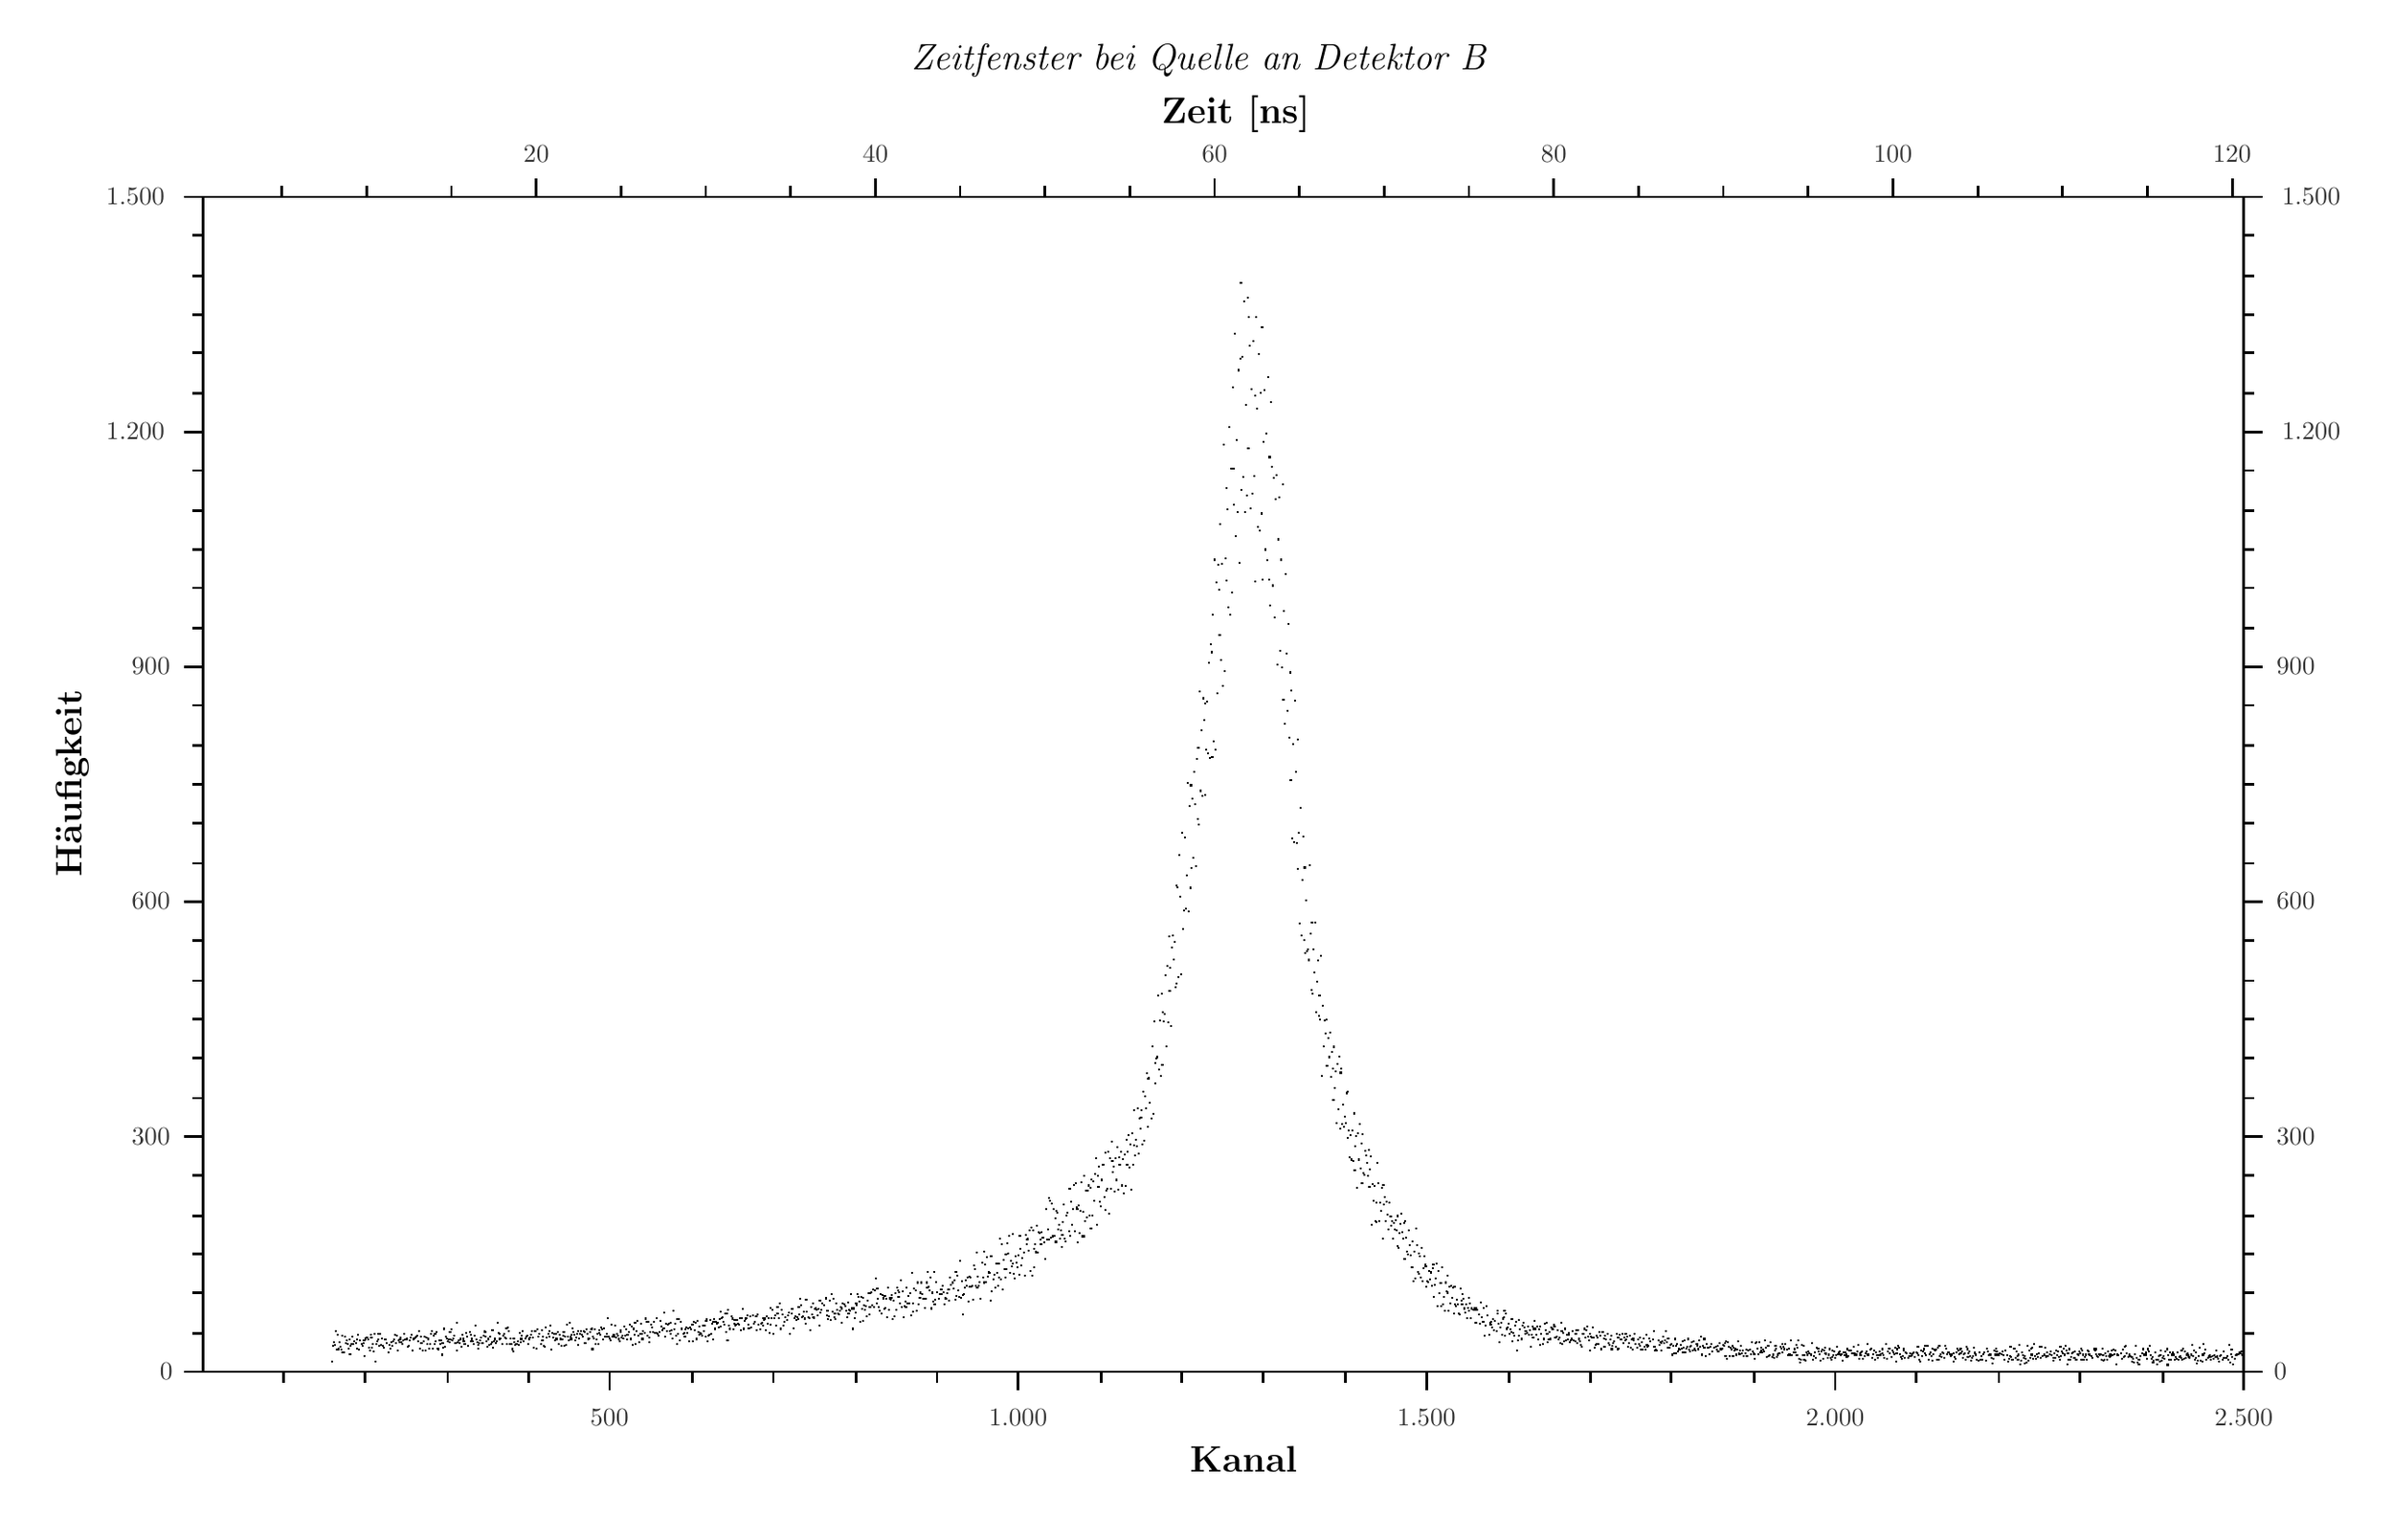
\begin{tikzpicture}{0pt}{0pt}{1215pt}{773pt}
	\clip(0pt,773pt) -- (914.667pt,773pt) -- (914.667pt,191.076pt) -- (0pt,191.076pt) -- (0pt,773pt);
\begin{scope}
	\clip(69.2588pt,706pt) -- (866.487pt,706pt) -- (866.487pt,246.784pt) -- (69.2588pt,246.784pt) -- (69.2588pt,706pt);
	\color[rgb]{0,0,0}
	\fill (119.348pt,251.07pt) rectangle (120.101pt,250.317pt);
	\color[rgb]{0,0,0}
	\fill (119.668pt,257.193pt) rectangle (120.421pt,256.44pt);
	\fill (119.988pt,258.724pt) rectangle (120.74pt,257.971pt);
	\fill (120.308pt,257.499pt) rectangle (121.06pt,256.746pt);
	\fill (120.947pt,263.01pt) rectangle (121.7pt,262.257pt);
	\fill (121.267pt,255.662pt) rectangle (122.02pt,254.909pt);
	\fill (121.587pt,261.479pt) rectangle (122.34pt,260.726pt);
	\fill (121.907pt,255.968pt) rectangle (122.66pt,255.216pt);
	\fill (122.227pt,258.724pt) rectangle (122.979pt,257.971pt);
	\fill (122.546pt,256.887pt) rectangle (123.299pt,256.134pt);
	\fill (122.866pt,255.662pt) rectangle (123.619pt,254.909pt);
	\fill (123.186pt,261.173pt) rectangle (123.939pt,260.42pt);
	\fill (123.506pt,254.744pt) rectangle (124.259pt,253.991pt);
	\fill (124.146pt,254.744pt) rectangle (124.898pt,253.991pt);
	\fill (124.465pt,260.867pt) rectangle (125.218pt,260.114pt);
	\fill (124.785pt,258.418pt) rectangle (125.538pt,257.665pt);
	\fill (125.105pt,259.336pt) rectangle (125.858pt,258.583pt);
	\fill (125.425pt,258.111pt) rectangle (126.178pt,257.359pt);
	\fill (125.745pt,256.275pt) rectangle (126.498pt,255.522pt);
	\fill (126.065pt,259.642pt) rectangle (126.817pt,258.889pt);
	\fill (126.384pt,254.132pt) rectangle (127.137pt,253.379pt);
	\fill (126.704pt,257.193pt) rectangle (127.457pt,256.44pt);
	\fill (127.024pt,258.111pt) rectangle (127.777pt,257.359pt);
	\fill (127.344pt,260.867pt) rectangle (128.097pt,260.114pt);
	\fill (127.664pt,257.805pt) rectangle (128.417pt,257.052pt);
	\fill (127.984pt,259.03pt) rectangle (128.736pt,258.277pt);
	\fill (128.623pt,258.418pt) rectangle (129.376pt,257.665pt);
	\fill (128.943pt,259.642pt) rectangle (129.696pt,258.889pt);
	\fill (129.263pt,256.275pt) rectangle (130.016pt,255.522pt);
	\fill (129.583pt,261.479pt) rectangle (130.336pt,260.726pt);
	\fill (129.903pt,255.662pt) rectangle (130.655pt,254.909pt);
	\fill (130.222pt,259.336pt) rectangle (130.975pt,258.583pt);
	\fill (130.862pt,258.111pt) rectangle (131.615pt,257.359pt);
	\fill (131.182pt,257.193pt) rectangle (131.935pt,256.44pt);
	\fill (131.502pt,258.418pt) rectangle (132.255pt,257.665pt);
	\fill (131.822pt,259.336pt) rectangle (132.574pt,258.583pt);
	\fill (132.141pt,253.213pt) rectangle (132.894pt,252.46pt);
	\fill (132.461pt,259.948pt) rectangle (133.214pt,259.195pt);
	\fill (132.781pt,260.561pt) rectangle (133.534pt,259.808pt);
	\fill (133.101pt,260.561pt) rectangle (133.854pt,259.808pt);
	\fill (133.421pt,259.642pt) rectangle (134.174pt,258.889pt);
	\fill (133.741pt,256.581pt) rectangle (134.493pt,255.828pt);
	\fill (134.061pt,255.356pt) rectangle (134.813pt,254.603pt);
	\fill (134.38pt,261.479pt) rectangle (135.133pt,260.726pt);
	\fill (134.7pt,260.561pt) rectangle (135.453pt,259.808pt);
	\fill (135.02pt,256.581pt) rectangle (135.773pt,255.828pt);
	\fill (135.34pt,258.111pt) rectangle (136.093pt,257.359pt);
	\fill (135.66pt,255.05pt) rectangle (136.413pt,254.297pt);
	\fill (135.98pt,261.785pt) rectangle (136.732pt,261.032pt);
	\fill (136.299pt,251.07pt) rectangle (137.052pt,250.317pt);
	\fill (136.619pt,258.111pt) rectangle (137.372pt,257.359pt);
	\fill (136.939pt,259.03pt) rectangle (137.692pt,258.277pt);
	\fill (137.259pt,259.642pt) rectangle (138.012pt,258.889pt);
	\fill (137.579pt,262.091pt) rectangle (138.332pt,261.338pt);
	\fill (137.899pt,257.193pt) rectangle (138.651pt,256.44pt);
	\fill (138.218pt,261.785pt) rectangle (138.971pt,261.032pt);
	\fill (138.538pt,257.499pt) rectangle (139.291pt,256.746pt);
	\fill (138.858pt,260.254pt) rectangle (139.611pt,259.502pt);
	\fill (139.178pt,257.193pt) rectangle (139.931pt,256.44pt);
	\fill (139.498pt,256.581pt) rectangle (140.251pt,255.828pt);
	\fill (139.818pt,259.642pt) rectangle (140.57pt,258.889pt);
	\fill (140.457pt,259.642pt) rectangle (141.21pt,258.889pt);
	\fill (140.777pt,258.418pt) rectangle (141.53pt,257.665pt);
	\fill (141.417pt,254.744pt) rectangle (142.17pt,253.991pt);
	\fill (141.737pt,257.499pt) rectangle (142.489pt,256.746pt);
	\fill (142.056pt,256.275pt) rectangle (142.809pt,255.522pt);
	\fill (142.376pt,258.724pt) rectangle (143.129pt,257.971pt);
	\fill (142.696pt,257.193pt) rectangle (143.449pt,256.44pt);
	\fill (143.336pt,259.03pt) rectangle (144.089pt,258.277pt);
	\fill (143.656pt,259.642pt) rectangle (144.408pt,258.889pt);
	\fill (143.975pt,261.479pt) rectangle (144.728pt,260.726pt);
	\fill (144.295pt,258.418pt) rectangle (145.048pt,257.665pt);
	\fill (144.615pt,261.173pt) rectangle (145.368pt,260.42pt);
	\fill (144.935pt,255.356pt) rectangle (145.688pt,254.603pt);
	\fill (145.255pt,259.336pt) rectangle (146.008pt,258.583pt);
	\fill (145.575pt,258.724pt) rectangle (146.327pt,257.971pt);
	\fill (145.894pt,259.642pt) rectangle (146.647pt,258.889pt);
	\fill (146.214pt,260.561pt) rectangle (146.967pt,259.808pt);
	\fill (146.534pt,258.724pt) rectangle (147.287pt,257.971pt);
	\fill (146.854pt,257.805pt) rectangle (147.607pt,257.052pt);
	\fill (147.174pt,259.336pt) rectangle (147.927pt,258.583pt);
	\fill (147.494pt,261.785pt) rectangle (148.246pt,261.032pt);
	\fill (147.813pt,259.642pt) rectangle (148.566pt,258.889pt);
	\fill (148.133pt,259.642pt) rectangle (148.886pt,258.889pt);
	\fill (148.453pt,260.254pt) rectangle (149.206pt,259.502pt);
	\fill (148.773pt,259.948pt) rectangle (149.526pt,259.195pt);
	\fill (149.093pt,256.887pt) rectangle (149.846pt,256.134pt);
	\fill (149.413pt,257.193pt) rectangle (150.165pt,256.44pt);
	\fill (149.733pt,259.336pt) rectangle (150.485pt,258.583pt);
	\fill (150.052pt,260.561pt) rectangle (150.805pt,259.808pt);
	\fill (150.372pt,261.479pt) rectangle (151.125pt,260.726pt);
	\fill (150.692pt,255.356pt) rectangle (151.445pt,254.603pt);
	\fill (151.012pt,259.948pt) rectangle (151.765pt,259.195pt);
	\fill (151.332pt,260.254pt) rectangle (152.085pt,259.502pt);
	\fill (151.971pt,260.561pt) rectangle (152.724pt,259.808pt);
	\fill (152.291pt,260.867pt) rectangle (153.044pt,260.114pt);
	\fill (152.611pt,261.173pt) rectangle (153.364pt,260.42pt);
	\fill (152.931pt,259.03pt) rectangle (153.684pt,258.277pt);
	\fill (153.251pt,263.01pt) rectangle (154.004pt,262.257pt);
	\fill (153.571pt,256.275pt) rectangle (154.323pt,255.522pt);
	\fill (153.89pt,260.867pt) rectangle (154.643pt,260.114pt);
	\fill (154.21pt,258.418pt) rectangle (154.963pt,257.665pt);
	\fill (154.85pt,255.356pt) rectangle (155.603pt,254.603pt);
	\fill (155.17pt,259.03pt) rectangle (155.923pt,258.277pt);
	\fill (155.49pt,260.867pt) rectangle (156.242pt,260.114pt);
	\fill (155.809pt,255.356pt) rectangle (156.562pt,254.603pt);
	\fill (156.129pt,260.561pt) rectangle (156.882pt,259.808pt);
	\fill (156.449pt,258.111pt) rectangle (157.202pt,257.359pt);
	\fill (156.769pt,259.948pt) rectangle (157.522pt,259.195pt);
	\fill (157.089pt,259.642pt) rectangle (157.842pt,258.889pt);
	\fill (157.409pt,256.275pt) rectangle (158.161pt,255.522pt);
	\fill (157.728pt,257.805pt) rectangle (158.481pt,257.052pt);
	\fill (158.048pt,262.091pt) rectangle (158.801pt,261.338pt);
	\fill (158.368pt,263.01pt) rectangle (159.121pt,262.257pt);
	\fill (158.688pt,256.275pt) rectangle (159.441pt,255.522pt);
	\fill (159.008pt,261.173pt) rectangle (159.761pt,260.42pt);
	\fill (159.328pt,257.805pt) rectangle (160.08pt,257.052pt);
	\fill (159.647pt,261.785pt) rectangle (160.4pt,261.032pt);
	\fill (159.967pt,259.03pt) rectangle (160.72pt,258.277pt);
	\fill (160.287pt,262.704pt) rectangle (161.04pt,261.951pt);
	\fill (160.607pt,256.275pt) rectangle (161.36pt,255.522pt);
	\fill (160.927pt,255.968pt) rectangle (161.68pt,255.216pt);
	\fill (161.247pt,259.336pt) rectangle (161.999pt,258.583pt);
	\fill (161.566pt,257.805pt) rectangle (162.319pt,257.052pt);
	\fill (161.886pt,259.336pt) rectangle (162.639pt,258.583pt);
	\fill (162.206pt,253.825pt) rectangle (162.959pt,253.073pt);
	\fill (162.526pt,258.418pt) rectangle (163.279pt,257.665pt);
	\fill (162.846pt,256.581pt) rectangle (163.599pt,255.828pt);
	\fill (163.166pt,263.928pt) rectangle (163.918pt,263.175pt);
	\fill (163.486pt,256.887pt) rectangle (164.238pt,256.134pt);
	\fill (163.805pt,260.867pt) rectangle (164.558pt,260.114pt);
	\fill (164.125pt,260.254pt) rectangle (164.878pt,259.502pt);
	\fill (164.445pt,259.03pt) rectangle (165.198pt,258.277pt);
	\fill (164.765pt,259.642pt) rectangle (165.518pt,258.889pt);
	\fill (165.085pt,258.724pt) rectangle (165.838pt,257.971pt);
	\fill (165.405pt,262.704pt) rectangle (166.157pt,261.951pt);
	\fill (165.724pt,259.642pt) rectangle (166.477pt,258.889pt);
	\fill (166.044pt,263.622pt) rectangle (166.797pt,262.869pt);
	\fill (166.364pt,259.336pt) rectangle (167.117pt,258.583pt);
	\fill (166.684pt,260.254pt) rectangle (167.437pt,259.502pt);
	\fill (167.004pt,261.173pt) rectangle (167.757pt,260.42pt);
	\fill (167.324pt,258.418pt) rectangle (168.076pt,257.665pt);
	\fill (167.643pt,258.418pt) rectangle (168.396pt,257.665pt);
	\fill (167.963pt,255.356pt) rectangle (168.716pt,254.603pt);
	\fill (168.283pt,266.377pt) rectangle (169.036pt,265.624pt);
	\fill (168.603pt,258.724pt) rectangle (169.356pt,257.971pt);
	\fill (168.923pt,259.336pt) rectangle (169.676pt,258.583pt);
	\fill (169.243pt,258.418pt) rectangle (169.995pt,257.665pt);
	\fill (169.562pt,259.948pt) rectangle (170.315pt,259.195pt);
	\fill (169.882pt,256.887pt) rectangle (170.635pt,256.134pt);
	\fill (170.202pt,261.479pt) rectangle (170.955pt,260.726pt);
	\fill (170.522pt,259.948pt) rectangle (171.275pt,259.195pt);
	\fill (170.842pt,259.03pt) rectangle (171.595pt,258.277pt);
	\fill (171.162pt,258.111pt) rectangle (171.914pt,257.359pt);
	\fill (171.481pt,257.805pt) rectangle (172.234pt,257.052pt);
	\fill (171.801pt,262.397pt) rectangle (172.554pt,261.645pt);
	\fill (172.121pt,260.867pt) rectangle (172.874pt,260.114pt);
	\fill (172.441pt,257.193pt) rectangle (173.194pt,256.44pt);
	\fill (173.081pt,262.704pt) rectangle (173.833pt,261.951pt);
	\fill (173.4pt,261.479pt) rectangle (174.153pt,260.726pt);
	\fill (173.72pt,259.03pt) rectangle (174.473pt,258.277pt);
	\fill (174.04pt,259.948pt) rectangle (174.793pt,259.195pt);
	\fill (174.36pt,259.03pt) rectangle (175.113pt,258.277pt);
	\fill (174.68pt,258.111pt) rectangle (175.433pt,257.359pt);
	\fill (175pt,261.173pt) rectangle (175.752pt,260.42pt);
	\fill (175.319pt,265.153pt) rectangle (176.072pt,264.4pt);
	\fill (175.639pt,259.642pt) rectangle (176.392pt,258.889pt);
	\fill (175.959pt,258.724pt) rectangle (176.712pt,257.971pt);
	\fill (176.279pt,257.499pt) rectangle (177.032pt,256.746pt);
	\fill (176.599pt,256.275pt) rectangle (177.352pt,255.522pt);
	\fill (176.919pt,258.418pt) rectangle (177.671pt,257.665pt);
	\fill (177.238pt,259.336pt) rectangle (177.991pt,258.583pt);
	\fill (177.558pt,260.561pt) rectangle (178.311pt,259.808pt);
	\fill (177.878pt,258.418pt) rectangle (178.631pt,257.665pt);
	\fill (178.198pt,258.418pt) rectangle (178.951pt,257.665pt);
	\fill (178.518pt,261.173pt) rectangle (179.271pt,260.42pt);
	\fill (178.838pt,263.01pt) rectangle (179.59pt,262.257pt);
	\fill (179.158pt,262.704pt) rectangle (179.91pt,261.951pt);
	\fill (179.477pt,260.867pt) rectangle (180.23pt,260.114pt);
	\fill (179.797pt,259.03pt) rectangle (180.55pt,258.277pt);
	\fill (180.117pt,256.887pt) rectangle (180.87pt,256.134pt);
	\fill (180.437pt,259.948pt) rectangle (181.19pt,259.195pt);
	\fill (180.757pt,257.499pt) rectangle (181.51pt,256.746pt);
	\fill (181.077pt,260.867pt) rectangle (181.829pt,260.114pt);
	\fill (181.396pt,258.111pt) rectangle (182.149pt,257.359pt);
	\fill (181.716pt,258.724pt) rectangle (182.469pt,257.971pt);
	\fill (182.036pt,263.316pt) rectangle (182.789pt,262.563pt);
	\fill (182.356pt,256.581pt) rectangle (183.109pt,255.828pt);
	\fill (182.676pt,259.03pt) rectangle (183.429pt,258.277pt);
	\fill (182.996pt,259.948pt) rectangle (183.748pt,259.195pt);
	\fill (183.315pt,258.418pt) rectangle (184.068pt,257.665pt);
	\fill (183.635pt,259.03pt) rectangle (184.388pt,258.277pt);
	\fill (183.955pt,266.377pt) rectangle (184.708pt,265.624pt);
	\fill (184.275pt,262.397pt) rectangle (185.028pt,261.645pt);
	\fill (184.595pt,259.948pt) rectangle (185.348pt,259.195pt);
	\fill (184.915pt,262.091pt) rectangle (185.667pt,261.338pt);
	\fill (185.234pt,260.254pt) rectangle (185.987pt,259.502pt);
	\fill (185.874pt,258.111pt) rectangle (186.627pt,257.359pt);
	\fill (186.194pt,261.173pt) rectangle (186.947pt,260.42pt);
	\fill (186.514pt,262.091pt) rectangle (187.267pt,261.338pt);
	\fill (186.834pt,260.561pt) rectangle (187.586pt,259.808pt);
	\fill (187.153pt,260.254pt) rectangle (187.906pt,259.502pt);
	\fill (187.473pt,264.234pt) rectangle (188.226pt,263.481pt);
	\fill (187.793pt,258.111pt) rectangle (188.546pt,257.359pt);
	\fill (188.113pt,264.54pt) rectangle (188.866pt,263.788pt);
	\fill (188.433pt,263.01pt) rectangle (189.186pt,262.257pt);
	\fill (188.753pt,258.111pt) rectangle (189.505pt,257.359pt);
	\fill (189.072pt,260.254pt) rectangle (189.825pt,259.502pt);
	\fill (189.392pt,258.111pt) rectangle (190.145pt,257.359pt);
	\fill (189.712pt,255.968pt) rectangle (190.465pt,255.216pt);
	\fill (190.032pt,255.05pt) rectangle (190.785pt,254.297pt);
	\fill (190.352pt,260.254pt) rectangle (191.105pt,259.502pt);
	\fill (190.672pt,258.724pt) rectangle (191.424pt,257.971pt);
	\fill (190.991pt,257.499pt) rectangle (191.744pt,256.746pt);
	\fill (191.311pt,257.805pt) rectangle (192.064pt,257.052pt);
	\fill (191.631pt,258.111pt) rectangle (192.384pt,257.359pt);
	\fill (191.951pt,259.03pt) rectangle (192.704pt,258.277pt);
	\fill (192.271pt,257.499pt) rectangle (193.024pt,256.746pt);
	\fill (192.591pt,262.397pt) rectangle (193.343pt,261.645pt);
	\fill (192.911pt,258.724pt) rectangle (193.663pt,257.971pt);
	\fill (193.23pt,259.948pt) rectangle (193.983pt,259.195pt);
	\fill (193.55pt,261.173pt) rectangle (194.303pt,260.42pt);
	\fill (193.87pt,263.01pt) rectangle (194.623pt,262.257pt);
	\fill (194.19pt,259.03pt) rectangle (194.943pt,258.277pt);
	\fill (194.83pt,260.254pt) rectangle (195.582pt,259.502pt);
	\fill (195.149pt,260.867pt) rectangle (195.902pt,260.114pt);
	\fill (195.469pt,261.173pt) rectangle (196.222pt,260.42pt);
	\fill (196.109pt,257.805pt) rectangle (196.862pt,257.052pt);
	\fill (196.429pt,259.948pt) rectangle (197.182pt,259.195pt);
	\fill (196.749pt,260.561pt) rectangle (197.501pt,259.808pt);
	\fill (197.068pt,261.479pt) rectangle (197.821pt,260.726pt);
	\fill (197.388pt,263.01pt) rectangle (198.141pt,262.257pt);
	\fill (197.708pt,260.561pt) rectangle (198.461pt,259.808pt);
	\fill (198.028pt,256.581pt) rectangle (198.781pt,255.828pt);
	\fill (198.668pt,263.01pt) rectangle (199.42pt,262.257pt);
	\fill (199.307pt,256.275pt) rectangle (200.06pt,255.522pt);
	\fill (199.627pt,263.622pt) rectangle (200.38pt,262.869pt);
	\fill (199.947pt,260.867pt) rectangle (200.7pt,260.114pt);
	\fill (200.267pt,261.785pt) rectangle (201.02pt,261.032pt);
	\fill (200.906pt,258.111pt) rectangle (201.659pt,257.359pt);
	\fill (201.226pt,263.316pt) rectangle (201.979pt,262.563pt);
	\fill (201.546pt,259.336pt) rectangle (202.299pt,258.583pt);
	\fill (201.866pt,260.867pt) rectangle (202.619pt,260.114pt);
	\fill (202.186pt,257.193pt) rectangle (202.939pt,256.44pt);
	\fill (202.506pt,256.887pt) rectangle (203.258pt,256.134pt);
	\fill (202.825pt,264.54pt) rectangle (203.578pt,263.788pt);
	\fill (203.145pt,260.561pt) rectangle (203.898pt,259.808pt);
	\fill (203.785pt,261.785pt) rectangle (204.538pt,261.032pt);
	\fill (204.105pt,263.01pt) rectangle (204.858pt,262.257pt);
	\fill (204.425pt,260.867pt) rectangle (205.177pt,260.114pt);
	\fill (204.744pt,265.153pt) rectangle (205.497pt,264.4pt);
	\fill (205.064pt,255.662pt) rectangle (205.817pt,254.909pt);
	\fill (205.384pt,262.397pt) rectangle (206.137pt,261.645pt);
	\fill (205.704pt,260.561pt) rectangle (206.457pt,259.808pt);
	\fill (206.024pt,262.091pt) rectangle (206.777pt,261.338pt);
	\fill (206.344pt,259.336pt) rectangle (207.096pt,258.583pt);
	\fill (206.663pt,261.785pt) rectangle (207.416pt,261.032pt);
	\fill (206.983pt,260.254pt) rectangle (207.736pt,259.502pt);
	\fill (207.303pt,259.948pt) rectangle (208.056pt,259.195pt);
	\fill (207.623pt,262.704pt) rectangle (208.376pt,261.951pt);
	\fill (207.943pt,257.805pt) rectangle (208.696pt,257.052pt);
	\fill (208.263pt,261.479pt) rectangle (209.015pt,260.726pt);
	\fill (208.583pt,259.948pt) rectangle (209.335pt,259.195pt);
	\fill (208.902pt,257.193pt) rectangle (209.655pt,256.44pt);
	\fill (209.222pt,259.642pt) rectangle (209.975pt,258.889pt);
	\fill (209.542pt,261.173pt) rectangle (210.295pt,260.42pt);
	\fill (209.862pt,262.704pt) rectangle (210.615pt,261.951pt);
	\fill (210.182pt,257.193pt) rectangle (210.935pt,256.44pt);
	\fill (210.502pt,260.867pt) rectangle (211.254pt,260.114pt);
	\fill (210.821pt,257.499pt) rectangle (211.574pt,256.746pt);
	\fill (211.141pt,265.459pt) rectangle (211.894pt,264.706pt);
	\fill (211.461pt,260.867pt) rectangle (212.214pt,260.114pt);
	\fill (211.781pt,259.336pt) rectangle (212.534pt,258.583pt);
	\fill (212.101pt,266.377pt) rectangle (212.854pt,265.624pt);
	\fill (212.421pt,260.867pt) rectangle (213.173pt,260.114pt);
	\fill (212.74pt,259.948pt) rectangle (213.493pt,259.195pt);
	\fill (213.06pt,261.479pt) rectangle (213.813pt,260.726pt);
	\fill (213.38pt,264.234pt) rectangle (214.133pt,263.481pt);
	\fill (213.7pt,262.704pt) rectangle (214.453pt,261.951pt);
	\fill (214.02pt,261.479pt) rectangle (214.773pt,260.726pt);
	\fill (214.34pt,259.336pt) rectangle (215.092pt,258.583pt);
	\fill (214.659pt,260.561pt) rectangle (215.412pt,259.808pt);
	\fill (214.979pt,262.091pt) rectangle (215.732pt,261.338pt);
	\fill (215.299pt,257.499pt) rectangle (216.052pt,256.746pt);
	\fill (215.619pt,263.01pt) rectangle (216.372pt,262.257pt);
	\fill (215.939pt,260.254pt) rectangle (216.692pt,259.502pt);
	\fill (216.259pt,262.091pt) rectangle (217.011pt,261.338pt);
	\fill (216.578pt,263.01pt) rectangle (217.331pt,262.257pt);
	\fill (216.898pt,261.479pt) rectangle (217.651pt,260.726pt);
	\fill (217.218pt,260.867pt) rectangle (217.971pt,260.114pt);
	\fill (217.538pt,263.01pt) rectangle (218.291pt,262.257pt);
	\fill (217.858pt,262.704pt) rectangle (218.611pt,261.951pt);
	\fill (218.178pt,258.418pt) rectangle (218.93pt,257.665pt);
	\fill (218.817pt,263.622pt) rectangle (219.57pt,262.869pt);
	\fill (219.137pt,261.785pt) rectangle (219.89pt,261.032pt);
	\fill (219.457pt,259.948pt) rectangle (220.21pt,259.195pt);
	\fill (219.777pt,260.254pt) rectangle (220.53pt,259.502pt);
	\fill (220.097pt,262.704pt) rectangle (220.849pt,261.951pt);
	\fill (220.416pt,263.622pt) rectangle (221.169pt,262.869pt);
	\fill (220.736pt,263.928pt) rectangle (221.489pt,263.175pt);
	\fill (221.056pt,255.968pt) rectangle (221.809pt,255.216pt);
	\fill (221.376pt,260.867pt) rectangle (222.129pt,260.114pt);
	\fill (221.696pt,260.254pt) rectangle (222.449pt,259.502pt);
	\fill (222.016pt,263.622pt) rectangle (222.768pt,262.869pt);
	\fill (222.336pt,257.805pt) rectangle (223.088pt,257.052pt);
	\fill (222.655pt,259.642pt) rectangle (223.408pt,258.889pt);
	\fill (222.975pt,261.785pt) rectangle (223.728pt,261.032pt);
	\fill (223.295pt,257.805pt) rectangle (224.048pt,257.052pt);
	\fill (223.615pt,263.316pt) rectangle (224.368pt,262.563pt);
	\fill (223.935pt,262.397pt) rectangle (224.688pt,261.645pt);
	\fill (224.255pt,261.479pt) rectangle (225.007pt,260.726pt);
	\fill (224.574pt,264.54pt) rectangle (225.327pt,263.788pt);
	\fill (224.894pt,263.622pt) rectangle (225.647pt,262.869pt);
	\fill (225.214pt,259.642pt) rectangle (225.967pt,258.889pt);
	\fill (225.534pt,264.234pt) rectangle (226.287pt,263.481pt);
	\fill (225.854pt,260.867pt) rectangle (226.607pt,260.114pt);
	\fill (226.493pt,260.867pt) rectangle (227.246pt,260.114pt);
	\fill (226.813pt,261.785pt) rectangle (227.566pt,261.032pt);
	\fill (227.133pt,268.214pt) rectangle (227.886pt,267.461pt);
	\fill (227.453pt,260.867pt) rectangle (228.206pt,260.114pt);
	\fill (227.773pt,260.254pt) rectangle (228.526pt,259.502pt);
	\fill (228.093pt,259.336pt) rectangle (228.845pt,258.583pt);
	\fill (228.412pt,265.459pt) rectangle (229.165pt,264.706pt);
	\fill (228.732pt,260.867pt) rectangle (229.485pt,260.114pt);
	\fill (229.052pt,261.479pt) rectangle (229.805pt,260.726pt);
	\fill (229.372pt,261.479pt) rectangle (230.125pt,260.726pt);
	\fill (229.692pt,260.867pt) rectangle (230.445pt,260.114pt);
	\fill (230.012pt,265.153pt) rectangle (230.764pt,264.4pt);
	\fill (230.331pt,260.561pt) rectangle (231.084pt,259.808pt);
	\fill (230.651pt,262.091pt) rectangle (231.404pt,261.338pt);
	\fill (230.971pt,261.173pt) rectangle (231.724pt,260.42pt);
	\fill (231.291pt,259.948pt) rectangle (232.044pt,259.195pt);
	\fill (231.611pt,259.03pt) rectangle (232.364pt,258.277pt);
	\fill (231.931pt,263.316pt) rectangle (232.683pt,262.563pt);
	\fill (232.25pt,262.704pt) rectangle (233.003pt,261.951pt);
	\fill (232.57pt,260.561pt) rectangle (233.323pt,259.808pt);
	\fill (232.89pt,261.173pt) rectangle (233.643pt,260.42pt);
	\fill (233.21pt,260.254pt) rectangle (233.963pt,259.502pt);
	\fill (233.53pt,264.847pt) rectangle (234.283pt,264.094pt);
	\fill (233.85pt,261.173pt) rectangle (234.602pt,260.42pt);
	\fill (234.169pt,263.622pt) rectangle (234.922pt,262.869pt);
	\fill (234.489pt,259.642pt) rectangle (235.242pt,258.889pt);
	\fill (234.809pt,261.479pt) rectangle (235.562pt,260.726pt);
	\fill (235.449pt,262.704pt) rectangle (236.202pt,261.951pt);
	\fill (235.769pt,265.459pt) rectangle (236.521pt,264.706pt);
	\fill (236.088pt,259.948pt) rectangle (236.841pt,259.195pt);
	\fill (236.408pt,264.847pt) rectangle (237.161pt,264.094pt);
	\fill (236.728pt,257.499pt) rectangle (237.481pt,256.746pt);
	\fill (237.048pt,263.928pt) rectangle (237.801pt,263.175pt);
	\fill (237.368pt,261.479pt) rectangle (238.121pt,260.726pt);
	\fill (237.688pt,266.377pt) rectangle (238.44pt,265.624pt);
	\fill (238.008pt,257.805pt) rectangle (238.76pt,257.052pt);
	\fill (238.327pt,263.01pt) rectangle (239.08pt,262.257pt);
	\fill (238.647pt,266.99pt) rectangle (239.4pt,266.237pt);
	\fill (238.967pt,261.173pt) rectangle (239.72pt,260.42pt);
	\fill (239.287pt,258.724pt) rectangle (240.04pt,257.971pt);
	\fill (239.607pt,262.091pt) rectangle (240.36pt,261.338pt);
	\fill (239.927pt,265.765pt) rectangle (240.679pt,265.012pt);
	\fill (240.246pt,261.785pt) rectangle (240.999pt,261.032pt);
	\fill (240.566pt,259.948pt) rectangle (241.319pt,259.195pt);
	\fill (240.886pt,263.01pt) rectangle (241.639pt,262.257pt);
	\fill (241.526pt,262.397pt) rectangle (242.279pt,261.645pt);
	\fill (241.846pt,267.908pt) rectangle (242.598pt,267.155pt);
	\fill (242.165pt,266.683pt) rectangle (242.918pt,265.931pt);
	\fill (242.485pt,261.173pt) rectangle (243.238pt,260.42pt);
	\fill (242.805pt,266.683pt) rectangle (243.558pt,265.931pt);
	\fill (243.125pt,258.724pt) rectangle (243.878pt,257.971pt);
	\fill (243.445pt,260.561pt) rectangle (244.198pt,259.808pt);
	\fill (243.765pt,262.704pt) rectangle (244.517pt,261.951pt);
	\fill (244.084pt,265.459pt) rectangle (244.837pt,264.706pt);
	\fill (244.404pt,264.54pt) rectangle (245.157pt,263.788pt);
	\fill (244.724pt,262.704pt) rectangle (245.477pt,261.951pt);
	\fill (245.044pt,266.683pt) rectangle (245.797pt,265.931pt);
	\fill (245.364pt,262.397pt) rectangle (246.117pt,261.645pt);
	\fill (246.003pt,262.397pt) rectangle (246.756pt,261.645pt);
	\fill (246.323pt,268.214pt) rectangle (247.076pt,267.461pt);
	\fill (246.643pt,262.091pt) rectangle (247.396pt,261.338pt);
	\fill (246.963pt,261.173pt) rectangle (247.716pt,260.42pt);
	\fill (247.283pt,262.704pt) rectangle (248.036pt,261.951pt);
	\fill (247.603pt,266.99pt) rectangle (248.355pt,266.237pt);
	\fill (247.922pt,264.847pt) rectangle (248.675pt,264.094pt);
	\fill (248.242pt,263.316pt) rectangle (248.995pt,262.563pt);
	\fill (248.882pt,264.234pt) rectangle (249.635pt,263.481pt);
	\fill (249.202pt,270.357pt) rectangle (249.955pt,269.604pt);
	\fill (249.522pt,260.867pt) rectangle (250.274pt,260.114pt);
	\fill (249.841pt,265.765pt) rectangle (250.594pt,265.012pt);
	\fill (250.161pt,263.01pt) rectangle (250.914pt,262.257pt);
	\fill (250.481pt,265.459pt) rectangle (251.234pt,264.706pt);
	\fill (250.801pt,266.071pt) rectangle (251.554pt,265.318pt);
	\fill (251.121pt,263.01pt) rectangle (251.874pt,262.257pt);
	\fill (251.441pt,266.377pt) rectangle (252.193pt,265.624pt);
	\fill (251.761pt,262.091pt) rectangle (252.513pt,261.338pt);
	\fill (252.08pt,263.316pt) rectangle (252.833pt,262.563pt);
	\fill (252.4pt,260.254pt) rectangle (253.153pt,259.502pt);
	\fill (252.72pt,270.969pt) rectangle (253.473pt,270.217pt);
	\fill (253.04pt,263.622pt) rectangle (253.793pt,262.869pt);
	\fill (253.36pt,266.071pt) rectangle (254.113pt,265.318pt);
	\fill (253.68pt,261.173pt) rectangle (254.432pt,260.42pt);
	\fill (253.999pt,257.805pt) rectangle (254.752pt,257.052pt);
	\fill (254.319pt,267.602pt) rectangle (255.072pt,266.849pt);
	\fill (254.639pt,261.785pt) rectangle (255.392pt,261.032pt);
	\fill (254.959pt,267.602pt) rectangle (255.712pt,266.849pt);
	\fill (255.279pt,259.336pt) rectangle (256.032pt,258.583pt);
	\fill (255.599pt,266.683pt) rectangle (256.351pt,265.931pt);
	\fill (255.918pt,263.928pt) rectangle (256.671pt,263.175pt);
	\fill (256.558pt,262.091pt) rectangle (257.311pt,261.338pt);
	\fill (256.878pt,262.397pt) rectangle (257.631pt,261.645pt);
	\fill (257.198pt,260.867pt) rectangle (257.951pt,260.114pt);
	\fill (257.518pt,263.622pt) rectangle (258.27pt,262.869pt);
	\fill (257.837pt,264.54pt) rectangle (258.59pt,263.788pt);
	\fill (258.157pt,262.397pt) rectangle (258.91pt,261.645pt);
	\fill (258.477pt,264.234pt) rectangle (259.23pt,263.481pt);
	\fill (258.797pt,259.03pt) rectangle (259.55pt,258.277pt);
	\fill (259.117pt,264.54pt) rectangle (259.87pt,263.788pt);
	\fill (259.437pt,263.622pt) rectangle (260.189pt,262.869pt);
	\fill (260.076pt,265.459pt) rectangle (260.829pt,264.706pt);
	\fill (260.396pt,259.03pt) rectangle (261.149pt,258.277pt);
	\fill (260.716pt,266.683pt) rectangle (261.469pt,265.931pt);
	\fill (261.036pt,263.316pt) rectangle (261.789pt,262.563pt);
	\fill (261.356pt,266.377pt) rectangle (262.108pt,265.624pt);
	\fill (261.675pt,259.948pt) rectangle (262.428pt,259.195pt);
	\fill (261.995pt,266.99pt) rectangle (262.748pt,266.237pt);
	\fill (262.315pt,262.704pt) rectangle (263.068pt,261.951pt);
	\fill (262.635pt,261.479pt) rectangle (263.388pt,260.726pt);
	\fill (262.955pt,264.847pt) rectangle (263.708pt,264.094pt);
	\fill (263.275pt,262.397pt) rectangle (264.027pt,261.645pt);
	\fill (263.594pt,262.091pt) rectangle (264.347pt,261.338pt);
	\fill (263.914pt,261.173pt) rectangle (264.667pt,260.42pt);
	\fill (264.234pt,265.153pt) rectangle (264.987pt,264.4pt);
	\fill (264.554pt,263.01pt) rectangle (265.307pt,262.257pt);
	\fill (264.874pt,265.153pt) rectangle (265.627pt,264.4pt);
	\fill (265.194pt,260.867pt) rectangle (265.946pt,260.114pt);
	\fill (265.514pt,266.99pt) rectangle (266.266pt,266.237pt);
	\fill (265.833pt,267.602pt) rectangle (266.586pt,266.849pt);
	\fill (266.153pt,259.03pt) rectangle (266.906pt,258.277pt);
	\fill (266.473pt,261.173pt) rectangle (267.226pt,260.42pt);
	\fill (266.793pt,261.479pt) rectangle (267.546pt,260.726pt);
	\fill (267.113pt,267.296pt) rectangle (267.865pt,266.543pt);
	\fill (267.433pt,262.091pt) rectangle (268.185pt,261.338pt);
	\fill (267.752pt,265.765pt) rectangle (268.505pt,265.012pt);
	\fill (268.072pt,259.642pt) rectangle (268.825pt,258.889pt);
	\fill (268.392pt,266.683pt) rectangle (269.145pt,265.931pt);
	\fill (268.712pt,267.602pt) rectangle (269.465pt,266.849pt);
	\fill (269.032pt,263.928pt) rectangle (269.785pt,263.175pt);
	\fill (269.352pt,266.683pt) rectangle (270.104pt,265.931pt);
	\fill (269.671pt,265.765pt) rectangle (270.424pt,265.012pt);
	\fill (269.991pt,266.377pt) rectangle (270.744pt,265.624pt);
	\fill (270.311pt,264.54pt) rectangle (271.064pt,263.788pt);
	\fill (270.631pt,267.602pt) rectangle (271.384pt,266.849pt);
	\fill (270.951pt,264.847pt) rectangle (271.704pt,264.094pt);
	\fill (271.271pt,270.663pt) rectangle (272.023pt,269.91pt);
	\fill (271.59pt,268.214pt) rectangle (272.343pt,267.461pt);
	\fill (271.91pt,268.52pt) rectangle (272.663pt,267.767pt);
	\fill (272.23pt,266.683pt) rectangle (272.983pt,265.931pt);
	\fill (272.55pt,265.459pt) rectangle (273.303pt,264.706pt);
	\fill (272.87pt,269.745pt) rectangle (273.623pt,268.992pt);
	\fill (273.19pt,262.704pt) rectangle (273.942pt,261.951pt);
	\fill (273.509pt,270.051pt) rectangle (274.262pt,269.298pt);
	\fill (273.829pt,259.336pt) rectangle (274.582pt,258.583pt);
	\fill (274.149pt,271.276pt) rectangle (274.902pt,270.523pt);
	\fill (274.469pt,265.153pt) rectangle (275.222pt,264.4pt);
	\fill (274.789pt,263.928pt) rectangle (275.542pt,263.175pt);
	\fill (275.428pt,268.826pt) rectangle (276.181pt,268.074pt);
	\fill (275.748pt,267.908pt) rectangle (276.501pt,267.155pt);
	\fill (276.068pt,263.622pt) rectangle (276.821pt,262.869pt);
	\fill (276.388pt,266.071pt) rectangle (277.141pt,265.318pt);
	\fill (276.708pt,267.296pt) rectangle (277.461pt,266.543pt);
	\fill (277.028pt,265.153pt) rectangle (277.78pt,264.4pt);
	\fill (277.347pt,265.459pt) rectangle (278.1pt,264.706pt);
	\fill (277.667pt,267.296pt) rectangle (278.42pt,266.543pt);
	\fill (277.987pt,266.071pt) rectangle (278.74pt,265.318pt);
	\fill (278.307pt,265.459pt) rectangle (279.06pt,264.706pt);
	\fill (278.627pt,268.214pt) rectangle (279.38pt,267.461pt);
	\fill (278.947pt,263.316pt) rectangle (279.699pt,262.563pt);
	\fill (279.266pt,268.214pt) rectangle (280.019pt,267.461pt);
	\fill (279.906pt,271.582pt) rectangle (280.659pt,270.829pt);
	\fill (280.226pt,263.928pt) rectangle (280.979pt,263.175pt);
	\fill (280.546pt,266.99pt) rectangle (281.299pt,266.237pt);
	\fill (280.866pt,267.908pt) rectangle (281.618pt,267.155pt);
	\fill (281.186pt,268.214pt) rectangle (281.938pt,267.461pt);
	\fill (281.505pt,269.133pt) rectangle (282.258pt,268.38pt);
	\fill (281.825pt,265.459pt) rectangle (282.578pt,264.706pt);
	\fill (282.145pt,264.234pt) rectangle (282.898pt,263.481pt);
	\fill (282.785pt,268.826pt) rectangle (283.538pt,268.074pt);
	\fill (283.105pt,264.54pt) rectangle (283.857pt,263.788pt);
	\fill (283.744pt,269.133pt) rectangle (284.497pt,268.38pt);
	\fill (284.064pt,265.765pt) rectangle (284.817pt,265.012pt);
	\fill (284.384pt,266.683pt) rectangle (285.137pt,265.931pt);
	\fill (285.024pt,268.826pt) rectangle (285.776pt,268.074pt);
	\fill (285.343pt,263.316pt) rectangle (286.096pt,262.563pt);
	\fill (285.663pt,269.439pt) rectangle (286.416pt,268.686pt);
	\fill (285.983pt,265.459pt) rectangle (286.736pt,264.706pt);
	\fill (286.623pt,263.622pt) rectangle (287.376pt,262.869pt);
	\fill (286.943pt,266.071pt) rectangle (287.695pt,265.318pt);
	\fill (287.262pt,266.377pt) rectangle (288.015pt,265.624pt);
	\fill (287.582pt,265.153pt) rectangle (288.335pt,264.4pt);
	\fill (287.902pt,268.214pt) rectangle (288.655pt,267.461pt);
	\fill (288.222pt,267.296pt) rectangle (288.975pt,266.543pt);
	\fill (288.542pt,267.908pt) rectangle (289.295pt,267.155pt);
	\fill (288.862pt,263.316pt) rectangle (289.614pt,262.563pt);
	\fill (289.181pt,268.826pt) rectangle (289.934pt,268.074pt);
	\fill (289.501pt,265.765pt) rectangle (290.254pt,265.012pt);
	\fill (289.821pt,268.214pt) rectangle (290.574pt,267.461pt);
	\fill (290.141pt,262.397pt) rectangle (290.894pt,261.645pt);
	\fill (290.461pt,265.459pt) rectangle (291.214pt,264.706pt);
	\fill (290.781pt,272.194pt) rectangle (291.533pt,271.441pt);
	\fill (291.1pt,268.214pt) rectangle (291.853pt,267.461pt);
	\fill (291.42pt,271.276pt) rectangle (292.173pt,270.523pt);
	\fill (291.74pt,262.091pt) rectangle (292.493pt,261.338pt);
	\fill (292.06pt,268.214pt) rectangle (292.813pt,267.461pt);
	\fill (292.38pt,269.133pt) rectangle (293.133pt,268.38pt);
	\fill (292.7pt,265.153pt) rectangle (293.452pt,264.4pt);
	\fill (293.019pt,269.745pt) rectangle (293.772pt,268.992pt);
	\fill (293.339pt,272.5pt) rectangle (294.092pt,271.747pt);
	\fill (293.659pt,270.051pt) rectangle (294.412pt,269.298pt);
	\fill (293.979pt,268.214pt) rectangle (294.732pt,267.461pt);
	\fill (294.299pt,273.725pt) rectangle (295.052pt,272.972pt);
	\fill (294.619pt,263.928pt) rectangle (295.371pt,263.175pt);
	\fill (294.939pt,271.276pt) rectangle (295.691pt,270.523pt);
	\fill (295.258pt,269.439pt) rectangle (296.011pt,268.686pt);
	\fill (295.578pt,265.153pt) rectangle (296.331pt,264.4pt);
	\fill (295.898pt,266.683pt) rectangle (296.651pt,265.931pt);
	\fill (296.538pt,268.52pt) rectangle (297.291pt,267.767pt);
	\fill (297.177pt,267.296pt) rectangle (297.93pt,266.543pt);
	\fill (297.497pt,269.133pt) rectangle (298.25pt,268.38pt);
	\fill (297.817pt,270.357pt) rectangle (298.57pt,269.604pt);
	\fill (298.137pt,261.785pt) rectangle (298.89pt,261.032pt);
	\fill (298.777pt,271.582pt) rectangle (299.529pt,270.829pt);
	\fill (299.096pt,269.745pt) rectangle (299.849pt,268.992pt);
	\fill (299.416pt,271.582pt) rectangle (300.169pt,270.829pt);
	\fill (299.736pt,264.234pt) rectangle (300.489pt,263.481pt);
	\fill (300.056pt,268.214pt) rectangle (300.809pt,267.461pt);
	\fill (300.376pt,268.826pt) rectangle (301.129pt,268.074pt);
	\fill (300.696pt,267.296pt) rectangle (301.448pt,266.543pt);
	\fill (301.015pt,268.52pt) rectangle (301.768pt,267.767pt);
	\fill (301.335pt,267.602pt) rectangle (302.088pt,266.849pt);
	\fill (301.655pt,272.5pt) rectangle (302.408pt,271.747pt);
	\fill (301.975pt,269.439pt) rectangle (302.728pt,268.686pt);
	\fill (302.295pt,275.562pt) rectangle (303.048pt,274.809pt);
	\fill (302.615pt,273.112pt) rectangle (303.367pt,272.36pt);
	\fill (302.934pt,268.52pt) rectangle (303.687pt,267.767pt);
	\fill (303.254pt,268.826pt) rectangle (304.007pt,268.074pt);
	\fill (303.574pt,270.663pt) rectangle (304.327pt,269.91pt);
	\fill (303.894pt,267.908pt) rectangle (304.647pt,267.155pt);
	\fill (304.214pt,265.765pt) rectangle (304.967pt,265.012pt);
	\fill (304.534pt,275.255pt) rectangle (305.286pt,274.503pt);
	\fill (304.853pt,270.663pt) rectangle (305.606pt,269.91pt);
	\fill (305.493pt,268.52pt) rectangle (306.246pt,267.767pt);
	\fill (305.813pt,268.214pt) rectangle (306.566pt,267.461pt);
	\fill (306.133pt,263.316pt) rectangle (306.886pt,262.563pt);
	\fill (306.453pt,272.5pt) rectangle (307.205pt,271.747pt);
	\fill (306.772pt,269.439pt) rectangle (307.525pt,268.686pt);
	\fill (307.092pt,274.031pt) rectangle (307.845pt,273.278pt);
	\fill (307.412pt,268.52pt) rectangle (308.165pt,267.767pt);
	\fill (307.732pt,268.214pt) rectangle (308.485pt,267.461pt);
	\fill (308.052pt,271.582pt) rectangle (308.805pt,270.829pt);
	\fill (308.372pt,272.194pt) rectangle (309.124pt,271.441pt);
	\fill (308.691pt,271.276pt) rectangle (309.444pt,270.523pt);
	\fill (309.011pt,269.133pt) rectangle (309.764pt,268.38pt);
	\fill (309.331pt,271.582pt) rectangle (310.084pt,270.829pt);
	\fill (309.651pt,265.153pt) rectangle (310.404pt,264.4pt);
	\fill (309.971pt,274.949pt) rectangle (310.724pt,274.196pt);
	\fill (310.291pt,270.357pt) rectangle (311.043pt,269.604pt);
	\fill (310.611pt,271.276pt) rectangle (311.363pt,270.523pt);
	\fill (310.93pt,273.725pt) rectangle (311.683pt,272.972pt);
	\fill (311.57pt,273.112pt) rectangle (312.323pt,272.36pt);
	\fill (312.21pt,275.868pt) rectangle (312.963pt,275.115pt);
	\fill (312.53pt,269.133pt) rectangle (313.282pt,268.38pt);
	\fill (312.849pt,270.969pt) rectangle (313.602pt,270.217pt);
	\fill (313.169pt,267.602pt) rectangle (313.922pt,266.849pt);
	\fill (313.489pt,268.826pt) rectangle (314.242pt,268.074pt);
	\fill (313.809pt,274.949pt) rectangle (314.562pt,274.196pt);
	\fill (314.129pt,267.296pt) rectangle (314.882pt,266.543pt);
	\fill (314.449pt,277.398pt) rectangle (315.201pt,276.646pt);
	\fill (314.768pt,270.663pt) rectangle (315.521pt,269.91pt);
	\fill (315.088pt,275.562pt) rectangle (315.841pt,274.809pt);
	\fill (315.408pt,268.52pt) rectangle (316.161pt,267.767pt);
	\fill (315.728pt,270.051pt) rectangle (316.481pt,269.298pt);
	\fill (316.048pt,267.602pt) rectangle (316.801pt,266.849pt);
	\fill (316.368pt,273.725pt) rectangle (317.12pt,272.972pt);
	\fill (316.687pt,271.276pt) rectangle (317.44pt,270.523pt);
	\fill (317.007pt,269.745pt) rectangle (317.76pt,268.992pt);
	\fill (317.327pt,269.439pt) rectangle (318.08pt,268.686pt);
	\fill (317.647pt,270.969pt) rectangle (318.4pt,270.217pt);
	\fill (317.967pt,272.5pt) rectangle (318.72pt,271.747pt);
	\fill (318.287pt,266.377pt) rectangle (319.039pt,265.624pt);
	\fill (318.606pt,271.888pt) rectangle (319.359pt,271.135pt);
	\fill (318.926pt,273.725pt) rectangle (319.679pt,272.972pt);
	\fill (319.566pt,273.419pt) rectangle (320.319pt,272.666pt);
	\fill (319.886pt,272.806pt) rectangle (320.639pt,272.053pt);
	\fill (320.206pt,270.969pt) rectangle (320.958pt,270.217pt);
	\fill (320.525pt,268.52pt) rectangle (321.278pt,267.767pt);
	\fill (320.845pt,274.337pt) rectangle (321.598pt,273.584pt);
	\fill (321.165pt,269.745pt) rectangle (321.918pt,268.992pt);
	\fill (321.485pt,271.276pt) rectangle (322.238pt,270.523pt);
	\fill (321.805pt,270.969pt) rectangle (322.558pt,270.217pt);
	\fill (322.125pt,277.398pt) rectangle (322.877pt,276.646pt);
	\fill (322.444pt,271.888pt) rectangle (323.197pt,271.135pt);
	\fill (322.764pt,263.928pt) rectangle (323.517pt,263.175pt);
	\fill (323.084pt,271.888pt) rectangle (323.837pt,271.135pt);
	\fill (323.404pt,268.214pt) rectangle (324.157pt,267.461pt);
	\fill (323.724pt,270.357pt) rectangle (324.477pt,269.604pt);
	\fill (324.044pt,273.725pt) rectangle (324.796pt,272.972pt);
	\fill (324.364pt,273.112pt) rectangle (325.116pt,272.36pt);
	\fill (324.683pt,277.398pt) rectangle (325.436pt,276.646pt);
	\fill (325.003pt,276.48pt) rectangle (325.756pt,275.727pt);
	\fill (325.323pt,274.643pt) rectangle (326.076pt,273.89pt);
	\fill (325.643pt,266.683pt) rectangle (326.396pt,265.931pt);
	\fill (325.963pt,276.48pt) rectangle (326.716pt,275.727pt);
	\fill (326.283pt,271.582pt) rectangle (327.035pt,270.829pt);
	\fill (326.602pt,276.174pt) rectangle (327.355pt,275.421pt);
	\fill (326.922pt,266.99pt) rectangle (327.675pt,266.237pt);
	\fill (327.242pt,273.112pt) rectangle (327.995pt,272.36pt);
	\fill (327.562pt,271.276pt) rectangle (328.315pt,270.523pt);
	\fill (327.882pt,272.806pt) rectangle (328.635pt,272.053pt);
	\fill (328.202pt,268.826pt) rectangle (328.954pt,268.074pt);
	\fill (328.521pt,274.949pt) rectangle (329.274pt,274.196pt);
	\fill (328.841pt,277.705pt) rectangle (329.594pt,276.952pt);
	\fill (329.161pt,269.439pt) rectangle (329.914pt,268.686pt);
	\fill (329.481pt,272.5pt) rectangle (330.234pt,271.747pt);
	\fill (329.801pt,277.705pt) rectangle (330.554pt,276.952pt);
	\fill (330.121pt,278.317pt) rectangle (330.873pt,277.564pt);
	\fill (330.44pt,273.112pt) rectangle (331.193pt,272.36pt);
	\fill (330.76pt,279.235pt) rectangle (331.513pt,278.482pt);
	\fill (331.08pt,272.5pt) rectangle (331.833pt,271.747pt);
	\fill (331.4pt,278.929pt) rectangle (332.153pt,278.176pt);
	\fill (331.72pt,283.521pt) rectangle (332.473pt,282.768pt);
	\fill (332.04pt,273.725pt) rectangle (332.792pt,272.972pt);
	\fill (332.359pt,279.541pt) rectangle (333.112pt,278.789pt);
	\fill (332.679pt,275.562pt) rectangle (333.432pt,274.809pt);
	\fill (332.999pt,272.5pt) rectangle (333.752pt,271.747pt);
	\fill (333.319pt,270.969pt) rectangle (334.072pt,270.217pt);
	\fill (333.639pt,277.398pt) rectangle (334.392pt,276.646pt);
	\fill (333.959pt,269.745pt) rectangle (334.711pt,268.992pt);
	\fill (334.278pt,277.092pt) rectangle (335.031pt,276.339pt);
	\fill (334.598pt,275.868pt) rectangle (335.351pt,275.115pt);
	\fill (334.918pt,271.582pt) rectangle (335.671pt,270.829pt);
	\fill (335.238pt,276.786pt) rectangle (335.991pt,276.033pt);
	\fill (335.558pt,272.194pt) rectangle (336.311pt,271.441pt);
	\fill (335.878pt,275.562pt) rectangle (336.63pt,274.809pt);
	\fill (336.197pt,268.52pt) rectangle (336.95pt,267.767pt);
	\fill (336.517pt,280.154pt) rectangle (337.27pt,279.401pt);
	\fill (336.837pt,271.276pt) rectangle (337.59pt,270.523pt);
	\fill (337.157pt,275.868pt) rectangle (337.91pt,275.115pt);
	\fill (337.477pt,275.255pt) rectangle (338.23pt,274.503pt);
	\fill (337.797pt,276.174pt) rectangle (338.549pt,275.421pt);
	\fill (338.116pt,277.092pt) rectangle (338.869pt,276.339pt);
	\fill (338.436pt,267.602pt) rectangle (339.189pt,266.849pt);
	\fill (338.756pt,274.949pt) rectangle (339.509pt,274.196pt);
	\fill (339.076pt,268.826pt) rectangle (339.829pt,268.074pt);
	\fill (339.396pt,277.705pt) rectangle (340.149pt,276.952pt);
	\fill (339.716pt,271.276pt) rectangle (340.468pt,270.523pt);
	\fill (340.036pt,279.848pt) rectangle (340.788pt,279.095pt);
	\fill (340.355pt,278.929pt) rectangle (341.108pt,278.176pt);
	\fill (340.675pt,276.48pt) rectangle (341.428pt,275.727pt);
	\fill (340.995pt,278.317pt) rectangle (341.748pt,277.564pt);
	\fill (341.315pt,274.031pt) rectangle (342.068pt,273.278pt);
	\fill (341.635pt,282.909pt) rectangle (342.388pt,282.156pt);
	\fill (341.955pt,272.5pt) rectangle (342.707pt,271.747pt);
	\fill (342.274pt,278.623pt) rectangle (343.027pt,277.87pt);
	\fill (342.594pt,268.52pt) rectangle (343.347pt,267.767pt);
	\fill (342.914pt,272.806pt) rectangle (343.667pt,272.053pt);
	\fill (343.234pt,274.643pt) rectangle (343.987pt,273.89pt);
	\fill (343.554pt,272.5pt) rectangle (344.307pt,271.747pt);
	\fill (343.874pt,279.848pt) rectangle (344.626pt,279.095pt);
	\fill (344.193pt,274.031pt) rectangle (344.946pt,273.278pt);
	\fill (344.513pt,276.786pt) rectangle (345.266pt,276.033pt);
	\fill (344.833pt,274.031pt) rectangle (345.586pt,273.278pt);
	\fill (345.153pt,277.705pt) rectangle (345.906pt,276.952pt);
	\fill (345.473pt,269.133pt) rectangle (346.226pt,268.38pt);
	\fill (345.793pt,285.664pt) rectangle (346.545pt,284.912pt);
	\fill (346.112pt,274.031pt) rectangle (346.865pt,273.278pt);
	\fill (346.432pt,270.663pt) rectangle (347.185pt,269.91pt);
	\fill (346.752pt,279.541pt) rectangle (347.505pt,278.789pt);
	\fill (347.392pt,278.929pt) rectangle (348.145pt,278.176pt);
	\fill (347.712pt,270.969pt) rectangle (348.464pt,270.217pt);
	\fill (348.031pt,281.991pt) rectangle (348.784pt,281.238pt);
	\fill (348.351pt,273.419pt) rectangle (349.104pt,272.666pt);
	\fill (348.991pt,276.174pt) rectangle (349.744pt,275.421pt);
	\fill (349.311pt,278.011pt) rectangle (350.064pt,277.258pt);
	\fill (349.631pt,281.991pt) rectangle (350.383pt,281.238pt);
	\fill (349.95pt,277.398pt) rectangle (350.703pt,276.646pt);
	\fill (350.27pt,275.562pt) rectangle (351.023pt,274.809pt);
	\fill (350.59pt,275.562pt) rectangle (351.343pt,274.809pt);
	\fill (350.91pt,272.194pt) rectangle (351.663pt,271.441pt);
	\fill (351.23pt,275.562pt) rectangle (351.983pt,274.809pt);
	\fill (351.55pt,281.991pt) rectangle (352.302pt,281.238pt);
	\fill (351.869pt,280.154pt) rectangle (352.622pt,279.401pt);
	\fill (352.189pt,286.277pt) rectangle (352.942pt,285.524pt);
	\fill (352.509pt,280.46pt) rectangle (353.262pt,279.707pt);
	\fill (352.829pt,278.929pt) rectangle (353.582pt,278.176pt);
	\fill (353.149pt,283.827pt) rectangle (353.902pt,283.075pt);
	\fill (353.469pt,271.888pt) rectangle (354.221pt,271.135pt);
	\fill (353.789pt,278.011pt) rectangle (354.541pt,277.258pt);
	\fill (354.108pt,274.643pt) rectangle (354.861pt,273.89pt);
	\fill (354.428pt,286.277pt) rectangle (355.181pt,285.524pt);
	\fill (354.748pt,273.419pt) rectangle (355.501pt,272.666pt);
	\fill (355.068pt,275.255pt) rectangle (355.821pt,274.503pt);
	\fill (355.388pt,282.297pt) rectangle (356.141pt,281.544pt);
	\fill (355.708pt,278.317pt) rectangle (356.46pt,277.564pt);
	\fill (356.347pt,275.562pt) rectangle (357.1pt,274.809pt);
	\fill (356.667pt,277.398pt) rectangle (357.42pt,276.646pt);
	\fill (357.307pt,279.235pt) rectangle (358.06pt,278.482pt);
	\fill (357.627pt,277.398pt) rectangle (358.379pt,276.646pt);
	\fill (357.946pt,280.766pt) rectangle (358.699pt,280.013pt);
	\fill (358.266pt,278.317pt) rectangle (359.019pt,277.564pt);
	\fill (358.586pt,273.419pt) rectangle (359.339pt,272.666pt);
	\fill (358.906pt,275.868pt) rectangle (359.659pt,275.115pt);
	\fill (359.226pt,275.562pt) rectangle (359.979pt,274.809pt);
	\fill (359.546pt,277.705pt) rectangle (360.298pt,276.952pt);
	\fill (360.185pt,279.235pt) rectangle (360.938pt,278.482pt);
	\fill (360.505pt,274.949pt) rectangle (361.258pt,274.196pt);
	\fill (360.825pt,283.827pt) rectangle (361.578pt,283.075pt);
	\fill (361.145pt,281.072pt) rectangle (361.898pt,280.319pt);
	\fill (361.784pt,281.991pt) rectangle (362.537pt,281.238pt);
	\fill (362.104pt,279.541pt) rectangle (362.857pt,278.789pt);
	\fill (362.424pt,282.909pt) rectangle (363.177pt,282.156pt);
	\fill (362.744pt,275.255pt) rectangle (363.497pt,274.503pt);
	\fill (363.064pt,286.277pt) rectangle (363.817pt,285.524pt);
	\fill (363.384pt,276.786pt) rectangle (364.136pt,276.033pt);
	\fill (363.703pt,284.746pt) rectangle (364.456pt,283.993pt);
	\fill (364.023pt,278.929pt) rectangle (364.776pt,278.176pt);
	\fill (364.343pt,276.48pt) rectangle (365.096pt,275.727pt);
	\fill (364.663pt,290.563pt) rectangle (365.416pt,289.81pt);
	\fill (364.983pt,276.174pt) rectangle (365.736pt,275.421pt);
	\fill (365.303pt,282.603pt) rectangle (366.055pt,281.85pt);
	\fill (365.622pt,269.439pt) rectangle (366.375pt,268.686pt);
	\fill (365.942pt,277.092pt) rectangle (366.695pt,276.339pt);
	\fill (366.262pt,277.398pt) rectangle (367.015pt,276.646pt);
	\fill (366.582pt,279.848pt) rectangle (367.335pt,279.095pt);
	\fill (366.902pt,282.909pt) rectangle (367.655pt,282.156pt);
	\fill (367.222pt,280.766pt) rectangle (367.974pt,280.013pt);
	\fill (367.541pt,283.827pt) rectangle (368.294pt,283.075pt);
	\fill (367.861pt,274.643pt) rectangle (368.614pt,273.89pt);
	\fill (368.181pt,284.44pt) rectangle (368.934pt,283.687pt);
	\fill (368.501pt,280.46pt) rectangle (369.254pt,279.707pt);
	\fill (368.821pt,284.134pt) rectangle (369.574pt,283.381pt);
	\fill (369.141pt,280.46pt) rectangle (369.893pt,279.707pt);
	\fill (369.461pt,280.766pt) rectangle (370.213pt,280.013pt);
	\fill (369.78pt,275.255pt) rectangle (370.533pt,274.503pt);
	\fill (370.1pt,288.726pt) rectangle (370.853pt,287.973pt);
	\fill (370.42pt,287.195pt) rectangle (371.173pt,286.442pt);
	\fill (370.74pt,280.766pt) rectangle (371.493pt,280.013pt);
	\fill (371.06pt,293.624pt) rectangle (371.813pt,292.871pt);
	\fill (371.38pt,279.848pt) rectangle (372.132pt,279.095pt);
	\fill (371.699pt,284.44pt) rectangle (372.452pt,283.687pt);
	\fill (372.019pt,280.766pt) rectangle (372.772pt,280.013pt);
	\fill (372.339pt,282.297pt) rectangle (373.092pt,281.544pt);
	\fill (372.659pt,275.562pt) rectangle (373.412pt,274.809pt);
	\fill (373.299pt,289.644pt) rectangle (374.051pt,288.891pt);
	\fill (373.618pt,284.134pt) rectangle (374.371pt,283.381pt);
	\fill (373.938pt,294.236pt) rectangle (374.691pt,293.484pt);
	\fill (374.258pt,281.991pt) rectangle (375.011pt,281.238pt);
	\fill (374.578pt,289.032pt) rectangle (375.331pt,288.279pt);
	\fill (374.898pt,282.297pt) rectangle (375.651pt,281.544pt);
	\fill (375.218pt,292.093pt) rectangle (375.97pt,291.341pt);
	\fill (375.537pt,284.44pt) rectangle (376.29pt,283.687pt);
	\fill (375.857pt,285.97pt) rectangle (376.61pt,285.218pt);
	\fill (376.177pt,285.664pt) rectangle (376.93pt,284.912pt);
	\fill (376.497pt,274.949pt) rectangle (377.25pt,274.196pt);
	\fill (376.817pt,292.399pt) rectangle (377.57pt,291.647pt);
	\fill (377.137pt,278.623pt) rectangle (377.889pt,277.87pt);
	\fill (377.776pt,283.215pt) rectangle (378.529pt,282.462pt);
	\fill (378.096pt,285.052pt) rectangle (378.849pt,284.299pt);
	\fill (378.416pt,280.154pt) rectangle (379.169pt,279.401pt);
	\fill (378.736pt,289.338pt) rectangle (379.489pt,288.585pt);
	\fill (379.056pt,285.664pt) rectangle (379.808pt,284.912pt);
	\fill (379.375pt,280.766pt) rectangle (380.128pt,280.013pt);
	\fill (379.695pt,289.338pt) rectangle (380.448pt,288.585pt);
	\fill (380.015pt,283.827pt) rectangle (380.768pt,283.075pt);
	\fill (380.335pt,299.135pt) rectangle (381.088pt,298.382pt);
	\fill (380.655pt,283.215pt) rectangle (381.408pt,282.462pt);
	\fill (380.975pt,296.992pt) rectangle (381.727pt,296.239pt);
	\fill (381.294pt,279.235pt) rectangle (382.047pt,278.482pt);
	\fill (381.614pt,290.869pt) rectangle (382.367pt,290.116pt);
	\fill (381.934pt,287.195pt) rectangle (382.687pt,286.442pt);
	\fill (382.254pt,284.134pt) rectangle (383.007pt,283.381pt);
	\fill (382.574pt,293.012pt) rectangle (383.327pt,292.259pt);
	\fill (382.894pt,287.195pt) rectangle (383.646pt,286.442pt);
	\fill (383.214pt,297.298pt) rectangle (383.966pt,296.545pt);
	\fill (383.533pt,293.318pt) rectangle (384.286pt,292.565pt);
	\fill (383.853pt,300.359pt) rectangle (384.606pt,299.606pt);
	\fill (384.173pt,285.664pt) rectangle (384.926pt,284.912pt);
	\fill (384.493pt,290.563pt) rectangle (385.246pt,289.81pt);
	\fill (384.813pt,288.42pt) rectangle (385.566pt,287.667pt);
	\fill (385.133pt,289.338pt) rectangle (385.885pt,288.585pt);
	\fill (385.452pt,300.972pt) rectangle (386.205pt,300.219pt);
	\fill (385.772pt,285.358pt) rectangle (386.525pt,284.605pt);
	\fill (386.092pt,283.521pt) rectangle (386.845pt,282.768pt);
	\fill (386.412pt,292.399pt) rectangle (387.165pt,291.647pt);
	\fill (386.732pt,289.644pt) rectangle (387.485pt,288.891pt);
	\fill (387.052pt,287.807pt) rectangle (387.804pt,287.055pt);
	\fill (387.371pt,292.706pt) rectangle (388.124pt,291.953pt);
	\fill (387.691pt,285.052pt) rectangle (388.444pt,284.299pt);
	\fill (388.011pt,300.359pt) rectangle (388.764pt,299.606pt);
	\fill (388.331pt,295.155pt) rectangle (389.084pt,294.402pt);
	\fill (388.651pt,288.726pt) rectangle (389.404pt,287.973pt);
	\fill (388.971pt,291.481pt) rectangle (389.723pt,290.728pt);
	\fill (389.61pt,293.624pt) rectangle (390.363pt,292.871pt);
	\fill (389.93pt,284.746pt) rectangle (390.683pt,283.993pt);
	\fill (390.25pt,300.665pt) rectangle (391.003pt,299.913pt);
	\fill (390.57pt,296.992pt) rectangle (391.323pt,296.239pt);
	\fill (390.89pt,298.829pt) rectangle (391.642pt,298.076pt);
	\fill (391.209pt,299.135pt) rectangle (391.962pt,298.382pt);
	\fill (391.529pt,294.542pt) rectangle (392.282pt,293.79pt);
	\fill (391.849pt,302.502pt) rectangle (392.602pt,301.749pt);
	\fill (392.169pt,286.583pt) rectangle (392.922pt,285.83pt);
	\fill (392.489pt,303.421pt) rectangle (393.242pt,302.668pt);
	\fill (392.809pt,284.746pt) rectangle (393.561pt,283.993pt);
	\fill (393.128pt,302.502pt) rectangle (393.881pt,301.749pt);
	\fill (393.448pt,287.807pt) rectangle (394.201pt,287.055pt);
	\fill (393.768pt,295.155pt) rectangle (394.521pt,294.402pt);
	\fill (394.088pt,296.992pt) rectangle (394.841pt,296.239pt);
	\fill (394.408pt,293.93pt) rectangle (395.161pt,293.177pt);
	\fill (394.728pt,304.339pt) rectangle (395.48pt,303.586pt);
	\fill (395.047pt,293.624pt) rectangle (395.8pt,292.871pt);
	\fill (395.367pt,301.584pt) rectangle (396.12pt,300.831pt);
	\fill (395.687pt,301.278pt) rectangle (396.44pt,300.525pt);
	\fill (396.007pt,298.829pt) rectangle (396.76pt,298.076pt);
	\fill (396.327pt,296.992pt) rectangle (397.08pt,296.239pt);
	\fill (396.647pt,301.584pt) rectangle (397.399pt,300.831pt);
	\fill (396.967pt,299.441pt) rectangle (397.719pt,298.688pt);
	\fill (397.286pt,299.441pt) rectangle (398.039pt,298.688pt);
	\fill (397.606pt,297.604pt) rectangle (398.359pt,296.851pt);
	\fill (397.926pt,291.175pt) rectangle (398.679pt,290.422pt);
	\fill (398.246pt,310.768pt) rectangle (398.999pt,310.015pt);
	\fill (398.566pt,298.829pt) rectangle (399.318pt,298.076pt);
	\fill (398.886pt,302.808pt) rectangle (399.638pt,302.056pt);
	\fill (399.205pt,298.829pt) rectangle (399.958pt,298.076pt);
	\fill (399.525pt,315.054pt) rectangle (400.278pt,314.301pt);
	\fill (399.845pt,314.136pt) rectangle (400.598pt,313.383pt);
	\fill (400.165pt,299.441pt) rectangle (400.918pt,298.688pt);
	\fill (400.485pt,312.911pt) rectangle (401.238pt,312.158pt);
	\fill (400.805pt,300.053pt) rectangle (401.557pt,299.3pt);
	\fill (401.124pt,310.768pt) rectangle (401.877pt,310.015pt);
	\fill (401.444pt,300.359pt) rectangle (402.197pt,299.606pt);
	\fill (401.764pt,307.094pt) rectangle (402.517pt,306.342pt);
	\fill (402.084pt,297.91pt) rectangle (402.837pt,297.157pt);
	\fill (402.404pt,309.85pt) rectangle (403.157pt,309.097pt);
	\fill (402.724pt,309.237pt) rectangle (403.476pt,308.485pt);
	\fill (403.043pt,302.808pt) rectangle (403.796pt,302.056pt);
	\fill (403.363pt,304.645pt) rectangle (404.116pt,303.892pt);
	\fill (403.683pt,299.135pt) rectangle (404.436pt,298.382pt);
	\fill (404.003pt,302.502pt) rectangle (404.756pt,301.749pt);
	\fill (404.323pt,296.073pt) rectangle (405.076pt,295.32pt);
	\fill (404.643pt,300.665pt) rectangle (405.395pt,299.913pt);
	\fill (404.962pt,305.564pt) rectangle (405.715pt,304.811pt);
	\fill (405.282pt,312.605pt) rectangle (406.035pt,311.852pt);
	\fill (405.602pt,299.135pt) rectangle (406.355pt,298.382pt);
	\fill (405.922pt,298.216pt) rectangle (406.675pt,297.463pt);
	\fill (406.242pt,308.319pt) rectangle (406.995pt,307.566pt);
	\fill (406.562pt,309.237pt) rectangle (407.314pt,308.485pt);
	\fill (407.201pt,302.196pt) rectangle (407.954pt,301.443pt);
	\fill (407.521pt,318.728pt) rectangle (408.274pt,317.975pt);
	\fill (407.841pt,300.359pt) rectangle (408.594pt,299.606pt);
	\fill (408.161pt,313.523pt) rectangle (408.914pt,312.771pt);
	\fill (408.481pt,304.645pt) rectangle (409.233pt,303.892pt);
	\fill (408.8pt,310.768pt) rectangle (409.553pt,310.015pt);
	\fill (409.12pt,320.259pt) rectangle (409.873pt,319.506pt);
	\fill (409.44pt,301.89pt) rectangle (410.193pt,301.137pt);
	\fill (409.76pt,320.871pt) rectangle (410.513pt,320.118pt);
	\fill (410.08pt,311.38pt) rectangle (410.833pt,310.628pt);
	\fill (410.4pt,310.768pt) rectangle (411.152pt,310.015pt);
	\fill (410.719pt,297.604pt) rectangle (411.472pt,296.851pt);
	\fill (411.039pt,312.299pt) rectangle (411.792pt,311.546pt);
	\fill (411.359pt,301.278pt) rectangle (412.112pt,300.525pt);
	\fill (411.679pt,309.85pt) rectangle (412.432pt,309.097pt);
	\fill (411.999pt,321.177pt) rectangle (412.752pt,320.424pt);
	\fill (412.319pt,300.053pt) rectangle (413.071pt,299.3pt);
	\fill (412.639pt,309.544pt) rectangle (413.391pt,308.791pt);
	\fill (412.958pt,300.053pt) rectangle (413.711pt,299.3pt);
	\fill (413.278pt,323.626pt) rectangle (414.031pt,322.873pt);
	\fill (413.598pt,306.176pt) rectangle (414.351pt,305.423pt);
	\fill (413.918pt,318.116pt) rectangle (414.671pt,317.363pt);
	\fill (414.238pt,307.401pt) rectangle (414.991pt,306.648pt);
	\fill (414.558pt,318.116pt) rectangle (415.31pt,317.363pt);
	\fill (414.877pt,319.952pt) rectangle (415.63pt,319.2pt);
	\fill (415.197pt,308.319pt) rectangle (415.95pt,307.566pt);
	\fill (415.517pt,319.034pt) rectangle (416.27pt,318.281pt);
	\fill (415.837pt,303.115pt) rectangle (416.59pt,302.362pt);
	\fill (416.157pt,322.402pt) rectangle (416.91pt,321.649pt);
	\fill (416.477pt,308.319pt) rectangle (417.229pt,307.566pt);
	\fill (416.796pt,321.483pt) rectangle (417.549pt,320.73pt);
	\fill (417.116pt,313.83pt) rectangle (417.869pt,313.077pt);
	\fill (417.436pt,324.545pt) rectangle (418.189pt,323.792pt);
	\fill (417.756pt,330.667pt) rectangle (418.509pt,329.915pt);
	\fill (418.076pt,304.645pt) rectangle (418.829pt,303.892pt);
	\fill (418.396pt,323.626pt) rectangle (419.148pt,322.873pt);
	\fill (418.715pt,319.34pt) rectangle (419.468pt,318.587pt);
	\fill (419.035pt,327.3pt) rectangle (419.788pt,326.547pt);
	\fill (419.355pt,313.523pt) rectangle (420.108pt,312.771pt);
	\fill (419.675pt,311.687pt) rectangle (420.428pt,310.934pt);
	\fill (419.995pt,322.095pt) rectangle (420.748pt,321.343pt);
	\fill (420.315pt,327.912pt) rectangle (421.067pt,327.159pt);
	\fill (420.634pt,328.218pt) rectangle (421.387pt,327.465pt);
	\fill (420.954pt,315.36pt) rectangle (421.707pt,314.607pt);
	\fill (421.274pt,332.81pt) rectangle (422.027pt,332.058pt);
	\fill (421.594pt,310.462pt) rectangle (422.347pt,309.709pt);
	\fill (421.914pt,317.809pt) rectangle (422.667pt,317.057pt);
	\fill (422.234pt,318.728pt) rectangle (422.986pt,317.975pt);
	\fill (422.553pt,333.117pt) rectangle (423.306pt,332.364pt);
	\fill (422.873pt,308.931pt) rectangle (423.626pt,308.178pt);
	\fill (423.193pt,330.667pt) rectangle (423.946pt,329.915pt);
	\fill (423.513pt,318.728pt) rectangle (424.266pt,317.975pt);
	\fill (423.833pt,337.096pt) rectangle (424.586pt,336.344pt);
	\fill (424.153pt,329.443pt) rectangle (424.905pt,328.69pt);
	\fill (424.472pt,325.157pt) rectangle (425.225pt,324.404pt);
	\fill (424.792pt,327.3pt) rectangle (425.545pt,326.547pt);
	\fill (425.112pt,317.503pt) rectangle (425.865pt,316.75pt);
	\fill (425.432pt,330.667pt) rectangle (426.185pt,329.915pt);
	\fill (425.752pt,322.095pt) rectangle (426.505pt,321.343pt);
	\fill (426.072pt,334.953pt) rectangle (426.824pt,334.201pt);
	\fill (426.392pt,318.422pt) rectangle (427.144pt,317.669pt);
	\fill (426.711pt,330.974pt) rectangle (427.464pt,330.221pt);
	\fill (427.031pt,328.218pt) rectangle (427.784pt,327.465pt);
	\fill (427.351pt,327.912pt) rectangle (428.104pt,327.159pt);
	\fill (427.671pt,333.117pt) rectangle (428.424pt,332.364pt);
	\fill (427.991pt,319.952pt) rectangle (428.744pt,319.2pt);
	\fill (428.311pt,330.361pt) rectangle (429.063pt,329.608pt);
	\fill (428.63pt,316.891pt) rectangle (429.383pt,316.138pt);
	\fill (428.95pt,332.198pt) rectangle (429.703pt,331.445pt);
	\fill (429.27pt,319.646pt) rectangle (430.023pt,318.893pt);
	\fill (429.59pt,337.709pt) rectangle (430.343pt,336.956pt);
	\fill (429.91pt,328.218pt) rectangle (430.663pt,327.465pt);
	\fill (430.23pt,333.117pt) rectangle (430.982pt,332.364pt);
	\fill (430.549pt,339.546pt) rectangle (431.302pt,338.793pt);
	\fill (430.869pt,326.994pt) rectangle (431.622pt,326.241pt);
	\fill (431.189pt,336.178pt) rectangle (431.942pt,335.425pt);
	\fill (431.509pt,318.422pt) rectangle (432.262pt,317.669pt);
	\fill (431.829pt,340.464pt) rectangle (432.582pt,339.711pt);
	\fill (432.149pt,328.218pt) rectangle (432.901pt,327.465pt);
	\fill (432.468pt,335.566pt) rectangle (433.221pt,334.813pt);
	\fill (432.788pt,349.342pt) rectangle (433.541pt,348.589pt);
	\fill (433.108pt,331.586pt) rectangle (433.861pt,330.833pt);
	\fill (433.428pt,337.709pt) rectangle (434.181pt,336.956pt);
	\fill (433.748pt,335.26pt) rectangle (434.501pt,334.507pt);
	\fill (434.068pt,349.955pt) rectangle (434.82pt,349.202pt);
	\fill (434.387pt,332.504pt) rectangle (435.14pt,331.752pt);
	\fill (434.707pt,346.281pt) rectangle (435.46pt,345.528pt);
	\fill (435.027pt,342.301pt) rectangle (435.78pt,341.548pt);
	\fill (435.347pt,346.587pt) rectangle (436.1pt,345.834pt);
	\fill (435.667pt,349.342pt) rectangle (436.42pt,348.589pt);
	\fill (435.987pt,335.872pt) rectangle (436.739pt,335.119pt);
	\fill (436.306pt,356.69pt) rectangle (437.059pt,355.937pt);
	\fill (436.626pt,337.403pt) rectangle (437.379pt,336.65pt);
	\fill (436.946pt,354.853pt) rectangle (437.699pt,354.1pt);
	\fill (437.266pt,350.261pt) rectangle (438.019pt,349.508pt);
	\fill (437.586pt,363.731pt) rectangle (438.339pt,362.978pt);
	\fill (437.906pt,342.913pt) rectangle (438.658pt,342.16pt);
	\fill (438.225pt,361.588pt) rectangle (438.978pt,360.835pt);
	\fill (438.545pt,361.894pt) rectangle (439.298pt,361.141pt);
	\fill (438.865pt,352.404pt) rectangle (439.618pt,351.651pt);
	\fill (439.505pt,345.975pt) rectangle (440.258pt,345.222pt);
	\fill (439.825pt,374.446pt) rectangle (440.577pt,373.693pt);
	\fill (440.144pt,347.812pt) rectangle (440.897pt,347.059pt);
	\fill (440.464pt,383.936pt) rectangle (441.217pt,383.184pt);
	\fill (440.784pt,359.751pt) rectangle (441.537pt,358.998pt);
	\fill (441.104pt,367.711pt) rectangle (441.857pt,366.958pt);
	\fill (441.424pt,369.548pt) rectangle (442.177pt,368.795pt);
	\fill (441.744pt,370.16pt) rectangle (442.496pt,369.407pt);
	\fill (442.064pt,394.039pt) rectangle (442.816pt,393.286pt);
	\fill (442.383pt,365.262pt) rectangle (443.136pt,364.509pt);
	\fill (442.703pt,384.549pt) rectangle (443.456pt,383.796pt);
	\fill (443.023pt,362.813pt) rectangle (443.776pt,362.06pt);
	\fill (443.343pt,394.958pt) rectangle (444.096pt,394.205pt);
	\fill (443.663pt,367.099pt) rectangle (444.416pt,366.346pt);
	\fill (443.983pt,387.61pt) rectangle (444.735pt,386.857pt);
	\fill (444.302pt,384.243pt) rectangle (445.055pt,383.49pt);
	\fill (444.622pt,386.998pt) rectangle (445.375pt,386.245pt);
	\fill (444.942pt,402.305pt) rectangle (445.695pt,401.552pt);
	\fill (445.262pt,374.446pt) rectangle (446.015pt,373.693pt);
	\fill (445.582pt,405.673pt) rectangle (446.335pt,404.92pt);
	\fill (445.902pt,383.63pt) rectangle (446.654pt,382.878pt);
	\fill (446.221pt,417.306pt) rectangle (446.974pt,416.553pt);
	\fill (446.541pt,395.876pt) rectangle (447.294pt,395.123pt);
	\fill (446.861pt,405.06pt) rectangle (447.614pt,404.308pt);
	\fill (447.181pt,382.406pt) rectangle (447.934pt,381.653pt);
	\fill (447.501pt,413.02pt) rectangle (448.254pt,412.267pt);
	\fill (447.821pt,417.612pt) rectangle (448.573pt,416.859pt);
	\fill (448.14pt,408.428pt) rectangle (448.893pt,407.675pt);
	\fill (448.46pt,415.163pt) rectangle (449.213pt,414.41pt);
	\fill (448.78pt,397.407pt) rectangle (449.533pt,396.654pt);
	\fill (449.1pt,437.205pt) rectangle (449.853pt,436.453pt);
	\fill (449.42pt,398.938pt) rectangle (450.173pt,398.185pt);
	\fill (449.74pt,436.593pt) rectangle (450.492pt,435.84pt);
	\fill (450.059pt,401.387pt) rectangle (450.812pt,400.634pt);
	\fill (450.379pt,449.145pt) rectangle (451.132pt,448.392pt);
	\fill (450.699pt,432.919pt) rectangle (451.452pt,432.167pt);
	\fill (451.019pt,402.611pt) rectangle (451.772pt,401.858pt);
	\fill (451.339pt,457.717pt) rectangle (452.092pt,456.964pt);
	\fill (451.659pt,420.061pt) rectangle (452.411pt,419.309pt);
	\fill (452.298pt,427.409pt) rectangle (453.051pt,426.656pt);
	\fill (452.618pt,455.88pt) rectangle (453.371pt,455.127pt);
	\fill (452.938pt,428.021pt) rectangle (453.691pt,427.268pt);
	\fill (453.258pt,441.185pt) rectangle (454.011pt,440.433pt);
	\fill (453.578pt,477.31pt) rectangle (454.33pt,476.557pt);
	\fill (453.897pt,427.103pt) rectangle (454.65pt,426.35pt);
	\fill (454.217pt,468.432pt) rectangle (454.97pt,467.679pt);
	\fill (454.537pt,436.287pt) rectangle (455.29pt,435.534pt);
	\fill (454.857pt,476.392pt) rectangle (455.61pt,475.639pt);
	\fill (455.177pt,443.941pt) rectangle (455.93pt,443.188pt);
	\fill (455.497pt,471.187pt) rectangle (456.249pt,470.435pt);
	\fill (455.817pt,447.921pt) rectangle (456.569pt,447.168pt);
	\fill (456.136pt,481.596pt) rectangle (456.889pt,480.844pt);
	\fill (456.456pt,469.044pt) rectangle (457.209pt,468.292pt);
	\fill (456.776pt,444.859pt) rectangle (457.529pt,444.106pt);
	\fill (457.096pt,486.801pt) rectangle (457.849pt,486.048pt);
	\fill (457.416pt,463.228pt) rectangle (458.169pt,462.475pt);
	\fill (457.736pt,491.087pt) rectangle (458.488pt,490.334pt);
	\fill (458.055pt,461.085pt) rectangle (458.808pt,460.332pt);
	\fill (458.375pt,513.129pt) rectangle (459.128pt,512.376pt);
	\fill (458.695pt,474.249pt) rectangle (459.448pt,473.496pt);
	\fill (459.015pt,497.822pt) rectangle (459.768pt,497.069pt);
	\fill (459.335pt,472.106pt) rectangle (460.088pt,471.353pt);
	\fill (459.655pt,510.374pt) rectangle (460.407pt,509.621pt);
	\fill (459.974pt,501.802pt) rectangle (460.727pt,501.049pt);
	\fill (460.294pt,472.718pt) rectangle (461.047pt,471.965pt);
	\fill (460.614pt,508.231pt) rectangle (461.367pt,507.478pt);
	\fill (460.934pt,490.474pt) rectangle (461.687pt,489.722pt);
	\fill (461.254pt,509.149pt) rectangle (462.007pt,508.396pt);
	\fill (461.574pt,488.944pt) rectangle (462.326pt,488.191pt);
	\fill (461.893pt,524.15pt) rectangle (462.646pt,523.397pt);
	\fill (462.213pt,487.107pt) rectangle (462.966pt,486.354pt);
	\fill (462.533pt,531.498pt) rectangle (463.286pt,530.745pt);
	\fill (462.853pt,528.436pt) rectangle (463.606pt,527.683pt);
	\fill (463.173pt,487.413pt) rectangle (463.926pt,486.66pt);
	\fill (463.493pt,543.131pt) rectangle (464.245pt,542.378pt);
	\fill (463.812pt,493.536pt) rectangle (464.565pt,492.783pt);
	\fill (464.132pt,564.561pt) rectangle (464.885pt,563.808pt);
	\fill (464.452pt,490.474pt) rectangle (465.205pt,489.722pt);
	\fill (464.772pt,555.683pt) rectangle (465.525pt,554.93pt);
	\fill (465.092pt,512.517pt) rectangle (465.845pt,511.764pt);
	\fill (465.412pt,562.724pt) rectangle (466.164pt,561.972pt);
	\fill (465.731pt,552.928pt) rectangle (466.484pt,552.175pt);
	\fill (466.051pt,535.171pt) rectangle (466.804pt,534.419pt);
	\fill (466.371pt,578.644pt) rectangle (467.124pt,577.891pt);
	\fill (466.691pt,525.375pt) rectangle (467.444pt,524.622pt);
	\fill (467.011pt,563.031pt) rectangle (467.764pt,562.278pt);
	\fill (467.331pt,515.272pt) rectangle (468.083pt,514.519pt);
	\fill (467.65pt,609.564pt) rectangle (468.403pt,608.812pt);
	\fill (467.97pt,521.089pt) rectangle (468.723pt,520.336pt);
	\fill (468.29pt,565.174pt) rectangle (469.043pt,564.421pt);
	\fill (468.61pt,592.42pt) rectangle (469.363pt,591.668pt);
	\fill (468.93pt,556.602pt) rectangle (469.683pt,555.849pt);
	\fill (469.25pt,584.154pt) rectangle (470.002pt,583.402pt);
	\fill (469.569pt,545.887pt) rectangle (470.322pt,545.134pt);
	\fill (469.889pt,616.3pt) rectangle (470.642pt,615.547pt);
	\fill (470.209pt,543.131pt) rectangle (470.962pt,542.378pt);
	\fill (470.529pt,600.074pt) rectangle (471.282pt,599.321pt);
	\fill (470.849pt,551.703pt) rectangle (471.602pt,550.95pt);
	\fill (471.169pt,631.913pt) rectangle (471.921pt,631.16pt);
	\fill (471.489pt,600.074pt) rectangle (472.241pt,599.321pt);
	\fill (471.808pt,585.991pt) rectangle (472.561pt,585.239pt);
	\fill (472.128pt,653.037pt) rectangle (472.881pt,652.284pt);
	\fill (472.448pt,573.746pt) rectangle (473.201pt,572.993pt);
	\fill (472.768pt,611.401pt) rectangle (473.521pt,610.648pt);
	\fill (473.088pt,583.236pt) rectangle (473.841pt,582.483pt);
	\fill (473.408pt,638.648pt) rectangle (474.16pt,637.895pt);
	\fill (473.727pt,563.337pt) rectangle (474.48pt,562.584pt);
	\fill (474.047pt,643.24pt) rectangle (474.8pt,642.487pt);
	\fill (474.367pt,672.936pt) rectangle (475.12pt,672.183pt);
	\fill (474.687pt,591.808pt) rectangle (475.44pt,591.055pt);
	\fill (475.007pt,643.853pt) rectangle (475.76pt,643.1pt);
	\fill (475.327pt,597.013pt) rectangle (476.079pt,596.26pt);
	\fill (475.646pt,665.589pt) rectangle (476.399pt,664.836pt);
	\fill (475.966pt,583.236pt) rectangle (476.719pt,582.483pt);
	\fill (476.286pt,625.178pt) rectangle (477.039pt,624.425pt);
	\fill (476.606pt,589.665pt) rectangle (477.359pt,588.912pt);
	\fill (476.926pt,667.119pt) rectangle (477.679pt,666.367pt);
	\fill (477.246pt,608.034pt) rectangle (477.998pt,607.281pt);
	\fill (477.565pt,659.466pt) rectangle (478.318pt,658.713pt);
	\fill (477.885pt,648.139pt) rectangle (478.638pt,647.386pt);
	\fill (478.205pt,584.767pt) rectangle (478.958pt,584.014pt);
	\fill (478.525pt,631.301pt) rectangle (479.278pt,630.548pt);
	\fill (478.845pt,590.277pt) rectangle (479.598pt,589.525pt);
	\fill (479.165pt,649.975pt) rectangle (479.917pt,649.223pt);
	\fill (479.484pt,597.319pt) rectangle (480.237pt,596.566pt);
	\fill (479.804pt,628.851pt) rectangle (480.557pt,628.099pt);
	\fill (480.124pt,555.989pt) rectangle (480.877pt,555.236pt);
	\fill (480.444pt,659.466pt) rectangle (481.197pt,658.713pt);
	\fill (480.764pt,623.647pt) rectangle (481.517pt,622.894pt);
	\fill (481.084pt,577.419pt) rectangle (481.836pt,576.667pt);
	\fill (481.403pt,645.077pt) rectangle (482.156pt,644.324pt);
	\fill (481.723pt,575.889pt) rectangle (482.476pt,575.136pt);
	\fill (482.043pt,629.77pt) rectangle (482.796pt,629.017pt);
	\fill (482.363pt,582.624pt) rectangle (483.116pt,581.871pt);
	\fill (482.683pt,655.486pt) rectangle (483.436pt,654.733pt);
	\fill (483.003pt,556.908pt) rectangle (483.755pt,556.155pt);
	\fill (483.322pt,610.483pt) rectangle (484.075pt,609.73pt);
	\fill (483.642pt,630.994pt) rectangle (484.395pt,630.242pt);
	\fill (483.962pt,568.541pt) rectangle (484.715pt,567.788pt);
	\fill (484.282pt,613.85pt) rectangle (485.035pt,613.098pt);
	\fill (484.602pt,564.255pt) rectangle (485.355pt,563.502pt);
	\fill (484.922pt,635.893pt) rectangle (485.674pt,635.14pt);
	\fill (485.242pt,556.908pt) rectangle (485.994pt,556.155pt);
	\fill (485.561pt,604.666pt) rectangle (486.314pt,603.913pt);
	\fill (485.881pt,546.805pt) rectangle (486.634pt,546.052pt);
	\fill (486.201pt,626.096pt) rectangle (486.954pt,625.343pt);
	\fill (486.521pt,600.992pt) rectangle (487.274pt,600.24pt);
	\fill (486.841pt,554.459pt) rectangle (487.594pt,553.706pt);
	\fill (487.161pt,596.706pt) rectangle (487.913pt,595.954pt);
	\fill (487.48pt,541.907pt) rectangle (488.233pt,541.154pt);
	\fill (487.8pt,588.134pt) rectangle (488.553pt,587.382pt);
	\fill (488.44pt,597.625pt) rectangle (489.193pt,596.872pt);
	\fill (488.76pt,523.538pt) rectangle (489.513pt,522.785pt);
	\fill (489.08pt,572.521pt) rectangle (489.832pt,571.768pt);
	\fill (489.399pt,589.053pt) rectangle (490.152pt,588.3pt);
	\fill (489.719pt,529.049pt) rectangle (490.472pt,528.296pt);
	\fill (490.039pt,564.561pt) rectangle (490.792pt,563.808pt);
	\fill (490.359pt,522.62pt) rectangle (491.112pt,521.867pt);
	\fill (490.679pt,593.951pt) rectangle (491.432pt,593.198pt);
	\fill (490.999pt,509.762pt) rectangle (491.751pt,509.009pt);
	\fill (491.318pt,544.356pt) rectangle (492.071pt,543.603pt);
	\fill (491.638pt,500.271pt) rectangle (492.391pt,499.518pt);
	\fill (491.958pt,559.051pt) rectangle (492.711pt,558.298pt);
	\fill (492.278pt,527.824pt) rectangle (493.031pt,527.071pt);
	\fill (492.598pt,505.476pt) rectangle (493.351pt,504.723pt);
	\fill (492.918pt,539.457pt) rectangle (493.67pt,538.705pt);
	\fill (493.237pt,495.067pt) rectangle (493.99pt,494.314pt);
	\fill (493.557pt,520.477pt) rectangle (494.31pt,519.724pt);
	\fill (493.877pt,478.229pt) rectangle (494.63pt,477.476pt);
	\fill (494.197pt,513.435pt) rectangle (494.95pt,512.682pt);
	\fill (494.517pt,455.574pt) rectangle (495.27pt,454.821pt);
	\fill (494.837pt,492.617pt) rectangle (495.589pt,491.865pt);
	\fill (495.156pt,454.043pt) rectangle (495.909pt,453.291pt);
	\fill (495.476pt,509.455pt) rectangle (496.229pt,508.703pt);
	\fill (495.796pt,481.596pt) rectangle (496.549pt,480.844pt);
	\fill (496.116pt,453.737pt) rectangle (496.869pt,452.984pt);
	\fill (496.436pt,494.454pt) rectangle (497.189pt,493.702pt);
	\fill (496.756pt,443.634pt) rectangle (497.508pt,442.882pt);
	\fill (497.075pt,457.717pt) rectangle (497.828pt,456.964pt);
	\fill (497.395pt,422.511pt) rectangle (498.148pt,421.758pt);
	\fill (497.715pt,467.514pt) rectangle (498.468pt,466.761pt);
	\fill (498.035pt,417.612pt) rectangle (498.788pt,416.859pt);
	\fill (498.355pt,439.348pt) rectangle (499.108pt,438.596pt);
	\fill (498.675pt,456.186pt) rectangle (499.427pt,455.434pt);
	\fill (498.994pt,415.775pt) rectangle (499.747pt,415.023pt);
	\fill (499.314pt,444.247pt) rectangle (500.067pt,443.494pt);
	\fill (499.634pt,410.877pt) rectangle (500.387pt,410.124pt);
	\fill (499.954pt,431.389pt) rectangle (500.707pt,430.636pt);
	\fill (500.274pt,411.489pt) rectangle (501.027pt,410.737pt);
	\fill (500.594pt,412.408pt) rectangle (501.346pt,411.655pt);
	\fill (500.914pt,408.122pt) rectangle (501.666pt,407.369pt);
	\fill (501.233pt,445.165pt) rectangle (501.986pt,444.412pt);
	\fill (501.553pt,418.531pt) rectangle (502.306pt,417.778pt);
	\fill (501.873pt,396.488pt) rectangle (502.626pt,395.736pt);
	\fill (502.193pt,422.817pt) rectangle (502.946pt,422.064pt);
	\fill (502.513pt,394.958pt) rectangle (503.266pt,394.205pt);
	\fill (502.833pt,412.408pt) rectangle (503.585pt,411.655pt);
	\fill (503.152pt,403.224pt) rectangle (503.905pt,402.471pt);
	\fill (503.472pt,422.817pt) rectangle (504.225pt,422.064pt);
	\fill (503.792pt,387.61pt) rectangle (504.545pt,386.857pt);
	\fill (504.112pt,399.55pt) rectangle (504.865pt,398.797pt);
	\fill (504.432pt,407.816pt) rectangle (505.185pt,407.063pt);
	\fill (504.752pt,386.386pt) rectangle (505.504pt,385.633pt);
	\fill (505.071pt,394.039pt) rectangle (505.824pt,393.286pt);
	\fill (505.391pt,384.855pt) rectangle (506.144pt,384.102pt);
	\fill (505.711pt,409.653pt) rectangle (506.464pt,408.9pt);
	\fill (506.031pt,362.813pt) rectangle (506.784pt,362.06pt);
	\fill (506.351pt,390.059pt) rectangle (507.104pt,389.307pt);
	\fill (506.671pt,374.446pt) rectangle (507.423pt,373.693pt);
	\fill (506.99pt,384.549pt) rectangle (507.743pt,383.796pt);
	\fill (507.31pt,379.344pt) rectangle (508.063pt,378.591pt);
	\fill (507.63pt,366.792pt) rectangle (508.383pt,366.04pt);
	\fill (507.95pt,384.855pt) rectangle (508.703pt,384.102pt);
	\fill (508.27pt,366.792pt) rectangle (509.023pt,366.04pt);
	\fill (508.59pt,377.507pt) rectangle (509.342pt,376.755pt);
	\fill (508.909pt,370.16pt) rectangle (509.662pt,369.407pt);
	\fill (509.229pt,379.65pt) rectangle (509.982pt,378.898pt);
	\fill (509.549pt,362.506pt) rectangle (510.302pt,361.754pt);
	\fill (509.869pt,372.303pt) rectangle (510.622pt,371.55pt);
	\fill (510.189pt,365.568pt) rectangle (510.942pt,364.815pt);
	\fill (510.509pt,353.322pt) rectangle (511.261pt,352.569pt);
	\fill (510.828pt,374.14pt) rectangle (511.581pt,373.387pt);
	\fill (511.148pt,357.914pt) rectangle (511.901pt,357.161pt);
	\fill (511.468pt,364.649pt) rectangle (512.221pt,363.897pt);
	\fill (511.788pt,344.444pt) rectangle (512.541pt,343.691pt);
	\fill (512.108pt,367.405pt) rectangle (512.861pt,366.652pt);
	\fill (512.428pt,349.648pt) rectangle (513.18pt,348.896pt);
	\fill (512.747pt,370.466pt) rectangle (513.5pt,369.713pt);
	\fill (513.067pt,342.301pt) rectangle (513.82pt,341.548pt);
	\fill (513.387pt,364.037pt) rectangle (514.14pt,363.284pt);
	\fill (513.707pt,365.568pt) rectangle (514.46pt,364.815pt);
	\fill (514.027pt,343.832pt) rectangle (514.78pt,343.079pt);
	\fill (514.347pt,351.485pt) rectangle (515.099pt,350.732pt);
	\fill (514.667pt,342.913pt) rectangle (515.419pt,342.16pt);
	\fill (514.986pt,346.893pt) rectangle (515.739pt,346.14pt);
	\fill (515.306pt,344.444pt) rectangle (516.059pt,343.691pt);
	\fill (515.626pt,356.077pt) rectangle (516.379pt,355.325pt);
	\fill (515.946pt,338.627pt) rectangle (516.699pt,337.874pt);
	\fill (516.266pt,356.69pt) rectangle (517.019pt,355.937pt);
	\fill (516.586pt,341.382pt) rectangle (517.338pt,340.63pt);
	\fill (516.905pt,330.974pt) rectangle (517.658pt,330.221pt);
	\fill (517.225pt,339.546pt) rectangle (517.978pt,338.793pt);
	\fill (517.545pt,330.055pt) rectangle (518.298pt,329.302pt);
	\fill (517.865pt,341.382pt) rectangle (518.618pt,340.63pt);
	\fill (518.185pt,329.443pt) rectangle (518.938pt,328.69pt);
	\fill (518.505pt,348.118pt) rectangle (519.257pt,347.365pt);
	\fill (518.824pt,325.769pt) rectangle (519.577pt,325.016pt);
	\fill (519.144pt,335.26pt) rectangle (519.897pt,334.507pt);
	\fill (519.464pt,339.239pt) rectangle (520.217pt,338.487pt);
	\fill (519.784pt,319.034pt) rectangle (520.537pt,318.281pt);
	\fill (520.104pt,340.464pt) rectangle (520.857pt,339.711pt);
	\fill (520.424pt,330.055pt) rectangle (521.176pt,329.302pt);
	\fill (520.743pt,343.832pt) rectangle (521.496pt,343.079pt);
	\fill (521.063pt,326.688pt) rectangle (521.816pt,325.935pt);
	\fill (521.383pt,336.484pt) rectangle (522.136pt,335.731pt);
	\fill (521.703pt,320.871pt) rectangle (522.456pt,320.118pt);
	\fill (522.023pt,339.852pt) rectangle (522.776pt,339.099pt);
	\fill (522.343pt,324.851pt) rectangle (523.095pt,324.098pt);
	\fill (522.662pt,323.932pt) rectangle (523.415pt,323.179pt);
	\fill (522.982pt,333.423pt) rectangle (523.735pt,332.67pt);
	\fill (523.302pt,331.586pt) rectangle (524.055pt,330.833pt);
	\fill (523.622pt,328.831pt) rectangle (524.375pt,328.078pt);
	\fill (523.942pt,323.626pt) rectangle (524.695pt,322.873pt);
	\fill (524.262pt,333.729pt) rectangle (525.014pt,332.976pt);
	\fill (524.581pt,319.34pt) rectangle (525.334pt,318.587pt);
	\fill (524.901pt,326.381pt) rectangle (525.654pt,325.629pt);
	\fill (525.221pt,331.28pt) rectangle (525.974pt,330.527pt);
	\fill (525.541pt,304.645pt) rectangle (526.294pt,303.892pt);
	\fill (525.861pt,320.565pt) rectangle (526.614pt,319.812pt);
	\fill (526.181pt,314.136pt) rectangle (526.933pt,313.383pt);
	\fill (526.5pt,319.646pt) rectangle (527.253pt,318.893pt);
	\fill (526.82pt,306.176pt) rectangle (527.573pt,305.423pt);
	\fill (527.14pt,313.217pt) rectangle (527.893pt,312.464pt);
	\fill (527.46pt,305.564pt) rectangle (528.213pt,304.811pt);
	\fill (527.78pt,328.831pt) rectangle (528.533pt,328.078pt);
	\fill (528.1pt,320.871pt) rectangle (528.852pt,320.118pt);
	\fill (528.419pt,306.176pt) rectangle (529.172pt,305.423pt);
	\fill (528.739pt,313.217pt) rectangle (529.492pt,312.464pt);
	\fill (529.059pt,310.156pt) rectangle (529.812pt,309.403pt);
	\fill (529.379pt,319.034pt) rectangle (530.132pt,318.281pt);
	\fill (529.699pt,299.135pt) rectangle (530.452pt,298.382pt);
	\fill (530.019pt,320.259pt) rectangle (530.771pt,319.506pt);
	\fill (530.339pt,312.605pt) rectangle (531.091pt,311.852pt);
	\fill (530.658pt,315.36pt) rectangle (531.411pt,314.607pt);
	\fill (530.978pt,305.87pt) rectangle (531.731pt,305.117pt);
	\fill (531.298pt,313.523pt) rectangle (532.051pt,312.771pt);
	\fill (531.618pt,308.625pt) rectangle (532.371pt,307.872pt);
	\fill (531.938pt,302.808pt) rectangle (532.691pt,302.056pt);
	\fill (532.258pt,313.217pt) rectangle (533.01pt,312.464pt);
	\fill (532.897pt,307.707pt) rectangle (533.65pt,306.954pt);
	\fill (533.217pt,304.339pt) rectangle (533.97pt,303.586pt);
	\fill (533.537pt,306.176pt) rectangle (534.29pt,305.423pt);
	\fill (533.857pt,299.135pt) rectangle (534.61pt,298.382pt);
	\fill (534.177pt,305.258pt) rectangle (534.929pt,304.505pt);
	\fill (534.496pt,302.808pt) rectangle (535.249pt,302.056pt);
	\fill (534.816pt,306.482pt) rectangle (535.569pt,305.729pt);
	\fill (535.136pt,302.502pt) rectangle (535.889pt,301.749pt);
	\fill (535.456pt,296.379pt) rectangle (536.209pt,295.627pt);
	\fill (535.776pt,308.013pt) rectangle (536.529pt,307.26pt);
	\fill (536.096pt,295.461pt) rectangle (536.848pt,294.708pt);
	\fill (536.415pt,301.278pt) rectangle (537.168pt,300.525pt);
	\fill (536.735pt,304.951pt) rectangle (537.488pt,304.199pt);
	\fill (537.055pt,308.931pt) rectangle (537.808pt,308.178pt);
	\fill (537.375pt,301.584pt) rectangle (538.128pt,300.831pt);
	\fill (537.695pt,299.135pt) rectangle (538.448pt,298.382pt);
	\fill (538.015pt,305.258pt) rectangle (538.767pt,304.505pt);
	\fill (538.334pt,291.175pt) rectangle (539.087pt,290.422pt);
	\fill (538.654pt,305.87pt) rectangle (539.407pt,305.117pt);
	\fill (538.974pt,299.441pt) rectangle (539.727pt,298.688pt);
	\fill (539.294pt,294.236pt) rectangle (540.047pt,293.484pt);
	\fill (539.614pt,293.012pt) rectangle (540.367pt,292.259pt);
	\fill (539.934pt,302.502pt) rectangle (540.686pt,301.749pt);
	\fill (540.253pt,296.685pt) rectangle (541.006pt,295.933pt);
	\fill (540.573pt,292.706pt) rectangle (541.326pt,291.953pt);
	\fill (541.213pt,288.113pt) rectangle (541.966pt,287.361pt);
	\fill (541.533pt,298.216pt) rectangle (542.286pt,297.463pt);
	\fill (541.853pt,282.603pt) rectangle (542.605pt,281.85pt);
	\fill (542.172pt,294.236pt) rectangle (542.925pt,293.484pt);
	\fill (542.492pt,283.521pt) rectangle (543.245pt,282.768pt);
	\fill (542.812pt,303.115pt) rectangle (543.565pt,302.362pt);
	\fill (543.132pt,296.685pt) rectangle (543.885pt,295.933pt);
	\fill (543.452pt,286.277pt) rectangle (544.205pt,285.524pt);
	\fill (543.772pt,293.318pt) rectangle (544.524pt,292.565pt);
	\fill (544.092pt,285.358pt) rectangle (544.844pt,284.605pt);
	\fill (544.411pt,292.399pt) rectangle (545.164pt,291.647pt);
	\fill (544.731pt,283.827pt) rectangle (545.484pt,283.075pt);
	\fill (545.051pt,295.461pt) rectangle (545.804pt,294.708pt);
	\fill (545.371pt,282.603pt) rectangle (546.124pt,281.85pt);
	\fill (545.691pt,287.501pt) rectangle (546.444pt,286.748pt);
	\fill (546.011pt,292.399pt) rectangle (546.763pt,291.647pt);
	\fill (546.33pt,289.032pt) rectangle (547.083pt,288.279pt);
	\fill (546.65pt,288.42pt) rectangle (547.403pt,287.667pt);
	\fill (546.97pt,280.46pt) rectangle (547.723pt,279.707pt);
	\fill (547.29pt,282.603pt) rectangle (548.043pt,281.85pt);
	\fill (547.61pt,282.297pt) rectangle (548.363pt,281.544pt);
	\fill (547.93pt,286.583pt) rectangle (548.682pt,285.83pt);
	\fill (548.249pt,283.215pt) rectangle (549.002pt,282.462pt);
	\fill (548.569pt,285.97pt) rectangle (549.322pt,285.218pt);
	\fill (548.889pt,280.766pt) rectangle (549.642pt,280.013pt);
	\fill (549.209pt,287.501pt) rectangle (549.962pt,286.748pt);
	\fill (549.529pt,289.032pt) rectangle (550.282pt,288.279pt);
	\fill (549.849pt,276.48pt) rectangle (550.601pt,275.727pt);
	\fill (550.168pt,281.072pt) rectangle (550.921pt,280.319pt);
	\fill (550.488pt,283.521pt) rectangle (551.241pt,282.768pt);
	\fill (550.808pt,289.338pt) rectangle (551.561pt,288.585pt);
	\fill (551.128pt,272.806pt) rectangle (551.881pt,272.053pt);
	\fill (551.448pt,286.583pt) rectangle (552.201pt,285.83pt);
	\fill (551.768pt,277.705pt) rectangle (552.52pt,276.952pt);
	\fill (552.407pt,281.684pt) rectangle (553.16pt,280.932pt);
	\fill (552.727pt,272.806pt) rectangle (553.48pt,272.053pt);
	\fill (553.047pt,288.113pt) rectangle (553.8pt,287.361pt);
	\fill (553.367pt,273.419pt) rectangle (554.12pt,272.666pt);
	\fill (553.687pt,276.48pt) rectangle (554.439pt,275.727pt);
	\fill (554.006pt,270.969pt) rectangle (554.759pt,270.217pt);
	\fill (554.326pt,281.991pt) rectangle (555.079pt,281.238pt);
	\fill (554.646pt,278.623pt) rectangle (555.399pt,277.87pt);
	\fill (554.966pt,284.746pt) rectangle (555.719pt,283.993pt);
	\fill (555.286pt,278.011pt) rectangle (556.039pt,277.258pt);
	\fill (555.606pt,270.969pt) rectangle (556.358pt,270.217pt);
	\fill (555.925pt,280.46pt) rectangle (556.678pt,279.707pt);
	\fill (556.245pt,274.031pt) rectangle (556.998pt,273.278pt);
	\fill (556.565pt,280.766pt) rectangle (557.318pt,280.013pt);
	\fill (556.885pt,276.174pt) rectangle (557.638pt,275.421pt);
	\fill (557.205pt,280.154pt) rectangle (557.958pt,279.401pt);
	\fill (557.525pt,270.051pt) rectangle (558.277pt,269.298pt);
	\fill (557.845pt,280.46pt) rectangle (558.597pt,279.707pt);
	\fill (558.164pt,273.419pt) rectangle (558.917pt,272.666pt);
	\fill (558.484pt,272.806pt) rectangle (559.237pt,272.053pt);
	\fill (558.804pt,275.255pt) rectangle (559.557pt,274.503pt);
	\fill (559.124pt,273.419pt) rectangle (559.877pt,272.666pt);
	\fill (559.444pt,270.051pt) rectangle (560.196pt,269.298pt);
	\fill (559.764pt,269.439pt) rectangle (560.516pt,268.686pt);
	\fill (560.083pt,279.541pt) rectangle (560.836pt,278.789pt);
	\fill (560.403pt,274.949pt) rectangle (561.156pt,274.196pt);
	\fill (560.723pt,273.419pt) rectangle (561.476pt,272.666pt);
	\fill (561.043pt,277.398pt) rectangle (561.796pt,276.646pt);
	\fill (561.363pt,275.562pt) rectangle (562.116pt,274.809pt);
	\fill (561.683pt,271.888pt) rectangle (562.435pt,271.135pt);
	\fill (562.002pt,270.357pt) rectangle (562.755pt,269.604pt);
	\fill (562.322pt,273.419pt) rectangle (563.075pt,272.666pt);
	\fill (562.642pt,268.214pt) rectangle (563.395pt,267.461pt);
	\fill (562.962pt,272.194pt) rectangle (563.715pt,271.441pt);
	\fill (563.282pt,270.969pt) rectangle (564.035pt,270.217pt);
	\fill (563.602pt,276.174pt) rectangle (564.354pt,275.421pt);
	\fill (563.921pt,274.031pt) rectangle (564.674pt,273.278pt);
	\fill (564.241pt,268.214pt) rectangle (564.994pt,267.461pt);
	\fill (564.561pt,271.888pt) rectangle (565.314pt,271.135pt);
	\fill (565.201pt,271.276pt) rectangle (565.954pt,270.523pt);
	\fill (565.521pt,272.194pt) rectangle (566.273pt,271.441pt);
	\fill (565.84pt,271.276pt) rectangle (566.593pt,270.523pt);
	\fill (566.16pt,266.377pt) rectangle (566.913pt,265.624pt);
	\fill (566.48pt,272.194pt) rectangle (567.233pt,271.441pt);
	\fill (566.8pt,271.276pt) rectangle (567.553pt,270.523pt);
	\fill (567.44pt,269.439pt) rectangle (568.192pt,268.686pt);
	\fill (567.759pt,266.071pt) rectangle (568.512pt,265.318pt);
	\fill (568.079pt,274.337pt) rectangle (568.832pt,273.584pt);
	\fill (568.399pt,268.52pt) rectangle (569.152pt,267.767pt);
	\fill (568.719pt,266.683pt) rectangle (569.472pt,265.931pt);
	\fill (569.039pt,266.683pt) rectangle (569.792pt,265.931pt);
	\fill (569.359pt,272.194pt) rectangle (570.111pt,271.441pt);
	\fill (569.678pt,261.173pt) rectangle (570.431pt,260.42pt);
	\fill (569.998pt,265.153pt) rectangle (570.751pt,264.4pt);
	\fill (570.318pt,272.806pt) rectangle (571.071pt,272.053pt);
	\fill (570.638pt,269.133pt) rectangle (571.391pt,268.38pt);
	\fill (571.278pt,261.479pt) rectangle (572.03pt,260.726pt);
	\fill (571.597pt,266.377pt) rectangle (572.35pt,265.624pt);
	\fill (571.917pt,265.459pt) rectangle (572.67pt,264.706pt);
	\fill (572.237pt,266.683pt) rectangle (572.99pt,265.931pt);
	\fill (572.557pt,264.54pt) rectangle (573.31pt,263.788pt);
	\fill (572.877pt,267.602pt) rectangle (573.63pt,266.849pt);
	\fill (573.197pt,263.316pt) rectangle (573.949pt,262.563pt);
	\fill (573.517pt,266.99pt) rectangle (574.269pt,266.237pt);
	\fill (574.156pt,263.01pt) rectangle (574.909pt,262.257pt);
	\fill (574.476pt,270.051pt) rectangle (575.229pt,269.298pt);
	\fill (574.796pt,270.969pt) rectangle (575.549pt,270.217pt);
	\fill (575.116pt,266.071pt) rectangle (575.869pt,265.318pt);
	\fill (575.436pt,258.724pt) rectangle (576.188pt,257.971pt);
	\fill (575.755pt,264.54pt) rectangle (576.508pt,263.788pt);
	\fill (576.075pt,266.377pt) rectangle (576.828pt,265.624pt);
	\fill (576.395pt,261.479pt) rectangle (577.148pt,260.726pt);
	\fill (576.715pt,267.908pt) rectangle (577.468pt,267.155pt);
	\fill (577.035pt,268.52pt) rectangle (577.788pt,267.767pt);
	\fill (577.355pt,270.969pt) rectangle (578.107pt,270.217pt);
	\fill (577.674pt,261.173pt) rectangle (578.427pt,260.42pt);
	\fill (577.994pt,269.745pt) rectangle (578.747pt,268.992pt);
	\fill (578.314pt,263.928pt) rectangle (579.067pt,263.175pt);
	\fill (578.634pt,264.54pt) rectangle (579.387pt,263.788pt);
	\fill (578.954pt,265.765pt) rectangle (579.707pt,265.012pt);
	\fill (579.274pt,261.785pt) rectangle (580.026pt,261.032pt);
	\fill (579.593pt,263.622pt) rectangle (580.346pt,262.869pt);
	\fill (579.913pt,262.704pt) rectangle (580.666pt,261.951pt);
	\fill (580.233pt,267.602pt) rectangle (580.986pt,266.849pt);
	\fill (580.553pt,259.03pt) rectangle (581.306pt,258.277pt);
	\fill (580.873pt,262.397pt) rectangle (581.626pt,261.645pt);
	\fill (581.193pt,261.173pt) rectangle (581.945pt,260.42pt);
	\fill (581.512pt,265.153pt) rectangle (582.265pt,264.4pt);
	\fill (581.832pt,266.683pt) rectangle (582.585pt,265.931pt);
	\fill (582.152pt,255.356pt) rectangle (582.905pt,254.603pt);
	\fill (582.472pt,259.336pt) rectangle (583.225pt,258.583pt);
	\fill (582.792pt,261.173pt) rectangle (583.545pt,260.42pt);
	\fill (583.112pt,267.296pt) rectangle (583.864pt,266.543pt);
	\fill (583.431pt,263.622pt) rectangle (584.184pt,262.869pt);
	\fill (584.071pt,259.948pt) rectangle (584.824pt,259.195pt);
	\fill (584.391pt,265.153pt) rectangle (585.144pt,264.4pt);
	\fill (584.711pt,266.377pt) rectangle (585.464pt,265.624pt);
	\fill (585.031pt,264.54pt) rectangle (585.783pt,263.788pt);
	\fill (585.35pt,261.785pt) rectangle (586.103pt,261.032pt);
	\fill (585.67pt,263.01pt) rectangle (586.423pt,262.257pt);
	\fill (586.31pt,262.397pt) rectangle (587.063pt,261.645pt);
	\fill (586.63pt,264.847pt) rectangle (587.383pt,264.094pt);
	\fill (586.95pt,261.479pt) rectangle (587.702pt,260.726pt);
	\fill (587.27pt,263.316pt) rectangle (588.022pt,262.563pt);
	\fill (587.589pt,256.887pt) rectangle (588.342pt,256.134pt);
	\fill (587.909pt,261.479pt) rectangle (588.662pt,260.726pt);
	\fill (588.229pt,264.847pt) rectangle (588.982pt,264.094pt);
	\fill (588.549pt,260.561pt) rectangle (589.302pt,259.808pt);
	\fill (588.869pt,263.928pt) rectangle (589.622pt,263.175pt);
	\fill (589.189pt,266.99pt) rectangle (589.941pt,266.237pt);
	\fill (589.508pt,263.928pt) rectangle (590.261pt,263.175pt);
	\fill (589.828pt,261.479pt) rectangle (590.581pt,260.726pt);
	\fill (590.148pt,264.847pt) rectangle (590.901pt,264.094pt);
	\fill (590.468pt,259.642pt) rectangle (591.221pt,258.889pt);
	\fill (590.788pt,263.622pt) rectangle (591.541pt,262.869pt);
	\fill (591.108pt,264.847pt) rectangle (591.86pt,264.094pt);
	\fill (591.427pt,257.499pt) rectangle (592.18pt,256.746pt);
	\fill (591.747pt,262.091pt) rectangle (592.5pt,261.338pt);
	\fill (592.387pt,257.805pt) rectangle (593.14pt,257.052pt);
	\fill (592.707pt,259.948pt) rectangle (593.46pt,259.195pt);
	\fill (593.027pt,266.071pt) rectangle (593.779pt,265.318pt);
	\fill (593.346pt,263.316pt) rectangle (594.099pt,262.563pt);
	\fill (593.666pt,266.377pt) rectangle (594.419pt,265.624pt);
	\fill (593.986pt,262.091pt) rectangle (594.739pt,261.338pt);
	\fill (594.306pt,258.724pt) rectangle (595.059pt,257.971pt);
	\fill (594.626pt,259.642pt) rectangle (595.379pt,258.889pt);
	\fill (594.946pt,262.704pt) rectangle (595.698pt,261.951pt);
	\fill (595.265pt,259.948pt) rectangle (596.018pt,259.195pt);
	\fill (595.585pt,264.54pt) rectangle (596.338pt,263.788pt);
	\fill (595.905pt,263.928pt) rectangle (596.658pt,263.175pt);
	\fill (596.225pt,263.622pt) rectangle (596.978pt,262.869pt);
	\fill (596.545pt,265.459pt) rectangle (597.298pt,264.706pt);
	\fill (596.865pt,264.847pt) rectangle (597.617pt,264.094pt);
	\fill (597.184pt,260.561pt) rectangle (597.937pt,259.808pt);
	\fill (597.504pt,260.561pt) rectangle (598.257pt,259.808pt);
	\fill (597.824pt,260.867pt) rectangle (598.577pt,260.114pt);
	\fill (598.144pt,263.316pt) rectangle (598.897pt,262.563pt);
	\fill (598.464pt,259.642pt) rectangle (599.217pt,258.889pt);
	\fill (598.784pt,260.561pt) rectangle (599.536pt,259.808pt);
	\fill (599.103pt,258.418pt) rectangle (599.856pt,257.665pt);
	\fill (599.423pt,266.377pt) rectangle (600.176pt,265.624pt);
	\fill (599.743pt,263.01pt) rectangle (600.496pt,262.257pt);
	\fill (600.063pt,257.805pt) rectangle (600.816pt,257.052pt);
	\fill (600.383pt,262.397pt) rectangle (601.136pt,261.645pt);
	\fill (600.703pt,259.03pt) rectangle (601.455pt,258.277pt);
	\fill (601.022pt,263.928pt) rectangle (601.775pt,263.175pt);
	\fill (601.342pt,259.336pt) rectangle (602.095pt,258.583pt);
	\fill (601.662pt,261.479pt) rectangle (602.415pt,260.726pt);
	\fill (601.982pt,259.642pt) rectangle (602.735pt,258.889pt);
	\fill (602.302pt,262.397pt) rectangle (603.055pt,261.645pt);
	\fill (602.622pt,261.479pt) rectangle (603.374pt,260.726pt);
	\fill (602.942pt,258.724pt) rectangle (603.694pt,257.971pt);
	\fill (603.261pt,259.336pt) rectangle (604.014pt,258.583pt);
	\fill (603.581pt,259.948pt) rectangle (604.334pt,259.195pt);
	\fill (603.901pt,263.01pt) rectangle (604.654pt,262.257pt);
	\fill (604.221pt,259.336pt) rectangle (604.974pt,258.583pt);
	\fill (604.861pt,259.03pt) rectangle (605.613pt,258.277pt);
	\fill (605.18pt,261.785pt) rectangle (605.933pt,261.032pt);
	\fill (605.5pt,263.316pt) rectangle (606.253pt,262.563pt);
	\fill (605.82pt,258.418pt) rectangle (606.573pt,257.665pt);
	\fill (606.14pt,263.316pt) rectangle (606.893pt,262.563pt);
	\fill (606.46pt,259.948pt) rectangle (607.213pt,259.195pt);
	\fill (606.78pt,259.03pt) rectangle (607.532pt,258.277pt);
	\fill (607.099pt,257.499pt) rectangle (607.852pt,256.746pt);
	\fill (607.419pt,256.887pt) rectangle (608.172pt,256.134pt);
	\fill (608.059pt,262.091pt) rectangle (608.812pt,261.338pt);
	\fill (608.699pt,263.928pt) rectangle (609.451pt,263.175pt);
	\fill (609.018pt,260.561pt) rectangle (609.771pt,259.808pt);
	\fill (609.338pt,263.316pt) rectangle (610.091pt,262.563pt);
	\fill (609.658pt,264.847pt) rectangle (610.411pt,264.094pt);
	\fill (609.978pt,260.867pt) rectangle (610.731pt,260.114pt);
	\fill (610.298pt,259.336pt) rectangle (611.051pt,258.583pt);
	\fill (610.618pt,255.356pt) rectangle (611.37pt,254.603pt);
	\fill (610.937pt,261.785pt) rectangle (611.69pt,261.032pt);
	\fill (611.257pt,260.867pt) rectangle (612.01pt,260.114pt);
	\fill (611.577pt,260.561pt) rectangle (612.33pt,259.808pt);
	\fill (611.897pt,264.54pt) rectangle (612.65pt,263.788pt);
	\fill (612.217pt,260.561pt) rectangle (612.97pt,259.808pt);
	\fill (612.537pt,256.581pt) rectangle (613.289pt,255.828pt);
	\fill (612.856pt,257.499pt) rectangle (613.609pt,256.746pt);
	\fill (613.176pt,261.173pt) rectangle (613.929pt,260.42pt);
	\fill (613.496pt,258.111pt) rectangle (614.249pt,257.359pt);
	\fill (613.816pt,260.561pt) rectangle (614.569pt,259.808pt);
	\fill (614.136pt,257.805pt) rectangle (614.889pt,257.052pt);
	\fill (614.456pt,262.704pt) rectangle (615.208pt,261.951pt);
	\fill (614.775pt,261.173pt) rectangle (615.528pt,260.42pt);
	\fill (615.095pt,255.968pt) rectangle (615.848pt,255.216pt);
	\fill (615.415pt,262.704pt) rectangle (616.168pt,261.951pt);
	\fill (615.735pt,262.704pt) rectangle (616.488pt,261.951pt);
	\fill (616.055pt,260.254pt) rectangle (616.808pt,259.502pt);
	\fill (616.375pt,256.887pt) rectangle (617.127pt,256.134pt);
	\fill (616.695pt,261.173pt) rectangle (617.447pt,260.42pt);
	\fill (617.014pt,259.642pt) rectangle (617.767pt,258.889pt);
	\fill (617.654pt,261.785pt) rectangle (618.407pt,261.032pt);
	\fill (617.974pt,258.418pt) rectangle (618.727pt,257.665pt);
	\fill (618.294pt,257.499pt) rectangle (619.047pt,256.746pt);
	\fill (618.614pt,259.642pt) rectangle (619.366pt,258.889pt);
	\fill (618.933pt,261.173pt) rectangle (619.686pt,260.42pt);
	\fill (619.253pt,255.968pt) rectangle (620.006pt,255.216pt);
	\fill (619.573pt,257.193pt) rectangle (620.326pt,256.44pt);
	\fill (619.893pt,258.418pt) rectangle (620.646pt,257.665pt);
	\fill (620.213pt,259.03pt) rectangle (620.966pt,258.277pt);
	\fill (620.852pt,256.887pt) rectangle (621.605pt,256.134pt);
	\fill (621.172pt,261.785pt) rectangle (621.925pt,261.032pt);
	\fill (621.492pt,255.968pt) rectangle (622.245pt,255.216pt);
	\fill (621.812pt,260.561pt) rectangle (622.565pt,259.808pt);
	\fill (622.132pt,256.275pt) rectangle (622.885pt,255.522pt);
	\fill (622.452pt,261.479pt) rectangle (623.204pt,260.726pt);
	\fill (622.771pt,259.642pt) rectangle (623.524pt,258.889pt);
	\fill (623.091pt,259.642pt) rectangle (623.844pt,258.889pt);
	\fill (623.411pt,261.785pt) rectangle (624.164pt,261.032pt);
	\fill (623.731pt,258.418pt) rectangle (624.484pt,257.665pt);
	\fill (624.051pt,260.561pt) rectangle (624.804pt,259.808pt);
	\fill (624.371pt,259.336pt) rectangle (625.123pt,258.583pt);
	\fill (624.69pt,261.785pt) rectangle (625.443pt,261.032pt);
	\fill (625.01pt,259.642pt) rectangle (625.763pt,258.889pt);
	\fill (625.33pt,260.867pt) rectangle (626.083pt,260.114pt);
	\fill (625.65pt,256.887pt) rectangle (626.403pt,256.134pt);
	\fill (625.97pt,258.418pt) rectangle (626.723pt,257.665pt);
	\fill (626.29pt,261.173pt) rectangle (627.042pt,260.42pt);
	\fill (626.609pt,256.581pt) rectangle (627.362pt,255.828pt);
	\fill (626.929pt,259.642pt) rectangle (627.682pt,258.889pt);
	\fill (627.249pt,255.662pt) rectangle (628.002pt,254.909pt);
	\fill (627.569pt,260.254pt) rectangle (628.322pt,259.502pt);
	\fill (627.889pt,259.336pt) rectangle (628.642pt,258.583pt);
	\fill (628.209pt,262.091pt) rectangle (628.961pt,261.338pt);
	\fill (628.528pt,257.805pt) rectangle (629.281pt,257.052pt);
	\fill (629.168pt,256.581pt) rectangle (629.921pt,255.828pt);
	\fill (629.488pt,259.642pt) rectangle (630.241pt,258.889pt);
	\fill (629.808pt,257.805pt) rectangle (630.561pt,257.052pt);
	\fill (630.128pt,257.193pt) rectangle (630.88pt,256.44pt);
	\fill (630.447pt,260.561pt) rectangle (631.2pt,259.808pt);
	\fill (630.767pt,255.662pt) rectangle (631.52pt,254.909pt);
	\fill (631.087pt,258.724pt) rectangle (631.84pt,257.971pt);
	\fill (631.407pt,255.662pt) rectangle (632.16pt,254.909pt);
	\fill (631.727pt,260.254pt) rectangle (632.48pt,259.502pt);
	\fill (632.047pt,256.887pt) rectangle (632.799pt,256.134pt);
	\fill (632.367pt,255.662pt) rectangle (633.119pt,254.909pt);
	\fill (632.686pt,261.479pt) rectangle (633.439pt,260.726pt);
	\fill (633.006pt,257.499pt) rectangle (633.759pt,256.746pt);
	\fill (633.326pt,256.887pt) rectangle (634.079pt,256.134pt);
	\fill (633.646pt,257.193pt) rectangle (634.399pt,256.44pt);
	\fill (633.966pt,260.254pt) rectangle (634.719pt,259.502pt);
	\fill (634.286pt,259.03pt) rectangle (635.038pt,258.277pt);
	\fill (635.245pt,259.642pt) rectangle (635.998pt,258.889pt);
	\fill (635.565pt,263.01pt) rectangle (636.318pt,262.257pt);
	\fill (635.885pt,256.887pt) rectangle (636.638pt,256.134pt);
	\fill (636.205pt,255.356pt) rectangle (636.957pt,254.603pt);
	\fill (636.524pt,255.662pt) rectangle (637.277pt,254.909pt);
	\fill (636.844pt,255.356pt) rectangle (637.597pt,254.603pt);
	\fill (637.484pt,259.336pt) rectangle (638.237pt,258.583pt);
	\fill (637.804pt,257.499pt) rectangle (638.557pt,256.746pt);
	\fill (638.124pt,258.724pt) rectangle (638.876pt,257.971pt);
	\fill (638.443pt,258.418pt) rectangle (639.196pt,257.665pt);
	\fill (638.763pt,255.356pt) rectangle (639.516pt,254.603pt);
	\fill (639.083pt,259.03pt) rectangle (639.836pt,258.277pt);
	\fill (639.403pt,260.867pt) rectangle (640.156pt,260.114pt);
	\fill (639.723pt,258.418pt) rectangle (640.476pt,257.665pt);
	\fill (640.043pt,259.336pt) rectangle (640.795pt,258.583pt);
	\fill (640.362pt,263.01pt) rectangle (641.115pt,262.257pt);
	\fill (640.682pt,258.724pt) rectangle (641.435pt,257.971pt);
	\fill (641.002pt,256.581pt) rectangle (641.755pt,255.828pt);
	\fill (641.322pt,260.254pt) rectangle (642.075pt,259.502pt);
	\fill (641.962pt,256.581pt) rectangle (642.714pt,255.828pt);
	\fill (642.281pt,257.499pt) rectangle (643.034pt,256.746pt);
	\fill (642.601pt,257.805pt) rectangle (643.354pt,257.052pt);
	\fill (642.921pt,253.825pt) rectangle (643.674pt,253.073pt);
	\fill (643.241pt,257.193pt) rectangle (643.994pt,256.44pt);
	\fill (643.561pt,254.438pt) rectangle (644.314pt,253.685pt);
	\fill (643.881pt,259.948pt) rectangle (644.633pt,259.195pt);
	\fill (644.2pt,254.438pt) rectangle (644.953pt,253.685pt);
	\fill (644.52pt,257.193pt) rectangle (645.273pt,256.44pt);
	\fill (644.84pt,257.805pt) rectangle (645.593pt,257.052pt);
	\fill (645.16pt,255.05pt) rectangle (645.913pt,254.297pt);
	\fill (645.48pt,255.968pt) rectangle (646.233pt,255.216pt);
	\fill (645.8pt,255.662pt) rectangle (646.552pt,254.909pt);
	\fill (646.12pt,257.499pt) rectangle (646.872pt,256.746pt);
	\fill (646.439pt,256.275pt) rectangle (647.192pt,255.522pt);
	\fill (646.759pt,259.03pt) rectangle (647.512pt,258.277pt);
	\fill (647.079pt,254.744pt) rectangle (647.832pt,253.991pt);
	\fill (647.399pt,256.581pt) rectangle (648.152pt,255.828pt);
	\fill (647.719pt,259.336pt) rectangle (648.472pt,258.583pt);
	\fill (648.039pt,254.744pt) rectangle (648.791pt,253.991pt);
	\fill (648.358pt,256.275pt) rectangle (649.111pt,255.522pt);
	\fill (648.678pt,256.887pt) rectangle (649.431pt,256.134pt);
	\fill (648.998pt,259.948pt) rectangle (649.751pt,259.195pt);
	\fill (649.318pt,255.662pt) rectangle (650.071pt,254.909pt);
	\fill (649.638pt,256.887pt) rectangle (650.391pt,256.134pt);
	\fill (649.958pt,255.05pt) rectangle (650.71pt,254.297pt);
	\fill (650.277pt,257.193pt) rectangle (651.03pt,256.44pt);
	\fill (650.597pt,258.724pt) rectangle (651.35pt,257.971pt);
	\fill (650.917pt,255.356pt) rectangle (651.67pt,254.603pt);
	\fill (651.237pt,259.03pt) rectangle (651.99pt,258.277pt);
	\fill (651.557pt,255.968pt) rectangle (652.31pt,255.216pt);
	\fill (651.877pt,255.356pt) rectangle (652.629pt,254.603pt);
	\fill (652.516pt,258.111pt) rectangle (653.269pt,257.359pt);
	\fill (652.836pt,257.193pt) rectangle (653.589pt,256.44pt);
	\fill (653.156pt,255.968pt) rectangle (653.909pt,255.216pt);
	\fill (653.476pt,259.336pt) rectangle (654.229pt,258.583pt);
	\fill (653.796pt,256.887pt) rectangle (654.548pt,256.134pt);
	\fill (654.115pt,260.867pt) rectangle (654.868pt,260.114pt);
	\fill (654.435pt,253.825pt) rectangle (655.188pt,253.073pt);
	\fill (654.755pt,257.193pt) rectangle (655.508pt,256.44pt);
	\fill (655.075pt,256.581pt) rectangle (655.828pt,255.828pt);
	\fill (655.395pt,259.948pt) rectangle (656.148pt,259.195pt);
	\fill (655.715pt,256.581pt) rectangle (656.467pt,255.828pt);
	\fill (656.034pt,253.213pt) rectangle (656.787pt,252.46pt);
	\fill (656.354pt,257.805pt) rectangle (657.107pt,257.052pt);
	\fill (656.674pt,256.581pt) rectangle (657.427pt,255.828pt);
	\fill (656.994pt,256.581pt) rectangle (657.747pt,255.828pt);
	\fill (657.314pt,254.132pt) rectangle (658.067pt,253.379pt);
	\fill (657.634pt,256.887pt) rectangle (658.386pt,256.134pt);
	\fill (657.953pt,257.805pt) rectangle (658.706pt,257.052pt);
	\fill (658.593pt,255.05pt) rectangle (659.346pt,254.297pt);
	\fill (659.233pt,256.581pt) rectangle (659.986pt,255.828pt);
	\fill (659.872pt,256.887pt) rectangle (660.625pt,256.134pt);
	\fill (660.192pt,255.662pt) rectangle (660.945pt,254.909pt);
	\fill (660.512pt,257.193pt) rectangle (661.265pt,256.44pt);
	\fill (660.832pt,255.05pt) rectangle (661.585pt,254.297pt);
	\fill (661.472pt,258.418pt) rectangle (662.224pt,257.665pt);
	\fill (661.792pt,255.968pt) rectangle (662.544pt,255.216pt);
	\fill (662.111pt,255.662pt) rectangle (662.864pt,254.909pt);
	\fill (662.431pt,256.275pt) rectangle (663.184pt,255.522pt);
	\fill (662.751pt,257.499pt) rectangle (663.504pt,256.746pt);
	\fill (663.071pt,257.193pt) rectangle (663.824pt,256.44pt);
	\fill (663.391pt,258.418pt) rectangle (664.144pt,257.665pt);
	\fill (663.711pt,253.213pt) rectangle (664.463pt,252.46pt);
	\fill (664.03pt,259.03pt) rectangle (664.783pt,258.277pt);
	\fill (664.35pt,252.295pt) rectangle (665.103pt,251.542pt);
	\fill (664.67pt,258.724pt) rectangle (665.423pt,257.971pt);
	\fill (664.99pt,256.887pt) rectangle (665.743pt,256.134pt);
	\fill (665.31pt,253.213pt) rectangle (666.063pt,252.46pt);
	\fill (665.63pt,256.581pt) rectangle (666.382pt,255.828pt);
	\fill (665.949pt,255.662pt) rectangle (666.702pt,254.909pt);
	\fill (666.269pt,257.193pt) rectangle (667.022pt,256.44pt);
	\fill (666.589pt,253.213pt) rectangle (667.342pt,252.46pt);
	\fill (666.909pt,256.581pt) rectangle (667.662pt,255.828pt);
	\fill (667.229pt,255.356pt) rectangle (667.982pt,254.603pt);
	\fill (667.549pt,255.968pt) rectangle (668.301pt,255.216pt);
	\fill (667.868pt,253.825pt) rectangle (668.621pt,253.073pt);
	\fill (668.188pt,255.662pt) rectangle (668.941pt,254.909pt);
	\fill (668.508pt,259.03pt) rectangle (669.261pt,258.277pt);
	\fill (668.828pt,254.438pt) rectangle (669.581pt,253.685pt);
	\fill (669.148pt,254.132pt) rectangle (669.901pt,253.379pt);
	\fill (669.468pt,255.356pt) rectangle (670.22pt,254.603pt);
	\fill (669.787pt,257.193pt) rectangle (670.54pt,256.44pt);
	\fill (670.107pt,254.438pt) rectangle (670.86pt,253.685pt);
	\fill (670.427pt,255.356pt) rectangle (671.18pt,254.603pt);
	\fill (670.747pt,253.213pt) rectangle (671.5pt,252.46pt);
	\fill (671.387pt,254.438pt) rectangle (672.139pt,253.685pt);
	\fill (671.706pt,255.662pt) rectangle (672.459pt,254.909pt);
	\fill (672.026pt,253.213pt) rectangle (672.779pt,252.46pt);
	\fill (672.666pt,255.356pt) rectangle (673.419pt,254.603pt);
	\fill (673.306pt,255.662pt) rectangle (674.058pt,254.909pt);
	\fill (673.625pt,254.132pt) rectangle (674.378pt,253.379pt);
	\fill (673.945pt,258.724pt) rectangle (674.698pt,257.971pt);
	\fill (674.265pt,255.05pt) rectangle (675.018pt,254.297pt);
	\fill (674.585pt,254.438pt) rectangle (675.338pt,253.685pt);
	\fill (674.905pt,254.132pt) rectangle (675.658pt,253.379pt);
	\fill (675.225pt,252.295pt) rectangle (675.977pt,251.542pt);
	\fill (675.545pt,258.418pt) rectangle (676.297pt,257.665pt);
	\fill (675.864pt,258.724pt) rectangle (676.617pt,257.971pt);
	\fill (676.184pt,256.275pt) rectangle (676.937pt,255.522pt);
	\fill (676.504pt,254.132pt) rectangle (677.257pt,253.379pt);
	\fill (676.824pt,258.724pt) rectangle (677.577pt,257.971pt);
	\fill (677.144pt,254.744pt) rectangle (677.897pt,253.991pt);
	\fill (677.464pt,256.581pt) rectangle (678.216pt,255.828pt);
	\fill (677.783pt,255.356pt) rectangle (678.536pt,254.603pt);
	\fill (678.103pt,254.744pt) rectangle (678.856pt,253.991pt);
	\fill (678.423pt,255.662pt) rectangle (679.176pt,254.909pt);
	\fill (678.743pt,255.05pt) rectangle (679.496pt,254.297pt);
	\fill (679.063pt,259.336pt) rectangle (679.816pt,258.583pt);
	\fill (679.383pt,256.581pt) rectangle (680.135pt,255.828pt);
	\fill (679.702pt,252.907pt) rectangle (680.455pt,252.154pt);
	\fill (680.342pt,257.193pt) rectangle (681.095pt,256.44pt);
	\fill (680.662pt,253.213pt) rectangle (681.415pt,252.46pt);
	\fill (680.982pt,253.519pt) rectangle (681.735pt,252.766pt);
	\fill (681.302pt,258.724pt) rectangle (682.054pt,257.971pt);
	\fill (681.941pt,252.907pt) rectangle (682.694pt,252.154pt);
	\fill (682.261pt,253.825pt) rectangle (683.014pt,253.073pt);
	\fill (682.581pt,252.601pt) rectangle (683.334pt,251.848pt);
	\fill (682.901pt,255.356pt) rectangle (683.654pt,254.603pt);
	\fill (683.221pt,257.193pt) rectangle (683.973pt,256.44pt);
	\fill (683.54pt,256.275pt) rectangle (684.293pt,255.522pt);
	\fill (683.86pt,252.907pt) rectangle (684.613pt,252.154pt);
	\fill (684.18pt,253.825pt) rectangle (684.933pt,253.073pt);
	\fill (684.5pt,254.438pt) rectangle (685.253pt,253.685pt);
	\fill (684.82pt,254.438pt) rectangle (685.573pt,253.685pt);
	\fill (685.14pt,256.887pt) rectangle (685.892pt,256.134pt);
	\fill (685.459pt,256.275pt) rectangle (686.212pt,255.522pt);
	\fill (685.779pt,254.744pt) rectangle (686.532pt,253.991pt);
	\fill (686.099pt,258.111pt) rectangle (686.852pt,257.359pt);
	\fill (686.419pt,256.887pt) rectangle (687.172pt,256.134pt);
	\fill (686.739pt,255.968pt) rectangle (687.492pt,255.216pt);
	\fill (687.059pt,257.805pt) rectangle (687.811pt,257.052pt);
	\fill (687.698pt,255.662pt) rectangle (688.451pt,254.909pt);
	\fill (688.018pt,253.519pt) rectangle (688.771pt,252.766pt);
	\fill (688.338pt,256.275pt) rectangle (689.091pt,255.522pt);
	\fill (688.658pt,254.132pt) rectangle (689.411pt,253.379pt);
	\fill (688.978pt,253.825pt) rectangle (689.73pt,253.073pt);
	\fill (689.298pt,259.336pt) rectangle (690.05pt,258.583pt);
	\fill (689.617pt,253.519pt) rectangle (690.37pt,252.766pt);
	\fill (690.257pt,254.744pt) rectangle (691.01pt,253.991pt);
	\fill (690.577pt,255.968pt) rectangle (691.33pt,255.216pt);
	\fill (690.897pt,254.744pt) rectangle (691.649pt,253.991pt);
	\fill (691.217pt,257.499pt) rectangle (691.969pt,256.746pt);
	\fill (691.536pt,253.519pt) rectangle (692.289pt,252.766pt);
	\fill (691.856pt,256.581pt) rectangle (692.609pt,255.828pt);
	\fill (692.176pt,259.336pt) rectangle (692.929pt,258.583pt);
	\fill (692.496pt,252.295pt) rectangle (693.249pt,251.542pt);
	\fill (692.816pt,250.764pt) rectangle (693.569pt,250.011pt);
	\fill (693.136pt,251.989pt) rectangle (693.888pt,251.236pt);
	\fill (693.455pt,257.499pt) rectangle (694.208pt,256.746pt);
	\fill (693.775pt,253.519pt) rectangle (694.528pt,252.766pt);
	\fill (694.095pt,257.193pt) rectangle (694.848pt,256.44pt);
	\fill (694.415pt,251.989pt) rectangle (695.168pt,251.236pt);
	\fill (694.735pt,253.519pt) rectangle (695.488pt,252.766pt);
	\fill (695.055pt,251.376pt) rectangle (695.807pt,250.623pt);
	\fill (695.374pt,254.744pt) rectangle (696.127pt,253.991pt);
	\fill (695.694pt,253.825pt) rectangle (696.447pt,253.073pt);
	\fill (696.014pt,255.05pt) rectangle (696.767pt,254.297pt);
	\fill (696.334pt,254.438pt) rectangle (697.087pt,253.685pt);
	\fill (696.974pt,254.132pt) rectangle (697.726pt,253.379pt);
	\fill (697.293pt,253.519pt) rectangle (698.046pt,252.766pt);
	\fill (697.613pt,258.418pt) rectangle (698.366pt,257.665pt);
	\fill (697.933pt,251.989pt) rectangle (698.686pt,251.236pt);
	\fill (698.253pt,253.213pt) rectangle (699.006pt,252.46pt);
	\fill (698.573pt,254.744pt) rectangle (699.326pt,253.991pt);
	\fill (698.893pt,252.601pt) rectangle (699.645pt,251.848pt);
	\fill (699.212pt,256.581pt) rectangle (699.965pt,255.828pt);
	\fill (699.852pt,256.275pt) rectangle (700.605pt,255.522pt);
	\fill (700.172pt,255.05pt) rectangle (700.925pt,254.297pt);
	\fill (700.492pt,254.132pt) rectangle (701.245pt,253.379pt);
	\fill (700.812pt,251.376pt) rectangle (701.564pt,250.623pt);
	\fill (701.131pt,255.05pt) rectangle (701.884pt,254.297pt);
	\fill (701.451pt,255.662pt) rectangle (702.204pt,254.909pt);
	\fill (701.771pt,252.295pt) rectangle (702.524pt,251.542pt);
	\fill (702.091pt,255.356pt) rectangle (702.844pt,254.603pt);
	\fill (702.411pt,256.581pt) rectangle (703.164pt,255.828pt);
	\fill (702.731pt,254.438pt) rectangle (703.483pt,253.685pt);
	\fill (703.05pt,254.132pt) rectangle (703.803pt,253.379pt);
	\fill (703.69pt,252.601pt) rectangle (704.443pt,251.848pt);
	\fill (704.01pt,253.825pt) rectangle (704.763pt,253.073pt);
	\fill (704.33pt,255.968pt) rectangle (705.083pt,255.216pt);
	\fill (704.65pt,252.601pt) rectangle (705.402pt,251.848pt);
	\fill (704.97pt,251.682pt) rectangle (705.722pt,250.93pt);
	\fill (705.289pt,252.907pt) rectangle (706.042pt,252.154pt);
	\fill (705.609pt,255.356pt) rectangle (706.362pt,254.603pt);
	\fill (705.929pt,253.519pt) rectangle (706.682pt,252.766pt);
	\fill (706.249pt,255.05pt) rectangle (707.002pt,254.297pt);
	\fill (706.569pt,252.601pt) rectangle (707.322pt,251.848pt);
	\fill (706.889pt,253.519pt) rectangle (707.641pt,252.766pt);
	\fill (707.208pt,256.887pt) rectangle (707.961pt,256.134pt);
	\fill (707.528pt,254.132pt) rectangle (708.281pt,253.379pt);
	\fill (707.848pt,254.744pt) rectangle (708.601pt,253.991pt);
	\fill (708.168pt,254.132pt) rectangle (708.921pt,253.379pt);
	\fill (708.488pt,255.05pt) rectangle (709.241pt,254.297pt);
	\fill (708.808pt,253.519pt) rectangle (709.56pt,252.766pt);
	\fill (709.127pt,254.132pt) rectangle (709.88pt,253.379pt);
	\fill (709.447pt,251.376pt) rectangle (710.2pt,250.623pt);
	\fill (709.767pt,254.744pt) rectangle (710.52pt,253.991pt);
	\fill (710.087pt,253.519pt) rectangle (710.84pt,252.766pt);
	\fill (710.407pt,254.744pt) rectangle (711.16pt,253.991pt);
	\fill (710.727pt,253.825pt) rectangle (711.479pt,253.073pt);
	\fill (711.046pt,252.907pt) rectangle (711.799pt,252.154pt);
	\fill (711.366pt,255.968pt) rectangle (712.119pt,255.216pt);
	\fill (711.686pt,253.213pt) rectangle (712.439pt,252.46pt);
	\fill (712.006pt,255.356pt) rectangle (712.759pt,254.603pt);
	\fill (712.646pt,255.356pt) rectangle (713.398pt,254.603pt);
	\fill (712.965pt,254.438pt) rectangle (713.718pt,253.685pt);
	\fill (713.605pt,256.887pt) rectangle (714.358pt,256.134pt);
	\fill (713.925pt,254.438pt) rectangle (714.678pt,253.685pt);
	\fill (714.245pt,253.519pt) rectangle (714.998pt,252.766pt);
	\fill (714.884pt,253.825pt) rectangle (715.637pt,253.073pt);
	\fill (715.204pt,255.05pt) rectangle (715.957pt,254.297pt);
	\fill (715.524pt,257.499pt) rectangle (716.277pt,256.746pt);
	\fill (715.844pt,252.295pt) rectangle (716.597pt,251.542pt);
	\fill (716.164pt,254.438pt) rectangle (716.917pt,253.685pt);
	\fill (716.484pt,253.519pt) rectangle (717.236pt,252.766pt);
	\fill (716.803pt,254.744pt) rectangle (717.556pt,253.991pt);
	\fill (717.123pt,255.05pt) rectangle (717.876pt,254.297pt);
	\fill (717.443pt,252.295pt) rectangle (718.196pt,251.542pt);
	\fill (718.083pt,253.213pt) rectangle (718.836pt,252.46pt);
	\fill (718.403pt,254.438pt) rectangle (719.155pt,253.685pt);
	\fill (718.723pt,255.05pt) rectangle (719.475pt,254.297pt);
	\fill (719.042pt,257.805pt) rectangle (719.795pt,257.052pt);
	\fill (719.362pt,253.825pt) rectangle (720.115pt,253.073pt);
	\fill (720.322pt,255.662pt) rectangle (721.075pt,254.909pt);
	\fill (720.642pt,256.275pt) rectangle (721.394pt,255.522pt);
	\fill (720.961pt,252.601pt) rectangle (721.714pt,251.848pt);
	\fill (721.281pt,254.132pt) rectangle (722.034pt,253.379pt);
	\fill (721.601pt,255.356pt) rectangle (722.354pt,254.603pt);
	\fill (721.921pt,251.989pt) rectangle (722.674pt,251.236pt);
	\fill (722.561pt,254.744pt) rectangle (723.313pt,253.991pt);
	\fill (722.88pt,253.519pt) rectangle (723.633pt,252.766pt);
	\fill (723.2pt,252.601pt) rectangle (723.953pt,251.848pt);
	\fill (723.52pt,253.519pt) rectangle (724.273pt,252.766pt);
	\fill (723.84pt,255.05pt) rectangle (724.593pt,254.297pt);
	\fill (724.16pt,253.825pt) rectangle (724.913pt,253.073pt);
	\fill (724.799pt,254.438pt) rectangle (725.552pt,253.685pt);
	\fill (725.119pt,255.968pt) rectangle (725.872pt,255.216pt);
	\fill (725.439pt,253.519pt) rectangle (726.192pt,252.766pt);
	\fill (725.759pt,252.601pt) rectangle (726.512pt,251.848pt);
	\fill (726.399pt,258.111pt) rectangle (727.151pt,257.359pt);
	\fill (726.718pt,252.295pt) rectangle (727.471pt,251.542pt);
	\fill (727.038pt,255.05pt) rectangle (727.791pt,254.297pt);
	\fill (727.678pt,256.275pt) rectangle (728.431pt,255.522pt);
	\fill (727.998pt,254.438pt) rectangle (728.751pt,253.685pt);
	\fill (728.637pt,252.907pt) rectangle (729.39pt,252.154pt);
	\fill (728.957pt,255.356pt) rectangle (729.71pt,254.603pt);
	\fill (729.277pt,254.744pt) rectangle (730.03pt,253.991pt);
	\fill (729.597pt,254.132pt) rectangle (730.35pt,253.379pt);
	\fill (729.917pt,256.581pt) rectangle (730.67pt,255.828pt);
	\fill (730.237pt,251.07pt) rectangle (730.989pt,250.317pt);
	\fill (730.556pt,254.438pt) rectangle (731.309pt,253.685pt);
	\fill (730.876pt,255.968pt) rectangle (731.629pt,255.216pt);
	\fill (731.196pt,257.193pt) rectangle (731.949pt,256.44pt);
	\fill (731.516pt,256.581pt) rectangle (732.269pt,255.828pt);
	\fill (731.836pt,254.132pt) rectangle (732.589pt,253.379pt);
	\fill (732.156pt,252.907pt) rectangle (732.908pt,252.154pt);
	\fill (732.475pt,252.295pt) rectangle (733.228pt,251.542pt);
	\fill (732.795pt,253.213pt) rectangle (733.548pt,252.46pt);
	\fill (733.115pt,255.356pt) rectangle (733.868pt,254.603pt);
	\fill (733.435pt,256.275pt) rectangle (734.188pt,255.522pt);
	\fill (733.755pt,252.601pt) rectangle (734.508pt,251.848pt);
	\fill (734.075pt,254.744pt) rectangle (734.827pt,253.991pt);
	\fill (734.395pt,254.438pt) rectangle (735.147pt,253.685pt);
	\fill (735.034pt,252.601pt) rectangle (735.787pt,251.848pt);
	\fill (735.354pt,253.213pt) rectangle (736.107pt,252.46pt);
	\fill (735.674pt,254.438pt) rectangle (736.427pt,253.685pt);
	\fill (735.994pt,253.213pt) rectangle (736.747pt,252.46pt);
	\fill (736.633pt,253.825pt) rectangle (737.386pt,253.073pt);
	\fill (736.953pt,254.438pt) rectangle (737.706pt,253.685pt);
	\fill (737.273pt,254.744pt) rectangle (738.026pt,253.991pt);
	\fill (737.593pt,252.907pt) rectangle (738.346pt,252.154pt);
	\fill (738.233pt,254.744pt) rectangle (738.985pt,253.991pt);
	\fill (738.552pt,254.438pt) rectangle (739.305pt,253.685pt);
	\fill (738.872pt,256.887pt) rectangle (739.625pt,256.134pt);
	\fill (739.192pt,253.519pt) rectangle (739.945pt,252.766pt);
	\fill (739.512pt,251.682pt) rectangle (740.265pt,250.93pt);
	\fill (739.832pt,251.07pt) rectangle (740.585pt,250.317pt);
	\fill (740.152pt,255.356pt) rectangle (740.904pt,254.603pt);
	\fill (740.471pt,253.213pt) rectangle (741.224pt,252.46pt);
	\fill (740.791pt,255.05pt) rectangle (741.544pt,254.297pt);
	\fill (741.111pt,255.968pt) rectangle (741.864pt,255.216pt);
	\fill (741.431pt,254.438pt) rectangle (742.184pt,253.685pt);
	\fill (741.751pt,257.193pt) rectangle (742.504pt,256.44pt);
	\fill (742.071pt,253.519pt) rectangle (742.823pt,252.766pt);
	\fill (742.71pt,257.193pt) rectangle (743.463pt,256.44pt);
	\fill (743.03pt,251.682pt) rectangle (743.783pt,250.93pt);
	\fill (743.35pt,254.132pt) rectangle (744.103pt,253.379pt);
	\fill (743.67pt,254.744pt) rectangle (744.423pt,253.991pt);
	\fill (743.99pt,253.213pt) rectangle (744.742pt,252.46pt);
	\fill (744.309pt,256.275pt) rectangle (745.062pt,255.522pt);
	\fill (744.629pt,251.376pt) rectangle (745.382pt,250.623pt);
	\fill (744.949pt,254.132pt) rectangle (745.702pt,253.379pt);
	\fill (745.269pt,255.662pt) rectangle (746.022pt,254.909pt);
	\fill (745.589pt,255.356pt) rectangle (746.342pt,254.603pt);
	\fill (745.909pt,255.662pt) rectangle (746.661pt,254.909pt);
	\fill (746.228pt,251.682pt) rectangle (746.981pt,250.93pt);
	\fill (746.548pt,256.581pt) rectangle (747.301pt,255.828pt);
	\fill (746.868pt,251.682pt) rectangle (747.621pt,250.93pt);
	\fill (747.188pt,257.193pt) rectangle (747.941pt,256.44pt);
	\fill (747.508pt,253.213pt) rectangle (748.261pt,252.46pt);
	\fill (747.828pt,254.132pt) rectangle (748.58pt,253.379pt);
	\fill (748.148pt,252.907pt) rectangle (748.9pt,252.154pt);
	\fill (748.467pt,254.744pt) rectangle (749.22pt,253.991pt);
	\fill (748.787pt,254.438pt) rectangle (749.54pt,253.685pt);
	\fill (749.107pt,252.601pt) rectangle (749.86pt,251.848pt);
	\fill (749.427pt,257.193pt) rectangle (750.18pt,256.44pt);
	\fill (749.747pt,256.275pt) rectangle (750.5pt,255.522pt);
	\fill (750.386pt,254.132pt) rectangle (751.139pt,253.379pt);
	\fill (750.706pt,254.744pt) rectangle (751.459pt,253.991pt);
	\fill (751.026pt,254.744pt) rectangle (751.779pt,253.991pt);
	\fill (751.346pt,254.132pt) rectangle (752.099pt,253.379pt);
	\fill (751.666pt,253.213pt) rectangle (752.419pt,252.46pt);
	\fill (751.986pt,253.825pt) rectangle (752.738pt,253.073pt);
	\fill (752.625pt,251.07pt) rectangle (753.378pt,250.317pt);
	\fill (752.945pt,254.438pt) rectangle (753.698pt,253.685pt);
	\fill (753.265pt,252.907pt) rectangle (754.018pt,252.154pt);
	\fill (753.585pt,252.295pt) rectangle (754.338pt,251.542pt);
	\fill (753.905pt,254.744pt) rectangle (754.657pt,253.991pt);
	\fill (754.224pt,256.275pt) rectangle (754.977pt,255.522pt);
	\fill (754.544pt,255.356pt) rectangle (755.297pt,254.603pt);
	\fill (754.864pt,254.132pt) rectangle (755.617pt,253.379pt);
	\fill (755.184pt,255.968pt) rectangle (755.937pt,255.216pt);
	\fill (755.504pt,254.438pt) rectangle (756.257pt,253.685pt);
	\fill (755.824pt,256.275pt) rectangle (756.576pt,255.522pt);
	\fill (756.143pt,255.05pt) rectangle (756.896pt,254.297pt);
	\fill (756.463pt,252.601pt) rectangle (757.216pt,251.848pt);
	\fill (756.783pt,254.132pt) rectangle (757.536pt,253.379pt);
	\fill (757.103pt,254.438pt) rectangle (757.856pt,253.685pt);
	\fill (757.423pt,251.989pt) rectangle (758.176pt,251.236pt);
	\fill (757.743pt,256.887pt) rectangle (758.495pt,256.134pt);
	\fill (758.062pt,255.968pt) rectangle (758.815pt,255.216pt);
	\fill (758.382pt,252.907pt) rectangle (759.135pt,252.154pt);
	\fill (758.702pt,254.438pt) rectangle (759.455pt,253.685pt);
	\fill (759.022pt,255.05pt) rectangle (759.775pt,254.297pt);
	\fill (759.342pt,253.213pt) rectangle (760.095pt,252.46pt);
	\fill (759.662pt,251.376pt) rectangle (760.414pt,250.623pt);
	\fill (759.981pt,252.601pt) rectangle (760.734pt,251.848pt);
	\fill (760.301pt,253.213pt) rectangle (761.054pt,252.46pt);
	\fill (760.621pt,256.581pt) rectangle (761.374pt,255.828pt);
	\fill (760.941pt,254.438pt) rectangle (761.694pt,253.685pt);
	\fill (761.261pt,254.744pt) rectangle (762.014pt,253.991pt);
	\fill (761.581pt,253.825pt) rectangle (762.333pt,253.073pt);
	\fill (761.9pt,251.682pt) rectangle (762.653pt,250.93pt);
	\fill (762.54pt,251.376pt) rectangle (763.293pt,250.623pt);
	\fill (762.86pt,254.744pt) rectangle (763.613pt,253.991pt);
	\fill (763.18pt,251.989pt) rectangle (763.933pt,251.236pt);
	\fill (763.5pt,253.213pt) rectangle (764.252pt,252.46pt);
	\fill (763.82pt,251.682pt) rectangle (764.572pt,250.93pt);
	\fill (764.459pt,254.132pt) rectangle (765.212pt,253.379pt);
	\fill (764.779pt,254.744pt) rectangle (765.532pt,253.991pt);
	\fill (765.419pt,251.376pt) rectangle (766.172pt,250.623pt);
	\fill (765.739pt,256.275pt) rectangle (766.491pt,255.522pt);
	\fill (766.058pt,255.05pt) rectangle (766.811pt,254.297pt);
	\fill (766.378pt,253.519pt) rectangle (767.131pt,252.766pt);
	\fill (767.018pt,254.132pt) rectangle (767.771pt,253.379pt);
	\fill (767.338pt,253.825pt) rectangle (768.091pt,253.073pt);
	\fill (767.658pt,252.601pt) rectangle (768.41pt,251.848pt);
	\fill (767.977pt,250.458pt) rectangle (768.73pt,249.705pt);
	\fill (768.297pt,252.295pt) rectangle (769.05pt,251.542pt);
	\fill (768.617pt,255.356pt) rectangle (769.37pt,254.603pt);
	\fill (768.937pt,253.825pt) rectangle (769.69pt,253.073pt);
	\fill (769.257pt,256.275pt) rectangle (770.01pt,255.522pt);
	\fill (769.577pt,255.05pt) rectangle (770.329pt,254.297pt);
	\fill (769.896pt,253.825pt) rectangle (770.649pt,253.073pt);
	\fill (770.536pt,253.825pt) rectangle (771.289pt,253.073pt);
	\fill (770.856pt,254.438pt) rectangle (771.609pt,253.685pt);
	\fill (771.496pt,254.132pt) rectangle (772.248pt,253.379pt);
	\fill (771.815pt,255.05pt) rectangle (772.568pt,254.297pt);
	\fill (772.135pt,253.519pt) rectangle (772.888pt,252.766pt);
	\fill (772.775pt,251.682pt) rectangle (773.528pt,250.93pt);
	\fill (773.095pt,255.356pt) rectangle (773.848pt,254.603pt);
	\fill (773.734pt,253.519pt) rectangle (774.487pt,252.766pt);
	\fill (774.054pt,251.07pt) rectangle (774.807pt,250.317pt);
	\fill (774.374pt,252.295pt) rectangle (775.127pt,251.542pt);
	\fill (774.694pt,253.213pt) rectangle (775.447pt,252.46pt);
	\fill (775.014pt,256.887pt) rectangle (775.767pt,256.134pt);
	\fill (775.334pt,252.907pt) rectangle (776.086pt,252.154pt);
	\fill (775.653pt,251.989pt) rectangle (776.406pt,251.236pt);
	\fill (775.973pt,251.989pt) rectangle (776.726pt,251.236pt);
	\fill (776.293pt,256.275pt) rectangle (777.046pt,255.522pt);
	\fill (776.613pt,256.275pt) rectangle (777.366pt,255.522pt);
	\fill (776.933pt,252.601pt) rectangle (777.686pt,251.848pt);
	\fill (777.253pt,255.05pt) rectangle (778.005pt,254.297pt);
	\fill (777.573pt,253.213pt) rectangle (778.325pt,252.46pt);
	\fill (777.892pt,251.682pt) rectangle (778.645pt,250.93pt);
	\fill (778.212pt,253.825pt) rectangle (778.965pt,253.073pt);
	\fill (778.532pt,257.499pt) rectangle (779.285pt,256.746pt);
	\fill (778.852pt,250.152pt) rectangle (779.605pt,249.399pt);
	\fill (779.172pt,251.376pt) rectangle (779.925pt,250.623pt);
	\fill (779.492pt,254.744pt) rectangle (780.244pt,253.991pt);
	\fill (779.811pt,253.519pt) rectangle (780.564pt,252.766pt);
	\fill (780.131pt,252.601pt) rectangle (780.884pt,251.848pt);
	\fill (780.451pt,250.458pt) rectangle (781.204pt,249.705pt);
	\fill (780.771pt,253.213pt) rectangle (781.524pt,252.46pt);
	\fill (781.091pt,252.295pt) rectangle (781.844pt,251.542pt);
	\fill (781.411pt,250.764pt) rectangle (782.163pt,250.011pt);
	\fill (781.73pt,257.193pt) rectangle (782.483pt,256.44pt);
	\fill (782.05pt,251.376pt) rectangle (782.803pt,250.623pt);
	\fill (782.37pt,255.356pt) rectangle (783.123pt,254.603pt);
	\fill (782.69pt,252.601pt) rectangle (783.443pt,251.848pt);
	\fill (783.01pt,256.275pt) rectangle (783.763pt,255.522pt);
	\fill (783.33pt,253.825pt) rectangle (784.082pt,253.073pt);
	\fill (783.649pt,256.581pt) rectangle (784.402pt,255.828pt);
	\fill (783.969pt,252.295pt) rectangle (784.722pt,251.542pt);
	\fill (784.289pt,257.805pt) rectangle (785.042pt,257.052pt);
	\fill (784.609pt,253.213pt) rectangle (785.362pt,252.46pt);
	\fill (784.929pt,252.295pt) rectangle (785.682pt,251.542pt);
	\fill (785.249pt,254.132pt) rectangle (786.001pt,253.379pt);
	\fill (785.568pt,252.907pt) rectangle (786.321pt,252.154pt);
	\fill (785.888pt,254.438pt) rectangle (786.641pt,253.685pt);
	\fill (786.528pt,256.887pt) rectangle (787.281pt,256.134pt);
	\fill (786.848pt,252.601pt) rectangle (787.601pt,251.848pt);
	\fill (787.168pt,256.887pt) rectangle (787.92pt,256.134pt);
	\fill (787.487pt,253.213pt) rectangle (788.24pt,252.46pt);
	\fill (788.127pt,253.825pt) rectangle (788.88pt,253.073pt);
	\fill (788.447pt,256.581pt) rectangle (789.2pt,255.828pt);
	\fill (788.767pt,252.907pt) rectangle (789.52pt,252.154pt);
	\fill (789.087pt,253.213pt) rectangle (789.839pt,252.46pt);
	\fill (789.406pt,254.744pt) rectangle (790.159pt,253.991pt);
	\fill (789.726pt,253.213pt) rectangle (790.479pt,252.46pt);
	\fill (790.366pt,254.132pt) rectangle (791.119pt,253.379pt);
	\fill (790.686pt,255.05pt) rectangle (791.439pt,254.297pt);
	\fill (791.006pt,253.519pt) rectangle (791.758pt,252.766pt);
	\fill (791.645pt,251.376pt) rectangle (792.398pt,250.623pt);
	\fill (791.965pt,252.601pt) rectangle (792.718pt,251.848pt);
	\fill (792.285pt,254.438pt) rectangle (793.038pt,253.685pt);
	\fill (792.605pt,252.601pt) rectangle (793.358pt,251.848pt);
	\fill (792.925pt,255.356pt) rectangle (793.677pt,254.603pt);
	\fill (793.245pt,253.519pt) rectangle (793.997pt,252.766pt);
	\fill (793.564pt,255.05pt) rectangle (794.317pt,254.297pt);
	\fill (793.884pt,252.907pt) rectangle (794.637pt,252.154pt);
	\fill (794.204pt,251.989pt) rectangle (794.957pt,251.236pt);
	\fill (794.524pt,256.887pt) rectangle (795.277pt,256.134pt);
	\fill (794.844pt,253.213pt) rectangle (795.597pt,252.46pt);
	\fill (795.164pt,255.05pt) rectangle (795.916pt,254.297pt);
	\fill (795.483pt,254.438pt) rectangle (796.236pt,253.685pt);
	\fill (795.803pt,256.275pt) rectangle (796.556pt,255.522pt);
	\fill (796.123pt,253.825pt) rectangle (796.876pt,253.073pt);
	\fill (796.443pt,257.193pt) rectangle (797.196pt,256.44pt);
	\fill (796.763pt,255.356pt) rectangle (797.516pt,254.603pt);
	\fill (797.083pt,250.152pt) rectangle (797.835pt,249.399pt);
	\fill (797.402pt,254.438pt) rectangle (798.155pt,253.685pt);
	\fill (797.722pt,251.989pt) rectangle (798.475pt,251.236pt);
	\fill (798.042pt,255.968pt) rectangle (798.795pt,255.216pt);
	\fill (798.362pt,251.989pt) rectangle (799.115pt,251.236pt);
	\fill (798.682pt,252.907pt) rectangle (799.435pt,252.154pt);
	\fill (799.002pt,254.438pt) rectangle (799.754pt,253.685pt);
	\fill (799.321pt,254.744pt) rectangle (800.074pt,253.991pt);
	\fill (799.641pt,252.601pt) rectangle (800.394pt,251.848pt);
	\fill (799.961pt,252.601pt) rectangle (800.714pt,251.848pt);
	\fill (800.281pt,255.05pt) rectangle (801.034pt,254.297pt);
	\fill (800.601pt,251.989pt) rectangle (801.354pt,251.236pt);
	\fill (800.921pt,251.682pt) rectangle (801.673pt,250.93pt);
	\fill (801.24pt,254.132pt) rectangle (801.993pt,253.379pt);
	\fill (801.56pt,253.825pt) rectangle (802.313pt,253.073pt);
	\fill (801.88pt,255.05pt) rectangle (802.633pt,254.297pt);
	\fill (802.2pt,254.438pt) rectangle (802.953pt,253.685pt);
	\fill (802.52pt,256.275pt) rectangle (803.273pt,255.522pt);
	\fill (802.84pt,251.682pt) rectangle (803.592pt,250.93pt);
	\fill (803.159pt,255.356pt) rectangle (803.912pt,254.603pt);
	\fill (803.479pt,253.825pt) rectangle (804.232pt,253.073pt);
	\fill (803.799pt,251.989pt) rectangle (804.552pt,251.236pt);
	\fill (804.119pt,252.907pt) rectangle (804.872pt,252.154pt);
	\fill (804.439pt,253.825pt) rectangle (805.192pt,253.073pt);
	\fill (804.759pt,251.989pt) rectangle (805.511pt,251.236pt);
	\fill (805.078pt,255.356pt) rectangle (805.831pt,254.603pt);
	\fill (805.398pt,255.05pt) rectangle (806.151pt,254.297pt);
	\fill (805.718pt,254.132pt) rectangle (806.471pt,253.379pt);
	\fill (806.038pt,253.825pt) rectangle (806.791pt,253.073pt);
	\fill (806.678pt,253.213pt) rectangle (807.43pt,252.46pt);
	\fill (806.998pt,252.601pt) rectangle (807.75pt,251.848pt);
	\fill (807.637pt,255.968pt) rectangle (808.39pt,255.216pt);
	\fill (807.957pt,255.356pt) rectangle (808.71pt,254.603pt);
	\fill (808.277pt,255.968pt) rectangle (809.03pt,255.216pt);
	\fill (808.597pt,254.132pt) rectangle (809.35pt,253.379pt);
	\fill (808.917pt,253.213pt) rectangle (809.669pt,252.46pt);
	\fill (809.236pt,252.907pt) rectangle (809.989pt,252.154pt);
	\fill (809.556pt,254.132pt) rectangle (810.309pt,253.379pt);
	\fill (809.876pt,253.825pt) rectangle (810.629pt,253.073pt);
	\fill (810.196pt,254.132pt) rectangle (810.949pt,253.379pt);
	\fill (810.516pt,251.989pt) rectangle (811.269pt,251.236pt);
	\fill (810.836pt,256.275pt) rectangle (811.588pt,255.522pt);
	\fill (811.155pt,253.519pt) rectangle (811.908pt,252.766pt);
	\fill (811.475pt,251.376pt) rectangle (812.228pt,250.623pt);
	\fill (811.795pt,251.682pt) rectangle (812.548pt,250.93pt);
	\fill (812.115pt,254.438pt) rectangle (812.868pt,253.685pt);
	\fill (812.435pt,253.213pt) rectangle (813.188pt,252.46pt);
	\fill (812.755pt,251.682pt) rectangle (813.507pt,250.93pt);
	\fill (813.074pt,255.05pt) rectangle (813.827pt,254.297pt);
	\fill (813.394pt,253.213pt) rectangle (814.147pt,252.46pt);
	\fill (813.714pt,252.907pt) rectangle (814.467pt,252.154pt);
	\fill (814.034pt,253.825pt) rectangle (814.787pt,253.073pt);
	\fill (814.354pt,253.213pt) rectangle (815.107pt,252.46pt);
	\fill (814.674pt,255.356pt) rectangle (815.426pt,254.603pt);
	\fill (814.993pt,253.519pt) rectangle (815.746pt,252.766pt);
	\fill (815.313pt,255.662pt) rectangle (816.066pt,254.909pt);
	\fill (815.633pt,254.132pt) rectangle (816.386pt,253.379pt);
	\fill (815.953pt,255.356pt) rectangle (816.706pt,254.603pt);
	\fill (816.273pt,250.152pt) rectangle (817.026pt,249.399pt);
	\fill (816.593pt,253.825pt) rectangle (817.345pt,253.073pt);
	\fill (817.232pt,253.519pt) rectangle (817.985pt,252.766pt);
	\fill (818.192pt,254.438pt) rectangle (818.945pt,253.685pt);
	\fill (818.512pt,252.295pt) rectangle (819.264pt,251.542pt);
	\fill (818.831pt,255.662pt) rectangle (819.584pt,254.909pt);
	\fill (819.151pt,252.907pt) rectangle (819.904pt,252.154pt);
	\fill (819.471pt,256.887pt) rectangle (820.224pt,256.134pt);
	\fill (819.791pt,253.213pt) rectangle (820.544pt,252.46pt);
	\fill (820.111pt,257.193pt) rectangle (820.864pt,256.44pt);
	\fill (820.431pt,254.438pt) rectangle (821.183pt,253.685pt);
	\fill (821.07pt,252.907pt) rectangle (821.823pt,252.154pt);
	\fill (821.39pt,253.825pt) rectangle (822.143pt,253.073pt);
	\fill (821.71pt,253.213pt) rectangle (822.463pt,252.46pt);
	\fill (822.35pt,252.907pt) rectangle (823.102pt,252.154pt);
	\fill (822.67pt,251.07pt) rectangle (823.422pt,250.317pt);
	\fill (822.989pt,252.295pt) rectangle (823.742pt,251.542pt);
	\fill (823.309pt,250.764pt) rectangle (824.062pt,250.011pt);
	\fill (823.629pt,254.132pt) rectangle (824.382pt,253.379pt);
	\fill (823.949pt,257.193pt) rectangle (824.702pt,256.44pt);
	\fill (824.269pt,252.601pt) rectangle (825.022pt,251.848pt);
	\fill (824.589pt,250.764pt) rectangle (825.341pt,250.011pt);
	\fill (824.908pt,251.682pt) rectangle (825.661pt,250.93pt);
	\fill (825.228pt,250.152pt) rectangle (825.981pt,249.399pt);
	\fill (825.548pt,251.989pt) rectangle (826.301pt,251.236pt);
	\fill (825.868pt,253.213pt) rectangle (826.621pt,252.46pt);
	\fill (826.508pt,254.438pt) rectangle (827.26pt,253.685pt);
	\fill (826.827pt,255.968pt) rectangle (827.58pt,255.216pt);
	\fill (827.147pt,253.825pt) rectangle (827.9pt,253.073pt);
	\fill (827.787pt,253.825pt) rectangle (828.54pt,253.073pt);
	\fill (828.107pt,254.744pt) rectangle (828.86pt,253.991pt);
	\fill (828.427pt,252.295pt) rectangle (829.179pt,251.542pt);
	\fill (828.746pt,255.968pt) rectangle (829.499pt,255.216pt);
	\fill (829.066pt,255.05pt) rectangle (829.819pt,254.297pt);
	\fill (829.386pt,257.193pt) rectangle (830.139pt,256.44pt);
	\fill (829.706pt,253.519pt) rectangle (830.459pt,252.766pt);
	\fill (830.026pt,252.295pt) rectangle (830.779pt,251.542pt);
	\fill (830.346pt,252.907pt) rectangle (831.098pt,252.154pt);
	\fill (830.665pt,250.764pt) rectangle (831.418pt,250.011pt);
	\fill (830.985pt,251.376pt) rectangle (831.738pt,250.623pt);
	\fill (831.625pt,254.744pt) rectangle (832.378pt,253.991pt);
	\fill (831.945pt,251.989pt) rectangle (832.698pt,251.236pt);
	\fill (832.265pt,250.152pt) rectangle (833.017pt,249.399pt);
	\fill (832.584pt,251.989pt) rectangle (833.337pt,251.236pt);
	\fill (832.904pt,253.213pt) rectangle (833.657pt,252.46pt);
	\fill (833.224pt,251.07pt) rectangle (833.977pt,250.317pt);
	\fill (833.544pt,253.519pt) rectangle (834.297pt,252.766pt);
	\fill (833.864pt,255.356pt) rectangle (834.617pt,254.603pt);
	\fill (834.184pt,251.376pt) rectangle (834.936pt,250.623pt);
	\fill (834.503pt,252.601pt) rectangle (835.256pt,251.848pt);
	\fill (834.823pt,253.213pt) rectangle (835.576pt,252.46pt);
	\fill (835.143pt,252.295pt) rectangle (835.896pt,251.542pt);
	\fill (835.463pt,255.05pt) rectangle (836.216pt,254.297pt);
	\fill (836.103pt,255.968pt) rectangle (836.855pt,255.216pt);
	\fill (836.423pt,249.846pt) rectangle (837.175pt,249.093pt);
	\fill (836.742pt,253.519pt) rectangle (837.495pt,252.766pt);
	\fill (837.062pt,251.989pt) rectangle (837.815pt,251.236pt);
	\fill (837.382pt,254.744pt) rectangle (838.135pt,253.991pt);
	\fill (837.702pt,251.682pt) rectangle (838.455pt,250.93pt);
	\fill (838.022pt,253.825pt) rectangle (838.775pt,253.073pt);
	\fill (838.342pt,254.744pt) rectangle (839.094pt,253.991pt);
	\fill (838.661pt,253.825pt) rectangle (839.414pt,253.073pt);
	\fill (838.981pt,251.989pt) rectangle (839.734pt,251.236pt);
	\fill (839.301pt,251.682pt) rectangle (840.054pt,250.93pt);
	\fill (839.621pt,252.907pt) rectangle (840.374pt,252.154pt);
	\fill (839.941pt,252.295pt) rectangle (840.694pt,251.542pt);
	\fill (840.261pt,254.744pt) rectangle (841.013pt,253.991pt);
	\fill (840.58pt,251.989pt) rectangle (841.333pt,251.236pt);
	\fill (840.9pt,252.907pt) rectangle (841.653pt,252.154pt);
	\fill (841.22pt,253.213pt) rectangle (841.973pt,252.46pt);
	\fill (841.54pt,252.601pt) rectangle (842.293pt,251.848pt);
	\fill (841.86pt,255.356pt) rectangle (842.613pt,254.603pt);
	\fill (842.18pt,251.989pt) rectangle (842.932pt,251.236pt);
	\fill (842.499pt,256.275pt) rectangle (843.252pt,255.522pt);
	\fill (842.819pt,252.295pt) rectangle (843.572pt,251.542pt);
	\fill (843.139pt,255.05pt) rectangle (843.892pt,254.297pt);
	\fill (843.459pt,252.601pt) rectangle (844.212pt,251.848pt);
	\fill (843.779pt,253.825pt) rectangle (844.532pt,253.073pt);
	\fill (844.099pt,254.438pt) rectangle (844.851pt,253.685pt);
	\fill (844.418pt,253.519pt) rectangle (845.171pt,252.766pt);
	\fill (844.738pt,252.907pt) rectangle (845.491pt,252.154pt);
	\fill (845.058pt,252.601pt) rectangle (845.811pt,251.848pt);
	\fill (845.698pt,253.825pt) rectangle (846.451pt,253.073pt);
	\fill (846.018pt,257.499pt) rectangle (846.77pt,256.746pt);
	\fill (846.337pt,253.213pt) rectangle (847.09pt,252.46pt);
	\fill (846.657pt,255.356pt) rectangle (847.41pt,254.603pt);
	\fill (846.977pt,251.989pt) rectangle (847.73pt,251.236pt);
	\fill (847.297pt,252.601pt) rectangle (848.05pt,251.848pt);
	\fill (847.617pt,254.744pt) rectangle (848.37pt,253.991pt);
	\fill (847.937pt,250.458pt) rectangle (848.689pt,249.705pt);
	\fill (848.256pt,251.376pt) rectangle (849.009pt,250.623pt);
	\fill (848.576pt,253.213pt) rectangle (849.329pt,252.46pt);
	\fill (848.896pt,256.581pt) rectangle (849.649pt,255.828pt);
	\fill (849.216pt,251.376pt) rectangle (849.969pt,250.623pt);
	\fill (849.856pt,251.07pt) rectangle (850.608pt,250.317pt);
	\fill (850.176pt,253.825pt) rectangle (850.928pt,253.073pt);
	\fill (850.495pt,257.805pt) rectangle (851.248pt,257.052pt);
	\fill (850.815pt,254.438pt) rectangle (851.568pt,253.685pt);
	\fill (851.135pt,255.662pt) rectangle (851.888pt,254.909pt);
	\fill (851.455pt,251.989pt) rectangle (852.208pt,251.236pt);
	\fill (852.095pt,252.601pt) rectangle (852.847pt,251.848pt);
	\fill (852.414pt,253.213pt) rectangle (853.167pt,252.46pt);
	\fill (852.734pt,253.519pt) rectangle (853.487pt,252.766pt);
	\fill (853.054pt,252.907pt) rectangle (853.807pt,252.154pt);
	\fill (853.374pt,251.989pt) rectangle (854.127pt,251.236pt);
	\fill (854.014pt,253.213pt) rectangle (854.766pt,252.46pt);
	\fill (854.333pt,252.295pt) rectangle (855.086pt,251.542pt);
	\fill (854.653pt,253.519pt) rectangle (855.406pt,252.766pt);
	\fill (854.973pt,252.907pt) rectangle (855.726pt,252.154pt);
	\fill (855.293pt,255.356pt) rectangle (856.046pt,254.603pt);
	\fill (855.613pt,252.907pt) rectangle (856.366pt,252.154pt);
	\fill (855.933pt,253.213pt) rectangle (856.685pt,252.46pt);
	\fill (856.252pt,252.295pt) rectangle (857.005pt,251.542pt);
	\fill (856.572pt,251.07pt) rectangle (857.325pt,250.317pt);
	\fill (856.892pt,253.213pt) rectangle (857.645pt,252.46pt);
	\fill (857.212pt,253.519pt) rectangle (857.965pt,252.766pt);
	\fill (857.852pt,251.989pt) rectangle (858.604pt,251.236pt);
	\fill (858.171pt,255.05pt) rectangle (858.924pt,254.297pt);
	\fill (858.491pt,252.601pt) rectangle (859.244pt,251.848pt);
	\fill (858.811pt,252.601pt) rectangle (859.564pt,251.848pt);
	\fill (859.451pt,252.601pt) rectangle (860.204pt,251.848pt);
	\fill (859.771pt,253.213pt) rectangle (860.523pt,252.46pt);
	\fill (860.09pt,251.682pt) rectangle (860.843pt,250.93pt);
	\fill (860.41pt,257.499pt) rectangle (861.163pt,256.746pt);
	\fill (860.73pt,250.764pt) rectangle (861.483pt,250.011pt);
	\fill (861.05pt,254.132pt) rectangle (861.803pt,253.379pt);
	\fill (861.37pt,255.662pt) rectangle (862.123pt,254.909pt);
	\fill (861.69pt,252.907pt) rectangle (862.442pt,252.154pt);
	\fill (862.009pt,250.152pt) rectangle (862.762pt,249.399pt);
	\fill (862.649pt,252.295pt) rectangle (863.402pt,251.542pt);
	\fill (862.969pt,253.519pt) rectangle (863.722pt,252.766pt);
	\fill (863.289pt,253.825pt) rectangle (864.042pt,253.073pt);
	\fill (863.928pt,254.132pt) rectangle (864.681pt,253.379pt);
	\fill (864.568pt,254.744pt) rectangle (865.321pt,253.991pt);
	\fill (864.888pt,254.438pt) rectangle (865.641pt,253.685pt);
	\fill (865.208pt,255.05pt) rectangle (865.961pt,254.297pt);
	\fill (865.528pt,253.825pt) rectangle (866.28pt,253.073pt);
	\fill (865.848pt,252.907pt) rectangle (866.6pt,252.154pt);
\end{scope}
\begin{scope}
	\color[rgb]{0,0,0}
	\pgftext[center, base, at={\pgfpoint{458.839pt}{755.685pt}}]{\fontsize{14}{0}\selectfont{\textit{Zeitfenster bei Quelle an Detektor B}}}
	\color[rgb]{0,0,0}
	\pgftext[center, base, at={\pgfpoint{21.8316pt}{476.768pt}},rotate=90]{\fontsize{14}{0}\selectfont{\textbf{Häufigkeit}}}
	\color[rgb]{0.2,0.2,0.2}
	\pgftext[center, base, at={\pgfpoint{54.9612pt}{243.773pt}}]{\fontsize{10}{0}\selectfont{0}}
	\pgftext[center, base, at={\pgfpoint{48.9505pt}{335.616pt}}]{\fontsize{10}{0}\selectfont{300}}
	\pgftext[center, base, at={\pgfpoint{48.9505pt}{427.459pt}}]{\fontsize{10}{0}\selectfont{600}}
	\pgftext[center, base, at={\pgfpoint{48.9505pt}{519.302pt}}]{\fontsize{10}{0}\selectfont{900}}
	\pgftext[center, base, at={\pgfpoint{42.9397pt}{611.145pt}}]{\fontsize{10}{0}\selectfont{1.200}}
	\pgftext[center, base, at={\pgfpoint{42.9397pt}{702.988pt}}]{\fontsize{10}{0}\selectfont{1.500}}
	\color[rgb]{0,0,0}
	\draw[line width=1pt, line join=bevel, line cap=rect](69.2588pt,261.84pt) -- (65.4947pt,261.84pt);
	\draw[line width=1pt, line join=bevel, line cap=rect](69.2588pt,277.649pt) -- (65.4947pt,277.649pt);
	\draw[line width=1pt, line join=bevel, line cap=rect](69.2588pt,307.762pt) -- (65.4947pt,307.762pt);
	\draw[line width=1pt, line join=bevel, line cap=rect](69.2588pt,323.571pt) -- (65.4947pt,323.571pt);
	\draw[line width=1pt, line join=bevel, line cap=rect](69.2588pt,353.683pt) -- (65.4947pt,353.683pt);
	\draw[line width=1pt, line join=bevel, line cap=rect](69.2588pt,369.493pt) -- (65.4947pt,369.493pt);
	\draw[line width=1pt, line join=bevel, line cap=rect](69.2588pt,399.605pt) -- (65.4947pt,399.605pt);
	\draw[line width=1pt, line join=bevel, line cap=rect](69.2588pt,415.414pt) -- (65.4947pt,415.414pt);
	\draw[line width=1pt, line join=bevel, line cap=rect](69.2588pt,445.527pt) -- (65.4947pt,445.527pt);
	\draw[line width=1pt, line join=bevel, line cap=rect](69.2588pt,461.336pt) -- (65.4947pt,461.336pt);
	\draw[line width=1pt, line join=bevel, line cap=rect](69.2588pt,491.448pt) -- (65.4947pt,491.448pt);
	\draw[line width=1pt, line join=bevel, line cap=rect](69.2588pt,507.257pt) -- (65.4947pt,507.257pt);
	\draw[line width=1pt, line join=bevel, line cap=rect](69.2588pt,537.37pt) -- (65.4947pt,537.37pt);
	\draw[line width=1pt, line join=bevel, line cap=rect](69.2588pt,553.179pt) -- (65.4947pt,553.179pt);
	\draw[line width=1pt, line join=bevel, line cap=rect](69.2588pt,583.291pt) -- (65.4947pt,583.291pt);
	\draw[line width=1pt, line join=bevel, line cap=rect](69.2588pt,599.1pt) -- (65.4947pt,599.1pt);
	\draw[line width=1pt, line join=bevel, line cap=rect](69.2588pt,629.213pt) -- (65.4947pt,629.213pt);
	\draw[line width=1pt, line join=bevel, line cap=rect](69.2588pt,645.022pt) -- (65.4947pt,645.022pt);
	\draw[line width=1pt, line join=bevel, line cap=rect](69.2588pt,675.134pt) -- (65.4947pt,675.134pt);
	\draw[line width=1pt, line join=bevel, line cap=rect](69.2588pt,690.943pt) -- (65.4947pt,690.943pt);
	\draw[line width=1pt, line join=bevel, line cap=rect](69.2588pt,292.706pt) -- (65.4947pt,292.706pt);
	\draw[line width=1pt, line join=bevel, line cap=rect](69.2588pt,384.549pt) -- (65.4947pt,384.549pt);
	\draw[line width=1pt, line join=bevel, line cap=rect](69.2588pt,476.392pt) -- (65.4947pt,476.392pt);
	\draw[line width=1pt, line join=bevel, line cap=rect](69.2588pt,568.235pt) -- (65.4947pt,568.235pt);
	\draw[line width=1pt, line join=bevel, line cap=rect](69.2588pt,660.078pt) -- (65.4947pt,660.078pt);
	\draw[line width=1pt, line join=bevel, line cap=rect](69.2588pt,246.784pt) -- (62.4834pt,246.784pt);
	\draw[line width=1pt, line join=bevel, line cap=rect](69.2588pt,338.627pt) -- (62.4834pt,338.627pt);
	\draw[line width=1pt, line join=bevel, line cap=rect](69.2588pt,430.47pt) -- (62.4834pt,430.47pt);
	\draw[line width=1pt, line join=bevel, line cap=rect](69.2588pt,522.313pt) -- (62.4834pt,522.313pt);
	\draw[line width=1pt, line join=bevel, line cap=rect](69.2588pt,614.157pt) -- (62.4834pt,614.157pt);
	\draw[line width=1pt, line join=bevel, line cap=rect](69.2588pt,706pt) -- (62.4834pt,706pt);
	\draw[line width=1pt, line join=bevel, line cap=rect](69.2588pt,706pt) -- (69.2588pt,246.784pt);
	\color[rgb]{0.2,0.2,0.2}
	\pgftext[center, base, at={\pgfpoint{880.797pt}{243.773pt}}]{\fontsize{10}{0}\selectfont{0}}
	\pgftext[center, base, at={\pgfpoint{886.831pt}{335.616pt}}]{\fontsize{10}{0}\selectfont{300}}
	\pgftext[center, base, at={\pgfpoint{886.831pt}{427.459pt}}]{\fontsize{10}{0}\selectfont{600}}
	\pgftext[center, base, at={\pgfpoint{886.831pt}{519.302pt}}]{\fontsize{10}{0}\selectfont{900}}
	\pgftext[center, base, at={\pgfpoint{892.865pt}{611.145pt}}]{\fontsize{10}{0}\selectfont{1.200}}
	\pgftext[center, base, at={\pgfpoint{892.865pt}{702.988pt}}]{\fontsize{10}{0}\selectfont{1.500}}
	\color[rgb]{0,0,0}
	\draw[line width=1pt, line join=bevel, line cap=rect](866.487pt,261.84pt) -- (870.251pt,261.84pt);
	\draw[line width=1pt, line join=bevel, line cap=rect](866.487pt,277.649pt) -- (870.251pt,277.649pt);
	\draw[line width=1pt, line join=bevel, line cap=rect](866.487pt,307.762pt) -- (870.251pt,307.762pt);
	\draw[line width=1pt, line join=bevel, line cap=rect](866.487pt,323.571pt) -- (870.251pt,323.571pt);
	\draw[line width=1pt, line join=bevel, line cap=rect](866.487pt,353.683pt) -- (870.251pt,353.683pt);
	\draw[line width=1pt, line join=bevel, line cap=rect](866.487pt,369.493pt) -- (870.251pt,369.493pt);
	\draw[line width=1pt, line join=bevel, line cap=rect](866.487pt,399.605pt) -- (870.251pt,399.605pt);
	\draw[line width=1pt, line join=bevel, line cap=rect](866.487pt,415.414pt) -- (870.251pt,415.414pt);
	\draw[line width=1pt, line join=bevel, line cap=rect](866.487pt,445.527pt) -- (870.251pt,445.527pt);
	\draw[line width=1pt, line join=bevel, line cap=rect](866.487pt,461.336pt) -- (870.251pt,461.336pt);
	\draw[line width=1pt, line join=bevel, line cap=rect](866.487pt,491.448pt) -- (870.251pt,491.448pt);
	\draw[line width=1pt, line join=bevel, line cap=rect](866.487pt,507.257pt) -- (870.251pt,507.257pt);
	\draw[line width=1pt, line join=bevel, line cap=rect](866.487pt,537.37pt) -- (870.251pt,537.37pt);
	\draw[line width=1pt, line join=bevel, line cap=rect](866.487pt,553.179pt) -- (870.251pt,553.179pt);
	\draw[line width=1pt, line join=bevel, line cap=rect](866.487pt,583.291pt) -- (870.251pt,583.291pt);
	\draw[line width=1pt, line join=bevel, line cap=rect](866.487pt,599.1pt) -- (870.251pt,599.1pt);
	\draw[line width=1pt, line join=bevel, line cap=rect](866.487pt,629.213pt) -- (870.251pt,629.213pt);
	\draw[line width=1pt, line join=bevel, line cap=rect](866.487pt,645.022pt) -- (870.251pt,645.022pt);
	\draw[line width=1pt, line join=bevel, line cap=rect](866.487pt,675.134pt) -- (870.251pt,675.134pt);
	\draw[line width=1pt, line join=bevel, line cap=rect](866.487pt,690.943pt) -- (870.251pt,690.943pt);
	\draw[line width=1pt, line join=bevel, line cap=rect](866.487pt,292.706pt) -- (870.251pt,292.706pt);
	\draw[line width=1pt, line join=bevel, line cap=rect](866.487pt,384.549pt) -- (870.251pt,384.549pt);
	\draw[line width=1pt, line join=bevel, line cap=rect](866.487pt,476.392pt) -- (870.251pt,476.392pt);
	\draw[line width=1pt, line join=bevel, line cap=rect](866.487pt,568.235pt) -- (870.251pt,568.235pt);
	\draw[line width=1pt, line join=bevel, line cap=rect](866.487pt,660.078pt) -- (870.251pt,660.078pt);
	\draw[line width=1pt, line join=bevel, line cap=rect](866.487pt,246.784pt) -- (873.263pt,246.784pt);
	\draw[line width=1pt, line join=bevel, line cap=rect](866.487pt,338.627pt) -- (873.263pt,338.627pt);
	\draw[line width=1pt, line join=bevel, line cap=rect](866.487pt,430.47pt) -- (873.263pt,430.47pt);
	\draw[line width=1pt, line join=bevel, line cap=rect](866.487pt,522.313pt) -- (873.263pt,522.313pt);
	\draw[line width=1pt, line join=bevel, line cap=rect](866.487pt,614.157pt) -- (873.263pt,614.157pt);
	\draw[line width=1pt, line join=bevel, line cap=rect](866.487pt,706pt) -- (873.263pt,706pt);
	\draw[line width=1pt, line join=bevel, line cap=rect](866.487pt,706pt) -- (866.487pt,246.784pt);
	\pgftext[center, base, at={\pgfpoint{475.772pt}{207.638pt}}]{\fontsize{14}{0}\selectfont{\textbf{Kanal}}}
	\color[rgb]{0.2,0.2,0.2}
	\pgftext[center, base, at={\pgfpoint{228.096pt}{225.705pt}}]{\fontsize{10}{0}\selectfont{500}}
	\pgftext[center, base, at={\pgfpoint{387.693pt}{225.705pt}}]{\fontsize{10}{0}\selectfont{1.000}}
	\pgftext[center, base, at={\pgfpoint{547.289pt}{225.705pt}}]{\fontsize{10}{0}\selectfont{1.500}}
	\pgftext[center, base, at={\pgfpoint{706.885pt}{225.705pt}}]{\fontsize{10}{0}\selectfont{2.000}}
	\pgftext[center, base, at={\pgfpoint{866.481pt}{225.705pt}}]{\fontsize{10}{0}\selectfont{2.500}}
	\color[rgb]{0,0,0}
	\draw[line width=1pt, line join=bevel, line cap=rect](100.877pt,246.784pt) -- (100.877pt,243.02pt);
	\draw[line width=1pt, line join=bevel, line cap=rect](132.495pt,246.784pt) -- (132.495pt,243.02pt);
	\draw[line width=1pt, line join=bevel, line cap=rect](164.866pt,246.784pt) -- (164.866pt,243.02pt);
	\draw[line width=1pt, line join=bevel, line cap=rect](196.484pt,246.784pt) -- (196.484pt,243.02pt);
	\draw[line width=1pt, line join=bevel, line cap=rect](260.473pt,246.784pt) -- (260.473pt,243.02pt);
	\draw[line width=1pt, line join=bevel, line cap=rect](292.091pt,246.784pt) -- (292.091pt,243.02pt);
	\draw[line width=1pt, line join=bevel, line cap=rect](324.462pt,246.784pt) -- (324.462pt,243.02pt);
	\draw[line width=1pt, line join=bevel, line cap=rect](356.08pt,246.784pt) -- (356.08pt,243.02pt);
	\draw[line width=1pt, line join=bevel, line cap=rect](420.069pt,246.784pt) -- (420.069pt,243.02pt);
	\draw[line width=1pt, line join=bevel, line cap=rect](451.688pt,246.784pt) -- (451.688pt,243.02pt);
	\draw[line width=1pt, line join=bevel, line cap=rect](483.306pt,246.784pt) -- (483.306pt,243.02pt);
	\draw[line width=1pt, line join=bevel, line cap=rect](515.677pt,246.784pt) -- (515.677pt,243.02pt);
	\draw[line width=1pt, line join=bevel, line cap=rect](579.666pt,246.784pt) -- (579.666pt,243.02pt);
	\draw[line width=1pt, line join=bevel, line cap=rect](611.284pt,246.784pt) -- (611.284pt,243.02pt);
	\draw[line width=1pt, line join=bevel, line cap=rect](642.902pt,246.784pt) -- (642.902pt,243.02pt);
	\draw[line width=1pt, line join=bevel, line cap=rect](675.273pt,246.784pt) -- (675.273pt,243.02pt);
	\draw[line width=1pt, line join=bevel, line cap=rect](738.509pt,246.784pt) -- (738.509pt,243.02pt);
	\draw[line width=1pt, line join=bevel, line cap=rect](770.88pt,246.784pt) -- (770.88pt,243.02pt);
	\draw[line width=1pt, line join=bevel, line cap=rect](802.498pt,246.784pt) -- (802.498pt,243.02pt);
	\draw[line width=1pt, line join=bevel, line cap=rect](834.869pt,246.784pt) -- (834.869pt,243.02pt);
	\draw[line width=1pt, line join=bevel, line cap=rect](228.102pt,246.784pt) -- (228.102pt,240.009pt);
	\draw[line width=1pt, line join=bevel, line cap=rect](387.698pt,246.784pt) -- (387.698pt,240.009pt);
	\draw[line width=1pt, line join=bevel, line cap=rect](547.295pt,246.784pt) -- (547.295pt,240.009pt);
	\draw[line width=1pt, line join=bevel, line cap=rect](706.891pt,246.784pt) -- (706.891pt,240.009pt);
	\draw[line width=1pt, line join=bevel, line cap=rect](866.487pt,246.784pt) -- (866.487pt,240.009pt);
	\draw[line width=1pt, line join=bevel, line cap=rect](69.2588pt,246.784pt) -- (866.487pt,246.784pt);
	\pgftext[center, base, at={\pgfpoint{472.76pt}{734.607pt}}]{\fontsize{14}{0}\selectfont{\textbf{Zeit [ns]}}}
	\color[rgb]{0.2,0.2,0.2}
	\pgftext[center, base, at={\pgfpoint{199.495pt}{719.55pt}}]{\fontsize{10}{0}\selectfont{20}}
	\pgftext[center, base, at={\pgfpoint{331.99pt}{719.55pt}}]{\fontsize{10}{0}\selectfont{40}}
	\pgftext[center, base, at={\pgfpoint{464.485pt}{719.55pt}}]{\fontsize{10}{0}\selectfont{60}}
	\pgftext[center, base, at={\pgfpoint{596.98pt}{719.55pt}}]{\fontsize{10}{0}\selectfont{80}}
	\pgftext[center, base, at={\pgfpoint{729.469pt}{719.55pt}}]{\fontsize{10}{0}\selectfont{100}}
	\pgftext[center, base, at={\pgfpoint{861.964pt}{719.55pt}}]{\fontsize{10}{0}\selectfont{120}}
	\color[rgb]{0,0,0}
	\draw[line width=1pt, line join=bevel, line cap=rect](100.124pt,706pt) -- (100.124pt,709.764pt);
	\draw[line width=1pt, line join=bevel, line cap=rect](166.372pt,706pt) -- (166.372pt,709.764pt);
	\draw[line width=1pt, line join=bevel, line cap=rect](232.619pt,706pt) -- (232.619pt,709.764pt);
	\draw[line width=1pt, line join=bevel, line cap=rect](298.867pt,706pt) -- (298.867pt,709.764pt);
	\draw[line width=1pt, line join=bevel, line cap=rect](365.114pt,706pt) -- (365.114pt,709.764pt);
	\draw[line width=1pt, line join=bevel, line cap=rect](431.362pt,706pt) -- (431.362pt,709.764pt);
	\draw[line width=1pt, line join=bevel, line cap=rect](497.609pt,706pt) -- (497.609pt,709.764pt);
	\draw[line width=1pt, line join=bevel, line cap=rect](563.857pt,706pt) -- (563.857pt,709.764pt);
	\draw[line width=1pt, line join=bevel, line cap=rect](630.104pt,706pt) -- (630.104pt,709.764pt);
	\draw[line width=1pt, line join=bevel, line cap=rect](696.352pt,706pt) -- (696.352pt,709.764pt);
	\draw[line width=1pt, line join=bevel, line cap=rect](762.599pt,706pt) -- (762.599pt,709.764pt);
	\draw[line width=1pt, line join=bevel, line cap=rect](828.847pt,706pt) -- (828.847pt,709.764pt);
	\draw[line width=1pt, line join=bevel, line cap=rect](133.248pt,706pt) -- (133.248pt,709.764pt);
	\draw[line width=1pt, line join=bevel, line cap=rect](265.743pt,706pt) -- (265.743pt,709.764pt);
	\draw[line width=1pt, line join=bevel, line cap=rect](398.238pt,706pt) -- (398.238pt,709.764pt);
	\draw[line width=1pt, line join=bevel, line cap=rect](530.733pt,706pt) -- (530.733pt,709.764pt);
	\draw[line width=1pt, line join=bevel, line cap=rect](663.228pt,706pt) -- (663.228pt,709.764pt);
	\draw[line width=1pt, line join=bevel, line cap=rect](795.723pt,706pt) -- (795.723pt,709.764pt);
	\draw[line width=1pt, line join=bevel, line cap=rect](199.495pt,706pt) -- (199.495pt,712.775pt);
	\draw[line width=1pt, line join=bevel, line cap=rect](331.99pt,706pt) -- (331.99pt,712.775pt);
	\draw[line width=1pt, line join=bevel, line cap=rect](464.485pt,706pt) -- (464.485pt,712.775pt);
	\draw[line width=1pt, line join=bevel, line cap=rect](596.98pt,706pt) -- (596.98pt,712.775pt);
	\draw[line width=1pt, line join=bevel, line cap=rect](729.475pt,706pt) -- (729.475pt,712.775pt);
	\draw[line width=1pt, line join=bevel, line cap=rect](861.97pt,706pt) -- (861.97pt,712.775pt);
	\draw[line width=1pt, line join=bevel, line cap=rect](69.2588pt,706pt) -- (866.487pt,706pt);
\end{scope}
\end{tikzpicture}
} \\
        \end{tabular}
        
